\documentclass[twoside]{book}

% Packages required by doxygen
\usepackage{fixltx2e}
\usepackage{calc}
\usepackage{doxygen}
\usepackage[export]{adjustbox} % also loads graphicx
\usepackage{graphicx}
\usepackage[utf8]{inputenc}
\usepackage{makeidx}
\usepackage{multicol}
\usepackage{multirow}
\PassOptionsToPackage{warn}{textcomp}
\usepackage{textcomp}
\usepackage[nointegrals]{wasysym}
\usepackage[table]{xcolor}

% NLS support packages
\usepackage{hfont}

% Font selection
\usepackage[T1]{fontenc}
\usepackage[scaled=.90]{helvet}
\usepackage{courier}
\usepackage{amssymb}
\usepackage{sectsty}
\renewcommand{\familydefault}{\sfdefault}
\allsectionsfont{%
  \fontseries{bc}\selectfont%
  \color{darkgray}%
}
\renewcommand{\DoxyLabelFont}{%
  \fontseries{bc}\selectfont%
  \color{darkgray}%
}
\newcommand{\+}{\discretionary{\mbox{\scriptsize$\hookleftarrow$}}{}{}}

% Page & text layout
\usepackage{geometry}
\geometry{%
  a4paper,%
  top=2.5cm,%
  bottom=2.5cm,%
  left=2.5cm,%
  right=2.5cm%
}
\tolerance=750
\hfuzz=15pt
\hbadness=750
\setlength{\emergencystretch}{15pt}
\setlength{\parindent}{0cm}
\setlength{\parskip}{3ex plus 2ex minus 2ex}
\makeatletter
\renewcommand{\paragraph}{%
  \@startsection{paragraph}{4}{0ex}{-1.0ex}{1.0ex}{%
    \normalfont\normalsize\bfseries\SS@parafont%
  }%
}
\renewcommand{\subparagraph}{%
  \@startsection{subparagraph}{5}{0ex}{-1.0ex}{1.0ex}{%
    \normalfont\normalsize\bfseries\SS@subparafont%
  }%
}
\makeatother

% Headers & footers
\usepackage{fancyhdr}
\pagestyle{fancyplain}
\fancyhead[LE]{\fancyplain{}{\bfseries\thepage}}
\fancyhead[CE]{\fancyplain{}{}}
\fancyhead[RE]{\fancyplain{}{\bfseries\leftmark}}
\fancyhead[LO]{\fancyplain{}{\bfseries\rightmark}}
\fancyhead[CO]{\fancyplain{}{}}
\fancyhead[RO]{\fancyplain{}{\bfseries\thepage}}
\fancyfoot[LE]{\fancyplain{}{}}
\fancyfoot[CE]{\fancyplain{}{}}
\fancyfoot[RE]{\fancyplain{}{\bfseries\scriptsize 다음에 의해 생성됨 \+:  Doxygen }}
\fancyfoot[LO]{\fancyplain{}{\bfseries\scriptsize 다음에 의해 생성됨 \+:  Doxygen }}
\fancyfoot[CO]{\fancyplain{}{}}
\fancyfoot[RO]{\fancyplain{}{}}
\renewcommand{\footrulewidth}{0.4pt}
\renewcommand{\chaptermark}[1]{%
  \markboth{#1}{}%
}
\renewcommand{\sectionmark}[1]{%
  \markright{\thesection\ #1}%
}

% Indices & bibliography
\usepackage{natbib}
\usepackage[titles]{tocloft}
\setcounter{tocdepth}{3}
\setcounter{secnumdepth}{5}
\makeindex

% Hyperlinks (required, but should be loaded last)
\usepackage{ifpdf}
\ifpdf
  \usepackage[pdftex,pagebackref=true]{hyperref}
\else
  \usepackage[ps2pdf,pagebackref=true]{hyperref}
\fi
\hypersetup{%
  colorlinks=true,%
  linkcolor=blue,%
  citecolor=blue,%
  unicode%
}

% Custom commands
\newcommand{\clearemptydoublepage}{%
  \newpage{\pagestyle{empty}\cleardoublepage}%
}

\usepackage{caption}
\captionsetup{labelsep=space,justification=centering,font={bf},singlelinecheck=off,skip=4pt,position=top}

%===== C O N T E N T S =====

\begin{document}

% Titlepage & ToC
\hypersetup{pageanchor=false,
             bookmarksnumbered=true,
             pdfencoding=unicode
            }
\pagenumbering{alph}
\begin{titlepage}
\vspace*{7cm}
\begin{center}%
{\Large 테트리스 \\[1ex]\large 1.\+0 }\\
\vspace*{1cm}
{\large 다음에 의해 생성됨 \+:  Doxygen 1.8.13}\\
\end{center}
\end{titlepage}
\clearemptydoublepage
\pagenumbering{roman}
\tableofcontents
\clearemptydoublepage
\pagenumbering{arabic}
\hypersetup{pageanchor=true}

%--- Begin generated contents ---
\chapter{네임스페이스 색인}
\section{네임스페이스 목록}
다음은 모든 네임스페이스에 대한 목록입니다. (간략한 설명만을 보여줍니다) \+:\begin{DoxyCompactList}
\item\contentsline{section}{\hyperlink{namespaceallenlsy}{allenlsy} }{\pageref{namespaceallenlsy}}{}
\item\contentsline{section}{\hyperlink{namespaceallenlsy_1_1game2048}{allenlsy\+::game2048} }{\pageref{namespaceallenlsy_1_1game2048}}{}
\item\contentsline{section}{\hyperlink{namespace_code_lady_j_j_y}{Code\+Lady\+J\+JY} }{\pageref{namespace_code_lady_j_j_y}}{}
\item\contentsline{section}{\hyperlink{namespace_code_lady_j_j_y_1_1game2048}{Code\+Lady\+J\+J\+Y\+::game2048} }{\pageref{namespace_code_lady_j_j_y_1_1game2048}}{}
\item\contentsline{section}{\hyperlink{namespacehsh}{hsh} }{\pageref{namespacehsh}}{}
\item\contentsline{section}{\hyperlink{namespacehsh_1_1_code_lady_j_j_y}{hsh\+::\+Code\+Lady\+J\+JY} }{\pageref{namespacehsh_1_1_code_lady_j_j_y}}{}
\item\contentsline{section}{\hyperlink{namespacehsh_1_1_code_lady_j_j_y_1_1game2048}{hsh\+::\+Code\+Lady\+J\+J\+Y\+::game2048} }{\pageref{namespacehsh_1_1_code_lady_j_j_y_1_1game2048}}{}
\item\contentsline{section}{\hyperlink{namespace_tetris}{Tetris} }{\pageref{namespace_tetris}}{}
\item\contentsline{section}{\hyperlink{namespace_tetris_1_1_audio}{Tetris\+::\+Audio} }{\pageref{namespace_tetris_1_1_audio}}{}
\item\contentsline{section}{\hyperlink{namespace_tetris_1_1_block_sub_modules}{Tetris\+::\+Block\+Sub\+Modules} }{\pageref{namespace_tetris_1_1_block_sub_modules}}{}
\item\contentsline{section}{\hyperlink{namespace_tetris_1_1_cocos2d_scenes}{Tetris\+::\+Cocos2d\+Scenes} }{\pageref{namespace_tetris_1_1_cocos2d_scenes}}{}
\item\contentsline{section}{\hyperlink{namespace_tetris_1_1_d_b_management}{Tetris\+::\+D\+B\+Management} }{\pageref{namespace_tetris_1_1_d_b_management}}{}
\item\contentsline{section}{\hyperlink{namespace_tetris_1_1_delegates}{Tetris\+::\+Delegates} }{\pageref{namespace_tetris_1_1_delegates}}{}
\item\contentsline{section}{\hyperlink{namespace_tetris_1_1_score_manage}{Tetris\+::\+Score\+Manage} }{\pageref{namespace_tetris_1_1_score_manage}}{}
\item\contentsline{section}{\hyperlink{namespace_tetris_1_1_users}{Tetris\+::\+Users} }{\pageref{namespace_tetris_1_1_users}}{}
\item\contentsline{section}{\hyperlink{namespace_tetris_1_1_util}{Tetris\+::\+Util} }{\pageref{namespace_tetris_1_1_util}}{}
\item\contentsline{section}{\hyperlink{namespace_tetris_1_1_views}{Tetris\+::\+Views} }{\pageref{namespace_tetris_1_1_views}}{}
\end{DoxyCompactList}

\chapter{계통도 색인}
\section{클래스 계통도}
이 상속 목록은 완전하진 않지만 알파벳순으로 대략적으로 정렬되어있습니다.\+:\begin{DoxyCompactList}
\item Application\begin{DoxyCompactList}
\item \contentsline{section}{App\+Delegate}{\pageref{class_app_delegate}}{}
\end{DoxyCompactList}
\item \contentsline{section}{Tetris\+:\+:Audio\+:\+:Audio\+Source\+Manager}{\pageref{class_tetris_1_1_audio_1_1_audio_source_manager}}{}
\item \contentsline{section}{Tetris\+:\+:Block}{\pageref{class_tetris_1_1_block}}{}
\item \contentsline{section}{Tetris\+:\+:Block\+Sub\+Modules\+:\+:Block\+Color}{\pageref{class_tetris_1_1_block_sub_modules_1_1_block_color}}{}
\item \contentsline{section}{Tetris\+:\+:Block\+Generator}{\pageref{class_tetris_1_1_block_generator}}{}
\item \contentsline{section}{Tetris\+:\+:D\+B\+Management\+:\+:D\+B\+Manager}{\pageref{class_tetris_1_1_d_b_management_1_1_d_b_manager}}{}
\item \contentsline{section}{Tetris\+:\+:D\+B\+Management\+:\+:D\+B\+Manager2}{\pageref{class_tetris_1_1_d_b_management_1_1_d_b_manager2}}{}
\item \contentsline{section}{fts5\+\_\+api}{\pageref{structfts5__api}}{}
\item \contentsline{section}{fts5\+\_\+tokenizer}{\pageref{structfts5__tokenizer}}{}
\item \contentsline{section}{Fts5\+Extension\+Api}{\pageref{struct_fts5_extension_api}}{}
\item \contentsline{section}{Fts5\+Phrase\+Iter}{\pageref{struct_fts5_phrase_iter}}{}
\item \contentsline{section}{Tetris\+:\+:Game\+Controller}{\pageref{class_tetris_1_1_game_controller}}{}
\item \contentsline{section}{Tetris\+:\+:Users\+:\+:Game\+User}{\pageref{class_tetris_1_1_users_1_1_game_user}}{}
\item \contentsline{section}{Tetris\+:\+:Delegates\+:\+:Game\+User\+Cls\+Delegate}{\pageref{class_tetris_1_1_delegates_1_1_game_user_cls_delegate}}{}
\item \contentsline{section}{Import\+Ctx}{\pageref{struct_import_ctx}}{}
\item \contentsline{section}{Tetris\+:\+:Init\+Game\+Info}{\pageref{class_tetris_1_1_init_game_info}}{}
\item Layer\begin{DoxyCompactList}
\item \contentsline{section}{allenlsy\+:\+:game2048\+:\+:Hello\+World}{\pageref{classallenlsy_1_1game2048_1_1_hello_world}}{}
\item \contentsline{section}{Code\+Lady\+J\+JY\+:\+:game2048\+:\+:Game\+Scene}{\pageref{class_code_lady_j_j_y_1_1game2048_1_1_game_scene}}{}
\item \contentsline{section}{Tetris\+:\+:Views\+:\+:Next\+Block\+Render\+Behavior}{\pageref{class_tetris_1_1_views_1_1_next_block_render_behavior}}{}
\end{DoxyCompactList}
\item Node\begin{DoxyCompactList}
\item \contentsline{section}{Code\+Lady\+J\+JY\+:\+:game2048\+:\+:Card}{\pageref{class_code_lady_j_j_y_1_1game2048_1_1_card}}{}
\end{DoxyCompactList}
\item \contentsline{section}{Saved\+Mode\+Info}{\pageref{struct_saved_mode_info}}{}
\item Scene\begin{DoxyCompactList}
\item \contentsline{section}{Hello\+World}{\pageref{class_hello_world}}{}
\item \contentsline{section}{Main\+Game}{\pageref{class_main_game}}{}
\item \contentsline{section}{Tetris\+:\+:Cocos2d\+Scenes\+:\+:Main\+Menu\+Scene}{\pageref{class_tetris_1_1_cocos2d_scenes_1_1_main_menu_scene}}{}
\item \contentsline{section}{Tetris\+:\+:Cocos2d\+Scenes\+:\+:Score\+Board\+Scene}{\pageref{class_tetris_1_1_cocos2d_scenes_1_1_score_board_scene}}{}
\end{DoxyCompactList}
\item \contentsline{section}{hsh\+:\+:Code\+Lady\+J\+JY\+:\+:game2048\+:\+:Scene\+Delegate}{\pageref{classhsh_1_1_code_lady_j_j_y_1_1game2048_1_1_scene_delegate}}{}
\item \contentsline{section}{Tetris\+:\+:Cocos2d\+Scenes\+:\+:Scene\+Instance\+Manager}{\pageref{class_tetris_1_1_cocos2d_scenes_1_1_scene_instance_manager}}{}
\item \contentsline{section}{Tetris\+:\+:Cocos2d\+Scenes\+:\+:Scene\+Management}{\pageref{class_tetris_1_1_cocos2d_scenes_1_1_scene_management}}{}
\item \contentsline{section}{Tetris\+:\+:D\+B\+Management\+:\+:Score\+Board\+Attributes}{\pageref{struct_tetris_1_1_d_b_management_1_1_score_board_attributes}}{}
\item \contentsline{section}{Tetris\+:\+:Score\+Manage\+:\+:Score\+Management}{\pageref{class_tetris_1_1_score_manage_1_1_score_management}}{}
\item \contentsline{section}{S\+H\+A3\+Context}{\pageref{struct_s_h_a3_context}}{}
\item \contentsline{section}{Shell\+State}{\pageref{struct_shell_state}}{}
\item \contentsline{section}{Shell\+Text}{\pageref{struct_shell_text}}{}
\item Sprite\begin{DoxyCompactList}
\item \contentsline{section}{allenlsy\+:\+:game2048\+:\+:Card\+Sprite}{\pageref{classallenlsy_1_1game2048_1_1_card_sprite}}{}
\end{DoxyCompactList}
\item \contentsline{section}{sqlite3\+\_\+api\+\_\+routines}{\pageref{structsqlite3__api__routines}}{}
\item \contentsline{section}{sqlite3\+\_\+file}{\pageref{structsqlite3__file}}{}
\item \contentsline{section}{sqlite3\+\_\+index\+\_\+info\+:\+:sqlite3\+\_\+index\+\_\+constraint}{\pageref{structsqlite3__index__info_1_1sqlite3__index__constraint}}{}
\item \contentsline{section}{sqlite3\+\_\+index\+\_\+info\+:\+:sqlite3\+\_\+index\+\_\+constraint\+\_\+usage}{\pageref{structsqlite3__index__info_1_1sqlite3__index__constraint__usage}}{}
\item \contentsline{section}{sqlite3\+\_\+index\+\_\+info}{\pageref{structsqlite3__index__info}}{}
\item \contentsline{section}{sqlite3\+\_\+index\+\_\+info\+:\+:sqlite3\+\_\+index\+\_\+orderby}{\pageref{structsqlite3__index__info_1_1sqlite3__index__orderby}}{}
\item \contentsline{section}{sqlite3\+\_\+io\+\_\+methods}{\pageref{structsqlite3__io__methods}}{}
\item \contentsline{section}{sqlite3\+\_\+mem\+\_\+methods}{\pageref{structsqlite3__mem__methods}}{}
\item \contentsline{section}{sqlite3\+\_\+module}{\pageref{structsqlite3__module}}{}
\item \contentsline{section}{sqlite3\+\_\+mutex\+\_\+methods}{\pageref{structsqlite3__mutex__methods}}{}
\item \contentsline{section}{sqlite3\+\_\+pcache\+\_\+methods}{\pageref{structsqlite3__pcache__methods}}{}
\item \contentsline{section}{sqlite3\+\_\+pcache\+\_\+methods2}{\pageref{structsqlite3__pcache__methods2}}{}
\item \contentsline{section}{sqlite3\+\_\+pcache\+\_\+page}{\pageref{structsqlite3__pcache__page}}{}
\item \contentsline{section}{sqlite3\+\_\+rtree\+\_\+geometry}{\pageref{structsqlite3__rtree__geometry}}{}
\item \contentsline{section}{sqlite3\+\_\+rtree\+\_\+query\+\_\+info}{\pageref{structsqlite3__rtree__query__info}}{}
\item \contentsline{section}{sqlite3\+\_\+snapshot}{\pageref{structsqlite3__snapshot}}{}
\item \contentsline{section}{sqlite3\+\_\+vfs}{\pageref{structsqlite3__vfs}}{}
\item \contentsline{section}{sqlite3\+\_\+vtab}{\pageref{structsqlite3__vtab}}{}
\item \contentsline{section}{sqlite3\+\_\+vtab\+\_\+cursor}{\pageref{structsqlite3__vtab__cursor}}{}
\item \contentsline{section}{Tetris\+Util}{\pageref{class_tetris_util}}{}
\item \contentsline{section}{Tmp\+Cls}{\pageref{class_tmp_cls}}{}
\item \contentsline{section}{Tetris\+:\+:Users\+:\+:User\+Data}{\pageref{class_tetris_1_1_users_1_1_user_data}}{}
\end{DoxyCompactList}

\chapter{클래스 색인}
\section{클래스 목록}
다음은 클래스, 구조체, 공용체 그리고 인터페이스들입니다. (간략한 설명만을 보여줍니다) \+:\begin{DoxyCompactList}
\item\contentsline{section}{\hyperlink{class_app_delegate}{App\+Delegate} \\*The cocos2d Application }{\pageref{class_app_delegate}}{}
\item\contentsline{section}{\hyperlink{class_tetris_1_1_audio_1_1_audio_source_manager}{Tetris\+::\+Audio\+::\+Audio\+Source\+Manager} }{\pageref{class_tetris_1_1_audio_1_1_audio_source_manager}}{}
\item\contentsline{section}{\hyperlink{class_tetris_1_1_block}{Tetris\+::\+Block} \\*테트리스 블럭데이터를 저장하고 불러오는 객체 }{\pageref{class_tetris_1_1_block}}{}
\item\contentsline{section}{\hyperlink{class_tetris_1_1_block_sub_modules_1_1_block_color}{Tetris\+::\+Block\+Sub\+Modules\+::\+Block\+Color} \\*블럭의 색상을 관리하고 불러오는 클래스 }{\pageref{class_tetris_1_1_block_sub_modules_1_1_block_color}}{}
\item\contentsline{section}{\hyperlink{class_tetris_1_1_block_generator}{Tetris\+::\+Block\+Generator} \\*블럭을 연속된 번호내에서 생성하거나 랜덤 생성 }{\pageref{class_tetris_1_1_block_generator}}{}
\item\contentsline{section}{\hyperlink{class_code_lady_j_j_y_1_1game2048_1_1_card}{Code\+Lady\+J\+J\+Y\+::game2048\+::\+Card} }{\pageref{class_code_lady_j_j_y_1_1game2048_1_1_card}}{}
\item\contentsline{section}{\hyperlink{classallenlsy_1_1game2048_1_1_card_sprite}{allenlsy\+::game2048\+::\+Card\+Sprite} }{\pageref{classallenlsy_1_1game2048_1_1_card_sprite}}{}
\item\contentsline{section}{\hyperlink{class_tetris_1_1_d_b_management_1_1_d_b_manager}{Tetris\+::\+D\+B\+Management\+::\+D\+B\+Manager} \\*Sqlite3를 통한 db통신 }{\pageref{class_tetris_1_1_d_b_management_1_1_d_b_manager}}{}
\item\contentsline{section}{\hyperlink{class_tetris_1_1_d_b_management_1_1_d_b_manager2}{Tetris\+::\+D\+B\+Management\+::\+D\+B\+Manager2} }{\pageref{class_tetris_1_1_d_b_management_1_1_d_b_manager2}}{}
\item\contentsline{section}{\hyperlink{structfts5__api}{fts5\+\_\+api} }{\pageref{structfts5__api}}{}
\item\contentsline{section}{\hyperlink{structfts5__tokenizer}{fts5\+\_\+tokenizer} }{\pageref{structfts5__tokenizer}}{}
\item\contentsline{section}{\hyperlink{struct_fts5_extension_api}{Fts5\+Extension\+Api} }{\pageref{struct_fts5_extension_api}}{}
\item\contentsline{section}{\hyperlink{struct_fts5_phrase_iter}{Fts5\+Phrase\+Iter} }{\pageref{struct_fts5_phrase_iter}}{}
\item\contentsline{section}{\hyperlink{class_tetris_1_1_game_controller}{Tetris\+::\+Game\+Controller} \\*테트리스게임을 실질적으로 관리하는 클래스 }{\pageref{class_tetris_1_1_game_controller}}{}
\item\contentsline{section}{\hyperlink{class_code_lady_j_j_y_1_1game2048_1_1_game_scene}{Code\+Lady\+J\+J\+Y\+::game2048\+::\+Game\+Scene} }{\pageref{class_code_lady_j_j_y_1_1game2048_1_1_game_scene}}{}
\item\contentsline{section}{\hyperlink{class_tetris_1_1_users_1_1_game_user}{Tetris\+::\+Users\+::\+Game\+User} \\*플레이하는 주체를 객체로서 관리 }{\pageref{class_tetris_1_1_users_1_1_game_user}}{}
\item\contentsline{section}{\hyperlink{class_tetris_1_1_delegates_1_1_game_user_cls_delegate}{Tetris\+::\+Delegates\+::\+Game\+User\+Cls\+Delegate} }{\pageref{class_tetris_1_1_delegates_1_1_game_user_cls_delegate}}{}
\item\contentsline{section}{\hyperlink{classallenlsy_1_1game2048_1_1_hello_world}{allenlsy\+::game2048\+::\+Hello\+World} }{\pageref{classallenlsy_1_1game2048_1_1_hello_world}}{}
\item\contentsline{section}{\hyperlink{class_hello_world}{Hello\+World} \\*메인 게임창 클래스 }{\pageref{class_hello_world}}{}
\item\contentsline{section}{\hyperlink{struct_import_ctx}{Import\+Ctx} }{\pageref{struct_import_ctx}}{}
\item\contentsline{section}{\hyperlink{class_tetris_1_1_init_game_info}{Tetris\+::\+Init\+Game\+Info} }{\pageref{class_tetris_1_1_init_game_info}}{}
\item\contentsline{section}{\hyperlink{class_main_game}{Main\+Game} }{\pageref{class_main_game}}{}
\item\contentsline{section}{\hyperlink{class_tetris_1_1_cocos2d_scenes_1_1_main_menu_scene}{Tetris\+::\+Cocos2d\+Scenes\+::\+Main\+Menu\+Scene} \\*프로그램 실행시 맨처음 뜨는창 }{\pageref{class_tetris_1_1_cocos2d_scenes_1_1_main_menu_scene}}{}
\item\contentsline{section}{\hyperlink{class_tetris_1_1_views_1_1_next_block_render_behavior}{Tetris\+::\+Views\+::\+Next\+Block\+Render\+Behavior} \\*블럭 미리 보여주기 }{\pageref{class_tetris_1_1_views_1_1_next_block_render_behavior}}{}
\item\contentsline{section}{\hyperlink{struct_saved_mode_info}{Saved\+Mode\+Info} }{\pageref{struct_saved_mode_info}}{}
\item\contentsline{section}{\hyperlink{classhsh_1_1_code_lady_j_j_y_1_1game2048_1_1_scene_delegate}{hsh\+::\+Code\+Lady\+J\+J\+Y\+::game2048\+::\+Scene\+Delegate} }{\pageref{classhsh_1_1_code_lady_j_j_y_1_1game2048_1_1_scene_delegate}}{}
\item\contentsline{section}{\hyperlink{class_tetris_1_1_cocos2d_scenes_1_1_scene_instance_manager}{Tetris\+::\+Cocos2d\+Scenes\+::\+Scene\+Instance\+Manager} \\*창 클래스를 관리하는 클래스 }{\pageref{class_tetris_1_1_cocos2d_scenes_1_1_scene_instance_manager}}{}
\item\contentsline{section}{\hyperlink{class_tetris_1_1_cocos2d_scenes_1_1_scene_management}{Tetris\+::\+Cocos2d\+Scenes\+::\+Scene\+Management} }{\pageref{class_tetris_1_1_cocos2d_scenes_1_1_scene_management}}{}
\item\contentsline{section}{\hyperlink{struct_tetris_1_1_d_b_management_1_1_score_board_attributes}{Tetris\+::\+D\+B\+Management\+::\+Score\+Board\+Attributes} \\*내부에서 데이터를 기록 단위로 읽기 위해서 데이터를 pack하기 위한 구조체 }{\pageref{struct_tetris_1_1_d_b_management_1_1_score_board_attributes}}{}
\item\contentsline{section}{\hyperlink{class_tetris_1_1_cocos2d_scenes_1_1_score_board_scene}{Tetris\+::\+Cocos2d\+Scenes\+::\+Score\+Board\+Scene} \\*이전에 플레이한 테트리스의 기록을 보여주는 창의 클래스 }{\pageref{class_tetris_1_1_cocos2d_scenes_1_1_score_board_scene}}{}
\item\contentsline{section}{\hyperlink{class_tetris_1_1_score_manage_1_1_score_management}{Tetris\+::\+Score\+Manage\+::\+Score\+Management} \\*점수 정책을 관리(Score\+Policy\+Management가 정확하지만 최초 목적은 점수를 관라하는 것이였음) }{\pageref{class_tetris_1_1_score_manage_1_1_score_management}}{}
\item\contentsline{section}{\hyperlink{struct_s_h_a3_context}{S\+H\+A3\+Context} }{\pageref{struct_s_h_a3_context}}{}
\item\contentsline{section}{\hyperlink{struct_shell_state}{Shell\+State} }{\pageref{struct_shell_state}}{}
\item\contentsline{section}{\hyperlink{struct_shell_text}{Shell\+Text} }{\pageref{struct_shell_text}}{}
\item\contentsline{section}{\hyperlink{structsqlite3__api__routines}{sqlite3\+\_\+api\+\_\+routines} }{\pageref{structsqlite3__api__routines}}{}
\item\contentsline{section}{\hyperlink{structsqlite3__file}{sqlite3\+\_\+file} }{\pageref{structsqlite3__file}}{}
\item\contentsline{section}{\hyperlink{structsqlite3__index__info_1_1sqlite3__index__constraint}{sqlite3\+\_\+index\+\_\+info\+::sqlite3\+\_\+index\+\_\+constraint} }{\pageref{structsqlite3__index__info_1_1sqlite3__index__constraint}}{}
\item\contentsline{section}{\hyperlink{structsqlite3__index__info_1_1sqlite3__index__constraint__usage}{sqlite3\+\_\+index\+\_\+info\+::sqlite3\+\_\+index\+\_\+constraint\+\_\+usage} }{\pageref{structsqlite3__index__info_1_1sqlite3__index__constraint__usage}}{}
\item\contentsline{section}{\hyperlink{structsqlite3__index__info}{sqlite3\+\_\+index\+\_\+info} }{\pageref{structsqlite3__index__info}}{}
\item\contentsline{section}{\hyperlink{structsqlite3__index__info_1_1sqlite3__index__orderby}{sqlite3\+\_\+index\+\_\+info\+::sqlite3\+\_\+index\+\_\+orderby} }{\pageref{structsqlite3__index__info_1_1sqlite3__index__orderby}}{}
\item\contentsline{section}{\hyperlink{structsqlite3__io__methods}{sqlite3\+\_\+io\+\_\+methods} }{\pageref{structsqlite3__io__methods}}{}
\item\contentsline{section}{\hyperlink{structsqlite3__mem__methods}{sqlite3\+\_\+mem\+\_\+methods} }{\pageref{structsqlite3__mem__methods}}{}
\item\contentsline{section}{\hyperlink{structsqlite3__module}{sqlite3\+\_\+module} }{\pageref{structsqlite3__module}}{}
\item\contentsline{section}{\hyperlink{structsqlite3__mutex__methods}{sqlite3\+\_\+mutex\+\_\+methods} }{\pageref{structsqlite3__mutex__methods}}{}
\item\contentsline{section}{\hyperlink{structsqlite3__pcache__methods}{sqlite3\+\_\+pcache\+\_\+methods} }{\pageref{structsqlite3__pcache__methods}}{}
\item\contentsline{section}{\hyperlink{structsqlite3__pcache__methods2}{sqlite3\+\_\+pcache\+\_\+methods2} }{\pageref{structsqlite3__pcache__methods2}}{}
\item\contentsline{section}{\hyperlink{structsqlite3__pcache__page}{sqlite3\+\_\+pcache\+\_\+page} }{\pageref{structsqlite3__pcache__page}}{}
\item\contentsline{section}{\hyperlink{structsqlite3__rtree__geometry}{sqlite3\+\_\+rtree\+\_\+geometry} }{\pageref{structsqlite3__rtree__geometry}}{}
\item\contentsline{section}{\hyperlink{structsqlite3__rtree__query__info}{sqlite3\+\_\+rtree\+\_\+query\+\_\+info} }{\pageref{structsqlite3__rtree__query__info}}{}
\item\contentsline{section}{\hyperlink{structsqlite3__snapshot}{sqlite3\+\_\+snapshot} }{\pageref{structsqlite3__snapshot}}{}
\item\contentsline{section}{\hyperlink{structsqlite3__vfs}{sqlite3\+\_\+vfs} }{\pageref{structsqlite3__vfs}}{}
\item\contentsline{section}{\hyperlink{structsqlite3__vtab}{sqlite3\+\_\+vtab} }{\pageref{structsqlite3__vtab}}{}
\item\contentsline{section}{\hyperlink{structsqlite3__vtab__cursor}{sqlite3\+\_\+vtab\+\_\+cursor} }{\pageref{structsqlite3__vtab__cursor}}{}
\item\contentsline{section}{\hyperlink{class_tetris_util}{Tetris\+Util} \\*테트리스의 유용한 유틸을 담고있는 클래스 }{\pageref{class_tetris_util}}{}
\item\contentsline{section}{\hyperlink{class_tmp_cls}{Tmp\+Cls} }{\pageref{class_tmp_cls}}{}
\item\contentsline{section}{\hyperlink{class_tetris_1_1_users_1_1_user_data}{Tetris\+::\+Users\+::\+User\+Data} }{\pageref{class_tetris_1_1_users_1_1_user_data}}{}
\end{DoxyCompactList}

\chapter{파일 색인}
\section{파일 목록}
다음은 모든 파일에 대한 목록입니다. (간략한 설명만을 보여줍니다) \+:\begin{DoxyCompactList}
\item\contentsline{section}{Classes/\hyperlink{_app_delegate_8cpp}{App\+Delegate.\+cpp} }{\pageref{_app_delegate_8cpp}}{}
\item\contentsline{section}{Classes/\hyperlink{_app_delegate_8h}{App\+Delegate.\+h} }{\pageref{_app_delegate_8h}}{}
\item\contentsline{section}{Classes/\hyperlink{_hello_world_scene_8cpp}{Hello\+World\+Scene.\+cpp} }{\pageref{_hello_world_scene_8cpp}}{}
\item\contentsline{section}{Classes/\hyperlink{_hello_world_scene_8h}{Hello\+World\+Scene.\+h} \\*메인 게임 창 헤더 }{\pageref{_hello_world_scene_8h}}{}
\item\contentsline{section}{Classes/\hyperlink{_main_game_scene_8cpp}{Main\+Game\+Scene.\+cpp} }{\pageref{_main_game_scene_8cpp}}{}
\item\contentsline{section}{Classes/\hyperlink{_main_game_scene_8h}{Main\+Game\+Scene.\+h} \\*안씀 }{\pageref{_main_game_scene_8h}}{}
\item\contentsline{section}{Classes/\hyperlink{_temp_8hpp}{Temp.\+hpp} \\*안씀 }{\pageref{_temp_8hpp}}{}
\item\contentsline{section}{Classes/cocosclses/\hyperlink{_audio_enabler_8h}{Audio\+Enabler.\+h} \\*음성 라이브러리 로드 }{\pageref{_audio_enabler_8h}}{}
\item\contentsline{section}{Classes/cocosclses/\hyperlink{_audio_source_manager_8hpp}{Audio\+Source\+Manager.\+hpp} \\*실패해서 안씀 }{\pageref{_audio_source_manager_8hpp}}{}
\item\contentsline{section}{Classes/db/sqlitelib/\hyperlink{shell_8c}{shell.\+c} }{\pageref{shell_8c}}{}
\item\contentsline{section}{Classes/db/sqlitelib/\hyperlink{sqlite3_8h}{sqlite3.\+h} }{\pageref{sqlite3_8h}}{}
\item\contentsline{section}{Classes/db/sqlitelib/\hyperlink{sqlite3ext_8h}{sqlite3ext.\+h} }{\pageref{sqlite3ext_8h}}{}
\item\contentsline{section}{Classes/externalgames/ Code\+Lady\+J\+J\+Y/game2048/\hyperlink{_card_8hpp}{Card.\+hpp} }{\pageref{_card_8hpp}}{}
\item\contentsline{section}{Classes/externalgames/ Code\+Lady\+J\+J\+Y/game2048/\hyperlink{_game_define_8h}{Game\+Define.\+h} }{\pageref{_game_define_8h}}{}
\item\contentsline{section}{Classes/externalgames/ Code\+Lady\+J\+J\+Y/game2048/\hyperlink{_game_scene_8hpp}{Game\+Scene.\+hpp} }{\pageref{_game_scene_8hpp}}{}
\item\contentsline{section}{Classes/externalgames/ Code\+Lady\+J\+J\+Y/game2048/\hyperlink{hsh_game_delegate_8hpp}{hsh\+Game\+Delegate.\+hpp} }{\pageref{hsh_game_delegate_8hpp}}{}
\item\contentsline{section}{Classes/externalgames/allenlsy/2048-\/cocos2dx/\+Classes/\hyperlink{_card_spite_8hpp}{Card\+Spite.\+hpp} }{\pageref{_card_spite_8hpp}}{}
\item\contentsline{section}{Classes/externalgames/allenlsy/2048-\/cocos2dx/\+Classes/\hyperlink{_hello_world_scene_8hpp}{Hello\+World\+Scene.\+hpp} }{\pageref{_hello_world_scene_8hpp}}{}
\item\contentsline{section}{Classes/myscenes/\hyperlink{_main_menu_scene_8hpp}{Main\+Menu\+Scene.\+hpp} }{\pageref{_main_menu_scene_8hpp}}{}
\item\contentsline{section}{Classes/myscenes/\hyperlink{_scene_management_8hpp}{Scene\+Management.\+hpp} }{\pageref{_scene_management_8hpp}}{}
\item\contentsline{section}{Classes/myscenes/\hyperlink{_score_board_scene_8hpp}{Score\+Board\+Scene.\+hpp} }{\pageref{_score_board_scene_8hpp}}{}
\item\contentsline{section}{Classes/tet/\hyperlink{_block_8cpp}{Block.\+cpp} }{\pageref{_block_8cpp}}{}
\item\contentsline{section}{Classes/tet/\hyperlink{_block_8h}{Block.\+h} }{\pageref{_block_8h}}{}
\item\contentsline{section}{Classes/tet/\hyperlink{_block_generator_8cpp}{Block\+Generator.\+cpp} }{\pageref{_block_generator_8cpp}}{}
\item\contentsline{section}{Classes/tet/\hyperlink{_block_generator_8h}{Block\+Generator.\+h} }{\pageref{_block_generator_8h}}{}
\item\contentsline{section}{Classes/tet/\hyperlink{_game_controller_8cpp}{Game\+Controller.\+cpp} }{\pageref{_game_controller_8cpp}}{}
\item\contentsline{section}{Classes/tet/\hyperlink{_game_controller_8h}{Game\+Controller.\+h} }{\pageref{_game_controller_8h}}{}
\item\contentsline{section}{Classes/tet/\hyperlink{_game_mode_8cpp}{Game\+Mode.\+cpp} }{\pageref{_game_mode_8cpp}}{}
\item\contentsline{section}{Classes/tet/\hyperlink{_game_mode_8h}{Game\+Mode.\+h} }{\pageref{_game_mode_8h}}{}
\item\contentsline{section}{Classes/tet/\hyperlink{_game_user_cls_delegate_8cpp}{Game\+User\+Cls\+Delegate.\+cpp} }{\pageref{_game_user_cls_delegate_8cpp}}{}
\item\contentsline{section}{Classes/tet/\hyperlink{_game_user_cls_delegate_8h}{Game\+User\+Cls\+Delegate.\+h} }{\pageref{_game_user_cls_delegate_8h}}{}
\item\contentsline{section}{Classes/tet/\hyperlink{test_8cpp}{test.\+cpp} }{\pageref{test_8cpp}}{}
\item\contentsline{section}{Classes/tet/\hyperlink{_user_8cpp}{User.\+cpp} }{\pageref{_user_8cpp}}{}
\item\contentsline{section}{Classes/tet/\hyperlink{_user_8h}{User.\+h} }{\pageref{_user_8h}}{}
\item\contentsline{section}{Classes/tet/\hyperlink{_util_8cpp}{Util.\+cpp} }{\pageref{_util_8cpp}}{}
\item\contentsline{section}{Classes/tet/\hyperlink{_util_8h}{Util.\+h} }{\pageref{_util_8h}}{}
\item\contentsline{section}{Classes/tet2/\hyperlink{_base_d_b_management_8hpp}{Base\+D\+B\+Management.\+hpp} }{\pageref{_base_d_b_management_8hpp}}{}
\item\contentsline{section}{Classes/tet2/\hyperlink{_block_8hpp}{Block.\+hpp} }{\pageref{_block_8hpp}}{}
\item\contentsline{section}{Classes/tet2/\hyperlink{_block_color_8hpp}{Block\+Color.\+hpp} }{\pageref{_block_color_8hpp}}{}
\item\contentsline{section}{Classes/tet2/\hyperlink{_block_generator_8hpp}{Block\+Generator.\+hpp} }{\pageref{_block_generator_8hpp}}{}
\item\contentsline{section}{Classes/tet2/\hyperlink{_d_b_management_8hpp}{D\+B\+Management.\+hpp} }{\pageref{_d_b_management_8hpp}}{}
\item\contentsline{section}{Classes/tet2/\hyperlink{_d_b_management2_8hpp}{D\+B\+Management2.\+hpp} \\*실패한 클래스 }{\pageref{_d_b_management2_8hpp}}{}
\item\contentsline{section}{Classes/tet2/\hyperlink{_game_controller_8hpp}{Game\+Controller.\+hpp} }{\pageref{_game_controller_8hpp}}{}
\item\contentsline{section}{Classes/tet2/\hyperlink{_game_mode_8hpp}{Game\+Mode.\+hpp} }{\pageref{_game_mode_8hpp}}{}
\item\contentsline{section}{Classes/tet2/\hyperlink{_game_user_cls_delegate_8hpp}{Game\+User\+Cls\+Delegate.\+hpp} \\*실패 클래스 }{\pageref{_game_user_cls_delegate_8hpp}}{}
\item\contentsline{section}{Classes/tet2/\hyperlink{_score_management_8hpp}{Score\+Management.\+hpp} }{\pageref{_score_management_8hpp}}{}
\item\contentsline{section}{Classes/tet2/\hyperlink{tst_8cpp}{tst.\+cpp} }{\pageref{tst_8cpp}}{}
\item\contentsline{section}{Classes/tet2/\hyperlink{_user_8hpp}{User.\+hpp} }{\pageref{_user_8hpp}}{}
\item\contentsline{section}{Classes/tet2/\hyperlink{_util_8hpp}{Util.\+hpp} }{\pageref{_util_8hpp}}{}
\item\contentsline{section}{Classes/views/\hyperlink{_next_block_render_view_8hpp}{Next\+Block\+Render\+View.\+hpp} }{\pageref{_next_block_render_view_8hpp}}{}
\end{DoxyCompactList}

\chapter{네임스페이스 문서화}
\hypertarget{namespaceallenlsy}{}\section{allenlsy 네임스페이스 참조}
\label{namespaceallenlsy}\index{allenlsy@{allenlsy}}
\subsection*{네임스페이스}
\begin{DoxyCompactItemize}
\item 
 \hyperlink{namespaceallenlsy_1_1game2048}{game2048}
\end{DoxyCompactItemize}

\hypertarget{namespaceallenlsy_1_1game2048}{}\section{allenlsy\+:\+:game2048 네임스페이스 참조}
\label{namespaceallenlsy_1_1game2048}\index{allenlsy\+::game2048@{allenlsy\+::game2048}}
\subsection*{데이터 구조}
\begin{DoxyCompactItemize}
\item 
class \hyperlink{classallenlsy_1_1game2048_1_1_card_sprite}{Card\+Sprite}
\item 
class \hyperlink{classallenlsy_1_1game2048_1_1_hello_world}{Hello\+World}
\end{DoxyCompactItemize}

\hypertarget{namespace_code_lady_j_j_y}{}\section{Code\+Lady\+J\+JY 네임스페이스 참조}
\label{namespace_code_lady_j_j_y}\index{Code\+Lady\+J\+JY@{Code\+Lady\+J\+JY}}
\subsection*{네임스페이스}
\begin{DoxyCompactItemize}
\item 
 \hyperlink{namespace_code_lady_j_j_y_1_1game2048}{game2048}
\end{DoxyCompactItemize}

\hypertarget{namespace_code_lady_j_j_y_1_1game2048}{}\section{Code\+Lady\+J\+JY\+:\+:game2048 네임스페이스 참조}
\label{namespace_code_lady_j_j_y_1_1game2048}\index{Code\+Lady\+J\+J\+Y\+::game2048@{Code\+Lady\+J\+J\+Y\+::game2048}}
\subsection*{클래스}
\begin{DoxyCompactItemize}
\item 
class \hyperlink{class_code_lady_j_j_y_1_1game2048_1_1_card}{Card}
\item 
class \hyperlink{class_code_lady_j_j_y_1_1game2048_1_1_game_scene}{Game\+Scene}
\end{DoxyCompactItemize}
\subsection*{열거형 타입}
\begin{DoxyCompactItemize}
\item 
enum \hyperlink{namespace_code_lady_j_j_y_1_1game2048_a5ce81ccb99ee47dcef151e7f8c9da08f}{E\+N\+U\+M\+\_\+\+D\+IR} \{ \hyperlink{namespace_code_lady_j_j_y_1_1game2048_a5ce81ccb99ee47dcef151e7f8c9da08fafbaedde498cdead4f2780217646e9ba1}{E\+N\+U\+M\+\_\+\+D\+I\+R\+::\+UP}, 
\hyperlink{namespace_code_lady_j_j_y_1_1game2048_a5ce81ccb99ee47dcef151e7f8c9da08faa175ed5748a200aaf331a4284383e2cd}{E\+N\+U\+M\+\_\+\+D\+I\+R\+::\+D\+O\+WM}, 
\hyperlink{namespace_code_lady_j_j_y_1_1game2048_a5ce81ccb99ee47dcef151e7f8c9da08fa684d325a7303f52e64011467ff5c5758}{E\+N\+U\+M\+\_\+\+D\+I\+R\+::\+L\+E\+FT}, 
\hyperlink{namespace_code_lady_j_j_y_1_1game2048_a5ce81ccb99ee47dcef151e7f8c9da08fa21507b40c80068eda19865706fdc2403}{E\+N\+U\+M\+\_\+\+D\+I\+R\+::\+R\+I\+G\+HT}
 \}
\end{DoxyCompactItemize}


\subsection{열거형 타입 문서화}
\mbox{\Hypertarget{namespace_code_lady_j_j_y_1_1game2048_a5ce81ccb99ee47dcef151e7f8c9da08f}\label{namespace_code_lady_j_j_y_1_1game2048_a5ce81ccb99ee47dcef151e7f8c9da08f}} 
\index{Code\+Lady\+J\+J\+Y\+::game2048@{Code\+Lady\+J\+J\+Y\+::game2048}!E\+N\+U\+M\+\_\+\+D\+IR@{E\+N\+U\+M\+\_\+\+D\+IR}}
\index{E\+N\+U\+M\+\_\+\+D\+IR@{E\+N\+U\+M\+\_\+\+D\+IR}!Code\+Lady\+J\+J\+Y\+::game2048@{Code\+Lady\+J\+J\+Y\+::game2048}}
\subsubsection{\texorpdfstring{E\+N\+U\+M\+\_\+\+D\+IR}{ENUM\_DIR}}
{\footnotesize\ttfamily enum \hyperlink{namespace_code_lady_j_j_y_1_1game2048_a5ce81ccb99ee47dcef151e7f8c9da08f}{Code\+Lady\+J\+J\+Y\+::game2048\+::\+E\+N\+U\+M\+\_\+\+D\+IR}\hspace{0.3cm}{\ttfamily [strong]}}

\begin{DoxyEnumFields}{열거형 멤버}
\raisebox{\heightof{T}}[0pt][0pt]{\index{UP@{UP}!Code\+Lady\+J\+J\+Y\+::game2048@{Code\+Lady\+J\+J\+Y\+::game2048}}\index{Code\+Lady\+J\+J\+Y\+::game2048@{Code\+Lady\+J\+J\+Y\+::game2048}!UP@{UP}}}\mbox{\Hypertarget{namespace_code_lady_j_j_y_1_1game2048_a5ce81ccb99ee47dcef151e7f8c9da08fafbaedde498cdead4f2780217646e9ba1}\label{namespace_code_lady_j_j_y_1_1game2048_a5ce81ccb99ee47dcef151e7f8c9da08fafbaedde498cdead4f2780217646e9ba1}} 
UP&\\
\hline

\raisebox{\heightof{T}}[0pt][0pt]{\index{D\+O\+WM@{D\+O\+WM}!Code\+Lady\+J\+J\+Y\+::game2048@{Code\+Lady\+J\+J\+Y\+::game2048}}\index{Code\+Lady\+J\+J\+Y\+::game2048@{Code\+Lady\+J\+J\+Y\+::game2048}!D\+O\+WM@{D\+O\+WM}}}\mbox{\Hypertarget{namespace_code_lady_j_j_y_1_1game2048_a5ce81ccb99ee47dcef151e7f8c9da08faa175ed5748a200aaf331a4284383e2cd}\label{namespace_code_lady_j_j_y_1_1game2048_a5ce81ccb99ee47dcef151e7f8c9da08faa175ed5748a200aaf331a4284383e2cd}} 
D\+O\+WM&\\
\hline

\raisebox{\heightof{T}}[0pt][0pt]{\index{L\+E\+FT@{L\+E\+FT}!Code\+Lady\+J\+J\+Y\+::game2048@{Code\+Lady\+J\+J\+Y\+::game2048}}\index{Code\+Lady\+J\+J\+Y\+::game2048@{Code\+Lady\+J\+J\+Y\+::game2048}!L\+E\+FT@{L\+E\+FT}}}\mbox{\Hypertarget{namespace_code_lady_j_j_y_1_1game2048_a5ce81ccb99ee47dcef151e7f8c9da08fa684d325a7303f52e64011467ff5c5758}\label{namespace_code_lady_j_j_y_1_1game2048_a5ce81ccb99ee47dcef151e7f8c9da08fa684d325a7303f52e64011467ff5c5758}} 
L\+E\+FT&\\
\hline

\raisebox{\heightof{T}}[0pt][0pt]{\index{R\+I\+G\+HT@{R\+I\+G\+HT}!Code\+Lady\+J\+J\+Y\+::game2048@{Code\+Lady\+J\+J\+Y\+::game2048}}\index{Code\+Lady\+J\+J\+Y\+::game2048@{Code\+Lady\+J\+J\+Y\+::game2048}!R\+I\+G\+HT@{R\+I\+G\+HT}}}\mbox{\Hypertarget{namespace_code_lady_j_j_y_1_1game2048_a5ce81ccb99ee47dcef151e7f8c9da08fa21507b40c80068eda19865706fdc2403}\label{namespace_code_lady_j_j_y_1_1game2048_a5ce81ccb99ee47dcef151e7f8c9da08fa21507b40c80068eda19865706fdc2403}} 
R\+I\+G\+HT&\\
\hline

\end{DoxyEnumFields}


Game\+Scene.\+hpp 파일의 16 번째 라인에서 정의되었습니다.


\hypertarget{namespacehsh}{}\section{hsh 네임스페이스 참조}
\label{namespacehsh}\index{hsh@{hsh}}
\subsection*{네임스페이스}
\begin{DoxyCompactItemize}
\item 
 \hyperlink{namespacehsh_1_1_code_lady_j_j_y}{Code\+Lady\+J\+JY}
\end{DoxyCompactItemize}

\hypertarget{namespacehsh_1_1_code_lady_j_j_y}{}\section{hsh\+:\+:Code\+Lady\+J\+JY 네임스페이스 참조}
\label{namespacehsh_1_1_code_lady_j_j_y}\index{hsh\+::\+Code\+Lady\+J\+JY@{hsh\+::\+Code\+Lady\+J\+JY}}
\subsection*{네임스페이스}
\begin{DoxyCompactItemize}
\item 
 \hyperlink{namespacehsh_1_1_code_lady_j_j_y_1_1game2048}{game2048}
\end{DoxyCompactItemize}

\hypertarget{namespacehsh_1_1_code_lady_j_j_y_1_1game2048}{}\section{hsh\+:\+:Code\+Lady\+J\+JY\+:\+:game2048 네임스페이스 참조}
\label{namespacehsh_1_1_code_lady_j_j_y_1_1game2048}\index{hsh\+::\+Code\+Lady\+J\+J\+Y\+::game2048@{hsh\+::\+Code\+Lady\+J\+J\+Y\+::game2048}}
\subsection*{클래스}
\begin{DoxyCompactItemize}
\item 
class \hyperlink{classhsh_1_1_code_lady_j_j_y_1_1game2048_1_1_scene_delegate}{Scene\+Delegate}
\end{DoxyCompactItemize}

\hypertarget{namespace_tetris}{}\section{Tetris 네임스페이스 참조}
\label{namespace_tetris}\index{Tetris@{Tetris}}
\subsection*{네임스페이스}
\begin{DoxyCompactItemize}
\item 
 \hyperlink{namespace_tetris_1_1_audio}{Audio}
\item 
 \hyperlink{namespace_tetris_1_1_block_sub_modules}{Block\+Sub\+Modules}
\item 
 \hyperlink{namespace_tetris_1_1_cocos2d_scenes}{Cocos2d\+Scenes}
\item 
 \hyperlink{namespace_tetris_1_1_d_b_management}{D\+B\+Management}
\item 
 \hyperlink{namespace_tetris_1_1_delegates}{Delegates}
\item 
 \hyperlink{namespace_tetris_1_1_score_manage}{Score\+Manage}
\item 
 \hyperlink{namespace_tetris_1_1_users}{Users}
\item 
 \hyperlink{namespace_tetris_1_1_util}{Util}
\item 
 \hyperlink{namespace_tetris_1_1_views}{Views}
\end{DoxyCompactItemize}
\subsection*{데이터 구조}
\begin{DoxyCompactItemize}
\item 
class \hyperlink{class_tetris_1_1_block}{Block}
\begin{DoxyCompactList}\small\item\em 테트리스 블럭데이터를 저장하고 불러오는 객체 \end{DoxyCompactList}\item 
class \hyperlink{class_tetris_1_1_block_generator}{Block\+Generator}
\begin{DoxyCompactList}\small\item\em 블럭을 연속된 번호내에서 생성하거나 랜덤 생성 \end{DoxyCompactList}\item 
class \hyperlink{class_tetris_1_1_game_controller}{Game\+Controller}
\begin{DoxyCompactList}\small\item\em 테트리스게임을 실질적으로 관리하는 클래스 \end{DoxyCompactList}\item 
class \hyperlink{class_tetris_1_1_init_game_info}{Init\+Game\+Info}
\end{DoxyCompactItemize}

\hypertarget{namespace_tetris_1_1_audio}{}\section{Tetris\+:\+:Audio 네임스페이스 참조}
\label{namespace_tetris_1_1_audio}\index{Tetris\+::\+Audio@{Tetris\+::\+Audio}}
\subsection*{데이터 구조}
\begin{DoxyCompactItemize}
\item 
class \hyperlink{class_tetris_1_1_audio_1_1_audio_source_manager}{Audio\+Source\+Manager}
\end{DoxyCompactItemize}

\hypertarget{namespace_tetris_1_1_block_sub_modules}{}\section{Tetris\+:\+:Block\+Sub\+Modules 네임스페이스 참조}
\label{namespace_tetris_1_1_block_sub_modules}\index{Tetris\+::\+Block\+Sub\+Modules@{Tetris\+::\+Block\+Sub\+Modules}}
\subsection*{클래스}
\begin{DoxyCompactItemize}
\item 
class \hyperlink{class_tetris_1_1_block_sub_modules_1_1_block_color}{Block\+Color}
\begin{DoxyCompactList}\small\item\em 블럭의 색상을 관리하고 불러오는 클래스 \end{DoxyCompactList}\end{DoxyCompactItemize}

\hypertarget{namespace_tetris_1_1_cocos2d_scenes}{}\section{Tetris\+:\+:Cocos2d\+Scenes 네임스페이스 참조}
\label{namespace_tetris_1_1_cocos2d_scenes}\index{Tetris\+::\+Cocos2d\+Scenes@{Tetris\+::\+Cocos2d\+Scenes}}
\subsection*{데이터 구조}
\begin{DoxyCompactItemize}
\item 
class \hyperlink{class_tetris_1_1_cocos2d_scenes_1_1_main_menu_scene}{Main\+Menu\+Scene}
\begin{DoxyCompactList}\small\item\em 프로그램 실행시 맨처음 뜨는창 \end{DoxyCompactList}\item 
class \hyperlink{class_tetris_1_1_cocos2d_scenes_1_1_scene_instance_manager}{Scene\+Instance\+Manager}
\begin{DoxyCompactList}\small\item\em 창 클래스를 관리하는 클래스 \end{DoxyCompactList}\item 
class \hyperlink{class_tetris_1_1_cocos2d_scenes_1_1_scene_management}{Scene\+Management}
\item 
class \hyperlink{class_tetris_1_1_cocos2d_scenes_1_1_score_board_scene}{Score\+Board\+Scene}
\begin{DoxyCompactList}\small\item\em 이전에 플레이한 테트리스의 기록을 보여주는 창의 클래스 \end{DoxyCompactList}\end{DoxyCompactItemize}

\hypertarget{namespace_tetris_1_1_d_b_management}{}\section{Tetris\+:\+:D\+B\+Management 네임스페이스 참조}
\label{namespace_tetris_1_1_d_b_management}\index{Tetris\+::\+D\+B\+Management@{Tetris\+::\+D\+B\+Management}}
\subsection*{데이터 구조}
\begin{DoxyCompactItemize}
\item 
class \hyperlink{class_tetris_1_1_d_b_management_1_1_d_b_manager}{D\+B\+Manager}
\begin{DoxyCompactList}\small\item\em sqlite3를 통한 db통신 \end{DoxyCompactList}\item 
class \hyperlink{class_tetris_1_1_d_b_management_1_1_d_b_manager2}{D\+B\+Manager2}
\item 
struct \hyperlink{struct_tetris_1_1_d_b_management_1_1_score_board_attributes}{Score\+Board\+Attributes}
\begin{DoxyCompactList}\small\item\em 내부에서 데이터를 기록 단위로 읽기 위해서 데이터를 pack하기 위한 구조체 \end{DoxyCompactList}\end{DoxyCompactItemize}

\hypertarget{namespace_tetris_1_1_delegates}{}\section{Tetris\+:\+:Delegates 네임스페이스 참조}
\label{namespace_tetris_1_1_delegates}\index{Tetris\+::\+Delegates@{Tetris\+::\+Delegates}}
\subsection*{데이터 구조}
\begin{DoxyCompactItemize}
\item 
class \hyperlink{class_tetris_1_1_delegates_1_1_game_user_cls_delegate}{Game\+User\+Cls\+Delegate}
\end{DoxyCompactItemize}

\hypertarget{namespace_tetris_1_1_score_manage}{}\section{Tetris\+:\+:Score\+Manage 네임스페이스 참조}
\label{namespace_tetris_1_1_score_manage}\index{Tetris\+::\+Score\+Manage@{Tetris\+::\+Score\+Manage}}
\subsection*{데이터 구조}
\begin{DoxyCompactItemize}
\item 
class \hyperlink{class_tetris_1_1_score_manage_1_1_score_management}{Score\+Management}
\begin{DoxyCompactList}\small\item\em 점수 정책을 관리(Score\+Policy\+Management가 정확하지만 최초 목적은 점수를 관라하는 것이였음) \end{DoxyCompactList}\end{DoxyCompactItemize}

\hypertarget{namespace_tetris_1_1_users}{}\section{Tetris\+:\+:Users 네임스페이스 참조}
\label{namespace_tetris_1_1_users}\index{Tetris\+::\+Users@{Tetris\+::\+Users}}
\subsection*{데이터 구조}
\begin{DoxyCompactItemize}
\item 
class \hyperlink{class_tetris_1_1_users_1_1_game_user}{Game\+User}
\begin{DoxyCompactList}\small\item\em 플레이하는 주체를 객체로서 관리 \end{DoxyCompactList}\item 
class \hyperlink{class_tetris_1_1_users_1_1_user_data}{User\+Data}
\end{DoxyCompactItemize}

\hypertarget{namespace_tetris_1_1_util}{}\section{Tetris\+:\+:Util 네임스페이스 참조}
\label{namespace_tetris_1_1_util}\index{Tetris\+::\+Util@{Tetris\+::\+Util}}
\subsection*{함수}
\begin{DoxyCompactItemize}
\item 
int \hyperlink{namespace_tetris_1_1_util_aa590e9fd847ac6e0c9bc6bf464b5a74b}{rand\+Int} (int st, int ed)
\end{DoxyCompactItemize}


\subsection{함수 문서화}
\mbox{\Hypertarget{namespace_tetris_1_1_util_aa590e9fd847ac6e0c9bc6bf464b5a74b}\label{namespace_tetris_1_1_util_aa590e9fd847ac6e0c9bc6bf464b5a74b}} 
\index{Tetris\+::\+Util@{Tetris\+::\+Util}!rand\+Int@{rand\+Int}}
\index{rand\+Int@{rand\+Int}!Tetris\+::\+Util@{Tetris\+::\+Util}}
\subsubsection{\texorpdfstring{rand\+Int()}{randInt()}}
{\footnotesize\ttfamily int Tetris\+::\+Util\+::rand\+Int (\begin{DoxyParamCaption}\item[{int}]{st,  }\item[{int}]{ed }\end{DoxyParamCaption})}



Util.\+cpp 파일의 7 번째 라인에서 정의되었습니다.

이 함수를 호출하는 함수들에 대한 그래프입니다.\+:
\nopagebreak
\begin{figure}[H]
\begin{center}
\leavevmode
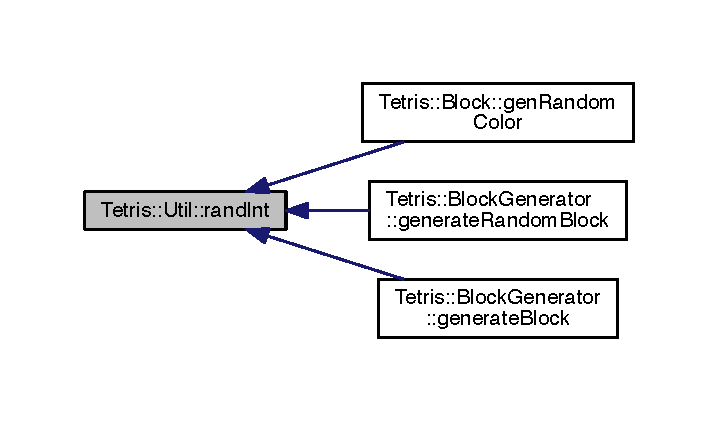
\includegraphics[width=344pt]{namespace_tetris_1_1_util_aa590e9fd847ac6e0c9bc6bf464b5a74b_icgraph}
\end{center}
\end{figure}

\hypertarget{namespace_tetris_1_1_views}{}\section{Tetris\+:\+:Views 네임스페이스 참조}
\label{namespace_tetris_1_1_views}\index{Tetris\+::\+Views@{Tetris\+::\+Views}}
\subsection*{클래스}
\begin{DoxyCompactItemize}
\item 
class \hyperlink{class_tetris_1_1_views_1_1_next_block_render_behavior}{Next\+Block\+Render\+Behavior}
\begin{DoxyCompactList}\small\item\em 블럭 미리 보여주기 \end{DoxyCompactList}\end{DoxyCompactItemize}

\chapter{클래스 문서화}
\hypertarget{class_app_delegate}{}\section{App\+Delegate 클래스 참조}
\label{class_app_delegate}\index{App\+Delegate@{App\+Delegate}}


The cocos2d Application.  




{\ttfamily \#include $<$App\+Delegate.\+h$>$}

App\+Delegate에 대한 상속 다이어그램 \+: \begin{figure}[H]
\begin{center}
\leavevmode
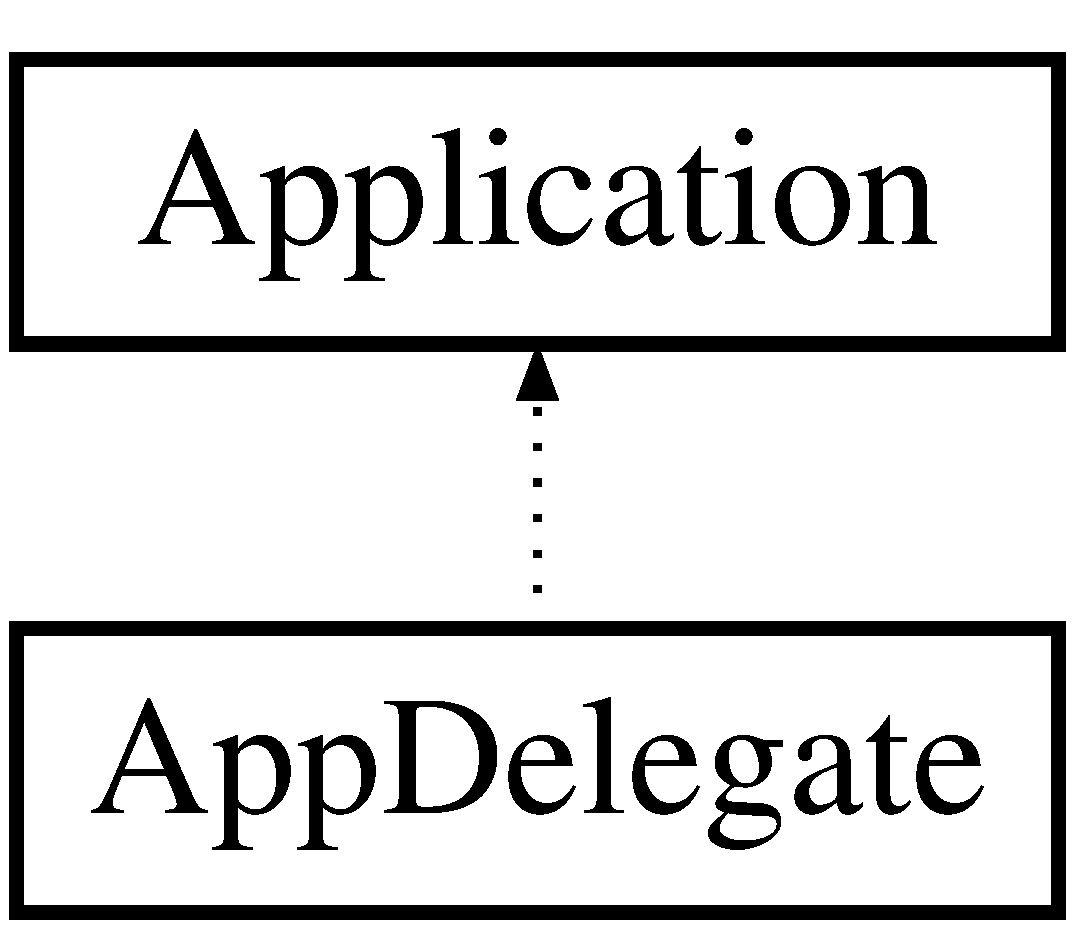
\includegraphics[height=2.000000cm]{class_app_delegate}
\end{center}
\end{figure}
\subsection*{Public 멤버 함수}
\begin{DoxyCompactItemize}
\item 
\hyperlink{class_app_delegate_a7d26ade6fbc9d35ecc9185792303f82d}{App\+Delegate} ()
\item 
virtual \hyperlink{class_app_delegate_a9f89424b5e296e3668deaa0265fc5ac1}{$\sim$\+App\+Delegate} ()
\item 
virtual void \hyperlink{class_app_delegate_a2de4e8ab7d04bde311684e1d4ceb2c0f}{init\+G\+L\+Context\+Attrs} ()
\item 
virtual bool \hyperlink{class_app_delegate_a68cbaed49edf7581dc59a09d5062fff3}{application\+Did\+Finish\+Launching} ()
\begin{DoxyCompactList}\small\item\em Implement Director and Scene init code here. \end{DoxyCompactList}\item 
virtual void \hyperlink{class_app_delegate_a17cb09777419781698324e0415bffd3a}{application\+Did\+Enter\+Background} ()
\begin{DoxyCompactList}\small\item\em Called when the application moves to the background \end{DoxyCompactList}\item 
virtual void \hyperlink{class_app_delegate_ac4d653e3f74a91efef5f2def58fe3108}{application\+Will\+Enter\+Foreground} ()
\begin{DoxyCompactList}\small\item\em Called when the application reenters the foreground \end{DoxyCompactList}\end{DoxyCompactItemize}


\subsection{상세한 설명}
The cocos2d Application. 

Private inheritance here hides part of interface from Director. 

App\+Delegate.\+h 파일의 11 번째 라인에서 정의되었습니다.



\subsection{생성자 \& 소멸자 문서화}
\mbox{\Hypertarget{class_app_delegate_a7d26ade6fbc9d35ecc9185792303f82d}\label{class_app_delegate_a7d26ade6fbc9d35ecc9185792303f82d}} 
\index{App\+Delegate@{App\+Delegate}!App\+Delegate@{App\+Delegate}}
\index{App\+Delegate@{App\+Delegate}!App\+Delegate@{App\+Delegate}}
\subsubsection{\texorpdfstring{App\+Delegate()}{AppDelegate()}}
{\footnotesize\ttfamily App\+Delegate\+::\+App\+Delegate (\begin{DoxyParamCaption}{ }\end{DoxyParamCaption})}



App\+Delegate.\+cpp 파일의 34 번째 라인에서 정의되었습니다.

\mbox{\Hypertarget{class_app_delegate_a9f89424b5e296e3668deaa0265fc5ac1}\label{class_app_delegate_a9f89424b5e296e3668deaa0265fc5ac1}} 
\index{App\+Delegate@{App\+Delegate}!````~App\+Delegate@{$\sim$\+App\+Delegate}}
\index{````~App\+Delegate@{$\sim$\+App\+Delegate}!App\+Delegate@{App\+Delegate}}
\subsubsection{\texorpdfstring{$\sim$\+App\+Delegate()}{~AppDelegate()}}
{\footnotesize\ttfamily App\+Delegate\+::$\sim$\+App\+Delegate (\begin{DoxyParamCaption}{ }\end{DoxyParamCaption})\hspace{0.3cm}{\ttfamily [virtual]}}



App\+Delegate.\+cpp 파일의 38 번째 라인에서 정의되었습니다.



\subsection{멤버 함수 문서화}
\mbox{\Hypertarget{class_app_delegate_a17cb09777419781698324e0415bffd3a}\label{class_app_delegate_a17cb09777419781698324e0415bffd3a}} 
\index{App\+Delegate@{App\+Delegate}!application\+Did\+Enter\+Background@{application\+Did\+Enter\+Background}}
\index{application\+Did\+Enter\+Background@{application\+Did\+Enter\+Background}!App\+Delegate@{App\+Delegate}}
\subsubsection{\texorpdfstring{application\+Did\+Enter\+Background()}{applicationDidEnterBackground()}}
{\footnotesize\ttfamily void App\+Delegate\+::application\+Did\+Enter\+Background (\begin{DoxyParamCaption}{ }\end{DoxyParamCaption})\hspace{0.3cm}{\ttfamily [virtual]}}



Called when the application moves to the background 


\begin{DoxyParams}{매개변수}
{\em the} & pointer of the application \\
\hline
\end{DoxyParams}


App\+Delegate.\+cpp 파일의 120 번째 라인에서 정의되었습니다.

\mbox{\Hypertarget{class_app_delegate_a68cbaed49edf7581dc59a09d5062fff3}\label{class_app_delegate_a68cbaed49edf7581dc59a09d5062fff3}} 
\index{App\+Delegate@{App\+Delegate}!application\+Did\+Finish\+Launching@{application\+Did\+Finish\+Launching}}
\index{application\+Did\+Finish\+Launching@{application\+Did\+Finish\+Launching}!App\+Delegate@{App\+Delegate}}
\subsubsection{\texorpdfstring{application\+Did\+Finish\+Launching()}{applicationDidFinishLaunching()}}
{\footnotesize\ttfamily bool App\+Delegate\+::application\+Did\+Finish\+Launching (\begin{DoxyParamCaption}{ }\end{DoxyParamCaption})\hspace{0.3cm}{\ttfamily [virtual]}}



Implement Director and Scene init code here. 

\begin{DoxyReturn}{반환값}
true Initialize success, app continue. 

false Initialize failed, app terminate. 
\end{DoxyReturn}


App\+Delegate.\+cpp 파일의 65 번째 라인에서 정의되었습니다.

\mbox{\Hypertarget{class_app_delegate_ac4d653e3f74a91efef5f2def58fe3108}\label{class_app_delegate_ac4d653e3f74a91efef5f2def58fe3108}} 
\index{App\+Delegate@{App\+Delegate}!application\+Will\+Enter\+Foreground@{application\+Will\+Enter\+Foreground}}
\index{application\+Will\+Enter\+Foreground@{application\+Will\+Enter\+Foreground}!App\+Delegate@{App\+Delegate}}
\subsubsection{\texorpdfstring{application\+Will\+Enter\+Foreground()}{applicationWillEnterForeground()}}
{\footnotesize\ttfamily void App\+Delegate\+::application\+Will\+Enter\+Foreground (\begin{DoxyParamCaption}{ }\end{DoxyParamCaption})\hspace{0.3cm}{\ttfamily [virtual]}}



Called when the application reenters the foreground 


\begin{DoxyParams}{매개변수}
{\em the} & pointer of the application \\
\hline
\end{DoxyParams}


App\+Delegate.\+cpp 파일의 132 번째 라인에서 정의되었습니다.

\mbox{\Hypertarget{class_app_delegate_a2de4e8ab7d04bde311684e1d4ceb2c0f}\label{class_app_delegate_a2de4e8ab7d04bde311684e1d4ceb2c0f}} 
\index{App\+Delegate@{App\+Delegate}!init\+G\+L\+Context\+Attrs@{init\+G\+L\+Context\+Attrs}}
\index{init\+G\+L\+Context\+Attrs@{init\+G\+L\+Context\+Attrs}!App\+Delegate@{App\+Delegate}}
\subsubsection{\texorpdfstring{init\+G\+L\+Context\+Attrs()}{initGLContextAttrs()}}
{\footnotesize\ttfamily void App\+Delegate\+::init\+G\+L\+Context\+Attrs (\begin{DoxyParamCaption}{ }\end{DoxyParamCaption})\hspace{0.3cm}{\ttfamily [virtual]}}



App\+Delegate.\+cpp 파일의 50 번째 라인에서 정의되었습니다.



이 클래스에 대한 문서화 페이지는 다음의 파일들로부터 생성되었습니다.\+:\begin{DoxyCompactItemize}
\item 
Classes/\hyperlink{_app_delegate_8h}{App\+Delegate.\+h}\item 
Classes/\hyperlink{_app_delegate_8cpp}{App\+Delegate.\+cpp}\end{DoxyCompactItemize}

\hypertarget{class_tetris_1_1_audio_1_1_audio_source_manager}{}\section{Tetris\+:\+:Audio\+:\+:Audio\+Source\+Manager 클래스 참조}
\label{class_tetris_1_1_audio_1_1_audio_source_manager}\index{Tetris\+::\+Audio\+::\+Audio\+Source\+Manager@{Tetris\+::\+Audio\+::\+Audio\+Source\+Manager}}


{\ttfamily \#include $<$Audio\+Source\+Manager.\+hpp$>$}



Tetris\+:\+:Audio\+:\+:Audio\+Source\+Manager에 대한 협력 다이어그램\+:
\nopagebreak
\begin{figure}[H]
\begin{center}
\leavevmode
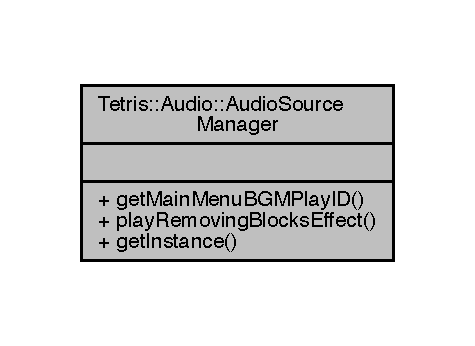
\includegraphics[width=228pt]{class_tetris_1_1_audio_1_1_audio_source_manager__coll__graph}
\end{center}
\end{figure}
\subsection*{Public 멤버 함수}
\begin{DoxyCompactItemize}
\item 
unsigned int \hyperlink{class_tetris_1_1_audio_1_1_audio_source_manager_a64d6e7c7f0849d5de7cc26898079986c}{get\+Main\+Menu\+B\+G\+M\+Play\+ID} ()
\item 
void \hyperlink{class_tetris_1_1_audio_1_1_audio_source_manager_a44c761f0200291a2c8f282d8d52aa081}{play\+Removing\+Blocks\+Effect} ()
\end{DoxyCompactItemize}
\subsection*{정적 Public 멤버 함수}
\begin{DoxyCompactItemize}
\item 
static \hyperlink{class_tetris_1_1_audio_1_1_audio_source_manager}{Audio\+Source\+Manager} $\ast$ \hyperlink{class_tetris_1_1_audio_1_1_audio_source_manager_a561c580924ee6a13e6453b2d94764548}{get\+Instance} ()
\end{DoxyCompactItemize}


\subsection{상세한 설명}


Audio\+Source\+Manager.\+hpp 파일의 21 번째 라인에서 정의되었습니다.



\subsection{멤버 함수 문서화}
\mbox{\Hypertarget{class_tetris_1_1_audio_1_1_audio_source_manager_a561c580924ee6a13e6453b2d94764548}\label{class_tetris_1_1_audio_1_1_audio_source_manager_a561c580924ee6a13e6453b2d94764548}} 
\index{Tetris\+::\+Audio\+::\+Audio\+Source\+Manager@{Tetris\+::\+Audio\+::\+Audio\+Source\+Manager}!get\+Instance@{get\+Instance}}
\index{get\+Instance@{get\+Instance}!Tetris\+::\+Audio\+::\+Audio\+Source\+Manager@{Tetris\+::\+Audio\+::\+Audio\+Source\+Manager}}
\subsubsection{\texorpdfstring{get\+Instance()}{getInstance()}}
{\footnotesize\ttfamily static \hyperlink{class_tetris_1_1_audio_1_1_audio_source_manager}{Audio\+Source\+Manager}$\ast$ Tetris\+::\+Audio\+::\+Audio\+Source\+Manager\+::get\+Instance (\begin{DoxyParamCaption}{ }\end{DoxyParamCaption})\hspace{0.3cm}{\ttfamily [inline]}, {\ttfamily [static]}}



Audio\+Source\+Manager.\+hpp 파일의 23 번째 라인에서 정의되었습니다.

이 함수를 호출하는 함수들에 대한 그래프입니다.\+:
\nopagebreak
\begin{figure}[H]
\begin{center}
\leavevmode
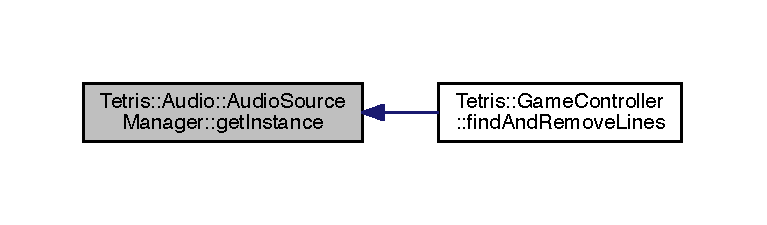
\includegraphics[width=350pt]{class_tetris_1_1_audio_1_1_audio_source_manager_a561c580924ee6a13e6453b2d94764548_icgraph}
\end{center}
\end{figure}
\mbox{\Hypertarget{class_tetris_1_1_audio_1_1_audio_source_manager_a64d6e7c7f0849d5de7cc26898079986c}\label{class_tetris_1_1_audio_1_1_audio_source_manager_a64d6e7c7f0849d5de7cc26898079986c}} 
\index{Tetris\+::\+Audio\+::\+Audio\+Source\+Manager@{Tetris\+::\+Audio\+::\+Audio\+Source\+Manager}!get\+Main\+Menu\+B\+G\+M\+Play\+ID@{get\+Main\+Menu\+B\+G\+M\+Play\+ID}}
\index{get\+Main\+Menu\+B\+G\+M\+Play\+ID@{get\+Main\+Menu\+B\+G\+M\+Play\+ID}!Tetris\+::\+Audio\+::\+Audio\+Source\+Manager@{Tetris\+::\+Audio\+::\+Audio\+Source\+Manager}}
\subsubsection{\texorpdfstring{get\+Main\+Menu\+B\+G\+M\+Play\+I\+D()}{getMainMenuBGMPlayID()}}
{\footnotesize\ttfamily unsigned int Tetris\+::\+Audio\+::\+Audio\+Source\+Manager\+::get\+Main\+Menu\+B\+G\+M\+Play\+ID (\begin{DoxyParamCaption}{ }\end{DoxyParamCaption})\hspace{0.3cm}{\ttfamily [inline]}}



Audio\+Source\+Manager.\+hpp 파일의 27 번째 라인에서 정의되었습니다.

\mbox{\Hypertarget{class_tetris_1_1_audio_1_1_audio_source_manager_a44c761f0200291a2c8f282d8d52aa081}\label{class_tetris_1_1_audio_1_1_audio_source_manager_a44c761f0200291a2c8f282d8d52aa081}} 
\index{Tetris\+::\+Audio\+::\+Audio\+Source\+Manager@{Tetris\+::\+Audio\+::\+Audio\+Source\+Manager}!play\+Removing\+Blocks\+Effect@{play\+Removing\+Blocks\+Effect}}
\index{play\+Removing\+Blocks\+Effect@{play\+Removing\+Blocks\+Effect}!Tetris\+::\+Audio\+::\+Audio\+Source\+Manager@{Tetris\+::\+Audio\+::\+Audio\+Source\+Manager}}
\subsubsection{\texorpdfstring{play\+Removing\+Blocks\+Effect()}{playRemovingBlocksEffect()}}
{\footnotesize\ttfamily void Tetris\+::\+Audio\+::\+Audio\+Source\+Manager\+::play\+Removing\+Blocks\+Effect (\begin{DoxyParamCaption}{ }\end{DoxyParamCaption})\hspace{0.3cm}{\ttfamily [inline]}}



Audio\+Source\+Manager.\+hpp 파일의 30 번째 라인에서 정의되었습니다.

이 함수를 호출하는 함수들에 대한 그래프입니다.\+:
\nopagebreak
\begin{figure}[H]
\begin{center}
\leavevmode
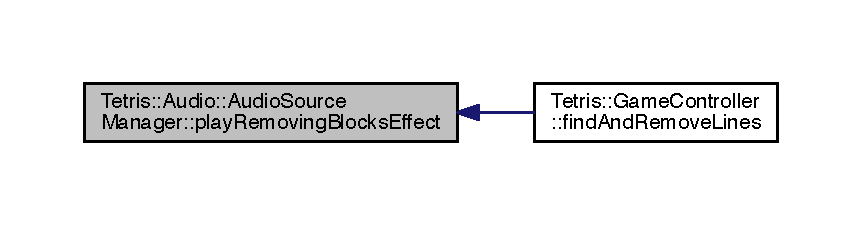
\includegraphics[width=350pt]{class_tetris_1_1_audio_1_1_audio_source_manager_a44c761f0200291a2c8f282d8d52aa081_icgraph}
\end{center}
\end{figure}


이 클래스에 대한 문서화 페이지는 다음의 파일로부터 생성되었습니다.\+:\begin{DoxyCompactItemize}
\item 
Classes/cocosclses/\hyperlink{_audio_source_manager_8hpp}{Audio\+Source\+Manager.\+hpp}\end{DoxyCompactItemize}

\hypertarget{class_tetris_1_1_block}{}\section{Tetris\+:\+:Block 클래스 참조}
\label{class_tetris_1_1_block}\index{Tetris\+::\+Block@{Tetris\+::\+Block}}


테트리스 블럭데이터를 저장하고 불러오는 객체  




{\ttfamily \#include $<$Block.\+h$>$}



Tetris\+:\+:Block에 대한 협력 다이어그램\+:
\nopagebreak
\begin{figure}[H]
\begin{center}
\leavevmode
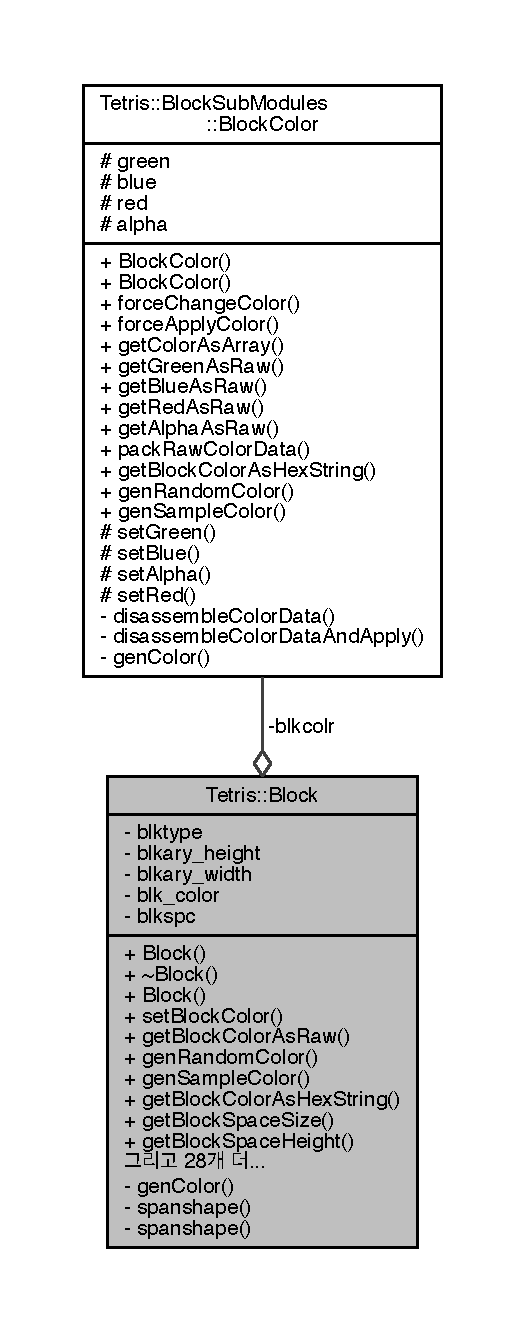
\includegraphics[height=550pt]{d9/d68/class_tetris_1_1_block__coll__graph}
\end{center}
\end{figure}
\subsection*{Public 멤버 함수}
\begin{DoxyCompactItemize}
\item 
\hyperlink{class_tetris_1_1_block_a1fd0aaff1f4b622c9c7027929c5d4534}{Block} (int type)
\item 
\hyperlink{class_tetris_1_1_block_a20012167d55a996d56825d99082419c6}{$\sim$\+Block} ()
\item 
\hyperlink{class_tetris_1_1_block_a82c3ff96d106bd1da7b32f2addd7db7f}{Block} (int type, unsigned int color)
\item 
void \hyperlink{class_tetris_1_1_block_a1a3fab9e7eabe64a4ba588ed5091d3a9}{set\+Block\+Color} (unsigned int clr)
\item 
unsigned int \hyperlink{class_tetris_1_1_block_a8f6bd5020dcfdae501f74b42827344f3}{get\+Block\+Color\+As\+Raw} ()
\item 
unsigned int \hyperlink{class_tetris_1_1_block_a4bae85cab786853cb3ff76aa7fe72edc}{gen\+Random\+Color} ()
\item 
unsigned int \hyperlink{class_tetris_1_1_block_a9cac65704d2c788488ecf65d5b0467bd}{gen\+Sample\+Color} (const unsigned char samplenum)
\item 
string \hyperlink{class_tetris_1_1_block_a0adf3e3fbe9899115703913f18aaae6d}{get\+Block\+Color\+As\+Hex\+String} ()
\item 
int \hyperlink{class_tetris_1_1_block_a356cba210ff93bbd80c10d4d00c81cc2}{get\+Block\+Space\+Size} ()
\item 
int \hyperlink{class_tetris_1_1_block_a5301977e32c03aaf122fa289fcba77ba}{get\+Block\+Space\+Height} ()
\item 
int \hyperlink{class_tetris_1_1_block_ac390e14de476582300d815d9054ed9bd}{get\+Block\+Space\+Width} ()
\item 
bool $\ast$$\ast$ \hyperlink{class_tetris_1_1_block_a9bd2c3d6ccacff9a5f56f72336ba324f}{get\+Block\+Data} ()
\item 
int \hyperlink{class_tetris_1_1_block_a8780b7c5d836c3bb6bae3de5cdcba5e1}{get\+Block\+Type} ()
\item 
void \hyperlink{class_tetris_1_1_block_aea78e0a1b229842f541a8e897e2e9340}{freeblockspace} (bool $\ast$$\ast$$\ast$spc)
\item 
bool $\ast$$\ast$ \hyperlink{class_tetris_1_1_block_a464ed776185993ad827f316a08969960}{get\+Rotated\+Space\+Data} ()
\item 
bool \hyperlink{class_tetris_1_1_block_a56d194d0a5d56d2d1220ec32774cea38}{can\+Rotate} (const vector$<$ bool $\ast$$>$ mapdata, const unsigned char boardwidth, unsigned char cury, unsigned char curx)
\item 
bool \hyperlink{class_tetris_1_1_block_a0d1eb57e6da91832ad983f7a4fa9ca04}{rotate} ()
\item 
bool \hyperlink{class_tetris_1_1_block_a787424e5e9ec2807989121e8dcee1a7a}{roatespec} ()
\item 
void \hyperlink{class_tetris_1_1_block_ae7aadeec449fec232e9635d839593028}{printspace} ()
\item 
\hyperlink{class_tetris_1_1_block_a1fd0aaff1f4b622c9c7027929c5d4534}{Block} (int type)
\item 
\hyperlink{class_tetris_1_1_block_a20012167d55a996d56825d99082419c6}{$\sim$\+Block} ()
\item 
\hyperlink{class_tetris_1_1_block_a82c3ff96d106bd1da7b32f2addd7db7f}{Block} (int type, unsigned int color)
\item 
void \hyperlink{class_tetris_1_1_block_a1a3fab9e7eabe64a4ba588ed5091d3a9}{set\+Block\+Color} (unsigned int clr)
\item 
unsigned int \hyperlink{class_tetris_1_1_block_a8f6bd5020dcfdae501f74b42827344f3}{get\+Block\+Color\+As\+Raw} ()
\item 
\hyperlink{class_tetris_1_1_block_sub_modules_1_1_block_color}{Block\+Color} $\ast$ \hyperlink{class_tetris_1_1_block_ad61aea379870fbb3668d49e4c3c748ed}{get\+Block\+Color} ()
\item 
unsigned int \hyperlink{class_tetris_1_1_block_a4bae85cab786853cb3ff76aa7fe72edc}{gen\+Random\+Color} ()
\item 
string \hyperlink{class_tetris_1_1_block_a0adf3e3fbe9899115703913f18aaae6d}{get\+Block\+Color\+As\+Hex\+String} ()
\item 
int \hyperlink{class_tetris_1_1_block_a356cba210ff93bbd80c10d4d00c81cc2}{get\+Block\+Space\+Size} ()
\item 
int \hyperlink{class_tetris_1_1_block_a5301977e32c03aaf122fa289fcba77ba}{get\+Block\+Space\+Height} ()
\item 
int \hyperlink{class_tetris_1_1_block_ac390e14de476582300d815d9054ed9bd}{get\+Block\+Space\+Width} ()
\item 
bool $\ast$$\ast$ \hyperlink{class_tetris_1_1_block_a2e17230774c905e35aa9868986c49b09}{get\+Block\+Data} ()
\item 
int \hyperlink{class_tetris_1_1_block_a8780b7c5d836c3bb6bae3de5cdcba5e1}{get\+Block\+Type} ()
\item 
void \hyperlink{class_tetris_1_1_block_aea78e0a1b229842f541a8e897e2e9340}{freeblockspace} (bool $\ast$$\ast$$\ast$spc)
\item 
bool $\ast$$\ast$ \hyperlink{class_tetris_1_1_block_ada769278572785b24e8a91f620b97b81}{get\+Rotated\+Space\+Data} ()
\item 
bool \hyperlink{class_tetris_1_1_block_a56d194d0a5d56d2d1220ec32774cea38}{can\+Rotate} (const vector$<$ bool $\ast$$>$ mapdata, const unsigned char boardwidth, unsigned char cury, unsigned char curx)
\item 
bool \hyperlink{class_tetris_1_1_block_a0d1eb57e6da91832ad983f7a4fa9ca04}{rotate} ()
\item 
bool \hyperlink{class_tetris_1_1_block_a787424e5e9ec2807989121e8dcee1a7a}{roatespec} ()
\item 
void \hyperlink{class_tetris_1_1_block_ae7aadeec449fec232e9635d839593028}{printspace} ()
\end{DoxyCompactItemize}
\subsection*{Private 멤버 함수}
\begin{DoxyCompactItemize}
\item 
unsigned int \hyperlink{class_tetris_1_1_block_a7362b9c1679a87823590a3c20ca53a55}{gen\+Color} (unsigned char red, unsigned char green, unsigned char blue)
\item 
void \hyperlink{class_tetris_1_1_block_ad683f161157c16b80d5df8929bca468c}{spanshape} (int type)
\item 
void \hyperlink{class_tetris_1_1_block_ad683f161157c16b80d5df8929bca468c}{spanshape} (int type)
\end{DoxyCompactItemize}
\subsection*{Private 속성}
\begin{DoxyCompactItemize}
\item 
int \hyperlink{class_tetris_1_1_block_aceac58dcf8d8afaa82c2bab101cb3cff}{blktype}
\item 
int \hyperlink{class_tetris_1_1_block_abbea7737c2b1fb7339aab4dff13de27c}{blkary\+\_\+height}
\item 
int \hyperlink{class_tetris_1_1_block_a96548cab58eb788af744b54192c7bea1}{blkary\+\_\+width}
\item 
unsigned int \hyperlink{class_tetris_1_1_block_acf78e864526e38c9c72fa0b012d5b344}{blk\+\_\+color}
\item 
bool $\ast$$\ast$ \hyperlink{class_tetris_1_1_block_af2f96c83a3511d32321672f794aa4db1}{blkspc}
\item 
\hyperlink{class_tetris_1_1_block_sub_modules_1_1_block_color}{Block\+Color} $\ast$ \hyperlink{class_tetris_1_1_block_ab7cfb062eb49e791c94bac4a2e7a7ca9}{blkcolr} = N\+U\+LL
\end{DoxyCompactItemize}


\subsection{상세한 설명}
테트리스 블럭데이터를 저장하고 불러오는 객체 

Block.\+h 파일의 28 번째 라인에서 정의되었습니다.



\subsection{생성자 \& 소멸자 문서화}
\mbox{\Hypertarget{class_tetris_1_1_block_a1fd0aaff1f4b622c9c7027929c5d4534}\label{class_tetris_1_1_block_a1fd0aaff1f4b622c9c7027929c5d4534}} 
\index{Tetris\+::\+Block@{Tetris\+::\+Block}!Block@{Block}}
\index{Block@{Block}!Tetris\+::\+Block@{Tetris\+::\+Block}}
\subsubsection{\texorpdfstring{Block()}{Block()}\hspace{0.1cm}{\footnotesize\ttfamily [1/4]}}
{\footnotesize\ttfamily Tetris\+::\+Block\+::\+Block (\begin{DoxyParamCaption}\item[{int}]{type }\end{DoxyParamCaption})\hspace{0.3cm}{\ttfamily [inline]}}



Block.\+h 파일의 30 번째 라인에서 정의되었습니다.


\begin{DoxyCode}
30                        \{
31             this->\hyperlink{class_tetris_1_1_block_ad683f161157c16b80d5df8929bca468c}{spanshape}(type);
32             this->\hyperlink{class_tetris_1_1_block_a1a3fab9e7eabe64a4ba588ed5091d3a9}{setBlockColor}(this->\hyperlink{class_tetris_1_1_block_a4bae85cab786853cb3ff76aa7fe72edc}{genRandomColor}());
33         \}
\end{DoxyCode}
\mbox{\Hypertarget{class_tetris_1_1_block_a20012167d55a996d56825d99082419c6}\label{class_tetris_1_1_block_a20012167d55a996d56825d99082419c6}} 
\index{Tetris\+::\+Block@{Tetris\+::\+Block}!````~Block@{$\sim$\+Block}}
\index{````~Block@{$\sim$\+Block}!Tetris\+::\+Block@{Tetris\+::\+Block}}
\subsubsection{\texorpdfstring{$\sim$\+Block()}{~Block()}\hspace{0.1cm}{\footnotesize\ttfamily [1/2]}}
{\footnotesize\ttfamily Tetris\+::\+Block\+::$\sim$\+Block (\begin{DoxyParamCaption}{ }\end{DoxyParamCaption})\hspace{0.3cm}{\ttfamily [inline]}}



Block.\+h 파일의 34 번째 라인에서 정의되었습니다.


\begin{DoxyCode}
34                 \{
35             \textcolor{keywordflow}{if}(this->\hyperlink{class_tetris_1_1_block_af2f96c83a3511d32321672f794aa4db1}{blkspc}!=NULL)\{
36                 \textcolor{keywordflow}{for}(\textcolor{keywordtype}{int} i=0;i<this->\hyperlink{class_tetris_1_1_block_abbea7737c2b1fb7339aab4dff13de27c}{blkary\_height};i++)\{
37                     \textcolor{keyword}{delete} [] this->\hyperlink{class_tetris_1_1_block_af2f96c83a3511d32321672f794aa4db1}{blkspc}[i];
38                 \}
39                 \textcolor{keyword}{delete} [] this->\hyperlink{class_tetris_1_1_block_af2f96c83a3511d32321672f794aa4db1}{blkspc};
40             \}
41         \}
\end{DoxyCode}
\mbox{\Hypertarget{class_tetris_1_1_block_a82c3ff96d106bd1da7b32f2addd7db7f}\label{class_tetris_1_1_block_a82c3ff96d106bd1da7b32f2addd7db7f}} 
\index{Tetris\+::\+Block@{Tetris\+::\+Block}!Block@{Block}}
\index{Block@{Block}!Tetris\+::\+Block@{Tetris\+::\+Block}}
\subsubsection{\texorpdfstring{Block()}{Block()}\hspace{0.1cm}{\footnotesize\ttfamily [2/4]}}
{\footnotesize\ttfamily Tetris\+::\+Block\+::\+Block (\begin{DoxyParamCaption}\item[{int}]{type,  }\item[{unsigned int}]{color }\end{DoxyParamCaption})\hspace{0.3cm}{\ttfamily [inline]}}



Block.\+h 파일의 42 번째 라인에서 정의되었습니다.


\begin{DoxyCode}
42                                           \{
43             this->\hyperlink{class_tetris_1_1_block_ad683f161157c16b80d5df8929bca468c}{spanshape}(type);
44             this->\hyperlink{class_tetris_1_1_block_a1a3fab9e7eabe64a4ba588ed5091d3a9}{setBlockColor}(color);
45         \}
\end{DoxyCode}
\mbox{\Hypertarget{class_tetris_1_1_block_a1fd0aaff1f4b622c9c7027929c5d4534}\label{class_tetris_1_1_block_a1fd0aaff1f4b622c9c7027929c5d4534}} 
\index{Tetris\+::\+Block@{Tetris\+::\+Block}!Block@{Block}}
\index{Block@{Block}!Tetris\+::\+Block@{Tetris\+::\+Block}}
\subsubsection{\texorpdfstring{Block()}{Block()}\hspace{0.1cm}{\footnotesize\ttfamily [3/4]}}
{\footnotesize\ttfamily Tetris\+::\+Block\+::\+Block (\begin{DoxyParamCaption}\item[{int}]{type }\end{DoxyParamCaption})\hspace{0.3cm}{\ttfamily [inline]}}

\begin{DoxyReturn}{반환값}
constructor 
\end{DoxyReturn}
\begin{DoxyWarning}{경고}
type이 연속된 번호범위를 벗어나면 기본값으로 생성된다 
\end{DoxyWarning}


Block.\+hpp 파일의 41 번째 라인에서 정의되었습니다.


\begin{DoxyCode}
41                            \{
42                
43                 this->\hyperlink{class_tetris_1_1_block_ad683f161157c16b80d5df8929bca468c}{spanshape}(type);
44                 this->\hyperlink{class_tetris_1_1_block_a1a3fab9e7eabe64a4ba588ed5091d3a9}{setBlockColor}(this->\hyperlink{class_tetris_1_1_block_a4bae85cab786853cb3ff76aa7fe72edc}{genRandomColor}());
45             \}
\end{DoxyCode}
\mbox{\Hypertarget{class_tetris_1_1_block_a20012167d55a996d56825d99082419c6}\label{class_tetris_1_1_block_a20012167d55a996d56825d99082419c6}} 
\index{Tetris\+::\+Block@{Tetris\+::\+Block}!````~Block@{$\sim$\+Block}}
\index{````~Block@{$\sim$\+Block}!Tetris\+::\+Block@{Tetris\+::\+Block}}
\subsubsection{\texorpdfstring{$\sim$\+Block()}{~Block()}\hspace{0.1cm}{\footnotesize\ttfamily [2/2]}}
{\footnotesize\ttfamily Tetris\+::\+Block\+::$\sim$\+Block (\begin{DoxyParamCaption}{ }\end{DoxyParamCaption})\hspace{0.3cm}{\ttfamily [inline]}}

\begin{DoxyReturn}{반환값}
모름 
\end{DoxyReturn}
\begin{DoxyWarning}{경고}
메모리 터지지 않도록 메모리 수동삭제 
\end{DoxyWarning}


Block.\+hpp 파일의 50 번째 라인에서 정의되었습니다.


\begin{DoxyCode}
50                     \{
51                 \textcolor{keywordflow}{if}(this->\hyperlink{class_tetris_1_1_block_af2f96c83a3511d32321672f794aa4db1}{blkspc}!=NULL)\{
52                     \textcolor{keywordflow}{for}(\textcolor{keywordtype}{int} i=0;i<this->\hyperlink{class_tetris_1_1_block_abbea7737c2b1fb7339aab4dff13de27c}{blkary\_height};i++)\{
53                         \textcolor{keyword}{delete} [] this->\hyperlink{class_tetris_1_1_block_af2f96c83a3511d32321672f794aa4db1}{blkspc}[i];
54                     \}
55                     \textcolor{keyword}{delete} [] this->\hyperlink{class_tetris_1_1_block_af2f96c83a3511d32321672f794aa4db1}{blkspc};
56                 \}
57                 \textcolor{keywordflow}{if}(this->\hyperlink{class_tetris_1_1_block_ab7cfb062eb49e791c94bac4a2e7a7ca9}{blkcolr}!=NULL)\{
58                     \textcolor{keyword}{delete} this->\hyperlink{class_tetris_1_1_block_ab7cfb062eb49e791c94bac4a2e7a7ca9}{blkcolr};
59                 \}
60             \}
\end{DoxyCode}
\mbox{\Hypertarget{class_tetris_1_1_block_a82c3ff96d106bd1da7b32f2addd7db7f}\label{class_tetris_1_1_block_a82c3ff96d106bd1da7b32f2addd7db7f}} 
\index{Tetris\+::\+Block@{Tetris\+::\+Block}!Block@{Block}}
\index{Block@{Block}!Tetris\+::\+Block@{Tetris\+::\+Block}}
\subsubsection{\texorpdfstring{Block()}{Block()}\hspace{0.1cm}{\footnotesize\ttfamily [4/4]}}
{\footnotesize\ttfamily Tetris\+::\+Block\+::\+Block (\begin{DoxyParamCaption}\item[{int}]{type,  }\item[{unsigned int}]{color }\end{DoxyParamCaption})\hspace{0.3cm}{\ttfamily [inline]}}

\begin{DoxyReturn}{반환값}
constructor 
\end{DoxyReturn}
\begin{DoxyWarning}{경고}
연속된 숫자의 범위를 벗어나면 기본값으로 생성 
\end{DoxyWarning}


Block.\+hpp 파일의 65 번째 라인에서 정의되었습니다.


\begin{DoxyCode}
65                                               \{
66                 this->\hyperlink{class_tetris_1_1_block_ad683f161157c16b80d5df8929bca468c}{spanshape}(type);
67                 this->\hyperlink{class_tetris_1_1_block_a1a3fab9e7eabe64a4ba588ed5091d3a9}{setBlockColor}(color);
68             \}
\end{DoxyCode}


\subsection{멤버 함수 문서화}
\mbox{\Hypertarget{class_tetris_1_1_block_a56d194d0a5d56d2d1220ec32774cea38}\label{class_tetris_1_1_block_a56d194d0a5d56d2d1220ec32774cea38}} 
\index{Tetris\+::\+Block@{Tetris\+::\+Block}!can\+Rotate@{can\+Rotate}}
\index{can\+Rotate@{can\+Rotate}!Tetris\+::\+Block@{Tetris\+::\+Block}}
\subsubsection{\texorpdfstring{can\+Rotate()}{canRotate()}\hspace{0.1cm}{\footnotesize\ttfamily [1/2]}}
{\footnotesize\ttfamily bool Tetris\+::\+Block\+::can\+Rotate (\begin{DoxyParamCaption}\item[{const vector$<$ bool $\ast$$>$}]{mapdata,  }\item[{const unsigned char}]{boardwidth,  }\item[{unsigned char}]{cury,  }\item[{unsigned char}]{curx }\end{DoxyParamCaption})}



Block.\+cpp 파일의 116 번째 라인에서 정의되었습니다.


\begin{DoxyCode}
116                                                                                                            
                  \{\textcolor{comment}{//,GameUser* guser)\{}
117                 \textcolor{keywordtype}{bool}** rotated\_space = this->\hyperlink{class_tetris_1_1_block_a464ed776185993ad827f316a08969960}{getRotatedSpaceData}();
118                 \textcolor{comment}{//unsigned char curx = guser->getCurrentX();}
119                 \textcolor{comment}{//unsigned char cury = guser->getCurrentY();}
120                 \textcolor{keywordflow}{if}(rotated\_space==NULL||!mapdata.size())\{
121                     \textcolor{keywordflow}{return} \textcolor{keyword}{false};
122                 \}
123                 \textcolor{keywordflow}{if}(\hyperlink{class_tetris_1_1_block_abbea7737c2b1fb7339aab4dff13de27c}{blkary\_height}>\hyperlink{class_tetris_1_1_block_a96548cab58eb788af744b54192c7bea1}{blkary\_width}&&curx+
      \hyperlink{class_tetris_1_1_block_abbea7737c2b1fb7339aab4dff13de27c}{blkary\_height}>boardwidth)\{
124                    \textcolor{comment}{/*const int movepos = blkary\_height-blkary\_width;}
125 \textcolor{comment}{                    int movedpos = curx-movepos;}
126 \textcolor{comment}{                    bool movable = true;}
127 \textcolor{comment}{                    if(movepos==0||movedpos<0)\{}
128 \textcolor{comment}{                        return false;}
129 \textcolor{comment}{                    \}}
130 \textcolor{comment}{                    for(int i = 0;i<blkary\_height;i++)\{}
131 \textcolor{comment}{                        for(int j=0;movedpos>=0&&j<=movepos;j++)\{}
132 \textcolor{comment}{                            if(rotated\_space[j][i]&&mapdata[cury+i][movedpos+j])\{}
133 \textcolor{comment}{                                movable = false;}
134 \textcolor{comment}{                            \}}
135 \textcolor{comment}{                        \}}
136 \textcolor{comment}{                    \}}
137 \textcolor{comment}{                    if(movable)\{}
138 \textcolor{comment}{                        guser->setCurrentX((unsigned char)movedpos);}
139 \textcolor{comment}{                        curx = guser->getCurrentX();}
140 \textcolor{comment}{                    \}else*/}
141                     \textcolor{keywordflow}{return} \textcolor{keyword}{false};
142                 \}
143                 \textcolor{keywordflow}{for}(\textcolor{keywordtype}{int} i=0;i<\hyperlink{class_tetris_1_1_block_abbea7737c2b1fb7339aab4dff13de27c}{blkary\_height};i++)\{
144                     \textcolor{keywordflow}{for}(\textcolor{keywordtype}{int} j=0;j<\hyperlink{class_tetris_1_1_block_a96548cab58eb788af744b54192c7bea1}{blkary\_width};j++)\{
145                         \textcolor{keywordflow}{if}(rotated\_space[j][i]&&mapdata[i+cury][j+curx])\{
146                             \textcolor{keywordflow}{return} \textcolor{keyword}{false};
147                         \}
148                     \}
149                 \}
150                 \textcolor{keywordflow}{return} \textcolor{keyword}{true};
151             \}
\end{DoxyCode}
이 함수를 호출하는 함수들에 대한 그래프입니다.\+:
\nopagebreak
\begin{figure}[H]
\begin{center}
\leavevmode
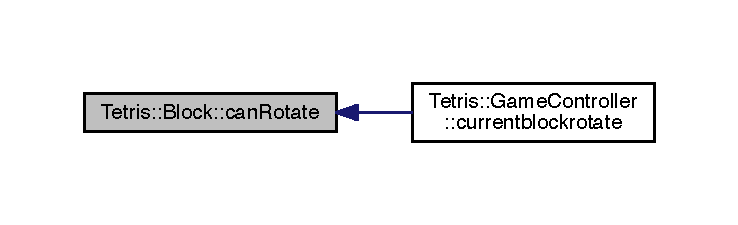
\includegraphics[width=350pt]{df/d05/class_tetris_1_1_block_a56d194d0a5d56d2d1220ec32774cea38_icgraph}
\end{center}
\end{figure}
\mbox{\Hypertarget{class_tetris_1_1_block_a56d194d0a5d56d2d1220ec32774cea38}\label{class_tetris_1_1_block_a56d194d0a5d56d2d1220ec32774cea38}} 
\index{Tetris\+::\+Block@{Tetris\+::\+Block}!can\+Rotate@{can\+Rotate}}
\index{can\+Rotate@{can\+Rotate}!Tetris\+::\+Block@{Tetris\+::\+Block}}
\subsubsection{\texorpdfstring{can\+Rotate()}{canRotate()}\hspace{0.1cm}{\footnotesize\ttfamily [2/2]}}
{\footnotesize\ttfamily bool Tetris\+::\+Block\+::can\+Rotate (\begin{DoxyParamCaption}\item[{const vector$<$ bool $\ast$$>$}]{mapdata,  }\item[{const unsigned char}]{boardwidth,  }\item[{unsigned char}]{cury,  }\item[{unsigned char}]{curx }\end{DoxyParamCaption})\hspace{0.3cm}{\ttfamily [inline]}}

\begin{DoxyReturn}{반환값}
게임 맵에서 현재 좌표에서 회전이 가능한지 유무 
\end{DoxyReturn}


Block.\+hpp 파일의 168 번째 라인에서 정의되었습니다.


\begin{DoxyCode}
168                                                                                                            
                         \{\textcolor{comment}{//,GameUser* guser)\{}
169                 \textcolor{keywordtype}{bool}** rotated\_space = this->\hyperlink{class_tetris_1_1_block_a464ed776185993ad827f316a08969960}{getRotatedSpaceData}();
170                 \textcolor{comment}{//unsigned char curx = guser->getCurrentX();}
171                 \textcolor{comment}{//unsigned char cury = guser->getCurrentY();}
172                 \textcolor{keywordflow}{if}(rotated\_space==NULL||!mapdata.size())\{
173                     \textcolor{keywordflow}{return} \textcolor{keyword}{false};
174                 \}
175                 \textcolor{keywordflow}{if}(\hyperlink{class_tetris_1_1_block_abbea7737c2b1fb7339aab4dff13de27c}{blkary\_height}>\hyperlink{class_tetris_1_1_block_a96548cab58eb788af744b54192c7bea1}{blkary\_width}&&curx+
      \hyperlink{class_tetris_1_1_block_abbea7737c2b1fb7339aab4dff13de27c}{blkary\_height}>boardwidth)\{
176                    \textcolor{comment}{/*const int movepos = blkary\_height-blkary\_width;}
177 \textcolor{comment}{                    int movedpos = curx-movepos;}
178 \textcolor{comment}{                    bool movable = true;}
179 \textcolor{comment}{                    if(movepos==0||movedpos<0)\{}
180 \textcolor{comment}{                        return false;}
181 \textcolor{comment}{                    \}}
182 \textcolor{comment}{                    for(int i = 0;i<blkary\_height;i++)\{}
183 \textcolor{comment}{                        for(int j=0;movedpos>=0&&j<=movepos;j++)\{}
184 \textcolor{comment}{                            if(rotated\_space[j][i]&&mapdata[cury+i][movedpos+j])\{}
185 \textcolor{comment}{                                movable = false;}
186 \textcolor{comment}{                            \}}
187 \textcolor{comment}{                        \}}
188 \textcolor{comment}{                    \}}
189 \textcolor{comment}{                    if(movable)\{}
190 \textcolor{comment}{                        guser->setCurrentX((unsigned char)movedpos);}
191 \textcolor{comment}{                        curx = guser->getCurrentX();}
192 \textcolor{comment}{                    \}else*/}
193                     \textcolor{keywordflow}{return} \textcolor{keyword}{false};
194                 \}
195                 \textcolor{keywordflow}{for}(\textcolor{keywordtype}{int} i=0;i<\hyperlink{class_tetris_1_1_block_abbea7737c2b1fb7339aab4dff13de27c}{blkary\_height};i++)\{
196                     \textcolor{keywordflow}{for}(\textcolor{keywordtype}{int} j=0;j<\hyperlink{class_tetris_1_1_block_a96548cab58eb788af744b54192c7bea1}{blkary\_width};j++)\{
197                         \textcolor{keywordflow}{if}(j+curx<boardwidth && rotated\_space[j][i]&&mapdata[i+cury][j+curx])\{
198                             \textcolor{keywordflow}{return} \textcolor{keyword}{false};
199                         \}
200                     \}
201                 \}
202                 \textcolor{keywordflow}{return} \textcolor{keyword}{true};
203             \}
\end{DoxyCode}
\mbox{\Hypertarget{class_tetris_1_1_block_aea78e0a1b229842f541a8e897e2e9340}\label{class_tetris_1_1_block_aea78e0a1b229842f541a8e897e2e9340}} 
\index{Tetris\+::\+Block@{Tetris\+::\+Block}!freeblockspace@{freeblockspace}}
\index{freeblockspace@{freeblockspace}!Tetris\+::\+Block@{Tetris\+::\+Block}}
\subsubsection{\texorpdfstring{freeblockspace()}{freeblockspace()}\hspace{0.1cm}{\footnotesize\ttfamily [1/2]}}
{\footnotesize\ttfamily void Tetris\+::\+Block\+::freeblockspace (\begin{DoxyParamCaption}\item[{bool $\ast$$\ast$$\ast$}]{spc }\end{DoxyParamCaption})}



Block.\+cpp 파일의 97 번째 라인에서 정의되었습니다.


\begin{DoxyCode}
97                                      \{
98                 \textcolor{keywordtype}{bool}** blockspace = *spc;
99                 \textcolor{keywordflow}{for}(\textcolor{keywordtype}{int} i=0;i<\hyperlink{class_tetris_1_1_block_abbea7737c2b1fb7339aab4dff13de27c}{blkary\_height};i++)\{
100                     \textcolor{keyword}{delete} [] blockspace[i];
101                 \}
102                 \textcolor{keyword}{delete} [] blockspace;
103             \}
\end{DoxyCode}
\mbox{\Hypertarget{class_tetris_1_1_block_aea78e0a1b229842f541a8e897e2e9340}\label{class_tetris_1_1_block_aea78e0a1b229842f541a8e897e2e9340}} 
\index{Tetris\+::\+Block@{Tetris\+::\+Block}!freeblockspace@{freeblockspace}}
\index{freeblockspace@{freeblockspace}!Tetris\+::\+Block@{Tetris\+::\+Block}}
\subsubsection{\texorpdfstring{freeblockspace()}{freeblockspace()}\hspace{0.1cm}{\footnotesize\ttfamily [2/2]}}
{\footnotesize\ttfamily void Tetris\+::\+Block\+::freeblockspace (\begin{DoxyParamCaption}\item[{bool $\ast$$\ast$$\ast$}]{spc }\end{DoxyParamCaption})\hspace{0.3cm}{\ttfamily [inline]}}



Block.\+hpp 파일의 143 번째 라인에서 정의되었습니다.


\begin{DoxyCode}
143                                             \{
144                 \textcolor{keywordtype}{bool}** blockspace = *spc;
145                 \textcolor{keywordflow}{for}(\textcolor{keywordtype}{int} i=0;i<\hyperlink{class_tetris_1_1_block_abbea7737c2b1fb7339aab4dff13de27c}{blkary\_height};i++)\{
146                     \textcolor{keyword}{delete} [] blockspace[i];
147                 \}
148                 \textcolor{keyword}{delete} [] blockspace;
149             \}
\end{DoxyCode}
\mbox{\Hypertarget{class_tetris_1_1_block_a7362b9c1679a87823590a3c20ca53a55}\label{class_tetris_1_1_block_a7362b9c1679a87823590a3c20ca53a55}} 
\index{Tetris\+::\+Block@{Tetris\+::\+Block}!gen\+Color@{gen\+Color}}
\index{gen\+Color@{gen\+Color}!Tetris\+::\+Block@{Tetris\+::\+Block}}
\subsubsection{\texorpdfstring{gen\+Color()}{genColor()}}
{\footnotesize\ttfamily unsigned int Tetris\+::\+Block\+::gen\+Color (\begin{DoxyParamCaption}\item[{unsigned char}]{red,  }\item[{unsigned char}]{green,  }\item[{unsigned char}]{blue }\end{DoxyParamCaption})\hspace{0.3cm}{\ttfamily [private]}}



Block.\+cpp 파일의 186 번째 라인에서 정의되었습니다.


\begin{DoxyCode}
186                                                                                      \{
187                 \textcolor{keywordtype}{unsigned} \textcolor{keywordtype}{int} rst = (\textcolor{keywordtype}{unsigned} int)blue;
188                 rst|=((\textcolor{keywordtype}{unsigned} int)red<<(8*2));
189                 rst|=((\textcolor{keywordtype}{unsigned} int)green<<(8*1));
190                 \textcolor{keywordflow}{return} rst;
191             \}
\end{DoxyCode}
\mbox{\Hypertarget{class_tetris_1_1_block_a4bae85cab786853cb3ff76aa7fe72edc}\label{class_tetris_1_1_block_a4bae85cab786853cb3ff76aa7fe72edc}} 
\index{Tetris\+::\+Block@{Tetris\+::\+Block}!gen\+Random\+Color@{gen\+Random\+Color}}
\index{gen\+Random\+Color@{gen\+Random\+Color}!Tetris\+::\+Block@{Tetris\+::\+Block}}
\subsubsection{\texorpdfstring{gen\+Random\+Color()}{genRandomColor()}\hspace{0.1cm}{\footnotesize\ttfamily [1/2]}}
{\footnotesize\ttfamily unsigned int Tetris\+::\+Block\+::gen\+Random\+Color (\begin{DoxyParamCaption}{ }\end{DoxyParamCaption})}



Block.\+cpp 파일의 39 번째 라인에서 정의되었습니다.


\begin{DoxyCode}
39                                   \{
40                 \textcolor{keywordflow}{return} this->\hyperlink{class_tetris_1_1_block_a9cac65704d2c788488ecf65d5b0467bd}{genSampleColor}((\textcolor{keywordtype}{unsigned} \textcolor{keywordtype}{char})
      \hyperlink{namespace_tetris_1_1_util_aa590e9fd847ac6e0c9bc6bf464b5a74b}{Tetris::Util::randInt}(1,7));
41             \}
\end{DoxyCode}
이 함수 내부에서 호출하는 함수들에 대한 그래프입니다.\+:
\nopagebreak
\begin{figure}[H]
\begin{center}
\leavevmode
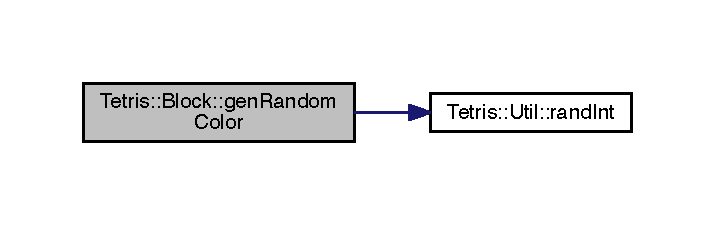
\includegraphics[width=344pt]{df/d05/class_tetris_1_1_block_a4bae85cab786853cb3ff76aa7fe72edc_cgraph}
\end{center}
\end{figure}
\mbox{\Hypertarget{class_tetris_1_1_block_a4bae85cab786853cb3ff76aa7fe72edc}\label{class_tetris_1_1_block_a4bae85cab786853cb3ff76aa7fe72edc}} 
\index{Tetris\+::\+Block@{Tetris\+::\+Block}!gen\+Random\+Color@{gen\+Random\+Color}}
\index{gen\+Random\+Color@{gen\+Random\+Color}!Tetris\+::\+Block@{Tetris\+::\+Block}}
\subsubsection{\texorpdfstring{gen\+Random\+Color()}{genRandomColor()}\hspace{0.1cm}{\footnotesize\ttfamily [2/2]}}
{\footnotesize\ttfamily unsigned int Tetris\+::\+Block\+::gen\+Random\+Color (\begin{DoxyParamCaption}{ }\end{DoxyParamCaption})\hspace{0.3cm}{\ttfamily [inline]}}

\begin{DoxyReturn}{반환값}
지정된 색상 안에서 랜덤으로 색상을 리턴 
\end{DoxyReturn}


Block.\+hpp 파일의 100 번째 라인에서 정의되었습니다.


\begin{DoxyCode}
100                                          \{
101                 \textcolor{keywordflow}{return} BlockColor::genRandomColor(); \textcolor{comment}{//genSampleColor((unsigned
       char)TetrisUtil::randInt(1,7));}
102             \}
\end{DoxyCode}
\mbox{\Hypertarget{class_tetris_1_1_block_a9cac65704d2c788488ecf65d5b0467bd}\label{class_tetris_1_1_block_a9cac65704d2c788488ecf65d5b0467bd}} 
\index{Tetris\+::\+Block@{Tetris\+::\+Block}!gen\+Sample\+Color@{gen\+Sample\+Color}}
\index{gen\+Sample\+Color@{gen\+Sample\+Color}!Tetris\+::\+Block@{Tetris\+::\+Block}}
\subsubsection{\texorpdfstring{gen\+Sample\+Color()}{genSampleColor()}}
{\footnotesize\ttfamily unsigned int Tetris\+::\+Block\+::gen\+Sample\+Color (\begin{DoxyParamCaption}\item[{const unsigned char}]{samplenum }\end{DoxyParamCaption})}



Block.\+cpp 파일의 42 번째 라인에서 정의되었습니다.


\begin{DoxyCode}
42                                                                \{
43                 \textcolor{keywordflow}{switch}(samplenum)\{
44                     \textcolor{keywordflow}{case} 2:\{\textcolor{comment}{//pink600}
45                         \textcolor{keywordflow}{return} this->\hyperlink{class_tetris_1_1_block_a7362b9c1679a87823590a3c20ca53a55}{genColor}(0xd8,0x1b,0x60);
46                     \}
47                     \textcolor{keywordflow}{case} 3:\{\textcolor{comment}{//purple700}
48                         \textcolor{keywordflow}{return} this->\hyperlink{class_tetris_1_1_block_a7362b9c1679a87823590a3c20ca53a55}{genColor}(0x7b,0x1f,0xa2);
49                     \}
50                     \textcolor{keywordflow}{case} 4:\{\textcolor{comment}{//deeppurpleA400}
51                         \textcolor{keywordflow}{return} this->\hyperlink{class_tetris_1_1_block_a7362b9c1679a87823590a3c20ca53a55}{genColor}(0x65,0x1f,0xff);
52                     \}
53                     \textcolor{keywordflow}{case} 5:\{\textcolor{comment}{//teal600}
54                         \textcolor{keywordflow}{return} this->\hyperlink{class_tetris_1_1_block_a7362b9c1679a87823590a3c20ca53a55}{genColor}(0x00,0x89,0x7b);
55                     \}
56                     \textcolor{keywordflow}{case} 6:\{\textcolor{comment}{//red500}
57                         \textcolor{keywordflow}{return} this->\hyperlink{class_tetris_1_1_block_a7362b9c1679a87823590a3c20ca53a55}{genColor}(0xf4,0x43,0x36);
58                     \}
59                     \textcolor{keywordflow}{case} 7:\{\textcolor{comment}{//red900}
60                         \textcolor{keywordflow}{return} this->\hyperlink{class_tetris_1_1_block_a7362b9c1679a87823590a3c20ca53a55}{genColor}(0xb7,0xc1,0xc1);
61                     \}
62                     \textcolor{keywordflow}{case} 1:
63                     \textcolor{keywordflow}{default}:\textcolor{keywordflow}{return} this->\hyperlink{class_tetris_1_1_block_a7362b9c1679a87823590a3c20ca53a55}{genColor}(0x30,0x3f,0x9f);
64                 \}
65 
66             \}
\end{DoxyCode}
\mbox{\Hypertarget{class_tetris_1_1_block_ad61aea379870fbb3668d49e4c3c748ed}\label{class_tetris_1_1_block_ad61aea379870fbb3668d49e4c3c748ed}} 
\index{Tetris\+::\+Block@{Tetris\+::\+Block}!get\+Block\+Color@{get\+Block\+Color}}
\index{get\+Block\+Color@{get\+Block\+Color}!Tetris\+::\+Block@{Tetris\+::\+Block}}
\subsubsection{\texorpdfstring{get\+Block\+Color()}{getBlockColor()}}
{\footnotesize\ttfamily \hyperlink{class_tetris_1_1_block_sub_modules_1_1_block_color}{Block\+Color}$\ast$ Tetris\+::\+Block\+::get\+Block\+Color (\begin{DoxyParamCaption}{ }\end{DoxyParamCaption})\hspace{0.3cm}{\ttfamily [inline]}}

\begin{DoxyReturn}{반환값}
블럭 색상 객체를 리턴 
\end{DoxyReturn}


Block.\+hpp 파일의 94 번째 라인에서 정의되었습니다.


\begin{DoxyCode}
94                                    \{
95             \textcolor{keywordflow}{return} this->\hyperlink{class_tetris_1_1_block_ab7cfb062eb49e791c94bac4a2e7a7ca9}{blkcolr};
96         \}
\end{DoxyCode}
이 함수를 호출하는 함수들에 대한 그래프입니다.\+:
\nopagebreak
\begin{figure}[H]
\begin{center}
\leavevmode
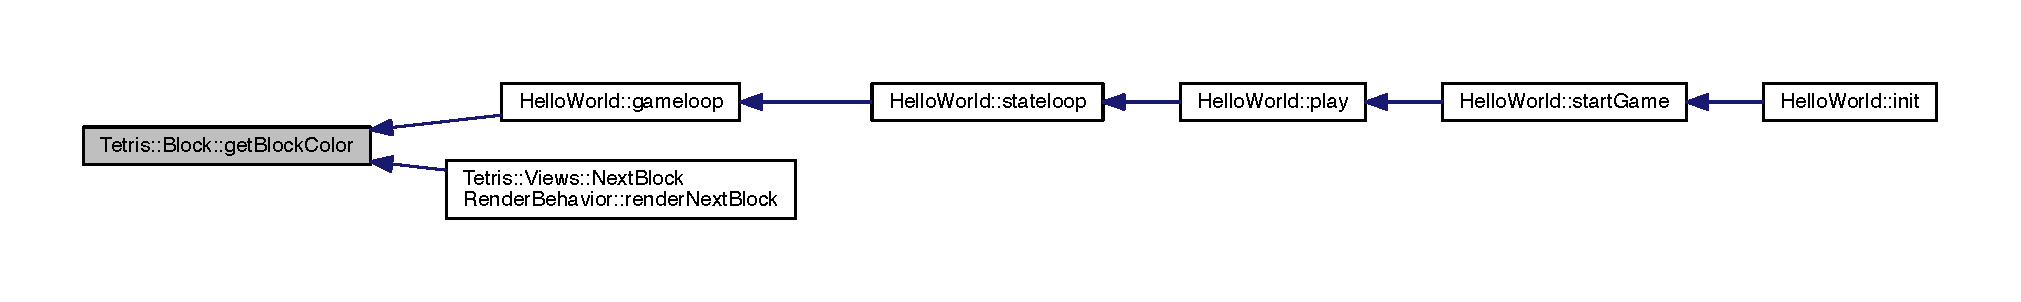
\includegraphics[width=350pt]{df/d05/class_tetris_1_1_block_ad61aea379870fbb3668d49e4c3c748ed_icgraph}
\end{center}
\end{figure}
\mbox{\Hypertarget{class_tetris_1_1_block_a0adf3e3fbe9899115703913f18aaae6d}\label{class_tetris_1_1_block_a0adf3e3fbe9899115703913f18aaae6d}} 
\index{Tetris\+::\+Block@{Tetris\+::\+Block}!get\+Block\+Color\+As\+Hex\+String@{get\+Block\+Color\+As\+Hex\+String}}
\index{get\+Block\+Color\+As\+Hex\+String@{get\+Block\+Color\+As\+Hex\+String}!Tetris\+::\+Block@{Tetris\+::\+Block}}
\subsubsection{\texorpdfstring{get\+Block\+Color\+As\+Hex\+String()}{getBlockColorAsHexString()}\hspace{0.1cm}{\footnotesize\ttfamily [1/2]}}
{\footnotesize\ttfamily string Tetris\+::\+Block\+::get\+Block\+Color\+As\+Hex\+String (\begin{DoxyParamCaption}{ }\end{DoxyParamCaption})}



Block.\+cpp 파일의 68 번째 라인에서 정의되었습니다.


\begin{DoxyCode}
68                                       \{
69                 \textcolor{comment}{//string rst = "";}
70                 stringstream ss;
71                 \textcolor{keywordtype}{unsigned} \textcolor{keywordtype}{int} clr = this->\hyperlink{class_tetris_1_1_block_acf78e864526e38c9c72fa0b012d5b344}{blk\_color};
72                 ss.fill(\textcolor{charliteral}{'0'});
73                 \textcolor{keywordflow}{for}(\textcolor{keywordtype}{int} i=4-2;i>=0;i--)\{
74                     \textcolor{keywordtype}{unsigned} \textcolor{keywordtype}{int} inters = (~((~(\textcolor{keywordtype}{unsigned} int)0)<<8))<<(8*i);
75                     \textcolor{keywordtype}{unsigned} \textcolor{keywordtype}{int} extract = (clr&inters)>>(8*i);
76                     ss.width(2);
77                     ss<<hex<<extract;
78                 \}
79                 \textcolor{comment}{//rst<<}
80                 \textcolor{keywordflow}{return} ss.str();
81             \}
\end{DoxyCode}
\mbox{\Hypertarget{class_tetris_1_1_block_a0adf3e3fbe9899115703913f18aaae6d}\label{class_tetris_1_1_block_a0adf3e3fbe9899115703913f18aaae6d}} 
\index{Tetris\+::\+Block@{Tetris\+::\+Block}!get\+Block\+Color\+As\+Hex\+String@{get\+Block\+Color\+As\+Hex\+String}}
\index{get\+Block\+Color\+As\+Hex\+String@{get\+Block\+Color\+As\+Hex\+String}!Tetris\+::\+Block@{Tetris\+::\+Block}}
\subsubsection{\texorpdfstring{get\+Block\+Color\+As\+Hex\+String()}{getBlockColorAsHexString()}\hspace{0.1cm}{\footnotesize\ttfamily [2/2]}}
{\footnotesize\ttfamily string Tetris\+::\+Block\+::get\+Block\+Color\+As\+Hex\+String (\begin{DoxyParamCaption}{ }\end{DoxyParamCaption})\hspace{0.3cm}{\ttfamily [inline]}}

\begin{DoxyReturn}{반환값}
블럭색상을 rgba hex로 리턴 
\end{DoxyReturn}


Block.\+hpp 파일의 106 번째 라인에서 정의되었습니다.


\begin{DoxyCode}
106                                              \{
107                 \textcolor{comment}{//string rst = "";}
108                 \textcolor{keywordflow}{if}(this->\hyperlink{class_tetris_1_1_block_ab7cfb062eb49e791c94bac4a2e7a7ca9}{blkcolr}==NULL)\{
109                     \textcolor{keywordflow}{return} NULL;
110                 \}
111                 \textcolor{keywordflow}{return} this->\hyperlink{class_tetris_1_1_block_ab7cfb062eb49e791c94bac4a2e7a7ca9}{blkcolr}->\hyperlink{class_tetris_1_1_block_sub_modules_1_1_block_color_a79cc837f207645628542876997c9e919}{getBlockColorAsHexString}();
112             \}
\end{DoxyCode}
\mbox{\Hypertarget{class_tetris_1_1_block_a8f6bd5020dcfdae501f74b42827344f3}\label{class_tetris_1_1_block_a8f6bd5020dcfdae501f74b42827344f3}} 
\index{Tetris\+::\+Block@{Tetris\+::\+Block}!get\+Block\+Color\+As\+Raw@{get\+Block\+Color\+As\+Raw}}
\index{get\+Block\+Color\+As\+Raw@{get\+Block\+Color\+As\+Raw}!Tetris\+::\+Block@{Tetris\+::\+Block}}
\subsubsection{\texorpdfstring{get\+Block\+Color\+As\+Raw()}{getBlockColorAsRaw()}\hspace{0.1cm}{\footnotesize\ttfamily [1/2]}}
{\footnotesize\ttfamily unsigned int Tetris\+::\+Block\+::get\+Block\+Color\+As\+Raw (\begin{DoxyParamCaption}{ }\end{DoxyParamCaption})}



Block.\+cpp 파일의 36 번째 라인에서 정의되었습니다.


\begin{DoxyCode}
36                                       \{
37                 \textcolor{keywordflow}{return} this->\hyperlink{class_tetris_1_1_block_acf78e864526e38c9c72fa0b012d5b344}{blk\_color};
38             \}
\end{DoxyCode}
\mbox{\Hypertarget{class_tetris_1_1_block_a8f6bd5020dcfdae501f74b42827344f3}\label{class_tetris_1_1_block_a8f6bd5020dcfdae501f74b42827344f3}} 
\index{Tetris\+::\+Block@{Tetris\+::\+Block}!get\+Block\+Color\+As\+Raw@{get\+Block\+Color\+As\+Raw}}
\index{get\+Block\+Color\+As\+Raw@{get\+Block\+Color\+As\+Raw}!Tetris\+::\+Block@{Tetris\+::\+Block}}
\subsubsection{\texorpdfstring{get\+Block\+Color\+As\+Raw()}{getBlockColorAsRaw()}\hspace{0.1cm}{\footnotesize\ttfamily [2/2]}}
{\footnotesize\ttfamily unsigned int Tetris\+::\+Block\+::get\+Block\+Color\+As\+Raw (\begin{DoxyParamCaption}{ }\end{DoxyParamCaption})\hspace{0.3cm}{\ttfamily [inline]}}

\begin{DoxyReturn}{반환값}
설정된 블럭 색상을 4바이트 연속된 데이터로 리턴 
\end{DoxyReturn}


Block.\+hpp 파일의 83 번째 라인에서 정의되었습니다.


\begin{DoxyCode}
83                                              \{
84                 \textcolor{keywordflow}{if}(this->\hyperlink{class_tetris_1_1_block_ab7cfb062eb49e791c94bac4a2e7a7ca9}{blkcolr}==NULL)\{
85                     \textcolor{keywordflow}{return} 0;
86                 \}\textcolor{keywordflow}{else}\{
87                     this->\hyperlink{class_tetris_1_1_block_ab7cfb062eb49e791c94bac4a2e7a7ca9}{blkcolr}->\hyperlink{class_tetris_1_1_block_sub_modules_1_1_block_color_a849ebbb0e900c5efdcb99784767e7a7a}{packRawColorData}();
88                 \}
89                 \textcolor{comment}{//return this->blk\_color;}
90             \}
\end{DoxyCode}
\mbox{\Hypertarget{class_tetris_1_1_block_a9bd2c3d6ccacff9a5f56f72336ba324f}\label{class_tetris_1_1_block_a9bd2c3d6ccacff9a5f56f72336ba324f}} 
\index{Tetris\+::\+Block@{Tetris\+::\+Block}!get\+Block\+Data@{get\+Block\+Data}}
\index{get\+Block\+Data@{get\+Block\+Data}!Tetris\+::\+Block@{Tetris\+::\+Block}}
\subsubsection{\texorpdfstring{get\+Block\+Data()}{getBlockData()}\hspace{0.1cm}{\footnotesize\ttfamily [1/2]}}
{\footnotesize\ttfamily bool $\ast$$\ast$ Tetris\+::\+Block\+::get\+Block\+Data (\begin{DoxyParamCaption}{ }\end{DoxyParamCaption})}



Block.\+cpp 파일의 91 번째 라인에서 정의되었습니다.


\begin{DoxyCode}
91                           \{
92                 \textcolor{keywordflow}{return} this->\hyperlink{class_tetris_1_1_block_af2f96c83a3511d32321672f794aa4db1}{blkspc};
93             \}
\end{DoxyCode}
이 함수를 호출하는 함수들에 대한 그래프입니다.\+:
\nopagebreak
\begin{figure}[H]
\begin{center}
\leavevmode
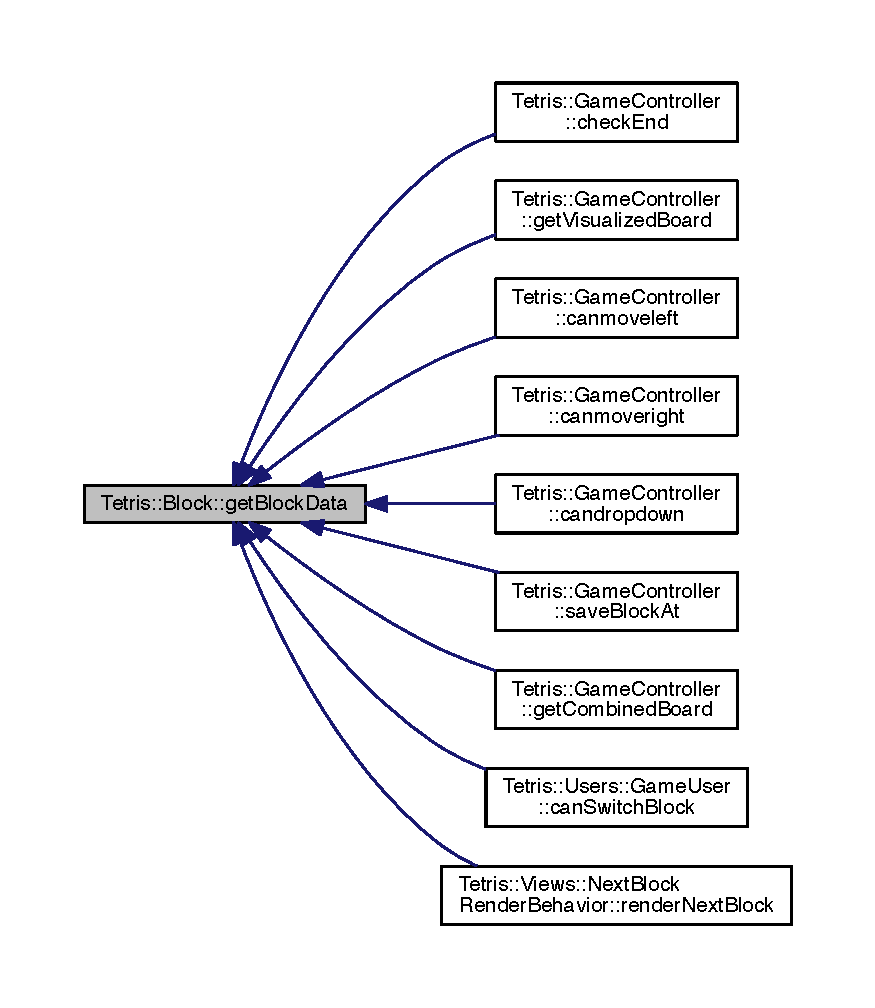
\includegraphics[width=350pt]{df/d05/class_tetris_1_1_block_a9bd2c3d6ccacff9a5f56f72336ba324f_icgraph}
\end{center}
\end{figure}
\mbox{\Hypertarget{class_tetris_1_1_block_a2e17230774c905e35aa9868986c49b09}\label{class_tetris_1_1_block_a2e17230774c905e35aa9868986c49b09}} 
\index{Tetris\+::\+Block@{Tetris\+::\+Block}!get\+Block\+Data@{get\+Block\+Data}}
\index{get\+Block\+Data@{get\+Block\+Data}!Tetris\+::\+Block@{Tetris\+::\+Block}}
\subsubsection{\texorpdfstring{get\+Block\+Data()}{getBlockData()}\hspace{0.1cm}{\footnotesize\ttfamily [2/2]}}
{\footnotesize\ttfamily bool$\ast$$\ast$ Tetris\+::\+Block\+::get\+Block\+Data (\begin{DoxyParamCaption}{ }\end{DoxyParamCaption})\hspace{0.3cm}{\ttfamily [inline]}}

\begin{DoxyReturn}{반환값}
블럭 모양 메트릭스 
\end{DoxyReturn}


Block.\+hpp 파일의 134 번째 라인에서 정의되었습니다.


\begin{DoxyCode}
134                                  \{
135                 \textcolor{keywordflow}{return} this->\hyperlink{class_tetris_1_1_block_af2f96c83a3511d32321672f794aa4db1}{blkspc};
136             \}
\end{DoxyCode}
\mbox{\Hypertarget{class_tetris_1_1_block_a5301977e32c03aaf122fa289fcba77ba}\label{class_tetris_1_1_block_a5301977e32c03aaf122fa289fcba77ba}} 
\index{Tetris\+::\+Block@{Tetris\+::\+Block}!get\+Block\+Space\+Height@{get\+Block\+Space\+Height}}
\index{get\+Block\+Space\+Height@{get\+Block\+Space\+Height}!Tetris\+::\+Block@{Tetris\+::\+Block}}
\subsubsection{\texorpdfstring{get\+Block\+Space\+Height()}{getBlockSpaceHeight()}\hspace{0.1cm}{\footnotesize\ttfamily [1/2]}}
{\footnotesize\ttfamily int Tetris\+::\+Block\+::get\+Block\+Space\+Height (\begin{DoxyParamCaption}{ }\end{DoxyParamCaption})}



Block.\+cpp 파일의 85 번째 라인에서 정의되었습니다.


\begin{DoxyCode}
85                               \{
86                 \textcolor{keywordflow}{return} this->\hyperlink{class_tetris_1_1_block_abbea7737c2b1fb7339aab4dff13de27c}{blkary\_height};
87             \}
\end{DoxyCode}
이 함수를 호출하는 함수들에 대한 그래프입니다.\+:
\nopagebreak
\begin{figure}[H]
\begin{center}
\leavevmode
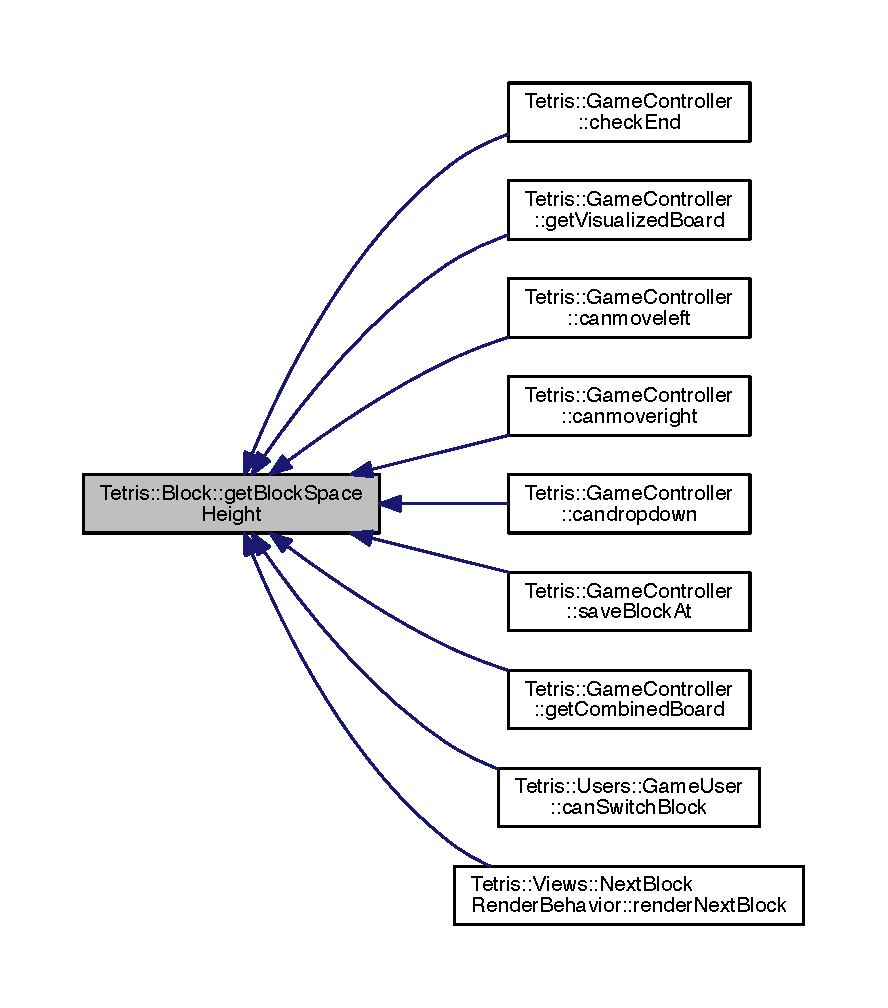
\includegraphics[width=350pt]{df/d05/class_tetris_1_1_block_a5301977e32c03aaf122fa289fcba77ba_icgraph}
\end{center}
\end{figure}
\mbox{\Hypertarget{class_tetris_1_1_block_a5301977e32c03aaf122fa289fcba77ba}\label{class_tetris_1_1_block_a5301977e32c03aaf122fa289fcba77ba}} 
\index{Tetris\+::\+Block@{Tetris\+::\+Block}!get\+Block\+Space\+Height@{get\+Block\+Space\+Height}}
\index{get\+Block\+Space\+Height@{get\+Block\+Space\+Height}!Tetris\+::\+Block@{Tetris\+::\+Block}}
\subsubsection{\texorpdfstring{get\+Block\+Space\+Height()}{getBlockSpaceHeight()}\hspace{0.1cm}{\footnotesize\ttfamily [2/2]}}
{\footnotesize\ttfamily int Tetris\+::\+Block\+::get\+Block\+Space\+Height (\begin{DoxyParamCaption}{ }\end{DoxyParamCaption})\hspace{0.3cm}{\ttfamily [inline]}}

\begin{DoxyReturn}{반환값}
블럭 모양의 높이를 리턴 
\end{DoxyReturn}


Block.\+hpp 파일의 122 번째 라인에서 정의되었습니다.


\begin{DoxyCode}
122                                      \{
123                 \textcolor{keywordflow}{return} this->\hyperlink{class_tetris_1_1_block_abbea7737c2b1fb7339aab4dff13de27c}{blkary\_height};
124             \}
\end{DoxyCode}
\mbox{\Hypertarget{class_tetris_1_1_block_a356cba210ff93bbd80c10d4d00c81cc2}\label{class_tetris_1_1_block_a356cba210ff93bbd80c10d4d00c81cc2}} 
\index{Tetris\+::\+Block@{Tetris\+::\+Block}!get\+Block\+Space\+Size@{get\+Block\+Space\+Size}}
\index{get\+Block\+Space\+Size@{get\+Block\+Space\+Size}!Tetris\+::\+Block@{Tetris\+::\+Block}}
\subsubsection{\texorpdfstring{get\+Block\+Space\+Size()}{getBlockSpaceSize()}\hspace{0.1cm}{\footnotesize\ttfamily [1/2]}}
{\footnotesize\ttfamily int Tetris\+::\+Block\+::get\+Block\+Space\+Size (\begin{DoxyParamCaption}{ }\end{DoxyParamCaption})}



Block.\+cpp 파일의 82 번째 라인에서 정의되었습니다.


\begin{DoxyCode}
82                             \{
83                 \textcolor{keywordflow}{return} this->\hyperlink{class_tetris_1_1_block_a5301977e32c03aaf122fa289fcba77ba}{getBlockSpaceHeight}()*this->
      \hyperlink{class_tetris_1_1_block_ac390e14de476582300d815d9054ed9bd}{getBlockSpaceWidth}();
84             \}
\end{DoxyCode}
\mbox{\Hypertarget{class_tetris_1_1_block_a356cba210ff93bbd80c10d4d00c81cc2}\label{class_tetris_1_1_block_a356cba210ff93bbd80c10d4d00c81cc2}} 
\index{Tetris\+::\+Block@{Tetris\+::\+Block}!get\+Block\+Space\+Size@{get\+Block\+Space\+Size}}
\index{get\+Block\+Space\+Size@{get\+Block\+Space\+Size}!Tetris\+::\+Block@{Tetris\+::\+Block}}
\subsubsection{\texorpdfstring{get\+Block\+Space\+Size()}{getBlockSpaceSize()}\hspace{0.1cm}{\footnotesize\ttfamily [2/2]}}
{\footnotesize\ttfamily int Tetris\+::\+Block\+::get\+Block\+Space\+Size (\begin{DoxyParamCaption}{ }\end{DoxyParamCaption})\hspace{0.3cm}{\ttfamily [inline]}}

\begin{DoxyReturn}{반환값}
블럭 모양의 공간 크기를 리턴 
\end{DoxyReturn}


Block.\+hpp 파일의 116 번째 라인에서 정의되었습니다.


\begin{DoxyCode}
116                                    \{
117                 \textcolor{keywordflow}{return} this->\hyperlink{class_tetris_1_1_block_a5301977e32c03aaf122fa289fcba77ba}{getBlockSpaceHeight}()*this->
      \hyperlink{class_tetris_1_1_block_ac390e14de476582300d815d9054ed9bd}{getBlockSpaceWidth}();
118             \}
\end{DoxyCode}
\mbox{\Hypertarget{class_tetris_1_1_block_ac390e14de476582300d815d9054ed9bd}\label{class_tetris_1_1_block_ac390e14de476582300d815d9054ed9bd}} 
\index{Tetris\+::\+Block@{Tetris\+::\+Block}!get\+Block\+Space\+Width@{get\+Block\+Space\+Width}}
\index{get\+Block\+Space\+Width@{get\+Block\+Space\+Width}!Tetris\+::\+Block@{Tetris\+::\+Block}}
\subsubsection{\texorpdfstring{get\+Block\+Space\+Width()}{getBlockSpaceWidth()}\hspace{0.1cm}{\footnotesize\ttfamily [1/2]}}
{\footnotesize\ttfamily int Tetris\+::\+Block\+::get\+Block\+Space\+Width (\begin{DoxyParamCaption}{ }\end{DoxyParamCaption})}



Block.\+cpp 파일의 88 번째 라인에서 정의되었습니다.


\begin{DoxyCode}
88                              \{
89                 \textcolor{keywordflow}{return} this->\hyperlink{class_tetris_1_1_block_a96548cab58eb788af744b54192c7bea1}{blkary\_width};
90             \}
\end{DoxyCode}
이 함수를 호출하는 함수들에 대한 그래프입니다.\+:
\nopagebreak
\begin{figure}[H]
\begin{center}
\leavevmode
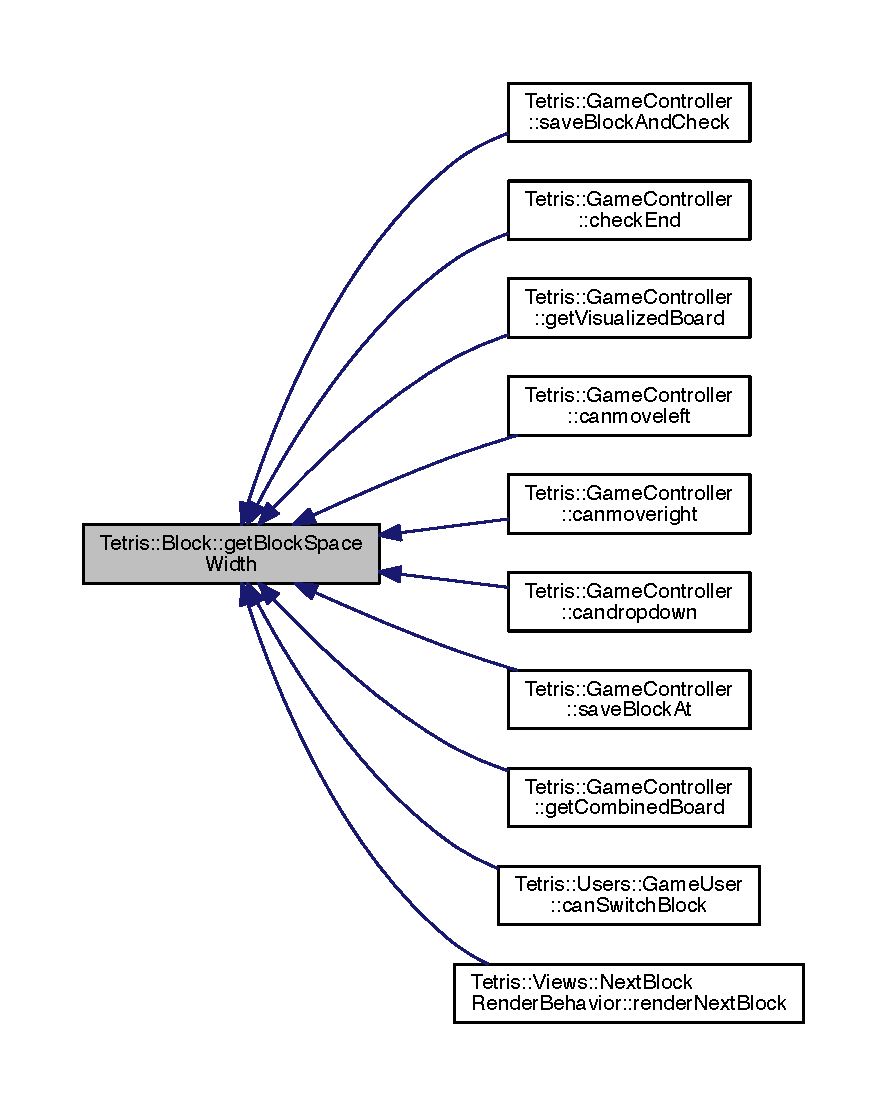
\includegraphics[width=350pt]{df/d05/class_tetris_1_1_block_ac390e14de476582300d815d9054ed9bd_icgraph}
\end{center}
\end{figure}
\mbox{\Hypertarget{class_tetris_1_1_block_ac390e14de476582300d815d9054ed9bd}\label{class_tetris_1_1_block_ac390e14de476582300d815d9054ed9bd}} 
\index{Tetris\+::\+Block@{Tetris\+::\+Block}!get\+Block\+Space\+Width@{get\+Block\+Space\+Width}}
\index{get\+Block\+Space\+Width@{get\+Block\+Space\+Width}!Tetris\+::\+Block@{Tetris\+::\+Block}}
\subsubsection{\texorpdfstring{get\+Block\+Space\+Width()}{getBlockSpaceWidth()}\hspace{0.1cm}{\footnotesize\ttfamily [2/2]}}
{\footnotesize\ttfamily int Tetris\+::\+Block\+::get\+Block\+Space\+Width (\begin{DoxyParamCaption}{ }\end{DoxyParamCaption})\hspace{0.3cm}{\ttfamily [inline]}}

\begin{DoxyReturn}{반환값}
블럭 모양의 너비를 리턴 
\end{DoxyReturn}


Block.\+hpp 파일의 128 번째 라인에서 정의되었습니다.


\begin{DoxyCode}
128                                     \{
129                 \textcolor{keywordflow}{return} this->\hyperlink{class_tetris_1_1_block_a96548cab58eb788af744b54192c7bea1}{blkary\_width};
130             \}
\end{DoxyCode}
\mbox{\Hypertarget{class_tetris_1_1_block_a8780b7c5d836c3bb6bae3de5cdcba5e1}\label{class_tetris_1_1_block_a8780b7c5d836c3bb6bae3de5cdcba5e1}} 
\index{Tetris\+::\+Block@{Tetris\+::\+Block}!get\+Block\+Type@{get\+Block\+Type}}
\index{get\+Block\+Type@{get\+Block\+Type}!Tetris\+::\+Block@{Tetris\+::\+Block}}
\subsubsection{\texorpdfstring{get\+Block\+Type()}{getBlockType()}\hspace{0.1cm}{\footnotesize\ttfamily [1/2]}}
{\footnotesize\ttfamily int Tetris\+::\+Block\+::get\+Block\+Type (\begin{DoxyParamCaption}{ }\end{DoxyParamCaption})}



Block.\+cpp 파일의 94 번째 라인에서 정의되었습니다.


\begin{DoxyCode}
94                        \{
95                 \textcolor{keywordflow}{return} this->\hyperlink{class_tetris_1_1_block_aceac58dcf8d8afaa82c2bab101cb3cff}{blktype};
96             \}
\end{DoxyCode}
\mbox{\Hypertarget{class_tetris_1_1_block_a8780b7c5d836c3bb6bae3de5cdcba5e1}\label{class_tetris_1_1_block_a8780b7c5d836c3bb6bae3de5cdcba5e1}} 
\index{Tetris\+::\+Block@{Tetris\+::\+Block}!get\+Block\+Type@{get\+Block\+Type}}
\index{get\+Block\+Type@{get\+Block\+Type}!Tetris\+::\+Block@{Tetris\+::\+Block}}
\subsubsection{\texorpdfstring{get\+Block\+Type()}{getBlockType()}\hspace{0.1cm}{\footnotesize\ttfamily [2/2]}}
{\footnotesize\ttfamily int Tetris\+::\+Block\+::get\+Block\+Type (\begin{DoxyParamCaption}{ }\end{DoxyParamCaption})\hspace{0.3cm}{\ttfamily [inline]}}

\begin{DoxyReturn}{반환값}
블럭 모양 인식 번호 
\end{DoxyReturn}


Block.\+hpp 파일의 140 번째 라인에서 정의되었습니다.


\begin{DoxyCode}
140                               \{
141                 \textcolor{keywordflow}{return} this->\hyperlink{class_tetris_1_1_block_aceac58dcf8d8afaa82c2bab101cb3cff}{blktype};
142             \}
\end{DoxyCode}
\mbox{\Hypertarget{class_tetris_1_1_block_a464ed776185993ad827f316a08969960}\label{class_tetris_1_1_block_a464ed776185993ad827f316a08969960}} 
\index{Tetris\+::\+Block@{Tetris\+::\+Block}!get\+Rotated\+Space\+Data@{get\+Rotated\+Space\+Data}}
\index{get\+Rotated\+Space\+Data@{get\+Rotated\+Space\+Data}!Tetris\+::\+Block@{Tetris\+::\+Block}}
\subsubsection{\texorpdfstring{get\+Rotated\+Space\+Data()}{getRotatedSpaceData()}\hspace{0.1cm}{\footnotesize\ttfamily [1/2]}}
{\footnotesize\ttfamily bool $\ast$$\ast$ Tetris\+::\+Block\+::get\+Rotated\+Space\+Data (\begin{DoxyParamCaption}{ }\end{DoxyParamCaption})}



Block.\+cpp 파일의 104 번째 라인에서 정의되었습니다.


\begin{DoxyCode}
104                                  \{
105                 \textcolor{keywordflow}{if}(this->\hyperlink{class_tetris_1_1_block_aceac58dcf8d8afaa82c2bab101cb3cff}{blktype}==-1||this->\hyperlink{class_tetris_1_1_block_af2f96c83a3511d32321672f794aa4db1}{blkspc}==NULL||(this->
      \hyperlink{class_tetris_1_1_block_af2f96c83a3511d32321672f794aa4db1}{blkspc}!=NULL&&this->\hyperlink{class_tetris_1_1_block_af2f96c83a3511d32321672f794aa4db1}{blkspc}[0]==NULL)||\hyperlink{class_tetris_1_1_block_aceac58dcf8d8afaa82c2bab101cb3cff}{blktype}==\hyperlink{_block_8h_a6da1e2b8848e1a7b5a7ee687fd6492bd}{TETBLK\_TYPE\_M})\{
106                     \textcolor{keywordflow}{return} NULL;
107                 \}
108                 \textcolor{keywordtype}{bool}** tmpblksp = \textcolor{keyword}{new} \textcolor{keywordtype}{bool}*[\hyperlink{class_tetris_1_1_block_a96548cab58eb788af744b54192c7bea1}{blkary\_width}];
109                 \textcolor{keywordflow}{for}(\textcolor{keywordtype}{int} i=0;i<\hyperlink{class_tetris_1_1_block_a96548cab58eb788af744b54192c7bea1}{blkary\_width};i++)\{
110                     tmpblksp[i] = \textcolor{keyword}{new} \textcolor{keywordtype}{bool}[\hyperlink{class_tetris_1_1_block_abbea7737c2b1fb7339aab4dff13de27c}{blkary\_height}];
111                     \textcolor{comment}{//memset(tmpblksp[i],false,sizeof(bool)*blkary\_height);}
112                     \textcolor{keywordflow}{for}(\textcolor{keywordtype}{int} j=0;j<\hyperlink{class_tetris_1_1_block_abbea7737c2b1fb7339aab4dff13de27c}{blkary\_height};j++) tmpblksp[i][j] = 
      \hyperlink{class_tetris_1_1_block_af2f96c83a3511d32321672f794aa4db1}{blkspc}[blkary\_height-1-j][i];    
113                 \}
114                 \textcolor{keywordflow}{return} tmpblksp;
115             \}
\end{DoxyCode}
\mbox{\Hypertarget{class_tetris_1_1_block_ada769278572785b24e8a91f620b97b81}\label{class_tetris_1_1_block_ada769278572785b24e8a91f620b97b81}} 
\index{Tetris\+::\+Block@{Tetris\+::\+Block}!get\+Rotated\+Space\+Data@{get\+Rotated\+Space\+Data}}
\index{get\+Rotated\+Space\+Data@{get\+Rotated\+Space\+Data}!Tetris\+::\+Block@{Tetris\+::\+Block}}
\subsubsection{\texorpdfstring{get\+Rotated\+Space\+Data()}{getRotatedSpaceData()}\hspace{0.1cm}{\footnotesize\ttfamily [2/2]}}
{\footnotesize\ttfamily bool$\ast$$\ast$ Tetris\+::\+Block\+::get\+Rotated\+Space\+Data (\begin{DoxyParamCaption}{ }\end{DoxyParamCaption})\hspace{0.3cm}{\ttfamily [inline]}}

\begin{DoxyReturn}{반환값}
반시계 방향으로 90도 회전된 블록 데이터를 리턴 
\end{DoxyReturn}


Block.\+hpp 파일의 153 번째 라인에서 정의되었습니다.


\begin{DoxyCode}
153                                         \{
154                 \textcolor{keywordflow}{if}(this->\hyperlink{class_tetris_1_1_block_aceac58dcf8d8afaa82c2bab101cb3cff}{blktype}==-1||this->\hyperlink{class_tetris_1_1_block_af2f96c83a3511d32321672f794aa4db1}{blkspc}==NULL||(this->
      \hyperlink{class_tetris_1_1_block_af2f96c83a3511d32321672f794aa4db1}{blkspc}!=NULL&&this->\hyperlink{class_tetris_1_1_block_af2f96c83a3511d32321672f794aa4db1}{blkspc}[0]==NULL)||\hyperlink{class_tetris_1_1_block_aceac58dcf8d8afaa82c2bab101cb3cff}{blktype}==\hyperlink{_block_8hpp_a6da1e2b8848e1a7b5a7ee687fd6492bd}{TETBLK\_TYPE\_M})\{
155                     \textcolor{keywordflow}{return} NULL;
156                 \}
157                 \textcolor{keywordtype}{bool}** tmpblksp = \textcolor{keyword}{new} \textcolor{keywordtype}{bool}*[\hyperlink{class_tetris_1_1_block_a96548cab58eb788af744b54192c7bea1}{blkary\_width}];
158                 \textcolor{keywordflow}{for}(\textcolor{keywordtype}{int} i=0;i<\hyperlink{class_tetris_1_1_block_a96548cab58eb788af744b54192c7bea1}{blkary\_width};i++)\{
159                     tmpblksp[i] = \textcolor{keyword}{new} \textcolor{keywordtype}{bool}[\hyperlink{class_tetris_1_1_block_abbea7737c2b1fb7339aab4dff13de27c}{blkary\_height}];
160                     \textcolor{comment}{//memset(tmpblksp[i],false,sizeof(bool)*blkary\_height);}
161                     \textcolor{keywordflow}{for}(\textcolor{keywordtype}{int} j=0;j<\hyperlink{class_tetris_1_1_block_abbea7737c2b1fb7339aab4dff13de27c}{blkary\_height};j++) tmpblksp[i][j] = 
      \hyperlink{class_tetris_1_1_block_af2f96c83a3511d32321672f794aa4db1}{blkspc}[blkary\_height-1-j][i];
162                 \}
163                 \textcolor{keywordflow}{return} tmpblksp;
164             \}
\end{DoxyCode}
\mbox{\Hypertarget{class_tetris_1_1_block_ae7aadeec449fec232e9635d839593028}\label{class_tetris_1_1_block_ae7aadeec449fec232e9635d839593028}} 
\index{Tetris\+::\+Block@{Tetris\+::\+Block}!printspace@{printspace}}
\index{printspace@{printspace}!Tetris\+::\+Block@{Tetris\+::\+Block}}
\subsubsection{\texorpdfstring{printspace()}{printspace()}\hspace{0.1cm}{\footnotesize\ttfamily [1/2]}}
{\footnotesize\ttfamily void Tetris\+::\+Block\+::printspace (\begin{DoxyParamCaption}{ }\end{DoxyParamCaption})}



Block.\+cpp 파일의 173 번째 라인에서 정의되었습니다.


\begin{DoxyCode}
173                       \{
174                 \textcolor{keywordflow}{if}(this->\hyperlink{class_tetris_1_1_block_aceac58dcf8d8afaa82c2bab101cb3cff}{blktype}==-1||this->\hyperlink{class_tetris_1_1_block_af2f96c83a3511d32321672f794aa4db1}{blkspc}==NULL)\{
175                     cout<<\textcolor{stringliteral}{"we can't show space info"}<<endl;
176                     \textcolor{keywordflow}{return};
177                 \}
178                 \textcolor{keywordflow}{for}(\textcolor{keywordtype}{int} i=0;i<this->\hyperlink{class_tetris_1_1_block_abbea7737c2b1fb7339aab4dff13de27c}{blkary\_height};i++)\{
179                     \textcolor{keywordflow}{for}(\textcolor{keywordtype}{int} j=0;j<this->\hyperlink{class_tetris_1_1_block_a96548cab58eb788af744b54192c7bea1}{blkary\_width};j++)\{
180                         cout<<\hyperlink{class_tetris_1_1_block_af2f96c83a3511d32321672f794aa4db1}{blkspc}[i][j]<<\textcolor{charliteral}{' '};
181                     \}
182                     cout<<endl;
183                 \}
184             \}
\end{DoxyCode}
\mbox{\Hypertarget{class_tetris_1_1_block_ae7aadeec449fec232e9635d839593028}\label{class_tetris_1_1_block_ae7aadeec449fec232e9635d839593028}} 
\index{Tetris\+::\+Block@{Tetris\+::\+Block}!printspace@{printspace}}
\index{printspace@{printspace}!Tetris\+::\+Block@{Tetris\+::\+Block}}
\subsubsection{\texorpdfstring{printspace()}{printspace()}\hspace{0.1cm}{\footnotesize\ttfamily [2/2]}}
{\footnotesize\ttfamily void Tetris\+::\+Block\+::printspace (\begin{DoxyParamCaption}{ }\end{DoxyParamCaption})\hspace{0.3cm}{\ttfamily [inline]}}

\begin{DoxyReturn}{반환값}
콘솔에서 모양 디버깅시 확인 함수 
\end{DoxyReturn}


Block.\+hpp 파일의 231 번째 라인에서 정의되었습니다.


\begin{DoxyCode}
231                              \{
232                 \textcolor{keywordflow}{if}(this->\hyperlink{class_tetris_1_1_block_aceac58dcf8d8afaa82c2bab101cb3cff}{blktype}==-1||this->\hyperlink{class_tetris_1_1_block_af2f96c83a3511d32321672f794aa4db1}{blkspc}==NULL)\{
233                     cout<<\textcolor{stringliteral}{"we can't show space info"}<<endl;
234                     \textcolor{keywordflow}{return};
235                 \}
236                 \textcolor{keywordflow}{for}(\textcolor{keywordtype}{int} i=0;i<this->\hyperlink{class_tetris_1_1_block_abbea7737c2b1fb7339aab4dff13de27c}{blkary\_height};i++)\{
237                     \textcolor{keywordflow}{for}(\textcolor{keywordtype}{int} j=0;j<this->\hyperlink{class_tetris_1_1_block_a96548cab58eb788af744b54192c7bea1}{blkary\_width};j++)\{
238                         cout<<\hyperlink{class_tetris_1_1_block_af2f96c83a3511d32321672f794aa4db1}{blkspc}[i][j]<<\textcolor{charliteral}{' '};
239                     \}
240                     cout<<endl;
241                 \}
242             \}
\end{DoxyCode}
\mbox{\Hypertarget{class_tetris_1_1_block_a787424e5e9ec2807989121e8dcee1a7a}\label{class_tetris_1_1_block_a787424e5e9ec2807989121e8dcee1a7a}} 
\index{Tetris\+::\+Block@{Tetris\+::\+Block}!roatespec@{roatespec}}
\index{roatespec@{roatespec}!Tetris\+::\+Block@{Tetris\+::\+Block}}
\subsubsection{\texorpdfstring{roatespec()}{roatespec()}\hspace{0.1cm}{\footnotesize\ttfamily [1/2]}}
{\footnotesize\ttfamily bool Tetris\+::\+Block\+::roatespec (\begin{DoxyParamCaption}{ }\end{DoxyParamCaption})}



Block.\+cpp 파일의 169 번째 라인에서 정의되었습니다.


\begin{DoxyCode}
169                          \{
170                 \textcolor{keywordflow}{return} \textcolor{keyword}{false};
171             \}
\end{DoxyCode}
\mbox{\Hypertarget{class_tetris_1_1_block_a787424e5e9ec2807989121e8dcee1a7a}\label{class_tetris_1_1_block_a787424e5e9ec2807989121e8dcee1a7a}} 
\index{Tetris\+::\+Block@{Tetris\+::\+Block}!roatespec@{roatespec}}
\index{roatespec@{roatespec}!Tetris\+::\+Block@{Tetris\+::\+Block}}
\subsubsection{\texorpdfstring{roatespec()}{roatespec()}\hspace{0.1cm}{\footnotesize\ttfamily [2/2]}}
{\footnotesize\ttfamily bool Tetris\+::\+Block\+::roatespec (\begin{DoxyParamCaption}{ }\end{DoxyParamCaption})\hspace{0.3cm}{\ttfamily [inline]}}



Block.\+hpp 파일의 225 번째 라인에서 정의되었습니다.


\begin{DoxyCode}
225                             \{
226                 \textcolor{keywordflow}{return} \textcolor{keyword}{false};
227             \}
\end{DoxyCode}
\mbox{\Hypertarget{class_tetris_1_1_block_a0d1eb57e6da91832ad983f7a4fa9ca04}\label{class_tetris_1_1_block_a0d1eb57e6da91832ad983f7a4fa9ca04}} 
\index{Tetris\+::\+Block@{Tetris\+::\+Block}!rotate@{rotate}}
\index{rotate@{rotate}!Tetris\+::\+Block@{Tetris\+::\+Block}}
\subsubsection{\texorpdfstring{rotate()}{rotate()}\hspace{0.1cm}{\footnotesize\ttfamily [1/2]}}
{\footnotesize\ttfamily bool Tetris\+::\+Block\+::rotate (\begin{DoxyParamCaption}{ }\end{DoxyParamCaption})}



Block.\+cpp 파일의 152 번째 라인에서 정의되었습니다.


\begin{DoxyCode}
152                   \{
153                 \textcolor{keywordflow}{if}(this->\hyperlink{class_tetris_1_1_block_aceac58dcf8d8afaa82c2bab101cb3cff}{blktype}==-1||this->\hyperlink{class_tetris_1_1_block_af2f96c83a3511d32321672f794aa4db1}{blkspc}==NULL||(this->
      \hyperlink{class_tetris_1_1_block_af2f96c83a3511d32321672f794aa4db1}{blkspc}!=NULL&&this->\hyperlink{class_tetris_1_1_block_af2f96c83a3511d32321672f794aa4db1}{blkspc}[0]==NULL))\{
154                     \textcolor{keywordflow}{return} \textcolor{keyword}{false};
155                 \}
156                 \textcolor{keywordflow}{if}(\hyperlink{class_tetris_1_1_block_aceac58dcf8d8afaa82c2bab101cb3cff}{blktype}==\hyperlink{_block_8h_a6da1e2b8848e1a7b5a7ee687fd6492bd}{TETBLK\_TYPE\_M})\{
157                     \textcolor{keywordflow}{return} \textcolor{keyword}{true};
158                 \}
159                 \textcolor{keywordtype}{bool}** tmpblksp = this->\hyperlink{class_tetris_1_1_block_a464ed776185993ad827f316a08969960}{getRotatedSpaceData}();
160 
161                 \textcolor{keywordflow}{for}(\textcolor{keywordtype}{int} i=0;i<\hyperlink{class_tetris_1_1_block_abbea7737c2b1fb7339aab4dff13de27c}{blkary\_height};i++)\{
162                     \textcolor{keyword}{delete} [] \hyperlink{class_tetris_1_1_block_af2f96c83a3511d32321672f794aa4db1}{blkspc}[i];
163                 \}
164                 \textcolor{keyword}{delete} [] \hyperlink{class_tetris_1_1_block_af2f96c83a3511d32321672f794aa4db1}{blkspc};
165                 \hyperlink{class_tetris_1_1_block_af2f96c83a3511d32321672f794aa4db1}{blkspc} = tmpblksp;
166                 this->blkary\_height^=this->\hyperlink{class_tetris_1_1_block_a96548cab58eb788af744b54192c7bea1}{blkary\_width}^=this->blkary\_height^=this->
      \hyperlink{class_tetris_1_1_block_a96548cab58eb788af744b54192c7bea1}{blkary\_width};
167                 \textcolor{keywordflow}{return} \textcolor{keyword}{true};
168             \}
\end{DoxyCode}
이 함수를 호출하는 함수들에 대한 그래프입니다.\+:
\nopagebreak
\begin{figure}[H]
\begin{center}
\leavevmode
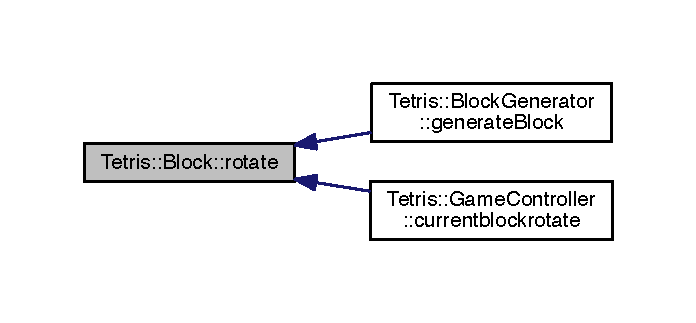
\includegraphics[width=334pt]{df/d05/class_tetris_1_1_block_a0d1eb57e6da91832ad983f7a4fa9ca04_icgraph}
\end{center}
\end{figure}
\mbox{\Hypertarget{class_tetris_1_1_block_a0d1eb57e6da91832ad983f7a4fa9ca04}\label{class_tetris_1_1_block_a0d1eb57e6da91832ad983f7a4fa9ca04}} 
\index{Tetris\+::\+Block@{Tetris\+::\+Block}!rotate@{rotate}}
\index{rotate@{rotate}!Tetris\+::\+Block@{Tetris\+::\+Block}}
\subsubsection{\texorpdfstring{rotate()}{rotate()}\hspace{0.1cm}{\footnotesize\ttfamily [2/2]}}
{\footnotesize\ttfamily bool Tetris\+::\+Block\+::rotate (\begin{DoxyParamCaption}{ }\end{DoxyParamCaption})\hspace{0.3cm}{\ttfamily [inline]}}

\begin{DoxyReturn}{반환값}
회전 성공 유무 
\end{DoxyReturn}


Block.\+hpp 파일의 207 번째 라인에서 정의되었습니다.


\begin{DoxyCode}
207                          \{
208                 cout<<\textcolor{stringliteral}{"call rotatefunc in block"}<<endl;
209                 \textcolor{keywordflow}{if}(this->\hyperlink{class_tetris_1_1_block_aceac58dcf8d8afaa82c2bab101cb3cff}{blktype}==-1||this->\hyperlink{class_tetris_1_1_block_af2f96c83a3511d32321672f794aa4db1}{blkspc}==NULL||(this->
      \hyperlink{class_tetris_1_1_block_af2f96c83a3511d32321672f794aa4db1}{blkspc}!=NULL&&this->\hyperlink{class_tetris_1_1_block_af2f96c83a3511d32321672f794aa4db1}{blkspc}[0]==NULL))\{
210                     \textcolor{keywordflow}{return} \textcolor{keyword}{false};
211                 \}
212                 \textcolor{keywordflow}{if}(\hyperlink{class_tetris_1_1_block_aceac58dcf8d8afaa82c2bab101cb3cff}{blktype}==\hyperlink{_block_8hpp_a6da1e2b8848e1a7b5a7ee687fd6492bd}{TETBLK\_TYPE\_M})\{
213                     \textcolor{keywordflow}{return} \textcolor{keyword}{true};
214                 \}
215                 \textcolor{keywordtype}{bool}** tmpblksp = this->\hyperlink{class_tetris_1_1_block_a464ed776185993ad827f316a08969960}{getRotatedSpaceData}();
216 
217                 \textcolor{keywordflow}{for}(\textcolor{keywordtype}{int} i=0;i<\hyperlink{class_tetris_1_1_block_abbea7737c2b1fb7339aab4dff13de27c}{blkary\_height};i++)\{
218                     \textcolor{keyword}{delete} [] \hyperlink{class_tetris_1_1_block_af2f96c83a3511d32321672f794aa4db1}{blkspc}[i];
219                 \}
220                 \textcolor{keyword}{delete} [] \hyperlink{class_tetris_1_1_block_af2f96c83a3511d32321672f794aa4db1}{blkspc};
221                 \hyperlink{class_tetris_1_1_block_af2f96c83a3511d32321672f794aa4db1}{blkspc} = tmpblksp;
222                 this->blkary\_height^=this->\hyperlink{class_tetris_1_1_block_a96548cab58eb788af744b54192c7bea1}{blkary\_width}^=this->blkary\_height^=this->
      \hyperlink{class_tetris_1_1_block_a96548cab58eb788af744b54192c7bea1}{blkary\_width};
223                 \textcolor{keywordflow}{return} \textcolor{keyword}{true};
224             \}
\end{DoxyCode}
\mbox{\Hypertarget{class_tetris_1_1_block_a1a3fab9e7eabe64a4ba588ed5091d3a9}\label{class_tetris_1_1_block_a1a3fab9e7eabe64a4ba588ed5091d3a9}} 
\index{Tetris\+::\+Block@{Tetris\+::\+Block}!set\+Block\+Color@{set\+Block\+Color}}
\index{set\+Block\+Color@{set\+Block\+Color}!Tetris\+::\+Block@{Tetris\+::\+Block}}
\subsubsection{\texorpdfstring{set\+Block\+Color()}{setBlockColor()}\hspace{0.1cm}{\footnotesize\ttfamily [1/2]}}
{\footnotesize\ttfamily void Tetris\+::\+Block\+::set\+Block\+Color (\begin{DoxyParamCaption}\item[{unsigned int}]{clr }\end{DoxyParamCaption})}



Block.\+cpp 파일의 33 번째 라인에서 정의되었습니다.


\begin{DoxyCode}
33                                          \{
34                 this->\hyperlink{class_tetris_1_1_block_acf78e864526e38c9c72fa0b012d5b344}{blk\_color}=clr;
35             \}
\end{DoxyCode}
\mbox{\Hypertarget{class_tetris_1_1_block_a1a3fab9e7eabe64a4ba588ed5091d3a9}\label{class_tetris_1_1_block_a1a3fab9e7eabe64a4ba588ed5091d3a9}} 
\index{Tetris\+::\+Block@{Tetris\+::\+Block}!set\+Block\+Color@{set\+Block\+Color}}
\index{set\+Block\+Color@{set\+Block\+Color}!Tetris\+::\+Block@{Tetris\+::\+Block}}
\subsubsection{\texorpdfstring{set\+Block\+Color()}{setBlockColor()}\hspace{0.1cm}{\footnotesize\ttfamily [2/2]}}
{\footnotesize\ttfamily void Tetris\+::\+Block\+::set\+Block\+Color (\begin{DoxyParamCaption}\item[{unsigned int}]{clr }\end{DoxyParamCaption})\hspace{0.3cm}{\ttfamily [inline]}}

\begin{DoxyReturn}{반환값}
리턴은 없지만 블럭 색상 설정 
\end{DoxyReturn}


Block.\+hpp 파일의 72 번째 라인에서 정의되었습니다.


\begin{DoxyCode}
72                                                 \{
73                 \textcolor{keywordflow}{if}(this->\hyperlink{class_tetris_1_1_block_ab7cfb062eb49e791c94bac4a2e7a7ca9}{blkcolr}==NULL)\{
74                     this->\hyperlink{class_tetris_1_1_block_ab7cfb062eb49e791c94bac4a2e7a7ca9}{blkcolr} = \textcolor{keyword}{new} \hyperlink{class_tetris_1_1_block_sub_modules_1_1_block_color}{BlockColor}(clr);
75                 \}\textcolor{keywordflow}{else}\{
76                     this->\hyperlink{class_tetris_1_1_block_ab7cfb062eb49e791c94bac4a2e7a7ca9}{blkcolr}->\hyperlink{class_tetris_1_1_block_sub_modules_1_1_block_color_a260b5dd85cdf3145be7564dc2c0ee53d}{forceApplyColor}(clr);
77                 \}
78                \textcolor{comment}{// this->blk\_color=clr;}
79             \}
\end{DoxyCode}
\mbox{\Hypertarget{class_tetris_1_1_block_ad683f161157c16b80d5df8929bca468c}\label{class_tetris_1_1_block_ad683f161157c16b80d5df8929bca468c}} 
\index{Tetris\+::\+Block@{Tetris\+::\+Block}!spanshape@{spanshape}}
\index{spanshape@{spanshape}!Tetris\+::\+Block@{Tetris\+::\+Block}}
\subsubsection{\texorpdfstring{spanshape()}{spanshape()}\hspace{0.1cm}{\footnotesize\ttfamily [1/2]}}
{\footnotesize\ttfamily void Tetris\+::\+Block\+::spanshape (\begin{DoxyParamCaption}\item[{int}]{type }\end{DoxyParamCaption})\hspace{0.3cm}{\ttfamily [private]}}



Block.\+cpp 파일의 192 번째 라인에서 정의되었습니다.


\begin{DoxyCode}
192                              \{
193                 \textcolor{keywordflow}{switch}(type)\{
194                     \textcolor{keywordflow}{case} \hyperlink{_block_8h_ac9fe505a10c9ea541483202000c72dfe}{TETBLK\_TYPE\_I}:\{
195                         this->\hyperlink{class_tetris_1_1_block_aceac58dcf8d8afaa82c2bab101cb3cff}{blktype} = type;
196                         this->\hyperlink{class_tetris_1_1_block_abbea7737c2b1fb7339aab4dff13de27c}{blkary\_height}=4;
197                         this->\hyperlink{class_tetris_1_1_block_a96548cab58eb788af744b54192c7bea1}{blkary\_width}=1;
198                         this->\hyperlink{class_tetris_1_1_block_af2f96c83a3511d32321672f794aa4db1}{blkspc} =  \textcolor{keyword}{new} \textcolor{keywordtype}{bool}*[this->\hyperlink{class_tetris_1_1_block_abbea7737c2b1fb7339aab4dff13de27c}{blkary\_height}];
199                         \textcolor{keywordflow}{for}(\textcolor{keywordtype}{int} i=0;i<\hyperlink{class_tetris_1_1_block_abbea7737c2b1fb7339aab4dff13de27c}{blkary\_height};i++)\{
200                             this->\hyperlink{class_tetris_1_1_block_af2f96c83a3511d32321672f794aa4db1}{blkspc}[i] = \textcolor{keyword}{new} \textcolor{keywordtype}{bool}[this->\hyperlink{class_tetris_1_1_block_a96548cab58eb788af744b54192c7bea1}{blkary\_width}];
201                             memset(this->\hyperlink{class_tetris_1_1_block_af2f96c83a3511d32321672f794aa4db1}{blkspc}[i],\textcolor{keyword}{false},\textcolor{keyword}{sizeof}(\textcolor{keywordtype}{bool})*this->
      \hyperlink{class_tetris_1_1_block_a96548cab58eb788af744b54192c7bea1}{blkary\_width});
202                             this->\hyperlink{class_tetris_1_1_block_af2f96c83a3511d32321672f794aa4db1}{blkspc}[i][0]=\textcolor{keyword}{true};
203                         \}
204 
205                         \textcolor{keywordflow}{break};
206                     \}
207                     \textcolor{keywordflow}{case} \hyperlink{_block_8h_a6da1e2b8848e1a7b5a7ee687fd6492bd}{TETBLK\_TYPE\_M}:\{
208                         this->\hyperlink{class_tetris_1_1_block_aceac58dcf8d8afaa82c2bab101cb3cff}{blktype} = type;
209                         this->blkary\_height=2;
210                         this->\hyperlink{class_tetris_1_1_block_a96548cab58eb788af744b54192c7bea1}{blkary\_width}=2;
211                         this->\hyperlink{class_tetris_1_1_block_af2f96c83a3511d32321672f794aa4db1}{blkspc} =  \textcolor{keyword}{new} \textcolor{keywordtype}{bool}*[this->\hyperlink{class_tetris_1_1_block_abbea7737c2b1fb7339aab4dff13de27c}{blkary\_height}];
212                         \textcolor{keywordflow}{for}(\textcolor{keywordtype}{int} i=0;i<\hyperlink{class_tetris_1_1_block_abbea7737c2b1fb7339aab4dff13de27c}{blkary\_height};i++)\{
213                             this->\hyperlink{class_tetris_1_1_block_af2f96c83a3511d32321672f794aa4db1}{blkspc}[i] = \textcolor{keyword}{new} \textcolor{keywordtype}{bool}[this->\hyperlink{class_tetris_1_1_block_a96548cab58eb788af744b54192c7bea1}{blkary\_width}];
214                             memset(this->\hyperlink{class_tetris_1_1_block_af2f96c83a3511d32321672f794aa4db1}{blkspc}[i],\textcolor{keyword}{false},\textcolor{keyword}{sizeof}(\textcolor{keywordtype}{bool})*this->
      \hyperlink{class_tetris_1_1_block_a96548cab58eb788af744b54192c7bea1}{blkary\_width});
215                             \textcolor{keywordflow}{for}(\textcolor{keywordtype}{int} j=0;j<\hyperlink{class_tetris_1_1_block_a96548cab58eb788af744b54192c7bea1}{blkary\_width};j++)\{
216                                 this->\hyperlink{class_tetris_1_1_block_af2f96c83a3511d32321672f794aa4db1}{blkspc}[i][j]=\textcolor{keyword}{true};
217                             \}
218                         \}
219                         \textcolor{keywordflow}{break};
220                     \}
221                     \textcolor{keywordflow}{case} \hyperlink{_block_8h_aa624341303e91efd01c17dfb25d15010}{TETBLK\_TYPE\_T}:\{
222                         this->\hyperlink{class_tetris_1_1_block_aceac58dcf8d8afaa82c2bab101cb3cff}{blktype} = type;
223                         this->blkary\_height=2;
224                         this->\hyperlink{class_tetris_1_1_block_a96548cab58eb788af744b54192c7bea1}{blkary\_width}=3;
225                         this->\hyperlink{class_tetris_1_1_block_af2f96c83a3511d32321672f794aa4db1}{blkspc} =  \textcolor{keyword}{new} \textcolor{keywordtype}{bool}*[this->\hyperlink{class_tetris_1_1_block_abbea7737c2b1fb7339aab4dff13de27c}{blkary\_height}];
226                         \textcolor{keywordflow}{for}(\textcolor{keywordtype}{int} i=0;i<\hyperlink{class_tetris_1_1_block_abbea7737c2b1fb7339aab4dff13de27c}{blkary\_height};i++)\{
227                             this->\hyperlink{class_tetris_1_1_block_af2f96c83a3511d32321672f794aa4db1}{blkspc}[i] = \textcolor{keyword}{new} \textcolor{keywordtype}{bool}[this->\hyperlink{class_tetris_1_1_block_a96548cab58eb788af744b54192c7bea1}{blkary\_width}];
228                             memset(this->\hyperlink{class_tetris_1_1_block_af2f96c83a3511d32321672f794aa4db1}{blkspc}[i],\textcolor{keyword}{false},\textcolor{keyword}{sizeof}(\textcolor{keywordtype}{bool})*this->
      \hyperlink{class_tetris_1_1_block_a96548cab58eb788af744b54192c7bea1}{blkary\_width});
229                             \textcolor{keywordflow}{if}(i==0)\{
230                                 \textcolor{keywordflow}{for}(\textcolor{keywordtype}{int} j=0;j<\hyperlink{class_tetris_1_1_block_a96548cab58eb788af744b54192c7bea1}{blkary\_width};j++)\{
231                                     this->\hyperlink{class_tetris_1_1_block_af2f96c83a3511d32321672f794aa4db1}{blkspc}[i][j]=\textcolor{keyword}{true};
232                                 \}
233                             \}\textcolor{keywordflow}{else}\{
234                                 this->\hyperlink{class_tetris_1_1_block_af2f96c83a3511d32321672f794aa4db1}{blkspc}[i][1]=\textcolor{keyword}{true};
235                             \}
236                         \}
237 
238                         \textcolor{keywordflow}{break};
239                     \}
240                     \textcolor{keywordflow}{case} \hyperlink{_block_8h_aa30a45ef914d6bd7caf960c42af38197}{TETBLK\_TYPE\_L}:\{
241                         this->\hyperlink{class_tetris_1_1_block_aceac58dcf8d8afaa82c2bab101cb3cff}{blktype} = type;
242                         this->blkary\_height=3;
243                         this->\hyperlink{class_tetris_1_1_block_a96548cab58eb788af744b54192c7bea1}{blkary\_width}=2;
244                         this->\hyperlink{class_tetris_1_1_block_af2f96c83a3511d32321672f794aa4db1}{blkspc} =  \textcolor{keyword}{new} \textcolor{keywordtype}{bool}*[this->\hyperlink{class_tetris_1_1_block_abbea7737c2b1fb7339aab4dff13de27c}{blkary\_height}];
245                         \textcolor{keywordflow}{for}(\textcolor{keywordtype}{int} i=0;i<\hyperlink{class_tetris_1_1_block_abbea7737c2b1fb7339aab4dff13de27c}{blkary\_height};i++)\{
246                             this->\hyperlink{class_tetris_1_1_block_af2f96c83a3511d32321672f794aa4db1}{blkspc}[i] = \textcolor{keyword}{new} \textcolor{keywordtype}{bool}[this->\hyperlink{class_tetris_1_1_block_a96548cab58eb788af744b54192c7bea1}{blkary\_width}];
247                             memset(this->\hyperlink{class_tetris_1_1_block_af2f96c83a3511d32321672f794aa4db1}{blkspc}[i],\textcolor{keyword}{false},\textcolor{keyword}{sizeof}(\textcolor{keywordtype}{bool})*this->
      \hyperlink{class_tetris_1_1_block_a96548cab58eb788af744b54192c7bea1}{blkary\_width});
248                             this->\hyperlink{class_tetris_1_1_block_af2f96c83a3511d32321672f794aa4db1}{blkspc}[i][0]=\textcolor{keyword}{true};
249                             \textcolor{keywordflow}{if}(i+1==blkary\_height)\{
250                                 this->\hyperlink{class_tetris_1_1_block_af2f96c83a3511d32321672f794aa4db1}{blkspc}[i][1]=\textcolor{keyword}{true};
251                             \}
252                         \}
253 
254                         \textcolor{keywordflow}{break};
255                     \}
256                     \textcolor{keywordflow}{case} \hyperlink{_block_8h_a3a84ffcf3638f400ed5ebc303d152a94}{TETBLK\_TYPE\_J}:\{
257                         this->\hyperlink{class_tetris_1_1_block_aceac58dcf8d8afaa82c2bab101cb3cff}{blktype} = type;
258                         this->blkary\_height=3;
259                         this->\hyperlink{class_tetris_1_1_block_a96548cab58eb788af744b54192c7bea1}{blkary\_width}=2;
260                         this->\hyperlink{class_tetris_1_1_block_af2f96c83a3511d32321672f794aa4db1}{blkspc} =  \textcolor{keyword}{new} \textcolor{keywordtype}{bool}*[this->\hyperlink{class_tetris_1_1_block_abbea7737c2b1fb7339aab4dff13de27c}{blkary\_height}];
261                         \textcolor{keywordflow}{for}(\textcolor{keywordtype}{int} i=0;i<\hyperlink{class_tetris_1_1_block_abbea7737c2b1fb7339aab4dff13de27c}{blkary\_height};i++)\{
262                             this->\hyperlink{class_tetris_1_1_block_af2f96c83a3511d32321672f794aa4db1}{blkspc}[i] = \textcolor{keyword}{new} \textcolor{keywordtype}{bool}[this->\hyperlink{class_tetris_1_1_block_a96548cab58eb788af744b54192c7bea1}{blkary\_width}];
263                             memset(this->\hyperlink{class_tetris_1_1_block_af2f96c83a3511d32321672f794aa4db1}{blkspc}[i],\textcolor{keyword}{false},\textcolor{keyword}{sizeof}(\textcolor{keywordtype}{bool})*this->
      \hyperlink{class_tetris_1_1_block_a96548cab58eb788af744b54192c7bea1}{blkary\_width});
264                             this->\hyperlink{class_tetris_1_1_block_af2f96c83a3511d32321672f794aa4db1}{blkspc}[i][1]=\textcolor{keyword}{true};
265                             \textcolor{keywordflow}{if}(i+1==blkary\_height)\{
266                                 this->\hyperlink{class_tetris_1_1_block_af2f96c83a3511d32321672f794aa4db1}{blkspc}[i][0]=\textcolor{keyword}{true};
267                             \}
268                         \}
269                         \textcolor{keywordflow}{break};
270                     \}
271                     \textcolor{keywordflow}{case} \hyperlink{_block_8h_a50283efc563e3ebe3b8ac84947491f5d}{TETBLK\_TYPE\_Z}:\{
272                         this->\hyperlink{class_tetris_1_1_block_aceac58dcf8d8afaa82c2bab101cb3cff}{blktype} = type;
273                         this->blkary\_height=2;
274                         this->\hyperlink{class_tetris_1_1_block_a96548cab58eb788af744b54192c7bea1}{blkary\_width}=3;
275                         this->\hyperlink{class_tetris_1_1_block_af2f96c83a3511d32321672f794aa4db1}{blkspc} =  \textcolor{keyword}{new} \textcolor{keywordtype}{bool}*[this->\hyperlink{class_tetris_1_1_block_abbea7737c2b1fb7339aab4dff13de27c}{blkary\_height}];
276                         \textcolor{keywordflow}{for}(\textcolor{keywordtype}{int} i=0;i<\hyperlink{class_tetris_1_1_block_abbea7737c2b1fb7339aab4dff13de27c}{blkary\_height};i++)\{
277                             this->\hyperlink{class_tetris_1_1_block_af2f96c83a3511d32321672f794aa4db1}{blkspc}[i] = \textcolor{keyword}{new} \textcolor{keywordtype}{bool}[this->\hyperlink{class_tetris_1_1_block_a96548cab58eb788af744b54192c7bea1}{blkary\_width}];
278                             memset(this->\hyperlink{class_tetris_1_1_block_af2f96c83a3511d32321672f794aa4db1}{blkspc}[i],\textcolor{keyword}{false},\textcolor{keyword}{sizeof}(\textcolor{keywordtype}{bool})*this->
      \hyperlink{class_tetris_1_1_block_a96548cab58eb788af744b54192c7bea1}{blkary\_width});
279                             this->\hyperlink{class_tetris_1_1_block_af2f96c83a3511d32321672f794aa4db1}{blkspc}[i][1]=\textcolor{keyword}{true};
280                             this->\hyperlink{class_tetris_1_1_block_af2f96c83a3511d32321672f794aa4db1}{blkspc}[i][i==0?0:2] = \textcolor{keyword}{true};
281                         \}
282 
283                         \textcolor{keywordflow}{break};
284                     \}
285                     \textcolor{keywordflow}{case} \hyperlink{_block_8h_afb6b4a709481a06422a9a9daedb334ee}{TETBLK\_TYPE\_S}:\{
286                         this->\hyperlink{class_tetris_1_1_block_aceac58dcf8d8afaa82c2bab101cb3cff}{blktype} = type;
287                         this->blkary\_height=2;
288                         this->\hyperlink{class_tetris_1_1_block_a96548cab58eb788af744b54192c7bea1}{blkary\_width}=3;
289                         this->\hyperlink{class_tetris_1_1_block_af2f96c83a3511d32321672f794aa4db1}{blkspc} =  \textcolor{keyword}{new} \textcolor{keywordtype}{bool}*[this->\hyperlink{class_tetris_1_1_block_abbea7737c2b1fb7339aab4dff13de27c}{blkary\_height}];
290                         \textcolor{keywordflow}{for}(\textcolor{keywordtype}{int} i=0;i<\hyperlink{class_tetris_1_1_block_abbea7737c2b1fb7339aab4dff13de27c}{blkary\_height};i++)\{
291                             this->\hyperlink{class_tetris_1_1_block_af2f96c83a3511d32321672f794aa4db1}{blkspc}[i] = \textcolor{keyword}{new} \textcolor{keywordtype}{bool}[this->\hyperlink{class_tetris_1_1_block_a96548cab58eb788af744b54192c7bea1}{blkary\_width}];
292                             memset(this->\hyperlink{class_tetris_1_1_block_af2f96c83a3511d32321672f794aa4db1}{blkspc}[i],\textcolor{keyword}{false},\textcolor{keyword}{sizeof}(\textcolor{keywordtype}{bool})*this->
      \hyperlink{class_tetris_1_1_block_a96548cab58eb788af744b54192c7bea1}{blkary\_width});
293                             this->\hyperlink{class_tetris_1_1_block_af2f96c83a3511d32321672f794aa4db1}{blkspc}[i][1]=\textcolor{keyword}{true};
294                             this->\hyperlink{class_tetris_1_1_block_af2f96c83a3511d32321672f794aa4db1}{blkspc}[i][i!=0?0:2] = \textcolor{keyword}{true};
295                         \}
296                         \textcolor{keywordflow}{break};
297                     \}
298                     \textcolor{comment}{//}
299                     \textcolor{keywordflow}{default}:\{
300                         this->\hyperlink{class_tetris_1_1_block_aceac58dcf8d8afaa82c2bab101cb3cff}{blktype}=-1;
301                         \textcolor{keywordflow}{break};
302                     \}
303                 \}
304             \}
\end{DoxyCode}
\mbox{\Hypertarget{class_tetris_1_1_block_ad683f161157c16b80d5df8929bca468c}\label{class_tetris_1_1_block_ad683f161157c16b80d5df8929bca468c}} 
\index{Tetris\+::\+Block@{Tetris\+::\+Block}!spanshape@{spanshape}}
\index{spanshape@{spanshape}!Tetris\+::\+Block@{Tetris\+::\+Block}}
\subsubsection{\texorpdfstring{spanshape()}{spanshape()}\hspace{0.1cm}{\footnotesize\ttfamily [2/2]}}
{\footnotesize\ttfamily void Tetris\+::\+Block\+::spanshape (\begin{DoxyParamCaption}\item[{int}]{type }\end{DoxyParamCaption})\hspace{0.3cm}{\ttfamily [inline]}, {\ttfamily [private]}}

\begin{DoxyReturn}{반환값}
지정된 블럭 인식번호에 의해서 함수내에서 모양 직접 설정 
\end{DoxyReturn}


Block.\+hpp 파일의 259 번째 라인에서 정의되었습니다.


\begin{DoxyCode}
259                                     \{
260                 \textcolor{keywordflow}{switch}(type)\{
261                     \textcolor{keywordflow}{case} \hyperlink{_block_8hpp_ac9fe505a10c9ea541483202000c72dfe}{TETBLK\_TYPE\_I}:\{
262                         this->\hyperlink{class_tetris_1_1_block_aceac58dcf8d8afaa82c2bab101cb3cff}{blktype} = type;
263                         this->\hyperlink{class_tetris_1_1_block_abbea7737c2b1fb7339aab4dff13de27c}{blkary\_height}=4;
264                         this->\hyperlink{class_tetris_1_1_block_a96548cab58eb788af744b54192c7bea1}{blkary\_width}=1;
265                         this->\hyperlink{class_tetris_1_1_block_af2f96c83a3511d32321672f794aa4db1}{blkspc} =  \textcolor{keyword}{new} \textcolor{keywordtype}{bool}*[this->\hyperlink{class_tetris_1_1_block_abbea7737c2b1fb7339aab4dff13de27c}{blkary\_height}];
266                         \textcolor{keywordflow}{for}(\textcolor{keywordtype}{int} i=0;i<\hyperlink{class_tetris_1_1_block_abbea7737c2b1fb7339aab4dff13de27c}{blkary\_height};i++)\{
267                             this->\hyperlink{class_tetris_1_1_block_af2f96c83a3511d32321672f794aa4db1}{blkspc}[i] = \textcolor{keyword}{new} \textcolor{keywordtype}{bool}[this->\hyperlink{class_tetris_1_1_block_a96548cab58eb788af744b54192c7bea1}{blkary\_width}];
268                             memset(this->\hyperlink{class_tetris_1_1_block_af2f96c83a3511d32321672f794aa4db1}{blkspc}[i],\textcolor{keyword}{false},\textcolor{keyword}{sizeof}(\textcolor{keywordtype}{bool})*this->
      \hyperlink{class_tetris_1_1_block_a96548cab58eb788af744b54192c7bea1}{blkary\_width});
269                             this->\hyperlink{class_tetris_1_1_block_af2f96c83a3511d32321672f794aa4db1}{blkspc}[i][0]=\textcolor{keyword}{true};
270                         \}
271 
272                         \textcolor{keywordflow}{break};
273                     \}
274                     \textcolor{keywordflow}{case} \hyperlink{_block_8hpp_a6da1e2b8848e1a7b5a7ee687fd6492bd}{TETBLK\_TYPE\_M}:\{
275                         this->\hyperlink{class_tetris_1_1_block_aceac58dcf8d8afaa82c2bab101cb3cff}{blktype} = type;
276                         this->blkary\_height=2;
277                         this->\hyperlink{class_tetris_1_1_block_a96548cab58eb788af744b54192c7bea1}{blkary\_width}=2;
278                         this->\hyperlink{class_tetris_1_1_block_af2f96c83a3511d32321672f794aa4db1}{blkspc} =  \textcolor{keyword}{new} \textcolor{keywordtype}{bool}*[this->\hyperlink{class_tetris_1_1_block_abbea7737c2b1fb7339aab4dff13de27c}{blkary\_height}];
279                         \textcolor{keywordflow}{for}(\textcolor{keywordtype}{int} i=0;i<\hyperlink{class_tetris_1_1_block_abbea7737c2b1fb7339aab4dff13de27c}{blkary\_height};i++)\{
280                             this->\hyperlink{class_tetris_1_1_block_af2f96c83a3511d32321672f794aa4db1}{blkspc}[i] = \textcolor{keyword}{new} \textcolor{keywordtype}{bool}[this->\hyperlink{class_tetris_1_1_block_a96548cab58eb788af744b54192c7bea1}{blkary\_width}];
281                             memset(this->\hyperlink{class_tetris_1_1_block_af2f96c83a3511d32321672f794aa4db1}{blkspc}[i],\textcolor{keyword}{false},\textcolor{keyword}{sizeof}(\textcolor{keywordtype}{bool})*this->
      \hyperlink{class_tetris_1_1_block_a96548cab58eb788af744b54192c7bea1}{blkary\_width});
282                             \textcolor{keywordflow}{for}(\textcolor{keywordtype}{int} j=0;j<\hyperlink{class_tetris_1_1_block_a96548cab58eb788af744b54192c7bea1}{blkary\_width};j++)\{
283                                 this->\hyperlink{class_tetris_1_1_block_af2f96c83a3511d32321672f794aa4db1}{blkspc}[i][j]=\textcolor{keyword}{true};
284                             \}
285                         \}
286                         \textcolor{keywordflow}{break};
287                     \}
288                     \textcolor{keywordflow}{case} \hyperlink{_block_8hpp_aa624341303e91efd01c17dfb25d15010}{TETBLK\_TYPE\_T}:\{
289                         this->\hyperlink{class_tetris_1_1_block_aceac58dcf8d8afaa82c2bab101cb3cff}{blktype} = type;
290                         this->blkary\_height=2;
291                         this->\hyperlink{class_tetris_1_1_block_a96548cab58eb788af744b54192c7bea1}{blkary\_width}=3;
292                         this->\hyperlink{class_tetris_1_1_block_af2f96c83a3511d32321672f794aa4db1}{blkspc} =  \textcolor{keyword}{new} \textcolor{keywordtype}{bool}*[this->\hyperlink{class_tetris_1_1_block_abbea7737c2b1fb7339aab4dff13de27c}{blkary\_height}];
293                         \textcolor{keywordflow}{for}(\textcolor{keywordtype}{int} i=0;i<\hyperlink{class_tetris_1_1_block_abbea7737c2b1fb7339aab4dff13de27c}{blkary\_height};i++)\{
294                             this->\hyperlink{class_tetris_1_1_block_af2f96c83a3511d32321672f794aa4db1}{blkspc}[i] = \textcolor{keyword}{new} \textcolor{keywordtype}{bool}[this->\hyperlink{class_tetris_1_1_block_a96548cab58eb788af744b54192c7bea1}{blkary\_width}];
295                             memset(this->\hyperlink{class_tetris_1_1_block_af2f96c83a3511d32321672f794aa4db1}{blkspc}[i],\textcolor{keyword}{false},\textcolor{keyword}{sizeof}(\textcolor{keywordtype}{bool})*this->
      \hyperlink{class_tetris_1_1_block_a96548cab58eb788af744b54192c7bea1}{blkary\_width});
296                             \textcolor{keywordflow}{if}(i==0)\{
297                                 \textcolor{keywordflow}{for}(\textcolor{keywordtype}{int} j=0;j<\hyperlink{class_tetris_1_1_block_a96548cab58eb788af744b54192c7bea1}{blkary\_width};j++)\{
298                                     this->\hyperlink{class_tetris_1_1_block_af2f96c83a3511d32321672f794aa4db1}{blkspc}[i][j]=\textcolor{keyword}{true};
299                                 \}
300                             \}\textcolor{keywordflow}{else}\{
301                                 this->\hyperlink{class_tetris_1_1_block_af2f96c83a3511d32321672f794aa4db1}{blkspc}[i][1]=\textcolor{keyword}{true};
302                             \}
303                         \}
304 
305                         \textcolor{keywordflow}{break};
306                     \}
307                     \textcolor{keywordflow}{case} \hyperlink{_block_8hpp_aa30a45ef914d6bd7caf960c42af38197}{TETBLK\_TYPE\_L}:\{
308                         this->\hyperlink{class_tetris_1_1_block_aceac58dcf8d8afaa82c2bab101cb3cff}{blktype} = type;
309                         this->blkary\_height=3;
310                         this->\hyperlink{class_tetris_1_1_block_a96548cab58eb788af744b54192c7bea1}{blkary\_width}=2;
311                         this->\hyperlink{class_tetris_1_1_block_af2f96c83a3511d32321672f794aa4db1}{blkspc} =  \textcolor{keyword}{new} \textcolor{keywordtype}{bool}*[this->\hyperlink{class_tetris_1_1_block_abbea7737c2b1fb7339aab4dff13de27c}{blkary\_height}];
312                         \textcolor{keywordflow}{for}(\textcolor{keywordtype}{int} i=0;i<\hyperlink{class_tetris_1_1_block_abbea7737c2b1fb7339aab4dff13de27c}{blkary\_height};i++)\{
313                             this->\hyperlink{class_tetris_1_1_block_af2f96c83a3511d32321672f794aa4db1}{blkspc}[i] = \textcolor{keyword}{new} \textcolor{keywordtype}{bool}[this->\hyperlink{class_tetris_1_1_block_a96548cab58eb788af744b54192c7bea1}{blkary\_width}];
314                             memset(this->\hyperlink{class_tetris_1_1_block_af2f96c83a3511d32321672f794aa4db1}{blkspc}[i],\textcolor{keyword}{false},\textcolor{keyword}{sizeof}(\textcolor{keywordtype}{bool})*this->
      \hyperlink{class_tetris_1_1_block_a96548cab58eb788af744b54192c7bea1}{blkary\_width});
315                             this->\hyperlink{class_tetris_1_1_block_af2f96c83a3511d32321672f794aa4db1}{blkspc}[i][0]=\textcolor{keyword}{true};
316                             \textcolor{keywordflow}{if}(i+1==blkary\_height)\{
317                                 this->\hyperlink{class_tetris_1_1_block_af2f96c83a3511d32321672f794aa4db1}{blkspc}[i][1]=\textcolor{keyword}{true};
318                             \}
319                         \}
320 
321                         \textcolor{keywordflow}{break};
322                     \}
323                     \textcolor{keywordflow}{case} \hyperlink{_block_8hpp_a3a84ffcf3638f400ed5ebc303d152a94}{TETBLK\_TYPE\_J}:\{
324                         this->\hyperlink{class_tetris_1_1_block_aceac58dcf8d8afaa82c2bab101cb3cff}{blktype} = type;
325                         this->blkary\_height=3;
326                         this->\hyperlink{class_tetris_1_1_block_a96548cab58eb788af744b54192c7bea1}{blkary\_width}=2;
327                         this->\hyperlink{class_tetris_1_1_block_af2f96c83a3511d32321672f794aa4db1}{blkspc} =  \textcolor{keyword}{new} \textcolor{keywordtype}{bool}*[this->\hyperlink{class_tetris_1_1_block_abbea7737c2b1fb7339aab4dff13de27c}{blkary\_height}];
328                         \textcolor{keywordflow}{for}(\textcolor{keywordtype}{int} i=0;i<\hyperlink{class_tetris_1_1_block_abbea7737c2b1fb7339aab4dff13de27c}{blkary\_height};i++)\{
329                             this->\hyperlink{class_tetris_1_1_block_af2f96c83a3511d32321672f794aa4db1}{blkspc}[i] = \textcolor{keyword}{new} \textcolor{keywordtype}{bool}[this->\hyperlink{class_tetris_1_1_block_a96548cab58eb788af744b54192c7bea1}{blkary\_width}];
330                             memset(this->\hyperlink{class_tetris_1_1_block_af2f96c83a3511d32321672f794aa4db1}{blkspc}[i],\textcolor{keyword}{false},\textcolor{keyword}{sizeof}(\textcolor{keywordtype}{bool})*this->
      \hyperlink{class_tetris_1_1_block_a96548cab58eb788af744b54192c7bea1}{blkary\_width});
331                             this->\hyperlink{class_tetris_1_1_block_af2f96c83a3511d32321672f794aa4db1}{blkspc}[i][1]=\textcolor{keyword}{true};
332                             \textcolor{keywordflow}{if}(i+1==blkary\_height)\{
333                                 this->\hyperlink{class_tetris_1_1_block_af2f96c83a3511d32321672f794aa4db1}{blkspc}[i][0]=\textcolor{keyword}{true};
334                             \}
335                         \}
336                         \textcolor{keywordflow}{break};
337                     \}
338                     \textcolor{keywordflow}{case} \hyperlink{_block_8hpp_a50283efc563e3ebe3b8ac84947491f5d}{TETBLK\_TYPE\_Z}:\{
339                         this->\hyperlink{class_tetris_1_1_block_aceac58dcf8d8afaa82c2bab101cb3cff}{blktype} = type;
340                         this->blkary\_height=2;
341                         this->\hyperlink{class_tetris_1_1_block_a96548cab58eb788af744b54192c7bea1}{blkary\_width}=3;
342                         this->\hyperlink{class_tetris_1_1_block_af2f96c83a3511d32321672f794aa4db1}{blkspc} =  \textcolor{keyword}{new} \textcolor{keywordtype}{bool}*[this->\hyperlink{class_tetris_1_1_block_abbea7737c2b1fb7339aab4dff13de27c}{blkary\_height}];
343                         \textcolor{keywordflow}{for}(\textcolor{keywordtype}{int} i=0;i<\hyperlink{class_tetris_1_1_block_abbea7737c2b1fb7339aab4dff13de27c}{blkary\_height};i++)\{
344                             this->\hyperlink{class_tetris_1_1_block_af2f96c83a3511d32321672f794aa4db1}{blkspc}[i] = \textcolor{keyword}{new} \textcolor{keywordtype}{bool}[this->\hyperlink{class_tetris_1_1_block_a96548cab58eb788af744b54192c7bea1}{blkary\_width}];
345                             memset(this->\hyperlink{class_tetris_1_1_block_af2f96c83a3511d32321672f794aa4db1}{blkspc}[i],\textcolor{keyword}{false},\textcolor{keyword}{sizeof}(\textcolor{keywordtype}{bool})*this->
      \hyperlink{class_tetris_1_1_block_a96548cab58eb788af744b54192c7bea1}{blkary\_width});
346                             this->\hyperlink{class_tetris_1_1_block_af2f96c83a3511d32321672f794aa4db1}{blkspc}[i][1]=\textcolor{keyword}{true};
347                             this->\hyperlink{class_tetris_1_1_block_af2f96c83a3511d32321672f794aa4db1}{blkspc}[i][i==0?0:2] = \textcolor{keyword}{true};
348                         \}
349 
350                         \textcolor{keywordflow}{break};
351                     \}
352                     \textcolor{keywordflow}{case} \hyperlink{_block_8hpp_afb6b4a709481a06422a9a9daedb334ee}{TETBLK\_TYPE\_S}:\{
353                         this->\hyperlink{class_tetris_1_1_block_aceac58dcf8d8afaa82c2bab101cb3cff}{blktype} = type;
354                         this->blkary\_height=2;
355                         this->\hyperlink{class_tetris_1_1_block_a96548cab58eb788af744b54192c7bea1}{blkary\_width}=3;
356                         this->\hyperlink{class_tetris_1_1_block_af2f96c83a3511d32321672f794aa4db1}{blkspc} =  \textcolor{keyword}{new} \textcolor{keywordtype}{bool}*[this->\hyperlink{class_tetris_1_1_block_abbea7737c2b1fb7339aab4dff13de27c}{blkary\_height}];
357                         \textcolor{keywordflow}{for}(\textcolor{keywordtype}{int} i=0;i<\hyperlink{class_tetris_1_1_block_abbea7737c2b1fb7339aab4dff13de27c}{blkary\_height};i++)\{
358                             this->\hyperlink{class_tetris_1_1_block_af2f96c83a3511d32321672f794aa4db1}{blkspc}[i] = \textcolor{keyword}{new} \textcolor{keywordtype}{bool}[this->\hyperlink{class_tetris_1_1_block_a96548cab58eb788af744b54192c7bea1}{blkary\_width}];
359                             memset(this->\hyperlink{class_tetris_1_1_block_af2f96c83a3511d32321672f794aa4db1}{blkspc}[i],\textcolor{keyword}{false},\textcolor{keyword}{sizeof}(\textcolor{keywordtype}{bool})*this->
      \hyperlink{class_tetris_1_1_block_a96548cab58eb788af744b54192c7bea1}{blkary\_width});
360                             this->\hyperlink{class_tetris_1_1_block_af2f96c83a3511d32321672f794aa4db1}{blkspc}[i][1]=\textcolor{keyword}{true};
361                             this->\hyperlink{class_tetris_1_1_block_af2f96c83a3511d32321672f794aa4db1}{blkspc}[i][i!=0?0:2] = \textcolor{keyword}{true};
362                         \}
363                         \textcolor{keywordflow}{break};
364                     \}
365                     \textcolor{comment}{//}
366                     \textcolor{keywordflow}{default}:\{
367                         this->\hyperlink{class_tetris_1_1_block_aceac58dcf8d8afaa82c2bab101cb3cff}{blktype}=-1;
368                         \textcolor{keywordflow}{break};
369                     \}
370                 \}
371             \}
\end{DoxyCode}


\subsection{필드 문서화}
\mbox{\Hypertarget{class_tetris_1_1_block_acf78e864526e38c9c72fa0b012d5b344}\label{class_tetris_1_1_block_acf78e864526e38c9c72fa0b012d5b344}} 
\index{Tetris\+::\+Block@{Tetris\+::\+Block}!blk\+\_\+color@{blk\+\_\+color}}
\index{blk\+\_\+color@{blk\+\_\+color}!Tetris\+::\+Block@{Tetris\+::\+Block}}
\subsubsection{\texorpdfstring{blk\+\_\+color}{blk\_color}}
{\footnotesize\ttfamily unsigned int Tetris\+::\+Block\+::blk\+\_\+color\hspace{0.3cm}{\ttfamily [private]}}



Block.\+h 파일의 68 번째 라인에서 정의되었습니다.

\mbox{\Hypertarget{class_tetris_1_1_block_abbea7737c2b1fb7339aab4dff13de27c}\label{class_tetris_1_1_block_abbea7737c2b1fb7339aab4dff13de27c}} 
\index{Tetris\+::\+Block@{Tetris\+::\+Block}!blkary\+\_\+height@{blkary\+\_\+height}}
\index{blkary\+\_\+height@{blkary\+\_\+height}!Tetris\+::\+Block@{Tetris\+::\+Block}}
\subsubsection{\texorpdfstring{blkary\+\_\+height}{blkary\_height}}
{\footnotesize\ttfamily int Tetris\+::\+Block\+::blkary\+\_\+height\hspace{0.3cm}{\ttfamily [private]}}



Block.\+h 파일의 66 번째 라인에서 정의되었습니다.

\mbox{\Hypertarget{class_tetris_1_1_block_a96548cab58eb788af744b54192c7bea1}\label{class_tetris_1_1_block_a96548cab58eb788af744b54192c7bea1}} 
\index{Tetris\+::\+Block@{Tetris\+::\+Block}!blkary\+\_\+width@{blkary\+\_\+width}}
\index{blkary\+\_\+width@{blkary\+\_\+width}!Tetris\+::\+Block@{Tetris\+::\+Block}}
\subsubsection{\texorpdfstring{blkary\+\_\+width}{blkary\_width}}
{\footnotesize\ttfamily int Tetris\+::\+Block\+::blkary\+\_\+width\hspace{0.3cm}{\ttfamily [private]}}



Block.\+h 파일의 67 번째 라인에서 정의되었습니다.

\mbox{\Hypertarget{class_tetris_1_1_block_ab7cfb062eb49e791c94bac4a2e7a7ca9}\label{class_tetris_1_1_block_ab7cfb062eb49e791c94bac4a2e7a7ca9}} 
\index{Tetris\+::\+Block@{Tetris\+::\+Block}!blkcolr@{blkcolr}}
\index{blkcolr@{blkcolr}!Tetris\+::\+Block@{Tetris\+::\+Block}}
\subsubsection{\texorpdfstring{blkcolr}{blkcolr}}
{\footnotesize\ttfamily \hyperlink{class_tetris_1_1_block_sub_modules_1_1_block_color}{Block\+Color}$\ast$ Tetris\+::\+Block\+::blkcolr = N\+U\+LL\hspace{0.3cm}{\ttfamily [private]}}



Block.\+hpp 파일의 248 번째 라인에서 정의되었습니다.

\mbox{\Hypertarget{class_tetris_1_1_block_af2f96c83a3511d32321672f794aa4db1}\label{class_tetris_1_1_block_af2f96c83a3511d32321672f794aa4db1}} 
\index{Tetris\+::\+Block@{Tetris\+::\+Block}!blkspc@{blkspc}}
\index{blkspc@{blkspc}!Tetris\+::\+Block@{Tetris\+::\+Block}}
\subsubsection{\texorpdfstring{blkspc}{blkspc}}
{\footnotesize\ttfamily bool $\ast$$\ast$ Tetris\+::\+Block\+::blkspc\hspace{0.3cm}{\ttfamily [private]}}



Block.\+h 파일의 69 번째 라인에서 정의되었습니다.

\mbox{\Hypertarget{class_tetris_1_1_block_aceac58dcf8d8afaa82c2bab101cb3cff}\label{class_tetris_1_1_block_aceac58dcf8d8afaa82c2bab101cb3cff}} 
\index{Tetris\+::\+Block@{Tetris\+::\+Block}!blktype@{blktype}}
\index{blktype@{blktype}!Tetris\+::\+Block@{Tetris\+::\+Block}}
\subsubsection{\texorpdfstring{blktype}{blktype}}
{\footnotesize\ttfamily int Tetris\+::\+Block\+::blktype\hspace{0.3cm}{\ttfamily [private]}}



Block.\+h 파일의 65 번째 라인에서 정의되었습니다.



이 클래스에 대한 문서화 페이지는 다음의 파일들로부터 생성되었습니다.\+:\begin{DoxyCompactItemize}
\item 
Classes/tet/\hyperlink{_block_8h}{Block.\+h}\item 
Classes/tet2/\hyperlink{_block_8hpp}{Block.\+hpp}\item 
Classes/tet/\hyperlink{_block_8cpp}{Block.\+cpp}\end{DoxyCompactItemize}

\hypertarget{class_tetris_1_1_block_sub_modules_1_1_block_color}{}\section{Tetris\+:\+:Block\+Sub\+Modules\+:\+:Block\+Color 클래스 참조}
\label{class_tetris_1_1_block_sub_modules_1_1_block_color}\index{Tetris\+::\+Block\+Sub\+Modules\+::\+Block\+Color@{Tetris\+::\+Block\+Sub\+Modules\+::\+Block\+Color}}


블럭의 색상을 관리하고 불러오는 클래스  




{\ttfamily \#include $<$Block\+Color.\+hpp$>$}



Tetris\+:\+:Block\+Sub\+Modules\+:\+:Block\+Color에 대한 협력 다이어그램\+:
\nopagebreak
\begin{figure}[H]
\begin{center}
\leavevmode
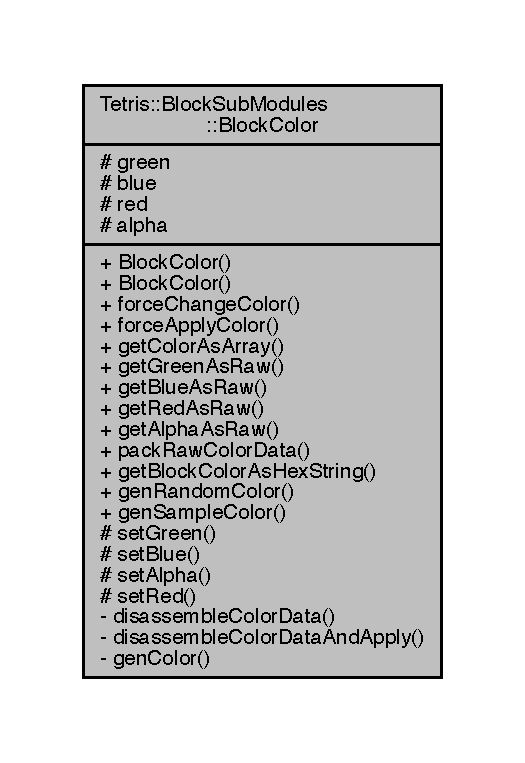
\includegraphics[width=252pt]{d8/d90/class_tetris_1_1_block_sub_modules_1_1_block_color__coll__graph}
\end{center}
\end{figure}
\subsection*{Public 멤버 함수}
\begin{DoxyCompactItemize}
\item 
\hyperlink{class_tetris_1_1_block_sub_modules_1_1_block_color_abb929df07c6b378e31d76b7298eb9e12}{Block\+Color} (unsigned char \hyperlink{class_tetris_1_1_block_sub_modules_1_1_block_color_af0983ea684f33617a0b482cfea1d3c2b}{alpha}, unsigned char \hyperlink{class_tetris_1_1_block_sub_modules_1_1_block_color_af8a0dc372e7dbab300290eadada8ef49}{red}, unsigned char \hyperlink{class_tetris_1_1_block_sub_modules_1_1_block_color_a4b28885bfd8bf53793c6b3daedd974eb}{green}, unsigned char \hyperlink{class_tetris_1_1_block_sub_modules_1_1_block_color_af04e78b9a1c2f7625863c289c4a741e3}{blue})
\item 
\hyperlink{class_tetris_1_1_block_sub_modules_1_1_block_color_aba62c9da4cb4b43caa871452a34790a9}{Block\+Color} (unsigned int combineddt)
\item 
void \hyperlink{class_tetris_1_1_block_sub_modules_1_1_block_color_ae6d640629b11d880ca994923657adbe1}{force\+Change\+Color} (const unsigned char \hyperlink{class_tetris_1_1_block_sub_modules_1_1_block_color_af0983ea684f33617a0b482cfea1d3c2b}{alpha}, const unsigned char \hyperlink{class_tetris_1_1_block_sub_modules_1_1_block_color_af8a0dc372e7dbab300290eadada8ef49}{red}, const unsigned char \hyperlink{class_tetris_1_1_block_sub_modules_1_1_block_color_a4b28885bfd8bf53793c6b3daedd974eb}{green}, const unsigned char \hyperlink{class_tetris_1_1_block_sub_modules_1_1_block_color_af04e78b9a1c2f7625863c289c4a741e3}{blue})
\item 
void \hyperlink{class_tetris_1_1_block_sub_modules_1_1_block_color_a260b5dd85cdf3145be7564dc2c0ee53d}{force\+Apply\+Color} (const unsigned int dt)
\item 
unsigned char $\ast$ \hyperlink{class_tetris_1_1_block_sub_modules_1_1_block_color_ac626961ee3894d89a7fc961e9f40c92f}{get\+Color\+As\+Array} ()
\item 
unsigned char \hyperlink{class_tetris_1_1_block_sub_modules_1_1_block_color_a65e9230325a2f44aa433f39c199aabcd}{get\+Green\+As\+Raw} ()
\item 
unsigned char \hyperlink{class_tetris_1_1_block_sub_modules_1_1_block_color_ac0ad44a8b001f3824447d137357f5145}{get\+Blue\+As\+Raw} ()
\item 
unsigned char \hyperlink{class_tetris_1_1_block_sub_modules_1_1_block_color_a1795cf70c847d261645a9690afff7e9c}{get\+Red\+As\+Raw} ()
\item 
unsigned char \hyperlink{class_tetris_1_1_block_sub_modules_1_1_block_color_acb1c9b34ee534857741025bd2824201a}{get\+Alpha\+As\+Raw} ()
\item 
unsigned int \hyperlink{class_tetris_1_1_block_sub_modules_1_1_block_color_a849ebbb0e900c5efdcb99784767e7a7a}{pack\+Raw\+Color\+Data} ()
\item 
string \hyperlink{class_tetris_1_1_block_sub_modules_1_1_block_color_a79cc837f207645628542876997c9e919}{get\+Block\+Color\+As\+Hex\+String} ()
\end{DoxyCompactItemize}
\subsection*{정적 Public 멤버 함수}
\begin{DoxyCompactItemize}
\item 
static unsigned int \hyperlink{class_tetris_1_1_block_sub_modules_1_1_block_color_a74374a6d24cd77c7f4fe03e19111bab7}{gen\+Random\+Color} ()
\item 
static unsigned int \hyperlink{class_tetris_1_1_block_sub_modules_1_1_block_color_a624fe688c2889c345cb8dff757f06ef9}{gen\+Sample\+Color} (const unsigned char samplenum)
\end{DoxyCompactItemize}
\subsection*{Protected 멤버 함수}
\begin{DoxyCompactItemize}
\item 
void \hyperlink{class_tetris_1_1_block_sub_modules_1_1_block_color_aeea8ab6d5f36d35fd4f28818349661ab}{set\+Green} (unsigned char grn)
\item 
void \hyperlink{class_tetris_1_1_block_sub_modules_1_1_block_color_ac624156bd1f77a20d6e1d4c8cbff36d3}{set\+Blue} (unsigned char blu)
\item 
void \hyperlink{class_tetris_1_1_block_sub_modules_1_1_block_color_a5fdd2d1a53d92ec0bcc1c25748b890e0}{set\+Alpha} (unsigned char aph)
\item 
void \hyperlink{class_tetris_1_1_block_sub_modules_1_1_block_color_a9541e6b5b809214ae2691a99af06ac3f}{set\+Red} (unsigned char rd)
\end{DoxyCompactItemize}
\subsection*{Protected 속성}
\begin{DoxyCompactItemize}
\item 
unsigned char \hyperlink{class_tetris_1_1_block_sub_modules_1_1_block_color_a4b28885bfd8bf53793c6b3daedd974eb}{green}
\item 
unsigned char \hyperlink{class_tetris_1_1_block_sub_modules_1_1_block_color_af04e78b9a1c2f7625863c289c4a741e3}{blue}
\item 
unsigned char \hyperlink{class_tetris_1_1_block_sub_modules_1_1_block_color_af8a0dc372e7dbab300290eadada8ef49}{red}
\item 
unsigned char \hyperlink{class_tetris_1_1_block_sub_modules_1_1_block_color_af0983ea684f33617a0b482cfea1d3c2b}{alpha}
\end{DoxyCompactItemize}
\subsection*{Private 멤버 함수}
\begin{DoxyCompactItemize}
\item 
unsigned char $\ast$ \hyperlink{class_tetris_1_1_block_sub_modules_1_1_block_color_a216ddc10773f9d0dc44eca5b8b3d8336}{disassemble\+Color\+Data} (unsigned int dt)
\item 
void \hyperlink{class_tetris_1_1_block_sub_modules_1_1_block_color_afc3bb979353c91cf992101ed2dde610f}{disassemble\+Color\+Data\+And\+Apply} (unsigned int dt)
\end{DoxyCompactItemize}
\subsection*{정적 Private 멤버 함수}
\begin{DoxyCompactItemize}
\item 
static unsigned int \hyperlink{class_tetris_1_1_block_sub_modules_1_1_block_color_a479cf23117afea6237a4fd69bc4652ba}{gen\+Color} (unsigned char \hyperlink{class_tetris_1_1_block_sub_modules_1_1_block_color_af8a0dc372e7dbab300290eadada8ef49}{red}, unsigned char \hyperlink{class_tetris_1_1_block_sub_modules_1_1_block_color_a4b28885bfd8bf53793c6b3daedd974eb}{green}, unsigned char \hyperlink{class_tetris_1_1_block_sub_modules_1_1_block_color_af04e78b9a1c2f7625863c289c4a741e3}{blue})
\end{DoxyCompactItemize}


\subsection{상세한 설명}
블럭의 색상을 관리하고 불러오는 클래스 

Block\+Color.\+hpp 파일의 18 번째 라인에서 정의되었습니다.



\subsection{생성자 \& 소멸자 문서화}
\mbox{\Hypertarget{class_tetris_1_1_block_sub_modules_1_1_block_color_abb929df07c6b378e31d76b7298eb9e12}\label{class_tetris_1_1_block_sub_modules_1_1_block_color_abb929df07c6b378e31d76b7298eb9e12}} 
\index{Tetris\+::\+Block\+Sub\+Modules\+::\+Block\+Color@{Tetris\+::\+Block\+Sub\+Modules\+::\+Block\+Color}!Block\+Color@{Block\+Color}}
\index{Block\+Color@{Block\+Color}!Tetris\+::\+Block\+Sub\+Modules\+::\+Block\+Color@{Tetris\+::\+Block\+Sub\+Modules\+::\+Block\+Color}}
\subsubsection{\texorpdfstring{Block\+Color()}{BlockColor()}\hspace{0.1cm}{\footnotesize\ttfamily [1/2]}}
{\footnotesize\ttfamily Tetris\+::\+Block\+Sub\+Modules\+::\+Block\+Color\+::\+Block\+Color (\begin{DoxyParamCaption}\item[{unsigned char}]{alpha,  }\item[{unsigned char}]{red,  }\item[{unsigned char}]{green,  }\item[{unsigned char}]{blue }\end{DoxyParamCaption})\hspace{0.3cm}{\ttfamily [inline]}}



Block\+Color.\+hpp 파일의 20 번째 라인에서 정의되었습니다.


\begin{DoxyCode}
20                                                                                                            
         \{
21                     this->\hyperlink{class_tetris_1_1_block_sub_modules_1_1_block_color_ae6d640629b11d880ca994923657adbe1}{forceChangeColor}(\hyperlink{class_tetris_1_1_block_sub_modules_1_1_block_color_af0983ea684f33617a0b482cfea1d3c2b}{alpha},\hyperlink{class_tetris_1_1_block_sub_modules_1_1_block_color_af8a0dc372e7dbab300290eadada8ef49}{red},
      \hyperlink{class_tetris_1_1_block_sub_modules_1_1_block_color_a4b28885bfd8bf53793c6b3daedd974eb}{green},\hyperlink{class_tetris_1_1_block_sub_modules_1_1_block_color_af04e78b9a1c2f7625863c289c4a741e3}{blue});
22                 \}
\end{DoxyCode}
이 함수 내부에서 호출하는 함수들에 대한 그래프입니다.\+:
\nopagebreak
\begin{figure}[H]
\begin{center}
\leavevmode
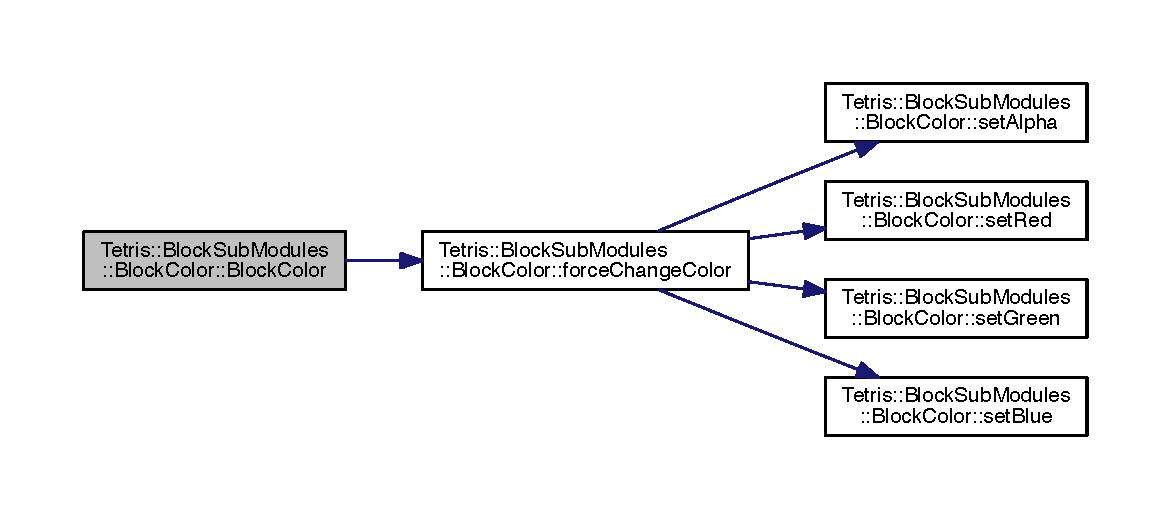
\includegraphics[width=350pt]{de/d44/class_tetris_1_1_block_sub_modules_1_1_block_color_abb929df07c6b378e31d76b7298eb9e12_cgraph}
\end{center}
\end{figure}
\mbox{\Hypertarget{class_tetris_1_1_block_sub_modules_1_1_block_color_aba62c9da4cb4b43caa871452a34790a9}\label{class_tetris_1_1_block_sub_modules_1_1_block_color_aba62c9da4cb4b43caa871452a34790a9}} 
\index{Tetris\+::\+Block\+Sub\+Modules\+::\+Block\+Color@{Tetris\+::\+Block\+Sub\+Modules\+::\+Block\+Color}!Block\+Color@{Block\+Color}}
\index{Block\+Color@{Block\+Color}!Tetris\+::\+Block\+Sub\+Modules\+::\+Block\+Color@{Tetris\+::\+Block\+Sub\+Modules\+::\+Block\+Color}}
\subsubsection{\texorpdfstring{Block\+Color()}{BlockColor()}\hspace{0.1cm}{\footnotesize\ttfamily [2/2]}}
{\footnotesize\ttfamily Tetris\+::\+Block\+Sub\+Modules\+::\+Block\+Color\+::\+Block\+Color (\begin{DoxyParamCaption}\item[{unsigned int}]{combineddt }\end{DoxyParamCaption})\hspace{0.3cm}{\ttfamily [inline]}}



Block\+Color.\+hpp 파일의 23 번째 라인에서 정의되었습니다.


\begin{DoxyCode}
23                                                \{
24                 this->\hyperlink{class_tetris_1_1_block_sub_modules_1_1_block_color_afc3bb979353c91cf992101ed2dde610f}{disassembleColorDataAndApply}(combineddt);
25             \}
\end{DoxyCode}
이 함수 내부에서 호출하는 함수들에 대한 그래프입니다.\+:
\nopagebreak
\begin{figure}[H]
\begin{center}
\leavevmode
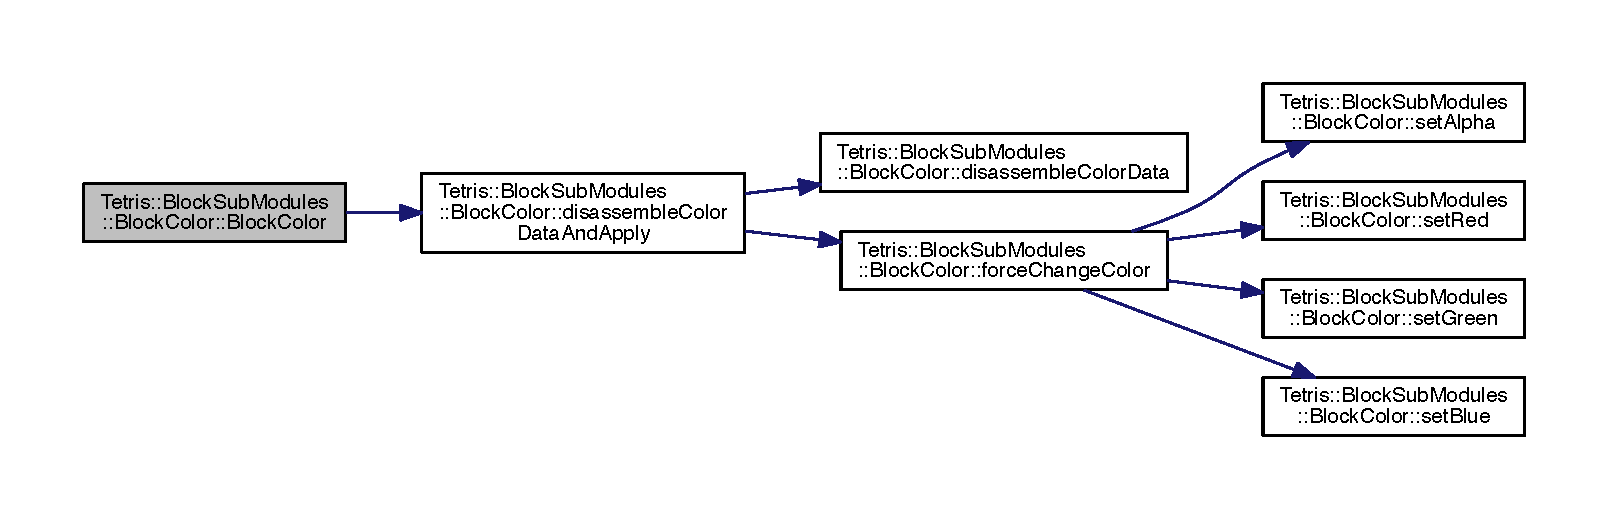
\includegraphics[width=350pt]{de/d44/class_tetris_1_1_block_sub_modules_1_1_block_color_aba62c9da4cb4b43caa871452a34790a9_cgraph}
\end{center}
\end{figure}


\subsection{멤버 함수 문서화}
\mbox{\Hypertarget{class_tetris_1_1_block_sub_modules_1_1_block_color_a216ddc10773f9d0dc44eca5b8b3d8336}\label{class_tetris_1_1_block_sub_modules_1_1_block_color_a216ddc10773f9d0dc44eca5b8b3d8336}} 
\index{Tetris\+::\+Block\+Sub\+Modules\+::\+Block\+Color@{Tetris\+::\+Block\+Sub\+Modules\+::\+Block\+Color}!disassemble\+Color\+Data@{disassemble\+Color\+Data}}
\index{disassemble\+Color\+Data@{disassemble\+Color\+Data}!Tetris\+::\+Block\+Sub\+Modules\+::\+Block\+Color@{Tetris\+::\+Block\+Sub\+Modules\+::\+Block\+Color}}
\subsubsection{\texorpdfstring{disassemble\+Color\+Data()}{disassembleColorData()}}
{\footnotesize\ttfamily unsigned char$\ast$ Tetris\+::\+Block\+Sub\+Modules\+::\+Block\+Color\+::disassemble\+Color\+Data (\begin{DoxyParamCaption}\item[{unsigned int}]{dt }\end{DoxyParamCaption})\hspace{0.3cm}{\ttfamily [inline]}, {\ttfamily [private]}}

\begin{DoxyReturn}{반환값}
4바이트 변수에서 rgba를 분해해 배열로 리턴 
\end{DoxyReturn}


Block\+Color.\+hpp 파일의 142 번째 라인에서 정의되었습니다.


\begin{DoxyCode}
142                                                                     \{
143                     \textcolor{keywordtype}{unsigned} \textcolor{keywordtype}{char}* rst = \textcolor{keyword}{new} \textcolor{keywordtype}{unsigned} \textcolor{keywordtype}{char}[4];
144                     \textcolor{keywordflow}{for}(\textcolor{keywordtype}{int} i=0;i<4;i++)\{
145                         rst[3-i]=(((~((~(\textcolor{keywordtype}{unsigned} int)0)<<(8)))<<(8*i))&dt)>>(8*i);
146                     \}
147                     \textcolor{keywordflow}{return} rst;
148                 \}
\end{DoxyCode}
이 함수를 호출하는 함수들에 대한 그래프입니다.\+:
\nopagebreak
\begin{figure}[H]
\begin{center}
\leavevmode
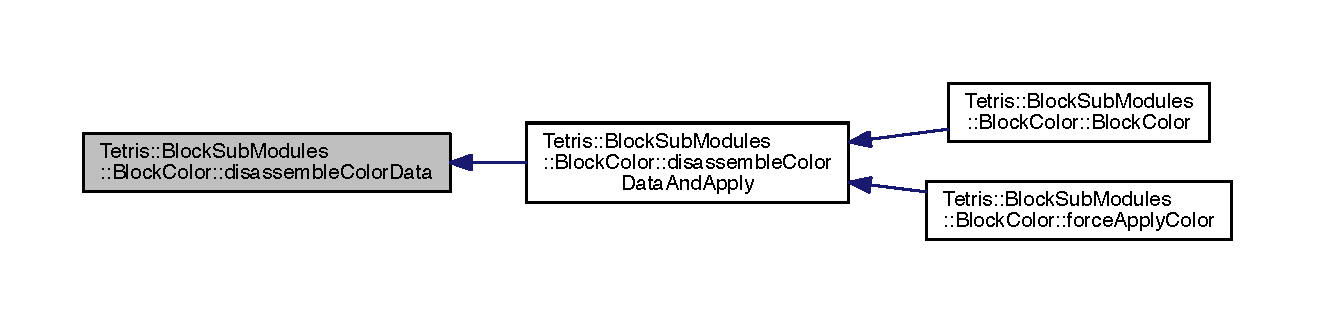
\includegraphics[width=350pt]{de/d44/class_tetris_1_1_block_sub_modules_1_1_block_color_a216ddc10773f9d0dc44eca5b8b3d8336_icgraph}
\end{center}
\end{figure}
\mbox{\Hypertarget{class_tetris_1_1_block_sub_modules_1_1_block_color_afc3bb979353c91cf992101ed2dde610f}\label{class_tetris_1_1_block_sub_modules_1_1_block_color_afc3bb979353c91cf992101ed2dde610f}} 
\index{Tetris\+::\+Block\+Sub\+Modules\+::\+Block\+Color@{Tetris\+::\+Block\+Sub\+Modules\+::\+Block\+Color}!disassemble\+Color\+Data\+And\+Apply@{disassemble\+Color\+Data\+And\+Apply}}
\index{disassemble\+Color\+Data\+And\+Apply@{disassemble\+Color\+Data\+And\+Apply}!Tetris\+::\+Block\+Sub\+Modules\+::\+Block\+Color@{Tetris\+::\+Block\+Sub\+Modules\+::\+Block\+Color}}
\subsubsection{\texorpdfstring{disassemble\+Color\+Data\+And\+Apply()}{disassembleColorDataAndApply()}}
{\footnotesize\ttfamily void Tetris\+::\+Block\+Sub\+Modules\+::\+Block\+Color\+::disassemble\+Color\+Data\+And\+Apply (\begin{DoxyParamCaption}\item[{unsigned int}]{dt }\end{DoxyParamCaption})\hspace{0.3cm}{\ttfamily [inline]}, {\ttfamily [private]}}

\begin{DoxyReturn}{반환값}
disassemble\+Color\+Data를 가져와 즉시적용 
\end{DoxyReturn}


Block\+Color.\+hpp 파일의 152 번째 라인에서 정의되었습니다.


\begin{DoxyCode}
152                                                               \{
153                 \textcolor{keywordtype}{unsigned} \textcolor{keywordtype}{char}* disasmb= this->\hyperlink{class_tetris_1_1_block_sub_modules_1_1_block_color_a216ddc10773f9d0dc44eca5b8b3d8336}{disassembleColorData}(dt);
154                 \textcolor{keywordflow}{if}(disasmb!=NULL)\{
155                     this->\hyperlink{class_tetris_1_1_block_sub_modules_1_1_block_color_ae6d640629b11d880ca994923657adbe1}{forceChangeColor}(disasmb[0],disasmb[1],disasmb[2],disasmb[3]);
156                     \textcolor{keyword}{delete} [] disasmb;
157                 \}
158             \}
\end{DoxyCode}
이 함수 내부에서 호출하는 함수들에 대한 그래프입니다.\+:
\nopagebreak
\begin{figure}[H]
\begin{center}
\leavevmode
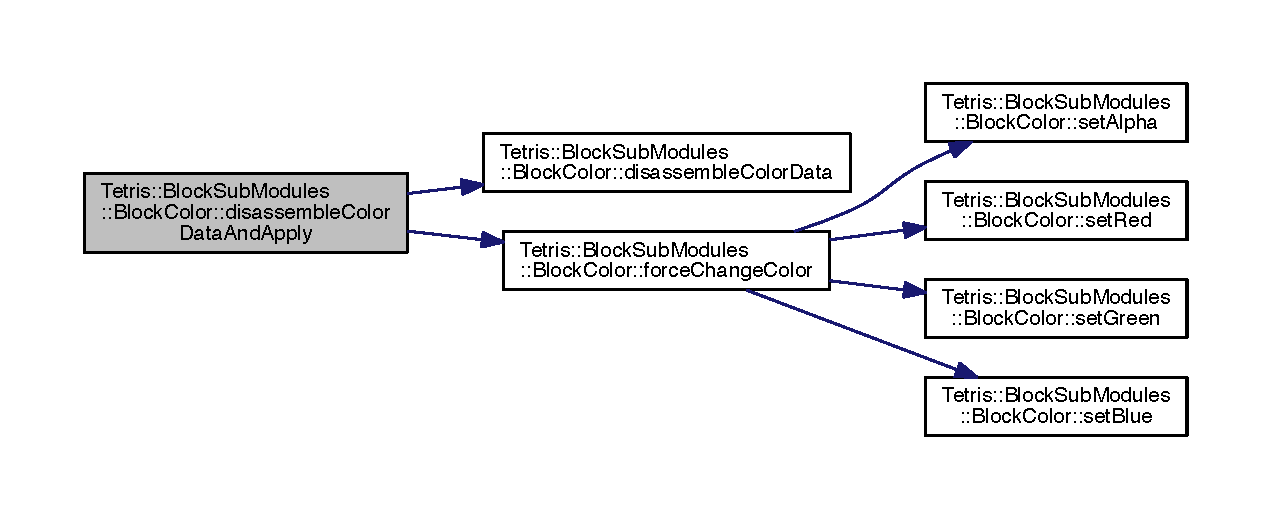
\includegraphics[width=350pt]{de/d44/class_tetris_1_1_block_sub_modules_1_1_block_color_afc3bb979353c91cf992101ed2dde610f_cgraph}
\end{center}
\end{figure}
이 함수를 호출하는 함수들에 대한 그래프입니다.\+:
\nopagebreak
\begin{figure}[H]
\begin{center}
\leavevmode
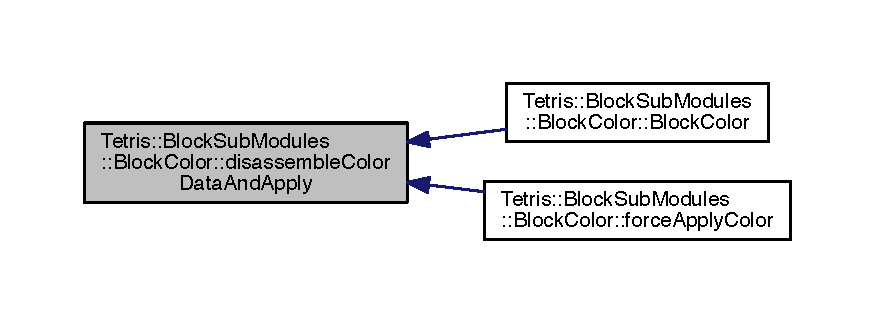
\includegraphics[width=350pt]{de/d44/class_tetris_1_1_block_sub_modules_1_1_block_color_afc3bb979353c91cf992101ed2dde610f_icgraph}
\end{center}
\end{figure}
\mbox{\Hypertarget{class_tetris_1_1_block_sub_modules_1_1_block_color_a260b5dd85cdf3145be7564dc2c0ee53d}\label{class_tetris_1_1_block_sub_modules_1_1_block_color_a260b5dd85cdf3145be7564dc2c0ee53d}} 
\index{Tetris\+::\+Block\+Sub\+Modules\+::\+Block\+Color@{Tetris\+::\+Block\+Sub\+Modules\+::\+Block\+Color}!force\+Apply\+Color@{force\+Apply\+Color}}
\index{force\+Apply\+Color@{force\+Apply\+Color}!Tetris\+::\+Block\+Sub\+Modules\+::\+Block\+Color@{Tetris\+::\+Block\+Sub\+Modules\+::\+Block\+Color}}
\subsubsection{\texorpdfstring{force\+Apply\+Color()}{forceApplyColor()}}
{\footnotesize\ttfamily void Tetris\+::\+Block\+Sub\+Modules\+::\+Block\+Color\+::force\+Apply\+Color (\begin{DoxyParamCaption}\item[{const unsigned int}]{dt }\end{DoxyParamCaption})\hspace{0.3cm}{\ttfamily [inline]}}



Block\+Color.\+hpp 파일의 32 번째 라인에서 정의되었습니다.


\begin{DoxyCode}
32                                                        \{
33                 this->\hyperlink{class_tetris_1_1_block_sub_modules_1_1_block_color_afc3bb979353c91cf992101ed2dde610f}{disassembleColorDataAndApply}(dt);
34             \}
\end{DoxyCode}
이 함수 내부에서 호출하는 함수들에 대한 그래프입니다.\+:
\nopagebreak
\begin{figure}[H]
\begin{center}
\leavevmode
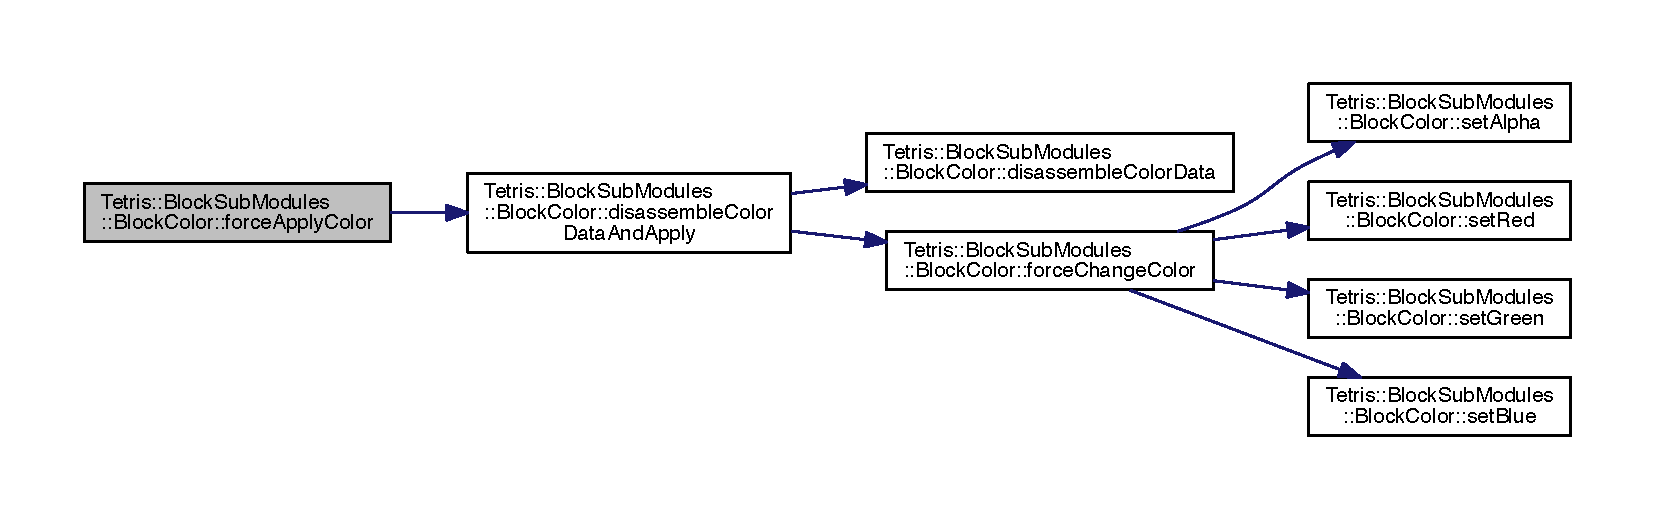
\includegraphics[width=350pt]{de/d44/class_tetris_1_1_block_sub_modules_1_1_block_color_a260b5dd85cdf3145be7564dc2c0ee53d_cgraph}
\end{center}
\end{figure}
\mbox{\Hypertarget{class_tetris_1_1_block_sub_modules_1_1_block_color_ae6d640629b11d880ca994923657adbe1}\label{class_tetris_1_1_block_sub_modules_1_1_block_color_ae6d640629b11d880ca994923657adbe1}} 
\index{Tetris\+::\+Block\+Sub\+Modules\+::\+Block\+Color@{Tetris\+::\+Block\+Sub\+Modules\+::\+Block\+Color}!force\+Change\+Color@{force\+Change\+Color}}
\index{force\+Change\+Color@{force\+Change\+Color}!Tetris\+::\+Block\+Sub\+Modules\+::\+Block\+Color@{Tetris\+::\+Block\+Sub\+Modules\+::\+Block\+Color}}
\subsubsection{\texorpdfstring{force\+Change\+Color()}{forceChangeColor()}}
{\footnotesize\ttfamily void Tetris\+::\+Block\+Sub\+Modules\+::\+Block\+Color\+::force\+Change\+Color (\begin{DoxyParamCaption}\item[{const unsigned char}]{alpha,  }\item[{const unsigned char}]{red,  }\item[{const unsigned char}]{green,  }\item[{const unsigned char}]{blue }\end{DoxyParamCaption})\hspace{0.3cm}{\ttfamily [inline]}}



Block\+Color.\+hpp 파일의 26 번째 라인에서 정의되었습니다.


\begin{DoxyCode}
26                                                                                                            
                                   \{
27                 this->\hyperlink{class_tetris_1_1_block_sub_modules_1_1_block_color_a5fdd2d1a53d92ec0bcc1c25748b890e0}{setAlpha}(\hyperlink{class_tetris_1_1_block_sub_modules_1_1_block_color_af0983ea684f33617a0b482cfea1d3c2b}{alpha});
28                 this->\hyperlink{class_tetris_1_1_block_sub_modules_1_1_block_color_a9541e6b5b809214ae2691a99af06ac3f}{setRed}(\hyperlink{class_tetris_1_1_block_sub_modules_1_1_block_color_af8a0dc372e7dbab300290eadada8ef49}{red});
29                 this->\hyperlink{class_tetris_1_1_block_sub_modules_1_1_block_color_aeea8ab6d5f36d35fd4f28818349661ab}{setGreen}(\hyperlink{class_tetris_1_1_block_sub_modules_1_1_block_color_a4b28885bfd8bf53793c6b3daedd974eb}{green});
30                 this->\hyperlink{class_tetris_1_1_block_sub_modules_1_1_block_color_ac624156bd1f77a20d6e1d4c8cbff36d3}{setBlue}(\hyperlink{class_tetris_1_1_block_sub_modules_1_1_block_color_af04e78b9a1c2f7625863c289c4a741e3}{blue});
31             \}
\end{DoxyCode}
이 함수 내부에서 호출하는 함수들에 대한 그래프입니다.\+:
\nopagebreak
\begin{figure}[H]
\begin{center}
\leavevmode
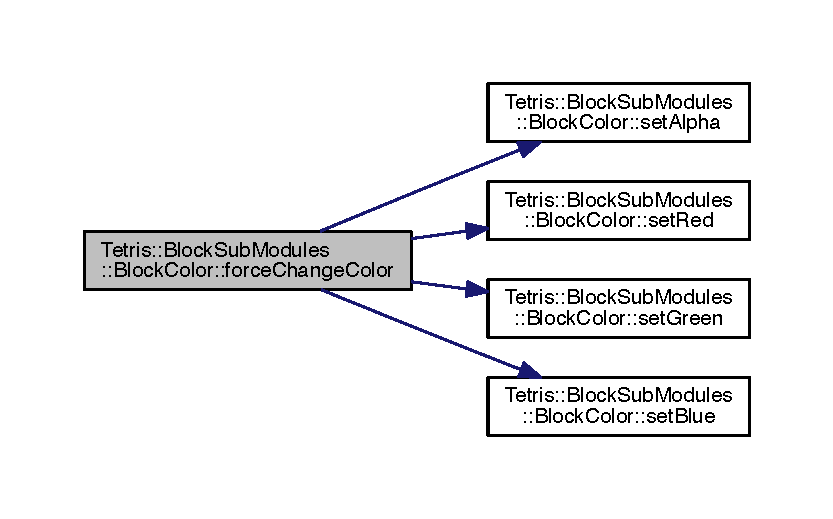
\includegraphics[width=350pt]{de/d44/class_tetris_1_1_block_sub_modules_1_1_block_color_ae6d640629b11d880ca994923657adbe1_cgraph}
\end{center}
\end{figure}
이 함수를 호출하는 함수들에 대한 그래프입니다.\+:
\nopagebreak
\begin{figure}[H]
\begin{center}
\leavevmode
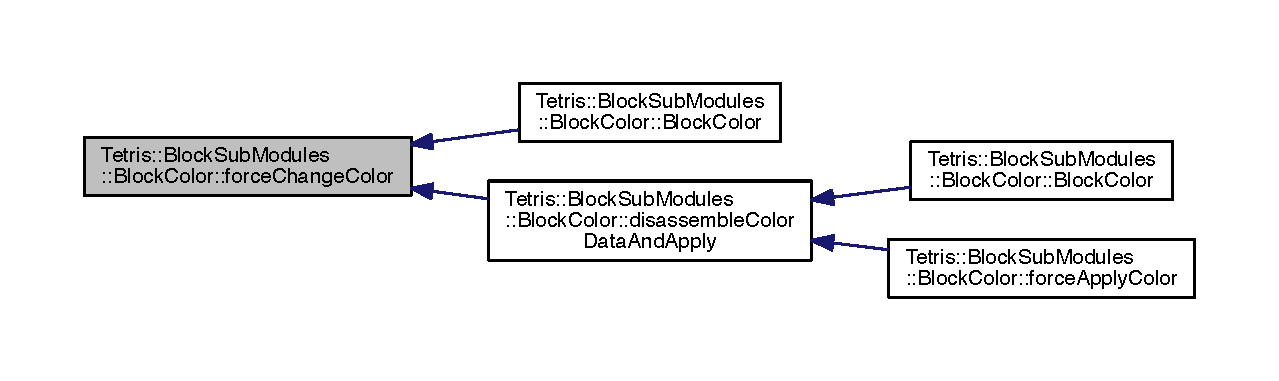
\includegraphics[width=350pt]{de/d44/class_tetris_1_1_block_sub_modules_1_1_block_color_ae6d640629b11d880ca994923657adbe1_icgraph}
\end{center}
\end{figure}
\mbox{\Hypertarget{class_tetris_1_1_block_sub_modules_1_1_block_color_a479cf23117afea6237a4fd69bc4652ba}\label{class_tetris_1_1_block_sub_modules_1_1_block_color_a479cf23117afea6237a4fd69bc4652ba}} 
\index{Tetris\+::\+Block\+Sub\+Modules\+::\+Block\+Color@{Tetris\+::\+Block\+Sub\+Modules\+::\+Block\+Color}!gen\+Color@{gen\+Color}}
\index{gen\+Color@{gen\+Color}!Tetris\+::\+Block\+Sub\+Modules\+::\+Block\+Color@{Tetris\+::\+Block\+Sub\+Modules\+::\+Block\+Color}}
\subsubsection{\texorpdfstring{gen\+Color()}{genColor()}}
{\footnotesize\ttfamily static unsigned int Tetris\+::\+Block\+Sub\+Modules\+::\+Block\+Color\+::gen\+Color (\begin{DoxyParamCaption}\item[{unsigned char}]{red,  }\item[{unsigned char}]{green,  }\item[{unsigned char}]{blue }\end{DoxyParamCaption})\hspace{0.3cm}{\ttfamily [inline]}, {\ttfamily [static]}, {\ttfamily [private]}}

\begin{DoxyReturn}{반환값}
색상 데이터를 4바이트 변수로 묶어 리턴 
\end{DoxyReturn}


Block\+Color.\+hpp 파일의 162 번째 라인에서 정의되었습니다.


\begin{DoxyCode}
162                                                                                                    \{
163                 \textcolor{keywordtype}{unsigned} \textcolor{keywordtype}{int} rst = (\textcolor{keywordtype}{unsigned} int)\hyperlink{class_tetris_1_1_block_sub_modules_1_1_block_color_af04e78b9a1c2f7625863c289c4a741e3}{blue};
164                 rst|=((~(\textcolor{keywordtype}{unsigned} int)0)<<(8*3));
165                 rst|=((\textcolor{keywordtype}{unsigned} int)\hyperlink{class_tetris_1_1_block_sub_modules_1_1_block_color_af8a0dc372e7dbab300290eadada8ef49}{red}<<(8*2));
166                 rst|=((\textcolor{keywordtype}{unsigned} int)\hyperlink{class_tetris_1_1_block_sub_modules_1_1_block_color_a4b28885bfd8bf53793c6b3daedd974eb}{green}<<(8*1));
167                 \textcolor{keywordflow}{return} rst;
168             \}
\end{DoxyCode}
이 함수를 호출하는 함수들에 대한 그래프입니다.\+:
\nopagebreak
\begin{figure}[H]
\begin{center}
\leavevmode
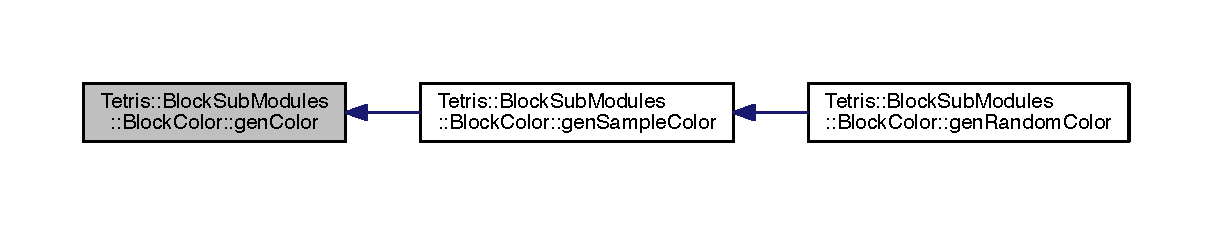
\includegraphics[width=350pt]{de/d44/class_tetris_1_1_block_sub_modules_1_1_block_color_a479cf23117afea6237a4fd69bc4652ba_icgraph}
\end{center}
\end{figure}
\mbox{\Hypertarget{class_tetris_1_1_block_sub_modules_1_1_block_color_a74374a6d24cd77c7f4fe03e19111bab7}\label{class_tetris_1_1_block_sub_modules_1_1_block_color_a74374a6d24cd77c7f4fe03e19111bab7}} 
\index{Tetris\+::\+Block\+Sub\+Modules\+::\+Block\+Color@{Tetris\+::\+Block\+Sub\+Modules\+::\+Block\+Color}!gen\+Random\+Color@{gen\+Random\+Color}}
\index{gen\+Random\+Color@{gen\+Random\+Color}!Tetris\+::\+Block\+Sub\+Modules\+::\+Block\+Color@{Tetris\+::\+Block\+Sub\+Modules\+::\+Block\+Color}}
\subsubsection{\texorpdfstring{gen\+Random\+Color()}{genRandomColor()}}
{\footnotesize\ttfamily static unsigned int Tetris\+::\+Block\+Sub\+Modules\+::\+Block\+Color\+::gen\+Random\+Color (\begin{DoxyParamCaption}{ }\end{DoxyParamCaption})\hspace{0.3cm}{\ttfamily [inline]}, {\ttfamily [static]}}



Block\+Color.\+hpp 파일의 35 번째 라인에서 정의되었습니다.


\begin{DoxyCode}
35                                                 \{
36                 \textcolor{keywordflow}{return} \hyperlink{class_tetris_1_1_block_sub_modules_1_1_block_color_a624fe688c2889c345cb8dff757f06ef9}{BlockColor::genSampleColor}((\textcolor{keywordtype}{unsigned} \textcolor{keywordtype}{char})
      \hyperlink{class_tetris_util_a0a60e809425ddb416a500bcc03cf7061}{TetrisUtil::randInt}(1,7));
37             \}
\end{DoxyCode}
이 함수 내부에서 호출하는 함수들에 대한 그래프입니다.\+:
\nopagebreak
\begin{figure}[H]
\begin{center}
\leavevmode
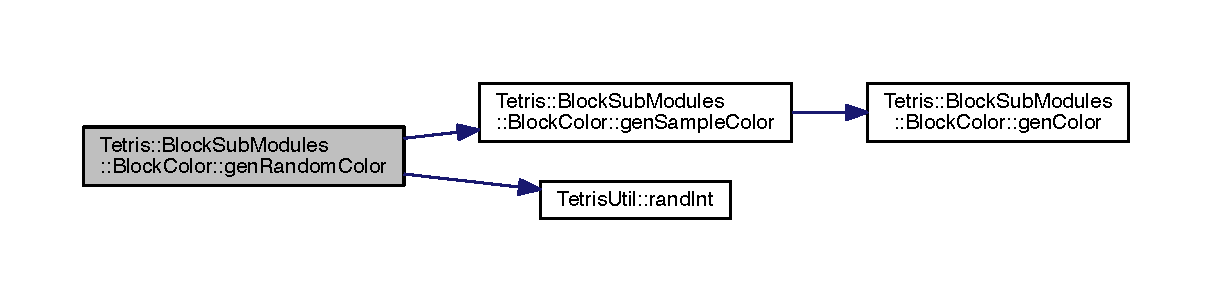
\includegraphics[width=350pt]{de/d44/class_tetris_1_1_block_sub_modules_1_1_block_color_a74374a6d24cd77c7f4fe03e19111bab7_cgraph}
\end{center}
\end{figure}
\mbox{\Hypertarget{class_tetris_1_1_block_sub_modules_1_1_block_color_a624fe688c2889c345cb8dff757f06ef9}\label{class_tetris_1_1_block_sub_modules_1_1_block_color_a624fe688c2889c345cb8dff757f06ef9}} 
\index{Tetris\+::\+Block\+Sub\+Modules\+::\+Block\+Color@{Tetris\+::\+Block\+Sub\+Modules\+::\+Block\+Color}!gen\+Sample\+Color@{gen\+Sample\+Color}}
\index{gen\+Sample\+Color@{gen\+Sample\+Color}!Tetris\+::\+Block\+Sub\+Modules\+::\+Block\+Color@{Tetris\+::\+Block\+Sub\+Modules\+::\+Block\+Color}}
\subsubsection{\texorpdfstring{gen\+Sample\+Color()}{genSampleColor()}}
{\footnotesize\ttfamily static unsigned int Tetris\+::\+Block\+Sub\+Modules\+::\+Block\+Color\+::gen\+Sample\+Color (\begin{DoxyParamCaption}\item[{const unsigned char}]{samplenum }\end{DoxyParamCaption})\hspace{0.3cm}{\ttfamily [inline]}, {\ttfamily [static]}}

\begin{DoxyReturn}{반환값}
미리 지정된 색상을 4바이트 변수 데이터로 리턴 
\end{DoxyReturn}


Block\+Color.\+hpp 파일의 41 번째 라인에서 정의되었습니다.


\begin{DoxyCode}
41                                                                              \{
42                 \textcolor{keywordflow}{switch}(samplenum)\{
43                     \textcolor{keywordflow}{case} 2:\{\textcolor{comment}{//pink600}
44                         \textcolor{keywordflow}{return} \hyperlink{class_tetris_1_1_block_sub_modules_1_1_block_color_a479cf23117afea6237a4fd69bc4652ba}{BlockColor::genColor}(0xd8,0x1b,0x60);
45                     \}
46                     \textcolor{keywordflow}{case} 3:\{\textcolor{comment}{//purple700}
47                         \textcolor{keywordflow}{return} \hyperlink{class_tetris_1_1_block_sub_modules_1_1_block_color_a479cf23117afea6237a4fd69bc4652ba}{BlockColor::genColor}(0x7b,0x1f,0xa2);
48                     \}
49                     \textcolor{keywordflow}{case} 4:\{\textcolor{comment}{//deeppurpleA400}
50                         \textcolor{keywordflow}{return} \hyperlink{class_tetris_1_1_block_sub_modules_1_1_block_color_a479cf23117afea6237a4fd69bc4652ba}{BlockColor::genColor}(0x65,0x1f,0xff);
51                     \}
52                     \textcolor{keywordflow}{case} 5:\{\textcolor{comment}{//teal600}
53                         \textcolor{keywordflow}{return} \hyperlink{class_tetris_1_1_block_sub_modules_1_1_block_color_a479cf23117afea6237a4fd69bc4652ba}{BlockColor::genColor}(0x00,0x89,0x7b);
54                     \}
55                     \textcolor{keywordflow}{case} 6:\{\textcolor{comment}{//red500}
56                         \textcolor{keywordflow}{return} \hyperlink{class_tetris_1_1_block_sub_modules_1_1_block_color_a479cf23117afea6237a4fd69bc4652ba}{BlockColor::genColor}(0xf4,0x43,0x36);
57                     \}
58                     \textcolor{keywordflow}{case} 7:\{\textcolor{comment}{//red900}
59                         \textcolor{keywordflow}{return} \hyperlink{class_tetris_1_1_block_sub_modules_1_1_block_color_a479cf23117afea6237a4fd69bc4652ba}{BlockColor::genColor}(0xb7,0xc1,0xc1);
60                     \}
61                     \textcolor{keywordflow}{case} 1:
62                     \textcolor{keywordflow}{default}:\textcolor{keywordflow}{return} \hyperlink{class_tetris_1_1_block_sub_modules_1_1_block_color_a479cf23117afea6237a4fd69bc4652ba}{BlockColor::genColor}(0x30,0x3f,0x9f);
63                 \}
64                 
65             \}
\end{DoxyCode}
이 함수 내부에서 호출하는 함수들에 대한 그래프입니다.\+:
\nopagebreak
\begin{figure}[H]
\begin{center}
\leavevmode
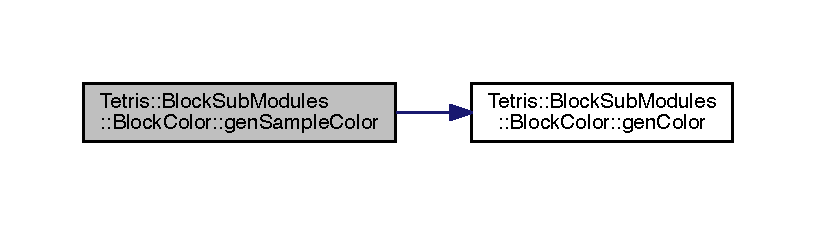
\includegraphics[width=350pt]{de/d44/class_tetris_1_1_block_sub_modules_1_1_block_color_a624fe688c2889c345cb8dff757f06ef9_cgraph}
\end{center}
\end{figure}
이 함수를 호출하는 함수들에 대한 그래프입니다.\+:
\nopagebreak
\begin{figure}[H]
\begin{center}
\leavevmode
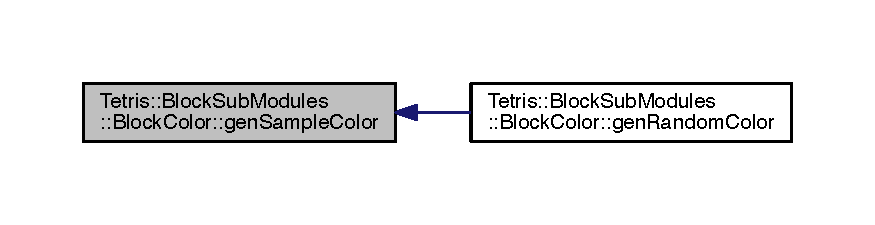
\includegraphics[width=350pt]{de/d44/class_tetris_1_1_block_sub_modules_1_1_block_color_a624fe688c2889c345cb8dff757f06ef9_icgraph}
\end{center}
\end{figure}
\mbox{\Hypertarget{class_tetris_1_1_block_sub_modules_1_1_block_color_acb1c9b34ee534857741025bd2824201a}\label{class_tetris_1_1_block_sub_modules_1_1_block_color_acb1c9b34ee534857741025bd2824201a}} 
\index{Tetris\+::\+Block\+Sub\+Modules\+::\+Block\+Color@{Tetris\+::\+Block\+Sub\+Modules\+::\+Block\+Color}!get\+Alpha\+As\+Raw@{get\+Alpha\+As\+Raw}}
\index{get\+Alpha\+As\+Raw@{get\+Alpha\+As\+Raw}!Tetris\+::\+Block\+Sub\+Modules\+::\+Block\+Color@{Tetris\+::\+Block\+Sub\+Modules\+::\+Block\+Color}}
\subsubsection{\texorpdfstring{get\+Alpha\+As\+Raw()}{getAlphaAsRaw()}}
{\footnotesize\ttfamily unsigned char Tetris\+::\+Block\+Sub\+Modules\+::\+Block\+Color\+::get\+Alpha\+As\+Raw (\begin{DoxyParamCaption}{ }\end{DoxyParamCaption})\hspace{0.3cm}{\ttfamily [inline]}}

\begin{DoxyReturn}{반환값}
색상데이터중 투명도 데이터를 리턴 
\end{DoxyReturn}


Block\+Color.\+hpp 파일의 98 번째 라인에서 정의되었습니다.


\begin{DoxyCode}
98                                          \{
99                 \textcolor{keywordflow}{return} this->\hyperlink{class_tetris_1_1_block_sub_modules_1_1_block_color_af0983ea684f33617a0b482cfea1d3c2b}{alpha};
100             \}
\end{DoxyCode}
이 함수를 호출하는 함수들에 대한 그래프입니다.\+:
\nopagebreak
\begin{figure}[H]
\begin{center}
\leavevmode
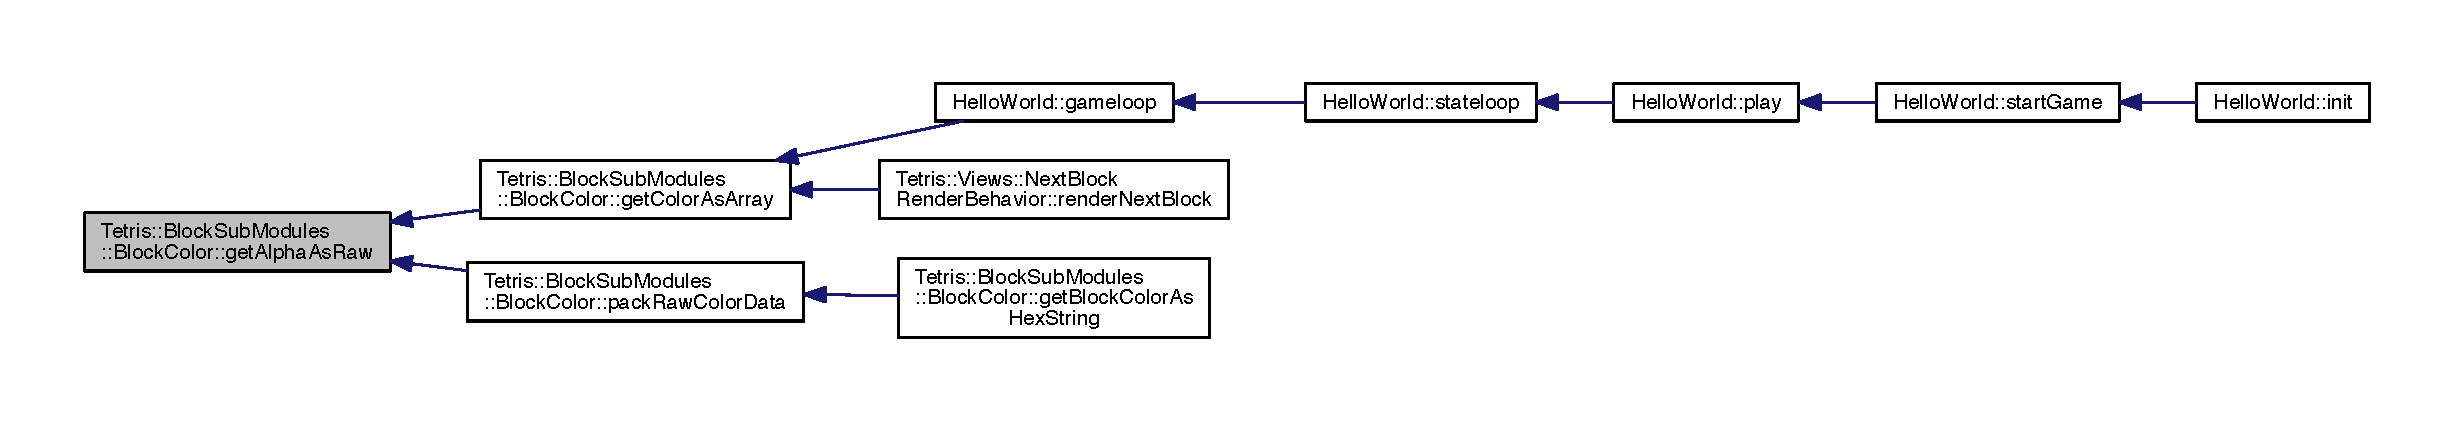
\includegraphics[width=350pt]{de/d44/class_tetris_1_1_block_sub_modules_1_1_block_color_acb1c9b34ee534857741025bd2824201a_icgraph}
\end{center}
\end{figure}
\mbox{\Hypertarget{class_tetris_1_1_block_sub_modules_1_1_block_color_a79cc837f207645628542876997c9e919}\label{class_tetris_1_1_block_sub_modules_1_1_block_color_a79cc837f207645628542876997c9e919}} 
\index{Tetris\+::\+Block\+Sub\+Modules\+::\+Block\+Color@{Tetris\+::\+Block\+Sub\+Modules\+::\+Block\+Color}!get\+Block\+Color\+As\+Hex\+String@{get\+Block\+Color\+As\+Hex\+String}}
\index{get\+Block\+Color\+As\+Hex\+String@{get\+Block\+Color\+As\+Hex\+String}!Tetris\+::\+Block\+Sub\+Modules\+::\+Block\+Color@{Tetris\+::\+Block\+Sub\+Modules\+::\+Block\+Color}}
\subsubsection{\texorpdfstring{get\+Block\+Color\+As\+Hex\+String()}{getBlockColorAsHexString()}}
{\footnotesize\ttfamily string Tetris\+::\+Block\+Sub\+Modules\+::\+Block\+Color\+::get\+Block\+Color\+As\+Hex\+String (\begin{DoxyParamCaption}{ }\end{DoxyParamCaption})\hspace{0.3cm}{\ttfamily [inline]}}

\begin{DoxyReturn}{반환값}
색상 데이터를 rgba hex 형식으로 리턴 
\end{DoxyReturn}


Block\+Color.\+hpp 파일의 110 번째 라인에서 정의되었습니다.


\begin{DoxyCode}
110                                              \{
111                 \textcolor{comment}{//string rst = "";}
112                 stringstream ss;
113                 \textcolor{keywordtype}{unsigned} \textcolor{keywordtype}{int} clr = this->\hyperlink{class_tetris_1_1_block_sub_modules_1_1_block_color_a849ebbb0e900c5efdcb99784767e7a7a}{packRawColorData}();
114                 ss.fill(\textcolor{charliteral}{'0'});
115                 \textcolor{keywordflow}{for}(\textcolor{keywordtype}{int} i=4-2;i>=0;i--)\{
116                     \textcolor{keywordtype}{unsigned} \textcolor{keywordtype}{int} inters = (~((~(\textcolor{keywordtype}{unsigned} int)0)<<8))<<(8*i);
117                     \textcolor{keywordtype}{unsigned} \textcolor{keywordtype}{int} extract = (clr&inters)>>(8*i);
118                     ss.width(2);
119                     ss<<hex<<extract;
120                 \}
121                 \textcolor{comment}{//rst<<}
122                 \textcolor{keywordflow}{return} ss.str();
123             \}
\end{DoxyCode}
이 함수 내부에서 호출하는 함수들에 대한 그래프입니다.\+:
\nopagebreak
\begin{figure}[H]
\begin{center}
\leavevmode
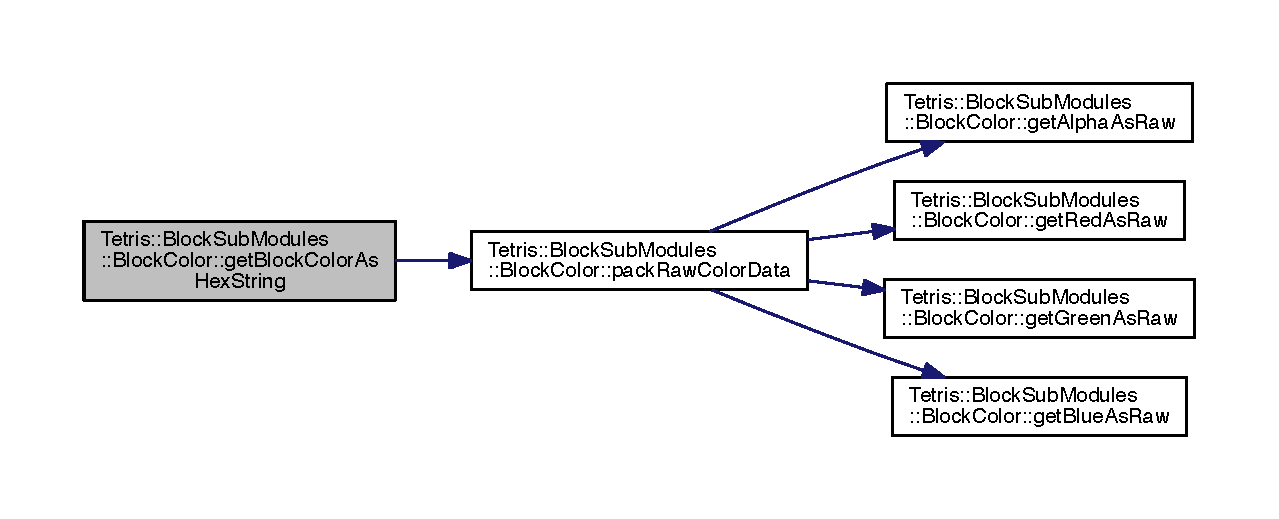
\includegraphics[width=350pt]{de/d44/class_tetris_1_1_block_sub_modules_1_1_block_color_a79cc837f207645628542876997c9e919_cgraph}
\end{center}
\end{figure}
\mbox{\Hypertarget{class_tetris_1_1_block_sub_modules_1_1_block_color_ac0ad44a8b001f3824447d137357f5145}\label{class_tetris_1_1_block_sub_modules_1_1_block_color_ac0ad44a8b001f3824447d137357f5145}} 
\index{Tetris\+::\+Block\+Sub\+Modules\+::\+Block\+Color@{Tetris\+::\+Block\+Sub\+Modules\+::\+Block\+Color}!get\+Blue\+As\+Raw@{get\+Blue\+As\+Raw}}
\index{get\+Blue\+As\+Raw@{get\+Blue\+As\+Raw}!Tetris\+::\+Block\+Sub\+Modules\+::\+Block\+Color@{Tetris\+::\+Block\+Sub\+Modules\+::\+Block\+Color}}
\subsubsection{\texorpdfstring{get\+Blue\+As\+Raw()}{getBlueAsRaw()}}
{\footnotesize\ttfamily unsigned char Tetris\+::\+Block\+Sub\+Modules\+::\+Block\+Color\+::get\+Blue\+As\+Raw (\begin{DoxyParamCaption}{ }\end{DoxyParamCaption})\hspace{0.3cm}{\ttfamily [inline]}}

\begin{DoxyReturn}{반환값}
색상데이터중 파랑 데이터를 리턴 
\end{DoxyReturn}


Block\+Color.\+hpp 파일의 86 번째 라인에서 정의되었습니다.


\begin{DoxyCode}
86                                         \{
87                 \textcolor{keywordflow}{return} this->\hyperlink{class_tetris_1_1_block_sub_modules_1_1_block_color_af04e78b9a1c2f7625863c289c4a741e3}{blue};
88             \}
\end{DoxyCode}
이 함수를 호출하는 함수들에 대한 그래프입니다.\+:
\nopagebreak
\begin{figure}[H]
\begin{center}
\leavevmode
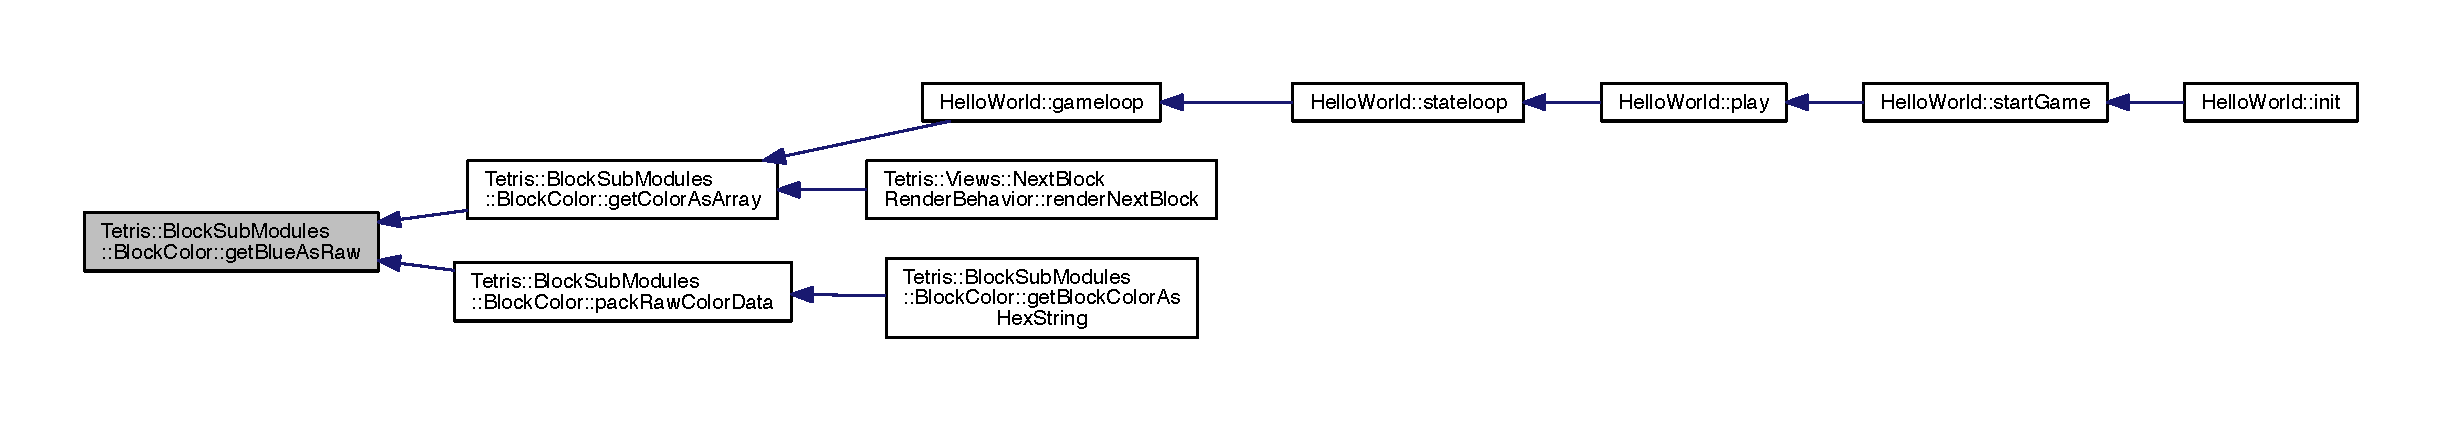
\includegraphics[width=350pt]{de/d44/class_tetris_1_1_block_sub_modules_1_1_block_color_ac0ad44a8b001f3824447d137357f5145_icgraph}
\end{center}
\end{figure}
\mbox{\Hypertarget{class_tetris_1_1_block_sub_modules_1_1_block_color_ac626961ee3894d89a7fc961e9f40c92f}\label{class_tetris_1_1_block_sub_modules_1_1_block_color_ac626961ee3894d89a7fc961e9f40c92f}} 
\index{Tetris\+::\+Block\+Sub\+Modules\+::\+Block\+Color@{Tetris\+::\+Block\+Sub\+Modules\+::\+Block\+Color}!get\+Color\+As\+Array@{get\+Color\+As\+Array}}
\index{get\+Color\+As\+Array@{get\+Color\+As\+Array}!Tetris\+::\+Block\+Sub\+Modules\+::\+Block\+Color@{Tetris\+::\+Block\+Sub\+Modules\+::\+Block\+Color}}
\subsubsection{\texorpdfstring{get\+Color\+As\+Array()}{getColorAsArray()}}
{\footnotesize\ttfamily unsigned char$\ast$ Tetris\+::\+Block\+Sub\+Modules\+::\+Block\+Color\+::get\+Color\+As\+Array (\begin{DoxyParamCaption}{ }\end{DoxyParamCaption})\hspace{0.3cm}{\ttfamily [inline]}}

\begin{DoxyReturn}{반환값}
색상데이터를 배열형식으로 리턴 
\end{DoxyReturn}


Block\+Color.\+hpp 파일의 69 번째 라인에서 정의되었습니다.


\begin{DoxyCode}
69                                             \{
70                 \textcolor{keywordtype}{unsigned} \textcolor{keywordtype}{char}* rst = \textcolor{keyword}{new} \textcolor{keywordtype}{unsigned} \textcolor{keywordtype}{char}[4];
71                 rst[0]=this->\hyperlink{class_tetris_1_1_block_sub_modules_1_1_block_color_acb1c9b34ee534857741025bd2824201a}{getAlphaAsRaw}();
72                 rst[1] = this->\hyperlink{class_tetris_1_1_block_sub_modules_1_1_block_color_a1795cf70c847d261645a9690afff7e9c}{getRedAsRaw}();
73                 rst[2] = this->\hyperlink{class_tetris_1_1_block_sub_modules_1_1_block_color_a65e9230325a2f44aa433f39c199aabcd}{getGreenAsRaw}();
74                 rst[3] = this->\hyperlink{class_tetris_1_1_block_sub_modules_1_1_block_color_ac0ad44a8b001f3824447d137357f5145}{getBlueAsRaw}();
75                 \textcolor{keywordflow}{return} rst;
76             \}
\end{DoxyCode}
이 함수 내부에서 호출하는 함수들에 대한 그래프입니다.\+:
\nopagebreak
\begin{figure}[H]
\begin{center}
\leavevmode
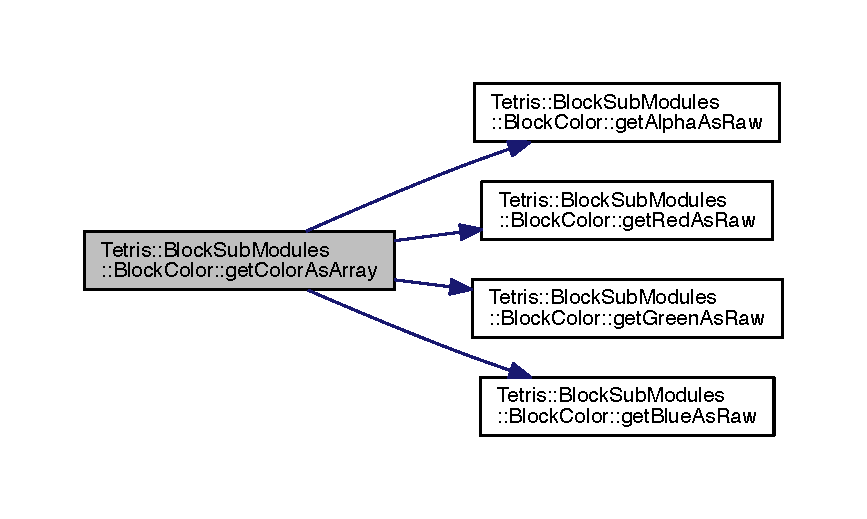
\includegraphics[width=350pt]{de/d44/class_tetris_1_1_block_sub_modules_1_1_block_color_ac626961ee3894d89a7fc961e9f40c92f_cgraph}
\end{center}
\end{figure}
이 함수를 호출하는 함수들에 대한 그래프입니다.\+:
\nopagebreak
\begin{figure}[H]
\begin{center}
\leavevmode
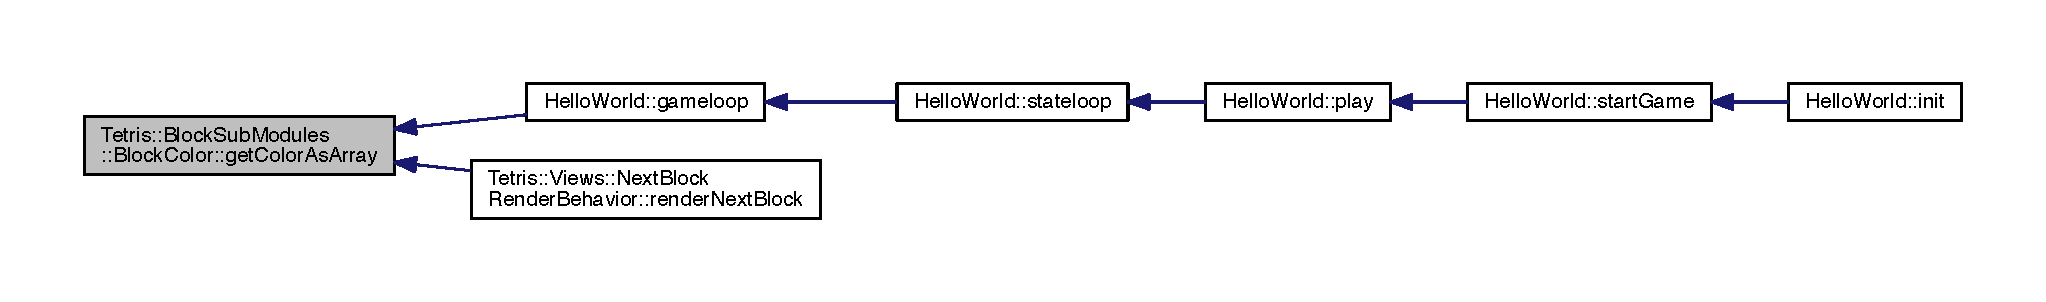
\includegraphics[width=350pt]{de/d44/class_tetris_1_1_block_sub_modules_1_1_block_color_ac626961ee3894d89a7fc961e9f40c92f_icgraph}
\end{center}
\end{figure}
\mbox{\Hypertarget{class_tetris_1_1_block_sub_modules_1_1_block_color_a65e9230325a2f44aa433f39c199aabcd}\label{class_tetris_1_1_block_sub_modules_1_1_block_color_a65e9230325a2f44aa433f39c199aabcd}} 
\index{Tetris\+::\+Block\+Sub\+Modules\+::\+Block\+Color@{Tetris\+::\+Block\+Sub\+Modules\+::\+Block\+Color}!get\+Green\+As\+Raw@{get\+Green\+As\+Raw}}
\index{get\+Green\+As\+Raw@{get\+Green\+As\+Raw}!Tetris\+::\+Block\+Sub\+Modules\+::\+Block\+Color@{Tetris\+::\+Block\+Sub\+Modules\+::\+Block\+Color}}
\subsubsection{\texorpdfstring{get\+Green\+As\+Raw()}{getGreenAsRaw()}}
{\footnotesize\ttfamily unsigned char Tetris\+::\+Block\+Sub\+Modules\+::\+Block\+Color\+::get\+Green\+As\+Raw (\begin{DoxyParamCaption}{ }\end{DoxyParamCaption})\hspace{0.3cm}{\ttfamily [inline]}}

\begin{DoxyReturn}{반환값}
색상데이터중 녹색 데이터를 리턴 
\end{DoxyReturn}


Block\+Color.\+hpp 파일의 80 번째 라인에서 정의되었습니다.


\begin{DoxyCode}
80                                          \{
81                 \textcolor{keywordflow}{return} this->\hyperlink{class_tetris_1_1_block_sub_modules_1_1_block_color_a4b28885bfd8bf53793c6b3daedd974eb}{green};
82             \}
\end{DoxyCode}
이 함수를 호출하는 함수들에 대한 그래프입니다.\+:
\nopagebreak
\begin{figure}[H]
\begin{center}
\leavevmode
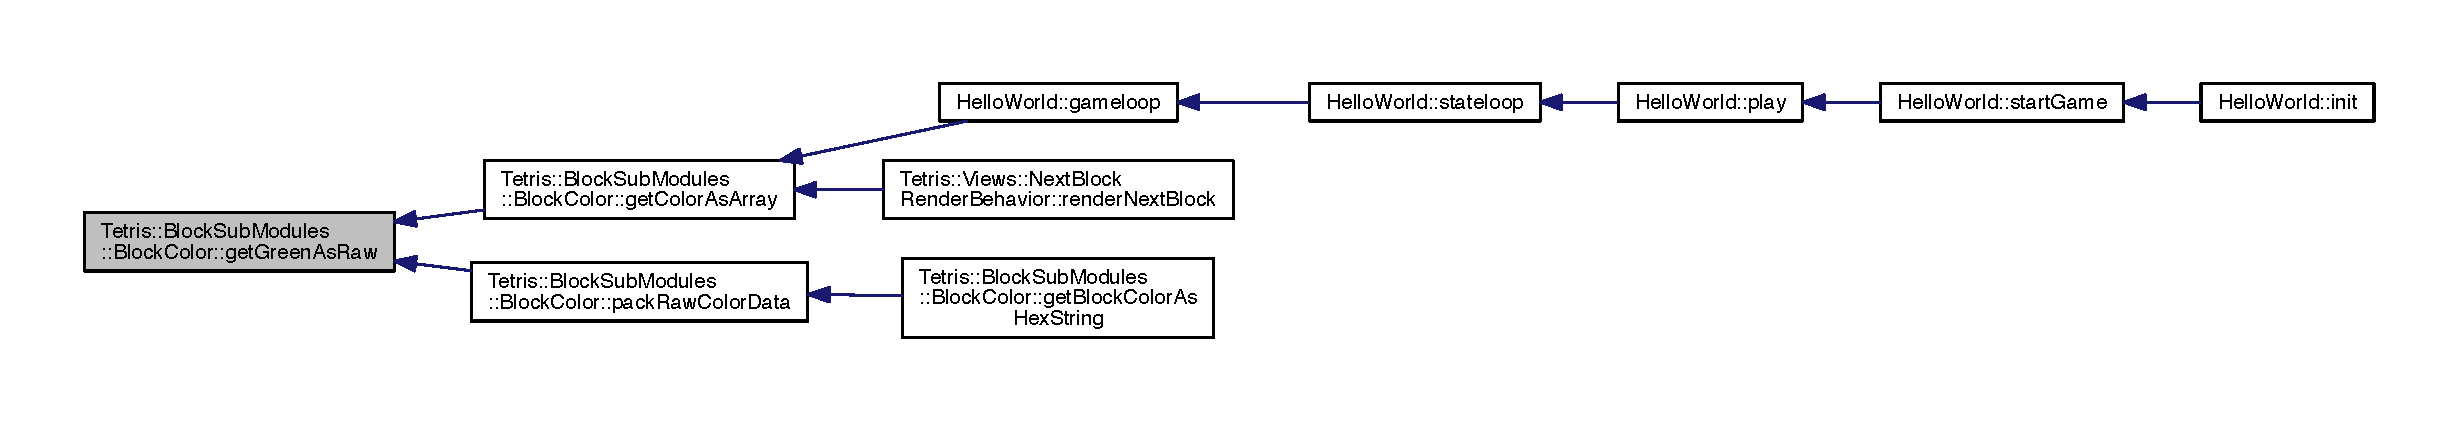
\includegraphics[width=350pt]{de/d44/class_tetris_1_1_block_sub_modules_1_1_block_color_a65e9230325a2f44aa433f39c199aabcd_icgraph}
\end{center}
\end{figure}
\mbox{\Hypertarget{class_tetris_1_1_block_sub_modules_1_1_block_color_a1795cf70c847d261645a9690afff7e9c}\label{class_tetris_1_1_block_sub_modules_1_1_block_color_a1795cf70c847d261645a9690afff7e9c}} 
\index{Tetris\+::\+Block\+Sub\+Modules\+::\+Block\+Color@{Tetris\+::\+Block\+Sub\+Modules\+::\+Block\+Color}!get\+Red\+As\+Raw@{get\+Red\+As\+Raw}}
\index{get\+Red\+As\+Raw@{get\+Red\+As\+Raw}!Tetris\+::\+Block\+Sub\+Modules\+::\+Block\+Color@{Tetris\+::\+Block\+Sub\+Modules\+::\+Block\+Color}}
\subsubsection{\texorpdfstring{get\+Red\+As\+Raw()}{getRedAsRaw()}}
{\footnotesize\ttfamily unsigned char Tetris\+::\+Block\+Sub\+Modules\+::\+Block\+Color\+::get\+Red\+As\+Raw (\begin{DoxyParamCaption}{ }\end{DoxyParamCaption})\hspace{0.3cm}{\ttfamily [inline]}}

\begin{DoxyReturn}{반환값}
색상데이터중 삘깅 데이터를 리턴 
\end{DoxyReturn}


Block\+Color.\+hpp 파일의 92 번째 라인에서 정의되었습니다.


\begin{DoxyCode}
92                                        \{
93                 \textcolor{keywordflow}{return} this->\hyperlink{class_tetris_1_1_block_sub_modules_1_1_block_color_af8a0dc372e7dbab300290eadada8ef49}{red};
94             \}
\end{DoxyCode}
이 함수를 호출하는 함수들에 대한 그래프입니다.\+:
\nopagebreak
\begin{figure}[H]
\begin{center}
\leavevmode
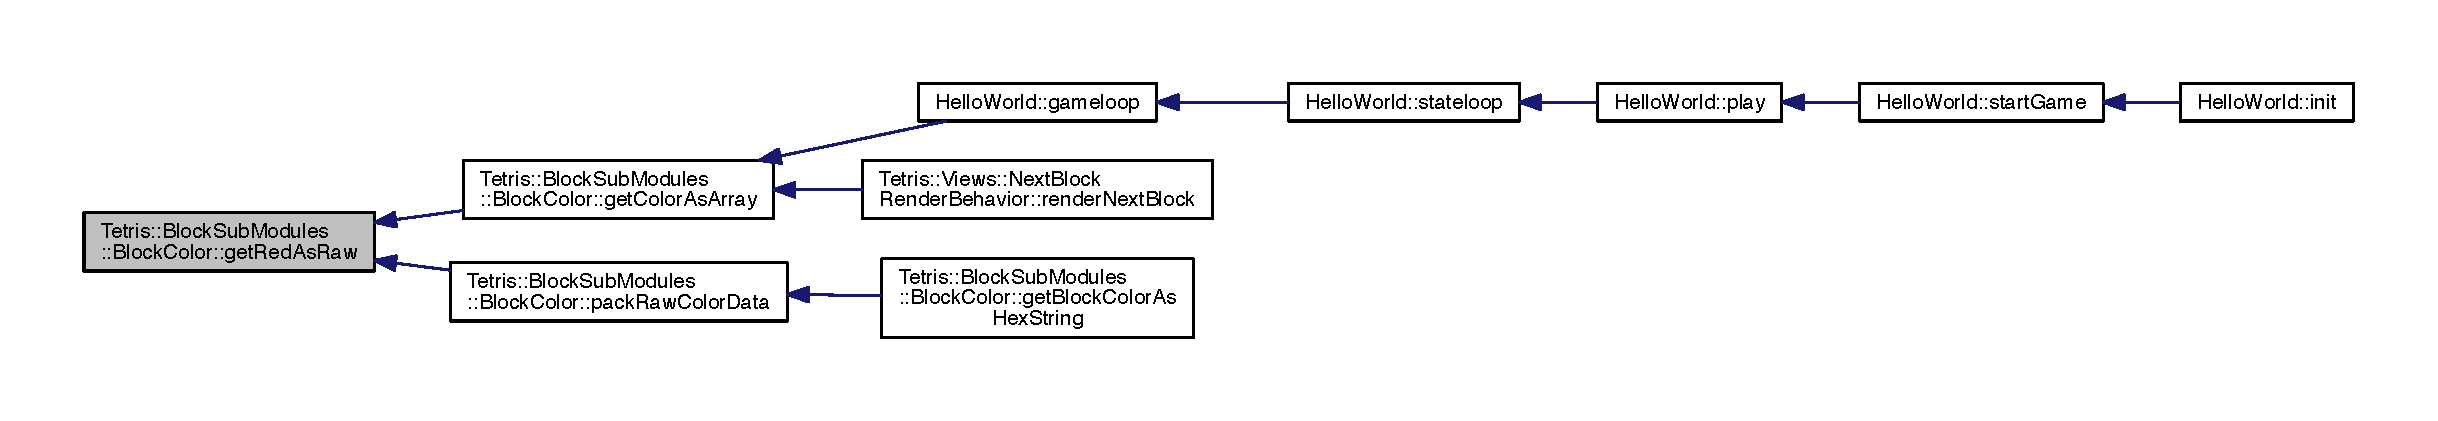
\includegraphics[width=350pt]{de/d44/class_tetris_1_1_block_sub_modules_1_1_block_color_a1795cf70c847d261645a9690afff7e9c_icgraph}
\end{center}
\end{figure}
\mbox{\Hypertarget{class_tetris_1_1_block_sub_modules_1_1_block_color_a849ebbb0e900c5efdcb99784767e7a7a}\label{class_tetris_1_1_block_sub_modules_1_1_block_color_a849ebbb0e900c5efdcb99784767e7a7a}} 
\index{Tetris\+::\+Block\+Sub\+Modules\+::\+Block\+Color@{Tetris\+::\+Block\+Sub\+Modules\+::\+Block\+Color}!pack\+Raw\+Color\+Data@{pack\+Raw\+Color\+Data}}
\index{pack\+Raw\+Color\+Data@{pack\+Raw\+Color\+Data}!Tetris\+::\+Block\+Sub\+Modules\+::\+Block\+Color@{Tetris\+::\+Block\+Sub\+Modules\+::\+Block\+Color}}
\subsubsection{\texorpdfstring{pack\+Raw\+Color\+Data()}{packRawColorData()}}
{\footnotesize\ttfamily unsigned int Tetris\+::\+Block\+Sub\+Modules\+::\+Block\+Color\+::pack\+Raw\+Color\+Data (\begin{DoxyParamCaption}{ }\end{DoxyParamCaption})\hspace{0.3cm}{\ttfamily [inline]}}

\begin{DoxyReturn}{반환값}
현재 설정된 색상 데이터를 4바이트 변수로 묶어 리턴 
\end{DoxyReturn}


Block\+Color.\+hpp 파일의 104 번째 라인에서 정의되었습니다.


\begin{DoxyCode}
104                                            \{
105                 \textcolor{keywordflow}{return} (((\textcolor{keywordtype}{unsigned} \textcolor{keywordtype}{int})this->\hyperlink{class_tetris_1_1_block_sub_modules_1_1_block_color_acb1c9b34ee534857741025bd2824201a}{getAlphaAsRaw}())<<(8*3))|(((\textcolor{keywordtype}{unsigned} int)this->
      \hyperlink{class_tetris_1_1_block_sub_modules_1_1_block_color_a1795cf70c847d261645a9690afff7e9c}{getRedAsRaw}())<<(8*2))|(((\textcolor{keywordtype}{unsigned} \textcolor{keywordtype}{int})this->\hyperlink{class_tetris_1_1_block_sub_modules_1_1_block_color_a65e9230325a2f44aa433f39c199aabcd}{getGreenAsRaw}())<<(8*1))|this->
      \hyperlink{class_tetris_1_1_block_sub_modules_1_1_block_color_ac0ad44a8b001f3824447d137357f5145}{getBlueAsRaw}();
106             \}
\end{DoxyCode}
이 함수 내부에서 호출하는 함수들에 대한 그래프입니다.\+:
\nopagebreak
\begin{figure}[H]
\begin{center}
\leavevmode
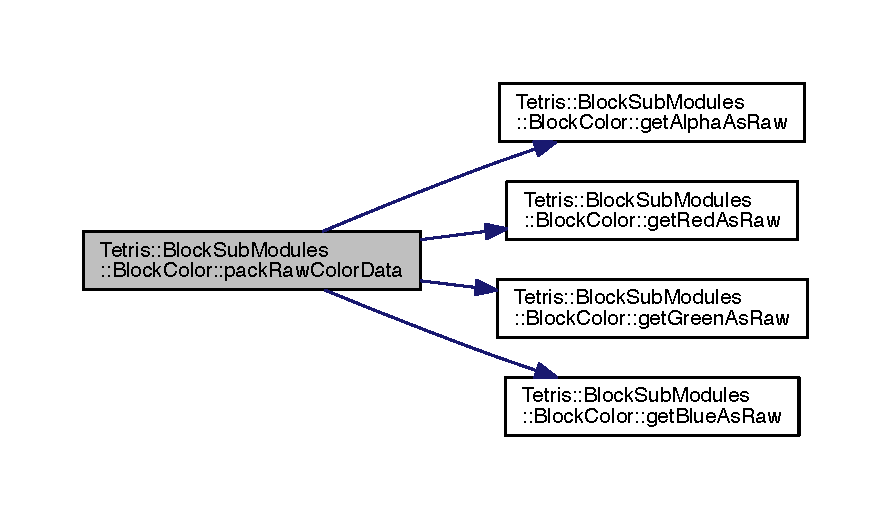
\includegraphics[width=350pt]{de/d44/class_tetris_1_1_block_sub_modules_1_1_block_color_a849ebbb0e900c5efdcb99784767e7a7a_cgraph}
\end{center}
\end{figure}
이 함수를 호출하는 함수들에 대한 그래프입니다.\+:
\nopagebreak
\begin{figure}[H]
\begin{center}
\leavevmode
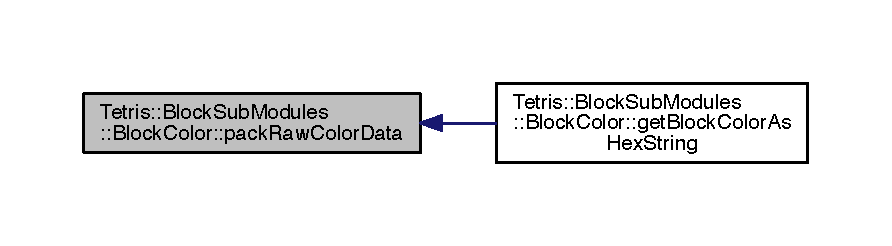
\includegraphics[width=350pt]{de/d44/class_tetris_1_1_block_sub_modules_1_1_block_color_a849ebbb0e900c5efdcb99784767e7a7a_icgraph}
\end{center}
\end{figure}
\mbox{\Hypertarget{class_tetris_1_1_block_sub_modules_1_1_block_color_a5fdd2d1a53d92ec0bcc1c25748b890e0}\label{class_tetris_1_1_block_sub_modules_1_1_block_color_a5fdd2d1a53d92ec0bcc1c25748b890e0}} 
\index{Tetris\+::\+Block\+Sub\+Modules\+::\+Block\+Color@{Tetris\+::\+Block\+Sub\+Modules\+::\+Block\+Color}!set\+Alpha@{set\+Alpha}}
\index{set\+Alpha@{set\+Alpha}!Tetris\+::\+Block\+Sub\+Modules\+::\+Block\+Color@{Tetris\+::\+Block\+Sub\+Modules\+::\+Block\+Color}}
\subsubsection{\texorpdfstring{set\+Alpha()}{setAlpha()}}
{\footnotesize\ttfamily void Tetris\+::\+Block\+Sub\+Modules\+::\+Block\+Color\+::set\+Alpha (\begin{DoxyParamCaption}\item[{unsigned char}]{aph }\end{DoxyParamCaption})\hspace{0.3cm}{\ttfamily [inline]}, {\ttfamily [protected]}}



Block\+Color.\+hpp 파일의 132 번째 라인에서 정의되었습니다.


\begin{DoxyCode}
132                                             \{
133                 this->\hyperlink{class_tetris_1_1_block_sub_modules_1_1_block_color_af0983ea684f33617a0b482cfea1d3c2b}{alpha} = aph;
134             \}
\end{DoxyCode}
이 함수를 호출하는 함수들에 대한 그래프입니다.\+:
\nopagebreak
\begin{figure}[H]
\begin{center}
\leavevmode
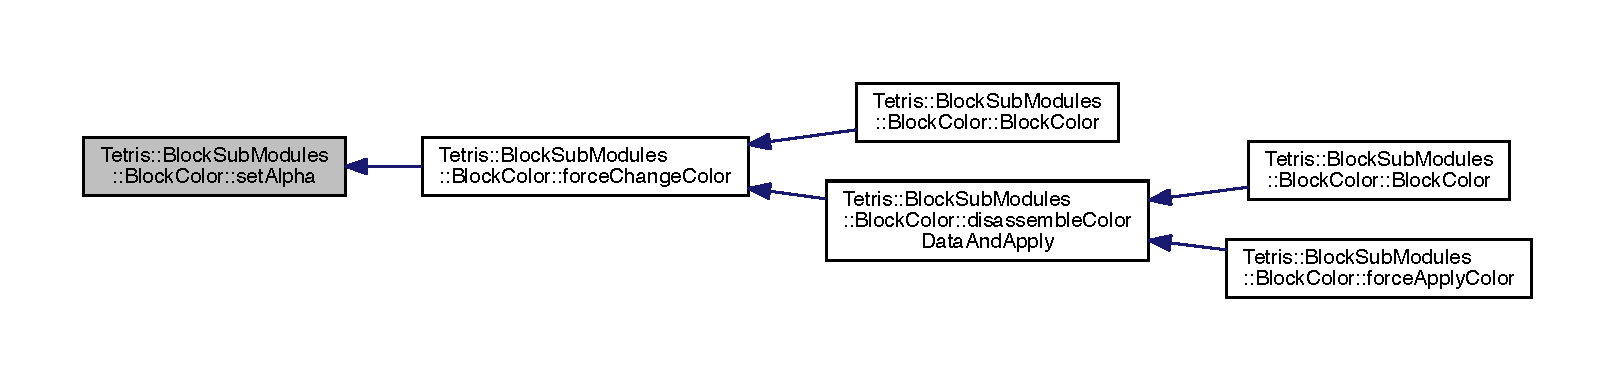
\includegraphics[width=350pt]{de/d44/class_tetris_1_1_block_sub_modules_1_1_block_color_a5fdd2d1a53d92ec0bcc1c25748b890e0_icgraph}
\end{center}
\end{figure}
\mbox{\Hypertarget{class_tetris_1_1_block_sub_modules_1_1_block_color_ac624156bd1f77a20d6e1d4c8cbff36d3}\label{class_tetris_1_1_block_sub_modules_1_1_block_color_ac624156bd1f77a20d6e1d4c8cbff36d3}} 
\index{Tetris\+::\+Block\+Sub\+Modules\+::\+Block\+Color@{Tetris\+::\+Block\+Sub\+Modules\+::\+Block\+Color}!set\+Blue@{set\+Blue}}
\index{set\+Blue@{set\+Blue}!Tetris\+::\+Block\+Sub\+Modules\+::\+Block\+Color@{Tetris\+::\+Block\+Sub\+Modules\+::\+Block\+Color}}
\subsubsection{\texorpdfstring{set\+Blue()}{setBlue()}}
{\footnotesize\ttfamily void Tetris\+::\+Block\+Sub\+Modules\+::\+Block\+Color\+::set\+Blue (\begin{DoxyParamCaption}\item[{unsigned char}]{blu }\end{DoxyParamCaption})\hspace{0.3cm}{\ttfamily [inline]}, {\ttfamily [protected]}}



Block\+Color.\+hpp 파일의 129 번째 라인에서 정의되었습니다.


\begin{DoxyCode}
129                                            \{
130                 this->\hyperlink{class_tetris_1_1_block_sub_modules_1_1_block_color_af04e78b9a1c2f7625863c289c4a741e3}{blue} = blu;
131             \}
\end{DoxyCode}
이 함수를 호출하는 함수들에 대한 그래프입니다.\+:
\nopagebreak
\begin{figure}[H]
\begin{center}
\leavevmode
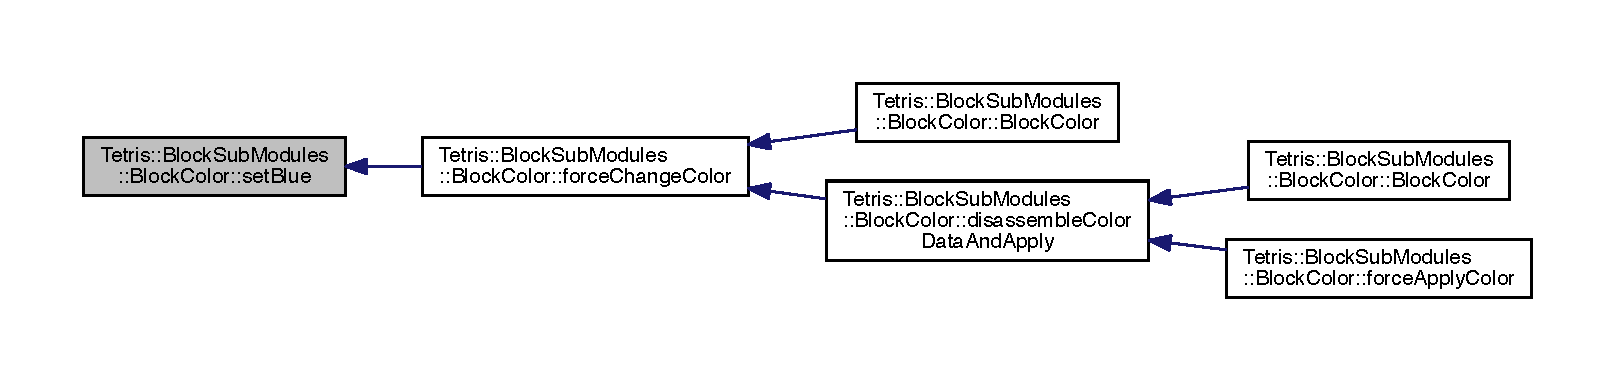
\includegraphics[width=350pt]{de/d44/class_tetris_1_1_block_sub_modules_1_1_block_color_ac624156bd1f77a20d6e1d4c8cbff36d3_icgraph}
\end{center}
\end{figure}
\mbox{\Hypertarget{class_tetris_1_1_block_sub_modules_1_1_block_color_aeea8ab6d5f36d35fd4f28818349661ab}\label{class_tetris_1_1_block_sub_modules_1_1_block_color_aeea8ab6d5f36d35fd4f28818349661ab}} 
\index{Tetris\+::\+Block\+Sub\+Modules\+::\+Block\+Color@{Tetris\+::\+Block\+Sub\+Modules\+::\+Block\+Color}!set\+Green@{set\+Green}}
\index{set\+Green@{set\+Green}!Tetris\+::\+Block\+Sub\+Modules\+::\+Block\+Color@{Tetris\+::\+Block\+Sub\+Modules\+::\+Block\+Color}}
\subsubsection{\texorpdfstring{set\+Green()}{setGreen()}}
{\footnotesize\ttfamily void Tetris\+::\+Block\+Sub\+Modules\+::\+Block\+Color\+::set\+Green (\begin{DoxyParamCaption}\item[{unsigned char}]{grn }\end{DoxyParamCaption})\hspace{0.3cm}{\ttfamily [inline]}, {\ttfamily [protected]}}



Block\+Color.\+hpp 파일의 126 번째 라인에서 정의되었습니다.


\begin{DoxyCode}
126                                             \{
127                 this->\hyperlink{class_tetris_1_1_block_sub_modules_1_1_block_color_a4b28885bfd8bf53793c6b3daedd974eb}{green} = grn;
128             \}
\end{DoxyCode}
이 함수를 호출하는 함수들에 대한 그래프입니다.\+:
\nopagebreak
\begin{figure}[H]
\begin{center}
\leavevmode
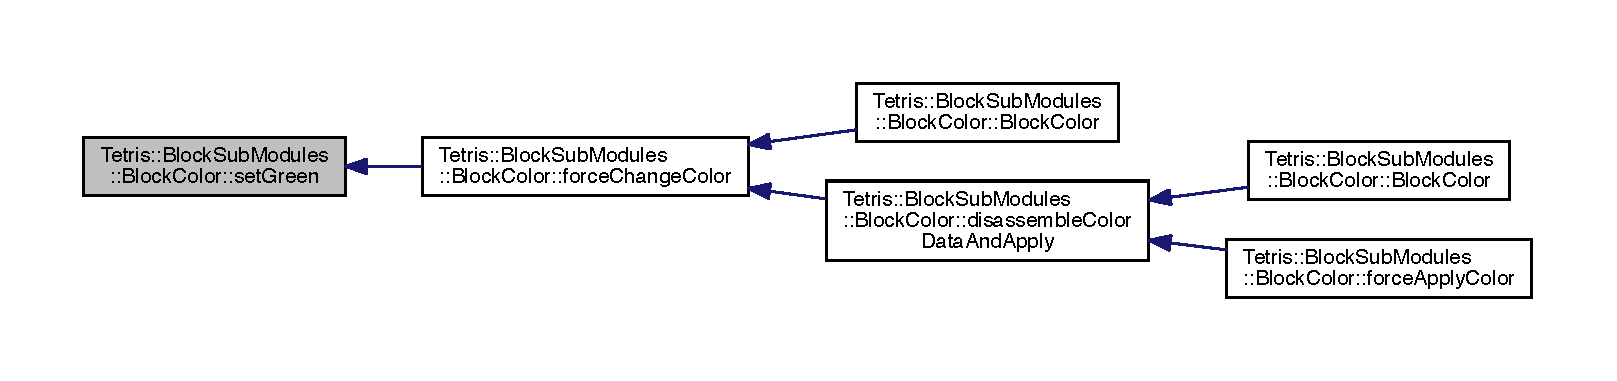
\includegraphics[width=350pt]{de/d44/class_tetris_1_1_block_sub_modules_1_1_block_color_aeea8ab6d5f36d35fd4f28818349661ab_icgraph}
\end{center}
\end{figure}
\mbox{\Hypertarget{class_tetris_1_1_block_sub_modules_1_1_block_color_a9541e6b5b809214ae2691a99af06ac3f}\label{class_tetris_1_1_block_sub_modules_1_1_block_color_a9541e6b5b809214ae2691a99af06ac3f}} 
\index{Tetris\+::\+Block\+Sub\+Modules\+::\+Block\+Color@{Tetris\+::\+Block\+Sub\+Modules\+::\+Block\+Color}!set\+Red@{set\+Red}}
\index{set\+Red@{set\+Red}!Tetris\+::\+Block\+Sub\+Modules\+::\+Block\+Color@{Tetris\+::\+Block\+Sub\+Modules\+::\+Block\+Color}}
\subsubsection{\texorpdfstring{set\+Red()}{setRed()}}
{\footnotesize\ttfamily void Tetris\+::\+Block\+Sub\+Modules\+::\+Block\+Color\+::set\+Red (\begin{DoxyParamCaption}\item[{unsigned char}]{rd }\end{DoxyParamCaption})\hspace{0.3cm}{\ttfamily [inline]}, {\ttfamily [protected]}}



Block\+Color.\+hpp 파일의 135 번째 라인에서 정의되었습니다.


\begin{DoxyCode}
135                                          \{
136                 this->\hyperlink{class_tetris_1_1_block_sub_modules_1_1_block_color_af8a0dc372e7dbab300290eadada8ef49}{red} = rd;
137             \}
\end{DoxyCode}
이 함수를 호출하는 함수들에 대한 그래프입니다.\+:
\nopagebreak
\begin{figure}[H]
\begin{center}
\leavevmode
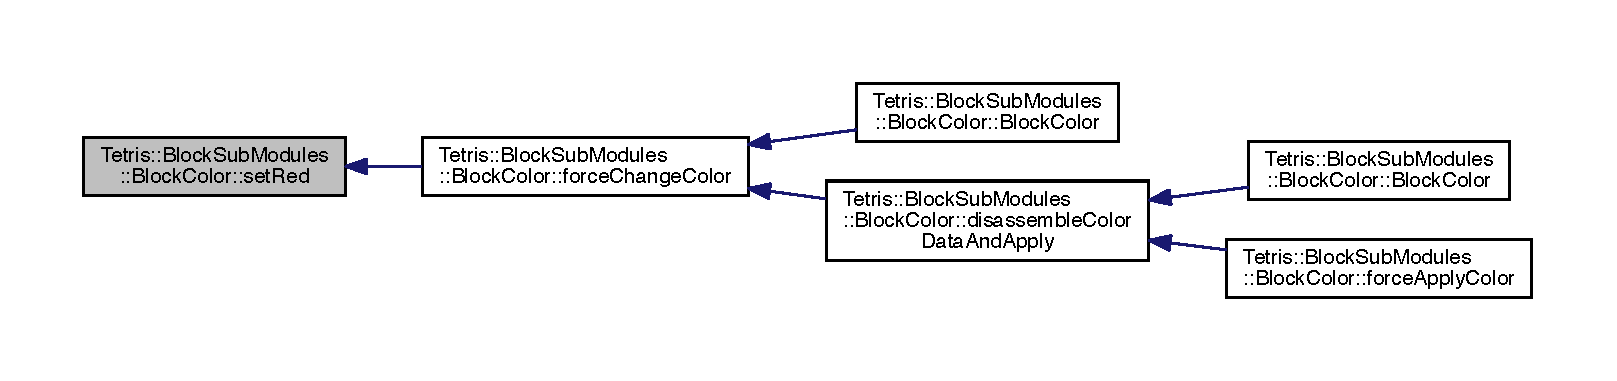
\includegraphics[width=350pt]{de/d44/class_tetris_1_1_block_sub_modules_1_1_block_color_a9541e6b5b809214ae2691a99af06ac3f_icgraph}
\end{center}
\end{figure}


\subsection{필드 문서화}
\mbox{\Hypertarget{class_tetris_1_1_block_sub_modules_1_1_block_color_af0983ea684f33617a0b482cfea1d3c2b}\label{class_tetris_1_1_block_sub_modules_1_1_block_color_af0983ea684f33617a0b482cfea1d3c2b}} 
\index{Tetris\+::\+Block\+Sub\+Modules\+::\+Block\+Color@{Tetris\+::\+Block\+Sub\+Modules\+::\+Block\+Color}!alpha@{alpha}}
\index{alpha@{alpha}!Tetris\+::\+Block\+Sub\+Modules\+::\+Block\+Color@{Tetris\+::\+Block\+Sub\+Modules\+::\+Block\+Color}}
\subsubsection{\texorpdfstring{alpha}{alpha}}
{\footnotesize\ttfamily unsigned char Tetris\+::\+Block\+Sub\+Modules\+::\+Block\+Color\+::alpha\hspace{0.3cm}{\ttfamily [protected]}}



Block\+Color.\+hpp 파일의 125 번째 라인에서 정의되었습니다.

\mbox{\Hypertarget{class_tetris_1_1_block_sub_modules_1_1_block_color_af04e78b9a1c2f7625863c289c4a741e3}\label{class_tetris_1_1_block_sub_modules_1_1_block_color_af04e78b9a1c2f7625863c289c4a741e3}} 
\index{Tetris\+::\+Block\+Sub\+Modules\+::\+Block\+Color@{Tetris\+::\+Block\+Sub\+Modules\+::\+Block\+Color}!blue@{blue}}
\index{blue@{blue}!Tetris\+::\+Block\+Sub\+Modules\+::\+Block\+Color@{Tetris\+::\+Block\+Sub\+Modules\+::\+Block\+Color}}
\subsubsection{\texorpdfstring{blue}{blue}}
{\footnotesize\ttfamily unsigned char Tetris\+::\+Block\+Sub\+Modules\+::\+Block\+Color\+::blue\hspace{0.3cm}{\ttfamily [protected]}}



Block\+Color.\+hpp 파일의 125 번째 라인에서 정의되었습니다.

\mbox{\Hypertarget{class_tetris_1_1_block_sub_modules_1_1_block_color_a4b28885bfd8bf53793c6b3daedd974eb}\label{class_tetris_1_1_block_sub_modules_1_1_block_color_a4b28885bfd8bf53793c6b3daedd974eb}} 
\index{Tetris\+::\+Block\+Sub\+Modules\+::\+Block\+Color@{Tetris\+::\+Block\+Sub\+Modules\+::\+Block\+Color}!green@{green}}
\index{green@{green}!Tetris\+::\+Block\+Sub\+Modules\+::\+Block\+Color@{Tetris\+::\+Block\+Sub\+Modules\+::\+Block\+Color}}
\subsubsection{\texorpdfstring{green}{green}}
{\footnotesize\ttfamily unsigned char Tetris\+::\+Block\+Sub\+Modules\+::\+Block\+Color\+::green\hspace{0.3cm}{\ttfamily [protected]}}



Block\+Color.\+hpp 파일의 125 번째 라인에서 정의되었습니다.

\mbox{\Hypertarget{class_tetris_1_1_block_sub_modules_1_1_block_color_af8a0dc372e7dbab300290eadada8ef49}\label{class_tetris_1_1_block_sub_modules_1_1_block_color_af8a0dc372e7dbab300290eadada8ef49}} 
\index{Tetris\+::\+Block\+Sub\+Modules\+::\+Block\+Color@{Tetris\+::\+Block\+Sub\+Modules\+::\+Block\+Color}!red@{red}}
\index{red@{red}!Tetris\+::\+Block\+Sub\+Modules\+::\+Block\+Color@{Tetris\+::\+Block\+Sub\+Modules\+::\+Block\+Color}}
\subsubsection{\texorpdfstring{red}{red}}
{\footnotesize\ttfamily unsigned char Tetris\+::\+Block\+Sub\+Modules\+::\+Block\+Color\+::red\hspace{0.3cm}{\ttfamily [protected]}}



Block\+Color.\+hpp 파일의 125 번째 라인에서 정의되었습니다.



이 클래스에 대한 문서화 페이지는 다음의 파일로부터 생성되었습니다.\+:\begin{DoxyCompactItemize}
\item 
Classes/tet2/\hyperlink{_block_color_8hpp}{Block\+Color.\+hpp}\end{DoxyCompactItemize}

\hypertarget{class_tetris_1_1_block_generator}{}\section{Tetris\+:\+:Block\+Generator 클래스 참조}
\label{class_tetris_1_1_block_generator}\index{Tetris\+::\+Block\+Generator@{Tetris\+::\+Block\+Generator}}


블럭을 연속된 번호내에서 생성하거나 랜덤 생성  




{\ttfamily \#include $<$Block\+Generator.\+h$>$}



Tetris\+:\+:Block\+Generator에 대한 협력 다이어그램\+:
\nopagebreak
\begin{figure}[H]
\begin{center}
\leavevmode
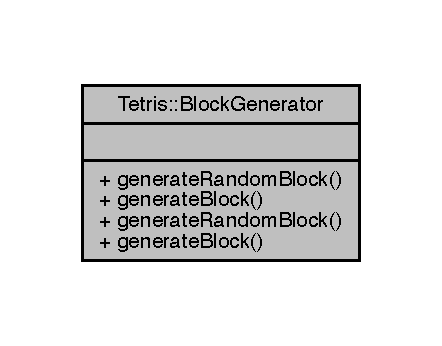
\includegraphics[width=212pt]{d5/dda/class_tetris_1_1_block_generator__coll__graph}
\end{center}
\end{figure}
\subsection*{Public 멤버 함수}
\begin{DoxyCompactItemize}
\item 
\hyperlink{class_tetris_1_1_block}{Block} $\ast$ \hyperlink{class_tetris_1_1_block_generator_a10dfe1467d40437ad41c5ae76437ad78}{generate\+Random\+Block} ()
\item 
\hyperlink{class_tetris_1_1_block}{Block} $\ast$ \hyperlink{class_tetris_1_1_block_generator_a581b22cebe170d3fe8b51130c01e7a22}{generate\+Block} (int num)
\item 
\hyperlink{class_tetris_1_1_block}{Block} $\ast$ \hyperlink{class_tetris_1_1_block_generator_a434df5baf3944a534492b63763b532a6}{generate\+Random\+Block} ()
\item 
\hyperlink{class_tetris_1_1_block}{Block} $\ast$ \hyperlink{class_tetris_1_1_block_generator_a584fde2bfe1cdd4505bd905befd73d21}{generate\+Block} (const int num)
\end{DoxyCompactItemize}


\subsection{상세한 설명}
블럭을 연속된 번호내에서 생성하거나 랜덤 생성 

Block\+Generator.\+h 파일의 11 번째 라인에서 정의되었습니다.



\subsection{멤버 함수 문서화}
\mbox{\Hypertarget{class_tetris_1_1_block_generator_a581b22cebe170d3fe8b51130c01e7a22}\label{class_tetris_1_1_block_generator_a581b22cebe170d3fe8b51130c01e7a22}} 
\index{Tetris\+::\+Block\+Generator@{Tetris\+::\+Block\+Generator}!generate\+Block@{generate\+Block}}
\index{generate\+Block@{generate\+Block}!Tetris\+::\+Block\+Generator@{Tetris\+::\+Block\+Generator}}
\subsubsection{\texorpdfstring{generate\+Block()}{generateBlock()}\hspace{0.1cm}{\footnotesize\ttfamily [1/2]}}
{\footnotesize\ttfamily \hyperlink{class_tetris_1_1_block}{Block} $\ast$ Tetris\+::\+Block\+Generator\+::generate\+Block (\begin{DoxyParamCaption}\item[{int}]{num }\end{DoxyParamCaption})}



Block\+Generator.\+cpp 파일의 13 번째 라인에서 정의되었습니다.


\begin{DoxyCode}
13                                                    \{
14                 \hyperlink{class_tetris_1_1_block}{Block}* rst = NULL;
15                 \textcolor{keywordflow}{switch}(num)\{
16                     \textcolor{keywordflow}{case} 1:\{
17                         rst = \textcolor{keyword}{new} \hyperlink{class_tetris_1_1_block}{Block}(\hyperlink{_block_8h_ac9fe505a10c9ea541483202000c72dfe}{TETBLK\_TYPE\_I});
18                         \textcolor{keywordflow}{break};
19                     \}
20                     \textcolor{keywordflow}{case} 2:\{
21                         rst = \textcolor{keyword}{new} \hyperlink{class_tetris_1_1_block}{Block}(\hyperlink{_block_8h_aa30a45ef914d6bd7caf960c42af38197}{TETBLK\_TYPE\_L});
22                         \textcolor{keywordflow}{break};
23                     \}
24                     \textcolor{keywordflow}{case} 3:\{
25                         rst = \textcolor{keyword}{new} \hyperlink{class_tetris_1_1_block}{Block}(\hyperlink{_block_8h_a3a84ffcf3638f400ed5ebc303d152a94}{TETBLK\_TYPE\_J});
26                         \textcolor{keywordflow}{break};
27                     \}
28 
29                     \textcolor{keywordflow}{case} 4:\{
30                         rst = \textcolor{keyword}{new} \hyperlink{class_tetris_1_1_block}{Block}(\hyperlink{_block_8h_a6da1e2b8848e1a7b5a7ee687fd6492bd}{TETBLK\_TYPE\_M});
31                         \textcolor{keywordflow}{break};
32                     \}
33                     \textcolor{keywordflow}{case} 5:\{
34                         rst = \textcolor{keyword}{new} \hyperlink{class_tetris_1_1_block}{Block}(\hyperlink{_block_8h_a50283efc563e3ebe3b8ac84947491f5d}{TETBLK\_TYPE\_Z});
35                         \textcolor{keywordflow}{break};
36                     \}
37                     \textcolor{keywordflow}{case} 6:\{
38                         rst = \textcolor{keyword}{new} \hyperlink{class_tetris_1_1_block}{Block}(\hyperlink{_block_8h_afb6b4a709481a06422a9a9daedb334ee}{TETBLK\_TYPE\_S});
39                         \textcolor{keywordflow}{break};
40                     \}
41                     \textcolor{keywordflow}{case} 7:\{
42                         rst = \textcolor{keyword}{new} \hyperlink{class_tetris_1_1_block}{Block}(\hyperlink{_block_8h_aa624341303e91efd01c17dfb25d15010}{TETBLK\_TYPE\_T});
43                         \textcolor{keywordflow}{break};
44                     \}
45 
46                 \}
47                 \textcolor{keywordflow}{if}(rst!=NULL)\{
48                     \textcolor{keyword}{const} \textcolor{keywordtype}{int} rndrotcnt = \hyperlink{namespace_tetris_1_1_util_aa590e9fd847ac6e0c9bc6bf464b5a74b}{Tetris::Util::randInt}(0,3);
49                     \textcolor{keywordflow}{for}(\textcolor{keywordtype}{int} i=0;i<rndrotcnt;i++)\{
50                         rst->\hyperlink{class_tetris_1_1_block_a0d1eb57e6da91832ad983f7a4fa9ca04}{rotate}();
51                     \}
52                 \}
53                 \textcolor{keywordflow}{return} rst;
54             \}
\end{DoxyCode}
이 함수 내부에서 호출하는 함수들에 대한 그래프입니다.\+:
\nopagebreak
\begin{figure}[H]
\begin{center}
\leavevmode
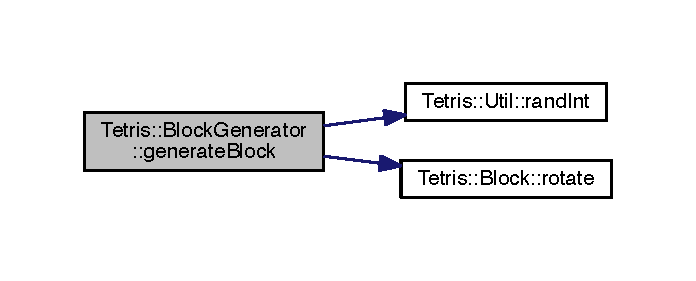
\includegraphics[width=334pt]{d3/d50/class_tetris_1_1_block_generator_a581b22cebe170d3fe8b51130c01e7a22_cgraph}
\end{center}
\end{figure}
\mbox{\Hypertarget{class_tetris_1_1_block_generator_a584fde2bfe1cdd4505bd905befd73d21}\label{class_tetris_1_1_block_generator_a584fde2bfe1cdd4505bd905befd73d21}} 
\index{Tetris\+::\+Block\+Generator@{Tetris\+::\+Block\+Generator}!generate\+Block@{generate\+Block}}
\index{generate\+Block@{generate\+Block}!Tetris\+::\+Block\+Generator@{Tetris\+::\+Block\+Generator}}
\subsubsection{\texorpdfstring{generate\+Block()}{generateBlock()}\hspace{0.1cm}{\footnotesize\ttfamily [2/2]}}
{\footnotesize\ttfamily \hyperlink{class_tetris_1_1_block}{Block}$\ast$ Tetris\+::\+Block\+Generator\+::generate\+Block (\begin{DoxyParamCaption}\item[{const int}]{num }\end{DoxyParamCaption})\hspace{0.3cm}{\ttfamily [inline]}}



Block\+Generator.\+hpp 파일의 25 번째 라인에서 정의되었습니다.


\begin{DoxyCode}
25                                                \{
26                 \hyperlink{class_tetris_1_1_block}{Block}* rst = NULL;
27                 \textcolor{keywordflow}{switch}(num)\{
28                     \textcolor{keywordflow}{case} 1:\{
29                         rst = \textcolor{keyword}{new} \hyperlink{class_tetris_1_1_block}{Block}(\hyperlink{_block_8h_ac9fe505a10c9ea541483202000c72dfe}{TETBLK\_TYPE\_I});
30                         \textcolor{keywordflow}{break};
31                     \}
32                     \textcolor{keywordflow}{case} 2:\{
33                         rst = \textcolor{keyword}{new} \hyperlink{class_tetris_1_1_block}{Block}(\hyperlink{_block_8h_aa30a45ef914d6bd7caf960c42af38197}{TETBLK\_TYPE\_L});
34                         \textcolor{keywordflow}{break};
35                     \}
36                     \textcolor{keywordflow}{case} 3:\{
37                         rst = \textcolor{keyword}{new} \hyperlink{class_tetris_1_1_block}{Block}(\hyperlink{_block_8h_a3a84ffcf3638f400ed5ebc303d152a94}{TETBLK\_TYPE\_J});
38                         \textcolor{keywordflow}{break};
39                     \}
40 
41                     \textcolor{keywordflow}{case} 4:\{
42                         rst = \textcolor{keyword}{new} \hyperlink{class_tetris_1_1_block}{Block}(\hyperlink{_block_8h_a6da1e2b8848e1a7b5a7ee687fd6492bd}{TETBLK\_TYPE\_M});
43                         \textcolor{keywordflow}{break};
44                     \}
45                     \textcolor{keywordflow}{case} 5:\{
46                         rst = \textcolor{keyword}{new} \hyperlink{class_tetris_1_1_block}{Block}(\hyperlink{_block_8h_a50283efc563e3ebe3b8ac84947491f5d}{TETBLK\_TYPE\_Z});
47                         \textcolor{keywordflow}{break};
48                     \}
49                     \textcolor{keywordflow}{case} 6:\{
50                         rst = \textcolor{keyword}{new} \hyperlink{class_tetris_1_1_block}{Block}(\hyperlink{_block_8h_afb6b4a709481a06422a9a9daedb334ee}{TETBLK\_TYPE\_S});
51                         \textcolor{keywordflow}{break};
52                     \}
53                     \textcolor{keywordflow}{case} 7:\{
54                         rst = \textcolor{keyword}{new} \hyperlink{class_tetris_1_1_block}{Block}(\hyperlink{_block_8h_aa624341303e91efd01c17dfb25d15010}{TETBLK\_TYPE\_T});
55                         \textcolor{keywordflow}{break};
56                     \}
57 
58                 \}
59                 \textcolor{keywordflow}{if}(rst!=NULL)\{
60                     \textcolor{keyword}{const} \textcolor{keywordtype}{int} rndrotcnt = \hyperlink{class_tetris_util_a0a60e809425ddb416a500bcc03cf7061}{TetrisUtil::randInt}(0,3);
61                     \textcolor{keywordflow}{for}(\textcolor{keywordtype}{int} i=0;i<rndrotcnt;i++)\{
62                         rst->\hyperlink{class_tetris_1_1_block_a0d1eb57e6da91832ad983f7a4fa9ca04}{rotate}();
63                     \}
64                 \}
65                 \textcolor{keywordflow}{return} rst;
66             \}
\end{DoxyCode}
이 함수 내부에서 호출하는 함수들에 대한 그래프입니다.\+:
\nopagebreak
\begin{figure}[H]
\begin{center}
\leavevmode
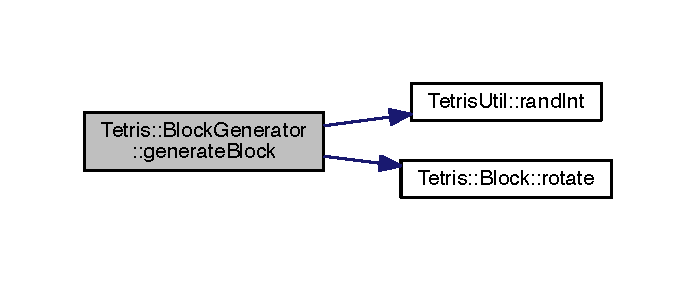
\includegraphics[width=334pt]{d3/d50/class_tetris_1_1_block_generator_a584fde2bfe1cdd4505bd905befd73d21_cgraph}
\end{center}
\end{figure}
\mbox{\Hypertarget{class_tetris_1_1_block_generator_a10dfe1467d40437ad41c5ae76437ad78}\label{class_tetris_1_1_block_generator_a10dfe1467d40437ad41c5ae76437ad78}} 
\index{Tetris\+::\+Block\+Generator@{Tetris\+::\+Block\+Generator}!generate\+Random\+Block@{generate\+Random\+Block}}
\index{generate\+Random\+Block@{generate\+Random\+Block}!Tetris\+::\+Block\+Generator@{Tetris\+::\+Block\+Generator}}
\subsubsection{\texorpdfstring{generate\+Random\+Block()}{generateRandomBlock()}\hspace{0.1cm}{\footnotesize\ttfamily [1/2]}}
{\footnotesize\ttfamily \hyperlink{class_tetris_1_1_block}{Block} $\ast$ Tetris\+::\+Block\+Generator\+::generate\+Random\+Block (\begin{DoxyParamCaption}{ }\end{DoxyParamCaption})}



Block\+Generator.\+cpp 파일의 10 번째 라인에서 정의되었습니다.


\begin{DoxyCode}
10                                                   \{
11             \textcolor{keywordflow}{return} this->\hyperlink{class_tetris_1_1_block_generator_a581b22cebe170d3fe8b51130c01e7a22}{generateBlock}(\hyperlink{namespace_tetris_1_1_util_aa590e9fd847ac6e0c9bc6bf464b5a74b}{Tetris::Util::randInt}(1,7)); \textcolor{comment}{//
      randint(1,7));}
12             \}
\end{DoxyCode}
이 함수 내부에서 호출하는 함수들에 대한 그래프입니다.\+:
\nopagebreak
\begin{figure}[H]
\begin{center}
\leavevmode
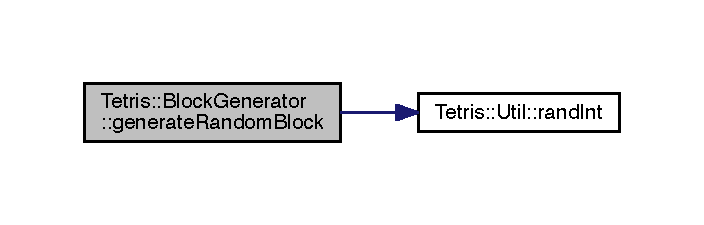
\includegraphics[width=338pt]{d3/d50/class_tetris_1_1_block_generator_a10dfe1467d40437ad41c5ae76437ad78_cgraph}
\end{center}
\end{figure}
\mbox{\Hypertarget{class_tetris_1_1_block_generator_a434df5baf3944a534492b63763b532a6}\label{class_tetris_1_1_block_generator_a434df5baf3944a534492b63763b532a6}} 
\index{Tetris\+::\+Block\+Generator@{Tetris\+::\+Block\+Generator}!generate\+Random\+Block@{generate\+Random\+Block}}
\index{generate\+Random\+Block@{generate\+Random\+Block}!Tetris\+::\+Block\+Generator@{Tetris\+::\+Block\+Generator}}
\subsubsection{\texorpdfstring{generate\+Random\+Block()}{generateRandomBlock()}\hspace{0.1cm}{\footnotesize\ttfamily [2/2]}}
{\footnotesize\ttfamily \hyperlink{class_tetris_1_1_block}{Block}$\ast$ Tetris\+::\+Block\+Generator\+::generate\+Random\+Block (\begin{DoxyParamCaption}{ }\end{DoxyParamCaption})\hspace{0.3cm}{\ttfamily [inline]}}



Block\+Generator.\+hpp 파일의 21 번째 라인에서 정의되었습니다.


\begin{DoxyCode}
21                                         \{
22                 cout<<\textcolor{stringliteral}{"genrandblk"}<<endl;
23                 \textcolor{keywordflow}{return} this->\hyperlink{class_tetris_1_1_block_generator_a581b22cebe170d3fe8b51130c01e7a22}{generateBlock}(\hyperlink{class_tetris_util_a0a60e809425ddb416a500bcc03cf7061}{TetrisUtil::randInt}(1,7)); \textcolor{comment}{//
      randint(1,7));}
24             \}
\end{DoxyCode}
이 함수 내부에서 호출하는 함수들에 대한 그래프입니다.\+:
\nopagebreak
\begin{figure}[H]
\begin{center}
\leavevmode
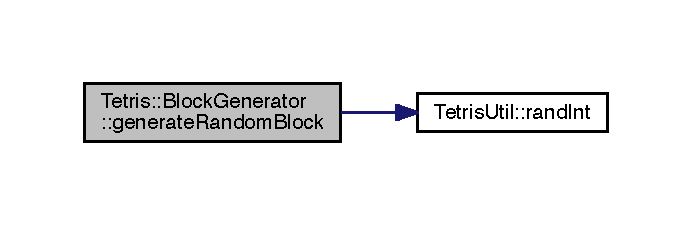
\includegraphics[width=332pt]{d3/d50/class_tetris_1_1_block_generator_a434df5baf3944a534492b63763b532a6_cgraph}
\end{center}
\end{figure}


이 클래스에 대한 문서화 페이지는 다음의 파일들로부터 생성되었습니다.\+:\begin{DoxyCompactItemize}
\item 
Classes/tet/\hyperlink{_block_generator_8h}{Block\+Generator.\+h}\item 
Classes/tet2/\hyperlink{_block_generator_8hpp}{Block\+Generator.\+hpp}\item 
Classes/tet/\hyperlink{_block_generator_8cpp}{Block\+Generator.\+cpp}\end{DoxyCompactItemize}

\hypertarget{class_code_lady_j_j_y_1_1game2048_1_1_card}{}\section{Code\+Lady\+J\+JY\+:\+:game2048\+:\+:Card 클래스 참조}
\label{class_code_lady_j_j_y_1_1game2048_1_1_card}\index{Code\+Lady\+J\+J\+Y\+::game2048\+::\+Card@{Code\+Lady\+J\+J\+Y\+::game2048\+::\+Card}}


{\ttfamily \#include $<$Card.\+hpp$>$}

Code\+Lady\+J\+JY\+:\+:game2048\+:\+:Card에 대한 상속 다이어그램 \+: \begin{figure}[H]
\begin{center}
\leavevmode
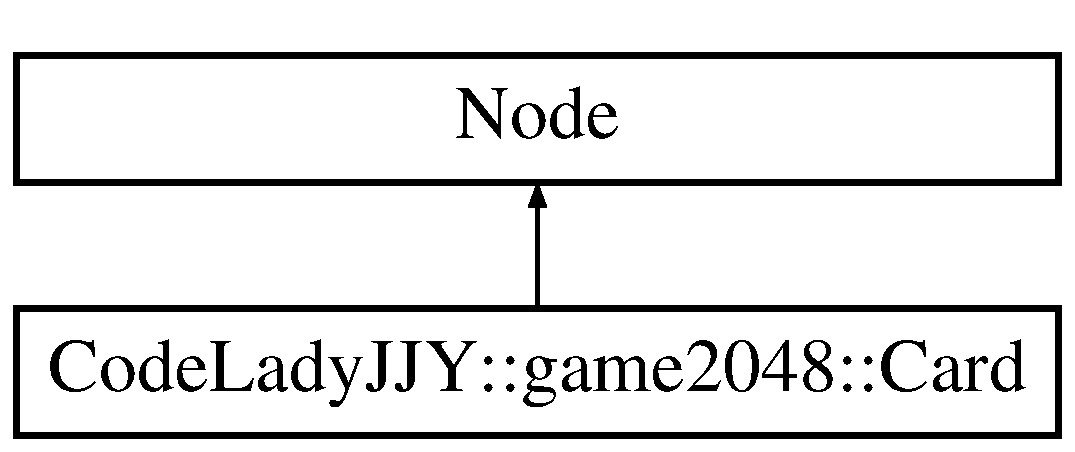
\includegraphics[height=2.000000cm]{class_code_lady_j_j_y_1_1game2048_1_1_card}
\end{center}
\end{figure}
\subsection*{Public 멤버 함수}
\begin{DoxyCompactItemize}
\item 
int \hyperlink{class_code_lady_j_j_y_1_1game2048_1_1_card_a7c8da9286db22bb16cfa0f8502b41eb4}{get\+Current\+Number} ()
\item 
void \hyperlink{class_code_lady_j_j_y_1_1game2048_1_1_card_abd3f3208867d1450ba4eeef3cef62d3f}{show} (int r, int c)
\item 
void \hyperlink{class_code_lady_j_j_y_1_1game2048_1_1_card_a6ad341b10626a9cc1aafe8229fa61ea6}{move} (int r, int c)
\item 
void \hyperlink{class_code_lady_j_j_y_1_1game2048_1_1_card_ad4cae75359815f3d80db488df3fd3dfd}{double\+Num} ()
\item 
virtual bool \hyperlink{class_code_lady_j_j_y_1_1game2048_1_1_card_a5efe85fbf1117b9a64cc13311352284c}{init} ()
\item 
\hyperlink{class_code_lady_j_j_y_1_1game2048_1_1_card_aeef08b192f5d93d6852ebfb75bb9bd9a}{C\+R\+E\+A\+T\+E\+\_\+\+F\+U\+NC} (\hyperlink{class_code_lady_j_j_y_1_1game2048_1_1_card}{Card})
\end{DoxyCompactItemize}
\subsection*{Public 속성}
\begin{DoxyCompactItemize}
\item 
int \hyperlink{class_code_lady_j_j_y_1_1game2048_1_1_card_ae612aaa37e50cb81d6f8ddb7283ebcbc}{m\+\_\+num}
\end{DoxyCompactItemize}


\subsection{상세한 설명}


Card.\+hpp 파일의 9 번째 라인에서 정의되었습니다.



\subsection{멤버 함수 문서화}
\mbox{\Hypertarget{class_code_lady_j_j_y_1_1game2048_1_1_card_aeef08b192f5d93d6852ebfb75bb9bd9a}\label{class_code_lady_j_j_y_1_1game2048_1_1_card_aeef08b192f5d93d6852ebfb75bb9bd9a}} 
\index{Code\+Lady\+J\+J\+Y\+::game2048\+::\+Card@{Code\+Lady\+J\+J\+Y\+::game2048\+::\+Card}!C\+R\+E\+A\+T\+E\+\_\+\+F\+U\+NC@{C\+R\+E\+A\+T\+E\+\_\+\+F\+U\+NC}}
\index{C\+R\+E\+A\+T\+E\+\_\+\+F\+U\+NC@{C\+R\+E\+A\+T\+E\+\_\+\+F\+U\+NC}!Code\+Lady\+J\+J\+Y\+::game2048\+::\+Card@{Code\+Lady\+J\+J\+Y\+::game2048\+::\+Card}}
\subsubsection{\texorpdfstring{C\+R\+E\+A\+T\+E\+\_\+\+F\+U\+N\+C()}{CREATE\_FUNC()}}
{\footnotesize\ttfamily Code\+Lady\+J\+J\+Y\+::game2048\+::\+Card\+::\+C\+R\+E\+A\+T\+E\+\_\+\+F\+U\+NC (\begin{DoxyParamCaption}\item[{\hyperlink{class_code_lady_j_j_y_1_1game2048_1_1_card}{Card}}]{ }\end{DoxyParamCaption})}

\mbox{\Hypertarget{class_code_lady_j_j_y_1_1game2048_1_1_card_ad4cae75359815f3d80db488df3fd3dfd}\label{class_code_lady_j_j_y_1_1game2048_1_1_card_ad4cae75359815f3d80db488df3fd3dfd}} 
\index{Code\+Lady\+J\+J\+Y\+::game2048\+::\+Card@{Code\+Lady\+J\+J\+Y\+::game2048\+::\+Card}!double\+Num@{double\+Num}}
\index{double\+Num@{double\+Num}!Code\+Lady\+J\+J\+Y\+::game2048\+::\+Card@{Code\+Lady\+J\+J\+Y\+::game2048\+::\+Card}}
\subsubsection{\texorpdfstring{double\+Num()}{doubleNum()}}
{\footnotesize\ttfamily void Code\+Lady\+J\+J\+Y\+::game2048\+::\+Card\+::double\+Num (\begin{DoxyParamCaption}{ }\end{DoxyParamCaption})\hspace{0.3cm}{\ttfamily [inline]}}



Card.\+hpp 파일의 34 번째 라인에서 정의되었습니다.

\mbox{\Hypertarget{class_code_lady_j_j_y_1_1game2048_1_1_card_a7c8da9286db22bb16cfa0f8502b41eb4}\label{class_code_lady_j_j_y_1_1game2048_1_1_card_a7c8da9286db22bb16cfa0f8502b41eb4}} 
\index{Code\+Lady\+J\+J\+Y\+::game2048\+::\+Card@{Code\+Lady\+J\+J\+Y\+::game2048\+::\+Card}!get\+Current\+Number@{get\+Current\+Number}}
\index{get\+Current\+Number@{get\+Current\+Number}!Code\+Lady\+J\+J\+Y\+::game2048\+::\+Card@{Code\+Lady\+J\+J\+Y\+::game2048\+::\+Card}}
\subsubsection{\texorpdfstring{get\+Current\+Number()}{getCurrentNumber()}}
{\footnotesize\ttfamily int Code\+Lady\+J\+J\+Y\+::game2048\+::\+Card\+::get\+Current\+Number (\begin{DoxyParamCaption}{ }\end{DoxyParamCaption})\hspace{0.3cm}{\ttfamily [inline]}}



Card.\+hpp 파일의 17 번째 라인에서 정의되었습니다.

\mbox{\Hypertarget{class_code_lady_j_j_y_1_1game2048_1_1_card_a5efe85fbf1117b9a64cc13311352284c}\label{class_code_lady_j_j_y_1_1game2048_1_1_card_a5efe85fbf1117b9a64cc13311352284c}} 
\index{Code\+Lady\+J\+J\+Y\+::game2048\+::\+Card@{Code\+Lady\+J\+J\+Y\+::game2048\+::\+Card}!init@{init}}
\index{init@{init}!Code\+Lady\+J\+J\+Y\+::game2048\+::\+Card@{Code\+Lady\+J\+J\+Y\+::game2048\+::\+Card}}
\subsubsection{\texorpdfstring{init()}{init()}}
{\footnotesize\ttfamily virtual bool Code\+Lady\+J\+J\+Y\+::game2048\+::\+Card\+::init (\begin{DoxyParamCaption}{ }\end{DoxyParamCaption})\hspace{0.3cm}{\ttfamily [inline]}, {\ttfamily [virtual]}}



Card.\+hpp 파일의 102 번째 라인에서 정의되었습니다.

\mbox{\Hypertarget{class_code_lady_j_j_y_1_1game2048_1_1_card_a6ad341b10626a9cc1aafe8229fa61ea6}\label{class_code_lady_j_j_y_1_1game2048_1_1_card_a6ad341b10626a9cc1aafe8229fa61ea6}} 
\index{Code\+Lady\+J\+J\+Y\+::game2048\+::\+Card@{Code\+Lady\+J\+J\+Y\+::game2048\+::\+Card}!move@{move}}
\index{move@{move}!Code\+Lady\+J\+J\+Y\+::game2048\+::\+Card@{Code\+Lady\+J\+J\+Y\+::game2048\+::\+Card}}
\subsubsection{\texorpdfstring{move()}{move()}}
{\footnotesize\ttfamily void Code\+Lady\+J\+J\+Y\+::game2048\+::\+Card\+::move (\begin{DoxyParamCaption}\item[{int}]{r,  }\item[{int}]{c }\end{DoxyParamCaption})\hspace{0.3cm}{\ttfamily [inline]}}



Card.\+hpp 파일의 26 번째 라인에서 정의되었습니다.

\mbox{\Hypertarget{class_code_lady_j_j_y_1_1game2048_1_1_card_abd3f3208867d1450ba4eeef3cef62d3f}\label{class_code_lady_j_j_y_1_1game2048_1_1_card_abd3f3208867d1450ba4eeef3cef62d3f}} 
\index{Code\+Lady\+J\+J\+Y\+::game2048\+::\+Card@{Code\+Lady\+J\+J\+Y\+::game2048\+::\+Card}!show@{show}}
\index{show@{show}!Code\+Lady\+J\+J\+Y\+::game2048\+::\+Card@{Code\+Lady\+J\+J\+Y\+::game2048\+::\+Card}}
\subsubsection{\texorpdfstring{show()}{show()}}
{\footnotesize\ttfamily void Code\+Lady\+J\+J\+Y\+::game2048\+::\+Card\+::show (\begin{DoxyParamCaption}\item[{int}]{r,  }\item[{int}]{c }\end{DoxyParamCaption})\hspace{0.3cm}{\ttfamily [inline]}}



Card.\+hpp 파일의 20 번째 라인에서 정의되었습니다.



\subsection{멤버 데이터 문서화}
\mbox{\Hypertarget{class_code_lady_j_j_y_1_1game2048_1_1_card_ae612aaa37e50cb81d6f8ddb7283ebcbc}\label{class_code_lady_j_j_y_1_1game2048_1_1_card_ae612aaa37e50cb81d6f8ddb7283ebcbc}} 
\index{Code\+Lady\+J\+J\+Y\+::game2048\+::\+Card@{Code\+Lady\+J\+J\+Y\+::game2048\+::\+Card}!m\+\_\+num@{m\+\_\+num}}
\index{m\+\_\+num@{m\+\_\+num}!Code\+Lady\+J\+J\+Y\+::game2048\+::\+Card@{Code\+Lady\+J\+J\+Y\+::game2048\+::\+Card}}
\subsubsection{\texorpdfstring{m\+\_\+num}{m\_num}}
{\footnotesize\ttfamily int Code\+Lady\+J\+J\+Y\+::game2048\+::\+Card\+::m\+\_\+num}



Card.\+hpp 파일의 16 번째 라인에서 정의되었습니다.



이 클래스에 대한 문서화 페이지는 다음의 파일로부터 생성되었습니다.\+:\begin{DoxyCompactItemize}
\item 
Classes/externalgames/ Code\+Lady\+J\+J\+Y/game2048/\hyperlink{_card_8hpp}{Card.\+hpp}\end{DoxyCompactItemize}

\hypertarget{classallenlsy_1_1game2048_1_1_card_sprite}{}\section{allenlsy\+:\+:game2048\+:\+:Card\+Sprite 클래스 참조}
\label{classallenlsy_1_1game2048_1_1_card_sprite}\index{allenlsy\+::game2048\+::\+Card\+Sprite@{allenlsy\+::game2048\+::\+Card\+Sprite}}


{\ttfamily \#include $<$Card\+Spite.\+hpp$>$}



allenlsy\+:\+:game2048\+:\+:Card\+Sprite에 대한 상속 다이어그램 \+: 
\nopagebreak
\begin{figure}[H]
\begin{center}
\leavevmode
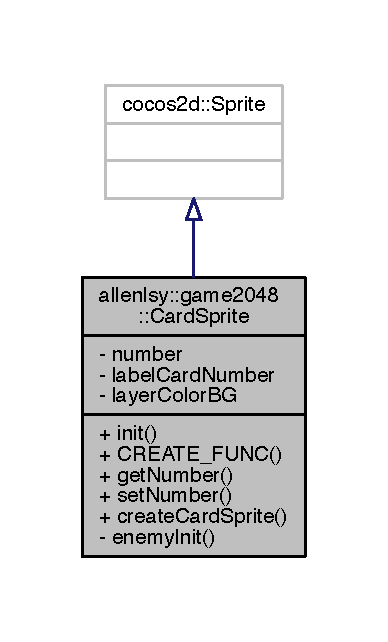
\includegraphics[width=186pt]{df/d6a/classallenlsy_1_1game2048_1_1_card_sprite__inherit__graph}
\end{center}
\end{figure}


allenlsy\+:\+:game2048\+:\+:Card\+Sprite에 대한 협력 다이어그램\+:
\nopagebreak
\begin{figure}[H]
\begin{center}
\leavevmode
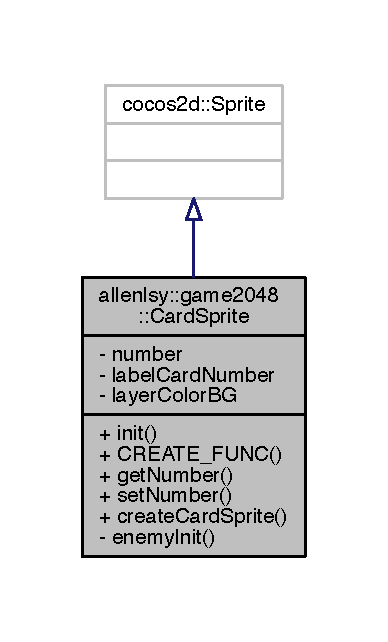
\includegraphics[width=186pt]{d0/dbf/classallenlsy_1_1game2048_1_1_card_sprite__coll__graph}
\end{center}
\end{figure}
\subsection*{Public 멤버 함수}
\begin{DoxyCompactItemize}
\item 
virtual bool \hyperlink{classallenlsy_1_1game2048_1_1_card_sprite_ad6769d950c3b9b87092bd7e40d61dd4d}{init} ()
\item 
\hyperlink{classallenlsy_1_1game2048_1_1_card_sprite_acb47a7c82b77019fab80d7d167495c57}{C\+R\+E\+A\+T\+E\+\_\+\+F\+U\+NC} (\hyperlink{classallenlsy_1_1game2048_1_1_card_sprite}{Card\+Sprite})
\item 
int \hyperlink{classallenlsy_1_1game2048_1_1_card_sprite_ac483e81f56c1c7d08a83175061c8edb5}{get\+Number} ()
\item 
void \hyperlink{classallenlsy_1_1game2048_1_1_card_sprite_a7f560bb8253477188273aac709aae087}{set\+Number} (int num)
\end{DoxyCompactItemize}
\subsection*{정적 Public 멤버 함수}
\begin{DoxyCompactItemize}
\item 
static \hyperlink{classallenlsy_1_1game2048_1_1_card_sprite}{Card\+Sprite} $\ast$ \hyperlink{classallenlsy_1_1game2048_1_1_card_sprite_a3a14745470040dfb933397ccb83344d7}{create\+Card\+Sprite} (int numbers, int width, int height, float Card\+SpriteX, float Card\+SpriteY)
\end{DoxyCompactItemize}
\subsection*{Private 멤버 함수}
\begin{DoxyCompactItemize}
\item 
void \hyperlink{classallenlsy_1_1game2048_1_1_card_sprite_afdf6cfc4ce73b460a30791de269f7f69}{enemy\+Init} (int numbers, int width, int height, float Card\+SpriteX, float Card\+SpriteY)
\end{DoxyCompactItemize}
\subsection*{Private 속성}
\begin{DoxyCompactItemize}
\item 
int \hyperlink{classallenlsy_1_1game2048_1_1_card_sprite_ad792455a70c4dee8eaf5da553be6f88e}{number}
\item 
cocos2d\+::\+Label\+T\+TF $\ast$ \hyperlink{classallenlsy_1_1game2048_1_1_card_sprite_a9f89b7ca888b5c38fb04776c233cd6aa}{label\+Card\+Number} =N\+U\+LL
\item 
cocos2d\+::\+Layer\+Color $\ast$ \hyperlink{classallenlsy_1_1game2048_1_1_card_sprite_a584c629ff6b2e403fd2393e6edf4e840}{layer\+Color\+BG} =N\+U\+LL
\end{DoxyCompactItemize}


\subsection{상세한 설명}


Card\+Spite.\+hpp 파일의 11 번째 라인에서 정의되었습니다.



\subsection{멤버 함수 문서화}
\mbox{\Hypertarget{classallenlsy_1_1game2048_1_1_card_sprite_acb47a7c82b77019fab80d7d167495c57}\label{classallenlsy_1_1game2048_1_1_card_sprite_acb47a7c82b77019fab80d7d167495c57}} 
\index{allenlsy\+::game2048\+::\+Card\+Sprite@{allenlsy\+::game2048\+::\+Card\+Sprite}!C\+R\+E\+A\+T\+E\+\_\+\+F\+U\+NC@{C\+R\+E\+A\+T\+E\+\_\+\+F\+U\+NC}}
\index{C\+R\+E\+A\+T\+E\+\_\+\+F\+U\+NC@{C\+R\+E\+A\+T\+E\+\_\+\+F\+U\+NC}!allenlsy\+::game2048\+::\+Card\+Sprite@{allenlsy\+::game2048\+::\+Card\+Sprite}}
\subsubsection{\texorpdfstring{C\+R\+E\+A\+T\+E\+\_\+\+F\+U\+N\+C()}{CREATE\_FUNC()}}
{\footnotesize\ttfamily allenlsy\+::game2048\+::\+Card\+Sprite\+::\+C\+R\+E\+A\+T\+E\+\_\+\+F\+U\+NC (\begin{DoxyParamCaption}\item[{\hyperlink{classallenlsy_1_1game2048_1_1_card_sprite}{Card\+Sprite}}]{ }\end{DoxyParamCaption})}

\mbox{\Hypertarget{classallenlsy_1_1game2048_1_1_card_sprite_a3a14745470040dfb933397ccb83344d7}\label{classallenlsy_1_1game2048_1_1_card_sprite_a3a14745470040dfb933397ccb83344d7}} 
\index{allenlsy\+::game2048\+::\+Card\+Sprite@{allenlsy\+::game2048\+::\+Card\+Sprite}!create\+Card\+Sprite@{create\+Card\+Sprite}}
\index{create\+Card\+Sprite@{create\+Card\+Sprite}!allenlsy\+::game2048\+::\+Card\+Sprite@{allenlsy\+::game2048\+::\+Card\+Sprite}}
\subsubsection{\texorpdfstring{create\+Card\+Sprite()}{createCardSprite()}}
{\footnotesize\ttfamily static \hyperlink{classallenlsy_1_1game2048_1_1_card_sprite}{Card\+Sprite}$\ast$ allenlsy\+::game2048\+::\+Card\+Sprite\+::create\+Card\+Sprite (\begin{DoxyParamCaption}\item[{int}]{numbers,  }\item[{int}]{width,  }\item[{int}]{height,  }\item[{float}]{Card\+SpriteX,  }\item[{float}]{Card\+SpriteY }\end{DoxyParamCaption})\hspace{0.3cm}{\ttfamily [inline]}, {\ttfamily [static]}}



Card\+Spite.\+hpp 파일의 13 번째 라인에서 정의되었습니다.


\begin{DoxyCode}
13                                                                                                            
            \{
14         CardSprite*enemy = \textcolor{keyword}{new} CardSprite();
15     \textcolor{keywordflow}{if} (enemy && enemy->init()) \{
16         enemy->enemyInit(numbers, width, height, CardSpriteX, CardSpriteY);
17 
18         \textcolor{keywordflow}{return} enemy;
19 
20     \}
21 
22     CC\_SAFE\_DELETE(enemy); \textcolor{comment}{// MYNOTE: CC\_SAFE\_DELETE: do \{ delete (p); (p) = nullptr; \} while(0)}
23     \textcolor{keywordflow}{return} NULL;
24     \}
\end{DoxyCode}
이 함수 내부에서 호출하는 함수들에 대한 그래프입니다.\+:
\nopagebreak
\begin{figure}[H]
\begin{center}
\leavevmode
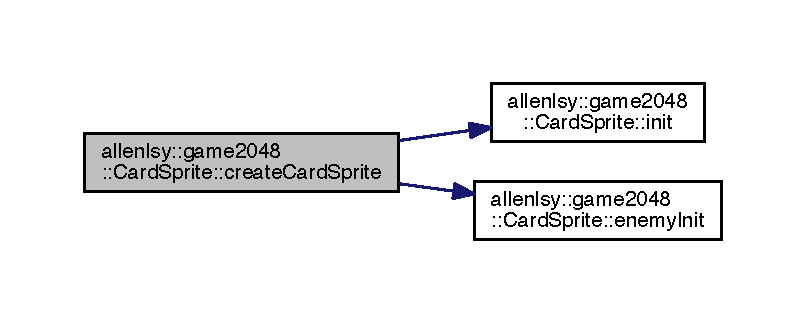
\includegraphics[width=350pt]{d9/d22/classallenlsy_1_1game2048_1_1_card_sprite_a3a14745470040dfb933397ccb83344d7_cgraph}
\end{center}
\end{figure}
이 함수를 호출하는 함수들에 대한 그래프입니다.\+:
\nopagebreak
\begin{figure}[H]
\begin{center}
\leavevmode
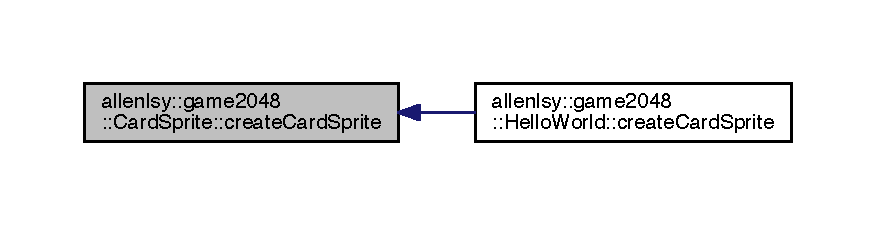
\includegraphics[width=350pt]{d9/d22/classallenlsy_1_1game2048_1_1_card_sprite_a3a14745470040dfb933397ccb83344d7_icgraph}
\end{center}
\end{figure}
\mbox{\Hypertarget{classallenlsy_1_1game2048_1_1_card_sprite_afdf6cfc4ce73b460a30791de269f7f69}\label{classallenlsy_1_1game2048_1_1_card_sprite_afdf6cfc4ce73b460a30791de269f7f69}} 
\index{allenlsy\+::game2048\+::\+Card\+Sprite@{allenlsy\+::game2048\+::\+Card\+Sprite}!enemy\+Init@{enemy\+Init}}
\index{enemy\+Init@{enemy\+Init}!allenlsy\+::game2048\+::\+Card\+Sprite@{allenlsy\+::game2048\+::\+Card\+Sprite}}
\subsubsection{\texorpdfstring{enemy\+Init()}{enemyInit()}}
{\footnotesize\ttfamily void allenlsy\+::game2048\+::\+Card\+Sprite\+::enemy\+Init (\begin{DoxyParamCaption}\item[{int}]{numbers,  }\item[{int}]{width,  }\item[{int}]{height,  }\item[{float}]{Card\+SpriteX,  }\item[{float}]{Card\+SpriteY }\end{DoxyParamCaption})\hspace{0.3cm}{\ttfamily [inline]}, {\ttfamily [private]}}



Card\+Spite.\+hpp 파일의 105 번째 라인에서 정의되었습니다.


\begin{DoxyCode}
105                                                                                             \{
106         \hyperlink{classallenlsy_1_1game2048_1_1_card_sprite_ad792455a70c4dee8eaf5da553be6f88e}{number} = numbers;
107 
108     \textcolor{comment}{//加入游戏的背景颜色}
109     \textcolor{keyword}{auto} \hyperlink{classallenlsy_1_1game2048_1_1_card_sprite_a584c629ff6b2e403fd2393e6edf4e840}{layerColorBG} = LayerColor::create(Color4B(200, 190, 180, 255), width - 15, height - 15
      );
110     \hyperlink{classallenlsy_1_1game2048_1_1_card_sprite_a584c629ff6b2e403fd2393e6edf4e840}{layerColorBG}->setPosition(CardSpriteX, CardSpriteY);
111 
112     \textcolor{comment}{//判断如果大于0就显示,否则显示空}
113     \textcolor{keywordflow}{if} (numbers > 0)
114     \{
115         \textcolor{comment}{//加入中间字体}
116         \hyperlink{classallenlsy_1_1game2048_1_1_card_sprite_a9f89b7ca888b5c38fb04776c233cd6aa}{labelCardNumber} = LabelTTF::create(String::createWithFormat(\textcolor{stringliteral}{"%i"}, numbers)->
      getCString(), \textcolor{stringliteral}{"fonts/arial.ttf"}, \hyperlink{_card_spite_8hpp_aa968a61524f9ed159c4c5464cb26dd41}{FONT\_SIZE});
117         \hyperlink{classallenlsy_1_1game2048_1_1_card_sprite_a9f89b7ca888b5c38fb04776c233cd6aa}{labelCardNumber}->setPosition(\hyperlink{classallenlsy_1_1game2048_1_1_card_sprite_a584c629ff6b2e403fd2393e6edf4e840}{layerColorBG}->getContentSize().width/2, 
      \hyperlink{classallenlsy_1_1game2048_1_1_card_sprite_a584c629ff6b2e403fd2393e6edf4e840}{layerColorBG}->getContentSize().height/2);
118         \hyperlink{classallenlsy_1_1game2048_1_1_card_sprite_a9f89b7ca888b5c38fb04776c233cd6aa}{labelCardNumber}->setTag(8);
119         \hyperlink{classallenlsy_1_1game2048_1_1_card_sprite_a584c629ff6b2e403fd2393e6edf4e840}{layerColorBG}->addChild(\hyperlink{classallenlsy_1_1game2048_1_1_card_sprite_a9f89b7ca888b5c38fb04776c233cd6aa}{labelCardNumber});
120     \} \textcolor{keywordflow}{else} \{
121         \hyperlink{classallenlsy_1_1game2048_1_1_card_sprite_a9f89b7ca888b5c38fb04776c233cd6aa}{labelCardNumber} = LabelTTF::create(\textcolor{stringliteral}{""}, \textcolor{stringliteral}{"fonts/arial.ttf"}, 
      \hyperlink{_card_spite_8hpp_aa968a61524f9ed159c4c5464cb26dd41}{FONT\_SIZE});
122         \hyperlink{classallenlsy_1_1game2048_1_1_card_sprite_a9f89b7ca888b5c38fb04776c233cd6aa}{labelCardNumber}->setPosition(\hyperlink{classallenlsy_1_1game2048_1_1_card_sprite_a584c629ff6b2e403fd2393e6edf4e840}{layerColorBG}->getContentSize().width/2, 
      \hyperlink{classallenlsy_1_1game2048_1_1_card_sprite_a584c629ff6b2e403fd2393e6edf4e840}{layerColorBG}->getContentSize().height/2);
123         \hyperlink{classallenlsy_1_1game2048_1_1_card_sprite_a9f89b7ca888b5c38fb04776c233cd6aa}{labelCardNumber}->setTag(8);
124         \hyperlink{classallenlsy_1_1game2048_1_1_card_sprite_a584c629ff6b2e403fd2393e6edf4e840}{layerColorBG}->addChild(\hyperlink{classallenlsy_1_1game2048_1_1_card_sprite_a9f89b7ca888b5c38fb04776c233cd6aa}{labelCardNumber});
125     \}
126 
127     this->addChild(\hyperlink{classallenlsy_1_1game2048_1_1_card_sprite_a584c629ff6b2e403fd2393e6edf4e840}{layerColorBG});
128     \}
\end{DoxyCode}
이 함수를 호출하는 함수들에 대한 그래프입니다.\+:
\nopagebreak
\begin{figure}[H]
\begin{center}
\leavevmode
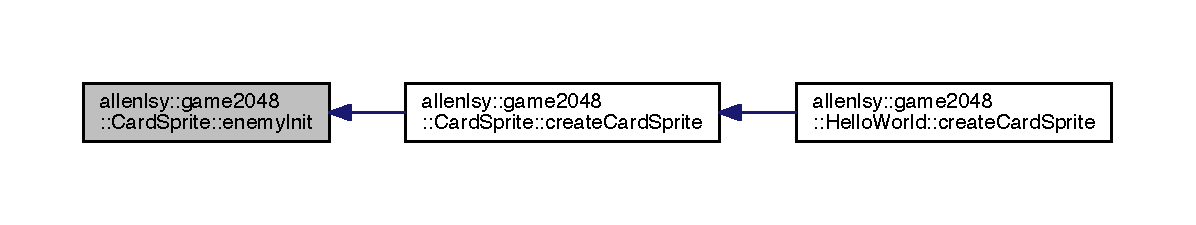
\includegraphics[width=350pt]{d9/d22/classallenlsy_1_1game2048_1_1_card_sprite_afdf6cfc4ce73b460a30791de269f7f69_icgraph}
\end{center}
\end{figure}
\mbox{\Hypertarget{classallenlsy_1_1game2048_1_1_card_sprite_ac483e81f56c1c7d08a83175061c8edb5}\label{classallenlsy_1_1game2048_1_1_card_sprite_ac483e81f56c1c7d08a83175061c8edb5}} 
\index{allenlsy\+::game2048\+::\+Card\+Sprite@{allenlsy\+::game2048\+::\+Card\+Sprite}!get\+Number@{get\+Number}}
\index{get\+Number@{get\+Number}!allenlsy\+::game2048\+::\+Card\+Sprite@{allenlsy\+::game2048\+::\+Card\+Sprite}}
\subsubsection{\texorpdfstring{get\+Number()}{getNumber()}}
{\footnotesize\ttfamily int allenlsy\+::game2048\+::\+Card\+Sprite\+::get\+Number (\begin{DoxyParamCaption}{ }\end{DoxyParamCaption})\hspace{0.3cm}{\ttfamily [inline]}}



Card\+Spite.\+hpp 파일의 35 번째 라인에서 정의되었습니다.


\begin{DoxyCode}
35                    \{
36     \textcolor{keywordflow}{return} \hyperlink{classallenlsy_1_1game2048_1_1_card_sprite_ad792455a70c4dee8eaf5da553be6f88e}{number};
37 \}
\end{DoxyCode}
\mbox{\Hypertarget{classallenlsy_1_1game2048_1_1_card_sprite_ad6769d950c3b9b87092bd7e40d61dd4d}\label{classallenlsy_1_1game2048_1_1_card_sprite_ad6769d950c3b9b87092bd7e40d61dd4d}} 
\index{allenlsy\+::game2048\+::\+Card\+Sprite@{allenlsy\+::game2048\+::\+Card\+Sprite}!init@{init}}
\index{init@{init}!allenlsy\+::game2048\+::\+Card\+Sprite@{allenlsy\+::game2048\+::\+Card\+Sprite}}
\subsubsection{\texorpdfstring{init()}{init()}}
{\footnotesize\ttfamily virtual bool allenlsy\+::game2048\+::\+Card\+Sprite\+::init (\begin{DoxyParamCaption}{ }\end{DoxyParamCaption})\hspace{0.3cm}{\ttfamily [inline]}, {\ttfamily [virtual]}}



Card\+Spite.\+hpp 파일의 25 번째 라인에서 정의되었습니다.


\begin{DoxyCode}
25                        \{
26         \textcolor{keywordflow}{if} (!Sprite::init()) \{
27         \textcolor{keywordflow}{return} \textcolor{keyword}{false};
28     \}
29 
30     \textcolor{keywordflow}{return} \textcolor{keyword}{true};
31     \}
\end{DoxyCode}
이 함수를 호출하는 함수들에 대한 그래프입니다.\+:
\nopagebreak
\begin{figure}[H]
\begin{center}
\leavevmode
\includegraphics[width=350pt]{d9/d22/classallenlsy_1_1game2048_1_1_card_sprite_ad6769d950c3b9b87092bd7e40d61dd4d_icgraph}
\end{center}
\end{figure}
\mbox{\Hypertarget{classallenlsy_1_1game2048_1_1_card_sprite_a7f560bb8253477188273aac709aae087}\label{classallenlsy_1_1game2048_1_1_card_sprite_a7f560bb8253477188273aac709aae087}} 
\index{allenlsy\+::game2048\+::\+Card\+Sprite@{allenlsy\+::game2048\+::\+Card\+Sprite}!set\+Number@{set\+Number}}
\index{set\+Number@{set\+Number}!allenlsy\+::game2048\+::\+Card\+Sprite@{allenlsy\+::game2048\+::\+Card\+Sprite}}
\subsubsection{\texorpdfstring{set\+Number()}{setNumber()}}
{\footnotesize\ttfamily void allenlsy\+::game2048\+::\+Card\+Sprite\+::set\+Number (\begin{DoxyParamCaption}\item[{int}]{num }\end{DoxyParamCaption})\hspace{0.3cm}{\ttfamily [inline]}}



Card\+Spite.\+hpp 파일의 38 번째 라인에서 정의되었습니다.


\begin{DoxyCode}
38                            \{
39     this->\hyperlink{classallenlsy_1_1game2048_1_1_card_sprite_ad792455a70c4dee8eaf5da553be6f88e}{number} = num;
40 
41     \textcolor{keywordflow}{if} (\hyperlink{classallenlsy_1_1game2048_1_1_card_sprite_ad792455a70c4dee8eaf5da553be6f88e}{number} > 0) \{
42         \hyperlink{classallenlsy_1_1game2048_1_1_card_sprite_a9f89b7ca888b5c38fb04776c233cd6aa}{labelCardNumber}->setString(String::createWithFormat(\textcolor{stringliteral}{"%i"}, 
      \hyperlink{classallenlsy_1_1game2048_1_1_card_sprite_ad792455a70c4dee8eaf5da553be6f88e}{number})->getCString());
43     \} \textcolor{keywordflow}{else} \{
44         \hyperlink{classallenlsy_1_1game2048_1_1_card_sprite_a9f89b7ca888b5c38fb04776c233cd6aa}{labelCardNumber}->setString(\textcolor{stringliteral}{""});
45     \}
46 
47     \textcolor{comment}{//判断数字的大小来调整字体}
48     \textcolor{keywordflow}{if} (\hyperlink{classallenlsy_1_1game2048_1_1_card_sprite_ad792455a70c4dee8eaf5da553be6f88e}{number} >= 0) \{
49         \hyperlink{classallenlsy_1_1game2048_1_1_card_sprite_a9f89b7ca888b5c38fb04776c233cd6aa}{labelCardNumber}->setFontSize(100);
50     \}
51     \textcolor{keywordflow}{if} (\hyperlink{classallenlsy_1_1game2048_1_1_card_sprite_ad792455a70c4dee8eaf5da553be6f88e}{number} >= 16) \{
52         \hyperlink{classallenlsy_1_1game2048_1_1_card_sprite_a9f89b7ca888b5c38fb04776c233cd6aa}{labelCardNumber}->setFontSize(90);
53     \}
54     \textcolor{keywordflow}{if}(\hyperlink{classallenlsy_1_1game2048_1_1_card_sprite_ad792455a70c4dee8eaf5da553be6f88e}{number} >= 128)\{
55         \hyperlink{classallenlsy_1_1game2048_1_1_card_sprite_a9f89b7ca888b5c38fb04776c233cd6aa}{labelCardNumber}->setFontSize(60);
56     \}
57     \textcolor{keywordflow}{if}(\hyperlink{classallenlsy_1_1game2048_1_1_card_sprite_ad792455a70c4dee8eaf5da553be6f88e}{number} >= 1024)\{
58         \hyperlink{classallenlsy_1_1game2048_1_1_card_sprite_a9f89b7ca888b5c38fb04776c233cd6aa}{labelCardNumber}->setFontSize(40);
59     \}
60 
61         \hyperlink{classallenlsy_1_1game2048_1_1_card_sprite_a9f89b7ca888b5c38fb04776c233cd6aa}{labelCardNumber}->setScale(0.5f, 0.5f);
62     \textcolor{comment}{//判断数字的大小来调整颜色}
63         \textcolor{comment}{//cout<<"start coloring"<<endl;}
64     \textcolor{comment}{//if(number == 0)\{}
65     \textcolor{comment}{//    layerColorBG->setColor(cocos2d::Color3B(200,190,180));}
66    \textcolor{comment}{// \}}
67         \textcolor{comment}{//cout<<"finish coloring"<<endl;}
68 \textcolor{comment}{//    if (number == 2) \{}
69 \textcolor{comment}{//        layerColorBG->setColor(cocos2d::Color3B(240,230,220));}
70 \textcolor{comment}{//    \}}
71 \textcolor{comment}{//    if (number == 4) \{}
72 \textcolor{comment}{//        layerColorBG->setColor(cocos2d::Color3B(240,220,200));}
73  \textcolor{comment}{//   \}}
74 \textcolor{comment}{//    if (number == 8) \{}
75 \textcolor{comment}{//        layerColorBG->setColor(cocos2d::Color3B(240,180,120));}
76 \textcolor{comment}{//    \}}
77 \textcolor{comment}{//    if (number == 16) \{}
78 \textcolor{comment}{//        layerColorBG->setColor(cocos2d::Color3B(240,140,90));}
79 \textcolor{comment}{//    \}}
80 \textcolor{comment}{//    if (number == 32) \{}
81 \textcolor{comment}{//        layerColorBG->setColor(cocos2d::Color3B(240,120,90));}
82 \textcolor{comment}{//    \}}
83 \textcolor{comment}{//    if (number == 64) \{}
84 \textcolor{comment}{//        layerColorBG->setColor(cocos2d::Color3B(240,90,60));}
85 \textcolor{comment}{//    \}}
86 \textcolor{comment}{//    if (number == 128) \{}
87 \textcolor{comment}{//        layerColorBG->setColor(cocos2d::Color3B(240,90,60));}
88 \textcolor{comment}{//    \}}
89 \textcolor{comment}{//    if (number == 256) \{}
90 \textcolor{comment}{//        layerColorBG->setColor(cocos2d::Color3B(240,200,70));}
91 \textcolor{comment}{//    \}}
92 \textcolor{comment}{//    if (number == 512) \{}
93 \textcolor{comment}{//        layerColorBG->setColor(cocos2d::Color3B(240,200,70));}
94 \textcolor{comment}{//    \}}
95 \textcolor{comment}{//    if (number == 1024) \{}
96 \textcolor{comment}{//        layerColorBG->setColor(cocos2d::Color3B(0,130,0));}
97 \textcolor{comment}{//    \}}
98 \textcolor{comment}{//    if (number == 2048) \{}
99 \textcolor{comment}{//        layerColorBG->setColor(cocos2d::Color3B(0,130,0));}
100 \textcolor{comment}{//    \}}
101 \}
\end{DoxyCode}


\subsection{필드 문서화}
\mbox{\Hypertarget{classallenlsy_1_1game2048_1_1_card_sprite_a9f89b7ca888b5c38fb04776c233cd6aa}\label{classallenlsy_1_1game2048_1_1_card_sprite_a9f89b7ca888b5c38fb04776c233cd6aa}} 
\index{allenlsy\+::game2048\+::\+Card\+Sprite@{allenlsy\+::game2048\+::\+Card\+Sprite}!label\+Card\+Number@{label\+Card\+Number}}
\index{label\+Card\+Number@{label\+Card\+Number}!allenlsy\+::game2048\+::\+Card\+Sprite@{allenlsy\+::game2048\+::\+Card\+Sprite}}
\subsubsection{\texorpdfstring{label\+Card\+Number}{labelCardNumber}}
{\footnotesize\ttfamily cocos2d\+::\+Label\+T\+TF$\ast$ allenlsy\+::game2048\+::\+Card\+Sprite\+::label\+Card\+Number =N\+U\+LL\hspace{0.3cm}{\ttfamily [private]}}



Card\+Spite.\+hpp 파일의 130 번째 라인에서 정의되었습니다.

\mbox{\Hypertarget{classallenlsy_1_1game2048_1_1_card_sprite_a584c629ff6b2e403fd2393e6edf4e840}\label{classallenlsy_1_1game2048_1_1_card_sprite_a584c629ff6b2e403fd2393e6edf4e840}} 
\index{allenlsy\+::game2048\+::\+Card\+Sprite@{allenlsy\+::game2048\+::\+Card\+Sprite}!layer\+Color\+BG@{layer\+Color\+BG}}
\index{layer\+Color\+BG@{layer\+Color\+BG}!allenlsy\+::game2048\+::\+Card\+Sprite@{allenlsy\+::game2048\+::\+Card\+Sprite}}
\subsubsection{\texorpdfstring{layer\+Color\+BG}{layerColorBG}}
{\footnotesize\ttfamily cocos2d\+::\+Layer\+Color$\ast$ allenlsy\+::game2048\+::\+Card\+Sprite\+::layer\+Color\+BG =N\+U\+LL\hspace{0.3cm}{\ttfamily [private]}}



Card\+Spite.\+hpp 파일의 132 번째 라인에서 정의되었습니다.

\mbox{\Hypertarget{classallenlsy_1_1game2048_1_1_card_sprite_ad792455a70c4dee8eaf5da553be6f88e}\label{classallenlsy_1_1game2048_1_1_card_sprite_ad792455a70c4dee8eaf5da553be6f88e}} 
\index{allenlsy\+::game2048\+::\+Card\+Sprite@{allenlsy\+::game2048\+::\+Card\+Sprite}!number@{number}}
\index{number@{number}!allenlsy\+::game2048\+::\+Card\+Sprite@{allenlsy\+::game2048\+::\+Card\+Sprite}}
\subsubsection{\texorpdfstring{number}{number}}
{\footnotesize\ttfamily int allenlsy\+::game2048\+::\+Card\+Sprite\+::number\hspace{0.3cm}{\ttfamily [private]}}



Card\+Spite.\+hpp 파일의 104 번째 라인에서 정의되었습니다.



이 클래스에 대한 문서화 페이지는 다음의 파일로부터 생성되었습니다.\+:\begin{DoxyCompactItemize}
\item 
Classes/externalgames/allenlsy/2048-\/cocos2dx/\+Classes/\hyperlink{_card_spite_8hpp}{Card\+Spite.\+hpp}\end{DoxyCompactItemize}

\hypertarget{class_tetris_1_1_d_b_management_1_1_d_b_manager}{}\section{Tetris\+:\+:D\+B\+Management\+:\+:D\+B\+Manager 클래스 참조}
\label{class_tetris_1_1_d_b_management_1_1_d_b_manager}\index{Tetris\+::\+D\+B\+Management\+::\+D\+B\+Manager@{Tetris\+::\+D\+B\+Management\+::\+D\+B\+Manager}}


sqlite3를 통한 db통신  




{\ttfamily \#include $<$D\+B\+Management.\+hpp$>$}



Tetris\+:\+:D\+B\+Management\+:\+:D\+B\+Manager에 대한 협력 다이어그램\+:
\nopagebreak
\begin{figure}[H]
\begin{center}
\leavevmode
\includegraphics[width=242pt]{d2/d52/class_tetris_1_1_d_b_management_1_1_d_b_manager__coll__graph}
\end{center}
\end{figure}
\subsection*{Public 멤버 함수}
\begin{DoxyCompactItemize}
\item 
\hyperlink{class_tetris_1_1_d_b_management_1_1_d_b_manager_a8271c37f255a2e2bc85a3e1896a32c43}{D\+B\+Manager} ()
\item 
\hyperlink{class_tetris_1_1_d_b_management_1_1_d_b_manager_ac22f39981d5c862ad17b7420e313f1b2}{$\sim$\+D\+B\+Manager} ()
\item 
void \hyperlink{class_tetris_1_1_d_b_management_1_1_d_b_manager_a8bf7e756a9cca7e57fef00076fb62f36}{open} (char $\ast$fname)
\item 
void \hyperlink{class_tetris_1_1_d_b_management_1_1_d_b_manager_a8390e6ddf3fa06e90fa5c2ab4997e5c1}{close} ()
\item 
bool \hyperlink{class_tetris_1_1_d_b_management_1_1_d_b_manager_a16460066d64c9183a63194177bb0458e}{is\+Opened} ()
\item 
bool \hyperlink{class_tetris_1_1_d_b_management_1_1_d_b_manager_a62043d50855f42b69b057527b14dec0f}{is\+Connected} ()
\item 
void \hyperlink{class_tetris_1_1_d_b_management_1_1_d_b_manager_aef16da1d2e564caa309bfc3b3e419d7e}{save\+Score} (unsigned long long score, unsigned long long playtime)
\item 
queue$<$ struct \hyperlink{struct_tetris_1_1_d_b_management_1_1_score_board_attributes}{Score\+Board\+Attributes} $>$ \hyperlink{class_tetris_1_1_d_b_management_1_1_d_b_manager_aa67ef286408b2631e15e9f8f41937c97}{get\+Score\+Board} ()
\item 
bool \hyperlink{class_tetris_1_1_d_b_management_1_1_d_b_manager_aa80722572c33389c1c73f88de9f199b6}{is\+Exist\+App\+Setting} (string key)
\item 
bool \hyperlink{class_tetris_1_1_d_b_management_1_1_d_b_manager_a598b8014fcad434b5b1162cc6767d22c}{read\+App\+Setting\+As\+Bool} (string key)
\item 
int \hyperlink{class_tetris_1_1_d_b_management_1_1_d_b_manager_ac52daf6ea2310b848278454c30698436}{read\+App\+Setting\+As\+Int} (string key)
\item 
string \hyperlink{class_tetris_1_1_d_b_management_1_1_d_b_manager_acb213c517f06d1eadafd45a86b91c2ff}{read\+App\+Setting\+As\+Text} (string key)
\item 
bool \hyperlink{class_tetris_1_1_d_b_management_1_1_d_b_manager_aead8bb3f2a64fdf6ac59c69bfd21a01e}{change\+Int\+Setting} (string key, int value)
\item 
bool \hyperlink{class_tetris_1_1_d_b_management_1_1_d_b_manager_aece3390d5f2edca3f86316b903870c92}{change\+Bool\+Setting} (string key, bool value)
\end{DoxyCompactItemize}
\subsection*{정적 Public 멤버 함수}
\begin{DoxyCompactItemize}
\item 
static \hyperlink{class_tetris_1_1_d_b_management_1_1_d_b_manager}{D\+B\+Manager} $\ast$ \hyperlink{class_tetris_1_1_d_b_management_1_1_d_b_manager_a9cb81505055490211a9b5c79c3c22c18}{get\+Instance} ()
\item 
static string \hyperlink{class_tetris_1_1_d_b_management_1_1_d_b_manager_ae50cfd222e276a5ca27e17c886aa5dd5}{get\+D\+B\+Location\+For\+Tetris\+Game} ()
\item 
static char $\ast$ \hyperlink{class_tetris_1_1_d_b_management_1_1_d_b_manager_a5d49e7fac7d2a65973151a7fb81ea560}{get\+D\+B\+File\+Name} ()
\item 
static string \hyperlink{class_tetris_1_1_d_b_management_1_1_d_b_manager_ae8c98091466565c4c70971e6b7a42ce6}{get\+Sound\+Enabler\+Key} ()
\end{DoxyCompactItemize}
\subsection*{Private 멤버 함수}
\begin{DoxyCompactItemize}
\item 
void \hyperlink{class_tetris_1_1_d_b_management_1_1_d_b_manager_afa17031e7f2bf8c61073bc79442bacfd}{init\+Val} ()
\item 
void \hyperlink{class_tetris_1_1_d_b_management_1_1_d_b_manager_a6b723e555cef747b7402661eb960bd78}{logdberr} (string functioncategory)
\item 
void \hyperlink{class_tetris_1_1_d_b_management_1_1_d_b_manager_a07a391f97339bacd983f2598dd7a3ade}{init\+Table} ()
\item 
void \hyperlink{class_tetris_1_1_d_b_management_1_1_d_b_manager_a08f9bdc18cc015a7746e47c37eba613c}{init\+App\+Setting\+Values\+If\+Not\+Exist} ()
\end{DoxyCompactItemize}
\subsection*{Private 속성}
\begin{DoxyCompactItemize}
\item 
\hyperlink{sqlite3_8h_a0ef6f2646262c8a9b24368d8ac140f69}{sqlite3} $\ast$ \hyperlink{class_tetris_1_1_d_b_management_1_1_d_b_manager_acc2c19420c2b1b1b2c1e724b3a8ec4b7}{conn} = N\+U\+LL
\begin{DoxyCompactList}\small\item\em sqlite통신객체 \end{DoxyCompactList}\item 
\hyperlink{sqlite3_8h_af2a033da1327cdd77f0a174a09aedd0c}{sqlite3\+\_\+stmt} $\ast$ \hyperlink{class_tetris_1_1_d_b_management_1_1_d_b_manager_af161e9c2d2f9dea602bea867542deedb}{res} = N\+U\+LL
\item 
int \hyperlink{class_tetris_1_1_d_b_management_1_1_d_b_manager_a9ea8d963f1a9b8117fa5e92b54eda114}{err} = 0
\end{DoxyCompactItemize}


\subsection{상세한 설명}
sqlite3를 통한 db통신 

D\+B\+Management.\+hpp 파일의 23 번째 라인에서 정의되었습니다.



\subsection{생성자 \& 소멸자 문서화}
\mbox{\Hypertarget{class_tetris_1_1_d_b_management_1_1_d_b_manager_a8271c37f255a2e2bc85a3e1896a32c43}\label{class_tetris_1_1_d_b_management_1_1_d_b_manager_a8271c37f255a2e2bc85a3e1896a32c43}} 
\index{Tetris\+::\+D\+B\+Management\+::\+D\+B\+Manager@{Tetris\+::\+D\+B\+Management\+::\+D\+B\+Manager}!D\+B\+Manager@{D\+B\+Manager}}
\index{D\+B\+Manager@{D\+B\+Manager}!Tetris\+::\+D\+B\+Management\+::\+D\+B\+Manager@{Tetris\+::\+D\+B\+Management\+::\+D\+B\+Manager}}
\subsubsection{\texorpdfstring{D\+B\+Manager()}{DBManager()}}
{\footnotesize\ttfamily Tetris\+::\+D\+B\+Management\+::\+D\+B\+Manager\+::\+D\+B\+Manager (\begin{DoxyParamCaption}{ }\end{DoxyParamCaption})\hspace{0.3cm}{\ttfamily [inline]}}



D\+B\+Management.\+hpp 파일의 29 번째 라인에서 정의되었습니다.


\begin{DoxyCode}
29                        \{
30                 \hyperlink{class_tetris_1_1_d_b_management_1_1_d_b_manager_afa17031e7f2bf8c61073bc79442bacfd}{initVal}();
31                 \textcolor{comment}{//open(getDBFileName());}
32                 \textcolor{comment}{//initTable();}
33             \}
\end{DoxyCode}
\mbox{\Hypertarget{class_tetris_1_1_d_b_management_1_1_d_b_manager_ac22f39981d5c862ad17b7420e313f1b2}\label{class_tetris_1_1_d_b_management_1_1_d_b_manager_ac22f39981d5c862ad17b7420e313f1b2}} 
\index{Tetris\+::\+D\+B\+Management\+::\+D\+B\+Manager@{Tetris\+::\+D\+B\+Management\+::\+D\+B\+Manager}!````~D\+B\+Manager@{$\sim$\+D\+B\+Manager}}
\index{````~D\+B\+Manager@{$\sim$\+D\+B\+Manager}!Tetris\+::\+D\+B\+Management\+::\+D\+B\+Manager@{Tetris\+::\+D\+B\+Management\+::\+D\+B\+Manager}}
\subsubsection{\texorpdfstring{$\sim$\+D\+B\+Manager()}{~DBManager()}}
{\footnotesize\ttfamily Tetris\+::\+D\+B\+Management\+::\+D\+B\+Manager\+::$\sim$\+D\+B\+Manager (\begin{DoxyParamCaption}{ }\end{DoxyParamCaption})\hspace{0.3cm}{\ttfamily [inline]}}



D\+B\+Management.\+hpp 파일의 34 번째 라인에서 정의되었습니다.


\begin{DoxyCode}
34                         \{
35                 \hyperlink{class_tetris_1_1_d_b_management_1_1_d_b_manager_a8390e6ddf3fa06e90fa5c2ab4997e5c1}{close}();
36             \}
\end{DoxyCode}


\subsection{멤버 함수 문서화}
\mbox{\Hypertarget{class_tetris_1_1_d_b_management_1_1_d_b_manager_aece3390d5f2edca3f86316b903870c92}\label{class_tetris_1_1_d_b_management_1_1_d_b_manager_aece3390d5f2edca3f86316b903870c92}} 
\index{Tetris\+::\+D\+B\+Management\+::\+D\+B\+Manager@{Tetris\+::\+D\+B\+Management\+::\+D\+B\+Manager}!change\+Bool\+Setting@{change\+Bool\+Setting}}
\index{change\+Bool\+Setting@{change\+Bool\+Setting}!Tetris\+::\+D\+B\+Management\+::\+D\+B\+Manager@{Tetris\+::\+D\+B\+Management\+::\+D\+B\+Manager}}
\subsubsection{\texorpdfstring{change\+Bool\+Setting()}{changeBoolSetting()}}
{\footnotesize\ttfamily bool Tetris\+::\+D\+B\+Management\+::\+D\+B\+Manager\+::change\+Bool\+Setting (\begin{DoxyParamCaption}\item[{string}]{key,  }\item[{bool}]{value }\end{DoxyParamCaption})\hspace{0.3cm}{\ttfamily [inline]}}



D\+B\+Management.\+hpp 파일의 292 번째 라인에서 정의되었습니다.


\begin{DoxyCode}
292                                                          \{
293                 \textcolor{keywordflow}{return} \hyperlink{class_tetris_1_1_d_b_management_1_1_d_b_manager_aead8bb3f2a64fdf6ac59c69bfd21a01e}{changeIntSetting}(key,value?1:0);
294             \}
\end{DoxyCode}
\mbox{\Hypertarget{class_tetris_1_1_d_b_management_1_1_d_b_manager_aead8bb3f2a64fdf6ac59c69bfd21a01e}\label{class_tetris_1_1_d_b_management_1_1_d_b_manager_aead8bb3f2a64fdf6ac59c69bfd21a01e}} 
\index{Tetris\+::\+D\+B\+Management\+::\+D\+B\+Manager@{Tetris\+::\+D\+B\+Management\+::\+D\+B\+Manager}!change\+Int\+Setting@{change\+Int\+Setting}}
\index{change\+Int\+Setting@{change\+Int\+Setting}!Tetris\+::\+D\+B\+Management\+::\+D\+B\+Manager@{Tetris\+::\+D\+B\+Management\+::\+D\+B\+Manager}}
\subsubsection{\texorpdfstring{change\+Int\+Setting()}{changeIntSetting()}}
{\footnotesize\ttfamily bool Tetris\+::\+D\+B\+Management\+::\+D\+B\+Manager\+::change\+Int\+Setting (\begin{DoxyParamCaption}\item[{string}]{key,  }\item[{int}]{value }\end{DoxyParamCaption})\hspace{0.3cm}{\ttfamily [inline]}}

\begin{DoxyReturn}{반환값}
해당 키값을 가진 값이 변경 완료되면 변경성공유무 
\end{DoxyReturn}


D\+B\+Management.\+hpp 파일의 269 번째 라인에서 정의되었습니다.


\begin{DoxyCode}
269                                                        \{
270                 \textcolor{keywordflow}{if}((!\hyperlink{class_tetris_1_1_d_b_management_1_1_d_b_manager_acc2c19420c2b1b1b2c1e724b3a8ec4b7}{conn})||(\hyperlink{class_tetris_1_1_d_b_management_1_1_d_b_manager_acc2c19420c2b1b1b2c1e724b3a8ec4b7}{conn}&&!\hyperlink{class_tetris_1_1_d_b_management_1_1_d_b_manager_aa80722572c33389c1c73f88de9f199b6}{isExistAppSetting}(key)))\{
271                     \textcolor{keywordflow}{return} \textcolor{keyword}{false};
272                 \}
273                 \textcolor{keywordtype}{string} sqlstr = \textcolor{stringliteral}{""};
274                 \hyperlink{sqlite3_8h_a97487ec8150e0bcc8fa392ab8f0e24db}{sqlite3\_exec}(\hyperlink{class_tetris_1_1_d_b_management_1_1_d_b_manager_acc2c19420c2b1b1b2c1e724b3a8ec4b7}{conn}, \textcolor{stringliteral}{"BEGIN TRANSACTION;"}, NULL, NULL, NULL);
275                 stringstream ss;
276                 ss<<\textcolor{stringliteral}{"update appsetting set value="}<<value<<\textcolor{stringliteral}{" where setting\_name='"}<<key<<\textcolor{stringliteral}{"';"};
277                 sqlstr = (string)ss.str();
278                 cout<<\textcolor{stringliteral}{"[update query] "}<<sqlstr<<endl;
279                 \textcolor{keywordtype}{char}* errmsg = NULL;
280                 \hyperlink{class_tetris_1_1_d_b_management_1_1_d_b_manager_a9ea8d963f1a9b8117fa5e92b54eda114}{err}=\hyperlink{sqlite3_8h_a97487ec8150e0bcc8fa392ab8f0e24db}{sqlite3\_exec}(\hyperlink{class_tetris_1_1_d_b_management_1_1_d_b_manager_acc2c19420c2b1b1b2c1e724b3a8ec4b7}{conn},(\textcolor{keywordtype}{char}*)sqlstr.c\_str(),NULL,NULL,&errmsg);
281                 \hyperlink{class_tetris_1_1_d_b_management_1_1_d_b_manager_a6b723e555cef747b7402661eb960bd78}{logdberr}(\textcolor{stringliteral}{"changeIntSetting"});
282                 \hyperlink{sqlite3_8h_a97487ec8150e0bcc8fa392ab8f0e24db}{sqlite3\_exec}(\hyperlink{class_tetris_1_1_d_b_management_1_1_d_b_manager_acc2c19420c2b1b1b2c1e724b3a8ec4b7}{conn}, \textcolor{stringliteral}{"END TRANSACTION;"}, NULL, NULL, NULL);
283                 \textcolor{keywordflow}{if}(\hyperlink{class_tetris_1_1_d_b_management_1_1_d_b_manager_a9ea8d963f1a9b8117fa5e92b54eda114}{err})\{
284                     cout<<errmsg<<endl;
285                 \}
286                 \textcolor{keywordflow}{else}\{
287                     \hyperlink{class_tetris_1_1_d_b_management_1_1_d_b_manager_a9ea8d963f1a9b8117fa5e92b54eda114}{err}=\hyperlink{sqlite3_8h_a97487ec8150e0bcc8fa392ab8f0e24db}{sqlite3\_exec}(\hyperlink{class_tetris_1_1_d_b_management_1_1_d_b_manager_acc2c19420c2b1b1b2c1e724b3a8ec4b7}{conn},\textcolor{stringliteral}{"commit;"},NULL,NULL,&errmsg);
288                     
289                 \}
290                 \textcolor{keywordflow}{return} \textcolor{keyword}{true};
291             \}
\end{DoxyCode}
이 함수 내부에서 호출하는 함수들에 대한 그래프입니다.\+:
\nopagebreak
\begin{figure}[H]
\begin{center}
\leavevmode
\includegraphics[width=344pt]{da/d79/class_tetris_1_1_d_b_management_1_1_d_b_manager_aead8bb3f2a64fdf6ac59c69bfd21a01e_cgraph}
\end{center}
\end{figure}
\mbox{\Hypertarget{class_tetris_1_1_d_b_management_1_1_d_b_manager_a8390e6ddf3fa06e90fa5c2ab4997e5c1}\label{class_tetris_1_1_d_b_management_1_1_d_b_manager_a8390e6ddf3fa06e90fa5c2ab4997e5c1}} 
\index{Tetris\+::\+D\+B\+Management\+::\+D\+B\+Manager@{Tetris\+::\+D\+B\+Management\+::\+D\+B\+Manager}!close@{close}}
\index{close@{close}!Tetris\+::\+D\+B\+Management\+::\+D\+B\+Manager@{Tetris\+::\+D\+B\+Management\+::\+D\+B\+Manager}}
\subsubsection{\texorpdfstring{close()}{close()}}
{\footnotesize\ttfamily void Tetris\+::\+D\+B\+Management\+::\+D\+B\+Manager\+::close (\begin{DoxyParamCaption}{ }\end{DoxyParamCaption})\hspace{0.3cm}{\ttfamily [inline]}}



D\+B\+Management.\+hpp 파일의 48 번째 라인에서 정의되었습니다.


\begin{DoxyCode}
48                         \{
49                 \hyperlink{sqlite3_8h_ac43c9032fc6ef3b2a231dc3a9fa44b2d}{sqlite3\_close}(\hyperlink{class_tetris_1_1_d_b_management_1_1_d_b_manager_acc2c19420c2b1b1b2c1e724b3a8ec4b7}{conn});
50                 \hyperlink{class_tetris_1_1_d_b_management_1_1_d_b_manager_a9ea8d963f1a9b8117fa5e92b54eda114}{err} = 0;
51                 \hyperlink{class_tetris_1_1_d_b_management_1_1_d_b_manager_acc2c19420c2b1b1b2c1e724b3a8ec4b7}{conn} = NULL;
52             \}
\end{DoxyCode}
이 함수 내부에서 호출하는 함수들에 대한 그래프입니다.\+:
\nopagebreak
\begin{figure}[H]
\begin{center}
\leavevmode
\includegraphics[width=308pt]{da/d79/class_tetris_1_1_d_b_management_1_1_d_b_manager_a8390e6ddf3fa06e90fa5c2ab4997e5c1_cgraph}
\end{center}
\end{figure}
이 함수를 호출하는 함수들에 대한 그래프입니다.\+:
\nopagebreak
\begin{figure}[H]
\begin{center}
\leavevmode
\includegraphics[width=350pt]{da/d79/class_tetris_1_1_d_b_management_1_1_d_b_manager_a8390e6ddf3fa06e90fa5c2ab4997e5c1_icgraph}
\end{center}
\end{figure}
\mbox{\Hypertarget{class_tetris_1_1_d_b_management_1_1_d_b_manager_a5d49e7fac7d2a65973151a7fb81ea560}\label{class_tetris_1_1_d_b_management_1_1_d_b_manager_a5d49e7fac7d2a65973151a7fb81ea560}} 
\index{Tetris\+::\+D\+B\+Management\+::\+D\+B\+Manager@{Tetris\+::\+D\+B\+Management\+::\+D\+B\+Manager}!get\+D\+B\+File\+Name@{get\+D\+B\+File\+Name}}
\index{get\+D\+B\+File\+Name@{get\+D\+B\+File\+Name}!Tetris\+::\+D\+B\+Management\+::\+D\+B\+Manager@{Tetris\+::\+D\+B\+Management\+::\+D\+B\+Manager}}
\subsubsection{\texorpdfstring{get\+D\+B\+File\+Name()}{getDBFileName()}}
{\footnotesize\ttfamily static char$\ast$ Tetris\+::\+D\+B\+Management\+::\+D\+B\+Manager\+::get\+D\+B\+File\+Name (\begin{DoxyParamCaption}{ }\end{DoxyParamCaption})\hspace{0.3cm}{\ttfamily [inline]}, {\ttfamily [static]}}

\begin{DoxyReturn}{반환값}
기본적인 db파일리턴 
\end{DoxyReturn}


D\+B\+Management.\+hpp 파일의 77 번째 라인에서 정의되었습니다.


\begin{DoxyCode}
77                                         \{
78                 \textcolor{keywordflow}{return} \hyperlink{_base_d_b_management_8hpp_a028e4c5d141fe1c06da5636bbd2987ee}{DB\_FILE\_NAME};
79             \}
\end{DoxyCode}
\mbox{\Hypertarget{class_tetris_1_1_d_b_management_1_1_d_b_manager_ae50cfd222e276a5ca27e17c886aa5dd5}\label{class_tetris_1_1_d_b_management_1_1_d_b_manager_ae50cfd222e276a5ca27e17c886aa5dd5}} 
\index{Tetris\+::\+D\+B\+Management\+::\+D\+B\+Manager@{Tetris\+::\+D\+B\+Management\+::\+D\+B\+Manager}!get\+D\+B\+Location\+For\+Tetris\+Game@{get\+D\+B\+Location\+For\+Tetris\+Game}}
\index{get\+D\+B\+Location\+For\+Tetris\+Game@{get\+D\+B\+Location\+For\+Tetris\+Game}!Tetris\+::\+D\+B\+Management\+::\+D\+B\+Manager@{Tetris\+::\+D\+B\+Management\+::\+D\+B\+Manager}}
\subsubsection{\texorpdfstring{get\+D\+B\+Location\+For\+Tetris\+Game()}{getDBLocationForTetrisGame()}}
{\footnotesize\ttfamily static string Tetris\+::\+D\+B\+Management\+::\+D\+B\+Manager\+::get\+D\+B\+Location\+For\+Tetris\+Game (\begin{DoxyParamCaption}{ }\end{DoxyParamCaption})\hspace{0.3cm}{\ttfamily [inline]}, {\ttfamily [static]}}

\begin{DoxyReturn}{반환값}
일관된 db폴터리턴 
\end{DoxyReturn}


D\+B\+Management.\+hpp 파일의 56 번째 라인에서 정의되었습니다.


\begin{DoxyCode}
56                                                       \{
57                 \textcolor{keywordtype}{string} toprootfolder = FileUtils::getInstance()->getWritablePath();
58                 \textcolor{keywordtype}{string} workfolder = toprootfolder;
59                 workfolder.append(\textcolor{stringliteral}{"tet/"});
60                 \textcolor{keywordflow}{if}(!FileUtils::getInstance()->isDirectoryExist(workfolder))\{
61                     FileUtils::getInstance()->createDirectory(workfolder);
62                 \}
63                 \textcolor{keywordtype}{string} dbfile = workfolder;
64                 dbfile.append(\hyperlink{class_tetris_1_1_d_b_management_1_1_d_b_manager_a5d49e7fac7d2a65973151a7fb81ea560}{getDBFileName}());
65                 cout<<\textcolor{stringliteral}{"db file path: "}<<dbfile<<endl;
66                 \textcolor{keywordflow}{return} dbfile;
67             \}
\end{DoxyCode}
이 함수를 호출하는 함수들에 대한 그래프입니다.\+:
\nopagebreak
\begin{figure}[H]
\begin{center}
\leavevmode
\includegraphics[width=350pt]{da/d79/class_tetris_1_1_d_b_management_1_1_d_b_manager_ae50cfd222e276a5ca27e17c886aa5dd5_icgraph}
\end{center}
\end{figure}
\mbox{\Hypertarget{class_tetris_1_1_d_b_management_1_1_d_b_manager_a9cb81505055490211a9b5c79c3c22c18}\label{class_tetris_1_1_d_b_management_1_1_d_b_manager_a9cb81505055490211a9b5c79c3c22c18}} 
\index{Tetris\+::\+D\+B\+Management\+::\+D\+B\+Manager@{Tetris\+::\+D\+B\+Management\+::\+D\+B\+Manager}!get\+Instance@{get\+Instance}}
\index{get\+Instance@{get\+Instance}!Tetris\+::\+D\+B\+Management\+::\+D\+B\+Manager@{Tetris\+::\+D\+B\+Management\+::\+D\+B\+Manager}}
\subsubsection{\texorpdfstring{get\+Instance()}{getInstance()}}
{\footnotesize\ttfamily static \hyperlink{class_tetris_1_1_d_b_management_1_1_d_b_manager}{D\+B\+Manager}$\ast$ Tetris\+::\+D\+B\+Management\+::\+D\+B\+Manager\+::get\+Instance (\begin{DoxyParamCaption}{ }\end{DoxyParamCaption})\hspace{0.3cm}{\ttfamily [inline]}, {\ttfamily [static]}}



D\+B\+Management.\+hpp 파일의 25 번째 라인에서 정의되었습니다.


\begin{DoxyCode}
25                                            \{
26                 \textcolor{keyword}{static} \hyperlink{class_tetris_1_1_d_b_management_1_1_d_b_manager_a8271c37f255a2e2bc85a3e1896a32c43}{DBManager} ins;
27                 \textcolor{keywordflow}{return} &ins;
28             \}
\end{DoxyCode}
이 함수를 호출하는 함수들에 대한 그래프입니다.\+:
\nopagebreak
\begin{figure}[H]
\begin{center}
\leavevmode
\includegraphics[width=350pt]{da/d79/class_tetris_1_1_d_b_management_1_1_d_b_manager_a9cb81505055490211a9b5c79c3c22c18_icgraph}
\end{center}
\end{figure}
\mbox{\Hypertarget{class_tetris_1_1_d_b_management_1_1_d_b_manager_aa67ef286408b2631e15e9f8f41937c97}\label{class_tetris_1_1_d_b_management_1_1_d_b_manager_aa67ef286408b2631e15e9f8f41937c97}} 
\index{Tetris\+::\+D\+B\+Management\+::\+D\+B\+Manager@{Tetris\+::\+D\+B\+Management\+::\+D\+B\+Manager}!get\+Score\+Board@{get\+Score\+Board}}
\index{get\+Score\+Board@{get\+Score\+Board}!Tetris\+::\+D\+B\+Management\+::\+D\+B\+Manager@{Tetris\+::\+D\+B\+Management\+::\+D\+B\+Manager}}
\subsubsection{\texorpdfstring{get\+Score\+Board()}{getScoreBoard()}}
{\footnotesize\ttfamily queue$<$struct \hyperlink{struct_tetris_1_1_d_b_management_1_1_score_board_attributes}{Score\+Board\+Attributes}$>$ Tetris\+::\+D\+B\+Management\+::\+D\+B\+Manager\+::get\+Score\+Board (\begin{DoxyParamCaption}{ }\end{DoxyParamCaption})\hspace{0.3cm}{\ttfamily [inline]}}

\begin{DoxyReturn}{반환값}
db에 저장된 기록들을 정렬해 순차적으로 불러와 리턴 
\end{DoxyReturn}


D\+B\+Management.\+hpp 파일의 106 번째 라인에서 정의되었습니다.


\begin{DoxyCode}
106                                                               \{
107                 queue<struct ScoreBoardAttributes> q;
108                 \textcolor{keywordflow}{if}(!\hyperlink{class_tetris_1_1_d_b_management_1_1_d_b_manager_acc2c19420c2b1b1b2c1e724b3a8ec4b7}{conn})\{
109                     \textcolor{keywordflow}{return} q;
110                 \}
111                 \hyperlink{sqlite3_8h_af2a033da1327cdd77f0a174a09aedd0c}{sqlite3\_stmt}* res2 = NULL;
112                 \textcolor{keywordtype}{char}* sql = \textcolor{stringliteral}{"select \_id,score,playtimesec,recordtimeasts from scoreboard order by score
       desc,playtimesec desc, recordtimeasts desc;"};
113                 \hyperlink{sqlite3_8h_a85d4203bb54c984c5325c2f5b3664985}{sqlite3\_prepare\_v2}(\hyperlink{class_tetris_1_1_d_b_management_1_1_d_b_manager_acc2c19420c2b1b1b2c1e724b3a8ec4b7}{conn},sql,strlen(sql),&res2,NULL);
114                 \textcolor{keywordtype}{int} ret = 0;
115                 \textcolor{keywordtype}{int} colcnt = \hyperlink{sqlite3_8h_a326cbde878820fd108f5961d5318f585}{sqlite3\_column\_count}(res2);
116                 \textcolor{keywordflow}{while}(\textcolor{keyword}{true})\{
117                     ret = \hyperlink{sqlite3_8h_ac1e491ce36b7471eb28387f7d3c74334}{sqlite3\_step}(res2);
118                     \textcolor{keywordflow}{if}(ret==\hyperlink{sqlite3_8h_a624365823d0b11a99ccb49e9bb5f8fcf}{SQLITE\_ROW})\{
119                         \textcolor{keyword}{struct }ScoreBoardAttributes attrs=\{0,\};
120                         attrs.dbsaveorder= \hyperlink{sqlite3_8h_a6bd16f5b3266f473e37e8e3d4ebb4290}{sqlite3\_column\_int}(res2,0);
121                         attrs.score= \hyperlink{sqlite3_8h_a6bd16f5b3266f473e37e8e3d4ebb4290}{sqlite3\_column\_int}(res2,1);
122                         attrs.playtimesec = \hyperlink{sqlite3_8h_a6bd16f5b3266f473e37e8e3d4ebb4290}{sqlite3\_column\_int}(res2, 2);
123                         attrs.ts= (time\_t)\hyperlink{sqlite3_8h_a6bd16f5b3266f473e37e8e3d4ebb4290}{sqlite3\_column\_int}(res2,3);
124                         attrs.datasaved = \textcolor{keyword}{true};
125                         \textcolor{comment}{/*for(int i=0;i<colcnt;i++)\{}
126 \textcolor{comment}{                            switch(sqlite3\_column\_type(res2, i))\{case\}}
127 \textcolor{comment}{                        \}*/} \textcolor{comment}{// type check for future}
128                         q.push(attrs);
129                     \}
130                     \textcolor{keywordflow}{else}\{
131                         \textcolor{keywordflow}{break};
132                     \}
133                 \}
134                 \hyperlink{sqlite3_8h_a801195c0f771d40bb4be1e40f3b88945}{sqlite3\_finalize}(res2);
135                 \textcolor{comment}{//sqlite3\_prepare(conn,sql,strlen(sql),&res,NULL);}
136                 \textcolor{keywordflow}{return} q;
137             \}
\end{DoxyCode}
이 함수 내부에서 호출하는 함수들에 대한 그래프입니다.\+:
\nopagebreak
\begin{figure}[H]
\begin{center}
\leavevmode
\includegraphics[width=350pt]{da/d79/class_tetris_1_1_d_b_management_1_1_d_b_manager_aa67ef286408b2631e15e9f8f41937c97_cgraph}
\end{center}
\end{figure}
\mbox{\Hypertarget{class_tetris_1_1_d_b_management_1_1_d_b_manager_ae8c98091466565c4c70971e6b7a42ce6}\label{class_tetris_1_1_d_b_management_1_1_d_b_manager_ae8c98091466565c4c70971e6b7a42ce6}} 
\index{Tetris\+::\+D\+B\+Management\+::\+D\+B\+Manager@{Tetris\+::\+D\+B\+Management\+::\+D\+B\+Manager}!get\+Sound\+Enabler\+Key@{get\+Sound\+Enabler\+Key}}
\index{get\+Sound\+Enabler\+Key@{get\+Sound\+Enabler\+Key}!Tetris\+::\+D\+B\+Management\+::\+D\+B\+Manager@{Tetris\+::\+D\+B\+Management\+::\+D\+B\+Manager}}
\subsubsection{\texorpdfstring{get\+Sound\+Enabler\+Key()}{getSoundEnablerKey()}}
{\footnotesize\ttfamily static string Tetris\+::\+D\+B\+Management\+::\+D\+B\+Manager\+::get\+Sound\+Enabler\+Key (\begin{DoxyParamCaption}{ }\end{DoxyParamCaption})\hspace{0.3cm}{\ttfamily [inline]}, {\ttfamily [static]}}



D\+B\+Management.\+hpp 파일의 295 번째 라인에서 정의되었습니다.


\begin{DoxyCode}
295                                               \{
296                 \textcolor{keywordflow}{return} \textcolor{stringliteral}{"effect\_output"};
297             \}
\end{DoxyCode}
\mbox{\Hypertarget{class_tetris_1_1_d_b_management_1_1_d_b_manager_a08f9bdc18cc015a7746e47c37eba613c}\label{class_tetris_1_1_d_b_management_1_1_d_b_manager_a08f9bdc18cc015a7746e47c37eba613c}} 
\index{Tetris\+::\+D\+B\+Management\+::\+D\+B\+Manager@{Tetris\+::\+D\+B\+Management\+::\+D\+B\+Manager}!init\+App\+Setting\+Values\+If\+Not\+Exist@{init\+App\+Setting\+Values\+If\+Not\+Exist}}
\index{init\+App\+Setting\+Values\+If\+Not\+Exist@{init\+App\+Setting\+Values\+If\+Not\+Exist}!Tetris\+::\+D\+B\+Management\+::\+D\+B\+Manager@{Tetris\+::\+D\+B\+Management\+::\+D\+B\+Manager}}
\subsubsection{\texorpdfstring{init\+App\+Setting\+Values\+If\+Not\+Exist()}{initAppSettingValuesIfNotExist()}}
{\footnotesize\ttfamily void Tetris\+::\+D\+B\+Management\+::\+D\+B\+Manager\+::init\+App\+Setting\+Values\+If\+Not\+Exist (\begin{DoxyParamCaption}{ }\end{DoxyParamCaption})\hspace{0.3cm}{\ttfamily [inline]}, {\ttfamily [private]}}



D\+B\+Management.\+hpp 파일의 344 번째 라인에서 정의되었습니다.


\begin{DoxyCode}
344                                                  \{
345                 \hyperlink{class_tetris_1_1_d_b_management_1_1_d_b_manager_a9ea8d963f1a9b8117fa5e92b54eda114}{err}=\hyperlink{sqlite3_8h_a97487ec8150e0bcc8fa392ab8f0e24db}{sqlite3\_exec}(\hyperlink{class_tetris_1_1_d_b_management_1_1_d_b_manager_acc2c19420c2b1b1b2c1e724b3a8ec4b7}{conn},\textcolor{stringliteral}{"create table if not exists
       appsetting(setting\_name text not null, value blob);"},NULL,NULL,NULL);
346                 \hyperlink{class_tetris_1_1_d_b_management_1_1_d_b_manager_a6b723e555cef747b7402661eb960bd78}{logdberr}(\textcolor{stringliteral}{"initAppSettingValuesIfNotExist"});
347                 \textcolor{keywordflow}{if}(!\hyperlink{class_tetris_1_1_d_b_management_1_1_d_b_manager_aa80722572c33389c1c73f88de9f199b6}{isExistAppSetting}(\hyperlink{class_tetris_1_1_d_b_management_1_1_d_b_manager_ae8c98091466565c4c70971e6b7a42ce6}{getSoundEnablerKey}()))\{
348                     \hyperlink{class_tetris_1_1_d_b_management_1_1_d_b_manager_a9ea8d963f1a9b8117fa5e92b54eda114}{err}=\hyperlink{sqlite3_8h_a97487ec8150e0bcc8fa392ab8f0e24db}{sqlite3\_exec}(\hyperlink{class_tetris_1_1_d_b_management_1_1_d_b_manager_acc2c19420c2b1b1b2c1e724b3a8ec4b7}{conn},\textcolor{stringliteral}{"insert into appsetting
       values('effect\_output',1);"},NULL,NULL,NULL);
349                     \hyperlink{class_tetris_1_1_d_b_management_1_1_d_b_manager_a6b723e555cef747b7402661eb960bd78}{logdberr}(\textcolor{stringliteral}{"initAppSettingValuesIfNotExist::insert::effect\_output"});
350                 \}
351             \}
\end{DoxyCode}
이 함수 내부에서 호출하는 함수들에 대한 그래프입니다.\+:
\nopagebreak
\begin{figure}[H]
\begin{center}
\leavevmode
\includegraphics[width=330pt]{da/d79/class_tetris_1_1_d_b_management_1_1_d_b_manager_a08f9bdc18cc015a7746e47c37eba613c_cgraph}
\end{center}
\end{figure}
\mbox{\Hypertarget{class_tetris_1_1_d_b_management_1_1_d_b_manager_a07a391f97339bacd983f2598dd7a3ade}\label{class_tetris_1_1_d_b_management_1_1_d_b_manager_a07a391f97339bacd983f2598dd7a3ade}} 
\index{Tetris\+::\+D\+B\+Management\+::\+D\+B\+Manager@{Tetris\+::\+D\+B\+Management\+::\+D\+B\+Manager}!init\+Table@{init\+Table}}
\index{init\+Table@{init\+Table}!Tetris\+::\+D\+B\+Management\+::\+D\+B\+Manager@{Tetris\+::\+D\+B\+Management\+::\+D\+B\+Manager}}
\subsubsection{\texorpdfstring{init\+Table()}{initTable()}}
{\footnotesize\ttfamily void Tetris\+::\+D\+B\+Management\+::\+D\+B\+Manager\+::init\+Table (\begin{DoxyParamCaption}{ }\end{DoxyParamCaption})\hspace{0.3cm}{\ttfamily [inline]}, {\ttfamily [private]}}



D\+B\+Management.\+hpp 파일의 335 번째 라인에서 정의되었습니다.


\begin{DoxyCode}
335                             \{
336                 \textcolor{keywordflow}{if}(!\hyperlink{class_tetris_1_1_d_b_management_1_1_d_b_manager_acc2c19420c2b1b1b2c1e724b3a8ec4b7}{conn})\textcolor{keywordflow}{return};
337                 \hyperlink{class_tetris_1_1_d_b_management_1_1_d_b_manager_a9ea8d963f1a9b8117fa5e92b54eda114}{err}=\hyperlink{sqlite3_8h_a97487ec8150e0bcc8fa392ab8f0e24db}{sqlite3\_exec}(\hyperlink{class_tetris_1_1_d_b_management_1_1_d_b_manager_acc2c19420c2b1b1b2c1e724b3a8ec4b7}{conn},\textcolor{stringliteral}{"create table if not exists scoreboard(\_id integer
       primary key autoincrement,score integer default 0,playtimesec integer default 0,recordtimeasts integer not
       null);"},NULL,NULL,NULL);
338                 \hyperlink{class_tetris_1_1_d_b_management_1_1_d_b_manager_a6b723e555cef747b7402661eb960bd78}{logdberr}(\textcolor{stringliteral}{"initTable1"});
339                 \hyperlink{class_tetris_1_1_d_b_management_1_1_d_b_manager_a08f9bdc18cc015a7746e47c37eba613c}{initAppSettingValuesIfNotExist}();
340                 
341                 
342             \}
\end{DoxyCode}
이 함수 내부에서 호출하는 함수들에 대한 그래프입니다.\+:
\nopagebreak
\begin{figure}[H]
\begin{center}
\leavevmode
\includegraphics[width=306pt]{da/d79/class_tetris_1_1_d_b_management_1_1_d_b_manager_a07a391f97339bacd983f2598dd7a3ade_cgraph}
\end{center}
\end{figure}
\mbox{\Hypertarget{class_tetris_1_1_d_b_management_1_1_d_b_manager_afa17031e7f2bf8c61073bc79442bacfd}\label{class_tetris_1_1_d_b_management_1_1_d_b_manager_afa17031e7f2bf8c61073bc79442bacfd}} 
\index{Tetris\+::\+D\+B\+Management\+::\+D\+B\+Manager@{Tetris\+::\+D\+B\+Management\+::\+D\+B\+Manager}!init\+Val@{init\+Val}}
\index{init\+Val@{init\+Val}!Tetris\+::\+D\+B\+Management\+::\+D\+B\+Manager@{Tetris\+::\+D\+B\+Management\+::\+D\+B\+Manager}}
\subsubsection{\texorpdfstring{init\+Val()}{initVal()}}
{\footnotesize\ttfamily void Tetris\+::\+D\+B\+Management\+::\+D\+B\+Manager\+::init\+Val (\begin{DoxyParamCaption}{ }\end{DoxyParamCaption})\hspace{0.3cm}{\ttfamily [inline]}, {\ttfamily [private]}}



D\+B\+Management.\+hpp 파일의 303 번째 라인에서 정의되었습니다.


\begin{DoxyCode}
303                           \{
304                 \hyperlink{class_tetris_1_1_d_b_management_1_1_d_b_manager_acc2c19420c2b1b1b2c1e724b3a8ec4b7}{conn}=NULL;
305                 \hyperlink{class_tetris_1_1_d_b_management_1_1_d_b_manager_af161e9c2d2f9dea602bea867542deedb}{res}=NULL;
306                 \hyperlink{class_tetris_1_1_d_b_management_1_1_d_b_manager_a9ea8d963f1a9b8117fa5e92b54eda114}{err}=0;
307             \}
\end{DoxyCode}
\mbox{\Hypertarget{class_tetris_1_1_d_b_management_1_1_d_b_manager_a62043d50855f42b69b057527b14dec0f}\label{class_tetris_1_1_d_b_management_1_1_d_b_manager_a62043d50855f42b69b057527b14dec0f}} 
\index{Tetris\+::\+D\+B\+Management\+::\+D\+B\+Manager@{Tetris\+::\+D\+B\+Management\+::\+D\+B\+Manager}!is\+Connected@{is\+Connected}}
\index{is\+Connected@{is\+Connected}!Tetris\+::\+D\+B\+Management\+::\+D\+B\+Manager@{Tetris\+::\+D\+B\+Management\+::\+D\+B\+Manager}}
\subsubsection{\texorpdfstring{is\+Connected()}{isConnected()}}
{\footnotesize\ttfamily bool Tetris\+::\+D\+B\+Management\+::\+D\+B\+Manager\+::is\+Connected (\begin{DoxyParamCaption}{ }\end{DoxyParamCaption})\hspace{0.3cm}{\ttfamily [inline]}}



D\+B\+Management.\+hpp 파일의 80 번째 라인에서 정의되었습니다.


\begin{DoxyCode}
80                               \{
81                 \textcolor{keywordflow}{return} \hyperlink{class_tetris_1_1_d_b_management_1_1_d_b_manager_a16460066d64c9183a63194177bb0458e}{isOpened}();
82             \}
\end{DoxyCode}
\mbox{\Hypertarget{class_tetris_1_1_d_b_management_1_1_d_b_manager_aa80722572c33389c1c73f88de9f199b6}\label{class_tetris_1_1_d_b_management_1_1_d_b_manager_aa80722572c33389c1c73f88de9f199b6}} 
\index{Tetris\+::\+D\+B\+Management\+::\+D\+B\+Manager@{Tetris\+::\+D\+B\+Management\+::\+D\+B\+Manager}!is\+Exist\+App\+Setting@{is\+Exist\+App\+Setting}}
\index{is\+Exist\+App\+Setting@{is\+Exist\+App\+Setting}!Tetris\+::\+D\+B\+Management\+::\+D\+B\+Manager@{Tetris\+::\+D\+B\+Management\+::\+D\+B\+Manager}}
\subsubsection{\texorpdfstring{is\+Exist\+App\+Setting()}{isExistAppSetting()}}
{\footnotesize\ttfamily bool Tetris\+::\+D\+B\+Management\+::\+D\+B\+Manager\+::is\+Exist\+App\+Setting (\begin{DoxyParamCaption}\item[{string}]{key }\end{DoxyParamCaption})\hspace{0.3cm}{\ttfamily [inline]}}

\begin{DoxyReturn}{반환값}
해당 키가 db에 있는지 유무 
\end{DoxyReturn}


D\+B\+Management.\+hpp 파일의 141 번째 라인에서 정의되었습니다.


\begin{DoxyCode}
141                                               \{
142                 \hyperlink{sqlite3_8h_af2a033da1327cdd77f0a174a09aedd0c}{sqlite3\_stmt}* res2 = NULL;
143                 \textcolor{keywordtype}{string} tmpsql = \textcolor{stringliteral}{""};
144                 tmpsql.append(\textcolor{stringliteral}{"select count(*) as cnt from appsetting where setting\_name='"});
145                 tmpsql.append(key);
146                 tmpsql.append(\textcolor{stringliteral}{"';"});
147                 \textcolor{keywordtype}{char}* sql = NULL;
148                 sql =(\textcolor{keywordtype}{char}*) tmpsql.c\_str();
149                 \hyperlink{sqlite3_8h_a85d4203bb54c984c5325c2f5b3664985}{sqlite3\_prepare\_v2}(\hyperlink{class_tetris_1_1_d_b_management_1_1_d_b_manager_acc2c19420c2b1b1b2c1e724b3a8ec4b7}{conn},sql,strlen(sql),&res2,NULL);
150                 \textcolor{keywordtype}{int} ret = 0;
151                 \textcolor{keywordtype}{int} colcnt = \hyperlink{sqlite3_8h_a326cbde878820fd108f5961d5318f585}{sqlite3\_column\_count}(res2);
152                 \textcolor{keywordflow}{while}(\textcolor{keyword}{true})\{
153                     ret = \hyperlink{sqlite3_8h_ac1e491ce36b7471eb28387f7d3c74334}{sqlite3\_step}(res2);
154                     \textcolor{keywordflow}{if}(ret==\hyperlink{sqlite3_8h_a624365823d0b11a99ccb49e9bb5f8fcf}{SQLITE\_ROW})\{
155                         \textcolor{keywordflow}{if}(\hyperlink{sqlite3_8h_a6bd16f5b3266f473e37e8e3d4ebb4290}{sqlite3\_column\_int}(res2, 0)<=0)
156                         \{
157                             cout<<\textcolor{stringliteral}{"there isn't "}<<key<<endl;
158                             \textcolor{keywordflow}{return} \textcolor{keyword}{false};
159                         \}
160                     \}
161                     \textcolor{keywordflow}{else}\{
162                         \textcolor{keywordflow}{break};
163                     \}
164                 \}
165                 \textcolor{keywordflow}{return} \textcolor{keyword}{true};
166             \}
\end{DoxyCode}
이 함수 내부에서 호출하는 함수들에 대한 그래프입니다.\+:
\nopagebreak
\begin{figure}[H]
\begin{center}
\leavevmode
\includegraphics[width=350pt]{da/d79/class_tetris_1_1_d_b_management_1_1_d_b_manager_aa80722572c33389c1c73f88de9f199b6_cgraph}
\end{center}
\end{figure}
\mbox{\Hypertarget{class_tetris_1_1_d_b_management_1_1_d_b_manager_a16460066d64c9183a63194177bb0458e}\label{class_tetris_1_1_d_b_management_1_1_d_b_manager_a16460066d64c9183a63194177bb0458e}} 
\index{Tetris\+::\+D\+B\+Management\+::\+D\+B\+Manager@{Tetris\+::\+D\+B\+Management\+::\+D\+B\+Manager}!is\+Opened@{is\+Opened}}
\index{is\+Opened@{is\+Opened}!Tetris\+::\+D\+B\+Management\+::\+D\+B\+Manager@{Tetris\+::\+D\+B\+Management\+::\+D\+B\+Manager}}
\subsubsection{\texorpdfstring{is\+Opened()}{isOpened()}}
{\footnotesize\ttfamily bool Tetris\+::\+D\+B\+Management\+::\+D\+B\+Manager\+::is\+Opened (\begin{DoxyParamCaption}{ }\end{DoxyParamCaption})\hspace{0.3cm}{\ttfamily [inline]}}

\begin{DoxyReturn}{반환값}
db가 제대로 연결됬는지 확인 
\end{DoxyReturn}


D\+B\+Management.\+hpp 파일의 71 번째 라인에서 정의되었습니다.


\begin{DoxyCode}
71                            \{
72                 \textcolor{keywordflow}{return} \hyperlink{class_tetris_1_1_d_b_management_1_1_d_b_manager_acc2c19420c2b1b1b2c1e724b3a8ec4b7}{conn}!=NULL;
73             \}
\end{DoxyCode}
\mbox{\Hypertarget{class_tetris_1_1_d_b_management_1_1_d_b_manager_a6b723e555cef747b7402661eb960bd78}\label{class_tetris_1_1_d_b_management_1_1_d_b_manager_a6b723e555cef747b7402661eb960bd78}} 
\index{Tetris\+::\+D\+B\+Management\+::\+D\+B\+Manager@{Tetris\+::\+D\+B\+Management\+::\+D\+B\+Manager}!logdberr@{logdberr}}
\index{logdberr@{logdberr}!Tetris\+::\+D\+B\+Management\+::\+D\+B\+Manager@{Tetris\+::\+D\+B\+Management\+::\+D\+B\+Manager}}
\subsubsection{\texorpdfstring{logdberr()}{logdberr()}}
{\footnotesize\ttfamily void Tetris\+::\+D\+B\+Management\+::\+D\+B\+Manager\+::logdberr (\begin{DoxyParamCaption}\item[{string}]{functioncategory }\end{DoxyParamCaption})\hspace{0.3cm}{\ttfamily [inline]}, {\ttfamily [private]}}



D\+B\+Management.\+hpp 파일의 308 번째 라인에서 정의되었습니다.


\begin{DoxyCode}
308                                                   \{
309                 \textcolor{keywordflow}{if}(\hyperlink{class_tetris_1_1_d_b_management_1_1_d_b_manager_a9ea8d963f1a9b8117fa5e92b54eda114}{err}!=\hyperlink{sqlite3_8h_a650d09c7bec7ddadb7c8aa3519dc842c}{SQLITE\_OK})\{
310                     cout<<functioncategory<<\textcolor{stringliteral}{" error"}<<endl;
311                     cout<<\textcolor{stringliteral}{"[error state] "};
312                     \textcolor{keywordflow}{switch}(\hyperlink{class_tetris_1_1_d_b_management_1_1_d_b_manager_a9ea8d963f1a9b8117fa5e92b54eda114}{err})\{
313                         \textcolor{keywordflow}{case} \hyperlink{sqlite3_8h_aac54c702b6175785e3300e9172b5f9bb}{SQLITE\_DENY}:\{
314                             cout<<\textcolor{stringliteral}{"deny"}<<endl;
315                             \textcolor{keywordflow}{break};
316                         \}
317                         \textcolor{keywordflow}{case} \hyperlink{sqlite3_8h_aa100fc12f824c5d55ce14e523047521d}{SQLITE\_FAIL}:\{
318                             cout<<\textcolor{stringliteral}{"fail"}<<endl;
319                             \textcolor{keywordflow}{break};
320                         \}
321                         \textcolor{keywordflow}{case} \hyperlink{sqlite3_8h_a45a4718698f155ae3b45d37d3b94d9a2}{SQLITE\_IOERR}:\{
322                             cout<<\textcolor{stringliteral}{"io error"}<<endl;
323                             \textcolor{keywordflow}{break};
324                         \}
325                         \textcolor{keywordflow}{default}:\{
326                             cout<<\textcolor{stringliteral}{"else error"}<<endl;
327                             \textcolor{keywordflow}{break};
328                         \}
329                     \}
330                 \}\textcolor{keywordflow}{else}\{
331                     cout<<functioncategory<<\textcolor{stringliteral}{" OK"}<<endl;
332                 \}
333             \}
\end{DoxyCode}
\mbox{\Hypertarget{class_tetris_1_1_d_b_management_1_1_d_b_manager_a8bf7e756a9cca7e57fef00076fb62f36}\label{class_tetris_1_1_d_b_management_1_1_d_b_manager_a8bf7e756a9cca7e57fef00076fb62f36}} 
\index{Tetris\+::\+D\+B\+Management\+::\+D\+B\+Manager@{Tetris\+::\+D\+B\+Management\+::\+D\+B\+Manager}!open@{open}}
\index{open@{open}!Tetris\+::\+D\+B\+Management\+::\+D\+B\+Manager@{Tetris\+::\+D\+B\+Management\+::\+D\+B\+Manager}}
\subsubsection{\texorpdfstring{open()}{open()}}
{\footnotesize\ttfamily void Tetris\+::\+D\+B\+Management\+::\+D\+B\+Manager\+::open (\begin{DoxyParamCaption}\item[{char $\ast$}]{fname }\end{DoxyParamCaption})\hspace{0.3cm}{\ttfamily [inline]}}



D\+B\+Management.\+hpp 파일의 37 번째 라인에서 정의되었습니다.


\begin{DoxyCode}
37                                   \{
38                 \textcolor{keywordflow}{if}(!\hyperlink{class_tetris_1_1_d_b_management_1_1_d_b_manager_acc2c19420c2b1b1b2c1e724b3a8ec4b7}{conn})\{
39                     \hyperlink{class_tetris_1_1_d_b_management_1_1_d_b_manager_a8390e6ddf3fa06e90fa5c2ab4997e5c1}{close}();
40                 \}
41                 \hyperlink{class_tetris_1_1_d_b_management_1_1_d_b_manager_a9ea8d963f1a9b8117fa5e92b54eda114}{err} = \hyperlink{sqlite3_8h_a140fe275b6975dc867cea50a65a217c4}{sqlite3\_open\_v2}(fname,&\hyperlink{class_tetris_1_1_d_b_management_1_1_d_b_manager_acc2c19420c2b1b1b2c1e724b3a8ec4b7}{conn},
      \hyperlink{sqlite3_8h_a3eb39cf04a78fae3b553b96d65f93419}{SQLITE\_OPEN\_READWRITE}|\hyperlink{sqlite3_8h_a06cff06321a46ca610a29c8f125f9c08}{SQLITE\_OPEN\_CREATE},NULL);
42                 \textcolor{keywordflow}{if}(\hyperlink{class_tetris_1_1_d_b_management_1_1_d_b_manager_a9ea8d963f1a9b8117fa5e92b54eda114}{err}!=\hyperlink{sqlite3_8h_a650d09c7bec7ddadb7c8aa3519dc842c}{SQLITE\_OK})\{
43                     \hyperlink{class_tetris_1_1_d_b_management_1_1_d_b_manager_a8390e6ddf3fa06e90fa5c2ab4997e5c1}{close}();
44                     \textcolor{keywordflow}{return};
45                 \}
46                 \hyperlink{class_tetris_1_1_d_b_management_1_1_d_b_manager_a07a391f97339bacd983f2598dd7a3ade}{initTable}();
47             \}
\end{DoxyCode}
이 함수 내부에서 호출하는 함수들에 대한 그래프입니다.\+:
\nopagebreak
\begin{figure}[H]
\begin{center}
\leavevmode
\includegraphics[width=324pt]{da/d79/class_tetris_1_1_d_b_management_1_1_d_b_manager_a8bf7e756a9cca7e57fef00076fb62f36_cgraph}
\end{center}
\end{figure}
이 함수를 호출하는 함수들에 대한 그래프입니다.\+:
\nopagebreak
\begin{figure}[H]
\begin{center}
\leavevmode
\includegraphics[width=350pt]{da/d79/class_tetris_1_1_d_b_management_1_1_d_b_manager_a8bf7e756a9cca7e57fef00076fb62f36_icgraph}
\end{center}
\end{figure}
\mbox{\Hypertarget{class_tetris_1_1_d_b_management_1_1_d_b_manager_a598b8014fcad434b5b1162cc6767d22c}\label{class_tetris_1_1_d_b_management_1_1_d_b_manager_a598b8014fcad434b5b1162cc6767d22c}} 
\index{Tetris\+::\+D\+B\+Management\+::\+D\+B\+Manager@{Tetris\+::\+D\+B\+Management\+::\+D\+B\+Manager}!read\+App\+Setting\+As\+Bool@{read\+App\+Setting\+As\+Bool}}
\index{read\+App\+Setting\+As\+Bool@{read\+App\+Setting\+As\+Bool}!Tetris\+::\+D\+B\+Management\+::\+D\+B\+Manager@{Tetris\+::\+D\+B\+Management\+::\+D\+B\+Manager}}
\subsubsection{\texorpdfstring{read\+App\+Setting\+As\+Bool()}{readAppSettingAsBool()}}
{\footnotesize\ttfamily bool Tetris\+::\+D\+B\+Management\+::\+D\+B\+Manager\+::read\+App\+Setting\+As\+Bool (\begin{DoxyParamCaption}\item[{string}]{key }\end{DoxyParamCaption})\hspace{0.3cm}{\ttfamily [inline]}}

\begin{DoxyReturn}{반환값}
해당 키값을 가진 값리턴 
\end{DoxyReturn}


D\+B\+Management.\+hpp 파일의 170 번째 라인에서 정의되었습니다.


\begin{DoxyCode}
170                                                  \{
171                 \textcolor{keywordflow}{return} \hyperlink{class_tetris_1_1_d_b_management_1_1_d_b_manager_ac52daf6ea2310b848278454c30698436}{readAppSettingAsInt}(key)==0?\textcolor{keyword}{false}:\textcolor{keyword}{true};
172             \}
\end{DoxyCode}
\mbox{\Hypertarget{class_tetris_1_1_d_b_management_1_1_d_b_manager_ac52daf6ea2310b848278454c30698436}\label{class_tetris_1_1_d_b_management_1_1_d_b_manager_ac52daf6ea2310b848278454c30698436}} 
\index{Tetris\+::\+D\+B\+Management\+::\+D\+B\+Manager@{Tetris\+::\+D\+B\+Management\+::\+D\+B\+Manager}!read\+App\+Setting\+As\+Int@{read\+App\+Setting\+As\+Int}}
\index{read\+App\+Setting\+As\+Int@{read\+App\+Setting\+As\+Int}!Tetris\+::\+D\+B\+Management\+::\+D\+B\+Manager@{Tetris\+::\+D\+B\+Management\+::\+D\+B\+Manager}}
\subsubsection{\texorpdfstring{read\+App\+Setting\+As\+Int()}{readAppSettingAsInt()}}
{\footnotesize\ttfamily int Tetris\+::\+D\+B\+Management\+::\+D\+B\+Manager\+::read\+App\+Setting\+As\+Int (\begin{DoxyParamCaption}\item[{string}]{key }\end{DoxyParamCaption})\hspace{0.3cm}{\ttfamily [inline]}}

\begin{DoxyReturn}{반환값}
해당 키값을 가진 값리턴 
\end{DoxyReturn}


D\+B\+Management.\+hpp 파일의 176 번째 라인에서 정의되었습니다.


\begin{DoxyCode}
176                                                \{
177                 \textcolor{keywordflow}{if}((!\hyperlink{class_tetris_1_1_d_b_management_1_1_d_b_manager_acc2c19420c2b1b1b2c1e724b3a8ec4b7}{conn})||(\hyperlink{class_tetris_1_1_d_b_management_1_1_d_b_manager_acc2c19420c2b1b1b2c1e724b3a8ec4b7}{conn}&&!\hyperlink{class_tetris_1_1_d_b_management_1_1_d_b_manager_aa80722572c33389c1c73f88de9f199b6}{isExistAppSetting}(key)))\{
178                     \textcolor{keywordflow}{return} 0;
179                 \}
180                 \textcolor{keywordtype}{int} result =0;
181                 \hyperlink{sqlite3_8h_af2a033da1327cdd77f0a174a09aedd0c}{sqlite3\_stmt}* res2 = NULL;
182                 \textcolor{keywordtype}{string} tmpsql = \textcolor{stringliteral}{""};
183                 tmpsql.append(\textcolor{stringliteral}{"select value from appsetting where setting\_name='"});
184                 tmpsql.append(key);
185                 tmpsql.append(\textcolor{stringliteral}{"';"});
186                 \textcolor{keywordtype}{char}* sql = NULL;
187                 sql =(\textcolor{keywordtype}{char}*) tmpsql.c\_str();
188                 \hyperlink{sqlite3_8h_a85d4203bb54c984c5325c2f5b3664985}{sqlite3\_prepare\_v2}(\hyperlink{class_tetris_1_1_d_b_management_1_1_d_b_manager_acc2c19420c2b1b1b2c1e724b3a8ec4b7}{conn},sql,strlen(sql),&res2,NULL);
189                 \textcolor{keywordtype}{int} ret = 0;
190                 \textcolor{keywordtype}{int} colcnt = \hyperlink{sqlite3_8h_a326cbde878820fd108f5961d5318f585}{sqlite3\_column\_count}(res2);
191                 \textcolor{keywordflow}{while}(\textcolor{keyword}{true})\{
192                     ret = \hyperlink{sqlite3_8h_ac1e491ce36b7471eb28387f7d3c74334}{sqlite3\_step}(res2);
193                     \textcolor{keywordflow}{if}(ret==\hyperlink{sqlite3_8h_a624365823d0b11a99ccb49e9bb5f8fcf}{SQLITE\_ROW})\{
194                         cout<<\textcolor{stringliteral}{"before setting int result"}<<endl;
195                         \textcolor{comment}{//sqlite3\_}
196                         result = \hyperlink{sqlite3_8h_a6bd16f5b3266f473e37e8e3d4ebb4290}{sqlite3\_column\_int}(res2, 0);
197                         cout<<\textcolor{stringliteral}{"after setting int result"}<<result<<endl;
198                     \}
199                     \textcolor{keywordflow}{else}\{
200                         \textcolor{keywordflow}{break};
201                     \}
202                 \}
203                 \hyperlink{sqlite3_8h_a801195c0f771d40bb4be1e40f3b88945}{sqlite3\_finalize}(res2);
204                 \textcolor{keywordflow}{return} result;
205             \}
\end{DoxyCode}
이 함수 내부에서 호출하는 함수들에 대한 그래프입니다.\+:
\nopagebreak
\begin{figure}[H]
\begin{center}
\leavevmode
\includegraphics[width=350pt]{da/d79/class_tetris_1_1_d_b_management_1_1_d_b_manager_ac52daf6ea2310b848278454c30698436_cgraph}
\end{center}
\end{figure}
\mbox{\Hypertarget{class_tetris_1_1_d_b_management_1_1_d_b_manager_acb213c517f06d1eadafd45a86b91c2ff}\label{class_tetris_1_1_d_b_management_1_1_d_b_manager_acb213c517f06d1eadafd45a86b91c2ff}} 
\index{Tetris\+::\+D\+B\+Management\+::\+D\+B\+Manager@{Tetris\+::\+D\+B\+Management\+::\+D\+B\+Manager}!read\+App\+Setting\+As\+Text@{read\+App\+Setting\+As\+Text}}
\index{read\+App\+Setting\+As\+Text@{read\+App\+Setting\+As\+Text}!Tetris\+::\+D\+B\+Management\+::\+D\+B\+Manager@{Tetris\+::\+D\+B\+Management\+::\+D\+B\+Manager}}
\subsubsection{\texorpdfstring{read\+App\+Setting\+As\+Text()}{readAppSettingAsText()}}
{\footnotesize\ttfamily string Tetris\+::\+D\+B\+Management\+::\+D\+B\+Manager\+::read\+App\+Setting\+As\+Text (\begin{DoxyParamCaption}\item[{string}]{key }\end{DoxyParamCaption})\hspace{0.3cm}{\ttfamily [inline]}}

\begin{DoxyReturn}{반환값}
해당 키값을 가진 값리턴 
\end{DoxyReturn}


D\+B\+Management.\+hpp 파일의 237 번째 라인에서 정의되었습니다.


\begin{DoxyCode}
237                                                    \{
238                 \textcolor{keywordtype}{string} result =\textcolor{stringliteral}{""};
239                 \textcolor{keywordflow}{if}((!\hyperlink{class_tetris_1_1_d_b_management_1_1_d_b_manager_acc2c19420c2b1b1b2c1e724b3a8ec4b7}{conn})||(\hyperlink{class_tetris_1_1_d_b_management_1_1_d_b_manager_acc2c19420c2b1b1b2c1e724b3a8ec4b7}{conn}&&!\hyperlink{class_tetris_1_1_d_b_management_1_1_d_b_manager_aa80722572c33389c1c73f88de9f199b6}{isExistAppSetting}(key)))\{
240                     \textcolor{keywordflow}{return} result;
241                 \}
242                 \hyperlink{sqlite3_8h_af2a033da1327cdd77f0a174a09aedd0c}{sqlite3\_stmt}* res2 = NULL;
243                 \textcolor{keywordtype}{string} tmpsql = \textcolor{stringliteral}{""};
244                 tmpsql.append(\textcolor{stringliteral}{"select value from appsetting where setting\_name='"});
245                 tmpsql.append(key);
246                 tmpsql.append(\textcolor{stringliteral}{"';"});
247                 \textcolor{keywordtype}{char}* sql = NULL;
248                 sql =(\textcolor{keywordtype}{char}*) tmpsql.c\_str();
249                 \hyperlink{sqlite3_8h_a85d4203bb54c984c5325c2f5b3664985}{sqlite3\_prepare\_v2}(\hyperlink{class_tetris_1_1_d_b_management_1_1_d_b_manager_acc2c19420c2b1b1b2c1e724b3a8ec4b7}{conn},sql,strlen(sql),&res2,NULL);
250                 \textcolor{keywordtype}{int} ret = 0;
251                 \textcolor{keywordtype}{int} colcnt = \hyperlink{sqlite3_8h_a326cbde878820fd108f5961d5318f585}{sqlite3\_column\_count}(res2);
252                 \textcolor{keywordflow}{while}(\textcolor{keyword}{true})\{
253                     ret = \hyperlink{sqlite3_8h_ac1e491ce36b7471eb28387f7d3c74334}{sqlite3\_step}(res2);
254                     \textcolor{keywordflow}{if}(ret==\hyperlink{sqlite3_8h_a624365823d0b11a99ccb49e9bb5f8fcf}{SQLITE\_ROW})\{
255                         
256                         result.append((\textcolor{keywordtype}{char}*)\hyperlink{sqlite3_8h_a2f04c4c4fcf17f6e866236cce8c0d426}{sqlite3\_column\_text}(res2, 0));
257                     \}
258                     \textcolor{keywordflow}{else}\{
259                         \textcolor{keywordflow}{break};
260                     \}
261                 \}
262 
263                 \hyperlink{sqlite3_8h_a801195c0f771d40bb4be1e40f3b88945}{sqlite3\_finalize}(res2);
264                 \textcolor{keywordflow}{return} result;
265             \}
\end{DoxyCode}
이 함수 내부에서 호출하는 함수들에 대한 그래프입니다.\+:
\nopagebreak
\begin{figure}[H]
\begin{center}
\leavevmode
\includegraphics[width=350pt]{da/d79/class_tetris_1_1_d_b_management_1_1_d_b_manager_acb213c517f06d1eadafd45a86b91c2ff_cgraph}
\end{center}
\end{figure}
\mbox{\Hypertarget{class_tetris_1_1_d_b_management_1_1_d_b_manager_aef16da1d2e564caa309bfc3b3e419d7e}\label{class_tetris_1_1_d_b_management_1_1_d_b_manager_aef16da1d2e564caa309bfc3b3e419d7e}} 
\index{Tetris\+::\+D\+B\+Management\+::\+D\+B\+Manager@{Tetris\+::\+D\+B\+Management\+::\+D\+B\+Manager}!save\+Score@{save\+Score}}
\index{save\+Score@{save\+Score}!Tetris\+::\+D\+B\+Management\+::\+D\+B\+Manager@{Tetris\+::\+D\+B\+Management\+::\+D\+B\+Manager}}
\subsubsection{\texorpdfstring{save\+Score()}{saveScore()}}
{\footnotesize\ttfamily void Tetris\+::\+D\+B\+Management\+::\+D\+B\+Manager\+::save\+Score (\begin{DoxyParamCaption}\item[{unsigned long long}]{score,  }\item[{unsigned long long}]{playtime }\end{DoxyParamCaption})\hspace{0.3cm}{\ttfamily [inline]}}

\begin{DoxyReturn}{반환값}
리턴은 없고 db에 점수저장 
\end{DoxyReturn}


D\+B\+Management.\+hpp 파일의 86 번째 라인에서 정의되었습니다.


\begin{DoxyCode}
86                                                                                 \{
87                 cout<<\textcolor{stringliteral}{"call saveScore ain DBMGR"}<<endl;
88                 \textcolor{keyword}{const} time\_t ts = time(NULL);
89                 stringstream ss;
90                 ss<<\textcolor{stringliteral}{"insert into scoreboard(score,playtimesec,recordtimeasts) values("};
91                 ss<<score<<\textcolor{stringliteral}{","}<<playtime<<\textcolor{stringliteral}{","}<<ts<<\textcolor{stringliteral}{");"};
92                 \textcolor{keywordtype}{string} str = (string)ss.str();
93                 cout<<\textcolor{stringliteral}{"[insert query] "}<<str<<endl;
94                 \textcolor{keywordtype}{char}* sql = NULL;
95                 sql = (\textcolor{keywordtype}{char}*) str.c\_str();
96                 \textcolor{keywordflow}{if}(!\hyperlink{class_tetris_1_1_d_b_management_1_1_d_b_manager_acc2c19420c2b1b1b2c1e724b3a8ec4b7}{conn})\{
97                     \textcolor{keywordflow}{return};
98                 \}
99                 \textcolor{keywordtype}{char}* errmsg = NULL;
100                 \hyperlink{sqlite3_8h_a97487ec8150e0bcc8fa392ab8f0e24db}{sqlite3\_exec}(\hyperlink{class_tetris_1_1_d_b_management_1_1_d_b_manager_acc2c19420c2b1b1b2c1e724b3a8ec4b7}{conn},sql,NULL,NULL,&errmsg);
101                 cout<<\textcolor{stringliteral}{"score saved:: "}<<(errmsg!=NULL?errmsg:\textcolor{stringliteral}{""})<<endl;
102             \}
\end{DoxyCode}
이 함수 내부에서 호출하는 함수들에 대한 그래프입니다.\+:
\nopagebreak
\begin{figure}[H]
\begin{center}
\leavevmode
\includegraphics[width=316pt]{da/d79/class_tetris_1_1_d_b_management_1_1_d_b_manager_aef16da1d2e564caa309bfc3b3e419d7e_cgraph}
\end{center}
\end{figure}
이 함수를 호출하는 함수들에 대한 그래프입니다.\+:
\nopagebreak
\begin{figure}[H]
\begin{center}
\leavevmode
\includegraphics[width=350pt]{da/d79/class_tetris_1_1_d_b_management_1_1_d_b_manager_aef16da1d2e564caa309bfc3b3e419d7e_icgraph}
\end{center}
\end{figure}


\subsection{필드 문서화}
\mbox{\Hypertarget{class_tetris_1_1_d_b_management_1_1_d_b_manager_acc2c19420c2b1b1b2c1e724b3a8ec4b7}\label{class_tetris_1_1_d_b_management_1_1_d_b_manager_acc2c19420c2b1b1b2c1e724b3a8ec4b7}} 
\index{Tetris\+::\+D\+B\+Management\+::\+D\+B\+Manager@{Tetris\+::\+D\+B\+Management\+::\+D\+B\+Manager}!conn@{conn}}
\index{conn@{conn}!Tetris\+::\+D\+B\+Management\+::\+D\+B\+Manager@{Tetris\+::\+D\+B\+Management\+::\+D\+B\+Manager}}
\subsubsection{\texorpdfstring{conn}{conn}}
{\footnotesize\ttfamily \hyperlink{sqlite3_8h_a0ef6f2646262c8a9b24368d8ac140f69}{sqlite3}$\ast$ Tetris\+::\+D\+B\+Management\+::\+D\+B\+Manager\+::conn = N\+U\+LL\hspace{0.3cm}{\ttfamily [private]}}



sqlite통신객체 



D\+B\+Management.\+hpp 파일의 300 번째 라인에서 정의되었습니다.

\mbox{\Hypertarget{class_tetris_1_1_d_b_management_1_1_d_b_manager_a9ea8d963f1a9b8117fa5e92b54eda114}\label{class_tetris_1_1_d_b_management_1_1_d_b_manager_a9ea8d963f1a9b8117fa5e92b54eda114}} 
\index{Tetris\+::\+D\+B\+Management\+::\+D\+B\+Manager@{Tetris\+::\+D\+B\+Management\+::\+D\+B\+Manager}!err@{err}}
\index{err@{err}!Tetris\+::\+D\+B\+Management\+::\+D\+B\+Manager@{Tetris\+::\+D\+B\+Management\+::\+D\+B\+Manager}}
\subsubsection{\texorpdfstring{err}{err}}
{\footnotesize\ttfamily int Tetris\+::\+D\+B\+Management\+::\+D\+B\+Manager\+::err = 0\hspace{0.3cm}{\ttfamily [private]}}



D\+B\+Management.\+hpp 파일의 302 번째 라인에서 정의되었습니다.

\mbox{\Hypertarget{class_tetris_1_1_d_b_management_1_1_d_b_manager_af161e9c2d2f9dea602bea867542deedb}\label{class_tetris_1_1_d_b_management_1_1_d_b_manager_af161e9c2d2f9dea602bea867542deedb}} 
\index{Tetris\+::\+D\+B\+Management\+::\+D\+B\+Manager@{Tetris\+::\+D\+B\+Management\+::\+D\+B\+Manager}!res@{res}}
\index{res@{res}!Tetris\+::\+D\+B\+Management\+::\+D\+B\+Manager@{Tetris\+::\+D\+B\+Management\+::\+D\+B\+Manager}}
\subsubsection{\texorpdfstring{res}{res}}
{\footnotesize\ttfamily \hyperlink{sqlite3_8h_af2a033da1327cdd77f0a174a09aedd0c}{sqlite3\+\_\+stmt}$\ast$ Tetris\+::\+D\+B\+Management\+::\+D\+B\+Manager\+::res = N\+U\+LL\hspace{0.3cm}{\ttfamily [private]}}



D\+B\+Management.\+hpp 파일의 301 번째 라인에서 정의되었습니다.



이 클래스에 대한 문서화 페이지는 다음의 파일로부터 생성되었습니다.\+:\begin{DoxyCompactItemize}
\item 
Classes/tet2/\hyperlink{_d_b_management_8hpp}{D\+B\+Management.\+hpp}\end{DoxyCompactItemize}

\hypertarget{class_tetris_1_1_d_b_management_1_1_d_b_manager2}{}\section{Tetris\+:\+:D\+B\+Management\+:\+:D\+B\+Manager2 클래스 참조}
\label{class_tetris_1_1_d_b_management_1_1_d_b_manager2}\index{Tetris\+::\+D\+B\+Management\+::\+D\+B\+Manager2@{Tetris\+::\+D\+B\+Management\+::\+D\+B\+Manager2}}


{\ttfamily \#include $<$D\+B\+Management2.\+hpp$>$}



Tetris\+:\+:D\+B\+Management\+:\+:D\+B\+Manager2에 대한 협력 다이어그램\+:
\nopagebreak
\begin{figure}[H]
\begin{center}
\leavevmode
\includegraphics[width=198pt]{class_tetris_1_1_d_b_management_1_1_d_b_manager2__coll__graph}
\end{center}
\end{figure}
\subsection*{Public 멤버 함수}
\begin{DoxyCompactItemize}
\item 
\hyperlink{class_tetris_1_1_d_b_management_1_1_d_b_manager2_a4f78fec881471a80eb86b55696af208a}{D\+B\+Manager2} ()
\item 
\hyperlink{class_tetris_1_1_d_b_management_1_1_d_b_manager2_aba92c26a0440d0785b3c725b60ebe32a}{$\sim$\+D\+B\+Manager2} ()
\item 
F\+I\+LE $\ast$ \hyperlink{class_tetris_1_1_d_b_management_1_1_d_b_manager2_a2d5133a870074bc297b8908856b9cd90}{get\+Read\+Only\+D\+B\+File} ()
\item 
F\+I\+LE $\ast$ \hyperlink{class_tetris_1_1_d_b_management_1_1_d_b_manager2_af2000011760bb3f7f3315d19e21372e0}{get\+Writable\+D\+B\+File} ()
\item 
void \hyperlink{class_tetris_1_1_d_b_management_1_1_d_b_manager2_aa275ad366e4301b97f26ebc799de7408}{close\+D\+B\+File} (F\+I\+LE $\ast$$\ast$f)
\item 
void \hyperlink{class_tetris_1_1_d_b_management_1_1_d_b_manager2_a25da0c1a6fa64b669f7e793c846961db}{save\+New\+Record} (F\+I\+LE $\ast$$\ast$f, unsigned long long score, bool closefile)
\item 
queue$<$ struct \hyperlink{struct_tetris_1_1_d_b_management_1_1_score_board_attributes}{Score\+Board\+Attributes} $>$ \hyperlink{class_tetris_1_1_d_b_management_1_1_d_b_manager2_a50f96af6082825b0a11b4090e9e863e1}{get\+Records} (F\+I\+LE $\ast$$\ast$f, bool closefile)
\item 
int \hyperlink{class_tetris_1_1_d_b_management_1_1_d_b_manager2_a0ad4e60d498caefce46d9917f7593c9e}{get\+File\+Size} (F\+I\+LE $\ast$$\ast$f)
\item 
char $\ast$ \hyperlink{class_tetris_1_1_d_b_management_1_1_d_b_manager2_a80b688a47f643121f2391f858d61ea13}{get\+Header\+Text} ()
\item 
int \hyperlink{class_tetris_1_1_d_b_management_1_1_d_b_manager2_acac0c763f7ff5fe5c5eda0c83e0b41bd}{get\+Header\+Len} ()
\end{DoxyCompactItemize}
\subsection*{정적 Public 멤버 함수}
\begin{DoxyCompactItemize}
\item 
static \hyperlink{class_tetris_1_1_d_b_management_1_1_d_b_manager2}{D\+B\+Manager2} $\ast$ \hyperlink{class_tetris_1_1_d_b_management_1_1_d_b_manager2_a5055491557a2202e0e84bb0688532a23}{get\+Instance} ()
\end{DoxyCompactItemize}
\subsection*{Protected 멤버 함수}
\begin{DoxyCompactItemize}
\item 
void \hyperlink{class_tetris_1_1_d_b_management_1_1_d_b_manager2_af814ba59852fbb4f3630149454c2d312}{write\+Header} (F\+I\+LE $\ast$$\ast$f, bool closefile)
\end{DoxyCompactItemize}


\subsection{상세한 설명}


D\+B\+Management2.\+hpp 파일의 18 번째 라인에서 정의되었습니다.



\subsection{생성자 \& 소멸자 문서화}
\mbox{\Hypertarget{class_tetris_1_1_d_b_management_1_1_d_b_manager2_a4f78fec881471a80eb86b55696af208a}\label{class_tetris_1_1_d_b_management_1_1_d_b_manager2_a4f78fec881471a80eb86b55696af208a}} 
\index{Tetris\+::\+D\+B\+Management\+::\+D\+B\+Manager2@{Tetris\+::\+D\+B\+Management\+::\+D\+B\+Manager2}!D\+B\+Manager2@{D\+B\+Manager2}}
\index{D\+B\+Manager2@{D\+B\+Manager2}!Tetris\+::\+D\+B\+Management\+::\+D\+B\+Manager2@{Tetris\+::\+D\+B\+Management\+::\+D\+B\+Manager2}}
\subsubsection{\texorpdfstring{D\+B\+Manager2()}{DBManager2()}}
{\footnotesize\ttfamily Tetris\+::\+D\+B\+Management\+::\+D\+B\+Manager2\+::\+D\+B\+Manager2 (\begin{DoxyParamCaption}{ }\end{DoxyParamCaption})\hspace{0.3cm}{\ttfamily [inline]}}



D\+B\+Management2.\+hpp 파일의 24 번째 라인에서 정의되었습니다.

\mbox{\Hypertarget{class_tetris_1_1_d_b_management_1_1_d_b_manager2_aba92c26a0440d0785b3c725b60ebe32a}\label{class_tetris_1_1_d_b_management_1_1_d_b_manager2_aba92c26a0440d0785b3c725b60ebe32a}} 
\index{Tetris\+::\+D\+B\+Management\+::\+D\+B\+Manager2@{Tetris\+::\+D\+B\+Management\+::\+D\+B\+Manager2}!````~D\+B\+Manager2@{$\sim$\+D\+B\+Manager2}}
\index{````~D\+B\+Manager2@{$\sim$\+D\+B\+Manager2}!Tetris\+::\+D\+B\+Management\+::\+D\+B\+Manager2@{Tetris\+::\+D\+B\+Management\+::\+D\+B\+Manager2}}
\subsubsection{\texorpdfstring{$\sim$\+D\+B\+Manager2()}{~DBManager2()}}
{\footnotesize\ttfamily Tetris\+::\+D\+B\+Management\+::\+D\+B\+Manager2\+::$\sim$\+D\+B\+Manager2 (\begin{DoxyParamCaption}{ }\end{DoxyParamCaption})\hspace{0.3cm}{\ttfamily [inline]}}



D\+B\+Management2.\+hpp 파일의 27 번째 라인에서 정의되었습니다.



\subsection{멤버 함수 문서화}
\mbox{\Hypertarget{class_tetris_1_1_d_b_management_1_1_d_b_manager2_aa275ad366e4301b97f26ebc799de7408}\label{class_tetris_1_1_d_b_management_1_1_d_b_manager2_aa275ad366e4301b97f26ebc799de7408}} 
\index{Tetris\+::\+D\+B\+Management\+::\+D\+B\+Manager2@{Tetris\+::\+D\+B\+Management\+::\+D\+B\+Manager2}!close\+D\+B\+File@{close\+D\+B\+File}}
\index{close\+D\+B\+File@{close\+D\+B\+File}!Tetris\+::\+D\+B\+Management\+::\+D\+B\+Manager2@{Tetris\+::\+D\+B\+Management\+::\+D\+B\+Manager2}}
\subsubsection{\texorpdfstring{close\+D\+B\+File()}{closeDBFile()}}
{\footnotesize\ttfamily void Tetris\+::\+D\+B\+Management\+::\+D\+B\+Manager2\+::close\+D\+B\+File (\begin{DoxyParamCaption}\item[{F\+I\+LE $\ast$$\ast$}]{f }\end{DoxyParamCaption})\hspace{0.3cm}{\ttfamily [inline]}}



D\+B\+Management2.\+hpp 파일의 36 번째 라인에서 정의되었습니다.

\mbox{\Hypertarget{class_tetris_1_1_d_b_management_1_1_d_b_manager2_a0ad4e60d498caefce46d9917f7593c9e}\label{class_tetris_1_1_d_b_management_1_1_d_b_manager2_a0ad4e60d498caefce46d9917f7593c9e}} 
\index{Tetris\+::\+D\+B\+Management\+::\+D\+B\+Manager2@{Tetris\+::\+D\+B\+Management\+::\+D\+B\+Manager2}!get\+File\+Size@{get\+File\+Size}}
\index{get\+File\+Size@{get\+File\+Size}!Tetris\+::\+D\+B\+Management\+::\+D\+B\+Manager2@{Tetris\+::\+D\+B\+Management\+::\+D\+B\+Manager2}}
\subsubsection{\texorpdfstring{get\+File\+Size()}{getFileSize()}}
{\footnotesize\ttfamily int Tetris\+::\+D\+B\+Management\+::\+D\+B\+Manager2\+::get\+File\+Size (\begin{DoxyParamCaption}\item[{F\+I\+LE $\ast$$\ast$}]{f }\end{DoxyParamCaption})\hspace{0.3cm}{\ttfamily [inline]}}



D\+B\+Management2.\+hpp 파일의 93 번째 라인에서 정의되었습니다.

\mbox{\Hypertarget{class_tetris_1_1_d_b_management_1_1_d_b_manager2_acac0c763f7ff5fe5c5eda0c83e0b41bd}\label{class_tetris_1_1_d_b_management_1_1_d_b_manager2_acac0c763f7ff5fe5c5eda0c83e0b41bd}} 
\index{Tetris\+::\+D\+B\+Management\+::\+D\+B\+Manager2@{Tetris\+::\+D\+B\+Management\+::\+D\+B\+Manager2}!get\+Header\+Len@{get\+Header\+Len}}
\index{get\+Header\+Len@{get\+Header\+Len}!Tetris\+::\+D\+B\+Management\+::\+D\+B\+Manager2@{Tetris\+::\+D\+B\+Management\+::\+D\+B\+Manager2}}
\subsubsection{\texorpdfstring{get\+Header\+Len()}{getHeaderLen()}}
{\footnotesize\ttfamily int Tetris\+::\+D\+B\+Management\+::\+D\+B\+Manager2\+::get\+Header\+Len (\begin{DoxyParamCaption}{ }\end{DoxyParamCaption})\hspace{0.3cm}{\ttfamily [inline]}}



D\+B\+Management2.\+hpp 파일의 103 번째 라인에서 정의되었습니다.

\mbox{\Hypertarget{class_tetris_1_1_d_b_management_1_1_d_b_manager2_a80b688a47f643121f2391f858d61ea13}\label{class_tetris_1_1_d_b_management_1_1_d_b_manager2_a80b688a47f643121f2391f858d61ea13}} 
\index{Tetris\+::\+D\+B\+Management\+::\+D\+B\+Manager2@{Tetris\+::\+D\+B\+Management\+::\+D\+B\+Manager2}!get\+Header\+Text@{get\+Header\+Text}}
\index{get\+Header\+Text@{get\+Header\+Text}!Tetris\+::\+D\+B\+Management\+::\+D\+B\+Manager2@{Tetris\+::\+D\+B\+Management\+::\+D\+B\+Manager2}}
\subsubsection{\texorpdfstring{get\+Header\+Text()}{getHeaderText()}}
{\footnotesize\ttfamily char$\ast$ Tetris\+::\+D\+B\+Management\+::\+D\+B\+Manager2\+::get\+Header\+Text (\begin{DoxyParamCaption}{ }\end{DoxyParamCaption})\hspace{0.3cm}{\ttfamily [inline]}}



D\+B\+Management2.\+hpp 파일의 100 번째 라인에서 정의되었습니다.

\mbox{\Hypertarget{class_tetris_1_1_d_b_management_1_1_d_b_manager2_a5055491557a2202e0e84bb0688532a23}\label{class_tetris_1_1_d_b_management_1_1_d_b_manager2_a5055491557a2202e0e84bb0688532a23}} 
\index{Tetris\+::\+D\+B\+Management\+::\+D\+B\+Manager2@{Tetris\+::\+D\+B\+Management\+::\+D\+B\+Manager2}!get\+Instance@{get\+Instance}}
\index{get\+Instance@{get\+Instance}!Tetris\+::\+D\+B\+Management\+::\+D\+B\+Manager2@{Tetris\+::\+D\+B\+Management\+::\+D\+B\+Manager2}}
\subsubsection{\texorpdfstring{get\+Instance()}{getInstance()}}
{\footnotesize\ttfamily static \hyperlink{class_tetris_1_1_d_b_management_1_1_d_b_manager2}{D\+B\+Manager2}$\ast$ Tetris\+::\+D\+B\+Management\+::\+D\+B\+Manager2\+::get\+Instance (\begin{DoxyParamCaption}{ }\end{DoxyParamCaption})\hspace{0.3cm}{\ttfamily [inline]}, {\ttfamily [static]}}



D\+B\+Management2.\+hpp 파일의 20 번째 라인에서 정의되었습니다.

\mbox{\Hypertarget{class_tetris_1_1_d_b_management_1_1_d_b_manager2_a2d5133a870074bc297b8908856b9cd90}\label{class_tetris_1_1_d_b_management_1_1_d_b_manager2_a2d5133a870074bc297b8908856b9cd90}} 
\index{Tetris\+::\+D\+B\+Management\+::\+D\+B\+Manager2@{Tetris\+::\+D\+B\+Management\+::\+D\+B\+Manager2}!get\+Read\+Only\+D\+B\+File@{get\+Read\+Only\+D\+B\+File}}
\index{get\+Read\+Only\+D\+B\+File@{get\+Read\+Only\+D\+B\+File}!Tetris\+::\+D\+B\+Management\+::\+D\+B\+Manager2@{Tetris\+::\+D\+B\+Management\+::\+D\+B\+Manager2}}
\subsubsection{\texorpdfstring{get\+Read\+Only\+D\+B\+File()}{getReadOnlyDBFile()}}
{\footnotesize\ttfamily F\+I\+LE$\ast$ Tetris\+::\+D\+B\+Management\+::\+D\+B\+Manager2\+::get\+Read\+Only\+D\+B\+File (\begin{DoxyParamCaption}{ }\end{DoxyParamCaption})\hspace{0.3cm}{\ttfamily [inline]}}



D\+B\+Management2.\+hpp 파일의 30 번째 라인에서 정의되었습니다.

\mbox{\Hypertarget{class_tetris_1_1_d_b_management_1_1_d_b_manager2_a50f96af6082825b0a11b4090e9e863e1}\label{class_tetris_1_1_d_b_management_1_1_d_b_manager2_a50f96af6082825b0a11b4090e9e863e1}} 
\index{Tetris\+::\+D\+B\+Management\+::\+D\+B\+Manager2@{Tetris\+::\+D\+B\+Management\+::\+D\+B\+Manager2}!get\+Records@{get\+Records}}
\index{get\+Records@{get\+Records}!Tetris\+::\+D\+B\+Management\+::\+D\+B\+Manager2@{Tetris\+::\+D\+B\+Management\+::\+D\+B\+Manager2}}
\subsubsection{\texorpdfstring{get\+Records()}{getRecords()}}
{\footnotesize\ttfamily queue$<$struct \hyperlink{struct_tetris_1_1_d_b_management_1_1_score_board_attributes}{Score\+Board\+Attributes}$>$ Tetris\+::\+D\+B\+Management\+::\+D\+B\+Manager2\+::get\+Records (\begin{DoxyParamCaption}\item[{F\+I\+LE $\ast$$\ast$}]{f,  }\item[{bool}]{closefile }\end{DoxyParamCaption})\hspace{0.3cm}{\ttfamily [inline]}}



D\+B\+Management2.\+hpp 파일의 67 번째 라인에서 정의되었습니다.

\mbox{\Hypertarget{class_tetris_1_1_d_b_management_1_1_d_b_manager2_af2000011760bb3f7f3315d19e21372e0}\label{class_tetris_1_1_d_b_management_1_1_d_b_manager2_af2000011760bb3f7f3315d19e21372e0}} 
\index{Tetris\+::\+D\+B\+Management\+::\+D\+B\+Manager2@{Tetris\+::\+D\+B\+Management\+::\+D\+B\+Manager2}!get\+Writable\+D\+B\+File@{get\+Writable\+D\+B\+File}}
\index{get\+Writable\+D\+B\+File@{get\+Writable\+D\+B\+File}!Tetris\+::\+D\+B\+Management\+::\+D\+B\+Manager2@{Tetris\+::\+D\+B\+Management\+::\+D\+B\+Manager2}}
\subsubsection{\texorpdfstring{get\+Writable\+D\+B\+File()}{getWritableDBFile()}}
{\footnotesize\ttfamily F\+I\+LE$\ast$ Tetris\+::\+D\+B\+Management\+::\+D\+B\+Manager2\+::get\+Writable\+D\+B\+File (\begin{DoxyParamCaption}{ }\end{DoxyParamCaption})\hspace{0.3cm}{\ttfamily [inline]}}



D\+B\+Management2.\+hpp 파일의 33 번째 라인에서 정의되었습니다.

\mbox{\Hypertarget{class_tetris_1_1_d_b_management_1_1_d_b_manager2_a25da0c1a6fa64b669f7e793c846961db}\label{class_tetris_1_1_d_b_management_1_1_d_b_manager2_a25da0c1a6fa64b669f7e793c846961db}} 
\index{Tetris\+::\+D\+B\+Management\+::\+D\+B\+Manager2@{Tetris\+::\+D\+B\+Management\+::\+D\+B\+Manager2}!save\+New\+Record@{save\+New\+Record}}
\index{save\+New\+Record@{save\+New\+Record}!Tetris\+::\+D\+B\+Management\+::\+D\+B\+Manager2@{Tetris\+::\+D\+B\+Management\+::\+D\+B\+Manager2}}
\subsubsection{\texorpdfstring{save\+New\+Record()}{saveNewRecord()}}
{\footnotesize\ttfamily void Tetris\+::\+D\+B\+Management\+::\+D\+B\+Manager2\+::save\+New\+Record (\begin{DoxyParamCaption}\item[{F\+I\+LE $\ast$$\ast$}]{f,  }\item[{unsigned long long}]{score,  }\item[{bool}]{closefile }\end{DoxyParamCaption})\hspace{0.3cm}{\ttfamily [inline]}}



D\+B\+Management2.\+hpp 파일의 41 번째 라인에서 정의되었습니다.

\mbox{\Hypertarget{class_tetris_1_1_d_b_management_1_1_d_b_manager2_af814ba59852fbb4f3630149454c2d312}\label{class_tetris_1_1_d_b_management_1_1_d_b_manager2_af814ba59852fbb4f3630149454c2d312}} 
\index{Tetris\+::\+D\+B\+Management\+::\+D\+B\+Manager2@{Tetris\+::\+D\+B\+Management\+::\+D\+B\+Manager2}!write\+Header@{write\+Header}}
\index{write\+Header@{write\+Header}!Tetris\+::\+D\+B\+Management\+::\+D\+B\+Manager2@{Tetris\+::\+D\+B\+Management\+::\+D\+B\+Manager2}}
\subsubsection{\texorpdfstring{write\+Header()}{writeHeader()}}
{\footnotesize\ttfamily void Tetris\+::\+D\+B\+Management\+::\+D\+B\+Manager2\+::write\+Header (\begin{DoxyParamCaption}\item[{F\+I\+LE $\ast$$\ast$}]{f,  }\item[{bool}]{closefile }\end{DoxyParamCaption})\hspace{0.3cm}{\ttfamily [inline]}, {\ttfamily [protected]}}



D\+B\+Management2.\+hpp 파일의 107 번째 라인에서 정의되었습니다.



이 클래스에 대한 문서화 페이지는 다음의 파일로부터 생성되었습니다.\+:\begin{DoxyCompactItemize}
\item 
Classes/tet2/\hyperlink{_d_b_management2_8hpp}{D\+B\+Management2.\+hpp}\end{DoxyCompactItemize}

\hypertarget{structfts5__api}{}\section{fts5\+\_\+api 구조체 참조}
\label{structfts5__api}\index{fts5\+\_\+api@{fts5\+\_\+api}}


{\ttfamily \#include $<$sqlite3.\+h$>$}



fts5\+\_\+api에 대한 협력 다이어그램\+:
\nopagebreak
\begin{figure}[H]
\begin{center}
\leavevmode
\includegraphics[width=182pt]{structfts5__api__coll__graph}
\end{center}
\end{figure}
\subsection*{Public 속성}
\begin{DoxyCompactItemize}
\item 
int \hyperlink{structfts5__api_a3c338289abb33e1805da870172956a7c}{i\+Version}
\item 
int($\ast$ \hyperlink{structfts5__api_a7fe3663f85eab512d5c461e1674da129}{x\+Create\+Tokenizer} )(\hyperlink{structfts5__api}{fts5\+\_\+api} $\ast$p\+Api, const char $\ast$z\+Name, void $\ast$p\+Context, \hyperlink{structfts5__tokenizer}{fts5\+\_\+tokenizer} $\ast$p\+Tokenizer, void($\ast$x\+Destroy)(void $\ast$))
\item 
int($\ast$ \hyperlink{structfts5__api_a20a23794695fa61e2892ad1243b16b67}{x\+Find\+Tokenizer} )(\hyperlink{structfts5__api}{fts5\+\_\+api} $\ast$p\+Api, const char $\ast$z\+Name, void $\ast$$\ast$pp\+Context, \hyperlink{structfts5__tokenizer}{fts5\+\_\+tokenizer} $\ast$p\+Tokenizer)
\item 
int($\ast$ \hyperlink{structfts5__api_acf1a0612be3b91b908f38ecbc6735d17}{x\+Create\+Function} )(\hyperlink{structfts5__api}{fts5\+\_\+api} $\ast$p\+Api, const char $\ast$z\+Name, void $\ast$p\+Context, \hyperlink{sqlite3_8h_a8a1df7b5a066b194f490be5936e85c17}{fts5\+\_\+extension\+\_\+function} x\+Function, void($\ast$x\+Destroy)(void $\ast$))
\end{DoxyCompactItemize}


\subsection{상세한 설명}


sqlite3.\+h 파일의 10460 번째 라인에서 정의되었습니다.



\subsection{멤버 데이터 문서화}
\mbox{\Hypertarget{structfts5__api_a3c338289abb33e1805da870172956a7c}\label{structfts5__api_a3c338289abb33e1805da870172956a7c}} 
\index{fts5\+\_\+api@{fts5\+\_\+api}!i\+Version@{i\+Version}}
\index{i\+Version@{i\+Version}!fts5\+\_\+api@{fts5\+\_\+api}}
\subsubsection{\texorpdfstring{i\+Version}{iVersion}}
{\footnotesize\ttfamily int fts5\+\_\+api\+::i\+Version}



sqlite3.\+h 파일의 10461 번째 라인에서 정의되었습니다.

\mbox{\Hypertarget{structfts5__api_acf1a0612be3b91b908f38ecbc6735d17}\label{structfts5__api_acf1a0612be3b91b908f38ecbc6735d17}} 
\index{fts5\+\_\+api@{fts5\+\_\+api}!x\+Create\+Function@{x\+Create\+Function}}
\index{x\+Create\+Function@{x\+Create\+Function}!fts5\+\_\+api@{fts5\+\_\+api}}
\subsubsection{\texorpdfstring{x\+Create\+Function}{xCreateFunction}}
{\footnotesize\ttfamily int($\ast$ fts5\+\_\+api\+::x\+Create\+Function) (\hyperlink{structfts5__api}{fts5\+\_\+api} $\ast$p\+Api, const char $\ast$z\+Name, void $\ast$p\+Context, \hyperlink{sqlite3_8h_a8a1df7b5a066b194f490be5936e85c17}{fts5\+\_\+extension\+\_\+function} x\+Function, void($\ast$x\+Destroy)(void $\ast$))}



sqlite3.\+h 파일의 10481 번째 라인에서 정의되었습니다.

\mbox{\Hypertarget{structfts5__api_a7fe3663f85eab512d5c461e1674da129}\label{structfts5__api_a7fe3663f85eab512d5c461e1674da129}} 
\index{fts5\+\_\+api@{fts5\+\_\+api}!x\+Create\+Tokenizer@{x\+Create\+Tokenizer}}
\index{x\+Create\+Tokenizer@{x\+Create\+Tokenizer}!fts5\+\_\+api@{fts5\+\_\+api}}
\subsubsection{\texorpdfstring{x\+Create\+Tokenizer}{xCreateTokenizer}}
{\footnotesize\ttfamily int($\ast$ fts5\+\_\+api\+::x\+Create\+Tokenizer) (\hyperlink{structfts5__api}{fts5\+\_\+api} $\ast$p\+Api, const char $\ast$z\+Name, void $\ast$p\+Context, \hyperlink{structfts5__tokenizer}{fts5\+\_\+tokenizer} $\ast$p\+Tokenizer, void($\ast$x\+Destroy)(void $\ast$))}



sqlite3.\+h 파일의 10464 번째 라인에서 정의되었습니다.

\mbox{\Hypertarget{structfts5__api_a20a23794695fa61e2892ad1243b16b67}\label{structfts5__api_a20a23794695fa61e2892ad1243b16b67}} 
\index{fts5\+\_\+api@{fts5\+\_\+api}!x\+Find\+Tokenizer@{x\+Find\+Tokenizer}}
\index{x\+Find\+Tokenizer@{x\+Find\+Tokenizer}!fts5\+\_\+api@{fts5\+\_\+api}}
\subsubsection{\texorpdfstring{x\+Find\+Tokenizer}{xFindTokenizer}}
{\footnotesize\ttfamily int($\ast$ fts5\+\_\+api\+::x\+Find\+Tokenizer) (\hyperlink{structfts5__api}{fts5\+\_\+api} $\ast$p\+Api, const char $\ast$z\+Name, void $\ast$$\ast$pp\+Context, \hyperlink{structfts5__tokenizer}{fts5\+\_\+tokenizer} $\ast$p\+Tokenizer)}



sqlite3.\+h 파일의 10473 번째 라인에서 정의되었습니다.



이 구조체에 대한 문서화 페이지는 다음의 파일로부터 생성되었습니다.\+:\begin{DoxyCompactItemize}
\item 
Classes/db/sqlitelib/\hyperlink{sqlite3_8h}{sqlite3.\+h}\end{DoxyCompactItemize}

\hypertarget{structfts5__tokenizer}{}\section{fts5\+\_\+tokenizer 구조체 참조}
\label{structfts5__tokenizer}\index{fts5\+\_\+tokenizer@{fts5\+\_\+tokenizer}}


{\ttfamily \#include $<$sqlite3.\+h$>$}



fts5\+\_\+tokenizer에 대한 협력 다이어그램\+:
\nopagebreak
\begin{figure}[H]
\begin{center}
\leavevmode
\includegraphics[width=158pt]{d3/d44/structfts5__tokenizer__coll__graph}
\end{center}
\end{figure}
\subsection*{데이터 필드}
\begin{DoxyCompactItemize}
\item 
int($\ast$ \hyperlink{structfts5__tokenizer_a61846ad000b2d38a1264c342c8201d5c}{x\+Create} )(void $\ast$, const char $\ast$$\ast$az\+Arg, int n\+Arg, \hyperlink{sqlite3_8h_ac015f88c5332d612a3125fc0014e468c}{Fts5\+Tokenizer} $\ast$$\ast$pp\+Out)
\item 
void($\ast$ \hyperlink{structfts5__tokenizer_aaaa88b9f3e50f0b1120a05fb1bbb251f}{x\+Delete} )(\hyperlink{sqlite3_8h_ac015f88c5332d612a3125fc0014e468c}{Fts5\+Tokenizer} $\ast$)
\item 
int($\ast$ \hyperlink{structfts5__tokenizer_ae65ca5a9b1e6d5c1ef09731fccefa577}{x\+Tokenize} )(\hyperlink{sqlite3_8h_ac015f88c5332d612a3125fc0014e468c}{Fts5\+Tokenizer} $\ast$, void $\ast$p\+Ctx, int flags, const char $\ast$p\+Text, int n\+Text, int($\ast$x\+Token)(void $\ast$p\+Ctx, int tflags, const char $\ast$p\+Token, int n\+Token, int i\+Start, int i\+End))
\end{DoxyCompactItemize}


\subsection{상세한 설명}


sqlite3.\+h 파일의 10424 번째 라인에서 정의되었습니다.



\subsection{필드 문서화}
\mbox{\Hypertarget{structfts5__tokenizer_a61846ad000b2d38a1264c342c8201d5c}\label{structfts5__tokenizer_a61846ad000b2d38a1264c342c8201d5c}} 
\index{fts5\+\_\+tokenizer@{fts5\+\_\+tokenizer}!x\+Create@{x\+Create}}
\index{x\+Create@{x\+Create}!fts5\+\_\+tokenizer@{fts5\+\_\+tokenizer}}
\subsubsection{\texorpdfstring{x\+Create}{xCreate}}
{\footnotesize\ttfamily int($\ast$ fts5\+\_\+tokenizer\+::x\+Create) (void $\ast$, const char $\ast$$\ast$az\+Arg, int n\+Arg, \hyperlink{sqlite3_8h_ac015f88c5332d612a3125fc0014e468c}{Fts5\+Tokenizer} $\ast$$\ast$pp\+Out)}



sqlite3.\+h 파일의 10425 번째 라인에서 정의되었습니다.

\mbox{\Hypertarget{structfts5__tokenizer_aaaa88b9f3e50f0b1120a05fb1bbb251f}\label{structfts5__tokenizer_aaaa88b9f3e50f0b1120a05fb1bbb251f}} 
\index{fts5\+\_\+tokenizer@{fts5\+\_\+tokenizer}!x\+Delete@{x\+Delete}}
\index{x\+Delete@{x\+Delete}!fts5\+\_\+tokenizer@{fts5\+\_\+tokenizer}}
\subsubsection{\texorpdfstring{x\+Delete}{xDelete}}
{\footnotesize\ttfamily void($\ast$ fts5\+\_\+tokenizer\+::x\+Delete) (\hyperlink{sqlite3_8h_ac015f88c5332d612a3125fc0014e468c}{Fts5\+Tokenizer} $\ast$)}



sqlite3.\+h 파일의 10426 번째 라인에서 정의되었습니다.

\mbox{\Hypertarget{structfts5__tokenizer_ae65ca5a9b1e6d5c1ef09731fccefa577}\label{structfts5__tokenizer_ae65ca5a9b1e6d5c1ef09731fccefa577}} 
\index{fts5\+\_\+tokenizer@{fts5\+\_\+tokenizer}!x\+Tokenize@{x\+Tokenize}}
\index{x\+Tokenize@{x\+Tokenize}!fts5\+\_\+tokenizer@{fts5\+\_\+tokenizer}}
\subsubsection{\texorpdfstring{x\+Tokenize}{xTokenize}}
{\footnotesize\ttfamily int($\ast$ fts5\+\_\+tokenizer\+::x\+Tokenize) (\hyperlink{sqlite3_8h_ac015f88c5332d612a3125fc0014e468c}{Fts5\+Tokenizer} $\ast$, void $\ast$p\+Ctx, int flags, const char $\ast$p\+Text, int n\+Text, int($\ast$x\+Token)( void $\ast$p\+Ctx, int tflags, const char $\ast$p\+Token, int n\+Token, int i\+Start, int i\+End))}



sqlite3.\+h 파일의 10427 번째 라인에서 정의되었습니다.



이 구조체에 대한 문서화 페이지는 다음의 파일로부터 생성되었습니다.\+:\begin{DoxyCompactItemize}
\item 
Classes/db/sqlitelib/\hyperlink{sqlite3_8h}{sqlite3.\+h}\end{DoxyCompactItemize}

\hypertarget{struct_fts5_extension_api}{}\section{Fts5\+Extension\+Api 구조체 참조}
\label{struct_fts5_extension_api}\index{Fts5\+Extension\+Api@{Fts5\+Extension\+Api}}


{\ttfamily \#include $<$sqlite3.\+h$>$}

\subsection*{Public 속성}
\begin{DoxyCompactItemize}
\item 
int \hyperlink{struct_fts5_extension_api_af9c8f09c2e6f1373e6bce57ec9861682}{i\+Version}
\item 
void $\ast$($\ast$ \hyperlink{struct_fts5_extension_api_a8e651288d8e0cf25f20f2b838f47ac34}{x\+User\+Data} )(\hyperlink{sqlite3_8h_a97821b95ebebd43db901977ffd5b26bc}{Fts5\+Context} $\ast$)
\item 
int($\ast$ \hyperlink{struct_fts5_extension_api_a427409c50da4e179c8f2d36b22a4ba21}{x\+Column\+Count} )(\hyperlink{sqlite3_8h_a97821b95ebebd43db901977ffd5b26bc}{Fts5\+Context} $\ast$)
\item 
int($\ast$ \hyperlink{struct_fts5_extension_api_ae1eb7ad1d3c131a09376134ecc099568}{x\+Row\+Count} )(\hyperlink{sqlite3_8h_a97821b95ebebd43db901977ffd5b26bc}{Fts5\+Context} $\ast$, \hyperlink{sqlite3_8h_a0a4d3e6c1ad46f90e746b920ab6ca0d2}{sqlite3\+\_\+int64} $\ast$pn\+Row)
\item 
int($\ast$ \hyperlink{struct_fts5_extension_api_a096e79406ae03df9796a2082d0ac8269}{x\+Column\+Total\+Size} )(\hyperlink{sqlite3_8h_a97821b95ebebd43db901977ffd5b26bc}{Fts5\+Context} $\ast$, int i\+Col, \hyperlink{sqlite3_8h_a0a4d3e6c1ad46f90e746b920ab6ca0d2}{sqlite3\+\_\+int64} $\ast$pn\+Token)
\item 
int($\ast$ \hyperlink{struct_fts5_extension_api_a670af0d7715f69834376f8df187dcf30}{x\+Tokenize} )(\hyperlink{sqlite3_8h_a97821b95ebebd43db901977ffd5b26bc}{Fts5\+Context} $\ast$, const char $\ast$p\+Text, int n\+Text, void $\ast$p\+Ctx, int($\ast$x\+Token)(void $\ast$, int, const char $\ast$, int, int, int))
\item 
int($\ast$ \hyperlink{struct_fts5_extension_api_a3ba0207080a9ca498625eefcc120bf1e}{x\+Phrase\+Count} )(\hyperlink{sqlite3_8h_a97821b95ebebd43db901977ffd5b26bc}{Fts5\+Context} $\ast$)
\item 
int($\ast$ \hyperlink{struct_fts5_extension_api_aeda6faa66f47f9116c9ceba882aaedd2}{x\+Phrase\+Size} )(\hyperlink{sqlite3_8h_a97821b95ebebd43db901977ffd5b26bc}{Fts5\+Context} $\ast$, int i\+Phrase)
\item 
int($\ast$ \hyperlink{struct_fts5_extension_api_af57aff7a8aa8402bb37a77892c4daf45}{x\+Inst\+Count} )(\hyperlink{sqlite3_8h_a97821b95ebebd43db901977ffd5b26bc}{Fts5\+Context} $\ast$, int $\ast$pn\+Inst)
\item 
int($\ast$ \hyperlink{struct_fts5_extension_api_a85e17f20db782b20b503f1d803a47a9e}{x\+Inst} )(\hyperlink{sqlite3_8h_a97821b95ebebd43db901977ffd5b26bc}{Fts5\+Context} $\ast$, int i\+Idx, int $\ast$pi\+Phrase, int $\ast$pi\+Col, int $\ast$pi\+Off)
\item 
\hyperlink{sqlite3_8h_a0a4d3e6c1ad46f90e746b920ab6ca0d2}{sqlite3\+\_\+int64}($\ast$ \hyperlink{struct_fts5_extension_api_acc4336c9f7bf39defa1acbdbf5df0020}{x\+Rowid} )(\hyperlink{sqlite3_8h_a97821b95ebebd43db901977ffd5b26bc}{Fts5\+Context} $\ast$)
\item 
int($\ast$ \hyperlink{struct_fts5_extension_api_a03c7fcd31a751fc34d25e5288045f91d}{x\+Column\+Text} )(\hyperlink{sqlite3_8h_a97821b95ebebd43db901977ffd5b26bc}{Fts5\+Context} $\ast$, int i\+Col, const char $\ast$$\ast$pz, int $\ast$pn)
\item 
int($\ast$ \hyperlink{struct_fts5_extension_api_aefe6eb4685546e58f056a61da39a2bcb}{x\+Column\+Size} )(\hyperlink{sqlite3_8h_a97821b95ebebd43db901977ffd5b26bc}{Fts5\+Context} $\ast$, int i\+Col, int $\ast$pn\+Token)
\item 
int($\ast$ \hyperlink{struct_fts5_extension_api_a8f6dcf0a1d246b235f98f5bbb214e28d}{x\+Query\+Phrase} )(\hyperlink{sqlite3_8h_a97821b95ebebd43db901977ffd5b26bc}{Fts5\+Context} $\ast$, int i\+Phrase, void $\ast$p\+User\+Data, int($\ast$)(const \hyperlink{struct_fts5_extension_api}{Fts5\+Extension\+Api} $\ast$, \hyperlink{sqlite3_8h_a97821b95ebebd43db901977ffd5b26bc}{Fts5\+Context} $\ast$, void $\ast$))
\item 
int($\ast$ \hyperlink{struct_fts5_extension_api_a0f59a6c383a478ed95efdb7e4a95de80}{x\+Set\+Auxdata} )(\hyperlink{sqlite3_8h_a97821b95ebebd43db901977ffd5b26bc}{Fts5\+Context} $\ast$, void $\ast$p\+Aux, void($\ast$x\+Delete)(void $\ast$))
\item 
void $\ast$($\ast$ \hyperlink{struct_fts5_extension_api_a63ba9aaf30fe9fe5fbcd1541ff38abff}{x\+Get\+Auxdata} )(\hyperlink{sqlite3_8h_a97821b95ebebd43db901977ffd5b26bc}{Fts5\+Context} $\ast$, int b\+Clear)
\item 
int($\ast$ \hyperlink{struct_fts5_extension_api_ae2584a3afa2a70504847600e609d43ad}{x\+Phrase\+First} )(\hyperlink{sqlite3_8h_a97821b95ebebd43db901977ffd5b26bc}{Fts5\+Context} $\ast$, int i\+Phrase, \hyperlink{struct_fts5_phrase_iter}{Fts5\+Phrase\+Iter} $\ast$, int $\ast$, int $\ast$)
\item 
void($\ast$ \hyperlink{struct_fts5_extension_api_ac46faf7ccccf6a02454069b296dc1877}{x\+Phrase\+Next} )(\hyperlink{sqlite3_8h_a97821b95ebebd43db901977ffd5b26bc}{Fts5\+Context} $\ast$, \hyperlink{struct_fts5_phrase_iter}{Fts5\+Phrase\+Iter} $\ast$, int $\ast$pi\+Col, int $\ast$pi\+Off)
\item 
int($\ast$ \hyperlink{struct_fts5_extension_api_ac57daf9650e3f0c25432bbe348bc124f}{x\+Phrase\+First\+Column} )(\hyperlink{sqlite3_8h_a97821b95ebebd43db901977ffd5b26bc}{Fts5\+Context} $\ast$, int i\+Phrase, \hyperlink{struct_fts5_phrase_iter}{Fts5\+Phrase\+Iter} $\ast$, int $\ast$)
\item 
void($\ast$ \hyperlink{struct_fts5_extension_api_ae699a91c958cbac92a2ae8000670ef89}{x\+Phrase\+Next\+Column} )(\hyperlink{sqlite3_8h_a97821b95ebebd43db901977ffd5b26bc}{Fts5\+Context} $\ast$, \hyperlink{struct_fts5_phrase_iter}{Fts5\+Phrase\+Iter} $\ast$, int $\ast$pi\+Col)
\end{DoxyCompactItemize}


\subsection{상세한 설명}


sqlite3.\+h 파일의 10188 번째 라인에서 정의되었습니다.



\subsection{멤버 데이터 문서화}
\mbox{\Hypertarget{struct_fts5_extension_api_af9c8f09c2e6f1373e6bce57ec9861682}\label{struct_fts5_extension_api_af9c8f09c2e6f1373e6bce57ec9861682}} 
\index{Fts5\+Extension\+Api@{Fts5\+Extension\+Api}!i\+Version@{i\+Version}}
\index{i\+Version@{i\+Version}!Fts5\+Extension\+Api@{Fts5\+Extension\+Api}}
\subsubsection{\texorpdfstring{i\+Version}{iVersion}}
{\footnotesize\ttfamily int Fts5\+Extension\+Api\+::i\+Version}



sqlite3.\+h 파일의 10189 번째 라인에서 정의되었습니다.

\mbox{\Hypertarget{struct_fts5_extension_api_a427409c50da4e179c8f2d36b22a4ba21}\label{struct_fts5_extension_api_a427409c50da4e179c8f2d36b22a4ba21}} 
\index{Fts5\+Extension\+Api@{Fts5\+Extension\+Api}!x\+Column\+Count@{x\+Column\+Count}}
\index{x\+Column\+Count@{x\+Column\+Count}!Fts5\+Extension\+Api@{Fts5\+Extension\+Api}}
\subsubsection{\texorpdfstring{x\+Column\+Count}{xColumnCount}}
{\footnotesize\ttfamily int($\ast$ Fts5\+Extension\+Api\+::x\+Column\+Count) (\hyperlink{sqlite3_8h_a97821b95ebebd43db901977ffd5b26bc}{Fts5\+Context} $\ast$)}



sqlite3.\+h 파일의 10193 번째 라인에서 정의되었습니다.

\mbox{\Hypertarget{struct_fts5_extension_api_aefe6eb4685546e58f056a61da39a2bcb}\label{struct_fts5_extension_api_aefe6eb4685546e58f056a61da39a2bcb}} 
\index{Fts5\+Extension\+Api@{Fts5\+Extension\+Api}!x\+Column\+Size@{x\+Column\+Size}}
\index{x\+Column\+Size@{x\+Column\+Size}!Fts5\+Extension\+Api@{Fts5\+Extension\+Api}}
\subsubsection{\texorpdfstring{x\+Column\+Size}{xColumnSize}}
{\footnotesize\ttfamily int($\ast$ Fts5\+Extension\+Api\+::x\+Column\+Size) (\hyperlink{sqlite3_8h_a97821b95ebebd43db901977ffd5b26bc}{Fts5\+Context} $\ast$, int i\+Col, int $\ast$pn\+Token)}



sqlite3.\+h 파일의 10211 번째 라인에서 정의되었습니다.

\mbox{\Hypertarget{struct_fts5_extension_api_a03c7fcd31a751fc34d25e5288045f91d}\label{struct_fts5_extension_api_a03c7fcd31a751fc34d25e5288045f91d}} 
\index{Fts5\+Extension\+Api@{Fts5\+Extension\+Api}!x\+Column\+Text@{x\+Column\+Text}}
\index{x\+Column\+Text@{x\+Column\+Text}!Fts5\+Extension\+Api@{Fts5\+Extension\+Api}}
\subsubsection{\texorpdfstring{x\+Column\+Text}{xColumnText}}
{\footnotesize\ttfamily int($\ast$ Fts5\+Extension\+Api\+::x\+Column\+Text) (\hyperlink{sqlite3_8h_a97821b95ebebd43db901977ffd5b26bc}{Fts5\+Context} $\ast$, int i\+Col, const char $\ast$$\ast$pz, int $\ast$pn)}



sqlite3.\+h 파일의 10210 번째 라인에서 정의되었습니다.

\mbox{\Hypertarget{struct_fts5_extension_api_a096e79406ae03df9796a2082d0ac8269}\label{struct_fts5_extension_api_a096e79406ae03df9796a2082d0ac8269}} 
\index{Fts5\+Extension\+Api@{Fts5\+Extension\+Api}!x\+Column\+Total\+Size@{x\+Column\+Total\+Size}}
\index{x\+Column\+Total\+Size@{x\+Column\+Total\+Size}!Fts5\+Extension\+Api@{Fts5\+Extension\+Api}}
\subsubsection{\texorpdfstring{x\+Column\+Total\+Size}{xColumnTotalSize}}
{\footnotesize\ttfamily int($\ast$ Fts5\+Extension\+Api\+::x\+Column\+Total\+Size) (\hyperlink{sqlite3_8h_a97821b95ebebd43db901977ffd5b26bc}{Fts5\+Context} $\ast$, int i\+Col, \hyperlink{sqlite3_8h_a0a4d3e6c1ad46f90e746b920ab6ca0d2}{sqlite3\+\_\+int64} $\ast$pn\+Token)}



sqlite3.\+h 파일의 10195 번째 라인에서 정의되었습니다.

\mbox{\Hypertarget{struct_fts5_extension_api_a63ba9aaf30fe9fe5fbcd1541ff38abff}\label{struct_fts5_extension_api_a63ba9aaf30fe9fe5fbcd1541ff38abff}} 
\index{Fts5\+Extension\+Api@{Fts5\+Extension\+Api}!x\+Get\+Auxdata@{x\+Get\+Auxdata}}
\index{x\+Get\+Auxdata@{x\+Get\+Auxdata}!Fts5\+Extension\+Api@{Fts5\+Extension\+Api}}
\subsubsection{\texorpdfstring{x\+Get\+Auxdata}{xGetAuxdata}}
{\footnotesize\ttfamily void$\ast$($\ast$ Fts5\+Extension\+Api\+::x\+Get\+Auxdata) (\hyperlink{sqlite3_8h_a97821b95ebebd43db901977ffd5b26bc}{Fts5\+Context} $\ast$, int b\+Clear)}



sqlite3.\+h 파일의 10217 번째 라인에서 정의되었습니다.

\mbox{\Hypertarget{struct_fts5_extension_api_a85e17f20db782b20b503f1d803a47a9e}\label{struct_fts5_extension_api_a85e17f20db782b20b503f1d803a47a9e}} 
\index{Fts5\+Extension\+Api@{Fts5\+Extension\+Api}!x\+Inst@{x\+Inst}}
\index{x\+Inst@{x\+Inst}!Fts5\+Extension\+Api@{Fts5\+Extension\+Api}}
\subsubsection{\texorpdfstring{x\+Inst}{xInst}}
{\footnotesize\ttfamily int($\ast$ Fts5\+Extension\+Api\+::x\+Inst) (\hyperlink{sqlite3_8h_a97821b95ebebd43db901977ffd5b26bc}{Fts5\+Context} $\ast$, int i\+Idx, int $\ast$pi\+Phrase, int $\ast$pi\+Col, int $\ast$pi\+Off)}



sqlite3.\+h 파일의 10207 번째 라인에서 정의되었습니다.

\mbox{\Hypertarget{struct_fts5_extension_api_af57aff7a8aa8402bb37a77892c4daf45}\label{struct_fts5_extension_api_af57aff7a8aa8402bb37a77892c4daf45}} 
\index{Fts5\+Extension\+Api@{Fts5\+Extension\+Api}!x\+Inst\+Count@{x\+Inst\+Count}}
\index{x\+Inst\+Count@{x\+Inst\+Count}!Fts5\+Extension\+Api@{Fts5\+Extension\+Api}}
\subsubsection{\texorpdfstring{x\+Inst\+Count}{xInstCount}}
{\footnotesize\ttfamily int($\ast$ Fts5\+Extension\+Api\+::x\+Inst\+Count) (\hyperlink{sqlite3_8h_a97821b95ebebd43db901977ffd5b26bc}{Fts5\+Context} $\ast$, int $\ast$pn\+Inst)}



sqlite3.\+h 파일의 10206 번째 라인에서 정의되었습니다.

\mbox{\Hypertarget{struct_fts5_extension_api_a3ba0207080a9ca498625eefcc120bf1e}\label{struct_fts5_extension_api_a3ba0207080a9ca498625eefcc120bf1e}} 
\index{Fts5\+Extension\+Api@{Fts5\+Extension\+Api}!x\+Phrase\+Count@{x\+Phrase\+Count}}
\index{x\+Phrase\+Count@{x\+Phrase\+Count}!Fts5\+Extension\+Api@{Fts5\+Extension\+Api}}
\subsubsection{\texorpdfstring{x\+Phrase\+Count}{xPhraseCount}}
{\footnotesize\ttfamily int($\ast$ Fts5\+Extension\+Api\+::x\+Phrase\+Count) (\hyperlink{sqlite3_8h_a97821b95ebebd43db901977ffd5b26bc}{Fts5\+Context} $\ast$)}



sqlite3.\+h 파일의 10203 번째 라인에서 정의되었습니다.

\mbox{\Hypertarget{struct_fts5_extension_api_ae2584a3afa2a70504847600e609d43ad}\label{struct_fts5_extension_api_ae2584a3afa2a70504847600e609d43ad}} 
\index{Fts5\+Extension\+Api@{Fts5\+Extension\+Api}!x\+Phrase\+First@{x\+Phrase\+First}}
\index{x\+Phrase\+First@{x\+Phrase\+First}!Fts5\+Extension\+Api@{Fts5\+Extension\+Api}}
\subsubsection{\texorpdfstring{x\+Phrase\+First}{xPhraseFirst}}
{\footnotesize\ttfamily int($\ast$ Fts5\+Extension\+Api\+::x\+Phrase\+First) (\hyperlink{sqlite3_8h_a97821b95ebebd43db901977ffd5b26bc}{Fts5\+Context} $\ast$, int i\+Phrase, \hyperlink{struct_fts5_phrase_iter}{Fts5\+Phrase\+Iter} $\ast$, int $\ast$, int $\ast$)}



sqlite3.\+h 파일의 10219 번째 라인에서 정의되었습니다.

\mbox{\Hypertarget{struct_fts5_extension_api_ac57daf9650e3f0c25432bbe348bc124f}\label{struct_fts5_extension_api_ac57daf9650e3f0c25432bbe348bc124f}} 
\index{Fts5\+Extension\+Api@{Fts5\+Extension\+Api}!x\+Phrase\+First\+Column@{x\+Phrase\+First\+Column}}
\index{x\+Phrase\+First\+Column@{x\+Phrase\+First\+Column}!Fts5\+Extension\+Api@{Fts5\+Extension\+Api}}
\subsubsection{\texorpdfstring{x\+Phrase\+First\+Column}{xPhraseFirstColumn}}
{\footnotesize\ttfamily int($\ast$ Fts5\+Extension\+Api\+::x\+Phrase\+First\+Column) (\hyperlink{sqlite3_8h_a97821b95ebebd43db901977ffd5b26bc}{Fts5\+Context} $\ast$, int i\+Phrase, \hyperlink{struct_fts5_phrase_iter}{Fts5\+Phrase\+Iter} $\ast$, int $\ast$)}



sqlite3.\+h 파일의 10222 번째 라인에서 정의되었습니다.

\mbox{\Hypertarget{struct_fts5_extension_api_ac46faf7ccccf6a02454069b296dc1877}\label{struct_fts5_extension_api_ac46faf7ccccf6a02454069b296dc1877}} 
\index{Fts5\+Extension\+Api@{Fts5\+Extension\+Api}!x\+Phrase\+Next@{x\+Phrase\+Next}}
\index{x\+Phrase\+Next@{x\+Phrase\+Next}!Fts5\+Extension\+Api@{Fts5\+Extension\+Api}}
\subsubsection{\texorpdfstring{x\+Phrase\+Next}{xPhraseNext}}
{\footnotesize\ttfamily void($\ast$ Fts5\+Extension\+Api\+::x\+Phrase\+Next) (\hyperlink{sqlite3_8h_a97821b95ebebd43db901977ffd5b26bc}{Fts5\+Context} $\ast$, \hyperlink{struct_fts5_phrase_iter}{Fts5\+Phrase\+Iter} $\ast$, int $\ast$pi\+Col, int $\ast$pi\+Off)}



sqlite3.\+h 파일의 10220 번째 라인에서 정의되었습니다.

\mbox{\Hypertarget{struct_fts5_extension_api_ae699a91c958cbac92a2ae8000670ef89}\label{struct_fts5_extension_api_ae699a91c958cbac92a2ae8000670ef89}} 
\index{Fts5\+Extension\+Api@{Fts5\+Extension\+Api}!x\+Phrase\+Next\+Column@{x\+Phrase\+Next\+Column}}
\index{x\+Phrase\+Next\+Column@{x\+Phrase\+Next\+Column}!Fts5\+Extension\+Api@{Fts5\+Extension\+Api}}
\subsubsection{\texorpdfstring{x\+Phrase\+Next\+Column}{xPhraseNextColumn}}
{\footnotesize\ttfamily void($\ast$ Fts5\+Extension\+Api\+::x\+Phrase\+Next\+Column) (\hyperlink{sqlite3_8h_a97821b95ebebd43db901977ffd5b26bc}{Fts5\+Context} $\ast$, \hyperlink{struct_fts5_phrase_iter}{Fts5\+Phrase\+Iter} $\ast$, int $\ast$pi\+Col)}



sqlite3.\+h 파일의 10223 번째 라인에서 정의되었습니다.

\mbox{\Hypertarget{struct_fts5_extension_api_aeda6faa66f47f9116c9ceba882aaedd2}\label{struct_fts5_extension_api_aeda6faa66f47f9116c9ceba882aaedd2}} 
\index{Fts5\+Extension\+Api@{Fts5\+Extension\+Api}!x\+Phrase\+Size@{x\+Phrase\+Size}}
\index{x\+Phrase\+Size@{x\+Phrase\+Size}!Fts5\+Extension\+Api@{Fts5\+Extension\+Api}}
\subsubsection{\texorpdfstring{x\+Phrase\+Size}{xPhraseSize}}
{\footnotesize\ttfamily int($\ast$ Fts5\+Extension\+Api\+::x\+Phrase\+Size) (\hyperlink{sqlite3_8h_a97821b95ebebd43db901977ffd5b26bc}{Fts5\+Context} $\ast$, int i\+Phrase)}



sqlite3.\+h 파일의 10204 번째 라인에서 정의되었습니다.

\mbox{\Hypertarget{struct_fts5_extension_api_a8f6dcf0a1d246b235f98f5bbb214e28d}\label{struct_fts5_extension_api_a8f6dcf0a1d246b235f98f5bbb214e28d}} 
\index{Fts5\+Extension\+Api@{Fts5\+Extension\+Api}!x\+Query\+Phrase@{x\+Query\+Phrase}}
\index{x\+Query\+Phrase@{x\+Query\+Phrase}!Fts5\+Extension\+Api@{Fts5\+Extension\+Api}}
\subsubsection{\texorpdfstring{x\+Query\+Phrase}{xQueryPhrase}}
{\footnotesize\ttfamily int($\ast$ Fts5\+Extension\+Api\+::x\+Query\+Phrase) (\hyperlink{sqlite3_8h_a97821b95ebebd43db901977ffd5b26bc}{Fts5\+Context} $\ast$, int i\+Phrase, void $\ast$p\+User\+Data, int($\ast$)(const \hyperlink{struct_fts5_extension_api}{Fts5\+Extension\+Api} $\ast$, \hyperlink{sqlite3_8h_a97821b95ebebd43db901977ffd5b26bc}{Fts5\+Context} $\ast$, void $\ast$))}



sqlite3.\+h 파일의 10213 번째 라인에서 정의되었습니다.

\mbox{\Hypertarget{struct_fts5_extension_api_ae1eb7ad1d3c131a09376134ecc099568}\label{struct_fts5_extension_api_ae1eb7ad1d3c131a09376134ecc099568}} 
\index{Fts5\+Extension\+Api@{Fts5\+Extension\+Api}!x\+Row\+Count@{x\+Row\+Count}}
\index{x\+Row\+Count@{x\+Row\+Count}!Fts5\+Extension\+Api@{Fts5\+Extension\+Api}}
\subsubsection{\texorpdfstring{x\+Row\+Count}{xRowCount}}
{\footnotesize\ttfamily int($\ast$ Fts5\+Extension\+Api\+::x\+Row\+Count) (\hyperlink{sqlite3_8h_a97821b95ebebd43db901977ffd5b26bc}{Fts5\+Context} $\ast$, \hyperlink{sqlite3_8h_a0a4d3e6c1ad46f90e746b920ab6ca0d2}{sqlite3\+\_\+int64} $\ast$pn\+Row)}



sqlite3.\+h 파일의 10194 번째 라인에서 정의되었습니다.

\mbox{\Hypertarget{struct_fts5_extension_api_acc4336c9f7bf39defa1acbdbf5df0020}\label{struct_fts5_extension_api_acc4336c9f7bf39defa1acbdbf5df0020}} 
\index{Fts5\+Extension\+Api@{Fts5\+Extension\+Api}!x\+Rowid@{x\+Rowid}}
\index{x\+Rowid@{x\+Rowid}!Fts5\+Extension\+Api@{Fts5\+Extension\+Api}}
\subsubsection{\texorpdfstring{x\+Rowid}{xRowid}}
{\footnotesize\ttfamily \hyperlink{sqlite3_8h_a0a4d3e6c1ad46f90e746b920ab6ca0d2}{sqlite3\+\_\+int64}($\ast$ Fts5\+Extension\+Api\+::x\+Rowid) (\hyperlink{sqlite3_8h_a97821b95ebebd43db901977ffd5b26bc}{Fts5\+Context} $\ast$)}



sqlite3.\+h 파일의 10209 번째 라인에서 정의되었습니다.

\mbox{\Hypertarget{struct_fts5_extension_api_a0f59a6c383a478ed95efdb7e4a95de80}\label{struct_fts5_extension_api_a0f59a6c383a478ed95efdb7e4a95de80}} 
\index{Fts5\+Extension\+Api@{Fts5\+Extension\+Api}!x\+Set\+Auxdata@{x\+Set\+Auxdata}}
\index{x\+Set\+Auxdata@{x\+Set\+Auxdata}!Fts5\+Extension\+Api@{Fts5\+Extension\+Api}}
\subsubsection{\texorpdfstring{x\+Set\+Auxdata}{xSetAuxdata}}
{\footnotesize\ttfamily int($\ast$ Fts5\+Extension\+Api\+::x\+Set\+Auxdata) (\hyperlink{sqlite3_8h_a97821b95ebebd43db901977ffd5b26bc}{Fts5\+Context} $\ast$, void $\ast$p\+Aux, void($\ast$x\+Delete)(void $\ast$))}



sqlite3.\+h 파일의 10216 번째 라인에서 정의되었습니다.

\mbox{\Hypertarget{struct_fts5_extension_api_a670af0d7715f69834376f8df187dcf30}\label{struct_fts5_extension_api_a670af0d7715f69834376f8df187dcf30}} 
\index{Fts5\+Extension\+Api@{Fts5\+Extension\+Api}!x\+Tokenize@{x\+Tokenize}}
\index{x\+Tokenize@{x\+Tokenize}!Fts5\+Extension\+Api@{Fts5\+Extension\+Api}}
\subsubsection{\texorpdfstring{x\+Tokenize}{xTokenize}}
{\footnotesize\ttfamily int($\ast$ Fts5\+Extension\+Api\+::x\+Tokenize) (\hyperlink{sqlite3_8h_a97821b95ebebd43db901977ffd5b26bc}{Fts5\+Context} $\ast$, const char $\ast$p\+Text, int n\+Text, void $\ast$p\+Ctx, int($\ast$x\+Token)(void $\ast$, int, const char $\ast$, int, int, int))}



sqlite3.\+h 파일의 10197 번째 라인에서 정의되었습니다.

\mbox{\Hypertarget{struct_fts5_extension_api_a8e651288d8e0cf25f20f2b838f47ac34}\label{struct_fts5_extension_api_a8e651288d8e0cf25f20f2b838f47ac34}} 
\index{Fts5\+Extension\+Api@{Fts5\+Extension\+Api}!x\+User\+Data@{x\+User\+Data}}
\index{x\+User\+Data@{x\+User\+Data}!Fts5\+Extension\+Api@{Fts5\+Extension\+Api}}
\subsubsection{\texorpdfstring{x\+User\+Data}{xUserData}}
{\footnotesize\ttfamily void$\ast$($\ast$ Fts5\+Extension\+Api\+::x\+User\+Data) (\hyperlink{sqlite3_8h_a97821b95ebebd43db901977ffd5b26bc}{Fts5\+Context} $\ast$)}



sqlite3.\+h 파일의 10191 번째 라인에서 정의되었습니다.



이 구조체에 대한 문서화 페이지는 다음의 파일로부터 생성되었습니다.\+:\begin{DoxyCompactItemize}
\item 
Classes/db/sqlitelib/\hyperlink{sqlite3_8h}{sqlite3.\+h}\end{DoxyCompactItemize}

\hypertarget{struct_fts5_phrase_iter}{}\section{Fts5\+Phrase\+Iter 구조체 참조}
\label{struct_fts5_phrase_iter}\index{Fts5\+Phrase\+Iter@{Fts5\+Phrase\+Iter}}


{\ttfamily \#include $<$sqlite3.\+h$>$}



Fts5\+Phrase\+Iter에 대한 협력 다이어그램\+:
\nopagebreak
\begin{figure}[H]
\begin{center}
\leavevmode
\includegraphics[width=160pt]{d5/dde/struct_fts5_phrase_iter__coll__graph}
\end{center}
\end{figure}
\subsection*{데이터 필드}
\begin{DoxyCompactItemize}
\item 
const unsigned char $\ast$ \hyperlink{struct_fts5_phrase_iter_a335969d1ac0fcbb94173c472a3f179ae}{a}
\item 
const unsigned char $\ast$ \hyperlink{struct_fts5_phrase_iter_a459180b0d670604aa38b3ac94be6adda}{b}
\end{DoxyCompactItemize}


\subsection{상세한 설명}


sqlite3.\+h 파일의 9968 번째 라인에서 정의되었습니다.



\subsection{필드 문서화}
\mbox{\Hypertarget{struct_fts5_phrase_iter_a335969d1ac0fcbb94173c472a3f179ae}\label{struct_fts5_phrase_iter_a335969d1ac0fcbb94173c472a3f179ae}} 
\index{Fts5\+Phrase\+Iter@{Fts5\+Phrase\+Iter}!a@{a}}
\index{a@{a}!Fts5\+Phrase\+Iter@{Fts5\+Phrase\+Iter}}
\subsubsection{\texorpdfstring{a}{a}}
{\footnotesize\ttfamily const unsigned char$\ast$ Fts5\+Phrase\+Iter\+::a}



sqlite3.\+h 파일의 9969 번째 라인에서 정의되었습니다.

\mbox{\Hypertarget{struct_fts5_phrase_iter_a459180b0d670604aa38b3ac94be6adda}\label{struct_fts5_phrase_iter_a459180b0d670604aa38b3ac94be6adda}} 
\index{Fts5\+Phrase\+Iter@{Fts5\+Phrase\+Iter}!b@{b}}
\index{b@{b}!Fts5\+Phrase\+Iter@{Fts5\+Phrase\+Iter}}
\subsubsection{\texorpdfstring{b}{b}}
{\footnotesize\ttfamily const unsigned char$\ast$ Fts5\+Phrase\+Iter\+::b}



sqlite3.\+h 파일의 9970 번째 라인에서 정의되었습니다.



이 구조체에 대한 문서화 페이지는 다음의 파일로부터 생성되었습니다.\+:\begin{DoxyCompactItemize}
\item 
Classes/db/sqlitelib/\hyperlink{sqlite3_8h}{sqlite3.\+h}\end{DoxyCompactItemize}

\hypertarget{class_tetris_1_1_game_controller}{}\section{Tetris\+:\+:Game\+Controller 클래스 참조}
\label{class_tetris_1_1_game_controller}\index{Tetris\+::\+Game\+Controller@{Tetris\+::\+Game\+Controller}}


테트리스게임을 실질적으로 관리하는 클래스  




{\ttfamily \#include $<$Game\+Controller.\+h$>$}



Tetris\+:\+:Game\+Controller에 대한 협력 다이어그램\+:
\nopagebreak
\begin{figure}[H]
\begin{center}
\leavevmode
\includegraphics[width=228pt]{class_tetris_1_1_game_controller__coll__graph}
\end{center}
\end{figure}
\subsection*{Public 타입}
\begin{DoxyCompactItemize}
\item 
enum \hyperlink{class_tetris_1_1_game_controller_a96a963b56385f3b3a122ff0ca2beb770}{Game\+Status} \{ \newline
\hyperlink{class_tetris_1_1_game_controller_a96a963b56385f3b3a122ff0ca2beb770a696b031073e74bf2cb98e5ef201d4aa3}{Game\+Status\+::\+U\+N\+K\+N\+O\+WN}, 
\hyperlink{class_tetris_1_1_game_controller_a96a963b56385f3b3a122ff0ca2beb770acff9d04a8a29792d319be9177afb8ba3}{Game\+Status\+::\+O\+N\+G\+O\+I\+NG}, 
\hyperlink{class_tetris_1_1_game_controller_a96a963b56385f3b3a122ff0ca2beb770ab1a326c06d88bf042f73d70f50197905}{Game\+Status\+::\+E\+ND}, 
\hyperlink{class_tetris_1_1_game_controller_a96a963b56385f3b3a122ff0ca2beb770a291554596c183e837f0a6bec3767c891}{Game\+Status\+::\+P\+A\+U\+SE}, 
\newline
\hyperlink{class_tetris_1_1_game_controller_a96a963b56385f3b3a122ff0ca2beb770a696b031073e74bf2cb98e5ef201d4aa3}{Game\+Status\+::\+U\+N\+K\+N\+O\+WN}, 
\hyperlink{class_tetris_1_1_game_controller_a96a963b56385f3b3a122ff0ca2beb770acff9d04a8a29792d319be9177afb8ba3}{Game\+Status\+::\+O\+N\+G\+O\+I\+NG}, 
\hyperlink{class_tetris_1_1_game_controller_a96a963b56385f3b3a122ff0ca2beb770ab1a326c06d88bf042f73d70f50197905}{Game\+Status\+::\+E\+ND}, 
\hyperlink{class_tetris_1_1_game_controller_a96a963b56385f3b3a122ff0ca2beb770a291554596c183e837f0a6bec3767c891}{Game\+Status\+::\+P\+A\+U\+SE}
 \}
\item 
enum \hyperlink{class_tetris_1_1_game_controller_a96a963b56385f3b3a122ff0ca2beb770}{Game\+Status} \{ \newline
\hyperlink{class_tetris_1_1_game_controller_a96a963b56385f3b3a122ff0ca2beb770a696b031073e74bf2cb98e5ef201d4aa3}{Game\+Status\+::\+U\+N\+K\+N\+O\+WN}, 
\hyperlink{class_tetris_1_1_game_controller_a96a963b56385f3b3a122ff0ca2beb770acff9d04a8a29792d319be9177afb8ba3}{Game\+Status\+::\+O\+N\+G\+O\+I\+NG}, 
\hyperlink{class_tetris_1_1_game_controller_a96a963b56385f3b3a122ff0ca2beb770ab1a326c06d88bf042f73d70f50197905}{Game\+Status\+::\+E\+ND}, 
\hyperlink{class_tetris_1_1_game_controller_a96a963b56385f3b3a122ff0ca2beb770a291554596c183e837f0a6bec3767c891}{Game\+Status\+::\+P\+A\+U\+SE}, 
\newline
\hyperlink{class_tetris_1_1_game_controller_a96a963b56385f3b3a122ff0ca2beb770a696b031073e74bf2cb98e5ef201d4aa3}{Game\+Status\+::\+U\+N\+K\+N\+O\+WN}, 
\hyperlink{class_tetris_1_1_game_controller_a96a963b56385f3b3a122ff0ca2beb770acff9d04a8a29792d319be9177afb8ba3}{Game\+Status\+::\+O\+N\+G\+O\+I\+NG}, 
\hyperlink{class_tetris_1_1_game_controller_a96a963b56385f3b3a122ff0ca2beb770ab1a326c06d88bf042f73d70f50197905}{Game\+Status\+::\+E\+ND}, 
\hyperlink{class_tetris_1_1_game_controller_a96a963b56385f3b3a122ff0ca2beb770a291554596c183e837f0a6bec3767c891}{Game\+Status\+::\+P\+A\+U\+SE}
 \}
\end{DoxyCompactItemize}
\subsection*{Public 멤버 함수}
\begin{DoxyCompactItemize}
\item 
\hyperlink{class_tetris_1_1_game_controller_a968c9a79fca8a5a39e0c51edca0e5abb}{Game\+Controller} ()
\item 
\hyperlink{class_tetris_1_1_game_controller_a5dd9a021a0a87bed079bc1ad309e4039}{Game\+Controller} (\hyperlink{class_tetris_1_1_init_game_info}{Init\+Game\+Info} $\ast$igi)
\item 
void \hyperlink{class_tetris_1_1_game_controller_a013cef75ba09bdb7d95ae1df8497b8f5}{set\+Game\+Status} (\hyperlink{class_tetris_1_1_game_controller_a96a963b56385f3b3a122ff0ca2beb770}{Game\+Controller\+::\+Game\+Status} m\+Gs)
\item 
\hyperlink{class_tetris_1_1_game_controller_a96a963b56385f3b3a122ff0ca2beb770}{Game\+Status} \hyperlink{class_tetris_1_1_game_controller_a3b95b1b7a3a18c27402100f70c1ac1ab}{get\+Game\+Status} ()
\item 
unsigned char \hyperlink{class_tetris_1_1_game_controller_a10163479e02572450b886ff0654078b4}{get\+Game\+Height} ()
\item 
unsigned char \hyperlink{class_tetris_1_1_game_controller_a256cff75224efe165e1c5409c69b0503}{get\+Game\+Width} ()
\item 
void \hyperlink{class_tetris_1_1_game_controller_aef406397d4719c9edd49774d0343ce05}{justinit} ()
\item 
bool \hyperlink{class_tetris_1_1_game_controller_a912bb473994e869a610ab356086cb0ad}{can\+Remove\+Line} (int y)
\item 
bool \hyperlink{class_tetris_1_1_game_controller_aecd04e471f7819a8b3f80e0dda748bdc}{is\+Ongoing} ()
\item 
void \hyperlink{class_tetris_1_1_game_controller_a47681985e6fbf14411a70be08f85bf99}{set\+Game\+Status\+To\+Ongoing} ()
\item 
void \hyperlink{class_tetris_1_1_game_controller_a3c5e6034b2e2faf70371a13eb5f9c5bb}{set\+Game\+Status\+To\+End} ()
\item 
void \hyperlink{class_tetris_1_1_game_controller_ab19e8563acc9e724e130de60f87600b7}{find\+And\+Remove\+Lines} ()
\item 
void \hyperlink{class_tetris_1_1_game_controller_aa95d44d0084ac5537f1c753796df4565}{remove\+Lines} (stack$<$ int $>$ s)
\item 
void \hyperlink{class_tetris_1_1_game_controller_a9c0f88f11b8b75063e63bcbc621dc0be}{init} (\hyperlink{class_tetris_1_1_init_game_info}{Init\+Game\+Info} $\ast$igi)
\item 
void \hyperlink{class_tetris_1_1_game_controller_a9dd5159934835ef54cb3c0b24cbc1fd6}{innergameloop} ()
\item 
void \hyperlink{class_tetris_1_1_game_controller_a49446695e3ba0ff829f20beaeecac6da}{run} ()
\item 
void \hyperlink{class_tetris_1_1_game_controller_a0d835f535b48529ca536115dd8123099}{set\+Init\+Game\+Info} (\hyperlink{class_tetris_1_1_init_game_info}{Init\+Game\+Info} $\ast$igi, bool with\+Del\+Prev\+Mem)
\item 
void \hyperlink{class_tetris_1_1_game_controller_a5d93facb945f87ba33fb8be74df023fa}{currentblockrotate} ()
\item 
void \hyperlink{class_tetris_1_1_game_controller_ac0d40a0936505754131099034b4271fa}{currentusermoveleft} ()
\item 
void \hyperlink{class_tetris_1_1_game_controller_a1d2859507cbc9bf9789753228cdedc1f}{currentusermoveright} ()
\item 
void \hyperlink{class_tetris_1_1_game_controller_a3c63a9754e4cbeae4f66a5760bb4055d}{save\+Block\+And\+Check} (\hyperlink{class_tetris_1_1_users_1_1_game_user}{Users\+::\+Game\+User} $\ast$guser)
\item 
void \hyperlink{class_tetris_1_1_game_controller_a269da7d33475ae2f327ee9a51f02ef52}{printposinfo} ()
\item 
void \hyperlink{class_tetris_1_1_game_controller_a766a7537d955c62969f2e4b7c0b3c73d}{play} ()
\item 
void \hyperlink{class_tetris_1_1_game_controller_a1f55b577248e34b4e0902ce114610edd}{pause} ()
\item 
bool \hyperlink{class_tetris_1_1_game_controller_a18e513f45750361e14af091704e9f1d4}{is\+Paused} ()
\item 
bool \hyperlink{class_tetris_1_1_game_controller_a0fa9ec1dd636ecc916cd4460e14781c4}{is\+End} ()
\item 
void \hyperlink{class_tetris_1_1_game_controller_ab9ff093ea91e3d248a8a287289e758b0}{resume} ()
\item 
bool \hyperlink{class_tetris_1_1_game_controller_ac8058c827eaa393194dcfb83c6964f8a}{check\+End} ()
\item 
char $\ast$$\ast$ \hyperlink{class_tetris_1_1_game_controller_a78b39bdb39707e119d6e708bdb2aca17}{get\+Visualized\+Board} ()
\item 
virtual void \hyperlink{class_tetris_1_1_game_controller_a5553ac767c6065148b7c332f59251e76}{printcurrentboard} ()
\item 
bool \hyperlink{class_tetris_1_1_game_controller_ae541cf926ccdce47a185c94a0c80b642}{canmoveleft} ()
\item 
bool \hyperlink{class_tetris_1_1_game_controller_a6c8189bb893502049396a7de1a73a88c}{canmoveright} ()
\item 
bool \hyperlink{class_tetris_1_1_game_controller_a8d5b65ec7638519a39b4ba8a71e67fff}{fastdropdown} ()
\item 
bool \hyperlink{class_tetris_1_1_game_controller_ac4993d5ad8640ac617fec341fdb301ee}{candropdown} ()
\item 
\hyperlink{class_tetris_1_1_game_controller_a968c9a79fca8a5a39e0c51edca0e5abb}{Game\+Controller} ()
\item 
\hyperlink{class_tetris_1_1_game_controller_a8c9011047ce96d89e4d913feb9a88eed}{$\sim$\+Game\+Controller} ()
\item 
\hyperlink{class_tetris_1_1_game_controller_a5dd9a021a0a87bed079bc1ad309e4039}{Game\+Controller} (\hyperlink{class_tetris_1_1_init_game_info}{Init\+Game\+Info} $\ast$igi)
\item 
void \hyperlink{class_tetris_1_1_game_controller_ae56eaf2e16714ef0e043c050b1aa0833}{set\+Game\+Status} (\hyperlink{class_tetris_1_1_game_controller_a96a963b56385f3b3a122ff0ca2beb770}{Game\+Status} m\+Gs)
\item 
\hyperlink{class_tetris_1_1_game_controller_a96a963b56385f3b3a122ff0ca2beb770}{Game\+Status} \hyperlink{class_tetris_1_1_game_controller_a3b95b1b7a3a18c27402100f70c1ac1ab}{get\+Game\+Status} ()
\item 
unsigned char \hyperlink{class_tetris_1_1_game_controller_a10163479e02572450b886ff0654078b4}{get\+Game\+Height} ()
\item 
unsigned char \hyperlink{class_tetris_1_1_game_controller_a256cff75224efe165e1c5409c69b0503}{get\+Game\+Width} ()
\item 
void \hyperlink{class_tetris_1_1_game_controller_aef406397d4719c9edd49774d0343ce05}{justinit} ()
\item 
bool \hyperlink{class_tetris_1_1_game_controller_a912bb473994e869a610ab356086cb0ad}{can\+Remove\+Line} (int y)
\item 
bool \hyperlink{class_tetris_1_1_game_controller_aecd04e471f7819a8b3f80e0dda748bdc}{is\+Ongoing} ()
\item 
void \hyperlink{class_tetris_1_1_game_controller_a47681985e6fbf14411a70be08f85bf99}{set\+Game\+Status\+To\+Ongoing} ()
\item 
void \hyperlink{class_tetris_1_1_game_controller_a3c5e6034b2e2faf70371a13eb5f9c5bb}{set\+Game\+Status\+To\+End} ()
\item 
void \hyperlink{class_tetris_1_1_game_controller_ab19e8563acc9e724e130de60f87600b7}{find\+And\+Remove\+Lines} ()
\item 
bool \hyperlink{class_tetris_1_1_game_controller_a6c0d944a3e90caede9a216cb3537db44}{have\+Time\+Delta} ()
\item 
bool \hyperlink{class_tetris_1_1_game_controller_ad8776e7b7cd905db831c7135961df453}{require\+Removed\+Lines\+Count\+Refresh} ()
\item 
void \hyperlink{class_tetris_1_1_game_controller_aa95d44d0084ac5537f1c753796df4565}{remove\+Lines} (stack$<$ int $>$ s)
\item 
void \hyperlink{class_tetris_1_1_game_controller_a9c0f88f11b8b75063e63bcbc621dc0be}{init} (\hyperlink{class_tetris_1_1_init_game_info}{Init\+Game\+Info} $\ast$igi)
\item 
bool \hyperlink{class_tetris_1_1_game_controller_ad203991dc134e2ea36c9c40326da55c1}{switch\+Block} ()
\item 
bool \hyperlink{class_tetris_1_1_game_controller_a1fcdadbf63bb0d908e1033496d6f9d16}{check\+Rm\+Cnt\+Display\+Refresh} ()
\item 
bool \hyperlink{class_tetris_1_1_game_controller_a626e0107413258a25179813653066776}{check\+Score\+Display\+Refresh} ()
\item 
void \hyperlink{class_tetris_1_1_game_controller_ab0fafbfd1d87713f4f9233ccc547ffb8}{force\+Setting\+Score} (unsigned long long sc)
\item 
string \hyperlink{class_tetris_1_1_game_controller_acd543d841613ed6c3645659d34e0b723}{get\+Removed\+Lines\+Count\+With\+Format} (bool with\+Category\+Format)
\item 
string \hyperlink{class_tetris_1_1_game_controller_ac16414d257ffec350d6eaf47ce3ad490}{get\+Removed\+Lines\+Count\+With\+Format\+For\+Someone} (\hyperlink{class_tetris_1_1_users_1_1_game_user}{Game\+User} $\ast$guser, bool with\+Category\+Format)
\item 
char $\ast$$\ast$ \hyperlink{class_tetris_1_1_game_controller_a028a1a0270750bcae1e2e2cbbbe7609a}{innergameloop} ()
\item 
void \hyperlink{class_tetris_1_1_game_controller_a49446695e3ba0ff829f20beaeecac6da}{run} ()
\item 
void \hyperlink{class_tetris_1_1_game_controller_a0d835f535b48529ca536115dd8123099}{set\+Init\+Game\+Info} (\hyperlink{class_tetris_1_1_init_game_info}{Init\+Game\+Info} $\ast$igi, bool with\+Del\+Prev\+Mem)
\item 
void \hyperlink{class_tetris_1_1_game_controller_a5d93facb945f87ba33fb8be74df023fa}{currentblockrotate} ()
\item 
void \hyperlink{class_tetris_1_1_game_controller_ac0d40a0936505754131099034b4271fa}{currentusermoveleft} ()
\item 
void \hyperlink{class_tetris_1_1_game_controller_a1d2859507cbc9bf9789753228cdedc1f}{currentusermoveright} ()
\item 
void \hyperlink{class_tetris_1_1_game_controller_a3c63a9754e4cbeae4f66a5760bb4055d}{save\+Block\+And\+Check} (\hyperlink{class_tetris_1_1_users_1_1_game_user}{Users\+::\+Game\+User} $\ast$guser)
\item 
void \hyperlink{class_tetris_1_1_game_controller_a269da7d33475ae2f327ee9a51f02ef52}{printposinfo} ()
\item 
string \hyperlink{class_tetris_1_1_game_controller_a71765a7d8b76400832c98002a113ed26}{get\+Play\+Time\+With\+Format} (bool has\+Prefix\+Format)
\item 
string \hyperlink{class_tetris_1_1_game_controller_a84270bd9c52aae8ba1434d96a96b6c3c}{get\+Score\+With\+Format\+For\+Local\+User} (bool has\+Prefix\+Format)
\item 
string \hyperlink{class_tetris_1_1_game_controller_ab9ee25a033698516dd98c254ab8f8f1b}{get\+Score\+With\+Format\+For\+Some\+User} (\hyperlink{class_tetris_1_1_users_1_1_game_user}{Game\+User} $\ast$guser, bool has\+Prefix\+Format)
\item 
string \hyperlink{class_tetris_1_1_game_controller_a9fdc5288a92d09283a6250d684d69876}{get\+Removed\+Lines\+Count\+With\+Format\+For\+Local\+User} (bool has\+Prefix\+Format)
\item 
string \hyperlink{class_tetris_1_1_game_controller_a2e7275bdb8f29ce4f1dfec790c22705d}{get\+Removed\+Lines\+Count\+With\+Format\+For\+Some\+User} (\hyperlink{class_tetris_1_1_users_1_1_game_user}{Game\+User} $\ast$guser, bool has\+Prefix\+Format)
\item 
unsigned long long \hyperlink{class_tetris_1_1_game_controller_afce7f1fc500acedd99636b837f9bccf4}{get\+Play\+Time\+As\+Raw} ()
\item 
void \hyperlink{class_tetris_1_1_game_controller_a766a7537d955c62969f2e4b7c0b3c73d}{play} ()
\item 
void \hyperlink{class_tetris_1_1_game_controller_a1f55b577248e34b4e0902ce114610edd}{pause} ()
\item 
bool \hyperlink{class_tetris_1_1_game_controller_a18e513f45750361e14af091704e9f1d4}{is\+Paused} ()
\item 
bool \hyperlink{class_tetris_1_1_game_controller_a0fa9ec1dd636ecc916cd4460e14781c4}{is\+End} ()
\item 
void \hyperlink{class_tetris_1_1_game_controller_ab9ff093ea91e3d248a8a287289e758b0}{resume} ()
\item 
bool \hyperlink{class_tetris_1_1_game_controller_ac8058c827eaa393194dcfb83c6964f8a}{check\+End} ()
\item 
vector$<$ \hyperlink{class_tetris_1_1_users_1_1_game_user}{Users\+::\+Game\+User} $\ast$ $>$ \hyperlink{class_tetris_1_1_game_controller_aa3c2d1f1b5539576116833526478355a}{get\+Users} ()
\item 
\hyperlink{class_tetris_1_1_users_1_1_game_user}{Users\+::\+Game\+User} $\ast$ \hyperlink{class_tetris_1_1_game_controller_abc67d4b309ce2886b43a3b4e0af22abc}{get\+Local\+User} ()
\item 
unsigned long long \hyperlink{class_tetris_1_1_game_controller_ad88f3362af23d87282ee8ed39394054d}{get\+Local\+Score} ()
\item 
char $\ast$$\ast$ \hyperlink{class_tetris_1_1_game_controller_a6c22f25017881f6150428b62e4607310}{get\+Combined\+Board} ()
\item 
char $\ast$$\ast$ \hyperlink{class_tetris_1_1_game_controller_aa0d81626f41c784dc256069293719e5f}{get\+Visualized\+Board} ()
\item 
virtual void \hyperlink{class_tetris_1_1_game_controller_a5553ac767c6065148b7c332f59251e76}{printcurrentboard} ()
\item 
bool \hyperlink{class_tetris_1_1_game_controller_ae541cf926ccdce47a185c94a0c80b642}{canmoveleft} ()
\item 
bool \hyperlink{class_tetris_1_1_game_controller_a6c8189bb893502049396a7de1a73a88c}{canmoveright} ()
\item 
bool \hyperlink{class_tetris_1_1_game_controller_a8d5b65ec7638519a39b4ba8a71e67fff}{fastdropdown} ()
\item 
bool \hyperlink{class_tetris_1_1_game_controller_a035e352a85db58a05322156af606f0fa}{forcedropdown\+Once} ()
\item 
bool \hyperlink{class_tetris_1_1_game_controller_ac4993d5ad8640ac617fec341fdb301ee}{candropdown} ()
\end{DoxyCompactItemize}
\subsection*{정적 Public 멤버 함수}
\begin{DoxyCompactItemize}
\item 
static \hyperlink{class_tetris_1_1_game_controller}{Game\+Controller} $\ast$ \hyperlink{class_tetris_1_1_game_controller_af996b3264a1ed606a89be9e72310e569}{get\+Instance} ()
\item 
static \hyperlink{class_tetris_1_1_game_controller}{Game\+Controller} $\ast$ \hyperlink{class_tetris_1_1_game_controller_af996b3264a1ed606a89be9e72310e569}{get\+Instance} ()
\end{DoxyCompactItemize}
\subsection*{Public 속성}
\begin{DoxyCompactItemize}
\item 
bool \hyperlink{class_tetris_1_1_game_controller_a015411333b232483387d89f3ba0617e0}{forceend} = false
\begin{DoxyCompactList}\small\item\em 외부에서 게임을 강제로 종료시킬경우에 사용하는 변수 \end{DoxyCompactList}\end{DoxyCompactItemize}
\subsection*{Protected 멤버 함수}
\begin{DoxyCompactItemize}
\item 
bool \hyperlink{class_tetris_1_1_game_controller_ab96e22daad51119b35cbee8cfb7385ef}{usercheck} ()
\item 
bool \hyperlink{class_tetris_1_1_game_controller_adc067380df0f0da4ea4a358d00d6a123}{save\+Block\+At} (\hyperlink{class_tetris_1_1_block}{Block} $\ast$blk, unsigned short cury, unsigned short curx)
\item 
bool \hyperlink{class_tetris_1_1_game_controller_ab96e22daad51119b35cbee8cfb7385ef}{usercheck} ()
\item 
bool \hyperlink{class_tetris_1_1_game_controller_adc067380df0f0da4ea4a358d00d6a123}{save\+Block\+At} (\hyperlink{class_tetris_1_1_block}{Block} $\ast$blk, unsigned short cury, unsigned short curx)
\end{DoxyCompactItemize}
\subsection*{Protected 속성}
\begin{DoxyCompactItemize}
\item 
unsigned char \hyperlink{class_tetris_1_1_game_controller_a8e3adc647ed382de0ff541417bea9b33}{game\+Height} =0
\item 
unsigned char \hyperlink{class_tetris_1_1_game_controller_a439f215918db4127fcb44cf9d501ed63}{game\+Width} =0
\item 
unsigned long long \hyperlink{class_tetris_1_1_game_controller_a562adcade20e362160535cd7248a2cce}{gplaytime} =0
\item 
\hyperlink{class_tetris_1_1_game_controller_a96a963b56385f3b3a122ff0ca2beb770}{Game\+Status} \hyperlink{class_tetris_1_1_game_controller_ae4c894005a82404c73a5a9a6efb208dc}{gs} = \hyperlink{class_tetris_1_1_game_controller_a96a963b56385f3b3a122ff0ca2beb770a696b031073e74bf2cb98e5ef201d4aa3}{Game\+Controller\+::\+Game\+Status\+::\+U\+N\+K\+N\+O\+WN}
\item 
\hyperlink{class_tetris_1_1_init_game_info}{Init\+Game\+Info} $\ast$ \hyperlink{class_tetris_1_1_game_controller_adaefa9bbdd0d73ec58173dce327373ca}{initginfo}
\item 
unsigned char \hyperlink{class_tetris_1_1_game_controller_aafb18b3b4fe5621bfb60fc42b1e8da09}{usercount}
\item 
vector$<$ \hyperlink{class_tetris_1_1_users_1_1_game_user}{Users\+::\+Game\+User} $\ast$ $>$ \hyperlink{class_tetris_1_1_game_controller_a1a31d3a933daad6d95e20458eea2900e}{gusers}
\item 
vector$<$ bool $\ast$ $>$ \hyperlink{class_tetris_1_1_game_controller_a7725b6cec9459a6bffaa3e29dd1c5196}{board}
\end{DoxyCompactItemize}


\subsection{상세한 설명}
테트리스게임을 실질적으로 관리하는 클래스 

Game\+Controller.\+h 파일의 20 번째 라인에서 정의되었습니다.



\subsection{멤버 열거형 문서화}
\mbox{\Hypertarget{class_tetris_1_1_game_controller_a96a963b56385f3b3a122ff0ca2beb770}\label{class_tetris_1_1_game_controller_a96a963b56385f3b3a122ff0ca2beb770}} 
\index{Tetris\+::\+Game\+Controller@{Tetris\+::\+Game\+Controller}!Game\+Status@{Game\+Status}}
\index{Game\+Status@{Game\+Status}!Tetris\+::\+Game\+Controller@{Tetris\+::\+Game\+Controller}}
\subsubsection{\texorpdfstring{Game\+Status}{GameStatus}\hspace{0.1cm}{\footnotesize\ttfamily [1/2]}}
{\footnotesize\ttfamily enum \hyperlink{class_tetris_1_1_game_controller_a96a963b56385f3b3a122ff0ca2beb770}{Tetris\+::\+Game\+Controller\+::\+Game\+Status}\hspace{0.3cm}{\ttfamily [strong]}}

\begin{DoxyEnumFields}{열거형 멤버}
\raisebox{\heightof{T}}[0pt][0pt]{\index{U\+N\+K\+N\+O\+WN@{U\+N\+K\+N\+O\+WN}!Tetris\+::\+Game\+Controller@{Tetris\+::\+Game\+Controller}}\index{Tetris\+::\+Game\+Controller@{Tetris\+::\+Game\+Controller}!U\+N\+K\+N\+O\+WN@{U\+N\+K\+N\+O\+WN}}}\mbox{\Hypertarget{class_tetris_1_1_game_controller_a96a963b56385f3b3a122ff0ca2beb770a696b031073e74bf2cb98e5ef201d4aa3}\label{class_tetris_1_1_game_controller_a96a963b56385f3b3a122ff0ca2beb770a696b031073e74bf2cb98e5ef201d4aa3}} 
U\+N\+K\+N\+O\+WN&\\
\hline

\raisebox{\heightof{T}}[0pt][0pt]{\index{O\+N\+G\+O\+I\+NG@{O\+N\+G\+O\+I\+NG}!Tetris\+::\+Game\+Controller@{Tetris\+::\+Game\+Controller}}\index{Tetris\+::\+Game\+Controller@{Tetris\+::\+Game\+Controller}!O\+N\+G\+O\+I\+NG@{O\+N\+G\+O\+I\+NG}}}\mbox{\Hypertarget{class_tetris_1_1_game_controller_a96a963b56385f3b3a122ff0ca2beb770acff9d04a8a29792d319be9177afb8ba3}\label{class_tetris_1_1_game_controller_a96a963b56385f3b3a122ff0ca2beb770acff9d04a8a29792d319be9177afb8ba3}} 
O\+N\+G\+O\+I\+NG&\\
\hline

\raisebox{\heightof{T}}[0pt][0pt]{\index{E\+ND@{E\+ND}!Tetris\+::\+Game\+Controller@{Tetris\+::\+Game\+Controller}}\index{Tetris\+::\+Game\+Controller@{Tetris\+::\+Game\+Controller}!E\+ND@{E\+ND}}}\mbox{\Hypertarget{class_tetris_1_1_game_controller_a96a963b56385f3b3a122ff0ca2beb770ab1a326c06d88bf042f73d70f50197905}\label{class_tetris_1_1_game_controller_a96a963b56385f3b3a122ff0ca2beb770ab1a326c06d88bf042f73d70f50197905}} 
E\+ND&\\
\hline

\raisebox{\heightof{T}}[0pt][0pt]{\index{P\+A\+U\+SE@{P\+A\+U\+SE}!Tetris\+::\+Game\+Controller@{Tetris\+::\+Game\+Controller}}\index{Tetris\+::\+Game\+Controller@{Tetris\+::\+Game\+Controller}!P\+A\+U\+SE@{P\+A\+U\+SE}}}\mbox{\Hypertarget{class_tetris_1_1_game_controller_a96a963b56385f3b3a122ff0ca2beb770a291554596c183e837f0a6bec3767c891}\label{class_tetris_1_1_game_controller_a96a963b56385f3b3a122ff0ca2beb770a291554596c183e837f0a6bec3767c891}} 
P\+A\+U\+SE&\\
\hline

\raisebox{\heightof{T}}[0pt][0pt]{\index{U\+N\+K\+N\+O\+WN@{U\+N\+K\+N\+O\+WN}!Tetris\+::\+Game\+Controller@{Tetris\+::\+Game\+Controller}}\index{Tetris\+::\+Game\+Controller@{Tetris\+::\+Game\+Controller}!U\+N\+K\+N\+O\+WN@{U\+N\+K\+N\+O\+WN}}}\mbox{\Hypertarget{class_tetris_1_1_game_controller_a96a963b56385f3b3a122ff0ca2beb770a696b031073e74bf2cb98e5ef201d4aa3}\label{class_tetris_1_1_game_controller_a96a963b56385f3b3a122ff0ca2beb770a696b031073e74bf2cb98e5ef201d4aa3}} 
U\+N\+K\+N\+O\+WN&\\
\hline

\raisebox{\heightof{T}}[0pt][0pt]{\index{O\+N\+G\+O\+I\+NG@{O\+N\+G\+O\+I\+NG}!Tetris\+::\+Game\+Controller@{Tetris\+::\+Game\+Controller}}\index{Tetris\+::\+Game\+Controller@{Tetris\+::\+Game\+Controller}!O\+N\+G\+O\+I\+NG@{O\+N\+G\+O\+I\+NG}}}\mbox{\Hypertarget{class_tetris_1_1_game_controller_a96a963b56385f3b3a122ff0ca2beb770acff9d04a8a29792d319be9177afb8ba3}\label{class_tetris_1_1_game_controller_a96a963b56385f3b3a122ff0ca2beb770acff9d04a8a29792d319be9177afb8ba3}} 
O\+N\+G\+O\+I\+NG&\\
\hline

\raisebox{\heightof{T}}[0pt][0pt]{\index{E\+ND@{E\+ND}!Tetris\+::\+Game\+Controller@{Tetris\+::\+Game\+Controller}}\index{Tetris\+::\+Game\+Controller@{Tetris\+::\+Game\+Controller}!E\+ND@{E\+ND}}}\mbox{\Hypertarget{class_tetris_1_1_game_controller_a96a963b56385f3b3a122ff0ca2beb770ab1a326c06d88bf042f73d70f50197905}\label{class_tetris_1_1_game_controller_a96a963b56385f3b3a122ff0ca2beb770ab1a326c06d88bf042f73d70f50197905}} 
E\+ND&\\
\hline

\raisebox{\heightof{T}}[0pt][0pt]{\index{P\+A\+U\+SE@{P\+A\+U\+SE}!Tetris\+::\+Game\+Controller@{Tetris\+::\+Game\+Controller}}\index{Tetris\+::\+Game\+Controller@{Tetris\+::\+Game\+Controller}!P\+A\+U\+SE@{P\+A\+U\+SE}}}\mbox{\Hypertarget{class_tetris_1_1_game_controller_a96a963b56385f3b3a122ff0ca2beb770a291554596c183e837f0a6bec3767c891}\label{class_tetris_1_1_game_controller_a96a963b56385f3b3a122ff0ca2beb770a291554596c183e837f0a6bec3767c891}} 
P\+A\+U\+SE&\\
\hline

\end{DoxyEnumFields}


Game\+Controller.\+h 파일의 25 번째 라인에서 정의되었습니다.

\mbox{\Hypertarget{class_tetris_1_1_game_controller_a96a963b56385f3b3a122ff0ca2beb770}\label{class_tetris_1_1_game_controller_a96a963b56385f3b3a122ff0ca2beb770}} 
\index{Tetris\+::\+Game\+Controller@{Tetris\+::\+Game\+Controller}!Game\+Status@{Game\+Status}}
\index{Game\+Status@{Game\+Status}!Tetris\+::\+Game\+Controller@{Tetris\+::\+Game\+Controller}}
\subsubsection{\texorpdfstring{Game\+Status}{GameStatus}\hspace{0.1cm}{\footnotesize\ttfamily [2/2]}}
{\footnotesize\ttfamily enum \hyperlink{class_tetris_1_1_game_controller_a96a963b56385f3b3a122ff0ca2beb770}{Tetris\+::\+Game\+Controller\+::\+Game\+Status}\hspace{0.3cm}{\ttfamily [strong]}}

\begin{DoxyEnumFields}{열거형 멤버}
\raisebox{\heightof{T}}[0pt][0pt]{\index{U\+N\+K\+N\+O\+WN@{U\+N\+K\+N\+O\+WN}!Tetris\+::\+Game\+Controller@{Tetris\+::\+Game\+Controller}}\index{Tetris\+::\+Game\+Controller@{Tetris\+::\+Game\+Controller}!U\+N\+K\+N\+O\+WN@{U\+N\+K\+N\+O\+WN}}}\mbox{\Hypertarget{class_tetris_1_1_game_controller_a96a963b56385f3b3a122ff0ca2beb770a696b031073e74bf2cb98e5ef201d4aa3}\label{class_tetris_1_1_game_controller_a96a963b56385f3b3a122ff0ca2beb770a696b031073e74bf2cb98e5ef201d4aa3}} 
U\+N\+K\+N\+O\+WN&\\
\hline

\raisebox{\heightof{T}}[0pt][0pt]{\index{O\+N\+G\+O\+I\+NG@{O\+N\+G\+O\+I\+NG}!Tetris\+::\+Game\+Controller@{Tetris\+::\+Game\+Controller}}\index{Tetris\+::\+Game\+Controller@{Tetris\+::\+Game\+Controller}!O\+N\+G\+O\+I\+NG@{O\+N\+G\+O\+I\+NG}}}\mbox{\Hypertarget{class_tetris_1_1_game_controller_a96a963b56385f3b3a122ff0ca2beb770acff9d04a8a29792d319be9177afb8ba3}\label{class_tetris_1_1_game_controller_a96a963b56385f3b3a122ff0ca2beb770acff9d04a8a29792d319be9177afb8ba3}} 
O\+N\+G\+O\+I\+NG&\\
\hline

\raisebox{\heightof{T}}[0pt][0pt]{\index{E\+ND@{E\+ND}!Tetris\+::\+Game\+Controller@{Tetris\+::\+Game\+Controller}}\index{Tetris\+::\+Game\+Controller@{Tetris\+::\+Game\+Controller}!E\+ND@{E\+ND}}}\mbox{\Hypertarget{class_tetris_1_1_game_controller_a96a963b56385f3b3a122ff0ca2beb770ab1a326c06d88bf042f73d70f50197905}\label{class_tetris_1_1_game_controller_a96a963b56385f3b3a122ff0ca2beb770ab1a326c06d88bf042f73d70f50197905}} 
E\+ND&\\
\hline

\raisebox{\heightof{T}}[0pt][0pt]{\index{P\+A\+U\+SE@{P\+A\+U\+SE}!Tetris\+::\+Game\+Controller@{Tetris\+::\+Game\+Controller}}\index{Tetris\+::\+Game\+Controller@{Tetris\+::\+Game\+Controller}!P\+A\+U\+SE@{P\+A\+U\+SE}}}\mbox{\Hypertarget{class_tetris_1_1_game_controller_a96a963b56385f3b3a122ff0ca2beb770a291554596c183e837f0a6bec3767c891}\label{class_tetris_1_1_game_controller_a96a963b56385f3b3a122ff0ca2beb770a291554596c183e837f0a6bec3767c891}} 
P\+A\+U\+SE&\\
\hline

\raisebox{\heightof{T}}[0pt][0pt]{\index{U\+N\+K\+N\+O\+WN@{U\+N\+K\+N\+O\+WN}!Tetris\+::\+Game\+Controller@{Tetris\+::\+Game\+Controller}}\index{Tetris\+::\+Game\+Controller@{Tetris\+::\+Game\+Controller}!U\+N\+K\+N\+O\+WN@{U\+N\+K\+N\+O\+WN}}}\mbox{\Hypertarget{class_tetris_1_1_game_controller_a96a963b56385f3b3a122ff0ca2beb770a696b031073e74bf2cb98e5ef201d4aa3}\label{class_tetris_1_1_game_controller_a96a963b56385f3b3a122ff0ca2beb770a696b031073e74bf2cb98e5ef201d4aa3}} 
U\+N\+K\+N\+O\+WN&\\
\hline

\raisebox{\heightof{T}}[0pt][0pt]{\index{O\+N\+G\+O\+I\+NG@{O\+N\+G\+O\+I\+NG}!Tetris\+::\+Game\+Controller@{Tetris\+::\+Game\+Controller}}\index{Tetris\+::\+Game\+Controller@{Tetris\+::\+Game\+Controller}!O\+N\+G\+O\+I\+NG@{O\+N\+G\+O\+I\+NG}}}\mbox{\Hypertarget{class_tetris_1_1_game_controller_a96a963b56385f3b3a122ff0ca2beb770acff9d04a8a29792d319be9177afb8ba3}\label{class_tetris_1_1_game_controller_a96a963b56385f3b3a122ff0ca2beb770acff9d04a8a29792d319be9177afb8ba3}} 
O\+N\+G\+O\+I\+NG&\\
\hline

\raisebox{\heightof{T}}[0pt][0pt]{\index{E\+ND@{E\+ND}!Tetris\+::\+Game\+Controller@{Tetris\+::\+Game\+Controller}}\index{Tetris\+::\+Game\+Controller@{Tetris\+::\+Game\+Controller}!E\+ND@{E\+ND}}}\mbox{\Hypertarget{class_tetris_1_1_game_controller_a96a963b56385f3b3a122ff0ca2beb770ab1a326c06d88bf042f73d70f50197905}\label{class_tetris_1_1_game_controller_a96a963b56385f3b3a122ff0ca2beb770ab1a326c06d88bf042f73d70f50197905}} 
E\+ND&\\
\hline

\raisebox{\heightof{T}}[0pt][0pt]{\index{P\+A\+U\+SE@{P\+A\+U\+SE}!Tetris\+::\+Game\+Controller@{Tetris\+::\+Game\+Controller}}\index{Tetris\+::\+Game\+Controller@{Tetris\+::\+Game\+Controller}!P\+A\+U\+SE@{P\+A\+U\+SE}}}\mbox{\Hypertarget{class_tetris_1_1_game_controller_a96a963b56385f3b3a122ff0ca2beb770a291554596c183e837f0a6bec3767c891}\label{class_tetris_1_1_game_controller_a96a963b56385f3b3a122ff0ca2beb770a291554596c183e837f0a6bec3767c891}} 
P\+A\+U\+SE&\\
\hline

\end{DoxyEnumFields}


Game\+Controller.\+hpp 파일의 48 번째 라인에서 정의되었습니다.



\subsection{생성자 \& 소멸자 문서화}
\mbox{\Hypertarget{class_tetris_1_1_game_controller_a968c9a79fca8a5a39e0c51edca0e5abb}\label{class_tetris_1_1_game_controller_a968c9a79fca8a5a39e0c51edca0e5abb}} 
\index{Tetris\+::\+Game\+Controller@{Tetris\+::\+Game\+Controller}!Game\+Controller@{Game\+Controller}}
\index{Game\+Controller@{Game\+Controller}!Tetris\+::\+Game\+Controller@{Tetris\+::\+Game\+Controller}}
\subsubsection{\texorpdfstring{Game\+Controller()}{GameController()}\hspace{0.1cm}{\footnotesize\ttfamily [1/4]}}
{\footnotesize\ttfamily Tetris\+::\+Game\+Controller\+::\+Game\+Controller (\begin{DoxyParamCaption}{ }\end{DoxyParamCaption})\hspace{0.3cm}{\ttfamily [inline]}}



Game\+Controller.\+h 파일의 26 번째 라인에서 정의되었습니다.

\mbox{\Hypertarget{class_tetris_1_1_game_controller_a5dd9a021a0a87bed079bc1ad309e4039}\label{class_tetris_1_1_game_controller_a5dd9a021a0a87bed079bc1ad309e4039}} 
\index{Tetris\+::\+Game\+Controller@{Tetris\+::\+Game\+Controller}!Game\+Controller@{Game\+Controller}}
\index{Game\+Controller@{Game\+Controller}!Tetris\+::\+Game\+Controller@{Tetris\+::\+Game\+Controller}}
\subsubsection{\texorpdfstring{Game\+Controller()}{GameController()}\hspace{0.1cm}{\footnotesize\ttfamily [2/4]}}
{\footnotesize\ttfamily Tetris\+::\+Game\+Controller\+::\+Game\+Controller (\begin{DoxyParamCaption}\item[{\hyperlink{class_tetris_1_1_init_game_info}{Init\+Game\+Info} $\ast$}]{igi }\end{DoxyParamCaption})\hspace{0.3cm}{\ttfamily [inline]}}



Game\+Controller.\+h 파일의 31 번째 라인에서 정의되었습니다.

\mbox{\Hypertarget{class_tetris_1_1_game_controller_a968c9a79fca8a5a39e0c51edca0e5abb}\label{class_tetris_1_1_game_controller_a968c9a79fca8a5a39e0c51edca0e5abb}} 
\index{Tetris\+::\+Game\+Controller@{Tetris\+::\+Game\+Controller}!Game\+Controller@{Game\+Controller}}
\index{Game\+Controller@{Game\+Controller}!Tetris\+::\+Game\+Controller@{Tetris\+::\+Game\+Controller}}
\subsubsection{\texorpdfstring{Game\+Controller()}{GameController()}\hspace{0.1cm}{\footnotesize\ttfamily [3/4]}}
{\footnotesize\ttfamily Tetris\+::\+Game\+Controller\+::\+Game\+Controller (\begin{DoxyParamCaption}{ }\end{DoxyParamCaption})\hspace{0.3cm}{\ttfamily [inline]}}



Game\+Controller.\+hpp 파일의 49 번째 라인에서 정의되었습니다.

이 함수 내부에서 호출하는 함수들에 대한 그래프입니다.\+:
\nopagebreak
\begin{figure}[H]
\begin{center}
\leavevmode
\includegraphics[width=350pt]{class_tetris_1_1_game_controller_a968c9a79fca8a5a39e0c51edca0e5abb_cgraph}
\end{center}
\end{figure}
\mbox{\Hypertarget{class_tetris_1_1_game_controller_a8c9011047ce96d89e4d913feb9a88eed}\label{class_tetris_1_1_game_controller_a8c9011047ce96d89e4d913feb9a88eed}} 
\index{Tetris\+::\+Game\+Controller@{Tetris\+::\+Game\+Controller}!````~Game\+Controller@{$\sim$\+Game\+Controller}}
\index{````~Game\+Controller@{$\sim$\+Game\+Controller}!Tetris\+::\+Game\+Controller@{Tetris\+::\+Game\+Controller}}
\subsubsection{\texorpdfstring{$\sim$\+Game\+Controller()}{~GameController()}}
{\footnotesize\ttfamily Tetris\+::\+Game\+Controller\+::$\sim$\+Game\+Controller (\begin{DoxyParamCaption}{ }\end{DoxyParamCaption})\hspace{0.3cm}{\ttfamily [inline]}}



Game\+Controller.\+hpp 파일의 57 번째 라인에서 정의되었습니다.

이 함수 내부에서 호출하는 함수들에 대한 그래프입니다.\+:
\nopagebreak
\begin{figure}[H]
\begin{center}
\leavevmode
\includegraphics[width=350pt]{class_tetris_1_1_game_controller_a8c9011047ce96d89e4d913feb9a88eed_cgraph}
\end{center}
\end{figure}
\mbox{\Hypertarget{class_tetris_1_1_game_controller_a5dd9a021a0a87bed079bc1ad309e4039}\label{class_tetris_1_1_game_controller_a5dd9a021a0a87bed079bc1ad309e4039}} 
\index{Tetris\+::\+Game\+Controller@{Tetris\+::\+Game\+Controller}!Game\+Controller@{Game\+Controller}}
\index{Game\+Controller@{Game\+Controller}!Tetris\+::\+Game\+Controller@{Tetris\+::\+Game\+Controller}}
\subsubsection{\texorpdfstring{Game\+Controller()}{GameController()}\hspace{0.1cm}{\footnotesize\ttfamily [4/4]}}
{\footnotesize\ttfamily Tetris\+::\+Game\+Controller\+::\+Game\+Controller (\begin{DoxyParamCaption}\item[{\hyperlink{class_tetris_1_1_init_game_info}{Init\+Game\+Info} $\ast$}]{igi }\end{DoxyParamCaption})\hspace{0.3cm}{\ttfamily [inline]}}



Game\+Controller.\+hpp 파일의 60 번째 라인에서 정의되었습니다.



\subsection{멤버 함수 문서화}
\mbox{\Hypertarget{class_tetris_1_1_game_controller_ac4993d5ad8640ac617fec341fdb301ee}\label{class_tetris_1_1_game_controller_ac4993d5ad8640ac617fec341fdb301ee}} 
\index{Tetris\+::\+Game\+Controller@{Tetris\+::\+Game\+Controller}!candropdown@{candropdown}}
\index{candropdown@{candropdown}!Tetris\+::\+Game\+Controller@{Tetris\+::\+Game\+Controller}}
\subsubsection{\texorpdfstring{candropdown()}{candropdown()}\hspace{0.1cm}{\footnotesize\ttfamily [1/2]}}
{\footnotesize\ttfamily bool Tetris\+::\+Game\+Controller\+::candropdown (\begin{DoxyParamCaption}{ }\end{DoxyParamCaption})}



Game\+Controller.\+cpp 파일의 330 번째 라인에서 정의되었습니다.

이 함수 내부에서 호출하는 함수들에 대한 그래프입니다.\+:
\nopagebreak
\begin{figure}[H]
\begin{center}
\leavevmode
\includegraphics[width=350pt]{class_tetris_1_1_game_controller_ac4993d5ad8640ac617fec341fdb301ee_cgraph}
\end{center}
\end{figure}
\mbox{\Hypertarget{class_tetris_1_1_game_controller_ac4993d5ad8640ac617fec341fdb301ee}\label{class_tetris_1_1_game_controller_ac4993d5ad8640ac617fec341fdb301ee}} 
\index{Tetris\+::\+Game\+Controller@{Tetris\+::\+Game\+Controller}!candropdown@{candropdown}}
\index{candropdown@{candropdown}!Tetris\+::\+Game\+Controller@{Tetris\+::\+Game\+Controller}}
\subsubsection{\texorpdfstring{candropdown()}{candropdown()}\hspace{0.1cm}{\footnotesize\ttfamily [2/2]}}
{\footnotesize\ttfamily bool Tetris\+::\+Game\+Controller\+::candropdown (\begin{DoxyParamCaption}{ }\end{DoxyParamCaption})\hspace{0.3cm}{\ttfamily [inline]}}

\begin{DoxyReturn}{반환값}
블럭이 강제로 1칸 더 떨어질 수 있는지 유뮤 
\end{DoxyReturn}


Game\+Controller.\+hpp 파일의 659 번째 라인에서 정의되었습니다.

이 함수 내부에서 호출하는 함수들에 대한 그래프입니다.\+:
\nopagebreak
\begin{figure}[H]
\begin{center}
\leavevmode
\includegraphics[width=350pt]{class_tetris_1_1_game_controller_ac4993d5ad8640ac617fec341fdb301ee_cgraph}
\end{center}
\end{figure}
\mbox{\Hypertarget{class_tetris_1_1_game_controller_ae541cf926ccdce47a185c94a0c80b642}\label{class_tetris_1_1_game_controller_ae541cf926ccdce47a185c94a0c80b642}} 
\index{Tetris\+::\+Game\+Controller@{Tetris\+::\+Game\+Controller}!canmoveleft@{canmoveleft}}
\index{canmoveleft@{canmoveleft}!Tetris\+::\+Game\+Controller@{Tetris\+::\+Game\+Controller}}
\subsubsection{\texorpdfstring{canmoveleft()}{canmoveleft()}\hspace{0.1cm}{\footnotesize\ttfamily [1/2]}}
{\footnotesize\ttfamily bool Tetris\+::\+Game\+Controller\+::canmoveleft (\begin{DoxyParamCaption}{ }\end{DoxyParamCaption})}



Game\+Controller.\+cpp 파일의 267 번째 라인에서 정의되었습니다.

이 함수 내부에서 호출하는 함수들에 대한 그래프입니다.\+:
\nopagebreak
\begin{figure}[H]
\begin{center}
\leavevmode
\includegraphics[width=350pt]{class_tetris_1_1_game_controller_ae541cf926ccdce47a185c94a0c80b642_cgraph}
\end{center}
\end{figure}
\mbox{\Hypertarget{class_tetris_1_1_game_controller_ae541cf926ccdce47a185c94a0c80b642}\label{class_tetris_1_1_game_controller_ae541cf926ccdce47a185c94a0c80b642}} 
\index{Tetris\+::\+Game\+Controller@{Tetris\+::\+Game\+Controller}!canmoveleft@{canmoveleft}}
\index{canmoveleft@{canmoveleft}!Tetris\+::\+Game\+Controller@{Tetris\+::\+Game\+Controller}}
\subsubsection{\texorpdfstring{canmoveleft()}{canmoveleft()}\hspace{0.1cm}{\footnotesize\ttfamily [2/2]}}
{\footnotesize\ttfamily bool Tetris\+::\+Game\+Controller\+::canmoveleft (\begin{DoxyParamCaption}{ }\end{DoxyParamCaption})\hspace{0.3cm}{\ttfamily [inline]}}

\begin{DoxyReturn}{반환값}
블럭이 왼쪽으로 이동할 수있는지 여부 
\end{DoxyReturn}


Game\+Controller.\+hpp 파일의 577 번째 라인에서 정의되었습니다.

이 함수 내부에서 호출하는 함수들에 대한 그래프입니다.\+:
\nopagebreak
\begin{figure}[H]
\begin{center}
\leavevmode
\includegraphics[width=350pt]{class_tetris_1_1_game_controller_ae541cf926ccdce47a185c94a0c80b642_cgraph}
\end{center}
\end{figure}
\mbox{\Hypertarget{class_tetris_1_1_game_controller_a6c8189bb893502049396a7de1a73a88c}\label{class_tetris_1_1_game_controller_a6c8189bb893502049396a7de1a73a88c}} 
\index{Tetris\+::\+Game\+Controller@{Tetris\+::\+Game\+Controller}!canmoveright@{canmoveright}}
\index{canmoveright@{canmoveright}!Tetris\+::\+Game\+Controller@{Tetris\+::\+Game\+Controller}}
\subsubsection{\texorpdfstring{canmoveright()}{canmoveright()}\hspace{0.1cm}{\footnotesize\ttfamily [1/2]}}
{\footnotesize\ttfamily bool Tetris\+::\+Game\+Controller\+::canmoveright (\begin{DoxyParamCaption}{ }\end{DoxyParamCaption})}



Game\+Controller.\+cpp 파일의 291 번째 라인에서 정의되었습니다.

이 함수 내부에서 호출하는 함수들에 대한 그래프입니다.\+:
\nopagebreak
\begin{figure}[H]
\begin{center}
\leavevmode
\includegraphics[width=350pt]{class_tetris_1_1_game_controller_a6c8189bb893502049396a7de1a73a88c_cgraph}
\end{center}
\end{figure}
\mbox{\Hypertarget{class_tetris_1_1_game_controller_a6c8189bb893502049396a7de1a73a88c}\label{class_tetris_1_1_game_controller_a6c8189bb893502049396a7de1a73a88c}} 
\index{Tetris\+::\+Game\+Controller@{Tetris\+::\+Game\+Controller}!canmoveright@{canmoveright}}
\index{canmoveright@{canmoveright}!Tetris\+::\+Game\+Controller@{Tetris\+::\+Game\+Controller}}
\subsubsection{\texorpdfstring{canmoveright()}{canmoveright()}\hspace{0.1cm}{\footnotesize\ttfamily [2/2]}}
{\footnotesize\ttfamily bool Tetris\+::\+Game\+Controller\+::canmoveright (\begin{DoxyParamCaption}{ }\end{DoxyParamCaption})\hspace{0.3cm}{\ttfamily [inline]}}

\begin{DoxyReturn}{반환값}
블럭이 오른쪽으로 이동할 수있는지 여부 
\end{DoxyReturn}


Game\+Controller.\+hpp 파일의 603 번째 라인에서 정의되었습니다.

이 함수 내부에서 호출하는 함수들에 대한 그래프입니다.\+:
\nopagebreak
\begin{figure}[H]
\begin{center}
\leavevmode
\includegraphics[width=350pt]{class_tetris_1_1_game_controller_a6c8189bb893502049396a7de1a73a88c_cgraph}
\end{center}
\end{figure}
\mbox{\Hypertarget{class_tetris_1_1_game_controller_a912bb473994e869a610ab356086cb0ad}\label{class_tetris_1_1_game_controller_a912bb473994e869a610ab356086cb0ad}} 
\index{Tetris\+::\+Game\+Controller@{Tetris\+::\+Game\+Controller}!can\+Remove\+Line@{can\+Remove\+Line}}
\index{can\+Remove\+Line@{can\+Remove\+Line}!Tetris\+::\+Game\+Controller@{Tetris\+::\+Game\+Controller}}
\subsubsection{\texorpdfstring{can\+Remove\+Line()}{canRemoveLine()}\hspace{0.1cm}{\footnotesize\ttfamily [1/2]}}
{\footnotesize\ttfamily bool Tetris\+::\+Game\+Controller\+::can\+Remove\+Line (\begin{DoxyParamCaption}\item[{int}]{y }\end{DoxyParamCaption})}



Game\+Controller.\+cpp 파일의 61 번째 라인에서 정의되었습니다.

\mbox{\Hypertarget{class_tetris_1_1_game_controller_a912bb473994e869a610ab356086cb0ad}\label{class_tetris_1_1_game_controller_a912bb473994e869a610ab356086cb0ad}} 
\index{Tetris\+::\+Game\+Controller@{Tetris\+::\+Game\+Controller}!can\+Remove\+Line@{can\+Remove\+Line}}
\index{can\+Remove\+Line@{can\+Remove\+Line}!Tetris\+::\+Game\+Controller@{Tetris\+::\+Game\+Controller}}
\subsubsection{\texorpdfstring{can\+Remove\+Line()}{canRemoveLine()}\hspace{0.1cm}{\footnotesize\ttfamily [2/2]}}
{\footnotesize\ttfamily bool Tetris\+::\+Game\+Controller\+::can\+Remove\+Line (\begin{DoxyParamCaption}\item[{int}]{y }\end{DoxyParamCaption})\hspace{0.3cm}{\ttfamily [inline]}}

\begin{DoxyReturn}{반환값}
y번째 라인을 지울수 있는지 여부 
\end{DoxyReturn}


Game\+Controller.\+hpp 파일의 121 번째 라인에서 정의되었습니다.

\mbox{\Hypertarget{class_tetris_1_1_game_controller_ac8058c827eaa393194dcfb83c6964f8a}\label{class_tetris_1_1_game_controller_ac8058c827eaa393194dcfb83c6964f8a}} 
\index{Tetris\+::\+Game\+Controller@{Tetris\+::\+Game\+Controller}!check\+End@{check\+End}}
\index{check\+End@{check\+End}!Tetris\+::\+Game\+Controller@{Tetris\+::\+Game\+Controller}}
\subsubsection{\texorpdfstring{check\+End()}{checkEnd()}\hspace{0.1cm}{\footnotesize\ttfamily [1/2]}}
{\footnotesize\ttfamily bool Tetris\+::\+Game\+Controller\+::check\+End (\begin{DoxyParamCaption}{ }\end{DoxyParamCaption})}



Game\+Controller.\+cpp 파일의 216 번째 라인에서 정의되었습니다.

이 함수 내부에서 호출하는 함수들에 대한 그래프입니다.\+:
\nopagebreak
\begin{figure}[H]
\begin{center}
\leavevmode
\includegraphics[width=350pt]{class_tetris_1_1_game_controller_ac8058c827eaa393194dcfb83c6964f8a_cgraph}
\end{center}
\end{figure}
\mbox{\Hypertarget{class_tetris_1_1_game_controller_ac8058c827eaa393194dcfb83c6964f8a}\label{class_tetris_1_1_game_controller_ac8058c827eaa393194dcfb83c6964f8a}} 
\index{Tetris\+::\+Game\+Controller@{Tetris\+::\+Game\+Controller}!check\+End@{check\+End}}
\index{check\+End@{check\+End}!Tetris\+::\+Game\+Controller@{Tetris\+::\+Game\+Controller}}
\subsubsection{\texorpdfstring{check\+End()}{checkEnd()}\hspace{0.1cm}{\footnotesize\ttfamily [2/2]}}
{\footnotesize\ttfamily bool Tetris\+::\+Game\+Controller\+::check\+End (\begin{DoxyParamCaption}{ }\end{DoxyParamCaption})\hspace{0.3cm}{\ttfamily [inline]}}

\begin{DoxyReturn}{반환값}
게임이 종료되어야하는 상황인지 아닌지 
\end{DoxyReturn}


Game\+Controller.\+hpp 파일의 450 번째 라인에서 정의되었습니다.

이 함수 내부에서 호출하는 함수들에 대한 그래프입니다.\+:
\nopagebreak
\begin{figure}[H]
\begin{center}
\leavevmode
\includegraphics[width=350pt]{class_tetris_1_1_game_controller_ac8058c827eaa393194dcfb83c6964f8a_cgraph}
\end{center}
\end{figure}
\mbox{\Hypertarget{class_tetris_1_1_game_controller_a1fcdadbf63bb0d908e1033496d6f9d16}\label{class_tetris_1_1_game_controller_a1fcdadbf63bb0d908e1033496d6f9d16}} 
\index{Tetris\+::\+Game\+Controller@{Tetris\+::\+Game\+Controller}!check\+Rm\+Cnt\+Display\+Refresh@{check\+Rm\+Cnt\+Display\+Refresh}}
\index{check\+Rm\+Cnt\+Display\+Refresh@{check\+Rm\+Cnt\+Display\+Refresh}!Tetris\+::\+Game\+Controller@{Tetris\+::\+Game\+Controller}}
\subsubsection{\texorpdfstring{check\+Rm\+Cnt\+Display\+Refresh()}{checkRmCntDisplayRefresh()}}
{\footnotesize\ttfamily bool Tetris\+::\+Game\+Controller\+::check\+Rm\+Cnt\+Display\+Refresh (\begin{DoxyParamCaption}{ }\end{DoxyParamCaption})\hspace{0.3cm}{\ttfamily [inline]}}

\begin{DoxyReturn}{반환값}
gui에 띄울 \textquotesingle{}지운 라인수\textquotesingle{}항목이 새로고침이 필요한지 여부 
\end{DoxyReturn}


Game\+Controller.\+hpp 파일의 201 번째 라인에서 정의되었습니다.

\mbox{\Hypertarget{class_tetris_1_1_game_controller_a626e0107413258a25179813653066776}\label{class_tetris_1_1_game_controller_a626e0107413258a25179813653066776}} 
\index{Tetris\+::\+Game\+Controller@{Tetris\+::\+Game\+Controller}!check\+Score\+Display\+Refresh@{check\+Score\+Display\+Refresh}}
\index{check\+Score\+Display\+Refresh@{check\+Score\+Display\+Refresh}!Tetris\+::\+Game\+Controller@{Tetris\+::\+Game\+Controller}}
\subsubsection{\texorpdfstring{check\+Score\+Display\+Refresh()}{checkScoreDisplayRefresh()}}
{\footnotesize\ttfamily bool Tetris\+::\+Game\+Controller\+::check\+Score\+Display\+Refresh (\begin{DoxyParamCaption}{ }\end{DoxyParamCaption})\hspace{0.3cm}{\ttfamily [inline]}}

\begin{DoxyReturn}{반환값}
gui에 띄울 \textquotesingle{}점수\textquotesingle{}항목이 새로고침이 필요한지 여부 
\end{DoxyReturn}


Game\+Controller.\+hpp 파일의 211 번째 라인에서 정의되었습니다.

\mbox{\Hypertarget{class_tetris_1_1_game_controller_a5d93facb945f87ba33fb8be74df023fa}\label{class_tetris_1_1_game_controller_a5d93facb945f87ba33fb8be74df023fa}} 
\index{Tetris\+::\+Game\+Controller@{Tetris\+::\+Game\+Controller}!currentblockrotate@{currentblockrotate}}
\index{currentblockrotate@{currentblockrotate}!Tetris\+::\+Game\+Controller@{Tetris\+::\+Game\+Controller}}
\subsubsection{\texorpdfstring{currentblockrotate()}{currentblockrotate()}\hspace{0.1cm}{\footnotesize\ttfamily [1/2]}}
{\footnotesize\ttfamily void Tetris\+::\+Game\+Controller\+::currentblockrotate (\begin{DoxyParamCaption}{ }\end{DoxyParamCaption})}



Game\+Controller.\+cpp 파일의 137 번째 라인에서 정의되었습니다.

이 함수 내부에서 호출하는 함수들에 대한 그래프입니다.\+:
\nopagebreak
\begin{figure}[H]
\begin{center}
\leavevmode
\includegraphics[width=350pt]{class_tetris_1_1_game_controller_a5d93facb945f87ba33fb8be74df023fa_cgraph}
\end{center}
\end{figure}
\mbox{\Hypertarget{class_tetris_1_1_game_controller_a5d93facb945f87ba33fb8be74df023fa}\label{class_tetris_1_1_game_controller_a5d93facb945f87ba33fb8be74df023fa}} 
\index{Tetris\+::\+Game\+Controller@{Tetris\+::\+Game\+Controller}!currentblockrotate@{currentblockrotate}}
\index{currentblockrotate@{currentblockrotate}!Tetris\+::\+Game\+Controller@{Tetris\+::\+Game\+Controller}}
\subsubsection{\texorpdfstring{currentblockrotate()}{currentblockrotate()}\hspace{0.1cm}{\footnotesize\ttfamily [2/2]}}
{\footnotesize\ttfamily void Tetris\+::\+Game\+Controller\+::currentblockrotate (\begin{DoxyParamCaption}{ }\end{DoxyParamCaption})\hspace{0.3cm}{\ttfamily [inline]}}



Game\+Controller.\+hpp 파일의 299 번째 라인에서 정의되었습니다.

이 함수 내부에서 호출하는 함수들에 대한 그래프입니다.\+:
\nopagebreak
\begin{figure}[H]
\begin{center}
\leavevmode
\includegraphics[width=350pt]{class_tetris_1_1_game_controller_a5d93facb945f87ba33fb8be74df023fa_cgraph}
\end{center}
\end{figure}
\mbox{\Hypertarget{class_tetris_1_1_game_controller_ac0d40a0936505754131099034b4271fa}\label{class_tetris_1_1_game_controller_ac0d40a0936505754131099034b4271fa}} 
\index{Tetris\+::\+Game\+Controller@{Tetris\+::\+Game\+Controller}!currentusermoveleft@{currentusermoveleft}}
\index{currentusermoveleft@{currentusermoveleft}!Tetris\+::\+Game\+Controller@{Tetris\+::\+Game\+Controller}}
\subsubsection{\texorpdfstring{currentusermoveleft()}{currentusermoveleft()}\hspace{0.1cm}{\footnotesize\ttfamily [1/2]}}
{\footnotesize\ttfamily void Tetris\+::\+Game\+Controller\+::currentusermoveleft (\begin{DoxyParamCaption}{ }\end{DoxyParamCaption})}



Game\+Controller.\+cpp 파일의 143 번째 라인에서 정의되었습니다.

이 함수 내부에서 호출하는 함수들에 대한 그래프입니다.\+:
\nopagebreak
\begin{figure}[H]
\begin{center}
\leavevmode
\includegraphics[width=350pt]{class_tetris_1_1_game_controller_ac0d40a0936505754131099034b4271fa_cgraph}
\end{center}
\end{figure}
\mbox{\Hypertarget{class_tetris_1_1_game_controller_ac0d40a0936505754131099034b4271fa}\label{class_tetris_1_1_game_controller_ac0d40a0936505754131099034b4271fa}} 
\index{Tetris\+::\+Game\+Controller@{Tetris\+::\+Game\+Controller}!currentusermoveleft@{currentusermoveleft}}
\index{currentusermoveleft@{currentusermoveleft}!Tetris\+::\+Game\+Controller@{Tetris\+::\+Game\+Controller}}
\subsubsection{\texorpdfstring{currentusermoveleft()}{currentusermoveleft()}\hspace{0.1cm}{\footnotesize\ttfamily [2/2]}}
{\footnotesize\ttfamily void Tetris\+::\+Game\+Controller\+::currentusermoveleft (\begin{DoxyParamCaption}{ }\end{DoxyParamCaption})\hspace{0.3cm}{\ttfamily [inline]}}



Game\+Controller.\+hpp 파일의 310 번째 라인에서 정의되었습니다.

이 함수 내부에서 호출하는 함수들에 대한 그래프입니다.\+:
\nopagebreak
\begin{figure}[H]
\begin{center}
\leavevmode
\includegraphics[width=350pt]{class_tetris_1_1_game_controller_ac0d40a0936505754131099034b4271fa_cgraph}
\end{center}
\end{figure}
\mbox{\Hypertarget{class_tetris_1_1_game_controller_a1d2859507cbc9bf9789753228cdedc1f}\label{class_tetris_1_1_game_controller_a1d2859507cbc9bf9789753228cdedc1f}} 
\index{Tetris\+::\+Game\+Controller@{Tetris\+::\+Game\+Controller}!currentusermoveright@{currentusermoveright}}
\index{currentusermoveright@{currentusermoveright}!Tetris\+::\+Game\+Controller@{Tetris\+::\+Game\+Controller}}
\subsubsection{\texorpdfstring{currentusermoveright()}{currentusermoveright()}\hspace{0.1cm}{\footnotesize\ttfamily [1/2]}}
{\footnotesize\ttfamily void Tetris\+::\+Game\+Controller\+::currentusermoveright (\begin{DoxyParamCaption}{ }\end{DoxyParamCaption})}



Game\+Controller.\+cpp 파일의 150 번째 라인에서 정의되었습니다.

이 함수 내부에서 호출하는 함수들에 대한 그래프입니다.\+:
\nopagebreak
\begin{figure}[H]
\begin{center}
\leavevmode
\includegraphics[width=350pt]{class_tetris_1_1_game_controller_a1d2859507cbc9bf9789753228cdedc1f_cgraph}
\end{center}
\end{figure}
\mbox{\Hypertarget{class_tetris_1_1_game_controller_a1d2859507cbc9bf9789753228cdedc1f}\label{class_tetris_1_1_game_controller_a1d2859507cbc9bf9789753228cdedc1f}} 
\index{Tetris\+::\+Game\+Controller@{Tetris\+::\+Game\+Controller}!currentusermoveright@{currentusermoveright}}
\index{currentusermoveright@{currentusermoveright}!Tetris\+::\+Game\+Controller@{Tetris\+::\+Game\+Controller}}
\subsubsection{\texorpdfstring{currentusermoveright()}{currentusermoveright()}\hspace{0.1cm}{\footnotesize\ttfamily [2/2]}}
{\footnotesize\ttfamily void Tetris\+::\+Game\+Controller\+::currentusermoveright (\begin{DoxyParamCaption}{ }\end{DoxyParamCaption})\hspace{0.3cm}{\ttfamily [inline]}}



Game\+Controller.\+hpp 파일의 318 번째 라인에서 정의되었습니다.

이 함수 내부에서 호출하는 함수들에 대한 그래프입니다.\+:
\nopagebreak
\begin{figure}[H]
\begin{center}
\leavevmode
\includegraphics[width=350pt]{class_tetris_1_1_game_controller_a1d2859507cbc9bf9789753228cdedc1f_cgraph}
\end{center}
\end{figure}
\mbox{\Hypertarget{class_tetris_1_1_game_controller_a8d5b65ec7638519a39b4ba8a71e67fff}\label{class_tetris_1_1_game_controller_a8d5b65ec7638519a39b4ba8a71e67fff}} 
\index{Tetris\+::\+Game\+Controller@{Tetris\+::\+Game\+Controller}!fastdropdown@{fastdropdown}}
\index{fastdropdown@{fastdropdown}!Tetris\+::\+Game\+Controller@{Tetris\+::\+Game\+Controller}}
\subsubsection{\texorpdfstring{fastdropdown()}{fastdropdown()}\hspace{0.1cm}{\footnotesize\ttfamily [1/2]}}
{\footnotesize\ttfamily bool Tetris\+::\+Game\+Controller\+::fastdropdown (\begin{DoxyParamCaption}{ }\end{DoxyParamCaption})}



Game\+Controller.\+cpp 파일의 314 번째 라인에서 정의되었습니다.

이 함수 내부에서 호출하는 함수들에 대한 그래프입니다.\+:
\nopagebreak
\begin{figure}[H]
\begin{center}
\leavevmode
\includegraphics[width=350pt]{class_tetris_1_1_game_controller_a8d5b65ec7638519a39b4ba8a71e67fff_cgraph}
\end{center}
\end{figure}
\mbox{\Hypertarget{class_tetris_1_1_game_controller_a8d5b65ec7638519a39b4ba8a71e67fff}\label{class_tetris_1_1_game_controller_a8d5b65ec7638519a39b4ba8a71e67fff}} 
\index{Tetris\+::\+Game\+Controller@{Tetris\+::\+Game\+Controller}!fastdropdown@{fastdropdown}}
\index{fastdropdown@{fastdropdown}!Tetris\+::\+Game\+Controller@{Tetris\+::\+Game\+Controller}}
\subsubsection{\texorpdfstring{fastdropdown()}{fastdropdown()}\hspace{0.1cm}{\footnotesize\ttfamily [2/2]}}
{\footnotesize\ttfamily bool Tetris\+::\+Game\+Controller\+::fastdropdown (\begin{DoxyParamCaption}{ }\end{DoxyParamCaption})\hspace{0.3cm}{\ttfamily [inline]}}

\begin{DoxyReturn}{반환값}
블럭이 순식간에 떨어졌는지 유무 
\end{DoxyReturn}


Game\+Controller.\+hpp 파일의 629 번째 라인에서 정의되었습니다.

이 함수 내부에서 호출하는 함수들에 대한 그래프입니다.\+:
\nopagebreak
\begin{figure}[H]
\begin{center}
\leavevmode
\includegraphics[width=350pt]{class_tetris_1_1_game_controller_a8d5b65ec7638519a39b4ba8a71e67fff_cgraph}
\end{center}
\end{figure}
\mbox{\Hypertarget{class_tetris_1_1_game_controller_ab19e8563acc9e724e130de60f87600b7}\label{class_tetris_1_1_game_controller_ab19e8563acc9e724e130de60f87600b7}} 
\index{Tetris\+::\+Game\+Controller@{Tetris\+::\+Game\+Controller}!find\+And\+Remove\+Lines@{find\+And\+Remove\+Lines}}
\index{find\+And\+Remove\+Lines@{find\+And\+Remove\+Lines}!Tetris\+::\+Game\+Controller@{Tetris\+::\+Game\+Controller}}
\subsubsection{\texorpdfstring{find\+And\+Remove\+Lines()}{findAndRemoveLines()}\hspace{0.1cm}{\footnotesize\ttfamily [1/2]}}
{\footnotesize\ttfamily void Tetris\+::\+Game\+Controller\+::find\+And\+Remove\+Lines (\begin{DoxyParamCaption}{ }\end{DoxyParamCaption})}



Game\+Controller.\+cpp 파일의 74 번째 라인에서 정의되었습니다.

\mbox{\Hypertarget{class_tetris_1_1_game_controller_ab19e8563acc9e724e130de60f87600b7}\label{class_tetris_1_1_game_controller_ab19e8563acc9e724e130de60f87600b7}} 
\index{Tetris\+::\+Game\+Controller@{Tetris\+::\+Game\+Controller}!find\+And\+Remove\+Lines@{find\+And\+Remove\+Lines}}
\index{find\+And\+Remove\+Lines@{find\+And\+Remove\+Lines}!Tetris\+::\+Game\+Controller@{Tetris\+::\+Game\+Controller}}
\subsubsection{\texorpdfstring{find\+And\+Remove\+Lines()}{findAndRemoveLines()}\hspace{0.1cm}{\footnotesize\ttfamily [2/2]}}
{\footnotesize\ttfamily void Tetris\+::\+Game\+Controller\+::find\+And\+Remove\+Lines (\begin{DoxyParamCaption}{ }\end{DoxyParamCaption})\hspace{0.3cm}{\ttfamily [inline]}}



Game\+Controller.\+hpp 파일의 139 번째 라인에서 정의되었습니다.

이 함수 내부에서 호출하는 함수들에 대한 그래프입니다.\+:
\nopagebreak
\begin{figure}[H]
\begin{center}
\leavevmode
\includegraphics[width=350pt]{class_tetris_1_1_game_controller_ab19e8563acc9e724e130de60f87600b7_cgraph}
\end{center}
\end{figure}
\mbox{\Hypertarget{class_tetris_1_1_game_controller_a035e352a85db58a05322156af606f0fa}\label{class_tetris_1_1_game_controller_a035e352a85db58a05322156af606f0fa}} 
\index{Tetris\+::\+Game\+Controller@{Tetris\+::\+Game\+Controller}!forcedropdown\+Once@{forcedropdown\+Once}}
\index{forcedropdown\+Once@{forcedropdown\+Once}!Tetris\+::\+Game\+Controller@{Tetris\+::\+Game\+Controller}}
\subsubsection{\texorpdfstring{forcedropdown\+Once()}{forcedropdownOnce()}}
{\footnotesize\ttfamily bool Tetris\+::\+Game\+Controller\+::forcedropdown\+Once (\begin{DoxyParamCaption}{ }\end{DoxyParamCaption})\hspace{0.3cm}{\ttfamily [inline]}}

\begin{DoxyReturn}{반환값}
떨어지는 블럭이 1칸 강제로 더 떨어졌는지 유무 
\end{DoxyReturn}


Game\+Controller.\+hpp 파일의 647 번째 라인에서 정의되었습니다.

이 함수 내부에서 호출하는 함수들에 대한 그래프입니다.\+:
\nopagebreak
\begin{figure}[H]
\begin{center}
\leavevmode
\includegraphics[width=350pt]{class_tetris_1_1_game_controller_a035e352a85db58a05322156af606f0fa_cgraph}
\end{center}
\end{figure}
\mbox{\Hypertarget{class_tetris_1_1_game_controller_ab0fafbfd1d87713f4f9233ccc547ffb8}\label{class_tetris_1_1_game_controller_ab0fafbfd1d87713f4f9233ccc547ffb8}} 
\index{Tetris\+::\+Game\+Controller@{Tetris\+::\+Game\+Controller}!force\+Setting\+Score@{force\+Setting\+Score}}
\index{force\+Setting\+Score@{force\+Setting\+Score}!Tetris\+::\+Game\+Controller@{Tetris\+::\+Game\+Controller}}
\subsubsection{\texorpdfstring{force\+Setting\+Score()}{forceSettingScore()}}
{\footnotesize\ttfamily void Tetris\+::\+Game\+Controller\+::force\+Setting\+Score (\begin{DoxyParamCaption}\item[{unsigned long long}]{sc }\end{DoxyParamCaption})\hspace{0.3cm}{\ttfamily [inline]}}



Game\+Controller.\+hpp 파일의 218 번째 라인에서 정의되었습니다.

\mbox{\Hypertarget{class_tetris_1_1_game_controller_a6c22f25017881f6150428b62e4607310}\label{class_tetris_1_1_game_controller_a6c22f25017881f6150428b62e4607310}} 
\index{Tetris\+::\+Game\+Controller@{Tetris\+::\+Game\+Controller}!get\+Combined\+Board@{get\+Combined\+Board}}
\index{get\+Combined\+Board@{get\+Combined\+Board}!Tetris\+::\+Game\+Controller@{Tetris\+::\+Game\+Controller}}
\subsubsection{\texorpdfstring{get\+Combined\+Board()}{getCombinedBoard()}}
{\footnotesize\ttfamily char$\ast$$\ast$ Tetris\+::\+Game\+Controller\+::get\+Combined\+Board (\begin{DoxyParamCaption}{ }\end{DoxyParamCaption})\hspace{0.3cm}{\ttfamily [inline]}}

\begin{DoxyReturn}{반환값}
저장된 블럭의 위치와 떨어지는 블럭의 위치를 하나의 메트릭스안에 포함한 2차원 배열 
\end{DoxyReturn}


Game\+Controller.\+hpp 파일의 491 번째 라인에서 정의되었습니다.

이 함수 내부에서 호출하는 함수들에 대한 그래프입니다.\+:
\nopagebreak
\begin{figure}[H]
\begin{center}
\leavevmode
\includegraphics[width=350pt]{class_tetris_1_1_game_controller_a6c22f25017881f6150428b62e4607310_cgraph}
\end{center}
\end{figure}
\mbox{\Hypertarget{class_tetris_1_1_game_controller_a10163479e02572450b886ff0654078b4}\label{class_tetris_1_1_game_controller_a10163479e02572450b886ff0654078b4}} 
\index{Tetris\+::\+Game\+Controller@{Tetris\+::\+Game\+Controller}!get\+Game\+Height@{get\+Game\+Height}}
\index{get\+Game\+Height@{get\+Game\+Height}!Tetris\+::\+Game\+Controller@{Tetris\+::\+Game\+Controller}}
\subsubsection{\texorpdfstring{get\+Game\+Height()}{getGameHeight()}\hspace{0.1cm}{\footnotesize\ttfamily [1/2]}}
{\footnotesize\ttfamily unsigned char Tetris\+::\+Game\+Controller\+::get\+Game\+Height (\begin{DoxyParamCaption}{ }\end{DoxyParamCaption})\hspace{0.3cm}{\ttfamily [inline]}}



Game\+Controller.\+h 파일의 46 번째 라인에서 정의되었습니다.

이 함수를 호출하는 함수들에 대한 그래프입니다.\+:
\nopagebreak
\begin{figure}[H]
\begin{center}
\leavevmode
\includegraphics[width=350pt]{class_tetris_1_1_game_controller_a10163479e02572450b886ff0654078b4_icgraph}
\end{center}
\end{figure}
\mbox{\Hypertarget{class_tetris_1_1_game_controller_a10163479e02572450b886ff0654078b4}\label{class_tetris_1_1_game_controller_a10163479e02572450b886ff0654078b4}} 
\index{Tetris\+::\+Game\+Controller@{Tetris\+::\+Game\+Controller}!get\+Game\+Height@{get\+Game\+Height}}
\index{get\+Game\+Height@{get\+Game\+Height}!Tetris\+::\+Game\+Controller@{Tetris\+::\+Game\+Controller}}
\subsubsection{\texorpdfstring{get\+Game\+Height()}{getGameHeight()}\hspace{0.1cm}{\footnotesize\ttfamily [2/2]}}
{\footnotesize\ttfamily unsigned char Tetris\+::\+Game\+Controller\+::get\+Game\+Height (\begin{DoxyParamCaption}{ }\end{DoxyParamCaption})\hspace{0.3cm}{\ttfamily [inline]}}



Game\+Controller.\+hpp 파일의 73 번째 라인에서 정의되었습니다.

\mbox{\Hypertarget{class_tetris_1_1_game_controller_a3b95b1b7a3a18c27402100f70c1ac1ab}\label{class_tetris_1_1_game_controller_a3b95b1b7a3a18c27402100f70c1ac1ab}} 
\index{Tetris\+::\+Game\+Controller@{Tetris\+::\+Game\+Controller}!get\+Game\+Status@{get\+Game\+Status}}
\index{get\+Game\+Status@{get\+Game\+Status}!Tetris\+::\+Game\+Controller@{Tetris\+::\+Game\+Controller}}
\subsubsection{\texorpdfstring{get\+Game\+Status()}{getGameStatus()}\hspace{0.1cm}{\footnotesize\ttfamily [1/2]}}
{\footnotesize\ttfamily \hyperlink{class_tetris_1_1_game_controller_a96a963b56385f3b3a122ff0ca2beb770}{Game\+Status} Tetris\+::\+Game\+Controller\+::get\+Game\+Status (\begin{DoxyParamCaption}{ }\end{DoxyParamCaption})\hspace{0.3cm}{\ttfamily [inline]}}



Game\+Controller.\+h 파일의 45 번째 라인에서 정의되었습니다.

\mbox{\Hypertarget{class_tetris_1_1_game_controller_a3b95b1b7a3a18c27402100f70c1ac1ab}\label{class_tetris_1_1_game_controller_a3b95b1b7a3a18c27402100f70c1ac1ab}} 
\index{Tetris\+::\+Game\+Controller@{Tetris\+::\+Game\+Controller}!get\+Game\+Status@{get\+Game\+Status}}
\index{get\+Game\+Status@{get\+Game\+Status}!Tetris\+::\+Game\+Controller@{Tetris\+::\+Game\+Controller}}
\subsubsection{\texorpdfstring{get\+Game\+Status()}{getGameStatus()}\hspace{0.1cm}{\footnotesize\ttfamily [2/2]}}
{\footnotesize\ttfamily \hyperlink{class_tetris_1_1_game_controller_a96a963b56385f3b3a122ff0ca2beb770}{Game\+Status} Tetris\+::\+Game\+Controller\+::get\+Game\+Status (\begin{DoxyParamCaption}{ }\end{DoxyParamCaption})\hspace{0.3cm}{\ttfamily [inline]}}

\begin{DoxyReturn}{반환값}
현재 게임의 상태 
\end{DoxyReturn}


Game\+Controller.\+hpp 파일의 70 번째 라인에서 정의되었습니다.

\mbox{\Hypertarget{class_tetris_1_1_game_controller_a256cff75224efe165e1c5409c69b0503}\label{class_tetris_1_1_game_controller_a256cff75224efe165e1c5409c69b0503}} 
\index{Tetris\+::\+Game\+Controller@{Tetris\+::\+Game\+Controller}!get\+Game\+Width@{get\+Game\+Width}}
\index{get\+Game\+Width@{get\+Game\+Width}!Tetris\+::\+Game\+Controller@{Tetris\+::\+Game\+Controller}}
\subsubsection{\texorpdfstring{get\+Game\+Width()}{getGameWidth()}\hspace{0.1cm}{\footnotesize\ttfamily [1/2]}}
{\footnotesize\ttfamily unsigned char Tetris\+::\+Game\+Controller\+::get\+Game\+Width (\begin{DoxyParamCaption}{ }\end{DoxyParamCaption})\hspace{0.3cm}{\ttfamily [inline]}}



Game\+Controller.\+h 파일의 49 번째 라인에서 정의되었습니다.

\mbox{\Hypertarget{class_tetris_1_1_game_controller_a256cff75224efe165e1c5409c69b0503}\label{class_tetris_1_1_game_controller_a256cff75224efe165e1c5409c69b0503}} 
\index{Tetris\+::\+Game\+Controller@{Tetris\+::\+Game\+Controller}!get\+Game\+Width@{get\+Game\+Width}}
\index{get\+Game\+Width@{get\+Game\+Width}!Tetris\+::\+Game\+Controller@{Tetris\+::\+Game\+Controller}}
\subsubsection{\texorpdfstring{get\+Game\+Width()}{getGameWidth()}\hspace{0.1cm}{\footnotesize\ttfamily [2/2]}}
{\footnotesize\ttfamily unsigned char Tetris\+::\+Game\+Controller\+::get\+Game\+Width (\begin{DoxyParamCaption}{ }\end{DoxyParamCaption})\hspace{0.3cm}{\ttfamily [inline]}}



Game\+Controller.\+hpp 파일의 76 번째 라인에서 정의되었습니다.

\mbox{\Hypertarget{class_tetris_1_1_game_controller_af996b3264a1ed606a89be9e72310e569}\label{class_tetris_1_1_game_controller_af996b3264a1ed606a89be9e72310e569}} 
\index{Tetris\+::\+Game\+Controller@{Tetris\+::\+Game\+Controller}!get\+Instance@{get\+Instance}}
\index{get\+Instance@{get\+Instance}!Tetris\+::\+Game\+Controller@{Tetris\+::\+Game\+Controller}}
\subsubsection{\texorpdfstring{get\+Instance()}{getInstance()}\hspace{0.1cm}{\footnotesize\ttfamily [1/2]}}
{\footnotesize\ttfamily static \hyperlink{class_tetris_1_1_game_controller}{Game\+Controller}$\ast$ Tetris\+::\+Game\+Controller\+::get\+Instance (\begin{DoxyParamCaption}{ }\end{DoxyParamCaption})\hspace{0.3cm}{\ttfamily [inline]}, {\ttfamily [static]}}



Game\+Controller.\+h 파일의 22 번째 라인에서 정의되었습니다.

\mbox{\Hypertarget{class_tetris_1_1_game_controller_af996b3264a1ed606a89be9e72310e569}\label{class_tetris_1_1_game_controller_af996b3264a1ed606a89be9e72310e569}} 
\index{Tetris\+::\+Game\+Controller@{Tetris\+::\+Game\+Controller}!get\+Instance@{get\+Instance}}
\index{get\+Instance@{get\+Instance}!Tetris\+::\+Game\+Controller@{Tetris\+::\+Game\+Controller}}
\subsubsection{\texorpdfstring{get\+Instance()}{getInstance()}\hspace{0.1cm}{\footnotesize\ttfamily [2/2]}}
{\footnotesize\ttfamily static \hyperlink{class_tetris_1_1_game_controller}{Game\+Controller}$\ast$ Tetris\+::\+Game\+Controller\+::get\+Instance (\begin{DoxyParamCaption}{ }\end{DoxyParamCaption})\hspace{0.3cm}{\ttfamily [inline]}, {\ttfamily [static]}}

\begin{DoxyReturn}{반환값}
싱글톤형식의 \hyperlink{class_tetris_1_1_game_controller}{Game\+Controller} 객체 
\end{DoxyReturn}


Game\+Controller.\+hpp 파일의 43 번째 라인에서 정의되었습니다.

\mbox{\Hypertarget{class_tetris_1_1_game_controller_ad88f3362af23d87282ee8ed39394054d}\label{class_tetris_1_1_game_controller_ad88f3362af23d87282ee8ed39394054d}} 
\index{Tetris\+::\+Game\+Controller@{Tetris\+::\+Game\+Controller}!get\+Local\+Score@{get\+Local\+Score}}
\index{get\+Local\+Score@{get\+Local\+Score}!Tetris\+::\+Game\+Controller@{Tetris\+::\+Game\+Controller}}
\subsubsection{\texorpdfstring{get\+Local\+Score()}{getLocalScore()}}
{\footnotesize\ttfamily unsigned long long Tetris\+::\+Game\+Controller\+::get\+Local\+Score (\begin{DoxyParamCaption}{ }\end{DoxyParamCaption})\hspace{0.3cm}{\ttfamily [inline]}}



Game\+Controller.\+hpp 파일의 485 번째 라인에서 정의되었습니다.

\mbox{\Hypertarget{class_tetris_1_1_game_controller_abc67d4b309ce2886b43a3b4e0af22abc}\label{class_tetris_1_1_game_controller_abc67d4b309ce2886b43a3b4e0af22abc}} 
\index{Tetris\+::\+Game\+Controller@{Tetris\+::\+Game\+Controller}!get\+Local\+User@{get\+Local\+User}}
\index{get\+Local\+User@{get\+Local\+User}!Tetris\+::\+Game\+Controller@{Tetris\+::\+Game\+Controller}}
\subsubsection{\texorpdfstring{get\+Local\+User()}{getLocalUser()}}
{\footnotesize\ttfamily \hyperlink{class_tetris_1_1_users_1_1_game_user}{Users\+::\+Game\+User}$\ast$ Tetris\+::\+Game\+Controller\+::get\+Local\+User (\begin{DoxyParamCaption}{ }\end{DoxyParamCaption})\hspace{0.3cm}{\ttfamily [inline]}}



Game\+Controller.\+hpp 파일의 477 번째 라인에서 정의되었습니다.

이 함수를 호출하는 함수들에 대한 그래프입니다.\+:
\nopagebreak
\begin{figure}[H]
\begin{center}
\leavevmode
\includegraphics[width=350pt]{class_tetris_1_1_game_controller_abc67d4b309ce2886b43a3b4e0af22abc_icgraph}
\end{center}
\end{figure}
\mbox{\Hypertarget{class_tetris_1_1_game_controller_afce7f1fc500acedd99636b837f9bccf4}\label{class_tetris_1_1_game_controller_afce7f1fc500acedd99636b837f9bccf4}} 
\index{Tetris\+::\+Game\+Controller@{Tetris\+::\+Game\+Controller}!get\+Play\+Time\+As\+Raw@{get\+Play\+Time\+As\+Raw}}
\index{get\+Play\+Time\+As\+Raw@{get\+Play\+Time\+As\+Raw}!Tetris\+::\+Game\+Controller@{Tetris\+::\+Game\+Controller}}
\subsubsection{\texorpdfstring{get\+Play\+Time\+As\+Raw()}{getPlayTimeAsRaw()}}
{\footnotesize\ttfamily unsigned long long Tetris\+::\+Game\+Controller\+::get\+Play\+Time\+As\+Raw (\begin{DoxyParamCaption}{ }\end{DoxyParamCaption})\hspace{0.3cm}{\ttfamily [inline]}}

\begin{DoxyReturn}{반환값}
플레이한 시간을 초단위로 리턴 
\end{DoxyReturn}


Game\+Controller.\+hpp 파일의 391 번째 라인에서 정의되었습니다.

\mbox{\Hypertarget{class_tetris_1_1_game_controller_a71765a7d8b76400832c98002a113ed26}\label{class_tetris_1_1_game_controller_a71765a7d8b76400832c98002a113ed26}} 
\index{Tetris\+::\+Game\+Controller@{Tetris\+::\+Game\+Controller}!get\+Play\+Time\+With\+Format@{get\+Play\+Time\+With\+Format}}
\index{get\+Play\+Time\+With\+Format@{get\+Play\+Time\+With\+Format}!Tetris\+::\+Game\+Controller@{Tetris\+::\+Game\+Controller}}
\subsubsection{\texorpdfstring{get\+Play\+Time\+With\+Format()}{getPlayTimeWithFormat()}}
{\footnotesize\ttfamily string Tetris\+::\+Game\+Controller\+::get\+Play\+Time\+With\+Format (\begin{DoxyParamCaption}\item[{bool}]{has\+Prefix\+Format }\end{DoxyParamCaption})\hspace{0.3cm}{\ttfamily [inline]}}

\begin{DoxyReturn}{반환값}
점수텍스트 
\end{DoxyReturn}


Game\+Controller.\+hpp 파일의 343 번째 라인에서 정의되었습니다.

\mbox{\Hypertarget{class_tetris_1_1_game_controller_acd543d841613ed6c3645659d34e0b723}\label{class_tetris_1_1_game_controller_acd543d841613ed6c3645659d34e0b723}} 
\index{Tetris\+::\+Game\+Controller@{Tetris\+::\+Game\+Controller}!get\+Removed\+Lines\+Count\+With\+Format@{get\+Removed\+Lines\+Count\+With\+Format}}
\index{get\+Removed\+Lines\+Count\+With\+Format@{get\+Removed\+Lines\+Count\+With\+Format}!Tetris\+::\+Game\+Controller@{Tetris\+::\+Game\+Controller}}
\subsubsection{\texorpdfstring{get\+Removed\+Lines\+Count\+With\+Format()}{getRemovedLinesCountWithFormat()}}
{\footnotesize\ttfamily string Tetris\+::\+Game\+Controller\+::get\+Removed\+Lines\+Count\+With\+Format (\begin{DoxyParamCaption}\item[{bool}]{with\+Category\+Format }\end{DoxyParamCaption})\hspace{0.3cm}{\ttfamily [inline]}}

\begin{DoxyReturn}{반환값}
지운 라인수를 표현해줄 텍스트 
\end{DoxyReturn}


Game\+Controller.\+hpp 파일의 226 번째 라인에서 정의되었습니다.

\mbox{\Hypertarget{class_tetris_1_1_game_controller_a9fdc5288a92d09283a6250d684d69876}\label{class_tetris_1_1_game_controller_a9fdc5288a92d09283a6250d684d69876}} 
\index{Tetris\+::\+Game\+Controller@{Tetris\+::\+Game\+Controller}!get\+Removed\+Lines\+Count\+With\+Format\+For\+Local\+User@{get\+Removed\+Lines\+Count\+With\+Format\+For\+Local\+User}}
\index{get\+Removed\+Lines\+Count\+With\+Format\+For\+Local\+User@{get\+Removed\+Lines\+Count\+With\+Format\+For\+Local\+User}!Tetris\+::\+Game\+Controller@{Tetris\+::\+Game\+Controller}}
\subsubsection{\texorpdfstring{get\+Removed\+Lines\+Count\+With\+Format\+For\+Local\+User()}{getRemovedLinesCountWithFormatForLocalUser()}}
{\footnotesize\ttfamily string Tetris\+::\+Game\+Controller\+::get\+Removed\+Lines\+Count\+With\+Format\+For\+Local\+User (\begin{DoxyParamCaption}\item[{bool}]{has\+Prefix\+Format }\end{DoxyParamCaption})\hspace{0.3cm}{\ttfamily [inline]}}



Game\+Controller.\+hpp 파일의 374 번째 라인에서 정의되었습니다.

\mbox{\Hypertarget{class_tetris_1_1_game_controller_ac16414d257ffec350d6eaf47ce3ad490}\label{class_tetris_1_1_game_controller_ac16414d257ffec350d6eaf47ce3ad490}} 
\index{Tetris\+::\+Game\+Controller@{Tetris\+::\+Game\+Controller}!get\+Removed\+Lines\+Count\+With\+Format\+For\+Someone@{get\+Removed\+Lines\+Count\+With\+Format\+For\+Someone}}
\index{get\+Removed\+Lines\+Count\+With\+Format\+For\+Someone@{get\+Removed\+Lines\+Count\+With\+Format\+For\+Someone}!Tetris\+::\+Game\+Controller@{Tetris\+::\+Game\+Controller}}
\subsubsection{\texorpdfstring{get\+Removed\+Lines\+Count\+With\+Format\+For\+Someone()}{getRemovedLinesCountWithFormatForSomeone()}}
{\footnotesize\ttfamily string Tetris\+::\+Game\+Controller\+::get\+Removed\+Lines\+Count\+With\+Format\+For\+Someone (\begin{DoxyParamCaption}\item[{\hyperlink{class_tetris_1_1_users_1_1_game_user}{Game\+User} $\ast$}]{guser,  }\item[{bool}]{with\+Category\+Format }\end{DoxyParamCaption})\hspace{0.3cm}{\ttfamily [inline]}}



Game\+Controller.\+hpp 파일의 229 번째 라인에서 정의되었습니다.

이 함수 내부에서 호출하는 함수들에 대한 그래프입니다.\+:
\nopagebreak
\begin{figure}[H]
\begin{center}
\leavevmode
\includegraphics[width=350pt]{class_tetris_1_1_game_controller_ac16414d257ffec350d6eaf47ce3ad490_cgraph}
\end{center}
\end{figure}
\mbox{\Hypertarget{class_tetris_1_1_game_controller_a2e7275bdb8f29ce4f1dfec790c22705d}\label{class_tetris_1_1_game_controller_a2e7275bdb8f29ce4f1dfec790c22705d}} 
\index{Tetris\+::\+Game\+Controller@{Tetris\+::\+Game\+Controller}!get\+Removed\+Lines\+Count\+With\+Format\+For\+Some\+User@{get\+Removed\+Lines\+Count\+With\+Format\+For\+Some\+User}}
\index{get\+Removed\+Lines\+Count\+With\+Format\+For\+Some\+User@{get\+Removed\+Lines\+Count\+With\+Format\+For\+Some\+User}!Tetris\+::\+Game\+Controller@{Tetris\+::\+Game\+Controller}}
\subsubsection{\texorpdfstring{get\+Removed\+Lines\+Count\+With\+Format\+For\+Some\+User()}{getRemovedLinesCountWithFormatForSomeUser()}}
{\footnotesize\ttfamily string Tetris\+::\+Game\+Controller\+::get\+Removed\+Lines\+Count\+With\+Format\+For\+Some\+User (\begin{DoxyParamCaption}\item[{\hyperlink{class_tetris_1_1_users_1_1_game_user}{Game\+User} $\ast$}]{guser,  }\item[{bool}]{has\+Prefix\+Format }\end{DoxyParamCaption})\hspace{0.3cm}{\ttfamily [inline]}}

\begin{DoxyReturn}{반환값}
라인수 텍스트 
\end{DoxyReturn}


Game\+Controller.\+hpp 파일의 380 번째 라인에서 정의되었습니다.

이 함수 내부에서 호출하는 함수들에 대한 그래프입니다.\+:
\nopagebreak
\begin{figure}[H]
\begin{center}
\leavevmode
\includegraphics[width=350pt]{class_tetris_1_1_game_controller_a2e7275bdb8f29ce4f1dfec790c22705d_cgraph}
\end{center}
\end{figure}
\mbox{\Hypertarget{class_tetris_1_1_game_controller_a84270bd9c52aae8ba1434d96a96b6c3c}\label{class_tetris_1_1_game_controller_a84270bd9c52aae8ba1434d96a96b6c3c}} 
\index{Tetris\+::\+Game\+Controller@{Tetris\+::\+Game\+Controller}!get\+Score\+With\+Format\+For\+Local\+User@{get\+Score\+With\+Format\+For\+Local\+User}}
\index{get\+Score\+With\+Format\+For\+Local\+User@{get\+Score\+With\+Format\+For\+Local\+User}!Tetris\+::\+Game\+Controller@{Tetris\+::\+Game\+Controller}}
\subsubsection{\texorpdfstring{get\+Score\+With\+Format\+For\+Local\+User()}{getScoreWithFormatForLocalUser()}}
{\footnotesize\ttfamily string Tetris\+::\+Game\+Controller\+::get\+Score\+With\+Format\+For\+Local\+User (\begin{DoxyParamCaption}\item[{bool}]{has\+Prefix\+Format }\end{DoxyParamCaption})\hspace{0.3cm}{\ttfamily [inline]}}



Game\+Controller.\+hpp 파일의 363 번째 라인에서 정의되었습니다.

\mbox{\Hypertarget{class_tetris_1_1_game_controller_ab9ee25a033698516dd98c254ab8f8f1b}\label{class_tetris_1_1_game_controller_ab9ee25a033698516dd98c254ab8f8f1b}} 
\index{Tetris\+::\+Game\+Controller@{Tetris\+::\+Game\+Controller}!get\+Score\+With\+Format\+For\+Some\+User@{get\+Score\+With\+Format\+For\+Some\+User}}
\index{get\+Score\+With\+Format\+For\+Some\+User@{get\+Score\+With\+Format\+For\+Some\+User}!Tetris\+::\+Game\+Controller@{Tetris\+::\+Game\+Controller}}
\subsubsection{\texorpdfstring{get\+Score\+With\+Format\+For\+Some\+User()}{getScoreWithFormatForSomeUser()}}
{\footnotesize\ttfamily string Tetris\+::\+Game\+Controller\+::get\+Score\+With\+Format\+For\+Some\+User (\begin{DoxyParamCaption}\item[{\hyperlink{class_tetris_1_1_users_1_1_game_user}{Game\+User} $\ast$}]{guser,  }\item[{bool}]{has\+Prefix\+Format }\end{DoxyParamCaption})\hspace{0.3cm}{\ttfamily [inline]}}



Game\+Controller.\+hpp 파일의 366 번째 라인에서 정의되었습니다.

이 함수 내부에서 호출하는 함수들에 대한 그래프입니다.\+:
\nopagebreak
\begin{figure}[H]
\begin{center}
\leavevmode
\includegraphics[width=350pt]{class_tetris_1_1_game_controller_ab9ee25a033698516dd98c254ab8f8f1b_cgraph}
\end{center}
\end{figure}
\mbox{\Hypertarget{class_tetris_1_1_game_controller_aa3c2d1f1b5539576116833526478355a}\label{class_tetris_1_1_game_controller_aa3c2d1f1b5539576116833526478355a}} 
\index{Tetris\+::\+Game\+Controller@{Tetris\+::\+Game\+Controller}!get\+Users@{get\+Users}}
\index{get\+Users@{get\+Users}!Tetris\+::\+Game\+Controller@{Tetris\+::\+Game\+Controller}}
\subsubsection{\texorpdfstring{get\+Users()}{getUsers()}}
{\footnotesize\ttfamily vector$<$\hyperlink{class_tetris_1_1_users_1_1_game_user}{Users\+::\+Game\+User}$\ast$$>$ Tetris\+::\+Game\+Controller\+::get\+Users (\begin{DoxyParamCaption}{ }\end{DoxyParamCaption})\hspace{0.3cm}{\ttfamily [inline]}}

\begin{DoxyReturn}{반환값}
게임 플레이 주체를 담은 배열 
\end{DoxyReturn}


Game\+Controller.\+hpp 파일의 474 번째 라인에서 정의되었습니다.

\mbox{\Hypertarget{class_tetris_1_1_game_controller_a78b39bdb39707e119d6e708bdb2aca17}\label{class_tetris_1_1_game_controller_a78b39bdb39707e119d6e708bdb2aca17}} 
\index{Tetris\+::\+Game\+Controller@{Tetris\+::\+Game\+Controller}!get\+Visualized\+Board@{get\+Visualized\+Board}}
\index{get\+Visualized\+Board@{get\+Visualized\+Board}!Tetris\+::\+Game\+Controller@{Tetris\+::\+Game\+Controller}}
\subsubsection{\texorpdfstring{get\+Visualized\+Board()}{getVisualizedBoard()}\hspace{0.1cm}{\footnotesize\ttfamily [1/2]}}
{\footnotesize\ttfamily char $\ast$$\ast$ Tetris\+::\+Game\+Controller\+::get\+Visualized\+Board (\begin{DoxyParamCaption}{ }\end{DoxyParamCaption})}



Game\+Controller.\+cpp 파일의 235 번째 라인에서 정의되었습니다.

이 함수 내부에서 호출하는 함수들에 대한 그래프입니다.\+:
\nopagebreak
\begin{figure}[H]
\begin{center}
\leavevmode
\includegraphics[width=350pt]{class_tetris_1_1_game_controller_a78b39bdb39707e119d6e708bdb2aca17_cgraph}
\end{center}
\end{figure}
\mbox{\Hypertarget{class_tetris_1_1_game_controller_aa0d81626f41c784dc256069293719e5f}\label{class_tetris_1_1_game_controller_aa0d81626f41c784dc256069293719e5f}} 
\index{Tetris\+::\+Game\+Controller@{Tetris\+::\+Game\+Controller}!get\+Visualized\+Board@{get\+Visualized\+Board}}
\index{get\+Visualized\+Board@{get\+Visualized\+Board}!Tetris\+::\+Game\+Controller@{Tetris\+::\+Game\+Controller}}
\subsubsection{\texorpdfstring{get\+Visualized\+Board()}{getVisualizedBoard()}\hspace{0.1cm}{\footnotesize\ttfamily [2/2]}}
{\footnotesize\ttfamily char$\ast$$\ast$ Tetris\+::\+Game\+Controller\+::get\+Visualized\+Board (\begin{DoxyParamCaption}{ }\end{DoxyParamCaption})\hspace{0.3cm}{\ttfamily [inline]}}

\begin{DoxyReturn}{반환값}
콘솔용 통합 메트릭스 
\end{DoxyReturn}


Game\+Controller.\+hpp 파일의 525 번째 라인에서 정의되었습니다.

이 함수 내부에서 호출하는 함수들에 대한 그래프입니다.\+:
\nopagebreak
\begin{figure}[H]
\begin{center}
\leavevmode
\includegraphics[width=350pt]{class_tetris_1_1_game_controller_aa0d81626f41c784dc256069293719e5f_cgraph}
\end{center}
\end{figure}
\mbox{\Hypertarget{class_tetris_1_1_game_controller_a6c0d944a3e90caede9a216cb3537db44}\label{class_tetris_1_1_game_controller_a6c0d944a3e90caede9a216cb3537db44}} 
\index{Tetris\+::\+Game\+Controller@{Tetris\+::\+Game\+Controller}!have\+Time\+Delta@{have\+Time\+Delta}}
\index{have\+Time\+Delta@{have\+Time\+Delta}!Tetris\+::\+Game\+Controller@{Tetris\+::\+Game\+Controller}}
\subsubsection{\texorpdfstring{have\+Time\+Delta()}{haveTimeDelta()}}
{\footnotesize\ttfamily bool Tetris\+::\+Game\+Controller\+::have\+Time\+Delta (\begin{DoxyParamCaption}{ }\end{DoxyParamCaption})\hspace{0.3cm}{\ttfamily [inline]}}

\begin{DoxyReturn}{반환값}
게임 진행 시간이 1초이상 지났는지 여부 
\end{DoxyReturn}


Game\+Controller.\+hpp 파일의 154 번째 라인에서 정의되었습니다.

\mbox{\Hypertarget{class_tetris_1_1_game_controller_a9c0f88f11b8b75063e63bcbc621dc0be}\label{class_tetris_1_1_game_controller_a9c0f88f11b8b75063e63bcbc621dc0be}} 
\index{Tetris\+::\+Game\+Controller@{Tetris\+::\+Game\+Controller}!init@{init}}
\index{init@{init}!Tetris\+::\+Game\+Controller@{Tetris\+::\+Game\+Controller}}
\subsubsection{\texorpdfstring{init()}{init()}\hspace{0.1cm}{\footnotesize\ttfamily [1/2]}}
{\footnotesize\ttfamily void Tetris\+::\+Game\+Controller\+::init (\begin{DoxyParamCaption}\item[{\hyperlink{class_tetris_1_1_init_game_info}{Init\+Game\+Info} $\ast$}]{igi }\end{DoxyParamCaption})}



Game\+Controller.\+cpp 파일의 98 번째 라인에서 정의되었습니다.

\mbox{\Hypertarget{class_tetris_1_1_game_controller_a9c0f88f11b8b75063e63bcbc621dc0be}\label{class_tetris_1_1_game_controller_a9c0f88f11b8b75063e63bcbc621dc0be}} 
\index{Tetris\+::\+Game\+Controller@{Tetris\+::\+Game\+Controller}!init@{init}}
\index{init@{init}!Tetris\+::\+Game\+Controller@{Tetris\+::\+Game\+Controller}}
\subsubsection{\texorpdfstring{init()}{init()}\hspace{0.1cm}{\footnotesize\ttfamily [2/2]}}
{\footnotesize\ttfamily void Tetris\+::\+Game\+Controller\+::init (\begin{DoxyParamCaption}\item[{\hyperlink{class_tetris_1_1_init_game_info}{Init\+Game\+Info} $\ast$}]{igi }\end{DoxyParamCaption})\hspace{0.3cm}{\ttfamily [inline]}}



Game\+Controller.\+hpp 파일의 184 번째 라인에서 정의되었습니다.

\mbox{\Hypertarget{class_tetris_1_1_game_controller_a9dd5159934835ef54cb3c0b24cbc1fd6}\label{class_tetris_1_1_game_controller_a9dd5159934835ef54cb3c0b24cbc1fd6}} 
\index{Tetris\+::\+Game\+Controller@{Tetris\+::\+Game\+Controller}!innergameloop@{innergameloop}}
\index{innergameloop@{innergameloop}!Tetris\+::\+Game\+Controller@{Tetris\+::\+Game\+Controller}}
\subsubsection{\texorpdfstring{innergameloop()}{innergameloop()}\hspace{0.1cm}{\footnotesize\ttfamily [1/2]}}
{\footnotesize\ttfamily void Tetris\+::\+Game\+Controller\+::innergameloop (\begin{DoxyParamCaption}{ }\end{DoxyParamCaption})}



Game\+Controller.\+cpp 파일의 103 번째 라인에서 정의되었습니다.

이 함수 내부에서 호출하는 함수들에 대한 그래프입니다.\+:
\nopagebreak
\begin{figure}[H]
\begin{center}
\leavevmode
\includegraphics[width=350pt]{class_tetris_1_1_game_controller_a9dd5159934835ef54cb3c0b24cbc1fd6_cgraph}
\end{center}
\end{figure}
이 함수를 호출하는 함수들에 대한 그래프입니다.\+:
\nopagebreak
\begin{figure}[H]
\begin{center}
\leavevmode
\includegraphics[width=350pt]{class_tetris_1_1_game_controller_a9dd5159934835ef54cb3c0b24cbc1fd6_icgraph}
\end{center}
\end{figure}
\mbox{\Hypertarget{class_tetris_1_1_game_controller_a028a1a0270750bcae1e2e2cbbbe7609a}\label{class_tetris_1_1_game_controller_a028a1a0270750bcae1e2e2cbbbe7609a}} 
\index{Tetris\+::\+Game\+Controller@{Tetris\+::\+Game\+Controller}!innergameloop@{innergameloop}}
\index{innergameloop@{innergameloop}!Tetris\+::\+Game\+Controller@{Tetris\+::\+Game\+Controller}}
\subsubsection{\texorpdfstring{innergameloop()}{innergameloop()}\hspace{0.1cm}{\footnotesize\ttfamily [2/2]}}
{\footnotesize\ttfamily char$\ast$$\ast$ Tetris\+::\+Game\+Controller\+::innergameloop (\begin{DoxyParamCaption}{ }\end{DoxyParamCaption})\hspace{0.3cm}{\ttfamily [inline]}}

\begin{DoxyReturn}{반환값}
게임 로직을 진행시키고 최종적으로 진행1번 한뒤의 떨어지는 블럭과 저장된 블럭의 위치를 담은 메트릭스 데이터 배열 
\end{DoxyReturn}


Game\+Controller.\+hpp 파일의 241 번째 라인에서 정의되었습니다.

이 함수 내부에서 호출하는 함수들에 대한 그래프입니다.\+:
\nopagebreak
\begin{figure}[H]
\begin{center}
\leavevmode
\includegraphics[width=350pt]{class_tetris_1_1_game_controller_a028a1a0270750bcae1e2e2cbbbe7609a_cgraph}
\end{center}
\end{figure}
\mbox{\Hypertarget{class_tetris_1_1_game_controller_a0fa9ec1dd636ecc916cd4460e14781c4}\label{class_tetris_1_1_game_controller_a0fa9ec1dd636ecc916cd4460e14781c4}} 
\index{Tetris\+::\+Game\+Controller@{Tetris\+::\+Game\+Controller}!is\+End@{is\+End}}
\index{is\+End@{is\+End}!Tetris\+::\+Game\+Controller@{Tetris\+::\+Game\+Controller}}
\subsubsection{\texorpdfstring{is\+End()}{isEnd()}\hspace{0.1cm}{\footnotesize\ttfamily [1/2]}}
{\footnotesize\ttfamily bool Tetris\+::\+Game\+Controller\+::is\+End (\begin{DoxyParamCaption}{ }\end{DoxyParamCaption})\hspace{0.3cm}{\ttfamily [inline]}}



Game\+Controller.\+h 파일의 76 번째 라인에서 정의되었습니다.

\mbox{\Hypertarget{class_tetris_1_1_game_controller_a0fa9ec1dd636ecc916cd4460e14781c4}\label{class_tetris_1_1_game_controller_a0fa9ec1dd636ecc916cd4460e14781c4}} 
\index{Tetris\+::\+Game\+Controller@{Tetris\+::\+Game\+Controller}!is\+End@{is\+End}}
\index{is\+End@{is\+End}!Tetris\+::\+Game\+Controller@{Tetris\+::\+Game\+Controller}}
\subsubsection{\texorpdfstring{is\+End()}{isEnd()}\hspace{0.1cm}{\footnotesize\ttfamily [2/2]}}
{\footnotesize\ttfamily bool Tetris\+::\+Game\+Controller\+::is\+End (\begin{DoxyParamCaption}{ }\end{DoxyParamCaption})\hspace{0.3cm}{\ttfamily [inline]}}

\begin{DoxyReturn}{반환값}
게임 진행 상태가 게임종료인지유무 
\end{DoxyReturn}


Game\+Controller.\+hpp 파일의 441 번째 라인에서 정의되었습니다.

\mbox{\Hypertarget{class_tetris_1_1_game_controller_aecd04e471f7819a8b3f80e0dda748bdc}\label{class_tetris_1_1_game_controller_aecd04e471f7819a8b3f80e0dda748bdc}} 
\index{Tetris\+::\+Game\+Controller@{Tetris\+::\+Game\+Controller}!is\+Ongoing@{is\+Ongoing}}
\index{is\+Ongoing@{is\+Ongoing}!Tetris\+::\+Game\+Controller@{Tetris\+::\+Game\+Controller}}
\subsubsection{\texorpdfstring{is\+Ongoing()}{isOngoing()}\hspace{0.1cm}{\footnotesize\ttfamily [1/2]}}
{\footnotesize\ttfamily bool Tetris\+::\+Game\+Controller\+::is\+Ongoing (\begin{DoxyParamCaption}{ }\end{DoxyParamCaption})}



Game\+Controller.\+cpp 파일의 65 번째 라인에서 정의되었습니다.

\mbox{\Hypertarget{class_tetris_1_1_game_controller_aecd04e471f7819a8b3f80e0dda748bdc}\label{class_tetris_1_1_game_controller_aecd04e471f7819a8b3f80e0dda748bdc}} 
\index{Tetris\+::\+Game\+Controller@{Tetris\+::\+Game\+Controller}!is\+Ongoing@{is\+Ongoing}}
\index{is\+Ongoing@{is\+Ongoing}!Tetris\+::\+Game\+Controller@{Tetris\+::\+Game\+Controller}}
\subsubsection{\texorpdfstring{is\+Ongoing()}{isOngoing()}\hspace{0.1cm}{\footnotesize\ttfamily [2/2]}}
{\footnotesize\ttfamily bool Tetris\+::\+Game\+Controller\+::is\+Ongoing (\begin{DoxyParamCaption}{ }\end{DoxyParamCaption})\hspace{0.3cm}{\ttfamily [inline]}}

\begin{DoxyReturn}{반환값}
게임상태가 진행중인지 여부 
\end{DoxyReturn}


Game\+Controller.\+hpp 파일의 128 번째 라인에서 정의되었습니다.

\mbox{\Hypertarget{class_tetris_1_1_game_controller_a18e513f45750361e14af091704e9f1d4}\label{class_tetris_1_1_game_controller_a18e513f45750361e14af091704e9f1d4}} 
\index{Tetris\+::\+Game\+Controller@{Tetris\+::\+Game\+Controller}!is\+Paused@{is\+Paused}}
\index{is\+Paused@{is\+Paused}!Tetris\+::\+Game\+Controller@{Tetris\+::\+Game\+Controller}}
\subsubsection{\texorpdfstring{is\+Paused()}{isPaused()}\hspace{0.1cm}{\footnotesize\ttfamily [1/2]}}
{\footnotesize\ttfamily bool Tetris\+::\+Game\+Controller\+::is\+Paused (\begin{DoxyParamCaption}{ }\end{DoxyParamCaption})\hspace{0.3cm}{\ttfamily [inline]}}



Game\+Controller.\+h 파일의 73 번째 라인에서 정의되었습니다.

\mbox{\Hypertarget{class_tetris_1_1_game_controller_a18e513f45750361e14af091704e9f1d4}\label{class_tetris_1_1_game_controller_a18e513f45750361e14af091704e9f1d4}} 
\index{Tetris\+::\+Game\+Controller@{Tetris\+::\+Game\+Controller}!is\+Paused@{is\+Paused}}
\index{is\+Paused@{is\+Paused}!Tetris\+::\+Game\+Controller@{Tetris\+::\+Game\+Controller}}
\subsubsection{\texorpdfstring{is\+Paused()}{isPaused()}\hspace{0.1cm}{\footnotesize\ttfamily [2/2]}}
{\footnotesize\ttfamily bool Tetris\+::\+Game\+Controller\+::is\+Paused (\begin{DoxyParamCaption}{ }\end{DoxyParamCaption})\hspace{0.3cm}{\ttfamily [inline]}}

\begin{DoxyReturn}{반환값}
게임 진행 상태가 일시정지인지유무 
\end{DoxyReturn}


Game\+Controller.\+hpp 파일의 435 번째 라인에서 정의되었습니다.

\mbox{\Hypertarget{class_tetris_1_1_game_controller_aef406397d4719c9edd49774d0343ce05}\label{class_tetris_1_1_game_controller_aef406397d4719c9edd49774d0343ce05}} 
\index{Tetris\+::\+Game\+Controller@{Tetris\+::\+Game\+Controller}!justinit@{justinit}}
\index{justinit@{justinit}!Tetris\+::\+Game\+Controller@{Tetris\+::\+Game\+Controller}}
\subsubsection{\texorpdfstring{justinit()}{justinit()}\hspace{0.1cm}{\footnotesize\ttfamily [1/2]}}
{\footnotesize\ttfamily void Tetris\+::\+Game\+Controller\+::justinit (\begin{DoxyParamCaption}{ }\end{DoxyParamCaption})}



Game\+Controller.\+cpp 파일의 37 번째 라인에서 정의되었습니다.

이 함수를 호출하는 함수들에 대한 그래프입니다.\+:
\nopagebreak
\begin{figure}[H]
\begin{center}
\leavevmode
\includegraphics[width=350pt]{class_tetris_1_1_game_controller_aef406397d4719c9edd49774d0343ce05_icgraph}
\end{center}
\end{figure}
\mbox{\Hypertarget{class_tetris_1_1_game_controller_aef406397d4719c9edd49774d0343ce05}\label{class_tetris_1_1_game_controller_aef406397d4719c9edd49774d0343ce05}} 
\index{Tetris\+::\+Game\+Controller@{Tetris\+::\+Game\+Controller}!justinit@{justinit}}
\index{justinit@{justinit}!Tetris\+::\+Game\+Controller@{Tetris\+::\+Game\+Controller}}
\subsubsection{\texorpdfstring{justinit()}{justinit()}\hspace{0.1cm}{\footnotesize\ttfamily [2/2]}}
{\footnotesize\ttfamily void Tetris\+::\+Game\+Controller\+::justinit (\begin{DoxyParamCaption}{ }\end{DoxyParamCaption})\hspace{0.3cm}{\ttfamily [inline]}}



Game\+Controller.\+hpp 파일의 79 번째 라인에서 정의되었습니다.

이 함수 내부에서 호출하는 함수들에 대한 그래프입니다.\+:
\nopagebreak
\begin{figure}[H]
\begin{center}
\leavevmode
\includegraphics[width=350pt]{class_tetris_1_1_game_controller_aef406397d4719c9edd49774d0343ce05_cgraph}
\end{center}
\end{figure}
\mbox{\Hypertarget{class_tetris_1_1_game_controller_a1f55b577248e34b4e0902ce114610edd}\label{class_tetris_1_1_game_controller_a1f55b577248e34b4e0902ce114610edd}} 
\index{Tetris\+::\+Game\+Controller@{Tetris\+::\+Game\+Controller}!pause@{pause}}
\index{pause@{pause}!Tetris\+::\+Game\+Controller@{Tetris\+::\+Game\+Controller}}
\subsubsection{\texorpdfstring{pause()}{pause()}\hspace{0.1cm}{\footnotesize\ttfamily [1/2]}}
{\footnotesize\ttfamily void Tetris\+::\+Game\+Controller\+::pause (\begin{DoxyParamCaption}{ }\end{DoxyParamCaption})\hspace{0.3cm}{\ttfamily [inline]}}



Game\+Controller.\+h 파일의 70 번째 라인에서 정의되었습니다.

\mbox{\Hypertarget{class_tetris_1_1_game_controller_a1f55b577248e34b4e0902ce114610edd}\label{class_tetris_1_1_game_controller_a1f55b577248e34b4e0902ce114610edd}} 
\index{Tetris\+::\+Game\+Controller@{Tetris\+::\+Game\+Controller}!pause@{pause}}
\index{pause@{pause}!Tetris\+::\+Game\+Controller@{Tetris\+::\+Game\+Controller}}
\subsubsection{\texorpdfstring{pause()}{pause()}\hspace{0.1cm}{\footnotesize\ttfamily [2/2]}}
{\footnotesize\ttfamily void Tetris\+::\+Game\+Controller\+::pause (\begin{DoxyParamCaption}{ }\end{DoxyParamCaption})\hspace{0.3cm}{\ttfamily [inline]}}



Game\+Controller.\+hpp 파일의 428 번째 라인에서 정의되었습니다.

\mbox{\Hypertarget{class_tetris_1_1_game_controller_a766a7537d955c62969f2e4b7c0b3c73d}\label{class_tetris_1_1_game_controller_a766a7537d955c62969f2e4b7c0b3c73d}} 
\index{Tetris\+::\+Game\+Controller@{Tetris\+::\+Game\+Controller}!play@{play}}
\index{play@{play}!Tetris\+::\+Game\+Controller@{Tetris\+::\+Game\+Controller}}
\subsubsection{\texorpdfstring{play()}{play()}\hspace{0.1cm}{\footnotesize\ttfamily [1/2]}}
{\footnotesize\ttfamily void Tetris\+::\+Game\+Controller\+::play (\begin{DoxyParamCaption}{ }\end{DoxyParamCaption})}



Game\+Controller.\+cpp 파일의 171 번째 라인에서 정의되었습니다.

이 함수 내부에서 호출하는 함수들에 대한 그래프입니다.\+:
\nopagebreak
\begin{figure}[H]
\begin{center}
\leavevmode
\includegraphics[width=350pt]{class_tetris_1_1_game_controller_a766a7537d955c62969f2e4b7c0b3c73d_cgraph}
\end{center}
\end{figure}
\mbox{\Hypertarget{class_tetris_1_1_game_controller_a766a7537d955c62969f2e4b7c0b3c73d}\label{class_tetris_1_1_game_controller_a766a7537d955c62969f2e4b7c0b3c73d}} 
\index{Tetris\+::\+Game\+Controller@{Tetris\+::\+Game\+Controller}!play@{play}}
\index{play@{play}!Tetris\+::\+Game\+Controller@{Tetris\+::\+Game\+Controller}}
\subsubsection{\texorpdfstring{play()}{play()}\hspace{0.1cm}{\footnotesize\ttfamily [2/2]}}
{\footnotesize\ttfamily void Tetris\+::\+Game\+Controller\+::play (\begin{DoxyParamCaption}{ }\end{DoxyParamCaption})\hspace{0.3cm}{\ttfamily [inline]}}



Game\+Controller.\+hpp 파일의 394 번째 라인에서 정의되었습니다.

이 함수 내부에서 호출하는 함수들에 대한 그래프입니다.\+:
\nopagebreak
\begin{figure}[H]
\begin{center}
\leavevmode
\includegraphics[width=350pt]{class_tetris_1_1_game_controller_a766a7537d955c62969f2e4b7c0b3c73d_cgraph}
\end{center}
\end{figure}
\mbox{\Hypertarget{class_tetris_1_1_game_controller_a5553ac767c6065148b7c332f59251e76}\label{class_tetris_1_1_game_controller_a5553ac767c6065148b7c332f59251e76}} 
\index{Tetris\+::\+Game\+Controller@{Tetris\+::\+Game\+Controller}!printcurrentboard@{printcurrentboard}}
\index{printcurrentboard@{printcurrentboard}!Tetris\+::\+Game\+Controller@{Tetris\+::\+Game\+Controller}}
\subsubsection{\texorpdfstring{printcurrentboard()}{printcurrentboard()}\hspace{0.1cm}{\footnotesize\ttfamily [1/2]}}
{\footnotesize\ttfamily virtual void Tetris\+::\+Game\+Controller\+::printcurrentboard (\begin{DoxyParamCaption}{ }\end{DoxyParamCaption})\hspace{0.3cm}{\ttfamily [inline]}, {\ttfamily [virtual]}}



Game\+Controller.\+h 파일의 84 번째 라인에서 정의되었습니다.

\mbox{\Hypertarget{class_tetris_1_1_game_controller_a5553ac767c6065148b7c332f59251e76}\label{class_tetris_1_1_game_controller_a5553ac767c6065148b7c332f59251e76}} 
\index{Tetris\+::\+Game\+Controller@{Tetris\+::\+Game\+Controller}!printcurrentboard@{printcurrentboard}}
\index{printcurrentboard@{printcurrentboard}!Tetris\+::\+Game\+Controller@{Tetris\+::\+Game\+Controller}}
\subsubsection{\texorpdfstring{printcurrentboard()}{printcurrentboard()}\hspace{0.1cm}{\footnotesize\ttfamily [2/2]}}
{\footnotesize\ttfamily virtual void Tetris\+::\+Game\+Controller\+::printcurrentboard (\begin{DoxyParamCaption}{ }\end{DoxyParamCaption})\hspace{0.3cm}{\ttfamily [inline]}, {\ttfamily [virtual]}}



Game\+Controller.\+hpp 파일의 556 번째 라인에서 정의되었습니다.

\mbox{\Hypertarget{class_tetris_1_1_game_controller_a269da7d33475ae2f327ee9a51f02ef52}\label{class_tetris_1_1_game_controller_a269da7d33475ae2f327ee9a51f02ef52}} 
\index{Tetris\+::\+Game\+Controller@{Tetris\+::\+Game\+Controller}!printposinfo@{printposinfo}}
\index{printposinfo@{printposinfo}!Tetris\+::\+Game\+Controller@{Tetris\+::\+Game\+Controller}}
\subsubsection{\texorpdfstring{printposinfo()}{printposinfo()}\hspace{0.1cm}{\footnotesize\ttfamily [1/2]}}
{\footnotesize\ttfamily void Tetris\+::\+Game\+Controller\+::printposinfo (\begin{DoxyParamCaption}{ }\end{DoxyParamCaption})}



Game\+Controller.\+cpp 파일의 168 번째 라인에서 정의되었습니다.

\mbox{\Hypertarget{class_tetris_1_1_game_controller_a269da7d33475ae2f327ee9a51f02ef52}\label{class_tetris_1_1_game_controller_a269da7d33475ae2f327ee9a51f02ef52}} 
\index{Tetris\+::\+Game\+Controller@{Tetris\+::\+Game\+Controller}!printposinfo@{printposinfo}}
\index{printposinfo@{printposinfo}!Tetris\+::\+Game\+Controller@{Tetris\+::\+Game\+Controller}}
\subsubsection{\texorpdfstring{printposinfo()}{printposinfo()}\hspace{0.1cm}{\footnotesize\ttfamily [2/2]}}
{\footnotesize\ttfamily void Tetris\+::\+Game\+Controller\+::printposinfo (\begin{DoxyParamCaption}{ }\end{DoxyParamCaption})\hspace{0.3cm}{\ttfamily [inline]}}



Game\+Controller.\+hpp 파일의 337 번째 라인에서 정의되었습니다.

\mbox{\Hypertarget{class_tetris_1_1_game_controller_aa95d44d0084ac5537f1c753796df4565}\label{class_tetris_1_1_game_controller_aa95d44d0084ac5537f1c753796df4565}} 
\index{Tetris\+::\+Game\+Controller@{Tetris\+::\+Game\+Controller}!remove\+Lines@{remove\+Lines}}
\index{remove\+Lines@{remove\+Lines}!Tetris\+::\+Game\+Controller@{Tetris\+::\+Game\+Controller}}
\subsubsection{\texorpdfstring{remove\+Lines()}{removeLines()}\hspace{0.1cm}{\footnotesize\ttfamily [1/2]}}
{\footnotesize\ttfamily void Tetris\+::\+Game\+Controller\+::remove\+Lines (\begin{DoxyParamCaption}\item[{stack$<$ int $>$}]{s }\end{DoxyParamCaption})}



Game\+Controller.\+cpp 파일의 83 번째 라인에서 정의되었습니다.

\mbox{\Hypertarget{class_tetris_1_1_game_controller_aa95d44d0084ac5537f1c753796df4565}\label{class_tetris_1_1_game_controller_aa95d44d0084ac5537f1c753796df4565}} 
\index{Tetris\+::\+Game\+Controller@{Tetris\+::\+Game\+Controller}!remove\+Lines@{remove\+Lines}}
\index{remove\+Lines@{remove\+Lines}!Tetris\+::\+Game\+Controller@{Tetris\+::\+Game\+Controller}}
\subsubsection{\texorpdfstring{remove\+Lines()}{removeLines()}\hspace{0.1cm}{\footnotesize\ttfamily [2/2]}}
{\footnotesize\ttfamily void Tetris\+::\+Game\+Controller\+::remove\+Lines (\begin{DoxyParamCaption}\item[{stack$<$ int $>$}]{s }\end{DoxyParamCaption})\hspace{0.3cm}{\ttfamily [inline]}}



Game\+Controller.\+hpp 파일의 164 번째 라인에서 정의되었습니다.

\mbox{\Hypertarget{class_tetris_1_1_game_controller_ad8776e7b7cd905db831c7135961df453}\label{class_tetris_1_1_game_controller_ad8776e7b7cd905db831c7135961df453}} 
\index{Tetris\+::\+Game\+Controller@{Tetris\+::\+Game\+Controller}!require\+Removed\+Lines\+Count\+Refresh@{require\+Removed\+Lines\+Count\+Refresh}}
\index{require\+Removed\+Lines\+Count\+Refresh@{require\+Removed\+Lines\+Count\+Refresh}!Tetris\+::\+Game\+Controller@{Tetris\+::\+Game\+Controller}}
\subsubsection{\texorpdfstring{require\+Removed\+Lines\+Count\+Refresh()}{requireRemovedLinesCountRefresh()}}
{\footnotesize\ttfamily bool Tetris\+::\+Game\+Controller\+::require\+Removed\+Lines\+Count\+Refresh (\begin{DoxyParamCaption}{ }\end{DoxyParamCaption})\hspace{0.3cm}{\ttfamily [inline]}}



Game\+Controller.\+hpp 파일의 161 번째 라인에서 정의되었습니다.

\mbox{\Hypertarget{class_tetris_1_1_game_controller_ab9ff093ea91e3d248a8a287289e758b0}\label{class_tetris_1_1_game_controller_ab9ff093ea91e3d248a8a287289e758b0}} 
\index{Tetris\+::\+Game\+Controller@{Tetris\+::\+Game\+Controller}!resume@{resume}}
\index{resume@{resume}!Tetris\+::\+Game\+Controller@{Tetris\+::\+Game\+Controller}}
\subsubsection{\texorpdfstring{resume()}{resume()}\hspace{0.1cm}{\footnotesize\ttfamily [1/2]}}
{\footnotesize\ttfamily void Tetris\+::\+Game\+Controller\+::resume (\begin{DoxyParamCaption}{ }\end{DoxyParamCaption})\hspace{0.3cm}{\ttfamily [inline]}}



Game\+Controller.\+h 파일의 79 번째 라인에서 정의되었습니다.

이 함수를 호출하는 함수들에 대한 그래프입니다.\+:
\nopagebreak
\begin{figure}[H]
\begin{center}
\leavevmode
\includegraphics[width=336pt]{class_tetris_1_1_game_controller_ab9ff093ea91e3d248a8a287289e758b0_icgraph}
\end{center}
\end{figure}
\mbox{\Hypertarget{class_tetris_1_1_game_controller_ab9ff093ea91e3d248a8a287289e758b0}\label{class_tetris_1_1_game_controller_ab9ff093ea91e3d248a8a287289e758b0}} 
\index{Tetris\+::\+Game\+Controller@{Tetris\+::\+Game\+Controller}!resume@{resume}}
\index{resume@{resume}!Tetris\+::\+Game\+Controller@{Tetris\+::\+Game\+Controller}}
\subsubsection{\texorpdfstring{resume()}{resume()}\hspace{0.1cm}{\footnotesize\ttfamily [2/2]}}
{\footnotesize\ttfamily void Tetris\+::\+Game\+Controller\+::resume (\begin{DoxyParamCaption}{ }\end{DoxyParamCaption})\hspace{0.3cm}{\ttfamily [inline]}}



Game\+Controller.\+hpp 파일의 444 번째 라인에서 정의되었습니다.

\mbox{\Hypertarget{class_tetris_1_1_game_controller_a49446695e3ba0ff829f20beaeecac6da}\label{class_tetris_1_1_game_controller_a49446695e3ba0ff829f20beaeecac6da}} 
\index{Tetris\+::\+Game\+Controller@{Tetris\+::\+Game\+Controller}!run@{run}}
\index{run@{run}!Tetris\+::\+Game\+Controller@{Tetris\+::\+Game\+Controller}}
\subsubsection{\texorpdfstring{run()}{run()}\hspace{0.1cm}{\footnotesize\ttfamily [1/2]}}
{\footnotesize\ttfamily void Tetris\+::\+Game\+Controller\+::run (\begin{DoxyParamCaption}{ }\end{DoxyParamCaption})}



Game\+Controller.\+cpp 파일의 124 번째 라인에서 정의되었습니다.

\mbox{\Hypertarget{class_tetris_1_1_game_controller_a49446695e3ba0ff829f20beaeecac6da}\label{class_tetris_1_1_game_controller_a49446695e3ba0ff829f20beaeecac6da}} 
\index{Tetris\+::\+Game\+Controller@{Tetris\+::\+Game\+Controller}!run@{run}}
\index{run@{run}!Tetris\+::\+Game\+Controller@{Tetris\+::\+Game\+Controller}}
\subsubsection{\texorpdfstring{run()}{run()}\hspace{0.1cm}{\footnotesize\ttfamily [2/2]}}
{\footnotesize\ttfamily void Tetris\+::\+Game\+Controller\+::run (\begin{DoxyParamCaption}{ }\end{DoxyParamCaption})\hspace{0.3cm}{\ttfamily [inline]}}



Game\+Controller.\+hpp 파일의 286 번째 라인에서 정의되었습니다.

\mbox{\Hypertarget{class_tetris_1_1_game_controller_a3c63a9754e4cbeae4f66a5760bb4055d}\label{class_tetris_1_1_game_controller_a3c63a9754e4cbeae4f66a5760bb4055d}} 
\index{Tetris\+::\+Game\+Controller@{Tetris\+::\+Game\+Controller}!save\+Block\+And\+Check@{save\+Block\+And\+Check}}
\index{save\+Block\+And\+Check@{save\+Block\+And\+Check}!Tetris\+::\+Game\+Controller@{Tetris\+::\+Game\+Controller}}
\subsubsection{\texorpdfstring{save\+Block\+And\+Check()}{saveBlockAndCheck()}\hspace{0.1cm}{\footnotesize\ttfamily [1/2]}}
{\footnotesize\ttfamily void Tetris\+::\+Game\+Controller\+::save\+Block\+And\+Check (\begin{DoxyParamCaption}\item[{\hyperlink{class_tetris_1_1_users_1_1_game_user}{Users\+::\+Game\+User} $\ast$}]{guser }\end{DoxyParamCaption})}



Game\+Controller.\+cpp 파일의 157 번째 라인에서 정의되었습니다.

이 함수 내부에서 호출하는 함수들에 대한 그래프입니다.\+:
\nopagebreak
\begin{figure}[H]
\begin{center}
\leavevmode
\includegraphics[width=350pt]{class_tetris_1_1_game_controller_a3c63a9754e4cbeae4f66a5760bb4055d_cgraph}
\end{center}
\end{figure}
\mbox{\Hypertarget{class_tetris_1_1_game_controller_a3c63a9754e4cbeae4f66a5760bb4055d}\label{class_tetris_1_1_game_controller_a3c63a9754e4cbeae4f66a5760bb4055d}} 
\index{Tetris\+::\+Game\+Controller@{Tetris\+::\+Game\+Controller}!save\+Block\+And\+Check@{save\+Block\+And\+Check}}
\index{save\+Block\+And\+Check@{save\+Block\+And\+Check}!Tetris\+::\+Game\+Controller@{Tetris\+::\+Game\+Controller}}
\subsubsection{\texorpdfstring{save\+Block\+And\+Check()}{saveBlockAndCheck()}\hspace{0.1cm}{\footnotesize\ttfamily [2/2]}}
{\footnotesize\ttfamily void Tetris\+::\+Game\+Controller\+::save\+Block\+And\+Check (\begin{DoxyParamCaption}\item[{\hyperlink{class_tetris_1_1_users_1_1_game_user}{Users\+::\+Game\+User} $\ast$}]{guser }\end{DoxyParamCaption})\hspace{0.3cm}{\ttfamily [inline]}}



Game\+Controller.\+hpp 파일의 326 번째 라인에서 정의되었습니다.

이 함수 내부에서 호출하는 함수들에 대한 그래프입니다.\+:
\nopagebreak
\begin{figure}[H]
\begin{center}
\leavevmode
\includegraphics[width=350pt]{class_tetris_1_1_game_controller_a3c63a9754e4cbeae4f66a5760bb4055d_cgraph}
\end{center}
\end{figure}
\mbox{\Hypertarget{class_tetris_1_1_game_controller_adc067380df0f0da4ea4a358d00d6a123}\label{class_tetris_1_1_game_controller_adc067380df0f0da4ea4a358d00d6a123}} 
\index{Tetris\+::\+Game\+Controller@{Tetris\+::\+Game\+Controller}!save\+Block\+At@{save\+Block\+At}}
\index{save\+Block\+At@{save\+Block\+At}!Tetris\+::\+Game\+Controller@{Tetris\+::\+Game\+Controller}}
\subsubsection{\texorpdfstring{save\+Block\+At()}{saveBlockAt()}\hspace{0.1cm}{\footnotesize\ttfamily [1/2]}}
{\footnotesize\ttfamily bool Tetris\+::\+Game\+Controller\+::save\+Block\+At (\begin{DoxyParamCaption}\item[{\hyperlink{class_tetris_1_1_block}{Block} $\ast$}]{blk,  }\item[{unsigned short}]{cury,  }\item[{unsigned short}]{curx }\end{DoxyParamCaption})\hspace{0.3cm}{\ttfamily [protected]}}



Game\+Controller.\+cpp 파일의 360 번째 라인에서 정의되었습니다.

이 함수 내부에서 호출하는 함수들에 대한 그래프입니다.\+:
\nopagebreak
\begin{figure}[H]
\begin{center}
\leavevmode
\includegraphics[width=350pt]{class_tetris_1_1_game_controller_adc067380df0f0da4ea4a358d00d6a123_cgraph}
\end{center}
\end{figure}
\mbox{\Hypertarget{class_tetris_1_1_game_controller_adc067380df0f0da4ea4a358d00d6a123}\label{class_tetris_1_1_game_controller_adc067380df0f0da4ea4a358d00d6a123}} 
\index{Tetris\+::\+Game\+Controller@{Tetris\+::\+Game\+Controller}!save\+Block\+At@{save\+Block\+At}}
\index{save\+Block\+At@{save\+Block\+At}!Tetris\+::\+Game\+Controller@{Tetris\+::\+Game\+Controller}}
\subsubsection{\texorpdfstring{save\+Block\+At()}{saveBlockAt()}\hspace{0.1cm}{\footnotesize\ttfamily [2/2]}}
{\footnotesize\ttfamily bool Tetris\+::\+Game\+Controller\+::save\+Block\+At (\begin{DoxyParamCaption}\item[{\hyperlink{class_tetris_1_1_block}{Block} $\ast$}]{blk,  }\item[{unsigned short}]{cury,  }\item[{unsigned short}]{curx }\end{DoxyParamCaption})\hspace{0.3cm}{\ttfamily [inline]}, {\ttfamily [protected]}}

\begin{DoxyReturn}{반환값}
떨어지는 블럭이 해당 좌표에 저장하는 명령을 수행하고 그 저장이 성공했는지유무 
\end{DoxyReturn}


Game\+Controller.\+hpp 파일의 703 번째 라인에서 정의되었습니다.

이 함수 내부에서 호출하는 함수들에 대한 그래프입니다.\+:
\nopagebreak
\begin{figure}[H]
\begin{center}
\leavevmode
\includegraphics[width=350pt]{class_tetris_1_1_game_controller_adc067380df0f0da4ea4a358d00d6a123_cgraph}
\end{center}
\end{figure}
\mbox{\Hypertarget{class_tetris_1_1_game_controller_a013cef75ba09bdb7d95ae1df8497b8f5}\label{class_tetris_1_1_game_controller_a013cef75ba09bdb7d95ae1df8497b8f5}} 
\index{Tetris\+::\+Game\+Controller@{Tetris\+::\+Game\+Controller}!set\+Game\+Status@{set\+Game\+Status}}
\index{set\+Game\+Status@{set\+Game\+Status}!Tetris\+::\+Game\+Controller@{Tetris\+::\+Game\+Controller}}
\subsubsection{\texorpdfstring{set\+Game\+Status()}{setGameStatus()}\hspace{0.1cm}{\footnotesize\ttfamily [1/2]}}
{\footnotesize\ttfamily void Tetris\+::\+Game\+Controller\+::set\+Game\+Status (\begin{DoxyParamCaption}\item[{\hyperlink{class_tetris_1_1_game_controller_a96a963b56385f3b3a122ff0ca2beb770}{Game\+Controller\+::\+Game\+Status}}]{m\+Gs }\end{DoxyParamCaption})\hspace{0.3cm}{\ttfamily [inline]}}



Game\+Controller.\+h 파일의 42 번째 라인에서 정의되었습니다.

\mbox{\Hypertarget{class_tetris_1_1_game_controller_ae56eaf2e16714ef0e043c050b1aa0833}\label{class_tetris_1_1_game_controller_ae56eaf2e16714ef0e043c050b1aa0833}} 
\index{Tetris\+::\+Game\+Controller@{Tetris\+::\+Game\+Controller}!set\+Game\+Status@{set\+Game\+Status}}
\index{set\+Game\+Status@{set\+Game\+Status}!Tetris\+::\+Game\+Controller@{Tetris\+::\+Game\+Controller}}
\subsubsection{\texorpdfstring{set\+Game\+Status()}{setGameStatus()}\hspace{0.1cm}{\footnotesize\ttfamily [2/2]}}
{\footnotesize\ttfamily void Tetris\+::\+Game\+Controller\+::set\+Game\+Status (\begin{DoxyParamCaption}\item[{\hyperlink{class_tetris_1_1_game_controller_a96a963b56385f3b3a122ff0ca2beb770}{Game\+Status}}]{m\+Gs }\end{DoxyParamCaption})\hspace{0.3cm}{\ttfamily [inline]}}



Game\+Controller.\+hpp 파일의 64 번째 라인에서 정의되었습니다.

\mbox{\Hypertarget{class_tetris_1_1_game_controller_a3c5e6034b2e2faf70371a13eb5f9c5bb}\label{class_tetris_1_1_game_controller_a3c5e6034b2e2faf70371a13eb5f9c5bb}} 
\index{Tetris\+::\+Game\+Controller@{Tetris\+::\+Game\+Controller}!set\+Game\+Status\+To\+End@{set\+Game\+Status\+To\+End}}
\index{set\+Game\+Status\+To\+End@{set\+Game\+Status\+To\+End}!Tetris\+::\+Game\+Controller@{Tetris\+::\+Game\+Controller}}
\subsubsection{\texorpdfstring{set\+Game\+Status\+To\+End()}{setGameStatusToEnd()}\hspace{0.1cm}{\footnotesize\ttfamily [1/2]}}
{\footnotesize\ttfamily void Tetris\+::\+Game\+Controller\+::set\+Game\+Status\+To\+End (\begin{DoxyParamCaption}{ }\end{DoxyParamCaption})}



Game\+Controller.\+cpp 파일의 71 번째 라인에서 정의되었습니다.

\mbox{\Hypertarget{class_tetris_1_1_game_controller_a3c5e6034b2e2faf70371a13eb5f9c5bb}\label{class_tetris_1_1_game_controller_a3c5e6034b2e2faf70371a13eb5f9c5bb}} 
\index{Tetris\+::\+Game\+Controller@{Tetris\+::\+Game\+Controller}!set\+Game\+Status\+To\+End@{set\+Game\+Status\+To\+End}}
\index{set\+Game\+Status\+To\+End@{set\+Game\+Status\+To\+End}!Tetris\+::\+Game\+Controller@{Tetris\+::\+Game\+Controller}}
\subsubsection{\texorpdfstring{set\+Game\+Status\+To\+End()}{setGameStatusToEnd()}\hspace{0.1cm}{\footnotesize\ttfamily [2/2]}}
{\footnotesize\ttfamily void Tetris\+::\+Game\+Controller\+::set\+Game\+Status\+To\+End (\begin{DoxyParamCaption}{ }\end{DoxyParamCaption})\hspace{0.3cm}{\ttfamily [inline]}}



Game\+Controller.\+hpp 파일의 135 번째 라인에서 정의되었습니다.

이 함수 내부에서 호출하는 함수들에 대한 그래프입니다.\+:
\nopagebreak
\begin{figure}[H]
\begin{center}
\leavevmode
\includegraphics[width=350pt]{class_tetris_1_1_game_controller_a3c5e6034b2e2faf70371a13eb5f9c5bb_cgraph}
\end{center}
\end{figure}
\mbox{\Hypertarget{class_tetris_1_1_game_controller_a47681985e6fbf14411a70be08f85bf99}\label{class_tetris_1_1_game_controller_a47681985e6fbf14411a70be08f85bf99}} 
\index{Tetris\+::\+Game\+Controller@{Tetris\+::\+Game\+Controller}!set\+Game\+Status\+To\+Ongoing@{set\+Game\+Status\+To\+Ongoing}}
\index{set\+Game\+Status\+To\+Ongoing@{set\+Game\+Status\+To\+Ongoing}!Tetris\+::\+Game\+Controller@{Tetris\+::\+Game\+Controller}}
\subsubsection{\texorpdfstring{set\+Game\+Status\+To\+Ongoing()}{setGameStatusToOngoing()}\hspace{0.1cm}{\footnotesize\ttfamily [1/2]}}
{\footnotesize\ttfamily void Tetris\+::\+Game\+Controller\+::set\+Game\+Status\+To\+Ongoing (\begin{DoxyParamCaption}{ }\end{DoxyParamCaption})}



Game\+Controller.\+cpp 파일의 68 번째 라인에서 정의되었습니다.

이 함수를 호출하는 함수들에 대한 그래프입니다.\+:
\nopagebreak
\begin{figure}[H]
\begin{center}
\leavevmode
\includegraphics[width=350pt]{class_tetris_1_1_game_controller_a47681985e6fbf14411a70be08f85bf99_icgraph}
\end{center}
\end{figure}
\mbox{\Hypertarget{class_tetris_1_1_game_controller_a47681985e6fbf14411a70be08f85bf99}\label{class_tetris_1_1_game_controller_a47681985e6fbf14411a70be08f85bf99}} 
\index{Tetris\+::\+Game\+Controller@{Tetris\+::\+Game\+Controller}!set\+Game\+Status\+To\+Ongoing@{set\+Game\+Status\+To\+Ongoing}}
\index{set\+Game\+Status\+To\+Ongoing@{set\+Game\+Status\+To\+Ongoing}!Tetris\+::\+Game\+Controller@{Tetris\+::\+Game\+Controller}}
\subsubsection{\texorpdfstring{set\+Game\+Status\+To\+Ongoing()}{setGameStatusToOngoing()}\hspace{0.1cm}{\footnotesize\ttfamily [2/2]}}
{\footnotesize\ttfamily void Tetris\+::\+Game\+Controller\+::set\+Game\+Status\+To\+Ongoing (\begin{DoxyParamCaption}{ }\end{DoxyParamCaption})\hspace{0.3cm}{\ttfamily [inline]}}



Game\+Controller.\+hpp 파일의 132 번째 라인에서 정의되었습니다.

\mbox{\Hypertarget{class_tetris_1_1_game_controller_a0d835f535b48529ca536115dd8123099}\label{class_tetris_1_1_game_controller_a0d835f535b48529ca536115dd8123099}} 
\index{Tetris\+::\+Game\+Controller@{Tetris\+::\+Game\+Controller}!set\+Init\+Game\+Info@{set\+Init\+Game\+Info}}
\index{set\+Init\+Game\+Info@{set\+Init\+Game\+Info}!Tetris\+::\+Game\+Controller@{Tetris\+::\+Game\+Controller}}
\subsubsection{\texorpdfstring{set\+Init\+Game\+Info()}{setInitGameInfo()}\hspace{0.1cm}{\footnotesize\ttfamily [1/2]}}
{\footnotesize\ttfamily void Tetris\+::\+Game\+Controller\+::set\+Init\+Game\+Info (\begin{DoxyParamCaption}\item[{\hyperlink{class_tetris_1_1_init_game_info}{Init\+Game\+Info} $\ast$}]{igi,  }\item[{bool}]{with\+Del\+Prev\+Mem }\end{DoxyParamCaption})}



Game\+Controller.\+cpp 파일의 129 번째 라인에서 정의되었습니다.

\mbox{\Hypertarget{class_tetris_1_1_game_controller_a0d835f535b48529ca536115dd8123099}\label{class_tetris_1_1_game_controller_a0d835f535b48529ca536115dd8123099}} 
\index{Tetris\+::\+Game\+Controller@{Tetris\+::\+Game\+Controller}!set\+Init\+Game\+Info@{set\+Init\+Game\+Info}}
\index{set\+Init\+Game\+Info@{set\+Init\+Game\+Info}!Tetris\+::\+Game\+Controller@{Tetris\+::\+Game\+Controller}}
\subsubsection{\texorpdfstring{set\+Init\+Game\+Info()}{setInitGameInfo()}\hspace{0.1cm}{\footnotesize\ttfamily [2/2]}}
{\footnotesize\ttfamily void Tetris\+::\+Game\+Controller\+::set\+Init\+Game\+Info (\begin{DoxyParamCaption}\item[{\hyperlink{class_tetris_1_1_init_game_info}{Init\+Game\+Info} $\ast$}]{igi,  }\item[{bool}]{with\+Del\+Prev\+Mem }\end{DoxyParamCaption})\hspace{0.3cm}{\ttfamily [inline]}}



Game\+Controller.\+hpp 파일의 291 번째 라인에서 정의되었습니다.

\mbox{\Hypertarget{class_tetris_1_1_game_controller_ad203991dc134e2ea36c9c40326da55c1}\label{class_tetris_1_1_game_controller_ad203991dc134e2ea36c9c40326da55c1}} 
\index{Tetris\+::\+Game\+Controller@{Tetris\+::\+Game\+Controller}!switch\+Block@{switch\+Block}}
\index{switch\+Block@{switch\+Block}!Tetris\+::\+Game\+Controller@{Tetris\+::\+Game\+Controller}}
\subsubsection{\texorpdfstring{switch\+Block()}{switchBlock()}}
{\footnotesize\ttfamily bool Tetris\+::\+Game\+Controller\+::switch\+Block (\begin{DoxyParamCaption}{ }\end{DoxyParamCaption})\hspace{0.3cm}{\ttfamily [inline]}}

\begin{DoxyReturn}{반환값}
현재 블럭과 다음 블럭이 바뀌였는지 성공여부 
\end{DoxyReturn}


Game\+Controller.\+hpp 파일의 192 번째 라인에서 정의되었습니다.

이 함수 내부에서 호출하는 함수들에 대한 그래프입니다.\+:
\nopagebreak
\begin{figure}[H]
\begin{center}
\leavevmode
\includegraphics[width=350pt]{class_tetris_1_1_game_controller_ad203991dc134e2ea36c9c40326da55c1_cgraph}
\end{center}
\end{figure}
\mbox{\Hypertarget{class_tetris_1_1_game_controller_ab96e22daad51119b35cbee8cfb7385ef}\label{class_tetris_1_1_game_controller_ab96e22daad51119b35cbee8cfb7385ef}} 
\index{Tetris\+::\+Game\+Controller@{Tetris\+::\+Game\+Controller}!usercheck@{usercheck}}
\index{usercheck@{usercheck}!Tetris\+::\+Game\+Controller@{Tetris\+::\+Game\+Controller}}
\subsubsection{\texorpdfstring{usercheck()}{usercheck()}\hspace{0.1cm}{\footnotesize\ttfamily [1/2]}}
{\footnotesize\ttfamily bool Tetris\+::\+Game\+Controller\+::usercheck (\begin{DoxyParamCaption}{ }\end{DoxyParamCaption})\hspace{0.3cm}{\ttfamily [protected]}}



Game\+Controller.\+cpp 파일의 354 번째 라인에서 정의되었습니다.

\mbox{\Hypertarget{class_tetris_1_1_game_controller_ab96e22daad51119b35cbee8cfb7385ef}\label{class_tetris_1_1_game_controller_ab96e22daad51119b35cbee8cfb7385ef}} 
\index{Tetris\+::\+Game\+Controller@{Tetris\+::\+Game\+Controller}!usercheck@{usercheck}}
\index{usercheck@{usercheck}!Tetris\+::\+Game\+Controller@{Tetris\+::\+Game\+Controller}}
\subsubsection{\texorpdfstring{usercheck()}{usercheck()}\hspace{0.1cm}{\footnotesize\ttfamily [2/2]}}
{\footnotesize\ttfamily bool Tetris\+::\+Game\+Controller\+::usercheck (\begin{DoxyParamCaption}{ }\end{DoxyParamCaption})\hspace{0.3cm}{\ttfamily [inline]}, {\ttfamily [protected]}}

\begin{DoxyReturn}{반환값}
게임 주체가 1명 이상인지 유무 
\end{DoxyReturn}


Game\+Controller.\+hpp 파일의 694 번째 라인에서 정의되었습니다.



\subsection{멤버 데이터 문서화}
\mbox{\Hypertarget{class_tetris_1_1_game_controller_a7725b6cec9459a6bffaa3e29dd1c5196}\label{class_tetris_1_1_game_controller_a7725b6cec9459a6bffaa3e29dd1c5196}} 
\index{Tetris\+::\+Game\+Controller@{Tetris\+::\+Game\+Controller}!board@{board}}
\index{board@{board}!Tetris\+::\+Game\+Controller@{Tetris\+::\+Game\+Controller}}
\subsubsection{\texorpdfstring{board}{board}}
{\footnotesize\ttfamily vector$<$ bool $\ast$ $>$ Tetris\+::\+Game\+Controller\+::board\hspace{0.3cm}{\ttfamily [protected]}}



Game\+Controller.\+h 파일의 116 번째 라인에서 정의되었습니다.

\mbox{\Hypertarget{class_tetris_1_1_game_controller_a015411333b232483387d89f3ba0617e0}\label{class_tetris_1_1_game_controller_a015411333b232483387d89f3ba0617e0}} 
\index{Tetris\+::\+Game\+Controller@{Tetris\+::\+Game\+Controller}!forceend@{forceend}}
\index{forceend@{forceend}!Tetris\+::\+Game\+Controller@{Tetris\+::\+Game\+Controller}}
\subsubsection{\texorpdfstring{forceend}{forceend}}
{\footnotesize\ttfamily bool Tetris\+::\+Game\+Controller\+::forceend = false}



외부에서 게임을 강제로 종료시킬경우에 사용하는 변수 



Game\+Controller.\+h 파일의 65 번째 라인에서 정의되었습니다.

\mbox{\Hypertarget{class_tetris_1_1_game_controller_a8e3adc647ed382de0ff541417bea9b33}\label{class_tetris_1_1_game_controller_a8e3adc647ed382de0ff541417bea9b33}} 
\index{Tetris\+::\+Game\+Controller@{Tetris\+::\+Game\+Controller}!game\+Height@{game\+Height}}
\index{game\+Height@{game\+Height}!Tetris\+::\+Game\+Controller@{Tetris\+::\+Game\+Controller}}
\subsubsection{\texorpdfstring{game\+Height}{gameHeight}}
{\footnotesize\ttfamily unsigned char Tetris\+::\+Game\+Controller\+::game\+Height =0\hspace{0.3cm}{\ttfamily [protected]}}



Game\+Controller.\+h 파일의 109 번째 라인에서 정의되었습니다.

\mbox{\Hypertarget{class_tetris_1_1_game_controller_a439f215918db4127fcb44cf9d501ed63}\label{class_tetris_1_1_game_controller_a439f215918db4127fcb44cf9d501ed63}} 
\index{Tetris\+::\+Game\+Controller@{Tetris\+::\+Game\+Controller}!game\+Width@{game\+Width}}
\index{game\+Width@{game\+Width}!Tetris\+::\+Game\+Controller@{Tetris\+::\+Game\+Controller}}
\subsubsection{\texorpdfstring{game\+Width}{gameWidth}}
{\footnotesize\ttfamily unsigned char Tetris\+::\+Game\+Controller\+::game\+Width =0\hspace{0.3cm}{\ttfamily [protected]}}



Game\+Controller.\+h 파일의 110 번째 라인에서 정의되었습니다.

\mbox{\Hypertarget{class_tetris_1_1_game_controller_a562adcade20e362160535cd7248a2cce}\label{class_tetris_1_1_game_controller_a562adcade20e362160535cd7248a2cce}} 
\index{Tetris\+::\+Game\+Controller@{Tetris\+::\+Game\+Controller}!gplaytime@{gplaytime}}
\index{gplaytime@{gplaytime}!Tetris\+::\+Game\+Controller@{Tetris\+::\+Game\+Controller}}
\subsubsection{\texorpdfstring{gplaytime}{gplaytime}}
{\footnotesize\ttfamily unsigned long long Tetris\+::\+Game\+Controller\+::gplaytime =0\hspace{0.3cm}{\ttfamily [protected]}}



Game\+Controller.\+h 파일의 111 번째 라인에서 정의되었습니다.

\mbox{\Hypertarget{class_tetris_1_1_game_controller_ae4c894005a82404c73a5a9a6efb208dc}\label{class_tetris_1_1_game_controller_ae4c894005a82404c73a5a9a6efb208dc}} 
\index{Tetris\+::\+Game\+Controller@{Tetris\+::\+Game\+Controller}!gs@{gs}}
\index{gs@{gs}!Tetris\+::\+Game\+Controller@{Tetris\+::\+Game\+Controller}}
\subsubsection{\texorpdfstring{gs}{gs}}
{\footnotesize\ttfamily \hyperlink{class_tetris_1_1_game_controller_a96a963b56385f3b3a122ff0ca2beb770}{Game\+Status} Tetris\+::\+Game\+Controller\+::gs = \hyperlink{class_tetris_1_1_game_controller_a96a963b56385f3b3a122ff0ca2beb770a696b031073e74bf2cb98e5ef201d4aa3}{Game\+Controller\+::\+Game\+Status\+::\+U\+N\+K\+N\+O\+WN}\hspace{0.3cm}{\ttfamily [protected]}}



Game\+Controller.\+h 파일의 112 번째 라인에서 정의되었습니다.

\mbox{\Hypertarget{class_tetris_1_1_game_controller_a1a31d3a933daad6d95e20458eea2900e}\label{class_tetris_1_1_game_controller_a1a31d3a933daad6d95e20458eea2900e}} 
\index{Tetris\+::\+Game\+Controller@{Tetris\+::\+Game\+Controller}!gusers@{gusers}}
\index{gusers@{gusers}!Tetris\+::\+Game\+Controller@{Tetris\+::\+Game\+Controller}}
\subsubsection{\texorpdfstring{gusers}{gusers}}
{\footnotesize\ttfamily vector$<$ \hyperlink{class_tetris_1_1_users_1_1_game_user}{Users\+::\+Game\+User} $\ast$ $>$ Tetris\+::\+Game\+Controller\+::gusers\hspace{0.3cm}{\ttfamily [protected]}}



Game\+Controller.\+h 파일의 115 번째 라인에서 정의되었습니다.

\mbox{\Hypertarget{class_tetris_1_1_game_controller_adaefa9bbdd0d73ec58173dce327373ca}\label{class_tetris_1_1_game_controller_adaefa9bbdd0d73ec58173dce327373ca}} 
\index{Tetris\+::\+Game\+Controller@{Tetris\+::\+Game\+Controller}!initginfo@{initginfo}}
\index{initginfo@{initginfo}!Tetris\+::\+Game\+Controller@{Tetris\+::\+Game\+Controller}}
\subsubsection{\texorpdfstring{initginfo}{initginfo}}
{\footnotesize\ttfamily \hyperlink{class_tetris_1_1_init_game_info}{Init\+Game\+Info} $\ast$ Tetris\+::\+Game\+Controller\+::initginfo\hspace{0.3cm}{\ttfamily [protected]}}



Game\+Controller.\+h 파일의 113 번째 라인에서 정의되었습니다.

\mbox{\Hypertarget{class_tetris_1_1_game_controller_aafb18b3b4fe5621bfb60fc42b1e8da09}\label{class_tetris_1_1_game_controller_aafb18b3b4fe5621bfb60fc42b1e8da09}} 
\index{Tetris\+::\+Game\+Controller@{Tetris\+::\+Game\+Controller}!usercount@{usercount}}
\index{usercount@{usercount}!Tetris\+::\+Game\+Controller@{Tetris\+::\+Game\+Controller}}
\subsubsection{\texorpdfstring{usercount}{usercount}}
{\footnotesize\ttfamily unsigned char Tetris\+::\+Game\+Controller\+::usercount\hspace{0.3cm}{\ttfamily [protected]}}



Game\+Controller.\+h 파일의 114 번째 라인에서 정의되었습니다.



이 클래스에 대한 문서화 페이지는 다음의 파일들로부터 생성되었습니다.\+:\begin{DoxyCompactItemize}
\item 
Classes/tet/\hyperlink{_game_controller_8h}{Game\+Controller.\+h}\item 
Classes/tet2/\hyperlink{_game_controller_8hpp}{Game\+Controller.\+hpp}\item 
Classes/tet/\hyperlink{_game_controller_8cpp}{Game\+Controller.\+cpp}\end{DoxyCompactItemize}

\hypertarget{class_code_lady_j_j_y_1_1game2048_1_1_game_scene}{}\section{Code\+Lady\+J\+JY\+:\+:game2048\+:\+:Game\+Scene 클래스 참조}
\label{class_code_lady_j_j_y_1_1game2048_1_1_game_scene}\index{Code\+Lady\+J\+J\+Y\+::game2048\+::\+Game\+Scene@{Code\+Lady\+J\+J\+Y\+::game2048\+::\+Game\+Scene}}


{\ttfamily \#include $<$Game\+Scene.\+hpp$>$}

Code\+Lady\+J\+JY\+:\+:game2048\+:\+:Game\+Scene에 대한 상속 다이어그램 \+: \begin{figure}[H]
\begin{center}
\leavevmode
\includegraphics[height=2.000000cm]{class_code_lady_j_j_y_1_1game2048_1_1_game_scene}
\end{center}
\end{figure}
\subsection*{Public 멤버 함수}
\begin{DoxyCompactItemize}
\item 
void \hyperlink{class_code_lady_j_j_y_1_1game2048_1_1_game_scene_ae674d90ff1c81818e308c99da876fbe8}{set\+Game\+Goal} (unsigned short gmgoal)
\item 
unsigned short \hyperlink{class_code_lady_j_j_y_1_1game2048_1_1_game_scene_a91a4b92af4105f3a0e60b58b96ec0cb5}{get\+Game\+Goal} ()
\item 
unsigned short \hyperlink{class_code_lady_j_j_y_1_1game2048_1_1_game_scene_a102fddfdf3e911218583dbc375786402}{get\+Current\+Block\+Number} ()
\item 
bool \hyperlink{class_code_lady_j_j_y_1_1game2048_1_1_game_scene_a9e9ea53a4ff493d0aafc2197c3bae12c}{check\+Sufficing\+Game\+Goal} ()
\item 
virtual bool \hyperlink{class_code_lady_j_j_y_1_1game2048_1_1_game_scene_ab0ccbc102ba9ceca94daddc2e8f253ba}{init} ()
\item 
void \hyperlink{class_code_lady_j_j_y_1_1game2048_1_1_game_scene_ac748b7487b72bc4722b7bbdb181e7267}{menu\+Call\+Back} (cocos2d\+::\+Ref $\ast$obj)
\item 
void \hyperlink{class_code_lady_j_j_y_1_1game2048_1_1_game_scene_a5fb8ef01d49e87cd898f4d9646dd3034}{menu\+Call\+Back2} (cocos2d\+::\+Ref $\ast$obj)
\item 
\hyperlink{class_code_lady_j_j_y_1_1game2048_1_1_game_scene_ae4a2a6b84c48c11a1be2339b59720b5e}{C\+R\+E\+A\+T\+E\+\_\+\+F\+U\+NC} (\hyperlink{class_code_lady_j_j_y_1_1game2048_1_1_game_scene}{Game\+Scene})
\end{DoxyCompactItemize}
\subsection*{정적 Public 멤버 함수}
\begin{DoxyCompactItemize}
\item 
static cocos2d\+::\+Scene $\ast$ \hyperlink{class_code_lady_j_j_y_1_1game2048_1_1_game_scene_ab573bac307156883fc8c632821b061e4}{create\+Scene} ()
\end{DoxyCompactItemize}


\subsection{상세한 설명}


Game\+Scene.\+hpp 파일의 24 번째 라인에서 정의되었습니다.



\subsection{멤버 함수 문서화}
\mbox{\Hypertarget{class_code_lady_j_j_y_1_1game2048_1_1_game_scene_a9e9ea53a4ff493d0aafc2197c3bae12c}\label{class_code_lady_j_j_y_1_1game2048_1_1_game_scene_a9e9ea53a4ff493d0aafc2197c3bae12c}} 
\index{Code\+Lady\+J\+J\+Y\+::game2048\+::\+Game\+Scene@{Code\+Lady\+J\+J\+Y\+::game2048\+::\+Game\+Scene}!check\+Sufficing\+Game\+Goal@{check\+Sufficing\+Game\+Goal}}
\index{check\+Sufficing\+Game\+Goal@{check\+Sufficing\+Game\+Goal}!Code\+Lady\+J\+J\+Y\+::game2048\+::\+Game\+Scene@{Code\+Lady\+J\+J\+Y\+::game2048\+::\+Game\+Scene}}
\subsubsection{\texorpdfstring{check\+Sufficing\+Game\+Goal()}{checkSufficingGameGoal()}}
{\footnotesize\ttfamily bool Code\+Lady\+J\+J\+Y\+::game2048\+::\+Game\+Scene\+::check\+Sufficing\+Game\+Goal (\begin{DoxyParamCaption}{ }\end{DoxyParamCaption})\hspace{0.3cm}{\ttfamily [inline]}}



Game\+Scene.\+hpp 파일의 395 번째 라인에서 정의되었습니다.

\mbox{\Hypertarget{class_code_lady_j_j_y_1_1game2048_1_1_game_scene_ae4a2a6b84c48c11a1be2339b59720b5e}\label{class_code_lady_j_j_y_1_1game2048_1_1_game_scene_ae4a2a6b84c48c11a1be2339b59720b5e}} 
\index{Code\+Lady\+J\+J\+Y\+::game2048\+::\+Game\+Scene@{Code\+Lady\+J\+J\+Y\+::game2048\+::\+Game\+Scene}!C\+R\+E\+A\+T\+E\+\_\+\+F\+U\+NC@{C\+R\+E\+A\+T\+E\+\_\+\+F\+U\+NC}}
\index{C\+R\+E\+A\+T\+E\+\_\+\+F\+U\+NC@{C\+R\+E\+A\+T\+E\+\_\+\+F\+U\+NC}!Code\+Lady\+J\+J\+Y\+::game2048\+::\+Game\+Scene@{Code\+Lady\+J\+J\+Y\+::game2048\+::\+Game\+Scene}}
\subsubsection{\texorpdfstring{C\+R\+E\+A\+T\+E\+\_\+\+F\+U\+N\+C()}{CREATE\_FUNC()}}
{\footnotesize\ttfamily Code\+Lady\+J\+J\+Y\+::game2048\+::\+Game\+Scene\+::\+C\+R\+E\+A\+T\+E\+\_\+\+F\+U\+NC (\begin{DoxyParamCaption}\item[{\hyperlink{class_code_lady_j_j_y_1_1game2048_1_1_game_scene}{Game\+Scene}}]{ }\end{DoxyParamCaption})}

\mbox{\Hypertarget{class_code_lady_j_j_y_1_1game2048_1_1_game_scene_ab573bac307156883fc8c632821b061e4}\label{class_code_lady_j_j_y_1_1game2048_1_1_game_scene_ab573bac307156883fc8c632821b061e4}} 
\index{Code\+Lady\+J\+J\+Y\+::game2048\+::\+Game\+Scene@{Code\+Lady\+J\+J\+Y\+::game2048\+::\+Game\+Scene}!create\+Scene@{create\+Scene}}
\index{create\+Scene@{create\+Scene}!Code\+Lady\+J\+J\+Y\+::game2048\+::\+Game\+Scene@{Code\+Lady\+J\+J\+Y\+::game2048\+::\+Game\+Scene}}
\subsubsection{\texorpdfstring{create\+Scene()}{createScene()}}
{\footnotesize\ttfamily static cocos2d\+::\+Scene$\ast$ Code\+Lady\+J\+J\+Y\+::game2048\+::\+Game\+Scene\+::create\+Scene (\begin{DoxyParamCaption}{ }\end{DoxyParamCaption})\hspace{0.3cm}{\ttfamily [inline]}, {\ttfamily [static]}}



Game\+Scene.\+hpp 파일의 378 번째 라인에서 정의되었습니다.

\mbox{\Hypertarget{class_code_lady_j_j_y_1_1game2048_1_1_game_scene_a102fddfdf3e911218583dbc375786402}\label{class_code_lady_j_j_y_1_1game2048_1_1_game_scene_a102fddfdf3e911218583dbc375786402}} 
\index{Code\+Lady\+J\+J\+Y\+::game2048\+::\+Game\+Scene@{Code\+Lady\+J\+J\+Y\+::game2048\+::\+Game\+Scene}!get\+Current\+Block\+Number@{get\+Current\+Block\+Number}}
\index{get\+Current\+Block\+Number@{get\+Current\+Block\+Number}!Code\+Lady\+J\+J\+Y\+::game2048\+::\+Game\+Scene@{Code\+Lady\+J\+J\+Y\+::game2048\+::\+Game\+Scene}}
\subsubsection{\texorpdfstring{get\+Current\+Block\+Number()}{getCurrentBlockNumber()}}
{\footnotesize\ttfamily unsigned short Code\+Lady\+J\+J\+Y\+::game2048\+::\+Game\+Scene\+::get\+Current\+Block\+Number (\begin{DoxyParamCaption}{ }\end{DoxyParamCaption})\hspace{0.3cm}{\ttfamily [inline]}}



Game\+Scene.\+hpp 파일의 392 번째 라인에서 정의되었습니다.

\mbox{\Hypertarget{class_code_lady_j_j_y_1_1game2048_1_1_game_scene_a91a4b92af4105f3a0e60b58b96ec0cb5}\label{class_code_lady_j_j_y_1_1game2048_1_1_game_scene_a91a4b92af4105f3a0e60b58b96ec0cb5}} 
\index{Code\+Lady\+J\+J\+Y\+::game2048\+::\+Game\+Scene@{Code\+Lady\+J\+J\+Y\+::game2048\+::\+Game\+Scene}!get\+Game\+Goal@{get\+Game\+Goal}}
\index{get\+Game\+Goal@{get\+Game\+Goal}!Code\+Lady\+J\+J\+Y\+::game2048\+::\+Game\+Scene@{Code\+Lady\+J\+J\+Y\+::game2048\+::\+Game\+Scene}}
\subsubsection{\texorpdfstring{get\+Game\+Goal()}{getGameGoal()}}
{\footnotesize\ttfamily unsigned short Code\+Lady\+J\+J\+Y\+::game2048\+::\+Game\+Scene\+::get\+Game\+Goal (\begin{DoxyParamCaption}{ }\end{DoxyParamCaption})\hspace{0.3cm}{\ttfamily [inline]}}



Game\+Scene.\+hpp 파일의 389 번째 라인에서 정의되었습니다.

\mbox{\Hypertarget{class_code_lady_j_j_y_1_1game2048_1_1_game_scene_ab0ccbc102ba9ceca94daddc2e8f253ba}\label{class_code_lady_j_j_y_1_1game2048_1_1_game_scene_ab0ccbc102ba9ceca94daddc2e8f253ba}} 
\index{Code\+Lady\+J\+J\+Y\+::game2048\+::\+Game\+Scene@{Code\+Lady\+J\+J\+Y\+::game2048\+::\+Game\+Scene}!init@{init}}
\index{init@{init}!Code\+Lady\+J\+J\+Y\+::game2048\+::\+Game\+Scene@{Code\+Lady\+J\+J\+Y\+::game2048\+::\+Game\+Scene}}
\subsubsection{\texorpdfstring{init()}{init()}}
{\footnotesize\ttfamily virtual bool Code\+Lady\+J\+J\+Y\+::game2048\+::\+Game\+Scene\+::init (\begin{DoxyParamCaption}{ }\end{DoxyParamCaption})\hspace{0.3cm}{\ttfamily [inline]}, {\ttfamily [virtual]}}



Game\+Scene.\+hpp 파일의 398 번째 라인에서 정의되었습니다.

\mbox{\Hypertarget{class_code_lady_j_j_y_1_1game2048_1_1_game_scene_ac748b7487b72bc4722b7bbdb181e7267}\label{class_code_lady_j_j_y_1_1game2048_1_1_game_scene_ac748b7487b72bc4722b7bbdb181e7267}} 
\index{Code\+Lady\+J\+J\+Y\+::game2048\+::\+Game\+Scene@{Code\+Lady\+J\+J\+Y\+::game2048\+::\+Game\+Scene}!menu\+Call\+Back@{menu\+Call\+Back}}
\index{menu\+Call\+Back@{menu\+Call\+Back}!Code\+Lady\+J\+J\+Y\+::game2048\+::\+Game\+Scene@{Code\+Lady\+J\+J\+Y\+::game2048\+::\+Game\+Scene}}
\subsubsection{\texorpdfstring{menu\+Call\+Back()}{menuCallBack()}}
{\footnotesize\ttfamily void Code\+Lady\+J\+J\+Y\+::game2048\+::\+Game\+Scene\+::menu\+Call\+Back (\begin{DoxyParamCaption}\item[{cocos2d\+::\+Ref $\ast$}]{obj }\end{DoxyParamCaption})\hspace{0.3cm}{\ttfamily [inline]}}



Game\+Scene.\+hpp 파일의 560 번째 라인에서 정의되었습니다.

\mbox{\Hypertarget{class_code_lady_j_j_y_1_1game2048_1_1_game_scene_a5fb8ef01d49e87cd898f4d9646dd3034}\label{class_code_lady_j_j_y_1_1game2048_1_1_game_scene_a5fb8ef01d49e87cd898f4d9646dd3034}} 
\index{Code\+Lady\+J\+J\+Y\+::game2048\+::\+Game\+Scene@{Code\+Lady\+J\+J\+Y\+::game2048\+::\+Game\+Scene}!menu\+Call\+Back2@{menu\+Call\+Back2}}
\index{menu\+Call\+Back2@{menu\+Call\+Back2}!Code\+Lady\+J\+J\+Y\+::game2048\+::\+Game\+Scene@{Code\+Lady\+J\+J\+Y\+::game2048\+::\+Game\+Scene}}
\subsubsection{\texorpdfstring{menu\+Call\+Back2()}{menuCallBack2()}}
{\footnotesize\ttfamily void Code\+Lady\+J\+J\+Y\+::game2048\+::\+Game\+Scene\+::menu\+Call\+Back2 (\begin{DoxyParamCaption}\item[{cocos2d\+::\+Ref $\ast$}]{obj }\end{DoxyParamCaption})\hspace{0.3cm}{\ttfamily [inline]}}



Game\+Scene.\+hpp 파일의 564 번째 라인에서 정의되었습니다.

\mbox{\Hypertarget{class_code_lady_j_j_y_1_1game2048_1_1_game_scene_ae674d90ff1c81818e308c99da876fbe8}\label{class_code_lady_j_j_y_1_1game2048_1_1_game_scene_ae674d90ff1c81818e308c99da876fbe8}} 
\index{Code\+Lady\+J\+J\+Y\+::game2048\+::\+Game\+Scene@{Code\+Lady\+J\+J\+Y\+::game2048\+::\+Game\+Scene}!set\+Game\+Goal@{set\+Game\+Goal}}
\index{set\+Game\+Goal@{set\+Game\+Goal}!Code\+Lady\+J\+J\+Y\+::game2048\+::\+Game\+Scene@{Code\+Lady\+J\+J\+Y\+::game2048\+::\+Game\+Scene}}
\subsubsection{\texorpdfstring{set\+Game\+Goal()}{setGameGoal()}}
{\footnotesize\ttfamily void Code\+Lady\+J\+J\+Y\+::game2048\+::\+Game\+Scene\+::set\+Game\+Goal (\begin{DoxyParamCaption}\item[{unsigned short}]{gmgoal }\end{DoxyParamCaption})\hspace{0.3cm}{\ttfamily [inline]}}



Game\+Scene.\+hpp 파일의 385 번째 라인에서 정의되었습니다.



이 클래스에 대한 문서화 페이지는 다음의 파일로부터 생성되었습니다.\+:\begin{DoxyCompactItemize}
\item 
Classes/externalgames/ Code\+Lady\+J\+J\+Y/game2048/\hyperlink{_game_scene_8hpp}{Game\+Scene.\+hpp}\end{DoxyCompactItemize}

\hypertarget{class_tetris_1_1_users_1_1_game_user}{}\section{Tetris\+:\+:Users\+:\+:Game\+User 클래스 참조}
\label{class_tetris_1_1_users_1_1_game_user}\index{Tetris\+::\+Users\+::\+Game\+User@{Tetris\+::\+Users\+::\+Game\+User}}


플레이하는 주체를 객체로서 관리  




{\ttfamily \#include $<$User.\+h$>$}



Tetris\+:\+:Users\+:\+:Game\+User에 대한 협력 다이어그램\+:
\nopagebreak
\begin{figure}[H]
\begin{center}
\leavevmode
\includegraphics[width=254pt]{class_tetris_1_1_users_1_1_game_user__coll__graph}
\end{center}
\end{figure}
\subsection*{Public 멤버 함수}
\begin{DoxyCompactItemize}
\item 
\hyperlink{class_tetris_1_1_users_1_1_game_user_af9d7bed8e019ca4348995337ea7339b7}{Game\+User} ()
\item 
\hyperlink{class_tetris_1_1_users_1_1_game_user_a61819671f799d3d6cb2d89e99ffd1714}{Game\+User} (\hyperlink{class_tetris_1_1_users_1_1_user_data}{User\+Data} $\ast$mud)
\item 
unsigned short \hyperlink{class_tetris_1_1_users_1_1_game_user_ad25eace96bd27ae6df4a0c0d506be730}{get\+CurrentX} ()
\item 
unsigned short \hyperlink{class_tetris_1_1_users_1_1_game_user_af5bd7ff0b575af1b42b093488cff97e2}{get\+CurrentY} ()
\item 
void \hyperlink{class_tetris_1_1_users_1_1_game_user_a2957358b1a6298f06c6c2e10cb89f623}{set\+CurrentX} (unsigned short x)
\item 
void \hyperlink{class_tetris_1_1_users_1_1_game_user_aeedbe521004c22018b73a509e99f7d81}{set\+CurrentY} (unsigned short y)
\item 
\hyperlink{class_tetris_1_1_block}{Block} $\ast$ \hyperlink{class_tetris_1_1_users_1_1_game_user_a9300608a38f8a3b10f9d6b6bdaeaab18}{get\+Next\+Block} ()
\item 
\hyperlink{class_tetris_1_1_block}{Block} $\ast$ \hyperlink{class_tetris_1_1_users_1_1_game_user_a3d4bcc74d518c28356012f8a42b85896}{get\+Current\+Block} ()
\item 
\hyperlink{class_tetris_1_1_block}{Block} $\ast$ \hyperlink{class_tetris_1_1_users_1_1_game_user_a5efbd1ed9fa84a4041c218fb32463c36}{cycle\+Block} ()
\item 
void \hyperlink{class_tetris_1_1_users_1_1_game_user_a6249d0f4e9d77edd94935a74bbd298d5}{set\+Next\+Block} (\hyperlink{class_tetris_1_1_block}{Block} $\ast$blk)
\item 
void \hyperlink{class_tetris_1_1_users_1_1_game_user_ae1743f8024d25ed74d7b2e456907ee41}{set\+Current\+Block} (\hyperlink{class_tetris_1_1_block}{Block} $\ast$blk)
\item 
void \hyperlink{class_tetris_1_1_users_1_1_game_user_a1d1efa857420c82248fd12da9c08ef77}{switch\+Block} ()
\item 
bool \hyperlink{class_tetris_1_1_users_1_1_game_user_a8a777ef1ffbbc53ebae4172830863eb4}{can\+Switch\+Block} ()
\item 
\hyperlink{class_tetris_1_1_users_1_1_game_user_af9d7bed8e019ca4348995337ea7339b7}{Game\+User} ()
\item 
\hyperlink{class_tetris_1_1_users_1_1_game_user_a61819671f799d3d6cb2d89e99ffd1714}{Game\+User} (\hyperlink{class_tetris_1_1_users_1_1_user_data}{User\+Data} $\ast$mud)
\item 
unsigned short \hyperlink{class_tetris_1_1_users_1_1_game_user_ad25eace96bd27ae6df4a0c0d506be730}{get\+CurrentX} ()
\item 
unsigned short \hyperlink{class_tetris_1_1_users_1_1_game_user_af5bd7ff0b575af1b42b093488cff97e2}{get\+CurrentY} ()
\item 
void \hyperlink{class_tetris_1_1_users_1_1_game_user_a2957358b1a6298f06c6c2e10cb89f623}{set\+CurrentX} (unsigned short x)
\item 
void \hyperlink{class_tetris_1_1_users_1_1_game_user_aeedbe521004c22018b73a509e99f7d81}{set\+CurrentY} (unsigned short y)
\item 
\hyperlink{class_tetris_1_1_block}{Block} $\ast$ \hyperlink{class_tetris_1_1_users_1_1_game_user_a9fdd8809e412f1d9a665c0cfb15af48d}{get\+Next\+Block} ()
\item 
\hyperlink{class_tetris_1_1_block}{Block} $\ast$ \hyperlink{class_tetris_1_1_users_1_1_game_user_a83ae79738da7c0b42fc5e4f4c7016318}{get\+Current\+Block} ()
\item 
\hyperlink{class_tetris_1_1_block}{Block} $\ast$ \hyperlink{class_tetris_1_1_users_1_1_game_user_a6011fe9738235fa93fac51db4fafdbd7}{cycle\+Block} ()
\item 
void \hyperlink{class_tetris_1_1_users_1_1_game_user_a6249d0f4e9d77edd94935a74bbd298d5}{set\+Next\+Block} (\hyperlink{class_tetris_1_1_block}{Block} $\ast$blk)
\item 
void \hyperlink{class_tetris_1_1_users_1_1_game_user_ae1743f8024d25ed74d7b2e456907ee41}{set\+Current\+Block} (\hyperlink{class_tetris_1_1_block}{Block} $\ast$blk)
\item 
void \hyperlink{class_tetris_1_1_users_1_1_game_user_a1d1efa857420c82248fd12da9c08ef77}{switch\+Block} ()
\item 
bool \hyperlink{class_tetris_1_1_users_1_1_game_user_a1962ed051506010440645f7f3b50760d}{can\+Switch\+Block} (vector$<$ bool $\ast$$>$ mapdata, const int game\+Height, const int game\+Width, unsigned char curX, unsigned char curY)
\item 
void \hyperlink{class_tetris_1_1_users_1_1_game_user_a746fd00bc5c7efda0cc28fe7bbb855ac}{init\+Game\+Score} ()
\item 
unsigned long long \hyperlink{class_tetris_1_1_users_1_1_game_user_a93bde8123ee0dc9333d62a44b904023c}{get\+Current\+Game\+Score} ()
\item 
void \hyperlink{class_tetris_1_1_users_1_1_game_user_aa37f3ed5891a4efecc09f92188b8a9cd}{set\+Current\+Game\+Score} (const unsigned long long newscore)
\item 
unsigned long long \hyperlink{class_tetris_1_1_users_1_1_game_user_a5808d26769ba24d9e6435e40d3feb7af}{accumulate\+Current\+Game\+Score} (const unsigned long long addscore)
\item 
void \hyperlink{class_tetris_1_1_users_1_1_game_user_a91a7cf9f13654b44b43ac0d2f1125206}{reset\+Rm\+Combo} ()
\item 
bool \hyperlink{class_tetris_1_1_users_1_1_game_user_a82ea0dfdb99643a1b577a22f5e504346}{check\+Require\+Combo\+Reset} (bool autoresetifsucceed)
\item 
unsigned long long \hyperlink{class_tetris_1_1_users_1_1_game_user_a5912def4d9d77adbb4323b35366724af}{get\+Removed\+Lines\+Count} ()
\item 
unsigned long long \hyperlink{class_tetris_1_1_users_1_1_game_user_a89c6053fbb03b4fbfcd3fec883a87765}{accumulate\+Removed\+Lines\+Count} (unsigned long long addrmlines)
\item 
long long \hyperlink{class_tetris_1_1_users_1_1_game_user_a761f78f405c3d4445ae147b2c11e8364}{get\+Current\+Combo\+Count} ()
\item 
void \hyperlink{class_tetris_1_1_users_1_1_game_user_a298debc64e974b4f626e8f77687ea503}{set\+Removed\+Lines\+Count} (unsigned long long rmlines)
\item 
void \hyperlink{class_tetris_1_1_users_1_1_game_user_a10d5ff75a132346fd1947ea14bcea7ab}{set\+Game\+Resume\+State} (bool is\+Resume)
\item 
bool \hyperlink{class_tetris_1_1_users_1_1_game_user_a12cc139cfa5d31708d0e53b07e110ab3}{get\+Game\+Resume\+State} ()
\item 
bool \hyperlink{class_tetris_1_1_users_1_1_game_user_a93e385fd100ac5ec2f6f6b9f0fab2950}{can\+Level\+Up} ()
\item 
unsigned long long \hyperlink{class_tetris_1_1_users_1_1_game_user_a1a55323cff69015417ad4d214b985724}{get\+Delta\+Lv} ()
\item 
void \hyperlink{class_tetris_1_1_users_1_1_game_user_a40603ad69564036b53b99cdd67fe5451}{set\+Level} (unsigned long long val)
\item 
void \hyperlink{class_tetris_1_1_users_1_1_game_user_af8ec964e749d90e60df8a4d7c63b4017}{levelup\+Once} ()
\item 
void \hyperlink{class_tetris_1_1_users_1_1_game_user_ae5f2fd276485ee3f677896c3cc03462a}{levelup} (unsigned long long uplv)
\item 
unsigned long long \hyperlink{class_tetris_1_1_users_1_1_game_user_ae052e17a9bdcb0d8bc98c287592f7d7b}{get\+Level} ()
\end{DoxyCompactItemize}
\subsection*{Protected 멤버 함수}
\begin{DoxyCompactItemize}
\item 
virtual void \hyperlink{class_tetris_1_1_users_1_1_game_user_a730bd78525a4802685b53c67b38eca0c}{load\+User\+Data\+From\+Exist\+Location} ()
\item 
unsigned long long \hyperlink{class_tetris_1_1_users_1_1_game_user_a3e232d2f4a0610e51136bec11453858b}{get\+Raw\+Level} ()
\item 
virtual void \hyperlink{class_tetris_1_1_users_1_1_game_user_a8ec8ca43d0c6d0dc2c2e049ae1b4d316}{init\+Cls} ()
\item 
void \hyperlink{class_tetris_1_1_users_1_1_game_user_a442b35545b13a23dca566cf1b43eb82d}{reset\+Lastest\+Combo\+Time} ()
\item 
void \hyperlink{class_tetris_1_1_users_1_1_game_user_aacc605ed22d2b982a106659ef94fb3c9}{lvup\+\_\+v2} (unsigned long long uplv)
\item 
void \hyperlink{class_tetris_1_1_users_1_1_game_user_ad7bdfbb3fc18ca0a1cdfcb34faaed6ff}{lvup} ()
\end{DoxyCompactItemize}


\subsection{상세한 설명}
플레이하는 주체를 객체로서 관리 

User.\+h 파일의 15 번째 라인에서 정의되었습니다.



\subsection{생성자 \& 소멸자 문서화}
\mbox{\Hypertarget{class_tetris_1_1_users_1_1_game_user_af9d7bed8e019ca4348995337ea7339b7}\label{class_tetris_1_1_users_1_1_game_user_af9d7bed8e019ca4348995337ea7339b7}} 
\index{Tetris\+::\+Users\+::\+Game\+User@{Tetris\+::\+Users\+::\+Game\+User}!Game\+User@{Game\+User}}
\index{Game\+User@{Game\+User}!Tetris\+::\+Users\+::\+Game\+User@{Tetris\+::\+Users\+::\+Game\+User}}
\subsubsection{\texorpdfstring{Game\+User()}{GameUser()}\hspace{0.1cm}{\footnotesize\ttfamily [1/4]}}
{\footnotesize\ttfamily Tetris\+::\+Users\+::\+Game\+User\+::\+Game\+User (\begin{DoxyParamCaption}{ }\end{DoxyParamCaption})\hspace{0.3cm}{\ttfamily [inline]}}



User.\+h 파일의 17 번째 라인에서 정의되었습니다.

\mbox{\Hypertarget{class_tetris_1_1_users_1_1_game_user_a61819671f799d3d6cb2d89e99ffd1714}\label{class_tetris_1_1_users_1_1_game_user_a61819671f799d3d6cb2d89e99ffd1714}} 
\index{Tetris\+::\+Users\+::\+Game\+User@{Tetris\+::\+Users\+::\+Game\+User}!Game\+User@{Game\+User}}
\index{Game\+User@{Game\+User}!Tetris\+::\+Users\+::\+Game\+User@{Tetris\+::\+Users\+::\+Game\+User}}
\subsubsection{\texorpdfstring{Game\+User()}{GameUser()}\hspace{0.1cm}{\footnotesize\ttfamily [2/4]}}
{\footnotesize\ttfamily Tetris\+::\+Users\+::\+Game\+User\+::\+Game\+User (\begin{DoxyParamCaption}\item[{\hyperlink{class_tetris_1_1_users_1_1_user_data}{User\+Data} $\ast$}]{mud }\end{DoxyParamCaption})\hspace{0.3cm}{\ttfamily [inline]}}



User.\+h 파일의 20 번째 라인에서 정의되었습니다.

\mbox{\Hypertarget{class_tetris_1_1_users_1_1_game_user_af9d7bed8e019ca4348995337ea7339b7}\label{class_tetris_1_1_users_1_1_game_user_af9d7bed8e019ca4348995337ea7339b7}} 
\index{Tetris\+::\+Users\+::\+Game\+User@{Tetris\+::\+Users\+::\+Game\+User}!Game\+User@{Game\+User}}
\index{Game\+User@{Game\+User}!Tetris\+::\+Users\+::\+Game\+User@{Tetris\+::\+Users\+::\+Game\+User}}
\subsubsection{\texorpdfstring{Game\+User()}{GameUser()}\hspace{0.1cm}{\footnotesize\ttfamily [3/4]}}
{\footnotesize\ttfamily Tetris\+::\+Users\+::\+Game\+User\+::\+Game\+User (\begin{DoxyParamCaption}{ }\end{DoxyParamCaption})\hspace{0.3cm}{\ttfamily [inline]}}



User.\+hpp 파일의 32 번째 라인에서 정의되었습니다.

\mbox{\Hypertarget{class_tetris_1_1_users_1_1_game_user_a61819671f799d3d6cb2d89e99ffd1714}\label{class_tetris_1_1_users_1_1_game_user_a61819671f799d3d6cb2d89e99ffd1714}} 
\index{Tetris\+::\+Users\+::\+Game\+User@{Tetris\+::\+Users\+::\+Game\+User}!Game\+User@{Game\+User}}
\index{Game\+User@{Game\+User}!Tetris\+::\+Users\+::\+Game\+User@{Tetris\+::\+Users\+::\+Game\+User}}
\subsubsection{\texorpdfstring{Game\+User()}{GameUser()}\hspace{0.1cm}{\footnotesize\ttfamily [4/4]}}
{\footnotesize\ttfamily Tetris\+::\+Users\+::\+Game\+User\+::\+Game\+User (\begin{DoxyParamCaption}\item[{\hyperlink{class_tetris_1_1_users_1_1_user_data}{User\+Data} $\ast$}]{mud }\end{DoxyParamCaption})\hspace{0.3cm}{\ttfamily [inline]}}



User.\+hpp 파일의 36 번째 라인에서 정의되었습니다.



\subsection{멤버 함수 문서화}
\mbox{\Hypertarget{class_tetris_1_1_users_1_1_game_user_a5808d26769ba24d9e6435e40d3feb7af}\label{class_tetris_1_1_users_1_1_game_user_a5808d26769ba24d9e6435e40d3feb7af}} 
\index{Tetris\+::\+Users\+::\+Game\+User@{Tetris\+::\+Users\+::\+Game\+User}!accumulate\+Current\+Game\+Score@{accumulate\+Current\+Game\+Score}}
\index{accumulate\+Current\+Game\+Score@{accumulate\+Current\+Game\+Score}!Tetris\+::\+Users\+::\+Game\+User@{Tetris\+::\+Users\+::\+Game\+User}}
\subsubsection{\texorpdfstring{accumulate\+Current\+Game\+Score()}{accumulateCurrentGameScore()}}
{\footnotesize\ttfamily unsigned long long Tetris\+::\+Users\+::\+Game\+User\+::accumulate\+Current\+Game\+Score (\begin{DoxyParamCaption}\item[{const unsigned long long}]{addscore }\end{DoxyParamCaption})\hspace{0.3cm}{\ttfamily [inline]}}

\begin{DoxyReturn}{반환값}
점수를 추가하고 추가된 총 점수를 리턴 
\end{DoxyReturn}


User.\+hpp 파일의 143 번째 라인에서 정의되었습니다.

\mbox{\Hypertarget{class_tetris_1_1_users_1_1_game_user_a89c6053fbb03b4fbfcd3fec883a87765}\label{class_tetris_1_1_users_1_1_game_user_a89c6053fbb03b4fbfcd3fec883a87765}} 
\index{Tetris\+::\+Users\+::\+Game\+User@{Tetris\+::\+Users\+::\+Game\+User}!accumulate\+Removed\+Lines\+Count@{accumulate\+Removed\+Lines\+Count}}
\index{accumulate\+Removed\+Lines\+Count@{accumulate\+Removed\+Lines\+Count}!Tetris\+::\+Users\+::\+Game\+User@{Tetris\+::\+Users\+::\+Game\+User}}
\subsubsection{\texorpdfstring{accumulate\+Removed\+Lines\+Count()}{accumulateRemovedLinesCount()}}
{\footnotesize\ttfamily unsigned long long Tetris\+::\+Users\+::\+Game\+User\+::accumulate\+Removed\+Lines\+Count (\begin{DoxyParamCaption}\item[{unsigned long long}]{addrmlines }\end{DoxyParamCaption})\hspace{0.3cm}{\ttfamily [inline]}}



User.\+hpp 파일의 172 번째 라인에서 정의되었습니다.

\mbox{\Hypertarget{class_tetris_1_1_users_1_1_game_user_a93e385fd100ac5ec2f6f6b9f0fab2950}\label{class_tetris_1_1_users_1_1_game_user_a93e385fd100ac5ec2f6f6b9f0fab2950}} 
\index{Tetris\+::\+Users\+::\+Game\+User@{Tetris\+::\+Users\+::\+Game\+User}!can\+Level\+Up@{can\+Level\+Up}}
\index{can\+Level\+Up@{can\+Level\+Up}!Tetris\+::\+Users\+::\+Game\+User@{Tetris\+::\+Users\+::\+Game\+User}}
\subsubsection{\texorpdfstring{can\+Level\+Up()}{canLevelUp()}}
{\footnotesize\ttfamily bool Tetris\+::\+Users\+::\+Game\+User\+::can\+Level\+Up (\begin{DoxyParamCaption}{ }\end{DoxyParamCaption})\hspace{0.3cm}{\ttfamily [inline]}}

\begin{DoxyReturn}{반환값}
레벨업이 가능한지 유무 
\end{DoxyReturn}


User.\+hpp 파일의 207 번째 라인에서 정의되었습니다.

\mbox{\Hypertarget{class_tetris_1_1_users_1_1_game_user_a8a777ef1ffbbc53ebae4172830863eb4}\label{class_tetris_1_1_users_1_1_game_user_a8a777ef1ffbbc53ebae4172830863eb4}} 
\index{Tetris\+::\+Users\+::\+Game\+User@{Tetris\+::\+Users\+::\+Game\+User}!can\+Switch\+Block@{can\+Switch\+Block}}
\index{can\+Switch\+Block@{can\+Switch\+Block}!Tetris\+::\+Users\+::\+Game\+User@{Tetris\+::\+Users\+::\+Game\+User}}
\subsubsection{\texorpdfstring{can\+Switch\+Block()}{canSwitchBlock()}\hspace{0.1cm}{\footnotesize\ttfamily [1/2]}}
{\footnotesize\ttfamily bool Tetris\+::\+Users\+::\+Game\+User\+::can\+Switch\+Block (\begin{DoxyParamCaption}{ }\end{DoxyParamCaption})}



User.\+cpp 파일의 54 번째 라인에서 정의되었습니다.

이 함수를 호출하는 함수들에 대한 그래프입니다.\+:
\nopagebreak
\begin{figure}[H]
\begin{center}
\leavevmode
\includegraphics[width=350pt]{class_tetris_1_1_users_1_1_game_user_a8a777ef1ffbbc53ebae4172830863eb4_icgraph}
\end{center}
\end{figure}
\mbox{\Hypertarget{class_tetris_1_1_users_1_1_game_user_a1962ed051506010440645f7f3b50760d}\label{class_tetris_1_1_users_1_1_game_user_a1962ed051506010440645f7f3b50760d}} 
\index{Tetris\+::\+Users\+::\+Game\+User@{Tetris\+::\+Users\+::\+Game\+User}!can\+Switch\+Block@{can\+Switch\+Block}}
\index{can\+Switch\+Block@{can\+Switch\+Block}!Tetris\+::\+Users\+::\+Game\+User@{Tetris\+::\+Users\+::\+Game\+User}}
\subsubsection{\texorpdfstring{can\+Switch\+Block()}{canSwitchBlock()}\hspace{0.1cm}{\footnotesize\ttfamily [2/2]}}
{\footnotesize\ttfamily bool Tetris\+::\+Users\+::\+Game\+User\+::can\+Switch\+Block (\begin{DoxyParamCaption}\item[{vector$<$ bool $\ast$$>$}]{mapdata,  }\item[{const int}]{game\+Height,  }\item[{const int}]{game\+Width,  }\item[{unsigned char}]{curX,  }\item[{unsigned char}]{curY }\end{DoxyParamCaption})\hspace{0.3cm}{\ttfamily [inline]}}

\begin{DoxyReturn}{반환값}
현재블럭과 다음블럭의 순서를 서로 바꿔칠수 있는지 여부 
\end{DoxyReturn}


User.\+hpp 파일의 110 번째 라인에서 정의되었습니다.

이 함수 내부에서 호출하는 함수들에 대한 그래프입니다.\+:
\nopagebreak
\begin{figure}[H]
\begin{center}
\leavevmode
\includegraphics[width=350pt]{class_tetris_1_1_users_1_1_game_user_a1962ed051506010440645f7f3b50760d_cgraph}
\end{center}
\end{figure}
\mbox{\Hypertarget{class_tetris_1_1_users_1_1_game_user_a82ea0dfdb99643a1b577a22f5e504346}\label{class_tetris_1_1_users_1_1_game_user_a82ea0dfdb99643a1b577a22f5e504346}} 
\index{Tetris\+::\+Users\+::\+Game\+User@{Tetris\+::\+Users\+::\+Game\+User}!check\+Require\+Combo\+Reset@{check\+Require\+Combo\+Reset}}
\index{check\+Require\+Combo\+Reset@{check\+Require\+Combo\+Reset}!Tetris\+::\+Users\+::\+Game\+User@{Tetris\+::\+Users\+::\+Game\+User}}
\subsubsection{\texorpdfstring{check\+Require\+Combo\+Reset()}{checkRequireComboReset()}}
{\footnotesize\ttfamily bool Tetris\+::\+Users\+::\+Game\+User\+::check\+Require\+Combo\+Reset (\begin{DoxyParamCaption}\item[{bool}]{autoresetifsucceed }\end{DoxyParamCaption})\hspace{0.3cm}{\ttfamily [inline]}}

\begin{DoxyReturn}{반환값}
콤보를 쌓을수 있는 시간이 지나 콤보 숫자를 리셋이 필요한지의 유무 
\end{DoxyReturn}


User.\+hpp 파일의 155 번째 라인에서 정의되었습니다.

\mbox{\Hypertarget{class_tetris_1_1_users_1_1_game_user_a5efbd1ed9fa84a4041c218fb32463c36}\label{class_tetris_1_1_users_1_1_game_user_a5efbd1ed9fa84a4041c218fb32463c36}} 
\index{Tetris\+::\+Users\+::\+Game\+User@{Tetris\+::\+Users\+::\+Game\+User}!cycle\+Block@{cycle\+Block}}
\index{cycle\+Block@{cycle\+Block}!Tetris\+::\+Users\+::\+Game\+User@{Tetris\+::\+Users\+::\+Game\+User}}
\subsubsection{\texorpdfstring{cycle\+Block()}{cycleBlock()}\hspace{0.1cm}{\footnotesize\ttfamily [1/2]}}
{\footnotesize\ttfamily \hyperlink{class_tetris_1_1_block}{Block} $\ast$ Tetris\+::\+Users\+::\+Game\+User\+::cycle\+Block (\begin{DoxyParamCaption}{ }\end{DoxyParamCaption})}



User.\+cpp 파일의 36 번째 라인에서 정의되었습니다.

이 함수를 호출하는 함수들에 대한 그래프입니다.\+:
\nopagebreak
\begin{figure}[H]
\begin{center}
\leavevmode
\includegraphics[width=350pt]{class_tetris_1_1_users_1_1_game_user_a5efbd1ed9fa84a4041c218fb32463c36_icgraph}
\end{center}
\end{figure}
\mbox{\Hypertarget{class_tetris_1_1_users_1_1_game_user_a6011fe9738235fa93fac51db4fafdbd7}\label{class_tetris_1_1_users_1_1_game_user_a6011fe9738235fa93fac51db4fafdbd7}} 
\index{Tetris\+::\+Users\+::\+Game\+User@{Tetris\+::\+Users\+::\+Game\+User}!cycle\+Block@{cycle\+Block}}
\index{cycle\+Block@{cycle\+Block}!Tetris\+::\+Users\+::\+Game\+User@{Tetris\+::\+Users\+::\+Game\+User}}
\subsubsection{\texorpdfstring{cycle\+Block()}{cycleBlock()}\hspace{0.1cm}{\footnotesize\ttfamily [2/2]}}
{\footnotesize\ttfamily \hyperlink{class_tetris_1_1_block}{Block}$\ast$ Tetris\+::\+Users\+::\+Game\+User\+::cycle\+Block (\begin{DoxyParamCaption}{ }\end{DoxyParamCaption})\hspace{0.3cm}{\ttfamily [inline]}}

\begin{DoxyReturn}{반환값}
다음블럭을 새로 로딩하고 현재블럭이였던 블럭을 리턴 
\end{DoxyReturn}


User.\+hpp 파일의 86 번째 라인에서 정의되었습니다.

\mbox{\Hypertarget{class_tetris_1_1_users_1_1_game_user_a3d4bcc74d518c28356012f8a42b85896}\label{class_tetris_1_1_users_1_1_game_user_a3d4bcc74d518c28356012f8a42b85896}} 
\index{Tetris\+::\+Users\+::\+Game\+User@{Tetris\+::\+Users\+::\+Game\+User}!get\+Current\+Block@{get\+Current\+Block}}
\index{get\+Current\+Block@{get\+Current\+Block}!Tetris\+::\+Users\+::\+Game\+User@{Tetris\+::\+Users\+::\+Game\+User}}
\subsubsection{\texorpdfstring{get\+Current\+Block()}{getCurrentBlock()}\hspace{0.1cm}{\footnotesize\ttfamily [1/2]}}
{\footnotesize\ttfamily \hyperlink{class_tetris_1_1_block}{Block} $\ast$ Tetris\+::\+Users\+::\+Game\+User\+::get\+Current\+Block (\begin{DoxyParamCaption}{ }\end{DoxyParamCaption})}



User.\+cpp 파일의 29 번째 라인에서 정의되었습니다.

이 함수를 호출하는 함수들에 대한 그래프입니다.\+:
\nopagebreak
\begin{figure}[H]
\begin{center}
\leavevmode
\includegraphics[width=350pt]{class_tetris_1_1_users_1_1_game_user_a3d4bcc74d518c28356012f8a42b85896_icgraph}
\end{center}
\end{figure}
\mbox{\Hypertarget{class_tetris_1_1_users_1_1_game_user_a83ae79738da7c0b42fc5e4f4c7016318}\label{class_tetris_1_1_users_1_1_game_user_a83ae79738da7c0b42fc5e4f4c7016318}} 
\index{Tetris\+::\+Users\+::\+Game\+User@{Tetris\+::\+Users\+::\+Game\+User}!get\+Current\+Block@{get\+Current\+Block}}
\index{get\+Current\+Block@{get\+Current\+Block}!Tetris\+::\+Users\+::\+Game\+User@{Tetris\+::\+Users\+::\+Game\+User}}
\subsubsection{\texorpdfstring{get\+Current\+Block()}{getCurrentBlock()}\hspace{0.1cm}{\footnotesize\ttfamily [2/2]}}
{\footnotesize\ttfamily \hyperlink{class_tetris_1_1_block}{Block}$\ast$ Tetris\+::\+Users\+::\+Game\+User\+::get\+Current\+Block (\begin{DoxyParamCaption}{ }\end{DoxyParamCaption})\hspace{0.3cm}{\ttfamily [inline]}}

\begin{DoxyReturn}{반환값}
현재 떨어질 블럭 데이터 객체를 리턴 
\end{DoxyReturn}


User.\+hpp 파일의 77 번째 라인에서 정의되었습니다.

\mbox{\Hypertarget{class_tetris_1_1_users_1_1_game_user_a761f78f405c3d4445ae147b2c11e8364}\label{class_tetris_1_1_users_1_1_game_user_a761f78f405c3d4445ae147b2c11e8364}} 
\index{Tetris\+::\+Users\+::\+Game\+User@{Tetris\+::\+Users\+::\+Game\+User}!get\+Current\+Combo\+Count@{get\+Current\+Combo\+Count}}
\index{get\+Current\+Combo\+Count@{get\+Current\+Combo\+Count}!Tetris\+::\+Users\+::\+Game\+User@{Tetris\+::\+Users\+::\+Game\+User}}
\subsubsection{\texorpdfstring{get\+Current\+Combo\+Count()}{getCurrentComboCount()}}
{\footnotesize\ttfamily long long Tetris\+::\+Users\+::\+Game\+User\+::get\+Current\+Combo\+Count (\begin{DoxyParamCaption}{ }\end{DoxyParamCaption})\hspace{0.3cm}{\ttfamily [inline]}}



User.\+hpp 파일의 179 번째 라인에서 정의되었습니다.

\mbox{\Hypertarget{class_tetris_1_1_users_1_1_game_user_a93bde8123ee0dc9333d62a44b904023c}\label{class_tetris_1_1_users_1_1_game_user_a93bde8123ee0dc9333d62a44b904023c}} 
\index{Tetris\+::\+Users\+::\+Game\+User@{Tetris\+::\+Users\+::\+Game\+User}!get\+Current\+Game\+Score@{get\+Current\+Game\+Score}}
\index{get\+Current\+Game\+Score@{get\+Current\+Game\+Score}!Tetris\+::\+Users\+::\+Game\+User@{Tetris\+::\+Users\+::\+Game\+User}}
\subsubsection{\texorpdfstring{get\+Current\+Game\+Score()}{getCurrentGameScore()}}
{\footnotesize\ttfamily unsigned long long Tetris\+::\+Users\+::\+Game\+User\+::get\+Current\+Game\+Score (\begin{DoxyParamCaption}{ }\end{DoxyParamCaption})\hspace{0.3cm}{\ttfamily [inline]}}

\begin{DoxyReturn}{반환값}
현재 얻은 점수를 리턴 
\end{DoxyReturn}


User.\+hpp 파일의 132 번째 라인에서 정의되었습니다.

이 함수를 호출하는 함수들에 대한 그래프입니다.\+:
\nopagebreak
\begin{figure}[H]
\begin{center}
\leavevmode
\includegraphics[width=350pt]{class_tetris_1_1_users_1_1_game_user_a93bde8123ee0dc9333d62a44b904023c_icgraph}
\end{center}
\end{figure}
\mbox{\Hypertarget{class_tetris_1_1_users_1_1_game_user_ad25eace96bd27ae6df4a0c0d506be730}\label{class_tetris_1_1_users_1_1_game_user_ad25eace96bd27ae6df4a0c0d506be730}} 
\index{Tetris\+::\+Users\+::\+Game\+User@{Tetris\+::\+Users\+::\+Game\+User}!get\+CurrentX@{get\+CurrentX}}
\index{get\+CurrentX@{get\+CurrentX}!Tetris\+::\+Users\+::\+Game\+User@{Tetris\+::\+Users\+::\+Game\+User}}
\subsubsection{\texorpdfstring{get\+Current\+X()}{getCurrentX()}\hspace{0.1cm}{\footnotesize\ttfamily [1/2]}}
{\footnotesize\ttfamily unsigned short Tetris\+::\+Users\+::\+Game\+User\+::get\+CurrentX (\begin{DoxyParamCaption}{ }\end{DoxyParamCaption})}



User.\+cpp 파일의 10 번째 라인에서 정의되었습니다.

이 함수를 호출하는 함수들에 대한 그래프입니다.\+:
\nopagebreak
\begin{figure}[H]
\begin{center}
\leavevmode
\includegraphics[height=550pt]{class_tetris_1_1_users_1_1_game_user_ad25eace96bd27ae6df4a0c0d506be730_icgraph}
\end{center}
\end{figure}
\mbox{\Hypertarget{class_tetris_1_1_users_1_1_game_user_ad25eace96bd27ae6df4a0c0d506be730}\label{class_tetris_1_1_users_1_1_game_user_ad25eace96bd27ae6df4a0c0d506be730}} 
\index{Tetris\+::\+Users\+::\+Game\+User@{Tetris\+::\+Users\+::\+Game\+User}!get\+CurrentX@{get\+CurrentX}}
\index{get\+CurrentX@{get\+CurrentX}!Tetris\+::\+Users\+::\+Game\+User@{Tetris\+::\+Users\+::\+Game\+User}}
\subsubsection{\texorpdfstring{get\+Current\+X()}{getCurrentX()}\hspace{0.1cm}{\footnotesize\ttfamily [2/2]}}
{\footnotesize\ttfamily unsigned short Tetris\+::\+Users\+::\+Game\+User\+::get\+CurrentX (\begin{DoxyParamCaption}{ }\end{DoxyParamCaption})\hspace{0.3cm}{\ttfamily [inline]}}

\begin{DoxyReturn}{반환값}
현재 떨어지는 블럭의 x좌표를 리턴 
\end{DoxyReturn}


User.\+hpp 파일의 43 번째 라인에서 정의되었습니다.

\mbox{\Hypertarget{class_tetris_1_1_users_1_1_game_user_af5bd7ff0b575af1b42b093488cff97e2}\label{class_tetris_1_1_users_1_1_game_user_af5bd7ff0b575af1b42b093488cff97e2}} 
\index{Tetris\+::\+Users\+::\+Game\+User@{Tetris\+::\+Users\+::\+Game\+User}!get\+CurrentY@{get\+CurrentY}}
\index{get\+CurrentY@{get\+CurrentY}!Tetris\+::\+Users\+::\+Game\+User@{Tetris\+::\+Users\+::\+Game\+User}}
\subsubsection{\texorpdfstring{get\+Current\+Y()}{getCurrentY()}\hspace{0.1cm}{\footnotesize\ttfamily [1/2]}}
{\footnotesize\ttfamily unsigned short Tetris\+::\+Users\+::\+Game\+User\+::get\+CurrentY (\begin{DoxyParamCaption}{ }\end{DoxyParamCaption})}



User.\+cpp 파일의 13 번째 라인에서 정의되었습니다.

이 함수를 호출하는 함수들에 대한 그래프입니다.\+:
\nopagebreak
\begin{figure}[H]
\begin{center}
\leavevmode
\includegraphics[width=350pt]{class_tetris_1_1_users_1_1_game_user_af5bd7ff0b575af1b42b093488cff97e2_icgraph}
\end{center}
\end{figure}
\mbox{\Hypertarget{class_tetris_1_1_users_1_1_game_user_af5bd7ff0b575af1b42b093488cff97e2}\label{class_tetris_1_1_users_1_1_game_user_af5bd7ff0b575af1b42b093488cff97e2}} 
\index{Tetris\+::\+Users\+::\+Game\+User@{Tetris\+::\+Users\+::\+Game\+User}!get\+CurrentY@{get\+CurrentY}}
\index{get\+CurrentY@{get\+CurrentY}!Tetris\+::\+Users\+::\+Game\+User@{Tetris\+::\+Users\+::\+Game\+User}}
\subsubsection{\texorpdfstring{get\+Current\+Y()}{getCurrentY()}\hspace{0.1cm}{\footnotesize\ttfamily [2/2]}}
{\footnotesize\ttfamily unsigned short Tetris\+::\+Users\+::\+Game\+User\+::get\+CurrentY (\begin{DoxyParamCaption}{ }\end{DoxyParamCaption})\hspace{0.3cm}{\ttfamily [inline]}}

\begin{DoxyReturn}{반환값}
현재 떨어지는 블럭의 y좌표를 리턴 
\end{DoxyReturn}


User.\+hpp 파일의 49 번째 라인에서 정의되었습니다.

\mbox{\Hypertarget{class_tetris_1_1_users_1_1_game_user_a1a55323cff69015417ad4d214b985724}\label{class_tetris_1_1_users_1_1_game_user_a1a55323cff69015417ad4d214b985724}} 
\index{Tetris\+::\+Users\+::\+Game\+User@{Tetris\+::\+Users\+::\+Game\+User}!get\+Delta\+Lv@{get\+Delta\+Lv}}
\index{get\+Delta\+Lv@{get\+Delta\+Lv}!Tetris\+::\+Users\+::\+Game\+User@{Tetris\+::\+Users\+::\+Game\+User}}
\subsubsection{\texorpdfstring{get\+Delta\+Lv()}{getDeltaLv()}}
{\footnotesize\ttfamily unsigned long long Tetris\+::\+Users\+::\+Game\+User\+::get\+Delta\+Lv (\begin{DoxyParamCaption}{ }\end{DoxyParamCaption})\hspace{0.3cm}{\ttfamily [inline]}}

\begin{DoxyReturn}{반환값}
계산된 레벨과 현재 설정된 레벨의 차이값 
\end{DoxyReturn}


User.\+hpp 파일의 219 번째 라인에서 정의되었습니다.

\mbox{\Hypertarget{class_tetris_1_1_users_1_1_game_user_a12cc139cfa5d31708d0e53b07e110ab3}\label{class_tetris_1_1_users_1_1_game_user_a12cc139cfa5d31708d0e53b07e110ab3}} 
\index{Tetris\+::\+Users\+::\+Game\+User@{Tetris\+::\+Users\+::\+Game\+User}!get\+Game\+Resume\+State@{get\+Game\+Resume\+State}}
\index{get\+Game\+Resume\+State@{get\+Game\+Resume\+State}!Tetris\+::\+Users\+::\+Game\+User@{Tetris\+::\+Users\+::\+Game\+User}}
\subsubsection{\texorpdfstring{get\+Game\+Resume\+State()}{getGameResumeState()}}
{\footnotesize\ttfamily bool Tetris\+::\+Users\+::\+Game\+User\+::get\+Game\+Resume\+State (\begin{DoxyParamCaption}{ }\end{DoxyParamCaption})\hspace{0.3cm}{\ttfamily [inline]}}

\begin{DoxyReturn}{반환값}
Game\+Controller객체에서 가져온 게임 일시정지 상태값 
\end{DoxyReturn}


User.\+hpp 파일의 201 번째 라인에서 정의되었습니다.

\mbox{\Hypertarget{class_tetris_1_1_users_1_1_game_user_ae052e17a9bdcb0d8bc98c287592f7d7b}\label{class_tetris_1_1_users_1_1_game_user_ae052e17a9bdcb0d8bc98c287592f7d7b}} 
\index{Tetris\+::\+Users\+::\+Game\+User@{Tetris\+::\+Users\+::\+Game\+User}!get\+Level@{get\+Level}}
\index{get\+Level@{get\+Level}!Tetris\+::\+Users\+::\+Game\+User@{Tetris\+::\+Users\+::\+Game\+User}}
\subsubsection{\texorpdfstring{get\+Level()}{getLevel()}}
{\footnotesize\ttfamily unsigned long long Tetris\+::\+Users\+::\+Game\+User\+::get\+Level (\begin{DoxyParamCaption}{ }\end{DoxyParamCaption})\hspace{0.3cm}{\ttfamily [inline]}}

\begin{DoxyReturn}{반환값}
gui에 보여질 레벨 
\end{DoxyReturn}


User.\+hpp 파일의 239 번째 라인에서 정의되었습니다.

\mbox{\Hypertarget{class_tetris_1_1_users_1_1_game_user_a9300608a38f8a3b10f9d6b6bdaeaab18}\label{class_tetris_1_1_users_1_1_game_user_a9300608a38f8a3b10f9d6b6bdaeaab18}} 
\index{Tetris\+::\+Users\+::\+Game\+User@{Tetris\+::\+Users\+::\+Game\+User}!get\+Next\+Block@{get\+Next\+Block}}
\index{get\+Next\+Block@{get\+Next\+Block}!Tetris\+::\+Users\+::\+Game\+User@{Tetris\+::\+Users\+::\+Game\+User}}
\subsubsection{\texorpdfstring{get\+Next\+Block()}{getNextBlock()}\hspace{0.1cm}{\footnotesize\ttfamily [1/2]}}
{\footnotesize\ttfamily \hyperlink{class_tetris_1_1_block}{Block} $\ast$ Tetris\+::\+Users\+::\+Game\+User\+::get\+Next\+Block (\begin{DoxyParamCaption}{ }\end{DoxyParamCaption})}



User.\+cpp 파일의 22 번째 라인에서 정의되었습니다.

\mbox{\Hypertarget{class_tetris_1_1_users_1_1_game_user_a9fdd8809e412f1d9a665c0cfb15af48d}\label{class_tetris_1_1_users_1_1_game_user_a9fdd8809e412f1d9a665c0cfb15af48d}} 
\index{Tetris\+::\+Users\+::\+Game\+User@{Tetris\+::\+Users\+::\+Game\+User}!get\+Next\+Block@{get\+Next\+Block}}
\index{get\+Next\+Block@{get\+Next\+Block}!Tetris\+::\+Users\+::\+Game\+User@{Tetris\+::\+Users\+::\+Game\+User}}
\subsubsection{\texorpdfstring{get\+Next\+Block()}{getNextBlock()}\hspace{0.1cm}{\footnotesize\ttfamily [2/2]}}
{\footnotesize\ttfamily \hyperlink{class_tetris_1_1_block}{Block}$\ast$ Tetris\+::\+Users\+::\+Game\+User\+::get\+Next\+Block (\begin{DoxyParamCaption}{ }\end{DoxyParamCaption})\hspace{0.3cm}{\ttfamily [inline]}}

\begin{DoxyReturn}{반환값}
다음에 떨어질 블럭 데이터 객체를 리턴 
\end{DoxyReturn}


User.\+hpp 파일의 67 번째 라인에서 정의되었습니다.

\mbox{\Hypertarget{class_tetris_1_1_users_1_1_game_user_a3e232d2f4a0610e51136bec11453858b}\label{class_tetris_1_1_users_1_1_game_user_a3e232d2f4a0610e51136bec11453858b}} 
\index{Tetris\+::\+Users\+::\+Game\+User@{Tetris\+::\+Users\+::\+Game\+User}!get\+Raw\+Level@{get\+Raw\+Level}}
\index{get\+Raw\+Level@{get\+Raw\+Level}!Tetris\+::\+Users\+::\+Game\+User@{Tetris\+::\+Users\+::\+Game\+User}}
\subsubsection{\texorpdfstring{get\+Raw\+Level()}{getRawLevel()}}
{\footnotesize\ttfamily unsigned long long Tetris\+::\+Users\+::\+Game\+User\+::get\+Raw\+Level (\begin{DoxyParamCaption}{ }\end{DoxyParamCaption})\hspace{0.3cm}{\ttfamily [inline]}, {\ttfamily [protected]}}

\begin{DoxyReturn}{반환값}
내부 클래스에서 관리하고 인식할 실제 레벨값 
\end{DoxyReturn}


User.\+hpp 파일의 249 번째 라인에서 정의되었습니다.

\mbox{\Hypertarget{class_tetris_1_1_users_1_1_game_user_a5912def4d9d77adbb4323b35366724af}\label{class_tetris_1_1_users_1_1_game_user_a5912def4d9d77adbb4323b35366724af}} 
\index{Tetris\+::\+Users\+::\+Game\+User@{Tetris\+::\+Users\+::\+Game\+User}!get\+Removed\+Lines\+Count@{get\+Removed\+Lines\+Count}}
\index{get\+Removed\+Lines\+Count@{get\+Removed\+Lines\+Count}!Tetris\+::\+Users\+::\+Game\+User@{Tetris\+::\+Users\+::\+Game\+User}}
\subsubsection{\texorpdfstring{get\+Removed\+Lines\+Count()}{getRemovedLinesCount()}}
{\footnotesize\ttfamily unsigned long long Tetris\+::\+Users\+::\+Game\+User\+::get\+Removed\+Lines\+Count (\begin{DoxyParamCaption}{ }\end{DoxyParamCaption})\hspace{0.3cm}{\ttfamily [inline]}}



User.\+hpp 파일의 169 번째 라인에서 정의되었습니다.

이 함수를 호출하는 함수들에 대한 그래프입니다.\+:
\nopagebreak
\begin{figure}[H]
\begin{center}
\leavevmode
\includegraphics[width=350pt]{class_tetris_1_1_users_1_1_game_user_a5912def4d9d77adbb4323b35366724af_icgraph}
\end{center}
\end{figure}
\mbox{\Hypertarget{class_tetris_1_1_users_1_1_game_user_a8ec8ca43d0c6d0dc2c2e049ae1b4d316}\label{class_tetris_1_1_users_1_1_game_user_a8ec8ca43d0c6d0dc2c2e049ae1b4d316}} 
\index{Tetris\+::\+Users\+::\+Game\+User@{Tetris\+::\+Users\+::\+Game\+User}!init\+Cls@{init\+Cls}}
\index{init\+Cls@{init\+Cls}!Tetris\+::\+Users\+::\+Game\+User@{Tetris\+::\+Users\+::\+Game\+User}}
\subsubsection{\texorpdfstring{init\+Cls()}{initCls()}}
{\footnotesize\ttfamily virtual void Tetris\+::\+Users\+::\+Game\+User\+::init\+Cls (\begin{DoxyParamCaption}{ }\end{DoxyParamCaption})\hspace{0.3cm}{\ttfamily [inline]}, {\ttfamily [protected]}, {\ttfamily [virtual]}}



User.\+hpp 파일의 252 번째 라인에서 정의되었습니다.

\mbox{\Hypertarget{class_tetris_1_1_users_1_1_game_user_a746fd00bc5c7efda0cc28fe7bbb855ac}\label{class_tetris_1_1_users_1_1_game_user_a746fd00bc5c7efda0cc28fe7bbb855ac}} 
\index{Tetris\+::\+Users\+::\+Game\+User@{Tetris\+::\+Users\+::\+Game\+User}!init\+Game\+Score@{init\+Game\+Score}}
\index{init\+Game\+Score@{init\+Game\+Score}!Tetris\+::\+Users\+::\+Game\+User@{Tetris\+::\+Users\+::\+Game\+User}}
\subsubsection{\texorpdfstring{init\+Game\+Score()}{initGameScore()}}
{\footnotesize\ttfamily void Tetris\+::\+Users\+::\+Game\+User\+::init\+Game\+Score (\begin{DoxyParamCaption}{ }\end{DoxyParamCaption})\hspace{0.3cm}{\ttfamily [inline]}}



User.\+hpp 파일의 125 번째 라인에서 정의되었습니다.

\mbox{\Hypertarget{class_tetris_1_1_users_1_1_game_user_ae5f2fd276485ee3f677896c3cc03462a}\label{class_tetris_1_1_users_1_1_game_user_ae5f2fd276485ee3f677896c3cc03462a}} 
\index{Tetris\+::\+Users\+::\+Game\+User@{Tetris\+::\+Users\+::\+Game\+User}!levelup@{levelup}}
\index{levelup@{levelup}!Tetris\+::\+Users\+::\+Game\+User@{Tetris\+::\+Users\+::\+Game\+User}}
\subsubsection{\texorpdfstring{levelup()}{levelup()}}
{\footnotesize\ttfamily void Tetris\+::\+Users\+::\+Game\+User\+::levelup (\begin{DoxyParamCaption}\item[{unsigned long long}]{uplv }\end{DoxyParamCaption})\hspace{0.3cm}{\ttfamily [inline]}}



User.\+hpp 파일의 233 번째 라인에서 정의되었습니다.

\mbox{\Hypertarget{class_tetris_1_1_users_1_1_game_user_af8ec964e749d90e60df8a4d7c63b4017}\label{class_tetris_1_1_users_1_1_game_user_af8ec964e749d90e60df8a4d7c63b4017}} 
\index{Tetris\+::\+Users\+::\+Game\+User@{Tetris\+::\+Users\+::\+Game\+User}!levelup\+Once@{levelup\+Once}}
\index{levelup\+Once@{levelup\+Once}!Tetris\+::\+Users\+::\+Game\+User@{Tetris\+::\+Users\+::\+Game\+User}}
\subsubsection{\texorpdfstring{levelup\+Once()}{levelupOnce()}}
{\footnotesize\ttfamily void Tetris\+::\+Users\+::\+Game\+User\+::levelup\+Once (\begin{DoxyParamCaption}{ }\end{DoxyParamCaption})\hspace{0.3cm}{\ttfamily [inline]}}



User.\+hpp 파일의 230 번째 라인에서 정의되었습니다.

\mbox{\Hypertarget{class_tetris_1_1_users_1_1_game_user_a730bd78525a4802685b53c67b38eca0c}\label{class_tetris_1_1_users_1_1_game_user_a730bd78525a4802685b53c67b38eca0c}} 
\index{Tetris\+::\+Users\+::\+Game\+User@{Tetris\+::\+Users\+::\+Game\+User}!load\+User\+Data\+From\+Exist\+Location@{load\+User\+Data\+From\+Exist\+Location}}
\index{load\+User\+Data\+From\+Exist\+Location@{load\+User\+Data\+From\+Exist\+Location}!Tetris\+::\+Users\+::\+Game\+User@{Tetris\+::\+Users\+::\+Game\+User}}
\subsubsection{\texorpdfstring{load\+User\+Data\+From\+Exist\+Location()}{loadUserDataFromExistLocation()}}
{\footnotesize\ttfamily virtual void Tetris\+::\+Users\+::\+Game\+User\+::load\+User\+Data\+From\+Exist\+Location (\begin{DoxyParamCaption}{ }\end{DoxyParamCaption})\hspace{0.3cm}{\ttfamily [inline]}, {\ttfamily [protected]}, {\ttfamily [virtual]}}



User.\+hpp 파일의 243 번째 라인에서 정의되었습니다.

\mbox{\Hypertarget{class_tetris_1_1_users_1_1_game_user_ad7bdfbb3fc18ca0a1cdfcb34faaed6ff}\label{class_tetris_1_1_users_1_1_game_user_ad7bdfbb3fc18ca0a1cdfcb34faaed6ff}} 
\index{Tetris\+::\+Users\+::\+Game\+User@{Tetris\+::\+Users\+::\+Game\+User}!lvup@{lvup}}
\index{lvup@{lvup}!Tetris\+::\+Users\+::\+Game\+User@{Tetris\+::\+Users\+::\+Game\+User}}
\subsubsection{\texorpdfstring{lvup()}{lvup()}}
{\footnotesize\ttfamily void Tetris\+::\+Users\+::\+Game\+User\+::lvup (\begin{DoxyParamCaption}{ }\end{DoxyParamCaption})\hspace{0.3cm}{\ttfamily [inline]}, {\ttfamily [protected]}}



User.\+hpp 파일의 281 번째 라인에서 정의되었습니다.

\mbox{\Hypertarget{class_tetris_1_1_users_1_1_game_user_aacc605ed22d2b982a106659ef94fb3c9}\label{class_tetris_1_1_users_1_1_game_user_aacc605ed22d2b982a106659ef94fb3c9}} 
\index{Tetris\+::\+Users\+::\+Game\+User@{Tetris\+::\+Users\+::\+Game\+User}!lvup\+\_\+v2@{lvup\+\_\+v2}}
\index{lvup\+\_\+v2@{lvup\+\_\+v2}!Tetris\+::\+Users\+::\+Game\+User@{Tetris\+::\+Users\+::\+Game\+User}}
\subsubsection{\texorpdfstring{lvup\+\_\+v2()}{lvup\_v2()}}
{\footnotesize\ttfamily void Tetris\+::\+Users\+::\+Game\+User\+::lvup\+\_\+v2 (\begin{DoxyParamCaption}\item[{unsigned long long}]{uplv }\end{DoxyParamCaption})\hspace{0.3cm}{\ttfamily [inline]}, {\ttfamily [protected]}}



User.\+hpp 파일의 277 번째 라인에서 정의되었습니다.

\mbox{\Hypertarget{class_tetris_1_1_users_1_1_game_user_a442b35545b13a23dca566cf1b43eb82d}\label{class_tetris_1_1_users_1_1_game_user_a442b35545b13a23dca566cf1b43eb82d}} 
\index{Tetris\+::\+Users\+::\+Game\+User@{Tetris\+::\+Users\+::\+Game\+User}!reset\+Lastest\+Combo\+Time@{reset\+Lastest\+Combo\+Time}}
\index{reset\+Lastest\+Combo\+Time@{reset\+Lastest\+Combo\+Time}!Tetris\+::\+Users\+::\+Game\+User@{Tetris\+::\+Users\+::\+Game\+User}}
\subsubsection{\texorpdfstring{reset\+Lastest\+Combo\+Time()}{resetLastestComboTime()}}
{\footnotesize\ttfamily void Tetris\+::\+Users\+::\+Game\+User\+::reset\+Lastest\+Combo\+Time (\begin{DoxyParamCaption}{ }\end{DoxyParamCaption})\hspace{0.3cm}{\ttfamily [inline]}, {\ttfamily [protected]}}



User.\+hpp 파일의 274 번째 라인에서 정의되었습니다.

\mbox{\Hypertarget{class_tetris_1_1_users_1_1_game_user_a91a7cf9f13654b44b43ac0d2f1125206}\label{class_tetris_1_1_users_1_1_game_user_a91a7cf9f13654b44b43ac0d2f1125206}} 
\index{Tetris\+::\+Users\+::\+Game\+User@{Tetris\+::\+Users\+::\+Game\+User}!reset\+Rm\+Combo@{reset\+Rm\+Combo}}
\index{reset\+Rm\+Combo@{reset\+Rm\+Combo}!Tetris\+::\+Users\+::\+Game\+User@{Tetris\+::\+Users\+::\+Game\+User}}
\subsubsection{\texorpdfstring{reset\+Rm\+Combo()}{resetRmCombo()}}
{\footnotesize\ttfamily void Tetris\+::\+Users\+::\+Game\+User\+::reset\+Rm\+Combo (\begin{DoxyParamCaption}{ }\end{DoxyParamCaption})\hspace{0.3cm}{\ttfamily [inline]}}



User.\+hpp 파일의 147 번째 라인에서 정의되었습니다.

\mbox{\Hypertarget{class_tetris_1_1_users_1_1_game_user_ae1743f8024d25ed74d7b2e456907ee41}\label{class_tetris_1_1_users_1_1_game_user_ae1743f8024d25ed74d7b2e456907ee41}} 
\index{Tetris\+::\+Users\+::\+Game\+User@{Tetris\+::\+Users\+::\+Game\+User}!set\+Current\+Block@{set\+Current\+Block}}
\index{set\+Current\+Block@{set\+Current\+Block}!Tetris\+::\+Users\+::\+Game\+User@{Tetris\+::\+Users\+::\+Game\+User}}
\subsubsection{\texorpdfstring{set\+Current\+Block()}{setCurrentBlock()}\hspace{0.1cm}{\footnotesize\ttfamily [1/2]}}
{\footnotesize\ttfamily void Tetris\+::\+Users\+::\+Game\+User\+::set\+Current\+Block (\begin{DoxyParamCaption}\item[{\hyperlink{class_tetris_1_1_block}{Block} $\ast$}]{blk }\end{DoxyParamCaption})}



User.\+cpp 파일의 45 번째 라인에서 정의되었습니다.

\mbox{\Hypertarget{class_tetris_1_1_users_1_1_game_user_ae1743f8024d25ed74d7b2e456907ee41}\label{class_tetris_1_1_users_1_1_game_user_ae1743f8024d25ed74d7b2e456907ee41}} 
\index{Tetris\+::\+Users\+::\+Game\+User@{Tetris\+::\+Users\+::\+Game\+User}!set\+Current\+Block@{set\+Current\+Block}}
\index{set\+Current\+Block@{set\+Current\+Block}!Tetris\+::\+Users\+::\+Game\+User@{Tetris\+::\+Users\+::\+Game\+User}}
\subsubsection{\texorpdfstring{set\+Current\+Block()}{setCurrentBlock()}\hspace{0.1cm}{\footnotesize\ttfamily [2/2]}}
{\footnotesize\ttfamily void Tetris\+::\+Users\+::\+Game\+User\+::set\+Current\+Block (\begin{DoxyParamCaption}\item[{\hyperlink{class_tetris_1_1_block}{Block} $\ast$}]{blk }\end{DoxyParamCaption})\hspace{0.3cm}{\ttfamily [inline]}}



User.\+hpp 파일의 95 번째 라인에서 정의되었습니다.

\mbox{\Hypertarget{class_tetris_1_1_users_1_1_game_user_aa37f3ed5891a4efecc09f92188b8a9cd}\label{class_tetris_1_1_users_1_1_game_user_aa37f3ed5891a4efecc09f92188b8a9cd}} 
\index{Tetris\+::\+Users\+::\+Game\+User@{Tetris\+::\+Users\+::\+Game\+User}!set\+Current\+Game\+Score@{set\+Current\+Game\+Score}}
\index{set\+Current\+Game\+Score@{set\+Current\+Game\+Score}!Tetris\+::\+Users\+::\+Game\+User@{Tetris\+::\+Users\+::\+Game\+User}}
\subsubsection{\texorpdfstring{set\+Current\+Game\+Score()}{setCurrentGameScore()}}
{\footnotesize\ttfamily void Tetris\+::\+Users\+::\+Game\+User\+::set\+Current\+Game\+Score (\begin{DoxyParamCaption}\item[{const unsigned long long}]{newscore }\end{DoxyParamCaption})\hspace{0.3cm}{\ttfamily [inline]}}



User.\+hpp 파일의 136 번째 라인에서 정의되었습니다.

\mbox{\Hypertarget{class_tetris_1_1_users_1_1_game_user_a2957358b1a6298f06c6c2e10cb89f623}\label{class_tetris_1_1_users_1_1_game_user_a2957358b1a6298f06c6c2e10cb89f623}} 
\index{Tetris\+::\+Users\+::\+Game\+User@{Tetris\+::\+Users\+::\+Game\+User}!set\+CurrentX@{set\+CurrentX}}
\index{set\+CurrentX@{set\+CurrentX}!Tetris\+::\+Users\+::\+Game\+User@{Tetris\+::\+Users\+::\+Game\+User}}
\subsubsection{\texorpdfstring{set\+Current\+X()}{setCurrentX()}\hspace{0.1cm}{\footnotesize\ttfamily [1/2]}}
{\footnotesize\ttfamily void Tetris\+::\+Users\+::\+Game\+User\+::set\+CurrentX (\begin{DoxyParamCaption}\item[{unsigned short}]{x }\end{DoxyParamCaption})}



User.\+cpp 파일의 16 번째 라인에서 정의되었습니다.

이 함수를 호출하는 함수들에 대한 그래프입니다.\+:
\nopagebreak
\begin{figure}[H]
\begin{center}
\leavevmode
\includegraphics[width=350pt]{class_tetris_1_1_users_1_1_game_user_a2957358b1a6298f06c6c2e10cb89f623_icgraph}
\end{center}
\end{figure}
\mbox{\Hypertarget{class_tetris_1_1_users_1_1_game_user_a2957358b1a6298f06c6c2e10cb89f623}\label{class_tetris_1_1_users_1_1_game_user_a2957358b1a6298f06c6c2e10cb89f623}} 
\index{Tetris\+::\+Users\+::\+Game\+User@{Tetris\+::\+Users\+::\+Game\+User}!set\+CurrentX@{set\+CurrentX}}
\index{set\+CurrentX@{set\+CurrentX}!Tetris\+::\+Users\+::\+Game\+User@{Tetris\+::\+Users\+::\+Game\+User}}
\subsubsection{\texorpdfstring{set\+Current\+X()}{setCurrentX()}\hspace{0.1cm}{\footnotesize\ttfamily [2/2]}}
{\footnotesize\ttfamily void Tetris\+::\+Users\+::\+Game\+User\+::set\+CurrentX (\begin{DoxyParamCaption}\item[{unsigned short}]{x }\end{DoxyParamCaption})\hspace{0.3cm}{\ttfamily [inline]}}

\begin{DoxyReturn}{반환값}
현재 떨어지는 블럭의 x좌표를 설정 
\end{DoxyReturn}


User.\+hpp 파일의 55 번째 라인에서 정의되었습니다.

\mbox{\Hypertarget{class_tetris_1_1_users_1_1_game_user_aeedbe521004c22018b73a509e99f7d81}\label{class_tetris_1_1_users_1_1_game_user_aeedbe521004c22018b73a509e99f7d81}} 
\index{Tetris\+::\+Users\+::\+Game\+User@{Tetris\+::\+Users\+::\+Game\+User}!set\+CurrentY@{set\+CurrentY}}
\index{set\+CurrentY@{set\+CurrentY}!Tetris\+::\+Users\+::\+Game\+User@{Tetris\+::\+Users\+::\+Game\+User}}
\subsubsection{\texorpdfstring{set\+Current\+Y()}{setCurrentY()}\hspace{0.1cm}{\footnotesize\ttfamily [1/2]}}
{\footnotesize\ttfamily void Tetris\+::\+Users\+::\+Game\+User\+::set\+CurrentY (\begin{DoxyParamCaption}\item[{unsigned short}]{y }\end{DoxyParamCaption})}



User.\+cpp 파일의 19 번째 라인에서 정의되었습니다.

이 함수를 호출하는 함수들에 대한 그래프입니다.\+:
\nopagebreak
\begin{figure}[H]
\begin{center}
\leavevmode
\includegraphics[width=350pt]{class_tetris_1_1_users_1_1_game_user_aeedbe521004c22018b73a509e99f7d81_icgraph}
\end{center}
\end{figure}
\mbox{\Hypertarget{class_tetris_1_1_users_1_1_game_user_aeedbe521004c22018b73a509e99f7d81}\label{class_tetris_1_1_users_1_1_game_user_aeedbe521004c22018b73a509e99f7d81}} 
\index{Tetris\+::\+Users\+::\+Game\+User@{Tetris\+::\+Users\+::\+Game\+User}!set\+CurrentY@{set\+CurrentY}}
\index{set\+CurrentY@{set\+CurrentY}!Tetris\+::\+Users\+::\+Game\+User@{Tetris\+::\+Users\+::\+Game\+User}}
\subsubsection{\texorpdfstring{set\+Current\+Y()}{setCurrentY()}\hspace{0.1cm}{\footnotesize\ttfamily [2/2]}}
{\footnotesize\ttfamily void Tetris\+::\+Users\+::\+Game\+User\+::set\+CurrentY (\begin{DoxyParamCaption}\item[{unsigned short}]{y }\end{DoxyParamCaption})\hspace{0.3cm}{\ttfamily [inline]}}

\begin{DoxyReturn}{반환값}
현재 떨어지는 블럭의 x좌표를 설정 
\end{DoxyReturn}


User.\+hpp 파일의 61 번째 라인에서 정의되었습니다.

\mbox{\Hypertarget{class_tetris_1_1_users_1_1_game_user_a10d5ff75a132346fd1947ea14bcea7ab}\label{class_tetris_1_1_users_1_1_game_user_a10d5ff75a132346fd1947ea14bcea7ab}} 
\index{Tetris\+::\+Users\+::\+Game\+User@{Tetris\+::\+Users\+::\+Game\+User}!set\+Game\+Resume\+State@{set\+Game\+Resume\+State}}
\index{set\+Game\+Resume\+State@{set\+Game\+Resume\+State}!Tetris\+::\+Users\+::\+Game\+User@{Tetris\+::\+Users\+::\+Game\+User}}
\subsubsection{\texorpdfstring{set\+Game\+Resume\+State()}{setGameResumeState()}}
{\footnotesize\ttfamily void Tetris\+::\+Users\+::\+Game\+User\+::set\+Game\+Resume\+State (\begin{DoxyParamCaption}\item[{bool}]{is\+Resume }\end{DoxyParamCaption})\hspace{0.3cm}{\ttfamily [inline]}}



User.\+hpp 파일의 195 번째 라인에서 정의되었습니다.

\mbox{\Hypertarget{class_tetris_1_1_users_1_1_game_user_a40603ad69564036b53b99cdd67fe5451}\label{class_tetris_1_1_users_1_1_game_user_a40603ad69564036b53b99cdd67fe5451}} 
\index{Tetris\+::\+Users\+::\+Game\+User@{Tetris\+::\+Users\+::\+Game\+User}!set\+Level@{set\+Level}}
\index{set\+Level@{set\+Level}!Tetris\+::\+Users\+::\+Game\+User@{Tetris\+::\+Users\+::\+Game\+User}}
\subsubsection{\texorpdfstring{set\+Level()}{setLevel()}}
{\footnotesize\ttfamily void Tetris\+::\+Users\+::\+Game\+User\+::set\+Level (\begin{DoxyParamCaption}\item[{unsigned long long}]{val }\end{DoxyParamCaption})\hspace{0.3cm}{\ttfamily [inline]}}



User.\+hpp 파일의 227 번째 라인에서 정의되었습니다.

\mbox{\Hypertarget{class_tetris_1_1_users_1_1_game_user_a6249d0f4e9d77edd94935a74bbd298d5}\label{class_tetris_1_1_users_1_1_game_user_a6249d0f4e9d77edd94935a74bbd298d5}} 
\index{Tetris\+::\+Users\+::\+Game\+User@{Tetris\+::\+Users\+::\+Game\+User}!set\+Next\+Block@{set\+Next\+Block}}
\index{set\+Next\+Block@{set\+Next\+Block}!Tetris\+::\+Users\+::\+Game\+User@{Tetris\+::\+Users\+::\+Game\+User}}
\subsubsection{\texorpdfstring{set\+Next\+Block()}{setNextBlock()}\hspace{0.1cm}{\footnotesize\ttfamily [1/2]}}
{\footnotesize\ttfamily void Tetris\+::\+Users\+::\+Game\+User\+::set\+Next\+Block (\begin{DoxyParamCaption}\item[{\hyperlink{class_tetris_1_1_block}{Block} $\ast$}]{blk }\end{DoxyParamCaption})}



User.\+cpp 파일의 42 번째 라인에서 정의되었습니다.

\mbox{\Hypertarget{class_tetris_1_1_users_1_1_game_user_a6249d0f4e9d77edd94935a74bbd298d5}\label{class_tetris_1_1_users_1_1_game_user_a6249d0f4e9d77edd94935a74bbd298d5}} 
\index{Tetris\+::\+Users\+::\+Game\+User@{Tetris\+::\+Users\+::\+Game\+User}!set\+Next\+Block@{set\+Next\+Block}}
\index{set\+Next\+Block@{set\+Next\+Block}!Tetris\+::\+Users\+::\+Game\+User@{Tetris\+::\+Users\+::\+Game\+User}}
\subsubsection{\texorpdfstring{set\+Next\+Block()}{setNextBlock()}\hspace{0.1cm}{\footnotesize\ttfamily [2/2]}}
{\footnotesize\ttfamily void Tetris\+::\+Users\+::\+Game\+User\+::set\+Next\+Block (\begin{DoxyParamCaption}\item[{\hyperlink{class_tetris_1_1_block}{Block} $\ast$}]{blk }\end{DoxyParamCaption})\hspace{0.3cm}{\ttfamily [inline]}}



User.\+hpp 파일의 92 번째 라인에서 정의되었습니다.

\mbox{\Hypertarget{class_tetris_1_1_users_1_1_game_user_a298debc64e974b4f626e8f77687ea503}\label{class_tetris_1_1_users_1_1_game_user_a298debc64e974b4f626e8f77687ea503}} 
\index{Tetris\+::\+Users\+::\+Game\+User@{Tetris\+::\+Users\+::\+Game\+User}!set\+Removed\+Lines\+Count@{set\+Removed\+Lines\+Count}}
\index{set\+Removed\+Lines\+Count@{set\+Removed\+Lines\+Count}!Tetris\+::\+Users\+::\+Game\+User@{Tetris\+::\+Users\+::\+Game\+User}}
\subsubsection{\texorpdfstring{set\+Removed\+Lines\+Count()}{setRemovedLinesCount()}}
{\footnotesize\ttfamily void Tetris\+::\+Users\+::\+Game\+User\+::set\+Removed\+Lines\+Count (\begin{DoxyParamCaption}\item[{unsigned long long}]{rmlines }\end{DoxyParamCaption})\hspace{0.3cm}{\ttfamily [inline]}}



User.\+hpp 파일의 183 번째 라인에서 정의되었습니다.

\mbox{\Hypertarget{class_tetris_1_1_users_1_1_game_user_a1d1efa857420c82248fd12da9c08ef77}\label{class_tetris_1_1_users_1_1_game_user_a1d1efa857420c82248fd12da9c08ef77}} 
\index{Tetris\+::\+Users\+::\+Game\+User@{Tetris\+::\+Users\+::\+Game\+User}!switch\+Block@{switch\+Block}}
\index{switch\+Block@{switch\+Block}!Tetris\+::\+Users\+::\+Game\+User@{Tetris\+::\+Users\+::\+Game\+User}}
\subsubsection{\texorpdfstring{switch\+Block()}{switchBlock()}\hspace{0.1cm}{\footnotesize\ttfamily [1/2]}}
{\footnotesize\ttfamily void Tetris\+::\+Users\+::\+Game\+User\+::switch\+Block (\begin{DoxyParamCaption}{ }\end{DoxyParamCaption})}



User.\+cpp 파일의 48 번째 라인에서 정의되었습니다.

이 함수를 호출하는 함수들에 대한 그래프입니다.\+:
\nopagebreak
\begin{figure}[H]
\begin{center}
\leavevmode
\includegraphics[width=350pt]{class_tetris_1_1_users_1_1_game_user_a1d1efa857420c82248fd12da9c08ef77_icgraph}
\end{center}
\end{figure}
\mbox{\Hypertarget{class_tetris_1_1_users_1_1_game_user_a1d1efa857420c82248fd12da9c08ef77}\label{class_tetris_1_1_users_1_1_game_user_a1d1efa857420c82248fd12da9c08ef77}} 
\index{Tetris\+::\+Users\+::\+Game\+User@{Tetris\+::\+Users\+::\+Game\+User}!switch\+Block@{switch\+Block}}
\index{switch\+Block@{switch\+Block}!Tetris\+::\+Users\+::\+Game\+User@{Tetris\+::\+Users\+::\+Game\+User}}
\subsubsection{\texorpdfstring{switch\+Block()}{switchBlock()}\hspace{0.1cm}{\footnotesize\ttfamily [2/2]}}
{\footnotesize\ttfamily void Tetris\+::\+Users\+::\+Game\+User\+::switch\+Block (\begin{DoxyParamCaption}{ }\end{DoxyParamCaption})\hspace{0.3cm}{\ttfamily [inline]}}

\begin{DoxyReturn}{반환값}
현재블럭과 다음블럭을 바꿈 
\end{DoxyReturn}


User.\+hpp 파일의 101 번째 라인에서 정의되었습니다.



이 클래스에 대한 문서화 페이지는 다음의 파일들로부터 생성되었습니다.\+:\begin{DoxyCompactItemize}
\item 
Classes/tet/\hyperlink{_user_8h}{User.\+h}\item 
Classes/tet2/\hyperlink{_user_8hpp}{User.\+hpp}\item 
Classes/tet/\hyperlink{_user_8cpp}{User.\+cpp}\end{DoxyCompactItemize}

\hypertarget{class_tetris_1_1_delegates_1_1_game_user_cls_delegate}{}\section{Tetris\+:\+:Delegates\+:\+:Game\+User\+Cls\+Delegate 클래스 참조}
\label{class_tetris_1_1_delegates_1_1_game_user_cls_delegate}\index{Tetris\+::\+Delegates\+::\+Game\+User\+Cls\+Delegate@{Tetris\+::\+Delegates\+::\+Game\+User\+Cls\+Delegate}}


{\ttfamily \#include $<$Game\+User\+Cls\+Delegate.\+h$>$}



Tetris\+:\+:Delegates\+:\+:Game\+User\+Cls\+Delegate에 대한 협력 다이어그램\+:
\nopagebreak
\begin{figure}[H]
\begin{center}
\leavevmode
\includegraphics[width=254pt]{class_tetris_1_1_delegates_1_1_game_user_cls_delegate__coll__graph}
\end{center}
\end{figure}
\subsection*{Public 멤버 함수}
\begin{DoxyCompactItemize}
\item 
\hyperlink{class_tetris_1_1_delegates_1_1_game_user_cls_delegate_a0b4ced1872f2e51b74a3960f3a290899}{Game\+User\+Cls\+Delegate} (\hyperlink{class_tetris_1_1_users_1_1_game_user}{Game\+User} $\ast$gusr)
\item 
\hyperlink{class_tetris_1_1_delegates_1_1_game_user_cls_delegate_ab521a388ac26f96859d65a30787732fd}{$\sim$\+Game\+User\+Cls\+Delegate} ()
\item 
void \hyperlink{class_tetris_1_1_delegates_1_1_game_user_cls_delegate_aeaab0cab245cb8aca26258f1460498c4}{set\+Game\+User\+Class} (\hyperlink{class_tetris_1_1_users_1_1_game_user}{Game\+User} $\ast$gusr)
\item 
\hyperlink{class_tetris_1_1_users_1_1_game_user}{Game\+User} $\ast$ \hyperlink{class_tetris_1_1_delegates_1_1_game_user_cls_delegate_acefed7c7dfce29e178e3d94dd02d5cf2}{get\+Game\+User\+Class} ()
\item 
\hyperlink{class_tetris_1_1_delegates_1_1_game_user_cls_delegate_a0b4ced1872f2e51b74a3960f3a290899}{Game\+User\+Cls\+Delegate} (\hyperlink{class_tetris_1_1_users_1_1_game_user}{Game\+User} $\ast$gusr)
\item 
\hyperlink{class_tetris_1_1_delegates_1_1_game_user_cls_delegate_ab521a388ac26f96859d65a30787732fd}{$\sim$\+Game\+User\+Cls\+Delegate} ()
\item 
void \hyperlink{class_tetris_1_1_delegates_1_1_game_user_cls_delegate_aeaab0cab245cb8aca26258f1460498c4}{set\+Game\+User\+Class} (\hyperlink{class_tetris_1_1_users_1_1_game_user}{Game\+User} $\ast$gusr)
\item 
\hyperlink{class_tetris_1_1_users_1_1_game_user}{Game\+User} $\ast$ \hyperlink{class_tetris_1_1_delegates_1_1_game_user_cls_delegate_aabfee2bf7c1db3686109f31a5db9f5b4}{get\+Game\+User\+Class} ()
\end{DoxyCompactItemize}
\subsection*{Protected 속성}
\begin{DoxyCompactItemize}
\item 
\hyperlink{class_tetris_1_1_users_1_1_game_user}{Game\+User} $\ast$ \hyperlink{class_tetris_1_1_delegates_1_1_game_user_cls_delegate_affeaedfa26fa58ee383fff43692f6709}{gu} = N\+U\+LL
\end{DoxyCompactItemize}


\subsection{상세한 설명}


Game\+User\+Cls\+Delegate.\+h 파일의 7 번째 라인에서 정의되었습니다.



\subsection{생성자 \& 소멸자 문서화}
\mbox{\Hypertarget{class_tetris_1_1_delegates_1_1_game_user_cls_delegate_a0b4ced1872f2e51b74a3960f3a290899}\label{class_tetris_1_1_delegates_1_1_game_user_cls_delegate_a0b4ced1872f2e51b74a3960f3a290899}} 
\index{Tetris\+::\+Delegates\+::\+Game\+User\+Cls\+Delegate@{Tetris\+::\+Delegates\+::\+Game\+User\+Cls\+Delegate}!Game\+User\+Cls\+Delegate@{Game\+User\+Cls\+Delegate}}
\index{Game\+User\+Cls\+Delegate@{Game\+User\+Cls\+Delegate}!Tetris\+::\+Delegates\+::\+Game\+User\+Cls\+Delegate@{Tetris\+::\+Delegates\+::\+Game\+User\+Cls\+Delegate}}
\subsubsection{\texorpdfstring{Game\+User\+Cls\+Delegate()}{GameUserClsDelegate()}\hspace{0.1cm}{\footnotesize\ttfamily [1/2]}}
{\footnotesize\ttfamily Tetris\+::\+Delegates\+::\+Game\+User\+Cls\+Delegate\+::\+Game\+User\+Cls\+Delegate (\begin{DoxyParamCaption}\item[{\hyperlink{class_tetris_1_1_users_1_1_game_user}{Game\+User} $\ast$}]{gusr }\end{DoxyParamCaption})\hspace{0.3cm}{\ttfamily [inline]}}



Game\+User\+Cls\+Delegate.\+h 파일의 9 번째 라인에서 정의되었습니다.

\mbox{\Hypertarget{class_tetris_1_1_delegates_1_1_game_user_cls_delegate_ab521a388ac26f96859d65a30787732fd}\label{class_tetris_1_1_delegates_1_1_game_user_cls_delegate_ab521a388ac26f96859d65a30787732fd}} 
\index{Tetris\+::\+Delegates\+::\+Game\+User\+Cls\+Delegate@{Tetris\+::\+Delegates\+::\+Game\+User\+Cls\+Delegate}!````~Game\+User\+Cls\+Delegate@{$\sim$\+Game\+User\+Cls\+Delegate}}
\index{````~Game\+User\+Cls\+Delegate@{$\sim$\+Game\+User\+Cls\+Delegate}!Tetris\+::\+Delegates\+::\+Game\+User\+Cls\+Delegate@{Tetris\+::\+Delegates\+::\+Game\+User\+Cls\+Delegate}}
\subsubsection{\texorpdfstring{$\sim$\+Game\+User\+Cls\+Delegate()}{~GameUserClsDelegate()}\hspace{0.1cm}{\footnotesize\ttfamily [1/2]}}
{\footnotesize\ttfamily Tetris\+::\+Delegates\+::\+Game\+User\+Cls\+Delegate\+::$\sim$\+Game\+User\+Cls\+Delegate (\begin{DoxyParamCaption}{ }\end{DoxyParamCaption})\hspace{0.3cm}{\ttfamily [inline]}}



Game\+User\+Cls\+Delegate.\+h 파일의 12 번째 라인에서 정의되었습니다.

\mbox{\Hypertarget{class_tetris_1_1_delegates_1_1_game_user_cls_delegate_a0b4ced1872f2e51b74a3960f3a290899}\label{class_tetris_1_1_delegates_1_1_game_user_cls_delegate_a0b4ced1872f2e51b74a3960f3a290899}} 
\index{Tetris\+::\+Delegates\+::\+Game\+User\+Cls\+Delegate@{Tetris\+::\+Delegates\+::\+Game\+User\+Cls\+Delegate}!Game\+User\+Cls\+Delegate@{Game\+User\+Cls\+Delegate}}
\index{Game\+User\+Cls\+Delegate@{Game\+User\+Cls\+Delegate}!Tetris\+::\+Delegates\+::\+Game\+User\+Cls\+Delegate@{Tetris\+::\+Delegates\+::\+Game\+User\+Cls\+Delegate}}
\subsubsection{\texorpdfstring{Game\+User\+Cls\+Delegate()}{GameUserClsDelegate()}\hspace{0.1cm}{\footnotesize\ttfamily [2/2]}}
{\footnotesize\ttfamily Tetris\+::\+Delegates\+::\+Game\+User\+Cls\+Delegate\+::\+Game\+User\+Cls\+Delegate (\begin{DoxyParamCaption}\item[{\hyperlink{class_tetris_1_1_users_1_1_game_user}{Game\+User} $\ast$}]{gusr }\end{DoxyParamCaption})\hspace{0.3cm}{\ttfamily [inline]}}



Game\+User\+Cls\+Delegate.\+hpp 파일의 13 번째 라인에서 정의되었습니다.

\mbox{\Hypertarget{class_tetris_1_1_delegates_1_1_game_user_cls_delegate_ab521a388ac26f96859d65a30787732fd}\label{class_tetris_1_1_delegates_1_1_game_user_cls_delegate_ab521a388ac26f96859d65a30787732fd}} 
\index{Tetris\+::\+Delegates\+::\+Game\+User\+Cls\+Delegate@{Tetris\+::\+Delegates\+::\+Game\+User\+Cls\+Delegate}!````~Game\+User\+Cls\+Delegate@{$\sim$\+Game\+User\+Cls\+Delegate}}
\index{````~Game\+User\+Cls\+Delegate@{$\sim$\+Game\+User\+Cls\+Delegate}!Tetris\+::\+Delegates\+::\+Game\+User\+Cls\+Delegate@{Tetris\+::\+Delegates\+::\+Game\+User\+Cls\+Delegate}}
\subsubsection{\texorpdfstring{$\sim$\+Game\+User\+Cls\+Delegate()}{~GameUserClsDelegate()}\hspace{0.1cm}{\footnotesize\ttfamily [2/2]}}
{\footnotesize\ttfamily Tetris\+::\+Delegates\+::\+Game\+User\+Cls\+Delegate\+::$\sim$\+Game\+User\+Cls\+Delegate (\begin{DoxyParamCaption}{ }\end{DoxyParamCaption})\hspace{0.3cm}{\ttfamily [inline]}}



Game\+User\+Cls\+Delegate.\+hpp 파일의 16 번째 라인에서 정의되었습니다.



\subsection{멤버 함수 문서화}
\mbox{\Hypertarget{class_tetris_1_1_delegates_1_1_game_user_cls_delegate_acefed7c7dfce29e178e3d94dd02d5cf2}\label{class_tetris_1_1_delegates_1_1_game_user_cls_delegate_acefed7c7dfce29e178e3d94dd02d5cf2}} 
\index{Tetris\+::\+Delegates\+::\+Game\+User\+Cls\+Delegate@{Tetris\+::\+Delegates\+::\+Game\+User\+Cls\+Delegate}!get\+Game\+User\+Class@{get\+Game\+User\+Class}}
\index{get\+Game\+User\+Class@{get\+Game\+User\+Class}!Tetris\+::\+Delegates\+::\+Game\+User\+Cls\+Delegate@{Tetris\+::\+Delegates\+::\+Game\+User\+Cls\+Delegate}}
\subsubsection{\texorpdfstring{get\+Game\+User\+Class()}{getGameUserClass()}\hspace{0.1cm}{\footnotesize\ttfamily [1/2]}}
{\footnotesize\ttfamily \hyperlink{class_tetris_1_1_users_1_1_game_user}{Game\+User} $\ast$ Tetris\+::\+Delegates\+::\+Game\+User\+Cls\+Delegate\+::get\+Game\+User\+Class (\begin{DoxyParamCaption}{ }\end{DoxyParamCaption})}



Game\+User\+Cls\+Delegate.\+cpp 파일의 11 번째 라인에서 정의되었습니다.

\mbox{\Hypertarget{class_tetris_1_1_delegates_1_1_game_user_cls_delegate_aabfee2bf7c1db3686109f31a5db9f5b4}\label{class_tetris_1_1_delegates_1_1_game_user_cls_delegate_aabfee2bf7c1db3686109f31a5db9f5b4}} 
\index{Tetris\+::\+Delegates\+::\+Game\+User\+Cls\+Delegate@{Tetris\+::\+Delegates\+::\+Game\+User\+Cls\+Delegate}!get\+Game\+User\+Class@{get\+Game\+User\+Class}}
\index{get\+Game\+User\+Class@{get\+Game\+User\+Class}!Tetris\+::\+Delegates\+::\+Game\+User\+Cls\+Delegate@{Tetris\+::\+Delegates\+::\+Game\+User\+Cls\+Delegate}}
\subsubsection{\texorpdfstring{get\+Game\+User\+Class()}{getGameUserClass()}\hspace{0.1cm}{\footnotesize\ttfamily [2/2]}}
{\footnotesize\ttfamily \hyperlink{class_tetris_1_1_users_1_1_game_user}{Game\+User}$\ast$ Tetris\+::\+Delegates\+::\+Game\+User\+Cls\+Delegate\+::get\+Game\+User\+Class (\begin{DoxyParamCaption}{ }\end{DoxyParamCaption})\hspace{0.3cm}{\ttfamily [inline]}}



Game\+User\+Cls\+Delegate.\+hpp 파일의 22 번째 라인에서 정의되었습니다.

\mbox{\Hypertarget{class_tetris_1_1_delegates_1_1_game_user_cls_delegate_aeaab0cab245cb8aca26258f1460498c4}\label{class_tetris_1_1_delegates_1_1_game_user_cls_delegate_aeaab0cab245cb8aca26258f1460498c4}} 
\index{Tetris\+::\+Delegates\+::\+Game\+User\+Cls\+Delegate@{Tetris\+::\+Delegates\+::\+Game\+User\+Cls\+Delegate}!set\+Game\+User\+Class@{set\+Game\+User\+Class}}
\index{set\+Game\+User\+Class@{set\+Game\+User\+Class}!Tetris\+::\+Delegates\+::\+Game\+User\+Cls\+Delegate@{Tetris\+::\+Delegates\+::\+Game\+User\+Cls\+Delegate}}
\subsubsection{\texorpdfstring{set\+Game\+User\+Class()}{setGameUserClass()}\hspace{0.1cm}{\footnotesize\ttfamily [1/2]}}
{\footnotesize\ttfamily void Tetris\+::\+Delegates\+::\+Game\+User\+Cls\+Delegate\+::set\+Game\+User\+Class (\begin{DoxyParamCaption}\item[{\hyperlink{class_tetris_1_1_users_1_1_game_user}{Game\+User} $\ast$}]{gusr }\end{DoxyParamCaption})}



Game\+User\+Cls\+Delegate.\+cpp 파일의 8 번째 라인에서 정의되었습니다.

\mbox{\Hypertarget{class_tetris_1_1_delegates_1_1_game_user_cls_delegate_aeaab0cab245cb8aca26258f1460498c4}\label{class_tetris_1_1_delegates_1_1_game_user_cls_delegate_aeaab0cab245cb8aca26258f1460498c4}} 
\index{Tetris\+::\+Delegates\+::\+Game\+User\+Cls\+Delegate@{Tetris\+::\+Delegates\+::\+Game\+User\+Cls\+Delegate}!set\+Game\+User\+Class@{set\+Game\+User\+Class}}
\index{set\+Game\+User\+Class@{set\+Game\+User\+Class}!Tetris\+::\+Delegates\+::\+Game\+User\+Cls\+Delegate@{Tetris\+::\+Delegates\+::\+Game\+User\+Cls\+Delegate}}
\subsubsection{\texorpdfstring{set\+Game\+User\+Class()}{setGameUserClass()}\hspace{0.1cm}{\footnotesize\ttfamily [2/2]}}
{\footnotesize\ttfamily void Tetris\+::\+Delegates\+::\+Game\+User\+Cls\+Delegate\+::set\+Game\+User\+Class (\begin{DoxyParamCaption}\item[{\hyperlink{class_tetris_1_1_users_1_1_game_user}{Game\+User} $\ast$}]{gusr }\end{DoxyParamCaption})\hspace{0.3cm}{\ttfamily [inline]}}



Game\+User\+Cls\+Delegate.\+hpp 파일의 19 번째 라인에서 정의되었습니다.



\subsection{멤버 데이터 문서화}
\mbox{\Hypertarget{class_tetris_1_1_delegates_1_1_game_user_cls_delegate_affeaedfa26fa58ee383fff43692f6709}\label{class_tetris_1_1_delegates_1_1_game_user_cls_delegate_affeaedfa26fa58ee383fff43692f6709}} 
\index{Tetris\+::\+Delegates\+::\+Game\+User\+Cls\+Delegate@{Tetris\+::\+Delegates\+::\+Game\+User\+Cls\+Delegate}!gu@{gu}}
\index{gu@{gu}!Tetris\+::\+Delegates\+::\+Game\+User\+Cls\+Delegate@{Tetris\+::\+Delegates\+::\+Game\+User\+Cls\+Delegate}}
\subsubsection{\texorpdfstring{gu}{gu}}
{\footnotesize\ttfamily \hyperlink{class_tetris_1_1_users_1_1_game_user}{Game\+User} $\ast$ Tetris\+::\+Delegates\+::\+Game\+User\+Cls\+Delegate\+::gu = N\+U\+LL\hspace{0.3cm}{\ttfamily [protected]}}



Game\+User\+Cls\+Delegate.\+h 파일의 18 번째 라인에서 정의되었습니다.



이 클래스에 대한 문서화 페이지는 다음의 파일들로부터 생성되었습니다.\+:\begin{DoxyCompactItemize}
\item 
Classes/tet/\hyperlink{_game_user_cls_delegate_8h}{Game\+User\+Cls\+Delegate.\+h}\item 
Classes/tet2/\hyperlink{_game_user_cls_delegate_8hpp}{Game\+User\+Cls\+Delegate.\+hpp}\item 
Classes/tet/\hyperlink{_game_user_cls_delegate_8cpp}{Game\+User\+Cls\+Delegate.\+cpp}\end{DoxyCompactItemize}

\hypertarget{classallenlsy_1_1game2048_1_1_hello_world}{}\section{allenlsy\+:\+:game2048\+:\+:Hello\+World 클래스 참조}
\label{classallenlsy_1_1game2048_1_1_hello_world}\index{allenlsy\+::game2048\+::\+Hello\+World@{allenlsy\+::game2048\+::\+Hello\+World}}


{\ttfamily \#include $<$Hello\+World\+Scene.\+hpp$>$}

allenlsy\+:\+:game2048\+:\+:Hello\+World에 대한 상속 다이어그램 \+: \begin{figure}[H]
\begin{center}
\leavevmode
\includegraphics[height=2.000000cm]{classallenlsy_1_1game2048_1_1_hello_world}
\end{center}
\end{figure}
\subsection*{Public 멤버 함수}
\begin{DoxyCompactItemize}
\item 
virtual bool \hyperlink{classallenlsy_1_1game2048_1_1_hello_world_a129b861a8239d9cf2030b1b59e204a46}{init} ()
\item 
\hyperlink{classallenlsy_1_1game2048_1_1_hello_world_ae76e0150b5abb173d5506283b731a9c7}{C\+R\+E\+A\+T\+E\+\_\+\+F\+U\+NC} (\hyperlink{classallenlsy_1_1game2048_1_1_hello_world}{Hello\+World})
\item 
virtual bool \hyperlink{classallenlsy_1_1game2048_1_1_hello_world_a0cc62fe1173f141d60833be4804f97d9}{on\+Touch\+Began} (cocos2d\+::\+Touch $\ast$touch, cocos2d\+::\+Event $\ast$unused\+\_\+event)
\item 
virtual void \hyperlink{classallenlsy_1_1game2048_1_1_hello_world_a99042e68bb9365cdb764cc9c3d9e6197}{on\+Touch\+Ended} (cocos2d\+::\+Touch $\ast$touch, cocos2d\+::\+Event $\ast$unused\+\_\+event)
\item 
bool \hyperlink{classallenlsy_1_1game2048_1_1_hello_world_aae4ae74d9bc2be114ec52610f3ef3fcc}{do\+Up} ()
\item 
bool \hyperlink{classallenlsy_1_1game2048_1_1_hello_world_ad16dcf9910ecb3abdb12d87765032106}{do\+Down} ()
\item 
bool \hyperlink{classallenlsy_1_1game2048_1_1_hello_world_a1c43b15b314d8d7efaae6f51bef14c56}{do\+Left} ()
\item 
bool \hyperlink{classallenlsy_1_1game2048_1_1_hello_world_a7538c936591be5b39d45ca66ecf83726}{do\+Right} ()
\item 
void \hyperlink{classallenlsy_1_1game2048_1_1_hello_world_af1c795b6d174c1d6d6472e0fe703e648}{auto\+Create\+Card\+Number} ()
\item 
void \hyperlink{classallenlsy_1_1game2048_1_1_hello_world_ad55dd12c9e76eba2e7c79dafbd103e54}{create\+Card\+Sprite} (cocos2d\+::\+Size size)
\item 
void \hyperlink{classallenlsy_1_1game2048_1_1_hello_world_a4f9c99959e2c14cd349470d305909fca}{do\+Check\+Game\+Over} ()
\end{DoxyCompactItemize}
\subsection*{정적 Public 멤버 함수}
\begin{DoxyCompactItemize}
\item 
static cocos2d\+::\+Scene $\ast$ \hyperlink{classallenlsy_1_1game2048_1_1_hello_world_a86ca8a563151e5e5d308f98ff6c36f95}{create\+Scene} ()
\end{DoxyCompactItemize}
\subsection*{Public 속성}
\begin{DoxyCompactItemize}
\item 
int \hyperlink{classallenlsy_1_1game2048_1_1_hello_world_af5e35e78792c3fe4a2d4ab6266e9c6e1}{score}
\item 
cocos2d\+::\+Label\+T\+TF $\ast$ \hyperlink{classallenlsy_1_1game2048_1_1_hello_world_a08dbd0e2c7f6c6ac01f47e157d3b3911}{label\+T\+T\+F\+Card\+Number} = N\+U\+LL
\end{DoxyCompactItemize}


\subsection{상세한 설명}


Hello\+World\+Scene.\+hpp 파일의 10 번째 라인에서 정의되었습니다.



\subsection{멤버 함수 문서화}
\mbox{\Hypertarget{classallenlsy_1_1game2048_1_1_hello_world_af1c795b6d174c1d6d6472e0fe703e648}\label{classallenlsy_1_1game2048_1_1_hello_world_af1c795b6d174c1d6d6472e0fe703e648}} 
\index{allenlsy\+::game2048\+::\+Hello\+World@{allenlsy\+::game2048\+::\+Hello\+World}!auto\+Create\+Card\+Number@{auto\+Create\+Card\+Number}}
\index{auto\+Create\+Card\+Number@{auto\+Create\+Card\+Number}!allenlsy\+::game2048\+::\+Hello\+World@{allenlsy\+::game2048\+::\+Hello\+World}}
\subsubsection{\texorpdfstring{auto\+Create\+Card\+Number()}{autoCreateCardNumber()}}
{\footnotesize\ttfamily void allenlsy\+::game2048\+::\+Hello\+World\+::auto\+Create\+Card\+Number (\begin{DoxyParamCaption}{ }\end{DoxyParamCaption})\hspace{0.3cm}{\ttfamily [inline]}}



Hello\+World\+Scene.\+hpp 파일의 232 번째 라인에서 정의되었습니다.

\mbox{\Hypertarget{classallenlsy_1_1game2048_1_1_hello_world_ae76e0150b5abb173d5506283b731a9c7}\label{classallenlsy_1_1game2048_1_1_hello_world_ae76e0150b5abb173d5506283b731a9c7}} 
\index{allenlsy\+::game2048\+::\+Hello\+World@{allenlsy\+::game2048\+::\+Hello\+World}!C\+R\+E\+A\+T\+E\+\_\+\+F\+U\+NC@{C\+R\+E\+A\+T\+E\+\_\+\+F\+U\+NC}}
\index{C\+R\+E\+A\+T\+E\+\_\+\+F\+U\+NC@{C\+R\+E\+A\+T\+E\+\_\+\+F\+U\+NC}!allenlsy\+::game2048\+::\+Hello\+World@{allenlsy\+::game2048\+::\+Hello\+World}}
\subsubsection{\texorpdfstring{C\+R\+E\+A\+T\+E\+\_\+\+F\+U\+N\+C()}{CREATE\_FUNC()}}
{\footnotesize\ttfamily allenlsy\+::game2048\+::\+Hello\+World\+::\+C\+R\+E\+A\+T\+E\+\_\+\+F\+U\+NC (\begin{DoxyParamCaption}\item[{\hyperlink{classallenlsy_1_1game2048_1_1_hello_world}{Hello\+World}}]{ }\end{DoxyParamCaption})}

\mbox{\Hypertarget{classallenlsy_1_1game2048_1_1_hello_world_ad55dd12c9e76eba2e7c79dafbd103e54}\label{classallenlsy_1_1game2048_1_1_hello_world_ad55dd12c9e76eba2e7c79dafbd103e54}} 
\index{allenlsy\+::game2048\+::\+Hello\+World@{allenlsy\+::game2048\+::\+Hello\+World}!create\+Card\+Sprite@{create\+Card\+Sprite}}
\index{create\+Card\+Sprite@{create\+Card\+Sprite}!allenlsy\+::game2048\+::\+Hello\+World@{allenlsy\+::game2048\+::\+Hello\+World}}
\subsubsection{\texorpdfstring{create\+Card\+Sprite()}{createCardSprite()}}
{\footnotesize\ttfamily void allenlsy\+::game2048\+::\+Hello\+World\+::create\+Card\+Sprite (\begin{DoxyParamCaption}\item[{cocos2d\+::\+Size}]{size }\end{DoxyParamCaption})\hspace{0.3cm}{\ttfamily [inline]}}



Hello\+World\+Scene.\+hpp 파일의 248 번째 라인에서 정의되었습니다.

\mbox{\Hypertarget{classallenlsy_1_1game2048_1_1_hello_world_a86ca8a563151e5e5d308f98ff6c36f95}\label{classallenlsy_1_1game2048_1_1_hello_world_a86ca8a563151e5e5d308f98ff6c36f95}} 
\index{allenlsy\+::game2048\+::\+Hello\+World@{allenlsy\+::game2048\+::\+Hello\+World}!create\+Scene@{create\+Scene}}
\index{create\+Scene@{create\+Scene}!allenlsy\+::game2048\+::\+Hello\+World@{allenlsy\+::game2048\+::\+Hello\+World}}
\subsubsection{\texorpdfstring{create\+Scene()}{createScene()}}
{\footnotesize\ttfamily static cocos2d\+::\+Scene$\ast$ allenlsy\+::game2048\+::\+Hello\+World\+::create\+Scene (\begin{DoxyParamCaption}{ }\end{DoxyParamCaption})\hspace{0.3cm}{\ttfamily [inline]}, {\ttfamily [static]}}



Hello\+World\+Scene.\+hpp 파일의 14 번째 라인에서 정의되었습니다.

\mbox{\Hypertarget{classallenlsy_1_1game2048_1_1_hello_world_a4f9c99959e2c14cd349470d305909fca}\label{classallenlsy_1_1game2048_1_1_hello_world_a4f9c99959e2c14cd349470d305909fca}} 
\index{allenlsy\+::game2048\+::\+Hello\+World@{allenlsy\+::game2048\+::\+Hello\+World}!do\+Check\+Game\+Over@{do\+Check\+Game\+Over}}
\index{do\+Check\+Game\+Over@{do\+Check\+Game\+Over}!allenlsy\+::game2048\+::\+Hello\+World@{allenlsy\+::game2048\+::\+Hello\+World}}
\subsubsection{\texorpdfstring{do\+Check\+Game\+Over()}{doCheckGameOver()}}
{\footnotesize\ttfamily void allenlsy\+::game2048\+::\+Hello\+World\+::do\+Check\+Game\+Over (\begin{DoxyParamCaption}{ }\end{DoxyParamCaption})\hspace{0.3cm}{\ttfamily [inline]}}



Hello\+World\+Scene.\+hpp 파일의 263 번째 라인에서 정의되었습니다.

\mbox{\Hypertarget{classallenlsy_1_1game2048_1_1_hello_world_ad16dcf9910ecb3abdb12d87765032106}\label{classallenlsy_1_1game2048_1_1_hello_world_ad16dcf9910ecb3abdb12d87765032106}} 
\index{allenlsy\+::game2048\+::\+Hello\+World@{allenlsy\+::game2048\+::\+Hello\+World}!do\+Down@{do\+Down}}
\index{do\+Down@{do\+Down}!allenlsy\+::game2048\+::\+Hello\+World@{allenlsy\+::game2048\+::\+Hello\+World}}
\subsubsection{\texorpdfstring{do\+Down()}{doDown()}}
{\footnotesize\ttfamily bool allenlsy\+::game2048\+::\+Hello\+World\+::do\+Down (\begin{DoxyParamCaption}{ }\end{DoxyParamCaption})\hspace{0.3cm}{\ttfamily [inline]}}



Hello\+World\+Scene.\+hpp 파일의 138 번째 라인에서 정의되었습니다.

\mbox{\Hypertarget{classallenlsy_1_1game2048_1_1_hello_world_a1c43b15b314d8d7efaae6f51bef14c56}\label{classallenlsy_1_1game2048_1_1_hello_world_a1c43b15b314d8d7efaae6f51bef14c56}} 
\index{allenlsy\+::game2048\+::\+Hello\+World@{allenlsy\+::game2048\+::\+Hello\+World}!do\+Left@{do\+Left}}
\index{do\+Left@{do\+Left}!allenlsy\+::game2048\+::\+Hello\+World@{allenlsy\+::game2048\+::\+Hello\+World}}
\subsubsection{\texorpdfstring{do\+Left()}{doLeft()}}
{\footnotesize\ttfamily bool allenlsy\+::game2048\+::\+Hello\+World\+::do\+Left (\begin{DoxyParamCaption}{ }\end{DoxyParamCaption})\hspace{0.3cm}{\ttfamily [inline]}}



Hello\+World\+Scene.\+hpp 파일의 169 번째 라인에서 정의되었습니다.

\mbox{\Hypertarget{classallenlsy_1_1game2048_1_1_hello_world_a7538c936591be5b39d45ca66ecf83726}\label{classallenlsy_1_1game2048_1_1_hello_world_a7538c936591be5b39d45ca66ecf83726}} 
\index{allenlsy\+::game2048\+::\+Hello\+World@{allenlsy\+::game2048\+::\+Hello\+World}!do\+Right@{do\+Right}}
\index{do\+Right@{do\+Right}!allenlsy\+::game2048\+::\+Hello\+World@{allenlsy\+::game2048\+::\+Hello\+World}}
\subsubsection{\texorpdfstring{do\+Right()}{doRight()}}
{\footnotesize\ttfamily bool allenlsy\+::game2048\+::\+Hello\+World\+::do\+Right (\begin{DoxyParamCaption}{ }\end{DoxyParamCaption})\hspace{0.3cm}{\ttfamily [inline]}}



Hello\+World\+Scene.\+hpp 파일의 200 번째 라인에서 정의되었습니다.

\mbox{\Hypertarget{classallenlsy_1_1game2048_1_1_hello_world_aae4ae74d9bc2be114ec52610f3ef3fcc}\label{classallenlsy_1_1game2048_1_1_hello_world_aae4ae74d9bc2be114ec52610f3ef3fcc}} 
\index{allenlsy\+::game2048\+::\+Hello\+World@{allenlsy\+::game2048\+::\+Hello\+World}!do\+Up@{do\+Up}}
\index{do\+Up@{do\+Up}!allenlsy\+::game2048\+::\+Hello\+World@{allenlsy\+::game2048\+::\+Hello\+World}}
\subsubsection{\texorpdfstring{do\+Up()}{doUp()}}
{\footnotesize\ttfamily bool allenlsy\+::game2048\+::\+Hello\+World\+::do\+Up (\begin{DoxyParamCaption}{ }\end{DoxyParamCaption})\hspace{0.3cm}{\ttfamily [inline]}}



Hello\+World\+Scene.\+hpp 파일의 107 번째 라인에서 정의되었습니다.

\mbox{\Hypertarget{classallenlsy_1_1game2048_1_1_hello_world_a129b861a8239d9cf2030b1b59e204a46}\label{classallenlsy_1_1game2048_1_1_hello_world_a129b861a8239d9cf2030b1b59e204a46}} 
\index{allenlsy\+::game2048\+::\+Hello\+World@{allenlsy\+::game2048\+::\+Hello\+World}!init@{init}}
\index{init@{init}!allenlsy\+::game2048\+::\+Hello\+World@{allenlsy\+::game2048\+::\+Hello\+World}}
\subsubsection{\texorpdfstring{init()}{init()}}
{\footnotesize\ttfamily virtual bool allenlsy\+::game2048\+::\+Hello\+World\+::init (\begin{DoxyParamCaption}{ }\end{DoxyParamCaption})\hspace{0.3cm}{\ttfamily [inline]}, {\ttfamily [virtual]}}



Hello\+World\+Scene.\+hpp 파일의 29 번째 라인에서 정의되었습니다.

\mbox{\Hypertarget{classallenlsy_1_1game2048_1_1_hello_world_a0cc62fe1173f141d60833be4804f97d9}\label{classallenlsy_1_1game2048_1_1_hello_world_a0cc62fe1173f141d60833be4804f97d9}} 
\index{allenlsy\+::game2048\+::\+Hello\+World@{allenlsy\+::game2048\+::\+Hello\+World}!on\+Touch\+Began@{on\+Touch\+Began}}
\index{on\+Touch\+Began@{on\+Touch\+Began}!allenlsy\+::game2048\+::\+Hello\+World@{allenlsy\+::game2048\+::\+Hello\+World}}
\subsubsection{\texorpdfstring{on\+Touch\+Began()}{onTouchBegan()}}
{\footnotesize\ttfamily virtual bool allenlsy\+::game2048\+::\+Hello\+World\+::on\+Touch\+Began (\begin{DoxyParamCaption}\item[{cocos2d\+::\+Touch $\ast$}]{touch,  }\item[{cocos2d\+::\+Event $\ast$}]{unused\+\_\+event }\end{DoxyParamCaption})\hspace{0.3cm}{\ttfamily [inline]}, {\ttfamily [virtual]}}



Hello\+World\+Scene.\+hpp 파일의 74 번째 라인에서 정의되었습니다.

\mbox{\Hypertarget{classallenlsy_1_1game2048_1_1_hello_world_a99042e68bb9365cdb764cc9c3d9e6197}\label{classallenlsy_1_1game2048_1_1_hello_world_a99042e68bb9365cdb764cc9c3d9e6197}} 
\index{allenlsy\+::game2048\+::\+Hello\+World@{allenlsy\+::game2048\+::\+Hello\+World}!on\+Touch\+Ended@{on\+Touch\+Ended}}
\index{on\+Touch\+Ended@{on\+Touch\+Ended}!allenlsy\+::game2048\+::\+Hello\+World@{allenlsy\+::game2048\+::\+Hello\+World}}
\subsubsection{\texorpdfstring{on\+Touch\+Ended()}{onTouchEnded()}}
{\footnotesize\ttfamily virtual void allenlsy\+::game2048\+::\+Hello\+World\+::on\+Touch\+Ended (\begin{DoxyParamCaption}\item[{cocos2d\+::\+Touch $\ast$}]{touch,  }\item[{cocos2d\+::\+Event $\ast$}]{unused\+\_\+event }\end{DoxyParamCaption})\hspace{0.3cm}{\ttfamily [inline]}, {\ttfamily [virtual]}}



Hello\+World\+Scene.\+hpp 파일의 82 번째 라인에서 정의되었습니다.



\subsection{멤버 데이터 문서화}
\mbox{\Hypertarget{classallenlsy_1_1game2048_1_1_hello_world_a08dbd0e2c7f6c6ac01f47e157d3b3911}\label{classallenlsy_1_1game2048_1_1_hello_world_a08dbd0e2c7f6c6ac01f47e157d3b3911}} 
\index{allenlsy\+::game2048\+::\+Hello\+World@{allenlsy\+::game2048\+::\+Hello\+World}!label\+T\+T\+F\+Card\+Number@{label\+T\+T\+F\+Card\+Number}}
\index{label\+T\+T\+F\+Card\+Number@{label\+T\+T\+F\+Card\+Number}!allenlsy\+::game2048\+::\+Hello\+World@{allenlsy\+::game2048\+::\+Hello\+World}}
\subsubsection{\texorpdfstring{label\+T\+T\+F\+Card\+Number}{labelTTFCardNumber}}
{\footnotesize\ttfamily cocos2d\+::\+Label\+T\+TF$\ast$ allenlsy\+::game2048\+::\+Hello\+World\+::label\+T\+T\+F\+Card\+Number = N\+U\+LL}



Hello\+World\+Scene.\+hpp 파일의 291 번째 라인에서 정의되었습니다.

\mbox{\Hypertarget{classallenlsy_1_1game2048_1_1_hello_world_af5e35e78792c3fe4a2d4ab6266e9c6e1}\label{classallenlsy_1_1game2048_1_1_hello_world_af5e35e78792c3fe4a2d4ab6266e9c6e1}} 
\index{allenlsy\+::game2048\+::\+Hello\+World@{allenlsy\+::game2048\+::\+Hello\+World}!score@{score}}
\index{score@{score}!allenlsy\+::game2048\+::\+Hello\+World@{allenlsy\+::game2048\+::\+Hello\+World}}
\subsubsection{\texorpdfstring{score}{score}}
{\footnotesize\ttfamily int allenlsy\+::game2048\+::\+Hello\+World\+::score}



Hello\+World\+Scene.\+hpp 파일의 288 번째 라인에서 정의되었습니다.



이 클래스에 대한 문서화 페이지는 다음의 파일로부터 생성되었습니다.\+:\begin{DoxyCompactItemize}
\item 
Classes/externalgames/allenlsy/2048-\/cocos2dx/\+Classes/\hyperlink{_hello_world_scene_8hpp}{Hello\+World\+Scene.\+hpp}\end{DoxyCompactItemize}

\hypertarget{class_hello_world}{}\section{Hello\+World 클래스 참조}
\label{class_hello_world}\index{Hello\+World@{Hello\+World}}


메인 게임창 클래스  




{\ttfamily \#include $<$Hello\+World\+Scene.\+h$>$}



Hello\+World에 대한 상속 다이어그램 \+: 
\nopagebreak
\begin{figure}[H]
\begin{center}
\leavevmode
\includegraphics[height=550pt]{class_hello_world__inherit__graph}
\end{center}
\end{figure}


Hello\+World에 대한 협력 다이어그램\+:
\nopagebreak
\begin{figure}[H]
\begin{center}
\leavevmode
\includegraphics[height=550pt]{class_hello_world__coll__graph}
\end{center}
\end{figure}
\subsection*{Public 멤버 함수}
\begin{DoxyCompactItemize}
\item 
virtual bool \hyperlink{class_hello_world_a65e2b1525051f3690e5a39ca56608a97}{init} ()
\item 
virtual void \hyperlink{class_hello_world_a0e47c5b1692f5ba74b776be85422dc75}{on\+Enter} ()
\item 
virtual void \hyperlink{class_hello_world_a348da8e1c3061248666676878e692572}{on\+Exit} ()
\item 
void \hyperlink{class_hello_world_ac4ab2f5e922e659d4f137591c0f6a9b0}{menu\+Close\+Callback} (cocos2d\+::\+Ref $\ast$p\+Sender)
\item 
void \hyperlink{class_hello_world_a1609fd202ff4b899571aeb34b3cdaed4}{menu\+Drawer\+Click\+Callback} (cocos2d\+::\+Ref $\ast$p\+Sender)
\item 
void \hyperlink{class_hello_world_a9765d6e42b96bcf6c025ae1905bd7a90}{gameforce\+Resume\+Menu\+Callback} (Ref $\ast$p\+Sender)
\item 
void \hyperlink{class_hello_world_ac202dde4f557f0b9b6c3d150da4eec65}{gameforce\+Pause\+Menu\+Callback} (Ref $\ast$p\+Sender)
\item 
void \hyperlink{class_hello_world_a73ad0d041144a1e610534fe5df41d556}{game\+Restart\+Game\+Callback} (Ref $\ast$p\+Sender)
\item 
void \hyperlink{class_hello_world_aa0aab5c2537449752853c2924db53261}{menu\+Sound\+Enable\+Callback} (cocos2d\+::\+Ref $\ast$p\+Sender)
\item 
void \hyperlink{class_hello_world_aa4c36099096e160e3726819a2308dd04}{start\+Game} ()
\item 
void \hyperlink{class_hello_world_a0456ce3ab8880643c5e8739634156d93}{drawboardingui} (char $\ast$$\ast$board, unsigned char $\ast$clr)
\item 
\hyperlink{class_hello_world_a857ebfbc49f3a7f81772bee4991d186b}{C\+R\+E\+A\+T\+E\+\_\+\+F\+U\+NC} (\hyperlink{class_hello_world}{Hello\+World})
\end{DoxyCompactItemize}
\subsection*{정적 Public 멤버 함수}
\begin{DoxyCompactItemize}
\item 
static cocos2d\+::\+Scene $\ast$ \hyperlink{class_hello_world_a1b700f5f9de04271533d3fa099d7b014}{create\+Scene} ()
\end{DoxyCompactItemize}
\subsection*{Public 속성}
\begin{DoxyCompactItemize}
\item 
Menu\+Item\+Label $\ast$ \hyperlink{class_hello_world_adb09915c0ac4077d51f46e2645bc4c0a}{sounditem} = N\+U\+LL
\end{DoxyCompactItemize}
\subsection*{Protected 멤버 함수}
\begin{DoxyCompactItemize}
\item 
void \hyperlink{class_hello_world_ac7cca1564e8be641f0d52b97040c0a69}{make\+Field} ()
\item 
void \hyperlink{class_hello_world_ac1aee383de0a7c30e84f7efc0da8d944}{play} (float dt)
\item 
void \hyperlink{class_hello_world_af72bece97d2fe997936df92723636298}{pause} ()
\item 
void \hyperlink{class_hello_world_ad72b45627fe36ea8cd04b9de431edc7f}{resume} ()
\item 
void \hyperlink{class_hello_world_a4ab71b15b7e362af143d2a539e39a538}{stateloop} (float dt)
\item 
void \hyperlink{class_hello_world_af59f38fb445c1302e5d2f7e18d0ab0e5}{gameloop} (float dt)
\item 
void \hyperlink{class_hello_world_af1590254503ba391a084d767df2dd858}{levelup} (float dt)
\item 
void \hyperlink{class_hello_world_a38047ef68d46872dd39be5d4cc59ad18}{menu\+Visible\+Toggle} (bool autopauseorpause)
\item 
void \hyperlink{class_hello_world_ab2e9dbd1b003e6d26a10a76495efcc2a}{free\+Relative\+Connection\+When\+Deleting} ()
\item 
virtual void \hyperlink{class_hello_world_af2d5a509259a5d0fce7770a38df371d3}{on\+Key\+Pressed} (\hyperlink{_hello_world_scene_8cpp_a29d93764040e709187aa17656a43405d}{cocos2d\+::\+Event\+Keyboard\+::\+Key\+Code} key\+Code, cocos2d\+::\+Event $\ast$event)
\item 
virtual void \hyperlink{class_hello_world_acb7b8934f4697e752182a650a1dc7c3a}{on\+Key\+Released} (\hyperlink{_hello_world_scene_8cpp_a29d93764040e709187aa17656a43405d}{cocos2d\+::\+Event\+Keyboard\+::\+Key\+Code} key\+Code, cocos2d\+::\+Event $\ast$event)
\item 
cocos2d\+::\+Menu $\ast$ \hyperlink{class_hello_world_a24162678657656105f59887233f9c841}{generate\+Option\+Menu} ()
\item 
cocos2d\+::\+Menu $\ast$ \hyperlink{class_hello_world_a7b22f04ccc721e47e59c4f5470768790}{generate\+Game\+Over\+Menu} ()
\item 
void \hyperlink{class_hello_world_ad3ea29ba5aa294fc4e4f8ee41833b702}{add\+Or\+Remove2048\+Game\+View} (bool remove)
\item 
cocos2d\+::\+Event\+Listener\+Keyboard $\ast$ \hyperlink{class_hello_world_ab43ad3eb748cab6180daf5a8cfdcf207}{create\+New\+K\+Listener} ()
\item 
void \hyperlink{class_hello_world_aa4aaf4a6d2ae2e0cb07273d0ee004861}{remove\+K\+Listener\+For\+Main\+Game} ()
\item 
void \hyperlink{class_hello_world_a15deb2e6546d6fd41267dc91932ade26}{register\+K\+Listener\+For\+Main\+Game} ()
\item 
bool \hyperlink{class_hello_world_a0f8c9d1b95e03b397e680b9dafb8f3d9}{read\+Sound\+Enable} ()
\item 
string \hyperlink{class_hello_world_a85e65e13718aba32a3a35044f0f694c5}{get\+Menu\+Text\+Sound\+Enabler} (bool enable)
\end{DoxyCompactItemize}
\subsection*{Protected 속성}
\begin{DoxyCompactItemize}
\item 
\hyperlink{class_tetris_1_1_game_controller}{Tetris\+::\+Game\+Controller} $\ast$ \hyperlink{class_hello_world_a547cb213126911d9a7151f8259dc7102}{gc} = N\+U\+LL
\begin{DoxyCompactList}\small\item\em 게임 관리 객체 변수 \end{DoxyCompactList}\item 
cocos2d\+::\+Layer $\ast$ \hyperlink{class_hello_world_acc967707dff45c20f68321f07c86a21b}{overlayblockboard} =N\+U\+LL
\item 
cocos2d\+::\+S\+E\+L\+\_\+\+S\+C\+H\+E\+D\+U\+LE \hyperlink{class_hello_world_a01e6475e24156e4f8b396c8e726f6260}{mainloopfuncschedule} = N\+U\+LL
\item 
cocos2d\+::\+Label $\ast$ \hyperlink{class_hello_world_ae0520bbadc78c24a50ddeb3f839b4012}{ptimelbl} = N\+U\+LL
\begin{DoxyCompactList}\small\item\em 플레이시간을 보여주는 뷰의 객체 변수 \end{DoxyCompactList}\item 
cocos2d\+::\+Label $\ast$ \hyperlink{class_hello_world_a7ed25294d2c42aec8b7b8f37bbf75a38}{pscorelbl} = N\+U\+LL
\begin{DoxyCompactList}\small\item\em 점수를 보여주는 뷰의 객체 변수 \end{DoxyCompactList}\item 
cocos2d\+::\+Label $\ast$ \hyperlink{class_hello_world_a52aca4f2a78e6413ace505d313b006fc}{rmlnscntlbl} = N\+U\+LL
\begin{DoxyCompactList}\small\item\em 지운 줄 수를 보여주는 뷰의 객체 변수 \end{DoxyCompactList}\item 
cocos2d\+::\+Layer $\ast$ \hyperlink{class_hello_world_a6ebd3cb915150357bd357df1ff4da932}{nxtblkrenderingarea} = N\+U\+LL
\begin{DoxyCompactList}\small\item\em 플레이시간을 보여주는 뷰의 객체 변수 \end{DoxyCompactList}\item 
cocos2d\+::\+Menu $\ast$ \hyperlink{class_hello_world_aeb27a8750393a2d4982809b64454a045}{gameoptionmenu} = N\+U\+LL
\item 
\hyperlink{class_tetris_1_1_views_1_1_next_block_render_behavior}{Views\+::\+Next\+Block\+Render\+Behavior} $\ast$ \hyperlink{class_hello_world_ac06ca16fc5a18d32c58e0229c24817f6}{nxtblkrv} = N\+U\+LL
\item 
bool \hyperlink{class_hello_world_a1e1896c9d67df38903e55eb6782978d8}{menuviewadded} = false
\item 
cocos2d\+::\+Event\+Listener\+Keyboard $\ast$ \hyperlink{class_hello_world_a70a88f59eefadb6a03bd0b3d0ec9cc88}{k\+\_\+listener} = N\+U\+LL
\item 
unsigned short \hyperlink{class_hello_world_a7832a6ec52f92f460f3fc352a06412f4}{bonus\+\_\+game\+\_\+lv}
\begin{DoxyCompactList}\small\item\em 보너스 게임이 나타날 최소조건의 점수가 2의 승수 이상임을 체크하는 변수 \end{DoxyCompactList}\item 
bool \hyperlink{class_hello_world_a6dcd196f83b5eba681717366944fcddf}{is\+In\+Ext\+Game} = false
\begin{DoxyCompactList}\small\item\em 보너스게임의 실행 여부 \end{DoxyCompactList}\item 
unsigned int \hyperlink{class_hello_world_a165832200ec4d9ee283167ac727eeade}{effect\+\_\+ext\+\_\+2048gm}
\begin{DoxyCompactList}\small\item\em 보너스게임의 bgm을 관리하는 id \end{DoxyCompactList}\end{DoxyCompactItemize}


\subsection{상세한 설명}
메인 게임창 클래스 

Hello\+World\+Scene.\+h 파일의 19 번째 라인에서 정의되었습니다.



\subsection{멤버 함수 문서화}
\mbox{\Hypertarget{class_hello_world_ad3ea29ba5aa294fc4e4f8ee41833b702}\label{class_hello_world_ad3ea29ba5aa294fc4e4f8ee41833b702}} 
\index{Hello\+World@{Hello\+World}!add\+Or\+Remove2048\+Game\+View@{add\+Or\+Remove2048\+Game\+View}}
\index{add\+Or\+Remove2048\+Game\+View@{add\+Or\+Remove2048\+Game\+View}!Hello\+World@{Hello\+World}}
\subsubsection{\texorpdfstring{add\+Or\+Remove2048\+Game\+View()}{addOrRemove2048GameView()}}
{\footnotesize\ttfamily void Hello\+World\+::add\+Or\+Remove2048\+Game\+View (\begin{DoxyParamCaption}\item[{bool}]{remove }\end{DoxyParamCaption})\hspace{0.3cm}{\ttfamily [protected]}}

\begin{DoxyReturn}{반환값}
보너스게임을 실행하거나 종료할때 보너스게임을 보여주거나 사라지게하는 함수 
\end{DoxyReturn}


Hello\+World\+Scene.\+cpp 파일의 246 번째 라인에서 정의되었습니다.

\mbox{\Hypertarget{class_hello_world_a857ebfbc49f3a7f81772bee4991d186b}\label{class_hello_world_a857ebfbc49f3a7f81772bee4991d186b}} 
\index{Hello\+World@{Hello\+World}!C\+R\+E\+A\+T\+E\+\_\+\+F\+U\+NC@{C\+R\+E\+A\+T\+E\+\_\+\+F\+U\+NC}}
\index{C\+R\+E\+A\+T\+E\+\_\+\+F\+U\+NC@{C\+R\+E\+A\+T\+E\+\_\+\+F\+U\+NC}!Hello\+World@{Hello\+World}}
\subsubsection{\texorpdfstring{C\+R\+E\+A\+T\+E\+\_\+\+F\+U\+N\+C()}{CREATE\_FUNC()}}
{\footnotesize\ttfamily Hello\+World\+::\+C\+R\+E\+A\+T\+E\+\_\+\+F\+U\+NC (\begin{DoxyParamCaption}\item[{\hyperlink{class_hello_world}{Hello\+World}}]{ }\end{DoxyParamCaption})}

\mbox{\Hypertarget{class_hello_world_ab43ad3eb748cab6180daf5a8cfdcf207}\label{class_hello_world_ab43ad3eb748cab6180daf5a8cfdcf207}} 
\index{Hello\+World@{Hello\+World}!create\+New\+K\+Listener@{create\+New\+K\+Listener}}
\index{create\+New\+K\+Listener@{create\+New\+K\+Listener}!Hello\+World@{Hello\+World}}
\subsubsection{\texorpdfstring{create\+New\+K\+Listener()}{createNewKListener()}}
{\footnotesize\ttfamily Event\+Listener\+Keyboard $\ast$ Hello\+World\+::create\+New\+K\+Listener (\begin{DoxyParamCaption}{ }\end{DoxyParamCaption})\hspace{0.3cm}{\ttfamily [protected]}}

\begin{DoxyReturn}{반환값}
키보드 값을 받는 이벤트 객체 
\end{DoxyReturn}


Hello\+World\+Scene.\+cpp 파일의 87 번째 라인에서 정의되었습니다.

이 함수 내부에서 호출하는 함수들에 대한 그래프입니다.\+:
\nopagebreak
\begin{figure}[H]
\begin{center}
\leavevmode
\includegraphics[width=350pt]{class_hello_world_ab43ad3eb748cab6180daf5a8cfdcf207_cgraph}
\end{center}
\end{figure}
\mbox{\Hypertarget{class_hello_world_a1b700f5f9de04271533d3fa099d7b014}\label{class_hello_world_a1b700f5f9de04271533d3fa099d7b014}} 
\index{Hello\+World@{Hello\+World}!create\+Scene@{create\+Scene}}
\index{create\+Scene@{create\+Scene}!Hello\+World@{Hello\+World}}
\subsubsection{\texorpdfstring{create\+Scene()}{createScene()}}
{\footnotesize\ttfamily Scene $\ast$ Hello\+World\+::create\+Scene (\begin{DoxyParamCaption}{ }\end{DoxyParamCaption})\hspace{0.3cm}{\ttfamily [static]}}



Hello\+World\+Scene.\+cpp 파일의 27 번째 라인에서 정의되었습니다.

이 함수를 호출하는 함수들에 대한 그래프입니다.\+:
\nopagebreak
\begin{figure}[H]
\begin{center}
\leavevmode
\includegraphics[width=350pt]{class_hello_world_a1b700f5f9de04271533d3fa099d7b014_icgraph}
\end{center}
\end{figure}
\mbox{\Hypertarget{class_hello_world_a0456ce3ab8880643c5e8739634156d93}\label{class_hello_world_a0456ce3ab8880643c5e8739634156d93}} 
\index{Hello\+World@{Hello\+World}!drawboardingui@{drawboardingui}}
\index{drawboardingui@{drawboardingui}!Hello\+World@{Hello\+World}}
\subsubsection{\texorpdfstring{drawboardingui()}{drawboardingui()}}
{\footnotesize\ttfamily void Hello\+World\+::drawboardingui (\begin{DoxyParamCaption}\item[{char $\ast$$\ast$}]{board,  }\item[{unsigned char $\ast$}]{blk\+\_\+clr }\end{DoxyParamCaption})}

\begin{DoxyReturn}{반환값}
떨어지는 블럭이나 저장된 블럭의 위치의 블럭을 그려주는 함수 
\end{DoxyReturn}


Hello\+World\+Scene.\+cpp 파일의 275 번째 라인에서 정의되었습니다.

이 함수를 호출하는 함수들에 대한 그래프입니다.\+:
\nopagebreak
\begin{figure}[H]
\begin{center}
\leavevmode
\includegraphics[width=350pt]{class_hello_world_a0456ce3ab8880643c5e8739634156d93_icgraph}
\end{center}
\end{figure}
\mbox{\Hypertarget{class_hello_world_ab2e9dbd1b003e6d26a10a76495efcc2a}\label{class_hello_world_ab2e9dbd1b003e6d26a10a76495efcc2a}} 
\index{Hello\+World@{Hello\+World}!free\+Relative\+Connection\+When\+Deleting@{free\+Relative\+Connection\+When\+Deleting}}
\index{free\+Relative\+Connection\+When\+Deleting@{free\+Relative\+Connection\+When\+Deleting}!Hello\+World@{Hello\+World}}
\subsubsection{\texorpdfstring{free\+Relative\+Connection\+When\+Deleting()}{freeRelativeConnectionWhenDeleting()}}
{\footnotesize\ttfamily void Hello\+World\+::free\+Relative\+Connection\+When\+Deleting (\begin{DoxyParamCaption}{ }\end{DoxyParamCaption})\hspace{0.3cm}{\ttfamily [protected]}}



Hello\+World\+Scene.\+cpp 파일의 417 번째 라인에서 정의되었습니다.

\mbox{\Hypertarget{class_hello_world_ac202dde4f557f0b9b6c3d150da4eec65}\label{class_hello_world_ac202dde4f557f0b9b6c3d150da4eec65}} 
\index{Hello\+World@{Hello\+World}!gameforce\+Pause\+Menu\+Callback@{gameforce\+Pause\+Menu\+Callback}}
\index{gameforce\+Pause\+Menu\+Callback@{gameforce\+Pause\+Menu\+Callback}!Hello\+World@{Hello\+World}}
\subsubsection{\texorpdfstring{gameforce\+Pause\+Menu\+Callback()}{gameforcePauseMenuCallback()}}
{\footnotesize\ttfamily void Hello\+World\+::gameforce\+Pause\+Menu\+Callback (\begin{DoxyParamCaption}\item[{Ref $\ast$}]{p\+Sender }\end{DoxyParamCaption})}



Hello\+World\+Scene.\+cpp 파일의 694 번째 라인에서 정의되었습니다.

\mbox{\Hypertarget{class_hello_world_a9765d6e42b96bcf6c025ae1905bd7a90}\label{class_hello_world_a9765d6e42b96bcf6c025ae1905bd7a90}} 
\index{Hello\+World@{Hello\+World}!gameforce\+Resume\+Menu\+Callback@{gameforce\+Resume\+Menu\+Callback}}
\index{gameforce\+Resume\+Menu\+Callback@{gameforce\+Resume\+Menu\+Callback}!Hello\+World@{Hello\+World}}
\subsubsection{\texorpdfstring{gameforce\+Resume\+Menu\+Callback()}{gameforceResumeMenuCallback()}}
{\footnotesize\ttfamily void Hello\+World\+::gameforce\+Resume\+Menu\+Callback (\begin{DoxyParamCaption}\item[{Ref $\ast$}]{p\+Sender }\end{DoxyParamCaption})}



Hello\+World\+Scene.\+cpp 파일의 684 번째 라인에서 정의되었습니다.

이 함수를 호출하는 함수들에 대한 그래프입니다.\+:
\nopagebreak
\begin{figure}[H]
\begin{center}
\leavevmode
\includegraphics[width=350pt]{class_hello_world_a9765d6e42b96bcf6c025ae1905bd7a90_icgraph}
\end{center}
\end{figure}
\mbox{\Hypertarget{class_hello_world_af59f38fb445c1302e5d2f7e18d0ab0e5}\label{class_hello_world_af59f38fb445c1302e5d2f7e18d0ab0e5}} 
\index{Hello\+World@{Hello\+World}!gameloop@{gameloop}}
\index{gameloop@{gameloop}!Hello\+World@{Hello\+World}}
\subsubsection{\texorpdfstring{gameloop()}{gameloop()}}
{\footnotesize\ttfamily void Hello\+World\+::gameloop (\begin{DoxyParamCaption}\item[{float}]{dt }\end{DoxyParamCaption})\hspace{0.3cm}{\ttfamily [protected]}}

\begin{DoxyReturn}{반환값}
Game\+Controller에서 진행되는 게임 상황을 gui에 그려주는 함수 
\end{DoxyReturn}


Hello\+World\+Scene.\+cpp 파일의 329 번째 라인에서 정의되었습니다.

이 함수 내부에서 호출하는 함수들에 대한 그래프입니다.\+:
\nopagebreak
\begin{figure}[H]
\begin{center}
\leavevmode
\includegraphics[width=350pt]{class_hello_world_af59f38fb445c1302e5d2f7e18d0ab0e5_cgraph}
\end{center}
\end{figure}
이 함수를 호출하는 함수들에 대한 그래프입니다.\+:
\nopagebreak
\begin{figure}[H]
\begin{center}
\leavevmode
\includegraphics[width=350pt]{class_hello_world_af59f38fb445c1302e5d2f7e18d0ab0e5_icgraph}
\end{center}
\end{figure}
\mbox{\Hypertarget{class_hello_world_a73ad0d041144a1e610534fe5df41d556}\label{class_hello_world_a73ad0d041144a1e610534fe5df41d556}} 
\index{Hello\+World@{Hello\+World}!game\+Restart\+Game\+Callback@{game\+Restart\+Game\+Callback}}
\index{game\+Restart\+Game\+Callback@{game\+Restart\+Game\+Callback}!Hello\+World@{Hello\+World}}
\subsubsection{\texorpdfstring{game\+Restart\+Game\+Callback()}{gameRestartGameCallback()}}
{\footnotesize\ttfamily void Hello\+World\+::game\+Restart\+Game\+Callback (\begin{DoxyParamCaption}\item[{Ref $\ast$}]{p\+Sender }\end{DoxyParamCaption})}



Hello\+World\+Scene.\+cpp 파일의 714 번째 라인에서 정의되었습니다.

이 함수 내부에서 호출하는 함수들에 대한 그래프입니다.\+:
\nopagebreak
\begin{figure}[H]
\begin{center}
\leavevmode
\includegraphics[width=350pt]{class_hello_world_a73ad0d041144a1e610534fe5df41d556_cgraph}
\end{center}
\end{figure}
이 함수를 호출하는 함수들에 대한 그래프입니다.\+:
\nopagebreak
\begin{figure}[H]
\begin{center}
\leavevmode
\includegraphics[width=350pt]{class_hello_world_a73ad0d041144a1e610534fe5df41d556_icgraph}
\end{center}
\end{figure}
\mbox{\Hypertarget{class_hello_world_a7b22f04ccc721e47e59c4f5470768790}\label{class_hello_world_a7b22f04ccc721e47e59c4f5470768790}} 
\index{Hello\+World@{Hello\+World}!generate\+Game\+Over\+Menu@{generate\+Game\+Over\+Menu}}
\index{generate\+Game\+Over\+Menu@{generate\+Game\+Over\+Menu}!Hello\+World@{Hello\+World}}
\subsubsection{\texorpdfstring{generate\+Game\+Over\+Menu()}{generateGameOverMenu()}}
{\footnotesize\ttfamily Menu $\ast$ Hello\+World\+::generate\+Game\+Over\+Menu (\begin{DoxyParamCaption}{ }\end{DoxyParamCaption})\hspace{0.3cm}{\ttfamily [protected]}}

\begin{DoxyReturn}{반환값}
게임종료시 더할건지 나갈건지 물어보는 메뉴객체 
\end{DoxyReturn}


Hello\+World\+Scene.\+cpp 파일의 677 번째 라인에서 정의되었습니다.

이 함수 내부에서 호출하는 함수들에 대한 그래프입니다.\+:
\nopagebreak
\begin{figure}[H]
\begin{center}
\leavevmode
\includegraphics[width=350pt]{class_hello_world_a7b22f04ccc721e47e59c4f5470768790_cgraph}
\end{center}
\end{figure}
\mbox{\Hypertarget{class_hello_world_a24162678657656105f59887233f9c841}\label{class_hello_world_a24162678657656105f59887233f9c841}} 
\index{Hello\+World@{Hello\+World}!generate\+Option\+Menu@{generate\+Option\+Menu}}
\index{generate\+Option\+Menu@{generate\+Option\+Menu}!Hello\+World@{Hello\+World}}
\subsubsection{\texorpdfstring{generate\+Option\+Menu()}{generateOptionMenu()}}
{\footnotesize\ttfamily Menu $\ast$ Hello\+World\+::generate\+Option\+Menu (\begin{DoxyParamCaption}{ }\end{DoxyParamCaption})\hspace{0.3cm}{\ttfamily [protected]}}

\begin{DoxyReturn}{반환값}
메뉴 탭을 누르면 나타나는 메뉴객체 
\end{DoxyReturn}


Hello\+World\+Scene.\+cpp 파일의 665 번째 라인에서 정의되었습니다.

이 함수 내부에서 호출하는 함수들에 대한 그래프입니다.\+:
\nopagebreak
\begin{figure}[H]
\begin{center}
\leavevmode
\includegraphics[width=350pt]{class_hello_world_a24162678657656105f59887233f9c841_cgraph}
\end{center}
\end{figure}
\mbox{\Hypertarget{class_hello_world_a85e65e13718aba32a3a35044f0f694c5}\label{class_hello_world_a85e65e13718aba32a3a35044f0f694c5}} 
\index{Hello\+World@{Hello\+World}!get\+Menu\+Text\+Sound\+Enabler@{get\+Menu\+Text\+Sound\+Enabler}}
\index{get\+Menu\+Text\+Sound\+Enabler@{get\+Menu\+Text\+Sound\+Enabler}!Hello\+World@{Hello\+World}}
\subsubsection{\texorpdfstring{get\+Menu\+Text\+Sound\+Enabler()}{getMenuTextSoundEnabler()}}
{\footnotesize\ttfamily string Hello\+World\+::get\+Menu\+Text\+Sound\+Enabler (\begin{DoxyParamCaption}\item[{bool}]{enable }\end{DoxyParamCaption})\hspace{0.3cm}{\ttfamily [protected]}}

\begin{DoxyReturn}{반환값}
소리 키고 끄는 메뉴의 텍스트 
\end{DoxyReturn}


Hello\+World\+Scene.\+cpp 파일의 630 번째 라인에서 정의되었습니다.

\mbox{\Hypertarget{class_hello_world_a65e2b1525051f3690e5a39ca56608a97}\label{class_hello_world_a65e2b1525051f3690e5a39ca56608a97}} 
\index{Hello\+World@{Hello\+World}!init@{init}}
\index{init@{init}!Hello\+World@{Hello\+World}}
\subsubsection{\texorpdfstring{init()}{init()}}
{\footnotesize\ttfamily bool Hello\+World\+::init (\begin{DoxyParamCaption}{ }\end{DoxyParamCaption})\hspace{0.3cm}{\ttfamily [virtual]}}



Hello\+World\+Scene.\+cpp 파일의 466 번째 라인에서 정의되었습니다.

이 함수 내부에서 호출하는 함수들에 대한 그래프입니다.\+:
\nopagebreak
\begin{figure}[H]
\begin{center}
\leavevmode
\includegraphics[width=350pt]{class_hello_world_a65e2b1525051f3690e5a39ca56608a97_cgraph}
\end{center}
\end{figure}
\mbox{\Hypertarget{class_hello_world_af1590254503ba391a084d767df2dd858}\label{class_hello_world_af1590254503ba391a084d767df2dd858}} 
\index{Hello\+World@{Hello\+World}!levelup@{levelup}}
\index{levelup@{levelup}!Hello\+World@{Hello\+World}}
\subsubsection{\texorpdfstring{levelup()}{levelup()}}
{\footnotesize\ttfamily void Hello\+World\+::levelup (\begin{DoxyParamCaption}\item[{float}]{dt }\end{DoxyParamCaption})\hspace{0.3cm}{\ttfamily [protected]}}

\begin{DoxyReturn}{반환값}
레벨업을 시켜주는 함수 
\end{DoxyReturn}


Hello\+World\+Scene.\+cpp 파일의 348 번째 라인에서 정의되었습니다.

\mbox{\Hypertarget{class_hello_world_ac7cca1564e8be641f0d52b97040c0a69}\label{class_hello_world_ac7cca1564e8be641f0d52b97040c0a69}} 
\index{Hello\+World@{Hello\+World}!make\+Field@{make\+Field}}
\index{make\+Field@{make\+Field}!Hello\+World@{Hello\+World}}
\subsubsection{\texorpdfstring{make\+Field()}{makeField()}}
{\footnotesize\ttfamily void Hello\+World\+::make\+Field (\begin{DoxyParamCaption}{ }\end{DoxyParamCaption})\hspace{0.3cm}{\ttfamily [protected]}}

\begin{DoxyReturn}{반환값}
테트리스가 가능한 영역을 나타내는 함수 
\end{DoxyReturn}


Hello\+World\+Scene.\+cpp 파일의 34 번째 라인에서 정의되었습니다.

\mbox{\Hypertarget{class_hello_world_ac4ab2f5e922e659d4f137591c0f6a9b0}\label{class_hello_world_ac4ab2f5e922e659d4f137591c0f6a9b0}} 
\index{Hello\+World@{Hello\+World}!menu\+Close\+Callback@{menu\+Close\+Callback}}
\index{menu\+Close\+Callback@{menu\+Close\+Callback}!Hello\+World@{Hello\+World}}
\subsubsection{\texorpdfstring{menu\+Close\+Callback()}{menuCloseCallback()}}
{\footnotesize\ttfamily void Hello\+World\+::menu\+Close\+Callback (\begin{DoxyParamCaption}\item[{cocos2d\+::\+Ref $\ast$}]{p\+Sender }\end{DoxyParamCaption})}



Hello\+World\+Scene.\+cpp 파일의 719 번째 라인에서 정의되었습니다.

이 함수를 호출하는 함수들에 대한 그래프입니다.\+:
\nopagebreak
\begin{figure}[H]
\begin{center}
\leavevmode
\includegraphics[width=350pt]{class_hello_world_ac4ab2f5e922e659d4f137591c0f6a9b0_icgraph}
\end{center}
\end{figure}
\mbox{\Hypertarget{class_hello_world_a1609fd202ff4b899571aeb34b3cdaed4}\label{class_hello_world_a1609fd202ff4b899571aeb34b3cdaed4}} 
\index{Hello\+World@{Hello\+World}!menu\+Drawer\+Click\+Callback@{menu\+Drawer\+Click\+Callback}}
\index{menu\+Drawer\+Click\+Callback@{menu\+Drawer\+Click\+Callback}!Hello\+World@{Hello\+World}}
\subsubsection{\texorpdfstring{menu\+Drawer\+Click\+Callback()}{menuDrawerClickCallback()}}
{\footnotesize\ttfamily void Hello\+World\+::menu\+Drawer\+Click\+Callback (\begin{DoxyParamCaption}\item[{cocos2d\+::\+Ref $\ast$}]{p\+Sender }\end{DoxyParamCaption})}



Hello\+World\+Scene.\+cpp 파일의 605 번째 라인에서 정의되었습니다.

이 함수를 호출하는 함수들에 대한 그래프입니다.\+:
\nopagebreak
\begin{figure}[H]
\begin{center}
\leavevmode
\includegraphics[width=350pt]{class_hello_world_a1609fd202ff4b899571aeb34b3cdaed4_icgraph}
\end{center}
\end{figure}
\mbox{\Hypertarget{class_hello_world_aa0aab5c2537449752853c2924db53261}\label{class_hello_world_aa0aab5c2537449752853c2924db53261}} 
\index{Hello\+World@{Hello\+World}!menu\+Sound\+Enable\+Callback@{menu\+Sound\+Enable\+Callback}}
\index{menu\+Sound\+Enable\+Callback@{menu\+Sound\+Enable\+Callback}!Hello\+World@{Hello\+World}}
\subsubsection{\texorpdfstring{menu\+Sound\+Enable\+Callback()}{menuSoundEnableCallback()}}
{\footnotesize\ttfamily void Hello\+World\+::menu\+Sound\+Enable\+Callback (\begin{DoxyParamCaption}\item[{cocos2d\+::\+Ref $\ast$}]{p\+Sender }\end{DoxyParamCaption})}



Hello\+World\+Scene.\+cpp 파일의 642 번째 라인에서 정의되었습니다.

이 함수를 호출하는 함수들에 대한 그래프입니다.\+:
\nopagebreak
\begin{figure}[H]
\begin{center}
\leavevmode
\includegraphics[width=350pt]{class_hello_world_aa0aab5c2537449752853c2924db53261_icgraph}
\end{center}
\end{figure}
\mbox{\Hypertarget{class_hello_world_a38047ef68d46872dd39be5d4cc59ad18}\label{class_hello_world_a38047ef68d46872dd39be5d4cc59ad18}} 
\index{Hello\+World@{Hello\+World}!menu\+Visible\+Toggle@{menu\+Visible\+Toggle}}
\index{menu\+Visible\+Toggle@{menu\+Visible\+Toggle}!Hello\+World@{Hello\+World}}
\subsubsection{\texorpdfstring{menu\+Visible\+Toggle()}{menuVisibleToggle()}}
{\footnotesize\ttfamily void Hello\+World\+::menu\+Visible\+Toggle (\begin{DoxyParamCaption}\item[{bool}]{autopauseorpause }\end{DoxyParamCaption})\hspace{0.3cm}{\ttfamily [protected]}}



Hello\+World\+Scene.\+cpp 파일의 609 번째 라인에서 정의되었습니다.

\mbox{\Hypertarget{class_hello_world_a0e47c5b1692f5ba74b776be85422dc75}\label{class_hello_world_a0e47c5b1692f5ba74b776be85422dc75}} 
\index{Hello\+World@{Hello\+World}!on\+Enter@{on\+Enter}}
\index{on\+Enter@{on\+Enter}!Hello\+World@{Hello\+World}}
\subsubsection{\texorpdfstring{on\+Enter()}{onEnter()}}
{\footnotesize\ttfamily void Hello\+World\+::on\+Enter (\begin{DoxyParamCaption}{ }\end{DoxyParamCaption})\hspace{0.3cm}{\ttfamily [virtual]}}



Hello\+World\+Scene.\+cpp 파일의 454 번째 라인에서 정의되었습니다.

\mbox{\Hypertarget{class_hello_world_a348da8e1c3061248666676878e692572}\label{class_hello_world_a348da8e1c3061248666676878e692572}} 
\index{Hello\+World@{Hello\+World}!on\+Exit@{on\+Exit}}
\index{on\+Exit@{on\+Exit}!Hello\+World@{Hello\+World}}
\subsubsection{\texorpdfstring{on\+Exit()}{onExit()}}
{\footnotesize\ttfamily void Hello\+World\+::on\+Exit (\begin{DoxyParamCaption}{ }\end{DoxyParamCaption})\hspace{0.3cm}{\ttfamily [virtual]}}



Hello\+World\+Scene.\+cpp 파일의 449 번째 라인에서 정의되었습니다.

\mbox{\Hypertarget{class_hello_world_af2d5a509259a5d0fce7770a38df371d3}\label{class_hello_world_af2d5a509259a5d0fce7770a38df371d3}} 
\index{Hello\+World@{Hello\+World}!on\+Key\+Pressed@{on\+Key\+Pressed}}
\index{on\+Key\+Pressed@{on\+Key\+Pressed}!Hello\+World@{Hello\+World}}
\subsubsection{\texorpdfstring{on\+Key\+Pressed()}{onKeyPressed()}}
{\footnotesize\ttfamily void Hello\+World\+::on\+Key\+Pressed (\begin{DoxyParamCaption}\item[{\hyperlink{_hello_world_scene_8cpp_a29d93764040e709187aa17656a43405d}{cocos2d\+::\+Event\+Keyboard\+::\+Key\+Code}}]{key\+Code,  }\item[{cocos2d\+::\+Event $\ast$}]{event }\end{DoxyParamCaption})\hspace{0.3cm}{\ttfamily [protected]}, {\ttfamily [virtual]}}



Hello\+World\+Scene.\+cpp 파일의 394 번째 라인에서 정의되었습니다.

이 함수를 호출하는 함수들에 대한 그래프입니다.\+:
\nopagebreak
\begin{figure}[H]
\begin{center}
\leavevmode
\includegraphics[width=350pt]{class_hello_world_af2d5a509259a5d0fce7770a38df371d3_icgraph}
\end{center}
\end{figure}
\mbox{\Hypertarget{class_hello_world_acb7b8934f4697e752182a650a1dc7c3a}\label{class_hello_world_acb7b8934f4697e752182a650a1dc7c3a}} 
\index{Hello\+World@{Hello\+World}!on\+Key\+Released@{on\+Key\+Released}}
\index{on\+Key\+Released@{on\+Key\+Released}!Hello\+World@{Hello\+World}}
\subsubsection{\texorpdfstring{on\+Key\+Released()}{onKeyReleased()}}
{\footnotesize\ttfamily void Hello\+World\+::on\+Key\+Released (\begin{DoxyParamCaption}\item[{\hyperlink{_hello_world_scene_8cpp_a29d93764040e709187aa17656a43405d}{cocos2d\+::\+Event\+Keyboard\+::\+Key\+Code}}]{key\+Code,  }\item[{cocos2d\+::\+Event $\ast$}]{event }\end{DoxyParamCaption})\hspace{0.3cm}{\ttfamily [protected]}, {\ttfamily [virtual]}}



Hello\+World\+Scene.\+cpp 파일의 426 번째 라인에서 정의되었습니다.

이 함수를 호출하는 함수들에 대한 그래프입니다.\+:
\nopagebreak
\begin{figure}[H]
\begin{center}
\leavevmode
\includegraphics[width=350pt]{class_hello_world_acb7b8934f4697e752182a650a1dc7c3a_icgraph}
\end{center}
\end{figure}
\mbox{\Hypertarget{class_hello_world_af72bece97d2fe997936df92723636298}\label{class_hello_world_af72bece97d2fe997936df92723636298}} 
\index{Hello\+World@{Hello\+World}!pause@{pause}}
\index{pause@{pause}!Hello\+World@{Hello\+World}}
\subsubsection{\texorpdfstring{pause()}{pause()}}
{\footnotesize\ttfamily void Hello\+World\+::pause (\begin{DoxyParamCaption}{ }\end{DoxyParamCaption})\hspace{0.3cm}{\ttfamily [protected]}}

\begin{DoxyReturn}{반환값}
게임을 일시정시하는 함수 
\end{DoxyReturn}


Hello\+World\+Scene.\+cpp 파일의 378 번째 라인에서 정의되었습니다.

\mbox{\Hypertarget{class_hello_world_ac1aee383de0a7c30e84f7efc0da8d944}\label{class_hello_world_ac1aee383de0a7c30e84f7efc0da8d944}} 
\index{Hello\+World@{Hello\+World}!play@{play}}
\index{play@{play}!Hello\+World@{Hello\+World}}
\subsubsection{\texorpdfstring{play()}{play()}}
{\footnotesize\ttfamily void Hello\+World\+::play (\begin{DoxyParamCaption}\item[{float}]{dt }\end{DoxyParamCaption})\hspace{0.3cm}{\ttfamily [protected]}}



Hello\+World\+Scene.\+cpp 파일의 365 번째 라인에서 정의되었습니다.

이 함수 내부에서 호출하는 함수들에 대한 그래프입니다.\+:
\nopagebreak
\begin{figure}[H]
\begin{center}
\leavevmode
\includegraphics[width=350pt]{class_hello_world_ac1aee383de0a7c30e84f7efc0da8d944_cgraph}
\end{center}
\end{figure}
이 함수를 호출하는 함수들에 대한 그래프입니다.\+:
\nopagebreak
\begin{figure}[H]
\begin{center}
\leavevmode
\includegraphics[width=350pt]{class_hello_world_ac1aee383de0a7c30e84f7efc0da8d944_icgraph}
\end{center}
\end{figure}
\mbox{\Hypertarget{class_hello_world_a0f8c9d1b95e03b397e680b9dafb8f3d9}\label{class_hello_world_a0f8c9d1b95e03b397e680b9dafb8f3d9}} 
\index{Hello\+World@{Hello\+World}!read\+Sound\+Enable@{read\+Sound\+Enable}}
\index{read\+Sound\+Enable@{read\+Sound\+Enable}!Hello\+World@{Hello\+World}}
\subsubsection{\texorpdfstring{read\+Sound\+Enable()}{readSoundEnable()}}
{\footnotesize\ttfamily bool Hello\+World\+::read\+Sound\+Enable (\begin{DoxyParamCaption}{ }\end{DoxyParamCaption})\hspace{0.3cm}{\ttfamily [protected]}}

\begin{DoxyReturn}{반환값}
사용자 설정에 의해 자체 소리가 켜져있는지 유무 
\end{DoxyReturn}


Hello\+World\+Scene.\+cpp 파일의 639 번째 라인에서 정의되었습니다.

\mbox{\Hypertarget{class_hello_world_a15deb2e6546d6fd41267dc91932ade26}\label{class_hello_world_a15deb2e6546d6fd41267dc91932ade26}} 
\index{Hello\+World@{Hello\+World}!register\+K\+Listener\+For\+Main\+Game@{register\+K\+Listener\+For\+Main\+Game}}
\index{register\+K\+Listener\+For\+Main\+Game@{register\+K\+Listener\+For\+Main\+Game}!Hello\+World@{Hello\+World}}
\subsubsection{\texorpdfstring{register\+K\+Listener\+For\+Main\+Game()}{registerKListenerForMainGame()}}
{\footnotesize\ttfamily void Hello\+World\+::register\+K\+Listener\+For\+Main\+Game (\begin{DoxyParamCaption}{ }\end{DoxyParamCaption})\hspace{0.3cm}{\ttfamily [protected]}}



Hello\+World\+Scene.\+cpp 파일의 705 번째 라인에서 정의되었습니다.

\mbox{\Hypertarget{class_hello_world_aa4aaf4a6d2ae2e0cb07273d0ee004861}\label{class_hello_world_aa4aaf4a6d2ae2e0cb07273d0ee004861}} 
\index{Hello\+World@{Hello\+World}!remove\+K\+Listener\+For\+Main\+Game@{remove\+K\+Listener\+For\+Main\+Game}}
\index{remove\+K\+Listener\+For\+Main\+Game@{remove\+K\+Listener\+For\+Main\+Game}!Hello\+World@{Hello\+World}}
\subsubsection{\texorpdfstring{remove\+K\+Listener\+For\+Main\+Game()}{removeKListenerForMainGame()}}
{\footnotesize\ttfamily void Hello\+World\+::remove\+K\+Listener\+For\+Main\+Game (\begin{DoxyParamCaption}{ }\end{DoxyParamCaption})\hspace{0.3cm}{\ttfamily [protected]}}



Hello\+World\+Scene.\+cpp 파일의 699 번째 라인에서 정의되었습니다.

\mbox{\Hypertarget{class_hello_world_ad72b45627fe36ea8cd04b9de431edc7f}\label{class_hello_world_ad72b45627fe36ea8cd04b9de431edc7f}} 
\index{Hello\+World@{Hello\+World}!resume@{resume}}
\index{resume@{resume}!Hello\+World@{Hello\+World}}
\subsubsection{\texorpdfstring{resume()}{resume()}}
{\footnotesize\ttfamily void Hello\+World\+::resume (\begin{DoxyParamCaption}{ }\end{DoxyParamCaption})\hspace{0.3cm}{\ttfamily [protected]}}

\begin{DoxyReturn}{반환값}
게임을 이어서 하게하도록 하는 함수 
\end{DoxyReturn}


Hello\+World\+Scene.\+cpp 파일의 386 번째 라인에서 정의되었습니다.

이 함수 내부에서 호출하는 함수들에 대한 그래프입니다.\+:
\nopagebreak
\begin{figure}[H]
\begin{center}
\leavevmode
\includegraphics[width=336pt]{class_hello_world_ad72b45627fe36ea8cd04b9de431edc7f_cgraph}
\end{center}
\end{figure}
\mbox{\Hypertarget{class_hello_world_aa4c36099096e160e3726819a2308dd04}\label{class_hello_world_aa4c36099096e160e3726819a2308dd04}} 
\index{Hello\+World@{Hello\+World}!start\+Game@{start\+Game}}
\index{start\+Game@{start\+Game}!Hello\+World@{Hello\+World}}
\subsubsection{\texorpdfstring{start\+Game()}{startGame()}}
{\footnotesize\ttfamily void Hello\+World\+::start\+Game (\begin{DoxyParamCaption}{ }\end{DoxyParamCaption})}



Hello\+World\+Scene.\+cpp 파일의 93 번째 라인에서 정의되었습니다.

이 함수 내부에서 호출하는 함수들에 대한 그래프입니다.\+:
\nopagebreak
\begin{figure}[H]
\begin{center}
\leavevmode
\includegraphics[width=350pt]{class_hello_world_aa4c36099096e160e3726819a2308dd04_cgraph}
\end{center}
\end{figure}
이 함수를 호출하는 함수들에 대한 그래프입니다.\+:
\nopagebreak
\begin{figure}[H]
\begin{center}
\leavevmode
\includegraphics[width=318pt]{class_hello_world_aa4c36099096e160e3726819a2308dd04_icgraph}
\end{center}
\end{figure}
\mbox{\Hypertarget{class_hello_world_a4ab71b15b7e362af143d2a539e39a538}\label{class_hello_world_a4ab71b15b7e362af143d2a539e39a538}} 
\index{Hello\+World@{Hello\+World}!stateloop@{stateloop}}
\index{stateloop@{stateloop}!Hello\+World@{Hello\+World}}
\subsubsection{\texorpdfstring{stateloop()}{stateloop()}}
{\footnotesize\ttfamily void Hello\+World\+::stateloop (\begin{DoxyParamCaption}\item[{float}]{dt }\end{DoxyParamCaption})\hspace{0.3cm}{\ttfamily [protected]}}

\begin{DoxyReturn}{반환값}
멀티쓰레딩으로 게임을 돌리는 함수 
\end{DoxyReturn}


Hello\+World\+Scene.\+cpp 파일의 101 번째 라인에서 정의되었습니다.

이 함수 내부에서 호출하는 함수들에 대한 그래프입니다.\+:
\nopagebreak
\begin{figure}[H]
\begin{center}
\leavevmode
\includegraphics[width=350pt]{class_hello_world_a4ab71b15b7e362af143d2a539e39a538_cgraph}
\end{center}
\end{figure}
이 함수를 호출하는 함수들에 대한 그래프입니다.\+:
\nopagebreak
\begin{figure}[H]
\begin{center}
\leavevmode
\includegraphics[width=350pt]{class_hello_world_a4ab71b15b7e362af143d2a539e39a538_icgraph}
\end{center}
\end{figure}


\subsection{멤버 데이터 문서화}
\mbox{\Hypertarget{class_hello_world_a7832a6ec52f92f460f3fc352a06412f4}\label{class_hello_world_a7832a6ec52f92f460f3fc352a06412f4}} 
\index{Hello\+World@{Hello\+World}!bonus\+\_\+game\+\_\+lv@{bonus\+\_\+game\+\_\+lv}}
\index{bonus\+\_\+game\+\_\+lv@{bonus\+\_\+game\+\_\+lv}!Hello\+World@{Hello\+World}}
\subsubsection{\texorpdfstring{bonus\+\_\+game\+\_\+lv}{bonus\_game\_lv}}
{\footnotesize\ttfamily unsigned short Hello\+World\+::bonus\+\_\+game\+\_\+lv\hspace{0.3cm}{\ttfamily [protected]}}



보너스 게임이 나타날 최소조건의 점수가 2의 승수 이상임을 체크하는 변수 



Hello\+World\+Scene.\+h 파일의 69 번째 라인에서 정의되었습니다.

\mbox{\Hypertarget{class_hello_world_a165832200ec4d9ee283167ac727eeade}\label{class_hello_world_a165832200ec4d9ee283167ac727eeade}} 
\index{Hello\+World@{Hello\+World}!effect\+\_\+ext\+\_\+2048gm@{effect\+\_\+ext\+\_\+2048gm}}
\index{effect\+\_\+ext\+\_\+2048gm@{effect\+\_\+ext\+\_\+2048gm}!Hello\+World@{Hello\+World}}
\subsubsection{\texorpdfstring{effect\+\_\+ext\+\_\+2048gm}{effect\_ext\_2048gm}}
{\footnotesize\ttfamily unsigned int Hello\+World\+::effect\+\_\+ext\+\_\+2048gm\hspace{0.3cm}{\ttfamily [protected]}}



보너스게임의 bgm을 관리하는 id 



Hello\+World\+Scene.\+h 파일의 71 번째 라인에서 정의되었습니다.

\mbox{\Hypertarget{class_hello_world_aeb27a8750393a2d4982809b64454a045}\label{class_hello_world_aeb27a8750393a2d4982809b64454a045}} 
\index{Hello\+World@{Hello\+World}!gameoptionmenu@{gameoptionmenu}}
\index{gameoptionmenu@{gameoptionmenu}!Hello\+World@{Hello\+World}}
\subsubsection{\texorpdfstring{gameoptionmenu}{gameoptionmenu}}
{\footnotesize\ttfamily cocos2d\+::\+Menu$\ast$ Hello\+World\+::gameoptionmenu = N\+U\+LL\hspace{0.3cm}{\ttfamily [protected]}}



Hello\+World\+Scene.\+h 파일의 58 번째 라인에서 정의되었습니다.

\mbox{\Hypertarget{class_hello_world_a547cb213126911d9a7151f8259dc7102}\label{class_hello_world_a547cb213126911d9a7151f8259dc7102}} 
\index{Hello\+World@{Hello\+World}!gc@{gc}}
\index{gc@{gc}!Hello\+World@{Hello\+World}}
\subsubsection{\texorpdfstring{gc}{gc}}
{\footnotesize\ttfamily \hyperlink{class_tetris_1_1_game_controller}{Tetris\+::\+Game\+Controller}$\ast$ Hello\+World\+::gc = N\+U\+LL\hspace{0.3cm}{\ttfamily [protected]}}



게임 관리 객체 변수 



Hello\+World\+Scene.\+h 파일의 41 번째 라인에서 정의되었습니다.

\mbox{\Hypertarget{class_hello_world_a6dcd196f83b5eba681717366944fcddf}\label{class_hello_world_a6dcd196f83b5eba681717366944fcddf}} 
\index{Hello\+World@{Hello\+World}!is\+In\+Ext\+Game@{is\+In\+Ext\+Game}}
\index{is\+In\+Ext\+Game@{is\+In\+Ext\+Game}!Hello\+World@{Hello\+World}}
\subsubsection{\texorpdfstring{is\+In\+Ext\+Game}{isInExtGame}}
{\footnotesize\ttfamily bool Hello\+World\+::is\+In\+Ext\+Game = false\hspace{0.3cm}{\ttfamily [protected]}}



보너스게임의 실행 여부 



Hello\+World\+Scene.\+h 파일의 70 번째 라인에서 정의되었습니다.

\mbox{\Hypertarget{class_hello_world_a70a88f59eefadb6a03bd0b3d0ec9cc88}\label{class_hello_world_a70a88f59eefadb6a03bd0b3d0ec9cc88}} 
\index{Hello\+World@{Hello\+World}!k\+\_\+listener@{k\+\_\+listener}}
\index{k\+\_\+listener@{k\+\_\+listener}!Hello\+World@{Hello\+World}}
\subsubsection{\texorpdfstring{k\+\_\+listener}{k\_listener}}
{\footnotesize\ttfamily cocos2d\+::\+Event\+Listener\+Keyboard$\ast$ Hello\+World\+::k\+\_\+listener = N\+U\+LL\hspace{0.3cm}{\ttfamily [protected]}}



Hello\+World\+Scene.\+h 파일의 65 번째 라인에서 정의되었습니다.

\mbox{\Hypertarget{class_hello_world_a01e6475e24156e4f8b396c8e726f6260}\label{class_hello_world_a01e6475e24156e4f8b396c8e726f6260}} 
\index{Hello\+World@{Hello\+World}!mainloopfuncschedule@{mainloopfuncschedule}}
\index{mainloopfuncschedule@{mainloopfuncschedule}!Hello\+World@{Hello\+World}}
\subsubsection{\texorpdfstring{mainloopfuncschedule}{mainloopfuncschedule}}
{\footnotesize\ttfamily cocos2d\+::\+S\+E\+L\+\_\+\+S\+C\+H\+E\+D\+U\+LE Hello\+World\+::mainloopfuncschedule = N\+U\+LL\hspace{0.3cm}{\ttfamily [protected]}}



Hello\+World\+Scene.\+h 파일의 53 번째 라인에서 정의되었습니다.

\mbox{\Hypertarget{class_hello_world_a1e1896c9d67df38903e55eb6782978d8}\label{class_hello_world_a1e1896c9d67df38903e55eb6782978d8}} 
\index{Hello\+World@{Hello\+World}!menuviewadded@{menuviewadded}}
\index{menuviewadded@{menuviewadded}!Hello\+World@{Hello\+World}}
\subsubsection{\texorpdfstring{menuviewadded}{menuviewadded}}
{\footnotesize\ttfamily bool Hello\+World\+::menuviewadded = false\hspace{0.3cm}{\ttfamily [protected]}}



Hello\+World\+Scene.\+h 파일의 63 번째 라인에서 정의되었습니다.

\mbox{\Hypertarget{class_hello_world_a6ebd3cb915150357bd357df1ff4da932}\label{class_hello_world_a6ebd3cb915150357bd357df1ff4da932}} 
\index{Hello\+World@{Hello\+World}!nxtblkrenderingarea@{nxtblkrenderingarea}}
\index{nxtblkrenderingarea@{nxtblkrenderingarea}!Hello\+World@{Hello\+World}}
\subsubsection{\texorpdfstring{nxtblkrenderingarea}{nxtblkrenderingarea}}
{\footnotesize\ttfamily cocos2d\+::\+Layer$\ast$ Hello\+World\+::nxtblkrenderingarea = N\+U\+LL\hspace{0.3cm}{\ttfamily [protected]}}



플레이시간을 보여주는 뷰의 객체 변수 



Hello\+World\+Scene.\+h 파일의 57 번째 라인에서 정의되었습니다.

\mbox{\Hypertarget{class_hello_world_ac06ca16fc5a18d32c58e0229c24817f6}\label{class_hello_world_ac06ca16fc5a18d32c58e0229c24817f6}} 
\index{Hello\+World@{Hello\+World}!nxtblkrv@{nxtblkrv}}
\index{nxtblkrv@{nxtblkrv}!Hello\+World@{Hello\+World}}
\subsubsection{\texorpdfstring{nxtblkrv}{nxtblkrv}}
{\footnotesize\ttfamily \hyperlink{class_tetris_1_1_views_1_1_next_block_render_behavior}{Views\+::\+Next\+Block\+Render\+Behavior}$\ast$ Hello\+World\+::nxtblkrv = N\+U\+LL\hspace{0.3cm}{\ttfamily [protected]}}



Hello\+World\+Scene.\+h 파일의 62 번째 라인에서 정의되었습니다.

\mbox{\Hypertarget{class_hello_world_acc967707dff45c20f68321f07c86a21b}\label{class_hello_world_acc967707dff45c20f68321f07c86a21b}} 
\index{Hello\+World@{Hello\+World}!overlayblockboard@{overlayblockboard}}
\index{overlayblockboard@{overlayblockboard}!Hello\+World@{Hello\+World}}
\subsubsection{\texorpdfstring{overlayblockboard}{overlayblockboard}}
{\footnotesize\ttfamily cocos2d\+::\+Layer$\ast$ Hello\+World\+::overlayblockboard =N\+U\+LL\hspace{0.3cm}{\ttfamily [protected]}}



Hello\+World\+Scene.\+h 파일의 52 번째 라인에서 정의되었습니다.

\mbox{\Hypertarget{class_hello_world_a7ed25294d2c42aec8b7b8f37bbf75a38}\label{class_hello_world_a7ed25294d2c42aec8b7b8f37bbf75a38}} 
\index{Hello\+World@{Hello\+World}!pscorelbl@{pscorelbl}}
\index{pscorelbl@{pscorelbl}!Hello\+World@{Hello\+World}}
\subsubsection{\texorpdfstring{pscorelbl}{pscorelbl}}
{\footnotesize\ttfamily cocos2d\+::\+Label$\ast$ Hello\+World\+::pscorelbl = N\+U\+LL\hspace{0.3cm}{\ttfamily [protected]}}



점수를 보여주는 뷰의 객체 변수 



Hello\+World\+Scene.\+h 파일의 55 번째 라인에서 정의되었습니다.

\mbox{\Hypertarget{class_hello_world_ae0520bbadc78c24a50ddeb3f839b4012}\label{class_hello_world_ae0520bbadc78c24a50ddeb3f839b4012}} 
\index{Hello\+World@{Hello\+World}!ptimelbl@{ptimelbl}}
\index{ptimelbl@{ptimelbl}!Hello\+World@{Hello\+World}}
\subsubsection{\texorpdfstring{ptimelbl}{ptimelbl}}
{\footnotesize\ttfamily cocos2d\+::\+Label$\ast$ Hello\+World\+::ptimelbl = N\+U\+LL\hspace{0.3cm}{\ttfamily [protected]}}



플레이시간을 보여주는 뷰의 객체 변수 



Hello\+World\+Scene.\+h 파일의 54 번째 라인에서 정의되었습니다.

\mbox{\Hypertarget{class_hello_world_a52aca4f2a78e6413ace505d313b006fc}\label{class_hello_world_a52aca4f2a78e6413ace505d313b006fc}} 
\index{Hello\+World@{Hello\+World}!rmlnscntlbl@{rmlnscntlbl}}
\index{rmlnscntlbl@{rmlnscntlbl}!Hello\+World@{Hello\+World}}
\subsubsection{\texorpdfstring{rmlnscntlbl}{rmlnscntlbl}}
{\footnotesize\ttfamily cocos2d\+::\+Label$\ast$ Hello\+World\+::rmlnscntlbl = N\+U\+LL\hspace{0.3cm}{\ttfamily [protected]}}



지운 줄 수를 보여주는 뷰의 객체 변수 



Hello\+World\+Scene.\+h 파일의 56 번째 라인에서 정의되었습니다.

\mbox{\Hypertarget{class_hello_world_adb09915c0ac4077d51f46e2645bc4c0a}\label{class_hello_world_adb09915c0ac4077d51f46e2645bc4c0a}} 
\index{Hello\+World@{Hello\+World}!sounditem@{sounditem}}
\index{sounditem@{sounditem}!Hello\+World@{Hello\+World}}
\subsubsection{\texorpdfstring{sounditem}{sounditem}}
{\footnotesize\ttfamily Menu\+Item\+Label$\ast$ Hello\+World\+::sounditem = N\+U\+LL}



Hello\+World\+Scene.\+h 파일의 36 번째 라인에서 정의되었습니다.



이 클래스에 대한 문서화 페이지는 다음의 파일들로부터 생성되었습니다.\+:\begin{DoxyCompactItemize}
\item 
Classes/\hyperlink{_hello_world_scene_8h}{Hello\+World\+Scene.\+h}\item 
Classes/\hyperlink{_hello_world_scene_8cpp}{Hello\+World\+Scene.\+cpp}\end{DoxyCompactItemize}

\hypertarget{struct_import_ctx}{}\section{Import\+Ctx 구조체 참조}
\label{struct_import_ctx}\index{Import\+Ctx@{Import\+Ctx}}


Import\+Ctx에 대한 협력 다이어그램\+:
\nopagebreak
\begin{figure}[H]
\begin{center}
\leavevmode
\includegraphics[width=146pt]{d5/dd0/struct_import_ctx__coll__graph}
\end{center}
\end{figure}
\subsection*{데이터 필드}
\begin{DoxyCompactItemize}
\item 
const char $\ast$ \hyperlink{struct_import_ctx_a88414dab6838f62acc8dbb3d2afe299d}{z\+File}
\item 
F\+I\+LE $\ast$ \hyperlink{struct_import_ctx_a63c21cba47680ddd0c842866ab5486e5}{in}
\item 
char $\ast$ \hyperlink{struct_import_ctx_ade5d138b0f146f8bed3e83bfbb450f2e}{z}
\item 
int \hyperlink{struct_import_ctx_a93c89715a8ced4d28b9dcb29a083f748}{n}
\item 
int \hyperlink{struct_import_ctx_a04606938856e8071c34af5c68607734b}{n\+Alloc}
\item 
int \hyperlink{struct_import_ctx_a7b910b2b078d291e84ad333792efb000}{n\+Line}
\item 
int \hyperlink{struct_import_ctx_a32c66d4ff064ed9d5775ec6a0bab66ba}{c\+Term}
\item 
int \hyperlink{struct_import_ctx_a5c5dc07e3bd063d2da26da4a83f46576}{c\+Col\+Sep}
\item 
int \hyperlink{struct_import_ctx_a9b23999b41777a9726b91ec61b74f21a}{c\+Row\+Sep}
\end{DoxyCompactItemize}


\subsection{상세한 설명}


shell.\+c 파일의 3733 번째 라인에서 정의되었습니다.



\subsection{필드 문서화}
\mbox{\Hypertarget{struct_import_ctx_a5c5dc07e3bd063d2da26da4a83f46576}\label{struct_import_ctx_a5c5dc07e3bd063d2da26da4a83f46576}} 
\index{Import\+Ctx@{Import\+Ctx}!c\+Col\+Sep@{c\+Col\+Sep}}
\index{c\+Col\+Sep@{c\+Col\+Sep}!Import\+Ctx@{Import\+Ctx}}
\subsubsection{\texorpdfstring{c\+Col\+Sep}{cColSep}}
{\footnotesize\ttfamily int Import\+Ctx\+::c\+Col\+Sep}



shell.\+c 파일의 3741 번째 라인에서 정의되었습니다.

\mbox{\Hypertarget{struct_import_ctx_a9b23999b41777a9726b91ec61b74f21a}\label{struct_import_ctx_a9b23999b41777a9726b91ec61b74f21a}} 
\index{Import\+Ctx@{Import\+Ctx}!c\+Row\+Sep@{c\+Row\+Sep}}
\index{c\+Row\+Sep@{c\+Row\+Sep}!Import\+Ctx@{Import\+Ctx}}
\subsubsection{\texorpdfstring{c\+Row\+Sep}{cRowSep}}
{\footnotesize\ttfamily int Import\+Ctx\+::c\+Row\+Sep}



shell.\+c 파일의 3742 번째 라인에서 정의되었습니다.

\mbox{\Hypertarget{struct_import_ctx_a32c66d4ff064ed9d5775ec6a0bab66ba}\label{struct_import_ctx_a32c66d4ff064ed9d5775ec6a0bab66ba}} 
\index{Import\+Ctx@{Import\+Ctx}!c\+Term@{c\+Term}}
\index{c\+Term@{c\+Term}!Import\+Ctx@{Import\+Ctx}}
\subsubsection{\texorpdfstring{c\+Term}{cTerm}}
{\footnotesize\ttfamily int Import\+Ctx\+::c\+Term}



shell.\+c 파일의 3740 번째 라인에서 정의되었습니다.

\mbox{\Hypertarget{struct_import_ctx_a63c21cba47680ddd0c842866ab5486e5}\label{struct_import_ctx_a63c21cba47680ddd0c842866ab5486e5}} 
\index{Import\+Ctx@{Import\+Ctx}!in@{in}}
\index{in@{in}!Import\+Ctx@{Import\+Ctx}}
\subsubsection{\texorpdfstring{in}{in}}
{\footnotesize\ttfamily F\+I\+LE$\ast$ Import\+Ctx\+::in}



shell.\+c 파일의 3735 번째 라인에서 정의되었습니다.

\mbox{\Hypertarget{struct_import_ctx_a93c89715a8ced4d28b9dcb29a083f748}\label{struct_import_ctx_a93c89715a8ced4d28b9dcb29a083f748}} 
\index{Import\+Ctx@{Import\+Ctx}!n@{n}}
\index{n@{n}!Import\+Ctx@{Import\+Ctx}}
\subsubsection{\texorpdfstring{n}{n}}
{\footnotesize\ttfamily int Import\+Ctx\+::n}



shell.\+c 파일의 3737 번째 라인에서 정의되었습니다.

\mbox{\Hypertarget{struct_import_ctx_a04606938856e8071c34af5c68607734b}\label{struct_import_ctx_a04606938856e8071c34af5c68607734b}} 
\index{Import\+Ctx@{Import\+Ctx}!n\+Alloc@{n\+Alloc}}
\index{n\+Alloc@{n\+Alloc}!Import\+Ctx@{Import\+Ctx}}
\subsubsection{\texorpdfstring{n\+Alloc}{nAlloc}}
{\footnotesize\ttfamily int Import\+Ctx\+::n\+Alloc}



shell.\+c 파일의 3738 번째 라인에서 정의되었습니다.

\mbox{\Hypertarget{struct_import_ctx_a7b910b2b078d291e84ad333792efb000}\label{struct_import_ctx_a7b910b2b078d291e84ad333792efb000}} 
\index{Import\+Ctx@{Import\+Ctx}!n\+Line@{n\+Line}}
\index{n\+Line@{n\+Line}!Import\+Ctx@{Import\+Ctx}}
\subsubsection{\texorpdfstring{n\+Line}{nLine}}
{\footnotesize\ttfamily int Import\+Ctx\+::n\+Line}



shell.\+c 파일의 3739 번째 라인에서 정의되었습니다.

\mbox{\Hypertarget{struct_import_ctx_ade5d138b0f146f8bed3e83bfbb450f2e}\label{struct_import_ctx_ade5d138b0f146f8bed3e83bfbb450f2e}} 
\index{Import\+Ctx@{Import\+Ctx}!z@{z}}
\index{z@{z}!Import\+Ctx@{Import\+Ctx}}
\subsubsection{\texorpdfstring{z}{z}}
{\footnotesize\ttfamily char$\ast$ Import\+Ctx\+::z}



shell.\+c 파일의 3736 번째 라인에서 정의되었습니다.

\mbox{\Hypertarget{struct_import_ctx_a88414dab6838f62acc8dbb3d2afe299d}\label{struct_import_ctx_a88414dab6838f62acc8dbb3d2afe299d}} 
\index{Import\+Ctx@{Import\+Ctx}!z\+File@{z\+File}}
\index{z\+File@{z\+File}!Import\+Ctx@{Import\+Ctx}}
\subsubsection{\texorpdfstring{z\+File}{zFile}}
{\footnotesize\ttfamily const char$\ast$ Import\+Ctx\+::z\+File}



shell.\+c 파일의 3734 번째 라인에서 정의되었습니다.



이 구조체에 대한 문서화 페이지는 다음의 파일로부터 생성되었습니다.\+:\begin{DoxyCompactItemize}
\item 
Classes/db/sqlitelib/\hyperlink{shell_8c}{shell.\+c}\end{DoxyCompactItemize}

\hypertarget{class_tetris_1_1_init_game_info}{}\section{Tetris\+:\+:Init\+Game\+Info 클래스 참조}
\label{class_tetris_1_1_init_game_info}\index{Tetris\+::\+Init\+Game\+Info@{Tetris\+::\+Init\+Game\+Info}}


{\ttfamily \#include $<$Game\+Controller.\+h$>$}



Tetris\+:\+:Init\+Game\+Info에 대한 협력 다이어그램\+:
\nopagebreak
\begin{figure}[H]
\begin{center}
\leavevmode
\includegraphics[width=182pt]{d9/d64/class_tetris_1_1_init_game_info__coll__graph}
\end{center}
\end{figure}
\subsection*{데이터 필드}
\begin{DoxyCompactItemize}
\item 
unsigned char \hyperlink{class_tetris_1_1_init_game_info_a4b0520a703e20bf84077c2d9706a0ef2}{game\+Height}
\item 
unsigned char \hyperlink{class_tetris_1_1_init_game_info_a035e9d0d8d8b92436b2683627ca51059}{game\+Width}
\item 
short \hyperlink{class_tetris_1_1_init_game_info_a5d4655981462fd53da508dfba0d2e99c}{gamemode}
\end{DoxyCompactItemize}


\subsection{상세한 설명}


Game\+Controller.\+h 파일의 120 번째 라인에서 정의되었습니다.



\subsection{필드 문서화}
\mbox{\Hypertarget{class_tetris_1_1_init_game_info_a4b0520a703e20bf84077c2d9706a0ef2}\label{class_tetris_1_1_init_game_info_a4b0520a703e20bf84077c2d9706a0ef2}} 
\index{Tetris\+::\+Init\+Game\+Info@{Tetris\+::\+Init\+Game\+Info}!game\+Height@{game\+Height}}
\index{game\+Height@{game\+Height}!Tetris\+::\+Init\+Game\+Info@{Tetris\+::\+Init\+Game\+Info}}
\subsubsection{\texorpdfstring{game\+Height}{gameHeight}}
{\footnotesize\ttfamily unsigned char Tetris\+::\+Init\+Game\+Info\+::game\+Height}



Game\+Controller.\+h 파일의 123 번째 라인에서 정의되었습니다.

\mbox{\Hypertarget{class_tetris_1_1_init_game_info_a5d4655981462fd53da508dfba0d2e99c}\label{class_tetris_1_1_init_game_info_a5d4655981462fd53da508dfba0d2e99c}} 
\index{Tetris\+::\+Init\+Game\+Info@{Tetris\+::\+Init\+Game\+Info}!gamemode@{gamemode}}
\index{gamemode@{gamemode}!Tetris\+::\+Init\+Game\+Info@{Tetris\+::\+Init\+Game\+Info}}
\subsubsection{\texorpdfstring{gamemode}{gamemode}}
{\footnotesize\ttfamily short Tetris\+::\+Init\+Game\+Info\+::gamemode}



Game\+Controller.\+h 파일의 125 번째 라인에서 정의되었습니다.

\mbox{\Hypertarget{class_tetris_1_1_init_game_info_a035e9d0d8d8b92436b2683627ca51059}\label{class_tetris_1_1_init_game_info_a035e9d0d8d8b92436b2683627ca51059}} 
\index{Tetris\+::\+Init\+Game\+Info@{Tetris\+::\+Init\+Game\+Info}!game\+Width@{game\+Width}}
\index{game\+Width@{game\+Width}!Tetris\+::\+Init\+Game\+Info@{Tetris\+::\+Init\+Game\+Info}}
\subsubsection{\texorpdfstring{game\+Width}{gameWidth}}
{\footnotesize\ttfamily unsigned char Tetris\+::\+Init\+Game\+Info\+::game\+Width}



Game\+Controller.\+h 파일의 124 번째 라인에서 정의되었습니다.



이 클래스에 대한 문서화 페이지는 다음의 파일들로부터 생성되었습니다.\+:\begin{DoxyCompactItemize}
\item 
Classes/tet/\hyperlink{_game_controller_8h}{Game\+Controller.\+h}\item 
Classes/tet2/\hyperlink{_game_controller_8hpp}{Game\+Controller.\+hpp}\end{DoxyCompactItemize}

\hypertarget{class_main_game}{}\section{Main\+Game 클래스 참조}
\label{class_main_game}\index{Main\+Game@{Main\+Game}}


{\ttfamily \#include $<$Main\+Game\+Scene.\+h$>$}



Main\+Game에 대한 상속 다이어그램 \+: 
\nopagebreak
\begin{figure}[H]
\begin{center}
\leavevmode
\includegraphics[width=200pt]{class_main_game__inherit__graph}
\end{center}
\end{figure}


Main\+Game에 대한 협력 다이어그램\+:
\nopagebreak
\begin{figure}[H]
\begin{center}
\leavevmode
\includegraphics[width=200pt]{class_main_game__coll__graph}
\end{center}
\end{figure}
\subsection*{Public 멤버 함수}
\begin{DoxyCompactItemize}
\item 
virtual bool \hyperlink{class_main_game_ab518edeb854c0447539b829790397dc6}{init} ()
\item 
void \hyperlink{class_main_game_a824206defd2b5af2359c3699aa55e289}{menu\+Close\+Callback} (cocos2d\+::\+Ref $\ast$p\+Sender)
\item 
\hyperlink{class_main_game_a1375b18a8348eb5a58aea4fd678fbad6}{C\+R\+E\+A\+T\+E\+\_\+\+F\+U\+NC} (\hyperlink{class_main_game}{Main\+Game})
\end{DoxyCompactItemize}
\subsection*{정적 Public 멤버 함수}
\begin{DoxyCompactItemize}
\item 
static cocos2d\+::\+Scene $\ast$ \hyperlink{class_main_game_a4d902c709107b834b3cb1dcb8debc1aa}{create\+Scene} ()
\end{DoxyCompactItemize}


\subsection{상세한 설명}


Main\+Game\+Scene.\+h 파일의 10 번째 라인에서 정의되었습니다.



\subsection{멤버 함수 문서화}
\mbox{\Hypertarget{class_main_game_a1375b18a8348eb5a58aea4fd678fbad6}\label{class_main_game_a1375b18a8348eb5a58aea4fd678fbad6}} 
\index{Main\+Game@{Main\+Game}!C\+R\+E\+A\+T\+E\+\_\+\+F\+U\+NC@{C\+R\+E\+A\+T\+E\+\_\+\+F\+U\+NC}}
\index{C\+R\+E\+A\+T\+E\+\_\+\+F\+U\+NC@{C\+R\+E\+A\+T\+E\+\_\+\+F\+U\+NC}!Main\+Game@{Main\+Game}}
\subsubsection{\texorpdfstring{C\+R\+E\+A\+T\+E\+\_\+\+F\+U\+N\+C()}{CREATE\_FUNC()}}
{\footnotesize\ttfamily Main\+Game\+::\+C\+R\+E\+A\+T\+E\+\_\+\+F\+U\+NC (\begin{DoxyParamCaption}\item[{\hyperlink{class_main_game}{Main\+Game}}]{ }\end{DoxyParamCaption})}

\mbox{\Hypertarget{class_main_game_a4d902c709107b834b3cb1dcb8debc1aa}\label{class_main_game_a4d902c709107b834b3cb1dcb8debc1aa}} 
\index{Main\+Game@{Main\+Game}!create\+Scene@{create\+Scene}}
\index{create\+Scene@{create\+Scene}!Main\+Game@{Main\+Game}}
\subsubsection{\texorpdfstring{create\+Scene()}{createScene()}}
{\footnotesize\ttfamily Scene $\ast$ Main\+Game\+::create\+Scene (\begin{DoxyParamCaption}{ }\end{DoxyParamCaption})\hspace{0.3cm}{\ttfamily [static]}}



Main\+Game\+Scene.\+cpp 파일의 6 번째 라인에서 정의되었습니다.

\mbox{\Hypertarget{class_main_game_ab518edeb854c0447539b829790397dc6}\label{class_main_game_ab518edeb854c0447539b829790397dc6}} 
\index{Main\+Game@{Main\+Game}!init@{init}}
\index{init@{init}!Main\+Game@{Main\+Game}}
\subsubsection{\texorpdfstring{init()}{init()}}
{\footnotesize\ttfamily bool Main\+Game\+::init (\begin{DoxyParamCaption}{ }\end{DoxyParamCaption})\hspace{0.3cm}{\ttfamily [virtual]}}



Main\+Game\+Scene.\+cpp 파일의 12 번째 라인에서 정의되었습니다.

이 함수 내부에서 호출하는 함수들에 대한 그래프입니다.\+:
\nopagebreak
\begin{figure}[H]
\begin{center}
\leavevmode
\includegraphics[width=350pt]{class_main_game_ab518edeb854c0447539b829790397dc6_cgraph}
\end{center}
\end{figure}
\mbox{\Hypertarget{class_main_game_a824206defd2b5af2359c3699aa55e289}\label{class_main_game_a824206defd2b5af2359c3699aa55e289}} 
\index{Main\+Game@{Main\+Game}!menu\+Close\+Callback@{menu\+Close\+Callback}}
\index{menu\+Close\+Callback@{menu\+Close\+Callback}!Main\+Game@{Main\+Game}}
\subsubsection{\texorpdfstring{menu\+Close\+Callback()}{menuCloseCallback()}}
{\footnotesize\ttfamily void Main\+Game\+::menu\+Close\+Callback (\begin{DoxyParamCaption}\item[{cocos2d\+::\+Ref $\ast$}]{p\+Sender }\end{DoxyParamCaption})}



Main\+Game\+Scene.\+cpp 파일의 70 번째 라인에서 정의되었습니다.

이 함수를 호출하는 함수들에 대한 그래프입니다.\+:
\nopagebreak
\begin{figure}[H]
\begin{center}
\leavevmode
\includegraphics[width=350pt]{class_main_game_a824206defd2b5af2359c3699aa55e289_icgraph}
\end{center}
\end{figure}


이 클래스에 대한 문서화 페이지는 다음의 파일들로부터 생성되었습니다.\+:\begin{DoxyCompactItemize}
\item 
Classes/\hyperlink{_main_game_scene_8h}{Main\+Game\+Scene.\+h}\item 
Classes/\hyperlink{_main_game_scene_8cpp}{Main\+Game\+Scene.\+cpp}\end{DoxyCompactItemize}

\hypertarget{class_tetris_1_1_cocos2d_scenes_1_1_main_menu_scene}{}\section{Tetris\+:\+:Cocos2d\+Scenes\+:\+:Main\+Menu\+Scene 클래스 참조}
\label{class_tetris_1_1_cocos2d_scenes_1_1_main_menu_scene}\index{Tetris\+::\+Cocos2d\+Scenes\+::\+Main\+Menu\+Scene@{Tetris\+::\+Cocos2d\+Scenes\+::\+Main\+Menu\+Scene}}


프로그램 실행시 맨처음 뜨는창  




{\ttfamily \#include $<$Main\+Menu\+Scene.\+hpp$>$}



Tetris\+:\+:Cocos2d\+Scenes\+:\+:Main\+Menu\+Scene에 대한 상속 다이어그램 \+: 
\nopagebreak
\begin{figure}[H]
\begin{center}
\leavevmode
\includegraphics[width=234pt]{d5/dd7/class_tetris_1_1_cocos2d_scenes_1_1_main_menu_scene__inherit__graph}
\end{center}
\end{figure}


Tetris\+:\+:Cocos2d\+Scenes\+:\+:Main\+Menu\+Scene에 대한 협력 다이어그램\+:
\nopagebreak
\begin{figure}[H]
\begin{center}
\leavevmode
\includegraphics[width=234pt]{d0/d5d/class_tetris_1_1_cocos2d_scenes_1_1_main_menu_scene__coll__graph}
\end{center}
\end{figure}
\subsection*{Public 멤버 함수}
\begin{DoxyCompactItemize}
\item 
virtual void \hyperlink{class_tetris_1_1_cocos2d_scenes_1_1_main_menu_scene_a63cfd0adc032b868536a89b103c44fc5}{on\+Enter} ()
\item 
virtual void \hyperlink{class_tetris_1_1_cocos2d_scenes_1_1_main_menu_scene_a021af73aac74c3e90113812882b3e0bb}{on\+Exit} ()
\item 
virtual bool \hyperlink{class_tetris_1_1_cocos2d_scenes_1_1_main_menu_scene_ae4d89ddd3650f5f24e86ea631092ecb9}{init} ()
\item 
void \hyperlink{class_tetris_1_1_cocos2d_scenes_1_1_main_menu_scene_a9bf1239efe00c6fda79c4d080d9a08aa}{menu\+Close\+Callback} (cocos2d\+::\+Ref $\ast$p\+Sender)
\item 
void \hyperlink{class_tetris_1_1_cocos2d_scenes_1_1_main_menu_scene_a19f4cf80f17731583bec6a25d8de5acd}{menu\+Play\+Btn\+Callback} (cocos2d\+::\+Ref $\ast$p\+Sender)
\item 
void \hyperlink{class_tetris_1_1_cocos2d_scenes_1_1_main_menu_scene_a2fdee3d586584f0186569ccd13d2d7fc}{menu\+S\+C\+B\+R\+D\+Btn\+Callback} (cocos2d\+::\+Ref $\ast$p\+Sender)
\item 
void \hyperlink{class_tetris_1_1_cocos2d_scenes_1_1_main_menu_scene_a0a6113964573664add11cd1e08ffdd03}{menu\+Sound\+Enable\+Callback} (cocos2d\+::\+Ref $\ast$p\+Sender)
\item 
\hyperlink{class_tetris_1_1_cocos2d_scenes_1_1_main_menu_scene_a16e190dfef8b0c64f1c5bb03880dd8f7}{C\+R\+E\+A\+T\+E\+\_\+\+F\+U\+NC} (\hyperlink{class_tetris_1_1_cocos2d_scenes_1_1_main_menu_scene}{Main\+Menu\+Scene})
\end{DoxyCompactItemize}
\subsection*{정적 Public 멤버 함수}
\begin{DoxyCompactItemize}
\item 
static cocos2d\+::\+Scene $\ast$ \hyperlink{class_tetris_1_1_cocos2d_scenes_1_1_main_menu_scene_a46eb7e1d9999c6ed8e9acf49cfcd21cf}{create\+Scene} ()
\end{DoxyCompactItemize}
\subsection*{Protected 멤버 함수}
\begin{DoxyCompactItemize}
\item 
string \hyperlink{class_tetris_1_1_cocos2d_scenes_1_1_main_menu_scene_a0c0e61e744b15a2e2c55ad37be625c2f}{get\+Menu\+Text\+Sound\+Enabler} (bool enable)
\item 
bool \hyperlink{class_tetris_1_1_cocos2d_scenes_1_1_main_menu_scene_a0454c0398dc84b0c8f9e1b3ff72da69d}{read\+Sound\+Enable} ()
\item 
cocos2d\+::\+Menu $\ast$ \hyperlink{class_tetris_1_1_cocos2d_scenes_1_1_main_menu_scene_a1d29d6f4c75637e30b6a7621b3c74ac7}{generate\+Option\+Menu} ()
\end{DoxyCompactItemize}
\subsection*{Protected 속성}
\begin{DoxyCompactItemize}
\item 
Menu\+Item\+Label $\ast$ \hyperlink{class_tetris_1_1_cocos2d_scenes_1_1_main_menu_scene_a39d5adca64f40a97548344531ff019b8}{sounditem} = N\+U\+LL
\begin{DoxyCompactList}\small\item\em 내부 객체에서 손자 객체까지 찿기가 귀찮아서 그냥 전역변수처리함 \end{DoxyCompactList}\end{DoxyCompactItemize}


\subsection{상세한 설명}
프로그램 실행시 맨처음 뜨는창 

Main\+Menu\+Scene.\+hpp 파일의 31 번째 라인에서 정의되었습니다.



\subsection{멤버 함수 문서화}
\mbox{\Hypertarget{class_tetris_1_1_cocos2d_scenes_1_1_main_menu_scene_a16e190dfef8b0c64f1c5bb03880dd8f7}\label{class_tetris_1_1_cocos2d_scenes_1_1_main_menu_scene_a16e190dfef8b0c64f1c5bb03880dd8f7}} 
\index{Tetris\+::\+Cocos2d\+Scenes\+::\+Main\+Menu\+Scene@{Tetris\+::\+Cocos2d\+Scenes\+::\+Main\+Menu\+Scene}!C\+R\+E\+A\+T\+E\+\_\+\+F\+U\+NC@{C\+R\+E\+A\+T\+E\+\_\+\+F\+U\+NC}}
\index{C\+R\+E\+A\+T\+E\+\_\+\+F\+U\+NC@{C\+R\+E\+A\+T\+E\+\_\+\+F\+U\+NC}!Tetris\+::\+Cocos2d\+Scenes\+::\+Main\+Menu\+Scene@{Tetris\+::\+Cocos2d\+Scenes\+::\+Main\+Menu\+Scene}}
\subsubsection{\texorpdfstring{C\+R\+E\+A\+T\+E\+\_\+\+F\+U\+N\+C()}{CREATE\_FUNC()}}
{\footnotesize\ttfamily Tetris\+::\+Cocos2d\+Scenes\+::\+Main\+Menu\+Scene\+::\+C\+R\+E\+A\+T\+E\+\_\+\+F\+U\+NC (\begin{DoxyParamCaption}\item[{\hyperlink{class_tetris_1_1_cocos2d_scenes_1_1_main_menu_scene}{Main\+Menu\+Scene}}]{ }\end{DoxyParamCaption})}

\mbox{\Hypertarget{class_tetris_1_1_cocos2d_scenes_1_1_main_menu_scene_a46eb7e1d9999c6ed8e9acf49cfcd21cf}\label{class_tetris_1_1_cocos2d_scenes_1_1_main_menu_scene_a46eb7e1d9999c6ed8e9acf49cfcd21cf}} 
\index{Tetris\+::\+Cocos2d\+Scenes\+::\+Main\+Menu\+Scene@{Tetris\+::\+Cocos2d\+Scenes\+::\+Main\+Menu\+Scene}!create\+Scene@{create\+Scene}}
\index{create\+Scene@{create\+Scene}!Tetris\+::\+Cocos2d\+Scenes\+::\+Main\+Menu\+Scene@{Tetris\+::\+Cocos2d\+Scenes\+::\+Main\+Menu\+Scene}}
\subsubsection{\texorpdfstring{create\+Scene()}{createScene()}}
{\footnotesize\ttfamily static cocos2d\+::\+Scene$\ast$ Tetris\+::\+Cocos2d\+Scenes\+::\+Main\+Menu\+Scene\+::create\+Scene (\begin{DoxyParamCaption}{ }\end{DoxyParamCaption})\hspace{0.3cm}{\ttfamily [inline]}, {\ttfamily [static]}}



Main\+Menu\+Scene.\+hpp 파일의 34 번째 라인에서 정의되었습니다.


\begin{DoxyCode}
34                                       \{
35        MainMenuScene* scene = MainMenuScene::create();
36         \textcolor{keywordflow}{return} scene;
37     \}
\end{DoxyCode}
이 함수를 호출하는 함수들에 대한 그래프입니다.\+:
\nopagebreak
\begin{figure}[H]
\begin{center}
\leavevmode
\includegraphics[width=350pt]{dc/d34/class_tetris_1_1_cocos2d_scenes_1_1_main_menu_scene_a46eb7e1d9999c6ed8e9acf49cfcd21cf_icgraph}
\end{center}
\end{figure}
\mbox{\Hypertarget{class_tetris_1_1_cocos2d_scenes_1_1_main_menu_scene_a1d29d6f4c75637e30b6a7621b3c74ac7}\label{class_tetris_1_1_cocos2d_scenes_1_1_main_menu_scene_a1d29d6f4c75637e30b6a7621b3c74ac7}} 
\index{Tetris\+::\+Cocos2d\+Scenes\+::\+Main\+Menu\+Scene@{Tetris\+::\+Cocos2d\+Scenes\+::\+Main\+Menu\+Scene}!generate\+Option\+Menu@{generate\+Option\+Menu}}
\index{generate\+Option\+Menu@{generate\+Option\+Menu}!Tetris\+::\+Cocos2d\+Scenes\+::\+Main\+Menu\+Scene@{Tetris\+::\+Cocos2d\+Scenes\+::\+Main\+Menu\+Scene}}
\subsubsection{\texorpdfstring{generate\+Option\+Menu()}{generateOptionMenu()}}
{\footnotesize\ttfamily cocos2d\+::\+Menu$\ast$ Tetris\+::\+Cocos2d\+Scenes\+::\+Main\+Menu\+Scene\+::generate\+Option\+Menu (\begin{DoxyParamCaption}{ }\end{DoxyParamCaption})\hspace{0.3cm}{\ttfamily [inline]}, {\ttfamily [protected]}}

\begin{DoxyReturn}{반환값}
메인 메뉴창을 클래스객체로 묶어 리턴 
\end{DoxyReturn}


Main\+Menu\+Scene.\+hpp 파일의 142 번째 라인에서 정의되었습니다.


\begin{DoxyCode}
142                                          \{
143             \textcolor{keyword}{auto} item\_1 = MenuItemFont::create(\textcolor{stringliteral}{"New Game"}, CC\_CALLBACK\_1(
      \hyperlink{class_tetris_1_1_cocos2d_scenes_1_1_main_menu_scene_a19f4cf80f17731583bec6a25d8de5acd}{MainMenuScene::menuPlayBtnCallback}, \textcolor{keyword}{this}));
144             \textcolor{keyword}{auto} item\_2 = MenuItemFont::create(\textcolor{stringliteral}{"Score Board"}, CC\_CALLBACK\_1(
      \hyperlink{class_tetris_1_1_cocos2d_scenes_1_1_main_menu_scene_a2fdee3d586584f0186569ccd13d2d7fc}{MainMenuScene::menuSCBRDBtnCallback}, \textcolor{keyword}{this}));
145             \textcolor{comment}{//auto item\_2dot5}
146             \hyperlink{class_tetris_1_1_cocos2d_scenes_1_1_main_menu_scene_a39d5adca64f40a97548344531ff019b8}{sounditem}= MenuItemFont::create(\hyperlink{class_tetris_1_1_cocos2d_scenes_1_1_main_menu_scene_a0c0e61e744b15a2e2c55ad37be625c2f}{getMenuTextSoundEnabler}(
      \hyperlink{class_tetris_1_1_cocos2d_scenes_1_1_main_menu_scene_a0454c0398dc84b0c8f9e1b3ff72da69d}{readSoundEnable}()), CC\_CALLBACK\_1(
      \hyperlink{class_tetris_1_1_cocos2d_scenes_1_1_main_menu_scene_a0a6113964573664add11cd1e08ffdd03}{MainMenuScene::menuSoundEnableCallback}, \textcolor{keyword}{this}));
147             \textcolor{comment}{//item\_2dot5->setTag(7007);}
148             \textcolor{keyword}{auto} item\_3 = MenuItemFont::create(\textcolor{stringliteral}{"Exit"}, CC\_CALLBACK\_1(
      \hyperlink{class_tetris_1_1_cocos2d_scenes_1_1_main_menu_scene_a9bf1239efe00c6fda79c4d080d9a08aa}{MainMenuScene::menuCloseCallback}, \textcolor{keyword}{this}));
149             \textcolor{keyword}{auto} menu = Menu::create(item\_1,item\_2,\hyperlink{class_tetris_1_1_cocos2d_scenes_1_1_main_menu_scene_a39d5adca64f40a97548344531ff019b8}{sounditem},item\_3,NULL);
150            \textcolor{comment}{// menu->setPosition(Vec2::ZERO);}
151             menu->alignItemsVertically();
152             \textcolor{keywordflow}{return} menu;
153         \}
\end{DoxyCode}
\mbox{\Hypertarget{class_tetris_1_1_cocos2d_scenes_1_1_main_menu_scene_a0c0e61e744b15a2e2c55ad37be625c2f}\label{class_tetris_1_1_cocos2d_scenes_1_1_main_menu_scene_a0c0e61e744b15a2e2c55ad37be625c2f}} 
\index{Tetris\+::\+Cocos2d\+Scenes\+::\+Main\+Menu\+Scene@{Tetris\+::\+Cocos2d\+Scenes\+::\+Main\+Menu\+Scene}!get\+Menu\+Text\+Sound\+Enabler@{get\+Menu\+Text\+Sound\+Enabler}}
\index{get\+Menu\+Text\+Sound\+Enabler@{get\+Menu\+Text\+Sound\+Enabler}!Tetris\+::\+Cocos2d\+Scenes\+::\+Main\+Menu\+Scene@{Tetris\+::\+Cocos2d\+Scenes\+::\+Main\+Menu\+Scene}}
\subsubsection{\texorpdfstring{get\+Menu\+Text\+Sound\+Enabler()}{getMenuTextSoundEnabler()}}
{\footnotesize\ttfamily string Tetris\+::\+Cocos2d\+Scenes\+::\+Main\+Menu\+Scene\+::get\+Menu\+Text\+Sound\+Enabler (\begin{DoxyParamCaption}\item[{bool}]{enable }\end{DoxyParamCaption})\hspace{0.3cm}{\ttfamily [inline]}, {\ttfamily [protected]}}

\begin{DoxyReturn}{반환값}
메뉴창에 뜨는 소리 옵션의 문자를 부울값으로 변경해 재사용성을 높이고 문자를 리턴 
\end{DoxyReturn}


Main\+Menu\+Scene.\+hpp 파일의 127 번째 라인에서 정의되었습니다.


\begin{DoxyCode}
127                                                \{
128         \textcolor{keywordtype}{string} result = \textcolor{stringliteral}{"Sound: "};
129         result.append(enable?\textcolor{stringliteral}{"On"}:\textcolor{stringliteral}{"Off"});
130         \textcolor{keywordflow}{return} result;
131     \}
\end{DoxyCode}
\mbox{\Hypertarget{class_tetris_1_1_cocos2d_scenes_1_1_main_menu_scene_ae4d89ddd3650f5f24e86ea631092ecb9}\label{class_tetris_1_1_cocos2d_scenes_1_1_main_menu_scene_ae4d89ddd3650f5f24e86ea631092ecb9}} 
\index{Tetris\+::\+Cocos2d\+Scenes\+::\+Main\+Menu\+Scene@{Tetris\+::\+Cocos2d\+Scenes\+::\+Main\+Menu\+Scene}!init@{init}}
\index{init@{init}!Tetris\+::\+Cocos2d\+Scenes\+::\+Main\+Menu\+Scene@{Tetris\+::\+Cocos2d\+Scenes\+::\+Main\+Menu\+Scene}}
\subsubsection{\texorpdfstring{init()}{init()}}
{\footnotesize\ttfamily virtual bool Tetris\+::\+Cocos2d\+Scenes\+::\+Main\+Menu\+Scene\+::init (\begin{DoxyParamCaption}{ }\end{DoxyParamCaption})\hspace{0.3cm}{\ttfamily [inline]}, {\ttfamily [virtual]}}



Main\+Menu\+Scene.\+hpp 파일의 55 번째 라인에서 정의되었습니다.


\begin{DoxyCode}
55                        \{
56          \textcolor{keywordflow}{if} ( !Scene::init() )
57     \{
58         \textcolor{keywordflow}{return} \textcolor{keyword}{false};
59     \}
60         \textcolor{keywordflow}{if}(!\hyperlink{class_tetris_1_1_d_b_management_1_1_d_b_manager_a9cb81505055490211a9b5c79c3c22c18}{ScoreDBManager::getInstance}()->isOpened())\{
61             \textcolor{keywordtype}{char}* fileptr =(\textcolor{keywordtype}{char}*) (\hyperlink{class_tetris_1_1_d_b_management_1_1_d_b_manager_ae50cfd222e276a5ca27e17c886aa5dd5}{ScoreDBManager::getDBLocationForTetrisGame}
      ()) .c\_str();
62             \hyperlink{class_tetris_1_1_d_b_management_1_1_d_b_manager_a9cb81505055490211a9b5c79c3c22c18}{ScoreDBManager::getInstance}()->\hyperlink{class_tetris_1_1_d_b_management_1_1_d_b_manager_a8bf7e756a9cca7e57fef00076fb62f36}{open}(fileptr);
63         \}
64         \textcolor{keyword}{auto} img = Sprite::create(\textcolor{stringliteral}{"res/backgrounds/mainbg.jpg"});
65         CocosDenshion::SimpleAudioEngine::sharedEngine()->stopBackgroundMusic();
66         CocosDenshion::SimpleAudioEngine::sharedEngine()->playBackgroundMusic(
67                                                                               \textcolor{stringliteral}{"res/bgms/mainmenu\_bgm.mp3"}, \textcolor{keyword}{
      true});
68         
69         \textcolor{keyword}{auto} visibleSize = Director::getInstance()->getVisibleSize();
70         Vec2 origin = Director::getInstance()->getVisibleOrigin();
71         Size spritesz = img->getContentSize();
72         img->setPosition(Vec2(origin.x+visibleSize.width/2,origin.y+visibleSize.height/2));
73         img->setScale(visibleSize.width/spritesz.width, visibleSize.height/spritesz.height);
74         this->addChild(img);
75         \textcolor{keyword}{auto} menu =this->\hyperlink{class_tetris_1_1_cocos2d_scenes_1_1_main_menu_scene_a1d29d6f4c75637e30b6a7621b3c74ac7}{generateOptionMenu}();
76         this->addChild(menu,1);
77         \textcolor{keywordflow}{return} \textcolor{keyword}{true};
78     \}
\end{DoxyCode}
이 함수 내부에서 호출하는 함수들에 대한 그래프입니다.\+:
\nopagebreak
\begin{figure}[H]
\begin{center}
\leavevmode
\includegraphics[width=350pt]{dc/d34/class_tetris_1_1_cocos2d_scenes_1_1_main_menu_scene_ae4d89ddd3650f5f24e86ea631092ecb9_cgraph}
\end{center}
\end{figure}
\mbox{\Hypertarget{class_tetris_1_1_cocos2d_scenes_1_1_main_menu_scene_a9bf1239efe00c6fda79c4d080d9a08aa}\label{class_tetris_1_1_cocos2d_scenes_1_1_main_menu_scene_a9bf1239efe00c6fda79c4d080d9a08aa}} 
\index{Tetris\+::\+Cocos2d\+Scenes\+::\+Main\+Menu\+Scene@{Tetris\+::\+Cocos2d\+Scenes\+::\+Main\+Menu\+Scene}!menu\+Close\+Callback@{menu\+Close\+Callback}}
\index{menu\+Close\+Callback@{menu\+Close\+Callback}!Tetris\+::\+Cocos2d\+Scenes\+::\+Main\+Menu\+Scene@{Tetris\+::\+Cocos2d\+Scenes\+::\+Main\+Menu\+Scene}}
\subsubsection{\texorpdfstring{menu\+Close\+Callback()}{menuCloseCallback()}}
{\footnotesize\ttfamily void Tetris\+::\+Cocos2d\+Scenes\+::\+Main\+Menu\+Scene\+::menu\+Close\+Callback (\begin{DoxyParamCaption}\item[{cocos2d\+::\+Ref $\ast$}]{p\+Sender }\end{DoxyParamCaption})\hspace{0.3cm}{\ttfamily [inline]}}

\begin{DoxyReturn}{반환값}
리턴은 없지만 프로그램 종료하는 함수 
\end{DoxyReturn}


Main\+Menu\+Scene.\+hpp 파일의 83 번째 라인에서 정의되었습니다.


\begin{DoxyCode}
83                                                \{
84         Director::getInstance()->end();
85 \textcolor{preprocessor}{        #if (CC\_TARGET\_PLATFORM == CC\_PLATFORM\_IOS)}
86             exit(0);
87 \textcolor{preprocessor}{        #endif}
88     \}
\end{DoxyCode}
\mbox{\Hypertarget{class_tetris_1_1_cocos2d_scenes_1_1_main_menu_scene_a19f4cf80f17731583bec6a25d8de5acd}\label{class_tetris_1_1_cocos2d_scenes_1_1_main_menu_scene_a19f4cf80f17731583bec6a25d8de5acd}} 
\index{Tetris\+::\+Cocos2d\+Scenes\+::\+Main\+Menu\+Scene@{Tetris\+::\+Cocos2d\+Scenes\+::\+Main\+Menu\+Scene}!menu\+Play\+Btn\+Callback@{menu\+Play\+Btn\+Callback}}
\index{menu\+Play\+Btn\+Callback@{menu\+Play\+Btn\+Callback}!Tetris\+::\+Cocos2d\+Scenes\+::\+Main\+Menu\+Scene@{Tetris\+::\+Cocos2d\+Scenes\+::\+Main\+Menu\+Scene}}
\subsubsection{\texorpdfstring{menu\+Play\+Btn\+Callback()}{menuPlayBtnCallback()}}
{\footnotesize\ttfamily void Tetris\+::\+Cocos2d\+Scenes\+::\+Main\+Menu\+Scene\+::menu\+Play\+Btn\+Callback (\begin{DoxyParamCaption}\item[{cocos2d\+::\+Ref $\ast$}]{p\+Sender }\end{DoxyParamCaption})\hspace{0.3cm}{\ttfamily [inline]}}

\begin{DoxyReturn}{반환값}
리턴은 없지만 새 테트리스 게임을 시작하는 함수 
\end{DoxyReturn}


Main\+Menu\+Scene.\+hpp 파일의 92 번째 라인에서 정의되었습니다.


\begin{DoxyCode}
92                                                  \{
93         \textcolor{keyword}{auto} scene =  \hyperlink{class_hello_world_a1b700f5f9de04271533d3fa099d7b014}{HelloWorld::createScene}();
94         Director::getInstance()->pushScene(scene);
95         \textcolor{comment}{//Director::getInstance()->replaceScene(scene);}
96     \}
\end{DoxyCode}
이 함수 내부에서 호출하는 함수들에 대한 그래프입니다.\+:
\nopagebreak
\begin{figure}[H]
\begin{center}
\leavevmode
\includegraphics[width=350pt]{dc/d34/class_tetris_1_1_cocos2d_scenes_1_1_main_menu_scene_a19f4cf80f17731583bec6a25d8de5acd_cgraph}
\end{center}
\end{figure}
\mbox{\Hypertarget{class_tetris_1_1_cocos2d_scenes_1_1_main_menu_scene_a2fdee3d586584f0186569ccd13d2d7fc}\label{class_tetris_1_1_cocos2d_scenes_1_1_main_menu_scene_a2fdee3d586584f0186569ccd13d2d7fc}} 
\index{Tetris\+::\+Cocos2d\+Scenes\+::\+Main\+Menu\+Scene@{Tetris\+::\+Cocos2d\+Scenes\+::\+Main\+Menu\+Scene}!menu\+S\+C\+B\+R\+D\+Btn\+Callback@{menu\+S\+C\+B\+R\+D\+Btn\+Callback}}
\index{menu\+S\+C\+B\+R\+D\+Btn\+Callback@{menu\+S\+C\+B\+R\+D\+Btn\+Callback}!Tetris\+::\+Cocos2d\+Scenes\+::\+Main\+Menu\+Scene@{Tetris\+::\+Cocos2d\+Scenes\+::\+Main\+Menu\+Scene}}
\subsubsection{\texorpdfstring{menu\+S\+C\+B\+R\+D\+Btn\+Callback()}{menuSCBRDBtnCallback()}}
{\footnotesize\ttfamily void Tetris\+::\+Cocos2d\+Scenes\+::\+Main\+Menu\+Scene\+::menu\+S\+C\+B\+R\+D\+Btn\+Callback (\begin{DoxyParamCaption}\item[{cocos2d\+::\+Ref $\ast$}]{p\+Sender }\end{DoxyParamCaption})\hspace{0.3cm}{\ttfamily [inline]}}

\begin{DoxyReturn}{반환값}
리턴은 없지만 기록창띄우는 함수 
\end{DoxyReturn}


Main\+Menu\+Scene.\+hpp 파일의 100 번째 라인에서 정의되었습니다.


\begin{DoxyCode}
100                                                   \{
101         \textcolor{keyword}{auto} scene = \hyperlink{class_tetris_1_1_cocos2d_scenes_1_1_score_board_scene_abedba06354b1f03d3f395e4c1841b8a6}{Tetris::Cocos2dScenes::ScoreBoardScene::createScene}
      ();
102         Director::getInstance()->pushScene(scene);
103     \}
\end{DoxyCode}
이 함수 내부에서 호출하는 함수들에 대한 그래프입니다.\+:
\nopagebreak
\begin{figure}[H]
\begin{center}
\leavevmode
\includegraphics[width=350pt]{dc/d34/class_tetris_1_1_cocos2d_scenes_1_1_main_menu_scene_a2fdee3d586584f0186569ccd13d2d7fc_cgraph}
\end{center}
\end{figure}
\mbox{\Hypertarget{class_tetris_1_1_cocos2d_scenes_1_1_main_menu_scene_a0a6113964573664add11cd1e08ffdd03}\label{class_tetris_1_1_cocos2d_scenes_1_1_main_menu_scene_a0a6113964573664add11cd1e08ffdd03}} 
\index{Tetris\+::\+Cocos2d\+Scenes\+::\+Main\+Menu\+Scene@{Tetris\+::\+Cocos2d\+Scenes\+::\+Main\+Menu\+Scene}!menu\+Sound\+Enable\+Callback@{menu\+Sound\+Enable\+Callback}}
\index{menu\+Sound\+Enable\+Callback@{menu\+Sound\+Enable\+Callback}!Tetris\+::\+Cocos2d\+Scenes\+::\+Main\+Menu\+Scene@{Tetris\+::\+Cocos2d\+Scenes\+::\+Main\+Menu\+Scene}}
\subsubsection{\texorpdfstring{menu\+Sound\+Enable\+Callback()}{menuSoundEnableCallback()}}
{\footnotesize\ttfamily void Tetris\+::\+Cocos2d\+Scenes\+::\+Main\+Menu\+Scene\+::menu\+Sound\+Enable\+Callback (\begin{DoxyParamCaption}\item[{cocos2d\+::\+Ref $\ast$}]{p\+Sender }\end{DoxyParamCaption})\hspace{0.3cm}{\ttfamily [inline]}}

\begin{DoxyReturn}{반환값}
리턴은 없지만 메인메뉴창에서 소리옵션을 변경하는 함수 
\end{DoxyReturn}


Main\+Menu\+Scene.\+hpp 파일의 107 번째 라인에서 정의되었습니다.


\begin{DoxyCode}
107                                                      \{
108         \textcolor{keyword}{const} \textcolor{keywordtype}{bool} changedstate = !\hyperlink{class_tetris_1_1_cocos2d_scenes_1_1_main_menu_scene_a0454c0398dc84b0c8f9e1b3ff72da69d}{readSoundEnable}();
109         DBManager::getInstance()->changeBoolSetting(DBManager::getSoundEnablerKey(),changedstate);
110         cout<<\textcolor{stringliteral}{"finish change state in sqlite"}<<endl;
111          \hyperlink{class_tetris_1_1_cocos2d_scenes_1_1_main_menu_scene_a39d5adca64f40a97548344531ff019b8}{sounditem}->setString(\hyperlink{class_tetris_1_1_cocos2d_scenes_1_1_main_menu_scene_a0c0e61e744b15a2e2c55ad37be625c2f}{getMenuTextSoundEnabler}(changedstate));
112         \textcolor{keywordflow}{if}(changedstate)\{
113             CocosDenshion::SimpleAudioEngine::sharedEngine()->resumeBackgroundMusic();
114         \}
115         \textcolor{keywordflow}{else}\{
116             CocosDenshion::SimpleAudioEngine::sharedEngine()->pauseBackgroundMusic();
117         \}
118         \textcolor{comment}{//((Label*)mitem->getLabel())->setString(getMenuTextSoundEnabler(changedstate));}
119         cout<<\textcolor{stringliteral}{"finish change state in menuitem"}<<endl;
120     \}
\end{DoxyCode}
\mbox{\Hypertarget{class_tetris_1_1_cocos2d_scenes_1_1_main_menu_scene_a63cfd0adc032b868536a89b103c44fc5}\label{class_tetris_1_1_cocos2d_scenes_1_1_main_menu_scene_a63cfd0adc032b868536a89b103c44fc5}} 
\index{Tetris\+::\+Cocos2d\+Scenes\+::\+Main\+Menu\+Scene@{Tetris\+::\+Cocos2d\+Scenes\+::\+Main\+Menu\+Scene}!on\+Enter@{on\+Enter}}
\index{on\+Enter@{on\+Enter}!Tetris\+::\+Cocos2d\+Scenes\+::\+Main\+Menu\+Scene@{Tetris\+::\+Cocos2d\+Scenes\+::\+Main\+Menu\+Scene}}
\subsubsection{\texorpdfstring{on\+Enter()}{onEnter()}}
{\footnotesize\ttfamily virtual void Tetris\+::\+Cocos2d\+Scenes\+::\+Main\+Menu\+Scene\+::on\+Enter (\begin{DoxyParamCaption}{ }\end{DoxyParamCaption})\hspace{0.3cm}{\ttfamily [inline]}, {\ttfamily [virtual]}}



Main\+Menu\+Scene.\+hpp 파일의 38 번째 라인에서 정의되었습니다.


\begin{DoxyCode}
38                           \{
39         Scene::onEnter();
40         CocosDenshion::SimpleAudioEngine::sharedEngine()->stopBackgroundMusic();
41         CocosDenshion::SimpleAudioEngine::sharedEngine()->playBackgroundMusic(
42                                                                               \textcolor{stringliteral}{"res/bgms/mainmenu\_bgm.mp3"}, \textcolor{keyword}{
      true});
43         \textcolor{keywordflow}{if}(!\hyperlink{class_tetris_1_1_d_b_management_1_1_d_b_manager_a9cb81505055490211a9b5c79c3c22c18}{ScoreDBManager::getInstance}()->isOpened())\{
44             \textcolor{keywordtype}{char}* fileptr =(\textcolor{keywordtype}{char}*) (\hyperlink{class_tetris_1_1_d_b_management_1_1_d_b_manager_ae50cfd222e276a5ca27e17c886aa5dd5}{ScoreDBManager::getDBLocationForTetrisGame}
      ()) .c\_str();
45             \hyperlink{class_tetris_1_1_d_b_management_1_1_d_b_manager_a9cb81505055490211a9b5c79c3c22c18}{ScoreDBManager::getInstance}()->\hyperlink{class_tetris_1_1_d_b_management_1_1_d_b_manager_a8bf7e756a9cca7e57fef00076fb62f36}{open}(fileptr);
46         \}
47         \textcolor{keywordflow}{if}(!\hyperlink{class_tetris_1_1_cocos2d_scenes_1_1_main_menu_scene_a0454c0398dc84b0c8f9e1b3ff72da69d}{readSoundEnable}())\{
48             CocosDenshion::SimpleAudioEngine::sharedEngine()->pauseBackgroundMusic();
49         \}
50     \}
\end{DoxyCode}
이 함수 내부에서 호출하는 함수들에 대한 그래프입니다.\+:
\nopagebreak
\begin{figure}[H]
\begin{center}
\leavevmode
\includegraphics[width=350pt]{dc/d34/class_tetris_1_1_cocos2d_scenes_1_1_main_menu_scene_a63cfd0adc032b868536a89b103c44fc5_cgraph}
\end{center}
\end{figure}
\mbox{\Hypertarget{class_tetris_1_1_cocos2d_scenes_1_1_main_menu_scene_a021af73aac74c3e90113812882b3e0bb}\label{class_tetris_1_1_cocos2d_scenes_1_1_main_menu_scene_a021af73aac74c3e90113812882b3e0bb}} 
\index{Tetris\+::\+Cocos2d\+Scenes\+::\+Main\+Menu\+Scene@{Tetris\+::\+Cocos2d\+Scenes\+::\+Main\+Menu\+Scene}!on\+Exit@{on\+Exit}}
\index{on\+Exit@{on\+Exit}!Tetris\+::\+Cocos2d\+Scenes\+::\+Main\+Menu\+Scene@{Tetris\+::\+Cocos2d\+Scenes\+::\+Main\+Menu\+Scene}}
\subsubsection{\texorpdfstring{on\+Exit()}{onExit()}}
{\footnotesize\ttfamily virtual void Tetris\+::\+Cocos2d\+Scenes\+::\+Main\+Menu\+Scene\+::on\+Exit (\begin{DoxyParamCaption}{ }\end{DoxyParamCaption})\hspace{0.3cm}{\ttfamily [inline]}, {\ttfamily [virtual]}}



Main\+Menu\+Scene.\+hpp 파일의 51 번째 라인에서 정의되었습니다.


\begin{DoxyCode}
51                          \{
52         Scene::onExit();
53         CocosDenshion::SimpleAudioEngine::sharedEngine()->stopBackgroundMusic();
54     \}
\end{DoxyCode}
\mbox{\Hypertarget{class_tetris_1_1_cocos2d_scenes_1_1_main_menu_scene_a0454c0398dc84b0c8f9e1b3ff72da69d}\label{class_tetris_1_1_cocos2d_scenes_1_1_main_menu_scene_a0454c0398dc84b0c8f9e1b3ff72da69d}} 
\index{Tetris\+::\+Cocos2d\+Scenes\+::\+Main\+Menu\+Scene@{Tetris\+::\+Cocos2d\+Scenes\+::\+Main\+Menu\+Scene}!read\+Sound\+Enable@{read\+Sound\+Enable}}
\index{read\+Sound\+Enable@{read\+Sound\+Enable}!Tetris\+::\+Cocos2d\+Scenes\+::\+Main\+Menu\+Scene@{Tetris\+::\+Cocos2d\+Scenes\+::\+Main\+Menu\+Scene}}
\subsubsection{\texorpdfstring{read\+Sound\+Enable()}{readSoundEnable()}}
{\footnotesize\ttfamily bool Tetris\+::\+Cocos2d\+Scenes\+::\+Main\+Menu\+Scene\+::read\+Sound\+Enable (\begin{DoxyParamCaption}{ }\end{DoxyParamCaption})\hspace{0.3cm}{\ttfamily [inline]}, {\ttfamily [protected]}}

\begin{DoxyReturn}{반환값}
사용자 프로그램 설정에서 소리가 켜져있는지 유무를 리턴 
\end{DoxyReturn}


Main\+Menu\+Scene.\+hpp 파일의 136 번째 라인에서 정의되었습니다.


\begin{DoxyCode}
136                           \{
137         \textcolor{keywordflow}{return} DBManager::getInstance()->readAppSettingAsBool(DBManager::getSoundEnablerKey());
138     \}
\end{DoxyCode}


\subsection{필드 문서화}
\mbox{\Hypertarget{class_tetris_1_1_cocos2d_scenes_1_1_main_menu_scene_a39d5adca64f40a97548344531ff019b8}\label{class_tetris_1_1_cocos2d_scenes_1_1_main_menu_scene_a39d5adca64f40a97548344531ff019b8}} 
\index{Tetris\+::\+Cocos2d\+Scenes\+::\+Main\+Menu\+Scene@{Tetris\+::\+Cocos2d\+Scenes\+::\+Main\+Menu\+Scene}!sounditem@{sounditem}}
\index{sounditem@{sounditem}!Tetris\+::\+Cocos2d\+Scenes\+::\+Main\+Menu\+Scene@{Tetris\+::\+Cocos2d\+Scenes\+::\+Main\+Menu\+Scene}}
\subsubsection{\texorpdfstring{sounditem}{sounditem}}
{\footnotesize\ttfamily Menu\+Item\+Label$\ast$ Tetris\+::\+Cocos2d\+Scenes\+::\+Main\+Menu\+Scene\+::sounditem = N\+U\+LL\hspace{0.3cm}{\ttfamily [protected]}}



내부 객체에서 손자 객체까지 찿기가 귀찮아서 그냥 전역변수처리함 



Main\+Menu\+Scene.\+hpp 파일의 132 번째 라인에서 정의되었습니다.



이 클래스에 대한 문서화 페이지는 다음의 파일로부터 생성되었습니다.\+:\begin{DoxyCompactItemize}
\item 
Classes/myscenes/\hyperlink{_main_menu_scene_8hpp}{Main\+Menu\+Scene.\+hpp}\end{DoxyCompactItemize}

\hypertarget{class_tetris_1_1_views_1_1_next_block_render_behavior}{}\section{Tetris\+:\+:Views\+:\+:Next\+Block\+Render\+Behavior 클래스 참조}
\label{class_tetris_1_1_views_1_1_next_block_render_behavior}\index{Tetris\+::\+Views\+::\+Next\+Block\+Render\+Behavior@{Tetris\+::\+Views\+::\+Next\+Block\+Render\+Behavior}}


블럭 미리 보여주기  




{\ttfamily \#include $<$Next\+Block\+Render\+View.\+hpp$>$}

Tetris\+:\+:Views\+:\+:Next\+Block\+Render\+Behavior에 대한 상속 다이어그램 \+: \begin{figure}[H]
\begin{center}
\leavevmode
\includegraphics[height=2.000000cm]{class_tetris_1_1_views_1_1_next_block_render_behavior}
\end{center}
\end{figure}
\subsection*{Public 멤버 함수}
\begin{DoxyCompactItemize}
\item 
\hyperlink{class_tetris_1_1_views_1_1_next_block_render_behavior_a34915309c31047bd6d7244ed7002edd1}{C\+R\+E\+A\+T\+E\+\_\+\+F\+U\+NC} (\hyperlink{class_tetris_1_1_views_1_1_next_block_render_behavior}{Next\+Block\+Render\+Behavior})
\item 
bool \hyperlink{class_tetris_1_1_views_1_1_next_block_render_behavior_aa9240528e0603ca129d7877f9e71b27d}{render\+Next\+Block} ()
\item 
void \hyperlink{class_tetris_1_1_views_1_1_next_block_render_behavior_a5593a27688fa599f7315c48ee0a0dfb6}{check\+Instance} ()
\item 
void \hyperlink{class_tetris_1_1_views_1_1_next_block_render_behavior_a35709270c896ca2a21266b52727412ae}{set\+Game\+Controller} (\hyperlink{class_tetris_1_1_game_controller}{Game\+Controller} $\ast$gc)
\item 
int \hyperlink{class_tetris_1_1_views_1_1_next_block_render_behavior_aa1d5fbc45ec963fa86fff0f73359d028}{get\+Max\+Board\+Size} ()
\item 
Label $\ast$ \hyperlink{class_tetris_1_1_views_1_1_next_block_render_behavior_abcabe24356de7c9a512ea3a1b3d9b1bf}{get\+Label} ()
\item 
Size \hyperlink{class_tetris_1_1_views_1_1_next_block_render_behavior_a5eb782a4171baf98f967d5a048cfe243}{get\+Label\+Size} ()
\end{DoxyCompactItemize}
\subsection*{Protected 멤버 함수}
\begin{DoxyCompactItemize}
\item 
void \hyperlink{class_tetris_1_1_views_1_1_next_block_render_behavior_a71f46d8714e29a672ae20b0af5f4db2e}{init\+Instance\+Label} ()
\end{DoxyCompactItemize}
\subsection*{Protected 속성}
\begin{DoxyCompactItemize}
\item 
Label $\ast$ \hyperlink{class_tetris_1_1_views_1_1_next_block_render_behavior_afc0dbfd7dbdf66e88a804a109b470546}{prevlbl} = N\+U\+LL
\item 
bool \hyperlink{class_tetris_1_1_views_1_1_next_block_render_behavior_ab0185d337e0b137ed985aeebef5f3b43}{init\+Label\+At\+Least\+Once} = false
\end{DoxyCompactItemize}


\subsection{상세한 설명}
블럭 미리 보여주기 

Next\+Block\+Render\+View.\+hpp 파일의 22 번째 라인에서 정의되었습니다.



\subsection{멤버 함수 문서화}
\mbox{\Hypertarget{class_tetris_1_1_views_1_1_next_block_render_behavior_a5593a27688fa599f7315c48ee0a0dfb6}\label{class_tetris_1_1_views_1_1_next_block_render_behavior_a5593a27688fa599f7315c48ee0a0dfb6}} 
\index{Tetris\+::\+Views\+::\+Next\+Block\+Render\+Behavior@{Tetris\+::\+Views\+::\+Next\+Block\+Render\+Behavior}!check\+Instance@{check\+Instance}}
\index{check\+Instance@{check\+Instance}!Tetris\+::\+Views\+::\+Next\+Block\+Render\+Behavior@{Tetris\+::\+Views\+::\+Next\+Block\+Render\+Behavior}}
\subsubsection{\texorpdfstring{check\+Instance()}{checkInstance()}}
{\footnotesize\ttfamily void Tetris\+::\+Views\+::\+Next\+Block\+Render\+Behavior\+::check\+Instance (\begin{DoxyParamCaption}{ }\end{DoxyParamCaption})\hspace{0.3cm}{\ttfamily [inline]}}



Next\+Block\+Render\+View.\+hpp 파일의 98 번째 라인에서 정의되었습니다.

\mbox{\Hypertarget{class_tetris_1_1_views_1_1_next_block_render_behavior_a34915309c31047bd6d7244ed7002edd1}\label{class_tetris_1_1_views_1_1_next_block_render_behavior_a34915309c31047bd6d7244ed7002edd1}} 
\index{Tetris\+::\+Views\+::\+Next\+Block\+Render\+Behavior@{Tetris\+::\+Views\+::\+Next\+Block\+Render\+Behavior}!C\+R\+E\+A\+T\+E\+\_\+\+F\+U\+NC@{C\+R\+E\+A\+T\+E\+\_\+\+F\+U\+NC}}
\index{C\+R\+E\+A\+T\+E\+\_\+\+F\+U\+NC@{C\+R\+E\+A\+T\+E\+\_\+\+F\+U\+NC}!Tetris\+::\+Views\+::\+Next\+Block\+Render\+Behavior@{Tetris\+::\+Views\+::\+Next\+Block\+Render\+Behavior}}
\subsubsection{\texorpdfstring{C\+R\+E\+A\+T\+E\+\_\+\+F\+U\+N\+C()}{CREATE\_FUNC()}}
{\footnotesize\ttfamily Tetris\+::\+Views\+::\+Next\+Block\+Render\+Behavior\+::\+C\+R\+E\+A\+T\+E\+\_\+\+F\+U\+NC (\begin{DoxyParamCaption}\item[{\hyperlink{class_tetris_1_1_views_1_1_next_block_render_behavior}{Next\+Block\+Render\+Behavior}}]{ }\end{DoxyParamCaption})}

\mbox{\Hypertarget{class_tetris_1_1_views_1_1_next_block_render_behavior_abcabe24356de7c9a512ea3a1b3d9b1bf}\label{class_tetris_1_1_views_1_1_next_block_render_behavior_abcabe24356de7c9a512ea3a1b3d9b1bf}} 
\index{Tetris\+::\+Views\+::\+Next\+Block\+Render\+Behavior@{Tetris\+::\+Views\+::\+Next\+Block\+Render\+Behavior}!get\+Label@{get\+Label}}
\index{get\+Label@{get\+Label}!Tetris\+::\+Views\+::\+Next\+Block\+Render\+Behavior@{Tetris\+::\+Views\+::\+Next\+Block\+Render\+Behavior}}
\subsubsection{\texorpdfstring{get\+Label()}{getLabel()}}
{\footnotesize\ttfamily Label$\ast$ Tetris\+::\+Views\+::\+Next\+Block\+Render\+Behavior\+::get\+Label (\begin{DoxyParamCaption}{ }\end{DoxyParamCaption})\hspace{0.3cm}{\ttfamily [inline]}}



Next\+Block\+Render\+View.\+hpp 파일의 107 번째 라인에서 정의되었습니다.

\mbox{\Hypertarget{class_tetris_1_1_views_1_1_next_block_render_behavior_a5eb782a4171baf98f967d5a048cfe243}\label{class_tetris_1_1_views_1_1_next_block_render_behavior_a5eb782a4171baf98f967d5a048cfe243}} 
\index{Tetris\+::\+Views\+::\+Next\+Block\+Render\+Behavior@{Tetris\+::\+Views\+::\+Next\+Block\+Render\+Behavior}!get\+Label\+Size@{get\+Label\+Size}}
\index{get\+Label\+Size@{get\+Label\+Size}!Tetris\+::\+Views\+::\+Next\+Block\+Render\+Behavior@{Tetris\+::\+Views\+::\+Next\+Block\+Render\+Behavior}}
\subsubsection{\texorpdfstring{get\+Label\+Size()}{getLabelSize()}}
{\footnotesize\ttfamily Size Tetris\+::\+Views\+::\+Next\+Block\+Render\+Behavior\+::get\+Label\+Size (\begin{DoxyParamCaption}{ }\end{DoxyParamCaption})\hspace{0.3cm}{\ttfamily [inline]}}



Next\+Block\+Render\+View.\+hpp 파일의 110 번째 라인에서 정의되었습니다.

\mbox{\Hypertarget{class_tetris_1_1_views_1_1_next_block_render_behavior_aa1d5fbc45ec963fa86fff0f73359d028}\label{class_tetris_1_1_views_1_1_next_block_render_behavior_aa1d5fbc45ec963fa86fff0f73359d028}} 
\index{Tetris\+::\+Views\+::\+Next\+Block\+Render\+Behavior@{Tetris\+::\+Views\+::\+Next\+Block\+Render\+Behavior}!get\+Max\+Board\+Size@{get\+Max\+Board\+Size}}
\index{get\+Max\+Board\+Size@{get\+Max\+Board\+Size}!Tetris\+::\+Views\+::\+Next\+Block\+Render\+Behavior@{Tetris\+::\+Views\+::\+Next\+Block\+Render\+Behavior}}
\subsubsection{\texorpdfstring{get\+Max\+Board\+Size()}{getMaxBoardSize()}}
{\footnotesize\ttfamily int Tetris\+::\+Views\+::\+Next\+Block\+Render\+Behavior\+::get\+Max\+Board\+Size (\begin{DoxyParamCaption}{ }\end{DoxyParamCaption})\hspace{0.3cm}{\ttfamily [inline]}}



Next\+Block\+Render\+View.\+hpp 파일의 104 번째 라인에서 정의되었습니다.

\mbox{\Hypertarget{class_tetris_1_1_views_1_1_next_block_render_behavior_a71f46d8714e29a672ae20b0af5f4db2e}\label{class_tetris_1_1_views_1_1_next_block_render_behavior_a71f46d8714e29a672ae20b0af5f4db2e}} 
\index{Tetris\+::\+Views\+::\+Next\+Block\+Render\+Behavior@{Tetris\+::\+Views\+::\+Next\+Block\+Render\+Behavior}!init\+Instance\+Label@{init\+Instance\+Label}}
\index{init\+Instance\+Label@{init\+Instance\+Label}!Tetris\+::\+Views\+::\+Next\+Block\+Render\+Behavior@{Tetris\+::\+Views\+::\+Next\+Block\+Render\+Behavior}}
\subsubsection{\texorpdfstring{init\+Instance\+Label()}{initInstanceLabel()}}
{\footnotesize\ttfamily void Tetris\+::\+Views\+::\+Next\+Block\+Render\+Behavior\+::init\+Instance\+Label (\begin{DoxyParamCaption}{ }\end{DoxyParamCaption})\hspace{0.3cm}{\ttfamily [inline]}, {\ttfamily [protected]}}

\begin{DoxyReturn}{반환값}
없음 
\end{DoxyReturn}
\begin{DoxyWarning}{경고}
이름 초기화 
\end{DoxyWarning}


Next\+Block\+Render\+View.\+hpp 파일의 124 번째 라인에서 정의되었습니다.

\mbox{\Hypertarget{class_tetris_1_1_views_1_1_next_block_render_behavior_aa9240528e0603ca129d7877f9e71b27d}\label{class_tetris_1_1_views_1_1_next_block_render_behavior_aa9240528e0603ca129d7877f9e71b27d}} 
\index{Tetris\+::\+Views\+::\+Next\+Block\+Render\+Behavior@{Tetris\+::\+Views\+::\+Next\+Block\+Render\+Behavior}!render\+Next\+Block@{render\+Next\+Block}}
\index{render\+Next\+Block@{render\+Next\+Block}!Tetris\+::\+Views\+::\+Next\+Block\+Render\+Behavior@{Tetris\+::\+Views\+::\+Next\+Block\+Render\+Behavior}}
\subsubsection{\texorpdfstring{render\+Next\+Block()}{renderNextBlock()}}
{\footnotesize\ttfamily bool Tetris\+::\+Views\+::\+Next\+Block\+Render\+Behavior\+::render\+Next\+Block (\begin{DoxyParamCaption}{ }\end{DoxyParamCaption})\hspace{0.3cm}{\ttfamily [inline]}}

\begin{DoxyReturn}{반환값}
bool렌더링성공시 true 그외 false 
\end{DoxyReturn}


Next\+Block\+Render\+View.\+hpp 파일의 28 번째 라인에서 정의되었습니다.

\mbox{\Hypertarget{class_tetris_1_1_views_1_1_next_block_render_behavior_a35709270c896ca2a21266b52727412ae}\label{class_tetris_1_1_views_1_1_next_block_render_behavior_a35709270c896ca2a21266b52727412ae}} 
\index{Tetris\+::\+Views\+::\+Next\+Block\+Render\+Behavior@{Tetris\+::\+Views\+::\+Next\+Block\+Render\+Behavior}!set\+Game\+Controller@{set\+Game\+Controller}}
\index{set\+Game\+Controller@{set\+Game\+Controller}!Tetris\+::\+Views\+::\+Next\+Block\+Render\+Behavior@{Tetris\+::\+Views\+::\+Next\+Block\+Render\+Behavior}}
\subsubsection{\texorpdfstring{set\+Game\+Controller()}{setGameController()}}
{\footnotesize\ttfamily void Tetris\+::\+Views\+::\+Next\+Block\+Render\+Behavior\+::set\+Game\+Controller (\begin{DoxyParamCaption}\item[{\hyperlink{class_tetris_1_1_game_controller}{Game\+Controller} $\ast$}]{gc }\end{DoxyParamCaption})\hspace{0.3cm}{\ttfamily [inline]}}



Next\+Block\+Render\+View.\+hpp 파일의 101 번째 라인에서 정의되었습니다.



\subsection{멤버 데이터 문서화}
\mbox{\Hypertarget{class_tetris_1_1_views_1_1_next_block_render_behavior_ab0185d337e0b137ed985aeebef5f3b43}\label{class_tetris_1_1_views_1_1_next_block_render_behavior_ab0185d337e0b137ed985aeebef5f3b43}} 
\index{Tetris\+::\+Views\+::\+Next\+Block\+Render\+Behavior@{Tetris\+::\+Views\+::\+Next\+Block\+Render\+Behavior}!init\+Label\+At\+Least\+Once@{init\+Label\+At\+Least\+Once}}
\index{init\+Label\+At\+Least\+Once@{init\+Label\+At\+Least\+Once}!Tetris\+::\+Views\+::\+Next\+Block\+Render\+Behavior@{Tetris\+::\+Views\+::\+Next\+Block\+Render\+Behavior}}
\subsubsection{\texorpdfstring{init\+Label\+At\+Least\+Once}{initLabelAtLeastOnce}}
{\footnotesize\ttfamily bool Tetris\+::\+Views\+::\+Next\+Block\+Render\+Behavior\+::init\+Label\+At\+Least\+Once = false\hspace{0.3cm}{\ttfamily [protected]}}



Next\+Block\+Render\+View.\+hpp 파일의 145 번째 라인에서 정의되었습니다.

\mbox{\Hypertarget{class_tetris_1_1_views_1_1_next_block_render_behavior_afc0dbfd7dbdf66e88a804a109b470546}\label{class_tetris_1_1_views_1_1_next_block_render_behavior_afc0dbfd7dbdf66e88a804a109b470546}} 
\index{Tetris\+::\+Views\+::\+Next\+Block\+Render\+Behavior@{Tetris\+::\+Views\+::\+Next\+Block\+Render\+Behavior}!prevlbl@{prevlbl}}
\index{prevlbl@{prevlbl}!Tetris\+::\+Views\+::\+Next\+Block\+Render\+Behavior@{Tetris\+::\+Views\+::\+Next\+Block\+Render\+Behavior}}
\subsubsection{\texorpdfstring{prevlbl}{prevlbl}}
{\footnotesize\ttfamily Label$\ast$ Tetris\+::\+Views\+::\+Next\+Block\+Render\+Behavior\+::prevlbl = N\+U\+LL\hspace{0.3cm}{\ttfamily [protected]}}



Next\+Block\+Render\+View.\+hpp 파일의 119 번째 라인에서 정의되었습니다.



이 클래스에 대한 문서화 페이지는 다음의 파일로부터 생성되었습니다.\+:\begin{DoxyCompactItemize}
\item 
Classes/views/\hyperlink{_next_block_render_view_8hpp}{Next\+Block\+Render\+View.\+hpp}\end{DoxyCompactItemize}

\hypertarget{struct_saved_mode_info}{}\section{Saved\+Mode\+Info 구조체 참조}
\label{struct_saved_mode_info}\index{Saved\+Mode\+Info@{Saved\+Mode\+Info}}


Saved\+Mode\+Info에 대한 협력 다이어그램\+:
\nopagebreak
\begin{figure}[H]
\begin{center}
\leavevmode
\includegraphics[width=166pt]{d4/dab/struct_saved_mode_info__coll__graph}
\end{center}
\end{figure}
\subsection*{데이터 필드}
\begin{DoxyCompactItemize}
\item 
int \hyperlink{struct_saved_mode_info_a43e863fb285c2aad913087572ebd5e27}{valid}
\item 
int \hyperlink{struct_saved_mode_info_ab6d30b28565d51ca017904f70b5edac6}{mode}
\item 
int \hyperlink{struct_saved_mode_info_a73fa5b451f94fa75fb5e27887831b8f4}{show\+Header}
\item 
int \hyperlink{struct_saved_mode_info_add96e86a9293b5e1bfd3ab92bf1a365f}{col\+Width} \mbox{[}100\mbox{]}
\end{DoxyCompactItemize}


\subsection{상세한 설명}


shell.\+c 파일의 1384 번째 라인에서 정의되었습니다.



\subsection{필드 문서화}
\mbox{\Hypertarget{struct_saved_mode_info_add96e86a9293b5e1bfd3ab92bf1a365f}\label{struct_saved_mode_info_add96e86a9293b5e1bfd3ab92bf1a365f}} 
\index{Saved\+Mode\+Info@{Saved\+Mode\+Info}!col\+Width@{col\+Width}}
\index{col\+Width@{col\+Width}!Saved\+Mode\+Info@{Saved\+Mode\+Info}}
\subsubsection{\texorpdfstring{col\+Width}{colWidth}}
{\footnotesize\ttfamily int Saved\+Mode\+Info\+::col\+Width\mbox{[}100\mbox{]}}



shell.\+c 파일의 1388 번째 라인에서 정의되었습니다.

\mbox{\Hypertarget{struct_saved_mode_info_ab6d30b28565d51ca017904f70b5edac6}\label{struct_saved_mode_info_ab6d30b28565d51ca017904f70b5edac6}} 
\index{Saved\+Mode\+Info@{Saved\+Mode\+Info}!mode@{mode}}
\index{mode@{mode}!Saved\+Mode\+Info@{Saved\+Mode\+Info}}
\subsubsection{\texorpdfstring{mode}{mode}}
{\footnotesize\ttfamily int Saved\+Mode\+Info\+::mode}



shell.\+c 파일의 1386 번째 라인에서 정의되었습니다.

\mbox{\Hypertarget{struct_saved_mode_info_a73fa5b451f94fa75fb5e27887831b8f4}\label{struct_saved_mode_info_a73fa5b451f94fa75fb5e27887831b8f4}} 
\index{Saved\+Mode\+Info@{Saved\+Mode\+Info}!show\+Header@{show\+Header}}
\index{show\+Header@{show\+Header}!Saved\+Mode\+Info@{Saved\+Mode\+Info}}
\subsubsection{\texorpdfstring{show\+Header}{showHeader}}
{\footnotesize\ttfamily int Saved\+Mode\+Info\+::show\+Header}



shell.\+c 파일의 1387 번째 라인에서 정의되었습니다.

\mbox{\Hypertarget{struct_saved_mode_info_a43e863fb285c2aad913087572ebd5e27}\label{struct_saved_mode_info_a43e863fb285c2aad913087572ebd5e27}} 
\index{Saved\+Mode\+Info@{Saved\+Mode\+Info}!valid@{valid}}
\index{valid@{valid}!Saved\+Mode\+Info@{Saved\+Mode\+Info}}
\subsubsection{\texorpdfstring{valid}{valid}}
{\footnotesize\ttfamily int Saved\+Mode\+Info\+::valid}



shell.\+c 파일의 1385 번째 라인에서 정의되었습니다.



이 구조체에 대한 문서화 페이지는 다음의 파일로부터 생성되었습니다.\+:\begin{DoxyCompactItemize}
\item 
Classes/db/sqlitelib/\hyperlink{shell_8c}{shell.\+c}\end{DoxyCompactItemize}

\hypertarget{classhsh_1_1_code_lady_j_j_y_1_1game2048_1_1_scene_delegate}{}\section{hsh\+:\+:Code\+Lady\+J\+JY\+:\+:game2048\+:\+:Scene\+Delegate 클래스 참조}
\label{classhsh_1_1_code_lady_j_j_y_1_1game2048_1_1_scene_delegate}\index{hsh\+::\+Code\+Lady\+J\+J\+Y\+::game2048\+::\+Scene\+Delegate@{hsh\+::\+Code\+Lady\+J\+J\+Y\+::game2048\+::\+Scene\+Delegate}}


{\ttfamily \#include $<$hsh\+Game\+Delegate.\+hpp$>$}



hsh\+:\+:Code\+Lady\+J\+JY\+:\+:game2048\+:\+:Scene\+Delegate에 대한 협력 다이어그램\+:
\nopagebreak
\begin{figure}[H]
\begin{center}
\leavevmode
\includegraphics[width=232pt]{classhsh_1_1_code_lady_j_j_y_1_1game2048_1_1_scene_delegate__coll__graph}
\end{center}
\end{figure}
\subsection*{Public 멤버 함수}
\begin{DoxyCompactItemize}
\item 
\hyperlink{classhsh_1_1_code_lady_j_j_y_1_1game2048_1_1_scene_delegate_afa15a8d40890d55355083d2edfe001e0}{Scene\+Delegate} ()
\item 
void \hyperlink{classhsh_1_1_code_lady_j_j_y_1_1game2048_1_1_scene_delegate_af6805111081144b68d039d8f71d1ed0b}{set\+Goal} (unsigned short register gl)
\item 
unsigned short \hyperlink{classhsh_1_1_code_lady_j_j_y_1_1game2048_1_1_scene_delegate_a5766c3d3f2f5ee3a4c7664198f362e8f}{get\+Goal} ()
\item 
void \hyperlink{classhsh_1_1_code_lady_j_j_y_1_1game2048_1_1_scene_delegate_acc4d5baa06662db5472e7bdee6758fd9}{reset\+Current\+Number} ()
\item 
void \hyperlink{classhsh_1_1_code_lady_j_j_y_1_1game2048_1_1_scene_delegate_a07cb2b429428f54e4291c4c8dc63b4ac}{reset\+All\+Var} ()
\item 
unsigned short \hyperlink{classhsh_1_1_code_lady_j_j_y_1_1game2048_1_1_scene_delegate_a3539fac6a923b081e0e3f195e467f3b7}{get\+Current\+Number} ()
\item 
void \hyperlink{classhsh_1_1_code_lady_j_j_y_1_1game2048_1_1_scene_delegate_a5a18f6b50e0a4d8b4a92b13e1fb3fd85}{set\+Current\+Number} (unsigned short val)
\item 
unsigned int \hyperlink{classhsh_1_1_code_lady_j_j_y_1_1game2048_1_1_scene_delegate_af8998199e13c71f6598b1d61159d7aa0}{get\+Inner\+Game\+Score} ()
\item 
void \hyperlink{classhsh_1_1_code_lady_j_j_y_1_1game2048_1_1_scene_delegate_a99d2b67eacb056791260fb451d29e60a}{reset\+Inner\+Game\+Score} ()
\item 
void \hyperlink{classhsh_1_1_code_lady_j_j_y_1_1game2048_1_1_scene_delegate_abd34ec6afe537cccfd469f2e1fc090fc}{set\+Inner\+Game\+Score} (unsigned short register val)
\item 
bool \hyperlink{classhsh_1_1_code_lady_j_j_y_1_1game2048_1_1_scene_delegate_a590a3df7299ee2118db8556d7d594460}{is\+Sufficing\+Game\+Goal} ()
\item 
void \hyperlink{classhsh_1_1_code_lady_j_j_y_1_1game2048_1_1_scene_delegate_a26d362200e9644c85f892e71592eef92}{set\+Give\+Up\+State} (bool state)
\item 
bool \hyperlink{classhsh_1_1_code_lady_j_j_y_1_1game2048_1_1_scene_delegate_abe91b73b30ea51884c07d50f4a9664f3}{get\+Give\+Up\+State} ()
\item 
bool \hyperlink{classhsh_1_1_code_lady_j_j_y_1_1game2048_1_1_scene_delegate_a66c164970bd5d826ca85deaeea30167b}{is\+Given\+Up} ()
\item 
void \hyperlink{classhsh_1_1_code_lady_j_j_y_1_1game2048_1_1_scene_delegate_adc205b068a4df3da173c37d4236a4e25}{set\+Fail\+Game\+State} (bool val)
\item 
bool \hyperlink{classhsh_1_1_code_lady_j_j_y_1_1game2048_1_1_scene_delegate_ab975ebc9c59b2e9da24e957a7bd2d2ac}{get\+Fail\+Game\+State} ()
\end{DoxyCompactItemize}
\subsection*{정적 Public 멤버 함수}
\begin{DoxyCompactItemize}
\item 
static \hyperlink{classhsh_1_1_code_lady_j_j_y_1_1game2048_1_1_scene_delegate}{Scene\+Delegate} $\ast$ \hyperlink{classhsh_1_1_code_lady_j_j_y_1_1game2048_1_1_scene_delegate_a332a574da455fb687b5d283399a6976c}{get\+Instance} ()
\item 
static unsigned short \hyperlink{classhsh_1_1_code_lady_j_j_y_1_1game2048_1_1_scene_delegate_a4b1f64a13b6816a657bc21bdc6a17c61}{get\+Goal} (unsigned int order)
\item 
static unsigned short \hyperlink{classhsh_1_1_code_lady_j_j_y_1_1game2048_1_1_scene_delegate_abb107cf268a50b3ebd9bd545c88a9a35}{get\+Random\+Goal} ()
\end{DoxyCompactItemize}
\subsection*{Protected 멤버 함수}
\begin{DoxyCompactItemize}
\item 
void \hyperlink{classhsh_1_1_code_lady_j_j_y_1_1game2048_1_1_scene_delegate_ab5504cff24fa2c916c0c6139aff67a4e}{init\+Cls} ()
\end{DoxyCompactItemize}
\subsection*{Protected 속성}
\begin{DoxyCompactItemize}
\item 
unsigned short \hyperlink{classhsh_1_1_code_lady_j_j_y_1_1game2048_1_1_scene_delegate_a837886106e5ac017e4f57d8f56943e20}{goal} = 0
\item 
unsigned short \hyperlink{classhsh_1_1_code_lady_j_j_y_1_1game2048_1_1_scene_delegate_af013ba6abf67944a36a117be7c97f0d3}{current\+\_\+number} = 0
\item 
unsigned int \hyperlink{classhsh_1_1_code_lady_j_j_y_1_1game2048_1_1_scene_delegate_af8e4687385133b732cc12f92d4118862}{inner\+\_\+gamescore} = 0
\item 
bool \hyperlink{classhsh_1_1_code_lady_j_j_y_1_1game2048_1_1_scene_delegate_a8ea6710e5c00d1af16c4566260c62501}{is\+\_\+given\+\_\+up} = false
\item 
bool \hyperlink{classhsh_1_1_code_lady_j_j_y_1_1game2048_1_1_scene_delegate_a73d468ae6105f774847049e83ea5cc61}{is\+\_\+fail\+\_\+game} = false
\end{DoxyCompactItemize}


\subsection{상세한 설명}


hsh\+Game\+Delegate.\+hpp 파일의 9 번째 라인에서 정의되었습니다.



\subsection{생성자 \& 소멸자 문서화}
\mbox{\Hypertarget{classhsh_1_1_code_lady_j_j_y_1_1game2048_1_1_scene_delegate_afa15a8d40890d55355083d2edfe001e0}\label{classhsh_1_1_code_lady_j_j_y_1_1game2048_1_1_scene_delegate_afa15a8d40890d55355083d2edfe001e0}} 
\index{hsh\+::\+Code\+Lady\+J\+J\+Y\+::game2048\+::\+Scene\+Delegate@{hsh\+::\+Code\+Lady\+J\+J\+Y\+::game2048\+::\+Scene\+Delegate}!Scene\+Delegate@{Scene\+Delegate}}
\index{Scene\+Delegate@{Scene\+Delegate}!hsh\+::\+Code\+Lady\+J\+J\+Y\+::game2048\+::\+Scene\+Delegate@{hsh\+::\+Code\+Lady\+J\+J\+Y\+::game2048\+::\+Scene\+Delegate}}
\subsubsection{\texorpdfstring{Scene\+Delegate()}{SceneDelegate()}}
{\footnotesize\ttfamily hsh\+::\+Code\+Lady\+J\+J\+Y\+::game2048\+::\+Scene\+Delegate\+::\+Scene\+Delegate (\begin{DoxyParamCaption}{ }\end{DoxyParamCaption})\hspace{0.3cm}{\ttfamily [inline]}}



hsh\+Game\+Delegate.\+hpp 파일의 11 번째 라인에서 정의되었습니다.

이 함수 내부에서 호출하는 함수들에 대한 그래프입니다.\+:
\nopagebreak
\begin{figure}[H]
\begin{center}
\leavevmode
\includegraphics[width=350pt]{classhsh_1_1_code_lady_j_j_y_1_1game2048_1_1_scene_delegate_afa15a8d40890d55355083d2edfe001e0_cgraph}
\end{center}
\end{figure}


\subsection{멤버 함수 문서화}
\mbox{\Hypertarget{classhsh_1_1_code_lady_j_j_y_1_1game2048_1_1_scene_delegate_a3539fac6a923b081e0e3f195e467f3b7}\label{classhsh_1_1_code_lady_j_j_y_1_1game2048_1_1_scene_delegate_a3539fac6a923b081e0e3f195e467f3b7}} 
\index{hsh\+::\+Code\+Lady\+J\+J\+Y\+::game2048\+::\+Scene\+Delegate@{hsh\+::\+Code\+Lady\+J\+J\+Y\+::game2048\+::\+Scene\+Delegate}!get\+Current\+Number@{get\+Current\+Number}}
\index{get\+Current\+Number@{get\+Current\+Number}!hsh\+::\+Code\+Lady\+J\+J\+Y\+::game2048\+::\+Scene\+Delegate@{hsh\+::\+Code\+Lady\+J\+J\+Y\+::game2048\+::\+Scene\+Delegate}}
\subsubsection{\texorpdfstring{get\+Current\+Number()}{getCurrentNumber()}}
{\footnotesize\ttfamily unsigned short hsh\+::\+Code\+Lady\+J\+J\+Y\+::game2048\+::\+Scene\+Delegate\+::get\+Current\+Number (\begin{DoxyParamCaption}{ }\end{DoxyParamCaption})\hspace{0.3cm}{\ttfamily [inline]}}



hsh\+Game\+Delegate.\+hpp 파일의 39 번째 라인에서 정의되었습니다.

\mbox{\Hypertarget{classhsh_1_1_code_lady_j_j_y_1_1game2048_1_1_scene_delegate_ab975ebc9c59b2e9da24e957a7bd2d2ac}\label{classhsh_1_1_code_lady_j_j_y_1_1game2048_1_1_scene_delegate_ab975ebc9c59b2e9da24e957a7bd2d2ac}} 
\index{hsh\+::\+Code\+Lady\+J\+J\+Y\+::game2048\+::\+Scene\+Delegate@{hsh\+::\+Code\+Lady\+J\+J\+Y\+::game2048\+::\+Scene\+Delegate}!get\+Fail\+Game\+State@{get\+Fail\+Game\+State}}
\index{get\+Fail\+Game\+State@{get\+Fail\+Game\+State}!hsh\+::\+Code\+Lady\+J\+J\+Y\+::game2048\+::\+Scene\+Delegate@{hsh\+::\+Code\+Lady\+J\+J\+Y\+::game2048\+::\+Scene\+Delegate}}
\subsubsection{\texorpdfstring{get\+Fail\+Game\+State()}{getFailGameState()}}
{\footnotesize\ttfamily bool hsh\+::\+Code\+Lady\+J\+J\+Y\+::game2048\+::\+Scene\+Delegate\+::get\+Fail\+Game\+State (\begin{DoxyParamCaption}{ }\end{DoxyParamCaption})\hspace{0.3cm}{\ttfamily [inline]}}



hsh\+Game\+Delegate.\+hpp 파일의 70 번째 라인에서 정의되었습니다.

\mbox{\Hypertarget{classhsh_1_1_code_lady_j_j_y_1_1game2048_1_1_scene_delegate_abe91b73b30ea51884c07d50f4a9664f3}\label{classhsh_1_1_code_lady_j_j_y_1_1game2048_1_1_scene_delegate_abe91b73b30ea51884c07d50f4a9664f3}} 
\index{hsh\+::\+Code\+Lady\+J\+J\+Y\+::game2048\+::\+Scene\+Delegate@{hsh\+::\+Code\+Lady\+J\+J\+Y\+::game2048\+::\+Scene\+Delegate}!get\+Give\+Up\+State@{get\+Give\+Up\+State}}
\index{get\+Give\+Up\+State@{get\+Give\+Up\+State}!hsh\+::\+Code\+Lady\+J\+J\+Y\+::game2048\+::\+Scene\+Delegate@{hsh\+::\+Code\+Lady\+J\+J\+Y\+::game2048\+::\+Scene\+Delegate}}
\subsubsection{\texorpdfstring{get\+Give\+Up\+State()}{getGiveUpState()}}
{\footnotesize\ttfamily bool hsh\+::\+Code\+Lady\+J\+J\+Y\+::game2048\+::\+Scene\+Delegate\+::get\+Give\+Up\+State (\begin{DoxyParamCaption}{ }\end{DoxyParamCaption})\hspace{0.3cm}{\ttfamily [inline]}}



hsh\+Game\+Delegate.\+hpp 파일의 61 번째 라인에서 정의되었습니다.

이 함수를 호출하는 함수들에 대한 그래프입니다.\+:
\nopagebreak
\begin{figure}[H]
\begin{center}
\leavevmode
\includegraphics[width=350pt]{classhsh_1_1_code_lady_j_j_y_1_1game2048_1_1_scene_delegate_abe91b73b30ea51884c07d50f4a9664f3_icgraph}
\end{center}
\end{figure}
\mbox{\Hypertarget{classhsh_1_1_code_lady_j_j_y_1_1game2048_1_1_scene_delegate_a4b1f64a13b6816a657bc21bdc6a17c61}\label{classhsh_1_1_code_lady_j_j_y_1_1game2048_1_1_scene_delegate_a4b1f64a13b6816a657bc21bdc6a17c61}} 
\index{hsh\+::\+Code\+Lady\+J\+J\+Y\+::game2048\+::\+Scene\+Delegate@{hsh\+::\+Code\+Lady\+J\+J\+Y\+::game2048\+::\+Scene\+Delegate}!get\+Goal@{get\+Goal}}
\index{get\+Goal@{get\+Goal}!hsh\+::\+Code\+Lady\+J\+J\+Y\+::game2048\+::\+Scene\+Delegate@{hsh\+::\+Code\+Lady\+J\+J\+Y\+::game2048\+::\+Scene\+Delegate}}
\subsubsection{\texorpdfstring{get\+Goal()}{getGoal()}\hspace{0.1cm}{\footnotesize\ttfamily [1/2]}}
{\footnotesize\ttfamily static unsigned short hsh\+::\+Code\+Lady\+J\+J\+Y\+::game2048\+::\+Scene\+Delegate\+::get\+Goal (\begin{DoxyParamCaption}\item[{unsigned int}]{order }\end{DoxyParamCaption})\hspace{0.3cm}{\ttfamily [inline]}, {\ttfamily [static]}}



hsh\+Game\+Delegate.\+hpp 파일의 18 번째 라인에서 정의되었습니다.

\mbox{\Hypertarget{classhsh_1_1_code_lady_j_j_y_1_1game2048_1_1_scene_delegate_a5766c3d3f2f5ee3a4c7664198f362e8f}\label{classhsh_1_1_code_lady_j_j_y_1_1game2048_1_1_scene_delegate_a5766c3d3f2f5ee3a4c7664198f362e8f}} 
\index{hsh\+::\+Code\+Lady\+J\+J\+Y\+::game2048\+::\+Scene\+Delegate@{hsh\+::\+Code\+Lady\+J\+J\+Y\+::game2048\+::\+Scene\+Delegate}!get\+Goal@{get\+Goal}}
\index{get\+Goal@{get\+Goal}!hsh\+::\+Code\+Lady\+J\+J\+Y\+::game2048\+::\+Scene\+Delegate@{hsh\+::\+Code\+Lady\+J\+J\+Y\+::game2048\+::\+Scene\+Delegate}}
\subsubsection{\texorpdfstring{get\+Goal()}{getGoal()}\hspace{0.1cm}{\footnotesize\ttfamily [2/2]}}
{\footnotesize\ttfamily unsigned short hsh\+::\+Code\+Lady\+J\+J\+Y\+::game2048\+::\+Scene\+Delegate\+::get\+Goal (\begin{DoxyParamCaption}{ }\end{DoxyParamCaption})\hspace{0.3cm}{\ttfamily [inline]}}



hsh\+Game\+Delegate.\+hpp 파일의 30 번째 라인에서 정의되었습니다.

이 함수를 호출하는 함수들에 대한 그래프입니다.\+:
\nopagebreak
\begin{figure}[H]
\begin{center}
\leavevmode
\includegraphics[width=350pt]{classhsh_1_1_code_lady_j_j_y_1_1game2048_1_1_scene_delegate_a5766c3d3f2f5ee3a4c7664198f362e8f_icgraph}
\end{center}
\end{figure}
\mbox{\Hypertarget{classhsh_1_1_code_lady_j_j_y_1_1game2048_1_1_scene_delegate_af8998199e13c71f6598b1d61159d7aa0}\label{classhsh_1_1_code_lady_j_j_y_1_1game2048_1_1_scene_delegate_af8998199e13c71f6598b1d61159d7aa0}} 
\index{hsh\+::\+Code\+Lady\+J\+J\+Y\+::game2048\+::\+Scene\+Delegate@{hsh\+::\+Code\+Lady\+J\+J\+Y\+::game2048\+::\+Scene\+Delegate}!get\+Inner\+Game\+Score@{get\+Inner\+Game\+Score}}
\index{get\+Inner\+Game\+Score@{get\+Inner\+Game\+Score}!hsh\+::\+Code\+Lady\+J\+J\+Y\+::game2048\+::\+Scene\+Delegate@{hsh\+::\+Code\+Lady\+J\+J\+Y\+::game2048\+::\+Scene\+Delegate}}
\subsubsection{\texorpdfstring{get\+Inner\+Game\+Score()}{getInnerGameScore()}}
{\footnotesize\ttfamily unsigned int hsh\+::\+Code\+Lady\+J\+J\+Y\+::game2048\+::\+Scene\+Delegate\+::get\+Inner\+Game\+Score (\begin{DoxyParamCaption}{ }\end{DoxyParamCaption})\hspace{0.3cm}{\ttfamily [inline]}}



hsh\+Game\+Delegate.\+hpp 파일의 45 번째 라인에서 정의되었습니다.

\mbox{\Hypertarget{classhsh_1_1_code_lady_j_j_y_1_1game2048_1_1_scene_delegate_a332a574da455fb687b5d283399a6976c}\label{classhsh_1_1_code_lady_j_j_y_1_1game2048_1_1_scene_delegate_a332a574da455fb687b5d283399a6976c}} 
\index{hsh\+::\+Code\+Lady\+J\+J\+Y\+::game2048\+::\+Scene\+Delegate@{hsh\+::\+Code\+Lady\+J\+J\+Y\+::game2048\+::\+Scene\+Delegate}!get\+Instance@{get\+Instance}}
\index{get\+Instance@{get\+Instance}!hsh\+::\+Code\+Lady\+J\+J\+Y\+::game2048\+::\+Scene\+Delegate@{hsh\+::\+Code\+Lady\+J\+J\+Y\+::game2048\+::\+Scene\+Delegate}}
\subsubsection{\texorpdfstring{get\+Instance()}{getInstance()}}
{\footnotesize\ttfamily static \hyperlink{classhsh_1_1_code_lady_j_j_y_1_1game2048_1_1_scene_delegate}{Scene\+Delegate}$\ast$ hsh\+::\+Code\+Lady\+J\+J\+Y\+::game2048\+::\+Scene\+Delegate\+::get\+Instance (\begin{DoxyParamCaption}{ }\end{DoxyParamCaption})\hspace{0.3cm}{\ttfamily [inline]}, {\ttfamily [static]}}



hsh\+Game\+Delegate.\+hpp 파일의 14 번째 라인에서 정의되었습니다.

이 함수를 호출하는 함수들에 대한 그래프입니다.\+:
\nopagebreak
\begin{figure}[H]
\begin{center}
\leavevmode
\includegraphics[width=350pt]{classhsh_1_1_code_lady_j_j_y_1_1game2048_1_1_scene_delegate_a332a574da455fb687b5d283399a6976c_icgraph}
\end{center}
\end{figure}
\mbox{\Hypertarget{classhsh_1_1_code_lady_j_j_y_1_1game2048_1_1_scene_delegate_abb107cf268a50b3ebd9bd545c88a9a35}\label{classhsh_1_1_code_lady_j_j_y_1_1game2048_1_1_scene_delegate_abb107cf268a50b3ebd9bd545c88a9a35}} 
\index{hsh\+::\+Code\+Lady\+J\+J\+Y\+::game2048\+::\+Scene\+Delegate@{hsh\+::\+Code\+Lady\+J\+J\+Y\+::game2048\+::\+Scene\+Delegate}!get\+Random\+Goal@{get\+Random\+Goal}}
\index{get\+Random\+Goal@{get\+Random\+Goal}!hsh\+::\+Code\+Lady\+J\+J\+Y\+::game2048\+::\+Scene\+Delegate@{hsh\+::\+Code\+Lady\+J\+J\+Y\+::game2048\+::\+Scene\+Delegate}}
\subsubsection{\texorpdfstring{get\+Random\+Goal()}{getRandomGoal()}}
{\footnotesize\ttfamily static unsigned short hsh\+::\+Code\+Lady\+J\+J\+Y\+::game2048\+::\+Scene\+Delegate\+::get\+Random\+Goal (\begin{DoxyParamCaption}{ }\end{DoxyParamCaption})\hspace{0.3cm}{\ttfamily [inline]}, {\ttfamily [static]}}



hsh\+Game\+Delegate.\+hpp 파일의 24 번째 라인에서 정의되었습니다.

이 함수 내부에서 호출하는 함수들에 대한 그래프입니다.\+:
\nopagebreak
\begin{figure}[H]
\begin{center}
\leavevmode
\includegraphics[width=350pt]{classhsh_1_1_code_lady_j_j_y_1_1game2048_1_1_scene_delegate_abb107cf268a50b3ebd9bd545c88a9a35_cgraph}
\end{center}
\end{figure}
이 함수를 호출하는 함수들에 대한 그래프입니다.\+:
\nopagebreak
\begin{figure}[H]
\begin{center}
\leavevmode
\includegraphics[width=350pt]{classhsh_1_1_code_lady_j_j_y_1_1game2048_1_1_scene_delegate_abb107cf268a50b3ebd9bd545c88a9a35_icgraph}
\end{center}
\end{figure}
\mbox{\Hypertarget{classhsh_1_1_code_lady_j_j_y_1_1game2048_1_1_scene_delegate_ab5504cff24fa2c916c0c6139aff67a4e}\label{classhsh_1_1_code_lady_j_j_y_1_1game2048_1_1_scene_delegate_ab5504cff24fa2c916c0c6139aff67a4e}} 
\index{hsh\+::\+Code\+Lady\+J\+J\+Y\+::game2048\+::\+Scene\+Delegate@{hsh\+::\+Code\+Lady\+J\+J\+Y\+::game2048\+::\+Scene\+Delegate}!init\+Cls@{init\+Cls}}
\index{init\+Cls@{init\+Cls}!hsh\+::\+Code\+Lady\+J\+J\+Y\+::game2048\+::\+Scene\+Delegate@{hsh\+::\+Code\+Lady\+J\+J\+Y\+::game2048\+::\+Scene\+Delegate}}
\subsubsection{\texorpdfstring{init\+Cls()}{initCls()}}
{\footnotesize\ttfamily void hsh\+::\+Code\+Lady\+J\+J\+Y\+::game2048\+::\+Scene\+Delegate\+::init\+Cls (\begin{DoxyParamCaption}{ }\end{DoxyParamCaption})\hspace{0.3cm}{\ttfamily [inline]}, {\ttfamily [protected]}}



hsh\+Game\+Delegate.\+hpp 파일의 74 번째 라인에서 정의되었습니다.

이 함수를 호출하는 함수들에 대한 그래프입니다.\+:
\nopagebreak
\begin{figure}[H]
\begin{center}
\leavevmode
\includegraphics[width=350pt]{classhsh_1_1_code_lady_j_j_y_1_1game2048_1_1_scene_delegate_ab5504cff24fa2c916c0c6139aff67a4e_icgraph}
\end{center}
\end{figure}
\mbox{\Hypertarget{classhsh_1_1_code_lady_j_j_y_1_1game2048_1_1_scene_delegate_a66c164970bd5d826ca85deaeea30167b}\label{classhsh_1_1_code_lady_j_j_y_1_1game2048_1_1_scene_delegate_a66c164970bd5d826ca85deaeea30167b}} 
\index{hsh\+::\+Code\+Lady\+J\+J\+Y\+::game2048\+::\+Scene\+Delegate@{hsh\+::\+Code\+Lady\+J\+J\+Y\+::game2048\+::\+Scene\+Delegate}!is\+Given\+Up@{is\+Given\+Up}}
\index{is\+Given\+Up@{is\+Given\+Up}!hsh\+::\+Code\+Lady\+J\+J\+Y\+::game2048\+::\+Scene\+Delegate@{hsh\+::\+Code\+Lady\+J\+J\+Y\+::game2048\+::\+Scene\+Delegate}}
\subsubsection{\texorpdfstring{is\+Given\+Up()}{isGivenUp()}}
{\footnotesize\ttfamily bool hsh\+::\+Code\+Lady\+J\+J\+Y\+::game2048\+::\+Scene\+Delegate\+::is\+Given\+Up (\begin{DoxyParamCaption}{ }\end{DoxyParamCaption})\hspace{0.3cm}{\ttfamily [inline]}}



hsh\+Game\+Delegate.\+hpp 파일의 64 번째 라인에서 정의되었습니다.

이 함수 내부에서 호출하는 함수들에 대한 그래프입니다.\+:
\nopagebreak
\begin{figure}[H]
\begin{center}
\leavevmode
\includegraphics[width=350pt]{classhsh_1_1_code_lady_j_j_y_1_1game2048_1_1_scene_delegate_a66c164970bd5d826ca85deaeea30167b_cgraph}
\end{center}
\end{figure}
\mbox{\Hypertarget{classhsh_1_1_code_lady_j_j_y_1_1game2048_1_1_scene_delegate_a590a3df7299ee2118db8556d7d594460}\label{classhsh_1_1_code_lady_j_j_y_1_1game2048_1_1_scene_delegate_a590a3df7299ee2118db8556d7d594460}} 
\index{hsh\+::\+Code\+Lady\+J\+J\+Y\+::game2048\+::\+Scene\+Delegate@{hsh\+::\+Code\+Lady\+J\+J\+Y\+::game2048\+::\+Scene\+Delegate}!is\+Sufficing\+Game\+Goal@{is\+Sufficing\+Game\+Goal}}
\index{is\+Sufficing\+Game\+Goal@{is\+Sufficing\+Game\+Goal}!hsh\+::\+Code\+Lady\+J\+J\+Y\+::game2048\+::\+Scene\+Delegate@{hsh\+::\+Code\+Lady\+J\+J\+Y\+::game2048\+::\+Scene\+Delegate}}
\subsubsection{\texorpdfstring{is\+Sufficing\+Game\+Goal()}{isSufficingGameGoal()}}
{\footnotesize\ttfamily bool hsh\+::\+Code\+Lady\+J\+J\+Y\+::game2048\+::\+Scene\+Delegate\+::is\+Sufficing\+Game\+Goal (\begin{DoxyParamCaption}{ }\end{DoxyParamCaption})\hspace{0.3cm}{\ttfamily [inline]}}



hsh\+Game\+Delegate.\+hpp 파일의 54 번째 라인에서 정의되었습니다.

\mbox{\Hypertarget{classhsh_1_1_code_lady_j_j_y_1_1game2048_1_1_scene_delegate_a07cb2b429428f54e4291c4c8dc63b4ac}\label{classhsh_1_1_code_lady_j_j_y_1_1game2048_1_1_scene_delegate_a07cb2b429428f54e4291c4c8dc63b4ac}} 
\index{hsh\+::\+Code\+Lady\+J\+J\+Y\+::game2048\+::\+Scene\+Delegate@{hsh\+::\+Code\+Lady\+J\+J\+Y\+::game2048\+::\+Scene\+Delegate}!reset\+All\+Var@{reset\+All\+Var}}
\index{reset\+All\+Var@{reset\+All\+Var}!hsh\+::\+Code\+Lady\+J\+J\+Y\+::game2048\+::\+Scene\+Delegate@{hsh\+::\+Code\+Lady\+J\+J\+Y\+::game2048\+::\+Scene\+Delegate}}
\subsubsection{\texorpdfstring{reset\+All\+Var()}{resetAllVar()}}
{\footnotesize\ttfamily void hsh\+::\+Code\+Lady\+J\+J\+Y\+::game2048\+::\+Scene\+Delegate\+::reset\+All\+Var (\begin{DoxyParamCaption}{ }\end{DoxyParamCaption})\hspace{0.3cm}{\ttfamily [inline]}}



hsh\+Game\+Delegate.\+hpp 파일의 36 번째 라인에서 정의되었습니다.

이 함수 내부에서 호출하는 함수들에 대한 그래프입니다.\+:
\nopagebreak
\begin{figure}[H]
\begin{center}
\leavevmode
\includegraphics[width=350pt]{classhsh_1_1_code_lady_j_j_y_1_1game2048_1_1_scene_delegate_a07cb2b429428f54e4291c4c8dc63b4ac_cgraph}
\end{center}
\end{figure}
이 함수를 호출하는 함수들에 대한 그래프입니다.\+:
\nopagebreak
\begin{figure}[H]
\begin{center}
\leavevmode
\includegraphics[width=350pt]{classhsh_1_1_code_lady_j_j_y_1_1game2048_1_1_scene_delegate_a07cb2b429428f54e4291c4c8dc63b4ac_icgraph}
\end{center}
\end{figure}
\mbox{\Hypertarget{classhsh_1_1_code_lady_j_j_y_1_1game2048_1_1_scene_delegate_acc4d5baa06662db5472e7bdee6758fd9}\label{classhsh_1_1_code_lady_j_j_y_1_1game2048_1_1_scene_delegate_acc4d5baa06662db5472e7bdee6758fd9}} 
\index{hsh\+::\+Code\+Lady\+J\+J\+Y\+::game2048\+::\+Scene\+Delegate@{hsh\+::\+Code\+Lady\+J\+J\+Y\+::game2048\+::\+Scene\+Delegate}!reset\+Current\+Number@{reset\+Current\+Number}}
\index{reset\+Current\+Number@{reset\+Current\+Number}!hsh\+::\+Code\+Lady\+J\+J\+Y\+::game2048\+::\+Scene\+Delegate@{hsh\+::\+Code\+Lady\+J\+J\+Y\+::game2048\+::\+Scene\+Delegate}}
\subsubsection{\texorpdfstring{reset\+Current\+Number()}{resetCurrentNumber()}}
{\footnotesize\ttfamily void hsh\+::\+Code\+Lady\+J\+J\+Y\+::game2048\+::\+Scene\+Delegate\+::reset\+Current\+Number (\begin{DoxyParamCaption}{ }\end{DoxyParamCaption})\hspace{0.3cm}{\ttfamily [inline]}}



hsh\+Game\+Delegate.\+hpp 파일의 33 번째 라인에서 정의되었습니다.

\mbox{\Hypertarget{classhsh_1_1_code_lady_j_j_y_1_1game2048_1_1_scene_delegate_a99d2b67eacb056791260fb451d29e60a}\label{classhsh_1_1_code_lady_j_j_y_1_1game2048_1_1_scene_delegate_a99d2b67eacb056791260fb451d29e60a}} 
\index{hsh\+::\+Code\+Lady\+J\+J\+Y\+::game2048\+::\+Scene\+Delegate@{hsh\+::\+Code\+Lady\+J\+J\+Y\+::game2048\+::\+Scene\+Delegate}!reset\+Inner\+Game\+Score@{reset\+Inner\+Game\+Score}}
\index{reset\+Inner\+Game\+Score@{reset\+Inner\+Game\+Score}!hsh\+::\+Code\+Lady\+J\+J\+Y\+::game2048\+::\+Scene\+Delegate@{hsh\+::\+Code\+Lady\+J\+J\+Y\+::game2048\+::\+Scene\+Delegate}}
\subsubsection{\texorpdfstring{reset\+Inner\+Game\+Score()}{resetInnerGameScore()}}
{\footnotesize\ttfamily void hsh\+::\+Code\+Lady\+J\+J\+Y\+::game2048\+::\+Scene\+Delegate\+::reset\+Inner\+Game\+Score (\begin{DoxyParamCaption}{ }\end{DoxyParamCaption})\hspace{0.3cm}{\ttfamily [inline]}}



hsh\+Game\+Delegate.\+hpp 파일의 48 번째 라인에서 정의되었습니다.

\mbox{\Hypertarget{classhsh_1_1_code_lady_j_j_y_1_1game2048_1_1_scene_delegate_a5a18f6b50e0a4d8b4a92b13e1fb3fd85}\label{classhsh_1_1_code_lady_j_j_y_1_1game2048_1_1_scene_delegate_a5a18f6b50e0a4d8b4a92b13e1fb3fd85}} 
\index{hsh\+::\+Code\+Lady\+J\+J\+Y\+::game2048\+::\+Scene\+Delegate@{hsh\+::\+Code\+Lady\+J\+J\+Y\+::game2048\+::\+Scene\+Delegate}!set\+Current\+Number@{set\+Current\+Number}}
\index{set\+Current\+Number@{set\+Current\+Number}!hsh\+::\+Code\+Lady\+J\+J\+Y\+::game2048\+::\+Scene\+Delegate@{hsh\+::\+Code\+Lady\+J\+J\+Y\+::game2048\+::\+Scene\+Delegate}}
\subsubsection{\texorpdfstring{set\+Current\+Number()}{setCurrentNumber()}}
{\footnotesize\ttfamily void hsh\+::\+Code\+Lady\+J\+J\+Y\+::game2048\+::\+Scene\+Delegate\+::set\+Current\+Number (\begin{DoxyParamCaption}\item[{unsigned short}]{val }\end{DoxyParamCaption})\hspace{0.3cm}{\ttfamily [inline]}}



hsh\+Game\+Delegate.\+hpp 파일의 42 번째 라인에서 정의되었습니다.

\mbox{\Hypertarget{classhsh_1_1_code_lady_j_j_y_1_1game2048_1_1_scene_delegate_adc205b068a4df3da173c37d4236a4e25}\label{classhsh_1_1_code_lady_j_j_y_1_1game2048_1_1_scene_delegate_adc205b068a4df3da173c37d4236a4e25}} 
\index{hsh\+::\+Code\+Lady\+J\+J\+Y\+::game2048\+::\+Scene\+Delegate@{hsh\+::\+Code\+Lady\+J\+J\+Y\+::game2048\+::\+Scene\+Delegate}!set\+Fail\+Game\+State@{set\+Fail\+Game\+State}}
\index{set\+Fail\+Game\+State@{set\+Fail\+Game\+State}!hsh\+::\+Code\+Lady\+J\+J\+Y\+::game2048\+::\+Scene\+Delegate@{hsh\+::\+Code\+Lady\+J\+J\+Y\+::game2048\+::\+Scene\+Delegate}}
\subsubsection{\texorpdfstring{set\+Fail\+Game\+State()}{setFailGameState()}}
{\footnotesize\ttfamily void hsh\+::\+Code\+Lady\+J\+J\+Y\+::game2048\+::\+Scene\+Delegate\+::set\+Fail\+Game\+State (\begin{DoxyParamCaption}\item[{bool}]{val }\end{DoxyParamCaption})\hspace{0.3cm}{\ttfamily [inline]}}



hsh\+Game\+Delegate.\+hpp 파일의 67 번째 라인에서 정의되었습니다.

\mbox{\Hypertarget{classhsh_1_1_code_lady_j_j_y_1_1game2048_1_1_scene_delegate_a26d362200e9644c85f892e71592eef92}\label{classhsh_1_1_code_lady_j_j_y_1_1game2048_1_1_scene_delegate_a26d362200e9644c85f892e71592eef92}} 
\index{hsh\+::\+Code\+Lady\+J\+J\+Y\+::game2048\+::\+Scene\+Delegate@{hsh\+::\+Code\+Lady\+J\+J\+Y\+::game2048\+::\+Scene\+Delegate}!set\+Give\+Up\+State@{set\+Give\+Up\+State}}
\index{set\+Give\+Up\+State@{set\+Give\+Up\+State}!hsh\+::\+Code\+Lady\+J\+J\+Y\+::game2048\+::\+Scene\+Delegate@{hsh\+::\+Code\+Lady\+J\+J\+Y\+::game2048\+::\+Scene\+Delegate}}
\subsubsection{\texorpdfstring{set\+Give\+Up\+State()}{setGiveUpState()}}
{\footnotesize\ttfamily void hsh\+::\+Code\+Lady\+J\+J\+Y\+::game2048\+::\+Scene\+Delegate\+::set\+Give\+Up\+State (\begin{DoxyParamCaption}\item[{bool}]{state }\end{DoxyParamCaption})\hspace{0.3cm}{\ttfamily [inline]}}



hsh\+Game\+Delegate.\+hpp 파일의 57 번째 라인에서 정의되었습니다.

\mbox{\Hypertarget{classhsh_1_1_code_lady_j_j_y_1_1game2048_1_1_scene_delegate_af6805111081144b68d039d8f71d1ed0b}\label{classhsh_1_1_code_lady_j_j_y_1_1game2048_1_1_scene_delegate_af6805111081144b68d039d8f71d1ed0b}} 
\index{hsh\+::\+Code\+Lady\+J\+J\+Y\+::game2048\+::\+Scene\+Delegate@{hsh\+::\+Code\+Lady\+J\+J\+Y\+::game2048\+::\+Scene\+Delegate}!set\+Goal@{set\+Goal}}
\index{set\+Goal@{set\+Goal}!hsh\+::\+Code\+Lady\+J\+J\+Y\+::game2048\+::\+Scene\+Delegate@{hsh\+::\+Code\+Lady\+J\+J\+Y\+::game2048\+::\+Scene\+Delegate}}
\subsubsection{\texorpdfstring{set\+Goal()}{setGoal()}}
{\footnotesize\ttfamily void hsh\+::\+Code\+Lady\+J\+J\+Y\+::game2048\+::\+Scene\+Delegate\+::set\+Goal (\begin{DoxyParamCaption}\item[{unsigned short register}]{gl }\end{DoxyParamCaption})\hspace{0.3cm}{\ttfamily [inline]}}



hsh\+Game\+Delegate.\+hpp 파일의 27 번째 라인에서 정의되었습니다.

이 함수를 호출하는 함수들에 대한 그래프입니다.\+:
\nopagebreak
\begin{figure}[H]
\begin{center}
\leavevmode
\includegraphics[width=350pt]{classhsh_1_1_code_lady_j_j_y_1_1game2048_1_1_scene_delegate_af6805111081144b68d039d8f71d1ed0b_icgraph}
\end{center}
\end{figure}
\mbox{\Hypertarget{classhsh_1_1_code_lady_j_j_y_1_1game2048_1_1_scene_delegate_abd34ec6afe537cccfd469f2e1fc090fc}\label{classhsh_1_1_code_lady_j_j_y_1_1game2048_1_1_scene_delegate_abd34ec6afe537cccfd469f2e1fc090fc}} 
\index{hsh\+::\+Code\+Lady\+J\+J\+Y\+::game2048\+::\+Scene\+Delegate@{hsh\+::\+Code\+Lady\+J\+J\+Y\+::game2048\+::\+Scene\+Delegate}!set\+Inner\+Game\+Score@{set\+Inner\+Game\+Score}}
\index{set\+Inner\+Game\+Score@{set\+Inner\+Game\+Score}!hsh\+::\+Code\+Lady\+J\+J\+Y\+::game2048\+::\+Scene\+Delegate@{hsh\+::\+Code\+Lady\+J\+J\+Y\+::game2048\+::\+Scene\+Delegate}}
\subsubsection{\texorpdfstring{set\+Inner\+Game\+Score()}{setInnerGameScore()}}
{\footnotesize\ttfamily void hsh\+::\+Code\+Lady\+J\+J\+Y\+::game2048\+::\+Scene\+Delegate\+::set\+Inner\+Game\+Score (\begin{DoxyParamCaption}\item[{unsigned short register}]{val }\end{DoxyParamCaption})\hspace{0.3cm}{\ttfamily [inline]}}



hsh\+Game\+Delegate.\+hpp 파일의 51 번째 라인에서 정의되었습니다.



\subsection{멤버 데이터 문서화}
\mbox{\Hypertarget{classhsh_1_1_code_lady_j_j_y_1_1game2048_1_1_scene_delegate_af013ba6abf67944a36a117be7c97f0d3}\label{classhsh_1_1_code_lady_j_j_y_1_1game2048_1_1_scene_delegate_af013ba6abf67944a36a117be7c97f0d3}} 
\index{hsh\+::\+Code\+Lady\+J\+J\+Y\+::game2048\+::\+Scene\+Delegate@{hsh\+::\+Code\+Lady\+J\+J\+Y\+::game2048\+::\+Scene\+Delegate}!current\+\_\+number@{current\+\_\+number}}
\index{current\+\_\+number@{current\+\_\+number}!hsh\+::\+Code\+Lady\+J\+J\+Y\+::game2048\+::\+Scene\+Delegate@{hsh\+::\+Code\+Lady\+J\+J\+Y\+::game2048\+::\+Scene\+Delegate}}
\subsubsection{\texorpdfstring{current\+\_\+number}{current\_number}}
{\footnotesize\ttfamily unsigned short hsh\+::\+Code\+Lady\+J\+J\+Y\+::game2048\+::\+Scene\+Delegate\+::current\+\_\+number = 0\hspace{0.3cm}{\ttfamily [protected]}}



hsh\+Game\+Delegate.\+hpp 파일의 82 번째 라인에서 정의되었습니다.

\mbox{\Hypertarget{classhsh_1_1_code_lady_j_j_y_1_1game2048_1_1_scene_delegate_a837886106e5ac017e4f57d8f56943e20}\label{classhsh_1_1_code_lady_j_j_y_1_1game2048_1_1_scene_delegate_a837886106e5ac017e4f57d8f56943e20}} 
\index{hsh\+::\+Code\+Lady\+J\+J\+Y\+::game2048\+::\+Scene\+Delegate@{hsh\+::\+Code\+Lady\+J\+J\+Y\+::game2048\+::\+Scene\+Delegate}!goal@{goal}}
\index{goal@{goal}!hsh\+::\+Code\+Lady\+J\+J\+Y\+::game2048\+::\+Scene\+Delegate@{hsh\+::\+Code\+Lady\+J\+J\+Y\+::game2048\+::\+Scene\+Delegate}}
\subsubsection{\texorpdfstring{goal}{goal}}
{\footnotesize\ttfamily unsigned short hsh\+::\+Code\+Lady\+J\+J\+Y\+::game2048\+::\+Scene\+Delegate\+::goal = 0\hspace{0.3cm}{\ttfamily [protected]}}



hsh\+Game\+Delegate.\+hpp 파일의 81 번째 라인에서 정의되었습니다.

\mbox{\Hypertarget{classhsh_1_1_code_lady_j_j_y_1_1game2048_1_1_scene_delegate_af8e4687385133b732cc12f92d4118862}\label{classhsh_1_1_code_lady_j_j_y_1_1game2048_1_1_scene_delegate_af8e4687385133b732cc12f92d4118862}} 
\index{hsh\+::\+Code\+Lady\+J\+J\+Y\+::game2048\+::\+Scene\+Delegate@{hsh\+::\+Code\+Lady\+J\+J\+Y\+::game2048\+::\+Scene\+Delegate}!inner\+\_\+gamescore@{inner\+\_\+gamescore}}
\index{inner\+\_\+gamescore@{inner\+\_\+gamescore}!hsh\+::\+Code\+Lady\+J\+J\+Y\+::game2048\+::\+Scene\+Delegate@{hsh\+::\+Code\+Lady\+J\+J\+Y\+::game2048\+::\+Scene\+Delegate}}
\subsubsection{\texorpdfstring{inner\+\_\+gamescore}{inner\_gamescore}}
{\footnotesize\ttfamily unsigned int hsh\+::\+Code\+Lady\+J\+J\+Y\+::game2048\+::\+Scene\+Delegate\+::inner\+\_\+gamescore = 0\hspace{0.3cm}{\ttfamily [protected]}}



hsh\+Game\+Delegate.\+hpp 파일의 83 번째 라인에서 정의되었습니다.

\mbox{\Hypertarget{classhsh_1_1_code_lady_j_j_y_1_1game2048_1_1_scene_delegate_a73d468ae6105f774847049e83ea5cc61}\label{classhsh_1_1_code_lady_j_j_y_1_1game2048_1_1_scene_delegate_a73d468ae6105f774847049e83ea5cc61}} 
\index{hsh\+::\+Code\+Lady\+J\+J\+Y\+::game2048\+::\+Scene\+Delegate@{hsh\+::\+Code\+Lady\+J\+J\+Y\+::game2048\+::\+Scene\+Delegate}!is\+\_\+fail\+\_\+game@{is\+\_\+fail\+\_\+game}}
\index{is\+\_\+fail\+\_\+game@{is\+\_\+fail\+\_\+game}!hsh\+::\+Code\+Lady\+J\+J\+Y\+::game2048\+::\+Scene\+Delegate@{hsh\+::\+Code\+Lady\+J\+J\+Y\+::game2048\+::\+Scene\+Delegate}}
\subsubsection{\texorpdfstring{is\+\_\+fail\+\_\+game}{is\_fail\_game}}
{\footnotesize\ttfamily bool hsh\+::\+Code\+Lady\+J\+J\+Y\+::game2048\+::\+Scene\+Delegate\+::is\+\_\+fail\+\_\+game = false\hspace{0.3cm}{\ttfamily [protected]}}



hsh\+Game\+Delegate.\+hpp 파일의 85 번째 라인에서 정의되었습니다.

\mbox{\Hypertarget{classhsh_1_1_code_lady_j_j_y_1_1game2048_1_1_scene_delegate_a8ea6710e5c00d1af16c4566260c62501}\label{classhsh_1_1_code_lady_j_j_y_1_1game2048_1_1_scene_delegate_a8ea6710e5c00d1af16c4566260c62501}} 
\index{hsh\+::\+Code\+Lady\+J\+J\+Y\+::game2048\+::\+Scene\+Delegate@{hsh\+::\+Code\+Lady\+J\+J\+Y\+::game2048\+::\+Scene\+Delegate}!is\+\_\+given\+\_\+up@{is\+\_\+given\+\_\+up}}
\index{is\+\_\+given\+\_\+up@{is\+\_\+given\+\_\+up}!hsh\+::\+Code\+Lady\+J\+J\+Y\+::game2048\+::\+Scene\+Delegate@{hsh\+::\+Code\+Lady\+J\+J\+Y\+::game2048\+::\+Scene\+Delegate}}
\subsubsection{\texorpdfstring{is\+\_\+given\+\_\+up}{is\_given\_up}}
{\footnotesize\ttfamily bool hsh\+::\+Code\+Lady\+J\+J\+Y\+::game2048\+::\+Scene\+Delegate\+::is\+\_\+given\+\_\+up = false\hspace{0.3cm}{\ttfamily [protected]}}



hsh\+Game\+Delegate.\+hpp 파일의 84 번째 라인에서 정의되었습니다.



이 클래스에 대한 문서화 페이지는 다음의 파일로부터 생성되었습니다.\+:\begin{DoxyCompactItemize}
\item 
Classes/externalgames/ Code\+Lady\+J\+J\+Y/game2048/\hyperlink{hsh_game_delegate_8hpp}{hsh\+Game\+Delegate.\+hpp}\end{DoxyCompactItemize}

\hypertarget{class_tetris_1_1_cocos2d_scenes_1_1_scene_instance_manager}{}\section{Tetris\+:\+:Cocos2d\+Scenes\+:\+:Scene\+Instance\+Manager 클래스 참조}
\label{class_tetris_1_1_cocos2d_scenes_1_1_scene_instance_manager}\index{Tetris\+::\+Cocos2d\+Scenes\+::\+Scene\+Instance\+Manager@{Tetris\+::\+Cocos2d\+Scenes\+::\+Scene\+Instance\+Manager}}


창 클래스를 관리하는 클래스  




{\ttfamily \#include $<$Scene\+Management.\+hpp$>$}



Tetris\+:\+:Cocos2d\+Scenes\+:\+:Scene\+Instance\+Manager에 대한 협력 다이어그램\+:
\nopagebreak
\begin{figure}[H]
\begin{center}
\leavevmode
\includegraphics[width=228pt]{class_tetris_1_1_cocos2d_scenes_1_1_scene_instance_manager__coll__graph}
\end{center}
\end{figure}
\subsection*{Public 멤버 함수}
\begin{DoxyCompactItemize}
\item 
Scene $\ast$ \hyperlink{class_tetris_1_1_cocos2d_scenes_1_1_scene_instance_manager_ac7f573b16a4fd8746fd1f397dbfd01c2}{get\+Stored\+Main\+Menu\+Scene} ()
\item 
Scene $\ast$ \hyperlink{class_tetris_1_1_cocos2d_scenes_1_1_scene_instance_manager_af79d0ad920411ed2b87545b49bc32e6c}{get\+Stored\+Main\+Tetris\+Scene} ()
\end{DoxyCompactItemize}
\subsection*{정적 Public 멤버 함수}
\begin{DoxyCompactItemize}
\item 
static \hyperlink{class_tetris_1_1_cocos2d_scenes_1_1_scene_instance_manager}{Scene\+Instance\+Manager} $\ast$ \hyperlink{class_tetris_1_1_cocos2d_scenes_1_1_scene_instance_manager_a0010e1efc6470cde661494631dc35b90}{get\+Instance} ()
\item 
static Scene $\ast$ \hyperlink{class_tetris_1_1_cocos2d_scenes_1_1_scene_instance_manager_a7dad1373db969d5c882e2cdc46f7933a}{create\+Main\+Menu\+Scene} ()
\item 
static Scene $\ast$ \hyperlink{class_tetris_1_1_cocos2d_scenes_1_1_scene_instance_manager_a536188c1cdb7cb46ebd2edc8ebf1f17a}{create\+Main\+Tetris\+Scene} ()
\item 
static Scene $\ast$ \hyperlink{class_tetris_1_1_cocos2d_scenes_1_1_scene_instance_manager_a271e373f7a835b2e8dcec0a69be4f849}{create\+Game2048\+Scene} ()
\item 
static \hyperlink{class_code_lady_j_j_y_1_1game2048_1_1_game_scene}{Code\+Lady\+J\+J\+Y\+::game2048\+::\+Game\+Scene} $\ast$ \hyperlink{class_tetris_1_1_cocos2d_scenes_1_1_scene_instance_manager_abf51bf93d8d00d660c18b9e690fdee1a}{create\+Game2048\+Layer} ()
\item 
static Scene $\ast$ \hyperlink{class_tetris_1_1_cocos2d_scenes_1_1_scene_instance_manager_a159ac191291a7cc3575d6f5790df6646}{create\+Score\+Board\+Scene} ()
\end{DoxyCompactItemize}
\subsection*{Protected 속성}
\begin{DoxyCompactItemize}
\item 
Scene $\ast$ \hyperlink{class_tetris_1_1_cocos2d_scenes_1_1_scene_instance_manager_aed6486f09ebd0506636943d3355de167}{mmsc} = N\+U\+LL
\item 
Scene $\ast$ \hyperlink{class_tetris_1_1_cocos2d_scenes_1_1_scene_instance_manager_a7952a2c89cda55aba40056a7c9236ded}{tetris\+Scene} = N\+U\+LL
\end{DoxyCompactItemize}


\subsection{상세한 설명}
창 클래스를 관리하는 클래스 

Scene\+Management.\+hpp 파일의 22 번째 라인에서 정의되었습니다.



\subsection{멤버 함수 문서화}
\mbox{\Hypertarget{class_tetris_1_1_cocos2d_scenes_1_1_scene_instance_manager_abf51bf93d8d00d660c18b9e690fdee1a}\label{class_tetris_1_1_cocos2d_scenes_1_1_scene_instance_manager_abf51bf93d8d00d660c18b9e690fdee1a}} 
\index{Tetris\+::\+Cocos2d\+Scenes\+::\+Scene\+Instance\+Manager@{Tetris\+::\+Cocos2d\+Scenes\+::\+Scene\+Instance\+Manager}!create\+Game2048\+Layer@{create\+Game2048\+Layer}}
\index{create\+Game2048\+Layer@{create\+Game2048\+Layer}!Tetris\+::\+Cocos2d\+Scenes\+::\+Scene\+Instance\+Manager@{Tetris\+::\+Cocos2d\+Scenes\+::\+Scene\+Instance\+Manager}}
\subsubsection{\texorpdfstring{create\+Game2048\+Layer()}{createGame2048Layer()}}
{\footnotesize\ttfamily static \hyperlink{class_code_lady_j_j_y_1_1game2048_1_1_game_scene}{Code\+Lady\+J\+J\+Y\+::game2048\+::\+Game\+Scene}$\ast$ Tetris\+::\+Cocos2d\+Scenes\+::\+Scene\+Instance\+Manager\+::create\+Game2048\+Layer (\begin{DoxyParamCaption}{ }\end{DoxyParamCaption})\hspace{0.3cm}{\ttfamily [inline]}, {\ttfamily [static]}}

\begin{DoxyReturn}{반환값}
보너스 게임 레이아웃객체를 리턴 
\end{DoxyReturn}


Scene\+Management.\+hpp 파일의 50 번째 라인에서 정의되었습니다.

\mbox{\Hypertarget{class_tetris_1_1_cocos2d_scenes_1_1_scene_instance_manager_a271e373f7a835b2e8dcec0a69be4f849}\label{class_tetris_1_1_cocos2d_scenes_1_1_scene_instance_manager_a271e373f7a835b2e8dcec0a69be4f849}} 
\index{Tetris\+::\+Cocos2d\+Scenes\+::\+Scene\+Instance\+Manager@{Tetris\+::\+Cocos2d\+Scenes\+::\+Scene\+Instance\+Manager}!create\+Game2048\+Scene@{create\+Game2048\+Scene}}
\index{create\+Game2048\+Scene@{create\+Game2048\+Scene}!Tetris\+::\+Cocos2d\+Scenes\+::\+Scene\+Instance\+Manager@{Tetris\+::\+Cocos2d\+Scenes\+::\+Scene\+Instance\+Manager}}
\subsubsection{\texorpdfstring{create\+Game2048\+Scene()}{createGame2048Scene()}}
{\footnotesize\ttfamily static Scene$\ast$ Tetris\+::\+Cocos2d\+Scenes\+::\+Scene\+Instance\+Manager\+::create\+Game2048\+Scene (\begin{DoxyParamCaption}{ }\end{DoxyParamCaption})\hspace{0.3cm}{\ttfamily [inline]}, {\ttfamily [static]}}

\begin{DoxyReturn}{반환값}
보너스 게임 창객체를 리턴 
\end{DoxyReturn}


Scene\+Management.\+hpp 파일의 44 번째 라인에서 정의되었습니다.

이 함수 내부에서 호출하는 함수들에 대한 그래프입니다.\+:
\nopagebreak
\begin{figure}[H]
\begin{center}
\leavevmode
\includegraphics[width=350pt]{class_tetris_1_1_cocos2d_scenes_1_1_scene_instance_manager_a271e373f7a835b2e8dcec0a69be4f849_cgraph}
\end{center}
\end{figure}
\mbox{\Hypertarget{class_tetris_1_1_cocos2d_scenes_1_1_scene_instance_manager_a7dad1373db969d5c882e2cdc46f7933a}\label{class_tetris_1_1_cocos2d_scenes_1_1_scene_instance_manager_a7dad1373db969d5c882e2cdc46f7933a}} 
\index{Tetris\+::\+Cocos2d\+Scenes\+::\+Scene\+Instance\+Manager@{Tetris\+::\+Cocos2d\+Scenes\+::\+Scene\+Instance\+Manager}!create\+Main\+Menu\+Scene@{create\+Main\+Menu\+Scene}}
\index{create\+Main\+Menu\+Scene@{create\+Main\+Menu\+Scene}!Tetris\+::\+Cocos2d\+Scenes\+::\+Scene\+Instance\+Manager@{Tetris\+::\+Cocos2d\+Scenes\+::\+Scene\+Instance\+Manager}}
\subsubsection{\texorpdfstring{create\+Main\+Menu\+Scene()}{createMainMenuScene()}}
{\footnotesize\ttfamily static Scene$\ast$ Tetris\+::\+Cocos2d\+Scenes\+::\+Scene\+Instance\+Manager\+::create\+Main\+Menu\+Scene (\begin{DoxyParamCaption}{ }\end{DoxyParamCaption})\hspace{0.3cm}{\ttfamily [inline]}, {\ttfamily [static]}}

\begin{DoxyReturn}{반환값}
메인 메뉴 창객체를 리턴 
\end{DoxyReturn}


Scene\+Management.\+hpp 파일의 32 번째 라인에서 정의되었습니다.

이 함수 내부에서 호출하는 함수들에 대한 그래프입니다.\+:
\nopagebreak
\begin{figure}[H]
\begin{center}
\leavevmode
\includegraphics[width=350pt]{class_tetris_1_1_cocos2d_scenes_1_1_scene_instance_manager_a7dad1373db969d5c882e2cdc46f7933a_cgraph}
\end{center}
\end{figure}
이 함수를 호출하는 함수들에 대한 그래프입니다.\+:
\nopagebreak
\begin{figure}[H]
\begin{center}
\leavevmode
\includegraphics[width=350pt]{class_tetris_1_1_cocos2d_scenes_1_1_scene_instance_manager_a7dad1373db969d5c882e2cdc46f7933a_icgraph}
\end{center}
\end{figure}
\mbox{\Hypertarget{class_tetris_1_1_cocos2d_scenes_1_1_scene_instance_manager_a536188c1cdb7cb46ebd2edc8ebf1f17a}\label{class_tetris_1_1_cocos2d_scenes_1_1_scene_instance_manager_a536188c1cdb7cb46ebd2edc8ebf1f17a}} 
\index{Tetris\+::\+Cocos2d\+Scenes\+::\+Scene\+Instance\+Manager@{Tetris\+::\+Cocos2d\+Scenes\+::\+Scene\+Instance\+Manager}!create\+Main\+Tetris\+Scene@{create\+Main\+Tetris\+Scene}}
\index{create\+Main\+Tetris\+Scene@{create\+Main\+Tetris\+Scene}!Tetris\+::\+Cocos2d\+Scenes\+::\+Scene\+Instance\+Manager@{Tetris\+::\+Cocos2d\+Scenes\+::\+Scene\+Instance\+Manager}}
\subsubsection{\texorpdfstring{create\+Main\+Tetris\+Scene()}{createMainTetrisScene()}}
{\footnotesize\ttfamily static Scene$\ast$ Tetris\+::\+Cocos2d\+Scenes\+::\+Scene\+Instance\+Manager\+::create\+Main\+Tetris\+Scene (\begin{DoxyParamCaption}{ }\end{DoxyParamCaption})\hspace{0.3cm}{\ttfamily [inline]}, {\ttfamily [static]}}

\begin{DoxyReturn}{반환값}
메인 게임 창객체를 리턴 
\end{DoxyReturn}


Scene\+Management.\+hpp 파일의 38 번째 라인에서 정의되었습니다.

이 함수 내부에서 호출하는 함수들에 대한 그래프입니다.\+:
\nopagebreak
\begin{figure}[H]
\begin{center}
\leavevmode
\includegraphics[width=350pt]{class_tetris_1_1_cocos2d_scenes_1_1_scene_instance_manager_a536188c1cdb7cb46ebd2edc8ebf1f17a_cgraph}
\end{center}
\end{figure}
이 함수를 호출하는 함수들에 대한 그래프입니다.\+:
\nopagebreak
\begin{figure}[H]
\begin{center}
\leavevmode
\includegraphics[width=350pt]{class_tetris_1_1_cocos2d_scenes_1_1_scene_instance_manager_a536188c1cdb7cb46ebd2edc8ebf1f17a_icgraph}
\end{center}
\end{figure}
\mbox{\Hypertarget{class_tetris_1_1_cocos2d_scenes_1_1_scene_instance_manager_a159ac191291a7cc3575d6f5790df6646}\label{class_tetris_1_1_cocos2d_scenes_1_1_scene_instance_manager_a159ac191291a7cc3575d6f5790df6646}} 
\index{Tetris\+::\+Cocos2d\+Scenes\+::\+Scene\+Instance\+Manager@{Tetris\+::\+Cocos2d\+Scenes\+::\+Scene\+Instance\+Manager}!create\+Score\+Board\+Scene@{create\+Score\+Board\+Scene}}
\index{create\+Score\+Board\+Scene@{create\+Score\+Board\+Scene}!Tetris\+::\+Cocos2d\+Scenes\+::\+Scene\+Instance\+Manager@{Tetris\+::\+Cocos2d\+Scenes\+::\+Scene\+Instance\+Manager}}
\subsubsection{\texorpdfstring{create\+Score\+Board\+Scene()}{createScoreBoardScene()}}
{\footnotesize\ttfamily static Scene$\ast$ Tetris\+::\+Cocos2d\+Scenes\+::\+Scene\+Instance\+Manager\+::create\+Score\+Board\+Scene (\begin{DoxyParamCaption}{ }\end{DoxyParamCaption})\hspace{0.3cm}{\ttfamily [inline]}, {\ttfamily [static]}}

\begin{DoxyReturn}{반환값}
메인 메뉴 창객체를 리턴 
\end{DoxyReturn}


Scene\+Management.\+hpp 파일의 56 번째 라인에서 정의되었습니다.

이 함수 내부에서 호출하는 함수들에 대한 그래프입니다.\+:
\nopagebreak
\begin{figure}[H]
\begin{center}
\leavevmode
\includegraphics[width=350pt]{class_tetris_1_1_cocos2d_scenes_1_1_scene_instance_manager_a159ac191291a7cc3575d6f5790df6646_cgraph}
\end{center}
\end{figure}
\mbox{\Hypertarget{class_tetris_1_1_cocos2d_scenes_1_1_scene_instance_manager_a0010e1efc6470cde661494631dc35b90}\label{class_tetris_1_1_cocos2d_scenes_1_1_scene_instance_manager_a0010e1efc6470cde661494631dc35b90}} 
\index{Tetris\+::\+Cocos2d\+Scenes\+::\+Scene\+Instance\+Manager@{Tetris\+::\+Cocos2d\+Scenes\+::\+Scene\+Instance\+Manager}!get\+Instance@{get\+Instance}}
\index{get\+Instance@{get\+Instance}!Tetris\+::\+Cocos2d\+Scenes\+::\+Scene\+Instance\+Manager@{Tetris\+::\+Cocos2d\+Scenes\+::\+Scene\+Instance\+Manager}}
\subsubsection{\texorpdfstring{get\+Instance()}{getInstance()}}
{\footnotesize\ttfamily static \hyperlink{class_tetris_1_1_cocos2d_scenes_1_1_scene_instance_manager}{Scene\+Instance\+Manager}$\ast$ Tetris\+::\+Cocos2d\+Scenes\+::\+Scene\+Instance\+Manager\+::get\+Instance (\begin{DoxyParamCaption}{ }\end{DoxyParamCaption})\hspace{0.3cm}{\ttfamily [inline]}, {\ttfamily [static]}}



Scene\+Management.\+hpp 파일의 24 번째 라인에서 정의되었습니다.

이 함수를 호출하는 함수들에 대한 그래프입니다.\+:
\nopagebreak
\begin{figure}[H]
\begin{center}
\leavevmode
\includegraphics[width=350pt]{class_tetris_1_1_cocos2d_scenes_1_1_scene_instance_manager_a0010e1efc6470cde661494631dc35b90_icgraph}
\end{center}
\end{figure}
\mbox{\Hypertarget{class_tetris_1_1_cocos2d_scenes_1_1_scene_instance_manager_ac7f573b16a4fd8746fd1f397dbfd01c2}\label{class_tetris_1_1_cocos2d_scenes_1_1_scene_instance_manager_ac7f573b16a4fd8746fd1f397dbfd01c2}} 
\index{Tetris\+::\+Cocos2d\+Scenes\+::\+Scene\+Instance\+Manager@{Tetris\+::\+Cocos2d\+Scenes\+::\+Scene\+Instance\+Manager}!get\+Stored\+Main\+Menu\+Scene@{get\+Stored\+Main\+Menu\+Scene}}
\index{get\+Stored\+Main\+Menu\+Scene@{get\+Stored\+Main\+Menu\+Scene}!Tetris\+::\+Cocos2d\+Scenes\+::\+Scene\+Instance\+Manager@{Tetris\+::\+Cocos2d\+Scenes\+::\+Scene\+Instance\+Manager}}
\subsubsection{\texorpdfstring{get\+Stored\+Main\+Menu\+Scene()}{getStoredMainMenuScene()}}
{\footnotesize\ttfamily Scene$\ast$ Tetris\+::\+Cocos2d\+Scenes\+::\+Scene\+Instance\+Manager\+::get\+Stored\+Main\+Menu\+Scene (\begin{DoxyParamCaption}{ }\end{DoxyParamCaption})\hspace{0.3cm}{\ttfamily [inline]}}

\begin{DoxyReturn}{반환값}
메인 메뉴 창객체를 리턴(창 전환시 에러떠서 안씀) 
\end{DoxyReturn}


Scene\+Management.\+hpp 파일의 62 번째 라인에서 정의되었습니다.

이 함수 내부에서 호출하는 함수들에 대한 그래프입니다.\+:
\nopagebreak
\begin{figure}[H]
\begin{center}
\leavevmode
\includegraphics[width=350pt]{class_tetris_1_1_cocos2d_scenes_1_1_scene_instance_manager_ac7f573b16a4fd8746fd1f397dbfd01c2_cgraph}
\end{center}
\end{figure}
\mbox{\Hypertarget{class_tetris_1_1_cocos2d_scenes_1_1_scene_instance_manager_af79d0ad920411ed2b87545b49bc32e6c}\label{class_tetris_1_1_cocos2d_scenes_1_1_scene_instance_manager_af79d0ad920411ed2b87545b49bc32e6c}} 
\index{Tetris\+::\+Cocos2d\+Scenes\+::\+Scene\+Instance\+Manager@{Tetris\+::\+Cocos2d\+Scenes\+::\+Scene\+Instance\+Manager}!get\+Stored\+Main\+Tetris\+Scene@{get\+Stored\+Main\+Tetris\+Scene}}
\index{get\+Stored\+Main\+Tetris\+Scene@{get\+Stored\+Main\+Tetris\+Scene}!Tetris\+::\+Cocos2d\+Scenes\+::\+Scene\+Instance\+Manager@{Tetris\+::\+Cocos2d\+Scenes\+::\+Scene\+Instance\+Manager}}
\subsubsection{\texorpdfstring{get\+Stored\+Main\+Tetris\+Scene()}{getStoredMainTetrisScene()}}
{\footnotesize\ttfamily Scene$\ast$ Tetris\+::\+Cocos2d\+Scenes\+::\+Scene\+Instance\+Manager\+::get\+Stored\+Main\+Tetris\+Scene (\begin{DoxyParamCaption}{ }\end{DoxyParamCaption})\hspace{0.3cm}{\ttfamily [inline]}}

\begin{DoxyReturn}{반환값}
메인 게임 창객체를 리턴(창 전환시 에러떠서 안씀) 
\end{DoxyReturn}


Scene\+Management.\+hpp 파일의 71 번째 라인에서 정의되었습니다.

이 함수 내부에서 호출하는 함수들에 대한 그래프입니다.\+:
\nopagebreak
\begin{figure}[H]
\begin{center}
\leavevmode
\includegraphics[width=350pt]{class_tetris_1_1_cocos2d_scenes_1_1_scene_instance_manager_af79d0ad920411ed2b87545b49bc32e6c_cgraph}
\end{center}
\end{figure}


\subsection{멤버 데이터 문서화}
\mbox{\Hypertarget{class_tetris_1_1_cocos2d_scenes_1_1_scene_instance_manager_aed6486f09ebd0506636943d3355de167}\label{class_tetris_1_1_cocos2d_scenes_1_1_scene_instance_manager_aed6486f09ebd0506636943d3355de167}} 
\index{Tetris\+::\+Cocos2d\+Scenes\+::\+Scene\+Instance\+Manager@{Tetris\+::\+Cocos2d\+Scenes\+::\+Scene\+Instance\+Manager}!mmsc@{mmsc}}
\index{mmsc@{mmsc}!Tetris\+::\+Cocos2d\+Scenes\+::\+Scene\+Instance\+Manager@{Tetris\+::\+Cocos2d\+Scenes\+::\+Scene\+Instance\+Manager}}
\subsubsection{\texorpdfstring{mmsc}{mmsc}}
{\footnotesize\ttfamily Scene$\ast$ Tetris\+::\+Cocos2d\+Scenes\+::\+Scene\+Instance\+Manager\+::mmsc = N\+U\+LL\hspace{0.3cm}{\ttfamily [protected]}}



Scene\+Management.\+hpp 파일의 79 번째 라인에서 정의되었습니다.

\mbox{\Hypertarget{class_tetris_1_1_cocos2d_scenes_1_1_scene_instance_manager_a7952a2c89cda55aba40056a7c9236ded}\label{class_tetris_1_1_cocos2d_scenes_1_1_scene_instance_manager_a7952a2c89cda55aba40056a7c9236ded}} 
\index{Tetris\+::\+Cocos2d\+Scenes\+::\+Scene\+Instance\+Manager@{Tetris\+::\+Cocos2d\+Scenes\+::\+Scene\+Instance\+Manager}!tetris\+Scene@{tetris\+Scene}}
\index{tetris\+Scene@{tetris\+Scene}!Tetris\+::\+Cocos2d\+Scenes\+::\+Scene\+Instance\+Manager@{Tetris\+::\+Cocos2d\+Scenes\+::\+Scene\+Instance\+Manager}}
\subsubsection{\texorpdfstring{tetris\+Scene}{tetrisScene}}
{\footnotesize\ttfamily Scene$\ast$ Tetris\+::\+Cocos2d\+Scenes\+::\+Scene\+Instance\+Manager\+::tetris\+Scene = N\+U\+LL\hspace{0.3cm}{\ttfamily [protected]}}



Scene\+Management.\+hpp 파일의 80 번째 라인에서 정의되었습니다.



이 클래스에 대한 문서화 페이지는 다음의 파일로부터 생성되었습니다.\+:\begin{DoxyCompactItemize}
\item 
Classes/myscenes/\hyperlink{_scene_management_8hpp}{Scene\+Management.\+hpp}\end{DoxyCompactItemize}

\hypertarget{class_tetris_1_1_cocos2d_scenes_1_1_scene_management}{}\section{Tetris\+:\+:Cocos2d\+Scenes\+:\+:Scene\+Management 클래스 참조}
\label{class_tetris_1_1_cocos2d_scenes_1_1_scene_management}\index{Tetris\+::\+Cocos2d\+Scenes\+::\+Scene\+Management@{Tetris\+::\+Cocos2d\+Scenes\+::\+Scene\+Management}}


{\ttfamily \#include $<$Scene\+Management.\+hpp$>$}

\subsection*{Public 멤버 함수}
\begin{DoxyCompactItemize}
\item 
\hyperlink{class_tetris_1_1_cocos2d_scenes_1_1_scene_instance_manager}{Scene\+Instance\+Manager} $\ast$ \hyperlink{class_tetris_1_1_cocos2d_scenes_1_1_scene_management_a4a4ea58177afffd49857182c961eb5f3}{get\+Scene\+Instance\+Manager} ()
\end{DoxyCompactItemize}
\subsection*{정적 Public 멤버 함수}
\begin{DoxyCompactItemize}
\item 
static \hyperlink{class_tetris_1_1_cocos2d_scenes_1_1_scene_management}{Scene\+Management} $\ast$ \hyperlink{class_tetris_1_1_cocos2d_scenes_1_1_scene_management_a34a3edec2de526ee179491cc6ae8aac3}{get\+Instance} ()
\end{DoxyCompactItemize}
\subsection*{Protected 속성}
\begin{DoxyCompactItemize}
\item 
\hyperlink{class_tetris_1_1_cocos2d_scenes_1_1_scene_instance_manager}{Scene\+Instance\+Manager} $\ast$ \hyperlink{class_tetris_1_1_cocos2d_scenes_1_1_scene_management_a0ac07876072adcaefdcb86f9911475ba}{scene\+Ins\+Mgr} = N\+U\+LL
\end{DoxyCompactItemize}


\subsection{상세한 설명}


Scene\+Management.\+hpp 파일의 82 번째 라인에서 정의되었습니다.



\subsection{멤버 함수 문서화}
\mbox{\Hypertarget{class_tetris_1_1_cocos2d_scenes_1_1_scene_management_a34a3edec2de526ee179491cc6ae8aac3}\label{class_tetris_1_1_cocos2d_scenes_1_1_scene_management_a34a3edec2de526ee179491cc6ae8aac3}} 
\index{Tetris\+::\+Cocos2d\+Scenes\+::\+Scene\+Management@{Tetris\+::\+Cocos2d\+Scenes\+::\+Scene\+Management}!get\+Instance@{get\+Instance}}
\index{get\+Instance@{get\+Instance}!Tetris\+::\+Cocos2d\+Scenes\+::\+Scene\+Management@{Tetris\+::\+Cocos2d\+Scenes\+::\+Scene\+Management}}
\subsubsection{\texorpdfstring{get\+Instance()}{getInstance()}}
{\footnotesize\ttfamily static \hyperlink{class_tetris_1_1_cocos2d_scenes_1_1_scene_management}{Scene\+Management}$\ast$ Tetris\+::\+Cocos2d\+Scenes\+::\+Scene\+Management\+::get\+Instance (\begin{DoxyParamCaption}{ }\end{DoxyParamCaption})\hspace{0.3cm}{\ttfamily [inline]}, {\ttfamily [static]}}



Scene\+Management.\+hpp 파일의 91 번째 라인에서 정의되었습니다.

\mbox{\Hypertarget{class_tetris_1_1_cocos2d_scenes_1_1_scene_management_a4a4ea58177afffd49857182c961eb5f3}\label{class_tetris_1_1_cocos2d_scenes_1_1_scene_management_a4a4ea58177afffd49857182c961eb5f3}} 
\index{Tetris\+::\+Cocos2d\+Scenes\+::\+Scene\+Management@{Tetris\+::\+Cocos2d\+Scenes\+::\+Scene\+Management}!get\+Scene\+Instance\+Manager@{get\+Scene\+Instance\+Manager}}
\index{get\+Scene\+Instance\+Manager@{get\+Scene\+Instance\+Manager}!Tetris\+::\+Cocos2d\+Scenes\+::\+Scene\+Management@{Tetris\+::\+Cocos2d\+Scenes\+::\+Scene\+Management}}
\subsubsection{\texorpdfstring{get\+Scene\+Instance\+Manager()}{getSceneInstanceManager()}}
{\footnotesize\ttfamily \hyperlink{class_tetris_1_1_cocos2d_scenes_1_1_scene_instance_manager}{Scene\+Instance\+Manager}$\ast$ Tetris\+::\+Cocos2d\+Scenes\+::\+Scene\+Management\+::get\+Scene\+Instance\+Manager (\begin{DoxyParamCaption}{ }\end{DoxyParamCaption})\hspace{0.3cm}{\ttfamily [inline]}}



Scene\+Management.\+hpp 파일의 85 번째 라인에서 정의되었습니다.



\subsection{멤버 데이터 문서화}
\mbox{\Hypertarget{class_tetris_1_1_cocos2d_scenes_1_1_scene_management_a0ac07876072adcaefdcb86f9911475ba}\label{class_tetris_1_1_cocos2d_scenes_1_1_scene_management_a0ac07876072adcaefdcb86f9911475ba}} 
\index{Tetris\+::\+Cocos2d\+Scenes\+::\+Scene\+Management@{Tetris\+::\+Cocos2d\+Scenes\+::\+Scene\+Management}!scene\+Ins\+Mgr@{scene\+Ins\+Mgr}}
\index{scene\+Ins\+Mgr@{scene\+Ins\+Mgr}!Tetris\+::\+Cocos2d\+Scenes\+::\+Scene\+Management@{Tetris\+::\+Cocos2d\+Scenes\+::\+Scene\+Management}}
\subsubsection{\texorpdfstring{scene\+Ins\+Mgr}{sceneInsMgr}}
{\footnotesize\ttfamily \hyperlink{class_tetris_1_1_cocos2d_scenes_1_1_scene_instance_manager}{Scene\+Instance\+Manager}$\ast$ Tetris\+::\+Cocos2d\+Scenes\+::\+Scene\+Management\+::scene\+Ins\+Mgr = N\+U\+LL\hspace{0.3cm}{\ttfamily [protected]}}



Scene\+Management.\+hpp 파일의 97 번째 라인에서 정의되었습니다.



이 클래스에 대한 문서화 페이지는 다음의 파일로부터 생성되었습니다.\+:\begin{DoxyCompactItemize}
\item 
Classes/myscenes/\hyperlink{_scene_management_8hpp}{Scene\+Management.\+hpp}\end{DoxyCompactItemize}

\hypertarget{struct_tetris_1_1_d_b_management_1_1_score_board_attributes}{}\section{Tetris\+:\+:D\+B\+Management\+:\+:Score\+Board\+Attributes 구조체 참조}
\label{struct_tetris_1_1_d_b_management_1_1_score_board_attributes}\index{Tetris\+::\+D\+B\+Management\+::\+Score\+Board\+Attributes@{Tetris\+::\+D\+B\+Management\+::\+Score\+Board\+Attributes}}


내부에서 데이터를 기록 단위로 읽기 위해서 데이터를 pack하기 위한 구조체  




{\ttfamily \#include $<$Base\+D\+B\+Management.\+hpp$>$}



Tetris\+:\+:D\+B\+Management\+:\+:Score\+Board\+Attributes에 대한 협력 다이어그램\+:
\nopagebreak
\begin{figure}[H]
\begin{center}
\leavevmode
\includegraphics[width=196pt]{dc/dd7/struct_tetris_1_1_d_b_management_1_1_score_board_attributes__coll__graph}
\end{center}
\end{figure}
\subsection*{데이터 필드}
\begin{DoxyCompactItemize}
\item 
int \hyperlink{struct_tetris_1_1_d_b_management_1_1_score_board_attributes_a8fcc24de440dcae3e369df28485cde4d}{dbsaveorder}
\begin{DoxyCompactList}\small\item\em db에서 자동으로 생성되는 인덱스를 담음 \end{DoxyCompactList}\item 
unsigned long long \hyperlink{struct_tetris_1_1_d_b_management_1_1_score_board_attributes_acca4d00875cd210845e3ed2532ed276a}{score}
\begin{DoxyCompactList}\small\item\em 기록된 점수를 저장 \end{DoxyCompactList}\item 
unsigned long long \hyperlink{struct_tetris_1_1_d_b_management_1_1_score_board_attributes_a1534fca0e7a2795c055de645cba2ea18}{playtimesec}
\begin{DoxyCompactList}\small\item\em 플레이한 시간을 초단위로 가져옴 \end{DoxyCompactList}\item 
time\+\_\+t \hyperlink{struct_tetris_1_1_d_b_management_1_1_score_board_attributes_a79b3c0fb31de1f4fd878b90695480b75}{ts}
\begin{DoxyCompactList}\small\item\em 기록한 시간을 타임스템프로(\+Time\+Stamp)형식으로 저장 \end{DoxyCompactList}\item 
bool \hyperlink{struct_tetris_1_1_d_b_management_1_1_score_board_attributes_a0ac70e57809cf25a2b6a4c224a951497}{datasaved}
\begin{DoxyCompactList}\small\item\em 순수하게 구조체들은 파일로 저장하려고 했을때 사용하려고한 변수 \end{DoxyCompactList}\end{DoxyCompactItemize}


\subsection{상세한 설명}
내부에서 데이터를 기록 단위로 읽기 위해서 데이터를 pack하기 위한 구조체 

Base\+D\+B\+Management.\+hpp 파일의 15 번째 라인에서 정의되었습니다.



\subsection{필드 문서화}
\mbox{\Hypertarget{struct_tetris_1_1_d_b_management_1_1_score_board_attributes_a0ac70e57809cf25a2b6a4c224a951497}\label{struct_tetris_1_1_d_b_management_1_1_score_board_attributes_a0ac70e57809cf25a2b6a4c224a951497}} 
\index{Tetris\+::\+D\+B\+Management\+::\+Score\+Board\+Attributes@{Tetris\+::\+D\+B\+Management\+::\+Score\+Board\+Attributes}!datasaved@{datasaved}}
\index{datasaved@{datasaved}!Tetris\+::\+D\+B\+Management\+::\+Score\+Board\+Attributes@{Tetris\+::\+D\+B\+Management\+::\+Score\+Board\+Attributes}}
\subsubsection{\texorpdfstring{datasaved}{datasaved}}
{\footnotesize\ttfamily bool Tetris\+::\+D\+B\+Management\+::\+Score\+Board\+Attributes\+::datasaved}



순수하게 구조체들은 파일로 저장하려고 했을때 사용하려고한 변수 



Base\+D\+B\+Management.\+hpp 파일의 20 번째 라인에서 정의되었습니다.

\mbox{\Hypertarget{struct_tetris_1_1_d_b_management_1_1_score_board_attributes_a8fcc24de440dcae3e369df28485cde4d}\label{struct_tetris_1_1_d_b_management_1_1_score_board_attributes_a8fcc24de440dcae3e369df28485cde4d}} 
\index{Tetris\+::\+D\+B\+Management\+::\+Score\+Board\+Attributes@{Tetris\+::\+D\+B\+Management\+::\+Score\+Board\+Attributes}!dbsaveorder@{dbsaveorder}}
\index{dbsaveorder@{dbsaveorder}!Tetris\+::\+D\+B\+Management\+::\+Score\+Board\+Attributes@{Tetris\+::\+D\+B\+Management\+::\+Score\+Board\+Attributes}}
\subsubsection{\texorpdfstring{dbsaveorder}{dbsaveorder}}
{\footnotesize\ttfamily int Tetris\+::\+D\+B\+Management\+::\+Score\+Board\+Attributes\+::dbsaveorder}



db에서 자동으로 생성되는 인덱스를 담음 



Base\+D\+B\+Management.\+hpp 파일의 16 번째 라인에서 정의되었습니다.

\mbox{\Hypertarget{struct_tetris_1_1_d_b_management_1_1_score_board_attributes_a1534fca0e7a2795c055de645cba2ea18}\label{struct_tetris_1_1_d_b_management_1_1_score_board_attributes_a1534fca0e7a2795c055de645cba2ea18}} 
\index{Tetris\+::\+D\+B\+Management\+::\+Score\+Board\+Attributes@{Tetris\+::\+D\+B\+Management\+::\+Score\+Board\+Attributes}!playtimesec@{playtimesec}}
\index{playtimesec@{playtimesec}!Tetris\+::\+D\+B\+Management\+::\+Score\+Board\+Attributes@{Tetris\+::\+D\+B\+Management\+::\+Score\+Board\+Attributes}}
\subsubsection{\texorpdfstring{playtimesec}{playtimesec}}
{\footnotesize\ttfamily unsigned long long Tetris\+::\+D\+B\+Management\+::\+Score\+Board\+Attributes\+::playtimesec}



플레이한 시간을 초단위로 가져옴 



Base\+D\+B\+Management.\+hpp 파일의 18 번째 라인에서 정의되었습니다.

\mbox{\Hypertarget{struct_tetris_1_1_d_b_management_1_1_score_board_attributes_acca4d00875cd210845e3ed2532ed276a}\label{struct_tetris_1_1_d_b_management_1_1_score_board_attributes_acca4d00875cd210845e3ed2532ed276a}} 
\index{Tetris\+::\+D\+B\+Management\+::\+Score\+Board\+Attributes@{Tetris\+::\+D\+B\+Management\+::\+Score\+Board\+Attributes}!score@{score}}
\index{score@{score}!Tetris\+::\+D\+B\+Management\+::\+Score\+Board\+Attributes@{Tetris\+::\+D\+B\+Management\+::\+Score\+Board\+Attributes}}
\subsubsection{\texorpdfstring{score}{score}}
{\footnotesize\ttfamily unsigned long long Tetris\+::\+D\+B\+Management\+::\+Score\+Board\+Attributes\+::score}



기록된 점수를 저장 



Base\+D\+B\+Management.\+hpp 파일의 17 번째 라인에서 정의되었습니다.

\mbox{\Hypertarget{struct_tetris_1_1_d_b_management_1_1_score_board_attributes_a79b3c0fb31de1f4fd878b90695480b75}\label{struct_tetris_1_1_d_b_management_1_1_score_board_attributes_a79b3c0fb31de1f4fd878b90695480b75}} 
\index{Tetris\+::\+D\+B\+Management\+::\+Score\+Board\+Attributes@{Tetris\+::\+D\+B\+Management\+::\+Score\+Board\+Attributes}!ts@{ts}}
\index{ts@{ts}!Tetris\+::\+D\+B\+Management\+::\+Score\+Board\+Attributes@{Tetris\+::\+D\+B\+Management\+::\+Score\+Board\+Attributes}}
\subsubsection{\texorpdfstring{ts}{ts}}
{\footnotesize\ttfamily time\+\_\+t Tetris\+::\+D\+B\+Management\+::\+Score\+Board\+Attributes\+::ts}



기록한 시간을 타임스템프로(\+Time\+Stamp)형식으로 저장 



Base\+D\+B\+Management.\+hpp 파일의 19 번째 라인에서 정의되었습니다.



이 구조체에 대한 문서화 페이지는 다음의 파일로부터 생성되었습니다.\+:\begin{DoxyCompactItemize}
\item 
Classes/tet2/\hyperlink{_base_d_b_management_8hpp}{Base\+D\+B\+Management.\+hpp}\end{DoxyCompactItemize}

\hypertarget{class_tetris_1_1_cocos2d_scenes_1_1_score_board_scene}{}\section{Tetris\+:\+:Cocos2d\+Scenes\+:\+:Score\+Board\+Scene 클래스 참조}
\label{class_tetris_1_1_cocos2d_scenes_1_1_score_board_scene}\index{Tetris\+::\+Cocos2d\+Scenes\+::\+Score\+Board\+Scene@{Tetris\+::\+Cocos2d\+Scenes\+::\+Score\+Board\+Scene}}


이전에 플레이한 테트리스의 기록을 보여주는 창의 클래스  




{\ttfamily \#include $<$Score\+Board\+Scene.\+hpp$>$}



Tetris\+:\+:Cocos2d\+Scenes\+:\+:Score\+Board\+Scene에 대한 상속 다이어그램 \+: 
\nopagebreak
\begin{figure}[H]
\begin{center}
\leavevmode
\includegraphics[width=200pt]{class_tetris_1_1_cocos2d_scenes_1_1_score_board_scene__inherit__graph}
\end{center}
\end{figure}


Tetris\+:\+:Cocos2d\+Scenes\+:\+:Score\+Board\+Scene에 대한 협력 다이어그램\+:
\nopagebreak
\begin{figure}[H]
\begin{center}
\leavevmode
\includegraphics[width=200pt]{class_tetris_1_1_cocos2d_scenes_1_1_score_board_scene__coll__graph}
\end{center}
\end{figure}
\subsection*{Public 멤버 함수}
\begin{DoxyCompactItemize}
\item 
virtual void \hyperlink{class_tetris_1_1_cocos2d_scenes_1_1_score_board_scene_a667d5d9ca7709281c7b67814e5495a26}{on\+Enter} ()
\item 
virtual void \hyperlink{class_tetris_1_1_cocos2d_scenes_1_1_score_board_scene_ade9d785bcda22a7d410c316909377ff8}{on\+Exit} ()
\item 
virtual bool \hyperlink{class_tetris_1_1_cocos2d_scenes_1_1_score_board_scene_a348c50d4213a4fee3888c216c16712ef}{init} ()
\item 
void \hyperlink{class_tetris_1_1_cocos2d_scenes_1_1_score_board_scene_ad17f53b26718969718fed03b2b38ff61}{menu\+Close\+Callback} (Ref $\ast$p\+Sender)
\item 
\hyperlink{class_tetris_1_1_cocos2d_scenes_1_1_score_board_scene_afe728259a0507c6fdec598ef5334a3a5}{C\+R\+E\+A\+T\+E\+\_\+\+F\+U\+NC} (\hyperlink{class_tetris_1_1_cocos2d_scenes_1_1_score_board_scene}{Score\+Board\+Scene})
\end{DoxyCompactItemize}
\subsection*{정적 Public 멤버 함수}
\begin{DoxyCompactItemize}
\item 
static cocos2d\+::\+Scene $\ast$ \hyperlink{class_tetris_1_1_cocos2d_scenes_1_1_score_board_scene_abedba06354b1f03d3f395e4c1841b8a6}{create\+Scene} ()
\end{DoxyCompactItemize}
\subsection*{Protected 멤버 함수}
\begin{DoxyCompactItemize}
\item 
bool \hyperlink{class_tetris_1_1_cocos2d_scenes_1_1_score_board_scene_a451d25787dec38631575bc240b86c897}{read\+Sound\+Enable} ()
\item 
Widget $\ast$ \hyperlink{class_tetris_1_1_cocos2d_scenes_1_1_score_board_scene_a1fa0140e51fbae6cffb210487073b549}{get\+Content\+Text} (struct \hyperlink{struct_tetris_1_1_d_b_management_1_1_score_board_attributes}{Score\+Board\+Attributes} $\ast$attrs, int rank)
\item 
Widget $\ast$ \hyperlink{class_tetris_1_1_cocos2d_scenes_1_1_score_board_scene_a89a944c51155ffa16474e406a1103753}{get\+Header\+Text} ()
\end{DoxyCompactItemize}


\subsection{상세한 설명}
이전에 플레이한 테트리스의 기록을 보여주는 창의 클래스 

Score\+Board\+Scene.\+hpp 파일의 26 번째 라인에서 정의되었습니다.



\subsection{멤버 함수 문서화}
\mbox{\Hypertarget{class_tetris_1_1_cocos2d_scenes_1_1_score_board_scene_afe728259a0507c6fdec598ef5334a3a5}\label{class_tetris_1_1_cocos2d_scenes_1_1_score_board_scene_afe728259a0507c6fdec598ef5334a3a5}} 
\index{Tetris\+::\+Cocos2d\+Scenes\+::\+Score\+Board\+Scene@{Tetris\+::\+Cocos2d\+Scenes\+::\+Score\+Board\+Scene}!C\+R\+E\+A\+T\+E\+\_\+\+F\+U\+NC@{C\+R\+E\+A\+T\+E\+\_\+\+F\+U\+NC}}
\index{C\+R\+E\+A\+T\+E\+\_\+\+F\+U\+NC@{C\+R\+E\+A\+T\+E\+\_\+\+F\+U\+NC}!Tetris\+::\+Cocos2d\+Scenes\+::\+Score\+Board\+Scene@{Tetris\+::\+Cocos2d\+Scenes\+::\+Score\+Board\+Scene}}
\subsubsection{\texorpdfstring{C\+R\+E\+A\+T\+E\+\_\+\+F\+U\+N\+C()}{CREATE\_FUNC()}}
{\footnotesize\ttfamily Tetris\+::\+Cocos2d\+Scenes\+::\+Score\+Board\+Scene\+::\+C\+R\+E\+A\+T\+E\+\_\+\+F\+U\+NC (\begin{DoxyParamCaption}\item[{\hyperlink{class_tetris_1_1_cocos2d_scenes_1_1_score_board_scene}{Score\+Board\+Scene}}]{ }\end{DoxyParamCaption})}

\mbox{\Hypertarget{class_tetris_1_1_cocos2d_scenes_1_1_score_board_scene_abedba06354b1f03d3f395e4c1841b8a6}\label{class_tetris_1_1_cocos2d_scenes_1_1_score_board_scene_abedba06354b1f03d3f395e4c1841b8a6}} 
\index{Tetris\+::\+Cocos2d\+Scenes\+::\+Score\+Board\+Scene@{Tetris\+::\+Cocos2d\+Scenes\+::\+Score\+Board\+Scene}!create\+Scene@{create\+Scene}}
\index{create\+Scene@{create\+Scene}!Tetris\+::\+Cocos2d\+Scenes\+::\+Score\+Board\+Scene@{Tetris\+::\+Cocos2d\+Scenes\+::\+Score\+Board\+Scene}}
\subsubsection{\texorpdfstring{create\+Scene()}{createScene()}}
{\footnotesize\ttfamily static cocos2d\+::\+Scene$\ast$ Tetris\+::\+Cocos2d\+Scenes\+::\+Score\+Board\+Scene\+::create\+Scene (\begin{DoxyParamCaption}{ }\end{DoxyParamCaption})\hspace{0.3cm}{\ttfamily [inline]}, {\ttfamily [static]}}



Score\+Board\+Scene.\+hpp 파일의 28 번째 라인에서 정의되었습니다.

이 함수를 호출하는 함수들에 대한 그래프입니다.\+:
\nopagebreak
\begin{figure}[H]
\begin{center}
\leavevmode
\includegraphics[width=350pt]{class_tetris_1_1_cocos2d_scenes_1_1_score_board_scene_abedba06354b1f03d3f395e4c1841b8a6_icgraph}
\end{center}
\end{figure}
\mbox{\Hypertarget{class_tetris_1_1_cocos2d_scenes_1_1_score_board_scene_a1fa0140e51fbae6cffb210487073b549}\label{class_tetris_1_1_cocos2d_scenes_1_1_score_board_scene_a1fa0140e51fbae6cffb210487073b549}} 
\index{Tetris\+::\+Cocos2d\+Scenes\+::\+Score\+Board\+Scene@{Tetris\+::\+Cocos2d\+Scenes\+::\+Score\+Board\+Scene}!get\+Content\+Text@{get\+Content\+Text}}
\index{get\+Content\+Text@{get\+Content\+Text}!Tetris\+::\+Cocos2d\+Scenes\+::\+Score\+Board\+Scene@{Tetris\+::\+Cocos2d\+Scenes\+::\+Score\+Board\+Scene}}
\subsubsection{\texorpdfstring{get\+Content\+Text()}{getContentText()}}
{\footnotesize\ttfamily Widget$\ast$ Tetris\+::\+Cocos2d\+Scenes\+::\+Score\+Board\+Scene\+::get\+Content\+Text (\begin{DoxyParamCaption}\item[{struct \hyperlink{struct_tetris_1_1_d_b_management_1_1_score_board_attributes}{Score\+Board\+Attributes} $\ast$}]{attrs,  }\item[{int}]{rank }\end{DoxyParamCaption})\hspace{0.3cm}{\ttfamily [inline]}, {\ttfamily [protected]}}

\begin{DoxyReturn}{반환값}
내부 기록을 레이아웃 객체로 감싸 리턴 
\end{DoxyReturn}


Score\+Board\+Scene.\+hpp 파일의 139 번째 라인에서 정의되었습니다.

\mbox{\Hypertarget{class_tetris_1_1_cocos2d_scenes_1_1_score_board_scene_a89a944c51155ffa16474e406a1103753}\label{class_tetris_1_1_cocos2d_scenes_1_1_score_board_scene_a89a944c51155ffa16474e406a1103753}} 
\index{Tetris\+::\+Cocos2d\+Scenes\+::\+Score\+Board\+Scene@{Tetris\+::\+Cocos2d\+Scenes\+::\+Score\+Board\+Scene}!get\+Header\+Text@{get\+Header\+Text}}
\index{get\+Header\+Text@{get\+Header\+Text}!Tetris\+::\+Cocos2d\+Scenes\+::\+Score\+Board\+Scene@{Tetris\+::\+Cocos2d\+Scenes\+::\+Score\+Board\+Scene}}
\subsubsection{\texorpdfstring{get\+Header\+Text()}{getHeaderText()}}
{\footnotesize\ttfamily Widget$\ast$ Tetris\+::\+Cocos2d\+Scenes\+::\+Score\+Board\+Scene\+::get\+Header\+Text (\begin{DoxyParamCaption}{ }\end{DoxyParamCaption})\hspace{0.3cm}{\ttfamily [inline]}, {\ttfamily [protected]}}

\begin{DoxyReturn}{반환값}
내부 기록의 헤더를 레이아웃 객체로 감싸 리턴 
\end{DoxyReturn}


Score\+Board\+Scene.\+hpp 파일의 163 번째 라인에서 정의되었습니다.

\mbox{\Hypertarget{class_tetris_1_1_cocos2d_scenes_1_1_score_board_scene_a348c50d4213a4fee3888c216c16712ef}\label{class_tetris_1_1_cocos2d_scenes_1_1_score_board_scene_a348c50d4213a4fee3888c216c16712ef}} 
\index{Tetris\+::\+Cocos2d\+Scenes\+::\+Score\+Board\+Scene@{Tetris\+::\+Cocos2d\+Scenes\+::\+Score\+Board\+Scene}!init@{init}}
\index{init@{init}!Tetris\+::\+Cocos2d\+Scenes\+::\+Score\+Board\+Scene@{Tetris\+::\+Cocos2d\+Scenes\+::\+Score\+Board\+Scene}}
\subsubsection{\texorpdfstring{init()}{init()}}
{\footnotesize\ttfamily virtual bool Tetris\+::\+Cocos2d\+Scenes\+::\+Score\+Board\+Scene\+::init (\begin{DoxyParamCaption}{ }\end{DoxyParamCaption})\hspace{0.3cm}{\ttfamily [inline]}, {\ttfamily [virtual]}}



Score\+Board\+Scene.\+hpp 파일의 45 번째 라인에서 정의되었습니다.

이 함수 내부에서 호출하는 함수들에 대한 그래프입니다.\+:
\nopagebreak
\begin{figure}[H]
\begin{center}
\leavevmode
\includegraphics[width=350pt]{class_tetris_1_1_cocos2d_scenes_1_1_score_board_scene_a348c50d4213a4fee3888c216c16712ef_cgraph}
\end{center}
\end{figure}
\mbox{\Hypertarget{class_tetris_1_1_cocos2d_scenes_1_1_score_board_scene_ad17f53b26718969718fed03b2b38ff61}\label{class_tetris_1_1_cocos2d_scenes_1_1_score_board_scene_ad17f53b26718969718fed03b2b38ff61}} 
\index{Tetris\+::\+Cocos2d\+Scenes\+::\+Score\+Board\+Scene@{Tetris\+::\+Cocos2d\+Scenes\+::\+Score\+Board\+Scene}!menu\+Close\+Callback@{menu\+Close\+Callback}}
\index{menu\+Close\+Callback@{menu\+Close\+Callback}!Tetris\+::\+Cocos2d\+Scenes\+::\+Score\+Board\+Scene@{Tetris\+::\+Cocos2d\+Scenes\+::\+Score\+Board\+Scene}}
\subsubsection{\texorpdfstring{menu\+Close\+Callback()}{menuCloseCallback()}}
{\footnotesize\ttfamily void Tetris\+::\+Cocos2d\+Scenes\+::\+Score\+Board\+Scene\+::menu\+Close\+Callback (\begin{DoxyParamCaption}\item[{Ref $\ast$}]{p\+Sender }\end{DoxyParamCaption})\hspace{0.3cm}{\ttfamily [inline]}}



Score\+Board\+Scene.\+hpp 파일의 116 번째 라인에서 정의되었습니다.

\mbox{\Hypertarget{class_tetris_1_1_cocos2d_scenes_1_1_score_board_scene_a667d5d9ca7709281c7b67814e5495a26}\label{class_tetris_1_1_cocos2d_scenes_1_1_score_board_scene_a667d5d9ca7709281c7b67814e5495a26}} 
\index{Tetris\+::\+Cocos2d\+Scenes\+::\+Score\+Board\+Scene@{Tetris\+::\+Cocos2d\+Scenes\+::\+Score\+Board\+Scene}!on\+Enter@{on\+Enter}}
\index{on\+Enter@{on\+Enter}!Tetris\+::\+Cocos2d\+Scenes\+::\+Score\+Board\+Scene@{Tetris\+::\+Cocos2d\+Scenes\+::\+Score\+Board\+Scene}}
\subsubsection{\texorpdfstring{on\+Enter()}{onEnter()}}
{\footnotesize\ttfamily virtual void Tetris\+::\+Cocos2d\+Scenes\+::\+Score\+Board\+Scene\+::on\+Enter (\begin{DoxyParamCaption}{ }\end{DoxyParamCaption})\hspace{0.3cm}{\ttfamily [inline]}, {\ttfamily [virtual]}}



Score\+Board\+Scene.\+hpp 파일의 32 번째 라인에서 정의되었습니다.

\mbox{\Hypertarget{class_tetris_1_1_cocos2d_scenes_1_1_score_board_scene_ade9d785bcda22a7d410c316909377ff8}\label{class_tetris_1_1_cocos2d_scenes_1_1_score_board_scene_ade9d785bcda22a7d410c316909377ff8}} 
\index{Tetris\+::\+Cocos2d\+Scenes\+::\+Score\+Board\+Scene@{Tetris\+::\+Cocos2d\+Scenes\+::\+Score\+Board\+Scene}!on\+Exit@{on\+Exit}}
\index{on\+Exit@{on\+Exit}!Tetris\+::\+Cocos2d\+Scenes\+::\+Score\+Board\+Scene@{Tetris\+::\+Cocos2d\+Scenes\+::\+Score\+Board\+Scene}}
\subsubsection{\texorpdfstring{on\+Exit()}{onExit()}}
{\footnotesize\ttfamily virtual void Tetris\+::\+Cocos2d\+Scenes\+::\+Score\+Board\+Scene\+::on\+Exit (\begin{DoxyParamCaption}{ }\end{DoxyParamCaption})\hspace{0.3cm}{\ttfamily [inline]}, {\ttfamily [virtual]}}



Score\+Board\+Scene.\+hpp 파일의 40 번째 라인에서 정의되었습니다.

\mbox{\Hypertarget{class_tetris_1_1_cocos2d_scenes_1_1_score_board_scene_a451d25787dec38631575bc240b86c897}\label{class_tetris_1_1_cocos2d_scenes_1_1_score_board_scene_a451d25787dec38631575bc240b86c897}} 
\index{Tetris\+::\+Cocos2d\+Scenes\+::\+Score\+Board\+Scene@{Tetris\+::\+Cocos2d\+Scenes\+::\+Score\+Board\+Scene}!read\+Sound\+Enable@{read\+Sound\+Enable}}
\index{read\+Sound\+Enable@{read\+Sound\+Enable}!Tetris\+::\+Cocos2d\+Scenes\+::\+Score\+Board\+Scene@{Tetris\+::\+Cocos2d\+Scenes\+::\+Score\+Board\+Scene}}
\subsubsection{\texorpdfstring{read\+Sound\+Enable()}{readSoundEnable()}}
{\footnotesize\ttfamily bool Tetris\+::\+Cocos2d\+Scenes\+::\+Score\+Board\+Scene\+::read\+Sound\+Enable (\begin{DoxyParamCaption}{ }\end{DoxyParamCaption})\hspace{0.3cm}{\ttfamily [inline]}, {\ttfamily [protected]}}

\begin{DoxyReturn}{반환값}
사용자 프로그램 설정에서 소리가 켜져있는지 유무를 리턴 
\end{DoxyReturn}


Score\+Board\+Scene.\+hpp 파일의 133 번째 라인에서 정의되었습니다.



이 클래스에 대한 문서화 페이지는 다음의 파일로부터 생성되었습니다.\+:\begin{DoxyCompactItemize}
\item 
Classes/myscenes/\hyperlink{_score_board_scene_8hpp}{Score\+Board\+Scene.\+hpp}\end{DoxyCompactItemize}

\hypertarget{class_tetris_1_1_score_manage_1_1_score_management}{}\section{Tetris\+:\+:Score\+Manage\+:\+:Score\+Management 클래스 참조}
\label{class_tetris_1_1_score_manage_1_1_score_management}\index{Tetris\+::\+Score\+Manage\+::\+Score\+Management@{Tetris\+::\+Score\+Manage\+::\+Score\+Management}}


점수 정책을 관리(Score\+Policy\+Management가 정확하지만 최초 목적은 점수를 관라하는 것이였음)  




{\ttfamily \#include $<$Score\+Management.\+hpp$>$}



Tetris\+:\+:Score\+Manage\+:\+:Score\+Management에 대한 협력 다이어그램\+:
\nopagebreak
\begin{figure}[H]
\begin{center}
\leavevmode
\includegraphics[width=278pt]{class_tetris_1_1_score_manage_1_1_score_management__coll__graph}
\end{center}
\end{figure}
\subsection*{정적 Public 멤버 함수}
\begin{DoxyCompactItemize}
\item 
static float \hyperlink{class_tetris_1_1_score_manage_1_1_score_management_a41c245dcf773c6c677c2e31f6ac17944}{get\+Score\+Combo\+Rule} (float curcombo)
\item 
static float \hyperlink{class_tetris_1_1_score_manage_1_1_score_management_a66b6a1d3fdc8fb9f91f1d7bfc7854579}{get\+Additional\+Combo\+Score} (float curcombo)
\item 
static float \hyperlink{class_tetris_1_1_score_manage_1_1_score_management_a89203c0689645e7e4ad75d8fd634aa11}{get\+Combo\+Score} (float curcombo)
\item 
static int \hyperlink{class_tetris_1_1_score_manage_1_1_score_management_a1bedf7a989466ad1b6b8b2259eb2eff7}{get\+Default\+Score\+When\+Removing\+One\+Line} ()
\item 
static int \hyperlink{class_tetris_1_1_score_manage_1_1_score_management_a2991c1eb0595da71788aba706e0b27b7}{get\+Score\+Gap\+When\+Removing\+One\+Line} ()
\item 
static int \hyperlink{class_tetris_1_1_score_manage_1_1_score_management_a275253fb7c1bb1820ddba3b666b9db09}{get\+Score\+When\+Putting\+Fallen\+Down\+Block} ()
\end{DoxyCompactItemize}


\subsection{상세한 설명}
점수 정책을 관리(Score\+Policy\+Management가 정확하지만 최초 목적은 점수를 관라하는 것이였음) 

Score\+Management.\+hpp 파일의 16 번째 라인에서 정의되었습니다.



\subsection{멤버 함수 문서화}
\mbox{\Hypertarget{class_tetris_1_1_score_manage_1_1_score_management_a66b6a1d3fdc8fb9f91f1d7bfc7854579}\label{class_tetris_1_1_score_manage_1_1_score_management_a66b6a1d3fdc8fb9f91f1d7bfc7854579}} 
\index{Tetris\+::\+Score\+Manage\+::\+Score\+Management@{Tetris\+::\+Score\+Manage\+::\+Score\+Management}!get\+Additional\+Combo\+Score@{get\+Additional\+Combo\+Score}}
\index{get\+Additional\+Combo\+Score@{get\+Additional\+Combo\+Score}!Tetris\+::\+Score\+Manage\+::\+Score\+Management@{Tetris\+::\+Score\+Manage\+::\+Score\+Management}}
\subsubsection{\texorpdfstring{get\+Additional\+Combo\+Score()}{getAdditionalComboScore()}}
{\footnotesize\ttfamily static float Tetris\+::\+Score\+Manage\+::\+Score\+Management\+::get\+Additional\+Combo\+Score (\begin{DoxyParamCaption}\item[{float}]{curcombo }\end{DoxyParamCaption})\hspace{0.3cm}{\ttfamily [inline]}, {\ttfamily [static]}}



Score\+Management.\+hpp 파일의 24 번째 라인에서 정의되었습니다.

이 함수 내부에서 호출하는 함수들에 대한 그래프입니다.\+:
\nopagebreak
\begin{figure}[H]
\begin{center}
\leavevmode
\includegraphics[width=350pt]{class_tetris_1_1_score_manage_1_1_score_management_a66b6a1d3fdc8fb9f91f1d7bfc7854579_cgraph}
\end{center}
\end{figure}
이 함수를 호출하는 함수들에 대한 그래프입니다.\+:
\nopagebreak
\begin{figure}[H]
\begin{center}
\leavevmode
\includegraphics[width=350pt]{class_tetris_1_1_score_manage_1_1_score_management_a66b6a1d3fdc8fb9f91f1d7bfc7854579_icgraph}
\end{center}
\end{figure}
\mbox{\Hypertarget{class_tetris_1_1_score_manage_1_1_score_management_a89203c0689645e7e4ad75d8fd634aa11}\label{class_tetris_1_1_score_manage_1_1_score_management_a89203c0689645e7e4ad75d8fd634aa11}} 
\index{Tetris\+::\+Score\+Manage\+::\+Score\+Management@{Tetris\+::\+Score\+Manage\+::\+Score\+Management}!get\+Combo\+Score@{get\+Combo\+Score}}
\index{get\+Combo\+Score@{get\+Combo\+Score}!Tetris\+::\+Score\+Manage\+::\+Score\+Management@{Tetris\+::\+Score\+Manage\+::\+Score\+Management}}
\subsubsection{\texorpdfstring{get\+Combo\+Score()}{getComboScore()}}
{\footnotesize\ttfamily static float Tetris\+::\+Score\+Manage\+::\+Score\+Management\+::get\+Combo\+Score (\begin{DoxyParamCaption}\item[{float}]{curcombo }\end{DoxyParamCaption})\hspace{0.3cm}{\ttfamily [inline]}, {\ttfamily [static]}}



Score\+Management.\+hpp 파일의 30 번째 라인에서 정의되었습니다.

이 함수 내부에서 호출하는 함수들에 대한 그래프입니다.\+:
\nopagebreak
\begin{figure}[H]
\begin{center}
\leavevmode
\includegraphics[width=350pt]{class_tetris_1_1_score_manage_1_1_score_management_a89203c0689645e7e4ad75d8fd634aa11_cgraph}
\end{center}
\end{figure}
\mbox{\Hypertarget{class_tetris_1_1_score_manage_1_1_score_management_a1bedf7a989466ad1b6b8b2259eb2eff7}\label{class_tetris_1_1_score_manage_1_1_score_management_a1bedf7a989466ad1b6b8b2259eb2eff7}} 
\index{Tetris\+::\+Score\+Manage\+::\+Score\+Management@{Tetris\+::\+Score\+Manage\+::\+Score\+Management}!get\+Default\+Score\+When\+Removing\+One\+Line@{get\+Default\+Score\+When\+Removing\+One\+Line}}
\index{get\+Default\+Score\+When\+Removing\+One\+Line@{get\+Default\+Score\+When\+Removing\+One\+Line}!Tetris\+::\+Score\+Manage\+::\+Score\+Management@{Tetris\+::\+Score\+Manage\+::\+Score\+Management}}
\subsubsection{\texorpdfstring{get\+Default\+Score\+When\+Removing\+One\+Line()}{getDefaultScoreWhenRemovingOneLine()}}
{\footnotesize\ttfamily static int Tetris\+::\+Score\+Manage\+::\+Score\+Management\+::get\+Default\+Score\+When\+Removing\+One\+Line (\begin{DoxyParamCaption}{ }\end{DoxyParamCaption})\hspace{0.3cm}{\ttfamily [inline]}, {\ttfamily [static]}}



Score\+Management.\+hpp 파일의 36 번째 라인에서 정의되었습니다.

\mbox{\Hypertarget{class_tetris_1_1_score_manage_1_1_score_management_a41c245dcf773c6c677c2e31f6ac17944}\label{class_tetris_1_1_score_manage_1_1_score_management_a41c245dcf773c6c677c2e31f6ac17944}} 
\index{Tetris\+::\+Score\+Manage\+::\+Score\+Management@{Tetris\+::\+Score\+Manage\+::\+Score\+Management}!get\+Score\+Combo\+Rule@{get\+Score\+Combo\+Rule}}
\index{get\+Score\+Combo\+Rule@{get\+Score\+Combo\+Rule}!Tetris\+::\+Score\+Manage\+::\+Score\+Management@{Tetris\+::\+Score\+Manage\+::\+Score\+Management}}
\subsubsection{\texorpdfstring{get\+Score\+Combo\+Rule()}{getScoreComboRule()}}
{\footnotesize\ttfamily static float Tetris\+::\+Score\+Manage\+::\+Score\+Management\+::get\+Score\+Combo\+Rule (\begin{DoxyParamCaption}\item[{float}]{curcombo }\end{DoxyParamCaption})\hspace{0.3cm}{\ttfamily [inline]}, {\ttfamily [static]}}



Score\+Management.\+hpp 파일의 18 번째 라인에서 정의되었습니다.

이 함수를 호출하는 함수들에 대한 그래프입니다.\+:
\nopagebreak
\begin{figure}[H]
\begin{center}
\leavevmode
\includegraphics[width=350pt]{class_tetris_1_1_score_manage_1_1_score_management_a41c245dcf773c6c677c2e31f6ac17944_icgraph}
\end{center}
\end{figure}
\mbox{\Hypertarget{class_tetris_1_1_score_manage_1_1_score_management_a2991c1eb0595da71788aba706e0b27b7}\label{class_tetris_1_1_score_manage_1_1_score_management_a2991c1eb0595da71788aba706e0b27b7}} 
\index{Tetris\+::\+Score\+Manage\+::\+Score\+Management@{Tetris\+::\+Score\+Manage\+::\+Score\+Management}!get\+Score\+Gap\+When\+Removing\+One\+Line@{get\+Score\+Gap\+When\+Removing\+One\+Line}}
\index{get\+Score\+Gap\+When\+Removing\+One\+Line@{get\+Score\+Gap\+When\+Removing\+One\+Line}!Tetris\+::\+Score\+Manage\+::\+Score\+Management@{Tetris\+::\+Score\+Manage\+::\+Score\+Management}}
\subsubsection{\texorpdfstring{get\+Score\+Gap\+When\+Removing\+One\+Line()}{getScoreGapWhenRemovingOneLine()}}
{\footnotesize\ttfamily static int Tetris\+::\+Score\+Manage\+::\+Score\+Management\+::get\+Score\+Gap\+When\+Removing\+One\+Line (\begin{DoxyParamCaption}{ }\end{DoxyParamCaption})\hspace{0.3cm}{\ttfamily [inline]}, {\ttfamily [static]}}



Score\+Management.\+hpp 파일의 39 번째 라인에서 정의되었습니다.

이 함수 내부에서 호출하는 함수들에 대한 그래프입니다.\+:
\nopagebreak
\begin{figure}[H]
\begin{center}
\leavevmode
\includegraphics[width=350pt]{class_tetris_1_1_score_manage_1_1_score_management_a2991c1eb0595da71788aba706e0b27b7_cgraph}
\end{center}
\end{figure}
\mbox{\Hypertarget{class_tetris_1_1_score_manage_1_1_score_management_a275253fb7c1bb1820ddba3b666b9db09}\label{class_tetris_1_1_score_manage_1_1_score_management_a275253fb7c1bb1820ddba3b666b9db09}} 
\index{Tetris\+::\+Score\+Manage\+::\+Score\+Management@{Tetris\+::\+Score\+Manage\+::\+Score\+Management}!get\+Score\+When\+Putting\+Fallen\+Down\+Block@{get\+Score\+When\+Putting\+Fallen\+Down\+Block}}
\index{get\+Score\+When\+Putting\+Fallen\+Down\+Block@{get\+Score\+When\+Putting\+Fallen\+Down\+Block}!Tetris\+::\+Score\+Manage\+::\+Score\+Management@{Tetris\+::\+Score\+Manage\+::\+Score\+Management}}
\subsubsection{\texorpdfstring{get\+Score\+When\+Putting\+Fallen\+Down\+Block()}{getScoreWhenPuttingFallenDownBlock()}}
{\footnotesize\ttfamily static int Tetris\+::\+Score\+Manage\+::\+Score\+Management\+::get\+Score\+When\+Putting\+Fallen\+Down\+Block (\begin{DoxyParamCaption}{ }\end{DoxyParamCaption})\hspace{0.3cm}{\ttfamily [inline]}, {\ttfamily [static]}}



Score\+Management.\+hpp 파일의 42 번째 라인에서 정의되었습니다.

이 함수 내부에서 호출하는 함수들에 대한 그래프입니다.\+:
\nopagebreak
\begin{figure}[H]
\begin{center}
\leavevmode
\includegraphics[width=350pt]{class_tetris_1_1_score_manage_1_1_score_management_a275253fb7c1bb1820ddba3b666b9db09_cgraph}
\end{center}
\end{figure}


이 클래스에 대한 문서화 페이지는 다음의 파일로부터 생성되었습니다.\+:\begin{DoxyCompactItemize}
\item 
Classes/tet2/\hyperlink{_score_management_8hpp}{Score\+Management.\+hpp}\end{DoxyCompactItemize}

\hypertarget{struct_s_h_a3_context}{}\section{S\+H\+A3\+Context 구조체 참조}
\label{struct_s_h_a3_context}\index{S\+H\+A3\+Context@{S\+H\+A3\+Context}}
\subsection*{Public 속성}
\begin{DoxyCompactItemize}
\item 
\begin{tabbing}
xx\=xx\=xx\=xx\=xx\=xx\=xx\=xx\=xx\=\kill
union \{\\
\>\hyperlink{shell_8c_a510e88e5fe50c5bcf5b3ff1ad131e109}{u64} \hyperlink{struct_s_h_a3_context_ac353f0d611651d2f23a0da1223950f8a}{s} \mbox{[}25\mbox{]}\\
\>unsigned char \hyperlink{struct_s_h_a3_context_afed763dce136f918c20ad99a8ec28adc}{x} \mbox{[}1600\mbox{]}\\
\} \hyperlink{struct_s_h_a3_context_a9b772ee291e315531a1e88688ff82b69}{u}\\

\end{tabbing}\item 
unsigned \hyperlink{struct_s_h_a3_context_a22fc5e072ef8924400267fee73dfb23f}{n\+Rate}
\item 
unsigned \hyperlink{struct_s_h_a3_context_aa4e83212aa13ac9f1eb3e42f831da090}{n\+Loaded}
\item 
unsigned \hyperlink{struct_s_h_a3_context_a970ac15a9c7454ff82f81f9764e3ff4d}{ix\+Mask}
\end{DoxyCompactItemize}


\subsection{상세한 설명}


shell.\+c 파일의 737 번째 라인에서 정의되었습니다.



\subsection{멤버 데이터 문서화}
\mbox{\Hypertarget{struct_s_h_a3_context_a970ac15a9c7454ff82f81f9764e3ff4d}\label{struct_s_h_a3_context_a970ac15a9c7454ff82f81f9764e3ff4d}} 
\index{S\+H\+A3\+Context@{S\+H\+A3\+Context}!ix\+Mask@{ix\+Mask}}
\index{ix\+Mask@{ix\+Mask}!S\+H\+A3\+Context@{S\+H\+A3\+Context}}
\subsubsection{\texorpdfstring{ix\+Mask}{ixMask}}
{\footnotesize\ttfamily unsigned S\+H\+A3\+Context\+::ix\+Mask}



shell.\+c 파일의 744 번째 라인에서 정의되었습니다.

\mbox{\Hypertarget{struct_s_h_a3_context_aa4e83212aa13ac9f1eb3e42f831da090}\label{struct_s_h_a3_context_aa4e83212aa13ac9f1eb3e42f831da090}} 
\index{S\+H\+A3\+Context@{S\+H\+A3\+Context}!n\+Loaded@{n\+Loaded}}
\index{n\+Loaded@{n\+Loaded}!S\+H\+A3\+Context@{S\+H\+A3\+Context}}
\subsubsection{\texorpdfstring{n\+Loaded}{nLoaded}}
{\footnotesize\ttfamily unsigned S\+H\+A3\+Context\+::n\+Loaded}



shell.\+c 파일의 743 번째 라인에서 정의되었습니다.

\mbox{\Hypertarget{struct_s_h_a3_context_a22fc5e072ef8924400267fee73dfb23f}\label{struct_s_h_a3_context_a22fc5e072ef8924400267fee73dfb23f}} 
\index{S\+H\+A3\+Context@{S\+H\+A3\+Context}!n\+Rate@{n\+Rate}}
\index{n\+Rate@{n\+Rate}!S\+H\+A3\+Context@{S\+H\+A3\+Context}}
\subsubsection{\texorpdfstring{n\+Rate}{nRate}}
{\footnotesize\ttfamily unsigned S\+H\+A3\+Context\+::n\+Rate}



shell.\+c 파일의 742 번째 라인에서 정의되었습니다.

\mbox{\Hypertarget{struct_s_h_a3_context_ac353f0d611651d2f23a0da1223950f8a}\label{struct_s_h_a3_context_ac353f0d611651d2f23a0da1223950f8a}} 
\index{S\+H\+A3\+Context@{S\+H\+A3\+Context}!s@{s}}
\index{s@{s}!S\+H\+A3\+Context@{S\+H\+A3\+Context}}
\subsubsection{\texorpdfstring{s}{s}}
{\footnotesize\ttfamily \hyperlink{shell_8c_a510e88e5fe50c5bcf5b3ff1ad131e109}{u64} S\+H\+A3\+Context\+::s\mbox{[}25\mbox{]}}



shell.\+c 파일의 739 번째 라인에서 정의되었습니다.

\mbox{\Hypertarget{struct_s_h_a3_context_a9b772ee291e315531a1e88688ff82b69}\label{struct_s_h_a3_context_a9b772ee291e315531a1e88688ff82b69}} 
\index{S\+H\+A3\+Context@{S\+H\+A3\+Context}!u@{u}}
\index{u@{u}!S\+H\+A3\+Context@{S\+H\+A3\+Context}}
\subsubsection{\texorpdfstring{u}{u}}
{\footnotesize\ttfamily union \{ ... \}   S\+H\+A3\+Context\+::u}

\mbox{\Hypertarget{struct_s_h_a3_context_afed763dce136f918c20ad99a8ec28adc}\label{struct_s_h_a3_context_afed763dce136f918c20ad99a8ec28adc}} 
\index{S\+H\+A3\+Context@{S\+H\+A3\+Context}!x@{x}}
\index{x@{x}!S\+H\+A3\+Context@{S\+H\+A3\+Context}}
\subsubsection{\texorpdfstring{x}{x}}
{\footnotesize\ttfamily unsigned char S\+H\+A3\+Context\+::x\mbox{[}1600\mbox{]}}



shell.\+c 파일의 740 번째 라인에서 정의되었습니다.



이 구조체에 대한 문서화 페이지는 다음의 파일로부터 생성되었습니다.\+:\begin{DoxyCompactItemize}
\item 
Classes/db/sqlitelib/\hyperlink{shell_8c}{shell.\+c}\end{DoxyCompactItemize}

\hypertarget{struct_shell_state}{}\section{Shell\+State 구조체 참조}
\label{struct_shell_state}\index{Shell\+State@{Shell\+State}}


Shell\+State에 대한 협력 다이어그램\+:
\nopagebreak
\begin{figure}[H]
\begin{center}
\leavevmode
\includegraphics[width=164pt]{struct_shell_state__coll__graph}
\end{center}
\end{figure}
\subsection*{Public 속성}
\begin{DoxyCompactItemize}
\item 
\hyperlink{sqlite3_8h_a0ef6f2646262c8a9b24368d8ac140f69}{sqlite3} $\ast$ \hyperlink{struct_shell_state_aff5184c68cc62f6db1876cc28ffaf7e0}{db}
\item 
int \hyperlink{struct_shell_state_a1ce80144b7c10d594fcd1cbba9b4a874}{auto\+Explain}
\item 
int \hyperlink{struct_shell_state_ab3a2de04a6ec0c08da36f5b2a8870df0}{auto\+E\+QP}
\item 
int \hyperlink{struct_shell_state_a07631569595d0bac838efef39e6e147d}{stats\+On}
\item 
int \hyperlink{struct_shell_state_aac5055c5404f54e65f52dfdab67cc49d}{scanstats\+On}
\item 
int \hyperlink{struct_shell_state_aa3830a7924f73f6ff4eb27fd11ef4a14}{out\+Count}
\item 
int \hyperlink{struct_shell_state_a2ff4d941ad9ef12844aa5281e98ef7c1}{cnt}
\item 
F\+I\+LE $\ast$ \hyperlink{struct_shell_state_afe68611d577c5398d24a790bac1b5e56}{out}
\item 
F\+I\+LE $\ast$ \hyperlink{struct_shell_state_a308c221cb2f11f68231232a18466c94f}{trace\+Out}
\item 
int \hyperlink{struct_shell_state_a014f654813021513e6bf6091926b3877}{n\+Err}
\item 
int \hyperlink{struct_shell_state_a555e4be1ff388f8fb4e71765e4b08ab2}{mode}
\item 
int \hyperlink{struct_shell_state_a85f31fbf107e9127829e4bbbd1a9b675}{c\+Mode}
\item 
int \hyperlink{struct_shell_state_abf9cf08c0a0cd37b43931ed3e6b28e82}{normal\+Mode}
\item 
int \hyperlink{struct_shell_state_a7b6ccf04e4f4174830faf39116ed74f6}{writable\+Schema}
\item 
int \hyperlink{struct_shell_state_adf90aea39543d0b710b7bb6a4d0236e3}{show\+Header}
\item 
int \hyperlink{struct_shell_state_a0afb65c2cd8e373535a1323770db0040}{n\+Check}
\item 
unsigned \hyperlink{struct_shell_state_a970dc91433f4d8d1c6776d2eb9753c6f}{shell\+Flgs}
\item 
char $\ast$ \hyperlink{struct_shell_state_a1019f63cae8d412dc13a06bb80562247}{z\+Dest\+Table}
\item 
char \hyperlink{struct_shell_state_a8c9b32aa186f1b581fc57f324cad108e}{z\+Testcase} \mbox{[}30\mbox{]}
\item 
char \hyperlink{struct_shell_state_ae9d5cc638c180de0798aeee4f17b416b}{col\+Separator} \mbox{[}20\mbox{]}
\item 
char \hyperlink{struct_shell_state_a576a4b6fd62786683bafb6c7631eae6f}{row\+Separator} \mbox{[}20\mbox{]}
\item 
int \hyperlink{struct_shell_state_adf07d77efc02d83f1c42500ef6a4c433}{col\+Width} \mbox{[}100\mbox{]}
\item 
int \hyperlink{struct_shell_state_ae5e87296fedf861b6013c48f20888c2b}{actual\+Width} \mbox{[}100\mbox{]}
\item 
char \hyperlink{struct_shell_state_a6ae47309eca991773424ffd6b6dd3170}{null\+Value} \mbox{[}20\mbox{]}
\item 
char \hyperlink{struct_shell_state_ab1901d796d12c9fe4859f954fba74235}{outfile} \mbox{[}F\+I\+L\+E\+N\+A\+M\+E\+\_\+\+M\+AX\mbox{]}
\item 
const char $\ast$ \hyperlink{struct_shell_state_a8b887b0d2047997012969639cec7aec1}{z\+Db\+Filename}
\item 
char $\ast$ \hyperlink{struct_shell_state_acd5673a65d8d4aa5a5a674e4ad8a374b}{z\+Free\+On\+Close}
\item 
const char $\ast$ \hyperlink{struct_shell_state_a7a17ec105e801f6d466f3dd8e29521e6}{z\+Vfs}
\item 
\hyperlink{sqlite3_8h_af2a033da1327cdd77f0a174a09aedd0c}{sqlite3\+\_\+stmt} $\ast$ \hyperlink{struct_shell_state_a443b930c7001c9b669728b917c2f5587}{p\+Stmt}
\item 
F\+I\+LE $\ast$ \hyperlink{struct_shell_state_a9ca42a0d7bf19e576de8ea13ba40b61c}{p\+Log}
\item 
int $\ast$ \hyperlink{struct_shell_state_a0481fdd4a0c88fb17f1a66ba87939ce9}{ai\+Indent}
\item 
int \hyperlink{struct_shell_state_a73e3fe627474f4de6c0e04837ee0b0bd}{n\+Indent}
\item 
int \hyperlink{struct_shell_state_a08d5d59ae0d44497aca79e89a5b8f0fe}{i\+Indent}
\end{DoxyCompactItemize}


\subsection{상세한 설명}


shell.\+c 파일의 1396 번째 라인에서 정의되었습니다.



\subsection{멤버 데이터 문서화}
\mbox{\Hypertarget{struct_shell_state_ae5e87296fedf861b6013c48f20888c2b}\label{struct_shell_state_ae5e87296fedf861b6013c48f20888c2b}} 
\index{Shell\+State@{Shell\+State}!actual\+Width@{actual\+Width}}
\index{actual\+Width@{actual\+Width}!Shell\+State@{Shell\+State}}
\subsubsection{\texorpdfstring{actual\+Width}{actualWidth}}
{\footnotesize\ttfamily int Shell\+State\+::actual\+Width\mbox{[}100\mbox{]}}



shell.\+c 파일의 1419 번째 라인에서 정의되었습니다.

\mbox{\Hypertarget{struct_shell_state_a0481fdd4a0c88fb17f1a66ba87939ce9}\label{struct_shell_state_a0481fdd4a0c88fb17f1a66ba87939ce9}} 
\index{Shell\+State@{Shell\+State}!ai\+Indent@{ai\+Indent}}
\index{ai\+Indent@{ai\+Indent}!Shell\+State@{Shell\+State}}
\subsubsection{\texorpdfstring{ai\+Indent}{aiIndent}}
{\footnotesize\ttfamily int$\ast$ Shell\+State\+::ai\+Indent}



shell.\+c 파일의 1428 번째 라인에서 정의되었습니다.

\mbox{\Hypertarget{struct_shell_state_ab3a2de04a6ec0c08da36f5b2a8870df0}\label{struct_shell_state_ab3a2de04a6ec0c08da36f5b2a8870df0}} 
\index{Shell\+State@{Shell\+State}!auto\+E\+QP@{auto\+E\+QP}}
\index{auto\+E\+QP@{auto\+E\+QP}!Shell\+State@{Shell\+State}}
\subsubsection{\texorpdfstring{auto\+E\+QP}{autoEQP}}
{\footnotesize\ttfamily int Shell\+State\+::auto\+E\+QP}



shell.\+c 파일의 1399 번째 라인에서 정의되었습니다.

\mbox{\Hypertarget{struct_shell_state_a1ce80144b7c10d594fcd1cbba9b4a874}\label{struct_shell_state_a1ce80144b7c10d594fcd1cbba9b4a874}} 
\index{Shell\+State@{Shell\+State}!auto\+Explain@{auto\+Explain}}
\index{auto\+Explain@{auto\+Explain}!Shell\+State@{Shell\+State}}
\subsubsection{\texorpdfstring{auto\+Explain}{autoExplain}}
{\footnotesize\ttfamily int Shell\+State\+::auto\+Explain}



shell.\+c 파일의 1398 번째 라인에서 정의되었습니다.

\mbox{\Hypertarget{struct_shell_state_a85f31fbf107e9127829e4bbbd1a9b675}\label{struct_shell_state_a85f31fbf107e9127829e4bbbd1a9b675}} 
\index{Shell\+State@{Shell\+State}!c\+Mode@{c\+Mode}}
\index{c\+Mode@{c\+Mode}!Shell\+State@{Shell\+State}}
\subsubsection{\texorpdfstring{c\+Mode}{cMode}}
{\footnotesize\ttfamily int Shell\+State\+::c\+Mode}



shell.\+c 파일의 1408 번째 라인에서 정의되었습니다.

\mbox{\Hypertarget{struct_shell_state_a2ff4d941ad9ef12844aa5281e98ef7c1}\label{struct_shell_state_a2ff4d941ad9ef12844aa5281e98ef7c1}} 
\index{Shell\+State@{Shell\+State}!cnt@{cnt}}
\index{cnt@{cnt}!Shell\+State@{Shell\+State}}
\subsubsection{\texorpdfstring{cnt}{cnt}}
{\footnotesize\ttfamily int Shell\+State\+::cnt}



shell.\+c 파일의 1403 번째 라인에서 정의되었습니다.

\mbox{\Hypertarget{struct_shell_state_ae9d5cc638c180de0798aeee4f17b416b}\label{struct_shell_state_ae9d5cc638c180de0798aeee4f17b416b}} 
\index{Shell\+State@{Shell\+State}!col\+Separator@{col\+Separator}}
\index{col\+Separator@{col\+Separator}!Shell\+State@{Shell\+State}}
\subsubsection{\texorpdfstring{col\+Separator}{colSeparator}}
{\footnotesize\ttfamily char Shell\+State\+::col\+Separator\mbox{[}20\mbox{]}}



shell.\+c 파일의 1416 번째 라인에서 정의되었습니다.

\mbox{\Hypertarget{struct_shell_state_adf07d77efc02d83f1c42500ef6a4c433}\label{struct_shell_state_adf07d77efc02d83f1c42500ef6a4c433}} 
\index{Shell\+State@{Shell\+State}!col\+Width@{col\+Width}}
\index{col\+Width@{col\+Width}!Shell\+State@{Shell\+State}}
\subsubsection{\texorpdfstring{col\+Width}{colWidth}}
{\footnotesize\ttfamily int Shell\+State\+::col\+Width\mbox{[}100\mbox{]}}



shell.\+c 파일의 1418 번째 라인에서 정의되었습니다.

\mbox{\Hypertarget{struct_shell_state_aff5184c68cc62f6db1876cc28ffaf7e0}\label{struct_shell_state_aff5184c68cc62f6db1876cc28ffaf7e0}} 
\index{Shell\+State@{Shell\+State}!db@{db}}
\index{db@{db}!Shell\+State@{Shell\+State}}
\subsubsection{\texorpdfstring{db}{db}}
{\footnotesize\ttfamily \hyperlink{sqlite3_8h_a0ef6f2646262c8a9b24368d8ac140f69}{sqlite3}$\ast$ Shell\+State\+::db}



shell.\+c 파일의 1397 번째 라인에서 정의되었습니다.

\mbox{\Hypertarget{struct_shell_state_a08d5d59ae0d44497aca79e89a5b8f0fe}\label{struct_shell_state_a08d5d59ae0d44497aca79e89a5b8f0fe}} 
\index{Shell\+State@{Shell\+State}!i\+Indent@{i\+Indent}}
\index{i\+Indent@{i\+Indent}!Shell\+State@{Shell\+State}}
\subsubsection{\texorpdfstring{i\+Indent}{iIndent}}
{\footnotesize\ttfamily int Shell\+State\+::i\+Indent}



shell.\+c 파일의 1430 번째 라인에서 정의되었습니다.

\mbox{\Hypertarget{struct_shell_state_a555e4be1ff388f8fb4e71765e4b08ab2}\label{struct_shell_state_a555e4be1ff388f8fb4e71765e4b08ab2}} 
\index{Shell\+State@{Shell\+State}!mode@{mode}}
\index{mode@{mode}!Shell\+State@{Shell\+State}}
\subsubsection{\texorpdfstring{mode}{mode}}
{\footnotesize\ttfamily int Shell\+State\+::mode}



shell.\+c 파일의 1407 번째 라인에서 정의되었습니다.

\mbox{\Hypertarget{struct_shell_state_a0afb65c2cd8e373535a1323770db0040}\label{struct_shell_state_a0afb65c2cd8e373535a1323770db0040}} 
\index{Shell\+State@{Shell\+State}!n\+Check@{n\+Check}}
\index{n\+Check@{n\+Check}!Shell\+State@{Shell\+State}}
\subsubsection{\texorpdfstring{n\+Check}{nCheck}}
{\footnotesize\ttfamily int Shell\+State\+::n\+Check}



shell.\+c 파일의 1412 번째 라인에서 정의되었습니다.

\mbox{\Hypertarget{struct_shell_state_a014f654813021513e6bf6091926b3877}\label{struct_shell_state_a014f654813021513e6bf6091926b3877}} 
\index{Shell\+State@{Shell\+State}!n\+Err@{n\+Err}}
\index{n\+Err@{n\+Err}!Shell\+State@{Shell\+State}}
\subsubsection{\texorpdfstring{n\+Err}{nErr}}
{\footnotesize\ttfamily int Shell\+State\+::n\+Err}



shell.\+c 파일의 1406 번째 라인에서 정의되었습니다.

\mbox{\Hypertarget{struct_shell_state_a73e3fe627474f4de6c0e04837ee0b0bd}\label{struct_shell_state_a73e3fe627474f4de6c0e04837ee0b0bd}} 
\index{Shell\+State@{Shell\+State}!n\+Indent@{n\+Indent}}
\index{n\+Indent@{n\+Indent}!Shell\+State@{Shell\+State}}
\subsubsection{\texorpdfstring{n\+Indent}{nIndent}}
{\footnotesize\ttfamily int Shell\+State\+::n\+Indent}



shell.\+c 파일의 1429 번째 라인에서 정의되었습니다.

\mbox{\Hypertarget{struct_shell_state_abf9cf08c0a0cd37b43931ed3e6b28e82}\label{struct_shell_state_abf9cf08c0a0cd37b43931ed3e6b28e82}} 
\index{Shell\+State@{Shell\+State}!normal\+Mode@{normal\+Mode}}
\index{normal\+Mode@{normal\+Mode}!Shell\+State@{Shell\+State}}
\subsubsection{\texorpdfstring{normal\+Mode}{normalMode}}
{\footnotesize\ttfamily int Shell\+State\+::normal\+Mode}



shell.\+c 파일의 1409 번째 라인에서 정의되었습니다.

\mbox{\Hypertarget{struct_shell_state_a6ae47309eca991773424ffd6b6dd3170}\label{struct_shell_state_a6ae47309eca991773424ffd6b6dd3170}} 
\index{Shell\+State@{Shell\+State}!null\+Value@{null\+Value}}
\index{null\+Value@{null\+Value}!Shell\+State@{Shell\+State}}
\subsubsection{\texorpdfstring{null\+Value}{nullValue}}
{\footnotesize\ttfamily char Shell\+State\+::null\+Value\mbox{[}20\mbox{]}}



shell.\+c 파일의 1420 번째 라인에서 정의되었습니다.

\mbox{\Hypertarget{struct_shell_state_afe68611d577c5398d24a790bac1b5e56}\label{struct_shell_state_afe68611d577c5398d24a790bac1b5e56}} 
\index{Shell\+State@{Shell\+State}!out@{out}}
\index{out@{out}!Shell\+State@{Shell\+State}}
\subsubsection{\texorpdfstring{out}{out}}
{\footnotesize\ttfamily F\+I\+LE$\ast$ Shell\+State\+::out}



shell.\+c 파일의 1404 번째 라인에서 정의되었습니다.

\mbox{\Hypertarget{struct_shell_state_aa3830a7924f73f6ff4eb27fd11ef4a14}\label{struct_shell_state_aa3830a7924f73f6ff4eb27fd11ef4a14}} 
\index{Shell\+State@{Shell\+State}!out\+Count@{out\+Count}}
\index{out\+Count@{out\+Count}!Shell\+State@{Shell\+State}}
\subsubsection{\texorpdfstring{out\+Count}{outCount}}
{\footnotesize\ttfamily int Shell\+State\+::out\+Count}



shell.\+c 파일의 1402 번째 라인에서 정의되었습니다.

\mbox{\Hypertarget{struct_shell_state_ab1901d796d12c9fe4859f954fba74235}\label{struct_shell_state_ab1901d796d12c9fe4859f954fba74235}} 
\index{Shell\+State@{Shell\+State}!outfile@{outfile}}
\index{outfile@{outfile}!Shell\+State@{Shell\+State}}
\subsubsection{\texorpdfstring{outfile}{outfile}}
{\footnotesize\ttfamily char Shell\+State\+::outfile\mbox{[}F\+I\+L\+E\+N\+A\+M\+E\+\_\+\+M\+AX\mbox{]}}



shell.\+c 파일의 1422 번째 라인에서 정의되었습니다.

\mbox{\Hypertarget{struct_shell_state_a9ca42a0d7bf19e576de8ea13ba40b61c}\label{struct_shell_state_a9ca42a0d7bf19e576de8ea13ba40b61c}} 
\index{Shell\+State@{Shell\+State}!p\+Log@{p\+Log}}
\index{p\+Log@{p\+Log}!Shell\+State@{Shell\+State}}
\subsubsection{\texorpdfstring{p\+Log}{pLog}}
{\footnotesize\ttfamily F\+I\+LE$\ast$ Shell\+State\+::p\+Log}



shell.\+c 파일의 1427 번째 라인에서 정의되었습니다.

\mbox{\Hypertarget{struct_shell_state_a443b930c7001c9b669728b917c2f5587}\label{struct_shell_state_a443b930c7001c9b669728b917c2f5587}} 
\index{Shell\+State@{Shell\+State}!p\+Stmt@{p\+Stmt}}
\index{p\+Stmt@{p\+Stmt}!Shell\+State@{Shell\+State}}
\subsubsection{\texorpdfstring{p\+Stmt}{pStmt}}
{\footnotesize\ttfamily \hyperlink{sqlite3_8h_af2a033da1327cdd77f0a174a09aedd0c}{sqlite3\+\_\+stmt}$\ast$ Shell\+State\+::p\+Stmt}



shell.\+c 파일의 1426 번째 라인에서 정의되었습니다.

\mbox{\Hypertarget{struct_shell_state_a576a4b6fd62786683bafb6c7631eae6f}\label{struct_shell_state_a576a4b6fd62786683bafb6c7631eae6f}} 
\index{Shell\+State@{Shell\+State}!row\+Separator@{row\+Separator}}
\index{row\+Separator@{row\+Separator}!Shell\+State@{Shell\+State}}
\subsubsection{\texorpdfstring{row\+Separator}{rowSeparator}}
{\footnotesize\ttfamily char Shell\+State\+::row\+Separator\mbox{[}20\mbox{]}}



shell.\+c 파일의 1417 번째 라인에서 정의되었습니다.

\mbox{\Hypertarget{struct_shell_state_aac5055c5404f54e65f52dfdab67cc49d}\label{struct_shell_state_aac5055c5404f54e65f52dfdab67cc49d}} 
\index{Shell\+State@{Shell\+State}!scanstats\+On@{scanstats\+On}}
\index{scanstats\+On@{scanstats\+On}!Shell\+State@{Shell\+State}}
\subsubsection{\texorpdfstring{scanstats\+On}{scanstatsOn}}
{\footnotesize\ttfamily int Shell\+State\+::scanstats\+On}



shell.\+c 파일의 1401 번째 라인에서 정의되었습니다.

\mbox{\Hypertarget{struct_shell_state_a970dc91433f4d8d1c6776d2eb9753c6f}\label{struct_shell_state_a970dc91433f4d8d1c6776d2eb9753c6f}} 
\index{Shell\+State@{Shell\+State}!shell\+Flgs@{shell\+Flgs}}
\index{shell\+Flgs@{shell\+Flgs}!Shell\+State@{Shell\+State}}
\subsubsection{\texorpdfstring{shell\+Flgs}{shellFlgs}}
{\footnotesize\ttfamily unsigned Shell\+State\+::shell\+Flgs}



shell.\+c 파일의 1413 번째 라인에서 정의되었습니다.

\mbox{\Hypertarget{struct_shell_state_adf90aea39543d0b710b7bb6a4d0236e3}\label{struct_shell_state_adf90aea39543d0b710b7bb6a4d0236e3}} 
\index{Shell\+State@{Shell\+State}!show\+Header@{show\+Header}}
\index{show\+Header@{show\+Header}!Shell\+State@{Shell\+State}}
\subsubsection{\texorpdfstring{show\+Header}{showHeader}}
{\footnotesize\ttfamily int Shell\+State\+::show\+Header}



shell.\+c 파일의 1411 번째 라인에서 정의되었습니다.

\mbox{\Hypertarget{struct_shell_state_a07631569595d0bac838efef39e6e147d}\label{struct_shell_state_a07631569595d0bac838efef39e6e147d}} 
\index{Shell\+State@{Shell\+State}!stats\+On@{stats\+On}}
\index{stats\+On@{stats\+On}!Shell\+State@{Shell\+State}}
\subsubsection{\texorpdfstring{stats\+On}{statsOn}}
{\footnotesize\ttfamily int Shell\+State\+::stats\+On}



shell.\+c 파일의 1400 번째 라인에서 정의되었습니다.

\mbox{\Hypertarget{struct_shell_state_a308c221cb2f11f68231232a18466c94f}\label{struct_shell_state_a308c221cb2f11f68231232a18466c94f}} 
\index{Shell\+State@{Shell\+State}!trace\+Out@{trace\+Out}}
\index{trace\+Out@{trace\+Out}!Shell\+State@{Shell\+State}}
\subsubsection{\texorpdfstring{trace\+Out}{traceOut}}
{\footnotesize\ttfamily F\+I\+LE$\ast$ Shell\+State\+::trace\+Out}



shell.\+c 파일의 1405 번째 라인에서 정의되었습니다.

\mbox{\Hypertarget{struct_shell_state_a7b6ccf04e4f4174830faf39116ed74f6}\label{struct_shell_state_a7b6ccf04e4f4174830faf39116ed74f6}} 
\index{Shell\+State@{Shell\+State}!writable\+Schema@{writable\+Schema}}
\index{writable\+Schema@{writable\+Schema}!Shell\+State@{Shell\+State}}
\subsubsection{\texorpdfstring{writable\+Schema}{writableSchema}}
{\footnotesize\ttfamily int Shell\+State\+::writable\+Schema}



shell.\+c 파일의 1410 번째 라인에서 정의되었습니다.

\mbox{\Hypertarget{struct_shell_state_a8b887b0d2047997012969639cec7aec1}\label{struct_shell_state_a8b887b0d2047997012969639cec7aec1}} 
\index{Shell\+State@{Shell\+State}!z\+Db\+Filename@{z\+Db\+Filename}}
\index{z\+Db\+Filename@{z\+Db\+Filename}!Shell\+State@{Shell\+State}}
\subsubsection{\texorpdfstring{z\+Db\+Filename}{zDbFilename}}
{\footnotesize\ttfamily const char$\ast$ Shell\+State\+::z\+Db\+Filename}



shell.\+c 파일의 1423 번째 라인에서 정의되었습니다.

\mbox{\Hypertarget{struct_shell_state_a1019f63cae8d412dc13a06bb80562247}\label{struct_shell_state_a1019f63cae8d412dc13a06bb80562247}} 
\index{Shell\+State@{Shell\+State}!z\+Dest\+Table@{z\+Dest\+Table}}
\index{z\+Dest\+Table@{z\+Dest\+Table}!Shell\+State@{Shell\+State}}
\subsubsection{\texorpdfstring{z\+Dest\+Table}{zDestTable}}
{\footnotesize\ttfamily char$\ast$ Shell\+State\+::z\+Dest\+Table}



shell.\+c 파일의 1414 번째 라인에서 정의되었습니다.

\mbox{\Hypertarget{struct_shell_state_acd5673a65d8d4aa5a5a674e4ad8a374b}\label{struct_shell_state_acd5673a65d8d4aa5a5a674e4ad8a374b}} 
\index{Shell\+State@{Shell\+State}!z\+Free\+On\+Close@{z\+Free\+On\+Close}}
\index{z\+Free\+On\+Close@{z\+Free\+On\+Close}!Shell\+State@{Shell\+State}}
\subsubsection{\texorpdfstring{z\+Free\+On\+Close}{zFreeOnClose}}
{\footnotesize\ttfamily char$\ast$ Shell\+State\+::z\+Free\+On\+Close}



shell.\+c 파일의 1424 번째 라인에서 정의되었습니다.

\mbox{\Hypertarget{struct_shell_state_a8c9b32aa186f1b581fc57f324cad108e}\label{struct_shell_state_a8c9b32aa186f1b581fc57f324cad108e}} 
\index{Shell\+State@{Shell\+State}!z\+Testcase@{z\+Testcase}}
\index{z\+Testcase@{z\+Testcase}!Shell\+State@{Shell\+State}}
\subsubsection{\texorpdfstring{z\+Testcase}{zTestcase}}
{\footnotesize\ttfamily char Shell\+State\+::z\+Testcase\mbox{[}30\mbox{]}}



shell.\+c 파일의 1415 번째 라인에서 정의되었습니다.

\mbox{\Hypertarget{struct_shell_state_a7a17ec105e801f6d466f3dd8e29521e6}\label{struct_shell_state_a7a17ec105e801f6d466f3dd8e29521e6}} 
\index{Shell\+State@{Shell\+State}!z\+Vfs@{z\+Vfs}}
\index{z\+Vfs@{z\+Vfs}!Shell\+State@{Shell\+State}}
\subsubsection{\texorpdfstring{z\+Vfs}{zVfs}}
{\footnotesize\ttfamily const char$\ast$ Shell\+State\+::z\+Vfs}



shell.\+c 파일의 1425 번째 라인에서 정의되었습니다.



이 구조체에 대한 문서화 페이지는 다음의 파일로부터 생성되었습니다.\+:\begin{DoxyCompactItemize}
\item 
Classes/db/sqlitelib/\hyperlink{shell_8c}{shell.\+c}\end{DoxyCompactItemize}

\hypertarget{struct_shell_text}{}\section{Shell\+Text 구조체 참조}
\label{struct_shell_text}\index{Shell\+Text@{Shell\+Text}}
\subsection*{Public 속성}
\begin{DoxyCompactItemize}
\item 
char $\ast$ \hyperlink{struct_shell_text_ad7acc0c56c1066a865700d2f472b7069}{z}
\item 
int \hyperlink{struct_shell_text_a8b8addc0530be548b9f118dc90ef6d30}{n}
\item 
int \hyperlink{struct_shell_text_a44c20e5561668de289aa47e7d65e8ead}{n\+Alloc}
\end{DoxyCompactItemize}


\subsection{상세한 설명}


shell.\+c 파일의 592 번째 라인에서 정의되었습니다.



\subsection{멤버 데이터 문서화}
\mbox{\Hypertarget{struct_shell_text_a8b8addc0530be548b9f118dc90ef6d30}\label{struct_shell_text_a8b8addc0530be548b9f118dc90ef6d30}} 
\index{Shell\+Text@{Shell\+Text}!n@{n}}
\index{n@{n}!Shell\+Text@{Shell\+Text}}
\subsubsection{\texorpdfstring{n}{n}}
{\footnotesize\ttfamily int Shell\+Text\+::n}



shell.\+c 파일의 594 번째 라인에서 정의되었습니다.

\mbox{\Hypertarget{struct_shell_text_a44c20e5561668de289aa47e7d65e8ead}\label{struct_shell_text_a44c20e5561668de289aa47e7d65e8ead}} 
\index{Shell\+Text@{Shell\+Text}!n\+Alloc@{n\+Alloc}}
\index{n\+Alloc@{n\+Alloc}!Shell\+Text@{Shell\+Text}}
\subsubsection{\texorpdfstring{n\+Alloc}{nAlloc}}
{\footnotesize\ttfamily int Shell\+Text\+::n\+Alloc}



shell.\+c 파일의 595 번째 라인에서 정의되었습니다.

\mbox{\Hypertarget{struct_shell_text_ad7acc0c56c1066a865700d2f472b7069}\label{struct_shell_text_ad7acc0c56c1066a865700d2f472b7069}} 
\index{Shell\+Text@{Shell\+Text}!z@{z}}
\index{z@{z}!Shell\+Text@{Shell\+Text}}
\subsubsection{\texorpdfstring{z}{z}}
{\footnotesize\ttfamily char$\ast$ Shell\+Text\+::z}



shell.\+c 파일의 593 번째 라인에서 정의되었습니다.



이 구조체에 대한 문서화 페이지는 다음의 파일로부터 생성되었습니다.\+:\begin{DoxyCompactItemize}
\item 
Classes/db/sqlitelib/\hyperlink{shell_8c}{shell.\+c}\end{DoxyCompactItemize}

\hypertarget{structsqlite3__api__routines}{}\section{sqlite3\+\_\+api\+\_\+routines 구조체 참조}
\label{structsqlite3__api__routines}\index{sqlite3\+\_\+api\+\_\+routines@{sqlite3\+\_\+api\+\_\+routines}}


{\ttfamily \#include $<$sqlite3ext.\+h$>$}



sqlite3\+\_\+api\+\_\+routines에 대한 협력 다이어그램\+:
\nopagebreak
\begin{figure}[H]
\begin{center}
\leavevmode
\includegraphics[width=240pt]{d6/de2/structsqlite3__api__routines__coll__graph}
\end{center}
\end{figure}
\subsection*{데이터 필드}
\begin{DoxyCompactItemize}
\item 
void $\ast$($\ast$ \hyperlink{structsqlite3__api__routines_a9ab2057c3042c5136b05f7daab66b4f4}{aggregate\+\_\+context} )(\hyperlink{sqlite3_8h_a3b519553ffec8fc42b2356f5b1ebdc57}{sqlite3\+\_\+context} $\ast$, int n\+Bytes)
\item 
int($\ast$ \hyperlink{structsqlite3__api__routines_aa2f39986a5de8ec01fb5cb2aa573c08d}{aggregate\+\_\+count} )(\hyperlink{sqlite3_8h_a3b519553ffec8fc42b2356f5b1ebdc57}{sqlite3\+\_\+context} $\ast$)
\item 
int($\ast$ \hyperlink{structsqlite3__api__routines_a2e84de4afd1ba42151a75df4d7480a72}{bind\+\_\+blob} )(\hyperlink{sqlite3_8h_af2a033da1327cdd77f0a174a09aedd0c}{sqlite3\+\_\+stmt} $\ast$, int, const void $\ast$, int n, void($\ast$)(void $\ast$))
\item 
int($\ast$ \hyperlink{structsqlite3__api__routines_abcdefbe78ab3ce4324d86651c03e8470}{bind\+\_\+double} )(\hyperlink{sqlite3_8h_af2a033da1327cdd77f0a174a09aedd0c}{sqlite3\+\_\+stmt} $\ast$, int, double)
\item 
int($\ast$ \hyperlink{structsqlite3__api__routines_a70b6cc78957f11ff206df6125973daea}{bind\+\_\+int} )(\hyperlink{sqlite3_8h_af2a033da1327cdd77f0a174a09aedd0c}{sqlite3\+\_\+stmt} $\ast$, int, int)
\item 
int($\ast$ \hyperlink{structsqlite3__api__routines_ac71b110c165973291cc257973e7d6243}{bind\+\_\+int64} )(\hyperlink{sqlite3_8h_af2a033da1327cdd77f0a174a09aedd0c}{sqlite3\+\_\+stmt} $\ast$, int, \hyperlink{sqlite3_8h_a520a95f9080c018b2fade39885bd2e2a}{sqlite\+\_\+int64})
\item 
int($\ast$ \hyperlink{structsqlite3__api__routines_a78d546c352de656db3c15e7cc6255228}{bind\+\_\+null} )(\hyperlink{sqlite3_8h_af2a033da1327cdd77f0a174a09aedd0c}{sqlite3\+\_\+stmt} $\ast$, int)
\item 
int($\ast$ \hyperlink{structsqlite3__api__routines_acd345a944505eb7928568f01d7a4fe5a}{bind\+\_\+parameter\+\_\+count} )(\hyperlink{sqlite3_8h_af2a033da1327cdd77f0a174a09aedd0c}{sqlite3\+\_\+stmt} $\ast$)
\item 
int($\ast$ \hyperlink{structsqlite3__api__routines_af4ade5152fd51b1311463014b48dd05d}{bind\+\_\+parameter\+\_\+index} )(\hyperlink{sqlite3_8h_af2a033da1327cdd77f0a174a09aedd0c}{sqlite3\+\_\+stmt} $\ast$, const char $\ast$z\+Name)
\item 
const char $\ast$($\ast$ \hyperlink{structsqlite3__api__routines_a9d8e99fd21fd5929fc6c254060d8f83b}{bind\+\_\+parameter\+\_\+name} )(\hyperlink{sqlite3_8h_af2a033da1327cdd77f0a174a09aedd0c}{sqlite3\+\_\+stmt} $\ast$, int)
\item 
int($\ast$ \hyperlink{structsqlite3__api__routines_a0b489499ca3b7e212d25ea8a86d38f0e}{bind\+\_\+text} )(\hyperlink{sqlite3_8h_af2a033da1327cdd77f0a174a09aedd0c}{sqlite3\+\_\+stmt} $\ast$, int, const char $\ast$, int n, void($\ast$)(void $\ast$))
\item 
int($\ast$ \hyperlink{structsqlite3__api__routines_ab6ad28704caf8337cf5a395154e8941c}{bind\+\_\+text16} )(\hyperlink{sqlite3_8h_af2a033da1327cdd77f0a174a09aedd0c}{sqlite3\+\_\+stmt} $\ast$, int, const void $\ast$, int, void($\ast$)(void $\ast$))
\item 
int($\ast$ \hyperlink{structsqlite3__api__routines_a8f3424b59d6bbc836c233a44a2fd9a36}{bind\+\_\+value} )(\hyperlink{sqlite3_8h_af2a033da1327cdd77f0a174a09aedd0c}{sqlite3\+\_\+stmt} $\ast$, int, const \hyperlink{sqlite3_8h_ac2fa1ecdb2290d9af6010edbd1cbc83c}{sqlite3\+\_\+value} $\ast$)
\item 
int($\ast$ \hyperlink{structsqlite3__api__routines_ad7b688e04d388cdeb13d4c06fedb1c46}{busy\+\_\+handler} )(\hyperlink{sqlite3_8h_a0ef6f2646262c8a9b24368d8ac140f69}{sqlite3} $\ast$, int($\ast$)(void $\ast$, int), void $\ast$)
\item 
int($\ast$ \hyperlink{structsqlite3__api__routines_a8a4a2ccc0c7587e6c5c4db5f4b03246b}{busy\+\_\+timeout} )(\hyperlink{sqlite3_8h_a0ef6f2646262c8a9b24368d8ac140f69}{sqlite3} $\ast$, int ms)
\item 
int($\ast$ \hyperlink{structsqlite3__api__routines_aef4d7748f5708731e0aaf54dbfbbec33}{changes} )(\hyperlink{sqlite3_8h_a0ef6f2646262c8a9b24368d8ac140f69}{sqlite3} $\ast$)
\item 
int($\ast$ \hyperlink{structsqlite3__api__routines_a5c30292eef0130d7e8a408c4e3396012}{close} )(\hyperlink{sqlite3_8h_a0ef6f2646262c8a9b24368d8ac140f69}{sqlite3} $\ast$)
\item 
int($\ast$ \hyperlink{structsqlite3__api__routines_a4ecc8645b639cabe1fb630aceaec9017}{collation\+\_\+needed} )(\hyperlink{sqlite3_8h_a0ef6f2646262c8a9b24368d8ac140f69}{sqlite3} $\ast$, void $\ast$, void($\ast$)(void $\ast$, \hyperlink{sqlite3_8h_a0ef6f2646262c8a9b24368d8ac140f69}{sqlite3} $\ast$, int e\+Text\+Rep, const char $\ast$))
\item 
int($\ast$ \hyperlink{structsqlite3__api__routines_aa035538977ec61fe6df923b78db33962}{collation\+\_\+needed16} )(\hyperlink{sqlite3_8h_a0ef6f2646262c8a9b24368d8ac140f69}{sqlite3} $\ast$, void $\ast$, void($\ast$)(void $\ast$, \hyperlink{sqlite3_8h_a0ef6f2646262c8a9b24368d8ac140f69}{sqlite3} $\ast$, int e\+Text\+Rep, const void $\ast$))
\item 
const void $\ast$($\ast$ \hyperlink{structsqlite3__api__routines_aea28365a58adb937fbdf3983fe080e1a}{column\+\_\+blob} )(\hyperlink{sqlite3_8h_af2a033da1327cdd77f0a174a09aedd0c}{sqlite3\+\_\+stmt} $\ast$, int i\+Col)
\item 
int($\ast$ \hyperlink{structsqlite3__api__routines_a4925c38851818eebce76de641da69636}{column\+\_\+bytes} )(\hyperlink{sqlite3_8h_af2a033da1327cdd77f0a174a09aedd0c}{sqlite3\+\_\+stmt} $\ast$, int i\+Col)
\item 
int($\ast$ \hyperlink{structsqlite3__api__routines_a7355fc82d2138b79b2e188fd2de4d269}{column\+\_\+bytes16} )(\hyperlink{sqlite3_8h_af2a033da1327cdd77f0a174a09aedd0c}{sqlite3\+\_\+stmt} $\ast$, int i\+Col)
\item 
int($\ast$ \hyperlink{structsqlite3__api__routines_a3a41d82a8b13513a505889c8c9b1c97e}{column\+\_\+count} )(\hyperlink{sqlite3_8h_af2a033da1327cdd77f0a174a09aedd0c}{sqlite3\+\_\+stmt} $\ast$p\+Stmt)
\item 
const char $\ast$($\ast$ \hyperlink{structsqlite3__api__routines_acd92d7b8700122a8c352d9f03c8fad37}{column\+\_\+database\+\_\+name} )(\hyperlink{sqlite3_8h_af2a033da1327cdd77f0a174a09aedd0c}{sqlite3\+\_\+stmt} $\ast$, int)
\item 
const void $\ast$($\ast$ \hyperlink{structsqlite3__api__routines_a3e38edb955dbd932717bb11283b65490}{column\+\_\+database\+\_\+name16} )(\hyperlink{sqlite3_8h_af2a033da1327cdd77f0a174a09aedd0c}{sqlite3\+\_\+stmt} $\ast$, int)
\item 
const char $\ast$($\ast$ \hyperlink{structsqlite3__api__routines_ae4e78358b212d7d37aa3a47058614c6f}{column\+\_\+decltype} )(\hyperlink{sqlite3_8h_af2a033da1327cdd77f0a174a09aedd0c}{sqlite3\+\_\+stmt} $\ast$, int i)
\item 
const void $\ast$($\ast$ \hyperlink{structsqlite3__api__routines_af5504d756c0ad0526acd0c44f9b2239a}{column\+\_\+decltype16} )(\hyperlink{sqlite3_8h_af2a033da1327cdd77f0a174a09aedd0c}{sqlite3\+\_\+stmt} $\ast$, int)
\item 
double($\ast$ \hyperlink{structsqlite3__api__routines_a6f10fb7f35cebf6cb62a77adfdc70efc}{column\+\_\+double} )(\hyperlink{sqlite3_8h_af2a033da1327cdd77f0a174a09aedd0c}{sqlite3\+\_\+stmt} $\ast$, int i\+Col)
\item 
int($\ast$ \hyperlink{structsqlite3__api__routines_a066b63e4ca0f83af9eaba45b8db3e6be}{column\+\_\+int} )(\hyperlink{sqlite3_8h_af2a033da1327cdd77f0a174a09aedd0c}{sqlite3\+\_\+stmt} $\ast$, int i\+Col)
\item 
\hyperlink{sqlite3_8h_a520a95f9080c018b2fade39885bd2e2a}{sqlite\+\_\+int64}($\ast$ \hyperlink{structsqlite3__api__routines_a6992d17196cce6a9c893df0e69ea8b17}{column\+\_\+int64} )(\hyperlink{sqlite3_8h_af2a033da1327cdd77f0a174a09aedd0c}{sqlite3\+\_\+stmt} $\ast$, int i\+Col)
\item 
const char $\ast$($\ast$ \hyperlink{structsqlite3__api__routines_a8ae08c78d80fae61c0abeb80a7cd70f5}{column\+\_\+name} )(\hyperlink{sqlite3_8h_af2a033da1327cdd77f0a174a09aedd0c}{sqlite3\+\_\+stmt} $\ast$, int)
\item 
const void $\ast$($\ast$ \hyperlink{structsqlite3__api__routines_a14ff9b029639553e11e610281097dfc7}{column\+\_\+name16} )(\hyperlink{sqlite3_8h_af2a033da1327cdd77f0a174a09aedd0c}{sqlite3\+\_\+stmt} $\ast$, int)
\item 
const char $\ast$($\ast$ \hyperlink{structsqlite3__api__routines_a944609a2b514a9002e3c76575ad3bd65}{column\+\_\+origin\+\_\+name} )(\hyperlink{sqlite3_8h_af2a033da1327cdd77f0a174a09aedd0c}{sqlite3\+\_\+stmt} $\ast$, int)
\item 
const void $\ast$($\ast$ \hyperlink{structsqlite3__api__routines_a29f148c32e2e8aba50d3ff3ffd8c4f90}{column\+\_\+origin\+\_\+name16} )(\hyperlink{sqlite3_8h_af2a033da1327cdd77f0a174a09aedd0c}{sqlite3\+\_\+stmt} $\ast$, int)
\item 
const char $\ast$($\ast$ \hyperlink{structsqlite3__api__routines_a06525d1223f774274ff49b287d33a952}{column\+\_\+table\+\_\+name} )(\hyperlink{sqlite3_8h_af2a033da1327cdd77f0a174a09aedd0c}{sqlite3\+\_\+stmt} $\ast$, int)
\item 
const void $\ast$($\ast$ \hyperlink{structsqlite3__api__routines_a3252c82d0f2ed7e88a76f26585d13bbb}{column\+\_\+table\+\_\+name16} )(\hyperlink{sqlite3_8h_af2a033da1327cdd77f0a174a09aedd0c}{sqlite3\+\_\+stmt} $\ast$, int)
\item 
const unsigned char $\ast$($\ast$ \hyperlink{structsqlite3__api__routines_ae9bb95b6e37236693ca5ec51598c7908}{column\+\_\+text} )(\hyperlink{sqlite3_8h_af2a033da1327cdd77f0a174a09aedd0c}{sqlite3\+\_\+stmt} $\ast$, int i\+Col)
\item 
const void $\ast$($\ast$ \hyperlink{structsqlite3__api__routines_a952f4680bde7ff3af3ada148380ec08e}{column\+\_\+text16} )(\hyperlink{sqlite3_8h_af2a033da1327cdd77f0a174a09aedd0c}{sqlite3\+\_\+stmt} $\ast$, int i\+Col)
\item 
int($\ast$ \hyperlink{structsqlite3__api__routines_a1381e48828398ae738aa2416d2e4feb9}{column\+\_\+type} )(\hyperlink{sqlite3_8h_af2a033da1327cdd77f0a174a09aedd0c}{sqlite3\+\_\+stmt} $\ast$, int i\+Col)
\item 
\hyperlink{sqlite3_8h_ac2fa1ecdb2290d9af6010edbd1cbc83c}{sqlite3\+\_\+value} $\ast$($\ast$ \hyperlink{structsqlite3__api__routines_a1ca935310e3637179f857791ccb42116}{column\+\_\+value} )(\hyperlink{sqlite3_8h_af2a033da1327cdd77f0a174a09aedd0c}{sqlite3\+\_\+stmt} $\ast$, int i\+Col)
\item 
void $\ast$($\ast$ \hyperlink{structsqlite3__api__routines_a906bf080c41a7b3379866e08fe9f3db8}{commit\+\_\+hook} )(\hyperlink{sqlite3_8h_a0ef6f2646262c8a9b24368d8ac140f69}{sqlite3} $\ast$, int($\ast$)(void $\ast$), void $\ast$)
\item 
int($\ast$ \hyperlink{structsqlite3__api__routines_acf6be6ede31fda32f4f0193aafce0ba3}{complete} )(const char $\ast$\hyperlink{structsqlite3__api__routines_a0d4c8662baae0bd626f0ee334183e69e}{sql})
\item 
int($\ast$ \hyperlink{structsqlite3__api__routines_a12b69b88bc84fba6fe97cefa4b979eff}{complete16} )(const void $\ast$\hyperlink{structsqlite3__api__routines_a0d4c8662baae0bd626f0ee334183e69e}{sql})
\item 
int($\ast$ \hyperlink{structsqlite3__api__routines_a923433105b84b919ea359ef320da55b1}{create\+\_\+collation} )(\hyperlink{sqlite3_8h_a0ef6f2646262c8a9b24368d8ac140f69}{sqlite3} $\ast$, const char $\ast$, int, void $\ast$, int($\ast$)(void $\ast$, int, const void $\ast$, int, const void $\ast$))
\item 
int($\ast$ \hyperlink{structsqlite3__api__routines_ab3fe60d5c018e3ffcad08bec34dc53e7}{create\+\_\+collation16} )(\hyperlink{sqlite3_8h_a0ef6f2646262c8a9b24368d8ac140f69}{sqlite3} $\ast$, const void $\ast$, int, void $\ast$, int($\ast$)(void $\ast$, int, const void $\ast$, int, const void $\ast$))
\item 
int($\ast$ \hyperlink{structsqlite3__api__routines_a9f15bf465292b7176eddbf0287c770f8}{create\+\_\+function} )(\hyperlink{sqlite3_8h_a0ef6f2646262c8a9b24368d8ac140f69}{sqlite3} $\ast$, const char $\ast$, int, int, void $\ast$, void($\ast$x\+Func)(\hyperlink{sqlite3_8h_a3b519553ffec8fc42b2356f5b1ebdc57}{sqlite3\+\_\+context} $\ast$, int, \hyperlink{sqlite3_8h_ac2fa1ecdb2290d9af6010edbd1cbc83c}{sqlite3\+\_\+value} $\ast$$\ast$), void($\ast$x\+Step)(\hyperlink{sqlite3_8h_a3b519553ffec8fc42b2356f5b1ebdc57}{sqlite3\+\_\+context} $\ast$, int, \hyperlink{sqlite3_8h_ac2fa1ecdb2290d9af6010edbd1cbc83c}{sqlite3\+\_\+value} $\ast$$\ast$), void($\ast$x\+Final)(\hyperlink{sqlite3_8h_a3b519553ffec8fc42b2356f5b1ebdc57}{sqlite3\+\_\+context} $\ast$))
\item 
int($\ast$ \hyperlink{structsqlite3__api__routines_a2cb97ce7512759a08f1744e24cd0294f}{create\+\_\+function16} )(\hyperlink{sqlite3_8h_a0ef6f2646262c8a9b24368d8ac140f69}{sqlite3} $\ast$, const void $\ast$, int, int, void $\ast$, void($\ast$x\+Func)(\hyperlink{sqlite3_8h_a3b519553ffec8fc42b2356f5b1ebdc57}{sqlite3\+\_\+context} $\ast$, int, \hyperlink{sqlite3_8h_ac2fa1ecdb2290d9af6010edbd1cbc83c}{sqlite3\+\_\+value} $\ast$$\ast$), void($\ast$x\+Step)(\hyperlink{sqlite3_8h_a3b519553ffec8fc42b2356f5b1ebdc57}{sqlite3\+\_\+context} $\ast$, int, \hyperlink{sqlite3_8h_ac2fa1ecdb2290d9af6010edbd1cbc83c}{sqlite3\+\_\+value} $\ast$$\ast$), void($\ast$x\+Final)(\hyperlink{sqlite3_8h_a3b519553ffec8fc42b2356f5b1ebdc57}{sqlite3\+\_\+context} $\ast$))
\item 
int($\ast$ \hyperlink{structsqlite3__api__routines_a0d2bee02b4c2ce95aa3ae6d4b904bff6}{create\+\_\+module} )(\hyperlink{sqlite3_8h_a0ef6f2646262c8a9b24368d8ac140f69}{sqlite3} $\ast$, const char $\ast$, const \hyperlink{structsqlite3__module}{sqlite3\+\_\+module} $\ast$, void $\ast$)
\item 
int($\ast$ \hyperlink{structsqlite3__api__routines_a4d248c8b990dc7b96c5734ec878508a0}{data\+\_\+count} )(\hyperlink{sqlite3_8h_af2a033da1327cdd77f0a174a09aedd0c}{sqlite3\+\_\+stmt} $\ast$p\+Stmt)
\item 
\hyperlink{sqlite3_8h_a0ef6f2646262c8a9b24368d8ac140f69}{sqlite3} $\ast$($\ast$ \hyperlink{structsqlite3__api__routines_a202912ed0777c34ef98ab262204d0c6e}{db\+\_\+handle} )(\hyperlink{sqlite3_8h_af2a033da1327cdd77f0a174a09aedd0c}{sqlite3\+\_\+stmt} $\ast$)
\item 
int($\ast$ \hyperlink{structsqlite3__api__routines_abe47369f89df1193ca28751e8d024818}{declare\+\_\+vtab} )(\hyperlink{sqlite3_8h_a0ef6f2646262c8a9b24368d8ac140f69}{sqlite3} $\ast$, const char $\ast$)
\item 
int($\ast$ \hyperlink{structsqlite3__api__routines_ae67da9e0a3629fd1fd46fd73389d8c98}{enable\+\_\+shared\+\_\+cache} )(int)
\item 
int($\ast$ \hyperlink{structsqlite3__api__routines_a1a985d959eafe6f293e41a5ca1d1a2e9}{errcode} )(\hyperlink{sqlite3_8h_a0ef6f2646262c8a9b24368d8ac140f69}{sqlite3} $\ast$db)
\item 
const char $\ast$($\ast$ \hyperlink{structsqlite3__api__routines_a69002673143895d276850a400e7955d7}{errmsg} )(\hyperlink{sqlite3_8h_a0ef6f2646262c8a9b24368d8ac140f69}{sqlite3} $\ast$)
\item 
const void $\ast$($\ast$ \hyperlink{structsqlite3__api__routines_a1392e153c69f5b32fd8acc19cb780baf}{errmsg16} )(\hyperlink{sqlite3_8h_a0ef6f2646262c8a9b24368d8ac140f69}{sqlite3} $\ast$)
\item 
int($\ast$ \hyperlink{structsqlite3__api__routines_ac6476ec4fd66eb629942bd60a47adf76}{exec} )(\hyperlink{sqlite3_8h_a0ef6f2646262c8a9b24368d8ac140f69}{sqlite3} $\ast$, const char $\ast$, \hyperlink{sqlite3_8h_aede337a366367e94a52d849482967ddd}{sqlite3\+\_\+callback}, void $\ast$, char $\ast$$\ast$)
\item 
int($\ast$ \hyperlink{structsqlite3__api__routines_aaf5ef34c7b325eefb8459224a5c926e8}{expired} )(\hyperlink{sqlite3_8h_af2a033da1327cdd77f0a174a09aedd0c}{sqlite3\+\_\+stmt} $\ast$)
\item 
int($\ast$ \hyperlink{structsqlite3__api__routines_a0bbe0b1cdd61a2e7e089ad1e42978f6f}{finalize} )(\hyperlink{sqlite3_8h_af2a033da1327cdd77f0a174a09aedd0c}{sqlite3\+\_\+stmt} $\ast$p\+Stmt)
\item 
void($\ast$ \hyperlink{structsqlite3__api__routines_a7418560cd2dacb9a6cb0b7f5e3082787}{free} )(void $\ast$)
\item 
void($\ast$ \hyperlink{structsqlite3__api__routines_aa94faa431905ee9d04bb93cbce735a0c}{free\+\_\+table} )(char $\ast$$\ast$result)
\item 
int($\ast$ \hyperlink{structsqlite3__api__routines_ae37e25adf7b17f97387fa1ac36094988}{get\+\_\+autocommit} )(\hyperlink{sqlite3_8h_a0ef6f2646262c8a9b24368d8ac140f69}{sqlite3} $\ast$)
\item 
void $\ast$($\ast$ \hyperlink{structsqlite3__api__routines_a1be39621e5074afbd0a81f105105866e}{get\+\_\+auxdata} )(\hyperlink{sqlite3_8h_a3b519553ffec8fc42b2356f5b1ebdc57}{sqlite3\+\_\+context} $\ast$, int)
\item 
int($\ast$ \hyperlink{structsqlite3__api__routines_a3a265a9fa59237ed1630acf4b4f5efc4}{get\+\_\+table} )(\hyperlink{sqlite3_8h_a0ef6f2646262c8a9b24368d8ac140f69}{sqlite3} $\ast$, const char $\ast$, char $\ast$$\ast$$\ast$, int $\ast$, int $\ast$, char $\ast$$\ast$)
\item 
int($\ast$ \hyperlink{structsqlite3__api__routines_a11d469bd09340c52991a7d87fe212395}{global\+\_\+recover} )(void)
\item 
void($\ast$ \hyperlink{structsqlite3__api__routines_adab3cdd36976fa72f7e6662f597818ea}{interruptx} )(\hyperlink{sqlite3_8h_a0ef6f2646262c8a9b24368d8ac140f69}{sqlite3} $\ast$)
\item 
\hyperlink{sqlite3_8h_a520a95f9080c018b2fade39885bd2e2a}{sqlite\+\_\+int64}($\ast$ \hyperlink{structsqlite3__api__routines_a6e69f8e7d32673cf778b58d0856e6dc7}{last\+\_\+insert\+\_\+rowid} )(\hyperlink{sqlite3_8h_a0ef6f2646262c8a9b24368d8ac140f69}{sqlite3} $\ast$)
\item 
const char $\ast$($\ast$ \hyperlink{structsqlite3__api__routines_ac60b467b55897230bf12dc593ca561e8}{libversion} )(void)
\item 
int($\ast$ \hyperlink{structsqlite3__api__routines_ad33f785fe5f26b534a570c9055a34858}{libversion\+\_\+number} )(void)
\item 
void $\ast$($\ast$ \hyperlink{structsqlite3__api__routines_a1c4b2c2102460266ffb4e7609708684a}{malloc} )(int)
\item 
char $\ast$($\ast$ \hyperlink{structsqlite3__api__routines_ac9a1fb416ae25745652d363a833ee977}{mprintf} )(const char $\ast$,...)
\item 
int($\ast$ \hyperlink{structsqlite3__api__routines_acc0adb13d6e87651add47577dd57e997}{open} )(const char $\ast$, \hyperlink{sqlite3_8h_a0ef6f2646262c8a9b24368d8ac140f69}{sqlite3} $\ast$$\ast$)
\item 
int($\ast$ \hyperlink{structsqlite3__api__routines_a58d3ff1185d4aae08c6be2b71c4a2e23}{open16} )(const void $\ast$, \hyperlink{sqlite3_8h_a0ef6f2646262c8a9b24368d8ac140f69}{sqlite3} $\ast$$\ast$)
\item 
int($\ast$ \hyperlink{structsqlite3__api__routines_a506ea7218da25d4973721f4770ce8dc7}{prepare} )(\hyperlink{sqlite3_8h_a0ef6f2646262c8a9b24368d8ac140f69}{sqlite3} $\ast$, const char $\ast$, int, \hyperlink{sqlite3_8h_af2a033da1327cdd77f0a174a09aedd0c}{sqlite3\+\_\+stmt} $\ast$$\ast$, const char $\ast$$\ast$)
\item 
int($\ast$ \hyperlink{structsqlite3__api__routines_a6f08b1665a9ac05e3b7fab0bd8adce32}{prepare16} )(\hyperlink{sqlite3_8h_a0ef6f2646262c8a9b24368d8ac140f69}{sqlite3} $\ast$, const void $\ast$, int, \hyperlink{sqlite3_8h_af2a033da1327cdd77f0a174a09aedd0c}{sqlite3\+\_\+stmt} $\ast$$\ast$, const void $\ast$$\ast$)
\item 
void $\ast$($\ast$ \hyperlink{structsqlite3__api__routines_afa3554d38034ec4c0a339e2e908732db}{profile} )(\hyperlink{sqlite3_8h_a0ef6f2646262c8a9b24368d8ac140f69}{sqlite3} $\ast$, void($\ast$)(void $\ast$, const char $\ast$, \hyperlink{sqlite3_8h_a127a9c18f6d067a05b994f5d0111ee25}{sqlite\+\_\+uint64}), void $\ast$)
\item 
void($\ast$ \hyperlink{structsqlite3__api__routines_a58d79a7091ade0d1630d62ecf1931e9d}{progress\+\_\+handler} )(\hyperlink{sqlite3_8h_a0ef6f2646262c8a9b24368d8ac140f69}{sqlite3} $\ast$, int, int($\ast$)(void $\ast$), void $\ast$)
\item 
void $\ast$($\ast$ \hyperlink{structsqlite3__api__routines_a40270284cc1abb0818ade7b41351bb5b}{realloc} )(void $\ast$, int)
\item 
int($\ast$ \hyperlink{structsqlite3__api__routines_a88551d8943b8f9cdc7abebac90998ddf}{reset} )(\hyperlink{sqlite3_8h_af2a033da1327cdd77f0a174a09aedd0c}{sqlite3\+\_\+stmt} $\ast$p\+Stmt)
\item 
void($\ast$ \hyperlink{structsqlite3__api__routines_a7151cedc160519771de48f9dab665356}{result\+\_\+blob} )(\hyperlink{sqlite3_8h_a3b519553ffec8fc42b2356f5b1ebdc57}{sqlite3\+\_\+context} $\ast$, const void $\ast$, int, void($\ast$)(void $\ast$))
\item 
void($\ast$ \hyperlink{structsqlite3__api__routines_ae5babdc991a56b484bc7a66a993435f3}{result\+\_\+double} )(\hyperlink{sqlite3_8h_a3b519553ffec8fc42b2356f5b1ebdc57}{sqlite3\+\_\+context} $\ast$, double)
\item 
void($\ast$ \hyperlink{structsqlite3__api__routines_ac80d799ae1e99289af007d9690ae3085}{result\+\_\+error} )(\hyperlink{sqlite3_8h_a3b519553ffec8fc42b2356f5b1ebdc57}{sqlite3\+\_\+context} $\ast$, const char $\ast$, int)
\item 
void($\ast$ \hyperlink{structsqlite3__api__routines_aa5c6ea660625078a1256a548d8e746ba}{result\+\_\+error16} )(\hyperlink{sqlite3_8h_a3b519553ffec8fc42b2356f5b1ebdc57}{sqlite3\+\_\+context} $\ast$, const void $\ast$, int)
\item 
void($\ast$ \hyperlink{structsqlite3__api__routines_ad1470bb8057593e97170b73b65a9e808}{result\+\_\+int} )(\hyperlink{sqlite3_8h_a3b519553ffec8fc42b2356f5b1ebdc57}{sqlite3\+\_\+context} $\ast$, int)
\item 
void($\ast$ \hyperlink{structsqlite3__api__routines_ae24ce0ec8d90ac28a6a98cfafadaa7d0}{result\+\_\+int64} )(\hyperlink{sqlite3_8h_a3b519553ffec8fc42b2356f5b1ebdc57}{sqlite3\+\_\+context} $\ast$, \hyperlink{sqlite3_8h_a520a95f9080c018b2fade39885bd2e2a}{sqlite\+\_\+int64})
\item 
void($\ast$ \hyperlink{structsqlite3__api__routines_ab7552d3c8d27f332cb34c45ce9f7b290}{result\+\_\+null} )(\hyperlink{sqlite3_8h_a3b519553ffec8fc42b2356f5b1ebdc57}{sqlite3\+\_\+context} $\ast$)
\item 
void($\ast$ \hyperlink{structsqlite3__api__routines_abf4e25b69248ca865953d0d0768aa8c0}{result\+\_\+text} )(\hyperlink{sqlite3_8h_a3b519553ffec8fc42b2356f5b1ebdc57}{sqlite3\+\_\+context} $\ast$, const char $\ast$, int, void($\ast$)(void $\ast$))
\item 
void($\ast$ \hyperlink{structsqlite3__api__routines_ac7d4e41cae34faec587e871f91a0691d}{result\+\_\+text16} )(\hyperlink{sqlite3_8h_a3b519553ffec8fc42b2356f5b1ebdc57}{sqlite3\+\_\+context} $\ast$, const void $\ast$, int, void($\ast$)(void $\ast$))
\item 
void($\ast$ \hyperlink{structsqlite3__api__routines_a953fc695bbec79fc5999bc9f2a0c94f3}{result\+\_\+text16be} )(\hyperlink{sqlite3_8h_a3b519553ffec8fc42b2356f5b1ebdc57}{sqlite3\+\_\+context} $\ast$, const void $\ast$, int, void($\ast$)(void $\ast$))
\item 
void($\ast$ \hyperlink{structsqlite3__api__routines_a6607ea8847a57d49bdf450205f4d580f}{result\+\_\+text16le} )(\hyperlink{sqlite3_8h_a3b519553ffec8fc42b2356f5b1ebdc57}{sqlite3\+\_\+context} $\ast$, const void $\ast$, int, void($\ast$)(void $\ast$))
\item 
void($\ast$ \hyperlink{structsqlite3__api__routines_a077437fd729730e66afab9eb487ca10c}{result\+\_\+value} )(\hyperlink{sqlite3_8h_a3b519553ffec8fc42b2356f5b1ebdc57}{sqlite3\+\_\+context} $\ast$, \hyperlink{sqlite3_8h_ac2fa1ecdb2290d9af6010edbd1cbc83c}{sqlite3\+\_\+value} $\ast$)
\item 
void $\ast$($\ast$ \hyperlink{structsqlite3__api__routines_ac0784da0f9e7abd1cd8417a37e593aaf}{rollback\+\_\+hook} )(\hyperlink{sqlite3_8h_a0ef6f2646262c8a9b24368d8ac140f69}{sqlite3} $\ast$, void($\ast$)(void $\ast$), void $\ast$)
\item 
int($\ast$ \hyperlink{structsqlite3__api__routines_a6d9843596d2d01e52eec89ab50ca6f27}{set\+\_\+authorizer} )(\hyperlink{sqlite3_8h_a0ef6f2646262c8a9b24368d8ac140f69}{sqlite3} $\ast$, int($\ast$)(void $\ast$, int, const char $\ast$, const char $\ast$, const char $\ast$, const char $\ast$), void $\ast$)
\item 
void($\ast$ \hyperlink{structsqlite3__api__routines_a9e2419b4ef954a24408d3c12fe2b1dd7}{set\+\_\+auxdata} )(\hyperlink{sqlite3_8h_a3b519553ffec8fc42b2356f5b1ebdc57}{sqlite3\+\_\+context} $\ast$, int, void $\ast$, void($\ast$)(void $\ast$))
\item 
char $\ast$($\ast$ \hyperlink{structsqlite3__api__routines_ad038a8026d6c9026284fe6a15fef7a72}{snprintf} )(int, char $\ast$, const char $\ast$,...)
\item 
int($\ast$ \hyperlink{structsqlite3__api__routines_ad83c0c75185e68a850ec912cb886af0d}{step} )(\hyperlink{sqlite3_8h_af2a033da1327cdd77f0a174a09aedd0c}{sqlite3\+\_\+stmt} $\ast$)
\item 
int($\ast$ \hyperlink{structsqlite3__api__routines_a8f0cef68458ef530829177f7ca5168f9}{table\+\_\+column\+\_\+metadata} )(\hyperlink{sqlite3_8h_a0ef6f2646262c8a9b24368d8ac140f69}{sqlite3} $\ast$, const char $\ast$, const char $\ast$, const char $\ast$, char const $\ast$$\ast$, char const $\ast$$\ast$, int $\ast$, int $\ast$, int $\ast$)
\item 
void($\ast$ \hyperlink{structsqlite3__api__routines_a9225dd1e2e76c3ce649c68e2a0b0f5f5}{thread\+\_\+cleanup} )(void)
\item 
int($\ast$ \hyperlink{structsqlite3__api__routines_a354c6e15df905db1db95bfc348ce98a8}{total\+\_\+changes} )(\hyperlink{sqlite3_8h_a0ef6f2646262c8a9b24368d8ac140f69}{sqlite3} $\ast$)
\item 
void $\ast$($\ast$ \hyperlink{structsqlite3__api__routines_ad747f6107d6a8edaefebc52cce2679d3}{trace} )(\hyperlink{sqlite3_8h_a0ef6f2646262c8a9b24368d8ac140f69}{sqlite3} $\ast$, void($\ast$x\+Trace)(void $\ast$, const char $\ast$), void $\ast$)
\item 
int($\ast$ \hyperlink{structsqlite3__api__routines_ab3c5b0d61682151cd3c8419eb4c1ca13}{transfer\+\_\+bindings} )(\hyperlink{sqlite3_8h_af2a033da1327cdd77f0a174a09aedd0c}{sqlite3\+\_\+stmt} $\ast$, \hyperlink{sqlite3_8h_af2a033da1327cdd77f0a174a09aedd0c}{sqlite3\+\_\+stmt} $\ast$)
\item 
void $\ast$($\ast$ \hyperlink{structsqlite3__api__routines_a85cffd9c5f77524f9b74292994b4b205}{update\+\_\+hook} )(\hyperlink{sqlite3_8h_a0ef6f2646262c8a9b24368d8ac140f69}{sqlite3} $\ast$, void($\ast$)(void $\ast$, int, char const $\ast$, char const $\ast$, \hyperlink{sqlite3_8h_a520a95f9080c018b2fade39885bd2e2a}{sqlite\+\_\+int64}), void $\ast$)
\item 
void $\ast$($\ast$ \hyperlink{structsqlite3__api__routines_a4e066cc9b45c788202731ab113711833}{user\+\_\+data} )(\hyperlink{sqlite3_8h_a3b519553ffec8fc42b2356f5b1ebdc57}{sqlite3\+\_\+context} $\ast$)
\item 
const void $\ast$($\ast$ \hyperlink{structsqlite3__api__routines_ae2c90149043ca50502c7d6b7e1764103}{value\+\_\+blob} )(\hyperlink{sqlite3_8h_ac2fa1ecdb2290d9af6010edbd1cbc83c}{sqlite3\+\_\+value} $\ast$)
\item 
int($\ast$ \hyperlink{structsqlite3__api__routines_aaf6e53b347fe8a81b05f8144c1418022}{value\+\_\+bytes} )(\hyperlink{sqlite3_8h_ac2fa1ecdb2290d9af6010edbd1cbc83c}{sqlite3\+\_\+value} $\ast$)
\item 
int($\ast$ \hyperlink{structsqlite3__api__routines_ad1e6349c107a4e9640d0f70a1032d9c9}{value\+\_\+bytes16} )(\hyperlink{sqlite3_8h_ac2fa1ecdb2290d9af6010edbd1cbc83c}{sqlite3\+\_\+value} $\ast$)
\item 
double($\ast$ \hyperlink{structsqlite3__api__routines_a038780bf33da5a73ade808c2fbeb7f91}{value\+\_\+double} )(\hyperlink{sqlite3_8h_ac2fa1ecdb2290d9af6010edbd1cbc83c}{sqlite3\+\_\+value} $\ast$)
\item 
int($\ast$ \hyperlink{structsqlite3__api__routines_aaea71f352f2637f7d43781cd279ece62}{value\+\_\+int} )(\hyperlink{sqlite3_8h_ac2fa1ecdb2290d9af6010edbd1cbc83c}{sqlite3\+\_\+value} $\ast$)
\item 
\hyperlink{sqlite3_8h_a520a95f9080c018b2fade39885bd2e2a}{sqlite\+\_\+int64}($\ast$ \hyperlink{structsqlite3__api__routines_a27cfd29e44574a9b10f0a7cb3a7c9ada}{value\+\_\+int64} )(\hyperlink{sqlite3_8h_ac2fa1ecdb2290d9af6010edbd1cbc83c}{sqlite3\+\_\+value} $\ast$)
\item 
int($\ast$ \hyperlink{structsqlite3__api__routines_a870e384ce2056e1e608808f8527af223}{value\+\_\+numeric\+\_\+type} )(\hyperlink{sqlite3_8h_ac2fa1ecdb2290d9af6010edbd1cbc83c}{sqlite3\+\_\+value} $\ast$)
\item 
const unsigned char $\ast$($\ast$ \hyperlink{structsqlite3__api__routines_ae83b9c4efba57334d83c50f59569a161}{value\+\_\+text} )(\hyperlink{sqlite3_8h_ac2fa1ecdb2290d9af6010edbd1cbc83c}{sqlite3\+\_\+value} $\ast$)
\item 
const void $\ast$($\ast$ \hyperlink{structsqlite3__api__routines_ab58872245de9133b18ea75f2895bf0d9}{value\+\_\+text16} )(\hyperlink{sqlite3_8h_ac2fa1ecdb2290d9af6010edbd1cbc83c}{sqlite3\+\_\+value} $\ast$)
\item 
const void $\ast$($\ast$ \hyperlink{structsqlite3__api__routines_af21386f3f28a2deefa8fe73d07c6f7ca}{value\+\_\+text16be} )(\hyperlink{sqlite3_8h_ac2fa1ecdb2290d9af6010edbd1cbc83c}{sqlite3\+\_\+value} $\ast$)
\item 
const void $\ast$($\ast$ \hyperlink{structsqlite3__api__routines_a1a99f053ce6183ec8fcb007e7b66a43c}{value\+\_\+text16le} )(\hyperlink{sqlite3_8h_ac2fa1ecdb2290d9af6010edbd1cbc83c}{sqlite3\+\_\+value} $\ast$)
\item 
int($\ast$ \hyperlink{structsqlite3__api__routines_a30e5d5464fae02a66e73c0ee6afa3a0d}{value\+\_\+type} )(\hyperlink{sqlite3_8h_ac2fa1ecdb2290d9af6010edbd1cbc83c}{sqlite3\+\_\+value} $\ast$)
\item 
char $\ast$($\ast$ \hyperlink{structsqlite3__api__routines_a64e9921dc2f462a9307dfcfde54ba849}{vmprintf} )(const char $\ast$, va\+\_\+list)
\item 
int($\ast$ \hyperlink{structsqlite3__api__routines_a44b969d18a0986e9cef7bc8b8b35e1c2}{overload\+\_\+function} )(\hyperlink{sqlite3_8h_a0ef6f2646262c8a9b24368d8ac140f69}{sqlite3} $\ast$, const char $\ast$z\+Func\+Name, int n\+Arg)
\item 
int($\ast$ \hyperlink{structsqlite3__api__routines_aba67c71ba4ca3edf942ebe2c38ba93ad}{prepare\+\_\+v2} )(\hyperlink{sqlite3_8h_a0ef6f2646262c8a9b24368d8ac140f69}{sqlite3} $\ast$, const char $\ast$, int, \hyperlink{sqlite3_8h_af2a033da1327cdd77f0a174a09aedd0c}{sqlite3\+\_\+stmt} $\ast$$\ast$, const char $\ast$$\ast$)
\item 
int($\ast$ \hyperlink{structsqlite3__api__routines_a0efd64fdd8df6a3c49fcfbe2279a2fb9}{prepare16\+\_\+v2} )(\hyperlink{sqlite3_8h_a0ef6f2646262c8a9b24368d8ac140f69}{sqlite3} $\ast$, const void $\ast$, int, \hyperlink{sqlite3_8h_af2a033da1327cdd77f0a174a09aedd0c}{sqlite3\+\_\+stmt} $\ast$$\ast$, const void $\ast$$\ast$)
\item 
int($\ast$ \hyperlink{structsqlite3__api__routines_a029f84e8bb05f0274c728b45668871b5}{clear\+\_\+bindings} )(\hyperlink{sqlite3_8h_af2a033da1327cdd77f0a174a09aedd0c}{sqlite3\+\_\+stmt} $\ast$)
\item 
int($\ast$ \hyperlink{structsqlite3__api__routines_aa460b2835f8b644e463842963b98f707}{create\+\_\+module\+\_\+v2} )(\hyperlink{sqlite3_8h_a0ef6f2646262c8a9b24368d8ac140f69}{sqlite3} $\ast$, const char $\ast$, const \hyperlink{structsqlite3__module}{sqlite3\+\_\+module} $\ast$, void $\ast$, void($\ast$x\+Destroy)(void $\ast$))
\item 
int($\ast$ \hyperlink{structsqlite3__api__routines_a921d22c6502ecd97f99dbd22be7dddfe}{bind\+\_\+zeroblob} )(\hyperlink{sqlite3_8h_af2a033da1327cdd77f0a174a09aedd0c}{sqlite3\+\_\+stmt} $\ast$, int, int)
\item 
int($\ast$ \hyperlink{structsqlite3__api__routines_ab46c80d45fb83507066179b3aa232c40}{blob\+\_\+bytes} )(\hyperlink{sqlite3_8h_a3eb4857c157c542bb3fb7d8cbf38a662}{sqlite3\+\_\+blob} $\ast$)
\item 
int($\ast$ \hyperlink{structsqlite3__api__routines_a71174a8c435da8c6c45e41286ca89a49}{blob\+\_\+close} )(\hyperlink{sqlite3_8h_a3eb4857c157c542bb3fb7d8cbf38a662}{sqlite3\+\_\+blob} $\ast$)
\item 
int($\ast$ \hyperlink{structsqlite3__api__routines_a31cc427bcbf4b82c9251551c5dcfe28b}{blob\+\_\+open} )(\hyperlink{sqlite3_8h_a0ef6f2646262c8a9b24368d8ac140f69}{sqlite3} $\ast$, const char $\ast$, const char $\ast$, const char $\ast$, \hyperlink{sqlite3_8h_a0a4d3e6c1ad46f90e746b920ab6ca0d2}{sqlite3\+\_\+int64}, int, \hyperlink{sqlite3_8h_a3eb4857c157c542bb3fb7d8cbf38a662}{sqlite3\+\_\+blob} $\ast$$\ast$)
\item 
int($\ast$ \hyperlink{structsqlite3__api__routines_a0813b9f5cea0e7c9fae5713e8226bb7d}{blob\+\_\+read} )(\hyperlink{sqlite3_8h_a3eb4857c157c542bb3fb7d8cbf38a662}{sqlite3\+\_\+blob} $\ast$, void $\ast$, int, int)
\item 
int($\ast$ \hyperlink{structsqlite3__api__routines_a3a402cb876e7d4e4f60d70924e5cc04d}{blob\+\_\+write} )(\hyperlink{sqlite3_8h_a3eb4857c157c542bb3fb7d8cbf38a662}{sqlite3\+\_\+blob} $\ast$, const void $\ast$, int, int)
\item 
int($\ast$ \hyperlink{structsqlite3__api__routines_a1e15da46f3dc62b421a8e3d84e83471c}{create\+\_\+collation\+\_\+v2} )(\hyperlink{sqlite3_8h_a0ef6f2646262c8a9b24368d8ac140f69}{sqlite3} $\ast$, const char $\ast$, int, void $\ast$, int($\ast$)(void $\ast$, int, const void $\ast$, int, const void $\ast$), void($\ast$)(void $\ast$))
\item 
int($\ast$ \hyperlink{structsqlite3__api__routines_a629c5e5c03b3223242357282c84af46d}{file\+\_\+control} )(\hyperlink{sqlite3_8h_a0ef6f2646262c8a9b24368d8ac140f69}{sqlite3} $\ast$, const char $\ast$, int, void $\ast$)
\item 
\hyperlink{sqlite3_8h_a0a4d3e6c1ad46f90e746b920ab6ca0d2}{sqlite3\+\_\+int64}($\ast$ \hyperlink{structsqlite3__api__routines_a92684afad13af8e23f02fd66ec04feba}{memory\+\_\+highwater} )(int)
\item 
\hyperlink{sqlite3_8h_a0a4d3e6c1ad46f90e746b920ab6ca0d2}{sqlite3\+\_\+int64}($\ast$ \hyperlink{structsqlite3__api__routines_ab97513cee1fdda32d881a206e6c89b4a}{memory\+\_\+used} )(void)
\item 
\hyperlink{sqlite3_8h_a0f546860bde03fddb33a9fed920da05c}{sqlite3\+\_\+mutex} $\ast$($\ast$ \hyperlink{structsqlite3__api__routines_aafca5fdf6433287ca14458b3c495d342}{mutex\+\_\+alloc} )(int)
\item 
void($\ast$ \hyperlink{structsqlite3__api__routines_afbf4a8e88080839fccf5dcd63ea2cee4}{mutex\+\_\+enter} )(\hyperlink{sqlite3_8h_a0f546860bde03fddb33a9fed920da05c}{sqlite3\+\_\+mutex} $\ast$)
\item 
void($\ast$ \hyperlink{structsqlite3__api__routines_acbc66bc0d281c1b113c455409bdce8ad}{mutex\+\_\+free} )(\hyperlink{sqlite3_8h_a0f546860bde03fddb33a9fed920da05c}{sqlite3\+\_\+mutex} $\ast$)
\item 
void($\ast$ \hyperlink{structsqlite3__api__routines_a7d02b385cc7de28a4a12cc2893d51f0a}{mutex\+\_\+leave} )(\hyperlink{sqlite3_8h_a0f546860bde03fddb33a9fed920da05c}{sqlite3\+\_\+mutex} $\ast$)
\item 
int($\ast$ \hyperlink{structsqlite3__api__routines_aa3eed04dafa14724d23f3e74a6891575}{mutex\+\_\+try} )(\hyperlink{sqlite3_8h_a0f546860bde03fddb33a9fed920da05c}{sqlite3\+\_\+mutex} $\ast$)
\item 
int($\ast$ \hyperlink{structsqlite3__api__routines_a1e6684ec7752ca3aea64da0049490083}{open\+\_\+v2} )(const char $\ast$, \hyperlink{sqlite3_8h_a0ef6f2646262c8a9b24368d8ac140f69}{sqlite3} $\ast$$\ast$, int, const char $\ast$)
\item 
int($\ast$ \hyperlink{structsqlite3__api__routines_a34fba43ed54a03e129804659ccb379d1}{release\+\_\+memory} )(int)
\item 
void($\ast$ \hyperlink{structsqlite3__api__routines_a51e4c10c9ad6aa8b2925cac3b07db982}{result\+\_\+error\+\_\+nomem} )(\hyperlink{sqlite3_8h_a3b519553ffec8fc42b2356f5b1ebdc57}{sqlite3\+\_\+context} $\ast$)
\item 
void($\ast$ \hyperlink{structsqlite3__api__routines_a8d8d0f8b76631dc4c976caf8e4b69714}{result\+\_\+error\+\_\+toobig} )(\hyperlink{sqlite3_8h_a3b519553ffec8fc42b2356f5b1ebdc57}{sqlite3\+\_\+context} $\ast$)
\item 
int($\ast$ \hyperlink{structsqlite3__api__routines_a87cb2a664bb94f1a96fd4c3bf02a5e25}{sleep} )(int)
\item 
void($\ast$ \hyperlink{structsqlite3__api__routines_a720a37e18110008f32c32b43e6df7bd6}{soft\+\_\+heap\+\_\+limit} )(int)
\item 
\hyperlink{structsqlite3__vfs}{sqlite3\+\_\+vfs} $\ast$($\ast$ \hyperlink{structsqlite3__api__routines_a86ef5c166aac6ae6fe3ccbdaca51509b}{vfs\+\_\+find} )(const char $\ast$)
\item 
int($\ast$ \hyperlink{structsqlite3__api__routines_a9dcb6d9f177c3669ed33323ad403533d}{vfs\+\_\+register} )(\hyperlink{structsqlite3__vfs}{sqlite3\+\_\+vfs} $\ast$, int)
\item 
int($\ast$ \hyperlink{structsqlite3__api__routines_a9b7990440de7637d0279b90e6cdaab23}{vfs\+\_\+unregister} )(\hyperlink{structsqlite3__vfs}{sqlite3\+\_\+vfs} $\ast$)
\item 
int($\ast$ \hyperlink{structsqlite3__api__routines_a965bd76d061a5f47729a6c96faac3aa2}{xthreadsafe} )(void)
\item 
void($\ast$ \hyperlink{structsqlite3__api__routines_a9bd6a486d3a06555e019e02ab269439c}{result\+\_\+zeroblob} )(\hyperlink{sqlite3_8h_a3b519553ffec8fc42b2356f5b1ebdc57}{sqlite3\+\_\+context} $\ast$, int)
\item 
void($\ast$ \hyperlink{structsqlite3__api__routines_aef0ea817c076999387222eb34cba23ba}{result\+\_\+error\+\_\+code} )(\hyperlink{sqlite3_8h_a3b519553ffec8fc42b2356f5b1ebdc57}{sqlite3\+\_\+context} $\ast$, int)
\item 
int($\ast$ \hyperlink{structsqlite3__api__routines_ab6f85c56db22f4b114b57a6538dfe186}{test\+\_\+control} )(int,...)
\item 
void($\ast$ \hyperlink{structsqlite3__api__routines_addef940dbc8b1d1c1356f3e4ee494540}{randomness} )(int, void $\ast$)
\item 
\hyperlink{sqlite3_8h_a0ef6f2646262c8a9b24368d8ac140f69}{sqlite3} $\ast$($\ast$ \hyperlink{structsqlite3__api__routines_a0d87c9f2bc88725d9b29080202265c84}{context\+\_\+db\+\_\+handle} )(\hyperlink{sqlite3_8h_a3b519553ffec8fc42b2356f5b1ebdc57}{sqlite3\+\_\+context} $\ast$)
\item 
int($\ast$ \hyperlink{structsqlite3__api__routines_afbe050a2c8ff2d13c27e8756e753cf86}{extended\+\_\+result\+\_\+codes} )(\hyperlink{sqlite3_8h_a0ef6f2646262c8a9b24368d8ac140f69}{sqlite3} $\ast$, int)
\item 
int($\ast$ \hyperlink{structsqlite3__api__routines_a05f3f0b267ba34ede22140d89d86f61b}{limit} )(\hyperlink{sqlite3_8h_a0ef6f2646262c8a9b24368d8ac140f69}{sqlite3} $\ast$, int, int)
\item 
\hyperlink{sqlite3_8h_af2a033da1327cdd77f0a174a09aedd0c}{sqlite3\+\_\+stmt} $\ast$($\ast$ \hyperlink{structsqlite3__api__routines_ae88d1fe5cf6fe9da1c8dcff08aa642b1}{next\+\_\+stmt} )(\hyperlink{sqlite3_8h_a0ef6f2646262c8a9b24368d8ac140f69}{sqlite3} $\ast$, \hyperlink{sqlite3_8h_af2a033da1327cdd77f0a174a09aedd0c}{sqlite3\+\_\+stmt} $\ast$)
\item 
const char $\ast$($\ast$ \hyperlink{structsqlite3__api__routines_a0d4c8662baae0bd626f0ee334183e69e}{sql} )(\hyperlink{sqlite3_8h_af2a033da1327cdd77f0a174a09aedd0c}{sqlite3\+\_\+stmt} $\ast$)
\item 
int($\ast$ \hyperlink{structsqlite3__api__routines_a8fe0dcf3d691ef190272907e6fc9a8ae}{status} )(int, int $\ast$, int $\ast$, int)
\item 
int($\ast$ \hyperlink{structsqlite3__api__routines_a6ca4fa715197a02df80ee6a9ff58c9d3}{backup\+\_\+finish} )(\hyperlink{sqlite3_8h_a758dbaa6678a107d36a2646342623635}{sqlite3\+\_\+backup} $\ast$)
\item 
\hyperlink{sqlite3_8h_a758dbaa6678a107d36a2646342623635}{sqlite3\+\_\+backup} $\ast$($\ast$ \hyperlink{structsqlite3__api__routines_a95aba5aa303ede834a7fc66fa9b33c0a}{backup\+\_\+init} )(\hyperlink{sqlite3_8h_a0ef6f2646262c8a9b24368d8ac140f69}{sqlite3} $\ast$, const char $\ast$, \hyperlink{sqlite3_8h_a0ef6f2646262c8a9b24368d8ac140f69}{sqlite3} $\ast$, const char $\ast$)
\item 
int($\ast$ \hyperlink{structsqlite3__api__routines_ae5500071d0a9d35db9273026a95857a8}{backup\+\_\+pagecount} )(\hyperlink{sqlite3_8h_a758dbaa6678a107d36a2646342623635}{sqlite3\+\_\+backup} $\ast$)
\item 
int($\ast$ \hyperlink{structsqlite3__api__routines_aff1d913159dfdfc5105e783ea9ec45f8}{backup\+\_\+remaining} )(\hyperlink{sqlite3_8h_a758dbaa6678a107d36a2646342623635}{sqlite3\+\_\+backup} $\ast$)
\item 
int($\ast$ \hyperlink{structsqlite3__api__routines_ac21f3f6f76ad8f076e027fc3b85e2a6c}{backup\+\_\+step} )(\hyperlink{sqlite3_8h_a758dbaa6678a107d36a2646342623635}{sqlite3\+\_\+backup} $\ast$, int)
\item 
const char $\ast$($\ast$ \hyperlink{structsqlite3__api__routines_a35b3c2f3a3e3bbb1f712eb6b505cfb32}{compileoption\+\_\+get} )(int)
\item 
int($\ast$ \hyperlink{structsqlite3__api__routines_adf40a6ff73a45b6f0d99628860b27565}{compileoption\+\_\+used} )(const char $\ast$)
\item 
int($\ast$ \hyperlink{structsqlite3__api__routines_aaaefe1980584ef9d0c6d22503d68e926}{create\+\_\+function\+\_\+v2} )(\hyperlink{sqlite3_8h_a0ef6f2646262c8a9b24368d8ac140f69}{sqlite3} $\ast$, const char $\ast$, int, int, void $\ast$, void($\ast$x\+Func)(\hyperlink{sqlite3_8h_a3b519553ffec8fc42b2356f5b1ebdc57}{sqlite3\+\_\+context} $\ast$, int, \hyperlink{sqlite3_8h_ac2fa1ecdb2290d9af6010edbd1cbc83c}{sqlite3\+\_\+value} $\ast$$\ast$), void($\ast$x\+Step)(\hyperlink{sqlite3_8h_a3b519553ffec8fc42b2356f5b1ebdc57}{sqlite3\+\_\+context} $\ast$, int, \hyperlink{sqlite3_8h_ac2fa1ecdb2290d9af6010edbd1cbc83c}{sqlite3\+\_\+value} $\ast$$\ast$), void($\ast$x\+Final)(\hyperlink{sqlite3_8h_a3b519553ffec8fc42b2356f5b1ebdc57}{sqlite3\+\_\+context} $\ast$), void($\ast$x\+Destroy)(void $\ast$))
\item 
int($\ast$ \hyperlink{structsqlite3__api__routines_aa0410a68af506e04f9b5ce6f7d2c195f}{db\+\_\+config} )(\hyperlink{sqlite3_8h_a0ef6f2646262c8a9b24368d8ac140f69}{sqlite3} $\ast$, int,...)
\item 
\hyperlink{sqlite3_8h_a0f546860bde03fddb33a9fed920da05c}{sqlite3\+\_\+mutex} $\ast$($\ast$ \hyperlink{structsqlite3__api__routines_a59c84d3d07284820a218921a0c1a9b28}{db\+\_\+mutex} )(\hyperlink{sqlite3_8h_a0ef6f2646262c8a9b24368d8ac140f69}{sqlite3} $\ast$)
\item 
int($\ast$ \hyperlink{structsqlite3__api__routines_ab0ae4fb049a3157617d73eb6a944d567}{db\+\_\+status} )(\hyperlink{sqlite3_8h_a0ef6f2646262c8a9b24368d8ac140f69}{sqlite3} $\ast$, int, int $\ast$, int $\ast$, int)
\item 
int($\ast$ \hyperlink{structsqlite3__api__routines_a4dc19fae70a22f0bce829e7be36bea3a}{extended\+\_\+errcode} )(\hyperlink{sqlite3_8h_a0ef6f2646262c8a9b24368d8ac140f69}{sqlite3} $\ast$)
\item 
void($\ast$ \hyperlink{structsqlite3__api__routines_a0111f46a6683e3388f3ba8dd494fa04c}{log} )(int, const char $\ast$,...)
\item 
\hyperlink{sqlite3_8h_a0a4d3e6c1ad46f90e746b920ab6ca0d2}{sqlite3\+\_\+int64}($\ast$ \hyperlink{structsqlite3__api__routines_ab3c891f0430b0a79449e16553fe2f7eb}{soft\+\_\+heap\+\_\+limit64} )(\hyperlink{sqlite3_8h_a0a4d3e6c1ad46f90e746b920ab6ca0d2}{sqlite3\+\_\+int64})
\item 
const char $\ast$($\ast$ \hyperlink{structsqlite3__api__routines_ad1314899ed69b8d423c6418b51e9c0ba}{sourceid} )(void)
\item 
int($\ast$ \hyperlink{structsqlite3__api__routines_aa9ab187c1c6a398aa67095978485dffe}{stmt\+\_\+status} )(\hyperlink{sqlite3_8h_af2a033da1327cdd77f0a174a09aedd0c}{sqlite3\+\_\+stmt} $\ast$, int, int)
\item 
int($\ast$ \hyperlink{structsqlite3__api__routines_afae159e66af1ef44594688fc0c5776d6}{strnicmp} )(const char $\ast$, const char $\ast$, int)
\item 
int($\ast$ \hyperlink{structsqlite3__api__routines_a600f476bdaff1340fa4fa6255e4f0394}{unlock\+\_\+notify} )(\hyperlink{sqlite3_8h_a0ef6f2646262c8a9b24368d8ac140f69}{sqlite3} $\ast$, void($\ast$)(void $\ast$$\ast$, int), void $\ast$)
\item 
int($\ast$ \hyperlink{structsqlite3__api__routines_af3184be467b46b0100a6b3bc082ccd6a}{wal\+\_\+autocheckpoint} )(\hyperlink{sqlite3_8h_a0ef6f2646262c8a9b24368d8ac140f69}{sqlite3} $\ast$, int)
\item 
int($\ast$ \hyperlink{structsqlite3__api__routines_af247dfe2f6e83e4de878c087e7418a79}{wal\+\_\+checkpoint} )(\hyperlink{sqlite3_8h_a0ef6f2646262c8a9b24368d8ac140f69}{sqlite3} $\ast$, const char $\ast$)
\item 
void $\ast$($\ast$ \hyperlink{structsqlite3__api__routines_ab2ee32e155fc08dc01f10e11fcd31d00}{wal\+\_\+hook} )(\hyperlink{sqlite3_8h_a0ef6f2646262c8a9b24368d8ac140f69}{sqlite3} $\ast$, int($\ast$)(void $\ast$, \hyperlink{sqlite3_8h_a0ef6f2646262c8a9b24368d8ac140f69}{sqlite3} $\ast$, const char $\ast$, int), void $\ast$)
\item 
int($\ast$ \hyperlink{structsqlite3__api__routines_a457411772bf6cf8883acd7a27526a68f}{blob\+\_\+reopen} )(\hyperlink{sqlite3_8h_a3eb4857c157c542bb3fb7d8cbf38a662}{sqlite3\+\_\+blob} $\ast$, \hyperlink{sqlite3_8h_a0a4d3e6c1ad46f90e746b920ab6ca0d2}{sqlite3\+\_\+int64})
\item 
int($\ast$ \hyperlink{structsqlite3__api__routines_ad6c9d2c982e53a0b65005b1d70b9eead}{vtab\+\_\+config} )(\hyperlink{sqlite3_8h_a0ef6f2646262c8a9b24368d8ac140f69}{sqlite3} $\ast$, int op,...)
\item 
int($\ast$ \hyperlink{structsqlite3__api__routines_a888c89ab06f21c953c7c27fdc00dd86c}{vtab\+\_\+on\+\_\+conflict} )(\hyperlink{sqlite3_8h_a0ef6f2646262c8a9b24368d8ac140f69}{sqlite3} $\ast$)
\item 
int($\ast$ \hyperlink{structsqlite3__api__routines_abb98b8486cbe7d739b8840d3d90baa30}{close\+\_\+v2} )(\hyperlink{sqlite3_8h_a0ef6f2646262c8a9b24368d8ac140f69}{sqlite3} $\ast$)
\item 
const char $\ast$($\ast$ \hyperlink{structsqlite3__api__routines_a100ccb514682b7eb4280ababd67e9831}{db\+\_\+filename} )(\hyperlink{sqlite3_8h_a0ef6f2646262c8a9b24368d8ac140f69}{sqlite3} $\ast$, const char $\ast$)
\item 
int($\ast$ \hyperlink{structsqlite3__api__routines_a192b2ee2b6bd5a57cbb74bf72266a9e7}{db\+\_\+readonly} )(\hyperlink{sqlite3_8h_a0ef6f2646262c8a9b24368d8ac140f69}{sqlite3} $\ast$, const char $\ast$)
\item 
int($\ast$ \hyperlink{structsqlite3__api__routines_a32bf57d7ff76e4153ca7fe2552bd168f}{db\+\_\+release\+\_\+memory} )(\hyperlink{sqlite3_8h_a0ef6f2646262c8a9b24368d8ac140f69}{sqlite3} $\ast$)
\item 
const char $\ast$($\ast$ \hyperlink{structsqlite3__api__routines_a853ce95bc126e615a9ba9b30de8fbb62}{errstr} )(int)
\item 
int($\ast$ \hyperlink{structsqlite3__api__routines_a046c107f8b417c85acc32a4d964aa913}{stmt\+\_\+busy} )(\hyperlink{sqlite3_8h_af2a033da1327cdd77f0a174a09aedd0c}{sqlite3\+\_\+stmt} $\ast$)
\item 
int($\ast$ \hyperlink{structsqlite3__api__routines_a04499bf64d666eb00fb19ae01cdbb8b1}{stmt\+\_\+readonly} )(\hyperlink{sqlite3_8h_af2a033da1327cdd77f0a174a09aedd0c}{sqlite3\+\_\+stmt} $\ast$)
\item 
int($\ast$ \hyperlink{structsqlite3__api__routines_aa6c2af28787384ae1f266ba2d7d97972}{stricmp} )(const char $\ast$, const char $\ast$)
\item 
int($\ast$ \hyperlink{structsqlite3__api__routines_ac0aebc3fb86e2537e04be6db52d4a395}{uri\+\_\+boolean} )(const char $\ast$, const char $\ast$, int)
\item 
\hyperlink{sqlite3_8h_a0a4d3e6c1ad46f90e746b920ab6ca0d2}{sqlite3\+\_\+int64}($\ast$ \hyperlink{structsqlite3__api__routines_a70dfce68b81e6c77b3e6c3d8e874c070}{uri\+\_\+int64} )(const char $\ast$, const char $\ast$, \hyperlink{sqlite3_8h_a0a4d3e6c1ad46f90e746b920ab6ca0d2}{sqlite3\+\_\+int64})
\item 
const char $\ast$($\ast$ \hyperlink{structsqlite3__api__routines_add5f520297676876e836eec5c976c6ba}{uri\+\_\+parameter} )(const char $\ast$, const char $\ast$)
\item 
char $\ast$($\ast$ \hyperlink{structsqlite3__api__routines_aa6b21fe467cc3eabacec66d2d1f9bf4f}{vsnprintf} )(int, char $\ast$, const char $\ast$, va\+\_\+list)
\item 
int($\ast$ \hyperlink{structsqlite3__api__routines_a86ce375053098d8fbb2d686e9d98d12e}{wal\+\_\+checkpoint\+\_\+v2} )(\hyperlink{sqlite3_8h_a0ef6f2646262c8a9b24368d8ac140f69}{sqlite3} $\ast$, const char $\ast$, int, int $\ast$, int $\ast$)
\item 
int($\ast$ \hyperlink{structsqlite3__api__routines_a19d7b88cb46d7c9984c681eaf3ebf1a6}{auto\+\_\+extension} )(void($\ast$)(void))
\item 
int($\ast$ \hyperlink{structsqlite3__api__routines_aa34e69966762f91f4570cee3cb8f630f}{bind\+\_\+blob64} )(\hyperlink{sqlite3_8h_af2a033da1327cdd77f0a174a09aedd0c}{sqlite3\+\_\+stmt} $\ast$, int, const void $\ast$, \hyperlink{sqlite3_8h_a181c20ecfd72bc6627635746d382c610}{sqlite3\+\_\+uint64}, void($\ast$)(void $\ast$))
\item 
int($\ast$ \hyperlink{structsqlite3__api__routines_aab0cca7b94c71fa0e335cdbb17820ab5}{bind\+\_\+text64} )(\hyperlink{sqlite3_8h_af2a033da1327cdd77f0a174a09aedd0c}{sqlite3\+\_\+stmt} $\ast$, int, const char $\ast$, \hyperlink{sqlite3_8h_a181c20ecfd72bc6627635746d382c610}{sqlite3\+\_\+uint64}, void($\ast$)(void $\ast$), unsigned char)
\item 
int($\ast$ \hyperlink{structsqlite3__api__routines_ad2af85260429714c4bde212f2d0f0516}{cancel\+\_\+auto\+\_\+extension} )(void($\ast$)(void))
\item 
int($\ast$ \hyperlink{structsqlite3__api__routines_a33eef15b418c498b26cd052daf668f01}{load\+\_\+extension} )(\hyperlink{sqlite3_8h_a0ef6f2646262c8a9b24368d8ac140f69}{sqlite3} $\ast$, const char $\ast$, const char $\ast$, char $\ast$$\ast$)
\item 
void $\ast$($\ast$ \hyperlink{structsqlite3__api__routines_a2c977ab4d411d120321302b42e3c3139}{malloc64} )(\hyperlink{sqlite3_8h_a181c20ecfd72bc6627635746d382c610}{sqlite3\+\_\+uint64})
\item 
\hyperlink{sqlite3_8h_a181c20ecfd72bc6627635746d382c610}{sqlite3\+\_\+uint64}($\ast$ \hyperlink{structsqlite3__api__routines_a9cee16233cf2f31c23dbda654b1fdfc1}{msize} )(void $\ast$)
\item 
void $\ast$($\ast$ \hyperlink{structsqlite3__api__routines_ac840cfa13e7761011e5fbd0a7dce7a12}{realloc64} )(void $\ast$, \hyperlink{sqlite3_8h_a181c20ecfd72bc6627635746d382c610}{sqlite3\+\_\+uint64})
\item 
void($\ast$ \hyperlink{structsqlite3__api__routines_a4424e3f8a5f42d705b4619c16959ef4a}{reset\+\_\+auto\+\_\+extension} )(void)
\item 
void($\ast$ \hyperlink{structsqlite3__api__routines_a35e4c25461a807bfdebca7fbc1d0bc74}{result\+\_\+blob64} )(\hyperlink{sqlite3_8h_a3b519553ffec8fc42b2356f5b1ebdc57}{sqlite3\+\_\+context} $\ast$, const void $\ast$, \hyperlink{sqlite3_8h_a181c20ecfd72bc6627635746d382c610}{sqlite3\+\_\+uint64}, void($\ast$)(void $\ast$))
\item 
void($\ast$ \hyperlink{structsqlite3__api__routines_af2a0506a21f0c52b06d1104af25b1555}{result\+\_\+text64} )(\hyperlink{sqlite3_8h_a3b519553ffec8fc42b2356f5b1ebdc57}{sqlite3\+\_\+context} $\ast$, const char $\ast$, \hyperlink{sqlite3_8h_a181c20ecfd72bc6627635746d382c610}{sqlite3\+\_\+uint64}, void($\ast$)(void $\ast$), unsigned char)
\item 
int($\ast$ \hyperlink{structsqlite3__api__routines_ac45b5832c7bfe7e61cdaaea05aa88f00}{strglob} )(const char $\ast$, const char $\ast$)
\item 
\hyperlink{sqlite3_8h_ac2fa1ecdb2290d9af6010edbd1cbc83c}{sqlite3\+\_\+value} $\ast$($\ast$ \hyperlink{structsqlite3__api__routines_afd13c08d87627ab4b97da21096ccb9bb}{value\+\_\+dup} )(const \hyperlink{sqlite3_8h_ac2fa1ecdb2290d9af6010edbd1cbc83c}{sqlite3\+\_\+value} $\ast$)
\item 
void($\ast$ \hyperlink{structsqlite3__api__routines_a8ef401c465629f4f61f574cc98e01955}{value\+\_\+free} )(\hyperlink{sqlite3_8h_ac2fa1ecdb2290d9af6010edbd1cbc83c}{sqlite3\+\_\+value} $\ast$)
\item 
int($\ast$ \hyperlink{structsqlite3__api__routines_aa2107e2591aa7a9e0e883b1972d32492}{result\+\_\+zeroblob64} )(\hyperlink{sqlite3_8h_a3b519553ffec8fc42b2356f5b1ebdc57}{sqlite3\+\_\+context} $\ast$, \hyperlink{sqlite3_8h_a181c20ecfd72bc6627635746d382c610}{sqlite3\+\_\+uint64})
\item 
int($\ast$ \hyperlink{structsqlite3__api__routines_a850381c76781be8047b309a7f9d34e67}{bind\+\_\+zeroblob64} )(\hyperlink{sqlite3_8h_af2a033da1327cdd77f0a174a09aedd0c}{sqlite3\+\_\+stmt} $\ast$, int, \hyperlink{sqlite3_8h_a181c20ecfd72bc6627635746d382c610}{sqlite3\+\_\+uint64})
\item 
unsigned int($\ast$ \hyperlink{structsqlite3__api__routines_af0f929f8987bb8a039fa5cdc4f74dc4f}{value\+\_\+subtype} )(\hyperlink{sqlite3_8h_ac2fa1ecdb2290d9af6010edbd1cbc83c}{sqlite3\+\_\+value} $\ast$)
\item 
void($\ast$ \hyperlink{structsqlite3__api__routines_ae66c67a4fcb9eef1c7c0f1ba0578176a}{result\+\_\+subtype} )(\hyperlink{sqlite3_8h_a3b519553ffec8fc42b2356f5b1ebdc57}{sqlite3\+\_\+context} $\ast$, unsigned int)
\item 
int($\ast$ \hyperlink{structsqlite3__api__routines_a9c7fc0670fc12345b03148a9b7cd22e0}{status64} )(int, \hyperlink{sqlite3_8h_a0a4d3e6c1ad46f90e746b920ab6ca0d2}{sqlite3\+\_\+int64} $\ast$, \hyperlink{sqlite3_8h_a0a4d3e6c1ad46f90e746b920ab6ca0d2}{sqlite3\+\_\+int64} $\ast$, int)
\item 
int($\ast$ \hyperlink{structsqlite3__api__routines_aeb83edd8809c64405e7a4546721a6d07}{strlike} )(const char $\ast$, const char $\ast$, unsigned int)
\item 
int($\ast$ \hyperlink{structsqlite3__api__routines_affc9f6591079f5929d8cfbca79927dcc}{db\+\_\+cacheflush} )(\hyperlink{sqlite3_8h_a0ef6f2646262c8a9b24368d8ac140f69}{sqlite3} $\ast$)
\item 
int($\ast$ \hyperlink{structsqlite3__api__routines_a47c5c8b23150912e014dd155cf8f4ddd}{system\+\_\+errno} )(\hyperlink{sqlite3_8h_a0ef6f2646262c8a9b24368d8ac140f69}{sqlite3} $\ast$)
\item 
int($\ast$ \hyperlink{structsqlite3__api__routines_a1e15157983af5536336892fdc5707275}{trace\+\_\+v2} )(\hyperlink{sqlite3_8h_a0ef6f2646262c8a9b24368d8ac140f69}{sqlite3} $\ast$, unsigned, int($\ast$)(unsigned, void $\ast$, void $\ast$, void $\ast$), void $\ast$)
\item 
char $\ast$($\ast$ \hyperlink{structsqlite3__api__routines_a4bfc71a1304d1a5ade7dae8255f933a4}{expanded\+\_\+sql} )(\hyperlink{sqlite3_8h_af2a033da1327cdd77f0a174a09aedd0c}{sqlite3\+\_\+stmt} $\ast$)
\item 
void($\ast$ \hyperlink{structsqlite3__api__routines_a91032b40e6e5987b091bcc5658fea445}{set\+\_\+last\+\_\+insert\+\_\+rowid} )(\hyperlink{sqlite3_8h_a0ef6f2646262c8a9b24368d8ac140f69}{sqlite3} $\ast$, \hyperlink{sqlite3_8h_a0a4d3e6c1ad46f90e746b920ab6ca0d2}{sqlite3\+\_\+int64})
\end{DoxyCompactItemize}


\subsection{상세한 설명}


sqlite3ext.\+h 파일의 32 번째 라인에서 정의되었습니다.



\subsection{필드 문서화}
\mbox{\Hypertarget{structsqlite3__api__routines_a9ab2057c3042c5136b05f7daab66b4f4}\label{structsqlite3__api__routines_a9ab2057c3042c5136b05f7daab66b4f4}} 
\index{sqlite3\+\_\+api\+\_\+routines@{sqlite3\+\_\+api\+\_\+routines}!aggregate\+\_\+context@{aggregate\+\_\+context}}
\index{aggregate\+\_\+context@{aggregate\+\_\+context}!sqlite3\+\_\+api\+\_\+routines@{sqlite3\+\_\+api\+\_\+routines}}
\subsubsection{\texorpdfstring{aggregate\+\_\+context}{aggregate\_context}}
{\footnotesize\ttfamily void$\ast$($\ast$ sqlite3\+\_\+api\+\_\+routines\+::aggregate\+\_\+context) (\hyperlink{sqlite3_8h_a3b519553ffec8fc42b2356f5b1ebdc57}{sqlite3\+\_\+context} $\ast$, int n\+Bytes)}



sqlite3ext.\+h 파일의 33 번째 라인에서 정의되었습니다.

\mbox{\Hypertarget{structsqlite3__api__routines_aa2f39986a5de8ec01fb5cb2aa573c08d}\label{structsqlite3__api__routines_aa2f39986a5de8ec01fb5cb2aa573c08d}} 
\index{sqlite3\+\_\+api\+\_\+routines@{sqlite3\+\_\+api\+\_\+routines}!aggregate\+\_\+count@{aggregate\+\_\+count}}
\index{aggregate\+\_\+count@{aggregate\+\_\+count}!sqlite3\+\_\+api\+\_\+routines@{sqlite3\+\_\+api\+\_\+routines}}
\subsubsection{\texorpdfstring{aggregate\+\_\+count}{aggregate\_count}}
{\footnotesize\ttfamily int($\ast$ sqlite3\+\_\+api\+\_\+routines\+::aggregate\+\_\+count) (\hyperlink{sqlite3_8h_a3b519553ffec8fc42b2356f5b1ebdc57}{sqlite3\+\_\+context} $\ast$)}



sqlite3ext.\+h 파일의 34 번째 라인에서 정의되었습니다.

\mbox{\Hypertarget{structsqlite3__api__routines_a19d7b88cb46d7c9984c681eaf3ebf1a6}\label{structsqlite3__api__routines_a19d7b88cb46d7c9984c681eaf3ebf1a6}} 
\index{sqlite3\+\_\+api\+\_\+routines@{sqlite3\+\_\+api\+\_\+routines}!auto\+\_\+extension@{auto\+\_\+extension}}
\index{auto\+\_\+extension@{auto\+\_\+extension}!sqlite3\+\_\+api\+\_\+routines@{sqlite3\+\_\+api\+\_\+routines}}
\subsubsection{\texorpdfstring{auto\+\_\+extension}{auto\_extension}}
{\footnotesize\ttfamily int($\ast$ sqlite3\+\_\+api\+\_\+routines\+::auto\+\_\+extension) (void($\ast$)(void))}



sqlite3ext.\+h 파일의 252 번째 라인에서 정의되었습니다.

\mbox{\Hypertarget{structsqlite3__api__routines_a6ca4fa715197a02df80ee6a9ff58c9d3}\label{structsqlite3__api__routines_a6ca4fa715197a02df80ee6a9ff58c9d3}} 
\index{sqlite3\+\_\+api\+\_\+routines@{sqlite3\+\_\+api\+\_\+routines}!backup\+\_\+finish@{backup\+\_\+finish}}
\index{backup\+\_\+finish@{backup\+\_\+finish}!sqlite3\+\_\+api\+\_\+routines@{sqlite3\+\_\+api\+\_\+routines}}
\subsubsection{\texorpdfstring{backup\+\_\+finish}{backup\_finish}}
{\footnotesize\ttfamily int($\ast$ sqlite3\+\_\+api\+\_\+routines\+::backup\+\_\+finish) (\hyperlink{sqlite3_8h_a758dbaa6678a107d36a2646342623635}{sqlite3\+\_\+backup} $\ast$)}



sqlite3ext.\+h 파일의 209 번째 라인에서 정의되었습니다.

\mbox{\Hypertarget{structsqlite3__api__routines_a95aba5aa303ede834a7fc66fa9b33c0a}\label{structsqlite3__api__routines_a95aba5aa303ede834a7fc66fa9b33c0a}} 
\index{sqlite3\+\_\+api\+\_\+routines@{sqlite3\+\_\+api\+\_\+routines}!backup\+\_\+init@{backup\+\_\+init}}
\index{backup\+\_\+init@{backup\+\_\+init}!sqlite3\+\_\+api\+\_\+routines@{sqlite3\+\_\+api\+\_\+routines}}
\subsubsection{\texorpdfstring{backup\+\_\+init}{backup\_init}}
{\footnotesize\ttfamily \hyperlink{sqlite3_8h_a758dbaa6678a107d36a2646342623635}{sqlite3\+\_\+backup}$\ast$($\ast$ sqlite3\+\_\+api\+\_\+routines\+::backup\+\_\+init) (\hyperlink{sqlite3_8h_a0ef6f2646262c8a9b24368d8ac140f69}{sqlite3} $\ast$, const char $\ast$, \hyperlink{sqlite3_8h_a0ef6f2646262c8a9b24368d8ac140f69}{sqlite3} $\ast$, const char $\ast$)}



sqlite3ext.\+h 파일의 210 번째 라인에서 정의되었습니다.

\mbox{\Hypertarget{structsqlite3__api__routines_ae5500071d0a9d35db9273026a95857a8}\label{structsqlite3__api__routines_ae5500071d0a9d35db9273026a95857a8}} 
\index{sqlite3\+\_\+api\+\_\+routines@{sqlite3\+\_\+api\+\_\+routines}!backup\+\_\+pagecount@{backup\+\_\+pagecount}}
\index{backup\+\_\+pagecount@{backup\+\_\+pagecount}!sqlite3\+\_\+api\+\_\+routines@{sqlite3\+\_\+api\+\_\+routines}}
\subsubsection{\texorpdfstring{backup\+\_\+pagecount}{backup\_pagecount}}
{\footnotesize\ttfamily int($\ast$ sqlite3\+\_\+api\+\_\+routines\+::backup\+\_\+pagecount) (\hyperlink{sqlite3_8h_a758dbaa6678a107d36a2646342623635}{sqlite3\+\_\+backup} $\ast$)}



sqlite3ext.\+h 파일의 211 번째 라인에서 정의되었습니다.

\mbox{\Hypertarget{structsqlite3__api__routines_aff1d913159dfdfc5105e783ea9ec45f8}\label{structsqlite3__api__routines_aff1d913159dfdfc5105e783ea9ec45f8}} 
\index{sqlite3\+\_\+api\+\_\+routines@{sqlite3\+\_\+api\+\_\+routines}!backup\+\_\+remaining@{backup\+\_\+remaining}}
\index{backup\+\_\+remaining@{backup\+\_\+remaining}!sqlite3\+\_\+api\+\_\+routines@{sqlite3\+\_\+api\+\_\+routines}}
\subsubsection{\texorpdfstring{backup\+\_\+remaining}{backup\_remaining}}
{\footnotesize\ttfamily int($\ast$ sqlite3\+\_\+api\+\_\+routines\+::backup\+\_\+remaining) (\hyperlink{sqlite3_8h_a758dbaa6678a107d36a2646342623635}{sqlite3\+\_\+backup} $\ast$)}



sqlite3ext.\+h 파일의 212 번째 라인에서 정의되었습니다.

\mbox{\Hypertarget{structsqlite3__api__routines_ac21f3f6f76ad8f076e027fc3b85e2a6c}\label{structsqlite3__api__routines_ac21f3f6f76ad8f076e027fc3b85e2a6c}} 
\index{sqlite3\+\_\+api\+\_\+routines@{sqlite3\+\_\+api\+\_\+routines}!backup\+\_\+step@{backup\+\_\+step}}
\index{backup\+\_\+step@{backup\+\_\+step}!sqlite3\+\_\+api\+\_\+routines@{sqlite3\+\_\+api\+\_\+routines}}
\subsubsection{\texorpdfstring{backup\+\_\+step}{backup\_step}}
{\footnotesize\ttfamily int($\ast$ sqlite3\+\_\+api\+\_\+routines\+::backup\+\_\+step) (\hyperlink{sqlite3_8h_a758dbaa6678a107d36a2646342623635}{sqlite3\+\_\+backup} $\ast$, int)}



sqlite3ext.\+h 파일의 213 번째 라인에서 정의되었습니다.

\mbox{\Hypertarget{structsqlite3__api__routines_a2e84de4afd1ba42151a75df4d7480a72}\label{structsqlite3__api__routines_a2e84de4afd1ba42151a75df4d7480a72}} 
\index{sqlite3\+\_\+api\+\_\+routines@{sqlite3\+\_\+api\+\_\+routines}!bind\+\_\+blob@{bind\+\_\+blob}}
\index{bind\+\_\+blob@{bind\+\_\+blob}!sqlite3\+\_\+api\+\_\+routines@{sqlite3\+\_\+api\+\_\+routines}}
\subsubsection{\texorpdfstring{bind\+\_\+blob}{bind\_blob}}
{\footnotesize\ttfamily int($\ast$ sqlite3\+\_\+api\+\_\+routines\+::bind\+\_\+blob) (\hyperlink{sqlite3_8h_af2a033da1327cdd77f0a174a09aedd0c}{sqlite3\+\_\+stmt} $\ast$, int, const void $\ast$, int n, void($\ast$)(void $\ast$))}



sqlite3ext.\+h 파일의 35 번째 라인에서 정의되었습니다.

\mbox{\Hypertarget{structsqlite3__api__routines_aa34e69966762f91f4570cee3cb8f630f}\label{structsqlite3__api__routines_aa34e69966762f91f4570cee3cb8f630f}} 
\index{sqlite3\+\_\+api\+\_\+routines@{sqlite3\+\_\+api\+\_\+routines}!bind\+\_\+blob64@{bind\+\_\+blob64}}
\index{bind\+\_\+blob64@{bind\+\_\+blob64}!sqlite3\+\_\+api\+\_\+routines@{sqlite3\+\_\+api\+\_\+routines}}
\subsubsection{\texorpdfstring{bind\+\_\+blob64}{bind\_blob64}}
{\footnotesize\ttfamily int($\ast$ sqlite3\+\_\+api\+\_\+routines\+::bind\+\_\+blob64) (\hyperlink{sqlite3_8h_af2a033da1327cdd77f0a174a09aedd0c}{sqlite3\+\_\+stmt} $\ast$, int, const void $\ast$, \hyperlink{sqlite3_8h_a181c20ecfd72bc6627635746d382c610}{sqlite3\+\_\+uint64}, void($\ast$)(void $\ast$))}



sqlite3ext.\+h 파일의 253 번째 라인에서 정의되었습니다.

\mbox{\Hypertarget{structsqlite3__api__routines_abcdefbe78ab3ce4324d86651c03e8470}\label{structsqlite3__api__routines_abcdefbe78ab3ce4324d86651c03e8470}} 
\index{sqlite3\+\_\+api\+\_\+routines@{sqlite3\+\_\+api\+\_\+routines}!bind\+\_\+double@{bind\+\_\+double}}
\index{bind\+\_\+double@{bind\+\_\+double}!sqlite3\+\_\+api\+\_\+routines@{sqlite3\+\_\+api\+\_\+routines}}
\subsubsection{\texorpdfstring{bind\+\_\+double}{bind\_double}}
{\footnotesize\ttfamily int($\ast$ sqlite3\+\_\+api\+\_\+routines\+::bind\+\_\+double) (\hyperlink{sqlite3_8h_af2a033da1327cdd77f0a174a09aedd0c}{sqlite3\+\_\+stmt} $\ast$, int, double)}



sqlite3ext.\+h 파일의 36 번째 라인에서 정의되었습니다.

\mbox{\Hypertarget{structsqlite3__api__routines_a70b6cc78957f11ff206df6125973daea}\label{structsqlite3__api__routines_a70b6cc78957f11ff206df6125973daea}} 
\index{sqlite3\+\_\+api\+\_\+routines@{sqlite3\+\_\+api\+\_\+routines}!bind\+\_\+int@{bind\+\_\+int}}
\index{bind\+\_\+int@{bind\+\_\+int}!sqlite3\+\_\+api\+\_\+routines@{sqlite3\+\_\+api\+\_\+routines}}
\subsubsection{\texorpdfstring{bind\+\_\+int}{bind\_int}}
{\footnotesize\ttfamily int($\ast$ sqlite3\+\_\+api\+\_\+routines\+::bind\+\_\+int) (\hyperlink{sqlite3_8h_af2a033da1327cdd77f0a174a09aedd0c}{sqlite3\+\_\+stmt} $\ast$, int, int)}



sqlite3ext.\+h 파일의 37 번째 라인에서 정의되었습니다.

\mbox{\Hypertarget{structsqlite3__api__routines_ac71b110c165973291cc257973e7d6243}\label{structsqlite3__api__routines_ac71b110c165973291cc257973e7d6243}} 
\index{sqlite3\+\_\+api\+\_\+routines@{sqlite3\+\_\+api\+\_\+routines}!bind\+\_\+int64@{bind\+\_\+int64}}
\index{bind\+\_\+int64@{bind\+\_\+int64}!sqlite3\+\_\+api\+\_\+routines@{sqlite3\+\_\+api\+\_\+routines}}
\subsubsection{\texorpdfstring{bind\+\_\+int64}{bind\_int64}}
{\footnotesize\ttfamily int($\ast$ sqlite3\+\_\+api\+\_\+routines\+::bind\+\_\+int64) (\hyperlink{sqlite3_8h_af2a033da1327cdd77f0a174a09aedd0c}{sqlite3\+\_\+stmt} $\ast$, int, \hyperlink{sqlite3_8h_a520a95f9080c018b2fade39885bd2e2a}{sqlite\+\_\+int64})}



sqlite3ext.\+h 파일의 38 번째 라인에서 정의되었습니다.

\mbox{\Hypertarget{structsqlite3__api__routines_a78d546c352de656db3c15e7cc6255228}\label{structsqlite3__api__routines_a78d546c352de656db3c15e7cc6255228}} 
\index{sqlite3\+\_\+api\+\_\+routines@{sqlite3\+\_\+api\+\_\+routines}!bind\+\_\+null@{bind\+\_\+null}}
\index{bind\+\_\+null@{bind\+\_\+null}!sqlite3\+\_\+api\+\_\+routines@{sqlite3\+\_\+api\+\_\+routines}}
\subsubsection{\texorpdfstring{bind\+\_\+null}{bind\_null}}
{\footnotesize\ttfamily int($\ast$ sqlite3\+\_\+api\+\_\+routines\+::bind\+\_\+null) (\hyperlink{sqlite3_8h_af2a033da1327cdd77f0a174a09aedd0c}{sqlite3\+\_\+stmt} $\ast$, int)}



sqlite3ext.\+h 파일의 39 번째 라인에서 정의되었습니다.

\mbox{\Hypertarget{structsqlite3__api__routines_acd345a944505eb7928568f01d7a4fe5a}\label{structsqlite3__api__routines_acd345a944505eb7928568f01d7a4fe5a}} 
\index{sqlite3\+\_\+api\+\_\+routines@{sqlite3\+\_\+api\+\_\+routines}!bind\+\_\+parameter\+\_\+count@{bind\+\_\+parameter\+\_\+count}}
\index{bind\+\_\+parameter\+\_\+count@{bind\+\_\+parameter\+\_\+count}!sqlite3\+\_\+api\+\_\+routines@{sqlite3\+\_\+api\+\_\+routines}}
\subsubsection{\texorpdfstring{bind\+\_\+parameter\+\_\+count}{bind\_parameter\_count}}
{\footnotesize\ttfamily int($\ast$ sqlite3\+\_\+api\+\_\+routines\+::bind\+\_\+parameter\+\_\+count) (\hyperlink{sqlite3_8h_af2a033da1327cdd77f0a174a09aedd0c}{sqlite3\+\_\+stmt} $\ast$)}



sqlite3ext.\+h 파일의 40 번째 라인에서 정의되었습니다.

\mbox{\Hypertarget{structsqlite3__api__routines_af4ade5152fd51b1311463014b48dd05d}\label{structsqlite3__api__routines_af4ade5152fd51b1311463014b48dd05d}} 
\index{sqlite3\+\_\+api\+\_\+routines@{sqlite3\+\_\+api\+\_\+routines}!bind\+\_\+parameter\+\_\+index@{bind\+\_\+parameter\+\_\+index}}
\index{bind\+\_\+parameter\+\_\+index@{bind\+\_\+parameter\+\_\+index}!sqlite3\+\_\+api\+\_\+routines@{sqlite3\+\_\+api\+\_\+routines}}
\subsubsection{\texorpdfstring{bind\+\_\+parameter\+\_\+index}{bind\_parameter\_index}}
{\footnotesize\ttfamily int($\ast$ sqlite3\+\_\+api\+\_\+routines\+::bind\+\_\+parameter\+\_\+index) (\hyperlink{sqlite3_8h_af2a033da1327cdd77f0a174a09aedd0c}{sqlite3\+\_\+stmt} $\ast$, const char $\ast$z\+Name)}



sqlite3ext.\+h 파일의 41 번째 라인에서 정의되었습니다.

\mbox{\Hypertarget{structsqlite3__api__routines_a9d8e99fd21fd5929fc6c254060d8f83b}\label{structsqlite3__api__routines_a9d8e99fd21fd5929fc6c254060d8f83b}} 
\index{sqlite3\+\_\+api\+\_\+routines@{sqlite3\+\_\+api\+\_\+routines}!bind\+\_\+parameter\+\_\+name@{bind\+\_\+parameter\+\_\+name}}
\index{bind\+\_\+parameter\+\_\+name@{bind\+\_\+parameter\+\_\+name}!sqlite3\+\_\+api\+\_\+routines@{sqlite3\+\_\+api\+\_\+routines}}
\subsubsection{\texorpdfstring{bind\+\_\+parameter\+\_\+name}{bind\_parameter\_name}}
{\footnotesize\ttfamily const char$\ast$($\ast$ sqlite3\+\_\+api\+\_\+routines\+::bind\+\_\+parameter\+\_\+name) (\hyperlink{sqlite3_8h_af2a033da1327cdd77f0a174a09aedd0c}{sqlite3\+\_\+stmt} $\ast$, int)}



sqlite3ext.\+h 파일의 42 번째 라인에서 정의되었습니다.

\mbox{\Hypertarget{structsqlite3__api__routines_a0b489499ca3b7e212d25ea8a86d38f0e}\label{structsqlite3__api__routines_a0b489499ca3b7e212d25ea8a86d38f0e}} 
\index{sqlite3\+\_\+api\+\_\+routines@{sqlite3\+\_\+api\+\_\+routines}!bind\+\_\+text@{bind\+\_\+text}}
\index{bind\+\_\+text@{bind\+\_\+text}!sqlite3\+\_\+api\+\_\+routines@{sqlite3\+\_\+api\+\_\+routines}}
\subsubsection{\texorpdfstring{bind\+\_\+text}{bind\_text}}
{\footnotesize\ttfamily int($\ast$ sqlite3\+\_\+api\+\_\+routines\+::bind\+\_\+text) (\hyperlink{sqlite3_8h_af2a033da1327cdd77f0a174a09aedd0c}{sqlite3\+\_\+stmt} $\ast$, int, const char $\ast$, int n, void($\ast$)(void $\ast$))}



sqlite3ext.\+h 파일의 43 번째 라인에서 정의되었습니다.

\mbox{\Hypertarget{structsqlite3__api__routines_ab6ad28704caf8337cf5a395154e8941c}\label{structsqlite3__api__routines_ab6ad28704caf8337cf5a395154e8941c}} 
\index{sqlite3\+\_\+api\+\_\+routines@{sqlite3\+\_\+api\+\_\+routines}!bind\+\_\+text16@{bind\+\_\+text16}}
\index{bind\+\_\+text16@{bind\+\_\+text16}!sqlite3\+\_\+api\+\_\+routines@{sqlite3\+\_\+api\+\_\+routines}}
\subsubsection{\texorpdfstring{bind\+\_\+text16}{bind\_text16}}
{\footnotesize\ttfamily int($\ast$ sqlite3\+\_\+api\+\_\+routines\+::bind\+\_\+text16) (\hyperlink{sqlite3_8h_af2a033da1327cdd77f0a174a09aedd0c}{sqlite3\+\_\+stmt} $\ast$, int, const void $\ast$, int, void($\ast$)(void $\ast$))}



sqlite3ext.\+h 파일의 44 번째 라인에서 정의되었습니다.

\mbox{\Hypertarget{structsqlite3__api__routines_aab0cca7b94c71fa0e335cdbb17820ab5}\label{structsqlite3__api__routines_aab0cca7b94c71fa0e335cdbb17820ab5}} 
\index{sqlite3\+\_\+api\+\_\+routines@{sqlite3\+\_\+api\+\_\+routines}!bind\+\_\+text64@{bind\+\_\+text64}}
\index{bind\+\_\+text64@{bind\+\_\+text64}!sqlite3\+\_\+api\+\_\+routines@{sqlite3\+\_\+api\+\_\+routines}}
\subsubsection{\texorpdfstring{bind\+\_\+text64}{bind\_text64}}
{\footnotesize\ttfamily int($\ast$ sqlite3\+\_\+api\+\_\+routines\+::bind\+\_\+text64) (\hyperlink{sqlite3_8h_af2a033da1327cdd77f0a174a09aedd0c}{sqlite3\+\_\+stmt} $\ast$, int, const char $\ast$, \hyperlink{sqlite3_8h_a181c20ecfd72bc6627635746d382c610}{sqlite3\+\_\+uint64}, void($\ast$)(void $\ast$), unsigned char)}



sqlite3ext.\+h 파일의 255 번째 라인에서 정의되었습니다.

\mbox{\Hypertarget{structsqlite3__api__routines_a8f3424b59d6bbc836c233a44a2fd9a36}\label{structsqlite3__api__routines_a8f3424b59d6bbc836c233a44a2fd9a36}} 
\index{sqlite3\+\_\+api\+\_\+routines@{sqlite3\+\_\+api\+\_\+routines}!bind\+\_\+value@{bind\+\_\+value}}
\index{bind\+\_\+value@{bind\+\_\+value}!sqlite3\+\_\+api\+\_\+routines@{sqlite3\+\_\+api\+\_\+routines}}
\subsubsection{\texorpdfstring{bind\+\_\+value}{bind\_value}}
{\footnotesize\ttfamily int($\ast$ sqlite3\+\_\+api\+\_\+routines\+::bind\+\_\+value) (\hyperlink{sqlite3_8h_af2a033da1327cdd77f0a174a09aedd0c}{sqlite3\+\_\+stmt} $\ast$, int, const \hyperlink{sqlite3_8h_ac2fa1ecdb2290d9af6010edbd1cbc83c}{sqlite3\+\_\+value} $\ast$)}



sqlite3ext.\+h 파일의 45 번째 라인에서 정의되었습니다.

\mbox{\Hypertarget{structsqlite3__api__routines_a921d22c6502ecd97f99dbd22be7dddfe}\label{structsqlite3__api__routines_a921d22c6502ecd97f99dbd22be7dddfe}} 
\index{sqlite3\+\_\+api\+\_\+routines@{sqlite3\+\_\+api\+\_\+routines}!bind\+\_\+zeroblob@{bind\+\_\+zeroblob}}
\index{bind\+\_\+zeroblob@{bind\+\_\+zeroblob}!sqlite3\+\_\+api\+\_\+routines@{sqlite3\+\_\+api\+\_\+routines}}
\subsubsection{\texorpdfstring{bind\+\_\+zeroblob}{bind\_zeroblob}}
{\footnotesize\ttfamily int($\ast$ sqlite3\+\_\+api\+\_\+routines\+::bind\+\_\+zeroblob) (\hyperlink{sqlite3_8h_af2a033da1327cdd77f0a174a09aedd0c}{sqlite3\+\_\+stmt} $\ast$, int, int)}



sqlite3ext.\+h 파일의 171 번째 라인에서 정의되었습니다.

\mbox{\Hypertarget{structsqlite3__api__routines_a850381c76781be8047b309a7f9d34e67}\label{structsqlite3__api__routines_a850381c76781be8047b309a7f9d34e67}} 
\index{sqlite3\+\_\+api\+\_\+routines@{sqlite3\+\_\+api\+\_\+routines}!bind\+\_\+zeroblob64@{bind\+\_\+zeroblob64}}
\index{bind\+\_\+zeroblob64@{bind\+\_\+zeroblob64}!sqlite3\+\_\+api\+\_\+routines@{sqlite3\+\_\+api\+\_\+routines}}
\subsubsection{\texorpdfstring{bind\+\_\+zeroblob64}{bind\_zeroblob64}}
{\footnotesize\ttfamily int($\ast$ sqlite3\+\_\+api\+\_\+routines\+::bind\+\_\+zeroblob64) (\hyperlink{sqlite3_8h_af2a033da1327cdd77f0a174a09aedd0c}{sqlite3\+\_\+stmt} $\ast$, int, \hyperlink{sqlite3_8h_a181c20ecfd72bc6627635746d382c610}{sqlite3\+\_\+uint64})}



sqlite3ext.\+h 파일의 272 번째 라인에서 정의되었습니다.

\mbox{\Hypertarget{structsqlite3__api__routines_ab46c80d45fb83507066179b3aa232c40}\label{structsqlite3__api__routines_ab46c80d45fb83507066179b3aa232c40}} 
\index{sqlite3\+\_\+api\+\_\+routines@{sqlite3\+\_\+api\+\_\+routines}!blob\+\_\+bytes@{blob\+\_\+bytes}}
\index{blob\+\_\+bytes@{blob\+\_\+bytes}!sqlite3\+\_\+api\+\_\+routines@{sqlite3\+\_\+api\+\_\+routines}}
\subsubsection{\texorpdfstring{blob\+\_\+bytes}{blob\_bytes}}
{\footnotesize\ttfamily int($\ast$ sqlite3\+\_\+api\+\_\+routines\+::blob\+\_\+bytes) (\hyperlink{sqlite3_8h_a3eb4857c157c542bb3fb7d8cbf38a662}{sqlite3\+\_\+blob} $\ast$)}



sqlite3ext.\+h 파일의 172 번째 라인에서 정의되었습니다.

\mbox{\Hypertarget{structsqlite3__api__routines_a71174a8c435da8c6c45e41286ca89a49}\label{structsqlite3__api__routines_a71174a8c435da8c6c45e41286ca89a49}} 
\index{sqlite3\+\_\+api\+\_\+routines@{sqlite3\+\_\+api\+\_\+routines}!blob\+\_\+close@{blob\+\_\+close}}
\index{blob\+\_\+close@{blob\+\_\+close}!sqlite3\+\_\+api\+\_\+routines@{sqlite3\+\_\+api\+\_\+routines}}
\subsubsection{\texorpdfstring{blob\+\_\+close}{blob\_close}}
{\footnotesize\ttfamily int($\ast$ sqlite3\+\_\+api\+\_\+routines\+::blob\+\_\+close) (\hyperlink{sqlite3_8h_a3eb4857c157c542bb3fb7d8cbf38a662}{sqlite3\+\_\+blob} $\ast$)}



sqlite3ext.\+h 파일의 173 번째 라인에서 정의되었습니다.

\mbox{\Hypertarget{structsqlite3__api__routines_a31cc427bcbf4b82c9251551c5dcfe28b}\label{structsqlite3__api__routines_a31cc427bcbf4b82c9251551c5dcfe28b}} 
\index{sqlite3\+\_\+api\+\_\+routines@{sqlite3\+\_\+api\+\_\+routines}!blob\+\_\+open@{blob\+\_\+open}}
\index{blob\+\_\+open@{blob\+\_\+open}!sqlite3\+\_\+api\+\_\+routines@{sqlite3\+\_\+api\+\_\+routines}}
\subsubsection{\texorpdfstring{blob\+\_\+open}{blob\_open}}
{\footnotesize\ttfamily int($\ast$ sqlite3\+\_\+api\+\_\+routines\+::blob\+\_\+open) (\hyperlink{sqlite3_8h_a0ef6f2646262c8a9b24368d8ac140f69}{sqlite3} $\ast$, const char $\ast$, const char $\ast$, const char $\ast$, \hyperlink{sqlite3_8h_a0a4d3e6c1ad46f90e746b920ab6ca0d2}{sqlite3\+\_\+int64}, int, \hyperlink{sqlite3_8h_a3eb4857c157c542bb3fb7d8cbf38a662}{sqlite3\+\_\+blob} $\ast$$\ast$)}



sqlite3ext.\+h 파일의 174 번째 라인에서 정의되었습니다.

\mbox{\Hypertarget{structsqlite3__api__routines_a0813b9f5cea0e7c9fae5713e8226bb7d}\label{structsqlite3__api__routines_a0813b9f5cea0e7c9fae5713e8226bb7d}} 
\index{sqlite3\+\_\+api\+\_\+routines@{sqlite3\+\_\+api\+\_\+routines}!blob\+\_\+read@{blob\+\_\+read}}
\index{blob\+\_\+read@{blob\+\_\+read}!sqlite3\+\_\+api\+\_\+routines@{sqlite3\+\_\+api\+\_\+routines}}
\subsubsection{\texorpdfstring{blob\+\_\+read}{blob\_read}}
{\footnotesize\ttfamily int($\ast$ sqlite3\+\_\+api\+\_\+routines\+::blob\+\_\+read) (\hyperlink{sqlite3_8h_a3eb4857c157c542bb3fb7d8cbf38a662}{sqlite3\+\_\+blob} $\ast$, void $\ast$, int, int)}



sqlite3ext.\+h 파일의 176 번째 라인에서 정의되었습니다.

\mbox{\Hypertarget{structsqlite3__api__routines_a457411772bf6cf8883acd7a27526a68f}\label{structsqlite3__api__routines_a457411772bf6cf8883acd7a27526a68f}} 
\index{sqlite3\+\_\+api\+\_\+routines@{sqlite3\+\_\+api\+\_\+routines}!blob\+\_\+reopen@{blob\+\_\+reopen}}
\index{blob\+\_\+reopen@{blob\+\_\+reopen}!sqlite3\+\_\+api\+\_\+routines@{sqlite3\+\_\+api\+\_\+routines}}
\subsubsection{\texorpdfstring{blob\+\_\+reopen}{blob\_reopen}}
{\footnotesize\ttfamily int($\ast$ sqlite3\+\_\+api\+\_\+routines\+::blob\+\_\+reopen) (\hyperlink{sqlite3_8h_a3eb4857c157c542bb3fb7d8cbf38a662}{sqlite3\+\_\+blob} $\ast$, \hyperlink{sqlite3_8h_a0a4d3e6c1ad46f90e746b920ab6ca0d2}{sqlite3\+\_\+int64})}



sqlite3ext.\+h 파일의 234 번째 라인에서 정의되었습니다.

\mbox{\Hypertarget{structsqlite3__api__routines_a3a402cb876e7d4e4f60d70924e5cc04d}\label{structsqlite3__api__routines_a3a402cb876e7d4e4f60d70924e5cc04d}} 
\index{sqlite3\+\_\+api\+\_\+routines@{sqlite3\+\_\+api\+\_\+routines}!blob\+\_\+write@{blob\+\_\+write}}
\index{blob\+\_\+write@{blob\+\_\+write}!sqlite3\+\_\+api\+\_\+routines@{sqlite3\+\_\+api\+\_\+routines}}
\subsubsection{\texorpdfstring{blob\+\_\+write}{blob\_write}}
{\footnotesize\ttfamily int($\ast$ sqlite3\+\_\+api\+\_\+routines\+::blob\+\_\+write) (\hyperlink{sqlite3_8h_a3eb4857c157c542bb3fb7d8cbf38a662}{sqlite3\+\_\+blob} $\ast$, const void $\ast$, int, int)}



sqlite3ext.\+h 파일의 177 번째 라인에서 정의되었습니다.

\mbox{\Hypertarget{structsqlite3__api__routines_ad7b688e04d388cdeb13d4c06fedb1c46}\label{structsqlite3__api__routines_ad7b688e04d388cdeb13d4c06fedb1c46}} 
\index{sqlite3\+\_\+api\+\_\+routines@{sqlite3\+\_\+api\+\_\+routines}!busy\+\_\+handler@{busy\+\_\+handler}}
\index{busy\+\_\+handler@{busy\+\_\+handler}!sqlite3\+\_\+api\+\_\+routines@{sqlite3\+\_\+api\+\_\+routines}}
\subsubsection{\texorpdfstring{busy\+\_\+handler}{busy\_handler}}
{\footnotesize\ttfamily int($\ast$ sqlite3\+\_\+api\+\_\+routines\+::busy\+\_\+handler) (\hyperlink{sqlite3_8h_a0ef6f2646262c8a9b24368d8ac140f69}{sqlite3} $\ast$, int($\ast$)(void $\ast$, int), void $\ast$)}



sqlite3ext.\+h 파일의 46 번째 라인에서 정의되었습니다.

\mbox{\Hypertarget{structsqlite3__api__routines_a8a4a2ccc0c7587e6c5c4db5f4b03246b}\label{structsqlite3__api__routines_a8a4a2ccc0c7587e6c5c4db5f4b03246b}} 
\index{sqlite3\+\_\+api\+\_\+routines@{sqlite3\+\_\+api\+\_\+routines}!busy\+\_\+timeout@{busy\+\_\+timeout}}
\index{busy\+\_\+timeout@{busy\+\_\+timeout}!sqlite3\+\_\+api\+\_\+routines@{sqlite3\+\_\+api\+\_\+routines}}
\subsubsection{\texorpdfstring{busy\+\_\+timeout}{busy\_timeout}}
{\footnotesize\ttfamily int($\ast$ sqlite3\+\_\+api\+\_\+routines\+::busy\+\_\+timeout) (\hyperlink{sqlite3_8h_a0ef6f2646262c8a9b24368d8ac140f69}{sqlite3} $\ast$, int ms)}



sqlite3ext.\+h 파일의 47 번째 라인에서 정의되었습니다.

\mbox{\Hypertarget{structsqlite3__api__routines_ad2af85260429714c4bde212f2d0f0516}\label{structsqlite3__api__routines_ad2af85260429714c4bde212f2d0f0516}} 
\index{sqlite3\+\_\+api\+\_\+routines@{sqlite3\+\_\+api\+\_\+routines}!cancel\+\_\+auto\+\_\+extension@{cancel\+\_\+auto\+\_\+extension}}
\index{cancel\+\_\+auto\+\_\+extension@{cancel\+\_\+auto\+\_\+extension}!sqlite3\+\_\+api\+\_\+routines@{sqlite3\+\_\+api\+\_\+routines}}
\subsubsection{\texorpdfstring{cancel\+\_\+auto\+\_\+extension}{cancel\_auto\_extension}}
{\footnotesize\ttfamily int($\ast$ sqlite3\+\_\+api\+\_\+routines\+::cancel\+\_\+auto\+\_\+extension) (void($\ast$)(void))}



sqlite3ext.\+h 파일의 257 번째 라인에서 정의되었습니다.

\mbox{\Hypertarget{structsqlite3__api__routines_aef4d7748f5708731e0aaf54dbfbbec33}\label{structsqlite3__api__routines_aef4d7748f5708731e0aaf54dbfbbec33}} 
\index{sqlite3\+\_\+api\+\_\+routines@{sqlite3\+\_\+api\+\_\+routines}!changes@{changes}}
\index{changes@{changes}!sqlite3\+\_\+api\+\_\+routines@{sqlite3\+\_\+api\+\_\+routines}}
\subsubsection{\texorpdfstring{changes}{changes}}
{\footnotesize\ttfamily int($\ast$ sqlite3\+\_\+api\+\_\+routines\+::changes) (\hyperlink{sqlite3_8h_a0ef6f2646262c8a9b24368d8ac140f69}{sqlite3} $\ast$)}



sqlite3ext.\+h 파일의 48 번째 라인에서 정의되었습니다.

\mbox{\Hypertarget{structsqlite3__api__routines_a029f84e8bb05f0274c728b45668871b5}\label{structsqlite3__api__routines_a029f84e8bb05f0274c728b45668871b5}} 
\index{sqlite3\+\_\+api\+\_\+routines@{sqlite3\+\_\+api\+\_\+routines}!clear\+\_\+bindings@{clear\+\_\+bindings}}
\index{clear\+\_\+bindings@{clear\+\_\+bindings}!sqlite3\+\_\+api\+\_\+routines@{sqlite3\+\_\+api\+\_\+routines}}
\subsubsection{\texorpdfstring{clear\+\_\+bindings}{clear\_bindings}}
{\footnotesize\ttfamily int($\ast$ sqlite3\+\_\+api\+\_\+routines\+::clear\+\_\+bindings) (\hyperlink{sqlite3_8h_af2a033da1327cdd77f0a174a09aedd0c}{sqlite3\+\_\+stmt} $\ast$)}



sqlite3ext.\+h 파일의 166 번째 라인에서 정의되었습니다.

\mbox{\Hypertarget{structsqlite3__api__routines_a5c30292eef0130d7e8a408c4e3396012}\label{structsqlite3__api__routines_a5c30292eef0130d7e8a408c4e3396012}} 
\index{sqlite3\+\_\+api\+\_\+routines@{sqlite3\+\_\+api\+\_\+routines}!close@{close}}
\index{close@{close}!sqlite3\+\_\+api\+\_\+routines@{sqlite3\+\_\+api\+\_\+routines}}
\subsubsection{\texorpdfstring{close}{close}}
{\footnotesize\ttfamily int($\ast$ sqlite3\+\_\+api\+\_\+routines\+::close) (\hyperlink{sqlite3_8h_a0ef6f2646262c8a9b24368d8ac140f69}{sqlite3} $\ast$)}



sqlite3ext.\+h 파일의 49 번째 라인에서 정의되었습니다.

\mbox{\Hypertarget{structsqlite3__api__routines_abb98b8486cbe7d739b8840d3d90baa30}\label{structsqlite3__api__routines_abb98b8486cbe7d739b8840d3d90baa30}} 
\index{sqlite3\+\_\+api\+\_\+routines@{sqlite3\+\_\+api\+\_\+routines}!close\+\_\+v2@{close\+\_\+v2}}
\index{close\+\_\+v2@{close\+\_\+v2}!sqlite3\+\_\+api\+\_\+routines@{sqlite3\+\_\+api\+\_\+routines}}
\subsubsection{\texorpdfstring{close\+\_\+v2}{close\_v2}}
{\footnotesize\ttfamily int($\ast$ sqlite3\+\_\+api\+\_\+routines\+::close\+\_\+v2) (\hyperlink{sqlite3_8h_a0ef6f2646262c8a9b24368d8ac140f69}{sqlite3} $\ast$)}



sqlite3ext.\+h 파일의 238 번째 라인에서 정의되었습니다.

\mbox{\Hypertarget{structsqlite3__api__routines_a4ecc8645b639cabe1fb630aceaec9017}\label{structsqlite3__api__routines_a4ecc8645b639cabe1fb630aceaec9017}} 
\index{sqlite3\+\_\+api\+\_\+routines@{sqlite3\+\_\+api\+\_\+routines}!collation\+\_\+needed@{collation\+\_\+needed}}
\index{collation\+\_\+needed@{collation\+\_\+needed}!sqlite3\+\_\+api\+\_\+routines@{sqlite3\+\_\+api\+\_\+routines}}
\subsubsection{\texorpdfstring{collation\+\_\+needed}{collation\_needed}}
{\footnotesize\ttfamily int($\ast$ sqlite3\+\_\+api\+\_\+routines\+::collation\+\_\+needed) (\hyperlink{sqlite3_8h_a0ef6f2646262c8a9b24368d8ac140f69}{sqlite3} $\ast$, void $\ast$, void($\ast$)(void $\ast$, \hyperlink{sqlite3_8h_a0ef6f2646262c8a9b24368d8ac140f69}{sqlite3} $\ast$, int e\+Text\+Rep, const char $\ast$))}



sqlite3ext.\+h 파일의 50 번째 라인에서 정의되었습니다.

\mbox{\Hypertarget{structsqlite3__api__routines_aa035538977ec61fe6df923b78db33962}\label{structsqlite3__api__routines_aa035538977ec61fe6df923b78db33962}} 
\index{sqlite3\+\_\+api\+\_\+routines@{sqlite3\+\_\+api\+\_\+routines}!collation\+\_\+needed16@{collation\+\_\+needed16}}
\index{collation\+\_\+needed16@{collation\+\_\+needed16}!sqlite3\+\_\+api\+\_\+routines@{sqlite3\+\_\+api\+\_\+routines}}
\subsubsection{\texorpdfstring{collation\+\_\+needed16}{collation\_needed16}}
{\footnotesize\ttfamily int($\ast$ sqlite3\+\_\+api\+\_\+routines\+::collation\+\_\+needed16) (\hyperlink{sqlite3_8h_a0ef6f2646262c8a9b24368d8ac140f69}{sqlite3} $\ast$, void $\ast$, void($\ast$)(void $\ast$, \hyperlink{sqlite3_8h_a0ef6f2646262c8a9b24368d8ac140f69}{sqlite3} $\ast$, int e\+Text\+Rep, const void $\ast$))}



sqlite3ext.\+h 파일의 52 번째 라인에서 정의되었습니다.

\mbox{\Hypertarget{structsqlite3__api__routines_aea28365a58adb937fbdf3983fe080e1a}\label{structsqlite3__api__routines_aea28365a58adb937fbdf3983fe080e1a}} 
\index{sqlite3\+\_\+api\+\_\+routines@{sqlite3\+\_\+api\+\_\+routines}!column\+\_\+blob@{column\+\_\+blob}}
\index{column\+\_\+blob@{column\+\_\+blob}!sqlite3\+\_\+api\+\_\+routines@{sqlite3\+\_\+api\+\_\+routines}}
\subsubsection{\texorpdfstring{column\+\_\+blob}{column\_blob}}
{\footnotesize\ttfamily const void$\ast$($\ast$ sqlite3\+\_\+api\+\_\+routines\+::column\+\_\+blob) (\hyperlink{sqlite3_8h_af2a033da1327cdd77f0a174a09aedd0c}{sqlite3\+\_\+stmt} $\ast$, int i\+Col)}



sqlite3ext.\+h 파일의 54 번째 라인에서 정의되었습니다.

\mbox{\Hypertarget{structsqlite3__api__routines_a4925c38851818eebce76de641da69636}\label{structsqlite3__api__routines_a4925c38851818eebce76de641da69636}} 
\index{sqlite3\+\_\+api\+\_\+routines@{sqlite3\+\_\+api\+\_\+routines}!column\+\_\+bytes@{column\+\_\+bytes}}
\index{column\+\_\+bytes@{column\+\_\+bytes}!sqlite3\+\_\+api\+\_\+routines@{sqlite3\+\_\+api\+\_\+routines}}
\subsubsection{\texorpdfstring{column\+\_\+bytes}{column\_bytes}}
{\footnotesize\ttfamily int($\ast$ sqlite3\+\_\+api\+\_\+routines\+::column\+\_\+bytes) (\hyperlink{sqlite3_8h_af2a033da1327cdd77f0a174a09aedd0c}{sqlite3\+\_\+stmt} $\ast$, int i\+Col)}



sqlite3ext.\+h 파일의 55 번째 라인에서 정의되었습니다.

\mbox{\Hypertarget{structsqlite3__api__routines_a7355fc82d2138b79b2e188fd2de4d269}\label{structsqlite3__api__routines_a7355fc82d2138b79b2e188fd2de4d269}} 
\index{sqlite3\+\_\+api\+\_\+routines@{sqlite3\+\_\+api\+\_\+routines}!column\+\_\+bytes16@{column\+\_\+bytes16}}
\index{column\+\_\+bytes16@{column\+\_\+bytes16}!sqlite3\+\_\+api\+\_\+routines@{sqlite3\+\_\+api\+\_\+routines}}
\subsubsection{\texorpdfstring{column\+\_\+bytes16}{column\_bytes16}}
{\footnotesize\ttfamily int($\ast$ sqlite3\+\_\+api\+\_\+routines\+::column\+\_\+bytes16) (\hyperlink{sqlite3_8h_af2a033da1327cdd77f0a174a09aedd0c}{sqlite3\+\_\+stmt} $\ast$, int i\+Col)}



sqlite3ext.\+h 파일의 56 번째 라인에서 정의되었습니다.

\mbox{\Hypertarget{structsqlite3__api__routines_a3a41d82a8b13513a505889c8c9b1c97e}\label{structsqlite3__api__routines_a3a41d82a8b13513a505889c8c9b1c97e}} 
\index{sqlite3\+\_\+api\+\_\+routines@{sqlite3\+\_\+api\+\_\+routines}!column\+\_\+count@{column\+\_\+count}}
\index{column\+\_\+count@{column\+\_\+count}!sqlite3\+\_\+api\+\_\+routines@{sqlite3\+\_\+api\+\_\+routines}}
\subsubsection{\texorpdfstring{column\+\_\+count}{column\_count}}
{\footnotesize\ttfamily int($\ast$ sqlite3\+\_\+api\+\_\+routines\+::column\+\_\+count) (\hyperlink{sqlite3_8h_af2a033da1327cdd77f0a174a09aedd0c}{sqlite3\+\_\+stmt} $\ast$p\+Stmt)}



sqlite3ext.\+h 파일의 57 번째 라인에서 정의되었습니다.

\mbox{\Hypertarget{structsqlite3__api__routines_acd92d7b8700122a8c352d9f03c8fad37}\label{structsqlite3__api__routines_acd92d7b8700122a8c352d9f03c8fad37}} 
\index{sqlite3\+\_\+api\+\_\+routines@{sqlite3\+\_\+api\+\_\+routines}!column\+\_\+database\+\_\+name@{column\+\_\+database\+\_\+name}}
\index{column\+\_\+database\+\_\+name@{column\+\_\+database\+\_\+name}!sqlite3\+\_\+api\+\_\+routines@{sqlite3\+\_\+api\+\_\+routines}}
\subsubsection{\texorpdfstring{column\+\_\+database\+\_\+name}{column\_database\_name}}
{\footnotesize\ttfamily const char$\ast$($\ast$ sqlite3\+\_\+api\+\_\+routines\+::column\+\_\+database\+\_\+name) (\hyperlink{sqlite3_8h_af2a033da1327cdd77f0a174a09aedd0c}{sqlite3\+\_\+stmt} $\ast$, int)}



sqlite3ext.\+h 파일의 58 번째 라인에서 정의되었습니다.

\mbox{\Hypertarget{structsqlite3__api__routines_a3e38edb955dbd932717bb11283b65490}\label{structsqlite3__api__routines_a3e38edb955dbd932717bb11283b65490}} 
\index{sqlite3\+\_\+api\+\_\+routines@{sqlite3\+\_\+api\+\_\+routines}!column\+\_\+database\+\_\+name16@{column\+\_\+database\+\_\+name16}}
\index{column\+\_\+database\+\_\+name16@{column\+\_\+database\+\_\+name16}!sqlite3\+\_\+api\+\_\+routines@{sqlite3\+\_\+api\+\_\+routines}}
\subsubsection{\texorpdfstring{column\+\_\+database\+\_\+name16}{column\_database\_name16}}
{\footnotesize\ttfamily const void$\ast$($\ast$ sqlite3\+\_\+api\+\_\+routines\+::column\+\_\+database\+\_\+name16) (\hyperlink{sqlite3_8h_af2a033da1327cdd77f0a174a09aedd0c}{sqlite3\+\_\+stmt} $\ast$, int)}



sqlite3ext.\+h 파일의 59 번째 라인에서 정의되었습니다.

\mbox{\Hypertarget{structsqlite3__api__routines_ae4e78358b212d7d37aa3a47058614c6f}\label{structsqlite3__api__routines_ae4e78358b212d7d37aa3a47058614c6f}} 
\index{sqlite3\+\_\+api\+\_\+routines@{sqlite3\+\_\+api\+\_\+routines}!column\+\_\+decltype@{column\+\_\+decltype}}
\index{column\+\_\+decltype@{column\+\_\+decltype}!sqlite3\+\_\+api\+\_\+routines@{sqlite3\+\_\+api\+\_\+routines}}
\subsubsection{\texorpdfstring{column\+\_\+decltype}{column\_decltype}}
{\footnotesize\ttfamily const char$\ast$($\ast$ sqlite3\+\_\+api\+\_\+routines\+::column\+\_\+decltype) (\hyperlink{sqlite3_8h_af2a033da1327cdd77f0a174a09aedd0c}{sqlite3\+\_\+stmt} $\ast$, int i)}



sqlite3ext.\+h 파일의 60 번째 라인에서 정의되었습니다.

\mbox{\Hypertarget{structsqlite3__api__routines_af5504d756c0ad0526acd0c44f9b2239a}\label{structsqlite3__api__routines_af5504d756c0ad0526acd0c44f9b2239a}} 
\index{sqlite3\+\_\+api\+\_\+routines@{sqlite3\+\_\+api\+\_\+routines}!column\+\_\+decltype16@{column\+\_\+decltype16}}
\index{column\+\_\+decltype16@{column\+\_\+decltype16}!sqlite3\+\_\+api\+\_\+routines@{sqlite3\+\_\+api\+\_\+routines}}
\subsubsection{\texorpdfstring{column\+\_\+decltype16}{column\_decltype16}}
{\footnotesize\ttfamily const void$\ast$($\ast$ sqlite3\+\_\+api\+\_\+routines\+::column\+\_\+decltype16) (\hyperlink{sqlite3_8h_af2a033da1327cdd77f0a174a09aedd0c}{sqlite3\+\_\+stmt} $\ast$, int)}



sqlite3ext.\+h 파일의 61 번째 라인에서 정의되었습니다.

\mbox{\Hypertarget{structsqlite3__api__routines_a6f10fb7f35cebf6cb62a77adfdc70efc}\label{structsqlite3__api__routines_a6f10fb7f35cebf6cb62a77adfdc70efc}} 
\index{sqlite3\+\_\+api\+\_\+routines@{sqlite3\+\_\+api\+\_\+routines}!column\+\_\+double@{column\+\_\+double}}
\index{column\+\_\+double@{column\+\_\+double}!sqlite3\+\_\+api\+\_\+routines@{sqlite3\+\_\+api\+\_\+routines}}
\subsubsection{\texorpdfstring{column\+\_\+double}{column\_double}}
{\footnotesize\ttfamily double($\ast$ sqlite3\+\_\+api\+\_\+routines\+::column\+\_\+double) (\hyperlink{sqlite3_8h_af2a033da1327cdd77f0a174a09aedd0c}{sqlite3\+\_\+stmt} $\ast$, int i\+Col)}



sqlite3ext.\+h 파일의 62 번째 라인에서 정의되었습니다.

\mbox{\Hypertarget{structsqlite3__api__routines_a066b63e4ca0f83af9eaba45b8db3e6be}\label{structsqlite3__api__routines_a066b63e4ca0f83af9eaba45b8db3e6be}} 
\index{sqlite3\+\_\+api\+\_\+routines@{sqlite3\+\_\+api\+\_\+routines}!column\+\_\+int@{column\+\_\+int}}
\index{column\+\_\+int@{column\+\_\+int}!sqlite3\+\_\+api\+\_\+routines@{sqlite3\+\_\+api\+\_\+routines}}
\subsubsection{\texorpdfstring{column\+\_\+int}{column\_int}}
{\footnotesize\ttfamily int($\ast$ sqlite3\+\_\+api\+\_\+routines\+::column\+\_\+int) (\hyperlink{sqlite3_8h_af2a033da1327cdd77f0a174a09aedd0c}{sqlite3\+\_\+stmt} $\ast$, int i\+Col)}



sqlite3ext.\+h 파일의 63 번째 라인에서 정의되었습니다.

\mbox{\Hypertarget{structsqlite3__api__routines_a6992d17196cce6a9c893df0e69ea8b17}\label{structsqlite3__api__routines_a6992d17196cce6a9c893df0e69ea8b17}} 
\index{sqlite3\+\_\+api\+\_\+routines@{sqlite3\+\_\+api\+\_\+routines}!column\+\_\+int64@{column\+\_\+int64}}
\index{column\+\_\+int64@{column\+\_\+int64}!sqlite3\+\_\+api\+\_\+routines@{sqlite3\+\_\+api\+\_\+routines}}
\subsubsection{\texorpdfstring{column\+\_\+int64}{column\_int64}}
{\footnotesize\ttfamily \hyperlink{sqlite3_8h_a520a95f9080c018b2fade39885bd2e2a}{sqlite\+\_\+int64}($\ast$ sqlite3\+\_\+api\+\_\+routines\+::column\+\_\+int64) (\hyperlink{sqlite3_8h_af2a033da1327cdd77f0a174a09aedd0c}{sqlite3\+\_\+stmt} $\ast$, int i\+Col)}



sqlite3ext.\+h 파일의 64 번째 라인에서 정의되었습니다.

\mbox{\Hypertarget{structsqlite3__api__routines_a8ae08c78d80fae61c0abeb80a7cd70f5}\label{structsqlite3__api__routines_a8ae08c78d80fae61c0abeb80a7cd70f5}} 
\index{sqlite3\+\_\+api\+\_\+routines@{sqlite3\+\_\+api\+\_\+routines}!column\+\_\+name@{column\+\_\+name}}
\index{column\+\_\+name@{column\+\_\+name}!sqlite3\+\_\+api\+\_\+routines@{sqlite3\+\_\+api\+\_\+routines}}
\subsubsection{\texorpdfstring{column\+\_\+name}{column\_name}}
{\footnotesize\ttfamily const char$\ast$($\ast$ sqlite3\+\_\+api\+\_\+routines\+::column\+\_\+name) (\hyperlink{sqlite3_8h_af2a033da1327cdd77f0a174a09aedd0c}{sqlite3\+\_\+stmt} $\ast$, int)}



sqlite3ext.\+h 파일의 65 번째 라인에서 정의되었습니다.

\mbox{\Hypertarget{structsqlite3__api__routines_a14ff9b029639553e11e610281097dfc7}\label{structsqlite3__api__routines_a14ff9b029639553e11e610281097dfc7}} 
\index{sqlite3\+\_\+api\+\_\+routines@{sqlite3\+\_\+api\+\_\+routines}!column\+\_\+name16@{column\+\_\+name16}}
\index{column\+\_\+name16@{column\+\_\+name16}!sqlite3\+\_\+api\+\_\+routines@{sqlite3\+\_\+api\+\_\+routines}}
\subsubsection{\texorpdfstring{column\+\_\+name16}{column\_name16}}
{\footnotesize\ttfamily const void$\ast$($\ast$ sqlite3\+\_\+api\+\_\+routines\+::column\+\_\+name16) (\hyperlink{sqlite3_8h_af2a033da1327cdd77f0a174a09aedd0c}{sqlite3\+\_\+stmt} $\ast$, int)}



sqlite3ext.\+h 파일의 66 번째 라인에서 정의되었습니다.

\mbox{\Hypertarget{structsqlite3__api__routines_a944609a2b514a9002e3c76575ad3bd65}\label{structsqlite3__api__routines_a944609a2b514a9002e3c76575ad3bd65}} 
\index{sqlite3\+\_\+api\+\_\+routines@{sqlite3\+\_\+api\+\_\+routines}!column\+\_\+origin\+\_\+name@{column\+\_\+origin\+\_\+name}}
\index{column\+\_\+origin\+\_\+name@{column\+\_\+origin\+\_\+name}!sqlite3\+\_\+api\+\_\+routines@{sqlite3\+\_\+api\+\_\+routines}}
\subsubsection{\texorpdfstring{column\+\_\+origin\+\_\+name}{column\_origin\_name}}
{\footnotesize\ttfamily const char$\ast$($\ast$ sqlite3\+\_\+api\+\_\+routines\+::column\+\_\+origin\+\_\+name) (\hyperlink{sqlite3_8h_af2a033da1327cdd77f0a174a09aedd0c}{sqlite3\+\_\+stmt} $\ast$, int)}



sqlite3ext.\+h 파일의 67 번째 라인에서 정의되었습니다.

\mbox{\Hypertarget{structsqlite3__api__routines_a29f148c32e2e8aba50d3ff3ffd8c4f90}\label{structsqlite3__api__routines_a29f148c32e2e8aba50d3ff3ffd8c4f90}} 
\index{sqlite3\+\_\+api\+\_\+routines@{sqlite3\+\_\+api\+\_\+routines}!column\+\_\+origin\+\_\+name16@{column\+\_\+origin\+\_\+name16}}
\index{column\+\_\+origin\+\_\+name16@{column\+\_\+origin\+\_\+name16}!sqlite3\+\_\+api\+\_\+routines@{sqlite3\+\_\+api\+\_\+routines}}
\subsubsection{\texorpdfstring{column\+\_\+origin\+\_\+name16}{column\_origin\_name16}}
{\footnotesize\ttfamily const void$\ast$($\ast$ sqlite3\+\_\+api\+\_\+routines\+::column\+\_\+origin\+\_\+name16) (\hyperlink{sqlite3_8h_af2a033da1327cdd77f0a174a09aedd0c}{sqlite3\+\_\+stmt} $\ast$, int)}



sqlite3ext.\+h 파일의 68 번째 라인에서 정의되었습니다.

\mbox{\Hypertarget{structsqlite3__api__routines_a06525d1223f774274ff49b287d33a952}\label{structsqlite3__api__routines_a06525d1223f774274ff49b287d33a952}} 
\index{sqlite3\+\_\+api\+\_\+routines@{sqlite3\+\_\+api\+\_\+routines}!column\+\_\+table\+\_\+name@{column\+\_\+table\+\_\+name}}
\index{column\+\_\+table\+\_\+name@{column\+\_\+table\+\_\+name}!sqlite3\+\_\+api\+\_\+routines@{sqlite3\+\_\+api\+\_\+routines}}
\subsubsection{\texorpdfstring{column\+\_\+table\+\_\+name}{column\_table\_name}}
{\footnotesize\ttfamily const char$\ast$($\ast$ sqlite3\+\_\+api\+\_\+routines\+::column\+\_\+table\+\_\+name) (\hyperlink{sqlite3_8h_af2a033da1327cdd77f0a174a09aedd0c}{sqlite3\+\_\+stmt} $\ast$, int)}



sqlite3ext.\+h 파일의 69 번째 라인에서 정의되었습니다.

\mbox{\Hypertarget{structsqlite3__api__routines_a3252c82d0f2ed7e88a76f26585d13bbb}\label{structsqlite3__api__routines_a3252c82d0f2ed7e88a76f26585d13bbb}} 
\index{sqlite3\+\_\+api\+\_\+routines@{sqlite3\+\_\+api\+\_\+routines}!column\+\_\+table\+\_\+name16@{column\+\_\+table\+\_\+name16}}
\index{column\+\_\+table\+\_\+name16@{column\+\_\+table\+\_\+name16}!sqlite3\+\_\+api\+\_\+routines@{sqlite3\+\_\+api\+\_\+routines}}
\subsubsection{\texorpdfstring{column\+\_\+table\+\_\+name16}{column\_table\_name16}}
{\footnotesize\ttfamily const void$\ast$($\ast$ sqlite3\+\_\+api\+\_\+routines\+::column\+\_\+table\+\_\+name16) (\hyperlink{sqlite3_8h_af2a033da1327cdd77f0a174a09aedd0c}{sqlite3\+\_\+stmt} $\ast$, int)}



sqlite3ext.\+h 파일의 70 번째 라인에서 정의되었습니다.

\mbox{\Hypertarget{structsqlite3__api__routines_ae9bb95b6e37236693ca5ec51598c7908}\label{structsqlite3__api__routines_ae9bb95b6e37236693ca5ec51598c7908}} 
\index{sqlite3\+\_\+api\+\_\+routines@{sqlite3\+\_\+api\+\_\+routines}!column\+\_\+text@{column\+\_\+text}}
\index{column\+\_\+text@{column\+\_\+text}!sqlite3\+\_\+api\+\_\+routines@{sqlite3\+\_\+api\+\_\+routines}}
\subsubsection{\texorpdfstring{column\+\_\+text}{column\_text}}
{\footnotesize\ttfamily const unsigned char$\ast$($\ast$ sqlite3\+\_\+api\+\_\+routines\+::column\+\_\+text) (\hyperlink{sqlite3_8h_af2a033da1327cdd77f0a174a09aedd0c}{sqlite3\+\_\+stmt} $\ast$, int i\+Col)}



sqlite3ext.\+h 파일의 71 번째 라인에서 정의되었습니다.

\mbox{\Hypertarget{structsqlite3__api__routines_a952f4680bde7ff3af3ada148380ec08e}\label{structsqlite3__api__routines_a952f4680bde7ff3af3ada148380ec08e}} 
\index{sqlite3\+\_\+api\+\_\+routines@{sqlite3\+\_\+api\+\_\+routines}!column\+\_\+text16@{column\+\_\+text16}}
\index{column\+\_\+text16@{column\+\_\+text16}!sqlite3\+\_\+api\+\_\+routines@{sqlite3\+\_\+api\+\_\+routines}}
\subsubsection{\texorpdfstring{column\+\_\+text16}{column\_text16}}
{\footnotesize\ttfamily const void$\ast$($\ast$ sqlite3\+\_\+api\+\_\+routines\+::column\+\_\+text16) (\hyperlink{sqlite3_8h_af2a033da1327cdd77f0a174a09aedd0c}{sqlite3\+\_\+stmt} $\ast$, int i\+Col)}



sqlite3ext.\+h 파일의 72 번째 라인에서 정의되었습니다.

\mbox{\Hypertarget{structsqlite3__api__routines_a1381e48828398ae738aa2416d2e4feb9}\label{structsqlite3__api__routines_a1381e48828398ae738aa2416d2e4feb9}} 
\index{sqlite3\+\_\+api\+\_\+routines@{sqlite3\+\_\+api\+\_\+routines}!column\+\_\+type@{column\+\_\+type}}
\index{column\+\_\+type@{column\+\_\+type}!sqlite3\+\_\+api\+\_\+routines@{sqlite3\+\_\+api\+\_\+routines}}
\subsubsection{\texorpdfstring{column\+\_\+type}{column\_type}}
{\footnotesize\ttfamily int($\ast$ sqlite3\+\_\+api\+\_\+routines\+::column\+\_\+type) (\hyperlink{sqlite3_8h_af2a033da1327cdd77f0a174a09aedd0c}{sqlite3\+\_\+stmt} $\ast$, int i\+Col)}



sqlite3ext.\+h 파일의 73 번째 라인에서 정의되었습니다.

\mbox{\Hypertarget{structsqlite3__api__routines_a1ca935310e3637179f857791ccb42116}\label{structsqlite3__api__routines_a1ca935310e3637179f857791ccb42116}} 
\index{sqlite3\+\_\+api\+\_\+routines@{sqlite3\+\_\+api\+\_\+routines}!column\+\_\+value@{column\+\_\+value}}
\index{column\+\_\+value@{column\+\_\+value}!sqlite3\+\_\+api\+\_\+routines@{sqlite3\+\_\+api\+\_\+routines}}
\subsubsection{\texorpdfstring{column\+\_\+value}{column\_value}}
{\footnotesize\ttfamily \hyperlink{sqlite3_8h_ac2fa1ecdb2290d9af6010edbd1cbc83c}{sqlite3\+\_\+value}$\ast$($\ast$ sqlite3\+\_\+api\+\_\+routines\+::column\+\_\+value) (\hyperlink{sqlite3_8h_af2a033da1327cdd77f0a174a09aedd0c}{sqlite3\+\_\+stmt} $\ast$, int i\+Col)}



sqlite3ext.\+h 파일의 74 번째 라인에서 정의되었습니다.

\mbox{\Hypertarget{structsqlite3__api__routines_a906bf080c41a7b3379866e08fe9f3db8}\label{structsqlite3__api__routines_a906bf080c41a7b3379866e08fe9f3db8}} 
\index{sqlite3\+\_\+api\+\_\+routines@{sqlite3\+\_\+api\+\_\+routines}!commit\+\_\+hook@{commit\+\_\+hook}}
\index{commit\+\_\+hook@{commit\+\_\+hook}!sqlite3\+\_\+api\+\_\+routines@{sqlite3\+\_\+api\+\_\+routines}}
\subsubsection{\texorpdfstring{commit\+\_\+hook}{commit\_hook}}
{\footnotesize\ttfamily void$\ast$($\ast$ sqlite3\+\_\+api\+\_\+routines\+::commit\+\_\+hook) (\hyperlink{sqlite3_8h_a0ef6f2646262c8a9b24368d8ac140f69}{sqlite3} $\ast$, int($\ast$)(void $\ast$), void $\ast$)}



sqlite3ext.\+h 파일의 75 번째 라인에서 정의되었습니다.

\mbox{\Hypertarget{structsqlite3__api__routines_a35b3c2f3a3e3bbb1f712eb6b505cfb32}\label{structsqlite3__api__routines_a35b3c2f3a3e3bbb1f712eb6b505cfb32}} 
\index{sqlite3\+\_\+api\+\_\+routines@{sqlite3\+\_\+api\+\_\+routines}!compileoption\+\_\+get@{compileoption\+\_\+get}}
\index{compileoption\+\_\+get@{compileoption\+\_\+get}!sqlite3\+\_\+api\+\_\+routines@{sqlite3\+\_\+api\+\_\+routines}}
\subsubsection{\texorpdfstring{compileoption\+\_\+get}{compileoption\_get}}
{\footnotesize\ttfamily const char$\ast$($\ast$ sqlite3\+\_\+api\+\_\+routines\+::compileoption\+\_\+get) (int)}



sqlite3ext.\+h 파일의 214 번째 라인에서 정의되었습니다.

\mbox{\Hypertarget{structsqlite3__api__routines_adf40a6ff73a45b6f0d99628860b27565}\label{structsqlite3__api__routines_adf40a6ff73a45b6f0d99628860b27565}} 
\index{sqlite3\+\_\+api\+\_\+routines@{sqlite3\+\_\+api\+\_\+routines}!compileoption\+\_\+used@{compileoption\+\_\+used}}
\index{compileoption\+\_\+used@{compileoption\+\_\+used}!sqlite3\+\_\+api\+\_\+routines@{sqlite3\+\_\+api\+\_\+routines}}
\subsubsection{\texorpdfstring{compileoption\+\_\+used}{compileoption\_used}}
{\footnotesize\ttfamily int($\ast$ sqlite3\+\_\+api\+\_\+routines\+::compileoption\+\_\+used) (const char $\ast$)}



sqlite3ext.\+h 파일의 215 번째 라인에서 정의되었습니다.

\mbox{\Hypertarget{structsqlite3__api__routines_acf6be6ede31fda32f4f0193aafce0ba3}\label{structsqlite3__api__routines_acf6be6ede31fda32f4f0193aafce0ba3}} 
\index{sqlite3\+\_\+api\+\_\+routines@{sqlite3\+\_\+api\+\_\+routines}!complete@{complete}}
\index{complete@{complete}!sqlite3\+\_\+api\+\_\+routines@{sqlite3\+\_\+api\+\_\+routines}}
\subsubsection{\texorpdfstring{complete}{complete}}
{\footnotesize\ttfamily int($\ast$ sqlite3\+\_\+api\+\_\+routines\+::complete) (const char $\ast$\hyperlink{structsqlite3__api__routines_a0d4c8662baae0bd626f0ee334183e69e}{sql})}



sqlite3ext.\+h 파일의 76 번째 라인에서 정의되었습니다.

\mbox{\Hypertarget{structsqlite3__api__routines_a12b69b88bc84fba6fe97cefa4b979eff}\label{structsqlite3__api__routines_a12b69b88bc84fba6fe97cefa4b979eff}} 
\index{sqlite3\+\_\+api\+\_\+routines@{sqlite3\+\_\+api\+\_\+routines}!complete16@{complete16}}
\index{complete16@{complete16}!sqlite3\+\_\+api\+\_\+routines@{sqlite3\+\_\+api\+\_\+routines}}
\subsubsection{\texorpdfstring{complete16}{complete16}}
{\footnotesize\ttfamily int($\ast$ sqlite3\+\_\+api\+\_\+routines\+::complete16) (const void $\ast$\hyperlink{structsqlite3__api__routines_a0d4c8662baae0bd626f0ee334183e69e}{sql})}



sqlite3ext.\+h 파일의 77 번째 라인에서 정의되었습니다.

\mbox{\Hypertarget{structsqlite3__api__routines_a0d87c9f2bc88725d9b29080202265c84}\label{structsqlite3__api__routines_a0d87c9f2bc88725d9b29080202265c84}} 
\index{sqlite3\+\_\+api\+\_\+routines@{sqlite3\+\_\+api\+\_\+routines}!context\+\_\+db\+\_\+handle@{context\+\_\+db\+\_\+handle}}
\index{context\+\_\+db\+\_\+handle@{context\+\_\+db\+\_\+handle}!sqlite3\+\_\+api\+\_\+routines@{sqlite3\+\_\+api\+\_\+routines}}
\subsubsection{\texorpdfstring{context\+\_\+db\+\_\+handle}{context\_db\_handle}}
{\footnotesize\ttfamily \hyperlink{sqlite3_8h_a0ef6f2646262c8a9b24368d8ac140f69}{sqlite3}$\ast$($\ast$ sqlite3\+\_\+api\+\_\+routines\+::context\+\_\+db\+\_\+handle) (\hyperlink{sqlite3_8h_a3b519553ffec8fc42b2356f5b1ebdc57}{sqlite3\+\_\+context} $\ast$)}



sqlite3ext.\+h 파일의 203 번째 라인에서 정의되었습니다.

\mbox{\Hypertarget{structsqlite3__api__routines_a923433105b84b919ea359ef320da55b1}\label{structsqlite3__api__routines_a923433105b84b919ea359ef320da55b1}} 
\index{sqlite3\+\_\+api\+\_\+routines@{sqlite3\+\_\+api\+\_\+routines}!create\+\_\+collation@{create\+\_\+collation}}
\index{create\+\_\+collation@{create\+\_\+collation}!sqlite3\+\_\+api\+\_\+routines@{sqlite3\+\_\+api\+\_\+routines}}
\subsubsection{\texorpdfstring{create\+\_\+collation}{create\_collation}}
{\footnotesize\ttfamily int($\ast$ sqlite3\+\_\+api\+\_\+routines\+::create\+\_\+collation) (\hyperlink{sqlite3_8h_a0ef6f2646262c8a9b24368d8ac140f69}{sqlite3} $\ast$, const char $\ast$, int, void $\ast$, int($\ast$)(void $\ast$, int, const void $\ast$, int, const void $\ast$))}



sqlite3ext.\+h 파일의 78 번째 라인에서 정의되었습니다.

\mbox{\Hypertarget{structsqlite3__api__routines_ab3fe60d5c018e3ffcad08bec34dc53e7}\label{structsqlite3__api__routines_ab3fe60d5c018e3ffcad08bec34dc53e7}} 
\index{sqlite3\+\_\+api\+\_\+routines@{sqlite3\+\_\+api\+\_\+routines}!create\+\_\+collation16@{create\+\_\+collation16}}
\index{create\+\_\+collation16@{create\+\_\+collation16}!sqlite3\+\_\+api\+\_\+routines@{sqlite3\+\_\+api\+\_\+routines}}
\subsubsection{\texorpdfstring{create\+\_\+collation16}{create\_collation16}}
{\footnotesize\ttfamily int($\ast$ sqlite3\+\_\+api\+\_\+routines\+::create\+\_\+collation16) (\hyperlink{sqlite3_8h_a0ef6f2646262c8a9b24368d8ac140f69}{sqlite3} $\ast$, const void $\ast$, int, void $\ast$, int($\ast$)(void $\ast$, int, const void $\ast$, int, const void $\ast$))}



sqlite3ext.\+h 파일의 80 번째 라인에서 정의되었습니다.

\mbox{\Hypertarget{structsqlite3__api__routines_a1e15da46f3dc62b421a8e3d84e83471c}\label{structsqlite3__api__routines_a1e15da46f3dc62b421a8e3d84e83471c}} 
\index{sqlite3\+\_\+api\+\_\+routines@{sqlite3\+\_\+api\+\_\+routines}!create\+\_\+collation\+\_\+v2@{create\+\_\+collation\+\_\+v2}}
\index{create\+\_\+collation\+\_\+v2@{create\+\_\+collation\+\_\+v2}!sqlite3\+\_\+api\+\_\+routines@{sqlite3\+\_\+api\+\_\+routines}}
\subsubsection{\texorpdfstring{create\+\_\+collation\+\_\+v2}{create\_collation\_v2}}
{\footnotesize\ttfamily int($\ast$ sqlite3\+\_\+api\+\_\+routines\+::create\+\_\+collation\+\_\+v2) (\hyperlink{sqlite3_8h_a0ef6f2646262c8a9b24368d8ac140f69}{sqlite3} $\ast$, const char $\ast$, int, void $\ast$, int($\ast$)(void $\ast$, int, const void $\ast$, int, const void $\ast$), void($\ast$)(void $\ast$))}



sqlite3ext.\+h 파일의 178 번째 라인에서 정의되었습니다.

\mbox{\Hypertarget{structsqlite3__api__routines_a9f15bf465292b7176eddbf0287c770f8}\label{structsqlite3__api__routines_a9f15bf465292b7176eddbf0287c770f8}} 
\index{sqlite3\+\_\+api\+\_\+routines@{sqlite3\+\_\+api\+\_\+routines}!create\+\_\+function@{create\+\_\+function}}
\index{create\+\_\+function@{create\+\_\+function}!sqlite3\+\_\+api\+\_\+routines@{sqlite3\+\_\+api\+\_\+routines}}
\subsubsection{\texorpdfstring{create\+\_\+function}{create\_function}}
{\footnotesize\ttfamily int($\ast$ sqlite3\+\_\+api\+\_\+routines\+::create\+\_\+function) (\hyperlink{sqlite3_8h_a0ef6f2646262c8a9b24368d8ac140f69}{sqlite3} $\ast$, const char $\ast$, int, int, void $\ast$, void($\ast$x\+Func)(\hyperlink{sqlite3_8h_a3b519553ffec8fc42b2356f5b1ebdc57}{sqlite3\+\_\+context} $\ast$, int, \hyperlink{sqlite3_8h_ac2fa1ecdb2290d9af6010edbd1cbc83c}{sqlite3\+\_\+value} $\ast$$\ast$), void($\ast$x\+Step)(\hyperlink{sqlite3_8h_a3b519553ffec8fc42b2356f5b1ebdc57}{sqlite3\+\_\+context} $\ast$, int, \hyperlink{sqlite3_8h_ac2fa1ecdb2290d9af6010edbd1cbc83c}{sqlite3\+\_\+value} $\ast$$\ast$), void($\ast$x\+Final)(\hyperlink{sqlite3_8h_a3b519553ffec8fc42b2356f5b1ebdc57}{sqlite3\+\_\+context} $\ast$))}



sqlite3ext.\+h 파일의 82 번째 라인에서 정의되었습니다.

\mbox{\Hypertarget{structsqlite3__api__routines_a2cb97ce7512759a08f1744e24cd0294f}\label{structsqlite3__api__routines_a2cb97ce7512759a08f1744e24cd0294f}} 
\index{sqlite3\+\_\+api\+\_\+routines@{sqlite3\+\_\+api\+\_\+routines}!create\+\_\+function16@{create\+\_\+function16}}
\index{create\+\_\+function16@{create\+\_\+function16}!sqlite3\+\_\+api\+\_\+routines@{sqlite3\+\_\+api\+\_\+routines}}
\subsubsection{\texorpdfstring{create\+\_\+function16}{create\_function16}}
{\footnotesize\ttfamily int($\ast$ sqlite3\+\_\+api\+\_\+routines\+::create\+\_\+function16) (\hyperlink{sqlite3_8h_a0ef6f2646262c8a9b24368d8ac140f69}{sqlite3} $\ast$, const void $\ast$, int, int, void $\ast$, void($\ast$x\+Func)(\hyperlink{sqlite3_8h_a3b519553ffec8fc42b2356f5b1ebdc57}{sqlite3\+\_\+context} $\ast$, int, \hyperlink{sqlite3_8h_ac2fa1ecdb2290d9af6010edbd1cbc83c}{sqlite3\+\_\+value} $\ast$$\ast$), void($\ast$x\+Step)(\hyperlink{sqlite3_8h_a3b519553ffec8fc42b2356f5b1ebdc57}{sqlite3\+\_\+context} $\ast$, int, \hyperlink{sqlite3_8h_ac2fa1ecdb2290d9af6010edbd1cbc83c}{sqlite3\+\_\+value} $\ast$$\ast$), void($\ast$x\+Final)(\hyperlink{sqlite3_8h_a3b519553ffec8fc42b2356f5b1ebdc57}{sqlite3\+\_\+context} $\ast$))}



sqlite3ext.\+h 파일의 86 번째 라인에서 정의되었습니다.

\mbox{\Hypertarget{structsqlite3__api__routines_aaaefe1980584ef9d0c6d22503d68e926}\label{structsqlite3__api__routines_aaaefe1980584ef9d0c6d22503d68e926}} 
\index{sqlite3\+\_\+api\+\_\+routines@{sqlite3\+\_\+api\+\_\+routines}!create\+\_\+function\+\_\+v2@{create\+\_\+function\+\_\+v2}}
\index{create\+\_\+function\+\_\+v2@{create\+\_\+function\+\_\+v2}!sqlite3\+\_\+api\+\_\+routines@{sqlite3\+\_\+api\+\_\+routines}}
\subsubsection{\texorpdfstring{create\+\_\+function\+\_\+v2}{create\_function\_v2}}
{\footnotesize\ttfamily int($\ast$ sqlite3\+\_\+api\+\_\+routines\+::create\+\_\+function\+\_\+v2) (\hyperlink{sqlite3_8h_a0ef6f2646262c8a9b24368d8ac140f69}{sqlite3} $\ast$, const char $\ast$, int, int, void $\ast$, void($\ast$x\+Func)(\hyperlink{sqlite3_8h_a3b519553ffec8fc42b2356f5b1ebdc57}{sqlite3\+\_\+context} $\ast$, int, \hyperlink{sqlite3_8h_ac2fa1ecdb2290d9af6010edbd1cbc83c}{sqlite3\+\_\+value} $\ast$$\ast$), void($\ast$x\+Step)(\hyperlink{sqlite3_8h_a3b519553ffec8fc42b2356f5b1ebdc57}{sqlite3\+\_\+context} $\ast$, int, \hyperlink{sqlite3_8h_ac2fa1ecdb2290d9af6010edbd1cbc83c}{sqlite3\+\_\+value} $\ast$$\ast$), void($\ast$x\+Final)(\hyperlink{sqlite3_8h_a3b519553ffec8fc42b2356f5b1ebdc57}{sqlite3\+\_\+context} $\ast$), void($\ast$x\+Destroy)(void $\ast$))}



sqlite3ext.\+h 파일의 216 번째 라인에서 정의되었습니다.

\mbox{\Hypertarget{structsqlite3__api__routines_a0d2bee02b4c2ce95aa3ae6d4b904bff6}\label{structsqlite3__api__routines_a0d2bee02b4c2ce95aa3ae6d4b904bff6}} 
\index{sqlite3\+\_\+api\+\_\+routines@{sqlite3\+\_\+api\+\_\+routines}!create\+\_\+module@{create\+\_\+module}}
\index{create\+\_\+module@{create\+\_\+module}!sqlite3\+\_\+api\+\_\+routines@{sqlite3\+\_\+api\+\_\+routines}}
\subsubsection{\texorpdfstring{create\+\_\+module}{create\_module}}
{\footnotesize\ttfamily int($\ast$ sqlite3\+\_\+api\+\_\+routines\+::create\+\_\+module) (\hyperlink{sqlite3_8h_a0ef6f2646262c8a9b24368d8ac140f69}{sqlite3} $\ast$, const char $\ast$, const \hyperlink{structsqlite3__module}{sqlite3\+\_\+module} $\ast$, void $\ast$)}



sqlite3ext.\+h 파일의 90 번째 라인에서 정의되었습니다.

\mbox{\Hypertarget{structsqlite3__api__routines_aa460b2835f8b644e463842963b98f707}\label{structsqlite3__api__routines_aa460b2835f8b644e463842963b98f707}} 
\index{sqlite3\+\_\+api\+\_\+routines@{sqlite3\+\_\+api\+\_\+routines}!create\+\_\+module\+\_\+v2@{create\+\_\+module\+\_\+v2}}
\index{create\+\_\+module\+\_\+v2@{create\+\_\+module\+\_\+v2}!sqlite3\+\_\+api\+\_\+routines@{sqlite3\+\_\+api\+\_\+routines}}
\subsubsection{\texorpdfstring{create\+\_\+module\+\_\+v2}{create\_module\_v2}}
{\footnotesize\ttfamily int($\ast$ sqlite3\+\_\+api\+\_\+routines\+::create\+\_\+module\+\_\+v2) (\hyperlink{sqlite3_8h_a0ef6f2646262c8a9b24368d8ac140f69}{sqlite3} $\ast$, const char $\ast$, const \hyperlink{structsqlite3__module}{sqlite3\+\_\+module} $\ast$, void $\ast$, void($\ast$x\+Destroy)(void $\ast$))}



sqlite3ext.\+h 파일의 168 번째 라인에서 정의되었습니다.

\mbox{\Hypertarget{structsqlite3__api__routines_a4d248c8b990dc7b96c5734ec878508a0}\label{structsqlite3__api__routines_a4d248c8b990dc7b96c5734ec878508a0}} 
\index{sqlite3\+\_\+api\+\_\+routines@{sqlite3\+\_\+api\+\_\+routines}!data\+\_\+count@{data\+\_\+count}}
\index{data\+\_\+count@{data\+\_\+count}!sqlite3\+\_\+api\+\_\+routines@{sqlite3\+\_\+api\+\_\+routines}}
\subsubsection{\texorpdfstring{data\+\_\+count}{data\_count}}
{\footnotesize\ttfamily int($\ast$ sqlite3\+\_\+api\+\_\+routines\+::data\+\_\+count) (\hyperlink{sqlite3_8h_af2a033da1327cdd77f0a174a09aedd0c}{sqlite3\+\_\+stmt} $\ast$p\+Stmt)}



sqlite3ext.\+h 파일의 91 번째 라인에서 정의되었습니다.

\mbox{\Hypertarget{structsqlite3__api__routines_affc9f6591079f5929d8cfbca79927dcc}\label{structsqlite3__api__routines_affc9f6591079f5929d8cfbca79927dcc}} 
\index{sqlite3\+\_\+api\+\_\+routines@{sqlite3\+\_\+api\+\_\+routines}!db\+\_\+cacheflush@{db\+\_\+cacheflush}}
\index{db\+\_\+cacheflush@{db\+\_\+cacheflush}!sqlite3\+\_\+api\+\_\+routines@{sqlite3\+\_\+api\+\_\+routines}}
\subsubsection{\texorpdfstring{db\+\_\+cacheflush}{db\_cacheflush}}
{\footnotesize\ttfamily int($\ast$ sqlite3\+\_\+api\+\_\+routines\+::db\+\_\+cacheflush) (\hyperlink{sqlite3_8h_a0ef6f2646262c8a9b24368d8ac140f69}{sqlite3} $\ast$)}



sqlite3ext.\+h 파일의 279 번째 라인에서 정의되었습니다.

\mbox{\Hypertarget{structsqlite3__api__routines_aa0410a68af506e04f9b5ce6f7d2c195f}\label{structsqlite3__api__routines_aa0410a68af506e04f9b5ce6f7d2c195f}} 
\index{sqlite3\+\_\+api\+\_\+routines@{sqlite3\+\_\+api\+\_\+routines}!db\+\_\+config@{db\+\_\+config}}
\index{db\+\_\+config@{db\+\_\+config}!sqlite3\+\_\+api\+\_\+routines@{sqlite3\+\_\+api\+\_\+routines}}
\subsubsection{\texorpdfstring{db\+\_\+config}{db\_config}}
{\footnotesize\ttfamily int($\ast$ sqlite3\+\_\+api\+\_\+routines\+::db\+\_\+config) (\hyperlink{sqlite3_8h_a0ef6f2646262c8a9b24368d8ac140f69}{sqlite3} $\ast$, int,...)}



sqlite3ext.\+h 파일의 221 번째 라인에서 정의되었습니다.

\mbox{\Hypertarget{structsqlite3__api__routines_a100ccb514682b7eb4280ababd67e9831}\label{structsqlite3__api__routines_a100ccb514682b7eb4280ababd67e9831}} 
\index{sqlite3\+\_\+api\+\_\+routines@{sqlite3\+\_\+api\+\_\+routines}!db\+\_\+filename@{db\+\_\+filename}}
\index{db\+\_\+filename@{db\+\_\+filename}!sqlite3\+\_\+api\+\_\+routines@{sqlite3\+\_\+api\+\_\+routines}}
\subsubsection{\texorpdfstring{db\+\_\+filename}{db\_filename}}
{\footnotesize\ttfamily const char$\ast$($\ast$ sqlite3\+\_\+api\+\_\+routines\+::db\+\_\+filename) (\hyperlink{sqlite3_8h_a0ef6f2646262c8a9b24368d8ac140f69}{sqlite3} $\ast$, const char $\ast$)}



sqlite3ext.\+h 파일의 239 번째 라인에서 정의되었습니다.

\mbox{\Hypertarget{structsqlite3__api__routines_a202912ed0777c34ef98ab262204d0c6e}\label{structsqlite3__api__routines_a202912ed0777c34ef98ab262204d0c6e}} 
\index{sqlite3\+\_\+api\+\_\+routines@{sqlite3\+\_\+api\+\_\+routines}!db\+\_\+handle@{db\+\_\+handle}}
\index{db\+\_\+handle@{db\+\_\+handle}!sqlite3\+\_\+api\+\_\+routines@{sqlite3\+\_\+api\+\_\+routines}}
\subsubsection{\texorpdfstring{db\+\_\+handle}{db\_handle}}
{\footnotesize\ttfamily \hyperlink{sqlite3_8h_a0ef6f2646262c8a9b24368d8ac140f69}{sqlite3}$\ast$($\ast$ sqlite3\+\_\+api\+\_\+routines\+::db\+\_\+handle) (\hyperlink{sqlite3_8h_af2a033da1327cdd77f0a174a09aedd0c}{sqlite3\+\_\+stmt} $\ast$)}



sqlite3ext.\+h 파일의 92 번째 라인에서 정의되었습니다.

\mbox{\Hypertarget{structsqlite3__api__routines_a59c84d3d07284820a218921a0c1a9b28}\label{structsqlite3__api__routines_a59c84d3d07284820a218921a0c1a9b28}} 
\index{sqlite3\+\_\+api\+\_\+routines@{sqlite3\+\_\+api\+\_\+routines}!db\+\_\+mutex@{db\+\_\+mutex}}
\index{db\+\_\+mutex@{db\+\_\+mutex}!sqlite3\+\_\+api\+\_\+routines@{sqlite3\+\_\+api\+\_\+routines}}
\subsubsection{\texorpdfstring{db\+\_\+mutex}{db\_mutex}}
{\footnotesize\ttfamily \hyperlink{sqlite3_8h_a0f546860bde03fddb33a9fed920da05c}{sqlite3\+\_\+mutex}$\ast$($\ast$ sqlite3\+\_\+api\+\_\+routines\+::db\+\_\+mutex) (\hyperlink{sqlite3_8h_a0ef6f2646262c8a9b24368d8ac140f69}{sqlite3} $\ast$)}



sqlite3ext.\+h 파일의 222 번째 라인에서 정의되었습니다.

\mbox{\Hypertarget{structsqlite3__api__routines_a192b2ee2b6bd5a57cbb74bf72266a9e7}\label{structsqlite3__api__routines_a192b2ee2b6bd5a57cbb74bf72266a9e7}} 
\index{sqlite3\+\_\+api\+\_\+routines@{sqlite3\+\_\+api\+\_\+routines}!db\+\_\+readonly@{db\+\_\+readonly}}
\index{db\+\_\+readonly@{db\+\_\+readonly}!sqlite3\+\_\+api\+\_\+routines@{sqlite3\+\_\+api\+\_\+routines}}
\subsubsection{\texorpdfstring{db\+\_\+readonly}{db\_readonly}}
{\footnotesize\ttfamily int($\ast$ sqlite3\+\_\+api\+\_\+routines\+::db\+\_\+readonly) (\hyperlink{sqlite3_8h_a0ef6f2646262c8a9b24368d8ac140f69}{sqlite3} $\ast$, const char $\ast$)}



sqlite3ext.\+h 파일의 240 번째 라인에서 정의되었습니다.

\mbox{\Hypertarget{structsqlite3__api__routines_a32bf57d7ff76e4153ca7fe2552bd168f}\label{structsqlite3__api__routines_a32bf57d7ff76e4153ca7fe2552bd168f}} 
\index{sqlite3\+\_\+api\+\_\+routines@{sqlite3\+\_\+api\+\_\+routines}!db\+\_\+release\+\_\+memory@{db\+\_\+release\+\_\+memory}}
\index{db\+\_\+release\+\_\+memory@{db\+\_\+release\+\_\+memory}!sqlite3\+\_\+api\+\_\+routines@{sqlite3\+\_\+api\+\_\+routines}}
\subsubsection{\texorpdfstring{db\+\_\+release\+\_\+memory}{db\_release\_memory}}
{\footnotesize\ttfamily int($\ast$ sqlite3\+\_\+api\+\_\+routines\+::db\+\_\+release\+\_\+memory) (\hyperlink{sqlite3_8h_a0ef6f2646262c8a9b24368d8ac140f69}{sqlite3} $\ast$)}



sqlite3ext.\+h 파일의 241 번째 라인에서 정의되었습니다.

\mbox{\Hypertarget{structsqlite3__api__routines_ab0ae4fb049a3157617d73eb6a944d567}\label{structsqlite3__api__routines_ab0ae4fb049a3157617d73eb6a944d567}} 
\index{sqlite3\+\_\+api\+\_\+routines@{sqlite3\+\_\+api\+\_\+routines}!db\+\_\+status@{db\+\_\+status}}
\index{db\+\_\+status@{db\+\_\+status}!sqlite3\+\_\+api\+\_\+routines@{sqlite3\+\_\+api\+\_\+routines}}
\subsubsection{\texorpdfstring{db\+\_\+status}{db\_status}}
{\footnotesize\ttfamily int($\ast$ sqlite3\+\_\+api\+\_\+routines\+::db\+\_\+status) (\hyperlink{sqlite3_8h_a0ef6f2646262c8a9b24368d8ac140f69}{sqlite3} $\ast$, int, int $\ast$, int $\ast$, int)}



sqlite3ext.\+h 파일의 223 번째 라인에서 정의되었습니다.

\mbox{\Hypertarget{structsqlite3__api__routines_abe47369f89df1193ca28751e8d024818}\label{structsqlite3__api__routines_abe47369f89df1193ca28751e8d024818}} 
\index{sqlite3\+\_\+api\+\_\+routines@{sqlite3\+\_\+api\+\_\+routines}!declare\+\_\+vtab@{declare\+\_\+vtab}}
\index{declare\+\_\+vtab@{declare\+\_\+vtab}!sqlite3\+\_\+api\+\_\+routines@{sqlite3\+\_\+api\+\_\+routines}}
\subsubsection{\texorpdfstring{declare\+\_\+vtab}{declare\_vtab}}
{\footnotesize\ttfamily int($\ast$ sqlite3\+\_\+api\+\_\+routines\+::declare\+\_\+vtab) (\hyperlink{sqlite3_8h_a0ef6f2646262c8a9b24368d8ac140f69}{sqlite3} $\ast$, const char $\ast$)}



sqlite3ext.\+h 파일의 93 번째 라인에서 정의되었습니다.

\mbox{\Hypertarget{structsqlite3__api__routines_ae67da9e0a3629fd1fd46fd73389d8c98}\label{structsqlite3__api__routines_ae67da9e0a3629fd1fd46fd73389d8c98}} 
\index{sqlite3\+\_\+api\+\_\+routines@{sqlite3\+\_\+api\+\_\+routines}!enable\+\_\+shared\+\_\+cache@{enable\+\_\+shared\+\_\+cache}}
\index{enable\+\_\+shared\+\_\+cache@{enable\+\_\+shared\+\_\+cache}!sqlite3\+\_\+api\+\_\+routines@{sqlite3\+\_\+api\+\_\+routines}}
\subsubsection{\texorpdfstring{enable\+\_\+shared\+\_\+cache}{enable\_shared\_cache}}
{\footnotesize\ttfamily int($\ast$ sqlite3\+\_\+api\+\_\+routines\+::enable\+\_\+shared\+\_\+cache) (int)}



sqlite3ext.\+h 파일의 94 번째 라인에서 정의되었습니다.

\mbox{\Hypertarget{structsqlite3__api__routines_a1a985d959eafe6f293e41a5ca1d1a2e9}\label{structsqlite3__api__routines_a1a985d959eafe6f293e41a5ca1d1a2e9}} 
\index{sqlite3\+\_\+api\+\_\+routines@{sqlite3\+\_\+api\+\_\+routines}!errcode@{errcode}}
\index{errcode@{errcode}!sqlite3\+\_\+api\+\_\+routines@{sqlite3\+\_\+api\+\_\+routines}}
\subsubsection{\texorpdfstring{errcode}{errcode}}
{\footnotesize\ttfamily int($\ast$ sqlite3\+\_\+api\+\_\+routines\+::errcode) (\hyperlink{sqlite3_8h_a0ef6f2646262c8a9b24368d8ac140f69}{sqlite3} $\ast$db)}



sqlite3ext.\+h 파일의 95 번째 라인에서 정의되었습니다.

\mbox{\Hypertarget{structsqlite3__api__routines_a69002673143895d276850a400e7955d7}\label{structsqlite3__api__routines_a69002673143895d276850a400e7955d7}} 
\index{sqlite3\+\_\+api\+\_\+routines@{sqlite3\+\_\+api\+\_\+routines}!errmsg@{errmsg}}
\index{errmsg@{errmsg}!sqlite3\+\_\+api\+\_\+routines@{sqlite3\+\_\+api\+\_\+routines}}
\subsubsection{\texorpdfstring{errmsg}{errmsg}}
{\footnotesize\ttfamily const char$\ast$($\ast$ sqlite3\+\_\+api\+\_\+routines\+::errmsg) (\hyperlink{sqlite3_8h_a0ef6f2646262c8a9b24368d8ac140f69}{sqlite3} $\ast$)}



sqlite3ext.\+h 파일의 96 번째 라인에서 정의되었습니다.

\mbox{\Hypertarget{structsqlite3__api__routines_a1392e153c69f5b32fd8acc19cb780baf}\label{structsqlite3__api__routines_a1392e153c69f5b32fd8acc19cb780baf}} 
\index{sqlite3\+\_\+api\+\_\+routines@{sqlite3\+\_\+api\+\_\+routines}!errmsg16@{errmsg16}}
\index{errmsg16@{errmsg16}!sqlite3\+\_\+api\+\_\+routines@{sqlite3\+\_\+api\+\_\+routines}}
\subsubsection{\texorpdfstring{errmsg16}{errmsg16}}
{\footnotesize\ttfamily const void$\ast$($\ast$ sqlite3\+\_\+api\+\_\+routines\+::errmsg16) (\hyperlink{sqlite3_8h_a0ef6f2646262c8a9b24368d8ac140f69}{sqlite3} $\ast$)}



sqlite3ext.\+h 파일의 97 번째 라인에서 정의되었습니다.

\mbox{\Hypertarget{structsqlite3__api__routines_a853ce95bc126e615a9ba9b30de8fbb62}\label{structsqlite3__api__routines_a853ce95bc126e615a9ba9b30de8fbb62}} 
\index{sqlite3\+\_\+api\+\_\+routines@{sqlite3\+\_\+api\+\_\+routines}!errstr@{errstr}}
\index{errstr@{errstr}!sqlite3\+\_\+api\+\_\+routines@{sqlite3\+\_\+api\+\_\+routines}}
\subsubsection{\texorpdfstring{errstr}{errstr}}
{\footnotesize\ttfamily const char$\ast$($\ast$ sqlite3\+\_\+api\+\_\+routines\+::errstr) (int)}



sqlite3ext.\+h 파일의 242 번째 라인에서 정의되었습니다.

\mbox{\Hypertarget{structsqlite3__api__routines_ac6476ec4fd66eb629942bd60a47adf76}\label{structsqlite3__api__routines_ac6476ec4fd66eb629942bd60a47adf76}} 
\index{sqlite3\+\_\+api\+\_\+routines@{sqlite3\+\_\+api\+\_\+routines}!exec@{exec}}
\index{exec@{exec}!sqlite3\+\_\+api\+\_\+routines@{sqlite3\+\_\+api\+\_\+routines}}
\subsubsection{\texorpdfstring{exec}{exec}}
{\footnotesize\ttfamily int($\ast$ sqlite3\+\_\+api\+\_\+routines\+::exec) (\hyperlink{sqlite3_8h_a0ef6f2646262c8a9b24368d8ac140f69}{sqlite3} $\ast$, const char $\ast$, \hyperlink{sqlite3_8h_aede337a366367e94a52d849482967ddd}{sqlite3\+\_\+callback}, void $\ast$, char $\ast$$\ast$)}



sqlite3ext.\+h 파일의 98 번째 라인에서 정의되었습니다.

\mbox{\Hypertarget{structsqlite3__api__routines_a4bfc71a1304d1a5ade7dae8255f933a4}\label{structsqlite3__api__routines_a4bfc71a1304d1a5ade7dae8255f933a4}} 
\index{sqlite3\+\_\+api\+\_\+routines@{sqlite3\+\_\+api\+\_\+routines}!expanded\+\_\+sql@{expanded\+\_\+sql}}
\index{expanded\+\_\+sql@{expanded\+\_\+sql}!sqlite3\+\_\+api\+\_\+routines@{sqlite3\+\_\+api\+\_\+routines}}
\subsubsection{\texorpdfstring{expanded\+\_\+sql}{expanded\_sql}}
{\footnotesize\ttfamily char$\ast$($\ast$ sqlite3\+\_\+api\+\_\+routines\+::expanded\+\_\+sql) (\hyperlink{sqlite3_8h_af2a033da1327cdd77f0a174a09aedd0c}{sqlite3\+\_\+stmt} $\ast$)}



sqlite3ext.\+h 파일의 284 번째 라인에서 정의되었습니다.

\mbox{\Hypertarget{structsqlite3__api__routines_aaf5ef34c7b325eefb8459224a5c926e8}\label{structsqlite3__api__routines_aaf5ef34c7b325eefb8459224a5c926e8}} 
\index{sqlite3\+\_\+api\+\_\+routines@{sqlite3\+\_\+api\+\_\+routines}!expired@{expired}}
\index{expired@{expired}!sqlite3\+\_\+api\+\_\+routines@{sqlite3\+\_\+api\+\_\+routines}}
\subsubsection{\texorpdfstring{expired}{expired}}
{\footnotesize\ttfamily int($\ast$ sqlite3\+\_\+api\+\_\+routines\+::expired) (\hyperlink{sqlite3_8h_af2a033da1327cdd77f0a174a09aedd0c}{sqlite3\+\_\+stmt} $\ast$)}



sqlite3ext.\+h 파일의 99 번째 라인에서 정의되었습니다.

\mbox{\Hypertarget{structsqlite3__api__routines_a4dc19fae70a22f0bce829e7be36bea3a}\label{structsqlite3__api__routines_a4dc19fae70a22f0bce829e7be36bea3a}} 
\index{sqlite3\+\_\+api\+\_\+routines@{sqlite3\+\_\+api\+\_\+routines}!extended\+\_\+errcode@{extended\+\_\+errcode}}
\index{extended\+\_\+errcode@{extended\+\_\+errcode}!sqlite3\+\_\+api\+\_\+routines@{sqlite3\+\_\+api\+\_\+routines}}
\subsubsection{\texorpdfstring{extended\+\_\+errcode}{extended\_errcode}}
{\footnotesize\ttfamily int($\ast$ sqlite3\+\_\+api\+\_\+routines\+::extended\+\_\+errcode) (\hyperlink{sqlite3_8h_a0ef6f2646262c8a9b24368d8ac140f69}{sqlite3} $\ast$)}



sqlite3ext.\+h 파일의 224 번째 라인에서 정의되었습니다.

\mbox{\Hypertarget{structsqlite3__api__routines_afbe050a2c8ff2d13c27e8756e753cf86}\label{structsqlite3__api__routines_afbe050a2c8ff2d13c27e8756e753cf86}} 
\index{sqlite3\+\_\+api\+\_\+routines@{sqlite3\+\_\+api\+\_\+routines}!extended\+\_\+result\+\_\+codes@{extended\+\_\+result\+\_\+codes}}
\index{extended\+\_\+result\+\_\+codes@{extended\+\_\+result\+\_\+codes}!sqlite3\+\_\+api\+\_\+routines@{sqlite3\+\_\+api\+\_\+routines}}
\subsubsection{\texorpdfstring{extended\+\_\+result\+\_\+codes}{extended\_result\_codes}}
{\footnotesize\ttfamily int($\ast$ sqlite3\+\_\+api\+\_\+routines\+::extended\+\_\+result\+\_\+codes) (\hyperlink{sqlite3_8h_a0ef6f2646262c8a9b24368d8ac140f69}{sqlite3} $\ast$, int)}



sqlite3ext.\+h 파일의 204 번째 라인에서 정의되었습니다.

\mbox{\Hypertarget{structsqlite3__api__routines_a629c5e5c03b3223242357282c84af46d}\label{structsqlite3__api__routines_a629c5e5c03b3223242357282c84af46d}} 
\index{sqlite3\+\_\+api\+\_\+routines@{sqlite3\+\_\+api\+\_\+routines}!file\+\_\+control@{file\+\_\+control}}
\index{file\+\_\+control@{file\+\_\+control}!sqlite3\+\_\+api\+\_\+routines@{sqlite3\+\_\+api\+\_\+routines}}
\subsubsection{\texorpdfstring{file\+\_\+control}{file\_control}}
{\footnotesize\ttfamily int($\ast$ sqlite3\+\_\+api\+\_\+routines\+::file\+\_\+control) (\hyperlink{sqlite3_8h_a0ef6f2646262c8a9b24368d8ac140f69}{sqlite3} $\ast$, const char $\ast$, int, void $\ast$)}



sqlite3ext.\+h 파일의 181 번째 라인에서 정의되었습니다.

\mbox{\Hypertarget{structsqlite3__api__routines_a0bbe0b1cdd61a2e7e089ad1e42978f6f}\label{structsqlite3__api__routines_a0bbe0b1cdd61a2e7e089ad1e42978f6f}} 
\index{sqlite3\+\_\+api\+\_\+routines@{sqlite3\+\_\+api\+\_\+routines}!finalize@{finalize}}
\index{finalize@{finalize}!sqlite3\+\_\+api\+\_\+routines@{sqlite3\+\_\+api\+\_\+routines}}
\subsubsection{\texorpdfstring{finalize}{finalize}}
{\footnotesize\ttfamily int($\ast$ sqlite3\+\_\+api\+\_\+routines\+::finalize) (\hyperlink{sqlite3_8h_af2a033da1327cdd77f0a174a09aedd0c}{sqlite3\+\_\+stmt} $\ast$p\+Stmt)}



sqlite3ext.\+h 파일의 100 번째 라인에서 정의되었습니다.

\mbox{\Hypertarget{structsqlite3__api__routines_a7418560cd2dacb9a6cb0b7f5e3082787}\label{structsqlite3__api__routines_a7418560cd2dacb9a6cb0b7f5e3082787}} 
\index{sqlite3\+\_\+api\+\_\+routines@{sqlite3\+\_\+api\+\_\+routines}!free@{free}}
\index{free@{free}!sqlite3\+\_\+api\+\_\+routines@{sqlite3\+\_\+api\+\_\+routines}}
\subsubsection{\texorpdfstring{free}{free}}
{\footnotesize\ttfamily void($\ast$ sqlite3\+\_\+api\+\_\+routines\+::free) (void $\ast$)}



sqlite3ext.\+h 파일의 101 번째 라인에서 정의되었습니다.

\mbox{\Hypertarget{structsqlite3__api__routines_aa94faa431905ee9d04bb93cbce735a0c}\label{structsqlite3__api__routines_aa94faa431905ee9d04bb93cbce735a0c}} 
\index{sqlite3\+\_\+api\+\_\+routines@{sqlite3\+\_\+api\+\_\+routines}!free\+\_\+table@{free\+\_\+table}}
\index{free\+\_\+table@{free\+\_\+table}!sqlite3\+\_\+api\+\_\+routines@{sqlite3\+\_\+api\+\_\+routines}}
\subsubsection{\texorpdfstring{free\+\_\+table}{free\_table}}
{\footnotesize\ttfamily void($\ast$ sqlite3\+\_\+api\+\_\+routines\+::free\+\_\+table) (char $\ast$$\ast$result)}



sqlite3ext.\+h 파일의 102 번째 라인에서 정의되었습니다.

\mbox{\Hypertarget{structsqlite3__api__routines_ae37e25adf7b17f97387fa1ac36094988}\label{structsqlite3__api__routines_ae37e25adf7b17f97387fa1ac36094988}} 
\index{sqlite3\+\_\+api\+\_\+routines@{sqlite3\+\_\+api\+\_\+routines}!get\+\_\+autocommit@{get\+\_\+autocommit}}
\index{get\+\_\+autocommit@{get\+\_\+autocommit}!sqlite3\+\_\+api\+\_\+routines@{sqlite3\+\_\+api\+\_\+routines}}
\subsubsection{\texorpdfstring{get\+\_\+autocommit}{get\_autocommit}}
{\footnotesize\ttfamily int($\ast$ sqlite3\+\_\+api\+\_\+routines\+::get\+\_\+autocommit) (\hyperlink{sqlite3_8h_a0ef6f2646262c8a9b24368d8ac140f69}{sqlite3} $\ast$)}



sqlite3ext.\+h 파일의 103 번째 라인에서 정의되었습니다.

\mbox{\Hypertarget{structsqlite3__api__routines_a1be39621e5074afbd0a81f105105866e}\label{structsqlite3__api__routines_a1be39621e5074afbd0a81f105105866e}} 
\index{sqlite3\+\_\+api\+\_\+routines@{sqlite3\+\_\+api\+\_\+routines}!get\+\_\+auxdata@{get\+\_\+auxdata}}
\index{get\+\_\+auxdata@{get\+\_\+auxdata}!sqlite3\+\_\+api\+\_\+routines@{sqlite3\+\_\+api\+\_\+routines}}
\subsubsection{\texorpdfstring{get\+\_\+auxdata}{get\_auxdata}}
{\footnotesize\ttfamily void$\ast$($\ast$ sqlite3\+\_\+api\+\_\+routines\+::get\+\_\+auxdata) (\hyperlink{sqlite3_8h_a3b519553ffec8fc42b2356f5b1ebdc57}{sqlite3\+\_\+context} $\ast$, int)}



sqlite3ext.\+h 파일의 104 번째 라인에서 정의되었습니다.

\mbox{\Hypertarget{structsqlite3__api__routines_a3a265a9fa59237ed1630acf4b4f5efc4}\label{structsqlite3__api__routines_a3a265a9fa59237ed1630acf4b4f5efc4}} 
\index{sqlite3\+\_\+api\+\_\+routines@{sqlite3\+\_\+api\+\_\+routines}!get\+\_\+table@{get\+\_\+table}}
\index{get\+\_\+table@{get\+\_\+table}!sqlite3\+\_\+api\+\_\+routines@{sqlite3\+\_\+api\+\_\+routines}}
\subsubsection{\texorpdfstring{get\+\_\+table}{get\_table}}
{\footnotesize\ttfamily int($\ast$ sqlite3\+\_\+api\+\_\+routines\+::get\+\_\+table) (\hyperlink{sqlite3_8h_a0ef6f2646262c8a9b24368d8ac140f69}{sqlite3} $\ast$, const char $\ast$, char $\ast$$\ast$$\ast$, int $\ast$, int $\ast$, char $\ast$$\ast$)}



sqlite3ext.\+h 파일의 105 번째 라인에서 정의되었습니다.

\mbox{\Hypertarget{structsqlite3__api__routines_a11d469bd09340c52991a7d87fe212395}\label{structsqlite3__api__routines_a11d469bd09340c52991a7d87fe212395}} 
\index{sqlite3\+\_\+api\+\_\+routines@{sqlite3\+\_\+api\+\_\+routines}!global\+\_\+recover@{global\+\_\+recover}}
\index{global\+\_\+recover@{global\+\_\+recover}!sqlite3\+\_\+api\+\_\+routines@{sqlite3\+\_\+api\+\_\+routines}}
\subsubsection{\texorpdfstring{global\+\_\+recover}{global\_recover}}
{\footnotesize\ttfamily int($\ast$ sqlite3\+\_\+api\+\_\+routines\+::global\+\_\+recover) (void)}



sqlite3ext.\+h 파일의 106 번째 라인에서 정의되었습니다.

\mbox{\Hypertarget{structsqlite3__api__routines_adab3cdd36976fa72f7e6662f597818ea}\label{structsqlite3__api__routines_adab3cdd36976fa72f7e6662f597818ea}} 
\index{sqlite3\+\_\+api\+\_\+routines@{sqlite3\+\_\+api\+\_\+routines}!interruptx@{interruptx}}
\index{interruptx@{interruptx}!sqlite3\+\_\+api\+\_\+routines@{sqlite3\+\_\+api\+\_\+routines}}
\subsubsection{\texorpdfstring{interruptx}{interruptx}}
{\footnotesize\ttfamily void($\ast$ sqlite3\+\_\+api\+\_\+routines\+::interruptx) (\hyperlink{sqlite3_8h_a0ef6f2646262c8a9b24368d8ac140f69}{sqlite3} $\ast$)}



sqlite3ext.\+h 파일의 107 번째 라인에서 정의되었습니다.

\mbox{\Hypertarget{structsqlite3__api__routines_a6e69f8e7d32673cf778b58d0856e6dc7}\label{structsqlite3__api__routines_a6e69f8e7d32673cf778b58d0856e6dc7}} 
\index{sqlite3\+\_\+api\+\_\+routines@{sqlite3\+\_\+api\+\_\+routines}!last\+\_\+insert\+\_\+rowid@{last\+\_\+insert\+\_\+rowid}}
\index{last\+\_\+insert\+\_\+rowid@{last\+\_\+insert\+\_\+rowid}!sqlite3\+\_\+api\+\_\+routines@{sqlite3\+\_\+api\+\_\+routines}}
\subsubsection{\texorpdfstring{last\+\_\+insert\+\_\+rowid}{last\_insert\_rowid}}
{\footnotesize\ttfamily \hyperlink{sqlite3_8h_a520a95f9080c018b2fade39885bd2e2a}{sqlite\+\_\+int64}($\ast$ sqlite3\+\_\+api\+\_\+routines\+::last\+\_\+insert\+\_\+rowid) (\hyperlink{sqlite3_8h_a0ef6f2646262c8a9b24368d8ac140f69}{sqlite3} $\ast$)}



sqlite3ext.\+h 파일의 108 번째 라인에서 정의되었습니다.

\mbox{\Hypertarget{structsqlite3__api__routines_ac60b467b55897230bf12dc593ca561e8}\label{structsqlite3__api__routines_ac60b467b55897230bf12dc593ca561e8}} 
\index{sqlite3\+\_\+api\+\_\+routines@{sqlite3\+\_\+api\+\_\+routines}!libversion@{libversion}}
\index{libversion@{libversion}!sqlite3\+\_\+api\+\_\+routines@{sqlite3\+\_\+api\+\_\+routines}}
\subsubsection{\texorpdfstring{libversion}{libversion}}
{\footnotesize\ttfamily const char$\ast$($\ast$ sqlite3\+\_\+api\+\_\+routines\+::libversion) (void)}



sqlite3ext.\+h 파일의 109 번째 라인에서 정의되었습니다.

\mbox{\Hypertarget{structsqlite3__api__routines_ad33f785fe5f26b534a570c9055a34858}\label{structsqlite3__api__routines_ad33f785fe5f26b534a570c9055a34858}} 
\index{sqlite3\+\_\+api\+\_\+routines@{sqlite3\+\_\+api\+\_\+routines}!libversion\+\_\+number@{libversion\+\_\+number}}
\index{libversion\+\_\+number@{libversion\+\_\+number}!sqlite3\+\_\+api\+\_\+routines@{sqlite3\+\_\+api\+\_\+routines}}
\subsubsection{\texorpdfstring{libversion\+\_\+number}{libversion\_number}}
{\footnotesize\ttfamily int($\ast$ sqlite3\+\_\+api\+\_\+routines\+::libversion\+\_\+number) (void)}



sqlite3ext.\+h 파일의 110 번째 라인에서 정의되었습니다.

\mbox{\Hypertarget{structsqlite3__api__routines_a05f3f0b267ba34ede22140d89d86f61b}\label{structsqlite3__api__routines_a05f3f0b267ba34ede22140d89d86f61b}} 
\index{sqlite3\+\_\+api\+\_\+routines@{sqlite3\+\_\+api\+\_\+routines}!limit@{limit}}
\index{limit@{limit}!sqlite3\+\_\+api\+\_\+routines@{sqlite3\+\_\+api\+\_\+routines}}
\subsubsection{\texorpdfstring{limit}{limit}}
{\footnotesize\ttfamily int($\ast$ sqlite3\+\_\+api\+\_\+routines\+::limit) (\hyperlink{sqlite3_8h_a0ef6f2646262c8a9b24368d8ac140f69}{sqlite3} $\ast$, int, int)}



sqlite3ext.\+h 파일의 205 번째 라인에서 정의되었습니다.

\mbox{\Hypertarget{structsqlite3__api__routines_a33eef15b418c498b26cd052daf668f01}\label{structsqlite3__api__routines_a33eef15b418c498b26cd052daf668f01}} 
\index{sqlite3\+\_\+api\+\_\+routines@{sqlite3\+\_\+api\+\_\+routines}!load\+\_\+extension@{load\+\_\+extension}}
\index{load\+\_\+extension@{load\+\_\+extension}!sqlite3\+\_\+api\+\_\+routines@{sqlite3\+\_\+api\+\_\+routines}}
\subsubsection{\texorpdfstring{load\+\_\+extension}{load\_extension}}
{\footnotesize\ttfamily int($\ast$ sqlite3\+\_\+api\+\_\+routines\+::load\+\_\+extension) (\hyperlink{sqlite3_8h_a0ef6f2646262c8a9b24368d8ac140f69}{sqlite3} $\ast$, const char $\ast$, const char $\ast$, char $\ast$$\ast$)}



sqlite3ext.\+h 파일의 258 번째 라인에서 정의되었습니다.

\mbox{\Hypertarget{structsqlite3__api__routines_a0111f46a6683e3388f3ba8dd494fa04c}\label{structsqlite3__api__routines_a0111f46a6683e3388f3ba8dd494fa04c}} 
\index{sqlite3\+\_\+api\+\_\+routines@{sqlite3\+\_\+api\+\_\+routines}!log@{log}}
\index{log@{log}!sqlite3\+\_\+api\+\_\+routines@{sqlite3\+\_\+api\+\_\+routines}}
\subsubsection{\texorpdfstring{log}{log}}
{\footnotesize\ttfamily void($\ast$ sqlite3\+\_\+api\+\_\+routines\+::log) (int, const char $\ast$,...)}



sqlite3ext.\+h 파일의 225 번째 라인에서 정의되었습니다.

\mbox{\Hypertarget{structsqlite3__api__routines_a1c4b2c2102460266ffb4e7609708684a}\label{structsqlite3__api__routines_a1c4b2c2102460266ffb4e7609708684a}} 
\index{sqlite3\+\_\+api\+\_\+routines@{sqlite3\+\_\+api\+\_\+routines}!malloc@{malloc}}
\index{malloc@{malloc}!sqlite3\+\_\+api\+\_\+routines@{sqlite3\+\_\+api\+\_\+routines}}
\subsubsection{\texorpdfstring{malloc}{malloc}}
{\footnotesize\ttfamily void$\ast$($\ast$ sqlite3\+\_\+api\+\_\+routines\+::malloc) (int)}



sqlite3ext.\+h 파일의 111 번째 라인에서 정의되었습니다.

\mbox{\Hypertarget{structsqlite3__api__routines_a2c977ab4d411d120321302b42e3c3139}\label{structsqlite3__api__routines_a2c977ab4d411d120321302b42e3c3139}} 
\index{sqlite3\+\_\+api\+\_\+routines@{sqlite3\+\_\+api\+\_\+routines}!malloc64@{malloc64}}
\index{malloc64@{malloc64}!sqlite3\+\_\+api\+\_\+routines@{sqlite3\+\_\+api\+\_\+routines}}
\subsubsection{\texorpdfstring{malloc64}{malloc64}}
{\footnotesize\ttfamily void$\ast$($\ast$ sqlite3\+\_\+api\+\_\+routines\+::malloc64) (\hyperlink{sqlite3_8h_a181c20ecfd72bc6627635746d382c610}{sqlite3\+\_\+uint64})}



sqlite3ext.\+h 파일의 259 번째 라인에서 정의되었습니다.

\mbox{\Hypertarget{structsqlite3__api__routines_a92684afad13af8e23f02fd66ec04feba}\label{structsqlite3__api__routines_a92684afad13af8e23f02fd66ec04feba}} 
\index{sqlite3\+\_\+api\+\_\+routines@{sqlite3\+\_\+api\+\_\+routines}!memory\+\_\+highwater@{memory\+\_\+highwater}}
\index{memory\+\_\+highwater@{memory\+\_\+highwater}!sqlite3\+\_\+api\+\_\+routines@{sqlite3\+\_\+api\+\_\+routines}}
\subsubsection{\texorpdfstring{memory\+\_\+highwater}{memory\_highwater}}
{\footnotesize\ttfamily \hyperlink{sqlite3_8h_a0a4d3e6c1ad46f90e746b920ab6ca0d2}{sqlite3\+\_\+int64}($\ast$ sqlite3\+\_\+api\+\_\+routines\+::memory\+\_\+highwater) (int)}



sqlite3ext.\+h 파일의 182 번째 라인에서 정의되었습니다.

\mbox{\Hypertarget{structsqlite3__api__routines_ab97513cee1fdda32d881a206e6c89b4a}\label{structsqlite3__api__routines_ab97513cee1fdda32d881a206e6c89b4a}} 
\index{sqlite3\+\_\+api\+\_\+routines@{sqlite3\+\_\+api\+\_\+routines}!memory\+\_\+used@{memory\+\_\+used}}
\index{memory\+\_\+used@{memory\+\_\+used}!sqlite3\+\_\+api\+\_\+routines@{sqlite3\+\_\+api\+\_\+routines}}
\subsubsection{\texorpdfstring{memory\+\_\+used}{memory\_used}}
{\footnotesize\ttfamily \hyperlink{sqlite3_8h_a0a4d3e6c1ad46f90e746b920ab6ca0d2}{sqlite3\+\_\+int64}($\ast$ sqlite3\+\_\+api\+\_\+routines\+::memory\+\_\+used) (void)}



sqlite3ext.\+h 파일의 183 번째 라인에서 정의되었습니다.

\mbox{\Hypertarget{structsqlite3__api__routines_ac9a1fb416ae25745652d363a833ee977}\label{structsqlite3__api__routines_ac9a1fb416ae25745652d363a833ee977}} 
\index{sqlite3\+\_\+api\+\_\+routines@{sqlite3\+\_\+api\+\_\+routines}!mprintf@{mprintf}}
\index{mprintf@{mprintf}!sqlite3\+\_\+api\+\_\+routines@{sqlite3\+\_\+api\+\_\+routines}}
\subsubsection{\texorpdfstring{mprintf}{mprintf}}
{\footnotesize\ttfamily char$\ast$($\ast$ sqlite3\+\_\+api\+\_\+routines\+::mprintf) (const char $\ast$,...)}



sqlite3ext.\+h 파일의 112 번째 라인에서 정의되었습니다.

\mbox{\Hypertarget{structsqlite3__api__routines_a9cee16233cf2f31c23dbda654b1fdfc1}\label{structsqlite3__api__routines_a9cee16233cf2f31c23dbda654b1fdfc1}} 
\index{sqlite3\+\_\+api\+\_\+routines@{sqlite3\+\_\+api\+\_\+routines}!msize@{msize}}
\index{msize@{msize}!sqlite3\+\_\+api\+\_\+routines@{sqlite3\+\_\+api\+\_\+routines}}
\subsubsection{\texorpdfstring{msize}{msize}}
{\footnotesize\ttfamily \hyperlink{sqlite3_8h_a181c20ecfd72bc6627635746d382c610}{sqlite3\+\_\+uint64}($\ast$ sqlite3\+\_\+api\+\_\+routines\+::msize) (void $\ast$)}



sqlite3ext.\+h 파일의 260 번째 라인에서 정의되었습니다.

\mbox{\Hypertarget{structsqlite3__api__routines_aafca5fdf6433287ca14458b3c495d342}\label{structsqlite3__api__routines_aafca5fdf6433287ca14458b3c495d342}} 
\index{sqlite3\+\_\+api\+\_\+routines@{sqlite3\+\_\+api\+\_\+routines}!mutex\+\_\+alloc@{mutex\+\_\+alloc}}
\index{mutex\+\_\+alloc@{mutex\+\_\+alloc}!sqlite3\+\_\+api\+\_\+routines@{sqlite3\+\_\+api\+\_\+routines}}
\subsubsection{\texorpdfstring{mutex\+\_\+alloc}{mutex\_alloc}}
{\footnotesize\ttfamily \hyperlink{sqlite3_8h_a0f546860bde03fddb33a9fed920da05c}{sqlite3\+\_\+mutex}$\ast$($\ast$ sqlite3\+\_\+api\+\_\+routines\+::mutex\+\_\+alloc) (int)}



sqlite3ext.\+h 파일의 184 번째 라인에서 정의되었습니다.

\mbox{\Hypertarget{structsqlite3__api__routines_afbf4a8e88080839fccf5dcd63ea2cee4}\label{structsqlite3__api__routines_afbf4a8e88080839fccf5dcd63ea2cee4}} 
\index{sqlite3\+\_\+api\+\_\+routines@{sqlite3\+\_\+api\+\_\+routines}!mutex\+\_\+enter@{mutex\+\_\+enter}}
\index{mutex\+\_\+enter@{mutex\+\_\+enter}!sqlite3\+\_\+api\+\_\+routines@{sqlite3\+\_\+api\+\_\+routines}}
\subsubsection{\texorpdfstring{mutex\+\_\+enter}{mutex\_enter}}
{\footnotesize\ttfamily void($\ast$ sqlite3\+\_\+api\+\_\+routines\+::mutex\+\_\+enter) (\hyperlink{sqlite3_8h_a0f546860bde03fddb33a9fed920da05c}{sqlite3\+\_\+mutex} $\ast$)}



sqlite3ext.\+h 파일의 185 번째 라인에서 정의되었습니다.

\mbox{\Hypertarget{structsqlite3__api__routines_acbc66bc0d281c1b113c455409bdce8ad}\label{structsqlite3__api__routines_acbc66bc0d281c1b113c455409bdce8ad}} 
\index{sqlite3\+\_\+api\+\_\+routines@{sqlite3\+\_\+api\+\_\+routines}!mutex\+\_\+free@{mutex\+\_\+free}}
\index{mutex\+\_\+free@{mutex\+\_\+free}!sqlite3\+\_\+api\+\_\+routines@{sqlite3\+\_\+api\+\_\+routines}}
\subsubsection{\texorpdfstring{mutex\+\_\+free}{mutex\_free}}
{\footnotesize\ttfamily void($\ast$ sqlite3\+\_\+api\+\_\+routines\+::mutex\+\_\+free) (\hyperlink{sqlite3_8h_a0f546860bde03fddb33a9fed920da05c}{sqlite3\+\_\+mutex} $\ast$)}



sqlite3ext.\+h 파일의 186 번째 라인에서 정의되었습니다.

\mbox{\Hypertarget{structsqlite3__api__routines_a7d02b385cc7de28a4a12cc2893d51f0a}\label{structsqlite3__api__routines_a7d02b385cc7de28a4a12cc2893d51f0a}} 
\index{sqlite3\+\_\+api\+\_\+routines@{sqlite3\+\_\+api\+\_\+routines}!mutex\+\_\+leave@{mutex\+\_\+leave}}
\index{mutex\+\_\+leave@{mutex\+\_\+leave}!sqlite3\+\_\+api\+\_\+routines@{sqlite3\+\_\+api\+\_\+routines}}
\subsubsection{\texorpdfstring{mutex\+\_\+leave}{mutex\_leave}}
{\footnotesize\ttfamily void($\ast$ sqlite3\+\_\+api\+\_\+routines\+::mutex\+\_\+leave) (\hyperlink{sqlite3_8h_a0f546860bde03fddb33a9fed920da05c}{sqlite3\+\_\+mutex} $\ast$)}



sqlite3ext.\+h 파일의 187 번째 라인에서 정의되었습니다.

\mbox{\Hypertarget{structsqlite3__api__routines_aa3eed04dafa14724d23f3e74a6891575}\label{structsqlite3__api__routines_aa3eed04dafa14724d23f3e74a6891575}} 
\index{sqlite3\+\_\+api\+\_\+routines@{sqlite3\+\_\+api\+\_\+routines}!mutex\+\_\+try@{mutex\+\_\+try}}
\index{mutex\+\_\+try@{mutex\+\_\+try}!sqlite3\+\_\+api\+\_\+routines@{sqlite3\+\_\+api\+\_\+routines}}
\subsubsection{\texorpdfstring{mutex\+\_\+try}{mutex\_try}}
{\footnotesize\ttfamily int($\ast$ sqlite3\+\_\+api\+\_\+routines\+::mutex\+\_\+try) (\hyperlink{sqlite3_8h_a0f546860bde03fddb33a9fed920da05c}{sqlite3\+\_\+mutex} $\ast$)}



sqlite3ext.\+h 파일의 188 번째 라인에서 정의되었습니다.

\mbox{\Hypertarget{structsqlite3__api__routines_ae88d1fe5cf6fe9da1c8dcff08aa642b1}\label{structsqlite3__api__routines_ae88d1fe5cf6fe9da1c8dcff08aa642b1}} 
\index{sqlite3\+\_\+api\+\_\+routines@{sqlite3\+\_\+api\+\_\+routines}!next\+\_\+stmt@{next\+\_\+stmt}}
\index{next\+\_\+stmt@{next\+\_\+stmt}!sqlite3\+\_\+api\+\_\+routines@{sqlite3\+\_\+api\+\_\+routines}}
\subsubsection{\texorpdfstring{next\+\_\+stmt}{next\_stmt}}
{\footnotesize\ttfamily \hyperlink{sqlite3_8h_af2a033da1327cdd77f0a174a09aedd0c}{sqlite3\+\_\+stmt}$\ast$($\ast$ sqlite3\+\_\+api\+\_\+routines\+::next\+\_\+stmt) (\hyperlink{sqlite3_8h_a0ef6f2646262c8a9b24368d8ac140f69}{sqlite3} $\ast$, \hyperlink{sqlite3_8h_af2a033da1327cdd77f0a174a09aedd0c}{sqlite3\+\_\+stmt} $\ast$)}



sqlite3ext.\+h 파일의 206 번째 라인에서 정의되었습니다.

\mbox{\Hypertarget{structsqlite3__api__routines_acc0adb13d6e87651add47577dd57e997}\label{structsqlite3__api__routines_acc0adb13d6e87651add47577dd57e997}} 
\index{sqlite3\+\_\+api\+\_\+routines@{sqlite3\+\_\+api\+\_\+routines}!open@{open}}
\index{open@{open}!sqlite3\+\_\+api\+\_\+routines@{sqlite3\+\_\+api\+\_\+routines}}
\subsubsection{\texorpdfstring{open}{open}}
{\footnotesize\ttfamily int($\ast$ sqlite3\+\_\+api\+\_\+routines\+::open) (const char $\ast$, \hyperlink{sqlite3_8h_a0ef6f2646262c8a9b24368d8ac140f69}{sqlite3} $\ast$$\ast$)}



sqlite3ext.\+h 파일의 113 번째 라인에서 정의되었습니다.

\mbox{\Hypertarget{structsqlite3__api__routines_a58d3ff1185d4aae08c6be2b71c4a2e23}\label{structsqlite3__api__routines_a58d3ff1185d4aae08c6be2b71c4a2e23}} 
\index{sqlite3\+\_\+api\+\_\+routines@{sqlite3\+\_\+api\+\_\+routines}!open16@{open16}}
\index{open16@{open16}!sqlite3\+\_\+api\+\_\+routines@{sqlite3\+\_\+api\+\_\+routines}}
\subsubsection{\texorpdfstring{open16}{open16}}
{\footnotesize\ttfamily int($\ast$ sqlite3\+\_\+api\+\_\+routines\+::open16) (const void $\ast$, \hyperlink{sqlite3_8h_a0ef6f2646262c8a9b24368d8ac140f69}{sqlite3} $\ast$$\ast$)}



sqlite3ext.\+h 파일의 114 번째 라인에서 정의되었습니다.

\mbox{\Hypertarget{structsqlite3__api__routines_a1e6684ec7752ca3aea64da0049490083}\label{structsqlite3__api__routines_a1e6684ec7752ca3aea64da0049490083}} 
\index{sqlite3\+\_\+api\+\_\+routines@{sqlite3\+\_\+api\+\_\+routines}!open\+\_\+v2@{open\+\_\+v2}}
\index{open\+\_\+v2@{open\+\_\+v2}!sqlite3\+\_\+api\+\_\+routines@{sqlite3\+\_\+api\+\_\+routines}}
\subsubsection{\texorpdfstring{open\+\_\+v2}{open\_v2}}
{\footnotesize\ttfamily int($\ast$ sqlite3\+\_\+api\+\_\+routines\+::open\+\_\+v2) (const char $\ast$, \hyperlink{sqlite3_8h_a0ef6f2646262c8a9b24368d8ac140f69}{sqlite3} $\ast$$\ast$, int, const char $\ast$)}



sqlite3ext.\+h 파일의 189 번째 라인에서 정의되었습니다.

\mbox{\Hypertarget{structsqlite3__api__routines_a44b969d18a0986e9cef7bc8b8b35e1c2}\label{structsqlite3__api__routines_a44b969d18a0986e9cef7bc8b8b35e1c2}} 
\index{sqlite3\+\_\+api\+\_\+routines@{sqlite3\+\_\+api\+\_\+routines}!overload\+\_\+function@{overload\+\_\+function}}
\index{overload\+\_\+function@{overload\+\_\+function}!sqlite3\+\_\+api\+\_\+routines@{sqlite3\+\_\+api\+\_\+routines}}
\subsubsection{\texorpdfstring{overload\+\_\+function}{overload\_function}}
{\footnotesize\ttfamily int($\ast$ sqlite3\+\_\+api\+\_\+routines\+::overload\+\_\+function) (\hyperlink{sqlite3_8h_a0ef6f2646262c8a9b24368d8ac140f69}{sqlite3} $\ast$, const char $\ast$z\+Func\+Name, int n\+Arg)}



sqlite3ext.\+h 파일의 162 번째 라인에서 정의되었습니다.

\mbox{\Hypertarget{structsqlite3__api__routines_a506ea7218da25d4973721f4770ce8dc7}\label{structsqlite3__api__routines_a506ea7218da25d4973721f4770ce8dc7}} 
\index{sqlite3\+\_\+api\+\_\+routines@{sqlite3\+\_\+api\+\_\+routines}!prepare@{prepare}}
\index{prepare@{prepare}!sqlite3\+\_\+api\+\_\+routines@{sqlite3\+\_\+api\+\_\+routines}}
\subsubsection{\texorpdfstring{prepare}{prepare}}
{\footnotesize\ttfamily int($\ast$ sqlite3\+\_\+api\+\_\+routines\+::prepare) (\hyperlink{sqlite3_8h_a0ef6f2646262c8a9b24368d8ac140f69}{sqlite3} $\ast$, const char $\ast$, int, \hyperlink{sqlite3_8h_af2a033da1327cdd77f0a174a09aedd0c}{sqlite3\+\_\+stmt} $\ast$$\ast$, const char $\ast$$\ast$)}



sqlite3ext.\+h 파일의 115 번째 라인에서 정의되었습니다.

\mbox{\Hypertarget{structsqlite3__api__routines_a6f08b1665a9ac05e3b7fab0bd8adce32}\label{structsqlite3__api__routines_a6f08b1665a9ac05e3b7fab0bd8adce32}} 
\index{sqlite3\+\_\+api\+\_\+routines@{sqlite3\+\_\+api\+\_\+routines}!prepare16@{prepare16}}
\index{prepare16@{prepare16}!sqlite3\+\_\+api\+\_\+routines@{sqlite3\+\_\+api\+\_\+routines}}
\subsubsection{\texorpdfstring{prepare16}{prepare16}}
{\footnotesize\ttfamily int($\ast$ sqlite3\+\_\+api\+\_\+routines\+::prepare16) (\hyperlink{sqlite3_8h_a0ef6f2646262c8a9b24368d8ac140f69}{sqlite3} $\ast$, const void $\ast$, int, \hyperlink{sqlite3_8h_af2a033da1327cdd77f0a174a09aedd0c}{sqlite3\+\_\+stmt} $\ast$$\ast$, const void $\ast$$\ast$)}



sqlite3ext.\+h 파일의 116 번째 라인에서 정의되었습니다.

\mbox{\Hypertarget{structsqlite3__api__routines_a0efd64fdd8df6a3c49fcfbe2279a2fb9}\label{structsqlite3__api__routines_a0efd64fdd8df6a3c49fcfbe2279a2fb9}} 
\index{sqlite3\+\_\+api\+\_\+routines@{sqlite3\+\_\+api\+\_\+routines}!prepare16\+\_\+v2@{prepare16\+\_\+v2}}
\index{prepare16\+\_\+v2@{prepare16\+\_\+v2}!sqlite3\+\_\+api\+\_\+routines@{sqlite3\+\_\+api\+\_\+routines}}
\subsubsection{\texorpdfstring{prepare16\+\_\+v2}{prepare16\_v2}}
{\footnotesize\ttfamily int($\ast$ sqlite3\+\_\+api\+\_\+routines\+::prepare16\+\_\+v2) (\hyperlink{sqlite3_8h_a0ef6f2646262c8a9b24368d8ac140f69}{sqlite3} $\ast$, const void $\ast$, int, \hyperlink{sqlite3_8h_af2a033da1327cdd77f0a174a09aedd0c}{sqlite3\+\_\+stmt} $\ast$$\ast$, const void $\ast$$\ast$)}



sqlite3ext.\+h 파일의 165 번째 라인에서 정의되었습니다.

\mbox{\Hypertarget{structsqlite3__api__routines_aba67c71ba4ca3edf942ebe2c38ba93ad}\label{structsqlite3__api__routines_aba67c71ba4ca3edf942ebe2c38ba93ad}} 
\index{sqlite3\+\_\+api\+\_\+routines@{sqlite3\+\_\+api\+\_\+routines}!prepare\+\_\+v2@{prepare\+\_\+v2}}
\index{prepare\+\_\+v2@{prepare\+\_\+v2}!sqlite3\+\_\+api\+\_\+routines@{sqlite3\+\_\+api\+\_\+routines}}
\subsubsection{\texorpdfstring{prepare\+\_\+v2}{prepare\_v2}}
{\footnotesize\ttfamily int($\ast$ sqlite3\+\_\+api\+\_\+routines\+::prepare\+\_\+v2) (\hyperlink{sqlite3_8h_a0ef6f2646262c8a9b24368d8ac140f69}{sqlite3} $\ast$, const char $\ast$, int, \hyperlink{sqlite3_8h_af2a033da1327cdd77f0a174a09aedd0c}{sqlite3\+\_\+stmt} $\ast$$\ast$, const char $\ast$$\ast$)}



sqlite3ext.\+h 파일의 164 번째 라인에서 정의되었습니다.

\mbox{\Hypertarget{structsqlite3__api__routines_afa3554d38034ec4c0a339e2e908732db}\label{structsqlite3__api__routines_afa3554d38034ec4c0a339e2e908732db}} 
\index{sqlite3\+\_\+api\+\_\+routines@{sqlite3\+\_\+api\+\_\+routines}!profile@{profile}}
\index{profile@{profile}!sqlite3\+\_\+api\+\_\+routines@{sqlite3\+\_\+api\+\_\+routines}}
\subsubsection{\texorpdfstring{profile}{profile}}
{\footnotesize\ttfamily void$\ast$($\ast$ sqlite3\+\_\+api\+\_\+routines\+::profile) (\hyperlink{sqlite3_8h_a0ef6f2646262c8a9b24368d8ac140f69}{sqlite3} $\ast$, void($\ast$)(void $\ast$, const char $\ast$, \hyperlink{sqlite3_8h_a127a9c18f6d067a05b994f5d0111ee25}{sqlite\+\_\+uint64}), void $\ast$)}



sqlite3ext.\+h 파일의 117 번째 라인에서 정의되었습니다.

\mbox{\Hypertarget{structsqlite3__api__routines_a58d79a7091ade0d1630d62ecf1931e9d}\label{structsqlite3__api__routines_a58d79a7091ade0d1630d62ecf1931e9d}} 
\index{sqlite3\+\_\+api\+\_\+routines@{sqlite3\+\_\+api\+\_\+routines}!progress\+\_\+handler@{progress\+\_\+handler}}
\index{progress\+\_\+handler@{progress\+\_\+handler}!sqlite3\+\_\+api\+\_\+routines@{sqlite3\+\_\+api\+\_\+routines}}
\subsubsection{\texorpdfstring{progress\+\_\+handler}{progress\_handler}}
{\footnotesize\ttfamily void($\ast$ sqlite3\+\_\+api\+\_\+routines\+::progress\+\_\+handler) (\hyperlink{sqlite3_8h_a0ef6f2646262c8a9b24368d8ac140f69}{sqlite3} $\ast$, int, int($\ast$)(void $\ast$), void $\ast$)}



sqlite3ext.\+h 파일의 118 번째 라인에서 정의되었습니다.

\mbox{\Hypertarget{structsqlite3__api__routines_addef940dbc8b1d1c1356f3e4ee494540}\label{structsqlite3__api__routines_addef940dbc8b1d1c1356f3e4ee494540}} 
\index{sqlite3\+\_\+api\+\_\+routines@{sqlite3\+\_\+api\+\_\+routines}!randomness@{randomness}}
\index{randomness@{randomness}!sqlite3\+\_\+api\+\_\+routines@{sqlite3\+\_\+api\+\_\+routines}}
\subsubsection{\texorpdfstring{randomness}{randomness}}
{\footnotesize\ttfamily void($\ast$ sqlite3\+\_\+api\+\_\+routines\+::randomness) (int, void $\ast$)}



sqlite3ext.\+h 파일의 202 번째 라인에서 정의되었습니다.

\mbox{\Hypertarget{structsqlite3__api__routines_a40270284cc1abb0818ade7b41351bb5b}\label{structsqlite3__api__routines_a40270284cc1abb0818ade7b41351bb5b}} 
\index{sqlite3\+\_\+api\+\_\+routines@{sqlite3\+\_\+api\+\_\+routines}!realloc@{realloc}}
\index{realloc@{realloc}!sqlite3\+\_\+api\+\_\+routines@{sqlite3\+\_\+api\+\_\+routines}}
\subsubsection{\texorpdfstring{realloc}{realloc}}
{\footnotesize\ttfamily void$\ast$($\ast$ sqlite3\+\_\+api\+\_\+routines\+::realloc) (void $\ast$, int)}



sqlite3ext.\+h 파일의 119 번째 라인에서 정의되었습니다.

\mbox{\Hypertarget{structsqlite3__api__routines_ac840cfa13e7761011e5fbd0a7dce7a12}\label{structsqlite3__api__routines_ac840cfa13e7761011e5fbd0a7dce7a12}} 
\index{sqlite3\+\_\+api\+\_\+routines@{sqlite3\+\_\+api\+\_\+routines}!realloc64@{realloc64}}
\index{realloc64@{realloc64}!sqlite3\+\_\+api\+\_\+routines@{sqlite3\+\_\+api\+\_\+routines}}
\subsubsection{\texorpdfstring{realloc64}{realloc64}}
{\footnotesize\ttfamily void$\ast$($\ast$ sqlite3\+\_\+api\+\_\+routines\+::realloc64) (void $\ast$, \hyperlink{sqlite3_8h_a181c20ecfd72bc6627635746d382c610}{sqlite3\+\_\+uint64})}



sqlite3ext.\+h 파일의 261 번째 라인에서 정의되었습니다.

\mbox{\Hypertarget{structsqlite3__api__routines_a34fba43ed54a03e129804659ccb379d1}\label{structsqlite3__api__routines_a34fba43ed54a03e129804659ccb379d1}} 
\index{sqlite3\+\_\+api\+\_\+routines@{sqlite3\+\_\+api\+\_\+routines}!release\+\_\+memory@{release\+\_\+memory}}
\index{release\+\_\+memory@{release\+\_\+memory}!sqlite3\+\_\+api\+\_\+routines@{sqlite3\+\_\+api\+\_\+routines}}
\subsubsection{\texorpdfstring{release\+\_\+memory}{release\_memory}}
{\footnotesize\ttfamily int($\ast$ sqlite3\+\_\+api\+\_\+routines\+::release\+\_\+memory) (int)}



sqlite3ext.\+h 파일의 190 번째 라인에서 정의되었습니다.

\mbox{\Hypertarget{structsqlite3__api__routines_a88551d8943b8f9cdc7abebac90998ddf}\label{structsqlite3__api__routines_a88551d8943b8f9cdc7abebac90998ddf}} 
\index{sqlite3\+\_\+api\+\_\+routines@{sqlite3\+\_\+api\+\_\+routines}!reset@{reset}}
\index{reset@{reset}!sqlite3\+\_\+api\+\_\+routines@{sqlite3\+\_\+api\+\_\+routines}}
\subsubsection{\texorpdfstring{reset}{reset}}
{\footnotesize\ttfamily int($\ast$ sqlite3\+\_\+api\+\_\+routines\+::reset) (\hyperlink{sqlite3_8h_af2a033da1327cdd77f0a174a09aedd0c}{sqlite3\+\_\+stmt} $\ast$p\+Stmt)}



sqlite3ext.\+h 파일의 120 번째 라인에서 정의되었습니다.

\mbox{\Hypertarget{structsqlite3__api__routines_a4424e3f8a5f42d705b4619c16959ef4a}\label{structsqlite3__api__routines_a4424e3f8a5f42d705b4619c16959ef4a}} 
\index{sqlite3\+\_\+api\+\_\+routines@{sqlite3\+\_\+api\+\_\+routines}!reset\+\_\+auto\+\_\+extension@{reset\+\_\+auto\+\_\+extension}}
\index{reset\+\_\+auto\+\_\+extension@{reset\+\_\+auto\+\_\+extension}!sqlite3\+\_\+api\+\_\+routines@{sqlite3\+\_\+api\+\_\+routines}}
\subsubsection{\texorpdfstring{reset\+\_\+auto\+\_\+extension}{reset\_auto\_extension}}
{\footnotesize\ttfamily void($\ast$ sqlite3\+\_\+api\+\_\+routines\+::reset\+\_\+auto\+\_\+extension) (void)}



sqlite3ext.\+h 파일의 262 번째 라인에서 정의되었습니다.

\mbox{\Hypertarget{structsqlite3__api__routines_a7151cedc160519771de48f9dab665356}\label{structsqlite3__api__routines_a7151cedc160519771de48f9dab665356}} 
\index{sqlite3\+\_\+api\+\_\+routines@{sqlite3\+\_\+api\+\_\+routines}!result\+\_\+blob@{result\+\_\+blob}}
\index{result\+\_\+blob@{result\+\_\+blob}!sqlite3\+\_\+api\+\_\+routines@{sqlite3\+\_\+api\+\_\+routines}}
\subsubsection{\texorpdfstring{result\+\_\+blob}{result\_blob}}
{\footnotesize\ttfamily void($\ast$ sqlite3\+\_\+api\+\_\+routines\+::result\+\_\+blob) (\hyperlink{sqlite3_8h_a3b519553ffec8fc42b2356f5b1ebdc57}{sqlite3\+\_\+context} $\ast$, const void $\ast$, int, void($\ast$)(void $\ast$))}



sqlite3ext.\+h 파일의 121 번째 라인에서 정의되었습니다.

\mbox{\Hypertarget{structsqlite3__api__routines_a35e4c25461a807bfdebca7fbc1d0bc74}\label{structsqlite3__api__routines_a35e4c25461a807bfdebca7fbc1d0bc74}} 
\index{sqlite3\+\_\+api\+\_\+routines@{sqlite3\+\_\+api\+\_\+routines}!result\+\_\+blob64@{result\+\_\+blob64}}
\index{result\+\_\+blob64@{result\+\_\+blob64}!sqlite3\+\_\+api\+\_\+routines@{sqlite3\+\_\+api\+\_\+routines}}
\subsubsection{\texorpdfstring{result\+\_\+blob64}{result\_blob64}}
{\footnotesize\ttfamily void($\ast$ sqlite3\+\_\+api\+\_\+routines\+::result\+\_\+blob64) (\hyperlink{sqlite3_8h_a3b519553ffec8fc42b2356f5b1ebdc57}{sqlite3\+\_\+context} $\ast$, const void $\ast$, \hyperlink{sqlite3_8h_a181c20ecfd72bc6627635746d382c610}{sqlite3\+\_\+uint64}, void($\ast$)(void $\ast$))}



sqlite3ext.\+h 파일의 263 번째 라인에서 정의되었습니다.

\mbox{\Hypertarget{structsqlite3__api__routines_ae5babdc991a56b484bc7a66a993435f3}\label{structsqlite3__api__routines_ae5babdc991a56b484bc7a66a993435f3}} 
\index{sqlite3\+\_\+api\+\_\+routines@{sqlite3\+\_\+api\+\_\+routines}!result\+\_\+double@{result\+\_\+double}}
\index{result\+\_\+double@{result\+\_\+double}!sqlite3\+\_\+api\+\_\+routines@{sqlite3\+\_\+api\+\_\+routines}}
\subsubsection{\texorpdfstring{result\+\_\+double}{result\_double}}
{\footnotesize\ttfamily void($\ast$ sqlite3\+\_\+api\+\_\+routines\+::result\+\_\+double) (\hyperlink{sqlite3_8h_a3b519553ffec8fc42b2356f5b1ebdc57}{sqlite3\+\_\+context} $\ast$, double)}



sqlite3ext.\+h 파일의 122 번째 라인에서 정의되었습니다.

\mbox{\Hypertarget{structsqlite3__api__routines_ac80d799ae1e99289af007d9690ae3085}\label{structsqlite3__api__routines_ac80d799ae1e99289af007d9690ae3085}} 
\index{sqlite3\+\_\+api\+\_\+routines@{sqlite3\+\_\+api\+\_\+routines}!result\+\_\+error@{result\+\_\+error}}
\index{result\+\_\+error@{result\+\_\+error}!sqlite3\+\_\+api\+\_\+routines@{sqlite3\+\_\+api\+\_\+routines}}
\subsubsection{\texorpdfstring{result\+\_\+error}{result\_error}}
{\footnotesize\ttfamily void($\ast$ sqlite3\+\_\+api\+\_\+routines\+::result\+\_\+error) (\hyperlink{sqlite3_8h_a3b519553ffec8fc42b2356f5b1ebdc57}{sqlite3\+\_\+context} $\ast$, const char $\ast$, int)}



sqlite3ext.\+h 파일의 123 번째 라인에서 정의되었습니다.

\mbox{\Hypertarget{structsqlite3__api__routines_aa5c6ea660625078a1256a548d8e746ba}\label{structsqlite3__api__routines_aa5c6ea660625078a1256a548d8e746ba}} 
\index{sqlite3\+\_\+api\+\_\+routines@{sqlite3\+\_\+api\+\_\+routines}!result\+\_\+error16@{result\+\_\+error16}}
\index{result\+\_\+error16@{result\+\_\+error16}!sqlite3\+\_\+api\+\_\+routines@{sqlite3\+\_\+api\+\_\+routines}}
\subsubsection{\texorpdfstring{result\+\_\+error16}{result\_error16}}
{\footnotesize\ttfamily void($\ast$ sqlite3\+\_\+api\+\_\+routines\+::result\+\_\+error16) (\hyperlink{sqlite3_8h_a3b519553ffec8fc42b2356f5b1ebdc57}{sqlite3\+\_\+context} $\ast$, const void $\ast$, int)}



sqlite3ext.\+h 파일의 124 번째 라인에서 정의되었습니다.

\mbox{\Hypertarget{structsqlite3__api__routines_aef0ea817c076999387222eb34cba23ba}\label{structsqlite3__api__routines_aef0ea817c076999387222eb34cba23ba}} 
\index{sqlite3\+\_\+api\+\_\+routines@{sqlite3\+\_\+api\+\_\+routines}!result\+\_\+error\+\_\+code@{result\+\_\+error\+\_\+code}}
\index{result\+\_\+error\+\_\+code@{result\+\_\+error\+\_\+code}!sqlite3\+\_\+api\+\_\+routines@{sqlite3\+\_\+api\+\_\+routines}}
\subsubsection{\texorpdfstring{result\+\_\+error\+\_\+code}{result\_error\_code}}
{\footnotesize\ttfamily void($\ast$ sqlite3\+\_\+api\+\_\+routines\+::result\+\_\+error\+\_\+code) (\hyperlink{sqlite3_8h_a3b519553ffec8fc42b2356f5b1ebdc57}{sqlite3\+\_\+context} $\ast$, int)}



sqlite3ext.\+h 파일의 200 번째 라인에서 정의되었습니다.

\mbox{\Hypertarget{structsqlite3__api__routines_a51e4c10c9ad6aa8b2925cac3b07db982}\label{structsqlite3__api__routines_a51e4c10c9ad6aa8b2925cac3b07db982}} 
\index{sqlite3\+\_\+api\+\_\+routines@{sqlite3\+\_\+api\+\_\+routines}!result\+\_\+error\+\_\+nomem@{result\+\_\+error\+\_\+nomem}}
\index{result\+\_\+error\+\_\+nomem@{result\+\_\+error\+\_\+nomem}!sqlite3\+\_\+api\+\_\+routines@{sqlite3\+\_\+api\+\_\+routines}}
\subsubsection{\texorpdfstring{result\+\_\+error\+\_\+nomem}{result\_error\_nomem}}
{\footnotesize\ttfamily void($\ast$ sqlite3\+\_\+api\+\_\+routines\+::result\+\_\+error\+\_\+nomem) (\hyperlink{sqlite3_8h_a3b519553ffec8fc42b2356f5b1ebdc57}{sqlite3\+\_\+context} $\ast$)}



sqlite3ext.\+h 파일의 191 번째 라인에서 정의되었습니다.

\mbox{\Hypertarget{structsqlite3__api__routines_a8d8d0f8b76631dc4c976caf8e4b69714}\label{structsqlite3__api__routines_a8d8d0f8b76631dc4c976caf8e4b69714}} 
\index{sqlite3\+\_\+api\+\_\+routines@{sqlite3\+\_\+api\+\_\+routines}!result\+\_\+error\+\_\+toobig@{result\+\_\+error\+\_\+toobig}}
\index{result\+\_\+error\+\_\+toobig@{result\+\_\+error\+\_\+toobig}!sqlite3\+\_\+api\+\_\+routines@{sqlite3\+\_\+api\+\_\+routines}}
\subsubsection{\texorpdfstring{result\+\_\+error\+\_\+toobig}{result\_error\_toobig}}
{\footnotesize\ttfamily void($\ast$ sqlite3\+\_\+api\+\_\+routines\+::result\+\_\+error\+\_\+toobig) (\hyperlink{sqlite3_8h_a3b519553ffec8fc42b2356f5b1ebdc57}{sqlite3\+\_\+context} $\ast$)}



sqlite3ext.\+h 파일의 192 번째 라인에서 정의되었습니다.

\mbox{\Hypertarget{structsqlite3__api__routines_ad1470bb8057593e97170b73b65a9e808}\label{structsqlite3__api__routines_ad1470bb8057593e97170b73b65a9e808}} 
\index{sqlite3\+\_\+api\+\_\+routines@{sqlite3\+\_\+api\+\_\+routines}!result\+\_\+int@{result\+\_\+int}}
\index{result\+\_\+int@{result\+\_\+int}!sqlite3\+\_\+api\+\_\+routines@{sqlite3\+\_\+api\+\_\+routines}}
\subsubsection{\texorpdfstring{result\+\_\+int}{result\_int}}
{\footnotesize\ttfamily void($\ast$ sqlite3\+\_\+api\+\_\+routines\+::result\+\_\+int) (\hyperlink{sqlite3_8h_a3b519553ffec8fc42b2356f5b1ebdc57}{sqlite3\+\_\+context} $\ast$, int)}



sqlite3ext.\+h 파일의 125 번째 라인에서 정의되었습니다.

\mbox{\Hypertarget{structsqlite3__api__routines_ae24ce0ec8d90ac28a6a98cfafadaa7d0}\label{structsqlite3__api__routines_ae24ce0ec8d90ac28a6a98cfafadaa7d0}} 
\index{sqlite3\+\_\+api\+\_\+routines@{sqlite3\+\_\+api\+\_\+routines}!result\+\_\+int64@{result\+\_\+int64}}
\index{result\+\_\+int64@{result\+\_\+int64}!sqlite3\+\_\+api\+\_\+routines@{sqlite3\+\_\+api\+\_\+routines}}
\subsubsection{\texorpdfstring{result\+\_\+int64}{result\_int64}}
{\footnotesize\ttfamily void($\ast$ sqlite3\+\_\+api\+\_\+routines\+::result\+\_\+int64) (\hyperlink{sqlite3_8h_a3b519553ffec8fc42b2356f5b1ebdc57}{sqlite3\+\_\+context} $\ast$, \hyperlink{sqlite3_8h_a520a95f9080c018b2fade39885bd2e2a}{sqlite\+\_\+int64})}



sqlite3ext.\+h 파일의 126 번째 라인에서 정의되었습니다.

\mbox{\Hypertarget{structsqlite3__api__routines_ab7552d3c8d27f332cb34c45ce9f7b290}\label{structsqlite3__api__routines_ab7552d3c8d27f332cb34c45ce9f7b290}} 
\index{sqlite3\+\_\+api\+\_\+routines@{sqlite3\+\_\+api\+\_\+routines}!result\+\_\+null@{result\+\_\+null}}
\index{result\+\_\+null@{result\+\_\+null}!sqlite3\+\_\+api\+\_\+routines@{sqlite3\+\_\+api\+\_\+routines}}
\subsubsection{\texorpdfstring{result\+\_\+null}{result\_null}}
{\footnotesize\ttfamily void($\ast$ sqlite3\+\_\+api\+\_\+routines\+::result\+\_\+null) (\hyperlink{sqlite3_8h_a3b519553ffec8fc42b2356f5b1ebdc57}{sqlite3\+\_\+context} $\ast$)}



sqlite3ext.\+h 파일의 127 번째 라인에서 정의되었습니다.

\mbox{\Hypertarget{structsqlite3__api__routines_ae66c67a4fcb9eef1c7c0f1ba0578176a}\label{structsqlite3__api__routines_ae66c67a4fcb9eef1c7c0f1ba0578176a}} 
\index{sqlite3\+\_\+api\+\_\+routines@{sqlite3\+\_\+api\+\_\+routines}!result\+\_\+subtype@{result\+\_\+subtype}}
\index{result\+\_\+subtype@{result\+\_\+subtype}!sqlite3\+\_\+api\+\_\+routines@{sqlite3\+\_\+api\+\_\+routines}}
\subsubsection{\texorpdfstring{result\+\_\+subtype}{result\_subtype}}
{\footnotesize\ttfamily void($\ast$ sqlite3\+\_\+api\+\_\+routines\+::result\+\_\+subtype) (\hyperlink{sqlite3_8h_a3b519553ffec8fc42b2356f5b1ebdc57}{sqlite3\+\_\+context} $\ast$, unsigned int)}



sqlite3ext.\+h 파일의 275 번째 라인에서 정의되었습니다.

\mbox{\Hypertarget{structsqlite3__api__routines_abf4e25b69248ca865953d0d0768aa8c0}\label{structsqlite3__api__routines_abf4e25b69248ca865953d0d0768aa8c0}} 
\index{sqlite3\+\_\+api\+\_\+routines@{sqlite3\+\_\+api\+\_\+routines}!result\+\_\+text@{result\+\_\+text}}
\index{result\+\_\+text@{result\+\_\+text}!sqlite3\+\_\+api\+\_\+routines@{sqlite3\+\_\+api\+\_\+routines}}
\subsubsection{\texorpdfstring{result\+\_\+text}{result\_text}}
{\footnotesize\ttfamily void($\ast$ sqlite3\+\_\+api\+\_\+routines\+::result\+\_\+text) (\hyperlink{sqlite3_8h_a3b519553ffec8fc42b2356f5b1ebdc57}{sqlite3\+\_\+context} $\ast$, const char $\ast$, int, void($\ast$)(void $\ast$))}



sqlite3ext.\+h 파일의 128 번째 라인에서 정의되었습니다.

\mbox{\Hypertarget{structsqlite3__api__routines_ac7d4e41cae34faec587e871f91a0691d}\label{structsqlite3__api__routines_ac7d4e41cae34faec587e871f91a0691d}} 
\index{sqlite3\+\_\+api\+\_\+routines@{sqlite3\+\_\+api\+\_\+routines}!result\+\_\+text16@{result\+\_\+text16}}
\index{result\+\_\+text16@{result\+\_\+text16}!sqlite3\+\_\+api\+\_\+routines@{sqlite3\+\_\+api\+\_\+routines}}
\subsubsection{\texorpdfstring{result\+\_\+text16}{result\_text16}}
{\footnotesize\ttfamily void($\ast$ sqlite3\+\_\+api\+\_\+routines\+::result\+\_\+text16) (\hyperlink{sqlite3_8h_a3b519553ffec8fc42b2356f5b1ebdc57}{sqlite3\+\_\+context} $\ast$, const void $\ast$, int, void($\ast$)(void $\ast$))}



sqlite3ext.\+h 파일의 129 번째 라인에서 정의되었습니다.

\mbox{\Hypertarget{structsqlite3__api__routines_a953fc695bbec79fc5999bc9f2a0c94f3}\label{structsqlite3__api__routines_a953fc695bbec79fc5999bc9f2a0c94f3}} 
\index{sqlite3\+\_\+api\+\_\+routines@{sqlite3\+\_\+api\+\_\+routines}!result\+\_\+text16be@{result\+\_\+text16be}}
\index{result\+\_\+text16be@{result\+\_\+text16be}!sqlite3\+\_\+api\+\_\+routines@{sqlite3\+\_\+api\+\_\+routines}}
\subsubsection{\texorpdfstring{result\+\_\+text16be}{result\_text16be}}
{\footnotesize\ttfamily void($\ast$ sqlite3\+\_\+api\+\_\+routines\+::result\+\_\+text16be) (\hyperlink{sqlite3_8h_a3b519553ffec8fc42b2356f5b1ebdc57}{sqlite3\+\_\+context} $\ast$, const void $\ast$, int, void($\ast$)(void $\ast$))}



sqlite3ext.\+h 파일의 130 번째 라인에서 정의되었습니다.

\mbox{\Hypertarget{structsqlite3__api__routines_a6607ea8847a57d49bdf450205f4d580f}\label{structsqlite3__api__routines_a6607ea8847a57d49bdf450205f4d580f}} 
\index{sqlite3\+\_\+api\+\_\+routines@{sqlite3\+\_\+api\+\_\+routines}!result\+\_\+text16le@{result\+\_\+text16le}}
\index{result\+\_\+text16le@{result\+\_\+text16le}!sqlite3\+\_\+api\+\_\+routines@{sqlite3\+\_\+api\+\_\+routines}}
\subsubsection{\texorpdfstring{result\+\_\+text16le}{result\_text16le}}
{\footnotesize\ttfamily void($\ast$ sqlite3\+\_\+api\+\_\+routines\+::result\+\_\+text16le) (\hyperlink{sqlite3_8h_a3b519553ffec8fc42b2356f5b1ebdc57}{sqlite3\+\_\+context} $\ast$, const void $\ast$, int, void($\ast$)(void $\ast$))}



sqlite3ext.\+h 파일의 131 번째 라인에서 정의되었습니다.

\mbox{\Hypertarget{structsqlite3__api__routines_af2a0506a21f0c52b06d1104af25b1555}\label{structsqlite3__api__routines_af2a0506a21f0c52b06d1104af25b1555}} 
\index{sqlite3\+\_\+api\+\_\+routines@{sqlite3\+\_\+api\+\_\+routines}!result\+\_\+text64@{result\+\_\+text64}}
\index{result\+\_\+text64@{result\+\_\+text64}!sqlite3\+\_\+api\+\_\+routines@{sqlite3\+\_\+api\+\_\+routines}}
\subsubsection{\texorpdfstring{result\+\_\+text64}{result\_text64}}
{\footnotesize\ttfamily void($\ast$ sqlite3\+\_\+api\+\_\+routines\+::result\+\_\+text64) (\hyperlink{sqlite3_8h_a3b519553ffec8fc42b2356f5b1ebdc57}{sqlite3\+\_\+context} $\ast$, const char $\ast$, \hyperlink{sqlite3_8h_a181c20ecfd72bc6627635746d382c610}{sqlite3\+\_\+uint64}, void($\ast$)(void $\ast$), unsigned char)}



sqlite3ext.\+h 파일의 265 번째 라인에서 정의되었습니다.

\mbox{\Hypertarget{structsqlite3__api__routines_a077437fd729730e66afab9eb487ca10c}\label{structsqlite3__api__routines_a077437fd729730e66afab9eb487ca10c}} 
\index{sqlite3\+\_\+api\+\_\+routines@{sqlite3\+\_\+api\+\_\+routines}!result\+\_\+value@{result\+\_\+value}}
\index{result\+\_\+value@{result\+\_\+value}!sqlite3\+\_\+api\+\_\+routines@{sqlite3\+\_\+api\+\_\+routines}}
\subsubsection{\texorpdfstring{result\+\_\+value}{result\_value}}
{\footnotesize\ttfamily void($\ast$ sqlite3\+\_\+api\+\_\+routines\+::result\+\_\+value) (\hyperlink{sqlite3_8h_a3b519553ffec8fc42b2356f5b1ebdc57}{sqlite3\+\_\+context} $\ast$, \hyperlink{sqlite3_8h_ac2fa1ecdb2290d9af6010edbd1cbc83c}{sqlite3\+\_\+value} $\ast$)}



sqlite3ext.\+h 파일의 132 번째 라인에서 정의되었습니다.

\mbox{\Hypertarget{structsqlite3__api__routines_a9bd6a486d3a06555e019e02ab269439c}\label{structsqlite3__api__routines_a9bd6a486d3a06555e019e02ab269439c}} 
\index{sqlite3\+\_\+api\+\_\+routines@{sqlite3\+\_\+api\+\_\+routines}!result\+\_\+zeroblob@{result\+\_\+zeroblob}}
\index{result\+\_\+zeroblob@{result\+\_\+zeroblob}!sqlite3\+\_\+api\+\_\+routines@{sqlite3\+\_\+api\+\_\+routines}}
\subsubsection{\texorpdfstring{result\+\_\+zeroblob}{result\_zeroblob}}
{\footnotesize\ttfamily void($\ast$ sqlite3\+\_\+api\+\_\+routines\+::result\+\_\+zeroblob) (\hyperlink{sqlite3_8h_a3b519553ffec8fc42b2356f5b1ebdc57}{sqlite3\+\_\+context} $\ast$, int)}



sqlite3ext.\+h 파일의 199 번째 라인에서 정의되었습니다.

\mbox{\Hypertarget{structsqlite3__api__routines_aa2107e2591aa7a9e0e883b1972d32492}\label{structsqlite3__api__routines_aa2107e2591aa7a9e0e883b1972d32492}} 
\index{sqlite3\+\_\+api\+\_\+routines@{sqlite3\+\_\+api\+\_\+routines}!result\+\_\+zeroblob64@{result\+\_\+zeroblob64}}
\index{result\+\_\+zeroblob64@{result\+\_\+zeroblob64}!sqlite3\+\_\+api\+\_\+routines@{sqlite3\+\_\+api\+\_\+routines}}
\subsubsection{\texorpdfstring{result\+\_\+zeroblob64}{result\_zeroblob64}}
{\footnotesize\ttfamily int($\ast$ sqlite3\+\_\+api\+\_\+routines\+::result\+\_\+zeroblob64) (\hyperlink{sqlite3_8h_a3b519553ffec8fc42b2356f5b1ebdc57}{sqlite3\+\_\+context} $\ast$, \hyperlink{sqlite3_8h_a181c20ecfd72bc6627635746d382c610}{sqlite3\+\_\+uint64})}



sqlite3ext.\+h 파일의 271 번째 라인에서 정의되었습니다.

\mbox{\Hypertarget{structsqlite3__api__routines_ac0784da0f9e7abd1cd8417a37e593aaf}\label{structsqlite3__api__routines_ac0784da0f9e7abd1cd8417a37e593aaf}} 
\index{sqlite3\+\_\+api\+\_\+routines@{sqlite3\+\_\+api\+\_\+routines}!rollback\+\_\+hook@{rollback\+\_\+hook}}
\index{rollback\+\_\+hook@{rollback\+\_\+hook}!sqlite3\+\_\+api\+\_\+routines@{sqlite3\+\_\+api\+\_\+routines}}
\subsubsection{\texorpdfstring{rollback\+\_\+hook}{rollback\_hook}}
{\footnotesize\ttfamily void$\ast$($\ast$ sqlite3\+\_\+api\+\_\+routines\+::rollback\+\_\+hook) (\hyperlink{sqlite3_8h_a0ef6f2646262c8a9b24368d8ac140f69}{sqlite3} $\ast$, void($\ast$)(void $\ast$), void $\ast$)}



sqlite3ext.\+h 파일의 133 번째 라인에서 정의되었습니다.

\mbox{\Hypertarget{structsqlite3__api__routines_a6d9843596d2d01e52eec89ab50ca6f27}\label{structsqlite3__api__routines_a6d9843596d2d01e52eec89ab50ca6f27}} 
\index{sqlite3\+\_\+api\+\_\+routines@{sqlite3\+\_\+api\+\_\+routines}!set\+\_\+authorizer@{set\+\_\+authorizer}}
\index{set\+\_\+authorizer@{set\+\_\+authorizer}!sqlite3\+\_\+api\+\_\+routines@{sqlite3\+\_\+api\+\_\+routines}}
\subsubsection{\texorpdfstring{set\+\_\+authorizer}{set\_authorizer}}
{\footnotesize\ttfamily int($\ast$ sqlite3\+\_\+api\+\_\+routines\+::set\+\_\+authorizer) (\hyperlink{sqlite3_8h_a0ef6f2646262c8a9b24368d8ac140f69}{sqlite3} $\ast$, int($\ast$)(void $\ast$, int, const char $\ast$, const char $\ast$, const char $\ast$, const char $\ast$), void $\ast$)}



sqlite3ext.\+h 파일의 134 번째 라인에서 정의되었습니다.

\mbox{\Hypertarget{structsqlite3__api__routines_a9e2419b4ef954a24408d3c12fe2b1dd7}\label{structsqlite3__api__routines_a9e2419b4ef954a24408d3c12fe2b1dd7}} 
\index{sqlite3\+\_\+api\+\_\+routines@{sqlite3\+\_\+api\+\_\+routines}!set\+\_\+auxdata@{set\+\_\+auxdata}}
\index{set\+\_\+auxdata@{set\+\_\+auxdata}!sqlite3\+\_\+api\+\_\+routines@{sqlite3\+\_\+api\+\_\+routines}}
\subsubsection{\texorpdfstring{set\+\_\+auxdata}{set\_auxdata}}
{\footnotesize\ttfamily void($\ast$ sqlite3\+\_\+api\+\_\+routines\+::set\+\_\+auxdata) (\hyperlink{sqlite3_8h_a3b519553ffec8fc42b2356f5b1ebdc57}{sqlite3\+\_\+context} $\ast$, int, void $\ast$, void($\ast$)(void $\ast$))}



sqlite3ext.\+h 파일의 136 번째 라인에서 정의되었습니다.

\mbox{\Hypertarget{structsqlite3__api__routines_a91032b40e6e5987b091bcc5658fea445}\label{structsqlite3__api__routines_a91032b40e6e5987b091bcc5658fea445}} 
\index{sqlite3\+\_\+api\+\_\+routines@{sqlite3\+\_\+api\+\_\+routines}!set\+\_\+last\+\_\+insert\+\_\+rowid@{set\+\_\+last\+\_\+insert\+\_\+rowid}}
\index{set\+\_\+last\+\_\+insert\+\_\+rowid@{set\+\_\+last\+\_\+insert\+\_\+rowid}!sqlite3\+\_\+api\+\_\+routines@{sqlite3\+\_\+api\+\_\+routines}}
\subsubsection{\texorpdfstring{set\+\_\+last\+\_\+insert\+\_\+rowid}{set\_last\_insert\_rowid}}
{\footnotesize\ttfamily void($\ast$ sqlite3\+\_\+api\+\_\+routines\+::set\+\_\+last\+\_\+insert\+\_\+rowid) (\hyperlink{sqlite3_8h_a0ef6f2646262c8a9b24368d8ac140f69}{sqlite3} $\ast$, \hyperlink{sqlite3_8h_a0a4d3e6c1ad46f90e746b920ab6ca0d2}{sqlite3\+\_\+int64})}



sqlite3ext.\+h 파일의 286 번째 라인에서 정의되었습니다.

\mbox{\Hypertarget{structsqlite3__api__routines_a87cb2a664bb94f1a96fd4c3bf02a5e25}\label{structsqlite3__api__routines_a87cb2a664bb94f1a96fd4c3bf02a5e25}} 
\index{sqlite3\+\_\+api\+\_\+routines@{sqlite3\+\_\+api\+\_\+routines}!sleep@{sleep}}
\index{sleep@{sleep}!sqlite3\+\_\+api\+\_\+routines@{sqlite3\+\_\+api\+\_\+routines}}
\subsubsection{\texorpdfstring{sleep}{sleep}}
{\footnotesize\ttfamily int($\ast$ sqlite3\+\_\+api\+\_\+routines\+::sleep) (int)}



sqlite3ext.\+h 파일의 193 번째 라인에서 정의되었습니다.

\mbox{\Hypertarget{structsqlite3__api__routines_ad038a8026d6c9026284fe6a15fef7a72}\label{structsqlite3__api__routines_ad038a8026d6c9026284fe6a15fef7a72}} 
\index{sqlite3\+\_\+api\+\_\+routines@{sqlite3\+\_\+api\+\_\+routines}!snprintf@{snprintf}}
\index{snprintf@{snprintf}!sqlite3\+\_\+api\+\_\+routines@{sqlite3\+\_\+api\+\_\+routines}}
\subsubsection{\texorpdfstring{snprintf}{snprintf}}
{\footnotesize\ttfamily char$\ast$($\ast$ sqlite3\+\_\+api\+\_\+routines\+::snprintf) (int, char $\ast$, const char $\ast$,...)}



sqlite3ext.\+h 파일의 137 번째 라인에서 정의되었습니다.

\mbox{\Hypertarget{structsqlite3__api__routines_a720a37e18110008f32c32b43e6df7bd6}\label{structsqlite3__api__routines_a720a37e18110008f32c32b43e6df7bd6}} 
\index{sqlite3\+\_\+api\+\_\+routines@{sqlite3\+\_\+api\+\_\+routines}!soft\+\_\+heap\+\_\+limit@{soft\+\_\+heap\+\_\+limit}}
\index{soft\+\_\+heap\+\_\+limit@{soft\+\_\+heap\+\_\+limit}!sqlite3\+\_\+api\+\_\+routines@{sqlite3\+\_\+api\+\_\+routines}}
\subsubsection{\texorpdfstring{soft\+\_\+heap\+\_\+limit}{soft\_heap\_limit}}
{\footnotesize\ttfamily void($\ast$ sqlite3\+\_\+api\+\_\+routines\+::soft\+\_\+heap\+\_\+limit) (int)}



sqlite3ext.\+h 파일의 194 번째 라인에서 정의되었습니다.

\mbox{\Hypertarget{structsqlite3__api__routines_ab3c891f0430b0a79449e16553fe2f7eb}\label{structsqlite3__api__routines_ab3c891f0430b0a79449e16553fe2f7eb}} 
\index{sqlite3\+\_\+api\+\_\+routines@{sqlite3\+\_\+api\+\_\+routines}!soft\+\_\+heap\+\_\+limit64@{soft\+\_\+heap\+\_\+limit64}}
\index{soft\+\_\+heap\+\_\+limit64@{soft\+\_\+heap\+\_\+limit64}!sqlite3\+\_\+api\+\_\+routines@{sqlite3\+\_\+api\+\_\+routines}}
\subsubsection{\texorpdfstring{soft\+\_\+heap\+\_\+limit64}{soft\_heap\_limit64}}
{\footnotesize\ttfamily \hyperlink{sqlite3_8h_a0a4d3e6c1ad46f90e746b920ab6ca0d2}{sqlite3\+\_\+int64}($\ast$ sqlite3\+\_\+api\+\_\+routines\+::soft\+\_\+heap\+\_\+limit64) (\hyperlink{sqlite3_8h_a0a4d3e6c1ad46f90e746b920ab6ca0d2}{sqlite3\+\_\+int64})}



sqlite3ext.\+h 파일의 226 번째 라인에서 정의되었습니다.

\mbox{\Hypertarget{structsqlite3__api__routines_ad1314899ed69b8d423c6418b51e9c0ba}\label{structsqlite3__api__routines_ad1314899ed69b8d423c6418b51e9c0ba}} 
\index{sqlite3\+\_\+api\+\_\+routines@{sqlite3\+\_\+api\+\_\+routines}!sourceid@{sourceid}}
\index{sourceid@{sourceid}!sqlite3\+\_\+api\+\_\+routines@{sqlite3\+\_\+api\+\_\+routines}}
\subsubsection{\texorpdfstring{sourceid}{sourceid}}
{\footnotesize\ttfamily const char$\ast$($\ast$ sqlite3\+\_\+api\+\_\+routines\+::sourceid) (void)}



sqlite3ext.\+h 파일의 227 번째 라인에서 정의되었습니다.

\mbox{\Hypertarget{structsqlite3__api__routines_a0d4c8662baae0bd626f0ee334183e69e}\label{structsqlite3__api__routines_a0d4c8662baae0bd626f0ee334183e69e}} 
\index{sqlite3\+\_\+api\+\_\+routines@{sqlite3\+\_\+api\+\_\+routines}!sql@{sql}}
\index{sql@{sql}!sqlite3\+\_\+api\+\_\+routines@{sqlite3\+\_\+api\+\_\+routines}}
\subsubsection{\texorpdfstring{sql}{sql}}
{\footnotesize\ttfamily const char$\ast$($\ast$ sqlite3\+\_\+api\+\_\+routines\+::sql) (\hyperlink{sqlite3_8h_af2a033da1327cdd77f0a174a09aedd0c}{sqlite3\+\_\+stmt} $\ast$)}



sqlite3ext.\+h 파일의 207 번째 라인에서 정의되었습니다.

\mbox{\Hypertarget{structsqlite3__api__routines_a8fe0dcf3d691ef190272907e6fc9a8ae}\label{structsqlite3__api__routines_a8fe0dcf3d691ef190272907e6fc9a8ae}} 
\index{sqlite3\+\_\+api\+\_\+routines@{sqlite3\+\_\+api\+\_\+routines}!status@{status}}
\index{status@{status}!sqlite3\+\_\+api\+\_\+routines@{sqlite3\+\_\+api\+\_\+routines}}
\subsubsection{\texorpdfstring{status}{status}}
{\footnotesize\ttfamily int($\ast$ sqlite3\+\_\+api\+\_\+routines\+::status) (int, int $\ast$, int $\ast$, int)}



sqlite3ext.\+h 파일의 208 번째 라인에서 정의되었습니다.

\mbox{\Hypertarget{structsqlite3__api__routines_a9c7fc0670fc12345b03148a9b7cd22e0}\label{structsqlite3__api__routines_a9c7fc0670fc12345b03148a9b7cd22e0}} 
\index{sqlite3\+\_\+api\+\_\+routines@{sqlite3\+\_\+api\+\_\+routines}!status64@{status64}}
\index{status64@{status64}!sqlite3\+\_\+api\+\_\+routines@{sqlite3\+\_\+api\+\_\+routines}}
\subsubsection{\texorpdfstring{status64}{status64}}
{\footnotesize\ttfamily int($\ast$ sqlite3\+\_\+api\+\_\+routines\+::status64) (int, \hyperlink{sqlite3_8h_a0a4d3e6c1ad46f90e746b920ab6ca0d2}{sqlite3\+\_\+int64} $\ast$, \hyperlink{sqlite3_8h_a0a4d3e6c1ad46f90e746b920ab6ca0d2}{sqlite3\+\_\+int64} $\ast$, int)}



sqlite3ext.\+h 파일의 277 번째 라인에서 정의되었습니다.

\mbox{\Hypertarget{structsqlite3__api__routines_ad83c0c75185e68a850ec912cb886af0d}\label{structsqlite3__api__routines_ad83c0c75185e68a850ec912cb886af0d}} 
\index{sqlite3\+\_\+api\+\_\+routines@{sqlite3\+\_\+api\+\_\+routines}!step@{step}}
\index{step@{step}!sqlite3\+\_\+api\+\_\+routines@{sqlite3\+\_\+api\+\_\+routines}}
\subsubsection{\texorpdfstring{step}{step}}
{\footnotesize\ttfamily int($\ast$ sqlite3\+\_\+api\+\_\+routines\+::step) (\hyperlink{sqlite3_8h_af2a033da1327cdd77f0a174a09aedd0c}{sqlite3\+\_\+stmt} $\ast$)}



sqlite3ext.\+h 파일의 138 번째 라인에서 정의되었습니다.

\mbox{\Hypertarget{structsqlite3__api__routines_a046c107f8b417c85acc32a4d964aa913}\label{structsqlite3__api__routines_a046c107f8b417c85acc32a4d964aa913}} 
\index{sqlite3\+\_\+api\+\_\+routines@{sqlite3\+\_\+api\+\_\+routines}!stmt\+\_\+busy@{stmt\+\_\+busy}}
\index{stmt\+\_\+busy@{stmt\+\_\+busy}!sqlite3\+\_\+api\+\_\+routines@{sqlite3\+\_\+api\+\_\+routines}}
\subsubsection{\texorpdfstring{stmt\+\_\+busy}{stmt\_busy}}
{\footnotesize\ttfamily int($\ast$ sqlite3\+\_\+api\+\_\+routines\+::stmt\+\_\+busy) (\hyperlink{sqlite3_8h_af2a033da1327cdd77f0a174a09aedd0c}{sqlite3\+\_\+stmt} $\ast$)}



sqlite3ext.\+h 파일의 243 번째 라인에서 정의되었습니다.

\mbox{\Hypertarget{structsqlite3__api__routines_a04499bf64d666eb00fb19ae01cdbb8b1}\label{structsqlite3__api__routines_a04499bf64d666eb00fb19ae01cdbb8b1}} 
\index{sqlite3\+\_\+api\+\_\+routines@{sqlite3\+\_\+api\+\_\+routines}!stmt\+\_\+readonly@{stmt\+\_\+readonly}}
\index{stmt\+\_\+readonly@{stmt\+\_\+readonly}!sqlite3\+\_\+api\+\_\+routines@{sqlite3\+\_\+api\+\_\+routines}}
\subsubsection{\texorpdfstring{stmt\+\_\+readonly}{stmt\_readonly}}
{\footnotesize\ttfamily int($\ast$ sqlite3\+\_\+api\+\_\+routines\+::stmt\+\_\+readonly) (\hyperlink{sqlite3_8h_af2a033da1327cdd77f0a174a09aedd0c}{sqlite3\+\_\+stmt} $\ast$)}



sqlite3ext.\+h 파일의 244 번째 라인에서 정의되었습니다.

\mbox{\Hypertarget{structsqlite3__api__routines_aa9ab187c1c6a398aa67095978485dffe}\label{structsqlite3__api__routines_aa9ab187c1c6a398aa67095978485dffe}} 
\index{sqlite3\+\_\+api\+\_\+routines@{sqlite3\+\_\+api\+\_\+routines}!stmt\+\_\+status@{stmt\+\_\+status}}
\index{stmt\+\_\+status@{stmt\+\_\+status}!sqlite3\+\_\+api\+\_\+routines@{sqlite3\+\_\+api\+\_\+routines}}
\subsubsection{\texorpdfstring{stmt\+\_\+status}{stmt\_status}}
{\footnotesize\ttfamily int($\ast$ sqlite3\+\_\+api\+\_\+routines\+::stmt\+\_\+status) (\hyperlink{sqlite3_8h_af2a033da1327cdd77f0a174a09aedd0c}{sqlite3\+\_\+stmt} $\ast$, int, int)}



sqlite3ext.\+h 파일의 228 번째 라인에서 정의되었습니다.

\mbox{\Hypertarget{structsqlite3__api__routines_ac45b5832c7bfe7e61cdaaea05aa88f00}\label{structsqlite3__api__routines_ac45b5832c7bfe7e61cdaaea05aa88f00}} 
\index{sqlite3\+\_\+api\+\_\+routines@{sqlite3\+\_\+api\+\_\+routines}!strglob@{strglob}}
\index{strglob@{strglob}!sqlite3\+\_\+api\+\_\+routines@{sqlite3\+\_\+api\+\_\+routines}}
\subsubsection{\texorpdfstring{strglob}{strglob}}
{\footnotesize\ttfamily int($\ast$ sqlite3\+\_\+api\+\_\+routines\+::strglob) (const char $\ast$, const char $\ast$)}



sqlite3ext.\+h 파일의 267 번째 라인에서 정의되었습니다.

\mbox{\Hypertarget{structsqlite3__api__routines_aa6c2af28787384ae1f266ba2d7d97972}\label{structsqlite3__api__routines_aa6c2af28787384ae1f266ba2d7d97972}} 
\index{sqlite3\+\_\+api\+\_\+routines@{sqlite3\+\_\+api\+\_\+routines}!stricmp@{stricmp}}
\index{stricmp@{stricmp}!sqlite3\+\_\+api\+\_\+routines@{sqlite3\+\_\+api\+\_\+routines}}
\subsubsection{\texorpdfstring{stricmp}{stricmp}}
{\footnotesize\ttfamily int($\ast$ sqlite3\+\_\+api\+\_\+routines\+::stricmp) (const char $\ast$, const char $\ast$)}



sqlite3ext.\+h 파일의 245 번째 라인에서 정의되었습니다.

\mbox{\Hypertarget{structsqlite3__api__routines_aeb83edd8809c64405e7a4546721a6d07}\label{structsqlite3__api__routines_aeb83edd8809c64405e7a4546721a6d07}} 
\index{sqlite3\+\_\+api\+\_\+routines@{sqlite3\+\_\+api\+\_\+routines}!strlike@{strlike}}
\index{strlike@{strlike}!sqlite3\+\_\+api\+\_\+routines@{sqlite3\+\_\+api\+\_\+routines}}
\subsubsection{\texorpdfstring{strlike}{strlike}}
{\footnotesize\ttfamily int($\ast$ sqlite3\+\_\+api\+\_\+routines\+::strlike) (const char $\ast$, const char $\ast$, unsigned int)}



sqlite3ext.\+h 파일의 278 번째 라인에서 정의되었습니다.

\mbox{\Hypertarget{structsqlite3__api__routines_afae159e66af1ef44594688fc0c5776d6}\label{structsqlite3__api__routines_afae159e66af1ef44594688fc0c5776d6}} 
\index{sqlite3\+\_\+api\+\_\+routines@{sqlite3\+\_\+api\+\_\+routines}!strnicmp@{strnicmp}}
\index{strnicmp@{strnicmp}!sqlite3\+\_\+api\+\_\+routines@{sqlite3\+\_\+api\+\_\+routines}}
\subsubsection{\texorpdfstring{strnicmp}{strnicmp}}
{\footnotesize\ttfamily int($\ast$ sqlite3\+\_\+api\+\_\+routines\+::strnicmp) (const char $\ast$, const char $\ast$, int)}



sqlite3ext.\+h 파일의 229 번째 라인에서 정의되었습니다.

\mbox{\Hypertarget{structsqlite3__api__routines_a47c5c8b23150912e014dd155cf8f4ddd}\label{structsqlite3__api__routines_a47c5c8b23150912e014dd155cf8f4ddd}} 
\index{sqlite3\+\_\+api\+\_\+routines@{sqlite3\+\_\+api\+\_\+routines}!system\+\_\+errno@{system\+\_\+errno}}
\index{system\+\_\+errno@{system\+\_\+errno}!sqlite3\+\_\+api\+\_\+routines@{sqlite3\+\_\+api\+\_\+routines}}
\subsubsection{\texorpdfstring{system\+\_\+errno}{system\_errno}}
{\footnotesize\ttfamily int($\ast$ sqlite3\+\_\+api\+\_\+routines\+::system\+\_\+errno) (\hyperlink{sqlite3_8h_a0ef6f2646262c8a9b24368d8ac140f69}{sqlite3} $\ast$)}



sqlite3ext.\+h 파일의 281 번째 라인에서 정의되었습니다.

\mbox{\Hypertarget{structsqlite3__api__routines_a8f0cef68458ef530829177f7ca5168f9}\label{structsqlite3__api__routines_a8f0cef68458ef530829177f7ca5168f9}} 
\index{sqlite3\+\_\+api\+\_\+routines@{sqlite3\+\_\+api\+\_\+routines}!table\+\_\+column\+\_\+metadata@{table\+\_\+column\+\_\+metadata}}
\index{table\+\_\+column\+\_\+metadata@{table\+\_\+column\+\_\+metadata}!sqlite3\+\_\+api\+\_\+routines@{sqlite3\+\_\+api\+\_\+routines}}
\subsubsection{\texorpdfstring{table\+\_\+column\+\_\+metadata}{table\_column\_metadata}}
{\footnotesize\ttfamily int($\ast$ sqlite3\+\_\+api\+\_\+routines\+::table\+\_\+column\+\_\+metadata) (\hyperlink{sqlite3_8h_a0ef6f2646262c8a9b24368d8ac140f69}{sqlite3} $\ast$, const char $\ast$, const char $\ast$, const char $\ast$, char const  $\ast$$\ast$, char const  $\ast$$\ast$, int $\ast$, int $\ast$, int $\ast$)}



sqlite3ext.\+h 파일의 139 번째 라인에서 정의되었습니다.

\mbox{\Hypertarget{structsqlite3__api__routines_ab6f85c56db22f4b114b57a6538dfe186}\label{structsqlite3__api__routines_ab6f85c56db22f4b114b57a6538dfe186}} 
\index{sqlite3\+\_\+api\+\_\+routines@{sqlite3\+\_\+api\+\_\+routines}!test\+\_\+control@{test\+\_\+control}}
\index{test\+\_\+control@{test\+\_\+control}!sqlite3\+\_\+api\+\_\+routines@{sqlite3\+\_\+api\+\_\+routines}}
\subsubsection{\texorpdfstring{test\+\_\+control}{test\_control}}
{\footnotesize\ttfamily int($\ast$ sqlite3\+\_\+api\+\_\+routines\+::test\+\_\+control) (int,...)}



sqlite3ext.\+h 파일의 201 번째 라인에서 정의되었습니다.

\mbox{\Hypertarget{structsqlite3__api__routines_a9225dd1e2e76c3ce649c68e2a0b0f5f5}\label{structsqlite3__api__routines_a9225dd1e2e76c3ce649c68e2a0b0f5f5}} 
\index{sqlite3\+\_\+api\+\_\+routines@{sqlite3\+\_\+api\+\_\+routines}!thread\+\_\+cleanup@{thread\+\_\+cleanup}}
\index{thread\+\_\+cleanup@{thread\+\_\+cleanup}!sqlite3\+\_\+api\+\_\+routines@{sqlite3\+\_\+api\+\_\+routines}}
\subsubsection{\texorpdfstring{thread\+\_\+cleanup}{thread\_cleanup}}
{\footnotesize\ttfamily void($\ast$ sqlite3\+\_\+api\+\_\+routines\+::thread\+\_\+cleanup) (void)}



sqlite3ext.\+h 파일의 141 번째 라인에서 정의되었습니다.

\mbox{\Hypertarget{structsqlite3__api__routines_a354c6e15df905db1db95bfc348ce98a8}\label{structsqlite3__api__routines_a354c6e15df905db1db95bfc348ce98a8}} 
\index{sqlite3\+\_\+api\+\_\+routines@{sqlite3\+\_\+api\+\_\+routines}!total\+\_\+changes@{total\+\_\+changes}}
\index{total\+\_\+changes@{total\+\_\+changes}!sqlite3\+\_\+api\+\_\+routines@{sqlite3\+\_\+api\+\_\+routines}}
\subsubsection{\texorpdfstring{total\+\_\+changes}{total\_changes}}
{\footnotesize\ttfamily int($\ast$ sqlite3\+\_\+api\+\_\+routines\+::total\+\_\+changes) (\hyperlink{sqlite3_8h_a0ef6f2646262c8a9b24368d8ac140f69}{sqlite3} $\ast$)}



sqlite3ext.\+h 파일의 142 번째 라인에서 정의되었습니다.

\mbox{\Hypertarget{structsqlite3__api__routines_ad747f6107d6a8edaefebc52cce2679d3}\label{structsqlite3__api__routines_ad747f6107d6a8edaefebc52cce2679d3}} 
\index{sqlite3\+\_\+api\+\_\+routines@{sqlite3\+\_\+api\+\_\+routines}!trace@{trace}}
\index{trace@{trace}!sqlite3\+\_\+api\+\_\+routines@{sqlite3\+\_\+api\+\_\+routines}}
\subsubsection{\texorpdfstring{trace}{trace}}
{\footnotesize\ttfamily void$\ast$($\ast$ sqlite3\+\_\+api\+\_\+routines\+::trace) (\hyperlink{sqlite3_8h_a0ef6f2646262c8a9b24368d8ac140f69}{sqlite3} $\ast$, void($\ast$x\+Trace)(void $\ast$, const char $\ast$), void $\ast$)}



sqlite3ext.\+h 파일의 143 번째 라인에서 정의되었습니다.

\mbox{\Hypertarget{structsqlite3__api__routines_a1e15157983af5536336892fdc5707275}\label{structsqlite3__api__routines_a1e15157983af5536336892fdc5707275}} 
\index{sqlite3\+\_\+api\+\_\+routines@{sqlite3\+\_\+api\+\_\+routines}!trace\+\_\+v2@{trace\+\_\+v2}}
\index{trace\+\_\+v2@{trace\+\_\+v2}!sqlite3\+\_\+api\+\_\+routines@{sqlite3\+\_\+api\+\_\+routines}}
\subsubsection{\texorpdfstring{trace\+\_\+v2}{trace\_v2}}
{\footnotesize\ttfamily int($\ast$ sqlite3\+\_\+api\+\_\+routines\+::trace\+\_\+v2) (\hyperlink{sqlite3_8h_a0ef6f2646262c8a9b24368d8ac140f69}{sqlite3} $\ast$, unsigned, int($\ast$)(unsigned, void $\ast$, void $\ast$, void $\ast$), void $\ast$)}



sqlite3ext.\+h 파일의 283 번째 라인에서 정의되었습니다.

\mbox{\Hypertarget{structsqlite3__api__routines_ab3c5b0d61682151cd3c8419eb4c1ca13}\label{structsqlite3__api__routines_ab3c5b0d61682151cd3c8419eb4c1ca13}} 
\index{sqlite3\+\_\+api\+\_\+routines@{sqlite3\+\_\+api\+\_\+routines}!transfer\+\_\+bindings@{transfer\+\_\+bindings}}
\index{transfer\+\_\+bindings@{transfer\+\_\+bindings}!sqlite3\+\_\+api\+\_\+routines@{sqlite3\+\_\+api\+\_\+routines}}
\subsubsection{\texorpdfstring{transfer\+\_\+bindings}{transfer\_bindings}}
{\footnotesize\ttfamily int($\ast$ sqlite3\+\_\+api\+\_\+routines\+::transfer\+\_\+bindings) (\hyperlink{sqlite3_8h_af2a033da1327cdd77f0a174a09aedd0c}{sqlite3\+\_\+stmt} $\ast$, \hyperlink{sqlite3_8h_af2a033da1327cdd77f0a174a09aedd0c}{sqlite3\+\_\+stmt} $\ast$)}



sqlite3ext.\+h 파일의 144 번째 라인에서 정의되었습니다.

\mbox{\Hypertarget{structsqlite3__api__routines_a600f476bdaff1340fa4fa6255e4f0394}\label{structsqlite3__api__routines_a600f476bdaff1340fa4fa6255e4f0394}} 
\index{sqlite3\+\_\+api\+\_\+routines@{sqlite3\+\_\+api\+\_\+routines}!unlock\+\_\+notify@{unlock\+\_\+notify}}
\index{unlock\+\_\+notify@{unlock\+\_\+notify}!sqlite3\+\_\+api\+\_\+routines@{sqlite3\+\_\+api\+\_\+routines}}
\subsubsection{\texorpdfstring{unlock\+\_\+notify}{unlock\_notify}}
{\footnotesize\ttfamily int($\ast$ sqlite3\+\_\+api\+\_\+routines\+::unlock\+\_\+notify) (\hyperlink{sqlite3_8h_a0ef6f2646262c8a9b24368d8ac140f69}{sqlite3} $\ast$, void($\ast$)(void $\ast$$\ast$, int), void $\ast$)}



sqlite3ext.\+h 파일의 230 번째 라인에서 정의되었습니다.

\mbox{\Hypertarget{structsqlite3__api__routines_a85cffd9c5f77524f9b74292994b4b205}\label{structsqlite3__api__routines_a85cffd9c5f77524f9b74292994b4b205}} 
\index{sqlite3\+\_\+api\+\_\+routines@{sqlite3\+\_\+api\+\_\+routines}!update\+\_\+hook@{update\+\_\+hook}}
\index{update\+\_\+hook@{update\+\_\+hook}!sqlite3\+\_\+api\+\_\+routines@{sqlite3\+\_\+api\+\_\+routines}}
\subsubsection{\texorpdfstring{update\+\_\+hook}{update\_hook}}
{\footnotesize\ttfamily void$\ast$($\ast$ sqlite3\+\_\+api\+\_\+routines\+::update\+\_\+hook) (\hyperlink{sqlite3_8h_a0ef6f2646262c8a9b24368d8ac140f69}{sqlite3} $\ast$, void($\ast$)(void $\ast$, int,char const  $\ast$, char const  $\ast$, \hyperlink{sqlite3_8h_a520a95f9080c018b2fade39885bd2e2a}{sqlite\+\_\+int64}), void $\ast$)}



sqlite3ext.\+h 파일의 145 번째 라인에서 정의되었습니다.

\mbox{\Hypertarget{structsqlite3__api__routines_ac0aebc3fb86e2537e04be6db52d4a395}\label{structsqlite3__api__routines_ac0aebc3fb86e2537e04be6db52d4a395}} 
\index{sqlite3\+\_\+api\+\_\+routines@{sqlite3\+\_\+api\+\_\+routines}!uri\+\_\+boolean@{uri\+\_\+boolean}}
\index{uri\+\_\+boolean@{uri\+\_\+boolean}!sqlite3\+\_\+api\+\_\+routines@{sqlite3\+\_\+api\+\_\+routines}}
\subsubsection{\texorpdfstring{uri\+\_\+boolean}{uri\_boolean}}
{\footnotesize\ttfamily int($\ast$ sqlite3\+\_\+api\+\_\+routines\+::uri\+\_\+boolean) (const char $\ast$, const char $\ast$, int)}



sqlite3ext.\+h 파일의 246 번째 라인에서 정의되었습니다.

\mbox{\Hypertarget{structsqlite3__api__routines_a70dfce68b81e6c77b3e6c3d8e874c070}\label{structsqlite3__api__routines_a70dfce68b81e6c77b3e6c3d8e874c070}} 
\index{sqlite3\+\_\+api\+\_\+routines@{sqlite3\+\_\+api\+\_\+routines}!uri\+\_\+int64@{uri\+\_\+int64}}
\index{uri\+\_\+int64@{uri\+\_\+int64}!sqlite3\+\_\+api\+\_\+routines@{sqlite3\+\_\+api\+\_\+routines}}
\subsubsection{\texorpdfstring{uri\+\_\+int64}{uri\_int64}}
{\footnotesize\ttfamily \hyperlink{sqlite3_8h_a0a4d3e6c1ad46f90e746b920ab6ca0d2}{sqlite3\+\_\+int64}($\ast$ sqlite3\+\_\+api\+\_\+routines\+::uri\+\_\+int64) (const char $\ast$, const char $\ast$, \hyperlink{sqlite3_8h_a0a4d3e6c1ad46f90e746b920ab6ca0d2}{sqlite3\+\_\+int64})}



sqlite3ext.\+h 파일의 247 번째 라인에서 정의되었습니다.

\mbox{\Hypertarget{structsqlite3__api__routines_add5f520297676876e836eec5c976c6ba}\label{structsqlite3__api__routines_add5f520297676876e836eec5c976c6ba}} 
\index{sqlite3\+\_\+api\+\_\+routines@{sqlite3\+\_\+api\+\_\+routines}!uri\+\_\+parameter@{uri\+\_\+parameter}}
\index{uri\+\_\+parameter@{uri\+\_\+parameter}!sqlite3\+\_\+api\+\_\+routines@{sqlite3\+\_\+api\+\_\+routines}}
\subsubsection{\texorpdfstring{uri\+\_\+parameter}{uri\_parameter}}
{\footnotesize\ttfamily const char$\ast$($\ast$ sqlite3\+\_\+api\+\_\+routines\+::uri\+\_\+parameter) (const char $\ast$, const char $\ast$)}



sqlite3ext.\+h 파일의 248 번째 라인에서 정의되었습니다.

\mbox{\Hypertarget{structsqlite3__api__routines_a4e066cc9b45c788202731ab113711833}\label{structsqlite3__api__routines_a4e066cc9b45c788202731ab113711833}} 
\index{sqlite3\+\_\+api\+\_\+routines@{sqlite3\+\_\+api\+\_\+routines}!user\+\_\+data@{user\+\_\+data}}
\index{user\+\_\+data@{user\+\_\+data}!sqlite3\+\_\+api\+\_\+routines@{sqlite3\+\_\+api\+\_\+routines}}
\subsubsection{\texorpdfstring{user\+\_\+data}{user\_data}}
{\footnotesize\ttfamily void$\ast$($\ast$ sqlite3\+\_\+api\+\_\+routines\+::user\+\_\+data) (\hyperlink{sqlite3_8h_a3b519553ffec8fc42b2356f5b1ebdc57}{sqlite3\+\_\+context} $\ast$)}



sqlite3ext.\+h 파일의 147 번째 라인에서 정의되었습니다.

\mbox{\Hypertarget{structsqlite3__api__routines_ae2c90149043ca50502c7d6b7e1764103}\label{structsqlite3__api__routines_ae2c90149043ca50502c7d6b7e1764103}} 
\index{sqlite3\+\_\+api\+\_\+routines@{sqlite3\+\_\+api\+\_\+routines}!value\+\_\+blob@{value\+\_\+blob}}
\index{value\+\_\+blob@{value\+\_\+blob}!sqlite3\+\_\+api\+\_\+routines@{sqlite3\+\_\+api\+\_\+routines}}
\subsubsection{\texorpdfstring{value\+\_\+blob}{value\_blob}}
{\footnotesize\ttfamily const void$\ast$($\ast$ sqlite3\+\_\+api\+\_\+routines\+::value\+\_\+blob) (\hyperlink{sqlite3_8h_ac2fa1ecdb2290d9af6010edbd1cbc83c}{sqlite3\+\_\+value} $\ast$)}



sqlite3ext.\+h 파일의 148 번째 라인에서 정의되었습니다.

\mbox{\Hypertarget{structsqlite3__api__routines_aaf6e53b347fe8a81b05f8144c1418022}\label{structsqlite3__api__routines_aaf6e53b347fe8a81b05f8144c1418022}} 
\index{sqlite3\+\_\+api\+\_\+routines@{sqlite3\+\_\+api\+\_\+routines}!value\+\_\+bytes@{value\+\_\+bytes}}
\index{value\+\_\+bytes@{value\+\_\+bytes}!sqlite3\+\_\+api\+\_\+routines@{sqlite3\+\_\+api\+\_\+routines}}
\subsubsection{\texorpdfstring{value\+\_\+bytes}{value\_bytes}}
{\footnotesize\ttfamily int($\ast$ sqlite3\+\_\+api\+\_\+routines\+::value\+\_\+bytes) (\hyperlink{sqlite3_8h_ac2fa1ecdb2290d9af6010edbd1cbc83c}{sqlite3\+\_\+value} $\ast$)}



sqlite3ext.\+h 파일의 149 번째 라인에서 정의되었습니다.

\mbox{\Hypertarget{structsqlite3__api__routines_ad1e6349c107a4e9640d0f70a1032d9c9}\label{structsqlite3__api__routines_ad1e6349c107a4e9640d0f70a1032d9c9}} 
\index{sqlite3\+\_\+api\+\_\+routines@{sqlite3\+\_\+api\+\_\+routines}!value\+\_\+bytes16@{value\+\_\+bytes16}}
\index{value\+\_\+bytes16@{value\+\_\+bytes16}!sqlite3\+\_\+api\+\_\+routines@{sqlite3\+\_\+api\+\_\+routines}}
\subsubsection{\texorpdfstring{value\+\_\+bytes16}{value\_bytes16}}
{\footnotesize\ttfamily int($\ast$ sqlite3\+\_\+api\+\_\+routines\+::value\+\_\+bytes16) (\hyperlink{sqlite3_8h_ac2fa1ecdb2290d9af6010edbd1cbc83c}{sqlite3\+\_\+value} $\ast$)}



sqlite3ext.\+h 파일의 150 번째 라인에서 정의되었습니다.

\mbox{\Hypertarget{structsqlite3__api__routines_a038780bf33da5a73ade808c2fbeb7f91}\label{structsqlite3__api__routines_a038780bf33da5a73ade808c2fbeb7f91}} 
\index{sqlite3\+\_\+api\+\_\+routines@{sqlite3\+\_\+api\+\_\+routines}!value\+\_\+double@{value\+\_\+double}}
\index{value\+\_\+double@{value\+\_\+double}!sqlite3\+\_\+api\+\_\+routines@{sqlite3\+\_\+api\+\_\+routines}}
\subsubsection{\texorpdfstring{value\+\_\+double}{value\_double}}
{\footnotesize\ttfamily double($\ast$ sqlite3\+\_\+api\+\_\+routines\+::value\+\_\+double) (\hyperlink{sqlite3_8h_ac2fa1ecdb2290d9af6010edbd1cbc83c}{sqlite3\+\_\+value} $\ast$)}



sqlite3ext.\+h 파일의 151 번째 라인에서 정의되었습니다.

\mbox{\Hypertarget{structsqlite3__api__routines_afd13c08d87627ab4b97da21096ccb9bb}\label{structsqlite3__api__routines_afd13c08d87627ab4b97da21096ccb9bb}} 
\index{sqlite3\+\_\+api\+\_\+routines@{sqlite3\+\_\+api\+\_\+routines}!value\+\_\+dup@{value\+\_\+dup}}
\index{value\+\_\+dup@{value\+\_\+dup}!sqlite3\+\_\+api\+\_\+routines@{sqlite3\+\_\+api\+\_\+routines}}
\subsubsection{\texorpdfstring{value\+\_\+dup}{value\_dup}}
{\footnotesize\ttfamily \hyperlink{sqlite3_8h_ac2fa1ecdb2290d9af6010edbd1cbc83c}{sqlite3\+\_\+value}$\ast$($\ast$ sqlite3\+\_\+api\+\_\+routines\+::value\+\_\+dup) (const \hyperlink{sqlite3_8h_ac2fa1ecdb2290d9af6010edbd1cbc83c}{sqlite3\+\_\+value} $\ast$)}



sqlite3ext.\+h 파일의 269 번째 라인에서 정의되었습니다.

\mbox{\Hypertarget{structsqlite3__api__routines_a8ef401c465629f4f61f574cc98e01955}\label{structsqlite3__api__routines_a8ef401c465629f4f61f574cc98e01955}} 
\index{sqlite3\+\_\+api\+\_\+routines@{sqlite3\+\_\+api\+\_\+routines}!value\+\_\+free@{value\+\_\+free}}
\index{value\+\_\+free@{value\+\_\+free}!sqlite3\+\_\+api\+\_\+routines@{sqlite3\+\_\+api\+\_\+routines}}
\subsubsection{\texorpdfstring{value\+\_\+free}{value\_free}}
{\footnotesize\ttfamily void($\ast$ sqlite3\+\_\+api\+\_\+routines\+::value\+\_\+free) (\hyperlink{sqlite3_8h_ac2fa1ecdb2290d9af6010edbd1cbc83c}{sqlite3\+\_\+value} $\ast$)}



sqlite3ext.\+h 파일의 270 번째 라인에서 정의되었습니다.

\mbox{\Hypertarget{structsqlite3__api__routines_aaea71f352f2637f7d43781cd279ece62}\label{structsqlite3__api__routines_aaea71f352f2637f7d43781cd279ece62}} 
\index{sqlite3\+\_\+api\+\_\+routines@{sqlite3\+\_\+api\+\_\+routines}!value\+\_\+int@{value\+\_\+int}}
\index{value\+\_\+int@{value\+\_\+int}!sqlite3\+\_\+api\+\_\+routines@{sqlite3\+\_\+api\+\_\+routines}}
\subsubsection{\texorpdfstring{value\+\_\+int}{value\_int}}
{\footnotesize\ttfamily int($\ast$ sqlite3\+\_\+api\+\_\+routines\+::value\+\_\+int) (\hyperlink{sqlite3_8h_ac2fa1ecdb2290d9af6010edbd1cbc83c}{sqlite3\+\_\+value} $\ast$)}



sqlite3ext.\+h 파일의 152 번째 라인에서 정의되었습니다.

\mbox{\Hypertarget{structsqlite3__api__routines_a27cfd29e44574a9b10f0a7cb3a7c9ada}\label{structsqlite3__api__routines_a27cfd29e44574a9b10f0a7cb3a7c9ada}} 
\index{sqlite3\+\_\+api\+\_\+routines@{sqlite3\+\_\+api\+\_\+routines}!value\+\_\+int64@{value\+\_\+int64}}
\index{value\+\_\+int64@{value\+\_\+int64}!sqlite3\+\_\+api\+\_\+routines@{sqlite3\+\_\+api\+\_\+routines}}
\subsubsection{\texorpdfstring{value\+\_\+int64}{value\_int64}}
{\footnotesize\ttfamily \hyperlink{sqlite3_8h_a520a95f9080c018b2fade39885bd2e2a}{sqlite\+\_\+int64}($\ast$ sqlite3\+\_\+api\+\_\+routines\+::value\+\_\+int64) (\hyperlink{sqlite3_8h_ac2fa1ecdb2290d9af6010edbd1cbc83c}{sqlite3\+\_\+value} $\ast$)}



sqlite3ext.\+h 파일의 153 번째 라인에서 정의되었습니다.

\mbox{\Hypertarget{structsqlite3__api__routines_a870e384ce2056e1e608808f8527af223}\label{structsqlite3__api__routines_a870e384ce2056e1e608808f8527af223}} 
\index{sqlite3\+\_\+api\+\_\+routines@{sqlite3\+\_\+api\+\_\+routines}!value\+\_\+numeric\+\_\+type@{value\+\_\+numeric\+\_\+type}}
\index{value\+\_\+numeric\+\_\+type@{value\+\_\+numeric\+\_\+type}!sqlite3\+\_\+api\+\_\+routines@{sqlite3\+\_\+api\+\_\+routines}}
\subsubsection{\texorpdfstring{value\+\_\+numeric\+\_\+type}{value\_numeric\_type}}
{\footnotesize\ttfamily int($\ast$ sqlite3\+\_\+api\+\_\+routines\+::value\+\_\+numeric\+\_\+type) (\hyperlink{sqlite3_8h_ac2fa1ecdb2290d9af6010edbd1cbc83c}{sqlite3\+\_\+value} $\ast$)}



sqlite3ext.\+h 파일의 154 번째 라인에서 정의되었습니다.

\mbox{\Hypertarget{structsqlite3__api__routines_af0f929f8987bb8a039fa5cdc4f74dc4f}\label{structsqlite3__api__routines_af0f929f8987bb8a039fa5cdc4f74dc4f}} 
\index{sqlite3\+\_\+api\+\_\+routines@{sqlite3\+\_\+api\+\_\+routines}!value\+\_\+subtype@{value\+\_\+subtype}}
\index{value\+\_\+subtype@{value\+\_\+subtype}!sqlite3\+\_\+api\+\_\+routines@{sqlite3\+\_\+api\+\_\+routines}}
\subsubsection{\texorpdfstring{value\+\_\+subtype}{value\_subtype}}
{\footnotesize\ttfamily unsigned int($\ast$ sqlite3\+\_\+api\+\_\+routines\+::value\+\_\+subtype) (\hyperlink{sqlite3_8h_ac2fa1ecdb2290d9af6010edbd1cbc83c}{sqlite3\+\_\+value} $\ast$)}



sqlite3ext.\+h 파일의 274 번째 라인에서 정의되었습니다.

\mbox{\Hypertarget{structsqlite3__api__routines_ae83b9c4efba57334d83c50f59569a161}\label{structsqlite3__api__routines_ae83b9c4efba57334d83c50f59569a161}} 
\index{sqlite3\+\_\+api\+\_\+routines@{sqlite3\+\_\+api\+\_\+routines}!value\+\_\+text@{value\+\_\+text}}
\index{value\+\_\+text@{value\+\_\+text}!sqlite3\+\_\+api\+\_\+routines@{sqlite3\+\_\+api\+\_\+routines}}
\subsubsection{\texorpdfstring{value\+\_\+text}{value\_text}}
{\footnotesize\ttfamily const unsigned char$\ast$($\ast$ sqlite3\+\_\+api\+\_\+routines\+::value\+\_\+text) (\hyperlink{sqlite3_8h_ac2fa1ecdb2290d9af6010edbd1cbc83c}{sqlite3\+\_\+value} $\ast$)}



sqlite3ext.\+h 파일의 155 번째 라인에서 정의되었습니다.

\mbox{\Hypertarget{structsqlite3__api__routines_ab58872245de9133b18ea75f2895bf0d9}\label{structsqlite3__api__routines_ab58872245de9133b18ea75f2895bf0d9}} 
\index{sqlite3\+\_\+api\+\_\+routines@{sqlite3\+\_\+api\+\_\+routines}!value\+\_\+text16@{value\+\_\+text16}}
\index{value\+\_\+text16@{value\+\_\+text16}!sqlite3\+\_\+api\+\_\+routines@{sqlite3\+\_\+api\+\_\+routines}}
\subsubsection{\texorpdfstring{value\+\_\+text16}{value\_text16}}
{\footnotesize\ttfamily const void$\ast$($\ast$ sqlite3\+\_\+api\+\_\+routines\+::value\+\_\+text16) (\hyperlink{sqlite3_8h_ac2fa1ecdb2290d9af6010edbd1cbc83c}{sqlite3\+\_\+value} $\ast$)}



sqlite3ext.\+h 파일의 156 번째 라인에서 정의되었습니다.

\mbox{\Hypertarget{structsqlite3__api__routines_af21386f3f28a2deefa8fe73d07c6f7ca}\label{structsqlite3__api__routines_af21386f3f28a2deefa8fe73d07c6f7ca}} 
\index{sqlite3\+\_\+api\+\_\+routines@{sqlite3\+\_\+api\+\_\+routines}!value\+\_\+text16be@{value\+\_\+text16be}}
\index{value\+\_\+text16be@{value\+\_\+text16be}!sqlite3\+\_\+api\+\_\+routines@{sqlite3\+\_\+api\+\_\+routines}}
\subsubsection{\texorpdfstring{value\+\_\+text16be}{value\_text16be}}
{\footnotesize\ttfamily const void$\ast$($\ast$ sqlite3\+\_\+api\+\_\+routines\+::value\+\_\+text16be) (\hyperlink{sqlite3_8h_ac2fa1ecdb2290d9af6010edbd1cbc83c}{sqlite3\+\_\+value} $\ast$)}



sqlite3ext.\+h 파일의 157 번째 라인에서 정의되었습니다.

\mbox{\Hypertarget{structsqlite3__api__routines_a1a99f053ce6183ec8fcb007e7b66a43c}\label{structsqlite3__api__routines_a1a99f053ce6183ec8fcb007e7b66a43c}} 
\index{sqlite3\+\_\+api\+\_\+routines@{sqlite3\+\_\+api\+\_\+routines}!value\+\_\+text16le@{value\+\_\+text16le}}
\index{value\+\_\+text16le@{value\+\_\+text16le}!sqlite3\+\_\+api\+\_\+routines@{sqlite3\+\_\+api\+\_\+routines}}
\subsubsection{\texorpdfstring{value\+\_\+text16le}{value\_text16le}}
{\footnotesize\ttfamily const void$\ast$($\ast$ sqlite3\+\_\+api\+\_\+routines\+::value\+\_\+text16le) (\hyperlink{sqlite3_8h_ac2fa1ecdb2290d9af6010edbd1cbc83c}{sqlite3\+\_\+value} $\ast$)}



sqlite3ext.\+h 파일의 158 번째 라인에서 정의되었습니다.

\mbox{\Hypertarget{structsqlite3__api__routines_a30e5d5464fae02a66e73c0ee6afa3a0d}\label{structsqlite3__api__routines_a30e5d5464fae02a66e73c0ee6afa3a0d}} 
\index{sqlite3\+\_\+api\+\_\+routines@{sqlite3\+\_\+api\+\_\+routines}!value\+\_\+type@{value\+\_\+type}}
\index{value\+\_\+type@{value\+\_\+type}!sqlite3\+\_\+api\+\_\+routines@{sqlite3\+\_\+api\+\_\+routines}}
\subsubsection{\texorpdfstring{value\+\_\+type}{value\_type}}
{\footnotesize\ttfamily int($\ast$ sqlite3\+\_\+api\+\_\+routines\+::value\+\_\+type) (\hyperlink{sqlite3_8h_ac2fa1ecdb2290d9af6010edbd1cbc83c}{sqlite3\+\_\+value} $\ast$)}



sqlite3ext.\+h 파일의 159 번째 라인에서 정의되었습니다.

\mbox{\Hypertarget{structsqlite3__api__routines_a86ef5c166aac6ae6fe3ccbdaca51509b}\label{structsqlite3__api__routines_a86ef5c166aac6ae6fe3ccbdaca51509b}} 
\index{sqlite3\+\_\+api\+\_\+routines@{sqlite3\+\_\+api\+\_\+routines}!vfs\+\_\+find@{vfs\+\_\+find}}
\index{vfs\+\_\+find@{vfs\+\_\+find}!sqlite3\+\_\+api\+\_\+routines@{sqlite3\+\_\+api\+\_\+routines}}
\subsubsection{\texorpdfstring{vfs\+\_\+find}{vfs\_find}}
{\footnotesize\ttfamily \hyperlink{structsqlite3__vfs}{sqlite3\+\_\+vfs}$\ast$($\ast$ sqlite3\+\_\+api\+\_\+routines\+::vfs\+\_\+find) (const char $\ast$)}



sqlite3ext.\+h 파일의 195 번째 라인에서 정의되었습니다.

\mbox{\Hypertarget{structsqlite3__api__routines_a9dcb6d9f177c3669ed33323ad403533d}\label{structsqlite3__api__routines_a9dcb6d9f177c3669ed33323ad403533d}} 
\index{sqlite3\+\_\+api\+\_\+routines@{sqlite3\+\_\+api\+\_\+routines}!vfs\+\_\+register@{vfs\+\_\+register}}
\index{vfs\+\_\+register@{vfs\+\_\+register}!sqlite3\+\_\+api\+\_\+routines@{sqlite3\+\_\+api\+\_\+routines}}
\subsubsection{\texorpdfstring{vfs\+\_\+register}{vfs\_register}}
{\footnotesize\ttfamily int($\ast$ sqlite3\+\_\+api\+\_\+routines\+::vfs\+\_\+register) (\hyperlink{structsqlite3__vfs}{sqlite3\+\_\+vfs} $\ast$, int)}



sqlite3ext.\+h 파일의 196 번째 라인에서 정의되었습니다.

\mbox{\Hypertarget{structsqlite3__api__routines_a9b7990440de7637d0279b90e6cdaab23}\label{structsqlite3__api__routines_a9b7990440de7637d0279b90e6cdaab23}} 
\index{sqlite3\+\_\+api\+\_\+routines@{sqlite3\+\_\+api\+\_\+routines}!vfs\+\_\+unregister@{vfs\+\_\+unregister}}
\index{vfs\+\_\+unregister@{vfs\+\_\+unregister}!sqlite3\+\_\+api\+\_\+routines@{sqlite3\+\_\+api\+\_\+routines}}
\subsubsection{\texorpdfstring{vfs\+\_\+unregister}{vfs\_unregister}}
{\footnotesize\ttfamily int($\ast$ sqlite3\+\_\+api\+\_\+routines\+::vfs\+\_\+unregister) (\hyperlink{structsqlite3__vfs}{sqlite3\+\_\+vfs} $\ast$)}



sqlite3ext.\+h 파일의 197 번째 라인에서 정의되었습니다.

\mbox{\Hypertarget{structsqlite3__api__routines_a64e9921dc2f462a9307dfcfde54ba849}\label{structsqlite3__api__routines_a64e9921dc2f462a9307dfcfde54ba849}} 
\index{sqlite3\+\_\+api\+\_\+routines@{sqlite3\+\_\+api\+\_\+routines}!vmprintf@{vmprintf}}
\index{vmprintf@{vmprintf}!sqlite3\+\_\+api\+\_\+routines@{sqlite3\+\_\+api\+\_\+routines}}
\subsubsection{\texorpdfstring{vmprintf}{vmprintf}}
{\footnotesize\ttfamily char$\ast$($\ast$ sqlite3\+\_\+api\+\_\+routines\+::vmprintf) (const char $\ast$, va\+\_\+list)}



sqlite3ext.\+h 파일의 160 번째 라인에서 정의되었습니다.

\mbox{\Hypertarget{structsqlite3__api__routines_aa6b21fe467cc3eabacec66d2d1f9bf4f}\label{structsqlite3__api__routines_aa6b21fe467cc3eabacec66d2d1f9bf4f}} 
\index{sqlite3\+\_\+api\+\_\+routines@{sqlite3\+\_\+api\+\_\+routines}!vsnprintf@{vsnprintf}}
\index{vsnprintf@{vsnprintf}!sqlite3\+\_\+api\+\_\+routines@{sqlite3\+\_\+api\+\_\+routines}}
\subsubsection{\texorpdfstring{vsnprintf}{vsnprintf}}
{\footnotesize\ttfamily char$\ast$($\ast$ sqlite3\+\_\+api\+\_\+routines\+::vsnprintf) (int, char $\ast$, const char $\ast$, va\+\_\+list)}



sqlite3ext.\+h 파일의 249 번째 라인에서 정의되었습니다.

\mbox{\Hypertarget{structsqlite3__api__routines_ad6c9d2c982e53a0b65005b1d70b9eead}\label{structsqlite3__api__routines_ad6c9d2c982e53a0b65005b1d70b9eead}} 
\index{sqlite3\+\_\+api\+\_\+routines@{sqlite3\+\_\+api\+\_\+routines}!vtab\+\_\+config@{vtab\+\_\+config}}
\index{vtab\+\_\+config@{vtab\+\_\+config}!sqlite3\+\_\+api\+\_\+routines@{sqlite3\+\_\+api\+\_\+routines}}
\subsubsection{\texorpdfstring{vtab\+\_\+config}{vtab\_config}}
{\footnotesize\ttfamily int($\ast$ sqlite3\+\_\+api\+\_\+routines\+::vtab\+\_\+config) (\hyperlink{sqlite3_8h_a0ef6f2646262c8a9b24368d8ac140f69}{sqlite3} $\ast$, int op,...)}



sqlite3ext.\+h 파일의 235 번째 라인에서 정의되었습니다.

\mbox{\Hypertarget{structsqlite3__api__routines_a888c89ab06f21c953c7c27fdc00dd86c}\label{structsqlite3__api__routines_a888c89ab06f21c953c7c27fdc00dd86c}} 
\index{sqlite3\+\_\+api\+\_\+routines@{sqlite3\+\_\+api\+\_\+routines}!vtab\+\_\+on\+\_\+conflict@{vtab\+\_\+on\+\_\+conflict}}
\index{vtab\+\_\+on\+\_\+conflict@{vtab\+\_\+on\+\_\+conflict}!sqlite3\+\_\+api\+\_\+routines@{sqlite3\+\_\+api\+\_\+routines}}
\subsubsection{\texorpdfstring{vtab\+\_\+on\+\_\+conflict}{vtab\_on\_conflict}}
{\footnotesize\ttfamily int($\ast$ sqlite3\+\_\+api\+\_\+routines\+::vtab\+\_\+on\+\_\+conflict) (\hyperlink{sqlite3_8h_a0ef6f2646262c8a9b24368d8ac140f69}{sqlite3} $\ast$)}



sqlite3ext.\+h 파일의 236 번째 라인에서 정의되었습니다.

\mbox{\Hypertarget{structsqlite3__api__routines_af3184be467b46b0100a6b3bc082ccd6a}\label{structsqlite3__api__routines_af3184be467b46b0100a6b3bc082ccd6a}} 
\index{sqlite3\+\_\+api\+\_\+routines@{sqlite3\+\_\+api\+\_\+routines}!wal\+\_\+autocheckpoint@{wal\+\_\+autocheckpoint}}
\index{wal\+\_\+autocheckpoint@{wal\+\_\+autocheckpoint}!sqlite3\+\_\+api\+\_\+routines@{sqlite3\+\_\+api\+\_\+routines}}
\subsubsection{\texorpdfstring{wal\+\_\+autocheckpoint}{wal\_autocheckpoint}}
{\footnotesize\ttfamily int($\ast$ sqlite3\+\_\+api\+\_\+routines\+::wal\+\_\+autocheckpoint) (\hyperlink{sqlite3_8h_a0ef6f2646262c8a9b24368d8ac140f69}{sqlite3} $\ast$, int)}



sqlite3ext.\+h 파일의 231 번째 라인에서 정의되었습니다.

\mbox{\Hypertarget{structsqlite3__api__routines_af247dfe2f6e83e4de878c087e7418a79}\label{structsqlite3__api__routines_af247dfe2f6e83e4de878c087e7418a79}} 
\index{sqlite3\+\_\+api\+\_\+routines@{sqlite3\+\_\+api\+\_\+routines}!wal\+\_\+checkpoint@{wal\+\_\+checkpoint}}
\index{wal\+\_\+checkpoint@{wal\+\_\+checkpoint}!sqlite3\+\_\+api\+\_\+routines@{sqlite3\+\_\+api\+\_\+routines}}
\subsubsection{\texorpdfstring{wal\+\_\+checkpoint}{wal\_checkpoint}}
{\footnotesize\ttfamily int($\ast$ sqlite3\+\_\+api\+\_\+routines\+::wal\+\_\+checkpoint) (\hyperlink{sqlite3_8h_a0ef6f2646262c8a9b24368d8ac140f69}{sqlite3} $\ast$, const char $\ast$)}



sqlite3ext.\+h 파일의 232 번째 라인에서 정의되었습니다.

\mbox{\Hypertarget{structsqlite3__api__routines_a86ce375053098d8fbb2d686e9d98d12e}\label{structsqlite3__api__routines_a86ce375053098d8fbb2d686e9d98d12e}} 
\index{sqlite3\+\_\+api\+\_\+routines@{sqlite3\+\_\+api\+\_\+routines}!wal\+\_\+checkpoint\+\_\+v2@{wal\+\_\+checkpoint\+\_\+v2}}
\index{wal\+\_\+checkpoint\+\_\+v2@{wal\+\_\+checkpoint\+\_\+v2}!sqlite3\+\_\+api\+\_\+routines@{sqlite3\+\_\+api\+\_\+routines}}
\subsubsection{\texorpdfstring{wal\+\_\+checkpoint\+\_\+v2}{wal\_checkpoint\_v2}}
{\footnotesize\ttfamily int($\ast$ sqlite3\+\_\+api\+\_\+routines\+::wal\+\_\+checkpoint\+\_\+v2) (\hyperlink{sqlite3_8h_a0ef6f2646262c8a9b24368d8ac140f69}{sqlite3} $\ast$, const char $\ast$, int, int $\ast$, int $\ast$)}



sqlite3ext.\+h 파일의 250 번째 라인에서 정의되었습니다.

\mbox{\Hypertarget{structsqlite3__api__routines_ab2ee32e155fc08dc01f10e11fcd31d00}\label{structsqlite3__api__routines_ab2ee32e155fc08dc01f10e11fcd31d00}} 
\index{sqlite3\+\_\+api\+\_\+routines@{sqlite3\+\_\+api\+\_\+routines}!wal\+\_\+hook@{wal\+\_\+hook}}
\index{wal\+\_\+hook@{wal\+\_\+hook}!sqlite3\+\_\+api\+\_\+routines@{sqlite3\+\_\+api\+\_\+routines}}
\subsubsection{\texorpdfstring{wal\+\_\+hook}{wal\_hook}}
{\footnotesize\ttfamily void$\ast$($\ast$ sqlite3\+\_\+api\+\_\+routines\+::wal\+\_\+hook) (\hyperlink{sqlite3_8h_a0ef6f2646262c8a9b24368d8ac140f69}{sqlite3} $\ast$, int($\ast$)(void $\ast$, \hyperlink{sqlite3_8h_a0ef6f2646262c8a9b24368d8ac140f69}{sqlite3} $\ast$, const char $\ast$, int), void $\ast$)}



sqlite3ext.\+h 파일의 233 번째 라인에서 정의되었습니다.

\mbox{\Hypertarget{structsqlite3__api__routines_a965bd76d061a5f47729a6c96faac3aa2}\label{structsqlite3__api__routines_a965bd76d061a5f47729a6c96faac3aa2}} 
\index{sqlite3\+\_\+api\+\_\+routines@{sqlite3\+\_\+api\+\_\+routines}!xthreadsafe@{xthreadsafe}}
\index{xthreadsafe@{xthreadsafe}!sqlite3\+\_\+api\+\_\+routines@{sqlite3\+\_\+api\+\_\+routines}}
\subsubsection{\texorpdfstring{xthreadsafe}{xthreadsafe}}
{\footnotesize\ttfamily int($\ast$ sqlite3\+\_\+api\+\_\+routines\+::xthreadsafe) (void)}



sqlite3ext.\+h 파일의 198 번째 라인에서 정의되었습니다.



이 구조체에 대한 문서화 페이지는 다음의 파일로부터 생성되었습니다.\+:\begin{DoxyCompactItemize}
\item 
Classes/db/sqlitelib/\hyperlink{sqlite3ext_8h}{sqlite3ext.\+h}\end{DoxyCompactItemize}

\hypertarget{structsqlite3__file}{}\section{sqlite3\+\_\+file 구조체 참조}
\label{structsqlite3__file}\index{sqlite3\+\_\+file@{sqlite3\+\_\+file}}


{\ttfamily \#include $<$sqlite3.\+h$>$}



sqlite3\+\_\+file에 대한 협력 다이어그램\+:
\nopagebreak
\begin{figure}[H]
\begin{center}
\leavevmode
\includegraphics[width=200pt]{structsqlite3__file__coll__graph}
\end{center}
\end{figure}
\subsection*{Public 속성}
\begin{DoxyCompactItemize}
\item 
const struct \hyperlink{structsqlite3__io__methods}{sqlite3\+\_\+io\+\_\+methods} $\ast$ \hyperlink{structsqlite3__file_adfc58b2d7514112375d7330e2881bc70}{p\+Methods}
\end{DoxyCompactItemize}


\subsection{상세한 설명}


sqlite3.\+h 파일의 654 번째 라인에서 정의되었습니다.



\subsection{멤버 데이터 문서화}
\mbox{\Hypertarget{structsqlite3__file_adfc58b2d7514112375d7330e2881bc70}\label{structsqlite3__file_adfc58b2d7514112375d7330e2881bc70}} 
\index{sqlite3\+\_\+file@{sqlite3\+\_\+file}!p\+Methods@{p\+Methods}}
\index{p\+Methods@{p\+Methods}!sqlite3\+\_\+file@{sqlite3\+\_\+file}}
\subsubsection{\texorpdfstring{p\+Methods}{pMethods}}
{\footnotesize\ttfamily const struct \hyperlink{structsqlite3__io__methods}{sqlite3\+\_\+io\+\_\+methods}$\ast$ sqlite3\+\_\+file\+::p\+Methods}



sqlite3.\+h 파일의 655 번째 라인에서 정의되었습니다.



이 구조체에 대한 문서화 페이지는 다음의 파일로부터 생성되었습니다.\+:\begin{DoxyCompactItemize}
\item 
Classes/db/sqlitelib/\hyperlink{sqlite3_8h}{sqlite3.\+h}\end{DoxyCompactItemize}

\hypertarget{structsqlite3__index__info_1_1sqlite3__index__constraint}{}\section{sqlite3\+\_\+index\+\_\+info\+:\+:sqlite3\+\_\+index\+\_\+constraint 구조체 참조}
\label{structsqlite3__index__info_1_1sqlite3__index__constraint}\index{sqlite3\+\_\+index\+\_\+info\+::sqlite3\+\_\+index\+\_\+constraint@{sqlite3\+\_\+index\+\_\+info\+::sqlite3\+\_\+index\+\_\+constraint}}


{\ttfamily \#include $<$sqlite3.\+h$>$}



sqlite3\+\_\+index\+\_\+info\+:\+:sqlite3\+\_\+index\+\_\+constraint에 대한 협력 다이어그램\+:
\nopagebreak
\begin{figure}[H]
\begin{center}
\leavevmode
\includegraphics[width=208pt]{dc/d83/structsqlite3__index__info_1_1sqlite3__index__constraint__coll__graph}
\end{center}
\end{figure}
\subsection*{데이터 필드}
\begin{DoxyCompactItemize}
\item 
int \hyperlink{structsqlite3__index__info_1_1sqlite3__index__constraint_a0f1e207060420058ee2881f2ea368e3a}{i\+Column}
\item 
unsigned char \hyperlink{structsqlite3__index__info_1_1sqlite3__index__constraint_a362f4ec1f71975cb0ac39a8b5e4b1476}{op}
\item 
unsigned char \hyperlink{structsqlite3__index__info_1_1sqlite3__index__constraint_ae16e62caeab743cc68bb22227dacb501}{usable}
\item 
int \hyperlink{structsqlite3__index__info_1_1sqlite3__index__constraint_a4e8368da66f34b7f07b369984b813d1b}{i\+Term\+Offset}
\end{DoxyCompactItemize}


\subsection{상세한 설명}


sqlite3.\+h 파일의 5991 번째 라인에서 정의되었습니다.



\subsection{필드 문서화}
\mbox{\Hypertarget{structsqlite3__index__info_1_1sqlite3__index__constraint_a0f1e207060420058ee2881f2ea368e3a}\label{structsqlite3__index__info_1_1sqlite3__index__constraint_a0f1e207060420058ee2881f2ea368e3a}} 
\index{sqlite3\+\_\+index\+\_\+info\+::sqlite3\+\_\+index\+\_\+constraint@{sqlite3\+\_\+index\+\_\+info\+::sqlite3\+\_\+index\+\_\+constraint}!i\+Column@{i\+Column}}
\index{i\+Column@{i\+Column}!sqlite3\+\_\+index\+\_\+info\+::sqlite3\+\_\+index\+\_\+constraint@{sqlite3\+\_\+index\+\_\+info\+::sqlite3\+\_\+index\+\_\+constraint}}
\subsubsection{\texorpdfstring{i\+Column}{iColumn}}
{\footnotesize\ttfamily int sqlite3\+\_\+index\+\_\+info\+::sqlite3\+\_\+index\+\_\+constraint\+::i\+Column}



sqlite3.\+h 파일의 5992 번째 라인에서 정의되었습니다.

\mbox{\Hypertarget{structsqlite3__index__info_1_1sqlite3__index__constraint_a4e8368da66f34b7f07b369984b813d1b}\label{structsqlite3__index__info_1_1sqlite3__index__constraint_a4e8368da66f34b7f07b369984b813d1b}} 
\index{sqlite3\+\_\+index\+\_\+info\+::sqlite3\+\_\+index\+\_\+constraint@{sqlite3\+\_\+index\+\_\+info\+::sqlite3\+\_\+index\+\_\+constraint}!i\+Term\+Offset@{i\+Term\+Offset}}
\index{i\+Term\+Offset@{i\+Term\+Offset}!sqlite3\+\_\+index\+\_\+info\+::sqlite3\+\_\+index\+\_\+constraint@{sqlite3\+\_\+index\+\_\+info\+::sqlite3\+\_\+index\+\_\+constraint}}
\subsubsection{\texorpdfstring{i\+Term\+Offset}{iTermOffset}}
{\footnotesize\ttfamily int sqlite3\+\_\+index\+\_\+info\+::sqlite3\+\_\+index\+\_\+constraint\+::i\+Term\+Offset}



sqlite3.\+h 파일의 5995 번째 라인에서 정의되었습니다.

\mbox{\Hypertarget{structsqlite3__index__info_1_1sqlite3__index__constraint_a362f4ec1f71975cb0ac39a8b5e4b1476}\label{structsqlite3__index__info_1_1sqlite3__index__constraint_a362f4ec1f71975cb0ac39a8b5e4b1476}} 
\index{sqlite3\+\_\+index\+\_\+info\+::sqlite3\+\_\+index\+\_\+constraint@{sqlite3\+\_\+index\+\_\+info\+::sqlite3\+\_\+index\+\_\+constraint}!op@{op}}
\index{op@{op}!sqlite3\+\_\+index\+\_\+info\+::sqlite3\+\_\+index\+\_\+constraint@{sqlite3\+\_\+index\+\_\+info\+::sqlite3\+\_\+index\+\_\+constraint}}
\subsubsection{\texorpdfstring{op}{op}}
{\footnotesize\ttfamily unsigned char sqlite3\+\_\+index\+\_\+info\+::sqlite3\+\_\+index\+\_\+constraint\+::op}



sqlite3.\+h 파일의 5993 번째 라인에서 정의되었습니다.

\mbox{\Hypertarget{structsqlite3__index__info_1_1sqlite3__index__constraint_ae16e62caeab743cc68bb22227dacb501}\label{structsqlite3__index__info_1_1sqlite3__index__constraint_ae16e62caeab743cc68bb22227dacb501}} 
\index{sqlite3\+\_\+index\+\_\+info\+::sqlite3\+\_\+index\+\_\+constraint@{sqlite3\+\_\+index\+\_\+info\+::sqlite3\+\_\+index\+\_\+constraint}!usable@{usable}}
\index{usable@{usable}!sqlite3\+\_\+index\+\_\+info\+::sqlite3\+\_\+index\+\_\+constraint@{sqlite3\+\_\+index\+\_\+info\+::sqlite3\+\_\+index\+\_\+constraint}}
\subsubsection{\texorpdfstring{usable}{usable}}
{\footnotesize\ttfamily unsigned char sqlite3\+\_\+index\+\_\+info\+::sqlite3\+\_\+index\+\_\+constraint\+::usable}



sqlite3.\+h 파일의 5994 번째 라인에서 정의되었습니다.



이 구조체에 대한 문서화 페이지는 다음의 파일로부터 생성되었습니다.\+:\begin{DoxyCompactItemize}
\item 
Classes/db/sqlitelib/\hyperlink{sqlite3_8h}{sqlite3.\+h}\end{DoxyCompactItemize}

\hypertarget{structsqlite3__index__info_1_1sqlite3__index__constraint__usage}{}\section{sqlite3\+\_\+index\+\_\+info\+:\+:sqlite3\+\_\+index\+\_\+constraint\+\_\+usage 구조체 참조}
\label{structsqlite3__index__info_1_1sqlite3__index__constraint__usage}\index{sqlite3\+\_\+index\+\_\+info\+::sqlite3\+\_\+index\+\_\+constraint\+\_\+usage@{sqlite3\+\_\+index\+\_\+info\+::sqlite3\+\_\+index\+\_\+constraint\+\_\+usage}}


{\ttfamily \#include $<$sqlite3.\+h$>$}

\subsection*{Public 속성}
\begin{DoxyCompactItemize}
\item 
int \hyperlink{structsqlite3__index__info_1_1sqlite3__index__constraint__usage_a2cbf680033c2937b3de226e091743a94}{argv\+Index}
\item 
unsigned char \hyperlink{structsqlite3__index__info_1_1sqlite3__index__constraint__usage_ad07fa17d30e4fb3abe23ceaf84edf0ef}{omit}
\end{DoxyCompactItemize}


\subsection{상세한 설명}


sqlite3.\+h 파일의 6003 번째 라인에서 정의되었습니다.



\subsection{멤버 데이터 문서화}
\mbox{\Hypertarget{structsqlite3__index__info_1_1sqlite3__index__constraint__usage_a2cbf680033c2937b3de226e091743a94}\label{structsqlite3__index__info_1_1sqlite3__index__constraint__usage_a2cbf680033c2937b3de226e091743a94}} 
\index{sqlite3\+\_\+index\+\_\+info\+::sqlite3\+\_\+index\+\_\+constraint\+\_\+usage@{sqlite3\+\_\+index\+\_\+info\+::sqlite3\+\_\+index\+\_\+constraint\+\_\+usage}!argv\+Index@{argv\+Index}}
\index{argv\+Index@{argv\+Index}!sqlite3\+\_\+index\+\_\+info\+::sqlite3\+\_\+index\+\_\+constraint\+\_\+usage@{sqlite3\+\_\+index\+\_\+info\+::sqlite3\+\_\+index\+\_\+constraint\+\_\+usage}}
\subsubsection{\texorpdfstring{argv\+Index}{argvIndex}}
{\footnotesize\ttfamily int sqlite3\+\_\+index\+\_\+info\+::sqlite3\+\_\+index\+\_\+constraint\+\_\+usage\+::argv\+Index}



sqlite3.\+h 파일의 6004 번째 라인에서 정의되었습니다.

\mbox{\Hypertarget{structsqlite3__index__info_1_1sqlite3__index__constraint__usage_ad07fa17d30e4fb3abe23ceaf84edf0ef}\label{structsqlite3__index__info_1_1sqlite3__index__constraint__usage_ad07fa17d30e4fb3abe23ceaf84edf0ef}} 
\index{sqlite3\+\_\+index\+\_\+info\+::sqlite3\+\_\+index\+\_\+constraint\+\_\+usage@{sqlite3\+\_\+index\+\_\+info\+::sqlite3\+\_\+index\+\_\+constraint\+\_\+usage}!omit@{omit}}
\index{omit@{omit}!sqlite3\+\_\+index\+\_\+info\+::sqlite3\+\_\+index\+\_\+constraint\+\_\+usage@{sqlite3\+\_\+index\+\_\+info\+::sqlite3\+\_\+index\+\_\+constraint\+\_\+usage}}
\subsubsection{\texorpdfstring{omit}{omit}}
{\footnotesize\ttfamily unsigned char sqlite3\+\_\+index\+\_\+info\+::sqlite3\+\_\+index\+\_\+constraint\+\_\+usage\+::omit}



sqlite3.\+h 파일의 6005 번째 라인에서 정의되었습니다.



이 구조체에 대한 문서화 페이지는 다음의 파일로부터 생성되었습니다.\+:\begin{DoxyCompactItemize}
\item 
Classes/db/sqlitelib/\hyperlink{sqlite3_8h}{sqlite3.\+h}\end{DoxyCompactItemize}

\hypertarget{structsqlite3__index__info}{}\section{sqlite3\+\_\+index\+\_\+info 구조체 참조}
\label{structsqlite3__index__info}\index{sqlite3\+\_\+index\+\_\+info@{sqlite3\+\_\+index\+\_\+info}}


{\ttfamily \#include $<$sqlite3.\+h$>$}



sqlite3\+\_\+index\+\_\+info에 대한 협력 다이어그램\+:
\nopagebreak
\begin{figure}[H]
\begin{center}
\leavevmode
\includegraphics[width=350pt]{dc/d92/structsqlite3__index__info__coll__graph}
\end{center}
\end{figure}
\subsection*{데이터 구조}
\begin{DoxyCompactItemize}
\item 
struct \hyperlink{structsqlite3__index__info_1_1sqlite3__index__constraint}{sqlite3\+\_\+index\+\_\+constraint}
\item 
struct \hyperlink{structsqlite3__index__info_1_1sqlite3__index__constraint__usage}{sqlite3\+\_\+index\+\_\+constraint\+\_\+usage}
\item 
struct \hyperlink{structsqlite3__index__info_1_1sqlite3__index__orderby}{sqlite3\+\_\+index\+\_\+orderby}
\end{DoxyCompactItemize}
\subsection*{데이터 필드}
\begin{DoxyCompactItemize}
\item 
int \hyperlink{structsqlite3__index__info_ae861993a30ce914a5214eab2579d935a}{n\+Constraint}
\item 
struct \hyperlink{structsqlite3__index__info_1_1sqlite3__index__constraint}{sqlite3\+\_\+index\+\_\+info\+::sqlite3\+\_\+index\+\_\+constraint} $\ast$ \hyperlink{structsqlite3__index__info_a634aa93834e2b47acf34454746c0f248}{a\+Constraint}
\item 
int \hyperlink{structsqlite3__index__info_a3ef850fdc57eddbc8189fe84d0a9044e}{n\+Order\+By}
\item 
struct \hyperlink{structsqlite3__index__info_1_1sqlite3__index__orderby}{sqlite3\+\_\+index\+\_\+info\+::sqlite3\+\_\+index\+\_\+orderby} $\ast$ \hyperlink{structsqlite3__index__info_a6823a68979e19d8e332389361e920ef9}{a\+Order\+By}
\item 
struct \hyperlink{structsqlite3__index__info_1_1sqlite3__index__constraint__usage}{sqlite3\+\_\+index\+\_\+info\+::sqlite3\+\_\+index\+\_\+constraint\+\_\+usage} $\ast$ \hyperlink{structsqlite3__index__info_a79b8a969dd7d582fc2ea3c0fbc5adb56}{a\+Constraint\+Usage}
\item 
int \hyperlink{structsqlite3__index__info_afcee17707a1c147fbd55c23c807fdae3}{idx\+Num}
\item 
char $\ast$ \hyperlink{structsqlite3__index__info_a1a9935e997bd6e3cce048534da7506a7}{idx\+Str}
\item 
int \hyperlink{structsqlite3__index__info_a5410066c067c3891cdf165c70cc4d6b1}{need\+To\+Free\+Idx\+Str}
\item 
int \hyperlink{structsqlite3__index__info_a5515d9de0f37f68d7e0930c20a668b29}{order\+By\+Consumed}
\item 
double \hyperlink{structsqlite3__index__info_aa8b4fe1d2ee38aab57ba5e1da00d7830}{estimated\+Cost}
\item 
\hyperlink{sqlite3_8h_a0a4d3e6c1ad46f90e746b920ab6ca0d2}{sqlite3\+\_\+int64} \hyperlink{structsqlite3__index__info_adcdf25dcf9848a6fedf539bb9c921b7f}{estimated\+Rows}
\item 
int \hyperlink{structsqlite3__index__info_a8acf2a7efbc3e193cf01d2afbd44fdbb}{idx\+Flags}
\item 
\hyperlink{sqlite3_8h_a181c20ecfd72bc6627635746d382c610}{sqlite3\+\_\+uint64} \hyperlink{structsqlite3__index__info_a99787169e2f78c0728bdb339c4107a2e}{col\+Used}
\end{DoxyCompactItemize}


\subsection{상세한 설명}


sqlite3.\+h 파일의 5988 번째 라인에서 정의되었습니다.



\subsection{필드 문서화}
\mbox{\Hypertarget{structsqlite3__index__info_a634aa93834e2b47acf34454746c0f248}\label{structsqlite3__index__info_a634aa93834e2b47acf34454746c0f248}} 
\index{sqlite3\+\_\+index\+\_\+info@{sqlite3\+\_\+index\+\_\+info}!a\+Constraint@{a\+Constraint}}
\index{a\+Constraint@{a\+Constraint}!sqlite3\+\_\+index\+\_\+info@{sqlite3\+\_\+index\+\_\+info}}
\subsubsection{\texorpdfstring{a\+Constraint}{aConstraint}}
{\footnotesize\ttfamily struct \hyperlink{structsqlite3__index__info_1_1sqlite3__index__constraint}{sqlite3\+\_\+index\+\_\+info\+::sqlite3\+\_\+index\+\_\+constraint} $\ast$ sqlite3\+\_\+index\+\_\+info\+::a\+Constraint}

\mbox{\Hypertarget{structsqlite3__index__info_a79b8a969dd7d582fc2ea3c0fbc5adb56}\label{structsqlite3__index__info_a79b8a969dd7d582fc2ea3c0fbc5adb56}} 
\index{sqlite3\+\_\+index\+\_\+info@{sqlite3\+\_\+index\+\_\+info}!a\+Constraint\+Usage@{a\+Constraint\+Usage}}
\index{a\+Constraint\+Usage@{a\+Constraint\+Usage}!sqlite3\+\_\+index\+\_\+info@{sqlite3\+\_\+index\+\_\+info}}
\subsubsection{\texorpdfstring{a\+Constraint\+Usage}{aConstraintUsage}}
{\footnotesize\ttfamily struct \hyperlink{structsqlite3__index__info_1_1sqlite3__index__constraint__usage}{sqlite3\+\_\+index\+\_\+info\+::sqlite3\+\_\+index\+\_\+constraint\+\_\+usage} $\ast$ sqlite3\+\_\+index\+\_\+info\+::a\+Constraint\+Usage}

\mbox{\Hypertarget{structsqlite3__index__info_a6823a68979e19d8e332389361e920ef9}\label{structsqlite3__index__info_a6823a68979e19d8e332389361e920ef9}} 
\index{sqlite3\+\_\+index\+\_\+info@{sqlite3\+\_\+index\+\_\+info}!a\+Order\+By@{a\+Order\+By}}
\index{a\+Order\+By@{a\+Order\+By}!sqlite3\+\_\+index\+\_\+info@{sqlite3\+\_\+index\+\_\+info}}
\subsubsection{\texorpdfstring{a\+Order\+By}{aOrderBy}}
{\footnotesize\ttfamily struct \hyperlink{structsqlite3__index__info_1_1sqlite3__index__orderby}{sqlite3\+\_\+index\+\_\+info\+::sqlite3\+\_\+index\+\_\+orderby} $\ast$ sqlite3\+\_\+index\+\_\+info\+::a\+Order\+By}

\mbox{\Hypertarget{structsqlite3__index__info_a99787169e2f78c0728bdb339c4107a2e}\label{structsqlite3__index__info_a99787169e2f78c0728bdb339c4107a2e}} 
\index{sqlite3\+\_\+index\+\_\+info@{sqlite3\+\_\+index\+\_\+info}!col\+Used@{col\+Used}}
\index{col\+Used@{col\+Used}!sqlite3\+\_\+index\+\_\+info@{sqlite3\+\_\+index\+\_\+info}}
\subsubsection{\texorpdfstring{col\+Used}{colUsed}}
{\footnotesize\ttfamily \hyperlink{sqlite3_8h_a181c20ecfd72bc6627635746d382c610}{sqlite3\+\_\+uint64} sqlite3\+\_\+index\+\_\+info\+::col\+Used}



sqlite3.\+h 파일의 6017 번째 라인에서 정의되었습니다.

\mbox{\Hypertarget{structsqlite3__index__info_aa8b4fe1d2ee38aab57ba5e1da00d7830}\label{structsqlite3__index__info_aa8b4fe1d2ee38aab57ba5e1da00d7830}} 
\index{sqlite3\+\_\+index\+\_\+info@{sqlite3\+\_\+index\+\_\+info}!estimated\+Cost@{estimated\+Cost}}
\index{estimated\+Cost@{estimated\+Cost}!sqlite3\+\_\+index\+\_\+info@{sqlite3\+\_\+index\+\_\+info}}
\subsubsection{\texorpdfstring{estimated\+Cost}{estimatedCost}}
{\footnotesize\ttfamily double sqlite3\+\_\+index\+\_\+info\+::estimated\+Cost}



sqlite3.\+h 파일의 6011 번째 라인에서 정의되었습니다.

\mbox{\Hypertarget{structsqlite3__index__info_adcdf25dcf9848a6fedf539bb9c921b7f}\label{structsqlite3__index__info_adcdf25dcf9848a6fedf539bb9c921b7f}} 
\index{sqlite3\+\_\+index\+\_\+info@{sqlite3\+\_\+index\+\_\+info}!estimated\+Rows@{estimated\+Rows}}
\index{estimated\+Rows@{estimated\+Rows}!sqlite3\+\_\+index\+\_\+info@{sqlite3\+\_\+index\+\_\+info}}
\subsubsection{\texorpdfstring{estimated\+Rows}{estimatedRows}}
{\footnotesize\ttfamily \hyperlink{sqlite3_8h_a0a4d3e6c1ad46f90e746b920ab6ca0d2}{sqlite3\+\_\+int64} sqlite3\+\_\+index\+\_\+info\+::estimated\+Rows}



sqlite3.\+h 파일의 6013 번째 라인에서 정의되었습니다.

\mbox{\Hypertarget{structsqlite3__index__info_a8acf2a7efbc3e193cf01d2afbd44fdbb}\label{structsqlite3__index__info_a8acf2a7efbc3e193cf01d2afbd44fdbb}} 
\index{sqlite3\+\_\+index\+\_\+info@{sqlite3\+\_\+index\+\_\+info}!idx\+Flags@{idx\+Flags}}
\index{idx\+Flags@{idx\+Flags}!sqlite3\+\_\+index\+\_\+info@{sqlite3\+\_\+index\+\_\+info}}
\subsubsection{\texorpdfstring{idx\+Flags}{idxFlags}}
{\footnotesize\ttfamily int sqlite3\+\_\+index\+\_\+info\+::idx\+Flags}



sqlite3.\+h 파일의 6015 번째 라인에서 정의되었습니다.

\mbox{\Hypertarget{structsqlite3__index__info_afcee17707a1c147fbd55c23c807fdae3}\label{structsqlite3__index__info_afcee17707a1c147fbd55c23c807fdae3}} 
\index{sqlite3\+\_\+index\+\_\+info@{sqlite3\+\_\+index\+\_\+info}!idx\+Num@{idx\+Num}}
\index{idx\+Num@{idx\+Num}!sqlite3\+\_\+index\+\_\+info@{sqlite3\+\_\+index\+\_\+info}}
\subsubsection{\texorpdfstring{idx\+Num}{idxNum}}
{\footnotesize\ttfamily int sqlite3\+\_\+index\+\_\+info\+::idx\+Num}



sqlite3.\+h 파일의 6007 번째 라인에서 정의되었습니다.

\mbox{\Hypertarget{structsqlite3__index__info_a1a9935e997bd6e3cce048534da7506a7}\label{structsqlite3__index__info_a1a9935e997bd6e3cce048534da7506a7}} 
\index{sqlite3\+\_\+index\+\_\+info@{sqlite3\+\_\+index\+\_\+info}!idx\+Str@{idx\+Str}}
\index{idx\+Str@{idx\+Str}!sqlite3\+\_\+index\+\_\+info@{sqlite3\+\_\+index\+\_\+info}}
\subsubsection{\texorpdfstring{idx\+Str}{idxStr}}
{\footnotesize\ttfamily char$\ast$ sqlite3\+\_\+index\+\_\+info\+::idx\+Str}



sqlite3.\+h 파일의 6008 번째 라인에서 정의되었습니다.

\mbox{\Hypertarget{structsqlite3__index__info_ae861993a30ce914a5214eab2579d935a}\label{structsqlite3__index__info_ae861993a30ce914a5214eab2579d935a}} 
\index{sqlite3\+\_\+index\+\_\+info@{sqlite3\+\_\+index\+\_\+info}!n\+Constraint@{n\+Constraint}}
\index{n\+Constraint@{n\+Constraint}!sqlite3\+\_\+index\+\_\+info@{sqlite3\+\_\+index\+\_\+info}}
\subsubsection{\texorpdfstring{n\+Constraint}{nConstraint}}
{\footnotesize\ttfamily int sqlite3\+\_\+index\+\_\+info\+::n\+Constraint}



sqlite3.\+h 파일의 5990 번째 라인에서 정의되었습니다.

\mbox{\Hypertarget{structsqlite3__index__info_a5410066c067c3891cdf165c70cc4d6b1}\label{structsqlite3__index__info_a5410066c067c3891cdf165c70cc4d6b1}} 
\index{sqlite3\+\_\+index\+\_\+info@{sqlite3\+\_\+index\+\_\+info}!need\+To\+Free\+Idx\+Str@{need\+To\+Free\+Idx\+Str}}
\index{need\+To\+Free\+Idx\+Str@{need\+To\+Free\+Idx\+Str}!sqlite3\+\_\+index\+\_\+info@{sqlite3\+\_\+index\+\_\+info}}
\subsubsection{\texorpdfstring{need\+To\+Free\+Idx\+Str}{needToFreeIdxStr}}
{\footnotesize\ttfamily int sqlite3\+\_\+index\+\_\+info\+::need\+To\+Free\+Idx\+Str}



sqlite3.\+h 파일의 6009 번째 라인에서 정의되었습니다.

\mbox{\Hypertarget{structsqlite3__index__info_a3ef850fdc57eddbc8189fe84d0a9044e}\label{structsqlite3__index__info_a3ef850fdc57eddbc8189fe84d0a9044e}} 
\index{sqlite3\+\_\+index\+\_\+info@{sqlite3\+\_\+index\+\_\+info}!n\+Order\+By@{n\+Order\+By}}
\index{n\+Order\+By@{n\+Order\+By}!sqlite3\+\_\+index\+\_\+info@{sqlite3\+\_\+index\+\_\+info}}
\subsubsection{\texorpdfstring{n\+Order\+By}{nOrderBy}}
{\footnotesize\ttfamily int sqlite3\+\_\+index\+\_\+info\+::n\+Order\+By}



sqlite3.\+h 파일의 5997 번째 라인에서 정의되었습니다.

\mbox{\Hypertarget{structsqlite3__index__info_a5515d9de0f37f68d7e0930c20a668b29}\label{structsqlite3__index__info_a5515d9de0f37f68d7e0930c20a668b29}} 
\index{sqlite3\+\_\+index\+\_\+info@{sqlite3\+\_\+index\+\_\+info}!order\+By\+Consumed@{order\+By\+Consumed}}
\index{order\+By\+Consumed@{order\+By\+Consumed}!sqlite3\+\_\+index\+\_\+info@{sqlite3\+\_\+index\+\_\+info}}
\subsubsection{\texorpdfstring{order\+By\+Consumed}{orderByConsumed}}
{\footnotesize\ttfamily int sqlite3\+\_\+index\+\_\+info\+::order\+By\+Consumed}



sqlite3.\+h 파일의 6010 번째 라인에서 정의되었습니다.



이 구조체에 대한 문서화 페이지는 다음의 파일로부터 생성되었습니다.\+:\begin{DoxyCompactItemize}
\item 
Classes/db/sqlitelib/\hyperlink{sqlite3_8h}{sqlite3.\+h}\end{DoxyCompactItemize}

\hypertarget{structsqlite3__index__info_1_1sqlite3__index__orderby}{}\section{sqlite3\+\_\+index\+\_\+info\+:\+:sqlite3\+\_\+index\+\_\+orderby 구조체 참조}
\label{structsqlite3__index__info_1_1sqlite3__index__orderby}\index{sqlite3\+\_\+index\+\_\+info\+::sqlite3\+\_\+index\+\_\+orderby@{sqlite3\+\_\+index\+\_\+info\+::sqlite3\+\_\+index\+\_\+orderby}}


{\ttfamily \#include $<$sqlite3.\+h$>$}

\subsection*{Public 속성}
\begin{DoxyCompactItemize}
\item 
int \hyperlink{structsqlite3__index__info_1_1sqlite3__index__orderby_a266396085bfda9acef3f13eaa170cd2f}{i\+Column}
\item 
unsigned char \hyperlink{structsqlite3__index__info_1_1sqlite3__index__orderby_a0586d1b5d36221af96aeba8cfc56e9c6}{desc}
\end{DoxyCompactItemize}


\subsection{상세한 설명}


sqlite3.\+h 파일의 5998 번째 라인에서 정의되었습니다.



\subsection{멤버 데이터 문서화}
\mbox{\Hypertarget{structsqlite3__index__info_1_1sqlite3__index__orderby_a0586d1b5d36221af96aeba8cfc56e9c6}\label{structsqlite3__index__info_1_1sqlite3__index__orderby_a0586d1b5d36221af96aeba8cfc56e9c6}} 
\index{sqlite3\+\_\+index\+\_\+info\+::sqlite3\+\_\+index\+\_\+orderby@{sqlite3\+\_\+index\+\_\+info\+::sqlite3\+\_\+index\+\_\+orderby}!desc@{desc}}
\index{desc@{desc}!sqlite3\+\_\+index\+\_\+info\+::sqlite3\+\_\+index\+\_\+orderby@{sqlite3\+\_\+index\+\_\+info\+::sqlite3\+\_\+index\+\_\+orderby}}
\subsubsection{\texorpdfstring{desc}{desc}}
{\footnotesize\ttfamily unsigned char sqlite3\+\_\+index\+\_\+info\+::sqlite3\+\_\+index\+\_\+orderby\+::desc}



sqlite3.\+h 파일의 6000 번째 라인에서 정의되었습니다.

\mbox{\Hypertarget{structsqlite3__index__info_1_1sqlite3__index__orderby_a266396085bfda9acef3f13eaa170cd2f}\label{structsqlite3__index__info_1_1sqlite3__index__orderby_a266396085bfda9acef3f13eaa170cd2f}} 
\index{sqlite3\+\_\+index\+\_\+info\+::sqlite3\+\_\+index\+\_\+orderby@{sqlite3\+\_\+index\+\_\+info\+::sqlite3\+\_\+index\+\_\+orderby}!i\+Column@{i\+Column}}
\index{i\+Column@{i\+Column}!sqlite3\+\_\+index\+\_\+info\+::sqlite3\+\_\+index\+\_\+orderby@{sqlite3\+\_\+index\+\_\+info\+::sqlite3\+\_\+index\+\_\+orderby}}
\subsubsection{\texorpdfstring{i\+Column}{iColumn}}
{\footnotesize\ttfamily int sqlite3\+\_\+index\+\_\+info\+::sqlite3\+\_\+index\+\_\+orderby\+::i\+Column}



sqlite3.\+h 파일의 5999 번째 라인에서 정의되었습니다.



이 구조체에 대한 문서화 페이지는 다음의 파일로부터 생성되었습니다.\+:\begin{DoxyCompactItemize}
\item 
Classes/db/sqlitelib/\hyperlink{sqlite3_8h}{sqlite3.\+h}\end{DoxyCompactItemize}

\hypertarget{structsqlite3__io__methods}{}\section{sqlite3\+\_\+io\+\_\+methods 구조체 참조}
\label{structsqlite3__io__methods}\index{sqlite3\+\_\+io\+\_\+methods@{sqlite3\+\_\+io\+\_\+methods}}


{\ttfamily \#include $<$sqlite3.\+h$>$}

\subsection*{Public 속성}
\begin{DoxyCompactItemize}
\item 
int \hyperlink{structsqlite3__io__methods_ad1c72bdfde750a09a797f314a096a965}{i\+Version}
\item 
int($\ast$ \hyperlink{structsqlite3__io__methods_ae0673b03bfa033d59188bfdab418cd26}{x\+Close} )(\hyperlink{structsqlite3__file}{sqlite3\+\_\+file} $\ast$)
\item 
int($\ast$ \hyperlink{structsqlite3__io__methods_ac1433ffc0da0414a2a67a46d338d83eb}{x\+Read} )(\hyperlink{structsqlite3__file}{sqlite3\+\_\+file} $\ast$, void $\ast$, int i\+Amt, \hyperlink{sqlite3_8h_a0a4d3e6c1ad46f90e746b920ab6ca0d2}{sqlite3\+\_\+int64} i\+Ofst)
\item 
int($\ast$ \hyperlink{structsqlite3__io__methods_a659f6a40777b685c6a6b80e5f07a3328}{x\+Write} )(\hyperlink{structsqlite3__file}{sqlite3\+\_\+file} $\ast$, const void $\ast$, int i\+Amt, \hyperlink{sqlite3_8h_a0a4d3e6c1ad46f90e746b920ab6ca0d2}{sqlite3\+\_\+int64} i\+Ofst)
\item 
int($\ast$ \hyperlink{structsqlite3__io__methods_abe797948913bfe94d4fab7246773af50}{x\+Truncate} )(\hyperlink{structsqlite3__file}{sqlite3\+\_\+file} $\ast$, \hyperlink{sqlite3_8h_a0a4d3e6c1ad46f90e746b920ab6ca0d2}{sqlite3\+\_\+int64} size)
\item 
int($\ast$ \hyperlink{structsqlite3__io__methods_ad4b78f6b0b475e621fe29fb1cc886437}{x\+Sync} )(\hyperlink{structsqlite3__file}{sqlite3\+\_\+file} $\ast$, int flags)
\item 
int($\ast$ \hyperlink{structsqlite3__io__methods_ae875f158de72435f40ca0bd5207d9862}{x\+File\+Size} )(\hyperlink{structsqlite3__file}{sqlite3\+\_\+file} $\ast$, \hyperlink{sqlite3_8h_a0a4d3e6c1ad46f90e746b920ab6ca0d2}{sqlite3\+\_\+int64} $\ast$p\+Size)
\item 
int($\ast$ \hyperlink{structsqlite3__io__methods_ac88793475b0c4188fb02c229f1a11e8b}{x\+Lock} )(\hyperlink{structsqlite3__file}{sqlite3\+\_\+file} $\ast$, int)
\item 
int($\ast$ \hyperlink{structsqlite3__io__methods_a5ce75a5ca2df9c1edcaef74d4c0d7e38}{x\+Unlock} )(\hyperlink{structsqlite3__file}{sqlite3\+\_\+file} $\ast$, int)
\item 
int($\ast$ \hyperlink{structsqlite3__io__methods_a484752731e4a054c97497ad8d48a344b}{x\+Check\+Reserved\+Lock} )(\hyperlink{structsqlite3__file}{sqlite3\+\_\+file} $\ast$, int $\ast$p\+Res\+Out)
\item 
int($\ast$ \hyperlink{structsqlite3__io__methods_a913b12deb1dcae2c61b90776bcd9d19c}{x\+File\+Control} )(\hyperlink{structsqlite3__file}{sqlite3\+\_\+file} $\ast$, int op, void $\ast$p\+Arg)
\item 
int($\ast$ \hyperlink{structsqlite3__io__methods_a7a1c0cf3c4de6402a69f50e625be5ca2}{x\+Sector\+Size} )(\hyperlink{structsqlite3__file}{sqlite3\+\_\+file} $\ast$)
\item 
int($\ast$ \hyperlink{structsqlite3__io__methods_abbf1b4769c310bfee517af815eed93e9}{x\+Device\+Characteristics} )(\hyperlink{structsqlite3__file}{sqlite3\+\_\+file} $\ast$)
\item 
int($\ast$ \hyperlink{structsqlite3__io__methods_a2222efe012f210417f9881103014cdc5}{x\+Shm\+Map} )(\hyperlink{structsqlite3__file}{sqlite3\+\_\+file} $\ast$, int i\+Pg, int pgsz, int, void volatile $\ast$$\ast$)
\item 
int($\ast$ \hyperlink{structsqlite3__io__methods_a2dbd4777e8ebce36b91dd5d64aef9bbf}{x\+Shm\+Lock} )(\hyperlink{structsqlite3__file}{sqlite3\+\_\+file} $\ast$, int offset, int n, int flags)
\item 
void($\ast$ \hyperlink{structsqlite3__io__methods_aa4e436fef318c4702940da870f8e2710}{x\+Shm\+Barrier} )(\hyperlink{structsqlite3__file}{sqlite3\+\_\+file} $\ast$)
\item 
int($\ast$ \hyperlink{structsqlite3__io__methods_a494ae8bbfe91c38598c73aaa18f1848f}{x\+Shm\+Unmap} )(\hyperlink{structsqlite3__file}{sqlite3\+\_\+file} $\ast$, int delete\+Flag)
\item 
int($\ast$ \hyperlink{structsqlite3__io__methods_a71e611fc755d95ffbd3e7ecb8cb5fae6}{x\+Fetch} )(\hyperlink{structsqlite3__file}{sqlite3\+\_\+file} $\ast$, \hyperlink{sqlite3_8h_a0a4d3e6c1ad46f90e746b920ab6ca0d2}{sqlite3\+\_\+int64} i\+Ofst, int i\+Amt, void $\ast$$\ast$pp)
\item 
int($\ast$ \hyperlink{structsqlite3__io__methods_abebf1bbaa50bea56f0e37d0f66193bda}{x\+Unfetch} )(\hyperlink{structsqlite3__file}{sqlite3\+\_\+file} $\ast$, \hyperlink{sqlite3_8h_a0a4d3e6c1ad46f90e746b920ab6ca0d2}{sqlite3\+\_\+int64} i\+Ofst, void $\ast$p)
\end{DoxyCompactItemize}


\subsection{상세한 설명}


sqlite3.\+h 파일의 752 번째 라인에서 정의되었습니다.



\subsection{멤버 데이터 문서화}
\mbox{\Hypertarget{structsqlite3__io__methods_ad1c72bdfde750a09a797f314a096a965}\label{structsqlite3__io__methods_ad1c72bdfde750a09a797f314a096a965}} 
\index{sqlite3\+\_\+io\+\_\+methods@{sqlite3\+\_\+io\+\_\+methods}!i\+Version@{i\+Version}}
\index{i\+Version@{i\+Version}!sqlite3\+\_\+io\+\_\+methods@{sqlite3\+\_\+io\+\_\+methods}}
\subsubsection{\texorpdfstring{i\+Version}{iVersion}}
{\footnotesize\ttfamily int sqlite3\+\_\+io\+\_\+methods\+::i\+Version}



sqlite3.\+h 파일의 753 번째 라인에서 정의되었습니다.

\mbox{\Hypertarget{structsqlite3__io__methods_a484752731e4a054c97497ad8d48a344b}\label{structsqlite3__io__methods_a484752731e4a054c97497ad8d48a344b}} 
\index{sqlite3\+\_\+io\+\_\+methods@{sqlite3\+\_\+io\+\_\+methods}!x\+Check\+Reserved\+Lock@{x\+Check\+Reserved\+Lock}}
\index{x\+Check\+Reserved\+Lock@{x\+Check\+Reserved\+Lock}!sqlite3\+\_\+io\+\_\+methods@{sqlite3\+\_\+io\+\_\+methods}}
\subsubsection{\texorpdfstring{x\+Check\+Reserved\+Lock}{xCheckReservedLock}}
{\footnotesize\ttfamily int($\ast$ sqlite3\+\_\+io\+\_\+methods\+::x\+Check\+Reserved\+Lock) (\hyperlink{structsqlite3__file}{sqlite3\+\_\+file} $\ast$, int $\ast$p\+Res\+Out)}



sqlite3.\+h 파일의 762 번째 라인에서 정의되었습니다.

\mbox{\Hypertarget{structsqlite3__io__methods_ae0673b03bfa033d59188bfdab418cd26}\label{structsqlite3__io__methods_ae0673b03bfa033d59188bfdab418cd26}} 
\index{sqlite3\+\_\+io\+\_\+methods@{sqlite3\+\_\+io\+\_\+methods}!x\+Close@{x\+Close}}
\index{x\+Close@{x\+Close}!sqlite3\+\_\+io\+\_\+methods@{sqlite3\+\_\+io\+\_\+methods}}
\subsubsection{\texorpdfstring{x\+Close}{xClose}}
{\footnotesize\ttfamily int($\ast$ sqlite3\+\_\+io\+\_\+methods\+::x\+Close) (\hyperlink{structsqlite3__file}{sqlite3\+\_\+file} $\ast$)}



sqlite3.\+h 파일의 754 번째 라인에서 정의되었습니다.

\mbox{\Hypertarget{structsqlite3__io__methods_abbf1b4769c310bfee517af815eed93e9}\label{structsqlite3__io__methods_abbf1b4769c310bfee517af815eed93e9}} 
\index{sqlite3\+\_\+io\+\_\+methods@{sqlite3\+\_\+io\+\_\+methods}!x\+Device\+Characteristics@{x\+Device\+Characteristics}}
\index{x\+Device\+Characteristics@{x\+Device\+Characteristics}!sqlite3\+\_\+io\+\_\+methods@{sqlite3\+\_\+io\+\_\+methods}}
\subsubsection{\texorpdfstring{x\+Device\+Characteristics}{xDeviceCharacteristics}}
{\footnotesize\ttfamily int($\ast$ sqlite3\+\_\+io\+\_\+methods\+::x\+Device\+Characteristics) (\hyperlink{structsqlite3__file}{sqlite3\+\_\+file} $\ast$)}



sqlite3.\+h 파일의 765 번째 라인에서 정의되었습니다.

\mbox{\Hypertarget{structsqlite3__io__methods_a71e611fc755d95ffbd3e7ecb8cb5fae6}\label{structsqlite3__io__methods_a71e611fc755d95ffbd3e7ecb8cb5fae6}} 
\index{sqlite3\+\_\+io\+\_\+methods@{sqlite3\+\_\+io\+\_\+methods}!x\+Fetch@{x\+Fetch}}
\index{x\+Fetch@{x\+Fetch}!sqlite3\+\_\+io\+\_\+methods@{sqlite3\+\_\+io\+\_\+methods}}
\subsubsection{\texorpdfstring{x\+Fetch}{xFetch}}
{\footnotesize\ttfamily int($\ast$ sqlite3\+\_\+io\+\_\+methods\+::x\+Fetch) (\hyperlink{structsqlite3__file}{sqlite3\+\_\+file} $\ast$, \hyperlink{sqlite3_8h_a0a4d3e6c1ad46f90e746b920ab6ca0d2}{sqlite3\+\_\+int64} i\+Ofst, int i\+Amt, void $\ast$$\ast$pp)}



sqlite3.\+h 파일의 772 번째 라인에서 정의되었습니다.

\mbox{\Hypertarget{structsqlite3__io__methods_a913b12deb1dcae2c61b90776bcd9d19c}\label{structsqlite3__io__methods_a913b12deb1dcae2c61b90776bcd9d19c}} 
\index{sqlite3\+\_\+io\+\_\+methods@{sqlite3\+\_\+io\+\_\+methods}!x\+File\+Control@{x\+File\+Control}}
\index{x\+File\+Control@{x\+File\+Control}!sqlite3\+\_\+io\+\_\+methods@{sqlite3\+\_\+io\+\_\+methods}}
\subsubsection{\texorpdfstring{x\+File\+Control}{xFileControl}}
{\footnotesize\ttfamily int($\ast$ sqlite3\+\_\+io\+\_\+methods\+::x\+File\+Control) (\hyperlink{structsqlite3__file}{sqlite3\+\_\+file} $\ast$, int op, void $\ast$p\+Arg)}



sqlite3.\+h 파일의 763 번째 라인에서 정의되었습니다.

\mbox{\Hypertarget{structsqlite3__io__methods_ae875f158de72435f40ca0bd5207d9862}\label{structsqlite3__io__methods_ae875f158de72435f40ca0bd5207d9862}} 
\index{sqlite3\+\_\+io\+\_\+methods@{sqlite3\+\_\+io\+\_\+methods}!x\+File\+Size@{x\+File\+Size}}
\index{x\+File\+Size@{x\+File\+Size}!sqlite3\+\_\+io\+\_\+methods@{sqlite3\+\_\+io\+\_\+methods}}
\subsubsection{\texorpdfstring{x\+File\+Size}{xFileSize}}
{\footnotesize\ttfamily int($\ast$ sqlite3\+\_\+io\+\_\+methods\+::x\+File\+Size) (\hyperlink{structsqlite3__file}{sqlite3\+\_\+file} $\ast$, \hyperlink{sqlite3_8h_a0a4d3e6c1ad46f90e746b920ab6ca0d2}{sqlite3\+\_\+int64} $\ast$p\+Size)}



sqlite3.\+h 파일의 759 번째 라인에서 정의되었습니다.

\mbox{\Hypertarget{structsqlite3__io__methods_ac88793475b0c4188fb02c229f1a11e8b}\label{structsqlite3__io__methods_ac88793475b0c4188fb02c229f1a11e8b}} 
\index{sqlite3\+\_\+io\+\_\+methods@{sqlite3\+\_\+io\+\_\+methods}!x\+Lock@{x\+Lock}}
\index{x\+Lock@{x\+Lock}!sqlite3\+\_\+io\+\_\+methods@{sqlite3\+\_\+io\+\_\+methods}}
\subsubsection{\texorpdfstring{x\+Lock}{xLock}}
{\footnotesize\ttfamily int($\ast$ sqlite3\+\_\+io\+\_\+methods\+::x\+Lock) (\hyperlink{structsqlite3__file}{sqlite3\+\_\+file} $\ast$, int)}



sqlite3.\+h 파일의 760 번째 라인에서 정의되었습니다.

\mbox{\Hypertarget{structsqlite3__io__methods_ac1433ffc0da0414a2a67a46d338d83eb}\label{structsqlite3__io__methods_ac1433ffc0da0414a2a67a46d338d83eb}} 
\index{sqlite3\+\_\+io\+\_\+methods@{sqlite3\+\_\+io\+\_\+methods}!x\+Read@{x\+Read}}
\index{x\+Read@{x\+Read}!sqlite3\+\_\+io\+\_\+methods@{sqlite3\+\_\+io\+\_\+methods}}
\subsubsection{\texorpdfstring{x\+Read}{xRead}}
{\footnotesize\ttfamily int($\ast$ sqlite3\+\_\+io\+\_\+methods\+::x\+Read) (\hyperlink{structsqlite3__file}{sqlite3\+\_\+file} $\ast$, void $\ast$, int i\+Amt, \hyperlink{sqlite3_8h_a0a4d3e6c1ad46f90e746b920ab6ca0d2}{sqlite3\+\_\+int64} i\+Ofst)}



sqlite3.\+h 파일의 755 번째 라인에서 정의되었습니다.

\mbox{\Hypertarget{structsqlite3__io__methods_a7a1c0cf3c4de6402a69f50e625be5ca2}\label{structsqlite3__io__methods_a7a1c0cf3c4de6402a69f50e625be5ca2}} 
\index{sqlite3\+\_\+io\+\_\+methods@{sqlite3\+\_\+io\+\_\+methods}!x\+Sector\+Size@{x\+Sector\+Size}}
\index{x\+Sector\+Size@{x\+Sector\+Size}!sqlite3\+\_\+io\+\_\+methods@{sqlite3\+\_\+io\+\_\+methods}}
\subsubsection{\texorpdfstring{x\+Sector\+Size}{xSectorSize}}
{\footnotesize\ttfamily int($\ast$ sqlite3\+\_\+io\+\_\+methods\+::x\+Sector\+Size) (\hyperlink{structsqlite3__file}{sqlite3\+\_\+file} $\ast$)}



sqlite3.\+h 파일의 764 번째 라인에서 정의되었습니다.

\mbox{\Hypertarget{structsqlite3__io__methods_aa4e436fef318c4702940da870f8e2710}\label{structsqlite3__io__methods_aa4e436fef318c4702940da870f8e2710}} 
\index{sqlite3\+\_\+io\+\_\+methods@{sqlite3\+\_\+io\+\_\+methods}!x\+Shm\+Barrier@{x\+Shm\+Barrier}}
\index{x\+Shm\+Barrier@{x\+Shm\+Barrier}!sqlite3\+\_\+io\+\_\+methods@{sqlite3\+\_\+io\+\_\+methods}}
\subsubsection{\texorpdfstring{x\+Shm\+Barrier}{xShmBarrier}}
{\footnotesize\ttfamily void($\ast$ sqlite3\+\_\+io\+\_\+methods\+::x\+Shm\+Barrier) (\hyperlink{structsqlite3__file}{sqlite3\+\_\+file} $\ast$)}



sqlite3.\+h 파일의 769 번째 라인에서 정의되었습니다.

\mbox{\Hypertarget{structsqlite3__io__methods_a2dbd4777e8ebce36b91dd5d64aef9bbf}\label{structsqlite3__io__methods_a2dbd4777e8ebce36b91dd5d64aef9bbf}} 
\index{sqlite3\+\_\+io\+\_\+methods@{sqlite3\+\_\+io\+\_\+methods}!x\+Shm\+Lock@{x\+Shm\+Lock}}
\index{x\+Shm\+Lock@{x\+Shm\+Lock}!sqlite3\+\_\+io\+\_\+methods@{sqlite3\+\_\+io\+\_\+methods}}
\subsubsection{\texorpdfstring{x\+Shm\+Lock}{xShmLock}}
{\footnotesize\ttfamily int($\ast$ sqlite3\+\_\+io\+\_\+methods\+::x\+Shm\+Lock) (\hyperlink{structsqlite3__file}{sqlite3\+\_\+file} $\ast$, int offset, int n, int flags)}



sqlite3.\+h 파일의 768 번째 라인에서 정의되었습니다.

\mbox{\Hypertarget{structsqlite3__io__methods_a2222efe012f210417f9881103014cdc5}\label{structsqlite3__io__methods_a2222efe012f210417f9881103014cdc5}} 
\index{sqlite3\+\_\+io\+\_\+methods@{sqlite3\+\_\+io\+\_\+methods}!x\+Shm\+Map@{x\+Shm\+Map}}
\index{x\+Shm\+Map@{x\+Shm\+Map}!sqlite3\+\_\+io\+\_\+methods@{sqlite3\+\_\+io\+\_\+methods}}
\subsubsection{\texorpdfstring{x\+Shm\+Map}{xShmMap}}
{\footnotesize\ttfamily int($\ast$ sqlite3\+\_\+io\+\_\+methods\+::x\+Shm\+Map) (\hyperlink{structsqlite3__file}{sqlite3\+\_\+file} $\ast$, int i\+Pg, int pgsz, int, void volatile $\ast$$\ast$)}



sqlite3.\+h 파일의 767 번째 라인에서 정의되었습니다.

\mbox{\Hypertarget{structsqlite3__io__methods_a494ae8bbfe91c38598c73aaa18f1848f}\label{structsqlite3__io__methods_a494ae8bbfe91c38598c73aaa18f1848f}} 
\index{sqlite3\+\_\+io\+\_\+methods@{sqlite3\+\_\+io\+\_\+methods}!x\+Shm\+Unmap@{x\+Shm\+Unmap}}
\index{x\+Shm\+Unmap@{x\+Shm\+Unmap}!sqlite3\+\_\+io\+\_\+methods@{sqlite3\+\_\+io\+\_\+methods}}
\subsubsection{\texorpdfstring{x\+Shm\+Unmap}{xShmUnmap}}
{\footnotesize\ttfamily int($\ast$ sqlite3\+\_\+io\+\_\+methods\+::x\+Shm\+Unmap) (\hyperlink{structsqlite3__file}{sqlite3\+\_\+file} $\ast$, int delete\+Flag)}



sqlite3.\+h 파일의 770 번째 라인에서 정의되었습니다.

\mbox{\Hypertarget{structsqlite3__io__methods_ad4b78f6b0b475e621fe29fb1cc886437}\label{structsqlite3__io__methods_ad4b78f6b0b475e621fe29fb1cc886437}} 
\index{sqlite3\+\_\+io\+\_\+methods@{sqlite3\+\_\+io\+\_\+methods}!x\+Sync@{x\+Sync}}
\index{x\+Sync@{x\+Sync}!sqlite3\+\_\+io\+\_\+methods@{sqlite3\+\_\+io\+\_\+methods}}
\subsubsection{\texorpdfstring{x\+Sync}{xSync}}
{\footnotesize\ttfamily int($\ast$ sqlite3\+\_\+io\+\_\+methods\+::x\+Sync) (\hyperlink{structsqlite3__file}{sqlite3\+\_\+file} $\ast$, int flags)}



sqlite3.\+h 파일의 758 번째 라인에서 정의되었습니다.

\mbox{\Hypertarget{structsqlite3__io__methods_abe797948913bfe94d4fab7246773af50}\label{structsqlite3__io__methods_abe797948913bfe94d4fab7246773af50}} 
\index{sqlite3\+\_\+io\+\_\+methods@{sqlite3\+\_\+io\+\_\+methods}!x\+Truncate@{x\+Truncate}}
\index{x\+Truncate@{x\+Truncate}!sqlite3\+\_\+io\+\_\+methods@{sqlite3\+\_\+io\+\_\+methods}}
\subsubsection{\texorpdfstring{x\+Truncate}{xTruncate}}
{\footnotesize\ttfamily int($\ast$ sqlite3\+\_\+io\+\_\+methods\+::x\+Truncate) (\hyperlink{structsqlite3__file}{sqlite3\+\_\+file} $\ast$, \hyperlink{sqlite3_8h_a0a4d3e6c1ad46f90e746b920ab6ca0d2}{sqlite3\+\_\+int64} size)}



sqlite3.\+h 파일의 757 번째 라인에서 정의되었습니다.

\mbox{\Hypertarget{structsqlite3__io__methods_abebf1bbaa50bea56f0e37d0f66193bda}\label{structsqlite3__io__methods_abebf1bbaa50bea56f0e37d0f66193bda}} 
\index{sqlite3\+\_\+io\+\_\+methods@{sqlite3\+\_\+io\+\_\+methods}!x\+Unfetch@{x\+Unfetch}}
\index{x\+Unfetch@{x\+Unfetch}!sqlite3\+\_\+io\+\_\+methods@{sqlite3\+\_\+io\+\_\+methods}}
\subsubsection{\texorpdfstring{x\+Unfetch}{xUnfetch}}
{\footnotesize\ttfamily int($\ast$ sqlite3\+\_\+io\+\_\+methods\+::x\+Unfetch) (\hyperlink{structsqlite3__file}{sqlite3\+\_\+file} $\ast$, \hyperlink{sqlite3_8h_a0a4d3e6c1ad46f90e746b920ab6ca0d2}{sqlite3\+\_\+int64} i\+Ofst, void $\ast$p)}



sqlite3.\+h 파일의 773 번째 라인에서 정의되었습니다.

\mbox{\Hypertarget{structsqlite3__io__methods_a5ce75a5ca2df9c1edcaef74d4c0d7e38}\label{structsqlite3__io__methods_a5ce75a5ca2df9c1edcaef74d4c0d7e38}} 
\index{sqlite3\+\_\+io\+\_\+methods@{sqlite3\+\_\+io\+\_\+methods}!x\+Unlock@{x\+Unlock}}
\index{x\+Unlock@{x\+Unlock}!sqlite3\+\_\+io\+\_\+methods@{sqlite3\+\_\+io\+\_\+methods}}
\subsubsection{\texorpdfstring{x\+Unlock}{xUnlock}}
{\footnotesize\ttfamily int($\ast$ sqlite3\+\_\+io\+\_\+methods\+::x\+Unlock) (\hyperlink{structsqlite3__file}{sqlite3\+\_\+file} $\ast$, int)}



sqlite3.\+h 파일의 761 번째 라인에서 정의되었습니다.

\mbox{\Hypertarget{structsqlite3__io__methods_a659f6a40777b685c6a6b80e5f07a3328}\label{structsqlite3__io__methods_a659f6a40777b685c6a6b80e5f07a3328}} 
\index{sqlite3\+\_\+io\+\_\+methods@{sqlite3\+\_\+io\+\_\+methods}!x\+Write@{x\+Write}}
\index{x\+Write@{x\+Write}!sqlite3\+\_\+io\+\_\+methods@{sqlite3\+\_\+io\+\_\+methods}}
\subsubsection{\texorpdfstring{x\+Write}{xWrite}}
{\footnotesize\ttfamily int($\ast$ sqlite3\+\_\+io\+\_\+methods\+::x\+Write) (\hyperlink{structsqlite3__file}{sqlite3\+\_\+file} $\ast$, const void $\ast$, int i\+Amt, \hyperlink{sqlite3_8h_a0a4d3e6c1ad46f90e746b920ab6ca0d2}{sqlite3\+\_\+int64} i\+Ofst)}



sqlite3.\+h 파일의 756 번째 라인에서 정의되었습니다.



이 구조체에 대한 문서화 페이지는 다음의 파일로부터 생성되었습니다.\+:\begin{DoxyCompactItemize}
\item 
Classes/db/sqlitelib/\hyperlink{sqlite3_8h}{sqlite3.\+h}\end{DoxyCompactItemize}

\hypertarget{structsqlite3__mem__methods}{}\section{sqlite3\+\_\+mem\+\_\+methods 구조체 참조}
\label{structsqlite3__mem__methods}\index{sqlite3\+\_\+mem\+\_\+methods@{sqlite3\+\_\+mem\+\_\+methods}}


{\ttfamily \#include $<$sqlite3.\+h$>$}



sqlite3\+\_\+mem\+\_\+methods에 대한 협력 다이어그램\+:
\nopagebreak
\begin{figure}[H]
\begin{center}
\leavevmode
\includegraphics[width=196pt]{structsqlite3__mem__methods__coll__graph}
\end{center}
\end{figure}
\subsection*{Public 속성}
\begin{DoxyCompactItemize}
\item 
void $\ast$($\ast$ \hyperlink{structsqlite3__mem__methods_a19aee06ad5c1c7041f55725b6adb2b18}{x\+Malloc} )(int)
\item 
void($\ast$ \hyperlink{structsqlite3__mem__methods_a17d4fe3177f86bd7b559ecadaa343ee8}{x\+Free} )(void $\ast$)
\item 
void $\ast$($\ast$ \hyperlink{structsqlite3__mem__methods_a82ef8b50d6b9920c1dadb3257cf36a3a}{x\+Realloc} )(void $\ast$, int)
\item 
int($\ast$ \hyperlink{structsqlite3__mem__methods_a703ec736e9ce21fd43b9602bcd07fa8e}{x\+Size} )(void $\ast$)
\item 
int($\ast$ \hyperlink{structsqlite3__mem__methods_aaf22c6bca12dc6a3f5851e2b6b59835d}{x\+Roundup} )(int)
\item 
int($\ast$ \hyperlink{structsqlite3__mem__methods_a870eddbe27d9062ed2fb49ba13233501}{x\+Init} )(void $\ast$)
\item 
void($\ast$ \hyperlink{structsqlite3__mem__methods_ae3b1f92553e714484515409eefec5c2f}{x\+Shutdown} )(void $\ast$)
\item 
void $\ast$ \hyperlink{structsqlite3__mem__methods_a390f66d08d5a480544e919f64d7713de}{p\+App\+Data}
\end{DoxyCompactItemize}


\subsection{상세한 설명}


sqlite3.\+h 파일의 1531 번째 라인에서 정의되었습니다.



\subsection{멤버 데이터 문서화}
\mbox{\Hypertarget{structsqlite3__mem__methods_a390f66d08d5a480544e919f64d7713de}\label{structsqlite3__mem__methods_a390f66d08d5a480544e919f64d7713de}} 
\index{sqlite3\+\_\+mem\+\_\+methods@{sqlite3\+\_\+mem\+\_\+methods}!p\+App\+Data@{p\+App\+Data}}
\index{p\+App\+Data@{p\+App\+Data}!sqlite3\+\_\+mem\+\_\+methods@{sqlite3\+\_\+mem\+\_\+methods}}
\subsubsection{\texorpdfstring{p\+App\+Data}{pAppData}}
{\footnotesize\ttfamily void$\ast$ sqlite3\+\_\+mem\+\_\+methods\+::p\+App\+Data}



sqlite3.\+h 파일의 1539 번째 라인에서 정의되었습니다.

\mbox{\Hypertarget{structsqlite3__mem__methods_a17d4fe3177f86bd7b559ecadaa343ee8}\label{structsqlite3__mem__methods_a17d4fe3177f86bd7b559ecadaa343ee8}} 
\index{sqlite3\+\_\+mem\+\_\+methods@{sqlite3\+\_\+mem\+\_\+methods}!x\+Free@{x\+Free}}
\index{x\+Free@{x\+Free}!sqlite3\+\_\+mem\+\_\+methods@{sqlite3\+\_\+mem\+\_\+methods}}
\subsubsection{\texorpdfstring{x\+Free}{xFree}}
{\footnotesize\ttfamily void($\ast$ sqlite3\+\_\+mem\+\_\+methods\+::x\+Free) (void $\ast$)}



sqlite3.\+h 파일의 1533 번째 라인에서 정의되었습니다.

\mbox{\Hypertarget{structsqlite3__mem__methods_a870eddbe27d9062ed2fb49ba13233501}\label{structsqlite3__mem__methods_a870eddbe27d9062ed2fb49ba13233501}} 
\index{sqlite3\+\_\+mem\+\_\+methods@{sqlite3\+\_\+mem\+\_\+methods}!x\+Init@{x\+Init}}
\index{x\+Init@{x\+Init}!sqlite3\+\_\+mem\+\_\+methods@{sqlite3\+\_\+mem\+\_\+methods}}
\subsubsection{\texorpdfstring{x\+Init}{xInit}}
{\footnotesize\ttfamily int($\ast$ sqlite3\+\_\+mem\+\_\+methods\+::x\+Init) (void $\ast$)}



sqlite3.\+h 파일의 1537 번째 라인에서 정의되었습니다.

\mbox{\Hypertarget{structsqlite3__mem__methods_a19aee06ad5c1c7041f55725b6adb2b18}\label{structsqlite3__mem__methods_a19aee06ad5c1c7041f55725b6adb2b18}} 
\index{sqlite3\+\_\+mem\+\_\+methods@{sqlite3\+\_\+mem\+\_\+methods}!x\+Malloc@{x\+Malloc}}
\index{x\+Malloc@{x\+Malloc}!sqlite3\+\_\+mem\+\_\+methods@{sqlite3\+\_\+mem\+\_\+methods}}
\subsubsection{\texorpdfstring{x\+Malloc}{xMalloc}}
{\footnotesize\ttfamily void$\ast$($\ast$ sqlite3\+\_\+mem\+\_\+methods\+::x\+Malloc) (int)}



sqlite3.\+h 파일의 1532 번째 라인에서 정의되었습니다.

\mbox{\Hypertarget{structsqlite3__mem__methods_a82ef8b50d6b9920c1dadb3257cf36a3a}\label{structsqlite3__mem__methods_a82ef8b50d6b9920c1dadb3257cf36a3a}} 
\index{sqlite3\+\_\+mem\+\_\+methods@{sqlite3\+\_\+mem\+\_\+methods}!x\+Realloc@{x\+Realloc}}
\index{x\+Realloc@{x\+Realloc}!sqlite3\+\_\+mem\+\_\+methods@{sqlite3\+\_\+mem\+\_\+methods}}
\subsubsection{\texorpdfstring{x\+Realloc}{xRealloc}}
{\footnotesize\ttfamily void$\ast$($\ast$ sqlite3\+\_\+mem\+\_\+methods\+::x\+Realloc) (void $\ast$, int)}



sqlite3.\+h 파일의 1534 번째 라인에서 정의되었습니다.

\mbox{\Hypertarget{structsqlite3__mem__methods_aaf22c6bca12dc6a3f5851e2b6b59835d}\label{structsqlite3__mem__methods_aaf22c6bca12dc6a3f5851e2b6b59835d}} 
\index{sqlite3\+\_\+mem\+\_\+methods@{sqlite3\+\_\+mem\+\_\+methods}!x\+Roundup@{x\+Roundup}}
\index{x\+Roundup@{x\+Roundup}!sqlite3\+\_\+mem\+\_\+methods@{sqlite3\+\_\+mem\+\_\+methods}}
\subsubsection{\texorpdfstring{x\+Roundup}{xRoundup}}
{\footnotesize\ttfamily int($\ast$ sqlite3\+\_\+mem\+\_\+methods\+::x\+Roundup) (int)}



sqlite3.\+h 파일의 1536 번째 라인에서 정의되었습니다.

\mbox{\Hypertarget{structsqlite3__mem__methods_ae3b1f92553e714484515409eefec5c2f}\label{structsqlite3__mem__methods_ae3b1f92553e714484515409eefec5c2f}} 
\index{sqlite3\+\_\+mem\+\_\+methods@{sqlite3\+\_\+mem\+\_\+methods}!x\+Shutdown@{x\+Shutdown}}
\index{x\+Shutdown@{x\+Shutdown}!sqlite3\+\_\+mem\+\_\+methods@{sqlite3\+\_\+mem\+\_\+methods}}
\subsubsection{\texorpdfstring{x\+Shutdown}{xShutdown}}
{\footnotesize\ttfamily void($\ast$ sqlite3\+\_\+mem\+\_\+methods\+::x\+Shutdown) (void $\ast$)}



sqlite3.\+h 파일의 1538 번째 라인에서 정의되었습니다.

\mbox{\Hypertarget{structsqlite3__mem__methods_a703ec736e9ce21fd43b9602bcd07fa8e}\label{structsqlite3__mem__methods_a703ec736e9ce21fd43b9602bcd07fa8e}} 
\index{sqlite3\+\_\+mem\+\_\+methods@{sqlite3\+\_\+mem\+\_\+methods}!x\+Size@{x\+Size}}
\index{x\+Size@{x\+Size}!sqlite3\+\_\+mem\+\_\+methods@{sqlite3\+\_\+mem\+\_\+methods}}
\subsubsection{\texorpdfstring{x\+Size}{xSize}}
{\footnotesize\ttfamily int($\ast$ sqlite3\+\_\+mem\+\_\+methods\+::x\+Size) (void $\ast$)}



sqlite3.\+h 파일의 1535 번째 라인에서 정의되었습니다.



이 구조체에 대한 문서화 페이지는 다음의 파일로부터 생성되었습니다.\+:\begin{DoxyCompactItemize}
\item 
Classes/db/sqlitelib/\hyperlink{sqlite3_8h}{sqlite3.\+h}\end{DoxyCompactItemize}

\hypertarget{structsqlite3__module}{}\section{sqlite3\+\_\+module 구조체 참조}
\label{structsqlite3__module}\index{sqlite3\+\_\+module@{sqlite3\+\_\+module}}


{\ttfamily \#include $<$sqlite3.\+h$>$}

\subsection*{Public 속성}
\begin{DoxyCompactItemize}
\item 
int \hyperlink{structsqlite3__module_a42b11d080dc205aea43581b18f925afe}{i\+Version}
\item 
int($\ast$ \hyperlink{structsqlite3__module_a5934e38da1222cac999d01d372af293e}{x\+Create} )(\hyperlink{sqlite3_8h_a0ef6f2646262c8a9b24368d8ac140f69}{sqlite3} $\ast$, void $\ast$p\+Aux, int argc, const char $\ast$const $\ast$argv, \hyperlink{structsqlite3__vtab}{sqlite3\+\_\+vtab} $\ast$$\ast$pp\+V\+Tab, char $\ast$$\ast$)
\item 
int($\ast$ \hyperlink{structsqlite3__module_a457fe622b5334195640e3e835c9923a8}{x\+Connect} )(\hyperlink{sqlite3_8h_a0ef6f2646262c8a9b24368d8ac140f69}{sqlite3} $\ast$, void $\ast$p\+Aux, int argc, const char $\ast$const $\ast$argv, \hyperlink{structsqlite3__vtab}{sqlite3\+\_\+vtab} $\ast$$\ast$pp\+V\+Tab, char $\ast$$\ast$)
\item 
int($\ast$ \hyperlink{structsqlite3__module_aad92b2cd56253baaeac656d7693ce4af}{x\+Best\+Index} )(\hyperlink{structsqlite3__vtab}{sqlite3\+\_\+vtab} $\ast$p\+V\+Tab, \hyperlink{structsqlite3__index__info}{sqlite3\+\_\+index\+\_\+info} $\ast$)
\item 
int($\ast$ \hyperlink{structsqlite3__module_a0107afd3c350db14098edbaae04342df}{x\+Disconnect} )(\hyperlink{structsqlite3__vtab}{sqlite3\+\_\+vtab} $\ast$p\+V\+Tab)
\item 
int($\ast$ \hyperlink{structsqlite3__module_a0ec3414a65bb24f400e8cfd820751412}{x\+Destroy} )(\hyperlink{structsqlite3__vtab}{sqlite3\+\_\+vtab} $\ast$p\+V\+Tab)
\item 
int($\ast$ \hyperlink{structsqlite3__module_a3f1e18ef5e5bd4ddbd9500c7cd951f34}{x\+Open} )(\hyperlink{structsqlite3__vtab}{sqlite3\+\_\+vtab} $\ast$p\+V\+Tab, \hyperlink{structsqlite3__vtab__cursor}{sqlite3\+\_\+vtab\+\_\+cursor} $\ast$$\ast$pp\+Cursor)
\item 
int($\ast$ \hyperlink{structsqlite3__module_acc6c4d6d41f3d056e297eea9725b887c}{x\+Close} )(\hyperlink{structsqlite3__vtab__cursor}{sqlite3\+\_\+vtab\+\_\+cursor} $\ast$)
\item 
int($\ast$ \hyperlink{structsqlite3__module_a46ba11ba4d07f7fdcab4f35bf2045300}{x\+Filter} )(\hyperlink{structsqlite3__vtab__cursor}{sqlite3\+\_\+vtab\+\_\+cursor} $\ast$, int idx\+Num, const char $\ast$idx\+Str, int argc, \hyperlink{sqlite3_8h_ac2fa1ecdb2290d9af6010edbd1cbc83c}{sqlite3\+\_\+value} $\ast$$\ast$argv)
\item 
int($\ast$ \hyperlink{structsqlite3__module_a7a95af281219212e50f3417f8c816bfc}{x\+Next} )(\hyperlink{structsqlite3__vtab__cursor}{sqlite3\+\_\+vtab\+\_\+cursor} $\ast$)
\item 
int($\ast$ \hyperlink{structsqlite3__module_afad8fda57fb28a01196230bc554e44b1}{x\+Eof} )(\hyperlink{structsqlite3__vtab__cursor}{sqlite3\+\_\+vtab\+\_\+cursor} $\ast$)
\item 
int($\ast$ \hyperlink{structsqlite3__module_a7cde490d5d06e19b90d768b90991f4a6}{x\+Column} )(\hyperlink{structsqlite3__vtab__cursor}{sqlite3\+\_\+vtab\+\_\+cursor} $\ast$, \hyperlink{sqlite3_8h_a3b519553ffec8fc42b2356f5b1ebdc57}{sqlite3\+\_\+context} $\ast$, int)
\item 
int($\ast$ \hyperlink{structsqlite3__module_a26c91e3a8a34d356ff36790488e4acf1}{x\+Rowid} )(\hyperlink{structsqlite3__vtab__cursor}{sqlite3\+\_\+vtab\+\_\+cursor} $\ast$, \hyperlink{sqlite3_8h_a0a4d3e6c1ad46f90e746b920ab6ca0d2}{sqlite3\+\_\+int64} $\ast$p\+Rowid)
\item 
int($\ast$ \hyperlink{structsqlite3__module_aa6c44549a07cc5bf36fae44930069ade}{x\+Update} )(\hyperlink{structsqlite3__vtab}{sqlite3\+\_\+vtab} $\ast$, int, \hyperlink{sqlite3_8h_ac2fa1ecdb2290d9af6010edbd1cbc83c}{sqlite3\+\_\+value} $\ast$$\ast$, \hyperlink{sqlite3_8h_a0a4d3e6c1ad46f90e746b920ab6ca0d2}{sqlite3\+\_\+int64} $\ast$)
\item 
int($\ast$ \hyperlink{structsqlite3__module_af190bd5cbd1e3ff30a09ca7b015af1a1}{x\+Begin} )(\hyperlink{structsqlite3__vtab}{sqlite3\+\_\+vtab} $\ast$p\+V\+Tab)
\item 
int($\ast$ \hyperlink{structsqlite3__module_a3a2dda4b384eef16bf939e3c25df7282}{x\+Sync} )(\hyperlink{structsqlite3__vtab}{sqlite3\+\_\+vtab} $\ast$p\+V\+Tab)
\item 
int($\ast$ \hyperlink{structsqlite3__module_a1d9fa3ed3dd16165cfcda3a532a7a3fc}{x\+Commit} )(\hyperlink{structsqlite3__vtab}{sqlite3\+\_\+vtab} $\ast$p\+V\+Tab)
\item 
int($\ast$ \hyperlink{structsqlite3__module_a2168ba5102151712f8bbfdc5b2ccaf9c}{x\+Rollback} )(\hyperlink{structsqlite3__vtab}{sqlite3\+\_\+vtab} $\ast$p\+V\+Tab)
\item 
int($\ast$ \hyperlink{structsqlite3__module_afb7bf9d156a767a50f5e9d92b135a80f}{x\+Find\+Function} )(\hyperlink{structsqlite3__vtab}{sqlite3\+\_\+vtab} $\ast$p\+Vtab, int n\+Arg, const char $\ast$z\+Name, void($\ast$$\ast$px\+Func)(\hyperlink{sqlite3_8h_a3b519553ffec8fc42b2356f5b1ebdc57}{sqlite3\+\_\+context} $\ast$, int, \hyperlink{sqlite3_8h_ac2fa1ecdb2290d9af6010edbd1cbc83c}{sqlite3\+\_\+value} $\ast$$\ast$), void $\ast$$\ast$pp\+Arg)
\item 
int($\ast$ \hyperlink{structsqlite3__module_a684849a921202d5dec6012824c1d2308}{x\+Rename} )(\hyperlink{structsqlite3__vtab}{sqlite3\+\_\+vtab} $\ast$p\+Vtab, const char $\ast$z\+New)
\item 
int($\ast$ \hyperlink{structsqlite3__module_a3819f1935503e558637647c359193ef9}{x\+Savepoint} )(\hyperlink{structsqlite3__vtab}{sqlite3\+\_\+vtab} $\ast$p\+V\+Tab, int)
\item 
int($\ast$ \hyperlink{structsqlite3__module_ac5f0d86a3e9a26668dbf1251a7c51517}{x\+Release} )(\hyperlink{structsqlite3__vtab}{sqlite3\+\_\+vtab} $\ast$p\+V\+Tab, int)
\item 
int($\ast$ \hyperlink{structsqlite3__module_aaf96452ff3240596b8b8850c2baff3eb}{x\+Rollback\+To} )(\hyperlink{structsqlite3__vtab}{sqlite3\+\_\+vtab} $\ast$p\+V\+Tab, int)
\end{DoxyCompactItemize}


\subsection{상세한 설명}


sqlite3.\+h 파일의 5857 번째 라인에서 정의되었습니다.



\subsection{멤버 데이터 문서화}
\mbox{\Hypertarget{structsqlite3__module_a42b11d080dc205aea43581b18f925afe}\label{structsqlite3__module_a42b11d080dc205aea43581b18f925afe}} 
\index{sqlite3\+\_\+module@{sqlite3\+\_\+module}!i\+Version@{i\+Version}}
\index{i\+Version@{i\+Version}!sqlite3\+\_\+module@{sqlite3\+\_\+module}}
\subsubsection{\texorpdfstring{i\+Version}{iVersion}}
{\footnotesize\ttfamily int sqlite3\+\_\+module\+::i\+Version}



sqlite3.\+h 파일의 5858 번째 라인에서 정의되었습니다.

\mbox{\Hypertarget{structsqlite3__module_af190bd5cbd1e3ff30a09ca7b015af1a1}\label{structsqlite3__module_af190bd5cbd1e3ff30a09ca7b015af1a1}} 
\index{sqlite3\+\_\+module@{sqlite3\+\_\+module}!x\+Begin@{x\+Begin}}
\index{x\+Begin@{x\+Begin}!sqlite3\+\_\+module@{sqlite3\+\_\+module}}
\subsubsection{\texorpdfstring{x\+Begin}{xBegin}}
{\footnotesize\ttfamily int($\ast$ sqlite3\+\_\+module\+::x\+Begin) (\hyperlink{structsqlite3__vtab}{sqlite3\+\_\+vtab} $\ast$p\+V\+Tab)}



sqlite3.\+h 파일의 5877 번째 라인에서 정의되었습니다.

\mbox{\Hypertarget{structsqlite3__module_aad92b2cd56253baaeac656d7693ce4af}\label{structsqlite3__module_aad92b2cd56253baaeac656d7693ce4af}} 
\index{sqlite3\+\_\+module@{sqlite3\+\_\+module}!x\+Best\+Index@{x\+Best\+Index}}
\index{x\+Best\+Index@{x\+Best\+Index}!sqlite3\+\_\+module@{sqlite3\+\_\+module}}
\subsubsection{\texorpdfstring{x\+Best\+Index}{xBestIndex}}
{\footnotesize\ttfamily int($\ast$ sqlite3\+\_\+module\+::x\+Best\+Index) (\hyperlink{structsqlite3__vtab}{sqlite3\+\_\+vtab} $\ast$p\+V\+Tab, \hyperlink{structsqlite3__index__info}{sqlite3\+\_\+index\+\_\+info} $\ast$)}



sqlite3.\+h 파일의 5865 번째 라인에서 정의되었습니다.

\mbox{\Hypertarget{structsqlite3__module_acc6c4d6d41f3d056e297eea9725b887c}\label{structsqlite3__module_acc6c4d6d41f3d056e297eea9725b887c}} 
\index{sqlite3\+\_\+module@{sqlite3\+\_\+module}!x\+Close@{x\+Close}}
\index{x\+Close@{x\+Close}!sqlite3\+\_\+module@{sqlite3\+\_\+module}}
\subsubsection{\texorpdfstring{x\+Close}{xClose}}
{\footnotesize\ttfamily int($\ast$ sqlite3\+\_\+module\+::x\+Close) (\hyperlink{structsqlite3__vtab__cursor}{sqlite3\+\_\+vtab\+\_\+cursor} $\ast$)}



sqlite3.\+h 파일의 5869 번째 라인에서 정의되었습니다.

\mbox{\Hypertarget{structsqlite3__module_a7cde490d5d06e19b90d768b90991f4a6}\label{structsqlite3__module_a7cde490d5d06e19b90d768b90991f4a6}} 
\index{sqlite3\+\_\+module@{sqlite3\+\_\+module}!x\+Column@{x\+Column}}
\index{x\+Column@{x\+Column}!sqlite3\+\_\+module@{sqlite3\+\_\+module}}
\subsubsection{\texorpdfstring{x\+Column}{xColumn}}
{\footnotesize\ttfamily int($\ast$ sqlite3\+\_\+module\+::x\+Column) (\hyperlink{structsqlite3__vtab__cursor}{sqlite3\+\_\+vtab\+\_\+cursor} $\ast$, \hyperlink{sqlite3_8h_a3b519553ffec8fc42b2356f5b1ebdc57}{sqlite3\+\_\+context} $\ast$, int)}



sqlite3.\+h 파일의 5874 번째 라인에서 정의되었습니다.

\mbox{\Hypertarget{structsqlite3__module_a1d9fa3ed3dd16165cfcda3a532a7a3fc}\label{structsqlite3__module_a1d9fa3ed3dd16165cfcda3a532a7a3fc}} 
\index{sqlite3\+\_\+module@{sqlite3\+\_\+module}!x\+Commit@{x\+Commit}}
\index{x\+Commit@{x\+Commit}!sqlite3\+\_\+module@{sqlite3\+\_\+module}}
\subsubsection{\texorpdfstring{x\+Commit}{xCommit}}
{\footnotesize\ttfamily int($\ast$ sqlite3\+\_\+module\+::x\+Commit) (\hyperlink{structsqlite3__vtab}{sqlite3\+\_\+vtab} $\ast$p\+V\+Tab)}



sqlite3.\+h 파일의 5879 번째 라인에서 정의되었습니다.

\mbox{\Hypertarget{structsqlite3__module_a457fe622b5334195640e3e835c9923a8}\label{structsqlite3__module_a457fe622b5334195640e3e835c9923a8}} 
\index{sqlite3\+\_\+module@{sqlite3\+\_\+module}!x\+Connect@{x\+Connect}}
\index{x\+Connect@{x\+Connect}!sqlite3\+\_\+module@{sqlite3\+\_\+module}}
\subsubsection{\texorpdfstring{x\+Connect}{xConnect}}
{\footnotesize\ttfamily int($\ast$ sqlite3\+\_\+module\+::x\+Connect) (\hyperlink{sqlite3_8h_a0ef6f2646262c8a9b24368d8ac140f69}{sqlite3} $\ast$, void $\ast$p\+Aux, int argc, const char $\ast$const  $\ast$argv, \hyperlink{structsqlite3__vtab}{sqlite3\+\_\+vtab} $\ast$$\ast$pp\+V\+Tab, char $\ast$$\ast$)}



sqlite3.\+h 파일의 5862 번째 라인에서 정의되었습니다.

\mbox{\Hypertarget{structsqlite3__module_a5934e38da1222cac999d01d372af293e}\label{structsqlite3__module_a5934e38da1222cac999d01d372af293e}} 
\index{sqlite3\+\_\+module@{sqlite3\+\_\+module}!x\+Create@{x\+Create}}
\index{x\+Create@{x\+Create}!sqlite3\+\_\+module@{sqlite3\+\_\+module}}
\subsubsection{\texorpdfstring{x\+Create}{xCreate}}
{\footnotesize\ttfamily int($\ast$ sqlite3\+\_\+module\+::x\+Create) (\hyperlink{sqlite3_8h_a0ef6f2646262c8a9b24368d8ac140f69}{sqlite3} $\ast$, void $\ast$p\+Aux, int argc, const char $\ast$const  $\ast$argv, \hyperlink{structsqlite3__vtab}{sqlite3\+\_\+vtab} $\ast$$\ast$pp\+V\+Tab, char $\ast$$\ast$)}



sqlite3.\+h 파일의 5859 번째 라인에서 정의되었습니다.

\mbox{\Hypertarget{structsqlite3__module_a0ec3414a65bb24f400e8cfd820751412}\label{structsqlite3__module_a0ec3414a65bb24f400e8cfd820751412}} 
\index{sqlite3\+\_\+module@{sqlite3\+\_\+module}!x\+Destroy@{x\+Destroy}}
\index{x\+Destroy@{x\+Destroy}!sqlite3\+\_\+module@{sqlite3\+\_\+module}}
\subsubsection{\texorpdfstring{x\+Destroy}{xDestroy}}
{\footnotesize\ttfamily int($\ast$ sqlite3\+\_\+module\+::x\+Destroy) (\hyperlink{structsqlite3__vtab}{sqlite3\+\_\+vtab} $\ast$p\+V\+Tab)}



sqlite3.\+h 파일의 5867 번째 라인에서 정의되었습니다.

\mbox{\Hypertarget{structsqlite3__module_a0107afd3c350db14098edbaae04342df}\label{structsqlite3__module_a0107afd3c350db14098edbaae04342df}} 
\index{sqlite3\+\_\+module@{sqlite3\+\_\+module}!x\+Disconnect@{x\+Disconnect}}
\index{x\+Disconnect@{x\+Disconnect}!sqlite3\+\_\+module@{sqlite3\+\_\+module}}
\subsubsection{\texorpdfstring{x\+Disconnect}{xDisconnect}}
{\footnotesize\ttfamily int($\ast$ sqlite3\+\_\+module\+::x\+Disconnect) (\hyperlink{structsqlite3__vtab}{sqlite3\+\_\+vtab} $\ast$p\+V\+Tab)}



sqlite3.\+h 파일의 5866 번째 라인에서 정의되었습니다.

\mbox{\Hypertarget{structsqlite3__module_afad8fda57fb28a01196230bc554e44b1}\label{structsqlite3__module_afad8fda57fb28a01196230bc554e44b1}} 
\index{sqlite3\+\_\+module@{sqlite3\+\_\+module}!x\+Eof@{x\+Eof}}
\index{x\+Eof@{x\+Eof}!sqlite3\+\_\+module@{sqlite3\+\_\+module}}
\subsubsection{\texorpdfstring{x\+Eof}{xEof}}
{\footnotesize\ttfamily int($\ast$ sqlite3\+\_\+module\+::x\+Eof) (\hyperlink{structsqlite3__vtab__cursor}{sqlite3\+\_\+vtab\+\_\+cursor} $\ast$)}



sqlite3.\+h 파일의 5873 번째 라인에서 정의되었습니다.

\mbox{\Hypertarget{structsqlite3__module_a46ba11ba4d07f7fdcab4f35bf2045300}\label{structsqlite3__module_a46ba11ba4d07f7fdcab4f35bf2045300}} 
\index{sqlite3\+\_\+module@{sqlite3\+\_\+module}!x\+Filter@{x\+Filter}}
\index{x\+Filter@{x\+Filter}!sqlite3\+\_\+module@{sqlite3\+\_\+module}}
\subsubsection{\texorpdfstring{x\+Filter}{xFilter}}
{\footnotesize\ttfamily int($\ast$ sqlite3\+\_\+module\+::x\+Filter) (\hyperlink{structsqlite3__vtab__cursor}{sqlite3\+\_\+vtab\+\_\+cursor} $\ast$, int idx\+Num, const char $\ast$idx\+Str, int argc, \hyperlink{sqlite3_8h_ac2fa1ecdb2290d9af6010edbd1cbc83c}{sqlite3\+\_\+value} $\ast$$\ast$argv)}



sqlite3.\+h 파일의 5870 번째 라인에서 정의되었습니다.

\mbox{\Hypertarget{structsqlite3__module_afb7bf9d156a767a50f5e9d92b135a80f}\label{structsqlite3__module_afb7bf9d156a767a50f5e9d92b135a80f}} 
\index{sqlite3\+\_\+module@{sqlite3\+\_\+module}!x\+Find\+Function@{x\+Find\+Function}}
\index{x\+Find\+Function@{x\+Find\+Function}!sqlite3\+\_\+module@{sqlite3\+\_\+module}}
\subsubsection{\texorpdfstring{x\+Find\+Function}{xFindFunction}}
{\footnotesize\ttfamily int($\ast$ sqlite3\+\_\+module\+::x\+Find\+Function) (\hyperlink{structsqlite3__vtab}{sqlite3\+\_\+vtab} $\ast$p\+Vtab, int n\+Arg, const char $\ast$z\+Name, void($\ast$$\ast$px\+Func)(\hyperlink{sqlite3_8h_a3b519553ffec8fc42b2356f5b1ebdc57}{sqlite3\+\_\+context} $\ast$, int, \hyperlink{sqlite3_8h_ac2fa1ecdb2290d9af6010edbd1cbc83c}{sqlite3\+\_\+value} $\ast$$\ast$), void $\ast$$\ast$pp\+Arg)}



sqlite3.\+h 파일의 5881 번째 라인에서 정의되었습니다.

\mbox{\Hypertarget{structsqlite3__module_a7a95af281219212e50f3417f8c816bfc}\label{structsqlite3__module_a7a95af281219212e50f3417f8c816bfc}} 
\index{sqlite3\+\_\+module@{sqlite3\+\_\+module}!x\+Next@{x\+Next}}
\index{x\+Next@{x\+Next}!sqlite3\+\_\+module@{sqlite3\+\_\+module}}
\subsubsection{\texorpdfstring{x\+Next}{xNext}}
{\footnotesize\ttfamily int($\ast$ sqlite3\+\_\+module\+::x\+Next) (\hyperlink{structsqlite3__vtab__cursor}{sqlite3\+\_\+vtab\+\_\+cursor} $\ast$)}



sqlite3.\+h 파일의 5872 번째 라인에서 정의되었습니다.

\mbox{\Hypertarget{structsqlite3__module_a3f1e18ef5e5bd4ddbd9500c7cd951f34}\label{structsqlite3__module_a3f1e18ef5e5bd4ddbd9500c7cd951f34}} 
\index{sqlite3\+\_\+module@{sqlite3\+\_\+module}!x\+Open@{x\+Open}}
\index{x\+Open@{x\+Open}!sqlite3\+\_\+module@{sqlite3\+\_\+module}}
\subsubsection{\texorpdfstring{x\+Open}{xOpen}}
{\footnotesize\ttfamily int($\ast$ sqlite3\+\_\+module\+::x\+Open) (\hyperlink{structsqlite3__vtab}{sqlite3\+\_\+vtab} $\ast$p\+V\+Tab, \hyperlink{structsqlite3__vtab__cursor}{sqlite3\+\_\+vtab\+\_\+cursor} $\ast$$\ast$pp\+Cursor)}



sqlite3.\+h 파일의 5868 번째 라인에서 정의되었습니다.

\mbox{\Hypertarget{structsqlite3__module_ac5f0d86a3e9a26668dbf1251a7c51517}\label{structsqlite3__module_ac5f0d86a3e9a26668dbf1251a7c51517}} 
\index{sqlite3\+\_\+module@{sqlite3\+\_\+module}!x\+Release@{x\+Release}}
\index{x\+Release@{x\+Release}!sqlite3\+\_\+module@{sqlite3\+\_\+module}}
\subsubsection{\texorpdfstring{x\+Release}{xRelease}}
{\footnotesize\ttfamily int($\ast$ sqlite3\+\_\+module\+::x\+Release) (\hyperlink{structsqlite3__vtab}{sqlite3\+\_\+vtab} $\ast$p\+V\+Tab, int)}



sqlite3.\+h 파일의 5888 번째 라인에서 정의되었습니다.

\mbox{\Hypertarget{structsqlite3__module_a684849a921202d5dec6012824c1d2308}\label{structsqlite3__module_a684849a921202d5dec6012824c1d2308}} 
\index{sqlite3\+\_\+module@{sqlite3\+\_\+module}!x\+Rename@{x\+Rename}}
\index{x\+Rename@{x\+Rename}!sqlite3\+\_\+module@{sqlite3\+\_\+module}}
\subsubsection{\texorpdfstring{x\+Rename}{xRename}}
{\footnotesize\ttfamily int($\ast$ sqlite3\+\_\+module\+::x\+Rename) (\hyperlink{structsqlite3__vtab}{sqlite3\+\_\+vtab} $\ast$p\+Vtab, const char $\ast$z\+New)}



sqlite3.\+h 파일의 5884 번째 라인에서 정의되었습니다.

\mbox{\Hypertarget{structsqlite3__module_a2168ba5102151712f8bbfdc5b2ccaf9c}\label{structsqlite3__module_a2168ba5102151712f8bbfdc5b2ccaf9c}} 
\index{sqlite3\+\_\+module@{sqlite3\+\_\+module}!x\+Rollback@{x\+Rollback}}
\index{x\+Rollback@{x\+Rollback}!sqlite3\+\_\+module@{sqlite3\+\_\+module}}
\subsubsection{\texorpdfstring{x\+Rollback}{xRollback}}
{\footnotesize\ttfamily int($\ast$ sqlite3\+\_\+module\+::x\+Rollback) (\hyperlink{structsqlite3__vtab}{sqlite3\+\_\+vtab} $\ast$p\+V\+Tab)}



sqlite3.\+h 파일의 5880 번째 라인에서 정의되었습니다.

\mbox{\Hypertarget{structsqlite3__module_aaf96452ff3240596b8b8850c2baff3eb}\label{structsqlite3__module_aaf96452ff3240596b8b8850c2baff3eb}} 
\index{sqlite3\+\_\+module@{sqlite3\+\_\+module}!x\+Rollback\+To@{x\+Rollback\+To}}
\index{x\+Rollback\+To@{x\+Rollback\+To}!sqlite3\+\_\+module@{sqlite3\+\_\+module}}
\subsubsection{\texorpdfstring{x\+Rollback\+To}{xRollbackTo}}
{\footnotesize\ttfamily int($\ast$ sqlite3\+\_\+module\+::x\+Rollback\+To) (\hyperlink{structsqlite3__vtab}{sqlite3\+\_\+vtab} $\ast$p\+V\+Tab, int)}



sqlite3.\+h 파일의 5889 번째 라인에서 정의되었습니다.

\mbox{\Hypertarget{structsqlite3__module_a26c91e3a8a34d356ff36790488e4acf1}\label{structsqlite3__module_a26c91e3a8a34d356ff36790488e4acf1}} 
\index{sqlite3\+\_\+module@{sqlite3\+\_\+module}!x\+Rowid@{x\+Rowid}}
\index{x\+Rowid@{x\+Rowid}!sqlite3\+\_\+module@{sqlite3\+\_\+module}}
\subsubsection{\texorpdfstring{x\+Rowid}{xRowid}}
{\footnotesize\ttfamily int($\ast$ sqlite3\+\_\+module\+::x\+Rowid) (\hyperlink{structsqlite3__vtab__cursor}{sqlite3\+\_\+vtab\+\_\+cursor} $\ast$, \hyperlink{sqlite3_8h_a0a4d3e6c1ad46f90e746b920ab6ca0d2}{sqlite3\+\_\+int64} $\ast$p\+Rowid)}



sqlite3.\+h 파일의 5875 번째 라인에서 정의되었습니다.

\mbox{\Hypertarget{structsqlite3__module_a3819f1935503e558637647c359193ef9}\label{structsqlite3__module_a3819f1935503e558637647c359193ef9}} 
\index{sqlite3\+\_\+module@{sqlite3\+\_\+module}!x\+Savepoint@{x\+Savepoint}}
\index{x\+Savepoint@{x\+Savepoint}!sqlite3\+\_\+module@{sqlite3\+\_\+module}}
\subsubsection{\texorpdfstring{x\+Savepoint}{xSavepoint}}
{\footnotesize\ttfamily int($\ast$ sqlite3\+\_\+module\+::x\+Savepoint) (\hyperlink{structsqlite3__vtab}{sqlite3\+\_\+vtab} $\ast$p\+V\+Tab, int)}



sqlite3.\+h 파일의 5887 번째 라인에서 정의되었습니다.

\mbox{\Hypertarget{structsqlite3__module_a3a2dda4b384eef16bf939e3c25df7282}\label{structsqlite3__module_a3a2dda4b384eef16bf939e3c25df7282}} 
\index{sqlite3\+\_\+module@{sqlite3\+\_\+module}!x\+Sync@{x\+Sync}}
\index{x\+Sync@{x\+Sync}!sqlite3\+\_\+module@{sqlite3\+\_\+module}}
\subsubsection{\texorpdfstring{x\+Sync}{xSync}}
{\footnotesize\ttfamily int($\ast$ sqlite3\+\_\+module\+::x\+Sync) (\hyperlink{structsqlite3__vtab}{sqlite3\+\_\+vtab} $\ast$p\+V\+Tab)}



sqlite3.\+h 파일의 5878 번째 라인에서 정의되었습니다.

\mbox{\Hypertarget{structsqlite3__module_aa6c44549a07cc5bf36fae44930069ade}\label{structsqlite3__module_aa6c44549a07cc5bf36fae44930069ade}} 
\index{sqlite3\+\_\+module@{sqlite3\+\_\+module}!x\+Update@{x\+Update}}
\index{x\+Update@{x\+Update}!sqlite3\+\_\+module@{sqlite3\+\_\+module}}
\subsubsection{\texorpdfstring{x\+Update}{xUpdate}}
{\footnotesize\ttfamily int($\ast$ sqlite3\+\_\+module\+::x\+Update) (\hyperlink{structsqlite3__vtab}{sqlite3\+\_\+vtab} $\ast$, int, \hyperlink{sqlite3_8h_ac2fa1ecdb2290d9af6010edbd1cbc83c}{sqlite3\+\_\+value} $\ast$$\ast$, \hyperlink{sqlite3_8h_a0a4d3e6c1ad46f90e746b920ab6ca0d2}{sqlite3\+\_\+int64} $\ast$)}



sqlite3.\+h 파일의 5876 번째 라인에서 정의되었습니다.



이 구조체에 대한 문서화 페이지는 다음의 파일로부터 생성되었습니다.\+:\begin{DoxyCompactItemize}
\item 
Classes/db/sqlitelib/\hyperlink{sqlite3_8h}{sqlite3.\+h}\end{DoxyCompactItemize}

\hypertarget{structsqlite3__mutex__methods}{}\section{sqlite3\+\_\+mutex\+\_\+methods 구조체 참조}
\label{structsqlite3__mutex__methods}\index{sqlite3\+\_\+mutex\+\_\+methods@{sqlite3\+\_\+mutex\+\_\+methods}}


{\ttfamily \#include $<$sqlite3.\+h$>$}



sqlite3\+\_\+mutex\+\_\+methods에 대한 협력 다이어그램\+:
\nopagebreak
\begin{figure}[H]
\begin{center}
\leavevmode
\includegraphics[width=200pt]{structsqlite3__mutex__methods__coll__graph}
\end{center}
\end{figure}
\subsection*{Public 속성}
\begin{DoxyCompactItemize}
\item 
int($\ast$ \hyperlink{structsqlite3__mutex__methods_a1a163f0e0eaed85223b1537434df635a}{x\+Mutex\+Init} )(void)
\item 
int($\ast$ \hyperlink{structsqlite3__mutex__methods_ab3bc5e370edbeb1db4199d5f609fb09f}{x\+Mutex\+End} )(void)
\item 
\hyperlink{sqlite3_8h_a0f546860bde03fddb33a9fed920da05c}{sqlite3\+\_\+mutex} $\ast$($\ast$ \hyperlink{structsqlite3__mutex__methods_a1c6c36e7f710a5bb8564946595cba324}{x\+Mutex\+Alloc} )(int)
\item 
void($\ast$ \hyperlink{structsqlite3__mutex__methods_a632046a2d4a6372a567a5ac5e8175b30}{x\+Mutex\+Free} )(\hyperlink{sqlite3_8h_a0f546860bde03fddb33a9fed920da05c}{sqlite3\+\_\+mutex} $\ast$)
\item 
void($\ast$ \hyperlink{structsqlite3__mutex__methods_a0237ae1928c2edab7be16e9e007f6a02}{x\+Mutex\+Enter} )(\hyperlink{sqlite3_8h_a0f546860bde03fddb33a9fed920da05c}{sqlite3\+\_\+mutex} $\ast$)
\item 
int($\ast$ \hyperlink{structsqlite3__mutex__methods_aa65a38cee32246dc3257a80ce47be5fe}{x\+Mutex\+Try} )(\hyperlink{sqlite3_8h_a0f546860bde03fddb33a9fed920da05c}{sqlite3\+\_\+mutex} $\ast$)
\item 
void($\ast$ \hyperlink{structsqlite3__mutex__methods_a0d4ef78481d18de5f9346f80321a17b1}{x\+Mutex\+Leave} )(\hyperlink{sqlite3_8h_a0f546860bde03fddb33a9fed920da05c}{sqlite3\+\_\+mutex} $\ast$)
\item 
int($\ast$ \hyperlink{structsqlite3__mutex__methods_a71a26118133388426ddf18ab59ce87f5}{x\+Mutex\+Held} )(\hyperlink{sqlite3_8h_a0f546860bde03fddb33a9fed920da05c}{sqlite3\+\_\+mutex} $\ast$)
\item 
int($\ast$ \hyperlink{structsqlite3__mutex__methods_a5b7c9daa7aea5f01ef9fa58f6d1c5cb1}{x\+Mutex\+Notheld} )(\hyperlink{sqlite3_8h_a0f546860bde03fddb33a9fed920da05c}{sqlite3\+\_\+mutex} $\ast$)
\end{DoxyCompactItemize}


\subsection{상세한 설명}


sqlite3.\+h 파일의 6630 번째 라인에서 정의되었습니다.



\subsection{멤버 데이터 문서화}
\mbox{\Hypertarget{structsqlite3__mutex__methods_a1c6c36e7f710a5bb8564946595cba324}\label{structsqlite3__mutex__methods_a1c6c36e7f710a5bb8564946595cba324}} 
\index{sqlite3\+\_\+mutex\+\_\+methods@{sqlite3\+\_\+mutex\+\_\+methods}!x\+Mutex\+Alloc@{x\+Mutex\+Alloc}}
\index{x\+Mutex\+Alloc@{x\+Mutex\+Alloc}!sqlite3\+\_\+mutex\+\_\+methods@{sqlite3\+\_\+mutex\+\_\+methods}}
\subsubsection{\texorpdfstring{x\+Mutex\+Alloc}{xMutexAlloc}}
{\footnotesize\ttfamily \hyperlink{sqlite3_8h_a0f546860bde03fddb33a9fed920da05c}{sqlite3\+\_\+mutex}$\ast$($\ast$ sqlite3\+\_\+mutex\+\_\+methods\+::x\+Mutex\+Alloc) (int)}



sqlite3.\+h 파일의 6633 번째 라인에서 정의되었습니다.

\mbox{\Hypertarget{structsqlite3__mutex__methods_ab3bc5e370edbeb1db4199d5f609fb09f}\label{structsqlite3__mutex__methods_ab3bc5e370edbeb1db4199d5f609fb09f}} 
\index{sqlite3\+\_\+mutex\+\_\+methods@{sqlite3\+\_\+mutex\+\_\+methods}!x\+Mutex\+End@{x\+Mutex\+End}}
\index{x\+Mutex\+End@{x\+Mutex\+End}!sqlite3\+\_\+mutex\+\_\+methods@{sqlite3\+\_\+mutex\+\_\+methods}}
\subsubsection{\texorpdfstring{x\+Mutex\+End}{xMutexEnd}}
{\footnotesize\ttfamily int($\ast$ sqlite3\+\_\+mutex\+\_\+methods\+::x\+Mutex\+End) (void)}



sqlite3.\+h 파일의 6632 번째 라인에서 정의되었습니다.

\mbox{\Hypertarget{structsqlite3__mutex__methods_a0237ae1928c2edab7be16e9e007f6a02}\label{structsqlite3__mutex__methods_a0237ae1928c2edab7be16e9e007f6a02}} 
\index{sqlite3\+\_\+mutex\+\_\+methods@{sqlite3\+\_\+mutex\+\_\+methods}!x\+Mutex\+Enter@{x\+Mutex\+Enter}}
\index{x\+Mutex\+Enter@{x\+Mutex\+Enter}!sqlite3\+\_\+mutex\+\_\+methods@{sqlite3\+\_\+mutex\+\_\+methods}}
\subsubsection{\texorpdfstring{x\+Mutex\+Enter}{xMutexEnter}}
{\footnotesize\ttfamily void($\ast$ sqlite3\+\_\+mutex\+\_\+methods\+::x\+Mutex\+Enter) (\hyperlink{sqlite3_8h_a0f546860bde03fddb33a9fed920da05c}{sqlite3\+\_\+mutex} $\ast$)}



sqlite3.\+h 파일의 6635 번째 라인에서 정의되었습니다.

\mbox{\Hypertarget{structsqlite3__mutex__methods_a632046a2d4a6372a567a5ac5e8175b30}\label{structsqlite3__mutex__methods_a632046a2d4a6372a567a5ac5e8175b30}} 
\index{sqlite3\+\_\+mutex\+\_\+methods@{sqlite3\+\_\+mutex\+\_\+methods}!x\+Mutex\+Free@{x\+Mutex\+Free}}
\index{x\+Mutex\+Free@{x\+Mutex\+Free}!sqlite3\+\_\+mutex\+\_\+methods@{sqlite3\+\_\+mutex\+\_\+methods}}
\subsubsection{\texorpdfstring{x\+Mutex\+Free}{xMutexFree}}
{\footnotesize\ttfamily void($\ast$ sqlite3\+\_\+mutex\+\_\+methods\+::x\+Mutex\+Free) (\hyperlink{sqlite3_8h_a0f546860bde03fddb33a9fed920da05c}{sqlite3\+\_\+mutex} $\ast$)}



sqlite3.\+h 파일의 6634 번째 라인에서 정의되었습니다.

\mbox{\Hypertarget{structsqlite3__mutex__methods_a71a26118133388426ddf18ab59ce87f5}\label{structsqlite3__mutex__methods_a71a26118133388426ddf18ab59ce87f5}} 
\index{sqlite3\+\_\+mutex\+\_\+methods@{sqlite3\+\_\+mutex\+\_\+methods}!x\+Mutex\+Held@{x\+Mutex\+Held}}
\index{x\+Mutex\+Held@{x\+Mutex\+Held}!sqlite3\+\_\+mutex\+\_\+methods@{sqlite3\+\_\+mutex\+\_\+methods}}
\subsubsection{\texorpdfstring{x\+Mutex\+Held}{xMutexHeld}}
{\footnotesize\ttfamily int($\ast$ sqlite3\+\_\+mutex\+\_\+methods\+::x\+Mutex\+Held) (\hyperlink{sqlite3_8h_a0f546860bde03fddb33a9fed920da05c}{sqlite3\+\_\+mutex} $\ast$)}



sqlite3.\+h 파일의 6638 번째 라인에서 정의되었습니다.

\mbox{\Hypertarget{structsqlite3__mutex__methods_a1a163f0e0eaed85223b1537434df635a}\label{structsqlite3__mutex__methods_a1a163f0e0eaed85223b1537434df635a}} 
\index{sqlite3\+\_\+mutex\+\_\+methods@{sqlite3\+\_\+mutex\+\_\+methods}!x\+Mutex\+Init@{x\+Mutex\+Init}}
\index{x\+Mutex\+Init@{x\+Mutex\+Init}!sqlite3\+\_\+mutex\+\_\+methods@{sqlite3\+\_\+mutex\+\_\+methods}}
\subsubsection{\texorpdfstring{x\+Mutex\+Init}{xMutexInit}}
{\footnotesize\ttfamily int($\ast$ sqlite3\+\_\+mutex\+\_\+methods\+::x\+Mutex\+Init) (void)}



sqlite3.\+h 파일의 6631 번째 라인에서 정의되었습니다.

\mbox{\Hypertarget{structsqlite3__mutex__methods_a0d4ef78481d18de5f9346f80321a17b1}\label{structsqlite3__mutex__methods_a0d4ef78481d18de5f9346f80321a17b1}} 
\index{sqlite3\+\_\+mutex\+\_\+methods@{sqlite3\+\_\+mutex\+\_\+methods}!x\+Mutex\+Leave@{x\+Mutex\+Leave}}
\index{x\+Mutex\+Leave@{x\+Mutex\+Leave}!sqlite3\+\_\+mutex\+\_\+methods@{sqlite3\+\_\+mutex\+\_\+methods}}
\subsubsection{\texorpdfstring{x\+Mutex\+Leave}{xMutexLeave}}
{\footnotesize\ttfamily void($\ast$ sqlite3\+\_\+mutex\+\_\+methods\+::x\+Mutex\+Leave) (\hyperlink{sqlite3_8h_a0f546860bde03fddb33a9fed920da05c}{sqlite3\+\_\+mutex} $\ast$)}



sqlite3.\+h 파일의 6637 번째 라인에서 정의되었습니다.

\mbox{\Hypertarget{structsqlite3__mutex__methods_a5b7c9daa7aea5f01ef9fa58f6d1c5cb1}\label{structsqlite3__mutex__methods_a5b7c9daa7aea5f01ef9fa58f6d1c5cb1}} 
\index{sqlite3\+\_\+mutex\+\_\+methods@{sqlite3\+\_\+mutex\+\_\+methods}!x\+Mutex\+Notheld@{x\+Mutex\+Notheld}}
\index{x\+Mutex\+Notheld@{x\+Mutex\+Notheld}!sqlite3\+\_\+mutex\+\_\+methods@{sqlite3\+\_\+mutex\+\_\+methods}}
\subsubsection{\texorpdfstring{x\+Mutex\+Notheld}{xMutexNotheld}}
{\footnotesize\ttfamily int($\ast$ sqlite3\+\_\+mutex\+\_\+methods\+::x\+Mutex\+Notheld) (\hyperlink{sqlite3_8h_a0f546860bde03fddb33a9fed920da05c}{sqlite3\+\_\+mutex} $\ast$)}



sqlite3.\+h 파일의 6639 번째 라인에서 정의되었습니다.

\mbox{\Hypertarget{structsqlite3__mutex__methods_aa65a38cee32246dc3257a80ce47be5fe}\label{structsqlite3__mutex__methods_aa65a38cee32246dc3257a80ce47be5fe}} 
\index{sqlite3\+\_\+mutex\+\_\+methods@{sqlite3\+\_\+mutex\+\_\+methods}!x\+Mutex\+Try@{x\+Mutex\+Try}}
\index{x\+Mutex\+Try@{x\+Mutex\+Try}!sqlite3\+\_\+mutex\+\_\+methods@{sqlite3\+\_\+mutex\+\_\+methods}}
\subsubsection{\texorpdfstring{x\+Mutex\+Try}{xMutexTry}}
{\footnotesize\ttfamily int($\ast$ sqlite3\+\_\+mutex\+\_\+methods\+::x\+Mutex\+Try) (\hyperlink{sqlite3_8h_a0f546860bde03fddb33a9fed920da05c}{sqlite3\+\_\+mutex} $\ast$)}



sqlite3.\+h 파일의 6636 번째 라인에서 정의되었습니다.



이 구조체에 대한 문서화 페이지는 다음의 파일로부터 생성되었습니다.\+:\begin{DoxyCompactItemize}
\item 
Classes/db/sqlitelib/\hyperlink{sqlite3_8h}{sqlite3.\+h}\end{DoxyCompactItemize}

\hypertarget{structsqlite3__pcache__methods}{}\section{sqlite3\+\_\+pcache\+\_\+methods 구조체 참조}
\label{structsqlite3__pcache__methods}\index{sqlite3\+\_\+pcache\+\_\+methods@{sqlite3\+\_\+pcache\+\_\+methods}}


{\ttfamily \#include $<$sqlite3.\+h$>$}

\subsection*{Public 속성}
\begin{DoxyCompactItemize}
\item 
void $\ast$ \hyperlink{structsqlite3__pcache__methods_ac71a23fce5a94ac9bc6babdbbaf1b5b4}{p\+Arg}
\item 
int($\ast$ \hyperlink{structsqlite3__pcache__methods_ac75d3dbf840e6f05ea08d35ad0457fb2}{x\+Init} )(void $\ast$)
\item 
void($\ast$ \hyperlink{structsqlite3__pcache__methods_aa2835c25fac454b7ee7cfd9e625700d7}{x\+Shutdown} )(void $\ast$)
\item 
\hyperlink{sqlite3_8h_a096c453d937d51f7926d7d31c8e0bd2f}{sqlite3\+\_\+pcache} $\ast$($\ast$ \hyperlink{structsqlite3__pcache__methods_ac903d0438a7a1554c818b4c17585e790}{x\+Create} )(int sz\+Page, int b\+Purgeable)
\item 
void($\ast$ \hyperlink{structsqlite3__pcache__methods_ac9ccbed1bea2a902906bfeaa6a330b40}{x\+Cachesize} )(\hyperlink{sqlite3_8h_a096c453d937d51f7926d7d31c8e0bd2f}{sqlite3\+\_\+pcache} $\ast$, int n\+Cachesize)
\item 
int($\ast$ \hyperlink{structsqlite3__pcache__methods_a1e0895008a701c1843336f0e0dcd3f46}{x\+Pagecount} )(\hyperlink{sqlite3_8h_a096c453d937d51f7926d7d31c8e0bd2f}{sqlite3\+\_\+pcache} $\ast$)
\item 
void $\ast$($\ast$ \hyperlink{structsqlite3__pcache__methods_ae09b8ed29c2dd77157f26a69255fd482}{x\+Fetch} )(\hyperlink{sqlite3_8h_a096c453d937d51f7926d7d31c8e0bd2f}{sqlite3\+\_\+pcache} $\ast$, unsigned key, int create\+Flag)
\item 
void($\ast$ \hyperlink{structsqlite3__pcache__methods_a2aa1aefc301a0fe4998ed8397b028630}{x\+Unpin} )(\hyperlink{sqlite3_8h_a096c453d937d51f7926d7d31c8e0bd2f}{sqlite3\+\_\+pcache} $\ast$, void $\ast$, int discard)
\item 
void($\ast$ \hyperlink{structsqlite3__pcache__methods_a0d8a7a980e22e908429a181f8fc7733e}{x\+Rekey} )(\hyperlink{sqlite3_8h_a096c453d937d51f7926d7d31c8e0bd2f}{sqlite3\+\_\+pcache} $\ast$, void $\ast$, unsigned old\+Key, unsigned new\+Key)
\item 
void($\ast$ \hyperlink{structsqlite3__pcache__methods_adc097defb1e83c6442fc0d47ac79cec9}{x\+Truncate} )(\hyperlink{sqlite3_8h_a096c453d937d51f7926d7d31c8e0bd2f}{sqlite3\+\_\+pcache} $\ast$, unsigned i\+Limit)
\item 
void($\ast$ \hyperlink{structsqlite3__pcache__methods_ac775533f86db1d15bf7e4ded0e037eaf}{x\+Destroy} )(\hyperlink{sqlite3_8h_a096c453d937d51f7926d7d31c8e0bd2f}{sqlite3\+\_\+pcache} $\ast$)
\end{DoxyCompactItemize}


\subsection{상세한 설명}


sqlite3.\+h 파일의 7356 번째 라인에서 정의되었습니다.



\subsection{멤버 데이터 문서화}
\mbox{\Hypertarget{structsqlite3__pcache__methods_ac71a23fce5a94ac9bc6babdbbaf1b5b4}\label{structsqlite3__pcache__methods_ac71a23fce5a94ac9bc6babdbbaf1b5b4}} 
\index{sqlite3\+\_\+pcache\+\_\+methods@{sqlite3\+\_\+pcache\+\_\+methods}!p\+Arg@{p\+Arg}}
\index{p\+Arg@{p\+Arg}!sqlite3\+\_\+pcache\+\_\+methods@{sqlite3\+\_\+pcache\+\_\+methods}}
\subsubsection{\texorpdfstring{p\+Arg}{pArg}}
{\footnotesize\ttfamily void$\ast$ sqlite3\+\_\+pcache\+\_\+methods\+::p\+Arg}



sqlite3.\+h 파일의 7357 번째 라인에서 정의되었습니다.

\mbox{\Hypertarget{structsqlite3__pcache__methods_ac9ccbed1bea2a902906bfeaa6a330b40}\label{structsqlite3__pcache__methods_ac9ccbed1bea2a902906bfeaa6a330b40}} 
\index{sqlite3\+\_\+pcache\+\_\+methods@{sqlite3\+\_\+pcache\+\_\+methods}!x\+Cachesize@{x\+Cachesize}}
\index{x\+Cachesize@{x\+Cachesize}!sqlite3\+\_\+pcache\+\_\+methods@{sqlite3\+\_\+pcache\+\_\+methods}}
\subsubsection{\texorpdfstring{x\+Cachesize}{xCachesize}}
{\footnotesize\ttfamily void($\ast$ sqlite3\+\_\+pcache\+\_\+methods\+::x\+Cachesize) (\hyperlink{sqlite3_8h_a096c453d937d51f7926d7d31c8e0bd2f}{sqlite3\+\_\+pcache} $\ast$, int n\+Cachesize)}



sqlite3.\+h 파일의 7361 번째 라인에서 정의되었습니다.

\mbox{\Hypertarget{structsqlite3__pcache__methods_ac903d0438a7a1554c818b4c17585e790}\label{structsqlite3__pcache__methods_ac903d0438a7a1554c818b4c17585e790}} 
\index{sqlite3\+\_\+pcache\+\_\+methods@{sqlite3\+\_\+pcache\+\_\+methods}!x\+Create@{x\+Create}}
\index{x\+Create@{x\+Create}!sqlite3\+\_\+pcache\+\_\+methods@{sqlite3\+\_\+pcache\+\_\+methods}}
\subsubsection{\texorpdfstring{x\+Create}{xCreate}}
{\footnotesize\ttfamily \hyperlink{sqlite3_8h_a096c453d937d51f7926d7d31c8e0bd2f}{sqlite3\+\_\+pcache}$\ast$($\ast$ sqlite3\+\_\+pcache\+\_\+methods\+::x\+Create) (int sz\+Page, int b\+Purgeable)}



sqlite3.\+h 파일의 7360 번째 라인에서 정의되었습니다.

\mbox{\Hypertarget{structsqlite3__pcache__methods_ac775533f86db1d15bf7e4ded0e037eaf}\label{structsqlite3__pcache__methods_ac775533f86db1d15bf7e4ded0e037eaf}} 
\index{sqlite3\+\_\+pcache\+\_\+methods@{sqlite3\+\_\+pcache\+\_\+methods}!x\+Destroy@{x\+Destroy}}
\index{x\+Destroy@{x\+Destroy}!sqlite3\+\_\+pcache\+\_\+methods@{sqlite3\+\_\+pcache\+\_\+methods}}
\subsubsection{\texorpdfstring{x\+Destroy}{xDestroy}}
{\footnotesize\ttfamily void($\ast$ sqlite3\+\_\+pcache\+\_\+methods\+::x\+Destroy) (\hyperlink{sqlite3_8h_a096c453d937d51f7926d7d31c8e0bd2f}{sqlite3\+\_\+pcache} $\ast$)}



sqlite3.\+h 파일의 7367 번째 라인에서 정의되었습니다.

\mbox{\Hypertarget{structsqlite3__pcache__methods_ae09b8ed29c2dd77157f26a69255fd482}\label{structsqlite3__pcache__methods_ae09b8ed29c2dd77157f26a69255fd482}} 
\index{sqlite3\+\_\+pcache\+\_\+methods@{sqlite3\+\_\+pcache\+\_\+methods}!x\+Fetch@{x\+Fetch}}
\index{x\+Fetch@{x\+Fetch}!sqlite3\+\_\+pcache\+\_\+methods@{sqlite3\+\_\+pcache\+\_\+methods}}
\subsubsection{\texorpdfstring{x\+Fetch}{xFetch}}
{\footnotesize\ttfamily void$\ast$($\ast$ sqlite3\+\_\+pcache\+\_\+methods\+::x\+Fetch) (\hyperlink{sqlite3_8h_a096c453d937d51f7926d7d31c8e0bd2f}{sqlite3\+\_\+pcache} $\ast$, unsigned key, int create\+Flag)}



sqlite3.\+h 파일의 7363 번째 라인에서 정의되었습니다.

\mbox{\Hypertarget{structsqlite3__pcache__methods_ac75d3dbf840e6f05ea08d35ad0457fb2}\label{structsqlite3__pcache__methods_ac75d3dbf840e6f05ea08d35ad0457fb2}} 
\index{sqlite3\+\_\+pcache\+\_\+methods@{sqlite3\+\_\+pcache\+\_\+methods}!x\+Init@{x\+Init}}
\index{x\+Init@{x\+Init}!sqlite3\+\_\+pcache\+\_\+methods@{sqlite3\+\_\+pcache\+\_\+methods}}
\subsubsection{\texorpdfstring{x\+Init}{xInit}}
{\footnotesize\ttfamily int($\ast$ sqlite3\+\_\+pcache\+\_\+methods\+::x\+Init) (void $\ast$)}



sqlite3.\+h 파일의 7358 번째 라인에서 정의되었습니다.

\mbox{\Hypertarget{structsqlite3__pcache__methods_a1e0895008a701c1843336f0e0dcd3f46}\label{structsqlite3__pcache__methods_a1e0895008a701c1843336f0e0dcd3f46}} 
\index{sqlite3\+\_\+pcache\+\_\+methods@{sqlite3\+\_\+pcache\+\_\+methods}!x\+Pagecount@{x\+Pagecount}}
\index{x\+Pagecount@{x\+Pagecount}!sqlite3\+\_\+pcache\+\_\+methods@{sqlite3\+\_\+pcache\+\_\+methods}}
\subsubsection{\texorpdfstring{x\+Pagecount}{xPagecount}}
{\footnotesize\ttfamily int($\ast$ sqlite3\+\_\+pcache\+\_\+methods\+::x\+Pagecount) (\hyperlink{sqlite3_8h_a096c453d937d51f7926d7d31c8e0bd2f}{sqlite3\+\_\+pcache} $\ast$)}



sqlite3.\+h 파일의 7362 번째 라인에서 정의되었습니다.

\mbox{\Hypertarget{structsqlite3__pcache__methods_a0d8a7a980e22e908429a181f8fc7733e}\label{structsqlite3__pcache__methods_a0d8a7a980e22e908429a181f8fc7733e}} 
\index{sqlite3\+\_\+pcache\+\_\+methods@{sqlite3\+\_\+pcache\+\_\+methods}!x\+Rekey@{x\+Rekey}}
\index{x\+Rekey@{x\+Rekey}!sqlite3\+\_\+pcache\+\_\+methods@{sqlite3\+\_\+pcache\+\_\+methods}}
\subsubsection{\texorpdfstring{x\+Rekey}{xRekey}}
{\footnotesize\ttfamily void($\ast$ sqlite3\+\_\+pcache\+\_\+methods\+::x\+Rekey) (\hyperlink{sqlite3_8h_a096c453d937d51f7926d7d31c8e0bd2f}{sqlite3\+\_\+pcache} $\ast$, void $\ast$, unsigned old\+Key, unsigned new\+Key)}



sqlite3.\+h 파일의 7365 번째 라인에서 정의되었습니다.

\mbox{\Hypertarget{structsqlite3__pcache__methods_aa2835c25fac454b7ee7cfd9e625700d7}\label{structsqlite3__pcache__methods_aa2835c25fac454b7ee7cfd9e625700d7}} 
\index{sqlite3\+\_\+pcache\+\_\+methods@{sqlite3\+\_\+pcache\+\_\+methods}!x\+Shutdown@{x\+Shutdown}}
\index{x\+Shutdown@{x\+Shutdown}!sqlite3\+\_\+pcache\+\_\+methods@{sqlite3\+\_\+pcache\+\_\+methods}}
\subsubsection{\texorpdfstring{x\+Shutdown}{xShutdown}}
{\footnotesize\ttfamily void($\ast$ sqlite3\+\_\+pcache\+\_\+methods\+::x\+Shutdown) (void $\ast$)}



sqlite3.\+h 파일의 7359 번째 라인에서 정의되었습니다.

\mbox{\Hypertarget{structsqlite3__pcache__methods_adc097defb1e83c6442fc0d47ac79cec9}\label{structsqlite3__pcache__methods_adc097defb1e83c6442fc0d47ac79cec9}} 
\index{sqlite3\+\_\+pcache\+\_\+methods@{sqlite3\+\_\+pcache\+\_\+methods}!x\+Truncate@{x\+Truncate}}
\index{x\+Truncate@{x\+Truncate}!sqlite3\+\_\+pcache\+\_\+methods@{sqlite3\+\_\+pcache\+\_\+methods}}
\subsubsection{\texorpdfstring{x\+Truncate}{xTruncate}}
{\footnotesize\ttfamily void($\ast$ sqlite3\+\_\+pcache\+\_\+methods\+::x\+Truncate) (\hyperlink{sqlite3_8h_a096c453d937d51f7926d7d31c8e0bd2f}{sqlite3\+\_\+pcache} $\ast$, unsigned i\+Limit)}



sqlite3.\+h 파일의 7366 번째 라인에서 정의되었습니다.

\mbox{\Hypertarget{structsqlite3__pcache__methods_a2aa1aefc301a0fe4998ed8397b028630}\label{structsqlite3__pcache__methods_a2aa1aefc301a0fe4998ed8397b028630}} 
\index{sqlite3\+\_\+pcache\+\_\+methods@{sqlite3\+\_\+pcache\+\_\+methods}!x\+Unpin@{x\+Unpin}}
\index{x\+Unpin@{x\+Unpin}!sqlite3\+\_\+pcache\+\_\+methods@{sqlite3\+\_\+pcache\+\_\+methods}}
\subsubsection{\texorpdfstring{x\+Unpin}{xUnpin}}
{\footnotesize\ttfamily void($\ast$ sqlite3\+\_\+pcache\+\_\+methods\+::x\+Unpin) (\hyperlink{sqlite3_8h_a096c453d937d51f7926d7d31c8e0bd2f}{sqlite3\+\_\+pcache} $\ast$, void $\ast$, int discard)}



sqlite3.\+h 파일의 7364 번째 라인에서 정의되었습니다.



이 구조체에 대한 문서화 페이지는 다음의 파일로부터 생성되었습니다.\+:\begin{DoxyCompactItemize}
\item 
Classes/db/sqlitelib/\hyperlink{sqlite3_8h}{sqlite3.\+h}\end{DoxyCompactItemize}

\hypertarget{structsqlite3__pcache__methods2}{}\section{sqlite3\+\_\+pcache\+\_\+methods2 구조체 참조}
\label{structsqlite3__pcache__methods2}\index{sqlite3\+\_\+pcache\+\_\+methods2@{sqlite3\+\_\+pcache\+\_\+methods2}}


{\ttfamily \#include $<$sqlite3.\+h$>$}



sqlite3\+\_\+pcache\+\_\+methods2에 대한 협력 다이어그램\+:
\nopagebreak
\begin{figure}[H]
\begin{center}
\leavevmode
\includegraphics[width=212pt]{db/d71/structsqlite3__pcache__methods2__coll__graph}
\end{center}
\end{figure}
\subsection*{데이터 필드}
\begin{DoxyCompactItemize}
\item 
int \hyperlink{structsqlite3__pcache__methods2_a03b27be6c7cb8f1d2662c454cbe58483}{i\+Version}
\item 
void $\ast$ \hyperlink{structsqlite3__pcache__methods2_aee83131f16bb88218d7b0339854719d6}{p\+Arg}
\item 
int($\ast$ \hyperlink{structsqlite3__pcache__methods2_a21f7fdd82d029d3b0567c573c012adfc}{x\+Init} )(void $\ast$)
\item 
void($\ast$ \hyperlink{structsqlite3__pcache__methods2_a4285fc03adf01cbd3283644a1072ffef}{x\+Shutdown} )(void $\ast$)
\item 
\hyperlink{sqlite3_8h_a096c453d937d51f7926d7d31c8e0bd2f}{sqlite3\+\_\+pcache} $\ast$($\ast$ \hyperlink{structsqlite3__pcache__methods2_aa8babc280d7ba89c6c279301d5a36d69}{x\+Create} )(int sz\+Page, int sz\+Extra, int b\+Purgeable)
\item 
void($\ast$ \hyperlink{structsqlite3__pcache__methods2_a76de689adc20fdbfef427b1c7ae1bcea}{x\+Cachesize} )(\hyperlink{sqlite3_8h_a096c453d937d51f7926d7d31c8e0bd2f}{sqlite3\+\_\+pcache} $\ast$, int n\+Cachesize)
\item 
int($\ast$ \hyperlink{structsqlite3__pcache__methods2_a16b85f7889b050702c739eccf2f0c036}{x\+Pagecount} )(\hyperlink{sqlite3_8h_a096c453d937d51f7926d7d31c8e0bd2f}{sqlite3\+\_\+pcache} $\ast$)
\item 
\hyperlink{structsqlite3__pcache__page}{sqlite3\+\_\+pcache\+\_\+page} $\ast$($\ast$ \hyperlink{structsqlite3__pcache__methods2_a6283d91a6ad5037fad33003c2198c9f7}{x\+Fetch} )(\hyperlink{sqlite3_8h_a096c453d937d51f7926d7d31c8e0bd2f}{sqlite3\+\_\+pcache} $\ast$, unsigned key, int create\+Flag)
\item 
void($\ast$ \hyperlink{structsqlite3__pcache__methods2_a8fcb4ba48106aac8dfff247baea06e1a}{x\+Unpin} )(\hyperlink{sqlite3_8h_a096c453d937d51f7926d7d31c8e0bd2f}{sqlite3\+\_\+pcache} $\ast$, \hyperlink{structsqlite3__pcache__page}{sqlite3\+\_\+pcache\+\_\+page} $\ast$, int discard)
\item 
void($\ast$ \hyperlink{structsqlite3__pcache__methods2_ad5b7609bdc0d2ae80325f7925b76c0af}{x\+Rekey} )(\hyperlink{sqlite3_8h_a096c453d937d51f7926d7d31c8e0bd2f}{sqlite3\+\_\+pcache} $\ast$, \hyperlink{structsqlite3__pcache__page}{sqlite3\+\_\+pcache\+\_\+page} $\ast$, unsigned old\+Key, unsigned new\+Key)
\item 
void($\ast$ \hyperlink{structsqlite3__pcache__methods2_a711d60b1895622a10186a2894cef1383}{x\+Truncate} )(\hyperlink{sqlite3_8h_a096c453d937d51f7926d7d31c8e0bd2f}{sqlite3\+\_\+pcache} $\ast$, unsigned i\+Limit)
\item 
void($\ast$ \hyperlink{structsqlite3__pcache__methods2_a17a43db31d015c29e44d68c752682365}{x\+Destroy} )(\hyperlink{sqlite3_8h_a096c453d937d51f7926d7d31c8e0bd2f}{sqlite3\+\_\+pcache} $\ast$)
\item 
void($\ast$ \hyperlink{structsqlite3__pcache__methods2_a225971a193ff429d9f1339aca39c7755}{x\+Shrink} )(\hyperlink{sqlite3_8h_a096c453d937d51f7926d7d31c8e0bd2f}{sqlite3\+\_\+pcache} $\ast$)
\end{DoxyCompactItemize}


\subsection{상세한 설명}


sqlite3.\+h 파일의 7333 번째 라인에서 정의되었습니다.



\subsection{필드 문서화}
\mbox{\Hypertarget{structsqlite3__pcache__methods2_a03b27be6c7cb8f1d2662c454cbe58483}\label{structsqlite3__pcache__methods2_a03b27be6c7cb8f1d2662c454cbe58483}} 
\index{sqlite3\+\_\+pcache\+\_\+methods2@{sqlite3\+\_\+pcache\+\_\+methods2}!i\+Version@{i\+Version}}
\index{i\+Version@{i\+Version}!sqlite3\+\_\+pcache\+\_\+methods2@{sqlite3\+\_\+pcache\+\_\+methods2}}
\subsubsection{\texorpdfstring{i\+Version}{iVersion}}
{\footnotesize\ttfamily int sqlite3\+\_\+pcache\+\_\+methods2\+::i\+Version}



sqlite3.\+h 파일의 7334 번째 라인에서 정의되었습니다.

\mbox{\Hypertarget{structsqlite3__pcache__methods2_aee83131f16bb88218d7b0339854719d6}\label{structsqlite3__pcache__methods2_aee83131f16bb88218d7b0339854719d6}} 
\index{sqlite3\+\_\+pcache\+\_\+methods2@{sqlite3\+\_\+pcache\+\_\+methods2}!p\+Arg@{p\+Arg}}
\index{p\+Arg@{p\+Arg}!sqlite3\+\_\+pcache\+\_\+methods2@{sqlite3\+\_\+pcache\+\_\+methods2}}
\subsubsection{\texorpdfstring{p\+Arg}{pArg}}
{\footnotesize\ttfamily void$\ast$ sqlite3\+\_\+pcache\+\_\+methods2\+::p\+Arg}



sqlite3.\+h 파일의 7335 번째 라인에서 정의되었습니다.

\mbox{\Hypertarget{structsqlite3__pcache__methods2_a76de689adc20fdbfef427b1c7ae1bcea}\label{structsqlite3__pcache__methods2_a76de689adc20fdbfef427b1c7ae1bcea}} 
\index{sqlite3\+\_\+pcache\+\_\+methods2@{sqlite3\+\_\+pcache\+\_\+methods2}!x\+Cachesize@{x\+Cachesize}}
\index{x\+Cachesize@{x\+Cachesize}!sqlite3\+\_\+pcache\+\_\+methods2@{sqlite3\+\_\+pcache\+\_\+methods2}}
\subsubsection{\texorpdfstring{x\+Cachesize}{xCachesize}}
{\footnotesize\ttfamily void($\ast$ sqlite3\+\_\+pcache\+\_\+methods2\+::x\+Cachesize) (\hyperlink{sqlite3_8h_a096c453d937d51f7926d7d31c8e0bd2f}{sqlite3\+\_\+pcache} $\ast$, int n\+Cachesize)}



sqlite3.\+h 파일의 7339 번째 라인에서 정의되었습니다.

\mbox{\Hypertarget{structsqlite3__pcache__methods2_aa8babc280d7ba89c6c279301d5a36d69}\label{structsqlite3__pcache__methods2_aa8babc280d7ba89c6c279301d5a36d69}} 
\index{sqlite3\+\_\+pcache\+\_\+methods2@{sqlite3\+\_\+pcache\+\_\+methods2}!x\+Create@{x\+Create}}
\index{x\+Create@{x\+Create}!sqlite3\+\_\+pcache\+\_\+methods2@{sqlite3\+\_\+pcache\+\_\+methods2}}
\subsubsection{\texorpdfstring{x\+Create}{xCreate}}
{\footnotesize\ttfamily \hyperlink{sqlite3_8h_a096c453d937d51f7926d7d31c8e0bd2f}{sqlite3\+\_\+pcache}$\ast$($\ast$ sqlite3\+\_\+pcache\+\_\+methods2\+::x\+Create) (int sz\+Page, int sz\+Extra, int b\+Purgeable)}



sqlite3.\+h 파일의 7338 번째 라인에서 정의되었습니다.

\mbox{\Hypertarget{structsqlite3__pcache__methods2_a17a43db31d015c29e44d68c752682365}\label{structsqlite3__pcache__methods2_a17a43db31d015c29e44d68c752682365}} 
\index{sqlite3\+\_\+pcache\+\_\+methods2@{sqlite3\+\_\+pcache\+\_\+methods2}!x\+Destroy@{x\+Destroy}}
\index{x\+Destroy@{x\+Destroy}!sqlite3\+\_\+pcache\+\_\+methods2@{sqlite3\+\_\+pcache\+\_\+methods2}}
\subsubsection{\texorpdfstring{x\+Destroy}{xDestroy}}
{\footnotesize\ttfamily void($\ast$ sqlite3\+\_\+pcache\+\_\+methods2\+::x\+Destroy) (\hyperlink{sqlite3_8h_a096c453d937d51f7926d7d31c8e0bd2f}{sqlite3\+\_\+pcache} $\ast$)}



sqlite3.\+h 파일의 7346 번째 라인에서 정의되었습니다.

\mbox{\Hypertarget{structsqlite3__pcache__methods2_a6283d91a6ad5037fad33003c2198c9f7}\label{structsqlite3__pcache__methods2_a6283d91a6ad5037fad33003c2198c9f7}} 
\index{sqlite3\+\_\+pcache\+\_\+methods2@{sqlite3\+\_\+pcache\+\_\+methods2}!x\+Fetch@{x\+Fetch}}
\index{x\+Fetch@{x\+Fetch}!sqlite3\+\_\+pcache\+\_\+methods2@{sqlite3\+\_\+pcache\+\_\+methods2}}
\subsubsection{\texorpdfstring{x\+Fetch}{xFetch}}
{\footnotesize\ttfamily \hyperlink{structsqlite3__pcache__page}{sqlite3\+\_\+pcache\+\_\+page}$\ast$($\ast$ sqlite3\+\_\+pcache\+\_\+methods2\+::x\+Fetch) (\hyperlink{sqlite3_8h_a096c453d937d51f7926d7d31c8e0bd2f}{sqlite3\+\_\+pcache} $\ast$, unsigned key, int create\+Flag)}



sqlite3.\+h 파일의 7341 번째 라인에서 정의되었습니다.

\mbox{\Hypertarget{structsqlite3__pcache__methods2_a21f7fdd82d029d3b0567c573c012adfc}\label{structsqlite3__pcache__methods2_a21f7fdd82d029d3b0567c573c012adfc}} 
\index{sqlite3\+\_\+pcache\+\_\+methods2@{sqlite3\+\_\+pcache\+\_\+methods2}!x\+Init@{x\+Init}}
\index{x\+Init@{x\+Init}!sqlite3\+\_\+pcache\+\_\+methods2@{sqlite3\+\_\+pcache\+\_\+methods2}}
\subsubsection{\texorpdfstring{x\+Init}{xInit}}
{\footnotesize\ttfamily int($\ast$ sqlite3\+\_\+pcache\+\_\+methods2\+::x\+Init) (void $\ast$)}



sqlite3.\+h 파일의 7336 번째 라인에서 정의되었습니다.

\mbox{\Hypertarget{structsqlite3__pcache__methods2_a16b85f7889b050702c739eccf2f0c036}\label{structsqlite3__pcache__methods2_a16b85f7889b050702c739eccf2f0c036}} 
\index{sqlite3\+\_\+pcache\+\_\+methods2@{sqlite3\+\_\+pcache\+\_\+methods2}!x\+Pagecount@{x\+Pagecount}}
\index{x\+Pagecount@{x\+Pagecount}!sqlite3\+\_\+pcache\+\_\+methods2@{sqlite3\+\_\+pcache\+\_\+methods2}}
\subsubsection{\texorpdfstring{x\+Pagecount}{xPagecount}}
{\footnotesize\ttfamily int($\ast$ sqlite3\+\_\+pcache\+\_\+methods2\+::x\+Pagecount) (\hyperlink{sqlite3_8h_a096c453d937d51f7926d7d31c8e0bd2f}{sqlite3\+\_\+pcache} $\ast$)}



sqlite3.\+h 파일의 7340 번째 라인에서 정의되었습니다.

\mbox{\Hypertarget{structsqlite3__pcache__methods2_ad5b7609bdc0d2ae80325f7925b76c0af}\label{structsqlite3__pcache__methods2_ad5b7609bdc0d2ae80325f7925b76c0af}} 
\index{sqlite3\+\_\+pcache\+\_\+methods2@{sqlite3\+\_\+pcache\+\_\+methods2}!x\+Rekey@{x\+Rekey}}
\index{x\+Rekey@{x\+Rekey}!sqlite3\+\_\+pcache\+\_\+methods2@{sqlite3\+\_\+pcache\+\_\+methods2}}
\subsubsection{\texorpdfstring{x\+Rekey}{xRekey}}
{\footnotesize\ttfamily void($\ast$ sqlite3\+\_\+pcache\+\_\+methods2\+::x\+Rekey) (\hyperlink{sqlite3_8h_a096c453d937d51f7926d7d31c8e0bd2f}{sqlite3\+\_\+pcache} $\ast$, \hyperlink{structsqlite3__pcache__page}{sqlite3\+\_\+pcache\+\_\+page} $\ast$, unsigned old\+Key, unsigned new\+Key)}



sqlite3.\+h 파일의 7343 번째 라인에서 정의되었습니다.

\mbox{\Hypertarget{structsqlite3__pcache__methods2_a225971a193ff429d9f1339aca39c7755}\label{structsqlite3__pcache__methods2_a225971a193ff429d9f1339aca39c7755}} 
\index{sqlite3\+\_\+pcache\+\_\+methods2@{sqlite3\+\_\+pcache\+\_\+methods2}!x\+Shrink@{x\+Shrink}}
\index{x\+Shrink@{x\+Shrink}!sqlite3\+\_\+pcache\+\_\+methods2@{sqlite3\+\_\+pcache\+\_\+methods2}}
\subsubsection{\texorpdfstring{x\+Shrink}{xShrink}}
{\footnotesize\ttfamily void($\ast$ sqlite3\+\_\+pcache\+\_\+methods2\+::x\+Shrink) (\hyperlink{sqlite3_8h_a096c453d937d51f7926d7d31c8e0bd2f}{sqlite3\+\_\+pcache} $\ast$)}



sqlite3.\+h 파일의 7347 번째 라인에서 정의되었습니다.

\mbox{\Hypertarget{structsqlite3__pcache__methods2_a4285fc03adf01cbd3283644a1072ffef}\label{structsqlite3__pcache__methods2_a4285fc03adf01cbd3283644a1072ffef}} 
\index{sqlite3\+\_\+pcache\+\_\+methods2@{sqlite3\+\_\+pcache\+\_\+methods2}!x\+Shutdown@{x\+Shutdown}}
\index{x\+Shutdown@{x\+Shutdown}!sqlite3\+\_\+pcache\+\_\+methods2@{sqlite3\+\_\+pcache\+\_\+methods2}}
\subsubsection{\texorpdfstring{x\+Shutdown}{xShutdown}}
{\footnotesize\ttfamily void($\ast$ sqlite3\+\_\+pcache\+\_\+methods2\+::x\+Shutdown) (void $\ast$)}



sqlite3.\+h 파일의 7337 번째 라인에서 정의되었습니다.

\mbox{\Hypertarget{structsqlite3__pcache__methods2_a711d60b1895622a10186a2894cef1383}\label{structsqlite3__pcache__methods2_a711d60b1895622a10186a2894cef1383}} 
\index{sqlite3\+\_\+pcache\+\_\+methods2@{sqlite3\+\_\+pcache\+\_\+methods2}!x\+Truncate@{x\+Truncate}}
\index{x\+Truncate@{x\+Truncate}!sqlite3\+\_\+pcache\+\_\+methods2@{sqlite3\+\_\+pcache\+\_\+methods2}}
\subsubsection{\texorpdfstring{x\+Truncate}{xTruncate}}
{\footnotesize\ttfamily void($\ast$ sqlite3\+\_\+pcache\+\_\+methods2\+::x\+Truncate) (\hyperlink{sqlite3_8h_a096c453d937d51f7926d7d31c8e0bd2f}{sqlite3\+\_\+pcache} $\ast$, unsigned i\+Limit)}



sqlite3.\+h 파일의 7345 번째 라인에서 정의되었습니다.

\mbox{\Hypertarget{structsqlite3__pcache__methods2_a8fcb4ba48106aac8dfff247baea06e1a}\label{structsqlite3__pcache__methods2_a8fcb4ba48106aac8dfff247baea06e1a}} 
\index{sqlite3\+\_\+pcache\+\_\+methods2@{sqlite3\+\_\+pcache\+\_\+methods2}!x\+Unpin@{x\+Unpin}}
\index{x\+Unpin@{x\+Unpin}!sqlite3\+\_\+pcache\+\_\+methods2@{sqlite3\+\_\+pcache\+\_\+methods2}}
\subsubsection{\texorpdfstring{x\+Unpin}{xUnpin}}
{\footnotesize\ttfamily void($\ast$ sqlite3\+\_\+pcache\+\_\+methods2\+::x\+Unpin) (\hyperlink{sqlite3_8h_a096c453d937d51f7926d7d31c8e0bd2f}{sqlite3\+\_\+pcache} $\ast$, \hyperlink{structsqlite3__pcache__page}{sqlite3\+\_\+pcache\+\_\+page} $\ast$, int discard)}



sqlite3.\+h 파일의 7342 번째 라인에서 정의되었습니다.



이 구조체에 대한 문서화 페이지는 다음의 파일로부터 생성되었습니다.\+:\begin{DoxyCompactItemize}
\item 
Classes/db/sqlitelib/\hyperlink{sqlite3_8h}{sqlite3.\+h}\end{DoxyCompactItemize}

\hypertarget{structsqlite3__pcache__page}{}\section{sqlite3\+\_\+pcache\+\_\+page 구조체 참조}
\label{structsqlite3__pcache__page}\index{sqlite3\+\_\+pcache\+\_\+page@{sqlite3\+\_\+pcache\+\_\+page}}


{\ttfamily \#include $<$sqlite3.\+h$>$}



sqlite3\+\_\+pcache\+\_\+page에 대한 협력 다이어그램\+:
\nopagebreak
\begin{figure}[H]
\begin{center}
\leavevmode
\includegraphics[width=190pt]{d2/dde/structsqlite3__pcache__page__coll__graph}
\end{center}
\end{figure}
\subsection*{데이터 필드}
\begin{DoxyCompactItemize}
\item 
void $\ast$ \hyperlink{structsqlite3__pcache__page_a19aa6f5638fe2d4eee32aed37a119288}{p\+Buf}
\item 
void $\ast$ \hyperlink{structsqlite3__pcache__page_a6356a15fc426a7558ddf34038f70a65f}{p\+Extra}
\end{DoxyCompactItemize}


\subsection{상세한 설명}


sqlite3.\+h 파일의 7168 번째 라인에서 정의되었습니다.



\subsection{필드 문서화}
\mbox{\Hypertarget{structsqlite3__pcache__page_a19aa6f5638fe2d4eee32aed37a119288}\label{structsqlite3__pcache__page_a19aa6f5638fe2d4eee32aed37a119288}} 
\index{sqlite3\+\_\+pcache\+\_\+page@{sqlite3\+\_\+pcache\+\_\+page}!p\+Buf@{p\+Buf}}
\index{p\+Buf@{p\+Buf}!sqlite3\+\_\+pcache\+\_\+page@{sqlite3\+\_\+pcache\+\_\+page}}
\subsubsection{\texorpdfstring{p\+Buf}{pBuf}}
{\footnotesize\ttfamily void$\ast$ sqlite3\+\_\+pcache\+\_\+page\+::p\+Buf}



sqlite3.\+h 파일의 7169 번째 라인에서 정의되었습니다.

\mbox{\Hypertarget{structsqlite3__pcache__page_a6356a15fc426a7558ddf34038f70a65f}\label{structsqlite3__pcache__page_a6356a15fc426a7558ddf34038f70a65f}} 
\index{sqlite3\+\_\+pcache\+\_\+page@{sqlite3\+\_\+pcache\+\_\+page}!p\+Extra@{p\+Extra}}
\index{p\+Extra@{p\+Extra}!sqlite3\+\_\+pcache\+\_\+page@{sqlite3\+\_\+pcache\+\_\+page}}
\subsubsection{\texorpdfstring{p\+Extra}{pExtra}}
{\footnotesize\ttfamily void$\ast$ sqlite3\+\_\+pcache\+\_\+page\+::p\+Extra}



sqlite3.\+h 파일의 7170 번째 라인에서 정의되었습니다.



이 구조체에 대한 문서화 페이지는 다음의 파일로부터 생성되었습니다.\+:\begin{DoxyCompactItemize}
\item 
Classes/db/sqlitelib/\hyperlink{sqlite3_8h}{sqlite3.\+h}\end{DoxyCompactItemize}

\hypertarget{structsqlite3__rtree__geometry}{}\section{sqlite3\+\_\+rtree\+\_\+geometry 구조체 참조}
\label{structsqlite3__rtree__geometry}\index{sqlite3\+\_\+rtree\+\_\+geometry@{sqlite3\+\_\+rtree\+\_\+geometry}}


{\ttfamily \#include $<$sqlite3.\+h$>$}



sqlite3\+\_\+rtree\+\_\+geometry에 대한 협력 다이어그램\+:
\nopagebreak
\begin{figure}[H]
\begin{center}
\leavevmode
\includegraphics[width=198pt]{d9/db2/structsqlite3__rtree__geometry__coll__graph}
\end{center}
\end{figure}
\subsection*{데이터 필드}
\begin{DoxyCompactItemize}
\item 
void $\ast$ \hyperlink{structsqlite3__rtree__geometry_a62fe439a49ed5b8628464c418f35f572}{p\+Context}
\item 
int \hyperlink{structsqlite3__rtree__geometry_ada7b9eba82660e3321dd4c93526697c9}{n\+Param}
\item 
\hyperlink{sqlite3_8h_ae9156ff58620c1ceae9391f1afabae1b}{sqlite3\+\_\+rtree\+\_\+dbl} $\ast$ \hyperlink{structsqlite3__rtree__geometry_a0a22e4b810cb1b8f1af792fd50493002}{a\+Param}
\item 
void $\ast$ \hyperlink{structsqlite3__rtree__geometry_add62e1cd5faa6000c815104af3c540d0}{p\+User}
\item 
void($\ast$ \hyperlink{structsqlite3__rtree__geometry_ae9835a39924a75b33cce9f6b10e1813f}{x\+Del\+User} )(void $\ast$)
\end{DoxyCompactItemize}


\subsection{상세한 설명}


sqlite3.\+h 파일의 8563 번째 라인에서 정의되었습니다.



\subsection{필드 문서화}
\mbox{\Hypertarget{structsqlite3__rtree__geometry_a0a22e4b810cb1b8f1af792fd50493002}\label{structsqlite3__rtree__geometry_a0a22e4b810cb1b8f1af792fd50493002}} 
\index{sqlite3\+\_\+rtree\+\_\+geometry@{sqlite3\+\_\+rtree\+\_\+geometry}!a\+Param@{a\+Param}}
\index{a\+Param@{a\+Param}!sqlite3\+\_\+rtree\+\_\+geometry@{sqlite3\+\_\+rtree\+\_\+geometry}}
\subsubsection{\texorpdfstring{a\+Param}{aParam}}
{\footnotesize\ttfamily \hyperlink{sqlite3_8h_ae9156ff58620c1ceae9391f1afabae1b}{sqlite3\+\_\+rtree\+\_\+dbl}$\ast$ sqlite3\+\_\+rtree\+\_\+geometry\+::a\+Param}



sqlite3.\+h 파일의 8566 번째 라인에서 정의되었습니다.

\mbox{\Hypertarget{structsqlite3__rtree__geometry_ada7b9eba82660e3321dd4c93526697c9}\label{structsqlite3__rtree__geometry_ada7b9eba82660e3321dd4c93526697c9}} 
\index{sqlite3\+\_\+rtree\+\_\+geometry@{sqlite3\+\_\+rtree\+\_\+geometry}!n\+Param@{n\+Param}}
\index{n\+Param@{n\+Param}!sqlite3\+\_\+rtree\+\_\+geometry@{sqlite3\+\_\+rtree\+\_\+geometry}}
\subsubsection{\texorpdfstring{n\+Param}{nParam}}
{\footnotesize\ttfamily int sqlite3\+\_\+rtree\+\_\+geometry\+::n\+Param}



sqlite3.\+h 파일의 8565 번째 라인에서 정의되었습니다.

\mbox{\Hypertarget{structsqlite3__rtree__geometry_a62fe439a49ed5b8628464c418f35f572}\label{structsqlite3__rtree__geometry_a62fe439a49ed5b8628464c418f35f572}} 
\index{sqlite3\+\_\+rtree\+\_\+geometry@{sqlite3\+\_\+rtree\+\_\+geometry}!p\+Context@{p\+Context}}
\index{p\+Context@{p\+Context}!sqlite3\+\_\+rtree\+\_\+geometry@{sqlite3\+\_\+rtree\+\_\+geometry}}
\subsubsection{\texorpdfstring{p\+Context}{pContext}}
{\footnotesize\ttfamily void$\ast$ sqlite3\+\_\+rtree\+\_\+geometry\+::p\+Context}



sqlite3.\+h 파일의 8564 번째 라인에서 정의되었습니다.

\mbox{\Hypertarget{structsqlite3__rtree__geometry_add62e1cd5faa6000c815104af3c540d0}\label{structsqlite3__rtree__geometry_add62e1cd5faa6000c815104af3c540d0}} 
\index{sqlite3\+\_\+rtree\+\_\+geometry@{sqlite3\+\_\+rtree\+\_\+geometry}!p\+User@{p\+User}}
\index{p\+User@{p\+User}!sqlite3\+\_\+rtree\+\_\+geometry@{sqlite3\+\_\+rtree\+\_\+geometry}}
\subsubsection{\texorpdfstring{p\+User}{pUser}}
{\footnotesize\ttfamily void$\ast$ sqlite3\+\_\+rtree\+\_\+geometry\+::p\+User}



sqlite3.\+h 파일의 8567 번째 라인에서 정의되었습니다.

\mbox{\Hypertarget{structsqlite3__rtree__geometry_ae9835a39924a75b33cce9f6b10e1813f}\label{structsqlite3__rtree__geometry_ae9835a39924a75b33cce9f6b10e1813f}} 
\index{sqlite3\+\_\+rtree\+\_\+geometry@{sqlite3\+\_\+rtree\+\_\+geometry}!x\+Del\+User@{x\+Del\+User}}
\index{x\+Del\+User@{x\+Del\+User}!sqlite3\+\_\+rtree\+\_\+geometry@{sqlite3\+\_\+rtree\+\_\+geometry}}
\subsubsection{\texorpdfstring{x\+Del\+User}{xDelUser}}
{\footnotesize\ttfamily void($\ast$ sqlite3\+\_\+rtree\+\_\+geometry\+::x\+Del\+User) (void $\ast$)}



sqlite3.\+h 파일의 8568 번째 라인에서 정의되었습니다.



이 구조체에 대한 문서화 페이지는 다음의 파일로부터 생성되었습니다.\+:\begin{DoxyCompactItemize}
\item 
Classes/db/sqlitelib/\hyperlink{sqlite3_8h}{sqlite3.\+h}\end{DoxyCompactItemize}

\hypertarget{structsqlite3__rtree__query__info}{}\section{sqlite3\+\_\+rtree\+\_\+query\+\_\+info 구조체 참조}
\label{structsqlite3__rtree__query__info}\index{sqlite3\+\_\+rtree\+\_\+query\+\_\+info@{sqlite3\+\_\+rtree\+\_\+query\+\_\+info}}


{\ttfamily \#include $<$sqlite3.\+h$>$}

\subsection*{Public 속성}
\begin{DoxyCompactItemize}
\item 
void $\ast$ \hyperlink{structsqlite3__rtree__query__info_a21e4964ceeddedce2211c8a75067936d}{p\+Context}
\item 
int \hyperlink{structsqlite3__rtree__query__info_a9df4acb109f572455c8e2fb443027157}{n\+Param}
\item 
\hyperlink{sqlite3_8h_ae9156ff58620c1ceae9391f1afabae1b}{sqlite3\+\_\+rtree\+\_\+dbl} $\ast$ \hyperlink{structsqlite3__rtree__query__info_a61352eac82151fee3e4c7ff718612179}{a\+Param}
\item 
void $\ast$ \hyperlink{structsqlite3__rtree__query__info_a7c1d4f1f20c14b88c4dc02643e6706a0}{p\+User}
\item 
void($\ast$ \hyperlink{structsqlite3__rtree__query__info_a23bcc6df883995d42d65449a27f45f85}{x\+Del\+User} )(void $\ast$)
\item 
\hyperlink{sqlite3_8h_ae9156ff58620c1ceae9391f1afabae1b}{sqlite3\+\_\+rtree\+\_\+dbl} $\ast$ \hyperlink{structsqlite3__rtree__query__info_a9d6e605e62fcf49d57dfc0d192076542}{a\+Coord}
\item 
unsigned int $\ast$ \hyperlink{structsqlite3__rtree__query__info_ace9f952557eb7b0e050d879ebb80905a}{an\+Queue}
\item 
int \hyperlink{structsqlite3__rtree__query__info_aa4b95a36fe7306e17e8cf9329fcb0964}{n\+Coord}
\item 
int \hyperlink{structsqlite3__rtree__query__info_af91ca2d5f867b3b0aa9c91920a3b5b45}{i\+Level}
\item 
int \hyperlink{structsqlite3__rtree__query__info_ac84533734fb4c86c3f2deba904118785}{mx\+Level}
\item 
\hyperlink{sqlite3_8h_a0a4d3e6c1ad46f90e746b920ab6ca0d2}{sqlite3\+\_\+int64} \hyperlink{structsqlite3__rtree__query__info_a9e43489993c8aeace851f86eaa00ec26}{i\+Rowid}
\item 
\hyperlink{sqlite3_8h_ae9156ff58620c1ceae9391f1afabae1b}{sqlite3\+\_\+rtree\+\_\+dbl} \hyperlink{structsqlite3__rtree__query__info_af7da93e7fc405eec7e7ec90ab237eab2}{r\+Parent\+Score}
\item 
int \hyperlink{structsqlite3__rtree__query__info_a8bd37c6af5427c35830f674a4db682c3}{e\+Parent\+Within}
\item 
int \hyperlink{structsqlite3__rtree__query__info_ad1038309f7ea55472a7ff99bf4f9d514}{e\+Within}
\item 
\hyperlink{sqlite3_8h_ae9156ff58620c1ceae9391f1afabae1b}{sqlite3\+\_\+rtree\+\_\+dbl} \hyperlink{structsqlite3__rtree__query__info_af449e4a3607573d17b3d31c67b6e1584}{r\+Score}
\item 
\hyperlink{sqlite3_8h_ac2fa1ecdb2290d9af6010edbd1cbc83c}{sqlite3\+\_\+value} $\ast$$\ast$ \hyperlink{structsqlite3__rtree__query__info_a57ccb3cce45dd946e5184b5addeb0326}{ap\+Sql\+Param}
\end{DoxyCompactItemize}


\subsection{상세한 설명}


sqlite3.\+h 파일의 8595 번째 라인에서 정의되었습니다.



\subsection{멤버 데이터 문서화}
\mbox{\Hypertarget{structsqlite3__rtree__query__info_a9d6e605e62fcf49d57dfc0d192076542}\label{structsqlite3__rtree__query__info_a9d6e605e62fcf49d57dfc0d192076542}} 
\index{sqlite3\+\_\+rtree\+\_\+query\+\_\+info@{sqlite3\+\_\+rtree\+\_\+query\+\_\+info}!a\+Coord@{a\+Coord}}
\index{a\+Coord@{a\+Coord}!sqlite3\+\_\+rtree\+\_\+query\+\_\+info@{sqlite3\+\_\+rtree\+\_\+query\+\_\+info}}
\subsubsection{\texorpdfstring{a\+Coord}{aCoord}}
{\footnotesize\ttfamily \hyperlink{sqlite3_8h_ae9156ff58620c1ceae9391f1afabae1b}{sqlite3\+\_\+rtree\+\_\+dbl}$\ast$ sqlite3\+\_\+rtree\+\_\+query\+\_\+info\+::a\+Coord}



sqlite3.\+h 파일의 8601 번째 라인에서 정의되었습니다.

\mbox{\Hypertarget{structsqlite3__rtree__query__info_ace9f952557eb7b0e050d879ebb80905a}\label{structsqlite3__rtree__query__info_ace9f952557eb7b0e050d879ebb80905a}} 
\index{sqlite3\+\_\+rtree\+\_\+query\+\_\+info@{sqlite3\+\_\+rtree\+\_\+query\+\_\+info}!an\+Queue@{an\+Queue}}
\index{an\+Queue@{an\+Queue}!sqlite3\+\_\+rtree\+\_\+query\+\_\+info@{sqlite3\+\_\+rtree\+\_\+query\+\_\+info}}
\subsubsection{\texorpdfstring{an\+Queue}{anQueue}}
{\footnotesize\ttfamily unsigned int$\ast$ sqlite3\+\_\+rtree\+\_\+query\+\_\+info\+::an\+Queue}



sqlite3.\+h 파일의 8602 번째 라인에서 정의되었습니다.

\mbox{\Hypertarget{structsqlite3__rtree__query__info_a61352eac82151fee3e4c7ff718612179}\label{structsqlite3__rtree__query__info_a61352eac82151fee3e4c7ff718612179}} 
\index{sqlite3\+\_\+rtree\+\_\+query\+\_\+info@{sqlite3\+\_\+rtree\+\_\+query\+\_\+info}!a\+Param@{a\+Param}}
\index{a\+Param@{a\+Param}!sqlite3\+\_\+rtree\+\_\+query\+\_\+info@{sqlite3\+\_\+rtree\+\_\+query\+\_\+info}}
\subsubsection{\texorpdfstring{a\+Param}{aParam}}
{\footnotesize\ttfamily \hyperlink{sqlite3_8h_ae9156ff58620c1ceae9391f1afabae1b}{sqlite3\+\_\+rtree\+\_\+dbl}$\ast$ sqlite3\+\_\+rtree\+\_\+query\+\_\+info\+::a\+Param}



sqlite3.\+h 파일의 8598 번째 라인에서 정의되었습니다.

\mbox{\Hypertarget{structsqlite3__rtree__query__info_a57ccb3cce45dd946e5184b5addeb0326}\label{structsqlite3__rtree__query__info_a57ccb3cce45dd946e5184b5addeb0326}} 
\index{sqlite3\+\_\+rtree\+\_\+query\+\_\+info@{sqlite3\+\_\+rtree\+\_\+query\+\_\+info}!ap\+Sql\+Param@{ap\+Sql\+Param}}
\index{ap\+Sql\+Param@{ap\+Sql\+Param}!sqlite3\+\_\+rtree\+\_\+query\+\_\+info@{sqlite3\+\_\+rtree\+\_\+query\+\_\+info}}
\subsubsection{\texorpdfstring{ap\+Sql\+Param}{apSqlParam}}
{\footnotesize\ttfamily \hyperlink{sqlite3_8h_ac2fa1ecdb2290d9af6010edbd1cbc83c}{sqlite3\+\_\+value}$\ast$$\ast$ sqlite3\+\_\+rtree\+\_\+query\+\_\+info\+::ap\+Sql\+Param}



sqlite3.\+h 파일의 8612 번째 라인에서 정의되었습니다.

\mbox{\Hypertarget{structsqlite3__rtree__query__info_a8bd37c6af5427c35830f674a4db682c3}\label{structsqlite3__rtree__query__info_a8bd37c6af5427c35830f674a4db682c3}} 
\index{sqlite3\+\_\+rtree\+\_\+query\+\_\+info@{sqlite3\+\_\+rtree\+\_\+query\+\_\+info}!e\+Parent\+Within@{e\+Parent\+Within}}
\index{e\+Parent\+Within@{e\+Parent\+Within}!sqlite3\+\_\+rtree\+\_\+query\+\_\+info@{sqlite3\+\_\+rtree\+\_\+query\+\_\+info}}
\subsubsection{\texorpdfstring{e\+Parent\+Within}{eParentWithin}}
{\footnotesize\ttfamily int sqlite3\+\_\+rtree\+\_\+query\+\_\+info\+::e\+Parent\+Within}



sqlite3.\+h 파일의 8608 번째 라인에서 정의되었습니다.

\mbox{\Hypertarget{structsqlite3__rtree__query__info_ad1038309f7ea55472a7ff99bf4f9d514}\label{structsqlite3__rtree__query__info_ad1038309f7ea55472a7ff99bf4f9d514}} 
\index{sqlite3\+\_\+rtree\+\_\+query\+\_\+info@{sqlite3\+\_\+rtree\+\_\+query\+\_\+info}!e\+Within@{e\+Within}}
\index{e\+Within@{e\+Within}!sqlite3\+\_\+rtree\+\_\+query\+\_\+info@{sqlite3\+\_\+rtree\+\_\+query\+\_\+info}}
\subsubsection{\texorpdfstring{e\+Within}{eWithin}}
{\footnotesize\ttfamily int sqlite3\+\_\+rtree\+\_\+query\+\_\+info\+::e\+Within}



sqlite3.\+h 파일의 8609 번째 라인에서 정의되었습니다.

\mbox{\Hypertarget{structsqlite3__rtree__query__info_af91ca2d5f867b3b0aa9c91920a3b5b45}\label{structsqlite3__rtree__query__info_af91ca2d5f867b3b0aa9c91920a3b5b45}} 
\index{sqlite3\+\_\+rtree\+\_\+query\+\_\+info@{sqlite3\+\_\+rtree\+\_\+query\+\_\+info}!i\+Level@{i\+Level}}
\index{i\+Level@{i\+Level}!sqlite3\+\_\+rtree\+\_\+query\+\_\+info@{sqlite3\+\_\+rtree\+\_\+query\+\_\+info}}
\subsubsection{\texorpdfstring{i\+Level}{iLevel}}
{\footnotesize\ttfamily int sqlite3\+\_\+rtree\+\_\+query\+\_\+info\+::i\+Level}



sqlite3.\+h 파일의 8604 번째 라인에서 정의되었습니다.

\mbox{\Hypertarget{structsqlite3__rtree__query__info_a9e43489993c8aeace851f86eaa00ec26}\label{structsqlite3__rtree__query__info_a9e43489993c8aeace851f86eaa00ec26}} 
\index{sqlite3\+\_\+rtree\+\_\+query\+\_\+info@{sqlite3\+\_\+rtree\+\_\+query\+\_\+info}!i\+Rowid@{i\+Rowid}}
\index{i\+Rowid@{i\+Rowid}!sqlite3\+\_\+rtree\+\_\+query\+\_\+info@{sqlite3\+\_\+rtree\+\_\+query\+\_\+info}}
\subsubsection{\texorpdfstring{i\+Rowid}{iRowid}}
{\footnotesize\ttfamily \hyperlink{sqlite3_8h_a0a4d3e6c1ad46f90e746b920ab6ca0d2}{sqlite3\+\_\+int64} sqlite3\+\_\+rtree\+\_\+query\+\_\+info\+::i\+Rowid}



sqlite3.\+h 파일의 8606 번째 라인에서 정의되었습니다.

\mbox{\Hypertarget{structsqlite3__rtree__query__info_ac84533734fb4c86c3f2deba904118785}\label{structsqlite3__rtree__query__info_ac84533734fb4c86c3f2deba904118785}} 
\index{sqlite3\+\_\+rtree\+\_\+query\+\_\+info@{sqlite3\+\_\+rtree\+\_\+query\+\_\+info}!mx\+Level@{mx\+Level}}
\index{mx\+Level@{mx\+Level}!sqlite3\+\_\+rtree\+\_\+query\+\_\+info@{sqlite3\+\_\+rtree\+\_\+query\+\_\+info}}
\subsubsection{\texorpdfstring{mx\+Level}{mxLevel}}
{\footnotesize\ttfamily int sqlite3\+\_\+rtree\+\_\+query\+\_\+info\+::mx\+Level}



sqlite3.\+h 파일의 8605 번째 라인에서 정의되었습니다.

\mbox{\Hypertarget{structsqlite3__rtree__query__info_aa4b95a36fe7306e17e8cf9329fcb0964}\label{structsqlite3__rtree__query__info_aa4b95a36fe7306e17e8cf9329fcb0964}} 
\index{sqlite3\+\_\+rtree\+\_\+query\+\_\+info@{sqlite3\+\_\+rtree\+\_\+query\+\_\+info}!n\+Coord@{n\+Coord}}
\index{n\+Coord@{n\+Coord}!sqlite3\+\_\+rtree\+\_\+query\+\_\+info@{sqlite3\+\_\+rtree\+\_\+query\+\_\+info}}
\subsubsection{\texorpdfstring{n\+Coord}{nCoord}}
{\footnotesize\ttfamily int sqlite3\+\_\+rtree\+\_\+query\+\_\+info\+::n\+Coord}



sqlite3.\+h 파일의 8603 번째 라인에서 정의되었습니다.

\mbox{\Hypertarget{structsqlite3__rtree__query__info_a9df4acb109f572455c8e2fb443027157}\label{structsqlite3__rtree__query__info_a9df4acb109f572455c8e2fb443027157}} 
\index{sqlite3\+\_\+rtree\+\_\+query\+\_\+info@{sqlite3\+\_\+rtree\+\_\+query\+\_\+info}!n\+Param@{n\+Param}}
\index{n\+Param@{n\+Param}!sqlite3\+\_\+rtree\+\_\+query\+\_\+info@{sqlite3\+\_\+rtree\+\_\+query\+\_\+info}}
\subsubsection{\texorpdfstring{n\+Param}{nParam}}
{\footnotesize\ttfamily int sqlite3\+\_\+rtree\+\_\+query\+\_\+info\+::n\+Param}



sqlite3.\+h 파일의 8597 번째 라인에서 정의되었습니다.

\mbox{\Hypertarget{structsqlite3__rtree__query__info_a21e4964ceeddedce2211c8a75067936d}\label{structsqlite3__rtree__query__info_a21e4964ceeddedce2211c8a75067936d}} 
\index{sqlite3\+\_\+rtree\+\_\+query\+\_\+info@{sqlite3\+\_\+rtree\+\_\+query\+\_\+info}!p\+Context@{p\+Context}}
\index{p\+Context@{p\+Context}!sqlite3\+\_\+rtree\+\_\+query\+\_\+info@{sqlite3\+\_\+rtree\+\_\+query\+\_\+info}}
\subsubsection{\texorpdfstring{p\+Context}{pContext}}
{\footnotesize\ttfamily void$\ast$ sqlite3\+\_\+rtree\+\_\+query\+\_\+info\+::p\+Context}



sqlite3.\+h 파일의 8596 번째 라인에서 정의되었습니다.

\mbox{\Hypertarget{structsqlite3__rtree__query__info_a7c1d4f1f20c14b88c4dc02643e6706a0}\label{structsqlite3__rtree__query__info_a7c1d4f1f20c14b88c4dc02643e6706a0}} 
\index{sqlite3\+\_\+rtree\+\_\+query\+\_\+info@{sqlite3\+\_\+rtree\+\_\+query\+\_\+info}!p\+User@{p\+User}}
\index{p\+User@{p\+User}!sqlite3\+\_\+rtree\+\_\+query\+\_\+info@{sqlite3\+\_\+rtree\+\_\+query\+\_\+info}}
\subsubsection{\texorpdfstring{p\+User}{pUser}}
{\footnotesize\ttfamily void$\ast$ sqlite3\+\_\+rtree\+\_\+query\+\_\+info\+::p\+User}



sqlite3.\+h 파일의 8599 번째 라인에서 정의되었습니다.

\mbox{\Hypertarget{structsqlite3__rtree__query__info_af7da93e7fc405eec7e7ec90ab237eab2}\label{structsqlite3__rtree__query__info_af7da93e7fc405eec7e7ec90ab237eab2}} 
\index{sqlite3\+\_\+rtree\+\_\+query\+\_\+info@{sqlite3\+\_\+rtree\+\_\+query\+\_\+info}!r\+Parent\+Score@{r\+Parent\+Score}}
\index{r\+Parent\+Score@{r\+Parent\+Score}!sqlite3\+\_\+rtree\+\_\+query\+\_\+info@{sqlite3\+\_\+rtree\+\_\+query\+\_\+info}}
\subsubsection{\texorpdfstring{r\+Parent\+Score}{rParentScore}}
{\footnotesize\ttfamily \hyperlink{sqlite3_8h_ae9156ff58620c1ceae9391f1afabae1b}{sqlite3\+\_\+rtree\+\_\+dbl} sqlite3\+\_\+rtree\+\_\+query\+\_\+info\+::r\+Parent\+Score}



sqlite3.\+h 파일의 8607 번째 라인에서 정의되었습니다.

\mbox{\Hypertarget{structsqlite3__rtree__query__info_af449e4a3607573d17b3d31c67b6e1584}\label{structsqlite3__rtree__query__info_af449e4a3607573d17b3d31c67b6e1584}} 
\index{sqlite3\+\_\+rtree\+\_\+query\+\_\+info@{sqlite3\+\_\+rtree\+\_\+query\+\_\+info}!r\+Score@{r\+Score}}
\index{r\+Score@{r\+Score}!sqlite3\+\_\+rtree\+\_\+query\+\_\+info@{sqlite3\+\_\+rtree\+\_\+query\+\_\+info}}
\subsubsection{\texorpdfstring{r\+Score}{rScore}}
{\footnotesize\ttfamily \hyperlink{sqlite3_8h_ae9156ff58620c1ceae9391f1afabae1b}{sqlite3\+\_\+rtree\+\_\+dbl} sqlite3\+\_\+rtree\+\_\+query\+\_\+info\+::r\+Score}



sqlite3.\+h 파일의 8610 번째 라인에서 정의되었습니다.

\mbox{\Hypertarget{structsqlite3__rtree__query__info_a23bcc6df883995d42d65449a27f45f85}\label{structsqlite3__rtree__query__info_a23bcc6df883995d42d65449a27f45f85}} 
\index{sqlite3\+\_\+rtree\+\_\+query\+\_\+info@{sqlite3\+\_\+rtree\+\_\+query\+\_\+info}!x\+Del\+User@{x\+Del\+User}}
\index{x\+Del\+User@{x\+Del\+User}!sqlite3\+\_\+rtree\+\_\+query\+\_\+info@{sqlite3\+\_\+rtree\+\_\+query\+\_\+info}}
\subsubsection{\texorpdfstring{x\+Del\+User}{xDelUser}}
{\footnotesize\ttfamily void($\ast$ sqlite3\+\_\+rtree\+\_\+query\+\_\+info\+::x\+Del\+User) (void $\ast$)}



sqlite3.\+h 파일의 8600 번째 라인에서 정의되었습니다.



이 구조체에 대한 문서화 페이지는 다음의 파일로부터 생성되었습니다.\+:\begin{DoxyCompactItemize}
\item 
Classes/db/sqlitelib/\hyperlink{sqlite3_8h}{sqlite3.\+h}\end{DoxyCompactItemize}

\hypertarget{structsqlite3__snapshot}{}\section{sqlite3\+\_\+snapshot 구조체 참조}
\label{structsqlite3__snapshot}\index{sqlite3\+\_\+snapshot@{sqlite3\+\_\+snapshot}}


{\ttfamily \#include $<$sqlite3.\+h$>$}



sqlite3\+\_\+snapshot에 대한 협력 다이어그램\+:
\nopagebreak
\begin{figure}[H]
\begin{center}
\leavevmode
\includegraphics[width=170pt]{d7/d46/structsqlite3__snapshot__coll__graph}
\end{center}
\end{figure}
\subsection*{데이터 필드}
\begin{DoxyCompactItemize}
\item 
unsigned char \hyperlink{structsqlite3__snapshot_aeed328b50a9580e9a91d0bf10612be4e}{hidden} \mbox{[}48\mbox{]}
\end{DoxyCompactItemize}


\subsection{상세한 설명}


sqlite3.\+h 파일의 8345 번째 라인에서 정의되었습니다.



\subsection{필드 문서화}
\mbox{\Hypertarget{structsqlite3__snapshot_aeed328b50a9580e9a91d0bf10612be4e}\label{structsqlite3__snapshot_aeed328b50a9580e9a91d0bf10612be4e}} 
\index{sqlite3\+\_\+snapshot@{sqlite3\+\_\+snapshot}!hidden@{hidden}}
\index{hidden@{hidden}!sqlite3\+\_\+snapshot@{sqlite3\+\_\+snapshot}}
\subsubsection{\texorpdfstring{hidden}{hidden}}
{\footnotesize\ttfamily unsigned char sqlite3\+\_\+snapshot\+::hidden\mbox{[}48\mbox{]}}



sqlite3.\+h 파일의 8346 번째 라인에서 정의되었습니다.



이 구조체에 대한 문서화 페이지는 다음의 파일로부터 생성되었습니다.\+:\begin{DoxyCompactItemize}
\item 
Classes/db/sqlitelib/\hyperlink{sqlite3_8h}{sqlite3.\+h}\end{DoxyCompactItemize}

\hypertarget{structsqlite3__vfs}{}\section{sqlite3\+\_\+vfs 구조체 참조}
\label{structsqlite3__vfs}\index{sqlite3\+\_\+vfs@{sqlite3\+\_\+vfs}}


{\ttfamily \#include $<$sqlite3.\+h$>$}



sqlite3\+\_\+vfs에 대한 협력 다이어그램\+:
\nopagebreak
\begin{figure}[H]
\begin{center}
\leavevmode
\includegraphics[width=223pt]{structsqlite3__vfs__coll__graph}
\end{center}
\end{figure}
\subsection*{Public 속성}
\begin{DoxyCompactItemize}
\item 
int \hyperlink{structsqlite3__vfs_a694dd264949bd163545fe174510ed019}{i\+Version}
\item 
int \hyperlink{structsqlite3__vfs_a549399081342d61134b6398562a0a997}{sz\+Os\+File}
\item 
int \hyperlink{structsqlite3__vfs_adb2d82c74891b00b5529fb94e7710135}{mx\+Pathname}
\item 
\hyperlink{structsqlite3__vfs}{sqlite3\+\_\+vfs} $\ast$ \hyperlink{structsqlite3__vfs_ae795a4417697ecd35163f6cdf0069073}{p\+Next}
\item 
const char $\ast$ \hyperlink{structsqlite3__vfs_a0f06a27ac2201ea04c0623ef19e5d73e}{z\+Name}
\item 
void $\ast$ \hyperlink{structsqlite3__vfs_a1ba832cf207fe59c1fc8eb436524bc35}{p\+App\+Data}
\item 
int($\ast$ \hyperlink{structsqlite3__vfs_ab106b445eb5d372266a1108fc982a9aa}{x\+Open} )(\hyperlink{structsqlite3__vfs}{sqlite3\+\_\+vfs} $\ast$, const char $\ast$\hyperlink{structsqlite3__vfs_a0f06a27ac2201ea04c0623ef19e5d73e}{z\+Name}, \hyperlink{structsqlite3__file}{sqlite3\+\_\+file} $\ast$, int flags, int $\ast$p\+Out\+Flags)
\item 
int($\ast$ \hyperlink{structsqlite3__vfs_a9a84baca80b7ab2da9fb147cb40c73d2}{x\+Delete} )(\hyperlink{structsqlite3__vfs}{sqlite3\+\_\+vfs} $\ast$, const char $\ast$\hyperlink{structsqlite3__vfs_a0f06a27ac2201ea04c0623ef19e5d73e}{z\+Name}, int sync\+Dir)
\item 
int($\ast$ \hyperlink{structsqlite3__vfs_a3a5cc43f1b8a88747eb77db730ce4f69}{x\+Access} )(\hyperlink{structsqlite3__vfs}{sqlite3\+\_\+vfs} $\ast$, const char $\ast$\hyperlink{structsqlite3__vfs_a0f06a27ac2201ea04c0623ef19e5d73e}{z\+Name}, int flags, int $\ast$p\+Res\+Out)
\item 
int($\ast$ \hyperlink{structsqlite3__vfs_ae6573ffda4c4f014960b0ec3a1522dfa}{x\+Full\+Pathname} )(\hyperlink{structsqlite3__vfs}{sqlite3\+\_\+vfs} $\ast$, const char $\ast$\hyperlink{structsqlite3__vfs_a0f06a27ac2201ea04c0623ef19e5d73e}{z\+Name}, int n\+Out, char $\ast$z\+Out)
\item 
void $\ast$($\ast$ \hyperlink{structsqlite3__vfs_a4de0324cd74c8ec98e4605d432f16e0a}{x\+Dl\+Open} )(\hyperlink{structsqlite3__vfs}{sqlite3\+\_\+vfs} $\ast$, const char $\ast$z\+Filename)
\item 
void($\ast$ \hyperlink{structsqlite3__vfs_ace296f3efa5d1a490c892069891f37c0}{x\+Dl\+Error} )(\hyperlink{structsqlite3__vfs}{sqlite3\+\_\+vfs} $\ast$, int n\+Byte, char $\ast$z\+Err\+Msg)
\item 
void($\ast$($\ast$ \hyperlink{structsqlite3__vfs_a847ba7d9a80164138031aacef1d01507}{x\+Dl\+Sym} )(\hyperlink{structsqlite3__vfs}{sqlite3\+\_\+vfs} $\ast$, void $\ast$, const char $\ast$z\+Symbol))(void)
\item 
void($\ast$ \hyperlink{structsqlite3__vfs_a0cbdab1584e0e2a80b32b2c335f17f99}{x\+Dl\+Close} )(\hyperlink{structsqlite3__vfs}{sqlite3\+\_\+vfs} $\ast$, void $\ast$)
\item 
int($\ast$ \hyperlink{structsqlite3__vfs_ac74c20a91cbd440ed72b11de4c4333ea}{x\+Randomness} )(\hyperlink{structsqlite3__vfs}{sqlite3\+\_\+vfs} $\ast$, int n\+Byte, char $\ast$z\+Out)
\item 
int($\ast$ \hyperlink{structsqlite3__vfs_abd36ce64a27bd6c1b57a6f2c7031ff65}{x\+Sleep} )(\hyperlink{structsqlite3__vfs}{sqlite3\+\_\+vfs} $\ast$, int microseconds)
\item 
int($\ast$ \hyperlink{structsqlite3__vfs_a925aa81bcf67f2daf50ad59de850ef41}{x\+Current\+Time} )(\hyperlink{structsqlite3__vfs}{sqlite3\+\_\+vfs} $\ast$, double $\ast$)
\item 
int($\ast$ \hyperlink{structsqlite3__vfs_ae90895f142cc41801f515ae5e339a3d7}{x\+Get\+Last\+Error} )(\hyperlink{structsqlite3__vfs}{sqlite3\+\_\+vfs} $\ast$, int, char $\ast$)
\item 
int($\ast$ \hyperlink{structsqlite3__vfs_a2a344dbc5e4625343d992546fbff5421}{x\+Current\+Time\+Int64} )(\hyperlink{structsqlite3__vfs}{sqlite3\+\_\+vfs} $\ast$, \hyperlink{sqlite3_8h_a0a4d3e6c1ad46f90e746b920ab6ca0d2}{sqlite3\+\_\+int64} $\ast$)
\item 
int($\ast$ \hyperlink{structsqlite3__vfs_a444cd80f79ea4994f72551bb9f403866}{x\+Set\+System\+Call} )(\hyperlink{structsqlite3__vfs}{sqlite3\+\_\+vfs} $\ast$, const char $\ast$\hyperlink{structsqlite3__vfs_a0f06a27ac2201ea04c0623ef19e5d73e}{z\+Name}, \hyperlink{sqlite3_8h_a99a6393e96d7095fa024de9c1257aa6f}{sqlite3\+\_\+syscall\+\_\+ptr})
\item 
\hyperlink{sqlite3_8h_a99a6393e96d7095fa024de9c1257aa6f}{sqlite3\+\_\+syscall\+\_\+ptr}($\ast$ \hyperlink{structsqlite3__vfs_a1bf78a1603ab605cd92d146e3f810727}{x\+Get\+System\+Call} )(\hyperlink{structsqlite3__vfs}{sqlite3\+\_\+vfs} $\ast$, const char $\ast$\hyperlink{structsqlite3__vfs_a0f06a27ac2201ea04c0623ef19e5d73e}{z\+Name})
\item 
const char $\ast$($\ast$ \hyperlink{structsqlite3__vfs_afbd158883d9bb7954fa7ecd595fe3c2b}{x\+Next\+System\+Call} )(\hyperlink{structsqlite3__vfs}{sqlite3\+\_\+vfs} $\ast$, const char $\ast$\hyperlink{structsqlite3__vfs_a0f06a27ac2201ea04c0623ef19e5d73e}{z\+Name})
\end{DoxyCompactItemize}


\subsection{상세한 설명}


sqlite3.\+h 파일의 1234 번째 라인에서 정의되었습니다.



\subsection{멤버 데이터 문서화}
\mbox{\Hypertarget{structsqlite3__vfs_a694dd264949bd163545fe174510ed019}\label{structsqlite3__vfs_a694dd264949bd163545fe174510ed019}} 
\index{sqlite3\+\_\+vfs@{sqlite3\+\_\+vfs}!i\+Version@{i\+Version}}
\index{i\+Version@{i\+Version}!sqlite3\+\_\+vfs@{sqlite3\+\_\+vfs}}
\subsubsection{\texorpdfstring{i\+Version}{iVersion}}
{\footnotesize\ttfamily int sqlite3\+\_\+vfs\+::i\+Version}



sqlite3.\+h 파일의 1235 번째 라인에서 정의되었습니다.

\mbox{\Hypertarget{structsqlite3__vfs_adb2d82c74891b00b5529fb94e7710135}\label{structsqlite3__vfs_adb2d82c74891b00b5529fb94e7710135}} 
\index{sqlite3\+\_\+vfs@{sqlite3\+\_\+vfs}!mx\+Pathname@{mx\+Pathname}}
\index{mx\+Pathname@{mx\+Pathname}!sqlite3\+\_\+vfs@{sqlite3\+\_\+vfs}}
\subsubsection{\texorpdfstring{mx\+Pathname}{mxPathname}}
{\footnotesize\ttfamily int sqlite3\+\_\+vfs\+::mx\+Pathname}



sqlite3.\+h 파일의 1237 번째 라인에서 정의되었습니다.

\mbox{\Hypertarget{structsqlite3__vfs_a1ba832cf207fe59c1fc8eb436524bc35}\label{structsqlite3__vfs_a1ba832cf207fe59c1fc8eb436524bc35}} 
\index{sqlite3\+\_\+vfs@{sqlite3\+\_\+vfs}!p\+App\+Data@{p\+App\+Data}}
\index{p\+App\+Data@{p\+App\+Data}!sqlite3\+\_\+vfs@{sqlite3\+\_\+vfs}}
\subsubsection{\texorpdfstring{p\+App\+Data}{pAppData}}
{\footnotesize\ttfamily void$\ast$ sqlite3\+\_\+vfs\+::p\+App\+Data}



sqlite3.\+h 파일의 1240 번째 라인에서 정의되었습니다.

\mbox{\Hypertarget{structsqlite3__vfs_ae795a4417697ecd35163f6cdf0069073}\label{structsqlite3__vfs_ae795a4417697ecd35163f6cdf0069073}} 
\index{sqlite3\+\_\+vfs@{sqlite3\+\_\+vfs}!p\+Next@{p\+Next}}
\index{p\+Next@{p\+Next}!sqlite3\+\_\+vfs@{sqlite3\+\_\+vfs}}
\subsubsection{\texorpdfstring{p\+Next}{pNext}}
{\footnotesize\ttfamily \hyperlink{structsqlite3__vfs}{sqlite3\+\_\+vfs}$\ast$ sqlite3\+\_\+vfs\+::p\+Next}



sqlite3.\+h 파일의 1238 번째 라인에서 정의되었습니다.

\mbox{\Hypertarget{structsqlite3__vfs_a549399081342d61134b6398562a0a997}\label{structsqlite3__vfs_a549399081342d61134b6398562a0a997}} 
\index{sqlite3\+\_\+vfs@{sqlite3\+\_\+vfs}!sz\+Os\+File@{sz\+Os\+File}}
\index{sz\+Os\+File@{sz\+Os\+File}!sqlite3\+\_\+vfs@{sqlite3\+\_\+vfs}}
\subsubsection{\texorpdfstring{sz\+Os\+File}{szOsFile}}
{\footnotesize\ttfamily int sqlite3\+\_\+vfs\+::sz\+Os\+File}



sqlite3.\+h 파일의 1236 번째 라인에서 정의되었습니다.

\mbox{\Hypertarget{structsqlite3__vfs_a3a5cc43f1b8a88747eb77db730ce4f69}\label{structsqlite3__vfs_a3a5cc43f1b8a88747eb77db730ce4f69}} 
\index{sqlite3\+\_\+vfs@{sqlite3\+\_\+vfs}!x\+Access@{x\+Access}}
\index{x\+Access@{x\+Access}!sqlite3\+\_\+vfs@{sqlite3\+\_\+vfs}}
\subsubsection{\texorpdfstring{x\+Access}{xAccess}}
{\footnotesize\ttfamily int($\ast$ sqlite3\+\_\+vfs\+::x\+Access) (\hyperlink{structsqlite3__vfs}{sqlite3\+\_\+vfs} $\ast$, const char $\ast$\hyperlink{structsqlite3__vfs_a0f06a27ac2201ea04c0623ef19e5d73e}{z\+Name}, int flags, int $\ast$p\+Res\+Out)}



sqlite3.\+h 파일의 1244 번째 라인에서 정의되었습니다.

\mbox{\Hypertarget{structsqlite3__vfs_a925aa81bcf67f2daf50ad59de850ef41}\label{structsqlite3__vfs_a925aa81bcf67f2daf50ad59de850ef41}} 
\index{sqlite3\+\_\+vfs@{sqlite3\+\_\+vfs}!x\+Current\+Time@{x\+Current\+Time}}
\index{x\+Current\+Time@{x\+Current\+Time}!sqlite3\+\_\+vfs@{sqlite3\+\_\+vfs}}
\subsubsection{\texorpdfstring{x\+Current\+Time}{xCurrentTime}}
{\footnotesize\ttfamily int($\ast$ sqlite3\+\_\+vfs\+::x\+Current\+Time) (\hyperlink{structsqlite3__vfs}{sqlite3\+\_\+vfs} $\ast$, double $\ast$)}



sqlite3.\+h 파일의 1252 번째 라인에서 정의되었습니다.

\mbox{\Hypertarget{structsqlite3__vfs_a2a344dbc5e4625343d992546fbff5421}\label{structsqlite3__vfs_a2a344dbc5e4625343d992546fbff5421}} 
\index{sqlite3\+\_\+vfs@{sqlite3\+\_\+vfs}!x\+Current\+Time\+Int64@{x\+Current\+Time\+Int64}}
\index{x\+Current\+Time\+Int64@{x\+Current\+Time\+Int64}!sqlite3\+\_\+vfs@{sqlite3\+\_\+vfs}}
\subsubsection{\texorpdfstring{x\+Current\+Time\+Int64}{xCurrentTimeInt64}}
{\footnotesize\ttfamily int($\ast$ sqlite3\+\_\+vfs\+::x\+Current\+Time\+Int64) (\hyperlink{structsqlite3__vfs}{sqlite3\+\_\+vfs} $\ast$, \hyperlink{sqlite3_8h_a0a4d3e6c1ad46f90e746b920ab6ca0d2}{sqlite3\+\_\+int64} $\ast$)}



sqlite3.\+h 파일의 1258 번째 라인에서 정의되었습니다.

\mbox{\Hypertarget{structsqlite3__vfs_a9a84baca80b7ab2da9fb147cb40c73d2}\label{structsqlite3__vfs_a9a84baca80b7ab2da9fb147cb40c73d2}} 
\index{sqlite3\+\_\+vfs@{sqlite3\+\_\+vfs}!x\+Delete@{x\+Delete}}
\index{x\+Delete@{x\+Delete}!sqlite3\+\_\+vfs@{sqlite3\+\_\+vfs}}
\subsubsection{\texorpdfstring{x\+Delete}{xDelete}}
{\footnotesize\ttfamily int($\ast$ sqlite3\+\_\+vfs\+::x\+Delete) (\hyperlink{structsqlite3__vfs}{sqlite3\+\_\+vfs} $\ast$, const char $\ast$\hyperlink{structsqlite3__vfs_a0f06a27ac2201ea04c0623ef19e5d73e}{z\+Name}, int sync\+Dir)}



sqlite3.\+h 파일의 1243 번째 라인에서 정의되었습니다.

\mbox{\Hypertarget{structsqlite3__vfs_a0cbdab1584e0e2a80b32b2c335f17f99}\label{structsqlite3__vfs_a0cbdab1584e0e2a80b32b2c335f17f99}} 
\index{sqlite3\+\_\+vfs@{sqlite3\+\_\+vfs}!x\+Dl\+Close@{x\+Dl\+Close}}
\index{x\+Dl\+Close@{x\+Dl\+Close}!sqlite3\+\_\+vfs@{sqlite3\+\_\+vfs}}
\subsubsection{\texorpdfstring{x\+Dl\+Close}{xDlClose}}
{\footnotesize\ttfamily void($\ast$ sqlite3\+\_\+vfs\+::x\+Dl\+Close) (\hyperlink{structsqlite3__vfs}{sqlite3\+\_\+vfs} $\ast$, void $\ast$)}



sqlite3.\+h 파일의 1249 번째 라인에서 정의되었습니다.

\mbox{\Hypertarget{structsqlite3__vfs_ace296f3efa5d1a490c892069891f37c0}\label{structsqlite3__vfs_ace296f3efa5d1a490c892069891f37c0}} 
\index{sqlite3\+\_\+vfs@{sqlite3\+\_\+vfs}!x\+Dl\+Error@{x\+Dl\+Error}}
\index{x\+Dl\+Error@{x\+Dl\+Error}!sqlite3\+\_\+vfs@{sqlite3\+\_\+vfs}}
\subsubsection{\texorpdfstring{x\+Dl\+Error}{xDlError}}
{\footnotesize\ttfamily void($\ast$ sqlite3\+\_\+vfs\+::x\+Dl\+Error) (\hyperlink{structsqlite3__vfs}{sqlite3\+\_\+vfs} $\ast$, int n\+Byte, char $\ast$z\+Err\+Msg)}



sqlite3.\+h 파일의 1247 번째 라인에서 정의되었습니다.

\mbox{\Hypertarget{structsqlite3__vfs_a4de0324cd74c8ec98e4605d432f16e0a}\label{structsqlite3__vfs_a4de0324cd74c8ec98e4605d432f16e0a}} 
\index{sqlite3\+\_\+vfs@{sqlite3\+\_\+vfs}!x\+Dl\+Open@{x\+Dl\+Open}}
\index{x\+Dl\+Open@{x\+Dl\+Open}!sqlite3\+\_\+vfs@{sqlite3\+\_\+vfs}}
\subsubsection{\texorpdfstring{x\+Dl\+Open}{xDlOpen}}
{\footnotesize\ttfamily void$\ast$($\ast$ sqlite3\+\_\+vfs\+::x\+Dl\+Open) (\hyperlink{structsqlite3__vfs}{sqlite3\+\_\+vfs} $\ast$, const char $\ast$z\+Filename)}



sqlite3.\+h 파일의 1246 번째 라인에서 정의되었습니다.

\mbox{\Hypertarget{structsqlite3__vfs_a847ba7d9a80164138031aacef1d01507}\label{structsqlite3__vfs_a847ba7d9a80164138031aacef1d01507}} 
\index{sqlite3\+\_\+vfs@{sqlite3\+\_\+vfs}!x\+Dl\+Sym@{x\+Dl\+Sym}}
\index{x\+Dl\+Sym@{x\+Dl\+Sym}!sqlite3\+\_\+vfs@{sqlite3\+\_\+vfs}}
\subsubsection{\texorpdfstring{x\+Dl\+Sym}{xDlSym}}
{\footnotesize\ttfamily void($\ast$($\ast$ sqlite3\+\_\+vfs\+::x\+Dl\+Sym) (\hyperlink{structsqlite3__vfs}{sqlite3\+\_\+vfs} $\ast$, void $\ast$, const char $\ast$z\+Symbol))(void)}



sqlite3.\+h 파일의 1248 번째 라인에서 정의되었습니다.

\mbox{\Hypertarget{structsqlite3__vfs_ae6573ffda4c4f014960b0ec3a1522dfa}\label{structsqlite3__vfs_ae6573ffda4c4f014960b0ec3a1522dfa}} 
\index{sqlite3\+\_\+vfs@{sqlite3\+\_\+vfs}!x\+Full\+Pathname@{x\+Full\+Pathname}}
\index{x\+Full\+Pathname@{x\+Full\+Pathname}!sqlite3\+\_\+vfs@{sqlite3\+\_\+vfs}}
\subsubsection{\texorpdfstring{x\+Full\+Pathname}{xFullPathname}}
{\footnotesize\ttfamily int($\ast$ sqlite3\+\_\+vfs\+::x\+Full\+Pathname) (\hyperlink{structsqlite3__vfs}{sqlite3\+\_\+vfs} $\ast$, const char $\ast$\hyperlink{structsqlite3__vfs_a0f06a27ac2201ea04c0623ef19e5d73e}{z\+Name}, int n\+Out, char $\ast$z\+Out)}



sqlite3.\+h 파일의 1245 번째 라인에서 정의되었습니다.

\mbox{\Hypertarget{structsqlite3__vfs_ae90895f142cc41801f515ae5e339a3d7}\label{structsqlite3__vfs_ae90895f142cc41801f515ae5e339a3d7}} 
\index{sqlite3\+\_\+vfs@{sqlite3\+\_\+vfs}!x\+Get\+Last\+Error@{x\+Get\+Last\+Error}}
\index{x\+Get\+Last\+Error@{x\+Get\+Last\+Error}!sqlite3\+\_\+vfs@{sqlite3\+\_\+vfs}}
\subsubsection{\texorpdfstring{x\+Get\+Last\+Error}{xGetLastError}}
{\footnotesize\ttfamily int($\ast$ sqlite3\+\_\+vfs\+::x\+Get\+Last\+Error) (\hyperlink{structsqlite3__vfs}{sqlite3\+\_\+vfs} $\ast$, int, char $\ast$)}



sqlite3.\+h 파일의 1253 번째 라인에서 정의되었습니다.

\mbox{\Hypertarget{structsqlite3__vfs_a1bf78a1603ab605cd92d146e3f810727}\label{structsqlite3__vfs_a1bf78a1603ab605cd92d146e3f810727}} 
\index{sqlite3\+\_\+vfs@{sqlite3\+\_\+vfs}!x\+Get\+System\+Call@{x\+Get\+System\+Call}}
\index{x\+Get\+System\+Call@{x\+Get\+System\+Call}!sqlite3\+\_\+vfs@{sqlite3\+\_\+vfs}}
\subsubsection{\texorpdfstring{x\+Get\+System\+Call}{xGetSystemCall}}
{\footnotesize\ttfamily \hyperlink{sqlite3_8h_a99a6393e96d7095fa024de9c1257aa6f}{sqlite3\+\_\+syscall\+\_\+ptr}($\ast$ sqlite3\+\_\+vfs\+::x\+Get\+System\+Call) (\hyperlink{structsqlite3__vfs}{sqlite3\+\_\+vfs} $\ast$, const char $\ast$\hyperlink{structsqlite3__vfs_a0f06a27ac2201ea04c0623ef19e5d73e}{z\+Name})}



sqlite3.\+h 파일의 1264 번째 라인에서 정의되었습니다.

\mbox{\Hypertarget{structsqlite3__vfs_afbd158883d9bb7954fa7ecd595fe3c2b}\label{structsqlite3__vfs_afbd158883d9bb7954fa7ecd595fe3c2b}} 
\index{sqlite3\+\_\+vfs@{sqlite3\+\_\+vfs}!x\+Next\+System\+Call@{x\+Next\+System\+Call}}
\index{x\+Next\+System\+Call@{x\+Next\+System\+Call}!sqlite3\+\_\+vfs@{sqlite3\+\_\+vfs}}
\subsubsection{\texorpdfstring{x\+Next\+System\+Call}{xNextSystemCall}}
{\footnotesize\ttfamily const char$\ast$($\ast$ sqlite3\+\_\+vfs\+::x\+Next\+System\+Call) (\hyperlink{structsqlite3__vfs}{sqlite3\+\_\+vfs} $\ast$, const char $\ast$\hyperlink{structsqlite3__vfs_a0f06a27ac2201ea04c0623ef19e5d73e}{z\+Name})}



sqlite3.\+h 파일의 1265 번째 라인에서 정의되었습니다.

\mbox{\Hypertarget{structsqlite3__vfs_ab106b445eb5d372266a1108fc982a9aa}\label{structsqlite3__vfs_ab106b445eb5d372266a1108fc982a9aa}} 
\index{sqlite3\+\_\+vfs@{sqlite3\+\_\+vfs}!x\+Open@{x\+Open}}
\index{x\+Open@{x\+Open}!sqlite3\+\_\+vfs@{sqlite3\+\_\+vfs}}
\subsubsection{\texorpdfstring{x\+Open}{xOpen}}
{\footnotesize\ttfamily int($\ast$ sqlite3\+\_\+vfs\+::x\+Open) (\hyperlink{structsqlite3__vfs}{sqlite3\+\_\+vfs} $\ast$, const char $\ast$\hyperlink{structsqlite3__vfs_a0f06a27ac2201ea04c0623ef19e5d73e}{z\+Name}, \hyperlink{structsqlite3__file}{sqlite3\+\_\+file} $\ast$, int flags, int $\ast$p\+Out\+Flags)}



sqlite3.\+h 파일의 1241 번째 라인에서 정의되었습니다.

\mbox{\Hypertarget{structsqlite3__vfs_ac74c20a91cbd440ed72b11de4c4333ea}\label{structsqlite3__vfs_ac74c20a91cbd440ed72b11de4c4333ea}} 
\index{sqlite3\+\_\+vfs@{sqlite3\+\_\+vfs}!x\+Randomness@{x\+Randomness}}
\index{x\+Randomness@{x\+Randomness}!sqlite3\+\_\+vfs@{sqlite3\+\_\+vfs}}
\subsubsection{\texorpdfstring{x\+Randomness}{xRandomness}}
{\footnotesize\ttfamily int($\ast$ sqlite3\+\_\+vfs\+::x\+Randomness) (\hyperlink{structsqlite3__vfs}{sqlite3\+\_\+vfs} $\ast$, int n\+Byte, char $\ast$z\+Out)}



sqlite3.\+h 파일의 1250 번째 라인에서 정의되었습니다.

\mbox{\Hypertarget{structsqlite3__vfs_a444cd80f79ea4994f72551bb9f403866}\label{structsqlite3__vfs_a444cd80f79ea4994f72551bb9f403866}} 
\index{sqlite3\+\_\+vfs@{sqlite3\+\_\+vfs}!x\+Set\+System\+Call@{x\+Set\+System\+Call}}
\index{x\+Set\+System\+Call@{x\+Set\+System\+Call}!sqlite3\+\_\+vfs@{sqlite3\+\_\+vfs}}
\subsubsection{\texorpdfstring{x\+Set\+System\+Call}{xSetSystemCall}}
{\footnotesize\ttfamily int($\ast$ sqlite3\+\_\+vfs\+::x\+Set\+System\+Call) (\hyperlink{structsqlite3__vfs}{sqlite3\+\_\+vfs} $\ast$, const char $\ast$\hyperlink{structsqlite3__vfs_a0f06a27ac2201ea04c0623ef19e5d73e}{z\+Name}, \hyperlink{sqlite3_8h_a99a6393e96d7095fa024de9c1257aa6f}{sqlite3\+\_\+syscall\+\_\+ptr})}



sqlite3.\+h 파일의 1263 번째 라인에서 정의되었습니다.

\mbox{\Hypertarget{structsqlite3__vfs_abd36ce64a27bd6c1b57a6f2c7031ff65}\label{structsqlite3__vfs_abd36ce64a27bd6c1b57a6f2c7031ff65}} 
\index{sqlite3\+\_\+vfs@{sqlite3\+\_\+vfs}!x\+Sleep@{x\+Sleep}}
\index{x\+Sleep@{x\+Sleep}!sqlite3\+\_\+vfs@{sqlite3\+\_\+vfs}}
\subsubsection{\texorpdfstring{x\+Sleep}{xSleep}}
{\footnotesize\ttfamily int($\ast$ sqlite3\+\_\+vfs\+::x\+Sleep) (\hyperlink{structsqlite3__vfs}{sqlite3\+\_\+vfs} $\ast$, int microseconds)}



sqlite3.\+h 파일의 1251 번째 라인에서 정의되었습니다.

\mbox{\Hypertarget{structsqlite3__vfs_a0f06a27ac2201ea04c0623ef19e5d73e}\label{structsqlite3__vfs_a0f06a27ac2201ea04c0623ef19e5d73e}} 
\index{sqlite3\+\_\+vfs@{sqlite3\+\_\+vfs}!z\+Name@{z\+Name}}
\index{z\+Name@{z\+Name}!sqlite3\+\_\+vfs@{sqlite3\+\_\+vfs}}
\subsubsection{\texorpdfstring{z\+Name}{zName}}
{\footnotesize\ttfamily const char$\ast$ sqlite3\+\_\+vfs\+::z\+Name}



sqlite3.\+h 파일의 1239 번째 라인에서 정의되었습니다.



이 구조체에 대한 문서화 페이지는 다음의 파일로부터 생성되었습니다.\+:\begin{DoxyCompactItemize}
\item 
Classes/db/sqlitelib/\hyperlink{sqlite3_8h}{sqlite3.\+h}\end{DoxyCompactItemize}

\hypertarget{structsqlite3__vtab}{}\section{sqlite3\+\_\+vtab 구조체 참조}
\label{structsqlite3__vtab}\index{sqlite3\+\_\+vtab@{sqlite3\+\_\+vtab}}


{\ttfamily \#include $<$sqlite3.\+h$>$}

\subsection*{Public 속성}
\begin{DoxyCompactItemize}
\item 
const \hyperlink{structsqlite3__module}{sqlite3\+\_\+module} $\ast$ \hyperlink{structsqlite3__vtab_a4ef8198ca611b73a9b23054dd1e91e2b}{p\+Module}
\item 
int \hyperlink{structsqlite3__vtab_ab3c80d385849bdd82363a0df7d6fcba8}{n\+Ref}
\item 
char $\ast$ \hyperlink{structsqlite3__vtab_afc50eadfdd7cef876633d460deba48d6}{z\+Err\+Msg}
\end{DoxyCompactItemize}


\subsection{상세한 설명}


sqlite3.\+h 파일의 6101 번째 라인에서 정의되었습니다.



\subsection{멤버 데이터 문서화}
\mbox{\Hypertarget{structsqlite3__vtab_ab3c80d385849bdd82363a0df7d6fcba8}\label{structsqlite3__vtab_ab3c80d385849bdd82363a0df7d6fcba8}} 
\index{sqlite3\+\_\+vtab@{sqlite3\+\_\+vtab}!n\+Ref@{n\+Ref}}
\index{n\+Ref@{n\+Ref}!sqlite3\+\_\+vtab@{sqlite3\+\_\+vtab}}
\subsubsection{\texorpdfstring{n\+Ref}{nRef}}
{\footnotesize\ttfamily int sqlite3\+\_\+vtab\+::n\+Ref}



sqlite3.\+h 파일의 6103 번째 라인에서 정의되었습니다.

\mbox{\Hypertarget{structsqlite3__vtab_a4ef8198ca611b73a9b23054dd1e91e2b}\label{structsqlite3__vtab_a4ef8198ca611b73a9b23054dd1e91e2b}} 
\index{sqlite3\+\_\+vtab@{sqlite3\+\_\+vtab}!p\+Module@{p\+Module}}
\index{p\+Module@{p\+Module}!sqlite3\+\_\+vtab@{sqlite3\+\_\+vtab}}
\subsubsection{\texorpdfstring{p\+Module}{pModule}}
{\footnotesize\ttfamily const \hyperlink{structsqlite3__module}{sqlite3\+\_\+module}$\ast$ sqlite3\+\_\+vtab\+::p\+Module}



sqlite3.\+h 파일의 6102 번째 라인에서 정의되었습니다.

\mbox{\Hypertarget{structsqlite3__vtab_afc50eadfdd7cef876633d460deba48d6}\label{structsqlite3__vtab_afc50eadfdd7cef876633d460deba48d6}} 
\index{sqlite3\+\_\+vtab@{sqlite3\+\_\+vtab}!z\+Err\+Msg@{z\+Err\+Msg}}
\index{z\+Err\+Msg@{z\+Err\+Msg}!sqlite3\+\_\+vtab@{sqlite3\+\_\+vtab}}
\subsubsection{\texorpdfstring{z\+Err\+Msg}{zErrMsg}}
{\footnotesize\ttfamily char$\ast$ sqlite3\+\_\+vtab\+::z\+Err\+Msg}



sqlite3.\+h 파일의 6104 번째 라인에서 정의되었습니다.



이 구조체에 대한 문서화 페이지는 다음의 파일로부터 생성되었습니다.\+:\begin{DoxyCompactItemize}
\item 
Classes/db/sqlitelib/\hyperlink{sqlite3_8h}{sqlite3.\+h}\end{DoxyCompactItemize}

\hypertarget{structsqlite3__vtab__cursor}{}\section{sqlite3\+\_\+vtab\+\_\+cursor 구조체 참조}
\label{structsqlite3__vtab__cursor}\index{sqlite3\+\_\+vtab\+\_\+cursor@{sqlite3\+\_\+vtab\+\_\+cursor}}


{\ttfamily \#include $<$sqlite3.\+h$>$}

\subsection*{Public 속성}
\begin{DoxyCompactItemize}
\item 
\hyperlink{structsqlite3__vtab}{sqlite3\+\_\+vtab} $\ast$ \hyperlink{structsqlite3__vtab__cursor_a2989d9f84a35506c3ef9fe9e9ecd3365}{p\+Vtab}
\end{DoxyCompactItemize}


\subsection{상세한 설명}


sqlite3.\+h 파일의 6125 번째 라인에서 정의되었습니다.



\subsection{멤버 데이터 문서화}
\mbox{\Hypertarget{structsqlite3__vtab__cursor_a2989d9f84a35506c3ef9fe9e9ecd3365}\label{structsqlite3__vtab__cursor_a2989d9f84a35506c3ef9fe9e9ecd3365}} 
\index{sqlite3\+\_\+vtab\+\_\+cursor@{sqlite3\+\_\+vtab\+\_\+cursor}!p\+Vtab@{p\+Vtab}}
\index{p\+Vtab@{p\+Vtab}!sqlite3\+\_\+vtab\+\_\+cursor@{sqlite3\+\_\+vtab\+\_\+cursor}}
\subsubsection{\texorpdfstring{p\+Vtab}{pVtab}}
{\footnotesize\ttfamily \hyperlink{structsqlite3__vtab}{sqlite3\+\_\+vtab}$\ast$ sqlite3\+\_\+vtab\+\_\+cursor\+::p\+Vtab}



sqlite3.\+h 파일의 6126 번째 라인에서 정의되었습니다.



이 구조체에 대한 문서화 페이지는 다음의 파일로부터 생성되었습니다.\+:\begin{DoxyCompactItemize}
\item 
Classes/db/sqlitelib/\hyperlink{sqlite3_8h}{sqlite3.\+h}\end{DoxyCompactItemize}

\hypertarget{class_tetris_util}{}\section{Tetris\+Util 클래스 참조}
\label{class_tetris_util}\index{Tetris\+Util@{Tetris\+Util}}


테트리스의 유용한 유틸을 담고있는 클래스  




{\ttfamily \#include $<$Util.\+hpp$>$}



Tetris\+Util에 대한 협력 다이어그램\+:
\nopagebreak
\begin{figure}[H]
\begin{center}
\leavevmode
\includegraphics[width=142pt]{d9/d93/class_tetris_util__coll__graph}
\end{center}
\end{figure}
\subsection*{정적 Public 멤버 함수}
\begin{DoxyCompactItemize}
\item 
static int \hyperlink{class_tetris_util_a0a60e809425ddb416a500bcc03cf7061}{rand\+Int} (int st, int ed)
\end{DoxyCompactItemize}


\subsection{상세한 설명}
테트리스의 유용한 유틸을 담고있는 클래스 

Util.\+hpp 파일의 14 번째 라인에서 정의되었습니다.



\subsection{멤버 함수 문서화}
\mbox{\Hypertarget{class_tetris_util_a0a60e809425ddb416a500bcc03cf7061}\label{class_tetris_util_a0a60e809425ddb416a500bcc03cf7061}} 
\index{Tetris\+Util@{Tetris\+Util}!rand\+Int@{rand\+Int}}
\index{rand\+Int@{rand\+Int}!Tetris\+Util@{Tetris\+Util}}
\subsubsection{\texorpdfstring{rand\+Int()}{randInt()}}
{\footnotesize\ttfamily static int Tetris\+Util\+::rand\+Int (\begin{DoxyParamCaption}\item[{int}]{st,  }\item[{int}]{ed }\end{DoxyParamCaption})\hspace{0.3cm}{\ttfamily [inline]}, {\ttfamily [static]}}

\begin{DoxyReturn}{반환값}
특정 범위내에서 랜덤한 숫자를 1개 리턴 
\end{DoxyReturn}


Util.\+hpp 파일의 19 번째 라인에서 정의되었습니다.


\begin{DoxyCode}
19                                              \{
20             \textcolor{keywordflow}{if}(st>ed)\textcolor{keywordflow}{return} \hyperlink{class_tetris_util_a0a60e809425ddb416a500bcc03cf7061}{randInt}(ed,st);
21             \textcolor{keyword}{const} \textcolor{keywordtype}{int} rndval=rand();
22             \textcolor{keyword}{const} \textcolor{keywordtype}{int} rst =((rndval)%(ed-st+1))+st;
23             \textcolor{comment}{//std::cout<<"randint("<<st<<","<<ed<<")val: "<<rst<<" and common rndval: "<<rndval<<std::endl;}
24             \textcolor{keywordflow}{return} rst;
25         \}
\end{DoxyCode}
이 함수를 호출하는 함수들에 대한 그래프입니다.\+:
\nopagebreak
\begin{figure}[H]
\begin{center}
\leavevmode
\includegraphics[width=350pt]{db/d37/class_tetris_util_a0a60e809425ddb416a500bcc03cf7061_icgraph}
\end{center}
\end{figure}


이 클래스에 대한 문서화 페이지는 다음의 파일로부터 생성되었습니다.\+:\begin{DoxyCompactItemize}
\item 
Classes/tet2/\hyperlink{_util_8hpp}{Util.\+hpp}\end{DoxyCompactItemize}

\hypertarget{class_tmp_cls}{}\section{Tmp\+Cls 클래스 참조}
\label{class_tmp_cls}\index{Tmp\+Cls@{Tmp\+Cls}}


{\ttfamily \#include $<$Temp.\+hpp$>$}

\subsection*{정적 Public 멤버 함수}
\begin{DoxyCompactItemize}
\item 
static void \hyperlink{class_tmp_cls_a1f0f7804e9a13c4a3e34f697ec2a49d5}{print} ()
\end{DoxyCompactItemize}


\subsection{상세한 설명}


Temp.\+hpp 파일의 10 번째 라인에서 정의되었습니다.



\subsection{멤버 함수 문서화}
\mbox{\Hypertarget{class_tmp_cls_a1f0f7804e9a13c4a3e34f697ec2a49d5}\label{class_tmp_cls_a1f0f7804e9a13c4a3e34f697ec2a49d5}} 
\index{Tmp\+Cls@{Tmp\+Cls}!print@{print}}
\index{print@{print}!Tmp\+Cls@{Tmp\+Cls}}
\subsubsection{\texorpdfstring{print()}{print()}}
{\footnotesize\ttfamily static void Tmp\+Cls\+::print (\begin{DoxyParamCaption}{ }\end{DoxyParamCaption})\hspace{0.3cm}{\ttfamily [inline]}, {\ttfamily [static]}}



Temp.\+hpp 파일의 12 번째 라인에서 정의되었습니다.



이 클래스에 대한 문서화 페이지는 다음의 파일로부터 생성되었습니다.\+:\begin{DoxyCompactItemize}
\item 
Classes/\hyperlink{_temp_8hpp}{Temp.\+hpp}\end{DoxyCompactItemize}

\hypertarget{class_tetris_1_1_users_1_1_user_data}{}\section{Tetris\+:\+:Users\+:\+:User\+Data 클래스 참조}
\label{class_tetris_1_1_users_1_1_user_data}\index{Tetris\+::\+Users\+::\+User\+Data@{Tetris\+::\+Users\+::\+User\+Data}}


{\ttfamily \#include $<$User.\+h$>$}



Tetris\+:\+:Users\+:\+:User\+Data에 대한 협력 다이어그램\+:
\nopagebreak
\begin{figure}[H]
\begin{center}
\leavevmode
\includegraphics[width=208pt]{db/db9/class_tetris_1_1_users_1_1_user_data__coll__graph}
\end{center}
\end{figure}
\subsection*{Public 멤버 함수}
\begin{DoxyCompactItemize}
\item 
void \hyperlink{class_tetris_1_1_users_1_1_user_data_a0910f2f58efaa7d215804802144db8be}{save\+All\+Data} ()
\item 
void \hyperlink{class_tetris_1_1_users_1_1_user_data_af35019c1e222aef020c2e167fc6cf05d}{reload\+All\+Data\+From\+DB} ()
\item 
void \hyperlink{class_tetris_1_1_users_1_1_user_data_a18d94f063a675f9f1310745c9a5fd882}{save\+Data} (long long datasecnum)
\end{DoxyCompactItemize}


\subsection{상세한 설명}


User.\+h 파일의 12 번째 라인에서 정의되었습니다.



\subsection{멤버 함수 문서화}
\mbox{\Hypertarget{class_tetris_1_1_users_1_1_user_data_af35019c1e222aef020c2e167fc6cf05d}\label{class_tetris_1_1_users_1_1_user_data_af35019c1e222aef020c2e167fc6cf05d}} 
\index{Tetris\+::\+Users\+::\+User\+Data@{Tetris\+::\+Users\+::\+User\+Data}!reload\+All\+Data\+From\+DB@{reload\+All\+Data\+From\+DB}}
\index{reload\+All\+Data\+From\+DB@{reload\+All\+Data\+From\+DB}!Tetris\+::\+Users\+::\+User\+Data@{Tetris\+::\+Users\+::\+User\+Data}}
\subsubsection{\texorpdfstring{reload\+All\+Data\+From\+D\+B()}{reloadAllDataFromDB()}}
{\footnotesize\ttfamily void Tetris\+::\+Users\+::\+User\+Data\+::reload\+All\+Data\+From\+DB (\begin{DoxyParamCaption}{ }\end{DoxyParamCaption})}

\mbox{\Hypertarget{class_tetris_1_1_users_1_1_user_data_a0910f2f58efaa7d215804802144db8be}\label{class_tetris_1_1_users_1_1_user_data_a0910f2f58efaa7d215804802144db8be}} 
\index{Tetris\+::\+Users\+::\+User\+Data@{Tetris\+::\+Users\+::\+User\+Data}!save\+All\+Data@{save\+All\+Data}}
\index{save\+All\+Data@{save\+All\+Data}!Tetris\+::\+Users\+::\+User\+Data@{Tetris\+::\+Users\+::\+User\+Data}}
\subsubsection{\texorpdfstring{save\+All\+Data()}{saveAllData()}}
{\footnotesize\ttfamily void Tetris\+::\+Users\+::\+User\+Data\+::save\+All\+Data (\begin{DoxyParamCaption}{ }\end{DoxyParamCaption})}

\mbox{\Hypertarget{class_tetris_1_1_users_1_1_user_data_a18d94f063a675f9f1310745c9a5fd882}\label{class_tetris_1_1_users_1_1_user_data_a18d94f063a675f9f1310745c9a5fd882}} 
\index{Tetris\+::\+Users\+::\+User\+Data@{Tetris\+::\+Users\+::\+User\+Data}!save\+Data@{save\+Data}}
\index{save\+Data@{save\+Data}!Tetris\+::\+Users\+::\+User\+Data@{Tetris\+::\+Users\+::\+User\+Data}}
\subsubsection{\texorpdfstring{save\+Data()}{saveData()}}
{\footnotesize\ttfamily void Tetris\+::\+Users\+::\+User\+Data\+::save\+Data (\begin{DoxyParamCaption}\item[{long long}]{datasecnum }\end{DoxyParamCaption})}



이 클래스에 대한 문서화 페이지는 다음의 파일들로부터 생성되었습니다.\+:\begin{DoxyCompactItemize}
\item 
Classes/tet/\hyperlink{_user_8h}{User.\+h}\item 
Classes/tet2/\hyperlink{_user_8hpp}{User.\+hpp}\end{DoxyCompactItemize}

\chapter{파일 문서화}
\hypertarget{_app_delegate_8cpp}{}\section{Classes/\+App\+Delegate.cpp 파일 참조}
\label{_app_delegate_8cpp}\index{Classes/\+App\+Delegate.\+cpp@{Classes/\+App\+Delegate.\+cpp}}
{\ttfamily \#include \char`\"{}App\+Delegate.\+h\char`\"{}}\newline
{\ttfamily \#include \char`\"{}Hello\+World\+Scene.\+h\char`\"{}}\newline
{\ttfamily \#include \char`\"{}cocosclses/\+Audio\+Enabler.\+h\char`\"{}}\newline
{\ttfamily \#include \char`\"{}audio/include/\+Simple\+Audio\+Engine.\+h\char`\"{}}\newline
{\ttfamily \#include \char`\"{}myscenes/\+Scene\+Management.\+hpp\char`\"{}}\newline
{\ttfamily \#include \char`\"{}tet2/\+D\+B\+Management.\+hpp\char`\"{}}\newline
{\ttfamily \#include $<$iostream$>$}\newline
App\+Delegate.\+cpp에 대한 include 의존 그래프
\nopagebreak
\begin{figure}[H]
\begin{center}
\leavevmode
\includegraphics[width=350pt]{_app_delegate_8cpp__incl}
\end{center}
\end{figure}
\subsection*{변수}
\begin{DoxyCompactItemize}
\item 
\hyperlink{_app_delegate_8cpp_ac10da2fd6444e5c9f74c64c543c0d747}{U\+S\+I\+N\+G\+\_\+\+N\+S\+\_\+\+CC}
\end{DoxyCompactItemize}


\subsection{변수 문서화}
\mbox{\Hypertarget{_app_delegate_8cpp_ac10da2fd6444e5c9f74c64c543c0d747}\label{_app_delegate_8cpp_ac10da2fd6444e5c9f74c64c543c0d747}} 
\index{App\+Delegate.\+cpp@{App\+Delegate.\+cpp}!U\+S\+I\+N\+G\+\_\+\+N\+S\+\_\+\+CC@{U\+S\+I\+N\+G\+\_\+\+N\+S\+\_\+\+CC}}
\index{U\+S\+I\+N\+G\+\_\+\+N\+S\+\_\+\+CC@{U\+S\+I\+N\+G\+\_\+\+N\+S\+\_\+\+CC}!App\+Delegate.\+cpp@{App\+Delegate.\+cpp}}
\subsubsection{\texorpdfstring{U\+S\+I\+N\+G\+\_\+\+N\+S\+\_\+\+CC}{USING\_NS\_CC}}
{\footnotesize\ttfamily U\+S\+I\+N\+G\+\_\+\+N\+S\+\_\+\+CC}



App\+Delegate.\+cpp 파일의 18 번째 라인에서 정의되었습니다.


\hypertarget{_app_delegate_8h}{}\section{Classes/\+App\+Delegate.h 파일 참조}
\label{_app_delegate_8h}\index{Classes/\+App\+Delegate.\+h@{Classes/\+App\+Delegate.\+h}}
{\ttfamily \#include \char`\"{}cocos2d.\+h\char`\"{}}\newline
App\+Delegate.\+h에 대한 include 의존 그래프
\nopagebreak
\begin{figure}[H]
\begin{center}
\leavevmode
\includegraphics[width=200pt]{de/d0c/_app_delegate_8h__incl}
\end{center}
\end{figure}
이 그래프는 이 파일을 직/간접적으로 include 하는 파일들을 보여줍니다.\+:
\nopagebreak
\begin{figure}[H]
\begin{center}
\leavevmode
\includegraphics[width=210pt]{d5/d2b/_app_delegate_8h__dep__incl}
\end{center}
\end{figure}
\subsection*{데이터 구조}
\begin{DoxyCompactItemize}
\item 
class \hyperlink{class_app_delegate}{App\+Delegate}
\begin{DoxyCompactList}\small\item\em The cocos2d Application. \end{DoxyCompactList}\end{DoxyCompactItemize}

\hypertarget{_audio_enabler_8h}{}\section{Classes/cocosclses/\+Audio\+Enabler.h 파일 참조}
\label{_audio_enabler_8h}\index{Classes/cocosclses/\+Audio\+Enabler.\+h@{Classes/cocosclses/\+Audio\+Enabler.\+h}}


음성 라이브러리 로드  


이 그래프는 이 파일을 직/간접적으로 include 하는 파일들을 보여줍니다.\+:
\nopagebreak
\begin{figure}[H]
\begin{center}
\leavevmode
\includegraphics[width=350pt]{_audio_enabler_8h__dep__incl}
\end{center}
\end{figure}
\subsection*{매크로}
\begin{DoxyCompactItemize}
\item 
\#define \hyperlink{_audio_enabler_8h_a9b2ea5056a2c6c9d5427da620585e1b0}{U\+S\+E\+\_\+\+S\+I\+M\+P\+L\+E\+\_\+\+A\+U\+D\+I\+O\+\_\+\+E\+N\+G\+I\+NE}~1
\end{DoxyCompactItemize}


\subsection{상세한 설명}
음성 라이브러리 로드 



\subsection{매크로 문서화}
\mbox{\Hypertarget{_audio_enabler_8h_a9b2ea5056a2c6c9d5427da620585e1b0}\label{_audio_enabler_8h_a9b2ea5056a2c6c9d5427da620585e1b0}} 
\index{Audio\+Enabler.\+h@{Audio\+Enabler.\+h}!U\+S\+E\+\_\+\+S\+I\+M\+P\+L\+E\+\_\+\+A\+U\+D\+I\+O\+\_\+\+E\+N\+G\+I\+NE@{U\+S\+E\+\_\+\+S\+I\+M\+P\+L\+E\+\_\+\+A\+U\+D\+I\+O\+\_\+\+E\+N\+G\+I\+NE}}
\index{U\+S\+E\+\_\+\+S\+I\+M\+P\+L\+E\+\_\+\+A\+U\+D\+I\+O\+\_\+\+E\+N\+G\+I\+NE@{U\+S\+E\+\_\+\+S\+I\+M\+P\+L\+E\+\_\+\+A\+U\+D\+I\+O\+\_\+\+E\+N\+G\+I\+NE}!Audio\+Enabler.\+h@{Audio\+Enabler.\+h}}
\subsubsection{\texorpdfstring{U\+S\+E\+\_\+\+S\+I\+M\+P\+L\+E\+\_\+\+A\+U\+D\+I\+O\+\_\+\+E\+N\+G\+I\+NE}{USE\_SIMPLE\_AUDIO\_ENGINE}}
{\footnotesize\ttfamily \#define U\+S\+E\+\_\+\+S\+I\+M\+P\+L\+E\+\_\+\+A\+U\+D\+I\+O\+\_\+\+E\+N\+G\+I\+NE~1}



Audio\+Enabler.\+h 파일의 8 번째 라인에서 정의되었습니다.


\hypertarget{_audio_source_manager_8hpp}{}\section{Classes/cocosclses/\+Audio\+Source\+Manager.hpp 파일 참조}
\label{_audio_source_manager_8hpp}\index{Classes/cocosclses/\+Audio\+Source\+Manager.\+hpp@{Classes/cocosclses/\+Audio\+Source\+Manager.\+hpp}}


실패해서 안씀  


{\ttfamily \#include \char`\"{}Audio\+Enabler.\+h\char`\"{}}\newline
{\ttfamily \#include \char`\"{}cocos2d.\+h\char`\"{}}\newline
{\ttfamily \#include \char`\"{}audio/include/\+Simple\+Audio\+Engine.\+h\char`\"{}}\newline
Audio\+Source\+Manager.\+hpp에 대한 include 의존 그래프
\nopagebreak
\begin{figure}[H]
\begin{center}
\leavevmode
\includegraphics[width=350pt]{df/dce/_audio_source_manager_8hpp__incl}
\end{center}
\end{figure}
이 그래프는 이 파일을 직/간접적으로 include 하는 파일들을 보여줍니다.\+:
\nopagebreak
\begin{figure}[H]
\begin{center}
\leavevmode
\includegraphics[width=350pt]{df/d41/_audio_source_manager_8hpp__dep__incl}
\end{center}
\end{figure}
\subsection*{데이터 구조}
\begin{DoxyCompactItemize}
\item 
class \hyperlink{class_tetris_1_1_audio_1_1_audio_source_manager}{Tetris\+::\+Audio\+::\+Audio\+Source\+Manager}
\end{DoxyCompactItemize}
\subsection*{네임스페이스}
\begin{DoxyCompactItemize}
\item 
 \hyperlink{namespace_tetris}{Tetris}
\item 
 \hyperlink{namespace_tetris_1_1_audio}{Tetris\+::\+Audio}
\end{DoxyCompactItemize}


\subsection{상세한 설명}
실패해서 안씀 


\hypertarget{shell_8c}{}\section{Classes/db/sqlitelib/shell.c 파일 참조}
\label{shell_8c}\index{Classes/db/sqlitelib/shell.\+c@{Classes/db/sqlitelib/shell.\+c}}
{\ttfamily \#include $<$stdlib.\+h$>$}\newline
{\ttfamily \#include $<$string.\+h$>$}\newline
{\ttfamily \#include $<$stdio.\+h$>$}\newline
{\ttfamily \#include $<$assert.\+h$>$}\newline
{\ttfamily \#include \char`\"{}sqlite3.\+h\char`\"{}}\newline
{\ttfamily \#include $<$ctype.\+h$>$}\newline
{\ttfamily \#include $<$stdarg.\+h$>$}\newline
{\ttfamily \#include $<$signal.\+h$>$}\newline
{\ttfamily \#include $<$pwd.\+h$>$}\newline
{\ttfamily \#include $<$unistd.\+h$>$}\newline
{\ttfamily \#include $<$sys/types.\+h$>$}\newline
{\ttfamily \#include $<$sys/time.\+h$>$}\newline
{\ttfamily \#include $<$sys/resource.\+h$>$}\newline
shell.\+c에 대한 include 의존 그래프
\nopagebreak
\begin{figure}[H]
\begin{center}
\leavevmode
\includegraphics[width=350pt]{db/d51/shell_8c__incl}
\end{center}
\end{figure}
\subsection*{데이터 구조}
\begin{DoxyCompactItemize}
\item 
struct \hyperlink{struct_shell_text}{Shell\+Text}
\item 
struct \hyperlink{struct_s_h_a3_context}{S\+H\+A3\+Context}
\item 
struct \hyperlink{struct_saved_mode_info}{Saved\+Mode\+Info}
\item 
struct \hyperlink{struct_shell_state}{Shell\+State}
\item 
struct \hyperlink{struct_import_ctx}{Import\+Ctx}
\end{DoxyCompactItemize}
\subsection*{매크로}
\begin{DoxyCompactItemize}
\item 
\#define \hyperlink{shell_8c_a8776ea0e6f826f2b3a962986b3868582}{\+\_\+\+L\+A\+R\+G\+E\+\_\+\+F\+I\+LE}~1
\item 
\#define \hyperlink{shell_8c_a44d01ba0a136b8e27ad362f5a823d14e}{\+\_\+\+F\+I\+L\+E\+\_\+\+O\+F\+F\+S\+E\+T\+\_\+\+B\+I\+TS}~64
\item 
\#define \hyperlink{shell_8c_a0cdbd4d0545340d33dfe595811475ccd}{\+\_\+\+L\+A\+R\+G\+E\+F\+I\+L\+E\+\_\+\+S\+O\+U\+R\+CE}~1
\item 
\#define \hyperlink{shell_8c_af62606806fc404e5ee286dcac9c392bd}{shell\+\_\+read\+\_\+history}(X)
\item 
\#define \hyperlink{shell_8c_a9895a7b8426327c30eaa91633f993c95}{shell\+\_\+write\+\_\+history}(X)
\item 
\#define \hyperlink{shell_8c_a82db48497f37d4c794fa2fa88a303f34}{shell\+\_\+stifle\+\_\+history}(X)
\item 
\#define \hyperlink{shell_8c_ac01af6a1e061a1f7a355457173864479}{S\+H\+E\+L\+L\+\_\+\+U\+S\+E\+\_\+\+L\+O\+C\+A\+L\+\_\+\+G\+E\+T\+L\+I\+NE}~1
\item 
\#define \hyperlink{shell_8c_a129f518968e591c737a7bd5c366ae77e}{Is\+Space}(X)~isspace((unsigned char)X)
\item 
\#define \hyperlink{shell_8c_af999dd7bfc5e1f15156fbf37db231280}{Is\+Digit}(X)~isdigit((unsigned char)X)
\item 
\#define \hyperlink{shell_8c_a04c94872ca0f49899c5d650e0445eddc}{To\+Lower}(X)~(char)tolower((unsigned char)X)
\item 
\#define \hyperlink{shell_8c_a00c59736db9d6e5bc8c67c93593b9b99}{set\+Binary\+Mode}(X,  Y)
\item 
\#define \hyperlink{shell_8c_a5e00a80e507c8ba1bdbd250630cf08f1}{set\+Text\+Mode}(X,  Y)
\item 
\#define \hyperlink{shell_8c_aeb561b6eabd96df670450d67c2a9c97d}{B\+E\+G\+I\+N\+\_\+\+T\+I\+M\+ER}~\hyperlink{shell_8c_a31c9f9db51b6e82fae6cede125ce6e53}{begin\+Timer}()
\item 
\#define \hyperlink{shell_8c_a58f41cf6b099532590a90bff8b1f7e36}{E\+N\+D\+\_\+\+T\+I\+M\+ER}~\hyperlink{shell_8c_a0ce89847bb1aa008c6f08345247e8a2c}{end\+Timer}()
\item 
\#define \hyperlink{shell_8c_a492513c85e12ae5f4901790665a0c3ab}{H\+A\+S\+\_\+\+T\+I\+M\+ER}~1
\item 
\#define \hyperlink{shell_8c_a3c95a90e7806e4b0d21edfae15b73465}{U\+N\+U\+S\+E\+D\+\_\+\+P\+A\+R\+A\+M\+E\+T\+ER}(x)~(void)(x)
\item 
\#define \hyperlink{shell_8c_aa7bc4ba9077b8add5f607d0d0993a006}{utf8\+\_\+printf}~fprintf
\item 
\#define \hyperlink{shell_8c_a7d5f050ead833d889dcd77bb9b6768c6}{raw\+\_\+printf}~fprintf
\item 
\#define \hyperlink{shell_8c_a2f48bd1fc145b5de026236beed803192}{S\+H\+A3\+\_\+\+B\+Y\+T\+E\+O\+R\+D\+ER}~0
\item 
\#define \hyperlink{shell_8c_a29ab8f304572bfb421e3f7666da0fe4d}{A00}~(p-\/$>$u.\+s\mbox{[}0\mbox{]})
\item 
\#define \hyperlink{shell_8c_a105b3dbbda7ff665ef1369a7ea42f29d}{A01}~(p-\/$>$u.\+s\mbox{[}1\mbox{]})
\item 
\#define \hyperlink{shell_8c_a5663784dabb95a65df02aa05f514f61a}{A02}~(p-\/$>$u.\+s\mbox{[}2\mbox{]})
\item 
\#define \hyperlink{shell_8c_a9120b75c74b7b27376f81d53287bf02d}{A03}~(p-\/$>$u.\+s\mbox{[}3\mbox{]})
\item 
\#define \hyperlink{shell_8c_a7013bf14a2d5cb396b549fa7afa17cfe}{A04}~(p-\/$>$u.\+s\mbox{[}4\mbox{]})
\item 
\#define \hyperlink{shell_8c_aa9c8a71816927936216695bafcec4a75}{A10}~(p-\/$>$u.\+s\mbox{[}5\mbox{]})
\item 
\#define \hyperlink{shell_8c_aa8394a82104d1917c30c5e017ccf6176}{A11}~(p-\/$>$u.\+s\mbox{[}6\mbox{]})
\item 
\#define \hyperlink{shell_8c_a84e5fa24b6bb47717a091f89de79b601}{A12}~(p-\/$>$u.\+s\mbox{[}7\mbox{]})
\item 
\#define \hyperlink{shell_8c_a23c0012e8b708484ade6b708b4fad480}{A13}~(p-\/$>$u.\+s\mbox{[}8\mbox{]})
\item 
\#define \hyperlink{shell_8c_a96c67215ed9d5b49fc03d6ab4b1ce4ac}{A14}~(p-\/$>$u.\+s\mbox{[}9\mbox{]})
\item 
\#define \hyperlink{shell_8c_a0f72c217c2cac6efbfe84fbb41afb298}{A20}~(p-\/$>$u.\+s\mbox{[}10\mbox{]})
\item 
\#define \hyperlink{shell_8c_aa464bb5d73d5326f59cfe1e6d2b38a2b}{A21}~(p-\/$>$u.\+s\mbox{[}11\mbox{]})
\item 
\#define \hyperlink{shell_8c_a69da8b81ea4b9ca7dd631a4320794884}{A22}~(p-\/$>$u.\+s\mbox{[}12\mbox{]})
\item 
\#define \hyperlink{shell_8c_a1acc33cef8fdaaef9f2268ad573c0414}{A23}~(p-\/$>$u.\+s\mbox{[}13\mbox{]})
\item 
\#define \hyperlink{shell_8c_a5d01d263cb15eec74a38f83a3c53d2be}{A24}~(p-\/$>$u.\+s\mbox{[}14\mbox{]})
\item 
\#define \hyperlink{shell_8c_a7945469a2ffa989fec01b0aa3511aa10}{A30}~(p-\/$>$u.\+s\mbox{[}15\mbox{]})
\item 
\#define \hyperlink{shell_8c_ab7b4194499b52e3137ff31393e307d2b}{A31}~(p-\/$>$u.\+s\mbox{[}16\mbox{]})
\item 
\#define \hyperlink{shell_8c_ab261da7f384997d46b5fa366592be481}{A32}~(p-\/$>$u.\+s\mbox{[}17\mbox{]})
\item 
\#define \hyperlink{shell_8c_ac57896e0467dfc90495d64e7b05169c1}{A33}~(p-\/$>$u.\+s\mbox{[}18\mbox{]})
\item 
\#define \hyperlink{shell_8c_adf4f042664f4988eab921049f5e9a9a9}{A34}~(p-\/$>$u.\+s\mbox{[}19\mbox{]})
\item 
\#define \hyperlink{shell_8c_a38c50b960bfd7019ded7d29c4dbd7801}{A40}~(p-\/$>$u.\+s\mbox{[}20\mbox{]})
\item 
\#define \hyperlink{shell_8c_a05e59e5a4b05dd40aff025b2d14ee3ad}{A41}~(p-\/$>$u.\+s\mbox{[}21\mbox{]})
\item 
\#define \hyperlink{shell_8c_acd17261938e144e0b44e01cee8c4e06f}{A42}~(p-\/$>$u.\+s\mbox{[}22\mbox{]})
\item 
\#define \hyperlink{shell_8c_ae95daa560a7625d636a60f350d0cd43a}{A43}~(p-\/$>$u.\+s\mbox{[}23\mbox{]})
\item 
\#define \hyperlink{shell_8c_aabab541464e86cd0719591111ffc19a2}{A44}~(p-\/$>$u.\+s\mbox{[}24\mbox{]})
\item 
\#define \hyperlink{shell_8c_aa6536b1f198fac5ccd4e3f1a33db7083}{R\+O\+L64}(a,  x)~((a$<$$<$x)$\vert$(a$>$$>$(64-\/x)))
\item 
\#define \hyperlink{shell_8c_a419ac3ace1dc0f2f6729401c7cdf464e}{S\+H\+F\+L\+G\+\_\+\+Scratch}~0x00000001 /$\ast$ The -\/-\/scratch option is used $\ast$/
\item 
\#define \hyperlink{shell_8c_a2c3d6c2e9c3b6c0c2bf328da372caf31}{S\+H\+F\+L\+G\+\_\+\+Pagecache}~0x00000002 /$\ast$ The -\/-\/pagecache option is used $\ast$/
\item 
\#define \hyperlink{shell_8c_a5886586f94d920aeb9e29f544d7afbc5}{S\+H\+F\+L\+G\+\_\+\+Lookaside}~0x00000004 /$\ast$ Lookaside memory is used $\ast$/
\item 
\#define \hyperlink{shell_8c_a356bb564ac144c7c357562a27c5c2ae5}{S\+H\+F\+L\+G\+\_\+\+Backslash}~0x00000008 /$\ast$ The -\/-\/backslash option is used $\ast$/
\item 
\#define \hyperlink{shell_8c_a41837cc99ab29fb2fdf13ccd977e333a}{S\+H\+F\+L\+G\+\_\+\+Preserve\+Rowid}~0x00000010 /$\ast$ .\+dump preserves rowid values $\ast$/
\item 
\#define \hyperlink{shell_8c_ab87bdefc070646a521e8773e2006c267}{S\+H\+F\+L\+G\+\_\+\+Count\+Changes}~0x00000020 /$\ast$ .\+changes setting $\ast$/
\item 
\#define \hyperlink{shell_8c_a8fe736a8e01d51b81dd77324b9c8d270}{S\+H\+F\+L\+G\+\_\+\+Echo}~0x00000040 /$\ast$ .\+echo or -\/-\/echo setting $\ast$/
\item 
\#define \hyperlink{shell_8c_a8c84f37a34fc520eef1db2b3b39aabf8}{Shell\+Has\+Flag}(P,  X)~(((P)-\/$>$shell\+Flgs \& (X))!=0)
\item 
\#define \hyperlink{shell_8c_a32e7ed06345029f7285d0134ef339367}{Shell\+Set\+Flag}(P,  X)~((P)-\/$>$shell\+Flgs$\vert$=(X))
\item 
\#define \hyperlink{shell_8c_a76afee2ec48c101a5b4ff00fa59c2fa0}{Shell\+Clear\+Flag}(P,  X)~((P)-\/$>$shell\+Flgs\&=($\sim$(X)))
\item 
\#define \hyperlink{shell_8c_a263016a113c6ae9360a9ec52e30144fe}{M\+O\+D\+E\+\_\+\+Line}~0  /$\ast$ One column per line.  Blank line between records $\ast$/
\item 
\#define \hyperlink{shell_8c_aa4deb50ceb88ff6c8e442a2cf5b6ea9f}{M\+O\+D\+E\+\_\+\+Column}~1  /$\ast$ One record per line in neat columns $\ast$/
\item 
\#define \hyperlink{shell_8c_a7ce872b14f83e2069adc18e0e2de9dfd}{M\+O\+D\+E\+\_\+\+List}~2  /$\ast$ One record per line with a separator $\ast$/
\item 
\#define \hyperlink{shell_8c_aedee758a7111dcfc0df31798aa596f00}{M\+O\+D\+E\+\_\+\+Semi}~3  /$\ast$ Same as \hyperlink{shell_8c_a7ce872b14f83e2069adc18e0e2de9dfd}{M\+O\+D\+E\+\_\+\+List} but append \char`\"{};\char`\"{} to each line $\ast$/
\item 
\#define \hyperlink{shell_8c_a29ff864d82f3ff664b5431cd6b976d8f}{M\+O\+D\+E\+\_\+\+Html}~4  /$\ast$ Generate an X\+H\+T\+ML table $\ast$/
\item 
\#define \hyperlink{shell_8c_a3d8396db61d71ae98f659d572c71b14e}{M\+O\+D\+E\+\_\+\+Insert}~5  /$\ast$ Generate S\+QL \char`\"{}insert\char`\"{} statements $\ast$/
\item 
\#define \hyperlink{shell_8c_a0c1e1fe64eb39e35eeff7605fbb7ce52}{M\+O\+D\+E\+\_\+\+Quote}~6  /$\ast$ Quote values as for S\+QL $\ast$/
\item 
\#define \hyperlink{shell_8c_ac9de07a61fbe0481195d8c27e46750e0}{M\+O\+D\+E\+\_\+\+Tcl}~7  /$\ast$ Generate A\+N\+SI-\/C or T\+CL quoted elements $\ast$/
\item 
\#define \hyperlink{shell_8c_aabd0c82a272b1102d6166fffcd3e47ed}{M\+O\+D\+E\+\_\+\+Csv}~8  /$\ast$ Quote strings, numbers are plain $\ast$/
\item 
\#define \hyperlink{shell_8c_a19ccb86edba8b6a7fb4b37c2c8d79e56}{M\+O\+D\+E\+\_\+\+Explain}~9  /$\ast$ Like \hyperlink{shell_8c_aa4deb50ceb88ff6c8e442a2cf5b6ea9f}{M\+O\+D\+E\+\_\+\+Column}, but do not truncate data $\ast$/
\item 
\#define \hyperlink{shell_8c_aee30eac804e14afcb1a674fbb86a3069}{M\+O\+D\+E\+\_\+\+Ascii}~10  /$\ast$ Use A\+S\+C\+II unit and record separators (0x1\+F/0x1\+E) $\ast$/
\item 
\#define \hyperlink{shell_8c_ace4dc32eaf0784d060406d34d447e232}{M\+O\+D\+E\+\_\+\+Pretty}~11  /$\ast$ Pretty-\/print schemas $\ast$/
\item 
\#define \hyperlink{shell_8c_ae5958194097823abcaf38c3a9ae69eac}{S\+E\+P\+\_\+\+Column}~\char`\"{}$\vert$\char`\"{}
\item 
\#define \hyperlink{shell_8c_a066c210a01388b50e6b104c2d5f03c8a}{S\+E\+P\+\_\+\+Row}~\char`\"{}\textbackslash{}n\char`\"{}
\item 
\#define \hyperlink{shell_8c_a4448820d17bd2a270cb4d3f4c82acc6d}{S\+E\+P\+\_\+\+Tab}~\char`\"{}\textbackslash{}t\char`\"{}
\item 
\#define \hyperlink{shell_8c_acb5d341353dbb9653aeedbcf742171f6}{S\+E\+P\+\_\+\+Space}~\char`\"{} \char`\"{}
\item 
\#define \hyperlink{shell_8c_a24436636aeb26425739a487e99cce5de}{S\+E\+P\+\_\+\+Comma}~\char`\"{},\char`\"{}
\item 
\#define \hyperlink{shell_8c_ad9ef28878691c4e7b8a995eb22cd197b}{S\+E\+P\+\_\+\+Cr\+Lf}~\char`\"{}\textbackslash{}r\textbackslash{}n\char`\"{}
\item 
\#define \hyperlink{shell_8c_ab21d7aa322871f6754020397084fc2f3}{S\+E\+P\+\_\+\+Unit}~\char`\"{}\textbackslash{}x1F\char`\"{}
\item 
\#define \hyperlink{shell_8c_a6f2ec1764d3ebd8e09b108e6c5ea63ad}{S\+E\+P\+\_\+\+Record}~\char`\"{}\textbackslash{}x1E\char`\"{}
\item 
\#define \hyperlink{shell_8c_a4654592395032f4996615903e6dbc81d}{Array\+Size}(X)~(int)(sizeof(X)/sizeof(X\mbox{[}0\mbox{]}))
\item 
\#define \hyperlink{shell_8c_af2f6efd736a2a645cc5bf5b09b1b13b5}{session\+\_\+close\+\_\+all}(X)
\item 
\#define \hyperlink{shell_8c_a11075a4a9ce04cbcb7fa17d111dc016a}{S\+Q\+L\+I\+T\+E\+\_\+\+S\+H\+E\+L\+L\+\_\+\+I\+S\+\_\+\+U\+T\+F8}~(1)
\end{DoxyCompactItemize}
\subsection*{타입정의}
\begin{DoxyCompactItemize}
\item 
typedef struct \hyperlink{struct_shell_text}{Shell\+Text} \hyperlink{shell_8c_a6d9f54192cd3f08cdfa31ac4cab7e6cc}{Shell\+Text}
\item 
typedef \hyperlink{sqlite3_8h_a181c20ecfd72bc6627635746d382c610}{sqlite3\+\_\+uint64} \hyperlink{shell_8c_a510e88e5fe50c5bcf5b3ff1ad131e109}{u64}
\item 
typedef struct \hyperlink{struct_s_h_a3_context}{S\+H\+A3\+Context} \hyperlink{shell_8c_aabb5acf00722637e06bb6b52e211145b}{S\+H\+A3\+Context}
\item 
typedef struct \hyperlink{struct_saved_mode_info}{Saved\+Mode\+Info} \hyperlink{shell_8c_a2feca17dfbd8e8fcc0466a62c7d870cd}{Saved\+Mode\+Info}
\item 
typedef struct \hyperlink{struct_shell_state}{Shell\+State} \hyperlink{shell_8c_aa632438ddb8610bac7dcaf0e17b1f14b}{Shell\+State}
\item 
typedef struct \hyperlink{struct_import_ctx}{Import\+Ctx} \hyperlink{shell_8c_a4f85b49f3d8654de355005d5def004ef}{Import\+Ctx}
\end{DoxyCompactItemize}
\subsection*{함수}
\begin{DoxyCompactItemize}
\item 
int \hyperlink{shell_8c_ab4155ffea05dab2dafae68fd88a0517f}{isatty} (int)
\item 
F\+I\+LE $\ast$ \hyperlink{shell_8c_a31dd4384020447c7d99d0e4aace6f17a}{popen} (const char $\ast$, const char $\ast$)
\item 
int \hyperlink{shell_8c_a92e41b535f1505676ed8cbe5896606d5}{pclose} (F\+I\+LE $\ast$)
\item 
static \hyperlink{sqlite3_8h_a0a4d3e6c1ad46f90e746b920ab6ca0d2}{sqlite3\+\_\+int64} \hyperlink{shell_8c_afac1717bd07a36ea4500b65db1afa30d}{time\+Of\+Day} (void)
\item 
static void \hyperlink{shell_8c_a31c9f9db51b6e82fae6cede125ce6e53}{begin\+Timer} (void)
\item 
static double \hyperlink{shell_8c_ab8148977e2401f39f00969bfce1fc1a3}{time\+Diff} (struct timeval $\ast$p\+Start, struct timeval $\ast$p\+End)
\item 
static void \hyperlink{shell_8c_a0ce89847bb1aa008c6f08345247e8a2c}{end\+Timer} (void)
\item 
static void \hyperlink{shell_8c_aef6d0ea8e8f66d02b649900aae12eeb8}{utf8\+\_\+width\+\_\+print} (F\+I\+LE $\ast$p\+Out, int w, const char $\ast$z\+Utf)
\item 
static int \hyperlink{shell_8c_ad23756db4382a48e46291ecf890fd04d}{is\+Number} (const char $\ast$z, int $\ast$realnum)
\item 
static int \hyperlink{shell_8c_a3dfa9c08ff026e7589f87f53025362a9}{strlen30} (const char $\ast$z)
\item 
static char $\ast$ \hyperlink{shell_8c_ad885bb5dca992fbc1e19f9a35b2e6590}{local\+\_\+getline} (char $\ast$z\+Line, F\+I\+LE $\ast$in)
\item 
static char $\ast$ \hyperlink{shell_8c_acda6c882963376e11ebad6d9804614ca}{one\+\_\+input\+\_\+line} (F\+I\+LE $\ast$in, char $\ast$z\+Prior, int is\+Continuation)
\item 
static void \hyperlink{shell_8c_ae067785b0b5f0398332971074d699162}{init\+Text} (\hyperlink{struct_shell_text}{Shell\+Text} $\ast$p)
\item 
static void \hyperlink{shell_8c_a27b10d265df7db8e27c7e538e8454d76}{free\+Text} (\hyperlink{struct_shell_text}{Shell\+Text} $\ast$p)
\item 
static void \hyperlink{shell_8c_a27a1507709a310ba8da26cbdaead66fd}{append\+Text} (\hyperlink{struct_shell_text}{Shell\+Text} $\ast$p, char const $\ast$z\+Append, char quote)
\item 
static char \hyperlink{shell_8c_a3e6f3ac65471b3673ac075e2a92c3a49}{quote\+Char} (const char $\ast$z\+Name)
\item 
static void \hyperlink{shell_8c_aa72e13dd5e5e1ef404f64d9ae4a0e3de}{Keccak\+F1600\+Step} (\hyperlink{struct_s_h_a3_context}{S\+H\+A3\+Context} $\ast$p)
\item 
static void \hyperlink{shell_8c_ab24e75838b12ecca73c5791792e41a70}{S\+H\+A3\+Init} (\hyperlink{struct_s_h_a3_context}{S\+H\+A3\+Context} $\ast$p, int i\+Size)
\item 
static void \hyperlink{shell_8c_a6e14fd9c3aafb2b219a686641c2ea9b4}{S\+H\+A3\+Update} (\hyperlink{struct_s_h_a3_context}{S\+H\+A3\+Context} $\ast$p, const unsigned char $\ast$a\+Data, unsigned int n\+Data)
\item 
static unsigned char $\ast$ \hyperlink{shell_8c_a6a2ec33936522fb0586250dc61747ec3}{S\+H\+A3\+Final} (\hyperlink{struct_s_h_a3_context}{S\+H\+A3\+Context} $\ast$p)
\item 
static void \hyperlink{shell_8c_a51833bed43d580b8380a1e1bec8eb700}{sha3\+Func} (\hyperlink{sqlite3_8h_a3b519553ffec8fc42b2356f5b1ebdc57}{sqlite3\+\_\+context} $\ast$context, int argc, \hyperlink{sqlite3_8h_ac2fa1ecdb2290d9af6010edbd1cbc83c}{sqlite3\+\_\+value} $\ast$$\ast$argv)
\item 
static void \hyperlink{shell_8c_afd779eea2331c7ee1852feec1919af4f}{hash\+\_\+step\+\_\+vformat} (\hyperlink{struct_s_h_a3_context}{S\+H\+A3\+Context} $\ast$p, const char $\ast$z\+Format,...)
\item 
static void \hyperlink{shell_8c_a45605123477af036a543563ae898a111}{sha3\+Query\+Func} (\hyperlink{sqlite3_8h_a3b519553ffec8fc42b2356f5b1ebdc57}{sqlite3\+\_\+context} $\ast$context, int argc, \hyperlink{sqlite3_8h_ac2fa1ecdb2290d9af6010edbd1cbc83c}{sqlite3\+\_\+value} $\ast$$\ast$argv)
\item 
static void \hyperlink{shell_8c_a03e505391bc400d65a03ebddaae4b423}{shell\+Log} (void $\ast$p\+Arg, int i\+Err\+Code, const char $\ast$z\+Msg)
\item 
static void \hyperlink{shell_8c_a7a515ef4910c67b925e05eaf715055bf}{output\+\_\+hex\+\_\+blob} (F\+I\+LE $\ast$out, const void $\ast$p\+Blob, int n\+Blob)
\item 
static const char $\ast$ \hyperlink{shell_8c_a6bed5328eb3162df938b0bf2d9244008}{unused\+\_\+string} (const char $\ast$z, const char $\ast$zA, const char $\ast$zB, char $\ast$z\+Buf)
\item 
static void \hyperlink{shell_8c_a6efc1022affd9c40de83685309745420}{output\+\_\+quoted\+\_\+string} (F\+I\+LE $\ast$out, const char $\ast$z)
\item 
static void \hyperlink{shell_8c_a67850984b8c824154c650456effe6660}{output\+\_\+quoted\+\_\+escaped\+\_\+string} (F\+I\+LE $\ast$out, const char $\ast$z)
\item 
static void \hyperlink{shell_8c_a0066403d43d9c458e2875f1c49eecafe}{output\+\_\+c\+\_\+string} (F\+I\+LE $\ast$out, const char $\ast$z)
\item 
static void \hyperlink{shell_8c_a80e241f59dd2151638cf12a0e02cfad3}{output\+\_\+html\+\_\+string} (F\+I\+LE $\ast$out, const char $\ast$z)
\item 
static void \hyperlink{shell_8c_a4db413f63a5632af9c92b150cf4b5c4a}{output\+\_\+csv} (\hyperlink{struct_shell_state}{Shell\+State} $\ast$p, const char $\ast$z, int b\+Sep)
\item 
static int \hyperlink{shell_8c_ac32934502c80588db3db6280d817d86e}{shell\+Auth} (void $\ast$p\+Client\+Data, int op, const char $\ast$z\+A1, const char $\ast$z\+A2, const char $\ast$z\+A3, const char $\ast$z\+A4)
\item 
static void \hyperlink{shell_8c_a96d6c10c1340958833b19667f4996c39}{print\+Schema\+Line} (F\+I\+LE $\ast$out, const char $\ast$z, const char $\ast$z\+Tail)
\item 
static void \hyperlink{shell_8c_ad7face87c9137eab1187a3cde07e46ce}{print\+Schema\+LineN} (F\+I\+LE $\ast$out, char $\ast$z, int n, const char $\ast$z\+Tail)
\item 
static int \hyperlink{shell_8c_ab7f3ddba1172313cbb23a09f1cb48edd}{shell\+\_\+callback} (void $\ast$p\+Arg, int n\+Arg, char $\ast$$\ast$az\+Arg, char $\ast$$\ast$az\+Col, int $\ast$ai\+Type)
\item 
static int \hyperlink{shell_8c_a0c6dc6c47e267588f0ae3cb5c3b4692a}{callback} (void $\ast$p\+Arg, int n\+Arg, char $\ast$$\ast$az\+Arg, char $\ast$$\ast$az\+Col)
\item 
static int \hyperlink{shell_8c_a9dfdefbfac1c168c17f6ebb68f53d159}{capture\+Output\+Callback} (void $\ast$p\+Arg, int n\+Arg, char $\ast$$\ast$az\+Arg, char $\ast$$\ast$az)
\item 
static void \hyperlink{shell_8c_ab6abfc9b1c1a3c71a67e3b891a523016}{create\+Selftest\+Table} (\hyperlink{struct_shell_state}{Shell\+State} $\ast$p)
\item 
static void \hyperlink{shell_8c_ad2a08f83f795b3fae1fea7594eaeed4f}{set\+\_\+table\+\_\+name} (\hyperlink{struct_shell_state}{Shell\+State} $\ast$p, const char $\ast$z\+Name)
\item 
static int \hyperlink{shell_8c_a395d87704bd3168df6b6347d84579e58}{run\+\_\+table\+\_\+dump\+\_\+query} (\hyperlink{struct_shell_state}{Shell\+State} $\ast$p, const char $\ast$z\+Select, const char $\ast$z\+First\+Row)
\item 
static char $\ast$ \hyperlink{shell_8c_af89d15c485bf460944d13d9e0984c327}{save\+\_\+err\+\_\+msg} (\hyperlink{sqlite3_8h_a0ef6f2646262c8a9b24368d8ac140f69}{sqlite3} $\ast$db)
\item 
static void \hyperlink{shell_8c_a7e304a7c24d9001c7c3507cc694c0803}{display\+Stat\+Line} (\hyperlink{struct_shell_state}{Shell\+State} $\ast$p, char $\ast$z\+Label, char $\ast$z\+Format, int i\+Status\+Ctrl, int b\+Reset)
\item 
static int \hyperlink{shell_8c_ad7455b80c3c1fc9bfaf60817a5ec04c3}{display\+\_\+stats} (\hyperlink{sqlite3_8h_a0ef6f2646262c8a9b24368d8ac140f69}{sqlite3} $\ast$db, \hyperlink{struct_shell_state}{Shell\+State} $\ast$p\+Arg, int b\+Reset)
\item 
static void \hyperlink{shell_8c_a3249bf38864ddd9a6b526fc1f4a500b1}{display\+\_\+scanstats} (\hyperlink{sqlite3_8h_a0ef6f2646262c8a9b24368d8ac140f69}{sqlite3} $\ast$db, \hyperlink{struct_shell_state}{Shell\+State} $\ast$p\+Arg)
\item 
static int \hyperlink{shell_8c_a327490f2055e211f2c98f96795f9edab}{str\+\_\+in\+\_\+array} (const char $\ast$z\+Str, const char $\ast$$\ast$az\+Array)
\item 
static void \hyperlink{shell_8c_ab3d16510062eb32cbb278eaf8d92bf40}{explain\+\_\+data\+\_\+prepare} (\hyperlink{struct_shell_state}{Shell\+State} $\ast$p, \hyperlink{sqlite3_8h_af2a033da1327cdd77f0a174a09aedd0c}{sqlite3\+\_\+stmt} $\ast$p\+Sql)
\item 
static void \hyperlink{shell_8c_a258b459b941f938c21374dfad28bb2fe}{explain\+\_\+data\+\_\+delete} (\hyperlink{struct_shell_state}{Shell\+State} $\ast$p)
\item 
static void \hyperlink{shell_8c_aed86831a3fc8c34aab0c9727f8394f62}{disable\+\_\+debug\+\_\+trace\+\_\+modes} (void)
\item 
static void \hyperlink{shell_8c_a716d20d1a034ab08a67f7b53fc812453}{restore\+\_\+debug\+\_\+trace\+\_\+modes} (void)
\item 
static void \hyperlink{shell_8c_a2780e60a0b9aff90b6af5419613c6b8b}{exec\+\_\+prepared\+\_\+stmt} (\hyperlink{struct_shell_state}{Shell\+State} $\ast$p\+Arg, \hyperlink{sqlite3_8h_af2a033da1327cdd77f0a174a09aedd0c}{sqlite3\+\_\+stmt} $\ast$p\+Stmt, int($\ast$x\+Callback)(void $\ast$, int, char $\ast$$\ast$, char $\ast$$\ast$, int $\ast$))
\item 
static int \hyperlink{shell_8c_ae291a1d4b6ba24a214969111e187d9ef}{shell\+\_\+exec} (\hyperlink{sqlite3_8h_a0ef6f2646262c8a9b24368d8ac140f69}{sqlite3} $\ast$db, const char $\ast$z\+Sql, int($\ast$x\+Callback)(void $\ast$, int, char $\ast$$\ast$, char $\ast$$\ast$, int $\ast$), \hyperlink{struct_shell_state}{Shell\+State} $\ast$p\+Arg, char $\ast$$\ast$pz\+Err\+Msg)
\item 
static void \hyperlink{shell_8c_ac645ef6c1d815f2daa6d645e1c7d576c}{free\+Column\+List} (char $\ast$$\ast$az\+Col)
\item 
static char $\ast$$\ast$ \hyperlink{shell_8c_a172c14fec2cda1b73711eee3a3f325e4}{table\+Column\+List} (\hyperlink{struct_shell_state}{Shell\+State} $\ast$p, const char $\ast$z\+Tab)
\item 
static void \hyperlink{shell_8c_a86ee25abe4a10448e63d8cdf253ee77f}{toggle\+Select\+Order} (\hyperlink{sqlite3_8h_a0ef6f2646262c8a9b24368d8ac140f69}{sqlite3} $\ast$db)
\item 
static int \hyperlink{shell_8c_a57a4b1600ae8c8582a996ee3e4299494}{dump\+\_\+callback} (void $\ast$p\+Arg, int n\+Arg, char $\ast$$\ast$az\+Arg, char $\ast$$\ast$az\+Not\+Used)
\item 
static int \hyperlink{shell_8c_ad779d0d1b64b032187a57c9106ca82fb}{run\+\_\+schema\+\_\+dump\+\_\+query} (\hyperlink{struct_shell_state}{Shell\+State} $\ast$p, const char $\ast$z\+Query)
\item 
static int \hyperlink{shell_8c_a28ee64282e3608a01508cc72b184cdb2}{process\+\_\+input} (\hyperlink{struct_shell_state}{Shell\+State} $\ast$p, F\+I\+LE $\ast$in)
\item 
static char $\ast$ \hyperlink{shell_8c_a8964d295ec8deb7f396168e5ee4cf4a4}{read\+File} (const char $\ast$z\+Name, int $\ast$pn\+Byte)
\item 
static void \hyperlink{shell_8c_a55e9c691f5db117b63ac1f8912663eaa}{readfile\+Func} (\hyperlink{sqlite3_8h_a3b519553ffec8fc42b2356f5b1ebdc57}{sqlite3\+\_\+context} $\ast$context, int argc, \hyperlink{sqlite3_8h_ac2fa1ecdb2290d9af6010edbd1cbc83c}{sqlite3\+\_\+value} $\ast$$\ast$argv)
\item 
static void \hyperlink{shell_8c_a11e5af10ab390682cf8fce9a534da02c}{writefile\+Func} (\hyperlink{sqlite3_8h_a3b519553ffec8fc42b2356f5b1ebdc57}{sqlite3\+\_\+context} $\ast$context, int argc, \hyperlink{sqlite3_8h_ac2fa1ecdb2290d9af6010edbd1cbc83c}{sqlite3\+\_\+value} $\ast$$\ast$argv)
\item 
static void \hyperlink{shell_8c_addd9d96dc61d55020cbbd8eaff73fdc2}{open\+\_\+db} (\hyperlink{struct_shell_state}{Shell\+State} $\ast$p, int keep\+Alive)
\item 
static void \hyperlink{shell_8c_a42f12cc7304b47cf727c489099c47b64}{resolve\+\_\+backslashes} (char $\ast$z)
\item 
static int \hyperlink{shell_8c_ad08518ec3a9ff0dc665c54a7eb2a4baa}{hex\+Digit\+Value} (char c)
\item 
static \hyperlink{sqlite3_8h_a0a4d3e6c1ad46f90e746b920ab6ca0d2}{sqlite3\+\_\+int64} \hyperlink{shell_8c_a6b013248ac88dba54baa5a29cbe85347}{integer\+Value} (const char $\ast$z\+Arg)
\item 
static int \hyperlink{shell_8c_ad04a5f42b16e4ed5493b42c2d03eaf4b}{boolean\+Value} (const char $\ast$z\+Arg)
\item 
static void \hyperlink{shell_8c_a91d7989547f497aee7376bbd7faf3d84}{set\+Or\+Clear\+Flag} (\hyperlink{struct_shell_state}{Shell\+State} $\ast$p, unsigned m\+Flag, const char $\ast$z\+Arg)
\item 
static void \hyperlink{shell_8c_a98b86e91ed3a90f2e133bb4f1ca1dc48}{output\+\_\+file\+\_\+close} (F\+I\+LE $\ast$f)
\item 
static F\+I\+LE $\ast$ \hyperlink{shell_8c_a397662c43d2e45853aba489c210b2036}{output\+\_\+file\+\_\+open} (const char $\ast$z\+File)
\item 
static int \hyperlink{shell_8c_a9873c4df7146a3b0164de84dd17404b0}{sql\+\_\+trace\+\_\+callback} (unsigned m\+Type, void $\ast$p\+Arg, void $\ast$pP, void $\ast$pX)
\item 
static void \hyperlink{shell_8c_a193e6fd0053e54b9fdca07b9e54a7b67}{test\+\_\+breakpoint} (void)
\item 
static void \hyperlink{shell_8c_a7f9859493159d29216b52e19bcee70d2}{import\+\_\+append\+\_\+char} (\hyperlink{struct_import_ctx}{Import\+Ctx} $\ast$p, int c)
\item 
static char $\ast$\hyperlink{sqlite3_8h_a15d35021483d9e8682c81a08e353cafb}{S\+Q\+L\+I\+T\+E\+\_\+\+C\+D\+E\+CL} \hyperlink{shell_8c_adfe221d084edef840bb79fba9fb15415}{csv\+\_\+read\+\_\+one\+\_\+field} (\hyperlink{struct_import_ctx}{Import\+Ctx} $\ast$p)
\item 
static char $\ast$\hyperlink{sqlite3_8h_a15d35021483d9e8682c81a08e353cafb}{S\+Q\+L\+I\+T\+E\+\_\+\+C\+D\+E\+CL} \hyperlink{shell_8c_a6ba93580d406f8a3de0be001531a0ed1}{ascii\+\_\+read\+\_\+one\+\_\+field} (\hyperlink{struct_import_ctx}{Import\+Ctx} $\ast$p)
\item 
static void \hyperlink{shell_8c_a14c803cf051a75019368656e18875163}{try\+To\+Clone\+Data} (\hyperlink{struct_shell_state}{Shell\+State} $\ast$p, \hyperlink{sqlite3_8h_a0ef6f2646262c8a9b24368d8ac140f69}{sqlite3} $\ast$new\+Db, const char $\ast$z\+Table)
\item 
static void \hyperlink{shell_8c_aa6b478ad8bf363608c24e73f313b5d5d}{try\+To\+Clone\+Schema} (\hyperlink{struct_shell_state}{Shell\+State} $\ast$p, \hyperlink{sqlite3_8h_a0ef6f2646262c8a9b24368d8ac140f69}{sqlite3} $\ast$new\+Db, const char $\ast$z\+Where, void($\ast$x\+For\+Each)(\hyperlink{struct_shell_state}{Shell\+State} $\ast$, \hyperlink{sqlite3_8h_a0ef6f2646262c8a9b24368d8ac140f69}{sqlite3} $\ast$, const char $\ast$))
\item 
static void \hyperlink{shell_8c_a8cb297124b954d24bbe8b9d476670477}{try\+To\+Clone} (\hyperlink{struct_shell_state}{Shell\+State} $\ast$p, const char $\ast$z\+New\+Db)
\item 
static void \hyperlink{shell_8c_ae30c22d2f1a44510b7f92acdf6af3787}{output\+\_\+reset} (\hyperlink{struct_shell_state}{Shell\+State} $\ast$p)
\item 
static int \hyperlink{shell_8c_ad3fbf85511218afc74acae1264462ff1}{db\+\_\+int} (\hyperlink{struct_shell_state}{Shell\+State} $\ast$p, const char $\ast$z\+Sql)
\item 
static unsigned int \hyperlink{shell_8c_a0f5257621423023ca68abd46df29a547}{get2byte\+Int} (unsigned char $\ast$a)
\item 
static unsigned int \hyperlink{shell_8c_ae804d2dac92f2fe67320d50c0cbb6571}{get4byte\+Int} (unsigned char $\ast$a)
\item 
static int \hyperlink{shell_8c_ae14540c85a0c98d51e624a74a054cd50}{shell\+\_\+dbinfo\+\_\+command} (\hyperlink{struct_shell_state}{Shell\+State} $\ast$p, int n\+Arg, char $\ast$$\ast$az\+Arg)
\item 
static int \hyperlink{shell_8c_a0f7da77f9231d57dfbd903726e52599d}{shell\+Database\+Error} (\hyperlink{sqlite3_8h_a0ef6f2646262c8a9b24368d8ac140f69}{sqlite3} $\ast$db)
\item 
static int \hyperlink{shell_8c_aad1367a41dc622e2ac6a41f9893fca11}{shell\+Nomem\+Error} (void)
\item 
static int \hyperlink{shell_8c_a68e4fb01c82b670913b08690694978ac}{testcase\+\_\+glob} (const char $\ast$z\+Glob, const char $\ast$z)
\item 
static int \hyperlink{shell_8c_a327e6349e2f8f454ebf3e87bdc09cf91}{option\+Match} (const char $\ast$z\+Str, const char $\ast$z\+Opt)
\item 
int \hyperlink{shell_8c_ae947adfb82ce715b82e7c3456cedb59d}{shell\+Delete\+File} (const char $\ast$z\+Filename)
\item 
static void \hyperlink{shell_8c_ab58b75d6f4760b9352046b71749bcbc4}{shell\+Fkey\+Collate\+Clause} (\hyperlink{sqlite3_8h_a3b519553ffec8fc42b2356f5b1ebdc57}{sqlite3\+\_\+context} $\ast$p\+Ctx, int n\+Val, \hyperlink{sqlite3_8h_ac2fa1ecdb2290d9af6010edbd1cbc83c}{sqlite3\+\_\+value} $\ast$$\ast$ap\+Val)
\item 
static int \hyperlink{shell_8c_a84fb215c17aeff373af2262b1bb4042a}{lint\+Fkey\+Indexes} (\hyperlink{struct_shell_state}{Shell\+State} $\ast$p\+State, char $\ast$$\ast$az\+Arg, int n\+Arg)
\item 
static int \hyperlink{shell_8c_ac2f6e16d8f424eedf80e07c021ab1c0f}{lint\+Dot\+Command} (\hyperlink{struct_shell_state}{Shell\+State} $\ast$p\+State, char $\ast$$\ast$az\+Arg, int n\+Arg)
\item 
static int \hyperlink{shell_8c_afa163532116cd4bc3cc15aa8e451c2a1}{do\+\_\+meta\+\_\+command} (char $\ast$z\+Line, \hyperlink{struct_shell_state}{Shell\+State} $\ast$p)
\item 
static int \hyperlink{shell_8c_a024aba96902e971c529231fc190eb2dd}{line\+\_\+contains\+\_\+semicolon} (const char $\ast$z, int N)
\item 
static int \hyperlink{shell_8c_a908f756e9954cea801a5daa7e757e0de}{\+\_\+all\+\_\+whitespace} (const char $\ast$z)
\item 
static int \hyperlink{shell_8c_a5ec09164eaef2f04563ef1f1e4237905}{line\+\_\+is\+\_\+command\+\_\+terminator} (const char $\ast$z\+Line)
\item 
static int \hyperlink{shell_8c_a1df76818e31435c7931c2887ff412f1a}{line\+\_\+is\+\_\+complete} (char $\ast$z\+Sql, int n\+Sql)
\item 
static int \hyperlink{shell_8c_ad8935106a498f906f5667d205623dfa3}{run\+One\+Sql\+Line} (\hyperlink{struct_shell_state}{Shell\+State} $\ast$p, char $\ast$z\+Sql, F\+I\+LE $\ast$in, int startline)
\item 
static char $\ast$ \hyperlink{shell_8c_a18a3937e4fe6e0e0ceb97f6547058df3}{find\+\_\+home\+\_\+dir} (int clear\+Flag)
\item 
static void \hyperlink{shell_8c_a121d06853a2e10f82487dd74adcb8525}{process\+\_\+sqliterc} (\hyperlink{struct_shell_state}{Shell\+State} $\ast$p, const char $\ast$sqliterc\+\_\+override)
\item 
static void \hyperlink{shell_8c_a6dbffcc6971ac9cafac343d7cd422a4e}{usage} (int show\+Detail)
\item 
static void \hyperlink{shell_8c_a7384081333f19a3e9a0ed167efeca6af}{main\+\_\+init} (\hyperlink{struct_shell_state}{Shell\+State} $\ast$data)
\item 
static void \hyperlink{shell_8c_a1bc8b58e0c5660484be3051960f0679f}{print\+Bold} (const char $\ast$z\+Text)
\item 
static char $\ast$ \hyperlink{shell_8c_a22d588f7badcc45956201450a9307388}{cmdline\+\_\+option\+\_\+value} (int argc, char $\ast$$\ast$argv, int i)
\item 
int \hyperlink{sqlite3_8h_a15d35021483d9e8682c81a08e353cafb}{S\+Q\+L\+I\+T\+E\+\_\+\+C\+D\+E\+CL} \hyperlink{shell_8c_ac931daf5abf20567dcdd053c22142b95}{main} (int argc, char $\ast$$\ast$argv)
\end{DoxyCompactItemize}
\subsection*{변수}
\begin{DoxyCompactItemize}
\item 
static int \hyperlink{shell_8c_ac8a1f6112bb3b4327605130a551d8dc4}{enable\+Timer} = 0
\item 
static struct rusage \hyperlink{shell_8c_a256978fb8ad6b4fe2eb4a02d112b1d4e}{s\+Begin}
\item 
static \hyperlink{sqlite3_8h_a0a4d3e6c1ad46f90e746b920ab6ca0d2}{sqlite3\+\_\+int64} \hyperlink{shell_8c_a6d71f0f74b48d086b34c24736c89a38d}{i\+Begin}
\item 
static int \hyperlink{shell_8c_a09cacd62c349d6713656bb6eaafe996d}{bail\+\_\+on\+\_\+error} = 0
\item 
static int \hyperlink{shell_8c_a55c1a0a7491e69398c3db400d86ab455}{stdin\+\_\+is\+\_\+interactive} = 1
\item 
static int \hyperlink{shell_8c_a022ffe09bf337d9973cfd0bdc9b53d4a}{stdout\+\_\+is\+\_\+console} = 1
\item 
static \hyperlink{sqlite3_8h_a0ef6f2646262c8a9b24368d8ac140f69}{sqlite3} $\ast$ \hyperlink{shell_8c_ae09e723b834e949e20aadf34501e10c8}{global\+Db} = 0
\item 
static volatile int \hyperlink{shell_8c_aab9c23da2da2dda99ea4b2703d56331a}{seen\+Interrupt} = 0
\item 
static char $\ast$ \hyperlink{shell_8c_ad906c78c2bf41002f903352c505b780f}{Argv0}
\item 
static char \hyperlink{shell_8c_acff55a5111149c7b0e53349d1487ec59}{main\+Prompt} \mbox{[}20\mbox{]}
\item 
static char \hyperlink{shell_8c_acf98b01fc34a1bbc4f7d61f3ae62b6da}{continue\+Prompt} \mbox{[}20\mbox{]}
\item 
static const char $\ast$ \hyperlink{shell_8c_a583998c48830f321a47a17572f2dc933}{mode\+Descr} \mbox{[}$\,$\mbox{]}
\item 
static const char \hyperlink{shell_8c_a643e1ab0a846cd5dc5f1fbf2cfe3078e}{need\+Csv\+Quote} \mbox{[}$\,$\mbox{]}
\item 
static char \hyperlink{shell_8c_a221ed93180bc4de720b6b5f3c5816646}{z\+Help} \mbox{[}$\,$\mbox{]}
\item 
static const char \hyperlink{shell_8c_a7ae41c1716e5067e8d40df0cc6654b1e}{z\+Options} \mbox{[}$\,$\mbox{]}
\end{DoxyCompactItemize}


\subsection{매크로 문서화}
\mbox{\Hypertarget{shell_8c_a44d01ba0a136b8e27ad362f5a823d14e}\label{shell_8c_a44d01ba0a136b8e27ad362f5a823d14e}} 
\index{shell.\+c@{shell.\+c}!\+\_\+\+F\+I\+L\+E\+\_\+\+O\+F\+F\+S\+E\+T\+\_\+\+B\+I\+TS@{\+\_\+\+F\+I\+L\+E\+\_\+\+O\+F\+F\+S\+E\+T\+\_\+\+B\+I\+TS}}
\index{\+\_\+\+F\+I\+L\+E\+\_\+\+O\+F\+F\+S\+E\+T\+\_\+\+B\+I\+TS@{\+\_\+\+F\+I\+L\+E\+\_\+\+O\+F\+F\+S\+E\+T\+\_\+\+B\+I\+TS}!shell.\+c@{shell.\+c}}
\subsubsection{\texorpdfstring{\+\_\+\+F\+I\+L\+E\+\_\+\+O\+F\+F\+S\+E\+T\+\_\+\+B\+I\+TS}{\_FILE\_OFFSET\_BITS}}
{\footnotesize\ttfamily \#define \+\_\+\+F\+I\+L\+E\+\_\+\+O\+F\+F\+S\+E\+T\+\_\+\+B\+I\+TS~64}



shell.\+c 파일의 40 번째 라인에서 정의되었습니다.

\mbox{\Hypertarget{shell_8c_a8776ea0e6f826f2b3a962986b3868582}\label{shell_8c_a8776ea0e6f826f2b3a962986b3868582}} 
\index{shell.\+c@{shell.\+c}!\+\_\+\+L\+A\+R\+G\+E\+\_\+\+F\+I\+LE@{\+\_\+\+L\+A\+R\+G\+E\+\_\+\+F\+I\+LE}}
\index{\+\_\+\+L\+A\+R\+G\+E\+\_\+\+F\+I\+LE@{\+\_\+\+L\+A\+R\+G\+E\+\_\+\+F\+I\+LE}!shell.\+c@{shell.\+c}}
\subsubsection{\texorpdfstring{\+\_\+\+L\+A\+R\+G\+E\+\_\+\+F\+I\+LE}{\_LARGE\_FILE}}
{\footnotesize\ttfamily \#define \+\_\+\+L\+A\+R\+G\+E\+\_\+\+F\+I\+LE~1}



shell.\+c 파일의 38 번째 라인에서 정의되었습니다.

\mbox{\Hypertarget{shell_8c_a0cdbd4d0545340d33dfe595811475ccd}\label{shell_8c_a0cdbd4d0545340d33dfe595811475ccd}} 
\index{shell.\+c@{shell.\+c}!\+\_\+\+L\+A\+R\+G\+E\+F\+I\+L\+E\+\_\+\+S\+O\+U\+R\+CE@{\+\_\+\+L\+A\+R\+G\+E\+F\+I\+L\+E\+\_\+\+S\+O\+U\+R\+CE}}
\index{\+\_\+\+L\+A\+R\+G\+E\+F\+I\+L\+E\+\_\+\+S\+O\+U\+R\+CE@{\+\_\+\+L\+A\+R\+G\+E\+F\+I\+L\+E\+\_\+\+S\+O\+U\+R\+CE}!shell.\+c@{shell.\+c}}
\subsubsection{\texorpdfstring{\+\_\+\+L\+A\+R\+G\+E\+F\+I\+L\+E\+\_\+\+S\+O\+U\+R\+CE}{\_LARGEFILE\_SOURCE}}
{\footnotesize\ttfamily \#define \+\_\+\+L\+A\+R\+G\+E\+F\+I\+L\+E\+\_\+\+S\+O\+U\+R\+CE~1}



shell.\+c 파일의 42 번째 라인에서 정의되었습니다.

\mbox{\Hypertarget{shell_8c_a29ab8f304572bfb421e3f7666da0fe4d}\label{shell_8c_a29ab8f304572bfb421e3f7666da0fe4d}} 
\index{shell.\+c@{shell.\+c}!A00@{A00}}
\index{A00@{A00}!shell.\+c@{shell.\+c}}
\subsubsection{\texorpdfstring{A00}{A00}}
{\footnotesize\ttfamily \#define A00~(p-\/$>$u.\+s\mbox{[}0\mbox{]})}

\mbox{\Hypertarget{shell_8c_a105b3dbbda7ff665ef1369a7ea42f29d}\label{shell_8c_a105b3dbbda7ff665ef1369a7ea42f29d}} 
\index{shell.\+c@{shell.\+c}!A01@{A01}}
\index{A01@{A01}!shell.\+c@{shell.\+c}}
\subsubsection{\texorpdfstring{A01}{A01}}
{\footnotesize\ttfamily \#define A01~(p-\/$>$u.\+s\mbox{[}1\mbox{]})}

\mbox{\Hypertarget{shell_8c_a5663784dabb95a65df02aa05f514f61a}\label{shell_8c_a5663784dabb95a65df02aa05f514f61a}} 
\index{shell.\+c@{shell.\+c}!A02@{A02}}
\index{A02@{A02}!shell.\+c@{shell.\+c}}
\subsubsection{\texorpdfstring{A02}{A02}}
{\footnotesize\ttfamily \#define A02~(p-\/$>$u.\+s\mbox{[}2\mbox{]})}

\mbox{\Hypertarget{shell_8c_a9120b75c74b7b27376f81d53287bf02d}\label{shell_8c_a9120b75c74b7b27376f81d53287bf02d}} 
\index{shell.\+c@{shell.\+c}!A03@{A03}}
\index{A03@{A03}!shell.\+c@{shell.\+c}}
\subsubsection{\texorpdfstring{A03}{A03}}
{\footnotesize\ttfamily \#define A03~(p-\/$>$u.\+s\mbox{[}3\mbox{]})}

\mbox{\Hypertarget{shell_8c_a7013bf14a2d5cb396b549fa7afa17cfe}\label{shell_8c_a7013bf14a2d5cb396b549fa7afa17cfe}} 
\index{shell.\+c@{shell.\+c}!A04@{A04}}
\index{A04@{A04}!shell.\+c@{shell.\+c}}
\subsubsection{\texorpdfstring{A04}{A04}}
{\footnotesize\ttfamily \#define A04~(p-\/$>$u.\+s\mbox{[}4\mbox{]})}

\mbox{\Hypertarget{shell_8c_aa9c8a71816927936216695bafcec4a75}\label{shell_8c_aa9c8a71816927936216695bafcec4a75}} 
\index{shell.\+c@{shell.\+c}!A10@{A10}}
\index{A10@{A10}!shell.\+c@{shell.\+c}}
\subsubsection{\texorpdfstring{A10}{A10}}
{\footnotesize\ttfamily \#define A10~(p-\/$>$u.\+s\mbox{[}5\mbox{]})}

\mbox{\Hypertarget{shell_8c_aa8394a82104d1917c30c5e017ccf6176}\label{shell_8c_aa8394a82104d1917c30c5e017ccf6176}} 
\index{shell.\+c@{shell.\+c}!A11@{A11}}
\index{A11@{A11}!shell.\+c@{shell.\+c}}
\subsubsection{\texorpdfstring{A11}{A11}}
{\footnotesize\ttfamily \#define A11~(p-\/$>$u.\+s\mbox{[}6\mbox{]})}

\mbox{\Hypertarget{shell_8c_a84e5fa24b6bb47717a091f89de79b601}\label{shell_8c_a84e5fa24b6bb47717a091f89de79b601}} 
\index{shell.\+c@{shell.\+c}!A12@{A12}}
\index{A12@{A12}!shell.\+c@{shell.\+c}}
\subsubsection{\texorpdfstring{A12}{A12}}
{\footnotesize\ttfamily \#define A12~(p-\/$>$u.\+s\mbox{[}7\mbox{]})}

\mbox{\Hypertarget{shell_8c_a23c0012e8b708484ade6b708b4fad480}\label{shell_8c_a23c0012e8b708484ade6b708b4fad480}} 
\index{shell.\+c@{shell.\+c}!A13@{A13}}
\index{A13@{A13}!shell.\+c@{shell.\+c}}
\subsubsection{\texorpdfstring{A13}{A13}}
{\footnotesize\ttfamily \#define A13~(p-\/$>$u.\+s\mbox{[}8\mbox{]})}

\mbox{\Hypertarget{shell_8c_a96c67215ed9d5b49fc03d6ab4b1ce4ac}\label{shell_8c_a96c67215ed9d5b49fc03d6ab4b1ce4ac}} 
\index{shell.\+c@{shell.\+c}!A14@{A14}}
\index{A14@{A14}!shell.\+c@{shell.\+c}}
\subsubsection{\texorpdfstring{A14}{A14}}
{\footnotesize\ttfamily \#define A14~(p-\/$>$u.\+s\mbox{[}9\mbox{]})}

\mbox{\Hypertarget{shell_8c_a0f72c217c2cac6efbfe84fbb41afb298}\label{shell_8c_a0f72c217c2cac6efbfe84fbb41afb298}} 
\index{shell.\+c@{shell.\+c}!A20@{A20}}
\index{A20@{A20}!shell.\+c@{shell.\+c}}
\subsubsection{\texorpdfstring{A20}{A20}}
{\footnotesize\ttfamily \#define A20~(p-\/$>$u.\+s\mbox{[}10\mbox{]})}

\mbox{\Hypertarget{shell_8c_aa464bb5d73d5326f59cfe1e6d2b38a2b}\label{shell_8c_aa464bb5d73d5326f59cfe1e6d2b38a2b}} 
\index{shell.\+c@{shell.\+c}!A21@{A21}}
\index{A21@{A21}!shell.\+c@{shell.\+c}}
\subsubsection{\texorpdfstring{A21}{A21}}
{\footnotesize\ttfamily \#define A21~(p-\/$>$u.\+s\mbox{[}11\mbox{]})}

\mbox{\Hypertarget{shell_8c_a69da8b81ea4b9ca7dd631a4320794884}\label{shell_8c_a69da8b81ea4b9ca7dd631a4320794884}} 
\index{shell.\+c@{shell.\+c}!A22@{A22}}
\index{A22@{A22}!shell.\+c@{shell.\+c}}
\subsubsection{\texorpdfstring{A22}{A22}}
{\footnotesize\ttfamily \#define A22~(p-\/$>$u.\+s\mbox{[}12\mbox{]})}

\mbox{\Hypertarget{shell_8c_a1acc33cef8fdaaef9f2268ad573c0414}\label{shell_8c_a1acc33cef8fdaaef9f2268ad573c0414}} 
\index{shell.\+c@{shell.\+c}!A23@{A23}}
\index{A23@{A23}!shell.\+c@{shell.\+c}}
\subsubsection{\texorpdfstring{A23}{A23}}
{\footnotesize\ttfamily \#define A23~(p-\/$>$u.\+s\mbox{[}13\mbox{]})}

\mbox{\Hypertarget{shell_8c_a5d01d263cb15eec74a38f83a3c53d2be}\label{shell_8c_a5d01d263cb15eec74a38f83a3c53d2be}} 
\index{shell.\+c@{shell.\+c}!A24@{A24}}
\index{A24@{A24}!shell.\+c@{shell.\+c}}
\subsubsection{\texorpdfstring{A24}{A24}}
{\footnotesize\ttfamily \#define A24~(p-\/$>$u.\+s\mbox{[}14\mbox{]})}

\mbox{\Hypertarget{shell_8c_a7945469a2ffa989fec01b0aa3511aa10}\label{shell_8c_a7945469a2ffa989fec01b0aa3511aa10}} 
\index{shell.\+c@{shell.\+c}!A30@{A30}}
\index{A30@{A30}!shell.\+c@{shell.\+c}}
\subsubsection{\texorpdfstring{A30}{A30}}
{\footnotesize\ttfamily \#define A30~(p-\/$>$u.\+s\mbox{[}15\mbox{]})}

\mbox{\Hypertarget{shell_8c_ab7b4194499b52e3137ff31393e307d2b}\label{shell_8c_ab7b4194499b52e3137ff31393e307d2b}} 
\index{shell.\+c@{shell.\+c}!A31@{A31}}
\index{A31@{A31}!shell.\+c@{shell.\+c}}
\subsubsection{\texorpdfstring{A31}{A31}}
{\footnotesize\ttfamily \#define A31~(p-\/$>$u.\+s\mbox{[}16\mbox{]})}

\mbox{\Hypertarget{shell_8c_ab261da7f384997d46b5fa366592be481}\label{shell_8c_ab261da7f384997d46b5fa366592be481}} 
\index{shell.\+c@{shell.\+c}!A32@{A32}}
\index{A32@{A32}!shell.\+c@{shell.\+c}}
\subsubsection{\texorpdfstring{A32}{A32}}
{\footnotesize\ttfamily \#define A32~(p-\/$>$u.\+s\mbox{[}17\mbox{]})}

\mbox{\Hypertarget{shell_8c_ac57896e0467dfc90495d64e7b05169c1}\label{shell_8c_ac57896e0467dfc90495d64e7b05169c1}} 
\index{shell.\+c@{shell.\+c}!A33@{A33}}
\index{A33@{A33}!shell.\+c@{shell.\+c}}
\subsubsection{\texorpdfstring{A33}{A33}}
{\footnotesize\ttfamily \#define A33~(p-\/$>$u.\+s\mbox{[}18\mbox{]})}

\mbox{\Hypertarget{shell_8c_adf4f042664f4988eab921049f5e9a9a9}\label{shell_8c_adf4f042664f4988eab921049f5e9a9a9}} 
\index{shell.\+c@{shell.\+c}!A34@{A34}}
\index{A34@{A34}!shell.\+c@{shell.\+c}}
\subsubsection{\texorpdfstring{A34}{A34}}
{\footnotesize\ttfamily \#define A34~(p-\/$>$u.\+s\mbox{[}19\mbox{]})}

\mbox{\Hypertarget{shell_8c_a38c50b960bfd7019ded7d29c4dbd7801}\label{shell_8c_a38c50b960bfd7019ded7d29c4dbd7801}} 
\index{shell.\+c@{shell.\+c}!A40@{A40}}
\index{A40@{A40}!shell.\+c@{shell.\+c}}
\subsubsection{\texorpdfstring{A40}{A40}}
{\footnotesize\ttfamily \#define A40~(p-\/$>$u.\+s\mbox{[}20\mbox{]})}

\mbox{\Hypertarget{shell_8c_a05e59e5a4b05dd40aff025b2d14ee3ad}\label{shell_8c_a05e59e5a4b05dd40aff025b2d14ee3ad}} 
\index{shell.\+c@{shell.\+c}!A41@{A41}}
\index{A41@{A41}!shell.\+c@{shell.\+c}}
\subsubsection{\texorpdfstring{A41}{A41}}
{\footnotesize\ttfamily \#define A41~(p-\/$>$u.\+s\mbox{[}21\mbox{]})}

\mbox{\Hypertarget{shell_8c_acd17261938e144e0b44e01cee8c4e06f}\label{shell_8c_acd17261938e144e0b44e01cee8c4e06f}} 
\index{shell.\+c@{shell.\+c}!A42@{A42}}
\index{A42@{A42}!shell.\+c@{shell.\+c}}
\subsubsection{\texorpdfstring{A42}{A42}}
{\footnotesize\ttfamily \#define A42~(p-\/$>$u.\+s\mbox{[}22\mbox{]})}

\mbox{\Hypertarget{shell_8c_ae95daa560a7625d636a60f350d0cd43a}\label{shell_8c_ae95daa560a7625d636a60f350d0cd43a}} 
\index{shell.\+c@{shell.\+c}!A43@{A43}}
\index{A43@{A43}!shell.\+c@{shell.\+c}}
\subsubsection{\texorpdfstring{A43}{A43}}
{\footnotesize\ttfamily \#define A43~(p-\/$>$u.\+s\mbox{[}23\mbox{]})}

\mbox{\Hypertarget{shell_8c_aabab541464e86cd0719591111ffc19a2}\label{shell_8c_aabab541464e86cd0719591111ffc19a2}} 
\index{shell.\+c@{shell.\+c}!A44@{A44}}
\index{A44@{A44}!shell.\+c@{shell.\+c}}
\subsubsection{\texorpdfstring{A44}{A44}}
{\footnotesize\ttfamily \#define A44~(p-\/$>$u.\+s\mbox{[}24\mbox{]})}

\mbox{\Hypertarget{shell_8c_a4654592395032f4996615903e6dbc81d}\label{shell_8c_a4654592395032f4996615903e6dbc81d}} 
\index{shell.\+c@{shell.\+c}!Array\+Size@{Array\+Size}}
\index{Array\+Size@{Array\+Size}!shell.\+c@{shell.\+c}}
\subsubsection{\texorpdfstring{Array\+Size}{ArraySize}}
{\footnotesize\ttfamily \#define Array\+Size(\begin{DoxyParamCaption}\item[{}]{X }\end{DoxyParamCaption})~(int)(sizeof(X)/sizeof(X\mbox{[}0\mbox{]}))}



shell.\+c 파일의 1502 번째 라인에서 정의되었습니다.

\mbox{\Hypertarget{shell_8c_aeb561b6eabd96df670450d67c2a9c97d}\label{shell_8c_aeb561b6eabd96df670450d67c2a9c97d}} 
\index{shell.\+c@{shell.\+c}!B\+E\+G\+I\+N\+\_\+\+T\+I\+M\+ER@{B\+E\+G\+I\+N\+\_\+\+T\+I\+M\+ER}}
\index{B\+E\+G\+I\+N\+\_\+\+T\+I\+M\+ER@{B\+E\+G\+I\+N\+\_\+\+T\+I\+M\+ER}!shell.\+c@{shell.\+c}}
\subsubsection{\texorpdfstring{B\+E\+G\+I\+N\+\_\+\+T\+I\+M\+ER}{BEGIN\_TIMER}}
{\footnotesize\ttfamily \#define B\+E\+G\+I\+N\+\_\+\+T\+I\+M\+ER~\hyperlink{shell_8c_a31c9f9db51b6e82fae6cede125ce6e53}{begin\+Timer}()}



shell.\+c 파일의 236 번째 라인에서 정의되었습니다.

\mbox{\Hypertarget{shell_8c_a58f41cf6b099532590a90bff8b1f7e36}\label{shell_8c_a58f41cf6b099532590a90bff8b1f7e36}} 
\index{shell.\+c@{shell.\+c}!E\+N\+D\+\_\+\+T\+I\+M\+ER@{E\+N\+D\+\_\+\+T\+I\+M\+ER}}
\index{E\+N\+D\+\_\+\+T\+I\+M\+ER@{E\+N\+D\+\_\+\+T\+I\+M\+ER}!shell.\+c@{shell.\+c}}
\subsubsection{\texorpdfstring{E\+N\+D\+\_\+\+T\+I\+M\+ER}{END\_TIMER}}
{\footnotesize\ttfamily \#define E\+N\+D\+\_\+\+T\+I\+M\+ER~\hyperlink{shell_8c_a0ce89847bb1aa008c6f08345247e8a2c}{end\+Timer}()}



shell.\+c 파일의 237 번째 라인에서 정의되었습니다.

\mbox{\Hypertarget{shell_8c_a492513c85e12ae5f4901790665a0c3ab}\label{shell_8c_a492513c85e12ae5f4901790665a0c3ab}} 
\index{shell.\+c@{shell.\+c}!H\+A\+S\+\_\+\+T\+I\+M\+ER@{H\+A\+S\+\_\+\+T\+I\+M\+ER}}
\index{H\+A\+S\+\_\+\+T\+I\+M\+ER@{H\+A\+S\+\_\+\+T\+I\+M\+ER}!shell.\+c@{shell.\+c}}
\subsubsection{\texorpdfstring{H\+A\+S\+\_\+\+T\+I\+M\+ER}{HAS\_TIMER}}
{\footnotesize\ttfamily \#define H\+A\+S\+\_\+\+T\+I\+M\+ER~1}



shell.\+c 파일의 238 번째 라인에서 정의되었습니다.

\mbox{\Hypertarget{shell_8c_af999dd7bfc5e1f15156fbf37db231280}\label{shell_8c_af999dd7bfc5e1f15156fbf37db231280}} 
\index{shell.\+c@{shell.\+c}!Is\+Digit@{Is\+Digit}}
\index{Is\+Digit@{Is\+Digit}!shell.\+c@{shell.\+c}}
\subsubsection{\texorpdfstring{Is\+Digit}{IsDigit}}
{\footnotesize\ttfamily \#define Is\+Digit(\begin{DoxyParamCaption}\item[{}]{X }\end{DoxyParamCaption})~isdigit((unsigned char)X)}



shell.\+c 파일의 136 번째 라인에서 정의되었습니다.

\mbox{\Hypertarget{shell_8c_a129f518968e591c737a7bd5c366ae77e}\label{shell_8c_a129f518968e591c737a7bd5c366ae77e}} 
\index{shell.\+c@{shell.\+c}!Is\+Space@{Is\+Space}}
\index{Is\+Space@{Is\+Space}!shell.\+c@{shell.\+c}}
\subsubsection{\texorpdfstring{Is\+Space}{IsSpace}}
{\footnotesize\ttfamily \#define Is\+Space(\begin{DoxyParamCaption}\item[{}]{X }\end{DoxyParamCaption})~isspace((unsigned char)X)}



shell.\+c 파일의 135 번째 라인에서 정의되었습니다.

\mbox{\Hypertarget{shell_8c_aee30eac804e14afcb1a674fbb86a3069}\label{shell_8c_aee30eac804e14afcb1a674fbb86a3069}} 
\index{shell.\+c@{shell.\+c}!M\+O\+D\+E\+\_\+\+Ascii@{M\+O\+D\+E\+\_\+\+Ascii}}
\index{M\+O\+D\+E\+\_\+\+Ascii@{M\+O\+D\+E\+\_\+\+Ascii}!shell.\+c@{shell.\+c}}
\subsubsection{\texorpdfstring{M\+O\+D\+E\+\_\+\+Ascii}{MODE\_Ascii}}
{\footnotesize\ttfamily \#define M\+O\+D\+E\+\_\+\+Ascii~10  /$\ast$ Use A\+S\+C\+II unit and record separators (0x1\+F/0x1\+E) $\ast$/}



shell.\+c 파일의 1468 번째 라인에서 정의되었습니다.

\mbox{\Hypertarget{shell_8c_aa4deb50ceb88ff6c8e442a2cf5b6ea9f}\label{shell_8c_aa4deb50ceb88ff6c8e442a2cf5b6ea9f}} 
\index{shell.\+c@{shell.\+c}!M\+O\+D\+E\+\_\+\+Column@{M\+O\+D\+E\+\_\+\+Column}}
\index{M\+O\+D\+E\+\_\+\+Column@{M\+O\+D\+E\+\_\+\+Column}!shell.\+c@{shell.\+c}}
\subsubsection{\texorpdfstring{M\+O\+D\+E\+\_\+\+Column}{MODE\_Column}}
{\footnotesize\ttfamily \#define M\+O\+D\+E\+\_\+\+Column~1  /$\ast$ One record per line in neat columns $\ast$/}



shell.\+c 파일의 1459 번째 라인에서 정의되었습니다.

\mbox{\Hypertarget{shell_8c_aabd0c82a272b1102d6166fffcd3e47ed}\label{shell_8c_aabd0c82a272b1102d6166fffcd3e47ed}} 
\index{shell.\+c@{shell.\+c}!M\+O\+D\+E\+\_\+\+Csv@{M\+O\+D\+E\+\_\+\+Csv}}
\index{M\+O\+D\+E\+\_\+\+Csv@{M\+O\+D\+E\+\_\+\+Csv}!shell.\+c@{shell.\+c}}
\subsubsection{\texorpdfstring{M\+O\+D\+E\+\_\+\+Csv}{MODE\_Csv}}
{\footnotesize\ttfamily \#define M\+O\+D\+E\+\_\+\+Csv~8  /$\ast$ Quote strings, numbers are plain $\ast$/}



shell.\+c 파일의 1466 번째 라인에서 정의되었습니다.

\mbox{\Hypertarget{shell_8c_a19ccb86edba8b6a7fb4b37c2c8d79e56}\label{shell_8c_a19ccb86edba8b6a7fb4b37c2c8d79e56}} 
\index{shell.\+c@{shell.\+c}!M\+O\+D\+E\+\_\+\+Explain@{M\+O\+D\+E\+\_\+\+Explain}}
\index{M\+O\+D\+E\+\_\+\+Explain@{M\+O\+D\+E\+\_\+\+Explain}!shell.\+c@{shell.\+c}}
\subsubsection{\texorpdfstring{M\+O\+D\+E\+\_\+\+Explain}{MODE\_Explain}}
{\footnotesize\ttfamily \#define M\+O\+D\+E\+\_\+\+Explain~9  /$\ast$ Like \hyperlink{shell_8c_aa4deb50ceb88ff6c8e442a2cf5b6ea9f}{M\+O\+D\+E\+\_\+\+Column}, but do not truncate data $\ast$/}



shell.\+c 파일의 1467 번째 라인에서 정의되었습니다.

\mbox{\Hypertarget{shell_8c_a29ff864d82f3ff664b5431cd6b976d8f}\label{shell_8c_a29ff864d82f3ff664b5431cd6b976d8f}} 
\index{shell.\+c@{shell.\+c}!M\+O\+D\+E\+\_\+\+Html@{M\+O\+D\+E\+\_\+\+Html}}
\index{M\+O\+D\+E\+\_\+\+Html@{M\+O\+D\+E\+\_\+\+Html}!shell.\+c@{shell.\+c}}
\subsubsection{\texorpdfstring{M\+O\+D\+E\+\_\+\+Html}{MODE\_Html}}
{\footnotesize\ttfamily \#define M\+O\+D\+E\+\_\+\+Html~4  /$\ast$ Generate an X\+H\+T\+ML table $\ast$/}



shell.\+c 파일의 1462 번째 라인에서 정의되었습니다.

\mbox{\Hypertarget{shell_8c_a3d8396db61d71ae98f659d572c71b14e}\label{shell_8c_a3d8396db61d71ae98f659d572c71b14e}} 
\index{shell.\+c@{shell.\+c}!M\+O\+D\+E\+\_\+\+Insert@{M\+O\+D\+E\+\_\+\+Insert}}
\index{M\+O\+D\+E\+\_\+\+Insert@{M\+O\+D\+E\+\_\+\+Insert}!shell.\+c@{shell.\+c}}
\subsubsection{\texorpdfstring{M\+O\+D\+E\+\_\+\+Insert}{MODE\_Insert}}
{\footnotesize\ttfamily \#define M\+O\+D\+E\+\_\+\+Insert~5  /$\ast$ Generate S\+QL \char`\"{}insert\char`\"{} statements $\ast$/}



shell.\+c 파일의 1463 번째 라인에서 정의되었습니다.

\mbox{\Hypertarget{shell_8c_a263016a113c6ae9360a9ec52e30144fe}\label{shell_8c_a263016a113c6ae9360a9ec52e30144fe}} 
\index{shell.\+c@{shell.\+c}!M\+O\+D\+E\+\_\+\+Line@{M\+O\+D\+E\+\_\+\+Line}}
\index{M\+O\+D\+E\+\_\+\+Line@{M\+O\+D\+E\+\_\+\+Line}!shell.\+c@{shell.\+c}}
\subsubsection{\texorpdfstring{M\+O\+D\+E\+\_\+\+Line}{MODE\_Line}}
{\footnotesize\ttfamily \#define M\+O\+D\+E\+\_\+\+Line~0  /$\ast$ One column per line.  Blank line between records $\ast$/}



shell.\+c 파일의 1458 번째 라인에서 정의되었습니다.

\mbox{\Hypertarget{shell_8c_a7ce872b14f83e2069adc18e0e2de9dfd}\label{shell_8c_a7ce872b14f83e2069adc18e0e2de9dfd}} 
\index{shell.\+c@{shell.\+c}!M\+O\+D\+E\+\_\+\+List@{M\+O\+D\+E\+\_\+\+List}}
\index{M\+O\+D\+E\+\_\+\+List@{M\+O\+D\+E\+\_\+\+List}!shell.\+c@{shell.\+c}}
\subsubsection{\texorpdfstring{M\+O\+D\+E\+\_\+\+List}{MODE\_List}}
{\footnotesize\ttfamily \#define M\+O\+D\+E\+\_\+\+List~2  /$\ast$ One record per line with a separator $\ast$/}



shell.\+c 파일의 1460 번째 라인에서 정의되었습니다.

\mbox{\Hypertarget{shell_8c_ace4dc32eaf0784d060406d34d447e232}\label{shell_8c_ace4dc32eaf0784d060406d34d447e232}} 
\index{shell.\+c@{shell.\+c}!M\+O\+D\+E\+\_\+\+Pretty@{M\+O\+D\+E\+\_\+\+Pretty}}
\index{M\+O\+D\+E\+\_\+\+Pretty@{M\+O\+D\+E\+\_\+\+Pretty}!shell.\+c@{shell.\+c}}
\subsubsection{\texorpdfstring{M\+O\+D\+E\+\_\+\+Pretty}{MODE\_Pretty}}
{\footnotesize\ttfamily \#define M\+O\+D\+E\+\_\+\+Pretty~11  /$\ast$ Pretty-\/print schemas $\ast$/}



shell.\+c 파일의 1469 번째 라인에서 정의되었습니다.

\mbox{\Hypertarget{shell_8c_a0c1e1fe64eb39e35eeff7605fbb7ce52}\label{shell_8c_a0c1e1fe64eb39e35eeff7605fbb7ce52}} 
\index{shell.\+c@{shell.\+c}!M\+O\+D\+E\+\_\+\+Quote@{M\+O\+D\+E\+\_\+\+Quote}}
\index{M\+O\+D\+E\+\_\+\+Quote@{M\+O\+D\+E\+\_\+\+Quote}!shell.\+c@{shell.\+c}}
\subsubsection{\texorpdfstring{M\+O\+D\+E\+\_\+\+Quote}{MODE\_Quote}}
{\footnotesize\ttfamily \#define M\+O\+D\+E\+\_\+\+Quote~6  /$\ast$ Quote values as for S\+QL $\ast$/}



shell.\+c 파일의 1464 번째 라인에서 정의되었습니다.

\mbox{\Hypertarget{shell_8c_aedee758a7111dcfc0df31798aa596f00}\label{shell_8c_aedee758a7111dcfc0df31798aa596f00}} 
\index{shell.\+c@{shell.\+c}!M\+O\+D\+E\+\_\+\+Semi@{M\+O\+D\+E\+\_\+\+Semi}}
\index{M\+O\+D\+E\+\_\+\+Semi@{M\+O\+D\+E\+\_\+\+Semi}!shell.\+c@{shell.\+c}}
\subsubsection{\texorpdfstring{M\+O\+D\+E\+\_\+\+Semi}{MODE\_Semi}}
{\footnotesize\ttfamily \#define M\+O\+D\+E\+\_\+\+Semi~3  /$\ast$ Same as \hyperlink{shell_8c_a7ce872b14f83e2069adc18e0e2de9dfd}{M\+O\+D\+E\+\_\+\+List} but append \char`\"{};\char`\"{} to each line $\ast$/}



shell.\+c 파일의 1461 번째 라인에서 정의되었습니다.

\mbox{\Hypertarget{shell_8c_ac9de07a61fbe0481195d8c27e46750e0}\label{shell_8c_ac9de07a61fbe0481195d8c27e46750e0}} 
\index{shell.\+c@{shell.\+c}!M\+O\+D\+E\+\_\+\+Tcl@{M\+O\+D\+E\+\_\+\+Tcl}}
\index{M\+O\+D\+E\+\_\+\+Tcl@{M\+O\+D\+E\+\_\+\+Tcl}!shell.\+c@{shell.\+c}}
\subsubsection{\texorpdfstring{M\+O\+D\+E\+\_\+\+Tcl}{MODE\_Tcl}}
{\footnotesize\ttfamily \#define M\+O\+D\+E\+\_\+\+Tcl~7  /$\ast$ Generate A\+N\+SI-\/C or T\+CL quoted elements $\ast$/}



shell.\+c 파일의 1465 번째 라인에서 정의되었습니다.

\mbox{\Hypertarget{shell_8c_a7d5f050ead833d889dcd77bb9b6768c6}\label{shell_8c_a7d5f050ead833d889dcd77bb9b6768c6}} 
\index{shell.\+c@{shell.\+c}!raw\+\_\+printf@{raw\+\_\+printf}}
\index{raw\+\_\+printf@{raw\+\_\+printf}!shell.\+c@{shell.\+c}}
\subsubsection{\texorpdfstring{raw\+\_\+printf}{raw\_printf}}
{\footnotesize\ttfamily \#define raw\+\_\+printf~fprintf}



shell.\+c 파일의 401 번째 라인에서 정의되었습니다.

\mbox{\Hypertarget{shell_8c_aa6536b1f198fac5ccd4e3f1a33db7083}\label{shell_8c_aa6536b1f198fac5ccd4e3f1a33db7083}} 
\index{shell.\+c@{shell.\+c}!R\+O\+L64@{R\+O\+L64}}
\index{R\+O\+L64@{R\+O\+L64}!shell.\+c@{shell.\+c}}
\subsubsection{\texorpdfstring{R\+O\+L64}{ROL64}}
{\footnotesize\ttfamily \#define R\+O\+L64(\begin{DoxyParamCaption}\item[{}]{a,  }\item[{}]{x }\end{DoxyParamCaption})~((a$<$$<$x)$\vert$(a$>$$>$(64-\/x)))}

\mbox{\Hypertarget{shell_8c_ae5958194097823abcaf38c3a9ae69eac}\label{shell_8c_ae5958194097823abcaf38c3a9ae69eac}} 
\index{shell.\+c@{shell.\+c}!S\+E\+P\+\_\+\+Column@{S\+E\+P\+\_\+\+Column}}
\index{S\+E\+P\+\_\+\+Column@{S\+E\+P\+\_\+\+Column}!shell.\+c@{shell.\+c}}
\subsubsection{\texorpdfstring{S\+E\+P\+\_\+\+Column}{SEP\_Column}}
{\footnotesize\ttfamily \#define S\+E\+P\+\_\+\+Column~\char`\"{}$\vert$\char`\"{}}



shell.\+c 파일의 1490 번째 라인에서 정의되었습니다.

\mbox{\Hypertarget{shell_8c_a24436636aeb26425739a487e99cce5de}\label{shell_8c_a24436636aeb26425739a487e99cce5de}} 
\index{shell.\+c@{shell.\+c}!S\+E\+P\+\_\+\+Comma@{S\+E\+P\+\_\+\+Comma}}
\index{S\+E\+P\+\_\+\+Comma@{S\+E\+P\+\_\+\+Comma}!shell.\+c@{shell.\+c}}
\subsubsection{\texorpdfstring{S\+E\+P\+\_\+\+Comma}{SEP\_Comma}}
{\footnotesize\ttfamily \#define S\+E\+P\+\_\+\+Comma~\char`\"{},\char`\"{}}



shell.\+c 파일의 1494 번째 라인에서 정의되었습니다.

\mbox{\Hypertarget{shell_8c_ad9ef28878691c4e7b8a995eb22cd197b}\label{shell_8c_ad9ef28878691c4e7b8a995eb22cd197b}} 
\index{shell.\+c@{shell.\+c}!S\+E\+P\+\_\+\+Cr\+Lf@{S\+E\+P\+\_\+\+Cr\+Lf}}
\index{S\+E\+P\+\_\+\+Cr\+Lf@{S\+E\+P\+\_\+\+Cr\+Lf}!shell.\+c@{shell.\+c}}
\subsubsection{\texorpdfstring{S\+E\+P\+\_\+\+Cr\+Lf}{SEP\_CrLf}}
{\footnotesize\ttfamily \#define S\+E\+P\+\_\+\+Cr\+Lf~\char`\"{}\textbackslash{}r\textbackslash{}n\char`\"{}}



shell.\+c 파일의 1495 번째 라인에서 정의되었습니다.

\mbox{\Hypertarget{shell_8c_a6f2ec1764d3ebd8e09b108e6c5ea63ad}\label{shell_8c_a6f2ec1764d3ebd8e09b108e6c5ea63ad}} 
\index{shell.\+c@{shell.\+c}!S\+E\+P\+\_\+\+Record@{S\+E\+P\+\_\+\+Record}}
\index{S\+E\+P\+\_\+\+Record@{S\+E\+P\+\_\+\+Record}!shell.\+c@{shell.\+c}}
\subsubsection{\texorpdfstring{S\+E\+P\+\_\+\+Record}{SEP\_Record}}
{\footnotesize\ttfamily \#define S\+E\+P\+\_\+\+Record~\char`\"{}\textbackslash{}x1E\char`\"{}}



shell.\+c 파일의 1497 번째 라인에서 정의되었습니다.

\mbox{\Hypertarget{shell_8c_a066c210a01388b50e6b104c2d5f03c8a}\label{shell_8c_a066c210a01388b50e6b104c2d5f03c8a}} 
\index{shell.\+c@{shell.\+c}!S\+E\+P\+\_\+\+Row@{S\+E\+P\+\_\+\+Row}}
\index{S\+E\+P\+\_\+\+Row@{S\+E\+P\+\_\+\+Row}!shell.\+c@{shell.\+c}}
\subsubsection{\texorpdfstring{S\+E\+P\+\_\+\+Row}{SEP\_Row}}
{\footnotesize\ttfamily \#define S\+E\+P\+\_\+\+Row~\char`\"{}\textbackslash{}n\char`\"{}}



shell.\+c 파일의 1491 번째 라인에서 정의되었습니다.

\mbox{\Hypertarget{shell_8c_acb5d341353dbb9653aeedbcf742171f6}\label{shell_8c_acb5d341353dbb9653aeedbcf742171f6}} 
\index{shell.\+c@{shell.\+c}!S\+E\+P\+\_\+\+Space@{S\+E\+P\+\_\+\+Space}}
\index{S\+E\+P\+\_\+\+Space@{S\+E\+P\+\_\+\+Space}!shell.\+c@{shell.\+c}}
\subsubsection{\texorpdfstring{S\+E\+P\+\_\+\+Space}{SEP\_Space}}
{\footnotesize\ttfamily \#define S\+E\+P\+\_\+\+Space~\char`\"{} \char`\"{}}



shell.\+c 파일의 1493 번째 라인에서 정의되었습니다.

\mbox{\Hypertarget{shell_8c_a4448820d17bd2a270cb4d3f4c82acc6d}\label{shell_8c_a4448820d17bd2a270cb4d3f4c82acc6d}} 
\index{shell.\+c@{shell.\+c}!S\+E\+P\+\_\+\+Tab@{S\+E\+P\+\_\+\+Tab}}
\index{S\+E\+P\+\_\+\+Tab@{S\+E\+P\+\_\+\+Tab}!shell.\+c@{shell.\+c}}
\subsubsection{\texorpdfstring{S\+E\+P\+\_\+\+Tab}{SEP\_Tab}}
{\footnotesize\ttfamily \#define S\+E\+P\+\_\+\+Tab~\char`\"{}\textbackslash{}t\char`\"{}}



shell.\+c 파일의 1492 번째 라인에서 정의되었습니다.

\mbox{\Hypertarget{shell_8c_ab21d7aa322871f6754020397084fc2f3}\label{shell_8c_ab21d7aa322871f6754020397084fc2f3}} 
\index{shell.\+c@{shell.\+c}!S\+E\+P\+\_\+\+Unit@{S\+E\+P\+\_\+\+Unit}}
\index{S\+E\+P\+\_\+\+Unit@{S\+E\+P\+\_\+\+Unit}!shell.\+c@{shell.\+c}}
\subsubsection{\texorpdfstring{S\+E\+P\+\_\+\+Unit}{SEP\_Unit}}
{\footnotesize\ttfamily \#define S\+E\+P\+\_\+\+Unit~\char`\"{}\textbackslash{}x1F\char`\"{}}



shell.\+c 파일의 1496 번째 라인에서 정의되었습니다.

\mbox{\Hypertarget{shell_8c_af2f6efd736a2a645cc5bf5b09b1b13b5}\label{shell_8c_af2f6efd736a2a645cc5bf5b09b1b13b5}} 
\index{shell.\+c@{shell.\+c}!session\+\_\+close\+\_\+all@{session\+\_\+close\+\_\+all}}
\index{session\+\_\+close\+\_\+all@{session\+\_\+close\+\_\+all}!shell.\+c@{shell.\+c}}
\subsubsection{\texorpdfstring{session\+\_\+close\+\_\+all}{session\_close\_all}}
{\footnotesize\ttfamily \#define session\+\_\+close\+\_\+all(\begin{DoxyParamCaption}\item[{}]{X }\end{DoxyParamCaption})}



shell.\+c 파일의 3464 번째 라인에서 정의되었습니다.

\mbox{\Hypertarget{shell_8c_a00c59736db9d6e5bc8c67c93593b9b99}\label{shell_8c_a00c59736db9d6e5bc8c67c93593b9b99}} 
\index{shell.\+c@{shell.\+c}!set\+Binary\+Mode@{set\+Binary\+Mode}}
\index{set\+Binary\+Mode@{set\+Binary\+Mode}!shell.\+c@{shell.\+c}}
\subsubsection{\texorpdfstring{set\+Binary\+Mode}{setBinaryMode}}
{\footnotesize\ttfamily \#define set\+Binary\+Mode(\begin{DoxyParamCaption}\item[{}]{X,  }\item[{}]{Y }\end{DoxyParamCaption})}



shell.\+c 파일의 165 번째 라인에서 정의되었습니다.

\mbox{\Hypertarget{shell_8c_a5e00a80e507c8ba1bdbd250630cf08f1}\label{shell_8c_a5e00a80e507c8ba1bdbd250630cf08f1}} 
\index{shell.\+c@{shell.\+c}!set\+Text\+Mode@{set\+Text\+Mode}}
\index{set\+Text\+Mode@{set\+Text\+Mode}!shell.\+c@{shell.\+c}}
\subsubsection{\texorpdfstring{set\+Text\+Mode}{setTextMode}}
{\footnotesize\ttfamily \#define set\+Text\+Mode(\begin{DoxyParamCaption}\item[{}]{X,  }\item[{}]{Y }\end{DoxyParamCaption})}



shell.\+c 파일의 166 번째 라인에서 정의되었습니다.

\mbox{\Hypertarget{shell_8c_a2f48bd1fc145b5de026236beed803192}\label{shell_8c_a2f48bd1fc145b5de026236beed803192}} 
\index{shell.\+c@{shell.\+c}!S\+H\+A3\+\_\+\+B\+Y\+T\+E\+O\+R\+D\+ER@{S\+H\+A3\+\_\+\+B\+Y\+T\+E\+O\+R\+D\+ER}}
\index{S\+H\+A3\+\_\+\+B\+Y\+T\+E\+O\+R\+D\+ER@{S\+H\+A3\+\_\+\+B\+Y\+T\+E\+O\+R\+D\+ER}!shell.\+c@{shell.\+c}}
\subsubsection{\texorpdfstring{S\+H\+A3\+\_\+\+B\+Y\+T\+E\+O\+R\+D\+ER}{SHA3\_BYTEORDER}}
{\footnotesize\ttfamily \#define S\+H\+A3\+\_\+\+B\+Y\+T\+E\+O\+R\+D\+ER~0}



shell.\+c 파일의 728 번째 라인에서 정의되었습니다.

\mbox{\Hypertarget{shell_8c_af62606806fc404e5ee286dcac9c392bd}\label{shell_8c_af62606806fc404e5ee286dcac9c392bd}} 
\index{shell.\+c@{shell.\+c}!shell\+\_\+read\+\_\+history@{shell\+\_\+read\+\_\+history}}
\index{shell\+\_\+read\+\_\+history@{shell\+\_\+read\+\_\+history}!shell.\+c@{shell.\+c}}
\subsubsection{\texorpdfstring{shell\+\_\+read\+\_\+history}{shell\_read\_history}}
{\footnotesize\ttfamily \#define shell\+\_\+read\+\_\+history(\begin{DoxyParamCaption}\item[{}]{X }\end{DoxyParamCaption})}



shell.\+c 파일의 93 번째 라인에서 정의되었습니다.

\mbox{\Hypertarget{shell_8c_a82db48497f37d4c794fa2fa88a303f34}\label{shell_8c_a82db48497f37d4c794fa2fa88a303f34}} 
\index{shell.\+c@{shell.\+c}!shell\+\_\+stifle\+\_\+history@{shell\+\_\+stifle\+\_\+history}}
\index{shell\+\_\+stifle\+\_\+history@{shell\+\_\+stifle\+\_\+history}!shell.\+c@{shell.\+c}}
\subsubsection{\texorpdfstring{shell\+\_\+stifle\+\_\+history}{shell\_stifle\_history}}
{\footnotesize\ttfamily \#define shell\+\_\+stifle\+\_\+history(\begin{DoxyParamCaption}\item[{}]{X }\end{DoxyParamCaption})}



shell.\+c 파일의 95 번째 라인에서 정의되었습니다.

\mbox{\Hypertarget{shell_8c_ac01af6a1e061a1f7a355457173864479}\label{shell_8c_ac01af6a1e061a1f7a355457173864479}} 
\index{shell.\+c@{shell.\+c}!S\+H\+E\+L\+L\+\_\+\+U\+S\+E\+\_\+\+L\+O\+C\+A\+L\+\_\+\+G\+E\+T\+L\+I\+NE@{S\+H\+E\+L\+L\+\_\+\+U\+S\+E\+\_\+\+L\+O\+C\+A\+L\+\_\+\+G\+E\+T\+L\+I\+NE}}
\index{S\+H\+E\+L\+L\+\_\+\+U\+S\+E\+\_\+\+L\+O\+C\+A\+L\+\_\+\+G\+E\+T\+L\+I\+NE@{S\+H\+E\+L\+L\+\_\+\+U\+S\+E\+\_\+\+L\+O\+C\+A\+L\+\_\+\+G\+E\+T\+L\+I\+NE}!shell.\+c@{shell.\+c}}
\subsubsection{\texorpdfstring{S\+H\+E\+L\+L\+\_\+\+U\+S\+E\+\_\+\+L\+O\+C\+A\+L\+\_\+\+G\+E\+T\+L\+I\+NE}{SHELL\_USE\_LOCAL\_GETLINE}}
{\footnotesize\ttfamily \#define S\+H\+E\+L\+L\+\_\+\+U\+S\+E\+\_\+\+L\+O\+C\+A\+L\+\_\+\+G\+E\+T\+L\+I\+NE~1}



shell.\+c 파일의 97 번째 라인에서 정의되었습니다.

\mbox{\Hypertarget{shell_8c_a9895a7b8426327c30eaa91633f993c95}\label{shell_8c_a9895a7b8426327c30eaa91633f993c95}} 
\index{shell.\+c@{shell.\+c}!shell\+\_\+write\+\_\+history@{shell\+\_\+write\+\_\+history}}
\index{shell\+\_\+write\+\_\+history@{shell\+\_\+write\+\_\+history}!shell.\+c@{shell.\+c}}
\subsubsection{\texorpdfstring{shell\+\_\+write\+\_\+history}{shell\_write\_history}}
{\footnotesize\ttfamily \#define shell\+\_\+write\+\_\+history(\begin{DoxyParamCaption}\item[{}]{X }\end{DoxyParamCaption})}



shell.\+c 파일의 94 번째 라인에서 정의되었습니다.

\mbox{\Hypertarget{shell_8c_a76afee2ec48c101a5b4ff00fa59c2fa0}\label{shell_8c_a76afee2ec48c101a5b4ff00fa59c2fa0}} 
\index{shell.\+c@{shell.\+c}!Shell\+Clear\+Flag@{Shell\+Clear\+Flag}}
\index{Shell\+Clear\+Flag@{Shell\+Clear\+Flag}!shell.\+c@{shell.\+c}}
\subsubsection{\texorpdfstring{Shell\+Clear\+Flag}{ShellClearFlag}}
{\footnotesize\ttfamily \#define Shell\+Clear\+Flag(\begin{DoxyParamCaption}\item[{}]{P,  }\item[{}]{X }\end{DoxyParamCaption})~((P)-\/$>$shell\+Flgs\&=($\sim$(X)))}



shell.\+c 파일의 1453 번째 라인에서 정의되었습니다.

\mbox{\Hypertarget{shell_8c_a8c84f37a34fc520eef1db2b3b39aabf8}\label{shell_8c_a8c84f37a34fc520eef1db2b3b39aabf8}} 
\index{shell.\+c@{shell.\+c}!Shell\+Has\+Flag@{Shell\+Has\+Flag}}
\index{Shell\+Has\+Flag@{Shell\+Has\+Flag}!shell.\+c@{shell.\+c}}
\subsubsection{\texorpdfstring{Shell\+Has\+Flag}{ShellHasFlag}}
{\footnotesize\ttfamily \#define Shell\+Has\+Flag(\begin{DoxyParamCaption}\item[{}]{P,  }\item[{}]{X }\end{DoxyParamCaption})~(((P)-\/$>$shell\+Flgs \& (X))!=0)}



shell.\+c 파일의 1451 번째 라인에서 정의되었습니다.

\mbox{\Hypertarget{shell_8c_a32e7ed06345029f7285d0134ef339367}\label{shell_8c_a32e7ed06345029f7285d0134ef339367}} 
\index{shell.\+c@{shell.\+c}!Shell\+Set\+Flag@{Shell\+Set\+Flag}}
\index{Shell\+Set\+Flag@{Shell\+Set\+Flag}!shell.\+c@{shell.\+c}}
\subsubsection{\texorpdfstring{Shell\+Set\+Flag}{ShellSetFlag}}
{\footnotesize\ttfamily \#define Shell\+Set\+Flag(\begin{DoxyParamCaption}\item[{}]{P,  }\item[{}]{X }\end{DoxyParamCaption})~((P)-\/$>$shell\+Flgs$\vert$=(X))}



shell.\+c 파일의 1452 번째 라인에서 정의되었습니다.

\mbox{\Hypertarget{shell_8c_a356bb564ac144c7c357562a27c5c2ae5}\label{shell_8c_a356bb564ac144c7c357562a27c5c2ae5}} 
\index{shell.\+c@{shell.\+c}!S\+H\+F\+L\+G\+\_\+\+Backslash@{S\+H\+F\+L\+G\+\_\+\+Backslash}}
\index{S\+H\+F\+L\+G\+\_\+\+Backslash@{S\+H\+F\+L\+G\+\_\+\+Backslash}!shell.\+c@{shell.\+c}}
\subsubsection{\texorpdfstring{S\+H\+F\+L\+G\+\_\+\+Backslash}{SHFLG\_Backslash}}
{\footnotesize\ttfamily \#define S\+H\+F\+L\+G\+\_\+\+Backslash~0x00000008 /$\ast$ The -\/-\/backslash option is used $\ast$/}



shell.\+c 파일의 1443 번째 라인에서 정의되었습니다.

\mbox{\Hypertarget{shell_8c_ab87bdefc070646a521e8773e2006c267}\label{shell_8c_ab87bdefc070646a521e8773e2006c267}} 
\index{shell.\+c@{shell.\+c}!S\+H\+F\+L\+G\+\_\+\+Count\+Changes@{S\+H\+F\+L\+G\+\_\+\+Count\+Changes}}
\index{S\+H\+F\+L\+G\+\_\+\+Count\+Changes@{S\+H\+F\+L\+G\+\_\+\+Count\+Changes}!shell.\+c@{shell.\+c}}
\subsubsection{\texorpdfstring{S\+H\+F\+L\+G\+\_\+\+Count\+Changes}{SHFLG\_CountChanges}}
{\footnotesize\ttfamily \#define S\+H\+F\+L\+G\+\_\+\+Count\+Changes~0x00000020 /$\ast$ .\+changes setting $\ast$/}



shell.\+c 파일의 1445 번째 라인에서 정의되었습니다.

\mbox{\Hypertarget{shell_8c_a8fe736a8e01d51b81dd77324b9c8d270}\label{shell_8c_a8fe736a8e01d51b81dd77324b9c8d270}} 
\index{shell.\+c@{shell.\+c}!S\+H\+F\+L\+G\+\_\+\+Echo@{S\+H\+F\+L\+G\+\_\+\+Echo}}
\index{S\+H\+F\+L\+G\+\_\+\+Echo@{S\+H\+F\+L\+G\+\_\+\+Echo}!shell.\+c@{shell.\+c}}
\subsubsection{\texorpdfstring{S\+H\+F\+L\+G\+\_\+\+Echo}{SHFLG\_Echo}}
{\footnotesize\ttfamily \#define S\+H\+F\+L\+G\+\_\+\+Echo~0x00000040 /$\ast$ .\+echo or -\/-\/echo setting $\ast$/}



shell.\+c 파일의 1446 번째 라인에서 정의되었습니다.

\mbox{\Hypertarget{shell_8c_a5886586f94d920aeb9e29f544d7afbc5}\label{shell_8c_a5886586f94d920aeb9e29f544d7afbc5}} 
\index{shell.\+c@{shell.\+c}!S\+H\+F\+L\+G\+\_\+\+Lookaside@{S\+H\+F\+L\+G\+\_\+\+Lookaside}}
\index{S\+H\+F\+L\+G\+\_\+\+Lookaside@{S\+H\+F\+L\+G\+\_\+\+Lookaside}!shell.\+c@{shell.\+c}}
\subsubsection{\texorpdfstring{S\+H\+F\+L\+G\+\_\+\+Lookaside}{SHFLG\_Lookaside}}
{\footnotesize\ttfamily \#define S\+H\+F\+L\+G\+\_\+\+Lookaside~0x00000004 /$\ast$ Lookaside memory is used $\ast$/}



shell.\+c 파일의 1442 번째 라인에서 정의되었습니다.

\mbox{\Hypertarget{shell_8c_a2c3d6c2e9c3b6c0c2bf328da372caf31}\label{shell_8c_a2c3d6c2e9c3b6c0c2bf328da372caf31}} 
\index{shell.\+c@{shell.\+c}!S\+H\+F\+L\+G\+\_\+\+Pagecache@{S\+H\+F\+L\+G\+\_\+\+Pagecache}}
\index{S\+H\+F\+L\+G\+\_\+\+Pagecache@{S\+H\+F\+L\+G\+\_\+\+Pagecache}!shell.\+c@{shell.\+c}}
\subsubsection{\texorpdfstring{S\+H\+F\+L\+G\+\_\+\+Pagecache}{SHFLG\_Pagecache}}
{\footnotesize\ttfamily \#define S\+H\+F\+L\+G\+\_\+\+Pagecache~0x00000002 /$\ast$ The -\/-\/pagecache option is used $\ast$/}



shell.\+c 파일의 1441 번째 라인에서 정의되었습니다.

\mbox{\Hypertarget{shell_8c_a41837cc99ab29fb2fdf13ccd977e333a}\label{shell_8c_a41837cc99ab29fb2fdf13ccd977e333a}} 
\index{shell.\+c@{shell.\+c}!S\+H\+F\+L\+G\+\_\+\+Preserve\+Rowid@{S\+H\+F\+L\+G\+\_\+\+Preserve\+Rowid}}
\index{S\+H\+F\+L\+G\+\_\+\+Preserve\+Rowid@{S\+H\+F\+L\+G\+\_\+\+Preserve\+Rowid}!shell.\+c@{shell.\+c}}
\subsubsection{\texorpdfstring{S\+H\+F\+L\+G\+\_\+\+Preserve\+Rowid}{SHFLG\_PreserveRowid}}
{\footnotesize\ttfamily \#define S\+H\+F\+L\+G\+\_\+\+Preserve\+Rowid~0x00000010 /$\ast$ .\+dump preserves rowid values $\ast$/}



shell.\+c 파일의 1444 번째 라인에서 정의되었습니다.

\mbox{\Hypertarget{shell_8c_a419ac3ace1dc0f2f6729401c7cdf464e}\label{shell_8c_a419ac3ace1dc0f2f6729401c7cdf464e}} 
\index{shell.\+c@{shell.\+c}!S\+H\+F\+L\+G\+\_\+\+Scratch@{S\+H\+F\+L\+G\+\_\+\+Scratch}}
\index{S\+H\+F\+L\+G\+\_\+\+Scratch@{S\+H\+F\+L\+G\+\_\+\+Scratch}!shell.\+c@{shell.\+c}}
\subsubsection{\texorpdfstring{S\+H\+F\+L\+G\+\_\+\+Scratch}{SHFLG\_Scratch}}
{\footnotesize\ttfamily \#define S\+H\+F\+L\+G\+\_\+\+Scratch~0x00000001 /$\ast$ The -\/-\/scratch option is used $\ast$/}



shell.\+c 파일의 1440 번째 라인에서 정의되었습니다.

\mbox{\Hypertarget{shell_8c_a11075a4a9ce04cbcb7fa17d111dc016a}\label{shell_8c_a11075a4a9ce04cbcb7fa17d111dc016a}} 
\index{shell.\+c@{shell.\+c}!S\+Q\+L\+I\+T\+E\+\_\+\+S\+H\+E\+L\+L\+\_\+\+I\+S\+\_\+\+U\+T\+F8@{S\+Q\+L\+I\+T\+E\+\_\+\+S\+H\+E\+L\+L\+\_\+\+I\+S\+\_\+\+U\+T\+F8}}
\index{S\+Q\+L\+I\+T\+E\+\_\+\+S\+H\+E\+L\+L\+\_\+\+I\+S\+\_\+\+U\+T\+F8@{S\+Q\+L\+I\+T\+E\+\_\+\+S\+H\+E\+L\+L\+\_\+\+I\+S\+\_\+\+U\+T\+F8}!shell.\+c@{shell.\+c}}
\subsubsection{\texorpdfstring{S\+Q\+L\+I\+T\+E\+\_\+\+S\+H\+E\+L\+L\+\_\+\+I\+S\+\_\+\+U\+T\+F8}{SQLITE\_SHELL\_IS\_UTF8}}
{\footnotesize\ttfamily \#define S\+Q\+L\+I\+T\+E\+\_\+\+S\+H\+E\+L\+L\+\_\+\+I\+S\+\_\+\+U\+T\+F8~(1)}



shell.\+c 파일의 7125 번째 라인에서 정의되었습니다.

\mbox{\Hypertarget{shell_8c_a04c94872ca0f49899c5d650e0445eddc}\label{shell_8c_a04c94872ca0f49899c5d650e0445eddc}} 
\index{shell.\+c@{shell.\+c}!To\+Lower@{To\+Lower}}
\index{To\+Lower@{To\+Lower}!shell.\+c@{shell.\+c}}
\subsubsection{\texorpdfstring{To\+Lower}{ToLower}}
{\footnotesize\ttfamily \#define To\+Lower(\begin{DoxyParamCaption}\item[{}]{X }\end{DoxyParamCaption})~(char)tolower((unsigned char)X)}



shell.\+c 파일의 137 번째 라인에서 정의되었습니다.

\mbox{\Hypertarget{shell_8c_a3c95a90e7806e4b0d21edfae15b73465}\label{shell_8c_a3c95a90e7806e4b0d21edfae15b73465}} 
\index{shell.\+c@{shell.\+c}!U\+N\+U\+S\+E\+D\+\_\+\+P\+A\+R\+A\+M\+E\+T\+ER@{U\+N\+U\+S\+E\+D\+\_\+\+P\+A\+R\+A\+M\+E\+T\+ER}}
\index{U\+N\+U\+S\+E\+D\+\_\+\+P\+A\+R\+A\+M\+E\+T\+ER@{U\+N\+U\+S\+E\+D\+\_\+\+P\+A\+R\+A\+M\+E\+T\+ER}!shell.\+c@{shell.\+c}}
\subsubsection{\texorpdfstring{U\+N\+U\+S\+E\+D\+\_\+\+P\+A\+R\+A\+M\+E\+T\+ER}{UNUSED\_PARAMETER}}
{\footnotesize\ttfamily \#define U\+N\+U\+S\+E\+D\+\_\+\+P\+A\+R\+A\+M\+E\+T\+ER(\begin{DoxyParamCaption}\item[{}]{x }\end{DoxyParamCaption})~(void)(x)}



shell.\+c 파일의 326 번째 라인에서 정의되었습니다.

\mbox{\Hypertarget{shell_8c_aa7bc4ba9077b8add5f607d0d0993a006}\label{shell_8c_aa7bc4ba9077b8add5f607d0d0993a006}} 
\index{shell.\+c@{shell.\+c}!utf8\+\_\+printf@{utf8\+\_\+printf}}
\index{utf8\+\_\+printf@{utf8\+\_\+printf}!shell.\+c@{shell.\+c}}
\subsubsection{\texorpdfstring{utf8\+\_\+printf}{utf8\_printf}}
{\footnotesize\ttfamily \#define utf8\+\_\+printf~fprintf}



shell.\+c 파일의 393 번째 라인에서 정의되었습니다.



\subsection{타입정의 문서화}
\mbox{\Hypertarget{shell_8c_a4f85b49f3d8654de355005d5def004ef}\label{shell_8c_a4f85b49f3d8654de355005d5def004ef}} 
\index{shell.\+c@{shell.\+c}!Import\+Ctx@{Import\+Ctx}}
\index{Import\+Ctx@{Import\+Ctx}!shell.\+c@{shell.\+c}}
\subsubsection{\texorpdfstring{Import\+Ctx}{ImportCtx}}
{\footnotesize\ttfamily typedef struct \hyperlink{struct_import_ctx}{Import\+Ctx} \hyperlink{struct_import_ctx}{Import\+Ctx}}



shell.\+c 파일의 3732 번째 라인에서 정의되었습니다.

\mbox{\Hypertarget{shell_8c_a2feca17dfbd8e8fcc0466a62c7d870cd}\label{shell_8c_a2feca17dfbd8e8fcc0466a62c7d870cd}} 
\index{shell.\+c@{shell.\+c}!Saved\+Mode\+Info@{Saved\+Mode\+Info}}
\index{Saved\+Mode\+Info@{Saved\+Mode\+Info}!shell.\+c@{shell.\+c}}
\subsubsection{\texorpdfstring{Saved\+Mode\+Info}{SavedModeInfo}}
{\footnotesize\ttfamily typedef struct \hyperlink{struct_saved_mode_info}{Saved\+Mode\+Info} \hyperlink{struct_saved_mode_info}{Saved\+Mode\+Info}}



shell.\+c 파일의 1383 번째 라인에서 정의되었습니다.

\mbox{\Hypertarget{shell_8c_aabb5acf00722637e06bb6b52e211145b}\label{shell_8c_aabb5acf00722637e06bb6b52e211145b}} 
\index{shell.\+c@{shell.\+c}!S\+H\+A3\+Context@{S\+H\+A3\+Context}}
\index{S\+H\+A3\+Context@{S\+H\+A3\+Context}!shell.\+c@{shell.\+c}}
\subsubsection{\texorpdfstring{S\+H\+A3\+Context}{SHA3Context}}
{\footnotesize\ttfamily typedef struct \hyperlink{struct_s_h_a3_context}{S\+H\+A3\+Context} \hyperlink{struct_s_h_a3_context}{S\+H\+A3\+Context}}



shell.\+c 파일의 736 번째 라인에서 정의되었습니다.

\mbox{\Hypertarget{shell_8c_aa632438ddb8610bac7dcaf0e17b1f14b}\label{shell_8c_aa632438ddb8610bac7dcaf0e17b1f14b}} 
\index{shell.\+c@{shell.\+c}!Shell\+State@{Shell\+State}}
\index{Shell\+State@{Shell\+State}!shell.\+c@{shell.\+c}}
\subsubsection{\texorpdfstring{Shell\+State}{ShellState}}
{\footnotesize\ttfamily typedef struct \hyperlink{struct_shell_state}{Shell\+State} \hyperlink{struct_shell_state}{Shell\+State}}



shell.\+c 파일의 1395 번째 라인에서 정의되었습니다.

\mbox{\Hypertarget{shell_8c_a6d9f54192cd3f08cdfa31ac4cab7e6cc}\label{shell_8c_a6d9f54192cd3f08cdfa31ac4cab7e6cc}} 
\index{shell.\+c@{shell.\+c}!Shell\+Text@{Shell\+Text}}
\index{Shell\+Text@{Shell\+Text}!shell.\+c@{shell.\+c}}
\subsubsection{\texorpdfstring{Shell\+Text}{ShellText}}
{\footnotesize\ttfamily typedef struct \hyperlink{struct_shell_text}{Shell\+Text} \hyperlink{struct_shell_text}{Shell\+Text}}



shell.\+c 파일의 591 번째 라인에서 정의되었습니다.

\mbox{\Hypertarget{shell_8c_a510e88e5fe50c5bcf5b3ff1ad131e109}\label{shell_8c_a510e88e5fe50c5bcf5b3ff1ad131e109}} 
\index{shell.\+c@{shell.\+c}!u64@{u64}}
\index{u64@{u64}!shell.\+c@{shell.\+c}}
\subsubsection{\texorpdfstring{u64}{u64}}
{\footnotesize\ttfamily typedef \hyperlink{sqlite3_8h_a181c20ecfd72bc6627635746d382c610}{sqlite3\+\_\+uint64} \hyperlink{shell_8c_a510e88e5fe50c5bcf5b3ff1ad131e109}{u64}}



shell.\+c 파일의 709 번째 라인에서 정의되었습니다.



\subsection{함수 문서화}
\mbox{\Hypertarget{shell_8c_a908f756e9954cea801a5daa7e757e0de}\label{shell_8c_a908f756e9954cea801a5daa7e757e0de}} 
\index{shell.\+c@{shell.\+c}!\+\_\+all\+\_\+whitespace@{\+\_\+all\+\_\+whitespace}}
\index{\+\_\+all\+\_\+whitespace@{\+\_\+all\+\_\+whitespace}!shell.\+c@{shell.\+c}}
\subsubsection{\texorpdfstring{\+\_\+all\+\_\+whitespace()}{\_all\_whitespace()}}
{\footnotesize\ttfamily static int \+\_\+all\+\_\+whitespace (\begin{DoxyParamCaption}\item[{const char $\ast$}]{z }\end{DoxyParamCaption})\hspace{0.3cm}{\ttfamily [static]}}



shell.\+c 파일의 6731 번째 라인에서 정의되었습니다.


\begin{DoxyCode}
6731                                          \{
6732   \textcolor{keywordflow}{for}(; *z; z++)\{
6733     \textcolor{keywordflow}{if}( \hyperlink{shell_8c_a129f518968e591c737a7bd5c366ae77e}{IsSpace}(z[0]) ) \textcolor{keywordflow}{continue};
6734     \textcolor{keywordflow}{if}( *z==\textcolor{charliteral}{'/'} && z[1]==\textcolor{charliteral}{'*'} )\{
6735       z += 2;
6736       \textcolor{keywordflow}{while}( *z && (*z!=\textcolor{charliteral}{'*'} || z[1]!=\textcolor{charliteral}{'/'}) )\{ z++; \}
6737       \textcolor{keywordflow}{if}( *z==0 ) \textcolor{keywordflow}{return} 0;
6738       z++;
6739       \textcolor{keywordflow}{continue};
6740     \}
6741     \textcolor{keywordflow}{if}( *z==\textcolor{charliteral}{'-'} && z[1]==\textcolor{charliteral}{'-'} )\{
6742       z += 2;
6743       \textcolor{keywordflow}{while}( *z && *z!=\textcolor{charliteral}{'\(\backslash\)n'} )\{ z++; \}
6744       \textcolor{keywordflow}{if}( *z==0 ) \textcolor{keywordflow}{return} 1;
6745       \textcolor{keywordflow}{continue};
6746     \}
6747     \textcolor{keywordflow}{return} 0;
6748   \}
6749   \textcolor{keywordflow}{return} 1;
6750 \}
\end{DoxyCode}
이 함수를 호출하는 함수들에 대한 그래프입니다.\+:
\nopagebreak
\begin{figure}[H]
\begin{center}
\leavevmode
\includegraphics[width=350pt]{d6/d4f/shell_8c_a908f756e9954cea801a5daa7e757e0de_icgraph}
\end{center}
\end{figure}
\mbox{\Hypertarget{shell_8c_a27a1507709a310ba8da26cbdaead66fd}\label{shell_8c_a27a1507709a310ba8da26cbdaead66fd}} 
\index{shell.\+c@{shell.\+c}!append\+Text@{append\+Text}}
\index{append\+Text@{append\+Text}!shell.\+c@{shell.\+c}}
\subsubsection{\texorpdfstring{append\+Text()}{appendText()}}
{\footnotesize\ttfamily static void append\+Text (\begin{DoxyParamCaption}\item[{\hyperlink{struct_shell_text}{Shell\+Text} $\ast$}]{p,  }\item[{char const $\ast$}]{z\+Append,  }\item[{char}]{quote }\end{DoxyParamCaption})\hspace{0.3cm}{\ttfamily [static]}}



shell.\+c 파일의 617 번째 라인에서 정의되었습니다.


\begin{DoxyCode}
617                                                                      \{
618   \textcolor{keywordtype}{int} len;
619   \textcolor{keywordtype}{int} i;
620   \textcolor{keywordtype}{int} nAppend = \hyperlink{shell_8c_a3dfa9c08ff026e7589f87f53025362a9}{strlen30}(zAppend);
621 
622   len = nAppend+p->\hyperlink{struct_shell_text_a8b8addc0530be548b9f118dc90ef6d30}{n}+1;
623   \textcolor{keywordflow}{if}( quote )\{
624     len += 2;
625     \textcolor{keywordflow}{for}(i=0; i<nAppend; i++)\{
626       \textcolor{keywordflow}{if}( zAppend[i]==quote ) len++;
627     \}
628   \}
629 
630   \textcolor{keywordflow}{if}( p->\hyperlink{struct_shell_text_a8b8addc0530be548b9f118dc90ef6d30}{n}+len>=p->\hyperlink{struct_shell_text_a44c20e5561668de289aa47e7d65e8ead}{nAlloc} )\{
631     p->\hyperlink{struct_shell_text_a44c20e5561668de289aa47e7d65e8ead}{nAlloc} = p->\hyperlink{struct_shell_text_a44c20e5561668de289aa47e7d65e8ead}{nAlloc}*2 + len + 20;
632     p->\hyperlink{struct_shell_text_ad7acc0c56c1066a865700d2f472b7069}{z} = realloc(p->\hyperlink{struct_shell_text_ad7acc0c56c1066a865700d2f472b7069}{z}, p->\hyperlink{struct_shell_text_a44c20e5561668de289aa47e7d65e8ead}{nAlloc});
633     \textcolor{keywordflow}{if}( p->\hyperlink{struct_shell_text_ad7acc0c56c1066a865700d2f472b7069}{z}==0 )\{
634       memset(p, 0, \textcolor{keyword}{sizeof}(*p));
635       \textcolor{keywordflow}{return};
636     \}
637   \}
638 
639   \textcolor{keywordflow}{if}( quote )\{
640     \textcolor{keywordtype}{char} *zCsr = p->\hyperlink{struct_shell_text_ad7acc0c56c1066a865700d2f472b7069}{z}+p->\hyperlink{struct_shell_text_a8b8addc0530be548b9f118dc90ef6d30}{n};
641     *zCsr++ = quote;
642     \textcolor{keywordflow}{for}(i=0; i<nAppend; i++)\{
643       *zCsr++ = zAppend[i];
644       \textcolor{keywordflow}{if}( zAppend[i]==quote ) *zCsr++ = quote;
645     \}
646     *zCsr++ = quote;
647     p->\hyperlink{struct_shell_text_a8b8addc0530be548b9f118dc90ef6d30}{n} = (int)(zCsr - p->\hyperlink{struct_shell_text_ad7acc0c56c1066a865700d2f472b7069}{z});
648     *zCsr = \textcolor{charliteral}{'\(\backslash\)0'};
649   \}\textcolor{keywordflow}{else}\{
650     memcpy(p->\hyperlink{struct_shell_text_ad7acc0c56c1066a865700d2f472b7069}{z}+p->\hyperlink{struct_shell_text_a8b8addc0530be548b9f118dc90ef6d30}{n}, zAppend, nAppend);
651     p->\hyperlink{struct_shell_text_a8b8addc0530be548b9f118dc90ef6d30}{n} += nAppend;
652     p->\hyperlink{struct_shell_text_ad7acc0c56c1066a865700d2f472b7069}{z}[p->\hyperlink{struct_shell_text_a8b8addc0530be548b9f118dc90ef6d30}{n}] = \textcolor{charliteral}{'\(\backslash\)0'};
653   \}
654 \}
\end{DoxyCode}
이 함수 내부에서 호출하는 함수들에 대한 그래프입니다.\+:
\nopagebreak
\begin{figure}[H]
\begin{center}
\leavevmode
\includegraphics[width=236pt]{d6/d4f/shell_8c_a27a1507709a310ba8da26cbdaead66fd_cgraph}
\end{center}
\end{figure}
이 함수를 호출하는 함수들에 대한 그래프입니다.\+:
\nopagebreak
\begin{figure}[H]
\begin{center}
\leavevmode
\includegraphics[width=350pt]{d6/d4f/shell_8c_a27a1507709a310ba8da26cbdaead66fd_icgraph}
\end{center}
\end{figure}
\mbox{\Hypertarget{shell_8c_a6ba93580d406f8a3de0be001531a0ed1}\label{shell_8c_a6ba93580d406f8a3de0be001531a0ed1}} 
\index{shell.\+c@{shell.\+c}!ascii\+\_\+read\+\_\+one\+\_\+field@{ascii\+\_\+read\+\_\+one\+\_\+field}}
\index{ascii\+\_\+read\+\_\+one\+\_\+field@{ascii\+\_\+read\+\_\+one\+\_\+field}!shell.\+c@{shell.\+c}}
\subsubsection{\texorpdfstring{ascii\+\_\+read\+\_\+one\+\_\+field()}{ascii\_read\_one\_field()}}
{\footnotesize\ttfamily static char$\ast$ \hyperlink{sqlite3_8h_a15d35021483d9e8682c81a08e353cafb}{S\+Q\+L\+I\+T\+E\+\_\+\+C\+D\+E\+CL} ascii\+\_\+read\+\_\+one\+\_\+field (\begin{DoxyParamCaption}\item[{\hyperlink{struct_import_ctx}{Import\+Ctx} $\ast$}]{p }\end{DoxyParamCaption})\hspace{0.3cm}{\ttfamily [static]}}



shell.\+c 파일의 3845 번째 라인에서 정의되었습니다.


\begin{DoxyCode}
3845                                                             \{
3846   \textcolor{keywordtype}{int} c;
3847   \textcolor{keywordtype}{int} cSep = p->\hyperlink{struct_import_ctx_a5c5dc07e3bd063d2da26da4a83f46576}{cColSep};
3848   \textcolor{keywordtype}{int} rSep = p->\hyperlink{struct_import_ctx_a9b23999b41777a9726b91ec61b74f21a}{cRowSep};
3849   p->\hyperlink{struct_import_ctx_a93c89715a8ced4d28b9dcb29a083f748}{n} = 0;
3850   c = fgetc(p->\hyperlink{struct_import_ctx_a63c21cba47680ddd0c842866ab5486e5}{in});
3851   \textcolor{keywordflow}{if}( c==EOF || \hyperlink{shell_8c_aab9c23da2da2dda99ea4b2703d56331a}{seenInterrupt} )\{
3852     p->\hyperlink{struct_import_ctx_a32c66d4ff064ed9d5775ec6a0bab66ba}{cTerm} = EOF;
3853     \textcolor{keywordflow}{return} 0;
3854   \}
3855   \textcolor{keywordflow}{while}( c!=EOF && c!=cSep && c!=rSep )\{
3856     \hyperlink{shell_8c_a7f9859493159d29216b52e19bcee70d2}{import\_append\_char}(p, c);
3857     c = fgetc(p->\hyperlink{struct_import_ctx_a63c21cba47680ddd0c842866ab5486e5}{in});
3858   \}
3859   \textcolor{keywordflow}{if}( c==rSep )\{
3860     p->\hyperlink{struct_import_ctx_a7b910b2b078d291e84ad333792efb000}{nLine}++;
3861   \}
3862   p->\hyperlink{struct_import_ctx_a32c66d4ff064ed9d5775ec6a0bab66ba}{cTerm} = c;
3863   \textcolor{keywordflow}{if}( p->\hyperlink{struct_import_ctx_ade5d138b0f146f8bed3e83bfbb450f2e}{z} ) p->\hyperlink{struct_import_ctx_ade5d138b0f146f8bed3e83bfbb450f2e}{z}[p->\hyperlink{struct_import_ctx_a93c89715a8ced4d28b9dcb29a083f748}{n}] = 0;
3864   \textcolor{keywordflow}{return} p->\hyperlink{struct_import_ctx_ade5d138b0f146f8bed3e83bfbb450f2e}{z};
3865 \}
\end{DoxyCode}
이 함수 내부에서 호출하는 함수들에 대한 그래프입니다.\+:
\nopagebreak
\begin{figure}[H]
\begin{center}
\leavevmode
\includegraphics[width=350pt]{d6/d4f/shell_8c_a6ba93580d406f8a3de0be001531a0ed1_cgraph}
\end{center}
\end{figure}
이 함수를 호출하는 함수들에 대한 그래프입니다.\+:
\nopagebreak
\begin{figure}[H]
\begin{center}
\leavevmode
\includegraphics[width=350pt]{d6/d4f/shell_8c_a6ba93580d406f8a3de0be001531a0ed1_icgraph}
\end{center}
\end{figure}
\mbox{\Hypertarget{shell_8c_a31c9f9db51b6e82fae6cede125ce6e53}\label{shell_8c_a31c9f9db51b6e82fae6cede125ce6e53}} 
\index{shell.\+c@{shell.\+c}!begin\+Timer@{begin\+Timer}}
\index{begin\+Timer@{begin\+Timer}!shell.\+c@{shell.\+c}}
\subsubsection{\texorpdfstring{begin\+Timer()}{beginTimer()}}
{\footnotesize\ttfamily static void begin\+Timer (\begin{DoxyParamCaption}\item[{void}]{ }\end{DoxyParamCaption})\hspace{0.3cm}{\ttfamily [static]}}



shell.\+c 파일의 208 번째 라인에서 정의되었습니다.


\begin{DoxyCode}
208                             \{
209   \textcolor{keywordflow}{if}( \hyperlink{shell_8c_ac8a1f6112bb3b4327605130a551d8dc4}{enableTimer} )\{
210     getrusage(RUSAGE\_SELF, &\hyperlink{shell_8c_a256978fb8ad6b4fe2eb4a02d112b1d4e}{sBegin});
211     \hyperlink{shell_8c_a6d71f0f74b48d086b34c24736c89a38d}{iBegin} = \hyperlink{shell_8c_afac1717bd07a36ea4500b65db1afa30d}{timeOfDay}();
212   \}
213 \}
\end{DoxyCode}
이 함수 내부에서 호출하는 함수들에 대한 그래프입니다.\+:
\nopagebreak
\begin{figure}[H]
\begin{center}
\leavevmode
\includegraphics[width=350pt]{d6/d4f/shell_8c_a31c9f9db51b6e82fae6cede125ce6e53_cgraph}
\end{center}
\end{figure}
\mbox{\Hypertarget{shell_8c_ad04a5f42b16e4ed5493b42c2d03eaf4b}\label{shell_8c_ad04a5f42b16e4ed5493b42c2d03eaf4b}} 
\index{shell.\+c@{shell.\+c}!boolean\+Value@{boolean\+Value}}
\index{boolean\+Value@{boolean\+Value}!shell.\+c@{shell.\+c}}
\subsubsection{\texorpdfstring{boolean\+Value()}{booleanValue()}}
{\footnotesize\ttfamily static int boolean\+Value (\begin{DoxyParamCaption}\item[{const char $\ast$}]{z\+Arg }\end{DoxyParamCaption})\hspace{0.3cm}{\ttfamily [static]}}



shell.\+c 파일의 3636 번째 라인에서 정의되었습니다.


\begin{DoxyCode}
3636                                          \{
3637   \textcolor{keywordtype}{int} i;
3638   \textcolor{keywordflow}{if}( zArg[0]==\textcolor{charliteral}{'0'} && zArg[1]==\textcolor{charliteral}{'x'} )\{
3639     \textcolor{keywordflow}{for}(i=2; \hyperlink{shell_8c_ad08518ec3a9ff0dc665c54a7eb2a4baa}{hexDigitValue}(zArg[i])>=0; i++)\{\}
3640   \}\textcolor{keywordflow}{else}\{
3641     \textcolor{keywordflow}{for}(i=0; zArg[i]>=\textcolor{charliteral}{'0'} && zArg[i]<=\textcolor{charliteral}{'9'}; i++)\{\}
3642   \}
3643   \textcolor{keywordflow}{if}( i>0 && zArg[i]==0 ) \textcolor{keywordflow}{return} (\textcolor{keywordtype}{int})(\hyperlink{shell_8c_a6b013248ac88dba54baa5a29cbe85347}{integerValue}(zArg) & 0xffffffff);
3644   \textcolor{keywordflow}{if}( \hyperlink{sqlite3_8h_aaa53981a07ebaa0c9d16b24032fb943c}{sqlite3\_stricmp}(zArg, \textcolor{stringliteral}{"on"})==0 || \hyperlink{sqlite3_8h_aaa53981a07ebaa0c9d16b24032fb943c}{sqlite3\_stricmp}(zArg,\textcolor{stringliteral}{"yes"})==0 )\{
3645     \textcolor{keywordflow}{return} 1;
3646   \}
3647   \textcolor{keywordflow}{if}( \hyperlink{sqlite3_8h_aaa53981a07ebaa0c9d16b24032fb943c}{sqlite3\_stricmp}(zArg, \textcolor{stringliteral}{"off"})==0 || \hyperlink{sqlite3_8h_aaa53981a07ebaa0c9d16b24032fb943c}{sqlite3\_stricmp}(zArg,\textcolor{stringliteral}{"no"})==0 )\{
3648     \textcolor{keywordflow}{return} 0;
3649   \}
3650   \hyperlink{shell_8c_aa7bc4ba9077b8add5f607d0d0993a006}{utf8\_printf}(stderr, \textcolor{stringliteral}{"ERROR: Not a boolean value: \(\backslash\)"%s\(\backslash\)". Assuming \(\backslash\)"no\(\backslash\)".\(\backslash\)n"},
3651           zArg);
3652   \textcolor{keywordflow}{return} 0;
3653 \}
\end{DoxyCode}
이 함수 내부에서 호출하는 함수들에 대한 그래프입니다.\+:
\nopagebreak
\begin{figure}[H]
\begin{center}
\leavevmode
\includegraphics[width=350pt]{d6/d4f/shell_8c_ad04a5f42b16e4ed5493b42c2d03eaf4b_cgraph}
\end{center}
\end{figure}
이 함수를 호출하는 함수들에 대한 그래프입니다.\+:
\nopagebreak
\begin{figure}[H]
\begin{center}
\leavevmode
\includegraphics[width=350pt]{d6/d4f/shell_8c_ad04a5f42b16e4ed5493b42c2d03eaf4b_icgraph}
\end{center}
\end{figure}
\mbox{\Hypertarget{shell_8c_a0c6dc6c47e267588f0ae3cb5c3b4692a}\label{shell_8c_a0c6dc6c47e267588f0ae3cb5c3b4692a}} 
\index{shell.\+c@{shell.\+c}!callback@{callback}}
\index{callback@{callback}!shell.\+c@{shell.\+c}}
\subsubsection{\texorpdfstring{callback()}{callback()}}
{\footnotesize\ttfamily static int callback (\begin{DoxyParamCaption}\item[{void $\ast$}]{p\+Arg,  }\item[{int}]{n\+Arg,  }\item[{char $\ast$$\ast$}]{az\+Arg,  }\item[{char $\ast$$\ast$}]{az\+Col }\end{DoxyParamCaption})\hspace{0.3cm}{\ttfamily [static]}}



shell.\+c 파일의 2198 번째 라인에서 정의되었습니다.


\begin{DoxyCode}
2198                                                                      \{
2199   \textcolor{comment}{/* since we don't have type info, call the shell\_callback with a NULL value */}
2200   \textcolor{keywordflow}{return} \hyperlink{shell_8c_ab7f3ddba1172313cbb23a09f1cb48edd}{shell\_callback}(pArg, nArg, azArg, azCol, NULL);
2201 \}
\end{DoxyCode}
이 함수 내부에서 호출하는 함수들에 대한 그래프입니다.\+:
\nopagebreak
\begin{figure}[H]
\begin{center}
\leavevmode
\includegraphics[width=350pt]{d6/d4f/shell_8c_a0c6dc6c47e267588f0ae3cb5c3b4692a_cgraph}
\end{center}
\end{figure}
이 함수를 호출하는 함수들에 대한 그래프입니다.\+:
\nopagebreak
\begin{figure}[H]
\begin{center}
\leavevmode
\includegraphics[width=350pt]{d6/d4f/shell_8c_a0c6dc6c47e267588f0ae3cb5c3b4692a_icgraph}
\end{center}
\end{figure}
\mbox{\Hypertarget{shell_8c_a9dfdefbfac1c168c17f6ebb68f53d159}\label{shell_8c_a9dfdefbfac1c168c17f6ebb68f53d159}} 
\index{shell.\+c@{shell.\+c}!capture\+Output\+Callback@{capture\+Output\+Callback}}
\index{capture\+Output\+Callback@{capture\+Output\+Callback}!shell.\+c@{shell.\+c}}
\subsubsection{\texorpdfstring{capture\+Output\+Callback()}{captureOutputCallback()}}
{\footnotesize\ttfamily static int capture\+Output\+Callback (\begin{DoxyParamCaption}\item[{void $\ast$}]{p\+Arg,  }\item[{int}]{n\+Arg,  }\item[{char $\ast$$\ast$}]{az\+Arg,  }\item[{char $\ast$$\ast$}]{az }\end{DoxyParamCaption})\hspace{0.3cm}{\ttfamily [static]}}



shell.\+c 파일의 2207 번째 라인에서 정의되었습니다.


\begin{DoxyCode}
2207                                                                                \{
2208   \hyperlink{struct_shell_text}{ShellText} *p = (\hyperlink{struct_shell_text}{ShellText}*)pArg;
2209   \textcolor{keywordtype}{int} i;
2210   \hyperlink{shell_8c_a3c95a90e7806e4b0d21edfae15b73465}{UNUSED\_PARAMETER}(az);
2211   \textcolor{keywordflow}{if}( p->\hyperlink{struct_shell_text_a8b8addc0530be548b9f118dc90ef6d30}{n} ) \hyperlink{shell_8c_a27a1507709a310ba8da26cbdaead66fd}{appendText}(p, \textcolor{stringliteral}{"|"}, 0);
2212   \textcolor{keywordflow}{for}(i=0; i<nArg; i++)\{
2213     \textcolor{keywordflow}{if}( i ) \hyperlink{shell_8c_a27a1507709a310ba8da26cbdaead66fd}{appendText}(p, \textcolor{stringliteral}{","}, 0);
2214     \textcolor{keywordflow}{if}( azArg[i] ) \hyperlink{shell_8c_a27a1507709a310ba8da26cbdaead66fd}{appendText}(p, azArg[i], 0);
2215   \}
2216   \textcolor{keywordflow}{return} 0;
2217 \}
\end{DoxyCode}
이 함수 내부에서 호출하는 함수들에 대한 그래프입니다.\+:
\nopagebreak
\begin{figure}[H]
\begin{center}
\leavevmode
\includegraphics[width=350pt]{d6/d4f/shell_8c_a9dfdefbfac1c168c17f6ebb68f53d159_cgraph}
\end{center}
\end{figure}
이 함수를 호출하는 함수들에 대한 그래프입니다.\+:
\nopagebreak
\begin{figure}[H]
\begin{center}
\leavevmode
\includegraphics[width=350pt]{d6/d4f/shell_8c_a9dfdefbfac1c168c17f6ebb68f53d159_icgraph}
\end{center}
\end{figure}
\mbox{\Hypertarget{shell_8c_a22d588f7badcc45956201450a9307388}\label{shell_8c_a22d588f7badcc45956201450a9307388}} 
\index{shell.\+c@{shell.\+c}!cmdline\+\_\+option\+\_\+value@{cmdline\+\_\+option\+\_\+value}}
\index{cmdline\+\_\+option\+\_\+value@{cmdline\+\_\+option\+\_\+value}!shell.\+c@{shell.\+c}}
\subsubsection{\texorpdfstring{cmdline\+\_\+option\+\_\+value()}{cmdline\_option\_value()}}
{\footnotesize\ttfamily static char$\ast$ cmdline\+\_\+option\+\_\+value (\begin{DoxyParamCaption}\item[{int}]{argc,  }\item[{char $\ast$$\ast$}]{argv,  }\item[{int}]{i }\end{DoxyParamCaption})\hspace{0.3cm}{\ttfamily [static]}}



shell.\+c 파일의 7112 번째 라인에서 정의되었습니다.


\begin{DoxyCode}
7112                                                                \{
7113   \textcolor{keywordflow}{if}( i==argc )\{
7114     \hyperlink{shell_8c_aa7bc4ba9077b8add5f607d0d0993a006}{utf8\_printf}(stderr, \textcolor{stringliteral}{"%s: Error: missing argument to %s\(\backslash\)n"},
7115             argv[0], argv[argc-1]);
7116     exit(1);
7117   \}
7118   \textcolor{keywordflow}{return} argv[i];
7119 \}
\end{DoxyCode}
이 함수를 호출하는 함수들에 대한 그래프입니다.\+:
\nopagebreak
\begin{figure}[H]
\begin{center}
\leavevmode
\includegraphics[width=268pt]{d6/d4f/shell_8c_a22d588f7badcc45956201450a9307388_icgraph}
\end{center}
\end{figure}
\mbox{\Hypertarget{shell_8c_ab6abfc9b1c1a3c71a67e3b891a523016}\label{shell_8c_ab6abfc9b1c1a3c71a67e3b891a523016}} 
\index{shell.\+c@{shell.\+c}!create\+Selftest\+Table@{create\+Selftest\+Table}}
\index{create\+Selftest\+Table@{create\+Selftest\+Table}!shell.\+c@{shell.\+c}}
\subsubsection{\texorpdfstring{create\+Selftest\+Table()}{createSelftestTable()}}
{\footnotesize\ttfamily static void create\+Selftest\+Table (\begin{DoxyParamCaption}\item[{\hyperlink{struct_shell_state}{Shell\+State} $\ast$}]{p }\end{DoxyParamCaption})\hspace{0.3cm}{\ttfamily [static]}}



shell.\+c 파일의 2222 번째 라인에서 정의되었습니다.


\begin{DoxyCode}
2222                                               \{
2223   \textcolor{keywordtype}{char} *zErrMsg = 0;
2224   \hyperlink{sqlite3_8h_a97487ec8150e0bcc8fa392ab8f0e24db}{sqlite3\_exec}(p->\hyperlink{struct_shell_state_aff5184c68cc62f6db1876cc28ffaf7e0}{db},
2225     \textcolor{stringliteral}{"SAVEPOINT selftest\_init;\(\backslash\)n"}
2226     \textcolor{stringliteral}{"CREATE TABLE IF NOT EXISTS selftest(\(\backslash\)n"}
2227     \textcolor{stringliteral}{"  tno INTEGER PRIMARY KEY,\(\backslash\)n"}   \textcolor{comment}{/* Test number */}
2228     \textcolor{stringliteral}{"  op TEXT,\(\backslash\)n"}                   \textcolor{comment}{/* Operator:  memo run */}
2229     \textcolor{stringliteral}{"  cmd TEXT,\(\backslash\)n"}                  \textcolor{comment}{/* Command text */}
2230     \textcolor{stringliteral}{"  ans TEXT\(\backslash\)n"}                   \textcolor{comment}{/* Desired answer */}
2231     \textcolor{stringliteral}{");"}
2232     \textcolor{stringliteral}{"CREATE TEMP TABLE [\_shell$self](op,cmd,ans);\(\backslash\)n"}
2233     \textcolor{stringliteral}{"INSERT INTO [\_shell$self](rowid,op,cmd)\(\backslash\)n"}
2234     \textcolor{stringliteral}{"  VALUES(coalesce((SELECT (max(tno)+100)/10 FROM selftest),10),\(\backslash\)n"}
2235     \textcolor{stringliteral}{"         'memo','Tests generated by --init');\(\backslash\)n"}
2236     \textcolor{stringliteral}{"INSERT INTO [\_shell$self]\(\backslash\)n"}
2237     \textcolor{stringliteral}{"  SELECT 'run',\(\backslash\)n"}
2238     \textcolor{stringliteral}{"    'SELECT hex(sha3\_query(''SELECT type,name,tbl\_name,sql "}
2239                                  \textcolor{stringliteral}{"FROM sqlite\_master ORDER BY 2'',224))',\(\backslash\)n"}
2240     \textcolor{stringliteral}{"    hex(sha3\_query('SELECT type,name,tbl\_name,sql "}
2241                           \textcolor{stringliteral}{"FROM sqlite\_master ORDER BY 2',224));\(\backslash\)n"}
2242     \textcolor{stringliteral}{"INSERT INTO [\_shell$self]\(\backslash\)n"}
2243     \textcolor{stringliteral}{"  SELECT 'run',"}
2244     \textcolor{stringliteral}{"    'SELECT hex(sha3\_query(''SELECT * FROM \(\backslash\)"' ||"}
2245     \textcolor{stringliteral}{"        printf('%w',name) || '\(\backslash\)" NOT INDEXED'',224))',\(\backslash\)n"}
2246     \textcolor{stringliteral}{"    hex(sha3\_query(printf('SELECT * FROM \(\backslash\)"%w\(\backslash\)" NOT INDEXED',name),224))\(\backslash\)n"}
2247     \textcolor{stringliteral}{"  FROM (\(\backslash\)n"}
2248     \textcolor{stringliteral}{"    SELECT name FROM sqlite\_master\(\backslash\)n"}
2249     \textcolor{stringliteral}{"     WHERE type='table'\(\backslash\)n"}
2250     \textcolor{stringliteral}{"       AND name<>'selftest'\(\backslash\)n"}
2251     \textcolor{stringliteral}{"       AND coalesce(rootpage,0)>0\(\backslash\)n"}
2252     \textcolor{stringliteral}{"  )\(\backslash\)n"}
2253     \textcolor{stringliteral}{" ORDER BY name;\(\backslash\)n"}
2254     \textcolor{stringliteral}{"INSERT INTO [\_shell$self]\(\backslash\)n"}
2255     \textcolor{stringliteral}{"  VALUES('run','PRAGMA integrity\_check','ok');\(\backslash\)n"}
2256     \textcolor{stringliteral}{"INSERT INTO selftest(tno,op,cmd,ans)"}
2257     \textcolor{stringliteral}{"  SELECT rowid*10,op,cmd,ans FROM [\_shell$self];\(\backslash\)n"}
2258     \textcolor{stringliteral}{"DROP TABLE [\_shell$self];"}
2259     ,0,0,&zErrMsg);
2260   \textcolor{keywordflow}{if}( zErrMsg )\{
2261     \hyperlink{shell_8c_aa7bc4ba9077b8add5f607d0d0993a006}{utf8\_printf}(stderr, \textcolor{stringliteral}{"SELFTEST initialization failure: %s\(\backslash\)n"}, zErrMsg);
2262     \hyperlink{sqlite3_8h_a6552349e36a8a691af5487999ab09519}{sqlite3\_free}(zErrMsg);
2263   \}
2264   \hyperlink{sqlite3_8h_a97487ec8150e0bcc8fa392ab8f0e24db}{sqlite3\_exec}(p->\hyperlink{struct_shell_state_aff5184c68cc62f6db1876cc28ffaf7e0}{db}, \textcolor{stringliteral}{"RELEASE selftest\_init"},0,0,0);
2265 \}
\end{DoxyCode}
이 함수 내부에서 호출하는 함수들에 대한 그래프입니다.\+:
\nopagebreak
\begin{figure}[H]
\begin{center}
\leavevmode
\includegraphics[width=290pt]{d6/d4f/shell_8c_ab6abfc9b1c1a3c71a67e3b891a523016_cgraph}
\end{center}
\end{figure}
이 함수를 호출하는 함수들에 대한 그래프입니다.\+:
\nopagebreak
\begin{figure}[H]
\begin{center}
\leavevmode
\includegraphics[width=350pt]{d6/d4f/shell_8c_ab6abfc9b1c1a3c71a67e3b891a523016_icgraph}
\end{center}
\end{figure}
\mbox{\Hypertarget{shell_8c_adfe221d084edef840bb79fba9fb15415}\label{shell_8c_adfe221d084edef840bb79fba9fb15415}} 
\index{shell.\+c@{shell.\+c}!csv\+\_\+read\+\_\+one\+\_\+field@{csv\+\_\+read\+\_\+one\+\_\+field}}
\index{csv\+\_\+read\+\_\+one\+\_\+field@{csv\+\_\+read\+\_\+one\+\_\+field}!shell.\+c@{shell.\+c}}
\subsubsection{\texorpdfstring{csv\+\_\+read\+\_\+one\+\_\+field()}{csv\_read\_one\_field()}}
{\footnotesize\ttfamily static char$\ast$ \hyperlink{sqlite3_8h_a15d35021483d9e8682c81a08e353cafb}{S\+Q\+L\+I\+T\+E\+\_\+\+C\+D\+E\+CL} csv\+\_\+read\+\_\+one\+\_\+field (\begin{DoxyParamCaption}\item[{\hyperlink{struct_import_ctx}{Import\+Ctx} $\ast$}]{p }\end{DoxyParamCaption})\hspace{0.3cm}{\ttfamily [static]}}



shell.\+c 파일의 3771 번째 라인에서 정의되었습니다.


\begin{DoxyCode}
3771                                                           \{
3772   \textcolor{keywordtype}{int} c;
3773   \textcolor{keywordtype}{int} cSep = p->\hyperlink{struct_import_ctx_a5c5dc07e3bd063d2da26da4a83f46576}{cColSep};
3774   \textcolor{keywordtype}{int} rSep = p->\hyperlink{struct_import_ctx_a9b23999b41777a9726b91ec61b74f21a}{cRowSep};
3775   p->\hyperlink{struct_import_ctx_a93c89715a8ced4d28b9dcb29a083f748}{n} = 0;
3776   c = fgetc(p->\hyperlink{struct_import_ctx_a63c21cba47680ddd0c842866ab5486e5}{in});
3777   \textcolor{keywordflow}{if}( c==EOF || \hyperlink{shell_8c_aab9c23da2da2dda99ea4b2703d56331a}{seenInterrupt} )\{
3778     p->\hyperlink{struct_import_ctx_a32c66d4ff064ed9d5775ec6a0bab66ba}{cTerm} = EOF;
3779     \textcolor{keywordflow}{return} 0;
3780   \}
3781   \textcolor{keywordflow}{if}( c==\textcolor{charliteral}{'"'} )\{
3782     \textcolor{keywordtype}{int} pc, ppc;
3783     \textcolor{keywordtype}{int} startLine = p->\hyperlink{struct_import_ctx_a7b910b2b078d291e84ad333792efb000}{nLine};
3784     \textcolor{keywordtype}{int} cQuote = c;
3785     pc = ppc = 0;
3786     \textcolor{keywordflow}{while}( 1 )\{
3787       c = fgetc(p->\hyperlink{struct_import_ctx_a63c21cba47680ddd0c842866ab5486e5}{in});
3788       \textcolor{keywordflow}{if}( c==rSep ) p->\hyperlink{struct_import_ctx_a7b910b2b078d291e84ad333792efb000}{nLine}++;
3789       \textcolor{keywordflow}{if}( c==cQuote )\{
3790         \textcolor{keywordflow}{if}( pc==cQuote )\{
3791           pc = 0;
3792           \textcolor{keywordflow}{continue};
3793         \}
3794       \}
3795       \textcolor{keywordflow}{if}( (c==cSep && pc==cQuote)
3796        || (c==rSep && pc==cQuote)
3797        || (c==rSep && pc==\textcolor{charliteral}{'\(\backslash\)r'} && ppc==cQuote)
3798        || (c==EOF && pc==cQuote)
3799       )\{
3800         \textcolor{keywordflow}{do}\{ p->\hyperlink{struct_import_ctx_a93c89715a8ced4d28b9dcb29a083f748}{n}--; \}\textcolor{keywordflow}{while}( p->\hyperlink{struct_import_ctx_ade5d138b0f146f8bed3e83bfbb450f2e}{z}[p->\hyperlink{struct_import_ctx_a93c89715a8ced4d28b9dcb29a083f748}{n}]!=cQuote );
3801         p->\hyperlink{struct_import_ctx_a32c66d4ff064ed9d5775ec6a0bab66ba}{cTerm} = c;
3802         \textcolor{keywordflow}{break};
3803       \}
3804       \textcolor{keywordflow}{if}( pc==cQuote && c!=\textcolor{charliteral}{'\(\backslash\)r'} )\{
3805         \hyperlink{shell_8c_aa7bc4ba9077b8add5f607d0d0993a006}{utf8\_printf}(stderr, \textcolor{stringliteral}{"%s:%d: unescaped %c character\(\backslash\)n"},
3806                 p->\hyperlink{struct_import_ctx_a88414dab6838f62acc8dbb3d2afe299d}{zFile}, p->\hyperlink{struct_import_ctx_a7b910b2b078d291e84ad333792efb000}{nLine}, cQuote);
3807       \}
3808       \textcolor{keywordflow}{if}( c==EOF )\{
3809         \hyperlink{shell_8c_aa7bc4ba9077b8add5f607d0d0993a006}{utf8\_printf}(stderr, \textcolor{stringliteral}{"%s:%d: unterminated %c-quoted field\(\backslash\)n"},
3810                 p->\hyperlink{struct_import_ctx_a88414dab6838f62acc8dbb3d2afe299d}{zFile}, startLine, cQuote);
3811         p->\hyperlink{struct_import_ctx_a32c66d4ff064ed9d5775ec6a0bab66ba}{cTerm} = c;
3812         \textcolor{keywordflow}{break};
3813       \}
3814       \hyperlink{shell_8c_a7f9859493159d29216b52e19bcee70d2}{import\_append\_char}(p, c);
3815       ppc = pc;
3816       pc = c;
3817     \}
3818   \}\textcolor{keywordflow}{else}\{
3819     \textcolor{keywordflow}{while}( c!=EOF && c!=cSep && c!=rSep )\{
3820       \hyperlink{shell_8c_a7f9859493159d29216b52e19bcee70d2}{import\_append\_char}(p, c);
3821       c = fgetc(p->\hyperlink{struct_import_ctx_a63c21cba47680ddd0c842866ab5486e5}{in});
3822     \}
3823     \textcolor{keywordflow}{if}( c==rSep )\{
3824       p->\hyperlink{struct_import_ctx_a7b910b2b078d291e84ad333792efb000}{nLine}++;
3825       \textcolor{keywordflow}{if}( p->\hyperlink{struct_import_ctx_a93c89715a8ced4d28b9dcb29a083f748}{n}>0 && p->\hyperlink{struct_import_ctx_ade5d138b0f146f8bed3e83bfbb450f2e}{z}[p->\hyperlink{struct_import_ctx_a93c89715a8ced4d28b9dcb29a083f748}{n}-1]==\textcolor{charliteral}{'\(\backslash\)r'} ) p->\hyperlink{struct_import_ctx_a93c89715a8ced4d28b9dcb29a083f748}{n}--;
3826     \}
3827     p->\hyperlink{struct_import_ctx_a32c66d4ff064ed9d5775ec6a0bab66ba}{cTerm} = c;
3828   \}
3829   \textcolor{keywordflow}{if}( p->\hyperlink{struct_import_ctx_ade5d138b0f146f8bed3e83bfbb450f2e}{z} ) p->\hyperlink{struct_import_ctx_ade5d138b0f146f8bed3e83bfbb450f2e}{z}[p->\hyperlink{struct_import_ctx_a93c89715a8ced4d28b9dcb29a083f748}{n}] = 0;
3830   \textcolor{keywordflow}{return} p->\hyperlink{struct_import_ctx_ade5d138b0f146f8bed3e83bfbb450f2e}{z};
3831 \}
\end{DoxyCode}
이 함수 내부에서 호출하는 함수들에 대한 그래프입니다.\+:
\nopagebreak
\begin{figure}[H]
\begin{center}
\leavevmode
\includegraphics[width=350pt]{d6/d4f/shell_8c_adfe221d084edef840bb79fba9fb15415_cgraph}
\end{center}
\end{figure}
이 함수를 호출하는 함수들에 대한 그래프입니다.\+:
\nopagebreak
\begin{figure}[H]
\begin{center}
\leavevmode
\includegraphics[width=350pt]{d6/d4f/shell_8c_adfe221d084edef840bb79fba9fb15415_icgraph}
\end{center}
\end{figure}
\mbox{\Hypertarget{shell_8c_ad3fbf85511218afc74acae1264462ff1}\label{shell_8c_ad3fbf85511218afc74acae1264462ff1}} 
\index{shell.\+c@{shell.\+c}!db\+\_\+int@{db\+\_\+int}}
\index{db\+\_\+int@{db\+\_\+int}!shell.\+c@{shell.\+c}}
\subsubsection{\texorpdfstring{db\+\_\+int()}{db\_int()}}
{\footnotesize\ttfamily static int db\+\_\+int (\begin{DoxyParamCaption}\item[{\hyperlink{struct_shell_state}{Shell\+State} $\ast$}]{p,  }\item[{const char $\ast$}]{z\+Sql }\end{DoxyParamCaption})\hspace{0.3cm}{\ttfamily [static]}}



shell.\+c 파일의 4100 번째 라인에서 정의되었습니다.


\begin{DoxyCode}
4100                                                   \{
4101   \hyperlink{sqlite3_8h_af2a033da1327cdd77f0a174a09aedd0c}{sqlite3\_stmt} *pStmt;
4102   \textcolor{keywordtype}{int} res = 0;
4103   \hyperlink{sqlite3_8h_a85d4203bb54c984c5325c2f5b3664985}{sqlite3\_prepare\_v2}(p->\hyperlink{struct_shell_state_aff5184c68cc62f6db1876cc28ffaf7e0}{db}, zSql, -1, &pStmt, 0);
4104   \textcolor{keywordflow}{if}( pStmt && \hyperlink{sqlite3_8h_ac1e491ce36b7471eb28387f7d3c74334}{sqlite3\_step}(pStmt)==\hyperlink{sqlite3_8h_a624365823d0b11a99ccb49e9bb5f8fcf}{SQLITE\_ROW} )\{
4105     res = \hyperlink{sqlite3_8h_a6bd16f5b3266f473e37e8e3d4ebb4290}{sqlite3\_column\_int}(pStmt,0);
4106   \}
4107   \hyperlink{sqlite3_8h_a801195c0f771d40bb4be1e40f3b88945}{sqlite3\_finalize}(pStmt);
4108   \textcolor{keywordflow}{return} res;
4109 \}
\end{DoxyCode}
이 함수 내부에서 호출하는 함수들에 대한 그래프입니다.\+:
\nopagebreak
\begin{figure}[H]
\begin{center}
\leavevmode
\includegraphics[width=262pt]{d6/d4f/shell_8c_ad3fbf85511218afc74acae1264462ff1_cgraph}
\end{center}
\end{figure}
이 함수를 호출하는 함수들에 대한 그래프입니다.\+:
\nopagebreak
\begin{figure}[H]
\begin{center}
\leavevmode
\includegraphics[width=350pt]{d6/d4f/shell_8c_ad3fbf85511218afc74acae1264462ff1_icgraph}
\end{center}
\end{figure}
\mbox{\Hypertarget{shell_8c_aed86831a3fc8c34aab0c9727f8394f62}\label{shell_8c_aed86831a3fc8c34aab0c9727f8394f62}} 
\index{shell.\+c@{shell.\+c}!disable\+\_\+debug\+\_\+trace\+\_\+modes@{disable\+\_\+debug\+\_\+trace\+\_\+modes}}
\index{disable\+\_\+debug\+\_\+trace\+\_\+modes@{disable\+\_\+debug\+\_\+trace\+\_\+modes}!shell.\+c@{shell.\+c}}
\subsubsection{\texorpdfstring{disable\+\_\+debug\+\_\+trace\+\_\+modes()}{disable\_debug\_trace\_modes()}}
{\footnotesize\ttfamily static void disable\+\_\+debug\+\_\+trace\+\_\+modes (\begin{DoxyParamCaption}\item[{void}]{ }\end{DoxyParamCaption})\hspace{0.3cm}{\ttfamily [static]}}



shell.\+c 파일의 2720 번째 라인에서 정의되었습니다.


\begin{DoxyCode}
2720                                            \{
2721 \textcolor{preprocessor}{#if defined(SQLITE\_DEBUG) && defined(SQLITE\_ENABLE\_SELECTTRACE)}
2722   savedSelectTrace = sqlite3SelectTrace;
2723   sqlite3SelectTrace = 0;
2724 \textcolor{preprocessor}{#endif}
2725 \textcolor{preprocessor}{#if defined(SQLITE\_DEBUG) && defined(SQLITE\_ENABLE\_WHERETRACE)}
2726   savedWhereTrace = sqlite3WhereTrace;
2727   sqlite3WhereTrace = 0;
2728 \textcolor{preprocessor}{#endif}
2729 \}
\end{DoxyCode}
이 함수를 호출하는 함수들에 대한 그래프입니다.\+:
\nopagebreak
\begin{figure}[H]
\begin{center}
\leavevmode
\includegraphics[width=350pt]{d6/d4f/shell_8c_aed86831a3fc8c34aab0c9727f8394f62_icgraph}
\end{center}
\end{figure}
\mbox{\Hypertarget{shell_8c_a3249bf38864ddd9a6b526fc1f4a500b1}\label{shell_8c_a3249bf38864ddd9a6b526fc1f4a500b1}} 
\index{shell.\+c@{shell.\+c}!display\+\_\+scanstats@{display\+\_\+scanstats}}
\index{display\+\_\+scanstats@{display\+\_\+scanstats}!shell.\+c@{shell.\+c}}
\subsubsection{\texorpdfstring{display\+\_\+scanstats()}{display\_scanstats()}}
{\footnotesize\ttfamily static void display\+\_\+scanstats (\begin{DoxyParamCaption}\item[{\hyperlink{sqlite3_8h_a0ef6f2646262c8a9b24368d8ac140f69}{sqlite3} $\ast$}]{db,  }\item[{\hyperlink{struct_shell_state}{Shell\+State} $\ast$}]{p\+Arg }\end{DoxyParamCaption})\hspace{0.3cm}{\ttfamily [static]}}



shell.\+c 파일의 2543 번째 라인에서 정의되었습니다.


\begin{DoxyCode}
2546  \{
2547 \textcolor{preprocessor}{#ifndef SQLITE\_ENABLE\_STMT\_SCANSTATUS}
2548   \hyperlink{shell_8c_a3c95a90e7806e4b0d21edfae15b73465}{UNUSED\_PARAMETER}(db);
2549   \hyperlink{shell_8c_a3c95a90e7806e4b0d21edfae15b73465}{UNUSED\_PARAMETER}(pArg);
2550 \textcolor{preprocessor}{#else}
2551   \textcolor{keywordtype}{int} i, k, n, mx;
2552   \hyperlink{shell_8c_a7d5f050ead833d889dcd77bb9b6768c6}{raw\_printf}(pArg->\hyperlink{struct_shell_state_afe68611d577c5398d24a790bac1b5e56}{out}, \textcolor{stringliteral}{"-------- scanstats --------\(\backslash\)n"});
2553   mx = 0;
2554   \textcolor{keywordflow}{for}(k=0; k<=mx; k++)\{
2555     \textcolor{keywordtype}{double} rEstLoop = 1.0;
2556     \textcolor{keywordflow}{for}(i=n=0; 1; i++)\{
2557       \hyperlink{sqlite3_8h_af2a033da1327cdd77f0a174a09aedd0c}{sqlite3\_stmt} *p = pArg->\hyperlink{struct_shell_state_a443b930c7001c9b669728b917c2f5587}{pStmt};
2558       \hyperlink{sqlite3_8h_a0a4d3e6c1ad46f90e746b920ab6ca0d2}{sqlite3\_int64} nLoop, nVisit;
2559       \textcolor{keywordtype}{double} rEst;
2560       \textcolor{keywordtype}{int} iSid;
2561       \textcolor{keyword}{const} \textcolor{keywordtype}{char} *zExplain;
2562       \textcolor{keywordflow}{if}( \hyperlink{sqlite3_8h_ae7364a8d3e5247bfe3ff04a535ed20fe}{sqlite3\_stmt\_scanstatus}(p, i, 
      \hyperlink{sqlite3_8h_a0d300be62f6cae01992eb16c8f75ad82}{SQLITE\_SCANSTAT\_NLOOP}, (\textcolor{keywordtype}{void}*)&nLoop) )\{
2563         \textcolor{keywordflow}{break};
2564       \}
2565       \hyperlink{sqlite3_8h_ae7364a8d3e5247bfe3ff04a535ed20fe}{sqlite3\_stmt\_scanstatus}(p, i, 
      \hyperlink{sqlite3_8h_a4a9d288816493455f48ff555819de52d}{SQLITE\_SCANSTAT\_SELECTID}, (\textcolor{keywordtype}{void}*)&iSid);
2566       \textcolor{keywordflow}{if}( iSid>mx ) mx = iSid;
2567       \textcolor{keywordflow}{if}( iSid!=k ) \textcolor{keywordflow}{continue};
2568       \textcolor{keywordflow}{if}( n==0 )\{
2569         rEstLoop = (double)nLoop;
2570         \textcolor{keywordflow}{if}( k>0 ) \hyperlink{shell_8c_a7d5f050ead833d889dcd77bb9b6768c6}{raw\_printf}(pArg->\hyperlink{struct_shell_state_afe68611d577c5398d24a790bac1b5e56}{out}, \textcolor{stringliteral}{"-------- subquery %d -------\(\backslash\)n"}, k);
2571       \}
2572       n++;
2573       \hyperlink{sqlite3_8h_ae7364a8d3e5247bfe3ff04a535ed20fe}{sqlite3\_stmt\_scanstatus}(p, i, 
      \hyperlink{sqlite3_8h_a42727b18053e29653c9823bbaeda3494}{SQLITE\_SCANSTAT\_NVISIT}, (\textcolor{keywordtype}{void}*)&nVisit);
2574       \hyperlink{sqlite3_8h_ae7364a8d3e5247bfe3ff04a535ed20fe}{sqlite3\_stmt\_scanstatus}(p, i, \hyperlink{sqlite3_8h_a685651eaff6cc0e56c450de695fee2c5}{SQLITE\_SCANSTAT\_EST}, (\textcolor{keywordtype}{void}*)&
      rEst);
2575       \hyperlink{sqlite3_8h_ae7364a8d3e5247bfe3ff04a535ed20fe}{sqlite3\_stmt\_scanstatus}(p, i, 
      \hyperlink{sqlite3_8h_a1820fb11c97c3f43fc1ca2bb2920460e}{SQLITE\_SCANSTAT\_EXPLAIN}, (\textcolor{keywordtype}{void}*)&zExplain);
2576       \hyperlink{shell_8c_aa7bc4ba9077b8add5f607d0d0993a006}{utf8\_printf}(pArg->\hyperlink{struct_shell_state_afe68611d577c5398d24a790bac1b5e56}{out}, \textcolor{stringliteral}{"Loop %2d: %s\(\backslash\)n"}, n, zExplain);
2577       rEstLoop *= rEst;
2578       \hyperlink{shell_8c_a7d5f050ead833d889dcd77bb9b6768c6}{raw\_printf}(pArg->\hyperlink{struct_shell_state_afe68611d577c5398d24a790bac1b5e56}{out},
2579           \textcolor{stringliteral}{"         nLoop=%-8lld nRow=%-8lld estRow=%-8lld estRow/Loop=%-8g\(\backslash\)n"},
2580           nLoop, nVisit, (\hyperlink{sqlite3_8h_a0a4d3e6c1ad46f90e746b920ab6ca0d2}{sqlite3\_int64})(rEstLoop+0.5), rEst
2581       );
2582     \}
2583   \}
2584   \hyperlink{shell_8c_a7d5f050ead833d889dcd77bb9b6768c6}{raw\_printf}(pArg->\hyperlink{struct_shell_state_afe68611d577c5398d24a790bac1b5e56}{out}, \textcolor{stringliteral}{"---------------------------\(\backslash\)n"});
2585 \textcolor{preprocessor}{#endif}
2586 \}
\end{DoxyCode}
이 함수 내부에서 호출하는 함수들에 대한 그래프입니다.\+:
\nopagebreak
\begin{figure}[H]
\begin{center}
\leavevmode
\includegraphics[width=336pt]{d6/d4f/shell_8c_a3249bf38864ddd9a6b526fc1f4a500b1_cgraph}
\end{center}
\end{figure}
이 함수를 호출하는 함수들에 대한 그래프입니다.\+:
\nopagebreak
\begin{figure}[H]
\begin{center}
\leavevmode
\includegraphics[width=350pt]{d6/d4f/shell_8c_a3249bf38864ddd9a6b526fc1f4a500b1_icgraph}
\end{center}
\end{figure}
\mbox{\Hypertarget{shell_8c_ad7455b80c3c1fc9bfaf60817a5ec04c3}\label{shell_8c_ad7455b80c3c1fc9bfaf60817a5ec04c3}} 
\index{shell.\+c@{shell.\+c}!display\+\_\+stats@{display\+\_\+stats}}
\index{display\+\_\+stats@{display\+\_\+stats}!shell.\+c@{shell.\+c}}
\subsubsection{\texorpdfstring{display\+\_\+stats()}{display\_stats()}}
{\footnotesize\ttfamily static int display\+\_\+stats (\begin{DoxyParamCaption}\item[{\hyperlink{sqlite3_8h_a0ef6f2646262c8a9b24368d8ac140f69}{sqlite3} $\ast$}]{db,  }\item[{\hyperlink{struct_shell_state}{Shell\+State} $\ast$}]{p\+Arg,  }\item[{int}]{b\+Reset }\end{DoxyParamCaption})\hspace{0.3cm}{\ttfamily [static]}}



shell.\+c 파일의 2438 번째 라인에서 정의되었습니다.


\begin{DoxyCode}
2442  \{
2443   \textcolor{keywordtype}{int} iCur;
2444   \textcolor{keywordtype}{int} iHiwtr;
2445 
2446   \textcolor{keywordflow}{if}( pArg && pArg->\hyperlink{struct_shell_state_afe68611d577c5398d24a790bac1b5e56}{out} )\{
2447     \hyperlink{shell_8c_a7e304a7c24d9001c7c3507cc694c0803}{displayStatLine}(pArg, \textcolor{stringliteral}{"Memory Used:"},
2448        \textcolor{stringliteral}{"%lld (max %lld) bytes"}, \hyperlink{sqlite3_8h_a7f79ba117a93b5f4fc3a1118e2354935}{SQLITE\_STATUS\_MEMORY\_USED}, bReset);
2449     \hyperlink{shell_8c_a7e304a7c24d9001c7c3507cc694c0803}{displayStatLine}(pArg, \textcolor{stringliteral}{"Number of Outstanding Allocations:"},
2450        \textcolor{stringliteral}{"%lld (max %lld)"}, \hyperlink{sqlite3_8h_af6c09315094782f67a9ee8765d1a6f90}{SQLITE\_STATUS\_MALLOC\_COUNT}, bReset);
2451     \textcolor{keywordflow}{if}( pArg->\hyperlink{struct_shell_state_a970dc91433f4d8d1c6776d2eb9753c6f}{shellFlgs} & \hyperlink{shell_8c_a2c3d6c2e9c3b6c0c2bf328da372caf31}{SHFLG\_Pagecache} )\{
2452       \hyperlink{shell_8c_a7e304a7c24d9001c7c3507cc694c0803}{displayStatLine}(pArg, \textcolor{stringliteral}{"Number of Pcache Pages Used:"},
2453          \textcolor{stringliteral}{"%lld (max %lld) pages"}, \hyperlink{sqlite3_8h_a22af637da9cd922f7e2bc3197ce2d706}{SQLITE\_STATUS\_PAGECACHE\_USED}, bReset);
2454     \}
2455     \hyperlink{shell_8c_a7e304a7c24d9001c7c3507cc694c0803}{displayStatLine}(pArg, \textcolor{stringliteral}{"Number of Pcache Overflow Bytes:"},
2456        \textcolor{stringliteral}{"%lld (max %lld) bytes"}, \hyperlink{sqlite3_8h_a6f1b032d7d91e123a195ae45617b18e1}{SQLITE\_STATUS\_PAGECACHE\_OVERFLOW}, bReset);
2457     \textcolor{keywordflow}{if}( pArg->\hyperlink{struct_shell_state_a970dc91433f4d8d1c6776d2eb9753c6f}{shellFlgs} & \hyperlink{shell_8c_a419ac3ace1dc0f2f6729401c7cdf464e}{SHFLG\_Scratch} )\{
2458       \hyperlink{shell_8c_a7e304a7c24d9001c7c3507cc694c0803}{displayStatLine}(pArg, \textcolor{stringliteral}{"Number of Scratch Allocations Used:"},
2459          \textcolor{stringliteral}{"%lld (max %lld)"}, \hyperlink{sqlite3_8h_ac113dc67efbc9aecbbb9441faf41584a}{SQLITE\_STATUS\_SCRATCH\_USED}, bReset);
2460     \}
2461     \hyperlink{shell_8c_a7e304a7c24d9001c7c3507cc694c0803}{displayStatLine}(pArg, \textcolor{stringliteral}{"Number of Scratch Overflow Bytes:"},
2462        \textcolor{stringliteral}{"%lld (max %lld) bytes"}, \hyperlink{sqlite3_8h_a4b210ede7f805f011851e8bf062017a5}{SQLITE\_STATUS\_SCRATCH\_OVERFLOW}, bReset);
2463     \hyperlink{shell_8c_a7e304a7c24d9001c7c3507cc694c0803}{displayStatLine}(pArg, \textcolor{stringliteral}{"Largest Allocation:"},
2464        \textcolor{stringliteral}{"%lld bytes"}, \hyperlink{sqlite3_8h_a2504b6e2c84cb4e1946966a04457e053}{SQLITE\_STATUS\_MALLOC\_SIZE}, bReset);
2465     \hyperlink{shell_8c_a7e304a7c24d9001c7c3507cc694c0803}{displayStatLine}(pArg, \textcolor{stringliteral}{"Largest Pcache Allocation:"},
2466        \textcolor{stringliteral}{"%lld bytes"}, \hyperlink{sqlite3_8h_ad72944e03e60721b3d1ddb7c092bc0b1}{SQLITE\_STATUS\_PAGECACHE\_SIZE}, bReset);
2467     \hyperlink{shell_8c_a7e304a7c24d9001c7c3507cc694c0803}{displayStatLine}(pArg, \textcolor{stringliteral}{"Largest Scratch Allocation:"},
2468        \textcolor{stringliteral}{"%lld bytes"}, \hyperlink{sqlite3_8h_adccc4b47ffe8ab817eac6b07edd3d0a7}{SQLITE\_STATUS\_SCRATCH\_SIZE}, bReset);
2469 \textcolor{preprocessor}{#ifdef YYTRACKMAXSTACKDEPTH}
2470     \hyperlink{shell_8c_a7e304a7c24d9001c7c3507cc694c0803}{displayStatLine}(pArg, \textcolor{stringliteral}{"Deepest Parser Stack:"},
2471        \textcolor{stringliteral}{"%lld (max %lld)"}, \hyperlink{sqlite3_8h_ae4531b1071337bb93853c9e0944af289}{SQLITE\_STATUS\_PARSER\_STACK}, bReset);
2472 \textcolor{preprocessor}{#endif}
2473   \}
2474 
2475   \textcolor{keywordflow}{if}( pArg && pArg->\hyperlink{struct_shell_state_afe68611d577c5398d24a790bac1b5e56}{out} && db )\{
2476     \textcolor{keywordflow}{if}( pArg->\hyperlink{struct_shell_state_a970dc91433f4d8d1c6776d2eb9753c6f}{shellFlgs} & \hyperlink{shell_8c_a5886586f94d920aeb9e29f544d7afbc5}{SHFLG\_Lookaside} )\{
2477       iHiwtr = iCur = -1;
2478       \hyperlink{sqlite3_8h_ab64e8333313ee2e44116842711818940}{sqlite3\_db\_status}(db, \hyperlink{sqlite3_8h_ae2b5e0acd9b256f670e880453e59e84d}{SQLITE\_DBSTATUS\_LOOKASIDE\_USED},
2479                         &iCur, &iHiwtr, bReset);
2480       \hyperlink{shell_8c_a7d5f050ead833d889dcd77bb9b6768c6}{raw\_printf}(pArg->\hyperlink{struct_shell_state_afe68611d577c5398d24a790bac1b5e56}{out},
2481               \textcolor{stringliteral}{"Lookaside Slots Used:                %d (max %d)\(\backslash\)n"},
2482               iCur, iHiwtr);
2483       \hyperlink{sqlite3_8h_ab64e8333313ee2e44116842711818940}{sqlite3\_db\_status}(db, \hyperlink{sqlite3_8h_a6fff03f4ef88620bcd2989e3237dc65d}{SQLITE\_DBSTATUS\_LOOKASIDE\_HIT},
2484                         &iCur, &iHiwtr, bReset);
2485       \hyperlink{shell_8c_a7d5f050ead833d889dcd77bb9b6768c6}{raw\_printf}(pArg->\hyperlink{struct_shell_state_afe68611d577c5398d24a790bac1b5e56}{out}, \textcolor{stringliteral}{"Successful lookaside attempts:       %d\(\backslash\)n"},
2486               iHiwtr);
2487       \hyperlink{sqlite3_8h_ab64e8333313ee2e44116842711818940}{sqlite3\_db\_status}(db, \hyperlink{sqlite3_8h_a103c0174f0f29946a4b00d7bf4b889fd}{SQLITE\_DBSTATUS\_LOOKASIDE\_MISS\_SIZE}
      ,
2488                         &iCur, &iHiwtr, bReset);
2489       \hyperlink{shell_8c_a7d5f050ead833d889dcd77bb9b6768c6}{raw\_printf}(pArg->\hyperlink{struct_shell_state_afe68611d577c5398d24a790bac1b5e56}{out}, \textcolor{stringliteral}{"Lookaside failures due to size:      %d\(\backslash\)n"},
2490               iHiwtr);
2491       \hyperlink{sqlite3_8h_ab64e8333313ee2e44116842711818940}{sqlite3\_db\_status}(db, \hyperlink{sqlite3_8h_a48a95223e731bf62d2ddc6829f4fa4b6}{SQLITE\_DBSTATUS\_LOOKASIDE\_MISS\_FULL}
      ,
2492                         &iCur, &iHiwtr, bReset);
2493       \hyperlink{shell_8c_a7d5f050ead833d889dcd77bb9b6768c6}{raw\_printf}(pArg->\hyperlink{struct_shell_state_afe68611d577c5398d24a790bac1b5e56}{out}, \textcolor{stringliteral}{"Lookaside failures due to OOM:       %d\(\backslash\)n"},
2494               iHiwtr);
2495     \}
2496     iHiwtr = iCur = -1;
2497     \hyperlink{sqlite3_8h_ab64e8333313ee2e44116842711818940}{sqlite3\_db\_status}(db, \hyperlink{sqlite3_8h_a5e216e7b32091f0ce21f0894d4fc66e7}{SQLITE\_DBSTATUS\_CACHE\_USED}, &iCur, &
      iHiwtr, bReset);
2498     \hyperlink{shell_8c_a7d5f050ead833d889dcd77bb9b6768c6}{raw\_printf}(pArg->\hyperlink{struct_shell_state_afe68611d577c5398d24a790bac1b5e56}{out}, \textcolor{stringliteral}{"Pager Heap Usage:                    %d bytes\(\backslash\)n"},
2499             iCur);
2500     iHiwtr = iCur = -1;
2501     \hyperlink{sqlite3_8h_ab64e8333313ee2e44116842711818940}{sqlite3\_db\_status}(db, \hyperlink{sqlite3_8h_a06eca2c2b214ef13eb3ac145dbd19ea9}{SQLITE\_DBSTATUS\_CACHE\_HIT}, &iCur, &
      iHiwtr, 1);
2502     \hyperlink{shell_8c_a7d5f050ead833d889dcd77bb9b6768c6}{raw\_printf}(pArg->\hyperlink{struct_shell_state_afe68611d577c5398d24a790bac1b5e56}{out}, \textcolor{stringliteral}{"Page cache hits:                     %d\(\backslash\)n"}, iCur);
2503     iHiwtr = iCur = -1;
2504     \hyperlink{sqlite3_8h_ab64e8333313ee2e44116842711818940}{sqlite3\_db\_status}(db, \hyperlink{sqlite3_8h_aefd5c0a2d165b71177cb57b502e2a02e}{SQLITE\_DBSTATUS\_CACHE\_MISS}, &iCur, &
      iHiwtr, 1);
2505     \hyperlink{shell_8c_a7d5f050ead833d889dcd77bb9b6768c6}{raw\_printf}(pArg->\hyperlink{struct_shell_state_afe68611d577c5398d24a790bac1b5e56}{out}, \textcolor{stringliteral}{"Page cache misses:                   %d\(\backslash\)n"}, iCur);
2506     iHiwtr = iCur = -1;
2507     \hyperlink{sqlite3_8h_ab64e8333313ee2e44116842711818940}{sqlite3\_db\_status}(db, \hyperlink{sqlite3_8h_ad25f41c448b0378b24eb6dd1a2a9c75f}{SQLITE\_DBSTATUS\_CACHE\_WRITE}, &iCur, &
      iHiwtr, 1);
2508     \hyperlink{shell_8c_a7d5f050ead833d889dcd77bb9b6768c6}{raw\_printf}(pArg->\hyperlink{struct_shell_state_afe68611d577c5398d24a790bac1b5e56}{out}, \textcolor{stringliteral}{"Page cache writes:                   %d\(\backslash\)n"}, iCur);
2509     iHiwtr = iCur = -1;
2510     \hyperlink{sqlite3_8h_ab64e8333313ee2e44116842711818940}{sqlite3\_db\_status}(db, \hyperlink{sqlite3_8h_aa66245139f3fb4f399a5baecc296620f}{SQLITE\_DBSTATUS\_SCHEMA\_USED}, &iCur, &
      iHiwtr, bReset);
2511     \hyperlink{shell_8c_a7d5f050ead833d889dcd77bb9b6768c6}{raw\_printf}(pArg->\hyperlink{struct_shell_state_afe68611d577c5398d24a790bac1b5e56}{out}, \textcolor{stringliteral}{"Schema Heap Usage:                   %d bytes\(\backslash\)n"},
2512             iCur);
2513     iHiwtr = iCur = -1;
2514     \hyperlink{sqlite3_8h_ab64e8333313ee2e44116842711818940}{sqlite3\_db\_status}(db, \hyperlink{sqlite3_8h_a1181f968e5908db3b74368626aa837b4}{SQLITE\_DBSTATUS\_STMT\_USED}, &iCur, &
      iHiwtr, bReset);
2515     \hyperlink{shell_8c_a7d5f050ead833d889dcd77bb9b6768c6}{raw\_printf}(pArg->\hyperlink{struct_shell_state_afe68611d577c5398d24a790bac1b5e56}{out}, \textcolor{stringliteral}{"Statement Heap/Lookaside Usage:      %d bytes\(\backslash\)n"},
2516             iCur);
2517   \}
2518 
2519   \textcolor{keywordflow}{if}( pArg && pArg->\hyperlink{struct_shell_state_afe68611d577c5398d24a790bac1b5e56}{out} && db && pArg->\hyperlink{struct_shell_state_a443b930c7001c9b669728b917c2f5587}{pStmt} )\{
2520     iCur = \hyperlink{sqlite3_8h_a86d220828ff29420097add1507fc8832}{sqlite3\_stmt\_status}(pArg->\hyperlink{struct_shell_state_a443b930c7001c9b669728b917c2f5587}{pStmt}, 
      \hyperlink{sqlite3_8h_af449097c5bd48942fc2d3710bcaa0cfa}{SQLITE\_STMTSTATUS\_FULLSCAN\_STEP},
2521                                bReset);
2522     \hyperlink{shell_8c_a7d5f050ead833d889dcd77bb9b6768c6}{raw\_printf}(pArg->\hyperlink{struct_shell_state_afe68611d577c5398d24a790bac1b5e56}{out}, \textcolor{stringliteral}{"Fullscan Steps:                      %d\(\backslash\)n"}, iCur);
2523     iCur = \hyperlink{sqlite3_8h_a86d220828ff29420097add1507fc8832}{sqlite3\_stmt\_status}(pArg->\hyperlink{struct_shell_state_a443b930c7001c9b669728b917c2f5587}{pStmt}, 
      \hyperlink{sqlite3_8h_a4238439563e9849daae4d9b54cadde3a}{SQLITE\_STMTSTATUS\_SORT}, bReset);
2524     \hyperlink{shell_8c_a7d5f050ead833d889dcd77bb9b6768c6}{raw\_printf}(pArg->\hyperlink{struct_shell_state_afe68611d577c5398d24a790bac1b5e56}{out}, \textcolor{stringliteral}{"Sort Operations:                     %d\(\backslash\)n"}, iCur);
2525     iCur = \hyperlink{sqlite3_8h_a86d220828ff29420097add1507fc8832}{sqlite3\_stmt\_status}(pArg->\hyperlink{struct_shell_state_a443b930c7001c9b669728b917c2f5587}{pStmt}, 
      \hyperlink{sqlite3_8h_a4e87e88dc7465e33f5ddef0c2025df6c}{SQLITE\_STMTSTATUS\_AUTOINDEX},bReset);
2526     \hyperlink{shell_8c_a7d5f050ead833d889dcd77bb9b6768c6}{raw\_printf}(pArg->\hyperlink{struct_shell_state_afe68611d577c5398d24a790bac1b5e56}{out}, \textcolor{stringliteral}{"Autoindex Inserts:                   %d\(\backslash\)n"}, iCur);
2527     iCur = \hyperlink{sqlite3_8h_a86d220828ff29420097add1507fc8832}{sqlite3\_stmt\_status}(pArg->\hyperlink{struct_shell_state_a443b930c7001c9b669728b917c2f5587}{pStmt}, 
      \hyperlink{sqlite3_8h_ae0673c0f1d3ce4d315c828adf31efac5}{SQLITE\_STMTSTATUS\_VM\_STEP}, bReset);
2528     \hyperlink{shell_8c_a7d5f050ead833d889dcd77bb9b6768c6}{raw\_printf}(pArg->\hyperlink{struct_shell_state_afe68611d577c5398d24a790bac1b5e56}{out}, \textcolor{stringliteral}{"Virtual Machine Steps:               %d\(\backslash\)n"}, iCur);
2529   \}
2530 
2531 \textcolor{preprocessor}{#ifdef \_\_linux\_\_}
2532   displayLinuxIoStats(pArg->\hyperlink{struct_shell_state_afe68611d577c5398d24a790bac1b5e56}{out});
2533 \textcolor{preprocessor}{#endif}
2534 
2535   \textcolor{comment}{/* Do not remove this machine readable comment: extra-stats-output-here */}
2536 
2537   \textcolor{keywordflow}{return} 0;
2538 \}
\end{DoxyCode}
이 함수 내부에서 호출하는 함수들에 대한 그래프입니다.\+:
\nopagebreak
\begin{figure}[H]
\begin{center}
\leavevmode
\includegraphics[width=350pt]{d6/d4f/shell_8c_ad7455b80c3c1fc9bfaf60817a5ec04c3_cgraph}
\end{center}
\end{figure}
이 함수를 호출하는 함수들에 대한 그래프입니다.\+:
\nopagebreak
\begin{figure}[H]
\begin{center}
\leavevmode
\includegraphics[width=350pt]{d6/d4f/shell_8c_ad7455b80c3c1fc9bfaf60817a5ec04c3_icgraph}
\end{center}
\end{figure}
\mbox{\Hypertarget{shell_8c_a7e304a7c24d9001c7c3507cc694c0803}\label{shell_8c_a7e304a7c24d9001c7c3507cc694c0803}} 
\index{shell.\+c@{shell.\+c}!display\+Stat\+Line@{display\+Stat\+Line}}
\index{display\+Stat\+Line@{display\+Stat\+Line}!shell.\+c@{shell.\+c}}
\subsubsection{\texorpdfstring{display\+Stat\+Line()}{displayStatLine()}}
{\footnotesize\ttfamily static void display\+Stat\+Line (\begin{DoxyParamCaption}\item[{\hyperlink{struct_shell_state}{Shell\+State} $\ast$}]{p,  }\item[{char $\ast$}]{z\+Label,  }\item[{char $\ast$}]{z\+Format,  }\item[{int}]{i\+Status\+Ctrl,  }\item[{int}]{b\+Reset }\end{DoxyParamCaption})\hspace{0.3cm}{\ttfamily [static]}}



shell.\+c 파일의 2412 번째 라인에서 정의되었습니다.


\begin{DoxyCode}
2418  \{
2419   \hyperlink{sqlite3_8h_a0a4d3e6c1ad46f90e746b920ab6ca0d2}{sqlite3\_int64} iCur = -1;
2420   \hyperlink{sqlite3_8h_a0a4d3e6c1ad46f90e746b920ab6ca0d2}{sqlite3\_int64} iHiwtr = -1;
2421   \textcolor{keywordtype}{int} i, nPercent;
2422   \textcolor{keywordtype}{char} zLine[200];
2423   \hyperlink{sqlite3_8h_a29974a4a0bea29c473288ef1e5d80f80}{sqlite3\_status64}(iStatusCtrl, &iCur, &iHiwtr, bReset);
2424   \textcolor{keywordflow}{for}(i=0, nPercent=0; zFormat[i]; i++)\{
2425     \textcolor{keywordflow}{if}( zFormat[i]==\textcolor{charliteral}{'%'} ) nPercent++;
2426   \}
2427   \textcolor{keywordflow}{if}( nPercent>1 )\{
2428     \hyperlink{sqlite3_8h_af4558fab7cb8fb1e61fd642d3e017ef7}{sqlite3\_snprintf}(\textcolor{keyword}{sizeof}(zLine), zLine, zFormat, iCur, iHiwtr);
2429   \}\textcolor{keywordflow}{else}\{
2430     \hyperlink{sqlite3_8h_af4558fab7cb8fb1e61fd642d3e017ef7}{sqlite3\_snprintf}(\textcolor{keyword}{sizeof}(zLine), zLine, zFormat, iHiwtr);
2431   \}
2432   \hyperlink{shell_8c_a7d5f050ead833d889dcd77bb9b6768c6}{raw\_printf}(p->\hyperlink{struct_shell_state_afe68611d577c5398d24a790bac1b5e56}{out}, \textcolor{stringliteral}{"%-36s %s\(\backslash\)n"}, zLabel, zLine);
2433 \}
\end{DoxyCode}
이 함수 내부에서 호출하는 함수들에 대한 그래프입니다.\+:
\nopagebreak
\begin{figure}[H]
\begin{center}
\leavevmode
\includegraphics[width=288pt]{d6/d4f/shell_8c_a7e304a7c24d9001c7c3507cc694c0803_cgraph}
\end{center}
\end{figure}
이 함수를 호출하는 함수들에 대한 그래프입니다.\+:
\nopagebreak
\begin{figure}[H]
\begin{center}
\leavevmode
\includegraphics[width=350pt]{d6/d4f/shell_8c_a7e304a7c24d9001c7c3507cc694c0803_icgraph}
\end{center}
\end{figure}
\mbox{\Hypertarget{shell_8c_afa163532116cd4bc3cc15aa8e451c2a1}\label{shell_8c_afa163532116cd4bc3cc15aa8e451c2a1}} 
\index{shell.\+c@{shell.\+c}!do\+\_\+meta\+\_\+command@{do\+\_\+meta\+\_\+command}}
\index{do\+\_\+meta\+\_\+command@{do\+\_\+meta\+\_\+command}!shell.\+c@{shell.\+c}}
\subsubsection{\texorpdfstring{do\+\_\+meta\+\_\+command()}{do\_meta\_command()}}
{\footnotesize\ttfamily static int do\+\_\+meta\+\_\+command (\begin{DoxyParamCaption}\item[{char $\ast$}]{z\+Line,  }\item[{\hyperlink{struct_shell_state}{Shell\+State} $\ast$}]{p }\end{DoxyParamCaption})\hspace{0.3cm}{\ttfamily [static]}}



shell.\+c 파일의 4603 번째 라인에서 정의되었습니다.


\begin{DoxyCode}
4603                                                       \{
4604   \textcolor{keywordtype}{int} h = 1;
4605   \textcolor{keywordtype}{int} nArg = 0;
4606   \textcolor{keywordtype}{int} n, c;
4607   \textcolor{keywordtype}{int} rc = 0;
4608   \textcolor{keywordtype}{char} *azArg[50];
4609 
4610   \textcolor{comment}{/* Parse the input line into tokens.}
4611 \textcolor{comment}{  */}
4612   \textcolor{keywordflow}{while}( zLine[h] && nArg<\hyperlink{shell_8c_a4654592395032f4996615903e6dbc81d}{ArraySize}(azArg) )\{
4613     \textcolor{keywordflow}{while}( \hyperlink{shell_8c_a129f518968e591c737a7bd5c366ae77e}{IsSpace}(zLine[h]) )\{ h++; \}
4614     \textcolor{keywordflow}{if}( zLine[h]==0 ) \textcolor{keywordflow}{break};
4615     \textcolor{keywordflow}{if}( zLine[h]==\textcolor{charliteral}{'\(\backslash\)''} || zLine[h]==\textcolor{charliteral}{'"'} )\{
4616       \textcolor{keywordtype}{int} delim = zLine[h++];
4617       azArg[nArg++] = &zLine[h];
4618       \textcolor{keywordflow}{while}( zLine[h] && zLine[h]!=delim )\{
4619         \textcolor{keywordflow}{if}( zLine[h]==\textcolor{charliteral}{'\(\backslash\)\(\backslash\)'} && delim==\textcolor{charliteral}{'"'} && zLine[h+1]!=0 ) h++;
4620         h++;
4621       \}
4622       \textcolor{keywordflow}{if}( zLine[h]==delim )\{
4623         zLine[h++] = 0;
4624       \}
4625       \textcolor{keywordflow}{if}( delim==\textcolor{charliteral}{'"'} ) \hyperlink{shell_8c_a42f12cc7304b47cf727c489099c47b64}{resolve\_backslashes}(azArg[nArg-1]);
4626     \}\textcolor{keywordflow}{else}\{
4627       azArg[nArg++] = &zLine[h];
4628       \textcolor{keywordflow}{while}( zLine[h] && !\hyperlink{shell_8c_a129f518968e591c737a7bd5c366ae77e}{IsSpace}(zLine[h]) )\{ h++; \}
4629       \textcolor{keywordflow}{if}( zLine[h] ) zLine[h++] = 0;
4630       \hyperlink{shell_8c_a42f12cc7304b47cf727c489099c47b64}{resolve\_backslashes}(azArg[nArg-1]);
4631     \}
4632   \}
4633 
4634   \textcolor{comment}{/* Process the input line.}
4635 \textcolor{comment}{  */}
4636   \textcolor{keywordflow}{if}( nArg==0 ) \textcolor{keywordflow}{return} 0; \textcolor{comment}{/* no tokens, no error */}
4637   n = \hyperlink{shell_8c_a3dfa9c08ff026e7589f87f53025362a9}{strlen30}(azArg[0]);
4638   c = azArg[0][0];
4639 
4640 \textcolor{preprocessor}{#ifndef SQLITE\_OMIT\_AUTHORIZATION}
4641   \textcolor{keywordflow}{if}( c==\textcolor{charliteral}{'a'} && strncmp(azArg[0], \textcolor{stringliteral}{"auth"}, n)==0 )\{
4642     \textcolor{keywordflow}{if}( nArg!=2 )\{
4643       \hyperlink{shell_8c_a7d5f050ead833d889dcd77bb9b6768c6}{raw\_printf}(stderr, \textcolor{stringliteral}{"Usage: .auth ON|OFF\(\backslash\)n"});
4644       rc = 1;
4645       \textcolor{keywordflow}{goto} meta\_command\_exit;
4646     \}
4647     \hyperlink{shell_8c_addd9d96dc61d55020cbbd8eaff73fdc2}{open\_db}(p, 0);
4648     \textcolor{keywordflow}{if}( \hyperlink{shell_8c_ad04a5f42b16e4ed5493b42c2d03eaf4b}{booleanValue}(azArg[1]) )\{
4649       \hyperlink{sqlite3_8h_a7191abef3b5c8286e8e7b590f93ec720}{sqlite3\_set\_authorizer}(p->\hyperlink{struct_shell_state_aff5184c68cc62f6db1876cc28ffaf7e0}{db}, \hyperlink{shell_8c_ac32934502c80588db3db6280d817d86e}{shellAuth}, p);
4650     \}\textcolor{keywordflow}{else}\{
4651       \hyperlink{sqlite3_8h_a7191abef3b5c8286e8e7b590f93ec720}{sqlite3\_set\_authorizer}(p->\hyperlink{struct_shell_state_aff5184c68cc62f6db1876cc28ffaf7e0}{db}, 0, 0);
4652     \}
4653   \}\textcolor{keywordflow}{else}
4654 \textcolor{preprocessor}{#endif}
4655 
4656   \textcolor{keywordflow}{if}( (c==\textcolor{charliteral}{'b'} && n>=3 && strncmp(azArg[0], \textcolor{stringliteral}{"backup"}, n)==0)
4657    || (c==\textcolor{charliteral}{'s'} && n>=3 && strncmp(azArg[0], \textcolor{stringliteral}{"save"}, n)==0)
4658   )\{
4659     \textcolor{keyword}{const} \textcolor{keywordtype}{char} *zDestFile = 0;
4660     \textcolor{keyword}{const} \textcolor{keywordtype}{char} *zDb = 0;
4661     \hyperlink{sqlite3_8h_a0ef6f2646262c8a9b24368d8ac140f69}{sqlite3} *pDest;
4662     \hyperlink{sqlite3_8h_a758dbaa6678a107d36a2646342623635}{sqlite3\_backup} *pBackup;
4663     \textcolor{keywordtype}{int} j;
4664     \textcolor{keywordflow}{for}(j=1; j<nArg; j++)\{
4665       \textcolor{keyword}{const} \textcolor{keywordtype}{char} *z = azArg[j];
4666       \textcolor{keywordflow}{if}( z[0]==\textcolor{charliteral}{'-'} )\{
4667         \textcolor{keywordflow}{while}( z[0]==\textcolor{charliteral}{'-'} ) z++;
4668         \textcolor{comment}{/* No options to process at this time */}
4669         \{
4670           \hyperlink{shell_8c_aa7bc4ba9077b8add5f607d0d0993a006}{utf8\_printf}(stderr, \textcolor{stringliteral}{"unknown option: %s\(\backslash\)n"}, azArg[j]);
4671           \textcolor{keywordflow}{return} 1;
4672         \}
4673       \}\textcolor{keywordflow}{else} \textcolor{keywordflow}{if}( zDestFile==0 )\{
4674         zDestFile = azArg[j];
4675       \}\textcolor{keywordflow}{else} \textcolor{keywordflow}{if}( zDb==0 )\{
4676         zDb = zDestFile;
4677         zDestFile = azArg[j];
4678       \}\textcolor{keywordflow}{else}\{
4679         \hyperlink{shell_8c_a7d5f050ead833d889dcd77bb9b6768c6}{raw\_printf}(stderr, \textcolor{stringliteral}{"too many arguments to .backup\(\backslash\)n"});
4680         \textcolor{keywordflow}{return} 1;
4681       \}
4682     \}
4683     \textcolor{keywordflow}{if}( zDestFile==0 )\{
4684       \hyperlink{shell_8c_a7d5f050ead833d889dcd77bb9b6768c6}{raw\_printf}(stderr, \textcolor{stringliteral}{"missing FILENAME argument on .backup\(\backslash\)n"});
4685       \textcolor{keywordflow}{return} 1;
4686     \}
4687     \textcolor{keywordflow}{if}( zDb==0 ) zDb = \textcolor{stringliteral}{"main"};
4688     rc = \hyperlink{sqlite3_8h_a97ba966ed1acc38409786258268f5f71}{sqlite3\_open}(zDestFile, &pDest);
4689     \textcolor{keywordflow}{if}( rc!=\hyperlink{sqlite3_8h_a650d09c7bec7ddadb7c8aa3519dc842c}{SQLITE\_OK} )\{
4690       \hyperlink{shell_8c_aa7bc4ba9077b8add5f607d0d0993a006}{utf8\_printf}(stderr, \textcolor{stringliteral}{"Error: cannot open \(\backslash\)"%s\(\backslash\)"\(\backslash\)n"}, zDestFile);
4691       \hyperlink{sqlite3_8h_ac43c9032fc6ef3b2a231dc3a9fa44b2d}{sqlite3\_close}(pDest);
4692       \textcolor{keywordflow}{return} 1;
4693     \}
4694     \hyperlink{shell_8c_addd9d96dc61d55020cbbd8eaff73fdc2}{open\_db}(p, 0);
4695     pBackup = \hyperlink{sqlite3_8h_a9c9aa9e8edeb9910d93148a6621c1097}{sqlite3\_backup\_init}(pDest, \textcolor{stringliteral}{"main"}, p->\hyperlink{struct_shell_state_aff5184c68cc62f6db1876cc28ffaf7e0}{db}, zDb);
4696     \textcolor{keywordflow}{if}( pBackup==0 )\{
4697       \hyperlink{shell_8c_aa7bc4ba9077b8add5f607d0d0993a006}{utf8\_printf}(stderr, \textcolor{stringliteral}{"Error: %s\(\backslash\)n"}, \hyperlink{sqlite3_8h_a837fcee5d377d9b9b1ba08b61a5bbb42}{sqlite3\_errmsg}(pDest));
4698       \hyperlink{sqlite3_8h_ac43c9032fc6ef3b2a231dc3a9fa44b2d}{sqlite3\_close}(pDest);
4699       \textcolor{keywordflow}{return} 1;
4700     \}
4701     \textcolor{keywordflow}{while}(  (rc = \hyperlink{sqlite3_8h_a1699b75e98d082eebc465a9e64c35269}{sqlite3\_backup\_step}(pBackup,100))==
      \hyperlink{sqlite3_8h_a650d09c7bec7ddadb7c8aa3519dc842c}{SQLITE\_OK} )\{\}
4702     \hyperlink{sqlite3_8h_a176857dd58d99be53b6d7305533e0048}{sqlite3\_backup\_finish}(pBackup);
4703     \textcolor{keywordflow}{if}( rc==\hyperlink{sqlite3_8h_afd1d7cc5f2e803af5e944f548e28f141}{SQLITE\_DONE} )\{
4704       rc = 0;
4705     \}\textcolor{keywordflow}{else}\{
4706       \hyperlink{shell_8c_aa7bc4ba9077b8add5f607d0d0993a006}{utf8\_printf}(stderr, \textcolor{stringliteral}{"Error: %s\(\backslash\)n"}, \hyperlink{sqlite3_8h_a837fcee5d377d9b9b1ba08b61a5bbb42}{sqlite3\_errmsg}(pDest));
4707       rc = 1;
4708     \}
4709     \hyperlink{sqlite3_8h_ac43c9032fc6ef3b2a231dc3a9fa44b2d}{sqlite3\_close}(pDest);
4710   \}\textcolor{keywordflow}{else}
4711 
4712   \textcolor{keywordflow}{if}( c==\textcolor{charliteral}{'b'} && n>=3 && strncmp(azArg[0], \textcolor{stringliteral}{"bail"}, n)==0 )\{
4713     \textcolor{keywordflow}{if}( nArg==2 )\{
4714       \hyperlink{shell_8c_a09cacd62c349d6713656bb6eaafe996d}{bail\_on\_error} = \hyperlink{shell_8c_ad04a5f42b16e4ed5493b42c2d03eaf4b}{booleanValue}(azArg[1]);
4715     \}\textcolor{keywordflow}{else}\{
4716       \hyperlink{shell_8c_a7d5f050ead833d889dcd77bb9b6768c6}{raw\_printf}(stderr, \textcolor{stringliteral}{"Usage: .bail on|off\(\backslash\)n"});
4717       rc = 1;
4718     \}
4719   \}\textcolor{keywordflow}{else}
4720 
4721   \textcolor{keywordflow}{if}( c==\textcolor{charliteral}{'b'} && n>=3 && strncmp(azArg[0], \textcolor{stringliteral}{"binary"}, n)==0 )\{
4722     \textcolor{keywordflow}{if}( nArg==2 )\{
4723       \textcolor{keywordflow}{if}( \hyperlink{shell_8c_ad04a5f42b16e4ed5493b42c2d03eaf4b}{booleanValue}(azArg[1]) )\{
4724         \hyperlink{shell_8c_a00c59736db9d6e5bc8c67c93593b9b99}{setBinaryMode}(p->\hyperlink{struct_shell_state_afe68611d577c5398d24a790bac1b5e56}{out}, 1);
4725       \}\textcolor{keywordflow}{else}\{
4726         \hyperlink{shell_8c_a5e00a80e507c8ba1bdbd250630cf08f1}{setTextMode}(p->\hyperlink{struct_shell_state_afe68611d577c5398d24a790bac1b5e56}{out}, 1);
4727       \}
4728     \}\textcolor{keywordflow}{else}\{
4729       \hyperlink{shell_8c_a7d5f050ead833d889dcd77bb9b6768c6}{raw\_printf}(stderr, \textcolor{stringliteral}{"Usage: .binary on|off\(\backslash\)n"});
4730       rc = 1;
4731     \}
4732   \}\textcolor{keywordflow}{else}
4733 
4734   \textcolor{comment}{/* The undocumented ".breakpoint" command causes a call to the no-op}
4735 \textcolor{comment}{  ** routine named test\_breakpoint().}
4736 \textcolor{comment}{  */}
4737   \textcolor{keywordflow}{if}( c==\textcolor{charliteral}{'b'} && n>=3 && strncmp(azArg[0], \textcolor{stringliteral}{"breakpoint"}, n)==0 )\{
4738     \hyperlink{shell_8c_a193e6fd0053e54b9fdca07b9e54a7b67}{test\_breakpoint}();
4739   \}\textcolor{keywordflow}{else}
4740 
4741   \textcolor{keywordflow}{if}( c==\textcolor{charliteral}{'c'} && n>=3 && strncmp(azArg[0], \textcolor{stringliteral}{"changes"}, n)==0 )\{
4742     \textcolor{keywordflow}{if}( nArg==2 )\{
4743       \hyperlink{shell_8c_a91d7989547f497aee7376bbd7faf3d84}{setOrClearFlag}(p, \hyperlink{shell_8c_ab87bdefc070646a521e8773e2006c267}{SHFLG\_CountChanges}, azArg[1]);
4744     \}\textcolor{keywordflow}{else}\{
4745       \hyperlink{shell_8c_a7d5f050ead833d889dcd77bb9b6768c6}{raw\_printf}(stderr, \textcolor{stringliteral}{"Usage: .changes on|off\(\backslash\)n"});
4746       rc = 1;
4747     \}
4748   \}\textcolor{keywordflow}{else}
4749 
4750   \textcolor{comment}{/* Cancel output redirection, if it is currently set (by .testcase)}
4751 \textcolor{comment}{  ** Then read the content of the testcase-out.txt file and compare against}
4752 \textcolor{comment}{  ** azArg[1].  If there are differences, report an error and exit.}
4753 \textcolor{comment}{  */}
4754   \textcolor{keywordflow}{if}( c==\textcolor{charliteral}{'c'} && n>=3 && strncmp(azArg[0], \textcolor{stringliteral}{"check"}, n)==0 )\{
4755     \textcolor{keywordtype}{char} *zRes = 0;
4756     \hyperlink{shell_8c_ae30c22d2f1a44510b7f92acdf6af3787}{output\_reset}(p);
4757     \textcolor{keywordflow}{if}( nArg!=2 )\{
4758       \hyperlink{shell_8c_a7d5f050ead833d889dcd77bb9b6768c6}{raw\_printf}(stderr, \textcolor{stringliteral}{"Usage: .check GLOB-PATTERN\(\backslash\)n"});
4759       rc = 2;
4760     \}\textcolor{keywordflow}{else} \textcolor{keywordflow}{if}( (zRes = \hyperlink{shell_8c_a8964d295ec8deb7f396168e5ee4cf4a4}{readFile}(\textcolor{stringliteral}{"testcase-out.txt"}, 0))==0 )\{
4761       \hyperlink{shell_8c_a7d5f050ead833d889dcd77bb9b6768c6}{raw\_printf}(stderr, \textcolor{stringliteral}{"Error: cannot read 'testcase-out.txt'\(\backslash\)n"});
4762       rc = 2;
4763     \}\textcolor{keywordflow}{else} \textcolor{keywordflow}{if}( \hyperlink{shell_8c_a68e4fb01c82b670913b08690694978ac}{testcase\_glob}(azArg[1],zRes)==0 )\{
4764       \hyperlink{shell_8c_aa7bc4ba9077b8add5f607d0d0993a006}{utf8\_printf}(stderr,
4765                  \textcolor{stringliteral}{"testcase-%s FAILED\(\backslash\)n Expected: [%s]\(\backslash\)n      Got: [%s]\(\backslash\)n"},
4766                  p->\hyperlink{struct_shell_state_a8c9b32aa186f1b581fc57f324cad108e}{zTestcase}, azArg[1], zRes);
4767       rc = 2;
4768     \}\textcolor{keywordflow}{else}\{
4769       \hyperlink{shell_8c_aa7bc4ba9077b8add5f607d0d0993a006}{utf8\_printf}(stdout, \textcolor{stringliteral}{"testcase-%s ok\(\backslash\)n"}, p->\hyperlink{struct_shell_state_a8c9b32aa186f1b581fc57f324cad108e}{zTestcase});
4770       p->\hyperlink{struct_shell_state_a0afb65c2cd8e373535a1323770db0040}{nCheck}++;
4771     \}
4772     \hyperlink{sqlite3_8h_a6552349e36a8a691af5487999ab09519}{sqlite3\_free}(zRes);
4773   \}\textcolor{keywordflow}{else}
4774 
4775   \textcolor{keywordflow}{if}( c==\textcolor{charliteral}{'c'} && strncmp(azArg[0], \textcolor{stringliteral}{"clone"}, n)==0 )\{
4776     \textcolor{keywordflow}{if}( nArg==2 )\{
4777       \hyperlink{shell_8c_a8cb297124b954d24bbe8b9d476670477}{tryToClone}(p, azArg[1]);
4778     \}\textcolor{keywordflow}{else}\{
4779       \hyperlink{shell_8c_a7d5f050ead833d889dcd77bb9b6768c6}{raw\_printf}(stderr, \textcolor{stringliteral}{"Usage: .clone FILENAME\(\backslash\)n"});
4780       rc = 1;
4781     \}
4782   \}\textcolor{keywordflow}{else}
4783 
4784   \textcolor{keywordflow}{if}( c==\textcolor{charliteral}{'d'} && n>1 && strncmp(azArg[0], \textcolor{stringliteral}{"databases"}, n)==0 )\{
4785     \hyperlink{struct_shell_state}{ShellState} data;
4786     \textcolor{keywordtype}{char} *zErrMsg = 0;
4787     \hyperlink{shell_8c_addd9d96dc61d55020cbbd8eaff73fdc2}{open\_db}(p, 0);
4788     memcpy(&data, p, \textcolor{keyword}{sizeof}(data));
4789     data.\hyperlink{struct_shell_state_adf90aea39543d0b710b7bb6a4d0236e3}{showHeader} = 0;
4790     data.\hyperlink{struct_shell_state_a85f31fbf107e9127829e4bbbd1a9b675}{cMode} = data.\hyperlink{struct_shell_state_a555e4be1ff388f8fb4e71765e4b08ab2}{mode} = \hyperlink{shell_8c_a7ce872b14f83e2069adc18e0e2de9dfd}{MODE\_List};
4791     \hyperlink{sqlite3_8h_af4558fab7cb8fb1e61fd642d3e017ef7}{sqlite3\_snprintf}(\textcolor{keyword}{sizeof}(data.\hyperlink{struct_shell_state_ae9d5cc638c180de0798aeee4f17b416b}{colSeparator}),data.
      \hyperlink{struct_shell_state_ae9d5cc638c180de0798aeee4f17b416b}{colSeparator},\textcolor{stringliteral}{": "});
4792     data.\hyperlink{struct_shell_state_a2ff4d941ad9ef12844aa5281e98ef7c1}{cnt} = 0;
4793     \hyperlink{sqlite3_8h_a97487ec8150e0bcc8fa392ab8f0e24db}{sqlite3\_exec}(p->\hyperlink{struct_shell_state_aff5184c68cc62f6db1876cc28ffaf7e0}{db}, \textcolor{stringliteral}{"SELECT name, file FROM pragma\_database\_list"},
4794                  \hyperlink{shell_8c_a0c6dc6c47e267588f0ae3cb5c3b4692a}{callback}, &data, &zErrMsg);
4795     \textcolor{keywordflow}{if}( zErrMsg )\{
4796       \hyperlink{shell_8c_aa7bc4ba9077b8add5f607d0d0993a006}{utf8\_printf}(stderr,\textcolor{stringliteral}{"Error: %s\(\backslash\)n"}, zErrMsg);
4797       \hyperlink{sqlite3_8h_a6552349e36a8a691af5487999ab09519}{sqlite3\_free}(zErrMsg);
4798       rc = 1;
4799     \}
4800   \}\textcolor{keywordflow}{else}
4801 
4802   \textcolor{keywordflow}{if}( c==\textcolor{charliteral}{'d'} && strncmp(azArg[0], \textcolor{stringliteral}{"dbinfo"}, n)==0 )\{
4803     rc = \hyperlink{shell_8c_ae14540c85a0c98d51e624a74a054cd50}{shell\_dbinfo\_command}(p, nArg, azArg);
4804   \}\textcolor{keywordflow}{else}
4805 
4806   \textcolor{keywordflow}{if}( c==\textcolor{charliteral}{'d'} && strncmp(azArg[0], \textcolor{stringliteral}{"dump"}, n)==0 )\{
4807     \textcolor{keyword}{const} \textcolor{keywordtype}{char} *zLike = 0;
4808     \textcolor{keywordtype}{int} i;
4809     \textcolor{keywordtype}{int} savedShowHeader = p->\hyperlink{struct_shell_state_adf90aea39543d0b710b7bb6a4d0236e3}{showHeader};
4810     \hyperlink{shell_8c_a76afee2ec48c101a5b4ff00fa59c2fa0}{ShellClearFlag}(p, \hyperlink{shell_8c_a41837cc99ab29fb2fdf13ccd977e333a}{SHFLG\_PreserveRowid});
4811     \textcolor{keywordflow}{for}(i=1; i<nArg; i++)\{
4812       \textcolor{keywordflow}{if}( azArg[i][0]==\textcolor{charliteral}{'-'} )\{
4813         \textcolor{keyword}{const} \textcolor{keywordtype}{char} *z = azArg[i]+1;
4814         \textcolor{keywordflow}{if}( z[0]==\textcolor{charliteral}{'-'} ) z++;
4815         \textcolor{keywordflow}{if}( strcmp(z,\textcolor{stringliteral}{"preserve-rowids"})==0 )\{
4816 \textcolor{preprocessor}{#ifdef SQLITE\_OMIT\_VIRTUALTABLE}
4817           \hyperlink{shell_8c_a7d5f050ead833d889dcd77bb9b6768c6}{raw\_printf}(stderr, \textcolor{stringliteral}{"The --preserve-rowids option is not compatible"}
4818                              \textcolor{stringliteral}{" with SQLITE\_OMIT\_VIRTUALTABLE\(\backslash\)n"});
4819           rc = 1;
4820           \textcolor{keywordflow}{goto} meta\_command\_exit;
4821 \textcolor{preprocessor}{#else}
4822           \hyperlink{shell_8c_a32e7ed06345029f7285d0134ef339367}{ShellSetFlag}(p, \hyperlink{shell_8c_a41837cc99ab29fb2fdf13ccd977e333a}{SHFLG\_PreserveRowid});
4823 \textcolor{preprocessor}{#endif}
4824         \}\textcolor{keywordflow}{else}
4825         \{
4826           \hyperlink{shell_8c_a7d5f050ead833d889dcd77bb9b6768c6}{raw\_printf}(stderr, \textcolor{stringliteral}{"Unknown option \(\backslash\)"%s\(\backslash\)" on \(\backslash\)".dump\(\backslash\)"\(\backslash\)n"}, azArg[i]);
4827           rc = 1;
4828           \textcolor{keywordflow}{goto} meta\_command\_exit;
4829         \}
4830       \}\textcolor{keywordflow}{else} \textcolor{keywordflow}{if}( zLike )\{
4831         \hyperlink{shell_8c_a7d5f050ead833d889dcd77bb9b6768c6}{raw\_printf}(stderr, \textcolor{stringliteral}{"Usage: .dump ?--preserve-rowids? ?LIKE-PATTERN?\(\backslash\)n"});
4832         rc = 1;
4833         \textcolor{keywordflow}{goto} meta\_command\_exit;
4834       \}\textcolor{keywordflow}{else}\{
4835         zLike = azArg[i];
4836       \}
4837     \}
4838     \hyperlink{shell_8c_addd9d96dc61d55020cbbd8eaff73fdc2}{open\_db}(p, 0);
4839     \textcolor{comment}{/* When playing back a "dump", the content might appear in an order}
4840 \textcolor{comment}{    ** which causes immediate foreign key constraints to be violated.}
4841 \textcolor{comment}{    ** So disable foreign-key constraint enforcement to prevent problems. */}
4842     \hyperlink{shell_8c_a7d5f050ead833d889dcd77bb9b6768c6}{raw\_printf}(p->\hyperlink{struct_shell_state_afe68611d577c5398d24a790bac1b5e56}{out}, \textcolor{stringliteral}{"PRAGMA foreign\_keys=OFF;\(\backslash\)n"});
4843     \hyperlink{shell_8c_a7d5f050ead833d889dcd77bb9b6768c6}{raw\_printf}(p->\hyperlink{struct_shell_state_afe68611d577c5398d24a790bac1b5e56}{out}, \textcolor{stringliteral}{"BEGIN TRANSACTION;\(\backslash\)n"});
4844     p->\hyperlink{struct_shell_state_a7b6ccf04e4f4174830faf39116ed74f6}{writableSchema} = 0;
4845     p->\hyperlink{struct_shell_state_adf90aea39543d0b710b7bb6a4d0236e3}{showHeader} = 0;
4846     \textcolor{comment}{/* Set writable\_schema=ON since doing so forces SQLite to initialize}
4847 \textcolor{comment}{    ** as much of the schema as it can even if the sqlite\_master table is}
4848 \textcolor{comment}{    ** corrupt. */}
4849     \hyperlink{sqlite3_8h_a97487ec8150e0bcc8fa392ab8f0e24db}{sqlite3\_exec}(p->\hyperlink{struct_shell_state_aff5184c68cc62f6db1876cc28ffaf7e0}{db}, \textcolor{stringliteral}{"SAVEPOINT dump; PRAGMA writable\_schema=ON"}, 0, 0, 0);
4850     p->\hyperlink{struct_shell_state_a014f654813021513e6bf6091926b3877}{nErr} = 0;
4851     \textcolor{keywordflow}{if}( zLike==0 )\{
4852       \hyperlink{shell_8c_ad779d0d1b64b032187a57c9106ca82fb}{run\_schema\_dump\_query}(p,
4853         \textcolor{stringliteral}{"SELECT name, type, sql FROM sqlite\_master "}
4854         \textcolor{stringliteral}{"WHERE sql NOT NULL AND type=='table' AND name!='sqlite\_sequence'"}
4855       );
4856       \hyperlink{shell_8c_ad779d0d1b64b032187a57c9106ca82fb}{run\_schema\_dump\_query}(p,
4857         \textcolor{stringliteral}{"SELECT name, type, sql FROM sqlite\_master "}
4858         \textcolor{stringliteral}{"WHERE name=='sqlite\_sequence'"}
4859       );
4860       \hyperlink{shell_8c_a395d87704bd3168df6b6347d84579e58}{run\_table\_dump\_query}(p,
4861         \textcolor{stringliteral}{"SELECT sql FROM sqlite\_master "}
4862         \textcolor{stringliteral}{"WHERE sql NOT NULL AND type IN ('index','trigger','view')"}, 0
4863       );
4864     \}\textcolor{keywordflow}{else}\{
4865       \textcolor{keywordtype}{char} *zSql;
4866       zSql = \hyperlink{sqlite3_8h_a9533933e57f7ccbb48c32041ce3a8862}{sqlite3\_mprintf}(
4867         \textcolor{stringliteral}{"SELECT name, type, sql FROM sqlite\_master "}
4868         \textcolor{stringliteral}{"WHERE tbl\_name LIKE %Q AND type=='table'"}
4869         \textcolor{stringliteral}{"  AND sql NOT NULL"}, zLike);
4870       \hyperlink{shell_8c_ad779d0d1b64b032187a57c9106ca82fb}{run\_schema\_dump\_query}(p,zSql);
4871       \hyperlink{sqlite3_8h_a6552349e36a8a691af5487999ab09519}{sqlite3\_free}(zSql);
4872       zSql = \hyperlink{sqlite3_8h_a9533933e57f7ccbb48c32041ce3a8862}{sqlite3\_mprintf}(
4873         \textcolor{stringliteral}{"SELECT sql FROM sqlite\_master "}
4874         \textcolor{stringliteral}{"WHERE sql NOT NULL"}
4875         \textcolor{stringliteral}{"  AND type IN ('index','trigger','view')"}
4876         \textcolor{stringliteral}{"  AND tbl\_name LIKE %Q"}, zLike);
4877       \hyperlink{shell_8c_a395d87704bd3168df6b6347d84579e58}{run\_table\_dump\_query}(p, zSql, 0);
4878       \hyperlink{sqlite3_8h_a6552349e36a8a691af5487999ab09519}{sqlite3\_free}(zSql);
4879     \}
4880     \textcolor{keywordflow}{if}( p->\hyperlink{struct_shell_state_a7b6ccf04e4f4174830faf39116ed74f6}{writableSchema} )\{
4881       \hyperlink{shell_8c_a7d5f050ead833d889dcd77bb9b6768c6}{raw\_printf}(p->\hyperlink{struct_shell_state_afe68611d577c5398d24a790bac1b5e56}{out}, \textcolor{stringliteral}{"PRAGMA writable\_schema=OFF;\(\backslash\)n"});
4882       p->\hyperlink{struct_shell_state_a7b6ccf04e4f4174830faf39116ed74f6}{writableSchema} = 0;
4883     \}
4884     \hyperlink{sqlite3_8h_a97487ec8150e0bcc8fa392ab8f0e24db}{sqlite3\_exec}(p->\hyperlink{struct_shell_state_aff5184c68cc62f6db1876cc28ffaf7e0}{db}, \textcolor{stringliteral}{"PRAGMA writable\_schema=OFF;"}, 0, 0, 0);
4885     \hyperlink{sqlite3_8h_a97487ec8150e0bcc8fa392ab8f0e24db}{sqlite3\_exec}(p->\hyperlink{struct_shell_state_aff5184c68cc62f6db1876cc28ffaf7e0}{db}, \textcolor{stringliteral}{"RELEASE dump;"}, 0, 0, 0);
4886     \hyperlink{shell_8c_a7d5f050ead833d889dcd77bb9b6768c6}{raw\_printf}(p->\hyperlink{struct_shell_state_afe68611d577c5398d24a790bac1b5e56}{out}, p->\hyperlink{struct_shell_state_a014f654813021513e6bf6091926b3877}{nErr} ? \textcolor{stringliteral}{"ROLLBACK; -- due to errors\(\backslash\)n"} : \textcolor{stringliteral}{"COMMIT;\(\backslash\)n"});
4887     p->\hyperlink{struct_shell_state_adf90aea39543d0b710b7bb6a4d0236e3}{showHeader} = savedShowHeader;
4888   \}\textcolor{keywordflow}{else}
4889 
4890   \textcolor{keywordflow}{if}( c==\textcolor{charliteral}{'e'} && strncmp(azArg[0], \textcolor{stringliteral}{"echo"}, n)==0 )\{
4891     \textcolor{keywordflow}{if}( nArg==2 )\{
4892       \hyperlink{shell_8c_a91d7989547f497aee7376bbd7faf3d84}{setOrClearFlag}(p, \hyperlink{shell_8c_a8fe736a8e01d51b81dd77324b9c8d270}{SHFLG\_Echo}, azArg[1]);
4893     \}\textcolor{keywordflow}{else}\{
4894       \hyperlink{shell_8c_a7d5f050ead833d889dcd77bb9b6768c6}{raw\_printf}(stderr, \textcolor{stringliteral}{"Usage: .echo on|off\(\backslash\)n"});
4895       rc = 1;
4896     \}
4897   \}\textcolor{keywordflow}{else}
4898 
4899   \textcolor{keywordflow}{if}( c==\textcolor{charliteral}{'e'} && strncmp(azArg[0], \textcolor{stringliteral}{"eqp"}, n)==0 )\{
4900     \textcolor{keywordflow}{if}( nArg==2 )\{
4901       \textcolor{keywordflow}{if}( strcmp(azArg[1],\textcolor{stringliteral}{"full"})==0 )\{
4902         p->\hyperlink{struct_shell_state_ab3a2de04a6ec0c08da36f5b2a8870df0}{autoEQP} = 2;
4903       \}\textcolor{keywordflow}{else}\{
4904         p->\hyperlink{struct_shell_state_ab3a2de04a6ec0c08da36f5b2a8870df0}{autoEQP} = \hyperlink{shell_8c_ad04a5f42b16e4ed5493b42c2d03eaf4b}{booleanValue}(azArg[1]);
4905       \}
4906     \}\textcolor{keywordflow}{else}\{
4907       \hyperlink{shell_8c_a7d5f050ead833d889dcd77bb9b6768c6}{raw\_printf}(stderr, \textcolor{stringliteral}{"Usage: .eqp on|off|full\(\backslash\)n"});
4908       rc = 1;
4909     \}
4910   \}\textcolor{keywordflow}{else}
4911 
4912   \textcolor{keywordflow}{if}( c==\textcolor{charliteral}{'e'} && strncmp(azArg[0], \textcolor{stringliteral}{"exit"}, n)==0 )\{
4913     \textcolor{keywordflow}{if}( nArg>1 && (rc = (\textcolor{keywordtype}{int})\hyperlink{shell_8c_a6b013248ac88dba54baa5a29cbe85347}{integerValue}(azArg[1]))!=0 ) exit(rc);
4914     rc = 2;
4915   \}\textcolor{keywordflow}{else}
4916 
4917   \textcolor{keywordflow}{if}( c==\textcolor{charliteral}{'e'} && strncmp(azArg[0], \textcolor{stringliteral}{"explain"}, n)==0 )\{
4918     \textcolor{keywordtype}{int} val = 1;
4919     \textcolor{keywordflow}{if}( nArg>=2 )\{
4920       \textcolor{keywordflow}{if}( strcmp(azArg[1],\textcolor{stringliteral}{"auto"})==0 )\{
4921         val = 99;
4922       \}\textcolor{keywordflow}{else}\{
4923         val =  \hyperlink{shell_8c_ad04a5f42b16e4ed5493b42c2d03eaf4b}{booleanValue}(azArg[1]);
4924       \}
4925     \}
4926     \textcolor{keywordflow}{if}( val==1 && p->\hyperlink{struct_shell_state_a555e4be1ff388f8fb4e71765e4b08ab2}{mode}!=\hyperlink{shell_8c_a19ccb86edba8b6a7fb4b37c2c8d79e56}{MODE\_Explain} )\{
4927       p->\hyperlink{struct_shell_state_abf9cf08c0a0cd37b43931ed3e6b28e82}{normalMode} = p->\hyperlink{struct_shell_state_a555e4be1ff388f8fb4e71765e4b08ab2}{mode};
4928       p->\hyperlink{struct_shell_state_a555e4be1ff388f8fb4e71765e4b08ab2}{mode} = \hyperlink{shell_8c_a19ccb86edba8b6a7fb4b37c2c8d79e56}{MODE\_Explain};
4929       p->\hyperlink{struct_shell_state_a1ce80144b7c10d594fcd1cbba9b4a874}{autoExplain} = 0;
4930     \}\textcolor{keywordflow}{else} \textcolor{keywordflow}{if}( val==0 )\{
4931       \textcolor{keywordflow}{if}( p->\hyperlink{struct_shell_state_a555e4be1ff388f8fb4e71765e4b08ab2}{mode}==\hyperlink{shell_8c_a19ccb86edba8b6a7fb4b37c2c8d79e56}{MODE\_Explain} ) p->\hyperlink{struct_shell_state_a555e4be1ff388f8fb4e71765e4b08ab2}{mode} = p->\hyperlink{struct_shell_state_abf9cf08c0a0cd37b43931ed3e6b28e82}{normalMode};
4932       p->\hyperlink{struct_shell_state_a1ce80144b7c10d594fcd1cbba9b4a874}{autoExplain} = 0;
4933     \}\textcolor{keywordflow}{else} \textcolor{keywordflow}{if}( val==99 )\{
4934       \textcolor{keywordflow}{if}( p->\hyperlink{struct_shell_state_a555e4be1ff388f8fb4e71765e4b08ab2}{mode}==\hyperlink{shell_8c_a19ccb86edba8b6a7fb4b37c2c8d79e56}{MODE\_Explain} ) p->\hyperlink{struct_shell_state_a555e4be1ff388f8fb4e71765e4b08ab2}{mode} = p->\hyperlink{struct_shell_state_abf9cf08c0a0cd37b43931ed3e6b28e82}{normalMode};
4935       p->\hyperlink{struct_shell_state_a1ce80144b7c10d594fcd1cbba9b4a874}{autoExplain} = 1;
4936     \}
4937   \}\textcolor{keywordflow}{else}
4938 
4939   \textcolor{keywordflow}{if}( c==\textcolor{charliteral}{'f'} && strncmp(azArg[0], \textcolor{stringliteral}{"fullschema"}, n)==0 )\{
4940     \hyperlink{struct_shell_state}{ShellState} data;
4941     \textcolor{keywordtype}{char} *zErrMsg = 0;
4942     \textcolor{keywordtype}{int} doStats = 0;
4943     memcpy(&data, p, \textcolor{keyword}{sizeof}(data));
4944     data.\hyperlink{struct_shell_state_adf90aea39543d0b710b7bb6a4d0236e3}{showHeader} = 0;
4945     data.\hyperlink{struct_shell_state_a85f31fbf107e9127829e4bbbd1a9b675}{cMode} = data.\hyperlink{struct_shell_state_a555e4be1ff388f8fb4e71765e4b08ab2}{mode} = \hyperlink{shell_8c_aedee758a7111dcfc0df31798aa596f00}{MODE\_Semi};
4946     \textcolor{keywordflow}{if}( nArg==2 && \hyperlink{shell_8c_a327e6349e2f8f454ebf3e87bdc09cf91}{optionMatch}(azArg[1], \textcolor{stringliteral}{"indent"}) )\{
4947       data.\hyperlink{struct_shell_state_a85f31fbf107e9127829e4bbbd1a9b675}{cMode} = data.\hyperlink{struct_shell_state_a555e4be1ff388f8fb4e71765e4b08ab2}{mode} = \hyperlink{shell_8c_ace4dc32eaf0784d060406d34d447e232}{MODE\_Pretty};
4948       nArg = 1;
4949     \}
4950     \textcolor{keywordflow}{if}( nArg!=1 )\{
4951       \hyperlink{shell_8c_a7d5f050ead833d889dcd77bb9b6768c6}{raw\_printf}(stderr, \textcolor{stringliteral}{"Usage: .fullschema ?--indent?\(\backslash\)n"});
4952       rc = 1;
4953       \textcolor{keywordflow}{goto} meta\_command\_exit;
4954     \}
4955     \hyperlink{shell_8c_addd9d96dc61d55020cbbd8eaff73fdc2}{open\_db}(p, 0);
4956     rc = \hyperlink{sqlite3_8h_a97487ec8150e0bcc8fa392ab8f0e24db}{sqlite3\_exec}(p->\hyperlink{struct_shell_state_aff5184c68cc62f6db1876cc28ffaf7e0}{db},
4957        \textcolor{stringliteral}{"SELECT sql FROM"}
4958        \textcolor{stringliteral}{"  (SELECT sql sql, type type, tbl\_name tbl\_name, name name, rowid x"}
4959        \textcolor{stringliteral}{"     FROM sqlite\_master UNION ALL"}
4960        \textcolor{stringliteral}{"   SELECT sql, type, tbl\_name, name, rowid FROM sqlite\_temp\_master) "}
4961        \textcolor{stringliteral}{"WHERE type!='meta' AND sql NOTNULL AND name NOT LIKE 'sqlite\_%' "}
4962        \textcolor{stringliteral}{"ORDER BY rowid"},
4963        \hyperlink{shell_8c_a0c6dc6c47e267588f0ae3cb5c3b4692a}{callback}, &data, &zErrMsg
4964     );
4965     \textcolor{keywordflow}{if}( rc==\hyperlink{sqlite3_8h_a650d09c7bec7ddadb7c8aa3519dc842c}{SQLITE\_OK} )\{
4966       \hyperlink{sqlite3_8h_af2a033da1327cdd77f0a174a09aedd0c}{sqlite3\_stmt} *pStmt;
4967       rc = \hyperlink{sqlite3_8h_a85d4203bb54c984c5325c2f5b3664985}{sqlite3\_prepare\_v2}(p->\hyperlink{struct_shell_state_aff5184c68cc62f6db1876cc28ffaf7e0}{db},
4968                \textcolor{stringliteral}{"SELECT rowid FROM sqlite\_master"}
4969                \textcolor{stringliteral}{" WHERE name GLOB 'sqlite\_stat[134]'"},
4970                -1, &pStmt, 0);
4971       doStats = \hyperlink{sqlite3_8h_ac1e491ce36b7471eb28387f7d3c74334}{sqlite3\_step}(pStmt)==\hyperlink{sqlite3_8h_a624365823d0b11a99ccb49e9bb5f8fcf}{SQLITE\_ROW};
4972       \hyperlink{sqlite3_8h_a801195c0f771d40bb4be1e40f3b88945}{sqlite3\_finalize}(pStmt);
4973     \}
4974     \textcolor{keywordflow}{if}( doStats==0 )\{
4975       \hyperlink{shell_8c_a7d5f050ead833d889dcd77bb9b6768c6}{raw\_printf}(p->\hyperlink{struct_shell_state_afe68611d577c5398d24a790bac1b5e56}{out}, \textcolor{stringliteral}{"/* No STAT tables available */\(\backslash\)n"});
4976     \}\textcolor{keywordflow}{else}\{
4977       \hyperlink{shell_8c_a7d5f050ead833d889dcd77bb9b6768c6}{raw\_printf}(p->\hyperlink{struct_shell_state_afe68611d577c5398d24a790bac1b5e56}{out}, \textcolor{stringliteral}{"ANALYZE sqlite\_master;\(\backslash\)n"});
4978       \hyperlink{sqlite3_8h_a97487ec8150e0bcc8fa392ab8f0e24db}{sqlite3\_exec}(p->\hyperlink{struct_shell_state_aff5184c68cc62f6db1876cc28ffaf7e0}{db}, \textcolor{stringliteral}{"SELECT 'ANALYZE sqlite\_master'"},
4979                    \hyperlink{shell_8c_a0c6dc6c47e267588f0ae3cb5c3b4692a}{callback}, &data, &zErrMsg);
4980       data.\hyperlink{struct_shell_state_a85f31fbf107e9127829e4bbbd1a9b675}{cMode} = data.\hyperlink{struct_shell_state_a555e4be1ff388f8fb4e71765e4b08ab2}{mode} = \hyperlink{shell_8c_a3d8396db61d71ae98f659d572c71b14e}{MODE\_Insert};
4981       data.\hyperlink{struct_shell_state_a1019f63cae8d412dc13a06bb80562247}{zDestTable} = \textcolor{stringliteral}{"sqlite\_stat1"};
4982       \hyperlink{shell_8c_ae291a1d4b6ba24a214969111e187d9ef}{shell\_exec}(p->\hyperlink{struct_shell_state_aff5184c68cc62f6db1876cc28ffaf7e0}{db}, \textcolor{stringliteral}{"SELECT * FROM sqlite\_stat1"},
4983                  \hyperlink{shell_8c_ab7f3ddba1172313cbb23a09f1cb48edd}{shell\_callback}, &data,&zErrMsg);
4984       data.\hyperlink{struct_shell_state_a1019f63cae8d412dc13a06bb80562247}{zDestTable} = \textcolor{stringliteral}{"sqlite\_stat3"};
4985       \hyperlink{shell_8c_ae291a1d4b6ba24a214969111e187d9ef}{shell\_exec}(p->\hyperlink{struct_shell_state_aff5184c68cc62f6db1876cc28ffaf7e0}{db}, \textcolor{stringliteral}{"SELECT * FROM sqlite\_stat3"},
4986                  \hyperlink{shell_8c_ab7f3ddba1172313cbb23a09f1cb48edd}{shell\_callback}, &data,&zErrMsg);
4987       data.\hyperlink{struct_shell_state_a1019f63cae8d412dc13a06bb80562247}{zDestTable} = \textcolor{stringliteral}{"sqlite\_stat4"};
4988       \hyperlink{shell_8c_ae291a1d4b6ba24a214969111e187d9ef}{shell\_exec}(p->\hyperlink{struct_shell_state_aff5184c68cc62f6db1876cc28ffaf7e0}{db}, \textcolor{stringliteral}{"SELECT * FROM sqlite\_stat4"},
4989                  \hyperlink{shell_8c_ab7f3ddba1172313cbb23a09f1cb48edd}{shell\_callback}, &data, &zErrMsg);
4990       \hyperlink{shell_8c_a7d5f050ead833d889dcd77bb9b6768c6}{raw\_printf}(p->\hyperlink{struct_shell_state_afe68611d577c5398d24a790bac1b5e56}{out}, \textcolor{stringliteral}{"ANALYZE sqlite\_master;\(\backslash\)n"});
4991     \}
4992   \}\textcolor{keywordflow}{else}
4993 
4994   \textcolor{keywordflow}{if}( c==\textcolor{charliteral}{'h'} && strncmp(azArg[0], \textcolor{stringliteral}{"headers"}, n)==0 )\{
4995     \textcolor{keywordflow}{if}( nArg==2 )\{
4996       p->\hyperlink{struct_shell_state_adf90aea39543d0b710b7bb6a4d0236e3}{showHeader} = \hyperlink{shell_8c_ad04a5f42b16e4ed5493b42c2d03eaf4b}{booleanValue}(azArg[1]);
4997     \}\textcolor{keywordflow}{else}\{
4998       \hyperlink{shell_8c_a7d5f050ead833d889dcd77bb9b6768c6}{raw\_printf}(stderr, \textcolor{stringliteral}{"Usage: .headers on|off\(\backslash\)n"});
4999       rc = 1;
5000     \}
5001   \}\textcolor{keywordflow}{else}
5002 
5003   \textcolor{keywordflow}{if}( c==\textcolor{charliteral}{'h'} && strncmp(azArg[0], \textcolor{stringliteral}{"help"}, n)==0 )\{
5004     \hyperlink{shell_8c_aa7bc4ba9077b8add5f607d0d0993a006}{utf8\_printf}(p->\hyperlink{struct_shell_state_afe68611d577c5398d24a790bac1b5e56}{out}, \textcolor{stringliteral}{"%s"}, \hyperlink{shell_8c_a221ed93180bc4de720b6b5f3c5816646}{zHelp});
5005   \}\textcolor{keywordflow}{else}
5006 
5007   \textcolor{keywordflow}{if}( c==\textcolor{charliteral}{'i'} && strncmp(azArg[0], \textcolor{stringliteral}{"import"}, n)==0 )\{
5008     \textcolor{keywordtype}{char} *zTable;               \textcolor{comment}{/* Insert data into this table */}
5009     \textcolor{keywordtype}{char} *zFile;                \textcolor{comment}{/* Name of file to extra content from */}
5010     \hyperlink{sqlite3_8h_af2a033da1327cdd77f0a174a09aedd0c}{sqlite3\_stmt} *pStmt = NULL; \textcolor{comment}{/* A statement */}
5011     \textcolor{keywordtype}{int} nCol;                   \textcolor{comment}{/* Number of columns in the table */}
5012     \textcolor{keywordtype}{int} nByte;                  \textcolor{comment}{/* Number of bytes in an SQL string */}
5013     \textcolor{keywordtype}{int} i, j;                   \textcolor{comment}{/* Loop counters */}
5014     \textcolor{keywordtype}{int} needCommit;             \textcolor{comment}{/* True to COMMIT or ROLLBACK at end */}
5015     \textcolor{keywordtype}{int} nSep;                   \textcolor{comment}{/* Number of bytes in p->colSeparator[] */}
5016     \textcolor{keywordtype}{char} *zSql;                 \textcolor{comment}{/* An SQL statement */}
5017     \hyperlink{struct_import_ctx}{ImportCtx} sCtx;             \textcolor{comment}{/* Reader context */}
5018     \textcolor{keywordtype}{char} *(\hyperlink{sqlite3_8h_a15d35021483d9e8682c81a08e353cafb}{SQLITE\_CDECL} *xRead)(\hyperlink{struct_import_ctx}{ImportCtx}*); \textcolor{comment}{/* Func to read one value */}
5019     int (\hyperlink{sqlite3_8h_a15d35021483d9e8682c81a08e353cafb}{SQLITE\_CDECL} *xCloser)(FILE*);      \textcolor{comment}{/* Func to close file */}
5020 
5021     \textcolor{keywordflow}{if}( nArg!=3 )\{
5022       \hyperlink{shell_8c_a7d5f050ead833d889dcd77bb9b6768c6}{raw\_printf}(stderr, \textcolor{stringliteral}{"Usage: .import FILE TABLE\(\backslash\)n"});
5023       \textcolor{keywordflow}{goto} meta\_command\_exit;
5024     \}
5025     zFile = azArg[1];
5026     zTable = azArg[2];
5027     \hyperlink{shell_8c_aab9c23da2da2dda99ea4b2703d56331a}{seenInterrupt} = 0;
5028     memset(&sCtx, 0, \textcolor{keyword}{sizeof}(sCtx));
5029     \hyperlink{shell_8c_addd9d96dc61d55020cbbd8eaff73fdc2}{open\_db}(p, 0);
5030     nSep = \hyperlink{shell_8c_a3dfa9c08ff026e7589f87f53025362a9}{strlen30}(p->\hyperlink{struct_shell_state_ae9d5cc638c180de0798aeee4f17b416b}{colSeparator});
5031     \textcolor{keywordflow}{if}( nSep==0 )\{
5032       \hyperlink{shell_8c_a7d5f050ead833d889dcd77bb9b6768c6}{raw\_printf}(stderr,
5033                  \textcolor{stringliteral}{"Error: non-null column separator required for import\(\backslash\)n"});
5034       \textcolor{keywordflow}{return} 1;
5035     \}
5036     \textcolor{keywordflow}{if}( nSep>1 )\{
5037       \hyperlink{shell_8c_a7d5f050ead833d889dcd77bb9b6768c6}{raw\_printf}(stderr, \textcolor{stringliteral}{"Error: multi-character column separators not allowed"}
5038                       \textcolor{stringliteral}{" for import\(\backslash\)n"});
5039       \textcolor{keywordflow}{return} 1;
5040     \}
5041     nSep = \hyperlink{shell_8c_a3dfa9c08ff026e7589f87f53025362a9}{strlen30}(p->\hyperlink{struct_shell_state_a576a4b6fd62786683bafb6c7631eae6f}{rowSeparator});
5042     \textcolor{keywordflow}{if}( nSep==0 )\{
5043       \hyperlink{shell_8c_a7d5f050ead833d889dcd77bb9b6768c6}{raw\_printf}(stderr, \textcolor{stringliteral}{"Error: non-null row separator required for import\(\backslash\)n"});
5044       \textcolor{keywordflow}{return} 1;
5045     \}
5046     \textcolor{keywordflow}{if}( nSep==2 && p->\hyperlink{struct_shell_state_a555e4be1ff388f8fb4e71765e4b08ab2}{mode}==\hyperlink{shell_8c_aabd0c82a272b1102d6166fffcd3e47ed}{MODE\_Csv} && strcmp(p->\hyperlink{struct_shell_state_a576a4b6fd62786683bafb6c7631eae6f}{rowSeparator}, 
      \hyperlink{shell_8c_ad9ef28878691c4e7b8a995eb22cd197b}{SEP\_CrLf})==0 )\{
5047       \textcolor{comment}{/* When importing CSV (only), if the row separator is set to the}
5048 \textcolor{comment}{      ** default output row separator, change it to the default input}
5049 \textcolor{comment}{      ** row separator.  This avoids having to maintain different input}
5050 \textcolor{comment}{      ** and output row separators. */}
5051       \hyperlink{sqlite3_8h_af4558fab7cb8fb1e61fd642d3e017ef7}{sqlite3\_snprintf}(\textcolor{keyword}{sizeof}(p->\hyperlink{struct_shell_state_a576a4b6fd62786683bafb6c7631eae6f}{rowSeparator}), p->
      \hyperlink{struct_shell_state_a576a4b6fd62786683bafb6c7631eae6f}{rowSeparator}, \hyperlink{shell_8c_a066c210a01388b50e6b104c2d5f03c8a}{SEP\_Row});
5052       nSep = \hyperlink{shell_8c_a3dfa9c08ff026e7589f87f53025362a9}{strlen30}(p->\hyperlink{struct_shell_state_a576a4b6fd62786683bafb6c7631eae6f}{rowSeparator});
5053     \}
5054     \textcolor{keywordflow}{if}( nSep>1 )\{
5055       \hyperlink{shell_8c_a7d5f050ead833d889dcd77bb9b6768c6}{raw\_printf}(stderr, \textcolor{stringliteral}{"Error: multi-character row separators not allowed"}
5056                       \textcolor{stringliteral}{" for import\(\backslash\)n"});
5057       \textcolor{keywordflow}{return} 1;
5058     \}
5059     sCtx.\hyperlink{struct_import_ctx_a88414dab6838f62acc8dbb3d2afe299d}{zFile} = zFile;
5060     sCtx.\hyperlink{struct_import_ctx_a7b910b2b078d291e84ad333792efb000}{nLine} = 1;
5061     \textcolor{keywordflow}{if}( sCtx.\hyperlink{struct_import_ctx_a88414dab6838f62acc8dbb3d2afe299d}{zFile}[0]==\textcolor{charliteral}{'|'} )\{
5062 \textcolor{preprocessor}{#ifdef SQLITE\_OMIT\_POPEN}
5063       \hyperlink{shell_8c_a7d5f050ead833d889dcd77bb9b6768c6}{raw\_printf}(stderr, \textcolor{stringliteral}{"Error: pipes are not supported in this OS\(\backslash\)n"});
5064       \textcolor{keywordflow}{return} 1;
5065 \textcolor{preprocessor}{#else}
5066       sCtx.\hyperlink{struct_import_ctx_a63c21cba47680ddd0c842866ab5486e5}{in} = \hyperlink{shell_8c_a31dd4384020447c7d99d0e4aace6f17a}{popen}(sCtx.\hyperlink{struct_import_ctx_a88414dab6838f62acc8dbb3d2afe299d}{zFile}+1, \textcolor{stringliteral}{"r"});
5067       sCtx.\hyperlink{struct_import_ctx_a88414dab6838f62acc8dbb3d2afe299d}{zFile} = \textcolor{stringliteral}{"<pipe>"};
5068       xCloser = \hyperlink{shell_8c_a92e41b535f1505676ed8cbe5896606d5}{pclose};
5069 \textcolor{preprocessor}{#endif}
5070     \}\textcolor{keywordflow}{else}\{
5071       sCtx.\hyperlink{struct_import_ctx_a63c21cba47680ddd0c842866ab5486e5}{in} = fopen(sCtx.\hyperlink{struct_import_ctx_a88414dab6838f62acc8dbb3d2afe299d}{zFile}, \textcolor{stringliteral}{"rb"});
5072       xCloser = fclose;
5073     \}
5074     \textcolor{keywordflow}{if}( p->\hyperlink{struct_shell_state_a555e4be1ff388f8fb4e71765e4b08ab2}{mode}==\hyperlink{shell_8c_aee30eac804e14afcb1a674fbb86a3069}{MODE\_Ascii} )\{
5075       xRead = \hyperlink{shell_8c_a6ba93580d406f8a3de0be001531a0ed1}{ascii\_read\_one\_field};
5076     \}\textcolor{keywordflow}{else}\{
5077       xRead = \hyperlink{shell_8c_adfe221d084edef840bb79fba9fb15415}{csv\_read\_one\_field};
5078     \}
5079     \textcolor{keywordflow}{if}( sCtx.\hyperlink{struct_import_ctx_a63c21cba47680ddd0c842866ab5486e5}{in}==0 )\{
5080       \hyperlink{shell_8c_aa7bc4ba9077b8add5f607d0d0993a006}{utf8\_printf}(stderr, \textcolor{stringliteral}{"Error: cannot open \(\backslash\)"%s\(\backslash\)"\(\backslash\)n"}, zFile);
5081       \textcolor{keywordflow}{return} 1;
5082     \}
5083     sCtx.\hyperlink{struct_import_ctx_a5c5dc07e3bd063d2da26da4a83f46576}{cColSep} = p->\hyperlink{struct_shell_state_ae9d5cc638c180de0798aeee4f17b416b}{colSeparator}[0];
5084     sCtx.\hyperlink{struct_import_ctx_a9b23999b41777a9726b91ec61b74f21a}{cRowSep} = p->\hyperlink{struct_shell_state_a576a4b6fd62786683bafb6c7631eae6f}{rowSeparator}[0];
5085     zSql = \hyperlink{sqlite3_8h_a9533933e57f7ccbb48c32041ce3a8862}{sqlite3\_mprintf}(\textcolor{stringliteral}{"SELECT * FROM %s"}, zTable);
5086     \textcolor{keywordflow}{if}( zSql==0 )\{
5087       \hyperlink{shell_8c_a7d5f050ead833d889dcd77bb9b6768c6}{raw\_printf}(stderr, \textcolor{stringliteral}{"Error: out of memory\(\backslash\)n"});
5088       xCloser(sCtx.\hyperlink{struct_import_ctx_a63c21cba47680ddd0c842866ab5486e5}{in});
5089       \textcolor{keywordflow}{return} 1;
5090     \}
5091     nByte = \hyperlink{shell_8c_a3dfa9c08ff026e7589f87f53025362a9}{strlen30}(zSql);
5092     rc = \hyperlink{sqlite3_8h_a85d4203bb54c984c5325c2f5b3664985}{sqlite3\_prepare\_v2}(p->\hyperlink{struct_shell_state_aff5184c68cc62f6db1876cc28ffaf7e0}{db}, zSql, -1, &pStmt, 0);
5093     \hyperlink{shell_8c_a7f9859493159d29216b52e19bcee70d2}{import\_append\_char}(&sCtx, 0);    \textcolor{comment}{/* To ensure sCtx.z is allocated */}
5094     \textcolor{keywordflow}{if}( rc && \hyperlink{sqlite3_8h_a15e4bdff3e3cd06c68de326d03f4aa37}{sqlite3\_strglob}(\textcolor{stringliteral}{"no such table: *"}, \hyperlink{sqlite3_8h_a837fcee5d377d9b9b1ba08b61a5bbb42}{sqlite3\_errmsg}(p->
      \hyperlink{struct_shell_state_aff5184c68cc62f6db1876cc28ffaf7e0}{db}))==0 )\{
5095       \textcolor{keywordtype}{char} *zCreate = \hyperlink{sqlite3_8h_a9533933e57f7ccbb48c32041ce3a8862}{sqlite3\_mprintf}(\textcolor{stringliteral}{"CREATE TABLE %s"}, zTable);
5096       \textcolor{keywordtype}{char} cSep = \textcolor{charliteral}{'('};
5097       \textcolor{keywordflow}{while}( xRead(&sCtx) )\{
5098         zCreate = \hyperlink{sqlite3_8h_a9533933e57f7ccbb48c32041ce3a8862}{sqlite3\_mprintf}(\textcolor{stringliteral}{"%z%c\(\backslash\)n  \(\backslash\)"%w\(\backslash\)" TEXT"}, zCreate, cSep, sCtx.
      \hyperlink{struct_import_ctx_ade5d138b0f146f8bed3e83bfbb450f2e}{z});
5099         cSep = \textcolor{charliteral}{','};
5100         \textcolor{keywordflow}{if}( sCtx.\hyperlink{struct_import_ctx_a32c66d4ff064ed9d5775ec6a0bab66ba}{cTerm}!=sCtx.\hyperlink{struct_import_ctx_a5c5dc07e3bd063d2da26da4a83f46576}{cColSep} ) \textcolor{keywordflow}{break};
5101       \}
5102       \textcolor{keywordflow}{if}( cSep==\textcolor{charliteral}{'('} )\{
5103         \hyperlink{sqlite3_8h_a6552349e36a8a691af5487999ab09519}{sqlite3\_free}(zCreate);
5104         \hyperlink{sqlite3_8h_a6552349e36a8a691af5487999ab09519}{sqlite3\_free}(sCtx.\hyperlink{struct_import_ctx_ade5d138b0f146f8bed3e83bfbb450f2e}{z});
5105         xCloser(sCtx.\hyperlink{struct_import_ctx_a63c21cba47680ddd0c842866ab5486e5}{in});
5106         \hyperlink{shell_8c_aa7bc4ba9077b8add5f607d0d0993a006}{utf8\_printf}(stderr,\textcolor{stringliteral}{"%s: empty file\(\backslash\)n"}, sCtx.\hyperlink{struct_import_ctx_a88414dab6838f62acc8dbb3d2afe299d}{zFile});
5107         \textcolor{keywordflow}{return} 1;
5108       \}
5109       zCreate = \hyperlink{sqlite3_8h_a9533933e57f7ccbb48c32041ce3a8862}{sqlite3\_mprintf}(\textcolor{stringliteral}{"%z\(\backslash\)n)"}, zCreate);
5110       rc = \hyperlink{sqlite3_8h_a97487ec8150e0bcc8fa392ab8f0e24db}{sqlite3\_exec}(p->\hyperlink{struct_shell_state_aff5184c68cc62f6db1876cc28ffaf7e0}{db}, zCreate, 0, 0, 0);
5111       \hyperlink{sqlite3_8h_a6552349e36a8a691af5487999ab09519}{sqlite3\_free}(zCreate);
5112       \textcolor{keywordflow}{if}( rc )\{
5113         \hyperlink{shell_8c_aa7bc4ba9077b8add5f607d0d0993a006}{utf8\_printf}(stderr, \textcolor{stringliteral}{"CREATE TABLE %s(...) failed: %s\(\backslash\)n"}, zTable,
5114                 \hyperlink{sqlite3_8h_a837fcee5d377d9b9b1ba08b61a5bbb42}{sqlite3\_errmsg}(p->\hyperlink{struct_shell_state_aff5184c68cc62f6db1876cc28ffaf7e0}{db}));
5115         \hyperlink{sqlite3_8h_a6552349e36a8a691af5487999ab09519}{sqlite3\_free}(sCtx.\hyperlink{struct_import_ctx_ade5d138b0f146f8bed3e83bfbb450f2e}{z});
5116         xCloser(sCtx.\hyperlink{struct_import_ctx_a63c21cba47680ddd0c842866ab5486e5}{in});
5117         \textcolor{keywordflow}{return} 1;
5118       \}
5119       rc = \hyperlink{sqlite3_8h_a85d4203bb54c984c5325c2f5b3664985}{sqlite3\_prepare\_v2}(p->\hyperlink{struct_shell_state_aff5184c68cc62f6db1876cc28ffaf7e0}{db}, zSql, -1, &pStmt, 0);
5120     \}
5121     \hyperlink{sqlite3_8h_a6552349e36a8a691af5487999ab09519}{sqlite3\_free}(zSql);
5122     \textcolor{keywordflow}{if}( rc )\{
5123       \textcolor{keywordflow}{if} (pStmt) \hyperlink{sqlite3_8h_a801195c0f771d40bb4be1e40f3b88945}{sqlite3\_finalize}(pStmt);
5124       \hyperlink{shell_8c_aa7bc4ba9077b8add5f607d0d0993a006}{utf8\_printf}(stderr,\textcolor{stringliteral}{"Error: %s\(\backslash\)n"}, \hyperlink{sqlite3_8h_a837fcee5d377d9b9b1ba08b61a5bbb42}{sqlite3\_errmsg}(p->
      \hyperlink{struct_shell_state_aff5184c68cc62f6db1876cc28ffaf7e0}{db}));
5125       xCloser(sCtx.\hyperlink{struct_import_ctx_a63c21cba47680ddd0c842866ab5486e5}{in});
5126       \textcolor{keywordflow}{return} 1;
5127     \}
5128     nCol = \hyperlink{sqlite3_8h_a326cbde878820fd108f5961d5318f585}{sqlite3\_column\_count}(pStmt);
5129     \hyperlink{sqlite3_8h_a801195c0f771d40bb4be1e40f3b88945}{sqlite3\_finalize}(pStmt);
5130     pStmt = 0;
5131     \textcolor{keywordflow}{if}( nCol==0 ) \textcolor{keywordflow}{return} 0; \textcolor{comment}{/* no columns, no error */}
5132     zSql = \hyperlink{sqlite3_8h_a12b7ee85e539ea28c130c5c75b96a82a}{sqlite3\_malloc64}( nByte*2 + 20 + nCol*2 );
5133     \textcolor{keywordflow}{if}( zSql==0 )\{
5134       \hyperlink{shell_8c_a7d5f050ead833d889dcd77bb9b6768c6}{raw\_printf}(stderr, \textcolor{stringliteral}{"Error: out of memory\(\backslash\)n"});
5135       xCloser(sCtx.\hyperlink{struct_import_ctx_a63c21cba47680ddd0c842866ab5486e5}{in});
5136       \textcolor{keywordflow}{return} 1;
5137     \}
5138     \hyperlink{sqlite3_8h_af4558fab7cb8fb1e61fd642d3e017ef7}{sqlite3\_snprintf}(nByte+20, zSql, \textcolor{stringliteral}{"INSERT INTO \(\backslash\)"%w\(\backslash\)" VALUES(?"}, zTable);
5139     j = \hyperlink{shell_8c_a3dfa9c08ff026e7589f87f53025362a9}{strlen30}(zSql);
5140     \textcolor{keywordflow}{for}(i=1; i<nCol; i++)\{
5141       zSql[j++] = \textcolor{charliteral}{','};
5142       zSql[j++] = \textcolor{charliteral}{'?'};
5143     \}
5144     zSql[j++] = \textcolor{charliteral}{')'};
5145     zSql[j] = 0;
5146     rc = \hyperlink{sqlite3_8h_a85d4203bb54c984c5325c2f5b3664985}{sqlite3\_prepare\_v2}(p->\hyperlink{struct_shell_state_aff5184c68cc62f6db1876cc28ffaf7e0}{db}, zSql, -1, &pStmt, 0);
5147     \hyperlink{sqlite3_8h_a6552349e36a8a691af5487999ab09519}{sqlite3\_free}(zSql);
5148     \textcolor{keywordflow}{if}( rc )\{
5149       \hyperlink{shell_8c_aa7bc4ba9077b8add5f607d0d0993a006}{utf8\_printf}(stderr, \textcolor{stringliteral}{"Error: %s\(\backslash\)n"}, \hyperlink{sqlite3_8h_a837fcee5d377d9b9b1ba08b61a5bbb42}{sqlite3\_errmsg}(p->
      \hyperlink{struct_shell_state_aff5184c68cc62f6db1876cc28ffaf7e0}{db}));
5150       \textcolor{keywordflow}{if} (pStmt) \hyperlink{sqlite3_8h_a801195c0f771d40bb4be1e40f3b88945}{sqlite3\_finalize}(pStmt);
5151       xCloser(sCtx.\hyperlink{struct_import_ctx_a63c21cba47680ddd0c842866ab5486e5}{in});
5152       \textcolor{keywordflow}{return} 1;
5153     \}
5154     needCommit = \hyperlink{sqlite3_8h_a86cb7d84e4181f9601a20f8e58c51e1f}{sqlite3\_get\_autocommit}(p->\hyperlink{struct_shell_state_aff5184c68cc62f6db1876cc28ffaf7e0}{db});
5155     \textcolor{keywordflow}{if}( needCommit ) \hyperlink{sqlite3_8h_a97487ec8150e0bcc8fa392ab8f0e24db}{sqlite3\_exec}(p->\hyperlink{struct_shell_state_aff5184c68cc62f6db1876cc28ffaf7e0}{db}, \textcolor{stringliteral}{"BEGIN"}, 0, 0, 0);
5156     \textcolor{keywordflow}{do}\{
5157       \textcolor{keywordtype}{int} startLine = sCtx.\hyperlink{struct_import_ctx_a7b910b2b078d291e84ad333792efb000}{nLine};
5158       \textcolor{keywordflow}{for}(i=0; i<nCol; i++)\{
5159         \textcolor{keywordtype}{char} *z = xRead(&sCtx);
5160         \textcolor{comment}{/*}
5161 \textcolor{comment}{        ** Did we reach end-of-file before finding any columns?}
5162 \textcolor{comment}{        ** If so, stop instead of NULL filling the remaining columns.}
5163 \textcolor{comment}{        */}
5164         \textcolor{keywordflow}{if}( z==0 && i==0 ) \textcolor{keywordflow}{break};
5165         \textcolor{comment}{/*}
5166 \textcolor{comment}{        ** Did we reach end-of-file OR end-of-line before finding any}
5167 \textcolor{comment}{        ** columns in ASCII mode?  If so, stop instead of NULL filling}
5168 \textcolor{comment}{        ** the remaining columns.}
5169 \textcolor{comment}{        */}
5170         \textcolor{keywordflow}{if}( p->\hyperlink{struct_shell_state_a555e4be1ff388f8fb4e71765e4b08ab2}{mode}==\hyperlink{shell_8c_aee30eac804e14afcb1a674fbb86a3069}{MODE\_Ascii} && (z==0 || z[0]==0) && i==0 ) \textcolor{keywordflow}{break};
5171         \hyperlink{sqlite3_8h_a7f416198db2464a6c96a4ef679d19b1f}{sqlite3\_bind\_text}(pStmt, i+1, z, -1, \hyperlink{sqlite3_8h_adec3d88e3dff21d4c566daccbede9b3b}{SQLITE\_TRANSIENT});
5172         \textcolor{keywordflow}{if}( i<nCol-1 && sCtx.\hyperlink{struct_import_ctx_a32c66d4ff064ed9d5775ec6a0bab66ba}{cTerm}!=sCtx.\hyperlink{struct_import_ctx_a5c5dc07e3bd063d2da26da4a83f46576}{cColSep} )\{
5173           \hyperlink{shell_8c_aa7bc4ba9077b8add5f607d0d0993a006}{utf8\_printf}(stderr, \textcolor{stringliteral}{"%s:%d: expected %d columns but found %d - "}
5174                           \textcolor{stringliteral}{"filling the rest with NULL\(\backslash\)n"},
5175                           sCtx.\hyperlink{struct_import_ctx_a88414dab6838f62acc8dbb3d2afe299d}{zFile}, startLine, nCol, i+1);
5176           i += 2;
5177           \textcolor{keywordflow}{while}( i<=nCol )\{ \hyperlink{sqlite3_8h_a6649c57d2c7b13ba6b506f6f79da85aa}{sqlite3\_bind\_null}(pStmt, i); i++; \}
5178         \}
5179       \}
5180       \textcolor{keywordflow}{if}( sCtx.\hyperlink{struct_import_ctx_a32c66d4ff064ed9d5775ec6a0bab66ba}{cTerm}==sCtx.\hyperlink{struct_import_ctx_a5c5dc07e3bd063d2da26da4a83f46576}{cColSep} )\{
5181         \textcolor{keywordflow}{do}\{
5182           xRead(&sCtx);
5183           i++;
5184         \}\textcolor{keywordflow}{while}( sCtx.\hyperlink{struct_import_ctx_a32c66d4ff064ed9d5775ec6a0bab66ba}{cTerm}==sCtx.\hyperlink{struct_import_ctx_a5c5dc07e3bd063d2da26da4a83f46576}{cColSep} );
5185         \hyperlink{shell_8c_aa7bc4ba9077b8add5f607d0d0993a006}{utf8\_printf}(stderr, \textcolor{stringliteral}{"%s:%d: expected %d columns but found %d - "}
5186                         \textcolor{stringliteral}{"extras ignored\(\backslash\)n"},
5187                         sCtx.\hyperlink{struct_import_ctx_a88414dab6838f62acc8dbb3d2afe299d}{zFile}, startLine, nCol, i);
5188       \}
5189       \textcolor{keywordflow}{if}( i>=nCol )\{
5190         \hyperlink{sqlite3_8h_ac1e491ce36b7471eb28387f7d3c74334}{sqlite3\_step}(pStmt);
5191         rc = \hyperlink{sqlite3_8h_a758efebc2e95694959ab0e74b397984c}{sqlite3\_reset}(pStmt);
5192         \textcolor{keywordflow}{if}( rc!=\hyperlink{sqlite3_8h_a650d09c7bec7ddadb7c8aa3519dc842c}{SQLITE\_OK} )\{
5193           \hyperlink{shell_8c_aa7bc4ba9077b8add5f607d0d0993a006}{utf8\_printf}(stderr, \textcolor{stringliteral}{"%s:%d: INSERT failed: %s\(\backslash\)n"}, sCtx.
      \hyperlink{struct_import_ctx_a88414dab6838f62acc8dbb3d2afe299d}{zFile},
5194                       startLine, \hyperlink{sqlite3_8h_a837fcee5d377d9b9b1ba08b61a5bbb42}{sqlite3\_errmsg}(p->\hyperlink{struct_shell_state_aff5184c68cc62f6db1876cc28ffaf7e0}{db}));
5195         \}
5196       \}
5197     \}\textcolor{keywordflow}{while}( sCtx.\hyperlink{struct_import_ctx_a32c66d4ff064ed9d5775ec6a0bab66ba}{cTerm}!=EOF );
5198 
5199     xCloser(sCtx.\hyperlink{struct_import_ctx_a63c21cba47680ddd0c842866ab5486e5}{in});
5200     \hyperlink{sqlite3_8h_a6552349e36a8a691af5487999ab09519}{sqlite3\_free}(sCtx.\hyperlink{struct_import_ctx_ade5d138b0f146f8bed3e83bfbb450f2e}{z});
5201     \hyperlink{sqlite3_8h_a801195c0f771d40bb4be1e40f3b88945}{sqlite3\_finalize}(pStmt);
5202     \textcolor{keywordflow}{if}( needCommit ) \hyperlink{sqlite3_8h_a97487ec8150e0bcc8fa392ab8f0e24db}{sqlite3\_exec}(p->\hyperlink{struct_shell_state_aff5184c68cc62f6db1876cc28ffaf7e0}{db}, \textcolor{stringliteral}{"COMMIT"}, 0, 0, 0);
5203   \}\textcolor{keywordflow}{else}
5204 
5205 \textcolor{preprocessor}{#ifndef SQLITE\_UNTESTABLE}
5206   \textcolor{keywordflow}{if}( c==\textcolor{charliteral}{'i'} && strncmp(azArg[0], \textcolor{stringliteral}{"imposter"}, n)==0 )\{
5207     \textcolor{keywordtype}{char} *zSql;
5208     \textcolor{keywordtype}{char} *zCollist = 0;
5209     \hyperlink{sqlite3_8h_af2a033da1327cdd77f0a174a09aedd0c}{sqlite3\_stmt} *pStmt;
5210     \textcolor{keywordtype}{int} tnum = 0;
5211     \textcolor{keywordtype}{int} i;
5212     \textcolor{keywordflow}{if}( nArg!=3 )\{
5213       \hyperlink{shell_8c_aa7bc4ba9077b8add5f607d0d0993a006}{utf8\_printf}(stderr, \textcolor{stringliteral}{"Usage: .imposter INDEX IMPOSTER\(\backslash\)n"});
5214       rc = 1;
5215       \textcolor{keywordflow}{goto} meta\_command\_exit;
5216     \}
5217     \hyperlink{shell_8c_addd9d96dc61d55020cbbd8eaff73fdc2}{open\_db}(p, 0);
5218     zSql = \hyperlink{sqlite3_8h_a9533933e57f7ccbb48c32041ce3a8862}{sqlite3\_mprintf}(\textcolor{stringliteral}{"SELECT rootpage FROM sqlite\_master"}
5219                            \textcolor{stringliteral}{" WHERE name='%q' AND type='index'"}, azArg[1]);
5220     \hyperlink{sqlite3_8h_a85d4203bb54c984c5325c2f5b3664985}{sqlite3\_prepare\_v2}(p->\hyperlink{struct_shell_state_aff5184c68cc62f6db1876cc28ffaf7e0}{db}, zSql, -1, &pStmt, 0);
5221     \hyperlink{sqlite3_8h_a6552349e36a8a691af5487999ab09519}{sqlite3\_free}(zSql);
5222     \textcolor{keywordflow}{if}( \hyperlink{sqlite3_8h_ac1e491ce36b7471eb28387f7d3c74334}{sqlite3\_step}(pStmt)==\hyperlink{sqlite3_8h_a624365823d0b11a99ccb49e9bb5f8fcf}{SQLITE\_ROW} )\{
5223       tnum = \hyperlink{sqlite3_8h_a6bd16f5b3266f473e37e8e3d4ebb4290}{sqlite3\_column\_int}(pStmt, 0);
5224     \}
5225     \hyperlink{sqlite3_8h_a801195c0f771d40bb4be1e40f3b88945}{sqlite3\_finalize}(pStmt);
5226     \textcolor{keywordflow}{if}( tnum==0 )\{
5227       \hyperlink{shell_8c_aa7bc4ba9077b8add5f607d0d0993a006}{utf8\_printf}(stderr, \textcolor{stringliteral}{"no such index: \(\backslash\)"%s\(\backslash\)"\(\backslash\)n"}, azArg[1]);
5228       rc = 1;
5229       \textcolor{keywordflow}{goto} meta\_command\_exit;
5230     \}
5231     zSql = \hyperlink{sqlite3_8h_a9533933e57f7ccbb48c32041ce3a8862}{sqlite3\_mprintf}(\textcolor{stringliteral}{"PRAGMA index\_xinfo='%q'"}, azArg[1]);
5232     rc = \hyperlink{sqlite3_8h_a85d4203bb54c984c5325c2f5b3664985}{sqlite3\_prepare\_v2}(p->\hyperlink{struct_shell_state_aff5184c68cc62f6db1876cc28ffaf7e0}{db}, zSql, -1, &pStmt, 0);
5233     \hyperlink{sqlite3_8h_a6552349e36a8a691af5487999ab09519}{sqlite3\_free}(zSql);
5234     i = 0;
5235     \textcolor{keywordflow}{while}( \hyperlink{sqlite3_8h_ac1e491ce36b7471eb28387f7d3c74334}{sqlite3\_step}(pStmt)==\hyperlink{sqlite3_8h_a624365823d0b11a99ccb49e9bb5f8fcf}{SQLITE\_ROW} )\{
5236       \textcolor{keywordtype}{char} zLabel[20];
5237       \textcolor{keyword}{const} \textcolor{keywordtype}{char} *zCol = (\textcolor{keyword}{const} \textcolor{keywordtype}{char}*)\hyperlink{sqlite3_8h_a2f04c4c4fcf17f6e866236cce8c0d426}{sqlite3\_column\_text}(pStmt,2);
5238       i++;
5239       \textcolor{keywordflow}{if}( zCol==0 )\{
5240         \textcolor{keywordflow}{if}( \hyperlink{sqlite3_8h_a6bd16f5b3266f473e37e8e3d4ebb4290}{sqlite3\_column\_int}(pStmt,1)==-1 )\{
5241           zCol = \textcolor{stringliteral}{"\_ROWID\_"};
5242         \}\textcolor{keywordflow}{else}\{
5243           \hyperlink{sqlite3_8h_af4558fab7cb8fb1e61fd642d3e017ef7}{sqlite3\_snprintf}(\textcolor{keyword}{sizeof}(zLabel),zLabel,\textcolor{stringliteral}{"expr%d"},i);
5244           zCol = zLabel;
5245         \}
5246       \}
5247       \textcolor{keywordflow}{if}( zCollist==0 )\{
5248         zCollist = \hyperlink{sqlite3_8h_a9533933e57f7ccbb48c32041ce3a8862}{sqlite3\_mprintf}(\textcolor{stringliteral}{"\(\backslash\)"%w\(\backslash\)""}, zCol);
5249       \}\textcolor{keywordflow}{else}\{
5250         zCollist = \hyperlink{sqlite3_8h_a9533933e57f7ccbb48c32041ce3a8862}{sqlite3\_mprintf}(\textcolor{stringliteral}{"%z,\(\backslash\)"%w\(\backslash\)""}, zCollist, zCol);
5251       \}
5252     \}
5253     \hyperlink{sqlite3_8h_a801195c0f771d40bb4be1e40f3b88945}{sqlite3\_finalize}(pStmt);
5254     zSql = \hyperlink{sqlite3_8h_a9533933e57f7ccbb48c32041ce3a8862}{sqlite3\_mprintf}(
5255           \textcolor{stringliteral}{"CREATE TABLE \(\backslash\)"%w\(\backslash\)"(%s,PRIMARY KEY(%s))WITHOUT ROWID"},
5256           azArg[2], zCollist, zCollist);
5257     \hyperlink{sqlite3_8h_a6552349e36a8a691af5487999ab09519}{sqlite3\_free}(zCollist);
5258     rc = \hyperlink{sqlite3_8h_a3d90fdf0f259711a4e3822e12cd86106}{sqlite3\_test\_control}(\hyperlink{sqlite3_8h_a1a5dfa1e020981bac6ead5bad46884c8}{SQLITE\_TESTCTRL\_IMPOSTER}, p->
      \hyperlink{struct_shell_state_aff5184c68cc62f6db1876cc28ffaf7e0}{db}, \textcolor{stringliteral}{"main"}, 1, tnum);
5259     \textcolor{keywordflow}{if}( rc==\hyperlink{sqlite3_8h_a650d09c7bec7ddadb7c8aa3519dc842c}{SQLITE\_OK} )\{
5260       rc = \hyperlink{sqlite3_8h_a97487ec8150e0bcc8fa392ab8f0e24db}{sqlite3\_exec}(p->\hyperlink{struct_shell_state_aff5184c68cc62f6db1876cc28ffaf7e0}{db}, zSql, 0, 0, 0);
5261       \hyperlink{sqlite3_8h_a3d90fdf0f259711a4e3822e12cd86106}{sqlite3\_test\_control}(\hyperlink{sqlite3_8h_a1a5dfa1e020981bac6ead5bad46884c8}{SQLITE\_TESTCTRL\_IMPOSTER}, p->
      \hyperlink{struct_shell_state_aff5184c68cc62f6db1876cc28ffaf7e0}{db}, \textcolor{stringliteral}{"main"}, 0, 0);
5262       \textcolor{keywordflow}{if}( rc )\{
5263         \hyperlink{shell_8c_aa7bc4ba9077b8add5f607d0d0993a006}{utf8\_printf}(stderr, \textcolor{stringliteral}{"Error in [%s]: %s\(\backslash\)n"}, zSql, 
      \hyperlink{sqlite3_8h_a837fcee5d377d9b9b1ba08b61a5bbb42}{sqlite3\_errmsg}(p->\hyperlink{struct_shell_state_aff5184c68cc62f6db1876cc28ffaf7e0}{db}));
5264       \}\textcolor{keywordflow}{else}\{
5265         \hyperlink{shell_8c_aa7bc4ba9077b8add5f607d0d0993a006}{utf8\_printf}(stdout, \textcolor{stringliteral}{"%s;\(\backslash\)n"}, zSql);
5266         \hyperlink{shell_8c_a7d5f050ead833d889dcd77bb9b6768c6}{raw\_printf}(stdout,
5267            \textcolor{stringliteral}{"WARNING: writing to an imposter table will corrupt the index!\(\backslash\)n"}
5268         );
5269       \}
5270     \}\textcolor{keywordflow}{else}\{
5271       \hyperlink{shell_8c_a7d5f050ead833d889dcd77bb9b6768c6}{raw\_printf}(stderr, \textcolor{stringliteral}{"SQLITE\_TESTCTRL\_IMPOSTER returns %d\(\backslash\)n"}, rc);
5272       rc = 1;
5273     \}
5274     \hyperlink{sqlite3_8h_a6552349e36a8a691af5487999ab09519}{sqlite3\_free}(zSql);
5275   \}\textcolor{keywordflow}{else}
5276 \textcolor{preprocessor}{#endif }\textcolor{comment}{/* !defined(SQLITE\_OMIT\_TEST\_CONTROL) */}\textcolor{preprocessor}{}
5277 
5278 \textcolor{preprocessor}{#ifdef SQLITE\_ENABLE\_IOTRACE}
5279   \textcolor{keywordflow}{if}( c==\textcolor{charliteral}{'i'} && strncmp(azArg[0], \textcolor{stringliteral}{"iotrace"}, n)==0 )\{
5280     \hyperlink{sqlite3_8h_a14feea4bcf1475ff121cce7112a61de7}{SQLITE\_API} \textcolor{keyword}{extern} void (\hyperlink{sqlite3_8h_a15d35021483d9e8682c81a08e353cafb}{SQLITE\_CDECL} *sqlite3IoTrace)(\textcolor{keyword}{const} \textcolor{keywordtype}{char}*, ...);
5281     \textcolor{keywordflow}{if}( iotrace && iotrace!=stdout ) fclose(iotrace);
5282     iotrace = 0;
5283     \textcolor{keywordflow}{if}( nArg<2 )\{
5284       sqlite3IoTrace = 0;
5285     \}\textcolor{keywordflow}{else} \textcolor{keywordflow}{if}( strcmp(azArg[1], \textcolor{stringliteral}{"-"})==0 )\{
5286       sqlite3IoTrace = iotracePrintf;
5287       iotrace = stdout;
5288     \}\textcolor{keywordflow}{else}\{
5289       iotrace = fopen(azArg[1], \textcolor{stringliteral}{"w"});
5290       \textcolor{keywordflow}{if}( iotrace==0 )\{
5291         \hyperlink{shell_8c_aa7bc4ba9077b8add5f607d0d0993a006}{utf8\_printf}(stderr, \textcolor{stringliteral}{"Error: cannot open \(\backslash\)"%s\(\backslash\)"\(\backslash\)n"}, azArg[1]);
5292         sqlite3IoTrace = 0;
5293         rc = 1;
5294       \}\textcolor{keywordflow}{else}\{
5295         sqlite3IoTrace = iotracePrintf;
5296       \}
5297     \}
5298   \}\textcolor{keywordflow}{else}
5299 \textcolor{preprocessor}{#endif}
5300 
5301   \textcolor{keywordflow}{if}( c==\textcolor{charliteral}{'l'} && n>=5 && strncmp(azArg[0], \textcolor{stringliteral}{"limits"}, n)==0 )\{
5302     \textcolor{keyword}{static} \textcolor{keyword}{const} \textcolor{keyword}{struct }\{
5303        \textcolor{keyword}{const} \textcolor{keywordtype}{char} *zLimitName;   \textcolor{comment}{/* Name of a limit */}
5304        \textcolor{keywordtype}{int} limitCode;            \textcolor{comment}{/* Integer code for that limit */}
5305     \} aLimit[] = \{
5306       \{ \textcolor{stringliteral}{"length"},                \hyperlink{sqlite3_8h_aeba56345f14b7febdafaaa4bc3949245}{SQLITE\_LIMIT\_LENGTH}                    \},
5307       \{ \textcolor{stringliteral}{"sql\_length"},            \hyperlink{sqlite3_8h_a6498a9b0e2a19d61612a3f51d458fb15}{SQLITE\_LIMIT\_SQL\_LENGTH}                \},
5308       \{ \textcolor{stringliteral}{"column"},                \hyperlink{sqlite3_8h_a2094f8f2bb22f8d1bdbaace43aca70d4}{SQLITE\_LIMIT\_COLUMN}                    \},
5309       \{ \textcolor{stringliteral}{"expr\_depth"},            \hyperlink{sqlite3_8h_a66b47a158ad6df2ffd9e579728666838}{SQLITE\_LIMIT\_EXPR\_DEPTH}                \},
5310       \{ \textcolor{stringliteral}{"compound\_select"},       \hyperlink{sqlite3_8h_a3f3be45809279bd2addb0ad89819949f}{SQLITE\_LIMIT\_COMPOUND\_SELECT}           \},
5311       \{ \textcolor{stringliteral}{"vdbe\_op"},               \hyperlink{sqlite3_8h_a5005b38d03847cc975ac077222ae6cdc}{SQLITE\_LIMIT\_VDBE\_OP}                   \},
5312       \{ \textcolor{stringliteral}{"function\_arg"},          \hyperlink{sqlite3_8h_a4fa833982826b925cde9de739c675a06}{SQLITE\_LIMIT\_FUNCTION\_ARG}              \},
5313       \{ \textcolor{stringliteral}{"attached"},              \hyperlink{sqlite3_8h_a16b7e4088fd60c7cbeb9a02641975fcd}{SQLITE\_LIMIT\_ATTACHED}                  \},
5314       \{ \textcolor{stringliteral}{"like\_pattern\_length"},   \hyperlink{sqlite3_8h_a9122c4bf27c69af0acf757b27ab619e0}{SQLITE\_LIMIT\_LIKE\_PATTERN\_LENGTH}       \},
5315       \{ \textcolor{stringliteral}{"variable\_number"},       \hyperlink{sqlite3_8h_ad29260a334ad3e58f9e31418a785838a}{SQLITE\_LIMIT\_VARIABLE\_NUMBER}           \},
5316       \{ \textcolor{stringliteral}{"trigger\_depth"},         \hyperlink{sqlite3_8h_ac2be1f21295735080e8676eaa74b2b96}{SQLITE\_LIMIT\_TRIGGER\_DEPTH}             \},
5317       \{ \textcolor{stringliteral}{"worker\_threads"},        \hyperlink{sqlite3_8h_a35c3590fb2e05c768309433c98101a34}{SQLITE\_LIMIT\_WORKER\_THREADS}            \},
5318     \};
5319     \textcolor{keywordtype}{int} i, n2;
5320     \hyperlink{shell_8c_addd9d96dc61d55020cbbd8eaff73fdc2}{open\_db}(p, 0);
5321     \textcolor{keywordflow}{if}( nArg==1 )\{
5322       \textcolor{keywordflow}{for}(i=0; i<\hyperlink{shell_8c_a4654592395032f4996615903e6dbc81d}{ArraySize}(aLimit); i++)\{
5323         printf(\textcolor{stringliteral}{"%20s %d\(\backslash\)n"}, aLimit[i].zLimitName,
5324                \hyperlink{sqlite3_8h_a0d5285a0d90a8451494172b9ef79be7b}{sqlite3\_limit}(p->\hyperlink{struct_shell_state_aff5184c68cc62f6db1876cc28ffaf7e0}{db}, aLimit[i].limitCode, -1));
5325       \}
5326     \}\textcolor{keywordflow}{else} \textcolor{keywordflow}{if}( nArg>3 )\{
5327       \hyperlink{shell_8c_a7d5f050ead833d889dcd77bb9b6768c6}{raw\_printf}(stderr, \textcolor{stringliteral}{"Usage: .limit NAME ?NEW-VALUE?\(\backslash\)n"});
5328       rc = 1;
5329       \textcolor{keywordflow}{goto} meta\_command\_exit;
5330     \}\textcolor{keywordflow}{else}\{
5331       \textcolor{keywordtype}{int} iLimit = -1;
5332       n2 = \hyperlink{shell_8c_a3dfa9c08ff026e7589f87f53025362a9}{strlen30}(azArg[1]);
5333       \textcolor{keywordflow}{for}(i=0; i<\hyperlink{shell_8c_a4654592395032f4996615903e6dbc81d}{ArraySize}(aLimit); i++)\{
5334         \textcolor{keywordflow}{if}( \hyperlink{sqlite3_8h_a447f0d33bec85d66c5e1ea6c71e41101}{sqlite3\_strnicmp}(aLimit[i].zLimitName, azArg[1], n2)==0 )\{
5335           \textcolor{keywordflow}{if}( iLimit<0 )\{
5336             iLimit = i;
5337           \}\textcolor{keywordflow}{else}\{
5338             \hyperlink{shell_8c_aa7bc4ba9077b8add5f607d0d0993a006}{utf8\_printf}(stderr, \textcolor{stringliteral}{"ambiguous limit: \(\backslash\)"%s\(\backslash\)"\(\backslash\)n"}, azArg[1]);
5339             rc = 1;
5340             \textcolor{keywordflow}{goto} meta\_command\_exit;
5341           \}
5342         \}
5343       \}
5344       \textcolor{keywordflow}{if}( iLimit<0 )\{
5345         \hyperlink{shell_8c_aa7bc4ba9077b8add5f607d0d0993a006}{utf8\_printf}(stderr, \textcolor{stringliteral}{"unknown limit: \(\backslash\)"%s\(\backslash\)"\(\backslash\)n"}
5346                         \textcolor{stringliteral}{"enter \(\backslash\)".limits\(\backslash\)" with no arguments for a list.\(\backslash\)n"},
5347                          azArg[1]);
5348         rc = 1;
5349         \textcolor{keywordflow}{goto} meta\_command\_exit;
5350       \}
5351       \textcolor{keywordflow}{if}( nArg==3 )\{
5352         \hyperlink{sqlite3_8h_a0d5285a0d90a8451494172b9ef79be7b}{sqlite3\_limit}(p->\hyperlink{struct_shell_state_aff5184c68cc62f6db1876cc28ffaf7e0}{db}, aLimit[iLimit].limitCode,
5353                       (\textcolor{keywordtype}{int})\hyperlink{shell_8c_a6b013248ac88dba54baa5a29cbe85347}{integerValue}(azArg[2]));
5354       \}
5355       printf(\textcolor{stringliteral}{"%20s %d\(\backslash\)n"}, aLimit[iLimit].zLimitName,
5356              \hyperlink{sqlite3_8h_a0d5285a0d90a8451494172b9ef79be7b}{sqlite3\_limit}(p->\hyperlink{struct_shell_state_aff5184c68cc62f6db1876cc28ffaf7e0}{db}, aLimit[iLimit].limitCode, -1));
5357     \}
5358   \}\textcolor{keywordflow}{else}
5359 
5360   \textcolor{keywordflow}{if}( c==\textcolor{charliteral}{'l'} && n>2 && strncmp(azArg[0], \textcolor{stringliteral}{"lint"}, n)==0 )\{
5361     \hyperlink{shell_8c_addd9d96dc61d55020cbbd8eaff73fdc2}{open\_db}(p, 0);
5362     \hyperlink{shell_8c_ac2f6e16d8f424eedf80e07c021ab1c0f}{lintDotCommand}(p, azArg, nArg);
5363   \}\textcolor{keywordflow}{else}
5364 
5365 \textcolor{preprocessor}{#ifndef SQLITE\_OMIT\_LOAD\_EXTENSION}
5366   \textcolor{keywordflow}{if}( c==\textcolor{charliteral}{'l'} && strncmp(azArg[0], \textcolor{stringliteral}{"load"}, n)==0 )\{
5367     \textcolor{keyword}{const} \textcolor{keywordtype}{char} *zFile, *zProc;
5368     \textcolor{keywordtype}{char} *zErrMsg = 0;
5369     \textcolor{keywordflow}{if}( nArg<2 )\{
5370       \hyperlink{shell_8c_a7d5f050ead833d889dcd77bb9b6768c6}{raw\_printf}(stderr, \textcolor{stringliteral}{"Usage: .load FILE ?ENTRYPOINT?\(\backslash\)n"});
5371       rc = 1;
5372       \textcolor{keywordflow}{goto} meta\_command\_exit;
5373     \}
5374     zFile = azArg[1];
5375     zProc = nArg>=3 ? azArg[2] : 0;
5376     \hyperlink{shell_8c_addd9d96dc61d55020cbbd8eaff73fdc2}{open\_db}(p, 0);
5377     rc = \hyperlink{sqlite3_8h_a9ddf80e7265851b2d79e85aa1f4087b2}{sqlite3\_load\_extension}(p->\hyperlink{struct_shell_state_aff5184c68cc62f6db1876cc28ffaf7e0}{db}, zFile, zProc, &zErrMsg);
5378     \textcolor{keywordflow}{if}( rc!=\hyperlink{sqlite3_8h_a650d09c7bec7ddadb7c8aa3519dc842c}{SQLITE\_OK} )\{
5379       \hyperlink{shell_8c_aa7bc4ba9077b8add5f607d0d0993a006}{utf8\_printf}(stderr, \textcolor{stringliteral}{"Error: %s\(\backslash\)n"}, zErrMsg);
5380       \hyperlink{sqlite3_8h_a6552349e36a8a691af5487999ab09519}{sqlite3\_free}(zErrMsg);
5381       rc = 1;
5382     \}
5383   \}\textcolor{keywordflow}{else}
5384 \textcolor{preprocessor}{#endif}
5385 
5386   \textcolor{keywordflow}{if}( c==\textcolor{charliteral}{'l'} && strncmp(azArg[0], \textcolor{stringliteral}{"log"}, n)==0 )\{
5387     \textcolor{keywordflow}{if}( nArg!=2 )\{
5388       \hyperlink{shell_8c_a7d5f050ead833d889dcd77bb9b6768c6}{raw\_printf}(stderr, \textcolor{stringliteral}{"Usage: .log FILENAME\(\backslash\)n"});
5389       rc = 1;
5390     \}\textcolor{keywordflow}{else}\{
5391       \textcolor{keyword}{const} \textcolor{keywordtype}{char} *zFile = azArg[1];
5392       \hyperlink{shell_8c_a98b86e91ed3a90f2e133bb4f1ca1dc48}{output\_file\_close}(p->\hyperlink{struct_shell_state_a9ca42a0d7bf19e576de8ea13ba40b61c}{pLog});
5393       p->\hyperlink{struct_shell_state_a9ca42a0d7bf19e576de8ea13ba40b61c}{pLog} = \hyperlink{shell_8c_a397662c43d2e45853aba489c210b2036}{output\_file\_open}(zFile);
5394     \}
5395   \}\textcolor{keywordflow}{else}
5396 
5397   \textcolor{keywordflow}{if}( c==\textcolor{charliteral}{'m'} && strncmp(azArg[0], \textcolor{stringliteral}{"mode"}, n)==0 )\{
5398     \textcolor{keyword}{const} \textcolor{keywordtype}{char} *zMode = nArg>=2 ? azArg[1] : \textcolor{stringliteral}{""};
5399     \textcolor{keywordtype}{int} n2 = (int)strlen(zMode);
5400     \textcolor{keywordtype}{int} c2 = zMode[0];
5401     \textcolor{keywordflow}{if}( c2==\textcolor{charliteral}{'l'} && n2>2 && strncmp(azArg[1],\textcolor{stringliteral}{"lines"},n2)==0 )\{
5402       p->\hyperlink{struct_shell_state_a555e4be1ff388f8fb4e71765e4b08ab2}{mode} = \hyperlink{shell_8c_a263016a113c6ae9360a9ec52e30144fe}{MODE\_Line};
5403       \hyperlink{sqlite3_8h_af4558fab7cb8fb1e61fd642d3e017ef7}{sqlite3\_snprintf}(\textcolor{keyword}{sizeof}(p->\hyperlink{struct_shell_state_a576a4b6fd62786683bafb6c7631eae6f}{rowSeparator}), p->
      \hyperlink{struct_shell_state_a576a4b6fd62786683bafb6c7631eae6f}{rowSeparator}, \hyperlink{shell_8c_a066c210a01388b50e6b104c2d5f03c8a}{SEP\_Row});
5404     \}\textcolor{keywordflow}{else} \textcolor{keywordflow}{if}( c2==\textcolor{charliteral}{'c'} && strncmp(azArg[1],\textcolor{stringliteral}{"columns"},n2)==0 )\{
5405       p->\hyperlink{struct_shell_state_a555e4be1ff388f8fb4e71765e4b08ab2}{mode} = \hyperlink{shell_8c_aa4deb50ceb88ff6c8e442a2cf5b6ea9f}{MODE\_Column};
5406       \hyperlink{sqlite3_8h_af4558fab7cb8fb1e61fd642d3e017ef7}{sqlite3\_snprintf}(\textcolor{keyword}{sizeof}(p->\hyperlink{struct_shell_state_a576a4b6fd62786683bafb6c7631eae6f}{rowSeparator}), p->
      \hyperlink{struct_shell_state_a576a4b6fd62786683bafb6c7631eae6f}{rowSeparator}, \hyperlink{shell_8c_a066c210a01388b50e6b104c2d5f03c8a}{SEP\_Row});
5407     \}\textcolor{keywordflow}{else} \textcolor{keywordflow}{if}( c2==\textcolor{charliteral}{'l'} && n2>2 && strncmp(azArg[1],\textcolor{stringliteral}{"list"},n2)==0 )\{
5408       p->\hyperlink{struct_shell_state_a555e4be1ff388f8fb4e71765e4b08ab2}{mode} = \hyperlink{shell_8c_a7ce872b14f83e2069adc18e0e2de9dfd}{MODE\_List};
5409       \hyperlink{sqlite3_8h_af4558fab7cb8fb1e61fd642d3e017ef7}{sqlite3\_snprintf}(\textcolor{keyword}{sizeof}(p->\hyperlink{struct_shell_state_ae9d5cc638c180de0798aeee4f17b416b}{colSeparator}), p->
      \hyperlink{struct_shell_state_ae9d5cc638c180de0798aeee4f17b416b}{colSeparator}, \hyperlink{shell_8c_ae5958194097823abcaf38c3a9ae69eac}{SEP\_Column});
5410       \hyperlink{sqlite3_8h_af4558fab7cb8fb1e61fd642d3e017ef7}{sqlite3\_snprintf}(\textcolor{keyword}{sizeof}(p->\hyperlink{struct_shell_state_a576a4b6fd62786683bafb6c7631eae6f}{rowSeparator}), p->
      \hyperlink{struct_shell_state_a576a4b6fd62786683bafb6c7631eae6f}{rowSeparator}, \hyperlink{shell_8c_a066c210a01388b50e6b104c2d5f03c8a}{SEP\_Row});
5411     \}\textcolor{keywordflow}{else} \textcolor{keywordflow}{if}( c2==\textcolor{charliteral}{'h'} && strncmp(azArg[1],\textcolor{stringliteral}{"html"},n2)==0 )\{
5412       p->\hyperlink{struct_shell_state_a555e4be1ff388f8fb4e71765e4b08ab2}{mode} = \hyperlink{shell_8c_a29ff864d82f3ff664b5431cd6b976d8f}{MODE\_Html};
5413     \}\textcolor{keywordflow}{else} \textcolor{keywordflow}{if}( c2==\textcolor{charliteral}{'t'} && strncmp(azArg[1],\textcolor{stringliteral}{"tcl"},n2)==0 )\{
5414       p->\hyperlink{struct_shell_state_a555e4be1ff388f8fb4e71765e4b08ab2}{mode} = \hyperlink{shell_8c_ac9de07a61fbe0481195d8c27e46750e0}{MODE\_Tcl};
5415       \hyperlink{sqlite3_8h_af4558fab7cb8fb1e61fd642d3e017ef7}{sqlite3\_snprintf}(\textcolor{keyword}{sizeof}(p->\hyperlink{struct_shell_state_ae9d5cc638c180de0798aeee4f17b416b}{colSeparator}), p->
      \hyperlink{struct_shell_state_ae9d5cc638c180de0798aeee4f17b416b}{colSeparator}, \hyperlink{shell_8c_acb5d341353dbb9653aeedbcf742171f6}{SEP\_Space});
5416       \hyperlink{sqlite3_8h_af4558fab7cb8fb1e61fd642d3e017ef7}{sqlite3\_snprintf}(\textcolor{keyword}{sizeof}(p->\hyperlink{struct_shell_state_a576a4b6fd62786683bafb6c7631eae6f}{rowSeparator}), p->
      \hyperlink{struct_shell_state_a576a4b6fd62786683bafb6c7631eae6f}{rowSeparator}, \hyperlink{shell_8c_a066c210a01388b50e6b104c2d5f03c8a}{SEP\_Row});
5417     \}\textcolor{keywordflow}{else} \textcolor{keywordflow}{if}( c2==\textcolor{charliteral}{'c'} && strncmp(azArg[1],\textcolor{stringliteral}{"csv"},n2)==0 )\{
5418       p->\hyperlink{struct_shell_state_a555e4be1ff388f8fb4e71765e4b08ab2}{mode} = \hyperlink{shell_8c_aabd0c82a272b1102d6166fffcd3e47ed}{MODE\_Csv};
5419       \hyperlink{sqlite3_8h_af4558fab7cb8fb1e61fd642d3e017ef7}{sqlite3\_snprintf}(\textcolor{keyword}{sizeof}(p->\hyperlink{struct_shell_state_ae9d5cc638c180de0798aeee4f17b416b}{colSeparator}), p->
      \hyperlink{struct_shell_state_ae9d5cc638c180de0798aeee4f17b416b}{colSeparator}, \hyperlink{shell_8c_a24436636aeb26425739a487e99cce5de}{SEP\_Comma});
5420       \hyperlink{sqlite3_8h_af4558fab7cb8fb1e61fd642d3e017ef7}{sqlite3\_snprintf}(\textcolor{keyword}{sizeof}(p->\hyperlink{struct_shell_state_a576a4b6fd62786683bafb6c7631eae6f}{rowSeparator}), p->
      \hyperlink{struct_shell_state_a576a4b6fd62786683bafb6c7631eae6f}{rowSeparator}, \hyperlink{shell_8c_ad9ef28878691c4e7b8a995eb22cd197b}{SEP\_CrLf});
5421     \}\textcolor{keywordflow}{else} \textcolor{keywordflow}{if}( c2==\textcolor{charliteral}{'t'} && strncmp(azArg[1],\textcolor{stringliteral}{"tabs"},n2)==0 )\{
5422       p->\hyperlink{struct_shell_state_a555e4be1ff388f8fb4e71765e4b08ab2}{mode} = \hyperlink{shell_8c_a7ce872b14f83e2069adc18e0e2de9dfd}{MODE\_List};
5423       \hyperlink{sqlite3_8h_af4558fab7cb8fb1e61fd642d3e017ef7}{sqlite3\_snprintf}(\textcolor{keyword}{sizeof}(p->\hyperlink{struct_shell_state_ae9d5cc638c180de0798aeee4f17b416b}{colSeparator}), p->
      \hyperlink{struct_shell_state_ae9d5cc638c180de0798aeee4f17b416b}{colSeparator}, \hyperlink{shell_8c_a4448820d17bd2a270cb4d3f4c82acc6d}{SEP\_Tab});
5424     \}\textcolor{keywordflow}{else} \textcolor{keywordflow}{if}( c2==\textcolor{charliteral}{'i'} && strncmp(azArg[1],\textcolor{stringliteral}{"insert"},n2)==0 )\{
5425       p->\hyperlink{struct_shell_state_a555e4be1ff388f8fb4e71765e4b08ab2}{mode} = \hyperlink{shell_8c_a3d8396db61d71ae98f659d572c71b14e}{MODE\_Insert};
5426       \hyperlink{shell_8c_ad2a08f83f795b3fae1fea7594eaeed4f}{set\_table\_name}(p, nArg>=3 ? azArg[2] : \textcolor{stringliteral}{"table"});
5427     \}\textcolor{keywordflow}{else} \textcolor{keywordflow}{if}( c2==\textcolor{charliteral}{'q'} && strncmp(azArg[1],\textcolor{stringliteral}{"quote"},n2)==0 )\{
5428       p->\hyperlink{struct_shell_state_a555e4be1ff388f8fb4e71765e4b08ab2}{mode} = \hyperlink{shell_8c_a0c1e1fe64eb39e35eeff7605fbb7ce52}{MODE\_Quote};
5429     \}\textcolor{keywordflow}{else} \textcolor{keywordflow}{if}( c2==\textcolor{charliteral}{'a'} && strncmp(azArg[1],\textcolor{stringliteral}{"ascii"},n2)==0 )\{
5430       p->\hyperlink{struct_shell_state_a555e4be1ff388f8fb4e71765e4b08ab2}{mode} = \hyperlink{shell_8c_aee30eac804e14afcb1a674fbb86a3069}{MODE\_Ascii};
5431       \hyperlink{sqlite3_8h_af4558fab7cb8fb1e61fd642d3e017ef7}{sqlite3\_snprintf}(\textcolor{keyword}{sizeof}(p->\hyperlink{struct_shell_state_ae9d5cc638c180de0798aeee4f17b416b}{colSeparator}), p->
      \hyperlink{struct_shell_state_ae9d5cc638c180de0798aeee4f17b416b}{colSeparator}, \hyperlink{shell_8c_ab21d7aa322871f6754020397084fc2f3}{SEP\_Unit});
5432       \hyperlink{sqlite3_8h_af4558fab7cb8fb1e61fd642d3e017ef7}{sqlite3\_snprintf}(\textcolor{keyword}{sizeof}(p->\hyperlink{struct_shell_state_a576a4b6fd62786683bafb6c7631eae6f}{rowSeparator}), p->
      \hyperlink{struct_shell_state_a576a4b6fd62786683bafb6c7631eae6f}{rowSeparator}, \hyperlink{shell_8c_a6f2ec1764d3ebd8e09b108e6c5ea63ad}{SEP\_Record});
5433     \}\textcolor{keywordflow}{else} \{
5434       \hyperlink{shell_8c_a7d5f050ead833d889dcd77bb9b6768c6}{raw\_printf}(stderr, \textcolor{stringliteral}{"Error: mode should be one of: "}
5435          \textcolor{stringliteral}{"ascii column csv html insert line list quote tabs tcl\(\backslash\)n"});
5436       rc = 1;
5437     \}
5438     p->\hyperlink{struct_shell_state_a85f31fbf107e9127829e4bbbd1a9b675}{cMode} = p->\hyperlink{struct_shell_state_a555e4be1ff388f8fb4e71765e4b08ab2}{mode};
5439   \}\textcolor{keywordflow}{else}
5440 
5441   \textcolor{keywordflow}{if}( c==\textcolor{charliteral}{'n'} && strncmp(azArg[0], \textcolor{stringliteral}{"nullvalue"}, n)==0 )\{
5442     \textcolor{keywordflow}{if}( nArg==2 )\{
5443       \hyperlink{sqlite3_8h_af4558fab7cb8fb1e61fd642d3e017ef7}{sqlite3\_snprintf}(\textcolor{keyword}{sizeof}(p->\hyperlink{struct_shell_state_a6ae47309eca991773424ffd6b6dd3170}{nullValue}), p->
      \hyperlink{struct_shell_state_a6ae47309eca991773424ffd6b6dd3170}{nullValue},
5444                        \textcolor{stringliteral}{"%.*s"}, (\textcolor{keywordtype}{int})\hyperlink{shell_8c_a4654592395032f4996615903e6dbc81d}{ArraySize}(p->\hyperlink{struct_shell_state_a6ae47309eca991773424ffd6b6dd3170}{nullValue})-1, azArg[1]);
5445     \}\textcolor{keywordflow}{else}\{
5446       \hyperlink{shell_8c_a7d5f050ead833d889dcd77bb9b6768c6}{raw\_printf}(stderr, \textcolor{stringliteral}{"Usage: .nullvalue STRING\(\backslash\)n"});
5447       rc = 1;
5448     \}
5449   \}\textcolor{keywordflow}{else}
5450 
5451   \textcolor{keywordflow}{if}( c==\textcolor{charliteral}{'o'} && strncmp(azArg[0], \textcolor{stringliteral}{"open"}, n)==0 && n>=2 )\{
5452     \textcolor{keywordtype}{char} *zNewFilename;  \textcolor{comment}{/* Name of the database file to open */}
5453     \textcolor{keywordtype}{int} iName = 1;       \textcolor{comment}{/* Index in azArg[] of the filename */}
5454     \textcolor{keywordtype}{int} newFlag = 0;     \textcolor{comment}{/* True to delete file before opening */}
5455     \textcolor{comment}{/* Close the existing database */}
5456     \hyperlink{shell_8c_af2f6efd736a2a645cc5bf5b09b1b13b5}{session\_close\_all}(p);
5457     \hyperlink{sqlite3_8h_ac43c9032fc6ef3b2a231dc3a9fa44b2d}{sqlite3\_close}(p->\hyperlink{struct_shell_state_aff5184c68cc62f6db1876cc28ffaf7e0}{db});
5458     p->\hyperlink{struct_shell_state_aff5184c68cc62f6db1876cc28ffaf7e0}{db} = 0;
5459     p->\hyperlink{struct_shell_state_a8b887b0d2047997012969639cec7aec1}{zDbFilename} = 0;
5460     \hyperlink{sqlite3_8h_a6552349e36a8a691af5487999ab09519}{sqlite3\_free}(p->\hyperlink{struct_shell_state_acd5673a65d8d4aa5a5a674e4ad8a374b}{zFreeOnClose});
5461     p->\hyperlink{struct_shell_state_acd5673a65d8d4aa5a5a674e4ad8a374b}{zFreeOnClose} = 0;
5462     \textcolor{comment}{/* Check for command-line arguments */}
5463     \textcolor{keywordflow}{for}(iName=1; iName<nArg && azArg[iName][0]==\textcolor{charliteral}{'-'}; iName++)\{
5464       \textcolor{keyword}{const} \textcolor{keywordtype}{char} *z = azArg[iName];
5465       \textcolor{keywordflow}{if}( \hyperlink{shell_8c_a327e6349e2f8f454ebf3e87bdc09cf91}{optionMatch}(z,\textcolor{stringliteral}{"new"}) )\{
5466         newFlag = 1;
5467       \}\textcolor{keywordflow}{else} \textcolor{keywordflow}{if}( z[0]==\textcolor{charliteral}{'-'} )\{
5468         \hyperlink{shell_8c_aa7bc4ba9077b8add5f607d0d0993a006}{utf8\_printf}(stderr, \textcolor{stringliteral}{"unknown option: %s\(\backslash\)n"}, z);
5469         rc = 1;
5470         \textcolor{keywordflow}{goto} meta\_command\_exit;
5471       \}
5472     \}
5473     \textcolor{comment}{/* If a filename is specified, try to open it first */}
5474     zNewFilename = nArg>iName ? \hyperlink{sqlite3_8h_a9533933e57f7ccbb48c32041ce3a8862}{sqlite3\_mprintf}(\textcolor{stringliteral}{"%s"}, azArg[iName]) : 0;
5475     \textcolor{keywordflow}{if}( zNewFilename )\{
5476       \textcolor{keywordflow}{if}( newFlag ) \hyperlink{shell_8c_ae947adfb82ce715b82e7c3456cedb59d}{shellDeleteFile}(zNewFilename);
5477       p->\hyperlink{struct_shell_state_a8b887b0d2047997012969639cec7aec1}{zDbFilename} = zNewFilename;
5478       \hyperlink{shell_8c_addd9d96dc61d55020cbbd8eaff73fdc2}{open\_db}(p, 1);
5479       \textcolor{keywordflow}{if}( p->\hyperlink{struct_shell_state_aff5184c68cc62f6db1876cc28ffaf7e0}{db}==0 )\{
5480         \hyperlink{shell_8c_aa7bc4ba9077b8add5f607d0d0993a006}{utf8\_printf}(stderr, \textcolor{stringliteral}{"Error: cannot open '%s'\(\backslash\)n"}, zNewFilename);
5481         \hyperlink{sqlite3_8h_a6552349e36a8a691af5487999ab09519}{sqlite3\_free}(zNewFilename);
5482       \}\textcolor{keywordflow}{else}\{
5483         p->\hyperlink{struct_shell_state_acd5673a65d8d4aa5a5a674e4ad8a374b}{zFreeOnClose} = zNewFilename;
5484       \}
5485     \}
5486     \textcolor{keywordflow}{if}( p->\hyperlink{struct_shell_state_aff5184c68cc62f6db1876cc28ffaf7e0}{db}==0 )\{
5487       \textcolor{comment}{/* As a fall-back open a TEMP database */}
5488       p->\hyperlink{struct_shell_state_a8b887b0d2047997012969639cec7aec1}{zDbFilename} = 0;
5489       \hyperlink{shell_8c_addd9d96dc61d55020cbbd8eaff73fdc2}{open\_db}(p, 0);
5490     \}
5491   \}\textcolor{keywordflow}{else}
5492 
5493   \textcolor{keywordflow}{if}( c==\textcolor{charliteral}{'o'}
5494    && (strncmp(azArg[0], \textcolor{stringliteral}{"output"}, n)==0 || strncmp(azArg[0], \textcolor{stringliteral}{"once"}, n)==0)
5495   )\{
5496     \textcolor{keyword}{const} \textcolor{keywordtype}{char} *zFile = nArg>=2 ? azArg[1] : \textcolor{stringliteral}{"stdout"};
5497     \textcolor{keywordflow}{if}( nArg>2 )\{
5498       \hyperlink{shell_8c_aa7bc4ba9077b8add5f607d0d0993a006}{utf8\_printf}(stderr, \textcolor{stringliteral}{"Usage: .%s FILE\(\backslash\)n"}, azArg[0]);
5499       rc = 1;
5500       \textcolor{keywordflow}{goto} meta\_command\_exit;
5501     \}
5502     \textcolor{keywordflow}{if}( n>1 && strncmp(azArg[0], \textcolor{stringliteral}{"once"}, n)==0 )\{
5503       \textcolor{keywordflow}{if}( nArg<2 )\{
5504         \hyperlink{shell_8c_a7d5f050ead833d889dcd77bb9b6768c6}{raw\_printf}(stderr, \textcolor{stringliteral}{"Usage: .once FILE\(\backslash\)n"});
5505         rc = 1;
5506         \textcolor{keywordflow}{goto} meta\_command\_exit;
5507       \}
5508       p->\hyperlink{struct_shell_state_aa3830a7924f73f6ff4eb27fd11ef4a14}{outCount} = 2;
5509     \}\textcolor{keywordflow}{else}\{
5510       p->\hyperlink{struct_shell_state_aa3830a7924f73f6ff4eb27fd11ef4a14}{outCount} = 0;
5511     \}
5512     \hyperlink{shell_8c_ae30c22d2f1a44510b7f92acdf6af3787}{output\_reset}(p);
5513     \textcolor{keywordflow}{if}( zFile[0]==\textcolor{charliteral}{'|'} )\{
5514 \textcolor{preprocessor}{#ifdef SQLITE\_OMIT\_POPEN}
5515       \hyperlink{shell_8c_a7d5f050ead833d889dcd77bb9b6768c6}{raw\_printf}(stderr, \textcolor{stringliteral}{"Error: pipes are not supported in this OS\(\backslash\)n"});
5516       rc = 1;
5517       p->\hyperlink{struct_shell_state_afe68611d577c5398d24a790bac1b5e56}{out} = stdout;
5518 \textcolor{preprocessor}{#else}
5519       p->\hyperlink{struct_shell_state_afe68611d577c5398d24a790bac1b5e56}{out} = \hyperlink{shell_8c_a31dd4384020447c7d99d0e4aace6f17a}{popen}(zFile + 1, \textcolor{stringliteral}{"w"});
5520       \textcolor{keywordflow}{if}( p->\hyperlink{struct_shell_state_afe68611d577c5398d24a790bac1b5e56}{out}==0 )\{
5521         \hyperlink{shell_8c_aa7bc4ba9077b8add5f607d0d0993a006}{utf8\_printf}(stderr,\textcolor{stringliteral}{"Error: cannot open pipe \(\backslash\)"%s\(\backslash\)"\(\backslash\)n"}, zFile + 1);
5522         p->\hyperlink{struct_shell_state_afe68611d577c5398d24a790bac1b5e56}{out} = stdout;
5523         rc = 1;
5524       \}\textcolor{keywordflow}{else}\{
5525         \hyperlink{sqlite3_8h_af4558fab7cb8fb1e61fd642d3e017ef7}{sqlite3\_snprintf}(\textcolor{keyword}{sizeof}(p->\hyperlink{struct_shell_state_ab1901d796d12c9fe4859f954fba74235}{outfile}), p->\hyperlink{struct_shell_state_ab1901d796d12c9fe4859f954fba74235}{outfile}, \textcolor{stringliteral}{"%s"}, zFile);
5526       \}
5527 \textcolor{preprocessor}{#endif}
5528     \}\textcolor{keywordflow}{else}\{
5529       p->\hyperlink{struct_shell_state_afe68611d577c5398d24a790bac1b5e56}{out} = \hyperlink{shell_8c_a397662c43d2e45853aba489c210b2036}{output\_file\_open}(zFile);
5530       \textcolor{keywordflow}{if}( p->\hyperlink{struct_shell_state_afe68611d577c5398d24a790bac1b5e56}{out}==0 )\{
5531         \textcolor{keywordflow}{if}( strcmp(zFile,\textcolor{stringliteral}{"off"})!=0 )\{
5532           \hyperlink{shell_8c_aa7bc4ba9077b8add5f607d0d0993a006}{utf8\_printf}(stderr,\textcolor{stringliteral}{"Error: cannot write to \(\backslash\)"%s\(\backslash\)"\(\backslash\)n"}, zFile);
5533         \}
5534         p->\hyperlink{struct_shell_state_afe68611d577c5398d24a790bac1b5e56}{out} = stdout;
5535         rc = 1;
5536       \} \textcolor{keywordflow}{else} \{
5537         \hyperlink{sqlite3_8h_af4558fab7cb8fb1e61fd642d3e017ef7}{sqlite3\_snprintf}(\textcolor{keyword}{sizeof}(p->\hyperlink{struct_shell_state_ab1901d796d12c9fe4859f954fba74235}{outfile}), p->\hyperlink{struct_shell_state_ab1901d796d12c9fe4859f954fba74235}{outfile}, \textcolor{stringliteral}{"%s"}, zFile);
5538       \}
5539     \}
5540   \}\textcolor{keywordflow}{else}
5541 
5542   \textcolor{keywordflow}{if}( c==\textcolor{charliteral}{'p'} && n>=3 && strncmp(azArg[0], \textcolor{stringliteral}{"print"}, n)==0 )\{
5543     \textcolor{keywordtype}{int} i;
5544     \textcolor{keywordflow}{for}(i=1; i<nArg; i++)\{
5545       \textcolor{keywordflow}{if}( i>1 ) \hyperlink{shell_8c_a7d5f050ead833d889dcd77bb9b6768c6}{raw\_printf}(p->\hyperlink{struct_shell_state_afe68611d577c5398d24a790bac1b5e56}{out}, \textcolor{stringliteral}{" "});
5546       \hyperlink{shell_8c_aa7bc4ba9077b8add5f607d0d0993a006}{utf8\_printf}(p->\hyperlink{struct_shell_state_afe68611d577c5398d24a790bac1b5e56}{out}, \textcolor{stringliteral}{"%s"}, azArg[i]);
5547     \}
5548     \hyperlink{shell_8c_a7d5f050ead833d889dcd77bb9b6768c6}{raw\_printf}(p->\hyperlink{struct_shell_state_afe68611d577c5398d24a790bac1b5e56}{out}, \textcolor{stringliteral}{"\(\backslash\)n"});
5549   \}\textcolor{keywordflow}{else}
5550 
5551   \textcolor{keywordflow}{if}( c==\textcolor{charliteral}{'p'} && strncmp(azArg[0], \textcolor{stringliteral}{"prompt"}, n)==0 )\{
5552     \textcolor{keywordflow}{if}( nArg >= 2) \{
5553       strncpy(\hyperlink{shell_8c_acff55a5111149c7b0e53349d1487ec59}{mainPrompt},azArg[1],(\textcolor{keywordtype}{int})\hyperlink{shell_8c_a4654592395032f4996615903e6dbc81d}{ArraySize}(\hyperlink{shell_8c_acff55a5111149c7b0e53349d1487ec59}{mainPrompt})-1);
5554     \}
5555     \textcolor{keywordflow}{if}( nArg >= 3) \{
5556       strncpy(\hyperlink{shell_8c_acf98b01fc34a1bbc4f7d61f3ae62b6da}{continuePrompt},azArg[2],(\textcolor{keywordtype}{int})\hyperlink{shell_8c_a4654592395032f4996615903e6dbc81d}{ArraySize}(
      \hyperlink{shell_8c_acf98b01fc34a1bbc4f7d61f3ae62b6da}{continuePrompt})-1);
5557     \}
5558   \}\textcolor{keywordflow}{else}
5559 
5560   \textcolor{keywordflow}{if}( c==\textcolor{charliteral}{'q'} && strncmp(azArg[0], \textcolor{stringliteral}{"quit"}, n)==0 )\{
5561     rc = 2;
5562   \}\textcolor{keywordflow}{else}
5563 
5564   \textcolor{keywordflow}{if}( c==\textcolor{charliteral}{'r'} && n>=3 && strncmp(azArg[0], \textcolor{stringliteral}{"read"}, n)==0 )\{
5565     FILE *alt;
5566     \textcolor{keywordflow}{if}( nArg!=2 )\{
5567       \hyperlink{shell_8c_a7d5f050ead833d889dcd77bb9b6768c6}{raw\_printf}(stderr, \textcolor{stringliteral}{"Usage: .read FILE\(\backslash\)n"});
5568       rc = 1;
5569       \textcolor{keywordflow}{goto} meta\_command\_exit;
5570     \}
5571     alt = fopen(azArg[1], \textcolor{stringliteral}{"rb"});
5572     \textcolor{keywordflow}{if}( alt==0 )\{
5573       \hyperlink{shell_8c_aa7bc4ba9077b8add5f607d0d0993a006}{utf8\_printf}(stderr,\textcolor{stringliteral}{"Error: cannot open \(\backslash\)"%s\(\backslash\)"\(\backslash\)n"}, azArg[1]);
5574       rc = 1;
5575     \}\textcolor{keywordflow}{else}\{
5576       rc = \hyperlink{shell_8c_a28ee64282e3608a01508cc72b184cdb2}{process\_input}(p, alt);
5577       fclose(alt);
5578     \}
5579   \}\textcolor{keywordflow}{else}
5580 
5581   \textcolor{keywordflow}{if}( c==\textcolor{charliteral}{'r'} && n>=3 && strncmp(azArg[0], \textcolor{stringliteral}{"restore"}, n)==0 )\{
5582     \textcolor{keyword}{const} \textcolor{keywordtype}{char} *zSrcFile;
5583     \textcolor{keyword}{const} \textcolor{keywordtype}{char} *zDb;
5584     \hyperlink{sqlite3_8h_a0ef6f2646262c8a9b24368d8ac140f69}{sqlite3} *pSrc;
5585     \hyperlink{sqlite3_8h_a758dbaa6678a107d36a2646342623635}{sqlite3\_backup} *pBackup;
5586     \textcolor{keywordtype}{int} nTimeout = 0;
5587 
5588     \textcolor{keywordflow}{if}( nArg==2 )\{
5589       zSrcFile = azArg[1];
5590       zDb = \textcolor{stringliteral}{"main"};
5591     \}\textcolor{keywordflow}{else} \textcolor{keywordflow}{if}( nArg==3 )\{
5592       zSrcFile = azArg[2];
5593       zDb = azArg[1];
5594     \}\textcolor{keywordflow}{else}\{
5595       \hyperlink{shell_8c_a7d5f050ead833d889dcd77bb9b6768c6}{raw\_printf}(stderr, \textcolor{stringliteral}{"Usage: .restore ?DB? FILE\(\backslash\)n"});
5596       rc = 1;
5597       \textcolor{keywordflow}{goto} meta\_command\_exit;
5598     \}
5599     rc = \hyperlink{sqlite3_8h_a97ba966ed1acc38409786258268f5f71}{sqlite3\_open}(zSrcFile, &pSrc);
5600     \textcolor{keywordflow}{if}( rc!=\hyperlink{sqlite3_8h_a650d09c7bec7ddadb7c8aa3519dc842c}{SQLITE\_OK} )\{
5601       \hyperlink{shell_8c_aa7bc4ba9077b8add5f607d0d0993a006}{utf8\_printf}(stderr, \textcolor{stringliteral}{"Error: cannot open \(\backslash\)"%s\(\backslash\)"\(\backslash\)n"}, zSrcFile);
5602       \hyperlink{sqlite3_8h_ac43c9032fc6ef3b2a231dc3a9fa44b2d}{sqlite3\_close}(pSrc);
5603       \textcolor{keywordflow}{return} 1;
5604     \}
5605     \hyperlink{shell_8c_addd9d96dc61d55020cbbd8eaff73fdc2}{open\_db}(p, 0);
5606     pBackup = \hyperlink{sqlite3_8h_a9c9aa9e8edeb9910d93148a6621c1097}{sqlite3\_backup\_init}(p->\hyperlink{struct_shell_state_aff5184c68cc62f6db1876cc28ffaf7e0}{db}, zDb, pSrc, \textcolor{stringliteral}{"main"});
5607     \textcolor{keywordflow}{if}( pBackup==0 )\{
5608       \hyperlink{shell_8c_aa7bc4ba9077b8add5f607d0d0993a006}{utf8\_printf}(stderr, \textcolor{stringliteral}{"Error: %s\(\backslash\)n"}, \hyperlink{sqlite3_8h_a837fcee5d377d9b9b1ba08b61a5bbb42}{sqlite3\_errmsg}(p->
      \hyperlink{struct_shell_state_aff5184c68cc62f6db1876cc28ffaf7e0}{db}));
5609       \hyperlink{sqlite3_8h_ac43c9032fc6ef3b2a231dc3a9fa44b2d}{sqlite3\_close}(pSrc);
5610       \textcolor{keywordflow}{return} 1;
5611     \}
5612     \textcolor{keywordflow}{while}( (rc = \hyperlink{sqlite3_8h_a1699b75e98d082eebc465a9e64c35269}{sqlite3\_backup\_step}(pBackup,100))==\hyperlink{sqlite3_8h_a650d09c7bec7ddadb7c8aa3519dc842c}{SQLITE\_OK}
5613           || rc==\hyperlink{sqlite3_8h_a2404c3c65a25e31de96f71d709c6b7c1}{SQLITE\_BUSY}  )\{
5614       \textcolor{keywordflow}{if}( rc==\hyperlink{sqlite3_8h_a2404c3c65a25e31de96f71d709c6b7c1}{SQLITE\_BUSY} )\{
5615         \textcolor{keywordflow}{if}( nTimeout++ >= 3 ) \textcolor{keywordflow}{break};
5616         \hyperlink{sqlite3_8h_ad0c133ddbbecb6433f3c6ebef8966efa}{sqlite3\_sleep}(100);
5617       \}
5618     \}
5619     \hyperlink{sqlite3_8h_a176857dd58d99be53b6d7305533e0048}{sqlite3\_backup\_finish}(pBackup);
5620     \textcolor{keywordflow}{if}( rc==\hyperlink{sqlite3_8h_afd1d7cc5f2e803af5e944f548e28f141}{SQLITE\_DONE} )\{
5621       rc = 0;
5622     \}\textcolor{keywordflow}{else} \textcolor{keywordflow}{if}( rc==\hyperlink{sqlite3_8h_a2404c3c65a25e31de96f71d709c6b7c1}{SQLITE\_BUSY} || rc==\hyperlink{sqlite3_8h_ab1a65dcef7ac3d761c7f0a07e3428a58}{SQLITE\_LOCKED} )\{
5623       \hyperlink{shell_8c_a7d5f050ead833d889dcd77bb9b6768c6}{raw\_printf}(stderr, \textcolor{stringliteral}{"Error: source database is busy\(\backslash\)n"});
5624       rc = 1;
5625     \}\textcolor{keywordflow}{else}\{
5626       \hyperlink{shell_8c_aa7bc4ba9077b8add5f607d0d0993a006}{utf8\_printf}(stderr, \textcolor{stringliteral}{"Error: %s\(\backslash\)n"}, \hyperlink{sqlite3_8h_a837fcee5d377d9b9b1ba08b61a5bbb42}{sqlite3\_errmsg}(p->
      \hyperlink{struct_shell_state_aff5184c68cc62f6db1876cc28ffaf7e0}{db}));
5627       rc = 1;
5628     \}
5629     \hyperlink{sqlite3_8h_ac43c9032fc6ef3b2a231dc3a9fa44b2d}{sqlite3\_close}(pSrc);
5630   \}\textcolor{keywordflow}{else}
5631 
5632 
5633   \textcolor{keywordflow}{if}( c==\textcolor{charliteral}{'s'} && strncmp(azArg[0], \textcolor{stringliteral}{"scanstats"}, n)==0 )\{
5634     \textcolor{keywordflow}{if}( nArg==2 )\{
5635       p->\hyperlink{struct_shell_state_aac5055c5404f54e65f52dfdab67cc49d}{scanstatsOn} = \hyperlink{shell_8c_ad04a5f42b16e4ed5493b42c2d03eaf4b}{booleanValue}(azArg[1]);
5636 \textcolor{preprocessor}{#ifndef SQLITE\_ENABLE\_STMT\_SCANSTATUS}
5637       \hyperlink{shell_8c_a7d5f050ead833d889dcd77bb9b6768c6}{raw\_printf}(stderr, \textcolor{stringliteral}{"Warning: .scanstats not available in this build.\(\backslash\)n"});
5638 \textcolor{preprocessor}{#endif}
5639     \}\textcolor{keywordflow}{else}\{
5640       \hyperlink{shell_8c_a7d5f050ead833d889dcd77bb9b6768c6}{raw\_printf}(stderr, \textcolor{stringliteral}{"Usage: .scanstats on|off\(\backslash\)n"});
5641       rc = 1;
5642     \}
5643   \}\textcolor{keywordflow}{else}
5644 
5645   \textcolor{keywordflow}{if}( c==\textcolor{charliteral}{'s'} && strncmp(azArg[0], \textcolor{stringliteral}{"schema"}, n)==0 )\{
5646     \hyperlink{struct_shell_state}{ShellState} data;
5647     \textcolor{keywordtype}{char} *zErrMsg = 0;
5648     \hyperlink{shell_8c_addd9d96dc61d55020cbbd8eaff73fdc2}{open\_db}(p, 0);
5649     memcpy(&data, p, \textcolor{keyword}{sizeof}(data));
5650     data.\hyperlink{struct_shell_state_adf90aea39543d0b710b7bb6a4d0236e3}{showHeader} = 0;
5651     data.\hyperlink{struct_shell_state_a85f31fbf107e9127829e4bbbd1a9b675}{cMode} = data.\hyperlink{struct_shell_state_a555e4be1ff388f8fb4e71765e4b08ab2}{mode} = \hyperlink{shell_8c_aedee758a7111dcfc0df31798aa596f00}{MODE\_Semi};
5652     \textcolor{keywordflow}{if}( nArg>=2 && \hyperlink{shell_8c_a327e6349e2f8f454ebf3e87bdc09cf91}{optionMatch}(azArg[1], \textcolor{stringliteral}{"indent"}) )\{
5653       data.\hyperlink{struct_shell_state_a85f31fbf107e9127829e4bbbd1a9b675}{cMode} = data.\hyperlink{struct_shell_state_a555e4be1ff388f8fb4e71765e4b08ab2}{mode} = \hyperlink{shell_8c_ace4dc32eaf0784d060406d34d447e232}{MODE\_Pretty};
5654       nArg--;
5655       \textcolor{keywordflow}{if}( nArg==2 ) azArg[1] = azArg[2];
5656     \}
5657     \textcolor{keywordflow}{if}( nArg==2 && azArg[1][0]!=\textcolor{charliteral}{'-'} )\{
5658       \textcolor{keywordtype}{int} i;
5659       \textcolor{keywordflow}{for}(i=0; azArg[1][i]; i++) azArg[1][i] = \hyperlink{shell_8c_a04c94872ca0f49899c5d650e0445eddc}{ToLower}(azArg[1][i]);
5660       \textcolor{keywordflow}{if}( strcmp(azArg[1],\textcolor{stringliteral}{"sqlite\_master"})==0 )\{
5661         \textcolor{keywordtype}{char} *new\_argv[2], *new\_colv[2];
5662         new\_argv[0] = \textcolor{stringliteral}{"CREATE TABLE sqlite\_master (\(\backslash\)n"}
5663                       \textcolor{stringliteral}{"  type text,\(\backslash\)n"}
5664                       \textcolor{stringliteral}{"  name text,\(\backslash\)n"}
5665                       \textcolor{stringliteral}{"  tbl\_name text,\(\backslash\)n"}
5666                       \textcolor{stringliteral}{"  rootpage integer,\(\backslash\)n"}
5667                       \textcolor{stringliteral}{"  sql text\(\backslash\)n"}
5668                       \textcolor{stringliteral}{")"};
5669         new\_argv[1] = 0;
5670         new\_colv[0] = \textcolor{stringliteral}{"sql"};
5671         new\_colv[1] = 0;
5672         \hyperlink{shell_8c_a0c6dc6c47e267588f0ae3cb5c3b4692a}{callback}(&data, 1, new\_argv, new\_colv);
5673         rc = \hyperlink{sqlite3_8h_a650d09c7bec7ddadb7c8aa3519dc842c}{SQLITE\_OK};
5674       \}\textcolor{keywordflow}{else} \textcolor{keywordflow}{if}( strcmp(azArg[1],\textcolor{stringliteral}{"sqlite\_temp\_master"})==0 )\{
5675         \textcolor{keywordtype}{char} *new\_argv[2], *new\_colv[2];
5676         new\_argv[0] = \textcolor{stringliteral}{"CREATE TEMP TABLE sqlite\_temp\_master (\(\backslash\)n"}
5677                       \textcolor{stringliteral}{"  type text,\(\backslash\)n"}
5678                       \textcolor{stringliteral}{"  name text,\(\backslash\)n"}
5679                       \textcolor{stringliteral}{"  tbl\_name text,\(\backslash\)n"}
5680                       \textcolor{stringliteral}{"  rootpage integer,\(\backslash\)n"}
5681                       \textcolor{stringliteral}{"  sql text\(\backslash\)n"}
5682                       \textcolor{stringliteral}{")"};
5683         new\_argv[1] = 0;
5684         new\_colv[0] = \textcolor{stringliteral}{"sql"};
5685         new\_colv[1] = 0;
5686         \hyperlink{shell_8c_a0c6dc6c47e267588f0ae3cb5c3b4692a}{callback}(&data, 1, new\_argv, new\_colv);
5687         rc = \hyperlink{sqlite3_8h_a650d09c7bec7ddadb7c8aa3519dc842c}{SQLITE\_OK};
5688       \}\textcolor{keywordflow}{else}\{
5689         \textcolor{keywordtype}{char} *zSql;
5690         zSql = \hyperlink{sqlite3_8h_a9533933e57f7ccbb48c32041ce3a8862}{sqlite3\_mprintf}(
5691           \textcolor{stringliteral}{"SELECT sql FROM "}
5692           \textcolor{stringliteral}{"  (SELECT sql sql, type type, tbl\_name tbl\_name, name name, rowid x"}
5693           \textcolor{stringliteral}{"     FROM sqlite\_master UNION ALL"}
5694           \textcolor{stringliteral}{"   SELECT sql, type, tbl\_name, name, rowid FROM sqlite\_temp\_master) "}
5695           \textcolor{stringliteral}{"WHERE lower(tbl\_name) LIKE %Q"}
5696           \textcolor{stringliteral}{"  AND type!='meta' AND sql NOTNULL "}
5697           \textcolor{stringliteral}{"ORDER BY rowid"}, azArg[1]);
5698         rc = \hyperlink{sqlite3_8h_a97487ec8150e0bcc8fa392ab8f0e24db}{sqlite3\_exec}(p->\hyperlink{struct_shell_state_aff5184c68cc62f6db1876cc28ffaf7e0}{db}, zSql, \hyperlink{shell_8c_a0c6dc6c47e267588f0ae3cb5c3b4692a}{callback}, &data, &zErrMsg);
5699         \hyperlink{sqlite3_8h_a6552349e36a8a691af5487999ab09519}{sqlite3\_free}(zSql);
5700       \}
5701     \}\textcolor{keywordflow}{else} \textcolor{keywordflow}{if}( nArg==1 )\{
5702       rc = \hyperlink{sqlite3_8h_a97487ec8150e0bcc8fa392ab8f0e24db}{sqlite3\_exec}(p->\hyperlink{struct_shell_state_aff5184c68cc62f6db1876cc28ffaf7e0}{db},
5703          \textcolor{stringliteral}{"SELECT sql FROM "}
5704          \textcolor{stringliteral}{"  (SELECT sql sql, type type, tbl\_name tbl\_name, name name, rowid x"}
5705          \textcolor{stringliteral}{"     FROM sqlite\_master UNION ALL"}
5706          \textcolor{stringliteral}{"   SELECT sql, type, tbl\_name, name, rowid FROM sqlite\_temp\_master) "}
5707          \textcolor{stringliteral}{"WHERE type!='meta' AND sql NOTNULL AND name NOT LIKE 'sqlite\_%' "}
5708          \textcolor{stringliteral}{"ORDER BY rowid"},
5709          \hyperlink{shell_8c_a0c6dc6c47e267588f0ae3cb5c3b4692a}{callback}, &data, &zErrMsg
5710       );
5711     \}\textcolor{keywordflow}{else}\{
5712       \hyperlink{shell_8c_a7d5f050ead833d889dcd77bb9b6768c6}{raw\_printf}(stderr, \textcolor{stringliteral}{"Usage: .schema ?--indent? ?LIKE-PATTERN?\(\backslash\)n"});
5713       rc = 1;
5714       \textcolor{keywordflow}{goto} meta\_command\_exit;
5715     \}
5716     \textcolor{keywordflow}{if}( zErrMsg )\{
5717       \hyperlink{shell_8c_aa7bc4ba9077b8add5f607d0d0993a006}{utf8\_printf}(stderr,\textcolor{stringliteral}{"Error: %s\(\backslash\)n"}, zErrMsg);
5718       \hyperlink{sqlite3_8h_a6552349e36a8a691af5487999ab09519}{sqlite3\_free}(zErrMsg);
5719       rc = 1;
5720     \}\textcolor{keywordflow}{else} \textcolor{keywordflow}{if}( rc != \hyperlink{sqlite3_8h_a650d09c7bec7ddadb7c8aa3519dc842c}{SQLITE\_OK} )\{
5721       \hyperlink{shell_8c_a7d5f050ead833d889dcd77bb9b6768c6}{raw\_printf}(stderr,\textcolor{stringliteral}{"Error: querying schema information\(\backslash\)n"});
5722       rc = 1;
5723     \}\textcolor{keywordflow}{else}\{
5724       rc = 0;
5725     \}
5726   \}\textcolor{keywordflow}{else}
5727 
5728 \textcolor{preprocessor}{#if defined(SQLITE\_DEBUG) && defined(SQLITE\_ENABLE\_SELECTTRACE)}
5729   \textcolor{keywordflow}{if}( c==\textcolor{charliteral}{'s'} && n==11 && strncmp(azArg[0], \textcolor{stringliteral}{"selecttrace"}, n)==0 )\{
5730     sqlite3SelectTrace = (int)\hyperlink{shell_8c_a6b013248ac88dba54baa5a29cbe85347}{integerValue}(azArg[1]);
5731   \}\textcolor{keywordflow}{else}
5732 \textcolor{preprocessor}{#endif}
5733 
5734 \textcolor{preprocessor}{#if defined(SQLITE\_ENABLE\_SESSION)}
5735   \textcolor{keywordflow}{if}( c==\textcolor{charliteral}{'s'} && strncmp(azArg[0],\textcolor{stringliteral}{"session"},n)==0 && n>=3 )\{
5736     OpenSession *pSession = &p->aSession[0];
5737     \textcolor{keywordtype}{char} **azCmd = &azArg[1];
5738     \textcolor{keywordtype}{int} iSes = 0;
5739     \textcolor{keywordtype}{int} nCmd = nArg - 1;
5740     \textcolor{keywordtype}{int} i;
5741     \textcolor{keywordflow}{if}( nArg<=1 ) \textcolor{keywordflow}{goto} session\_syntax\_error;
5742     \hyperlink{shell_8c_addd9d96dc61d55020cbbd8eaff73fdc2}{open\_db}(p, 0);
5743     \textcolor{keywordflow}{if}( nArg>=3 )\{
5744       \textcolor{keywordflow}{for}(iSes=0; iSes<p->nSession; iSes++)\{
5745         \textcolor{keywordflow}{if}( strcmp(p->aSession[iSes].zName, azArg[1])==0 ) \textcolor{keywordflow}{break};
5746       \}
5747       \textcolor{keywordflow}{if}( iSes<p->nSession )\{
5748         pSession = &p->aSession[iSes];
5749         azCmd++;
5750         nCmd--;
5751       \}\textcolor{keywordflow}{else}\{
5752         pSession = &p->aSession[0];
5753         iSes = 0;
5754       \}
5755     \}
5756 
5757     \textcolor{comment}{/* .session attach TABLE}
5758 \textcolor{comment}{    ** Invoke the sqlite3session\_attach() interface to attach a particular}
5759 \textcolor{comment}{    ** table so that it is never filtered.}
5760 \textcolor{comment}{    */}
5761     \textcolor{keywordflow}{if}( strcmp(azCmd[0],\textcolor{stringliteral}{"attach"})==0 )\{
5762       \textcolor{keywordflow}{if}( nCmd!=2 ) \textcolor{keywordflow}{goto} session\_syntax\_error;
5763       \textcolor{keywordflow}{if}( pSession->p==0 )\{
5764         session\_not\_open:
5765         \hyperlink{shell_8c_a7d5f050ead833d889dcd77bb9b6768c6}{raw\_printf}(stderr, \textcolor{stringliteral}{"ERROR: No sessions are open\(\backslash\)n"});
5766       \}\textcolor{keywordflow}{else}\{
5767         rc = sqlite3session\_attach(pSession->p, azCmd[1]);
5768         \textcolor{keywordflow}{if}( rc )\{
5769           \hyperlink{shell_8c_a7d5f050ead833d889dcd77bb9b6768c6}{raw\_printf}(stderr, \textcolor{stringliteral}{"ERROR: sqlite3session\_attach() returns %d\(\backslash\)n"}, rc);
5770           rc = 0;
5771         \}
5772       \}
5773     \}\textcolor{keywordflow}{else}
5774 
5775     \textcolor{comment}{/* .session changeset FILE}
5776 \textcolor{comment}{    ** .session patchset FILE}
5777 \textcolor{comment}{    ** Write a changeset or patchset into a file.  The file is overwritten.}
5778 \textcolor{comment}{    */}
5779     \textcolor{keywordflow}{if}( strcmp(azCmd[0],\textcolor{stringliteral}{"changeset"})==0 || strcmp(azCmd[0],\textcolor{stringliteral}{"patchset"})==0 )\{
5780       FILE *out = 0;
5781       \textcolor{keywordflow}{if}( nCmd!=2 ) \textcolor{keywordflow}{goto} session\_syntax\_error;
5782       \textcolor{keywordflow}{if}( pSession->p==0 ) \textcolor{keywordflow}{goto} session\_not\_open;
5783       out = fopen(azCmd[1], \textcolor{stringliteral}{"wb"});
5784       \textcolor{keywordflow}{if}( out==0 )\{
5785         \hyperlink{shell_8c_aa7bc4ba9077b8add5f607d0d0993a006}{utf8\_printf}(stderr, \textcolor{stringliteral}{"ERROR: cannot open \(\backslash\)"%s\(\backslash\)" for writing\(\backslash\)n"}, azCmd[1]);
5786       \}\textcolor{keywordflow}{else}\{
5787         \textcolor{keywordtype}{int} szChng;
5788         \textcolor{keywordtype}{void} *pChng;
5789         \textcolor{keywordflow}{if}( azCmd[0][0]==\textcolor{charliteral}{'c'} )\{
5790           rc = sqlite3session\_changeset(pSession->p, &szChng, &pChng);
5791         \}\textcolor{keywordflow}{else}\{
5792           rc = sqlite3session\_patchset(pSession->p, &szChng, &pChng);
5793         \}
5794         \textcolor{keywordflow}{if}( rc )\{
5795           printf(\textcolor{stringliteral}{"Error: error code %d\(\backslash\)n"}, rc);
5796           rc = 0;
5797         \}
5798         \textcolor{keywordflow}{if}( pChng
5799           && fwrite(pChng, szChng, 1, out)!=1 )\{
5800           \hyperlink{shell_8c_a7d5f050ead833d889dcd77bb9b6768c6}{raw\_printf}(stderr, \textcolor{stringliteral}{"ERROR: Failed to write entire %d-byte output\(\backslash\)n"},
5801                   szChng);
5802         \}
5803         \hyperlink{sqlite3_8h_a6552349e36a8a691af5487999ab09519}{sqlite3\_free}(pChng);
5804         fclose(out);
5805       \}
5806     \}\textcolor{keywordflow}{else}
5807 
5808     \textcolor{comment}{/* .session close}
5809 \textcolor{comment}{    ** Close the identified session}
5810 \textcolor{comment}{    */}
5811     \textcolor{keywordflow}{if}( strcmp(azCmd[0], \textcolor{stringliteral}{"close"})==0 )\{
5812       \textcolor{keywordflow}{if}( nCmd!=1 ) \textcolor{keywordflow}{goto} session\_syntax\_error;
5813       \textcolor{keywordflow}{if}( p->nSession )\{
5814         session\_close(pSession);
5815         p->aSession[iSes] = p->aSession[--p->nSession];
5816       \}
5817     \}\textcolor{keywordflow}{else}
5818 
5819     \textcolor{comment}{/* .session enable ?BOOLEAN?}
5820 \textcolor{comment}{    ** Query or set the enable flag}
5821 \textcolor{comment}{    */}
5822     \textcolor{keywordflow}{if}( strcmp(azCmd[0], \textcolor{stringliteral}{"enable"})==0 )\{
5823       \textcolor{keywordtype}{int} ii;
5824       \textcolor{keywordflow}{if}( nCmd>2 ) \textcolor{keywordflow}{goto} session\_syntax\_error;
5825       ii = nCmd==1 ? -1 : \hyperlink{shell_8c_ad04a5f42b16e4ed5493b42c2d03eaf4b}{booleanValue}(azCmd[1]);
5826       \textcolor{keywordflow}{if}( p->nSession )\{
5827         ii = sqlite3session\_enable(pSession->p, ii);
5828         \hyperlink{shell_8c_aa7bc4ba9077b8add5f607d0d0993a006}{utf8\_printf}(p->\hyperlink{struct_shell_state_afe68611d577c5398d24a790bac1b5e56}{out}, \textcolor{stringliteral}{"session %s enable flag = %d\(\backslash\)n"},
5829                     pSession->zName, ii);
5830       \}
5831     \}\textcolor{keywordflow}{else}
5832 
5833     \textcolor{comment}{/* .session filter GLOB ....}
5834 \textcolor{comment}{    ** Set a list of GLOB patterns of table names to be excluded.}
5835 \textcolor{comment}{    */}
5836     \textcolor{keywordflow}{if}( strcmp(azCmd[0], \textcolor{stringliteral}{"filter"})==0 )\{
5837       \textcolor{keywordtype}{int} ii, nByte;
5838       \textcolor{keywordflow}{if}( nCmd<2 ) \textcolor{keywordflow}{goto} session\_syntax\_error;
5839       \textcolor{keywordflow}{if}( p->nSession )\{
5840         \textcolor{keywordflow}{for}(ii=0; ii<pSession->nFilter; ii++)\{
5841           \hyperlink{sqlite3_8h_a6552349e36a8a691af5487999ab09519}{sqlite3\_free}(pSession->azFilter[ii]);
5842         \}
5843         \hyperlink{sqlite3_8h_a6552349e36a8a691af5487999ab09519}{sqlite3\_free}(pSession->azFilter);
5844         nByte = \textcolor{keyword}{sizeof}(pSession->azFilter[0])*(nCmd-1);
5845         pSession->azFilter = \hyperlink{sqlite3_8h_a510e31845345737f17d86ce0b2328356}{sqlite3\_malloc}( nByte );
5846         \textcolor{keywordflow}{if}( pSession->azFilter==0 )\{
5847           \hyperlink{shell_8c_a7d5f050ead833d889dcd77bb9b6768c6}{raw\_printf}(stderr, \textcolor{stringliteral}{"Error: out or memory\(\backslash\)n"});
5848           exit(1);
5849         \}
5850         \textcolor{keywordflow}{for}(ii=1; ii<nCmd; ii++)\{
5851           pSession->azFilter[ii-1] = \hyperlink{sqlite3_8h_a9533933e57f7ccbb48c32041ce3a8862}{sqlite3\_mprintf}(\textcolor{stringliteral}{"%s"}, azCmd[ii]);
5852         \}
5853         pSession->nFilter = ii-1;
5854       \}
5855     \}\textcolor{keywordflow}{else}
5856 
5857     \textcolor{comment}{/* .session indirect ?BOOLEAN?}
5858 \textcolor{comment}{    ** Query or set the indirect flag}
5859 \textcolor{comment}{    */}
5860     \textcolor{keywordflow}{if}( strcmp(azCmd[0], \textcolor{stringliteral}{"indirect"})==0 )\{
5861       \textcolor{keywordtype}{int} ii;
5862       \textcolor{keywordflow}{if}( nCmd>2 ) \textcolor{keywordflow}{goto} session\_syntax\_error;
5863       ii = nCmd==1 ? -1 : \hyperlink{shell_8c_ad04a5f42b16e4ed5493b42c2d03eaf4b}{booleanValue}(azCmd[1]);
5864       \textcolor{keywordflow}{if}( p->nSession )\{
5865         ii = sqlite3session\_indirect(pSession->p, ii);
5866         \hyperlink{shell_8c_aa7bc4ba9077b8add5f607d0d0993a006}{utf8\_printf}(p->\hyperlink{struct_shell_state_afe68611d577c5398d24a790bac1b5e56}{out}, \textcolor{stringliteral}{"session %s indirect flag = %d\(\backslash\)n"},
5867                     pSession->zName, ii);
5868       \}
5869     \}\textcolor{keywordflow}{else}
5870 
5871     \textcolor{comment}{/* .session isempty}
5872 \textcolor{comment}{    ** Determine if the session is empty}
5873 \textcolor{comment}{    */}
5874     \textcolor{keywordflow}{if}( strcmp(azCmd[0], \textcolor{stringliteral}{"isempty"})==0 )\{
5875       \textcolor{keywordtype}{int} ii;
5876       \textcolor{keywordflow}{if}( nCmd!=1 ) \textcolor{keywordflow}{goto} session\_syntax\_error;
5877       \textcolor{keywordflow}{if}( p->nSession )\{
5878         ii = sqlite3session\_isempty(pSession->p);
5879         \hyperlink{shell_8c_aa7bc4ba9077b8add5f607d0d0993a006}{utf8\_printf}(p->\hyperlink{struct_shell_state_afe68611d577c5398d24a790bac1b5e56}{out}, \textcolor{stringliteral}{"session %s isempty flag = %d\(\backslash\)n"},
5880                     pSession->zName, ii);
5881       \}
5882     \}\textcolor{keywordflow}{else}
5883 
5884     \textcolor{comment}{/* .session list}
5885 \textcolor{comment}{    ** List all currently open sessions}
5886 \textcolor{comment}{    */}
5887     \textcolor{keywordflow}{if}( strcmp(azCmd[0],\textcolor{stringliteral}{"list"})==0 )\{
5888       \textcolor{keywordflow}{for}(i=0; i<p->nSession; i++)\{
5889         \hyperlink{shell_8c_aa7bc4ba9077b8add5f607d0d0993a006}{utf8\_printf}(p->\hyperlink{struct_shell_state_afe68611d577c5398d24a790bac1b5e56}{out}, \textcolor{stringliteral}{"%d %s\(\backslash\)n"}, i, p->aSession[i].zName);
5890       \}
5891     \}\textcolor{keywordflow}{else}
5892 
5893     \textcolor{comment}{/* .session open DB NAME}
5894 \textcolor{comment}{    ** Open a new session called NAME on the attached database DB.}
5895 \textcolor{comment}{    ** DB is normally "main".}
5896 \textcolor{comment}{    */}
5897     \textcolor{keywordflow}{if}( strcmp(azCmd[0],\textcolor{stringliteral}{"open"})==0 )\{
5898       \textcolor{keywordtype}{char} *zName;
5899       \textcolor{keywordflow}{if}( nCmd!=3 ) \textcolor{keywordflow}{goto} session\_syntax\_error;
5900       zName = azCmd[2];
5901       \textcolor{keywordflow}{if}( zName[0]==0 ) \textcolor{keywordflow}{goto} session\_syntax\_error;
5902       \textcolor{keywordflow}{for}(i=0; i<p->nSession; i++)\{
5903         \textcolor{keywordflow}{if}( strcmp(p->aSession[i].zName,zName)==0 )\{
5904           \hyperlink{shell_8c_aa7bc4ba9077b8add5f607d0d0993a006}{utf8\_printf}(stderr, \textcolor{stringliteral}{"Session \(\backslash\)"%s\(\backslash\)" already exists\(\backslash\)n"}, zName);
5905           \textcolor{keywordflow}{goto} meta\_command\_exit;
5906         \}
5907       \}
5908       \textcolor{keywordflow}{if}( p->nSession>=\hyperlink{shell_8c_a4654592395032f4996615903e6dbc81d}{ArraySize}(p->aSession) )\{
5909         \hyperlink{shell_8c_a7d5f050ead833d889dcd77bb9b6768c6}{raw\_printf}(stderr, \textcolor{stringliteral}{"Maximum of %d sessions\(\backslash\)n"}, \hyperlink{shell_8c_a4654592395032f4996615903e6dbc81d}{ArraySize}(p->aSession));
5910         \textcolor{keywordflow}{goto} meta\_command\_exit;
5911       \}
5912       pSession = &p->aSession[p->nSession];
5913       rc = sqlite3session\_create(p->\hyperlink{struct_shell_state_aff5184c68cc62f6db1876cc28ffaf7e0}{db}, azCmd[1], &pSession->p);
5914       \textcolor{keywordflow}{if}( rc )\{
5915         \hyperlink{shell_8c_a7d5f050ead833d889dcd77bb9b6768c6}{raw\_printf}(stderr, \textcolor{stringliteral}{"Cannot open session: error code=%d\(\backslash\)n"}, rc);
5916         rc = 0;
5917         \textcolor{keywordflow}{goto} meta\_command\_exit;
5918       \}
5919       pSession->nFilter = 0;
5920       sqlite3session\_table\_filter(pSession->p, session\_filter, pSession);
5921       p->nSession++;
5922       pSession->zName = \hyperlink{sqlite3_8h_a9533933e57f7ccbb48c32041ce3a8862}{sqlite3\_mprintf}(\textcolor{stringliteral}{"%s"}, zName);
5923     \}\textcolor{keywordflow}{else}
5924     \textcolor{comment}{/* If no command name matches, show a syntax error */}
5925     session\_syntax\_error:
5926     session\_help(p);
5927   \}\textcolor{keywordflow}{else}
5928 \textcolor{preprocessor}{#endif}
5929 
5930 \textcolor{preprocessor}{#ifdef SQLITE\_DEBUG}
5931   \textcolor{comment}{/* Undocumented commands for internal testing.  Subject to change}
5932 \textcolor{comment}{  ** without notice. */}
5933   \textcolor{keywordflow}{if}( c==\textcolor{charliteral}{'s'} && n>=10 && strncmp(azArg[0], \textcolor{stringliteral}{"selftest-"}, 9)==0 )\{
5934     \textcolor{keywordflow}{if}( strncmp(azArg[0]+9, \textcolor{stringliteral}{"boolean"}, n-9)==0 )\{
5935       \textcolor{keywordtype}{int} i, v;
5936       \textcolor{keywordflow}{for}(i=1; i<nArg; i++)\{
5937         v = \hyperlink{shell_8c_ad04a5f42b16e4ed5493b42c2d03eaf4b}{booleanValue}(azArg[i]);
5938         \hyperlink{shell_8c_aa7bc4ba9077b8add5f607d0d0993a006}{utf8\_printf}(p->\hyperlink{struct_shell_state_afe68611d577c5398d24a790bac1b5e56}{out}, \textcolor{stringliteral}{"%s: %d 0x%x\(\backslash\)n"}, azArg[i], v, v);
5939       \}
5940     \}
5941     \textcolor{keywordflow}{if}( strncmp(azArg[0]+9, \textcolor{stringliteral}{"integer"}, n-9)==0 )\{
5942       \textcolor{keywordtype}{int} i; \hyperlink{sqlite3_8h_a0a4d3e6c1ad46f90e746b920ab6ca0d2}{sqlite3\_int64} v;
5943       \textcolor{keywordflow}{for}(i=1; i<nArg; i++)\{
5944         \textcolor{keywordtype}{char} zBuf[200];
5945         v = \hyperlink{shell_8c_a6b013248ac88dba54baa5a29cbe85347}{integerValue}(azArg[i]);
5946         \hyperlink{sqlite3_8h_af4558fab7cb8fb1e61fd642d3e017ef7}{sqlite3\_snprintf}(\textcolor{keyword}{sizeof}(zBuf),zBuf,\textcolor{stringliteral}{"%s: %lld 0x%llx\(\backslash\)n"}, azArg[i],v,v);
5947         \hyperlink{shell_8c_aa7bc4ba9077b8add5f607d0d0993a006}{utf8\_printf}(p->\hyperlink{struct_shell_state_afe68611d577c5398d24a790bac1b5e56}{out}, \textcolor{stringliteral}{"%s"}, zBuf);
5948       \}
5949     \}
5950   \}\textcolor{keywordflow}{else}
5951 \textcolor{preprocessor}{#endif}
5952 
5953   \textcolor{keywordflow}{if}( c==\textcolor{charliteral}{'s'} && n>=4 && strncmp(azArg[0],\textcolor{stringliteral}{"selftest"},n)==0 )\{
5954     \textcolor{keywordtype}{int} bIsInit = 0;         \textcolor{comment}{/* True to initialize the SELFTEST table */}
5955     \textcolor{keywordtype}{int} bVerbose = 0;        \textcolor{comment}{/* Verbose output */}
5956     \textcolor{keywordtype}{int} bSelftestExists;     \textcolor{comment}{/* True if SELFTEST already exists */}
5957     \textcolor{keywordtype}{char} **azTest = 0;       \textcolor{comment}{/* Content of the SELFTEST table */}
5958     \textcolor{keywordtype}{int} nRow = 0;            \textcolor{comment}{/* Number of rows in the SELFTEST table */}
5959     \textcolor{keywordtype}{int} nCol = 4;            \textcolor{comment}{/* Number of columns in the SELFTEST table */}
5960     \textcolor{keywordtype}{int} i;                   \textcolor{comment}{/* Loop counter */}
5961     \textcolor{keywordtype}{int} nTest = 0;           \textcolor{comment}{/* Number of tests runs */}
5962     \textcolor{keywordtype}{int} nErr = 0;            \textcolor{comment}{/* Number of errors seen */}
5963     \hyperlink{struct_shell_text}{ShellText} str;           \textcolor{comment}{/* Answer for a query */}
5964     \textcolor{keyword}{static} \textcolor{keywordtype}{char} *azDefaultTest[] = \{
5965        0, 0, 0, 0,
5966        \textcolor{stringliteral}{"0"}, \textcolor{stringliteral}{"memo"}, \textcolor{stringliteral}{"Missing SELFTEST table - default checks only"}, \textcolor{stringliteral}{""},
5967        \textcolor{stringliteral}{"1"}, \textcolor{stringliteral}{"run"}, \textcolor{stringliteral}{"PRAGMA integrity\_check"}, \textcolor{stringliteral}{"ok"}
5968     \};
5969     \textcolor{keyword}{static} \textcolor{keyword}{const} \textcolor{keywordtype}{int} nDefaultRow = 2;
5970 
5971     \hyperlink{shell_8c_addd9d96dc61d55020cbbd8eaff73fdc2}{open\_db}(p,0);
5972     \textcolor{keywordflow}{for}(i=1; i<nArg; i++)\{
5973       \textcolor{keyword}{const} \textcolor{keywordtype}{char} *z = azArg[i];
5974       \textcolor{keywordflow}{if}( z[0]==\textcolor{charliteral}{'-'} && z[1]==\textcolor{charliteral}{'-'} ) z++;
5975       \textcolor{keywordflow}{if}( strcmp(z,\textcolor{stringliteral}{"-init"})==0 )\{
5976         bIsInit = 1;
5977       \}\textcolor{keywordflow}{else}
5978       \textcolor{keywordflow}{if}( strcmp(z,\textcolor{stringliteral}{"-v"})==0 )\{
5979         bVerbose++;
5980       \}\textcolor{keywordflow}{else}
5981       \{
5982         \hyperlink{shell_8c_aa7bc4ba9077b8add5f607d0d0993a006}{utf8\_printf}(stderr, \textcolor{stringliteral}{"Unknown option \(\backslash\)"%s\(\backslash\)" on \(\backslash\)"%s\(\backslash\)"\(\backslash\)n"},
5983                     azArg[i], azArg[0]);
5984         \hyperlink{shell_8c_a7d5f050ead833d889dcd77bb9b6768c6}{raw\_printf}(stderr, \textcolor{stringliteral}{"Should be one of: --init -v\(\backslash\)n"});
5985         rc = 1;
5986         \textcolor{keywordflow}{goto} meta\_command\_exit;
5987       \}
5988     \}
5989     \textcolor{keywordflow}{if}( \hyperlink{sqlite3_8h_a06e67f67fc1ac02e1f07490cc837c03f}{sqlite3\_table\_column\_metadata}(p->\hyperlink{struct_shell_state_aff5184c68cc62f6db1876cc28ffaf7e0}{db},\textcolor{stringliteral}{"main"},\textcolor{stringliteral}{"selftest"},0,0,0,0,0,0)
5990            != \hyperlink{sqlite3_8h_a650d09c7bec7ddadb7c8aa3519dc842c}{SQLITE\_OK} )\{
5991       bSelftestExists = 0;
5992     \}\textcolor{keywordflow}{else}\{
5993       bSelftestExists = 1;
5994     \}
5995     \textcolor{keywordflow}{if}( bIsInit )\{
5996       \hyperlink{shell_8c_ab6abfc9b1c1a3c71a67e3b891a523016}{createSelftestTable}(p);
5997       bSelftestExists = 1;
5998     \}
5999     \textcolor{keywordflow}{if}( bSelftestExists )\{
6000       rc = \hyperlink{sqlite3_8h_a5effeac4e12df57beaa35c5be1f61579}{sqlite3\_get\_table}(p->\hyperlink{struct_shell_state_aff5184c68cc62f6db1876cc28ffaf7e0}{db}, 
6001           \textcolor{stringliteral}{"SELECT tno,op,cmd,ans FROM selftest ORDER BY tno"},
6002           &azTest, &nRow, &nCol, 0);
6003       \textcolor{keywordflow}{if}( rc )\{
6004         \hyperlink{shell_8c_a7d5f050ead833d889dcd77bb9b6768c6}{raw\_printf}(stderr, \textcolor{stringliteral}{"Error querying the selftest table\(\backslash\)n"});
6005         rc = 1;
6006         \hyperlink{sqlite3_8h_ae8be703b19496650762f97721cae4841}{sqlite3\_free\_table}(azTest);
6007         \textcolor{keywordflow}{goto} meta\_command\_exit;
6008       \}\textcolor{keywordflow}{else} \textcolor{keywordflow}{if}( nRow==0 )\{
6009         \hyperlink{sqlite3_8h_ae8be703b19496650762f97721cae4841}{sqlite3\_free\_table}(azTest);
6010         azTest = azDefaultTest;
6011         nRow = nDefaultRow;
6012       \}
6013     \}\textcolor{keywordflow}{else}\{
6014       azTest = azDefaultTest;
6015       nRow = nDefaultRow;
6016     \}
6017     \hyperlink{shell_8c_ae067785b0b5f0398332971074d699162}{initText}(&str);
6018     \hyperlink{shell_8c_a27a1507709a310ba8da26cbdaead66fd}{appendText}(&str, \textcolor{stringliteral}{"x"}, 0);
6019     \textcolor{keywordflow}{for}(i=1; i<=nRow; i++)\{
6020       \textcolor{keywordtype}{int} tno = atoi(azTest[i*nCol]);
6021       \textcolor{keyword}{const} \textcolor{keywordtype}{char} *zOp = azTest[i*nCol+1];
6022       \textcolor{keyword}{const} \textcolor{keywordtype}{char} *zSql = azTest[i*nCol+2];
6023       \textcolor{keyword}{const} \textcolor{keywordtype}{char} *zAns = azTest[i*nCol+3];
6024   
6025       \textcolor{keywordflow}{if}( bVerbose>0 )\{
6026         \textcolor{keywordtype}{char} *zQuote = \hyperlink{sqlite3_8h_a9533933e57f7ccbb48c32041ce3a8862}{sqlite3\_mprintf}(\textcolor{stringliteral}{"%q"}, zSql);
6027         printf(\textcolor{stringliteral}{"%d: %s %s\(\backslash\)n"}, tno, zOp, zSql);
6028         \hyperlink{sqlite3_8h_a6552349e36a8a691af5487999ab09519}{sqlite3\_free}(zQuote);
6029       \}
6030       \textcolor{keywordflow}{if}( strcmp(zOp,\textcolor{stringliteral}{"memo"})==0 )\{
6031         \hyperlink{shell_8c_aa7bc4ba9077b8add5f607d0d0993a006}{utf8\_printf}(p->\hyperlink{struct_shell_state_afe68611d577c5398d24a790bac1b5e56}{out}, \textcolor{stringliteral}{"%s\(\backslash\)n"}, zSql);
6032       \}\textcolor{keywordflow}{else}
6033       \textcolor{keywordflow}{if}( strcmp(zOp,\textcolor{stringliteral}{"run"})==0 )\{
6034         \textcolor{keywordtype}{char} *zErrMsg = 0;
6035         str.\hyperlink{struct_shell_text_a8b8addc0530be548b9f118dc90ef6d30}{n} = 0;
6036         str.\hyperlink{struct_shell_text_ad7acc0c56c1066a865700d2f472b7069}{z}[0] = 0;
6037         rc = \hyperlink{sqlite3_8h_a97487ec8150e0bcc8fa392ab8f0e24db}{sqlite3\_exec}(p->\hyperlink{struct_shell_state_aff5184c68cc62f6db1876cc28ffaf7e0}{db}, zSql, \hyperlink{shell_8c_a9dfdefbfac1c168c17f6ebb68f53d159}{captureOutputCallback}, &str, &
      zErrMsg);
6038         nTest++;
6039         \textcolor{keywordflow}{if}( bVerbose )\{
6040           \hyperlink{shell_8c_aa7bc4ba9077b8add5f607d0d0993a006}{utf8\_printf}(p->\hyperlink{struct_shell_state_afe68611d577c5398d24a790bac1b5e56}{out}, \textcolor{stringliteral}{"Result: %s\(\backslash\)n"}, str.\hyperlink{struct_shell_text_ad7acc0c56c1066a865700d2f472b7069}{z});
6041         \}
6042         \textcolor{keywordflow}{if}( rc || zErrMsg )\{
6043           nErr++;
6044           rc = 1;
6045           \hyperlink{shell_8c_aa7bc4ba9077b8add5f607d0d0993a006}{utf8\_printf}(p->\hyperlink{struct_shell_state_afe68611d577c5398d24a790bac1b5e56}{out}, \textcolor{stringliteral}{"%d: error-code-%d: %s\(\backslash\)n"}, tno, rc, zErrMsg);
6046           \hyperlink{sqlite3_8h_a6552349e36a8a691af5487999ab09519}{sqlite3\_free}(zErrMsg);
6047         \}\textcolor{keywordflow}{else} \textcolor{keywordflow}{if}( strcmp(zAns,str.\hyperlink{struct_shell_text_ad7acc0c56c1066a865700d2f472b7069}{z})!=0 )\{
6048           nErr++;
6049           rc = 1;
6050           \hyperlink{shell_8c_aa7bc4ba9077b8add5f607d0d0993a006}{utf8\_printf}(p->\hyperlink{struct_shell_state_afe68611d577c5398d24a790bac1b5e56}{out}, \textcolor{stringliteral}{"%d: Expected: [%s]\(\backslash\)n"}, tno, zAns);
6051           \hyperlink{shell_8c_aa7bc4ba9077b8add5f607d0d0993a006}{utf8\_printf}(p->\hyperlink{struct_shell_state_afe68611d577c5398d24a790bac1b5e56}{out}, \textcolor{stringliteral}{"%d:      Got: [%s]\(\backslash\)n"}, tno, str.\hyperlink{struct_shell_text_ad7acc0c56c1066a865700d2f472b7069}{z});
6052         \}
6053       \}\textcolor{keywordflow}{else}
6054       \{
6055         \hyperlink{shell_8c_aa7bc4ba9077b8add5f607d0d0993a006}{utf8\_printf}(stderr,
6056           \textcolor{stringliteral}{"Unknown operation \(\backslash\)"%s\(\backslash\)" on selftest line %d\(\backslash\)n"}, zOp, tno);
6057         rc = 1;
6058         \textcolor{keywordflow}{break};
6059       \}
6060     \}
6061     \hyperlink{shell_8c_a27b10d265df7db8e27c7e538e8454d76}{freeText}(&str);
6062     \textcolor{keywordflow}{if}( azTest!=azDefaultTest ) \hyperlink{sqlite3_8h_ae8be703b19496650762f97721cae4841}{sqlite3\_free\_table}(azTest);
6063     \hyperlink{shell_8c_aa7bc4ba9077b8add5f607d0d0993a006}{utf8\_printf}(p->\hyperlink{struct_shell_state_afe68611d577c5398d24a790bac1b5e56}{out}, \textcolor{stringliteral}{"%d errors out of %d tests\(\backslash\)n"}, nErr, nTest);
6064   \}\textcolor{keywordflow}{else}
6065 
6066   \textcolor{keywordflow}{if}( c==\textcolor{charliteral}{'s'} && strncmp(azArg[0], \textcolor{stringliteral}{"separator"}, n)==0 )\{
6067     \textcolor{keywordflow}{if}( nArg<2 || nArg>3 )\{
6068       \hyperlink{shell_8c_a7d5f050ead833d889dcd77bb9b6768c6}{raw\_printf}(stderr, \textcolor{stringliteral}{"Usage: .separator COL ?ROW?\(\backslash\)n"});
6069       rc = 1;
6070     \}
6071     \textcolor{keywordflow}{if}( nArg>=2 )\{
6072       \hyperlink{sqlite3_8h_af4558fab7cb8fb1e61fd642d3e017ef7}{sqlite3\_snprintf}(\textcolor{keyword}{sizeof}(p->\hyperlink{struct_shell_state_ae9d5cc638c180de0798aeee4f17b416b}{colSeparator}), p->
      \hyperlink{struct_shell_state_ae9d5cc638c180de0798aeee4f17b416b}{colSeparator},
6073                        \textcolor{stringliteral}{"%.*s"}, (\textcolor{keywordtype}{int})\hyperlink{shell_8c_a4654592395032f4996615903e6dbc81d}{ArraySize}(p->\hyperlink{struct_shell_state_ae9d5cc638c180de0798aeee4f17b416b}{colSeparator})-1, azArg[1]);
6074     \}
6075     \textcolor{keywordflow}{if}( nArg>=3 )\{
6076       \hyperlink{sqlite3_8h_af4558fab7cb8fb1e61fd642d3e017ef7}{sqlite3\_snprintf}(\textcolor{keyword}{sizeof}(p->\hyperlink{struct_shell_state_a576a4b6fd62786683bafb6c7631eae6f}{rowSeparator}), p->
      \hyperlink{struct_shell_state_a576a4b6fd62786683bafb6c7631eae6f}{rowSeparator},
6077                        \textcolor{stringliteral}{"%.*s"}, (\textcolor{keywordtype}{int})\hyperlink{shell_8c_a4654592395032f4996615903e6dbc81d}{ArraySize}(p->\hyperlink{struct_shell_state_a576a4b6fd62786683bafb6c7631eae6f}{rowSeparator})-1, azArg[2]);
6078     \}
6079   \}\textcolor{keywordflow}{else}
6080 
6081   \textcolor{keywordflow}{if}( c==\textcolor{charliteral}{'s'} && n>=4 && strncmp(azArg[0],\textcolor{stringliteral}{"sha3sum"},n)==0 )\{
6082     \textcolor{keyword}{const} \textcolor{keywordtype}{char} *zLike = 0;   \textcolor{comment}{/* Which table to checksum. 0 means everything */}
6083     \textcolor{keywordtype}{int} i;                   \textcolor{comment}{/* Loop counter */}
6084     \textcolor{keywordtype}{int} bSchema = 0;         \textcolor{comment}{/* Also hash the schema */}
6085     \textcolor{keywordtype}{int} bSeparate = 0;       \textcolor{comment}{/* Hash each table separately */}
6086     \textcolor{keywordtype}{int} iSize = 224;         \textcolor{comment}{/* Hash algorithm to use */}
6087     \textcolor{keywordtype}{int} bDebug = 0;          \textcolor{comment}{/* Only show the query that would have run */}
6088     \hyperlink{sqlite3_8h_af2a033da1327cdd77f0a174a09aedd0c}{sqlite3\_stmt} *pStmt;     \textcolor{comment}{/* For querying tables names */}
6089     \textcolor{keywordtype}{char} *zSql;              \textcolor{comment}{/* SQL to be run */}
6090     \textcolor{keywordtype}{char} *zSep;              \textcolor{comment}{/* Separator */}
6091     \hyperlink{struct_shell_text}{ShellText} sSql;          \textcolor{comment}{/* Complete SQL for the query to run the hash */}
6092     \hyperlink{struct_shell_text}{ShellText} sQuery;        \textcolor{comment}{/* Set of queries used to read all content */}
6093     \hyperlink{shell_8c_addd9d96dc61d55020cbbd8eaff73fdc2}{open\_db}(p, 0);
6094     \textcolor{keywordflow}{for}(i=1; i<nArg; i++)\{
6095       \textcolor{keyword}{const} \textcolor{keywordtype}{char} *z = azArg[i];
6096       \textcolor{keywordflow}{if}( z[0]==\textcolor{charliteral}{'-'} )\{
6097         z++;
6098         \textcolor{keywordflow}{if}( z[0]==\textcolor{charliteral}{'-'} ) z++;
6099         \textcolor{keywordflow}{if}( strcmp(z,\textcolor{stringliteral}{"schema"})==0 )\{
6100           bSchema = 1;
6101         \}\textcolor{keywordflow}{else}
6102         \textcolor{keywordflow}{if}( strcmp(z,\textcolor{stringliteral}{"sha3-224"})==0 || strcmp(z,\textcolor{stringliteral}{"sha3-256"})==0 
6103          || strcmp(z,\textcolor{stringliteral}{"sha3-384"})==0 || strcmp(z,\textcolor{stringliteral}{"sha3-512"})==0 
6104         )\{
6105           iSize = atoi(&z[5]);
6106         \}\textcolor{keywordflow}{else}
6107         \textcolor{keywordflow}{if}( strcmp(z,\textcolor{stringliteral}{"debug"})==0 )\{
6108           bDebug = 1;
6109         \}\textcolor{keywordflow}{else}
6110         \{
6111           \hyperlink{shell_8c_aa7bc4ba9077b8add5f607d0d0993a006}{utf8\_printf}(stderr, \textcolor{stringliteral}{"Unknown option \(\backslash\)"%s\(\backslash\)" on \(\backslash\)"%s\(\backslash\)"\(\backslash\)n"},
6112                       azArg[i], azArg[0]);
6113           \hyperlink{shell_8c_a7d5f050ead833d889dcd77bb9b6768c6}{raw\_printf}(stderr, \textcolor{stringliteral}{"Should be one of: --schema"}
6114                              \textcolor{stringliteral}{" --sha3-224 --sha3-255 --sha3-384 --sha3-512\(\backslash\)n"});
6115           rc = 1;
6116           \textcolor{keywordflow}{goto} meta\_command\_exit;
6117         \}
6118       \}\textcolor{keywordflow}{else} \textcolor{keywordflow}{if}( zLike )\{
6119         \hyperlink{shell_8c_a7d5f050ead833d889dcd77bb9b6768c6}{raw\_printf}(stderr, \textcolor{stringliteral}{"Usage: .sha3sum ?OPTIONS? ?LIKE-PATTERN?\(\backslash\)n"});
6120         rc = 1;
6121         \textcolor{keywordflow}{goto} meta\_command\_exit;
6122       \}\textcolor{keywordflow}{else}\{
6123         zLike = z;
6124         bSeparate = 1;
6125         \textcolor{keywordflow}{if}( \hyperlink{sqlite3_8h_a2b35dcf90a1db4d8feb74101a588af8a}{sqlite3\_strlike}(\textcolor{stringliteral}{"sqlite\_%"}, zLike, 0)==0 ) bSchema = 1;
6126       \}
6127     \}
6128     \textcolor{keywordflow}{if}( bSchema )\{
6129       zSql = \textcolor{stringliteral}{"SELECT lower(name) FROM sqlite\_master"}
6130              \textcolor{stringliteral}{" WHERE type='table' AND coalesce(rootpage,0)>1"}
6131              \textcolor{stringliteral}{" UNION ALL SELECT 'sqlite\_master'"}
6132              \textcolor{stringliteral}{" ORDER BY 1 collate nocase"};
6133     \}\textcolor{keywordflow}{else}\{
6134       zSql = \textcolor{stringliteral}{"SELECT lower(name) FROM sqlite\_master"}
6135              \textcolor{stringliteral}{" WHERE type='table' AND coalesce(rootpage,0)>1"}
6136              \textcolor{stringliteral}{" AND name NOT LIKE 'sqlite\_%'"}
6137              \textcolor{stringliteral}{" ORDER BY 1 collate nocase"};
6138     \}
6139     \hyperlink{sqlite3_8h_a85d4203bb54c984c5325c2f5b3664985}{sqlite3\_prepare\_v2}(p->\hyperlink{struct_shell_state_aff5184c68cc62f6db1876cc28ffaf7e0}{db}, zSql, -1, &pStmt, 0);
6140     \hyperlink{shell_8c_ae067785b0b5f0398332971074d699162}{initText}(&sQuery);
6141     \hyperlink{shell_8c_ae067785b0b5f0398332971074d699162}{initText}(&sSql);
6142     \hyperlink{shell_8c_a27a1507709a310ba8da26cbdaead66fd}{appendText}(&sSql, \textcolor{stringliteral}{"WITH [sha3sum$query](a,b) AS("},0);
6143     zSep = \textcolor{stringliteral}{"VALUES("};
6144     \textcolor{keywordflow}{while}( \hyperlink{sqlite3_8h_a624365823d0b11a99ccb49e9bb5f8fcf}{SQLITE\_ROW}==\hyperlink{sqlite3_8h_ac1e491ce36b7471eb28387f7d3c74334}{sqlite3\_step}(pStmt) )\{
6145       \textcolor{keyword}{const} \textcolor{keywordtype}{char} *zTab = (\textcolor{keyword}{const} \textcolor{keywordtype}{char}*)\hyperlink{sqlite3_8h_a2f04c4c4fcf17f6e866236cce8c0d426}{sqlite3\_column\_text}(pStmt,0);
6146       \textcolor{keywordflow}{if}( zLike && \hyperlink{sqlite3_8h_a2b35dcf90a1db4d8feb74101a588af8a}{sqlite3\_strlike}(zLike, zTab, 0)!=0 ) \textcolor{keywordflow}{continue};
6147       \textcolor{keywordflow}{if}( strncmp(zTab, \textcolor{stringliteral}{"sqlite\_"},7)!=0 )\{
6148         \hyperlink{shell_8c_a27a1507709a310ba8da26cbdaead66fd}{appendText}(&sQuery,\textcolor{stringliteral}{"SELECT * FROM "}, 0);
6149         \hyperlink{shell_8c_a27a1507709a310ba8da26cbdaead66fd}{appendText}(&sQuery,zTab,\textcolor{charliteral}{'"'});
6150         \hyperlink{shell_8c_a27a1507709a310ba8da26cbdaead66fd}{appendText}(&sQuery,\textcolor{stringliteral}{" NOT INDEXED;"}, 0);
6151       \}\textcolor{keywordflow}{else} \textcolor{keywordflow}{if}( strcmp(zTab, \textcolor{stringliteral}{"sqlite\_master"})==0 )\{
6152         \hyperlink{shell_8c_a27a1507709a310ba8da26cbdaead66fd}{appendText}(&sQuery,\textcolor{stringliteral}{"SELECT type,name,tbl\_name,sql FROM sqlite\_master"}
6153                            \textcolor{stringliteral}{" ORDER BY name;"}, 0);
6154       \}\textcolor{keywordflow}{else} \textcolor{keywordflow}{if}( strcmp(zTab, \textcolor{stringliteral}{"sqlite\_sequence"})==0 )\{
6155         \hyperlink{shell_8c_a27a1507709a310ba8da26cbdaead66fd}{appendText}(&sQuery,\textcolor{stringliteral}{"SELECT name,seq FROM sqlite\_sequence"}
6156                            \textcolor{stringliteral}{" ORDER BY name;"}, 0);
6157       \}\textcolor{keywordflow}{else} \textcolor{keywordflow}{if}( strcmp(zTab, \textcolor{stringliteral}{"sqlite\_stat1"})==0 )\{
6158         \hyperlink{shell_8c_a27a1507709a310ba8da26cbdaead66fd}{appendText}(&sQuery,\textcolor{stringliteral}{"SELECT tbl,idx,stat FROM sqlite\_stat1"}
6159                            \textcolor{stringliteral}{" ORDER BY tbl,idx;"}, 0);
6160       \}\textcolor{keywordflow}{else} \textcolor{keywordflow}{if}( strcmp(zTab, \textcolor{stringliteral}{"sqlite\_stat3"})==0
6161              || strcmp(zTab, \textcolor{stringliteral}{"sqlite\_stat4"})==0 )\{
6162         \hyperlink{shell_8c_a27a1507709a310ba8da26cbdaead66fd}{appendText}(&sQuery, \textcolor{stringliteral}{"SELECT * FROM "}, 0);
6163         \hyperlink{shell_8c_a27a1507709a310ba8da26cbdaead66fd}{appendText}(&sQuery, zTab, 0);
6164         \hyperlink{shell_8c_a27a1507709a310ba8da26cbdaead66fd}{appendText}(&sQuery, \textcolor{stringliteral}{" ORDER BY tbl, idx, rowid;\(\backslash\)n"}, 0);
6165       \}
6166       \hyperlink{shell_8c_a27a1507709a310ba8da26cbdaead66fd}{appendText}(&sSql, zSep, 0);
6167       \hyperlink{shell_8c_a27a1507709a310ba8da26cbdaead66fd}{appendText}(&sSql, sQuery.\hyperlink{struct_shell_text_ad7acc0c56c1066a865700d2f472b7069}{z}, \textcolor{charliteral}{'\(\backslash\)''});
6168       sQuery.\hyperlink{struct_shell_text_a8b8addc0530be548b9f118dc90ef6d30}{n} = 0;
6169       \hyperlink{shell_8c_a27a1507709a310ba8da26cbdaead66fd}{appendText}(&sSql, \textcolor{stringliteral}{","}, 0);
6170       \hyperlink{shell_8c_a27a1507709a310ba8da26cbdaead66fd}{appendText}(&sSql, zTab, \textcolor{charliteral}{'\(\backslash\)''});
6171       zSep = \textcolor{stringliteral}{"),("};
6172     \}
6173     \hyperlink{sqlite3_8h_a801195c0f771d40bb4be1e40f3b88945}{sqlite3\_finalize}(pStmt);
6174     \textcolor{keywordflow}{if}( bSeparate )\{
6175       zSql = \hyperlink{sqlite3_8h_a9533933e57f7ccbb48c32041ce3a8862}{sqlite3\_mprintf}(
6176           \textcolor{stringliteral}{"%s))"}
6177           \textcolor{stringliteral}{" SELECT lower(hex(sha3\_query(a,%d))) AS hash, b AS label"}
6178           \textcolor{stringliteral}{"   FROM [sha3sum$query]"},
6179           sSql.\hyperlink{struct_shell_text_ad7acc0c56c1066a865700d2f472b7069}{z}, iSize);
6180     \}\textcolor{keywordflow}{else}\{
6181       zSql = \hyperlink{sqlite3_8h_a9533933e57f7ccbb48c32041ce3a8862}{sqlite3\_mprintf}(
6182           \textcolor{stringliteral}{"%s))"}
6183           \textcolor{stringliteral}{" SELECT lower(hex(sha3\_query(group\_concat(a,''),%d))) AS hash"}
6184           \textcolor{stringliteral}{"   FROM [sha3sum$query]"},
6185           sSql.\hyperlink{struct_shell_text_ad7acc0c56c1066a865700d2f472b7069}{z}, iSize);
6186     \}
6187     \hyperlink{shell_8c_a27b10d265df7db8e27c7e538e8454d76}{freeText}(&sQuery);
6188     \hyperlink{shell_8c_a27b10d265df7db8e27c7e538e8454d76}{freeText}(&sSql);
6189     \textcolor{keywordflow}{if}( bDebug )\{
6190       \hyperlink{shell_8c_aa7bc4ba9077b8add5f607d0d0993a006}{utf8\_printf}(p->\hyperlink{struct_shell_state_afe68611d577c5398d24a790bac1b5e56}{out}, \textcolor{stringliteral}{"%s\(\backslash\)n"}, zSql);
6191     \}\textcolor{keywordflow}{else}\{
6192       \hyperlink{shell_8c_ae291a1d4b6ba24a214969111e187d9ef}{shell\_exec}(p->\hyperlink{struct_shell_state_aff5184c68cc62f6db1876cc28ffaf7e0}{db}, zSql, \hyperlink{shell_8c_ab7f3ddba1172313cbb23a09f1cb48edd}{shell\_callback}, p, 0);
6193     \}
6194     \hyperlink{sqlite3_8h_a6552349e36a8a691af5487999ab09519}{sqlite3\_free}(zSql);
6195   \}\textcolor{keywordflow}{else}
6196 
6197   \textcolor{keywordflow}{if}( c==\textcolor{charliteral}{'s'}
6198    && (strncmp(azArg[0], \textcolor{stringliteral}{"shell"}, n)==0 || strncmp(azArg[0],\textcolor{stringliteral}{"system"},n)==0)
6199   )\{
6200     \textcolor{keywordtype}{char} *zCmd;
6201     \textcolor{keywordtype}{int} i, x;
6202     \textcolor{keywordflow}{if}( nArg<2 )\{
6203       \hyperlink{shell_8c_a7d5f050ead833d889dcd77bb9b6768c6}{raw\_printf}(stderr, \textcolor{stringliteral}{"Usage: .system COMMAND\(\backslash\)n"});
6204       rc = 1;
6205       \textcolor{keywordflow}{goto} meta\_command\_exit;
6206     \}
6207     zCmd = \hyperlink{sqlite3_8h_a9533933e57f7ccbb48c32041ce3a8862}{sqlite3\_mprintf}(strchr(azArg[1],\textcolor{charliteral}{' '})==0?\textcolor{stringliteral}{"%s"}:\textcolor{stringliteral}{"\(\backslash\)"%s\(\backslash\)""}, azArg[1]);
6208     \textcolor{keywordflow}{for}(i=2; i<nArg; i++)\{
6209       zCmd = \hyperlink{sqlite3_8h_a9533933e57f7ccbb48c32041ce3a8862}{sqlite3\_mprintf}(strchr(azArg[i],\textcolor{charliteral}{' '})==0?\textcolor{stringliteral}{"%z %s"}:\textcolor{stringliteral}{"%z \(\backslash\)"%s\(\backslash\)""},
6210                              zCmd, azArg[i]);
6211     \}
6212     x = system(zCmd);
6213     \hyperlink{sqlite3_8h_a6552349e36a8a691af5487999ab09519}{sqlite3\_free}(zCmd);
6214     \textcolor{keywordflow}{if}( x ) \hyperlink{shell_8c_a7d5f050ead833d889dcd77bb9b6768c6}{raw\_printf}(stderr, \textcolor{stringliteral}{"System command returns %d\(\backslash\)n"}, x);
6215   \}\textcolor{keywordflow}{else}
6216 
6217   \textcolor{keywordflow}{if}( c==\textcolor{charliteral}{'s'} && strncmp(azArg[0], \textcolor{stringliteral}{"show"}, n)==0 )\{
6218     \textcolor{keyword}{static} \textcolor{keyword}{const} \textcolor{keywordtype}{char} *azBool[] = \{ \textcolor{stringliteral}{"off"}, \textcolor{stringliteral}{"on"}, \textcolor{stringliteral}{"full"}, \textcolor{stringliteral}{"unk"} \};
6219     \textcolor{keywordtype}{int} i;
6220     \textcolor{keywordflow}{if}( nArg!=1 )\{
6221       \hyperlink{shell_8c_a7d5f050ead833d889dcd77bb9b6768c6}{raw\_printf}(stderr, \textcolor{stringliteral}{"Usage: .show\(\backslash\)n"});
6222       rc = 1;
6223       \textcolor{keywordflow}{goto} meta\_command\_exit;
6224     \}
6225     \hyperlink{shell_8c_aa7bc4ba9077b8add5f607d0d0993a006}{utf8\_printf}(p->\hyperlink{struct_shell_state_afe68611d577c5398d24a790bac1b5e56}{out}, \textcolor{stringliteral}{"%12.12s: %s\(\backslash\)n"},\textcolor{stringliteral}{"echo"},
6226                                   azBool[\hyperlink{shell_8c_a8c84f37a34fc520eef1db2b3b39aabf8}{ShellHasFlag}(p, \hyperlink{shell_8c_a8fe736a8e01d51b81dd77324b9c8d270}{SHFLG\_Echo})]);
6227     \hyperlink{shell_8c_aa7bc4ba9077b8add5f607d0d0993a006}{utf8\_printf}(p->\hyperlink{struct_shell_state_afe68611d577c5398d24a790bac1b5e56}{out}, \textcolor{stringliteral}{"%12.12s: %s\(\backslash\)n"},\textcolor{stringliteral}{"eqp"}, azBool[p->\hyperlink{struct_shell_state_ab3a2de04a6ec0c08da36f5b2a8870df0}{autoEQP}&3]);
6228     \hyperlink{shell_8c_aa7bc4ba9077b8add5f607d0d0993a006}{utf8\_printf}(p->\hyperlink{struct_shell_state_afe68611d577c5398d24a790bac1b5e56}{out}, \textcolor{stringliteral}{"%12.12s: %s\(\backslash\)n"},\textcolor{stringliteral}{"explain"},
6229          p->\hyperlink{struct_shell_state_a555e4be1ff388f8fb4e71765e4b08ab2}{mode}==\hyperlink{shell_8c_a19ccb86edba8b6a7fb4b37c2c8d79e56}{MODE\_Explain} ? \textcolor{stringliteral}{"on"} : p->\hyperlink{struct_shell_state_a1ce80144b7c10d594fcd1cbba9b4a874}{autoExplain} ? \textcolor{stringliteral}{"auto"} : \textcolor{stringliteral}{"off"});
6230     \hyperlink{shell_8c_aa7bc4ba9077b8add5f607d0d0993a006}{utf8\_printf}(p->\hyperlink{struct_shell_state_afe68611d577c5398d24a790bac1b5e56}{out},\textcolor{stringliteral}{"%12.12s: %s\(\backslash\)n"},\textcolor{stringliteral}{"headers"}, azBool[p->
      \hyperlink{struct_shell_state_adf90aea39543d0b710b7bb6a4d0236e3}{showHeader}!=0]);
6231     \hyperlink{shell_8c_aa7bc4ba9077b8add5f607d0d0993a006}{utf8\_printf}(p->\hyperlink{struct_shell_state_afe68611d577c5398d24a790bac1b5e56}{out}, \textcolor{stringliteral}{"%12.12s: %s\(\backslash\)n"},\textcolor{stringliteral}{"mode"}, \hyperlink{shell_8c_a583998c48830f321a47a17572f2dc933}{modeDescr}[p->
      \hyperlink{struct_shell_state_a555e4be1ff388f8fb4e71765e4b08ab2}{mode}]);
6232     \hyperlink{shell_8c_aa7bc4ba9077b8add5f607d0d0993a006}{utf8\_printf}(p->\hyperlink{struct_shell_state_afe68611d577c5398d24a790bac1b5e56}{out}, \textcolor{stringliteral}{"%12.12s: "}, \textcolor{stringliteral}{"nullvalue"});
6233       \hyperlink{shell_8c_a0066403d43d9c458e2875f1c49eecafe}{output\_c\_string}(p->\hyperlink{struct_shell_state_afe68611d577c5398d24a790bac1b5e56}{out}, p->\hyperlink{struct_shell_state_a6ae47309eca991773424ffd6b6dd3170}{nullValue});
6234       \hyperlink{shell_8c_a7d5f050ead833d889dcd77bb9b6768c6}{raw\_printf}(p->\hyperlink{struct_shell_state_afe68611d577c5398d24a790bac1b5e56}{out}, \textcolor{stringliteral}{"\(\backslash\)n"});
6235     \hyperlink{shell_8c_aa7bc4ba9077b8add5f607d0d0993a006}{utf8\_printf}(p->\hyperlink{struct_shell_state_afe68611d577c5398d24a790bac1b5e56}{out},\textcolor{stringliteral}{"%12.12s: %s\(\backslash\)n"},\textcolor{stringliteral}{"output"},
6236             \hyperlink{shell_8c_a3dfa9c08ff026e7589f87f53025362a9}{strlen30}(p->\hyperlink{struct_shell_state_ab1901d796d12c9fe4859f954fba74235}{outfile}) ? p->\hyperlink{struct_shell_state_ab1901d796d12c9fe4859f954fba74235}{outfile} : \textcolor{stringliteral}{"stdout"});
6237     \hyperlink{shell_8c_aa7bc4ba9077b8add5f607d0d0993a006}{utf8\_printf}(p->\hyperlink{struct_shell_state_afe68611d577c5398d24a790bac1b5e56}{out},\textcolor{stringliteral}{"%12.12s: "}, \textcolor{stringliteral}{"colseparator"});
6238       \hyperlink{shell_8c_a0066403d43d9c458e2875f1c49eecafe}{output\_c\_string}(p->\hyperlink{struct_shell_state_afe68611d577c5398d24a790bac1b5e56}{out}, p->\hyperlink{struct_shell_state_ae9d5cc638c180de0798aeee4f17b416b}{colSeparator});
6239       \hyperlink{shell_8c_a7d5f050ead833d889dcd77bb9b6768c6}{raw\_printf}(p->\hyperlink{struct_shell_state_afe68611d577c5398d24a790bac1b5e56}{out}, \textcolor{stringliteral}{"\(\backslash\)n"});
6240     \hyperlink{shell_8c_aa7bc4ba9077b8add5f607d0d0993a006}{utf8\_printf}(p->\hyperlink{struct_shell_state_afe68611d577c5398d24a790bac1b5e56}{out},\textcolor{stringliteral}{"%12.12s: "}, \textcolor{stringliteral}{"rowseparator"});
6241       \hyperlink{shell_8c_a0066403d43d9c458e2875f1c49eecafe}{output\_c\_string}(p->\hyperlink{struct_shell_state_afe68611d577c5398d24a790bac1b5e56}{out}, p->\hyperlink{struct_shell_state_a576a4b6fd62786683bafb6c7631eae6f}{rowSeparator});
6242       \hyperlink{shell_8c_a7d5f050ead833d889dcd77bb9b6768c6}{raw\_printf}(p->\hyperlink{struct_shell_state_afe68611d577c5398d24a790bac1b5e56}{out}, \textcolor{stringliteral}{"\(\backslash\)n"});
6243     \hyperlink{shell_8c_aa7bc4ba9077b8add5f607d0d0993a006}{utf8\_printf}(p->\hyperlink{struct_shell_state_afe68611d577c5398d24a790bac1b5e56}{out}, \textcolor{stringliteral}{"%12.12s: %s\(\backslash\)n"},\textcolor{stringliteral}{"stats"}, azBool[p->\hyperlink{struct_shell_state_a07631569595d0bac838efef39e6e147d}{statsOn}!=0]);
6244     \hyperlink{shell_8c_aa7bc4ba9077b8add5f607d0d0993a006}{utf8\_printf}(p->\hyperlink{struct_shell_state_afe68611d577c5398d24a790bac1b5e56}{out}, \textcolor{stringliteral}{"%12.12s: "}, \textcolor{stringliteral}{"width"});
6245     \textcolor{keywordflow}{for} (i=0;i<(int)\hyperlink{shell_8c_a4654592395032f4996615903e6dbc81d}{ArraySize}(p->\hyperlink{struct_shell_state_adf07d77efc02d83f1c42500ef6a4c433}{colWidth}) && p->\hyperlink{struct_shell_state_adf07d77efc02d83f1c42500ef6a4c433}{colWidth}[i] != 0;i++) \{
6246       \hyperlink{shell_8c_a7d5f050ead833d889dcd77bb9b6768c6}{raw\_printf}(p->\hyperlink{struct_shell_state_afe68611d577c5398d24a790bac1b5e56}{out}, \textcolor{stringliteral}{"%d "}, p->\hyperlink{struct_shell_state_adf07d77efc02d83f1c42500ef6a4c433}{colWidth}[i]);
6247     \}
6248     \hyperlink{shell_8c_a7d5f050ead833d889dcd77bb9b6768c6}{raw\_printf}(p->\hyperlink{struct_shell_state_afe68611d577c5398d24a790bac1b5e56}{out}, \textcolor{stringliteral}{"\(\backslash\)n"});
6249     \hyperlink{shell_8c_aa7bc4ba9077b8add5f607d0d0993a006}{utf8\_printf}(p->\hyperlink{struct_shell_state_afe68611d577c5398d24a790bac1b5e56}{out}, \textcolor{stringliteral}{"%12.12s: %s\(\backslash\)n"}, \textcolor{stringliteral}{"filename"},
6250                 p->\hyperlink{struct_shell_state_a8b887b0d2047997012969639cec7aec1}{zDbFilename} ? p->\hyperlink{struct_shell_state_a8b887b0d2047997012969639cec7aec1}{zDbFilename} : \textcolor{stringliteral}{""});
6251   \}\textcolor{keywordflow}{else}
6252 
6253   \textcolor{keywordflow}{if}( c==\textcolor{charliteral}{'s'} && strncmp(azArg[0], \textcolor{stringliteral}{"stats"}, n)==0 )\{
6254     \textcolor{keywordflow}{if}( nArg==2 )\{
6255       p->\hyperlink{struct_shell_state_a07631569595d0bac838efef39e6e147d}{statsOn} = \hyperlink{shell_8c_ad04a5f42b16e4ed5493b42c2d03eaf4b}{booleanValue}(azArg[1]);
6256     \}\textcolor{keywordflow}{else} \textcolor{keywordflow}{if}( nArg==1 )\{
6257       \hyperlink{shell_8c_ad7455b80c3c1fc9bfaf60817a5ec04c3}{display\_stats}(p->\hyperlink{struct_shell_state_aff5184c68cc62f6db1876cc28ffaf7e0}{db}, p, 0);
6258     \}\textcolor{keywordflow}{else}\{
6259       \hyperlink{shell_8c_a7d5f050ead833d889dcd77bb9b6768c6}{raw\_printf}(stderr, \textcolor{stringliteral}{"Usage: .stats ?on|off?\(\backslash\)n"});
6260       rc = 1;
6261     \}
6262   \}\textcolor{keywordflow}{else}
6263 
6264   \textcolor{keywordflow}{if}( (c==\textcolor{charliteral}{'t'} && n>1 && strncmp(azArg[0], \textcolor{stringliteral}{"tables"}, n)==0)
6265    || (c==\textcolor{charliteral}{'i'} && (strncmp(azArg[0], \textcolor{stringliteral}{"indices"}, n)==0
6266                  || strncmp(azArg[0], \textcolor{stringliteral}{"indexes"}, n)==0) )
6267   )\{
6268     \hyperlink{sqlite3_8h_af2a033da1327cdd77f0a174a09aedd0c}{sqlite3\_stmt} *pStmt;
6269     \textcolor{keywordtype}{char} **azResult;
6270     \textcolor{keywordtype}{int} nRow, nAlloc;
6271     \textcolor{keywordtype}{char} *zSql = 0;
6272     \textcolor{keywordtype}{int} ii;
6273     \hyperlink{shell_8c_addd9d96dc61d55020cbbd8eaff73fdc2}{open\_db}(p, 0);
6274     rc = \hyperlink{sqlite3_8h_a85d4203bb54c984c5325c2f5b3664985}{sqlite3\_prepare\_v2}(p->\hyperlink{struct_shell_state_aff5184c68cc62f6db1876cc28ffaf7e0}{db}, \textcolor{stringliteral}{"PRAGMA database\_list"}, -1, &pStmt, 0);
6275     \textcolor{keywordflow}{if}( rc ) \textcolor{keywordflow}{return} \hyperlink{shell_8c_a0f7da77f9231d57dfbd903726e52599d}{shellDatabaseError}(p->\hyperlink{struct_shell_state_aff5184c68cc62f6db1876cc28ffaf7e0}{db});
6276 
6277     \textcolor{comment}{/* Create an SQL statement to query for the list of tables in the}
6278 \textcolor{comment}{    ** main and all attached databases where the table name matches the}
6279 \textcolor{comment}{    ** LIKE pattern bound to variable "?1". */}
6280     \textcolor{keywordflow}{if}( c==\textcolor{charliteral}{'t'} )\{
6281       zSql = \hyperlink{sqlite3_8h_a9533933e57f7ccbb48c32041ce3a8862}{sqlite3\_mprintf}(
6282           \textcolor{stringliteral}{"SELECT name FROM sqlite\_master"}
6283           \textcolor{stringliteral}{" WHERE type IN ('table','view')"}
6284           \textcolor{stringliteral}{"   AND name NOT LIKE 'sqlite\_%%'"}
6285           \textcolor{stringliteral}{"   AND name LIKE ?1"});
6286     \}\textcolor{keywordflow}{else} \textcolor{keywordflow}{if}( nArg>2 )\{
6287       \textcolor{comment}{/* It is an historical accident that the .indexes command shows an error}
6288 \textcolor{comment}{      ** when called with the wrong number of arguments whereas the .tables}
6289 \textcolor{comment}{      ** command does not. */}
6290       \hyperlink{shell_8c_a7d5f050ead833d889dcd77bb9b6768c6}{raw\_printf}(stderr, \textcolor{stringliteral}{"Usage: .indexes ?LIKE-PATTERN?\(\backslash\)n"});
6291       rc = 1;
6292       \textcolor{keywordflow}{goto} meta\_command\_exit;
6293     \}\textcolor{keywordflow}{else}\{
6294       zSql = \hyperlink{sqlite3_8h_a9533933e57f7ccbb48c32041ce3a8862}{sqlite3\_mprintf}(
6295           \textcolor{stringliteral}{"SELECT name FROM sqlite\_master"}
6296           \textcolor{stringliteral}{" WHERE type='index'"}
6297           \textcolor{stringliteral}{"   AND tbl\_name LIKE ?1"});
6298     \}
6299     \textcolor{keywordflow}{for}(ii=0; zSql && \hyperlink{sqlite3_8h_ac1e491ce36b7471eb28387f7d3c74334}{sqlite3\_step}(pStmt)==\hyperlink{sqlite3_8h_a624365823d0b11a99ccb49e9bb5f8fcf}{SQLITE\_ROW}; ii++)\{
6300       \textcolor{keyword}{const} \textcolor{keywordtype}{char} *zDbName = (\textcolor{keyword}{const} \textcolor{keywordtype}{char}*)\hyperlink{sqlite3_8h_a2f04c4c4fcf17f6e866236cce8c0d426}{sqlite3\_column\_text}(pStmt, 1);
6301       \textcolor{keywordflow}{if}( zDbName==0 || ii==0 ) \textcolor{keywordflow}{continue};
6302       \textcolor{keywordflow}{if}( c==\textcolor{charliteral}{'t'} )\{
6303         zSql = \hyperlink{sqlite3_8h_a9533933e57f7ccbb48c32041ce3a8862}{sqlite3\_mprintf}(
6304                  \textcolor{stringliteral}{"%z UNION ALL "}
6305                  \textcolor{stringliteral}{"SELECT '%q.' || name FROM \(\backslash\)"%w\(\backslash\)".sqlite\_master"}
6306                  \textcolor{stringliteral}{" WHERE type IN ('table','view')"}
6307                  \textcolor{stringliteral}{"   AND name NOT LIKE 'sqlite\_%%'"}
6308                  \textcolor{stringliteral}{"   AND name LIKE ?1"}, zSql, zDbName, zDbName);
6309       \}\textcolor{keywordflow}{else}\{
6310         zSql = \hyperlink{sqlite3_8h_a9533933e57f7ccbb48c32041ce3a8862}{sqlite3\_mprintf}(
6311                  \textcolor{stringliteral}{"%z UNION ALL "}
6312                  \textcolor{stringliteral}{"SELECT '%q.' || name FROM \(\backslash\)"%w\(\backslash\)".sqlite\_master"}
6313                  \textcolor{stringliteral}{" WHERE type='index'"}
6314                  \textcolor{stringliteral}{"   AND tbl\_name LIKE ?1"}, zSql, zDbName, zDbName);
6315       \}
6316     \}
6317     rc = \hyperlink{sqlite3_8h_a801195c0f771d40bb4be1e40f3b88945}{sqlite3\_finalize}(pStmt);
6318     \textcolor{keywordflow}{if}( zSql && rc==\hyperlink{sqlite3_8h_a650d09c7bec7ddadb7c8aa3519dc842c}{SQLITE\_OK} )\{
6319       zSql = \hyperlink{sqlite3_8h_a9533933e57f7ccbb48c32041ce3a8862}{sqlite3\_mprintf}(\textcolor{stringliteral}{"%z ORDER BY 1"}, zSql);
6320       \textcolor{keywordflow}{if}( zSql ) rc = \hyperlink{sqlite3_8h_a85d4203bb54c984c5325c2f5b3664985}{sqlite3\_prepare\_v2}(p->\hyperlink{struct_shell_state_aff5184c68cc62f6db1876cc28ffaf7e0}{db}, zSql, -1, &pStmt, 0);
6321     \}
6322     \hyperlink{sqlite3_8h_a6552349e36a8a691af5487999ab09519}{sqlite3\_free}(zSql);
6323     \textcolor{keywordflow}{if}( !zSql ) \textcolor{keywordflow}{return} \hyperlink{shell_8c_aad1367a41dc622e2ac6a41f9893fca11}{shellNomemError}();
6324     \textcolor{keywordflow}{if}( rc ) \textcolor{keywordflow}{return} \hyperlink{shell_8c_a0f7da77f9231d57dfbd903726e52599d}{shellDatabaseError}(p->\hyperlink{struct_shell_state_aff5184c68cc62f6db1876cc28ffaf7e0}{db});
6325 
6326     \textcolor{comment}{/* Run the SQL statement prepared by the above block. Store the results}
6327 \textcolor{comment}{    ** as an array of nul-terminated strings in azResult[].  */}
6328     nRow = nAlloc = 0;
6329     azResult = 0;
6330     \textcolor{keywordflow}{if}( nArg>1 )\{
6331       \hyperlink{sqlite3_8h_a7f416198db2464a6c96a4ef679d19b1f}{sqlite3\_bind\_text}(pStmt, 1, azArg[1], -1, 
      \hyperlink{sqlite3_8h_adec3d88e3dff21d4c566daccbede9b3b}{SQLITE\_TRANSIENT});
6332     \}\textcolor{keywordflow}{else}\{
6333       \hyperlink{sqlite3_8h_a7f416198db2464a6c96a4ef679d19b1f}{sqlite3\_bind\_text}(pStmt, 1, \textcolor{stringliteral}{"%"}, -1, \hyperlink{sqlite3_8h_a98b49797a7a15e2a570532fc2b5537c8}{SQLITE\_STATIC});
6334     \}
6335     \textcolor{keywordflow}{while}( \hyperlink{sqlite3_8h_ac1e491ce36b7471eb28387f7d3c74334}{sqlite3\_step}(pStmt)==\hyperlink{sqlite3_8h_a624365823d0b11a99ccb49e9bb5f8fcf}{SQLITE\_ROW} )\{
6336       \textcolor{keywordflow}{if}( nRow>=nAlloc )\{
6337         \textcolor{keywordtype}{char} **azNew;
6338         \textcolor{keywordtype}{int} n2 = nAlloc*2 + 10;
6339         azNew = \hyperlink{sqlite3_8h_afe88c85e9f864a3fd92941cad197245d}{sqlite3\_realloc64}(azResult, \textcolor{keyword}{sizeof}(azResult[0])*n2);
6340         \textcolor{keywordflow}{if}( azNew==0 )\{
6341           rc = \hyperlink{shell_8c_aad1367a41dc622e2ac6a41f9893fca11}{shellNomemError}();
6342           \textcolor{keywordflow}{break};
6343         \}
6344         nAlloc = n2;
6345         azResult = azNew;
6346       \}
6347       azResult[nRow] = \hyperlink{sqlite3_8h_a9533933e57f7ccbb48c32041ce3a8862}{sqlite3\_mprintf}(\textcolor{stringliteral}{"%s"}, \hyperlink{sqlite3_8h_a2f04c4c4fcf17f6e866236cce8c0d426}{sqlite3\_column\_text}(pStmt, 0
      ));
6348       \textcolor{keywordflow}{if}( 0==azResult[nRow] )\{
6349         rc = \hyperlink{shell_8c_aad1367a41dc622e2ac6a41f9893fca11}{shellNomemError}();
6350         \textcolor{keywordflow}{break};
6351       \}
6352       nRow++;
6353     \}
6354     \textcolor{keywordflow}{if}( \hyperlink{sqlite3_8h_a801195c0f771d40bb4be1e40f3b88945}{sqlite3\_finalize}(pStmt)!=\hyperlink{sqlite3_8h_a650d09c7bec7ddadb7c8aa3519dc842c}{SQLITE\_OK} )\{
6355       rc = \hyperlink{shell_8c_a0f7da77f9231d57dfbd903726e52599d}{shellDatabaseError}(p->\hyperlink{struct_shell_state_aff5184c68cc62f6db1876cc28ffaf7e0}{db});
6356     \}
6357 
6358     \textcolor{comment}{/* Pretty-print the contents of array azResult[] to the output */}
6359     \textcolor{keywordflow}{if}( rc==0 && nRow>0 )\{
6360       \textcolor{keywordtype}{int} len, maxlen = 0;
6361       \textcolor{keywordtype}{int} i, j;
6362       \textcolor{keywordtype}{int} nPrintCol, nPrintRow;
6363       \textcolor{keywordflow}{for}(i=0; i<nRow; i++)\{
6364         len = \hyperlink{shell_8c_a3dfa9c08ff026e7589f87f53025362a9}{strlen30}(azResult[i]);
6365         \textcolor{keywordflow}{if}( len>maxlen ) maxlen = len;
6366       \}
6367       nPrintCol = 80/(maxlen+2);
6368       \textcolor{keywordflow}{if}( nPrintCol<1 ) nPrintCol = 1;
6369       nPrintRow = (nRow + nPrintCol - 1)/nPrintCol;
6370       \textcolor{keywordflow}{for}(i=0; i<nPrintRow; i++)\{
6371         \textcolor{keywordflow}{for}(j=i; j<nRow; j+=nPrintRow)\{
6372           \textcolor{keywordtype}{char} *zSp = j<nPrintRow ? \textcolor{stringliteral}{""} : \textcolor{stringliteral}{"  "};
6373           \hyperlink{shell_8c_aa7bc4ba9077b8add5f607d0d0993a006}{utf8\_printf}(p->\hyperlink{struct_shell_state_afe68611d577c5398d24a790bac1b5e56}{out}, \textcolor{stringliteral}{"%s%-*s"}, zSp, maxlen,
6374                       azResult[j] ? azResult[j]:\textcolor{stringliteral}{""});
6375         \}
6376         \hyperlink{shell_8c_a7d5f050ead833d889dcd77bb9b6768c6}{raw\_printf}(p->\hyperlink{struct_shell_state_afe68611d577c5398d24a790bac1b5e56}{out}, \textcolor{stringliteral}{"\(\backslash\)n"});
6377       \}
6378     \}
6379 
6380     \textcolor{keywordflow}{for}(ii=0; ii<nRow; ii++) \hyperlink{sqlite3_8h_a6552349e36a8a691af5487999ab09519}{sqlite3\_free}(azResult[ii]);
6381     \hyperlink{sqlite3_8h_a6552349e36a8a691af5487999ab09519}{sqlite3\_free}(azResult);
6382   \}\textcolor{keywordflow}{else}
6383 
6384   \textcolor{comment}{/* Begin redirecting output to the file "testcase-out.txt" */}
6385   \textcolor{keywordflow}{if}( c==\textcolor{charliteral}{'t'} && strcmp(azArg[0],\textcolor{stringliteral}{"testcase"})==0 )\{
6386     \hyperlink{shell_8c_ae30c22d2f1a44510b7f92acdf6af3787}{output\_reset}(p);
6387     p->\hyperlink{struct_shell_state_afe68611d577c5398d24a790bac1b5e56}{out} = \hyperlink{shell_8c_a397662c43d2e45853aba489c210b2036}{output\_file\_open}(\textcolor{stringliteral}{"testcase-out.txt"});
6388     \textcolor{keywordflow}{if}( p->\hyperlink{struct_shell_state_afe68611d577c5398d24a790bac1b5e56}{out}==0 )\{
6389       \hyperlink{shell_8c_a7d5f050ead833d889dcd77bb9b6768c6}{raw\_printf}(stderr, \textcolor{stringliteral}{"Error: cannot open 'testcase-out.txt'\(\backslash\)n"});
6390     \}
6391     \textcolor{keywordflow}{if}( nArg>=2 )\{
6392       \hyperlink{sqlite3_8h_af4558fab7cb8fb1e61fd642d3e017ef7}{sqlite3\_snprintf}(\textcolor{keyword}{sizeof}(p->\hyperlink{struct_shell_state_a8c9b32aa186f1b581fc57f324cad108e}{zTestcase}), p->
      \hyperlink{struct_shell_state_a8c9b32aa186f1b581fc57f324cad108e}{zTestcase}, \textcolor{stringliteral}{"%s"}, azArg[1]);
6393     \}\textcolor{keywordflow}{else}\{
6394       \hyperlink{sqlite3_8h_af4558fab7cb8fb1e61fd642d3e017ef7}{sqlite3\_snprintf}(\textcolor{keyword}{sizeof}(p->\hyperlink{struct_shell_state_a8c9b32aa186f1b581fc57f324cad108e}{zTestcase}), p->
      \hyperlink{struct_shell_state_a8c9b32aa186f1b581fc57f324cad108e}{zTestcase}, \textcolor{stringliteral}{"?"});
6395     \}
6396   \}\textcolor{keywordflow}{else}
6397 
6398 \textcolor{preprocessor}{#ifndef SQLITE\_UNTESTABLE}
6399   \textcolor{keywordflow}{if}( c==\textcolor{charliteral}{'t'} && n>=8 && strncmp(azArg[0], \textcolor{stringliteral}{"testctrl"}, n)==0 && nArg>=2 )\{
6400     \textcolor{keyword}{static} \textcolor{keyword}{const} \textcolor{keyword}{struct }\{
6401        \textcolor{keyword}{const} \textcolor{keywordtype}{char} *zCtrlName;   \textcolor{comment}{/* Name of a test-control option */}
6402        \textcolor{keywordtype}{int} ctrlCode;            \textcolor{comment}{/* Integer code for that option */}
6403     \} aCtrl[] = \{
6404       \{ \textcolor{stringliteral}{"prng\_save"},             \hyperlink{sqlite3_8h_a450d5516b78e838947dbf14761872a9b}{SQLITE\_TESTCTRL\_PRNG\_SAVE}              \},
6405       \{ \textcolor{stringliteral}{"prng\_restore"},          \hyperlink{sqlite3_8h_a693a1fb2e814d672e279b22952b5e787}{SQLITE\_TESTCTRL\_PRNG\_RESTORE}           \},
6406       \{ \textcolor{stringliteral}{"prng\_reset"},            \hyperlink{sqlite3_8h_af3e25ccf1ba284444bec65c0984ae2ba}{SQLITE\_TESTCTRL\_PRNG\_RESET}             \},
6407       \{ \textcolor{stringliteral}{"bitvec\_test"},           \hyperlink{sqlite3_8h_aa7ba4038ecba41f1e5c78f893c8b727f}{SQLITE\_TESTCTRL\_BITVEC\_TEST}            \},
6408       \{ \textcolor{stringliteral}{"fault\_install"},         \hyperlink{sqlite3_8h_aea4b09763fc57dae6a7b692b90ec6f6f}{SQLITE\_TESTCTRL\_FAULT\_INSTALL}          \},
6409       \{ \textcolor{stringliteral}{"benign\_malloc\_hooks"},   \hyperlink{sqlite3_8h_a777ea9bef8051371935385a93b12e3ca}{SQLITE\_TESTCTRL\_BENIGN\_MALLOC\_HOOKS}    
      \},
6410       \{ \textcolor{stringliteral}{"pending\_byte"},          \hyperlink{sqlite3_8h_a540bce8022b25c7202c3932d6ffff153}{SQLITE\_TESTCTRL\_PENDING\_BYTE}           \},
6411       \{ \textcolor{stringliteral}{"assert"},                \hyperlink{sqlite3_8h_a7d18cdd033a2fb27fe4d177fc734b1ae}{SQLITE\_TESTCTRL\_ASSERT}                 \},
6412       \{ \textcolor{stringliteral}{"always"},                \hyperlink{sqlite3_8h_a09256399837c34bafa294ccae9014fea}{SQLITE\_TESTCTRL\_ALWAYS}                 \},
6413       \{ \textcolor{stringliteral}{"reserve"},               \hyperlink{sqlite3_8h_ab59cf91d8dc9025ee84b25c12c4c43c5}{SQLITE\_TESTCTRL\_RESERVE}                \},
6414       \{ \textcolor{stringliteral}{"optimizations"},         \hyperlink{sqlite3_8h_a7f9138a0224821107241d0dda9f1eb3c}{SQLITE\_TESTCTRL\_OPTIMIZATIONS}          \},
6415       \{ \textcolor{stringliteral}{"iskeyword"},             \hyperlink{sqlite3_8h_aa1055013a849d5d7508565c1f5e1547a}{SQLITE\_TESTCTRL\_ISKEYWORD}              \},
6416       \{ \textcolor{stringliteral}{"scratchmalloc"},         \hyperlink{sqlite3_8h_a1799f16a9b09c28cb30114f64231a2db}{SQLITE\_TESTCTRL\_SCRATCHMALLOC}          \},
6417       \{ \textcolor{stringliteral}{"byteorder"},             \hyperlink{sqlite3_8h_aeec88880a547c2a655d9913310f5242a}{SQLITE\_TESTCTRL\_BYTEORDER}              \},
6418       \{ \textcolor{stringliteral}{"never\_corrupt"},         \hyperlink{sqlite3_8h_a7088bf97a11c63bb754e41d3fdf10970}{SQLITE\_TESTCTRL\_NEVER\_CORRUPT}          \},
6419       \{ \textcolor{stringliteral}{"imposter"},              \hyperlink{sqlite3_8h_a1a5dfa1e020981bac6ead5bad46884c8}{SQLITE\_TESTCTRL\_IMPOSTER}               \},
6420     \};
6421     \textcolor{keywordtype}{int} testctrl = -1;
6422     \textcolor{keywordtype}{int} rc2 = 0;
6423     \textcolor{keywordtype}{int} i, n2;
6424     \hyperlink{shell_8c_addd9d96dc61d55020cbbd8eaff73fdc2}{open\_db}(p, 0);
6425 
6426     \textcolor{comment}{/* convert testctrl text option to value. allow any unique prefix}
6427 \textcolor{comment}{    ** of the option name, or a numerical value. */}
6428     n2 = \hyperlink{shell_8c_a3dfa9c08ff026e7589f87f53025362a9}{strlen30}(azArg[1]);
6429     \textcolor{keywordflow}{for}(i=0; i<\hyperlink{shell_8c_a4654592395032f4996615903e6dbc81d}{ArraySize}(aCtrl); i++)\{
6430       \textcolor{keywordflow}{if}( strncmp(azArg[1], aCtrl[i].zCtrlName, n2)==0 )\{
6431         \textcolor{keywordflow}{if}( testctrl<0 )\{
6432           testctrl = aCtrl[i].ctrlCode;
6433         \}\textcolor{keywordflow}{else}\{
6434           \hyperlink{shell_8c_aa7bc4ba9077b8add5f607d0d0993a006}{utf8\_printf}(stderr, \textcolor{stringliteral}{"ambiguous option name: \(\backslash\)"%s\(\backslash\)"\(\backslash\)n"}, azArg[1]);
6435           testctrl = -1;
6436           \textcolor{keywordflow}{break};
6437         \}
6438       \}
6439     \}
6440     \textcolor{keywordflow}{if}( testctrl<0 ) testctrl = (int)\hyperlink{shell_8c_a6b013248ac88dba54baa5a29cbe85347}{integerValue}(azArg[1]);
6441     \textcolor{keywordflow}{if}( (testctrl<\hyperlink{sqlite3_8h_aca4203fa938ec741b60a7cf5028d2b37}{SQLITE\_TESTCTRL\_FIRST}) || (testctrl>
      \hyperlink{sqlite3_8h_ac849705435d5d8234eb89248d505656d}{SQLITE\_TESTCTRL\_LAST}) )\{
6442       \hyperlink{shell_8c_aa7bc4ba9077b8add5f607d0d0993a006}{utf8\_printf}(stderr,\textcolor{stringliteral}{"Error: invalid testctrl option: %s\(\backslash\)n"}, azArg[1]);
6443     \}\textcolor{keywordflow}{else}\{
6444       \textcolor{keywordflow}{switch}(testctrl)\{
6445 
6446         \textcolor{comment}{/* sqlite3\_test\_control(int, db, int) */}
6447         \textcolor{keywordflow}{case} \hyperlink{sqlite3_8h_a7f9138a0224821107241d0dda9f1eb3c}{SQLITE\_TESTCTRL\_OPTIMIZATIONS}:
6448         \textcolor{keywordflow}{case} \hyperlink{sqlite3_8h_ab59cf91d8dc9025ee84b25c12c4c43c5}{SQLITE\_TESTCTRL\_RESERVE}:
6449           \textcolor{keywordflow}{if}( nArg==3 )\{
6450             \textcolor{keywordtype}{int} opt = (int)strtol(azArg[2], 0, 0);
6451             rc2 = \hyperlink{sqlite3_8h_a3d90fdf0f259711a4e3822e12cd86106}{sqlite3\_test\_control}(testctrl, p->\hyperlink{struct_shell_state_aff5184c68cc62f6db1876cc28ffaf7e0}{db}, opt);
6452             \hyperlink{shell_8c_a7d5f050ead833d889dcd77bb9b6768c6}{raw\_printf}(p->\hyperlink{struct_shell_state_afe68611d577c5398d24a790bac1b5e56}{out}, \textcolor{stringliteral}{"%d (0x%08x)\(\backslash\)n"}, rc2, rc2);
6453           \} \textcolor{keywordflow}{else} \{
6454             \hyperlink{shell_8c_aa7bc4ba9077b8add5f607d0d0993a006}{utf8\_printf}(stderr,\textcolor{stringliteral}{"Error: testctrl %s takes a single int option\(\backslash\)n"},
6455                     azArg[1]);
6456           \}
6457           \textcolor{keywordflow}{break};
6458 
6459         \textcolor{comment}{/* sqlite3\_test\_control(int) */}
6460         \textcolor{keywordflow}{case} \hyperlink{sqlite3_8h_a450d5516b78e838947dbf14761872a9b}{SQLITE\_TESTCTRL\_PRNG\_SAVE}:
6461         \textcolor{keywordflow}{case} \hyperlink{sqlite3_8h_a693a1fb2e814d672e279b22952b5e787}{SQLITE\_TESTCTRL\_PRNG\_RESTORE}:
6462         \textcolor{keywordflow}{case} \hyperlink{sqlite3_8h_af3e25ccf1ba284444bec65c0984ae2ba}{SQLITE\_TESTCTRL\_PRNG\_RESET}:
6463         \textcolor{keywordflow}{case} \hyperlink{sqlite3_8h_aeec88880a547c2a655d9913310f5242a}{SQLITE\_TESTCTRL\_BYTEORDER}:
6464           \textcolor{keywordflow}{if}( nArg==2 )\{
6465             rc2 = \hyperlink{sqlite3_8h_a3d90fdf0f259711a4e3822e12cd86106}{sqlite3\_test\_control}(testctrl);
6466             \hyperlink{shell_8c_a7d5f050ead833d889dcd77bb9b6768c6}{raw\_printf}(p->\hyperlink{struct_shell_state_afe68611d577c5398d24a790bac1b5e56}{out}, \textcolor{stringliteral}{"%d (0x%08x)\(\backslash\)n"}, rc2, rc2);
6467           \} \textcolor{keywordflow}{else} \{
6468             \hyperlink{shell_8c_aa7bc4ba9077b8add5f607d0d0993a006}{utf8\_printf}(stderr,\textcolor{stringliteral}{"Error: testctrl %s takes no options\(\backslash\)n"},
6469                         azArg[1]);
6470           \}
6471           \textcolor{keywordflow}{break};
6472 
6473         \textcolor{comment}{/* sqlite3\_test\_control(int, uint) */}
6474         \textcolor{keywordflow}{case} \hyperlink{sqlite3_8h_a540bce8022b25c7202c3932d6ffff153}{SQLITE\_TESTCTRL\_PENDING\_BYTE}:
6475           \textcolor{keywordflow}{if}( nArg==3 )\{
6476             \textcolor{keywordtype}{unsigned} \textcolor{keywordtype}{int} opt = (\textcolor{keywordtype}{unsigned} int)\hyperlink{shell_8c_a6b013248ac88dba54baa5a29cbe85347}{integerValue}(azArg[2]);
6477             rc2 = \hyperlink{sqlite3_8h_a3d90fdf0f259711a4e3822e12cd86106}{sqlite3\_test\_control}(testctrl, opt);
6478             \hyperlink{shell_8c_a7d5f050ead833d889dcd77bb9b6768c6}{raw\_printf}(p->\hyperlink{struct_shell_state_afe68611d577c5398d24a790bac1b5e56}{out}, \textcolor{stringliteral}{"%d (0x%08x)\(\backslash\)n"}, rc2, rc2);
6479           \} \textcolor{keywordflow}{else} \{
6480             \hyperlink{shell_8c_aa7bc4ba9077b8add5f607d0d0993a006}{utf8\_printf}(stderr,\textcolor{stringliteral}{"Error: testctrl %s takes a single unsigned"}
6481                            \textcolor{stringliteral}{" int option\(\backslash\)n"}, azArg[1]);
6482           \}
6483           \textcolor{keywordflow}{break};
6484 
6485         \textcolor{comment}{/* sqlite3\_test\_control(int, int) */}
6486         \textcolor{keywordflow}{case} \hyperlink{sqlite3_8h_a7d18cdd033a2fb27fe4d177fc734b1ae}{SQLITE\_TESTCTRL\_ASSERT}:
6487         \textcolor{keywordflow}{case} \hyperlink{sqlite3_8h_a09256399837c34bafa294ccae9014fea}{SQLITE\_TESTCTRL\_ALWAYS}:
6488         \textcolor{keywordflow}{case} \hyperlink{sqlite3_8h_a7088bf97a11c63bb754e41d3fdf10970}{SQLITE\_TESTCTRL\_NEVER\_CORRUPT}:
6489           \textcolor{keywordflow}{if}( nArg==3 )\{
6490             \textcolor{keywordtype}{int} opt = \hyperlink{shell_8c_ad04a5f42b16e4ed5493b42c2d03eaf4b}{booleanValue}(azArg[2]);
6491             rc2 = \hyperlink{sqlite3_8h_a3d90fdf0f259711a4e3822e12cd86106}{sqlite3\_test\_control}(testctrl, opt);
6492             \hyperlink{shell_8c_a7d5f050ead833d889dcd77bb9b6768c6}{raw\_printf}(p->\hyperlink{struct_shell_state_afe68611d577c5398d24a790bac1b5e56}{out}, \textcolor{stringliteral}{"%d (0x%08x)\(\backslash\)n"}, rc2, rc2);
6493           \} \textcolor{keywordflow}{else} \{
6494             \hyperlink{shell_8c_aa7bc4ba9077b8add5f607d0d0993a006}{utf8\_printf}(stderr,\textcolor{stringliteral}{"Error: testctrl %s takes a single int option\(\backslash\)n"},
6495                             azArg[1]);
6496           \}
6497           \textcolor{keywordflow}{break};
6498 
6499         \textcolor{comment}{/* sqlite3\_test\_control(int, char *) */}
6500 \textcolor{preprocessor}{#ifdef SQLITE\_N\_KEYWORD}
6501         \textcolor{keywordflow}{case} \hyperlink{sqlite3_8h_aa1055013a849d5d7508565c1f5e1547a}{SQLITE\_TESTCTRL\_ISKEYWORD}:
6502           \textcolor{keywordflow}{if}( nArg==3 )\{
6503             \textcolor{keyword}{const} \textcolor{keywordtype}{char} *opt = azArg[2];
6504             rc2 = \hyperlink{sqlite3_8h_a3d90fdf0f259711a4e3822e12cd86106}{sqlite3\_test\_control}(testctrl, opt);
6505             \hyperlink{shell_8c_a7d5f050ead833d889dcd77bb9b6768c6}{raw\_printf}(p->\hyperlink{struct_shell_state_afe68611d577c5398d24a790bac1b5e56}{out}, \textcolor{stringliteral}{"%d (0x%08x)\(\backslash\)n"}, rc2, rc2);
6506           \} \textcolor{keywordflow}{else} \{
6507             \hyperlink{shell_8c_aa7bc4ba9077b8add5f607d0d0993a006}{utf8\_printf}(stderr,
6508                         \textcolor{stringliteral}{"Error: testctrl %s takes a single char * option\(\backslash\)n"},
6509                         azArg[1]);
6510           \}
6511           \textcolor{keywordflow}{break};
6512 \textcolor{preprocessor}{#endif}
6513 
6514         \textcolor{keywordflow}{case} \hyperlink{sqlite3_8h_a1a5dfa1e020981bac6ead5bad46884c8}{SQLITE\_TESTCTRL\_IMPOSTER}:
6515           \textcolor{keywordflow}{if}( nArg==5 )\{
6516             rc2 = \hyperlink{sqlite3_8h_a3d90fdf0f259711a4e3822e12cd86106}{sqlite3\_test\_control}(testctrl, p->\hyperlink{struct_shell_state_aff5184c68cc62f6db1876cc28ffaf7e0}{db},
6517                           azArg[2],
6518                           \hyperlink{shell_8c_a6b013248ac88dba54baa5a29cbe85347}{integerValue}(azArg[3]),
6519                           \hyperlink{shell_8c_a6b013248ac88dba54baa5a29cbe85347}{integerValue}(azArg[4]));
6520             \hyperlink{shell_8c_a7d5f050ead833d889dcd77bb9b6768c6}{raw\_printf}(p->\hyperlink{struct_shell_state_afe68611d577c5398d24a790bac1b5e56}{out}, \textcolor{stringliteral}{"%d (0x%08x)\(\backslash\)n"}, rc2, rc2);
6521           \}\textcolor{keywordflow}{else}\{
6522             \hyperlink{shell_8c_a7d5f050ead833d889dcd77bb9b6768c6}{raw\_printf}(stderr,\textcolor{stringliteral}{"Usage: .testctrl imposter dbName onoff tnum\(\backslash\)n"});
6523           \}
6524           \textcolor{keywordflow}{break};
6525 
6526         \textcolor{keywordflow}{case} \hyperlink{sqlite3_8h_aa7ba4038ecba41f1e5c78f893c8b727f}{SQLITE\_TESTCTRL\_BITVEC\_TEST}:
6527         \textcolor{keywordflow}{case} \hyperlink{sqlite3_8h_aea4b09763fc57dae6a7b692b90ec6f6f}{SQLITE\_TESTCTRL\_FAULT\_INSTALL}:
6528         \textcolor{keywordflow}{case} \hyperlink{sqlite3_8h_a777ea9bef8051371935385a93b12e3ca}{SQLITE\_TESTCTRL\_BENIGN\_MALLOC\_HOOKS}:
6529         \textcolor{keywordflow}{case} \hyperlink{sqlite3_8h_a1799f16a9b09c28cb30114f64231a2db}{SQLITE\_TESTCTRL\_SCRATCHMALLOC}:
6530         \textcolor{keywordflow}{default}:
6531           \hyperlink{shell_8c_aa7bc4ba9077b8add5f607d0d0993a006}{utf8\_printf}(stderr,
6532                       \textcolor{stringliteral}{"Error: CLI support for testctrl %s not implemented\(\backslash\)n"},
6533                       azArg[1]);
6534           \textcolor{keywordflow}{break};
6535       \}
6536     \}
6537   \}\textcolor{keywordflow}{else}
6538 \textcolor{preprocessor}{#endif }\textcolor{comment}{/* !defined(SQLITE\_UNTESTABLE) */}\textcolor{preprocessor}{}
6539 
6540   \textcolor{keywordflow}{if}( c==\textcolor{charliteral}{'t'} && n>4 && strncmp(azArg[0], \textcolor{stringliteral}{"timeout"}, n)==0 )\{
6541     \hyperlink{shell_8c_addd9d96dc61d55020cbbd8eaff73fdc2}{open\_db}(p, 0);
6542     \hyperlink{sqlite3_8h_afbaab449212d0c2ac951c908f4e37364}{sqlite3\_busy\_timeout}(p->\hyperlink{struct_shell_state_aff5184c68cc62f6db1876cc28ffaf7e0}{db}, nArg>=2 ? (\textcolor{keywordtype}{int})
      \hyperlink{shell_8c_a6b013248ac88dba54baa5a29cbe85347}{integerValue}(azArg[1]) : 0);
6543   \}\textcolor{keywordflow}{else}
6544 
6545   \textcolor{keywordflow}{if}( c==\textcolor{charliteral}{'t'} && n>=5 && strncmp(azArg[0], \textcolor{stringliteral}{"timer"}, n)==0 )\{
6546     \textcolor{keywordflow}{if}( nArg==2 )\{
6547       \hyperlink{shell_8c_ac8a1f6112bb3b4327605130a551d8dc4}{enableTimer} = \hyperlink{shell_8c_ad04a5f42b16e4ed5493b42c2d03eaf4b}{booleanValue}(azArg[1]);
6548       \textcolor{keywordflow}{if}( \hyperlink{shell_8c_ac8a1f6112bb3b4327605130a551d8dc4}{enableTimer} && !\hyperlink{shell_8c_a492513c85e12ae5f4901790665a0c3ab}{HAS\_TIMER} )\{
6549         \hyperlink{shell_8c_a7d5f050ead833d889dcd77bb9b6768c6}{raw\_printf}(stderr, \textcolor{stringliteral}{"Error: timer not available on this system.\(\backslash\)n"});
6550         \hyperlink{shell_8c_ac8a1f6112bb3b4327605130a551d8dc4}{enableTimer} = 0;
6551       \}
6552     \}\textcolor{keywordflow}{else}\{
6553       \hyperlink{shell_8c_a7d5f050ead833d889dcd77bb9b6768c6}{raw\_printf}(stderr, \textcolor{stringliteral}{"Usage: .timer on|off\(\backslash\)n"});
6554       rc = 1;
6555     \}
6556   \}\textcolor{keywordflow}{else}
6557 
6558   \textcolor{keywordflow}{if}( c==\textcolor{charliteral}{'t'} && strncmp(azArg[0], \textcolor{stringliteral}{"trace"}, n)==0 )\{
6559     \hyperlink{shell_8c_addd9d96dc61d55020cbbd8eaff73fdc2}{open\_db}(p, 0);
6560     \textcolor{keywordflow}{if}( nArg!=2 )\{
6561       \hyperlink{shell_8c_a7d5f050ead833d889dcd77bb9b6768c6}{raw\_printf}(stderr, \textcolor{stringliteral}{"Usage: .trace FILE|off\(\backslash\)n"});
6562       rc = 1;
6563       \textcolor{keywordflow}{goto} meta\_command\_exit;
6564     \}
6565     \hyperlink{shell_8c_a98b86e91ed3a90f2e133bb4f1ca1dc48}{output\_file\_close}(p->\hyperlink{struct_shell_state_a308c221cb2f11f68231232a18466c94f}{traceOut});
6566     p->\hyperlink{struct_shell_state_a308c221cb2f11f68231232a18466c94f}{traceOut} = \hyperlink{shell_8c_a397662c43d2e45853aba489c210b2036}{output\_file\_open}(azArg[1]);
6567 \textcolor{preprocessor}{#if !defined(SQLITE\_OMIT\_TRACE) && !defined(SQLITE\_OMIT\_FLOATING\_POINT)}
6568     \textcolor{keywordflow}{if}( p->\hyperlink{struct_shell_state_a308c221cb2f11f68231232a18466c94f}{traceOut}==0 )\{
6569       \hyperlink{sqlite3_8h_a072c27c389a842aa3f9f5525dd078877}{sqlite3\_trace\_v2}(p->\hyperlink{struct_shell_state_aff5184c68cc62f6db1876cc28ffaf7e0}{db}, 0, 0, 0);
6570     \}\textcolor{keywordflow}{else}\{
6571       \hyperlink{sqlite3_8h_a072c27c389a842aa3f9f5525dd078877}{sqlite3\_trace\_v2}(p->\hyperlink{struct_shell_state_aff5184c68cc62f6db1876cc28ffaf7e0}{db}, \hyperlink{sqlite3_8h_ae476695bad05a7c55735904b009a7e5e}{SQLITE\_TRACE\_STMT}, 
      \hyperlink{shell_8c_a9873c4df7146a3b0164de84dd17404b0}{sql\_trace\_callback},p->\hyperlink{struct_shell_state_a308c221cb2f11f68231232a18466c94f}{traceOut});
6572     \}
6573 \textcolor{preprocessor}{#endif}
6574   \}\textcolor{keywordflow}{else}
6575 
6576 \textcolor{preprocessor}{#if SQLITE\_USER\_AUTHENTICATION}
6577   \textcolor{keywordflow}{if}( c==\textcolor{charliteral}{'u'} && strncmp(azArg[0], \textcolor{stringliteral}{"user"}, n)==0 )\{
6578     \textcolor{keywordflow}{if}( nArg<2 )\{
6579       \hyperlink{shell_8c_a7d5f050ead833d889dcd77bb9b6768c6}{raw\_printf}(stderr, \textcolor{stringliteral}{"Usage: .user SUBCOMMAND ...\(\backslash\)n"});
6580       rc = 1;
6581       \textcolor{keywordflow}{goto} meta\_command\_exit;
6582     \}
6583     \hyperlink{shell_8c_addd9d96dc61d55020cbbd8eaff73fdc2}{open\_db}(p, 0);
6584     \textcolor{keywordflow}{if}( strcmp(azArg[1],\textcolor{stringliteral}{"login"})==0 )\{
6585       \textcolor{keywordflow}{if}( nArg!=4 )\{
6586         \hyperlink{shell_8c_a7d5f050ead833d889dcd77bb9b6768c6}{raw\_printf}(stderr, \textcolor{stringliteral}{"Usage: .user login USER PASSWORD\(\backslash\)n"});
6587         rc = 1;
6588         \textcolor{keywordflow}{goto} meta\_command\_exit;
6589       \}
6590       rc = sqlite3\_user\_authenticate(p->\hyperlink{struct_shell_state_aff5184c68cc62f6db1876cc28ffaf7e0}{db}, azArg[2], azArg[3],
6591                                     (\textcolor{keywordtype}{int})strlen(azArg[3]));
6592       \textcolor{keywordflow}{if}( rc )\{
6593         \hyperlink{shell_8c_aa7bc4ba9077b8add5f607d0d0993a006}{utf8\_printf}(stderr, \textcolor{stringliteral}{"Authentication failed for user %s\(\backslash\)n"}, azArg[2]);
6594         rc = 1;
6595       \}
6596     \}\textcolor{keywordflow}{else} \textcolor{keywordflow}{if}( strcmp(azArg[1],\textcolor{stringliteral}{"add"})==0 )\{
6597       \textcolor{keywordflow}{if}( nArg!=5 )\{
6598         \hyperlink{shell_8c_a7d5f050ead833d889dcd77bb9b6768c6}{raw\_printf}(stderr, \textcolor{stringliteral}{"Usage: .user add USER PASSWORD ISADMIN\(\backslash\)n"});
6599         rc = 1;
6600         \textcolor{keywordflow}{goto} meta\_command\_exit;
6601       \}
6602       rc = sqlite3\_user\_add(p->\hyperlink{struct_shell_state_aff5184c68cc62f6db1876cc28ffaf7e0}{db}, azArg[2],
6603                             azArg[3], (\textcolor{keywordtype}{int})strlen(azArg[3]),
6604                             \hyperlink{shell_8c_ad04a5f42b16e4ed5493b42c2d03eaf4b}{booleanValue}(azArg[4]));
6605       \textcolor{keywordflow}{if}( rc )\{
6606         \hyperlink{shell_8c_a7d5f050ead833d889dcd77bb9b6768c6}{raw\_printf}(stderr, \textcolor{stringliteral}{"User-Add failed: %d\(\backslash\)n"}, rc);
6607         rc = 1;
6608       \}
6609     \}\textcolor{keywordflow}{else} \textcolor{keywordflow}{if}( strcmp(azArg[1],\textcolor{stringliteral}{"edit"})==0 )\{
6610       \textcolor{keywordflow}{if}( nArg!=5 )\{
6611         \hyperlink{shell_8c_a7d5f050ead833d889dcd77bb9b6768c6}{raw\_printf}(stderr, \textcolor{stringliteral}{"Usage: .user edit USER PASSWORD ISADMIN\(\backslash\)n"});
6612         rc = 1;
6613         \textcolor{keywordflow}{goto} meta\_command\_exit;
6614       \}
6615       rc = sqlite3\_user\_change(p->\hyperlink{struct_shell_state_aff5184c68cc62f6db1876cc28ffaf7e0}{db}, azArg[2],
6616                               azArg[3], (\textcolor{keywordtype}{int})strlen(azArg[3]),
6617                               \hyperlink{shell_8c_ad04a5f42b16e4ed5493b42c2d03eaf4b}{booleanValue}(azArg[4]));
6618       \textcolor{keywordflow}{if}( rc )\{
6619         \hyperlink{shell_8c_a7d5f050ead833d889dcd77bb9b6768c6}{raw\_printf}(stderr, \textcolor{stringliteral}{"User-Edit failed: %d\(\backslash\)n"}, rc);
6620         rc = 1;
6621       \}
6622     \}\textcolor{keywordflow}{else} \textcolor{keywordflow}{if}( strcmp(azArg[1],\textcolor{stringliteral}{"delete"})==0 )\{
6623       \textcolor{keywordflow}{if}( nArg!=3 )\{
6624         \hyperlink{shell_8c_a7d5f050ead833d889dcd77bb9b6768c6}{raw\_printf}(stderr, \textcolor{stringliteral}{"Usage: .user delete USER\(\backslash\)n"});
6625         rc = 1;
6626         \textcolor{keywordflow}{goto} meta\_command\_exit;
6627       \}
6628       rc = sqlite3\_user\_delete(p->\hyperlink{struct_shell_state_aff5184c68cc62f6db1876cc28ffaf7e0}{db}, azArg[2]);
6629       \textcolor{keywordflow}{if}( rc )\{
6630         \hyperlink{shell_8c_a7d5f050ead833d889dcd77bb9b6768c6}{raw\_printf}(stderr, \textcolor{stringliteral}{"User-Delete failed: %d\(\backslash\)n"}, rc);
6631         rc = 1;
6632       \}
6633     \}\textcolor{keywordflow}{else}\{
6634       \hyperlink{shell_8c_a7d5f050ead833d889dcd77bb9b6768c6}{raw\_printf}(stderr, \textcolor{stringliteral}{"Usage: .user login|add|edit|delete ...\(\backslash\)n"});
6635       rc = 1;
6636       \textcolor{keywordflow}{goto} meta\_command\_exit;
6637     \}
6638   \}\textcolor{keywordflow}{else}
6639 \textcolor{preprocessor}{#endif }\textcolor{comment}{/* SQLITE\_USER\_AUTHENTICATION */}\textcolor{preprocessor}{}
6640 
6641   \textcolor{keywordflow}{if}( c==\textcolor{charliteral}{'v'} && strncmp(azArg[0], \textcolor{stringliteral}{"version"}, n)==0 )\{
6642     \hyperlink{shell_8c_aa7bc4ba9077b8add5f607d0d0993a006}{utf8\_printf}(p->\hyperlink{struct_shell_state_afe68611d577c5398d24a790bac1b5e56}{out}, \textcolor{stringliteral}{"SQLite %s %s\(\backslash\)n"} \textcolor{comment}{/*extra-version-info*/},
6643         \hyperlink{sqlite3_8h_a8a7c68c182103ed8a57c60bcf3eedc39}{sqlite3\_libversion}(), \hyperlink{sqlite3_8h_a6c07a05872503f65a81329abc22244ee}{sqlite3\_sourceid}());
6644   \}\textcolor{keywordflow}{else}
6645 
6646   \textcolor{keywordflow}{if}( c==\textcolor{charliteral}{'v'} && strncmp(azArg[0], \textcolor{stringliteral}{"vfsinfo"}, n)==0 )\{
6647     \textcolor{keyword}{const} \textcolor{keywordtype}{char} *zDbName = nArg==2 ? azArg[1] : \textcolor{stringliteral}{"main"};
6648     \hyperlink{structsqlite3__vfs}{sqlite3\_vfs} *pVfs = 0;
6649     \textcolor{keywordflow}{if}( p->\hyperlink{struct_shell_state_aff5184c68cc62f6db1876cc28ffaf7e0}{db} )\{
6650       \hyperlink{sqlite3_8h_a33ffb71cb1ea1f7c5f0564166c7d6c08}{sqlite3\_file\_control}(p->\hyperlink{struct_shell_state_aff5184c68cc62f6db1876cc28ffaf7e0}{db}, zDbName, 
      \hyperlink{sqlite3_8h_a930695598579b888bdad0d8bf75d0947}{SQLITE\_FCNTL\_VFS\_POINTER}, &pVfs);
6651       \textcolor{keywordflow}{if}( pVfs )\{
6652         \hyperlink{shell_8c_aa7bc4ba9077b8add5f607d0d0993a006}{utf8\_printf}(p->\hyperlink{struct_shell_state_afe68611d577c5398d24a790bac1b5e56}{out}, \textcolor{stringliteral}{"vfs.zName      = \(\backslash\)"%s\(\backslash\)"\(\backslash\)n"}, pVfs->
      \hyperlink{structsqlite3__vfs_a0f06a27ac2201ea04c0623ef19e5d73e}{zName});
6653         \hyperlink{shell_8c_a7d5f050ead833d889dcd77bb9b6768c6}{raw\_printf}(p->\hyperlink{struct_shell_state_afe68611d577c5398d24a790bac1b5e56}{out}, \textcolor{stringliteral}{"vfs.iVersion   = %d\(\backslash\)n"}, pVfs->\hyperlink{structsqlite3__vfs_a694dd264949bd163545fe174510ed019}{iVersion});
6654         \hyperlink{shell_8c_a7d5f050ead833d889dcd77bb9b6768c6}{raw\_printf}(p->\hyperlink{struct_shell_state_afe68611d577c5398d24a790bac1b5e56}{out}, \textcolor{stringliteral}{"vfs.szOsFile   = %d\(\backslash\)n"}, pVfs->\hyperlink{structsqlite3__vfs_a549399081342d61134b6398562a0a997}{szOsFile});
6655         \hyperlink{shell_8c_a7d5f050ead833d889dcd77bb9b6768c6}{raw\_printf}(p->\hyperlink{struct_shell_state_afe68611d577c5398d24a790bac1b5e56}{out}, \textcolor{stringliteral}{"vfs.mxPathname = %d\(\backslash\)n"}, pVfs->
      \hyperlink{structsqlite3__vfs_adb2d82c74891b00b5529fb94e7710135}{mxPathname});
6656       \}
6657     \}
6658   \}\textcolor{keywordflow}{else}
6659 
6660   \textcolor{keywordflow}{if}( c==\textcolor{charliteral}{'v'} && strncmp(azArg[0], \textcolor{stringliteral}{"vfslist"}, n)==0 )\{
6661     \hyperlink{structsqlite3__vfs}{sqlite3\_vfs} *pVfs;
6662     \hyperlink{structsqlite3__vfs}{sqlite3\_vfs} *pCurrent = 0;
6663     \textcolor{keywordflow}{if}( p->\hyperlink{struct_shell_state_aff5184c68cc62f6db1876cc28ffaf7e0}{db} )\{
6664       \hyperlink{sqlite3_8h_a33ffb71cb1ea1f7c5f0564166c7d6c08}{sqlite3\_file\_control}(p->\hyperlink{struct_shell_state_aff5184c68cc62f6db1876cc28ffaf7e0}{db}, \textcolor{stringliteral}{"main"}, 
      \hyperlink{sqlite3_8h_a930695598579b888bdad0d8bf75d0947}{SQLITE\_FCNTL\_VFS\_POINTER}, &pCurrent);
6665     \}
6666     \textcolor{keywordflow}{for}(pVfs=\hyperlink{sqlite3_8h_ac201a26de3dfa1d6deb8069eb8d95627}{sqlite3\_vfs\_find}(0); pVfs; pVfs=pVfs->\hyperlink{structsqlite3__vfs_ae795a4417697ecd35163f6cdf0069073}{pNext})\{
6667       \hyperlink{shell_8c_aa7bc4ba9077b8add5f607d0d0993a006}{utf8\_printf}(p->\hyperlink{struct_shell_state_afe68611d577c5398d24a790bac1b5e56}{out}, \textcolor{stringliteral}{"vfs.zName      = \(\backslash\)"%s\(\backslash\)"%s\(\backslash\)n"}, pVfs->
      \hyperlink{structsqlite3__vfs_a0f06a27ac2201ea04c0623ef19e5d73e}{zName},
6668            pVfs==pCurrent ? \textcolor{stringliteral}{"  <--- CURRENT"} : \textcolor{stringliteral}{""});
6669       \hyperlink{shell_8c_a7d5f050ead833d889dcd77bb9b6768c6}{raw\_printf}(p->\hyperlink{struct_shell_state_afe68611d577c5398d24a790bac1b5e56}{out}, \textcolor{stringliteral}{"vfs.iVersion   = %d\(\backslash\)n"}, pVfs->\hyperlink{structsqlite3__vfs_a694dd264949bd163545fe174510ed019}{iVersion});
6670       \hyperlink{shell_8c_a7d5f050ead833d889dcd77bb9b6768c6}{raw\_printf}(p->\hyperlink{struct_shell_state_afe68611d577c5398d24a790bac1b5e56}{out}, \textcolor{stringliteral}{"vfs.szOsFile   = %d\(\backslash\)n"}, pVfs->\hyperlink{structsqlite3__vfs_a549399081342d61134b6398562a0a997}{szOsFile});
6671       \hyperlink{shell_8c_a7d5f050ead833d889dcd77bb9b6768c6}{raw\_printf}(p->\hyperlink{struct_shell_state_afe68611d577c5398d24a790bac1b5e56}{out}, \textcolor{stringliteral}{"vfs.mxPathname = %d\(\backslash\)n"}, pVfs->\hyperlink{structsqlite3__vfs_adb2d82c74891b00b5529fb94e7710135}{mxPathname});
6672       \textcolor{keywordflow}{if}( pVfs->\hyperlink{structsqlite3__vfs_ae795a4417697ecd35163f6cdf0069073}{pNext} )\{
6673         \hyperlink{shell_8c_a7d5f050ead833d889dcd77bb9b6768c6}{raw\_printf}(p->\hyperlink{struct_shell_state_afe68611d577c5398d24a790bac1b5e56}{out}, \textcolor{stringliteral}{"-----------------------------------\(\backslash\)n"});
6674       \}
6675     \}
6676   \}\textcolor{keywordflow}{else}
6677 
6678   \textcolor{keywordflow}{if}( c==\textcolor{charliteral}{'v'} && strncmp(azArg[0], \textcolor{stringliteral}{"vfsname"}, n)==0 )\{
6679     \textcolor{keyword}{const} \textcolor{keywordtype}{char} *zDbName = nArg==2 ? azArg[1] : \textcolor{stringliteral}{"main"};
6680     \textcolor{keywordtype}{char} *zVfsName = 0;
6681     \textcolor{keywordflow}{if}( p->\hyperlink{struct_shell_state_aff5184c68cc62f6db1876cc28ffaf7e0}{db} )\{
6682       \hyperlink{sqlite3_8h_a33ffb71cb1ea1f7c5f0564166c7d6c08}{sqlite3\_file\_control}(p->\hyperlink{struct_shell_state_aff5184c68cc62f6db1876cc28ffaf7e0}{db}, zDbName, 
      \hyperlink{sqlite3_8h_a6554fb4ab3780e6e28992f247300dac1}{SQLITE\_FCNTL\_VFSNAME}, &zVfsName);
6683       \textcolor{keywordflow}{if}( zVfsName )\{
6684         \hyperlink{shell_8c_aa7bc4ba9077b8add5f607d0d0993a006}{utf8\_printf}(p->\hyperlink{struct_shell_state_afe68611d577c5398d24a790bac1b5e56}{out}, \textcolor{stringliteral}{"%s\(\backslash\)n"}, zVfsName);
6685         \hyperlink{sqlite3_8h_a6552349e36a8a691af5487999ab09519}{sqlite3\_free}(zVfsName);
6686       \}
6687     \}
6688   \}\textcolor{keywordflow}{else}
6689 
6690 \textcolor{preprocessor}{#if defined(SQLITE\_DEBUG) && defined(SQLITE\_ENABLE\_WHERETRACE)}
6691   \textcolor{keywordflow}{if}( c==\textcolor{charliteral}{'w'} && strncmp(azArg[0], \textcolor{stringliteral}{"wheretrace"}, n)==0 )\{
6692     sqlite3WhereTrace = nArg>=2 ? \hyperlink{shell_8c_ad04a5f42b16e4ed5493b42c2d03eaf4b}{booleanValue}(azArg[1]) : 0xff;
6693   \}\textcolor{keywordflow}{else}
6694 \textcolor{preprocessor}{#endif}
6695 
6696   \textcolor{keywordflow}{if}( c==\textcolor{charliteral}{'w'} && strncmp(azArg[0], \textcolor{stringliteral}{"width"}, n)==0 )\{
6697     \textcolor{keywordtype}{int} j;
6698     assert( nArg<=\hyperlink{shell_8c_a4654592395032f4996615903e6dbc81d}{ArraySize}(azArg) );
6699     \textcolor{keywordflow}{for}(j=1; j<nArg && j<\hyperlink{shell_8c_a4654592395032f4996615903e6dbc81d}{ArraySize}(p->\hyperlink{struct_shell_state_adf07d77efc02d83f1c42500ef6a4c433}{colWidth}); j++)\{
6700       p->\hyperlink{struct_shell_state_adf07d77efc02d83f1c42500ef6a4c433}{colWidth}[j-1] = (int)\hyperlink{shell_8c_a6b013248ac88dba54baa5a29cbe85347}{integerValue}(azArg[j]);
6701     \}
6702   \}\textcolor{keywordflow}{else}
6703 
6704   \{
6705     \hyperlink{shell_8c_aa7bc4ba9077b8add5f607d0d0993a006}{utf8\_printf}(stderr, \textcolor{stringliteral}{"Error: unknown command or invalid arguments: "}
6706       \textcolor{stringliteral}{" \(\backslash\)"%s\(\backslash\)". Enter \(\backslash\)".help\(\backslash\)" for help\(\backslash\)n"}, azArg[0]);
6707     rc = 1;
6708   \}
6709 
6710 meta\_command\_exit:
6711   \textcolor{keywordflow}{if}( p->\hyperlink{struct_shell_state_aa3830a7924f73f6ff4eb27fd11ef4a14}{outCount} )\{
6712     p->\hyperlink{struct_shell_state_aa3830a7924f73f6ff4eb27fd11ef4a14}{outCount}--;
6713     \textcolor{keywordflow}{if}( p->\hyperlink{struct_shell_state_aa3830a7924f73f6ff4eb27fd11ef4a14}{outCount}==0 ) \hyperlink{shell_8c_ae30c22d2f1a44510b7f92acdf6af3787}{output\_reset}(p);
6714   \}
6715   \textcolor{keywordflow}{return} rc;
6716 \}
\end{DoxyCode}
이 함수를 호출하는 함수들에 대한 그래프입니다.\+:
\nopagebreak
\begin{figure}[H]
\begin{center}
\leavevmode
\includegraphics[width=350pt]{d6/d4f/shell_8c_afa163532116cd4bc3cc15aa8e451c2a1_icgraph}
\end{center}
\end{figure}
\mbox{\Hypertarget{shell_8c_a57a4b1600ae8c8582a996ee3e4299494}\label{shell_8c_a57a4b1600ae8c8582a996ee3e4299494}} 
\index{shell.\+c@{shell.\+c}!dump\+\_\+callback@{dump\+\_\+callback}}
\index{dump\+\_\+callback@{dump\+\_\+callback}!shell.\+c@{shell.\+c}}
\subsubsection{\texorpdfstring{dump\+\_\+callback()}{dump\_callback()}}
{\footnotesize\ttfamily static int dump\+\_\+callback (\begin{DoxyParamCaption}\item[{void $\ast$}]{p\+Arg,  }\item[{int}]{n\+Arg,  }\item[{char $\ast$$\ast$}]{az\+Arg,  }\item[{char $\ast$$\ast$}]{az\+Not\+Used }\end{DoxyParamCaption})\hspace{0.3cm}{\ttfamily [static]}}



shell.\+c 파일의 3084 번째 라인에서 정의되었습니다.


\begin{DoxyCode}
3084                                                                               \{
3085   \textcolor{keywordtype}{int} rc;
3086   \textcolor{keyword}{const} \textcolor{keywordtype}{char} *zTable;
3087   \textcolor{keyword}{const} \textcolor{keywordtype}{char} *zType;
3088   \textcolor{keyword}{const} \textcolor{keywordtype}{char} *zSql;
3089   \hyperlink{struct_shell_state}{ShellState} *p = (\hyperlink{struct_shell_state}{ShellState} *)pArg;
3090 
3091   \hyperlink{shell_8c_a3c95a90e7806e4b0d21edfae15b73465}{UNUSED\_PARAMETER}(azNotUsed);
3092   \textcolor{keywordflow}{if}( nArg!=3 ) \textcolor{keywordflow}{return} 1;
3093   zTable = azArg[0];
3094   zType = azArg[1];
3095   zSql = azArg[2];
3096 
3097   \textcolor{keywordflow}{if}( strcmp(zTable, \textcolor{stringliteral}{"sqlite\_sequence"})==0 )\{
3098     \hyperlink{shell_8c_a7d5f050ead833d889dcd77bb9b6768c6}{raw\_printf}(p->\hyperlink{struct_shell_state_afe68611d577c5398d24a790bac1b5e56}{out}, \textcolor{stringliteral}{"DELETE FROM sqlite\_sequence;\(\backslash\)n"});
3099   \}\textcolor{keywordflow}{else} \textcolor{keywordflow}{if}( \hyperlink{sqlite3_8h_a15e4bdff3e3cd06c68de326d03f4aa37}{sqlite3\_strglob}(\textcolor{stringliteral}{"sqlite\_stat?"}, zTable)==0 )\{
3100     \hyperlink{shell_8c_a7d5f050ead833d889dcd77bb9b6768c6}{raw\_printf}(p->\hyperlink{struct_shell_state_afe68611d577c5398d24a790bac1b5e56}{out}, \textcolor{stringliteral}{"ANALYZE sqlite\_master;\(\backslash\)n"});
3101   \}\textcolor{keywordflow}{else} \textcolor{keywordflow}{if}( strncmp(zTable, \textcolor{stringliteral}{"sqlite\_"}, 7)==0 )\{
3102     \textcolor{keywordflow}{return} 0;
3103   \}\textcolor{keywordflow}{else} \textcolor{keywordflow}{if}( strncmp(zSql, \textcolor{stringliteral}{"CREATE VIRTUAL TABLE"}, 20)==0 )\{
3104     \textcolor{keywordtype}{char} *zIns;
3105     \textcolor{keywordflow}{if}( !p->\hyperlink{struct_shell_state_a7b6ccf04e4f4174830faf39116ed74f6}{writableSchema} )\{
3106       \hyperlink{shell_8c_a7d5f050ead833d889dcd77bb9b6768c6}{raw\_printf}(p->\hyperlink{struct_shell_state_afe68611d577c5398d24a790bac1b5e56}{out}, \textcolor{stringliteral}{"PRAGMA writable\_schema=ON;\(\backslash\)n"});
3107       p->\hyperlink{struct_shell_state_a7b6ccf04e4f4174830faf39116ed74f6}{writableSchema} = 1;
3108     \}
3109     zIns = \hyperlink{sqlite3_8h_a9533933e57f7ccbb48c32041ce3a8862}{sqlite3\_mprintf}(
3110        \textcolor{stringliteral}{"INSERT INTO sqlite\_master(type,name,tbl\_name,rootpage,sql)"}
3111        \textcolor{stringliteral}{"VALUES('table','%q','%q',0,'%q');"},
3112        zTable, zTable, zSql);
3113     \hyperlink{shell_8c_aa7bc4ba9077b8add5f607d0d0993a006}{utf8\_printf}(p->\hyperlink{struct_shell_state_afe68611d577c5398d24a790bac1b5e56}{out}, \textcolor{stringliteral}{"%s\(\backslash\)n"}, zIns);
3114     \hyperlink{sqlite3_8h_a6552349e36a8a691af5487999ab09519}{sqlite3\_free}(zIns);
3115     \textcolor{keywordflow}{return} 0;
3116   \}\textcolor{keywordflow}{else}\{
3117     \hyperlink{shell_8c_a96d6c10c1340958833b19667f4996c39}{printSchemaLine}(p->\hyperlink{struct_shell_state_afe68611d577c5398d24a790bac1b5e56}{out}, zSql, \textcolor{stringliteral}{";\(\backslash\)n"});
3118   \}
3119 
3120   \textcolor{keywordflow}{if}( strcmp(zType, \textcolor{stringliteral}{"table"})==0 )\{
3121     \hyperlink{struct_shell_text}{ShellText} sSelect;
3122     \hyperlink{struct_shell_text}{ShellText} sTable;
3123     \textcolor{keywordtype}{char} **azCol;
3124     \textcolor{keywordtype}{int} i;
3125     \textcolor{keywordtype}{char} *savedDestTable;
3126     \textcolor{keywordtype}{int} savedMode;
3127 
3128     azCol = \hyperlink{shell_8c_a172c14fec2cda1b73711eee3a3f325e4}{tableColumnList}(p, zTable);
3129     \textcolor{keywordflow}{if}( azCol==0 )\{
3130       p->\hyperlink{struct_shell_state_a014f654813021513e6bf6091926b3877}{nErr}++;
3131       \textcolor{keywordflow}{return} 0;
3132     \}
3133 
3134     \textcolor{comment}{/* Always quote the table name, even if it appears to be pure ascii,}
3135 \textcolor{comment}{    ** in case it is a keyword. Ex:  INSERT INTO "table" ... */}
3136     \hyperlink{shell_8c_ae067785b0b5f0398332971074d699162}{initText}(&sTable);
3137     \hyperlink{shell_8c_a27a1507709a310ba8da26cbdaead66fd}{appendText}(&sTable, zTable, \hyperlink{shell_8c_a3e6f3ac65471b3673ac075e2a92c3a49}{quoteChar}(zTable));
3138     \textcolor{comment}{/* If preserving the rowid, add a column list after the table name.}
3139 \textcolor{comment}{    ** In other words:  "INSERT INTO tab(rowid,a,b,c,...) VALUES(...)"}
3140 \textcolor{comment}{    ** instead of the usual "INSERT INTO tab VALUES(...)".}
3141 \textcolor{comment}{    */}
3142     \textcolor{keywordflow}{if}( azCol[0] )\{
3143       \hyperlink{shell_8c_a27a1507709a310ba8da26cbdaead66fd}{appendText}(&sTable, \textcolor{stringliteral}{"("}, 0);
3144       \hyperlink{shell_8c_a27a1507709a310ba8da26cbdaead66fd}{appendText}(&sTable, azCol[0], 0);
3145       \textcolor{keywordflow}{for}(i=1; azCol[i]; i++)\{
3146         \hyperlink{shell_8c_a27a1507709a310ba8da26cbdaead66fd}{appendText}(&sTable, \textcolor{stringliteral}{","}, 0);
3147         \hyperlink{shell_8c_a27a1507709a310ba8da26cbdaead66fd}{appendText}(&sTable, azCol[i], \hyperlink{shell_8c_a3e6f3ac65471b3673ac075e2a92c3a49}{quoteChar}(azCol[i]));
3148       \}
3149       \hyperlink{shell_8c_a27a1507709a310ba8da26cbdaead66fd}{appendText}(&sTable, \textcolor{stringliteral}{")"}, 0);
3150     \}
3151 
3152     \textcolor{comment}{/* Build an appropriate SELECT statement */}
3153     \hyperlink{shell_8c_ae067785b0b5f0398332971074d699162}{initText}(&sSelect);
3154     \hyperlink{shell_8c_a27a1507709a310ba8da26cbdaead66fd}{appendText}(&sSelect, \textcolor{stringliteral}{"SELECT "}, 0);
3155     \textcolor{keywordflow}{if}( azCol[0] )\{
3156       \hyperlink{shell_8c_a27a1507709a310ba8da26cbdaead66fd}{appendText}(&sSelect, azCol[0], 0);
3157       \hyperlink{shell_8c_a27a1507709a310ba8da26cbdaead66fd}{appendText}(&sSelect, \textcolor{stringliteral}{","}, 0);
3158     \}
3159     \textcolor{keywordflow}{for}(i=1; azCol[i]; i++)\{
3160       \hyperlink{shell_8c_a27a1507709a310ba8da26cbdaead66fd}{appendText}(&sSelect, azCol[i], \hyperlink{shell_8c_a3e6f3ac65471b3673ac075e2a92c3a49}{quoteChar}(azCol[i]));
3161       \textcolor{keywordflow}{if}( azCol[i+1] )\{
3162         \hyperlink{shell_8c_a27a1507709a310ba8da26cbdaead66fd}{appendText}(&sSelect, \textcolor{stringliteral}{","}, 0);
3163       \}
3164     \}
3165     \hyperlink{shell_8c_ac645ef6c1d815f2daa6d645e1c7d576c}{freeColumnList}(azCol);
3166     \hyperlink{shell_8c_a27a1507709a310ba8da26cbdaead66fd}{appendText}(&sSelect, \textcolor{stringliteral}{" FROM "}, 0);
3167     \hyperlink{shell_8c_a27a1507709a310ba8da26cbdaead66fd}{appendText}(&sSelect, zTable, \hyperlink{shell_8c_a3e6f3ac65471b3673ac075e2a92c3a49}{quoteChar}(zTable));
3168 
3169     savedDestTable = p->\hyperlink{struct_shell_state_a1019f63cae8d412dc13a06bb80562247}{zDestTable};
3170     savedMode = p->\hyperlink{struct_shell_state_a555e4be1ff388f8fb4e71765e4b08ab2}{mode};
3171     p->\hyperlink{struct_shell_state_a1019f63cae8d412dc13a06bb80562247}{zDestTable} = sTable.\hyperlink{struct_shell_text_ad7acc0c56c1066a865700d2f472b7069}{z};
3172     p->\hyperlink{struct_shell_state_a555e4be1ff388f8fb4e71765e4b08ab2}{mode} = p->\hyperlink{struct_shell_state_a85f31fbf107e9127829e4bbbd1a9b675}{cMode} = \hyperlink{shell_8c_a3d8396db61d71ae98f659d572c71b14e}{MODE\_Insert};
3173     rc = \hyperlink{shell_8c_ae291a1d4b6ba24a214969111e187d9ef}{shell\_exec}(p->\hyperlink{struct_shell_state_aff5184c68cc62f6db1876cc28ffaf7e0}{db}, sSelect.\hyperlink{struct_shell_text_ad7acc0c56c1066a865700d2f472b7069}{z}, \hyperlink{shell_8c_ab7f3ddba1172313cbb23a09f1cb48edd}{shell\_callback}, p, 0);
3174     \textcolor{keywordflow}{if}( (rc&0xff)==\hyperlink{sqlite3_8h_a4b7e972bd61cc8f5fb639011d1807935}{SQLITE\_CORRUPT} )\{
3175       \hyperlink{shell_8c_a7d5f050ead833d889dcd77bb9b6768c6}{raw\_printf}(p->\hyperlink{struct_shell_state_afe68611d577c5398d24a790bac1b5e56}{out}, \textcolor{stringliteral}{"/****** CORRUPTION ERROR *******/\(\backslash\)n"});
3176       \hyperlink{shell_8c_a86ee25abe4a10448e63d8cdf253ee77f}{toggleSelectOrder}(p->\hyperlink{struct_shell_state_aff5184c68cc62f6db1876cc28ffaf7e0}{db});
3177       \hyperlink{shell_8c_ae291a1d4b6ba24a214969111e187d9ef}{shell\_exec}(p->\hyperlink{struct_shell_state_aff5184c68cc62f6db1876cc28ffaf7e0}{db}, sSelect.\hyperlink{struct_shell_text_ad7acc0c56c1066a865700d2f472b7069}{z}, \hyperlink{shell_8c_ab7f3ddba1172313cbb23a09f1cb48edd}{shell\_callback}, p, 0);
3178       \hyperlink{shell_8c_a86ee25abe4a10448e63d8cdf253ee77f}{toggleSelectOrder}(p->\hyperlink{struct_shell_state_aff5184c68cc62f6db1876cc28ffaf7e0}{db});
3179     \}
3180     p->\hyperlink{struct_shell_state_a1019f63cae8d412dc13a06bb80562247}{zDestTable} = savedDestTable;
3181     p->\hyperlink{struct_shell_state_a555e4be1ff388f8fb4e71765e4b08ab2}{mode} = savedMode;
3182     \hyperlink{shell_8c_a27b10d265df7db8e27c7e538e8454d76}{freeText}(&sTable);
3183     \hyperlink{shell_8c_a27b10d265df7db8e27c7e538e8454d76}{freeText}(&sSelect);
3184     \textcolor{keywordflow}{if}( rc ) p->\hyperlink{struct_shell_state_a014f654813021513e6bf6091926b3877}{nErr}++;
3185   \}
3186   \textcolor{keywordflow}{return} 0;
3187 \}
\end{DoxyCode}
이 함수 내부에서 호출하는 함수들에 대한 그래프입니다.\+:
\nopagebreak
\begin{figure}[H]
\begin{center}
\leavevmode
\includegraphics[height=550pt]{d6/d4f/shell_8c_a57a4b1600ae8c8582a996ee3e4299494_cgraph}
\end{center}
\end{figure}
이 함수를 호출하는 함수들에 대한 그래프입니다.\+:
\nopagebreak
\begin{figure}[H]
\begin{center}
\leavevmode
\includegraphics[width=350pt]{d6/d4f/shell_8c_a57a4b1600ae8c8582a996ee3e4299494_icgraph}
\end{center}
\end{figure}
\mbox{\Hypertarget{shell_8c_a0ce89847bb1aa008c6f08345247e8a2c}\label{shell_8c_a0ce89847bb1aa008c6f08345247e8a2c}} 
\index{shell.\+c@{shell.\+c}!end\+Timer@{end\+Timer}}
\index{end\+Timer@{end\+Timer}!shell.\+c@{shell.\+c}}
\subsubsection{\texorpdfstring{end\+Timer()}{endTimer()}}
{\footnotesize\ttfamily static void end\+Timer (\begin{DoxyParamCaption}\item[{void}]{ }\end{DoxyParamCaption})\hspace{0.3cm}{\ttfamily [static]}}



shell.\+c 파일의 224 번째 라인에서 정의되었습니다.


\begin{DoxyCode}
224                           \{
225   \textcolor{keywordflow}{if}( \hyperlink{shell_8c_ac8a1f6112bb3b4327605130a551d8dc4}{enableTimer} )\{
226     \hyperlink{sqlite3_8h_a0a4d3e6c1ad46f90e746b920ab6ca0d2}{sqlite3\_int64} iEnd = \hyperlink{shell_8c_afac1717bd07a36ea4500b65db1afa30d}{timeOfDay}();
227     \textcolor{keyword}{struct }rusage sEnd;
228     getrusage(RUSAGE\_SELF, &sEnd);
229     printf(\textcolor{stringliteral}{"Run Time: real %.3f user %f sys %f\(\backslash\)n"},
230        (iEnd - \hyperlink{shell_8c_a6d71f0f74b48d086b34c24736c89a38d}{iBegin})*0.001,
231        \hyperlink{shell_8c_ab8148977e2401f39f00969bfce1fc1a3}{timeDiff}(&\hyperlink{shell_8c_a256978fb8ad6b4fe2eb4a02d112b1d4e}{sBegin}.ru\_utime, &sEnd.ru\_utime),
232        \hyperlink{shell_8c_ab8148977e2401f39f00969bfce1fc1a3}{timeDiff}(&\hyperlink{shell_8c_a256978fb8ad6b4fe2eb4a02d112b1d4e}{sBegin}.ru\_stime, &sEnd.ru\_stime));
233   \}
234 \}
\end{DoxyCode}
이 함수 내부에서 호출하는 함수들에 대한 그래프입니다.\+:
\nopagebreak
\begin{figure}[H]
\begin{center}
\leavevmode
\includegraphics[width=350pt]{d6/d4f/shell_8c_a0ce89847bb1aa008c6f08345247e8a2c_cgraph}
\end{center}
\end{figure}
\mbox{\Hypertarget{shell_8c_a2780e60a0b9aff90b6af5419613c6b8b}\label{shell_8c_a2780e60a0b9aff90b6af5419613c6b8b}} 
\index{shell.\+c@{shell.\+c}!exec\+\_\+prepared\+\_\+stmt@{exec\+\_\+prepared\+\_\+stmt}}
\index{exec\+\_\+prepared\+\_\+stmt@{exec\+\_\+prepared\+\_\+stmt}!shell.\+c@{shell.\+c}}
\subsubsection{\texorpdfstring{exec\+\_\+prepared\+\_\+stmt()}{exec\_prepared\_stmt()}}
{\footnotesize\ttfamily static void exec\+\_\+prepared\+\_\+stmt (\begin{DoxyParamCaption}\item[{\hyperlink{struct_shell_state}{Shell\+State} $\ast$}]{p\+Arg,  }\item[{\hyperlink{sqlite3_8h_af2a033da1327cdd77f0a174a09aedd0c}{sqlite3\+\_\+stmt} $\ast$}]{p\+Stmt,  }\item[{int($\ast$)(void $\ast$, int, char $\ast$$\ast$, char $\ast$$\ast$, int $\ast$)}]{x\+Callback }\end{DoxyParamCaption})\hspace{0.3cm}{\ttfamily [static]}}



shell.\+c 파일의 2742 번째 라인에서 정의되었습니다.


\begin{DoxyCode}
2746  \{
2747   \textcolor{keywordtype}{int} rc;
2748 
2749   \textcolor{comment}{/* perform the first step.  this will tell us if we}
2750 \textcolor{comment}{  ** have a result set or not and how wide it is.}
2751 \textcolor{comment}{  */}
2752   rc = \hyperlink{sqlite3_8h_ac1e491ce36b7471eb28387f7d3c74334}{sqlite3\_step}(pStmt);
2753   \textcolor{comment}{/* if we have a result set... */}
2754   \textcolor{keywordflow}{if}( \hyperlink{sqlite3_8h_a624365823d0b11a99ccb49e9bb5f8fcf}{SQLITE\_ROW} == rc )\{
2755     \textcolor{comment}{/* if we have a callback... */}
2756     \textcolor{keywordflow}{if}( xCallback )\{
2757       \textcolor{comment}{/* allocate space for col name ptr, value ptr, and type */}
2758       \textcolor{keywordtype}{int} nCol = \hyperlink{sqlite3_8h_a326cbde878820fd108f5961d5318f585}{sqlite3\_column\_count}(pStmt);
2759       \textcolor{keywordtype}{void} *pData = \hyperlink{sqlite3_8h_a12b7ee85e539ea28c130c5c75b96a82a}{sqlite3\_malloc64}(3*nCol*\textcolor{keyword}{sizeof}(\textcolor{keyword}{const} \textcolor{keywordtype}{char}*) + 1);
2760       \textcolor{keywordflow}{if}( !pData )\{
2761         rc = \hyperlink{sqlite3_8h_a9e34c7a5186dc9095e108e517eaac9f6}{SQLITE\_NOMEM};
2762       \}\textcolor{keywordflow}{else}\{
2763         \textcolor{keywordtype}{char} **azCols = (\textcolor{keywordtype}{char} **)pData;      \textcolor{comment}{/* Names of result columns */}
2764         \textcolor{keywordtype}{char} **azVals = &azCols[nCol];       \textcolor{comment}{/* Results */}
2765         \textcolor{keywordtype}{int} *aiTypes = (\textcolor{keywordtype}{int} *)&azVals[nCol]; \textcolor{comment}{/* Result types */}
2766         \textcolor{keywordtype}{int} i, x;
2767         assert(\textcolor{keyword}{sizeof}(\textcolor{keywordtype}{int}) <= \textcolor{keyword}{sizeof}(\textcolor{keywordtype}{char} *));
2768         \textcolor{comment}{/* save off ptrs to column names */}
2769         \textcolor{keywordflow}{for}(i=0; i<nCol; i++)\{
2770           azCols[i] = (\textcolor{keywordtype}{char} *)\hyperlink{sqlite3_8h_a01def208cc0075b490ec34c00e7b4294}{sqlite3\_column\_name}(pStmt, i);
2771         \}
2772         \textcolor{keywordflow}{do}\{
2773           \textcolor{comment}{/* extract the data and data types */}
2774           \textcolor{keywordflow}{for}(i=0; i<nCol; i++)\{
2775             aiTypes[i] = x = \hyperlink{sqlite3_8h_a384086b220821bc71e9a3f900773a25d}{sqlite3\_column\_type}(pStmt, i);
2776             \textcolor{keywordflow}{if}( x==\hyperlink{sqlite3_8h_a26c29a137b2a35bbde7048e5e48b794a}{SQLITE\_BLOB} && pArg && pArg->\hyperlink{struct_shell_state_a85f31fbf107e9127829e4bbbd1a9b675}{cMode}==
      \hyperlink{shell_8c_a3d8396db61d71ae98f659d572c71b14e}{MODE\_Insert} )\{
2777               azVals[i] = \textcolor{stringliteral}{""};
2778             \}\textcolor{keywordflow}{else}\{
2779               azVals[i] = (\textcolor{keywordtype}{char}*)\hyperlink{sqlite3_8h_a2f04c4c4fcf17f6e866236cce8c0d426}{sqlite3\_column\_text}(pStmt, i);
2780             \}
2781             \textcolor{keywordflow}{if}( !azVals[i] && (aiTypes[i]!=\hyperlink{sqlite3_8h_afd180931f2d06d6c245791d187da5802}{SQLITE\_NULL}) )\{
2782               rc = \hyperlink{sqlite3_8h_a9e34c7a5186dc9095e108e517eaac9f6}{SQLITE\_NOMEM};
2783               \textcolor{keywordflow}{break}; \textcolor{comment}{/* from for */}
2784             \}
2785           \} \textcolor{comment}{/* end for */}
2786 
2787           \textcolor{comment}{/* if data and types extracted successfully... */}
2788           \textcolor{keywordflow}{if}( \hyperlink{sqlite3_8h_a624365823d0b11a99ccb49e9bb5f8fcf}{SQLITE\_ROW} == rc )\{
2789             \textcolor{comment}{/* call the supplied callback with the result row data */}
2790             \textcolor{keywordflow}{if}( xCallback(pArg, nCol, azVals, azCols, aiTypes) )\{
2791               rc = \hyperlink{sqlite3_8h_ab0c18279e950b695575a4667c7bb38b7}{SQLITE\_ABORT};
2792             \}\textcolor{keywordflow}{else}\{
2793               rc = \hyperlink{sqlite3_8h_ac1e491ce36b7471eb28387f7d3c74334}{sqlite3\_step}(pStmt);
2794             \}
2795           \}
2796         \} \textcolor{keywordflow}{while}( \hyperlink{sqlite3_8h_a624365823d0b11a99ccb49e9bb5f8fcf}{SQLITE\_ROW} == rc );
2797         \hyperlink{sqlite3_8h_a6552349e36a8a691af5487999ab09519}{sqlite3\_free}(pData);
2798       \}
2799     \}\textcolor{keywordflow}{else}\{
2800       \textcolor{keywordflow}{do}\{
2801         rc = \hyperlink{sqlite3_8h_ac1e491ce36b7471eb28387f7d3c74334}{sqlite3\_step}(pStmt);
2802       \} \textcolor{keywordflow}{while}( rc == \hyperlink{sqlite3_8h_a624365823d0b11a99ccb49e9bb5f8fcf}{SQLITE\_ROW} );
2803     \}
2804   \}
2805 \}
\end{DoxyCode}
이 함수 내부에서 호출하는 함수들에 대한 그래프입니다.\+:
\nopagebreak
\begin{figure}[H]
\begin{center}
\leavevmode
\includegraphics[width=338pt]{d6/d4f/shell_8c_a2780e60a0b9aff90b6af5419613c6b8b_cgraph}
\end{center}
\end{figure}
이 함수를 호출하는 함수들에 대한 그래프입니다.\+:
\nopagebreak
\begin{figure}[H]
\begin{center}
\leavevmode
\includegraphics[width=350pt]{d6/d4f/shell_8c_a2780e60a0b9aff90b6af5419613c6b8b_icgraph}
\end{center}
\end{figure}
\mbox{\Hypertarget{shell_8c_a258b459b941f938c21374dfad28bb2fe}\label{shell_8c_a258b459b941f938c21374dfad28bb2fe}} 
\index{shell.\+c@{shell.\+c}!explain\+\_\+data\+\_\+delete@{explain\+\_\+data\+\_\+delete}}
\index{explain\+\_\+data\+\_\+delete@{explain\+\_\+data\+\_\+delete}!shell.\+c@{shell.\+c}}
\subsubsection{\texorpdfstring{explain\+\_\+data\+\_\+delete()}{explain\_data\_delete()}}
{\footnotesize\ttfamily static void explain\+\_\+data\+\_\+delete (\begin{DoxyParamCaption}\item[{\hyperlink{struct_shell_state}{Shell\+State} $\ast$}]{p }\end{DoxyParamCaption})\hspace{0.3cm}{\ttfamily [static]}}



shell.\+c 파일의 2702 번째 라인에서 정의되었습니다.


\begin{DoxyCode}
2702                                               \{
2703   \hyperlink{sqlite3_8h_a6552349e36a8a691af5487999ab09519}{sqlite3\_free}(p->\hyperlink{struct_shell_state_a0481fdd4a0c88fb17f1a66ba87939ce9}{aiIndent});
2704   p->\hyperlink{struct_shell_state_a0481fdd4a0c88fb17f1a66ba87939ce9}{aiIndent} = 0;
2705   p->\hyperlink{struct_shell_state_a73e3fe627474f4de6c0e04837ee0b0bd}{nIndent} = 0;
2706   p->\hyperlink{struct_shell_state_a08d5d59ae0d44497aca79e89a5b8f0fe}{iIndent} = 0;
2707 \}
\end{DoxyCode}
이 함수 내부에서 호출하는 함수들에 대한 그래프입니다.\+:
\nopagebreak
\begin{figure}[H]
\begin{center}
\leavevmode
\includegraphics[width=290pt]{d6/d4f/shell_8c_a258b459b941f938c21374dfad28bb2fe_cgraph}
\end{center}
\end{figure}
이 함수를 호출하는 함수들에 대한 그래프입니다.\+:
\nopagebreak
\begin{figure}[H]
\begin{center}
\leavevmode
\includegraphics[width=350pt]{d6/d4f/shell_8c_a258b459b941f938c21374dfad28bb2fe_icgraph}
\end{center}
\end{figure}
\mbox{\Hypertarget{shell_8c_ab3d16510062eb32cbb278eaf8d92bf40}\label{shell_8c_ab3d16510062eb32cbb278eaf8d92bf40}} 
\index{shell.\+c@{shell.\+c}!explain\+\_\+data\+\_\+prepare@{explain\+\_\+data\+\_\+prepare}}
\index{explain\+\_\+data\+\_\+prepare@{explain\+\_\+data\+\_\+prepare}!shell.\+c@{shell.\+c}}
\subsubsection{\texorpdfstring{explain\+\_\+data\+\_\+prepare()}{explain\_data\_prepare()}}
{\footnotesize\ttfamily static void explain\+\_\+data\+\_\+prepare (\begin{DoxyParamCaption}\item[{\hyperlink{struct_shell_state}{Shell\+State} $\ast$}]{p,  }\item[{\hyperlink{sqlite3_8h_af2a033da1327cdd77f0a174a09aedd0c}{sqlite3\+\_\+stmt} $\ast$}]{p\+Sql }\end{DoxyParamCaption})\hspace{0.3cm}{\ttfamily [static]}}



shell.\+c 파일의 2620 번째 라인에서 정의되었습니다.


\begin{DoxyCode}
2620                                                                    \{
2621   \textcolor{keyword}{const} \textcolor{keywordtype}{char} *zSql;               \textcolor{comment}{/* The text of the SQL statement */}
2622   \textcolor{keyword}{const} \textcolor{keywordtype}{char} *z;                  \textcolor{comment}{/* Used to check if this is an EXPLAIN */}
2623   \textcolor{keywordtype}{int} *abYield = 0;               \textcolor{comment}{/* True if op is an OP\_Yield */}
2624   \textcolor{keywordtype}{int} nAlloc = 0;                 \textcolor{comment}{/* Allocated size of p->aiIndent[], abYield */}
2625   \textcolor{keywordtype}{int} iOp;                        \textcolor{comment}{/* Index of operation in p->aiIndent[] */}
2626 
2627   \textcolor{keyword}{const} \textcolor{keywordtype}{char} *azNext[] = \{ \textcolor{stringliteral}{"Next"}, \textcolor{stringliteral}{"Prev"}, \textcolor{stringliteral}{"VPrev"}, \textcolor{stringliteral}{"VNext"}, \textcolor{stringliteral}{"SorterNext"},
2628                            \textcolor{stringliteral}{"NextIfOpen"}, \textcolor{stringliteral}{"PrevIfOpen"}, 0 \};
2629   \textcolor{keyword}{const} \textcolor{keywordtype}{char} *azYield[] = \{ \textcolor{stringliteral}{"Yield"}, \textcolor{stringliteral}{"SeekLT"}, \textcolor{stringliteral}{"SeekGT"}, \textcolor{stringliteral}{"RowSetRead"},
2630                             \textcolor{stringliteral}{"Rewind"}, 0 \};
2631   \textcolor{keyword}{const} \textcolor{keywordtype}{char} *azGoto[] = \{ \textcolor{stringliteral}{"Goto"}, 0 \};
2632 
2633   \textcolor{comment}{/* Try to figure out if this is really an EXPLAIN statement. If this}
2634 \textcolor{comment}{  ** cannot be verified, return early.  */}
2635   \textcolor{keywordflow}{if}( \hyperlink{sqlite3_8h_a326cbde878820fd108f5961d5318f585}{sqlite3\_column\_count}(pSql)!=8 )\{
2636     p->\hyperlink{struct_shell_state_a85f31fbf107e9127829e4bbbd1a9b675}{cMode} = p->\hyperlink{struct_shell_state_a555e4be1ff388f8fb4e71765e4b08ab2}{mode};
2637     \textcolor{keywordflow}{return};
2638   \}
2639   zSql = \hyperlink{sqlite3_8h_a918a26294b2d2aff0336119e8b07f8b0}{sqlite3\_sql}(pSql);
2640   \textcolor{keywordflow}{if}( zSql==0 ) \textcolor{keywordflow}{return};
2641   \textcolor{keywordflow}{for}(z=zSql; *z==\textcolor{charliteral}{' '} || *z==\textcolor{charliteral}{'\(\backslash\)t'} || *z==\textcolor{charliteral}{'\(\backslash\)n'} || *z==\textcolor{charliteral}{'\(\backslash\)f'} || *z==\textcolor{charliteral}{'\(\backslash\)r'}; z++);
2642   \textcolor{keywordflow}{if}( \hyperlink{sqlite3_8h_a447f0d33bec85d66c5e1ea6c71e41101}{sqlite3\_strnicmp}(z, \textcolor{stringliteral}{"explain"}, 7) )\{
2643     p->\hyperlink{struct_shell_state_a85f31fbf107e9127829e4bbbd1a9b675}{cMode} = p->\hyperlink{struct_shell_state_a555e4be1ff388f8fb4e71765e4b08ab2}{mode};
2644     \textcolor{keywordflow}{return};
2645   \}
2646 
2647   \textcolor{keywordflow}{for}(iOp=0; \hyperlink{sqlite3_8h_a624365823d0b11a99ccb49e9bb5f8fcf}{SQLITE\_ROW}==\hyperlink{sqlite3_8h_ac1e491ce36b7471eb28387f7d3c74334}{sqlite3\_step}(pSql); iOp++)\{
2648     \textcolor{keywordtype}{int} i;
2649     \textcolor{keywordtype}{int} iAddr = \hyperlink{sqlite3_8h_a6bd16f5b3266f473e37e8e3d4ebb4290}{sqlite3\_column\_int}(pSql, 0);
2650     \textcolor{keyword}{const} \textcolor{keywordtype}{char} *zOp = (\textcolor{keyword}{const} \textcolor{keywordtype}{char}*)\hyperlink{sqlite3_8h_a2f04c4c4fcf17f6e866236cce8c0d426}{sqlite3\_column\_text}(pSql, 1);
2651 
2652     \textcolor{comment}{/* Set p2 to the P2 field of the current opcode. Then, assuming that}
2653 \textcolor{comment}{    ** p2 is an instruction address, set variable p2op to the index of that}
2654 \textcolor{comment}{    ** instruction in the aiIndent[] array. p2 and p2op may be different if}
2655 \textcolor{comment}{    ** the current instruction is part of a sub-program generated by an}
2656 \textcolor{comment}{    ** SQL trigger or foreign key.  */}
2657     \textcolor{keywordtype}{int} p2 = \hyperlink{sqlite3_8h_a6bd16f5b3266f473e37e8e3d4ebb4290}{sqlite3\_column\_int}(pSql, 3);
2658     \textcolor{keywordtype}{int} p2op = (p2 + (iOp-iAddr));
2659 
2660     \textcolor{comment}{/* Grow the p->aiIndent array as required */}
2661     \textcolor{keywordflow}{if}( iOp>=nAlloc )\{
2662       \textcolor{keywordflow}{if}( iOp==0 )\{
2663         \textcolor{comment}{/* Do further verfication that this is explain output.  Abort if}
2664 \textcolor{comment}{        ** it is not */}
2665         \textcolor{keyword}{static} \textcolor{keyword}{const} \textcolor{keywordtype}{char} *explainCols[] = \{
2666            \textcolor{stringliteral}{"addr"}, \textcolor{stringliteral}{"opcode"}, \textcolor{stringliteral}{"p1"}, \textcolor{stringliteral}{"p2"}, \textcolor{stringliteral}{"p3"}, \textcolor{stringliteral}{"p4"}, \textcolor{stringliteral}{"p5"}, \textcolor{stringliteral}{"comment"} \};
2667         \textcolor{keywordtype}{int} jj;
2668         \textcolor{keywordflow}{for}(jj=0; jj<\hyperlink{shell_8c_a4654592395032f4996615903e6dbc81d}{ArraySize}(explainCols); jj++)\{
2669           \textcolor{keywordflow}{if}( strcmp(\hyperlink{sqlite3_8h_a01def208cc0075b490ec34c00e7b4294}{sqlite3\_column\_name}(pSql,jj),explainCols[jj])!=0 )\{
2670             p->\hyperlink{struct_shell_state_a85f31fbf107e9127829e4bbbd1a9b675}{cMode} = p->\hyperlink{struct_shell_state_a555e4be1ff388f8fb4e71765e4b08ab2}{mode};
2671             \hyperlink{sqlite3_8h_a758efebc2e95694959ab0e74b397984c}{sqlite3\_reset}(pSql);
2672             \textcolor{keywordflow}{return};
2673           \}
2674         \}
2675       \}
2676       nAlloc += 100;
2677       p->\hyperlink{struct_shell_state_a0481fdd4a0c88fb17f1a66ba87939ce9}{aiIndent} = (\textcolor{keywordtype}{int}*)\hyperlink{sqlite3_8h_afe88c85e9f864a3fd92941cad197245d}{sqlite3\_realloc64}(p->\hyperlink{struct_shell_state_a0481fdd4a0c88fb17f1a66ba87939ce9}{aiIndent}, nAlloc*\textcolor{keyword}{sizeof}(\textcolor{keywordtype}{int}
      ));
2678       abYield = (\textcolor{keywordtype}{int}*)\hyperlink{sqlite3_8h_afe88c85e9f864a3fd92941cad197245d}{sqlite3\_realloc64}(abYield, nAlloc*\textcolor{keyword}{sizeof}(\textcolor{keywordtype}{int}));
2679     \}
2680     abYield[iOp] = \hyperlink{shell_8c_a327490f2055e211f2c98f96795f9edab}{str\_in\_array}(zOp, azYield);
2681     p->\hyperlink{struct_shell_state_a0481fdd4a0c88fb17f1a66ba87939ce9}{aiIndent}[iOp] = 0;
2682     p->\hyperlink{struct_shell_state_a73e3fe627474f4de6c0e04837ee0b0bd}{nIndent} = iOp+1;
2683 
2684     \textcolor{keywordflow}{if}( \hyperlink{shell_8c_a327490f2055e211f2c98f96795f9edab}{str\_in\_array}(zOp, azNext) )\{
2685       \textcolor{keywordflow}{for}(i=p2op; i<iOp; i++) p->\hyperlink{struct_shell_state_a0481fdd4a0c88fb17f1a66ba87939ce9}{aiIndent}[i] += 2;
2686     \}
2687     \textcolor{keywordflow}{if}( \hyperlink{shell_8c_a327490f2055e211f2c98f96795f9edab}{str\_in\_array}(zOp, azGoto) && p2op<p->nIndent
2688      && (abYield[p2op] || \hyperlink{sqlite3_8h_a6bd16f5b3266f473e37e8e3d4ebb4290}{sqlite3\_column\_int}(pSql, 2))
2689     )\{
2690       \textcolor{keywordflow}{for}(i=p2op; i<iOp; i++) p->\hyperlink{struct_shell_state_a0481fdd4a0c88fb17f1a66ba87939ce9}{aiIndent}[i] += 2;
2691     \}
2692   \}
2693 
2694   p->\hyperlink{struct_shell_state_a08d5d59ae0d44497aca79e89a5b8f0fe}{iIndent} = 0;
2695   \hyperlink{sqlite3_8h_a6552349e36a8a691af5487999ab09519}{sqlite3\_free}(abYield);
2696   \hyperlink{sqlite3_8h_a758efebc2e95694959ab0e74b397984c}{sqlite3\_reset}(pSql);
2697 \}
\end{DoxyCode}
이 함수 내부에서 호출하는 함수들에 대한 그래프입니다.\+:
\nopagebreak
\begin{figure}[H]
\begin{center}
\leavevmode
\includegraphics[width=344pt]{d6/d4f/shell_8c_ab3d16510062eb32cbb278eaf8d92bf40_cgraph}
\end{center}
\end{figure}
이 함수를 호출하는 함수들에 대한 그래프입니다.\+:
\nopagebreak
\begin{figure}[H]
\begin{center}
\leavevmode
\includegraphics[width=350pt]{d6/d4f/shell_8c_ab3d16510062eb32cbb278eaf8d92bf40_icgraph}
\end{center}
\end{figure}
\mbox{\Hypertarget{shell_8c_a18a3937e4fe6e0e0ceb97f6547058df3}\label{shell_8c_a18a3937e4fe6e0e0ceb97f6547058df3}} 
\index{shell.\+c@{shell.\+c}!find\+\_\+home\+\_\+dir@{find\+\_\+home\+\_\+dir}}
\index{find\+\_\+home\+\_\+dir@{find\+\_\+home\+\_\+dir}!shell.\+c@{shell.\+c}}
\subsubsection{\texorpdfstring{find\+\_\+home\+\_\+dir()}{find\_home\_dir()}}
{\footnotesize\ttfamily static char$\ast$ find\+\_\+home\+\_\+dir (\begin{DoxyParamCaption}\item[{int}]{clear\+Flag }\end{DoxyParamCaption})\hspace{0.3cm}{\ttfamily [static]}}



shell.\+c 파일의 6917 번째 라인에서 정의되었습니다.


\begin{DoxyCode}
6917                                          \{
6918   \textcolor{keyword}{static} \textcolor{keywordtype}{char} *home\_dir = NULL;
6919   \textcolor{keywordflow}{if}( clearFlag )\{
6920     free(home\_dir);
6921     home\_dir = 0;
6922     \textcolor{keywordflow}{return} 0;
6923   \}
6924   \textcolor{keywordflow}{if}( home\_dir ) \textcolor{keywordflow}{return} home\_dir;
6925 
6926 \textcolor{preprocessor}{#if !defined(\_WIN32) && !defined(WIN32) && !defined(\_WIN32\_WCE) \(\backslash\)}
6927 \textcolor{preprocessor}{     && !defined(\_\_RTP\_\_) && !defined(\_WRS\_KERNEL)}
6928   \{
6929     \textcolor{keyword}{struct }passwd *pwent;
6930     uid\_t uid = getuid();
6931     \textcolor{keywordflow}{if}( (pwent=getpwuid(uid)) != NULL) \{
6932       home\_dir = pwent->pw\_dir;
6933     \}
6934   \}
6935 \textcolor{preprocessor}{#endif}
6936 
6937 \textcolor{preprocessor}{#if defined(\_WIN32\_WCE)}
6938   \textcolor{comment}{/* Windows CE (arm-wince-mingw32ce-gcc) does not provide getenv()}
6939 \textcolor{comment}{   */}
6940   home\_dir = \textcolor{stringliteral}{"/"};
6941 \textcolor{preprocessor}{#else}
6942 
6943 \textcolor{preprocessor}{#if defined(\_WIN32) || defined(WIN32)}
6944   \textcolor{keywordflow}{if} (!home\_dir) \{
6945     home\_dir = getenv(\textcolor{stringliteral}{"USERPROFILE"});
6946   \}
6947 \textcolor{preprocessor}{#endif}
6948 
6949   \textcolor{keywordflow}{if} (!home\_dir) \{
6950     home\_dir = getenv(\textcolor{stringliteral}{"HOME"});
6951   \}
6952 
6953 \textcolor{preprocessor}{#if defined(\_WIN32) || defined(WIN32)}
6954   \textcolor{keywordflow}{if} (!home\_dir) \{
6955     \textcolor{keywordtype}{char} *zDrive, *zPath;
6956     \textcolor{keywordtype}{int} n;
6957     zDrive = getenv(\textcolor{stringliteral}{"HOMEDRIVE"});
6958     zPath = getenv(\textcolor{stringliteral}{"HOMEPATH"});
6959     \textcolor{keywordflow}{if}( zDrive && zPath )\{
6960       n = \hyperlink{shell_8c_a3dfa9c08ff026e7589f87f53025362a9}{strlen30}(zDrive) + \hyperlink{shell_8c_a3dfa9c08ff026e7589f87f53025362a9}{strlen30}(zPath) + 1;
6961       home\_dir = malloc( n );
6962       \textcolor{keywordflow}{if}( home\_dir==0 ) \textcolor{keywordflow}{return} 0;
6963       \hyperlink{sqlite3_8h_af4558fab7cb8fb1e61fd642d3e017ef7}{sqlite3\_snprintf}(n, home\_dir, \textcolor{stringliteral}{"%s%s"}, zDrive, zPath);
6964       \textcolor{keywordflow}{return} home\_dir;
6965     \}
6966     home\_dir = \textcolor{stringliteral}{"c:\(\backslash\)\(\backslash\)"};
6967   \}
6968 \textcolor{preprocessor}{#endif}
6969 
6970 \textcolor{preprocessor}{#endif }\textcolor{comment}{/* !\_WIN32\_WCE */}\textcolor{preprocessor}{}
6971 
6972   \textcolor{keywordflow}{if}( home\_dir )\{
6973     \textcolor{keywordtype}{int} n = \hyperlink{shell_8c_a3dfa9c08ff026e7589f87f53025362a9}{strlen30}(home\_dir) + 1;
6974     \textcolor{keywordtype}{char} *z = malloc( n );
6975     \textcolor{keywordflow}{if}( z ) memcpy(z, home\_dir, n);
6976     home\_dir = z;
6977   \}
6978 
6979   \textcolor{keywordflow}{return} home\_dir;
6980 \}
\end{DoxyCode}
이 함수 내부에서 호출하는 함수들에 대한 그래프입니다.\+:
\nopagebreak
\begin{figure}[H]
\begin{center}
\leavevmode
\includegraphics[width=280pt]{d6/d4f/shell_8c_a18a3937e4fe6e0e0ceb97f6547058df3_cgraph}
\end{center}
\end{figure}
이 함수를 호출하는 함수들에 대한 그래프입니다.\+:
\nopagebreak
\begin{figure}[H]
\begin{center}
\leavevmode
\includegraphics[width=350pt]{d6/d4f/shell_8c_a18a3937e4fe6e0e0ceb97f6547058df3_icgraph}
\end{center}
\end{figure}
\mbox{\Hypertarget{shell_8c_ac645ef6c1d815f2daa6d645e1c7d576c}\label{shell_8c_ac645ef6c1d815f2daa6d645e1c7d576c}} 
\index{shell.\+c@{shell.\+c}!free\+Column\+List@{free\+Column\+List}}
\index{free\+Column\+List@{free\+Column\+List}!shell.\+c@{shell.\+c}}
\subsubsection{\texorpdfstring{free\+Column\+List()}{freeColumnList()}}
{\footnotesize\ttfamily static void free\+Column\+List (\begin{DoxyParamCaption}\item[{char $\ast$$\ast$}]{az\+Col }\end{DoxyParamCaption})\hspace{0.3cm}{\ttfamily [static]}}



shell.\+c 파일의 2949 번째 라인에서 정의되었습니다.


\begin{DoxyCode}
2949                                         \{
2950   \textcolor{keywordtype}{int} i;
2951   \textcolor{keywordflow}{for}(i=1; azCol[i]; i++)\{
2952     \hyperlink{sqlite3_8h_a6552349e36a8a691af5487999ab09519}{sqlite3\_free}(azCol[i]);
2953   \}
2954   \textcolor{comment}{/* azCol[0] is a static string */}
2955   \hyperlink{sqlite3_8h_a6552349e36a8a691af5487999ab09519}{sqlite3\_free}(azCol);
2956 \}
\end{DoxyCode}
이 함수 내부에서 호출하는 함수들에 대한 그래프입니다.\+:
\nopagebreak
\begin{figure}[H]
\begin{center}
\leavevmode
\includegraphics[width=268pt]{d6/d4f/shell_8c_ac645ef6c1d815f2daa6d645e1c7d576c_cgraph}
\end{center}
\end{figure}
이 함수를 호출하는 함수들에 대한 그래프입니다.\+:
\nopagebreak
\begin{figure}[H]
\begin{center}
\leavevmode
\includegraphics[width=350pt]{d6/d4f/shell_8c_ac645ef6c1d815f2daa6d645e1c7d576c_icgraph}
\end{center}
\end{figure}
\mbox{\Hypertarget{shell_8c_a27b10d265df7db8e27c7e538e8454d76}\label{shell_8c_a27b10d265df7db8e27c7e538e8454d76}} 
\index{shell.\+c@{shell.\+c}!free\+Text@{free\+Text}}
\index{free\+Text@{free\+Text}!shell.\+c@{shell.\+c}}
\subsubsection{\texorpdfstring{free\+Text()}{freeText()}}
{\footnotesize\ttfamily static void free\+Text (\begin{DoxyParamCaption}\item[{\hyperlink{struct_shell_text}{Shell\+Text} $\ast$}]{p }\end{DoxyParamCaption})\hspace{0.3cm}{\ttfamily [static]}}



shell.\+c 파일의 604 번째 라인에서 정의되었습니다.


\begin{DoxyCode}
604                                   \{
605   free(p->\hyperlink{struct_shell_text_ad7acc0c56c1066a865700d2f472b7069}{z});
606   \hyperlink{shell_8c_ae067785b0b5f0398332971074d699162}{initText}(p);
607 \}
\end{DoxyCode}
이 함수 내부에서 호출하는 함수들에 대한 그래프입니다.\+:
\nopagebreak
\begin{figure}[H]
\begin{center}
\leavevmode
\includegraphics[width=216pt]{d6/d4f/shell_8c_a27b10d265df7db8e27c7e538e8454d76_cgraph}
\end{center}
\end{figure}
이 함수를 호출하는 함수들에 대한 그래프입니다.\+:
\nopagebreak
\begin{figure}[H]
\begin{center}
\leavevmode
\includegraphics[width=350pt]{d6/d4f/shell_8c_a27b10d265df7db8e27c7e538e8454d76_icgraph}
\end{center}
\end{figure}
\mbox{\Hypertarget{shell_8c_a0f5257621423023ca68abd46df29a547}\label{shell_8c_a0f5257621423023ca68abd46df29a547}} 
\index{shell.\+c@{shell.\+c}!get2byte\+Int@{get2byte\+Int}}
\index{get2byte\+Int@{get2byte\+Int}!shell.\+c@{shell.\+c}}
\subsubsection{\texorpdfstring{get2byte\+Int()}{get2byteInt()}}
{\footnotesize\ttfamily static unsigned int get2byte\+Int (\begin{DoxyParamCaption}\item[{unsigned char $\ast$}]{a }\end{DoxyParamCaption})\hspace{0.3cm}{\ttfamily [static]}}



shell.\+c 파일의 4114 번째 라인에서 정의되었습니다.


\begin{DoxyCode}
4114                                                  \{
4115   \textcolor{keywordflow}{return} (a[0]<<8) + a[1];
4116 \}
\end{DoxyCode}
이 함수를 호출하는 함수들에 대한 그래프입니다.\+:
\nopagebreak
\begin{figure}[H]
\begin{center}
\leavevmode
\includegraphics[width=350pt]{d6/d4f/shell_8c_a0f5257621423023ca68abd46df29a547_icgraph}
\end{center}
\end{figure}
\mbox{\Hypertarget{shell_8c_ae804d2dac92f2fe67320d50c0cbb6571}\label{shell_8c_ae804d2dac92f2fe67320d50c0cbb6571}} 
\index{shell.\+c@{shell.\+c}!get4byte\+Int@{get4byte\+Int}}
\index{get4byte\+Int@{get4byte\+Int}!shell.\+c@{shell.\+c}}
\subsubsection{\texorpdfstring{get4byte\+Int()}{get4byteInt()}}
{\footnotesize\ttfamily static unsigned int get4byte\+Int (\begin{DoxyParamCaption}\item[{unsigned char $\ast$}]{a }\end{DoxyParamCaption})\hspace{0.3cm}{\ttfamily [static]}}



shell.\+c 파일의 4117 번째 라인에서 정의되었습니다.


\begin{DoxyCode}
4117                                                  \{
4118   \textcolor{keywordflow}{return} (a[0]<<24) + (a[1]<<16) + (a[2]<<8) + a[3];
4119 \}
\end{DoxyCode}
이 함수를 호출하는 함수들에 대한 그래프입니다.\+:
\nopagebreak
\begin{figure}[H]
\begin{center}
\leavevmode
\includegraphics[width=350pt]{d6/d4f/shell_8c_ae804d2dac92f2fe67320d50c0cbb6571_icgraph}
\end{center}
\end{figure}
\mbox{\Hypertarget{shell_8c_afd779eea2331c7ee1852feec1919af4f}\label{shell_8c_afd779eea2331c7ee1852feec1919af4f}} 
\index{shell.\+c@{shell.\+c}!hash\+\_\+step\+\_\+vformat@{hash\+\_\+step\+\_\+vformat}}
\index{hash\+\_\+step\+\_\+vformat@{hash\+\_\+step\+\_\+vformat}!shell.\+c@{shell.\+c}}
\subsubsection{\texorpdfstring{hash\+\_\+step\+\_\+vformat()}{hash\_step\_vformat()}}
{\footnotesize\ttfamily static void hash\+\_\+step\+\_\+vformat (\begin{DoxyParamCaption}\item[{\hyperlink{struct_s_h_a3_context}{S\+H\+A3\+Context} $\ast$}]{p,  }\item[{const char $\ast$}]{z\+Format,  }\item[{}]{... }\end{DoxyParamCaption})\hspace{0.3cm}{\ttfamily [static]}}



shell.\+c 파일의 1203 번째 라인에서 정의되었습니다.


\begin{DoxyCode}
1207  \{
1208   va\_list ap;
1209   \textcolor{keywordtype}{int} n;
1210   \textcolor{keywordtype}{char} zBuf[50];
1211   va\_start(ap, zFormat);
1212   \hyperlink{sqlite3_8h_a095af9d57b6df1b95a77df71b9bce062}{sqlite3\_vsnprintf}(\textcolor{keyword}{sizeof}(zBuf),zBuf,zFormat,ap);
1213   va\_end(ap);
1214   n = (int)strlen(zBuf);
1215   \hyperlink{shell_8c_a6e14fd9c3aafb2b219a686641c2ea9b4}{SHA3Update}(p, (\textcolor{keywordtype}{unsigned} \textcolor{keywordtype}{char}*)zBuf, n);
1216 \}
\end{DoxyCode}
이 함수 내부에서 호출하는 함수들에 대한 그래프입니다.\+:
\nopagebreak
\begin{figure}[H]
\begin{center}
\leavevmode
\includegraphics[width=350pt]{d6/d4f/shell_8c_afd779eea2331c7ee1852feec1919af4f_cgraph}
\end{center}
\end{figure}
이 함수를 호출하는 함수들에 대한 그래프입니다.\+:
\nopagebreak
\begin{figure}[H]
\begin{center}
\leavevmode
\includegraphics[width=350pt]{d6/d4f/shell_8c_afd779eea2331c7ee1852feec1919af4f_icgraph}
\end{center}
\end{figure}
\mbox{\Hypertarget{shell_8c_ad08518ec3a9ff0dc665c54a7eb2a4baa}\label{shell_8c_ad08518ec3a9ff0dc665c54a7eb2a4baa}} 
\index{shell.\+c@{shell.\+c}!hex\+Digit\+Value@{hex\+Digit\+Value}}
\index{hex\+Digit\+Value@{hex\+Digit\+Value}!shell.\+c@{shell.\+c}}
\subsubsection{\texorpdfstring{hex\+Digit\+Value()}{hexDigitValue()}}
{\footnotesize\ttfamily static int hex\+Digit\+Value (\begin{DoxyParamCaption}\item[{char}]{c }\end{DoxyParamCaption})\hspace{0.3cm}{\ttfamily [static]}}



shell.\+c 파일의 3579 번째 라인에서 정의되었습니다.


\begin{DoxyCode}
3579                                 \{
3580   \textcolor{keywordflow}{if}( c>=\textcolor{charliteral}{'0'} && c<=\textcolor{charliteral}{'9'} ) \textcolor{keywordflow}{return} c - \textcolor{charliteral}{'0'};
3581   \textcolor{keywordflow}{if}( c>=\textcolor{charliteral}{'a'} && c<=\textcolor{charliteral}{'f'} ) \textcolor{keywordflow}{return} c - \textcolor{charliteral}{'a'} + 10;
3582   \textcolor{keywordflow}{if}( c>=\textcolor{charliteral}{'A'} && c<=\textcolor{charliteral}{'F'} ) \textcolor{keywordflow}{return} c - \textcolor{charliteral}{'A'} + 10;
3583   \textcolor{keywordflow}{return} -1;
3584 \}
\end{DoxyCode}
이 함수를 호출하는 함수들에 대한 그래프입니다.\+:
\nopagebreak
\begin{figure}[H]
\begin{center}
\leavevmode
\includegraphics[width=350pt]{d6/d4f/shell_8c_ad08518ec3a9ff0dc665c54a7eb2a4baa_icgraph}
\end{center}
\end{figure}
\mbox{\Hypertarget{shell_8c_a7f9859493159d29216b52e19bcee70d2}\label{shell_8c_a7f9859493159d29216b52e19bcee70d2}} 
\index{shell.\+c@{shell.\+c}!import\+\_\+append\+\_\+char@{import\+\_\+append\+\_\+char}}
\index{import\+\_\+append\+\_\+char@{import\+\_\+append\+\_\+char}!shell.\+c@{shell.\+c}}
\subsubsection{\texorpdfstring{import\+\_\+append\+\_\+char()}{import\_append\_char()}}
{\footnotesize\ttfamily static void import\+\_\+append\+\_\+char (\begin{DoxyParamCaption}\item[{\hyperlink{struct_import_ctx}{Import\+Ctx} $\ast$}]{p,  }\item[{int}]{c }\end{DoxyParamCaption})\hspace{0.3cm}{\ttfamily [static]}}



shell.\+c 파일의 3746 번째 라인에서 정의되었습니다.


\begin{DoxyCode}
3746                                                    \{
3747   \textcolor{keywordflow}{if}( p->\hyperlink{struct_import_ctx_a93c89715a8ced4d28b9dcb29a083f748}{n}+1>=p->\hyperlink{struct_import_ctx_a04606938856e8071c34af5c68607734b}{nAlloc} )\{
3748     p->\hyperlink{struct_import_ctx_a04606938856e8071c34af5c68607734b}{nAlloc} += p->\hyperlink{struct_import_ctx_a04606938856e8071c34af5c68607734b}{nAlloc} + 100;
3749     p->\hyperlink{struct_import_ctx_ade5d138b0f146f8bed3e83bfbb450f2e}{z} = \hyperlink{sqlite3_8h_afe88c85e9f864a3fd92941cad197245d}{sqlite3\_realloc64}(p->\hyperlink{struct_import_ctx_ade5d138b0f146f8bed3e83bfbb450f2e}{z}, p->\hyperlink{struct_import_ctx_a04606938856e8071c34af5c68607734b}{nAlloc});
3750     \textcolor{keywordflow}{if}( p->\hyperlink{struct_import_ctx_ade5d138b0f146f8bed3e83bfbb450f2e}{z}==0 )\{
3751       \hyperlink{shell_8c_a7d5f050ead833d889dcd77bb9b6768c6}{raw\_printf}(stderr, \textcolor{stringliteral}{"out of memory\(\backslash\)n"});
3752       exit(1);
3753     \}
3754   \}
3755   p->\hyperlink{struct_import_ctx_ade5d138b0f146f8bed3e83bfbb450f2e}{z}[p->\hyperlink{struct_import_ctx_a93c89715a8ced4d28b9dcb29a083f748}{n}++] = (char)c;
3756 \}
\end{DoxyCode}
이 함수 내부에서 호출하는 함수들에 대한 그래프입니다.\+:
\nopagebreak
\begin{figure}[H]
\begin{center}
\leavevmode
\includegraphics[width=316pt]{d6/d4f/shell_8c_a7f9859493159d29216b52e19bcee70d2_cgraph}
\end{center}
\end{figure}
이 함수를 호출하는 함수들에 대한 그래프입니다.\+:
\nopagebreak
\begin{figure}[H]
\begin{center}
\leavevmode
\includegraphics[width=350pt]{d6/d4f/shell_8c_a7f9859493159d29216b52e19bcee70d2_icgraph}
\end{center}
\end{figure}
\mbox{\Hypertarget{shell_8c_ae067785b0b5f0398332971074d699162}\label{shell_8c_ae067785b0b5f0398332971074d699162}} 
\index{shell.\+c@{shell.\+c}!init\+Text@{init\+Text}}
\index{init\+Text@{init\+Text}!shell.\+c@{shell.\+c}}
\subsubsection{\texorpdfstring{init\+Text()}{initText()}}
{\footnotesize\ttfamily static void init\+Text (\begin{DoxyParamCaption}\item[{\hyperlink{struct_shell_text}{Shell\+Text} $\ast$}]{p }\end{DoxyParamCaption})\hspace{0.3cm}{\ttfamily [static]}}



shell.\+c 파일의 601 번째 라인에서 정의되었습니다.


\begin{DoxyCode}
601                                   \{
602   memset(p, 0, \textcolor{keyword}{sizeof}(*p));
603 \}
\end{DoxyCode}
이 함수를 호출하는 함수들에 대한 그래프입니다.\+:
\nopagebreak
\begin{figure}[H]
\begin{center}
\leavevmode
\includegraphics[width=350pt]{d6/d4f/shell_8c_ae067785b0b5f0398332971074d699162_icgraph}
\end{center}
\end{figure}
\mbox{\Hypertarget{shell_8c_a6b013248ac88dba54baa5a29cbe85347}\label{shell_8c_a6b013248ac88dba54baa5a29cbe85347}} 
\index{shell.\+c@{shell.\+c}!integer\+Value@{integer\+Value}}
\index{integer\+Value@{integer\+Value}!shell.\+c@{shell.\+c}}
\subsubsection{\texorpdfstring{integer\+Value()}{integerValue()}}
{\footnotesize\ttfamily static \hyperlink{sqlite3_8h_a0a4d3e6c1ad46f90e746b920ab6ca0d2}{sqlite3\+\_\+int64} integer\+Value (\begin{DoxyParamCaption}\item[{const char $\ast$}]{z\+Arg }\end{DoxyParamCaption})\hspace{0.3cm}{\ttfamily [static]}}



shell.\+c 파일의 3589 번째 라인에서 정의되었습니다.


\begin{DoxyCode}
3589                                                    \{
3590   \hyperlink{sqlite3_8h_a0a4d3e6c1ad46f90e746b920ab6ca0d2}{sqlite3\_int64} v = 0;
3591   \textcolor{keyword}{static} \textcolor{keyword}{const} \textcolor{keyword}{struct }\{ \textcolor{keywordtype}{char} *zSuffix; \textcolor{keywordtype}{int} iMult; \} aMult[] = \{
3592     \{ \textcolor{stringliteral}{"KiB"}, 1024 \},
3593     \{ \textcolor{stringliteral}{"MiB"}, 1024*1024 \},
3594     \{ \textcolor{stringliteral}{"GiB"}, 1024*1024*1024 \},
3595     \{ \textcolor{stringliteral}{"KB"},  1000 \},
3596     \{ \textcolor{stringliteral}{"MB"},  1000000 \},
3597     \{ \textcolor{stringliteral}{"GB"},  1000000000 \},
3598     \{ \textcolor{stringliteral}{"K"},   1000 \},
3599     \{ \textcolor{stringliteral}{"M"},   1000000 \},
3600     \{ \textcolor{stringliteral}{"G"},   1000000000 \},
3601   \};
3602   \textcolor{keywordtype}{int} i;
3603   \textcolor{keywordtype}{int} isNeg = 0;
3604   \textcolor{keywordflow}{if}( zArg[0]==\textcolor{charliteral}{'-'} )\{
3605     isNeg = 1;
3606     zArg++;
3607   \}\textcolor{keywordflow}{else} \textcolor{keywordflow}{if}( zArg[0]==\textcolor{charliteral}{'+'} )\{
3608     zArg++;
3609   \}
3610   \textcolor{keywordflow}{if}( zArg[0]==\textcolor{charliteral}{'0'} && zArg[1]==\textcolor{charliteral}{'x'} )\{
3611     \textcolor{keywordtype}{int} x;
3612     zArg += 2;
3613     \textcolor{keywordflow}{while}( (x = \hyperlink{shell_8c_ad08518ec3a9ff0dc665c54a7eb2a4baa}{hexDigitValue}(zArg[0]))>=0 )\{
3614       v = (v<<4) + x;
3615       zArg++;
3616     \}
3617   \}\textcolor{keywordflow}{else}\{
3618     \textcolor{keywordflow}{while}( \hyperlink{shell_8c_af999dd7bfc5e1f15156fbf37db231280}{IsDigit}(zArg[0]) )\{
3619       v = v*10 + zArg[0] - \textcolor{charliteral}{'0'};
3620       zArg++;
3621     \}
3622   \}
3623   \textcolor{keywordflow}{for}(i=0; i<\hyperlink{shell_8c_a4654592395032f4996615903e6dbc81d}{ArraySize}(aMult); i++)\{
3624     \textcolor{keywordflow}{if}( \hyperlink{sqlite3_8h_aaa53981a07ebaa0c9d16b24032fb943c}{sqlite3\_stricmp}(aMult[i].zSuffix, zArg)==0 )\{
3625       v *= aMult[i].iMult;
3626       \textcolor{keywordflow}{break};
3627     \}
3628   \}
3629   \textcolor{keywordflow}{return} isNeg? -v : v;
3630 \}
\end{DoxyCode}
이 함수 내부에서 호출하는 함수들에 대한 그래프입니다.\+:
\nopagebreak
\begin{figure}[H]
\begin{center}
\leavevmode
\includegraphics[width=272pt]{d6/d4f/shell_8c_a6b013248ac88dba54baa5a29cbe85347_cgraph}
\end{center}
\end{figure}
이 함수를 호출하는 함수들에 대한 그래프입니다.\+:
\nopagebreak
\begin{figure}[H]
\begin{center}
\leavevmode
\includegraphics[width=350pt]{d6/d4f/shell_8c_a6b013248ac88dba54baa5a29cbe85347_icgraph}
\end{center}
\end{figure}
\mbox{\Hypertarget{shell_8c_ab4155ffea05dab2dafae68fd88a0517f}\label{shell_8c_ab4155ffea05dab2dafae68fd88a0517f}} 
\index{shell.\+c@{shell.\+c}!isatty@{isatty}}
\index{isatty@{isatty}!shell.\+c@{shell.\+c}}
\subsubsection{\texorpdfstring{isatty()}{isatty()}}
{\footnotesize\ttfamily int isatty (\begin{DoxyParamCaption}\item[{int}]{ }\end{DoxyParamCaption})}

이 함수를 호출하는 함수들에 대한 그래프입니다.\+:
\nopagebreak
\begin{figure}[H]
\begin{center}
\leavevmode
\includegraphics[width=194pt]{d6/d4f/shell_8c_ab4155ffea05dab2dafae68fd88a0517f_icgraph}
\end{center}
\end{figure}
\mbox{\Hypertarget{shell_8c_ad23756db4382a48e46291ecf890fd04d}\label{shell_8c_ad23756db4382a48e46291ecf890fd04d}} 
\index{shell.\+c@{shell.\+c}!is\+Number@{is\+Number}}
\index{is\+Number@{is\+Number}!shell.\+c@{shell.\+c}}
\subsubsection{\texorpdfstring{is\+Number()}{isNumber()}}
{\footnotesize\ttfamily static int is\+Number (\begin{DoxyParamCaption}\item[{const char $\ast$}]{z,  }\item[{int $\ast$}]{realnum }\end{DoxyParamCaption})\hspace{0.3cm}{\ttfamily [static]}}



shell.\+c 파일의 464 번째 라인에서 정의되었습니다.


\begin{DoxyCode}
464                                                 \{
465   \textcolor{keywordflow}{if}( *z==\textcolor{charliteral}{'-'} || *z==\textcolor{charliteral}{'+'} ) z++;
466   \textcolor{keywordflow}{if}( !\hyperlink{shell_8c_af999dd7bfc5e1f15156fbf37db231280}{IsDigit}(*z) )\{
467     \textcolor{keywordflow}{return} 0;
468   \}
469   z++;
470   \textcolor{keywordflow}{if}( realnum ) *realnum = 0;
471   \textcolor{keywordflow}{while}( \hyperlink{shell_8c_af999dd7bfc5e1f15156fbf37db231280}{IsDigit}(*z) )\{ z++; \}
472   \textcolor{keywordflow}{if}( *z==\textcolor{charliteral}{'.'} )\{
473     z++;
474     \textcolor{keywordflow}{if}( !\hyperlink{shell_8c_af999dd7bfc5e1f15156fbf37db231280}{IsDigit}(*z) ) \textcolor{keywordflow}{return} 0;
475     \textcolor{keywordflow}{while}( \hyperlink{shell_8c_af999dd7bfc5e1f15156fbf37db231280}{IsDigit}(*z) )\{ z++; \}
476     \textcolor{keywordflow}{if}( realnum ) *realnum = 1;
477   \}
478   \textcolor{keywordflow}{if}( *z==\textcolor{charliteral}{'e'} || *z==\textcolor{charliteral}{'E'} )\{
479     z++;
480     \textcolor{keywordflow}{if}( *z==\textcolor{charliteral}{'+'} || *z==\textcolor{charliteral}{'-'} ) z++;
481     \textcolor{keywordflow}{if}( !\hyperlink{shell_8c_af999dd7bfc5e1f15156fbf37db231280}{IsDigit}(*z) ) \textcolor{keywordflow}{return} 0;
482     \textcolor{keywordflow}{while}( \hyperlink{shell_8c_af999dd7bfc5e1f15156fbf37db231280}{IsDigit}(*z) )\{ z++; \}
483     \textcolor{keywordflow}{if}( realnum ) *realnum = 1;
484   \}
485   \textcolor{keywordflow}{return} *z==0;
486 \}
\end{DoxyCode}
이 함수를 호출하는 함수들에 대한 그래프입니다.\+:
\nopagebreak
\begin{figure}[H]
\begin{center}
\leavevmode
\includegraphics[width=350pt]{d6/d4f/shell_8c_ad23756db4382a48e46291ecf890fd04d_icgraph}
\end{center}
\end{figure}
\mbox{\Hypertarget{shell_8c_aa72e13dd5e5e1ef404f64d9ae4a0e3de}\label{shell_8c_aa72e13dd5e5e1ef404f64d9ae4a0e3de}} 
\index{shell.\+c@{shell.\+c}!Keccak\+F1600\+Step@{Keccak\+F1600\+Step}}
\index{Keccak\+F1600\+Step@{Keccak\+F1600\+Step}!shell.\+c@{shell.\+c}}
\subsubsection{\texorpdfstring{Keccak\+F1600\+Step()}{KeccakF1600Step()}}
{\footnotesize\ttfamily static void Keccak\+F1600\+Step (\begin{DoxyParamCaption}\item[{\hyperlink{struct_s_h_a3_context}{S\+H\+A3\+Context} $\ast$}]{p }\end{DoxyParamCaption})\hspace{0.3cm}{\ttfamily [static]}}



shell.\+c 파일의 754 번째 라인에서 정의되었습니다.


\begin{DoxyCode}
754                                            \{
755   \textcolor{keywordtype}{int} i;
756   \hyperlink{shell_8c_a510e88e5fe50c5bcf5b3ff1ad131e109}{u64} B0, B1, B2, B3, B4;
757   \hyperlink{shell_8c_a510e88e5fe50c5bcf5b3ff1ad131e109}{u64} C0, C1, C2, C3, C4;
758   \hyperlink{shell_8c_a510e88e5fe50c5bcf5b3ff1ad131e109}{u64} D0, D1, D2, D3, D4;
759   \textcolor{keyword}{static} \textcolor{keyword}{const} \hyperlink{shell_8c_a510e88e5fe50c5bcf5b3ff1ad131e109}{u64} RC[] = \{
760     0x0000000000000001ULL,  0x0000000000008082ULL,
761     0x800000000000808aULL,  0x8000000080008000ULL,
762     0x000000000000808bULL,  0x0000000080000001ULL,
763     0x8000000080008081ULL,  0x8000000000008009ULL,
764     0x000000000000008aULL,  0x0000000000000088ULL,
765     0x0000000080008009ULL,  0x000000008000000aULL,
766     0x000000008000808bULL,  0x800000000000008bULL,
767     0x8000000000008089ULL,  0x8000000000008003ULL,
768     0x8000000000008002ULL,  0x8000000000000080ULL,
769     0x000000000000800aULL,  0x800000008000000aULL,
770     0x8000000080008081ULL,  0x8000000000008080ULL,
771     0x0000000080000001ULL,  0x8000000080008008ULL
772   \};
773 \textcolor{preprocessor}{# define A00 (p->u.s[0])}
774 \textcolor{preprocessor}{# define A01 (p->u.s[1])}
775 \textcolor{preprocessor}{# define A02 (p->u.s[2])}
776 \textcolor{preprocessor}{# define A03 (p->u.s[3])}
777 \textcolor{preprocessor}{# define A04 (p->u.s[4])}
778 \textcolor{preprocessor}{# define A10 (p->u.s[5])}
779 \textcolor{preprocessor}{# define A11 (p->u.s[6])}
780 \textcolor{preprocessor}{# define A12 (p->u.s[7])}
781 \textcolor{preprocessor}{# define A13 (p->u.s[8])}
782 \textcolor{preprocessor}{# define A14 (p->u.s[9])}
783 \textcolor{preprocessor}{# define A20 (p->u.s[10])}
784 \textcolor{preprocessor}{# define A21 (p->u.s[11])}
785 \textcolor{preprocessor}{# define A22 (p->u.s[12])}
786 \textcolor{preprocessor}{# define A23 (p->u.s[13])}
787 \textcolor{preprocessor}{# define A24 (p->u.s[14])}
788 \textcolor{preprocessor}{# define A30 (p->u.s[15])}
789 \textcolor{preprocessor}{# define A31 (p->u.s[16])}
790 \textcolor{preprocessor}{# define A32 (p->u.s[17])}
791 \textcolor{preprocessor}{# define A33 (p->u.s[18])}
792 \textcolor{preprocessor}{# define A34 (p->u.s[19])}
793 \textcolor{preprocessor}{# define A40 (p->u.s[20])}
794 \textcolor{preprocessor}{# define A41 (p->u.s[21])}
795 \textcolor{preprocessor}{# define A42 (p->u.s[22])}
796 \textcolor{preprocessor}{# define A43 (p->u.s[23])}
797 \textcolor{preprocessor}{# define A44 (p->u.s[24])}
798 \textcolor{preprocessor}{# define ROL64(a,x) ((a<<x)|(a>>(64-x)))}
799 
800   \textcolor{keywordflow}{for}(i=0; i<24; i+=4)\{
801     C0 = \hyperlink{shell_8c_a29ab8f304572bfb421e3f7666da0fe4d}{A00}^\hyperlink{shell_8c_aa9c8a71816927936216695bafcec4a75}{A10}^\hyperlink{shell_8c_a0f72c217c2cac6efbfe84fbb41afb298}{A20}^\hyperlink{shell_8c_a7945469a2ffa989fec01b0aa3511aa10}{A30}^\hyperlink{shell_8c_a38c50b960bfd7019ded7d29c4dbd7801}{A40};
802     C1 = \hyperlink{shell_8c_a105b3dbbda7ff665ef1369a7ea42f29d}{A01}^\hyperlink{shell_8c_aa8394a82104d1917c30c5e017ccf6176}{A11}^\hyperlink{shell_8c_aa464bb5d73d5326f59cfe1e6d2b38a2b}{A21}^\hyperlink{shell_8c_ab7b4194499b52e3137ff31393e307d2b}{A31}^\hyperlink{shell_8c_a05e59e5a4b05dd40aff025b2d14ee3ad}{A41};
803     C2 = \hyperlink{shell_8c_a5663784dabb95a65df02aa05f514f61a}{A02}^\hyperlink{shell_8c_a84e5fa24b6bb47717a091f89de79b601}{A12}^\hyperlink{shell_8c_a69da8b81ea4b9ca7dd631a4320794884}{A22}^\hyperlink{shell_8c_ab261da7f384997d46b5fa366592be481}{A32}^\hyperlink{shell_8c_acd17261938e144e0b44e01cee8c4e06f}{A42};
804     C3 = \hyperlink{shell_8c_a9120b75c74b7b27376f81d53287bf02d}{A03}^\hyperlink{shell_8c_a23c0012e8b708484ade6b708b4fad480}{A13}^\hyperlink{shell_8c_a1acc33cef8fdaaef9f2268ad573c0414}{A23}^\hyperlink{shell_8c_ac57896e0467dfc90495d64e7b05169c1}{A33}^\hyperlink{shell_8c_ae95daa560a7625d636a60f350d0cd43a}{A43};
805     C4 = \hyperlink{shell_8c_a7013bf14a2d5cb396b549fa7afa17cfe}{A04}^\hyperlink{shell_8c_a96c67215ed9d5b49fc03d6ab4b1ce4ac}{A14}^\hyperlink{shell_8c_a5d01d263cb15eec74a38f83a3c53d2be}{A24}^\hyperlink{shell_8c_adf4f042664f4988eab921049f5e9a9a9}{A34}^\hyperlink{shell_8c_aabab541464e86cd0719591111ffc19a2}{A44};
806     D0 = C4^\hyperlink{shell_8c_aa6536b1f198fac5ccd4e3f1a33db7083}{ROL64}(C1, 1);
807     D1 = C0^\hyperlink{shell_8c_aa6536b1f198fac5ccd4e3f1a33db7083}{ROL64}(C2, 1);
808     D2 = C1^\hyperlink{shell_8c_aa6536b1f198fac5ccd4e3f1a33db7083}{ROL64}(C3, 1);
809     D3 = C2^\hyperlink{shell_8c_aa6536b1f198fac5ccd4e3f1a33db7083}{ROL64}(C4, 1);
810     D4 = C3^\hyperlink{shell_8c_aa6536b1f198fac5ccd4e3f1a33db7083}{ROL64}(C0, 1);
811 
812     B0 = (\hyperlink{shell_8c_a29ab8f304572bfb421e3f7666da0fe4d}{A00}^D0);
813     B1 = \hyperlink{shell_8c_aa6536b1f198fac5ccd4e3f1a33db7083}{ROL64}((\hyperlink{shell_8c_aa8394a82104d1917c30c5e017ccf6176}{A11}^D1), 44);
814     B2 = \hyperlink{shell_8c_aa6536b1f198fac5ccd4e3f1a33db7083}{ROL64}((\hyperlink{shell_8c_a69da8b81ea4b9ca7dd631a4320794884}{A22}^D2), 43);
815     B3 = \hyperlink{shell_8c_aa6536b1f198fac5ccd4e3f1a33db7083}{ROL64}((\hyperlink{shell_8c_ac57896e0467dfc90495d64e7b05169c1}{A33}^D3), 21);
816     B4 = \hyperlink{shell_8c_aa6536b1f198fac5ccd4e3f1a33db7083}{ROL64}((A44^D4), 14);
817     \hyperlink{shell_8c_a29ab8f304572bfb421e3f7666da0fe4d}{A00} =   B0 ^((~B1)&  B2 );
818     \hyperlink{shell_8c_a29ab8f304572bfb421e3f7666da0fe4d}{A00} ^= RC[i];
819     \hyperlink{shell_8c_aa8394a82104d1917c30c5e017ccf6176}{A11} =   B1 ^((~B2)&  B3 );
820     \hyperlink{shell_8c_a69da8b81ea4b9ca7dd631a4320794884}{A22} =   B2 ^((~B3)&  B4 );
821     \hyperlink{shell_8c_ac57896e0467dfc90495d64e7b05169c1}{A33} =   B3 ^((~B4)&  B0 );
822     A44 =   B4 ^((~B0)&  B1 );
823 
824     B2 = \hyperlink{shell_8c_aa6536b1f198fac5ccd4e3f1a33db7083}{ROL64}((\hyperlink{shell_8c_a0f72c217c2cac6efbfe84fbb41afb298}{A20}^D0), 3);
825     B3 = \hyperlink{shell_8c_aa6536b1f198fac5ccd4e3f1a33db7083}{ROL64}((\hyperlink{shell_8c_ab7b4194499b52e3137ff31393e307d2b}{A31}^D1), 45);
826     B4 = \hyperlink{shell_8c_aa6536b1f198fac5ccd4e3f1a33db7083}{ROL64}((\hyperlink{shell_8c_acd17261938e144e0b44e01cee8c4e06f}{A42}^D2), 61);
827     B0 = \hyperlink{shell_8c_aa6536b1f198fac5ccd4e3f1a33db7083}{ROL64}((\hyperlink{shell_8c_a9120b75c74b7b27376f81d53287bf02d}{A03}^D3), 28);
828     B1 = \hyperlink{shell_8c_aa6536b1f198fac5ccd4e3f1a33db7083}{ROL64}((\hyperlink{shell_8c_a96c67215ed9d5b49fc03d6ab4b1ce4ac}{A14}^D4), 20);
829     \hyperlink{shell_8c_a0f72c217c2cac6efbfe84fbb41afb298}{A20} =   B0 ^((~B1)&  B2 );
830     \hyperlink{shell_8c_ab7b4194499b52e3137ff31393e307d2b}{A31} =   B1 ^((~B2)&  B3 );
831     \hyperlink{shell_8c_acd17261938e144e0b44e01cee8c4e06f}{A42} =   B2 ^((~B3)&  B4 );
832     \hyperlink{shell_8c_a9120b75c74b7b27376f81d53287bf02d}{A03} =   B3 ^((~B4)&  B0 );
833     \hyperlink{shell_8c_a96c67215ed9d5b49fc03d6ab4b1ce4ac}{A14} =   B4 ^((~B0)&  B1 );
834 
835     B4 = \hyperlink{shell_8c_aa6536b1f198fac5ccd4e3f1a33db7083}{ROL64}((\hyperlink{shell_8c_a38c50b960bfd7019ded7d29c4dbd7801}{A40}^D0), 18);
836     B0 = \hyperlink{shell_8c_aa6536b1f198fac5ccd4e3f1a33db7083}{ROL64}((\hyperlink{shell_8c_a105b3dbbda7ff665ef1369a7ea42f29d}{A01}^D1), 1);
837     B1 = \hyperlink{shell_8c_aa6536b1f198fac5ccd4e3f1a33db7083}{ROL64}((\hyperlink{shell_8c_a84e5fa24b6bb47717a091f89de79b601}{A12}^D2), 6);
838     B2 = \hyperlink{shell_8c_aa6536b1f198fac5ccd4e3f1a33db7083}{ROL64}((\hyperlink{shell_8c_a1acc33cef8fdaaef9f2268ad573c0414}{A23}^D3), 25);
839     B3 = \hyperlink{shell_8c_aa6536b1f198fac5ccd4e3f1a33db7083}{ROL64}((\hyperlink{shell_8c_adf4f042664f4988eab921049f5e9a9a9}{A34}^D4), 8);
840     \hyperlink{shell_8c_a38c50b960bfd7019ded7d29c4dbd7801}{A40} =   B0 ^((~B1)&  B2 );
841     \hyperlink{shell_8c_a105b3dbbda7ff665ef1369a7ea42f29d}{A01} =   B1 ^((~B2)&  B3 );
842     \hyperlink{shell_8c_a84e5fa24b6bb47717a091f89de79b601}{A12} =   B2 ^((~B3)&  B4 );
843     \hyperlink{shell_8c_a1acc33cef8fdaaef9f2268ad573c0414}{A23} =   B3 ^((~B4)&  B0 );
844     \hyperlink{shell_8c_adf4f042664f4988eab921049f5e9a9a9}{A34} =   B4 ^((~B0)&  B1 );
845 
846     B1 = \hyperlink{shell_8c_aa6536b1f198fac5ccd4e3f1a33db7083}{ROL64}((\hyperlink{shell_8c_aa9c8a71816927936216695bafcec4a75}{A10}^D0), 36);
847     B2 = \hyperlink{shell_8c_aa6536b1f198fac5ccd4e3f1a33db7083}{ROL64}((\hyperlink{shell_8c_aa464bb5d73d5326f59cfe1e6d2b38a2b}{A21}^D1), 10);
848     B3 = \hyperlink{shell_8c_aa6536b1f198fac5ccd4e3f1a33db7083}{ROL64}((\hyperlink{shell_8c_ab261da7f384997d46b5fa366592be481}{A32}^D2), 15);
849     B4 = \hyperlink{shell_8c_aa6536b1f198fac5ccd4e3f1a33db7083}{ROL64}((\hyperlink{shell_8c_ae95daa560a7625d636a60f350d0cd43a}{A43}^D3), 56);
850     B0 = \hyperlink{shell_8c_aa6536b1f198fac5ccd4e3f1a33db7083}{ROL64}((\hyperlink{shell_8c_a7013bf14a2d5cb396b549fa7afa17cfe}{A04}^D4), 27);
851     \hyperlink{shell_8c_aa9c8a71816927936216695bafcec4a75}{A10} =   B0 ^((~B1)&  B2 );
852     \hyperlink{shell_8c_aa464bb5d73d5326f59cfe1e6d2b38a2b}{A21} =   B1 ^((~B2)&  B3 );
853     \hyperlink{shell_8c_ab261da7f384997d46b5fa366592be481}{A32} =   B2 ^((~B3)&  B4 );
854     \hyperlink{shell_8c_ae95daa560a7625d636a60f350d0cd43a}{A43} =   B3 ^((~B4)&  B0 );
855     \hyperlink{shell_8c_a7013bf14a2d5cb396b549fa7afa17cfe}{A04} =   B4 ^((~B0)&  B1 );
856 
857     B3 = \hyperlink{shell_8c_aa6536b1f198fac5ccd4e3f1a33db7083}{ROL64}((\hyperlink{shell_8c_a7945469a2ffa989fec01b0aa3511aa10}{A30}^D0), 41);
858     B4 = \hyperlink{shell_8c_aa6536b1f198fac5ccd4e3f1a33db7083}{ROL64}((\hyperlink{shell_8c_a05e59e5a4b05dd40aff025b2d14ee3ad}{A41}^D1), 2);
859     B0 = \hyperlink{shell_8c_aa6536b1f198fac5ccd4e3f1a33db7083}{ROL64}((\hyperlink{shell_8c_a5663784dabb95a65df02aa05f514f61a}{A02}^D2), 62);
860     B1 = \hyperlink{shell_8c_aa6536b1f198fac5ccd4e3f1a33db7083}{ROL64}((\hyperlink{shell_8c_a23c0012e8b708484ade6b708b4fad480}{A13}^D3), 55);
861     B2 = \hyperlink{shell_8c_aa6536b1f198fac5ccd4e3f1a33db7083}{ROL64}((\hyperlink{shell_8c_a5d01d263cb15eec74a38f83a3c53d2be}{A24}^D4), 39);
862     \hyperlink{shell_8c_a7945469a2ffa989fec01b0aa3511aa10}{A30} =   B0 ^((~B1)&  B2 );
863     \hyperlink{shell_8c_a05e59e5a4b05dd40aff025b2d14ee3ad}{A41} =   B1 ^((~B2)&  B3 );
864     \hyperlink{shell_8c_a5663784dabb95a65df02aa05f514f61a}{A02} =   B2 ^((~B3)&  B4 );
865     \hyperlink{shell_8c_a23c0012e8b708484ade6b708b4fad480}{A13} =   B3 ^((~B4)&  B0 );
866     \hyperlink{shell_8c_a5d01d263cb15eec74a38f83a3c53d2be}{A24} =   B4 ^((~B0)&  B1 );
867 
868     C0 = \hyperlink{shell_8c_a29ab8f304572bfb421e3f7666da0fe4d}{A00}^\hyperlink{shell_8c_a0f72c217c2cac6efbfe84fbb41afb298}{A20}^\hyperlink{shell_8c_a38c50b960bfd7019ded7d29c4dbd7801}{A40}^\hyperlink{shell_8c_aa9c8a71816927936216695bafcec4a75}{A10}^\hyperlink{shell_8c_a7945469a2ffa989fec01b0aa3511aa10}{A30};
869     C1 = \hyperlink{shell_8c_aa8394a82104d1917c30c5e017ccf6176}{A11}^\hyperlink{shell_8c_ab7b4194499b52e3137ff31393e307d2b}{A31}^\hyperlink{shell_8c_a105b3dbbda7ff665ef1369a7ea42f29d}{A01}^\hyperlink{shell_8c_aa464bb5d73d5326f59cfe1e6d2b38a2b}{A21}^\hyperlink{shell_8c_a05e59e5a4b05dd40aff025b2d14ee3ad}{A41};
870     C2 = \hyperlink{shell_8c_a69da8b81ea4b9ca7dd631a4320794884}{A22}^\hyperlink{shell_8c_acd17261938e144e0b44e01cee8c4e06f}{A42}^\hyperlink{shell_8c_a84e5fa24b6bb47717a091f89de79b601}{A12}^\hyperlink{shell_8c_ab261da7f384997d46b5fa366592be481}{A32}^\hyperlink{shell_8c_a5663784dabb95a65df02aa05f514f61a}{A02};
871     C3 = \hyperlink{shell_8c_ac57896e0467dfc90495d64e7b05169c1}{A33}^\hyperlink{shell_8c_a9120b75c74b7b27376f81d53287bf02d}{A03}^\hyperlink{shell_8c_a1acc33cef8fdaaef9f2268ad573c0414}{A23}^\hyperlink{shell_8c_ae95daa560a7625d636a60f350d0cd43a}{A43}^\hyperlink{shell_8c_a23c0012e8b708484ade6b708b4fad480}{A13};
872     C4 = \hyperlink{shell_8c_aabab541464e86cd0719591111ffc19a2}{A44}^\hyperlink{shell_8c_a96c67215ed9d5b49fc03d6ab4b1ce4ac}{A14}^\hyperlink{shell_8c_adf4f042664f4988eab921049f5e9a9a9}{A34}^\hyperlink{shell_8c_a7013bf14a2d5cb396b549fa7afa17cfe}{A04}^\hyperlink{shell_8c_a5d01d263cb15eec74a38f83a3c53d2be}{A24};
873     D0 = C4^\hyperlink{shell_8c_aa6536b1f198fac5ccd4e3f1a33db7083}{ROL64}(C1, 1);
874     D1 = C0^\hyperlink{shell_8c_aa6536b1f198fac5ccd4e3f1a33db7083}{ROL64}(C2, 1);
875     D2 = C1^\hyperlink{shell_8c_aa6536b1f198fac5ccd4e3f1a33db7083}{ROL64}(C3, 1);
876     D3 = C2^\hyperlink{shell_8c_aa6536b1f198fac5ccd4e3f1a33db7083}{ROL64}(C4, 1);
877     D4 = C3^\hyperlink{shell_8c_aa6536b1f198fac5ccd4e3f1a33db7083}{ROL64}(C0, 1);
878 
879     B0 = (\hyperlink{shell_8c_a29ab8f304572bfb421e3f7666da0fe4d}{A00}^D0);
880     B1 = \hyperlink{shell_8c_aa6536b1f198fac5ccd4e3f1a33db7083}{ROL64}((\hyperlink{shell_8c_ab7b4194499b52e3137ff31393e307d2b}{A31}^D1), 44);
881     B2 = \hyperlink{shell_8c_aa6536b1f198fac5ccd4e3f1a33db7083}{ROL64}((\hyperlink{shell_8c_a84e5fa24b6bb47717a091f89de79b601}{A12}^D2), 43);
882     B3 = \hyperlink{shell_8c_aa6536b1f198fac5ccd4e3f1a33db7083}{ROL64}((\hyperlink{shell_8c_ae95daa560a7625d636a60f350d0cd43a}{A43}^D3), 21);
883     B4 = \hyperlink{shell_8c_aa6536b1f198fac5ccd4e3f1a33db7083}{ROL64}((A24^D4), 14);
884     \hyperlink{shell_8c_a29ab8f304572bfb421e3f7666da0fe4d}{A00} =   B0 ^((~B1)&  B2 );
885     \hyperlink{shell_8c_a29ab8f304572bfb421e3f7666da0fe4d}{A00} ^= RC[i+1];
886     \hyperlink{shell_8c_ab7b4194499b52e3137ff31393e307d2b}{A31} =   B1 ^((~B2)&  B3 );
887     \hyperlink{shell_8c_a84e5fa24b6bb47717a091f89de79b601}{A12} =   B2 ^((~B3)&  B4 );
888     \hyperlink{shell_8c_ae95daa560a7625d636a60f350d0cd43a}{A43} =   B3 ^((~B4)&  B0 );
889     A24 =   B4 ^((~B0)&  B1 );
890 
891     B2 = \hyperlink{shell_8c_aa6536b1f198fac5ccd4e3f1a33db7083}{ROL64}((\hyperlink{shell_8c_a38c50b960bfd7019ded7d29c4dbd7801}{A40}^D0), 3);
892     B3 = \hyperlink{shell_8c_aa6536b1f198fac5ccd4e3f1a33db7083}{ROL64}((\hyperlink{shell_8c_aa464bb5d73d5326f59cfe1e6d2b38a2b}{A21}^D1), 45);
893     B4 = \hyperlink{shell_8c_aa6536b1f198fac5ccd4e3f1a33db7083}{ROL64}((\hyperlink{shell_8c_a5663784dabb95a65df02aa05f514f61a}{A02}^D2), 61);
894     B0 = \hyperlink{shell_8c_aa6536b1f198fac5ccd4e3f1a33db7083}{ROL64}((\hyperlink{shell_8c_ac57896e0467dfc90495d64e7b05169c1}{A33}^D3), 28);
895     B1 = \hyperlink{shell_8c_aa6536b1f198fac5ccd4e3f1a33db7083}{ROL64}((\hyperlink{shell_8c_a96c67215ed9d5b49fc03d6ab4b1ce4ac}{A14}^D4), 20);
896     \hyperlink{shell_8c_a38c50b960bfd7019ded7d29c4dbd7801}{A40} =   B0 ^((~B1)&  B2 );
897     \hyperlink{shell_8c_aa464bb5d73d5326f59cfe1e6d2b38a2b}{A21} =   B1 ^((~B2)&  B3 );
898     \hyperlink{shell_8c_a5663784dabb95a65df02aa05f514f61a}{A02} =   B2 ^((~B3)&  B4 );
899     \hyperlink{shell_8c_ac57896e0467dfc90495d64e7b05169c1}{A33} =   B3 ^((~B4)&  B0 );
900     \hyperlink{shell_8c_a96c67215ed9d5b49fc03d6ab4b1ce4ac}{A14} =   B4 ^((~B0)&  B1 );
901 
902     B4 = \hyperlink{shell_8c_aa6536b1f198fac5ccd4e3f1a33db7083}{ROL64}((\hyperlink{shell_8c_a7945469a2ffa989fec01b0aa3511aa10}{A30}^D0), 18);
903     B0 = \hyperlink{shell_8c_aa6536b1f198fac5ccd4e3f1a33db7083}{ROL64}((\hyperlink{shell_8c_aa8394a82104d1917c30c5e017ccf6176}{A11}^D1), 1);
904     B1 = \hyperlink{shell_8c_aa6536b1f198fac5ccd4e3f1a33db7083}{ROL64}((\hyperlink{shell_8c_acd17261938e144e0b44e01cee8c4e06f}{A42}^D2), 6);
905     B2 = \hyperlink{shell_8c_aa6536b1f198fac5ccd4e3f1a33db7083}{ROL64}((\hyperlink{shell_8c_a1acc33cef8fdaaef9f2268ad573c0414}{A23}^D3), 25);
906     B3 = \hyperlink{shell_8c_aa6536b1f198fac5ccd4e3f1a33db7083}{ROL64}((\hyperlink{shell_8c_a7013bf14a2d5cb396b549fa7afa17cfe}{A04}^D4), 8);
907     \hyperlink{shell_8c_a7945469a2ffa989fec01b0aa3511aa10}{A30} =   B0 ^((~B1)&  B2 );
908     \hyperlink{shell_8c_aa8394a82104d1917c30c5e017ccf6176}{A11} =   B1 ^((~B2)&  B3 );
909     \hyperlink{shell_8c_acd17261938e144e0b44e01cee8c4e06f}{A42} =   B2 ^((~B3)&  B4 );
910     \hyperlink{shell_8c_a1acc33cef8fdaaef9f2268ad573c0414}{A23} =   B3 ^((~B4)&  B0 );
911     \hyperlink{shell_8c_a7013bf14a2d5cb396b549fa7afa17cfe}{A04} =   B4 ^((~B0)&  B1 );
912 
913     B1 = \hyperlink{shell_8c_aa6536b1f198fac5ccd4e3f1a33db7083}{ROL64}((\hyperlink{shell_8c_a0f72c217c2cac6efbfe84fbb41afb298}{A20}^D0), 36);
914     B2 = \hyperlink{shell_8c_aa6536b1f198fac5ccd4e3f1a33db7083}{ROL64}((\hyperlink{shell_8c_a105b3dbbda7ff665ef1369a7ea42f29d}{A01}^D1), 10);
915     B3 = \hyperlink{shell_8c_aa6536b1f198fac5ccd4e3f1a33db7083}{ROL64}((\hyperlink{shell_8c_ab261da7f384997d46b5fa366592be481}{A32}^D2), 15);
916     B4 = \hyperlink{shell_8c_aa6536b1f198fac5ccd4e3f1a33db7083}{ROL64}((\hyperlink{shell_8c_a23c0012e8b708484ade6b708b4fad480}{A13}^D3), 56);
917     B0 = \hyperlink{shell_8c_aa6536b1f198fac5ccd4e3f1a33db7083}{ROL64}((\hyperlink{shell_8c_aabab541464e86cd0719591111ffc19a2}{A44}^D4), 27);
918     \hyperlink{shell_8c_a0f72c217c2cac6efbfe84fbb41afb298}{A20} =   B0 ^((~B1)&  B2 );
919     \hyperlink{shell_8c_a105b3dbbda7ff665ef1369a7ea42f29d}{A01} =   B1 ^((~B2)&  B3 );
920     \hyperlink{shell_8c_ab261da7f384997d46b5fa366592be481}{A32} =   B2 ^((~B3)&  B4 );
921     \hyperlink{shell_8c_a23c0012e8b708484ade6b708b4fad480}{A13} =   B3 ^((~B4)&  B0 );
922     \hyperlink{shell_8c_aabab541464e86cd0719591111ffc19a2}{A44} =   B4 ^((~B0)&  B1 );
923 
924     B3 = \hyperlink{shell_8c_aa6536b1f198fac5ccd4e3f1a33db7083}{ROL64}((\hyperlink{shell_8c_aa9c8a71816927936216695bafcec4a75}{A10}^D0), 41);
925     B4 = \hyperlink{shell_8c_aa6536b1f198fac5ccd4e3f1a33db7083}{ROL64}((\hyperlink{shell_8c_a05e59e5a4b05dd40aff025b2d14ee3ad}{A41}^D1), 2);
926     B0 = \hyperlink{shell_8c_aa6536b1f198fac5ccd4e3f1a33db7083}{ROL64}((\hyperlink{shell_8c_a69da8b81ea4b9ca7dd631a4320794884}{A22}^D2), 62);
927     B1 = \hyperlink{shell_8c_aa6536b1f198fac5ccd4e3f1a33db7083}{ROL64}((\hyperlink{shell_8c_a9120b75c74b7b27376f81d53287bf02d}{A03}^D3), 55);
928     B2 = \hyperlink{shell_8c_aa6536b1f198fac5ccd4e3f1a33db7083}{ROL64}((\hyperlink{shell_8c_adf4f042664f4988eab921049f5e9a9a9}{A34}^D4), 39);
929     \hyperlink{shell_8c_aa9c8a71816927936216695bafcec4a75}{A10} =   B0 ^((~B1)&  B2 );
930     \hyperlink{shell_8c_a05e59e5a4b05dd40aff025b2d14ee3ad}{A41} =   B1 ^((~B2)&  B3 );
931     \hyperlink{shell_8c_a69da8b81ea4b9ca7dd631a4320794884}{A22} =   B2 ^((~B3)&  B4 );
932     \hyperlink{shell_8c_a9120b75c74b7b27376f81d53287bf02d}{A03} =   B3 ^((~B4)&  B0 );
933     \hyperlink{shell_8c_adf4f042664f4988eab921049f5e9a9a9}{A34} =   B4 ^((~B0)&  B1 );
934 
935     C0 = \hyperlink{shell_8c_a29ab8f304572bfb421e3f7666da0fe4d}{A00}^\hyperlink{shell_8c_a38c50b960bfd7019ded7d29c4dbd7801}{A40}^\hyperlink{shell_8c_a7945469a2ffa989fec01b0aa3511aa10}{A30}^\hyperlink{shell_8c_a0f72c217c2cac6efbfe84fbb41afb298}{A20}^\hyperlink{shell_8c_aa9c8a71816927936216695bafcec4a75}{A10};
936     C1 = \hyperlink{shell_8c_ab7b4194499b52e3137ff31393e307d2b}{A31}^\hyperlink{shell_8c_aa464bb5d73d5326f59cfe1e6d2b38a2b}{A21}^\hyperlink{shell_8c_aa8394a82104d1917c30c5e017ccf6176}{A11}^\hyperlink{shell_8c_a105b3dbbda7ff665ef1369a7ea42f29d}{A01}^\hyperlink{shell_8c_a05e59e5a4b05dd40aff025b2d14ee3ad}{A41};
937     C2 = \hyperlink{shell_8c_a84e5fa24b6bb47717a091f89de79b601}{A12}^\hyperlink{shell_8c_a5663784dabb95a65df02aa05f514f61a}{A02}^\hyperlink{shell_8c_acd17261938e144e0b44e01cee8c4e06f}{A42}^\hyperlink{shell_8c_ab261da7f384997d46b5fa366592be481}{A32}^\hyperlink{shell_8c_a69da8b81ea4b9ca7dd631a4320794884}{A22};
938     C3 = \hyperlink{shell_8c_ae95daa560a7625d636a60f350d0cd43a}{A43}^\hyperlink{shell_8c_ac57896e0467dfc90495d64e7b05169c1}{A33}^\hyperlink{shell_8c_a1acc33cef8fdaaef9f2268ad573c0414}{A23}^\hyperlink{shell_8c_a23c0012e8b708484ade6b708b4fad480}{A13}^\hyperlink{shell_8c_a9120b75c74b7b27376f81d53287bf02d}{A03};
939     C4 = \hyperlink{shell_8c_a5d01d263cb15eec74a38f83a3c53d2be}{A24}^\hyperlink{shell_8c_a96c67215ed9d5b49fc03d6ab4b1ce4ac}{A14}^\hyperlink{shell_8c_a7013bf14a2d5cb396b549fa7afa17cfe}{A04}^\hyperlink{shell_8c_aabab541464e86cd0719591111ffc19a2}{A44}^\hyperlink{shell_8c_adf4f042664f4988eab921049f5e9a9a9}{A34};
940     D0 = C4^\hyperlink{shell_8c_aa6536b1f198fac5ccd4e3f1a33db7083}{ROL64}(C1, 1);
941     D1 = C0^\hyperlink{shell_8c_aa6536b1f198fac5ccd4e3f1a33db7083}{ROL64}(C2, 1);
942     D2 = C1^\hyperlink{shell_8c_aa6536b1f198fac5ccd4e3f1a33db7083}{ROL64}(C3, 1);
943     D3 = C2^\hyperlink{shell_8c_aa6536b1f198fac5ccd4e3f1a33db7083}{ROL64}(C4, 1);
944     D4 = C3^\hyperlink{shell_8c_aa6536b1f198fac5ccd4e3f1a33db7083}{ROL64}(C0, 1);
945 
946     B0 = (\hyperlink{shell_8c_a29ab8f304572bfb421e3f7666da0fe4d}{A00}^D0);
947     B1 = \hyperlink{shell_8c_aa6536b1f198fac5ccd4e3f1a33db7083}{ROL64}((\hyperlink{shell_8c_aa464bb5d73d5326f59cfe1e6d2b38a2b}{A21}^D1), 44);
948     B2 = \hyperlink{shell_8c_aa6536b1f198fac5ccd4e3f1a33db7083}{ROL64}((\hyperlink{shell_8c_acd17261938e144e0b44e01cee8c4e06f}{A42}^D2), 43);
949     B3 = \hyperlink{shell_8c_aa6536b1f198fac5ccd4e3f1a33db7083}{ROL64}((\hyperlink{shell_8c_a23c0012e8b708484ade6b708b4fad480}{A13}^D3), 21);
950     B4 = \hyperlink{shell_8c_aa6536b1f198fac5ccd4e3f1a33db7083}{ROL64}((A34^D4), 14);
951     \hyperlink{shell_8c_a29ab8f304572bfb421e3f7666da0fe4d}{A00} =   B0 ^((~B1)&  B2 );
952     \hyperlink{shell_8c_a29ab8f304572bfb421e3f7666da0fe4d}{A00} ^= RC[i+2];
953     \hyperlink{shell_8c_aa464bb5d73d5326f59cfe1e6d2b38a2b}{A21} =   B1 ^((~B2)&  B3 );
954     \hyperlink{shell_8c_acd17261938e144e0b44e01cee8c4e06f}{A42} =   B2 ^((~B3)&  B4 );
955     \hyperlink{shell_8c_a23c0012e8b708484ade6b708b4fad480}{A13} =   B3 ^((~B4)&  B0 );
956     A34 =   B4 ^((~B0)&  B1 );
957 
958     B2 = \hyperlink{shell_8c_aa6536b1f198fac5ccd4e3f1a33db7083}{ROL64}((\hyperlink{shell_8c_a7945469a2ffa989fec01b0aa3511aa10}{A30}^D0), 3);
959     B3 = \hyperlink{shell_8c_aa6536b1f198fac5ccd4e3f1a33db7083}{ROL64}((\hyperlink{shell_8c_a105b3dbbda7ff665ef1369a7ea42f29d}{A01}^D1), 45);
960     B4 = \hyperlink{shell_8c_aa6536b1f198fac5ccd4e3f1a33db7083}{ROL64}((\hyperlink{shell_8c_a69da8b81ea4b9ca7dd631a4320794884}{A22}^D2), 61);
961     B0 = \hyperlink{shell_8c_aa6536b1f198fac5ccd4e3f1a33db7083}{ROL64}((\hyperlink{shell_8c_ae95daa560a7625d636a60f350d0cd43a}{A43}^D3), 28);
962     B1 = \hyperlink{shell_8c_aa6536b1f198fac5ccd4e3f1a33db7083}{ROL64}((\hyperlink{shell_8c_a96c67215ed9d5b49fc03d6ab4b1ce4ac}{A14}^D4), 20);
963     \hyperlink{shell_8c_a7945469a2ffa989fec01b0aa3511aa10}{A30} =   B0 ^((~B1)&  B2 );
964     \hyperlink{shell_8c_a105b3dbbda7ff665ef1369a7ea42f29d}{A01} =   B1 ^((~B2)&  B3 );
965     \hyperlink{shell_8c_a69da8b81ea4b9ca7dd631a4320794884}{A22} =   B2 ^((~B3)&  B4 );
966     \hyperlink{shell_8c_ae95daa560a7625d636a60f350d0cd43a}{A43} =   B3 ^((~B4)&  B0 );
967     \hyperlink{shell_8c_a96c67215ed9d5b49fc03d6ab4b1ce4ac}{A14} =   B4 ^((~B0)&  B1 );
968 
969     B4 = \hyperlink{shell_8c_aa6536b1f198fac5ccd4e3f1a33db7083}{ROL64}((\hyperlink{shell_8c_aa9c8a71816927936216695bafcec4a75}{A10}^D0), 18);
970     B0 = \hyperlink{shell_8c_aa6536b1f198fac5ccd4e3f1a33db7083}{ROL64}((\hyperlink{shell_8c_ab7b4194499b52e3137ff31393e307d2b}{A31}^D1), 1);
971     B1 = \hyperlink{shell_8c_aa6536b1f198fac5ccd4e3f1a33db7083}{ROL64}((\hyperlink{shell_8c_a5663784dabb95a65df02aa05f514f61a}{A02}^D2), 6);
972     B2 = \hyperlink{shell_8c_aa6536b1f198fac5ccd4e3f1a33db7083}{ROL64}((\hyperlink{shell_8c_a1acc33cef8fdaaef9f2268ad573c0414}{A23}^D3), 25);
973     B3 = \hyperlink{shell_8c_aa6536b1f198fac5ccd4e3f1a33db7083}{ROL64}((\hyperlink{shell_8c_aabab541464e86cd0719591111ffc19a2}{A44}^D4), 8);
974     \hyperlink{shell_8c_aa9c8a71816927936216695bafcec4a75}{A10} =   B0 ^((~B1)&  B2 );
975     \hyperlink{shell_8c_ab7b4194499b52e3137ff31393e307d2b}{A31} =   B1 ^((~B2)&  B3 );
976     \hyperlink{shell_8c_a5663784dabb95a65df02aa05f514f61a}{A02} =   B2 ^((~B3)&  B4 );
977     \hyperlink{shell_8c_a1acc33cef8fdaaef9f2268ad573c0414}{A23} =   B3 ^((~B4)&  B0 );
978     \hyperlink{shell_8c_aabab541464e86cd0719591111ffc19a2}{A44} =   B4 ^((~B0)&  B1 );
979 
980     B1 = \hyperlink{shell_8c_aa6536b1f198fac5ccd4e3f1a33db7083}{ROL64}((\hyperlink{shell_8c_a38c50b960bfd7019ded7d29c4dbd7801}{A40}^D0), 36);
981     B2 = \hyperlink{shell_8c_aa6536b1f198fac5ccd4e3f1a33db7083}{ROL64}((\hyperlink{shell_8c_aa8394a82104d1917c30c5e017ccf6176}{A11}^D1), 10);
982     B3 = \hyperlink{shell_8c_aa6536b1f198fac5ccd4e3f1a33db7083}{ROL64}((\hyperlink{shell_8c_ab261da7f384997d46b5fa366592be481}{A32}^D2), 15);
983     B4 = \hyperlink{shell_8c_aa6536b1f198fac5ccd4e3f1a33db7083}{ROL64}((\hyperlink{shell_8c_a9120b75c74b7b27376f81d53287bf02d}{A03}^D3), 56);
984     B0 = \hyperlink{shell_8c_aa6536b1f198fac5ccd4e3f1a33db7083}{ROL64}((\hyperlink{shell_8c_a5d01d263cb15eec74a38f83a3c53d2be}{A24}^D4), 27);
985     \hyperlink{shell_8c_a38c50b960bfd7019ded7d29c4dbd7801}{A40} =   B0 ^((~B1)&  B2 );
986     \hyperlink{shell_8c_aa8394a82104d1917c30c5e017ccf6176}{A11} =   B1 ^((~B2)&  B3 );
987     \hyperlink{shell_8c_ab261da7f384997d46b5fa366592be481}{A32} =   B2 ^((~B3)&  B4 );
988     \hyperlink{shell_8c_a9120b75c74b7b27376f81d53287bf02d}{A03} =   B3 ^((~B4)&  B0 );
989     \hyperlink{shell_8c_a5d01d263cb15eec74a38f83a3c53d2be}{A24} =   B4 ^((~B0)&  B1 );
990 
991     B3 = \hyperlink{shell_8c_aa6536b1f198fac5ccd4e3f1a33db7083}{ROL64}((\hyperlink{shell_8c_a0f72c217c2cac6efbfe84fbb41afb298}{A20}^D0), 41);
992     B4 = \hyperlink{shell_8c_aa6536b1f198fac5ccd4e3f1a33db7083}{ROL64}((\hyperlink{shell_8c_a05e59e5a4b05dd40aff025b2d14ee3ad}{A41}^D1), 2);
993     B0 = \hyperlink{shell_8c_aa6536b1f198fac5ccd4e3f1a33db7083}{ROL64}((\hyperlink{shell_8c_a84e5fa24b6bb47717a091f89de79b601}{A12}^D2), 62);
994     B1 = \hyperlink{shell_8c_aa6536b1f198fac5ccd4e3f1a33db7083}{ROL64}((\hyperlink{shell_8c_ac57896e0467dfc90495d64e7b05169c1}{A33}^D3), 55);
995     B2 = \hyperlink{shell_8c_aa6536b1f198fac5ccd4e3f1a33db7083}{ROL64}((\hyperlink{shell_8c_a7013bf14a2d5cb396b549fa7afa17cfe}{A04}^D4), 39);
996     \hyperlink{shell_8c_a0f72c217c2cac6efbfe84fbb41afb298}{A20} =   B0 ^((~B1)&  B2 );
997     \hyperlink{shell_8c_a05e59e5a4b05dd40aff025b2d14ee3ad}{A41} =   B1 ^((~B2)&  B3 );
998     \hyperlink{shell_8c_a84e5fa24b6bb47717a091f89de79b601}{A12} =   B2 ^((~B3)&  B4 );
999     \hyperlink{shell_8c_ac57896e0467dfc90495d64e7b05169c1}{A33} =   B3 ^((~B4)&  B0 );
1000     \hyperlink{shell_8c_a7013bf14a2d5cb396b549fa7afa17cfe}{A04} =   B4 ^((~B0)&  B1 );
1001 
1002     C0 = \hyperlink{shell_8c_a29ab8f304572bfb421e3f7666da0fe4d}{A00}^\hyperlink{shell_8c_a7945469a2ffa989fec01b0aa3511aa10}{A30}^\hyperlink{shell_8c_aa9c8a71816927936216695bafcec4a75}{A10}^\hyperlink{shell_8c_a38c50b960bfd7019ded7d29c4dbd7801}{A40}^\hyperlink{shell_8c_a0f72c217c2cac6efbfe84fbb41afb298}{A20};
1003     C1 = \hyperlink{shell_8c_aa464bb5d73d5326f59cfe1e6d2b38a2b}{A21}^\hyperlink{shell_8c_a105b3dbbda7ff665ef1369a7ea42f29d}{A01}^\hyperlink{shell_8c_ab7b4194499b52e3137ff31393e307d2b}{A31}^\hyperlink{shell_8c_aa8394a82104d1917c30c5e017ccf6176}{A11}^\hyperlink{shell_8c_a05e59e5a4b05dd40aff025b2d14ee3ad}{A41};
1004     C2 = \hyperlink{shell_8c_acd17261938e144e0b44e01cee8c4e06f}{A42}^\hyperlink{shell_8c_a69da8b81ea4b9ca7dd631a4320794884}{A22}^\hyperlink{shell_8c_a5663784dabb95a65df02aa05f514f61a}{A02}^\hyperlink{shell_8c_ab261da7f384997d46b5fa366592be481}{A32}^\hyperlink{shell_8c_a84e5fa24b6bb47717a091f89de79b601}{A12};
1005     C3 = \hyperlink{shell_8c_a23c0012e8b708484ade6b708b4fad480}{A13}^\hyperlink{shell_8c_ae95daa560a7625d636a60f350d0cd43a}{A43}^\hyperlink{shell_8c_a1acc33cef8fdaaef9f2268ad573c0414}{A23}^\hyperlink{shell_8c_a9120b75c74b7b27376f81d53287bf02d}{A03}^\hyperlink{shell_8c_ac57896e0467dfc90495d64e7b05169c1}{A33};
1006     C4 = \hyperlink{shell_8c_adf4f042664f4988eab921049f5e9a9a9}{A34}^\hyperlink{shell_8c_a96c67215ed9d5b49fc03d6ab4b1ce4ac}{A14}^\hyperlink{shell_8c_aabab541464e86cd0719591111ffc19a2}{A44}^\hyperlink{shell_8c_a5d01d263cb15eec74a38f83a3c53d2be}{A24}^\hyperlink{shell_8c_a7013bf14a2d5cb396b549fa7afa17cfe}{A04};
1007     D0 = C4^\hyperlink{shell_8c_aa6536b1f198fac5ccd4e3f1a33db7083}{ROL64}(C1, 1);
1008     D1 = C0^\hyperlink{shell_8c_aa6536b1f198fac5ccd4e3f1a33db7083}{ROL64}(C2, 1);
1009     D2 = C1^\hyperlink{shell_8c_aa6536b1f198fac5ccd4e3f1a33db7083}{ROL64}(C3, 1);
1010     D3 = C2^\hyperlink{shell_8c_aa6536b1f198fac5ccd4e3f1a33db7083}{ROL64}(C4, 1);
1011     D4 = C3^\hyperlink{shell_8c_aa6536b1f198fac5ccd4e3f1a33db7083}{ROL64}(C0, 1);
1012 
1013     B0 = (\hyperlink{shell_8c_a29ab8f304572bfb421e3f7666da0fe4d}{A00}^D0);
1014     B1 = \hyperlink{shell_8c_aa6536b1f198fac5ccd4e3f1a33db7083}{ROL64}((\hyperlink{shell_8c_a105b3dbbda7ff665ef1369a7ea42f29d}{A01}^D1), 44);
1015     B2 = \hyperlink{shell_8c_aa6536b1f198fac5ccd4e3f1a33db7083}{ROL64}((\hyperlink{shell_8c_a5663784dabb95a65df02aa05f514f61a}{A02}^D2), 43);
1016     B3 = \hyperlink{shell_8c_aa6536b1f198fac5ccd4e3f1a33db7083}{ROL64}((\hyperlink{shell_8c_a9120b75c74b7b27376f81d53287bf02d}{A03}^D3), 21);
1017     B4 = \hyperlink{shell_8c_aa6536b1f198fac5ccd4e3f1a33db7083}{ROL64}((\hyperlink{shell_8c_a7013bf14a2d5cb396b549fa7afa17cfe}{A04}^D4), 14);
1018     \hyperlink{shell_8c_a29ab8f304572bfb421e3f7666da0fe4d}{A00} =   B0 ^((~B1)&  B2 );
1019     \hyperlink{shell_8c_a29ab8f304572bfb421e3f7666da0fe4d}{A00} ^= RC[i+3];
1020     \hyperlink{shell_8c_a105b3dbbda7ff665ef1369a7ea42f29d}{A01} =   B1 ^((~B2)&  B3 );
1021     \hyperlink{shell_8c_a5663784dabb95a65df02aa05f514f61a}{A02} =   B2 ^((~B3)&  B4 );
1022     \hyperlink{shell_8c_a9120b75c74b7b27376f81d53287bf02d}{A03} =   B3 ^((~B4)&  B0 );
1023     \hyperlink{shell_8c_a7013bf14a2d5cb396b549fa7afa17cfe}{A04} =   B4 ^((~B0)&  B1 );
1024 
1025     B2 = \hyperlink{shell_8c_aa6536b1f198fac5ccd4e3f1a33db7083}{ROL64}((\hyperlink{shell_8c_aa9c8a71816927936216695bafcec4a75}{A10}^D0), 3);
1026     B3 = \hyperlink{shell_8c_aa6536b1f198fac5ccd4e3f1a33db7083}{ROL64}((\hyperlink{shell_8c_aa8394a82104d1917c30c5e017ccf6176}{A11}^D1), 45);
1027     B4 = \hyperlink{shell_8c_aa6536b1f198fac5ccd4e3f1a33db7083}{ROL64}((\hyperlink{shell_8c_a84e5fa24b6bb47717a091f89de79b601}{A12}^D2), 61);
1028     B0 = \hyperlink{shell_8c_aa6536b1f198fac5ccd4e3f1a33db7083}{ROL64}((\hyperlink{shell_8c_a23c0012e8b708484ade6b708b4fad480}{A13}^D3), 28);
1029     B1 = \hyperlink{shell_8c_aa6536b1f198fac5ccd4e3f1a33db7083}{ROL64}((\hyperlink{shell_8c_a96c67215ed9d5b49fc03d6ab4b1ce4ac}{A14}^D4), 20);
1030     \hyperlink{shell_8c_aa9c8a71816927936216695bafcec4a75}{A10} =   B0 ^((~B1)&  B2 );
1031     \hyperlink{shell_8c_aa8394a82104d1917c30c5e017ccf6176}{A11} =   B1 ^((~B2)&  B3 );
1032     \hyperlink{shell_8c_a84e5fa24b6bb47717a091f89de79b601}{A12} =   B2 ^((~B3)&  B4 );
1033     \hyperlink{shell_8c_a23c0012e8b708484ade6b708b4fad480}{A13} =   B3 ^((~B4)&  B0 );
1034     \hyperlink{shell_8c_a96c67215ed9d5b49fc03d6ab4b1ce4ac}{A14} =   B4 ^((~B0)&  B1 );
1035 
1036     B4 = \hyperlink{shell_8c_aa6536b1f198fac5ccd4e3f1a33db7083}{ROL64}((\hyperlink{shell_8c_a0f72c217c2cac6efbfe84fbb41afb298}{A20}^D0), 18);
1037     B0 = \hyperlink{shell_8c_aa6536b1f198fac5ccd4e3f1a33db7083}{ROL64}((\hyperlink{shell_8c_aa464bb5d73d5326f59cfe1e6d2b38a2b}{A21}^D1), 1);
1038     B1 = \hyperlink{shell_8c_aa6536b1f198fac5ccd4e3f1a33db7083}{ROL64}((\hyperlink{shell_8c_a69da8b81ea4b9ca7dd631a4320794884}{A22}^D2), 6);
1039     B2 = \hyperlink{shell_8c_aa6536b1f198fac5ccd4e3f1a33db7083}{ROL64}((\hyperlink{shell_8c_a1acc33cef8fdaaef9f2268ad573c0414}{A23}^D3), 25);
1040     B3 = \hyperlink{shell_8c_aa6536b1f198fac5ccd4e3f1a33db7083}{ROL64}((\hyperlink{shell_8c_a5d01d263cb15eec74a38f83a3c53d2be}{A24}^D4), 8);
1041     \hyperlink{shell_8c_a0f72c217c2cac6efbfe84fbb41afb298}{A20} =   B0 ^((~B1)&  B2 );
1042     \hyperlink{shell_8c_aa464bb5d73d5326f59cfe1e6d2b38a2b}{A21} =   B1 ^((~B2)&  B3 );
1043     \hyperlink{shell_8c_a69da8b81ea4b9ca7dd631a4320794884}{A22} =   B2 ^((~B3)&  B4 );
1044     \hyperlink{shell_8c_a1acc33cef8fdaaef9f2268ad573c0414}{A23} =   B3 ^((~B4)&  B0 );
1045     \hyperlink{shell_8c_a5d01d263cb15eec74a38f83a3c53d2be}{A24} =   B4 ^((~B0)&  B1 );
1046 
1047     B1 = \hyperlink{shell_8c_aa6536b1f198fac5ccd4e3f1a33db7083}{ROL64}((\hyperlink{shell_8c_a7945469a2ffa989fec01b0aa3511aa10}{A30}^D0), 36);
1048     B2 = \hyperlink{shell_8c_aa6536b1f198fac5ccd4e3f1a33db7083}{ROL64}((\hyperlink{shell_8c_ab7b4194499b52e3137ff31393e307d2b}{A31}^D1), 10);
1049     B3 = \hyperlink{shell_8c_aa6536b1f198fac5ccd4e3f1a33db7083}{ROL64}((\hyperlink{shell_8c_ab261da7f384997d46b5fa366592be481}{A32}^D2), 15);
1050     B4 = \hyperlink{shell_8c_aa6536b1f198fac5ccd4e3f1a33db7083}{ROL64}((\hyperlink{shell_8c_ac57896e0467dfc90495d64e7b05169c1}{A33}^D3), 56);
1051     B0 = \hyperlink{shell_8c_aa6536b1f198fac5ccd4e3f1a33db7083}{ROL64}((\hyperlink{shell_8c_adf4f042664f4988eab921049f5e9a9a9}{A34}^D4), 27);
1052     \hyperlink{shell_8c_a7945469a2ffa989fec01b0aa3511aa10}{A30} =   B0 ^((~B1)&  B2 );
1053     \hyperlink{shell_8c_ab7b4194499b52e3137ff31393e307d2b}{A31} =   B1 ^((~B2)&  B3 );
1054     \hyperlink{shell_8c_ab261da7f384997d46b5fa366592be481}{A32} =   B2 ^((~B3)&  B4 );
1055     \hyperlink{shell_8c_ac57896e0467dfc90495d64e7b05169c1}{A33} =   B3 ^((~B4)&  B0 );
1056     \hyperlink{shell_8c_adf4f042664f4988eab921049f5e9a9a9}{A34} =   B4 ^((~B0)&  B1 );
1057 
1058     B3 = \hyperlink{shell_8c_aa6536b1f198fac5ccd4e3f1a33db7083}{ROL64}((\hyperlink{shell_8c_a38c50b960bfd7019ded7d29c4dbd7801}{A40}^D0), 41);
1059     B4 = \hyperlink{shell_8c_aa6536b1f198fac5ccd4e3f1a33db7083}{ROL64}((\hyperlink{shell_8c_a05e59e5a4b05dd40aff025b2d14ee3ad}{A41}^D1), 2);
1060     B0 = \hyperlink{shell_8c_aa6536b1f198fac5ccd4e3f1a33db7083}{ROL64}((\hyperlink{shell_8c_acd17261938e144e0b44e01cee8c4e06f}{A42}^D2), 62);
1061     B1 = \hyperlink{shell_8c_aa6536b1f198fac5ccd4e3f1a33db7083}{ROL64}((\hyperlink{shell_8c_ae95daa560a7625d636a60f350d0cd43a}{A43}^D3), 55);
1062     B2 = \hyperlink{shell_8c_aa6536b1f198fac5ccd4e3f1a33db7083}{ROL64}((\hyperlink{shell_8c_aabab541464e86cd0719591111ffc19a2}{A44}^D4), 39);
1063     \hyperlink{shell_8c_a38c50b960bfd7019ded7d29c4dbd7801}{A40} =   B0 ^((~B1)&  B2 );
1064     \hyperlink{shell_8c_a05e59e5a4b05dd40aff025b2d14ee3ad}{A41} =   B1 ^((~B2)&  B3 );
1065     \hyperlink{shell_8c_acd17261938e144e0b44e01cee8c4e06f}{A42} =   B2 ^((~B3)&  B4 );
1066     \hyperlink{shell_8c_ae95daa560a7625d636a60f350d0cd43a}{A43} =   B3 ^((~B4)&  B0 );
1067     \hyperlink{shell_8c_aabab541464e86cd0719591111ffc19a2}{A44} =   B4 ^((~B0)&  B1 );
1068   \}
1069 \}
\end{DoxyCode}
이 함수를 호출하는 함수들에 대한 그래프입니다.\+:
\nopagebreak
\begin{figure}[H]
\begin{center}
\leavevmode
\includegraphics[width=350pt]{d6/d4f/shell_8c_aa72e13dd5e5e1ef404f64d9ae4a0e3de_icgraph}
\end{center}
\end{figure}
\mbox{\Hypertarget{shell_8c_a024aba96902e971c529231fc190eb2dd}\label{shell_8c_a024aba96902e971c529231fc190eb2dd}} 
\index{shell.\+c@{shell.\+c}!line\+\_\+contains\+\_\+semicolon@{line\+\_\+contains\+\_\+semicolon}}
\index{line\+\_\+contains\+\_\+semicolon@{line\+\_\+contains\+\_\+semicolon}!shell.\+c@{shell.\+c}}
\subsubsection{\texorpdfstring{line\+\_\+contains\+\_\+semicolon()}{line\_contains\_semicolon()}}
{\footnotesize\ttfamily static int line\+\_\+contains\+\_\+semicolon (\begin{DoxyParamCaption}\item[{const char $\ast$}]{z,  }\item[{int}]{N }\end{DoxyParamCaption})\hspace{0.3cm}{\ttfamily [static]}}



shell.\+c 파일의 6722 번째 라인에서 정의되었습니다.


\begin{DoxyCode}
6722                                                         \{
6723   \textcolor{keywordtype}{int} i;
6724   \textcolor{keywordflow}{for}(i=0; i<N; i++)\{  \textcolor{keywordflow}{if}( z[i]==\textcolor{charliteral}{';'} ) \textcolor{keywordflow}{return} 1; \}
6725   \textcolor{keywordflow}{return} 0;
6726 \}
\end{DoxyCode}
이 함수를 호출하는 함수들에 대한 그래프입니다.\+:
\nopagebreak
\begin{figure}[H]
\begin{center}
\leavevmode
\includegraphics[width=350pt]{d6/d4f/shell_8c_a024aba96902e971c529231fc190eb2dd_icgraph}
\end{center}
\end{figure}
\mbox{\Hypertarget{shell_8c_a5ec09164eaef2f04563ef1f1e4237905}\label{shell_8c_a5ec09164eaef2f04563ef1f1e4237905}} 
\index{shell.\+c@{shell.\+c}!line\+\_\+is\+\_\+command\+\_\+terminator@{line\+\_\+is\+\_\+command\+\_\+terminator}}
\index{line\+\_\+is\+\_\+command\+\_\+terminator@{line\+\_\+is\+\_\+command\+\_\+terminator}!shell.\+c@{shell.\+c}}
\subsubsection{\texorpdfstring{line\+\_\+is\+\_\+command\+\_\+terminator()}{line\_is\_command\_terminator()}}
{\footnotesize\ttfamily static int line\+\_\+is\+\_\+command\+\_\+terminator (\begin{DoxyParamCaption}\item[{const char $\ast$}]{z\+Line }\end{DoxyParamCaption})\hspace{0.3cm}{\ttfamily [static]}}



shell.\+c 파일의 6757 번째 라인에서 정의되었습니다.


\begin{DoxyCode}
6757                                                         \{
6758   \textcolor{keywordflow}{while}( \hyperlink{shell_8c_a129f518968e591c737a7bd5c366ae77e}{IsSpace}(zLine[0]) )\{ zLine++; \};
6759   \textcolor{keywordflow}{if}( zLine[0]==\textcolor{charliteral}{'/'} && \hyperlink{shell_8c_a908f756e9954cea801a5daa7e757e0de}{\_all\_whitespace}(&zLine[1]) )\{
6760     \textcolor{keywordflow}{return} 1;  \textcolor{comment}{/* Oracle */}
6761   \}
6762   \textcolor{keywordflow}{if}( \hyperlink{shell_8c_a04c94872ca0f49899c5d650e0445eddc}{ToLower}(zLine[0])==\textcolor{charliteral}{'g'} && \hyperlink{shell_8c_a04c94872ca0f49899c5d650e0445eddc}{ToLower}(zLine[1])==\textcolor{charliteral}{'o'}
6763          && \hyperlink{shell_8c_a908f756e9954cea801a5daa7e757e0de}{\_all\_whitespace}(&zLine[2]) )\{
6764     \textcolor{keywordflow}{return} 1;  \textcolor{comment}{/* SQL Server */}
6765   \}
6766   \textcolor{keywordflow}{return} 0;
6767 \}
\end{DoxyCode}
이 함수 내부에서 호출하는 함수들에 대한 그래프입니다.\+:
\nopagebreak
\begin{figure}[H]
\begin{center}
\leavevmode
\includegraphics[width=348pt]{d6/d4f/shell_8c_a5ec09164eaef2f04563ef1f1e4237905_cgraph}
\end{center}
\end{figure}
이 함수를 호출하는 함수들에 대한 그래프입니다.\+:
\nopagebreak
\begin{figure}[H]
\begin{center}
\leavevmode
\includegraphics[width=350pt]{d6/d4f/shell_8c_a5ec09164eaef2f04563ef1f1e4237905_icgraph}
\end{center}
\end{figure}
\mbox{\Hypertarget{shell_8c_a1df76818e31435c7931c2887ff412f1a}\label{shell_8c_a1df76818e31435c7931c2887ff412f1a}} 
\index{shell.\+c@{shell.\+c}!line\+\_\+is\+\_\+complete@{line\+\_\+is\+\_\+complete}}
\index{line\+\_\+is\+\_\+complete@{line\+\_\+is\+\_\+complete}!shell.\+c@{shell.\+c}}
\subsubsection{\texorpdfstring{line\+\_\+is\+\_\+complete()}{line\_is\_complete()}}
{\footnotesize\ttfamily static int line\+\_\+is\+\_\+complete (\begin{DoxyParamCaption}\item[{char $\ast$}]{z\+Sql,  }\item[{int}]{n\+Sql }\end{DoxyParamCaption})\hspace{0.3cm}{\ttfamily [static]}}



shell.\+c 파일의 6773 번째 라인에서 정의되었습니다.


\begin{DoxyCode}
6773                                                  \{
6774   \textcolor{keywordtype}{int} rc;
6775   \textcolor{keywordflow}{if}( zSql==0 ) \textcolor{keywordflow}{return} 1;
6776   zSql[nSql] = \textcolor{charliteral}{';'};
6777   zSql[nSql+1] = 0;
6778   rc = \hyperlink{sqlite3_8h_a9a7d40e747b5ba853756499b1e2d1198}{sqlite3\_complete}(zSql);
6779   zSql[nSql] = 0;
6780   \textcolor{keywordflow}{return} rc;
6781 \}
\end{DoxyCode}
이 함수 내부에서 호출하는 함수들에 대한 그래프입니다.\+:
\nopagebreak
\begin{figure}[H]
\begin{center}
\leavevmode
\includegraphics[width=298pt]{d6/d4f/shell_8c_a1df76818e31435c7931c2887ff412f1a_cgraph}
\end{center}
\end{figure}
이 함수를 호출하는 함수들에 대한 그래프입니다.\+:
\nopagebreak
\begin{figure}[H]
\begin{center}
\leavevmode
\includegraphics[width=350pt]{d6/d4f/shell_8c_a1df76818e31435c7931c2887ff412f1a_icgraph}
\end{center}
\end{figure}
\mbox{\Hypertarget{shell_8c_ac2f6e16d8f424eedf80e07c021ab1c0f}\label{shell_8c_ac2f6e16d8f424eedf80e07c021ab1c0f}} 
\index{shell.\+c@{shell.\+c}!lint\+Dot\+Command@{lint\+Dot\+Command}}
\index{lint\+Dot\+Command@{lint\+Dot\+Command}!shell.\+c@{shell.\+c}}
\subsubsection{\texorpdfstring{lint\+Dot\+Command()}{lintDotCommand()}}
{\footnotesize\ttfamily static int lint\+Dot\+Command (\begin{DoxyParamCaption}\item[{\hyperlink{struct_shell_state}{Shell\+State} $\ast$}]{p\+State,  }\item[{char $\ast$$\ast$}]{az\+Arg,  }\item[{int}]{n\+Arg }\end{DoxyParamCaption})\hspace{0.3cm}{\ttfamily [static]}}



shell.\+c 파일의 4579 번째 라인에서 정의되었습니다.


\begin{DoxyCode}
4583  \{
4584   \textcolor{keywordtype}{int} n;
4585   n = (nArg>=2 ? (int)strlen(azArg[1]) : 0);
4586   \textcolor{keywordflow}{if}( n<1 || \hyperlink{sqlite3_8h_a447f0d33bec85d66c5e1ea6c71e41101}{sqlite3\_strnicmp}(azArg[1], \textcolor{stringliteral}{"fkey-indexes"}, n) ) \textcolor{keywordflow}{goto} 
      \hyperlink{shell_8c_a6dbffcc6971ac9cafac343d7cd422a4e}{usage};
4587   \textcolor{keywordflow}{return} \hyperlink{shell_8c_a84fb215c17aeff373af2262b1bb4042a}{lintFkeyIndexes}(pState, azArg, nArg);
4588 
4589  \hyperlink{shell_8c_a6dbffcc6971ac9cafac343d7cd422a4e}{usage}:
4590   \hyperlink{shell_8c_a7d5f050ead833d889dcd77bb9b6768c6}{raw\_printf}(stderr, \textcolor{stringliteral}{"Usage %s sub-command ?switches...?\(\backslash\)n"}, azArg[0]);
4591   \hyperlink{shell_8c_a7d5f050ead833d889dcd77bb9b6768c6}{raw\_printf}(stderr, \textcolor{stringliteral}{"Where sub-commands are:\(\backslash\)n"});
4592   \hyperlink{shell_8c_a7d5f050ead833d889dcd77bb9b6768c6}{raw\_printf}(stderr, \textcolor{stringliteral}{"    fkey-indexes\(\backslash\)n"});
4593   \textcolor{keywordflow}{return} \hyperlink{sqlite3_8h_afda25cd6575e87558d2b7cd4a6585f2f}{SQLITE\_ERROR};
4594 \}
\end{DoxyCode}
이 함수 내부에서 호출하는 함수들에 대한 그래프입니다.\+:
\nopagebreak
\begin{figure}[H]
\begin{center}
\leavevmode
\includegraphics[width=350pt]{d6/d4f/shell_8c_ac2f6e16d8f424eedf80e07c021ab1c0f_cgraph}
\end{center}
\end{figure}
이 함수를 호출하는 함수들에 대한 그래프입니다.\+:
\nopagebreak
\begin{figure}[H]
\begin{center}
\leavevmode
\includegraphics[width=350pt]{d6/d4f/shell_8c_ac2f6e16d8f424eedf80e07c021ab1c0f_icgraph}
\end{center}
\end{figure}
\mbox{\Hypertarget{shell_8c_a84fb215c17aeff373af2262b1bb4042a}\label{shell_8c_a84fb215c17aeff373af2262b1bb4042a}} 
\index{shell.\+c@{shell.\+c}!lint\+Fkey\+Indexes@{lint\+Fkey\+Indexes}}
\index{lint\+Fkey\+Indexes@{lint\+Fkey\+Indexes}!shell.\+c@{shell.\+c}}
\subsubsection{\texorpdfstring{lint\+Fkey\+Indexes()}{lintFkeyIndexes()}}
{\footnotesize\ttfamily static int lint\+Fkey\+Indexes (\begin{DoxyParamCaption}\item[{\hyperlink{struct_shell_state}{Shell\+State} $\ast$}]{p\+State,  }\item[{char $\ast$$\ast$}]{az\+Arg,  }\item[{int}]{n\+Arg }\end{DoxyParamCaption})\hspace{0.3cm}{\ttfamily [static]}}



shell.\+c 파일의 4403 번째 라인에서 정의되었습니다.


\begin{DoxyCode}
4407  \{
4408   \hyperlink{sqlite3_8h_a0ef6f2646262c8a9b24368d8ac140f69}{sqlite3} *db = pState->\hyperlink{struct_shell_state_aff5184c68cc62f6db1876cc28ffaf7e0}{db};       \textcolor{comment}{/* Database handle to query "main" db of */}
4409   FILE *out = pState->\hyperlink{struct_shell_state_afe68611d577c5398d24a790bac1b5e56}{out};        \textcolor{comment}{/* Stream to write non-error output to */}
4410   \textcolor{keywordtype}{int} bVerbose = 0;               \textcolor{comment}{/* If -verbose is present */}
4411   \textcolor{keywordtype}{int} bGroupByParent = 0;         \textcolor{comment}{/* If -groupbyparent is present */}
4412   \textcolor{keywordtype}{int} i;                          \textcolor{comment}{/* To iterate through azArg[] */}
4413   \textcolor{keyword}{const} \textcolor{keywordtype}{char} *zIndent = \textcolor{stringliteral}{""};       \textcolor{comment}{/* How much to indent CREATE INDEX by */}
4414   \textcolor{keywordtype}{int} rc;                         \textcolor{comment}{/* Return code */}
4415   \hyperlink{sqlite3_8h_af2a033da1327cdd77f0a174a09aedd0c}{sqlite3\_stmt} *pSql = 0;         \textcolor{comment}{/* Compiled version of SQL statement below */}
4416 
4417   \textcolor{comment}{/*}
4418 \textcolor{comment}{  ** This SELECT statement returns one row for each foreign key constraint}
4419 \textcolor{comment}{  ** in the schema of the main database. The column values are:}
4420 \textcolor{comment}{  **}
4421 \textcolor{comment}{  ** 0. The text of an SQL statement similar to:}
4422 \textcolor{comment}{  **}
4423 \textcolor{comment}{  **      "EXPLAIN QUERY PLAN SELECT rowid FROM child\_table WHERE child\_key=?"}
4424 \textcolor{comment}{  **}
4425 \textcolor{comment}{  **    This is the same SELECT that the foreign keys implementation needs}
4426 \textcolor{comment}{  **    to run internally on child tables. If there is an index that can}
4427 \textcolor{comment}{  **    be used to optimize this query, then it can also be used by the FK}
4428 \textcolor{comment}{  **    implementation to optimize DELETE or UPDATE statements on the parent}
4429 \textcolor{comment}{  **    table.}
4430 \textcolor{comment}{  **}
4431 \textcolor{comment}{  ** 1. A GLOB pattern suitable for sqlite3\_strglob(). If the plan output by}
4432 \textcolor{comment}{  **    the EXPLAIN QUERY PLAN command matches this pattern, then the schema}
4433 \textcolor{comment}{  **    contains an index that can be used to optimize the query.}
4434 \textcolor{comment}{  **}
4435 \textcolor{comment}{  ** 2. Human readable text that describes the child table and columns. e.g.}
4436 \textcolor{comment}{  **}
4437 \textcolor{comment}{  **       "child\_table(child\_key1, child\_key2)"}
4438 \textcolor{comment}{  **}
4439 \textcolor{comment}{  ** 3. Human readable text that describes the parent table and columns. e.g.}
4440 \textcolor{comment}{  **}
4441 \textcolor{comment}{  **       "parent\_table(parent\_key1, parent\_key2)"}
4442 \textcolor{comment}{  **}
4443 \textcolor{comment}{  ** 4. A full CREATE INDEX statement for an index that could be used to}
4444 \textcolor{comment}{  **    optimize DELETE or UPDATE statements on the parent table. e.g.}
4445 \textcolor{comment}{  **}
4446 \textcolor{comment}{  **       "CREATE INDEX child\_table\_child\_key ON child\_table(child\_key)"}
4447 \textcolor{comment}{  **}
4448 \textcolor{comment}{  ** 5. The name of the parent table.}
4449 \textcolor{comment}{  **}
4450 \textcolor{comment}{  ** These six values are used by the C logic below to generate the report.}
4451 \textcolor{comment}{  */}
4452   \textcolor{keyword}{const} \textcolor{keywordtype}{char} *zSql =
4453   \textcolor{stringliteral}{"SELECT "}
4454     \textcolor{stringliteral}{"     'EXPLAIN QUERY PLAN SELECT rowid FROM ' || quote(s.name) || ' WHERE '"}
4455     \textcolor{stringliteral}{"  || group\_concat(quote(s.name) || '.' || quote(f.[from]) || '=?' "}
4456     \textcolor{stringliteral}{"  || fkey\_collate\_clause("}
4457     \textcolor{stringliteral}{"       f.[table], COALESCE(f.[to], p.[name]), s.name, f.[from]),' AND ')"}
4458     \textcolor{stringliteral}{", "}
4459     \textcolor{stringliteral}{"     'SEARCH TABLE ' || s.name || ' USING COVERING INDEX*('"}
4460     \textcolor{stringliteral}{"  || group\_concat('*=?', ' AND ') || ')'"}
4461     \textcolor{stringliteral}{", "}
4462     \textcolor{stringliteral}{"     s.name  || '(' || group\_concat(f.[from],  ', ') || ')'"}
4463     \textcolor{stringliteral}{", "}
4464     \textcolor{stringliteral}{"     f.[table] || '(' || group\_concat(COALESCE(f.[to], p.[name])) || ')'"}
4465     \textcolor{stringliteral}{", "}
4466     \textcolor{stringliteral}{"     'CREATE INDEX ' || quote(s.name ||'\_'|| group\_concat(f.[from], '\_'))"}
4467     \textcolor{stringliteral}{"  || ' ON ' || quote(s.name) || '('"}
4468     \textcolor{stringliteral}{"  || group\_concat(quote(f.[from]) ||"}
4469     \textcolor{stringliteral}{"        fkey\_collate\_clause("}
4470     \textcolor{stringliteral}{"          f.[table], COALESCE(f.[to], p.[name]), s.name, f.[from]), ', ')"}
4471     \textcolor{stringliteral}{"  || ');'"}
4472     \textcolor{stringliteral}{", "}
4473     \textcolor{stringliteral}{"     f.[table] "}
4474     \textcolor{stringliteral}{"FROM sqlite\_master AS s, pragma\_foreign\_key\_list(s.name) AS f "}
4475     \textcolor{stringliteral}{"LEFT JOIN pragma\_table\_info AS p ON (pk-1=seq AND p.arg=f.[table]) "}
4476     \textcolor{stringliteral}{"GROUP BY s.name, f.id "}
4477     \textcolor{stringliteral}{"ORDER BY (CASE WHEN ? THEN f.[table] ELSE s.name END)"}
4478   ;
4479   \textcolor{keyword}{const} \textcolor{keywordtype}{char} *zGlobIPK = \textcolor{stringliteral}{"SEARCH TABLE * USING INTEGER PRIMARY KEY (rowid=?)"};
4480 
4481   \textcolor{keywordflow}{for}(i=2; i<nArg; i++)\{
4482     \textcolor{keywordtype}{int} n = (int)strlen(azArg[i]);
4483     \textcolor{keywordflow}{if}( n>1 && \hyperlink{sqlite3_8h_a447f0d33bec85d66c5e1ea6c71e41101}{sqlite3\_strnicmp}(\textcolor{stringliteral}{"-verbose"}, azArg[i], n)==0 )\{
4484       bVerbose = 1;
4485     \}
4486     \textcolor{keywordflow}{else} \textcolor{keywordflow}{if}( n>1 && \hyperlink{sqlite3_8h_a447f0d33bec85d66c5e1ea6c71e41101}{sqlite3\_strnicmp}(\textcolor{stringliteral}{"-groupbyparent"}, azArg[i], n)==0 )\{
4487       bGroupByParent = 1;
4488       zIndent = \textcolor{stringliteral}{"    "};
4489     \}
4490     \textcolor{keywordflow}{else}\{
4491       \hyperlink{shell_8c_a7d5f050ead833d889dcd77bb9b6768c6}{raw\_printf}(stderr, \textcolor{stringliteral}{"Usage: %s %s ?-verbose? ?-groupbyparent?\(\backslash\)n"},
4492           azArg[0], azArg[1]
4493       );
4494       \textcolor{keywordflow}{return} \hyperlink{sqlite3_8h_afda25cd6575e87558d2b7cd4a6585f2f}{SQLITE\_ERROR};
4495     \}
4496   \}
4497   
4498   \textcolor{comment}{/* Register the fkey\_collate\_clause() SQL function */}
4499   rc = \hyperlink{sqlite3_8h_a4532ad3e2f9ee8707fe66d8b7065ad0f}{sqlite3\_create\_function}(db, \textcolor{stringliteral}{"fkey\_collate\_clause"}, 4, 
      \hyperlink{sqlite3_8h_a7a65f15cad0da22be8ebc0c70f526d32}{SQLITE\_UTF8},
4500       0, \hyperlink{shell_8c_ab58b75d6f4760b9352046b71749bcbc4}{shellFkeyCollateClause}, 0, 0
4501   );
4502 
4503 
4504   \textcolor{keywordflow}{if}( rc==\hyperlink{sqlite3_8h_a650d09c7bec7ddadb7c8aa3519dc842c}{SQLITE\_OK} )\{
4505     rc = \hyperlink{sqlite3_8h_a85d4203bb54c984c5325c2f5b3664985}{sqlite3\_prepare\_v2}(db, zSql, -1, &pSql, 0);
4506   \}
4507   \textcolor{keywordflow}{if}( rc==\hyperlink{sqlite3_8h_a650d09c7bec7ddadb7c8aa3519dc842c}{SQLITE\_OK} )\{
4508     \hyperlink{sqlite3_8h_aa6d5cc21ec0004b2e0bdce3395590aad}{sqlite3\_bind\_int}(pSql, 1, bGroupByParent);
4509   \}
4510 
4511   \textcolor{keywordflow}{if}( rc==\hyperlink{sqlite3_8h_a650d09c7bec7ddadb7c8aa3519dc842c}{SQLITE\_OK} )\{
4512     \textcolor{keywordtype}{int} rc2;
4513     \textcolor{keywordtype}{char} *zPrev = 0;
4514     \textcolor{keywordflow}{while}( \hyperlink{sqlite3_8h_a624365823d0b11a99ccb49e9bb5f8fcf}{SQLITE\_ROW}==\hyperlink{sqlite3_8h_ac1e491ce36b7471eb28387f7d3c74334}{sqlite3\_step}(pSql) )\{
4515       \textcolor{keywordtype}{int} res = -1;
4516       \hyperlink{sqlite3_8h_af2a033da1327cdd77f0a174a09aedd0c}{sqlite3\_stmt} *pExplain = 0;
4517       \textcolor{keyword}{const} \textcolor{keywordtype}{char} *zEQP = (\textcolor{keyword}{const} \textcolor{keywordtype}{char}*)\hyperlink{sqlite3_8h_a2f04c4c4fcf17f6e866236cce8c0d426}{sqlite3\_column\_text}(pSql, 0);
4518       \textcolor{keyword}{const} \textcolor{keywordtype}{char} *zGlob = (\textcolor{keyword}{const} \textcolor{keywordtype}{char}*)\hyperlink{sqlite3_8h_a2f04c4c4fcf17f6e866236cce8c0d426}{sqlite3\_column\_text}(pSql, 1);
4519       \textcolor{keyword}{const} \textcolor{keywordtype}{char} *zFrom = (\textcolor{keyword}{const} \textcolor{keywordtype}{char}*)\hyperlink{sqlite3_8h_a2f04c4c4fcf17f6e866236cce8c0d426}{sqlite3\_column\_text}(pSql, 2);
4520       \textcolor{keyword}{const} \textcolor{keywordtype}{char} *zTarget = (\textcolor{keyword}{const} \textcolor{keywordtype}{char}*)\hyperlink{sqlite3_8h_a2f04c4c4fcf17f6e866236cce8c0d426}{sqlite3\_column\_text}(pSql, 3);
4521       \textcolor{keyword}{const} \textcolor{keywordtype}{char} *zCI = (\textcolor{keyword}{const} \textcolor{keywordtype}{char}*)\hyperlink{sqlite3_8h_a2f04c4c4fcf17f6e866236cce8c0d426}{sqlite3\_column\_text}(pSql, 4);
4522       \textcolor{keyword}{const} \textcolor{keywordtype}{char} *zParent = (\textcolor{keyword}{const} \textcolor{keywordtype}{char}*)\hyperlink{sqlite3_8h_a2f04c4c4fcf17f6e866236cce8c0d426}{sqlite3\_column\_text}(pSql, 5);
4523 
4524       rc = \hyperlink{sqlite3_8h_a85d4203bb54c984c5325c2f5b3664985}{sqlite3\_prepare\_v2}(db, zEQP, -1, &pExplain, 0);
4525       \textcolor{keywordflow}{if}( rc!=\hyperlink{sqlite3_8h_a650d09c7bec7ddadb7c8aa3519dc842c}{SQLITE\_OK} ) \textcolor{keywordflow}{break};
4526       \textcolor{keywordflow}{if}( \hyperlink{sqlite3_8h_a624365823d0b11a99ccb49e9bb5f8fcf}{SQLITE\_ROW}==\hyperlink{sqlite3_8h_ac1e491ce36b7471eb28387f7d3c74334}{sqlite3\_step}(pExplain) )\{
4527         \textcolor{keyword}{const} \textcolor{keywordtype}{char} *zPlan = (\textcolor{keyword}{const} \textcolor{keywordtype}{char}*)\hyperlink{sqlite3_8h_a2f04c4c4fcf17f6e866236cce8c0d426}{sqlite3\_column\_text}(pExplain, 3);
4528         res = (
4529               0==\hyperlink{sqlite3_8h_a15e4bdff3e3cd06c68de326d03f4aa37}{sqlite3\_strglob}(zGlob, zPlan)
4530            || 0==\hyperlink{sqlite3_8h_a15e4bdff3e3cd06c68de326d03f4aa37}{sqlite3\_strglob}(zGlobIPK, zPlan)
4531         );
4532       \}
4533       rc = \hyperlink{sqlite3_8h_a801195c0f771d40bb4be1e40f3b88945}{sqlite3\_finalize}(pExplain);
4534       \textcolor{keywordflow}{if}( rc!=\hyperlink{sqlite3_8h_a650d09c7bec7ddadb7c8aa3519dc842c}{SQLITE\_OK} ) \textcolor{keywordflow}{break};
4535 
4536       \textcolor{keywordflow}{if}( res<0 )\{
4537         \hyperlink{shell_8c_a7d5f050ead833d889dcd77bb9b6768c6}{raw\_printf}(stderr, \textcolor{stringliteral}{"Error: internal error"});
4538         \textcolor{keywordflow}{break};
4539       \}\textcolor{keywordflow}{else}\{
4540         \textcolor{keywordflow}{if}( bGroupByParent 
4541         && (bVerbose || res==0)
4542         && (zPrev==0 || \hyperlink{sqlite3_8h_aaa53981a07ebaa0c9d16b24032fb943c}{sqlite3\_stricmp}(zParent, zPrev)) 
4543         )\{
4544           \hyperlink{shell_8c_a7d5f050ead833d889dcd77bb9b6768c6}{raw\_printf}(out, \textcolor{stringliteral}{"-- Parent table %s\(\backslash\)n"}, zParent);
4545           \hyperlink{sqlite3_8h_a6552349e36a8a691af5487999ab09519}{sqlite3\_free}(zPrev);
4546           zPrev = \hyperlink{sqlite3_8h_a9533933e57f7ccbb48c32041ce3a8862}{sqlite3\_mprintf}(\textcolor{stringliteral}{"%s"}, zParent);
4547         \}
4548 
4549         \textcolor{keywordflow}{if}( res==0 )\{
4550           \hyperlink{shell_8c_a7d5f050ead833d889dcd77bb9b6768c6}{raw\_printf}(out, \textcolor{stringliteral}{"%s%s --> %s\(\backslash\)n"}, zIndent, zCI, zTarget);
4551         \}\textcolor{keywordflow}{else} \textcolor{keywordflow}{if}( bVerbose )\{
4552           \hyperlink{shell_8c_a7d5f050ead833d889dcd77bb9b6768c6}{raw\_printf}(out, \textcolor{stringliteral}{"%s/* no extra indexes required for %s -> %s */\(\backslash\)n"}, 
4553               zIndent, zFrom, zTarget
4554           );
4555         \}
4556       \}
4557     \}
4558     \hyperlink{sqlite3_8h_a6552349e36a8a691af5487999ab09519}{sqlite3\_free}(zPrev);
4559 
4560     \textcolor{keywordflow}{if}( rc!=\hyperlink{sqlite3_8h_a650d09c7bec7ddadb7c8aa3519dc842c}{SQLITE\_OK} )\{
4561       \hyperlink{shell_8c_a7d5f050ead833d889dcd77bb9b6768c6}{raw\_printf}(stderr, \textcolor{stringliteral}{"%s\(\backslash\)n"}, \hyperlink{sqlite3_8h_a837fcee5d377d9b9b1ba08b61a5bbb42}{sqlite3\_errmsg}(db));
4562     \}
4563 
4564     rc2 = \hyperlink{sqlite3_8h_a801195c0f771d40bb4be1e40f3b88945}{sqlite3\_finalize}(pSql);
4565     \textcolor{keywordflow}{if}( rc==\hyperlink{sqlite3_8h_a650d09c7bec7ddadb7c8aa3519dc842c}{SQLITE\_OK} && rc2!=\hyperlink{sqlite3_8h_a650d09c7bec7ddadb7c8aa3519dc842c}{SQLITE\_OK} )\{
4566       rc = rc2;
4567       \hyperlink{shell_8c_a7d5f050ead833d889dcd77bb9b6768c6}{raw\_printf}(stderr, \textcolor{stringliteral}{"%s\(\backslash\)n"}, \hyperlink{sqlite3_8h_a837fcee5d377d9b9b1ba08b61a5bbb42}{sqlite3\_errmsg}(db));
4568     \}
4569   \}\textcolor{keywordflow}{else}\{
4570     \hyperlink{shell_8c_a7d5f050ead833d889dcd77bb9b6768c6}{raw\_printf}(stderr, \textcolor{stringliteral}{"%s\(\backslash\)n"}, \hyperlink{sqlite3_8h_a837fcee5d377d9b9b1ba08b61a5bbb42}{sqlite3\_errmsg}(db));
4571   \}
4572 
4573   \textcolor{keywordflow}{return} rc;
4574 \}
\end{DoxyCode}
이 함수 내부에서 호출하는 함수들에 대한 그래프입니다.\+:
\nopagebreak
\begin{figure}[H]
\begin{center}
\leavevmode
\includegraphics[width=350pt]{d6/d4f/shell_8c_a84fb215c17aeff373af2262b1bb4042a_cgraph}
\end{center}
\end{figure}
이 함수를 호출하는 함수들에 대한 그래프입니다.\+:
\nopagebreak
\begin{figure}[H]
\begin{center}
\leavevmode
\includegraphics[width=350pt]{d6/d4f/shell_8c_a84fb215c17aeff373af2262b1bb4042a_icgraph}
\end{center}
\end{figure}
\mbox{\Hypertarget{shell_8c_ad885bb5dca992fbc1e19f9a35b2e6590}\label{shell_8c_ad885bb5dca992fbc1e19f9a35b2e6590}} 
\index{shell.\+c@{shell.\+c}!local\+\_\+getline@{local\+\_\+getline}}
\index{local\+\_\+getline@{local\+\_\+getline}!shell.\+c@{shell.\+c}}
\subsubsection{\texorpdfstring{local\+\_\+getline()}{local\_getline()}}
{\footnotesize\ttfamily static char$\ast$ local\+\_\+getline (\begin{DoxyParamCaption}\item[{char $\ast$}]{z\+Line,  }\item[{F\+I\+LE $\ast$}]{in }\end{DoxyParamCaption})\hspace{0.3cm}{\ttfamily [static]}}



shell.\+c 파일의 507 번째 라인에서 정의되었습니다.


\begin{DoxyCode}
507                                                  \{
508   \textcolor{keywordtype}{int} nLine = zLine==0 ? 0 : 100;
509   \textcolor{keywordtype}{int} n = 0;
510 
511   \textcolor{keywordflow}{while}( 1 )\{
512     \textcolor{keywordflow}{if}( n+100>nLine )\{
513       nLine = nLine*2 + 100;
514       zLine = realloc(zLine, nLine);
515       \textcolor{keywordflow}{if}( zLine==0 ) \textcolor{keywordflow}{return} 0;
516     \}
517     \textcolor{keywordflow}{if}( fgets(&zLine[n], nLine - n, in)==0 )\{
518       \textcolor{keywordflow}{if}( n==0 )\{
519         free(zLine);
520         \textcolor{keywordflow}{return} 0;
521       \}
522       zLine[n] = 0;
523       \textcolor{keywordflow}{break};
524     \}
525     \textcolor{keywordflow}{while}( zLine[n] ) n++;
526     \textcolor{keywordflow}{if}( n>0 && zLine[n-1]==\textcolor{charliteral}{'\(\backslash\)n'} )\{
527       n--;
528       \textcolor{keywordflow}{if}( n>0 && zLine[n-1]==\textcolor{charliteral}{'\(\backslash\)r'} ) n--;
529       zLine[n] = 0;
530       \textcolor{keywordflow}{break};
531     \}
532   \}
533 \textcolor{preprocessor}{#if defined(\_WIN32) || defined(WIN32)}
534   \textcolor{comment}{/* For interactive input on Windows systems, translate the}
535 \textcolor{comment}{  ** multi-byte characterset characters into UTF-8. */}
536   \textcolor{keywordflow}{if}( \hyperlink{shell_8c_a55c1a0a7491e69398c3db400d86ab455}{stdin\_is\_interactive} && in==stdin )\{
537     \textcolor{keywordtype}{char} *zTrans = sqlite3\_win32\_mbcs\_to\_utf8\_v2(zLine, 0);
538     \textcolor{keywordflow}{if}( zTrans )\{
539       \textcolor{keywordtype}{int} nTrans = \hyperlink{shell_8c_a3dfa9c08ff026e7589f87f53025362a9}{strlen30}(zTrans)+1;
540       \textcolor{keywordflow}{if}( nTrans>nLine )\{
541         zLine = realloc(zLine, nTrans);
542         \textcolor{keywordflow}{if}( zLine==0 )\{
543           \hyperlink{sqlite3_8h_a6552349e36a8a691af5487999ab09519}{sqlite3\_free}(zTrans);
544           \textcolor{keywordflow}{return} 0;
545         \}
546       \}
547       memcpy(zLine, zTrans, nTrans);
548       \hyperlink{sqlite3_8h_a6552349e36a8a691af5487999ab09519}{sqlite3\_free}(zTrans);
549     \}
550   \}
551 \textcolor{preprocessor}{#endif }\textcolor{comment}{/* defined(\_WIN32) || defined(WIN32) */}\textcolor{preprocessor}{}
552   \textcolor{keywordflow}{return} zLine;
553 \}
\end{DoxyCode}
이 함수 내부에서 호출하는 함수들에 대한 그래프입니다.\+:
\nopagebreak
\begin{figure}[H]
\begin{center}
\leavevmode
\includegraphics[width=256pt]{d6/d4f/shell_8c_ad885bb5dca992fbc1e19f9a35b2e6590_cgraph}
\end{center}
\end{figure}
이 함수를 호출하는 함수들에 대한 그래프입니다.\+:
\nopagebreak
\begin{figure}[H]
\begin{center}
\leavevmode
\includegraphics[width=350pt]{d6/d4f/shell_8c_ad885bb5dca992fbc1e19f9a35b2e6590_icgraph}
\end{center}
\end{figure}
\mbox{\Hypertarget{shell_8c_ac931daf5abf20567dcdd053c22142b95}\label{shell_8c_ac931daf5abf20567dcdd053c22142b95}} 
\index{shell.\+c@{shell.\+c}!main@{main}}
\index{main@{main}!shell.\+c@{shell.\+c}}
\subsubsection{\texorpdfstring{main()}{main()}}
{\footnotesize\ttfamily int \hyperlink{sqlite3_8h_a15d35021483d9e8682c81a08e353cafb}{S\+Q\+L\+I\+T\+E\+\_\+\+C\+D\+E\+CL} main (\begin{DoxyParamCaption}\item[{int}]{argc,  }\item[{char $\ast$$\ast$}]{argv }\end{DoxyParamCaption})}



shell.\+c 파일의 7130 번째 라인에서 정의되었습니다.


\begin{DoxyCode}
7130                                             \{
7131 \textcolor{preprocessor}{#else}
7132 \textcolor{keywordtype}{int} \hyperlink{sqlite3_8h_a15d35021483d9e8682c81a08e353cafb}{SQLITE\_CDECL} wmain(\textcolor{keywordtype}{int} argc, \textcolor{keywordtype}{wchar\_t} **wargv)\{
7133   \textcolor{keywordtype}{char} **argv;
7134 \textcolor{preprocessor}{#endif}
7135   \textcolor{keywordtype}{char} *zErrMsg = 0;
7136   \hyperlink{struct_shell_state}{ShellState} data;
7137   \textcolor{keyword}{const} \textcolor{keywordtype}{char} *zInitFile = 0;
7138   \textcolor{keywordtype}{int} i;
7139   \textcolor{keywordtype}{int} rc = 0;
7140   \textcolor{keywordtype}{int} warnInmemoryDb = 0;
7141   \textcolor{keywordtype}{int} readStdin = 1;
7142   \textcolor{keywordtype}{int} nCmd = 0;
7143   \textcolor{keywordtype}{char} **azCmd = 0;
7144 
7145   \hyperlink{shell_8c_a00c59736db9d6e5bc8c67c93593b9b99}{setBinaryMode}(stdin, 0);
7146   setvbuf(stderr, 0, \_IONBF, 0); \textcolor{comment}{/* Make sure stderr is unbuffered */}
7147   \hyperlink{shell_8c_a55c1a0a7491e69398c3db400d86ab455}{stdin\_is\_interactive} = \hyperlink{shell_8c_ab4155ffea05dab2dafae68fd88a0517f}{isatty}(0);
7148   \hyperlink{shell_8c_a022ffe09bf337d9973cfd0bdc9b53d4a}{stdout\_is\_console} = \hyperlink{shell_8c_ab4155ffea05dab2dafae68fd88a0517f}{isatty}(1);
7149 
7150 \textcolor{preprocessor}{#if USE\_SYSTEM\_SQLITE+0!=1}
7151   \textcolor{keywordflow}{if}( strcmp(\hyperlink{sqlite3_8h_a6c07a05872503f65a81329abc22244ee}{sqlite3\_sourceid}(),\hyperlink{sqlite3_8h_a34ae1c54cdaf21cb42d528e6b9a723e6}{SQLITE\_SOURCE\_ID})!=0 )\{
7152     \hyperlink{shell_8c_aa7bc4ba9077b8add5f607d0d0993a006}{utf8\_printf}(stderr, \textcolor{stringliteral}{"SQLite header and source version mismatch\(\backslash\)n%s\(\backslash\)n%s\(\backslash\)n"},
7153             \hyperlink{sqlite3_8h_a6c07a05872503f65a81329abc22244ee}{sqlite3\_sourceid}(), \hyperlink{sqlite3_8h_a34ae1c54cdaf21cb42d528e6b9a723e6}{SQLITE\_SOURCE\_ID});
7154     exit(1);
7155   \}
7156 \textcolor{preprocessor}{#endif}
7157   \hyperlink{shell_8c_a7384081333f19a3e9a0ed167efeca6af}{main\_init}(&data);
7158 \textcolor{preprocessor}{#if !SQLITE\_SHELL\_IS\_UTF8}
7159   \hyperlink{sqlite3_8h_ab0c0ee2d5d4cf8b28e9572296a8861df}{sqlite3\_initialize}();
7160   argv = \hyperlink{sqlite3_8h_a12b7ee85e539ea28c130c5c75b96a82a}{sqlite3\_malloc64}(\textcolor{keyword}{sizeof}(argv[0])*argc);
7161   \textcolor{keywordflow}{if}( argv==0 )\{
7162     \hyperlink{shell_8c_a7d5f050ead833d889dcd77bb9b6768c6}{raw\_printf}(stderr, \textcolor{stringliteral}{"out of memory\(\backslash\)n"});
7163     exit(1);
7164   \}
7165   \textcolor{keywordflow}{for}(i=0; i<argc; i++)\{
7166     argv[i] = sqlite3\_win32\_unicode\_to\_utf8(wargv[i]);
7167     \textcolor{keywordflow}{if}( argv[i]==0 )\{
7168       \hyperlink{shell_8c_a7d5f050ead833d889dcd77bb9b6768c6}{raw\_printf}(stderr, \textcolor{stringliteral}{"out of memory\(\backslash\)n"});
7169       exit(1);
7170     \}
7171   \}
7172 \textcolor{preprocessor}{#endif}
7173   assert( argc>=1 && argv && argv[0] );
7174   \hyperlink{shell_8c_ad906c78c2bf41002f903352c505b780f}{Argv0} = argv[0];
7175 
7176   \textcolor{comment}{/* Make sure we have a valid signal handler early, before anything}
7177 \textcolor{comment}{  ** else is done.}
7178 \textcolor{comment}{  */}
7179 \textcolor{preprocessor}{#ifdef SIGINT}
7180   signal(SIGINT, interrupt\_handler);
7181 \textcolor{preprocessor}{#endif}
7182 
7183 \textcolor{preprocessor}{#ifdef SQLITE\_SHELL\_DBNAME\_PROC}
7184   \{
7185     \textcolor{comment}{/* If the SQLITE\_SHELL\_DBNAME\_PROC macro is defined, then it is the name}
7186 \textcolor{comment}{    ** of a C-function that will provide the name of the database file.  Use}
7187 \textcolor{comment}{    ** this compile-time option to embed this shell program in larger}
7188 \textcolor{comment}{    ** applications. */}
7189     \textcolor{keyword}{extern} \textcolor{keywordtype}{void} SQLITE\_SHELL\_DBNAME\_PROC(\textcolor{keyword}{const} \textcolor{keywordtype}{char}**);
7190     SQLITE\_SHELL\_DBNAME\_PROC(&data.\hyperlink{struct_shell_state_a8b887b0d2047997012969639cec7aec1}{zDbFilename});
7191     warnInmemoryDb = 0;
7192   \}
7193 \textcolor{preprocessor}{#endif}
7194 
7195   \textcolor{comment}{/* Do an initial pass through the command-line argument to locate}
7196 \textcolor{comment}{  ** the name of the database file, the name of the initialization file,}
7197 \textcolor{comment}{  ** the size of the alternative malloc heap,}
7198 \textcolor{comment}{  ** and the first command to execute.}
7199 \textcolor{comment}{  */}
7200   \textcolor{keywordflow}{for}(i=1; i<argc; i++)\{
7201     \textcolor{keywordtype}{char} *z;
7202     z = argv[i];
7203     \textcolor{keywordflow}{if}( z[0]!=\textcolor{charliteral}{'-'} )\{
7204       \textcolor{keywordflow}{if}( data.\hyperlink{struct_shell_state_a8b887b0d2047997012969639cec7aec1}{zDbFilename}==0 )\{
7205         data.\hyperlink{struct_shell_state_a8b887b0d2047997012969639cec7aec1}{zDbFilename} = z;
7206       \}\textcolor{keywordflow}{else}\{
7207         \textcolor{comment}{/* Excesss arguments are interpreted as SQL (or dot-commands) and}
7208 \textcolor{comment}{        ** mean that nothing is read from stdin */}
7209         readStdin = 0;
7210         nCmd++;
7211         azCmd = realloc(azCmd, \textcolor{keyword}{sizeof}(azCmd[0])*nCmd);
7212         \textcolor{keywordflow}{if}( azCmd==0 )\{
7213           \hyperlink{shell_8c_a7d5f050ead833d889dcd77bb9b6768c6}{raw\_printf}(stderr, \textcolor{stringliteral}{"out of memory\(\backslash\)n"});
7214           exit(1);
7215         \}
7216         azCmd[nCmd-1] = z;
7217       \}
7218     \}
7219     \textcolor{keywordflow}{if}( z[1]==\textcolor{charliteral}{'-'} ) z++;
7220     \textcolor{keywordflow}{if}( strcmp(z,\textcolor{stringliteral}{"-separator"})==0
7221      || strcmp(z,\textcolor{stringliteral}{"-nullvalue"})==0
7222      || strcmp(z,\textcolor{stringliteral}{"-newline"})==0
7223      || strcmp(z,\textcolor{stringliteral}{"-cmd"})==0
7224     )\{
7225       (void)\hyperlink{shell_8c_a22d588f7badcc45956201450a9307388}{cmdline\_option\_value}(argc, argv, ++i);
7226     \}\textcolor{keywordflow}{else} \textcolor{keywordflow}{if}( strcmp(z,\textcolor{stringliteral}{"-init"})==0 )\{
7227       zInitFile = \hyperlink{shell_8c_a22d588f7badcc45956201450a9307388}{cmdline\_option\_value}(argc, argv, ++i);
7228     \}\textcolor{keywordflow}{else} \textcolor{keywordflow}{if}( strcmp(z,\textcolor{stringliteral}{"-batch"})==0 )\{
7229       \textcolor{comment}{/* Need to check for batch mode here to so we can avoid printing}
7230 \textcolor{comment}{      ** informational messages (like from process\_sqliterc) before}
7231 \textcolor{comment}{      ** we do the actual processing of arguments later in a second pass.}
7232 \textcolor{comment}{      */}
7233       \hyperlink{shell_8c_a55c1a0a7491e69398c3db400d86ab455}{stdin\_is\_interactive} = 0;
7234     \}\textcolor{keywordflow}{else} \textcolor{keywordflow}{if}( strcmp(z,\textcolor{stringliteral}{"-heap"})==0 )\{
7235 \textcolor{preprocessor}{#if defined(SQLITE\_ENABLE\_MEMSYS3) || defined(SQLITE\_ENABLE\_MEMSYS5)}
7236       \textcolor{keyword}{const} \textcolor{keywordtype}{char} *zSize;
7237       \hyperlink{sqlite3_8h_a0a4d3e6c1ad46f90e746b920ab6ca0d2}{sqlite3\_int64} szHeap;
7238 
7239       zSize = \hyperlink{shell_8c_a22d588f7badcc45956201450a9307388}{cmdline\_option\_value}(argc, argv, ++i);
7240       szHeap = \hyperlink{shell_8c_a6b013248ac88dba54baa5a29cbe85347}{integerValue}(zSize);
7241       \textcolor{keywordflow}{if}( szHeap>0x7fff0000 ) szHeap = 0x7fff0000;
7242       \hyperlink{sqlite3_8h_a74ad420b6f26bc06a04ff6ecec8a8c91}{sqlite3\_config}(\hyperlink{sqlite3_8h_a1898c59da3293e503f18ca9bf5f14423}{SQLITE\_CONFIG\_HEAP}, malloc((\textcolor{keywordtype}{int})szHeap), (\textcolor{keywordtype}{int})szHeap, 
      64);
7243 \textcolor{preprocessor}{#else}
7244       (void)\hyperlink{shell_8c_a22d588f7badcc45956201450a9307388}{cmdline\_option\_value}(argc, argv, ++i);
7245 \textcolor{preprocessor}{#endif}
7246     \}\textcolor{keywordflow}{else} \textcolor{keywordflow}{if}( strcmp(z,\textcolor{stringliteral}{"-scratch"})==0 )\{
7247       \textcolor{keywordtype}{int} n, sz;
7248       sz = (int)\hyperlink{shell_8c_a6b013248ac88dba54baa5a29cbe85347}{integerValue}(\hyperlink{shell_8c_a22d588f7badcc45956201450a9307388}{cmdline\_option\_value}(argc,argv,++i));
7249       \textcolor{keywordflow}{if}( sz>400000 ) sz = 400000;
7250       \textcolor{keywordflow}{if}( sz<2500 ) sz = 2500;
7251       n = (int)\hyperlink{shell_8c_a6b013248ac88dba54baa5a29cbe85347}{integerValue}(\hyperlink{shell_8c_a22d588f7badcc45956201450a9307388}{cmdline\_option\_value}(argc,argv,++i));
7252       \textcolor{keywordflow}{if}( n>10 ) n = 10;
7253       \textcolor{keywordflow}{if}( n<1 ) n = 1;
7254       \hyperlink{sqlite3_8h_a74ad420b6f26bc06a04ff6ecec8a8c91}{sqlite3\_config}(\hyperlink{sqlite3_8h_a4f3080d049a074528d19566a845b658b}{SQLITE\_CONFIG\_SCRATCH}, malloc(n*sz+1), sz, n);
7255       data.\hyperlink{struct_shell_state_a970dc91433f4d8d1c6776d2eb9753c6f}{shellFlgs} |= \hyperlink{shell_8c_a419ac3ace1dc0f2f6729401c7cdf464e}{SHFLG\_Scratch};
7256     \}\textcolor{keywordflow}{else} \textcolor{keywordflow}{if}( strcmp(z,\textcolor{stringliteral}{"-pagecache"})==0 )\{
7257       \textcolor{keywordtype}{int} n, sz;
7258       sz = (int)\hyperlink{shell_8c_a6b013248ac88dba54baa5a29cbe85347}{integerValue}(\hyperlink{shell_8c_a22d588f7badcc45956201450a9307388}{cmdline\_option\_value}(argc,argv,++i));
7259       \textcolor{keywordflow}{if}( sz>70000 ) sz = 70000;
7260       \textcolor{keywordflow}{if}( sz<0 ) sz = 0;
7261       n = (int)\hyperlink{shell_8c_a6b013248ac88dba54baa5a29cbe85347}{integerValue}(\hyperlink{shell_8c_a22d588f7badcc45956201450a9307388}{cmdline\_option\_value}(argc,argv,++i));
7262       \hyperlink{sqlite3_8h_a74ad420b6f26bc06a04ff6ecec8a8c91}{sqlite3\_config}(\hyperlink{sqlite3_8h_a47351fc114fa7d9e3f99303d2336096b}{SQLITE\_CONFIG\_PAGECACHE},
7263                     (n>0 && sz>0) ? malloc(n*sz) : 0, sz, n);
7264       data.\hyperlink{struct_shell_state_a970dc91433f4d8d1c6776d2eb9753c6f}{shellFlgs} |= \hyperlink{shell_8c_a2c3d6c2e9c3b6c0c2bf328da372caf31}{SHFLG\_Pagecache};
7265     \}\textcolor{keywordflow}{else} \textcolor{keywordflow}{if}( strcmp(z,\textcolor{stringliteral}{"-lookaside"})==0 )\{
7266       \textcolor{keywordtype}{int} n, sz;
7267       sz = (int)\hyperlink{shell_8c_a6b013248ac88dba54baa5a29cbe85347}{integerValue}(\hyperlink{shell_8c_a22d588f7badcc45956201450a9307388}{cmdline\_option\_value}(argc,argv,++i));
7268       \textcolor{keywordflow}{if}( sz<0 ) sz = 0;
7269       n = (int)\hyperlink{shell_8c_a6b013248ac88dba54baa5a29cbe85347}{integerValue}(\hyperlink{shell_8c_a22d588f7badcc45956201450a9307388}{cmdline\_option\_value}(argc,argv,++i));
7270       \textcolor{keywordflow}{if}( n<0 ) n = 0;
7271       \hyperlink{sqlite3_8h_a74ad420b6f26bc06a04ff6ecec8a8c91}{sqlite3\_config}(\hyperlink{sqlite3_8h_a813602b760707b680fd571af8f983cad}{SQLITE\_CONFIG\_LOOKASIDE}, sz, n);
7272       \textcolor{keywordflow}{if}( sz*n==0 ) data.\hyperlink{struct_shell_state_a970dc91433f4d8d1c6776d2eb9753c6f}{shellFlgs} &= ~\hyperlink{shell_8c_a5886586f94d920aeb9e29f544d7afbc5}{SHFLG\_Lookaside};
7273 \textcolor{preprocessor}{#ifdef SQLITE\_ENABLE\_VFSTRACE}
7274     \}\textcolor{keywordflow}{else} \textcolor{keywordflow}{if}( strcmp(z,\textcolor{stringliteral}{"-vfstrace"})==0 )\{
7275       \textcolor{keyword}{extern} \textcolor{keywordtype}{int} vfstrace\_register(
7276          \textcolor{keyword}{const} \textcolor{keywordtype}{char} *zTraceName,
7277          \textcolor{keyword}{const} \textcolor{keywordtype}{char} *zOldVfsName,
7278          \textcolor{keywordtype}{int} (*xOut)(\textcolor{keyword}{const} \textcolor{keywordtype}{char}*,\textcolor{keywordtype}{void}*),
7279          \textcolor{keywordtype}{void} *pOutArg,
7280          \textcolor{keywordtype}{int} makeDefault
7281       );
7282       vfstrace\_register(\textcolor{stringliteral}{"trace"},0,(\textcolor{keywordtype}{int}(*)(\textcolor{keyword}{const} \textcolor{keywordtype}{char}*,\textcolor{keywordtype}{void}*))fputs,stderr,1);
7283 \textcolor{preprocessor}{#endif}
7284 \textcolor{preprocessor}{#ifdef SQLITE\_ENABLE\_MULTIPLEX}
7285     \}\textcolor{keywordflow}{else} \textcolor{keywordflow}{if}( strcmp(z,\textcolor{stringliteral}{"-multiplex"})==0 )\{
7286       \textcolor{keyword}{extern} \textcolor{keywordtype}{int} sqlite3\_multiple\_initialize(\textcolor{keyword}{const} \textcolor{keywordtype}{char}*,\textcolor{keywordtype}{int});
7287       sqlite3\_multiplex\_initialize(0, 1);
7288 \textcolor{preprocessor}{#endif}
7289     \}\textcolor{keywordflow}{else} \textcolor{keywordflow}{if}( strcmp(z,\textcolor{stringliteral}{"-mmap"})==0 )\{
7290       \hyperlink{sqlite3_8h_a0a4d3e6c1ad46f90e746b920ab6ca0d2}{sqlite3\_int64} sz = \hyperlink{shell_8c_a6b013248ac88dba54baa5a29cbe85347}{integerValue}(
      \hyperlink{shell_8c_a22d588f7badcc45956201450a9307388}{cmdline\_option\_value}(argc,argv,++i));
7291       \hyperlink{sqlite3_8h_a74ad420b6f26bc06a04ff6ecec8a8c91}{sqlite3\_config}(\hyperlink{sqlite3_8h_a9a5e34a0003748aae825f1f605382172}{SQLITE\_CONFIG\_MMAP\_SIZE}, sz, sz);
7292     \}\textcolor{keywordflow}{else} \textcolor{keywordflow}{if}( strcmp(z,\textcolor{stringliteral}{"-vfs"})==0 )\{
7293       \hyperlink{structsqlite3__vfs}{sqlite3\_vfs} *pVfs = \hyperlink{sqlite3_8h_ac201a26de3dfa1d6deb8069eb8d95627}{sqlite3\_vfs\_find}(
      \hyperlink{shell_8c_a22d588f7badcc45956201450a9307388}{cmdline\_option\_value}(argc,argv,++i));
7294       \textcolor{keywordflow}{if}( pVfs )\{
7295         \hyperlink{sqlite3_8h_a7184b289ccd4c4c7200589137d88c4ae}{sqlite3\_vfs\_register}(pVfs, 1);
7296       \}\textcolor{keywordflow}{else}\{
7297         \hyperlink{shell_8c_aa7bc4ba9077b8add5f607d0d0993a006}{utf8\_printf}(stderr, \textcolor{stringliteral}{"no such VFS: \(\backslash\)"%s\(\backslash\)"\(\backslash\)n"}, argv[i]);
7298         exit(1);
7299       \}
7300     \}
7301   \}
7302   \textcolor{keywordflow}{if}( data.\hyperlink{struct_shell_state_a8b887b0d2047997012969639cec7aec1}{zDbFilename}==0 )\{
7303 \textcolor{preprocessor}{#ifndef SQLITE\_OMIT\_MEMORYDB}
7304     data.\hyperlink{struct_shell_state_a8b887b0d2047997012969639cec7aec1}{zDbFilename} = \textcolor{stringliteral}{":memory:"};
7305     warnInmemoryDb = argc==1;
7306 \textcolor{preprocessor}{#else}
7307     \hyperlink{shell_8c_aa7bc4ba9077b8add5f607d0d0993a006}{utf8\_printf}(stderr,\textcolor{stringliteral}{"%s: Error: no database filename specified\(\backslash\)n"}, 
      \hyperlink{shell_8c_ad906c78c2bf41002f903352c505b780f}{Argv0});
7308     \textcolor{keywordflow}{return} 1;
7309 \textcolor{preprocessor}{#endif}
7310   \}
7311   data.\hyperlink{struct_shell_state_afe68611d577c5398d24a790bac1b5e56}{out} = stdout;
7312 
7313   \textcolor{comment}{/* Go ahead and open the database file if it already exists.  If the}
7314 \textcolor{comment}{  ** file does not exist, delay opening it.  This prevents empty database}
7315 \textcolor{comment}{  ** files from being created if a user mistypes the database name argument}
7316 \textcolor{comment}{  ** to the sqlite command-line tool.}
7317 \textcolor{comment}{  */}
7318   \textcolor{keywordflow}{if}( access(data.\hyperlink{struct_shell_state_a8b887b0d2047997012969639cec7aec1}{zDbFilename}, 0)==0 )\{
7319     \hyperlink{shell_8c_addd9d96dc61d55020cbbd8eaff73fdc2}{open\_db}(&data, 0);
7320   \}
7321 
7322   \textcolor{comment}{/* Process the initialization file if there is one.  If no -init option}
7323 \textcolor{comment}{  ** is given on the command line, look for a file named ~/.sqliterc and}
7324 \textcolor{comment}{  ** try to process it.}
7325 \textcolor{comment}{  */}
7326   \hyperlink{shell_8c_a121d06853a2e10f82487dd74adcb8525}{process\_sqliterc}(&data,zInitFile);
7327 
7328   \textcolor{comment}{/* Make a second pass through the command-line argument and set}
7329 \textcolor{comment}{  ** options.  This second pass is delayed until after the initialization}
7330 \textcolor{comment}{  ** file is processed so that the command-line arguments will override}
7331 \textcolor{comment}{  ** settings in the initialization file.}
7332 \textcolor{comment}{  */}
7333   \textcolor{keywordflow}{for}(i=1; i<argc; i++)\{
7334     \textcolor{keywordtype}{char} *z = argv[i];
7335     \textcolor{keywordflow}{if}( z[0]!=\textcolor{charliteral}{'-'} ) \textcolor{keywordflow}{continue};
7336     \textcolor{keywordflow}{if}( z[1]==\textcolor{charliteral}{'-'} )\{ z++; \}
7337     \textcolor{keywordflow}{if}( strcmp(z,\textcolor{stringliteral}{"-init"})==0 )\{
7338       i++;
7339     \}\textcolor{keywordflow}{else} \textcolor{keywordflow}{if}( strcmp(z,\textcolor{stringliteral}{"-html"})==0 )\{
7340       data.\hyperlink{struct_shell_state_a555e4be1ff388f8fb4e71765e4b08ab2}{mode} = \hyperlink{shell_8c_a29ff864d82f3ff664b5431cd6b976d8f}{MODE\_Html};
7341     \}\textcolor{keywordflow}{else} \textcolor{keywordflow}{if}( strcmp(z,\textcolor{stringliteral}{"-list"})==0 )\{
7342       data.\hyperlink{struct_shell_state_a555e4be1ff388f8fb4e71765e4b08ab2}{mode} = \hyperlink{shell_8c_a7ce872b14f83e2069adc18e0e2de9dfd}{MODE\_List};
7343     \}\textcolor{keywordflow}{else} \textcolor{keywordflow}{if}( strcmp(z,\textcolor{stringliteral}{"-line"})==0 )\{
7344       data.\hyperlink{struct_shell_state_a555e4be1ff388f8fb4e71765e4b08ab2}{mode} = \hyperlink{shell_8c_a263016a113c6ae9360a9ec52e30144fe}{MODE\_Line};
7345     \}\textcolor{keywordflow}{else} \textcolor{keywordflow}{if}( strcmp(z,\textcolor{stringliteral}{"-column"})==0 )\{
7346       data.\hyperlink{struct_shell_state_a555e4be1ff388f8fb4e71765e4b08ab2}{mode} = \hyperlink{shell_8c_aa4deb50ceb88ff6c8e442a2cf5b6ea9f}{MODE\_Column};
7347     \}\textcolor{keywordflow}{else} \textcolor{keywordflow}{if}( strcmp(z,\textcolor{stringliteral}{"-csv"})==0 )\{
7348       data.\hyperlink{struct_shell_state_a555e4be1ff388f8fb4e71765e4b08ab2}{mode} = \hyperlink{shell_8c_aabd0c82a272b1102d6166fffcd3e47ed}{MODE\_Csv};
7349       memcpy(data.\hyperlink{struct_shell_state_ae9d5cc638c180de0798aeee4f17b416b}{colSeparator},\textcolor{stringliteral}{","},2);
7350     \}\textcolor{keywordflow}{else} \textcolor{keywordflow}{if}( strcmp(z,\textcolor{stringliteral}{"-ascii"})==0 )\{
7351       data.\hyperlink{struct_shell_state_a555e4be1ff388f8fb4e71765e4b08ab2}{mode} = \hyperlink{shell_8c_aee30eac804e14afcb1a674fbb86a3069}{MODE\_Ascii};
7352       \hyperlink{sqlite3_8h_af4558fab7cb8fb1e61fd642d3e017ef7}{sqlite3\_snprintf}(\textcolor{keyword}{sizeof}(data.\hyperlink{struct_shell_state_ae9d5cc638c180de0798aeee4f17b416b}{colSeparator}), data.
      \hyperlink{struct_shell_state_ae9d5cc638c180de0798aeee4f17b416b}{colSeparator},
7353                        \hyperlink{shell_8c_ab21d7aa322871f6754020397084fc2f3}{SEP\_Unit});
7354       \hyperlink{sqlite3_8h_af4558fab7cb8fb1e61fd642d3e017ef7}{sqlite3\_snprintf}(\textcolor{keyword}{sizeof}(data.\hyperlink{struct_shell_state_a576a4b6fd62786683bafb6c7631eae6f}{rowSeparator}), data.
      \hyperlink{struct_shell_state_a576a4b6fd62786683bafb6c7631eae6f}{rowSeparator},
7355                        \hyperlink{shell_8c_a6f2ec1764d3ebd8e09b108e6c5ea63ad}{SEP\_Record});
7356     \}\textcolor{keywordflow}{else} \textcolor{keywordflow}{if}( strcmp(z,\textcolor{stringliteral}{"-separator"})==0 )\{
7357       \hyperlink{sqlite3_8h_af4558fab7cb8fb1e61fd642d3e017ef7}{sqlite3\_snprintf}(\textcolor{keyword}{sizeof}(data.\hyperlink{struct_shell_state_ae9d5cc638c180de0798aeee4f17b416b}{colSeparator}), data.
      \hyperlink{struct_shell_state_ae9d5cc638c180de0798aeee4f17b416b}{colSeparator},
7358                        \textcolor{stringliteral}{"%s"},\hyperlink{shell_8c_a22d588f7badcc45956201450a9307388}{cmdline\_option\_value}(argc,argv,++i));
7359     \}\textcolor{keywordflow}{else} \textcolor{keywordflow}{if}( strcmp(z,\textcolor{stringliteral}{"-newline"})==0 )\{
7360       \hyperlink{sqlite3_8h_af4558fab7cb8fb1e61fd642d3e017ef7}{sqlite3\_snprintf}(\textcolor{keyword}{sizeof}(data.\hyperlink{struct_shell_state_a576a4b6fd62786683bafb6c7631eae6f}{rowSeparator}), data.
      \hyperlink{struct_shell_state_a576a4b6fd62786683bafb6c7631eae6f}{rowSeparator},
7361                        \textcolor{stringliteral}{"%s"},\hyperlink{shell_8c_a22d588f7badcc45956201450a9307388}{cmdline\_option\_value}(argc,argv,++i));
7362     \}\textcolor{keywordflow}{else} \textcolor{keywordflow}{if}( strcmp(z,\textcolor{stringliteral}{"-nullvalue"})==0 )\{
7363       \hyperlink{sqlite3_8h_af4558fab7cb8fb1e61fd642d3e017ef7}{sqlite3\_snprintf}(\textcolor{keyword}{sizeof}(data.\hyperlink{struct_shell_state_a6ae47309eca991773424ffd6b6dd3170}{nullValue}), data.
      \hyperlink{struct_shell_state_a6ae47309eca991773424ffd6b6dd3170}{nullValue},
7364                        \textcolor{stringliteral}{"%s"},\hyperlink{shell_8c_a22d588f7badcc45956201450a9307388}{cmdline\_option\_value}(argc,argv,++i));
7365     \}\textcolor{keywordflow}{else} \textcolor{keywordflow}{if}( strcmp(z,\textcolor{stringliteral}{"-header"})==0 )\{
7366       data.\hyperlink{struct_shell_state_adf90aea39543d0b710b7bb6a4d0236e3}{showHeader} = 1;
7367     \}\textcolor{keywordflow}{else} \textcolor{keywordflow}{if}( strcmp(z,\textcolor{stringliteral}{"-noheader"})==0 )\{
7368       data.\hyperlink{struct_shell_state_adf90aea39543d0b710b7bb6a4d0236e3}{showHeader} = 0;
7369     \}\textcolor{keywordflow}{else} \textcolor{keywordflow}{if}( strcmp(z,\textcolor{stringliteral}{"-echo"})==0 )\{
7370       \hyperlink{shell_8c_a32e7ed06345029f7285d0134ef339367}{ShellSetFlag}(&data, \hyperlink{shell_8c_a8fe736a8e01d51b81dd77324b9c8d270}{SHFLG\_Echo});
7371     \}\textcolor{keywordflow}{else} \textcolor{keywordflow}{if}( strcmp(z,\textcolor{stringliteral}{"-eqp"})==0 )\{
7372       data.\hyperlink{struct_shell_state_ab3a2de04a6ec0c08da36f5b2a8870df0}{autoEQP} = 1;
7373     \}\textcolor{keywordflow}{else} \textcolor{keywordflow}{if}( strcmp(z,\textcolor{stringliteral}{"-eqpfull"})==0 )\{
7374       data.\hyperlink{struct_shell_state_ab3a2de04a6ec0c08da36f5b2a8870df0}{autoEQP} = 2;
7375     \}\textcolor{keywordflow}{else} \textcolor{keywordflow}{if}( strcmp(z,\textcolor{stringliteral}{"-stats"})==0 )\{
7376       data.\hyperlink{struct_shell_state_a07631569595d0bac838efef39e6e147d}{statsOn} = 1;
7377     \}\textcolor{keywordflow}{else} \textcolor{keywordflow}{if}( strcmp(z,\textcolor{stringliteral}{"-scanstats"})==0 )\{
7378       data.\hyperlink{struct_shell_state_aac5055c5404f54e65f52dfdab67cc49d}{scanstatsOn} = 1;
7379     \}\textcolor{keywordflow}{else} \textcolor{keywordflow}{if}( strcmp(z,\textcolor{stringliteral}{"-backslash"})==0 )\{
7380       \textcolor{comment}{/* Undocumented command-line option: -backslash}
7381 \textcolor{comment}{      ** Causes C-style backslash escapes to be evaluated in SQL statements}
7382 \textcolor{comment}{      ** prior to sending the SQL into SQLite.  Useful for injecting}
7383 \textcolor{comment}{      ** crazy bytes in the middle of SQL statements for testing and debugging.}
7384 \textcolor{comment}{      */}
7385       \hyperlink{shell_8c_a32e7ed06345029f7285d0134ef339367}{ShellSetFlag}(&data, \hyperlink{shell_8c_a356bb564ac144c7c357562a27c5c2ae5}{SHFLG\_Backslash});
7386     \}\textcolor{keywordflow}{else} \textcolor{keywordflow}{if}( strcmp(z,\textcolor{stringliteral}{"-bail"})==0 )\{
7387       \hyperlink{shell_8c_a09cacd62c349d6713656bb6eaafe996d}{bail\_on\_error} = 1;
7388     \}\textcolor{keywordflow}{else} \textcolor{keywordflow}{if}( strcmp(z,\textcolor{stringliteral}{"-version"})==0 )\{
7389       printf(\textcolor{stringliteral}{"%s %s\(\backslash\)n"}, \hyperlink{sqlite3_8h_a8a7c68c182103ed8a57c60bcf3eedc39}{sqlite3\_libversion}(), \hyperlink{sqlite3_8h_a6c07a05872503f65a81329abc22244ee}{sqlite3\_sourceid}());
7390       \textcolor{keywordflow}{return} 0;
7391     \}\textcolor{keywordflow}{else} \textcolor{keywordflow}{if}( strcmp(z,\textcolor{stringliteral}{"-interactive"})==0 )\{
7392       \hyperlink{shell_8c_a55c1a0a7491e69398c3db400d86ab455}{stdin\_is\_interactive} = 1;
7393     \}\textcolor{keywordflow}{else} \textcolor{keywordflow}{if}( strcmp(z,\textcolor{stringliteral}{"-batch"})==0 )\{
7394       \hyperlink{shell_8c_a55c1a0a7491e69398c3db400d86ab455}{stdin\_is\_interactive} = 0;
7395     \}\textcolor{keywordflow}{else} \textcolor{keywordflow}{if}( strcmp(z,\textcolor{stringliteral}{"-heap"})==0 )\{
7396       i++;
7397     \}\textcolor{keywordflow}{else} \textcolor{keywordflow}{if}( strcmp(z,\textcolor{stringliteral}{"-scratch"})==0 )\{
7398       i+=2;
7399     \}\textcolor{keywordflow}{else} \textcolor{keywordflow}{if}( strcmp(z,\textcolor{stringliteral}{"-pagecache"})==0 )\{
7400       i+=2;
7401     \}\textcolor{keywordflow}{else} \textcolor{keywordflow}{if}( strcmp(z,\textcolor{stringliteral}{"-lookaside"})==0 )\{
7402       i+=2;
7403     \}\textcolor{keywordflow}{else} \textcolor{keywordflow}{if}( strcmp(z,\textcolor{stringliteral}{"-mmap"})==0 )\{
7404       i++;
7405     \}\textcolor{keywordflow}{else} \textcolor{keywordflow}{if}( strcmp(z,\textcolor{stringliteral}{"-vfs"})==0 )\{
7406       i++;
7407 \textcolor{preprocessor}{#ifdef SQLITE\_ENABLE\_VFSTRACE}
7408     \}\textcolor{keywordflow}{else} \textcolor{keywordflow}{if}( strcmp(z,\textcolor{stringliteral}{"-vfstrace"})==0 )\{
7409       i++;
7410 \textcolor{preprocessor}{#endif}
7411 \textcolor{preprocessor}{#ifdef SQLITE\_ENABLE\_MULTIPLEX}
7412     \}\textcolor{keywordflow}{else} \textcolor{keywordflow}{if}( strcmp(z,\textcolor{stringliteral}{"-multiplex"})==0 )\{
7413       i++;
7414 \textcolor{preprocessor}{#endif}
7415     \}\textcolor{keywordflow}{else} \textcolor{keywordflow}{if}( strcmp(z,\textcolor{stringliteral}{"-help"})==0 )\{
7416       \hyperlink{shell_8c_a6dbffcc6971ac9cafac343d7cd422a4e}{usage}(1);
7417     \}\textcolor{keywordflow}{else} \textcolor{keywordflow}{if}( strcmp(z,\textcolor{stringliteral}{"-cmd"})==0 )\{
7418       \textcolor{comment}{/* Run commands that follow -cmd first and separately from commands}
7419 \textcolor{comment}{      ** that simply appear on the command-line.  This seems goofy.  It would}
7420 \textcolor{comment}{      ** be better if all commands ran in the order that they appear.  But}
7421 \textcolor{comment}{      ** we retain the goofy behavior for historical compatibility. */}
7422       \textcolor{keywordflow}{if}( i==argc-1 ) \textcolor{keywordflow}{break};
7423       z = \hyperlink{shell_8c_a22d588f7badcc45956201450a9307388}{cmdline\_option\_value}(argc,argv,++i);
7424       \textcolor{keywordflow}{if}( z[0]==\textcolor{charliteral}{'.'} )\{
7425         rc = \hyperlink{shell_8c_afa163532116cd4bc3cc15aa8e451c2a1}{do\_meta\_command}(z, &data);
7426         \textcolor{keywordflow}{if}( rc && \hyperlink{shell_8c_a09cacd62c349d6713656bb6eaafe996d}{bail\_on\_error} ) \textcolor{keywordflow}{return} rc==2 ? 0 : rc;
7427       \}\textcolor{keywordflow}{else}\{
7428         \hyperlink{shell_8c_addd9d96dc61d55020cbbd8eaff73fdc2}{open\_db}(&data, 0);
7429         rc = \hyperlink{shell_8c_ae291a1d4b6ba24a214969111e187d9ef}{shell\_exec}(data.\hyperlink{struct_shell_state_aff5184c68cc62f6db1876cc28ffaf7e0}{db}, z, \hyperlink{shell_8c_ab7f3ddba1172313cbb23a09f1cb48edd}{shell\_callback}, &data, &zErrMsg);
7430         \textcolor{keywordflow}{if}( zErrMsg!=0 )\{
7431           \hyperlink{shell_8c_aa7bc4ba9077b8add5f607d0d0993a006}{utf8\_printf}(stderr,\textcolor{stringliteral}{"Error: %s\(\backslash\)n"}, zErrMsg);
7432           \textcolor{keywordflow}{if}( \hyperlink{shell_8c_a09cacd62c349d6713656bb6eaafe996d}{bail\_on\_error} ) \textcolor{keywordflow}{return} rc!=0 ? rc : 1;
7433         \}\textcolor{keywordflow}{else} \textcolor{keywordflow}{if}( rc!=0 )\{
7434           \hyperlink{shell_8c_aa7bc4ba9077b8add5f607d0d0993a006}{utf8\_printf}(stderr,\textcolor{stringliteral}{"Error: unable to process SQL \(\backslash\)"%s\(\backslash\)"\(\backslash\)n"}, z);
7435           \textcolor{keywordflow}{if}( \hyperlink{shell_8c_a09cacd62c349d6713656bb6eaafe996d}{bail\_on\_error} ) \textcolor{keywordflow}{return} rc;
7436         \}
7437       \}
7438     \}\textcolor{keywordflow}{else}\{
7439       \hyperlink{shell_8c_aa7bc4ba9077b8add5f607d0d0993a006}{utf8\_printf}(stderr,\textcolor{stringliteral}{"%s: Error: unknown option: %s\(\backslash\)n"}, \hyperlink{shell_8c_ad906c78c2bf41002f903352c505b780f}{Argv0}, z);
7440       \hyperlink{shell_8c_a7d5f050ead833d889dcd77bb9b6768c6}{raw\_printf}(stderr,\textcolor{stringliteral}{"Use -help for a list of options.\(\backslash\)n"});
7441       \textcolor{keywordflow}{return} 1;
7442     \}
7443     data.\hyperlink{struct_shell_state_a85f31fbf107e9127829e4bbbd1a9b675}{cMode} = data.\hyperlink{struct_shell_state_a555e4be1ff388f8fb4e71765e4b08ab2}{mode};
7444   \}
7445 
7446   \textcolor{keywordflow}{if}( !readStdin )\{
7447     \textcolor{comment}{/* Run all arguments that do not begin with '-' as if they were separate}
7448 \textcolor{comment}{    ** command-line inputs, except for the argToSkip argument which contains}
7449 \textcolor{comment}{    ** the database filename.}
7450 \textcolor{comment}{    */}
7451     \textcolor{keywordflow}{for}(i=0; i<nCmd; i++)\{
7452       \textcolor{keywordflow}{if}( azCmd[i][0]==\textcolor{charliteral}{'.'} )\{
7453         rc = \hyperlink{shell_8c_afa163532116cd4bc3cc15aa8e451c2a1}{do\_meta\_command}(azCmd[i], &data);
7454         \textcolor{keywordflow}{if}( rc ) \textcolor{keywordflow}{return} rc==2 ? 0 : rc;
7455       \}\textcolor{keywordflow}{else}\{
7456         \hyperlink{shell_8c_addd9d96dc61d55020cbbd8eaff73fdc2}{open\_db}(&data, 0);
7457         rc = \hyperlink{shell_8c_ae291a1d4b6ba24a214969111e187d9ef}{shell\_exec}(data.\hyperlink{struct_shell_state_aff5184c68cc62f6db1876cc28ffaf7e0}{db}, azCmd[i], \hyperlink{shell_8c_ab7f3ddba1172313cbb23a09f1cb48edd}{shell\_callback}, &data, &zErrMsg);
7458         \textcolor{keywordflow}{if}( zErrMsg!=0 )\{
7459           \hyperlink{shell_8c_aa7bc4ba9077b8add5f607d0d0993a006}{utf8\_printf}(stderr,\textcolor{stringliteral}{"Error: %s\(\backslash\)n"}, zErrMsg);
7460           \textcolor{keywordflow}{return} rc!=0 ? rc : 1;
7461         \}\textcolor{keywordflow}{else} \textcolor{keywordflow}{if}( rc!=0 )\{
7462           \hyperlink{shell_8c_aa7bc4ba9077b8add5f607d0d0993a006}{utf8\_printf}(stderr,\textcolor{stringliteral}{"Error: unable to process SQL: %s\(\backslash\)n"}, azCmd[i]);
7463           \textcolor{keywordflow}{return} rc;
7464         \}
7465       \}
7466     \}
7467     free(azCmd);
7468   \}\textcolor{keywordflow}{else}\{
7469     \textcolor{comment}{/* Run commands received from standard input}
7470 \textcolor{comment}{    */}
7471     \textcolor{keywordflow}{if}( \hyperlink{shell_8c_a55c1a0a7491e69398c3db400d86ab455}{stdin\_is\_interactive} )\{
7472       \textcolor{keywordtype}{char} *zHome;
7473       \textcolor{keywordtype}{char} *zHistory = 0;
7474       \textcolor{keywordtype}{int} nHistory;
7475       printf(
7476         \textcolor{stringliteral}{"SQLite version %s %.19s\(\backslash\)n"} \textcolor{comment}{/*extra-version-info*/}
7477         \textcolor{stringliteral}{"Enter \(\backslash\)".help\(\backslash\)" for usage hints.\(\backslash\)n"},
7478         \hyperlink{sqlite3_8h_a8a7c68c182103ed8a57c60bcf3eedc39}{sqlite3\_libversion}(), \hyperlink{sqlite3_8h_a6c07a05872503f65a81329abc22244ee}{sqlite3\_sourceid}()
7479       );
7480       \textcolor{keywordflow}{if}( warnInmemoryDb )\{
7481         printf(\textcolor{stringliteral}{"Connected to a "});
7482         \hyperlink{shell_8c_a1bc8b58e0c5660484be3051960f0679f}{printBold}(\textcolor{stringliteral}{"transient in-memory database"});
7483         printf(\textcolor{stringliteral}{".\(\backslash\)nUse \(\backslash\)".open FILENAME\(\backslash\)" to reopen on a "}
7484                \textcolor{stringliteral}{"persistent database.\(\backslash\)n"});
7485       \}
7486       zHome = \hyperlink{shell_8c_a18a3937e4fe6e0e0ceb97f6547058df3}{find\_home\_dir}(0);
7487       \textcolor{keywordflow}{if}( zHome )\{
7488         nHistory = \hyperlink{shell_8c_a3dfa9c08ff026e7589f87f53025362a9}{strlen30}(zHome) + 20;
7489         \textcolor{keywordflow}{if}( (zHistory = malloc(nHistory))!=0 )\{
7490           \hyperlink{sqlite3_8h_af4558fab7cb8fb1e61fd642d3e017ef7}{sqlite3\_snprintf}(nHistory, zHistory,\textcolor{stringliteral}{"%s/.sqlite\_history"}, zHome);
7491         \}
7492       \}
7493       \textcolor{keywordflow}{if}( zHistory )\{ \hyperlink{shell_8c_af62606806fc404e5ee286dcac9c392bd}{shell\_read\_history}(zHistory); \}
7494       rc = \hyperlink{shell_8c_a28ee64282e3608a01508cc72b184cdb2}{process\_input}(&data, 0);
7495       \textcolor{keywordflow}{if}( zHistory )\{
7496         \hyperlink{shell_8c_a82db48497f37d4c794fa2fa88a303f34}{shell\_stifle\_history}(100);
7497         \hyperlink{shell_8c_a9895a7b8426327c30eaa91633f993c95}{shell\_write\_history}(zHistory);
7498         free(zHistory);
7499       \}
7500     \}\textcolor{keywordflow}{else}\{
7501       rc = \hyperlink{shell_8c_a28ee64282e3608a01508cc72b184cdb2}{process\_input}(&data, stdin);
7502     \}
7503   \}
7504   \hyperlink{shell_8c_ad2a08f83f795b3fae1fea7594eaeed4f}{set\_table\_name}(&data, 0);
7505   \textcolor{keywordflow}{if}( data.\hyperlink{struct_shell_state_aff5184c68cc62f6db1876cc28ffaf7e0}{db} )\{
7506     \hyperlink{shell_8c_af2f6efd736a2a645cc5bf5b09b1b13b5}{session\_close\_all}(&data);
7507     \hyperlink{sqlite3_8h_ac43c9032fc6ef3b2a231dc3a9fa44b2d}{sqlite3\_close}(data.\hyperlink{struct_shell_state_aff5184c68cc62f6db1876cc28ffaf7e0}{db});
7508   \}
7509   \hyperlink{sqlite3_8h_a6552349e36a8a691af5487999ab09519}{sqlite3\_free}(data.\hyperlink{struct_shell_state_acd5673a65d8d4aa5a5a674e4ad8a374b}{zFreeOnClose});
7510   \hyperlink{shell_8c_a18a3937e4fe6e0e0ceb97f6547058df3}{find\_home\_dir}(1);
7511 \textcolor{preprocessor}{#if !SQLITE\_SHELL\_IS\_UTF8}
7512   \textcolor{keywordflow}{for}(i=0; i<argc; i++) \hyperlink{sqlite3_8h_a6552349e36a8a691af5487999ab09519}{sqlite3\_free}(argv[i]);
7513   \hyperlink{sqlite3_8h_a6552349e36a8a691af5487999ab09519}{sqlite3\_free}(argv);
7514 \textcolor{preprocessor}{#endif}
7515   \textcolor{keywordflow}{return} rc;
7516 \}
\end{DoxyCode}
이 함수 내부에서 호출하는 함수들에 대한 그래프입니다.\+:
\nopagebreak
\begin{figure}[H]
\begin{center}
\leavevmode
\includegraphics[height=550pt]{d6/d4f/shell_8c_ac931daf5abf20567dcdd053c22142b95_cgraph}
\end{center}
\end{figure}
\mbox{\Hypertarget{shell_8c_a7384081333f19a3e9a0ed167efeca6af}\label{shell_8c_a7384081333f19a3e9a0ed167efeca6af}} 
\index{shell.\+c@{shell.\+c}!main\+\_\+init@{main\+\_\+init}}
\index{main\+\_\+init@{main\+\_\+init}!shell.\+c@{shell.\+c}}
\subsubsection{\texorpdfstring{main\+\_\+init()}{main\_init()}}
{\footnotesize\ttfamily static void main\+\_\+init (\begin{DoxyParamCaption}\item[{\hyperlink{struct_shell_state}{Shell\+State} $\ast$}]{data }\end{DoxyParamCaption})\hspace{0.3cm}{\ttfamily [static]}}



shell.\+c 파일의 7073 번째 라인에서 정의되었습니다.


\begin{DoxyCode}
7073                                         \{
7074   memset(data, 0, \textcolor{keyword}{sizeof}(*data));
7075   data->\hyperlink{struct_shell_state_abf9cf08c0a0cd37b43931ed3e6b28e82}{normalMode} = data->\hyperlink{struct_shell_state_a85f31fbf107e9127829e4bbbd1a9b675}{cMode} = data->\hyperlink{struct_shell_state_a555e4be1ff388f8fb4e71765e4b08ab2}{mode} = \hyperlink{shell_8c_a7ce872b14f83e2069adc18e0e2de9dfd}{MODE\_List};
7076   data->\hyperlink{struct_shell_state_a1ce80144b7c10d594fcd1cbba9b4a874}{autoExplain} = 1;
7077   memcpy(data->\hyperlink{struct_shell_state_ae9d5cc638c180de0798aeee4f17b416b}{colSeparator},\hyperlink{shell_8c_ae5958194097823abcaf38c3a9ae69eac}{SEP\_Column}, 2);
7078   memcpy(data->\hyperlink{struct_shell_state_a576a4b6fd62786683bafb6c7631eae6f}{rowSeparator},\hyperlink{shell_8c_a066c210a01388b50e6b104c2d5f03c8a}{SEP\_Row}, 2);
7079   data->\hyperlink{struct_shell_state_adf90aea39543d0b710b7bb6a4d0236e3}{showHeader} = 0;
7080   data->\hyperlink{struct_shell_state_a970dc91433f4d8d1c6776d2eb9753c6f}{shellFlgs} = \hyperlink{shell_8c_a5886586f94d920aeb9e29f544d7afbc5}{SHFLG\_Lookaside};
7081   \hyperlink{sqlite3_8h_a74ad420b6f26bc06a04ff6ecec8a8c91}{sqlite3\_config}(\hyperlink{sqlite3_8h_a94ab5a988d8b60ebd514a39e7a01d0a6}{SQLITE\_CONFIG\_URI}, 1);
7082   \hyperlink{sqlite3_8h_a74ad420b6f26bc06a04ff6ecec8a8c91}{sqlite3\_config}(\hyperlink{sqlite3_8h_a56a8590b36066301d89365be3d7d29f9}{SQLITE\_CONFIG\_LOG}, \hyperlink{shell_8c_a03e505391bc400d65a03ebddaae4b423}{shellLog}, data);
7083   \hyperlink{sqlite3_8h_a74ad420b6f26bc06a04ff6ecec8a8c91}{sqlite3\_config}(\hyperlink{sqlite3_8h_a623f586df77e08aefc896bf9bcf991a4}{SQLITE\_CONFIG\_MULTITHREAD});
7084   \hyperlink{sqlite3_8h_af4558fab7cb8fb1e61fd642d3e017ef7}{sqlite3\_snprintf}(\textcolor{keyword}{sizeof}(\hyperlink{shell_8c_acff55a5111149c7b0e53349d1487ec59}{mainPrompt}), \hyperlink{shell_8c_acff55a5111149c7b0e53349d1487ec59}{mainPrompt},\textcolor{stringliteral}{"sqlite> "});
7085   \hyperlink{sqlite3_8h_af4558fab7cb8fb1e61fd642d3e017ef7}{sqlite3\_snprintf}(\textcolor{keyword}{sizeof}(\hyperlink{shell_8c_acf98b01fc34a1bbc4f7d61f3ae62b6da}{continuePrompt}), 
      \hyperlink{shell_8c_acf98b01fc34a1bbc4f7d61f3ae62b6da}{continuePrompt},\textcolor{stringliteral}{"   ...> "});
7086 \}
\end{DoxyCode}
이 함수 내부에서 호출하는 함수들에 대한 그래프입니다.\+:
\nopagebreak
\begin{figure}[H]
\begin{center}
\leavevmode
\includegraphics[width=256pt]{d6/d4f/shell_8c_a7384081333f19a3e9a0ed167efeca6af_cgraph}
\end{center}
\end{figure}
이 함수를 호출하는 함수들에 대한 그래프입니다.\+:
\nopagebreak
\begin{figure}[H]
\begin{center}
\leavevmode
\includegraphics[width=210pt]{d6/d4f/shell_8c_a7384081333f19a3e9a0ed167efeca6af_icgraph}
\end{center}
\end{figure}
\mbox{\Hypertarget{shell_8c_acda6c882963376e11ebad6d9804614ca}\label{shell_8c_acda6c882963376e11ebad6d9804614ca}} 
\index{shell.\+c@{shell.\+c}!one\+\_\+input\+\_\+line@{one\+\_\+input\+\_\+line}}
\index{one\+\_\+input\+\_\+line@{one\+\_\+input\+\_\+line}!shell.\+c@{shell.\+c}}
\subsubsection{\texorpdfstring{one\+\_\+input\+\_\+line()}{one\_input\_line()}}
{\footnotesize\ttfamily static char$\ast$ one\+\_\+input\+\_\+line (\begin{DoxyParamCaption}\item[{F\+I\+LE $\ast$}]{in,  }\item[{char $\ast$}]{z\+Prior,  }\item[{int}]{is\+Continuation }\end{DoxyParamCaption})\hspace{0.3cm}{\ttfamily [static]}}



shell.\+c 파일의 569 번째 라인에서 정의되었습니다.


\begin{DoxyCode}
569                                                                        \{
570   \textcolor{keywordtype}{char} *zPrompt;
571   \textcolor{keywordtype}{char} *zResult;
572   \textcolor{keywordflow}{if}( in!=0 )\{
573     zResult = \hyperlink{shell_8c_ad885bb5dca992fbc1e19f9a35b2e6590}{local\_getline}(zPrior, in);
574   \}\textcolor{keywordflow}{else}\{
575     zPrompt = isContinuation ? \hyperlink{shell_8c_acf98b01fc34a1bbc4f7d61f3ae62b6da}{continuePrompt} : \hyperlink{shell_8c_acff55a5111149c7b0e53349d1487ec59}{mainPrompt};
576 \textcolor{preprocessor}{#if SHELL\_USE\_LOCAL\_GETLINE}
577     printf(\textcolor{stringliteral}{"%s"}, zPrompt);
578     fflush(stdout);
579     zResult = \hyperlink{shell_8c_ad885bb5dca992fbc1e19f9a35b2e6590}{local\_getline}(zPrior, stdin);
580 \textcolor{preprocessor}{#else}
581     free(zPrior);
582     zResult = shell\_readline(zPrompt);
583     \textcolor{keywordflow}{if}( zResult && *zResult ) shell\_add\_history(zResult);
584 \textcolor{preprocessor}{#endif}
585   \}
586   \textcolor{keywordflow}{return} zResult;
587 \}
\end{DoxyCode}
이 함수 내부에서 호출하는 함수들에 대한 그래프입니다.\+:
\nopagebreak
\begin{figure}[H]
\begin{center}
\leavevmode
\includegraphics[width=350pt]{d6/d4f/shell_8c_acda6c882963376e11ebad6d9804614ca_cgraph}
\end{center}
\end{figure}
이 함수를 호출하는 함수들에 대한 그래프입니다.\+:
\nopagebreak
\begin{figure}[H]
\begin{center}
\leavevmode
\includegraphics[width=350pt]{d6/d4f/shell_8c_acda6c882963376e11ebad6d9804614ca_icgraph}
\end{center}
\end{figure}
\mbox{\Hypertarget{shell_8c_addd9d96dc61d55020cbbd8eaff73fdc2}\label{shell_8c_addd9d96dc61d55020cbbd8eaff73fdc2}} 
\index{shell.\+c@{shell.\+c}!open\+\_\+db@{open\+\_\+db}}
\index{open\+\_\+db@{open\+\_\+db}!shell.\+c@{shell.\+c}}
\subsubsection{\texorpdfstring{open\+\_\+db()}{open\_db()}}
{\footnotesize\ttfamily static void open\+\_\+db (\begin{DoxyParamCaption}\item[{\hyperlink{struct_shell_state}{Shell\+State} $\ast$}]{p,  }\item[{int}]{keep\+Alive }\end{DoxyParamCaption})\hspace{0.3cm}{\ttfamily [static]}}



shell.\+c 파일의 3486 번째 라인에서 정의되었습니다.


\begin{DoxyCode}
3486                                                  \{
3487   \textcolor{keywordflow}{if}( p->\hyperlink{struct_shell_state_aff5184c68cc62f6db1876cc28ffaf7e0}{db}==0 )\{
3488     \hyperlink{sqlite3_8h_ab0c0ee2d5d4cf8b28e9572296a8861df}{sqlite3\_initialize}();
3489     \hyperlink{sqlite3_8h_a97ba966ed1acc38409786258268f5f71}{sqlite3\_open}(p->\hyperlink{struct_shell_state_a8b887b0d2047997012969639cec7aec1}{zDbFilename}, &p->\hyperlink{struct_shell_state_aff5184c68cc62f6db1876cc28ffaf7e0}{db});
3490     \hyperlink{shell_8c_ae09e723b834e949e20aadf34501e10c8}{globalDb} = p->\hyperlink{struct_shell_state_aff5184c68cc62f6db1876cc28ffaf7e0}{db};
3491     \textcolor{keywordflow}{if}( p->\hyperlink{struct_shell_state_aff5184c68cc62f6db1876cc28ffaf7e0}{db}==0 || \hyperlink{sqlite3_8h_a650d09c7bec7ddadb7c8aa3519dc842c}{SQLITE\_OK}!=\hyperlink{sqlite3_8h_a79bd13f5c8b7a6ccc6fd76fc7fc2104c}{sqlite3\_errcode}(p->\hyperlink{struct_shell_state_aff5184c68cc62f6db1876cc28ffaf7e0}{db}) )\{
3492       \hyperlink{shell_8c_aa7bc4ba9077b8add5f607d0d0993a006}{utf8\_printf}(stderr,\textcolor{stringliteral}{"Error: unable to open database \(\backslash\)"%s\(\backslash\)": %s\(\backslash\)n"},
3493           p->\hyperlink{struct_shell_state_a8b887b0d2047997012969639cec7aec1}{zDbFilename}, \hyperlink{sqlite3_8h_a837fcee5d377d9b9b1ba08b61a5bbb42}{sqlite3\_errmsg}(p->\hyperlink{struct_shell_state_aff5184c68cc62f6db1876cc28ffaf7e0}{db}));
3494       \textcolor{keywordflow}{if}( keepAlive ) \textcolor{keywordflow}{return};
3495       exit(1);
3496     \}
3497 \textcolor{preprocessor}{#ifndef SQLITE\_OMIT\_LOAD\_EXTENSION}
3498     \hyperlink{sqlite3_8h_aefe61691e3cdb600b0b104ce920d147d}{sqlite3\_enable\_load\_extension}(p->\hyperlink{struct_shell_state_aff5184c68cc62f6db1876cc28ffaf7e0}{db}, 1);
3499 \textcolor{preprocessor}{#endif}
3500     \hyperlink{sqlite3_8h_a4532ad3e2f9ee8707fe66d8b7065ad0f}{sqlite3\_create\_function}(p->\hyperlink{struct_shell_state_aff5184c68cc62f6db1876cc28ffaf7e0}{db}, \textcolor{stringliteral}{"readfile"}, 1, 
      \hyperlink{sqlite3_8h_a7a65f15cad0da22be8ebc0c70f526d32}{SQLITE\_UTF8}, 0,
3501                             \hyperlink{shell_8c_a55e9c691f5db117b63ac1f8912663eaa}{readfileFunc}, 0, 0);
3502     \hyperlink{sqlite3_8h_a4532ad3e2f9ee8707fe66d8b7065ad0f}{sqlite3\_create\_function}(p->\hyperlink{struct_shell_state_aff5184c68cc62f6db1876cc28ffaf7e0}{db}, \textcolor{stringliteral}{"writefile"}, 2, 
      \hyperlink{sqlite3_8h_a7a65f15cad0da22be8ebc0c70f526d32}{SQLITE\_UTF8}, 0,
3503                             \hyperlink{shell_8c_a11e5af10ab390682cf8fce9a534da02c}{writefileFunc}, 0, 0);
3504     \hyperlink{sqlite3_8h_a4532ad3e2f9ee8707fe66d8b7065ad0f}{sqlite3\_create\_function}(p->\hyperlink{struct_shell_state_aff5184c68cc62f6db1876cc28ffaf7e0}{db}, \textcolor{stringliteral}{"sha3"}, 1, 
      \hyperlink{sqlite3_8h_a7a65f15cad0da22be8ebc0c70f526d32}{SQLITE\_UTF8}, 0,
3505                             \hyperlink{shell_8c_a51833bed43d580b8380a1e1bec8eb700}{sha3Func}, 0, 0);
3506     \hyperlink{sqlite3_8h_a4532ad3e2f9ee8707fe66d8b7065ad0f}{sqlite3\_create\_function}(p->\hyperlink{struct_shell_state_aff5184c68cc62f6db1876cc28ffaf7e0}{db}, \textcolor{stringliteral}{"sha3"}, 2, 
      \hyperlink{sqlite3_8h_a7a65f15cad0da22be8ebc0c70f526d32}{SQLITE\_UTF8}, 0,
3507                             \hyperlink{shell_8c_a51833bed43d580b8380a1e1bec8eb700}{sha3Func}, 0, 0);
3508     \hyperlink{sqlite3_8h_a4532ad3e2f9ee8707fe66d8b7065ad0f}{sqlite3\_create\_function}(p->\hyperlink{struct_shell_state_aff5184c68cc62f6db1876cc28ffaf7e0}{db}, \textcolor{stringliteral}{"sha3\_query"}, 1, 
      \hyperlink{sqlite3_8h_a7a65f15cad0da22be8ebc0c70f526d32}{SQLITE\_UTF8}, 0,
3509                             \hyperlink{shell_8c_a45605123477af036a543563ae898a111}{sha3QueryFunc}, 0, 0);
3510     \hyperlink{sqlite3_8h_a4532ad3e2f9ee8707fe66d8b7065ad0f}{sqlite3\_create\_function}(p->\hyperlink{struct_shell_state_aff5184c68cc62f6db1876cc28ffaf7e0}{db}, \textcolor{stringliteral}{"sha3\_query"}, 2, 
      \hyperlink{sqlite3_8h_a7a65f15cad0da22be8ebc0c70f526d32}{SQLITE\_UTF8}, 0,
3511                             \hyperlink{shell_8c_a45605123477af036a543563ae898a111}{sha3QueryFunc}, 0, 0);
3512   \}
3513 \}
\end{DoxyCode}
이 함수 내부에서 호출하는 함수들에 대한 그래프입니다.\+:
\nopagebreak
\begin{figure}[H]
\begin{center}
\leavevmode
\includegraphics[height=550pt]{d6/d4f/shell_8c_addd9d96dc61d55020cbbd8eaff73fdc2_cgraph}
\end{center}
\end{figure}
이 함수를 호출하는 함수들에 대한 그래프입니다.\+:
\nopagebreak
\begin{figure}[H]
\begin{center}
\leavevmode
\includegraphics[width=350pt]{d6/d4f/shell_8c_addd9d96dc61d55020cbbd8eaff73fdc2_icgraph}
\end{center}
\end{figure}
\mbox{\Hypertarget{shell_8c_a327e6349e2f8f454ebf3e87bdc09cf91}\label{shell_8c_a327e6349e2f8f454ebf3e87bdc09cf91}} 
\index{shell.\+c@{shell.\+c}!option\+Match@{option\+Match}}
\index{option\+Match@{option\+Match}!shell.\+c@{shell.\+c}}
\subsubsection{\texorpdfstring{option\+Match()}{optionMatch()}}
{\footnotesize\ttfamily static int option\+Match (\begin{DoxyParamCaption}\item[{const char $\ast$}]{z\+Str,  }\item[{const char $\ast$}]{z\+Opt }\end{DoxyParamCaption})\hspace{0.3cm}{\ttfamily [static]}}



shell.\+c 파일의 4324 번째 라인에서 정의되었습니다.


\begin{DoxyCode}
4324                                                           \{
4325   \textcolor{keywordflow}{if}( zStr[0]!=\textcolor{charliteral}{'-'} ) \textcolor{keywordflow}{return} 0;
4326   zStr++;
4327   \textcolor{keywordflow}{if}( zStr[0]==\textcolor{charliteral}{'-'} ) zStr++;
4328   \textcolor{keywordflow}{return} strcmp(zStr, zOpt)==0;
4329 \}
\end{DoxyCode}
이 함수를 호출하는 함수들에 대한 그래프입니다.\+:
\nopagebreak
\begin{figure}[H]
\begin{center}
\leavevmode
\includegraphics[width=350pt]{d6/d4f/shell_8c_a327e6349e2f8f454ebf3e87bdc09cf91_icgraph}
\end{center}
\end{figure}
\mbox{\Hypertarget{shell_8c_a0066403d43d9c458e2875f1c49eecafe}\label{shell_8c_a0066403d43d9c458e2875f1c49eecafe}} 
\index{shell.\+c@{shell.\+c}!output\+\_\+c\+\_\+string@{output\+\_\+c\+\_\+string}}
\index{output\+\_\+c\+\_\+string@{output\+\_\+c\+\_\+string}!shell.\+c@{shell.\+c}}
\subsubsection{\texorpdfstring{output\+\_\+c\+\_\+string()}{output\_c\_string()}}
{\footnotesize\ttfamily static void output\+\_\+c\+\_\+string (\begin{DoxyParamCaption}\item[{F\+I\+LE $\ast$}]{out,  }\item[{const char $\ast$}]{z }\end{DoxyParamCaption})\hspace{0.3cm}{\ttfamily [static]}}



shell.\+c 파일의 1651 번째 라인에서 정의되었습니다.


\begin{DoxyCode}
1651                                                      \{
1652   \textcolor{keywordtype}{unsigned} \textcolor{keywordtype}{int} c;
1653   fputc(\textcolor{charliteral}{'"'}, out);
1654   \textcolor{keywordflow}{while}( (c = *(z++))!=0 )\{
1655     \textcolor{keywordflow}{if}( c==\textcolor{charliteral}{'\(\backslash\)\(\backslash\)'} )\{
1656       fputc(c, out);
1657       fputc(c, out);
1658     \}\textcolor{keywordflow}{else} \textcolor{keywordflow}{if}( c==\textcolor{charliteral}{'"'} )\{
1659       fputc(\textcolor{charliteral}{'\(\backslash\)\(\backslash\)'}, out);
1660       fputc(\textcolor{charliteral}{'"'}, out);
1661     \}\textcolor{keywordflow}{else} \textcolor{keywordflow}{if}( c==\textcolor{charliteral}{'\(\backslash\)t'} )\{
1662       fputc(\textcolor{charliteral}{'\(\backslash\)\(\backslash\)'}, out);
1663       fputc(\textcolor{charliteral}{'t'}, out);
1664     \}\textcolor{keywordflow}{else} \textcolor{keywordflow}{if}( c==\textcolor{charliteral}{'\(\backslash\)n'} )\{
1665       fputc(\textcolor{charliteral}{'\(\backslash\)\(\backslash\)'}, out);
1666       fputc(\textcolor{charliteral}{'n'}, out);
1667     \}\textcolor{keywordflow}{else} \textcolor{keywordflow}{if}( c==\textcolor{charliteral}{'\(\backslash\)r'} )\{
1668       fputc(\textcolor{charliteral}{'\(\backslash\)\(\backslash\)'}, out);
1669       fputc(\textcolor{charliteral}{'r'}, out);
1670     \}\textcolor{keywordflow}{else} \textcolor{keywordflow}{if}( !isprint(c&0xff) )\{
1671       \hyperlink{shell_8c_a7d5f050ead833d889dcd77bb9b6768c6}{raw\_printf}(out, \textcolor{stringliteral}{"\(\backslash\)\(\backslash\)%03o"}, c&0xff);
1672     \}\textcolor{keywordflow}{else}\{
1673       fputc(c, out);
1674     \}
1675   \}
1676   fputc(\textcolor{charliteral}{'"'}, out);
1677 \}
\end{DoxyCode}
이 함수를 호출하는 함수들에 대한 그래프입니다.\+:
\nopagebreak
\begin{figure}[H]
\begin{center}
\leavevmode
\includegraphics[width=350pt]{d6/d4f/shell_8c_a0066403d43d9c458e2875f1c49eecafe_icgraph}
\end{center}
\end{figure}
\mbox{\Hypertarget{shell_8c_a4db413f63a5632af9c92b150cf4b5c4a}\label{shell_8c_a4db413f63a5632af9c92b150cf4b5c4a}} 
\index{shell.\+c@{shell.\+c}!output\+\_\+csv@{output\+\_\+csv}}
\index{output\+\_\+csv@{output\+\_\+csv}!shell.\+c@{shell.\+c}}
\subsubsection{\texorpdfstring{output\+\_\+csv()}{output\_csv()}}
{\footnotesize\ttfamily static void output\+\_\+csv (\begin{DoxyParamCaption}\item[{\hyperlink{struct_shell_state}{Shell\+State} $\ast$}]{p,  }\item[{const char $\ast$}]{z,  }\item[{int}]{b\+Sep }\end{DoxyParamCaption})\hspace{0.3cm}{\ttfamily [static]}}



shell.\+c 파일의 1743 번째 라인에서 정의되었습니다.


\begin{DoxyCode}
1743                                                               \{
1744   FILE *out = p->\hyperlink{struct_shell_state_afe68611d577c5398d24a790bac1b5e56}{out};
1745   \textcolor{keywordflow}{if}( z==0 )\{
1746     \hyperlink{shell_8c_aa7bc4ba9077b8add5f607d0d0993a006}{utf8\_printf}(out,\textcolor{stringliteral}{"%s"},p->\hyperlink{struct_shell_state_a6ae47309eca991773424ffd6b6dd3170}{nullValue});
1747   \}\textcolor{keywordflow}{else}\{
1748     \textcolor{keywordtype}{int} i;
1749     \textcolor{keywordtype}{int} nSep = \hyperlink{shell_8c_a3dfa9c08ff026e7589f87f53025362a9}{strlen30}(p->\hyperlink{struct_shell_state_ae9d5cc638c180de0798aeee4f17b416b}{colSeparator});
1750     \textcolor{keywordflow}{for}(i=0; z[i]; i++)\{
1751       \textcolor{keywordflow}{if}( \hyperlink{shell_8c_a643e1ab0a846cd5dc5f1fbf2cfe3078e}{needCsvQuote}[((\textcolor{keywordtype}{unsigned} \textcolor{keywordtype}{char}*)z)[i]]
1752          || (z[i]==p->\hyperlink{struct_shell_state_ae9d5cc638c180de0798aeee4f17b416b}{colSeparator}[0] &&
1753              (nSep==1 || memcmp(z, p->\hyperlink{struct_shell_state_ae9d5cc638c180de0798aeee4f17b416b}{colSeparator}, nSep)==0)) )\{
1754         i = 0;
1755         \textcolor{keywordflow}{break};
1756       \}
1757     \}
1758     \textcolor{keywordflow}{if}( i==0 )\{
1759       putc(\textcolor{charliteral}{'"'}, out);
1760       \textcolor{keywordflow}{for}(i=0; z[i]; i++)\{
1761         \textcolor{keywordflow}{if}( z[i]==\textcolor{charliteral}{'"'} ) putc(\textcolor{charliteral}{'"'}, out);
1762         putc(z[i], out);
1763       \}
1764       putc(\textcolor{charliteral}{'"'}, out);
1765     \}\textcolor{keywordflow}{else}\{
1766       \hyperlink{shell_8c_aa7bc4ba9077b8add5f607d0d0993a006}{utf8\_printf}(out, \textcolor{stringliteral}{"%s"}, z);
1767     \}
1768   \}
1769   \textcolor{keywordflow}{if}( bSep )\{
1770     \hyperlink{shell_8c_aa7bc4ba9077b8add5f607d0d0993a006}{utf8\_printf}(p->\hyperlink{struct_shell_state_afe68611d577c5398d24a790bac1b5e56}{out}, \textcolor{stringliteral}{"%s"}, p->\hyperlink{struct_shell_state_ae9d5cc638c180de0798aeee4f17b416b}{colSeparator});
1771   \}
1772 \}
\end{DoxyCode}
이 함수 내부에서 호출하는 함수들에 대한 그래프입니다.\+:
\nopagebreak
\begin{figure}[H]
\begin{center}
\leavevmode
\includegraphics[width=268pt]{d6/d4f/shell_8c_a4db413f63a5632af9c92b150cf4b5c4a_cgraph}
\end{center}
\end{figure}
이 함수를 호출하는 함수들에 대한 그래프입니다.\+:
\nopagebreak
\begin{figure}[H]
\begin{center}
\leavevmode
\includegraphics[width=350pt]{d6/d4f/shell_8c_a4db413f63a5632af9c92b150cf4b5c4a_icgraph}
\end{center}
\end{figure}
\mbox{\Hypertarget{shell_8c_a98b86e91ed3a90f2e133bb4f1ca1dc48}\label{shell_8c_a98b86e91ed3a90f2e133bb4f1ca1dc48}} 
\index{shell.\+c@{shell.\+c}!output\+\_\+file\+\_\+close@{output\+\_\+file\+\_\+close}}
\index{output\+\_\+file\+\_\+close@{output\+\_\+file\+\_\+close}!shell.\+c@{shell.\+c}}
\subsubsection{\texorpdfstring{output\+\_\+file\+\_\+close()}{output\_file\_close()}}
{\footnotesize\ttfamily static void output\+\_\+file\+\_\+close (\begin{DoxyParamCaption}\item[{F\+I\+LE $\ast$}]{f }\end{DoxyParamCaption})\hspace{0.3cm}{\ttfamily [static]}}



shell.\+c 파일의 3669 번째 라인에서 정의되었습니다.


\begin{DoxyCode}
3669                                       \{
3670   \textcolor{keywordflow}{if}( f && f!=stdout && f!=stderr ) fclose(f);
3671 \}
\end{DoxyCode}
이 함수를 호출하는 함수들에 대한 그래프입니다.\+:
\nopagebreak
\begin{figure}[H]
\begin{center}
\leavevmode
\includegraphics[width=350pt]{d6/d4f/shell_8c_a98b86e91ed3a90f2e133bb4f1ca1dc48_icgraph}
\end{center}
\end{figure}
\mbox{\Hypertarget{shell_8c_a397662c43d2e45853aba489c210b2036}\label{shell_8c_a397662c43d2e45853aba489c210b2036}} 
\index{shell.\+c@{shell.\+c}!output\+\_\+file\+\_\+open@{output\+\_\+file\+\_\+open}}
\index{output\+\_\+file\+\_\+open@{output\+\_\+file\+\_\+open}!shell.\+c@{shell.\+c}}
\subsubsection{\texorpdfstring{output\+\_\+file\+\_\+open()}{output\_file\_open()}}
{\footnotesize\ttfamily static F\+I\+LE$\ast$ output\+\_\+file\+\_\+open (\begin{DoxyParamCaption}\item[{const char $\ast$}]{z\+File }\end{DoxyParamCaption})\hspace{0.3cm}{\ttfamily [static]}}



shell.\+c 파일의 3678 번째 라인에서 정의되었습니다.


\begin{DoxyCode}
3678                                                 \{
3679   FILE *f;
3680   \textcolor{keywordflow}{if}( strcmp(zFile,\textcolor{stringliteral}{"stdout"})==0 )\{
3681     f = stdout;
3682   \}\textcolor{keywordflow}{else} \textcolor{keywordflow}{if}( strcmp(zFile, \textcolor{stringliteral}{"stderr"})==0 )\{
3683     f = stderr;
3684   \}\textcolor{keywordflow}{else} \textcolor{keywordflow}{if}( strcmp(zFile, \textcolor{stringliteral}{"off"})==0 )\{
3685     f = 0;
3686   \}\textcolor{keywordflow}{else}\{
3687     f = fopen(zFile, \textcolor{stringliteral}{"wb"});
3688     \textcolor{keywordflow}{if}( f==0 )\{
3689       \hyperlink{shell_8c_aa7bc4ba9077b8add5f607d0d0993a006}{utf8\_printf}(stderr, \textcolor{stringliteral}{"Error: cannot open \(\backslash\)"%s\(\backslash\)"\(\backslash\)n"}, zFile);
3690     \}
3691   \}
3692   \textcolor{keywordflow}{return} f;
3693 \}
\end{DoxyCode}
이 함수를 호출하는 함수들에 대한 그래프입니다.\+:
\nopagebreak
\begin{figure}[H]
\begin{center}
\leavevmode
\includegraphics[width=350pt]{d6/d4f/shell_8c_a397662c43d2e45853aba489c210b2036_icgraph}
\end{center}
\end{figure}
\mbox{\Hypertarget{shell_8c_a7a515ef4910c67b925e05eaf715055bf}\label{shell_8c_a7a515ef4910c67b925e05eaf715055bf}} 
\index{shell.\+c@{shell.\+c}!output\+\_\+hex\+\_\+blob@{output\+\_\+hex\+\_\+blob}}
\index{output\+\_\+hex\+\_\+blob@{output\+\_\+hex\+\_\+blob}!shell.\+c@{shell.\+c}}
\subsubsection{\texorpdfstring{output\+\_\+hex\+\_\+blob()}{output\_hex\_blob()}}
{\footnotesize\ttfamily static void output\+\_\+hex\+\_\+blob (\begin{DoxyParamCaption}\item[{F\+I\+LE $\ast$}]{out,  }\item[{const void $\ast$}]{p\+Blob,  }\item[{int}]{n\+Blob }\end{DoxyParamCaption})\hspace{0.3cm}{\ttfamily [static]}}



shell.\+c 파일의 1517 번째 라인에서 정의되었습니다.


\begin{DoxyCode}
1517                                                                     \{
1518   \textcolor{keywordtype}{int} i;
1519   \textcolor{keywordtype}{char} *zBlob = (\textcolor{keywordtype}{char} *)pBlob;
1520   \hyperlink{shell_8c_a7d5f050ead833d889dcd77bb9b6768c6}{raw\_printf}(out,\textcolor{stringliteral}{"X'"});
1521   \textcolor{keywordflow}{for}(i=0; i<nBlob; i++)\{ \hyperlink{shell_8c_a7d5f050ead833d889dcd77bb9b6768c6}{raw\_printf}(out,\textcolor{stringliteral}{"%02x"},zBlob[i]&0xff); \}
1522   \hyperlink{shell_8c_a7d5f050ead833d889dcd77bb9b6768c6}{raw\_printf}(out,\textcolor{stringliteral}{"'"});
1523 \}
\end{DoxyCode}
이 함수를 호출하는 함수들에 대한 그래프입니다.\+:
\nopagebreak
\begin{figure}[H]
\begin{center}
\leavevmode
\includegraphics[width=350pt]{d6/d4f/shell_8c_a7a515ef4910c67b925e05eaf715055bf_icgraph}
\end{center}
\end{figure}
\mbox{\Hypertarget{shell_8c_a80e241f59dd2151638cf12a0e02cfad3}\label{shell_8c_a80e241f59dd2151638cf12a0e02cfad3}} 
\index{shell.\+c@{shell.\+c}!output\+\_\+html\+\_\+string@{output\+\_\+html\+\_\+string}}
\index{output\+\_\+html\+\_\+string@{output\+\_\+html\+\_\+string}!shell.\+c@{shell.\+c}}
\subsubsection{\texorpdfstring{output\+\_\+html\+\_\+string()}{output\_html\_string()}}
{\footnotesize\ttfamily static void output\+\_\+html\+\_\+string (\begin{DoxyParamCaption}\item[{F\+I\+LE $\ast$}]{out,  }\item[{const char $\ast$}]{z }\end{DoxyParamCaption})\hspace{0.3cm}{\ttfamily [static]}}



shell.\+c 파일의 1683 번째 라인에서 정의되었습니다.


\begin{DoxyCode}
1683                                                         \{
1684   \textcolor{keywordtype}{int} i;
1685   \textcolor{keywordflow}{if}( z==0 ) z = \textcolor{stringliteral}{""};
1686   \textcolor{keywordflow}{while}( *z )\{
1687     \textcolor{keywordflow}{for}(i=0;   z[i]
1688             && z[i]!=\textcolor{charliteral}{'<'}
1689             && z[i]!=\textcolor{charliteral}{'&'}
1690             && z[i]!=\textcolor{charliteral}{'>'}
1691             && z[i]!=\textcolor{charliteral}{'\(\backslash\)"'}
1692             && z[i]!=\textcolor{charliteral}{'\(\backslash\)''};
1693         i++)\{\}
1694     \textcolor{keywordflow}{if}( i>0 )\{
1695       \hyperlink{shell_8c_aa7bc4ba9077b8add5f607d0d0993a006}{utf8\_printf}(out,\textcolor{stringliteral}{"%.*s"},i,z);
1696     \}
1697     \textcolor{keywordflow}{if}( z[i]==\textcolor{charliteral}{'<'} )\{
1698       \hyperlink{shell_8c_a7d5f050ead833d889dcd77bb9b6768c6}{raw\_printf}(out,\textcolor{stringliteral}{"&lt;"});
1699     \}\textcolor{keywordflow}{else} \textcolor{keywordflow}{if}( z[i]==\textcolor{charliteral}{'&'} )\{
1700       \hyperlink{shell_8c_a7d5f050ead833d889dcd77bb9b6768c6}{raw\_printf}(out,\textcolor{stringliteral}{"&amp;"});
1701     \}\textcolor{keywordflow}{else} \textcolor{keywordflow}{if}( z[i]==\textcolor{charliteral}{'>'} )\{
1702       \hyperlink{shell_8c_a7d5f050ead833d889dcd77bb9b6768c6}{raw\_printf}(out,\textcolor{stringliteral}{"&gt;"});
1703     \}\textcolor{keywordflow}{else} \textcolor{keywordflow}{if}( z[i]==\textcolor{charliteral}{'\(\backslash\)"'} )\{
1704       \hyperlink{shell_8c_a7d5f050ead833d889dcd77bb9b6768c6}{raw\_printf}(out,\textcolor{stringliteral}{"&quot;"});
1705     \}\textcolor{keywordflow}{else} \textcolor{keywordflow}{if}( z[i]==\textcolor{charliteral}{'\(\backslash\)''} )\{
1706       \hyperlink{shell_8c_a7d5f050ead833d889dcd77bb9b6768c6}{raw\_printf}(out,\textcolor{stringliteral}{"&#39;"});
1707     \}\textcolor{keywordflow}{else}\{
1708       \textcolor{keywordflow}{break};
1709     \}
1710     z += i + 1;
1711   \}
1712 \}
\end{DoxyCode}
이 함수를 호출하는 함수들에 대한 그래프입니다.\+:
\nopagebreak
\begin{figure}[H]
\begin{center}
\leavevmode
\includegraphics[width=350pt]{d6/d4f/shell_8c_a80e241f59dd2151638cf12a0e02cfad3_icgraph}
\end{center}
\end{figure}
\mbox{\Hypertarget{shell_8c_a67850984b8c824154c650456effe6660}\label{shell_8c_a67850984b8c824154c650456effe6660}} 
\index{shell.\+c@{shell.\+c}!output\+\_\+quoted\+\_\+escaped\+\_\+string@{output\+\_\+quoted\+\_\+escaped\+\_\+string}}
\index{output\+\_\+quoted\+\_\+escaped\+\_\+string@{output\+\_\+quoted\+\_\+escaped\+\_\+string}!shell.\+c@{shell.\+c}}
\subsubsection{\texorpdfstring{output\+\_\+quoted\+\_\+escaped\+\_\+string()}{output\_quoted\_escaped\_string()}}
{\footnotesize\ttfamily static void output\+\_\+quoted\+\_\+escaped\+\_\+string (\begin{DoxyParamCaption}\item[{F\+I\+LE $\ast$}]{out,  }\item[{const char $\ast$}]{z }\end{DoxyParamCaption})\hspace{0.3cm}{\ttfamily [static]}}



shell.\+c 파일의 1590 번째 라인에서 정의되었습니다.


\begin{DoxyCode}
1590                                                                   \{
1591   \textcolor{keywordtype}{int} i;
1592   \textcolor{keywordtype}{char} c;
1593   \hyperlink{shell_8c_a00c59736db9d6e5bc8c67c93593b9b99}{setBinaryMode}(out, 1);
1594   \textcolor{keywordflow}{for}(i=0; (c = z[i])!=0 && c!=\textcolor{charliteral}{'\(\backslash\)''} && c!=\textcolor{charliteral}{'\(\backslash\)n'} && c!=\textcolor{charliteral}{'\(\backslash\)r'}; i++)\{\}
1595   \textcolor{keywordflow}{if}( c==0 )\{
1596     \hyperlink{shell_8c_aa7bc4ba9077b8add5f607d0d0993a006}{utf8\_printf}(out,\textcolor{stringliteral}{"'%s'"},z);
1597   \}\textcolor{keywordflow}{else}\{
1598     \textcolor{keyword}{const} \textcolor{keywordtype}{char} *zNL = 0;
1599     \textcolor{keyword}{const} \textcolor{keywordtype}{char} *zCR = 0;
1600     \textcolor{keywordtype}{int} nNL = 0;
1601     \textcolor{keywordtype}{int} nCR = 0;
1602     \textcolor{keywordtype}{char} zBuf1[20], zBuf2[20];
1603     \textcolor{keywordflow}{for}(i=0; z[i]; i++)\{
1604       \textcolor{keywordflow}{if}( z[i]==\textcolor{charliteral}{'\(\backslash\)n'} ) nNL++;
1605       \textcolor{keywordflow}{if}( z[i]==\textcolor{charliteral}{'\(\backslash\)r'} ) nCR++;
1606     \}
1607     \textcolor{keywordflow}{if}( nNL )\{
1608       \hyperlink{shell_8c_a7d5f050ead833d889dcd77bb9b6768c6}{raw\_printf}(out, \textcolor{stringliteral}{"replace("});
1609       zNL = \hyperlink{shell_8c_a6bed5328eb3162df938b0bf2d9244008}{unused\_string}(z, \textcolor{stringliteral}{"\(\backslash\)\(\backslash\)n"}, \textcolor{stringliteral}{"\(\backslash\)\(\backslash\)012"}, zBuf1);
1610     \}
1611     \textcolor{keywordflow}{if}( nCR )\{
1612       \hyperlink{shell_8c_a7d5f050ead833d889dcd77bb9b6768c6}{raw\_printf}(out, \textcolor{stringliteral}{"replace("});
1613       zCR = \hyperlink{shell_8c_a6bed5328eb3162df938b0bf2d9244008}{unused\_string}(z, \textcolor{stringliteral}{"\(\backslash\)\(\backslash\)r"}, \textcolor{stringliteral}{"\(\backslash\)\(\backslash\)015"}, zBuf2);
1614     \}
1615     \hyperlink{shell_8c_a7d5f050ead833d889dcd77bb9b6768c6}{raw\_printf}(out, \textcolor{stringliteral}{"'"});
1616     \textcolor{keywordflow}{while}( *z )\{
1617       \textcolor{keywordflow}{for}(i=0; (c = z[i])!=0 && c!=\textcolor{charliteral}{'\(\backslash\)n'} && c!=\textcolor{charliteral}{'\(\backslash\)r'} && c!=\textcolor{charliteral}{'\(\backslash\)''}; i++)\{\}
1618       \textcolor{keywordflow}{if}( c==\textcolor{charliteral}{'\(\backslash\)''} ) i++;
1619       \textcolor{keywordflow}{if}( i )\{
1620         \hyperlink{shell_8c_aa7bc4ba9077b8add5f607d0d0993a006}{utf8\_printf}(out, \textcolor{stringliteral}{"%.*s"}, i, z);
1621         z += i;
1622       \}
1623       \textcolor{keywordflow}{if}( c==\textcolor{charliteral}{'\(\backslash\)''} )\{
1624         \hyperlink{shell_8c_a7d5f050ead833d889dcd77bb9b6768c6}{raw\_printf}(out, \textcolor{stringliteral}{"'"});
1625         \textcolor{keywordflow}{continue};
1626       \}
1627       \textcolor{keywordflow}{if}( c==0 )\{
1628         \textcolor{keywordflow}{break};
1629       \}
1630       z++;
1631       \textcolor{keywordflow}{if}( c==\textcolor{charliteral}{'\(\backslash\)n'} )\{
1632         \hyperlink{shell_8c_a7d5f050ead833d889dcd77bb9b6768c6}{raw\_printf}(out, \textcolor{stringliteral}{"%s"}, zNL);
1633         \textcolor{keywordflow}{continue};
1634       \}
1635       \hyperlink{shell_8c_a7d5f050ead833d889dcd77bb9b6768c6}{raw\_printf}(out, \textcolor{stringliteral}{"%s"}, zCR);
1636     \}
1637     \hyperlink{shell_8c_a7d5f050ead833d889dcd77bb9b6768c6}{raw\_printf}(out, \textcolor{stringliteral}{"'"});
1638     \textcolor{keywordflow}{if}( nCR )\{
1639       \hyperlink{shell_8c_a7d5f050ead833d889dcd77bb9b6768c6}{raw\_printf}(out, \textcolor{stringliteral}{",'%s',char(13))"}, zCR);
1640     \}
1641     \textcolor{keywordflow}{if}( nNL )\{
1642       \hyperlink{shell_8c_a7d5f050ead833d889dcd77bb9b6768c6}{raw\_printf}(out, \textcolor{stringliteral}{",'%s',char(10))"}, zNL);
1643     \}
1644   \}
1645   \hyperlink{shell_8c_a5e00a80e507c8ba1bdbd250630cf08f1}{setTextMode}(out, 1);
1646 \}
\end{DoxyCode}
이 함수 내부에서 호출하는 함수들에 대한 그래프입니다.\+:
\nopagebreak
\begin{figure}[H]
\begin{center}
\leavevmode
\includegraphics[width=350pt]{d6/d4f/shell_8c_a67850984b8c824154c650456effe6660_cgraph}
\end{center}
\end{figure}
이 함수를 호출하는 함수들에 대한 그래프입니다.\+:
\nopagebreak
\begin{figure}[H]
\begin{center}
\leavevmode
\includegraphics[width=350pt]{d6/d4f/shell_8c_a67850984b8c824154c650456effe6660_icgraph}
\end{center}
\end{figure}
\mbox{\Hypertarget{shell_8c_a6efc1022affd9c40de83685309745420}\label{shell_8c_a6efc1022affd9c40de83685309745420}} 
\index{shell.\+c@{shell.\+c}!output\+\_\+quoted\+\_\+string@{output\+\_\+quoted\+\_\+string}}
\index{output\+\_\+quoted\+\_\+string@{output\+\_\+quoted\+\_\+string}!shell.\+c@{shell.\+c}}
\subsubsection{\texorpdfstring{output\+\_\+quoted\+\_\+string()}{output\_quoted\_string()}}
{\footnotesize\ttfamily static void output\+\_\+quoted\+\_\+string (\begin{DoxyParamCaption}\item[{F\+I\+LE $\ast$}]{out,  }\item[{const char $\ast$}]{z }\end{DoxyParamCaption})\hspace{0.3cm}{\ttfamily [static]}}



shell.\+c 파일의 1551 번째 라인에서 정의되었습니다.


\begin{DoxyCode}
1551                                                           \{
1552   \textcolor{keywordtype}{int} i;
1553   \textcolor{keywordtype}{char} c;
1554   \hyperlink{shell_8c_a00c59736db9d6e5bc8c67c93593b9b99}{setBinaryMode}(out, 1);
1555   \textcolor{keywordflow}{for}(i=0; (c = z[i])!=0 && c!=\textcolor{charliteral}{'\(\backslash\)''}; i++)\{\}
1556   \textcolor{keywordflow}{if}( c==0 )\{
1557     \hyperlink{shell_8c_aa7bc4ba9077b8add5f607d0d0993a006}{utf8\_printf}(out,\textcolor{stringliteral}{"'%s'"},z);
1558   \}\textcolor{keywordflow}{else}\{
1559     \hyperlink{shell_8c_a7d5f050ead833d889dcd77bb9b6768c6}{raw\_printf}(out, \textcolor{stringliteral}{"'"});
1560     \textcolor{keywordflow}{while}( *z )\{
1561       \textcolor{keywordflow}{for}(i=0; (c = z[i])!=0 && c!=\textcolor{charliteral}{'\(\backslash\)''}; i++)\{\}
1562       \textcolor{keywordflow}{if}( c==\textcolor{charliteral}{'\(\backslash\)''} ) i++;
1563       \textcolor{keywordflow}{if}( i )\{
1564         \hyperlink{shell_8c_aa7bc4ba9077b8add5f607d0d0993a006}{utf8\_printf}(out, \textcolor{stringliteral}{"%.*s"}, i, z);
1565         z += i;
1566       \}
1567       \textcolor{keywordflow}{if}( c==\textcolor{charliteral}{'\(\backslash\)''} )\{
1568         \hyperlink{shell_8c_a7d5f050ead833d889dcd77bb9b6768c6}{raw\_printf}(out, \textcolor{stringliteral}{"'"});
1569         \textcolor{keywordflow}{continue};
1570       \}
1571       \textcolor{keywordflow}{if}( c==0 )\{
1572         \textcolor{keywordflow}{break};
1573       \}
1574       z++;
1575     \}
1576     \hyperlink{shell_8c_a7d5f050ead833d889dcd77bb9b6768c6}{raw\_printf}(out, \textcolor{stringliteral}{"'"});
1577   \}
1578   \hyperlink{shell_8c_a5e00a80e507c8ba1bdbd250630cf08f1}{setTextMode}(out, 1);
1579 \}
\end{DoxyCode}
이 함수를 호출하는 함수들에 대한 그래프입니다.\+:
\nopagebreak
\begin{figure}[H]
\begin{center}
\leavevmode
\includegraphics[width=350pt]{d6/d4f/shell_8c_a6efc1022affd9c40de83685309745420_icgraph}
\end{center}
\end{figure}
\mbox{\Hypertarget{shell_8c_ae30c22d2f1a44510b7f92acdf6af3787}\label{shell_8c_ae30c22d2f1a44510b7f92acdf6af3787}} 
\index{shell.\+c@{shell.\+c}!output\+\_\+reset@{output\+\_\+reset}}
\index{output\+\_\+reset@{output\+\_\+reset}!shell.\+c@{shell.\+c}}
\subsubsection{\texorpdfstring{output\+\_\+reset()}{output\_reset()}}
{\footnotesize\ttfamily static void output\+\_\+reset (\begin{DoxyParamCaption}\item[{\hyperlink{struct_shell_state}{Shell\+State} $\ast$}]{p }\end{DoxyParamCaption})\hspace{0.3cm}{\ttfamily [static]}}



shell.\+c 파일의 4085 번째 라인에서 정의되었습니다.


\begin{DoxyCode}
4085                                        \{
4086   \textcolor{keywordflow}{if}( p->\hyperlink{struct_shell_state_ab1901d796d12c9fe4859f954fba74235}{outfile}[0]==\textcolor{charliteral}{'|'} )\{
4087 \textcolor{preprocessor}{#ifndef SQLITE\_OMIT\_POPEN}
4088     \hyperlink{shell_8c_a92e41b535f1505676ed8cbe5896606d5}{pclose}(p->\hyperlink{struct_shell_state_afe68611d577c5398d24a790bac1b5e56}{out});
4089 \textcolor{preprocessor}{#endif}
4090   \}\textcolor{keywordflow}{else}\{
4091     \hyperlink{shell_8c_a98b86e91ed3a90f2e133bb4f1ca1dc48}{output\_file\_close}(p->\hyperlink{struct_shell_state_afe68611d577c5398d24a790bac1b5e56}{out});
4092   \}
4093   p->\hyperlink{struct_shell_state_ab1901d796d12c9fe4859f954fba74235}{outfile}[0] = 0;
4094   p->\hyperlink{struct_shell_state_afe68611d577c5398d24a790bac1b5e56}{out} = stdout;
4095 \}
\end{DoxyCode}
이 함수 내부에서 호출하는 함수들에 대한 그래프입니다.\+:
\nopagebreak
\begin{figure}[H]
\begin{center}
\leavevmode
\includegraphics[width=280pt]{d6/d4f/shell_8c_ae30c22d2f1a44510b7f92acdf6af3787_cgraph}
\end{center}
\end{figure}
이 함수를 호출하는 함수들에 대한 그래프입니다.\+:
\nopagebreak
\begin{figure}[H]
\begin{center}
\leavevmode
\includegraphics[width=350pt]{d6/d4f/shell_8c_ae30c22d2f1a44510b7f92acdf6af3787_icgraph}
\end{center}
\end{figure}
\mbox{\Hypertarget{shell_8c_a92e41b535f1505676ed8cbe5896606d5}\label{shell_8c_a92e41b535f1505676ed8cbe5896606d5}} 
\index{shell.\+c@{shell.\+c}!pclose@{pclose}}
\index{pclose@{pclose}!shell.\+c@{shell.\+c}}
\subsubsection{\texorpdfstring{pclose()}{pclose()}}
{\footnotesize\ttfamily int pclose (\begin{DoxyParamCaption}\item[{F\+I\+LE $\ast$}]{ }\end{DoxyParamCaption})}

이 함수를 호출하는 함수들에 대한 그래프입니다.\+:
\nopagebreak
\begin{figure}[H]
\begin{center}
\leavevmode
\includegraphics[width=350pt]{d6/d4f/shell_8c_a92e41b535f1505676ed8cbe5896606d5_icgraph}
\end{center}
\end{figure}
\mbox{\Hypertarget{shell_8c_a31dd4384020447c7d99d0e4aace6f17a}\label{shell_8c_a31dd4384020447c7d99d0e4aace6f17a}} 
\index{shell.\+c@{shell.\+c}!popen@{popen}}
\index{popen@{popen}!shell.\+c@{shell.\+c}}
\subsubsection{\texorpdfstring{popen()}{popen()}}
{\footnotesize\ttfamily F\+I\+LE$\ast$ popen (\begin{DoxyParamCaption}\item[{const char $\ast$}]{,  }\item[{const char $\ast$}]{ }\end{DoxyParamCaption})}

이 함수를 호출하는 함수들에 대한 그래프입니다.\+:
\nopagebreak
\begin{figure}[H]
\begin{center}
\leavevmode
\includegraphics[width=350pt]{d6/d4f/shell_8c_a31dd4384020447c7d99d0e4aace6f17a_icgraph}
\end{center}
\end{figure}
\mbox{\Hypertarget{shell_8c_a1bc8b58e0c5660484be3051960f0679f}\label{shell_8c_a1bc8b58e0c5660484be3051960f0679f}} 
\index{shell.\+c@{shell.\+c}!print\+Bold@{print\+Bold}}
\index{print\+Bold@{print\+Bold}!shell.\+c@{shell.\+c}}
\subsubsection{\texorpdfstring{print\+Bold()}{printBold()}}
{\footnotesize\ttfamily static void print\+Bold (\begin{DoxyParamCaption}\item[{const char $\ast$}]{z\+Text }\end{DoxyParamCaption})\hspace{0.3cm}{\ttfamily [static]}}



shell.\+c 파일의 7103 번째 라인에서 정의되었습니다.


\begin{DoxyCode}
7103                                         \{
7104   printf(\textcolor{stringliteral}{"\(\backslash\)033[1m%s\(\backslash\)033[0m"}, zText);
7105 \}
\end{DoxyCode}
이 함수를 호출하는 함수들에 대한 그래프입니다.\+:
\nopagebreak
\begin{figure}[H]
\begin{center}
\leavevmode
\includegraphics[width=302pt]{d6/d4f/shell_8c_a1bc8b58e0c5660484be3051960f0679f_icgraph}
\end{center}
\end{figure}
\mbox{\Hypertarget{shell_8c_a96d6c10c1340958833b19667f4996c39}\label{shell_8c_a96d6c10c1340958833b19667f4996c39}} 
\index{shell.\+c@{shell.\+c}!print\+Schema\+Line@{print\+Schema\+Line}}
\index{print\+Schema\+Line@{print\+Schema\+Line}!shell.\+c@{shell.\+c}}
\subsubsection{\texorpdfstring{print\+Schema\+Line()}{printSchemaLine()}}
{\footnotesize\ttfamily static void print\+Schema\+Line (\begin{DoxyParamCaption}\item[{F\+I\+LE $\ast$}]{out,  }\item[{const char $\ast$}]{z,  }\item[{const char $\ast$}]{z\+Tail }\end{DoxyParamCaption})\hspace{0.3cm}{\ttfamily [static]}}



shell.\+c 파일의 1839 번째 라인에서 정의되었습니다.


\begin{DoxyCode}
1839                                                                         \{
1840   \textcolor{keywordflow}{if}( \hyperlink{sqlite3_8h_a15e4bdff3e3cd06c68de326d03f4aa37}{sqlite3\_strglob}(\textcolor{stringliteral}{"CREATE TABLE ['\(\backslash\)"]*"}, z)==0 )\{
1841     \hyperlink{shell_8c_aa7bc4ba9077b8add5f607d0d0993a006}{utf8\_printf}(out, \textcolor{stringliteral}{"CREATE TABLE IF NOT EXISTS %s%s"}, z+13, zTail);
1842   \}\textcolor{keywordflow}{else}\{
1843     \hyperlink{shell_8c_aa7bc4ba9077b8add5f607d0d0993a006}{utf8\_printf}(out, \textcolor{stringliteral}{"%s%s"}, z, zTail);
1844   \}
1845 \}
\end{DoxyCode}
이 함수 내부에서 호출하는 함수들에 대한 그래프입니다.\+:
\nopagebreak
\begin{figure}[H]
\begin{center}
\leavevmode
\includegraphics[width=288pt]{d6/d4f/shell_8c_a96d6c10c1340958833b19667f4996c39_cgraph}
\end{center}
\end{figure}
이 함수를 호출하는 함수들에 대한 그래프입니다.\+:
\nopagebreak
\begin{figure}[H]
\begin{center}
\leavevmode
\includegraphics[width=350pt]{d6/d4f/shell_8c_a96d6c10c1340958833b19667f4996c39_icgraph}
\end{center}
\end{figure}
\mbox{\Hypertarget{shell_8c_ad7face87c9137eab1187a3cde07e46ce}\label{shell_8c_ad7face87c9137eab1187a3cde07e46ce}} 
\index{shell.\+c@{shell.\+c}!print\+Schema\+LineN@{print\+Schema\+LineN}}
\index{print\+Schema\+LineN@{print\+Schema\+LineN}!shell.\+c@{shell.\+c}}
\subsubsection{\texorpdfstring{print\+Schema\+Line\+N()}{printSchemaLineN()}}
{\footnotesize\ttfamily static void print\+Schema\+LineN (\begin{DoxyParamCaption}\item[{F\+I\+LE $\ast$}]{out,  }\item[{char $\ast$}]{z,  }\item[{int}]{n,  }\item[{const char $\ast$}]{z\+Tail }\end{DoxyParamCaption})\hspace{0.3cm}{\ttfamily [static]}}



shell.\+c 파일의 1846 번째 라인에서 정의되었습니다.


\begin{DoxyCode}
1846                                                                           \{
1847   \textcolor{keywordtype}{char} c = z[n];
1848   z[n] = 0;
1849   \hyperlink{shell_8c_a96d6c10c1340958833b19667f4996c39}{printSchemaLine}(out, z, zTail);
1850   z[n] = c;
1851 \}
\end{DoxyCode}
이 함수 내부에서 호출하는 함수들에 대한 그래프입니다.\+:
\nopagebreak
\begin{figure}[H]
\begin{center}
\leavevmode
\includegraphics[width=350pt]{d6/d4f/shell_8c_ad7face87c9137eab1187a3cde07e46ce_cgraph}
\end{center}
\end{figure}
이 함수를 호출하는 함수들에 대한 그래프입니다.\+:
\nopagebreak
\begin{figure}[H]
\begin{center}
\leavevmode
\includegraphics[width=350pt]{d6/d4f/shell_8c_ad7face87c9137eab1187a3cde07e46ce_icgraph}
\end{center}
\end{figure}
\mbox{\Hypertarget{shell_8c_a28ee64282e3608a01508cc72b184cdb2}\label{shell_8c_a28ee64282e3608a01508cc72b184cdb2}} 
\index{shell.\+c@{shell.\+c}!process\+\_\+input@{process\+\_\+input}}
\index{process\+\_\+input@{process\+\_\+input}!shell.\+c@{shell.\+c}}
\subsubsection{\texorpdfstring{process\+\_\+input()}{process\_input()}}
{\footnotesize\ttfamily static int process\+\_\+input (\begin{DoxyParamCaption}\item[{\hyperlink{struct_shell_state}{Shell\+State} $\ast$}]{p,  }\item[{F\+I\+LE $\ast$}]{in }\end{DoxyParamCaption})\hspace{0.3cm}{\ttfamily [static]}}



shell.\+c 파일의 6828 번째 라인에서 정의되었습니다.


\begin{DoxyCode}
6828                                                  \{
6829   \textcolor{keywordtype}{char} *zLine = 0;          \textcolor{comment}{/* A single input line */}
6830   \textcolor{keywordtype}{char} *zSql = 0;           \textcolor{comment}{/* Accumulated SQL text */}
6831   \textcolor{keywordtype}{int} nLine;                \textcolor{comment}{/* Length of current line */}
6832   \textcolor{keywordtype}{int} nSql = 0;             \textcolor{comment}{/* Bytes of zSql[] used */}
6833   \textcolor{keywordtype}{int} nAlloc = 0;           \textcolor{comment}{/* Allocated zSql[] space */}
6834   \textcolor{keywordtype}{int} nSqlPrior = 0;        \textcolor{comment}{/* Bytes of zSql[] used by prior line */}
6835   \textcolor{keywordtype}{int} rc;                   \textcolor{comment}{/* Error code */}
6836   \textcolor{keywordtype}{int} errCnt = 0;           \textcolor{comment}{/* Number of errors seen */}
6837   \textcolor{keywordtype}{int} lineno = 0;           \textcolor{comment}{/* Current line number */}
6838   \textcolor{keywordtype}{int} startline = 0;        \textcolor{comment}{/* Line number for start of current input */}
6839 
6840   \textcolor{keywordflow}{while}( errCnt==0 || !\hyperlink{shell_8c_a09cacd62c349d6713656bb6eaafe996d}{bail\_on\_error} || (in==0 && 
      \hyperlink{shell_8c_a55c1a0a7491e69398c3db400d86ab455}{stdin\_is\_interactive}) )\{
6841     fflush(p->\hyperlink{struct_shell_state_afe68611d577c5398d24a790bac1b5e56}{out});
6842     zLine = \hyperlink{shell_8c_acda6c882963376e11ebad6d9804614ca}{one\_input\_line}(in, zLine, nSql>0);
6843     \textcolor{keywordflow}{if}( zLine==0 )\{
6844       \textcolor{comment}{/* End of input */}
6845       \textcolor{keywordflow}{if}( in==0 && \hyperlink{shell_8c_a55c1a0a7491e69398c3db400d86ab455}{stdin\_is\_interactive} ) printf(\textcolor{stringliteral}{"\(\backslash\)n"});
6846       \textcolor{keywordflow}{break};
6847     \}
6848     \textcolor{keywordflow}{if}( \hyperlink{shell_8c_aab9c23da2da2dda99ea4b2703d56331a}{seenInterrupt} )\{
6849       \textcolor{keywordflow}{if}( in!=0 ) \textcolor{keywordflow}{break};
6850       \hyperlink{shell_8c_aab9c23da2da2dda99ea4b2703d56331a}{seenInterrupt} = 0;
6851     \}
6852     lineno++;
6853     \textcolor{keywordflow}{if}( nSql==0 && \hyperlink{shell_8c_a908f756e9954cea801a5daa7e757e0de}{\_all\_whitespace}(zLine) )\{
6854       \textcolor{keywordflow}{if}( \hyperlink{shell_8c_a8c84f37a34fc520eef1db2b3b39aabf8}{ShellHasFlag}(p, \hyperlink{shell_8c_a8fe736a8e01d51b81dd77324b9c8d270}{SHFLG\_Echo}) ) printf(\textcolor{stringliteral}{"%s\(\backslash\)n"}, zLine);
6855       \textcolor{keywordflow}{continue};
6856     \}
6857     \textcolor{keywordflow}{if}( zLine && zLine[0]==\textcolor{charliteral}{'.'} && nSql==0 )\{
6858       \textcolor{keywordflow}{if}( \hyperlink{shell_8c_a8c84f37a34fc520eef1db2b3b39aabf8}{ShellHasFlag}(p, \hyperlink{shell_8c_a8fe736a8e01d51b81dd77324b9c8d270}{SHFLG\_Echo}) ) printf(\textcolor{stringliteral}{"%s\(\backslash\)n"}, zLine);
6859       rc = \hyperlink{shell_8c_afa163532116cd4bc3cc15aa8e451c2a1}{do\_meta\_command}(zLine, p);
6860       \textcolor{keywordflow}{if}( rc==2 )\{ \textcolor{comment}{/* exit requested */}
6861         \textcolor{keywordflow}{break};
6862       \}\textcolor{keywordflow}{else} \textcolor{keywordflow}{if}( rc )\{
6863         errCnt++;
6864       \}
6865       \textcolor{keywordflow}{continue};
6866     \}
6867     \textcolor{keywordflow}{if}( \hyperlink{shell_8c_a5ec09164eaef2f04563ef1f1e4237905}{line\_is\_command\_terminator}(zLine) && 
      \hyperlink{shell_8c_a1df76818e31435c7931c2887ff412f1a}{line\_is\_complete}(zSql, nSql) )\{
6868       memcpy(zLine,\textcolor{stringliteral}{";"},2);
6869     \}
6870     nLine = \hyperlink{shell_8c_a3dfa9c08ff026e7589f87f53025362a9}{strlen30}(zLine);
6871     \textcolor{keywordflow}{if}( nSql+nLine+2>=nAlloc )\{
6872       nAlloc = nSql+nLine+100;
6873       zSql = realloc(zSql, nAlloc);
6874       \textcolor{keywordflow}{if}( zSql==0 )\{
6875         \hyperlink{shell_8c_a7d5f050ead833d889dcd77bb9b6768c6}{raw\_printf}(stderr, \textcolor{stringliteral}{"Error: out of memory\(\backslash\)n"});
6876         exit(1);
6877       \}
6878     \}
6879     nSqlPrior = nSql;
6880     \textcolor{keywordflow}{if}( nSql==0 )\{
6881       \textcolor{keywordtype}{int} i;
6882       \textcolor{keywordflow}{for}(i=0; zLine[i] && \hyperlink{shell_8c_a129f518968e591c737a7bd5c366ae77e}{IsSpace}(zLine[i]); i++)\{\}
6883       assert( nAlloc>0 && zSql!=0 );
6884       memcpy(zSql, zLine+i, nLine+1-i);
6885       startline = lineno;
6886       nSql = nLine-i;
6887     \}\textcolor{keywordflow}{else}\{
6888       zSql[nSql++] = \textcolor{charliteral}{'\(\backslash\)n'};
6889       memcpy(zSql+nSql, zLine, nLine+1);
6890       nSql += nLine;
6891     \}
6892     \textcolor{keywordflow}{if}( nSql && \hyperlink{shell_8c_a024aba96902e971c529231fc190eb2dd}{line\_contains\_semicolon}(&zSql[nSqlPrior], nSql-nSqlPrior)
6893                 && \hyperlink{sqlite3_8h_a9a7d40e747b5ba853756499b1e2d1198}{sqlite3\_complete}(zSql) )\{
6894       errCnt += \hyperlink{shell_8c_ad8935106a498f906f5667d205623dfa3}{runOneSqlLine}(p, zSql, in, startline);
6895       nSql = 0;
6896       \textcolor{keywordflow}{if}( p->\hyperlink{struct_shell_state_aa3830a7924f73f6ff4eb27fd11ef4a14}{outCount} )\{
6897         \hyperlink{shell_8c_ae30c22d2f1a44510b7f92acdf6af3787}{output\_reset}(p);
6898         p->\hyperlink{struct_shell_state_aa3830a7924f73f6ff4eb27fd11ef4a14}{outCount} = 0;
6899       \}
6900     \}\textcolor{keywordflow}{else} \textcolor{keywordflow}{if}( nSql && \hyperlink{shell_8c_a908f756e9954cea801a5daa7e757e0de}{\_all\_whitespace}(zSql) )\{
6901       \textcolor{keywordflow}{if}( \hyperlink{shell_8c_a8c84f37a34fc520eef1db2b3b39aabf8}{ShellHasFlag}(p, \hyperlink{shell_8c_a8fe736a8e01d51b81dd77324b9c8d270}{SHFLG\_Echo}) ) printf(\textcolor{stringliteral}{"%s\(\backslash\)n"}, zSql);
6902       nSql = 0;
6903     \}
6904   \}
6905   \textcolor{keywordflow}{if}( nSql && !\hyperlink{shell_8c_a908f756e9954cea801a5daa7e757e0de}{\_all\_whitespace}(zSql) )\{
6906     \hyperlink{shell_8c_ad8935106a498f906f5667d205623dfa3}{runOneSqlLine}(p, zSql, in, startline);
6907   \}
6908   free(zSql);
6909   free(zLine);
6910   \textcolor{keywordflow}{return} errCnt>0;
6911 \}
\end{DoxyCode}
이 함수 내부에서 호출하는 함수들에 대한 그래프입니다.\+:
\nopagebreak
\begin{figure}[H]
\begin{center}
\leavevmode
\includegraphics[height=550pt]{d6/d4f/shell_8c_a28ee64282e3608a01508cc72b184cdb2_cgraph}
\end{center}
\end{figure}
이 함수를 호출하는 함수들에 대한 그래프입니다.\+:
\nopagebreak
\begin{figure}[H]
\begin{center}
\leavevmode
\includegraphics[width=350pt]{d6/d4f/shell_8c_a28ee64282e3608a01508cc72b184cdb2_icgraph}
\end{center}
\end{figure}
\mbox{\Hypertarget{shell_8c_a121d06853a2e10f82487dd74adcb8525}\label{shell_8c_a121d06853a2e10f82487dd74adcb8525}} 
\index{shell.\+c@{shell.\+c}!process\+\_\+sqliterc@{process\+\_\+sqliterc}}
\index{process\+\_\+sqliterc@{process\+\_\+sqliterc}!shell.\+c@{shell.\+c}}
\subsubsection{\texorpdfstring{process\+\_\+sqliterc()}{process\_sqliterc()}}
{\footnotesize\ttfamily static void process\+\_\+sqliterc (\begin{DoxyParamCaption}\item[{\hyperlink{struct_shell_state}{Shell\+State} $\ast$}]{p,  }\item[{const char $\ast$}]{sqliterc\+\_\+override }\end{DoxyParamCaption})\hspace{0.3cm}{\ttfamily [static]}}



shell.\+c 파일의 6988 번째 라인에서 정의되었습니다.


\begin{DoxyCode}
6991  \{
6992   \textcolor{keywordtype}{char} *home\_dir = NULL;
6993   \textcolor{keyword}{const} \textcolor{keywordtype}{char} *sqliterc = sqliterc\_override;
6994   \textcolor{keywordtype}{char} *zBuf = 0;
6995   FILE *in = NULL;
6996 
6997   \textcolor{keywordflow}{if} (sqliterc == NULL) \{
6998     home\_dir = \hyperlink{shell_8c_a18a3937e4fe6e0e0ceb97f6547058df3}{find\_home\_dir}(0);
6999     \textcolor{keywordflow}{if}( home\_dir==0 )\{
7000       \hyperlink{shell_8c_a7d5f050ead833d889dcd77bb9b6768c6}{raw\_printf}(stderr, \textcolor{stringliteral}{"-- warning: cannot find home directory;"}
7001                       \textcolor{stringliteral}{" cannot read ~/.sqliterc\(\backslash\)n"});
7002       \textcolor{keywordflow}{return};
7003     \}
7004     \hyperlink{sqlite3_8h_ab0c0ee2d5d4cf8b28e9572296a8861df}{sqlite3\_initialize}();
7005     zBuf = \hyperlink{sqlite3_8h_a9533933e57f7ccbb48c32041ce3a8862}{sqlite3\_mprintf}(\textcolor{stringliteral}{"%s/.sqliterc"},home\_dir);
7006     sqliterc = zBuf;
7007   \}
7008   in = fopen(sqliterc,\textcolor{stringliteral}{"rb"});
7009   \textcolor{keywordflow}{if}( in )\{
7010     \textcolor{keywordflow}{if}( \hyperlink{shell_8c_a55c1a0a7491e69398c3db400d86ab455}{stdin\_is\_interactive} )\{
7011       \hyperlink{shell_8c_aa7bc4ba9077b8add5f607d0d0993a006}{utf8\_printf}(stderr,\textcolor{stringliteral}{"-- Loading resources from %s\(\backslash\)n"},sqliterc);
7012     \}
7013     \hyperlink{shell_8c_a28ee64282e3608a01508cc72b184cdb2}{process\_input}(p,in);
7014     fclose(in);
7015   \}
7016   \hyperlink{sqlite3_8h_a6552349e36a8a691af5487999ab09519}{sqlite3\_free}(zBuf);
7017 \}
\end{DoxyCode}
이 함수 내부에서 호출하는 함수들에 대한 그래프입니다.\+:
\nopagebreak
\begin{figure}[H]
\begin{center}
\leavevmode
\includegraphics[height=550pt]{d6/d4f/shell_8c_a121d06853a2e10f82487dd74adcb8525_cgraph}
\end{center}
\end{figure}
이 함수를 호출하는 함수들에 대한 그래프입니다.\+:
\nopagebreak
\begin{figure}[H]
\begin{center}
\leavevmode
\includegraphics[width=242pt]{d6/d4f/shell_8c_a121d06853a2e10f82487dd74adcb8525_icgraph}
\end{center}
\end{figure}
\mbox{\Hypertarget{shell_8c_a3e6f3ac65471b3673ac075e2a92c3a49}\label{shell_8c_a3e6f3ac65471b3673ac075e2a92c3a49}} 
\index{shell.\+c@{shell.\+c}!quote\+Char@{quote\+Char}}
\index{quote\+Char@{quote\+Char}!shell.\+c@{shell.\+c}}
\subsubsection{\texorpdfstring{quote\+Char()}{quoteChar()}}
{\footnotesize\ttfamily static char quote\+Char (\begin{DoxyParamCaption}\item[{const char $\ast$}]{z\+Name }\end{DoxyParamCaption})\hspace{0.3cm}{\ttfamily [static]}}



shell.\+c 파일의 664 번째 라인에서 정의되었습니다.


\begin{DoxyCode}
664                                         \{
665   \textcolor{comment}{/* All SQLite keywords, in alphabetical order */}
666   \textcolor{keyword}{static} \textcolor{keyword}{const} \textcolor{keywordtype}{char} *azKeywords[] = \{
667     \textcolor{stringliteral}{"ABORT"}, \textcolor{stringliteral}{"ACTION"}, \textcolor{stringliteral}{"ADD"}, \textcolor{stringliteral}{"AFTER"}, \textcolor{stringliteral}{"ALL"}, \textcolor{stringliteral}{"ALTER"}, \textcolor{stringliteral}{"ANALYZE"}, \textcolor{stringliteral}{"AND"}, \textcolor{stringliteral}{"AS"},
668     \textcolor{stringliteral}{"ASC"}, \textcolor{stringliteral}{"ATTACH"}, \textcolor{stringliteral}{"AUTOINCREMENT"}, \textcolor{stringliteral}{"BEFORE"}, \textcolor{stringliteral}{"BEGIN"}, \textcolor{stringliteral}{"BETWEEN"}, \textcolor{stringliteral}{"BY"},
669     \textcolor{stringliteral}{"CASCADE"}, \textcolor{stringliteral}{"CASE"}, \textcolor{stringliteral}{"CAST"}, \textcolor{stringliteral}{"CHECK"}, \textcolor{stringliteral}{"COLLATE"}, \textcolor{stringliteral}{"COLUMN"}, \textcolor{stringliteral}{"COMMIT"},
670     \textcolor{stringliteral}{"CONFLICT"}, \textcolor{stringliteral}{"CONSTRAINT"}, \textcolor{stringliteral}{"CREATE"}, \textcolor{stringliteral}{"CROSS"}, \textcolor{stringliteral}{"CURRENT\_DATE"},
671     \textcolor{stringliteral}{"CURRENT\_TIME"}, \textcolor{stringliteral}{"CURRENT\_TIMESTAMP"}, \textcolor{stringliteral}{"DATABASE"}, \textcolor{stringliteral}{"DEFAULT"}, \textcolor{stringliteral}{"DEFERRABLE"},
672     \textcolor{stringliteral}{"DEFERRED"}, \textcolor{stringliteral}{"DELETE"}, \textcolor{stringliteral}{"DESC"}, \textcolor{stringliteral}{"DETACH"}, \textcolor{stringliteral}{"DISTINCT"}, \textcolor{stringliteral}{"DROP"}, \textcolor{stringliteral}{"EACH"},
673     \textcolor{stringliteral}{"ELSE"}, \textcolor{stringliteral}{"END"}, \textcolor{stringliteral}{"ESCAPE"}, \textcolor{stringliteral}{"EXCEPT"}, \textcolor{stringliteral}{"EXCLUSIVE"}, \textcolor{stringliteral}{"EXISTS"}, \textcolor{stringliteral}{"EXPLAIN"},
674     \textcolor{stringliteral}{"FAIL"}, \textcolor{stringliteral}{"FOR"}, \textcolor{stringliteral}{"FOREIGN"}, \textcolor{stringliteral}{"FROM"}, \textcolor{stringliteral}{"FULL"}, \textcolor{stringliteral}{"GLOB"}, \textcolor{stringliteral}{"GROUP"}, \textcolor{stringliteral}{"HAVING"}, \textcolor{stringliteral}{"IF"},
675     \textcolor{stringliteral}{"IGNORE"}, \textcolor{stringliteral}{"IMMEDIATE"}, \textcolor{stringliteral}{"IN"}, \textcolor{stringliteral}{"INDEX"}, \textcolor{stringliteral}{"INDEXED"}, \textcolor{stringliteral}{"INITIALLY"}, \textcolor{stringliteral}{"INNER"},
676     \textcolor{stringliteral}{"INSERT"}, \textcolor{stringliteral}{"INSTEAD"}, \textcolor{stringliteral}{"INTERSECT"}, \textcolor{stringliteral}{"INTO"}, \textcolor{stringliteral}{"IS"}, \textcolor{stringliteral}{"ISNULL"}, \textcolor{stringliteral}{"JOIN"}, \textcolor{stringliteral}{"KEY"},
677     \textcolor{stringliteral}{"LEFT"}, \textcolor{stringliteral}{"LIKE"}, \textcolor{stringliteral}{"LIMIT"}, \textcolor{stringliteral}{"MATCH"}, \textcolor{stringliteral}{"NATURAL"}, \textcolor{stringliteral}{"NO"}, \textcolor{stringliteral}{"NOT"}, \textcolor{stringliteral}{"NOTNULL"},
678     \textcolor{stringliteral}{"NULL"}, \textcolor{stringliteral}{"OF"}, \textcolor{stringliteral}{"OFFSET"}, \textcolor{stringliteral}{"ON"}, \textcolor{stringliteral}{"OR"}, \textcolor{stringliteral}{"ORDER"}, \textcolor{stringliteral}{"OUTER"}, \textcolor{stringliteral}{"PLAN"}, \textcolor{stringliteral}{"PRAGMA"},
679     \textcolor{stringliteral}{"PRIMARY"}, \textcolor{stringliteral}{"QUERY"}, \textcolor{stringliteral}{"RAISE"}, \textcolor{stringliteral}{"RECURSIVE"}, \textcolor{stringliteral}{"REFERENCES"}, \textcolor{stringliteral}{"REGEXP"},
680     \textcolor{stringliteral}{"REINDEX"}, \textcolor{stringliteral}{"RELEASE"}, \textcolor{stringliteral}{"RENAME"}, \textcolor{stringliteral}{"REPLACE"}, \textcolor{stringliteral}{"RESTRICT"}, \textcolor{stringliteral}{"RIGHT"},
681     \textcolor{stringliteral}{"ROLLBACK"}, \textcolor{stringliteral}{"ROW"}, \textcolor{stringliteral}{"SAVEPOINT"}, \textcolor{stringliteral}{"SELECT"}, \textcolor{stringliteral}{"SET"}, \textcolor{stringliteral}{"TABLE"}, \textcolor{stringliteral}{"TEMP"},
682     \textcolor{stringliteral}{"TEMPORARY"}, \textcolor{stringliteral}{"THEN"}, \textcolor{stringliteral}{"TO"}, \textcolor{stringliteral}{"TRANSACTION"}, \textcolor{stringliteral}{"TRIGGER"}, \textcolor{stringliteral}{"UNION"}, \textcolor{stringliteral}{"UNIQUE"},
683     \textcolor{stringliteral}{"UPDATE"}, \textcolor{stringliteral}{"USING"}, \textcolor{stringliteral}{"VACUUM"}, \textcolor{stringliteral}{"VALUES"}, \textcolor{stringliteral}{"VIEW"}, \textcolor{stringliteral}{"VIRTUAL"}, \textcolor{stringliteral}{"WHEN"}, \textcolor{stringliteral}{"WHERE"},
684     \textcolor{stringliteral}{"WITH"}, \textcolor{stringliteral}{"WITHOUT"},
685   \};
686   \textcolor{keywordtype}{int} i, lwr, upr, mid, c;
687   \textcolor{keywordflow}{if}( !isalpha((\textcolor{keywordtype}{unsigned} \textcolor{keywordtype}{char})zName[0]) && zName[0]!=\textcolor{charliteral}{'\_'} ) \textcolor{keywordflow}{return} \textcolor{charliteral}{'"'};
688   \textcolor{keywordflow}{for}(i=0; zName[i]; i++)\{
689     \textcolor{keywordflow}{if}( !isalnum((\textcolor{keywordtype}{unsigned} \textcolor{keywordtype}{char})zName[i]) && zName[i]!=\textcolor{charliteral}{'\_'} ) \textcolor{keywordflow}{return} \textcolor{charliteral}{'"'};
690   \}
691   lwr = 0;
692   upr = \textcolor{keyword}{sizeof}(azKeywords)/\textcolor{keyword}{sizeof}(azKeywords[0]) - 1;
693   \textcolor{keywordflow}{while}( lwr<=upr )\{
694     mid = (lwr+upr)/2;
695     c = \hyperlink{sqlite3_8h_aaa53981a07ebaa0c9d16b24032fb943c}{sqlite3\_stricmp}(azKeywords[mid], zName);
696     \textcolor{keywordflow}{if}( c==0 ) \textcolor{keywordflow}{return} \textcolor{charliteral}{'"'};
697     \textcolor{keywordflow}{if}( c<0 )\{
698       lwr = mid+1;
699     \}\textcolor{keywordflow}{else}\{
700       upr = mid-1;
701     \}
702   \}
703   \textcolor{keywordflow}{return} 0;
704 \}
\end{DoxyCode}
이 함수 내부에서 호출하는 함수들에 대한 그래프입니다.\+:
\nopagebreak
\begin{figure}[H]
\begin{center}
\leavevmode
\includegraphics[width=264pt]{d6/d4f/shell_8c_a3e6f3ac65471b3673ac075e2a92c3a49_cgraph}
\end{center}
\end{figure}
이 함수를 호출하는 함수들에 대한 그래프입니다.\+:
\nopagebreak
\begin{figure}[H]
\begin{center}
\leavevmode
\includegraphics[width=350pt]{d6/d4f/shell_8c_a3e6f3ac65471b3673ac075e2a92c3a49_icgraph}
\end{center}
\end{figure}
\mbox{\Hypertarget{shell_8c_a8964d295ec8deb7f396168e5ee4cf4a4}\label{shell_8c_a8964d295ec8deb7f396168e5ee4cf4a4}} 
\index{shell.\+c@{shell.\+c}!read\+File@{read\+File}}
\index{read\+File@{read\+File}!shell.\+c@{shell.\+c}}
\subsubsection{\texorpdfstring{read\+File()}{readFile()}}
{\footnotesize\ttfamily static char$\ast$ read\+File (\begin{DoxyParamCaption}\item[{const char $\ast$}]{z\+Name,  }\item[{int $\ast$}]{pn\+Byte }\end{DoxyParamCaption})\hspace{0.3cm}{\ttfamily [static]}}



shell.\+c 파일의 3361 번째 라인에서 정의되었습니다.


\begin{DoxyCode}
3361                                                      \{
3362   FILE *in = fopen(zName, \textcolor{stringliteral}{"rb"});
3363   \textcolor{keywordtype}{long} nIn;
3364   \textcolor{keywordtype}{size\_t} nRead;
3365   \textcolor{keywordtype}{char} *pBuf;
3366   \textcolor{keywordflow}{if}( in==0 ) \textcolor{keywordflow}{return} 0;
3367   fseek(in, 0, SEEK\_END);
3368   nIn = ftell(in);
3369   rewind(in);
3370   pBuf = \hyperlink{sqlite3_8h_a12b7ee85e539ea28c130c5c75b96a82a}{sqlite3\_malloc64}( nIn+1 );
3371   \textcolor{keywordflow}{if}( pBuf==0 ) \textcolor{keywordflow}{return} 0;
3372   nRead = fread(pBuf, nIn, 1, in);
3373   fclose(in);
3374   \textcolor{keywordflow}{if}( nRead!=1 )\{
3375     \hyperlink{sqlite3_8h_a6552349e36a8a691af5487999ab09519}{sqlite3\_free}(pBuf);
3376     \textcolor{keywordflow}{return} 0;
3377   \}
3378   pBuf[nIn] = 0;
3379   \textcolor{keywordflow}{if}( pnByte ) *pnByte = nIn;
3380   \textcolor{keywordflow}{return} pBuf;
3381 \}
\end{DoxyCode}
이 함수 내부에서 호출하는 함수들에 대한 그래프입니다.\+:
\nopagebreak
\begin{figure}[H]
\begin{center}
\leavevmode
\includegraphics[width=258pt]{d6/d4f/shell_8c_a8964d295ec8deb7f396168e5ee4cf4a4_cgraph}
\end{center}
\end{figure}
이 함수를 호출하는 함수들에 대한 그래프입니다.\+:
\nopagebreak
\begin{figure}[H]
\begin{center}
\leavevmode
\includegraphics[width=350pt]{d6/d4f/shell_8c_a8964d295ec8deb7f396168e5ee4cf4a4_icgraph}
\end{center}
\end{figure}
\mbox{\Hypertarget{shell_8c_a55e9c691f5db117b63ac1f8912663eaa}\label{shell_8c_a55e9c691f5db117b63ac1f8912663eaa}} 
\index{shell.\+c@{shell.\+c}!readfile\+Func@{readfile\+Func}}
\index{readfile\+Func@{readfile\+Func}!shell.\+c@{shell.\+c}}
\subsubsection{\texorpdfstring{readfile\+Func()}{readfileFunc()}}
{\footnotesize\ttfamily static void readfile\+Func (\begin{DoxyParamCaption}\item[{\hyperlink{sqlite3_8h_a3b519553ffec8fc42b2356f5b1ebdc57}{sqlite3\+\_\+context} $\ast$}]{context,  }\item[{int}]{argc,  }\item[{\hyperlink{sqlite3_8h_ac2fa1ecdb2290d9af6010edbd1cbc83c}{sqlite3\+\_\+value} $\ast$$\ast$}]{argv }\end{DoxyParamCaption})\hspace{0.3cm}{\ttfamily [static]}}



shell.\+c 파일의 3388 번째 라인에서 정의되었습니다.


\begin{DoxyCode}
3392  \{
3393   \textcolor{keyword}{const} \textcolor{keywordtype}{char} *zName;
3394   \textcolor{keywordtype}{void} *pBuf;
3395   \textcolor{keywordtype}{int} nBuf;
3396 
3397   \hyperlink{shell_8c_a3c95a90e7806e4b0d21edfae15b73465}{UNUSED\_PARAMETER}(argc);
3398   zName = (\textcolor{keyword}{const} \textcolor{keywordtype}{char}*)\hyperlink{sqlite3_8h_a78e024c17b349c4d40fd82d0e02a4a2c}{sqlite3\_value\_text}(argv[0]);
3399   \textcolor{keywordflow}{if}( zName==0 ) \textcolor{keywordflow}{return};
3400   pBuf = \hyperlink{shell_8c_a8964d295ec8deb7f396168e5ee4cf4a4}{readFile}(zName, &nBuf);
3401   \textcolor{keywordflow}{if}( pBuf ) \hyperlink{sqlite3_8h_aa37a7968d2cc1824ff30313c9d2a8b3c}{sqlite3\_result\_blob}(context, pBuf, nBuf, 
      \hyperlink{sqlite3_8h_a6552349e36a8a691af5487999ab09519}{sqlite3\_free});
3402 \}
\end{DoxyCode}
이 함수 내부에서 호출하는 함수들에 대한 그래프입니다.\+:
\nopagebreak
\begin{figure}[H]
\begin{center}
\leavevmode
\includegraphics[width=350pt]{d6/d4f/shell_8c_a55e9c691f5db117b63ac1f8912663eaa_cgraph}
\end{center}
\end{figure}
이 함수를 호출하는 함수들에 대한 그래프입니다.\+:
\nopagebreak
\begin{figure}[H]
\begin{center}
\leavevmode
\includegraphics[width=350pt]{d6/d4f/shell_8c_a55e9c691f5db117b63ac1f8912663eaa_icgraph}
\end{center}
\end{figure}
\mbox{\Hypertarget{shell_8c_a42f12cc7304b47cf727c489099c47b64}\label{shell_8c_a42f12cc7304b47cf727c489099c47b64}} 
\index{shell.\+c@{shell.\+c}!resolve\+\_\+backslashes@{resolve\+\_\+backslashes}}
\index{resolve\+\_\+backslashes@{resolve\+\_\+backslashes}!shell.\+c@{shell.\+c}}
\subsubsection{\texorpdfstring{resolve\+\_\+backslashes()}{resolve\_backslashes()}}
{\footnotesize\ttfamily static void resolve\+\_\+backslashes (\begin{DoxyParamCaption}\item[{char $\ast$}]{z }\end{DoxyParamCaption})\hspace{0.3cm}{\ttfamily [static]}}



shell.\+c 파일의 3531 번째 라인에서 정의되었습니다.


\begin{DoxyCode}
3531                                         \{
3532   \textcolor{keywordtype}{int} i, j;
3533   \textcolor{keywordtype}{char} c;
3534   \textcolor{keywordflow}{while}( *z && *z!=\textcolor{charliteral}{'\(\backslash\)\(\backslash\)'} ) z++;
3535   \textcolor{keywordflow}{for}(i=j=0; (c = z[i])!=0; i++, j++)\{
3536     \textcolor{keywordflow}{if}( c==\textcolor{charliteral}{'\(\backslash\)\(\backslash\)'} && z[i+1]!=0 )\{
3537       c = z[++i];
3538       \textcolor{keywordflow}{if}( c==\textcolor{charliteral}{'a'} )\{
3539         c = \textcolor{charliteral}{'\(\backslash\)a'};
3540       \}\textcolor{keywordflow}{else} \textcolor{keywordflow}{if}( c==\textcolor{charliteral}{'b'} )\{
3541         c = \textcolor{charliteral}{'\(\backslash\)b'};
3542       \}\textcolor{keywordflow}{else} \textcolor{keywordflow}{if}( c==\textcolor{charliteral}{'t'} )\{
3543         c = \textcolor{charliteral}{'\(\backslash\)t'};
3544       \}\textcolor{keywordflow}{else} \textcolor{keywordflow}{if}( c==\textcolor{charliteral}{'n'} )\{
3545         c = \textcolor{charliteral}{'\(\backslash\)n'};
3546       \}\textcolor{keywordflow}{else} \textcolor{keywordflow}{if}( c==\textcolor{charliteral}{'v'} )\{
3547         c = \textcolor{charliteral}{'\(\backslash\)v'};
3548       \}\textcolor{keywordflow}{else} \textcolor{keywordflow}{if}( c==\textcolor{charliteral}{'f'} )\{
3549         c = \textcolor{charliteral}{'\(\backslash\)f'};
3550       \}\textcolor{keywordflow}{else} \textcolor{keywordflow}{if}( c==\textcolor{charliteral}{'r'} )\{
3551         c = \textcolor{charliteral}{'\(\backslash\)r'};
3552       \}\textcolor{keywordflow}{else} \textcolor{keywordflow}{if}( c==\textcolor{charliteral}{'"'} )\{
3553         c = \textcolor{charliteral}{'"'};
3554       \}\textcolor{keywordflow}{else} \textcolor{keywordflow}{if}( c==\textcolor{charliteral}{'\(\backslash\)''} )\{
3555         c = \textcolor{charliteral}{'\(\backslash\)''};
3556       \}\textcolor{keywordflow}{else} \textcolor{keywordflow}{if}( c==\textcolor{charliteral}{'\(\backslash\)\(\backslash\)'} )\{
3557         c = \textcolor{charliteral}{'\(\backslash\)\(\backslash\)'};
3558       \}\textcolor{keywordflow}{else} \textcolor{keywordflow}{if}( c>=\textcolor{charliteral}{'0'} && c<=\textcolor{charliteral}{'7'} )\{
3559         c -= \textcolor{charliteral}{'0'};
3560         \textcolor{keywordflow}{if}( z[i+1]>=\textcolor{charliteral}{'0'} && z[i+1]<=\textcolor{charliteral}{'7'} )\{
3561           i++;
3562           c = (c<<3) + z[i] - \textcolor{charliteral}{'0'};
3563           \textcolor{keywordflow}{if}( z[i+1]>=\textcolor{charliteral}{'0'} && z[i+1]<=\textcolor{charliteral}{'7'} )\{
3564             i++;
3565             c = (c<<3) + z[i] - \textcolor{charliteral}{'0'};
3566           \}
3567         \}
3568       \}
3569     \}
3570     z[j] = c;
3571   \}
3572   \textcolor{keywordflow}{if}( j<i ) z[j] = 0;
3573 \}
\end{DoxyCode}
이 함수를 호출하는 함수들에 대한 그래프입니다.\+:
\nopagebreak
\begin{figure}[H]
\begin{center}
\leavevmode
\includegraphics[width=350pt]{d6/d4f/shell_8c_a42f12cc7304b47cf727c489099c47b64_icgraph}
\end{center}
\end{figure}
\mbox{\Hypertarget{shell_8c_a716d20d1a034ab08a67f7b53fc812453}\label{shell_8c_a716d20d1a034ab08a67f7b53fc812453}} 
\index{shell.\+c@{shell.\+c}!restore\+\_\+debug\+\_\+trace\+\_\+modes@{restore\+\_\+debug\+\_\+trace\+\_\+modes}}
\index{restore\+\_\+debug\+\_\+trace\+\_\+modes@{restore\+\_\+debug\+\_\+trace\+\_\+modes}!shell.\+c@{shell.\+c}}
\subsubsection{\texorpdfstring{restore\+\_\+debug\+\_\+trace\+\_\+modes()}{restore\_debug\_trace\_modes()}}
{\footnotesize\ttfamily static void restore\+\_\+debug\+\_\+trace\+\_\+modes (\begin{DoxyParamCaption}\item[{void}]{ }\end{DoxyParamCaption})\hspace{0.3cm}{\ttfamily [static]}}



shell.\+c 파일의 2730 번째 라인에서 정의되었습니다.


\begin{DoxyCode}
2730                                            \{
2731 \textcolor{preprocessor}{#if defined(SQLITE\_DEBUG) && defined(SQLITE\_ENABLE\_SELECTTRACE)}
2732   sqlite3SelectTrace = savedSelectTrace;
2733 \textcolor{preprocessor}{#endif}
2734 \textcolor{preprocessor}{#if defined(SQLITE\_DEBUG) && defined(SQLITE\_ENABLE\_WHERETRACE)}
2735   sqlite3WhereTrace = savedWhereTrace;
2736 \textcolor{preprocessor}{#endif}
2737 \}
\end{DoxyCode}
이 함수를 호출하는 함수들에 대한 그래프입니다.\+:
\nopagebreak
\begin{figure}[H]
\begin{center}
\leavevmode
\includegraphics[width=350pt]{d6/d4f/shell_8c_a716d20d1a034ab08a67f7b53fc812453_icgraph}
\end{center}
\end{figure}
\mbox{\Hypertarget{shell_8c_ad779d0d1b64b032187a57c9106ca82fb}\label{shell_8c_ad779d0d1b64b032187a57c9106ca82fb}} 
\index{shell.\+c@{shell.\+c}!run\+\_\+schema\+\_\+dump\+\_\+query@{run\+\_\+schema\+\_\+dump\+\_\+query}}
\index{run\+\_\+schema\+\_\+dump\+\_\+query@{run\+\_\+schema\+\_\+dump\+\_\+query}!shell.\+c@{shell.\+c}}
\subsubsection{\texorpdfstring{run\+\_\+schema\+\_\+dump\+\_\+query()}{run\_schema\_dump\_query()}}
{\footnotesize\ttfamily static int run\+\_\+schema\+\_\+dump\+\_\+query (\begin{DoxyParamCaption}\item[{\hyperlink{struct_shell_state}{Shell\+State} $\ast$}]{p,  }\item[{const char $\ast$}]{z\+Query }\end{DoxyParamCaption})\hspace{0.3cm}{\ttfamily [static]}}



shell.\+c 파일의 3196 번째 라인에서 정의되었습니다.


\begin{DoxyCode}
3199  \{
3200   \textcolor{keywordtype}{int} rc;
3201   \textcolor{keywordtype}{char} *zErr = 0;
3202   rc = \hyperlink{sqlite3_8h_a97487ec8150e0bcc8fa392ab8f0e24db}{sqlite3\_exec}(p->\hyperlink{struct_shell_state_aff5184c68cc62f6db1876cc28ffaf7e0}{db}, zQuery, \hyperlink{shell_8c_a57a4b1600ae8c8582a996ee3e4299494}{dump\_callback}, p, &zErr);
3203   \textcolor{keywordflow}{if}( rc==\hyperlink{sqlite3_8h_a4b7e972bd61cc8f5fb639011d1807935}{SQLITE\_CORRUPT} )\{
3204     \textcolor{keywordtype}{char} *zQ2;
3205     \textcolor{keywordtype}{int} len = \hyperlink{shell_8c_a3dfa9c08ff026e7589f87f53025362a9}{strlen30}(zQuery);
3206     \hyperlink{shell_8c_a7d5f050ead833d889dcd77bb9b6768c6}{raw\_printf}(p->\hyperlink{struct_shell_state_afe68611d577c5398d24a790bac1b5e56}{out}, \textcolor{stringliteral}{"/****** CORRUPTION ERROR *******/\(\backslash\)n"});
3207     \textcolor{keywordflow}{if}( zErr )\{
3208       \hyperlink{shell_8c_aa7bc4ba9077b8add5f607d0d0993a006}{utf8\_printf}(p->\hyperlink{struct_shell_state_afe68611d577c5398d24a790bac1b5e56}{out}, \textcolor{stringliteral}{"/****** %s ******/\(\backslash\)n"}, zErr);
3209       \hyperlink{sqlite3_8h_a6552349e36a8a691af5487999ab09519}{sqlite3\_free}(zErr);
3210       zErr = 0;
3211     \}
3212     zQ2 = malloc( len+100 );
3213     \textcolor{keywordflow}{if}( zQ2==0 ) \textcolor{keywordflow}{return} rc;
3214     \hyperlink{sqlite3_8h_af4558fab7cb8fb1e61fd642d3e017ef7}{sqlite3\_snprintf}(len+100, zQ2, \textcolor{stringliteral}{"%s ORDER BY rowid DESC"}, zQuery);
3215     rc = \hyperlink{sqlite3_8h_a97487ec8150e0bcc8fa392ab8f0e24db}{sqlite3\_exec}(p->\hyperlink{struct_shell_state_aff5184c68cc62f6db1876cc28ffaf7e0}{db}, zQ2, \hyperlink{shell_8c_a57a4b1600ae8c8582a996ee3e4299494}{dump\_callback}, p, &zErr);
3216     \textcolor{keywordflow}{if}( rc )\{
3217       \hyperlink{shell_8c_aa7bc4ba9077b8add5f607d0d0993a006}{utf8\_printf}(p->\hyperlink{struct_shell_state_afe68611d577c5398d24a790bac1b5e56}{out}, \textcolor{stringliteral}{"/****** ERROR: %s ******/\(\backslash\)n"}, zErr);
3218     \}\textcolor{keywordflow}{else}\{
3219       rc = \hyperlink{sqlite3_8h_a4b7e972bd61cc8f5fb639011d1807935}{SQLITE\_CORRUPT};
3220     \}
3221     \hyperlink{sqlite3_8h_a6552349e36a8a691af5487999ab09519}{sqlite3\_free}(zErr);
3222     free(zQ2);
3223   \}
3224   \textcolor{keywordflow}{return} rc;
3225 \}
\end{DoxyCode}
이 함수 내부에서 호출하는 함수들에 대한 그래프입니다.\+:
\nopagebreak
\begin{figure}[H]
\begin{center}
\leavevmode
\includegraphics[height=550pt]{d6/d4f/shell_8c_ad779d0d1b64b032187a57c9106ca82fb_cgraph}
\end{center}
\end{figure}
이 함수를 호출하는 함수들에 대한 그래프입니다.\+:
\nopagebreak
\begin{figure}[H]
\begin{center}
\leavevmode
\includegraphics[width=350pt]{d6/d4f/shell_8c_ad779d0d1b64b032187a57c9106ca82fb_icgraph}
\end{center}
\end{figure}
\mbox{\Hypertarget{shell_8c_a395d87704bd3168df6b6347d84579e58}\label{shell_8c_a395d87704bd3168df6b6347d84579e58}} 
\index{shell.\+c@{shell.\+c}!run\+\_\+table\+\_\+dump\+\_\+query@{run\+\_\+table\+\_\+dump\+\_\+query}}
\index{run\+\_\+table\+\_\+dump\+\_\+query@{run\+\_\+table\+\_\+dump\+\_\+query}!shell.\+c@{shell.\+c}}
\subsubsection{\texorpdfstring{run\+\_\+table\+\_\+dump\+\_\+query()}{run\_table\_dump\_query()}}
{\footnotesize\ttfamily static int run\+\_\+table\+\_\+dump\+\_\+query (\begin{DoxyParamCaption}\item[{\hyperlink{struct_shell_state}{Shell\+State} $\ast$}]{p,  }\item[{const char $\ast$}]{z\+Select,  }\item[{const char $\ast$}]{z\+First\+Row }\end{DoxyParamCaption})\hspace{0.3cm}{\ttfamily [static]}}



shell.\+c 파일의 2312 번째 라인에서 정의되었습니다.


\begin{DoxyCode}
2316  \{
2317   \hyperlink{sqlite3_8h_af2a033da1327cdd77f0a174a09aedd0c}{sqlite3\_stmt} *pSelect;
2318   \textcolor{keywordtype}{int} rc;
2319   \textcolor{keywordtype}{int} nResult;
2320   \textcolor{keywordtype}{int} i;
2321   \textcolor{keyword}{const} \textcolor{keywordtype}{char} *z;
2322   rc = \hyperlink{sqlite3_8h_a85d4203bb54c984c5325c2f5b3664985}{sqlite3\_prepare\_v2}(p->\hyperlink{struct_shell_state_aff5184c68cc62f6db1876cc28ffaf7e0}{db}, zSelect, -1, &pSelect, 0);
2323   \textcolor{keywordflow}{if}( rc!=\hyperlink{sqlite3_8h_a650d09c7bec7ddadb7c8aa3519dc842c}{SQLITE\_OK} || !pSelect )\{
2324     \hyperlink{shell_8c_aa7bc4ba9077b8add5f607d0d0993a006}{utf8\_printf}(p->\hyperlink{struct_shell_state_afe68611d577c5398d24a790bac1b5e56}{out}, \textcolor{stringliteral}{"/**** ERROR: (%d) %s *****/\(\backslash\)n"}, rc,
2325                 \hyperlink{sqlite3_8h_a837fcee5d377d9b9b1ba08b61a5bbb42}{sqlite3\_errmsg}(p->\hyperlink{struct_shell_state_aff5184c68cc62f6db1876cc28ffaf7e0}{db}));
2326     \textcolor{keywordflow}{if}( (rc&0xff)!=\hyperlink{sqlite3_8h_a4b7e972bd61cc8f5fb639011d1807935}{SQLITE\_CORRUPT} ) p->\hyperlink{struct_shell_state_a014f654813021513e6bf6091926b3877}{nErr}++;
2327     \textcolor{keywordflow}{return} rc;
2328   \}
2329   rc = \hyperlink{sqlite3_8h_ac1e491ce36b7471eb28387f7d3c74334}{sqlite3\_step}(pSelect);
2330   nResult = \hyperlink{sqlite3_8h_a326cbde878820fd108f5961d5318f585}{sqlite3\_column\_count}(pSelect);
2331   \textcolor{keywordflow}{while}( rc==\hyperlink{sqlite3_8h_a624365823d0b11a99ccb49e9bb5f8fcf}{SQLITE\_ROW} )\{
2332     \textcolor{keywordflow}{if}( zFirstRow )\{
2333       \hyperlink{shell_8c_aa7bc4ba9077b8add5f607d0d0993a006}{utf8\_printf}(p->\hyperlink{struct_shell_state_afe68611d577c5398d24a790bac1b5e56}{out}, \textcolor{stringliteral}{"%s"}, zFirstRow);
2334       zFirstRow = 0;
2335     \}
2336     z = (\textcolor{keyword}{const} \textcolor{keywordtype}{char}*)\hyperlink{sqlite3_8h_a2f04c4c4fcf17f6e866236cce8c0d426}{sqlite3\_column\_text}(pSelect, 0);
2337     \hyperlink{shell_8c_aa7bc4ba9077b8add5f607d0d0993a006}{utf8\_printf}(p->\hyperlink{struct_shell_state_afe68611d577c5398d24a790bac1b5e56}{out}, \textcolor{stringliteral}{"%s"}, z);
2338     \textcolor{keywordflow}{for}(i=1; i<nResult; i++)\{
2339       \hyperlink{shell_8c_aa7bc4ba9077b8add5f607d0d0993a006}{utf8\_printf}(p->\hyperlink{struct_shell_state_afe68611d577c5398d24a790bac1b5e56}{out}, \textcolor{stringliteral}{",%s"}, \hyperlink{sqlite3_8h_a2f04c4c4fcf17f6e866236cce8c0d426}{sqlite3\_column\_text}(pSelect, i));
2340     \}
2341     \textcolor{keywordflow}{if}( z==0 ) z = \textcolor{stringliteral}{""};
2342     \textcolor{keywordflow}{while}( z[0] && (z[0]!=\textcolor{charliteral}{'-'} || z[1]!=\textcolor{charliteral}{'-'}) ) z++;
2343     \textcolor{keywordflow}{if}( z[0] )\{
2344       \hyperlink{shell_8c_a7d5f050ead833d889dcd77bb9b6768c6}{raw\_printf}(p->\hyperlink{struct_shell_state_afe68611d577c5398d24a790bac1b5e56}{out}, \textcolor{stringliteral}{"\(\backslash\)n;\(\backslash\)n"});
2345     \}\textcolor{keywordflow}{else}\{
2346       \hyperlink{shell_8c_a7d5f050ead833d889dcd77bb9b6768c6}{raw\_printf}(p->\hyperlink{struct_shell_state_afe68611d577c5398d24a790bac1b5e56}{out}, \textcolor{stringliteral}{";\(\backslash\)n"});
2347     \}
2348     rc = \hyperlink{sqlite3_8h_ac1e491ce36b7471eb28387f7d3c74334}{sqlite3\_step}(pSelect);
2349   \}
2350   rc = \hyperlink{sqlite3_8h_a801195c0f771d40bb4be1e40f3b88945}{sqlite3\_finalize}(pSelect);
2351   \textcolor{keywordflow}{if}( rc!=\hyperlink{sqlite3_8h_a650d09c7bec7ddadb7c8aa3519dc842c}{SQLITE\_OK} )\{
2352     \hyperlink{shell_8c_aa7bc4ba9077b8add5f607d0d0993a006}{utf8\_printf}(p->\hyperlink{struct_shell_state_afe68611d577c5398d24a790bac1b5e56}{out}, \textcolor{stringliteral}{"/**** ERROR: (%d) %s *****/\(\backslash\)n"}, rc,
2353                 \hyperlink{sqlite3_8h_a837fcee5d377d9b9b1ba08b61a5bbb42}{sqlite3\_errmsg}(p->\hyperlink{struct_shell_state_aff5184c68cc62f6db1876cc28ffaf7e0}{db}));
2354     \textcolor{keywordflow}{if}( (rc&0xff)!=\hyperlink{sqlite3_8h_a4b7e972bd61cc8f5fb639011d1807935}{SQLITE\_CORRUPT} ) p->\hyperlink{struct_shell_state_a014f654813021513e6bf6091926b3877}{nErr}++;
2355   \}
2356   \textcolor{keywordflow}{return} rc;
2357 \}
\end{DoxyCode}
이 함수 내부에서 호출하는 함수들에 대한 그래프입니다.\+:
\nopagebreak
\begin{figure}[H]
\begin{center}
\leavevmode
\includegraphics[width=350pt]{d6/d4f/shell_8c_a395d87704bd3168df6b6347d84579e58_cgraph}
\end{center}
\end{figure}
이 함수를 호출하는 함수들에 대한 그래프입니다.\+:
\nopagebreak
\begin{figure}[H]
\begin{center}
\leavevmode
\includegraphics[width=350pt]{d6/d4f/shell_8c_a395d87704bd3168df6b6347d84579e58_icgraph}
\end{center}
\end{figure}
\mbox{\Hypertarget{shell_8c_ad8935106a498f906f5667d205623dfa3}\label{shell_8c_ad8935106a498f906f5667d205623dfa3}} 
\index{shell.\+c@{shell.\+c}!run\+One\+Sql\+Line@{run\+One\+Sql\+Line}}
\index{run\+One\+Sql\+Line@{run\+One\+Sql\+Line}!shell.\+c@{shell.\+c}}
\subsubsection{\texorpdfstring{run\+One\+Sql\+Line()}{runOneSqlLine()}}
{\footnotesize\ttfamily static int run\+One\+Sql\+Line (\begin{DoxyParamCaption}\item[{\hyperlink{struct_shell_state}{Shell\+State} $\ast$}]{p,  }\item[{char $\ast$}]{z\+Sql,  }\item[{F\+I\+LE $\ast$}]{in,  }\item[{int}]{startline }\end{DoxyParamCaption})\hspace{0.3cm}{\ttfamily [static]}}



shell.\+c 파일의 6786 번째 라인에서 정의되었습니다.


\begin{DoxyCode}
6786                                                                             \{
6787   \textcolor{keywordtype}{int} rc;
6788   \textcolor{keywordtype}{char} *zErrMsg = 0;
6789 
6790   \hyperlink{shell_8c_addd9d96dc61d55020cbbd8eaff73fdc2}{open\_db}(p, 0);
6791   \textcolor{keywordflow}{if}( \hyperlink{shell_8c_a8c84f37a34fc520eef1db2b3b39aabf8}{ShellHasFlag}(p,\hyperlink{shell_8c_a356bb564ac144c7c357562a27c5c2ae5}{SHFLG\_Backslash}) ) 
      \hyperlink{shell_8c_a42f12cc7304b47cf727c489099c47b64}{resolve\_backslashes}(zSql);
6792   \hyperlink{shell_8c_aeb561b6eabd96df670450d67c2a9c97d}{BEGIN\_TIMER};
6793   rc = \hyperlink{shell_8c_ae291a1d4b6ba24a214969111e187d9ef}{shell\_exec}(p->\hyperlink{struct_shell_state_aff5184c68cc62f6db1876cc28ffaf7e0}{db}, zSql, \hyperlink{shell_8c_ab7f3ddba1172313cbb23a09f1cb48edd}{shell\_callback}, p, &zErrMsg);
6794   \hyperlink{shell_8c_a58f41cf6b099532590a90bff8b1f7e36}{END\_TIMER};
6795   \textcolor{keywordflow}{if}( rc || zErrMsg )\{
6796     \textcolor{keywordtype}{char} zPrefix[100];
6797     \textcolor{keywordflow}{if}( in!=0 || !\hyperlink{shell_8c_a55c1a0a7491e69398c3db400d86ab455}{stdin\_is\_interactive} )\{
6798       \hyperlink{sqlite3_8h_af4558fab7cb8fb1e61fd642d3e017ef7}{sqlite3\_snprintf}(\textcolor{keyword}{sizeof}(zPrefix), zPrefix,
6799                        \textcolor{stringliteral}{"Error: near line %d:"}, startline);
6800     \}\textcolor{keywordflow}{else}\{
6801       \hyperlink{sqlite3_8h_af4558fab7cb8fb1e61fd642d3e017ef7}{sqlite3\_snprintf}(\textcolor{keyword}{sizeof}(zPrefix), zPrefix, \textcolor{stringliteral}{"Error:"});
6802     \}
6803     \textcolor{keywordflow}{if}( zErrMsg!=0 )\{
6804       \hyperlink{shell_8c_aa7bc4ba9077b8add5f607d0d0993a006}{utf8\_printf}(stderr, \textcolor{stringliteral}{"%s %s\(\backslash\)n"}, zPrefix, zErrMsg);
6805       \hyperlink{sqlite3_8h_a6552349e36a8a691af5487999ab09519}{sqlite3\_free}(zErrMsg);
6806       zErrMsg = 0;
6807     \}\textcolor{keywordflow}{else}\{
6808       \hyperlink{shell_8c_aa7bc4ba9077b8add5f607d0d0993a006}{utf8\_printf}(stderr, \textcolor{stringliteral}{"%s %s\(\backslash\)n"}, zPrefix, \hyperlink{sqlite3_8h_a837fcee5d377d9b9b1ba08b61a5bbb42}{sqlite3\_errmsg}(p->
      \hyperlink{struct_shell_state_aff5184c68cc62f6db1876cc28ffaf7e0}{db}));
6809     \}
6810     \textcolor{keywordflow}{return} 1;
6811   \}\textcolor{keywordflow}{else} \textcolor{keywordflow}{if}( \hyperlink{shell_8c_a8c84f37a34fc520eef1db2b3b39aabf8}{ShellHasFlag}(p, \hyperlink{shell_8c_ab87bdefc070646a521e8773e2006c267}{SHFLG\_CountChanges}) )\{
6812     \hyperlink{shell_8c_a7d5f050ead833d889dcd77bb9b6768c6}{raw\_printf}(p->\hyperlink{struct_shell_state_afe68611d577c5398d24a790bac1b5e56}{out}, \textcolor{stringliteral}{"changes: %3d   total\_changes: %d\(\backslash\)n"},
6813             \hyperlink{sqlite3_8h_a8d082cca92afdcfae0a00ddb7c965205}{sqlite3\_changes}(p->\hyperlink{struct_shell_state_aff5184c68cc62f6db1876cc28ffaf7e0}{db}), \hyperlink{sqlite3_8h_a8ab96ed8dd8e90baa12daf08e4acc05e}{sqlite3\_total\_changes}(p->
      \hyperlink{struct_shell_state_aff5184c68cc62f6db1876cc28ffaf7e0}{db}));
6814   \}
6815   \textcolor{keywordflow}{return} 0;
6816 \}
\end{DoxyCode}
이 함수 내부에서 호출하는 함수들에 대한 그래프입니다.\+:
\nopagebreak
\begin{figure}[H]
\begin{center}
\leavevmode
\includegraphics[height=550pt]{d6/d4f/shell_8c_ad8935106a498f906f5667d205623dfa3_cgraph}
\end{center}
\end{figure}
이 함수를 호출하는 함수들에 대한 그래프입니다.\+:
\nopagebreak
\begin{figure}[H]
\begin{center}
\leavevmode
\includegraphics[width=350pt]{d6/d4f/shell_8c_ad8935106a498f906f5667d205623dfa3_icgraph}
\end{center}
\end{figure}
\mbox{\Hypertarget{shell_8c_af89d15c485bf460944d13d9e0984c327}\label{shell_8c_af89d15c485bf460944d13d9e0984c327}} 
\index{shell.\+c@{shell.\+c}!save\+\_\+err\+\_\+msg@{save\+\_\+err\+\_\+msg}}
\index{save\+\_\+err\+\_\+msg@{save\+\_\+err\+\_\+msg}!shell.\+c@{shell.\+c}}
\subsubsection{\texorpdfstring{save\+\_\+err\+\_\+msg()}{save\_err\_msg()}}
{\footnotesize\ttfamily static char$\ast$ save\+\_\+err\+\_\+msg (\begin{DoxyParamCaption}\item[{\hyperlink{sqlite3_8h_a0ef6f2646262c8a9b24368d8ac140f69}{sqlite3} $\ast$}]{db }\end{DoxyParamCaption})\hspace{0.3cm}{\ttfamily [static]}}



shell.\+c 파일의 2362 번째 라인에서 정의되었습니다.


\begin{DoxyCode}
2364  \{
2365   \textcolor{keywordtype}{int} nErrMsg = 1+\hyperlink{shell_8c_a3dfa9c08ff026e7589f87f53025362a9}{strlen30}(\hyperlink{sqlite3_8h_a837fcee5d377d9b9b1ba08b61a5bbb42}{sqlite3\_errmsg}(db));
2366   \textcolor{keywordtype}{char} *zErrMsg = \hyperlink{sqlite3_8h_a12b7ee85e539ea28c130c5c75b96a82a}{sqlite3\_malloc64}(nErrMsg);
2367   \textcolor{keywordflow}{if}( zErrMsg )\{
2368     memcpy(zErrMsg, \hyperlink{sqlite3_8h_a837fcee5d377d9b9b1ba08b61a5bbb42}{sqlite3\_errmsg}(db), nErrMsg);
2369   \}
2370   \textcolor{keywordflow}{return} zErrMsg;
2371 \}
\end{DoxyCode}
이 함수 내부에서 호출하는 함수들에 대한 그래프입니다.\+:
\nopagebreak
\begin{figure}[H]
\begin{center}
\leavevmode
\includegraphics[width=286pt]{d6/d4f/shell_8c_af89d15c485bf460944d13d9e0984c327_cgraph}
\end{center}
\end{figure}
이 함수를 호출하는 함수들에 대한 그래프입니다.\+:
\nopagebreak
\begin{figure}[H]
\begin{center}
\leavevmode
\includegraphics[width=350pt]{d6/d4f/shell_8c_af89d15c485bf460944d13d9e0984c327_icgraph}
\end{center}
\end{figure}
\mbox{\Hypertarget{shell_8c_ad2a08f83f795b3fae1fea7594eaeed4f}\label{shell_8c_ad2a08f83f795b3fae1fea7594eaeed4f}} 
\index{shell.\+c@{shell.\+c}!set\+\_\+table\+\_\+name@{set\+\_\+table\+\_\+name}}
\index{set\+\_\+table\+\_\+name@{set\+\_\+table\+\_\+name}!shell.\+c@{shell.\+c}}
\subsubsection{\texorpdfstring{set\+\_\+table\+\_\+name()}{set\_table\_name()}}
{\footnotesize\ttfamily static void set\+\_\+table\+\_\+name (\begin{DoxyParamCaption}\item[{\hyperlink{struct_shell_state}{Shell\+State} $\ast$}]{p,  }\item[{const char $\ast$}]{z\+Name }\end{DoxyParamCaption})\hspace{0.3cm}{\ttfamily [static]}}



shell.\+c 파일의 2273 번째 라인에서 정의되었습니다.


\begin{DoxyCode}
2273                                                             \{
2274   \textcolor{keywordtype}{int} i, n;
2275   \textcolor{keywordtype}{int} cQuote;
2276   \textcolor{keywordtype}{char} *z;
2277 
2278   \textcolor{keywordflow}{if}( p->\hyperlink{struct_shell_state_a1019f63cae8d412dc13a06bb80562247}{zDestTable} )\{
2279     free(p->\hyperlink{struct_shell_state_a1019f63cae8d412dc13a06bb80562247}{zDestTable});
2280     p->\hyperlink{struct_shell_state_a1019f63cae8d412dc13a06bb80562247}{zDestTable} = 0;
2281   \}
2282   \textcolor{keywordflow}{if}( zName==0 ) \textcolor{keywordflow}{return};
2283   cQuote = \hyperlink{shell_8c_a3e6f3ac65471b3673ac075e2a92c3a49}{quoteChar}(zName);
2284   n = \hyperlink{shell_8c_a3dfa9c08ff026e7589f87f53025362a9}{strlen30}(zName);
2285   \textcolor{keywordflow}{if}( cQuote ) n += 2;
2286   z = p->\hyperlink{struct_shell_state_a1019f63cae8d412dc13a06bb80562247}{zDestTable} = malloc( n+1 );
2287   \textcolor{keywordflow}{if}( z==0 )\{
2288     \hyperlink{shell_8c_a7d5f050ead833d889dcd77bb9b6768c6}{raw\_printf}(stderr,\textcolor{stringliteral}{"Error: out of memory\(\backslash\)n"});
2289     exit(1);
2290   \}
2291   n = 0;
2292   \textcolor{keywordflow}{if}( cQuote ) z[n++] = cQuote;
2293   \textcolor{keywordflow}{for}(i=0; zName[i]; i++)\{
2294     z[n++] = zName[i];
2295     \textcolor{keywordflow}{if}( zName[i]==cQuote ) z[n++] = cQuote;
2296   \}
2297   \textcolor{keywordflow}{if}( cQuote ) z[n++] = cQuote;
2298   z[n] = 0;
2299 \}
\end{DoxyCode}
이 함수 내부에서 호출하는 함수들에 대한 그래프입니다.\+:
\nopagebreak
\begin{figure}[H]
\begin{center}
\leavevmode
\includegraphics[width=350pt]{d6/d4f/shell_8c_ad2a08f83f795b3fae1fea7594eaeed4f_cgraph}
\end{center}
\end{figure}
이 함수를 호출하는 함수들에 대한 그래프입니다.\+:
\nopagebreak
\begin{figure}[H]
\begin{center}
\leavevmode
\includegraphics[width=350pt]{d6/d4f/shell_8c_ad2a08f83f795b3fae1fea7594eaeed4f_icgraph}
\end{center}
\end{figure}
\mbox{\Hypertarget{shell_8c_a91d7989547f497aee7376bbd7faf3d84}\label{shell_8c_a91d7989547f497aee7376bbd7faf3d84}} 
\index{shell.\+c@{shell.\+c}!set\+Or\+Clear\+Flag@{set\+Or\+Clear\+Flag}}
\index{set\+Or\+Clear\+Flag@{set\+Or\+Clear\+Flag}!shell.\+c@{shell.\+c}}
\subsubsection{\texorpdfstring{set\+Or\+Clear\+Flag()}{setOrClearFlag()}}
{\footnotesize\ttfamily static void set\+Or\+Clear\+Flag (\begin{DoxyParamCaption}\item[{\hyperlink{struct_shell_state}{Shell\+State} $\ast$}]{p,  }\item[{unsigned}]{m\+Flag,  }\item[{const char $\ast$}]{z\+Arg }\end{DoxyParamCaption})\hspace{0.3cm}{\ttfamily [static]}}



shell.\+c 파일의 3658 번째 라인에서 정의되었습니다.


\begin{DoxyCode}
3658                                                                            \{
3659   \textcolor{keywordflow}{if}( \hyperlink{shell_8c_ad04a5f42b16e4ed5493b42c2d03eaf4b}{booleanValue}(zArg) )\{
3660     \hyperlink{shell_8c_a32e7ed06345029f7285d0134ef339367}{ShellSetFlag}(p, mFlag);
3661   \}\textcolor{keywordflow}{else}\{
3662     \hyperlink{shell_8c_a76afee2ec48c101a5b4ff00fa59c2fa0}{ShellClearFlag}(p, mFlag);
3663   \}
3664 \}
\end{DoxyCode}
이 함수 내부에서 호출하는 함수들에 대한 그래프입니다.\+:
\nopagebreak
\begin{figure}[H]
\begin{center}
\leavevmode
\includegraphics[width=350pt]{d6/d4f/shell_8c_a91d7989547f497aee7376bbd7faf3d84_cgraph}
\end{center}
\end{figure}
이 함수를 호출하는 함수들에 대한 그래프입니다.\+:
\nopagebreak
\begin{figure}[H]
\begin{center}
\leavevmode
\includegraphics[width=350pt]{d6/d4f/shell_8c_a91d7989547f497aee7376bbd7faf3d84_icgraph}
\end{center}
\end{figure}
\mbox{\Hypertarget{shell_8c_a6a2ec33936522fb0586250dc61747ec3}\label{shell_8c_a6a2ec33936522fb0586250dc61747ec3}} 
\index{shell.\+c@{shell.\+c}!S\+H\+A3\+Final@{S\+H\+A3\+Final}}
\index{S\+H\+A3\+Final@{S\+H\+A3\+Final}!shell.\+c@{shell.\+c}}
\subsubsection{\texorpdfstring{S\+H\+A3\+Final()}{SHA3Final()}}
{\footnotesize\ttfamily static unsigned char$\ast$ S\+H\+A3\+Final (\begin{DoxyParamCaption}\item[{\hyperlink{struct_s_h_a3_context}{S\+H\+A3\+Context} $\ast$}]{p }\end{DoxyParamCaption})\hspace{0.3cm}{\ttfamily [static]}}



shell.\+c 파일의 1144 번째 라인에서 정의되었습니다.


\begin{DoxyCode}
1144                                                \{
1145   \textcolor{keywordtype}{unsigned} \textcolor{keywordtype}{int} i;
1146   \textcolor{keywordflow}{if}( p->\hyperlink{struct_s_h_a3_context_aa4e83212aa13ac9f1eb3e42f831da090}{nLoaded}==p->\hyperlink{struct_s_h_a3_context_a22fc5e072ef8924400267fee73dfb23f}{nRate}-1 )\{
1147     \textcolor{keyword}{const} \textcolor{keywordtype}{unsigned} \textcolor{keywordtype}{char} c1 = 0x86;
1148     \hyperlink{shell_8c_a6e14fd9c3aafb2b219a686641c2ea9b4}{SHA3Update}(p, &c1, 1);
1149   \}\textcolor{keywordflow}{else}\{
1150     \textcolor{keyword}{const} \textcolor{keywordtype}{unsigned} \textcolor{keywordtype}{char} c2 = 0x06;
1151     \textcolor{keyword}{const} \textcolor{keywordtype}{unsigned} \textcolor{keywordtype}{char} c3 = 0x80;
1152     \hyperlink{shell_8c_a6e14fd9c3aafb2b219a686641c2ea9b4}{SHA3Update}(p, &c2, 1);
1153     p->\hyperlink{struct_s_h_a3_context_aa4e83212aa13ac9f1eb3e42f831da090}{nLoaded} = p->\hyperlink{struct_s_h_a3_context_a22fc5e072ef8924400267fee73dfb23f}{nRate} - 1;
1154     \hyperlink{shell_8c_a6e14fd9c3aafb2b219a686641c2ea9b4}{SHA3Update}(p, &c3, 1);
1155   \}
1156   \textcolor{keywordflow}{for}(i=0; i<p->\hyperlink{struct_s_h_a3_context_a22fc5e072ef8924400267fee73dfb23f}{nRate}; i++)\{
1157     p->\hyperlink{struct_s_h_a3_context_a9b772ee291e315531a1e88688ff82b69}{u}.\hyperlink{struct_s_h_a3_context_afed763dce136f918c20ad99a8ec28adc}{x}[i+p->\hyperlink{struct_s_h_a3_context_a22fc5e072ef8924400267fee73dfb23f}{nRate}] = p->\hyperlink{struct_s_h_a3_context_a9b772ee291e315531a1e88688ff82b69}{u}.\hyperlink{struct_s_h_a3_context_afed763dce136f918c20ad99a8ec28adc}{x}[i^p->\hyperlink{struct_s_h_a3_context_a970ac15a9c7454ff82f81f9764e3ff4d}{ixMask}];
1158   \}
1159   \textcolor{keywordflow}{return} &p->\hyperlink{struct_s_h_a3_context_a9b772ee291e315531a1e88688ff82b69}{u}.\hyperlink{struct_s_h_a3_context_afed763dce136f918c20ad99a8ec28adc}{x}[p->\hyperlink{struct_s_h_a3_context_a22fc5e072ef8924400267fee73dfb23f}{nRate}];
1160 \}
\end{DoxyCode}
이 함수 내부에서 호출하는 함수들에 대한 그래프입니다.\+:
\nopagebreak
\begin{figure}[H]
\begin{center}
\leavevmode
\includegraphics[width=350pt]{d6/d4f/shell_8c_a6a2ec33936522fb0586250dc61747ec3_cgraph}
\end{center}
\end{figure}
이 함수를 호출하는 함수들에 대한 그래프입니다.\+:
\nopagebreak
\begin{figure}[H]
\begin{center}
\leavevmode
\includegraphics[width=350pt]{d6/d4f/shell_8c_a6a2ec33936522fb0586250dc61747ec3_icgraph}
\end{center}
\end{figure}
\mbox{\Hypertarget{shell_8c_a51833bed43d580b8380a1e1bec8eb700}\label{shell_8c_a51833bed43d580b8380a1e1bec8eb700}} 
\index{shell.\+c@{shell.\+c}!sha3\+Func@{sha3\+Func}}
\index{sha3\+Func@{sha3\+Func}!shell.\+c@{shell.\+c}}
\subsubsection{\texorpdfstring{sha3\+Func()}{sha3Func()}}
{\footnotesize\ttfamily static void sha3\+Func (\begin{DoxyParamCaption}\item[{\hyperlink{sqlite3_8h_a3b519553ffec8fc42b2356f5b1ebdc57}{sqlite3\+\_\+context} $\ast$}]{context,  }\item[{int}]{argc,  }\item[{\hyperlink{sqlite3_8h_ac2fa1ecdb2290d9af6010edbd1cbc83c}{sqlite3\+\_\+value} $\ast$$\ast$}]{argv }\end{DoxyParamCaption})\hspace{0.3cm}{\ttfamily [static]}}



shell.\+c 파일의 1171 번째 라인에서 정의되었습니다.


\begin{DoxyCode}
1175  \{
1176   \hyperlink{struct_s_h_a3_context}{SHA3Context} cx;
1177   \textcolor{keywordtype}{int} eType = \hyperlink{sqlite3_8h_ac5e91a982065a1ab220a43bbd18cfa60}{sqlite3\_value\_type}(argv[0]);
1178   \textcolor{keywordtype}{int} nByte = \hyperlink{sqlite3_8h_aee6da873358a81b4bbbe1284f157b146}{sqlite3\_value\_bytes}(argv[0]);
1179   \textcolor{keywordtype}{int} iSize;
1180   \textcolor{keywordflow}{if}( argc==1 )\{
1181     iSize = 256;
1182   \}\textcolor{keywordflow}{else}\{
1183     iSize = \hyperlink{sqlite3_8h_a5c6adf98772a341f3df5ccd5ff003245}{sqlite3\_value\_int}(argv[1]);
1184     \textcolor{keywordflow}{if}( iSize!=224 && iSize!=256 && iSize!=384 && iSize!=512 )\{
1185       \hyperlink{sqlite3_8h_a577161e1b67908b94f47007aaa6ae4c4}{sqlite3\_result\_error}(context, \textcolor{stringliteral}{"SHA3 size should be one of: 224 256 "}
1186                                     \textcolor{stringliteral}{"384 512"}, -1);
1187       \textcolor{keywordflow}{return};
1188     \}
1189   \}
1190   \textcolor{keywordflow}{if}( eType==\hyperlink{sqlite3_8h_afd180931f2d06d6c245791d187da5802}{SQLITE\_NULL} ) \textcolor{keywordflow}{return};
1191   \hyperlink{shell_8c_ab24e75838b12ecca73c5791792e41a70}{SHA3Init}(&cx, iSize);
1192   \textcolor{keywordflow}{if}( eType==\hyperlink{sqlite3_8h_a26c29a137b2a35bbde7048e5e48b794a}{SQLITE\_BLOB} )\{
1193     \hyperlink{shell_8c_a6e14fd9c3aafb2b219a686641c2ea9b4}{SHA3Update}(&cx, \hyperlink{sqlite3_8h_ad1fe791079db4f1e36cabe30f66b0ad5}{sqlite3\_value\_blob}(argv[0]), nByte);
1194   \}\textcolor{keywordflow}{else}\{
1195     \hyperlink{shell_8c_a6e14fd9c3aafb2b219a686641c2ea9b4}{SHA3Update}(&cx, \hyperlink{sqlite3_8h_a78e024c17b349c4d40fd82d0e02a4a2c}{sqlite3\_value\_text}(argv[0]), nByte);
1196   \}
1197   \hyperlink{sqlite3_8h_aa37a7968d2cc1824ff30313c9d2a8b3c}{sqlite3\_result\_blob}(context, \hyperlink{shell_8c_a6a2ec33936522fb0586250dc61747ec3}{SHA3Final}(&cx), iSize/8, 
      \hyperlink{sqlite3_8h_adec3d88e3dff21d4c566daccbede9b3b}{SQLITE\_TRANSIENT});
1198 \}
\end{DoxyCode}
이 함수 내부에서 호출하는 함수들에 대한 그래프입니다.\+:
\nopagebreak
\begin{figure}[H]
\begin{center}
\leavevmode
\includegraphics[width=350pt]{d6/d4f/shell_8c_a51833bed43d580b8380a1e1bec8eb700_cgraph}
\end{center}
\end{figure}
이 함수를 호출하는 함수들에 대한 그래프입니다.\+:
\nopagebreak
\begin{figure}[H]
\begin{center}
\leavevmode
\includegraphics[width=350pt]{d6/d4f/shell_8c_a51833bed43d580b8380a1e1bec8eb700_icgraph}
\end{center}
\end{figure}
\mbox{\Hypertarget{shell_8c_ab24e75838b12ecca73c5791792e41a70}\label{shell_8c_ab24e75838b12ecca73c5791792e41a70}} 
\index{shell.\+c@{shell.\+c}!S\+H\+A3\+Init@{S\+H\+A3\+Init}}
\index{S\+H\+A3\+Init@{S\+H\+A3\+Init}!shell.\+c@{shell.\+c}}
\subsubsection{\texorpdfstring{S\+H\+A3\+Init()}{SHA3Init()}}
{\footnotesize\ttfamily static void S\+H\+A3\+Init (\begin{DoxyParamCaption}\item[{\hyperlink{struct_s_h_a3_context}{S\+H\+A3\+Context} $\ast$}]{p,  }\item[{int}]{i\+Size }\end{DoxyParamCaption})\hspace{0.3cm}{\ttfamily [static]}}



shell.\+c 파일의 1076 번째 라인에서 정의되었습니다.


\begin{DoxyCode}
1076                                                \{
1077   memset(p, 0, \textcolor{keyword}{sizeof}(*p));
1078   \textcolor{keywordflow}{if}( iSize>=128 && iSize<=512 )\{
1079     p->\hyperlink{struct_s_h_a3_context_a22fc5e072ef8924400267fee73dfb23f}{nRate} = (1600 - ((iSize + 31)&~31)*2)/8;
1080   \}\textcolor{keywordflow}{else}\{
1081     p->\hyperlink{struct_s_h_a3_context_a22fc5e072ef8924400267fee73dfb23f}{nRate} = (1600 - 2*256)/8;
1082   \}
1083 \textcolor{preprocessor}{#if SHA3\_BYTEORDER==1234}
1084   \textcolor{comment}{/* Known to be little-endian at compile-time. No-op */}
1085 \textcolor{preprocessor}{#elif SHA3\_BYTEORDER==4321}
1086   p->\hyperlink{struct_s_h_a3_context_a970ac15a9c7454ff82f81f9764e3ff4d}{ixMask} = 7;  \textcolor{comment}{/* Big-endian */}
1087 \textcolor{preprocessor}{#else}
1088   \{
1089     \textcolor{keyword}{static} \textcolor{keywordtype}{unsigned} \textcolor{keywordtype}{int} one = 1;
1090     \textcolor{keywordflow}{if}( 1==*(\textcolor{keywordtype}{unsigned} \textcolor{keywordtype}{char}*)&one )\{
1091       \textcolor{comment}{/* Little endian.  No byte swapping. */}
1092       p->\hyperlink{struct_s_h_a3_context_a970ac15a9c7454ff82f81f9764e3ff4d}{ixMask} = 0;
1093     \}\textcolor{keywordflow}{else}\{
1094       \textcolor{comment}{/* Big endian.  Byte swap. */}
1095       p->\hyperlink{struct_s_h_a3_context_a970ac15a9c7454ff82f81f9764e3ff4d}{ixMask} = 7;
1096     \}
1097   \}
1098 \textcolor{preprocessor}{#endif}
1099 \}
\end{DoxyCode}
이 함수를 호출하는 함수들에 대한 그래프입니다.\+:
\nopagebreak
\begin{figure}[H]
\begin{center}
\leavevmode
\includegraphics[width=350pt]{d6/d4f/shell_8c_ab24e75838b12ecca73c5791792e41a70_icgraph}
\end{center}
\end{figure}
\mbox{\Hypertarget{shell_8c_a45605123477af036a543563ae898a111}\label{shell_8c_a45605123477af036a543563ae898a111}} 
\index{shell.\+c@{shell.\+c}!sha3\+Query\+Func@{sha3\+Query\+Func}}
\index{sha3\+Query\+Func@{sha3\+Query\+Func}!shell.\+c@{shell.\+c}}
\subsubsection{\texorpdfstring{sha3\+Query\+Func()}{sha3QueryFunc()}}
{\footnotesize\ttfamily static void sha3\+Query\+Func (\begin{DoxyParamCaption}\item[{\hyperlink{sqlite3_8h_a3b519553ffec8fc42b2356f5b1ebdc57}{sqlite3\+\_\+context} $\ast$}]{context,  }\item[{int}]{argc,  }\item[{\hyperlink{sqlite3_8h_ac2fa1ecdb2290d9af6010edbd1cbc83c}{sqlite3\+\_\+value} $\ast$$\ast$}]{argv }\end{DoxyParamCaption})\hspace{0.3cm}{\ttfamily [static]}}



shell.\+c 파일의 1250 번째 라인에서 정의되었습니다.


\begin{DoxyCode}
1254  \{
1255   \hyperlink{sqlite3_8h_a0ef6f2646262c8a9b24368d8ac140f69}{sqlite3} *db = \hyperlink{sqlite3_8h_a5d6c5f2e81a8a245c4f8c384ad2442d4}{sqlite3\_context\_db\_handle}(context);
1256   \textcolor{keyword}{const} \textcolor{keywordtype}{char} *zSql = (\textcolor{keyword}{const} \textcolor{keywordtype}{char}*)\hyperlink{sqlite3_8h_a78e024c17b349c4d40fd82d0e02a4a2c}{sqlite3\_value\_text}(argv[0]);
1257   \hyperlink{sqlite3_8h_af2a033da1327cdd77f0a174a09aedd0c}{sqlite3\_stmt} *pStmt = 0;
1258   \textcolor{keywordtype}{int} nCol;                   \textcolor{comment}{/* Number of columns in the result set */}
1259   \textcolor{keywordtype}{int} i;                      \textcolor{comment}{/* Loop counter */}
1260   \textcolor{keywordtype}{int} rc;
1261   \textcolor{keywordtype}{int} n;
1262   \textcolor{keyword}{const} \textcolor{keywordtype}{char} *z;
1263   \hyperlink{struct_s_h_a3_context}{SHA3Context} cx;
1264   \textcolor{keywordtype}{int} iSize;
1265 
1266   \textcolor{keywordflow}{if}( argc==1 )\{
1267     iSize = 256;
1268   \}\textcolor{keywordflow}{else}\{
1269     iSize = \hyperlink{sqlite3_8h_a5c6adf98772a341f3df5ccd5ff003245}{sqlite3\_value\_int}(argv[1]);
1270     \textcolor{keywordflow}{if}( iSize!=224 && iSize!=256 && iSize!=384 && iSize!=512 )\{
1271       \hyperlink{sqlite3_8h_a577161e1b67908b94f47007aaa6ae4c4}{sqlite3\_result\_error}(context, \textcolor{stringliteral}{"SHA3 size should be one of: 224 256 "}
1272                                     \textcolor{stringliteral}{"384 512"}, -1);
1273       \textcolor{keywordflow}{return};
1274     \}
1275   \}
1276   \textcolor{keywordflow}{if}( zSql==0 ) \textcolor{keywordflow}{return};
1277   \hyperlink{shell_8c_ab24e75838b12ecca73c5791792e41a70}{SHA3Init}(&cx, iSize);
1278   \textcolor{keywordflow}{while}( zSql[0] )\{
1279     rc = \hyperlink{sqlite3_8h_a85d4203bb54c984c5325c2f5b3664985}{sqlite3\_prepare\_v2}(db, zSql, -1, &pStmt, &zSql);
1280     \textcolor{keywordflow}{if}( rc )\{
1281       \textcolor{keywordtype}{char} *zMsg = \hyperlink{sqlite3_8h_a9533933e57f7ccbb48c32041ce3a8862}{sqlite3\_mprintf}(\textcolor{stringliteral}{"error SQL statement [%s]: %s"},
1282                                    zSql, \hyperlink{sqlite3_8h_a837fcee5d377d9b9b1ba08b61a5bbb42}{sqlite3\_errmsg}(db));
1283       \hyperlink{sqlite3_8h_a801195c0f771d40bb4be1e40f3b88945}{sqlite3\_finalize}(pStmt);
1284       \hyperlink{sqlite3_8h_a577161e1b67908b94f47007aaa6ae4c4}{sqlite3\_result\_error}(context, zMsg, -1);
1285       \hyperlink{sqlite3_8h_a6552349e36a8a691af5487999ab09519}{sqlite3\_free}(zMsg);
1286       \textcolor{keywordflow}{return};
1287     \}
1288     \textcolor{keywordflow}{if}( !\hyperlink{sqlite3_8h_ab3110f59f66768980a6d57dac579030d}{sqlite3\_stmt\_readonly}(pStmt) )\{
1289       \textcolor{keywordtype}{char} *zMsg = \hyperlink{sqlite3_8h_a9533933e57f7ccbb48c32041ce3a8862}{sqlite3\_mprintf}(\textcolor{stringliteral}{"non-query: [%s]"}, \hyperlink{sqlite3_8h_a918a26294b2d2aff0336119e8b07f8b0}{sqlite3\_sql}(pStmt));
1290       \hyperlink{sqlite3_8h_a801195c0f771d40bb4be1e40f3b88945}{sqlite3\_finalize}(pStmt);
1291       \hyperlink{sqlite3_8h_a577161e1b67908b94f47007aaa6ae4c4}{sqlite3\_result\_error}(context, zMsg, -1);
1292       \hyperlink{sqlite3_8h_a6552349e36a8a691af5487999ab09519}{sqlite3\_free}(zMsg);
1293       \textcolor{keywordflow}{return};
1294     \}
1295     nCol = \hyperlink{sqlite3_8h_a326cbde878820fd108f5961d5318f585}{sqlite3\_column\_count}(pStmt);
1296     z = \hyperlink{sqlite3_8h_a918a26294b2d2aff0336119e8b07f8b0}{sqlite3\_sql}(pStmt);
1297     \textcolor{keywordflow}{if}( z==0 )\{
1298       \hyperlink{sqlite3_8h_a801195c0f771d40bb4be1e40f3b88945}{sqlite3\_finalize}(pStmt);
1299       \textcolor{keywordflow}{continue};
1300     \}
1301     n = (int)strlen(z);
1302     \hyperlink{shell_8c_afd779eea2331c7ee1852feec1919af4f}{hash\_step\_vformat}(&cx,\textcolor{stringliteral}{"S%d:"},n);
1303     \hyperlink{shell_8c_a6e14fd9c3aafb2b219a686641c2ea9b4}{SHA3Update}(&cx,(\textcolor{keywordtype}{unsigned} \textcolor{keywordtype}{char}*)z,n);
1304 
1305     \textcolor{comment}{/* Compute a hash over the result of the query */}
1306     \textcolor{keywordflow}{while}( \hyperlink{sqlite3_8h_a624365823d0b11a99ccb49e9bb5f8fcf}{SQLITE\_ROW}==\hyperlink{sqlite3_8h_ac1e491ce36b7471eb28387f7d3c74334}{sqlite3\_step}(pStmt) )\{
1307       \hyperlink{shell_8c_a6e14fd9c3aafb2b219a686641c2ea9b4}{SHA3Update}(&cx,(\textcolor{keyword}{const} \textcolor{keywordtype}{unsigned} \textcolor{keywordtype}{char}*)\textcolor{stringliteral}{"R"},1);
1308       \textcolor{keywordflow}{for}(i=0; i<nCol; i++)\{
1309         \textcolor{keywordflow}{switch}( \hyperlink{sqlite3_8h_a384086b220821bc71e9a3f900773a25d}{sqlite3\_column\_type}(pStmt,i) )\{
1310           \textcolor{keywordflow}{case} \hyperlink{sqlite3_8h_afd180931f2d06d6c245791d187da5802}{SQLITE\_NULL}: \{
1311             \hyperlink{shell_8c_a6e14fd9c3aafb2b219a686641c2ea9b4}{SHA3Update}(&cx, (\textcolor{keyword}{const} \textcolor{keywordtype}{unsigned} \textcolor{keywordtype}{char}*)\textcolor{stringliteral}{"N"},1);
1312             \textcolor{keywordflow}{break};
1313           \}
1314           \textcolor{keywordflow}{case} \hyperlink{sqlite3_8h_a7453d71905f10fa330940428f8abe21c}{SQLITE\_INTEGER}: \{
1315             \hyperlink{sqlite3_8h_a181c20ecfd72bc6627635746d382c610}{sqlite3\_uint64} u;
1316             \textcolor{keywordtype}{int} j;
1317             \textcolor{keywordtype}{unsigned} \textcolor{keywordtype}{char} x[9];
1318             \hyperlink{sqlite3_8h_a0a4d3e6c1ad46f90e746b920ab6ca0d2}{sqlite3\_int64} v = \hyperlink{sqlite3_8h_a39f0c222a27bd9c4cb73d07e9e48ffe6}{sqlite3\_column\_int64}(pStmt,i);
1319             memcpy(&u, &v, 8);
1320             \textcolor{keywordflow}{for}(j=8; j>=1; j--)\{
1321               x[j] = u & 0xff;
1322               u >>= 8;
1323             \}
1324             x[0] = \textcolor{charliteral}{'I'};
1325             \hyperlink{shell_8c_a6e14fd9c3aafb2b219a686641c2ea9b4}{SHA3Update}(&cx, x, 9);
1326             \textcolor{keywordflow}{break};
1327           \}
1328           \textcolor{keywordflow}{case} \hyperlink{sqlite3_8h_a0f415018bddf6542e69792aee0357984}{SQLITE\_FLOAT}: \{
1329             \hyperlink{sqlite3_8h_a181c20ecfd72bc6627635746d382c610}{sqlite3\_uint64} u;
1330             \textcolor{keywordtype}{int} j;
1331             \textcolor{keywordtype}{unsigned} \textcolor{keywordtype}{char} x[9];
1332             \textcolor{keywordtype}{double} r = \hyperlink{sqlite3_8h_a368632d32e55eaa325cb7272effffaba}{sqlite3\_column\_double}(pStmt,i);
1333             memcpy(&u, &r, 8);
1334             \textcolor{keywordflow}{for}(j=8; j>=1; j--)\{
1335               x[j] = u & 0xff;
1336               u >>= 8;
1337             \}
1338             x[0] = \textcolor{charliteral}{'F'};
1339             \hyperlink{shell_8c_a6e14fd9c3aafb2b219a686641c2ea9b4}{SHA3Update}(&cx,x,9);
1340             \textcolor{keywordflow}{break};
1341           \}
1342           \textcolor{keywordflow}{case} \hyperlink{sqlite3_8h_accfdca5d473931c3959bbdf4fc5c2ead}{SQLITE\_TEXT}: \{
1343             \textcolor{keywordtype}{int} n2 = \hyperlink{sqlite3_8h_a001421375b25195e3f80871dcb1be172}{sqlite3\_column\_bytes}(pStmt, i);
1344             \textcolor{keyword}{const} \textcolor{keywordtype}{unsigned} \textcolor{keywordtype}{char} *z2 = \hyperlink{sqlite3_8h_a2f04c4c4fcf17f6e866236cce8c0d426}{sqlite3\_column\_text}(pStmt, i);
1345             \hyperlink{shell_8c_afd779eea2331c7ee1852feec1919af4f}{hash\_step\_vformat}(&cx,\textcolor{stringliteral}{"T%d:"},n2);
1346             \hyperlink{shell_8c_a6e14fd9c3aafb2b219a686641c2ea9b4}{SHA3Update}(&cx, z2, n2);
1347             \textcolor{keywordflow}{break};
1348           \}
1349           \textcolor{keywordflow}{case} \hyperlink{sqlite3_8h_a26c29a137b2a35bbde7048e5e48b794a}{SQLITE\_BLOB}: \{
1350             \textcolor{keywordtype}{int} n2 = \hyperlink{sqlite3_8h_a001421375b25195e3f80871dcb1be172}{sqlite3\_column\_bytes}(pStmt, i);
1351             \textcolor{keyword}{const} \textcolor{keywordtype}{unsigned} \textcolor{keywordtype}{char} *z2 = \hyperlink{sqlite3_8h_a4e4ed7d779580336885fbee879d4a823}{sqlite3\_column\_blob}(pStmt, i);
1352             \hyperlink{shell_8c_afd779eea2331c7ee1852feec1919af4f}{hash\_step\_vformat}(&cx,\textcolor{stringliteral}{"B%d:"},n2);
1353             \hyperlink{shell_8c_a6e14fd9c3aafb2b219a686641c2ea9b4}{SHA3Update}(&cx, z2, n2);
1354             \textcolor{keywordflow}{break};
1355           \}
1356         \}
1357       \}
1358     \}
1359     \hyperlink{sqlite3_8h_a801195c0f771d40bb4be1e40f3b88945}{sqlite3\_finalize}(pStmt);
1360   \}
1361   \hyperlink{sqlite3_8h_aa37a7968d2cc1824ff30313c9d2a8b3c}{sqlite3\_result\_blob}(context, \hyperlink{shell_8c_a6a2ec33936522fb0586250dc61747ec3}{SHA3Final}(&cx), iSize/8, 
      \hyperlink{sqlite3_8h_adec3d88e3dff21d4c566daccbede9b3b}{SQLITE\_TRANSIENT});
1362 \}
\end{DoxyCode}
이 함수 내부에서 호출하는 함수들에 대한 그래프입니다.\+:
\nopagebreak
\begin{figure}[H]
\begin{center}
\leavevmode
\includegraphics[height=550pt]{d6/d4f/shell_8c_a45605123477af036a543563ae898a111_cgraph}
\end{center}
\end{figure}
이 함수를 호출하는 함수들에 대한 그래프입니다.\+:
\nopagebreak
\begin{figure}[H]
\begin{center}
\leavevmode
\includegraphics[width=350pt]{d6/d4f/shell_8c_a45605123477af036a543563ae898a111_icgraph}
\end{center}
\end{figure}
\mbox{\Hypertarget{shell_8c_a6e14fd9c3aafb2b219a686641c2ea9b4}\label{shell_8c_a6e14fd9c3aafb2b219a686641c2ea9b4}} 
\index{shell.\+c@{shell.\+c}!S\+H\+A3\+Update@{S\+H\+A3\+Update}}
\index{S\+H\+A3\+Update@{S\+H\+A3\+Update}!shell.\+c@{shell.\+c}}
\subsubsection{\texorpdfstring{S\+H\+A3\+Update()}{SHA3Update()}}
{\footnotesize\ttfamily static void S\+H\+A3\+Update (\begin{DoxyParamCaption}\item[{\hyperlink{struct_s_h_a3_context}{S\+H\+A3\+Context} $\ast$}]{p,  }\item[{const unsigned char $\ast$}]{a\+Data,  }\item[{unsigned int}]{n\+Data }\end{DoxyParamCaption})\hspace{0.3cm}{\ttfamily [static]}}



shell.\+c 파일의 1105 번째 라인에서 정의되었습니다.


\begin{DoxyCode}
1109  \{
1110   \textcolor{keywordtype}{unsigned} \textcolor{keywordtype}{int} i = 0;
1111 \textcolor{preprocessor}{#if SHA3\_BYTEORDER==1234}
1112   \textcolor{keywordflow}{if}( (p->\hyperlink{struct_s_h_a3_context_aa4e83212aa13ac9f1eb3e42f831da090}{nLoaded} % 8)==0 && ((aData - (\textcolor{keyword}{const} \textcolor{keywordtype}{unsigned} \textcolor{keywordtype}{char}*)0)&7)==0 )\{
1113     \textcolor{keywordflow}{for}(; i+7<nData; i+=8)\{
1114       p->\hyperlink{struct_s_h_a3_context_a9b772ee291e315531a1e88688ff82b69}{u}.\hyperlink{struct_s_h_a3_context_ac353f0d611651d2f23a0da1223950f8a}{s}[p->\hyperlink{struct_s_h_a3_context_aa4e83212aa13ac9f1eb3e42f831da090}{nLoaded}/8] ^= *(\hyperlink{shell_8c_a510e88e5fe50c5bcf5b3ff1ad131e109}{u64}*)&aData[i];
1115       p->\hyperlink{struct_s_h_a3_context_aa4e83212aa13ac9f1eb3e42f831da090}{nLoaded} += 8;
1116       \textcolor{keywordflow}{if}( p->\hyperlink{struct_s_h_a3_context_aa4e83212aa13ac9f1eb3e42f831da090}{nLoaded}>=p->\hyperlink{struct_s_h_a3_context_a22fc5e072ef8924400267fee73dfb23f}{nRate} )\{
1117         \hyperlink{shell_8c_aa72e13dd5e5e1ef404f64d9ae4a0e3de}{KeccakF1600Step}(p);
1118         p->\hyperlink{struct_s_h_a3_context_aa4e83212aa13ac9f1eb3e42f831da090}{nLoaded} = 0;
1119       \}
1120     \}
1121   \}
1122 \textcolor{preprocessor}{#endif}
1123   \textcolor{keywordflow}{for}(; i<nData; i++)\{
1124 \textcolor{preprocessor}{#if SHA3\_BYTEORDER==1234}
1125     p->\hyperlink{struct_s_h_a3_context_a9b772ee291e315531a1e88688ff82b69}{u}.\hyperlink{struct_s_h_a3_context_afed763dce136f918c20ad99a8ec28adc}{x}[p->\hyperlink{struct_s_h_a3_context_aa4e83212aa13ac9f1eb3e42f831da090}{nLoaded}] ^= aData[i];
1126 \textcolor{preprocessor}{#elif SHA3\_BYTEORDER==4321}
1127     p->\hyperlink{struct_s_h_a3_context_a9b772ee291e315531a1e88688ff82b69}{u}.\hyperlink{struct_s_h_a3_context_afed763dce136f918c20ad99a8ec28adc}{x}[p->\hyperlink{struct_s_h_a3_context_aa4e83212aa13ac9f1eb3e42f831da090}{nLoaded}^0x07] ^= aData[i];
1128 \textcolor{preprocessor}{#else}
1129     p->\hyperlink{struct_s_h_a3_context_a9b772ee291e315531a1e88688ff82b69}{u}.\hyperlink{struct_s_h_a3_context_afed763dce136f918c20ad99a8ec28adc}{x}[p->\hyperlink{struct_s_h_a3_context_aa4e83212aa13ac9f1eb3e42f831da090}{nLoaded}^p->\hyperlink{struct_s_h_a3_context_a970ac15a9c7454ff82f81f9764e3ff4d}{ixMask}] ^= aData[i];
1130 \textcolor{preprocessor}{#endif}
1131     p->\hyperlink{struct_s_h_a3_context_aa4e83212aa13ac9f1eb3e42f831da090}{nLoaded}++;
1132     \textcolor{keywordflow}{if}( p->\hyperlink{struct_s_h_a3_context_aa4e83212aa13ac9f1eb3e42f831da090}{nLoaded}==p->\hyperlink{struct_s_h_a3_context_a22fc5e072ef8924400267fee73dfb23f}{nRate} )\{
1133       \hyperlink{shell_8c_aa72e13dd5e5e1ef404f64d9ae4a0e3de}{KeccakF1600Step}(p);
1134       p->\hyperlink{struct_s_h_a3_context_aa4e83212aa13ac9f1eb3e42f831da090}{nLoaded} = 0;
1135     \}
1136   \}
1137 \}
\end{DoxyCode}
이 함수 내부에서 호출하는 함수들에 대한 그래프입니다.\+:
\nopagebreak
\begin{figure}[H]
\begin{center}
\leavevmode
\includegraphics[width=288pt]{d6/d4f/shell_8c_a6e14fd9c3aafb2b219a686641c2ea9b4_cgraph}
\end{center}
\end{figure}
이 함수를 호출하는 함수들에 대한 그래프입니다.\+:
\nopagebreak
\begin{figure}[H]
\begin{center}
\leavevmode
\includegraphics[width=350pt]{d6/d4f/shell_8c_a6e14fd9c3aafb2b219a686641c2ea9b4_icgraph}
\end{center}
\end{figure}
\mbox{\Hypertarget{shell_8c_ab7f3ddba1172313cbb23a09f1cb48edd}\label{shell_8c_ab7f3ddba1172313cbb23a09f1cb48edd}} 
\index{shell.\+c@{shell.\+c}!shell\+\_\+callback@{shell\+\_\+callback}}
\index{shell\+\_\+callback@{shell\+\_\+callback}!shell.\+c@{shell.\+c}}
\subsubsection{\texorpdfstring{shell\+\_\+callback()}{shell\_callback()}}
{\footnotesize\ttfamily static int shell\+\_\+callback (\begin{DoxyParamCaption}\item[{void $\ast$}]{p\+Arg,  }\item[{int}]{n\+Arg,  }\item[{char $\ast$$\ast$}]{az\+Arg,  }\item[{char $\ast$$\ast$}]{az\+Col,  }\item[{int $\ast$}]{ai\+Type }\end{DoxyParamCaption})\hspace{0.3cm}{\ttfamily [static]}}



shell.\+c 파일의 1857 번째 라인에서 정의되었습니다.


\begin{DoxyCode}
1863  \{
1864   \textcolor{keywordtype}{int} i;
1865   \hyperlink{struct_shell_state}{ShellState} *p = (\hyperlink{struct_shell_state}{ShellState}*)pArg;
1866 
1867   \textcolor{keywordflow}{switch}( p->\hyperlink{struct_shell_state_a85f31fbf107e9127829e4bbbd1a9b675}{cMode} )\{
1868     \textcolor{keywordflow}{case} \hyperlink{shell_8c_a263016a113c6ae9360a9ec52e30144fe}{MODE\_Line}: \{
1869       \textcolor{keywordtype}{int} w = 5;
1870       \textcolor{keywordflow}{if}( azArg==0 ) \textcolor{keywordflow}{break};
1871       \textcolor{keywordflow}{for}(i=0; i<nArg; i++)\{
1872         \textcolor{keywordtype}{int} len = \hyperlink{shell_8c_a3dfa9c08ff026e7589f87f53025362a9}{strlen30}(azCol[i] ? azCol[i] : \textcolor{stringliteral}{""});
1873         \textcolor{keywordflow}{if}( len>w ) w = len;
1874       \}
1875       \textcolor{keywordflow}{if}( p->\hyperlink{struct_shell_state_a2ff4d941ad9ef12844aa5281e98ef7c1}{cnt}++>0 ) \hyperlink{shell_8c_aa7bc4ba9077b8add5f607d0d0993a006}{utf8\_printf}(p->\hyperlink{struct_shell_state_afe68611d577c5398d24a790bac1b5e56}{out}, \textcolor{stringliteral}{"%s"}, p->
      \hyperlink{struct_shell_state_a576a4b6fd62786683bafb6c7631eae6f}{rowSeparator});
1876       \textcolor{keywordflow}{for}(i=0; i<nArg; i++)\{
1877         \hyperlink{shell_8c_aa7bc4ba9077b8add5f607d0d0993a006}{utf8\_printf}(p->\hyperlink{struct_shell_state_afe68611d577c5398d24a790bac1b5e56}{out},\textcolor{stringliteral}{"%*s = %s%s"}, w, azCol[i],
1878                 azArg[i] ? azArg[i] : p->\hyperlink{struct_shell_state_a6ae47309eca991773424ffd6b6dd3170}{nullValue}, p->\hyperlink{struct_shell_state_a576a4b6fd62786683bafb6c7631eae6f}{rowSeparator});
1879       \}
1880       \textcolor{keywordflow}{break};
1881     \}
1882     \textcolor{keywordflow}{case} \hyperlink{shell_8c_a19ccb86edba8b6a7fb4b37c2c8d79e56}{MODE\_Explain}:
1883     \textcolor{keywordflow}{case} \hyperlink{shell_8c_aa4deb50ceb88ff6c8e442a2cf5b6ea9f}{MODE\_Column}: \{
1884       \textcolor{keyword}{static} \textcolor{keyword}{const} \textcolor{keywordtype}{int} aExplainWidths[] = \{4, 13, 4, 4, 4, 13, 2, 13\};
1885       \textcolor{keyword}{const} \textcolor{keywordtype}{int} *colWidth;
1886       \textcolor{keywordtype}{int} showHdr;
1887       \textcolor{keywordtype}{char} *rowSep;
1888       \textcolor{keywordflow}{if}( p->\hyperlink{struct_shell_state_a85f31fbf107e9127829e4bbbd1a9b675}{cMode}==\hyperlink{shell_8c_aa4deb50ceb88ff6c8e442a2cf5b6ea9f}{MODE\_Column} )\{
1889         colWidth = p->\hyperlink{struct_shell_state_adf07d77efc02d83f1c42500ef6a4c433}{colWidth};
1890         showHdr = p->\hyperlink{struct_shell_state_adf90aea39543d0b710b7bb6a4d0236e3}{showHeader};
1891         rowSep = p->\hyperlink{struct_shell_state_a576a4b6fd62786683bafb6c7631eae6f}{rowSeparator};
1892       \}\textcolor{keywordflow}{else}\{
1893         colWidth = aExplainWidths;
1894         showHdr = 1;
1895         rowSep = \hyperlink{shell_8c_a066c210a01388b50e6b104c2d5f03c8a}{SEP\_Row};
1896       \}
1897       \textcolor{keywordflow}{if}( p->\hyperlink{struct_shell_state_a2ff4d941ad9ef12844aa5281e98ef7c1}{cnt}++==0 )\{
1898         \textcolor{keywordflow}{for}(i=0; i<nArg; i++)\{
1899           \textcolor{keywordtype}{int} w, n;
1900           \textcolor{keywordflow}{if}( i<\hyperlink{shell_8c_a4654592395032f4996615903e6dbc81d}{ArraySize}(p->\hyperlink{struct_shell_state_adf07d77efc02d83f1c42500ef6a4c433}{colWidth}) )\{
1901             w = colWidth[i];
1902           \}\textcolor{keywordflow}{else}\{
1903             w = 0;
1904           \}
1905           \textcolor{keywordflow}{if}( w==0 )\{
1906             w = \hyperlink{shell_8c_a3dfa9c08ff026e7589f87f53025362a9}{strlen30}(azCol[i] ? azCol[i] : \textcolor{stringliteral}{""});
1907             \textcolor{keywordflow}{if}( w<10 ) w = 10;
1908             n = \hyperlink{shell_8c_a3dfa9c08ff026e7589f87f53025362a9}{strlen30}(azArg && azArg[i] ? azArg[i] : p->\hyperlink{struct_shell_state_a6ae47309eca991773424ffd6b6dd3170}{nullValue});
1909             \textcolor{keywordflow}{if}( w<n ) w = n;
1910           \}
1911           \textcolor{keywordflow}{if}( i<\hyperlink{shell_8c_a4654592395032f4996615903e6dbc81d}{ArraySize}(p->\hyperlink{struct_shell_state_ae5e87296fedf861b6013c48f20888c2b}{actualWidth}) )\{
1912             p->\hyperlink{struct_shell_state_ae5e87296fedf861b6013c48f20888c2b}{actualWidth}[i] = w;
1913           \}
1914           \textcolor{keywordflow}{if}( showHdr )\{
1915             \hyperlink{shell_8c_aef6d0ea8e8f66d02b649900aae12eeb8}{utf8\_width\_print}(p->\hyperlink{struct_shell_state_afe68611d577c5398d24a790bac1b5e56}{out}, w, azCol[i]);
1916             \hyperlink{shell_8c_aa7bc4ba9077b8add5f607d0d0993a006}{utf8\_printf}(p->\hyperlink{struct_shell_state_afe68611d577c5398d24a790bac1b5e56}{out}, \textcolor{stringliteral}{"%s"}, i==nArg-1 ? rowSep : \textcolor{stringliteral}{"  "});
1917           \}
1918         \}
1919         \textcolor{keywordflow}{if}( showHdr )\{
1920           \textcolor{keywordflow}{for}(i=0; i<nArg; i++)\{
1921             \textcolor{keywordtype}{int} w;
1922             \textcolor{keywordflow}{if}( i<\hyperlink{shell_8c_a4654592395032f4996615903e6dbc81d}{ArraySize}(p->\hyperlink{struct_shell_state_ae5e87296fedf861b6013c48f20888c2b}{actualWidth}) )\{
1923                w = p->\hyperlink{struct_shell_state_ae5e87296fedf861b6013c48f20888c2b}{actualWidth}[i];
1924                \textcolor{keywordflow}{if}( w<0 ) w = -w;
1925             \}\textcolor{keywordflow}{else}\{
1926                w = 10;
1927             \}
1928             \hyperlink{shell_8c_aa7bc4ba9077b8add5f607d0d0993a006}{utf8\_printf}(p->\hyperlink{struct_shell_state_afe68611d577c5398d24a790bac1b5e56}{out},\textcolor{stringliteral}{"%-*.*s%s"},w,w,
1929                    \textcolor{stringliteral}{"----------------------------------------------------------"}
1930                    \textcolor{stringliteral}{"----------------------------------------------------------"},
1931                     i==nArg-1 ? rowSep : \textcolor{stringliteral}{"  "});
1932           \}
1933         \}
1934       \}
1935       \textcolor{keywordflow}{if}( azArg==0 ) \textcolor{keywordflow}{break};
1936       \textcolor{keywordflow}{for}(i=0; i<nArg; i++)\{
1937         \textcolor{keywordtype}{int} w;
1938         \textcolor{keywordflow}{if}( i<\hyperlink{shell_8c_a4654592395032f4996615903e6dbc81d}{ArraySize}(p->\hyperlink{struct_shell_state_ae5e87296fedf861b6013c48f20888c2b}{actualWidth}) )\{
1939            w = p->\hyperlink{struct_shell_state_ae5e87296fedf861b6013c48f20888c2b}{actualWidth}[i];
1940         \}\textcolor{keywordflow}{else}\{
1941            w = 10;
1942         \}
1943         \textcolor{keywordflow}{if}( p->\hyperlink{struct_shell_state_a85f31fbf107e9127829e4bbbd1a9b675}{cMode}==\hyperlink{shell_8c_a19ccb86edba8b6a7fb4b37c2c8d79e56}{MODE\_Explain} && azArg[i] && \hyperlink{shell_8c_a3dfa9c08ff026e7589f87f53025362a9}{strlen30}(azArg[i])>w )\{
1944           w = \hyperlink{shell_8c_a3dfa9c08ff026e7589f87f53025362a9}{strlen30}(azArg[i]);
1945         \}
1946         \textcolor{keywordflow}{if}( i==1 && p->\hyperlink{struct_shell_state_a0481fdd4a0c88fb17f1a66ba87939ce9}{aiIndent} && p->\hyperlink{struct_shell_state_a443b930c7001c9b669728b917c2f5587}{pStmt} )\{
1947           \textcolor{keywordflow}{if}( p->\hyperlink{struct_shell_state_a08d5d59ae0d44497aca79e89a5b8f0fe}{iIndent}<p->\hyperlink{struct_shell_state_a73e3fe627474f4de6c0e04837ee0b0bd}{nIndent} )\{
1948             \hyperlink{shell_8c_aa7bc4ba9077b8add5f607d0d0993a006}{utf8\_printf}(p->\hyperlink{struct_shell_state_afe68611d577c5398d24a790bac1b5e56}{out}, \textcolor{stringliteral}{"%*.s"}, p->\hyperlink{struct_shell_state_a0481fdd4a0c88fb17f1a66ba87939ce9}{aiIndent}[p->
      \hyperlink{struct_shell_state_a08d5d59ae0d44497aca79e89a5b8f0fe}{iIndent}], \textcolor{stringliteral}{""});
1949           \}
1950           p->\hyperlink{struct_shell_state_a08d5d59ae0d44497aca79e89a5b8f0fe}{iIndent}++;
1951         \}
1952         \hyperlink{shell_8c_aef6d0ea8e8f66d02b649900aae12eeb8}{utf8\_width\_print}(p->\hyperlink{struct_shell_state_afe68611d577c5398d24a790bac1b5e56}{out}, w, azArg[i] ? azArg[i] : p->
      \hyperlink{struct_shell_state_a6ae47309eca991773424ffd6b6dd3170}{nullValue});
1953         \hyperlink{shell_8c_aa7bc4ba9077b8add5f607d0d0993a006}{utf8\_printf}(p->\hyperlink{struct_shell_state_afe68611d577c5398d24a790bac1b5e56}{out}, \textcolor{stringliteral}{"%s"}, i==nArg-1 ? rowSep : \textcolor{stringliteral}{"  "});
1954       \}
1955       \textcolor{keywordflow}{break};
1956     \}
1957     \textcolor{keywordflow}{case} \hyperlink{shell_8c_aedee758a7111dcfc0df31798aa596f00}{MODE\_Semi}: \{   \textcolor{comment}{/* .schema and .fullschema output */}
1958       \hyperlink{shell_8c_a96d6c10c1340958833b19667f4996c39}{printSchemaLine}(p->\hyperlink{struct_shell_state_afe68611d577c5398d24a790bac1b5e56}{out}, azArg[0], \textcolor{stringliteral}{";\(\backslash\)n"});
1959       \textcolor{keywordflow}{break};
1960     \}
1961     \textcolor{keywordflow}{case} \hyperlink{shell_8c_ace4dc32eaf0784d060406d34d447e232}{MODE\_Pretty}: \{  \textcolor{comment}{/* .schema and .fullschema with --indent */}
1962       \textcolor{keywordtype}{char} *z;
1963       \textcolor{keywordtype}{int} j;
1964       \textcolor{keywordtype}{int} nParen = 0;
1965       \textcolor{keywordtype}{char} cEnd = 0;
1966       \textcolor{keywordtype}{char} c;
1967       \textcolor{keywordtype}{int} nLine = 0;
1968       assert( nArg==1 );
1969       \textcolor{keywordflow}{if}( azArg[0]==0 ) \textcolor{keywordflow}{break};
1970       \textcolor{keywordflow}{if}( \hyperlink{sqlite3_8h_a2b35dcf90a1db4d8feb74101a588af8a}{sqlite3\_strlike}(\textcolor{stringliteral}{"CREATE VIEW%"}, azArg[0], 0)==0
1971        || \hyperlink{sqlite3_8h_a2b35dcf90a1db4d8feb74101a588af8a}{sqlite3\_strlike}(\textcolor{stringliteral}{"CREATE TRIG%"}, azArg[0], 0)==0
1972       )\{
1973         \hyperlink{shell_8c_aa7bc4ba9077b8add5f607d0d0993a006}{utf8\_printf}(p->\hyperlink{struct_shell_state_afe68611d577c5398d24a790bac1b5e56}{out}, \textcolor{stringliteral}{"%s;\(\backslash\)n"}, azArg[0]);
1974         \textcolor{keywordflow}{break};
1975       \}
1976       z = \hyperlink{sqlite3_8h_a9533933e57f7ccbb48c32041ce3a8862}{sqlite3\_mprintf}(\textcolor{stringliteral}{"%s"}, azArg[0]);
1977       j = 0;
1978       \textcolor{keywordflow}{for}(i=0; \hyperlink{shell_8c_a129f518968e591c737a7bd5c366ae77e}{IsSpace}(z[i]); i++)\{\}
1979       \textcolor{keywordflow}{for}(; (c = z[i])!=0; i++)\{
1980         \textcolor{keywordflow}{if}( \hyperlink{shell_8c_a129f518968e591c737a7bd5c366ae77e}{IsSpace}(c) )\{
1981           \textcolor{keywordflow}{if}( \hyperlink{shell_8c_a129f518968e591c737a7bd5c366ae77e}{IsSpace}(z[j-1]) || z[j-1]==\textcolor{charliteral}{'('} ) \textcolor{keywordflow}{continue};
1982         \}\textcolor{keywordflow}{else} \textcolor{keywordflow}{if}( (c==\textcolor{charliteral}{'('} || c==\textcolor{charliteral}{')'}) && j>0 && \hyperlink{shell_8c_a129f518968e591c737a7bd5c366ae77e}{IsSpace}(z[j-1]) )\{
1983           j--;
1984         \}
1985         z[j++] = c;
1986       \}
1987       \textcolor{keywordflow}{while}( j>0 && \hyperlink{shell_8c_a129f518968e591c737a7bd5c366ae77e}{IsSpace}(z[j-1]) )\{ j--; \}
1988       z[j] = 0;
1989       \textcolor{keywordflow}{if}( \hyperlink{shell_8c_a3dfa9c08ff026e7589f87f53025362a9}{strlen30}(z)>=79 )\{
1990         \textcolor{keywordflow}{for}(i=j=0; (c = z[i])!=0; i++)\{
1991           \textcolor{keywordflow}{if}( c==cEnd )\{
1992             cEnd = 0;
1993           \}\textcolor{keywordflow}{else} \textcolor{keywordflow}{if}( c==\textcolor{charliteral}{'"'} || c==\textcolor{charliteral}{'\(\backslash\)''} || c==\textcolor{charliteral}{'`'} )\{
1994             cEnd = c;
1995           \}\textcolor{keywordflow}{else} \textcolor{keywordflow}{if}( c==\textcolor{charliteral}{'['} )\{
1996             cEnd = \textcolor{charliteral}{']'};
1997           \}\textcolor{keywordflow}{else} \textcolor{keywordflow}{if}( c==\textcolor{charliteral}{'('} )\{
1998             nParen++;
1999           \}\textcolor{keywordflow}{else} \textcolor{keywordflow}{if}( c==\textcolor{charliteral}{')'} )\{
2000             nParen--;
2001             \textcolor{keywordflow}{if}( nLine>0 && nParen==0 && j>0 )\{
2002               \hyperlink{shell_8c_ad7face87c9137eab1187a3cde07e46ce}{printSchemaLineN}(p->\hyperlink{struct_shell_state_afe68611d577c5398d24a790bac1b5e56}{out}, z, j, \textcolor{stringliteral}{"\(\backslash\)n"});
2003               j = 0;
2004             \}
2005           \}
2006           z[j++] = c;
2007           \textcolor{keywordflow}{if}( nParen==1 && (c==\textcolor{charliteral}{'('} || c==\textcolor{charliteral}{','} || c==\textcolor{charliteral}{'\(\backslash\)n'}) )\{
2008             \textcolor{keywordflow}{if}( c==\textcolor{charliteral}{'\(\backslash\)n'} ) j--;
2009             \hyperlink{shell_8c_ad7face87c9137eab1187a3cde07e46ce}{printSchemaLineN}(p->\hyperlink{struct_shell_state_afe68611d577c5398d24a790bac1b5e56}{out}, z, j, \textcolor{stringliteral}{"\(\backslash\)n  "});
2010             j = 0;
2011             nLine++;
2012             \textcolor{keywordflow}{while}( \hyperlink{shell_8c_a129f518968e591c737a7bd5c366ae77e}{IsSpace}(z[i+1]) )\{ i++; \}
2013           \}
2014         \}
2015         z[j] = 0;
2016       \}
2017       \hyperlink{shell_8c_a96d6c10c1340958833b19667f4996c39}{printSchemaLine}(p->\hyperlink{struct_shell_state_afe68611d577c5398d24a790bac1b5e56}{out}, z, \textcolor{stringliteral}{";\(\backslash\)n"});
2018       \hyperlink{sqlite3_8h_a6552349e36a8a691af5487999ab09519}{sqlite3\_free}(z);
2019       \textcolor{keywordflow}{break};
2020     \}
2021     \textcolor{keywordflow}{case} \hyperlink{shell_8c_a7ce872b14f83e2069adc18e0e2de9dfd}{MODE\_List}: \{
2022       \textcolor{keywordflow}{if}( p->\hyperlink{struct_shell_state_a2ff4d941ad9ef12844aa5281e98ef7c1}{cnt}++==0 && p->\hyperlink{struct_shell_state_adf90aea39543d0b710b7bb6a4d0236e3}{showHeader} )\{
2023         \textcolor{keywordflow}{for}(i=0; i<nArg; i++)\{
2024           \hyperlink{shell_8c_aa7bc4ba9077b8add5f607d0d0993a006}{utf8\_printf}(p->\hyperlink{struct_shell_state_afe68611d577c5398d24a790bac1b5e56}{out},\textcolor{stringliteral}{"%s%s"},azCol[i],
2025                   i==nArg-1 ? p->\hyperlink{struct_shell_state_a576a4b6fd62786683bafb6c7631eae6f}{rowSeparator} : p->\hyperlink{struct_shell_state_ae9d5cc638c180de0798aeee4f17b416b}{colSeparator});
2026         \}
2027       \}
2028       \textcolor{keywordflow}{if}( azArg==0 ) \textcolor{keywordflow}{break};
2029       \textcolor{keywordflow}{for}(i=0; i<nArg; i++)\{
2030         \textcolor{keywordtype}{char} *z = azArg[i];
2031         \textcolor{keywordflow}{if}( z==0 ) z = p->\hyperlink{struct_shell_state_a6ae47309eca991773424ffd6b6dd3170}{nullValue};
2032         \hyperlink{shell_8c_aa7bc4ba9077b8add5f607d0d0993a006}{utf8\_printf}(p->\hyperlink{struct_shell_state_afe68611d577c5398d24a790bac1b5e56}{out}, \textcolor{stringliteral}{"%s"}, z);
2033         \textcolor{keywordflow}{if}( i<nArg-1 )\{
2034           \hyperlink{shell_8c_aa7bc4ba9077b8add5f607d0d0993a006}{utf8\_printf}(p->\hyperlink{struct_shell_state_afe68611d577c5398d24a790bac1b5e56}{out}, \textcolor{stringliteral}{"%s"}, p->\hyperlink{struct_shell_state_ae9d5cc638c180de0798aeee4f17b416b}{colSeparator});
2035         \}\textcolor{keywordflow}{else}\{
2036           \hyperlink{shell_8c_aa7bc4ba9077b8add5f607d0d0993a006}{utf8\_printf}(p->\hyperlink{struct_shell_state_afe68611d577c5398d24a790bac1b5e56}{out}, \textcolor{stringliteral}{"%s"}, p->\hyperlink{struct_shell_state_a576a4b6fd62786683bafb6c7631eae6f}{rowSeparator});
2037         \}
2038       \}
2039       \textcolor{keywordflow}{break};
2040     \}
2041     \textcolor{keywordflow}{case} \hyperlink{shell_8c_a29ff864d82f3ff664b5431cd6b976d8f}{MODE\_Html}: \{
2042       \textcolor{keywordflow}{if}( p->\hyperlink{struct_shell_state_a2ff4d941ad9ef12844aa5281e98ef7c1}{cnt}++==0 && p->\hyperlink{struct_shell_state_adf90aea39543d0b710b7bb6a4d0236e3}{showHeader} )\{
2043         \hyperlink{shell_8c_a7d5f050ead833d889dcd77bb9b6768c6}{raw\_printf}(p->\hyperlink{struct_shell_state_afe68611d577c5398d24a790bac1b5e56}{out},\textcolor{stringliteral}{"<TR>"});
2044         \textcolor{keywordflow}{for}(i=0; i<nArg; i++)\{
2045           \hyperlink{shell_8c_a7d5f050ead833d889dcd77bb9b6768c6}{raw\_printf}(p->\hyperlink{struct_shell_state_afe68611d577c5398d24a790bac1b5e56}{out},\textcolor{stringliteral}{"<TH>"});
2046           \hyperlink{shell_8c_a80e241f59dd2151638cf12a0e02cfad3}{output\_html\_string}(p->\hyperlink{struct_shell_state_afe68611d577c5398d24a790bac1b5e56}{out}, azCol[i]);
2047           \hyperlink{shell_8c_a7d5f050ead833d889dcd77bb9b6768c6}{raw\_printf}(p->\hyperlink{struct_shell_state_afe68611d577c5398d24a790bac1b5e56}{out},\textcolor{stringliteral}{"</TH>\(\backslash\)n"});
2048         \}
2049         \hyperlink{shell_8c_a7d5f050ead833d889dcd77bb9b6768c6}{raw\_printf}(p->\hyperlink{struct_shell_state_afe68611d577c5398d24a790bac1b5e56}{out},\textcolor{stringliteral}{"</TR>\(\backslash\)n"});
2050       \}
2051       \textcolor{keywordflow}{if}( azArg==0 ) \textcolor{keywordflow}{break};
2052       \hyperlink{shell_8c_a7d5f050ead833d889dcd77bb9b6768c6}{raw\_printf}(p->\hyperlink{struct_shell_state_afe68611d577c5398d24a790bac1b5e56}{out},\textcolor{stringliteral}{"<TR>"});
2053       \textcolor{keywordflow}{for}(i=0; i<nArg; i++)\{
2054         \hyperlink{shell_8c_a7d5f050ead833d889dcd77bb9b6768c6}{raw\_printf}(p->\hyperlink{struct_shell_state_afe68611d577c5398d24a790bac1b5e56}{out},\textcolor{stringliteral}{"<TD>"});
2055         \hyperlink{shell_8c_a80e241f59dd2151638cf12a0e02cfad3}{output\_html\_string}(p->\hyperlink{struct_shell_state_afe68611d577c5398d24a790bac1b5e56}{out}, azArg[i] ? azArg[i] : p->
      \hyperlink{struct_shell_state_a6ae47309eca991773424ffd6b6dd3170}{nullValue});
2056         \hyperlink{shell_8c_a7d5f050ead833d889dcd77bb9b6768c6}{raw\_printf}(p->\hyperlink{struct_shell_state_afe68611d577c5398d24a790bac1b5e56}{out},\textcolor{stringliteral}{"</TD>\(\backslash\)n"});
2057       \}
2058       \hyperlink{shell_8c_a7d5f050ead833d889dcd77bb9b6768c6}{raw\_printf}(p->\hyperlink{struct_shell_state_afe68611d577c5398d24a790bac1b5e56}{out},\textcolor{stringliteral}{"</TR>\(\backslash\)n"});
2059       \textcolor{keywordflow}{break};
2060     \}
2061     \textcolor{keywordflow}{case} \hyperlink{shell_8c_ac9de07a61fbe0481195d8c27e46750e0}{MODE\_Tcl}: \{
2062       \textcolor{keywordflow}{if}( p->\hyperlink{struct_shell_state_a2ff4d941ad9ef12844aa5281e98ef7c1}{cnt}++==0 && p->\hyperlink{struct_shell_state_adf90aea39543d0b710b7bb6a4d0236e3}{showHeader} )\{
2063         \textcolor{keywordflow}{for}(i=0; i<nArg; i++)\{
2064           \hyperlink{shell_8c_a0066403d43d9c458e2875f1c49eecafe}{output\_c\_string}(p->\hyperlink{struct_shell_state_afe68611d577c5398d24a790bac1b5e56}{out},azCol[i] ? azCol[i] : \textcolor{stringliteral}{""});
2065           \textcolor{keywordflow}{if}(i<nArg-1) \hyperlink{shell_8c_aa7bc4ba9077b8add5f607d0d0993a006}{utf8\_printf}(p->\hyperlink{struct_shell_state_afe68611d577c5398d24a790bac1b5e56}{out}, \textcolor{stringliteral}{"%s"}, p->\hyperlink{struct_shell_state_ae9d5cc638c180de0798aeee4f17b416b}{colSeparator});
2066         \}
2067         \hyperlink{shell_8c_aa7bc4ba9077b8add5f607d0d0993a006}{utf8\_printf}(p->\hyperlink{struct_shell_state_afe68611d577c5398d24a790bac1b5e56}{out}, \textcolor{stringliteral}{"%s"}, p->\hyperlink{struct_shell_state_a576a4b6fd62786683bafb6c7631eae6f}{rowSeparator});
2068       \}
2069       \textcolor{keywordflow}{if}( azArg==0 ) \textcolor{keywordflow}{break};
2070       \textcolor{keywordflow}{for}(i=0; i<nArg; i++)\{
2071         \hyperlink{shell_8c_a0066403d43d9c458e2875f1c49eecafe}{output\_c\_string}(p->\hyperlink{struct_shell_state_afe68611d577c5398d24a790bac1b5e56}{out}, azArg[i] ? azArg[i] : p->
      \hyperlink{struct_shell_state_a6ae47309eca991773424ffd6b6dd3170}{nullValue});
2072         \textcolor{keywordflow}{if}(i<nArg-1) \hyperlink{shell_8c_aa7bc4ba9077b8add5f607d0d0993a006}{utf8\_printf}(p->\hyperlink{struct_shell_state_afe68611d577c5398d24a790bac1b5e56}{out}, \textcolor{stringliteral}{"%s"}, p->\hyperlink{struct_shell_state_ae9d5cc638c180de0798aeee4f17b416b}{colSeparator});
2073       \}
2074       \hyperlink{shell_8c_aa7bc4ba9077b8add5f607d0d0993a006}{utf8\_printf}(p->\hyperlink{struct_shell_state_afe68611d577c5398d24a790bac1b5e56}{out}, \textcolor{stringliteral}{"%s"}, p->\hyperlink{struct_shell_state_a576a4b6fd62786683bafb6c7631eae6f}{rowSeparator});
2075       \textcolor{keywordflow}{break};
2076     \}
2077     \textcolor{keywordflow}{case} \hyperlink{shell_8c_aabd0c82a272b1102d6166fffcd3e47ed}{MODE\_Csv}: \{
2078       \hyperlink{shell_8c_a00c59736db9d6e5bc8c67c93593b9b99}{setBinaryMode}(p->\hyperlink{struct_shell_state_afe68611d577c5398d24a790bac1b5e56}{out}, 1);
2079       \textcolor{keywordflow}{if}( p->\hyperlink{struct_shell_state_a2ff4d941ad9ef12844aa5281e98ef7c1}{cnt}++==0 && p->\hyperlink{struct_shell_state_adf90aea39543d0b710b7bb6a4d0236e3}{showHeader} )\{
2080         \textcolor{keywordflow}{for}(i=0; i<nArg; i++)\{
2081           \hyperlink{shell_8c_a4db413f63a5632af9c92b150cf4b5c4a}{output\_csv}(p, azCol[i] ? azCol[i] : \textcolor{stringliteral}{""}, i<nArg-1);
2082         \}
2083         \hyperlink{shell_8c_aa7bc4ba9077b8add5f607d0d0993a006}{utf8\_printf}(p->\hyperlink{struct_shell_state_afe68611d577c5398d24a790bac1b5e56}{out}, \textcolor{stringliteral}{"%s"}, p->\hyperlink{struct_shell_state_a576a4b6fd62786683bafb6c7631eae6f}{rowSeparator});
2084       \}
2085       \textcolor{keywordflow}{if}( nArg>0 )\{
2086         \textcolor{keywordflow}{for}(i=0; i<nArg; i++)\{
2087           \hyperlink{shell_8c_a4db413f63a5632af9c92b150cf4b5c4a}{output\_csv}(p, azArg[i], i<nArg-1);
2088         \}
2089         \hyperlink{shell_8c_aa7bc4ba9077b8add5f607d0d0993a006}{utf8\_printf}(p->\hyperlink{struct_shell_state_afe68611d577c5398d24a790bac1b5e56}{out}, \textcolor{stringliteral}{"%s"}, p->\hyperlink{struct_shell_state_a576a4b6fd62786683bafb6c7631eae6f}{rowSeparator});
2090       \}
2091       \hyperlink{shell_8c_a5e00a80e507c8ba1bdbd250630cf08f1}{setTextMode}(p->\hyperlink{struct_shell_state_afe68611d577c5398d24a790bac1b5e56}{out}, 1);
2092       \textcolor{keywordflow}{break};
2093     \}
2094     \textcolor{keywordflow}{case} \hyperlink{shell_8c_a3d8396db61d71ae98f659d572c71b14e}{MODE\_Insert}: \{
2095       \textcolor{keywordflow}{if}( azArg==0 ) \textcolor{keywordflow}{break};
2096       \hyperlink{shell_8c_aa7bc4ba9077b8add5f607d0d0993a006}{utf8\_printf}(p->\hyperlink{struct_shell_state_afe68611d577c5398d24a790bac1b5e56}{out},\textcolor{stringliteral}{"INSERT INTO %s"},p->\hyperlink{struct_shell_state_a1019f63cae8d412dc13a06bb80562247}{zDestTable});
2097       \textcolor{keywordflow}{if}( p->\hyperlink{struct_shell_state_adf90aea39543d0b710b7bb6a4d0236e3}{showHeader} )\{
2098         \hyperlink{shell_8c_a7d5f050ead833d889dcd77bb9b6768c6}{raw\_printf}(p->\hyperlink{struct_shell_state_afe68611d577c5398d24a790bac1b5e56}{out},\textcolor{stringliteral}{"("});
2099         \textcolor{keywordflow}{for}(i=0; i<nArg; i++)\{
2100           \textcolor{keywordflow}{if}( i>0 ) \hyperlink{shell_8c_a7d5f050ead833d889dcd77bb9b6768c6}{raw\_printf}(p->\hyperlink{struct_shell_state_afe68611d577c5398d24a790bac1b5e56}{out}, \textcolor{stringliteral}{","});
2101           \textcolor{keywordflow}{if}( \hyperlink{shell_8c_a3e6f3ac65471b3673ac075e2a92c3a49}{quoteChar}(azCol[i]) )\{
2102             \textcolor{keywordtype}{char} *z = \hyperlink{sqlite3_8h_a9533933e57f7ccbb48c32041ce3a8862}{sqlite3\_mprintf}(\textcolor{stringliteral}{"\(\backslash\)"%w\(\backslash\)""}, azCol[i]);
2103             \hyperlink{shell_8c_aa7bc4ba9077b8add5f607d0d0993a006}{utf8\_printf}(p->\hyperlink{struct_shell_state_afe68611d577c5398d24a790bac1b5e56}{out}, \textcolor{stringliteral}{"%s"}, z);
2104             \hyperlink{sqlite3_8h_a6552349e36a8a691af5487999ab09519}{sqlite3\_free}(z);
2105           \}\textcolor{keywordflow}{else}\{
2106             \hyperlink{shell_8c_a7d5f050ead833d889dcd77bb9b6768c6}{raw\_printf}(p->\hyperlink{struct_shell_state_afe68611d577c5398d24a790bac1b5e56}{out}, \textcolor{stringliteral}{"%s"}, azCol[i]);
2107           \}
2108         \}
2109         \hyperlink{shell_8c_a7d5f050ead833d889dcd77bb9b6768c6}{raw\_printf}(p->\hyperlink{struct_shell_state_afe68611d577c5398d24a790bac1b5e56}{out},\textcolor{stringliteral}{")"});
2110       \}
2111       p->\hyperlink{struct_shell_state_a2ff4d941ad9ef12844aa5281e98ef7c1}{cnt}++;
2112       \textcolor{keywordflow}{for}(i=0; i<nArg; i++)\{
2113         \hyperlink{shell_8c_a7d5f050ead833d889dcd77bb9b6768c6}{raw\_printf}(p->\hyperlink{struct_shell_state_afe68611d577c5398d24a790bac1b5e56}{out}, i>0 ? \textcolor{stringliteral}{","} : \textcolor{stringliteral}{" VALUES("});
2114         \textcolor{keywordflow}{if}( (azArg[i]==0) || (aiType && aiType[i]==\hyperlink{sqlite3_8h_afd180931f2d06d6c245791d187da5802}{SQLITE\_NULL}) )\{
2115           \hyperlink{shell_8c_aa7bc4ba9077b8add5f607d0d0993a006}{utf8\_printf}(p->\hyperlink{struct_shell_state_afe68611d577c5398d24a790bac1b5e56}{out},\textcolor{stringliteral}{"NULL"});
2116         \}\textcolor{keywordflow}{else} \textcolor{keywordflow}{if}( aiType && aiType[i]==\hyperlink{sqlite3_8h_accfdca5d473931c3959bbdf4fc5c2ead}{SQLITE\_TEXT} )\{
2117           \hyperlink{shell_8c_a67850984b8c824154c650456effe6660}{output\_quoted\_escaped\_string}(p->\hyperlink{struct_shell_state_afe68611d577c5398d24a790bac1b5e56}{out}, azArg[i]);
2118         \}\textcolor{keywordflow}{else} \textcolor{keywordflow}{if}( aiType && aiType[i]==\hyperlink{sqlite3_8h_a7453d71905f10fa330940428f8abe21c}{SQLITE\_INTEGER} )\{
2119           \hyperlink{shell_8c_aa7bc4ba9077b8add5f607d0d0993a006}{utf8\_printf}(p->\hyperlink{struct_shell_state_afe68611d577c5398d24a790bac1b5e56}{out},\textcolor{stringliteral}{"%s"}, azArg[i]);
2120         \}\textcolor{keywordflow}{else} \textcolor{keywordflow}{if}( aiType && aiType[i]==\hyperlink{sqlite3_8h_a0f415018bddf6542e69792aee0357984}{SQLITE\_FLOAT} )\{
2121           \textcolor{keywordtype}{char} z[50];
2122           \textcolor{keywordtype}{double} r = \hyperlink{sqlite3_8h_a368632d32e55eaa325cb7272effffaba}{sqlite3\_column\_double}(p->\hyperlink{struct_shell_state_a443b930c7001c9b669728b917c2f5587}{pStmt}, i);
2123           \hyperlink{sqlite3_8h_af4558fab7cb8fb1e61fd642d3e017ef7}{sqlite3\_snprintf}(50,z,\textcolor{stringliteral}{"%!.20g"}, r);
2124           \hyperlink{shell_8c_a7d5f050ead833d889dcd77bb9b6768c6}{raw\_printf}(p->\hyperlink{struct_shell_state_afe68611d577c5398d24a790bac1b5e56}{out}, \textcolor{stringliteral}{"%s"}, z);
2125         \}\textcolor{keywordflow}{else} \textcolor{keywordflow}{if}( aiType && aiType[i]==\hyperlink{sqlite3_8h_a26c29a137b2a35bbde7048e5e48b794a}{SQLITE\_BLOB} && p->\hyperlink{struct_shell_state_a443b930c7001c9b669728b917c2f5587}{pStmt} )\{
2126           \textcolor{keyword}{const} \textcolor{keywordtype}{void} *pBlob = \hyperlink{sqlite3_8h_a4e4ed7d779580336885fbee879d4a823}{sqlite3\_column\_blob}(p->\hyperlink{struct_shell_state_a443b930c7001c9b669728b917c2f5587}{pStmt}, i);
2127           \textcolor{keywordtype}{int} nBlob = \hyperlink{sqlite3_8h_a001421375b25195e3f80871dcb1be172}{sqlite3\_column\_bytes}(p->\hyperlink{struct_shell_state_a443b930c7001c9b669728b917c2f5587}{pStmt}, i);
2128           \hyperlink{shell_8c_a7a515ef4910c67b925e05eaf715055bf}{output\_hex\_blob}(p->\hyperlink{struct_shell_state_afe68611d577c5398d24a790bac1b5e56}{out}, pBlob, nBlob);
2129         \}\textcolor{keywordflow}{else} \textcolor{keywordflow}{if}( \hyperlink{shell_8c_ad23756db4382a48e46291ecf890fd04d}{isNumber}(azArg[i], 0) )\{
2130           \hyperlink{shell_8c_aa7bc4ba9077b8add5f607d0d0993a006}{utf8\_printf}(p->\hyperlink{struct_shell_state_afe68611d577c5398d24a790bac1b5e56}{out},\textcolor{stringliteral}{"%s"}, azArg[i]);
2131         \}\textcolor{keywordflow}{else}\{
2132           \hyperlink{shell_8c_a67850984b8c824154c650456effe6660}{output\_quoted\_escaped\_string}(p->\hyperlink{struct_shell_state_afe68611d577c5398d24a790bac1b5e56}{out}, azArg[i]);
2133         \}
2134       \}
2135       \hyperlink{shell_8c_a7d5f050ead833d889dcd77bb9b6768c6}{raw\_printf}(p->\hyperlink{struct_shell_state_afe68611d577c5398d24a790bac1b5e56}{out},\textcolor{stringliteral}{");\(\backslash\)n"});
2136       \textcolor{keywordflow}{break};
2137     \}
2138     \textcolor{keywordflow}{case} \hyperlink{shell_8c_a0c1e1fe64eb39e35eeff7605fbb7ce52}{MODE\_Quote}: \{
2139       \textcolor{keywordflow}{if}( azArg==0 ) \textcolor{keywordflow}{break};
2140       \textcolor{keywordflow}{if}( p->\hyperlink{struct_shell_state_a2ff4d941ad9ef12844aa5281e98ef7c1}{cnt}==0 && p->\hyperlink{struct_shell_state_adf90aea39543d0b710b7bb6a4d0236e3}{showHeader} )\{
2141         \textcolor{keywordflow}{for}(i=0; i<nArg; i++)\{
2142           \textcolor{keywordflow}{if}( i>0 ) \hyperlink{shell_8c_a7d5f050ead833d889dcd77bb9b6768c6}{raw\_printf}(p->\hyperlink{struct_shell_state_afe68611d577c5398d24a790bac1b5e56}{out}, \textcolor{stringliteral}{","});
2143           \hyperlink{shell_8c_a6efc1022affd9c40de83685309745420}{output\_quoted\_string}(p->\hyperlink{struct_shell_state_afe68611d577c5398d24a790bac1b5e56}{out}, azCol[i]);
2144         \}
2145         \hyperlink{shell_8c_a7d5f050ead833d889dcd77bb9b6768c6}{raw\_printf}(p->\hyperlink{struct_shell_state_afe68611d577c5398d24a790bac1b5e56}{out},\textcolor{stringliteral}{"\(\backslash\)n"});
2146       \}
2147       p->\hyperlink{struct_shell_state_a2ff4d941ad9ef12844aa5281e98ef7c1}{cnt}++;
2148       \textcolor{keywordflow}{for}(i=0; i<nArg; i++)\{
2149         \textcolor{keywordflow}{if}( i>0 ) \hyperlink{shell_8c_a7d5f050ead833d889dcd77bb9b6768c6}{raw\_printf}(p->\hyperlink{struct_shell_state_afe68611d577c5398d24a790bac1b5e56}{out}, \textcolor{stringliteral}{","});
2150         \textcolor{keywordflow}{if}( (azArg[i]==0) || (aiType && aiType[i]==\hyperlink{sqlite3_8h_afd180931f2d06d6c245791d187da5802}{SQLITE\_NULL}) )\{
2151           \hyperlink{shell_8c_aa7bc4ba9077b8add5f607d0d0993a006}{utf8\_printf}(p->\hyperlink{struct_shell_state_afe68611d577c5398d24a790bac1b5e56}{out},\textcolor{stringliteral}{"NULL"});
2152         \}\textcolor{keywordflow}{else} \textcolor{keywordflow}{if}( aiType && aiType[i]==\hyperlink{sqlite3_8h_accfdca5d473931c3959bbdf4fc5c2ead}{SQLITE\_TEXT} )\{
2153           \hyperlink{shell_8c_a6efc1022affd9c40de83685309745420}{output\_quoted\_string}(p->\hyperlink{struct_shell_state_afe68611d577c5398d24a790bac1b5e56}{out}, azArg[i]);
2154         \}\textcolor{keywordflow}{else} \textcolor{keywordflow}{if}( aiType && aiType[i]==\hyperlink{sqlite3_8h_a7453d71905f10fa330940428f8abe21c}{SQLITE\_INTEGER} )\{
2155           \hyperlink{shell_8c_aa7bc4ba9077b8add5f607d0d0993a006}{utf8\_printf}(p->\hyperlink{struct_shell_state_afe68611d577c5398d24a790bac1b5e56}{out},\textcolor{stringliteral}{"%s"}, azArg[i]);
2156         \}\textcolor{keywordflow}{else} \textcolor{keywordflow}{if}( aiType && aiType[i]==\hyperlink{sqlite3_8h_a0f415018bddf6542e69792aee0357984}{SQLITE\_FLOAT} )\{
2157           \textcolor{keywordtype}{char} z[50];
2158           \textcolor{keywordtype}{double} r = \hyperlink{sqlite3_8h_a368632d32e55eaa325cb7272effffaba}{sqlite3\_column\_double}(p->\hyperlink{struct_shell_state_a443b930c7001c9b669728b917c2f5587}{pStmt}, i);
2159           \hyperlink{sqlite3_8h_af4558fab7cb8fb1e61fd642d3e017ef7}{sqlite3\_snprintf}(50,z,\textcolor{stringliteral}{"%!.20g"}, r);
2160           \hyperlink{shell_8c_a7d5f050ead833d889dcd77bb9b6768c6}{raw\_printf}(p->\hyperlink{struct_shell_state_afe68611d577c5398d24a790bac1b5e56}{out}, \textcolor{stringliteral}{"%s"}, z);
2161         \}\textcolor{keywordflow}{else} \textcolor{keywordflow}{if}( aiType && aiType[i]==\hyperlink{sqlite3_8h_a26c29a137b2a35bbde7048e5e48b794a}{SQLITE\_BLOB} && p->\hyperlink{struct_shell_state_a443b930c7001c9b669728b917c2f5587}{pStmt} )\{
2162           \textcolor{keyword}{const} \textcolor{keywordtype}{void} *pBlob = \hyperlink{sqlite3_8h_a4e4ed7d779580336885fbee879d4a823}{sqlite3\_column\_blob}(p->\hyperlink{struct_shell_state_a443b930c7001c9b669728b917c2f5587}{pStmt}, i);
2163           \textcolor{keywordtype}{int} nBlob = \hyperlink{sqlite3_8h_a001421375b25195e3f80871dcb1be172}{sqlite3\_column\_bytes}(p->\hyperlink{struct_shell_state_a443b930c7001c9b669728b917c2f5587}{pStmt}, i);
2164           \hyperlink{shell_8c_a7a515ef4910c67b925e05eaf715055bf}{output\_hex\_blob}(p->\hyperlink{struct_shell_state_afe68611d577c5398d24a790bac1b5e56}{out}, pBlob, nBlob);
2165         \}\textcolor{keywordflow}{else} \textcolor{keywordflow}{if}( \hyperlink{shell_8c_ad23756db4382a48e46291ecf890fd04d}{isNumber}(azArg[i], 0) )\{
2166           \hyperlink{shell_8c_aa7bc4ba9077b8add5f607d0d0993a006}{utf8\_printf}(p->\hyperlink{struct_shell_state_afe68611d577c5398d24a790bac1b5e56}{out},\textcolor{stringliteral}{"%s"}, azArg[i]);
2167         \}\textcolor{keywordflow}{else}\{
2168           \hyperlink{shell_8c_a6efc1022affd9c40de83685309745420}{output\_quoted\_string}(p->\hyperlink{struct_shell_state_afe68611d577c5398d24a790bac1b5e56}{out}, azArg[i]);
2169         \}
2170       \}
2171       \hyperlink{shell_8c_a7d5f050ead833d889dcd77bb9b6768c6}{raw\_printf}(p->\hyperlink{struct_shell_state_afe68611d577c5398d24a790bac1b5e56}{out},\textcolor{stringliteral}{"\(\backslash\)n"});
2172       \textcolor{keywordflow}{break};
2173     \}
2174     \textcolor{keywordflow}{case} \hyperlink{shell_8c_aee30eac804e14afcb1a674fbb86a3069}{MODE\_Ascii}: \{
2175       \textcolor{keywordflow}{if}( p->\hyperlink{struct_shell_state_a2ff4d941ad9ef12844aa5281e98ef7c1}{cnt}++==0 && p->\hyperlink{struct_shell_state_adf90aea39543d0b710b7bb6a4d0236e3}{showHeader} )\{
2176         \textcolor{keywordflow}{for}(i=0; i<nArg; i++)\{
2177           \textcolor{keywordflow}{if}( i>0 ) \hyperlink{shell_8c_aa7bc4ba9077b8add5f607d0d0993a006}{utf8\_printf}(p->\hyperlink{struct_shell_state_afe68611d577c5398d24a790bac1b5e56}{out}, \textcolor{stringliteral}{"%s"}, p->\hyperlink{struct_shell_state_ae9d5cc638c180de0798aeee4f17b416b}{colSeparator});
2178           \hyperlink{shell_8c_aa7bc4ba9077b8add5f607d0d0993a006}{utf8\_printf}(p->\hyperlink{struct_shell_state_afe68611d577c5398d24a790bac1b5e56}{out},\textcolor{stringliteral}{"%s"},azCol[i] ? azCol[i] : \textcolor{stringliteral}{""});
2179         \}
2180         \hyperlink{shell_8c_aa7bc4ba9077b8add5f607d0d0993a006}{utf8\_printf}(p->\hyperlink{struct_shell_state_afe68611d577c5398d24a790bac1b5e56}{out}, \textcolor{stringliteral}{"%s"}, p->\hyperlink{struct_shell_state_a576a4b6fd62786683bafb6c7631eae6f}{rowSeparator});
2181       \}
2182       \textcolor{keywordflow}{if}( azArg==0 ) \textcolor{keywordflow}{break};
2183       \textcolor{keywordflow}{for}(i=0; i<nArg; i++)\{
2184         \textcolor{keywordflow}{if}( i>0 ) \hyperlink{shell_8c_aa7bc4ba9077b8add5f607d0d0993a006}{utf8\_printf}(p->\hyperlink{struct_shell_state_afe68611d577c5398d24a790bac1b5e56}{out}, \textcolor{stringliteral}{"%s"}, p->\hyperlink{struct_shell_state_ae9d5cc638c180de0798aeee4f17b416b}{colSeparator});
2185         \hyperlink{shell_8c_aa7bc4ba9077b8add5f607d0d0993a006}{utf8\_printf}(p->\hyperlink{struct_shell_state_afe68611d577c5398d24a790bac1b5e56}{out},\textcolor{stringliteral}{"%s"},azArg[i] ? azArg[i] : p->\hyperlink{struct_shell_state_a6ae47309eca991773424ffd6b6dd3170}{nullValue});
2186       \}
2187       \hyperlink{shell_8c_aa7bc4ba9077b8add5f607d0d0993a006}{utf8\_printf}(p->\hyperlink{struct_shell_state_afe68611d577c5398d24a790bac1b5e56}{out}, \textcolor{stringliteral}{"%s"}, p->\hyperlink{struct_shell_state_a576a4b6fd62786683bafb6c7631eae6f}{rowSeparator});
2188       \textcolor{keywordflow}{break};
2189     \}
2190   \}
2191   \textcolor{keywordflow}{return} 0;
2192 \}
\end{DoxyCode}
이 함수 내부에서 호출하는 함수들에 대한 그래프입니다.\+:
\nopagebreak
\begin{figure}[H]
\begin{center}
\leavevmode
\includegraphics[width=350pt]{d6/d4f/shell_8c_ab7f3ddba1172313cbb23a09f1cb48edd_cgraph}
\end{center}
\end{figure}
이 함수를 호출하는 함수들에 대한 그래프입니다.\+:
\nopagebreak
\begin{figure}[H]
\begin{center}
\leavevmode
\includegraphics[width=350pt]{d6/d4f/shell_8c_ab7f3ddba1172313cbb23a09f1cb48edd_icgraph}
\end{center}
\end{figure}
\mbox{\Hypertarget{shell_8c_ae14540c85a0c98d51e624a74a054cd50}\label{shell_8c_ae14540c85a0c98d51e624a74a054cd50}} 
\index{shell.\+c@{shell.\+c}!shell\+\_\+dbinfo\+\_\+command@{shell\+\_\+dbinfo\+\_\+command}}
\index{shell\+\_\+dbinfo\+\_\+command@{shell\+\_\+dbinfo\+\_\+command}!shell.\+c@{shell.\+c}}
\subsubsection{\texorpdfstring{shell\+\_\+dbinfo\+\_\+command()}{shell\_dbinfo\_command()}}
{\footnotesize\ttfamily static int shell\+\_\+dbinfo\+\_\+command (\begin{DoxyParamCaption}\item[{\hyperlink{struct_shell_state}{Shell\+State} $\ast$}]{p,  }\item[{int}]{n\+Arg,  }\item[{char $\ast$$\ast$}]{az\+Arg }\end{DoxyParamCaption})\hspace{0.3cm}{\ttfamily [static]}}



shell.\+c 파일의 4126 번째 라인에서 정의되었습니다.


\begin{DoxyCode}
4126                                                                       \{
4127   \textcolor{keyword}{static} \textcolor{keyword}{const} \textcolor{keyword}{struct }\{ \textcolor{keyword}{const} \textcolor{keywordtype}{char} *zName; \textcolor{keywordtype}{int} ofst; \} aField[] = \{
4128      \{ \textcolor{stringliteral}{"file change counter:"},  24  \},
4129      \{ \textcolor{stringliteral}{"database page count:"},  28  \},
4130      \{ \textcolor{stringliteral}{"freelist page count:"},  36  \},
4131      \{ \textcolor{stringliteral}{"schema cookie:"},        40  \},
4132      \{ \textcolor{stringliteral}{"schema format:"},        44  \},
4133      \{ \textcolor{stringliteral}{"default cache size:"},   48  \},
4134      \{ \textcolor{stringliteral}{"autovacuum top root:"},  52  \},
4135      \{ \textcolor{stringliteral}{"incremental vacuum:"},   64  \},
4136      \{ \textcolor{stringliteral}{"text encoding:"},        56  \},
4137      \{ \textcolor{stringliteral}{"user version:"},         60  \},
4138      \{ \textcolor{stringliteral}{"application id:"},       68  \},
4139      \{ \textcolor{stringliteral}{"software version:"},     96  \},
4140   \};
4141   \textcolor{keyword}{static} \textcolor{keyword}{const} \textcolor{keyword}{struct }\{ \textcolor{keyword}{const} \textcolor{keywordtype}{char} *zName; \textcolor{keyword}{const} \textcolor{keywordtype}{char} *zSql; \} aQuery[] = \{
4142      \{ \textcolor{stringliteral}{"number of tables:"},
4143        \textcolor{stringliteral}{"SELECT count(*) FROM %s WHERE type='table'"} \},
4144      \{ \textcolor{stringliteral}{"number of indexes:"},
4145        \textcolor{stringliteral}{"SELECT count(*) FROM %s WHERE type='index'"} \},
4146      \{ \textcolor{stringliteral}{"number of triggers:"},
4147        \textcolor{stringliteral}{"SELECT count(*) FROM %s WHERE type='trigger'"} \},
4148      \{ \textcolor{stringliteral}{"number of views:"},
4149        \textcolor{stringliteral}{"SELECT count(*) FROM %s WHERE type='view'"} \},
4150      \{ \textcolor{stringliteral}{"schema size:"},
4151        \textcolor{stringliteral}{"SELECT total(length(sql)) FROM %s"} \},
4152   \};
4153   \hyperlink{structsqlite3__file}{sqlite3\_file} *pFile = 0;
4154   \textcolor{keywordtype}{int} i;
4155   \textcolor{keywordtype}{char} *zSchemaTab;
4156   \textcolor{keywordtype}{char} *zDb = nArg>=2 ? azArg[1] : \textcolor{stringliteral}{"main"};
4157   \textcolor{keywordtype}{unsigned} \textcolor{keywordtype}{char} aHdr[100];
4158   \hyperlink{shell_8c_addd9d96dc61d55020cbbd8eaff73fdc2}{open\_db}(p, 0);
4159   \textcolor{keywordflow}{if}( p->\hyperlink{struct_shell_state_aff5184c68cc62f6db1876cc28ffaf7e0}{db}==0 ) \textcolor{keywordflow}{return} 1;
4160   \hyperlink{sqlite3_8h_a33ffb71cb1ea1f7c5f0564166c7d6c08}{sqlite3\_file\_control}(p->\hyperlink{struct_shell_state_aff5184c68cc62f6db1876cc28ffaf7e0}{db}, zDb, 
      \hyperlink{sqlite3_8h_a51313374ecd8b5629025d78089b847d3}{SQLITE\_FCNTL\_FILE\_POINTER}, &pFile);
4161   \textcolor{keywordflow}{if}( pFile==0 || pFile->\hyperlink{structsqlite3__file_adfc58b2d7514112375d7330e2881bc70}{pMethods}==0 || pFile->\hyperlink{structsqlite3__file_adfc58b2d7514112375d7330e2881bc70}{pMethods}->\hyperlink{structsqlite3__io__methods_ac1433ffc0da0414a2a67a46d338d83eb}{xRead}==0 )\{
4162     \textcolor{keywordflow}{return} 1;
4163   \}
4164   i = pFile->\hyperlink{structsqlite3__file_adfc58b2d7514112375d7330e2881bc70}{pMethods}->\hyperlink{structsqlite3__io__methods_ac1433ffc0da0414a2a67a46d338d83eb}{xRead}(pFile, aHdr, 100, 0);
4165   \textcolor{keywordflow}{if}( i!=\hyperlink{sqlite3_8h_a650d09c7bec7ddadb7c8aa3519dc842c}{SQLITE\_OK} )\{
4166     \hyperlink{shell_8c_a7d5f050ead833d889dcd77bb9b6768c6}{raw\_printf}(stderr, \textcolor{stringliteral}{"unable to read database header\(\backslash\)n"});
4167     \textcolor{keywordflow}{return} 1;
4168   \}
4169   i = \hyperlink{shell_8c_a0f5257621423023ca68abd46df29a547}{get2byteInt}(aHdr+16);
4170   \textcolor{keywordflow}{if}( i==1 ) i = 65536;
4171   \hyperlink{shell_8c_aa7bc4ba9077b8add5f607d0d0993a006}{utf8\_printf}(p->\hyperlink{struct_shell_state_afe68611d577c5398d24a790bac1b5e56}{out}, \textcolor{stringliteral}{"%-20s %d\(\backslash\)n"}, \textcolor{stringliteral}{"database page size:"}, i);
4172   \hyperlink{shell_8c_aa7bc4ba9077b8add5f607d0d0993a006}{utf8\_printf}(p->\hyperlink{struct_shell_state_afe68611d577c5398d24a790bac1b5e56}{out}, \textcolor{stringliteral}{"%-20s %d\(\backslash\)n"}, \textcolor{stringliteral}{"write format:"}, aHdr[18]);
4173   \hyperlink{shell_8c_aa7bc4ba9077b8add5f607d0d0993a006}{utf8\_printf}(p->\hyperlink{struct_shell_state_afe68611d577c5398d24a790bac1b5e56}{out}, \textcolor{stringliteral}{"%-20s %d\(\backslash\)n"}, \textcolor{stringliteral}{"read format:"}, aHdr[19]);
4174   \hyperlink{shell_8c_aa7bc4ba9077b8add5f607d0d0993a006}{utf8\_printf}(p->\hyperlink{struct_shell_state_afe68611d577c5398d24a790bac1b5e56}{out}, \textcolor{stringliteral}{"%-20s %d\(\backslash\)n"}, \textcolor{stringliteral}{"reserved bytes:"}, aHdr[20]);
4175   \textcolor{keywordflow}{for}(i=0; i<\hyperlink{shell_8c_a4654592395032f4996615903e6dbc81d}{ArraySize}(aField); i++)\{
4176     \textcolor{keywordtype}{int} ofst = aField[i].ofst;
4177     \textcolor{keywordtype}{unsigned} \textcolor{keywordtype}{int} val = \hyperlink{shell_8c_ae804d2dac92f2fe67320d50c0cbb6571}{get4byteInt}(aHdr + ofst);
4178     \hyperlink{shell_8c_aa7bc4ba9077b8add5f607d0d0993a006}{utf8\_printf}(p->\hyperlink{struct_shell_state_afe68611d577c5398d24a790bac1b5e56}{out}, \textcolor{stringliteral}{"%-20s %u"}, aField[i].zName, val);
4179     \textcolor{keywordflow}{switch}( ofst )\{
4180       \textcolor{keywordflow}{case} 56: \{
4181         \textcolor{keywordflow}{if}( val==1 ) \hyperlink{shell_8c_a7d5f050ead833d889dcd77bb9b6768c6}{raw\_printf}(p->\hyperlink{struct_shell_state_afe68611d577c5398d24a790bac1b5e56}{out}, \textcolor{stringliteral}{" (utf8)"});
4182         \textcolor{keywordflow}{if}( val==2 ) \hyperlink{shell_8c_a7d5f050ead833d889dcd77bb9b6768c6}{raw\_printf}(p->\hyperlink{struct_shell_state_afe68611d577c5398d24a790bac1b5e56}{out}, \textcolor{stringliteral}{" (utf16le)"});
4183         \textcolor{keywordflow}{if}( val==3 ) \hyperlink{shell_8c_a7d5f050ead833d889dcd77bb9b6768c6}{raw\_printf}(p->\hyperlink{struct_shell_state_afe68611d577c5398d24a790bac1b5e56}{out}, \textcolor{stringliteral}{" (utf16be)"});
4184       \}
4185     \}
4186     \hyperlink{shell_8c_a7d5f050ead833d889dcd77bb9b6768c6}{raw\_printf}(p->\hyperlink{struct_shell_state_afe68611d577c5398d24a790bac1b5e56}{out}, \textcolor{stringliteral}{"\(\backslash\)n"});
4187   \}
4188   \textcolor{keywordflow}{if}( zDb==0 )\{
4189     zSchemaTab = \hyperlink{sqlite3_8h_a9533933e57f7ccbb48c32041ce3a8862}{sqlite3\_mprintf}(\textcolor{stringliteral}{"main.sqlite\_master"});
4190   \}\textcolor{keywordflow}{else} \textcolor{keywordflow}{if}( strcmp(zDb,\textcolor{stringliteral}{"temp"})==0 )\{
4191     zSchemaTab = \hyperlink{sqlite3_8h_a9533933e57f7ccbb48c32041ce3a8862}{sqlite3\_mprintf}(\textcolor{stringliteral}{"%s"}, \textcolor{stringliteral}{"sqlite\_temp\_master"});
4192   \}\textcolor{keywordflow}{else}\{
4193     zSchemaTab = \hyperlink{sqlite3_8h_a9533933e57f7ccbb48c32041ce3a8862}{sqlite3\_mprintf}(\textcolor{stringliteral}{"\(\backslash\)"%w\(\backslash\)".sqlite\_master"}, zDb);
4194   \}
4195   \textcolor{keywordflow}{for}(i=0; i<\hyperlink{shell_8c_a4654592395032f4996615903e6dbc81d}{ArraySize}(aQuery); i++)\{
4196     \textcolor{keywordtype}{char} *zSql = \hyperlink{sqlite3_8h_a9533933e57f7ccbb48c32041ce3a8862}{sqlite3\_mprintf}(aQuery[i].zSql, zSchemaTab);
4197     \textcolor{keywordtype}{int} val = \hyperlink{shell_8c_ad3fbf85511218afc74acae1264462ff1}{db\_int}(p, zSql);
4198     \hyperlink{sqlite3_8h_a6552349e36a8a691af5487999ab09519}{sqlite3\_free}(zSql);
4199     \hyperlink{shell_8c_aa7bc4ba9077b8add5f607d0d0993a006}{utf8\_printf}(p->\hyperlink{struct_shell_state_afe68611d577c5398d24a790bac1b5e56}{out}, \textcolor{stringliteral}{"%-20s %d\(\backslash\)n"}, aQuery[i].zName, val);
4200   \}
4201   \hyperlink{sqlite3_8h_a6552349e36a8a691af5487999ab09519}{sqlite3\_free}(zSchemaTab);
4202   \textcolor{keywordflow}{return} 0;
4203 \}
\end{DoxyCode}
이 함수 내부에서 호출하는 함수들에 대한 그래프입니다.\+:
\nopagebreak
\begin{figure}[H]
\begin{center}
\leavevmode
\includegraphics[width=350pt]{d6/d4f/shell_8c_ae14540c85a0c98d51e624a74a054cd50_cgraph}
\end{center}
\end{figure}
이 함수를 호출하는 함수들에 대한 그래프입니다.\+:
\nopagebreak
\begin{figure}[H]
\begin{center}
\leavevmode
\includegraphics[width=350pt]{d6/d4f/shell_8c_ae14540c85a0c98d51e624a74a054cd50_icgraph}
\end{center}
\end{figure}
\mbox{\Hypertarget{shell_8c_ae291a1d4b6ba24a214969111e187d9ef}\label{shell_8c_ae291a1d4b6ba24a214969111e187d9ef}} 
\index{shell.\+c@{shell.\+c}!shell\+\_\+exec@{shell\+\_\+exec}}
\index{shell\+\_\+exec@{shell\+\_\+exec}!shell.\+c@{shell.\+c}}
\subsubsection{\texorpdfstring{shell\+\_\+exec()}{shell\_exec()}}
{\footnotesize\ttfamily static int shell\+\_\+exec (\begin{DoxyParamCaption}\item[{\hyperlink{sqlite3_8h_a0ef6f2646262c8a9b24368d8ac140f69}{sqlite3} $\ast$}]{db,  }\item[{const char $\ast$}]{z\+Sql,  }\item[{int($\ast$)(void $\ast$, int, char $\ast$$\ast$, char $\ast$$\ast$, int $\ast$)}]{x\+Callback,  }\item[{\hyperlink{struct_shell_state}{Shell\+State} $\ast$}]{p\+Arg,  }\item[{char $\ast$$\ast$}]{pz\+Err\+Msg }\end{DoxyParamCaption})\hspace{0.3cm}{\ttfamily [static]}}



shell.\+c 파일의 2816 번째 라인에서 정의되었습니다.


\begin{DoxyCode}
2823  \{
2824   \hyperlink{sqlite3_8h_af2a033da1327cdd77f0a174a09aedd0c}{sqlite3\_stmt} *pStmt = NULL;     \textcolor{comment}{/* Statement to execute. */}
2825   \textcolor{keywordtype}{int} rc = \hyperlink{sqlite3_8h_a650d09c7bec7ddadb7c8aa3519dc842c}{SQLITE\_OK};             \textcolor{comment}{/* Return Code */}
2826   \textcolor{keywordtype}{int} rc2;
2827   \textcolor{keyword}{const} \textcolor{keywordtype}{char} *zLeftover;          \textcolor{comment}{/* Tail of unprocessed SQL */}
2828 
2829   \textcolor{keywordflow}{if}( pzErrMsg )\{
2830     *pzErrMsg = NULL;
2831   \}
2832 
2833   \textcolor{keywordflow}{while}( zSql[0] && (\hyperlink{sqlite3_8h_a650d09c7bec7ddadb7c8aa3519dc842c}{SQLITE\_OK} == rc) )\{
2834     \textcolor{keyword}{static} \textcolor{keyword}{const} \textcolor{keywordtype}{char} *zStmtSql;
2835     rc = \hyperlink{sqlite3_8h_a85d4203bb54c984c5325c2f5b3664985}{sqlite3\_prepare\_v2}(db, zSql, -1, &pStmt, &zLeftover);
2836     \textcolor{keywordflow}{if}( \hyperlink{sqlite3_8h_a650d09c7bec7ddadb7c8aa3519dc842c}{SQLITE\_OK} != rc )\{
2837       \textcolor{keywordflow}{if}( pzErrMsg )\{
2838         *pzErrMsg = \hyperlink{shell_8c_af89d15c485bf460944d13d9e0984c327}{save\_err\_msg}(db);
2839       \}
2840     \}\textcolor{keywordflow}{else}\{
2841       \textcolor{keywordflow}{if}( !pStmt )\{
2842         \textcolor{comment}{/* this happens for a comment or white-space */}
2843         zSql = zLeftover;
2844         \textcolor{keywordflow}{while}( \hyperlink{shell_8c_a129f518968e591c737a7bd5c366ae77e}{IsSpace}(zSql[0]) ) zSql++;
2845         \textcolor{keywordflow}{continue};
2846       \}
2847       zStmtSql = \hyperlink{sqlite3_8h_a918a26294b2d2aff0336119e8b07f8b0}{sqlite3\_sql}(pStmt);
2848       \textcolor{keywordflow}{if}( zStmtSql==0 ) zStmtSql = \textcolor{stringliteral}{""};
2849       \textcolor{keywordflow}{while}( \hyperlink{shell_8c_a129f518968e591c737a7bd5c366ae77e}{IsSpace}(zStmtSql[0]) ) zStmtSql++;
2850 
2851       \textcolor{comment}{/* save off the prepared statment handle and reset row count */}
2852       \textcolor{keywordflow}{if}( pArg )\{
2853         pArg->\hyperlink{struct_shell_state_a443b930c7001c9b669728b917c2f5587}{pStmt} = pStmt;
2854         pArg->\hyperlink{struct_shell_state_a2ff4d941ad9ef12844aa5281e98ef7c1}{cnt} = 0;
2855       \}
2856 
2857       \textcolor{comment}{/* echo the sql statement if echo on */}
2858       \textcolor{keywordflow}{if}( pArg && \hyperlink{shell_8c_a8c84f37a34fc520eef1db2b3b39aabf8}{ShellHasFlag}(pArg, \hyperlink{shell_8c_a8fe736a8e01d51b81dd77324b9c8d270}{SHFLG\_Echo}) )\{
2859         \hyperlink{shell_8c_aa7bc4ba9077b8add5f607d0d0993a006}{utf8\_printf}(pArg->\hyperlink{struct_shell_state_afe68611d577c5398d24a790bac1b5e56}{out}, \textcolor{stringliteral}{"%s\(\backslash\)n"}, zStmtSql ? zStmtSql : zSql);
2860       \}
2861 
2862       \textcolor{comment}{/* Show the EXPLAIN QUERY PLAN if .eqp is on */}
2863       \textcolor{keywordflow}{if}( pArg && pArg->\hyperlink{struct_shell_state_ab3a2de04a6ec0c08da36f5b2a8870df0}{autoEQP} && \hyperlink{sqlite3_8h_a2b35dcf90a1db4d8feb74101a588af8a}{sqlite3\_strlike}(\textcolor{stringliteral}{"EXPLAIN%"},zStmtSql,0)!=0 )\{
2864         \hyperlink{sqlite3_8h_af2a033da1327cdd77f0a174a09aedd0c}{sqlite3\_stmt} *pExplain;
2865         \textcolor{keywordtype}{char} *zEQP;
2866         \hyperlink{shell_8c_aed86831a3fc8c34aab0c9727f8394f62}{disable\_debug\_trace\_modes}();
2867         zEQP = \hyperlink{sqlite3_8h_a9533933e57f7ccbb48c32041ce3a8862}{sqlite3\_mprintf}(\textcolor{stringliteral}{"EXPLAIN QUERY PLAN %s"}, zStmtSql);
2868         rc = \hyperlink{sqlite3_8h_a85d4203bb54c984c5325c2f5b3664985}{sqlite3\_prepare\_v2}(db, zEQP, -1, &pExplain, 0);
2869         \textcolor{keywordflow}{if}( rc==\hyperlink{sqlite3_8h_a650d09c7bec7ddadb7c8aa3519dc842c}{SQLITE\_OK} )\{
2870           \textcolor{keywordflow}{while}( \hyperlink{sqlite3_8h_ac1e491ce36b7471eb28387f7d3c74334}{sqlite3\_step}(pExplain)==\hyperlink{sqlite3_8h_a624365823d0b11a99ccb49e9bb5f8fcf}{SQLITE\_ROW} )\{
2871             \hyperlink{shell_8c_a7d5f050ead833d889dcd77bb9b6768c6}{raw\_printf}(pArg->\hyperlink{struct_shell_state_afe68611d577c5398d24a790bac1b5e56}{out},\textcolor{stringliteral}{"--EQP-- %d,"},\hyperlink{sqlite3_8h_a6bd16f5b3266f473e37e8e3d4ebb4290}{sqlite3\_column\_int}(pExplain, 
      0));
2872             \hyperlink{shell_8c_a7d5f050ead833d889dcd77bb9b6768c6}{raw\_printf}(pArg->\hyperlink{struct_shell_state_afe68611d577c5398d24a790bac1b5e56}{out},\textcolor{stringliteral}{"%d,"}, \hyperlink{sqlite3_8h_a6bd16f5b3266f473e37e8e3d4ebb4290}{sqlite3\_column\_int}(pExplain, 1));
2873             \hyperlink{shell_8c_a7d5f050ead833d889dcd77bb9b6768c6}{raw\_printf}(pArg->\hyperlink{struct_shell_state_afe68611d577c5398d24a790bac1b5e56}{out},\textcolor{stringliteral}{"%d,"}, \hyperlink{sqlite3_8h_a6bd16f5b3266f473e37e8e3d4ebb4290}{sqlite3\_column\_int}(pExplain, 2));
2874             \hyperlink{shell_8c_aa7bc4ba9077b8add5f607d0d0993a006}{utf8\_printf}(pArg->\hyperlink{struct_shell_state_afe68611d577c5398d24a790bac1b5e56}{out},\textcolor{stringliteral}{"%s\(\backslash\)n"}, \hyperlink{sqlite3_8h_a2f04c4c4fcf17f6e866236cce8c0d426}{sqlite3\_column\_text}(pExplain, 3)
      );
2875           \}
2876         \}
2877         \hyperlink{sqlite3_8h_a801195c0f771d40bb4be1e40f3b88945}{sqlite3\_finalize}(pExplain);
2878         \hyperlink{sqlite3_8h_a6552349e36a8a691af5487999ab09519}{sqlite3\_free}(zEQP);
2879         \textcolor{keywordflow}{if}( pArg->\hyperlink{struct_shell_state_ab3a2de04a6ec0c08da36f5b2a8870df0}{autoEQP}>=2 )\{
2880           \textcolor{comment}{/* Also do an EXPLAIN for ".eqp full" mode */}
2881           zEQP = \hyperlink{sqlite3_8h_a9533933e57f7ccbb48c32041ce3a8862}{sqlite3\_mprintf}(\textcolor{stringliteral}{"EXPLAIN %s"}, zStmtSql);
2882           rc = \hyperlink{sqlite3_8h_a85d4203bb54c984c5325c2f5b3664985}{sqlite3\_prepare\_v2}(db, zEQP, -1, &pExplain, 0);
2883           \textcolor{keywordflow}{if}( rc==\hyperlink{sqlite3_8h_a650d09c7bec7ddadb7c8aa3519dc842c}{SQLITE\_OK} )\{
2884             pArg->\hyperlink{struct_shell_state_a85f31fbf107e9127829e4bbbd1a9b675}{cMode} = \hyperlink{shell_8c_a19ccb86edba8b6a7fb4b37c2c8d79e56}{MODE\_Explain};
2885             \hyperlink{shell_8c_ab3d16510062eb32cbb278eaf8d92bf40}{explain\_data\_prepare}(pArg, pExplain);
2886             \hyperlink{shell_8c_a2780e60a0b9aff90b6af5419613c6b8b}{exec\_prepared\_stmt}(pArg, pExplain, xCallback);
2887             \hyperlink{shell_8c_a258b459b941f938c21374dfad28bb2fe}{explain\_data\_delete}(pArg);
2888           \}
2889           \hyperlink{sqlite3_8h_a801195c0f771d40bb4be1e40f3b88945}{sqlite3\_finalize}(pExplain);
2890           \hyperlink{sqlite3_8h_a6552349e36a8a691af5487999ab09519}{sqlite3\_free}(zEQP);
2891         \}
2892         \hyperlink{shell_8c_a716d20d1a034ab08a67f7b53fc812453}{restore\_debug\_trace\_modes}();
2893       \}
2894 
2895       \textcolor{keywordflow}{if}( pArg )\{
2896         pArg->\hyperlink{struct_shell_state_a85f31fbf107e9127829e4bbbd1a9b675}{cMode} = pArg->\hyperlink{struct_shell_state_a555e4be1ff388f8fb4e71765e4b08ab2}{mode};
2897         \textcolor{keywordflow}{if}( pArg->\hyperlink{struct_shell_state_a1ce80144b7c10d594fcd1cbba9b4a874}{autoExplain}
2898          && \hyperlink{sqlite3_8h_a326cbde878820fd108f5961d5318f585}{sqlite3\_column\_count}(pStmt)==8
2899          && \hyperlink{sqlite3_8h_a2b35dcf90a1db4d8feb74101a588af8a}{sqlite3\_strlike}(\textcolor{stringliteral}{"EXPLAIN%"}, zStmtSql,0)==0
2900         )\{
2901           pArg->\hyperlink{struct_shell_state_a85f31fbf107e9127829e4bbbd1a9b675}{cMode} = \hyperlink{shell_8c_a19ccb86edba8b6a7fb4b37c2c8d79e56}{MODE\_Explain};
2902         \}
2903 
2904         \textcolor{comment}{/* If the shell is currently in ".explain" mode, gather the extra}
2905 \textcolor{comment}{        ** data required to add indents to the output.*/}
2906         \textcolor{keywordflow}{if}( pArg->\hyperlink{struct_shell_state_a85f31fbf107e9127829e4bbbd1a9b675}{cMode}==\hyperlink{shell_8c_a19ccb86edba8b6a7fb4b37c2c8d79e56}{MODE\_Explain} )\{
2907           \hyperlink{shell_8c_ab3d16510062eb32cbb278eaf8d92bf40}{explain\_data\_prepare}(pArg, pStmt);
2908         \}
2909       \}
2910 
2911       \hyperlink{shell_8c_a2780e60a0b9aff90b6af5419613c6b8b}{exec\_prepared\_stmt}(pArg, pStmt, xCallback);
2912       \hyperlink{shell_8c_a258b459b941f938c21374dfad28bb2fe}{explain\_data\_delete}(pArg);
2913 
2914       \textcolor{comment}{/* print usage stats if stats on */}
2915       \textcolor{keywordflow}{if}( pArg && pArg->\hyperlink{struct_shell_state_a07631569595d0bac838efef39e6e147d}{statsOn} )\{
2916         \hyperlink{shell_8c_ad7455b80c3c1fc9bfaf60817a5ec04c3}{display\_stats}(db, pArg, 0);
2917       \}
2918 
2919       \textcolor{comment}{/* print loop-counters if required */}
2920       \textcolor{keywordflow}{if}( pArg && pArg->\hyperlink{struct_shell_state_aac5055c5404f54e65f52dfdab67cc49d}{scanstatsOn} )\{
2921         \hyperlink{shell_8c_a3249bf38864ddd9a6b526fc1f4a500b1}{display\_scanstats}(db, pArg);
2922       \}
2923 
2924       \textcolor{comment}{/* Finalize the statement just executed. If this fails, save a}
2925 \textcolor{comment}{      ** copy of the error message. Otherwise, set zSql to point to the}
2926 \textcolor{comment}{      ** next statement to execute. */}
2927       rc2 = \hyperlink{sqlite3_8h_a801195c0f771d40bb4be1e40f3b88945}{sqlite3\_finalize}(pStmt);
2928       \textcolor{keywordflow}{if}( rc!=\hyperlink{sqlite3_8h_a9e34c7a5186dc9095e108e517eaac9f6}{SQLITE\_NOMEM} ) rc = rc2;
2929       \textcolor{keywordflow}{if}( rc==\hyperlink{sqlite3_8h_a650d09c7bec7ddadb7c8aa3519dc842c}{SQLITE\_OK} )\{
2930         zSql = zLeftover;
2931         \textcolor{keywordflow}{while}( \hyperlink{shell_8c_a129f518968e591c737a7bd5c366ae77e}{IsSpace}(zSql[0]) ) zSql++;
2932       \}\textcolor{keywordflow}{else} \textcolor{keywordflow}{if}( pzErrMsg )\{
2933         *pzErrMsg = \hyperlink{shell_8c_af89d15c485bf460944d13d9e0984c327}{save\_err\_msg}(db);
2934       \}
2935 
2936       \textcolor{comment}{/* clear saved stmt handle */}
2937       \textcolor{keywordflow}{if}( pArg )\{
2938         pArg->\hyperlink{struct_shell_state_a443b930c7001c9b669728b917c2f5587}{pStmt} = NULL;
2939       \}
2940     \}
2941   \} \textcolor{comment}{/* end while */}
2942 
2943   \textcolor{keywordflow}{return} rc;
2944 \}
\end{DoxyCode}
이 함수 내부에서 호출하는 함수들에 대한 그래프입니다.\+:
\nopagebreak
\begin{figure}[H]
\begin{center}
\leavevmode
\includegraphics[width=350pt]{d6/d4f/shell_8c_ae291a1d4b6ba24a214969111e187d9ef_cgraph}
\end{center}
\end{figure}
이 함수를 호출하는 함수들에 대한 그래프입니다.\+:
\nopagebreak
\begin{figure}[H]
\begin{center}
\leavevmode
\includegraphics[width=350pt]{d6/d4f/shell_8c_ae291a1d4b6ba24a214969111e187d9ef_icgraph}
\end{center}
\end{figure}
\mbox{\Hypertarget{shell_8c_ac32934502c80588db3db6280d817d86e}\label{shell_8c_ac32934502c80588db3db6280d817d86e}} 
\index{shell.\+c@{shell.\+c}!shell\+Auth@{shell\+Auth}}
\index{shell\+Auth@{shell\+Auth}!shell.\+c@{shell.\+c}}
\subsubsection{\texorpdfstring{shell\+Auth()}{shellAuth()}}
{\footnotesize\ttfamily static int shell\+Auth (\begin{DoxyParamCaption}\item[{void $\ast$}]{p\+Client\+Data,  }\item[{int}]{op,  }\item[{const char $\ast$}]{z\+A1,  }\item[{const char $\ast$}]{z\+A2,  }\item[{const char $\ast$}]{z\+A3,  }\item[{const char $\ast$}]{z\+A4 }\end{DoxyParamCaption})\hspace{0.3cm}{\ttfamily [static]}}



shell.\+c 파일의 1791 번째 라인에서 정의되었습니다.


\begin{DoxyCode}
1798  \{
1799   \hyperlink{struct_shell_state}{ShellState} *p = (\hyperlink{struct_shell_state}{ShellState}*)pClientData;
1800   \textcolor{keyword}{static} \textcolor{keyword}{const} \textcolor{keywordtype}{char} *azAction[] = \{ 0,
1801      \textcolor{stringliteral}{"CREATE\_INDEX"},         \textcolor{stringliteral}{"CREATE\_TABLE"},         \textcolor{stringliteral}{"CREATE\_TEMP\_INDEX"},
1802      \textcolor{stringliteral}{"CREATE\_TEMP\_TABLE"},    \textcolor{stringliteral}{"CREATE\_TEMP\_TRIGGER"},  \textcolor{stringliteral}{"CREATE\_TEMP\_VIEW"},
1803      \textcolor{stringliteral}{"CREATE\_TRIGGER"},       \textcolor{stringliteral}{"CREATE\_VIEW"},          \textcolor{stringliteral}{"DELETE"},
1804      \textcolor{stringliteral}{"DROP\_INDEX"},           \textcolor{stringliteral}{"DROP\_TABLE"},           \textcolor{stringliteral}{"DROP\_TEMP\_INDEX"},
1805      \textcolor{stringliteral}{"DROP\_TEMP\_TABLE"},      \textcolor{stringliteral}{"DROP\_TEMP\_TRIGGER"},    \textcolor{stringliteral}{"DROP\_TEMP\_VIEW"},
1806      \textcolor{stringliteral}{"DROP\_TRIGGER"},         \textcolor{stringliteral}{"DROP\_VIEW"},            \textcolor{stringliteral}{"INSERT"},
1807      \textcolor{stringliteral}{"PRAGMA"},               \textcolor{stringliteral}{"READ"},                 \textcolor{stringliteral}{"SELECT"},
1808      \textcolor{stringliteral}{"TRANSACTION"},          \textcolor{stringliteral}{"UPDATE"},               \textcolor{stringliteral}{"ATTACH"},
1809      \textcolor{stringliteral}{"DETACH"},               \textcolor{stringliteral}{"ALTER\_TABLE"},          \textcolor{stringliteral}{"REINDEX"},
1810      \textcolor{stringliteral}{"ANALYZE"},              \textcolor{stringliteral}{"CREATE\_VTABLE"},        \textcolor{stringliteral}{"DROP\_VTABLE"},
1811      \textcolor{stringliteral}{"FUNCTION"},             \textcolor{stringliteral}{"SAVEPOINT"},            \textcolor{stringliteral}{"RECURSIVE"}
1812   \};
1813   \textcolor{keywordtype}{int} i;
1814   \textcolor{keyword}{const} \textcolor{keywordtype}{char} *az[4];
1815   az[0] = zA1;
1816   az[1] = zA2;
1817   az[2] = zA3;
1818   az[3] = zA4;
1819   \hyperlink{shell_8c_aa7bc4ba9077b8add5f607d0d0993a006}{utf8\_printf}(p->\hyperlink{struct_shell_state_afe68611d577c5398d24a790bac1b5e56}{out}, \textcolor{stringliteral}{"authorizer: %s"}, azAction[op]);
1820   \textcolor{keywordflow}{for}(i=0; i<4; i++)\{
1821     \hyperlink{shell_8c_a7d5f050ead833d889dcd77bb9b6768c6}{raw\_printf}(p->\hyperlink{struct_shell_state_afe68611d577c5398d24a790bac1b5e56}{out}, \textcolor{stringliteral}{" "});
1822     \textcolor{keywordflow}{if}( az[i] )\{
1823       \hyperlink{shell_8c_a0066403d43d9c458e2875f1c49eecafe}{output\_c\_string}(p->\hyperlink{struct_shell_state_afe68611d577c5398d24a790bac1b5e56}{out}, az[i]);
1824     \}\textcolor{keywordflow}{else}\{
1825       \hyperlink{shell_8c_a7d5f050ead833d889dcd77bb9b6768c6}{raw\_printf}(p->\hyperlink{struct_shell_state_afe68611d577c5398d24a790bac1b5e56}{out}, \textcolor{stringliteral}{"NULL"});
1826     \}
1827   \}
1828   \hyperlink{shell_8c_a7d5f050ead833d889dcd77bb9b6768c6}{raw\_printf}(p->\hyperlink{struct_shell_state_afe68611d577c5398d24a790bac1b5e56}{out}, \textcolor{stringliteral}{"\(\backslash\)n"});
1829   \textcolor{keywordflow}{return} \hyperlink{sqlite3_8h_a650d09c7bec7ddadb7c8aa3519dc842c}{SQLITE\_OK};
1830 \}
\end{DoxyCode}
이 함수 내부에서 호출하는 함수들에 대한 그래프입니다.\+:
\nopagebreak
\begin{figure}[H]
\begin{center}
\leavevmode
\includegraphics[width=258pt]{d6/d4f/shell_8c_ac32934502c80588db3db6280d817d86e_cgraph}
\end{center}
\end{figure}
이 함수를 호출하는 함수들에 대한 그래프입니다.\+:
\nopagebreak
\begin{figure}[H]
\begin{center}
\leavevmode
\includegraphics[width=350pt]{d6/d4f/shell_8c_ac32934502c80588db3db6280d817d86e_icgraph}
\end{center}
\end{figure}
\mbox{\Hypertarget{shell_8c_a0f7da77f9231d57dfbd903726e52599d}\label{shell_8c_a0f7da77f9231d57dfbd903726e52599d}} 
\index{shell.\+c@{shell.\+c}!shell\+Database\+Error@{shell\+Database\+Error}}
\index{shell\+Database\+Error@{shell\+Database\+Error}!shell.\+c@{shell.\+c}}
\subsubsection{\texorpdfstring{shell\+Database\+Error()}{shellDatabaseError()}}
{\footnotesize\ttfamily static int shell\+Database\+Error (\begin{DoxyParamCaption}\item[{\hyperlink{sqlite3_8h_a0ef6f2646262c8a9b24368d8ac140f69}{sqlite3} $\ast$}]{db }\end{DoxyParamCaption})\hspace{0.3cm}{\ttfamily [static]}}



shell.\+c 파일의 4208 번째 라인에서 정의되었습니다.


\begin{DoxyCode}
4208                                           \{
4209   \textcolor{keyword}{const} \textcolor{keywordtype}{char} *zErr = \hyperlink{sqlite3_8h_a837fcee5d377d9b9b1ba08b61a5bbb42}{sqlite3\_errmsg}(db);
4210   \hyperlink{shell_8c_aa7bc4ba9077b8add5f607d0d0993a006}{utf8\_printf}(stderr, \textcolor{stringliteral}{"Error: %s\(\backslash\)n"}, zErr);
4211   \textcolor{keywordflow}{return} 1;
4212 \}
\end{DoxyCode}
이 함수 내부에서 호출하는 함수들에 대한 그래프입니다.\+:
\nopagebreak
\begin{figure}[H]
\begin{center}
\leavevmode
\includegraphics[width=300pt]{d6/d4f/shell_8c_a0f7da77f9231d57dfbd903726e52599d_cgraph}
\end{center}
\end{figure}
이 함수를 호출하는 함수들에 대한 그래프입니다.\+:
\nopagebreak
\begin{figure}[H]
\begin{center}
\leavevmode
\includegraphics[width=350pt]{d6/d4f/shell_8c_a0f7da77f9231d57dfbd903726e52599d_icgraph}
\end{center}
\end{figure}
\mbox{\Hypertarget{shell_8c_ae947adfb82ce715b82e7c3456cedb59d}\label{shell_8c_ae947adfb82ce715b82e7c3456cedb59d}} 
\index{shell.\+c@{shell.\+c}!shell\+Delete\+File@{shell\+Delete\+File}}
\index{shell\+Delete\+File@{shell\+Delete\+File}!shell.\+c@{shell.\+c}}
\subsubsection{\texorpdfstring{shell\+Delete\+File()}{shellDeleteFile()}}
{\footnotesize\ttfamily int shell\+Delete\+File (\begin{DoxyParamCaption}\item[{const char $\ast$}]{z\+Filename }\end{DoxyParamCaption})}



shell.\+c 파일의 4334 번째 라인에서 정의되었습니다.


\begin{DoxyCode}
4334                                           \{
4335   \textcolor{keywordtype}{int} rc;
4336 \textcolor{preprocessor}{#ifdef \_WIN32}
4337   \textcolor{keywordtype}{wchar\_t} *z = sqlite3\_win32\_utf8\_to\_unicode(zFilename);
4338   rc = \_wunlink(z);
4339   \hyperlink{sqlite3_8h_a6552349e36a8a691af5487999ab09519}{sqlite3\_free}(z);
4340 \textcolor{preprocessor}{#else}
4341   rc = unlink(zFilename);
4342 \textcolor{preprocessor}{#endif}
4343   \textcolor{keywordflow}{return} rc;
4344 \}
\end{DoxyCode}
이 함수 내부에서 호출하는 함수들에 대한 그래프입니다.\+:
\nopagebreak
\begin{figure}[H]
\begin{center}
\leavevmode
\includegraphics[width=266pt]{d6/d4f/shell_8c_ae947adfb82ce715b82e7c3456cedb59d_cgraph}
\end{center}
\end{figure}
이 함수를 호출하는 함수들에 대한 그래프입니다.\+:
\nopagebreak
\begin{figure}[H]
\begin{center}
\leavevmode
\includegraphics[width=350pt]{d6/d4f/shell_8c_ae947adfb82ce715b82e7c3456cedb59d_icgraph}
\end{center}
\end{figure}
\mbox{\Hypertarget{shell_8c_ab58b75d6f4760b9352046b71749bcbc4}\label{shell_8c_ab58b75d6f4760b9352046b71749bcbc4}} 
\index{shell.\+c@{shell.\+c}!shell\+Fkey\+Collate\+Clause@{shell\+Fkey\+Collate\+Clause}}
\index{shell\+Fkey\+Collate\+Clause@{shell\+Fkey\+Collate\+Clause}!shell.\+c@{shell.\+c}}
\subsubsection{\texorpdfstring{shell\+Fkey\+Collate\+Clause()}{shellFkeyCollateClause()}}
{\footnotesize\ttfamily static void shell\+Fkey\+Collate\+Clause (\begin{DoxyParamCaption}\item[{\hyperlink{sqlite3_8h_a3b519553ffec8fc42b2356f5b1ebdc57}{sqlite3\+\_\+context} $\ast$}]{p\+Ctx,  }\item[{int}]{n\+Val,  }\item[{\hyperlink{sqlite3_8h_ac2fa1ecdb2290d9af6010edbd1cbc83c}{sqlite3\+\_\+value} $\ast$$\ast$}]{ap\+Val }\end{DoxyParamCaption})\hspace{0.3cm}{\ttfamily [static]}}



shell.\+c 파일의 4362 번째 라인에서 정의되었습니다.


\begin{DoxyCode}
4366  \{
4367   \hyperlink{sqlite3_8h_a0ef6f2646262c8a9b24368d8ac140f69}{sqlite3} *db = \hyperlink{sqlite3_8h_a5d6c5f2e81a8a245c4f8c384ad2442d4}{sqlite3\_context\_db\_handle}(pCtx);
4368   \textcolor{keyword}{const} \textcolor{keywordtype}{char} *zParent;
4369   \textcolor{keyword}{const} \textcolor{keywordtype}{char} *zParentCol;
4370   \textcolor{keyword}{const} \textcolor{keywordtype}{char} *zParentSeq;
4371   \textcolor{keyword}{const} \textcolor{keywordtype}{char} *zChild;
4372   \textcolor{keyword}{const} \textcolor{keywordtype}{char} *zChildCol;
4373   \textcolor{keyword}{const} \textcolor{keywordtype}{char} *zChildSeq = 0;  \textcolor{comment}{/* Initialize to avoid false-positive warning */}
4374   \textcolor{keywordtype}{int} rc;
4375   
4376   assert( nVal==4 );
4377   zParent = (\textcolor{keyword}{const} \textcolor{keywordtype}{char}*)\hyperlink{sqlite3_8h_a78e024c17b349c4d40fd82d0e02a4a2c}{sqlite3\_value\_text}(apVal[0]);
4378   zParentCol = (\textcolor{keyword}{const} \textcolor{keywordtype}{char}*)\hyperlink{sqlite3_8h_a78e024c17b349c4d40fd82d0e02a4a2c}{sqlite3\_value\_text}(apVal[1]);
4379   zChild = (\textcolor{keyword}{const} \textcolor{keywordtype}{char}*)\hyperlink{sqlite3_8h_a78e024c17b349c4d40fd82d0e02a4a2c}{sqlite3\_value\_text}(apVal[2]);
4380   zChildCol = (\textcolor{keyword}{const} \textcolor{keywordtype}{char}*)\hyperlink{sqlite3_8h_a78e024c17b349c4d40fd82d0e02a4a2c}{sqlite3\_value\_text}(apVal[3]);
4381 
4382   \hyperlink{sqlite3_8h_a2c06bc83045bd7986b89e5e8bd689bdf}{sqlite3\_result\_text}(pCtx, \textcolor{stringliteral}{""}, -1, \hyperlink{sqlite3_8h_a98b49797a7a15e2a570532fc2b5537c8}{SQLITE\_STATIC});
4383   rc = \hyperlink{sqlite3_8h_a06e67f67fc1ac02e1f07490cc837c03f}{sqlite3\_table\_column\_metadata}(
4384       db, \textcolor{stringliteral}{"main"}, zParent, zParentCol, 0, &zParentSeq, 0, 0, 0
4385   );
4386   \textcolor{keywordflow}{if}( rc==\hyperlink{sqlite3_8h_a650d09c7bec7ddadb7c8aa3519dc842c}{SQLITE\_OK} )\{
4387     rc = \hyperlink{sqlite3_8h_a06e67f67fc1ac02e1f07490cc837c03f}{sqlite3\_table\_column\_metadata}(
4388         db, \textcolor{stringliteral}{"main"}, zChild, zChildCol, 0, &zChildSeq, 0, 0, 0
4389     );
4390   \}
4391 
4392   \textcolor{keywordflow}{if}( rc==\hyperlink{sqlite3_8h_a650d09c7bec7ddadb7c8aa3519dc842c}{SQLITE\_OK} && \hyperlink{sqlite3_8h_aaa53981a07ebaa0c9d16b24032fb943c}{sqlite3\_stricmp}(zParentSeq, zChildSeq) )\{
4393     \textcolor{keywordtype}{char} *z = \hyperlink{sqlite3_8h_a9533933e57f7ccbb48c32041ce3a8862}{sqlite3\_mprintf}(\textcolor{stringliteral}{" COLLATE %s"}, zParentSeq);
4394     \hyperlink{sqlite3_8h_a2c06bc83045bd7986b89e5e8bd689bdf}{sqlite3\_result\_text}(pCtx, z, -1, \hyperlink{sqlite3_8h_adec3d88e3dff21d4c566daccbede9b3b}{SQLITE\_TRANSIENT});
4395     \hyperlink{sqlite3_8h_a6552349e36a8a691af5487999ab09519}{sqlite3\_free}(z);
4396   \}
4397 \}
\end{DoxyCode}
이 함수 내부에서 호출하는 함수들에 대한 그래프입니다.\+:
\nopagebreak
\begin{figure}[H]
\begin{center}
\leavevmode
\includegraphics[width=346pt]{d6/d4f/shell_8c_ab58b75d6f4760b9352046b71749bcbc4_cgraph}
\end{center}
\end{figure}
이 함수를 호출하는 함수들에 대한 그래프입니다.\+:
\nopagebreak
\begin{figure}[H]
\begin{center}
\leavevmode
\includegraphics[width=350pt]{d6/d4f/shell_8c_ab58b75d6f4760b9352046b71749bcbc4_icgraph}
\end{center}
\end{figure}
\mbox{\Hypertarget{shell_8c_a03e505391bc400d65a03ebddaae4b423}\label{shell_8c_a03e505391bc400d65a03ebddaae4b423}} 
\index{shell.\+c@{shell.\+c}!shell\+Log@{shell\+Log}}
\index{shell\+Log@{shell\+Log}!shell.\+c@{shell.\+c}}
\subsubsection{\texorpdfstring{shell\+Log()}{shellLog()}}
{\footnotesize\ttfamily static void shell\+Log (\begin{DoxyParamCaption}\item[{void $\ast$}]{p\+Arg,  }\item[{int}]{i\+Err\+Code,  }\item[{const char $\ast$}]{z\+Msg }\end{DoxyParamCaption})\hspace{0.3cm}{\ttfamily [static]}}



shell.\+c 파일의 1507 번째 라인에서 정의되었습니다.


\begin{DoxyCode}
1507                                                                 \{
1508   \hyperlink{struct_shell_state}{ShellState} *p = (\hyperlink{struct_shell_state}{ShellState}*)pArg;
1509   \textcolor{keywordflow}{if}( p->\hyperlink{struct_shell_state_a9ca42a0d7bf19e576de8ea13ba40b61c}{pLog}==0 ) \textcolor{keywordflow}{return};
1510   \hyperlink{shell_8c_aa7bc4ba9077b8add5f607d0d0993a006}{utf8\_printf}(p->\hyperlink{struct_shell_state_a9ca42a0d7bf19e576de8ea13ba40b61c}{pLog}, \textcolor{stringliteral}{"(%d) %s\(\backslash\)n"}, iErrCode, zMsg);
1511   fflush(p->\hyperlink{struct_shell_state_a9ca42a0d7bf19e576de8ea13ba40b61c}{pLog});
1512 \}
\end{DoxyCode}
이 함수를 호출하는 함수들에 대한 그래프입니다.\+:
\nopagebreak
\begin{figure}[H]
\begin{center}
\leavevmode
\includegraphics[width=300pt]{d6/d4f/shell_8c_a03e505391bc400d65a03ebddaae4b423_icgraph}
\end{center}
\end{figure}
\mbox{\Hypertarget{shell_8c_aad1367a41dc622e2ac6a41f9893fca11}\label{shell_8c_aad1367a41dc622e2ac6a41f9893fca11}} 
\index{shell.\+c@{shell.\+c}!shell\+Nomem\+Error@{shell\+Nomem\+Error}}
\index{shell\+Nomem\+Error@{shell\+Nomem\+Error}!shell.\+c@{shell.\+c}}
\subsubsection{\texorpdfstring{shell\+Nomem\+Error()}{shellNomemError()}}
{\footnotesize\ttfamily static int shell\+Nomem\+Error (\begin{DoxyParamCaption}\item[{void}]{ }\end{DoxyParamCaption})\hspace{0.3cm}{\ttfamily [static]}}



shell.\+c 파일의 4217 번째 라인에서 정의되었습니다.


\begin{DoxyCode}
4217                                 \{
4218   \hyperlink{shell_8c_a7d5f050ead833d889dcd77bb9b6768c6}{raw\_printf}(stderr, \textcolor{stringliteral}{"Error: out of memory\(\backslash\)n"});
4219   \textcolor{keywordflow}{return} 1;
4220 \}
\end{DoxyCode}
이 함수를 호출하는 함수들에 대한 그래프입니다.\+:
\nopagebreak
\begin{figure}[H]
\begin{center}
\leavevmode
\includegraphics[width=350pt]{d6/d4f/shell_8c_aad1367a41dc622e2ac6a41f9893fca11_icgraph}
\end{center}
\end{figure}
\mbox{\Hypertarget{shell_8c_a9873c4df7146a3b0164de84dd17404b0}\label{shell_8c_a9873c4df7146a3b0164de84dd17404b0}} 
\index{shell.\+c@{shell.\+c}!sql\+\_\+trace\+\_\+callback@{sql\+\_\+trace\+\_\+callback}}
\index{sql\+\_\+trace\+\_\+callback@{sql\+\_\+trace\+\_\+callback}!shell.\+c@{shell.\+c}}
\subsubsection{\texorpdfstring{sql\+\_\+trace\+\_\+callback()}{sql\_trace\_callback()}}
{\footnotesize\ttfamily static int sql\+\_\+trace\+\_\+callback (\begin{DoxyParamCaption}\item[{unsigned}]{m\+Type,  }\item[{void $\ast$}]{p\+Arg,  }\item[{void $\ast$}]{pP,  }\item[{void $\ast$}]{pX }\end{DoxyParamCaption})\hspace{0.3cm}{\ttfamily [static]}}



shell.\+c 파일의 3700 번째 라인에서 정의되었습니다.


\begin{DoxyCode}
3705  \{
3706   FILE *f = (FILE*)pArg;
3707   \hyperlink{shell_8c_a3c95a90e7806e4b0d21edfae15b73465}{UNUSED\_PARAMETER}(mType);
3708   \hyperlink{shell_8c_a3c95a90e7806e4b0d21edfae15b73465}{UNUSED\_PARAMETER}(pP);
3709   \textcolor{keywordflow}{if}( f )\{
3710     \textcolor{keyword}{const} \textcolor{keywordtype}{char} *z = (\textcolor{keyword}{const} \textcolor{keywordtype}{char}*)pX;
3711     \textcolor{keywordtype}{int} i = (int)strlen(z);
3712     \textcolor{keywordflow}{while}( i>0 && z[i-1]==\textcolor{charliteral}{';'} )\{ i--; \}
3713     \hyperlink{shell_8c_aa7bc4ba9077b8add5f607d0d0993a006}{utf8\_printf}(f, \textcolor{stringliteral}{"%.*s;\(\backslash\)n"}, i, z);
3714   \}
3715   \textcolor{keywordflow}{return} 0;
3716 \}
\end{DoxyCode}
이 함수를 호출하는 함수들에 대한 그래프입니다.\+:
\nopagebreak
\begin{figure}[H]
\begin{center}
\leavevmode
\includegraphics[width=350pt]{d6/d4f/shell_8c_a9873c4df7146a3b0164de84dd17404b0_icgraph}
\end{center}
\end{figure}
\mbox{\Hypertarget{shell_8c_a327490f2055e211f2c98f96795f9edab}\label{shell_8c_a327490f2055e211f2c98f96795f9edab}} 
\index{shell.\+c@{shell.\+c}!str\+\_\+in\+\_\+array@{str\+\_\+in\+\_\+array}}
\index{str\+\_\+in\+\_\+array@{str\+\_\+in\+\_\+array}!shell.\+c@{shell.\+c}}
\subsubsection{\texorpdfstring{str\+\_\+in\+\_\+array()}{str\_in\_array()}}
{\footnotesize\ttfamily static int str\+\_\+in\+\_\+array (\begin{DoxyParamCaption}\item[{const char $\ast$}]{z\+Str,  }\item[{const char $\ast$$\ast$}]{az\+Array }\end{DoxyParamCaption})\hspace{0.3cm}{\ttfamily [static]}}



shell.\+c 파일의 2594 번째 라인에서 정의되었습니다.


\begin{DoxyCode}
2594                                                                \{
2595   \textcolor{keywordtype}{int} i;
2596   \textcolor{keywordflow}{for}(i=0; azArray[i]; i++)\{
2597     \textcolor{keywordflow}{if}( 0==strcmp(zStr, azArray[i]) ) \textcolor{keywordflow}{return} 1;
2598   \}
2599   \textcolor{keywordflow}{return} 0;
2600 \}
\end{DoxyCode}
이 함수를 호출하는 함수들에 대한 그래프입니다.\+:
\nopagebreak
\begin{figure}[H]
\begin{center}
\leavevmode
\includegraphics[width=350pt]{d6/d4f/shell_8c_a327490f2055e211f2c98f96795f9edab_icgraph}
\end{center}
\end{figure}
\mbox{\Hypertarget{shell_8c_a3dfa9c08ff026e7589f87f53025362a9}\label{shell_8c_a3dfa9c08ff026e7589f87f53025362a9}} 
\index{shell.\+c@{shell.\+c}!strlen30@{strlen30}}
\index{strlen30@{strlen30}!shell.\+c@{shell.\+c}}
\subsubsection{\texorpdfstring{strlen30()}{strlen30()}}
{\footnotesize\ttfamily static int strlen30 (\begin{DoxyParamCaption}\item[{const char $\ast$}]{z }\end{DoxyParamCaption})\hspace{0.3cm}{\ttfamily [static]}}



shell.\+c 파일의 492 번째 라인에서 정의되었습니다.


\begin{DoxyCode}
492                                   \{
493   \textcolor{keyword}{const} \textcolor{keywordtype}{char} *z2 = z;
494   \textcolor{keywordflow}{while}( *z2 )\{ z2++; \}
495   \textcolor{keywordflow}{return} 0x3fffffff & (int)(z2 - z);
496 \}
\end{DoxyCode}
이 함수를 호출하는 함수들에 대한 그래프입니다.\+:
\nopagebreak
\begin{figure}[H]
\begin{center}
\leavevmode
\includegraphics[width=350pt]{d6/d4f/shell_8c_a3dfa9c08ff026e7589f87f53025362a9_icgraph}
\end{center}
\end{figure}
\mbox{\Hypertarget{shell_8c_a172c14fec2cda1b73711eee3a3f325e4}\label{shell_8c_a172c14fec2cda1b73711eee3a3f325e4}} 
\index{shell.\+c@{shell.\+c}!table\+Column\+List@{table\+Column\+List}}
\index{table\+Column\+List@{table\+Column\+List}!shell.\+c@{shell.\+c}}
\subsubsection{\texorpdfstring{table\+Column\+List()}{tableColumnList()}}
{\footnotesize\ttfamily static char$\ast$$\ast$ table\+Column\+List (\begin{DoxyParamCaption}\item[{\hyperlink{struct_shell_state}{Shell\+State} $\ast$}]{p,  }\item[{const char $\ast$}]{z\+Tab }\end{DoxyParamCaption})\hspace{0.3cm}{\ttfamily [static]}}



shell.\+c 파일의 2971 번째 라인에서 정의되었습니다.


\begin{DoxyCode}
2971                                                               \{
2972   \textcolor{keywordtype}{char} **azCol = 0;
2973   \hyperlink{sqlite3_8h_af2a033da1327cdd77f0a174a09aedd0c}{sqlite3\_stmt} *pStmt;
2974   \textcolor{keywordtype}{char} *zSql;
2975   \textcolor{keywordtype}{int} nCol = 0;
2976   \textcolor{keywordtype}{int} nAlloc = 0;
2977   \textcolor{keywordtype}{int} nPK = 0;       \textcolor{comment}{/* Number of PRIMARY KEY columns seen */}
2978   \textcolor{keywordtype}{int} isIPK = 0;     \textcolor{comment}{/* True if one PRIMARY KEY column of type INTEGER */}
2979   \textcolor{keywordtype}{int} preserveRowid = \hyperlink{shell_8c_a8c84f37a34fc520eef1db2b3b39aabf8}{ShellHasFlag}(p, \hyperlink{shell_8c_a41837cc99ab29fb2fdf13ccd977e333a}{SHFLG\_PreserveRowid});
2980   \textcolor{keywordtype}{int} rc;
2981 
2982   zSql = \hyperlink{sqlite3_8h_a9533933e57f7ccbb48c32041ce3a8862}{sqlite3\_mprintf}(\textcolor{stringliteral}{"PRAGMA table\_info=%Q"}, zTab);
2983   rc = \hyperlink{sqlite3_8h_a85d4203bb54c984c5325c2f5b3664985}{sqlite3\_prepare\_v2}(p->\hyperlink{struct_shell_state_aff5184c68cc62f6db1876cc28ffaf7e0}{db}, zSql, -1, &pStmt, 0);
2984   \hyperlink{sqlite3_8h_a6552349e36a8a691af5487999ab09519}{sqlite3\_free}(zSql);
2985   \textcolor{keywordflow}{if}( rc ) \textcolor{keywordflow}{return} 0;
2986   \textcolor{keywordflow}{while}( \hyperlink{sqlite3_8h_ac1e491ce36b7471eb28387f7d3c74334}{sqlite3\_step}(pStmt)==\hyperlink{sqlite3_8h_a624365823d0b11a99ccb49e9bb5f8fcf}{SQLITE\_ROW} )\{
2987     \textcolor{keywordflow}{if}( nCol>=nAlloc-2 )\{
2988       nAlloc = nAlloc*2 + nCol + 10;
2989       azCol = \hyperlink{sqlite3_8h_a627f0eeface58024ef47403d8cc76b35}{sqlite3\_realloc}(azCol, nAlloc*\textcolor{keyword}{sizeof}(azCol[0]));
2990       \textcolor{keywordflow}{if}( azCol==0 )\{
2991         \hyperlink{shell_8c_a7d5f050ead833d889dcd77bb9b6768c6}{raw\_printf}(stderr, \textcolor{stringliteral}{"Error: out of memory\(\backslash\)n"});
2992         exit(1);
2993       \}
2994     \}
2995     azCol[++nCol] = \hyperlink{sqlite3_8h_a9533933e57f7ccbb48c32041ce3a8862}{sqlite3\_mprintf}(\textcolor{stringliteral}{"%s"}, \hyperlink{sqlite3_8h_a2f04c4c4fcf17f6e866236cce8c0d426}{sqlite3\_column\_text}(pStmt, 1));
2996     \textcolor{keywordflow}{if}( \hyperlink{sqlite3_8h_a6bd16f5b3266f473e37e8e3d4ebb4290}{sqlite3\_column\_int}(pStmt, 5) )\{
2997       nPK++;
2998       \textcolor{keywordflow}{if}( nPK==1
2999        && \hyperlink{sqlite3_8h_aaa53981a07ebaa0c9d16b24032fb943c}{sqlite3\_stricmp}((\textcolor{keyword}{const} \textcolor{keywordtype}{char}*)\hyperlink{sqlite3_8h_a2f04c4c4fcf17f6e866236cce8c0d426}{sqlite3\_column\_text}(pStmt,2),
3000                           \textcolor{stringliteral}{"INTEGER"})==0 
3001       )\{
3002         isIPK = 1;
3003       \}\textcolor{keywordflow}{else}\{
3004         isIPK = 0;
3005       \}
3006     \}
3007   \}
3008   \hyperlink{sqlite3_8h_a801195c0f771d40bb4be1e40f3b88945}{sqlite3\_finalize}(pStmt);
3009   azCol[0] = 0;
3010   azCol[nCol+1] = 0;
3011 
3012   \textcolor{comment}{/* The decision of whether or not a rowid really needs to be preserved}
3013 \textcolor{comment}{  ** is tricky.  We never need to preserve a rowid for a WITHOUT ROWID table}
3014 \textcolor{comment}{  ** or a table with an INTEGER PRIMARY KEY.  We are unable to preserve}
3015 \textcolor{comment}{  ** rowids on tables where the rowid is inaccessible because there are other}
3016 \textcolor{comment}{  ** columns in the table named "rowid", "\_rowid\_", and "oid".}
3017 \textcolor{comment}{  */}
3018   \textcolor{keywordflow}{if}( preserveRowid && isIPK )\{
3019     \textcolor{comment}{/* If a single PRIMARY KEY column with type INTEGER was seen, then it}
3020 \textcolor{comment}{    ** might be an alise for the ROWID.  But it might also be a WITHOUT ROWID}
3021 \textcolor{comment}{    ** table or a INTEGER PRIMARY KEY DESC column, neither of which are}
3022 \textcolor{comment}{    ** ROWID aliases.  To distinguish these cases, check to see if}
3023 \textcolor{comment}{    ** there is a "pk" entry in "PRAGMA index\_list".  There will be}
3024 \textcolor{comment}{    ** no "pk" index if the PRIMARY KEY really is an alias for the ROWID.}
3025 \textcolor{comment}{    */}
3026     zSql = \hyperlink{sqlite3_8h_a9533933e57f7ccbb48c32041ce3a8862}{sqlite3\_mprintf}(\textcolor{stringliteral}{"SELECT 1 FROM pragma\_index\_list(%Q)"}
3027                            \textcolor{stringliteral}{" WHERE origin='pk'"}, zTab);
3028     rc = \hyperlink{sqlite3_8h_a85d4203bb54c984c5325c2f5b3664985}{sqlite3\_prepare\_v2}(p->\hyperlink{struct_shell_state_aff5184c68cc62f6db1876cc28ffaf7e0}{db}, zSql, -1, &pStmt, 0);
3029     \hyperlink{sqlite3_8h_a6552349e36a8a691af5487999ab09519}{sqlite3\_free}(zSql);
3030     \textcolor{keywordflow}{if}( rc )\{
3031       \hyperlink{shell_8c_ac645ef6c1d815f2daa6d645e1c7d576c}{freeColumnList}(azCol);
3032       \textcolor{keywordflow}{return} 0;
3033     \}
3034     rc = \hyperlink{sqlite3_8h_ac1e491ce36b7471eb28387f7d3c74334}{sqlite3\_step}(pStmt);
3035     \hyperlink{sqlite3_8h_a801195c0f771d40bb4be1e40f3b88945}{sqlite3\_finalize}(pStmt);
3036     preserveRowid = rc==\hyperlink{sqlite3_8h_a624365823d0b11a99ccb49e9bb5f8fcf}{SQLITE\_ROW};
3037   \}
3038   \textcolor{keywordflow}{if}( preserveRowid )\{
3039     \textcolor{comment}{/* Only preserve the rowid if we can find a name to use for the}
3040 \textcolor{comment}{    ** rowid */}
3041     \textcolor{keyword}{static} \textcolor{keywordtype}{char} *azRowid[] = \{ \textcolor{stringliteral}{"rowid"}, \textcolor{stringliteral}{"\_rowid\_"}, \textcolor{stringliteral}{"oid"} \};
3042     \textcolor{keywordtype}{int} i, j;
3043     \textcolor{keywordflow}{for}(j=0; j<3; j++)\{
3044       \textcolor{keywordflow}{for}(i=1; i<=nCol; i++)\{
3045         \textcolor{keywordflow}{if}( \hyperlink{sqlite3_8h_aaa53981a07ebaa0c9d16b24032fb943c}{sqlite3\_stricmp}(azRowid[j],azCol[i])==0 ) \textcolor{keywordflow}{break};
3046       \}
3047       \textcolor{keywordflow}{if}( i>nCol )\{
3048         \textcolor{comment}{/* At this point, we know that azRowid[j] is not the name of any}
3049 \textcolor{comment}{        ** ordinary column in the table.  Verify that azRowid[j] is a valid}
3050 \textcolor{comment}{        ** name for the rowid before adding it to azCol[0].  WITHOUT ROWID}
3051 \textcolor{comment}{        ** tables will fail this last check */}
3052         rc = \hyperlink{sqlite3_8h_a06e67f67fc1ac02e1f07490cc837c03f}{sqlite3\_table\_column\_metadata}(p->\hyperlink{struct_shell_state_aff5184c68cc62f6db1876cc28ffaf7e0}{db},0,zTab,azRowid[j],0,0,0,0,0
      );
3053         \textcolor{keywordflow}{if}( rc==\hyperlink{sqlite3_8h_a650d09c7bec7ddadb7c8aa3519dc842c}{SQLITE\_OK} ) azCol[0] = azRowid[j];
3054         \textcolor{keywordflow}{break};
3055       \}
3056     \}
3057   \}
3058   \textcolor{keywordflow}{return} azCol;
3059 \}
\end{DoxyCode}
이 함수 내부에서 호출하는 함수들에 대한 그래프입니다.\+:
\nopagebreak
\begin{figure}[H]
\begin{center}
\leavevmode
\includegraphics[width=350pt]{d6/d4f/shell_8c_a172c14fec2cda1b73711eee3a3f325e4_cgraph}
\end{center}
\end{figure}
이 함수를 호출하는 함수들에 대한 그래프입니다.\+:
\nopagebreak
\begin{figure}[H]
\begin{center}
\leavevmode
\includegraphics[width=350pt]{d6/d4f/shell_8c_a172c14fec2cda1b73711eee3a3f325e4_icgraph}
\end{center}
\end{figure}
\mbox{\Hypertarget{shell_8c_a193e6fd0053e54b9fdca07b9e54a7b67}\label{shell_8c_a193e6fd0053e54b9fdca07b9e54a7b67}} 
\index{shell.\+c@{shell.\+c}!test\+\_\+breakpoint@{test\+\_\+breakpoint}}
\index{test\+\_\+breakpoint@{test\+\_\+breakpoint}!shell.\+c@{shell.\+c}}
\subsubsection{\texorpdfstring{test\+\_\+breakpoint()}{test\_breakpoint()}}
{\footnotesize\ttfamily static void test\+\_\+breakpoint (\begin{DoxyParamCaption}\item[{void}]{ }\end{DoxyParamCaption})\hspace{0.3cm}{\ttfamily [static]}}



shell.\+c 파일의 3724 번째 라인에서 정의되었습니다.


\begin{DoxyCode}
3724                                  \{
3725   \textcolor{keyword}{static} \textcolor{keywordtype}{int} nCall = 0;
3726   nCall++;
3727 \}
\end{DoxyCode}
이 함수를 호출하는 함수들에 대한 그래프입니다.\+:
\nopagebreak
\begin{figure}[H]
\begin{center}
\leavevmode
\includegraphics[width=350pt]{d6/d4f/shell_8c_a193e6fd0053e54b9fdca07b9e54a7b67_icgraph}
\end{center}
\end{figure}
\mbox{\Hypertarget{shell_8c_a68e4fb01c82b670913b08690694978ac}\label{shell_8c_a68e4fb01c82b670913b08690694978ac}} 
\index{shell.\+c@{shell.\+c}!testcase\+\_\+glob@{testcase\+\_\+glob}}
\index{testcase\+\_\+glob@{testcase\+\_\+glob}!shell.\+c@{shell.\+c}}
\subsubsection{\texorpdfstring{testcase\+\_\+glob()}{testcase\_glob()}}
{\footnotesize\ttfamily static int testcase\+\_\+glob (\begin{DoxyParamCaption}\item[{const char $\ast$}]{z\+Glob,  }\item[{const char $\ast$}]{z }\end{DoxyParamCaption})\hspace{0.3cm}{\ttfamily [static]}}



shell.\+c 파일의 4245 번째 라인에서 정의되었습니다.


\begin{DoxyCode}
4245                                                           \{
4246   \textcolor{keywordtype}{int} c, c2;
4247   \textcolor{keywordtype}{int} invert;
4248   \textcolor{keywordtype}{int} seen;
4249 
4250   \textcolor{keywordflow}{while}( (c = (*(zGlob++)))!=0 )\{
4251     \textcolor{keywordflow}{if}( \hyperlink{shell_8c_a129f518968e591c737a7bd5c366ae77e}{IsSpace}(c) )\{
4252       \textcolor{keywordflow}{if}( !\hyperlink{shell_8c_a129f518968e591c737a7bd5c366ae77e}{IsSpace}(*z) ) \textcolor{keywordflow}{return} 0;
4253       \textcolor{keywordflow}{while}( \hyperlink{shell_8c_a129f518968e591c737a7bd5c366ae77e}{IsSpace}(*zGlob) ) zGlob++;
4254       \textcolor{keywordflow}{while}( \hyperlink{shell_8c_a129f518968e591c737a7bd5c366ae77e}{IsSpace}(*z) ) z++;
4255     \}\textcolor{keywordflow}{else} \textcolor{keywordflow}{if}( c==\textcolor{charliteral}{'*'} )\{
4256       \textcolor{keywordflow}{while}( (c=(*(zGlob++))) == \textcolor{charliteral}{'*'} || c==\textcolor{charliteral}{'?'} )\{
4257         \textcolor{keywordflow}{if}( c==\textcolor{charliteral}{'?'} && (*(z++))==0 ) \textcolor{keywordflow}{return} 0;
4258       \}
4259       \textcolor{keywordflow}{if}( c==0 )\{
4260         \textcolor{keywordflow}{return} 1;
4261       \}\textcolor{keywordflow}{else} \textcolor{keywordflow}{if}( c==\textcolor{charliteral}{'['} )\{
4262         \textcolor{keywordflow}{while}( *z && \hyperlink{shell_8c_a68e4fb01c82b670913b08690694978ac}{testcase\_glob}(zGlob-1,z)==0 )\{
4263           z++;
4264         \}
4265         \textcolor{keywordflow}{return} (*z)!=0;
4266       \}
4267       \textcolor{keywordflow}{while}( (c2 = (*(z++)))!=0 )\{
4268         \textcolor{keywordflow}{while}( c2!=c )\{
4269           c2 = *(z++);
4270           \textcolor{keywordflow}{if}( c2==0 ) \textcolor{keywordflow}{return} 0;
4271         \}
4272         \textcolor{keywordflow}{if}( \hyperlink{shell_8c_a68e4fb01c82b670913b08690694978ac}{testcase\_glob}(zGlob,z) ) \textcolor{keywordflow}{return} 1;
4273       \}
4274       \textcolor{keywordflow}{return} 0;
4275     \}\textcolor{keywordflow}{else} \textcolor{keywordflow}{if}( c==\textcolor{charliteral}{'?'} )\{
4276       \textcolor{keywordflow}{if}( (*(z++))==0 ) \textcolor{keywordflow}{return} 0;
4277     \}\textcolor{keywordflow}{else} \textcolor{keywordflow}{if}( c==\textcolor{charliteral}{'['} )\{
4278       \textcolor{keywordtype}{int} prior\_c = 0;
4279       seen = 0;
4280       invert = 0;
4281       c = *(z++);
4282       \textcolor{keywordflow}{if}( c==0 ) \textcolor{keywordflow}{return} 0;
4283       c2 = *(zGlob++);
4284       \textcolor{keywordflow}{if}( c2==\textcolor{charliteral}{'^'} )\{
4285         invert = 1;
4286         c2 = *(zGlob++);
4287       \}
4288       \textcolor{keywordflow}{if}( c2==\textcolor{charliteral}{']'} )\{
4289         \textcolor{keywordflow}{if}( c==\textcolor{charliteral}{']'} ) seen = 1;
4290         c2 = *(zGlob++);
4291       \}
4292       \textcolor{keywordflow}{while}( c2 && c2!=\textcolor{charliteral}{']'} )\{
4293         \textcolor{keywordflow}{if}( c2==\textcolor{charliteral}{'-'} && zGlob[0]!=\textcolor{charliteral}{']'} && zGlob[0]!=0 && prior\_c>0 )\{
4294           c2 = *(zGlob++);
4295           \textcolor{keywordflow}{if}( c>=prior\_c && c<=c2 ) seen = 1;
4296           prior\_c = 0;
4297         \}\textcolor{keywordflow}{else}\{
4298           \textcolor{keywordflow}{if}( c==c2 )\{
4299             seen = 1;
4300           \}
4301           prior\_c = c2;
4302         \}
4303         c2 = *(zGlob++);
4304       \}
4305       \textcolor{keywordflow}{if}( c2==0 || (seen ^ invert)==0 ) \textcolor{keywordflow}{return} 0;
4306     \}\textcolor{keywordflow}{else} \textcolor{keywordflow}{if}( c==\textcolor{charliteral}{'#'} )\{
4307       \textcolor{keywordflow}{if}( (z[0]==\textcolor{charliteral}{'-'} || z[0]==\textcolor{charliteral}{'+'}) && \hyperlink{shell_8c_af999dd7bfc5e1f15156fbf37db231280}{IsDigit}(z[1]) ) z++;
4308       \textcolor{keywordflow}{if}( !\hyperlink{shell_8c_af999dd7bfc5e1f15156fbf37db231280}{IsDigit}(z[0]) ) \textcolor{keywordflow}{return} 0;
4309       z++;
4310       \textcolor{keywordflow}{while}( \hyperlink{shell_8c_af999dd7bfc5e1f15156fbf37db231280}{IsDigit}(z[0]) )\{ z++; \}
4311     \}\textcolor{keywordflow}{else}\{
4312       \textcolor{keywordflow}{if}( c!=(*(z++)) ) \textcolor{keywordflow}{return} 0;
4313     \}
4314   \}
4315   \textcolor{keywordflow}{while}( \hyperlink{shell_8c_a129f518968e591c737a7bd5c366ae77e}{IsSpace}(*z) )\{ z++; \}
4316   \textcolor{keywordflow}{return} *z==0;
4317 \}
\end{DoxyCode}
이 함수를 호출하는 함수들에 대한 그래프입니다.\+:
\nopagebreak
\begin{figure}[H]
\begin{center}
\leavevmode
\includegraphics[width=350pt]{d6/d4f/shell_8c_a68e4fb01c82b670913b08690694978ac_icgraph}
\end{center}
\end{figure}
\mbox{\Hypertarget{shell_8c_ab8148977e2401f39f00969bfce1fc1a3}\label{shell_8c_ab8148977e2401f39f00969bfce1fc1a3}} 
\index{shell.\+c@{shell.\+c}!time\+Diff@{time\+Diff}}
\index{time\+Diff@{time\+Diff}!shell.\+c@{shell.\+c}}
\subsubsection{\texorpdfstring{time\+Diff()}{timeDiff()}}
{\footnotesize\ttfamily static double time\+Diff (\begin{DoxyParamCaption}\item[{struct timeval $\ast$}]{p\+Start,  }\item[{struct timeval $\ast$}]{p\+End }\end{DoxyParamCaption})\hspace{0.3cm}{\ttfamily [static]}}



shell.\+c 파일의 216 번째 라인에서 정의되었습니다.


\begin{DoxyCode}
216                                                                     \{
217   \textcolor{keywordflow}{return} (pEnd->tv\_usec - pStart->tv\_usec)*0.000001 +
218          (double)(pEnd->tv\_sec - pStart->tv\_sec);
219 \}
\end{DoxyCode}
이 함수를 호출하는 함수들에 대한 그래프입니다.\+:
\nopagebreak
\begin{figure}[H]
\begin{center}
\leavevmode
\includegraphics[width=224pt]{d6/d4f/shell_8c_ab8148977e2401f39f00969bfce1fc1a3_icgraph}
\end{center}
\end{figure}
\mbox{\Hypertarget{shell_8c_afac1717bd07a36ea4500b65db1afa30d}\label{shell_8c_afac1717bd07a36ea4500b65db1afa30d}} 
\index{shell.\+c@{shell.\+c}!time\+Of\+Day@{time\+Of\+Day}}
\index{time\+Of\+Day@{time\+Of\+Day}!shell.\+c@{shell.\+c}}
\subsubsection{\texorpdfstring{time\+Of\+Day()}{timeOfDay()}}
{\footnotesize\ttfamily static \hyperlink{sqlite3_8h_a0a4d3e6c1ad46f90e746b920ab6ca0d2}{sqlite3\+\_\+int64} time\+Of\+Day (\begin{DoxyParamCaption}\item[{void}]{ }\end{DoxyParamCaption})\hspace{0.3cm}{\ttfamily [static]}}



shell.\+c 파일의 174 번째 라인에서 정의되었습니다.


\begin{DoxyCode}
174                                     \{
175   \textcolor{keyword}{static} \hyperlink{structsqlite3__vfs}{sqlite3\_vfs} *clockVfs = 0;
176   \hyperlink{sqlite3_8h_a0a4d3e6c1ad46f90e746b920ab6ca0d2}{sqlite3\_int64} t;
177   \textcolor{keywordflow}{if}( clockVfs==0 ) clockVfs = \hyperlink{sqlite3_8h_ac201a26de3dfa1d6deb8069eb8d95627}{sqlite3\_vfs\_find}(0);
178   \textcolor{keywordflow}{if}( clockVfs->\hyperlink{structsqlite3__vfs_a694dd264949bd163545fe174510ed019}{iVersion}>=2 && clockVfs->\hyperlink{structsqlite3__vfs_a2a344dbc5e4625343d992546fbff5421}{xCurrentTimeInt64}!=0 )\{
179     clockVfs->\hyperlink{structsqlite3__vfs_a2a344dbc5e4625343d992546fbff5421}{xCurrentTimeInt64}(clockVfs, &t);
180   \}\textcolor{keywordflow}{else}\{
181     \textcolor{keywordtype}{double} r;
182     clockVfs->\hyperlink{structsqlite3__vfs_a925aa81bcf67f2daf50ad59de850ef41}{xCurrentTime}(clockVfs, &r);
183     t = (\hyperlink{sqlite3_8h_a0a4d3e6c1ad46f90e746b920ab6ca0d2}{sqlite3\_int64})(r*86400000.0);
184   \}
185   \textcolor{keywordflow}{return} t;
186 \}
\end{DoxyCode}
이 함수 내부에서 호출하는 함수들에 대한 그래프입니다.\+:
\nopagebreak
\begin{figure}[H]
\begin{center}
\leavevmode
\includegraphics[width=266pt]{d6/d4f/shell_8c_afac1717bd07a36ea4500b65db1afa30d_cgraph}
\end{center}
\end{figure}
이 함수를 호출하는 함수들에 대한 그래프입니다.\+:
\nopagebreak
\begin{figure}[H]
\begin{center}
\leavevmode
\includegraphics[width=246pt]{d6/d4f/shell_8c_afac1717bd07a36ea4500b65db1afa30d_icgraph}
\end{center}
\end{figure}
\mbox{\Hypertarget{shell_8c_a86ee25abe4a10448e63d8cdf253ee77f}\label{shell_8c_a86ee25abe4a10448e63d8cdf253ee77f}} 
\index{shell.\+c@{shell.\+c}!toggle\+Select\+Order@{toggle\+Select\+Order}}
\index{toggle\+Select\+Order@{toggle\+Select\+Order}!shell.\+c@{shell.\+c}}
\subsubsection{\texorpdfstring{toggle\+Select\+Order()}{toggleSelectOrder()}}
{\footnotesize\ttfamily static void toggle\+Select\+Order (\begin{DoxyParamCaption}\item[{\hyperlink{sqlite3_8h_a0ef6f2646262c8a9b24368d8ac140f69}{sqlite3} $\ast$}]{db }\end{DoxyParamCaption})\hspace{0.3cm}{\ttfamily [static]}}



shell.\+c 파일의 3064 번째 라인에서 정의되었습니다.


\begin{DoxyCode}
3064                                           \{
3065   \hyperlink{sqlite3_8h_af2a033da1327cdd77f0a174a09aedd0c}{sqlite3\_stmt} *pStmt = 0;
3066   \textcolor{keywordtype}{int} iSetting = 0;
3067   \textcolor{keywordtype}{char} zStmt[100];
3068   \hyperlink{sqlite3_8h_a85d4203bb54c984c5325c2f5b3664985}{sqlite3\_prepare\_v2}(db, \textcolor{stringliteral}{"PRAGMA reverse\_unordered\_selects"}, -1, &pStmt, 0);
3069   \textcolor{keywordflow}{if}( \hyperlink{sqlite3_8h_ac1e491ce36b7471eb28387f7d3c74334}{sqlite3\_step}(pStmt)==\hyperlink{sqlite3_8h_a624365823d0b11a99ccb49e9bb5f8fcf}{SQLITE\_ROW} )\{
3070     iSetting = \hyperlink{sqlite3_8h_a6bd16f5b3266f473e37e8e3d4ebb4290}{sqlite3\_column\_int}(pStmt, 0);
3071   \}
3072   \hyperlink{sqlite3_8h_a801195c0f771d40bb4be1e40f3b88945}{sqlite3\_finalize}(pStmt);
3073   \hyperlink{sqlite3_8h_af4558fab7cb8fb1e61fd642d3e017ef7}{sqlite3\_snprintf}(\textcolor{keyword}{sizeof}(zStmt), zStmt,
3074        \textcolor{stringliteral}{"PRAGMA reverse\_unordered\_selects(%d)"}, !iSetting);
3075   \hyperlink{sqlite3_8h_a97487ec8150e0bcc8fa392ab8f0e24db}{sqlite3\_exec}(db, zStmt, 0, 0, 0);
3076 \}
\end{DoxyCode}
이 함수 내부에서 호출하는 함수들에 대한 그래프입니다.\+:
\nopagebreak
\begin{figure}[H]
\begin{center}
\leavevmode
\includegraphics[width=316pt]{d6/d4f/shell_8c_a86ee25abe4a10448e63d8cdf253ee77f_cgraph}
\end{center}
\end{figure}
이 함수를 호출하는 함수들에 대한 그래프입니다.\+:
\nopagebreak
\begin{figure}[H]
\begin{center}
\leavevmode
\includegraphics[width=350pt]{d6/d4f/shell_8c_a86ee25abe4a10448e63d8cdf253ee77f_icgraph}
\end{center}
\end{figure}
\mbox{\Hypertarget{shell_8c_a8cb297124b954d24bbe8b9d476670477}\label{shell_8c_a8cb297124b954d24bbe8b9d476670477}} 
\index{shell.\+c@{shell.\+c}!try\+To\+Clone@{try\+To\+Clone}}
\index{try\+To\+Clone@{try\+To\+Clone}!shell.\+c@{shell.\+c}}
\subsubsection{\texorpdfstring{try\+To\+Clone()}{tryToClone()}}
{\footnotesize\ttfamily static void try\+To\+Clone (\begin{DoxyParamCaption}\item[{\hyperlink{struct_shell_state}{Shell\+State} $\ast$}]{p,  }\item[{const char $\ast$}]{z\+New\+Db }\end{DoxyParamCaption})\hspace{0.3cm}{\ttfamily [static]}}



shell.\+c 파일의 4060 번째 라인에서 정의되었습니다.


\begin{DoxyCode}
4060                                                          \{
4061   \textcolor{keywordtype}{int} rc;
4062   \hyperlink{sqlite3_8h_a0ef6f2646262c8a9b24368d8ac140f69}{sqlite3} *newDb = 0;
4063   \textcolor{keywordflow}{if}( access(zNewDb,0)==0 )\{
4064     \hyperlink{shell_8c_aa7bc4ba9077b8add5f607d0d0993a006}{utf8\_printf}(stderr, \textcolor{stringliteral}{"File \(\backslash\)"%s\(\backslash\)" already exists.\(\backslash\)n"}, zNewDb);
4065     \textcolor{keywordflow}{return};
4066   \}
4067   rc = \hyperlink{sqlite3_8h_a97ba966ed1acc38409786258268f5f71}{sqlite3\_open}(zNewDb, &newDb);
4068   \textcolor{keywordflow}{if}( rc )\{
4069     \hyperlink{shell_8c_aa7bc4ba9077b8add5f607d0d0993a006}{utf8\_printf}(stderr, \textcolor{stringliteral}{"Cannot create output database: %s\(\backslash\)n"},
4070             \hyperlink{sqlite3_8h_a837fcee5d377d9b9b1ba08b61a5bbb42}{sqlite3\_errmsg}(newDb));
4071   \}\textcolor{keywordflow}{else}\{
4072     \hyperlink{sqlite3_8h_a97487ec8150e0bcc8fa392ab8f0e24db}{sqlite3\_exec}(p->\hyperlink{struct_shell_state_aff5184c68cc62f6db1876cc28ffaf7e0}{db}, \textcolor{stringliteral}{"PRAGMA writable\_schema=ON;"}, 0, 0, 0);
4073     \hyperlink{sqlite3_8h_a97487ec8150e0bcc8fa392ab8f0e24db}{sqlite3\_exec}(newDb, \textcolor{stringliteral}{"BEGIN EXCLUSIVE;"}, 0, 0, 0);
4074     \hyperlink{shell_8c_aa6b478ad8bf363608c24e73f313b5d5d}{tryToCloneSchema}(p, newDb, \textcolor{stringliteral}{"type='table'"}, \hyperlink{shell_8c_a14c803cf051a75019368656e18875163}{tryToCloneData});
4075     \hyperlink{shell_8c_aa6b478ad8bf363608c24e73f313b5d5d}{tryToCloneSchema}(p, newDb, \textcolor{stringliteral}{"type!='table'"}, 0);
4076     \hyperlink{sqlite3_8h_a97487ec8150e0bcc8fa392ab8f0e24db}{sqlite3\_exec}(newDb, \textcolor{stringliteral}{"COMMIT;"}, 0, 0, 0);
4077     \hyperlink{sqlite3_8h_a97487ec8150e0bcc8fa392ab8f0e24db}{sqlite3\_exec}(p->\hyperlink{struct_shell_state_aff5184c68cc62f6db1876cc28ffaf7e0}{db}, \textcolor{stringliteral}{"PRAGMA writable\_schema=OFF;"}, 0, 0, 0);
4078   \}
4079   \hyperlink{sqlite3_8h_ac43c9032fc6ef3b2a231dc3a9fa44b2d}{sqlite3\_close}(newDb);
4080 \}
\end{DoxyCode}
이 함수 내부에서 호출하는 함수들에 대한 그래프입니다.\+:
\nopagebreak
\begin{figure}[H]
\begin{center}
\leavevmode
\includegraphics[height=550pt]{d6/d4f/shell_8c_a8cb297124b954d24bbe8b9d476670477_cgraph}
\end{center}
\end{figure}
이 함수를 호출하는 함수들에 대한 그래프입니다.\+:
\nopagebreak
\begin{figure}[H]
\begin{center}
\leavevmode
\includegraphics[width=350pt]{d6/d4f/shell_8c_a8cb297124b954d24bbe8b9d476670477_icgraph}
\end{center}
\end{figure}
\mbox{\Hypertarget{shell_8c_a14c803cf051a75019368656e18875163}\label{shell_8c_a14c803cf051a75019368656e18875163}} 
\index{shell.\+c@{shell.\+c}!try\+To\+Clone\+Data@{try\+To\+Clone\+Data}}
\index{try\+To\+Clone\+Data@{try\+To\+Clone\+Data}!shell.\+c@{shell.\+c}}
\subsubsection{\texorpdfstring{try\+To\+Clone\+Data()}{tryToCloneData()}}
{\footnotesize\ttfamily static void try\+To\+Clone\+Data (\begin{DoxyParamCaption}\item[{\hyperlink{struct_shell_state}{Shell\+State} $\ast$}]{p,  }\item[{\hyperlink{sqlite3_8h_a0ef6f2646262c8a9b24368d8ac140f69}{sqlite3} $\ast$}]{new\+Db,  }\item[{const char $\ast$}]{z\+Table }\end{DoxyParamCaption})\hspace{0.3cm}{\ttfamily [static]}}



shell.\+c 파일의 3872 번째 라인에서 정의되었습니다.


\begin{DoxyCode}
3876  \{
3877   \hyperlink{sqlite3_8h_af2a033da1327cdd77f0a174a09aedd0c}{sqlite3\_stmt} *pQuery = 0;
3878   \hyperlink{sqlite3_8h_af2a033da1327cdd77f0a174a09aedd0c}{sqlite3\_stmt} *pInsert = 0;
3879   \textcolor{keywordtype}{char} *zQuery = 0;
3880   \textcolor{keywordtype}{char} *zInsert = 0;
3881   \textcolor{keywordtype}{int} rc;
3882   \textcolor{keywordtype}{int} i, j, n;
3883   \textcolor{keywordtype}{int} nTable = (int)strlen(zTable);
3884   \textcolor{keywordtype}{int} k = 0;
3885   \textcolor{keywordtype}{int} cnt = 0;
3886   \textcolor{keyword}{const} \textcolor{keywordtype}{int} spinRate = 10000;
3887 
3888   zQuery = \hyperlink{sqlite3_8h_a9533933e57f7ccbb48c32041ce3a8862}{sqlite3\_mprintf}(\textcolor{stringliteral}{"SELECT * FROM \(\backslash\)"%w\(\backslash\)""}, zTable);
3889   rc = \hyperlink{sqlite3_8h_a85d4203bb54c984c5325c2f5b3664985}{sqlite3\_prepare\_v2}(p->\hyperlink{struct_shell_state_aff5184c68cc62f6db1876cc28ffaf7e0}{db}, zQuery, -1, &pQuery, 0);
3890   \textcolor{keywordflow}{if}( rc )\{
3891     \hyperlink{shell_8c_aa7bc4ba9077b8add5f607d0d0993a006}{utf8\_printf}(stderr, \textcolor{stringliteral}{"Error %d: %s on [%s]\(\backslash\)n"},
3892             \hyperlink{sqlite3_8h_a75877f1e69afa101bff864f800dcbb01}{sqlite3\_extended\_errcode}(p->\hyperlink{struct_shell_state_aff5184c68cc62f6db1876cc28ffaf7e0}{db}), 
      \hyperlink{sqlite3_8h_a837fcee5d377d9b9b1ba08b61a5bbb42}{sqlite3\_errmsg}(p->\hyperlink{struct_shell_state_aff5184c68cc62f6db1876cc28ffaf7e0}{db}),
3893             zQuery);
3894     \textcolor{keywordflow}{goto} end\_data\_xfer;
3895   \}
3896   n = \hyperlink{sqlite3_8h_a326cbde878820fd108f5961d5318f585}{sqlite3\_column\_count}(pQuery);
3897   zInsert = \hyperlink{sqlite3_8h_a12b7ee85e539ea28c130c5c75b96a82a}{sqlite3\_malloc64}(200 + nTable + n*3);
3898   \textcolor{keywordflow}{if}( zInsert==0 )\{
3899     \hyperlink{shell_8c_a7d5f050ead833d889dcd77bb9b6768c6}{raw\_printf}(stderr, \textcolor{stringliteral}{"out of memory\(\backslash\)n"});
3900     \textcolor{keywordflow}{goto} end\_data\_xfer;
3901   \}
3902   \hyperlink{sqlite3_8h_af4558fab7cb8fb1e61fd642d3e017ef7}{sqlite3\_snprintf}(200+nTable,zInsert,
3903                    \textcolor{stringliteral}{"INSERT OR IGNORE INTO \(\backslash\)"%s\(\backslash\)" VALUES(?"}, zTable);
3904   i = (int)strlen(zInsert);
3905   \textcolor{keywordflow}{for}(j=1; j<n; j++)\{
3906     memcpy(zInsert+i, \textcolor{stringliteral}{",?"}, 2);
3907     i += 2;
3908   \}
3909   memcpy(zInsert+i, \textcolor{stringliteral}{");"}, 3);
3910   rc = \hyperlink{sqlite3_8h_a85d4203bb54c984c5325c2f5b3664985}{sqlite3\_prepare\_v2}(newDb, zInsert, -1, &pInsert, 0);
3911   \textcolor{keywordflow}{if}( rc )\{
3912     \hyperlink{shell_8c_aa7bc4ba9077b8add5f607d0d0993a006}{utf8\_printf}(stderr, \textcolor{stringliteral}{"Error %d: %s on [%s]\(\backslash\)n"},
3913             \hyperlink{sqlite3_8h_a75877f1e69afa101bff864f800dcbb01}{sqlite3\_extended\_errcode}(newDb), 
      \hyperlink{sqlite3_8h_a837fcee5d377d9b9b1ba08b61a5bbb42}{sqlite3\_errmsg}(newDb),
3914             zQuery);
3915     \textcolor{keywordflow}{goto} end\_data\_xfer;
3916   \}
3917   \textcolor{keywordflow}{for}(k=0; k<2; k++)\{
3918     \textcolor{keywordflow}{while}( (rc = \hyperlink{sqlite3_8h_ac1e491ce36b7471eb28387f7d3c74334}{sqlite3\_step}(pQuery))==\hyperlink{sqlite3_8h_a624365823d0b11a99ccb49e9bb5f8fcf}{SQLITE\_ROW} )\{
3919       \textcolor{keywordflow}{for}(i=0; i<n; i++)\{
3920         \textcolor{keywordflow}{switch}( \hyperlink{sqlite3_8h_a384086b220821bc71e9a3f900773a25d}{sqlite3\_column\_type}(pQuery, i) )\{
3921           \textcolor{keywordflow}{case} \hyperlink{sqlite3_8h_afd180931f2d06d6c245791d187da5802}{SQLITE\_NULL}: \{
3922             \hyperlink{sqlite3_8h_a6649c57d2c7b13ba6b506f6f79da85aa}{sqlite3\_bind\_null}(pInsert, i+1);
3923             \textcolor{keywordflow}{break};
3924           \}
3925           \textcolor{keywordflow}{case} \hyperlink{sqlite3_8h_a7453d71905f10fa330940428f8abe21c}{SQLITE\_INTEGER}: \{
3926             \hyperlink{sqlite3_8h_af77e2729923f2621852202e1c23788c6}{sqlite3\_bind\_int64}(pInsert, i+1, 
      \hyperlink{sqlite3_8h_a39f0c222a27bd9c4cb73d07e9e48ffe6}{sqlite3\_column\_int64}(pQuery,i));
3927             \textcolor{keywordflow}{break};
3928           \}
3929           \textcolor{keywordflow}{case} \hyperlink{sqlite3_8h_a0f415018bddf6542e69792aee0357984}{SQLITE\_FLOAT}: \{
3930             \hyperlink{sqlite3_8h_a8dc6f4de797850398e12e5022cae8915}{sqlite3\_bind\_double}(pInsert, i+1, 
      \hyperlink{sqlite3_8h_a368632d32e55eaa325cb7272effffaba}{sqlite3\_column\_double}(pQuery,i));
3931             \textcolor{keywordflow}{break};
3932           \}
3933           \textcolor{keywordflow}{case} \hyperlink{sqlite3_8h_accfdca5d473931c3959bbdf4fc5c2ead}{SQLITE\_TEXT}: \{
3934             \hyperlink{sqlite3_8h_a7f416198db2464a6c96a4ef679d19b1f}{sqlite3\_bind\_text}(pInsert, i+1,
3935                              (\textcolor{keyword}{const} \textcolor{keywordtype}{char}*)\hyperlink{sqlite3_8h_a2f04c4c4fcf17f6e866236cce8c0d426}{sqlite3\_column\_text}(pQuery,i),
3936                              -1, \hyperlink{sqlite3_8h_a98b49797a7a15e2a570532fc2b5537c8}{SQLITE\_STATIC});
3937             \textcolor{keywordflow}{break};
3938           \}
3939           \textcolor{keywordflow}{case} \hyperlink{sqlite3_8h_a26c29a137b2a35bbde7048e5e48b794a}{SQLITE\_BLOB}: \{
3940             \hyperlink{sqlite3_8h_a6c41c2b6f82188283a846a98d5367885}{sqlite3\_bind\_blob}(pInsert, i+1, \hyperlink{sqlite3_8h_a4e4ed7d779580336885fbee879d4a823}{sqlite3\_column\_blob}(pQuery,
      i),
3941                                             \hyperlink{sqlite3_8h_a001421375b25195e3f80871dcb1be172}{sqlite3\_column\_bytes}(pQuery,i),
3942                                             \hyperlink{sqlite3_8h_a98b49797a7a15e2a570532fc2b5537c8}{SQLITE\_STATIC});
3943             \textcolor{keywordflow}{break};
3944           \}
3945         \}
3946       \} \textcolor{comment}{/* End for */}
3947       rc = \hyperlink{sqlite3_8h_ac1e491ce36b7471eb28387f7d3c74334}{sqlite3\_step}(pInsert);
3948       \textcolor{keywordflow}{if}( rc!=\hyperlink{sqlite3_8h_a650d09c7bec7ddadb7c8aa3519dc842c}{SQLITE\_OK} && rc!=\hyperlink{sqlite3_8h_a624365823d0b11a99ccb49e9bb5f8fcf}{SQLITE\_ROW} && rc!=\hyperlink{sqlite3_8h_afd1d7cc5f2e803af5e944f548e28f141}{SQLITE\_DONE} )\{
3949         \hyperlink{shell_8c_aa7bc4ba9077b8add5f607d0d0993a006}{utf8\_printf}(stderr, \textcolor{stringliteral}{"Error %d: %s\(\backslash\)n"}, 
      \hyperlink{sqlite3_8h_a75877f1e69afa101bff864f800dcbb01}{sqlite3\_extended\_errcode}(newDb),
3950                         \hyperlink{sqlite3_8h_a837fcee5d377d9b9b1ba08b61a5bbb42}{sqlite3\_errmsg}(newDb));
3951       \}
3952       \hyperlink{sqlite3_8h_a758efebc2e95694959ab0e74b397984c}{sqlite3\_reset}(pInsert);
3953       cnt++;
3954       \textcolor{keywordflow}{if}( (cnt%spinRate)==0 )\{
3955         printf(\textcolor{stringliteral}{"%c\(\backslash\)b"}, \textcolor{stringliteral}{"|/-\(\backslash\)\(\backslash\)"}[(cnt/spinRate)%4]);
3956         fflush(stdout);
3957       \}
3958     \} \textcolor{comment}{/* End while */}
3959     \textcolor{keywordflow}{if}( rc==\hyperlink{sqlite3_8h_afd1d7cc5f2e803af5e944f548e28f141}{SQLITE\_DONE} ) \textcolor{keywordflow}{break};
3960     \hyperlink{sqlite3_8h_a801195c0f771d40bb4be1e40f3b88945}{sqlite3\_finalize}(pQuery);
3961     \hyperlink{sqlite3_8h_a6552349e36a8a691af5487999ab09519}{sqlite3\_free}(zQuery);
3962     zQuery = \hyperlink{sqlite3_8h_a9533933e57f7ccbb48c32041ce3a8862}{sqlite3\_mprintf}(\textcolor{stringliteral}{"SELECT * FROM \(\backslash\)"%w\(\backslash\)" ORDER BY rowid DESC;"},
3963                              zTable);
3964     rc = \hyperlink{sqlite3_8h_a85d4203bb54c984c5325c2f5b3664985}{sqlite3\_prepare\_v2}(p->\hyperlink{struct_shell_state_aff5184c68cc62f6db1876cc28ffaf7e0}{db}, zQuery, -1, &pQuery, 0);
3965     \textcolor{keywordflow}{if}( rc )\{
3966       \hyperlink{shell_8c_aa7bc4ba9077b8add5f607d0d0993a006}{utf8\_printf}(stderr, \textcolor{stringliteral}{"Warning: cannot step \(\backslash\)"%s\(\backslash\)" backwards"}, zTable);
3967       \textcolor{keywordflow}{break};
3968     \}
3969   \} \textcolor{comment}{/* End for(k=0...) */}
3970 
3971 end\_data\_xfer:
3972   \hyperlink{sqlite3_8h_a801195c0f771d40bb4be1e40f3b88945}{sqlite3\_finalize}(pQuery);
3973   \hyperlink{sqlite3_8h_a801195c0f771d40bb4be1e40f3b88945}{sqlite3\_finalize}(pInsert);
3974   \hyperlink{sqlite3_8h_a6552349e36a8a691af5487999ab09519}{sqlite3\_free}(zQuery);
3975   \hyperlink{sqlite3_8h_a6552349e36a8a691af5487999ab09519}{sqlite3\_free}(zInsert);
3976 \}
\end{DoxyCode}
이 함수 내부에서 호출하는 함수들에 대한 그래프입니다.\+:
\nopagebreak
\begin{figure}[H]
\begin{center}
\leavevmode
\includegraphics[height=550pt]{d6/d4f/shell_8c_a14c803cf051a75019368656e18875163_cgraph}
\end{center}
\end{figure}
이 함수를 호출하는 함수들에 대한 그래프입니다.\+:
\nopagebreak
\begin{figure}[H]
\begin{center}
\leavevmode
\includegraphics[width=350pt]{d6/d4f/shell_8c_a14c803cf051a75019368656e18875163_icgraph}
\end{center}
\end{figure}
\mbox{\Hypertarget{shell_8c_aa6b478ad8bf363608c24e73f313b5d5d}\label{shell_8c_aa6b478ad8bf363608c24e73f313b5d5d}} 
\index{shell.\+c@{shell.\+c}!try\+To\+Clone\+Schema@{try\+To\+Clone\+Schema}}
\index{try\+To\+Clone\+Schema@{try\+To\+Clone\+Schema}!shell.\+c@{shell.\+c}}
\subsubsection{\texorpdfstring{try\+To\+Clone\+Schema()}{tryToCloneSchema()}}
{\footnotesize\ttfamily static void try\+To\+Clone\+Schema (\begin{DoxyParamCaption}\item[{\hyperlink{struct_shell_state}{Shell\+State} $\ast$}]{p,  }\item[{\hyperlink{sqlite3_8h_a0ef6f2646262c8a9b24368d8ac140f69}{sqlite3} $\ast$}]{new\+Db,  }\item[{const char $\ast$}]{z\+Where,  }\item[{void($\ast$)(\hyperlink{struct_shell_state}{Shell\+State} $\ast$, \hyperlink{sqlite3_8h_a0ef6f2646262c8a9b24368d8ac140f69}{sqlite3} $\ast$, const char $\ast$)}]{x\+For\+Each }\end{DoxyParamCaption})\hspace{0.3cm}{\ttfamily [static]}}



shell.\+c 파일의 3985 번째 라인에서 정의되었습니다.


\begin{DoxyCode}
3990  \{
3991   \hyperlink{sqlite3_8h_af2a033da1327cdd77f0a174a09aedd0c}{sqlite3\_stmt} *pQuery = 0;
3992   \textcolor{keywordtype}{char} *zQuery = 0;
3993   \textcolor{keywordtype}{int} rc;
3994   \textcolor{keyword}{const} \textcolor{keywordtype}{unsigned} \textcolor{keywordtype}{char} *zName;
3995   \textcolor{keyword}{const} \textcolor{keywordtype}{unsigned} \textcolor{keywordtype}{char} *zSql;
3996   \textcolor{keywordtype}{char} *zErrMsg = 0;
3997 
3998   zQuery = \hyperlink{sqlite3_8h_a9533933e57f7ccbb48c32041ce3a8862}{sqlite3\_mprintf}(\textcolor{stringliteral}{"SELECT name, sql FROM sqlite\_master"}
3999                            \textcolor{stringliteral}{" WHERE %s"}, zWhere);
4000   rc = \hyperlink{sqlite3_8h_a85d4203bb54c984c5325c2f5b3664985}{sqlite3\_prepare\_v2}(p->\hyperlink{struct_shell_state_aff5184c68cc62f6db1876cc28ffaf7e0}{db}, zQuery, -1, &pQuery, 0);
4001   \textcolor{keywordflow}{if}( rc )\{
4002     \hyperlink{shell_8c_aa7bc4ba9077b8add5f607d0d0993a006}{utf8\_printf}(stderr, \textcolor{stringliteral}{"Error: (%d) %s on [%s]\(\backslash\)n"},
4003                     \hyperlink{sqlite3_8h_a75877f1e69afa101bff864f800dcbb01}{sqlite3\_extended\_errcode}(p->\hyperlink{struct_shell_state_aff5184c68cc62f6db1876cc28ffaf7e0}{db}), 
      \hyperlink{sqlite3_8h_a837fcee5d377d9b9b1ba08b61a5bbb42}{sqlite3\_errmsg}(p->\hyperlink{struct_shell_state_aff5184c68cc62f6db1876cc28ffaf7e0}{db}),
4004                     zQuery);
4005     \textcolor{keywordflow}{goto} end\_schema\_xfer;
4006   \}
4007   \textcolor{keywordflow}{while}( (rc = \hyperlink{sqlite3_8h_ac1e491ce36b7471eb28387f7d3c74334}{sqlite3\_step}(pQuery))==\hyperlink{sqlite3_8h_a624365823d0b11a99ccb49e9bb5f8fcf}{SQLITE\_ROW} )\{
4008     zName = \hyperlink{sqlite3_8h_a2f04c4c4fcf17f6e866236cce8c0d426}{sqlite3\_column\_text}(pQuery, 0);
4009     zSql = \hyperlink{sqlite3_8h_a2f04c4c4fcf17f6e866236cce8c0d426}{sqlite3\_column\_text}(pQuery, 1);
4010     printf(\textcolor{stringliteral}{"%s... "}, zName); fflush(stdout);
4011     \hyperlink{sqlite3_8h_a97487ec8150e0bcc8fa392ab8f0e24db}{sqlite3\_exec}(newDb, (\textcolor{keyword}{const} \textcolor{keywordtype}{char}*)zSql, 0, 0, &zErrMsg);
4012     \textcolor{keywordflow}{if}( zErrMsg )\{
4013       \hyperlink{shell_8c_aa7bc4ba9077b8add5f607d0d0993a006}{utf8\_printf}(stderr, \textcolor{stringliteral}{"Error: %s\(\backslash\)nSQL: [%s]\(\backslash\)n"}, zErrMsg, zSql);
4014       \hyperlink{sqlite3_8h_a6552349e36a8a691af5487999ab09519}{sqlite3\_free}(zErrMsg);
4015       zErrMsg = 0;
4016     \}
4017     \textcolor{keywordflow}{if}( xForEach )\{
4018       xForEach(p, newDb, (\textcolor{keyword}{const} \textcolor{keywordtype}{char}*)zName);
4019     \}
4020     printf(\textcolor{stringliteral}{"done\(\backslash\)n"});
4021   \}
4022   \textcolor{keywordflow}{if}( rc!=\hyperlink{sqlite3_8h_afd1d7cc5f2e803af5e944f548e28f141}{SQLITE\_DONE} )\{
4023     \hyperlink{sqlite3_8h_a801195c0f771d40bb4be1e40f3b88945}{sqlite3\_finalize}(pQuery);
4024     \hyperlink{sqlite3_8h_a6552349e36a8a691af5487999ab09519}{sqlite3\_free}(zQuery);
4025     zQuery = \hyperlink{sqlite3_8h_a9533933e57f7ccbb48c32041ce3a8862}{sqlite3\_mprintf}(\textcolor{stringliteral}{"SELECT name, sql FROM sqlite\_master"}
4026                              \textcolor{stringliteral}{" WHERE %s ORDER BY rowid DESC"}, zWhere);
4027     rc = \hyperlink{sqlite3_8h_a85d4203bb54c984c5325c2f5b3664985}{sqlite3\_prepare\_v2}(p->\hyperlink{struct_shell_state_aff5184c68cc62f6db1876cc28ffaf7e0}{db}, zQuery, -1, &pQuery, 0);
4028     \textcolor{keywordflow}{if}( rc )\{
4029       \hyperlink{shell_8c_aa7bc4ba9077b8add5f607d0d0993a006}{utf8\_printf}(stderr, \textcolor{stringliteral}{"Error: (%d) %s on [%s]\(\backslash\)n"},
4030                       \hyperlink{sqlite3_8h_a75877f1e69afa101bff864f800dcbb01}{sqlite3\_extended\_errcode}(p->\hyperlink{struct_shell_state_aff5184c68cc62f6db1876cc28ffaf7e0}{db}), 
      \hyperlink{sqlite3_8h_a837fcee5d377d9b9b1ba08b61a5bbb42}{sqlite3\_errmsg}(p->\hyperlink{struct_shell_state_aff5184c68cc62f6db1876cc28ffaf7e0}{db}),
4031                       zQuery);
4032       \textcolor{keywordflow}{goto} end\_schema\_xfer;
4033     \}
4034     \textcolor{keywordflow}{while}( (rc = \hyperlink{sqlite3_8h_ac1e491ce36b7471eb28387f7d3c74334}{sqlite3\_step}(pQuery))==\hyperlink{sqlite3_8h_a624365823d0b11a99ccb49e9bb5f8fcf}{SQLITE\_ROW} )\{
4035       zName = \hyperlink{sqlite3_8h_a2f04c4c4fcf17f6e866236cce8c0d426}{sqlite3\_column\_text}(pQuery, 0);
4036       zSql = \hyperlink{sqlite3_8h_a2f04c4c4fcf17f6e866236cce8c0d426}{sqlite3\_column\_text}(pQuery, 1);
4037       printf(\textcolor{stringliteral}{"%s... "}, zName); fflush(stdout);
4038       \hyperlink{sqlite3_8h_a97487ec8150e0bcc8fa392ab8f0e24db}{sqlite3\_exec}(newDb, (\textcolor{keyword}{const} \textcolor{keywordtype}{char}*)zSql, 0, 0, &zErrMsg);
4039       \textcolor{keywordflow}{if}( zErrMsg )\{
4040         \hyperlink{shell_8c_aa7bc4ba9077b8add5f607d0d0993a006}{utf8\_printf}(stderr, \textcolor{stringliteral}{"Error: %s\(\backslash\)nSQL: [%s]\(\backslash\)n"}, zErrMsg, zSql);
4041         \hyperlink{sqlite3_8h_a6552349e36a8a691af5487999ab09519}{sqlite3\_free}(zErrMsg);
4042         zErrMsg = 0;
4043       \}
4044       \textcolor{keywordflow}{if}( xForEach )\{
4045         xForEach(p, newDb, (\textcolor{keyword}{const} \textcolor{keywordtype}{char}*)zName);
4046       \}
4047       printf(\textcolor{stringliteral}{"done\(\backslash\)n"});
4048     \}
4049   \}
4050 end\_schema\_xfer:
4051   \hyperlink{sqlite3_8h_a801195c0f771d40bb4be1e40f3b88945}{sqlite3\_finalize}(pQuery);
4052   \hyperlink{sqlite3_8h_a6552349e36a8a691af5487999ab09519}{sqlite3\_free}(zQuery);
4053 \}
\end{DoxyCode}
이 함수 내부에서 호출하는 함수들에 대한 그래프입니다.\+:
\nopagebreak
\begin{figure}[H]
\begin{center}
\leavevmode
\includegraphics[width=348pt]{d6/d4f/shell_8c_aa6b478ad8bf363608c24e73f313b5d5d_cgraph}
\end{center}
\end{figure}
이 함수를 호출하는 함수들에 대한 그래프입니다.\+:
\nopagebreak
\begin{figure}[H]
\begin{center}
\leavevmode
\includegraphics[width=350pt]{d6/d4f/shell_8c_aa6b478ad8bf363608c24e73f313b5d5d_icgraph}
\end{center}
\end{figure}
\mbox{\Hypertarget{shell_8c_a6bed5328eb3162df938b0bf2d9244008}\label{shell_8c_a6bed5328eb3162df938b0bf2d9244008}} 
\index{shell.\+c@{shell.\+c}!unused\+\_\+string@{unused\+\_\+string}}
\index{unused\+\_\+string@{unused\+\_\+string}!shell.\+c@{shell.\+c}}
\subsubsection{\texorpdfstring{unused\+\_\+string()}{unused\_string()}}
{\footnotesize\ttfamily static const char$\ast$ unused\+\_\+string (\begin{DoxyParamCaption}\item[{const char $\ast$}]{z,  }\item[{const char $\ast$}]{zA,  }\item[{const char $\ast$}]{zB,  }\item[{char $\ast$}]{z\+Buf }\end{DoxyParamCaption})\hspace{0.3cm}{\ttfamily [static]}}



shell.\+c 파일의 1532 번째 라인에서 정의되었습니다.


\begin{DoxyCode}
1536  \{
1537   \textcolor{keywordtype}{unsigned} i = 0;
1538   \textcolor{keywordflow}{if}( strstr(z, zA)==0 ) \textcolor{keywordflow}{return} zA;
1539   \textcolor{keywordflow}{if}( strstr(z, zB)==0 ) \textcolor{keywordflow}{return} zB;
1540   \textcolor{keywordflow}{do}\{
1541     \hyperlink{sqlite3_8h_af4558fab7cb8fb1e61fd642d3e017ef7}{sqlite3\_snprintf}(20,zBuf,\textcolor{stringliteral}{"(%s%u)"}, zA, i++);
1542   \}\textcolor{keywordflow}{while}( strstr(z,zBuf)!=0 );
1543   \textcolor{keywordflow}{return} zBuf;
1544 \}
\end{DoxyCode}
이 함수 내부에서 호출하는 함수들에 대한 그래프입니다.\+:
\nopagebreak
\begin{figure}[H]
\begin{center}
\leavevmode
\includegraphics[width=280pt]{d6/d4f/shell_8c_a6bed5328eb3162df938b0bf2d9244008_cgraph}
\end{center}
\end{figure}
이 함수를 호출하는 함수들에 대한 그래프입니다.\+:
\nopagebreak
\begin{figure}[H]
\begin{center}
\leavevmode
\includegraphics[width=350pt]{d6/d4f/shell_8c_a6bed5328eb3162df938b0bf2d9244008_icgraph}
\end{center}
\end{figure}
\mbox{\Hypertarget{shell_8c_a6dbffcc6971ac9cafac343d7cd422a4e}\label{shell_8c_a6dbffcc6971ac9cafac343d7cd422a4e}} 
\index{shell.\+c@{shell.\+c}!usage@{usage}}
\index{usage@{usage}!shell.\+c@{shell.\+c}}
\subsubsection{\texorpdfstring{usage()}{usage()}}
{\footnotesize\ttfamily static void usage (\begin{DoxyParamCaption}\item[{int}]{show\+Detail }\end{DoxyParamCaption})\hspace{0.3cm}{\ttfamily [static]}}



shell.\+c 파일의 7057 번째 라인에서 정의되었습니다.


\begin{DoxyCode}
7057                                  \{
7058   \hyperlink{shell_8c_aa7bc4ba9077b8add5f607d0d0993a006}{utf8\_printf}(stderr,
7059       \textcolor{stringliteral}{"Usage: %s [OPTIONS] FILENAME [SQL]\(\backslash\)n"}
7060       \textcolor{stringliteral}{"FILENAME is the name of an SQLite database. A new database is created\(\backslash\)n"}
7061       \textcolor{stringliteral}{"if the file does not previously exist.\(\backslash\)n"}, \hyperlink{shell_8c_ad906c78c2bf41002f903352c505b780f}{Argv0});
7062   \textcolor{keywordflow}{if}( showDetail )\{
7063     \hyperlink{shell_8c_aa7bc4ba9077b8add5f607d0d0993a006}{utf8\_printf}(stderr, \textcolor{stringliteral}{"OPTIONS include:\(\backslash\)n%s"}, \hyperlink{shell_8c_a7ae41c1716e5067e8d40df0cc6654b1e}{zOptions});
7064   \}\textcolor{keywordflow}{else}\{
7065     \hyperlink{shell_8c_a7d5f050ead833d889dcd77bb9b6768c6}{raw\_printf}(stderr, \textcolor{stringliteral}{"Use the -help option for additional information\(\backslash\)n"});
7066   \}
7067   exit(1);
7068 \}
\end{DoxyCode}
이 함수를 호출하는 함수들에 대한 그래프입니다.\+:
\nopagebreak
\begin{figure}[H]
\begin{center}
\leavevmode
\includegraphics[width=350pt]{d6/d4f/shell_8c_a6dbffcc6971ac9cafac343d7cd422a4e_icgraph}
\end{center}
\end{figure}
\mbox{\Hypertarget{shell_8c_aef6d0ea8e8f66d02b649900aae12eeb8}\label{shell_8c_aef6d0ea8e8f66d02b649900aae12eeb8}} 
\index{shell.\+c@{shell.\+c}!utf8\+\_\+width\+\_\+print@{utf8\+\_\+width\+\_\+print}}
\index{utf8\+\_\+width\+\_\+print@{utf8\+\_\+width\+\_\+print}!shell.\+c@{shell.\+c}}
\subsubsection{\texorpdfstring{utf8\+\_\+width\+\_\+print()}{utf8\_width\_print()}}
{\footnotesize\ttfamily static void utf8\+\_\+width\+\_\+print (\begin{DoxyParamCaption}\item[{F\+I\+LE $\ast$}]{p\+Out,  }\item[{int}]{w,  }\item[{const char $\ast$}]{z\+Utf }\end{DoxyParamCaption})\hspace{0.3cm}{\ttfamily [static]}}



shell.\+c 파일의 436 번째 라인에서 정의되었습니다.


\begin{DoxyCode}
436                                                                  \{
437   \textcolor{keywordtype}{int} i;
438   \textcolor{keywordtype}{int} n;
439   \textcolor{keywordtype}{int} aw = w<0 ? -w : w;
440   \textcolor{keywordtype}{char} zBuf[1000];
441   \textcolor{keywordflow}{if}( aw>(\textcolor{keywordtype}{int})\textcolor{keyword}{sizeof}(zBuf)/3 ) aw = (int)\textcolor{keyword}{sizeof}(zBuf)/3;
442   \textcolor{keywordflow}{for}(i=n=0; zUtf[i]; i++)\{
443     \textcolor{keywordflow}{if}( (zUtf[i]&0xc0)!=0x80 )\{
444       n++;
445       \textcolor{keywordflow}{if}( n==aw )\{
446         \textcolor{keywordflow}{do}\{ i++; \}\textcolor{keywordflow}{while}( (zUtf[i]&0xc0)==0x80 );
447         \textcolor{keywordflow}{break};
448       \}
449     \}
450   \}
451   \textcolor{keywordflow}{if}( n>=aw )\{
452     \hyperlink{shell_8c_aa7bc4ba9077b8add5f607d0d0993a006}{utf8\_printf}(pOut, \textcolor{stringliteral}{"%.*s"}, i, zUtf);
453   \}\textcolor{keywordflow}{else} \textcolor{keywordflow}{if}( w<0 )\{
454     \hyperlink{shell_8c_aa7bc4ba9077b8add5f607d0d0993a006}{utf8\_printf}(pOut, \textcolor{stringliteral}{"%*s%s"}, aw-n, \textcolor{stringliteral}{""}, zUtf);
455   \}\textcolor{keywordflow}{else}\{
456     \hyperlink{shell_8c_aa7bc4ba9077b8add5f607d0d0993a006}{utf8\_printf}(pOut, \textcolor{stringliteral}{"%s%*s"}, zUtf, aw-n, \textcolor{stringliteral}{""});
457   \}
458 \}
\end{DoxyCode}
이 함수를 호출하는 함수들에 대한 그래프입니다.\+:
\nopagebreak
\begin{figure}[H]
\begin{center}
\leavevmode
\includegraphics[width=350pt]{d6/d4f/shell_8c_aef6d0ea8e8f66d02b649900aae12eeb8_icgraph}
\end{center}
\end{figure}
\mbox{\Hypertarget{shell_8c_a11e5af10ab390682cf8fce9a534da02c}\label{shell_8c_a11e5af10ab390682cf8fce9a534da02c}} 
\index{shell.\+c@{shell.\+c}!writefile\+Func@{writefile\+Func}}
\index{writefile\+Func@{writefile\+Func}!shell.\+c@{shell.\+c}}
\subsubsection{\texorpdfstring{writefile\+Func()}{writefileFunc()}}
{\footnotesize\ttfamily static void writefile\+Func (\begin{DoxyParamCaption}\item[{\hyperlink{sqlite3_8h_a3b519553ffec8fc42b2356f5b1ebdc57}{sqlite3\+\_\+context} $\ast$}]{context,  }\item[{int}]{argc,  }\item[{\hyperlink{sqlite3_8h_ac2fa1ecdb2290d9af6010edbd1cbc83c}{sqlite3\+\_\+value} $\ast$$\ast$}]{argv }\end{DoxyParamCaption})\hspace{0.3cm}{\ttfamily [static]}}



shell.\+c 파일의 3410 번째 라인에서 정의되었습니다.


\begin{DoxyCode}
3414  \{
3415   FILE *out;
3416   \textcolor{keyword}{const} \textcolor{keywordtype}{char} *z;
3417   \hyperlink{sqlite3_8h_a0a4d3e6c1ad46f90e746b920ab6ca0d2}{sqlite3\_int64} rc;
3418   \textcolor{keyword}{const} \textcolor{keywordtype}{char} *zFile;
3419 
3420   \hyperlink{shell_8c_a3c95a90e7806e4b0d21edfae15b73465}{UNUSED\_PARAMETER}(argc);
3421   zFile = (\textcolor{keyword}{const} \textcolor{keywordtype}{char}*)\hyperlink{sqlite3_8h_a78e024c17b349c4d40fd82d0e02a4a2c}{sqlite3\_value\_text}(argv[0]);
3422   \textcolor{keywordflow}{if}( zFile==0 ) \textcolor{keywordflow}{return};
3423   out = fopen(zFile, \textcolor{stringliteral}{"wb"});
3424   \textcolor{keywordflow}{if}( out==0 ) \textcolor{keywordflow}{return};
3425   z = (\textcolor{keyword}{const} \textcolor{keywordtype}{char}*)\hyperlink{sqlite3_8h_ad1fe791079db4f1e36cabe30f66b0ad5}{sqlite3\_value\_blob}(argv[1]);
3426   \textcolor{keywordflow}{if}( z==0 )\{
3427     rc = 0;
3428   \}\textcolor{keywordflow}{else}\{
3429     rc = fwrite(z, 1, \hyperlink{sqlite3_8h_aee6da873358a81b4bbbe1284f157b146}{sqlite3\_value\_bytes}(argv[1]), out);
3430   \}
3431   fclose(out);
3432   \hyperlink{sqlite3_8h_a9cb3b68d2411f2c50419b05613b426e1}{sqlite3\_result\_int64}(context, rc);
3433 \}
\end{DoxyCode}
이 함수 내부에서 호출하는 함수들에 대한 그래프입니다.\+:
\nopagebreak
\begin{figure}[H]
\begin{center}
\leavevmode
\includegraphics[width=292pt]{d6/d4f/shell_8c_a11e5af10ab390682cf8fce9a534da02c_cgraph}
\end{center}
\end{figure}
이 함수를 호출하는 함수들에 대한 그래프입니다.\+:
\nopagebreak
\begin{figure}[H]
\begin{center}
\leavevmode
\includegraphics[width=350pt]{d6/d4f/shell_8c_a11e5af10ab390682cf8fce9a534da02c_icgraph}
\end{center}
\end{figure}


\subsection{변수 문서화}
\mbox{\Hypertarget{shell_8c_ad906c78c2bf41002f903352c505b780f}\label{shell_8c_ad906c78c2bf41002f903352c505b780f}} 
\index{shell.\+c@{shell.\+c}!Argv0@{Argv0}}
\index{Argv0@{Argv0}!shell.\+c@{shell.\+c}}
\subsubsection{\texorpdfstring{Argv0}{Argv0}}
{\footnotesize\ttfamily char$\ast$ Argv0\hspace{0.3cm}{\ttfamily [static]}}



shell.\+c 파일의 363 번째 라인에서 정의되었습니다.

\mbox{\Hypertarget{shell_8c_a09cacd62c349d6713656bb6eaafe996d}\label{shell_8c_a09cacd62c349d6713656bb6eaafe996d}} 
\index{shell.\+c@{shell.\+c}!bail\+\_\+on\+\_\+error@{bail\+\_\+on\+\_\+error}}
\index{bail\+\_\+on\+\_\+error@{bail\+\_\+on\+\_\+error}!shell.\+c@{shell.\+c}}
\subsubsection{\texorpdfstring{bail\+\_\+on\+\_\+error}{bail\_on\_error}}
{\footnotesize\ttfamily int bail\+\_\+on\+\_\+error = 0\hspace{0.3cm}{\ttfamily [static]}}



shell.\+c 파일의 332 번째 라인에서 정의되었습니다.

\mbox{\Hypertarget{shell_8c_acf98b01fc34a1bbc4f7d61f3ae62b6da}\label{shell_8c_acf98b01fc34a1bbc4f7d61f3ae62b6da}} 
\index{shell.\+c@{shell.\+c}!continue\+Prompt@{continue\+Prompt}}
\index{continue\+Prompt@{continue\+Prompt}!shell.\+c@{shell.\+c}}
\subsubsection{\texorpdfstring{continue\+Prompt}{continuePrompt}}
{\footnotesize\ttfamily char continue\+Prompt\mbox{[}20\mbox{]}\hspace{0.3cm}{\ttfamily [static]}}



shell.\+c 파일의 370 번째 라인에서 정의되었습니다.

\mbox{\Hypertarget{shell_8c_ac8a1f6112bb3b4327605130a551d8dc4}\label{shell_8c_ac8a1f6112bb3b4327605130a551d8dc4}} 
\index{shell.\+c@{shell.\+c}!enable\+Timer@{enable\+Timer}}
\index{enable\+Timer@{enable\+Timer}!shell.\+c@{shell.\+c}}
\subsubsection{\texorpdfstring{enable\+Timer}{enableTimer}}
{\footnotesize\ttfamily int enable\+Timer = 0\hspace{0.3cm}{\ttfamily [static]}}



shell.\+c 파일의 171 번째 라인에서 정의되었습니다.

\mbox{\Hypertarget{shell_8c_ae09e723b834e949e20aadf34501e10c8}\label{shell_8c_ae09e723b834e949e20aadf34501e10c8}} 
\index{shell.\+c@{shell.\+c}!global\+Db@{global\+Db}}
\index{global\+Db@{global\+Db}!shell.\+c@{shell.\+c}}
\subsubsection{\texorpdfstring{global\+Db}{globalDb}}
{\footnotesize\ttfamily \hyperlink{sqlite3_8h_a0ef6f2646262c8a9b24368d8ac140f69}{sqlite3}$\ast$ global\+Db = 0\hspace{0.3cm}{\ttfamily [static]}}



shell.\+c 파일의 352 번째 라인에서 정의되었습니다.

\mbox{\Hypertarget{shell_8c_a6d71f0f74b48d086b34c24736c89a38d}\label{shell_8c_a6d71f0f74b48d086b34c24736c89a38d}} 
\index{shell.\+c@{shell.\+c}!i\+Begin@{i\+Begin}}
\index{i\+Begin@{i\+Begin}!shell.\+c@{shell.\+c}}
\subsubsection{\texorpdfstring{i\+Begin}{iBegin}}
{\footnotesize\ttfamily \hyperlink{sqlite3_8h_a0a4d3e6c1ad46f90e746b920ab6ca0d2}{sqlite3\+\_\+int64} i\+Begin\hspace{0.3cm}{\ttfamily [static]}}



shell.\+c 파일의 203 번째 라인에서 정의되었습니다.

\mbox{\Hypertarget{shell_8c_acff55a5111149c7b0e53349d1487ec59}\label{shell_8c_acff55a5111149c7b0e53349d1487ec59}} 
\index{shell.\+c@{shell.\+c}!main\+Prompt@{main\+Prompt}}
\index{main\+Prompt@{main\+Prompt}!shell.\+c@{shell.\+c}}
\subsubsection{\texorpdfstring{main\+Prompt}{mainPrompt}}
{\footnotesize\ttfamily char main\+Prompt\mbox{[}20\mbox{]}\hspace{0.3cm}{\ttfamily [static]}}



shell.\+c 파일의 369 번째 라인에서 정의되었습니다.

\mbox{\Hypertarget{shell_8c_a583998c48830f321a47a17572f2dc933}\label{shell_8c_a583998c48830f321a47a17572f2dc933}} 
\index{shell.\+c@{shell.\+c}!mode\+Descr@{mode\+Descr}}
\index{mode\+Descr@{mode\+Descr}!shell.\+c@{shell.\+c}}
\subsubsection{\texorpdfstring{mode\+Descr}{modeDescr}}
{\footnotesize\ttfamily const char$\ast$ mode\+Descr\mbox{[}$\,$\mbox{]}\hspace{0.3cm}{\ttfamily [static]}}

{\bfseries 초기값\+:}
\begin{DoxyCode}
= \{
  \textcolor{stringliteral}{"line"},
  \textcolor{stringliteral}{"column"},
  \textcolor{stringliteral}{"list"},
  \textcolor{stringliteral}{"semi"},
  \textcolor{stringliteral}{"html"},
  \textcolor{stringliteral}{"insert"},
  \textcolor{stringliteral}{"quote"},
  \textcolor{stringliteral}{"tcl"},
  \textcolor{stringliteral}{"csv"},
  \textcolor{stringliteral}{"explain"},
  \textcolor{stringliteral}{"ascii"},
  \textcolor{stringliteral}{"prettyprint"},
\}
\end{DoxyCode}


shell.\+c 파일의 1471 번째 라인에서 정의되었습니다.

\mbox{\Hypertarget{shell_8c_a643e1ab0a846cd5dc5f1fbf2cfe3078e}\label{shell_8c_a643e1ab0a846cd5dc5f1fbf2cfe3078e}} 
\index{shell.\+c@{shell.\+c}!need\+Csv\+Quote@{need\+Csv\+Quote}}
\index{need\+Csv\+Quote@{need\+Csv\+Quote}!shell.\+c@{shell.\+c}}
\subsubsection{\texorpdfstring{need\+Csv\+Quote}{needCsvQuote}}
{\footnotesize\ttfamily const char need\+Csv\+Quote\mbox{[}$\,$\mbox{]}\hspace{0.3cm}{\ttfamily [static]}}

{\bfseries 초기값\+:}
\begin{DoxyCode}
= \{
  1, 1, 1, 1, 1, 1, 1, 1,   1, 1, 1, 1, 1, 1, 1, 1,
  1, 1, 1, 1, 1, 1, 1, 1,   1, 1, 1, 1, 1, 1, 1, 1,
  1, 0, 1, 0, 0, 0, 0, 1,   0, 0, 0, 0, 0, 0, 0, 0,
  0, 0, 0, 0, 0, 0, 0, 0,   0, 0, 0, 0, 0, 0, 0, 0,
  0, 0, 0, 0, 0, 0, 0, 0,   0, 0, 0, 0, 0, 0, 0, 0,
  0, 0, 0, 0, 0, 0, 0, 0,   0, 0, 0, 0, 0, 0, 0, 0,
  0, 0, 0, 0, 0, 0, 0, 0,   0, 0, 0, 0, 0, 0, 0, 0,
  0, 0, 0, 0, 0, 0, 0, 0,   0, 0, 0, 0, 0, 0, 0, 1,
  1, 1, 1, 1, 1, 1, 1, 1,   1, 1, 1, 1, 1, 1, 1, 1,
  1, 1, 1, 1, 1, 1, 1, 1,   1, 1, 1, 1, 1, 1, 1, 1,
  1, 1, 1, 1, 1, 1, 1, 1,   1, 1, 1, 1, 1, 1, 1, 1,
  1, 1, 1, 1, 1, 1, 1, 1,   1, 1, 1, 1, 1, 1, 1, 1,
  1, 1, 1, 1, 1, 1, 1, 1,   1, 1, 1, 1, 1, 1, 1, 1,
  1, 1, 1, 1, 1, 1, 1, 1,   1, 1, 1, 1, 1, 1, 1, 1,
  1, 1, 1, 1, 1, 1, 1, 1,   1, 1, 1, 1, 1, 1, 1, 1,
  1, 1, 1, 1, 1, 1, 1, 1,   1, 1, 1, 1, 1, 1, 1, 1,
\}
\end{DoxyCode}


shell.\+c 파일의 1718 번째 라인에서 정의되었습니다.

\mbox{\Hypertarget{shell_8c_a256978fb8ad6b4fe2eb4a02d112b1d4e}\label{shell_8c_a256978fb8ad6b4fe2eb4a02d112b1d4e}} 
\index{shell.\+c@{shell.\+c}!s\+Begin@{s\+Begin}}
\index{s\+Begin@{s\+Begin}!shell.\+c@{shell.\+c}}
\subsubsection{\texorpdfstring{s\+Begin}{sBegin}}
{\footnotesize\ttfamily struct rusage s\+Begin\hspace{0.3cm}{\ttfamily [static]}}



shell.\+c 파일의 202 번째 라인에서 정의되었습니다.

\mbox{\Hypertarget{shell_8c_aab9c23da2da2dda99ea4b2703d56331a}\label{shell_8c_aab9c23da2da2dda99ea4b2703d56331a}} 
\index{shell.\+c@{shell.\+c}!seen\+Interrupt@{seen\+Interrupt}}
\index{seen\+Interrupt@{seen\+Interrupt}!shell.\+c@{shell.\+c}}
\subsubsection{\texorpdfstring{seen\+Interrupt}{seenInterrupt}}
{\footnotesize\ttfamily volatile int seen\+Interrupt = 0\hspace{0.3cm}{\ttfamily [static]}}



shell.\+c 파일의 357 번째 라인에서 정의되었습니다.

\mbox{\Hypertarget{shell_8c_a55c1a0a7491e69398c3db400d86ab455}\label{shell_8c_a55c1a0a7491e69398c3db400d86ab455}} 
\index{shell.\+c@{shell.\+c}!stdin\+\_\+is\+\_\+interactive@{stdin\+\_\+is\+\_\+interactive}}
\index{stdin\+\_\+is\+\_\+interactive@{stdin\+\_\+is\+\_\+interactive}!shell.\+c@{shell.\+c}}
\subsubsection{\texorpdfstring{stdin\+\_\+is\+\_\+interactive}{stdin\_is\_interactive}}
{\footnotesize\ttfamily int stdin\+\_\+is\+\_\+interactive = 1\hspace{0.3cm}{\ttfamily [static]}}



shell.\+c 파일의 338 번째 라인에서 정의되었습니다.

\mbox{\Hypertarget{shell_8c_a022ffe09bf337d9973cfd0bdc9b53d4a}\label{shell_8c_a022ffe09bf337d9973cfd0bdc9b53d4a}} 
\index{shell.\+c@{shell.\+c}!stdout\+\_\+is\+\_\+console@{stdout\+\_\+is\+\_\+console}}
\index{stdout\+\_\+is\+\_\+console@{stdout\+\_\+is\+\_\+console}!shell.\+c@{shell.\+c}}
\subsubsection{\texorpdfstring{stdout\+\_\+is\+\_\+console}{stdout\_is\_console}}
{\footnotesize\ttfamily int stdout\+\_\+is\+\_\+console = 1\hspace{0.3cm}{\ttfamily [static]}}



shell.\+c 파일의 345 번째 라인에서 정의되었습니다.

\mbox{\Hypertarget{shell_8c_a221ed93180bc4de720b6b5f3c5816646}\label{shell_8c_a221ed93180bc4de720b6b5f3c5816646}} 
\index{shell.\+c@{shell.\+c}!z\+Help@{z\+Help}}
\index{z\+Help@{z\+Help}!shell.\+c@{shell.\+c}}
\subsubsection{\texorpdfstring{z\+Help}{zHelp}}
{\footnotesize\ttfamily char z\+Help\mbox{[}$\,$\mbox{]}\hspace{0.3cm}{\ttfamily [static]}}



shell.\+c 파일의 3230 번째 라인에서 정의되었습니다.

\mbox{\Hypertarget{shell_8c_a7ae41c1716e5067e8d40df0cc6654b1e}\label{shell_8c_a7ae41c1716e5067e8d40df0cc6654b1e}} 
\index{shell.\+c@{shell.\+c}!z\+Options@{z\+Options}}
\index{z\+Options@{z\+Options}!shell.\+c@{shell.\+c}}
\subsubsection{\texorpdfstring{z\+Options}{zOptions}}
{\footnotesize\ttfamily const char z\+Options\mbox{[}$\,$\mbox{]}\hspace{0.3cm}{\ttfamily [static]}}



shell.\+c 파일의 7022 번째 라인에서 정의되었습니다.


\hypertarget{sqlite3_8h}{}\section{Classes/db/sqlitelib/sqlite3.h 파일 참조}
\label{sqlite3_8h}\index{Classes/db/sqlitelib/sqlite3.\+h@{Classes/db/sqlitelib/sqlite3.\+h}}
{\ttfamily \#include $<$stdarg.\+h$>$}\newline
sqlite3.\+h에 대한 include 의존 그래프
\nopagebreak
\begin{figure}[H]
\begin{center}
\leavevmode
\includegraphics[width=180pt]{d1/d6c/sqlite3_8h__incl}
\end{center}
\end{figure}
이 그래프는 이 파일을 직/간접적으로 include 하는 파일들을 보여줍니다.\+:
\nopagebreak
\begin{figure}[H]
\begin{center}
\leavevmode
\includegraphics[width=350pt]{d1/d07/sqlite3_8h__dep__incl}
\end{center}
\end{figure}
\subsection*{데이터 구조}
\begin{DoxyCompactItemize}
\item 
struct \hyperlink{structsqlite3__file}{sqlite3\+\_\+file}
\item 
struct \hyperlink{structsqlite3__io__methods}{sqlite3\+\_\+io\+\_\+methods}
\item 
struct \hyperlink{structsqlite3__vfs}{sqlite3\+\_\+vfs}
\item 
struct \hyperlink{structsqlite3__mem__methods}{sqlite3\+\_\+mem\+\_\+methods}
\item 
struct \hyperlink{structsqlite3__module}{sqlite3\+\_\+module}
\item 
struct \hyperlink{structsqlite3__index__info}{sqlite3\+\_\+index\+\_\+info}
\item 
struct \hyperlink{structsqlite3__index__info_1_1sqlite3__index__constraint}{sqlite3\+\_\+index\+\_\+info\+::sqlite3\+\_\+index\+\_\+constraint}
\item 
struct \hyperlink{structsqlite3__index__info_1_1sqlite3__index__orderby}{sqlite3\+\_\+index\+\_\+info\+::sqlite3\+\_\+index\+\_\+orderby}
\item 
struct \hyperlink{structsqlite3__index__info_1_1sqlite3__index__constraint__usage}{sqlite3\+\_\+index\+\_\+info\+::sqlite3\+\_\+index\+\_\+constraint\+\_\+usage}
\item 
struct \hyperlink{structsqlite3__vtab}{sqlite3\+\_\+vtab}
\item 
struct \hyperlink{structsqlite3__vtab__cursor}{sqlite3\+\_\+vtab\+\_\+cursor}
\item 
struct \hyperlink{structsqlite3__mutex__methods}{sqlite3\+\_\+mutex\+\_\+methods}
\item 
struct \hyperlink{structsqlite3__pcache__page}{sqlite3\+\_\+pcache\+\_\+page}
\item 
struct \hyperlink{structsqlite3__pcache__methods2}{sqlite3\+\_\+pcache\+\_\+methods2}
\item 
struct \hyperlink{structsqlite3__pcache__methods}{sqlite3\+\_\+pcache\+\_\+methods}
\item 
struct \hyperlink{structsqlite3__snapshot}{sqlite3\+\_\+snapshot}
\item 
struct \hyperlink{structsqlite3__rtree__geometry}{sqlite3\+\_\+rtree\+\_\+geometry}
\item 
struct \hyperlink{structsqlite3__rtree__query__info}{sqlite3\+\_\+rtree\+\_\+query\+\_\+info}
\item 
struct \hyperlink{struct_fts5_phrase_iter}{Fts5\+Phrase\+Iter}
\item 
struct \hyperlink{struct_fts5_extension_api}{Fts5\+Extension\+Api}
\item 
struct \hyperlink{structfts5__tokenizer}{fts5\+\_\+tokenizer}
\item 
struct \hyperlink{structfts5__api}{fts5\+\_\+api}
\end{DoxyCompactItemize}
\subsection*{매크로}
\begin{DoxyCompactItemize}
\item 
\#define \hyperlink{sqlite3_8h_a2d625ad2dc2190d9b40dc5769f1ca259}{S\+Q\+L\+I\+T\+E\+\_\+\+E\+X\+T\+E\+RN}~extern
\item 
\#define \hyperlink{sqlite3_8h_a14feea4bcf1475ff121cce7112a61de7}{S\+Q\+L\+I\+T\+E\+\_\+\+A\+PI}
\item 
\#define \hyperlink{sqlite3_8h_a15d35021483d9e8682c81a08e353cafb}{S\+Q\+L\+I\+T\+E\+\_\+\+C\+D\+E\+CL}
\item 
\#define \hyperlink{sqlite3_8h_a53066fc78e10a4721fa026fb35b6916a}{S\+Q\+L\+I\+T\+E\+\_\+\+A\+P\+I\+C\+A\+LL}
\item 
\#define \hyperlink{sqlite3_8h_a6983c45f60717732884b59ec4875f085}{S\+Q\+L\+I\+T\+E\+\_\+\+S\+T\+D\+C\+A\+LL}~\hyperlink{sqlite3_8h_a53066fc78e10a4721fa026fb35b6916a}{S\+Q\+L\+I\+T\+E\+\_\+\+A\+P\+I\+C\+A\+LL}
\item 
\#define \hyperlink{sqlite3_8h_a6a397e629db80a284c6f6f95557e8318}{S\+Q\+L\+I\+T\+E\+\_\+\+C\+A\+L\+L\+B\+A\+CK}
\item 
\#define \hyperlink{sqlite3_8h_ad3398c8709249f562b44ac7ed501e89c}{S\+Q\+L\+I\+T\+E\+\_\+\+S\+Y\+S\+A\+PI}
\item 
\#define \hyperlink{sqlite3_8h_afa618cc4c79fb9b71b7856abe398fec2}{S\+Q\+L\+I\+T\+E\+\_\+\+D\+E\+P\+R\+E\+C\+A\+T\+ED}
\item 
\#define \hyperlink{sqlite3_8h_a2a7821460e357256e03e91a3aadc158c}{S\+Q\+L\+I\+T\+E\+\_\+\+E\+X\+P\+E\+R\+I\+M\+E\+N\+T\+AL}
\item 
\#define \hyperlink{sqlite3_8h_a6e57333282e68139027e478488708a30}{S\+Q\+L\+I\+T\+E\+\_\+\+V\+E\+R\+S\+I\+ON}~\char`\"{}3.\+19.\+3\char`\"{}
\item 
\#define \hyperlink{sqlite3_8h_a0a788351282fc1c1d5200648442eb415}{S\+Q\+L\+I\+T\+E\+\_\+\+V\+E\+R\+S\+I\+O\+N\+\_\+\+N\+U\+M\+B\+ER}~3019003
\item 
\#define \hyperlink{sqlite3_8h_a34ae1c54cdaf21cb42d528e6b9a723e6}{S\+Q\+L\+I\+T\+E\+\_\+\+S\+O\+U\+R\+C\+E\+\_\+\+ID}~\char`\"{}2017-\/06-\/08 14\+:26\+:16 0ee482a1e0eae22e08edc8978c9733a96603d4509645f348ebf55b579e89636b\char`\"{}
\item 
\#define \hyperlink{sqlite3_8h_a650d09c7bec7ddadb7c8aa3519dc842c}{S\+Q\+L\+I\+T\+E\+\_\+\+OK}~0   /$\ast$ Successful result $\ast$/
\item 
\#define \hyperlink{sqlite3_8h_afda25cd6575e87558d2b7cd4a6585f2f}{S\+Q\+L\+I\+T\+E\+\_\+\+E\+R\+R\+OR}~1   /$\ast$ S\+QL error or missing database $\ast$/
\item 
\#define \hyperlink{sqlite3_8h_a76bdc16193e1d007e258ca26e6ffd9f1}{S\+Q\+L\+I\+T\+E\+\_\+\+I\+N\+T\+E\+R\+N\+AL}~2   /$\ast$ Internal logic error in S\+Q\+Lite $\ast$/
\item 
\#define \hyperlink{sqlite3_8h_af2561d6fe38a527e46e24db1952ee53a}{S\+Q\+L\+I\+T\+E\+\_\+\+P\+E\+RM}~3   /$\ast$ Access permission denied $\ast$/
\item 
\#define \hyperlink{sqlite3_8h_ab0c18279e950b695575a4667c7bb38b7}{S\+Q\+L\+I\+T\+E\+\_\+\+A\+B\+O\+RT}~4   /$\ast$ Callback routine requested an abort $\ast$/
\item 
\#define \hyperlink{sqlite3_8h_a2404c3c65a25e31de96f71d709c6b7c1}{S\+Q\+L\+I\+T\+E\+\_\+\+B\+U\+SY}~5   /$\ast$ The database file is locked $\ast$/
\item 
\#define \hyperlink{sqlite3_8h_ab1a65dcef7ac3d761c7f0a07e3428a58}{S\+Q\+L\+I\+T\+E\+\_\+\+L\+O\+C\+K\+ED}~6   /$\ast$ A table in the database is locked $\ast$/
\item 
\#define \hyperlink{sqlite3_8h_a9e34c7a5186dc9095e108e517eaac9f6}{S\+Q\+L\+I\+T\+E\+\_\+\+N\+O\+M\+EM}~7   /$\ast$ A malloc() failed $\ast$/
\item 
\#define \hyperlink{sqlite3_8h_a1ee0a0db43018cda5ee64cf78abbd675}{S\+Q\+L\+I\+T\+E\+\_\+\+R\+E\+A\+D\+O\+N\+LY}~8   /$\ast$ Attempt to write a readonly database $\ast$/
\item 
\#define \hyperlink{sqlite3_8h_a03c9b25faf07d0e47ce7a1b1e46b2adc}{S\+Q\+L\+I\+T\+E\+\_\+\+I\+N\+T\+E\+R\+R\+U\+PT}~9   /$\ast$ Operation terminated by \hyperlink{sqlite3_8h_abe6dba4b1d042760f725a3dca4319c41}{sqlite3\+\_\+interrupt}()$\ast$/
\item 
\#define \hyperlink{sqlite3_8h_a45a4718698f155ae3b45d37d3b94d9a2}{S\+Q\+L\+I\+T\+E\+\_\+\+I\+O\+E\+RR}~10   /$\ast$ Some kind of disk I/O error occurred $\ast$/
\item 
\#define \hyperlink{sqlite3_8h_a4b7e972bd61cc8f5fb639011d1807935}{S\+Q\+L\+I\+T\+E\+\_\+\+C\+O\+R\+R\+U\+PT}~11   /$\ast$ The database disk image is malformed $\ast$/
\item 
\#define \hyperlink{sqlite3_8h_a305a03273389c4fa6313181a6de78dff}{S\+Q\+L\+I\+T\+E\+\_\+\+N\+O\+T\+F\+O\+U\+ND}~12   /$\ast$ Unknown opcode in \hyperlink{sqlite3_8h_a33ffb71cb1ea1f7c5f0564166c7d6c08}{sqlite3\+\_\+file\+\_\+control}() $\ast$/
\item 
\#define \hyperlink{sqlite3_8h_a0e968a73ba9e13561c5dbf38f6ac7402}{S\+Q\+L\+I\+T\+E\+\_\+\+F\+U\+LL}~13   /$\ast$ Insertion failed because database is full $\ast$/
\item 
\#define \hyperlink{sqlite3_8h_afd6b86c2df4363b6d0f18e16b76ff897}{S\+Q\+L\+I\+T\+E\+\_\+\+C\+A\+N\+T\+O\+P\+EN}~14   /$\ast$ Unable to open the database file $\ast$/
\item 
\#define \hyperlink{sqlite3_8h_a9d36e4a7294f4df777bd4520489190c5}{S\+Q\+L\+I\+T\+E\+\_\+\+P\+R\+O\+T\+O\+C\+OL}~15   /$\ast$ Database lock protocol error $\ast$/
\item 
\#define \hyperlink{sqlite3_8h_adb3ccb6413bc81a990cab25356ab092f}{S\+Q\+L\+I\+T\+E\+\_\+\+E\+M\+P\+TY}~16   /$\ast$ Database is empty $\ast$/
\item 
\#define \hyperlink{sqlite3_8h_a1671ab645a3331d997b4422dc334476a}{S\+Q\+L\+I\+T\+E\+\_\+\+S\+C\+H\+E\+MA}~17   /$\ast$ The database schema changed $\ast$/
\item 
\#define \hyperlink{sqlite3_8h_a88e41cbe09fb26a267081d59316ef126}{S\+Q\+L\+I\+T\+E\+\_\+\+T\+O\+O\+B\+IG}~18   /$\ast$ String or B\+L\+OB exceeds size limit $\ast$/
\item 
\#define \hyperlink{sqlite3_8h_a60b2b65ad97f771203e26733f870af57}{S\+Q\+L\+I\+T\+E\+\_\+\+C\+O\+N\+S\+T\+R\+A\+I\+NT}~19   /$\ast$ Abort due to constraint violation $\ast$/
\item 
\#define \hyperlink{sqlite3_8h_a788bd19e9f21649acfb6307801c6474f}{S\+Q\+L\+I\+T\+E\+\_\+\+M\+I\+S\+M\+A\+T\+CH}~20   /$\ast$ Data type mismatch $\ast$/
\item 
\#define \hyperlink{sqlite3_8h_a34f01e4ee909e6b68be040868f7503bc}{S\+Q\+L\+I\+T\+E\+\_\+\+M\+I\+S\+U\+SE}~21   /$\ast$ Library used incorrectly $\ast$/
\item 
\#define \hyperlink{sqlite3_8h_a667d508a9af9e6a08e18abfc81c986ee}{S\+Q\+L\+I\+T\+E\+\_\+\+N\+O\+L\+FS}~22   /$\ast$ Uses OS features not supported on host $\ast$/
\item 
\#define \hyperlink{sqlite3_8h_ab4954b805784b958300b203fda451283}{S\+Q\+L\+I\+T\+E\+\_\+\+A\+U\+TH}~23   /$\ast$ Authorization denied $\ast$/
\item 
\#define \hyperlink{sqlite3_8h_a6c9d81c72ae6ddbae7f0df4aa5e87b70}{S\+Q\+L\+I\+T\+E\+\_\+\+F\+O\+R\+M\+AT}~24   /$\ast$ Auxiliary database format error $\ast$/
\item 
\#define \hyperlink{sqlite3_8h_a79e99f6d1d284441d8f97f12946cba3d}{S\+Q\+L\+I\+T\+E\+\_\+\+R\+A\+N\+GE}~25   /$\ast$ 2nd parameter to sqlite3\+\_\+bind out of range $\ast$/
\item 
\#define \hyperlink{sqlite3_8h_a880bb9bb0cdb7b6d6bafd05192ef029c}{S\+Q\+L\+I\+T\+E\+\_\+\+N\+O\+T\+A\+DB}~26   /$\ast$ File opened that is not a database file $\ast$/
\item 
\#define \hyperlink{sqlite3_8h_a5e8334da26d0b5cd777f37df10e5e290}{S\+Q\+L\+I\+T\+E\+\_\+\+N\+O\+T\+I\+CE}~27   /$\ast$ Notifications from \hyperlink{sqlite3_8h_a298c9699bf9c143662c6b1fec4b2dc3b}{sqlite3\+\_\+log}() $\ast$/
\item 
\#define \hyperlink{sqlite3_8h_ac81b6d46ce65be96816a11785eb9ed5d}{S\+Q\+L\+I\+T\+E\+\_\+\+W\+A\+R\+N\+I\+NG}~28   /$\ast$ Warnings from \hyperlink{sqlite3_8h_a298c9699bf9c143662c6b1fec4b2dc3b}{sqlite3\+\_\+log}() $\ast$/
\item 
\#define \hyperlink{sqlite3_8h_a624365823d0b11a99ccb49e9bb5f8fcf}{S\+Q\+L\+I\+T\+E\+\_\+\+R\+OW}~100  /$\ast$ \hyperlink{sqlite3_8h_ac1e491ce36b7471eb28387f7d3c74334}{sqlite3\+\_\+step}() has another row ready $\ast$/
\item 
\#define \hyperlink{sqlite3_8h_afd1d7cc5f2e803af5e944f548e28f141}{S\+Q\+L\+I\+T\+E\+\_\+\+D\+O\+NE}~101  /$\ast$ \hyperlink{sqlite3_8h_ac1e491ce36b7471eb28387f7d3c74334}{sqlite3\+\_\+step}() has finished executing $\ast$/
\item 
\#define \hyperlink{sqlite3_8h_aa3e8a9a3975c2752b10e5273d2a582c8}{S\+Q\+L\+I\+T\+E\+\_\+\+I\+O\+E\+R\+R\+\_\+\+R\+E\+AD}~(\hyperlink{sqlite3_8h_a45a4718698f155ae3b45d37d3b94d9a2}{S\+Q\+L\+I\+T\+E\+\_\+\+I\+O\+E\+RR} $\vert$ (1$<$$<$8))
\item 
\#define \hyperlink{sqlite3_8h_a51153b55e23c0d650cf4271e6a26e6e0}{S\+Q\+L\+I\+T\+E\+\_\+\+I\+O\+E\+R\+R\+\_\+\+S\+H\+O\+R\+T\+\_\+\+R\+E\+AD}~(\hyperlink{sqlite3_8h_a45a4718698f155ae3b45d37d3b94d9a2}{S\+Q\+L\+I\+T\+E\+\_\+\+I\+O\+E\+RR} $\vert$ (2$<$$<$8))
\item 
\#define \hyperlink{sqlite3_8h_a263697c78f4810978528fc94ccce5cb8}{S\+Q\+L\+I\+T\+E\+\_\+\+I\+O\+E\+R\+R\+\_\+\+W\+R\+I\+TE}~(\hyperlink{sqlite3_8h_a45a4718698f155ae3b45d37d3b94d9a2}{S\+Q\+L\+I\+T\+E\+\_\+\+I\+O\+E\+RR} $\vert$ (3$<$$<$8))
\item 
\#define \hyperlink{sqlite3_8h_af0870a337316756ef9b91fef1ac1d91e}{S\+Q\+L\+I\+T\+E\+\_\+\+I\+O\+E\+R\+R\+\_\+\+F\+S\+Y\+NC}~(\hyperlink{sqlite3_8h_a45a4718698f155ae3b45d37d3b94d9a2}{S\+Q\+L\+I\+T\+E\+\_\+\+I\+O\+E\+RR} $\vert$ (4$<$$<$8))
\item 
\#define \hyperlink{sqlite3_8h_a89142904d69608910e0e6f3d53da4ffb}{S\+Q\+L\+I\+T\+E\+\_\+\+I\+O\+E\+R\+R\+\_\+\+D\+I\+R\+\_\+\+F\+S\+Y\+NC}~(\hyperlink{sqlite3_8h_a45a4718698f155ae3b45d37d3b94d9a2}{S\+Q\+L\+I\+T\+E\+\_\+\+I\+O\+E\+RR} $\vert$ (5$<$$<$8))
\item 
\#define \hyperlink{sqlite3_8h_a4242985ac3059fd0310496a9b0264566}{S\+Q\+L\+I\+T\+E\+\_\+\+I\+O\+E\+R\+R\+\_\+\+T\+R\+U\+N\+C\+A\+TE}~(\hyperlink{sqlite3_8h_a45a4718698f155ae3b45d37d3b94d9a2}{S\+Q\+L\+I\+T\+E\+\_\+\+I\+O\+E\+RR} $\vert$ (6$<$$<$8))
\item 
\#define \hyperlink{sqlite3_8h_a96c453633e8c67531f90bf7509e2644c}{S\+Q\+L\+I\+T\+E\+\_\+\+I\+O\+E\+R\+R\+\_\+\+F\+S\+T\+AT}~(\hyperlink{sqlite3_8h_a45a4718698f155ae3b45d37d3b94d9a2}{S\+Q\+L\+I\+T\+E\+\_\+\+I\+O\+E\+RR} $\vert$ (7$<$$<$8))
\item 
\#define \hyperlink{sqlite3_8h_a820929b6588051fa0eefaf4639bd8536}{S\+Q\+L\+I\+T\+E\+\_\+\+I\+O\+E\+R\+R\+\_\+\+U\+N\+L\+O\+CK}~(\hyperlink{sqlite3_8h_a45a4718698f155ae3b45d37d3b94d9a2}{S\+Q\+L\+I\+T\+E\+\_\+\+I\+O\+E\+RR} $\vert$ (8$<$$<$8))
\item 
\#define \hyperlink{sqlite3_8h_ac77b3fcb607278f465c223580601b5cc}{S\+Q\+L\+I\+T\+E\+\_\+\+I\+O\+E\+R\+R\+\_\+\+R\+D\+L\+O\+CK}~(\hyperlink{sqlite3_8h_a45a4718698f155ae3b45d37d3b94d9a2}{S\+Q\+L\+I\+T\+E\+\_\+\+I\+O\+E\+RR} $\vert$ (9$<$$<$8))
\item 
\#define \hyperlink{sqlite3_8h_a6c57f4ecb8541b6b375189815acf58b1}{S\+Q\+L\+I\+T\+E\+\_\+\+I\+O\+E\+R\+R\+\_\+\+D\+E\+L\+E\+TE}~(\hyperlink{sqlite3_8h_a45a4718698f155ae3b45d37d3b94d9a2}{S\+Q\+L\+I\+T\+E\+\_\+\+I\+O\+E\+RR} $\vert$ (10$<$$<$8))
\item 
\#define \hyperlink{sqlite3_8h_a7bccb0ab5af74f1d05c0c0356083d820}{S\+Q\+L\+I\+T\+E\+\_\+\+I\+O\+E\+R\+R\+\_\+\+B\+L\+O\+C\+K\+ED}~(\hyperlink{sqlite3_8h_a45a4718698f155ae3b45d37d3b94d9a2}{S\+Q\+L\+I\+T\+E\+\_\+\+I\+O\+E\+RR} $\vert$ (11$<$$<$8))
\item 
\#define \hyperlink{sqlite3_8h_a51c0d3d9c66efa031416bc47ca5a2431}{S\+Q\+L\+I\+T\+E\+\_\+\+I\+O\+E\+R\+R\+\_\+\+N\+O\+M\+EM}~(\hyperlink{sqlite3_8h_a45a4718698f155ae3b45d37d3b94d9a2}{S\+Q\+L\+I\+T\+E\+\_\+\+I\+O\+E\+RR} $\vert$ (12$<$$<$8))
\item 
\#define \hyperlink{sqlite3_8h_ac045bb32e396debbd7c9ba6a777fae68}{S\+Q\+L\+I\+T\+E\+\_\+\+I\+O\+E\+R\+R\+\_\+\+A\+C\+C\+E\+SS}~(\hyperlink{sqlite3_8h_a45a4718698f155ae3b45d37d3b94d9a2}{S\+Q\+L\+I\+T\+E\+\_\+\+I\+O\+E\+RR} $\vert$ (13$<$$<$8))
\item 
\#define \hyperlink{sqlite3_8h_af165990c0a93e69d7e66f5f0cb7fd7bb}{S\+Q\+L\+I\+T\+E\+\_\+\+I\+O\+E\+R\+R\+\_\+\+C\+H\+E\+C\+K\+R\+E\+S\+E\+R\+V\+E\+D\+L\+O\+CK}~(\hyperlink{sqlite3_8h_a45a4718698f155ae3b45d37d3b94d9a2}{S\+Q\+L\+I\+T\+E\+\_\+\+I\+O\+E\+RR} $\vert$ (14$<$$<$8))
\item 
\#define \hyperlink{sqlite3_8h_a77ac56b2a8025538d73aa6379c82b4af}{S\+Q\+L\+I\+T\+E\+\_\+\+I\+O\+E\+R\+R\+\_\+\+L\+O\+CK}~(\hyperlink{sqlite3_8h_a45a4718698f155ae3b45d37d3b94d9a2}{S\+Q\+L\+I\+T\+E\+\_\+\+I\+O\+E\+RR} $\vert$ (15$<$$<$8))
\item 
\#define \hyperlink{sqlite3_8h_a29624f99f4b9b751955a14c5cb31b7d0}{S\+Q\+L\+I\+T\+E\+\_\+\+I\+O\+E\+R\+R\+\_\+\+C\+L\+O\+SE}~(\hyperlink{sqlite3_8h_a45a4718698f155ae3b45d37d3b94d9a2}{S\+Q\+L\+I\+T\+E\+\_\+\+I\+O\+E\+RR} $\vert$ (16$<$$<$8))
\item 
\#define \hyperlink{sqlite3_8h_a960a65f99363a0985a021a387834b688}{S\+Q\+L\+I\+T\+E\+\_\+\+I\+O\+E\+R\+R\+\_\+\+D\+I\+R\+\_\+\+C\+L\+O\+SE}~(\hyperlink{sqlite3_8h_a45a4718698f155ae3b45d37d3b94d9a2}{S\+Q\+L\+I\+T\+E\+\_\+\+I\+O\+E\+RR} $\vert$ (17$<$$<$8))
\item 
\#define \hyperlink{sqlite3_8h_a38d14ac56c4fae61d7ae4b27fdc2a937}{S\+Q\+L\+I\+T\+E\+\_\+\+I\+O\+E\+R\+R\+\_\+\+S\+H\+M\+O\+P\+EN}~(\hyperlink{sqlite3_8h_a45a4718698f155ae3b45d37d3b94d9a2}{S\+Q\+L\+I\+T\+E\+\_\+\+I\+O\+E\+RR} $\vert$ (18$<$$<$8))
\item 
\#define \hyperlink{sqlite3_8h_a01a7e73955e91939d4b8cb848a2762e4}{S\+Q\+L\+I\+T\+E\+\_\+\+I\+O\+E\+R\+R\+\_\+\+S\+H\+M\+S\+I\+ZE}~(\hyperlink{sqlite3_8h_a45a4718698f155ae3b45d37d3b94d9a2}{S\+Q\+L\+I\+T\+E\+\_\+\+I\+O\+E\+RR} $\vert$ (19$<$$<$8))
\item 
\#define \hyperlink{sqlite3_8h_aff7b5eec7d752b3587d2df91fc748ccb}{S\+Q\+L\+I\+T\+E\+\_\+\+I\+O\+E\+R\+R\+\_\+\+S\+H\+M\+L\+O\+CK}~(\hyperlink{sqlite3_8h_a45a4718698f155ae3b45d37d3b94d9a2}{S\+Q\+L\+I\+T\+E\+\_\+\+I\+O\+E\+RR} $\vert$ (20$<$$<$8))
\item 
\#define \hyperlink{sqlite3_8h_a76f6a13eed2b725adfc93cff6dcd1c32}{S\+Q\+L\+I\+T\+E\+\_\+\+I\+O\+E\+R\+R\+\_\+\+S\+H\+M\+M\+AP}~(\hyperlink{sqlite3_8h_a45a4718698f155ae3b45d37d3b94d9a2}{S\+Q\+L\+I\+T\+E\+\_\+\+I\+O\+E\+RR} $\vert$ (21$<$$<$8))
\item 
\#define \hyperlink{sqlite3_8h_aaab934a242e7a5abb8e8406a660f861e}{S\+Q\+L\+I\+T\+E\+\_\+\+I\+O\+E\+R\+R\+\_\+\+S\+E\+EK}~(\hyperlink{sqlite3_8h_a45a4718698f155ae3b45d37d3b94d9a2}{S\+Q\+L\+I\+T\+E\+\_\+\+I\+O\+E\+RR} $\vert$ (22$<$$<$8))
\item 
\#define \hyperlink{sqlite3_8h_aded6c0832b619d1a8533d847fc55580f}{S\+Q\+L\+I\+T\+E\+\_\+\+I\+O\+E\+R\+R\+\_\+\+D\+E\+L\+E\+T\+E\+\_\+\+N\+O\+E\+NT}~(\hyperlink{sqlite3_8h_a45a4718698f155ae3b45d37d3b94d9a2}{S\+Q\+L\+I\+T\+E\+\_\+\+I\+O\+E\+RR} $\vert$ (23$<$$<$8))
\item 
\#define \hyperlink{sqlite3_8h_ac9b0f3c0b3460928fe84a3ed076e672a}{S\+Q\+L\+I\+T\+E\+\_\+\+I\+O\+E\+R\+R\+\_\+\+M\+M\+AP}~(\hyperlink{sqlite3_8h_a45a4718698f155ae3b45d37d3b94d9a2}{S\+Q\+L\+I\+T\+E\+\_\+\+I\+O\+E\+RR} $\vert$ (24$<$$<$8))
\item 
\#define \hyperlink{sqlite3_8h_a102b84f7eee6ec96dbdb02d8c6fa543f}{S\+Q\+L\+I\+T\+E\+\_\+\+I\+O\+E\+R\+R\+\_\+\+G\+E\+T\+T\+E\+M\+P\+P\+A\+TH}~(\hyperlink{sqlite3_8h_a45a4718698f155ae3b45d37d3b94d9a2}{S\+Q\+L\+I\+T\+E\+\_\+\+I\+O\+E\+RR} $\vert$ (25$<$$<$8))
\item 
\#define \hyperlink{sqlite3_8h_a3681dce26abb78d27a2f61cb722d7e96}{S\+Q\+L\+I\+T\+E\+\_\+\+I\+O\+E\+R\+R\+\_\+\+C\+O\+N\+V\+P\+A\+TH}~(\hyperlink{sqlite3_8h_a45a4718698f155ae3b45d37d3b94d9a2}{S\+Q\+L\+I\+T\+E\+\_\+\+I\+O\+E\+RR} $\vert$ (26$<$$<$8))
\item 
\#define \hyperlink{sqlite3_8h_afcbecdb0a42b1b3350445a19243d56a9}{S\+Q\+L\+I\+T\+E\+\_\+\+I\+O\+E\+R\+R\+\_\+\+V\+N\+O\+DE}~(\hyperlink{sqlite3_8h_a45a4718698f155ae3b45d37d3b94d9a2}{S\+Q\+L\+I\+T\+E\+\_\+\+I\+O\+E\+RR} $\vert$ (27$<$$<$8))
\item 
\#define \hyperlink{sqlite3_8h_ac3b067fad20d236bcd4921d518c9176d}{S\+Q\+L\+I\+T\+E\+\_\+\+I\+O\+E\+R\+R\+\_\+\+A\+U\+TH}~(\hyperlink{sqlite3_8h_a45a4718698f155ae3b45d37d3b94d9a2}{S\+Q\+L\+I\+T\+E\+\_\+\+I\+O\+E\+RR} $\vert$ (28$<$$<$8))
\item 
\#define \hyperlink{sqlite3_8h_a7f5a09db6937ea8e36bacbac1bd81314}{S\+Q\+L\+I\+T\+E\+\_\+\+L\+O\+C\+K\+E\+D\+\_\+\+S\+H\+A\+R\+E\+D\+C\+A\+C\+HE}~(\hyperlink{sqlite3_8h_ab1a65dcef7ac3d761c7f0a07e3428a58}{S\+Q\+L\+I\+T\+E\+\_\+\+L\+O\+C\+K\+ED} $\vert$  (1$<$$<$8))
\item 
\#define \hyperlink{sqlite3_8h_addf774309c6683ddc0497ffe66098ab9}{S\+Q\+L\+I\+T\+E\+\_\+\+B\+U\+S\+Y\+\_\+\+R\+E\+C\+O\+V\+E\+RY}~(\hyperlink{sqlite3_8h_a2404c3c65a25e31de96f71d709c6b7c1}{S\+Q\+L\+I\+T\+E\+\_\+\+B\+U\+SY}   $\vert$  (1$<$$<$8))
\item 
\#define \hyperlink{sqlite3_8h_a68b54963bb54a28d5bb4ba64538f11d8}{S\+Q\+L\+I\+T\+E\+\_\+\+B\+U\+S\+Y\+\_\+\+S\+N\+A\+P\+S\+H\+OT}~(\hyperlink{sqlite3_8h_a2404c3c65a25e31de96f71d709c6b7c1}{S\+Q\+L\+I\+T\+E\+\_\+\+B\+U\+SY}   $\vert$  (2$<$$<$8))
\item 
\#define \hyperlink{sqlite3_8h_afebf9056bc34a5f75379759ed0f26029}{S\+Q\+L\+I\+T\+E\+\_\+\+C\+A\+N\+T\+O\+P\+E\+N\+\_\+\+N\+O\+T\+E\+M\+P\+D\+IR}~(\hyperlink{sqlite3_8h_afd6b86c2df4363b6d0f18e16b76ff897}{S\+Q\+L\+I\+T\+E\+\_\+\+C\+A\+N\+T\+O\+P\+EN} $\vert$ (1$<$$<$8))
\item 
\#define \hyperlink{sqlite3_8h_ac89fa6d5a64ba1d9e6a32cd2f5a26818}{S\+Q\+L\+I\+T\+E\+\_\+\+C\+A\+N\+T\+O\+P\+E\+N\+\_\+\+I\+S\+D\+IR}~(\hyperlink{sqlite3_8h_afd6b86c2df4363b6d0f18e16b76ff897}{S\+Q\+L\+I\+T\+E\+\_\+\+C\+A\+N\+T\+O\+P\+EN} $\vert$ (2$<$$<$8))
\item 
\#define \hyperlink{sqlite3_8h_aa013b07477d0af901ff8b17d96ebe56b}{S\+Q\+L\+I\+T\+E\+\_\+\+C\+A\+N\+T\+O\+P\+E\+N\+\_\+\+F\+U\+L\+L\+P\+A\+TH}~(\hyperlink{sqlite3_8h_afd6b86c2df4363b6d0f18e16b76ff897}{S\+Q\+L\+I\+T\+E\+\_\+\+C\+A\+N\+T\+O\+P\+EN} $\vert$ (3$<$$<$8))
\item 
\#define \hyperlink{sqlite3_8h_a89f0dbddd33cff2b5e8d907ae3d78b88}{S\+Q\+L\+I\+T\+E\+\_\+\+C\+A\+N\+T\+O\+P\+E\+N\+\_\+\+C\+O\+N\+V\+P\+A\+TH}~(\hyperlink{sqlite3_8h_afd6b86c2df4363b6d0f18e16b76ff897}{S\+Q\+L\+I\+T\+E\+\_\+\+C\+A\+N\+T\+O\+P\+EN} $\vert$ (4$<$$<$8))
\item 
\#define \hyperlink{sqlite3_8h_a6180d5ae9c35de17252db2ab9ad9465b}{S\+Q\+L\+I\+T\+E\+\_\+\+C\+O\+R\+R\+U\+P\+T\+\_\+\+V\+T\+AB}~(\hyperlink{sqlite3_8h_a4b7e972bd61cc8f5fb639011d1807935}{S\+Q\+L\+I\+T\+E\+\_\+\+C\+O\+R\+R\+U\+PT} $\vert$ (1$<$$<$8))
\item 
\#define \hyperlink{sqlite3_8h_ad8e11a55e81bb089d9e9550048dadd66}{S\+Q\+L\+I\+T\+E\+\_\+\+R\+E\+A\+D\+O\+N\+L\+Y\+\_\+\+R\+E\+C\+O\+V\+E\+RY}~(\hyperlink{sqlite3_8h_a1ee0a0db43018cda5ee64cf78abbd675}{S\+Q\+L\+I\+T\+E\+\_\+\+R\+E\+A\+D\+O\+N\+LY} $\vert$ (1$<$$<$8))
\item 
\#define \hyperlink{sqlite3_8h_a80724a0861d9ca5ee25b5b6ef9e1d421}{S\+Q\+L\+I\+T\+E\+\_\+\+R\+E\+A\+D\+O\+N\+L\+Y\+\_\+\+C\+A\+N\+T\+L\+O\+CK}~(\hyperlink{sqlite3_8h_a1ee0a0db43018cda5ee64cf78abbd675}{S\+Q\+L\+I\+T\+E\+\_\+\+R\+E\+A\+D\+O\+N\+LY} $\vert$ (2$<$$<$8))
\item 
\#define \hyperlink{sqlite3_8h_aade639f4ad50a325f3d598ca1c632de2}{S\+Q\+L\+I\+T\+E\+\_\+\+R\+E\+A\+D\+O\+N\+L\+Y\+\_\+\+R\+O\+L\+L\+B\+A\+CK}~(\hyperlink{sqlite3_8h_a1ee0a0db43018cda5ee64cf78abbd675}{S\+Q\+L\+I\+T\+E\+\_\+\+R\+E\+A\+D\+O\+N\+LY} $\vert$ (3$<$$<$8))
\item 
\#define \hyperlink{sqlite3_8h_a6ac857f93ca132637f95f579ca4fff1a}{S\+Q\+L\+I\+T\+E\+\_\+\+R\+E\+A\+D\+O\+N\+L\+Y\+\_\+\+D\+B\+M\+O\+V\+ED}~(\hyperlink{sqlite3_8h_a1ee0a0db43018cda5ee64cf78abbd675}{S\+Q\+L\+I\+T\+E\+\_\+\+R\+E\+A\+D\+O\+N\+LY} $\vert$ (4$<$$<$8))
\item 
\#define \hyperlink{sqlite3_8h_a02e1aefab597092332b76b1ffc1db018}{S\+Q\+L\+I\+T\+E\+\_\+\+A\+B\+O\+R\+T\+\_\+\+R\+O\+L\+L\+B\+A\+CK}~(\hyperlink{sqlite3_8h_ab0c18279e950b695575a4667c7bb38b7}{S\+Q\+L\+I\+T\+E\+\_\+\+A\+B\+O\+RT} $\vert$ (2$<$$<$8))
\item 
\#define \hyperlink{sqlite3_8h_afd8d88c9101e3c6ac958a388194bd488}{S\+Q\+L\+I\+T\+E\+\_\+\+C\+O\+N\+S\+T\+R\+A\+I\+N\+T\+\_\+\+C\+H\+E\+CK}~(\hyperlink{sqlite3_8h_a60b2b65ad97f771203e26733f870af57}{S\+Q\+L\+I\+T\+E\+\_\+\+C\+O\+N\+S\+T\+R\+A\+I\+NT} $\vert$ (1$<$$<$8))
\item 
\#define \hyperlink{sqlite3_8h_a91d3b5edfdad77a975095e4f4b6de00d}{S\+Q\+L\+I\+T\+E\+\_\+\+C\+O\+N\+S\+T\+R\+A\+I\+N\+T\+\_\+\+C\+O\+M\+M\+I\+T\+H\+O\+OK}~(\hyperlink{sqlite3_8h_a60b2b65ad97f771203e26733f870af57}{S\+Q\+L\+I\+T\+E\+\_\+\+C\+O\+N\+S\+T\+R\+A\+I\+NT} $\vert$ (2$<$$<$8))
\item 
\#define \hyperlink{sqlite3_8h_a0dee56028ef45929339bb32843223652}{S\+Q\+L\+I\+T\+E\+\_\+\+C\+O\+N\+S\+T\+R\+A\+I\+N\+T\+\_\+\+F\+O\+R\+E\+I\+G\+N\+K\+EY}~(\hyperlink{sqlite3_8h_a60b2b65ad97f771203e26733f870af57}{S\+Q\+L\+I\+T\+E\+\_\+\+C\+O\+N\+S\+T\+R\+A\+I\+NT} $\vert$ (3$<$$<$8))
\item 
\#define \hyperlink{sqlite3_8h_a587851885c51d4d84b0dd3e490cf44f5}{S\+Q\+L\+I\+T\+E\+\_\+\+C\+O\+N\+S\+T\+R\+A\+I\+N\+T\+\_\+\+F\+U\+N\+C\+T\+I\+ON}~(\hyperlink{sqlite3_8h_a60b2b65ad97f771203e26733f870af57}{S\+Q\+L\+I\+T\+E\+\_\+\+C\+O\+N\+S\+T\+R\+A\+I\+NT} $\vert$ (4$<$$<$8))
\item 
\#define \hyperlink{sqlite3_8h_a4fea35ee7934dc438ef82b10625ced26}{S\+Q\+L\+I\+T\+E\+\_\+\+C\+O\+N\+S\+T\+R\+A\+I\+N\+T\+\_\+\+N\+O\+T\+N\+U\+LL}~(\hyperlink{sqlite3_8h_a60b2b65ad97f771203e26733f870af57}{S\+Q\+L\+I\+T\+E\+\_\+\+C\+O\+N\+S\+T\+R\+A\+I\+NT} $\vert$ (5$<$$<$8))
\item 
\#define \hyperlink{sqlite3_8h_a51ca099d22718bf18d76b706b5d6b0c2}{S\+Q\+L\+I\+T\+E\+\_\+\+C\+O\+N\+S\+T\+R\+A\+I\+N\+T\+\_\+\+P\+R\+I\+M\+A\+R\+Y\+K\+EY}~(\hyperlink{sqlite3_8h_a60b2b65ad97f771203e26733f870af57}{S\+Q\+L\+I\+T\+E\+\_\+\+C\+O\+N\+S\+T\+R\+A\+I\+NT} $\vert$ (6$<$$<$8))
\item 
\#define \hyperlink{sqlite3_8h_a5777ece6e6d2062dc301ae9d6ddc7495}{S\+Q\+L\+I\+T\+E\+\_\+\+C\+O\+N\+S\+T\+R\+A\+I\+N\+T\+\_\+\+T\+R\+I\+G\+G\+ER}~(\hyperlink{sqlite3_8h_a60b2b65ad97f771203e26733f870af57}{S\+Q\+L\+I\+T\+E\+\_\+\+C\+O\+N\+S\+T\+R\+A\+I\+NT} $\vert$ (7$<$$<$8))
\item 
\#define \hyperlink{sqlite3_8h_a47b5342cbbf606995aa2a5691005f9ac}{S\+Q\+L\+I\+T\+E\+\_\+\+C\+O\+N\+S\+T\+R\+A\+I\+N\+T\+\_\+\+U\+N\+I\+Q\+UE}~(\hyperlink{sqlite3_8h_a60b2b65ad97f771203e26733f870af57}{S\+Q\+L\+I\+T\+E\+\_\+\+C\+O\+N\+S\+T\+R\+A\+I\+NT} $\vert$ (8$<$$<$8))
\item 
\#define \hyperlink{sqlite3_8h_ac794e0be30f0fed6a0b0e91d646daa35}{S\+Q\+L\+I\+T\+E\+\_\+\+C\+O\+N\+S\+T\+R\+A\+I\+N\+T\+\_\+\+V\+T\+AB}~(\hyperlink{sqlite3_8h_a60b2b65ad97f771203e26733f870af57}{S\+Q\+L\+I\+T\+E\+\_\+\+C\+O\+N\+S\+T\+R\+A\+I\+NT} $\vert$ (9$<$$<$8))
\item 
\#define \hyperlink{sqlite3_8h_a009e36fa563c59e7bc7f21cce5fd5ea8}{S\+Q\+L\+I\+T\+E\+\_\+\+C\+O\+N\+S\+T\+R\+A\+I\+N\+T\+\_\+\+R\+O\+W\+ID}~(\hyperlink{sqlite3_8h_a60b2b65ad97f771203e26733f870af57}{S\+Q\+L\+I\+T\+E\+\_\+\+C\+O\+N\+S\+T\+R\+A\+I\+NT} $\vert$(10$<$$<$8))
\item 
\#define \hyperlink{sqlite3_8h_a02c75bde825b735b7e1dc4ccd3008f9c}{S\+Q\+L\+I\+T\+E\+\_\+\+N\+O\+T\+I\+C\+E\+\_\+\+R\+E\+C\+O\+V\+E\+R\+\_\+\+W\+AL}~(\hyperlink{sqlite3_8h_a5e8334da26d0b5cd777f37df10e5e290}{S\+Q\+L\+I\+T\+E\+\_\+\+N\+O\+T\+I\+CE} $\vert$ (1$<$$<$8))
\item 
\#define \hyperlink{sqlite3_8h_af03ad2c8a1873c75d5b26158aadec057}{S\+Q\+L\+I\+T\+E\+\_\+\+N\+O\+T\+I\+C\+E\+\_\+\+R\+E\+C\+O\+V\+E\+R\+\_\+\+R\+O\+L\+L\+B\+A\+CK}~(\hyperlink{sqlite3_8h_a5e8334da26d0b5cd777f37df10e5e290}{S\+Q\+L\+I\+T\+E\+\_\+\+N\+O\+T\+I\+CE} $\vert$ (2$<$$<$8))
\item 
\#define \hyperlink{sqlite3_8h_a407eceec19005d612303bb871bfef55b}{S\+Q\+L\+I\+T\+E\+\_\+\+W\+A\+R\+N\+I\+N\+G\+\_\+\+A\+U\+T\+O\+I\+N\+D\+EX}~(\hyperlink{sqlite3_8h_ac81b6d46ce65be96816a11785eb9ed5d}{S\+Q\+L\+I\+T\+E\+\_\+\+W\+A\+R\+N\+I\+NG} $\vert$ (1$<$$<$8))
\item 
\#define \hyperlink{sqlite3_8h_a8adb91c687c7055e2bfbf164b45df1d0}{S\+Q\+L\+I\+T\+E\+\_\+\+A\+U\+T\+H\+\_\+\+U\+S\+ER}~(\hyperlink{sqlite3_8h_ab4954b805784b958300b203fda451283}{S\+Q\+L\+I\+T\+E\+\_\+\+A\+U\+TH} $\vert$ (1$<$$<$8))
\item 
\#define \hyperlink{sqlite3_8h_a098bf8bf13f886a68ce01375fb1195f1}{S\+Q\+L\+I\+T\+E\+\_\+\+O\+K\+\_\+\+L\+O\+A\+D\+\_\+\+P\+E\+R\+M\+A\+N\+E\+N\+T\+LY}~(\hyperlink{sqlite3_8h_a650d09c7bec7ddadb7c8aa3519dc842c}{S\+Q\+L\+I\+T\+E\+\_\+\+OK} $\vert$ (1$<$$<$8))
\item 
\#define \hyperlink{sqlite3_8h_a9f0b8777cdd16d53be7a2e1ccf759ff1}{S\+Q\+L\+I\+T\+E\+\_\+\+O\+P\+E\+N\+\_\+\+R\+E\+A\+D\+O\+N\+LY}~0x00000001  /$\ast$ Ok for sqlite3\+\_\+open\+\_\+v2() $\ast$/
\item 
\#define \hyperlink{sqlite3_8h_a3eb39cf04a78fae3b553b96d65f93419}{S\+Q\+L\+I\+T\+E\+\_\+\+O\+P\+E\+N\+\_\+\+R\+E\+A\+D\+W\+R\+I\+TE}~0x00000002  /$\ast$ Ok for sqlite3\+\_\+open\+\_\+v2() $\ast$/
\item 
\#define \hyperlink{sqlite3_8h_a06cff06321a46ca610a29c8f125f9c08}{S\+Q\+L\+I\+T\+E\+\_\+\+O\+P\+E\+N\+\_\+\+C\+R\+E\+A\+TE}~0x00000004  /$\ast$ Ok for sqlite3\+\_\+open\+\_\+v2() $\ast$/
\item 
\#define \hyperlink{sqlite3_8h_a64253edf05cdfa93174ebf8fd4155e39}{S\+Q\+L\+I\+T\+E\+\_\+\+O\+P\+E\+N\+\_\+\+D\+E\+L\+E\+T\+E\+O\+N\+C\+L\+O\+SE}~0x00000008  /$\ast$ V\+F\+S only $\ast$/
\item 
\#define \hyperlink{sqlite3_8h_a3eace21577bcc4790a72a096c21ba645}{S\+Q\+L\+I\+T\+E\+\_\+\+O\+P\+E\+N\+\_\+\+E\+X\+C\+L\+U\+S\+I\+VE}~0x00000010  /$\ast$ V\+F\+S only $\ast$/
\item 
\#define \hyperlink{sqlite3_8h_a6f588f44b0105581adf40df768342418}{S\+Q\+L\+I\+T\+E\+\_\+\+O\+P\+E\+N\+\_\+\+A\+U\+T\+O\+P\+R\+O\+XY}~0x00000020  /$\ast$ V\+F\+S only $\ast$/
\item 
\#define \hyperlink{sqlite3_8h_ae2b6e42737bb13997e9831f840869c09}{S\+Q\+L\+I\+T\+E\+\_\+\+O\+P\+E\+N\+\_\+\+U\+RI}~0x00000040  /$\ast$ Ok for sqlite3\+\_\+open\+\_\+v2() $\ast$/
\item 
\#define \hyperlink{sqlite3_8h_a9c59ae89e4817133b90480495705dde5}{S\+Q\+L\+I\+T\+E\+\_\+\+O\+P\+E\+N\+\_\+\+M\+E\+M\+O\+RY}~0x00000080  /$\ast$ Ok for sqlite3\+\_\+open\+\_\+v2() $\ast$/
\item 
\#define \hyperlink{sqlite3_8h_a3e21dbcdb840bd34587d19bcced7dbc9}{S\+Q\+L\+I\+T\+E\+\_\+\+O\+P\+E\+N\+\_\+\+M\+A\+I\+N\+\_\+\+DB}~0x00000100  /$\ast$ V\+F\+S only $\ast$/
\item 
\#define \hyperlink{sqlite3_8h_a1798ff24deb9484a2f95e994ee76af4c}{S\+Q\+L\+I\+T\+E\+\_\+\+O\+P\+E\+N\+\_\+\+T\+E\+M\+P\+\_\+\+DB}~0x00000200  /$\ast$ V\+F\+S only $\ast$/
\item 
\#define \hyperlink{sqlite3_8h_afc7fbd65e1786cd345a6d87e8820d38e}{S\+Q\+L\+I\+T\+E\+\_\+\+O\+P\+E\+N\+\_\+\+T\+R\+A\+N\+S\+I\+E\+N\+T\+\_\+\+DB}~0x00000400  /$\ast$ V\+F\+S only $\ast$/
\item 
\#define \hyperlink{sqlite3_8h_a267fdf184a2dfb8e2561ecb7bc469ec0}{S\+Q\+L\+I\+T\+E\+\_\+\+O\+P\+E\+N\+\_\+\+M\+A\+I\+N\+\_\+\+J\+O\+U\+R\+N\+AL}~0x00000800  /$\ast$ V\+F\+S only $\ast$/
\item 
\#define \hyperlink{sqlite3_8h_a442225f21dce90d9e936300a3d93bb89}{S\+Q\+L\+I\+T\+E\+\_\+\+O\+P\+E\+N\+\_\+\+T\+E\+M\+P\+\_\+\+J\+O\+U\+R\+N\+AL}~0x00001000  /$\ast$ V\+F\+S only $\ast$/
\item 
\#define \hyperlink{sqlite3_8h_a4b9767bd8ec44b5a1d08082af935991e}{S\+Q\+L\+I\+T\+E\+\_\+\+O\+P\+E\+N\+\_\+\+S\+U\+B\+J\+O\+U\+R\+N\+AL}~0x00002000  /$\ast$ V\+F\+S only $\ast$/
\item 
\#define \hyperlink{sqlite3_8h_abd5b137f274db77586b40939b1390e07}{S\+Q\+L\+I\+T\+E\+\_\+\+O\+P\+E\+N\+\_\+\+M\+A\+S\+T\+E\+R\+\_\+\+J\+O\+U\+R\+N\+AL}~0x00004000  /$\ast$ V\+F\+S only $\ast$/
\item 
\#define \hyperlink{sqlite3_8h_ab4d0050d1ecf3e6da55e205c5f65aa5a}{S\+Q\+L\+I\+T\+E\+\_\+\+O\+P\+E\+N\+\_\+\+N\+O\+M\+U\+T\+EX}~0x00008000  /$\ast$ Ok for sqlite3\+\_\+open\+\_\+v2() $\ast$/
\item 
\#define \hyperlink{sqlite3_8h_a3a4f53ba5c88813a1c9b73d74d34835f}{S\+Q\+L\+I\+T\+E\+\_\+\+O\+P\+E\+N\+\_\+\+F\+U\+L\+L\+M\+U\+T\+EX}~0x00010000  /$\ast$ Ok for sqlite3\+\_\+open\+\_\+v2() $\ast$/
\item 
\#define \hyperlink{sqlite3_8h_a540995e810bda217b8036c392c424cd0}{S\+Q\+L\+I\+T\+E\+\_\+\+O\+P\+E\+N\+\_\+\+S\+H\+A\+R\+E\+D\+C\+A\+C\+HE}~0x00020000  /$\ast$ Ok for sqlite3\+\_\+open\+\_\+v2() $\ast$/
\item 
\#define \hyperlink{sqlite3_8h_a0b840917c1c1f805d6c381ffd647f13f}{S\+Q\+L\+I\+T\+E\+\_\+\+O\+P\+E\+N\+\_\+\+P\+R\+I\+V\+A\+T\+E\+C\+A\+C\+HE}~0x00040000  /$\ast$ Ok for sqlite3\+\_\+open\+\_\+v2() $\ast$/
\item 
\#define \hyperlink{sqlite3_8h_a2e6776b0bc5a3ce1ab69346dccb8baf2}{S\+Q\+L\+I\+T\+E\+\_\+\+O\+P\+E\+N\+\_\+\+W\+AL}~0x00080000  /$\ast$ V\+F\+S only $\ast$/
\item 
\#define \hyperlink{sqlite3_8h_aa13ac1ecb128e380ef673e98cd4c663c}{S\+Q\+L\+I\+T\+E\+\_\+\+I\+O\+C\+A\+P\+\_\+\+A\+T\+O\+M\+IC}~0x00000001
\item 
\#define \hyperlink{sqlite3_8h_a0b05221b14492cad4884eea718f4ccec}{S\+Q\+L\+I\+T\+E\+\_\+\+I\+O\+C\+A\+P\+\_\+\+A\+T\+O\+M\+I\+C512}~0x00000002
\item 
\#define \hyperlink{sqlite3_8h_a34d1b197b50961eb2bc7cae334674260}{S\+Q\+L\+I\+T\+E\+\_\+\+I\+O\+C\+A\+P\+\_\+\+A\+T\+O\+M\+I\+C1K}~0x00000004
\item 
\#define \hyperlink{sqlite3_8h_a981df42e219f6d24c6844236d17174c5}{S\+Q\+L\+I\+T\+E\+\_\+\+I\+O\+C\+A\+P\+\_\+\+A\+T\+O\+M\+I\+C2K}~0x00000008
\item 
\#define \hyperlink{sqlite3_8h_a95c005f6e89e465d35a6b6f9f8a94844}{S\+Q\+L\+I\+T\+E\+\_\+\+I\+O\+C\+A\+P\+\_\+\+A\+T\+O\+M\+I\+C4K}~0x00000010
\item 
\#define \hyperlink{sqlite3_8h_af333852e8958ccb64166b8fb3b77cdc0}{S\+Q\+L\+I\+T\+E\+\_\+\+I\+O\+C\+A\+P\+\_\+\+A\+T\+O\+M\+I\+C8K}~0x00000020
\item 
\#define \hyperlink{sqlite3_8h_a80e1b92dad36e21220d5eb2866d27948}{S\+Q\+L\+I\+T\+E\+\_\+\+I\+O\+C\+A\+P\+\_\+\+A\+T\+O\+M\+I\+C16K}~0x00000040
\item 
\#define \hyperlink{sqlite3_8h_ae81e7d187e5b466810f0b1cc691a5bca}{S\+Q\+L\+I\+T\+E\+\_\+\+I\+O\+C\+A\+P\+\_\+\+A\+T\+O\+M\+I\+C32K}~0x00000080
\item 
\#define \hyperlink{sqlite3_8h_a94b3888c1ff720a551d7da574452e376}{S\+Q\+L\+I\+T\+E\+\_\+\+I\+O\+C\+A\+P\+\_\+\+A\+T\+O\+M\+I\+C64K}~0x00000100
\item 
\#define \hyperlink{sqlite3_8h_ac29025cd2b000dd0ee3d2da4dc9f74bd}{S\+Q\+L\+I\+T\+E\+\_\+\+I\+O\+C\+A\+P\+\_\+\+S\+A\+F\+E\+\_\+\+A\+P\+P\+E\+ND}~0x00000200
\item 
\#define \hyperlink{sqlite3_8h_ad199518ff2b4f7700705310356a1db69}{S\+Q\+L\+I\+T\+E\+\_\+\+I\+O\+C\+A\+P\+\_\+\+S\+E\+Q\+U\+E\+N\+T\+I\+AL}~0x00000400
\item 
\#define \hyperlink{sqlite3_8h_a22078a487d9d402873af498355a613e7}{S\+Q\+L\+I\+T\+E\+\_\+\+I\+O\+C\+A\+P\+\_\+\+U\+N\+D\+E\+L\+E\+T\+A\+B\+L\+E\+\_\+\+W\+H\+E\+N\+\_\+\+O\+P\+EN}~0x00000800
\item 
\#define \hyperlink{sqlite3_8h_a0dc9fc0b9f3133ef5c8673b654acb629}{S\+Q\+L\+I\+T\+E\+\_\+\+I\+O\+C\+A\+P\+\_\+\+P\+O\+W\+E\+R\+S\+A\+F\+E\+\_\+\+O\+V\+E\+R\+W\+R\+I\+TE}~0x00001000
\item 
\#define \hyperlink{sqlite3_8h_a62ea846c543b4913c71c3452d8d84b55}{S\+Q\+L\+I\+T\+E\+\_\+\+I\+O\+C\+A\+P\+\_\+\+I\+M\+M\+U\+T\+A\+B\+LE}~0x00002000
\item 
\#define \hyperlink{sqlite3_8h_adce517ad23644415dfa2172e19c143b8}{S\+Q\+L\+I\+T\+E\+\_\+\+L\+O\+C\+K\+\_\+\+N\+O\+NE}~0
\item 
\#define \hyperlink{sqlite3_8h_a7f4fa1c653baec0f8e7ca89b76317c85}{S\+Q\+L\+I\+T\+E\+\_\+\+L\+O\+C\+K\+\_\+\+S\+H\+A\+R\+ED}~1
\item 
\#define \hyperlink{sqlite3_8h_a96caa1b0e74184f1a8de99fa40238d5f}{S\+Q\+L\+I\+T\+E\+\_\+\+L\+O\+C\+K\+\_\+\+R\+E\+S\+E\+R\+V\+ED}~2
\item 
\#define \hyperlink{sqlite3_8h_a04e57dfe227b961ba24b661535cdf4d5}{S\+Q\+L\+I\+T\+E\+\_\+\+L\+O\+C\+K\+\_\+\+P\+E\+N\+D\+I\+NG}~3
\item 
\#define \hyperlink{sqlite3_8h_a0825bbd9635b5ca745660e89c17d8c42}{S\+Q\+L\+I\+T\+E\+\_\+\+L\+O\+C\+K\+\_\+\+E\+X\+C\+L\+U\+S\+I\+VE}~4
\item 
\#define \hyperlink{sqlite3_8h_a2cea9e1af38eddd7730c51c98692f2cd}{S\+Q\+L\+I\+T\+E\+\_\+\+S\+Y\+N\+C\+\_\+\+N\+O\+R\+M\+AL}~0x00002
\item 
\#define \hyperlink{sqlite3_8h_aad72cd4375f6e4097bc2ec72e1129373}{S\+Q\+L\+I\+T\+E\+\_\+\+S\+Y\+N\+C\+\_\+\+F\+U\+LL}~0x00003
\item 
\#define \hyperlink{sqlite3_8h_ad3d1953550f3571a45ba936893721d63}{S\+Q\+L\+I\+T\+E\+\_\+\+S\+Y\+N\+C\+\_\+\+D\+A\+T\+A\+O\+N\+LY}~0x00010
\item 
\#define \hyperlink{sqlite3_8h_ae173ad67e4014dceb57e5a59b8614415}{S\+Q\+L\+I\+T\+E\+\_\+\+F\+C\+N\+T\+L\+\_\+\+L\+O\+C\+K\+S\+T\+A\+TE}~1
\item 
\#define \hyperlink{sqlite3_8h_af458193fd629bc0575927c956b9bd3a5}{S\+Q\+L\+I\+T\+E\+\_\+\+F\+C\+N\+T\+L\+\_\+\+G\+E\+T\+\_\+\+L\+O\+C\+K\+P\+R\+O\+X\+Y\+F\+I\+LE}~2
\item 
\#define \hyperlink{sqlite3_8h_a43f2ce2e92148fd8da73d88535043e02}{S\+Q\+L\+I\+T\+E\+\_\+\+F\+C\+N\+T\+L\+\_\+\+S\+E\+T\+\_\+\+L\+O\+C\+K\+P\+R\+O\+X\+Y\+F\+I\+LE}~3
\item 
\#define \hyperlink{sqlite3_8h_a94926c34858dce0d8668d1978eccc638}{S\+Q\+L\+I\+T\+E\+\_\+\+F\+C\+N\+T\+L\+\_\+\+L\+A\+S\+T\+\_\+\+E\+R\+R\+NO}~4
\item 
\#define \hyperlink{sqlite3_8h_a273cd5d56a53177c59b206c8f4e140ba}{S\+Q\+L\+I\+T\+E\+\_\+\+F\+C\+N\+T\+L\+\_\+\+S\+I\+Z\+E\+\_\+\+H\+I\+NT}~5
\item 
\#define \hyperlink{sqlite3_8h_a5d13df8dd1a46144857a994e1e0b617d}{S\+Q\+L\+I\+T\+E\+\_\+\+F\+C\+N\+T\+L\+\_\+\+C\+H\+U\+N\+K\+\_\+\+S\+I\+ZE}~6
\item 
\#define \hyperlink{sqlite3_8h_a51313374ecd8b5629025d78089b847d3}{S\+Q\+L\+I\+T\+E\+\_\+\+F\+C\+N\+T\+L\+\_\+\+F\+I\+L\+E\+\_\+\+P\+O\+I\+N\+T\+ER}~7
\item 
\#define \hyperlink{sqlite3_8h_ab307148294685e3c89e6b986a51abcc9}{S\+Q\+L\+I\+T\+E\+\_\+\+F\+C\+N\+T\+L\+\_\+\+S\+Y\+N\+C\+\_\+\+O\+M\+I\+T\+T\+ED}~8
\item 
\#define \hyperlink{sqlite3_8h_ae3b9ec50a1e6360d0ff33521cf0b4449}{S\+Q\+L\+I\+T\+E\+\_\+\+F\+C\+N\+T\+L\+\_\+\+W\+I\+N32\+\_\+\+A\+V\+\_\+\+R\+E\+T\+RY}~9
\item 
\#define \hyperlink{sqlite3_8h_ad5b5b683f595d2d0b374135e8c969f9d}{S\+Q\+L\+I\+T\+E\+\_\+\+F\+C\+N\+T\+L\+\_\+\+P\+E\+R\+S\+I\+S\+T\+\_\+\+W\+AL}~10
\item 
\#define \hyperlink{sqlite3_8h_ac8f1fe3a67b16dbccf3576be9bf38ea9}{S\+Q\+L\+I\+T\+E\+\_\+\+F\+C\+N\+T\+L\+\_\+\+O\+V\+E\+R\+W\+R\+I\+TE}~11
\item 
\#define \hyperlink{sqlite3_8h_a6554fb4ab3780e6e28992f247300dac1}{S\+Q\+L\+I\+T\+E\+\_\+\+F\+C\+N\+T\+L\+\_\+\+V\+F\+S\+N\+A\+ME}~12
\item 
\#define \hyperlink{sqlite3_8h_a8ebf867e0a8236c198c69aba22280458}{S\+Q\+L\+I\+T\+E\+\_\+\+F\+C\+N\+T\+L\+\_\+\+P\+O\+W\+E\+R\+S\+A\+F\+E\+\_\+\+O\+V\+E\+R\+W\+R\+I\+TE}~13
\item 
\#define \hyperlink{sqlite3_8h_afc573af6175031eb0ccadbb7b740eaf0}{S\+Q\+L\+I\+T\+E\+\_\+\+F\+C\+N\+T\+L\+\_\+\+P\+R\+A\+G\+MA}~14
\item 
\#define \hyperlink{sqlite3_8h_acc92db895619c1f7e7f61f51768fd878}{S\+Q\+L\+I\+T\+E\+\_\+\+F\+C\+N\+T\+L\+\_\+\+B\+U\+S\+Y\+H\+A\+N\+D\+L\+ER}~15
\item 
\#define \hyperlink{sqlite3_8h_a9ce72fc423ab4dda38cc1fb2574e4d7b}{S\+Q\+L\+I\+T\+E\+\_\+\+F\+C\+N\+T\+L\+\_\+\+T\+E\+M\+P\+F\+I\+L\+E\+N\+A\+ME}~16
\item 
\#define \hyperlink{sqlite3_8h_a4c00bcaeabf4da168d5522281fd69721}{S\+Q\+L\+I\+T\+E\+\_\+\+F\+C\+N\+T\+L\+\_\+\+M\+M\+A\+P\+\_\+\+S\+I\+ZE}~18
\item 
\#define \hyperlink{sqlite3_8h_a450577a248af1dc3c8fb3c88f5665361}{S\+Q\+L\+I\+T\+E\+\_\+\+F\+C\+N\+T\+L\+\_\+\+T\+R\+A\+CE}~19
\item 
\#define \hyperlink{sqlite3_8h_a972bca3226df9a527626d18df95bd850}{S\+Q\+L\+I\+T\+E\+\_\+\+F\+C\+N\+T\+L\+\_\+\+H\+A\+S\+\_\+\+M\+O\+V\+ED}~20
\item 
\#define \hyperlink{sqlite3_8h_aa19d340f81d8166a4cce2a21a4eef788}{S\+Q\+L\+I\+T\+E\+\_\+\+F\+C\+N\+T\+L\+\_\+\+S\+Y\+NC}~21
\item 
\#define \hyperlink{sqlite3_8h_a6319887156f647f1a054028abbf20981}{S\+Q\+L\+I\+T\+E\+\_\+\+F\+C\+N\+T\+L\+\_\+\+C\+O\+M\+M\+I\+T\+\_\+\+P\+H\+A\+S\+E\+T\+WO}~22
\item 
\#define \hyperlink{sqlite3_8h_a4bd014c5e3661da0e1f6a7ee347fc085}{S\+Q\+L\+I\+T\+E\+\_\+\+F\+C\+N\+T\+L\+\_\+\+W\+I\+N32\+\_\+\+S\+E\+T\+\_\+\+H\+A\+N\+D\+LE}~23
\item 
\#define \hyperlink{sqlite3_8h_acba91f08ba8c6118e4ada5ce88723416}{S\+Q\+L\+I\+T\+E\+\_\+\+F\+C\+N\+T\+L\+\_\+\+W\+A\+L\+\_\+\+B\+L\+O\+CK}~24
\item 
\#define \hyperlink{sqlite3_8h_af8863bcceb6aad3bf465f7266a239ab5}{S\+Q\+L\+I\+T\+E\+\_\+\+F\+C\+N\+T\+L\+\_\+\+Z\+I\+P\+V\+FS}~25
\item 
\#define \hyperlink{sqlite3_8h_a6900132b59b3e27fa35edcf3e0aff9f3}{S\+Q\+L\+I\+T\+E\+\_\+\+F\+C\+N\+T\+L\+\_\+\+R\+BU}~26
\item 
\#define \hyperlink{sqlite3_8h_a930695598579b888bdad0d8bf75d0947}{S\+Q\+L\+I\+T\+E\+\_\+\+F\+C\+N\+T\+L\+\_\+\+V\+F\+S\+\_\+\+P\+O\+I\+N\+T\+ER}~27
\item 
\#define \hyperlink{sqlite3_8h_abb71459f5f5dde991a2a240f3bdb12cd}{S\+Q\+L\+I\+T\+E\+\_\+\+F\+C\+N\+T\+L\+\_\+\+J\+O\+U\+R\+N\+A\+L\+\_\+\+P\+O\+I\+N\+T\+ER}~28
\item 
\#define \hyperlink{sqlite3_8h_a3b7ca0913ca52a5f3eb7f9aa2cd508ed}{S\+Q\+L\+I\+T\+E\+\_\+\+F\+C\+N\+T\+L\+\_\+\+W\+I\+N32\+\_\+\+G\+E\+T\+\_\+\+H\+A\+N\+D\+LE}~29
\item 
\#define \hyperlink{sqlite3_8h_af9c0d88c9b94137fa4aec5b15c6a06cc}{S\+Q\+L\+I\+T\+E\+\_\+\+F\+C\+N\+T\+L\+\_\+\+P\+DB}~30
\item 
\#define \hyperlink{sqlite3_8h_a760f8f738d03c39965749388b8256394}{S\+Q\+L\+I\+T\+E\+\_\+\+G\+E\+T\+\_\+\+L\+O\+C\+K\+P\+R\+O\+X\+Y\+F\+I\+LE}~\hyperlink{sqlite3_8h_af458193fd629bc0575927c956b9bd3a5}{S\+Q\+L\+I\+T\+E\+\_\+\+F\+C\+N\+T\+L\+\_\+\+G\+E\+T\+\_\+\+L\+O\+C\+K\+P\+R\+O\+X\+Y\+F\+I\+LE}
\item 
\#define \hyperlink{sqlite3_8h_a423f37fe4cc57ac13f3d4e5ca07edf1a}{S\+Q\+L\+I\+T\+E\+\_\+\+S\+E\+T\+\_\+\+L\+O\+C\+K\+P\+R\+O\+X\+Y\+F\+I\+LE}~\hyperlink{sqlite3_8h_a43f2ce2e92148fd8da73d88535043e02}{S\+Q\+L\+I\+T\+E\+\_\+\+F\+C\+N\+T\+L\+\_\+\+S\+E\+T\+\_\+\+L\+O\+C\+K\+P\+R\+O\+X\+Y\+F\+I\+LE}
\item 
\#define \hyperlink{sqlite3_8h_a0197af9a7d1bcce43f9abba238c92bab}{S\+Q\+L\+I\+T\+E\+\_\+\+L\+A\+S\+T\+\_\+\+E\+R\+R\+NO}~\hyperlink{sqlite3_8h_a94926c34858dce0d8668d1978eccc638}{S\+Q\+L\+I\+T\+E\+\_\+\+F\+C\+N\+T\+L\+\_\+\+L\+A\+S\+T\+\_\+\+E\+R\+R\+NO}
\item 
\#define \hyperlink{sqlite3_8h_a8451f266ab642f03f344209484dc3b61}{S\+Q\+L\+I\+T\+E\+\_\+\+A\+C\+C\+E\+S\+S\+\_\+\+E\+X\+I\+S\+TS}~0
\item 
\#define \hyperlink{sqlite3_8h_ad5f9561f0e5bfd90f61a3b9162eff3bc}{S\+Q\+L\+I\+T\+E\+\_\+\+A\+C\+C\+E\+S\+S\+\_\+\+R\+E\+A\+D\+W\+R\+I\+TE}~1   /$\ast$ Used by P\+R\+A\+G\+MA temp\+\_\+store\+\_\+directory $\ast$/
\item 
\#define \hyperlink{sqlite3_8h_a31fe78771892ba5cddff318500a62c09}{S\+Q\+L\+I\+T\+E\+\_\+\+A\+C\+C\+E\+S\+S\+\_\+\+R\+E\+AD}~2   /$\ast$ Unused $\ast$/
\item 
\#define \hyperlink{sqlite3_8h_a8169de14a67eae635a1f3ac7894a13a2}{S\+Q\+L\+I\+T\+E\+\_\+\+S\+H\+M\+\_\+\+U\+N\+L\+O\+CK}~1
\item 
\#define \hyperlink{sqlite3_8h_a1b700f2389880a01c96373eb72985b5d}{S\+Q\+L\+I\+T\+E\+\_\+\+S\+H\+M\+\_\+\+L\+O\+CK}~2
\item 
\#define \hyperlink{sqlite3_8h_a610ccae07fc4d4ccadb717f9e3d2f2d4}{S\+Q\+L\+I\+T\+E\+\_\+\+S\+H\+M\+\_\+\+S\+H\+A\+R\+ED}~4
\item 
\#define \hyperlink{sqlite3_8h_afbc3fffcff3dab3720b8bc2759aa2e14}{S\+Q\+L\+I\+T\+E\+\_\+\+S\+H\+M\+\_\+\+E\+X\+C\+L\+U\+S\+I\+VE}~8
\item 
\#define \hyperlink{sqlite3_8h_ac96d8f12e0c83cf92e8ab586c4b52dd5}{S\+Q\+L\+I\+T\+E\+\_\+\+S\+H\+M\+\_\+\+N\+L\+O\+CK}~8
\item 
\#define \hyperlink{sqlite3_8h_ae1d3df18f833026d426bc065d6195fcc}{S\+Q\+L\+I\+T\+E\+\_\+\+C\+O\+N\+F\+I\+G\+\_\+\+S\+I\+N\+G\+L\+E\+T\+H\+R\+E\+AD}~1  /$\ast$ nil $\ast$/
\item 
\#define \hyperlink{sqlite3_8h_a623f586df77e08aefc896bf9bcf991a4}{S\+Q\+L\+I\+T\+E\+\_\+\+C\+O\+N\+F\+I\+G\+\_\+\+M\+U\+L\+T\+I\+T\+H\+R\+E\+AD}~2  /$\ast$ nil $\ast$/
\item 
\#define \hyperlink{sqlite3_8h_abbca5c958536832c99baaece00a50959}{S\+Q\+L\+I\+T\+E\+\_\+\+C\+O\+N\+F\+I\+G\+\_\+\+S\+E\+R\+I\+A\+L\+I\+Z\+ED}~3  /$\ast$ nil $\ast$/
\item 
\#define \hyperlink{sqlite3_8h_a6ef37f27a4e1b32f359aa86f6c424d68}{S\+Q\+L\+I\+T\+E\+\_\+\+C\+O\+N\+F\+I\+G\+\_\+\+M\+A\+L\+L\+OC}~4  /$\ast$ \hyperlink{structsqlite3__mem__methods}{sqlite3\+\_\+mem\+\_\+methods}$\ast$ $\ast$/
\item 
\#define \hyperlink{sqlite3_8h_a513ea1f26c423c38e99c9671e12c3d3f}{S\+Q\+L\+I\+T\+E\+\_\+\+C\+O\+N\+F\+I\+G\+\_\+\+G\+E\+T\+M\+A\+L\+L\+OC}~5  /$\ast$ \hyperlink{structsqlite3__mem__methods}{sqlite3\+\_\+mem\+\_\+methods}$\ast$ $\ast$/
\item 
\#define \hyperlink{sqlite3_8h_a4f3080d049a074528d19566a845b658b}{S\+Q\+L\+I\+T\+E\+\_\+\+C\+O\+N\+F\+I\+G\+\_\+\+S\+C\+R\+A\+T\+CH}~6  /$\ast$ void$\ast$, int sz, int N $\ast$/
\item 
\#define \hyperlink{sqlite3_8h_a47351fc114fa7d9e3f99303d2336096b}{S\+Q\+L\+I\+T\+E\+\_\+\+C\+O\+N\+F\+I\+G\+\_\+\+P\+A\+G\+E\+C\+A\+C\+HE}~7  /$\ast$ void$\ast$, int sz, int N $\ast$/
\item 
\#define \hyperlink{sqlite3_8h_a1898c59da3293e503f18ca9bf5f14423}{S\+Q\+L\+I\+T\+E\+\_\+\+C\+O\+N\+F\+I\+G\+\_\+\+H\+E\+AP}~8  /$\ast$ void$\ast$, int n\+Byte, int min $\ast$/
\item 
\#define \hyperlink{sqlite3_8h_a090dd26cbd04fa26aa8344f8a347bb5e}{S\+Q\+L\+I\+T\+E\+\_\+\+C\+O\+N\+F\+I\+G\+\_\+\+M\+E\+M\+S\+T\+A\+T\+US}~9  /$\ast$ boolean $\ast$/
\item 
\#define \hyperlink{sqlite3_8h_a0bdac7609a4568f09d6d9bbe6fc6fbc7}{S\+Q\+L\+I\+T\+E\+\_\+\+C\+O\+N\+F\+I\+G\+\_\+\+M\+U\+T\+EX}~10  /$\ast$ \hyperlink{structsqlite3__mutex__methods}{sqlite3\+\_\+mutex\+\_\+methods}$\ast$ $\ast$/
\item 
\#define \hyperlink{sqlite3_8h_a5b35f2a792f846dd7915959ad78fa3a0}{S\+Q\+L\+I\+T\+E\+\_\+\+C\+O\+N\+F\+I\+G\+\_\+\+G\+E\+T\+M\+U\+T\+EX}~11  /$\ast$ \hyperlink{structsqlite3__mutex__methods}{sqlite3\+\_\+mutex\+\_\+methods}$\ast$ $\ast$/
\item 
\#define \hyperlink{sqlite3_8h_a813602b760707b680fd571af8f983cad}{S\+Q\+L\+I\+T\+E\+\_\+\+C\+O\+N\+F\+I\+G\+\_\+\+L\+O\+O\+K\+A\+S\+I\+DE}~13  /$\ast$ int int $\ast$/
\item 
\#define \hyperlink{sqlite3_8h_aa21b6de0443cc9395a3e751acc6b5466}{S\+Q\+L\+I\+T\+E\+\_\+\+C\+O\+N\+F\+I\+G\+\_\+\+P\+C\+A\+C\+HE}~14  /$\ast$ no-\/op $\ast$/
\item 
\#define \hyperlink{sqlite3_8h_adf2e66d3f5aceaf3c8424ab7ed59d296}{S\+Q\+L\+I\+T\+E\+\_\+\+C\+O\+N\+F\+I\+G\+\_\+\+G\+E\+T\+P\+C\+A\+C\+HE}~15  /$\ast$ no-\/op $\ast$/
\item 
\#define \hyperlink{sqlite3_8h_a56a8590b36066301d89365be3d7d29f9}{S\+Q\+L\+I\+T\+E\+\_\+\+C\+O\+N\+F\+I\+G\+\_\+\+L\+OG}~16  /$\ast$ x\+Func, void$\ast$ $\ast$/
\item 
\#define \hyperlink{sqlite3_8h_a94ab5a988d8b60ebd514a39e7a01d0a6}{S\+Q\+L\+I\+T\+E\+\_\+\+C\+O\+N\+F\+I\+G\+\_\+\+U\+RI}~17  /$\ast$ int $\ast$/
\item 
\#define \hyperlink{sqlite3_8h_a20f766344cf28c727a4309424f1d87b1}{S\+Q\+L\+I\+T\+E\+\_\+\+C\+O\+N\+F\+I\+G\+\_\+\+P\+C\+A\+C\+H\+E2}~18  /$\ast$ \hyperlink{structsqlite3__pcache__methods2}{sqlite3\+\_\+pcache\+\_\+methods2}$\ast$ $\ast$/
\item 
\#define \hyperlink{sqlite3_8h_af1c7aa749198bfab04caa7834d657168}{S\+Q\+L\+I\+T\+E\+\_\+\+C\+O\+N\+F\+I\+G\+\_\+\+G\+E\+T\+P\+C\+A\+C\+H\+E2}~19  /$\ast$ \hyperlink{structsqlite3__pcache__methods2}{sqlite3\+\_\+pcache\+\_\+methods2}$\ast$ $\ast$/
\item 
\#define \hyperlink{sqlite3_8h_a63d186c28485912166dd757818957b91}{S\+Q\+L\+I\+T\+E\+\_\+\+C\+O\+N\+F\+I\+G\+\_\+\+C\+O\+V\+E\+R\+I\+N\+G\+\_\+\+I\+N\+D\+E\+X\+\_\+\+S\+C\+AN}~20  /$\ast$ int $\ast$/
\item 
\#define \hyperlink{sqlite3_8h_a973e3e7a2d9206946025779fe72b06f0}{S\+Q\+L\+I\+T\+E\+\_\+\+C\+O\+N\+F\+I\+G\+\_\+\+S\+Q\+L\+L\+OG}~21  /$\ast$ x\+Sqllog, void$\ast$ $\ast$/
\item 
\#define \hyperlink{sqlite3_8h_a9a5e34a0003748aae825f1f605382172}{S\+Q\+L\+I\+T\+E\+\_\+\+C\+O\+N\+F\+I\+G\+\_\+\+M\+M\+A\+P\+\_\+\+S\+I\+ZE}~22  /$\ast$ \hyperlink{sqlite3_8h_a0a4d3e6c1ad46f90e746b920ab6ca0d2}{sqlite3\+\_\+int64}, \hyperlink{sqlite3_8h_a0a4d3e6c1ad46f90e746b920ab6ca0d2}{sqlite3\+\_\+int64} $\ast$/
\item 
\#define \hyperlink{sqlite3_8h_a7e7d2dfba36264371f25a71244b07765}{S\+Q\+L\+I\+T\+E\+\_\+\+C\+O\+N\+F\+I\+G\+\_\+\+W\+I\+N32\+\_\+\+H\+E\+A\+P\+S\+I\+ZE}~23  /$\ast$ int n\+Byte $\ast$/
\item 
\#define \hyperlink{sqlite3_8h_aa6f701f6ad3e3048897aaa2d8abf6c72}{S\+Q\+L\+I\+T\+E\+\_\+\+C\+O\+N\+F\+I\+G\+\_\+\+P\+C\+A\+C\+H\+E\+\_\+\+H\+D\+R\+SZ}~24  /$\ast$ int $\ast$psz $\ast$/
\item 
\#define \hyperlink{sqlite3_8h_a10175418ddf2d3ebc75ec0a91be6944a}{S\+Q\+L\+I\+T\+E\+\_\+\+C\+O\+N\+F\+I\+G\+\_\+\+P\+M\+A\+SZ}~25  /$\ast$ unsigned int sz\+Pma $\ast$/
\item 
\#define \hyperlink{sqlite3_8h_a15d75658af1975aac57718ae2e4905f5}{S\+Q\+L\+I\+T\+E\+\_\+\+C\+O\+N\+F\+I\+G\+\_\+\+S\+T\+M\+T\+J\+R\+N\+L\+\_\+\+S\+P\+I\+LL}~26  /$\ast$ int n\+Byte $\ast$/
\item 
\#define \hyperlink{sqlite3_8h_aee31a4bf4b51bae4ac935d47f2878298}{S\+Q\+L\+I\+T\+E\+\_\+\+D\+B\+C\+O\+N\+F\+I\+G\+\_\+\+M\+A\+I\+N\+D\+B\+N\+A\+ME}~1000 /$\ast$ const char$\ast$ $\ast$/
\item 
\#define \hyperlink{sqlite3_8h_add42fc622b81fd15d81d3d2c75ffc4b7}{S\+Q\+L\+I\+T\+E\+\_\+\+D\+B\+C\+O\+N\+F\+I\+G\+\_\+\+L\+O\+O\+K\+A\+S\+I\+DE}~1001 /$\ast$ void$\ast$ int int $\ast$/
\item 
\#define \hyperlink{sqlite3_8h_a5346d41d44f5fe68752051193cc4410e}{S\+Q\+L\+I\+T\+E\+\_\+\+D\+B\+C\+O\+N\+F\+I\+G\+\_\+\+E\+N\+A\+B\+L\+E\+\_\+\+F\+K\+EY}~1002 /$\ast$ int int$\ast$ $\ast$/
\item 
\#define \hyperlink{sqlite3_8h_a28fb207fd72aa6cde4c74da94b01ac4e}{S\+Q\+L\+I\+T\+E\+\_\+\+D\+B\+C\+O\+N\+F\+I\+G\+\_\+\+E\+N\+A\+B\+L\+E\+\_\+\+T\+R\+I\+G\+G\+ER}~1003 /$\ast$ int int$\ast$ $\ast$/
\item 
\#define \hyperlink{sqlite3_8h_a6148c7b1b068ea853c4f3520e4f3ba8e}{S\+Q\+L\+I\+T\+E\+\_\+\+D\+B\+C\+O\+N\+F\+I\+G\+\_\+\+E\+N\+A\+B\+L\+E\+\_\+\+F\+T\+S3\+\_\+\+T\+O\+K\+E\+N\+I\+Z\+ER}~1004 /$\ast$ int int$\ast$ $\ast$/
\item 
\#define \hyperlink{sqlite3_8h_a01db887ad67f4c276d3775514984bdb3}{S\+Q\+L\+I\+T\+E\+\_\+\+D\+B\+C\+O\+N\+F\+I\+G\+\_\+\+E\+N\+A\+B\+L\+E\+\_\+\+L\+O\+A\+D\+\_\+\+E\+X\+T\+E\+N\+S\+I\+ON}~1005 /$\ast$ int int$\ast$ $\ast$/
\item 
\#define \hyperlink{sqlite3_8h_ac5edd2823bbf04d0b3099b335b9945d3}{S\+Q\+L\+I\+T\+E\+\_\+\+D\+B\+C\+O\+N\+F\+I\+G\+\_\+\+N\+O\+\_\+\+C\+K\+P\+T\+\_\+\+O\+N\+\_\+\+C\+L\+O\+SE}~1006 /$\ast$ int int$\ast$ $\ast$/
\item 
\#define \hyperlink{sqlite3_8h_aac54c702b6175785e3300e9172b5f9bb}{S\+Q\+L\+I\+T\+E\+\_\+\+D\+E\+NY}~1   /$\ast$ Abort the S\+QL statement with an error $\ast$/
\item 
\#define \hyperlink{sqlite3_8h_a5148e80e8b93241486549be6842ecb7b}{S\+Q\+L\+I\+T\+E\+\_\+\+I\+G\+N\+O\+RE}~2   /$\ast$ Don\textquotesingle{}t allow access, but don\textquotesingle{}t generate an error $\ast$/
\item 
\#define \hyperlink{sqlite3_8h_afbcb4b5ee1d5772cef588361efba0b68}{S\+Q\+L\+I\+T\+E\+\_\+\+C\+R\+E\+A\+T\+E\+\_\+\+I\+N\+D\+EX}~1   /$\ast$ Index Name      Table Name      $\ast$/
\item 
\#define \hyperlink{sqlite3_8h_a5c0aa6f25437e25456453c213b7a7626}{S\+Q\+L\+I\+T\+E\+\_\+\+C\+R\+E\+A\+T\+E\+\_\+\+T\+A\+B\+LE}~2   /$\ast$ Table Name      N\+U\+LL            $\ast$/
\item 
\#define \hyperlink{sqlite3_8h_a9ec6a2ffcc0cfa3c36c8007141a38fa1}{S\+Q\+L\+I\+T\+E\+\_\+\+C\+R\+E\+A\+T\+E\+\_\+\+T\+E\+M\+P\+\_\+\+I\+N\+D\+EX}~3   /$\ast$ Index Name      Table Name      $\ast$/
\item 
\#define \hyperlink{sqlite3_8h_af45530e07634dde0993da64df8fac41a}{S\+Q\+L\+I\+T\+E\+\_\+\+C\+R\+E\+A\+T\+E\+\_\+\+T\+E\+M\+P\+\_\+\+T\+A\+B\+LE}~4   /$\ast$ Table Name      N\+U\+LL            $\ast$/
\item 
\#define \hyperlink{sqlite3_8h_a811f55a358da6ed4d1f9d95484bbdd5c}{S\+Q\+L\+I\+T\+E\+\_\+\+C\+R\+E\+A\+T\+E\+\_\+\+T\+E\+M\+P\+\_\+\+T\+R\+I\+G\+G\+ER}~5   /$\ast$ Trigger Name    Table Name      $\ast$/
\item 
\#define \hyperlink{sqlite3_8h_a1d4f64f2b5baf8c638780511b27753a6}{S\+Q\+L\+I\+T\+E\+\_\+\+C\+R\+E\+A\+T\+E\+\_\+\+T\+E\+M\+P\+\_\+\+V\+I\+EW}~6   /$\ast$ View Name       N\+U\+LL            $\ast$/
\item 
\#define \hyperlink{sqlite3_8h_a7dcc55ab50b69228d4a208293b43bd7d}{S\+Q\+L\+I\+T\+E\+\_\+\+C\+R\+E\+A\+T\+E\+\_\+\+T\+R\+I\+G\+G\+ER}~7   /$\ast$ Trigger Name    Table Name      $\ast$/
\item 
\#define \hyperlink{sqlite3_8h_ad7b8eb5c5c6545dd174090218ba2b894}{S\+Q\+L\+I\+T\+E\+\_\+\+C\+R\+E\+A\+T\+E\+\_\+\+V\+I\+EW}~8   /$\ast$ View Name       N\+U\+LL            $\ast$/
\item 
\#define \hyperlink{sqlite3_8h_ad68e72e7bbe70d79e4ca2016455cdf8d}{S\+Q\+L\+I\+T\+E\+\_\+\+D\+E\+L\+E\+TE}~9   /$\ast$ Table Name      N\+U\+LL            $\ast$/
\item 
\#define \hyperlink{sqlite3_8h_ac285cb102ca0ced83ce8eaf34de49f2c}{S\+Q\+L\+I\+T\+E\+\_\+\+D\+R\+O\+P\+\_\+\+I\+N\+D\+EX}~10   /$\ast$ Index Name      Table Name      $\ast$/
\item 
\#define \hyperlink{sqlite3_8h_a2438239bdc66129189a9f3cdcc41096e}{S\+Q\+L\+I\+T\+E\+\_\+\+D\+R\+O\+P\+\_\+\+T\+A\+B\+LE}~11   /$\ast$ Table Name      N\+U\+LL            $\ast$/
\item 
\#define \hyperlink{sqlite3_8h_a33f05725c280233f7a2bce538d862d63}{S\+Q\+L\+I\+T\+E\+\_\+\+D\+R\+O\+P\+\_\+\+T\+E\+M\+P\+\_\+\+I\+N\+D\+EX}~12   /$\ast$ Index Name      Table Name      $\ast$/
\item 
\#define \hyperlink{sqlite3_8h_a6fcdb2dc93b4c7937e58de176da508e3}{S\+Q\+L\+I\+T\+E\+\_\+\+D\+R\+O\+P\+\_\+\+T\+E\+M\+P\+\_\+\+T\+A\+B\+LE}~13   /$\ast$ Table Name      N\+U\+LL            $\ast$/
\item 
\#define \hyperlink{sqlite3_8h_a06e26767a0b03197b42d0cba590285e8}{S\+Q\+L\+I\+T\+E\+\_\+\+D\+R\+O\+P\+\_\+\+T\+E\+M\+P\+\_\+\+T\+R\+I\+G\+G\+ER}~14   /$\ast$ Trigger Name    Table Name      $\ast$/
\item 
\#define \hyperlink{sqlite3_8h_a0e8b3a8774a3f9e5ffa03220d4daa236}{S\+Q\+L\+I\+T\+E\+\_\+\+D\+R\+O\+P\+\_\+\+T\+E\+M\+P\+\_\+\+V\+I\+EW}~15   /$\ast$ View Name       N\+U\+LL            $\ast$/
\item 
\#define \hyperlink{sqlite3_8h_ae3bf0ee40c4041190c5fed55e5504ed7}{S\+Q\+L\+I\+T\+E\+\_\+\+D\+R\+O\+P\+\_\+\+T\+R\+I\+G\+G\+ER}~16   /$\ast$ Trigger Name    Table Name      $\ast$/
\item 
\#define \hyperlink{sqlite3_8h_accc2ecaaf088bb98eaef53fefab83361}{S\+Q\+L\+I\+T\+E\+\_\+\+D\+R\+O\+P\+\_\+\+V\+I\+EW}~17   /$\ast$ View Name       N\+U\+LL            $\ast$/
\item 
\#define \hyperlink{sqlite3_8h_a0d32c3f24fcfd33411eecb1e4da64a40}{S\+Q\+L\+I\+T\+E\+\_\+\+I\+N\+S\+E\+RT}~18   /$\ast$ Table Name      N\+U\+LL            $\ast$/
\item 
\#define \hyperlink{sqlite3_8h_a3a4caf2970195e9221d677852b79e5b6}{S\+Q\+L\+I\+T\+E\+\_\+\+P\+R\+A\+G\+MA}~19   /$\ast$ Pragma Name     1st arg or N\+U\+L\+L $\ast$/
\item 
\#define \hyperlink{sqlite3_8h_a3f1a55857de47148723f789496f8731b}{S\+Q\+L\+I\+T\+E\+\_\+\+R\+E\+AD}~20   /$\ast$ Table Name      Column Name     $\ast$/
\item 
\#define \hyperlink{sqlite3_8h_aaf0f44e586b55ebc82bad16c31d86ba7}{S\+Q\+L\+I\+T\+E\+\_\+\+S\+E\+L\+E\+CT}~21   /$\ast$ N\+U\+LL            N\+U\+LL            $\ast$/
\item 
\#define \hyperlink{sqlite3_8h_a881c5f0d2da58a62833f97d55688df8e}{S\+Q\+L\+I\+T\+E\+\_\+\+T\+R\+A\+N\+S\+A\+C\+T\+I\+ON}~22   /$\ast$ Operation       N\+U\+LL            $\ast$/
\item 
\#define \hyperlink{sqlite3_8h_abe5e121cf6a85525dae8c65cea7edd48}{S\+Q\+L\+I\+T\+E\+\_\+\+U\+P\+D\+A\+TE}~23   /$\ast$ Table Name      Column Name     $\ast$/
\item 
\#define \hyperlink{sqlite3_8h_af6e738da0cab18033bfc290613d54d37}{S\+Q\+L\+I\+T\+E\+\_\+\+A\+T\+T\+A\+CH}~24   /$\ast$ Filename        N\+U\+LL            $\ast$/
\item 
\#define \hyperlink{sqlite3_8h_a6e7e0bd673e34f1be10412263d2f0608}{S\+Q\+L\+I\+T\+E\+\_\+\+D\+E\+T\+A\+CH}~25   /$\ast$ Database Name   N\+U\+LL            $\ast$/
\item 
\#define \hyperlink{sqlite3_8h_a7352574863b7586fe9c9e64d26d1913b}{S\+Q\+L\+I\+T\+E\+\_\+\+A\+L\+T\+E\+R\+\_\+\+T\+A\+B\+LE}~26   /$\ast$ Database Name   Table Name      $\ast$/
\item 
\#define \hyperlink{sqlite3_8h_acb9fe0eddb3cff890b0ae7ebdbb47bb7}{S\+Q\+L\+I\+T\+E\+\_\+\+R\+E\+I\+N\+D\+EX}~27   /$\ast$ Index Name      N\+U\+LL            $\ast$/
\item 
\#define \hyperlink{sqlite3_8h_a6abbcfbefb1f384cb5de05e7c70b451b}{S\+Q\+L\+I\+T\+E\+\_\+\+A\+N\+A\+L\+Y\+ZE}~28   /$\ast$ Table Name      N\+U\+LL            $\ast$/
\item 
\#define \hyperlink{sqlite3_8h_a561f96d54c59cc5df8f7d13489fd5820}{S\+Q\+L\+I\+T\+E\+\_\+\+C\+R\+E\+A\+T\+E\+\_\+\+V\+T\+A\+B\+LE}~29   /$\ast$ Table Name      Module Name     $\ast$/
\item 
\#define \hyperlink{sqlite3_8h_ab8c7595b8a9c0e96e67c49a77e28b810}{S\+Q\+L\+I\+T\+E\+\_\+\+D\+R\+O\+P\+\_\+\+V\+T\+A\+B\+LE}~30   /$\ast$ Table Name      Module Name     $\ast$/
\item 
\#define \hyperlink{sqlite3_8h_a17deed69f2e7023742c487b95c66381e}{S\+Q\+L\+I\+T\+E\+\_\+\+F\+U\+N\+C\+T\+I\+ON}~31   /$\ast$ N\+U\+LL            Function Name   $\ast$/
\item 
\#define \hyperlink{sqlite3_8h_a0cfd387954f8e37ab1ec0c167a94a8c0}{S\+Q\+L\+I\+T\+E\+\_\+\+S\+A\+V\+E\+P\+O\+I\+NT}~32   /$\ast$ Operation       Savepoint Name  $\ast$/
\item 
\#define \hyperlink{sqlite3_8h_a2ac492b1fee01144b8f4f3f6924c9d38}{S\+Q\+L\+I\+T\+E\+\_\+\+C\+O\+PY}~0   /$\ast$ No longer used $\ast$/
\item 
\#define \hyperlink{sqlite3_8h_a67fe0843ef0549ddab803b0286952f04}{S\+Q\+L\+I\+T\+E\+\_\+\+R\+E\+C\+U\+R\+S\+I\+VE}~33   /$\ast$ N\+U\+LL            N\+U\+LL            $\ast$/
\item 
\#define \hyperlink{sqlite3_8h_ae476695bad05a7c55735904b009a7e5e}{S\+Q\+L\+I\+T\+E\+\_\+\+T\+R\+A\+C\+E\+\_\+\+S\+T\+MT}~0x01
\item 
\#define \hyperlink{sqlite3_8h_a68932bbe78e5a12baba8cc28040a4138}{S\+Q\+L\+I\+T\+E\+\_\+\+T\+R\+A\+C\+E\+\_\+\+P\+R\+O\+F\+I\+LE}~0x02
\item 
\#define \hyperlink{sqlite3_8h_a7a16d5850e9c2e37b1a988b0f9589f08}{S\+Q\+L\+I\+T\+E\+\_\+\+T\+R\+A\+C\+E\+\_\+\+R\+OW}~0x04
\item 
\#define \hyperlink{sqlite3_8h_ad0c180340a0299429e0334926417dd8e}{S\+Q\+L\+I\+T\+E\+\_\+\+T\+R\+A\+C\+E\+\_\+\+C\+L\+O\+SE}~0x08
\item 
\#define \hyperlink{sqlite3_8h_aeba56345f14b7febdafaaa4bc3949245}{S\+Q\+L\+I\+T\+E\+\_\+\+L\+I\+M\+I\+T\+\_\+\+L\+E\+N\+G\+TH}~0
\item 
\#define \hyperlink{sqlite3_8h_a6498a9b0e2a19d61612a3f51d458fb15}{S\+Q\+L\+I\+T\+E\+\_\+\+L\+I\+M\+I\+T\+\_\+\+S\+Q\+L\+\_\+\+L\+E\+N\+G\+TH}~1
\item 
\#define \hyperlink{sqlite3_8h_a2094f8f2bb22f8d1bdbaace43aca70d4}{S\+Q\+L\+I\+T\+E\+\_\+\+L\+I\+M\+I\+T\+\_\+\+C\+O\+L\+U\+MN}~2
\item 
\#define \hyperlink{sqlite3_8h_a66b47a158ad6df2ffd9e579728666838}{S\+Q\+L\+I\+T\+E\+\_\+\+L\+I\+M\+I\+T\+\_\+\+E\+X\+P\+R\+\_\+\+D\+E\+P\+TH}~3
\item 
\#define \hyperlink{sqlite3_8h_a3f3be45809279bd2addb0ad89819949f}{S\+Q\+L\+I\+T\+E\+\_\+\+L\+I\+M\+I\+T\+\_\+\+C\+O\+M\+P\+O\+U\+N\+D\+\_\+\+S\+E\+L\+E\+CT}~4
\item 
\#define \hyperlink{sqlite3_8h_a5005b38d03847cc975ac077222ae6cdc}{S\+Q\+L\+I\+T\+E\+\_\+\+L\+I\+M\+I\+T\+\_\+\+V\+D\+B\+E\+\_\+\+OP}~5
\item 
\#define \hyperlink{sqlite3_8h_a4fa833982826b925cde9de739c675a06}{S\+Q\+L\+I\+T\+E\+\_\+\+L\+I\+M\+I\+T\+\_\+\+F\+U\+N\+C\+T\+I\+O\+N\+\_\+\+A\+RG}~6
\item 
\#define \hyperlink{sqlite3_8h_a16b7e4088fd60c7cbeb9a02641975fcd}{S\+Q\+L\+I\+T\+E\+\_\+\+L\+I\+M\+I\+T\+\_\+\+A\+T\+T\+A\+C\+H\+ED}~7
\item 
\#define \hyperlink{sqlite3_8h_a9122c4bf27c69af0acf757b27ab619e0}{S\+Q\+L\+I\+T\+E\+\_\+\+L\+I\+M\+I\+T\+\_\+\+L\+I\+K\+E\+\_\+\+P\+A\+T\+T\+E\+R\+N\+\_\+\+L\+E\+N\+G\+TH}~8
\item 
\#define \hyperlink{sqlite3_8h_ad29260a334ad3e58f9e31418a785838a}{S\+Q\+L\+I\+T\+E\+\_\+\+L\+I\+M\+I\+T\+\_\+\+V\+A\+R\+I\+A\+B\+L\+E\+\_\+\+N\+U\+M\+B\+ER}~9
\item 
\#define \hyperlink{sqlite3_8h_ac2be1f21295735080e8676eaa74b2b96}{S\+Q\+L\+I\+T\+E\+\_\+\+L\+I\+M\+I\+T\+\_\+\+T\+R\+I\+G\+G\+E\+R\+\_\+\+D\+E\+P\+TH}~10
\item 
\#define \hyperlink{sqlite3_8h_a35c3590fb2e05c768309433c98101a34}{S\+Q\+L\+I\+T\+E\+\_\+\+L\+I\+M\+I\+T\+\_\+\+W\+O\+R\+K\+E\+R\+\_\+\+T\+H\+R\+E\+A\+DS}~11
\item 
\#define \hyperlink{sqlite3_8h_a7453d71905f10fa330940428f8abe21c}{S\+Q\+L\+I\+T\+E\+\_\+\+I\+N\+T\+E\+G\+ER}~1
\item 
\#define \hyperlink{sqlite3_8h_a0f415018bddf6542e69792aee0357984}{S\+Q\+L\+I\+T\+E\+\_\+\+F\+L\+O\+AT}~2
\item 
\#define \hyperlink{sqlite3_8h_a26c29a137b2a35bbde7048e5e48b794a}{S\+Q\+L\+I\+T\+E\+\_\+\+B\+L\+OB}~4
\item 
\#define \hyperlink{sqlite3_8h_afd180931f2d06d6c245791d187da5802}{S\+Q\+L\+I\+T\+E\+\_\+\+N\+U\+LL}~5
\item 
\#define \hyperlink{sqlite3_8h_accfdca5d473931c3959bbdf4fc5c2ead}{S\+Q\+L\+I\+T\+E\+\_\+\+T\+E\+XT}~3
\item 
\#define \hyperlink{sqlite3_8h_a59970f08c16b9b2bc4831de1565b810b}{S\+Q\+L\+I\+T\+E3\+\_\+\+T\+E\+XT}~3
\item 
\#define \hyperlink{sqlite3_8h_a7a65f15cad0da22be8ebc0c70f526d32}{S\+Q\+L\+I\+T\+E\+\_\+\+U\+T\+F8}~1    /$\ast$ I\+M\+P\+: R-\/37514-\/35566 $\ast$/
\item 
\#define \hyperlink{sqlite3_8h_a9ea600f7ce26d6d59587c917423f1469}{S\+Q\+L\+I\+T\+E\+\_\+\+U\+T\+F16\+LE}~2    /$\ast$ I\+M\+P\+: R-\/03371-\/37637 $\ast$/
\item 
\#define \hyperlink{sqlite3_8h_a6bb1ede657a9f5642ae25a95e6cd31d5}{S\+Q\+L\+I\+T\+E\+\_\+\+U\+T\+F16\+BE}~3    /$\ast$ I\+M\+P\+: R-\/51971-\/34154 $\ast$/
\item 
\#define \hyperlink{sqlite3_8h_ab0e7ac9af78e2a6b5cc5012615ac3357}{S\+Q\+L\+I\+T\+E\+\_\+\+U\+T\+F16}~4    /$\ast$ Use native byte order $\ast$/
\item 
\#define \hyperlink{sqlite3_8h_adf3107a741acedfafe471bb0763ded77}{S\+Q\+L\+I\+T\+E\+\_\+\+A\+NY}~5    /$\ast$ Deprecated $\ast$/
\item 
\#define \hyperlink{sqlite3_8h_ab83a8c2013fc80f7381ddb4762ce271b}{S\+Q\+L\+I\+T\+E\+\_\+\+U\+T\+F16\+\_\+\+A\+L\+I\+G\+N\+ED}~8    /$\ast$ \hyperlink{sqlite3_8h_ae16a68d17915d0f18ab05ee246f54d0d}{sqlite3\+\_\+create\+\_\+collation} only $\ast$/
\item 
\#define \hyperlink{sqlite3_8h_a1f4ef26d4f92ae06ba34b4ee85810129}{S\+Q\+L\+I\+T\+E\+\_\+\+D\+E\+T\+E\+R\+M\+I\+N\+I\+S\+T\+IC}~0x800
\item 
\#define \hyperlink{sqlite3_8h_a98b49797a7a15e2a570532fc2b5537c8}{S\+Q\+L\+I\+T\+E\+\_\+\+S\+T\+A\+T\+IC}~((\hyperlink{sqlite3_8h_afaafe8d9588d7c9fb8f62f8394a42c8e}{sqlite3\+\_\+destructor\+\_\+type})0)
\item 
\#define \hyperlink{sqlite3_8h_adec3d88e3dff21d4c566daccbede9b3b}{S\+Q\+L\+I\+T\+E\+\_\+\+T\+R\+A\+N\+S\+I\+E\+NT}~((\hyperlink{sqlite3_8h_afaafe8d9588d7c9fb8f62f8394a42c8e}{sqlite3\+\_\+destructor\+\_\+type})-\/1)
\item 
\#define \hyperlink{sqlite3_8h_ab82968adf23db37ce942b5ec8b228da1}{S\+Q\+L\+I\+T\+E\+\_\+\+I\+N\+D\+E\+X\+\_\+\+S\+C\+A\+N\+\_\+\+U\+N\+I\+Q\+UE}~1     /$\ast$ Scan visits at most 1 row $\ast$/
\item 
\#define \hyperlink{sqlite3_8h_a82727c6d3191174cb4e900a70a3434a4}{S\+Q\+L\+I\+T\+E\+\_\+\+I\+N\+D\+E\+X\+\_\+\+C\+O\+N\+S\+T\+R\+A\+I\+N\+T\+\_\+\+EQ}~2
\item 
\#define \hyperlink{sqlite3_8h_abe6a9340bbfd2e150846c48e6767b2ba}{S\+Q\+L\+I\+T\+E\+\_\+\+I\+N\+D\+E\+X\+\_\+\+C\+O\+N\+S\+T\+R\+A\+I\+N\+T\+\_\+\+GT}~4
\item 
\#define \hyperlink{sqlite3_8h_a1ff0441c859beb664b043832e9c25bf1}{S\+Q\+L\+I\+T\+E\+\_\+\+I\+N\+D\+E\+X\+\_\+\+C\+O\+N\+S\+T\+R\+A\+I\+N\+T\+\_\+\+LE}~8
\item 
\#define \hyperlink{sqlite3_8h_a11daaa39593ad95c32fb2dfe2440183f}{S\+Q\+L\+I\+T\+E\+\_\+\+I\+N\+D\+E\+X\+\_\+\+C\+O\+N\+S\+T\+R\+A\+I\+N\+T\+\_\+\+LT}~16
\item 
\#define \hyperlink{sqlite3_8h_a317b481696946b8a3a7d76d32ceeb174}{S\+Q\+L\+I\+T\+E\+\_\+\+I\+N\+D\+E\+X\+\_\+\+C\+O\+N\+S\+T\+R\+A\+I\+N\+T\+\_\+\+GE}~32
\item 
\#define \hyperlink{sqlite3_8h_a5f5c5144477960f96f6d49bce0598e9a}{S\+Q\+L\+I\+T\+E\+\_\+\+I\+N\+D\+E\+X\+\_\+\+C\+O\+N\+S\+T\+R\+A\+I\+N\+T\+\_\+\+M\+A\+T\+CH}~64
\item 
\#define \hyperlink{sqlite3_8h_a0a983a117164cb4ac39e818ec0b4a85e}{S\+Q\+L\+I\+T\+E\+\_\+\+I\+N\+D\+E\+X\+\_\+\+C\+O\+N\+S\+T\+R\+A\+I\+N\+T\+\_\+\+L\+I\+KE}~65
\item 
\#define \hyperlink{sqlite3_8h_a9e34070e35598f06a29ae38c7bf12b7e}{S\+Q\+L\+I\+T\+E\+\_\+\+I\+N\+D\+E\+X\+\_\+\+C\+O\+N\+S\+T\+R\+A\+I\+N\+T\+\_\+\+G\+L\+OB}~66
\item 
\#define \hyperlink{sqlite3_8h_a1922c7d0eb4b85435689fa8795736bcc}{S\+Q\+L\+I\+T\+E\+\_\+\+I\+N\+D\+E\+X\+\_\+\+C\+O\+N\+S\+T\+R\+A\+I\+N\+T\+\_\+\+R\+E\+G\+E\+XP}~67
\item 
\#define \hyperlink{sqlite3_8h_a4ef87e82595a68dfc7fc4e8353ab701d}{S\+Q\+L\+I\+T\+E\+\_\+\+M\+U\+T\+E\+X\+\_\+\+F\+A\+ST}~0
\item 
\#define \hyperlink{sqlite3_8h_a2167845b6aaa93092e00c1364f9ec175}{S\+Q\+L\+I\+T\+E\+\_\+\+M\+U\+T\+E\+X\+\_\+\+R\+E\+C\+U\+R\+S\+I\+VE}~1
\item 
\#define \hyperlink{sqlite3_8h_a182cdcec7ab77f67221af68bcd805cc6}{S\+Q\+L\+I\+T\+E\+\_\+\+M\+U\+T\+E\+X\+\_\+\+S\+T\+A\+T\+I\+C\+\_\+\+M\+A\+S\+T\+ER}~2
\item 
\#define \hyperlink{sqlite3_8h_abb6cf50f7b692825bb8329903a462d5e}{S\+Q\+L\+I\+T\+E\+\_\+\+M\+U\+T\+E\+X\+\_\+\+S\+T\+A\+T\+I\+C\+\_\+\+M\+EM}~3  /$\ast$ \hyperlink{sqlite3_8h_a510e31845345737f17d86ce0b2328356}{sqlite3\+\_\+malloc}() $\ast$/
\item 
\#define \hyperlink{sqlite3_8h_a6e8a4c6f37d1fc2e9c2218e56325bd5e}{S\+Q\+L\+I\+T\+E\+\_\+\+M\+U\+T\+E\+X\+\_\+\+S\+T\+A\+T\+I\+C\+\_\+\+M\+E\+M2}~4  /$\ast$ N\+OT U\+S\+ED $\ast$/
\item 
\#define \hyperlink{sqlite3_8h_a803b0b2d0e9851df6321b009e4b83d0d}{S\+Q\+L\+I\+T\+E\+\_\+\+M\+U\+T\+E\+X\+\_\+\+S\+T\+A\+T\+I\+C\+\_\+\+O\+P\+EN}~4  /$\ast$ sqlite3\+Btree\+Open() $\ast$/
\item 
\#define \hyperlink{sqlite3_8h_a71ca95af02e2072f44d1f95ee5bd7146}{S\+Q\+L\+I\+T\+E\+\_\+\+M\+U\+T\+E\+X\+\_\+\+S\+T\+A\+T\+I\+C\+\_\+\+P\+R\+NG}~5  /$\ast$ \hyperlink{sqlite3_8h_aa452ad88657d4606e137b09c4e9315c7}{sqlite3\+\_\+randomness}() $\ast$/
\item 
\#define \hyperlink{sqlite3_8h_a2758dad333986434dc4ad8b14c8fd875}{S\+Q\+L\+I\+T\+E\+\_\+\+M\+U\+T\+E\+X\+\_\+\+S\+T\+A\+T\+I\+C\+\_\+\+L\+RU}~6  /$\ast$ lru page list $\ast$/
\item 
\#define \hyperlink{sqlite3_8h_abd4c4086c41e7bcbb22e159baaf6c347}{S\+Q\+L\+I\+T\+E\+\_\+\+M\+U\+T\+E\+X\+\_\+\+S\+T\+A\+T\+I\+C\+\_\+\+L\+R\+U2}~7  /$\ast$ N\+OT U\+S\+ED $\ast$/
\item 
\#define \hyperlink{sqlite3_8h_a92ed29e6f08c5e32c4f8242b19c4ee8a}{S\+Q\+L\+I\+T\+E\+\_\+\+M\+U\+T\+E\+X\+\_\+\+S\+T\+A\+T\+I\+C\+\_\+\+P\+M\+EM}~7  /$\ast$ sqlite3\+Page\+Malloc() $\ast$/
\item 
\#define \hyperlink{sqlite3_8h_a9ded0bda312724ec1778a8397eee769e}{S\+Q\+L\+I\+T\+E\+\_\+\+M\+U\+T\+E\+X\+\_\+\+S\+T\+A\+T\+I\+C\+\_\+\+A\+P\+P1}~8  /$\ast$ For use by application $\ast$/
\item 
\#define \hyperlink{sqlite3_8h_ac1ad9cfc7aa33ed22005bc02bfe947ad}{S\+Q\+L\+I\+T\+E\+\_\+\+M\+U\+T\+E\+X\+\_\+\+S\+T\+A\+T\+I\+C\+\_\+\+A\+P\+P2}~9  /$\ast$ For use by application $\ast$/
\item 
\#define \hyperlink{sqlite3_8h_aeb89843a1d665ff03076ce4d4f91b5d1}{S\+Q\+L\+I\+T\+E\+\_\+\+M\+U\+T\+E\+X\+\_\+\+S\+T\+A\+T\+I\+C\+\_\+\+A\+P\+P3}~10  /$\ast$ For use by application $\ast$/
\item 
\#define \hyperlink{sqlite3_8h_a951648b8b20df0d0a0bae96291dbdbab}{S\+Q\+L\+I\+T\+E\+\_\+\+M\+U\+T\+E\+X\+\_\+\+S\+T\+A\+T\+I\+C\+\_\+\+V\+F\+S1}~11  /$\ast$ For use by built-\/in V\+FS $\ast$/
\item 
\#define \hyperlink{sqlite3_8h_ae3865334282b2951ac2375a187255c9c}{S\+Q\+L\+I\+T\+E\+\_\+\+M\+U\+T\+E\+X\+\_\+\+S\+T\+A\+T\+I\+C\+\_\+\+V\+F\+S2}~12  /$\ast$ For use by extension V\+FS $\ast$/
\item 
\#define \hyperlink{sqlite3_8h_afbf143065d75fcc10e127082b18aea81}{S\+Q\+L\+I\+T\+E\+\_\+\+M\+U\+T\+E\+X\+\_\+\+S\+T\+A\+T\+I\+C\+\_\+\+V\+F\+S3}~13  /$\ast$ For use by application V\+FS $\ast$/
\item 
\#define \hyperlink{sqlite3_8h_aca4203fa938ec741b60a7cf5028d2b37}{S\+Q\+L\+I\+T\+E\+\_\+\+T\+E\+S\+T\+C\+T\+R\+L\+\_\+\+F\+I\+R\+ST}~5
\item 
\#define \hyperlink{sqlite3_8h_a450d5516b78e838947dbf14761872a9b}{S\+Q\+L\+I\+T\+E\+\_\+\+T\+E\+S\+T\+C\+T\+R\+L\+\_\+\+P\+R\+N\+G\+\_\+\+S\+A\+VE}~5
\item 
\#define \hyperlink{sqlite3_8h_a693a1fb2e814d672e279b22952b5e787}{S\+Q\+L\+I\+T\+E\+\_\+\+T\+E\+S\+T\+C\+T\+R\+L\+\_\+\+P\+R\+N\+G\+\_\+\+R\+E\+S\+T\+O\+RE}~6
\item 
\#define \hyperlink{sqlite3_8h_af3e25ccf1ba284444bec65c0984ae2ba}{S\+Q\+L\+I\+T\+E\+\_\+\+T\+E\+S\+T\+C\+T\+R\+L\+\_\+\+P\+R\+N\+G\+\_\+\+R\+E\+S\+ET}~7
\item 
\#define \hyperlink{sqlite3_8h_aa7ba4038ecba41f1e5c78f893c8b727f}{S\+Q\+L\+I\+T\+E\+\_\+\+T\+E\+S\+T\+C\+T\+R\+L\+\_\+\+B\+I\+T\+V\+E\+C\+\_\+\+T\+E\+ST}~8
\item 
\#define \hyperlink{sqlite3_8h_aea4b09763fc57dae6a7b692b90ec6f6f}{S\+Q\+L\+I\+T\+E\+\_\+\+T\+E\+S\+T\+C\+T\+R\+L\+\_\+\+F\+A\+U\+L\+T\+\_\+\+I\+N\+S\+T\+A\+LL}~9
\item 
\#define \hyperlink{sqlite3_8h_a777ea9bef8051371935385a93b12e3ca}{S\+Q\+L\+I\+T\+E\+\_\+\+T\+E\+S\+T\+C\+T\+R\+L\+\_\+\+B\+E\+N\+I\+G\+N\+\_\+\+M\+A\+L\+L\+O\+C\+\_\+\+H\+O\+O\+KS}~10
\item 
\#define \hyperlink{sqlite3_8h_a540bce8022b25c7202c3932d6ffff153}{S\+Q\+L\+I\+T\+E\+\_\+\+T\+E\+S\+T\+C\+T\+R\+L\+\_\+\+P\+E\+N\+D\+I\+N\+G\+\_\+\+B\+Y\+TE}~11
\item 
\#define \hyperlink{sqlite3_8h_a7d18cdd033a2fb27fe4d177fc734b1ae}{S\+Q\+L\+I\+T\+E\+\_\+\+T\+E\+S\+T\+C\+T\+R\+L\+\_\+\+A\+S\+S\+E\+RT}~12
\item 
\#define \hyperlink{sqlite3_8h_a09256399837c34bafa294ccae9014fea}{S\+Q\+L\+I\+T\+E\+\_\+\+T\+E\+S\+T\+C\+T\+R\+L\+\_\+\+A\+L\+W\+A\+YS}~13
\item 
\#define \hyperlink{sqlite3_8h_ab59cf91d8dc9025ee84b25c12c4c43c5}{S\+Q\+L\+I\+T\+E\+\_\+\+T\+E\+S\+T\+C\+T\+R\+L\+\_\+\+R\+E\+S\+E\+R\+VE}~14
\item 
\#define \hyperlink{sqlite3_8h_a7f9138a0224821107241d0dda9f1eb3c}{S\+Q\+L\+I\+T\+E\+\_\+\+T\+E\+S\+T\+C\+T\+R\+L\+\_\+\+O\+P\+T\+I\+M\+I\+Z\+A\+T\+I\+O\+NS}~15
\item 
\#define \hyperlink{sqlite3_8h_aa1055013a849d5d7508565c1f5e1547a}{S\+Q\+L\+I\+T\+E\+\_\+\+T\+E\+S\+T\+C\+T\+R\+L\+\_\+\+I\+S\+K\+E\+Y\+W\+O\+RD}~16
\item 
\#define \hyperlink{sqlite3_8h_a1799f16a9b09c28cb30114f64231a2db}{S\+Q\+L\+I\+T\+E\+\_\+\+T\+E\+S\+T\+C\+T\+R\+L\+\_\+\+S\+C\+R\+A\+T\+C\+H\+M\+A\+L\+L\+OC}~17
\item 
\#define \hyperlink{sqlite3_8h_a18ebf7ae003c4aa29371f2d8e954c4bd}{S\+Q\+L\+I\+T\+E\+\_\+\+T\+E\+S\+T\+C\+T\+R\+L\+\_\+\+L\+O\+C\+A\+L\+T\+I\+M\+E\+\_\+\+F\+A\+U\+LT}~18
\item 
\#define \hyperlink{sqlite3_8h_a4918de3f13bdd0d4f516f624e27e5763}{S\+Q\+L\+I\+T\+E\+\_\+\+T\+E\+S\+T\+C\+T\+R\+L\+\_\+\+E\+X\+P\+L\+A\+I\+N\+\_\+\+S\+T\+MT}~19  /$\ast$ N\+OT U\+S\+ED $\ast$/
\item 
\#define \hyperlink{sqlite3_8h_aa11d39909fbbc87ef2d45b73fda69d1f}{S\+Q\+L\+I\+T\+E\+\_\+\+T\+E\+S\+T\+C\+T\+R\+L\+\_\+\+O\+N\+C\+E\+\_\+\+R\+E\+S\+E\+T\+\_\+\+T\+H\+R\+E\+S\+H\+O\+LD}~19
\item 
\#define \hyperlink{sqlite3_8h_a7088bf97a11c63bb754e41d3fdf10970}{S\+Q\+L\+I\+T\+E\+\_\+\+T\+E\+S\+T\+C\+T\+R\+L\+\_\+\+N\+E\+V\+E\+R\+\_\+\+C\+O\+R\+R\+U\+PT}~20
\item 
\#define \hyperlink{sqlite3_8h_aa2d04aed3688c82e31a2fcdb8e3d889c}{S\+Q\+L\+I\+T\+E\+\_\+\+T\+E\+S\+T\+C\+T\+R\+L\+\_\+\+V\+D\+B\+E\+\_\+\+C\+O\+V\+E\+R\+A\+GE}~21
\item 
\#define \hyperlink{sqlite3_8h_aeec88880a547c2a655d9913310f5242a}{S\+Q\+L\+I\+T\+E\+\_\+\+T\+E\+S\+T\+C\+T\+R\+L\+\_\+\+B\+Y\+T\+E\+O\+R\+D\+ER}~22
\item 
\#define \hyperlink{sqlite3_8h_a4d7299a4e01afee8f1b4aef6f1569866}{S\+Q\+L\+I\+T\+E\+\_\+\+T\+E\+S\+T\+C\+T\+R\+L\+\_\+\+I\+S\+I\+N\+IT}~23
\item 
\#define \hyperlink{sqlite3_8h_a41aaa8d14e40a3016bd10a2592219065}{S\+Q\+L\+I\+T\+E\+\_\+\+T\+E\+S\+T\+C\+T\+R\+L\+\_\+\+S\+O\+R\+T\+E\+R\+\_\+\+M\+M\+AP}~24
\item 
\#define \hyperlink{sqlite3_8h_a1a5dfa1e020981bac6ead5bad46884c8}{S\+Q\+L\+I\+T\+E\+\_\+\+T\+E\+S\+T\+C\+T\+R\+L\+\_\+\+I\+M\+P\+O\+S\+T\+ER}~25
\item 
\#define \hyperlink{sqlite3_8h_ac849705435d5d8234eb89248d505656d}{S\+Q\+L\+I\+T\+E\+\_\+\+T\+E\+S\+T\+C\+T\+R\+L\+\_\+\+L\+A\+ST}~25
\item 
\#define \hyperlink{sqlite3_8h_a7f79ba117a93b5f4fc3a1118e2354935}{S\+Q\+L\+I\+T\+E\+\_\+\+S\+T\+A\+T\+U\+S\+\_\+\+M\+E\+M\+O\+R\+Y\+\_\+\+U\+S\+ED}~0
\item 
\#define \hyperlink{sqlite3_8h_a22af637da9cd922f7e2bc3197ce2d706}{S\+Q\+L\+I\+T\+E\+\_\+\+S\+T\+A\+T\+U\+S\+\_\+\+P\+A\+G\+E\+C\+A\+C\+H\+E\+\_\+\+U\+S\+ED}~1
\item 
\#define \hyperlink{sqlite3_8h_a6f1b032d7d91e123a195ae45617b18e1}{S\+Q\+L\+I\+T\+E\+\_\+\+S\+T\+A\+T\+U\+S\+\_\+\+P\+A\+G\+E\+C\+A\+C\+H\+E\+\_\+\+O\+V\+E\+R\+F\+L\+OW}~2
\item 
\#define \hyperlink{sqlite3_8h_ac113dc67efbc9aecbbb9441faf41584a}{S\+Q\+L\+I\+T\+E\+\_\+\+S\+T\+A\+T\+U\+S\+\_\+\+S\+C\+R\+A\+T\+C\+H\+\_\+\+U\+S\+ED}~3
\item 
\#define \hyperlink{sqlite3_8h_a4b210ede7f805f011851e8bf062017a5}{S\+Q\+L\+I\+T\+E\+\_\+\+S\+T\+A\+T\+U\+S\+\_\+\+S\+C\+R\+A\+T\+C\+H\+\_\+\+O\+V\+E\+R\+F\+L\+OW}~4
\item 
\#define \hyperlink{sqlite3_8h_a2504b6e2c84cb4e1946966a04457e053}{S\+Q\+L\+I\+T\+E\+\_\+\+S\+T\+A\+T\+U\+S\+\_\+\+M\+A\+L\+L\+O\+C\+\_\+\+S\+I\+ZE}~5
\item 
\#define \hyperlink{sqlite3_8h_ae4531b1071337bb93853c9e0944af289}{S\+Q\+L\+I\+T\+E\+\_\+\+S\+T\+A\+T\+U\+S\+\_\+\+P\+A\+R\+S\+E\+R\+\_\+\+S\+T\+A\+CK}~6
\item 
\#define \hyperlink{sqlite3_8h_ad72944e03e60721b3d1ddb7c092bc0b1}{S\+Q\+L\+I\+T\+E\+\_\+\+S\+T\+A\+T\+U\+S\+\_\+\+P\+A\+G\+E\+C\+A\+C\+H\+E\+\_\+\+S\+I\+ZE}~7
\item 
\#define \hyperlink{sqlite3_8h_adccc4b47ffe8ab817eac6b07edd3d0a7}{S\+Q\+L\+I\+T\+E\+\_\+\+S\+T\+A\+T\+U\+S\+\_\+\+S\+C\+R\+A\+T\+C\+H\+\_\+\+S\+I\+ZE}~8
\item 
\#define \hyperlink{sqlite3_8h_af6c09315094782f67a9ee8765d1a6f90}{S\+Q\+L\+I\+T\+E\+\_\+\+S\+T\+A\+T\+U\+S\+\_\+\+M\+A\+L\+L\+O\+C\+\_\+\+C\+O\+U\+NT}~9
\item 
\#define \hyperlink{sqlite3_8h_ae2b5e0acd9b256f670e880453e59e84d}{S\+Q\+L\+I\+T\+E\+\_\+\+D\+B\+S\+T\+A\+T\+U\+S\+\_\+\+L\+O\+O\+K\+A\+S\+I\+D\+E\+\_\+\+U\+S\+ED}~0
\item 
\#define \hyperlink{sqlite3_8h_a5e216e7b32091f0ce21f0894d4fc66e7}{S\+Q\+L\+I\+T\+E\+\_\+\+D\+B\+S\+T\+A\+T\+U\+S\+\_\+\+C\+A\+C\+H\+E\+\_\+\+U\+S\+ED}~1
\item 
\#define \hyperlink{sqlite3_8h_aa66245139f3fb4f399a5baecc296620f}{S\+Q\+L\+I\+T\+E\+\_\+\+D\+B\+S\+T\+A\+T\+U\+S\+\_\+\+S\+C\+H\+E\+M\+A\+\_\+\+U\+S\+ED}~2
\item 
\#define \hyperlink{sqlite3_8h_a1181f968e5908db3b74368626aa837b4}{S\+Q\+L\+I\+T\+E\+\_\+\+D\+B\+S\+T\+A\+T\+U\+S\+\_\+\+S\+T\+M\+T\+\_\+\+U\+S\+ED}~3
\item 
\#define \hyperlink{sqlite3_8h_a6fff03f4ef88620bcd2989e3237dc65d}{S\+Q\+L\+I\+T\+E\+\_\+\+D\+B\+S\+T\+A\+T\+U\+S\+\_\+\+L\+O\+O\+K\+A\+S\+I\+D\+E\+\_\+\+H\+IT}~4
\item 
\#define \hyperlink{sqlite3_8h_a103c0174f0f29946a4b00d7bf4b889fd}{S\+Q\+L\+I\+T\+E\+\_\+\+D\+B\+S\+T\+A\+T\+U\+S\+\_\+\+L\+O\+O\+K\+A\+S\+I\+D\+E\+\_\+\+M\+I\+S\+S\+\_\+\+S\+I\+ZE}~5
\item 
\#define \hyperlink{sqlite3_8h_a48a95223e731bf62d2ddc6829f4fa4b6}{S\+Q\+L\+I\+T\+E\+\_\+\+D\+B\+S\+T\+A\+T\+U\+S\+\_\+\+L\+O\+O\+K\+A\+S\+I\+D\+E\+\_\+\+M\+I\+S\+S\+\_\+\+F\+U\+LL}~6
\item 
\#define \hyperlink{sqlite3_8h_a06eca2c2b214ef13eb3ac145dbd19ea9}{S\+Q\+L\+I\+T\+E\+\_\+\+D\+B\+S\+T\+A\+T\+U\+S\+\_\+\+C\+A\+C\+H\+E\+\_\+\+H\+IT}~7
\item 
\#define \hyperlink{sqlite3_8h_aefd5c0a2d165b71177cb57b502e2a02e}{S\+Q\+L\+I\+T\+E\+\_\+\+D\+B\+S\+T\+A\+T\+U\+S\+\_\+\+C\+A\+C\+H\+E\+\_\+\+M\+I\+SS}~8
\item 
\#define \hyperlink{sqlite3_8h_ad25f41c448b0378b24eb6dd1a2a9c75f}{S\+Q\+L\+I\+T\+E\+\_\+\+D\+B\+S\+T\+A\+T\+U\+S\+\_\+\+C\+A\+C\+H\+E\+\_\+\+W\+R\+I\+TE}~9
\item 
\#define \hyperlink{sqlite3_8h_ad5cf1b12160771c505b84ddcd1f1cb0c}{S\+Q\+L\+I\+T\+E\+\_\+\+D\+B\+S\+T\+A\+T\+U\+S\+\_\+\+D\+E\+F\+E\+R\+R\+E\+D\+\_\+\+F\+KS}~10
\item 
\#define \hyperlink{sqlite3_8h_ab114cddbe20d5427f185c57a6782bc49}{S\+Q\+L\+I\+T\+E\+\_\+\+D\+B\+S\+T\+A\+T\+U\+S\+\_\+\+C\+A\+C\+H\+E\+\_\+\+U\+S\+E\+D\+\_\+\+S\+H\+A\+R\+ED}~11
\item 
\#define \hyperlink{sqlite3_8h_a40a5e1d95902c8dcf7459fe997286bbe}{S\+Q\+L\+I\+T\+E\+\_\+\+D\+B\+S\+T\+A\+T\+U\+S\+\_\+\+M\+AX}~11   /$\ast$ Largest defined D\+B\+S\+T\+A\+T\+US $\ast$/
\item 
\#define \hyperlink{sqlite3_8h_af449097c5bd48942fc2d3710bcaa0cfa}{S\+Q\+L\+I\+T\+E\+\_\+\+S\+T\+M\+T\+S\+T\+A\+T\+U\+S\+\_\+\+F\+U\+L\+L\+S\+C\+A\+N\+\_\+\+S\+T\+EP}~1
\item 
\#define \hyperlink{sqlite3_8h_a4238439563e9849daae4d9b54cadde3a}{S\+Q\+L\+I\+T\+E\+\_\+\+S\+T\+M\+T\+S\+T\+A\+T\+U\+S\+\_\+\+S\+O\+RT}~2
\item 
\#define \hyperlink{sqlite3_8h_a4e87e88dc7465e33f5ddef0c2025df6c}{S\+Q\+L\+I\+T\+E\+\_\+\+S\+T\+M\+T\+S\+T\+A\+T\+U\+S\+\_\+\+A\+U\+T\+O\+I\+N\+D\+EX}~3
\item 
\#define \hyperlink{sqlite3_8h_ae0673c0f1d3ce4d315c828adf31efac5}{S\+Q\+L\+I\+T\+E\+\_\+\+S\+T\+M\+T\+S\+T\+A\+T\+U\+S\+\_\+\+V\+M\+\_\+\+S\+T\+EP}~4
\item 
\#define \hyperlink{sqlite3_8h_ab3e8f088af6ba153c6cba3fd7473301b}{S\+Q\+L\+I\+T\+E\+\_\+\+C\+H\+E\+C\+K\+P\+O\+I\+N\+T\+\_\+\+P\+A\+S\+S\+I\+VE}~0  /$\ast$ Do as much as possible w/o blocking $\ast$/
\item 
\#define \hyperlink{sqlite3_8h_a31adbfd419a933c0b28938508983fa9f}{S\+Q\+L\+I\+T\+E\+\_\+\+C\+H\+E\+C\+K\+P\+O\+I\+N\+T\+\_\+\+F\+U\+LL}~1  /$\ast$ Wait for writers, then checkpoint $\ast$/
\item 
\#define \hyperlink{sqlite3_8h_ab20affef5505460bca2b0e3223b508c6}{S\+Q\+L\+I\+T\+E\+\_\+\+C\+H\+E\+C\+K\+P\+O\+I\+N\+T\+\_\+\+R\+E\+S\+T\+A\+RT}~2  /$\ast$ Like F\+U\+LL but wait for for readers $\ast$/
\item 
\#define \hyperlink{sqlite3_8h_a1e85368bdd8f7e2dac0d182e736afcfd}{S\+Q\+L\+I\+T\+E\+\_\+\+C\+H\+E\+C\+K\+P\+O\+I\+N\+T\+\_\+\+T\+R\+U\+N\+C\+A\+TE}~3  /$\ast$ Like R\+E\+S\+T\+A\+RT but also truncate W\+AL $\ast$/
\item 
\#define \hyperlink{sqlite3_8h_a8a6a7afec5b8ed1e84a1ef4e30078a8b}{S\+Q\+L\+I\+T\+E\+\_\+\+V\+T\+A\+B\+\_\+\+C\+O\+N\+S\+T\+R\+A\+I\+N\+T\+\_\+\+S\+U\+P\+P\+O\+RT}~1
\item 
\#define \hyperlink{sqlite3_8h_ab2a57016b6935f85c54b384cdd3063ee}{S\+Q\+L\+I\+T\+E\+\_\+\+R\+O\+L\+L\+B\+A\+CK}~1
\item 
\#define \hyperlink{sqlite3_8h_aa100fc12f824c5d55ce14e523047521d}{S\+Q\+L\+I\+T\+E\+\_\+\+F\+A\+IL}~3
\item 
\#define \hyperlink{sqlite3_8h_ac8267e3f1619396774867473a7f5ecf2}{S\+Q\+L\+I\+T\+E\+\_\+\+R\+E\+P\+L\+A\+CE}~5
\item 
\#define \hyperlink{sqlite3_8h_a0d300be62f6cae01992eb16c8f75ad82}{S\+Q\+L\+I\+T\+E\+\_\+\+S\+C\+A\+N\+S\+T\+A\+T\+\_\+\+N\+L\+O\+OP}~0
\item 
\#define \hyperlink{sqlite3_8h_a42727b18053e29653c9823bbaeda3494}{S\+Q\+L\+I\+T\+E\+\_\+\+S\+C\+A\+N\+S\+T\+A\+T\+\_\+\+N\+V\+I\+S\+IT}~1
\item 
\#define \hyperlink{sqlite3_8h_a685651eaff6cc0e56c450de695fee2c5}{S\+Q\+L\+I\+T\+E\+\_\+\+S\+C\+A\+N\+S\+T\+A\+T\+\_\+\+E\+ST}~2
\item 
\#define \hyperlink{sqlite3_8h_a940aeb0c53665b75878e69c7f74506eb}{S\+Q\+L\+I\+T\+E\+\_\+\+S\+C\+A\+N\+S\+T\+A\+T\+\_\+\+N\+A\+ME}~3
\item 
\#define \hyperlink{sqlite3_8h_a1820fb11c97c3f43fc1ca2bb2920460e}{S\+Q\+L\+I\+T\+E\+\_\+\+S\+C\+A\+N\+S\+T\+A\+T\+\_\+\+E\+X\+P\+L\+A\+IN}~4
\item 
\#define \hyperlink{sqlite3_8h_a4a9d288816493455f48ff555819de52d}{S\+Q\+L\+I\+T\+E\+\_\+\+S\+C\+A\+N\+S\+T\+A\+T\+\_\+\+S\+E\+L\+E\+C\+T\+ID}~5
\item 
\#define \hyperlink{sqlite3_8h_a7ae19e0e2aee81373530a793ca663ebb}{\+\_\+\+S\+Q\+L\+I\+T\+E3\+R\+T\+R\+E\+E\+\_\+\+H\+\_\+}
\item 
\#define \hyperlink{sqlite3_8h_ab75eab005da58a1feb4f72a49f94bd6c}{N\+O\+T\+\_\+\+W\+I\+T\+H\+IN}~0   /$\ast$ Object completely outside of query region $\ast$/
\item 
\#define \hyperlink{sqlite3_8h_a69e88c135c36e97d516298b1ebbbd9c8}{P\+A\+R\+T\+L\+Y\+\_\+\+W\+I\+T\+H\+IN}~1   /$\ast$ Object partially overlaps query region $\ast$/
\item 
\#define \hyperlink{sqlite3_8h_a275a271583eddc75b52077c51424444e}{F\+U\+L\+L\+Y\+\_\+\+W\+I\+T\+H\+IN}~2   /$\ast$ Object fully contained within query region $\ast$/
\item 
\#define \hyperlink{sqlite3_8h_aa2bad954856d186b3e84b27034429ae6}{\+\_\+\+F\+T\+S5\+\_\+H}
\item 
\#define \hyperlink{sqlite3_8h_a3b4f706014c7c061cab49b874cf5aed2}{F\+T\+S5\+\_\+\+T\+O\+K\+E\+N\+I\+Z\+E\+\_\+\+Q\+U\+E\+RY}~0x0001
\item 
\#define \hyperlink{sqlite3_8h_a5d07de9693792fb722b64417085f714c}{F\+T\+S5\+\_\+\+T\+O\+K\+E\+N\+I\+Z\+E\+\_\+\+P\+R\+E\+F\+IX}~0x0002
\item 
\#define \hyperlink{sqlite3_8h_a9ed7ed21d1a131886cb5bfe434c7f508}{F\+T\+S5\+\_\+\+T\+O\+K\+E\+N\+I\+Z\+E\+\_\+\+D\+O\+C\+U\+M\+E\+NT}~0x0004
\item 
\#define \hyperlink{sqlite3_8h_a9a2afa24aae0210f83981cb122bcb394}{F\+T\+S5\+\_\+\+T\+O\+K\+E\+N\+I\+Z\+E\+\_\+\+A\+UX}~0x0008
\item 
\#define \hyperlink{sqlite3_8h_a447491a2af8fa00738a27f6eaf68d170}{F\+T\+S5\+\_\+\+T\+O\+K\+E\+N\+\_\+\+C\+O\+L\+O\+C\+A\+T\+ED}~0x0001      /$\ast$ Same position as prev. token $\ast$/
\end{DoxyCompactItemize}
\subsection*{타입정의}
\begin{DoxyCompactItemize}
\item 
typedef struct \hyperlink{sqlite3_8h_a0ef6f2646262c8a9b24368d8ac140f69}{sqlite3} \hyperlink{sqlite3_8h_a0ef6f2646262c8a9b24368d8ac140f69}{sqlite3}
\item 
typedef long long int \hyperlink{sqlite3_8h_a520a95f9080c018b2fade39885bd2e2a}{sqlite\+\_\+int64}
\item 
typedef unsigned long long int \hyperlink{sqlite3_8h_a127a9c18f6d067a05b994f5d0111ee25}{sqlite\+\_\+uint64}
\item 
typedef \hyperlink{sqlite3_8h_a520a95f9080c018b2fade39885bd2e2a}{sqlite\+\_\+int64} \hyperlink{sqlite3_8h_a0a4d3e6c1ad46f90e746b920ab6ca0d2}{sqlite3\+\_\+int64}
\item 
typedef \hyperlink{sqlite3_8h_a127a9c18f6d067a05b994f5d0111ee25}{sqlite\+\_\+uint64} \hyperlink{sqlite3_8h_a181c20ecfd72bc6627635746d382c610}{sqlite3\+\_\+uint64}
\item 
typedef int($\ast$ \hyperlink{sqlite3_8h_aede337a366367e94a52d849482967ddd}{sqlite3\+\_\+callback}) (void $\ast$, int, char $\ast$$\ast$, char $\ast$$\ast$)
\item 
typedef struct \hyperlink{structsqlite3__file}{sqlite3\+\_\+file} \hyperlink{sqlite3_8h_a3691103fd7c57f5f69123c4c03aea05a}{sqlite3\+\_\+file}
\item 
typedef struct \hyperlink{structsqlite3__io__methods}{sqlite3\+\_\+io\+\_\+methods} \hyperlink{sqlite3_8h_a7300cc4479df6a5e3437a9f41daa4942}{sqlite3\+\_\+io\+\_\+methods}
\item 
typedef struct \hyperlink{sqlite3_8h_a0f546860bde03fddb33a9fed920da05c}{sqlite3\+\_\+mutex} \hyperlink{sqlite3_8h_a0f546860bde03fddb33a9fed920da05c}{sqlite3\+\_\+mutex}
\item 
typedef struct \hyperlink{structsqlite3__api__routines}{sqlite3\+\_\+api\+\_\+routines} \hyperlink{sqlite3_8h_a869dacab3a9cd10309755246e39e132c}{sqlite3\+\_\+api\+\_\+routines}
\item 
typedef struct \hyperlink{structsqlite3__vfs}{sqlite3\+\_\+vfs} \hyperlink{sqlite3_8h_a4b3859573509d792fc68dfed06ba888b}{sqlite3\+\_\+vfs}
\item 
typedef void($\ast$ \hyperlink{sqlite3_8h_a99a6393e96d7095fa024de9c1257aa6f}{sqlite3\+\_\+syscall\+\_\+ptr}) (void)
\item 
typedef struct \hyperlink{structsqlite3__mem__methods}{sqlite3\+\_\+mem\+\_\+methods} \hyperlink{sqlite3_8h_a2c24ec48f946d709201c12948a008a26}{sqlite3\+\_\+mem\+\_\+methods}
\item 
typedef struct \hyperlink{sqlite3_8h_af2a033da1327cdd77f0a174a09aedd0c}{sqlite3\+\_\+stmt} \hyperlink{sqlite3_8h_af2a033da1327cdd77f0a174a09aedd0c}{sqlite3\+\_\+stmt}
\item 
typedef struct \hyperlink{sqlite3_8h_ac2fa1ecdb2290d9af6010edbd1cbc83c}{sqlite3\+\_\+value} \hyperlink{sqlite3_8h_ac2fa1ecdb2290d9af6010edbd1cbc83c}{sqlite3\+\_\+value}
\item 
typedef struct \hyperlink{sqlite3_8h_a3b519553ffec8fc42b2356f5b1ebdc57}{sqlite3\+\_\+context} \hyperlink{sqlite3_8h_a3b519553ffec8fc42b2356f5b1ebdc57}{sqlite3\+\_\+context}
\item 
typedef void($\ast$ \hyperlink{sqlite3_8h_afaafe8d9588d7c9fb8f62f8394a42c8e}{sqlite3\+\_\+destructor\+\_\+type}) (void $\ast$)
\item 
typedef struct \hyperlink{structsqlite3__vtab}{sqlite3\+\_\+vtab} \hyperlink{sqlite3_8h_aadf157474ae6b864dbd7be88bca7b0cf}{sqlite3\+\_\+vtab}
\item 
typedef struct \hyperlink{structsqlite3__index__info}{sqlite3\+\_\+index\+\_\+info} \hyperlink{sqlite3_8h_af84aeea6e8548cb9f19b9df5a5363d4c}{sqlite3\+\_\+index\+\_\+info}
\item 
typedef struct \hyperlink{structsqlite3__vtab__cursor}{sqlite3\+\_\+vtab\+\_\+cursor} \hyperlink{sqlite3_8h_a6556587b5d66fddd98d59e5d234f00c4}{sqlite3\+\_\+vtab\+\_\+cursor}
\item 
typedef struct \hyperlink{structsqlite3__module}{sqlite3\+\_\+module} \hyperlink{sqlite3_8h_a2a3d7c1acb4eed3eee8a22b8ebcf66b9}{sqlite3\+\_\+module}
\item 
typedef struct \hyperlink{sqlite3_8h_a3eb4857c157c542bb3fb7d8cbf38a662}{sqlite3\+\_\+blob} \hyperlink{sqlite3_8h_a3eb4857c157c542bb3fb7d8cbf38a662}{sqlite3\+\_\+blob}
\item 
typedef struct \hyperlink{structsqlite3__mutex__methods}{sqlite3\+\_\+mutex\+\_\+methods} \hyperlink{sqlite3_8h_a2d2297c024ea736635619e004e231c27}{sqlite3\+\_\+mutex\+\_\+methods}
\item 
typedef struct \hyperlink{sqlite3_8h_a096c453d937d51f7926d7d31c8e0bd2f}{sqlite3\+\_\+pcache} \hyperlink{sqlite3_8h_a096c453d937d51f7926d7d31c8e0bd2f}{sqlite3\+\_\+pcache}
\item 
typedef struct \hyperlink{structsqlite3__pcache__page}{sqlite3\+\_\+pcache\+\_\+page} \hyperlink{sqlite3_8h_a293bd5fa4e7e7d147ecd6e85e98e11a0}{sqlite3\+\_\+pcache\+\_\+page}
\item 
typedef struct \hyperlink{structsqlite3__pcache__methods2}{sqlite3\+\_\+pcache\+\_\+methods2} \hyperlink{sqlite3_8h_a716eaf355944e19206ac81ba4e97a889}{sqlite3\+\_\+pcache\+\_\+methods2}
\item 
typedef struct \hyperlink{structsqlite3__pcache__methods}{sqlite3\+\_\+pcache\+\_\+methods} \hyperlink{sqlite3_8h_ad20707fd3d12a273e2b37c0514d4a244}{sqlite3\+\_\+pcache\+\_\+methods}
\item 
typedef struct \hyperlink{sqlite3_8h_a758dbaa6678a107d36a2646342623635}{sqlite3\+\_\+backup} \hyperlink{sqlite3_8h_a758dbaa6678a107d36a2646342623635}{sqlite3\+\_\+backup}
\item 
typedef struct \hyperlink{structsqlite3__snapshot}{sqlite3\+\_\+snapshot} \hyperlink{sqlite3_8h_a289677c0346429233deb0a0d555dc18e}{sqlite3\+\_\+snapshot}
\item 
typedef struct \hyperlink{structsqlite3__rtree__geometry}{sqlite3\+\_\+rtree\+\_\+geometry} \hyperlink{sqlite3_8h_a5d9adc96c88fcaa43c37a0520c189b09}{sqlite3\+\_\+rtree\+\_\+geometry}
\item 
typedef struct \hyperlink{structsqlite3__rtree__query__info}{sqlite3\+\_\+rtree\+\_\+query\+\_\+info} \hyperlink{sqlite3_8h_a0a825b0a8a06276cf9eb35cd2dc51c59}{sqlite3\+\_\+rtree\+\_\+query\+\_\+info}
\item 
typedef double \hyperlink{sqlite3_8h_ae9156ff58620c1ceae9391f1afabae1b}{sqlite3\+\_\+rtree\+\_\+dbl}
\item 
typedef struct \hyperlink{struct_fts5_extension_api}{Fts5\+Extension\+Api} \hyperlink{sqlite3_8h_aae611efb54934ff610726ff4657c9fb8}{Fts5\+Extension\+Api}
\item 
typedef struct \hyperlink{sqlite3_8h_a97821b95ebebd43db901977ffd5b26bc}{Fts5\+Context} \hyperlink{sqlite3_8h_a97821b95ebebd43db901977ffd5b26bc}{Fts5\+Context}
\item 
typedef struct \hyperlink{struct_fts5_phrase_iter}{Fts5\+Phrase\+Iter} \hyperlink{sqlite3_8h_a0aae619b97d366a41923b2ed31313023}{Fts5\+Phrase\+Iter}
\item 
typedef void($\ast$ \hyperlink{sqlite3_8h_a8a1df7b5a066b194f490be5936e85c17}{fts5\+\_\+extension\+\_\+function}) (const \hyperlink{struct_fts5_extension_api}{Fts5\+Extension\+Api} $\ast$p\+Api, \hyperlink{sqlite3_8h_a97821b95ebebd43db901977ffd5b26bc}{Fts5\+Context} $\ast$p\+Fts, \hyperlink{sqlite3_8h_a3b519553ffec8fc42b2356f5b1ebdc57}{sqlite3\+\_\+context} $\ast$p\+Ctx, int n\+Val, \hyperlink{sqlite3_8h_ac2fa1ecdb2290d9af6010edbd1cbc83c}{sqlite3\+\_\+value} $\ast$$\ast$ap\+Val)
\item 
typedef struct \hyperlink{sqlite3_8h_ac015f88c5332d612a3125fc0014e468c}{Fts5\+Tokenizer} \hyperlink{sqlite3_8h_ac015f88c5332d612a3125fc0014e468c}{Fts5\+Tokenizer}
\item 
typedef struct \hyperlink{structfts5__tokenizer}{fts5\+\_\+tokenizer} \hyperlink{sqlite3_8h_a4f3d809ea358784820914b30ab0c2964}{fts5\+\_\+tokenizer}
\item 
typedef struct \hyperlink{structfts5__api}{fts5\+\_\+api} \hyperlink{sqlite3_8h_a80e586675de6a22bb2c221d91bbaada7}{fts5\+\_\+api}
\end{DoxyCompactItemize}
\subsection*{함수}
\begin{DoxyCompactItemize}
\item 
\hyperlink{sqlite3_8h_a14feea4bcf1475ff121cce7112a61de7}{S\+Q\+L\+I\+T\+E\+\_\+\+A\+PI} const char $\ast$ \hyperlink{sqlite3_8h_a8a7c68c182103ed8a57c60bcf3eedc39}{sqlite3\+\_\+libversion} (void)
\item 
\hyperlink{sqlite3_8h_a14feea4bcf1475ff121cce7112a61de7}{S\+Q\+L\+I\+T\+E\+\_\+\+A\+PI} const char $\ast$ \hyperlink{sqlite3_8h_a6c07a05872503f65a81329abc22244ee}{sqlite3\+\_\+sourceid} (void)
\item 
\hyperlink{sqlite3_8h_a14feea4bcf1475ff121cce7112a61de7}{S\+Q\+L\+I\+T\+E\+\_\+\+A\+PI} int \hyperlink{sqlite3_8h_a852e52c9eacb837091cae9367d408b0c}{sqlite3\+\_\+libversion\+\_\+number} (void)
\item 
\hyperlink{sqlite3_8h_a14feea4bcf1475ff121cce7112a61de7}{S\+Q\+L\+I\+T\+E\+\_\+\+A\+PI} int \hyperlink{sqlite3_8h_a4d132910136dc71aadc0731ddace8912}{sqlite3\+\_\+compileoption\+\_\+used} (const char $\ast$z\+Opt\+Name)
\item 
\hyperlink{sqlite3_8h_a14feea4bcf1475ff121cce7112a61de7}{S\+Q\+L\+I\+T\+E\+\_\+\+A\+PI} const char $\ast$ \hyperlink{sqlite3_8h_ac216426491557749b1453e3f966c71db}{sqlite3\+\_\+compileoption\+\_\+get} (int N)
\item 
\hyperlink{sqlite3_8h_a14feea4bcf1475ff121cce7112a61de7}{S\+Q\+L\+I\+T\+E\+\_\+\+A\+PI} int \hyperlink{sqlite3_8h_ab208491ead211947857f18352769df00}{sqlite3\+\_\+threadsafe} (void)
\item 
\hyperlink{sqlite3_8h_a14feea4bcf1475ff121cce7112a61de7}{S\+Q\+L\+I\+T\+E\+\_\+\+A\+PI} int \hyperlink{sqlite3_8h_ac43c9032fc6ef3b2a231dc3a9fa44b2d}{sqlite3\+\_\+close} (\hyperlink{sqlite3_8h_a0ef6f2646262c8a9b24368d8ac140f69}{sqlite3} $\ast$)
\item 
\hyperlink{sqlite3_8h_a14feea4bcf1475ff121cce7112a61de7}{S\+Q\+L\+I\+T\+E\+\_\+\+A\+PI} int \hyperlink{sqlite3_8h_ad2cb8462eaba28b4c8410ef55a4282b4}{sqlite3\+\_\+close\+\_\+v2} (\hyperlink{sqlite3_8h_a0ef6f2646262c8a9b24368d8ac140f69}{sqlite3} $\ast$)
\item 
\hyperlink{sqlite3_8h_a14feea4bcf1475ff121cce7112a61de7}{S\+Q\+L\+I\+T\+E\+\_\+\+A\+PI} int \hyperlink{sqlite3_8h_a97487ec8150e0bcc8fa392ab8f0e24db}{sqlite3\+\_\+exec} (\hyperlink{sqlite3_8h_a0ef6f2646262c8a9b24368d8ac140f69}{sqlite3} $\ast$, const char $\ast$sql, int($\ast$\hyperlink{shell_8c_a0c6dc6c47e267588f0ae3cb5c3b4692a}{callback})(void $\ast$, int, char $\ast$$\ast$, char $\ast$$\ast$), void $\ast$, char $\ast$$\ast$errmsg)
\item 
\hyperlink{sqlite3_8h_a14feea4bcf1475ff121cce7112a61de7}{S\+Q\+L\+I\+T\+E\+\_\+\+A\+PI} int \hyperlink{sqlite3_8h_ab0c0ee2d5d4cf8b28e9572296a8861df}{sqlite3\+\_\+initialize} (void)
\item 
\hyperlink{sqlite3_8h_a14feea4bcf1475ff121cce7112a61de7}{S\+Q\+L\+I\+T\+E\+\_\+\+A\+PI} int \hyperlink{sqlite3_8h_aeaf9947fe863ba3d3aca061475e3af2e}{sqlite3\+\_\+shutdown} (void)
\item 
\hyperlink{sqlite3_8h_a14feea4bcf1475ff121cce7112a61de7}{S\+Q\+L\+I\+T\+E\+\_\+\+A\+PI} int \hyperlink{sqlite3_8h_acebc2290d00a32d3afe2361f2979038b}{sqlite3\+\_\+os\+\_\+init} (void)
\item 
\hyperlink{sqlite3_8h_a14feea4bcf1475ff121cce7112a61de7}{S\+Q\+L\+I\+T\+E\+\_\+\+A\+PI} int \hyperlink{sqlite3_8h_a2288c95881ecca13d994e42b6a958906}{sqlite3\+\_\+os\+\_\+end} (void)
\item 
\hyperlink{sqlite3_8h_a14feea4bcf1475ff121cce7112a61de7}{S\+Q\+L\+I\+T\+E\+\_\+\+A\+PI} int \hyperlink{sqlite3_8h_a74ad420b6f26bc06a04ff6ecec8a8c91}{sqlite3\+\_\+config} (int,...)
\item 
\hyperlink{sqlite3_8h_a14feea4bcf1475ff121cce7112a61de7}{S\+Q\+L\+I\+T\+E\+\_\+\+A\+PI} int \hyperlink{sqlite3_8h_a35895f9b53f6cc7a4e72c3f8905e6edd}{sqlite3\+\_\+db\+\_\+config} (\hyperlink{sqlite3_8h_a0ef6f2646262c8a9b24368d8ac140f69}{sqlite3} $\ast$, int op,...)
\item 
\hyperlink{sqlite3_8h_a14feea4bcf1475ff121cce7112a61de7}{S\+Q\+L\+I\+T\+E\+\_\+\+A\+PI} int \hyperlink{sqlite3_8h_a0466b6622a1629b54cd15d8aafd82355}{sqlite3\+\_\+extended\+\_\+result\+\_\+codes} (\hyperlink{sqlite3_8h_a0ef6f2646262c8a9b24368d8ac140f69}{sqlite3} $\ast$, int onoff)
\item 
\hyperlink{sqlite3_8h_a14feea4bcf1475ff121cce7112a61de7}{S\+Q\+L\+I\+T\+E\+\_\+\+A\+PI} \hyperlink{sqlite3_8h_a0a4d3e6c1ad46f90e746b920ab6ca0d2}{sqlite3\+\_\+int64} \hyperlink{sqlite3_8h_a6e67dc324fb987e1853daff781a286ea}{sqlite3\+\_\+last\+\_\+insert\+\_\+rowid} (\hyperlink{sqlite3_8h_a0ef6f2646262c8a9b24368d8ac140f69}{sqlite3} $\ast$)
\item 
\hyperlink{sqlite3_8h_a14feea4bcf1475ff121cce7112a61de7}{S\+Q\+L\+I\+T\+E\+\_\+\+A\+PI} void \hyperlink{sqlite3_8h_a4a0a92ec033492e31d1a9fd416e14c23}{sqlite3\+\_\+set\+\_\+last\+\_\+insert\+\_\+rowid} (\hyperlink{sqlite3_8h_a0ef6f2646262c8a9b24368d8ac140f69}{sqlite3} $\ast$, \hyperlink{sqlite3_8h_a0a4d3e6c1ad46f90e746b920ab6ca0d2}{sqlite3\+\_\+int64})
\item 
\hyperlink{sqlite3_8h_a14feea4bcf1475ff121cce7112a61de7}{S\+Q\+L\+I\+T\+E\+\_\+\+A\+PI} int \hyperlink{sqlite3_8h_a8d082cca92afdcfae0a00ddb7c965205}{sqlite3\+\_\+changes} (\hyperlink{sqlite3_8h_a0ef6f2646262c8a9b24368d8ac140f69}{sqlite3} $\ast$)
\item 
\hyperlink{sqlite3_8h_a14feea4bcf1475ff121cce7112a61de7}{S\+Q\+L\+I\+T\+E\+\_\+\+A\+PI} int \hyperlink{sqlite3_8h_a8ab96ed8dd8e90baa12daf08e4acc05e}{sqlite3\+\_\+total\+\_\+changes} (\hyperlink{sqlite3_8h_a0ef6f2646262c8a9b24368d8ac140f69}{sqlite3} $\ast$)
\item 
\hyperlink{sqlite3_8h_a14feea4bcf1475ff121cce7112a61de7}{S\+Q\+L\+I\+T\+E\+\_\+\+A\+PI} void \hyperlink{sqlite3_8h_abe6dba4b1d042760f725a3dca4319c41}{sqlite3\+\_\+interrupt} (\hyperlink{sqlite3_8h_a0ef6f2646262c8a9b24368d8ac140f69}{sqlite3} $\ast$)
\item 
\hyperlink{sqlite3_8h_a14feea4bcf1475ff121cce7112a61de7}{S\+Q\+L\+I\+T\+E\+\_\+\+A\+PI} int \hyperlink{sqlite3_8h_a9a7d40e747b5ba853756499b1e2d1198}{sqlite3\+\_\+complete} (const char $\ast$sql)
\item 
\hyperlink{sqlite3_8h_a14feea4bcf1475ff121cce7112a61de7}{S\+Q\+L\+I\+T\+E\+\_\+\+A\+PI} int \hyperlink{sqlite3_8h_a3260341c2ef82787acca48414a1d03a1}{sqlite3\+\_\+complete16} (const void $\ast$sql)
\item 
\hyperlink{sqlite3_8h_a14feea4bcf1475ff121cce7112a61de7}{S\+Q\+L\+I\+T\+E\+\_\+\+A\+PI} int \hyperlink{sqlite3_8h_ae27e4c488c7a19f5aed1691eb49b5b00}{sqlite3\+\_\+busy\+\_\+handler} (\hyperlink{sqlite3_8h_a0ef6f2646262c8a9b24368d8ac140f69}{sqlite3} $\ast$, int($\ast$)(void $\ast$, int), void $\ast$)
\item 
\hyperlink{sqlite3_8h_a14feea4bcf1475ff121cce7112a61de7}{S\+Q\+L\+I\+T\+E\+\_\+\+A\+PI} int \hyperlink{sqlite3_8h_afbaab449212d0c2ac951c908f4e37364}{sqlite3\+\_\+busy\+\_\+timeout} (\hyperlink{sqlite3_8h_a0ef6f2646262c8a9b24368d8ac140f69}{sqlite3} $\ast$, int ms)
\item 
\hyperlink{sqlite3_8h_a14feea4bcf1475ff121cce7112a61de7}{S\+Q\+L\+I\+T\+E\+\_\+\+A\+PI} int \hyperlink{sqlite3_8h_a5effeac4e12df57beaa35c5be1f61579}{sqlite3\+\_\+get\+\_\+table} (\hyperlink{sqlite3_8h_a0ef6f2646262c8a9b24368d8ac140f69}{sqlite3} $\ast$db, const char $\ast$z\+Sql, char $\ast$$\ast$$\ast$paz\+Result, int $\ast$pn\+Row, int $\ast$pn\+Column, char $\ast$$\ast$pz\+Errmsg)
\item 
\hyperlink{sqlite3_8h_a14feea4bcf1475ff121cce7112a61de7}{S\+Q\+L\+I\+T\+E\+\_\+\+A\+PI} void \hyperlink{sqlite3_8h_ae8be703b19496650762f97721cae4841}{sqlite3\+\_\+free\+\_\+table} (char $\ast$$\ast$result)
\item 
\hyperlink{sqlite3_8h_a14feea4bcf1475ff121cce7112a61de7}{S\+Q\+L\+I\+T\+E\+\_\+\+A\+PI} char $\ast$ \hyperlink{sqlite3_8h_a9533933e57f7ccbb48c32041ce3a8862}{sqlite3\+\_\+mprintf} (const char $\ast$,...)
\item 
\hyperlink{sqlite3_8h_a14feea4bcf1475ff121cce7112a61de7}{S\+Q\+L\+I\+T\+E\+\_\+\+A\+PI} char $\ast$ \hyperlink{sqlite3_8h_ac240de67ddf003828f16a6d9dd3fa3ca}{sqlite3\+\_\+vmprintf} (const char $\ast$, va\+\_\+list)
\item 
\hyperlink{sqlite3_8h_a14feea4bcf1475ff121cce7112a61de7}{S\+Q\+L\+I\+T\+E\+\_\+\+A\+PI} char $\ast$ \hyperlink{sqlite3_8h_af4558fab7cb8fb1e61fd642d3e017ef7}{sqlite3\+\_\+snprintf} (int, char $\ast$, const char $\ast$,...)
\item 
\hyperlink{sqlite3_8h_a14feea4bcf1475ff121cce7112a61de7}{S\+Q\+L\+I\+T\+E\+\_\+\+A\+PI} char $\ast$ \hyperlink{sqlite3_8h_a095af9d57b6df1b95a77df71b9bce062}{sqlite3\+\_\+vsnprintf} (int, char $\ast$, const char $\ast$, va\+\_\+list)
\item 
\hyperlink{sqlite3_8h_a14feea4bcf1475ff121cce7112a61de7}{S\+Q\+L\+I\+T\+E\+\_\+\+A\+PI} void $\ast$ \hyperlink{sqlite3_8h_a510e31845345737f17d86ce0b2328356}{sqlite3\+\_\+malloc} (int)
\item 
\hyperlink{sqlite3_8h_a14feea4bcf1475ff121cce7112a61de7}{S\+Q\+L\+I\+T\+E\+\_\+\+A\+PI} void $\ast$ \hyperlink{sqlite3_8h_a12b7ee85e539ea28c130c5c75b96a82a}{sqlite3\+\_\+malloc64} (\hyperlink{sqlite3_8h_a181c20ecfd72bc6627635746d382c610}{sqlite3\+\_\+uint64})
\item 
\hyperlink{sqlite3_8h_a14feea4bcf1475ff121cce7112a61de7}{S\+Q\+L\+I\+T\+E\+\_\+\+A\+PI} void $\ast$ \hyperlink{sqlite3_8h_a627f0eeface58024ef47403d8cc76b35}{sqlite3\+\_\+realloc} (void $\ast$, int)
\item 
\hyperlink{sqlite3_8h_a14feea4bcf1475ff121cce7112a61de7}{S\+Q\+L\+I\+T\+E\+\_\+\+A\+PI} void $\ast$ \hyperlink{sqlite3_8h_afe88c85e9f864a3fd92941cad197245d}{sqlite3\+\_\+realloc64} (void $\ast$, \hyperlink{sqlite3_8h_a181c20ecfd72bc6627635746d382c610}{sqlite3\+\_\+uint64})
\item 
\hyperlink{sqlite3_8h_a14feea4bcf1475ff121cce7112a61de7}{S\+Q\+L\+I\+T\+E\+\_\+\+A\+PI} void \hyperlink{sqlite3_8h_a6552349e36a8a691af5487999ab09519}{sqlite3\+\_\+free} (void $\ast$)
\item 
\hyperlink{sqlite3_8h_a14feea4bcf1475ff121cce7112a61de7}{S\+Q\+L\+I\+T\+E\+\_\+\+A\+PI} \hyperlink{sqlite3_8h_a181c20ecfd72bc6627635746d382c610}{sqlite3\+\_\+uint64} \hyperlink{sqlite3_8h_a47e65b9262d63a141f95a4b32bcd044b}{sqlite3\+\_\+msize} (void $\ast$)
\item 
\hyperlink{sqlite3_8h_a14feea4bcf1475ff121cce7112a61de7}{S\+Q\+L\+I\+T\+E\+\_\+\+A\+PI} \hyperlink{sqlite3_8h_a0a4d3e6c1ad46f90e746b920ab6ca0d2}{sqlite3\+\_\+int64} \hyperlink{sqlite3_8h_abedb79a850df1979a693632736616f3f}{sqlite3\+\_\+memory\+\_\+used} (void)
\item 
\hyperlink{sqlite3_8h_a14feea4bcf1475ff121cce7112a61de7}{S\+Q\+L\+I\+T\+E\+\_\+\+A\+PI} \hyperlink{sqlite3_8h_a0a4d3e6c1ad46f90e746b920ab6ca0d2}{sqlite3\+\_\+int64} \hyperlink{sqlite3_8h_a50dc92faaad5a39762ede980fa3ad933}{sqlite3\+\_\+memory\+\_\+highwater} (int reset\+Flag)
\item 
\hyperlink{sqlite3_8h_a14feea4bcf1475ff121cce7112a61de7}{S\+Q\+L\+I\+T\+E\+\_\+\+A\+PI} void \hyperlink{sqlite3_8h_aa452ad88657d4606e137b09c4e9315c7}{sqlite3\+\_\+randomness} (int N, void $\ast$P)
\item 
\hyperlink{sqlite3_8h_a14feea4bcf1475ff121cce7112a61de7}{S\+Q\+L\+I\+T\+E\+\_\+\+A\+PI} int \hyperlink{sqlite3_8h_a7191abef3b5c8286e8e7b590f93ec720}{sqlite3\+\_\+set\+\_\+authorizer} (\hyperlink{sqlite3_8h_a0ef6f2646262c8a9b24368d8ac140f69}{sqlite3} $\ast$, int($\ast$x\+Auth)(void $\ast$, int, const char $\ast$, const char $\ast$, const char $\ast$, const char $\ast$), void $\ast$p\+User\+Data)
\item 
\hyperlink{sqlite3_8h_a14feea4bcf1475ff121cce7112a61de7}{S\+Q\+L\+I\+T\+E\+\_\+\+A\+PI} \hyperlink{sqlite3_8h_afa618cc4c79fb9b71b7856abe398fec2}{S\+Q\+L\+I\+T\+E\+\_\+\+D\+E\+P\+R\+E\+C\+A\+T\+ED} void $\ast$ \hyperlink{sqlite3_8h_aeef01c202067c4e0bf9a215da3259ea4}{sqlite3\+\_\+trace} (\hyperlink{sqlite3_8h_a0ef6f2646262c8a9b24368d8ac140f69}{sqlite3} $\ast$, void($\ast$x\+Trace)(void $\ast$, const char $\ast$), void $\ast$)
\item 
\hyperlink{sqlite3_8h_a14feea4bcf1475ff121cce7112a61de7}{S\+Q\+L\+I\+T\+E\+\_\+\+A\+PI} \hyperlink{sqlite3_8h_afa618cc4c79fb9b71b7856abe398fec2}{S\+Q\+L\+I\+T\+E\+\_\+\+D\+E\+P\+R\+E\+C\+A\+T\+ED} void $\ast$ \hyperlink{sqlite3_8h_ab9d5f0a6e8a58c2e0aac9ed85a23e4a9}{sqlite3\+\_\+profile} (\hyperlink{sqlite3_8h_a0ef6f2646262c8a9b24368d8ac140f69}{sqlite3} $\ast$, void($\ast$x\+Profile)(void $\ast$, const char $\ast$, \hyperlink{sqlite3_8h_a181c20ecfd72bc6627635746d382c610}{sqlite3\+\_\+uint64}), void $\ast$)
\item 
\hyperlink{sqlite3_8h_a14feea4bcf1475ff121cce7112a61de7}{S\+Q\+L\+I\+T\+E\+\_\+\+A\+PI} int \hyperlink{sqlite3_8h_a072c27c389a842aa3f9f5525dd078877}{sqlite3\+\_\+trace\+\_\+v2} (\hyperlink{sqlite3_8h_a0ef6f2646262c8a9b24368d8ac140f69}{sqlite3} $\ast$, unsigned u\+Mask, int($\ast$x\+Callback)(unsigned, void $\ast$, void $\ast$, void $\ast$), void $\ast$p\+Ctx)
\item 
\hyperlink{sqlite3_8h_a14feea4bcf1475ff121cce7112a61de7}{S\+Q\+L\+I\+T\+E\+\_\+\+A\+PI} void \hyperlink{sqlite3_8h_a77ee51dd7f972d2238c12a4da0bfc552}{sqlite3\+\_\+progress\+\_\+handler} (\hyperlink{sqlite3_8h_a0ef6f2646262c8a9b24368d8ac140f69}{sqlite3} $\ast$, int, int($\ast$)(void $\ast$), void $\ast$)
\item 
\hyperlink{sqlite3_8h_a14feea4bcf1475ff121cce7112a61de7}{S\+Q\+L\+I\+T\+E\+\_\+\+A\+PI} int \hyperlink{sqlite3_8h_a97ba966ed1acc38409786258268f5f71}{sqlite3\+\_\+open} (const char $\ast$filename, \hyperlink{sqlite3_8h_a0ef6f2646262c8a9b24368d8ac140f69}{sqlite3} $\ast$$\ast$pp\+Db)
\item 
\hyperlink{sqlite3_8h_a14feea4bcf1475ff121cce7112a61de7}{S\+Q\+L\+I\+T\+E\+\_\+\+A\+PI} int \hyperlink{sqlite3_8h_adbc401bb96713f32e553db32f6f3ca33}{sqlite3\+\_\+open16} (const void $\ast$filename, \hyperlink{sqlite3_8h_a0ef6f2646262c8a9b24368d8ac140f69}{sqlite3} $\ast$$\ast$pp\+Db)
\item 
\hyperlink{sqlite3_8h_a14feea4bcf1475ff121cce7112a61de7}{S\+Q\+L\+I\+T\+E\+\_\+\+A\+PI} int \hyperlink{sqlite3_8h_a140fe275b6975dc867cea50a65a217c4}{sqlite3\+\_\+open\+\_\+v2} (const char $\ast$filename, \hyperlink{sqlite3_8h_a0ef6f2646262c8a9b24368d8ac140f69}{sqlite3} $\ast$$\ast$pp\+Db, int flags, const char $\ast$z\+Vfs)
\item 
\hyperlink{sqlite3_8h_a14feea4bcf1475ff121cce7112a61de7}{S\+Q\+L\+I\+T\+E\+\_\+\+A\+PI} const char $\ast$ \hyperlink{sqlite3_8h_a5475bac2ab568ef8fe90e608bbf02ccf}{sqlite3\+\_\+uri\+\_\+parameter} (const char $\ast$z\+Filename, const char $\ast$z\+Param)
\item 
\hyperlink{sqlite3_8h_a14feea4bcf1475ff121cce7112a61de7}{S\+Q\+L\+I\+T\+E\+\_\+\+A\+PI} int \hyperlink{sqlite3_8h_a1124cc9034bdbc616bb6d54455a4110f}{sqlite3\+\_\+uri\+\_\+boolean} (const char $\ast$z\+File, const char $\ast$z\+Param, int b\+Default)
\item 
\hyperlink{sqlite3_8h_a14feea4bcf1475ff121cce7112a61de7}{S\+Q\+L\+I\+T\+E\+\_\+\+A\+PI} \hyperlink{sqlite3_8h_a0a4d3e6c1ad46f90e746b920ab6ca0d2}{sqlite3\+\_\+int64} \hyperlink{sqlite3_8h_a86516373b17f3928036fb6926e04683d}{sqlite3\+\_\+uri\+\_\+int64} (const char $\ast$, const char $\ast$, \hyperlink{sqlite3_8h_a0a4d3e6c1ad46f90e746b920ab6ca0d2}{sqlite3\+\_\+int64})
\item 
\hyperlink{sqlite3_8h_a14feea4bcf1475ff121cce7112a61de7}{S\+Q\+L\+I\+T\+E\+\_\+\+A\+PI} int \hyperlink{sqlite3_8h_a79bd13f5c8b7a6ccc6fd76fc7fc2104c}{sqlite3\+\_\+errcode} (\hyperlink{sqlite3_8h_a0ef6f2646262c8a9b24368d8ac140f69}{sqlite3} $\ast$db)
\item 
\hyperlink{sqlite3_8h_a14feea4bcf1475ff121cce7112a61de7}{S\+Q\+L\+I\+T\+E\+\_\+\+A\+PI} int \hyperlink{sqlite3_8h_a75877f1e69afa101bff864f800dcbb01}{sqlite3\+\_\+extended\+\_\+errcode} (\hyperlink{sqlite3_8h_a0ef6f2646262c8a9b24368d8ac140f69}{sqlite3} $\ast$db)
\item 
\hyperlink{sqlite3_8h_a14feea4bcf1475ff121cce7112a61de7}{S\+Q\+L\+I\+T\+E\+\_\+\+A\+PI} const char $\ast$ \hyperlink{sqlite3_8h_a837fcee5d377d9b9b1ba08b61a5bbb42}{sqlite3\+\_\+errmsg} (\hyperlink{sqlite3_8h_a0ef6f2646262c8a9b24368d8ac140f69}{sqlite3} $\ast$)
\item 
\hyperlink{sqlite3_8h_a14feea4bcf1475ff121cce7112a61de7}{S\+Q\+L\+I\+T\+E\+\_\+\+A\+PI} const void $\ast$ \hyperlink{sqlite3_8h_afec1ef428d2c340883f6bf18bac5fe6d}{sqlite3\+\_\+errmsg16} (\hyperlink{sqlite3_8h_a0ef6f2646262c8a9b24368d8ac140f69}{sqlite3} $\ast$)
\item 
\hyperlink{sqlite3_8h_a14feea4bcf1475ff121cce7112a61de7}{S\+Q\+L\+I\+T\+E\+\_\+\+A\+PI} const char $\ast$ \hyperlink{sqlite3_8h_ad8b8afa48d2dc1e4f96be510d59e4be0}{sqlite3\+\_\+errstr} (int)
\item 
\hyperlink{sqlite3_8h_a14feea4bcf1475ff121cce7112a61de7}{S\+Q\+L\+I\+T\+E\+\_\+\+A\+PI} int \hyperlink{sqlite3_8h_a0d5285a0d90a8451494172b9ef79be7b}{sqlite3\+\_\+limit} (\hyperlink{sqlite3_8h_a0ef6f2646262c8a9b24368d8ac140f69}{sqlite3} $\ast$, int id, int new\+Val)
\item 
\hyperlink{sqlite3_8h_a14feea4bcf1475ff121cce7112a61de7}{S\+Q\+L\+I\+T\+E\+\_\+\+A\+PI} int \hyperlink{sqlite3_8h_a8c39e7b9dbeff01f0a399b46d4b29f1c}{sqlite3\+\_\+prepare} (\hyperlink{sqlite3_8h_a0ef6f2646262c8a9b24368d8ac140f69}{sqlite3} $\ast$db, const char $\ast$z\+Sql, int n\+Byte, \hyperlink{sqlite3_8h_af2a033da1327cdd77f0a174a09aedd0c}{sqlite3\+\_\+stmt} $\ast$$\ast$pp\+Stmt, const char $\ast$$\ast$pz\+Tail)
\item 
\hyperlink{sqlite3_8h_a14feea4bcf1475ff121cce7112a61de7}{S\+Q\+L\+I\+T\+E\+\_\+\+A\+PI} int \hyperlink{sqlite3_8h_a85d4203bb54c984c5325c2f5b3664985}{sqlite3\+\_\+prepare\+\_\+v2} (\hyperlink{sqlite3_8h_a0ef6f2646262c8a9b24368d8ac140f69}{sqlite3} $\ast$db, const char $\ast$z\+Sql, int n\+Byte, \hyperlink{sqlite3_8h_af2a033da1327cdd77f0a174a09aedd0c}{sqlite3\+\_\+stmt} $\ast$$\ast$pp\+Stmt, const char $\ast$$\ast$pz\+Tail)
\item 
\hyperlink{sqlite3_8h_a14feea4bcf1475ff121cce7112a61de7}{S\+Q\+L\+I\+T\+E\+\_\+\+A\+PI} int \hyperlink{sqlite3_8h_ad1651e0e1c121ec4027dbd419eb8daca}{sqlite3\+\_\+prepare16} (\hyperlink{sqlite3_8h_a0ef6f2646262c8a9b24368d8ac140f69}{sqlite3} $\ast$db, const void $\ast$z\+Sql, int n\+Byte, \hyperlink{sqlite3_8h_af2a033da1327cdd77f0a174a09aedd0c}{sqlite3\+\_\+stmt} $\ast$$\ast$pp\+Stmt, const void $\ast$$\ast$pz\+Tail)
\item 
\hyperlink{sqlite3_8h_a14feea4bcf1475ff121cce7112a61de7}{S\+Q\+L\+I\+T\+E\+\_\+\+A\+PI} int \hyperlink{sqlite3_8h_ad1768867c1e3f150ebafb122c244a228}{sqlite3\+\_\+prepare16\+\_\+v2} (\hyperlink{sqlite3_8h_a0ef6f2646262c8a9b24368d8ac140f69}{sqlite3} $\ast$db, const void $\ast$z\+Sql, int n\+Byte, \hyperlink{sqlite3_8h_af2a033da1327cdd77f0a174a09aedd0c}{sqlite3\+\_\+stmt} $\ast$$\ast$pp\+Stmt, const void $\ast$$\ast$pz\+Tail)
\item 
\hyperlink{sqlite3_8h_a14feea4bcf1475ff121cce7112a61de7}{S\+Q\+L\+I\+T\+E\+\_\+\+A\+PI} const char $\ast$ \hyperlink{sqlite3_8h_a918a26294b2d2aff0336119e8b07f8b0}{sqlite3\+\_\+sql} (\hyperlink{sqlite3_8h_af2a033da1327cdd77f0a174a09aedd0c}{sqlite3\+\_\+stmt} $\ast$p\+Stmt)
\item 
\hyperlink{sqlite3_8h_a14feea4bcf1475ff121cce7112a61de7}{S\+Q\+L\+I\+T\+E\+\_\+\+A\+PI} char $\ast$ \hyperlink{sqlite3_8h_a6a8f9469470b96dafcfeade66af97c7d}{sqlite3\+\_\+expanded\+\_\+sql} (\hyperlink{sqlite3_8h_af2a033da1327cdd77f0a174a09aedd0c}{sqlite3\+\_\+stmt} $\ast$p\+Stmt)
\item 
\hyperlink{sqlite3_8h_a14feea4bcf1475ff121cce7112a61de7}{S\+Q\+L\+I\+T\+E\+\_\+\+A\+PI} int \hyperlink{sqlite3_8h_ab3110f59f66768980a6d57dac579030d}{sqlite3\+\_\+stmt\+\_\+readonly} (\hyperlink{sqlite3_8h_af2a033da1327cdd77f0a174a09aedd0c}{sqlite3\+\_\+stmt} $\ast$p\+Stmt)
\item 
\hyperlink{sqlite3_8h_a14feea4bcf1475ff121cce7112a61de7}{S\+Q\+L\+I\+T\+E\+\_\+\+A\+PI} int \hyperlink{sqlite3_8h_ae4b517143b8a9a6643b306affd809509}{sqlite3\+\_\+stmt\+\_\+busy} (\hyperlink{sqlite3_8h_af2a033da1327cdd77f0a174a09aedd0c}{sqlite3\+\_\+stmt} $\ast$)
\item 
\hyperlink{sqlite3_8h_a14feea4bcf1475ff121cce7112a61de7}{S\+Q\+L\+I\+T\+E\+\_\+\+A\+PI} int \hyperlink{sqlite3_8h_a6c41c2b6f82188283a846a98d5367885}{sqlite3\+\_\+bind\+\_\+blob} (\hyperlink{sqlite3_8h_af2a033da1327cdd77f0a174a09aedd0c}{sqlite3\+\_\+stmt} $\ast$, int, const void $\ast$, int n, void($\ast$)(void $\ast$))
\item 
\hyperlink{sqlite3_8h_a14feea4bcf1475ff121cce7112a61de7}{S\+Q\+L\+I\+T\+E\+\_\+\+A\+PI} int \hyperlink{sqlite3_8h_a21616ad282a9d6ea45ee39746f81287a}{sqlite3\+\_\+bind\+\_\+blob64} (\hyperlink{sqlite3_8h_af2a033da1327cdd77f0a174a09aedd0c}{sqlite3\+\_\+stmt} $\ast$, int, const void $\ast$, \hyperlink{sqlite3_8h_a181c20ecfd72bc6627635746d382c610}{sqlite3\+\_\+uint64}, void($\ast$)(void $\ast$))
\item 
\hyperlink{sqlite3_8h_a14feea4bcf1475ff121cce7112a61de7}{S\+Q\+L\+I\+T\+E\+\_\+\+A\+PI} int \hyperlink{sqlite3_8h_a8dc6f4de797850398e12e5022cae8915}{sqlite3\+\_\+bind\+\_\+double} (\hyperlink{sqlite3_8h_af2a033da1327cdd77f0a174a09aedd0c}{sqlite3\+\_\+stmt} $\ast$, int, double)
\item 
\hyperlink{sqlite3_8h_a14feea4bcf1475ff121cce7112a61de7}{S\+Q\+L\+I\+T\+E\+\_\+\+A\+PI} int \hyperlink{sqlite3_8h_aa6d5cc21ec0004b2e0bdce3395590aad}{sqlite3\+\_\+bind\+\_\+int} (\hyperlink{sqlite3_8h_af2a033da1327cdd77f0a174a09aedd0c}{sqlite3\+\_\+stmt} $\ast$, int, int)
\item 
\hyperlink{sqlite3_8h_a14feea4bcf1475ff121cce7112a61de7}{S\+Q\+L\+I\+T\+E\+\_\+\+A\+PI} int \hyperlink{sqlite3_8h_af77e2729923f2621852202e1c23788c6}{sqlite3\+\_\+bind\+\_\+int64} (\hyperlink{sqlite3_8h_af2a033da1327cdd77f0a174a09aedd0c}{sqlite3\+\_\+stmt} $\ast$, int, \hyperlink{sqlite3_8h_a0a4d3e6c1ad46f90e746b920ab6ca0d2}{sqlite3\+\_\+int64})
\item 
\hyperlink{sqlite3_8h_a14feea4bcf1475ff121cce7112a61de7}{S\+Q\+L\+I\+T\+E\+\_\+\+A\+PI} int \hyperlink{sqlite3_8h_a6649c57d2c7b13ba6b506f6f79da85aa}{sqlite3\+\_\+bind\+\_\+null} (\hyperlink{sqlite3_8h_af2a033da1327cdd77f0a174a09aedd0c}{sqlite3\+\_\+stmt} $\ast$, int)
\item 
\hyperlink{sqlite3_8h_a14feea4bcf1475ff121cce7112a61de7}{S\+Q\+L\+I\+T\+E\+\_\+\+A\+PI} int \hyperlink{sqlite3_8h_a7f416198db2464a6c96a4ef679d19b1f}{sqlite3\+\_\+bind\+\_\+text} (\hyperlink{sqlite3_8h_af2a033da1327cdd77f0a174a09aedd0c}{sqlite3\+\_\+stmt} $\ast$, int, const char $\ast$, int, void($\ast$)(void $\ast$))
\item 
\hyperlink{sqlite3_8h_a14feea4bcf1475ff121cce7112a61de7}{S\+Q\+L\+I\+T\+E\+\_\+\+A\+PI} int \hyperlink{sqlite3_8h_a7d78ae53b3dc77824595fa3a1abb5c79}{sqlite3\+\_\+bind\+\_\+text16} (\hyperlink{sqlite3_8h_af2a033da1327cdd77f0a174a09aedd0c}{sqlite3\+\_\+stmt} $\ast$, int, const void $\ast$, int, void($\ast$)(void $\ast$))
\item 
\hyperlink{sqlite3_8h_a14feea4bcf1475ff121cce7112a61de7}{S\+Q\+L\+I\+T\+E\+\_\+\+A\+PI} int \hyperlink{sqlite3_8h_a9e493afa3924315ba147f62c4800f415}{sqlite3\+\_\+bind\+\_\+text64} (\hyperlink{sqlite3_8h_af2a033da1327cdd77f0a174a09aedd0c}{sqlite3\+\_\+stmt} $\ast$, int, const char $\ast$, \hyperlink{sqlite3_8h_a181c20ecfd72bc6627635746d382c610}{sqlite3\+\_\+uint64}, void($\ast$)(void $\ast$), unsigned char encoding)
\item 
\hyperlink{sqlite3_8h_a14feea4bcf1475ff121cce7112a61de7}{S\+Q\+L\+I\+T\+E\+\_\+\+A\+PI} int \hyperlink{sqlite3_8h_a962df8800a9e412161fee0add5f7267e}{sqlite3\+\_\+bind\+\_\+value} (\hyperlink{sqlite3_8h_af2a033da1327cdd77f0a174a09aedd0c}{sqlite3\+\_\+stmt} $\ast$, int, const \hyperlink{sqlite3_8h_ac2fa1ecdb2290d9af6010edbd1cbc83c}{sqlite3\+\_\+value} $\ast$)
\item 
\hyperlink{sqlite3_8h_a14feea4bcf1475ff121cce7112a61de7}{S\+Q\+L\+I\+T\+E\+\_\+\+A\+PI} int \hyperlink{sqlite3_8h_afd35a95aa65e816b43cc2dc03abd118b}{sqlite3\+\_\+bind\+\_\+zeroblob} (\hyperlink{sqlite3_8h_af2a033da1327cdd77f0a174a09aedd0c}{sqlite3\+\_\+stmt} $\ast$, int, int n)
\item 
\hyperlink{sqlite3_8h_a14feea4bcf1475ff121cce7112a61de7}{S\+Q\+L\+I\+T\+E\+\_\+\+A\+PI} int \hyperlink{sqlite3_8h_a6a3dc314c41f0c3147beb163659972ba}{sqlite3\+\_\+bind\+\_\+zeroblob64} (\hyperlink{sqlite3_8h_af2a033da1327cdd77f0a174a09aedd0c}{sqlite3\+\_\+stmt} $\ast$, int, \hyperlink{sqlite3_8h_a181c20ecfd72bc6627635746d382c610}{sqlite3\+\_\+uint64})
\item 
\hyperlink{sqlite3_8h_a14feea4bcf1475ff121cce7112a61de7}{S\+Q\+L\+I\+T\+E\+\_\+\+A\+PI} int \hyperlink{sqlite3_8h_ace70e1a0095b7fd9852a6dd263c964a1}{sqlite3\+\_\+bind\+\_\+parameter\+\_\+count} (\hyperlink{sqlite3_8h_af2a033da1327cdd77f0a174a09aedd0c}{sqlite3\+\_\+stmt} $\ast$)
\item 
\hyperlink{sqlite3_8h_a14feea4bcf1475ff121cce7112a61de7}{S\+Q\+L\+I\+T\+E\+\_\+\+A\+PI} const char $\ast$ \hyperlink{sqlite3_8h_a5e2eedb0688d30997d0b8f918472d58c}{sqlite3\+\_\+bind\+\_\+parameter\+\_\+name} (\hyperlink{sqlite3_8h_af2a033da1327cdd77f0a174a09aedd0c}{sqlite3\+\_\+stmt} $\ast$, int)
\item 
\hyperlink{sqlite3_8h_a14feea4bcf1475ff121cce7112a61de7}{S\+Q\+L\+I\+T\+E\+\_\+\+A\+PI} int \hyperlink{sqlite3_8h_a4444032ba0151c38d413119f6a52f96e}{sqlite3\+\_\+bind\+\_\+parameter\+\_\+index} (\hyperlink{sqlite3_8h_af2a033da1327cdd77f0a174a09aedd0c}{sqlite3\+\_\+stmt} $\ast$, const char $\ast$z\+Name)
\item 
\hyperlink{sqlite3_8h_a14feea4bcf1475ff121cce7112a61de7}{S\+Q\+L\+I\+T\+E\+\_\+\+A\+PI} int \hyperlink{sqlite3_8h_a7af29912e7d428cc4ee247f15c00a923}{sqlite3\+\_\+clear\+\_\+bindings} (\hyperlink{sqlite3_8h_af2a033da1327cdd77f0a174a09aedd0c}{sqlite3\+\_\+stmt} $\ast$)
\item 
\hyperlink{sqlite3_8h_a14feea4bcf1475ff121cce7112a61de7}{S\+Q\+L\+I\+T\+E\+\_\+\+A\+PI} int \hyperlink{sqlite3_8h_a326cbde878820fd108f5961d5318f585}{sqlite3\+\_\+column\+\_\+count} (\hyperlink{sqlite3_8h_af2a033da1327cdd77f0a174a09aedd0c}{sqlite3\+\_\+stmt} $\ast$p\+Stmt)
\item 
\hyperlink{sqlite3_8h_a14feea4bcf1475ff121cce7112a61de7}{S\+Q\+L\+I\+T\+E\+\_\+\+A\+PI} const char $\ast$ \hyperlink{sqlite3_8h_a01def208cc0075b490ec34c00e7b4294}{sqlite3\+\_\+column\+\_\+name} (\hyperlink{sqlite3_8h_af2a033da1327cdd77f0a174a09aedd0c}{sqlite3\+\_\+stmt} $\ast$, int N)
\item 
\hyperlink{sqlite3_8h_a14feea4bcf1475ff121cce7112a61de7}{S\+Q\+L\+I\+T\+E\+\_\+\+A\+PI} const void $\ast$ \hyperlink{sqlite3_8h_a1540664748cbe88571223f3da1d92616}{sqlite3\+\_\+column\+\_\+name16} (\hyperlink{sqlite3_8h_af2a033da1327cdd77f0a174a09aedd0c}{sqlite3\+\_\+stmt} $\ast$, int N)
\item 
\hyperlink{sqlite3_8h_a14feea4bcf1475ff121cce7112a61de7}{S\+Q\+L\+I\+T\+E\+\_\+\+A\+PI} const char $\ast$ \hyperlink{sqlite3_8h_aff51c9463875fb8daba7259aedfda7c9}{sqlite3\+\_\+column\+\_\+database\+\_\+name} (\hyperlink{sqlite3_8h_af2a033da1327cdd77f0a174a09aedd0c}{sqlite3\+\_\+stmt} $\ast$, int)
\item 
\hyperlink{sqlite3_8h_a14feea4bcf1475ff121cce7112a61de7}{S\+Q\+L\+I\+T\+E\+\_\+\+A\+PI} const void $\ast$ \hyperlink{sqlite3_8h_ab3487e26fedd9c8bf745d580e293fc3b}{sqlite3\+\_\+column\+\_\+database\+\_\+name16} (\hyperlink{sqlite3_8h_af2a033da1327cdd77f0a174a09aedd0c}{sqlite3\+\_\+stmt} $\ast$, int)
\item 
\hyperlink{sqlite3_8h_a14feea4bcf1475ff121cce7112a61de7}{S\+Q\+L\+I\+T\+E\+\_\+\+A\+PI} const char $\ast$ \hyperlink{sqlite3_8h_a11c90b3967d9597954386a72ab877d86}{sqlite3\+\_\+column\+\_\+table\+\_\+name} (\hyperlink{sqlite3_8h_af2a033da1327cdd77f0a174a09aedd0c}{sqlite3\+\_\+stmt} $\ast$, int)
\item 
\hyperlink{sqlite3_8h_a14feea4bcf1475ff121cce7112a61de7}{S\+Q\+L\+I\+T\+E\+\_\+\+A\+PI} const void $\ast$ \hyperlink{sqlite3_8h_a16378a81b764000da8aa1d5898381af5}{sqlite3\+\_\+column\+\_\+table\+\_\+name16} (\hyperlink{sqlite3_8h_af2a033da1327cdd77f0a174a09aedd0c}{sqlite3\+\_\+stmt} $\ast$, int)
\item 
\hyperlink{sqlite3_8h_a14feea4bcf1475ff121cce7112a61de7}{S\+Q\+L\+I\+T\+E\+\_\+\+A\+PI} const char $\ast$ \hyperlink{sqlite3_8h_ab4d846a2fc192bb35306442d9f24494b}{sqlite3\+\_\+column\+\_\+origin\+\_\+name} (\hyperlink{sqlite3_8h_af2a033da1327cdd77f0a174a09aedd0c}{sqlite3\+\_\+stmt} $\ast$, int)
\item 
\hyperlink{sqlite3_8h_a14feea4bcf1475ff121cce7112a61de7}{S\+Q\+L\+I\+T\+E\+\_\+\+A\+PI} const void $\ast$ \hyperlink{sqlite3_8h_a9fd46431ea5f626b871589f4e601037b}{sqlite3\+\_\+column\+\_\+origin\+\_\+name16} (\hyperlink{sqlite3_8h_af2a033da1327cdd77f0a174a09aedd0c}{sqlite3\+\_\+stmt} $\ast$, int)
\item 
\hyperlink{sqlite3_8h_a14feea4bcf1475ff121cce7112a61de7}{S\+Q\+L\+I\+T\+E\+\_\+\+A\+PI} const char $\ast$ \hyperlink{sqlite3_8h_a3cdf5e63589b1235030b6ad95f03d83b}{sqlite3\+\_\+column\+\_\+decltype} (\hyperlink{sqlite3_8h_af2a033da1327cdd77f0a174a09aedd0c}{sqlite3\+\_\+stmt} $\ast$, int)
\item 
\hyperlink{sqlite3_8h_a14feea4bcf1475ff121cce7112a61de7}{S\+Q\+L\+I\+T\+E\+\_\+\+A\+PI} const void $\ast$ \hyperlink{sqlite3_8h_a73da44139548b1d8951c84ae59d3c12e}{sqlite3\+\_\+column\+\_\+decltype16} (\hyperlink{sqlite3_8h_af2a033da1327cdd77f0a174a09aedd0c}{sqlite3\+\_\+stmt} $\ast$, int)
\item 
\hyperlink{sqlite3_8h_a14feea4bcf1475ff121cce7112a61de7}{S\+Q\+L\+I\+T\+E\+\_\+\+A\+PI} int \hyperlink{sqlite3_8h_ac1e491ce36b7471eb28387f7d3c74334}{sqlite3\+\_\+step} (\hyperlink{sqlite3_8h_af2a033da1327cdd77f0a174a09aedd0c}{sqlite3\+\_\+stmt} $\ast$)
\item 
\hyperlink{sqlite3_8h_a14feea4bcf1475ff121cce7112a61de7}{S\+Q\+L\+I\+T\+E\+\_\+\+A\+PI} int \hyperlink{sqlite3_8h_ad2cbdf60a70c41d7aba2e7bf7e862da5}{sqlite3\+\_\+data\+\_\+count} (\hyperlink{sqlite3_8h_af2a033da1327cdd77f0a174a09aedd0c}{sqlite3\+\_\+stmt} $\ast$p\+Stmt)
\item 
\hyperlink{sqlite3_8h_a14feea4bcf1475ff121cce7112a61de7}{S\+Q\+L\+I\+T\+E\+\_\+\+A\+PI} const void $\ast$ \hyperlink{sqlite3_8h_a4e4ed7d779580336885fbee879d4a823}{sqlite3\+\_\+column\+\_\+blob} (\hyperlink{sqlite3_8h_af2a033da1327cdd77f0a174a09aedd0c}{sqlite3\+\_\+stmt} $\ast$, int i\+Col)
\item 
\hyperlink{sqlite3_8h_a14feea4bcf1475ff121cce7112a61de7}{S\+Q\+L\+I\+T\+E\+\_\+\+A\+PI} int \hyperlink{sqlite3_8h_a001421375b25195e3f80871dcb1be172}{sqlite3\+\_\+column\+\_\+bytes} (\hyperlink{sqlite3_8h_af2a033da1327cdd77f0a174a09aedd0c}{sqlite3\+\_\+stmt} $\ast$, int i\+Col)
\item 
\hyperlink{sqlite3_8h_a14feea4bcf1475ff121cce7112a61de7}{S\+Q\+L\+I\+T\+E\+\_\+\+A\+PI} int \hyperlink{sqlite3_8h_ac861525fa4d70b48a46eabaa75130439}{sqlite3\+\_\+column\+\_\+bytes16} (\hyperlink{sqlite3_8h_af2a033da1327cdd77f0a174a09aedd0c}{sqlite3\+\_\+stmt} $\ast$, int i\+Col)
\item 
\hyperlink{sqlite3_8h_a14feea4bcf1475ff121cce7112a61de7}{S\+Q\+L\+I\+T\+E\+\_\+\+A\+PI} double \hyperlink{sqlite3_8h_a368632d32e55eaa325cb7272effffaba}{sqlite3\+\_\+column\+\_\+double} (\hyperlink{sqlite3_8h_af2a033da1327cdd77f0a174a09aedd0c}{sqlite3\+\_\+stmt} $\ast$, int i\+Col)
\item 
\hyperlink{sqlite3_8h_a14feea4bcf1475ff121cce7112a61de7}{S\+Q\+L\+I\+T\+E\+\_\+\+A\+PI} int \hyperlink{sqlite3_8h_a6bd16f5b3266f473e37e8e3d4ebb4290}{sqlite3\+\_\+column\+\_\+int} (\hyperlink{sqlite3_8h_af2a033da1327cdd77f0a174a09aedd0c}{sqlite3\+\_\+stmt} $\ast$, int i\+Col)
\item 
\hyperlink{sqlite3_8h_a14feea4bcf1475ff121cce7112a61de7}{S\+Q\+L\+I\+T\+E\+\_\+\+A\+PI} \hyperlink{sqlite3_8h_a0a4d3e6c1ad46f90e746b920ab6ca0d2}{sqlite3\+\_\+int64} \hyperlink{sqlite3_8h_a39f0c222a27bd9c4cb73d07e9e48ffe6}{sqlite3\+\_\+column\+\_\+int64} (\hyperlink{sqlite3_8h_af2a033da1327cdd77f0a174a09aedd0c}{sqlite3\+\_\+stmt} $\ast$, int i\+Col)
\item 
\hyperlink{sqlite3_8h_a14feea4bcf1475ff121cce7112a61de7}{S\+Q\+L\+I\+T\+E\+\_\+\+A\+PI} const unsigned char $\ast$ \hyperlink{sqlite3_8h_a2f04c4c4fcf17f6e866236cce8c0d426}{sqlite3\+\_\+column\+\_\+text} (\hyperlink{sqlite3_8h_af2a033da1327cdd77f0a174a09aedd0c}{sqlite3\+\_\+stmt} $\ast$, int i\+Col)
\item 
\hyperlink{sqlite3_8h_a14feea4bcf1475ff121cce7112a61de7}{S\+Q\+L\+I\+T\+E\+\_\+\+A\+PI} const void $\ast$ \hyperlink{sqlite3_8h_acd2186d1b5bf3662be539d0763dd3eb9}{sqlite3\+\_\+column\+\_\+text16} (\hyperlink{sqlite3_8h_af2a033da1327cdd77f0a174a09aedd0c}{sqlite3\+\_\+stmt} $\ast$, int i\+Col)
\item 
\hyperlink{sqlite3_8h_a14feea4bcf1475ff121cce7112a61de7}{S\+Q\+L\+I\+T\+E\+\_\+\+A\+PI} int \hyperlink{sqlite3_8h_a384086b220821bc71e9a3f900773a25d}{sqlite3\+\_\+column\+\_\+type} (\hyperlink{sqlite3_8h_af2a033da1327cdd77f0a174a09aedd0c}{sqlite3\+\_\+stmt} $\ast$, int i\+Col)
\item 
\hyperlink{sqlite3_8h_a14feea4bcf1475ff121cce7112a61de7}{S\+Q\+L\+I\+T\+E\+\_\+\+A\+PI} \hyperlink{sqlite3_8h_ac2fa1ecdb2290d9af6010edbd1cbc83c}{sqlite3\+\_\+value} $\ast$ \hyperlink{sqlite3_8h_aeb00abfab0594466db8edcf96c320fda}{sqlite3\+\_\+column\+\_\+value} (\hyperlink{sqlite3_8h_af2a033da1327cdd77f0a174a09aedd0c}{sqlite3\+\_\+stmt} $\ast$, int i\+Col)
\item 
\hyperlink{sqlite3_8h_a14feea4bcf1475ff121cce7112a61de7}{S\+Q\+L\+I\+T\+E\+\_\+\+A\+PI} int \hyperlink{sqlite3_8h_a801195c0f771d40bb4be1e40f3b88945}{sqlite3\+\_\+finalize} (\hyperlink{sqlite3_8h_af2a033da1327cdd77f0a174a09aedd0c}{sqlite3\+\_\+stmt} $\ast$p\+Stmt)
\item 
\hyperlink{sqlite3_8h_a14feea4bcf1475ff121cce7112a61de7}{S\+Q\+L\+I\+T\+E\+\_\+\+A\+PI} int \hyperlink{sqlite3_8h_a758efebc2e95694959ab0e74b397984c}{sqlite3\+\_\+reset} (\hyperlink{sqlite3_8h_af2a033da1327cdd77f0a174a09aedd0c}{sqlite3\+\_\+stmt} $\ast$p\+Stmt)
\item 
\hyperlink{sqlite3_8h_a14feea4bcf1475ff121cce7112a61de7}{S\+Q\+L\+I\+T\+E\+\_\+\+A\+PI} int \hyperlink{sqlite3_8h_a4532ad3e2f9ee8707fe66d8b7065ad0f}{sqlite3\+\_\+create\+\_\+function} (\hyperlink{sqlite3_8h_a0ef6f2646262c8a9b24368d8ac140f69}{sqlite3} $\ast$db, const char $\ast$z\+Function\+Name, int n\+Arg, int e\+Text\+Rep, void $\ast$p\+App, void($\ast$x\+Func)(\hyperlink{sqlite3_8h_a3b519553ffec8fc42b2356f5b1ebdc57}{sqlite3\+\_\+context} $\ast$, int, \hyperlink{sqlite3_8h_ac2fa1ecdb2290d9af6010edbd1cbc83c}{sqlite3\+\_\+value} $\ast$$\ast$), void($\ast$x\+Step)(\hyperlink{sqlite3_8h_a3b519553ffec8fc42b2356f5b1ebdc57}{sqlite3\+\_\+context} $\ast$, int, \hyperlink{sqlite3_8h_ac2fa1ecdb2290d9af6010edbd1cbc83c}{sqlite3\+\_\+value} $\ast$$\ast$), void($\ast$x\+Final)(\hyperlink{sqlite3_8h_a3b519553ffec8fc42b2356f5b1ebdc57}{sqlite3\+\_\+context} $\ast$))
\item 
\hyperlink{sqlite3_8h_a14feea4bcf1475ff121cce7112a61de7}{S\+Q\+L\+I\+T\+E\+\_\+\+A\+PI} int \hyperlink{sqlite3_8h_a8751bf4e2e9dbc53f2df8c00a53b3ace}{sqlite3\+\_\+create\+\_\+function16} (\hyperlink{sqlite3_8h_a0ef6f2646262c8a9b24368d8ac140f69}{sqlite3} $\ast$db, const void $\ast$z\+Function\+Name, int n\+Arg, int e\+Text\+Rep, void $\ast$p\+App, void($\ast$x\+Func)(\hyperlink{sqlite3_8h_a3b519553ffec8fc42b2356f5b1ebdc57}{sqlite3\+\_\+context} $\ast$, int, \hyperlink{sqlite3_8h_ac2fa1ecdb2290d9af6010edbd1cbc83c}{sqlite3\+\_\+value} $\ast$$\ast$), void($\ast$x\+Step)(\hyperlink{sqlite3_8h_a3b519553ffec8fc42b2356f5b1ebdc57}{sqlite3\+\_\+context} $\ast$, int, \hyperlink{sqlite3_8h_ac2fa1ecdb2290d9af6010edbd1cbc83c}{sqlite3\+\_\+value} $\ast$$\ast$), void($\ast$x\+Final)(\hyperlink{sqlite3_8h_a3b519553ffec8fc42b2356f5b1ebdc57}{sqlite3\+\_\+context} $\ast$))
\item 
\hyperlink{sqlite3_8h_a14feea4bcf1475ff121cce7112a61de7}{S\+Q\+L\+I\+T\+E\+\_\+\+A\+PI} int \hyperlink{sqlite3_8h_aea30a470c3e6fcd38c0399fd348ce7c2}{sqlite3\+\_\+create\+\_\+function\+\_\+v2} (\hyperlink{sqlite3_8h_a0ef6f2646262c8a9b24368d8ac140f69}{sqlite3} $\ast$db, const char $\ast$z\+Function\+Name, int n\+Arg, int e\+Text\+Rep, void $\ast$p\+App, void($\ast$x\+Func)(\hyperlink{sqlite3_8h_a3b519553ffec8fc42b2356f5b1ebdc57}{sqlite3\+\_\+context} $\ast$, int, \hyperlink{sqlite3_8h_ac2fa1ecdb2290d9af6010edbd1cbc83c}{sqlite3\+\_\+value} $\ast$$\ast$), void($\ast$x\+Step)(\hyperlink{sqlite3_8h_a3b519553ffec8fc42b2356f5b1ebdc57}{sqlite3\+\_\+context} $\ast$, int, \hyperlink{sqlite3_8h_ac2fa1ecdb2290d9af6010edbd1cbc83c}{sqlite3\+\_\+value} $\ast$$\ast$), void($\ast$x\+Final)(\hyperlink{sqlite3_8h_a3b519553ffec8fc42b2356f5b1ebdc57}{sqlite3\+\_\+context} $\ast$), void($\ast$x\+Destroy)(void $\ast$))
\item 
\hyperlink{sqlite3_8h_a14feea4bcf1475ff121cce7112a61de7}{S\+Q\+L\+I\+T\+E\+\_\+\+A\+PI} \hyperlink{sqlite3_8h_afa618cc4c79fb9b71b7856abe398fec2}{S\+Q\+L\+I\+T\+E\+\_\+\+D\+E\+P\+R\+E\+C\+A\+T\+ED} int \hyperlink{sqlite3_8h_ac67daf84dba1b9d2a5343c2a64992df1}{sqlite3\+\_\+aggregate\+\_\+count} (\hyperlink{sqlite3_8h_a3b519553ffec8fc42b2356f5b1ebdc57}{sqlite3\+\_\+context} $\ast$)
\item 
\hyperlink{sqlite3_8h_a14feea4bcf1475ff121cce7112a61de7}{S\+Q\+L\+I\+T\+E\+\_\+\+A\+PI} \hyperlink{sqlite3_8h_afa618cc4c79fb9b71b7856abe398fec2}{S\+Q\+L\+I\+T\+E\+\_\+\+D\+E\+P\+R\+E\+C\+A\+T\+ED} int \hyperlink{sqlite3_8h_a65be1f8fb5dc68185aa4d7216a89d795}{sqlite3\+\_\+expired} (\hyperlink{sqlite3_8h_af2a033da1327cdd77f0a174a09aedd0c}{sqlite3\+\_\+stmt} $\ast$)
\item 
\hyperlink{sqlite3_8h_a14feea4bcf1475ff121cce7112a61de7}{S\+Q\+L\+I\+T\+E\+\_\+\+A\+PI} \hyperlink{sqlite3_8h_afa618cc4c79fb9b71b7856abe398fec2}{S\+Q\+L\+I\+T\+E\+\_\+\+D\+E\+P\+R\+E\+C\+A\+T\+ED} int \hyperlink{sqlite3_8h_a62b0ff01b83a4d0cba99eef26cb99315}{sqlite3\+\_\+transfer\+\_\+bindings} (\hyperlink{sqlite3_8h_af2a033da1327cdd77f0a174a09aedd0c}{sqlite3\+\_\+stmt} $\ast$, \hyperlink{sqlite3_8h_af2a033da1327cdd77f0a174a09aedd0c}{sqlite3\+\_\+stmt} $\ast$)
\item 
\hyperlink{sqlite3_8h_a14feea4bcf1475ff121cce7112a61de7}{S\+Q\+L\+I\+T\+E\+\_\+\+A\+PI} \hyperlink{sqlite3_8h_afa618cc4c79fb9b71b7856abe398fec2}{S\+Q\+L\+I\+T\+E\+\_\+\+D\+E\+P\+R\+E\+C\+A\+T\+ED} int \hyperlink{sqlite3_8h_ac423589160db82ded3ff3dc3c85ba1d1}{sqlite3\+\_\+global\+\_\+recover} (void)
\item 
\hyperlink{sqlite3_8h_a14feea4bcf1475ff121cce7112a61de7}{S\+Q\+L\+I\+T\+E\+\_\+\+A\+PI} \hyperlink{sqlite3_8h_afa618cc4c79fb9b71b7856abe398fec2}{S\+Q\+L\+I\+T\+E\+\_\+\+D\+E\+P\+R\+E\+C\+A\+T\+ED} void \hyperlink{sqlite3_8h_a34980c829db84f02e1a1599063469f06}{sqlite3\+\_\+thread\+\_\+cleanup} (void)
\item 
\hyperlink{sqlite3_8h_a14feea4bcf1475ff121cce7112a61de7}{S\+Q\+L\+I\+T\+E\+\_\+\+A\+PI} \hyperlink{sqlite3_8h_afa618cc4c79fb9b71b7856abe398fec2}{S\+Q\+L\+I\+T\+E\+\_\+\+D\+E\+P\+R\+E\+C\+A\+T\+ED} int \hyperlink{sqlite3_8h_ab4c534cd6877aa11ebe3f874365ed7d0}{sqlite3\+\_\+memory\+\_\+alarm} (void($\ast$)(void $\ast$, \hyperlink{sqlite3_8h_a0a4d3e6c1ad46f90e746b920ab6ca0d2}{sqlite3\+\_\+int64}, int), void $\ast$, \hyperlink{sqlite3_8h_a0a4d3e6c1ad46f90e746b920ab6ca0d2}{sqlite3\+\_\+int64})
\item 
\hyperlink{sqlite3_8h_a14feea4bcf1475ff121cce7112a61de7}{S\+Q\+L\+I\+T\+E\+\_\+\+A\+PI} const void $\ast$ \hyperlink{sqlite3_8h_ad1fe791079db4f1e36cabe30f66b0ad5}{sqlite3\+\_\+value\+\_\+blob} (\hyperlink{sqlite3_8h_ac2fa1ecdb2290d9af6010edbd1cbc83c}{sqlite3\+\_\+value} $\ast$)
\item 
\hyperlink{sqlite3_8h_a14feea4bcf1475ff121cce7112a61de7}{S\+Q\+L\+I\+T\+E\+\_\+\+A\+PI} int \hyperlink{sqlite3_8h_aee6da873358a81b4bbbe1284f157b146}{sqlite3\+\_\+value\+\_\+bytes} (\hyperlink{sqlite3_8h_ac2fa1ecdb2290d9af6010edbd1cbc83c}{sqlite3\+\_\+value} $\ast$)
\item 
\hyperlink{sqlite3_8h_a14feea4bcf1475ff121cce7112a61de7}{S\+Q\+L\+I\+T\+E\+\_\+\+A\+PI} int \hyperlink{sqlite3_8h_a71c25f7d8ae1cedf94aa4b09d9ff6de2}{sqlite3\+\_\+value\+\_\+bytes16} (\hyperlink{sqlite3_8h_ac2fa1ecdb2290d9af6010edbd1cbc83c}{sqlite3\+\_\+value} $\ast$)
\item 
\hyperlink{sqlite3_8h_a14feea4bcf1475ff121cce7112a61de7}{S\+Q\+L\+I\+T\+E\+\_\+\+A\+PI} double \hyperlink{sqlite3_8h_a3e50c1a2dd484a8b6911c9d163816b88}{sqlite3\+\_\+value\+\_\+double} (\hyperlink{sqlite3_8h_ac2fa1ecdb2290d9af6010edbd1cbc83c}{sqlite3\+\_\+value} $\ast$)
\item 
\hyperlink{sqlite3_8h_a14feea4bcf1475ff121cce7112a61de7}{S\+Q\+L\+I\+T\+E\+\_\+\+A\+PI} int \hyperlink{sqlite3_8h_a5c6adf98772a341f3df5ccd5ff003245}{sqlite3\+\_\+value\+\_\+int} (\hyperlink{sqlite3_8h_ac2fa1ecdb2290d9af6010edbd1cbc83c}{sqlite3\+\_\+value} $\ast$)
\item 
\hyperlink{sqlite3_8h_a14feea4bcf1475ff121cce7112a61de7}{S\+Q\+L\+I\+T\+E\+\_\+\+A\+PI} \hyperlink{sqlite3_8h_a0a4d3e6c1ad46f90e746b920ab6ca0d2}{sqlite3\+\_\+int64} \hyperlink{sqlite3_8h_ab56c9a28c7607de9b00c75b27b8fadb1}{sqlite3\+\_\+value\+\_\+int64} (\hyperlink{sqlite3_8h_ac2fa1ecdb2290d9af6010edbd1cbc83c}{sqlite3\+\_\+value} $\ast$)
\item 
\hyperlink{sqlite3_8h_a14feea4bcf1475ff121cce7112a61de7}{S\+Q\+L\+I\+T\+E\+\_\+\+A\+PI} const unsigned char $\ast$ \hyperlink{sqlite3_8h_a78e024c17b349c4d40fd82d0e02a4a2c}{sqlite3\+\_\+value\+\_\+text} (\hyperlink{sqlite3_8h_ac2fa1ecdb2290d9af6010edbd1cbc83c}{sqlite3\+\_\+value} $\ast$)
\item 
\hyperlink{sqlite3_8h_a14feea4bcf1475ff121cce7112a61de7}{S\+Q\+L\+I\+T\+E\+\_\+\+A\+PI} const void $\ast$ \hyperlink{sqlite3_8h_ae934ba629bb0e085a2de4802990f00d1}{sqlite3\+\_\+value\+\_\+text16} (\hyperlink{sqlite3_8h_ac2fa1ecdb2290d9af6010edbd1cbc83c}{sqlite3\+\_\+value} $\ast$)
\item 
\hyperlink{sqlite3_8h_a14feea4bcf1475ff121cce7112a61de7}{S\+Q\+L\+I\+T\+E\+\_\+\+A\+PI} const void $\ast$ \hyperlink{sqlite3_8h_a7077f9814bbfd409d14ed77ea35e5d86}{sqlite3\+\_\+value\+\_\+text16le} (\hyperlink{sqlite3_8h_ac2fa1ecdb2290d9af6010edbd1cbc83c}{sqlite3\+\_\+value} $\ast$)
\item 
\hyperlink{sqlite3_8h_a14feea4bcf1475ff121cce7112a61de7}{S\+Q\+L\+I\+T\+E\+\_\+\+A\+PI} const void $\ast$ \hyperlink{sqlite3_8h_af229071bebf3bca9a34476e439bb2d6f}{sqlite3\+\_\+value\+\_\+text16be} (\hyperlink{sqlite3_8h_ac2fa1ecdb2290d9af6010edbd1cbc83c}{sqlite3\+\_\+value} $\ast$)
\item 
\hyperlink{sqlite3_8h_a14feea4bcf1475ff121cce7112a61de7}{S\+Q\+L\+I\+T\+E\+\_\+\+A\+PI} int \hyperlink{sqlite3_8h_ac5e91a982065a1ab220a43bbd18cfa60}{sqlite3\+\_\+value\+\_\+type} (\hyperlink{sqlite3_8h_ac2fa1ecdb2290d9af6010edbd1cbc83c}{sqlite3\+\_\+value} $\ast$)
\item 
\hyperlink{sqlite3_8h_a14feea4bcf1475ff121cce7112a61de7}{S\+Q\+L\+I\+T\+E\+\_\+\+A\+PI} int \hyperlink{sqlite3_8h_a27ddcc00adc41cc2b4c30a88958acd9a}{sqlite3\+\_\+value\+\_\+numeric\+\_\+type} (\hyperlink{sqlite3_8h_ac2fa1ecdb2290d9af6010edbd1cbc83c}{sqlite3\+\_\+value} $\ast$)
\item 
\hyperlink{sqlite3_8h_a14feea4bcf1475ff121cce7112a61de7}{S\+Q\+L\+I\+T\+E\+\_\+\+A\+PI} unsigned int \hyperlink{sqlite3_8h_a9fdb4f6d95665bc92d53980ebdc67202}{sqlite3\+\_\+value\+\_\+subtype} (\hyperlink{sqlite3_8h_ac2fa1ecdb2290d9af6010edbd1cbc83c}{sqlite3\+\_\+value} $\ast$)
\item 
\hyperlink{sqlite3_8h_a14feea4bcf1475ff121cce7112a61de7}{S\+Q\+L\+I\+T\+E\+\_\+\+A\+PI} \hyperlink{sqlite3_8h_ac2fa1ecdb2290d9af6010edbd1cbc83c}{sqlite3\+\_\+value} $\ast$ \hyperlink{sqlite3_8h_a909968ac2ab8f2b19189db5fd649e851}{sqlite3\+\_\+value\+\_\+dup} (const \hyperlink{sqlite3_8h_ac2fa1ecdb2290d9af6010edbd1cbc83c}{sqlite3\+\_\+value} $\ast$)
\item 
\hyperlink{sqlite3_8h_a14feea4bcf1475ff121cce7112a61de7}{S\+Q\+L\+I\+T\+E\+\_\+\+A\+PI} void \hyperlink{sqlite3_8h_a74e4f2320e2c11ae2fcddac858fdda5e}{sqlite3\+\_\+value\+\_\+free} (\hyperlink{sqlite3_8h_ac2fa1ecdb2290d9af6010edbd1cbc83c}{sqlite3\+\_\+value} $\ast$)
\item 
\hyperlink{sqlite3_8h_a14feea4bcf1475ff121cce7112a61de7}{S\+Q\+L\+I\+T\+E\+\_\+\+A\+PI} void $\ast$ \hyperlink{sqlite3_8h_aa4b8b7e57758c004b4e9ec14489bde1c}{sqlite3\+\_\+aggregate\+\_\+context} (\hyperlink{sqlite3_8h_a3b519553ffec8fc42b2356f5b1ebdc57}{sqlite3\+\_\+context} $\ast$, int n\+Bytes)
\item 
\hyperlink{sqlite3_8h_a14feea4bcf1475ff121cce7112a61de7}{S\+Q\+L\+I\+T\+E\+\_\+\+A\+PI} void $\ast$ \hyperlink{sqlite3_8h_a106746c9a58ec015ea49245a52701891}{sqlite3\+\_\+user\+\_\+data} (\hyperlink{sqlite3_8h_a3b519553ffec8fc42b2356f5b1ebdc57}{sqlite3\+\_\+context} $\ast$)
\item 
\hyperlink{sqlite3_8h_a14feea4bcf1475ff121cce7112a61de7}{S\+Q\+L\+I\+T\+E\+\_\+\+A\+PI} \hyperlink{sqlite3_8h_a0ef6f2646262c8a9b24368d8ac140f69}{sqlite3} $\ast$ \hyperlink{sqlite3_8h_a5d6c5f2e81a8a245c4f8c384ad2442d4}{sqlite3\+\_\+context\+\_\+db\+\_\+handle} (\hyperlink{sqlite3_8h_a3b519553ffec8fc42b2356f5b1ebdc57}{sqlite3\+\_\+context} $\ast$)
\item 
\hyperlink{sqlite3_8h_a14feea4bcf1475ff121cce7112a61de7}{S\+Q\+L\+I\+T\+E\+\_\+\+A\+PI} void $\ast$ \hyperlink{sqlite3_8h_afc69e45b0a17731cd940538834877d36}{sqlite3\+\_\+get\+\_\+auxdata} (\hyperlink{sqlite3_8h_a3b519553ffec8fc42b2356f5b1ebdc57}{sqlite3\+\_\+context} $\ast$, int N)
\item 
\hyperlink{sqlite3_8h_a14feea4bcf1475ff121cce7112a61de7}{S\+Q\+L\+I\+T\+E\+\_\+\+A\+PI} void \hyperlink{sqlite3_8h_a6398b2ceb5756250992de2be9dea6c2a}{sqlite3\+\_\+set\+\_\+auxdata} (\hyperlink{sqlite3_8h_a3b519553ffec8fc42b2356f5b1ebdc57}{sqlite3\+\_\+context} $\ast$, int N, void $\ast$, void($\ast$)(void $\ast$))
\item 
\hyperlink{sqlite3_8h_a14feea4bcf1475ff121cce7112a61de7}{S\+Q\+L\+I\+T\+E\+\_\+\+A\+PI} void \hyperlink{sqlite3_8h_aa37a7968d2cc1824ff30313c9d2a8b3c}{sqlite3\+\_\+result\+\_\+blob} (\hyperlink{sqlite3_8h_a3b519553ffec8fc42b2356f5b1ebdc57}{sqlite3\+\_\+context} $\ast$, const void $\ast$, int, void($\ast$)(void $\ast$))
\item 
\hyperlink{sqlite3_8h_a14feea4bcf1475ff121cce7112a61de7}{S\+Q\+L\+I\+T\+E\+\_\+\+A\+PI} void \hyperlink{sqlite3_8h_a2705d099be89bf11179ab5b75b56a1b2}{sqlite3\+\_\+result\+\_\+blob64} (\hyperlink{sqlite3_8h_a3b519553ffec8fc42b2356f5b1ebdc57}{sqlite3\+\_\+context} $\ast$, const void $\ast$, \hyperlink{sqlite3_8h_a181c20ecfd72bc6627635746d382c610}{sqlite3\+\_\+uint64}, void($\ast$)(void $\ast$))
\item 
\hyperlink{sqlite3_8h_a14feea4bcf1475ff121cce7112a61de7}{S\+Q\+L\+I\+T\+E\+\_\+\+A\+PI} void \hyperlink{sqlite3_8h_a534d012000f6dd9777ad42c495b68585}{sqlite3\+\_\+result\+\_\+double} (\hyperlink{sqlite3_8h_a3b519553ffec8fc42b2356f5b1ebdc57}{sqlite3\+\_\+context} $\ast$, double)
\item 
\hyperlink{sqlite3_8h_a14feea4bcf1475ff121cce7112a61de7}{S\+Q\+L\+I\+T\+E\+\_\+\+A\+PI} void \hyperlink{sqlite3_8h_a577161e1b67908b94f47007aaa6ae4c4}{sqlite3\+\_\+result\+\_\+error} (\hyperlink{sqlite3_8h_a3b519553ffec8fc42b2356f5b1ebdc57}{sqlite3\+\_\+context} $\ast$, const char $\ast$, int)
\item 
\hyperlink{sqlite3_8h_a14feea4bcf1475ff121cce7112a61de7}{S\+Q\+L\+I\+T\+E\+\_\+\+A\+PI} void \hyperlink{sqlite3_8h_a2baa2d4dd3dc187608d942f3edfd46da}{sqlite3\+\_\+result\+\_\+error16} (\hyperlink{sqlite3_8h_a3b519553ffec8fc42b2356f5b1ebdc57}{sqlite3\+\_\+context} $\ast$, const void $\ast$, int)
\item 
\hyperlink{sqlite3_8h_a14feea4bcf1475ff121cce7112a61de7}{S\+Q\+L\+I\+T\+E\+\_\+\+A\+PI} void \hyperlink{sqlite3_8h_ad4f0c5e8c9421d0c4550c1a108221abe}{sqlite3\+\_\+result\+\_\+error\+\_\+toobig} (\hyperlink{sqlite3_8h_a3b519553ffec8fc42b2356f5b1ebdc57}{sqlite3\+\_\+context} $\ast$)
\item 
\hyperlink{sqlite3_8h_a14feea4bcf1475ff121cce7112a61de7}{S\+Q\+L\+I\+T\+E\+\_\+\+A\+PI} void \hyperlink{sqlite3_8h_aa3c1191fb83e4e8bdde15f13d05bd82a}{sqlite3\+\_\+result\+\_\+error\+\_\+nomem} (\hyperlink{sqlite3_8h_a3b519553ffec8fc42b2356f5b1ebdc57}{sqlite3\+\_\+context} $\ast$)
\item 
\hyperlink{sqlite3_8h_a14feea4bcf1475ff121cce7112a61de7}{S\+Q\+L\+I\+T\+E\+\_\+\+A\+PI} void \hyperlink{sqlite3_8h_ac7ad2457fb9a1b7b772caf8e48deb8bc}{sqlite3\+\_\+result\+\_\+error\+\_\+code} (\hyperlink{sqlite3_8h_a3b519553ffec8fc42b2356f5b1ebdc57}{sqlite3\+\_\+context} $\ast$, int)
\item 
\hyperlink{sqlite3_8h_a14feea4bcf1475ff121cce7112a61de7}{S\+Q\+L\+I\+T\+E\+\_\+\+A\+PI} void \hyperlink{sqlite3_8h_a1e02f9d7125c65996cec3d6b305c5386}{sqlite3\+\_\+result\+\_\+int} (\hyperlink{sqlite3_8h_a3b519553ffec8fc42b2356f5b1ebdc57}{sqlite3\+\_\+context} $\ast$, int)
\item 
\hyperlink{sqlite3_8h_a14feea4bcf1475ff121cce7112a61de7}{S\+Q\+L\+I\+T\+E\+\_\+\+A\+PI} void \hyperlink{sqlite3_8h_a9cb3b68d2411f2c50419b05613b426e1}{sqlite3\+\_\+result\+\_\+int64} (\hyperlink{sqlite3_8h_a3b519553ffec8fc42b2356f5b1ebdc57}{sqlite3\+\_\+context} $\ast$, \hyperlink{sqlite3_8h_a0a4d3e6c1ad46f90e746b920ab6ca0d2}{sqlite3\+\_\+int64})
\item 
\hyperlink{sqlite3_8h_a14feea4bcf1475ff121cce7112a61de7}{S\+Q\+L\+I\+T\+E\+\_\+\+A\+PI} void \hyperlink{sqlite3_8h_ae12fb68e78a29fc818347422d1285aaf}{sqlite3\+\_\+result\+\_\+null} (\hyperlink{sqlite3_8h_a3b519553ffec8fc42b2356f5b1ebdc57}{sqlite3\+\_\+context} $\ast$)
\item 
\hyperlink{sqlite3_8h_a14feea4bcf1475ff121cce7112a61de7}{S\+Q\+L\+I\+T\+E\+\_\+\+A\+PI} void \hyperlink{sqlite3_8h_a2c06bc83045bd7986b89e5e8bd689bdf}{sqlite3\+\_\+result\+\_\+text} (\hyperlink{sqlite3_8h_a3b519553ffec8fc42b2356f5b1ebdc57}{sqlite3\+\_\+context} $\ast$, const char $\ast$, int, void($\ast$)(void $\ast$))
\item 
\hyperlink{sqlite3_8h_a14feea4bcf1475ff121cce7112a61de7}{S\+Q\+L\+I\+T\+E\+\_\+\+A\+PI} void \hyperlink{sqlite3_8h_affa34bce1f22b7acb9e5b4ade4e09ee1}{sqlite3\+\_\+result\+\_\+text64} (\hyperlink{sqlite3_8h_a3b519553ffec8fc42b2356f5b1ebdc57}{sqlite3\+\_\+context} $\ast$, const char $\ast$, \hyperlink{sqlite3_8h_a181c20ecfd72bc6627635746d382c610}{sqlite3\+\_\+uint64}, void($\ast$)(void $\ast$), unsigned char encoding)
\item 
\hyperlink{sqlite3_8h_a14feea4bcf1475ff121cce7112a61de7}{S\+Q\+L\+I\+T\+E\+\_\+\+A\+PI} void \hyperlink{sqlite3_8h_af7d06a8a5c730d8d76a81994efd24741}{sqlite3\+\_\+result\+\_\+text16} (\hyperlink{sqlite3_8h_a3b519553ffec8fc42b2356f5b1ebdc57}{sqlite3\+\_\+context} $\ast$, const void $\ast$, int, void($\ast$)(void $\ast$))
\item 
\hyperlink{sqlite3_8h_a14feea4bcf1475ff121cce7112a61de7}{S\+Q\+L\+I\+T\+E\+\_\+\+A\+PI} void \hyperlink{sqlite3_8h_ae5cc54e4d40fcfad204fa09323a3cd20}{sqlite3\+\_\+result\+\_\+text16le} (\hyperlink{sqlite3_8h_a3b519553ffec8fc42b2356f5b1ebdc57}{sqlite3\+\_\+context} $\ast$, const void $\ast$, int, void($\ast$)(void $\ast$))
\item 
\hyperlink{sqlite3_8h_a14feea4bcf1475ff121cce7112a61de7}{S\+Q\+L\+I\+T\+E\+\_\+\+A\+PI} void \hyperlink{sqlite3_8h_a2d7956a1e23f09dd309c3f08539b6361}{sqlite3\+\_\+result\+\_\+text16be} (\hyperlink{sqlite3_8h_a3b519553ffec8fc42b2356f5b1ebdc57}{sqlite3\+\_\+context} $\ast$, const void $\ast$, int, void($\ast$)(void $\ast$))
\item 
\hyperlink{sqlite3_8h_a14feea4bcf1475ff121cce7112a61de7}{S\+Q\+L\+I\+T\+E\+\_\+\+A\+PI} void \hyperlink{sqlite3_8h_af572c2d6f23377fc4d794b6946d5b3ed}{sqlite3\+\_\+result\+\_\+value} (\hyperlink{sqlite3_8h_a3b519553ffec8fc42b2356f5b1ebdc57}{sqlite3\+\_\+context} $\ast$, \hyperlink{sqlite3_8h_ac2fa1ecdb2290d9af6010edbd1cbc83c}{sqlite3\+\_\+value} $\ast$)
\item 
\hyperlink{sqlite3_8h_a14feea4bcf1475ff121cce7112a61de7}{S\+Q\+L\+I\+T\+E\+\_\+\+A\+PI} void \hyperlink{sqlite3_8h_a0ffef291404e00066251301244d0616d}{sqlite3\+\_\+result\+\_\+zeroblob} (\hyperlink{sqlite3_8h_a3b519553ffec8fc42b2356f5b1ebdc57}{sqlite3\+\_\+context} $\ast$, int n)
\item 
\hyperlink{sqlite3_8h_a14feea4bcf1475ff121cce7112a61de7}{S\+Q\+L\+I\+T\+E\+\_\+\+A\+PI} int \hyperlink{sqlite3_8h_ab03c5daa2ea52b4e6a225f298285040b}{sqlite3\+\_\+result\+\_\+zeroblob64} (\hyperlink{sqlite3_8h_a3b519553ffec8fc42b2356f5b1ebdc57}{sqlite3\+\_\+context} $\ast$, \hyperlink{sqlite3_8h_a181c20ecfd72bc6627635746d382c610}{sqlite3\+\_\+uint64} n)
\item 
\hyperlink{sqlite3_8h_a14feea4bcf1475ff121cce7112a61de7}{S\+Q\+L\+I\+T\+E\+\_\+\+A\+PI} void \hyperlink{sqlite3_8h_a648c42e4a80ef942deb984c157f631bd}{sqlite3\+\_\+result\+\_\+subtype} (\hyperlink{sqlite3_8h_a3b519553ffec8fc42b2356f5b1ebdc57}{sqlite3\+\_\+context} $\ast$, unsigned int)
\item 
\hyperlink{sqlite3_8h_a14feea4bcf1475ff121cce7112a61de7}{S\+Q\+L\+I\+T\+E\+\_\+\+A\+PI} int \hyperlink{sqlite3_8h_ae16a68d17915d0f18ab05ee246f54d0d}{sqlite3\+\_\+create\+\_\+collation} (\hyperlink{sqlite3_8h_a0ef6f2646262c8a9b24368d8ac140f69}{sqlite3} $\ast$, const char $\ast$z\+Name, int e\+Text\+Rep, void $\ast$p\+Arg, int($\ast$x\+Compare)(void $\ast$, int, const void $\ast$, int, const void $\ast$))
\item 
\hyperlink{sqlite3_8h_a14feea4bcf1475ff121cce7112a61de7}{S\+Q\+L\+I\+T\+E\+\_\+\+A\+PI} int \hyperlink{sqlite3_8h_acf133d2ce646b13fd95ca84940e34102}{sqlite3\+\_\+create\+\_\+collation\+\_\+v2} (\hyperlink{sqlite3_8h_a0ef6f2646262c8a9b24368d8ac140f69}{sqlite3} $\ast$, const char $\ast$z\+Name, int e\+Text\+Rep, void $\ast$p\+Arg, int($\ast$x\+Compare)(void $\ast$, int, const void $\ast$, int, const void $\ast$), void($\ast$x\+Destroy)(void $\ast$))
\item 
\hyperlink{sqlite3_8h_a14feea4bcf1475ff121cce7112a61de7}{S\+Q\+L\+I\+T\+E\+\_\+\+A\+PI} int \hyperlink{sqlite3_8h_a445eeb90caf851d2c8e329142a5ee906}{sqlite3\+\_\+create\+\_\+collation16} (\hyperlink{sqlite3_8h_a0ef6f2646262c8a9b24368d8ac140f69}{sqlite3} $\ast$, const void $\ast$z\+Name, int e\+Text\+Rep, void $\ast$p\+Arg, int($\ast$x\+Compare)(void $\ast$, int, const void $\ast$, int, const void $\ast$))
\item 
\hyperlink{sqlite3_8h_a14feea4bcf1475ff121cce7112a61de7}{S\+Q\+L\+I\+T\+E\+\_\+\+A\+PI} int \hyperlink{sqlite3_8h_afafab80c89fd08e6b0dd9fd43cb4cd11}{sqlite3\+\_\+collation\+\_\+needed} (\hyperlink{sqlite3_8h_a0ef6f2646262c8a9b24368d8ac140f69}{sqlite3} $\ast$, void $\ast$, void($\ast$)(void $\ast$, \hyperlink{sqlite3_8h_a0ef6f2646262c8a9b24368d8ac140f69}{sqlite3} $\ast$, int e\+Text\+Rep, const char $\ast$))
\item 
\hyperlink{sqlite3_8h_a14feea4bcf1475ff121cce7112a61de7}{S\+Q\+L\+I\+T\+E\+\_\+\+A\+PI} int \hyperlink{sqlite3_8h_a91bb2f0e903df03392d706dc3380910d}{sqlite3\+\_\+collation\+\_\+needed16} (\hyperlink{sqlite3_8h_a0ef6f2646262c8a9b24368d8ac140f69}{sqlite3} $\ast$, void $\ast$, void($\ast$)(void $\ast$, \hyperlink{sqlite3_8h_a0ef6f2646262c8a9b24368d8ac140f69}{sqlite3} $\ast$, int e\+Text\+Rep, const void $\ast$))
\item 
\hyperlink{sqlite3_8h_a14feea4bcf1475ff121cce7112a61de7}{S\+Q\+L\+I\+T\+E\+\_\+\+A\+PI} int \hyperlink{sqlite3_8h_ad0c133ddbbecb6433f3c6ebef8966efa}{sqlite3\+\_\+sleep} (int)
\item 
\hyperlink{sqlite3_8h_a14feea4bcf1475ff121cce7112a61de7}{S\+Q\+L\+I\+T\+E\+\_\+\+A\+PI} int \hyperlink{sqlite3_8h_a86cb7d84e4181f9601a20f8e58c51e1f}{sqlite3\+\_\+get\+\_\+autocommit} (\hyperlink{sqlite3_8h_a0ef6f2646262c8a9b24368d8ac140f69}{sqlite3} $\ast$)
\item 
\hyperlink{sqlite3_8h_a14feea4bcf1475ff121cce7112a61de7}{S\+Q\+L\+I\+T\+E\+\_\+\+A\+PI} \hyperlink{sqlite3_8h_a0ef6f2646262c8a9b24368d8ac140f69}{sqlite3} $\ast$ \hyperlink{sqlite3_8h_a1f3e85ba513dcce8fde0f9b4b9eded55}{sqlite3\+\_\+db\+\_\+handle} (\hyperlink{sqlite3_8h_af2a033da1327cdd77f0a174a09aedd0c}{sqlite3\+\_\+stmt} $\ast$)
\item 
\hyperlink{sqlite3_8h_a14feea4bcf1475ff121cce7112a61de7}{S\+Q\+L\+I\+T\+E\+\_\+\+A\+PI} const char $\ast$ \hyperlink{sqlite3_8h_ad4fe25a4cb55fec6c898d009ccaa1d16}{sqlite3\+\_\+db\+\_\+filename} (\hyperlink{sqlite3_8h_a0ef6f2646262c8a9b24368d8ac140f69}{sqlite3} $\ast$db, const char $\ast$z\+Db\+Name)
\item 
\hyperlink{sqlite3_8h_a14feea4bcf1475ff121cce7112a61de7}{S\+Q\+L\+I\+T\+E\+\_\+\+A\+PI} int \hyperlink{sqlite3_8h_a96c378e7022e7a8a375e23f7fc662cdd}{sqlite3\+\_\+db\+\_\+readonly} (\hyperlink{sqlite3_8h_a0ef6f2646262c8a9b24368d8ac140f69}{sqlite3} $\ast$db, const char $\ast$z\+Db\+Name)
\item 
\hyperlink{sqlite3_8h_a14feea4bcf1475ff121cce7112a61de7}{S\+Q\+L\+I\+T\+E\+\_\+\+A\+PI} \hyperlink{sqlite3_8h_af2a033da1327cdd77f0a174a09aedd0c}{sqlite3\+\_\+stmt} $\ast$ \hyperlink{sqlite3_8h_ab2db7c6250bae4bb044194ceca1d50ba}{sqlite3\+\_\+next\+\_\+stmt} (\hyperlink{sqlite3_8h_a0ef6f2646262c8a9b24368d8ac140f69}{sqlite3} $\ast$p\+Db, \hyperlink{sqlite3_8h_af2a033da1327cdd77f0a174a09aedd0c}{sqlite3\+\_\+stmt} $\ast$p\+Stmt)
\item 
\hyperlink{sqlite3_8h_a14feea4bcf1475ff121cce7112a61de7}{S\+Q\+L\+I\+T\+E\+\_\+\+A\+PI} void $\ast$ \hyperlink{sqlite3_8h_a1ccb94e535b5b67aac3df36992a5773c}{sqlite3\+\_\+commit\+\_\+hook} (\hyperlink{sqlite3_8h_a0ef6f2646262c8a9b24368d8ac140f69}{sqlite3} $\ast$, int($\ast$)(void $\ast$), void $\ast$)
\item 
\hyperlink{sqlite3_8h_a14feea4bcf1475ff121cce7112a61de7}{S\+Q\+L\+I\+T\+E\+\_\+\+A\+PI} void $\ast$ \hyperlink{sqlite3_8h_a58d161e149f84c81995d8ec3bd10dd31}{sqlite3\+\_\+rollback\+\_\+hook} (\hyperlink{sqlite3_8h_a0ef6f2646262c8a9b24368d8ac140f69}{sqlite3} $\ast$, void($\ast$)(void $\ast$), void $\ast$)
\item 
\hyperlink{sqlite3_8h_a14feea4bcf1475ff121cce7112a61de7}{S\+Q\+L\+I\+T\+E\+\_\+\+A\+PI} void $\ast$ \hyperlink{sqlite3_8h_acd8c5cbceb5a693542dd585f69dff56c}{sqlite3\+\_\+update\+\_\+hook} (\hyperlink{sqlite3_8h_a0ef6f2646262c8a9b24368d8ac140f69}{sqlite3} $\ast$, void($\ast$)(void $\ast$, int, char const $\ast$, char const $\ast$, \hyperlink{sqlite3_8h_a0a4d3e6c1ad46f90e746b920ab6ca0d2}{sqlite3\+\_\+int64}), void $\ast$)
\item 
\hyperlink{sqlite3_8h_a14feea4bcf1475ff121cce7112a61de7}{S\+Q\+L\+I\+T\+E\+\_\+\+A\+PI} int \hyperlink{sqlite3_8h_a594f2fee186395efca5802e131018fdd}{sqlite3\+\_\+enable\+\_\+shared\+\_\+cache} (int)
\item 
\hyperlink{sqlite3_8h_a14feea4bcf1475ff121cce7112a61de7}{S\+Q\+L\+I\+T\+E\+\_\+\+A\+PI} int \hyperlink{sqlite3_8h_a91037e7ef182e008677dae146e15cf92}{sqlite3\+\_\+release\+\_\+memory} (int)
\item 
\hyperlink{sqlite3_8h_a14feea4bcf1475ff121cce7112a61de7}{S\+Q\+L\+I\+T\+E\+\_\+\+A\+PI} int \hyperlink{sqlite3_8h_af2a4fce512d3398c240178856d1af243}{sqlite3\+\_\+db\+\_\+release\+\_\+memory} (\hyperlink{sqlite3_8h_a0ef6f2646262c8a9b24368d8ac140f69}{sqlite3} $\ast$)
\item 
\hyperlink{sqlite3_8h_a14feea4bcf1475ff121cce7112a61de7}{S\+Q\+L\+I\+T\+E\+\_\+\+A\+PI} \hyperlink{sqlite3_8h_a0a4d3e6c1ad46f90e746b920ab6ca0d2}{sqlite3\+\_\+int64} \hyperlink{sqlite3_8h_ab37b3a4d1652e3acb2c43d1252e6b852}{sqlite3\+\_\+soft\+\_\+heap\+\_\+limit64} (\hyperlink{sqlite3_8h_a0a4d3e6c1ad46f90e746b920ab6ca0d2}{sqlite3\+\_\+int64} N)
\item 
\hyperlink{sqlite3_8h_a14feea4bcf1475ff121cce7112a61de7}{S\+Q\+L\+I\+T\+E\+\_\+\+A\+PI} \hyperlink{sqlite3_8h_afa618cc4c79fb9b71b7856abe398fec2}{S\+Q\+L\+I\+T\+E\+\_\+\+D\+E\+P\+R\+E\+C\+A\+T\+ED} void \hyperlink{sqlite3_8h_a18c3472581de3072201723e798524fdc}{sqlite3\+\_\+soft\+\_\+heap\+\_\+limit} (int N)
\item 
\hyperlink{sqlite3_8h_a14feea4bcf1475ff121cce7112a61de7}{S\+Q\+L\+I\+T\+E\+\_\+\+A\+PI} int \hyperlink{sqlite3_8h_a06e67f67fc1ac02e1f07490cc837c03f}{sqlite3\+\_\+table\+\_\+column\+\_\+metadata} (\hyperlink{sqlite3_8h_a0ef6f2646262c8a9b24368d8ac140f69}{sqlite3} $\ast$db, const char $\ast$z\+Db\+Name, const char $\ast$z\+Table\+Name, const char $\ast$z\+Column\+Name, char const $\ast$$\ast$pz\+Data\+Type, char const $\ast$$\ast$pz\+Coll\+Seq, int $\ast$p\+Not\+Null, int $\ast$p\+Primary\+Key, int $\ast$p\+Autoinc)
\item 
\hyperlink{sqlite3_8h_a14feea4bcf1475ff121cce7112a61de7}{S\+Q\+L\+I\+T\+E\+\_\+\+A\+PI} int \hyperlink{sqlite3_8h_a9ddf80e7265851b2d79e85aa1f4087b2}{sqlite3\+\_\+load\+\_\+extension} (\hyperlink{sqlite3_8h_a0ef6f2646262c8a9b24368d8ac140f69}{sqlite3} $\ast$db, const char $\ast$z\+File, const char $\ast$z\+Proc, char $\ast$$\ast$pz\+Err\+Msg)
\item 
\hyperlink{sqlite3_8h_a14feea4bcf1475ff121cce7112a61de7}{S\+Q\+L\+I\+T\+E\+\_\+\+A\+PI} int \hyperlink{sqlite3_8h_aefe61691e3cdb600b0b104ce920d147d}{sqlite3\+\_\+enable\+\_\+load\+\_\+extension} (\hyperlink{sqlite3_8h_a0ef6f2646262c8a9b24368d8ac140f69}{sqlite3} $\ast$db, int onoff)
\item 
\hyperlink{sqlite3_8h_a14feea4bcf1475ff121cce7112a61de7}{S\+Q\+L\+I\+T\+E\+\_\+\+A\+PI} int \hyperlink{sqlite3_8h_a85a95b45e94f6bcd52aa39b6acdb36d7}{sqlite3\+\_\+auto\+\_\+extension} (void($\ast$x\+Entry\+Point)(void))
\item 
\hyperlink{sqlite3_8h_a14feea4bcf1475ff121cce7112a61de7}{S\+Q\+L\+I\+T\+E\+\_\+\+A\+PI} int \hyperlink{sqlite3_8h_a8f4e0085713ed6c23e1869961970acfa}{sqlite3\+\_\+cancel\+\_\+auto\+\_\+extension} (void($\ast$x\+Entry\+Point)(void))
\item 
\hyperlink{sqlite3_8h_a14feea4bcf1475ff121cce7112a61de7}{S\+Q\+L\+I\+T\+E\+\_\+\+A\+PI} void \hyperlink{sqlite3_8h_ac33f4064ae6690cada7bdc89e8153ffc}{sqlite3\+\_\+reset\+\_\+auto\+\_\+extension} (void)
\item 
\hyperlink{sqlite3_8h_a14feea4bcf1475ff121cce7112a61de7}{S\+Q\+L\+I\+T\+E\+\_\+\+A\+PI} int \hyperlink{sqlite3_8h_ac1c2da392b14a7bba8cc7605d56438d0}{sqlite3\+\_\+create\+\_\+module} (\hyperlink{sqlite3_8h_a0ef6f2646262c8a9b24368d8ac140f69}{sqlite3} $\ast$db, const char $\ast$z\+Name, const \hyperlink{structsqlite3__module}{sqlite3\+\_\+module} $\ast$p, void $\ast$p\+Client\+Data)
\item 
\hyperlink{sqlite3_8h_a14feea4bcf1475ff121cce7112a61de7}{S\+Q\+L\+I\+T\+E\+\_\+\+A\+PI} int \hyperlink{sqlite3_8h_a293bb76c4e725c89ea93dde3ffa0c665}{sqlite3\+\_\+create\+\_\+module\+\_\+v2} (\hyperlink{sqlite3_8h_a0ef6f2646262c8a9b24368d8ac140f69}{sqlite3} $\ast$db, const char $\ast$z\+Name, const \hyperlink{structsqlite3__module}{sqlite3\+\_\+module} $\ast$p, void $\ast$p\+Client\+Data, void($\ast$x\+Destroy)(void $\ast$))
\item 
\hyperlink{sqlite3_8h_a14feea4bcf1475ff121cce7112a61de7}{S\+Q\+L\+I\+T\+E\+\_\+\+A\+PI} int \hyperlink{sqlite3_8h_a65393c41da76ae1470a7c7f4b4aca600}{sqlite3\+\_\+declare\+\_\+vtab} (\hyperlink{sqlite3_8h_a0ef6f2646262c8a9b24368d8ac140f69}{sqlite3} $\ast$, const char $\ast$z\+S\+QL)
\item 
\hyperlink{sqlite3_8h_a14feea4bcf1475ff121cce7112a61de7}{S\+Q\+L\+I\+T\+E\+\_\+\+A\+PI} int \hyperlink{sqlite3_8h_a03692933621e0b16a4a02e1e426cf318}{sqlite3\+\_\+overload\+\_\+function} (\hyperlink{sqlite3_8h_a0ef6f2646262c8a9b24368d8ac140f69}{sqlite3} $\ast$, const char $\ast$z\+Func\+Name, int n\+Arg)
\item 
\hyperlink{sqlite3_8h_a14feea4bcf1475ff121cce7112a61de7}{S\+Q\+L\+I\+T\+E\+\_\+\+A\+PI} int \hyperlink{sqlite3_8h_adb8ad839a5bdd62a43785132bc7dd518}{sqlite3\+\_\+blob\+\_\+open} (\hyperlink{sqlite3_8h_a0ef6f2646262c8a9b24368d8ac140f69}{sqlite3} $\ast$, const char $\ast$z\+Db, const char $\ast$z\+Table, const char $\ast$z\+Column, \hyperlink{sqlite3_8h_a0a4d3e6c1ad46f90e746b920ab6ca0d2}{sqlite3\+\_\+int64} i\+Row, int flags, \hyperlink{sqlite3_8h_a3eb4857c157c542bb3fb7d8cbf38a662}{sqlite3\+\_\+blob} $\ast$$\ast$pp\+Blob)
\item 
\hyperlink{sqlite3_8h_a14feea4bcf1475ff121cce7112a61de7}{S\+Q\+L\+I\+T\+E\+\_\+\+A\+PI} int \hyperlink{sqlite3_8h_a0e309bef9d8ebc22e84e88d61c602136}{sqlite3\+\_\+blob\+\_\+reopen} (\hyperlink{sqlite3_8h_a3eb4857c157c542bb3fb7d8cbf38a662}{sqlite3\+\_\+blob} $\ast$, \hyperlink{sqlite3_8h_a0a4d3e6c1ad46f90e746b920ab6ca0d2}{sqlite3\+\_\+int64})
\item 
\hyperlink{sqlite3_8h_a14feea4bcf1475ff121cce7112a61de7}{S\+Q\+L\+I\+T\+E\+\_\+\+A\+PI} int \hyperlink{sqlite3_8h_a8885ae884821e14e1e4501183c5833d6}{sqlite3\+\_\+blob\+\_\+close} (\hyperlink{sqlite3_8h_a3eb4857c157c542bb3fb7d8cbf38a662}{sqlite3\+\_\+blob} $\ast$)
\item 
\hyperlink{sqlite3_8h_a14feea4bcf1475ff121cce7112a61de7}{S\+Q\+L\+I\+T\+E\+\_\+\+A\+PI} int \hyperlink{sqlite3_8h_a05b26a624d06a0e78cee72ec0c27460c}{sqlite3\+\_\+blob\+\_\+bytes} (\hyperlink{sqlite3_8h_a3eb4857c157c542bb3fb7d8cbf38a662}{sqlite3\+\_\+blob} $\ast$)
\item 
\hyperlink{sqlite3_8h_a14feea4bcf1475ff121cce7112a61de7}{S\+Q\+L\+I\+T\+E\+\_\+\+A\+PI} int \hyperlink{sqlite3_8h_ae63f397da378931a64a597069ce3532a}{sqlite3\+\_\+blob\+\_\+read} (\hyperlink{sqlite3_8h_a3eb4857c157c542bb3fb7d8cbf38a662}{sqlite3\+\_\+blob} $\ast$, void $\ast$Z, int N, int i\+Offset)
\item 
\hyperlink{sqlite3_8h_a14feea4bcf1475ff121cce7112a61de7}{S\+Q\+L\+I\+T\+E\+\_\+\+A\+PI} int \hyperlink{sqlite3_8h_a0dd24c2ce4bfd36279ed96e8266b1d87}{sqlite3\+\_\+blob\+\_\+write} (\hyperlink{sqlite3_8h_a3eb4857c157c542bb3fb7d8cbf38a662}{sqlite3\+\_\+blob} $\ast$, const void $\ast$z, int n, int i\+Offset)
\item 
\hyperlink{sqlite3_8h_a14feea4bcf1475ff121cce7112a61de7}{S\+Q\+L\+I\+T\+E\+\_\+\+A\+PI} \hyperlink{structsqlite3__vfs}{sqlite3\+\_\+vfs} $\ast$ \hyperlink{sqlite3_8h_ac201a26de3dfa1d6deb8069eb8d95627}{sqlite3\+\_\+vfs\+\_\+find} (const char $\ast$z\+Vfs\+Name)
\item 
\hyperlink{sqlite3_8h_a14feea4bcf1475ff121cce7112a61de7}{S\+Q\+L\+I\+T\+E\+\_\+\+A\+PI} int \hyperlink{sqlite3_8h_a7184b289ccd4c4c7200589137d88c4ae}{sqlite3\+\_\+vfs\+\_\+register} (\hyperlink{structsqlite3__vfs}{sqlite3\+\_\+vfs} $\ast$, int make\+Dflt)
\item 
\hyperlink{sqlite3_8h_a14feea4bcf1475ff121cce7112a61de7}{S\+Q\+L\+I\+T\+E\+\_\+\+A\+PI} int \hyperlink{sqlite3_8h_a1bd343f84cfe74c81c8080905814abd9}{sqlite3\+\_\+vfs\+\_\+unregister} (\hyperlink{structsqlite3__vfs}{sqlite3\+\_\+vfs} $\ast$)
\item 
\hyperlink{sqlite3_8h_a14feea4bcf1475ff121cce7112a61de7}{S\+Q\+L\+I\+T\+E\+\_\+\+A\+PI} \hyperlink{sqlite3_8h_a0f546860bde03fddb33a9fed920da05c}{sqlite3\+\_\+mutex} $\ast$ \hyperlink{sqlite3_8h_aa3f89418cd18e99596435c958b29b650}{sqlite3\+\_\+mutex\+\_\+alloc} (int)
\item 
\hyperlink{sqlite3_8h_a14feea4bcf1475ff121cce7112a61de7}{S\+Q\+L\+I\+T\+E\+\_\+\+A\+PI} void \hyperlink{sqlite3_8h_a2db2e72e08f6873afa9c61b0ec726fec}{sqlite3\+\_\+mutex\+\_\+free} (\hyperlink{sqlite3_8h_a0f546860bde03fddb33a9fed920da05c}{sqlite3\+\_\+mutex} $\ast$)
\item 
\hyperlink{sqlite3_8h_a14feea4bcf1475ff121cce7112a61de7}{S\+Q\+L\+I\+T\+E\+\_\+\+A\+PI} void \hyperlink{sqlite3_8h_a1c12cde690bd89f104de5cbad12a6bf5}{sqlite3\+\_\+mutex\+\_\+enter} (\hyperlink{sqlite3_8h_a0f546860bde03fddb33a9fed920da05c}{sqlite3\+\_\+mutex} $\ast$)
\item 
\hyperlink{sqlite3_8h_a14feea4bcf1475ff121cce7112a61de7}{S\+Q\+L\+I\+T\+E\+\_\+\+A\+PI} int \hyperlink{sqlite3_8h_a196f84b09bdfda96ae5ae23189be1ec8}{sqlite3\+\_\+mutex\+\_\+try} (\hyperlink{sqlite3_8h_a0f546860bde03fddb33a9fed920da05c}{sqlite3\+\_\+mutex} $\ast$)
\item 
\hyperlink{sqlite3_8h_a14feea4bcf1475ff121cce7112a61de7}{S\+Q\+L\+I\+T\+E\+\_\+\+A\+PI} void \hyperlink{sqlite3_8h_a5838d235601dbd3c1fa993555c6bcc93}{sqlite3\+\_\+mutex\+\_\+leave} (\hyperlink{sqlite3_8h_a0f546860bde03fddb33a9fed920da05c}{sqlite3\+\_\+mutex} $\ast$)
\item 
\hyperlink{sqlite3_8h_a14feea4bcf1475ff121cce7112a61de7}{S\+Q\+L\+I\+T\+E\+\_\+\+A\+PI} int \hyperlink{sqlite3_8h_acf77da68932b6bc163c5e68547ecc3e7}{sqlite3\+\_\+mutex\+\_\+held} (\hyperlink{sqlite3_8h_a0f546860bde03fddb33a9fed920da05c}{sqlite3\+\_\+mutex} $\ast$)
\item 
\hyperlink{sqlite3_8h_a14feea4bcf1475ff121cce7112a61de7}{S\+Q\+L\+I\+T\+E\+\_\+\+A\+PI} int \hyperlink{sqlite3_8h_a83967c837c1c000d3b5adcfaa688f5dc}{sqlite3\+\_\+mutex\+\_\+notheld} (\hyperlink{sqlite3_8h_a0f546860bde03fddb33a9fed920da05c}{sqlite3\+\_\+mutex} $\ast$)
\item 
\hyperlink{sqlite3_8h_a14feea4bcf1475ff121cce7112a61de7}{S\+Q\+L\+I\+T\+E\+\_\+\+A\+PI} \hyperlink{sqlite3_8h_a0f546860bde03fddb33a9fed920da05c}{sqlite3\+\_\+mutex} $\ast$ \hyperlink{sqlite3_8h_a54336df16875418c819e179682f48945}{sqlite3\+\_\+db\+\_\+mutex} (\hyperlink{sqlite3_8h_a0ef6f2646262c8a9b24368d8ac140f69}{sqlite3} $\ast$)
\item 
\hyperlink{sqlite3_8h_a14feea4bcf1475ff121cce7112a61de7}{S\+Q\+L\+I\+T\+E\+\_\+\+A\+PI} int \hyperlink{sqlite3_8h_a33ffb71cb1ea1f7c5f0564166c7d6c08}{sqlite3\+\_\+file\+\_\+control} (\hyperlink{sqlite3_8h_a0ef6f2646262c8a9b24368d8ac140f69}{sqlite3} $\ast$, const char $\ast$z\+Db\+Name, int op, void $\ast$)
\item 
\hyperlink{sqlite3_8h_a14feea4bcf1475ff121cce7112a61de7}{S\+Q\+L\+I\+T\+E\+\_\+\+A\+PI} int \hyperlink{sqlite3_8h_a3d90fdf0f259711a4e3822e12cd86106}{sqlite3\+\_\+test\+\_\+control} (int op,...)
\item 
\hyperlink{sqlite3_8h_a14feea4bcf1475ff121cce7112a61de7}{S\+Q\+L\+I\+T\+E\+\_\+\+A\+PI} int \hyperlink{sqlite3_8h_ac74c51c2111f457b2cd463f0bdf88f86}{sqlite3\+\_\+status} (int op, int $\ast$p\+Current, int $\ast$p\+Highwater, int reset\+Flag)
\item 
\hyperlink{sqlite3_8h_a14feea4bcf1475ff121cce7112a61de7}{S\+Q\+L\+I\+T\+E\+\_\+\+A\+PI} int \hyperlink{sqlite3_8h_a29974a4a0bea29c473288ef1e5d80f80}{sqlite3\+\_\+status64} (int op, \hyperlink{sqlite3_8h_a0a4d3e6c1ad46f90e746b920ab6ca0d2}{sqlite3\+\_\+int64} $\ast$p\+Current, \hyperlink{sqlite3_8h_a0a4d3e6c1ad46f90e746b920ab6ca0d2}{sqlite3\+\_\+int64} $\ast$p\+Highwater, int reset\+Flag)
\item 
\hyperlink{sqlite3_8h_a14feea4bcf1475ff121cce7112a61de7}{S\+Q\+L\+I\+T\+E\+\_\+\+A\+PI} int \hyperlink{sqlite3_8h_ab64e8333313ee2e44116842711818940}{sqlite3\+\_\+db\+\_\+status} (\hyperlink{sqlite3_8h_a0ef6f2646262c8a9b24368d8ac140f69}{sqlite3} $\ast$, int op, int $\ast$p\+Cur, int $\ast$p\+Hiwtr, int reset\+Flg)
\item 
\hyperlink{sqlite3_8h_a14feea4bcf1475ff121cce7112a61de7}{S\+Q\+L\+I\+T\+E\+\_\+\+A\+PI} int \hyperlink{sqlite3_8h_a86d220828ff29420097add1507fc8832}{sqlite3\+\_\+stmt\+\_\+status} (\hyperlink{sqlite3_8h_af2a033da1327cdd77f0a174a09aedd0c}{sqlite3\+\_\+stmt} $\ast$, int op, int reset\+Flg)
\item 
\hyperlink{sqlite3_8h_a14feea4bcf1475ff121cce7112a61de7}{S\+Q\+L\+I\+T\+E\+\_\+\+A\+PI} \hyperlink{sqlite3_8h_a758dbaa6678a107d36a2646342623635}{sqlite3\+\_\+backup} $\ast$ \hyperlink{sqlite3_8h_a9c9aa9e8edeb9910d93148a6621c1097}{sqlite3\+\_\+backup\+\_\+init} (\hyperlink{sqlite3_8h_a0ef6f2646262c8a9b24368d8ac140f69}{sqlite3} $\ast$p\+Dest, const char $\ast$z\+Dest\+Name, \hyperlink{sqlite3_8h_a0ef6f2646262c8a9b24368d8ac140f69}{sqlite3} $\ast$p\+Source, const char $\ast$z\+Source\+Name)
\item 
\hyperlink{sqlite3_8h_a14feea4bcf1475ff121cce7112a61de7}{S\+Q\+L\+I\+T\+E\+\_\+\+A\+PI} int \hyperlink{sqlite3_8h_a1699b75e98d082eebc465a9e64c35269}{sqlite3\+\_\+backup\+\_\+step} (\hyperlink{sqlite3_8h_a758dbaa6678a107d36a2646342623635}{sqlite3\+\_\+backup} $\ast$p, int n\+Page)
\item 
\hyperlink{sqlite3_8h_a14feea4bcf1475ff121cce7112a61de7}{S\+Q\+L\+I\+T\+E\+\_\+\+A\+PI} int \hyperlink{sqlite3_8h_a176857dd58d99be53b6d7305533e0048}{sqlite3\+\_\+backup\+\_\+finish} (\hyperlink{sqlite3_8h_a758dbaa6678a107d36a2646342623635}{sqlite3\+\_\+backup} $\ast$p)
\item 
\hyperlink{sqlite3_8h_a14feea4bcf1475ff121cce7112a61de7}{S\+Q\+L\+I\+T\+E\+\_\+\+A\+PI} int \hyperlink{sqlite3_8h_a30619997cb5fbed896c89dab99702cc7}{sqlite3\+\_\+backup\+\_\+remaining} (\hyperlink{sqlite3_8h_a758dbaa6678a107d36a2646342623635}{sqlite3\+\_\+backup} $\ast$p)
\item 
\hyperlink{sqlite3_8h_a14feea4bcf1475ff121cce7112a61de7}{S\+Q\+L\+I\+T\+E\+\_\+\+A\+PI} int \hyperlink{sqlite3_8h_a53d46e1d14e9697eb01b52d0e7160b71}{sqlite3\+\_\+backup\+\_\+pagecount} (\hyperlink{sqlite3_8h_a758dbaa6678a107d36a2646342623635}{sqlite3\+\_\+backup} $\ast$p)
\item 
\hyperlink{sqlite3_8h_a14feea4bcf1475ff121cce7112a61de7}{S\+Q\+L\+I\+T\+E\+\_\+\+A\+PI} int \hyperlink{sqlite3_8h_a0b5961adc4b190e73a14fbc4219affb6}{sqlite3\+\_\+unlock\+\_\+notify} (\hyperlink{sqlite3_8h_a0ef6f2646262c8a9b24368d8ac140f69}{sqlite3} $\ast$p\+Blocked, void($\ast$x\+Notify)(void $\ast$$\ast$ap\+Arg, int n\+Arg), void $\ast$p\+Notify\+Arg)
\item 
\hyperlink{sqlite3_8h_a14feea4bcf1475ff121cce7112a61de7}{S\+Q\+L\+I\+T\+E\+\_\+\+A\+PI} int \hyperlink{sqlite3_8h_aaa53981a07ebaa0c9d16b24032fb943c}{sqlite3\+\_\+stricmp} (const char $\ast$, const char $\ast$)
\item 
\hyperlink{sqlite3_8h_a14feea4bcf1475ff121cce7112a61de7}{S\+Q\+L\+I\+T\+E\+\_\+\+A\+PI} int \hyperlink{sqlite3_8h_a447f0d33bec85d66c5e1ea6c71e41101}{sqlite3\+\_\+strnicmp} (const char $\ast$, const char $\ast$, int)
\item 
\hyperlink{sqlite3_8h_a14feea4bcf1475ff121cce7112a61de7}{S\+Q\+L\+I\+T\+E\+\_\+\+A\+PI} int \hyperlink{sqlite3_8h_a15e4bdff3e3cd06c68de326d03f4aa37}{sqlite3\+\_\+strglob} (const char $\ast$z\+Glob, const char $\ast$z\+Str)
\item 
\hyperlink{sqlite3_8h_a14feea4bcf1475ff121cce7112a61de7}{S\+Q\+L\+I\+T\+E\+\_\+\+A\+PI} int \hyperlink{sqlite3_8h_a2b35dcf90a1db4d8feb74101a588af8a}{sqlite3\+\_\+strlike} (const char $\ast$z\+Glob, const char $\ast$z\+Str, unsigned int c\+Esc)
\item 
\hyperlink{sqlite3_8h_a14feea4bcf1475ff121cce7112a61de7}{S\+Q\+L\+I\+T\+E\+\_\+\+A\+PI} void \hyperlink{sqlite3_8h_a298c9699bf9c143662c6b1fec4b2dc3b}{sqlite3\+\_\+log} (int i\+Err\+Code, const char $\ast$z\+Format,...)
\item 
\hyperlink{sqlite3_8h_a14feea4bcf1475ff121cce7112a61de7}{S\+Q\+L\+I\+T\+E\+\_\+\+A\+PI} void $\ast$ \hyperlink{sqlite3_8h_a1d99c4f86dbb61f058a3d1cbe258dde6}{sqlite3\+\_\+wal\+\_\+hook} (\hyperlink{sqlite3_8h_a0ef6f2646262c8a9b24368d8ac140f69}{sqlite3} $\ast$, int($\ast$)(void $\ast$, \hyperlink{sqlite3_8h_a0ef6f2646262c8a9b24368d8ac140f69}{sqlite3} $\ast$, const char $\ast$, int), void $\ast$)
\item 
\hyperlink{sqlite3_8h_a14feea4bcf1475ff121cce7112a61de7}{S\+Q\+L\+I\+T\+E\+\_\+\+A\+PI} int \hyperlink{sqlite3_8h_acdc3742b48372dce0e839ce0f89747be}{sqlite3\+\_\+wal\+\_\+autocheckpoint} (\hyperlink{sqlite3_8h_a0ef6f2646262c8a9b24368d8ac140f69}{sqlite3} $\ast$db, int N)
\item 
\hyperlink{sqlite3_8h_a14feea4bcf1475ff121cce7112a61de7}{S\+Q\+L\+I\+T\+E\+\_\+\+A\+PI} int \hyperlink{sqlite3_8h_a5256a357264a12d3935888280d4b8fa0}{sqlite3\+\_\+wal\+\_\+checkpoint} (\hyperlink{sqlite3_8h_a0ef6f2646262c8a9b24368d8ac140f69}{sqlite3} $\ast$db, const char $\ast$z\+Db)
\item 
\hyperlink{sqlite3_8h_a14feea4bcf1475ff121cce7112a61de7}{S\+Q\+L\+I\+T\+E\+\_\+\+A\+PI} int \hyperlink{sqlite3_8h_a074441ba2d0426a8684cc2d379e74163}{sqlite3\+\_\+wal\+\_\+checkpoint\+\_\+v2} (\hyperlink{sqlite3_8h_a0ef6f2646262c8a9b24368d8ac140f69}{sqlite3} $\ast$db, const char $\ast$z\+Db, int e\+Mode, int $\ast$pn\+Log, int $\ast$pn\+Ckpt)
\item 
\hyperlink{sqlite3_8h_a14feea4bcf1475ff121cce7112a61de7}{S\+Q\+L\+I\+T\+E\+\_\+\+A\+PI} int \hyperlink{sqlite3_8h_a71656c4784d82b9978ca9afb0237fedd}{sqlite3\+\_\+vtab\+\_\+config} (\hyperlink{sqlite3_8h_a0ef6f2646262c8a9b24368d8ac140f69}{sqlite3} $\ast$, int op,...)
\item 
\hyperlink{sqlite3_8h_a14feea4bcf1475ff121cce7112a61de7}{S\+Q\+L\+I\+T\+E\+\_\+\+A\+PI} int \hyperlink{sqlite3_8h_aa8e9013b38b5522b9d0ac973e7978cab}{sqlite3\+\_\+vtab\+\_\+on\+\_\+conflict} (\hyperlink{sqlite3_8h_a0ef6f2646262c8a9b24368d8ac140f69}{sqlite3} $\ast$)
\item 
\hyperlink{sqlite3_8h_a14feea4bcf1475ff121cce7112a61de7}{S\+Q\+L\+I\+T\+E\+\_\+\+A\+PI} int \hyperlink{sqlite3_8h_ae7364a8d3e5247bfe3ff04a535ed20fe}{sqlite3\+\_\+stmt\+\_\+scanstatus} (\hyperlink{sqlite3_8h_af2a033da1327cdd77f0a174a09aedd0c}{sqlite3\+\_\+stmt} $\ast$p\+Stmt, int idx, int i\+Scan\+Status\+Op, void $\ast$p\+Out)
\item 
\hyperlink{sqlite3_8h_a14feea4bcf1475ff121cce7112a61de7}{S\+Q\+L\+I\+T\+E\+\_\+\+A\+PI} void \hyperlink{sqlite3_8h_a338b87a26b5670343778cab0768325c0}{sqlite3\+\_\+stmt\+\_\+scanstatus\+\_\+reset} (\hyperlink{sqlite3_8h_af2a033da1327cdd77f0a174a09aedd0c}{sqlite3\+\_\+stmt} $\ast$)
\item 
\hyperlink{sqlite3_8h_a14feea4bcf1475ff121cce7112a61de7}{S\+Q\+L\+I\+T\+E\+\_\+\+A\+PI} int \hyperlink{sqlite3_8h_a3c80cae8031190fe9edb8e0db1a69bd0}{sqlite3\+\_\+db\+\_\+cacheflush} (\hyperlink{sqlite3_8h_a0ef6f2646262c8a9b24368d8ac140f69}{sqlite3} $\ast$)
\item 
\hyperlink{sqlite3_8h_a14feea4bcf1475ff121cce7112a61de7}{S\+Q\+L\+I\+T\+E\+\_\+\+A\+PI} int \hyperlink{sqlite3_8h_aff598b0da141d44902fc2c1fc807b93a}{sqlite3\+\_\+system\+\_\+errno} (\hyperlink{sqlite3_8h_a0ef6f2646262c8a9b24368d8ac140f69}{sqlite3} $\ast$)
\item 
\hyperlink{sqlite3_8h_a14feea4bcf1475ff121cce7112a61de7}{S\+Q\+L\+I\+T\+E\+\_\+\+A\+PI} \hyperlink{sqlite3_8h_a2a7821460e357256e03e91a3aadc158c}{S\+Q\+L\+I\+T\+E\+\_\+\+E\+X\+P\+E\+R\+I\+M\+E\+N\+T\+AL} int \hyperlink{sqlite3_8h_ac4ed3610be25685494fda139fe711527}{sqlite3\+\_\+snapshot\+\_\+get} (\hyperlink{sqlite3_8h_a0ef6f2646262c8a9b24368d8ac140f69}{sqlite3} $\ast$db, const char $\ast$z\+Schema, \hyperlink{structsqlite3__snapshot}{sqlite3\+\_\+snapshot} $\ast$$\ast$pp\+Snapshot)
\item 
\hyperlink{sqlite3_8h_a14feea4bcf1475ff121cce7112a61de7}{S\+Q\+L\+I\+T\+E\+\_\+\+A\+PI} \hyperlink{sqlite3_8h_a2a7821460e357256e03e91a3aadc158c}{S\+Q\+L\+I\+T\+E\+\_\+\+E\+X\+P\+E\+R\+I\+M\+E\+N\+T\+AL} int \hyperlink{sqlite3_8h_a4e682eda54693df7f52c85f5e798323f}{sqlite3\+\_\+snapshot\+\_\+open} (\hyperlink{sqlite3_8h_a0ef6f2646262c8a9b24368d8ac140f69}{sqlite3} $\ast$db, const char $\ast$z\+Schema, \hyperlink{structsqlite3__snapshot}{sqlite3\+\_\+snapshot} $\ast$p\+Snapshot)
\item 
\hyperlink{sqlite3_8h_a14feea4bcf1475ff121cce7112a61de7}{S\+Q\+L\+I\+T\+E\+\_\+\+A\+PI} \hyperlink{sqlite3_8h_a2a7821460e357256e03e91a3aadc158c}{S\+Q\+L\+I\+T\+E\+\_\+\+E\+X\+P\+E\+R\+I\+M\+E\+N\+T\+AL} void \hyperlink{sqlite3_8h_ac1a7ec690c15c45d4df900864c677fcf}{sqlite3\+\_\+snapshot\+\_\+free} (\hyperlink{structsqlite3__snapshot}{sqlite3\+\_\+snapshot} $\ast$)
\item 
\hyperlink{sqlite3_8h_a14feea4bcf1475ff121cce7112a61de7}{S\+Q\+L\+I\+T\+E\+\_\+\+A\+PI} \hyperlink{sqlite3_8h_a2a7821460e357256e03e91a3aadc158c}{S\+Q\+L\+I\+T\+E\+\_\+\+E\+X\+P\+E\+R\+I\+M\+E\+N\+T\+AL} int \hyperlink{sqlite3_8h_a62bb82f183068690c78e78adfcf7878c}{sqlite3\+\_\+snapshot\+\_\+cmp} (\hyperlink{structsqlite3__snapshot}{sqlite3\+\_\+snapshot} $\ast$p1, \hyperlink{structsqlite3__snapshot}{sqlite3\+\_\+snapshot} $\ast$p2)
\item 
\hyperlink{sqlite3_8h_a14feea4bcf1475ff121cce7112a61de7}{S\+Q\+L\+I\+T\+E\+\_\+\+A\+PI} \hyperlink{sqlite3_8h_a2a7821460e357256e03e91a3aadc158c}{S\+Q\+L\+I\+T\+E\+\_\+\+E\+X\+P\+E\+R\+I\+M\+E\+N\+T\+AL} int \hyperlink{sqlite3_8h_a0fc90c942b30b49b82e7556410026ba6}{sqlite3\+\_\+snapshot\+\_\+recover} (\hyperlink{sqlite3_8h_a0ef6f2646262c8a9b24368d8ac140f69}{sqlite3} $\ast$db, const char $\ast$z\+Db)
\item 
\hyperlink{sqlite3_8h_a14feea4bcf1475ff121cce7112a61de7}{S\+Q\+L\+I\+T\+E\+\_\+\+A\+PI} int \hyperlink{sqlite3_8h_ac36215481c9c7551905f03710f541d2c}{sqlite3\+\_\+rtree\+\_\+geometry\+\_\+callback} (\hyperlink{sqlite3_8h_a0ef6f2646262c8a9b24368d8ac140f69}{sqlite3} $\ast$db, const char $\ast$z\+Geom, int($\ast$x\+Geom)(\hyperlink{structsqlite3__rtree__geometry}{sqlite3\+\_\+rtree\+\_\+geometry} $\ast$, int, \hyperlink{sqlite3_8h_ae9156ff58620c1ceae9391f1afabae1b}{sqlite3\+\_\+rtree\+\_\+dbl} $\ast$, int $\ast$), void $\ast$p\+Context)
\item 
\hyperlink{sqlite3_8h_a14feea4bcf1475ff121cce7112a61de7}{S\+Q\+L\+I\+T\+E\+\_\+\+A\+PI} int \hyperlink{sqlite3_8h_ae95b6b6826ed9f14bec4900c33f7288a}{sqlite3\+\_\+rtree\+\_\+query\+\_\+callback} (\hyperlink{sqlite3_8h_a0ef6f2646262c8a9b24368d8ac140f69}{sqlite3} $\ast$db, const char $\ast$z\+Query\+Func, int($\ast$x\+Query\+Func)(\hyperlink{structsqlite3__rtree__query__info}{sqlite3\+\_\+rtree\+\_\+query\+\_\+info} $\ast$), void $\ast$p\+Context, void($\ast$x\+Destructor)(void $\ast$))
\end{DoxyCompactItemize}
\subsection*{변수}
\begin{DoxyCompactItemize}
\item 
\hyperlink{sqlite3_8h_a14feea4bcf1475ff121cce7112a61de7}{S\+Q\+L\+I\+T\+E\+\_\+\+A\+PI} \hyperlink{sqlite3_8h_a2d625ad2dc2190d9b40dc5769f1ca259}{S\+Q\+L\+I\+T\+E\+\_\+\+E\+X\+T\+E\+RN} const char \hyperlink{sqlite3_8h_a306f7b16a705d89fffc05853bba81aeb}{sqlite3\+\_\+version} \mbox{[}$\,$\mbox{]}
\item 
\hyperlink{sqlite3_8h_a14feea4bcf1475ff121cce7112a61de7}{S\+Q\+L\+I\+T\+E\+\_\+\+A\+PI} \hyperlink{sqlite3_8h_a2d625ad2dc2190d9b40dc5769f1ca259}{S\+Q\+L\+I\+T\+E\+\_\+\+E\+X\+T\+E\+RN} char $\ast$ \hyperlink{sqlite3_8h_afd8d1c91c331c15618fa628d57e78042}{sqlite3\+\_\+temp\+\_\+directory}
\item 
\hyperlink{sqlite3_8h_a14feea4bcf1475ff121cce7112a61de7}{S\+Q\+L\+I\+T\+E\+\_\+\+A\+PI} \hyperlink{sqlite3_8h_a2d625ad2dc2190d9b40dc5769f1ca259}{S\+Q\+L\+I\+T\+E\+\_\+\+E\+X\+T\+E\+RN} char $\ast$ \hyperlink{sqlite3_8h_af29d40d81e4bf9db822f4064f566a8e0}{sqlite3\+\_\+data\+\_\+directory}
\end{DoxyCompactItemize}


\subsection{매크로 문서화}
\mbox{\Hypertarget{sqlite3_8h_aa2bad954856d186b3e84b27034429ae6}\label{sqlite3_8h_aa2bad954856d186b3e84b27034429ae6}} 
\index{sqlite3.\+h@{sqlite3.\+h}!\+\_\+\+F\+T\+S5\+\_\+H@{\+\_\+\+F\+T\+S5\+\_\+H}}
\index{\+\_\+\+F\+T\+S5\+\_\+H@{\+\_\+\+F\+T\+S5\+\_\+H}!sqlite3.\+h@{sqlite3.\+h}}
\subsubsection{\texorpdfstring{\+\_\+\+F\+T\+S5\+\_\+H}{\_FTS5\_H}}
{\footnotesize\ttfamily \#define \+\_\+\+F\+T\+S5\+\_\+H}



sqlite3.\+h 파일의 9942 번째 라인에서 정의되었습니다.

\mbox{\Hypertarget{sqlite3_8h_a7ae19e0e2aee81373530a793ca663ebb}\label{sqlite3_8h_a7ae19e0e2aee81373530a793ca663ebb}} 
\index{sqlite3.\+h@{sqlite3.\+h}!\+\_\+\+S\+Q\+L\+I\+T\+E3\+R\+T\+R\+E\+E\+\_\+\+H\+\_\+@{\+\_\+\+S\+Q\+L\+I\+T\+E3\+R\+T\+R\+E\+E\+\_\+\+H\+\_\+}}
\index{\+\_\+\+S\+Q\+L\+I\+T\+E3\+R\+T\+R\+E\+E\+\_\+\+H\+\_\+@{\+\_\+\+S\+Q\+L\+I\+T\+E3\+R\+T\+R\+E\+E\+\_\+\+H\+\_\+}!sqlite3.\+h@{sqlite3.\+h}}
\subsubsection{\texorpdfstring{\+\_\+\+S\+Q\+L\+I\+T\+E3\+R\+T\+R\+E\+E\+\_\+\+H\+\_\+}{\_SQLITE3RTREE\_H\_}}
{\footnotesize\ttfamily \#define \+\_\+\+S\+Q\+L\+I\+T\+E3\+R\+T\+R\+E\+E\+\_\+\+H\+\_\+}



sqlite3.\+h 파일의 8526 번째 라인에서 정의되었습니다.

\mbox{\Hypertarget{sqlite3_8h_a447491a2af8fa00738a27f6eaf68d170}\label{sqlite3_8h_a447491a2af8fa00738a27f6eaf68d170}} 
\index{sqlite3.\+h@{sqlite3.\+h}!F\+T\+S5\+\_\+\+T\+O\+K\+E\+N\+\_\+\+C\+O\+L\+O\+C\+A\+T\+ED@{F\+T\+S5\+\_\+\+T\+O\+K\+E\+N\+\_\+\+C\+O\+L\+O\+C\+A\+T\+ED}}
\index{F\+T\+S5\+\_\+\+T\+O\+K\+E\+N\+\_\+\+C\+O\+L\+O\+C\+A\+T\+ED@{F\+T\+S5\+\_\+\+T\+O\+K\+E\+N\+\_\+\+C\+O\+L\+O\+C\+A\+T\+ED}!sqlite3.\+h@{sqlite3.\+h}}
\subsubsection{\texorpdfstring{F\+T\+S5\+\_\+\+T\+O\+K\+E\+N\+\_\+\+C\+O\+L\+O\+C\+A\+T\+ED}{FTS5\_TOKEN\_COLOCATED}}
{\footnotesize\ttfamily \#define F\+T\+S5\+\_\+\+T\+O\+K\+E\+N\+\_\+\+C\+O\+L\+O\+C\+A\+T\+ED~0x0001      /$\ast$ Same position as prev. token $\ast$/}



sqlite3.\+h 파일의 10450 번째 라인에서 정의되었습니다.

\mbox{\Hypertarget{sqlite3_8h_a9a2afa24aae0210f83981cb122bcb394}\label{sqlite3_8h_a9a2afa24aae0210f83981cb122bcb394}} 
\index{sqlite3.\+h@{sqlite3.\+h}!F\+T\+S5\+\_\+\+T\+O\+K\+E\+N\+I\+Z\+E\+\_\+\+A\+UX@{F\+T\+S5\+\_\+\+T\+O\+K\+E\+N\+I\+Z\+E\+\_\+\+A\+UX}}
\index{F\+T\+S5\+\_\+\+T\+O\+K\+E\+N\+I\+Z\+E\+\_\+\+A\+UX@{F\+T\+S5\+\_\+\+T\+O\+K\+E\+N\+I\+Z\+E\+\_\+\+A\+UX}!sqlite3.\+h@{sqlite3.\+h}}
\subsubsection{\texorpdfstring{F\+T\+S5\+\_\+\+T\+O\+K\+E\+N\+I\+Z\+E\+\_\+\+A\+UX}{FTS5\_TOKENIZE\_AUX}}
{\footnotesize\ttfamily \#define F\+T\+S5\+\_\+\+T\+O\+K\+E\+N\+I\+Z\+E\+\_\+\+A\+UX~0x0008}



sqlite3.\+h 파일의 10446 번째 라인에서 정의되었습니다.

\mbox{\Hypertarget{sqlite3_8h_a9ed7ed21d1a131886cb5bfe434c7f508}\label{sqlite3_8h_a9ed7ed21d1a131886cb5bfe434c7f508}} 
\index{sqlite3.\+h@{sqlite3.\+h}!F\+T\+S5\+\_\+\+T\+O\+K\+E\+N\+I\+Z\+E\+\_\+\+D\+O\+C\+U\+M\+E\+NT@{F\+T\+S5\+\_\+\+T\+O\+K\+E\+N\+I\+Z\+E\+\_\+\+D\+O\+C\+U\+M\+E\+NT}}
\index{F\+T\+S5\+\_\+\+T\+O\+K\+E\+N\+I\+Z\+E\+\_\+\+D\+O\+C\+U\+M\+E\+NT@{F\+T\+S5\+\_\+\+T\+O\+K\+E\+N\+I\+Z\+E\+\_\+\+D\+O\+C\+U\+M\+E\+NT}!sqlite3.\+h@{sqlite3.\+h}}
\subsubsection{\texorpdfstring{F\+T\+S5\+\_\+\+T\+O\+K\+E\+N\+I\+Z\+E\+\_\+\+D\+O\+C\+U\+M\+E\+NT}{FTS5\_TOKENIZE\_DOCUMENT}}
{\footnotesize\ttfamily \#define F\+T\+S5\+\_\+\+T\+O\+K\+E\+N\+I\+Z\+E\+\_\+\+D\+O\+C\+U\+M\+E\+NT~0x0004}



sqlite3.\+h 파일의 10445 번째 라인에서 정의되었습니다.

\mbox{\Hypertarget{sqlite3_8h_a5d07de9693792fb722b64417085f714c}\label{sqlite3_8h_a5d07de9693792fb722b64417085f714c}} 
\index{sqlite3.\+h@{sqlite3.\+h}!F\+T\+S5\+\_\+\+T\+O\+K\+E\+N\+I\+Z\+E\+\_\+\+P\+R\+E\+F\+IX@{F\+T\+S5\+\_\+\+T\+O\+K\+E\+N\+I\+Z\+E\+\_\+\+P\+R\+E\+F\+IX}}
\index{F\+T\+S5\+\_\+\+T\+O\+K\+E\+N\+I\+Z\+E\+\_\+\+P\+R\+E\+F\+IX@{F\+T\+S5\+\_\+\+T\+O\+K\+E\+N\+I\+Z\+E\+\_\+\+P\+R\+E\+F\+IX}!sqlite3.\+h@{sqlite3.\+h}}
\subsubsection{\texorpdfstring{F\+T\+S5\+\_\+\+T\+O\+K\+E\+N\+I\+Z\+E\+\_\+\+P\+R\+E\+F\+IX}{FTS5\_TOKENIZE\_PREFIX}}
{\footnotesize\ttfamily \#define F\+T\+S5\+\_\+\+T\+O\+K\+E\+N\+I\+Z\+E\+\_\+\+P\+R\+E\+F\+IX~0x0002}



sqlite3.\+h 파일의 10444 번째 라인에서 정의되었습니다.

\mbox{\Hypertarget{sqlite3_8h_a3b4f706014c7c061cab49b874cf5aed2}\label{sqlite3_8h_a3b4f706014c7c061cab49b874cf5aed2}} 
\index{sqlite3.\+h@{sqlite3.\+h}!F\+T\+S5\+\_\+\+T\+O\+K\+E\+N\+I\+Z\+E\+\_\+\+Q\+U\+E\+RY@{F\+T\+S5\+\_\+\+T\+O\+K\+E\+N\+I\+Z\+E\+\_\+\+Q\+U\+E\+RY}}
\index{F\+T\+S5\+\_\+\+T\+O\+K\+E\+N\+I\+Z\+E\+\_\+\+Q\+U\+E\+RY@{F\+T\+S5\+\_\+\+T\+O\+K\+E\+N\+I\+Z\+E\+\_\+\+Q\+U\+E\+RY}!sqlite3.\+h@{sqlite3.\+h}}
\subsubsection{\texorpdfstring{F\+T\+S5\+\_\+\+T\+O\+K\+E\+N\+I\+Z\+E\+\_\+\+Q\+U\+E\+RY}{FTS5\_TOKENIZE\_QUERY}}
{\footnotesize\ttfamily \#define F\+T\+S5\+\_\+\+T\+O\+K\+E\+N\+I\+Z\+E\+\_\+\+Q\+U\+E\+RY~0x0001}



sqlite3.\+h 파일의 10443 번째 라인에서 정의되었습니다.

\mbox{\Hypertarget{sqlite3_8h_a275a271583eddc75b52077c51424444e}\label{sqlite3_8h_a275a271583eddc75b52077c51424444e}} 
\index{sqlite3.\+h@{sqlite3.\+h}!F\+U\+L\+L\+Y\+\_\+\+W\+I\+T\+H\+IN@{F\+U\+L\+L\+Y\+\_\+\+W\+I\+T\+H\+IN}}
\index{F\+U\+L\+L\+Y\+\_\+\+W\+I\+T\+H\+IN@{F\+U\+L\+L\+Y\+\_\+\+W\+I\+T\+H\+IN}!sqlite3.\+h@{sqlite3.\+h}}
\subsubsection{\texorpdfstring{F\+U\+L\+L\+Y\+\_\+\+W\+I\+T\+H\+IN}{FULLY\_WITHIN}}
{\footnotesize\ttfamily \#define F\+U\+L\+L\+Y\+\_\+\+W\+I\+T\+H\+IN~2   /$\ast$ Object fully contained within query region $\ast$/}



sqlite3.\+h 파일의 8620 번째 라인에서 정의되었습니다.

\mbox{\Hypertarget{sqlite3_8h_ab75eab005da58a1feb4f72a49f94bd6c}\label{sqlite3_8h_ab75eab005da58a1feb4f72a49f94bd6c}} 
\index{sqlite3.\+h@{sqlite3.\+h}!N\+O\+T\+\_\+\+W\+I\+T\+H\+IN@{N\+O\+T\+\_\+\+W\+I\+T\+H\+IN}}
\index{N\+O\+T\+\_\+\+W\+I\+T\+H\+IN@{N\+O\+T\+\_\+\+W\+I\+T\+H\+IN}!sqlite3.\+h@{sqlite3.\+h}}
\subsubsection{\texorpdfstring{N\+O\+T\+\_\+\+W\+I\+T\+H\+IN}{NOT\_WITHIN}}
{\footnotesize\ttfamily \#define N\+O\+T\+\_\+\+W\+I\+T\+H\+IN~0   /$\ast$ Object completely outside of query region $\ast$/}



sqlite3.\+h 파일의 8618 번째 라인에서 정의되었습니다.

\mbox{\Hypertarget{sqlite3_8h_a69e88c135c36e97d516298b1ebbbd9c8}\label{sqlite3_8h_a69e88c135c36e97d516298b1ebbbd9c8}} 
\index{sqlite3.\+h@{sqlite3.\+h}!P\+A\+R\+T\+L\+Y\+\_\+\+W\+I\+T\+H\+IN@{P\+A\+R\+T\+L\+Y\+\_\+\+W\+I\+T\+H\+IN}}
\index{P\+A\+R\+T\+L\+Y\+\_\+\+W\+I\+T\+H\+IN@{P\+A\+R\+T\+L\+Y\+\_\+\+W\+I\+T\+H\+IN}!sqlite3.\+h@{sqlite3.\+h}}
\subsubsection{\texorpdfstring{P\+A\+R\+T\+L\+Y\+\_\+\+W\+I\+T\+H\+IN}{PARTLY\_WITHIN}}
{\footnotesize\ttfamily \#define P\+A\+R\+T\+L\+Y\+\_\+\+W\+I\+T\+H\+IN~1   /$\ast$ Object partially overlaps query region $\ast$/}



sqlite3.\+h 파일의 8619 번째 라인에서 정의되었습니다.

\mbox{\Hypertarget{sqlite3_8h_a59970f08c16b9b2bc4831de1565b810b}\label{sqlite3_8h_a59970f08c16b9b2bc4831de1565b810b}} 
\index{sqlite3.\+h@{sqlite3.\+h}!S\+Q\+L\+I\+T\+E3\+\_\+\+T\+E\+XT@{S\+Q\+L\+I\+T\+E3\+\_\+\+T\+E\+XT}}
\index{S\+Q\+L\+I\+T\+E3\+\_\+\+T\+E\+XT@{S\+Q\+L\+I\+T\+E3\+\_\+\+T\+E\+XT}!sqlite3.\+h@{sqlite3.\+h}}
\subsubsection{\texorpdfstring{S\+Q\+L\+I\+T\+E3\+\_\+\+T\+E\+XT}{SQLITE3\_TEXT}}
{\footnotesize\ttfamily \#define S\+Q\+L\+I\+T\+E3\+\_\+\+T\+E\+XT~3}



sqlite3.\+h 파일의 4190 번째 라인에서 정의되었습니다.

\mbox{\Hypertarget{sqlite3_8h_ab0c18279e950b695575a4667c7bb38b7}\label{sqlite3_8h_ab0c18279e950b695575a4667c7bb38b7}} 
\index{sqlite3.\+h@{sqlite3.\+h}!S\+Q\+L\+I\+T\+E\+\_\+\+A\+B\+O\+RT@{S\+Q\+L\+I\+T\+E\+\_\+\+A\+B\+O\+RT}}
\index{S\+Q\+L\+I\+T\+E\+\_\+\+A\+B\+O\+RT@{S\+Q\+L\+I\+T\+E\+\_\+\+A\+B\+O\+RT}!sqlite3.\+h@{sqlite3.\+h}}
\subsubsection{\texorpdfstring{S\+Q\+L\+I\+T\+E\+\_\+\+A\+B\+O\+RT}{SQLITE\_ABORT}}
{\footnotesize\ttfamily \#define S\+Q\+L\+I\+T\+E\+\_\+\+A\+B\+O\+RT~4   /$\ast$ Callback routine requested an abort $\ast$/}



sqlite3.\+h 파일의 423 번째 라인에서 정의되었습니다.

\mbox{\Hypertarget{sqlite3_8h_a02e1aefab597092332b76b1ffc1db018}\label{sqlite3_8h_a02e1aefab597092332b76b1ffc1db018}} 
\index{sqlite3.\+h@{sqlite3.\+h}!S\+Q\+L\+I\+T\+E\+\_\+\+A\+B\+O\+R\+T\+\_\+\+R\+O\+L\+L\+B\+A\+CK@{S\+Q\+L\+I\+T\+E\+\_\+\+A\+B\+O\+R\+T\+\_\+\+R\+O\+L\+L\+B\+A\+CK}}
\index{S\+Q\+L\+I\+T\+E\+\_\+\+A\+B\+O\+R\+T\+\_\+\+R\+O\+L\+L\+B\+A\+CK@{S\+Q\+L\+I\+T\+E\+\_\+\+A\+B\+O\+R\+T\+\_\+\+R\+O\+L\+L\+B\+A\+CK}!sqlite3.\+h@{sqlite3.\+h}}
\subsubsection{\texorpdfstring{S\+Q\+L\+I\+T\+E\+\_\+\+A\+B\+O\+R\+T\+\_\+\+R\+O\+L\+L\+B\+A\+CK}{SQLITE\_ABORT\_ROLLBACK}}
{\footnotesize\ttfamily \#define S\+Q\+L\+I\+T\+E\+\_\+\+A\+B\+O\+R\+T\+\_\+\+R\+O\+L\+L\+B\+A\+CK~(\hyperlink{sqlite3_8h_ab0c18279e950b695575a4667c7bb38b7}{S\+Q\+L\+I\+T\+E\+\_\+\+A\+B\+O\+RT} $\vert$ (2$<$$<$8))}



sqlite3.\+h 파일의 509 번째 라인에서 정의되었습니다.

\mbox{\Hypertarget{sqlite3_8h_a8451f266ab642f03f344209484dc3b61}\label{sqlite3_8h_a8451f266ab642f03f344209484dc3b61}} 
\index{sqlite3.\+h@{sqlite3.\+h}!S\+Q\+L\+I\+T\+E\+\_\+\+A\+C\+C\+E\+S\+S\+\_\+\+E\+X\+I\+S\+TS@{S\+Q\+L\+I\+T\+E\+\_\+\+A\+C\+C\+E\+S\+S\+\_\+\+E\+X\+I\+S\+TS}}
\index{S\+Q\+L\+I\+T\+E\+\_\+\+A\+C\+C\+E\+S\+S\+\_\+\+E\+X\+I\+S\+TS@{S\+Q\+L\+I\+T\+E\+\_\+\+A\+C\+C\+E\+S\+S\+\_\+\+E\+X\+I\+S\+TS}!sqlite3.\+h@{sqlite3.\+h}}
\subsubsection{\texorpdfstring{S\+Q\+L\+I\+T\+E\+\_\+\+A\+C\+C\+E\+S\+S\+\_\+\+E\+X\+I\+S\+TS}{SQLITE\_ACCESS\_EXISTS}}
{\footnotesize\ttfamily \#define S\+Q\+L\+I\+T\+E\+\_\+\+A\+C\+C\+E\+S\+S\+\_\+\+E\+X\+I\+S\+TS~0}



sqlite3.\+h 파일의 1293 번째 라인에서 정의되었습니다.

\mbox{\Hypertarget{sqlite3_8h_a31fe78771892ba5cddff318500a62c09}\label{sqlite3_8h_a31fe78771892ba5cddff318500a62c09}} 
\index{sqlite3.\+h@{sqlite3.\+h}!S\+Q\+L\+I\+T\+E\+\_\+\+A\+C\+C\+E\+S\+S\+\_\+\+R\+E\+AD@{S\+Q\+L\+I\+T\+E\+\_\+\+A\+C\+C\+E\+S\+S\+\_\+\+R\+E\+AD}}
\index{S\+Q\+L\+I\+T\+E\+\_\+\+A\+C\+C\+E\+S\+S\+\_\+\+R\+E\+AD@{S\+Q\+L\+I\+T\+E\+\_\+\+A\+C\+C\+E\+S\+S\+\_\+\+R\+E\+AD}!sqlite3.\+h@{sqlite3.\+h}}
\subsubsection{\texorpdfstring{S\+Q\+L\+I\+T\+E\+\_\+\+A\+C\+C\+E\+S\+S\+\_\+\+R\+E\+AD}{SQLITE\_ACCESS\_READ}}
{\footnotesize\ttfamily \#define S\+Q\+L\+I\+T\+E\+\_\+\+A\+C\+C\+E\+S\+S\+\_\+\+R\+E\+AD~2   /$\ast$ Unused $\ast$/}



sqlite3.\+h 파일의 1295 번째 라인에서 정의되었습니다.

\mbox{\Hypertarget{sqlite3_8h_ad5f9561f0e5bfd90f61a3b9162eff3bc}\label{sqlite3_8h_ad5f9561f0e5bfd90f61a3b9162eff3bc}} 
\index{sqlite3.\+h@{sqlite3.\+h}!S\+Q\+L\+I\+T\+E\+\_\+\+A\+C\+C\+E\+S\+S\+\_\+\+R\+E\+A\+D\+W\+R\+I\+TE@{S\+Q\+L\+I\+T\+E\+\_\+\+A\+C\+C\+E\+S\+S\+\_\+\+R\+E\+A\+D\+W\+R\+I\+TE}}
\index{S\+Q\+L\+I\+T\+E\+\_\+\+A\+C\+C\+E\+S\+S\+\_\+\+R\+E\+A\+D\+W\+R\+I\+TE@{S\+Q\+L\+I\+T\+E\+\_\+\+A\+C\+C\+E\+S\+S\+\_\+\+R\+E\+A\+D\+W\+R\+I\+TE}!sqlite3.\+h@{sqlite3.\+h}}
\subsubsection{\texorpdfstring{S\+Q\+L\+I\+T\+E\+\_\+\+A\+C\+C\+E\+S\+S\+\_\+\+R\+E\+A\+D\+W\+R\+I\+TE}{SQLITE\_ACCESS\_READWRITE}}
{\footnotesize\ttfamily \#define S\+Q\+L\+I\+T\+E\+\_\+\+A\+C\+C\+E\+S\+S\+\_\+\+R\+E\+A\+D\+W\+R\+I\+TE~1   /$\ast$ Used by P\+R\+A\+G\+MA temp\+\_\+store\+\_\+directory $\ast$/}



sqlite3.\+h 파일의 1294 번째 라인에서 정의되었습니다.

\mbox{\Hypertarget{sqlite3_8h_a7352574863b7586fe9c9e64d26d1913b}\label{sqlite3_8h_a7352574863b7586fe9c9e64d26d1913b}} 
\index{sqlite3.\+h@{sqlite3.\+h}!S\+Q\+L\+I\+T\+E\+\_\+\+A\+L\+T\+E\+R\+\_\+\+T\+A\+B\+LE@{S\+Q\+L\+I\+T\+E\+\_\+\+A\+L\+T\+E\+R\+\_\+\+T\+A\+B\+LE}}
\index{S\+Q\+L\+I\+T\+E\+\_\+\+A\+L\+T\+E\+R\+\_\+\+T\+A\+B\+LE@{S\+Q\+L\+I\+T\+E\+\_\+\+A\+L\+T\+E\+R\+\_\+\+T\+A\+B\+LE}!sqlite3.\+h@{sqlite3.\+h}}
\subsubsection{\texorpdfstring{S\+Q\+L\+I\+T\+E\+\_\+\+A\+L\+T\+E\+R\+\_\+\+T\+A\+B\+LE}{SQLITE\_ALTER\_TABLE}}
{\footnotesize\ttfamily \#define S\+Q\+L\+I\+T\+E\+\_\+\+A\+L\+T\+E\+R\+\_\+\+T\+A\+B\+LE~26   /$\ast$ Database Name   Table Name      $\ast$/}



sqlite3.\+h 파일의 2827 번째 라인에서 정의되었습니다.

\mbox{\Hypertarget{sqlite3_8h_a6abbcfbefb1f384cb5de05e7c70b451b}\label{sqlite3_8h_a6abbcfbefb1f384cb5de05e7c70b451b}} 
\index{sqlite3.\+h@{sqlite3.\+h}!S\+Q\+L\+I\+T\+E\+\_\+\+A\+N\+A\+L\+Y\+ZE@{S\+Q\+L\+I\+T\+E\+\_\+\+A\+N\+A\+L\+Y\+ZE}}
\index{S\+Q\+L\+I\+T\+E\+\_\+\+A\+N\+A\+L\+Y\+ZE@{S\+Q\+L\+I\+T\+E\+\_\+\+A\+N\+A\+L\+Y\+ZE}!sqlite3.\+h@{sqlite3.\+h}}
\subsubsection{\texorpdfstring{S\+Q\+L\+I\+T\+E\+\_\+\+A\+N\+A\+L\+Y\+ZE}{SQLITE\_ANALYZE}}
{\footnotesize\ttfamily \#define S\+Q\+L\+I\+T\+E\+\_\+\+A\+N\+A\+L\+Y\+ZE~28   /$\ast$ Table Name      N\+U\+LL            $\ast$/}



sqlite3.\+h 파일의 2829 번째 라인에서 정의되었습니다.

\mbox{\Hypertarget{sqlite3_8h_adf3107a741acedfafe471bb0763ded77}\label{sqlite3_8h_adf3107a741acedfafe471bb0763ded77}} 
\index{sqlite3.\+h@{sqlite3.\+h}!S\+Q\+L\+I\+T\+E\+\_\+\+A\+NY@{S\+Q\+L\+I\+T\+E\+\_\+\+A\+NY}}
\index{S\+Q\+L\+I\+T\+E\+\_\+\+A\+NY@{S\+Q\+L\+I\+T\+E\+\_\+\+A\+NY}!sqlite3.\+h@{sqlite3.\+h}}
\subsubsection{\texorpdfstring{S\+Q\+L\+I\+T\+E\+\_\+\+A\+NY}{SQLITE\_ANY}}
{\footnotesize\ttfamily \#define S\+Q\+L\+I\+T\+E\+\_\+\+A\+NY~5    /$\ast$ Deprecated $\ast$/}



sqlite3.\+h 파일의 4554 번째 라인에서 정의되었습니다.

\mbox{\Hypertarget{sqlite3_8h_a14feea4bcf1475ff121cce7112a61de7}\label{sqlite3_8h_a14feea4bcf1475ff121cce7112a61de7}} 
\index{sqlite3.\+h@{sqlite3.\+h}!S\+Q\+L\+I\+T\+E\+\_\+\+A\+PI@{S\+Q\+L\+I\+T\+E\+\_\+\+A\+PI}}
\index{S\+Q\+L\+I\+T\+E\+\_\+\+A\+PI@{S\+Q\+L\+I\+T\+E\+\_\+\+A\+PI}!sqlite3.\+h@{sqlite3.\+h}}
\subsubsection{\texorpdfstring{S\+Q\+L\+I\+T\+E\+\_\+\+A\+PI}{SQLITE\_API}}
{\footnotesize\ttfamily \#define S\+Q\+L\+I\+T\+E\+\_\+\+A\+PI}



sqlite3.\+h 파일의 52 번째 라인에서 정의되었습니다.

\mbox{\Hypertarget{sqlite3_8h_a53066fc78e10a4721fa026fb35b6916a}\label{sqlite3_8h_a53066fc78e10a4721fa026fb35b6916a}} 
\index{sqlite3.\+h@{sqlite3.\+h}!S\+Q\+L\+I\+T\+E\+\_\+\+A\+P\+I\+C\+A\+LL@{S\+Q\+L\+I\+T\+E\+\_\+\+A\+P\+I\+C\+A\+LL}}
\index{S\+Q\+L\+I\+T\+E\+\_\+\+A\+P\+I\+C\+A\+LL@{S\+Q\+L\+I\+T\+E\+\_\+\+A\+P\+I\+C\+A\+LL}!sqlite3.\+h@{sqlite3.\+h}}
\subsubsection{\texorpdfstring{S\+Q\+L\+I\+T\+E\+\_\+\+A\+P\+I\+C\+A\+LL}{SQLITE\_APICALL}}
{\footnotesize\ttfamily \#define S\+Q\+L\+I\+T\+E\+\_\+\+A\+P\+I\+C\+A\+LL}



sqlite3.\+h 파일의 58 번째 라인에서 정의되었습니다.

\mbox{\Hypertarget{sqlite3_8h_af6e738da0cab18033bfc290613d54d37}\label{sqlite3_8h_af6e738da0cab18033bfc290613d54d37}} 
\index{sqlite3.\+h@{sqlite3.\+h}!S\+Q\+L\+I\+T\+E\+\_\+\+A\+T\+T\+A\+CH@{S\+Q\+L\+I\+T\+E\+\_\+\+A\+T\+T\+A\+CH}}
\index{S\+Q\+L\+I\+T\+E\+\_\+\+A\+T\+T\+A\+CH@{S\+Q\+L\+I\+T\+E\+\_\+\+A\+T\+T\+A\+CH}!sqlite3.\+h@{sqlite3.\+h}}
\subsubsection{\texorpdfstring{S\+Q\+L\+I\+T\+E\+\_\+\+A\+T\+T\+A\+CH}{SQLITE\_ATTACH}}
{\footnotesize\ttfamily \#define S\+Q\+L\+I\+T\+E\+\_\+\+A\+T\+T\+A\+CH~24   /$\ast$ Filename        N\+U\+LL            $\ast$/}



sqlite3.\+h 파일의 2825 번째 라인에서 정의되었습니다.

\mbox{\Hypertarget{sqlite3_8h_ab4954b805784b958300b203fda451283}\label{sqlite3_8h_ab4954b805784b958300b203fda451283}} 
\index{sqlite3.\+h@{sqlite3.\+h}!S\+Q\+L\+I\+T\+E\+\_\+\+A\+U\+TH@{S\+Q\+L\+I\+T\+E\+\_\+\+A\+U\+TH}}
\index{S\+Q\+L\+I\+T\+E\+\_\+\+A\+U\+TH@{S\+Q\+L\+I\+T\+E\+\_\+\+A\+U\+TH}!sqlite3.\+h@{sqlite3.\+h}}
\subsubsection{\texorpdfstring{S\+Q\+L\+I\+T\+E\+\_\+\+A\+U\+TH}{SQLITE\_AUTH}}
{\footnotesize\ttfamily \#define S\+Q\+L\+I\+T\+E\+\_\+\+A\+U\+TH~23   /$\ast$ Authorization denied $\ast$/}



sqlite3.\+h 파일의 442 번째 라인에서 정의되었습니다.

\mbox{\Hypertarget{sqlite3_8h_a8adb91c687c7055e2bfbf164b45df1d0}\label{sqlite3_8h_a8adb91c687c7055e2bfbf164b45df1d0}} 
\index{sqlite3.\+h@{sqlite3.\+h}!S\+Q\+L\+I\+T\+E\+\_\+\+A\+U\+T\+H\+\_\+\+U\+S\+ER@{S\+Q\+L\+I\+T\+E\+\_\+\+A\+U\+T\+H\+\_\+\+U\+S\+ER}}
\index{S\+Q\+L\+I\+T\+E\+\_\+\+A\+U\+T\+H\+\_\+\+U\+S\+ER@{S\+Q\+L\+I\+T\+E\+\_\+\+A\+U\+T\+H\+\_\+\+U\+S\+ER}!sqlite3.\+h@{sqlite3.\+h}}
\subsubsection{\texorpdfstring{S\+Q\+L\+I\+T\+E\+\_\+\+A\+U\+T\+H\+\_\+\+U\+S\+ER}{SQLITE\_AUTH\_USER}}
{\footnotesize\ttfamily \#define S\+Q\+L\+I\+T\+E\+\_\+\+A\+U\+T\+H\+\_\+\+U\+S\+ER~(\hyperlink{sqlite3_8h_ab4954b805784b958300b203fda451283}{S\+Q\+L\+I\+T\+E\+\_\+\+A\+U\+TH} $\vert$ (1$<$$<$8))}



sqlite3.\+h 파일의 523 번째 라인에서 정의되었습니다.

\mbox{\Hypertarget{sqlite3_8h_a26c29a137b2a35bbde7048e5e48b794a}\label{sqlite3_8h_a26c29a137b2a35bbde7048e5e48b794a}} 
\index{sqlite3.\+h@{sqlite3.\+h}!S\+Q\+L\+I\+T\+E\+\_\+\+B\+L\+OB@{S\+Q\+L\+I\+T\+E\+\_\+\+B\+L\+OB}}
\index{S\+Q\+L\+I\+T\+E\+\_\+\+B\+L\+OB@{S\+Q\+L\+I\+T\+E\+\_\+\+B\+L\+OB}!sqlite3.\+h@{sqlite3.\+h}}
\subsubsection{\texorpdfstring{S\+Q\+L\+I\+T\+E\+\_\+\+B\+L\+OB}{SQLITE\_BLOB}}
{\footnotesize\ttfamily \#define S\+Q\+L\+I\+T\+E\+\_\+\+B\+L\+OB~4}



sqlite3.\+h 파일의 4183 번째 라인에서 정의되었습니다.

\mbox{\Hypertarget{sqlite3_8h_a2404c3c65a25e31de96f71d709c6b7c1}\label{sqlite3_8h_a2404c3c65a25e31de96f71d709c6b7c1}} 
\index{sqlite3.\+h@{sqlite3.\+h}!S\+Q\+L\+I\+T\+E\+\_\+\+B\+U\+SY@{S\+Q\+L\+I\+T\+E\+\_\+\+B\+U\+SY}}
\index{S\+Q\+L\+I\+T\+E\+\_\+\+B\+U\+SY@{S\+Q\+L\+I\+T\+E\+\_\+\+B\+U\+SY}!sqlite3.\+h@{sqlite3.\+h}}
\subsubsection{\texorpdfstring{S\+Q\+L\+I\+T\+E\+\_\+\+B\+U\+SY}{SQLITE\_BUSY}}
{\footnotesize\ttfamily \#define S\+Q\+L\+I\+T\+E\+\_\+\+B\+U\+SY~5   /$\ast$ The database file is locked $\ast$/}



sqlite3.\+h 파일의 424 번째 라인에서 정의되었습니다.

\mbox{\Hypertarget{sqlite3_8h_addf774309c6683ddc0497ffe66098ab9}\label{sqlite3_8h_addf774309c6683ddc0497ffe66098ab9}} 
\index{sqlite3.\+h@{sqlite3.\+h}!S\+Q\+L\+I\+T\+E\+\_\+\+B\+U\+S\+Y\+\_\+\+R\+E\+C\+O\+V\+E\+RY@{S\+Q\+L\+I\+T\+E\+\_\+\+B\+U\+S\+Y\+\_\+\+R\+E\+C\+O\+V\+E\+RY}}
\index{S\+Q\+L\+I\+T\+E\+\_\+\+B\+U\+S\+Y\+\_\+\+R\+E\+C\+O\+V\+E\+RY@{S\+Q\+L\+I\+T\+E\+\_\+\+B\+U\+S\+Y\+\_\+\+R\+E\+C\+O\+V\+E\+RY}!sqlite3.\+h@{sqlite3.\+h}}
\subsubsection{\texorpdfstring{S\+Q\+L\+I\+T\+E\+\_\+\+B\+U\+S\+Y\+\_\+\+R\+E\+C\+O\+V\+E\+RY}{SQLITE\_BUSY\_RECOVERY}}
{\footnotesize\ttfamily \#define S\+Q\+L\+I\+T\+E\+\_\+\+B\+U\+S\+Y\+\_\+\+R\+E\+C\+O\+V\+E\+RY~(\hyperlink{sqlite3_8h_a2404c3c65a25e31de96f71d709c6b7c1}{S\+Q\+L\+I\+T\+E\+\_\+\+B\+U\+SY}   $\vert$  (1$<$$<$8))}



sqlite3.\+h 파일의 498 번째 라인에서 정의되었습니다.

\mbox{\Hypertarget{sqlite3_8h_a68b54963bb54a28d5bb4ba64538f11d8}\label{sqlite3_8h_a68b54963bb54a28d5bb4ba64538f11d8}} 
\index{sqlite3.\+h@{sqlite3.\+h}!S\+Q\+L\+I\+T\+E\+\_\+\+B\+U\+S\+Y\+\_\+\+S\+N\+A\+P\+S\+H\+OT@{S\+Q\+L\+I\+T\+E\+\_\+\+B\+U\+S\+Y\+\_\+\+S\+N\+A\+P\+S\+H\+OT}}
\index{S\+Q\+L\+I\+T\+E\+\_\+\+B\+U\+S\+Y\+\_\+\+S\+N\+A\+P\+S\+H\+OT@{S\+Q\+L\+I\+T\+E\+\_\+\+B\+U\+S\+Y\+\_\+\+S\+N\+A\+P\+S\+H\+OT}!sqlite3.\+h@{sqlite3.\+h}}
\subsubsection{\texorpdfstring{S\+Q\+L\+I\+T\+E\+\_\+\+B\+U\+S\+Y\+\_\+\+S\+N\+A\+P\+S\+H\+OT}{SQLITE\_BUSY\_SNAPSHOT}}
{\footnotesize\ttfamily \#define S\+Q\+L\+I\+T\+E\+\_\+\+B\+U\+S\+Y\+\_\+\+S\+N\+A\+P\+S\+H\+OT~(\hyperlink{sqlite3_8h_a2404c3c65a25e31de96f71d709c6b7c1}{S\+Q\+L\+I\+T\+E\+\_\+\+B\+U\+SY}   $\vert$  (2$<$$<$8))}



sqlite3.\+h 파일의 499 번째 라인에서 정의되었습니다.

\mbox{\Hypertarget{sqlite3_8h_a6a397e629db80a284c6f6f95557e8318}\label{sqlite3_8h_a6a397e629db80a284c6f6f95557e8318}} 
\index{sqlite3.\+h@{sqlite3.\+h}!S\+Q\+L\+I\+T\+E\+\_\+\+C\+A\+L\+L\+B\+A\+CK@{S\+Q\+L\+I\+T\+E\+\_\+\+C\+A\+L\+L\+B\+A\+CK}}
\index{S\+Q\+L\+I\+T\+E\+\_\+\+C\+A\+L\+L\+B\+A\+CK@{S\+Q\+L\+I\+T\+E\+\_\+\+C\+A\+L\+L\+B\+A\+CK}!sqlite3.\+h@{sqlite3.\+h}}
\subsubsection{\texorpdfstring{S\+Q\+L\+I\+T\+E\+\_\+\+C\+A\+L\+L\+B\+A\+CK}{SQLITE\_CALLBACK}}
{\footnotesize\ttfamily \#define S\+Q\+L\+I\+T\+E\+\_\+\+C\+A\+L\+L\+B\+A\+CK}



sqlite3.\+h 파일의 64 번째 라인에서 정의되었습니다.

\mbox{\Hypertarget{sqlite3_8h_afd6b86c2df4363b6d0f18e16b76ff897}\label{sqlite3_8h_afd6b86c2df4363b6d0f18e16b76ff897}} 
\index{sqlite3.\+h@{sqlite3.\+h}!S\+Q\+L\+I\+T\+E\+\_\+\+C\+A\+N\+T\+O\+P\+EN@{S\+Q\+L\+I\+T\+E\+\_\+\+C\+A\+N\+T\+O\+P\+EN}}
\index{S\+Q\+L\+I\+T\+E\+\_\+\+C\+A\+N\+T\+O\+P\+EN@{S\+Q\+L\+I\+T\+E\+\_\+\+C\+A\+N\+T\+O\+P\+EN}!sqlite3.\+h@{sqlite3.\+h}}
\subsubsection{\texorpdfstring{S\+Q\+L\+I\+T\+E\+\_\+\+C\+A\+N\+T\+O\+P\+EN}{SQLITE\_CANTOPEN}}
{\footnotesize\ttfamily \#define S\+Q\+L\+I\+T\+E\+\_\+\+C\+A\+N\+T\+O\+P\+EN~14   /$\ast$ Unable to open the database file $\ast$/}



sqlite3.\+h 파일의 433 번째 라인에서 정의되었습니다.

\mbox{\Hypertarget{sqlite3_8h_a89f0dbddd33cff2b5e8d907ae3d78b88}\label{sqlite3_8h_a89f0dbddd33cff2b5e8d907ae3d78b88}} 
\index{sqlite3.\+h@{sqlite3.\+h}!S\+Q\+L\+I\+T\+E\+\_\+\+C\+A\+N\+T\+O\+P\+E\+N\+\_\+\+C\+O\+N\+V\+P\+A\+TH@{S\+Q\+L\+I\+T\+E\+\_\+\+C\+A\+N\+T\+O\+P\+E\+N\+\_\+\+C\+O\+N\+V\+P\+A\+TH}}
\index{S\+Q\+L\+I\+T\+E\+\_\+\+C\+A\+N\+T\+O\+P\+E\+N\+\_\+\+C\+O\+N\+V\+P\+A\+TH@{S\+Q\+L\+I\+T\+E\+\_\+\+C\+A\+N\+T\+O\+P\+E\+N\+\_\+\+C\+O\+N\+V\+P\+A\+TH}!sqlite3.\+h@{sqlite3.\+h}}
\subsubsection{\texorpdfstring{S\+Q\+L\+I\+T\+E\+\_\+\+C\+A\+N\+T\+O\+P\+E\+N\+\_\+\+C\+O\+N\+V\+P\+A\+TH}{SQLITE\_CANTOPEN\_CONVPATH}}
{\footnotesize\ttfamily \#define S\+Q\+L\+I\+T\+E\+\_\+\+C\+A\+N\+T\+O\+P\+E\+N\+\_\+\+C\+O\+N\+V\+P\+A\+TH~(\hyperlink{sqlite3_8h_afd6b86c2df4363b6d0f18e16b76ff897}{S\+Q\+L\+I\+T\+E\+\_\+\+C\+A\+N\+T\+O\+P\+EN} $\vert$ (4$<$$<$8))}



sqlite3.\+h 파일의 503 번째 라인에서 정의되었습니다.

\mbox{\Hypertarget{sqlite3_8h_aa013b07477d0af901ff8b17d96ebe56b}\label{sqlite3_8h_aa013b07477d0af901ff8b17d96ebe56b}} 
\index{sqlite3.\+h@{sqlite3.\+h}!S\+Q\+L\+I\+T\+E\+\_\+\+C\+A\+N\+T\+O\+P\+E\+N\+\_\+\+F\+U\+L\+L\+P\+A\+TH@{S\+Q\+L\+I\+T\+E\+\_\+\+C\+A\+N\+T\+O\+P\+E\+N\+\_\+\+F\+U\+L\+L\+P\+A\+TH}}
\index{S\+Q\+L\+I\+T\+E\+\_\+\+C\+A\+N\+T\+O\+P\+E\+N\+\_\+\+F\+U\+L\+L\+P\+A\+TH@{S\+Q\+L\+I\+T\+E\+\_\+\+C\+A\+N\+T\+O\+P\+E\+N\+\_\+\+F\+U\+L\+L\+P\+A\+TH}!sqlite3.\+h@{sqlite3.\+h}}
\subsubsection{\texorpdfstring{S\+Q\+L\+I\+T\+E\+\_\+\+C\+A\+N\+T\+O\+P\+E\+N\+\_\+\+F\+U\+L\+L\+P\+A\+TH}{SQLITE\_CANTOPEN\_FULLPATH}}
{\footnotesize\ttfamily \#define S\+Q\+L\+I\+T\+E\+\_\+\+C\+A\+N\+T\+O\+P\+E\+N\+\_\+\+F\+U\+L\+L\+P\+A\+TH~(\hyperlink{sqlite3_8h_afd6b86c2df4363b6d0f18e16b76ff897}{S\+Q\+L\+I\+T\+E\+\_\+\+C\+A\+N\+T\+O\+P\+EN} $\vert$ (3$<$$<$8))}



sqlite3.\+h 파일의 502 번째 라인에서 정의되었습니다.

\mbox{\Hypertarget{sqlite3_8h_ac89fa6d5a64ba1d9e6a32cd2f5a26818}\label{sqlite3_8h_ac89fa6d5a64ba1d9e6a32cd2f5a26818}} 
\index{sqlite3.\+h@{sqlite3.\+h}!S\+Q\+L\+I\+T\+E\+\_\+\+C\+A\+N\+T\+O\+P\+E\+N\+\_\+\+I\+S\+D\+IR@{S\+Q\+L\+I\+T\+E\+\_\+\+C\+A\+N\+T\+O\+P\+E\+N\+\_\+\+I\+S\+D\+IR}}
\index{S\+Q\+L\+I\+T\+E\+\_\+\+C\+A\+N\+T\+O\+P\+E\+N\+\_\+\+I\+S\+D\+IR@{S\+Q\+L\+I\+T\+E\+\_\+\+C\+A\+N\+T\+O\+P\+E\+N\+\_\+\+I\+S\+D\+IR}!sqlite3.\+h@{sqlite3.\+h}}
\subsubsection{\texorpdfstring{S\+Q\+L\+I\+T\+E\+\_\+\+C\+A\+N\+T\+O\+P\+E\+N\+\_\+\+I\+S\+D\+IR}{SQLITE\_CANTOPEN\_ISDIR}}
{\footnotesize\ttfamily \#define S\+Q\+L\+I\+T\+E\+\_\+\+C\+A\+N\+T\+O\+P\+E\+N\+\_\+\+I\+S\+D\+IR~(\hyperlink{sqlite3_8h_afd6b86c2df4363b6d0f18e16b76ff897}{S\+Q\+L\+I\+T\+E\+\_\+\+C\+A\+N\+T\+O\+P\+EN} $\vert$ (2$<$$<$8))}



sqlite3.\+h 파일의 501 번째 라인에서 정의되었습니다.

\mbox{\Hypertarget{sqlite3_8h_afebf9056bc34a5f75379759ed0f26029}\label{sqlite3_8h_afebf9056bc34a5f75379759ed0f26029}} 
\index{sqlite3.\+h@{sqlite3.\+h}!S\+Q\+L\+I\+T\+E\+\_\+\+C\+A\+N\+T\+O\+P\+E\+N\+\_\+\+N\+O\+T\+E\+M\+P\+D\+IR@{S\+Q\+L\+I\+T\+E\+\_\+\+C\+A\+N\+T\+O\+P\+E\+N\+\_\+\+N\+O\+T\+E\+M\+P\+D\+IR}}
\index{S\+Q\+L\+I\+T\+E\+\_\+\+C\+A\+N\+T\+O\+P\+E\+N\+\_\+\+N\+O\+T\+E\+M\+P\+D\+IR@{S\+Q\+L\+I\+T\+E\+\_\+\+C\+A\+N\+T\+O\+P\+E\+N\+\_\+\+N\+O\+T\+E\+M\+P\+D\+IR}!sqlite3.\+h@{sqlite3.\+h}}
\subsubsection{\texorpdfstring{S\+Q\+L\+I\+T\+E\+\_\+\+C\+A\+N\+T\+O\+P\+E\+N\+\_\+\+N\+O\+T\+E\+M\+P\+D\+IR}{SQLITE\_CANTOPEN\_NOTEMPDIR}}
{\footnotesize\ttfamily \#define S\+Q\+L\+I\+T\+E\+\_\+\+C\+A\+N\+T\+O\+P\+E\+N\+\_\+\+N\+O\+T\+E\+M\+P\+D\+IR~(\hyperlink{sqlite3_8h_afd6b86c2df4363b6d0f18e16b76ff897}{S\+Q\+L\+I\+T\+E\+\_\+\+C\+A\+N\+T\+O\+P\+EN} $\vert$ (1$<$$<$8))}



sqlite3.\+h 파일의 500 번째 라인에서 정의되었습니다.

\mbox{\Hypertarget{sqlite3_8h_a15d35021483d9e8682c81a08e353cafb}\label{sqlite3_8h_a15d35021483d9e8682c81a08e353cafb}} 
\index{sqlite3.\+h@{sqlite3.\+h}!S\+Q\+L\+I\+T\+E\+\_\+\+C\+D\+E\+CL@{S\+Q\+L\+I\+T\+E\+\_\+\+C\+D\+E\+CL}}
\index{S\+Q\+L\+I\+T\+E\+\_\+\+C\+D\+E\+CL@{S\+Q\+L\+I\+T\+E\+\_\+\+C\+D\+E\+CL}!sqlite3.\+h@{sqlite3.\+h}}
\subsubsection{\texorpdfstring{S\+Q\+L\+I\+T\+E\+\_\+\+C\+D\+E\+CL}{SQLITE\_CDECL}}
{\footnotesize\ttfamily \#define S\+Q\+L\+I\+T\+E\+\_\+\+C\+D\+E\+CL}



sqlite3.\+h 파일의 55 번째 라인에서 정의되었습니다.

\mbox{\Hypertarget{sqlite3_8h_a31adbfd419a933c0b28938508983fa9f}\label{sqlite3_8h_a31adbfd419a933c0b28938508983fa9f}} 
\index{sqlite3.\+h@{sqlite3.\+h}!S\+Q\+L\+I\+T\+E\+\_\+\+C\+H\+E\+C\+K\+P\+O\+I\+N\+T\+\_\+\+F\+U\+LL@{S\+Q\+L\+I\+T\+E\+\_\+\+C\+H\+E\+C\+K\+P\+O\+I\+N\+T\+\_\+\+F\+U\+LL}}
\index{S\+Q\+L\+I\+T\+E\+\_\+\+C\+H\+E\+C\+K\+P\+O\+I\+N\+T\+\_\+\+F\+U\+LL@{S\+Q\+L\+I\+T\+E\+\_\+\+C\+H\+E\+C\+K\+P\+O\+I\+N\+T\+\_\+\+F\+U\+LL}!sqlite3.\+h@{sqlite3.\+h}}
\subsubsection{\texorpdfstring{S\+Q\+L\+I\+T\+E\+\_\+\+C\+H\+E\+C\+K\+P\+O\+I\+N\+T\+\_\+\+F\+U\+LL}{SQLITE\_CHECKPOINT\_FULL}}
{\footnotesize\ttfamily \#define S\+Q\+L\+I\+T\+E\+\_\+\+C\+H\+E\+C\+K\+P\+O\+I\+N\+T\+\_\+\+F\+U\+LL~1  /$\ast$ Wait for writers, then checkpoint $\ast$/}



sqlite3.\+h 파일의 7979 번째 라인에서 정의되었습니다.

\mbox{\Hypertarget{sqlite3_8h_ab3e8f088af6ba153c6cba3fd7473301b}\label{sqlite3_8h_ab3e8f088af6ba153c6cba3fd7473301b}} 
\index{sqlite3.\+h@{sqlite3.\+h}!S\+Q\+L\+I\+T\+E\+\_\+\+C\+H\+E\+C\+K\+P\+O\+I\+N\+T\+\_\+\+P\+A\+S\+S\+I\+VE@{S\+Q\+L\+I\+T\+E\+\_\+\+C\+H\+E\+C\+K\+P\+O\+I\+N\+T\+\_\+\+P\+A\+S\+S\+I\+VE}}
\index{S\+Q\+L\+I\+T\+E\+\_\+\+C\+H\+E\+C\+K\+P\+O\+I\+N\+T\+\_\+\+P\+A\+S\+S\+I\+VE@{S\+Q\+L\+I\+T\+E\+\_\+\+C\+H\+E\+C\+K\+P\+O\+I\+N\+T\+\_\+\+P\+A\+S\+S\+I\+VE}!sqlite3.\+h@{sqlite3.\+h}}
\subsubsection{\texorpdfstring{S\+Q\+L\+I\+T\+E\+\_\+\+C\+H\+E\+C\+K\+P\+O\+I\+N\+T\+\_\+\+P\+A\+S\+S\+I\+VE}{SQLITE\_CHECKPOINT\_PASSIVE}}
{\footnotesize\ttfamily \#define S\+Q\+L\+I\+T\+E\+\_\+\+C\+H\+E\+C\+K\+P\+O\+I\+N\+T\+\_\+\+P\+A\+S\+S\+I\+VE~0  /$\ast$ Do as much as possible w/o blocking $\ast$/}



sqlite3.\+h 파일의 7978 번째 라인에서 정의되었습니다.

\mbox{\Hypertarget{sqlite3_8h_ab20affef5505460bca2b0e3223b508c6}\label{sqlite3_8h_ab20affef5505460bca2b0e3223b508c6}} 
\index{sqlite3.\+h@{sqlite3.\+h}!S\+Q\+L\+I\+T\+E\+\_\+\+C\+H\+E\+C\+K\+P\+O\+I\+N\+T\+\_\+\+R\+E\+S\+T\+A\+RT@{S\+Q\+L\+I\+T\+E\+\_\+\+C\+H\+E\+C\+K\+P\+O\+I\+N\+T\+\_\+\+R\+E\+S\+T\+A\+RT}}
\index{S\+Q\+L\+I\+T\+E\+\_\+\+C\+H\+E\+C\+K\+P\+O\+I\+N\+T\+\_\+\+R\+E\+S\+T\+A\+RT@{S\+Q\+L\+I\+T\+E\+\_\+\+C\+H\+E\+C\+K\+P\+O\+I\+N\+T\+\_\+\+R\+E\+S\+T\+A\+RT}!sqlite3.\+h@{sqlite3.\+h}}
\subsubsection{\texorpdfstring{S\+Q\+L\+I\+T\+E\+\_\+\+C\+H\+E\+C\+K\+P\+O\+I\+N\+T\+\_\+\+R\+E\+S\+T\+A\+RT}{SQLITE\_CHECKPOINT\_RESTART}}
{\footnotesize\ttfamily \#define S\+Q\+L\+I\+T\+E\+\_\+\+C\+H\+E\+C\+K\+P\+O\+I\+N\+T\+\_\+\+R\+E\+S\+T\+A\+RT~2  /$\ast$ Like F\+U\+LL but wait for for readers $\ast$/}



sqlite3.\+h 파일의 7980 번째 라인에서 정의되었습니다.

\mbox{\Hypertarget{sqlite3_8h_a1e85368bdd8f7e2dac0d182e736afcfd}\label{sqlite3_8h_a1e85368bdd8f7e2dac0d182e736afcfd}} 
\index{sqlite3.\+h@{sqlite3.\+h}!S\+Q\+L\+I\+T\+E\+\_\+\+C\+H\+E\+C\+K\+P\+O\+I\+N\+T\+\_\+\+T\+R\+U\+N\+C\+A\+TE@{S\+Q\+L\+I\+T\+E\+\_\+\+C\+H\+E\+C\+K\+P\+O\+I\+N\+T\+\_\+\+T\+R\+U\+N\+C\+A\+TE}}
\index{S\+Q\+L\+I\+T\+E\+\_\+\+C\+H\+E\+C\+K\+P\+O\+I\+N\+T\+\_\+\+T\+R\+U\+N\+C\+A\+TE@{S\+Q\+L\+I\+T\+E\+\_\+\+C\+H\+E\+C\+K\+P\+O\+I\+N\+T\+\_\+\+T\+R\+U\+N\+C\+A\+TE}!sqlite3.\+h@{sqlite3.\+h}}
\subsubsection{\texorpdfstring{S\+Q\+L\+I\+T\+E\+\_\+\+C\+H\+E\+C\+K\+P\+O\+I\+N\+T\+\_\+\+T\+R\+U\+N\+C\+A\+TE}{SQLITE\_CHECKPOINT\_TRUNCATE}}
{\footnotesize\ttfamily \#define S\+Q\+L\+I\+T\+E\+\_\+\+C\+H\+E\+C\+K\+P\+O\+I\+N\+T\+\_\+\+T\+R\+U\+N\+C\+A\+TE~3  /$\ast$ Like R\+E\+S\+T\+A\+RT but also truncate W\+AL $\ast$/}



sqlite3.\+h 파일의 7981 번째 라인에서 정의되었습니다.

\mbox{\Hypertarget{sqlite3_8h_a63d186c28485912166dd757818957b91}\label{sqlite3_8h_a63d186c28485912166dd757818957b91}} 
\index{sqlite3.\+h@{sqlite3.\+h}!S\+Q\+L\+I\+T\+E\+\_\+\+C\+O\+N\+F\+I\+G\+\_\+\+C\+O\+V\+E\+R\+I\+N\+G\+\_\+\+I\+N\+D\+E\+X\+\_\+\+S\+C\+AN@{S\+Q\+L\+I\+T\+E\+\_\+\+C\+O\+N\+F\+I\+G\+\_\+\+C\+O\+V\+E\+R\+I\+N\+G\+\_\+\+I\+N\+D\+E\+X\+\_\+\+S\+C\+AN}}
\index{S\+Q\+L\+I\+T\+E\+\_\+\+C\+O\+N\+F\+I\+G\+\_\+\+C\+O\+V\+E\+R\+I\+N\+G\+\_\+\+I\+N\+D\+E\+X\+\_\+\+S\+C\+AN@{S\+Q\+L\+I\+T\+E\+\_\+\+C\+O\+N\+F\+I\+G\+\_\+\+C\+O\+V\+E\+R\+I\+N\+G\+\_\+\+I\+N\+D\+E\+X\+\_\+\+S\+C\+AN}!sqlite3.\+h@{sqlite3.\+h}}
\subsubsection{\texorpdfstring{S\+Q\+L\+I\+T\+E\+\_\+\+C\+O\+N\+F\+I\+G\+\_\+\+C\+O\+V\+E\+R\+I\+N\+G\+\_\+\+I\+N\+D\+E\+X\+\_\+\+S\+C\+AN}{SQLITE\_CONFIG\_COVERING\_INDEX\_SCAN}}
{\footnotesize\ttfamily \#define S\+Q\+L\+I\+T\+E\+\_\+\+C\+O\+N\+F\+I\+G\+\_\+\+C\+O\+V\+E\+R\+I\+N\+G\+\_\+\+I\+N\+D\+E\+X\+\_\+\+S\+C\+AN~20  /$\ast$ int $\ast$/}



sqlite3.\+h 파일의 1895 번째 라인에서 정의되었습니다.

\mbox{\Hypertarget{sqlite3_8h_a513ea1f26c423c38e99c9671e12c3d3f}\label{sqlite3_8h_a513ea1f26c423c38e99c9671e12c3d3f}} 
\index{sqlite3.\+h@{sqlite3.\+h}!S\+Q\+L\+I\+T\+E\+\_\+\+C\+O\+N\+F\+I\+G\+\_\+\+G\+E\+T\+M\+A\+L\+L\+OC@{S\+Q\+L\+I\+T\+E\+\_\+\+C\+O\+N\+F\+I\+G\+\_\+\+G\+E\+T\+M\+A\+L\+L\+OC}}
\index{S\+Q\+L\+I\+T\+E\+\_\+\+C\+O\+N\+F\+I\+G\+\_\+\+G\+E\+T\+M\+A\+L\+L\+OC@{S\+Q\+L\+I\+T\+E\+\_\+\+C\+O\+N\+F\+I\+G\+\_\+\+G\+E\+T\+M\+A\+L\+L\+OC}!sqlite3.\+h@{sqlite3.\+h}}
\subsubsection{\texorpdfstring{S\+Q\+L\+I\+T\+E\+\_\+\+C\+O\+N\+F\+I\+G\+\_\+\+G\+E\+T\+M\+A\+L\+L\+OC}{SQLITE\_CONFIG\_GETMALLOC}}
{\footnotesize\ttfamily \#define S\+Q\+L\+I\+T\+E\+\_\+\+C\+O\+N\+F\+I\+G\+\_\+\+G\+E\+T\+M\+A\+L\+L\+OC~5  /$\ast$ \hyperlink{structsqlite3__mem__methods}{sqlite3\+\_\+mem\+\_\+methods}$\ast$ $\ast$/}



sqlite3.\+h 파일의 1880 번째 라인에서 정의되었습니다.

\mbox{\Hypertarget{sqlite3_8h_a5b35f2a792f846dd7915959ad78fa3a0}\label{sqlite3_8h_a5b35f2a792f846dd7915959ad78fa3a0}} 
\index{sqlite3.\+h@{sqlite3.\+h}!S\+Q\+L\+I\+T\+E\+\_\+\+C\+O\+N\+F\+I\+G\+\_\+\+G\+E\+T\+M\+U\+T\+EX@{S\+Q\+L\+I\+T\+E\+\_\+\+C\+O\+N\+F\+I\+G\+\_\+\+G\+E\+T\+M\+U\+T\+EX}}
\index{S\+Q\+L\+I\+T\+E\+\_\+\+C\+O\+N\+F\+I\+G\+\_\+\+G\+E\+T\+M\+U\+T\+EX@{S\+Q\+L\+I\+T\+E\+\_\+\+C\+O\+N\+F\+I\+G\+\_\+\+G\+E\+T\+M\+U\+T\+EX}!sqlite3.\+h@{sqlite3.\+h}}
\subsubsection{\texorpdfstring{S\+Q\+L\+I\+T\+E\+\_\+\+C\+O\+N\+F\+I\+G\+\_\+\+G\+E\+T\+M\+U\+T\+EX}{SQLITE\_CONFIG\_GETMUTEX}}
{\footnotesize\ttfamily \#define S\+Q\+L\+I\+T\+E\+\_\+\+C\+O\+N\+F\+I\+G\+\_\+\+G\+E\+T\+M\+U\+T\+EX~11  /$\ast$ \hyperlink{structsqlite3__mutex__methods}{sqlite3\+\_\+mutex\+\_\+methods}$\ast$ $\ast$/}



sqlite3.\+h 파일의 1886 번째 라인에서 정의되었습니다.

\mbox{\Hypertarget{sqlite3_8h_adf2e66d3f5aceaf3c8424ab7ed59d296}\label{sqlite3_8h_adf2e66d3f5aceaf3c8424ab7ed59d296}} 
\index{sqlite3.\+h@{sqlite3.\+h}!S\+Q\+L\+I\+T\+E\+\_\+\+C\+O\+N\+F\+I\+G\+\_\+\+G\+E\+T\+P\+C\+A\+C\+HE@{S\+Q\+L\+I\+T\+E\+\_\+\+C\+O\+N\+F\+I\+G\+\_\+\+G\+E\+T\+P\+C\+A\+C\+HE}}
\index{S\+Q\+L\+I\+T\+E\+\_\+\+C\+O\+N\+F\+I\+G\+\_\+\+G\+E\+T\+P\+C\+A\+C\+HE@{S\+Q\+L\+I\+T\+E\+\_\+\+C\+O\+N\+F\+I\+G\+\_\+\+G\+E\+T\+P\+C\+A\+C\+HE}!sqlite3.\+h@{sqlite3.\+h}}
\subsubsection{\texorpdfstring{S\+Q\+L\+I\+T\+E\+\_\+\+C\+O\+N\+F\+I\+G\+\_\+\+G\+E\+T\+P\+C\+A\+C\+HE}{SQLITE\_CONFIG\_GETPCACHE}}
{\footnotesize\ttfamily \#define S\+Q\+L\+I\+T\+E\+\_\+\+C\+O\+N\+F\+I\+G\+\_\+\+G\+E\+T\+P\+C\+A\+C\+HE~15  /$\ast$ no-\/op $\ast$/}



sqlite3.\+h 파일의 1890 번째 라인에서 정의되었습니다.

\mbox{\Hypertarget{sqlite3_8h_af1c7aa749198bfab04caa7834d657168}\label{sqlite3_8h_af1c7aa749198bfab04caa7834d657168}} 
\index{sqlite3.\+h@{sqlite3.\+h}!S\+Q\+L\+I\+T\+E\+\_\+\+C\+O\+N\+F\+I\+G\+\_\+\+G\+E\+T\+P\+C\+A\+C\+H\+E2@{S\+Q\+L\+I\+T\+E\+\_\+\+C\+O\+N\+F\+I\+G\+\_\+\+G\+E\+T\+P\+C\+A\+C\+H\+E2}}
\index{S\+Q\+L\+I\+T\+E\+\_\+\+C\+O\+N\+F\+I\+G\+\_\+\+G\+E\+T\+P\+C\+A\+C\+H\+E2@{S\+Q\+L\+I\+T\+E\+\_\+\+C\+O\+N\+F\+I\+G\+\_\+\+G\+E\+T\+P\+C\+A\+C\+H\+E2}!sqlite3.\+h@{sqlite3.\+h}}
\subsubsection{\texorpdfstring{S\+Q\+L\+I\+T\+E\+\_\+\+C\+O\+N\+F\+I\+G\+\_\+\+G\+E\+T\+P\+C\+A\+C\+H\+E2}{SQLITE\_CONFIG\_GETPCACHE2}}
{\footnotesize\ttfamily \#define S\+Q\+L\+I\+T\+E\+\_\+\+C\+O\+N\+F\+I\+G\+\_\+\+G\+E\+T\+P\+C\+A\+C\+H\+E2~19  /$\ast$ \hyperlink{structsqlite3__pcache__methods2}{sqlite3\+\_\+pcache\+\_\+methods2}$\ast$ $\ast$/}



sqlite3.\+h 파일의 1894 번째 라인에서 정의되었습니다.

\mbox{\Hypertarget{sqlite3_8h_a1898c59da3293e503f18ca9bf5f14423}\label{sqlite3_8h_a1898c59da3293e503f18ca9bf5f14423}} 
\index{sqlite3.\+h@{sqlite3.\+h}!S\+Q\+L\+I\+T\+E\+\_\+\+C\+O\+N\+F\+I\+G\+\_\+\+H\+E\+AP@{S\+Q\+L\+I\+T\+E\+\_\+\+C\+O\+N\+F\+I\+G\+\_\+\+H\+E\+AP}}
\index{S\+Q\+L\+I\+T\+E\+\_\+\+C\+O\+N\+F\+I\+G\+\_\+\+H\+E\+AP@{S\+Q\+L\+I\+T\+E\+\_\+\+C\+O\+N\+F\+I\+G\+\_\+\+H\+E\+AP}!sqlite3.\+h@{sqlite3.\+h}}
\subsubsection{\texorpdfstring{S\+Q\+L\+I\+T\+E\+\_\+\+C\+O\+N\+F\+I\+G\+\_\+\+H\+E\+AP}{SQLITE\_CONFIG\_HEAP}}
{\footnotesize\ttfamily \#define S\+Q\+L\+I\+T\+E\+\_\+\+C\+O\+N\+F\+I\+G\+\_\+\+H\+E\+AP~8  /$\ast$ void$\ast$, int n\+Byte, int min $\ast$/}



sqlite3.\+h 파일의 1883 번째 라인에서 정의되었습니다.

\mbox{\Hypertarget{sqlite3_8h_a56a8590b36066301d89365be3d7d29f9}\label{sqlite3_8h_a56a8590b36066301d89365be3d7d29f9}} 
\index{sqlite3.\+h@{sqlite3.\+h}!S\+Q\+L\+I\+T\+E\+\_\+\+C\+O\+N\+F\+I\+G\+\_\+\+L\+OG@{S\+Q\+L\+I\+T\+E\+\_\+\+C\+O\+N\+F\+I\+G\+\_\+\+L\+OG}}
\index{S\+Q\+L\+I\+T\+E\+\_\+\+C\+O\+N\+F\+I\+G\+\_\+\+L\+OG@{S\+Q\+L\+I\+T\+E\+\_\+\+C\+O\+N\+F\+I\+G\+\_\+\+L\+OG}!sqlite3.\+h@{sqlite3.\+h}}
\subsubsection{\texorpdfstring{S\+Q\+L\+I\+T\+E\+\_\+\+C\+O\+N\+F\+I\+G\+\_\+\+L\+OG}{SQLITE\_CONFIG\_LOG}}
{\footnotesize\ttfamily \#define S\+Q\+L\+I\+T\+E\+\_\+\+C\+O\+N\+F\+I\+G\+\_\+\+L\+OG~16  /$\ast$ x\+Func, void$\ast$ $\ast$/}



sqlite3.\+h 파일의 1891 번째 라인에서 정의되었습니다.

\mbox{\Hypertarget{sqlite3_8h_a813602b760707b680fd571af8f983cad}\label{sqlite3_8h_a813602b760707b680fd571af8f983cad}} 
\index{sqlite3.\+h@{sqlite3.\+h}!S\+Q\+L\+I\+T\+E\+\_\+\+C\+O\+N\+F\+I\+G\+\_\+\+L\+O\+O\+K\+A\+S\+I\+DE@{S\+Q\+L\+I\+T\+E\+\_\+\+C\+O\+N\+F\+I\+G\+\_\+\+L\+O\+O\+K\+A\+S\+I\+DE}}
\index{S\+Q\+L\+I\+T\+E\+\_\+\+C\+O\+N\+F\+I\+G\+\_\+\+L\+O\+O\+K\+A\+S\+I\+DE@{S\+Q\+L\+I\+T\+E\+\_\+\+C\+O\+N\+F\+I\+G\+\_\+\+L\+O\+O\+K\+A\+S\+I\+DE}!sqlite3.\+h@{sqlite3.\+h}}
\subsubsection{\texorpdfstring{S\+Q\+L\+I\+T\+E\+\_\+\+C\+O\+N\+F\+I\+G\+\_\+\+L\+O\+O\+K\+A\+S\+I\+DE}{SQLITE\_CONFIG\_LOOKASIDE}}
{\footnotesize\ttfamily \#define S\+Q\+L\+I\+T\+E\+\_\+\+C\+O\+N\+F\+I\+G\+\_\+\+L\+O\+O\+K\+A\+S\+I\+DE~13  /$\ast$ int int $\ast$/}



sqlite3.\+h 파일의 1888 번째 라인에서 정의되었습니다.

\mbox{\Hypertarget{sqlite3_8h_a6ef37f27a4e1b32f359aa86f6c424d68}\label{sqlite3_8h_a6ef37f27a4e1b32f359aa86f6c424d68}} 
\index{sqlite3.\+h@{sqlite3.\+h}!S\+Q\+L\+I\+T\+E\+\_\+\+C\+O\+N\+F\+I\+G\+\_\+\+M\+A\+L\+L\+OC@{S\+Q\+L\+I\+T\+E\+\_\+\+C\+O\+N\+F\+I\+G\+\_\+\+M\+A\+L\+L\+OC}}
\index{S\+Q\+L\+I\+T\+E\+\_\+\+C\+O\+N\+F\+I\+G\+\_\+\+M\+A\+L\+L\+OC@{S\+Q\+L\+I\+T\+E\+\_\+\+C\+O\+N\+F\+I\+G\+\_\+\+M\+A\+L\+L\+OC}!sqlite3.\+h@{sqlite3.\+h}}
\subsubsection{\texorpdfstring{S\+Q\+L\+I\+T\+E\+\_\+\+C\+O\+N\+F\+I\+G\+\_\+\+M\+A\+L\+L\+OC}{SQLITE\_CONFIG\_MALLOC}}
{\footnotesize\ttfamily \#define S\+Q\+L\+I\+T\+E\+\_\+\+C\+O\+N\+F\+I\+G\+\_\+\+M\+A\+L\+L\+OC~4  /$\ast$ \hyperlink{structsqlite3__mem__methods}{sqlite3\+\_\+mem\+\_\+methods}$\ast$ $\ast$/}



sqlite3.\+h 파일의 1879 번째 라인에서 정의되었습니다.

\mbox{\Hypertarget{sqlite3_8h_a090dd26cbd04fa26aa8344f8a347bb5e}\label{sqlite3_8h_a090dd26cbd04fa26aa8344f8a347bb5e}} 
\index{sqlite3.\+h@{sqlite3.\+h}!S\+Q\+L\+I\+T\+E\+\_\+\+C\+O\+N\+F\+I\+G\+\_\+\+M\+E\+M\+S\+T\+A\+T\+US@{S\+Q\+L\+I\+T\+E\+\_\+\+C\+O\+N\+F\+I\+G\+\_\+\+M\+E\+M\+S\+T\+A\+T\+US}}
\index{S\+Q\+L\+I\+T\+E\+\_\+\+C\+O\+N\+F\+I\+G\+\_\+\+M\+E\+M\+S\+T\+A\+T\+US@{S\+Q\+L\+I\+T\+E\+\_\+\+C\+O\+N\+F\+I\+G\+\_\+\+M\+E\+M\+S\+T\+A\+T\+US}!sqlite3.\+h@{sqlite3.\+h}}
\subsubsection{\texorpdfstring{S\+Q\+L\+I\+T\+E\+\_\+\+C\+O\+N\+F\+I\+G\+\_\+\+M\+E\+M\+S\+T\+A\+T\+US}{SQLITE\_CONFIG\_MEMSTATUS}}
{\footnotesize\ttfamily \#define S\+Q\+L\+I\+T\+E\+\_\+\+C\+O\+N\+F\+I\+G\+\_\+\+M\+E\+M\+S\+T\+A\+T\+US~9  /$\ast$ boolean $\ast$/}



sqlite3.\+h 파일의 1884 번째 라인에서 정의되었습니다.

\mbox{\Hypertarget{sqlite3_8h_a9a5e34a0003748aae825f1f605382172}\label{sqlite3_8h_a9a5e34a0003748aae825f1f605382172}} 
\index{sqlite3.\+h@{sqlite3.\+h}!S\+Q\+L\+I\+T\+E\+\_\+\+C\+O\+N\+F\+I\+G\+\_\+\+M\+M\+A\+P\+\_\+\+S\+I\+ZE@{S\+Q\+L\+I\+T\+E\+\_\+\+C\+O\+N\+F\+I\+G\+\_\+\+M\+M\+A\+P\+\_\+\+S\+I\+ZE}}
\index{S\+Q\+L\+I\+T\+E\+\_\+\+C\+O\+N\+F\+I\+G\+\_\+\+M\+M\+A\+P\+\_\+\+S\+I\+ZE@{S\+Q\+L\+I\+T\+E\+\_\+\+C\+O\+N\+F\+I\+G\+\_\+\+M\+M\+A\+P\+\_\+\+S\+I\+ZE}!sqlite3.\+h@{sqlite3.\+h}}
\subsubsection{\texorpdfstring{S\+Q\+L\+I\+T\+E\+\_\+\+C\+O\+N\+F\+I\+G\+\_\+\+M\+M\+A\+P\+\_\+\+S\+I\+ZE}{SQLITE\_CONFIG\_MMAP\_SIZE}}
{\footnotesize\ttfamily \#define S\+Q\+L\+I\+T\+E\+\_\+\+C\+O\+N\+F\+I\+G\+\_\+\+M\+M\+A\+P\+\_\+\+S\+I\+ZE~22  /$\ast$ \hyperlink{sqlite3_8h_a0a4d3e6c1ad46f90e746b920ab6ca0d2}{sqlite3\+\_\+int64}, \hyperlink{sqlite3_8h_a0a4d3e6c1ad46f90e746b920ab6ca0d2}{sqlite3\+\_\+int64} $\ast$/}



sqlite3.\+h 파일의 1897 번째 라인에서 정의되었습니다.

\mbox{\Hypertarget{sqlite3_8h_a623f586df77e08aefc896bf9bcf991a4}\label{sqlite3_8h_a623f586df77e08aefc896bf9bcf991a4}} 
\index{sqlite3.\+h@{sqlite3.\+h}!S\+Q\+L\+I\+T\+E\+\_\+\+C\+O\+N\+F\+I\+G\+\_\+\+M\+U\+L\+T\+I\+T\+H\+R\+E\+AD@{S\+Q\+L\+I\+T\+E\+\_\+\+C\+O\+N\+F\+I\+G\+\_\+\+M\+U\+L\+T\+I\+T\+H\+R\+E\+AD}}
\index{S\+Q\+L\+I\+T\+E\+\_\+\+C\+O\+N\+F\+I\+G\+\_\+\+M\+U\+L\+T\+I\+T\+H\+R\+E\+AD@{S\+Q\+L\+I\+T\+E\+\_\+\+C\+O\+N\+F\+I\+G\+\_\+\+M\+U\+L\+T\+I\+T\+H\+R\+E\+AD}!sqlite3.\+h@{sqlite3.\+h}}
\subsubsection{\texorpdfstring{S\+Q\+L\+I\+T\+E\+\_\+\+C\+O\+N\+F\+I\+G\+\_\+\+M\+U\+L\+T\+I\+T\+H\+R\+E\+AD}{SQLITE\_CONFIG\_MULTITHREAD}}
{\footnotesize\ttfamily \#define S\+Q\+L\+I\+T\+E\+\_\+\+C\+O\+N\+F\+I\+G\+\_\+\+M\+U\+L\+T\+I\+T\+H\+R\+E\+AD~2  /$\ast$ nil $\ast$/}



sqlite3.\+h 파일의 1877 번째 라인에서 정의되었습니다.

\mbox{\Hypertarget{sqlite3_8h_a0bdac7609a4568f09d6d9bbe6fc6fbc7}\label{sqlite3_8h_a0bdac7609a4568f09d6d9bbe6fc6fbc7}} 
\index{sqlite3.\+h@{sqlite3.\+h}!S\+Q\+L\+I\+T\+E\+\_\+\+C\+O\+N\+F\+I\+G\+\_\+\+M\+U\+T\+EX@{S\+Q\+L\+I\+T\+E\+\_\+\+C\+O\+N\+F\+I\+G\+\_\+\+M\+U\+T\+EX}}
\index{S\+Q\+L\+I\+T\+E\+\_\+\+C\+O\+N\+F\+I\+G\+\_\+\+M\+U\+T\+EX@{S\+Q\+L\+I\+T\+E\+\_\+\+C\+O\+N\+F\+I\+G\+\_\+\+M\+U\+T\+EX}!sqlite3.\+h@{sqlite3.\+h}}
\subsubsection{\texorpdfstring{S\+Q\+L\+I\+T\+E\+\_\+\+C\+O\+N\+F\+I\+G\+\_\+\+M\+U\+T\+EX}{SQLITE\_CONFIG\_MUTEX}}
{\footnotesize\ttfamily \#define S\+Q\+L\+I\+T\+E\+\_\+\+C\+O\+N\+F\+I\+G\+\_\+\+M\+U\+T\+EX~10  /$\ast$ \hyperlink{structsqlite3__mutex__methods}{sqlite3\+\_\+mutex\+\_\+methods}$\ast$ $\ast$/}



sqlite3.\+h 파일의 1885 번째 라인에서 정의되었습니다.

\mbox{\Hypertarget{sqlite3_8h_a47351fc114fa7d9e3f99303d2336096b}\label{sqlite3_8h_a47351fc114fa7d9e3f99303d2336096b}} 
\index{sqlite3.\+h@{sqlite3.\+h}!S\+Q\+L\+I\+T\+E\+\_\+\+C\+O\+N\+F\+I\+G\+\_\+\+P\+A\+G\+E\+C\+A\+C\+HE@{S\+Q\+L\+I\+T\+E\+\_\+\+C\+O\+N\+F\+I\+G\+\_\+\+P\+A\+G\+E\+C\+A\+C\+HE}}
\index{S\+Q\+L\+I\+T\+E\+\_\+\+C\+O\+N\+F\+I\+G\+\_\+\+P\+A\+G\+E\+C\+A\+C\+HE@{S\+Q\+L\+I\+T\+E\+\_\+\+C\+O\+N\+F\+I\+G\+\_\+\+P\+A\+G\+E\+C\+A\+C\+HE}!sqlite3.\+h@{sqlite3.\+h}}
\subsubsection{\texorpdfstring{S\+Q\+L\+I\+T\+E\+\_\+\+C\+O\+N\+F\+I\+G\+\_\+\+P\+A\+G\+E\+C\+A\+C\+HE}{SQLITE\_CONFIG\_PAGECACHE}}
{\footnotesize\ttfamily \#define S\+Q\+L\+I\+T\+E\+\_\+\+C\+O\+N\+F\+I\+G\+\_\+\+P\+A\+G\+E\+C\+A\+C\+HE~7  /$\ast$ void$\ast$, int sz, int N $\ast$/}



sqlite3.\+h 파일의 1882 번째 라인에서 정의되었습니다.

\mbox{\Hypertarget{sqlite3_8h_aa21b6de0443cc9395a3e751acc6b5466}\label{sqlite3_8h_aa21b6de0443cc9395a3e751acc6b5466}} 
\index{sqlite3.\+h@{sqlite3.\+h}!S\+Q\+L\+I\+T\+E\+\_\+\+C\+O\+N\+F\+I\+G\+\_\+\+P\+C\+A\+C\+HE@{S\+Q\+L\+I\+T\+E\+\_\+\+C\+O\+N\+F\+I\+G\+\_\+\+P\+C\+A\+C\+HE}}
\index{S\+Q\+L\+I\+T\+E\+\_\+\+C\+O\+N\+F\+I\+G\+\_\+\+P\+C\+A\+C\+HE@{S\+Q\+L\+I\+T\+E\+\_\+\+C\+O\+N\+F\+I\+G\+\_\+\+P\+C\+A\+C\+HE}!sqlite3.\+h@{sqlite3.\+h}}
\subsubsection{\texorpdfstring{S\+Q\+L\+I\+T\+E\+\_\+\+C\+O\+N\+F\+I\+G\+\_\+\+P\+C\+A\+C\+HE}{SQLITE\_CONFIG\_PCACHE}}
{\footnotesize\ttfamily \#define S\+Q\+L\+I\+T\+E\+\_\+\+C\+O\+N\+F\+I\+G\+\_\+\+P\+C\+A\+C\+HE~14  /$\ast$ no-\/op $\ast$/}



sqlite3.\+h 파일의 1889 번째 라인에서 정의되었습니다.

\mbox{\Hypertarget{sqlite3_8h_a20f766344cf28c727a4309424f1d87b1}\label{sqlite3_8h_a20f766344cf28c727a4309424f1d87b1}} 
\index{sqlite3.\+h@{sqlite3.\+h}!S\+Q\+L\+I\+T\+E\+\_\+\+C\+O\+N\+F\+I\+G\+\_\+\+P\+C\+A\+C\+H\+E2@{S\+Q\+L\+I\+T\+E\+\_\+\+C\+O\+N\+F\+I\+G\+\_\+\+P\+C\+A\+C\+H\+E2}}
\index{S\+Q\+L\+I\+T\+E\+\_\+\+C\+O\+N\+F\+I\+G\+\_\+\+P\+C\+A\+C\+H\+E2@{S\+Q\+L\+I\+T\+E\+\_\+\+C\+O\+N\+F\+I\+G\+\_\+\+P\+C\+A\+C\+H\+E2}!sqlite3.\+h@{sqlite3.\+h}}
\subsubsection{\texorpdfstring{S\+Q\+L\+I\+T\+E\+\_\+\+C\+O\+N\+F\+I\+G\+\_\+\+P\+C\+A\+C\+H\+E2}{SQLITE\_CONFIG\_PCACHE2}}
{\footnotesize\ttfamily \#define S\+Q\+L\+I\+T\+E\+\_\+\+C\+O\+N\+F\+I\+G\+\_\+\+P\+C\+A\+C\+H\+E2~18  /$\ast$ \hyperlink{structsqlite3__pcache__methods2}{sqlite3\+\_\+pcache\+\_\+methods2}$\ast$ $\ast$/}



sqlite3.\+h 파일의 1893 번째 라인에서 정의되었습니다.

\mbox{\Hypertarget{sqlite3_8h_aa6f701f6ad3e3048897aaa2d8abf6c72}\label{sqlite3_8h_aa6f701f6ad3e3048897aaa2d8abf6c72}} 
\index{sqlite3.\+h@{sqlite3.\+h}!S\+Q\+L\+I\+T\+E\+\_\+\+C\+O\+N\+F\+I\+G\+\_\+\+P\+C\+A\+C\+H\+E\+\_\+\+H\+D\+R\+SZ@{S\+Q\+L\+I\+T\+E\+\_\+\+C\+O\+N\+F\+I\+G\+\_\+\+P\+C\+A\+C\+H\+E\+\_\+\+H\+D\+R\+SZ}}
\index{S\+Q\+L\+I\+T\+E\+\_\+\+C\+O\+N\+F\+I\+G\+\_\+\+P\+C\+A\+C\+H\+E\+\_\+\+H\+D\+R\+SZ@{S\+Q\+L\+I\+T\+E\+\_\+\+C\+O\+N\+F\+I\+G\+\_\+\+P\+C\+A\+C\+H\+E\+\_\+\+H\+D\+R\+SZ}!sqlite3.\+h@{sqlite3.\+h}}
\subsubsection{\texorpdfstring{S\+Q\+L\+I\+T\+E\+\_\+\+C\+O\+N\+F\+I\+G\+\_\+\+P\+C\+A\+C\+H\+E\+\_\+\+H\+D\+R\+SZ}{SQLITE\_CONFIG\_PCACHE\_HDRSZ}}
{\footnotesize\ttfamily \#define S\+Q\+L\+I\+T\+E\+\_\+\+C\+O\+N\+F\+I\+G\+\_\+\+P\+C\+A\+C\+H\+E\+\_\+\+H\+D\+R\+SZ~24  /$\ast$ int $\ast$psz $\ast$/}



sqlite3.\+h 파일의 1899 번째 라인에서 정의되었습니다.

\mbox{\Hypertarget{sqlite3_8h_a10175418ddf2d3ebc75ec0a91be6944a}\label{sqlite3_8h_a10175418ddf2d3ebc75ec0a91be6944a}} 
\index{sqlite3.\+h@{sqlite3.\+h}!S\+Q\+L\+I\+T\+E\+\_\+\+C\+O\+N\+F\+I\+G\+\_\+\+P\+M\+A\+SZ@{S\+Q\+L\+I\+T\+E\+\_\+\+C\+O\+N\+F\+I\+G\+\_\+\+P\+M\+A\+SZ}}
\index{S\+Q\+L\+I\+T\+E\+\_\+\+C\+O\+N\+F\+I\+G\+\_\+\+P\+M\+A\+SZ@{S\+Q\+L\+I\+T\+E\+\_\+\+C\+O\+N\+F\+I\+G\+\_\+\+P\+M\+A\+SZ}!sqlite3.\+h@{sqlite3.\+h}}
\subsubsection{\texorpdfstring{S\+Q\+L\+I\+T\+E\+\_\+\+C\+O\+N\+F\+I\+G\+\_\+\+P\+M\+A\+SZ}{SQLITE\_CONFIG\_PMASZ}}
{\footnotesize\ttfamily \#define S\+Q\+L\+I\+T\+E\+\_\+\+C\+O\+N\+F\+I\+G\+\_\+\+P\+M\+A\+SZ~25  /$\ast$ unsigned int sz\+Pma $\ast$/}



sqlite3.\+h 파일의 1900 번째 라인에서 정의되었습니다.

\mbox{\Hypertarget{sqlite3_8h_a4f3080d049a074528d19566a845b658b}\label{sqlite3_8h_a4f3080d049a074528d19566a845b658b}} 
\index{sqlite3.\+h@{sqlite3.\+h}!S\+Q\+L\+I\+T\+E\+\_\+\+C\+O\+N\+F\+I\+G\+\_\+\+S\+C\+R\+A\+T\+CH@{S\+Q\+L\+I\+T\+E\+\_\+\+C\+O\+N\+F\+I\+G\+\_\+\+S\+C\+R\+A\+T\+CH}}
\index{S\+Q\+L\+I\+T\+E\+\_\+\+C\+O\+N\+F\+I\+G\+\_\+\+S\+C\+R\+A\+T\+CH@{S\+Q\+L\+I\+T\+E\+\_\+\+C\+O\+N\+F\+I\+G\+\_\+\+S\+C\+R\+A\+T\+CH}!sqlite3.\+h@{sqlite3.\+h}}
\subsubsection{\texorpdfstring{S\+Q\+L\+I\+T\+E\+\_\+\+C\+O\+N\+F\+I\+G\+\_\+\+S\+C\+R\+A\+T\+CH}{SQLITE\_CONFIG\_SCRATCH}}
{\footnotesize\ttfamily \#define S\+Q\+L\+I\+T\+E\+\_\+\+C\+O\+N\+F\+I\+G\+\_\+\+S\+C\+R\+A\+T\+CH~6  /$\ast$ void$\ast$, int sz, int N $\ast$/}



sqlite3.\+h 파일의 1881 번째 라인에서 정의되었습니다.

\mbox{\Hypertarget{sqlite3_8h_abbca5c958536832c99baaece00a50959}\label{sqlite3_8h_abbca5c958536832c99baaece00a50959}} 
\index{sqlite3.\+h@{sqlite3.\+h}!S\+Q\+L\+I\+T\+E\+\_\+\+C\+O\+N\+F\+I\+G\+\_\+\+S\+E\+R\+I\+A\+L\+I\+Z\+ED@{S\+Q\+L\+I\+T\+E\+\_\+\+C\+O\+N\+F\+I\+G\+\_\+\+S\+E\+R\+I\+A\+L\+I\+Z\+ED}}
\index{S\+Q\+L\+I\+T\+E\+\_\+\+C\+O\+N\+F\+I\+G\+\_\+\+S\+E\+R\+I\+A\+L\+I\+Z\+ED@{S\+Q\+L\+I\+T\+E\+\_\+\+C\+O\+N\+F\+I\+G\+\_\+\+S\+E\+R\+I\+A\+L\+I\+Z\+ED}!sqlite3.\+h@{sqlite3.\+h}}
\subsubsection{\texorpdfstring{S\+Q\+L\+I\+T\+E\+\_\+\+C\+O\+N\+F\+I\+G\+\_\+\+S\+E\+R\+I\+A\+L\+I\+Z\+ED}{SQLITE\_CONFIG\_SERIALIZED}}
{\footnotesize\ttfamily \#define S\+Q\+L\+I\+T\+E\+\_\+\+C\+O\+N\+F\+I\+G\+\_\+\+S\+E\+R\+I\+A\+L\+I\+Z\+ED~3  /$\ast$ nil $\ast$/}



sqlite3.\+h 파일의 1878 번째 라인에서 정의되었습니다.

\mbox{\Hypertarget{sqlite3_8h_ae1d3df18f833026d426bc065d6195fcc}\label{sqlite3_8h_ae1d3df18f833026d426bc065d6195fcc}} 
\index{sqlite3.\+h@{sqlite3.\+h}!S\+Q\+L\+I\+T\+E\+\_\+\+C\+O\+N\+F\+I\+G\+\_\+\+S\+I\+N\+G\+L\+E\+T\+H\+R\+E\+AD@{S\+Q\+L\+I\+T\+E\+\_\+\+C\+O\+N\+F\+I\+G\+\_\+\+S\+I\+N\+G\+L\+E\+T\+H\+R\+E\+AD}}
\index{S\+Q\+L\+I\+T\+E\+\_\+\+C\+O\+N\+F\+I\+G\+\_\+\+S\+I\+N\+G\+L\+E\+T\+H\+R\+E\+AD@{S\+Q\+L\+I\+T\+E\+\_\+\+C\+O\+N\+F\+I\+G\+\_\+\+S\+I\+N\+G\+L\+E\+T\+H\+R\+E\+AD}!sqlite3.\+h@{sqlite3.\+h}}
\subsubsection{\texorpdfstring{S\+Q\+L\+I\+T\+E\+\_\+\+C\+O\+N\+F\+I\+G\+\_\+\+S\+I\+N\+G\+L\+E\+T\+H\+R\+E\+AD}{SQLITE\_CONFIG\_SINGLETHREAD}}
{\footnotesize\ttfamily \#define S\+Q\+L\+I\+T\+E\+\_\+\+C\+O\+N\+F\+I\+G\+\_\+\+S\+I\+N\+G\+L\+E\+T\+H\+R\+E\+AD~1  /$\ast$ nil $\ast$/}



sqlite3.\+h 파일의 1876 번째 라인에서 정의되었습니다.

\mbox{\Hypertarget{sqlite3_8h_a973e3e7a2d9206946025779fe72b06f0}\label{sqlite3_8h_a973e3e7a2d9206946025779fe72b06f0}} 
\index{sqlite3.\+h@{sqlite3.\+h}!S\+Q\+L\+I\+T\+E\+\_\+\+C\+O\+N\+F\+I\+G\+\_\+\+S\+Q\+L\+L\+OG@{S\+Q\+L\+I\+T\+E\+\_\+\+C\+O\+N\+F\+I\+G\+\_\+\+S\+Q\+L\+L\+OG}}
\index{S\+Q\+L\+I\+T\+E\+\_\+\+C\+O\+N\+F\+I\+G\+\_\+\+S\+Q\+L\+L\+OG@{S\+Q\+L\+I\+T\+E\+\_\+\+C\+O\+N\+F\+I\+G\+\_\+\+S\+Q\+L\+L\+OG}!sqlite3.\+h@{sqlite3.\+h}}
\subsubsection{\texorpdfstring{S\+Q\+L\+I\+T\+E\+\_\+\+C\+O\+N\+F\+I\+G\+\_\+\+S\+Q\+L\+L\+OG}{SQLITE\_CONFIG\_SQLLOG}}
{\footnotesize\ttfamily \#define S\+Q\+L\+I\+T\+E\+\_\+\+C\+O\+N\+F\+I\+G\+\_\+\+S\+Q\+L\+L\+OG~21  /$\ast$ x\+Sqllog, void$\ast$ $\ast$/}



sqlite3.\+h 파일의 1896 번째 라인에서 정의되었습니다.

\mbox{\Hypertarget{sqlite3_8h_a15d75658af1975aac57718ae2e4905f5}\label{sqlite3_8h_a15d75658af1975aac57718ae2e4905f5}} 
\index{sqlite3.\+h@{sqlite3.\+h}!S\+Q\+L\+I\+T\+E\+\_\+\+C\+O\+N\+F\+I\+G\+\_\+\+S\+T\+M\+T\+J\+R\+N\+L\+\_\+\+S\+P\+I\+LL@{S\+Q\+L\+I\+T\+E\+\_\+\+C\+O\+N\+F\+I\+G\+\_\+\+S\+T\+M\+T\+J\+R\+N\+L\+\_\+\+S\+P\+I\+LL}}
\index{S\+Q\+L\+I\+T\+E\+\_\+\+C\+O\+N\+F\+I\+G\+\_\+\+S\+T\+M\+T\+J\+R\+N\+L\+\_\+\+S\+P\+I\+LL@{S\+Q\+L\+I\+T\+E\+\_\+\+C\+O\+N\+F\+I\+G\+\_\+\+S\+T\+M\+T\+J\+R\+N\+L\+\_\+\+S\+P\+I\+LL}!sqlite3.\+h@{sqlite3.\+h}}
\subsubsection{\texorpdfstring{S\+Q\+L\+I\+T\+E\+\_\+\+C\+O\+N\+F\+I\+G\+\_\+\+S\+T\+M\+T\+J\+R\+N\+L\+\_\+\+S\+P\+I\+LL}{SQLITE\_CONFIG\_STMTJRNL\_SPILL}}
{\footnotesize\ttfamily \#define S\+Q\+L\+I\+T\+E\+\_\+\+C\+O\+N\+F\+I\+G\+\_\+\+S\+T\+M\+T\+J\+R\+N\+L\+\_\+\+S\+P\+I\+LL~26  /$\ast$ int n\+Byte $\ast$/}



sqlite3.\+h 파일의 1901 번째 라인에서 정의되었습니다.

\mbox{\Hypertarget{sqlite3_8h_a94ab5a988d8b60ebd514a39e7a01d0a6}\label{sqlite3_8h_a94ab5a988d8b60ebd514a39e7a01d0a6}} 
\index{sqlite3.\+h@{sqlite3.\+h}!S\+Q\+L\+I\+T\+E\+\_\+\+C\+O\+N\+F\+I\+G\+\_\+\+U\+RI@{S\+Q\+L\+I\+T\+E\+\_\+\+C\+O\+N\+F\+I\+G\+\_\+\+U\+RI}}
\index{S\+Q\+L\+I\+T\+E\+\_\+\+C\+O\+N\+F\+I\+G\+\_\+\+U\+RI@{S\+Q\+L\+I\+T\+E\+\_\+\+C\+O\+N\+F\+I\+G\+\_\+\+U\+RI}!sqlite3.\+h@{sqlite3.\+h}}
\subsubsection{\texorpdfstring{S\+Q\+L\+I\+T\+E\+\_\+\+C\+O\+N\+F\+I\+G\+\_\+\+U\+RI}{SQLITE\_CONFIG\_URI}}
{\footnotesize\ttfamily \#define S\+Q\+L\+I\+T\+E\+\_\+\+C\+O\+N\+F\+I\+G\+\_\+\+U\+RI~17  /$\ast$ int $\ast$/}



sqlite3.\+h 파일의 1892 번째 라인에서 정의되었습니다.

\mbox{\Hypertarget{sqlite3_8h_a7e7d2dfba36264371f25a71244b07765}\label{sqlite3_8h_a7e7d2dfba36264371f25a71244b07765}} 
\index{sqlite3.\+h@{sqlite3.\+h}!S\+Q\+L\+I\+T\+E\+\_\+\+C\+O\+N\+F\+I\+G\+\_\+\+W\+I\+N32\+\_\+\+H\+E\+A\+P\+S\+I\+ZE@{S\+Q\+L\+I\+T\+E\+\_\+\+C\+O\+N\+F\+I\+G\+\_\+\+W\+I\+N32\+\_\+\+H\+E\+A\+P\+S\+I\+ZE}}
\index{S\+Q\+L\+I\+T\+E\+\_\+\+C\+O\+N\+F\+I\+G\+\_\+\+W\+I\+N32\+\_\+\+H\+E\+A\+P\+S\+I\+ZE@{S\+Q\+L\+I\+T\+E\+\_\+\+C\+O\+N\+F\+I\+G\+\_\+\+W\+I\+N32\+\_\+\+H\+E\+A\+P\+S\+I\+ZE}!sqlite3.\+h@{sqlite3.\+h}}
\subsubsection{\texorpdfstring{S\+Q\+L\+I\+T\+E\+\_\+\+C\+O\+N\+F\+I\+G\+\_\+\+W\+I\+N32\+\_\+\+H\+E\+A\+P\+S\+I\+ZE}{SQLITE\_CONFIG\_WIN32\_HEAPSIZE}}
{\footnotesize\ttfamily \#define S\+Q\+L\+I\+T\+E\+\_\+\+C\+O\+N\+F\+I\+G\+\_\+\+W\+I\+N32\+\_\+\+H\+E\+A\+P\+S\+I\+ZE~23  /$\ast$ int n\+Byte $\ast$/}



sqlite3.\+h 파일의 1898 번째 라인에서 정의되었습니다.

\mbox{\Hypertarget{sqlite3_8h_a60b2b65ad97f771203e26733f870af57}\label{sqlite3_8h_a60b2b65ad97f771203e26733f870af57}} 
\index{sqlite3.\+h@{sqlite3.\+h}!S\+Q\+L\+I\+T\+E\+\_\+\+C\+O\+N\+S\+T\+R\+A\+I\+NT@{S\+Q\+L\+I\+T\+E\+\_\+\+C\+O\+N\+S\+T\+R\+A\+I\+NT}}
\index{S\+Q\+L\+I\+T\+E\+\_\+\+C\+O\+N\+S\+T\+R\+A\+I\+NT@{S\+Q\+L\+I\+T\+E\+\_\+\+C\+O\+N\+S\+T\+R\+A\+I\+NT}!sqlite3.\+h@{sqlite3.\+h}}
\subsubsection{\texorpdfstring{S\+Q\+L\+I\+T\+E\+\_\+\+C\+O\+N\+S\+T\+R\+A\+I\+NT}{SQLITE\_CONSTRAINT}}
{\footnotesize\ttfamily \#define S\+Q\+L\+I\+T\+E\+\_\+\+C\+O\+N\+S\+T\+R\+A\+I\+NT~19   /$\ast$ Abort due to constraint violation $\ast$/}



sqlite3.\+h 파일의 438 번째 라인에서 정의되었습니다.

\mbox{\Hypertarget{sqlite3_8h_afd8d88c9101e3c6ac958a388194bd488}\label{sqlite3_8h_afd8d88c9101e3c6ac958a388194bd488}} 
\index{sqlite3.\+h@{sqlite3.\+h}!S\+Q\+L\+I\+T\+E\+\_\+\+C\+O\+N\+S\+T\+R\+A\+I\+N\+T\+\_\+\+C\+H\+E\+CK@{S\+Q\+L\+I\+T\+E\+\_\+\+C\+O\+N\+S\+T\+R\+A\+I\+N\+T\+\_\+\+C\+H\+E\+CK}}
\index{S\+Q\+L\+I\+T\+E\+\_\+\+C\+O\+N\+S\+T\+R\+A\+I\+N\+T\+\_\+\+C\+H\+E\+CK@{S\+Q\+L\+I\+T\+E\+\_\+\+C\+O\+N\+S\+T\+R\+A\+I\+N\+T\+\_\+\+C\+H\+E\+CK}!sqlite3.\+h@{sqlite3.\+h}}
\subsubsection{\texorpdfstring{S\+Q\+L\+I\+T\+E\+\_\+\+C\+O\+N\+S\+T\+R\+A\+I\+N\+T\+\_\+\+C\+H\+E\+CK}{SQLITE\_CONSTRAINT\_CHECK}}
{\footnotesize\ttfamily \#define S\+Q\+L\+I\+T\+E\+\_\+\+C\+O\+N\+S\+T\+R\+A\+I\+N\+T\+\_\+\+C\+H\+E\+CK~(\hyperlink{sqlite3_8h_a60b2b65ad97f771203e26733f870af57}{S\+Q\+L\+I\+T\+E\+\_\+\+C\+O\+N\+S\+T\+R\+A\+I\+NT} $\vert$ (1$<$$<$8))}



sqlite3.\+h 파일의 510 번째 라인에서 정의되었습니다.

\mbox{\Hypertarget{sqlite3_8h_a91d3b5edfdad77a975095e4f4b6de00d}\label{sqlite3_8h_a91d3b5edfdad77a975095e4f4b6de00d}} 
\index{sqlite3.\+h@{sqlite3.\+h}!S\+Q\+L\+I\+T\+E\+\_\+\+C\+O\+N\+S\+T\+R\+A\+I\+N\+T\+\_\+\+C\+O\+M\+M\+I\+T\+H\+O\+OK@{S\+Q\+L\+I\+T\+E\+\_\+\+C\+O\+N\+S\+T\+R\+A\+I\+N\+T\+\_\+\+C\+O\+M\+M\+I\+T\+H\+O\+OK}}
\index{S\+Q\+L\+I\+T\+E\+\_\+\+C\+O\+N\+S\+T\+R\+A\+I\+N\+T\+\_\+\+C\+O\+M\+M\+I\+T\+H\+O\+OK@{S\+Q\+L\+I\+T\+E\+\_\+\+C\+O\+N\+S\+T\+R\+A\+I\+N\+T\+\_\+\+C\+O\+M\+M\+I\+T\+H\+O\+OK}!sqlite3.\+h@{sqlite3.\+h}}
\subsubsection{\texorpdfstring{S\+Q\+L\+I\+T\+E\+\_\+\+C\+O\+N\+S\+T\+R\+A\+I\+N\+T\+\_\+\+C\+O\+M\+M\+I\+T\+H\+O\+OK}{SQLITE\_CONSTRAINT\_COMMITHOOK}}
{\footnotesize\ttfamily \#define S\+Q\+L\+I\+T\+E\+\_\+\+C\+O\+N\+S\+T\+R\+A\+I\+N\+T\+\_\+\+C\+O\+M\+M\+I\+T\+H\+O\+OK~(\hyperlink{sqlite3_8h_a60b2b65ad97f771203e26733f870af57}{S\+Q\+L\+I\+T\+E\+\_\+\+C\+O\+N\+S\+T\+R\+A\+I\+NT} $\vert$ (2$<$$<$8))}



sqlite3.\+h 파일의 511 번째 라인에서 정의되었습니다.

\mbox{\Hypertarget{sqlite3_8h_a0dee56028ef45929339bb32843223652}\label{sqlite3_8h_a0dee56028ef45929339bb32843223652}} 
\index{sqlite3.\+h@{sqlite3.\+h}!S\+Q\+L\+I\+T\+E\+\_\+\+C\+O\+N\+S\+T\+R\+A\+I\+N\+T\+\_\+\+F\+O\+R\+E\+I\+G\+N\+K\+EY@{S\+Q\+L\+I\+T\+E\+\_\+\+C\+O\+N\+S\+T\+R\+A\+I\+N\+T\+\_\+\+F\+O\+R\+E\+I\+G\+N\+K\+EY}}
\index{S\+Q\+L\+I\+T\+E\+\_\+\+C\+O\+N\+S\+T\+R\+A\+I\+N\+T\+\_\+\+F\+O\+R\+E\+I\+G\+N\+K\+EY@{S\+Q\+L\+I\+T\+E\+\_\+\+C\+O\+N\+S\+T\+R\+A\+I\+N\+T\+\_\+\+F\+O\+R\+E\+I\+G\+N\+K\+EY}!sqlite3.\+h@{sqlite3.\+h}}
\subsubsection{\texorpdfstring{S\+Q\+L\+I\+T\+E\+\_\+\+C\+O\+N\+S\+T\+R\+A\+I\+N\+T\+\_\+\+F\+O\+R\+E\+I\+G\+N\+K\+EY}{SQLITE\_CONSTRAINT\_FOREIGNKEY}}
{\footnotesize\ttfamily \#define S\+Q\+L\+I\+T\+E\+\_\+\+C\+O\+N\+S\+T\+R\+A\+I\+N\+T\+\_\+\+F\+O\+R\+E\+I\+G\+N\+K\+EY~(\hyperlink{sqlite3_8h_a60b2b65ad97f771203e26733f870af57}{S\+Q\+L\+I\+T\+E\+\_\+\+C\+O\+N\+S\+T\+R\+A\+I\+NT} $\vert$ (3$<$$<$8))}



sqlite3.\+h 파일의 512 번째 라인에서 정의되었습니다.

\mbox{\Hypertarget{sqlite3_8h_a587851885c51d4d84b0dd3e490cf44f5}\label{sqlite3_8h_a587851885c51d4d84b0dd3e490cf44f5}} 
\index{sqlite3.\+h@{sqlite3.\+h}!S\+Q\+L\+I\+T\+E\+\_\+\+C\+O\+N\+S\+T\+R\+A\+I\+N\+T\+\_\+\+F\+U\+N\+C\+T\+I\+ON@{S\+Q\+L\+I\+T\+E\+\_\+\+C\+O\+N\+S\+T\+R\+A\+I\+N\+T\+\_\+\+F\+U\+N\+C\+T\+I\+ON}}
\index{S\+Q\+L\+I\+T\+E\+\_\+\+C\+O\+N\+S\+T\+R\+A\+I\+N\+T\+\_\+\+F\+U\+N\+C\+T\+I\+ON@{S\+Q\+L\+I\+T\+E\+\_\+\+C\+O\+N\+S\+T\+R\+A\+I\+N\+T\+\_\+\+F\+U\+N\+C\+T\+I\+ON}!sqlite3.\+h@{sqlite3.\+h}}
\subsubsection{\texorpdfstring{S\+Q\+L\+I\+T\+E\+\_\+\+C\+O\+N\+S\+T\+R\+A\+I\+N\+T\+\_\+\+F\+U\+N\+C\+T\+I\+ON}{SQLITE\_CONSTRAINT\_FUNCTION}}
{\footnotesize\ttfamily \#define S\+Q\+L\+I\+T\+E\+\_\+\+C\+O\+N\+S\+T\+R\+A\+I\+N\+T\+\_\+\+F\+U\+N\+C\+T\+I\+ON~(\hyperlink{sqlite3_8h_a60b2b65ad97f771203e26733f870af57}{S\+Q\+L\+I\+T\+E\+\_\+\+C\+O\+N\+S\+T\+R\+A\+I\+NT} $\vert$ (4$<$$<$8))}



sqlite3.\+h 파일의 513 번째 라인에서 정의되었습니다.

\mbox{\Hypertarget{sqlite3_8h_a4fea35ee7934dc438ef82b10625ced26}\label{sqlite3_8h_a4fea35ee7934dc438ef82b10625ced26}} 
\index{sqlite3.\+h@{sqlite3.\+h}!S\+Q\+L\+I\+T\+E\+\_\+\+C\+O\+N\+S\+T\+R\+A\+I\+N\+T\+\_\+\+N\+O\+T\+N\+U\+LL@{S\+Q\+L\+I\+T\+E\+\_\+\+C\+O\+N\+S\+T\+R\+A\+I\+N\+T\+\_\+\+N\+O\+T\+N\+U\+LL}}
\index{S\+Q\+L\+I\+T\+E\+\_\+\+C\+O\+N\+S\+T\+R\+A\+I\+N\+T\+\_\+\+N\+O\+T\+N\+U\+LL@{S\+Q\+L\+I\+T\+E\+\_\+\+C\+O\+N\+S\+T\+R\+A\+I\+N\+T\+\_\+\+N\+O\+T\+N\+U\+LL}!sqlite3.\+h@{sqlite3.\+h}}
\subsubsection{\texorpdfstring{S\+Q\+L\+I\+T\+E\+\_\+\+C\+O\+N\+S\+T\+R\+A\+I\+N\+T\+\_\+\+N\+O\+T\+N\+U\+LL}{SQLITE\_CONSTRAINT\_NOTNULL}}
{\footnotesize\ttfamily \#define S\+Q\+L\+I\+T\+E\+\_\+\+C\+O\+N\+S\+T\+R\+A\+I\+N\+T\+\_\+\+N\+O\+T\+N\+U\+LL~(\hyperlink{sqlite3_8h_a60b2b65ad97f771203e26733f870af57}{S\+Q\+L\+I\+T\+E\+\_\+\+C\+O\+N\+S\+T\+R\+A\+I\+NT} $\vert$ (5$<$$<$8))}



sqlite3.\+h 파일의 514 번째 라인에서 정의되었습니다.

\mbox{\Hypertarget{sqlite3_8h_a51ca099d22718bf18d76b706b5d6b0c2}\label{sqlite3_8h_a51ca099d22718bf18d76b706b5d6b0c2}} 
\index{sqlite3.\+h@{sqlite3.\+h}!S\+Q\+L\+I\+T\+E\+\_\+\+C\+O\+N\+S\+T\+R\+A\+I\+N\+T\+\_\+\+P\+R\+I\+M\+A\+R\+Y\+K\+EY@{S\+Q\+L\+I\+T\+E\+\_\+\+C\+O\+N\+S\+T\+R\+A\+I\+N\+T\+\_\+\+P\+R\+I\+M\+A\+R\+Y\+K\+EY}}
\index{S\+Q\+L\+I\+T\+E\+\_\+\+C\+O\+N\+S\+T\+R\+A\+I\+N\+T\+\_\+\+P\+R\+I\+M\+A\+R\+Y\+K\+EY@{S\+Q\+L\+I\+T\+E\+\_\+\+C\+O\+N\+S\+T\+R\+A\+I\+N\+T\+\_\+\+P\+R\+I\+M\+A\+R\+Y\+K\+EY}!sqlite3.\+h@{sqlite3.\+h}}
\subsubsection{\texorpdfstring{S\+Q\+L\+I\+T\+E\+\_\+\+C\+O\+N\+S\+T\+R\+A\+I\+N\+T\+\_\+\+P\+R\+I\+M\+A\+R\+Y\+K\+EY}{SQLITE\_CONSTRAINT\_PRIMARYKEY}}
{\footnotesize\ttfamily \#define S\+Q\+L\+I\+T\+E\+\_\+\+C\+O\+N\+S\+T\+R\+A\+I\+N\+T\+\_\+\+P\+R\+I\+M\+A\+R\+Y\+K\+EY~(\hyperlink{sqlite3_8h_a60b2b65ad97f771203e26733f870af57}{S\+Q\+L\+I\+T\+E\+\_\+\+C\+O\+N\+S\+T\+R\+A\+I\+NT} $\vert$ (6$<$$<$8))}



sqlite3.\+h 파일의 515 번째 라인에서 정의되었습니다.

\mbox{\Hypertarget{sqlite3_8h_a009e36fa563c59e7bc7f21cce5fd5ea8}\label{sqlite3_8h_a009e36fa563c59e7bc7f21cce5fd5ea8}} 
\index{sqlite3.\+h@{sqlite3.\+h}!S\+Q\+L\+I\+T\+E\+\_\+\+C\+O\+N\+S\+T\+R\+A\+I\+N\+T\+\_\+\+R\+O\+W\+ID@{S\+Q\+L\+I\+T\+E\+\_\+\+C\+O\+N\+S\+T\+R\+A\+I\+N\+T\+\_\+\+R\+O\+W\+ID}}
\index{S\+Q\+L\+I\+T\+E\+\_\+\+C\+O\+N\+S\+T\+R\+A\+I\+N\+T\+\_\+\+R\+O\+W\+ID@{S\+Q\+L\+I\+T\+E\+\_\+\+C\+O\+N\+S\+T\+R\+A\+I\+N\+T\+\_\+\+R\+O\+W\+ID}!sqlite3.\+h@{sqlite3.\+h}}
\subsubsection{\texorpdfstring{S\+Q\+L\+I\+T\+E\+\_\+\+C\+O\+N\+S\+T\+R\+A\+I\+N\+T\+\_\+\+R\+O\+W\+ID}{SQLITE\_CONSTRAINT\_ROWID}}
{\footnotesize\ttfamily \#define S\+Q\+L\+I\+T\+E\+\_\+\+C\+O\+N\+S\+T\+R\+A\+I\+N\+T\+\_\+\+R\+O\+W\+ID~(\hyperlink{sqlite3_8h_a60b2b65ad97f771203e26733f870af57}{S\+Q\+L\+I\+T\+E\+\_\+\+C\+O\+N\+S\+T\+R\+A\+I\+NT} $\vert$(10$<$$<$8))}



sqlite3.\+h 파일의 519 번째 라인에서 정의되었습니다.

\mbox{\Hypertarget{sqlite3_8h_a5777ece6e6d2062dc301ae9d6ddc7495}\label{sqlite3_8h_a5777ece6e6d2062dc301ae9d6ddc7495}} 
\index{sqlite3.\+h@{sqlite3.\+h}!S\+Q\+L\+I\+T\+E\+\_\+\+C\+O\+N\+S\+T\+R\+A\+I\+N\+T\+\_\+\+T\+R\+I\+G\+G\+ER@{S\+Q\+L\+I\+T\+E\+\_\+\+C\+O\+N\+S\+T\+R\+A\+I\+N\+T\+\_\+\+T\+R\+I\+G\+G\+ER}}
\index{S\+Q\+L\+I\+T\+E\+\_\+\+C\+O\+N\+S\+T\+R\+A\+I\+N\+T\+\_\+\+T\+R\+I\+G\+G\+ER@{S\+Q\+L\+I\+T\+E\+\_\+\+C\+O\+N\+S\+T\+R\+A\+I\+N\+T\+\_\+\+T\+R\+I\+G\+G\+ER}!sqlite3.\+h@{sqlite3.\+h}}
\subsubsection{\texorpdfstring{S\+Q\+L\+I\+T\+E\+\_\+\+C\+O\+N\+S\+T\+R\+A\+I\+N\+T\+\_\+\+T\+R\+I\+G\+G\+ER}{SQLITE\_CONSTRAINT\_TRIGGER}}
{\footnotesize\ttfamily \#define S\+Q\+L\+I\+T\+E\+\_\+\+C\+O\+N\+S\+T\+R\+A\+I\+N\+T\+\_\+\+T\+R\+I\+G\+G\+ER~(\hyperlink{sqlite3_8h_a60b2b65ad97f771203e26733f870af57}{S\+Q\+L\+I\+T\+E\+\_\+\+C\+O\+N\+S\+T\+R\+A\+I\+NT} $\vert$ (7$<$$<$8))}



sqlite3.\+h 파일의 516 번째 라인에서 정의되었습니다.

\mbox{\Hypertarget{sqlite3_8h_a47b5342cbbf606995aa2a5691005f9ac}\label{sqlite3_8h_a47b5342cbbf606995aa2a5691005f9ac}} 
\index{sqlite3.\+h@{sqlite3.\+h}!S\+Q\+L\+I\+T\+E\+\_\+\+C\+O\+N\+S\+T\+R\+A\+I\+N\+T\+\_\+\+U\+N\+I\+Q\+UE@{S\+Q\+L\+I\+T\+E\+\_\+\+C\+O\+N\+S\+T\+R\+A\+I\+N\+T\+\_\+\+U\+N\+I\+Q\+UE}}
\index{S\+Q\+L\+I\+T\+E\+\_\+\+C\+O\+N\+S\+T\+R\+A\+I\+N\+T\+\_\+\+U\+N\+I\+Q\+UE@{S\+Q\+L\+I\+T\+E\+\_\+\+C\+O\+N\+S\+T\+R\+A\+I\+N\+T\+\_\+\+U\+N\+I\+Q\+UE}!sqlite3.\+h@{sqlite3.\+h}}
\subsubsection{\texorpdfstring{S\+Q\+L\+I\+T\+E\+\_\+\+C\+O\+N\+S\+T\+R\+A\+I\+N\+T\+\_\+\+U\+N\+I\+Q\+UE}{SQLITE\_CONSTRAINT\_UNIQUE}}
{\footnotesize\ttfamily \#define S\+Q\+L\+I\+T\+E\+\_\+\+C\+O\+N\+S\+T\+R\+A\+I\+N\+T\+\_\+\+U\+N\+I\+Q\+UE~(\hyperlink{sqlite3_8h_a60b2b65ad97f771203e26733f870af57}{S\+Q\+L\+I\+T\+E\+\_\+\+C\+O\+N\+S\+T\+R\+A\+I\+NT} $\vert$ (8$<$$<$8))}



sqlite3.\+h 파일의 517 번째 라인에서 정의되었습니다.

\mbox{\Hypertarget{sqlite3_8h_ac794e0be30f0fed6a0b0e91d646daa35}\label{sqlite3_8h_ac794e0be30f0fed6a0b0e91d646daa35}} 
\index{sqlite3.\+h@{sqlite3.\+h}!S\+Q\+L\+I\+T\+E\+\_\+\+C\+O\+N\+S\+T\+R\+A\+I\+N\+T\+\_\+\+V\+T\+AB@{S\+Q\+L\+I\+T\+E\+\_\+\+C\+O\+N\+S\+T\+R\+A\+I\+N\+T\+\_\+\+V\+T\+AB}}
\index{S\+Q\+L\+I\+T\+E\+\_\+\+C\+O\+N\+S\+T\+R\+A\+I\+N\+T\+\_\+\+V\+T\+AB@{S\+Q\+L\+I\+T\+E\+\_\+\+C\+O\+N\+S\+T\+R\+A\+I\+N\+T\+\_\+\+V\+T\+AB}!sqlite3.\+h@{sqlite3.\+h}}
\subsubsection{\texorpdfstring{S\+Q\+L\+I\+T\+E\+\_\+\+C\+O\+N\+S\+T\+R\+A\+I\+N\+T\+\_\+\+V\+T\+AB}{SQLITE\_CONSTRAINT\_VTAB}}
{\footnotesize\ttfamily \#define S\+Q\+L\+I\+T\+E\+\_\+\+C\+O\+N\+S\+T\+R\+A\+I\+N\+T\+\_\+\+V\+T\+AB~(\hyperlink{sqlite3_8h_a60b2b65ad97f771203e26733f870af57}{S\+Q\+L\+I\+T\+E\+\_\+\+C\+O\+N\+S\+T\+R\+A\+I\+NT} $\vert$ (9$<$$<$8))}



sqlite3.\+h 파일의 518 번째 라인에서 정의되었습니다.

\mbox{\Hypertarget{sqlite3_8h_a2ac492b1fee01144b8f4f3f6924c9d38}\label{sqlite3_8h_a2ac492b1fee01144b8f4f3f6924c9d38}} 
\index{sqlite3.\+h@{sqlite3.\+h}!S\+Q\+L\+I\+T\+E\+\_\+\+C\+O\+PY@{S\+Q\+L\+I\+T\+E\+\_\+\+C\+O\+PY}}
\index{S\+Q\+L\+I\+T\+E\+\_\+\+C\+O\+PY@{S\+Q\+L\+I\+T\+E\+\_\+\+C\+O\+PY}!sqlite3.\+h@{sqlite3.\+h}}
\subsubsection{\texorpdfstring{S\+Q\+L\+I\+T\+E\+\_\+\+C\+O\+PY}{SQLITE\_COPY}}
{\footnotesize\ttfamily \#define S\+Q\+L\+I\+T\+E\+\_\+\+C\+O\+PY~0   /$\ast$ No longer used $\ast$/}



sqlite3.\+h 파일의 2834 번째 라인에서 정의되었습니다.

\mbox{\Hypertarget{sqlite3_8h_a4b7e972bd61cc8f5fb639011d1807935}\label{sqlite3_8h_a4b7e972bd61cc8f5fb639011d1807935}} 
\index{sqlite3.\+h@{sqlite3.\+h}!S\+Q\+L\+I\+T\+E\+\_\+\+C\+O\+R\+R\+U\+PT@{S\+Q\+L\+I\+T\+E\+\_\+\+C\+O\+R\+R\+U\+PT}}
\index{S\+Q\+L\+I\+T\+E\+\_\+\+C\+O\+R\+R\+U\+PT@{S\+Q\+L\+I\+T\+E\+\_\+\+C\+O\+R\+R\+U\+PT}!sqlite3.\+h@{sqlite3.\+h}}
\subsubsection{\texorpdfstring{S\+Q\+L\+I\+T\+E\+\_\+\+C\+O\+R\+R\+U\+PT}{SQLITE\_CORRUPT}}
{\footnotesize\ttfamily \#define S\+Q\+L\+I\+T\+E\+\_\+\+C\+O\+R\+R\+U\+PT~11   /$\ast$ The database disk image is malformed $\ast$/}



sqlite3.\+h 파일의 430 번째 라인에서 정의되었습니다.

\mbox{\Hypertarget{sqlite3_8h_a6180d5ae9c35de17252db2ab9ad9465b}\label{sqlite3_8h_a6180d5ae9c35de17252db2ab9ad9465b}} 
\index{sqlite3.\+h@{sqlite3.\+h}!S\+Q\+L\+I\+T\+E\+\_\+\+C\+O\+R\+R\+U\+P\+T\+\_\+\+V\+T\+AB@{S\+Q\+L\+I\+T\+E\+\_\+\+C\+O\+R\+R\+U\+P\+T\+\_\+\+V\+T\+AB}}
\index{S\+Q\+L\+I\+T\+E\+\_\+\+C\+O\+R\+R\+U\+P\+T\+\_\+\+V\+T\+AB@{S\+Q\+L\+I\+T\+E\+\_\+\+C\+O\+R\+R\+U\+P\+T\+\_\+\+V\+T\+AB}!sqlite3.\+h@{sqlite3.\+h}}
\subsubsection{\texorpdfstring{S\+Q\+L\+I\+T\+E\+\_\+\+C\+O\+R\+R\+U\+P\+T\+\_\+\+V\+T\+AB}{SQLITE\_CORRUPT\_VTAB}}
{\footnotesize\ttfamily \#define S\+Q\+L\+I\+T\+E\+\_\+\+C\+O\+R\+R\+U\+P\+T\+\_\+\+V\+T\+AB~(\hyperlink{sqlite3_8h_a4b7e972bd61cc8f5fb639011d1807935}{S\+Q\+L\+I\+T\+E\+\_\+\+C\+O\+R\+R\+U\+PT} $\vert$ (1$<$$<$8))}



sqlite3.\+h 파일의 504 번째 라인에서 정의되었습니다.

\mbox{\Hypertarget{sqlite3_8h_afbcb4b5ee1d5772cef588361efba0b68}\label{sqlite3_8h_afbcb4b5ee1d5772cef588361efba0b68}} 
\index{sqlite3.\+h@{sqlite3.\+h}!S\+Q\+L\+I\+T\+E\+\_\+\+C\+R\+E\+A\+T\+E\+\_\+\+I\+N\+D\+EX@{S\+Q\+L\+I\+T\+E\+\_\+\+C\+R\+E\+A\+T\+E\+\_\+\+I\+N\+D\+EX}}
\index{S\+Q\+L\+I\+T\+E\+\_\+\+C\+R\+E\+A\+T\+E\+\_\+\+I\+N\+D\+EX@{S\+Q\+L\+I\+T\+E\+\_\+\+C\+R\+E\+A\+T\+E\+\_\+\+I\+N\+D\+EX}!sqlite3.\+h@{sqlite3.\+h}}
\subsubsection{\texorpdfstring{S\+Q\+L\+I\+T\+E\+\_\+\+C\+R\+E\+A\+T\+E\+\_\+\+I\+N\+D\+EX}{SQLITE\_CREATE\_INDEX}}
{\footnotesize\ttfamily \#define S\+Q\+L\+I\+T\+E\+\_\+\+C\+R\+E\+A\+T\+E\+\_\+\+I\+N\+D\+EX~1   /$\ast$ Index Name      Table Name      $\ast$/}



sqlite3.\+h 파일의 2802 번째 라인에서 정의되었습니다.

\mbox{\Hypertarget{sqlite3_8h_a5c0aa6f25437e25456453c213b7a7626}\label{sqlite3_8h_a5c0aa6f25437e25456453c213b7a7626}} 
\index{sqlite3.\+h@{sqlite3.\+h}!S\+Q\+L\+I\+T\+E\+\_\+\+C\+R\+E\+A\+T\+E\+\_\+\+T\+A\+B\+LE@{S\+Q\+L\+I\+T\+E\+\_\+\+C\+R\+E\+A\+T\+E\+\_\+\+T\+A\+B\+LE}}
\index{S\+Q\+L\+I\+T\+E\+\_\+\+C\+R\+E\+A\+T\+E\+\_\+\+T\+A\+B\+LE@{S\+Q\+L\+I\+T\+E\+\_\+\+C\+R\+E\+A\+T\+E\+\_\+\+T\+A\+B\+LE}!sqlite3.\+h@{sqlite3.\+h}}
\subsubsection{\texorpdfstring{S\+Q\+L\+I\+T\+E\+\_\+\+C\+R\+E\+A\+T\+E\+\_\+\+T\+A\+B\+LE}{SQLITE\_CREATE\_TABLE}}
{\footnotesize\ttfamily \#define S\+Q\+L\+I\+T\+E\+\_\+\+C\+R\+E\+A\+T\+E\+\_\+\+T\+A\+B\+LE~2   /$\ast$ Table Name      N\+U\+LL            $\ast$/}



sqlite3.\+h 파일의 2803 번째 라인에서 정의되었습니다.

\mbox{\Hypertarget{sqlite3_8h_a9ec6a2ffcc0cfa3c36c8007141a38fa1}\label{sqlite3_8h_a9ec6a2ffcc0cfa3c36c8007141a38fa1}} 
\index{sqlite3.\+h@{sqlite3.\+h}!S\+Q\+L\+I\+T\+E\+\_\+\+C\+R\+E\+A\+T\+E\+\_\+\+T\+E\+M\+P\+\_\+\+I\+N\+D\+EX@{S\+Q\+L\+I\+T\+E\+\_\+\+C\+R\+E\+A\+T\+E\+\_\+\+T\+E\+M\+P\+\_\+\+I\+N\+D\+EX}}
\index{S\+Q\+L\+I\+T\+E\+\_\+\+C\+R\+E\+A\+T\+E\+\_\+\+T\+E\+M\+P\+\_\+\+I\+N\+D\+EX@{S\+Q\+L\+I\+T\+E\+\_\+\+C\+R\+E\+A\+T\+E\+\_\+\+T\+E\+M\+P\+\_\+\+I\+N\+D\+EX}!sqlite3.\+h@{sqlite3.\+h}}
\subsubsection{\texorpdfstring{S\+Q\+L\+I\+T\+E\+\_\+\+C\+R\+E\+A\+T\+E\+\_\+\+T\+E\+M\+P\+\_\+\+I\+N\+D\+EX}{SQLITE\_CREATE\_TEMP\_INDEX}}
{\footnotesize\ttfamily \#define S\+Q\+L\+I\+T\+E\+\_\+\+C\+R\+E\+A\+T\+E\+\_\+\+T\+E\+M\+P\+\_\+\+I\+N\+D\+EX~3   /$\ast$ Index Name      Table Name      $\ast$/}



sqlite3.\+h 파일의 2804 번째 라인에서 정의되었습니다.

\mbox{\Hypertarget{sqlite3_8h_af45530e07634dde0993da64df8fac41a}\label{sqlite3_8h_af45530e07634dde0993da64df8fac41a}} 
\index{sqlite3.\+h@{sqlite3.\+h}!S\+Q\+L\+I\+T\+E\+\_\+\+C\+R\+E\+A\+T\+E\+\_\+\+T\+E\+M\+P\+\_\+\+T\+A\+B\+LE@{S\+Q\+L\+I\+T\+E\+\_\+\+C\+R\+E\+A\+T\+E\+\_\+\+T\+E\+M\+P\+\_\+\+T\+A\+B\+LE}}
\index{S\+Q\+L\+I\+T\+E\+\_\+\+C\+R\+E\+A\+T\+E\+\_\+\+T\+E\+M\+P\+\_\+\+T\+A\+B\+LE@{S\+Q\+L\+I\+T\+E\+\_\+\+C\+R\+E\+A\+T\+E\+\_\+\+T\+E\+M\+P\+\_\+\+T\+A\+B\+LE}!sqlite3.\+h@{sqlite3.\+h}}
\subsubsection{\texorpdfstring{S\+Q\+L\+I\+T\+E\+\_\+\+C\+R\+E\+A\+T\+E\+\_\+\+T\+E\+M\+P\+\_\+\+T\+A\+B\+LE}{SQLITE\_CREATE\_TEMP\_TABLE}}
{\footnotesize\ttfamily \#define S\+Q\+L\+I\+T\+E\+\_\+\+C\+R\+E\+A\+T\+E\+\_\+\+T\+E\+M\+P\+\_\+\+T\+A\+B\+LE~4   /$\ast$ Table Name      N\+U\+LL            $\ast$/}



sqlite3.\+h 파일의 2805 번째 라인에서 정의되었습니다.

\mbox{\Hypertarget{sqlite3_8h_a811f55a358da6ed4d1f9d95484bbdd5c}\label{sqlite3_8h_a811f55a358da6ed4d1f9d95484bbdd5c}} 
\index{sqlite3.\+h@{sqlite3.\+h}!S\+Q\+L\+I\+T\+E\+\_\+\+C\+R\+E\+A\+T\+E\+\_\+\+T\+E\+M\+P\+\_\+\+T\+R\+I\+G\+G\+ER@{S\+Q\+L\+I\+T\+E\+\_\+\+C\+R\+E\+A\+T\+E\+\_\+\+T\+E\+M\+P\+\_\+\+T\+R\+I\+G\+G\+ER}}
\index{S\+Q\+L\+I\+T\+E\+\_\+\+C\+R\+E\+A\+T\+E\+\_\+\+T\+E\+M\+P\+\_\+\+T\+R\+I\+G\+G\+ER@{S\+Q\+L\+I\+T\+E\+\_\+\+C\+R\+E\+A\+T\+E\+\_\+\+T\+E\+M\+P\+\_\+\+T\+R\+I\+G\+G\+ER}!sqlite3.\+h@{sqlite3.\+h}}
\subsubsection{\texorpdfstring{S\+Q\+L\+I\+T\+E\+\_\+\+C\+R\+E\+A\+T\+E\+\_\+\+T\+E\+M\+P\+\_\+\+T\+R\+I\+G\+G\+ER}{SQLITE\_CREATE\_TEMP\_TRIGGER}}
{\footnotesize\ttfamily \#define S\+Q\+L\+I\+T\+E\+\_\+\+C\+R\+E\+A\+T\+E\+\_\+\+T\+E\+M\+P\+\_\+\+T\+R\+I\+G\+G\+ER~5   /$\ast$ Trigger Name    Table Name      $\ast$/}



sqlite3.\+h 파일의 2806 번째 라인에서 정의되었습니다.

\mbox{\Hypertarget{sqlite3_8h_a1d4f64f2b5baf8c638780511b27753a6}\label{sqlite3_8h_a1d4f64f2b5baf8c638780511b27753a6}} 
\index{sqlite3.\+h@{sqlite3.\+h}!S\+Q\+L\+I\+T\+E\+\_\+\+C\+R\+E\+A\+T\+E\+\_\+\+T\+E\+M\+P\+\_\+\+V\+I\+EW@{S\+Q\+L\+I\+T\+E\+\_\+\+C\+R\+E\+A\+T\+E\+\_\+\+T\+E\+M\+P\+\_\+\+V\+I\+EW}}
\index{S\+Q\+L\+I\+T\+E\+\_\+\+C\+R\+E\+A\+T\+E\+\_\+\+T\+E\+M\+P\+\_\+\+V\+I\+EW@{S\+Q\+L\+I\+T\+E\+\_\+\+C\+R\+E\+A\+T\+E\+\_\+\+T\+E\+M\+P\+\_\+\+V\+I\+EW}!sqlite3.\+h@{sqlite3.\+h}}
\subsubsection{\texorpdfstring{S\+Q\+L\+I\+T\+E\+\_\+\+C\+R\+E\+A\+T\+E\+\_\+\+T\+E\+M\+P\+\_\+\+V\+I\+EW}{SQLITE\_CREATE\_TEMP\_VIEW}}
{\footnotesize\ttfamily \#define S\+Q\+L\+I\+T\+E\+\_\+\+C\+R\+E\+A\+T\+E\+\_\+\+T\+E\+M\+P\+\_\+\+V\+I\+EW~6   /$\ast$ View Name       N\+U\+LL            $\ast$/}



sqlite3.\+h 파일의 2807 번째 라인에서 정의되었습니다.

\mbox{\Hypertarget{sqlite3_8h_a7dcc55ab50b69228d4a208293b43bd7d}\label{sqlite3_8h_a7dcc55ab50b69228d4a208293b43bd7d}} 
\index{sqlite3.\+h@{sqlite3.\+h}!S\+Q\+L\+I\+T\+E\+\_\+\+C\+R\+E\+A\+T\+E\+\_\+\+T\+R\+I\+G\+G\+ER@{S\+Q\+L\+I\+T\+E\+\_\+\+C\+R\+E\+A\+T\+E\+\_\+\+T\+R\+I\+G\+G\+ER}}
\index{S\+Q\+L\+I\+T\+E\+\_\+\+C\+R\+E\+A\+T\+E\+\_\+\+T\+R\+I\+G\+G\+ER@{S\+Q\+L\+I\+T\+E\+\_\+\+C\+R\+E\+A\+T\+E\+\_\+\+T\+R\+I\+G\+G\+ER}!sqlite3.\+h@{sqlite3.\+h}}
\subsubsection{\texorpdfstring{S\+Q\+L\+I\+T\+E\+\_\+\+C\+R\+E\+A\+T\+E\+\_\+\+T\+R\+I\+G\+G\+ER}{SQLITE\_CREATE\_TRIGGER}}
{\footnotesize\ttfamily \#define S\+Q\+L\+I\+T\+E\+\_\+\+C\+R\+E\+A\+T\+E\+\_\+\+T\+R\+I\+G\+G\+ER~7   /$\ast$ Trigger Name    Table Name      $\ast$/}



sqlite3.\+h 파일의 2808 번째 라인에서 정의되었습니다.

\mbox{\Hypertarget{sqlite3_8h_ad7b8eb5c5c6545dd174090218ba2b894}\label{sqlite3_8h_ad7b8eb5c5c6545dd174090218ba2b894}} 
\index{sqlite3.\+h@{sqlite3.\+h}!S\+Q\+L\+I\+T\+E\+\_\+\+C\+R\+E\+A\+T\+E\+\_\+\+V\+I\+EW@{S\+Q\+L\+I\+T\+E\+\_\+\+C\+R\+E\+A\+T\+E\+\_\+\+V\+I\+EW}}
\index{S\+Q\+L\+I\+T\+E\+\_\+\+C\+R\+E\+A\+T\+E\+\_\+\+V\+I\+EW@{S\+Q\+L\+I\+T\+E\+\_\+\+C\+R\+E\+A\+T\+E\+\_\+\+V\+I\+EW}!sqlite3.\+h@{sqlite3.\+h}}
\subsubsection{\texorpdfstring{S\+Q\+L\+I\+T\+E\+\_\+\+C\+R\+E\+A\+T\+E\+\_\+\+V\+I\+EW}{SQLITE\_CREATE\_VIEW}}
{\footnotesize\ttfamily \#define S\+Q\+L\+I\+T\+E\+\_\+\+C\+R\+E\+A\+T\+E\+\_\+\+V\+I\+EW~8   /$\ast$ View Name       N\+U\+LL            $\ast$/}



sqlite3.\+h 파일의 2809 번째 라인에서 정의되었습니다.

\mbox{\Hypertarget{sqlite3_8h_a561f96d54c59cc5df8f7d13489fd5820}\label{sqlite3_8h_a561f96d54c59cc5df8f7d13489fd5820}} 
\index{sqlite3.\+h@{sqlite3.\+h}!S\+Q\+L\+I\+T\+E\+\_\+\+C\+R\+E\+A\+T\+E\+\_\+\+V\+T\+A\+B\+LE@{S\+Q\+L\+I\+T\+E\+\_\+\+C\+R\+E\+A\+T\+E\+\_\+\+V\+T\+A\+B\+LE}}
\index{S\+Q\+L\+I\+T\+E\+\_\+\+C\+R\+E\+A\+T\+E\+\_\+\+V\+T\+A\+B\+LE@{S\+Q\+L\+I\+T\+E\+\_\+\+C\+R\+E\+A\+T\+E\+\_\+\+V\+T\+A\+B\+LE}!sqlite3.\+h@{sqlite3.\+h}}
\subsubsection{\texorpdfstring{S\+Q\+L\+I\+T\+E\+\_\+\+C\+R\+E\+A\+T\+E\+\_\+\+V\+T\+A\+B\+LE}{SQLITE\_CREATE\_VTABLE}}
{\footnotesize\ttfamily \#define S\+Q\+L\+I\+T\+E\+\_\+\+C\+R\+E\+A\+T\+E\+\_\+\+V\+T\+A\+B\+LE~29   /$\ast$ Table Name      Module Name     $\ast$/}



sqlite3.\+h 파일의 2830 번째 라인에서 정의되었습니다.

\mbox{\Hypertarget{sqlite3_8h_a5346d41d44f5fe68752051193cc4410e}\label{sqlite3_8h_a5346d41d44f5fe68752051193cc4410e}} 
\index{sqlite3.\+h@{sqlite3.\+h}!S\+Q\+L\+I\+T\+E\+\_\+\+D\+B\+C\+O\+N\+F\+I\+G\+\_\+\+E\+N\+A\+B\+L\+E\+\_\+\+F\+K\+EY@{S\+Q\+L\+I\+T\+E\+\_\+\+D\+B\+C\+O\+N\+F\+I\+G\+\_\+\+E\+N\+A\+B\+L\+E\+\_\+\+F\+K\+EY}}
\index{S\+Q\+L\+I\+T\+E\+\_\+\+D\+B\+C\+O\+N\+F\+I\+G\+\_\+\+E\+N\+A\+B\+L\+E\+\_\+\+F\+K\+EY@{S\+Q\+L\+I\+T\+E\+\_\+\+D\+B\+C\+O\+N\+F\+I\+G\+\_\+\+E\+N\+A\+B\+L\+E\+\_\+\+F\+K\+EY}!sqlite3.\+h@{sqlite3.\+h}}
\subsubsection{\texorpdfstring{S\+Q\+L\+I\+T\+E\+\_\+\+D\+B\+C\+O\+N\+F\+I\+G\+\_\+\+E\+N\+A\+B\+L\+E\+\_\+\+F\+K\+EY}{SQLITE\_DBCONFIG\_ENABLE\_FKEY}}
{\footnotesize\ttfamily \#define S\+Q\+L\+I\+T\+E\+\_\+\+D\+B\+C\+O\+N\+F\+I\+G\+\_\+\+E\+N\+A\+B\+L\+E\+\_\+\+F\+K\+EY~1002 /$\ast$ int int$\ast$ $\ast$/}



sqlite3.\+h 파일의 2014 번째 라인에서 정의되었습니다.

\mbox{\Hypertarget{sqlite3_8h_a6148c7b1b068ea853c4f3520e4f3ba8e}\label{sqlite3_8h_a6148c7b1b068ea853c4f3520e4f3ba8e}} 
\index{sqlite3.\+h@{sqlite3.\+h}!S\+Q\+L\+I\+T\+E\+\_\+\+D\+B\+C\+O\+N\+F\+I\+G\+\_\+\+E\+N\+A\+B\+L\+E\+\_\+\+F\+T\+S3\+\_\+\+T\+O\+K\+E\+N\+I\+Z\+ER@{S\+Q\+L\+I\+T\+E\+\_\+\+D\+B\+C\+O\+N\+F\+I\+G\+\_\+\+E\+N\+A\+B\+L\+E\+\_\+\+F\+T\+S3\+\_\+\+T\+O\+K\+E\+N\+I\+Z\+ER}}
\index{S\+Q\+L\+I\+T\+E\+\_\+\+D\+B\+C\+O\+N\+F\+I\+G\+\_\+\+E\+N\+A\+B\+L\+E\+\_\+\+F\+T\+S3\+\_\+\+T\+O\+K\+E\+N\+I\+Z\+ER@{S\+Q\+L\+I\+T\+E\+\_\+\+D\+B\+C\+O\+N\+F\+I\+G\+\_\+\+E\+N\+A\+B\+L\+E\+\_\+\+F\+T\+S3\+\_\+\+T\+O\+K\+E\+N\+I\+Z\+ER}!sqlite3.\+h@{sqlite3.\+h}}
\subsubsection{\texorpdfstring{S\+Q\+L\+I\+T\+E\+\_\+\+D\+B\+C\+O\+N\+F\+I\+G\+\_\+\+E\+N\+A\+B\+L\+E\+\_\+\+F\+T\+S3\+\_\+\+T\+O\+K\+E\+N\+I\+Z\+ER}{SQLITE\_DBCONFIG\_ENABLE\_FTS3\_TOKENIZER}}
{\footnotesize\ttfamily \#define S\+Q\+L\+I\+T\+E\+\_\+\+D\+B\+C\+O\+N\+F\+I\+G\+\_\+\+E\+N\+A\+B\+L\+E\+\_\+\+F\+T\+S3\+\_\+\+T\+O\+K\+E\+N\+I\+Z\+ER~1004 /$\ast$ int int$\ast$ $\ast$/}



sqlite3.\+h 파일의 2016 번째 라인에서 정의되었습니다.

\mbox{\Hypertarget{sqlite3_8h_a01db887ad67f4c276d3775514984bdb3}\label{sqlite3_8h_a01db887ad67f4c276d3775514984bdb3}} 
\index{sqlite3.\+h@{sqlite3.\+h}!S\+Q\+L\+I\+T\+E\+\_\+\+D\+B\+C\+O\+N\+F\+I\+G\+\_\+\+E\+N\+A\+B\+L\+E\+\_\+\+L\+O\+A\+D\+\_\+\+E\+X\+T\+E\+N\+S\+I\+ON@{S\+Q\+L\+I\+T\+E\+\_\+\+D\+B\+C\+O\+N\+F\+I\+G\+\_\+\+E\+N\+A\+B\+L\+E\+\_\+\+L\+O\+A\+D\+\_\+\+E\+X\+T\+E\+N\+S\+I\+ON}}
\index{S\+Q\+L\+I\+T\+E\+\_\+\+D\+B\+C\+O\+N\+F\+I\+G\+\_\+\+E\+N\+A\+B\+L\+E\+\_\+\+L\+O\+A\+D\+\_\+\+E\+X\+T\+E\+N\+S\+I\+ON@{S\+Q\+L\+I\+T\+E\+\_\+\+D\+B\+C\+O\+N\+F\+I\+G\+\_\+\+E\+N\+A\+B\+L\+E\+\_\+\+L\+O\+A\+D\+\_\+\+E\+X\+T\+E\+N\+S\+I\+ON}!sqlite3.\+h@{sqlite3.\+h}}
\subsubsection{\texorpdfstring{S\+Q\+L\+I\+T\+E\+\_\+\+D\+B\+C\+O\+N\+F\+I\+G\+\_\+\+E\+N\+A\+B\+L\+E\+\_\+\+L\+O\+A\+D\+\_\+\+E\+X\+T\+E\+N\+S\+I\+ON}{SQLITE\_DBCONFIG\_ENABLE\_LOAD\_EXTENSION}}
{\footnotesize\ttfamily \#define S\+Q\+L\+I\+T\+E\+\_\+\+D\+B\+C\+O\+N\+F\+I\+G\+\_\+\+E\+N\+A\+B\+L\+E\+\_\+\+L\+O\+A\+D\+\_\+\+E\+X\+T\+E\+N\+S\+I\+ON~1005 /$\ast$ int int$\ast$ $\ast$/}



sqlite3.\+h 파일의 2017 번째 라인에서 정의되었습니다.

\mbox{\Hypertarget{sqlite3_8h_a28fb207fd72aa6cde4c74da94b01ac4e}\label{sqlite3_8h_a28fb207fd72aa6cde4c74da94b01ac4e}} 
\index{sqlite3.\+h@{sqlite3.\+h}!S\+Q\+L\+I\+T\+E\+\_\+\+D\+B\+C\+O\+N\+F\+I\+G\+\_\+\+E\+N\+A\+B\+L\+E\+\_\+\+T\+R\+I\+G\+G\+ER@{S\+Q\+L\+I\+T\+E\+\_\+\+D\+B\+C\+O\+N\+F\+I\+G\+\_\+\+E\+N\+A\+B\+L\+E\+\_\+\+T\+R\+I\+G\+G\+ER}}
\index{S\+Q\+L\+I\+T\+E\+\_\+\+D\+B\+C\+O\+N\+F\+I\+G\+\_\+\+E\+N\+A\+B\+L\+E\+\_\+\+T\+R\+I\+G\+G\+ER@{S\+Q\+L\+I\+T\+E\+\_\+\+D\+B\+C\+O\+N\+F\+I\+G\+\_\+\+E\+N\+A\+B\+L\+E\+\_\+\+T\+R\+I\+G\+G\+ER}!sqlite3.\+h@{sqlite3.\+h}}
\subsubsection{\texorpdfstring{S\+Q\+L\+I\+T\+E\+\_\+\+D\+B\+C\+O\+N\+F\+I\+G\+\_\+\+E\+N\+A\+B\+L\+E\+\_\+\+T\+R\+I\+G\+G\+ER}{SQLITE\_DBCONFIG\_ENABLE\_TRIGGER}}
{\footnotesize\ttfamily \#define S\+Q\+L\+I\+T\+E\+\_\+\+D\+B\+C\+O\+N\+F\+I\+G\+\_\+\+E\+N\+A\+B\+L\+E\+\_\+\+T\+R\+I\+G\+G\+ER~1003 /$\ast$ int int$\ast$ $\ast$/}



sqlite3.\+h 파일의 2015 번째 라인에서 정의되었습니다.

\mbox{\Hypertarget{sqlite3_8h_add42fc622b81fd15d81d3d2c75ffc4b7}\label{sqlite3_8h_add42fc622b81fd15d81d3d2c75ffc4b7}} 
\index{sqlite3.\+h@{sqlite3.\+h}!S\+Q\+L\+I\+T\+E\+\_\+\+D\+B\+C\+O\+N\+F\+I\+G\+\_\+\+L\+O\+O\+K\+A\+S\+I\+DE@{S\+Q\+L\+I\+T\+E\+\_\+\+D\+B\+C\+O\+N\+F\+I\+G\+\_\+\+L\+O\+O\+K\+A\+S\+I\+DE}}
\index{S\+Q\+L\+I\+T\+E\+\_\+\+D\+B\+C\+O\+N\+F\+I\+G\+\_\+\+L\+O\+O\+K\+A\+S\+I\+DE@{S\+Q\+L\+I\+T\+E\+\_\+\+D\+B\+C\+O\+N\+F\+I\+G\+\_\+\+L\+O\+O\+K\+A\+S\+I\+DE}!sqlite3.\+h@{sqlite3.\+h}}
\subsubsection{\texorpdfstring{S\+Q\+L\+I\+T\+E\+\_\+\+D\+B\+C\+O\+N\+F\+I\+G\+\_\+\+L\+O\+O\+K\+A\+S\+I\+DE}{SQLITE\_DBCONFIG\_LOOKASIDE}}
{\footnotesize\ttfamily \#define S\+Q\+L\+I\+T\+E\+\_\+\+D\+B\+C\+O\+N\+F\+I\+G\+\_\+\+L\+O\+O\+K\+A\+S\+I\+DE~1001 /$\ast$ void$\ast$ int int $\ast$/}



sqlite3.\+h 파일의 2013 번째 라인에서 정의되었습니다.

\mbox{\Hypertarget{sqlite3_8h_aee31a4bf4b51bae4ac935d47f2878298}\label{sqlite3_8h_aee31a4bf4b51bae4ac935d47f2878298}} 
\index{sqlite3.\+h@{sqlite3.\+h}!S\+Q\+L\+I\+T\+E\+\_\+\+D\+B\+C\+O\+N\+F\+I\+G\+\_\+\+M\+A\+I\+N\+D\+B\+N\+A\+ME@{S\+Q\+L\+I\+T\+E\+\_\+\+D\+B\+C\+O\+N\+F\+I\+G\+\_\+\+M\+A\+I\+N\+D\+B\+N\+A\+ME}}
\index{S\+Q\+L\+I\+T\+E\+\_\+\+D\+B\+C\+O\+N\+F\+I\+G\+\_\+\+M\+A\+I\+N\+D\+B\+N\+A\+ME@{S\+Q\+L\+I\+T\+E\+\_\+\+D\+B\+C\+O\+N\+F\+I\+G\+\_\+\+M\+A\+I\+N\+D\+B\+N\+A\+ME}!sqlite3.\+h@{sqlite3.\+h}}
\subsubsection{\texorpdfstring{S\+Q\+L\+I\+T\+E\+\_\+\+D\+B\+C\+O\+N\+F\+I\+G\+\_\+\+M\+A\+I\+N\+D\+B\+N\+A\+ME}{SQLITE\_DBCONFIG\_MAINDBNAME}}
{\footnotesize\ttfamily \#define S\+Q\+L\+I\+T\+E\+\_\+\+D\+B\+C\+O\+N\+F\+I\+G\+\_\+\+M\+A\+I\+N\+D\+B\+N\+A\+ME~1000 /$\ast$ const char$\ast$ $\ast$/}



sqlite3.\+h 파일의 2012 번째 라인에서 정의되었습니다.

\mbox{\Hypertarget{sqlite3_8h_ac5edd2823bbf04d0b3099b335b9945d3}\label{sqlite3_8h_ac5edd2823bbf04d0b3099b335b9945d3}} 
\index{sqlite3.\+h@{sqlite3.\+h}!S\+Q\+L\+I\+T\+E\+\_\+\+D\+B\+C\+O\+N\+F\+I\+G\+\_\+\+N\+O\+\_\+\+C\+K\+P\+T\+\_\+\+O\+N\+\_\+\+C\+L\+O\+SE@{S\+Q\+L\+I\+T\+E\+\_\+\+D\+B\+C\+O\+N\+F\+I\+G\+\_\+\+N\+O\+\_\+\+C\+K\+P\+T\+\_\+\+O\+N\+\_\+\+C\+L\+O\+SE}}
\index{S\+Q\+L\+I\+T\+E\+\_\+\+D\+B\+C\+O\+N\+F\+I\+G\+\_\+\+N\+O\+\_\+\+C\+K\+P\+T\+\_\+\+O\+N\+\_\+\+C\+L\+O\+SE@{S\+Q\+L\+I\+T\+E\+\_\+\+D\+B\+C\+O\+N\+F\+I\+G\+\_\+\+N\+O\+\_\+\+C\+K\+P\+T\+\_\+\+O\+N\+\_\+\+C\+L\+O\+SE}!sqlite3.\+h@{sqlite3.\+h}}
\subsubsection{\texorpdfstring{S\+Q\+L\+I\+T\+E\+\_\+\+D\+B\+C\+O\+N\+F\+I\+G\+\_\+\+N\+O\+\_\+\+C\+K\+P\+T\+\_\+\+O\+N\+\_\+\+C\+L\+O\+SE}{SQLITE\_DBCONFIG\_NO\_CKPT\_ON\_CLOSE}}
{\footnotesize\ttfamily \#define S\+Q\+L\+I\+T\+E\+\_\+\+D\+B\+C\+O\+N\+F\+I\+G\+\_\+\+N\+O\+\_\+\+C\+K\+P\+T\+\_\+\+O\+N\+\_\+\+C\+L\+O\+SE~1006 /$\ast$ int int$\ast$ $\ast$/}



sqlite3.\+h 파일의 2018 번째 라인에서 정의되었습니다.

\mbox{\Hypertarget{sqlite3_8h_a06eca2c2b214ef13eb3ac145dbd19ea9}\label{sqlite3_8h_a06eca2c2b214ef13eb3ac145dbd19ea9}} 
\index{sqlite3.\+h@{sqlite3.\+h}!S\+Q\+L\+I\+T\+E\+\_\+\+D\+B\+S\+T\+A\+T\+U\+S\+\_\+\+C\+A\+C\+H\+E\+\_\+\+H\+IT@{S\+Q\+L\+I\+T\+E\+\_\+\+D\+B\+S\+T\+A\+T\+U\+S\+\_\+\+C\+A\+C\+H\+E\+\_\+\+H\+IT}}
\index{S\+Q\+L\+I\+T\+E\+\_\+\+D\+B\+S\+T\+A\+T\+U\+S\+\_\+\+C\+A\+C\+H\+E\+\_\+\+H\+IT@{S\+Q\+L\+I\+T\+E\+\_\+\+D\+B\+S\+T\+A\+T\+U\+S\+\_\+\+C\+A\+C\+H\+E\+\_\+\+H\+IT}!sqlite3.\+h@{sqlite3.\+h}}
\subsubsection{\texorpdfstring{S\+Q\+L\+I\+T\+E\+\_\+\+D\+B\+S\+T\+A\+T\+U\+S\+\_\+\+C\+A\+C\+H\+E\+\_\+\+H\+IT}{SQLITE\_DBSTATUS\_CACHE\_HIT}}
{\footnotesize\ttfamily \#define S\+Q\+L\+I\+T\+E\+\_\+\+D\+B\+S\+T\+A\+T\+U\+S\+\_\+\+C\+A\+C\+H\+E\+\_\+\+H\+IT~7}



sqlite3.\+h 파일의 7068 번째 라인에서 정의되었습니다.

\mbox{\Hypertarget{sqlite3_8h_aefd5c0a2d165b71177cb57b502e2a02e}\label{sqlite3_8h_aefd5c0a2d165b71177cb57b502e2a02e}} 
\index{sqlite3.\+h@{sqlite3.\+h}!S\+Q\+L\+I\+T\+E\+\_\+\+D\+B\+S\+T\+A\+T\+U\+S\+\_\+\+C\+A\+C\+H\+E\+\_\+\+M\+I\+SS@{S\+Q\+L\+I\+T\+E\+\_\+\+D\+B\+S\+T\+A\+T\+U\+S\+\_\+\+C\+A\+C\+H\+E\+\_\+\+M\+I\+SS}}
\index{S\+Q\+L\+I\+T\+E\+\_\+\+D\+B\+S\+T\+A\+T\+U\+S\+\_\+\+C\+A\+C\+H\+E\+\_\+\+M\+I\+SS@{S\+Q\+L\+I\+T\+E\+\_\+\+D\+B\+S\+T\+A\+T\+U\+S\+\_\+\+C\+A\+C\+H\+E\+\_\+\+M\+I\+SS}!sqlite3.\+h@{sqlite3.\+h}}
\subsubsection{\texorpdfstring{S\+Q\+L\+I\+T\+E\+\_\+\+D\+B\+S\+T\+A\+T\+U\+S\+\_\+\+C\+A\+C\+H\+E\+\_\+\+M\+I\+SS}{SQLITE\_DBSTATUS\_CACHE\_MISS}}
{\footnotesize\ttfamily \#define S\+Q\+L\+I\+T\+E\+\_\+\+D\+B\+S\+T\+A\+T\+U\+S\+\_\+\+C\+A\+C\+H\+E\+\_\+\+M\+I\+SS~8}



sqlite3.\+h 파일의 7069 번째 라인에서 정의되었습니다.

\mbox{\Hypertarget{sqlite3_8h_a5e216e7b32091f0ce21f0894d4fc66e7}\label{sqlite3_8h_a5e216e7b32091f0ce21f0894d4fc66e7}} 
\index{sqlite3.\+h@{sqlite3.\+h}!S\+Q\+L\+I\+T\+E\+\_\+\+D\+B\+S\+T\+A\+T\+U\+S\+\_\+\+C\+A\+C\+H\+E\+\_\+\+U\+S\+ED@{S\+Q\+L\+I\+T\+E\+\_\+\+D\+B\+S\+T\+A\+T\+U\+S\+\_\+\+C\+A\+C\+H\+E\+\_\+\+U\+S\+ED}}
\index{S\+Q\+L\+I\+T\+E\+\_\+\+D\+B\+S\+T\+A\+T\+U\+S\+\_\+\+C\+A\+C\+H\+E\+\_\+\+U\+S\+ED@{S\+Q\+L\+I\+T\+E\+\_\+\+D\+B\+S\+T\+A\+T\+U\+S\+\_\+\+C\+A\+C\+H\+E\+\_\+\+U\+S\+ED}!sqlite3.\+h@{sqlite3.\+h}}
\subsubsection{\texorpdfstring{S\+Q\+L\+I\+T\+E\+\_\+\+D\+B\+S\+T\+A\+T\+U\+S\+\_\+\+C\+A\+C\+H\+E\+\_\+\+U\+S\+ED}{SQLITE\_DBSTATUS\_CACHE\_USED}}
{\footnotesize\ttfamily \#define S\+Q\+L\+I\+T\+E\+\_\+\+D\+B\+S\+T\+A\+T\+U\+S\+\_\+\+C\+A\+C\+H\+E\+\_\+\+U\+S\+ED~1}



sqlite3.\+h 파일의 7062 번째 라인에서 정의되었습니다.

\mbox{\Hypertarget{sqlite3_8h_ab114cddbe20d5427f185c57a6782bc49}\label{sqlite3_8h_ab114cddbe20d5427f185c57a6782bc49}} 
\index{sqlite3.\+h@{sqlite3.\+h}!S\+Q\+L\+I\+T\+E\+\_\+\+D\+B\+S\+T\+A\+T\+U\+S\+\_\+\+C\+A\+C\+H\+E\+\_\+\+U\+S\+E\+D\+\_\+\+S\+H\+A\+R\+ED@{S\+Q\+L\+I\+T\+E\+\_\+\+D\+B\+S\+T\+A\+T\+U\+S\+\_\+\+C\+A\+C\+H\+E\+\_\+\+U\+S\+E\+D\+\_\+\+S\+H\+A\+R\+ED}}
\index{S\+Q\+L\+I\+T\+E\+\_\+\+D\+B\+S\+T\+A\+T\+U\+S\+\_\+\+C\+A\+C\+H\+E\+\_\+\+U\+S\+E\+D\+\_\+\+S\+H\+A\+R\+ED@{S\+Q\+L\+I\+T\+E\+\_\+\+D\+B\+S\+T\+A\+T\+U\+S\+\_\+\+C\+A\+C\+H\+E\+\_\+\+U\+S\+E\+D\+\_\+\+S\+H\+A\+R\+ED}!sqlite3.\+h@{sqlite3.\+h}}
\subsubsection{\texorpdfstring{S\+Q\+L\+I\+T\+E\+\_\+\+D\+B\+S\+T\+A\+T\+U\+S\+\_\+\+C\+A\+C\+H\+E\+\_\+\+U\+S\+E\+D\+\_\+\+S\+H\+A\+R\+ED}{SQLITE\_DBSTATUS\_CACHE\_USED\_SHARED}}
{\footnotesize\ttfamily \#define S\+Q\+L\+I\+T\+E\+\_\+\+D\+B\+S\+T\+A\+T\+U\+S\+\_\+\+C\+A\+C\+H\+E\+\_\+\+U\+S\+E\+D\+\_\+\+S\+H\+A\+R\+ED~11}



sqlite3.\+h 파일의 7072 번째 라인에서 정의되었습니다.

\mbox{\Hypertarget{sqlite3_8h_ad25f41c448b0378b24eb6dd1a2a9c75f}\label{sqlite3_8h_ad25f41c448b0378b24eb6dd1a2a9c75f}} 
\index{sqlite3.\+h@{sqlite3.\+h}!S\+Q\+L\+I\+T\+E\+\_\+\+D\+B\+S\+T\+A\+T\+U\+S\+\_\+\+C\+A\+C\+H\+E\+\_\+\+W\+R\+I\+TE@{S\+Q\+L\+I\+T\+E\+\_\+\+D\+B\+S\+T\+A\+T\+U\+S\+\_\+\+C\+A\+C\+H\+E\+\_\+\+W\+R\+I\+TE}}
\index{S\+Q\+L\+I\+T\+E\+\_\+\+D\+B\+S\+T\+A\+T\+U\+S\+\_\+\+C\+A\+C\+H\+E\+\_\+\+W\+R\+I\+TE@{S\+Q\+L\+I\+T\+E\+\_\+\+D\+B\+S\+T\+A\+T\+U\+S\+\_\+\+C\+A\+C\+H\+E\+\_\+\+W\+R\+I\+TE}!sqlite3.\+h@{sqlite3.\+h}}
\subsubsection{\texorpdfstring{S\+Q\+L\+I\+T\+E\+\_\+\+D\+B\+S\+T\+A\+T\+U\+S\+\_\+\+C\+A\+C\+H\+E\+\_\+\+W\+R\+I\+TE}{SQLITE\_DBSTATUS\_CACHE\_WRITE}}
{\footnotesize\ttfamily \#define S\+Q\+L\+I\+T\+E\+\_\+\+D\+B\+S\+T\+A\+T\+U\+S\+\_\+\+C\+A\+C\+H\+E\+\_\+\+W\+R\+I\+TE~9}



sqlite3.\+h 파일의 7070 번째 라인에서 정의되었습니다.

\mbox{\Hypertarget{sqlite3_8h_ad5cf1b12160771c505b84ddcd1f1cb0c}\label{sqlite3_8h_ad5cf1b12160771c505b84ddcd1f1cb0c}} 
\index{sqlite3.\+h@{sqlite3.\+h}!S\+Q\+L\+I\+T\+E\+\_\+\+D\+B\+S\+T\+A\+T\+U\+S\+\_\+\+D\+E\+F\+E\+R\+R\+E\+D\+\_\+\+F\+KS@{S\+Q\+L\+I\+T\+E\+\_\+\+D\+B\+S\+T\+A\+T\+U\+S\+\_\+\+D\+E\+F\+E\+R\+R\+E\+D\+\_\+\+F\+KS}}
\index{S\+Q\+L\+I\+T\+E\+\_\+\+D\+B\+S\+T\+A\+T\+U\+S\+\_\+\+D\+E\+F\+E\+R\+R\+E\+D\+\_\+\+F\+KS@{S\+Q\+L\+I\+T\+E\+\_\+\+D\+B\+S\+T\+A\+T\+U\+S\+\_\+\+D\+E\+F\+E\+R\+R\+E\+D\+\_\+\+F\+KS}!sqlite3.\+h@{sqlite3.\+h}}
\subsubsection{\texorpdfstring{S\+Q\+L\+I\+T\+E\+\_\+\+D\+B\+S\+T\+A\+T\+U\+S\+\_\+\+D\+E\+F\+E\+R\+R\+E\+D\+\_\+\+F\+KS}{SQLITE\_DBSTATUS\_DEFERRED\_FKS}}
{\footnotesize\ttfamily \#define S\+Q\+L\+I\+T\+E\+\_\+\+D\+B\+S\+T\+A\+T\+U\+S\+\_\+\+D\+E\+F\+E\+R\+R\+E\+D\+\_\+\+F\+KS~10}



sqlite3.\+h 파일의 7071 번째 라인에서 정의되었습니다.

\mbox{\Hypertarget{sqlite3_8h_a6fff03f4ef88620bcd2989e3237dc65d}\label{sqlite3_8h_a6fff03f4ef88620bcd2989e3237dc65d}} 
\index{sqlite3.\+h@{sqlite3.\+h}!S\+Q\+L\+I\+T\+E\+\_\+\+D\+B\+S\+T\+A\+T\+U\+S\+\_\+\+L\+O\+O\+K\+A\+S\+I\+D\+E\+\_\+\+H\+IT@{S\+Q\+L\+I\+T\+E\+\_\+\+D\+B\+S\+T\+A\+T\+U\+S\+\_\+\+L\+O\+O\+K\+A\+S\+I\+D\+E\+\_\+\+H\+IT}}
\index{S\+Q\+L\+I\+T\+E\+\_\+\+D\+B\+S\+T\+A\+T\+U\+S\+\_\+\+L\+O\+O\+K\+A\+S\+I\+D\+E\+\_\+\+H\+IT@{S\+Q\+L\+I\+T\+E\+\_\+\+D\+B\+S\+T\+A\+T\+U\+S\+\_\+\+L\+O\+O\+K\+A\+S\+I\+D\+E\+\_\+\+H\+IT}!sqlite3.\+h@{sqlite3.\+h}}
\subsubsection{\texorpdfstring{S\+Q\+L\+I\+T\+E\+\_\+\+D\+B\+S\+T\+A\+T\+U\+S\+\_\+\+L\+O\+O\+K\+A\+S\+I\+D\+E\+\_\+\+H\+IT}{SQLITE\_DBSTATUS\_LOOKASIDE\_HIT}}
{\footnotesize\ttfamily \#define S\+Q\+L\+I\+T\+E\+\_\+\+D\+B\+S\+T\+A\+T\+U\+S\+\_\+\+L\+O\+O\+K\+A\+S\+I\+D\+E\+\_\+\+H\+IT~4}



sqlite3.\+h 파일의 7065 번째 라인에서 정의되었습니다.

\mbox{\Hypertarget{sqlite3_8h_a48a95223e731bf62d2ddc6829f4fa4b6}\label{sqlite3_8h_a48a95223e731bf62d2ddc6829f4fa4b6}} 
\index{sqlite3.\+h@{sqlite3.\+h}!S\+Q\+L\+I\+T\+E\+\_\+\+D\+B\+S\+T\+A\+T\+U\+S\+\_\+\+L\+O\+O\+K\+A\+S\+I\+D\+E\+\_\+\+M\+I\+S\+S\+\_\+\+F\+U\+LL@{S\+Q\+L\+I\+T\+E\+\_\+\+D\+B\+S\+T\+A\+T\+U\+S\+\_\+\+L\+O\+O\+K\+A\+S\+I\+D\+E\+\_\+\+M\+I\+S\+S\+\_\+\+F\+U\+LL}}
\index{S\+Q\+L\+I\+T\+E\+\_\+\+D\+B\+S\+T\+A\+T\+U\+S\+\_\+\+L\+O\+O\+K\+A\+S\+I\+D\+E\+\_\+\+M\+I\+S\+S\+\_\+\+F\+U\+LL@{S\+Q\+L\+I\+T\+E\+\_\+\+D\+B\+S\+T\+A\+T\+U\+S\+\_\+\+L\+O\+O\+K\+A\+S\+I\+D\+E\+\_\+\+M\+I\+S\+S\+\_\+\+F\+U\+LL}!sqlite3.\+h@{sqlite3.\+h}}
\subsubsection{\texorpdfstring{S\+Q\+L\+I\+T\+E\+\_\+\+D\+B\+S\+T\+A\+T\+U\+S\+\_\+\+L\+O\+O\+K\+A\+S\+I\+D\+E\+\_\+\+M\+I\+S\+S\+\_\+\+F\+U\+LL}{SQLITE\_DBSTATUS\_LOOKASIDE\_MISS\_FULL}}
{\footnotesize\ttfamily \#define S\+Q\+L\+I\+T\+E\+\_\+\+D\+B\+S\+T\+A\+T\+U\+S\+\_\+\+L\+O\+O\+K\+A\+S\+I\+D\+E\+\_\+\+M\+I\+S\+S\+\_\+\+F\+U\+LL~6}



sqlite3.\+h 파일의 7067 번째 라인에서 정의되었습니다.

\mbox{\Hypertarget{sqlite3_8h_a103c0174f0f29946a4b00d7bf4b889fd}\label{sqlite3_8h_a103c0174f0f29946a4b00d7bf4b889fd}} 
\index{sqlite3.\+h@{sqlite3.\+h}!S\+Q\+L\+I\+T\+E\+\_\+\+D\+B\+S\+T\+A\+T\+U\+S\+\_\+\+L\+O\+O\+K\+A\+S\+I\+D\+E\+\_\+\+M\+I\+S\+S\+\_\+\+S\+I\+ZE@{S\+Q\+L\+I\+T\+E\+\_\+\+D\+B\+S\+T\+A\+T\+U\+S\+\_\+\+L\+O\+O\+K\+A\+S\+I\+D\+E\+\_\+\+M\+I\+S\+S\+\_\+\+S\+I\+ZE}}
\index{S\+Q\+L\+I\+T\+E\+\_\+\+D\+B\+S\+T\+A\+T\+U\+S\+\_\+\+L\+O\+O\+K\+A\+S\+I\+D\+E\+\_\+\+M\+I\+S\+S\+\_\+\+S\+I\+ZE@{S\+Q\+L\+I\+T\+E\+\_\+\+D\+B\+S\+T\+A\+T\+U\+S\+\_\+\+L\+O\+O\+K\+A\+S\+I\+D\+E\+\_\+\+M\+I\+S\+S\+\_\+\+S\+I\+ZE}!sqlite3.\+h@{sqlite3.\+h}}
\subsubsection{\texorpdfstring{S\+Q\+L\+I\+T\+E\+\_\+\+D\+B\+S\+T\+A\+T\+U\+S\+\_\+\+L\+O\+O\+K\+A\+S\+I\+D\+E\+\_\+\+M\+I\+S\+S\+\_\+\+S\+I\+ZE}{SQLITE\_DBSTATUS\_LOOKASIDE\_MISS\_SIZE}}
{\footnotesize\ttfamily \#define S\+Q\+L\+I\+T\+E\+\_\+\+D\+B\+S\+T\+A\+T\+U\+S\+\_\+\+L\+O\+O\+K\+A\+S\+I\+D\+E\+\_\+\+M\+I\+S\+S\+\_\+\+S\+I\+ZE~5}



sqlite3.\+h 파일의 7066 번째 라인에서 정의되었습니다.

\mbox{\Hypertarget{sqlite3_8h_ae2b5e0acd9b256f670e880453e59e84d}\label{sqlite3_8h_ae2b5e0acd9b256f670e880453e59e84d}} 
\index{sqlite3.\+h@{sqlite3.\+h}!S\+Q\+L\+I\+T\+E\+\_\+\+D\+B\+S\+T\+A\+T\+U\+S\+\_\+\+L\+O\+O\+K\+A\+S\+I\+D\+E\+\_\+\+U\+S\+ED@{S\+Q\+L\+I\+T\+E\+\_\+\+D\+B\+S\+T\+A\+T\+U\+S\+\_\+\+L\+O\+O\+K\+A\+S\+I\+D\+E\+\_\+\+U\+S\+ED}}
\index{S\+Q\+L\+I\+T\+E\+\_\+\+D\+B\+S\+T\+A\+T\+U\+S\+\_\+\+L\+O\+O\+K\+A\+S\+I\+D\+E\+\_\+\+U\+S\+ED@{S\+Q\+L\+I\+T\+E\+\_\+\+D\+B\+S\+T\+A\+T\+U\+S\+\_\+\+L\+O\+O\+K\+A\+S\+I\+D\+E\+\_\+\+U\+S\+ED}!sqlite3.\+h@{sqlite3.\+h}}
\subsubsection{\texorpdfstring{S\+Q\+L\+I\+T\+E\+\_\+\+D\+B\+S\+T\+A\+T\+U\+S\+\_\+\+L\+O\+O\+K\+A\+S\+I\+D\+E\+\_\+\+U\+S\+ED}{SQLITE\_DBSTATUS\_LOOKASIDE\_USED}}
{\footnotesize\ttfamily \#define S\+Q\+L\+I\+T\+E\+\_\+\+D\+B\+S\+T\+A\+T\+U\+S\+\_\+\+L\+O\+O\+K\+A\+S\+I\+D\+E\+\_\+\+U\+S\+ED~0}



sqlite3.\+h 파일의 7061 번째 라인에서 정의되었습니다.

\mbox{\Hypertarget{sqlite3_8h_a40a5e1d95902c8dcf7459fe997286bbe}\label{sqlite3_8h_a40a5e1d95902c8dcf7459fe997286bbe}} 
\index{sqlite3.\+h@{sqlite3.\+h}!S\+Q\+L\+I\+T\+E\+\_\+\+D\+B\+S\+T\+A\+T\+U\+S\+\_\+\+M\+AX@{S\+Q\+L\+I\+T\+E\+\_\+\+D\+B\+S\+T\+A\+T\+U\+S\+\_\+\+M\+AX}}
\index{S\+Q\+L\+I\+T\+E\+\_\+\+D\+B\+S\+T\+A\+T\+U\+S\+\_\+\+M\+AX@{S\+Q\+L\+I\+T\+E\+\_\+\+D\+B\+S\+T\+A\+T\+U\+S\+\_\+\+M\+AX}!sqlite3.\+h@{sqlite3.\+h}}
\subsubsection{\texorpdfstring{S\+Q\+L\+I\+T\+E\+\_\+\+D\+B\+S\+T\+A\+T\+U\+S\+\_\+\+M\+AX}{SQLITE\_DBSTATUS\_MAX}}
{\footnotesize\ttfamily \#define S\+Q\+L\+I\+T\+E\+\_\+\+D\+B\+S\+T\+A\+T\+U\+S\+\_\+\+M\+AX~11   /$\ast$ Largest defined D\+B\+S\+T\+A\+T\+US $\ast$/}



sqlite3.\+h 파일의 7073 번째 라인에서 정의되었습니다.

\mbox{\Hypertarget{sqlite3_8h_aa66245139f3fb4f399a5baecc296620f}\label{sqlite3_8h_aa66245139f3fb4f399a5baecc296620f}} 
\index{sqlite3.\+h@{sqlite3.\+h}!S\+Q\+L\+I\+T\+E\+\_\+\+D\+B\+S\+T\+A\+T\+U\+S\+\_\+\+S\+C\+H\+E\+M\+A\+\_\+\+U\+S\+ED@{S\+Q\+L\+I\+T\+E\+\_\+\+D\+B\+S\+T\+A\+T\+U\+S\+\_\+\+S\+C\+H\+E\+M\+A\+\_\+\+U\+S\+ED}}
\index{S\+Q\+L\+I\+T\+E\+\_\+\+D\+B\+S\+T\+A\+T\+U\+S\+\_\+\+S\+C\+H\+E\+M\+A\+\_\+\+U\+S\+ED@{S\+Q\+L\+I\+T\+E\+\_\+\+D\+B\+S\+T\+A\+T\+U\+S\+\_\+\+S\+C\+H\+E\+M\+A\+\_\+\+U\+S\+ED}!sqlite3.\+h@{sqlite3.\+h}}
\subsubsection{\texorpdfstring{S\+Q\+L\+I\+T\+E\+\_\+\+D\+B\+S\+T\+A\+T\+U\+S\+\_\+\+S\+C\+H\+E\+M\+A\+\_\+\+U\+S\+ED}{SQLITE\_DBSTATUS\_SCHEMA\_USED}}
{\footnotesize\ttfamily \#define S\+Q\+L\+I\+T\+E\+\_\+\+D\+B\+S\+T\+A\+T\+U\+S\+\_\+\+S\+C\+H\+E\+M\+A\+\_\+\+U\+S\+ED~2}



sqlite3.\+h 파일의 7063 번째 라인에서 정의되었습니다.

\mbox{\Hypertarget{sqlite3_8h_a1181f968e5908db3b74368626aa837b4}\label{sqlite3_8h_a1181f968e5908db3b74368626aa837b4}} 
\index{sqlite3.\+h@{sqlite3.\+h}!S\+Q\+L\+I\+T\+E\+\_\+\+D\+B\+S\+T\+A\+T\+U\+S\+\_\+\+S\+T\+M\+T\+\_\+\+U\+S\+ED@{S\+Q\+L\+I\+T\+E\+\_\+\+D\+B\+S\+T\+A\+T\+U\+S\+\_\+\+S\+T\+M\+T\+\_\+\+U\+S\+ED}}
\index{S\+Q\+L\+I\+T\+E\+\_\+\+D\+B\+S\+T\+A\+T\+U\+S\+\_\+\+S\+T\+M\+T\+\_\+\+U\+S\+ED@{S\+Q\+L\+I\+T\+E\+\_\+\+D\+B\+S\+T\+A\+T\+U\+S\+\_\+\+S\+T\+M\+T\+\_\+\+U\+S\+ED}!sqlite3.\+h@{sqlite3.\+h}}
\subsubsection{\texorpdfstring{S\+Q\+L\+I\+T\+E\+\_\+\+D\+B\+S\+T\+A\+T\+U\+S\+\_\+\+S\+T\+M\+T\+\_\+\+U\+S\+ED}{SQLITE\_DBSTATUS\_STMT\_USED}}
{\footnotesize\ttfamily \#define S\+Q\+L\+I\+T\+E\+\_\+\+D\+B\+S\+T\+A\+T\+U\+S\+\_\+\+S\+T\+M\+T\+\_\+\+U\+S\+ED~3}



sqlite3.\+h 파일의 7064 번째 라인에서 정의되었습니다.

\mbox{\Hypertarget{sqlite3_8h_ad68e72e7bbe70d79e4ca2016455cdf8d}\label{sqlite3_8h_ad68e72e7bbe70d79e4ca2016455cdf8d}} 
\index{sqlite3.\+h@{sqlite3.\+h}!S\+Q\+L\+I\+T\+E\+\_\+\+D\+E\+L\+E\+TE@{S\+Q\+L\+I\+T\+E\+\_\+\+D\+E\+L\+E\+TE}}
\index{S\+Q\+L\+I\+T\+E\+\_\+\+D\+E\+L\+E\+TE@{S\+Q\+L\+I\+T\+E\+\_\+\+D\+E\+L\+E\+TE}!sqlite3.\+h@{sqlite3.\+h}}
\subsubsection{\texorpdfstring{S\+Q\+L\+I\+T\+E\+\_\+\+D\+E\+L\+E\+TE}{SQLITE\_DELETE}}
{\footnotesize\ttfamily \#define S\+Q\+L\+I\+T\+E\+\_\+\+D\+E\+L\+E\+TE~9   /$\ast$ Table Name      N\+U\+LL            $\ast$/}



sqlite3.\+h 파일의 2810 번째 라인에서 정의되었습니다.

\mbox{\Hypertarget{sqlite3_8h_aac54c702b6175785e3300e9172b5f9bb}\label{sqlite3_8h_aac54c702b6175785e3300e9172b5f9bb}} 
\index{sqlite3.\+h@{sqlite3.\+h}!S\+Q\+L\+I\+T\+E\+\_\+\+D\+E\+NY@{S\+Q\+L\+I\+T\+E\+\_\+\+D\+E\+NY}}
\index{S\+Q\+L\+I\+T\+E\+\_\+\+D\+E\+NY@{S\+Q\+L\+I\+T\+E\+\_\+\+D\+E\+NY}!sqlite3.\+h@{sqlite3.\+h}}
\subsubsection{\texorpdfstring{S\+Q\+L\+I\+T\+E\+\_\+\+D\+E\+NY}{SQLITE\_DENY}}
{\footnotesize\ttfamily \#define S\+Q\+L\+I\+T\+E\+\_\+\+D\+E\+NY~1   /$\ast$ Abort the S\+QL statement with an error $\ast$/}



sqlite3.\+h 파일의 2779 번째 라인에서 정의되었습니다.

\mbox{\Hypertarget{sqlite3_8h_afa618cc4c79fb9b71b7856abe398fec2}\label{sqlite3_8h_afa618cc4c79fb9b71b7856abe398fec2}} 
\index{sqlite3.\+h@{sqlite3.\+h}!S\+Q\+L\+I\+T\+E\+\_\+\+D\+E\+P\+R\+E\+C\+A\+T\+ED@{S\+Q\+L\+I\+T\+E\+\_\+\+D\+E\+P\+R\+E\+C\+A\+T\+ED}}
\index{S\+Q\+L\+I\+T\+E\+\_\+\+D\+E\+P\+R\+E\+C\+A\+T\+ED@{S\+Q\+L\+I\+T\+E\+\_\+\+D\+E\+P\+R\+E\+C\+A\+T\+ED}!sqlite3.\+h@{sqlite3.\+h}}
\subsubsection{\texorpdfstring{S\+Q\+L\+I\+T\+E\+\_\+\+D\+E\+P\+R\+E\+C\+A\+T\+ED}{SQLITE\_DEPRECATED}}
{\footnotesize\ttfamily \#define S\+Q\+L\+I\+T\+E\+\_\+\+D\+E\+P\+R\+E\+C\+A\+T\+ED}



sqlite3.\+h 파일의 83 번째 라인에서 정의되었습니다.

\mbox{\Hypertarget{sqlite3_8h_a6e7e0bd673e34f1be10412263d2f0608}\label{sqlite3_8h_a6e7e0bd673e34f1be10412263d2f0608}} 
\index{sqlite3.\+h@{sqlite3.\+h}!S\+Q\+L\+I\+T\+E\+\_\+\+D\+E\+T\+A\+CH@{S\+Q\+L\+I\+T\+E\+\_\+\+D\+E\+T\+A\+CH}}
\index{S\+Q\+L\+I\+T\+E\+\_\+\+D\+E\+T\+A\+CH@{S\+Q\+L\+I\+T\+E\+\_\+\+D\+E\+T\+A\+CH}!sqlite3.\+h@{sqlite3.\+h}}
\subsubsection{\texorpdfstring{S\+Q\+L\+I\+T\+E\+\_\+\+D\+E\+T\+A\+CH}{SQLITE\_DETACH}}
{\footnotesize\ttfamily \#define S\+Q\+L\+I\+T\+E\+\_\+\+D\+E\+T\+A\+CH~25   /$\ast$ Database Name   N\+U\+LL            $\ast$/}



sqlite3.\+h 파일의 2826 번째 라인에서 정의되었습니다.

\mbox{\Hypertarget{sqlite3_8h_a1f4ef26d4f92ae06ba34b4ee85810129}\label{sqlite3_8h_a1f4ef26d4f92ae06ba34b4ee85810129}} 
\index{sqlite3.\+h@{sqlite3.\+h}!S\+Q\+L\+I\+T\+E\+\_\+\+D\+E\+T\+E\+R\+M\+I\+N\+I\+S\+T\+IC@{S\+Q\+L\+I\+T\+E\+\_\+\+D\+E\+T\+E\+R\+M\+I\+N\+I\+S\+T\+IC}}
\index{S\+Q\+L\+I\+T\+E\+\_\+\+D\+E\+T\+E\+R\+M\+I\+N\+I\+S\+T\+IC@{S\+Q\+L\+I\+T\+E\+\_\+\+D\+E\+T\+E\+R\+M\+I\+N\+I\+S\+T\+IC}!sqlite3.\+h@{sqlite3.\+h}}
\subsubsection{\texorpdfstring{S\+Q\+L\+I\+T\+E\+\_\+\+D\+E\+T\+E\+R\+M\+I\+N\+I\+S\+T\+IC}{SQLITE\_DETERMINISTIC}}
{\footnotesize\ttfamily \#define S\+Q\+L\+I\+T\+E\+\_\+\+D\+E\+T\+E\+R\+M\+I\+N\+I\+S\+T\+IC~0x800}



sqlite3.\+h 파일의 4565 번째 라인에서 정의되었습니다.

\mbox{\Hypertarget{sqlite3_8h_afd1d7cc5f2e803af5e944f548e28f141}\label{sqlite3_8h_afd1d7cc5f2e803af5e944f548e28f141}} 
\index{sqlite3.\+h@{sqlite3.\+h}!S\+Q\+L\+I\+T\+E\+\_\+\+D\+O\+NE@{S\+Q\+L\+I\+T\+E\+\_\+\+D\+O\+NE}}
\index{S\+Q\+L\+I\+T\+E\+\_\+\+D\+O\+NE@{S\+Q\+L\+I\+T\+E\+\_\+\+D\+O\+NE}!sqlite3.\+h@{sqlite3.\+h}}
\subsubsection{\texorpdfstring{S\+Q\+L\+I\+T\+E\+\_\+\+D\+O\+NE}{SQLITE\_DONE}}
{\footnotesize\ttfamily \#define S\+Q\+L\+I\+T\+E\+\_\+\+D\+O\+NE~101  /$\ast$ \hyperlink{sqlite3_8h_ac1e491ce36b7471eb28387f7d3c74334}{sqlite3\+\_\+step}() has finished executing $\ast$/}



sqlite3.\+h 파일의 449 번째 라인에서 정의되었습니다.

\mbox{\Hypertarget{sqlite3_8h_ac285cb102ca0ced83ce8eaf34de49f2c}\label{sqlite3_8h_ac285cb102ca0ced83ce8eaf34de49f2c}} 
\index{sqlite3.\+h@{sqlite3.\+h}!S\+Q\+L\+I\+T\+E\+\_\+\+D\+R\+O\+P\+\_\+\+I\+N\+D\+EX@{S\+Q\+L\+I\+T\+E\+\_\+\+D\+R\+O\+P\+\_\+\+I\+N\+D\+EX}}
\index{S\+Q\+L\+I\+T\+E\+\_\+\+D\+R\+O\+P\+\_\+\+I\+N\+D\+EX@{S\+Q\+L\+I\+T\+E\+\_\+\+D\+R\+O\+P\+\_\+\+I\+N\+D\+EX}!sqlite3.\+h@{sqlite3.\+h}}
\subsubsection{\texorpdfstring{S\+Q\+L\+I\+T\+E\+\_\+\+D\+R\+O\+P\+\_\+\+I\+N\+D\+EX}{SQLITE\_DROP\_INDEX}}
{\footnotesize\ttfamily \#define S\+Q\+L\+I\+T\+E\+\_\+\+D\+R\+O\+P\+\_\+\+I\+N\+D\+EX~10   /$\ast$ Index Name      Table Name      $\ast$/}



sqlite3.\+h 파일의 2811 번째 라인에서 정의되었습니다.

\mbox{\Hypertarget{sqlite3_8h_a2438239bdc66129189a9f3cdcc41096e}\label{sqlite3_8h_a2438239bdc66129189a9f3cdcc41096e}} 
\index{sqlite3.\+h@{sqlite3.\+h}!S\+Q\+L\+I\+T\+E\+\_\+\+D\+R\+O\+P\+\_\+\+T\+A\+B\+LE@{S\+Q\+L\+I\+T\+E\+\_\+\+D\+R\+O\+P\+\_\+\+T\+A\+B\+LE}}
\index{S\+Q\+L\+I\+T\+E\+\_\+\+D\+R\+O\+P\+\_\+\+T\+A\+B\+LE@{S\+Q\+L\+I\+T\+E\+\_\+\+D\+R\+O\+P\+\_\+\+T\+A\+B\+LE}!sqlite3.\+h@{sqlite3.\+h}}
\subsubsection{\texorpdfstring{S\+Q\+L\+I\+T\+E\+\_\+\+D\+R\+O\+P\+\_\+\+T\+A\+B\+LE}{SQLITE\_DROP\_TABLE}}
{\footnotesize\ttfamily \#define S\+Q\+L\+I\+T\+E\+\_\+\+D\+R\+O\+P\+\_\+\+T\+A\+B\+LE~11   /$\ast$ Table Name      N\+U\+LL            $\ast$/}



sqlite3.\+h 파일의 2812 번째 라인에서 정의되었습니다.

\mbox{\Hypertarget{sqlite3_8h_a33f05725c280233f7a2bce538d862d63}\label{sqlite3_8h_a33f05725c280233f7a2bce538d862d63}} 
\index{sqlite3.\+h@{sqlite3.\+h}!S\+Q\+L\+I\+T\+E\+\_\+\+D\+R\+O\+P\+\_\+\+T\+E\+M\+P\+\_\+\+I\+N\+D\+EX@{S\+Q\+L\+I\+T\+E\+\_\+\+D\+R\+O\+P\+\_\+\+T\+E\+M\+P\+\_\+\+I\+N\+D\+EX}}
\index{S\+Q\+L\+I\+T\+E\+\_\+\+D\+R\+O\+P\+\_\+\+T\+E\+M\+P\+\_\+\+I\+N\+D\+EX@{S\+Q\+L\+I\+T\+E\+\_\+\+D\+R\+O\+P\+\_\+\+T\+E\+M\+P\+\_\+\+I\+N\+D\+EX}!sqlite3.\+h@{sqlite3.\+h}}
\subsubsection{\texorpdfstring{S\+Q\+L\+I\+T\+E\+\_\+\+D\+R\+O\+P\+\_\+\+T\+E\+M\+P\+\_\+\+I\+N\+D\+EX}{SQLITE\_DROP\_TEMP\_INDEX}}
{\footnotesize\ttfamily \#define S\+Q\+L\+I\+T\+E\+\_\+\+D\+R\+O\+P\+\_\+\+T\+E\+M\+P\+\_\+\+I\+N\+D\+EX~12   /$\ast$ Index Name      Table Name      $\ast$/}



sqlite3.\+h 파일의 2813 번째 라인에서 정의되었습니다.

\mbox{\Hypertarget{sqlite3_8h_a6fcdb2dc93b4c7937e58de176da508e3}\label{sqlite3_8h_a6fcdb2dc93b4c7937e58de176da508e3}} 
\index{sqlite3.\+h@{sqlite3.\+h}!S\+Q\+L\+I\+T\+E\+\_\+\+D\+R\+O\+P\+\_\+\+T\+E\+M\+P\+\_\+\+T\+A\+B\+LE@{S\+Q\+L\+I\+T\+E\+\_\+\+D\+R\+O\+P\+\_\+\+T\+E\+M\+P\+\_\+\+T\+A\+B\+LE}}
\index{S\+Q\+L\+I\+T\+E\+\_\+\+D\+R\+O\+P\+\_\+\+T\+E\+M\+P\+\_\+\+T\+A\+B\+LE@{S\+Q\+L\+I\+T\+E\+\_\+\+D\+R\+O\+P\+\_\+\+T\+E\+M\+P\+\_\+\+T\+A\+B\+LE}!sqlite3.\+h@{sqlite3.\+h}}
\subsubsection{\texorpdfstring{S\+Q\+L\+I\+T\+E\+\_\+\+D\+R\+O\+P\+\_\+\+T\+E\+M\+P\+\_\+\+T\+A\+B\+LE}{SQLITE\_DROP\_TEMP\_TABLE}}
{\footnotesize\ttfamily \#define S\+Q\+L\+I\+T\+E\+\_\+\+D\+R\+O\+P\+\_\+\+T\+E\+M\+P\+\_\+\+T\+A\+B\+LE~13   /$\ast$ Table Name      N\+U\+LL            $\ast$/}



sqlite3.\+h 파일의 2814 번째 라인에서 정의되었습니다.

\mbox{\Hypertarget{sqlite3_8h_a06e26767a0b03197b42d0cba590285e8}\label{sqlite3_8h_a06e26767a0b03197b42d0cba590285e8}} 
\index{sqlite3.\+h@{sqlite3.\+h}!S\+Q\+L\+I\+T\+E\+\_\+\+D\+R\+O\+P\+\_\+\+T\+E\+M\+P\+\_\+\+T\+R\+I\+G\+G\+ER@{S\+Q\+L\+I\+T\+E\+\_\+\+D\+R\+O\+P\+\_\+\+T\+E\+M\+P\+\_\+\+T\+R\+I\+G\+G\+ER}}
\index{S\+Q\+L\+I\+T\+E\+\_\+\+D\+R\+O\+P\+\_\+\+T\+E\+M\+P\+\_\+\+T\+R\+I\+G\+G\+ER@{S\+Q\+L\+I\+T\+E\+\_\+\+D\+R\+O\+P\+\_\+\+T\+E\+M\+P\+\_\+\+T\+R\+I\+G\+G\+ER}!sqlite3.\+h@{sqlite3.\+h}}
\subsubsection{\texorpdfstring{S\+Q\+L\+I\+T\+E\+\_\+\+D\+R\+O\+P\+\_\+\+T\+E\+M\+P\+\_\+\+T\+R\+I\+G\+G\+ER}{SQLITE\_DROP\_TEMP\_TRIGGER}}
{\footnotesize\ttfamily \#define S\+Q\+L\+I\+T\+E\+\_\+\+D\+R\+O\+P\+\_\+\+T\+E\+M\+P\+\_\+\+T\+R\+I\+G\+G\+ER~14   /$\ast$ Trigger Name    Table Name      $\ast$/}



sqlite3.\+h 파일의 2815 번째 라인에서 정의되었습니다.

\mbox{\Hypertarget{sqlite3_8h_a0e8b3a8774a3f9e5ffa03220d4daa236}\label{sqlite3_8h_a0e8b3a8774a3f9e5ffa03220d4daa236}} 
\index{sqlite3.\+h@{sqlite3.\+h}!S\+Q\+L\+I\+T\+E\+\_\+\+D\+R\+O\+P\+\_\+\+T\+E\+M\+P\+\_\+\+V\+I\+EW@{S\+Q\+L\+I\+T\+E\+\_\+\+D\+R\+O\+P\+\_\+\+T\+E\+M\+P\+\_\+\+V\+I\+EW}}
\index{S\+Q\+L\+I\+T\+E\+\_\+\+D\+R\+O\+P\+\_\+\+T\+E\+M\+P\+\_\+\+V\+I\+EW@{S\+Q\+L\+I\+T\+E\+\_\+\+D\+R\+O\+P\+\_\+\+T\+E\+M\+P\+\_\+\+V\+I\+EW}!sqlite3.\+h@{sqlite3.\+h}}
\subsubsection{\texorpdfstring{S\+Q\+L\+I\+T\+E\+\_\+\+D\+R\+O\+P\+\_\+\+T\+E\+M\+P\+\_\+\+V\+I\+EW}{SQLITE\_DROP\_TEMP\_VIEW}}
{\footnotesize\ttfamily \#define S\+Q\+L\+I\+T\+E\+\_\+\+D\+R\+O\+P\+\_\+\+T\+E\+M\+P\+\_\+\+V\+I\+EW~15   /$\ast$ View Name       N\+U\+LL            $\ast$/}



sqlite3.\+h 파일의 2816 번째 라인에서 정의되었습니다.

\mbox{\Hypertarget{sqlite3_8h_ae3bf0ee40c4041190c5fed55e5504ed7}\label{sqlite3_8h_ae3bf0ee40c4041190c5fed55e5504ed7}} 
\index{sqlite3.\+h@{sqlite3.\+h}!S\+Q\+L\+I\+T\+E\+\_\+\+D\+R\+O\+P\+\_\+\+T\+R\+I\+G\+G\+ER@{S\+Q\+L\+I\+T\+E\+\_\+\+D\+R\+O\+P\+\_\+\+T\+R\+I\+G\+G\+ER}}
\index{S\+Q\+L\+I\+T\+E\+\_\+\+D\+R\+O\+P\+\_\+\+T\+R\+I\+G\+G\+ER@{S\+Q\+L\+I\+T\+E\+\_\+\+D\+R\+O\+P\+\_\+\+T\+R\+I\+G\+G\+ER}!sqlite3.\+h@{sqlite3.\+h}}
\subsubsection{\texorpdfstring{S\+Q\+L\+I\+T\+E\+\_\+\+D\+R\+O\+P\+\_\+\+T\+R\+I\+G\+G\+ER}{SQLITE\_DROP\_TRIGGER}}
{\footnotesize\ttfamily \#define S\+Q\+L\+I\+T\+E\+\_\+\+D\+R\+O\+P\+\_\+\+T\+R\+I\+G\+G\+ER~16   /$\ast$ Trigger Name    Table Name      $\ast$/}



sqlite3.\+h 파일의 2817 번째 라인에서 정의되었습니다.

\mbox{\Hypertarget{sqlite3_8h_accc2ecaaf088bb98eaef53fefab83361}\label{sqlite3_8h_accc2ecaaf088bb98eaef53fefab83361}} 
\index{sqlite3.\+h@{sqlite3.\+h}!S\+Q\+L\+I\+T\+E\+\_\+\+D\+R\+O\+P\+\_\+\+V\+I\+EW@{S\+Q\+L\+I\+T\+E\+\_\+\+D\+R\+O\+P\+\_\+\+V\+I\+EW}}
\index{S\+Q\+L\+I\+T\+E\+\_\+\+D\+R\+O\+P\+\_\+\+V\+I\+EW@{S\+Q\+L\+I\+T\+E\+\_\+\+D\+R\+O\+P\+\_\+\+V\+I\+EW}!sqlite3.\+h@{sqlite3.\+h}}
\subsubsection{\texorpdfstring{S\+Q\+L\+I\+T\+E\+\_\+\+D\+R\+O\+P\+\_\+\+V\+I\+EW}{SQLITE\_DROP\_VIEW}}
{\footnotesize\ttfamily \#define S\+Q\+L\+I\+T\+E\+\_\+\+D\+R\+O\+P\+\_\+\+V\+I\+EW~17   /$\ast$ View Name       N\+U\+LL            $\ast$/}



sqlite3.\+h 파일의 2818 번째 라인에서 정의되었습니다.

\mbox{\Hypertarget{sqlite3_8h_ab8c7595b8a9c0e96e67c49a77e28b810}\label{sqlite3_8h_ab8c7595b8a9c0e96e67c49a77e28b810}} 
\index{sqlite3.\+h@{sqlite3.\+h}!S\+Q\+L\+I\+T\+E\+\_\+\+D\+R\+O\+P\+\_\+\+V\+T\+A\+B\+LE@{S\+Q\+L\+I\+T\+E\+\_\+\+D\+R\+O\+P\+\_\+\+V\+T\+A\+B\+LE}}
\index{S\+Q\+L\+I\+T\+E\+\_\+\+D\+R\+O\+P\+\_\+\+V\+T\+A\+B\+LE@{S\+Q\+L\+I\+T\+E\+\_\+\+D\+R\+O\+P\+\_\+\+V\+T\+A\+B\+LE}!sqlite3.\+h@{sqlite3.\+h}}
\subsubsection{\texorpdfstring{S\+Q\+L\+I\+T\+E\+\_\+\+D\+R\+O\+P\+\_\+\+V\+T\+A\+B\+LE}{SQLITE\_DROP\_VTABLE}}
{\footnotesize\ttfamily \#define S\+Q\+L\+I\+T\+E\+\_\+\+D\+R\+O\+P\+\_\+\+V\+T\+A\+B\+LE~30   /$\ast$ Table Name      Module Name     $\ast$/}



sqlite3.\+h 파일의 2831 번째 라인에서 정의되었습니다.

\mbox{\Hypertarget{sqlite3_8h_adb3ccb6413bc81a990cab25356ab092f}\label{sqlite3_8h_adb3ccb6413bc81a990cab25356ab092f}} 
\index{sqlite3.\+h@{sqlite3.\+h}!S\+Q\+L\+I\+T\+E\+\_\+\+E\+M\+P\+TY@{S\+Q\+L\+I\+T\+E\+\_\+\+E\+M\+P\+TY}}
\index{S\+Q\+L\+I\+T\+E\+\_\+\+E\+M\+P\+TY@{S\+Q\+L\+I\+T\+E\+\_\+\+E\+M\+P\+TY}!sqlite3.\+h@{sqlite3.\+h}}
\subsubsection{\texorpdfstring{S\+Q\+L\+I\+T\+E\+\_\+\+E\+M\+P\+TY}{SQLITE\_EMPTY}}
{\footnotesize\ttfamily \#define S\+Q\+L\+I\+T\+E\+\_\+\+E\+M\+P\+TY~16   /$\ast$ Database is empty $\ast$/}



sqlite3.\+h 파일의 435 번째 라인에서 정의되었습니다.

\mbox{\Hypertarget{sqlite3_8h_afda25cd6575e87558d2b7cd4a6585f2f}\label{sqlite3_8h_afda25cd6575e87558d2b7cd4a6585f2f}} 
\index{sqlite3.\+h@{sqlite3.\+h}!S\+Q\+L\+I\+T\+E\+\_\+\+E\+R\+R\+OR@{S\+Q\+L\+I\+T\+E\+\_\+\+E\+R\+R\+OR}}
\index{S\+Q\+L\+I\+T\+E\+\_\+\+E\+R\+R\+OR@{S\+Q\+L\+I\+T\+E\+\_\+\+E\+R\+R\+OR}!sqlite3.\+h@{sqlite3.\+h}}
\subsubsection{\texorpdfstring{S\+Q\+L\+I\+T\+E\+\_\+\+E\+R\+R\+OR}{SQLITE\_ERROR}}
{\footnotesize\ttfamily \#define S\+Q\+L\+I\+T\+E\+\_\+\+E\+R\+R\+OR~1   /$\ast$ S\+QL error or missing database $\ast$/}



sqlite3.\+h 파일의 420 번째 라인에서 정의되었습니다.

\mbox{\Hypertarget{sqlite3_8h_a2a7821460e357256e03e91a3aadc158c}\label{sqlite3_8h_a2a7821460e357256e03e91a3aadc158c}} 
\index{sqlite3.\+h@{sqlite3.\+h}!S\+Q\+L\+I\+T\+E\+\_\+\+E\+X\+P\+E\+R\+I\+M\+E\+N\+T\+AL@{S\+Q\+L\+I\+T\+E\+\_\+\+E\+X\+P\+E\+R\+I\+M\+E\+N\+T\+AL}}
\index{S\+Q\+L\+I\+T\+E\+\_\+\+E\+X\+P\+E\+R\+I\+M\+E\+N\+T\+AL@{S\+Q\+L\+I\+T\+E\+\_\+\+E\+X\+P\+E\+R\+I\+M\+E\+N\+T\+AL}!sqlite3.\+h@{sqlite3.\+h}}
\subsubsection{\texorpdfstring{S\+Q\+L\+I\+T\+E\+\_\+\+E\+X\+P\+E\+R\+I\+M\+E\+N\+T\+AL}{SQLITE\_EXPERIMENTAL}}
{\footnotesize\ttfamily \#define S\+Q\+L\+I\+T\+E\+\_\+\+E\+X\+P\+E\+R\+I\+M\+E\+N\+T\+AL}



sqlite3.\+h 파일의 84 번째 라인에서 정의되었습니다.

\mbox{\Hypertarget{sqlite3_8h_a2d625ad2dc2190d9b40dc5769f1ca259}\label{sqlite3_8h_a2d625ad2dc2190d9b40dc5769f1ca259}} 
\index{sqlite3.\+h@{sqlite3.\+h}!S\+Q\+L\+I\+T\+E\+\_\+\+E\+X\+T\+E\+RN@{S\+Q\+L\+I\+T\+E\+\_\+\+E\+X\+T\+E\+RN}}
\index{S\+Q\+L\+I\+T\+E\+\_\+\+E\+X\+T\+E\+RN@{S\+Q\+L\+I\+T\+E\+\_\+\+E\+X\+T\+E\+RN}!sqlite3.\+h@{sqlite3.\+h}}
\subsubsection{\texorpdfstring{S\+Q\+L\+I\+T\+E\+\_\+\+E\+X\+T\+E\+RN}{SQLITE\_EXTERN}}
{\footnotesize\ttfamily \#define S\+Q\+L\+I\+T\+E\+\_\+\+E\+X\+T\+E\+RN~extern}



sqlite3.\+h 파일의 49 번째 라인에서 정의되었습니다.

\mbox{\Hypertarget{sqlite3_8h_aa100fc12f824c5d55ce14e523047521d}\label{sqlite3_8h_aa100fc12f824c5d55ce14e523047521d}} 
\index{sqlite3.\+h@{sqlite3.\+h}!S\+Q\+L\+I\+T\+E\+\_\+\+F\+A\+IL@{S\+Q\+L\+I\+T\+E\+\_\+\+F\+A\+IL}}
\index{S\+Q\+L\+I\+T\+E\+\_\+\+F\+A\+IL@{S\+Q\+L\+I\+T\+E\+\_\+\+F\+A\+IL}!sqlite3.\+h@{sqlite3.\+h}}
\subsubsection{\texorpdfstring{S\+Q\+L\+I\+T\+E\+\_\+\+F\+A\+IL}{SQLITE\_FAIL}}
{\footnotesize\ttfamily \#define S\+Q\+L\+I\+T\+E\+\_\+\+F\+A\+IL~3}



sqlite3.\+h 파일의 8066 번째 라인에서 정의되었습니다.

\mbox{\Hypertarget{sqlite3_8h_acc92db895619c1f7e7f61f51768fd878}\label{sqlite3_8h_acc92db895619c1f7e7f61f51768fd878}} 
\index{sqlite3.\+h@{sqlite3.\+h}!S\+Q\+L\+I\+T\+E\+\_\+\+F\+C\+N\+T\+L\+\_\+\+B\+U\+S\+Y\+H\+A\+N\+D\+L\+ER@{S\+Q\+L\+I\+T\+E\+\_\+\+F\+C\+N\+T\+L\+\_\+\+B\+U\+S\+Y\+H\+A\+N\+D\+L\+ER}}
\index{S\+Q\+L\+I\+T\+E\+\_\+\+F\+C\+N\+T\+L\+\_\+\+B\+U\+S\+Y\+H\+A\+N\+D\+L\+ER@{S\+Q\+L\+I\+T\+E\+\_\+\+F\+C\+N\+T\+L\+\_\+\+B\+U\+S\+Y\+H\+A\+N\+D\+L\+ER}!sqlite3.\+h@{sqlite3.\+h}}
\subsubsection{\texorpdfstring{S\+Q\+L\+I\+T\+E\+\_\+\+F\+C\+N\+T\+L\+\_\+\+B\+U\+S\+Y\+H\+A\+N\+D\+L\+ER}{SQLITE\_FCNTL\_BUSYHANDLER}}
{\footnotesize\ttfamily \#define S\+Q\+L\+I\+T\+E\+\_\+\+F\+C\+N\+T\+L\+\_\+\+B\+U\+S\+Y\+H\+A\+N\+D\+L\+ER~15}



sqlite3.\+h 파일의 1031 번째 라인에서 정의되었습니다.

\mbox{\Hypertarget{sqlite3_8h_a5d13df8dd1a46144857a994e1e0b617d}\label{sqlite3_8h_a5d13df8dd1a46144857a994e1e0b617d}} 
\index{sqlite3.\+h@{sqlite3.\+h}!S\+Q\+L\+I\+T\+E\+\_\+\+F\+C\+N\+T\+L\+\_\+\+C\+H\+U\+N\+K\+\_\+\+S\+I\+ZE@{S\+Q\+L\+I\+T\+E\+\_\+\+F\+C\+N\+T\+L\+\_\+\+C\+H\+U\+N\+K\+\_\+\+S\+I\+ZE}}
\index{S\+Q\+L\+I\+T\+E\+\_\+\+F\+C\+N\+T\+L\+\_\+\+C\+H\+U\+N\+K\+\_\+\+S\+I\+ZE@{S\+Q\+L\+I\+T\+E\+\_\+\+F\+C\+N\+T\+L\+\_\+\+C\+H\+U\+N\+K\+\_\+\+S\+I\+ZE}!sqlite3.\+h@{sqlite3.\+h}}
\subsubsection{\texorpdfstring{S\+Q\+L\+I\+T\+E\+\_\+\+F\+C\+N\+T\+L\+\_\+\+C\+H\+U\+N\+K\+\_\+\+S\+I\+ZE}{SQLITE\_FCNTL\_CHUNK\_SIZE}}
{\footnotesize\ttfamily \#define S\+Q\+L\+I\+T\+E\+\_\+\+F\+C\+N\+T\+L\+\_\+\+C\+H\+U\+N\+K\+\_\+\+S\+I\+ZE~6}



sqlite3.\+h 파일의 1022 번째 라인에서 정의되었습니다.

\mbox{\Hypertarget{sqlite3_8h_a6319887156f647f1a054028abbf20981}\label{sqlite3_8h_a6319887156f647f1a054028abbf20981}} 
\index{sqlite3.\+h@{sqlite3.\+h}!S\+Q\+L\+I\+T\+E\+\_\+\+F\+C\+N\+T\+L\+\_\+\+C\+O\+M\+M\+I\+T\+\_\+\+P\+H\+A\+S\+E\+T\+WO@{S\+Q\+L\+I\+T\+E\+\_\+\+F\+C\+N\+T\+L\+\_\+\+C\+O\+M\+M\+I\+T\+\_\+\+P\+H\+A\+S\+E\+T\+WO}}
\index{S\+Q\+L\+I\+T\+E\+\_\+\+F\+C\+N\+T\+L\+\_\+\+C\+O\+M\+M\+I\+T\+\_\+\+P\+H\+A\+S\+E\+T\+WO@{S\+Q\+L\+I\+T\+E\+\_\+\+F\+C\+N\+T\+L\+\_\+\+C\+O\+M\+M\+I\+T\+\_\+\+P\+H\+A\+S\+E\+T\+WO}!sqlite3.\+h@{sqlite3.\+h}}
\subsubsection{\texorpdfstring{S\+Q\+L\+I\+T\+E\+\_\+\+F\+C\+N\+T\+L\+\_\+\+C\+O\+M\+M\+I\+T\+\_\+\+P\+H\+A\+S\+E\+T\+WO}{SQLITE\_FCNTL\_COMMIT\_PHASETWO}}
{\footnotesize\ttfamily \#define S\+Q\+L\+I\+T\+E\+\_\+\+F\+C\+N\+T\+L\+\_\+\+C\+O\+M\+M\+I\+T\+\_\+\+P\+H\+A\+S\+E\+T\+WO~22}



sqlite3.\+h 파일의 1037 번째 라인에서 정의되었습니다.

\mbox{\Hypertarget{sqlite3_8h_a51313374ecd8b5629025d78089b847d3}\label{sqlite3_8h_a51313374ecd8b5629025d78089b847d3}} 
\index{sqlite3.\+h@{sqlite3.\+h}!S\+Q\+L\+I\+T\+E\+\_\+\+F\+C\+N\+T\+L\+\_\+\+F\+I\+L\+E\+\_\+\+P\+O\+I\+N\+T\+ER@{S\+Q\+L\+I\+T\+E\+\_\+\+F\+C\+N\+T\+L\+\_\+\+F\+I\+L\+E\+\_\+\+P\+O\+I\+N\+T\+ER}}
\index{S\+Q\+L\+I\+T\+E\+\_\+\+F\+C\+N\+T\+L\+\_\+\+F\+I\+L\+E\+\_\+\+P\+O\+I\+N\+T\+ER@{S\+Q\+L\+I\+T\+E\+\_\+\+F\+C\+N\+T\+L\+\_\+\+F\+I\+L\+E\+\_\+\+P\+O\+I\+N\+T\+ER}!sqlite3.\+h@{sqlite3.\+h}}
\subsubsection{\texorpdfstring{S\+Q\+L\+I\+T\+E\+\_\+\+F\+C\+N\+T\+L\+\_\+\+F\+I\+L\+E\+\_\+\+P\+O\+I\+N\+T\+ER}{SQLITE\_FCNTL\_FILE\_POINTER}}
{\footnotesize\ttfamily \#define S\+Q\+L\+I\+T\+E\+\_\+\+F\+C\+N\+T\+L\+\_\+\+F\+I\+L\+E\+\_\+\+P\+O\+I\+N\+T\+ER~7}



sqlite3.\+h 파일의 1023 번째 라인에서 정의되었습니다.

\mbox{\Hypertarget{sqlite3_8h_af458193fd629bc0575927c956b9bd3a5}\label{sqlite3_8h_af458193fd629bc0575927c956b9bd3a5}} 
\index{sqlite3.\+h@{sqlite3.\+h}!S\+Q\+L\+I\+T\+E\+\_\+\+F\+C\+N\+T\+L\+\_\+\+G\+E\+T\+\_\+\+L\+O\+C\+K\+P\+R\+O\+X\+Y\+F\+I\+LE@{S\+Q\+L\+I\+T\+E\+\_\+\+F\+C\+N\+T\+L\+\_\+\+G\+E\+T\+\_\+\+L\+O\+C\+K\+P\+R\+O\+X\+Y\+F\+I\+LE}}
\index{S\+Q\+L\+I\+T\+E\+\_\+\+F\+C\+N\+T\+L\+\_\+\+G\+E\+T\+\_\+\+L\+O\+C\+K\+P\+R\+O\+X\+Y\+F\+I\+LE@{S\+Q\+L\+I\+T\+E\+\_\+\+F\+C\+N\+T\+L\+\_\+\+G\+E\+T\+\_\+\+L\+O\+C\+K\+P\+R\+O\+X\+Y\+F\+I\+LE}!sqlite3.\+h@{sqlite3.\+h}}
\subsubsection{\texorpdfstring{S\+Q\+L\+I\+T\+E\+\_\+\+F\+C\+N\+T\+L\+\_\+\+G\+E\+T\+\_\+\+L\+O\+C\+K\+P\+R\+O\+X\+Y\+F\+I\+LE}{SQLITE\_FCNTL\_GET\_LOCKPROXYFILE}}
{\footnotesize\ttfamily \#define S\+Q\+L\+I\+T\+E\+\_\+\+F\+C\+N\+T\+L\+\_\+\+G\+E\+T\+\_\+\+L\+O\+C\+K\+P\+R\+O\+X\+Y\+F\+I\+LE~2}



sqlite3.\+h 파일의 1018 번째 라인에서 정의되었습니다.

\mbox{\Hypertarget{sqlite3_8h_a972bca3226df9a527626d18df95bd850}\label{sqlite3_8h_a972bca3226df9a527626d18df95bd850}} 
\index{sqlite3.\+h@{sqlite3.\+h}!S\+Q\+L\+I\+T\+E\+\_\+\+F\+C\+N\+T\+L\+\_\+\+H\+A\+S\+\_\+\+M\+O\+V\+ED@{S\+Q\+L\+I\+T\+E\+\_\+\+F\+C\+N\+T\+L\+\_\+\+H\+A\+S\+\_\+\+M\+O\+V\+ED}}
\index{S\+Q\+L\+I\+T\+E\+\_\+\+F\+C\+N\+T\+L\+\_\+\+H\+A\+S\+\_\+\+M\+O\+V\+ED@{S\+Q\+L\+I\+T\+E\+\_\+\+F\+C\+N\+T\+L\+\_\+\+H\+A\+S\+\_\+\+M\+O\+V\+ED}!sqlite3.\+h@{sqlite3.\+h}}
\subsubsection{\texorpdfstring{S\+Q\+L\+I\+T\+E\+\_\+\+F\+C\+N\+T\+L\+\_\+\+H\+A\+S\+\_\+\+M\+O\+V\+ED}{SQLITE\_FCNTL\_HAS\_MOVED}}
{\footnotesize\ttfamily \#define S\+Q\+L\+I\+T\+E\+\_\+\+F\+C\+N\+T\+L\+\_\+\+H\+A\+S\+\_\+\+M\+O\+V\+ED~20}



sqlite3.\+h 파일의 1035 번째 라인에서 정의되었습니다.

\mbox{\Hypertarget{sqlite3_8h_abb71459f5f5dde991a2a240f3bdb12cd}\label{sqlite3_8h_abb71459f5f5dde991a2a240f3bdb12cd}} 
\index{sqlite3.\+h@{sqlite3.\+h}!S\+Q\+L\+I\+T\+E\+\_\+\+F\+C\+N\+T\+L\+\_\+\+J\+O\+U\+R\+N\+A\+L\+\_\+\+P\+O\+I\+N\+T\+ER@{S\+Q\+L\+I\+T\+E\+\_\+\+F\+C\+N\+T\+L\+\_\+\+J\+O\+U\+R\+N\+A\+L\+\_\+\+P\+O\+I\+N\+T\+ER}}
\index{S\+Q\+L\+I\+T\+E\+\_\+\+F\+C\+N\+T\+L\+\_\+\+J\+O\+U\+R\+N\+A\+L\+\_\+\+P\+O\+I\+N\+T\+ER@{S\+Q\+L\+I\+T\+E\+\_\+\+F\+C\+N\+T\+L\+\_\+\+J\+O\+U\+R\+N\+A\+L\+\_\+\+P\+O\+I\+N\+T\+ER}!sqlite3.\+h@{sqlite3.\+h}}
\subsubsection{\texorpdfstring{S\+Q\+L\+I\+T\+E\+\_\+\+F\+C\+N\+T\+L\+\_\+\+J\+O\+U\+R\+N\+A\+L\+\_\+\+P\+O\+I\+N\+T\+ER}{SQLITE\_FCNTL\_JOURNAL\_POINTER}}
{\footnotesize\ttfamily \#define S\+Q\+L\+I\+T\+E\+\_\+\+F\+C\+N\+T\+L\+\_\+\+J\+O\+U\+R\+N\+A\+L\+\_\+\+P\+O\+I\+N\+T\+ER~28}



sqlite3.\+h 파일의 1043 번째 라인에서 정의되었습니다.

\mbox{\Hypertarget{sqlite3_8h_a94926c34858dce0d8668d1978eccc638}\label{sqlite3_8h_a94926c34858dce0d8668d1978eccc638}} 
\index{sqlite3.\+h@{sqlite3.\+h}!S\+Q\+L\+I\+T\+E\+\_\+\+F\+C\+N\+T\+L\+\_\+\+L\+A\+S\+T\+\_\+\+E\+R\+R\+NO@{S\+Q\+L\+I\+T\+E\+\_\+\+F\+C\+N\+T\+L\+\_\+\+L\+A\+S\+T\+\_\+\+E\+R\+R\+NO}}
\index{S\+Q\+L\+I\+T\+E\+\_\+\+F\+C\+N\+T\+L\+\_\+\+L\+A\+S\+T\+\_\+\+E\+R\+R\+NO@{S\+Q\+L\+I\+T\+E\+\_\+\+F\+C\+N\+T\+L\+\_\+\+L\+A\+S\+T\+\_\+\+E\+R\+R\+NO}!sqlite3.\+h@{sqlite3.\+h}}
\subsubsection{\texorpdfstring{S\+Q\+L\+I\+T\+E\+\_\+\+F\+C\+N\+T\+L\+\_\+\+L\+A\+S\+T\+\_\+\+E\+R\+R\+NO}{SQLITE\_FCNTL\_LAST\_ERRNO}}
{\footnotesize\ttfamily \#define S\+Q\+L\+I\+T\+E\+\_\+\+F\+C\+N\+T\+L\+\_\+\+L\+A\+S\+T\+\_\+\+E\+R\+R\+NO~4}



sqlite3.\+h 파일의 1020 번째 라인에서 정의되었습니다.

\mbox{\Hypertarget{sqlite3_8h_ae173ad67e4014dceb57e5a59b8614415}\label{sqlite3_8h_ae173ad67e4014dceb57e5a59b8614415}} 
\index{sqlite3.\+h@{sqlite3.\+h}!S\+Q\+L\+I\+T\+E\+\_\+\+F\+C\+N\+T\+L\+\_\+\+L\+O\+C\+K\+S\+T\+A\+TE@{S\+Q\+L\+I\+T\+E\+\_\+\+F\+C\+N\+T\+L\+\_\+\+L\+O\+C\+K\+S\+T\+A\+TE}}
\index{S\+Q\+L\+I\+T\+E\+\_\+\+F\+C\+N\+T\+L\+\_\+\+L\+O\+C\+K\+S\+T\+A\+TE@{S\+Q\+L\+I\+T\+E\+\_\+\+F\+C\+N\+T\+L\+\_\+\+L\+O\+C\+K\+S\+T\+A\+TE}!sqlite3.\+h@{sqlite3.\+h}}
\subsubsection{\texorpdfstring{S\+Q\+L\+I\+T\+E\+\_\+\+F\+C\+N\+T\+L\+\_\+\+L\+O\+C\+K\+S\+T\+A\+TE}{SQLITE\_FCNTL\_LOCKSTATE}}
{\footnotesize\ttfamily \#define S\+Q\+L\+I\+T\+E\+\_\+\+F\+C\+N\+T\+L\+\_\+\+L\+O\+C\+K\+S\+T\+A\+TE~1}



sqlite3.\+h 파일의 1017 번째 라인에서 정의되었습니다.

\mbox{\Hypertarget{sqlite3_8h_a4c00bcaeabf4da168d5522281fd69721}\label{sqlite3_8h_a4c00bcaeabf4da168d5522281fd69721}} 
\index{sqlite3.\+h@{sqlite3.\+h}!S\+Q\+L\+I\+T\+E\+\_\+\+F\+C\+N\+T\+L\+\_\+\+M\+M\+A\+P\+\_\+\+S\+I\+ZE@{S\+Q\+L\+I\+T\+E\+\_\+\+F\+C\+N\+T\+L\+\_\+\+M\+M\+A\+P\+\_\+\+S\+I\+ZE}}
\index{S\+Q\+L\+I\+T\+E\+\_\+\+F\+C\+N\+T\+L\+\_\+\+M\+M\+A\+P\+\_\+\+S\+I\+ZE@{S\+Q\+L\+I\+T\+E\+\_\+\+F\+C\+N\+T\+L\+\_\+\+M\+M\+A\+P\+\_\+\+S\+I\+ZE}!sqlite3.\+h@{sqlite3.\+h}}
\subsubsection{\texorpdfstring{S\+Q\+L\+I\+T\+E\+\_\+\+F\+C\+N\+T\+L\+\_\+\+M\+M\+A\+P\+\_\+\+S\+I\+ZE}{SQLITE\_FCNTL\_MMAP\_SIZE}}
{\footnotesize\ttfamily \#define S\+Q\+L\+I\+T\+E\+\_\+\+F\+C\+N\+T\+L\+\_\+\+M\+M\+A\+P\+\_\+\+S\+I\+ZE~18}



sqlite3.\+h 파일의 1033 번째 라인에서 정의되었습니다.

\mbox{\Hypertarget{sqlite3_8h_ac8f1fe3a67b16dbccf3576be9bf38ea9}\label{sqlite3_8h_ac8f1fe3a67b16dbccf3576be9bf38ea9}} 
\index{sqlite3.\+h@{sqlite3.\+h}!S\+Q\+L\+I\+T\+E\+\_\+\+F\+C\+N\+T\+L\+\_\+\+O\+V\+E\+R\+W\+R\+I\+TE@{S\+Q\+L\+I\+T\+E\+\_\+\+F\+C\+N\+T\+L\+\_\+\+O\+V\+E\+R\+W\+R\+I\+TE}}
\index{S\+Q\+L\+I\+T\+E\+\_\+\+F\+C\+N\+T\+L\+\_\+\+O\+V\+E\+R\+W\+R\+I\+TE@{S\+Q\+L\+I\+T\+E\+\_\+\+F\+C\+N\+T\+L\+\_\+\+O\+V\+E\+R\+W\+R\+I\+TE}!sqlite3.\+h@{sqlite3.\+h}}
\subsubsection{\texorpdfstring{S\+Q\+L\+I\+T\+E\+\_\+\+F\+C\+N\+T\+L\+\_\+\+O\+V\+E\+R\+W\+R\+I\+TE}{SQLITE\_FCNTL\_OVERWRITE}}
{\footnotesize\ttfamily \#define S\+Q\+L\+I\+T\+E\+\_\+\+F\+C\+N\+T\+L\+\_\+\+O\+V\+E\+R\+W\+R\+I\+TE~11}



sqlite3.\+h 파일의 1027 번째 라인에서 정의되었습니다.

\mbox{\Hypertarget{sqlite3_8h_af9c0d88c9b94137fa4aec5b15c6a06cc}\label{sqlite3_8h_af9c0d88c9b94137fa4aec5b15c6a06cc}} 
\index{sqlite3.\+h@{sqlite3.\+h}!S\+Q\+L\+I\+T\+E\+\_\+\+F\+C\+N\+T\+L\+\_\+\+P\+DB@{S\+Q\+L\+I\+T\+E\+\_\+\+F\+C\+N\+T\+L\+\_\+\+P\+DB}}
\index{S\+Q\+L\+I\+T\+E\+\_\+\+F\+C\+N\+T\+L\+\_\+\+P\+DB@{S\+Q\+L\+I\+T\+E\+\_\+\+F\+C\+N\+T\+L\+\_\+\+P\+DB}!sqlite3.\+h@{sqlite3.\+h}}
\subsubsection{\texorpdfstring{S\+Q\+L\+I\+T\+E\+\_\+\+F\+C\+N\+T\+L\+\_\+\+P\+DB}{SQLITE\_FCNTL\_PDB}}
{\footnotesize\ttfamily \#define S\+Q\+L\+I\+T\+E\+\_\+\+F\+C\+N\+T\+L\+\_\+\+P\+DB~30}



sqlite3.\+h 파일의 1045 번째 라인에서 정의되었습니다.

\mbox{\Hypertarget{sqlite3_8h_ad5b5b683f595d2d0b374135e8c969f9d}\label{sqlite3_8h_ad5b5b683f595d2d0b374135e8c969f9d}} 
\index{sqlite3.\+h@{sqlite3.\+h}!S\+Q\+L\+I\+T\+E\+\_\+\+F\+C\+N\+T\+L\+\_\+\+P\+E\+R\+S\+I\+S\+T\+\_\+\+W\+AL@{S\+Q\+L\+I\+T\+E\+\_\+\+F\+C\+N\+T\+L\+\_\+\+P\+E\+R\+S\+I\+S\+T\+\_\+\+W\+AL}}
\index{S\+Q\+L\+I\+T\+E\+\_\+\+F\+C\+N\+T\+L\+\_\+\+P\+E\+R\+S\+I\+S\+T\+\_\+\+W\+AL@{S\+Q\+L\+I\+T\+E\+\_\+\+F\+C\+N\+T\+L\+\_\+\+P\+E\+R\+S\+I\+S\+T\+\_\+\+W\+AL}!sqlite3.\+h@{sqlite3.\+h}}
\subsubsection{\texorpdfstring{S\+Q\+L\+I\+T\+E\+\_\+\+F\+C\+N\+T\+L\+\_\+\+P\+E\+R\+S\+I\+S\+T\+\_\+\+W\+AL}{SQLITE\_FCNTL\_PERSIST\_WAL}}
{\footnotesize\ttfamily \#define S\+Q\+L\+I\+T\+E\+\_\+\+F\+C\+N\+T\+L\+\_\+\+P\+E\+R\+S\+I\+S\+T\+\_\+\+W\+AL~10}



sqlite3.\+h 파일의 1026 번째 라인에서 정의되었습니다.

\mbox{\Hypertarget{sqlite3_8h_a8ebf867e0a8236c198c69aba22280458}\label{sqlite3_8h_a8ebf867e0a8236c198c69aba22280458}} 
\index{sqlite3.\+h@{sqlite3.\+h}!S\+Q\+L\+I\+T\+E\+\_\+\+F\+C\+N\+T\+L\+\_\+\+P\+O\+W\+E\+R\+S\+A\+F\+E\+\_\+\+O\+V\+E\+R\+W\+R\+I\+TE@{S\+Q\+L\+I\+T\+E\+\_\+\+F\+C\+N\+T\+L\+\_\+\+P\+O\+W\+E\+R\+S\+A\+F\+E\+\_\+\+O\+V\+E\+R\+W\+R\+I\+TE}}
\index{S\+Q\+L\+I\+T\+E\+\_\+\+F\+C\+N\+T\+L\+\_\+\+P\+O\+W\+E\+R\+S\+A\+F\+E\+\_\+\+O\+V\+E\+R\+W\+R\+I\+TE@{S\+Q\+L\+I\+T\+E\+\_\+\+F\+C\+N\+T\+L\+\_\+\+P\+O\+W\+E\+R\+S\+A\+F\+E\+\_\+\+O\+V\+E\+R\+W\+R\+I\+TE}!sqlite3.\+h@{sqlite3.\+h}}
\subsubsection{\texorpdfstring{S\+Q\+L\+I\+T\+E\+\_\+\+F\+C\+N\+T\+L\+\_\+\+P\+O\+W\+E\+R\+S\+A\+F\+E\+\_\+\+O\+V\+E\+R\+W\+R\+I\+TE}{SQLITE\_FCNTL\_POWERSAFE\_OVERWRITE}}
{\footnotesize\ttfamily \#define S\+Q\+L\+I\+T\+E\+\_\+\+F\+C\+N\+T\+L\+\_\+\+P\+O\+W\+E\+R\+S\+A\+F\+E\+\_\+\+O\+V\+E\+R\+W\+R\+I\+TE~13}



sqlite3.\+h 파일의 1029 번째 라인에서 정의되었습니다.

\mbox{\Hypertarget{sqlite3_8h_afc573af6175031eb0ccadbb7b740eaf0}\label{sqlite3_8h_afc573af6175031eb0ccadbb7b740eaf0}} 
\index{sqlite3.\+h@{sqlite3.\+h}!S\+Q\+L\+I\+T\+E\+\_\+\+F\+C\+N\+T\+L\+\_\+\+P\+R\+A\+G\+MA@{S\+Q\+L\+I\+T\+E\+\_\+\+F\+C\+N\+T\+L\+\_\+\+P\+R\+A\+G\+MA}}
\index{S\+Q\+L\+I\+T\+E\+\_\+\+F\+C\+N\+T\+L\+\_\+\+P\+R\+A\+G\+MA@{S\+Q\+L\+I\+T\+E\+\_\+\+F\+C\+N\+T\+L\+\_\+\+P\+R\+A\+G\+MA}!sqlite3.\+h@{sqlite3.\+h}}
\subsubsection{\texorpdfstring{S\+Q\+L\+I\+T\+E\+\_\+\+F\+C\+N\+T\+L\+\_\+\+P\+R\+A\+G\+MA}{SQLITE\_FCNTL\_PRAGMA}}
{\footnotesize\ttfamily \#define S\+Q\+L\+I\+T\+E\+\_\+\+F\+C\+N\+T\+L\+\_\+\+P\+R\+A\+G\+MA~14}



sqlite3.\+h 파일의 1030 번째 라인에서 정의되었습니다.

\mbox{\Hypertarget{sqlite3_8h_a6900132b59b3e27fa35edcf3e0aff9f3}\label{sqlite3_8h_a6900132b59b3e27fa35edcf3e0aff9f3}} 
\index{sqlite3.\+h@{sqlite3.\+h}!S\+Q\+L\+I\+T\+E\+\_\+\+F\+C\+N\+T\+L\+\_\+\+R\+BU@{S\+Q\+L\+I\+T\+E\+\_\+\+F\+C\+N\+T\+L\+\_\+\+R\+BU}}
\index{S\+Q\+L\+I\+T\+E\+\_\+\+F\+C\+N\+T\+L\+\_\+\+R\+BU@{S\+Q\+L\+I\+T\+E\+\_\+\+F\+C\+N\+T\+L\+\_\+\+R\+BU}!sqlite3.\+h@{sqlite3.\+h}}
\subsubsection{\texorpdfstring{S\+Q\+L\+I\+T\+E\+\_\+\+F\+C\+N\+T\+L\+\_\+\+R\+BU}{SQLITE\_FCNTL\_RBU}}
{\footnotesize\ttfamily \#define S\+Q\+L\+I\+T\+E\+\_\+\+F\+C\+N\+T\+L\+\_\+\+R\+BU~26}



sqlite3.\+h 파일의 1041 번째 라인에서 정의되었습니다.

\mbox{\Hypertarget{sqlite3_8h_a43f2ce2e92148fd8da73d88535043e02}\label{sqlite3_8h_a43f2ce2e92148fd8da73d88535043e02}} 
\index{sqlite3.\+h@{sqlite3.\+h}!S\+Q\+L\+I\+T\+E\+\_\+\+F\+C\+N\+T\+L\+\_\+\+S\+E\+T\+\_\+\+L\+O\+C\+K\+P\+R\+O\+X\+Y\+F\+I\+LE@{S\+Q\+L\+I\+T\+E\+\_\+\+F\+C\+N\+T\+L\+\_\+\+S\+E\+T\+\_\+\+L\+O\+C\+K\+P\+R\+O\+X\+Y\+F\+I\+LE}}
\index{S\+Q\+L\+I\+T\+E\+\_\+\+F\+C\+N\+T\+L\+\_\+\+S\+E\+T\+\_\+\+L\+O\+C\+K\+P\+R\+O\+X\+Y\+F\+I\+LE@{S\+Q\+L\+I\+T\+E\+\_\+\+F\+C\+N\+T\+L\+\_\+\+S\+E\+T\+\_\+\+L\+O\+C\+K\+P\+R\+O\+X\+Y\+F\+I\+LE}!sqlite3.\+h@{sqlite3.\+h}}
\subsubsection{\texorpdfstring{S\+Q\+L\+I\+T\+E\+\_\+\+F\+C\+N\+T\+L\+\_\+\+S\+E\+T\+\_\+\+L\+O\+C\+K\+P\+R\+O\+X\+Y\+F\+I\+LE}{SQLITE\_FCNTL\_SET\_LOCKPROXYFILE}}
{\footnotesize\ttfamily \#define S\+Q\+L\+I\+T\+E\+\_\+\+F\+C\+N\+T\+L\+\_\+\+S\+E\+T\+\_\+\+L\+O\+C\+K\+P\+R\+O\+X\+Y\+F\+I\+LE~3}



sqlite3.\+h 파일의 1019 번째 라인에서 정의되었습니다.

\mbox{\Hypertarget{sqlite3_8h_a273cd5d56a53177c59b206c8f4e140ba}\label{sqlite3_8h_a273cd5d56a53177c59b206c8f4e140ba}} 
\index{sqlite3.\+h@{sqlite3.\+h}!S\+Q\+L\+I\+T\+E\+\_\+\+F\+C\+N\+T\+L\+\_\+\+S\+I\+Z\+E\+\_\+\+H\+I\+NT@{S\+Q\+L\+I\+T\+E\+\_\+\+F\+C\+N\+T\+L\+\_\+\+S\+I\+Z\+E\+\_\+\+H\+I\+NT}}
\index{S\+Q\+L\+I\+T\+E\+\_\+\+F\+C\+N\+T\+L\+\_\+\+S\+I\+Z\+E\+\_\+\+H\+I\+NT@{S\+Q\+L\+I\+T\+E\+\_\+\+F\+C\+N\+T\+L\+\_\+\+S\+I\+Z\+E\+\_\+\+H\+I\+NT}!sqlite3.\+h@{sqlite3.\+h}}
\subsubsection{\texorpdfstring{S\+Q\+L\+I\+T\+E\+\_\+\+F\+C\+N\+T\+L\+\_\+\+S\+I\+Z\+E\+\_\+\+H\+I\+NT}{SQLITE\_FCNTL\_SIZE\_HINT}}
{\footnotesize\ttfamily \#define S\+Q\+L\+I\+T\+E\+\_\+\+F\+C\+N\+T\+L\+\_\+\+S\+I\+Z\+E\+\_\+\+H\+I\+NT~5}



sqlite3.\+h 파일의 1021 번째 라인에서 정의되었습니다.

\mbox{\Hypertarget{sqlite3_8h_aa19d340f81d8166a4cce2a21a4eef788}\label{sqlite3_8h_aa19d340f81d8166a4cce2a21a4eef788}} 
\index{sqlite3.\+h@{sqlite3.\+h}!S\+Q\+L\+I\+T\+E\+\_\+\+F\+C\+N\+T\+L\+\_\+\+S\+Y\+NC@{S\+Q\+L\+I\+T\+E\+\_\+\+F\+C\+N\+T\+L\+\_\+\+S\+Y\+NC}}
\index{S\+Q\+L\+I\+T\+E\+\_\+\+F\+C\+N\+T\+L\+\_\+\+S\+Y\+NC@{S\+Q\+L\+I\+T\+E\+\_\+\+F\+C\+N\+T\+L\+\_\+\+S\+Y\+NC}!sqlite3.\+h@{sqlite3.\+h}}
\subsubsection{\texorpdfstring{S\+Q\+L\+I\+T\+E\+\_\+\+F\+C\+N\+T\+L\+\_\+\+S\+Y\+NC}{SQLITE\_FCNTL\_SYNC}}
{\footnotesize\ttfamily \#define S\+Q\+L\+I\+T\+E\+\_\+\+F\+C\+N\+T\+L\+\_\+\+S\+Y\+NC~21}



sqlite3.\+h 파일의 1036 번째 라인에서 정의되었습니다.

\mbox{\Hypertarget{sqlite3_8h_ab307148294685e3c89e6b986a51abcc9}\label{sqlite3_8h_ab307148294685e3c89e6b986a51abcc9}} 
\index{sqlite3.\+h@{sqlite3.\+h}!S\+Q\+L\+I\+T\+E\+\_\+\+F\+C\+N\+T\+L\+\_\+\+S\+Y\+N\+C\+\_\+\+O\+M\+I\+T\+T\+ED@{S\+Q\+L\+I\+T\+E\+\_\+\+F\+C\+N\+T\+L\+\_\+\+S\+Y\+N\+C\+\_\+\+O\+M\+I\+T\+T\+ED}}
\index{S\+Q\+L\+I\+T\+E\+\_\+\+F\+C\+N\+T\+L\+\_\+\+S\+Y\+N\+C\+\_\+\+O\+M\+I\+T\+T\+ED@{S\+Q\+L\+I\+T\+E\+\_\+\+F\+C\+N\+T\+L\+\_\+\+S\+Y\+N\+C\+\_\+\+O\+M\+I\+T\+T\+ED}!sqlite3.\+h@{sqlite3.\+h}}
\subsubsection{\texorpdfstring{S\+Q\+L\+I\+T\+E\+\_\+\+F\+C\+N\+T\+L\+\_\+\+S\+Y\+N\+C\+\_\+\+O\+M\+I\+T\+T\+ED}{SQLITE\_FCNTL\_SYNC\_OMITTED}}
{\footnotesize\ttfamily \#define S\+Q\+L\+I\+T\+E\+\_\+\+F\+C\+N\+T\+L\+\_\+\+S\+Y\+N\+C\+\_\+\+O\+M\+I\+T\+T\+ED~8}



sqlite3.\+h 파일의 1024 번째 라인에서 정의되었습니다.

\mbox{\Hypertarget{sqlite3_8h_a9ce72fc423ab4dda38cc1fb2574e4d7b}\label{sqlite3_8h_a9ce72fc423ab4dda38cc1fb2574e4d7b}} 
\index{sqlite3.\+h@{sqlite3.\+h}!S\+Q\+L\+I\+T\+E\+\_\+\+F\+C\+N\+T\+L\+\_\+\+T\+E\+M\+P\+F\+I\+L\+E\+N\+A\+ME@{S\+Q\+L\+I\+T\+E\+\_\+\+F\+C\+N\+T\+L\+\_\+\+T\+E\+M\+P\+F\+I\+L\+E\+N\+A\+ME}}
\index{S\+Q\+L\+I\+T\+E\+\_\+\+F\+C\+N\+T\+L\+\_\+\+T\+E\+M\+P\+F\+I\+L\+E\+N\+A\+ME@{S\+Q\+L\+I\+T\+E\+\_\+\+F\+C\+N\+T\+L\+\_\+\+T\+E\+M\+P\+F\+I\+L\+E\+N\+A\+ME}!sqlite3.\+h@{sqlite3.\+h}}
\subsubsection{\texorpdfstring{S\+Q\+L\+I\+T\+E\+\_\+\+F\+C\+N\+T\+L\+\_\+\+T\+E\+M\+P\+F\+I\+L\+E\+N\+A\+ME}{SQLITE\_FCNTL\_TEMPFILENAME}}
{\footnotesize\ttfamily \#define S\+Q\+L\+I\+T\+E\+\_\+\+F\+C\+N\+T\+L\+\_\+\+T\+E\+M\+P\+F\+I\+L\+E\+N\+A\+ME~16}



sqlite3.\+h 파일의 1032 번째 라인에서 정의되었습니다.

\mbox{\Hypertarget{sqlite3_8h_a450577a248af1dc3c8fb3c88f5665361}\label{sqlite3_8h_a450577a248af1dc3c8fb3c88f5665361}} 
\index{sqlite3.\+h@{sqlite3.\+h}!S\+Q\+L\+I\+T\+E\+\_\+\+F\+C\+N\+T\+L\+\_\+\+T\+R\+A\+CE@{S\+Q\+L\+I\+T\+E\+\_\+\+F\+C\+N\+T\+L\+\_\+\+T\+R\+A\+CE}}
\index{S\+Q\+L\+I\+T\+E\+\_\+\+F\+C\+N\+T\+L\+\_\+\+T\+R\+A\+CE@{S\+Q\+L\+I\+T\+E\+\_\+\+F\+C\+N\+T\+L\+\_\+\+T\+R\+A\+CE}!sqlite3.\+h@{sqlite3.\+h}}
\subsubsection{\texorpdfstring{S\+Q\+L\+I\+T\+E\+\_\+\+F\+C\+N\+T\+L\+\_\+\+T\+R\+A\+CE}{SQLITE\_FCNTL\_TRACE}}
{\footnotesize\ttfamily \#define S\+Q\+L\+I\+T\+E\+\_\+\+F\+C\+N\+T\+L\+\_\+\+T\+R\+A\+CE~19}



sqlite3.\+h 파일의 1034 번째 라인에서 정의되었습니다.

\mbox{\Hypertarget{sqlite3_8h_a930695598579b888bdad0d8bf75d0947}\label{sqlite3_8h_a930695598579b888bdad0d8bf75d0947}} 
\index{sqlite3.\+h@{sqlite3.\+h}!S\+Q\+L\+I\+T\+E\+\_\+\+F\+C\+N\+T\+L\+\_\+\+V\+F\+S\+\_\+\+P\+O\+I\+N\+T\+ER@{S\+Q\+L\+I\+T\+E\+\_\+\+F\+C\+N\+T\+L\+\_\+\+V\+F\+S\+\_\+\+P\+O\+I\+N\+T\+ER}}
\index{S\+Q\+L\+I\+T\+E\+\_\+\+F\+C\+N\+T\+L\+\_\+\+V\+F\+S\+\_\+\+P\+O\+I\+N\+T\+ER@{S\+Q\+L\+I\+T\+E\+\_\+\+F\+C\+N\+T\+L\+\_\+\+V\+F\+S\+\_\+\+P\+O\+I\+N\+T\+ER}!sqlite3.\+h@{sqlite3.\+h}}
\subsubsection{\texorpdfstring{S\+Q\+L\+I\+T\+E\+\_\+\+F\+C\+N\+T\+L\+\_\+\+V\+F\+S\+\_\+\+P\+O\+I\+N\+T\+ER}{SQLITE\_FCNTL\_VFS\_POINTER}}
{\footnotesize\ttfamily \#define S\+Q\+L\+I\+T\+E\+\_\+\+F\+C\+N\+T\+L\+\_\+\+V\+F\+S\+\_\+\+P\+O\+I\+N\+T\+ER~27}



sqlite3.\+h 파일의 1042 번째 라인에서 정의되었습니다.

\mbox{\Hypertarget{sqlite3_8h_a6554fb4ab3780e6e28992f247300dac1}\label{sqlite3_8h_a6554fb4ab3780e6e28992f247300dac1}} 
\index{sqlite3.\+h@{sqlite3.\+h}!S\+Q\+L\+I\+T\+E\+\_\+\+F\+C\+N\+T\+L\+\_\+\+V\+F\+S\+N\+A\+ME@{S\+Q\+L\+I\+T\+E\+\_\+\+F\+C\+N\+T\+L\+\_\+\+V\+F\+S\+N\+A\+ME}}
\index{S\+Q\+L\+I\+T\+E\+\_\+\+F\+C\+N\+T\+L\+\_\+\+V\+F\+S\+N\+A\+ME@{S\+Q\+L\+I\+T\+E\+\_\+\+F\+C\+N\+T\+L\+\_\+\+V\+F\+S\+N\+A\+ME}!sqlite3.\+h@{sqlite3.\+h}}
\subsubsection{\texorpdfstring{S\+Q\+L\+I\+T\+E\+\_\+\+F\+C\+N\+T\+L\+\_\+\+V\+F\+S\+N\+A\+ME}{SQLITE\_FCNTL\_VFSNAME}}
{\footnotesize\ttfamily \#define S\+Q\+L\+I\+T\+E\+\_\+\+F\+C\+N\+T\+L\+\_\+\+V\+F\+S\+N\+A\+ME~12}



sqlite3.\+h 파일의 1028 번째 라인에서 정의되었습니다.

\mbox{\Hypertarget{sqlite3_8h_acba91f08ba8c6118e4ada5ce88723416}\label{sqlite3_8h_acba91f08ba8c6118e4ada5ce88723416}} 
\index{sqlite3.\+h@{sqlite3.\+h}!S\+Q\+L\+I\+T\+E\+\_\+\+F\+C\+N\+T\+L\+\_\+\+W\+A\+L\+\_\+\+B\+L\+O\+CK@{S\+Q\+L\+I\+T\+E\+\_\+\+F\+C\+N\+T\+L\+\_\+\+W\+A\+L\+\_\+\+B\+L\+O\+CK}}
\index{S\+Q\+L\+I\+T\+E\+\_\+\+F\+C\+N\+T\+L\+\_\+\+W\+A\+L\+\_\+\+B\+L\+O\+CK@{S\+Q\+L\+I\+T\+E\+\_\+\+F\+C\+N\+T\+L\+\_\+\+W\+A\+L\+\_\+\+B\+L\+O\+CK}!sqlite3.\+h@{sqlite3.\+h}}
\subsubsection{\texorpdfstring{S\+Q\+L\+I\+T\+E\+\_\+\+F\+C\+N\+T\+L\+\_\+\+W\+A\+L\+\_\+\+B\+L\+O\+CK}{SQLITE\_FCNTL\_WAL\_BLOCK}}
{\footnotesize\ttfamily \#define S\+Q\+L\+I\+T\+E\+\_\+\+F\+C\+N\+T\+L\+\_\+\+W\+A\+L\+\_\+\+B\+L\+O\+CK~24}



sqlite3.\+h 파일의 1039 번째 라인에서 정의되었습니다.

\mbox{\Hypertarget{sqlite3_8h_ae3b9ec50a1e6360d0ff33521cf0b4449}\label{sqlite3_8h_ae3b9ec50a1e6360d0ff33521cf0b4449}} 
\index{sqlite3.\+h@{sqlite3.\+h}!S\+Q\+L\+I\+T\+E\+\_\+\+F\+C\+N\+T\+L\+\_\+\+W\+I\+N32\+\_\+\+A\+V\+\_\+\+R\+E\+T\+RY@{S\+Q\+L\+I\+T\+E\+\_\+\+F\+C\+N\+T\+L\+\_\+\+W\+I\+N32\+\_\+\+A\+V\+\_\+\+R\+E\+T\+RY}}
\index{S\+Q\+L\+I\+T\+E\+\_\+\+F\+C\+N\+T\+L\+\_\+\+W\+I\+N32\+\_\+\+A\+V\+\_\+\+R\+E\+T\+RY@{S\+Q\+L\+I\+T\+E\+\_\+\+F\+C\+N\+T\+L\+\_\+\+W\+I\+N32\+\_\+\+A\+V\+\_\+\+R\+E\+T\+RY}!sqlite3.\+h@{sqlite3.\+h}}
\subsubsection{\texorpdfstring{S\+Q\+L\+I\+T\+E\+\_\+\+F\+C\+N\+T\+L\+\_\+\+W\+I\+N32\+\_\+\+A\+V\+\_\+\+R\+E\+T\+RY}{SQLITE\_FCNTL\_WIN32\_AV\_RETRY}}
{\footnotesize\ttfamily \#define S\+Q\+L\+I\+T\+E\+\_\+\+F\+C\+N\+T\+L\+\_\+\+W\+I\+N32\+\_\+\+A\+V\+\_\+\+R\+E\+T\+RY~9}



sqlite3.\+h 파일의 1025 번째 라인에서 정의되었습니다.

\mbox{\Hypertarget{sqlite3_8h_a3b7ca0913ca52a5f3eb7f9aa2cd508ed}\label{sqlite3_8h_a3b7ca0913ca52a5f3eb7f9aa2cd508ed}} 
\index{sqlite3.\+h@{sqlite3.\+h}!S\+Q\+L\+I\+T\+E\+\_\+\+F\+C\+N\+T\+L\+\_\+\+W\+I\+N32\+\_\+\+G\+E\+T\+\_\+\+H\+A\+N\+D\+LE@{S\+Q\+L\+I\+T\+E\+\_\+\+F\+C\+N\+T\+L\+\_\+\+W\+I\+N32\+\_\+\+G\+E\+T\+\_\+\+H\+A\+N\+D\+LE}}
\index{S\+Q\+L\+I\+T\+E\+\_\+\+F\+C\+N\+T\+L\+\_\+\+W\+I\+N32\+\_\+\+G\+E\+T\+\_\+\+H\+A\+N\+D\+LE@{S\+Q\+L\+I\+T\+E\+\_\+\+F\+C\+N\+T\+L\+\_\+\+W\+I\+N32\+\_\+\+G\+E\+T\+\_\+\+H\+A\+N\+D\+LE}!sqlite3.\+h@{sqlite3.\+h}}
\subsubsection{\texorpdfstring{S\+Q\+L\+I\+T\+E\+\_\+\+F\+C\+N\+T\+L\+\_\+\+W\+I\+N32\+\_\+\+G\+E\+T\+\_\+\+H\+A\+N\+D\+LE}{SQLITE\_FCNTL\_WIN32\_GET\_HANDLE}}
{\footnotesize\ttfamily \#define S\+Q\+L\+I\+T\+E\+\_\+\+F\+C\+N\+T\+L\+\_\+\+W\+I\+N32\+\_\+\+G\+E\+T\+\_\+\+H\+A\+N\+D\+LE~29}



sqlite3.\+h 파일의 1044 번째 라인에서 정의되었습니다.

\mbox{\Hypertarget{sqlite3_8h_a4bd014c5e3661da0e1f6a7ee347fc085}\label{sqlite3_8h_a4bd014c5e3661da0e1f6a7ee347fc085}} 
\index{sqlite3.\+h@{sqlite3.\+h}!S\+Q\+L\+I\+T\+E\+\_\+\+F\+C\+N\+T\+L\+\_\+\+W\+I\+N32\+\_\+\+S\+E\+T\+\_\+\+H\+A\+N\+D\+LE@{S\+Q\+L\+I\+T\+E\+\_\+\+F\+C\+N\+T\+L\+\_\+\+W\+I\+N32\+\_\+\+S\+E\+T\+\_\+\+H\+A\+N\+D\+LE}}
\index{S\+Q\+L\+I\+T\+E\+\_\+\+F\+C\+N\+T\+L\+\_\+\+W\+I\+N32\+\_\+\+S\+E\+T\+\_\+\+H\+A\+N\+D\+LE@{S\+Q\+L\+I\+T\+E\+\_\+\+F\+C\+N\+T\+L\+\_\+\+W\+I\+N32\+\_\+\+S\+E\+T\+\_\+\+H\+A\+N\+D\+LE}!sqlite3.\+h@{sqlite3.\+h}}
\subsubsection{\texorpdfstring{S\+Q\+L\+I\+T\+E\+\_\+\+F\+C\+N\+T\+L\+\_\+\+W\+I\+N32\+\_\+\+S\+E\+T\+\_\+\+H\+A\+N\+D\+LE}{SQLITE\_FCNTL\_WIN32\_SET\_HANDLE}}
{\footnotesize\ttfamily \#define S\+Q\+L\+I\+T\+E\+\_\+\+F\+C\+N\+T\+L\+\_\+\+W\+I\+N32\+\_\+\+S\+E\+T\+\_\+\+H\+A\+N\+D\+LE~23}



sqlite3.\+h 파일의 1038 번째 라인에서 정의되었습니다.

\mbox{\Hypertarget{sqlite3_8h_af8863bcceb6aad3bf465f7266a239ab5}\label{sqlite3_8h_af8863bcceb6aad3bf465f7266a239ab5}} 
\index{sqlite3.\+h@{sqlite3.\+h}!S\+Q\+L\+I\+T\+E\+\_\+\+F\+C\+N\+T\+L\+\_\+\+Z\+I\+P\+V\+FS@{S\+Q\+L\+I\+T\+E\+\_\+\+F\+C\+N\+T\+L\+\_\+\+Z\+I\+P\+V\+FS}}
\index{S\+Q\+L\+I\+T\+E\+\_\+\+F\+C\+N\+T\+L\+\_\+\+Z\+I\+P\+V\+FS@{S\+Q\+L\+I\+T\+E\+\_\+\+F\+C\+N\+T\+L\+\_\+\+Z\+I\+P\+V\+FS}!sqlite3.\+h@{sqlite3.\+h}}
\subsubsection{\texorpdfstring{S\+Q\+L\+I\+T\+E\+\_\+\+F\+C\+N\+T\+L\+\_\+\+Z\+I\+P\+V\+FS}{SQLITE\_FCNTL\_ZIPVFS}}
{\footnotesize\ttfamily \#define S\+Q\+L\+I\+T\+E\+\_\+\+F\+C\+N\+T\+L\+\_\+\+Z\+I\+P\+V\+FS~25}



sqlite3.\+h 파일의 1040 번째 라인에서 정의되었습니다.

\mbox{\Hypertarget{sqlite3_8h_a0f415018bddf6542e69792aee0357984}\label{sqlite3_8h_a0f415018bddf6542e69792aee0357984}} 
\index{sqlite3.\+h@{sqlite3.\+h}!S\+Q\+L\+I\+T\+E\+\_\+\+F\+L\+O\+AT@{S\+Q\+L\+I\+T\+E\+\_\+\+F\+L\+O\+AT}}
\index{S\+Q\+L\+I\+T\+E\+\_\+\+F\+L\+O\+AT@{S\+Q\+L\+I\+T\+E\+\_\+\+F\+L\+O\+AT}!sqlite3.\+h@{sqlite3.\+h}}
\subsubsection{\texorpdfstring{S\+Q\+L\+I\+T\+E\+\_\+\+F\+L\+O\+AT}{SQLITE\_FLOAT}}
{\footnotesize\ttfamily \#define S\+Q\+L\+I\+T\+E\+\_\+\+F\+L\+O\+AT~2}



sqlite3.\+h 파일의 4182 번째 라인에서 정의되었습니다.

\mbox{\Hypertarget{sqlite3_8h_a6c9d81c72ae6ddbae7f0df4aa5e87b70}\label{sqlite3_8h_a6c9d81c72ae6ddbae7f0df4aa5e87b70}} 
\index{sqlite3.\+h@{sqlite3.\+h}!S\+Q\+L\+I\+T\+E\+\_\+\+F\+O\+R\+M\+AT@{S\+Q\+L\+I\+T\+E\+\_\+\+F\+O\+R\+M\+AT}}
\index{S\+Q\+L\+I\+T\+E\+\_\+\+F\+O\+R\+M\+AT@{S\+Q\+L\+I\+T\+E\+\_\+\+F\+O\+R\+M\+AT}!sqlite3.\+h@{sqlite3.\+h}}
\subsubsection{\texorpdfstring{S\+Q\+L\+I\+T\+E\+\_\+\+F\+O\+R\+M\+AT}{SQLITE\_FORMAT}}
{\footnotesize\ttfamily \#define S\+Q\+L\+I\+T\+E\+\_\+\+F\+O\+R\+M\+AT~24   /$\ast$ Auxiliary database format error $\ast$/}



sqlite3.\+h 파일의 443 번째 라인에서 정의되었습니다.

\mbox{\Hypertarget{sqlite3_8h_a0e968a73ba9e13561c5dbf38f6ac7402}\label{sqlite3_8h_a0e968a73ba9e13561c5dbf38f6ac7402}} 
\index{sqlite3.\+h@{sqlite3.\+h}!S\+Q\+L\+I\+T\+E\+\_\+\+F\+U\+LL@{S\+Q\+L\+I\+T\+E\+\_\+\+F\+U\+LL}}
\index{S\+Q\+L\+I\+T\+E\+\_\+\+F\+U\+LL@{S\+Q\+L\+I\+T\+E\+\_\+\+F\+U\+LL}!sqlite3.\+h@{sqlite3.\+h}}
\subsubsection{\texorpdfstring{S\+Q\+L\+I\+T\+E\+\_\+\+F\+U\+LL}{SQLITE\_FULL}}
{\footnotesize\ttfamily \#define S\+Q\+L\+I\+T\+E\+\_\+\+F\+U\+LL~13   /$\ast$ Insertion failed because database is full $\ast$/}



sqlite3.\+h 파일의 432 번째 라인에서 정의되었습니다.

\mbox{\Hypertarget{sqlite3_8h_a17deed69f2e7023742c487b95c66381e}\label{sqlite3_8h_a17deed69f2e7023742c487b95c66381e}} 
\index{sqlite3.\+h@{sqlite3.\+h}!S\+Q\+L\+I\+T\+E\+\_\+\+F\+U\+N\+C\+T\+I\+ON@{S\+Q\+L\+I\+T\+E\+\_\+\+F\+U\+N\+C\+T\+I\+ON}}
\index{S\+Q\+L\+I\+T\+E\+\_\+\+F\+U\+N\+C\+T\+I\+ON@{S\+Q\+L\+I\+T\+E\+\_\+\+F\+U\+N\+C\+T\+I\+ON}!sqlite3.\+h@{sqlite3.\+h}}
\subsubsection{\texorpdfstring{S\+Q\+L\+I\+T\+E\+\_\+\+F\+U\+N\+C\+T\+I\+ON}{SQLITE\_FUNCTION}}
{\footnotesize\ttfamily \#define S\+Q\+L\+I\+T\+E\+\_\+\+F\+U\+N\+C\+T\+I\+ON~31   /$\ast$ N\+U\+LL            Function Name   $\ast$/}



sqlite3.\+h 파일의 2832 번째 라인에서 정의되었습니다.

\mbox{\Hypertarget{sqlite3_8h_a760f8f738d03c39965749388b8256394}\label{sqlite3_8h_a760f8f738d03c39965749388b8256394}} 
\index{sqlite3.\+h@{sqlite3.\+h}!S\+Q\+L\+I\+T\+E\+\_\+\+G\+E\+T\+\_\+\+L\+O\+C\+K\+P\+R\+O\+X\+Y\+F\+I\+LE@{S\+Q\+L\+I\+T\+E\+\_\+\+G\+E\+T\+\_\+\+L\+O\+C\+K\+P\+R\+O\+X\+Y\+F\+I\+LE}}
\index{S\+Q\+L\+I\+T\+E\+\_\+\+G\+E\+T\+\_\+\+L\+O\+C\+K\+P\+R\+O\+X\+Y\+F\+I\+LE@{S\+Q\+L\+I\+T\+E\+\_\+\+G\+E\+T\+\_\+\+L\+O\+C\+K\+P\+R\+O\+X\+Y\+F\+I\+LE}!sqlite3.\+h@{sqlite3.\+h}}
\subsubsection{\texorpdfstring{S\+Q\+L\+I\+T\+E\+\_\+\+G\+E\+T\+\_\+\+L\+O\+C\+K\+P\+R\+O\+X\+Y\+F\+I\+LE}{SQLITE\_GET\_LOCKPROXYFILE}}
{\footnotesize\ttfamily \#define S\+Q\+L\+I\+T\+E\+\_\+\+G\+E\+T\+\_\+\+L\+O\+C\+K\+P\+R\+O\+X\+Y\+F\+I\+LE~\hyperlink{sqlite3_8h_af458193fd629bc0575927c956b9bd3a5}{S\+Q\+L\+I\+T\+E\+\_\+\+F\+C\+N\+T\+L\+\_\+\+G\+E\+T\+\_\+\+L\+O\+C\+K\+P\+R\+O\+X\+Y\+F\+I\+LE}}



sqlite3.\+h 파일의 1048 번째 라인에서 정의되었습니다.

\mbox{\Hypertarget{sqlite3_8h_a5148e80e8b93241486549be6842ecb7b}\label{sqlite3_8h_a5148e80e8b93241486549be6842ecb7b}} 
\index{sqlite3.\+h@{sqlite3.\+h}!S\+Q\+L\+I\+T\+E\+\_\+\+I\+G\+N\+O\+RE@{S\+Q\+L\+I\+T\+E\+\_\+\+I\+G\+N\+O\+RE}}
\index{S\+Q\+L\+I\+T\+E\+\_\+\+I\+G\+N\+O\+RE@{S\+Q\+L\+I\+T\+E\+\_\+\+I\+G\+N\+O\+RE}!sqlite3.\+h@{sqlite3.\+h}}
\subsubsection{\texorpdfstring{S\+Q\+L\+I\+T\+E\+\_\+\+I\+G\+N\+O\+RE}{SQLITE\_IGNORE}}
{\footnotesize\ttfamily \#define S\+Q\+L\+I\+T\+E\+\_\+\+I\+G\+N\+O\+RE~2   /$\ast$ Don\textquotesingle{}t allow access, but don\textquotesingle{}t generate an error $\ast$/}



sqlite3.\+h 파일의 2780 번째 라인에서 정의되었습니다.

\mbox{\Hypertarget{sqlite3_8h_a82727c6d3191174cb4e900a70a3434a4}\label{sqlite3_8h_a82727c6d3191174cb4e900a70a3434a4}} 
\index{sqlite3.\+h@{sqlite3.\+h}!S\+Q\+L\+I\+T\+E\+\_\+\+I\+N\+D\+E\+X\+\_\+\+C\+O\+N\+S\+T\+R\+A\+I\+N\+T\+\_\+\+EQ@{S\+Q\+L\+I\+T\+E\+\_\+\+I\+N\+D\+E\+X\+\_\+\+C\+O\+N\+S\+T\+R\+A\+I\+N\+T\+\_\+\+EQ}}
\index{S\+Q\+L\+I\+T\+E\+\_\+\+I\+N\+D\+E\+X\+\_\+\+C\+O\+N\+S\+T\+R\+A\+I\+N\+T\+\_\+\+EQ@{S\+Q\+L\+I\+T\+E\+\_\+\+I\+N\+D\+E\+X\+\_\+\+C\+O\+N\+S\+T\+R\+A\+I\+N\+T\+\_\+\+EQ}!sqlite3.\+h@{sqlite3.\+h}}
\subsubsection{\texorpdfstring{S\+Q\+L\+I\+T\+E\+\_\+\+I\+N\+D\+E\+X\+\_\+\+C\+O\+N\+S\+T\+R\+A\+I\+N\+T\+\_\+\+EQ}{SQLITE\_INDEX\_CONSTRAINT\_EQ}}
{\footnotesize\ttfamily \#define S\+Q\+L\+I\+T\+E\+\_\+\+I\+N\+D\+E\+X\+\_\+\+C\+O\+N\+S\+T\+R\+A\+I\+N\+T\+\_\+\+EQ~2}



sqlite3.\+h 파일의 6033 번째 라인에서 정의되었습니다.

\mbox{\Hypertarget{sqlite3_8h_a317b481696946b8a3a7d76d32ceeb174}\label{sqlite3_8h_a317b481696946b8a3a7d76d32ceeb174}} 
\index{sqlite3.\+h@{sqlite3.\+h}!S\+Q\+L\+I\+T\+E\+\_\+\+I\+N\+D\+E\+X\+\_\+\+C\+O\+N\+S\+T\+R\+A\+I\+N\+T\+\_\+\+GE@{S\+Q\+L\+I\+T\+E\+\_\+\+I\+N\+D\+E\+X\+\_\+\+C\+O\+N\+S\+T\+R\+A\+I\+N\+T\+\_\+\+GE}}
\index{S\+Q\+L\+I\+T\+E\+\_\+\+I\+N\+D\+E\+X\+\_\+\+C\+O\+N\+S\+T\+R\+A\+I\+N\+T\+\_\+\+GE@{S\+Q\+L\+I\+T\+E\+\_\+\+I\+N\+D\+E\+X\+\_\+\+C\+O\+N\+S\+T\+R\+A\+I\+N\+T\+\_\+\+GE}!sqlite3.\+h@{sqlite3.\+h}}
\subsubsection{\texorpdfstring{S\+Q\+L\+I\+T\+E\+\_\+\+I\+N\+D\+E\+X\+\_\+\+C\+O\+N\+S\+T\+R\+A\+I\+N\+T\+\_\+\+GE}{SQLITE\_INDEX\_CONSTRAINT\_GE}}
{\footnotesize\ttfamily \#define S\+Q\+L\+I\+T\+E\+\_\+\+I\+N\+D\+E\+X\+\_\+\+C\+O\+N\+S\+T\+R\+A\+I\+N\+T\+\_\+\+GE~32}



sqlite3.\+h 파일의 6037 번째 라인에서 정의되었습니다.

\mbox{\Hypertarget{sqlite3_8h_a9e34070e35598f06a29ae38c7bf12b7e}\label{sqlite3_8h_a9e34070e35598f06a29ae38c7bf12b7e}} 
\index{sqlite3.\+h@{sqlite3.\+h}!S\+Q\+L\+I\+T\+E\+\_\+\+I\+N\+D\+E\+X\+\_\+\+C\+O\+N\+S\+T\+R\+A\+I\+N\+T\+\_\+\+G\+L\+OB@{S\+Q\+L\+I\+T\+E\+\_\+\+I\+N\+D\+E\+X\+\_\+\+C\+O\+N\+S\+T\+R\+A\+I\+N\+T\+\_\+\+G\+L\+OB}}
\index{S\+Q\+L\+I\+T\+E\+\_\+\+I\+N\+D\+E\+X\+\_\+\+C\+O\+N\+S\+T\+R\+A\+I\+N\+T\+\_\+\+G\+L\+OB@{S\+Q\+L\+I\+T\+E\+\_\+\+I\+N\+D\+E\+X\+\_\+\+C\+O\+N\+S\+T\+R\+A\+I\+N\+T\+\_\+\+G\+L\+OB}!sqlite3.\+h@{sqlite3.\+h}}
\subsubsection{\texorpdfstring{S\+Q\+L\+I\+T\+E\+\_\+\+I\+N\+D\+E\+X\+\_\+\+C\+O\+N\+S\+T\+R\+A\+I\+N\+T\+\_\+\+G\+L\+OB}{SQLITE\_INDEX\_CONSTRAINT\_GLOB}}
{\footnotesize\ttfamily \#define S\+Q\+L\+I\+T\+E\+\_\+\+I\+N\+D\+E\+X\+\_\+\+C\+O\+N\+S\+T\+R\+A\+I\+N\+T\+\_\+\+G\+L\+OB~66}



sqlite3.\+h 파일의 6040 번째 라인에서 정의되었습니다.

\mbox{\Hypertarget{sqlite3_8h_abe6a9340bbfd2e150846c48e6767b2ba}\label{sqlite3_8h_abe6a9340bbfd2e150846c48e6767b2ba}} 
\index{sqlite3.\+h@{sqlite3.\+h}!S\+Q\+L\+I\+T\+E\+\_\+\+I\+N\+D\+E\+X\+\_\+\+C\+O\+N\+S\+T\+R\+A\+I\+N\+T\+\_\+\+GT@{S\+Q\+L\+I\+T\+E\+\_\+\+I\+N\+D\+E\+X\+\_\+\+C\+O\+N\+S\+T\+R\+A\+I\+N\+T\+\_\+\+GT}}
\index{S\+Q\+L\+I\+T\+E\+\_\+\+I\+N\+D\+E\+X\+\_\+\+C\+O\+N\+S\+T\+R\+A\+I\+N\+T\+\_\+\+GT@{S\+Q\+L\+I\+T\+E\+\_\+\+I\+N\+D\+E\+X\+\_\+\+C\+O\+N\+S\+T\+R\+A\+I\+N\+T\+\_\+\+GT}!sqlite3.\+h@{sqlite3.\+h}}
\subsubsection{\texorpdfstring{S\+Q\+L\+I\+T\+E\+\_\+\+I\+N\+D\+E\+X\+\_\+\+C\+O\+N\+S\+T\+R\+A\+I\+N\+T\+\_\+\+GT}{SQLITE\_INDEX\_CONSTRAINT\_GT}}
{\footnotesize\ttfamily \#define S\+Q\+L\+I\+T\+E\+\_\+\+I\+N\+D\+E\+X\+\_\+\+C\+O\+N\+S\+T\+R\+A\+I\+N\+T\+\_\+\+GT~4}



sqlite3.\+h 파일의 6034 번째 라인에서 정의되었습니다.

\mbox{\Hypertarget{sqlite3_8h_a1ff0441c859beb664b043832e9c25bf1}\label{sqlite3_8h_a1ff0441c859beb664b043832e9c25bf1}} 
\index{sqlite3.\+h@{sqlite3.\+h}!S\+Q\+L\+I\+T\+E\+\_\+\+I\+N\+D\+E\+X\+\_\+\+C\+O\+N\+S\+T\+R\+A\+I\+N\+T\+\_\+\+LE@{S\+Q\+L\+I\+T\+E\+\_\+\+I\+N\+D\+E\+X\+\_\+\+C\+O\+N\+S\+T\+R\+A\+I\+N\+T\+\_\+\+LE}}
\index{S\+Q\+L\+I\+T\+E\+\_\+\+I\+N\+D\+E\+X\+\_\+\+C\+O\+N\+S\+T\+R\+A\+I\+N\+T\+\_\+\+LE@{S\+Q\+L\+I\+T\+E\+\_\+\+I\+N\+D\+E\+X\+\_\+\+C\+O\+N\+S\+T\+R\+A\+I\+N\+T\+\_\+\+LE}!sqlite3.\+h@{sqlite3.\+h}}
\subsubsection{\texorpdfstring{S\+Q\+L\+I\+T\+E\+\_\+\+I\+N\+D\+E\+X\+\_\+\+C\+O\+N\+S\+T\+R\+A\+I\+N\+T\+\_\+\+LE}{SQLITE\_INDEX\_CONSTRAINT\_LE}}
{\footnotesize\ttfamily \#define S\+Q\+L\+I\+T\+E\+\_\+\+I\+N\+D\+E\+X\+\_\+\+C\+O\+N\+S\+T\+R\+A\+I\+N\+T\+\_\+\+LE~8}



sqlite3.\+h 파일의 6035 번째 라인에서 정의되었습니다.

\mbox{\Hypertarget{sqlite3_8h_a0a983a117164cb4ac39e818ec0b4a85e}\label{sqlite3_8h_a0a983a117164cb4ac39e818ec0b4a85e}} 
\index{sqlite3.\+h@{sqlite3.\+h}!S\+Q\+L\+I\+T\+E\+\_\+\+I\+N\+D\+E\+X\+\_\+\+C\+O\+N\+S\+T\+R\+A\+I\+N\+T\+\_\+\+L\+I\+KE@{S\+Q\+L\+I\+T\+E\+\_\+\+I\+N\+D\+E\+X\+\_\+\+C\+O\+N\+S\+T\+R\+A\+I\+N\+T\+\_\+\+L\+I\+KE}}
\index{S\+Q\+L\+I\+T\+E\+\_\+\+I\+N\+D\+E\+X\+\_\+\+C\+O\+N\+S\+T\+R\+A\+I\+N\+T\+\_\+\+L\+I\+KE@{S\+Q\+L\+I\+T\+E\+\_\+\+I\+N\+D\+E\+X\+\_\+\+C\+O\+N\+S\+T\+R\+A\+I\+N\+T\+\_\+\+L\+I\+KE}!sqlite3.\+h@{sqlite3.\+h}}
\subsubsection{\texorpdfstring{S\+Q\+L\+I\+T\+E\+\_\+\+I\+N\+D\+E\+X\+\_\+\+C\+O\+N\+S\+T\+R\+A\+I\+N\+T\+\_\+\+L\+I\+KE}{SQLITE\_INDEX\_CONSTRAINT\_LIKE}}
{\footnotesize\ttfamily \#define S\+Q\+L\+I\+T\+E\+\_\+\+I\+N\+D\+E\+X\+\_\+\+C\+O\+N\+S\+T\+R\+A\+I\+N\+T\+\_\+\+L\+I\+KE~65}



sqlite3.\+h 파일의 6039 번째 라인에서 정의되었습니다.

\mbox{\Hypertarget{sqlite3_8h_a11daaa39593ad95c32fb2dfe2440183f}\label{sqlite3_8h_a11daaa39593ad95c32fb2dfe2440183f}} 
\index{sqlite3.\+h@{sqlite3.\+h}!S\+Q\+L\+I\+T\+E\+\_\+\+I\+N\+D\+E\+X\+\_\+\+C\+O\+N\+S\+T\+R\+A\+I\+N\+T\+\_\+\+LT@{S\+Q\+L\+I\+T\+E\+\_\+\+I\+N\+D\+E\+X\+\_\+\+C\+O\+N\+S\+T\+R\+A\+I\+N\+T\+\_\+\+LT}}
\index{S\+Q\+L\+I\+T\+E\+\_\+\+I\+N\+D\+E\+X\+\_\+\+C\+O\+N\+S\+T\+R\+A\+I\+N\+T\+\_\+\+LT@{S\+Q\+L\+I\+T\+E\+\_\+\+I\+N\+D\+E\+X\+\_\+\+C\+O\+N\+S\+T\+R\+A\+I\+N\+T\+\_\+\+LT}!sqlite3.\+h@{sqlite3.\+h}}
\subsubsection{\texorpdfstring{S\+Q\+L\+I\+T\+E\+\_\+\+I\+N\+D\+E\+X\+\_\+\+C\+O\+N\+S\+T\+R\+A\+I\+N\+T\+\_\+\+LT}{SQLITE\_INDEX\_CONSTRAINT\_LT}}
{\footnotesize\ttfamily \#define S\+Q\+L\+I\+T\+E\+\_\+\+I\+N\+D\+E\+X\+\_\+\+C\+O\+N\+S\+T\+R\+A\+I\+N\+T\+\_\+\+LT~16}



sqlite3.\+h 파일의 6036 번째 라인에서 정의되었습니다.

\mbox{\Hypertarget{sqlite3_8h_a5f5c5144477960f96f6d49bce0598e9a}\label{sqlite3_8h_a5f5c5144477960f96f6d49bce0598e9a}} 
\index{sqlite3.\+h@{sqlite3.\+h}!S\+Q\+L\+I\+T\+E\+\_\+\+I\+N\+D\+E\+X\+\_\+\+C\+O\+N\+S\+T\+R\+A\+I\+N\+T\+\_\+\+M\+A\+T\+CH@{S\+Q\+L\+I\+T\+E\+\_\+\+I\+N\+D\+E\+X\+\_\+\+C\+O\+N\+S\+T\+R\+A\+I\+N\+T\+\_\+\+M\+A\+T\+CH}}
\index{S\+Q\+L\+I\+T\+E\+\_\+\+I\+N\+D\+E\+X\+\_\+\+C\+O\+N\+S\+T\+R\+A\+I\+N\+T\+\_\+\+M\+A\+T\+CH@{S\+Q\+L\+I\+T\+E\+\_\+\+I\+N\+D\+E\+X\+\_\+\+C\+O\+N\+S\+T\+R\+A\+I\+N\+T\+\_\+\+M\+A\+T\+CH}!sqlite3.\+h@{sqlite3.\+h}}
\subsubsection{\texorpdfstring{S\+Q\+L\+I\+T\+E\+\_\+\+I\+N\+D\+E\+X\+\_\+\+C\+O\+N\+S\+T\+R\+A\+I\+N\+T\+\_\+\+M\+A\+T\+CH}{SQLITE\_INDEX\_CONSTRAINT\_MATCH}}
{\footnotesize\ttfamily \#define S\+Q\+L\+I\+T\+E\+\_\+\+I\+N\+D\+E\+X\+\_\+\+C\+O\+N\+S\+T\+R\+A\+I\+N\+T\+\_\+\+M\+A\+T\+CH~64}



sqlite3.\+h 파일의 6038 번째 라인에서 정의되었습니다.

\mbox{\Hypertarget{sqlite3_8h_a1922c7d0eb4b85435689fa8795736bcc}\label{sqlite3_8h_a1922c7d0eb4b85435689fa8795736bcc}} 
\index{sqlite3.\+h@{sqlite3.\+h}!S\+Q\+L\+I\+T\+E\+\_\+\+I\+N\+D\+E\+X\+\_\+\+C\+O\+N\+S\+T\+R\+A\+I\+N\+T\+\_\+\+R\+E\+G\+E\+XP@{S\+Q\+L\+I\+T\+E\+\_\+\+I\+N\+D\+E\+X\+\_\+\+C\+O\+N\+S\+T\+R\+A\+I\+N\+T\+\_\+\+R\+E\+G\+E\+XP}}
\index{S\+Q\+L\+I\+T\+E\+\_\+\+I\+N\+D\+E\+X\+\_\+\+C\+O\+N\+S\+T\+R\+A\+I\+N\+T\+\_\+\+R\+E\+G\+E\+XP@{S\+Q\+L\+I\+T\+E\+\_\+\+I\+N\+D\+E\+X\+\_\+\+C\+O\+N\+S\+T\+R\+A\+I\+N\+T\+\_\+\+R\+E\+G\+E\+XP}!sqlite3.\+h@{sqlite3.\+h}}
\subsubsection{\texorpdfstring{S\+Q\+L\+I\+T\+E\+\_\+\+I\+N\+D\+E\+X\+\_\+\+C\+O\+N\+S\+T\+R\+A\+I\+N\+T\+\_\+\+R\+E\+G\+E\+XP}{SQLITE\_INDEX\_CONSTRAINT\_REGEXP}}
{\footnotesize\ttfamily \#define S\+Q\+L\+I\+T\+E\+\_\+\+I\+N\+D\+E\+X\+\_\+\+C\+O\+N\+S\+T\+R\+A\+I\+N\+T\+\_\+\+R\+E\+G\+E\+XP~67}



sqlite3.\+h 파일의 6041 번째 라인에서 정의되었습니다.

\mbox{\Hypertarget{sqlite3_8h_ab82968adf23db37ce942b5ec8b228da1}\label{sqlite3_8h_ab82968adf23db37ce942b5ec8b228da1}} 
\index{sqlite3.\+h@{sqlite3.\+h}!S\+Q\+L\+I\+T\+E\+\_\+\+I\+N\+D\+E\+X\+\_\+\+S\+C\+A\+N\+\_\+\+U\+N\+I\+Q\+UE@{S\+Q\+L\+I\+T\+E\+\_\+\+I\+N\+D\+E\+X\+\_\+\+S\+C\+A\+N\+\_\+\+U\+N\+I\+Q\+UE}}
\index{S\+Q\+L\+I\+T\+E\+\_\+\+I\+N\+D\+E\+X\+\_\+\+S\+C\+A\+N\+\_\+\+U\+N\+I\+Q\+UE@{S\+Q\+L\+I\+T\+E\+\_\+\+I\+N\+D\+E\+X\+\_\+\+S\+C\+A\+N\+\_\+\+U\+N\+I\+Q\+UE}!sqlite3.\+h@{sqlite3.\+h}}
\subsubsection{\texorpdfstring{S\+Q\+L\+I\+T\+E\+\_\+\+I\+N\+D\+E\+X\+\_\+\+S\+C\+A\+N\+\_\+\+U\+N\+I\+Q\+UE}{SQLITE\_INDEX\_SCAN\_UNIQUE}}
{\footnotesize\ttfamily \#define S\+Q\+L\+I\+T\+E\+\_\+\+I\+N\+D\+E\+X\+\_\+\+S\+C\+A\+N\+\_\+\+U\+N\+I\+Q\+UE~1     /$\ast$ Scan visits at most 1 row $\ast$/}



sqlite3.\+h 파일의 6023 번째 라인에서 정의되었습니다.

\mbox{\Hypertarget{sqlite3_8h_a0d32c3f24fcfd33411eecb1e4da64a40}\label{sqlite3_8h_a0d32c3f24fcfd33411eecb1e4da64a40}} 
\index{sqlite3.\+h@{sqlite3.\+h}!S\+Q\+L\+I\+T\+E\+\_\+\+I\+N\+S\+E\+RT@{S\+Q\+L\+I\+T\+E\+\_\+\+I\+N\+S\+E\+RT}}
\index{S\+Q\+L\+I\+T\+E\+\_\+\+I\+N\+S\+E\+RT@{S\+Q\+L\+I\+T\+E\+\_\+\+I\+N\+S\+E\+RT}!sqlite3.\+h@{sqlite3.\+h}}
\subsubsection{\texorpdfstring{S\+Q\+L\+I\+T\+E\+\_\+\+I\+N\+S\+E\+RT}{SQLITE\_INSERT}}
{\footnotesize\ttfamily \#define S\+Q\+L\+I\+T\+E\+\_\+\+I\+N\+S\+E\+RT~18   /$\ast$ Table Name      N\+U\+LL            $\ast$/}



sqlite3.\+h 파일의 2819 번째 라인에서 정의되었습니다.

\mbox{\Hypertarget{sqlite3_8h_a7453d71905f10fa330940428f8abe21c}\label{sqlite3_8h_a7453d71905f10fa330940428f8abe21c}} 
\index{sqlite3.\+h@{sqlite3.\+h}!S\+Q\+L\+I\+T\+E\+\_\+\+I\+N\+T\+E\+G\+ER@{S\+Q\+L\+I\+T\+E\+\_\+\+I\+N\+T\+E\+G\+ER}}
\index{S\+Q\+L\+I\+T\+E\+\_\+\+I\+N\+T\+E\+G\+ER@{S\+Q\+L\+I\+T\+E\+\_\+\+I\+N\+T\+E\+G\+ER}!sqlite3.\+h@{sqlite3.\+h}}
\subsubsection{\texorpdfstring{S\+Q\+L\+I\+T\+E\+\_\+\+I\+N\+T\+E\+G\+ER}{SQLITE\_INTEGER}}
{\footnotesize\ttfamily \#define S\+Q\+L\+I\+T\+E\+\_\+\+I\+N\+T\+E\+G\+ER~1}



sqlite3.\+h 파일의 4181 번째 라인에서 정의되었습니다.

\mbox{\Hypertarget{sqlite3_8h_a76bdc16193e1d007e258ca26e6ffd9f1}\label{sqlite3_8h_a76bdc16193e1d007e258ca26e6ffd9f1}} 
\index{sqlite3.\+h@{sqlite3.\+h}!S\+Q\+L\+I\+T\+E\+\_\+\+I\+N\+T\+E\+R\+N\+AL@{S\+Q\+L\+I\+T\+E\+\_\+\+I\+N\+T\+E\+R\+N\+AL}}
\index{S\+Q\+L\+I\+T\+E\+\_\+\+I\+N\+T\+E\+R\+N\+AL@{S\+Q\+L\+I\+T\+E\+\_\+\+I\+N\+T\+E\+R\+N\+AL}!sqlite3.\+h@{sqlite3.\+h}}
\subsubsection{\texorpdfstring{S\+Q\+L\+I\+T\+E\+\_\+\+I\+N\+T\+E\+R\+N\+AL}{SQLITE\_INTERNAL}}
{\footnotesize\ttfamily \#define S\+Q\+L\+I\+T\+E\+\_\+\+I\+N\+T\+E\+R\+N\+AL~2   /$\ast$ Internal logic error in S\+Q\+Lite $\ast$/}



sqlite3.\+h 파일의 421 번째 라인에서 정의되었습니다.

\mbox{\Hypertarget{sqlite3_8h_a03c9b25faf07d0e47ce7a1b1e46b2adc}\label{sqlite3_8h_a03c9b25faf07d0e47ce7a1b1e46b2adc}} 
\index{sqlite3.\+h@{sqlite3.\+h}!S\+Q\+L\+I\+T\+E\+\_\+\+I\+N\+T\+E\+R\+R\+U\+PT@{S\+Q\+L\+I\+T\+E\+\_\+\+I\+N\+T\+E\+R\+R\+U\+PT}}
\index{S\+Q\+L\+I\+T\+E\+\_\+\+I\+N\+T\+E\+R\+R\+U\+PT@{S\+Q\+L\+I\+T\+E\+\_\+\+I\+N\+T\+E\+R\+R\+U\+PT}!sqlite3.\+h@{sqlite3.\+h}}
\subsubsection{\texorpdfstring{S\+Q\+L\+I\+T\+E\+\_\+\+I\+N\+T\+E\+R\+R\+U\+PT}{SQLITE\_INTERRUPT}}
{\footnotesize\ttfamily \#define S\+Q\+L\+I\+T\+E\+\_\+\+I\+N\+T\+E\+R\+R\+U\+PT~9   /$\ast$ Operation terminated by \hyperlink{sqlite3_8h_abe6dba4b1d042760f725a3dca4319c41}{sqlite3\+\_\+interrupt}()$\ast$/}



sqlite3.\+h 파일의 428 번째 라인에서 정의되었습니다.

\mbox{\Hypertarget{sqlite3_8h_aa13ac1ecb128e380ef673e98cd4c663c}\label{sqlite3_8h_aa13ac1ecb128e380ef673e98cd4c663c}} 
\index{sqlite3.\+h@{sqlite3.\+h}!S\+Q\+L\+I\+T\+E\+\_\+\+I\+O\+C\+A\+P\+\_\+\+A\+T\+O\+M\+IC@{S\+Q\+L\+I\+T\+E\+\_\+\+I\+O\+C\+A\+P\+\_\+\+A\+T\+O\+M\+IC}}
\index{S\+Q\+L\+I\+T\+E\+\_\+\+I\+O\+C\+A\+P\+\_\+\+A\+T\+O\+M\+IC@{S\+Q\+L\+I\+T\+E\+\_\+\+I\+O\+C\+A\+P\+\_\+\+A\+T\+O\+M\+IC}!sqlite3.\+h@{sqlite3.\+h}}
\subsubsection{\texorpdfstring{S\+Q\+L\+I\+T\+E\+\_\+\+I\+O\+C\+A\+P\+\_\+\+A\+T\+O\+M\+IC}{SQLITE\_IOCAP\_ATOMIC}}
{\footnotesize\ttfamily \#define S\+Q\+L\+I\+T\+E\+\_\+\+I\+O\+C\+A\+P\+\_\+\+A\+T\+O\+M\+IC~0x00000001}



sqlite3.\+h 파일의 584 번째 라인에서 정의되었습니다.

\mbox{\Hypertarget{sqlite3_8h_a80e1b92dad36e21220d5eb2866d27948}\label{sqlite3_8h_a80e1b92dad36e21220d5eb2866d27948}} 
\index{sqlite3.\+h@{sqlite3.\+h}!S\+Q\+L\+I\+T\+E\+\_\+\+I\+O\+C\+A\+P\+\_\+\+A\+T\+O\+M\+I\+C16K@{S\+Q\+L\+I\+T\+E\+\_\+\+I\+O\+C\+A\+P\+\_\+\+A\+T\+O\+M\+I\+C16K}}
\index{S\+Q\+L\+I\+T\+E\+\_\+\+I\+O\+C\+A\+P\+\_\+\+A\+T\+O\+M\+I\+C16K@{S\+Q\+L\+I\+T\+E\+\_\+\+I\+O\+C\+A\+P\+\_\+\+A\+T\+O\+M\+I\+C16K}!sqlite3.\+h@{sqlite3.\+h}}
\subsubsection{\texorpdfstring{S\+Q\+L\+I\+T\+E\+\_\+\+I\+O\+C\+A\+P\+\_\+\+A\+T\+O\+M\+I\+C16K}{SQLITE\_IOCAP\_ATOMIC16K}}
{\footnotesize\ttfamily \#define S\+Q\+L\+I\+T\+E\+\_\+\+I\+O\+C\+A\+P\+\_\+\+A\+T\+O\+M\+I\+C16K~0x00000040}



sqlite3.\+h 파일의 590 번째 라인에서 정의되었습니다.

\mbox{\Hypertarget{sqlite3_8h_a34d1b197b50961eb2bc7cae334674260}\label{sqlite3_8h_a34d1b197b50961eb2bc7cae334674260}} 
\index{sqlite3.\+h@{sqlite3.\+h}!S\+Q\+L\+I\+T\+E\+\_\+\+I\+O\+C\+A\+P\+\_\+\+A\+T\+O\+M\+I\+C1K@{S\+Q\+L\+I\+T\+E\+\_\+\+I\+O\+C\+A\+P\+\_\+\+A\+T\+O\+M\+I\+C1K}}
\index{S\+Q\+L\+I\+T\+E\+\_\+\+I\+O\+C\+A\+P\+\_\+\+A\+T\+O\+M\+I\+C1K@{S\+Q\+L\+I\+T\+E\+\_\+\+I\+O\+C\+A\+P\+\_\+\+A\+T\+O\+M\+I\+C1K}!sqlite3.\+h@{sqlite3.\+h}}
\subsubsection{\texorpdfstring{S\+Q\+L\+I\+T\+E\+\_\+\+I\+O\+C\+A\+P\+\_\+\+A\+T\+O\+M\+I\+C1K}{SQLITE\_IOCAP\_ATOMIC1K}}
{\footnotesize\ttfamily \#define S\+Q\+L\+I\+T\+E\+\_\+\+I\+O\+C\+A\+P\+\_\+\+A\+T\+O\+M\+I\+C1K~0x00000004}



sqlite3.\+h 파일의 586 번째 라인에서 정의되었습니다.

\mbox{\Hypertarget{sqlite3_8h_a981df42e219f6d24c6844236d17174c5}\label{sqlite3_8h_a981df42e219f6d24c6844236d17174c5}} 
\index{sqlite3.\+h@{sqlite3.\+h}!S\+Q\+L\+I\+T\+E\+\_\+\+I\+O\+C\+A\+P\+\_\+\+A\+T\+O\+M\+I\+C2K@{S\+Q\+L\+I\+T\+E\+\_\+\+I\+O\+C\+A\+P\+\_\+\+A\+T\+O\+M\+I\+C2K}}
\index{S\+Q\+L\+I\+T\+E\+\_\+\+I\+O\+C\+A\+P\+\_\+\+A\+T\+O\+M\+I\+C2K@{S\+Q\+L\+I\+T\+E\+\_\+\+I\+O\+C\+A\+P\+\_\+\+A\+T\+O\+M\+I\+C2K}!sqlite3.\+h@{sqlite3.\+h}}
\subsubsection{\texorpdfstring{S\+Q\+L\+I\+T\+E\+\_\+\+I\+O\+C\+A\+P\+\_\+\+A\+T\+O\+M\+I\+C2K}{SQLITE\_IOCAP\_ATOMIC2K}}
{\footnotesize\ttfamily \#define S\+Q\+L\+I\+T\+E\+\_\+\+I\+O\+C\+A\+P\+\_\+\+A\+T\+O\+M\+I\+C2K~0x00000008}



sqlite3.\+h 파일의 587 번째 라인에서 정의되었습니다.

\mbox{\Hypertarget{sqlite3_8h_ae81e7d187e5b466810f0b1cc691a5bca}\label{sqlite3_8h_ae81e7d187e5b466810f0b1cc691a5bca}} 
\index{sqlite3.\+h@{sqlite3.\+h}!S\+Q\+L\+I\+T\+E\+\_\+\+I\+O\+C\+A\+P\+\_\+\+A\+T\+O\+M\+I\+C32K@{S\+Q\+L\+I\+T\+E\+\_\+\+I\+O\+C\+A\+P\+\_\+\+A\+T\+O\+M\+I\+C32K}}
\index{S\+Q\+L\+I\+T\+E\+\_\+\+I\+O\+C\+A\+P\+\_\+\+A\+T\+O\+M\+I\+C32K@{S\+Q\+L\+I\+T\+E\+\_\+\+I\+O\+C\+A\+P\+\_\+\+A\+T\+O\+M\+I\+C32K}!sqlite3.\+h@{sqlite3.\+h}}
\subsubsection{\texorpdfstring{S\+Q\+L\+I\+T\+E\+\_\+\+I\+O\+C\+A\+P\+\_\+\+A\+T\+O\+M\+I\+C32K}{SQLITE\_IOCAP\_ATOMIC32K}}
{\footnotesize\ttfamily \#define S\+Q\+L\+I\+T\+E\+\_\+\+I\+O\+C\+A\+P\+\_\+\+A\+T\+O\+M\+I\+C32K~0x00000080}



sqlite3.\+h 파일의 591 번째 라인에서 정의되었습니다.

\mbox{\Hypertarget{sqlite3_8h_a95c005f6e89e465d35a6b6f9f8a94844}\label{sqlite3_8h_a95c005f6e89e465d35a6b6f9f8a94844}} 
\index{sqlite3.\+h@{sqlite3.\+h}!S\+Q\+L\+I\+T\+E\+\_\+\+I\+O\+C\+A\+P\+\_\+\+A\+T\+O\+M\+I\+C4K@{S\+Q\+L\+I\+T\+E\+\_\+\+I\+O\+C\+A\+P\+\_\+\+A\+T\+O\+M\+I\+C4K}}
\index{S\+Q\+L\+I\+T\+E\+\_\+\+I\+O\+C\+A\+P\+\_\+\+A\+T\+O\+M\+I\+C4K@{S\+Q\+L\+I\+T\+E\+\_\+\+I\+O\+C\+A\+P\+\_\+\+A\+T\+O\+M\+I\+C4K}!sqlite3.\+h@{sqlite3.\+h}}
\subsubsection{\texorpdfstring{S\+Q\+L\+I\+T\+E\+\_\+\+I\+O\+C\+A\+P\+\_\+\+A\+T\+O\+M\+I\+C4K}{SQLITE\_IOCAP\_ATOMIC4K}}
{\footnotesize\ttfamily \#define S\+Q\+L\+I\+T\+E\+\_\+\+I\+O\+C\+A\+P\+\_\+\+A\+T\+O\+M\+I\+C4K~0x00000010}



sqlite3.\+h 파일의 588 번째 라인에서 정의되었습니다.

\mbox{\Hypertarget{sqlite3_8h_a0b05221b14492cad4884eea718f4ccec}\label{sqlite3_8h_a0b05221b14492cad4884eea718f4ccec}} 
\index{sqlite3.\+h@{sqlite3.\+h}!S\+Q\+L\+I\+T\+E\+\_\+\+I\+O\+C\+A\+P\+\_\+\+A\+T\+O\+M\+I\+C512@{S\+Q\+L\+I\+T\+E\+\_\+\+I\+O\+C\+A\+P\+\_\+\+A\+T\+O\+M\+I\+C512}}
\index{S\+Q\+L\+I\+T\+E\+\_\+\+I\+O\+C\+A\+P\+\_\+\+A\+T\+O\+M\+I\+C512@{S\+Q\+L\+I\+T\+E\+\_\+\+I\+O\+C\+A\+P\+\_\+\+A\+T\+O\+M\+I\+C512}!sqlite3.\+h@{sqlite3.\+h}}
\subsubsection{\texorpdfstring{S\+Q\+L\+I\+T\+E\+\_\+\+I\+O\+C\+A\+P\+\_\+\+A\+T\+O\+M\+I\+C512}{SQLITE\_IOCAP\_ATOMIC512}}
{\footnotesize\ttfamily \#define S\+Q\+L\+I\+T\+E\+\_\+\+I\+O\+C\+A\+P\+\_\+\+A\+T\+O\+M\+I\+C512~0x00000002}



sqlite3.\+h 파일의 585 번째 라인에서 정의되었습니다.

\mbox{\Hypertarget{sqlite3_8h_a94b3888c1ff720a551d7da574452e376}\label{sqlite3_8h_a94b3888c1ff720a551d7da574452e376}} 
\index{sqlite3.\+h@{sqlite3.\+h}!S\+Q\+L\+I\+T\+E\+\_\+\+I\+O\+C\+A\+P\+\_\+\+A\+T\+O\+M\+I\+C64K@{S\+Q\+L\+I\+T\+E\+\_\+\+I\+O\+C\+A\+P\+\_\+\+A\+T\+O\+M\+I\+C64K}}
\index{S\+Q\+L\+I\+T\+E\+\_\+\+I\+O\+C\+A\+P\+\_\+\+A\+T\+O\+M\+I\+C64K@{S\+Q\+L\+I\+T\+E\+\_\+\+I\+O\+C\+A\+P\+\_\+\+A\+T\+O\+M\+I\+C64K}!sqlite3.\+h@{sqlite3.\+h}}
\subsubsection{\texorpdfstring{S\+Q\+L\+I\+T\+E\+\_\+\+I\+O\+C\+A\+P\+\_\+\+A\+T\+O\+M\+I\+C64K}{SQLITE\_IOCAP\_ATOMIC64K}}
{\footnotesize\ttfamily \#define S\+Q\+L\+I\+T\+E\+\_\+\+I\+O\+C\+A\+P\+\_\+\+A\+T\+O\+M\+I\+C64K~0x00000100}



sqlite3.\+h 파일의 592 번째 라인에서 정의되었습니다.

\mbox{\Hypertarget{sqlite3_8h_af333852e8958ccb64166b8fb3b77cdc0}\label{sqlite3_8h_af333852e8958ccb64166b8fb3b77cdc0}} 
\index{sqlite3.\+h@{sqlite3.\+h}!S\+Q\+L\+I\+T\+E\+\_\+\+I\+O\+C\+A\+P\+\_\+\+A\+T\+O\+M\+I\+C8K@{S\+Q\+L\+I\+T\+E\+\_\+\+I\+O\+C\+A\+P\+\_\+\+A\+T\+O\+M\+I\+C8K}}
\index{S\+Q\+L\+I\+T\+E\+\_\+\+I\+O\+C\+A\+P\+\_\+\+A\+T\+O\+M\+I\+C8K@{S\+Q\+L\+I\+T\+E\+\_\+\+I\+O\+C\+A\+P\+\_\+\+A\+T\+O\+M\+I\+C8K}!sqlite3.\+h@{sqlite3.\+h}}
\subsubsection{\texorpdfstring{S\+Q\+L\+I\+T\+E\+\_\+\+I\+O\+C\+A\+P\+\_\+\+A\+T\+O\+M\+I\+C8K}{SQLITE\_IOCAP\_ATOMIC8K}}
{\footnotesize\ttfamily \#define S\+Q\+L\+I\+T\+E\+\_\+\+I\+O\+C\+A\+P\+\_\+\+A\+T\+O\+M\+I\+C8K~0x00000020}



sqlite3.\+h 파일의 589 번째 라인에서 정의되었습니다.

\mbox{\Hypertarget{sqlite3_8h_a62ea846c543b4913c71c3452d8d84b55}\label{sqlite3_8h_a62ea846c543b4913c71c3452d8d84b55}} 
\index{sqlite3.\+h@{sqlite3.\+h}!S\+Q\+L\+I\+T\+E\+\_\+\+I\+O\+C\+A\+P\+\_\+\+I\+M\+M\+U\+T\+A\+B\+LE@{S\+Q\+L\+I\+T\+E\+\_\+\+I\+O\+C\+A\+P\+\_\+\+I\+M\+M\+U\+T\+A\+B\+LE}}
\index{S\+Q\+L\+I\+T\+E\+\_\+\+I\+O\+C\+A\+P\+\_\+\+I\+M\+M\+U\+T\+A\+B\+LE@{S\+Q\+L\+I\+T\+E\+\_\+\+I\+O\+C\+A\+P\+\_\+\+I\+M\+M\+U\+T\+A\+B\+LE}!sqlite3.\+h@{sqlite3.\+h}}
\subsubsection{\texorpdfstring{S\+Q\+L\+I\+T\+E\+\_\+\+I\+O\+C\+A\+P\+\_\+\+I\+M\+M\+U\+T\+A\+B\+LE}{SQLITE\_IOCAP\_IMMUTABLE}}
{\footnotesize\ttfamily \#define S\+Q\+L\+I\+T\+E\+\_\+\+I\+O\+C\+A\+P\+\_\+\+I\+M\+M\+U\+T\+A\+B\+LE~0x00002000}



sqlite3.\+h 파일의 597 번째 라인에서 정의되었습니다.

\mbox{\Hypertarget{sqlite3_8h_a0dc9fc0b9f3133ef5c8673b654acb629}\label{sqlite3_8h_a0dc9fc0b9f3133ef5c8673b654acb629}} 
\index{sqlite3.\+h@{sqlite3.\+h}!S\+Q\+L\+I\+T\+E\+\_\+\+I\+O\+C\+A\+P\+\_\+\+P\+O\+W\+E\+R\+S\+A\+F\+E\+\_\+\+O\+V\+E\+R\+W\+R\+I\+TE@{S\+Q\+L\+I\+T\+E\+\_\+\+I\+O\+C\+A\+P\+\_\+\+P\+O\+W\+E\+R\+S\+A\+F\+E\+\_\+\+O\+V\+E\+R\+W\+R\+I\+TE}}
\index{S\+Q\+L\+I\+T\+E\+\_\+\+I\+O\+C\+A\+P\+\_\+\+P\+O\+W\+E\+R\+S\+A\+F\+E\+\_\+\+O\+V\+E\+R\+W\+R\+I\+TE@{S\+Q\+L\+I\+T\+E\+\_\+\+I\+O\+C\+A\+P\+\_\+\+P\+O\+W\+E\+R\+S\+A\+F\+E\+\_\+\+O\+V\+E\+R\+W\+R\+I\+TE}!sqlite3.\+h@{sqlite3.\+h}}
\subsubsection{\texorpdfstring{S\+Q\+L\+I\+T\+E\+\_\+\+I\+O\+C\+A\+P\+\_\+\+P\+O\+W\+E\+R\+S\+A\+F\+E\+\_\+\+O\+V\+E\+R\+W\+R\+I\+TE}{SQLITE\_IOCAP\_POWERSAFE\_OVERWRITE}}
{\footnotesize\ttfamily \#define S\+Q\+L\+I\+T\+E\+\_\+\+I\+O\+C\+A\+P\+\_\+\+P\+O\+W\+E\+R\+S\+A\+F\+E\+\_\+\+O\+V\+E\+R\+W\+R\+I\+TE~0x00001000}



sqlite3.\+h 파일의 596 번째 라인에서 정의되었습니다.

\mbox{\Hypertarget{sqlite3_8h_ac29025cd2b000dd0ee3d2da4dc9f74bd}\label{sqlite3_8h_ac29025cd2b000dd0ee3d2da4dc9f74bd}} 
\index{sqlite3.\+h@{sqlite3.\+h}!S\+Q\+L\+I\+T\+E\+\_\+\+I\+O\+C\+A\+P\+\_\+\+S\+A\+F\+E\+\_\+\+A\+P\+P\+E\+ND@{S\+Q\+L\+I\+T\+E\+\_\+\+I\+O\+C\+A\+P\+\_\+\+S\+A\+F\+E\+\_\+\+A\+P\+P\+E\+ND}}
\index{S\+Q\+L\+I\+T\+E\+\_\+\+I\+O\+C\+A\+P\+\_\+\+S\+A\+F\+E\+\_\+\+A\+P\+P\+E\+ND@{S\+Q\+L\+I\+T\+E\+\_\+\+I\+O\+C\+A\+P\+\_\+\+S\+A\+F\+E\+\_\+\+A\+P\+P\+E\+ND}!sqlite3.\+h@{sqlite3.\+h}}
\subsubsection{\texorpdfstring{S\+Q\+L\+I\+T\+E\+\_\+\+I\+O\+C\+A\+P\+\_\+\+S\+A\+F\+E\+\_\+\+A\+P\+P\+E\+ND}{SQLITE\_IOCAP\_SAFE\_APPEND}}
{\footnotesize\ttfamily \#define S\+Q\+L\+I\+T\+E\+\_\+\+I\+O\+C\+A\+P\+\_\+\+S\+A\+F\+E\+\_\+\+A\+P\+P\+E\+ND~0x00000200}



sqlite3.\+h 파일의 593 번째 라인에서 정의되었습니다.

\mbox{\Hypertarget{sqlite3_8h_ad199518ff2b4f7700705310356a1db69}\label{sqlite3_8h_ad199518ff2b4f7700705310356a1db69}} 
\index{sqlite3.\+h@{sqlite3.\+h}!S\+Q\+L\+I\+T\+E\+\_\+\+I\+O\+C\+A\+P\+\_\+\+S\+E\+Q\+U\+E\+N\+T\+I\+AL@{S\+Q\+L\+I\+T\+E\+\_\+\+I\+O\+C\+A\+P\+\_\+\+S\+E\+Q\+U\+E\+N\+T\+I\+AL}}
\index{S\+Q\+L\+I\+T\+E\+\_\+\+I\+O\+C\+A\+P\+\_\+\+S\+E\+Q\+U\+E\+N\+T\+I\+AL@{S\+Q\+L\+I\+T\+E\+\_\+\+I\+O\+C\+A\+P\+\_\+\+S\+E\+Q\+U\+E\+N\+T\+I\+AL}!sqlite3.\+h@{sqlite3.\+h}}
\subsubsection{\texorpdfstring{S\+Q\+L\+I\+T\+E\+\_\+\+I\+O\+C\+A\+P\+\_\+\+S\+E\+Q\+U\+E\+N\+T\+I\+AL}{SQLITE\_IOCAP\_SEQUENTIAL}}
{\footnotesize\ttfamily \#define S\+Q\+L\+I\+T\+E\+\_\+\+I\+O\+C\+A\+P\+\_\+\+S\+E\+Q\+U\+E\+N\+T\+I\+AL~0x00000400}



sqlite3.\+h 파일의 594 번째 라인에서 정의되었습니다.

\mbox{\Hypertarget{sqlite3_8h_a22078a487d9d402873af498355a613e7}\label{sqlite3_8h_a22078a487d9d402873af498355a613e7}} 
\index{sqlite3.\+h@{sqlite3.\+h}!S\+Q\+L\+I\+T\+E\+\_\+\+I\+O\+C\+A\+P\+\_\+\+U\+N\+D\+E\+L\+E\+T\+A\+B\+L\+E\+\_\+\+W\+H\+E\+N\+\_\+\+O\+P\+EN@{S\+Q\+L\+I\+T\+E\+\_\+\+I\+O\+C\+A\+P\+\_\+\+U\+N\+D\+E\+L\+E\+T\+A\+B\+L\+E\+\_\+\+W\+H\+E\+N\+\_\+\+O\+P\+EN}}
\index{S\+Q\+L\+I\+T\+E\+\_\+\+I\+O\+C\+A\+P\+\_\+\+U\+N\+D\+E\+L\+E\+T\+A\+B\+L\+E\+\_\+\+W\+H\+E\+N\+\_\+\+O\+P\+EN@{S\+Q\+L\+I\+T\+E\+\_\+\+I\+O\+C\+A\+P\+\_\+\+U\+N\+D\+E\+L\+E\+T\+A\+B\+L\+E\+\_\+\+W\+H\+E\+N\+\_\+\+O\+P\+EN}!sqlite3.\+h@{sqlite3.\+h}}
\subsubsection{\texorpdfstring{S\+Q\+L\+I\+T\+E\+\_\+\+I\+O\+C\+A\+P\+\_\+\+U\+N\+D\+E\+L\+E\+T\+A\+B\+L\+E\+\_\+\+W\+H\+E\+N\+\_\+\+O\+P\+EN}{SQLITE\_IOCAP\_UNDELETABLE\_WHEN\_OPEN}}
{\footnotesize\ttfamily \#define S\+Q\+L\+I\+T\+E\+\_\+\+I\+O\+C\+A\+P\+\_\+\+U\+N\+D\+E\+L\+E\+T\+A\+B\+L\+E\+\_\+\+W\+H\+E\+N\+\_\+\+O\+P\+EN~0x00000800}



sqlite3.\+h 파일의 595 번째 라인에서 정의되었습니다.

\mbox{\Hypertarget{sqlite3_8h_a45a4718698f155ae3b45d37d3b94d9a2}\label{sqlite3_8h_a45a4718698f155ae3b45d37d3b94d9a2}} 
\index{sqlite3.\+h@{sqlite3.\+h}!S\+Q\+L\+I\+T\+E\+\_\+\+I\+O\+E\+RR@{S\+Q\+L\+I\+T\+E\+\_\+\+I\+O\+E\+RR}}
\index{S\+Q\+L\+I\+T\+E\+\_\+\+I\+O\+E\+RR@{S\+Q\+L\+I\+T\+E\+\_\+\+I\+O\+E\+RR}!sqlite3.\+h@{sqlite3.\+h}}
\subsubsection{\texorpdfstring{S\+Q\+L\+I\+T\+E\+\_\+\+I\+O\+E\+RR}{SQLITE\_IOERR}}
{\footnotesize\ttfamily \#define S\+Q\+L\+I\+T\+E\+\_\+\+I\+O\+E\+RR~10   /$\ast$ Some kind of disk I/O error occurred $\ast$/}



sqlite3.\+h 파일의 429 번째 라인에서 정의되었습니다.

\mbox{\Hypertarget{sqlite3_8h_ac045bb32e396debbd7c9ba6a777fae68}\label{sqlite3_8h_ac045bb32e396debbd7c9ba6a777fae68}} 
\index{sqlite3.\+h@{sqlite3.\+h}!S\+Q\+L\+I\+T\+E\+\_\+\+I\+O\+E\+R\+R\+\_\+\+A\+C\+C\+E\+SS@{S\+Q\+L\+I\+T\+E\+\_\+\+I\+O\+E\+R\+R\+\_\+\+A\+C\+C\+E\+SS}}
\index{S\+Q\+L\+I\+T\+E\+\_\+\+I\+O\+E\+R\+R\+\_\+\+A\+C\+C\+E\+SS@{S\+Q\+L\+I\+T\+E\+\_\+\+I\+O\+E\+R\+R\+\_\+\+A\+C\+C\+E\+SS}!sqlite3.\+h@{sqlite3.\+h}}
\subsubsection{\texorpdfstring{S\+Q\+L\+I\+T\+E\+\_\+\+I\+O\+E\+R\+R\+\_\+\+A\+C\+C\+E\+SS}{SQLITE\_IOERR\_ACCESS}}
{\footnotesize\ttfamily \#define S\+Q\+L\+I\+T\+E\+\_\+\+I\+O\+E\+R\+R\+\_\+\+A\+C\+C\+E\+SS~(\hyperlink{sqlite3_8h_a45a4718698f155ae3b45d37d3b94d9a2}{S\+Q\+L\+I\+T\+E\+\_\+\+I\+O\+E\+RR} $\vert$ (13$<$$<$8))}



sqlite3.\+h 파일의 481 번째 라인에서 정의되었습니다.

\mbox{\Hypertarget{sqlite3_8h_ac3b067fad20d236bcd4921d518c9176d}\label{sqlite3_8h_ac3b067fad20d236bcd4921d518c9176d}} 
\index{sqlite3.\+h@{sqlite3.\+h}!S\+Q\+L\+I\+T\+E\+\_\+\+I\+O\+E\+R\+R\+\_\+\+A\+U\+TH@{S\+Q\+L\+I\+T\+E\+\_\+\+I\+O\+E\+R\+R\+\_\+\+A\+U\+TH}}
\index{S\+Q\+L\+I\+T\+E\+\_\+\+I\+O\+E\+R\+R\+\_\+\+A\+U\+TH@{S\+Q\+L\+I\+T\+E\+\_\+\+I\+O\+E\+R\+R\+\_\+\+A\+U\+TH}!sqlite3.\+h@{sqlite3.\+h}}
\subsubsection{\texorpdfstring{S\+Q\+L\+I\+T\+E\+\_\+\+I\+O\+E\+R\+R\+\_\+\+A\+U\+TH}{SQLITE\_IOERR\_AUTH}}
{\footnotesize\ttfamily \#define S\+Q\+L\+I\+T\+E\+\_\+\+I\+O\+E\+R\+R\+\_\+\+A\+U\+TH~(\hyperlink{sqlite3_8h_a45a4718698f155ae3b45d37d3b94d9a2}{S\+Q\+L\+I\+T\+E\+\_\+\+I\+O\+E\+RR} $\vert$ (28$<$$<$8))}



sqlite3.\+h 파일의 496 번째 라인에서 정의되었습니다.

\mbox{\Hypertarget{sqlite3_8h_a7bccb0ab5af74f1d05c0c0356083d820}\label{sqlite3_8h_a7bccb0ab5af74f1d05c0c0356083d820}} 
\index{sqlite3.\+h@{sqlite3.\+h}!S\+Q\+L\+I\+T\+E\+\_\+\+I\+O\+E\+R\+R\+\_\+\+B\+L\+O\+C\+K\+ED@{S\+Q\+L\+I\+T\+E\+\_\+\+I\+O\+E\+R\+R\+\_\+\+B\+L\+O\+C\+K\+ED}}
\index{S\+Q\+L\+I\+T\+E\+\_\+\+I\+O\+E\+R\+R\+\_\+\+B\+L\+O\+C\+K\+ED@{S\+Q\+L\+I\+T\+E\+\_\+\+I\+O\+E\+R\+R\+\_\+\+B\+L\+O\+C\+K\+ED}!sqlite3.\+h@{sqlite3.\+h}}
\subsubsection{\texorpdfstring{S\+Q\+L\+I\+T\+E\+\_\+\+I\+O\+E\+R\+R\+\_\+\+B\+L\+O\+C\+K\+ED}{SQLITE\_IOERR\_BLOCKED}}
{\footnotesize\ttfamily \#define S\+Q\+L\+I\+T\+E\+\_\+\+I\+O\+E\+R\+R\+\_\+\+B\+L\+O\+C\+K\+ED~(\hyperlink{sqlite3_8h_a45a4718698f155ae3b45d37d3b94d9a2}{S\+Q\+L\+I\+T\+E\+\_\+\+I\+O\+E\+RR} $\vert$ (11$<$$<$8))}



sqlite3.\+h 파일의 479 번째 라인에서 정의되었습니다.

\mbox{\Hypertarget{sqlite3_8h_af165990c0a93e69d7e66f5f0cb7fd7bb}\label{sqlite3_8h_af165990c0a93e69d7e66f5f0cb7fd7bb}} 
\index{sqlite3.\+h@{sqlite3.\+h}!S\+Q\+L\+I\+T\+E\+\_\+\+I\+O\+E\+R\+R\+\_\+\+C\+H\+E\+C\+K\+R\+E\+S\+E\+R\+V\+E\+D\+L\+O\+CK@{S\+Q\+L\+I\+T\+E\+\_\+\+I\+O\+E\+R\+R\+\_\+\+C\+H\+E\+C\+K\+R\+E\+S\+E\+R\+V\+E\+D\+L\+O\+CK}}
\index{S\+Q\+L\+I\+T\+E\+\_\+\+I\+O\+E\+R\+R\+\_\+\+C\+H\+E\+C\+K\+R\+E\+S\+E\+R\+V\+E\+D\+L\+O\+CK@{S\+Q\+L\+I\+T\+E\+\_\+\+I\+O\+E\+R\+R\+\_\+\+C\+H\+E\+C\+K\+R\+E\+S\+E\+R\+V\+E\+D\+L\+O\+CK}!sqlite3.\+h@{sqlite3.\+h}}
\subsubsection{\texorpdfstring{S\+Q\+L\+I\+T\+E\+\_\+\+I\+O\+E\+R\+R\+\_\+\+C\+H\+E\+C\+K\+R\+E\+S\+E\+R\+V\+E\+D\+L\+O\+CK}{SQLITE\_IOERR\_CHECKRESERVEDLOCK}}
{\footnotesize\ttfamily \#define S\+Q\+L\+I\+T\+E\+\_\+\+I\+O\+E\+R\+R\+\_\+\+C\+H\+E\+C\+K\+R\+E\+S\+E\+R\+V\+E\+D\+L\+O\+CK~(\hyperlink{sqlite3_8h_a45a4718698f155ae3b45d37d3b94d9a2}{S\+Q\+L\+I\+T\+E\+\_\+\+I\+O\+E\+RR} $\vert$ (14$<$$<$8))}



sqlite3.\+h 파일의 482 번째 라인에서 정의되었습니다.

\mbox{\Hypertarget{sqlite3_8h_a29624f99f4b9b751955a14c5cb31b7d0}\label{sqlite3_8h_a29624f99f4b9b751955a14c5cb31b7d0}} 
\index{sqlite3.\+h@{sqlite3.\+h}!S\+Q\+L\+I\+T\+E\+\_\+\+I\+O\+E\+R\+R\+\_\+\+C\+L\+O\+SE@{S\+Q\+L\+I\+T\+E\+\_\+\+I\+O\+E\+R\+R\+\_\+\+C\+L\+O\+SE}}
\index{S\+Q\+L\+I\+T\+E\+\_\+\+I\+O\+E\+R\+R\+\_\+\+C\+L\+O\+SE@{S\+Q\+L\+I\+T\+E\+\_\+\+I\+O\+E\+R\+R\+\_\+\+C\+L\+O\+SE}!sqlite3.\+h@{sqlite3.\+h}}
\subsubsection{\texorpdfstring{S\+Q\+L\+I\+T\+E\+\_\+\+I\+O\+E\+R\+R\+\_\+\+C\+L\+O\+SE}{SQLITE\_IOERR\_CLOSE}}
{\footnotesize\ttfamily \#define S\+Q\+L\+I\+T\+E\+\_\+\+I\+O\+E\+R\+R\+\_\+\+C\+L\+O\+SE~(\hyperlink{sqlite3_8h_a45a4718698f155ae3b45d37d3b94d9a2}{S\+Q\+L\+I\+T\+E\+\_\+\+I\+O\+E\+RR} $\vert$ (16$<$$<$8))}



sqlite3.\+h 파일의 484 번째 라인에서 정의되었습니다.

\mbox{\Hypertarget{sqlite3_8h_a3681dce26abb78d27a2f61cb722d7e96}\label{sqlite3_8h_a3681dce26abb78d27a2f61cb722d7e96}} 
\index{sqlite3.\+h@{sqlite3.\+h}!S\+Q\+L\+I\+T\+E\+\_\+\+I\+O\+E\+R\+R\+\_\+\+C\+O\+N\+V\+P\+A\+TH@{S\+Q\+L\+I\+T\+E\+\_\+\+I\+O\+E\+R\+R\+\_\+\+C\+O\+N\+V\+P\+A\+TH}}
\index{S\+Q\+L\+I\+T\+E\+\_\+\+I\+O\+E\+R\+R\+\_\+\+C\+O\+N\+V\+P\+A\+TH@{S\+Q\+L\+I\+T\+E\+\_\+\+I\+O\+E\+R\+R\+\_\+\+C\+O\+N\+V\+P\+A\+TH}!sqlite3.\+h@{sqlite3.\+h}}
\subsubsection{\texorpdfstring{S\+Q\+L\+I\+T\+E\+\_\+\+I\+O\+E\+R\+R\+\_\+\+C\+O\+N\+V\+P\+A\+TH}{SQLITE\_IOERR\_CONVPATH}}
{\footnotesize\ttfamily \#define S\+Q\+L\+I\+T\+E\+\_\+\+I\+O\+E\+R\+R\+\_\+\+C\+O\+N\+V\+P\+A\+TH~(\hyperlink{sqlite3_8h_a45a4718698f155ae3b45d37d3b94d9a2}{S\+Q\+L\+I\+T\+E\+\_\+\+I\+O\+E\+RR} $\vert$ (26$<$$<$8))}



sqlite3.\+h 파일의 494 번째 라인에서 정의되었습니다.

\mbox{\Hypertarget{sqlite3_8h_a6c57f4ecb8541b6b375189815acf58b1}\label{sqlite3_8h_a6c57f4ecb8541b6b375189815acf58b1}} 
\index{sqlite3.\+h@{sqlite3.\+h}!S\+Q\+L\+I\+T\+E\+\_\+\+I\+O\+E\+R\+R\+\_\+\+D\+E\+L\+E\+TE@{S\+Q\+L\+I\+T\+E\+\_\+\+I\+O\+E\+R\+R\+\_\+\+D\+E\+L\+E\+TE}}
\index{S\+Q\+L\+I\+T\+E\+\_\+\+I\+O\+E\+R\+R\+\_\+\+D\+E\+L\+E\+TE@{S\+Q\+L\+I\+T\+E\+\_\+\+I\+O\+E\+R\+R\+\_\+\+D\+E\+L\+E\+TE}!sqlite3.\+h@{sqlite3.\+h}}
\subsubsection{\texorpdfstring{S\+Q\+L\+I\+T\+E\+\_\+\+I\+O\+E\+R\+R\+\_\+\+D\+E\+L\+E\+TE}{SQLITE\_IOERR\_DELETE}}
{\footnotesize\ttfamily \#define S\+Q\+L\+I\+T\+E\+\_\+\+I\+O\+E\+R\+R\+\_\+\+D\+E\+L\+E\+TE~(\hyperlink{sqlite3_8h_a45a4718698f155ae3b45d37d3b94d9a2}{S\+Q\+L\+I\+T\+E\+\_\+\+I\+O\+E\+RR} $\vert$ (10$<$$<$8))}



sqlite3.\+h 파일의 478 번째 라인에서 정의되었습니다.

\mbox{\Hypertarget{sqlite3_8h_aded6c0832b619d1a8533d847fc55580f}\label{sqlite3_8h_aded6c0832b619d1a8533d847fc55580f}} 
\index{sqlite3.\+h@{sqlite3.\+h}!S\+Q\+L\+I\+T\+E\+\_\+\+I\+O\+E\+R\+R\+\_\+\+D\+E\+L\+E\+T\+E\+\_\+\+N\+O\+E\+NT@{S\+Q\+L\+I\+T\+E\+\_\+\+I\+O\+E\+R\+R\+\_\+\+D\+E\+L\+E\+T\+E\+\_\+\+N\+O\+E\+NT}}
\index{S\+Q\+L\+I\+T\+E\+\_\+\+I\+O\+E\+R\+R\+\_\+\+D\+E\+L\+E\+T\+E\+\_\+\+N\+O\+E\+NT@{S\+Q\+L\+I\+T\+E\+\_\+\+I\+O\+E\+R\+R\+\_\+\+D\+E\+L\+E\+T\+E\+\_\+\+N\+O\+E\+NT}!sqlite3.\+h@{sqlite3.\+h}}
\subsubsection{\texorpdfstring{S\+Q\+L\+I\+T\+E\+\_\+\+I\+O\+E\+R\+R\+\_\+\+D\+E\+L\+E\+T\+E\+\_\+\+N\+O\+E\+NT}{SQLITE\_IOERR\_DELETE\_NOENT}}
{\footnotesize\ttfamily \#define S\+Q\+L\+I\+T\+E\+\_\+\+I\+O\+E\+R\+R\+\_\+\+D\+E\+L\+E\+T\+E\+\_\+\+N\+O\+E\+NT~(\hyperlink{sqlite3_8h_a45a4718698f155ae3b45d37d3b94d9a2}{S\+Q\+L\+I\+T\+E\+\_\+\+I\+O\+E\+RR} $\vert$ (23$<$$<$8))}



sqlite3.\+h 파일의 491 번째 라인에서 정의되었습니다.

\mbox{\Hypertarget{sqlite3_8h_a960a65f99363a0985a021a387834b688}\label{sqlite3_8h_a960a65f99363a0985a021a387834b688}} 
\index{sqlite3.\+h@{sqlite3.\+h}!S\+Q\+L\+I\+T\+E\+\_\+\+I\+O\+E\+R\+R\+\_\+\+D\+I\+R\+\_\+\+C\+L\+O\+SE@{S\+Q\+L\+I\+T\+E\+\_\+\+I\+O\+E\+R\+R\+\_\+\+D\+I\+R\+\_\+\+C\+L\+O\+SE}}
\index{S\+Q\+L\+I\+T\+E\+\_\+\+I\+O\+E\+R\+R\+\_\+\+D\+I\+R\+\_\+\+C\+L\+O\+SE@{S\+Q\+L\+I\+T\+E\+\_\+\+I\+O\+E\+R\+R\+\_\+\+D\+I\+R\+\_\+\+C\+L\+O\+SE}!sqlite3.\+h@{sqlite3.\+h}}
\subsubsection{\texorpdfstring{S\+Q\+L\+I\+T\+E\+\_\+\+I\+O\+E\+R\+R\+\_\+\+D\+I\+R\+\_\+\+C\+L\+O\+SE}{SQLITE\_IOERR\_DIR\_CLOSE}}
{\footnotesize\ttfamily \#define S\+Q\+L\+I\+T\+E\+\_\+\+I\+O\+E\+R\+R\+\_\+\+D\+I\+R\+\_\+\+C\+L\+O\+SE~(\hyperlink{sqlite3_8h_a45a4718698f155ae3b45d37d3b94d9a2}{S\+Q\+L\+I\+T\+E\+\_\+\+I\+O\+E\+RR} $\vert$ (17$<$$<$8))}



sqlite3.\+h 파일의 485 번째 라인에서 정의되었습니다.

\mbox{\Hypertarget{sqlite3_8h_a89142904d69608910e0e6f3d53da4ffb}\label{sqlite3_8h_a89142904d69608910e0e6f3d53da4ffb}} 
\index{sqlite3.\+h@{sqlite3.\+h}!S\+Q\+L\+I\+T\+E\+\_\+\+I\+O\+E\+R\+R\+\_\+\+D\+I\+R\+\_\+\+F\+S\+Y\+NC@{S\+Q\+L\+I\+T\+E\+\_\+\+I\+O\+E\+R\+R\+\_\+\+D\+I\+R\+\_\+\+F\+S\+Y\+NC}}
\index{S\+Q\+L\+I\+T\+E\+\_\+\+I\+O\+E\+R\+R\+\_\+\+D\+I\+R\+\_\+\+F\+S\+Y\+NC@{S\+Q\+L\+I\+T\+E\+\_\+\+I\+O\+E\+R\+R\+\_\+\+D\+I\+R\+\_\+\+F\+S\+Y\+NC}!sqlite3.\+h@{sqlite3.\+h}}
\subsubsection{\texorpdfstring{S\+Q\+L\+I\+T\+E\+\_\+\+I\+O\+E\+R\+R\+\_\+\+D\+I\+R\+\_\+\+F\+S\+Y\+NC}{SQLITE\_IOERR\_DIR\_FSYNC}}
{\footnotesize\ttfamily \#define S\+Q\+L\+I\+T\+E\+\_\+\+I\+O\+E\+R\+R\+\_\+\+D\+I\+R\+\_\+\+F\+S\+Y\+NC~(\hyperlink{sqlite3_8h_a45a4718698f155ae3b45d37d3b94d9a2}{S\+Q\+L\+I\+T\+E\+\_\+\+I\+O\+E\+RR} $\vert$ (5$<$$<$8))}



sqlite3.\+h 파일의 473 번째 라인에서 정의되었습니다.

\mbox{\Hypertarget{sqlite3_8h_a96c453633e8c67531f90bf7509e2644c}\label{sqlite3_8h_a96c453633e8c67531f90bf7509e2644c}} 
\index{sqlite3.\+h@{sqlite3.\+h}!S\+Q\+L\+I\+T\+E\+\_\+\+I\+O\+E\+R\+R\+\_\+\+F\+S\+T\+AT@{S\+Q\+L\+I\+T\+E\+\_\+\+I\+O\+E\+R\+R\+\_\+\+F\+S\+T\+AT}}
\index{S\+Q\+L\+I\+T\+E\+\_\+\+I\+O\+E\+R\+R\+\_\+\+F\+S\+T\+AT@{S\+Q\+L\+I\+T\+E\+\_\+\+I\+O\+E\+R\+R\+\_\+\+F\+S\+T\+AT}!sqlite3.\+h@{sqlite3.\+h}}
\subsubsection{\texorpdfstring{S\+Q\+L\+I\+T\+E\+\_\+\+I\+O\+E\+R\+R\+\_\+\+F\+S\+T\+AT}{SQLITE\_IOERR\_FSTAT}}
{\footnotesize\ttfamily \#define S\+Q\+L\+I\+T\+E\+\_\+\+I\+O\+E\+R\+R\+\_\+\+F\+S\+T\+AT~(\hyperlink{sqlite3_8h_a45a4718698f155ae3b45d37d3b94d9a2}{S\+Q\+L\+I\+T\+E\+\_\+\+I\+O\+E\+RR} $\vert$ (7$<$$<$8))}



sqlite3.\+h 파일의 475 번째 라인에서 정의되었습니다.

\mbox{\Hypertarget{sqlite3_8h_af0870a337316756ef9b91fef1ac1d91e}\label{sqlite3_8h_af0870a337316756ef9b91fef1ac1d91e}} 
\index{sqlite3.\+h@{sqlite3.\+h}!S\+Q\+L\+I\+T\+E\+\_\+\+I\+O\+E\+R\+R\+\_\+\+F\+S\+Y\+NC@{S\+Q\+L\+I\+T\+E\+\_\+\+I\+O\+E\+R\+R\+\_\+\+F\+S\+Y\+NC}}
\index{S\+Q\+L\+I\+T\+E\+\_\+\+I\+O\+E\+R\+R\+\_\+\+F\+S\+Y\+NC@{S\+Q\+L\+I\+T\+E\+\_\+\+I\+O\+E\+R\+R\+\_\+\+F\+S\+Y\+NC}!sqlite3.\+h@{sqlite3.\+h}}
\subsubsection{\texorpdfstring{S\+Q\+L\+I\+T\+E\+\_\+\+I\+O\+E\+R\+R\+\_\+\+F\+S\+Y\+NC}{SQLITE\_IOERR\_FSYNC}}
{\footnotesize\ttfamily \#define S\+Q\+L\+I\+T\+E\+\_\+\+I\+O\+E\+R\+R\+\_\+\+F\+S\+Y\+NC~(\hyperlink{sqlite3_8h_a45a4718698f155ae3b45d37d3b94d9a2}{S\+Q\+L\+I\+T\+E\+\_\+\+I\+O\+E\+RR} $\vert$ (4$<$$<$8))}



sqlite3.\+h 파일의 472 번째 라인에서 정의되었습니다.

\mbox{\Hypertarget{sqlite3_8h_a102b84f7eee6ec96dbdb02d8c6fa543f}\label{sqlite3_8h_a102b84f7eee6ec96dbdb02d8c6fa543f}} 
\index{sqlite3.\+h@{sqlite3.\+h}!S\+Q\+L\+I\+T\+E\+\_\+\+I\+O\+E\+R\+R\+\_\+\+G\+E\+T\+T\+E\+M\+P\+P\+A\+TH@{S\+Q\+L\+I\+T\+E\+\_\+\+I\+O\+E\+R\+R\+\_\+\+G\+E\+T\+T\+E\+M\+P\+P\+A\+TH}}
\index{S\+Q\+L\+I\+T\+E\+\_\+\+I\+O\+E\+R\+R\+\_\+\+G\+E\+T\+T\+E\+M\+P\+P\+A\+TH@{S\+Q\+L\+I\+T\+E\+\_\+\+I\+O\+E\+R\+R\+\_\+\+G\+E\+T\+T\+E\+M\+P\+P\+A\+TH}!sqlite3.\+h@{sqlite3.\+h}}
\subsubsection{\texorpdfstring{S\+Q\+L\+I\+T\+E\+\_\+\+I\+O\+E\+R\+R\+\_\+\+G\+E\+T\+T\+E\+M\+P\+P\+A\+TH}{SQLITE\_IOERR\_GETTEMPPATH}}
{\footnotesize\ttfamily \#define S\+Q\+L\+I\+T\+E\+\_\+\+I\+O\+E\+R\+R\+\_\+\+G\+E\+T\+T\+E\+M\+P\+P\+A\+TH~(\hyperlink{sqlite3_8h_a45a4718698f155ae3b45d37d3b94d9a2}{S\+Q\+L\+I\+T\+E\+\_\+\+I\+O\+E\+RR} $\vert$ (25$<$$<$8))}



sqlite3.\+h 파일의 493 번째 라인에서 정의되었습니다.

\mbox{\Hypertarget{sqlite3_8h_a77ac56b2a8025538d73aa6379c82b4af}\label{sqlite3_8h_a77ac56b2a8025538d73aa6379c82b4af}} 
\index{sqlite3.\+h@{sqlite3.\+h}!S\+Q\+L\+I\+T\+E\+\_\+\+I\+O\+E\+R\+R\+\_\+\+L\+O\+CK@{S\+Q\+L\+I\+T\+E\+\_\+\+I\+O\+E\+R\+R\+\_\+\+L\+O\+CK}}
\index{S\+Q\+L\+I\+T\+E\+\_\+\+I\+O\+E\+R\+R\+\_\+\+L\+O\+CK@{S\+Q\+L\+I\+T\+E\+\_\+\+I\+O\+E\+R\+R\+\_\+\+L\+O\+CK}!sqlite3.\+h@{sqlite3.\+h}}
\subsubsection{\texorpdfstring{S\+Q\+L\+I\+T\+E\+\_\+\+I\+O\+E\+R\+R\+\_\+\+L\+O\+CK}{SQLITE\_IOERR\_LOCK}}
{\footnotesize\ttfamily \#define S\+Q\+L\+I\+T\+E\+\_\+\+I\+O\+E\+R\+R\+\_\+\+L\+O\+CK~(\hyperlink{sqlite3_8h_a45a4718698f155ae3b45d37d3b94d9a2}{S\+Q\+L\+I\+T\+E\+\_\+\+I\+O\+E\+RR} $\vert$ (15$<$$<$8))}



sqlite3.\+h 파일의 483 번째 라인에서 정의되었습니다.

\mbox{\Hypertarget{sqlite3_8h_ac9b0f3c0b3460928fe84a3ed076e672a}\label{sqlite3_8h_ac9b0f3c0b3460928fe84a3ed076e672a}} 
\index{sqlite3.\+h@{sqlite3.\+h}!S\+Q\+L\+I\+T\+E\+\_\+\+I\+O\+E\+R\+R\+\_\+\+M\+M\+AP@{S\+Q\+L\+I\+T\+E\+\_\+\+I\+O\+E\+R\+R\+\_\+\+M\+M\+AP}}
\index{S\+Q\+L\+I\+T\+E\+\_\+\+I\+O\+E\+R\+R\+\_\+\+M\+M\+AP@{S\+Q\+L\+I\+T\+E\+\_\+\+I\+O\+E\+R\+R\+\_\+\+M\+M\+AP}!sqlite3.\+h@{sqlite3.\+h}}
\subsubsection{\texorpdfstring{S\+Q\+L\+I\+T\+E\+\_\+\+I\+O\+E\+R\+R\+\_\+\+M\+M\+AP}{SQLITE\_IOERR\_MMAP}}
{\footnotesize\ttfamily \#define S\+Q\+L\+I\+T\+E\+\_\+\+I\+O\+E\+R\+R\+\_\+\+M\+M\+AP~(\hyperlink{sqlite3_8h_a45a4718698f155ae3b45d37d3b94d9a2}{S\+Q\+L\+I\+T\+E\+\_\+\+I\+O\+E\+RR} $\vert$ (24$<$$<$8))}



sqlite3.\+h 파일의 492 번째 라인에서 정의되었습니다.

\mbox{\Hypertarget{sqlite3_8h_a51c0d3d9c66efa031416bc47ca5a2431}\label{sqlite3_8h_a51c0d3d9c66efa031416bc47ca5a2431}} 
\index{sqlite3.\+h@{sqlite3.\+h}!S\+Q\+L\+I\+T\+E\+\_\+\+I\+O\+E\+R\+R\+\_\+\+N\+O\+M\+EM@{S\+Q\+L\+I\+T\+E\+\_\+\+I\+O\+E\+R\+R\+\_\+\+N\+O\+M\+EM}}
\index{S\+Q\+L\+I\+T\+E\+\_\+\+I\+O\+E\+R\+R\+\_\+\+N\+O\+M\+EM@{S\+Q\+L\+I\+T\+E\+\_\+\+I\+O\+E\+R\+R\+\_\+\+N\+O\+M\+EM}!sqlite3.\+h@{sqlite3.\+h}}
\subsubsection{\texorpdfstring{S\+Q\+L\+I\+T\+E\+\_\+\+I\+O\+E\+R\+R\+\_\+\+N\+O\+M\+EM}{SQLITE\_IOERR\_NOMEM}}
{\footnotesize\ttfamily \#define S\+Q\+L\+I\+T\+E\+\_\+\+I\+O\+E\+R\+R\+\_\+\+N\+O\+M\+EM~(\hyperlink{sqlite3_8h_a45a4718698f155ae3b45d37d3b94d9a2}{S\+Q\+L\+I\+T\+E\+\_\+\+I\+O\+E\+RR} $\vert$ (12$<$$<$8))}



sqlite3.\+h 파일의 480 번째 라인에서 정의되었습니다.

\mbox{\Hypertarget{sqlite3_8h_ac77b3fcb607278f465c223580601b5cc}\label{sqlite3_8h_ac77b3fcb607278f465c223580601b5cc}} 
\index{sqlite3.\+h@{sqlite3.\+h}!S\+Q\+L\+I\+T\+E\+\_\+\+I\+O\+E\+R\+R\+\_\+\+R\+D\+L\+O\+CK@{S\+Q\+L\+I\+T\+E\+\_\+\+I\+O\+E\+R\+R\+\_\+\+R\+D\+L\+O\+CK}}
\index{S\+Q\+L\+I\+T\+E\+\_\+\+I\+O\+E\+R\+R\+\_\+\+R\+D\+L\+O\+CK@{S\+Q\+L\+I\+T\+E\+\_\+\+I\+O\+E\+R\+R\+\_\+\+R\+D\+L\+O\+CK}!sqlite3.\+h@{sqlite3.\+h}}
\subsubsection{\texorpdfstring{S\+Q\+L\+I\+T\+E\+\_\+\+I\+O\+E\+R\+R\+\_\+\+R\+D\+L\+O\+CK}{SQLITE\_IOERR\_RDLOCK}}
{\footnotesize\ttfamily \#define S\+Q\+L\+I\+T\+E\+\_\+\+I\+O\+E\+R\+R\+\_\+\+R\+D\+L\+O\+CK~(\hyperlink{sqlite3_8h_a45a4718698f155ae3b45d37d3b94d9a2}{S\+Q\+L\+I\+T\+E\+\_\+\+I\+O\+E\+RR} $\vert$ (9$<$$<$8))}



sqlite3.\+h 파일의 477 번째 라인에서 정의되었습니다.

\mbox{\Hypertarget{sqlite3_8h_aa3e8a9a3975c2752b10e5273d2a582c8}\label{sqlite3_8h_aa3e8a9a3975c2752b10e5273d2a582c8}} 
\index{sqlite3.\+h@{sqlite3.\+h}!S\+Q\+L\+I\+T\+E\+\_\+\+I\+O\+E\+R\+R\+\_\+\+R\+E\+AD@{S\+Q\+L\+I\+T\+E\+\_\+\+I\+O\+E\+R\+R\+\_\+\+R\+E\+AD}}
\index{S\+Q\+L\+I\+T\+E\+\_\+\+I\+O\+E\+R\+R\+\_\+\+R\+E\+AD@{S\+Q\+L\+I\+T\+E\+\_\+\+I\+O\+E\+R\+R\+\_\+\+R\+E\+AD}!sqlite3.\+h@{sqlite3.\+h}}
\subsubsection{\texorpdfstring{S\+Q\+L\+I\+T\+E\+\_\+\+I\+O\+E\+R\+R\+\_\+\+R\+E\+AD}{SQLITE\_IOERR\_READ}}
{\footnotesize\ttfamily \#define S\+Q\+L\+I\+T\+E\+\_\+\+I\+O\+E\+R\+R\+\_\+\+R\+E\+AD~(\hyperlink{sqlite3_8h_a45a4718698f155ae3b45d37d3b94d9a2}{S\+Q\+L\+I\+T\+E\+\_\+\+I\+O\+E\+RR} $\vert$ (1$<$$<$8))}



sqlite3.\+h 파일의 469 번째 라인에서 정의되었습니다.

\mbox{\Hypertarget{sqlite3_8h_aaab934a242e7a5abb8e8406a660f861e}\label{sqlite3_8h_aaab934a242e7a5abb8e8406a660f861e}} 
\index{sqlite3.\+h@{sqlite3.\+h}!S\+Q\+L\+I\+T\+E\+\_\+\+I\+O\+E\+R\+R\+\_\+\+S\+E\+EK@{S\+Q\+L\+I\+T\+E\+\_\+\+I\+O\+E\+R\+R\+\_\+\+S\+E\+EK}}
\index{S\+Q\+L\+I\+T\+E\+\_\+\+I\+O\+E\+R\+R\+\_\+\+S\+E\+EK@{S\+Q\+L\+I\+T\+E\+\_\+\+I\+O\+E\+R\+R\+\_\+\+S\+E\+EK}!sqlite3.\+h@{sqlite3.\+h}}
\subsubsection{\texorpdfstring{S\+Q\+L\+I\+T\+E\+\_\+\+I\+O\+E\+R\+R\+\_\+\+S\+E\+EK}{SQLITE\_IOERR\_SEEK}}
{\footnotesize\ttfamily \#define S\+Q\+L\+I\+T\+E\+\_\+\+I\+O\+E\+R\+R\+\_\+\+S\+E\+EK~(\hyperlink{sqlite3_8h_a45a4718698f155ae3b45d37d3b94d9a2}{S\+Q\+L\+I\+T\+E\+\_\+\+I\+O\+E\+RR} $\vert$ (22$<$$<$8))}



sqlite3.\+h 파일의 490 번째 라인에서 정의되었습니다.

\mbox{\Hypertarget{sqlite3_8h_aff7b5eec7d752b3587d2df91fc748ccb}\label{sqlite3_8h_aff7b5eec7d752b3587d2df91fc748ccb}} 
\index{sqlite3.\+h@{sqlite3.\+h}!S\+Q\+L\+I\+T\+E\+\_\+\+I\+O\+E\+R\+R\+\_\+\+S\+H\+M\+L\+O\+CK@{S\+Q\+L\+I\+T\+E\+\_\+\+I\+O\+E\+R\+R\+\_\+\+S\+H\+M\+L\+O\+CK}}
\index{S\+Q\+L\+I\+T\+E\+\_\+\+I\+O\+E\+R\+R\+\_\+\+S\+H\+M\+L\+O\+CK@{S\+Q\+L\+I\+T\+E\+\_\+\+I\+O\+E\+R\+R\+\_\+\+S\+H\+M\+L\+O\+CK}!sqlite3.\+h@{sqlite3.\+h}}
\subsubsection{\texorpdfstring{S\+Q\+L\+I\+T\+E\+\_\+\+I\+O\+E\+R\+R\+\_\+\+S\+H\+M\+L\+O\+CK}{SQLITE\_IOERR\_SHMLOCK}}
{\footnotesize\ttfamily \#define S\+Q\+L\+I\+T\+E\+\_\+\+I\+O\+E\+R\+R\+\_\+\+S\+H\+M\+L\+O\+CK~(\hyperlink{sqlite3_8h_a45a4718698f155ae3b45d37d3b94d9a2}{S\+Q\+L\+I\+T\+E\+\_\+\+I\+O\+E\+RR} $\vert$ (20$<$$<$8))}



sqlite3.\+h 파일의 488 번째 라인에서 정의되었습니다.

\mbox{\Hypertarget{sqlite3_8h_a76f6a13eed2b725adfc93cff6dcd1c32}\label{sqlite3_8h_a76f6a13eed2b725adfc93cff6dcd1c32}} 
\index{sqlite3.\+h@{sqlite3.\+h}!S\+Q\+L\+I\+T\+E\+\_\+\+I\+O\+E\+R\+R\+\_\+\+S\+H\+M\+M\+AP@{S\+Q\+L\+I\+T\+E\+\_\+\+I\+O\+E\+R\+R\+\_\+\+S\+H\+M\+M\+AP}}
\index{S\+Q\+L\+I\+T\+E\+\_\+\+I\+O\+E\+R\+R\+\_\+\+S\+H\+M\+M\+AP@{S\+Q\+L\+I\+T\+E\+\_\+\+I\+O\+E\+R\+R\+\_\+\+S\+H\+M\+M\+AP}!sqlite3.\+h@{sqlite3.\+h}}
\subsubsection{\texorpdfstring{S\+Q\+L\+I\+T\+E\+\_\+\+I\+O\+E\+R\+R\+\_\+\+S\+H\+M\+M\+AP}{SQLITE\_IOERR\_SHMMAP}}
{\footnotesize\ttfamily \#define S\+Q\+L\+I\+T\+E\+\_\+\+I\+O\+E\+R\+R\+\_\+\+S\+H\+M\+M\+AP~(\hyperlink{sqlite3_8h_a45a4718698f155ae3b45d37d3b94d9a2}{S\+Q\+L\+I\+T\+E\+\_\+\+I\+O\+E\+RR} $\vert$ (21$<$$<$8))}



sqlite3.\+h 파일의 489 번째 라인에서 정의되었습니다.

\mbox{\Hypertarget{sqlite3_8h_a38d14ac56c4fae61d7ae4b27fdc2a937}\label{sqlite3_8h_a38d14ac56c4fae61d7ae4b27fdc2a937}} 
\index{sqlite3.\+h@{sqlite3.\+h}!S\+Q\+L\+I\+T\+E\+\_\+\+I\+O\+E\+R\+R\+\_\+\+S\+H\+M\+O\+P\+EN@{S\+Q\+L\+I\+T\+E\+\_\+\+I\+O\+E\+R\+R\+\_\+\+S\+H\+M\+O\+P\+EN}}
\index{S\+Q\+L\+I\+T\+E\+\_\+\+I\+O\+E\+R\+R\+\_\+\+S\+H\+M\+O\+P\+EN@{S\+Q\+L\+I\+T\+E\+\_\+\+I\+O\+E\+R\+R\+\_\+\+S\+H\+M\+O\+P\+EN}!sqlite3.\+h@{sqlite3.\+h}}
\subsubsection{\texorpdfstring{S\+Q\+L\+I\+T\+E\+\_\+\+I\+O\+E\+R\+R\+\_\+\+S\+H\+M\+O\+P\+EN}{SQLITE\_IOERR\_SHMOPEN}}
{\footnotesize\ttfamily \#define S\+Q\+L\+I\+T\+E\+\_\+\+I\+O\+E\+R\+R\+\_\+\+S\+H\+M\+O\+P\+EN~(\hyperlink{sqlite3_8h_a45a4718698f155ae3b45d37d3b94d9a2}{S\+Q\+L\+I\+T\+E\+\_\+\+I\+O\+E\+RR} $\vert$ (18$<$$<$8))}



sqlite3.\+h 파일의 486 번째 라인에서 정의되었습니다.

\mbox{\Hypertarget{sqlite3_8h_a01a7e73955e91939d4b8cb848a2762e4}\label{sqlite3_8h_a01a7e73955e91939d4b8cb848a2762e4}} 
\index{sqlite3.\+h@{sqlite3.\+h}!S\+Q\+L\+I\+T\+E\+\_\+\+I\+O\+E\+R\+R\+\_\+\+S\+H\+M\+S\+I\+ZE@{S\+Q\+L\+I\+T\+E\+\_\+\+I\+O\+E\+R\+R\+\_\+\+S\+H\+M\+S\+I\+ZE}}
\index{S\+Q\+L\+I\+T\+E\+\_\+\+I\+O\+E\+R\+R\+\_\+\+S\+H\+M\+S\+I\+ZE@{S\+Q\+L\+I\+T\+E\+\_\+\+I\+O\+E\+R\+R\+\_\+\+S\+H\+M\+S\+I\+ZE}!sqlite3.\+h@{sqlite3.\+h}}
\subsubsection{\texorpdfstring{S\+Q\+L\+I\+T\+E\+\_\+\+I\+O\+E\+R\+R\+\_\+\+S\+H\+M\+S\+I\+ZE}{SQLITE\_IOERR\_SHMSIZE}}
{\footnotesize\ttfamily \#define S\+Q\+L\+I\+T\+E\+\_\+\+I\+O\+E\+R\+R\+\_\+\+S\+H\+M\+S\+I\+ZE~(\hyperlink{sqlite3_8h_a45a4718698f155ae3b45d37d3b94d9a2}{S\+Q\+L\+I\+T\+E\+\_\+\+I\+O\+E\+RR} $\vert$ (19$<$$<$8))}



sqlite3.\+h 파일의 487 번째 라인에서 정의되었습니다.

\mbox{\Hypertarget{sqlite3_8h_a51153b55e23c0d650cf4271e6a26e6e0}\label{sqlite3_8h_a51153b55e23c0d650cf4271e6a26e6e0}} 
\index{sqlite3.\+h@{sqlite3.\+h}!S\+Q\+L\+I\+T\+E\+\_\+\+I\+O\+E\+R\+R\+\_\+\+S\+H\+O\+R\+T\+\_\+\+R\+E\+AD@{S\+Q\+L\+I\+T\+E\+\_\+\+I\+O\+E\+R\+R\+\_\+\+S\+H\+O\+R\+T\+\_\+\+R\+E\+AD}}
\index{S\+Q\+L\+I\+T\+E\+\_\+\+I\+O\+E\+R\+R\+\_\+\+S\+H\+O\+R\+T\+\_\+\+R\+E\+AD@{S\+Q\+L\+I\+T\+E\+\_\+\+I\+O\+E\+R\+R\+\_\+\+S\+H\+O\+R\+T\+\_\+\+R\+E\+AD}!sqlite3.\+h@{sqlite3.\+h}}
\subsubsection{\texorpdfstring{S\+Q\+L\+I\+T\+E\+\_\+\+I\+O\+E\+R\+R\+\_\+\+S\+H\+O\+R\+T\+\_\+\+R\+E\+AD}{SQLITE\_IOERR\_SHORT\_READ}}
{\footnotesize\ttfamily \#define S\+Q\+L\+I\+T\+E\+\_\+\+I\+O\+E\+R\+R\+\_\+\+S\+H\+O\+R\+T\+\_\+\+R\+E\+AD~(\hyperlink{sqlite3_8h_a45a4718698f155ae3b45d37d3b94d9a2}{S\+Q\+L\+I\+T\+E\+\_\+\+I\+O\+E\+RR} $\vert$ (2$<$$<$8))}



sqlite3.\+h 파일의 470 번째 라인에서 정의되었습니다.

\mbox{\Hypertarget{sqlite3_8h_a4242985ac3059fd0310496a9b0264566}\label{sqlite3_8h_a4242985ac3059fd0310496a9b0264566}} 
\index{sqlite3.\+h@{sqlite3.\+h}!S\+Q\+L\+I\+T\+E\+\_\+\+I\+O\+E\+R\+R\+\_\+\+T\+R\+U\+N\+C\+A\+TE@{S\+Q\+L\+I\+T\+E\+\_\+\+I\+O\+E\+R\+R\+\_\+\+T\+R\+U\+N\+C\+A\+TE}}
\index{S\+Q\+L\+I\+T\+E\+\_\+\+I\+O\+E\+R\+R\+\_\+\+T\+R\+U\+N\+C\+A\+TE@{S\+Q\+L\+I\+T\+E\+\_\+\+I\+O\+E\+R\+R\+\_\+\+T\+R\+U\+N\+C\+A\+TE}!sqlite3.\+h@{sqlite3.\+h}}
\subsubsection{\texorpdfstring{S\+Q\+L\+I\+T\+E\+\_\+\+I\+O\+E\+R\+R\+\_\+\+T\+R\+U\+N\+C\+A\+TE}{SQLITE\_IOERR\_TRUNCATE}}
{\footnotesize\ttfamily \#define S\+Q\+L\+I\+T\+E\+\_\+\+I\+O\+E\+R\+R\+\_\+\+T\+R\+U\+N\+C\+A\+TE~(\hyperlink{sqlite3_8h_a45a4718698f155ae3b45d37d3b94d9a2}{S\+Q\+L\+I\+T\+E\+\_\+\+I\+O\+E\+RR} $\vert$ (6$<$$<$8))}



sqlite3.\+h 파일의 474 번째 라인에서 정의되었습니다.

\mbox{\Hypertarget{sqlite3_8h_a820929b6588051fa0eefaf4639bd8536}\label{sqlite3_8h_a820929b6588051fa0eefaf4639bd8536}} 
\index{sqlite3.\+h@{sqlite3.\+h}!S\+Q\+L\+I\+T\+E\+\_\+\+I\+O\+E\+R\+R\+\_\+\+U\+N\+L\+O\+CK@{S\+Q\+L\+I\+T\+E\+\_\+\+I\+O\+E\+R\+R\+\_\+\+U\+N\+L\+O\+CK}}
\index{S\+Q\+L\+I\+T\+E\+\_\+\+I\+O\+E\+R\+R\+\_\+\+U\+N\+L\+O\+CK@{S\+Q\+L\+I\+T\+E\+\_\+\+I\+O\+E\+R\+R\+\_\+\+U\+N\+L\+O\+CK}!sqlite3.\+h@{sqlite3.\+h}}
\subsubsection{\texorpdfstring{S\+Q\+L\+I\+T\+E\+\_\+\+I\+O\+E\+R\+R\+\_\+\+U\+N\+L\+O\+CK}{SQLITE\_IOERR\_UNLOCK}}
{\footnotesize\ttfamily \#define S\+Q\+L\+I\+T\+E\+\_\+\+I\+O\+E\+R\+R\+\_\+\+U\+N\+L\+O\+CK~(\hyperlink{sqlite3_8h_a45a4718698f155ae3b45d37d3b94d9a2}{S\+Q\+L\+I\+T\+E\+\_\+\+I\+O\+E\+RR} $\vert$ (8$<$$<$8))}



sqlite3.\+h 파일의 476 번째 라인에서 정의되었습니다.

\mbox{\Hypertarget{sqlite3_8h_afcbecdb0a42b1b3350445a19243d56a9}\label{sqlite3_8h_afcbecdb0a42b1b3350445a19243d56a9}} 
\index{sqlite3.\+h@{sqlite3.\+h}!S\+Q\+L\+I\+T\+E\+\_\+\+I\+O\+E\+R\+R\+\_\+\+V\+N\+O\+DE@{S\+Q\+L\+I\+T\+E\+\_\+\+I\+O\+E\+R\+R\+\_\+\+V\+N\+O\+DE}}
\index{S\+Q\+L\+I\+T\+E\+\_\+\+I\+O\+E\+R\+R\+\_\+\+V\+N\+O\+DE@{S\+Q\+L\+I\+T\+E\+\_\+\+I\+O\+E\+R\+R\+\_\+\+V\+N\+O\+DE}!sqlite3.\+h@{sqlite3.\+h}}
\subsubsection{\texorpdfstring{S\+Q\+L\+I\+T\+E\+\_\+\+I\+O\+E\+R\+R\+\_\+\+V\+N\+O\+DE}{SQLITE\_IOERR\_VNODE}}
{\footnotesize\ttfamily \#define S\+Q\+L\+I\+T\+E\+\_\+\+I\+O\+E\+R\+R\+\_\+\+V\+N\+O\+DE~(\hyperlink{sqlite3_8h_a45a4718698f155ae3b45d37d3b94d9a2}{S\+Q\+L\+I\+T\+E\+\_\+\+I\+O\+E\+RR} $\vert$ (27$<$$<$8))}



sqlite3.\+h 파일의 495 번째 라인에서 정의되었습니다.

\mbox{\Hypertarget{sqlite3_8h_a263697c78f4810978528fc94ccce5cb8}\label{sqlite3_8h_a263697c78f4810978528fc94ccce5cb8}} 
\index{sqlite3.\+h@{sqlite3.\+h}!S\+Q\+L\+I\+T\+E\+\_\+\+I\+O\+E\+R\+R\+\_\+\+W\+R\+I\+TE@{S\+Q\+L\+I\+T\+E\+\_\+\+I\+O\+E\+R\+R\+\_\+\+W\+R\+I\+TE}}
\index{S\+Q\+L\+I\+T\+E\+\_\+\+I\+O\+E\+R\+R\+\_\+\+W\+R\+I\+TE@{S\+Q\+L\+I\+T\+E\+\_\+\+I\+O\+E\+R\+R\+\_\+\+W\+R\+I\+TE}!sqlite3.\+h@{sqlite3.\+h}}
\subsubsection{\texorpdfstring{S\+Q\+L\+I\+T\+E\+\_\+\+I\+O\+E\+R\+R\+\_\+\+W\+R\+I\+TE}{SQLITE\_IOERR\_WRITE}}
{\footnotesize\ttfamily \#define S\+Q\+L\+I\+T\+E\+\_\+\+I\+O\+E\+R\+R\+\_\+\+W\+R\+I\+TE~(\hyperlink{sqlite3_8h_a45a4718698f155ae3b45d37d3b94d9a2}{S\+Q\+L\+I\+T\+E\+\_\+\+I\+O\+E\+RR} $\vert$ (3$<$$<$8))}



sqlite3.\+h 파일의 471 번째 라인에서 정의되었습니다.

\mbox{\Hypertarget{sqlite3_8h_a0197af9a7d1bcce43f9abba238c92bab}\label{sqlite3_8h_a0197af9a7d1bcce43f9abba238c92bab}} 
\index{sqlite3.\+h@{sqlite3.\+h}!S\+Q\+L\+I\+T\+E\+\_\+\+L\+A\+S\+T\+\_\+\+E\+R\+R\+NO@{S\+Q\+L\+I\+T\+E\+\_\+\+L\+A\+S\+T\+\_\+\+E\+R\+R\+NO}}
\index{S\+Q\+L\+I\+T\+E\+\_\+\+L\+A\+S\+T\+\_\+\+E\+R\+R\+NO@{S\+Q\+L\+I\+T\+E\+\_\+\+L\+A\+S\+T\+\_\+\+E\+R\+R\+NO}!sqlite3.\+h@{sqlite3.\+h}}
\subsubsection{\texorpdfstring{S\+Q\+L\+I\+T\+E\+\_\+\+L\+A\+S\+T\+\_\+\+E\+R\+R\+NO}{SQLITE\_LAST\_ERRNO}}
{\footnotesize\ttfamily \#define S\+Q\+L\+I\+T\+E\+\_\+\+L\+A\+S\+T\+\_\+\+E\+R\+R\+NO~\hyperlink{sqlite3_8h_a94926c34858dce0d8668d1978eccc638}{S\+Q\+L\+I\+T\+E\+\_\+\+F\+C\+N\+T\+L\+\_\+\+L\+A\+S\+T\+\_\+\+E\+R\+R\+NO}}



sqlite3.\+h 파일의 1050 번째 라인에서 정의되었습니다.

\mbox{\Hypertarget{sqlite3_8h_a16b7e4088fd60c7cbeb9a02641975fcd}\label{sqlite3_8h_a16b7e4088fd60c7cbeb9a02641975fcd}} 
\index{sqlite3.\+h@{sqlite3.\+h}!S\+Q\+L\+I\+T\+E\+\_\+\+L\+I\+M\+I\+T\+\_\+\+A\+T\+T\+A\+C\+H\+ED@{S\+Q\+L\+I\+T\+E\+\_\+\+L\+I\+M\+I\+T\+\_\+\+A\+T\+T\+A\+C\+H\+ED}}
\index{S\+Q\+L\+I\+T\+E\+\_\+\+L\+I\+M\+I\+T\+\_\+\+A\+T\+T\+A\+C\+H\+ED@{S\+Q\+L\+I\+T\+E\+\_\+\+L\+I\+M\+I\+T\+\_\+\+A\+T\+T\+A\+C\+H\+ED}!sqlite3.\+h@{sqlite3.\+h}}
\subsubsection{\texorpdfstring{S\+Q\+L\+I\+T\+E\+\_\+\+L\+I\+M\+I\+T\+\_\+\+A\+T\+T\+A\+C\+H\+ED}{SQLITE\_LIMIT\_ATTACHED}}
{\footnotesize\ttfamily \#define S\+Q\+L\+I\+T\+E\+\_\+\+L\+I\+M\+I\+T\+\_\+\+A\+T\+T\+A\+C\+H\+ED~7}



sqlite3.\+h 파일의 3465 번째 라인에서 정의되었습니다.

\mbox{\Hypertarget{sqlite3_8h_a2094f8f2bb22f8d1bdbaace43aca70d4}\label{sqlite3_8h_a2094f8f2bb22f8d1bdbaace43aca70d4}} 
\index{sqlite3.\+h@{sqlite3.\+h}!S\+Q\+L\+I\+T\+E\+\_\+\+L\+I\+M\+I\+T\+\_\+\+C\+O\+L\+U\+MN@{S\+Q\+L\+I\+T\+E\+\_\+\+L\+I\+M\+I\+T\+\_\+\+C\+O\+L\+U\+MN}}
\index{S\+Q\+L\+I\+T\+E\+\_\+\+L\+I\+M\+I\+T\+\_\+\+C\+O\+L\+U\+MN@{S\+Q\+L\+I\+T\+E\+\_\+\+L\+I\+M\+I\+T\+\_\+\+C\+O\+L\+U\+MN}!sqlite3.\+h@{sqlite3.\+h}}
\subsubsection{\texorpdfstring{S\+Q\+L\+I\+T\+E\+\_\+\+L\+I\+M\+I\+T\+\_\+\+C\+O\+L\+U\+MN}{SQLITE\_LIMIT\_COLUMN}}
{\footnotesize\ttfamily \#define S\+Q\+L\+I\+T\+E\+\_\+\+L\+I\+M\+I\+T\+\_\+\+C\+O\+L\+U\+MN~2}



sqlite3.\+h 파일의 3460 번째 라인에서 정의되었습니다.

\mbox{\Hypertarget{sqlite3_8h_a3f3be45809279bd2addb0ad89819949f}\label{sqlite3_8h_a3f3be45809279bd2addb0ad89819949f}} 
\index{sqlite3.\+h@{sqlite3.\+h}!S\+Q\+L\+I\+T\+E\+\_\+\+L\+I\+M\+I\+T\+\_\+\+C\+O\+M\+P\+O\+U\+N\+D\+\_\+\+S\+E\+L\+E\+CT@{S\+Q\+L\+I\+T\+E\+\_\+\+L\+I\+M\+I\+T\+\_\+\+C\+O\+M\+P\+O\+U\+N\+D\+\_\+\+S\+E\+L\+E\+CT}}
\index{S\+Q\+L\+I\+T\+E\+\_\+\+L\+I\+M\+I\+T\+\_\+\+C\+O\+M\+P\+O\+U\+N\+D\+\_\+\+S\+E\+L\+E\+CT@{S\+Q\+L\+I\+T\+E\+\_\+\+L\+I\+M\+I\+T\+\_\+\+C\+O\+M\+P\+O\+U\+N\+D\+\_\+\+S\+E\+L\+E\+CT}!sqlite3.\+h@{sqlite3.\+h}}
\subsubsection{\texorpdfstring{S\+Q\+L\+I\+T\+E\+\_\+\+L\+I\+M\+I\+T\+\_\+\+C\+O\+M\+P\+O\+U\+N\+D\+\_\+\+S\+E\+L\+E\+CT}{SQLITE\_LIMIT\_COMPOUND\_SELECT}}
{\footnotesize\ttfamily \#define S\+Q\+L\+I\+T\+E\+\_\+\+L\+I\+M\+I\+T\+\_\+\+C\+O\+M\+P\+O\+U\+N\+D\+\_\+\+S\+E\+L\+E\+CT~4}



sqlite3.\+h 파일의 3462 번째 라인에서 정의되었습니다.

\mbox{\Hypertarget{sqlite3_8h_a66b47a158ad6df2ffd9e579728666838}\label{sqlite3_8h_a66b47a158ad6df2ffd9e579728666838}} 
\index{sqlite3.\+h@{sqlite3.\+h}!S\+Q\+L\+I\+T\+E\+\_\+\+L\+I\+M\+I\+T\+\_\+\+E\+X\+P\+R\+\_\+\+D\+E\+P\+TH@{S\+Q\+L\+I\+T\+E\+\_\+\+L\+I\+M\+I\+T\+\_\+\+E\+X\+P\+R\+\_\+\+D\+E\+P\+TH}}
\index{S\+Q\+L\+I\+T\+E\+\_\+\+L\+I\+M\+I\+T\+\_\+\+E\+X\+P\+R\+\_\+\+D\+E\+P\+TH@{S\+Q\+L\+I\+T\+E\+\_\+\+L\+I\+M\+I\+T\+\_\+\+E\+X\+P\+R\+\_\+\+D\+E\+P\+TH}!sqlite3.\+h@{sqlite3.\+h}}
\subsubsection{\texorpdfstring{S\+Q\+L\+I\+T\+E\+\_\+\+L\+I\+M\+I\+T\+\_\+\+E\+X\+P\+R\+\_\+\+D\+E\+P\+TH}{SQLITE\_LIMIT\_EXPR\_DEPTH}}
{\footnotesize\ttfamily \#define S\+Q\+L\+I\+T\+E\+\_\+\+L\+I\+M\+I\+T\+\_\+\+E\+X\+P\+R\+\_\+\+D\+E\+P\+TH~3}



sqlite3.\+h 파일의 3461 번째 라인에서 정의되었습니다.

\mbox{\Hypertarget{sqlite3_8h_a4fa833982826b925cde9de739c675a06}\label{sqlite3_8h_a4fa833982826b925cde9de739c675a06}} 
\index{sqlite3.\+h@{sqlite3.\+h}!S\+Q\+L\+I\+T\+E\+\_\+\+L\+I\+M\+I\+T\+\_\+\+F\+U\+N\+C\+T\+I\+O\+N\+\_\+\+A\+RG@{S\+Q\+L\+I\+T\+E\+\_\+\+L\+I\+M\+I\+T\+\_\+\+F\+U\+N\+C\+T\+I\+O\+N\+\_\+\+A\+RG}}
\index{S\+Q\+L\+I\+T\+E\+\_\+\+L\+I\+M\+I\+T\+\_\+\+F\+U\+N\+C\+T\+I\+O\+N\+\_\+\+A\+RG@{S\+Q\+L\+I\+T\+E\+\_\+\+L\+I\+M\+I\+T\+\_\+\+F\+U\+N\+C\+T\+I\+O\+N\+\_\+\+A\+RG}!sqlite3.\+h@{sqlite3.\+h}}
\subsubsection{\texorpdfstring{S\+Q\+L\+I\+T\+E\+\_\+\+L\+I\+M\+I\+T\+\_\+\+F\+U\+N\+C\+T\+I\+O\+N\+\_\+\+A\+RG}{SQLITE\_LIMIT\_FUNCTION\_ARG}}
{\footnotesize\ttfamily \#define S\+Q\+L\+I\+T\+E\+\_\+\+L\+I\+M\+I\+T\+\_\+\+F\+U\+N\+C\+T\+I\+O\+N\+\_\+\+A\+RG~6}



sqlite3.\+h 파일의 3464 번째 라인에서 정의되었습니다.

\mbox{\Hypertarget{sqlite3_8h_aeba56345f14b7febdafaaa4bc3949245}\label{sqlite3_8h_aeba56345f14b7febdafaaa4bc3949245}} 
\index{sqlite3.\+h@{sqlite3.\+h}!S\+Q\+L\+I\+T\+E\+\_\+\+L\+I\+M\+I\+T\+\_\+\+L\+E\+N\+G\+TH@{S\+Q\+L\+I\+T\+E\+\_\+\+L\+I\+M\+I\+T\+\_\+\+L\+E\+N\+G\+TH}}
\index{S\+Q\+L\+I\+T\+E\+\_\+\+L\+I\+M\+I\+T\+\_\+\+L\+E\+N\+G\+TH@{S\+Q\+L\+I\+T\+E\+\_\+\+L\+I\+M\+I\+T\+\_\+\+L\+E\+N\+G\+TH}!sqlite3.\+h@{sqlite3.\+h}}
\subsubsection{\texorpdfstring{S\+Q\+L\+I\+T\+E\+\_\+\+L\+I\+M\+I\+T\+\_\+\+L\+E\+N\+G\+TH}{SQLITE\_LIMIT\_LENGTH}}
{\footnotesize\ttfamily \#define S\+Q\+L\+I\+T\+E\+\_\+\+L\+I\+M\+I\+T\+\_\+\+L\+E\+N\+G\+TH~0}



sqlite3.\+h 파일의 3458 번째 라인에서 정의되었습니다.

\mbox{\Hypertarget{sqlite3_8h_a9122c4bf27c69af0acf757b27ab619e0}\label{sqlite3_8h_a9122c4bf27c69af0acf757b27ab619e0}} 
\index{sqlite3.\+h@{sqlite3.\+h}!S\+Q\+L\+I\+T\+E\+\_\+\+L\+I\+M\+I\+T\+\_\+\+L\+I\+K\+E\+\_\+\+P\+A\+T\+T\+E\+R\+N\+\_\+\+L\+E\+N\+G\+TH@{S\+Q\+L\+I\+T\+E\+\_\+\+L\+I\+M\+I\+T\+\_\+\+L\+I\+K\+E\+\_\+\+P\+A\+T\+T\+E\+R\+N\+\_\+\+L\+E\+N\+G\+TH}}
\index{S\+Q\+L\+I\+T\+E\+\_\+\+L\+I\+M\+I\+T\+\_\+\+L\+I\+K\+E\+\_\+\+P\+A\+T\+T\+E\+R\+N\+\_\+\+L\+E\+N\+G\+TH@{S\+Q\+L\+I\+T\+E\+\_\+\+L\+I\+M\+I\+T\+\_\+\+L\+I\+K\+E\+\_\+\+P\+A\+T\+T\+E\+R\+N\+\_\+\+L\+E\+N\+G\+TH}!sqlite3.\+h@{sqlite3.\+h}}
\subsubsection{\texorpdfstring{S\+Q\+L\+I\+T\+E\+\_\+\+L\+I\+M\+I\+T\+\_\+\+L\+I\+K\+E\+\_\+\+P\+A\+T\+T\+E\+R\+N\+\_\+\+L\+E\+N\+G\+TH}{SQLITE\_LIMIT\_LIKE\_PATTERN\_LENGTH}}
{\footnotesize\ttfamily \#define S\+Q\+L\+I\+T\+E\+\_\+\+L\+I\+M\+I\+T\+\_\+\+L\+I\+K\+E\+\_\+\+P\+A\+T\+T\+E\+R\+N\+\_\+\+L\+E\+N\+G\+TH~8}



sqlite3.\+h 파일의 3466 번째 라인에서 정의되었습니다.

\mbox{\Hypertarget{sqlite3_8h_a6498a9b0e2a19d61612a3f51d458fb15}\label{sqlite3_8h_a6498a9b0e2a19d61612a3f51d458fb15}} 
\index{sqlite3.\+h@{sqlite3.\+h}!S\+Q\+L\+I\+T\+E\+\_\+\+L\+I\+M\+I\+T\+\_\+\+S\+Q\+L\+\_\+\+L\+E\+N\+G\+TH@{S\+Q\+L\+I\+T\+E\+\_\+\+L\+I\+M\+I\+T\+\_\+\+S\+Q\+L\+\_\+\+L\+E\+N\+G\+TH}}
\index{S\+Q\+L\+I\+T\+E\+\_\+\+L\+I\+M\+I\+T\+\_\+\+S\+Q\+L\+\_\+\+L\+E\+N\+G\+TH@{S\+Q\+L\+I\+T\+E\+\_\+\+L\+I\+M\+I\+T\+\_\+\+S\+Q\+L\+\_\+\+L\+E\+N\+G\+TH}!sqlite3.\+h@{sqlite3.\+h}}
\subsubsection{\texorpdfstring{S\+Q\+L\+I\+T\+E\+\_\+\+L\+I\+M\+I\+T\+\_\+\+S\+Q\+L\+\_\+\+L\+E\+N\+G\+TH}{SQLITE\_LIMIT\_SQL\_LENGTH}}
{\footnotesize\ttfamily \#define S\+Q\+L\+I\+T\+E\+\_\+\+L\+I\+M\+I\+T\+\_\+\+S\+Q\+L\+\_\+\+L\+E\+N\+G\+TH~1}



sqlite3.\+h 파일의 3459 번째 라인에서 정의되었습니다.

\mbox{\Hypertarget{sqlite3_8h_ac2be1f21295735080e8676eaa74b2b96}\label{sqlite3_8h_ac2be1f21295735080e8676eaa74b2b96}} 
\index{sqlite3.\+h@{sqlite3.\+h}!S\+Q\+L\+I\+T\+E\+\_\+\+L\+I\+M\+I\+T\+\_\+\+T\+R\+I\+G\+G\+E\+R\+\_\+\+D\+E\+P\+TH@{S\+Q\+L\+I\+T\+E\+\_\+\+L\+I\+M\+I\+T\+\_\+\+T\+R\+I\+G\+G\+E\+R\+\_\+\+D\+E\+P\+TH}}
\index{S\+Q\+L\+I\+T\+E\+\_\+\+L\+I\+M\+I\+T\+\_\+\+T\+R\+I\+G\+G\+E\+R\+\_\+\+D\+E\+P\+TH@{S\+Q\+L\+I\+T\+E\+\_\+\+L\+I\+M\+I\+T\+\_\+\+T\+R\+I\+G\+G\+E\+R\+\_\+\+D\+E\+P\+TH}!sqlite3.\+h@{sqlite3.\+h}}
\subsubsection{\texorpdfstring{S\+Q\+L\+I\+T\+E\+\_\+\+L\+I\+M\+I\+T\+\_\+\+T\+R\+I\+G\+G\+E\+R\+\_\+\+D\+E\+P\+TH}{SQLITE\_LIMIT\_TRIGGER\_DEPTH}}
{\footnotesize\ttfamily \#define S\+Q\+L\+I\+T\+E\+\_\+\+L\+I\+M\+I\+T\+\_\+\+T\+R\+I\+G\+G\+E\+R\+\_\+\+D\+E\+P\+TH~10}



sqlite3.\+h 파일의 3468 번째 라인에서 정의되었습니다.

\mbox{\Hypertarget{sqlite3_8h_ad29260a334ad3e58f9e31418a785838a}\label{sqlite3_8h_ad29260a334ad3e58f9e31418a785838a}} 
\index{sqlite3.\+h@{sqlite3.\+h}!S\+Q\+L\+I\+T\+E\+\_\+\+L\+I\+M\+I\+T\+\_\+\+V\+A\+R\+I\+A\+B\+L\+E\+\_\+\+N\+U\+M\+B\+ER@{S\+Q\+L\+I\+T\+E\+\_\+\+L\+I\+M\+I\+T\+\_\+\+V\+A\+R\+I\+A\+B\+L\+E\+\_\+\+N\+U\+M\+B\+ER}}
\index{S\+Q\+L\+I\+T\+E\+\_\+\+L\+I\+M\+I\+T\+\_\+\+V\+A\+R\+I\+A\+B\+L\+E\+\_\+\+N\+U\+M\+B\+ER@{S\+Q\+L\+I\+T\+E\+\_\+\+L\+I\+M\+I\+T\+\_\+\+V\+A\+R\+I\+A\+B\+L\+E\+\_\+\+N\+U\+M\+B\+ER}!sqlite3.\+h@{sqlite3.\+h}}
\subsubsection{\texorpdfstring{S\+Q\+L\+I\+T\+E\+\_\+\+L\+I\+M\+I\+T\+\_\+\+V\+A\+R\+I\+A\+B\+L\+E\+\_\+\+N\+U\+M\+B\+ER}{SQLITE\_LIMIT\_VARIABLE\_NUMBER}}
{\footnotesize\ttfamily \#define S\+Q\+L\+I\+T\+E\+\_\+\+L\+I\+M\+I\+T\+\_\+\+V\+A\+R\+I\+A\+B\+L\+E\+\_\+\+N\+U\+M\+B\+ER~9}



sqlite3.\+h 파일의 3467 번째 라인에서 정의되었습니다.

\mbox{\Hypertarget{sqlite3_8h_a5005b38d03847cc975ac077222ae6cdc}\label{sqlite3_8h_a5005b38d03847cc975ac077222ae6cdc}} 
\index{sqlite3.\+h@{sqlite3.\+h}!S\+Q\+L\+I\+T\+E\+\_\+\+L\+I\+M\+I\+T\+\_\+\+V\+D\+B\+E\+\_\+\+OP@{S\+Q\+L\+I\+T\+E\+\_\+\+L\+I\+M\+I\+T\+\_\+\+V\+D\+B\+E\+\_\+\+OP}}
\index{S\+Q\+L\+I\+T\+E\+\_\+\+L\+I\+M\+I\+T\+\_\+\+V\+D\+B\+E\+\_\+\+OP@{S\+Q\+L\+I\+T\+E\+\_\+\+L\+I\+M\+I\+T\+\_\+\+V\+D\+B\+E\+\_\+\+OP}!sqlite3.\+h@{sqlite3.\+h}}
\subsubsection{\texorpdfstring{S\+Q\+L\+I\+T\+E\+\_\+\+L\+I\+M\+I\+T\+\_\+\+V\+D\+B\+E\+\_\+\+OP}{SQLITE\_LIMIT\_VDBE\_OP}}
{\footnotesize\ttfamily \#define S\+Q\+L\+I\+T\+E\+\_\+\+L\+I\+M\+I\+T\+\_\+\+V\+D\+B\+E\+\_\+\+OP~5}



sqlite3.\+h 파일의 3463 번째 라인에서 정의되었습니다.

\mbox{\Hypertarget{sqlite3_8h_a35c3590fb2e05c768309433c98101a34}\label{sqlite3_8h_a35c3590fb2e05c768309433c98101a34}} 
\index{sqlite3.\+h@{sqlite3.\+h}!S\+Q\+L\+I\+T\+E\+\_\+\+L\+I\+M\+I\+T\+\_\+\+W\+O\+R\+K\+E\+R\+\_\+\+T\+H\+R\+E\+A\+DS@{S\+Q\+L\+I\+T\+E\+\_\+\+L\+I\+M\+I\+T\+\_\+\+W\+O\+R\+K\+E\+R\+\_\+\+T\+H\+R\+E\+A\+DS}}
\index{S\+Q\+L\+I\+T\+E\+\_\+\+L\+I\+M\+I\+T\+\_\+\+W\+O\+R\+K\+E\+R\+\_\+\+T\+H\+R\+E\+A\+DS@{S\+Q\+L\+I\+T\+E\+\_\+\+L\+I\+M\+I\+T\+\_\+\+W\+O\+R\+K\+E\+R\+\_\+\+T\+H\+R\+E\+A\+DS}!sqlite3.\+h@{sqlite3.\+h}}
\subsubsection{\texorpdfstring{S\+Q\+L\+I\+T\+E\+\_\+\+L\+I\+M\+I\+T\+\_\+\+W\+O\+R\+K\+E\+R\+\_\+\+T\+H\+R\+E\+A\+DS}{SQLITE\_LIMIT\_WORKER\_THREADS}}
{\footnotesize\ttfamily \#define S\+Q\+L\+I\+T\+E\+\_\+\+L\+I\+M\+I\+T\+\_\+\+W\+O\+R\+K\+E\+R\+\_\+\+T\+H\+R\+E\+A\+DS~11}



sqlite3.\+h 파일의 3469 번째 라인에서 정의되었습니다.

\mbox{\Hypertarget{sqlite3_8h_a0825bbd9635b5ca745660e89c17d8c42}\label{sqlite3_8h_a0825bbd9635b5ca745660e89c17d8c42}} 
\index{sqlite3.\+h@{sqlite3.\+h}!S\+Q\+L\+I\+T\+E\+\_\+\+L\+O\+C\+K\+\_\+\+E\+X\+C\+L\+U\+S\+I\+VE@{S\+Q\+L\+I\+T\+E\+\_\+\+L\+O\+C\+K\+\_\+\+E\+X\+C\+L\+U\+S\+I\+VE}}
\index{S\+Q\+L\+I\+T\+E\+\_\+\+L\+O\+C\+K\+\_\+\+E\+X\+C\+L\+U\+S\+I\+VE@{S\+Q\+L\+I\+T\+E\+\_\+\+L\+O\+C\+K\+\_\+\+E\+X\+C\+L\+U\+S\+I\+VE}!sqlite3.\+h@{sqlite3.\+h}}
\subsubsection{\texorpdfstring{S\+Q\+L\+I\+T\+E\+\_\+\+L\+O\+C\+K\+\_\+\+E\+X\+C\+L\+U\+S\+I\+VE}{SQLITE\_LOCK\_EXCLUSIVE}}
{\footnotesize\ttfamily \#define S\+Q\+L\+I\+T\+E\+\_\+\+L\+O\+C\+K\+\_\+\+E\+X\+C\+L\+U\+S\+I\+VE~4}



sqlite3.\+h 파일의 610 번째 라인에서 정의되었습니다.

\mbox{\Hypertarget{sqlite3_8h_adce517ad23644415dfa2172e19c143b8}\label{sqlite3_8h_adce517ad23644415dfa2172e19c143b8}} 
\index{sqlite3.\+h@{sqlite3.\+h}!S\+Q\+L\+I\+T\+E\+\_\+\+L\+O\+C\+K\+\_\+\+N\+O\+NE@{S\+Q\+L\+I\+T\+E\+\_\+\+L\+O\+C\+K\+\_\+\+N\+O\+NE}}
\index{S\+Q\+L\+I\+T\+E\+\_\+\+L\+O\+C\+K\+\_\+\+N\+O\+NE@{S\+Q\+L\+I\+T\+E\+\_\+\+L\+O\+C\+K\+\_\+\+N\+O\+NE}!sqlite3.\+h@{sqlite3.\+h}}
\subsubsection{\texorpdfstring{S\+Q\+L\+I\+T\+E\+\_\+\+L\+O\+C\+K\+\_\+\+N\+O\+NE}{SQLITE\_LOCK\_NONE}}
{\footnotesize\ttfamily \#define S\+Q\+L\+I\+T\+E\+\_\+\+L\+O\+C\+K\+\_\+\+N\+O\+NE~0}



sqlite3.\+h 파일의 606 번째 라인에서 정의되었습니다.

\mbox{\Hypertarget{sqlite3_8h_a04e57dfe227b961ba24b661535cdf4d5}\label{sqlite3_8h_a04e57dfe227b961ba24b661535cdf4d5}} 
\index{sqlite3.\+h@{sqlite3.\+h}!S\+Q\+L\+I\+T\+E\+\_\+\+L\+O\+C\+K\+\_\+\+P\+E\+N\+D\+I\+NG@{S\+Q\+L\+I\+T\+E\+\_\+\+L\+O\+C\+K\+\_\+\+P\+E\+N\+D\+I\+NG}}
\index{S\+Q\+L\+I\+T\+E\+\_\+\+L\+O\+C\+K\+\_\+\+P\+E\+N\+D\+I\+NG@{S\+Q\+L\+I\+T\+E\+\_\+\+L\+O\+C\+K\+\_\+\+P\+E\+N\+D\+I\+NG}!sqlite3.\+h@{sqlite3.\+h}}
\subsubsection{\texorpdfstring{S\+Q\+L\+I\+T\+E\+\_\+\+L\+O\+C\+K\+\_\+\+P\+E\+N\+D\+I\+NG}{SQLITE\_LOCK\_PENDING}}
{\footnotesize\ttfamily \#define S\+Q\+L\+I\+T\+E\+\_\+\+L\+O\+C\+K\+\_\+\+P\+E\+N\+D\+I\+NG~3}



sqlite3.\+h 파일의 609 번째 라인에서 정의되었습니다.

\mbox{\Hypertarget{sqlite3_8h_a96caa1b0e74184f1a8de99fa40238d5f}\label{sqlite3_8h_a96caa1b0e74184f1a8de99fa40238d5f}} 
\index{sqlite3.\+h@{sqlite3.\+h}!S\+Q\+L\+I\+T\+E\+\_\+\+L\+O\+C\+K\+\_\+\+R\+E\+S\+E\+R\+V\+ED@{S\+Q\+L\+I\+T\+E\+\_\+\+L\+O\+C\+K\+\_\+\+R\+E\+S\+E\+R\+V\+ED}}
\index{S\+Q\+L\+I\+T\+E\+\_\+\+L\+O\+C\+K\+\_\+\+R\+E\+S\+E\+R\+V\+ED@{S\+Q\+L\+I\+T\+E\+\_\+\+L\+O\+C\+K\+\_\+\+R\+E\+S\+E\+R\+V\+ED}!sqlite3.\+h@{sqlite3.\+h}}
\subsubsection{\texorpdfstring{S\+Q\+L\+I\+T\+E\+\_\+\+L\+O\+C\+K\+\_\+\+R\+E\+S\+E\+R\+V\+ED}{SQLITE\_LOCK\_RESERVED}}
{\footnotesize\ttfamily \#define S\+Q\+L\+I\+T\+E\+\_\+\+L\+O\+C\+K\+\_\+\+R\+E\+S\+E\+R\+V\+ED~2}



sqlite3.\+h 파일의 608 번째 라인에서 정의되었습니다.

\mbox{\Hypertarget{sqlite3_8h_a7f4fa1c653baec0f8e7ca89b76317c85}\label{sqlite3_8h_a7f4fa1c653baec0f8e7ca89b76317c85}} 
\index{sqlite3.\+h@{sqlite3.\+h}!S\+Q\+L\+I\+T\+E\+\_\+\+L\+O\+C\+K\+\_\+\+S\+H\+A\+R\+ED@{S\+Q\+L\+I\+T\+E\+\_\+\+L\+O\+C\+K\+\_\+\+S\+H\+A\+R\+ED}}
\index{S\+Q\+L\+I\+T\+E\+\_\+\+L\+O\+C\+K\+\_\+\+S\+H\+A\+R\+ED@{S\+Q\+L\+I\+T\+E\+\_\+\+L\+O\+C\+K\+\_\+\+S\+H\+A\+R\+ED}!sqlite3.\+h@{sqlite3.\+h}}
\subsubsection{\texorpdfstring{S\+Q\+L\+I\+T\+E\+\_\+\+L\+O\+C\+K\+\_\+\+S\+H\+A\+R\+ED}{SQLITE\_LOCK\_SHARED}}
{\footnotesize\ttfamily \#define S\+Q\+L\+I\+T\+E\+\_\+\+L\+O\+C\+K\+\_\+\+S\+H\+A\+R\+ED~1}



sqlite3.\+h 파일의 607 번째 라인에서 정의되었습니다.

\mbox{\Hypertarget{sqlite3_8h_ab1a65dcef7ac3d761c7f0a07e3428a58}\label{sqlite3_8h_ab1a65dcef7ac3d761c7f0a07e3428a58}} 
\index{sqlite3.\+h@{sqlite3.\+h}!S\+Q\+L\+I\+T\+E\+\_\+\+L\+O\+C\+K\+ED@{S\+Q\+L\+I\+T\+E\+\_\+\+L\+O\+C\+K\+ED}}
\index{S\+Q\+L\+I\+T\+E\+\_\+\+L\+O\+C\+K\+ED@{S\+Q\+L\+I\+T\+E\+\_\+\+L\+O\+C\+K\+ED}!sqlite3.\+h@{sqlite3.\+h}}
\subsubsection{\texorpdfstring{S\+Q\+L\+I\+T\+E\+\_\+\+L\+O\+C\+K\+ED}{SQLITE\_LOCKED}}
{\footnotesize\ttfamily \#define S\+Q\+L\+I\+T\+E\+\_\+\+L\+O\+C\+K\+ED~6   /$\ast$ A table in the database is locked $\ast$/}



sqlite3.\+h 파일의 425 번째 라인에서 정의되었습니다.

\mbox{\Hypertarget{sqlite3_8h_a7f5a09db6937ea8e36bacbac1bd81314}\label{sqlite3_8h_a7f5a09db6937ea8e36bacbac1bd81314}} 
\index{sqlite3.\+h@{sqlite3.\+h}!S\+Q\+L\+I\+T\+E\+\_\+\+L\+O\+C\+K\+E\+D\+\_\+\+S\+H\+A\+R\+E\+D\+C\+A\+C\+HE@{S\+Q\+L\+I\+T\+E\+\_\+\+L\+O\+C\+K\+E\+D\+\_\+\+S\+H\+A\+R\+E\+D\+C\+A\+C\+HE}}
\index{S\+Q\+L\+I\+T\+E\+\_\+\+L\+O\+C\+K\+E\+D\+\_\+\+S\+H\+A\+R\+E\+D\+C\+A\+C\+HE@{S\+Q\+L\+I\+T\+E\+\_\+\+L\+O\+C\+K\+E\+D\+\_\+\+S\+H\+A\+R\+E\+D\+C\+A\+C\+HE}!sqlite3.\+h@{sqlite3.\+h}}
\subsubsection{\texorpdfstring{S\+Q\+L\+I\+T\+E\+\_\+\+L\+O\+C\+K\+E\+D\+\_\+\+S\+H\+A\+R\+E\+D\+C\+A\+C\+HE}{SQLITE\_LOCKED\_SHAREDCACHE}}
{\footnotesize\ttfamily \#define S\+Q\+L\+I\+T\+E\+\_\+\+L\+O\+C\+K\+E\+D\+\_\+\+S\+H\+A\+R\+E\+D\+C\+A\+C\+HE~(\hyperlink{sqlite3_8h_ab1a65dcef7ac3d761c7f0a07e3428a58}{S\+Q\+L\+I\+T\+E\+\_\+\+L\+O\+C\+K\+ED} $\vert$  (1$<$$<$8))}



sqlite3.\+h 파일의 497 번째 라인에서 정의되었습니다.

\mbox{\Hypertarget{sqlite3_8h_a788bd19e9f21649acfb6307801c6474f}\label{sqlite3_8h_a788bd19e9f21649acfb6307801c6474f}} 
\index{sqlite3.\+h@{sqlite3.\+h}!S\+Q\+L\+I\+T\+E\+\_\+\+M\+I\+S\+M\+A\+T\+CH@{S\+Q\+L\+I\+T\+E\+\_\+\+M\+I\+S\+M\+A\+T\+CH}}
\index{S\+Q\+L\+I\+T\+E\+\_\+\+M\+I\+S\+M\+A\+T\+CH@{S\+Q\+L\+I\+T\+E\+\_\+\+M\+I\+S\+M\+A\+T\+CH}!sqlite3.\+h@{sqlite3.\+h}}
\subsubsection{\texorpdfstring{S\+Q\+L\+I\+T\+E\+\_\+\+M\+I\+S\+M\+A\+T\+CH}{SQLITE\_MISMATCH}}
{\footnotesize\ttfamily \#define S\+Q\+L\+I\+T\+E\+\_\+\+M\+I\+S\+M\+A\+T\+CH~20   /$\ast$ Data type mismatch $\ast$/}



sqlite3.\+h 파일의 439 번째 라인에서 정의되었습니다.

\mbox{\Hypertarget{sqlite3_8h_a34f01e4ee909e6b68be040868f7503bc}\label{sqlite3_8h_a34f01e4ee909e6b68be040868f7503bc}} 
\index{sqlite3.\+h@{sqlite3.\+h}!S\+Q\+L\+I\+T\+E\+\_\+\+M\+I\+S\+U\+SE@{S\+Q\+L\+I\+T\+E\+\_\+\+M\+I\+S\+U\+SE}}
\index{S\+Q\+L\+I\+T\+E\+\_\+\+M\+I\+S\+U\+SE@{S\+Q\+L\+I\+T\+E\+\_\+\+M\+I\+S\+U\+SE}!sqlite3.\+h@{sqlite3.\+h}}
\subsubsection{\texorpdfstring{S\+Q\+L\+I\+T\+E\+\_\+\+M\+I\+S\+U\+SE}{SQLITE\_MISUSE}}
{\footnotesize\ttfamily \#define S\+Q\+L\+I\+T\+E\+\_\+\+M\+I\+S\+U\+SE~21   /$\ast$ Library used incorrectly $\ast$/}



sqlite3.\+h 파일의 440 번째 라인에서 정의되었습니다.

\mbox{\Hypertarget{sqlite3_8h_a4ef87e82595a68dfc7fc4e8353ab701d}\label{sqlite3_8h_a4ef87e82595a68dfc7fc4e8353ab701d}} 
\index{sqlite3.\+h@{sqlite3.\+h}!S\+Q\+L\+I\+T\+E\+\_\+\+M\+U\+T\+E\+X\+\_\+\+F\+A\+ST@{S\+Q\+L\+I\+T\+E\+\_\+\+M\+U\+T\+E\+X\+\_\+\+F\+A\+ST}}
\index{S\+Q\+L\+I\+T\+E\+\_\+\+M\+U\+T\+E\+X\+\_\+\+F\+A\+ST@{S\+Q\+L\+I\+T\+E\+\_\+\+M\+U\+T\+E\+X\+\_\+\+F\+A\+ST}!sqlite3.\+h@{sqlite3.\+h}}
\subsubsection{\texorpdfstring{S\+Q\+L\+I\+T\+E\+\_\+\+M\+U\+T\+E\+X\+\_\+\+F\+A\+ST}{SQLITE\_MUTEX\_FAST}}
{\footnotesize\ttfamily \#define S\+Q\+L\+I\+T\+E\+\_\+\+M\+U\+T\+E\+X\+\_\+\+F\+A\+ST~0}



sqlite3.\+h 파일의 6686 번째 라인에서 정의되었습니다.

\mbox{\Hypertarget{sqlite3_8h_a2167845b6aaa93092e00c1364f9ec175}\label{sqlite3_8h_a2167845b6aaa93092e00c1364f9ec175}} 
\index{sqlite3.\+h@{sqlite3.\+h}!S\+Q\+L\+I\+T\+E\+\_\+\+M\+U\+T\+E\+X\+\_\+\+R\+E\+C\+U\+R\+S\+I\+VE@{S\+Q\+L\+I\+T\+E\+\_\+\+M\+U\+T\+E\+X\+\_\+\+R\+E\+C\+U\+R\+S\+I\+VE}}
\index{S\+Q\+L\+I\+T\+E\+\_\+\+M\+U\+T\+E\+X\+\_\+\+R\+E\+C\+U\+R\+S\+I\+VE@{S\+Q\+L\+I\+T\+E\+\_\+\+M\+U\+T\+E\+X\+\_\+\+R\+E\+C\+U\+R\+S\+I\+VE}!sqlite3.\+h@{sqlite3.\+h}}
\subsubsection{\texorpdfstring{S\+Q\+L\+I\+T\+E\+\_\+\+M\+U\+T\+E\+X\+\_\+\+R\+E\+C\+U\+R\+S\+I\+VE}{SQLITE\_MUTEX\_RECURSIVE}}
{\footnotesize\ttfamily \#define S\+Q\+L\+I\+T\+E\+\_\+\+M\+U\+T\+E\+X\+\_\+\+R\+E\+C\+U\+R\+S\+I\+VE~1}



sqlite3.\+h 파일의 6687 번째 라인에서 정의되었습니다.

\mbox{\Hypertarget{sqlite3_8h_a9ded0bda312724ec1778a8397eee769e}\label{sqlite3_8h_a9ded0bda312724ec1778a8397eee769e}} 
\index{sqlite3.\+h@{sqlite3.\+h}!S\+Q\+L\+I\+T\+E\+\_\+\+M\+U\+T\+E\+X\+\_\+\+S\+T\+A\+T\+I\+C\+\_\+\+A\+P\+P1@{S\+Q\+L\+I\+T\+E\+\_\+\+M\+U\+T\+E\+X\+\_\+\+S\+T\+A\+T\+I\+C\+\_\+\+A\+P\+P1}}
\index{S\+Q\+L\+I\+T\+E\+\_\+\+M\+U\+T\+E\+X\+\_\+\+S\+T\+A\+T\+I\+C\+\_\+\+A\+P\+P1@{S\+Q\+L\+I\+T\+E\+\_\+\+M\+U\+T\+E\+X\+\_\+\+S\+T\+A\+T\+I\+C\+\_\+\+A\+P\+P1}!sqlite3.\+h@{sqlite3.\+h}}
\subsubsection{\texorpdfstring{S\+Q\+L\+I\+T\+E\+\_\+\+M\+U\+T\+E\+X\+\_\+\+S\+T\+A\+T\+I\+C\+\_\+\+A\+P\+P1}{SQLITE\_MUTEX\_STATIC\_APP1}}
{\footnotesize\ttfamily \#define S\+Q\+L\+I\+T\+E\+\_\+\+M\+U\+T\+E\+X\+\_\+\+S\+T\+A\+T\+I\+C\+\_\+\+A\+P\+P1~8  /$\ast$ For use by application $\ast$/}



sqlite3.\+h 파일의 6696 번째 라인에서 정의되었습니다.

\mbox{\Hypertarget{sqlite3_8h_ac1ad9cfc7aa33ed22005bc02bfe947ad}\label{sqlite3_8h_ac1ad9cfc7aa33ed22005bc02bfe947ad}} 
\index{sqlite3.\+h@{sqlite3.\+h}!S\+Q\+L\+I\+T\+E\+\_\+\+M\+U\+T\+E\+X\+\_\+\+S\+T\+A\+T\+I\+C\+\_\+\+A\+P\+P2@{S\+Q\+L\+I\+T\+E\+\_\+\+M\+U\+T\+E\+X\+\_\+\+S\+T\+A\+T\+I\+C\+\_\+\+A\+P\+P2}}
\index{S\+Q\+L\+I\+T\+E\+\_\+\+M\+U\+T\+E\+X\+\_\+\+S\+T\+A\+T\+I\+C\+\_\+\+A\+P\+P2@{S\+Q\+L\+I\+T\+E\+\_\+\+M\+U\+T\+E\+X\+\_\+\+S\+T\+A\+T\+I\+C\+\_\+\+A\+P\+P2}!sqlite3.\+h@{sqlite3.\+h}}
\subsubsection{\texorpdfstring{S\+Q\+L\+I\+T\+E\+\_\+\+M\+U\+T\+E\+X\+\_\+\+S\+T\+A\+T\+I\+C\+\_\+\+A\+P\+P2}{SQLITE\_MUTEX\_STATIC\_APP2}}
{\footnotesize\ttfamily \#define S\+Q\+L\+I\+T\+E\+\_\+\+M\+U\+T\+E\+X\+\_\+\+S\+T\+A\+T\+I\+C\+\_\+\+A\+P\+P2~9  /$\ast$ For use by application $\ast$/}



sqlite3.\+h 파일의 6697 번째 라인에서 정의되었습니다.

\mbox{\Hypertarget{sqlite3_8h_aeb89843a1d665ff03076ce4d4f91b5d1}\label{sqlite3_8h_aeb89843a1d665ff03076ce4d4f91b5d1}} 
\index{sqlite3.\+h@{sqlite3.\+h}!S\+Q\+L\+I\+T\+E\+\_\+\+M\+U\+T\+E\+X\+\_\+\+S\+T\+A\+T\+I\+C\+\_\+\+A\+P\+P3@{S\+Q\+L\+I\+T\+E\+\_\+\+M\+U\+T\+E\+X\+\_\+\+S\+T\+A\+T\+I\+C\+\_\+\+A\+P\+P3}}
\index{S\+Q\+L\+I\+T\+E\+\_\+\+M\+U\+T\+E\+X\+\_\+\+S\+T\+A\+T\+I\+C\+\_\+\+A\+P\+P3@{S\+Q\+L\+I\+T\+E\+\_\+\+M\+U\+T\+E\+X\+\_\+\+S\+T\+A\+T\+I\+C\+\_\+\+A\+P\+P3}!sqlite3.\+h@{sqlite3.\+h}}
\subsubsection{\texorpdfstring{S\+Q\+L\+I\+T\+E\+\_\+\+M\+U\+T\+E\+X\+\_\+\+S\+T\+A\+T\+I\+C\+\_\+\+A\+P\+P3}{SQLITE\_MUTEX\_STATIC\_APP3}}
{\footnotesize\ttfamily \#define S\+Q\+L\+I\+T\+E\+\_\+\+M\+U\+T\+E\+X\+\_\+\+S\+T\+A\+T\+I\+C\+\_\+\+A\+P\+P3~10  /$\ast$ For use by application $\ast$/}



sqlite3.\+h 파일의 6698 번째 라인에서 정의되었습니다.

\mbox{\Hypertarget{sqlite3_8h_a2758dad333986434dc4ad8b14c8fd875}\label{sqlite3_8h_a2758dad333986434dc4ad8b14c8fd875}} 
\index{sqlite3.\+h@{sqlite3.\+h}!S\+Q\+L\+I\+T\+E\+\_\+\+M\+U\+T\+E\+X\+\_\+\+S\+T\+A\+T\+I\+C\+\_\+\+L\+RU@{S\+Q\+L\+I\+T\+E\+\_\+\+M\+U\+T\+E\+X\+\_\+\+S\+T\+A\+T\+I\+C\+\_\+\+L\+RU}}
\index{S\+Q\+L\+I\+T\+E\+\_\+\+M\+U\+T\+E\+X\+\_\+\+S\+T\+A\+T\+I\+C\+\_\+\+L\+RU@{S\+Q\+L\+I\+T\+E\+\_\+\+M\+U\+T\+E\+X\+\_\+\+S\+T\+A\+T\+I\+C\+\_\+\+L\+RU}!sqlite3.\+h@{sqlite3.\+h}}
\subsubsection{\texorpdfstring{S\+Q\+L\+I\+T\+E\+\_\+\+M\+U\+T\+E\+X\+\_\+\+S\+T\+A\+T\+I\+C\+\_\+\+L\+RU}{SQLITE\_MUTEX\_STATIC\_LRU}}
{\footnotesize\ttfamily \#define S\+Q\+L\+I\+T\+E\+\_\+\+M\+U\+T\+E\+X\+\_\+\+S\+T\+A\+T\+I\+C\+\_\+\+L\+RU~6  /$\ast$ lru page list $\ast$/}



sqlite3.\+h 파일의 6693 번째 라인에서 정의되었습니다.

\mbox{\Hypertarget{sqlite3_8h_abd4c4086c41e7bcbb22e159baaf6c347}\label{sqlite3_8h_abd4c4086c41e7bcbb22e159baaf6c347}} 
\index{sqlite3.\+h@{sqlite3.\+h}!S\+Q\+L\+I\+T\+E\+\_\+\+M\+U\+T\+E\+X\+\_\+\+S\+T\+A\+T\+I\+C\+\_\+\+L\+R\+U2@{S\+Q\+L\+I\+T\+E\+\_\+\+M\+U\+T\+E\+X\+\_\+\+S\+T\+A\+T\+I\+C\+\_\+\+L\+R\+U2}}
\index{S\+Q\+L\+I\+T\+E\+\_\+\+M\+U\+T\+E\+X\+\_\+\+S\+T\+A\+T\+I\+C\+\_\+\+L\+R\+U2@{S\+Q\+L\+I\+T\+E\+\_\+\+M\+U\+T\+E\+X\+\_\+\+S\+T\+A\+T\+I\+C\+\_\+\+L\+R\+U2}!sqlite3.\+h@{sqlite3.\+h}}
\subsubsection{\texorpdfstring{S\+Q\+L\+I\+T\+E\+\_\+\+M\+U\+T\+E\+X\+\_\+\+S\+T\+A\+T\+I\+C\+\_\+\+L\+R\+U2}{SQLITE\_MUTEX\_STATIC\_LRU2}}
{\footnotesize\ttfamily \#define S\+Q\+L\+I\+T\+E\+\_\+\+M\+U\+T\+E\+X\+\_\+\+S\+T\+A\+T\+I\+C\+\_\+\+L\+R\+U2~7  /$\ast$ N\+OT U\+S\+ED $\ast$/}



sqlite3.\+h 파일의 6694 번째 라인에서 정의되었습니다.

\mbox{\Hypertarget{sqlite3_8h_a182cdcec7ab77f67221af68bcd805cc6}\label{sqlite3_8h_a182cdcec7ab77f67221af68bcd805cc6}} 
\index{sqlite3.\+h@{sqlite3.\+h}!S\+Q\+L\+I\+T\+E\+\_\+\+M\+U\+T\+E\+X\+\_\+\+S\+T\+A\+T\+I\+C\+\_\+\+M\+A\+S\+T\+ER@{S\+Q\+L\+I\+T\+E\+\_\+\+M\+U\+T\+E\+X\+\_\+\+S\+T\+A\+T\+I\+C\+\_\+\+M\+A\+S\+T\+ER}}
\index{S\+Q\+L\+I\+T\+E\+\_\+\+M\+U\+T\+E\+X\+\_\+\+S\+T\+A\+T\+I\+C\+\_\+\+M\+A\+S\+T\+ER@{S\+Q\+L\+I\+T\+E\+\_\+\+M\+U\+T\+E\+X\+\_\+\+S\+T\+A\+T\+I\+C\+\_\+\+M\+A\+S\+T\+ER}!sqlite3.\+h@{sqlite3.\+h}}
\subsubsection{\texorpdfstring{S\+Q\+L\+I\+T\+E\+\_\+\+M\+U\+T\+E\+X\+\_\+\+S\+T\+A\+T\+I\+C\+\_\+\+M\+A\+S\+T\+ER}{SQLITE\_MUTEX\_STATIC\_MASTER}}
{\footnotesize\ttfamily \#define S\+Q\+L\+I\+T\+E\+\_\+\+M\+U\+T\+E\+X\+\_\+\+S\+T\+A\+T\+I\+C\+\_\+\+M\+A\+S\+T\+ER~2}



sqlite3.\+h 파일의 6688 번째 라인에서 정의되었습니다.

\mbox{\Hypertarget{sqlite3_8h_abb6cf50f7b692825bb8329903a462d5e}\label{sqlite3_8h_abb6cf50f7b692825bb8329903a462d5e}} 
\index{sqlite3.\+h@{sqlite3.\+h}!S\+Q\+L\+I\+T\+E\+\_\+\+M\+U\+T\+E\+X\+\_\+\+S\+T\+A\+T\+I\+C\+\_\+\+M\+EM@{S\+Q\+L\+I\+T\+E\+\_\+\+M\+U\+T\+E\+X\+\_\+\+S\+T\+A\+T\+I\+C\+\_\+\+M\+EM}}
\index{S\+Q\+L\+I\+T\+E\+\_\+\+M\+U\+T\+E\+X\+\_\+\+S\+T\+A\+T\+I\+C\+\_\+\+M\+EM@{S\+Q\+L\+I\+T\+E\+\_\+\+M\+U\+T\+E\+X\+\_\+\+S\+T\+A\+T\+I\+C\+\_\+\+M\+EM}!sqlite3.\+h@{sqlite3.\+h}}
\subsubsection{\texorpdfstring{S\+Q\+L\+I\+T\+E\+\_\+\+M\+U\+T\+E\+X\+\_\+\+S\+T\+A\+T\+I\+C\+\_\+\+M\+EM}{SQLITE\_MUTEX\_STATIC\_MEM}}
{\footnotesize\ttfamily \#define S\+Q\+L\+I\+T\+E\+\_\+\+M\+U\+T\+E\+X\+\_\+\+S\+T\+A\+T\+I\+C\+\_\+\+M\+EM~3  /$\ast$ \hyperlink{sqlite3_8h_a510e31845345737f17d86ce0b2328356}{sqlite3\+\_\+malloc}() $\ast$/}



sqlite3.\+h 파일의 6689 번째 라인에서 정의되었습니다.

\mbox{\Hypertarget{sqlite3_8h_a6e8a4c6f37d1fc2e9c2218e56325bd5e}\label{sqlite3_8h_a6e8a4c6f37d1fc2e9c2218e56325bd5e}} 
\index{sqlite3.\+h@{sqlite3.\+h}!S\+Q\+L\+I\+T\+E\+\_\+\+M\+U\+T\+E\+X\+\_\+\+S\+T\+A\+T\+I\+C\+\_\+\+M\+E\+M2@{S\+Q\+L\+I\+T\+E\+\_\+\+M\+U\+T\+E\+X\+\_\+\+S\+T\+A\+T\+I\+C\+\_\+\+M\+E\+M2}}
\index{S\+Q\+L\+I\+T\+E\+\_\+\+M\+U\+T\+E\+X\+\_\+\+S\+T\+A\+T\+I\+C\+\_\+\+M\+E\+M2@{S\+Q\+L\+I\+T\+E\+\_\+\+M\+U\+T\+E\+X\+\_\+\+S\+T\+A\+T\+I\+C\+\_\+\+M\+E\+M2}!sqlite3.\+h@{sqlite3.\+h}}
\subsubsection{\texorpdfstring{S\+Q\+L\+I\+T\+E\+\_\+\+M\+U\+T\+E\+X\+\_\+\+S\+T\+A\+T\+I\+C\+\_\+\+M\+E\+M2}{SQLITE\_MUTEX\_STATIC\_MEM2}}
{\footnotesize\ttfamily \#define S\+Q\+L\+I\+T\+E\+\_\+\+M\+U\+T\+E\+X\+\_\+\+S\+T\+A\+T\+I\+C\+\_\+\+M\+E\+M2~4  /$\ast$ N\+OT U\+S\+ED $\ast$/}



sqlite3.\+h 파일의 6690 번째 라인에서 정의되었습니다.

\mbox{\Hypertarget{sqlite3_8h_a803b0b2d0e9851df6321b009e4b83d0d}\label{sqlite3_8h_a803b0b2d0e9851df6321b009e4b83d0d}} 
\index{sqlite3.\+h@{sqlite3.\+h}!S\+Q\+L\+I\+T\+E\+\_\+\+M\+U\+T\+E\+X\+\_\+\+S\+T\+A\+T\+I\+C\+\_\+\+O\+P\+EN@{S\+Q\+L\+I\+T\+E\+\_\+\+M\+U\+T\+E\+X\+\_\+\+S\+T\+A\+T\+I\+C\+\_\+\+O\+P\+EN}}
\index{S\+Q\+L\+I\+T\+E\+\_\+\+M\+U\+T\+E\+X\+\_\+\+S\+T\+A\+T\+I\+C\+\_\+\+O\+P\+EN@{S\+Q\+L\+I\+T\+E\+\_\+\+M\+U\+T\+E\+X\+\_\+\+S\+T\+A\+T\+I\+C\+\_\+\+O\+P\+EN}!sqlite3.\+h@{sqlite3.\+h}}
\subsubsection{\texorpdfstring{S\+Q\+L\+I\+T\+E\+\_\+\+M\+U\+T\+E\+X\+\_\+\+S\+T\+A\+T\+I\+C\+\_\+\+O\+P\+EN}{SQLITE\_MUTEX\_STATIC\_OPEN}}
{\footnotesize\ttfamily \#define S\+Q\+L\+I\+T\+E\+\_\+\+M\+U\+T\+E\+X\+\_\+\+S\+T\+A\+T\+I\+C\+\_\+\+O\+P\+EN~4  /$\ast$ sqlite3\+Btree\+Open() $\ast$/}



sqlite3.\+h 파일의 6691 번째 라인에서 정의되었습니다.

\mbox{\Hypertarget{sqlite3_8h_a92ed29e6f08c5e32c4f8242b19c4ee8a}\label{sqlite3_8h_a92ed29e6f08c5e32c4f8242b19c4ee8a}} 
\index{sqlite3.\+h@{sqlite3.\+h}!S\+Q\+L\+I\+T\+E\+\_\+\+M\+U\+T\+E\+X\+\_\+\+S\+T\+A\+T\+I\+C\+\_\+\+P\+M\+EM@{S\+Q\+L\+I\+T\+E\+\_\+\+M\+U\+T\+E\+X\+\_\+\+S\+T\+A\+T\+I\+C\+\_\+\+P\+M\+EM}}
\index{S\+Q\+L\+I\+T\+E\+\_\+\+M\+U\+T\+E\+X\+\_\+\+S\+T\+A\+T\+I\+C\+\_\+\+P\+M\+EM@{S\+Q\+L\+I\+T\+E\+\_\+\+M\+U\+T\+E\+X\+\_\+\+S\+T\+A\+T\+I\+C\+\_\+\+P\+M\+EM}!sqlite3.\+h@{sqlite3.\+h}}
\subsubsection{\texorpdfstring{S\+Q\+L\+I\+T\+E\+\_\+\+M\+U\+T\+E\+X\+\_\+\+S\+T\+A\+T\+I\+C\+\_\+\+P\+M\+EM}{SQLITE\_MUTEX\_STATIC\_PMEM}}
{\footnotesize\ttfamily \#define S\+Q\+L\+I\+T\+E\+\_\+\+M\+U\+T\+E\+X\+\_\+\+S\+T\+A\+T\+I\+C\+\_\+\+P\+M\+EM~7  /$\ast$ sqlite3\+Page\+Malloc() $\ast$/}



sqlite3.\+h 파일의 6695 번째 라인에서 정의되었습니다.

\mbox{\Hypertarget{sqlite3_8h_a71ca95af02e2072f44d1f95ee5bd7146}\label{sqlite3_8h_a71ca95af02e2072f44d1f95ee5bd7146}} 
\index{sqlite3.\+h@{sqlite3.\+h}!S\+Q\+L\+I\+T\+E\+\_\+\+M\+U\+T\+E\+X\+\_\+\+S\+T\+A\+T\+I\+C\+\_\+\+P\+R\+NG@{S\+Q\+L\+I\+T\+E\+\_\+\+M\+U\+T\+E\+X\+\_\+\+S\+T\+A\+T\+I\+C\+\_\+\+P\+R\+NG}}
\index{S\+Q\+L\+I\+T\+E\+\_\+\+M\+U\+T\+E\+X\+\_\+\+S\+T\+A\+T\+I\+C\+\_\+\+P\+R\+NG@{S\+Q\+L\+I\+T\+E\+\_\+\+M\+U\+T\+E\+X\+\_\+\+S\+T\+A\+T\+I\+C\+\_\+\+P\+R\+NG}!sqlite3.\+h@{sqlite3.\+h}}
\subsubsection{\texorpdfstring{S\+Q\+L\+I\+T\+E\+\_\+\+M\+U\+T\+E\+X\+\_\+\+S\+T\+A\+T\+I\+C\+\_\+\+P\+R\+NG}{SQLITE\_MUTEX\_STATIC\_PRNG}}
{\footnotesize\ttfamily \#define S\+Q\+L\+I\+T\+E\+\_\+\+M\+U\+T\+E\+X\+\_\+\+S\+T\+A\+T\+I\+C\+\_\+\+P\+R\+NG~5  /$\ast$ \hyperlink{sqlite3_8h_aa452ad88657d4606e137b09c4e9315c7}{sqlite3\+\_\+randomness}() $\ast$/}



sqlite3.\+h 파일의 6692 번째 라인에서 정의되었습니다.

\mbox{\Hypertarget{sqlite3_8h_a951648b8b20df0d0a0bae96291dbdbab}\label{sqlite3_8h_a951648b8b20df0d0a0bae96291dbdbab}} 
\index{sqlite3.\+h@{sqlite3.\+h}!S\+Q\+L\+I\+T\+E\+\_\+\+M\+U\+T\+E\+X\+\_\+\+S\+T\+A\+T\+I\+C\+\_\+\+V\+F\+S1@{S\+Q\+L\+I\+T\+E\+\_\+\+M\+U\+T\+E\+X\+\_\+\+S\+T\+A\+T\+I\+C\+\_\+\+V\+F\+S1}}
\index{S\+Q\+L\+I\+T\+E\+\_\+\+M\+U\+T\+E\+X\+\_\+\+S\+T\+A\+T\+I\+C\+\_\+\+V\+F\+S1@{S\+Q\+L\+I\+T\+E\+\_\+\+M\+U\+T\+E\+X\+\_\+\+S\+T\+A\+T\+I\+C\+\_\+\+V\+F\+S1}!sqlite3.\+h@{sqlite3.\+h}}
\subsubsection{\texorpdfstring{S\+Q\+L\+I\+T\+E\+\_\+\+M\+U\+T\+E\+X\+\_\+\+S\+T\+A\+T\+I\+C\+\_\+\+V\+F\+S1}{SQLITE\_MUTEX\_STATIC\_VFS1}}
{\footnotesize\ttfamily \#define S\+Q\+L\+I\+T\+E\+\_\+\+M\+U\+T\+E\+X\+\_\+\+S\+T\+A\+T\+I\+C\+\_\+\+V\+F\+S1~11  /$\ast$ For use by built-\/in V\+FS $\ast$/}



sqlite3.\+h 파일의 6699 번째 라인에서 정의되었습니다.

\mbox{\Hypertarget{sqlite3_8h_ae3865334282b2951ac2375a187255c9c}\label{sqlite3_8h_ae3865334282b2951ac2375a187255c9c}} 
\index{sqlite3.\+h@{sqlite3.\+h}!S\+Q\+L\+I\+T\+E\+\_\+\+M\+U\+T\+E\+X\+\_\+\+S\+T\+A\+T\+I\+C\+\_\+\+V\+F\+S2@{S\+Q\+L\+I\+T\+E\+\_\+\+M\+U\+T\+E\+X\+\_\+\+S\+T\+A\+T\+I\+C\+\_\+\+V\+F\+S2}}
\index{S\+Q\+L\+I\+T\+E\+\_\+\+M\+U\+T\+E\+X\+\_\+\+S\+T\+A\+T\+I\+C\+\_\+\+V\+F\+S2@{S\+Q\+L\+I\+T\+E\+\_\+\+M\+U\+T\+E\+X\+\_\+\+S\+T\+A\+T\+I\+C\+\_\+\+V\+F\+S2}!sqlite3.\+h@{sqlite3.\+h}}
\subsubsection{\texorpdfstring{S\+Q\+L\+I\+T\+E\+\_\+\+M\+U\+T\+E\+X\+\_\+\+S\+T\+A\+T\+I\+C\+\_\+\+V\+F\+S2}{SQLITE\_MUTEX\_STATIC\_VFS2}}
{\footnotesize\ttfamily \#define S\+Q\+L\+I\+T\+E\+\_\+\+M\+U\+T\+E\+X\+\_\+\+S\+T\+A\+T\+I\+C\+\_\+\+V\+F\+S2~12  /$\ast$ For use by extension V\+FS $\ast$/}



sqlite3.\+h 파일의 6700 번째 라인에서 정의되었습니다.

\mbox{\Hypertarget{sqlite3_8h_afbf143065d75fcc10e127082b18aea81}\label{sqlite3_8h_afbf143065d75fcc10e127082b18aea81}} 
\index{sqlite3.\+h@{sqlite3.\+h}!S\+Q\+L\+I\+T\+E\+\_\+\+M\+U\+T\+E\+X\+\_\+\+S\+T\+A\+T\+I\+C\+\_\+\+V\+F\+S3@{S\+Q\+L\+I\+T\+E\+\_\+\+M\+U\+T\+E\+X\+\_\+\+S\+T\+A\+T\+I\+C\+\_\+\+V\+F\+S3}}
\index{S\+Q\+L\+I\+T\+E\+\_\+\+M\+U\+T\+E\+X\+\_\+\+S\+T\+A\+T\+I\+C\+\_\+\+V\+F\+S3@{S\+Q\+L\+I\+T\+E\+\_\+\+M\+U\+T\+E\+X\+\_\+\+S\+T\+A\+T\+I\+C\+\_\+\+V\+F\+S3}!sqlite3.\+h@{sqlite3.\+h}}
\subsubsection{\texorpdfstring{S\+Q\+L\+I\+T\+E\+\_\+\+M\+U\+T\+E\+X\+\_\+\+S\+T\+A\+T\+I\+C\+\_\+\+V\+F\+S3}{SQLITE\_MUTEX\_STATIC\_VFS3}}
{\footnotesize\ttfamily \#define S\+Q\+L\+I\+T\+E\+\_\+\+M\+U\+T\+E\+X\+\_\+\+S\+T\+A\+T\+I\+C\+\_\+\+V\+F\+S3~13  /$\ast$ For use by application V\+FS $\ast$/}



sqlite3.\+h 파일의 6701 번째 라인에서 정의되었습니다.

\mbox{\Hypertarget{sqlite3_8h_a667d508a9af9e6a08e18abfc81c986ee}\label{sqlite3_8h_a667d508a9af9e6a08e18abfc81c986ee}} 
\index{sqlite3.\+h@{sqlite3.\+h}!S\+Q\+L\+I\+T\+E\+\_\+\+N\+O\+L\+FS@{S\+Q\+L\+I\+T\+E\+\_\+\+N\+O\+L\+FS}}
\index{S\+Q\+L\+I\+T\+E\+\_\+\+N\+O\+L\+FS@{S\+Q\+L\+I\+T\+E\+\_\+\+N\+O\+L\+FS}!sqlite3.\+h@{sqlite3.\+h}}
\subsubsection{\texorpdfstring{S\+Q\+L\+I\+T\+E\+\_\+\+N\+O\+L\+FS}{SQLITE\_NOLFS}}
{\footnotesize\ttfamily \#define S\+Q\+L\+I\+T\+E\+\_\+\+N\+O\+L\+FS~22   /$\ast$ Uses OS features not supported on host $\ast$/}



sqlite3.\+h 파일의 441 번째 라인에서 정의되었습니다.

\mbox{\Hypertarget{sqlite3_8h_a9e34c7a5186dc9095e108e517eaac9f6}\label{sqlite3_8h_a9e34c7a5186dc9095e108e517eaac9f6}} 
\index{sqlite3.\+h@{sqlite3.\+h}!S\+Q\+L\+I\+T\+E\+\_\+\+N\+O\+M\+EM@{S\+Q\+L\+I\+T\+E\+\_\+\+N\+O\+M\+EM}}
\index{S\+Q\+L\+I\+T\+E\+\_\+\+N\+O\+M\+EM@{S\+Q\+L\+I\+T\+E\+\_\+\+N\+O\+M\+EM}!sqlite3.\+h@{sqlite3.\+h}}
\subsubsection{\texorpdfstring{S\+Q\+L\+I\+T\+E\+\_\+\+N\+O\+M\+EM}{SQLITE\_NOMEM}}
{\footnotesize\ttfamily \#define S\+Q\+L\+I\+T\+E\+\_\+\+N\+O\+M\+EM~7   /$\ast$ A malloc() failed $\ast$/}



sqlite3.\+h 파일의 426 번째 라인에서 정의되었습니다.

\mbox{\Hypertarget{sqlite3_8h_a880bb9bb0cdb7b6d6bafd05192ef029c}\label{sqlite3_8h_a880bb9bb0cdb7b6d6bafd05192ef029c}} 
\index{sqlite3.\+h@{sqlite3.\+h}!S\+Q\+L\+I\+T\+E\+\_\+\+N\+O\+T\+A\+DB@{S\+Q\+L\+I\+T\+E\+\_\+\+N\+O\+T\+A\+DB}}
\index{S\+Q\+L\+I\+T\+E\+\_\+\+N\+O\+T\+A\+DB@{S\+Q\+L\+I\+T\+E\+\_\+\+N\+O\+T\+A\+DB}!sqlite3.\+h@{sqlite3.\+h}}
\subsubsection{\texorpdfstring{S\+Q\+L\+I\+T\+E\+\_\+\+N\+O\+T\+A\+DB}{SQLITE\_NOTADB}}
{\footnotesize\ttfamily \#define S\+Q\+L\+I\+T\+E\+\_\+\+N\+O\+T\+A\+DB~26   /$\ast$ File opened that is not a database file $\ast$/}



sqlite3.\+h 파일의 445 번째 라인에서 정의되었습니다.

\mbox{\Hypertarget{sqlite3_8h_a305a03273389c4fa6313181a6de78dff}\label{sqlite3_8h_a305a03273389c4fa6313181a6de78dff}} 
\index{sqlite3.\+h@{sqlite3.\+h}!S\+Q\+L\+I\+T\+E\+\_\+\+N\+O\+T\+F\+O\+U\+ND@{S\+Q\+L\+I\+T\+E\+\_\+\+N\+O\+T\+F\+O\+U\+ND}}
\index{S\+Q\+L\+I\+T\+E\+\_\+\+N\+O\+T\+F\+O\+U\+ND@{S\+Q\+L\+I\+T\+E\+\_\+\+N\+O\+T\+F\+O\+U\+ND}!sqlite3.\+h@{sqlite3.\+h}}
\subsubsection{\texorpdfstring{S\+Q\+L\+I\+T\+E\+\_\+\+N\+O\+T\+F\+O\+U\+ND}{SQLITE\_NOTFOUND}}
{\footnotesize\ttfamily \#define S\+Q\+L\+I\+T\+E\+\_\+\+N\+O\+T\+F\+O\+U\+ND~12   /$\ast$ Unknown opcode in \hyperlink{sqlite3_8h_a33ffb71cb1ea1f7c5f0564166c7d6c08}{sqlite3\+\_\+file\+\_\+control}() $\ast$/}



sqlite3.\+h 파일의 431 번째 라인에서 정의되었습니다.

\mbox{\Hypertarget{sqlite3_8h_a5e8334da26d0b5cd777f37df10e5e290}\label{sqlite3_8h_a5e8334da26d0b5cd777f37df10e5e290}} 
\index{sqlite3.\+h@{sqlite3.\+h}!S\+Q\+L\+I\+T\+E\+\_\+\+N\+O\+T\+I\+CE@{S\+Q\+L\+I\+T\+E\+\_\+\+N\+O\+T\+I\+CE}}
\index{S\+Q\+L\+I\+T\+E\+\_\+\+N\+O\+T\+I\+CE@{S\+Q\+L\+I\+T\+E\+\_\+\+N\+O\+T\+I\+CE}!sqlite3.\+h@{sqlite3.\+h}}
\subsubsection{\texorpdfstring{S\+Q\+L\+I\+T\+E\+\_\+\+N\+O\+T\+I\+CE}{SQLITE\_NOTICE}}
{\footnotesize\ttfamily \#define S\+Q\+L\+I\+T\+E\+\_\+\+N\+O\+T\+I\+CE~27   /$\ast$ Notifications from \hyperlink{sqlite3_8h_a298c9699bf9c143662c6b1fec4b2dc3b}{sqlite3\+\_\+log}() $\ast$/}



sqlite3.\+h 파일의 446 번째 라인에서 정의되었습니다.

\mbox{\Hypertarget{sqlite3_8h_af03ad2c8a1873c75d5b26158aadec057}\label{sqlite3_8h_af03ad2c8a1873c75d5b26158aadec057}} 
\index{sqlite3.\+h@{sqlite3.\+h}!S\+Q\+L\+I\+T\+E\+\_\+\+N\+O\+T\+I\+C\+E\+\_\+\+R\+E\+C\+O\+V\+E\+R\+\_\+\+R\+O\+L\+L\+B\+A\+CK@{S\+Q\+L\+I\+T\+E\+\_\+\+N\+O\+T\+I\+C\+E\+\_\+\+R\+E\+C\+O\+V\+E\+R\+\_\+\+R\+O\+L\+L\+B\+A\+CK}}
\index{S\+Q\+L\+I\+T\+E\+\_\+\+N\+O\+T\+I\+C\+E\+\_\+\+R\+E\+C\+O\+V\+E\+R\+\_\+\+R\+O\+L\+L\+B\+A\+CK@{S\+Q\+L\+I\+T\+E\+\_\+\+N\+O\+T\+I\+C\+E\+\_\+\+R\+E\+C\+O\+V\+E\+R\+\_\+\+R\+O\+L\+L\+B\+A\+CK}!sqlite3.\+h@{sqlite3.\+h}}
\subsubsection{\texorpdfstring{S\+Q\+L\+I\+T\+E\+\_\+\+N\+O\+T\+I\+C\+E\+\_\+\+R\+E\+C\+O\+V\+E\+R\+\_\+\+R\+O\+L\+L\+B\+A\+CK}{SQLITE\_NOTICE\_RECOVER\_ROLLBACK}}
{\footnotesize\ttfamily \#define S\+Q\+L\+I\+T\+E\+\_\+\+N\+O\+T\+I\+C\+E\+\_\+\+R\+E\+C\+O\+V\+E\+R\+\_\+\+R\+O\+L\+L\+B\+A\+CK~(\hyperlink{sqlite3_8h_a5e8334da26d0b5cd777f37df10e5e290}{S\+Q\+L\+I\+T\+E\+\_\+\+N\+O\+T\+I\+CE} $\vert$ (2$<$$<$8))}



sqlite3.\+h 파일의 521 번째 라인에서 정의되었습니다.

\mbox{\Hypertarget{sqlite3_8h_a02c75bde825b735b7e1dc4ccd3008f9c}\label{sqlite3_8h_a02c75bde825b735b7e1dc4ccd3008f9c}} 
\index{sqlite3.\+h@{sqlite3.\+h}!S\+Q\+L\+I\+T\+E\+\_\+\+N\+O\+T\+I\+C\+E\+\_\+\+R\+E\+C\+O\+V\+E\+R\+\_\+\+W\+AL@{S\+Q\+L\+I\+T\+E\+\_\+\+N\+O\+T\+I\+C\+E\+\_\+\+R\+E\+C\+O\+V\+E\+R\+\_\+\+W\+AL}}
\index{S\+Q\+L\+I\+T\+E\+\_\+\+N\+O\+T\+I\+C\+E\+\_\+\+R\+E\+C\+O\+V\+E\+R\+\_\+\+W\+AL@{S\+Q\+L\+I\+T\+E\+\_\+\+N\+O\+T\+I\+C\+E\+\_\+\+R\+E\+C\+O\+V\+E\+R\+\_\+\+W\+AL}!sqlite3.\+h@{sqlite3.\+h}}
\subsubsection{\texorpdfstring{S\+Q\+L\+I\+T\+E\+\_\+\+N\+O\+T\+I\+C\+E\+\_\+\+R\+E\+C\+O\+V\+E\+R\+\_\+\+W\+AL}{SQLITE\_NOTICE\_RECOVER\_WAL}}
{\footnotesize\ttfamily \#define S\+Q\+L\+I\+T\+E\+\_\+\+N\+O\+T\+I\+C\+E\+\_\+\+R\+E\+C\+O\+V\+E\+R\+\_\+\+W\+AL~(\hyperlink{sqlite3_8h_a5e8334da26d0b5cd777f37df10e5e290}{S\+Q\+L\+I\+T\+E\+\_\+\+N\+O\+T\+I\+CE} $\vert$ (1$<$$<$8))}



sqlite3.\+h 파일의 520 번째 라인에서 정의되었습니다.

\mbox{\Hypertarget{sqlite3_8h_afd180931f2d06d6c245791d187da5802}\label{sqlite3_8h_afd180931f2d06d6c245791d187da5802}} 
\index{sqlite3.\+h@{sqlite3.\+h}!S\+Q\+L\+I\+T\+E\+\_\+\+N\+U\+LL@{S\+Q\+L\+I\+T\+E\+\_\+\+N\+U\+LL}}
\index{S\+Q\+L\+I\+T\+E\+\_\+\+N\+U\+LL@{S\+Q\+L\+I\+T\+E\+\_\+\+N\+U\+LL}!sqlite3.\+h@{sqlite3.\+h}}
\subsubsection{\texorpdfstring{S\+Q\+L\+I\+T\+E\+\_\+\+N\+U\+LL}{SQLITE\_NULL}}
{\footnotesize\ttfamily \#define S\+Q\+L\+I\+T\+E\+\_\+\+N\+U\+LL~5}



sqlite3.\+h 파일의 4184 번째 라인에서 정의되었습니다.

\mbox{\Hypertarget{sqlite3_8h_a650d09c7bec7ddadb7c8aa3519dc842c}\label{sqlite3_8h_a650d09c7bec7ddadb7c8aa3519dc842c}} 
\index{sqlite3.\+h@{sqlite3.\+h}!S\+Q\+L\+I\+T\+E\+\_\+\+OK@{S\+Q\+L\+I\+T\+E\+\_\+\+OK}}
\index{S\+Q\+L\+I\+T\+E\+\_\+\+OK@{S\+Q\+L\+I\+T\+E\+\_\+\+OK}!sqlite3.\+h@{sqlite3.\+h}}
\subsubsection{\texorpdfstring{S\+Q\+L\+I\+T\+E\+\_\+\+OK}{SQLITE\_OK}}
{\footnotesize\ttfamily \#define S\+Q\+L\+I\+T\+E\+\_\+\+OK~0   /$\ast$ Successful result $\ast$/}



sqlite3.\+h 파일의 418 번째 라인에서 정의되었습니다.

\mbox{\Hypertarget{sqlite3_8h_a098bf8bf13f886a68ce01375fb1195f1}\label{sqlite3_8h_a098bf8bf13f886a68ce01375fb1195f1}} 
\index{sqlite3.\+h@{sqlite3.\+h}!S\+Q\+L\+I\+T\+E\+\_\+\+O\+K\+\_\+\+L\+O\+A\+D\+\_\+\+P\+E\+R\+M\+A\+N\+E\+N\+T\+LY@{S\+Q\+L\+I\+T\+E\+\_\+\+O\+K\+\_\+\+L\+O\+A\+D\+\_\+\+P\+E\+R\+M\+A\+N\+E\+N\+T\+LY}}
\index{S\+Q\+L\+I\+T\+E\+\_\+\+O\+K\+\_\+\+L\+O\+A\+D\+\_\+\+P\+E\+R\+M\+A\+N\+E\+N\+T\+LY@{S\+Q\+L\+I\+T\+E\+\_\+\+O\+K\+\_\+\+L\+O\+A\+D\+\_\+\+P\+E\+R\+M\+A\+N\+E\+N\+T\+LY}!sqlite3.\+h@{sqlite3.\+h}}
\subsubsection{\texorpdfstring{S\+Q\+L\+I\+T\+E\+\_\+\+O\+K\+\_\+\+L\+O\+A\+D\+\_\+\+P\+E\+R\+M\+A\+N\+E\+N\+T\+LY}{SQLITE\_OK\_LOAD\_PERMANENTLY}}
{\footnotesize\ttfamily \#define S\+Q\+L\+I\+T\+E\+\_\+\+O\+K\+\_\+\+L\+O\+A\+D\+\_\+\+P\+E\+R\+M\+A\+N\+E\+N\+T\+LY~(\hyperlink{sqlite3_8h_a650d09c7bec7ddadb7c8aa3519dc842c}{S\+Q\+L\+I\+T\+E\+\_\+\+OK} $\vert$ (1$<$$<$8))}



sqlite3.\+h 파일의 524 번째 라인에서 정의되었습니다.

\mbox{\Hypertarget{sqlite3_8h_a6f588f44b0105581adf40df768342418}\label{sqlite3_8h_a6f588f44b0105581adf40df768342418}} 
\index{sqlite3.\+h@{sqlite3.\+h}!S\+Q\+L\+I\+T\+E\+\_\+\+O\+P\+E\+N\+\_\+\+A\+U\+T\+O\+P\+R\+O\+XY@{S\+Q\+L\+I\+T\+E\+\_\+\+O\+P\+E\+N\+\_\+\+A\+U\+T\+O\+P\+R\+O\+XY}}
\index{S\+Q\+L\+I\+T\+E\+\_\+\+O\+P\+E\+N\+\_\+\+A\+U\+T\+O\+P\+R\+O\+XY@{S\+Q\+L\+I\+T\+E\+\_\+\+O\+P\+E\+N\+\_\+\+A\+U\+T\+O\+P\+R\+O\+XY}!sqlite3.\+h@{sqlite3.\+h}}
\subsubsection{\texorpdfstring{S\+Q\+L\+I\+T\+E\+\_\+\+O\+P\+E\+N\+\_\+\+A\+U\+T\+O\+P\+R\+O\+XY}{SQLITE\_OPEN\_AUTOPROXY}}
{\footnotesize\ttfamily \#define S\+Q\+L\+I\+T\+E\+\_\+\+O\+P\+E\+N\+\_\+\+A\+U\+T\+O\+P\+R\+O\+XY~0x00000020  /$\ast$ V\+F\+S only $\ast$/}



sqlite3.\+h 파일의 538 번째 라인에서 정의되었습니다.

\mbox{\Hypertarget{sqlite3_8h_a06cff06321a46ca610a29c8f125f9c08}\label{sqlite3_8h_a06cff06321a46ca610a29c8f125f9c08}} 
\index{sqlite3.\+h@{sqlite3.\+h}!S\+Q\+L\+I\+T\+E\+\_\+\+O\+P\+E\+N\+\_\+\+C\+R\+E\+A\+TE@{S\+Q\+L\+I\+T\+E\+\_\+\+O\+P\+E\+N\+\_\+\+C\+R\+E\+A\+TE}}
\index{S\+Q\+L\+I\+T\+E\+\_\+\+O\+P\+E\+N\+\_\+\+C\+R\+E\+A\+TE@{S\+Q\+L\+I\+T\+E\+\_\+\+O\+P\+E\+N\+\_\+\+C\+R\+E\+A\+TE}!sqlite3.\+h@{sqlite3.\+h}}
\subsubsection{\texorpdfstring{S\+Q\+L\+I\+T\+E\+\_\+\+O\+P\+E\+N\+\_\+\+C\+R\+E\+A\+TE}{SQLITE\_OPEN\_CREATE}}
{\footnotesize\ttfamily \#define S\+Q\+L\+I\+T\+E\+\_\+\+O\+P\+E\+N\+\_\+\+C\+R\+E\+A\+TE~0x00000004  /$\ast$ Ok for sqlite3\+\_\+open\+\_\+v2() $\ast$/}



sqlite3.\+h 파일의 535 번째 라인에서 정의되었습니다.

\mbox{\Hypertarget{sqlite3_8h_a64253edf05cdfa93174ebf8fd4155e39}\label{sqlite3_8h_a64253edf05cdfa93174ebf8fd4155e39}} 
\index{sqlite3.\+h@{sqlite3.\+h}!S\+Q\+L\+I\+T\+E\+\_\+\+O\+P\+E\+N\+\_\+\+D\+E\+L\+E\+T\+E\+O\+N\+C\+L\+O\+SE@{S\+Q\+L\+I\+T\+E\+\_\+\+O\+P\+E\+N\+\_\+\+D\+E\+L\+E\+T\+E\+O\+N\+C\+L\+O\+SE}}
\index{S\+Q\+L\+I\+T\+E\+\_\+\+O\+P\+E\+N\+\_\+\+D\+E\+L\+E\+T\+E\+O\+N\+C\+L\+O\+SE@{S\+Q\+L\+I\+T\+E\+\_\+\+O\+P\+E\+N\+\_\+\+D\+E\+L\+E\+T\+E\+O\+N\+C\+L\+O\+SE}!sqlite3.\+h@{sqlite3.\+h}}
\subsubsection{\texorpdfstring{S\+Q\+L\+I\+T\+E\+\_\+\+O\+P\+E\+N\+\_\+\+D\+E\+L\+E\+T\+E\+O\+N\+C\+L\+O\+SE}{SQLITE\_OPEN\_DELETEONCLOSE}}
{\footnotesize\ttfamily \#define S\+Q\+L\+I\+T\+E\+\_\+\+O\+P\+E\+N\+\_\+\+D\+E\+L\+E\+T\+E\+O\+N\+C\+L\+O\+SE~0x00000008  /$\ast$ V\+F\+S only $\ast$/}



sqlite3.\+h 파일의 536 번째 라인에서 정의되었습니다.

\mbox{\Hypertarget{sqlite3_8h_a3eace21577bcc4790a72a096c21ba645}\label{sqlite3_8h_a3eace21577bcc4790a72a096c21ba645}} 
\index{sqlite3.\+h@{sqlite3.\+h}!S\+Q\+L\+I\+T\+E\+\_\+\+O\+P\+E\+N\+\_\+\+E\+X\+C\+L\+U\+S\+I\+VE@{S\+Q\+L\+I\+T\+E\+\_\+\+O\+P\+E\+N\+\_\+\+E\+X\+C\+L\+U\+S\+I\+VE}}
\index{S\+Q\+L\+I\+T\+E\+\_\+\+O\+P\+E\+N\+\_\+\+E\+X\+C\+L\+U\+S\+I\+VE@{S\+Q\+L\+I\+T\+E\+\_\+\+O\+P\+E\+N\+\_\+\+E\+X\+C\+L\+U\+S\+I\+VE}!sqlite3.\+h@{sqlite3.\+h}}
\subsubsection{\texorpdfstring{S\+Q\+L\+I\+T\+E\+\_\+\+O\+P\+E\+N\+\_\+\+E\+X\+C\+L\+U\+S\+I\+VE}{SQLITE\_OPEN\_EXCLUSIVE}}
{\footnotesize\ttfamily \#define S\+Q\+L\+I\+T\+E\+\_\+\+O\+P\+E\+N\+\_\+\+E\+X\+C\+L\+U\+S\+I\+VE~0x00000010  /$\ast$ V\+F\+S only $\ast$/}



sqlite3.\+h 파일의 537 번째 라인에서 정의되었습니다.

\mbox{\Hypertarget{sqlite3_8h_a3a4f53ba5c88813a1c9b73d74d34835f}\label{sqlite3_8h_a3a4f53ba5c88813a1c9b73d74d34835f}} 
\index{sqlite3.\+h@{sqlite3.\+h}!S\+Q\+L\+I\+T\+E\+\_\+\+O\+P\+E\+N\+\_\+\+F\+U\+L\+L\+M\+U\+T\+EX@{S\+Q\+L\+I\+T\+E\+\_\+\+O\+P\+E\+N\+\_\+\+F\+U\+L\+L\+M\+U\+T\+EX}}
\index{S\+Q\+L\+I\+T\+E\+\_\+\+O\+P\+E\+N\+\_\+\+F\+U\+L\+L\+M\+U\+T\+EX@{S\+Q\+L\+I\+T\+E\+\_\+\+O\+P\+E\+N\+\_\+\+F\+U\+L\+L\+M\+U\+T\+EX}!sqlite3.\+h@{sqlite3.\+h}}
\subsubsection{\texorpdfstring{S\+Q\+L\+I\+T\+E\+\_\+\+O\+P\+E\+N\+\_\+\+F\+U\+L\+L\+M\+U\+T\+EX}{SQLITE\_OPEN\_FULLMUTEX}}
{\footnotesize\ttfamily \#define S\+Q\+L\+I\+T\+E\+\_\+\+O\+P\+E\+N\+\_\+\+F\+U\+L\+L\+M\+U\+T\+EX~0x00010000  /$\ast$ Ok for sqlite3\+\_\+open\+\_\+v2() $\ast$/}



sqlite3.\+h 파일의 549 번째 라인에서 정의되었습니다.

\mbox{\Hypertarget{sqlite3_8h_a3e21dbcdb840bd34587d19bcced7dbc9}\label{sqlite3_8h_a3e21dbcdb840bd34587d19bcced7dbc9}} 
\index{sqlite3.\+h@{sqlite3.\+h}!S\+Q\+L\+I\+T\+E\+\_\+\+O\+P\+E\+N\+\_\+\+M\+A\+I\+N\+\_\+\+DB@{S\+Q\+L\+I\+T\+E\+\_\+\+O\+P\+E\+N\+\_\+\+M\+A\+I\+N\+\_\+\+DB}}
\index{S\+Q\+L\+I\+T\+E\+\_\+\+O\+P\+E\+N\+\_\+\+M\+A\+I\+N\+\_\+\+DB@{S\+Q\+L\+I\+T\+E\+\_\+\+O\+P\+E\+N\+\_\+\+M\+A\+I\+N\+\_\+\+DB}!sqlite3.\+h@{sqlite3.\+h}}
\subsubsection{\texorpdfstring{S\+Q\+L\+I\+T\+E\+\_\+\+O\+P\+E\+N\+\_\+\+M\+A\+I\+N\+\_\+\+DB}{SQLITE\_OPEN\_MAIN\_DB}}
{\footnotesize\ttfamily \#define S\+Q\+L\+I\+T\+E\+\_\+\+O\+P\+E\+N\+\_\+\+M\+A\+I\+N\+\_\+\+DB~0x00000100  /$\ast$ V\+F\+S only $\ast$/}



sqlite3.\+h 파일의 541 번째 라인에서 정의되었습니다.

\mbox{\Hypertarget{sqlite3_8h_a267fdf184a2dfb8e2561ecb7bc469ec0}\label{sqlite3_8h_a267fdf184a2dfb8e2561ecb7bc469ec0}} 
\index{sqlite3.\+h@{sqlite3.\+h}!S\+Q\+L\+I\+T\+E\+\_\+\+O\+P\+E\+N\+\_\+\+M\+A\+I\+N\+\_\+\+J\+O\+U\+R\+N\+AL@{S\+Q\+L\+I\+T\+E\+\_\+\+O\+P\+E\+N\+\_\+\+M\+A\+I\+N\+\_\+\+J\+O\+U\+R\+N\+AL}}
\index{S\+Q\+L\+I\+T\+E\+\_\+\+O\+P\+E\+N\+\_\+\+M\+A\+I\+N\+\_\+\+J\+O\+U\+R\+N\+AL@{S\+Q\+L\+I\+T\+E\+\_\+\+O\+P\+E\+N\+\_\+\+M\+A\+I\+N\+\_\+\+J\+O\+U\+R\+N\+AL}!sqlite3.\+h@{sqlite3.\+h}}
\subsubsection{\texorpdfstring{S\+Q\+L\+I\+T\+E\+\_\+\+O\+P\+E\+N\+\_\+\+M\+A\+I\+N\+\_\+\+J\+O\+U\+R\+N\+AL}{SQLITE\_OPEN\_MAIN\_JOURNAL}}
{\footnotesize\ttfamily \#define S\+Q\+L\+I\+T\+E\+\_\+\+O\+P\+E\+N\+\_\+\+M\+A\+I\+N\+\_\+\+J\+O\+U\+R\+N\+AL~0x00000800  /$\ast$ V\+F\+S only $\ast$/}



sqlite3.\+h 파일의 544 번째 라인에서 정의되었습니다.

\mbox{\Hypertarget{sqlite3_8h_abd5b137f274db77586b40939b1390e07}\label{sqlite3_8h_abd5b137f274db77586b40939b1390e07}} 
\index{sqlite3.\+h@{sqlite3.\+h}!S\+Q\+L\+I\+T\+E\+\_\+\+O\+P\+E\+N\+\_\+\+M\+A\+S\+T\+E\+R\+\_\+\+J\+O\+U\+R\+N\+AL@{S\+Q\+L\+I\+T\+E\+\_\+\+O\+P\+E\+N\+\_\+\+M\+A\+S\+T\+E\+R\+\_\+\+J\+O\+U\+R\+N\+AL}}
\index{S\+Q\+L\+I\+T\+E\+\_\+\+O\+P\+E\+N\+\_\+\+M\+A\+S\+T\+E\+R\+\_\+\+J\+O\+U\+R\+N\+AL@{S\+Q\+L\+I\+T\+E\+\_\+\+O\+P\+E\+N\+\_\+\+M\+A\+S\+T\+E\+R\+\_\+\+J\+O\+U\+R\+N\+AL}!sqlite3.\+h@{sqlite3.\+h}}
\subsubsection{\texorpdfstring{S\+Q\+L\+I\+T\+E\+\_\+\+O\+P\+E\+N\+\_\+\+M\+A\+S\+T\+E\+R\+\_\+\+J\+O\+U\+R\+N\+AL}{SQLITE\_OPEN\_MASTER\_JOURNAL}}
{\footnotesize\ttfamily \#define S\+Q\+L\+I\+T\+E\+\_\+\+O\+P\+E\+N\+\_\+\+M\+A\+S\+T\+E\+R\+\_\+\+J\+O\+U\+R\+N\+AL~0x00004000  /$\ast$ V\+F\+S only $\ast$/}



sqlite3.\+h 파일의 547 번째 라인에서 정의되었습니다.

\mbox{\Hypertarget{sqlite3_8h_a9c59ae89e4817133b90480495705dde5}\label{sqlite3_8h_a9c59ae89e4817133b90480495705dde5}} 
\index{sqlite3.\+h@{sqlite3.\+h}!S\+Q\+L\+I\+T\+E\+\_\+\+O\+P\+E\+N\+\_\+\+M\+E\+M\+O\+RY@{S\+Q\+L\+I\+T\+E\+\_\+\+O\+P\+E\+N\+\_\+\+M\+E\+M\+O\+RY}}
\index{S\+Q\+L\+I\+T\+E\+\_\+\+O\+P\+E\+N\+\_\+\+M\+E\+M\+O\+RY@{S\+Q\+L\+I\+T\+E\+\_\+\+O\+P\+E\+N\+\_\+\+M\+E\+M\+O\+RY}!sqlite3.\+h@{sqlite3.\+h}}
\subsubsection{\texorpdfstring{S\+Q\+L\+I\+T\+E\+\_\+\+O\+P\+E\+N\+\_\+\+M\+E\+M\+O\+RY}{SQLITE\_OPEN\_MEMORY}}
{\footnotesize\ttfamily \#define S\+Q\+L\+I\+T\+E\+\_\+\+O\+P\+E\+N\+\_\+\+M\+E\+M\+O\+RY~0x00000080  /$\ast$ Ok for sqlite3\+\_\+open\+\_\+v2() $\ast$/}



sqlite3.\+h 파일의 540 번째 라인에서 정의되었습니다.

\mbox{\Hypertarget{sqlite3_8h_ab4d0050d1ecf3e6da55e205c5f65aa5a}\label{sqlite3_8h_ab4d0050d1ecf3e6da55e205c5f65aa5a}} 
\index{sqlite3.\+h@{sqlite3.\+h}!S\+Q\+L\+I\+T\+E\+\_\+\+O\+P\+E\+N\+\_\+\+N\+O\+M\+U\+T\+EX@{S\+Q\+L\+I\+T\+E\+\_\+\+O\+P\+E\+N\+\_\+\+N\+O\+M\+U\+T\+EX}}
\index{S\+Q\+L\+I\+T\+E\+\_\+\+O\+P\+E\+N\+\_\+\+N\+O\+M\+U\+T\+EX@{S\+Q\+L\+I\+T\+E\+\_\+\+O\+P\+E\+N\+\_\+\+N\+O\+M\+U\+T\+EX}!sqlite3.\+h@{sqlite3.\+h}}
\subsubsection{\texorpdfstring{S\+Q\+L\+I\+T\+E\+\_\+\+O\+P\+E\+N\+\_\+\+N\+O\+M\+U\+T\+EX}{SQLITE\_OPEN\_NOMUTEX}}
{\footnotesize\ttfamily \#define S\+Q\+L\+I\+T\+E\+\_\+\+O\+P\+E\+N\+\_\+\+N\+O\+M\+U\+T\+EX~0x00008000  /$\ast$ Ok for sqlite3\+\_\+open\+\_\+v2() $\ast$/}



sqlite3.\+h 파일의 548 번째 라인에서 정의되었습니다.

\mbox{\Hypertarget{sqlite3_8h_a0b840917c1c1f805d6c381ffd647f13f}\label{sqlite3_8h_a0b840917c1c1f805d6c381ffd647f13f}} 
\index{sqlite3.\+h@{sqlite3.\+h}!S\+Q\+L\+I\+T\+E\+\_\+\+O\+P\+E\+N\+\_\+\+P\+R\+I\+V\+A\+T\+E\+C\+A\+C\+HE@{S\+Q\+L\+I\+T\+E\+\_\+\+O\+P\+E\+N\+\_\+\+P\+R\+I\+V\+A\+T\+E\+C\+A\+C\+HE}}
\index{S\+Q\+L\+I\+T\+E\+\_\+\+O\+P\+E\+N\+\_\+\+P\+R\+I\+V\+A\+T\+E\+C\+A\+C\+HE@{S\+Q\+L\+I\+T\+E\+\_\+\+O\+P\+E\+N\+\_\+\+P\+R\+I\+V\+A\+T\+E\+C\+A\+C\+HE}!sqlite3.\+h@{sqlite3.\+h}}
\subsubsection{\texorpdfstring{S\+Q\+L\+I\+T\+E\+\_\+\+O\+P\+E\+N\+\_\+\+P\+R\+I\+V\+A\+T\+E\+C\+A\+C\+HE}{SQLITE\_OPEN\_PRIVATECACHE}}
{\footnotesize\ttfamily \#define S\+Q\+L\+I\+T\+E\+\_\+\+O\+P\+E\+N\+\_\+\+P\+R\+I\+V\+A\+T\+E\+C\+A\+C\+HE~0x00040000  /$\ast$ Ok for sqlite3\+\_\+open\+\_\+v2() $\ast$/}



sqlite3.\+h 파일의 551 번째 라인에서 정의되었습니다.

\mbox{\Hypertarget{sqlite3_8h_a9f0b8777cdd16d53be7a2e1ccf759ff1}\label{sqlite3_8h_a9f0b8777cdd16d53be7a2e1ccf759ff1}} 
\index{sqlite3.\+h@{sqlite3.\+h}!S\+Q\+L\+I\+T\+E\+\_\+\+O\+P\+E\+N\+\_\+\+R\+E\+A\+D\+O\+N\+LY@{S\+Q\+L\+I\+T\+E\+\_\+\+O\+P\+E\+N\+\_\+\+R\+E\+A\+D\+O\+N\+LY}}
\index{S\+Q\+L\+I\+T\+E\+\_\+\+O\+P\+E\+N\+\_\+\+R\+E\+A\+D\+O\+N\+LY@{S\+Q\+L\+I\+T\+E\+\_\+\+O\+P\+E\+N\+\_\+\+R\+E\+A\+D\+O\+N\+LY}!sqlite3.\+h@{sqlite3.\+h}}
\subsubsection{\texorpdfstring{S\+Q\+L\+I\+T\+E\+\_\+\+O\+P\+E\+N\+\_\+\+R\+E\+A\+D\+O\+N\+LY}{SQLITE\_OPEN\_READONLY}}
{\footnotesize\ttfamily \#define S\+Q\+L\+I\+T\+E\+\_\+\+O\+P\+E\+N\+\_\+\+R\+E\+A\+D\+O\+N\+LY~0x00000001  /$\ast$ Ok for sqlite3\+\_\+open\+\_\+v2() $\ast$/}



sqlite3.\+h 파일의 533 번째 라인에서 정의되었습니다.

\mbox{\Hypertarget{sqlite3_8h_a3eb39cf04a78fae3b553b96d65f93419}\label{sqlite3_8h_a3eb39cf04a78fae3b553b96d65f93419}} 
\index{sqlite3.\+h@{sqlite3.\+h}!S\+Q\+L\+I\+T\+E\+\_\+\+O\+P\+E\+N\+\_\+\+R\+E\+A\+D\+W\+R\+I\+TE@{S\+Q\+L\+I\+T\+E\+\_\+\+O\+P\+E\+N\+\_\+\+R\+E\+A\+D\+W\+R\+I\+TE}}
\index{S\+Q\+L\+I\+T\+E\+\_\+\+O\+P\+E\+N\+\_\+\+R\+E\+A\+D\+W\+R\+I\+TE@{S\+Q\+L\+I\+T\+E\+\_\+\+O\+P\+E\+N\+\_\+\+R\+E\+A\+D\+W\+R\+I\+TE}!sqlite3.\+h@{sqlite3.\+h}}
\subsubsection{\texorpdfstring{S\+Q\+L\+I\+T\+E\+\_\+\+O\+P\+E\+N\+\_\+\+R\+E\+A\+D\+W\+R\+I\+TE}{SQLITE\_OPEN\_READWRITE}}
{\footnotesize\ttfamily \#define S\+Q\+L\+I\+T\+E\+\_\+\+O\+P\+E\+N\+\_\+\+R\+E\+A\+D\+W\+R\+I\+TE~0x00000002  /$\ast$ Ok for sqlite3\+\_\+open\+\_\+v2() $\ast$/}



sqlite3.\+h 파일의 534 번째 라인에서 정의되었습니다.

\mbox{\Hypertarget{sqlite3_8h_a540995e810bda217b8036c392c424cd0}\label{sqlite3_8h_a540995e810bda217b8036c392c424cd0}} 
\index{sqlite3.\+h@{sqlite3.\+h}!S\+Q\+L\+I\+T\+E\+\_\+\+O\+P\+E\+N\+\_\+\+S\+H\+A\+R\+E\+D\+C\+A\+C\+HE@{S\+Q\+L\+I\+T\+E\+\_\+\+O\+P\+E\+N\+\_\+\+S\+H\+A\+R\+E\+D\+C\+A\+C\+HE}}
\index{S\+Q\+L\+I\+T\+E\+\_\+\+O\+P\+E\+N\+\_\+\+S\+H\+A\+R\+E\+D\+C\+A\+C\+HE@{S\+Q\+L\+I\+T\+E\+\_\+\+O\+P\+E\+N\+\_\+\+S\+H\+A\+R\+E\+D\+C\+A\+C\+HE}!sqlite3.\+h@{sqlite3.\+h}}
\subsubsection{\texorpdfstring{S\+Q\+L\+I\+T\+E\+\_\+\+O\+P\+E\+N\+\_\+\+S\+H\+A\+R\+E\+D\+C\+A\+C\+HE}{SQLITE\_OPEN\_SHAREDCACHE}}
{\footnotesize\ttfamily \#define S\+Q\+L\+I\+T\+E\+\_\+\+O\+P\+E\+N\+\_\+\+S\+H\+A\+R\+E\+D\+C\+A\+C\+HE~0x00020000  /$\ast$ Ok for sqlite3\+\_\+open\+\_\+v2() $\ast$/}



sqlite3.\+h 파일의 550 번째 라인에서 정의되었습니다.

\mbox{\Hypertarget{sqlite3_8h_a4b9767bd8ec44b5a1d08082af935991e}\label{sqlite3_8h_a4b9767bd8ec44b5a1d08082af935991e}} 
\index{sqlite3.\+h@{sqlite3.\+h}!S\+Q\+L\+I\+T\+E\+\_\+\+O\+P\+E\+N\+\_\+\+S\+U\+B\+J\+O\+U\+R\+N\+AL@{S\+Q\+L\+I\+T\+E\+\_\+\+O\+P\+E\+N\+\_\+\+S\+U\+B\+J\+O\+U\+R\+N\+AL}}
\index{S\+Q\+L\+I\+T\+E\+\_\+\+O\+P\+E\+N\+\_\+\+S\+U\+B\+J\+O\+U\+R\+N\+AL@{S\+Q\+L\+I\+T\+E\+\_\+\+O\+P\+E\+N\+\_\+\+S\+U\+B\+J\+O\+U\+R\+N\+AL}!sqlite3.\+h@{sqlite3.\+h}}
\subsubsection{\texorpdfstring{S\+Q\+L\+I\+T\+E\+\_\+\+O\+P\+E\+N\+\_\+\+S\+U\+B\+J\+O\+U\+R\+N\+AL}{SQLITE\_OPEN\_SUBJOURNAL}}
{\footnotesize\ttfamily \#define S\+Q\+L\+I\+T\+E\+\_\+\+O\+P\+E\+N\+\_\+\+S\+U\+B\+J\+O\+U\+R\+N\+AL~0x00002000  /$\ast$ V\+F\+S only $\ast$/}



sqlite3.\+h 파일의 546 번째 라인에서 정의되었습니다.

\mbox{\Hypertarget{sqlite3_8h_a1798ff24deb9484a2f95e994ee76af4c}\label{sqlite3_8h_a1798ff24deb9484a2f95e994ee76af4c}} 
\index{sqlite3.\+h@{sqlite3.\+h}!S\+Q\+L\+I\+T\+E\+\_\+\+O\+P\+E\+N\+\_\+\+T\+E\+M\+P\+\_\+\+DB@{S\+Q\+L\+I\+T\+E\+\_\+\+O\+P\+E\+N\+\_\+\+T\+E\+M\+P\+\_\+\+DB}}
\index{S\+Q\+L\+I\+T\+E\+\_\+\+O\+P\+E\+N\+\_\+\+T\+E\+M\+P\+\_\+\+DB@{S\+Q\+L\+I\+T\+E\+\_\+\+O\+P\+E\+N\+\_\+\+T\+E\+M\+P\+\_\+\+DB}!sqlite3.\+h@{sqlite3.\+h}}
\subsubsection{\texorpdfstring{S\+Q\+L\+I\+T\+E\+\_\+\+O\+P\+E\+N\+\_\+\+T\+E\+M\+P\+\_\+\+DB}{SQLITE\_OPEN\_TEMP\_DB}}
{\footnotesize\ttfamily \#define S\+Q\+L\+I\+T\+E\+\_\+\+O\+P\+E\+N\+\_\+\+T\+E\+M\+P\+\_\+\+DB~0x00000200  /$\ast$ V\+F\+S only $\ast$/}



sqlite3.\+h 파일의 542 번째 라인에서 정의되었습니다.

\mbox{\Hypertarget{sqlite3_8h_a442225f21dce90d9e936300a3d93bb89}\label{sqlite3_8h_a442225f21dce90d9e936300a3d93bb89}} 
\index{sqlite3.\+h@{sqlite3.\+h}!S\+Q\+L\+I\+T\+E\+\_\+\+O\+P\+E\+N\+\_\+\+T\+E\+M\+P\+\_\+\+J\+O\+U\+R\+N\+AL@{S\+Q\+L\+I\+T\+E\+\_\+\+O\+P\+E\+N\+\_\+\+T\+E\+M\+P\+\_\+\+J\+O\+U\+R\+N\+AL}}
\index{S\+Q\+L\+I\+T\+E\+\_\+\+O\+P\+E\+N\+\_\+\+T\+E\+M\+P\+\_\+\+J\+O\+U\+R\+N\+AL@{S\+Q\+L\+I\+T\+E\+\_\+\+O\+P\+E\+N\+\_\+\+T\+E\+M\+P\+\_\+\+J\+O\+U\+R\+N\+AL}!sqlite3.\+h@{sqlite3.\+h}}
\subsubsection{\texorpdfstring{S\+Q\+L\+I\+T\+E\+\_\+\+O\+P\+E\+N\+\_\+\+T\+E\+M\+P\+\_\+\+J\+O\+U\+R\+N\+AL}{SQLITE\_OPEN\_TEMP\_JOURNAL}}
{\footnotesize\ttfamily \#define S\+Q\+L\+I\+T\+E\+\_\+\+O\+P\+E\+N\+\_\+\+T\+E\+M\+P\+\_\+\+J\+O\+U\+R\+N\+AL~0x00001000  /$\ast$ V\+F\+S only $\ast$/}



sqlite3.\+h 파일의 545 번째 라인에서 정의되었습니다.

\mbox{\Hypertarget{sqlite3_8h_afc7fbd65e1786cd345a6d87e8820d38e}\label{sqlite3_8h_afc7fbd65e1786cd345a6d87e8820d38e}} 
\index{sqlite3.\+h@{sqlite3.\+h}!S\+Q\+L\+I\+T\+E\+\_\+\+O\+P\+E\+N\+\_\+\+T\+R\+A\+N\+S\+I\+E\+N\+T\+\_\+\+DB@{S\+Q\+L\+I\+T\+E\+\_\+\+O\+P\+E\+N\+\_\+\+T\+R\+A\+N\+S\+I\+E\+N\+T\+\_\+\+DB}}
\index{S\+Q\+L\+I\+T\+E\+\_\+\+O\+P\+E\+N\+\_\+\+T\+R\+A\+N\+S\+I\+E\+N\+T\+\_\+\+DB@{S\+Q\+L\+I\+T\+E\+\_\+\+O\+P\+E\+N\+\_\+\+T\+R\+A\+N\+S\+I\+E\+N\+T\+\_\+\+DB}!sqlite3.\+h@{sqlite3.\+h}}
\subsubsection{\texorpdfstring{S\+Q\+L\+I\+T\+E\+\_\+\+O\+P\+E\+N\+\_\+\+T\+R\+A\+N\+S\+I\+E\+N\+T\+\_\+\+DB}{SQLITE\_OPEN\_TRANSIENT\_DB}}
{\footnotesize\ttfamily \#define S\+Q\+L\+I\+T\+E\+\_\+\+O\+P\+E\+N\+\_\+\+T\+R\+A\+N\+S\+I\+E\+N\+T\+\_\+\+DB~0x00000400  /$\ast$ V\+F\+S only $\ast$/}



sqlite3.\+h 파일의 543 번째 라인에서 정의되었습니다.

\mbox{\Hypertarget{sqlite3_8h_ae2b6e42737bb13997e9831f840869c09}\label{sqlite3_8h_ae2b6e42737bb13997e9831f840869c09}} 
\index{sqlite3.\+h@{sqlite3.\+h}!S\+Q\+L\+I\+T\+E\+\_\+\+O\+P\+E\+N\+\_\+\+U\+RI@{S\+Q\+L\+I\+T\+E\+\_\+\+O\+P\+E\+N\+\_\+\+U\+RI}}
\index{S\+Q\+L\+I\+T\+E\+\_\+\+O\+P\+E\+N\+\_\+\+U\+RI@{S\+Q\+L\+I\+T\+E\+\_\+\+O\+P\+E\+N\+\_\+\+U\+RI}!sqlite3.\+h@{sqlite3.\+h}}
\subsubsection{\texorpdfstring{S\+Q\+L\+I\+T\+E\+\_\+\+O\+P\+E\+N\+\_\+\+U\+RI}{SQLITE\_OPEN\_URI}}
{\footnotesize\ttfamily \#define S\+Q\+L\+I\+T\+E\+\_\+\+O\+P\+E\+N\+\_\+\+U\+RI~0x00000040  /$\ast$ Ok for sqlite3\+\_\+open\+\_\+v2() $\ast$/}



sqlite3.\+h 파일의 539 번째 라인에서 정의되었습니다.

\mbox{\Hypertarget{sqlite3_8h_a2e6776b0bc5a3ce1ab69346dccb8baf2}\label{sqlite3_8h_a2e6776b0bc5a3ce1ab69346dccb8baf2}} 
\index{sqlite3.\+h@{sqlite3.\+h}!S\+Q\+L\+I\+T\+E\+\_\+\+O\+P\+E\+N\+\_\+\+W\+AL@{S\+Q\+L\+I\+T\+E\+\_\+\+O\+P\+E\+N\+\_\+\+W\+AL}}
\index{S\+Q\+L\+I\+T\+E\+\_\+\+O\+P\+E\+N\+\_\+\+W\+AL@{S\+Q\+L\+I\+T\+E\+\_\+\+O\+P\+E\+N\+\_\+\+W\+AL}!sqlite3.\+h@{sqlite3.\+h}}
\subsubsection{\texorpdfstring{S\+Q\+L\+I\+T\+E\+\_\+\+O\+P\+E\+N\+\_\+\+W\+AL}{SQLITE\_OPEN\_WAL}}
{\footnotesize\ttfamily \#define S\+Q\+L\+I\+T\+E\+\_\+\+O\+P\+E\+N\+\_\+\+W\+AL~0x00080000  /$\ast$ V\+F\+S only $\ast$/}



sqlite3.\+h 파일의 552 번째 라인에서 정의되었습니다.

\mbox{\Hypertarget{sqlite3_8h_af2561d6fe38a527e46e24db1952ee53a}\label{sqlite3_8h_af2561d6fe38a527e46e24db1952ee53a}} 
\index{sqlite3.\+h@{sqlite3.\+h}!S\+Q\+L\+I\+T\+E\+\_\+\+P\+E\+RM@{S\+Q\+L\+I\+T\+E\+\_\+\+P\+E\+RM}}
\index{S\+Q\+L\+I\+T\+E\+\_\+\+P\+E\+RM@{S\+Q\+L\+I\+T\+E\+\_\+\+P\+E\+RM}!sqlite3.\+h@{sqlite3.\+h}}
\subsubsection{\texorpdfstring{S\+Q\+L\+I\+T\+E\+\_\+\+P\+E\+RM}{SQLITE\_PERM}}
{\footnotesize\ttfamily \#define S\+Q\+L\+I\+T\+E\+\_\+\+P\+E\+RM~3   /$\ast$ Access permission denied $\ast$/}



sqlite3.\+h 파일의 422 번째 라인에서 정의되었습니다.

\mbox{\Hypertarget{sqlite3_8h_a3a4caf2970195e9221d677852b79e5b6}\label{sqlite3_8h_a3a4caf2970195e9221d677852b79e5b6}} 
\index{sqlite3.\+h@{sqlite3.\+h}!S\+Q\+L\+I\+T\+E\+\_\+\+P\+R\+A\+G\+MA@{S\+Q\+L\+I\+T\+E\+\_\+\+P\+R\+A\+G\+MA}}
\index{S\+Q\+L\+I\+T\+E\+\_\+\+P\+R\+A\+G\+MA@{S\+Q\+L\+I\+T\+E\+\_\+\+P\+R\+A\+G\+MA}!sqlite3.\+h@{sqlite3.\+h}}
\subsubsection{\texorpdfstring{S\+Q\+L\+I\+T\+E\+\_\+\+P\+R\+A\+G\+MA}{SQLITE\_PRAGMA}}
{\footnotesize\ttfamily \#define S\+Q\+L\+I\+T\+E\+\_\+\+P\+R\+A\+G\+MA~19   /$\ast$ Pragma Name     1st arg or N\+U\+L\+L $\ast$/}



sqlite3.\+h 파일의 2820 번째 라인에서 정의되었습니다.

\mbox{\Hypertarget{sqlite3_8h_a9d36e4a7294f4df777bd4520489190c5}\label{sqlite3_8h_a9d36e4a7294f4df777bd4520489190c5}} 
\index{sqlite3.\+h@{sqlite3.\+h}!S\+Q\+L\+I\+T\+E\+\_\+\+P\+R\+O\+T\+O\+C\+OL@{S\+Q\+L\+I\+T\+E\+\_\+\+P\+R\+O\+T\+O\+C\+OL}}
\index{S\+Q\+L\+I\+T\+E\+\_\+\+P\+R\+O\+T\+O\+C\+OL@{S\+Q\+L\+I\+T\+E\+\_\+\+P\+R\+O\+T\+O\+C\+OL}!sqlite3.\+h@{sqlite3.\+h}}
\subsubsection{\texorpdfstring{S\+Q\+L\+I\+T\+E\+\_\+\+P\+R\+O\+T\+O\+C\+OL}{SQLITE\_PROTOCOL}}
{\footnotesize\ttfamily \#define S\+Q\+L\+I\+T\+E\+\_\+\+P\+R\+O\+T\+O\+C\+OL~15   /$\ast$ Database lock protocol error $\ast$/}



sqlite3.\+h 파일의 434 번째 라인에서 정의되었습니다.

\mbox{\Hypertarget{sqlite3_8h_a79e99f6d1d284441d8f97f12946cba3d}\label{sqlite3_8h_a79e99f6d1d284441d8f97f12946cba3d}} 
\index{sqlite3.\+h@{sqlite3.\+h}!S\+Q\+L\+I\+T\+E\+\_\+\+R\+A\+N\+GE@{S\+Q\+L\+I\+T\+E\+\_\+\+R\+A\+N\+GE}}
\index{S\+Q\+L\+I\+T\+E\+\_\+\+R\+A\+N\+GE@{S\+Q\+L\+I\+T\+E\+\_\+\+R\+A\+N\+GE}!sqlite3.\+h@{sqlite3.\+h}}
\subsubsection{\texorpdfstring{S\+Q\+L\+I\+T\+E\+\_\+\+R\+A\+N\+GE}{SQLITE\_RANGE}}
{\footnotesize\ttfamily \#define S\+Q\+L\+I\+T\+E\+\_\+\+R\+A\+N\+GE~25   /$\ast$ 2nd parameter to sqlite3\+\_\+bind out of range $\ast$/}



sqlite3.\+h 파일의 444 번째 라인에서 정의되었습니다.

\mbox{\Hypertarget{sqlite3_8h_a3f1a55857de47148723f789496f8731b}\label{sqlite3_8h_a3f1a55857de47148723f789496f8731b}} 
\index{sqlite3.\+h@{sqlite3.\+h}!S\+Q\+L\+I\+T\+E\+\_\+\+R\+E\+AD@{S\+Q\+L\+I\+T\+E\+\_\+\+R\+E\+AD}}
\index{S\+Q\+L\+I\+T\+E\+\_\+\+R\+E\+AD@{S\+Q\+L\+I\+T\+E\+\_\+\+R\+E\+AD}!sqlite3.\+h@{sqlite3.\+h}}
\subsubsection{\texorpdfstring{S\+Q\+L\+I\+T\+E\+\_\+\+R\+E\+AD}{SQLITE\_READ}}
{\footnotesize\ttfamily \#define S\+Q\+L\+I\+T\+E\+\_\+\+R\+E\+AD~20   /$\ast$ Table Name      Column Name     $\ast$/}



sqlite3.\+h 파일의 2821 번째 라인에서 정의되었습니다.

\mbox{\Hypertarget{sqlite3_8h_a1ee0a0db43018cda5ee64cf78abbd675}\label{sqlite3_8h_a1ee0a0db43018cda5ee64cf78abbd675}} 
\index{sqlite3.\+h@{sqlite3.\+h}!S\+Q\+L\+I\+T\+E\+\_\+\+R\+E\+A\+D\+O\+N\+LY@{S\+Q\+L\+I\+T\+E\+\_\+\+R\+E\+A\+D\+O\+N\+LY}}
\index{S\+Q\+L\+I\+T\+E\+\_\+\+R\+E\+A\+D\+O\+N\+LY@{S\+Q\+L\+I\+T\+E\+\_\+\+R\+E\+A\+D\+O\+N\+LY}!sqlite3.\+h@{sqlite3.\+h}}
\subsubsection{\texorpdfstring{S\+Q\+L\+I\+T\+E\+\_\+\+R\+E\+A\+D\+O\+N\+LY}{SQLITE\_READONLY}}
{\footnotesize\ttfamily \#define S\+Q\+L\+I\+T\+E\+\_\+\+R\+E\+A\+D\+O\+N\+LY~8   /$\ast$ Attempt to write a readonly database $\ast$/}



sqlite3.\+h 파일의 427 번째 라인에서 정의되었습니다.

\mbox{\Hypertarget{sqlite3_8h_a80724a0861d9ca5ee25b5b6ef9e1d421}\label{sqlite3_8h_a80724a0861d9ca5ee25b5b6ef9e1d421}} 
\index{sqlite3.\+h@{sqlite3.\+h}!S\+Q\+L\+I\+T\+E\+\_\+\+R\+E\+A\+D\+O\+N\+L\+Y\+\_\+\+C\+A\+N\+T\+L\+O\+CK@{S\+Q\+L\+I\+T\+E\+\_\+\+R\+E\+A\+D\+O\+N\+L\+Y\+\_\+\+C\+A\+N\+T\+L\+O\+CK}}
\index{S\+Q\+L\+I\+T\+E\+\_\+\+R\+E\+A\+D\+O\+N\+L\+Y\+\_\+\+C\+A\+N\+T\+L\+O\+CK@{S\+Q\+L\+I\+T\+E\+\_\+\+R\+E\+A\+D\+O\+N\+L\+Y\+\_\+\+C\+A\+N\+T\+L\+O\+CK}!sqlite3.\+h@{sqlite3.\+h}}
\subsubsection{\texorpdfstring{S\+Q\+L\+I\+T\+E\+\_\+\+R\+E\+A\+D\+O\+N\+L\+Y\+\_\+\+C\+A\+N\+T\+L\+O\+CK}{SQLITE\_READONLY\_CANTLOCK}}
{\footnotesize\ttfamily \#define S\+Q\+L\+I\+T\+E\+\_\+\+R\+E\+A\+D\+O\+N\+L\+Y\+\_\+\+C\+A\+N\+T\+L\+O\+CK~(\hyperlink{sqlite3_8h_a1ee0a0db43018cda5ee64cf78abbd675}{S\+Q\+L\+I\+T\+E\+\_\+\+R\+E\+A\+D\+O\+N\+LY} $\vert$ (2$<$$<$8))}



sqlite3.\+h 파일의 506 번째 라인에서 정의되었습니다.

\mbox{\Hypertarget{sqlite3_8h_a6ac857f93ca132637f95f579ca4fff1a}\label{sqlite3_8h_a6ac857f93ca132637f95f579ca4fff1a}} 
\index{sqlite3.\+h@{sqlite3.\+h}!S\+Q\+L\+I\+T\+E\+\_\+\+R\+E\+A\+D\+O\+N\+L\+Y\+\_\+\+D\+B\+M\+O\+V\+ED@{S\+Q\+L\+I\+T\+E\+\_\+\+R\+E\+A\+D\+O\+N\+L\+Y\+\_\+\+D\+B\+M\+O\+V\+ED}}
\index{S\+Q\+L\+I\+T\+E\+\_\+\+R\+E\+A\+D\+O\+N\+L\+Y\+\_\+\+D\+B\+M\+O\+V\+ED@{S\+Q\+L\+I\+T\+E\+\_\+\+R\+E\+A\+D\+O\+N\+L\+Y\+\_\+\+D\+B\+M\+O\+V\+ED}!sqlite3.\+h@{sqlite3.\+h}}
\subsubsection{\texorpdfstring{S\+Q\+L\+I\+T\+E\+\_\+\+R\+E\+A\+D\+O\+N\+L\+Y\+\_\+\+D\+B\+M\+O\+V\+ED}{SQLITE\_READONLY\_DBMOVED}}
{\footnotesize\ttfamily \#define S\+Q\+L\+I\+T\+E\+\_\+\+R\+E\+A\+D\+O\+N\+L\+Y\+\_\+\+D\+B\+M\+O\+V\+ED~(\hyperlink{sqlite3_8h_a1ee0a0db43018cda5ee64cf78abbd675}{S\+Q\+L\+I\+T\+E\+\_\+\+R\+E\+A\+D\+O\+N\+LY} $\vert$ (4$<$$<$8))}



sqlite3.\+h 파일의 508 번째 라인에서 정의되었습니다.

\mbox{\Hypertarget{sqlite3_8h_ad8e11a55e81bb089d9e9550048dadd66}\label{sqlite3_8h_ad8e11a55e81bb089d9e9550048dadd66}} 
\index{sqlite3.\+h@{sqlite3.\+h}!S\+Q\+L\+I\+T\+E\+\_\+\+R\+E\+A\+D\+O\+N\+L\+Y\+\_\+\+R\+E\+C\+O\+V\+E\+RY@{S\+Q\+L\+I\+T\+E\+\_\+\+R\+E\+A\+D\+O\+N\+L\+Y\+\_\+\+R\+E\+C\+O\+V\+E\+RY}}
\index{S\+Q\+L\+I\+T\+E\+\_\+\+R\+E\+A\+D\+O\+N\+L\+Y\+\_\+\+R\+E\+C\+O\+V\+E\+RY@{S\+Q\+L\+I\+T\+E\+\_\+\+R\+E\+A\+D\+O\+N\+L\+Y\+\_\+\+R\+E\+C\+O\+V\+E\+RY}!sqlite3.\+h@{sqlite3.\+h}}
\subsubsection{\texorpdfstring{S\+Q\+L\+I\+T\+E\+\_\+\+R\+E\+A\+D\+O\+N\+L\+Y\+\_\+\+R\+E\+C\+O\+V\+E\+RY}{SQLITE\_READONLY\_RECOVERY}}
{\footnotesize\ttfamily \#define S\+Q\+L\+I\+T\+E\+\_\+\+R\+E\+A\+D\+O\+N\+L\+Y\+\_\+\+R\+E\+C\+O\+V\+E\+RY~(\hyperlink{sqlite3_8h_a1ee0a0db43018cda5ee64cf78abbd675}{S\+Q\+L\+I\+T\+E\+\_\+\+R\+E\+A\+D\+O\+N\+LY} $\vert$ (1$<$$<$8))}



sqlite3.\+h 파일의 505 번째 라인에서 정의되었습니다.

\mbox{\Hypertarget{sqlite3_8h_aade639f4ad50a325f3d598ca1c632de2}\label{sqlite3_8h_aade639f4ad50a325f3d598ca1c632de2}} 
\index{sqlite3.\+h@{sqlite3.\+h}!S\+Q\+L\+I\+T\+E\+\_\+\+R\+E\+A\+D\+O\+N\+L\+Y\+\_\+\+R\+O\+L\+L\+B\+A\+CK@{S\+Q\+L\+I\+T\+E\+\_\+\+R\+E\+A\+D\+O\+N\+L\+Y\+\_\+\+R\+O\+L\+L\+B\+A\+CK}}
\index{S\+Q\+L\+I\+T\+E\+\_\+\+R\+E\+A\+D\+O\+N\+L\+Y\+\_\+\+R\+O\+L\+L\+B\+A\+CK@{S\+Q\+L\+I\+T\+E\+\_\+\+R\+E\+A\+D\+O\+N\+L\+Y\+\_\+\+R\+O\+L\+L\+B\+A\+CK}!sqlite3.\+h@{sqlite3.\+h}}
\subsubsection{\texorpdfstring{S\+Q\+L\+I\+T\+E\+\_\+\+R\+E\+A\+D\+O\+N\+L\+Y\+\_\+\+R\+O\+L\+L\+B\+A\+CK}{SQLITE\_READONLY\_ROLLBACK}}
{\footnotesize\ttfamily \#define S\+Q\+L\+I\+T\+E\+\_\+\+R\+E\+A\+D\+O\+N\+L\+Y\+\_\+\+R\+O\+L\+L\+B\+A\+CK~(\hyperlink{sqlite3_8h_a1ee0a0db43018cda5ee64cf78abbd675}{S\+Q\+L\+I\+T\+E\+\_\+\+R\+E\+A\+D\+O\+N\+LY} $\vert$ (3$<$$<$8))}



sqlite3.\+h 파일의 507 번째 라인에서 정의되었습니다.

\mbox{\Hypertarget{sqlite3_8h_a67fe0843ef0549ddab803b0286952f04}\label{sqlite3_8h_a67fe0843ef0549ddab803b0286952f04}} 
\index{sqlite3.\+h@{sqlite3.\+h}!S\+Q\+L\+I\+T\+E\+\_\+\+R\+E\+C\+U\+R\+S\+I\+VE@{S\+Q\+L\+I\+T\+E\+\_\+\+R\+E\+C\+U\+R\+S\+I\+VE}}
\index{S\+Q\+L\+I\+T\+E\+\_\+\+R\+E\+C\+U\+R\+S\+I\+VE@{S\+Q\+L\+I\+T\+E\+\_\+\+R\+E\+C\+U\+R\+S\+I\+VE}!sqlite3.\+h@{sqlite3.\+h}}
\subsubsection{\texorpdfstring{S\+Q\+L\+I\+T\+E\+\_\+\+R\+E\+C\+U\+R\+S\+I\+VE}{SQLITE\_RECURSIVE}}
{\footnotesize\ttfamily \#define S\+Q\+L\+I\+T\+E\+\_\+\+R\+E\+C\+U\+R\+S\+I\+VE~33   /$\ast$ N\+U\+LL            N\+U\+LL            $\ast$/}



sqlite3.\+h 파일의 2835 번째 라인에서 정의되었습니다.

\mbox{\Hypertarget{sqlite3_8h_acb9fe0eddb3cff890b0ae7ebdbb47bb7}\label{sqlite3_8h_acb9fe0eddb3cff890b0ae7ebdbb47bb7}} 
\index{sqlite3.\+h@{sqlite3.\+h}!S\+Q\+L\+I\+T\+E\+\_\+\+R\+E\+I\+N\+D\+EX@{S\+Q\+L\+I\+T\+E\+\_\+\+R\+E\+I\+N\+D\+EX}}
\index{S\+Q\+L\+I\+T\+E\+\_\+\+R\+E\+I\+N\+D\+EX@{S\+Q\+L\+I\+T\+E\+\_\+\+R\+E\+I\+N\+D\+EX}!sqlite3.\+h@{sqlite3.\+h}}
\subsubsection{\texorpdfstring{S\+Q\+L\+I\+T\+E\+\_\+\+R\+E\+I\+N\+D\+EX}{SQLITE\_REINDEX}}
{\footnotesize\ttfamily \#define S\+Q\+L\+I\+T\+E\+\_\+\+R\+E\+I\+N\+D\+EX~27   /$\ast$ Index Name      N\+U\+LL            $\ast$/}



sqlite3.\+h 파일의 2828 번째 라인에서 정의되었습니다.

\mbox{\Hypertarget{sqlite3_8h_ac8267e3f1619396774867473a7f5ecf2}\label{sqlite3_8h_ac8267e3f1619396774867473a7f5ecf2}} 
\index{sqlite3.\+h@{sqlite3.\+h}!S\+Q\+L\+I\+T\+E\+\_\+\+R\+E\+P\+L\+A\+CE@{S\+Q\+L\+I\+T\+E\+\_\+\+R\+E\+P\+L\+A\+CE}}
\index{S\+Q\+L\+I\+T\+E\+\_\+\+R\+E\+P\+L\+A\+CE@{S\+Q\+L\+I\+T\+E\+\_\+\+R\+E\+P\+L\+A\+CE}!sqlite3.\+h@{sqlite3.\+h}}
\subsubsection{\texorpdfstring{S\+Q\+L\+I\+T\+E\+\_\+\+R\+E\+P\+L\+A\+CE}{SQLITE\_REPLACE}}
{\footnotesize\ttfamily \#define S\+Q\+L\+I\+T\+E\+\_\+\+R\+E\+P\+L\+A\+CE~5}



sqlite3.\+h 파일의 8068 번째 라인에서 정의되었습니다.

\mbox{\Hypertarget{sqlite3_8h_ab2a57016b6935f85c54b384cdd3063ee}\label{sqlite3_8h_ab2a57016b6935f85c54b384cdd3063ee}} 
\index{sqlite3.\+h@{sqlite3.\+h}!S\+Q\+L\+I\+T\+E\+\_\+\+R\+O\+L\+L\+B\+A\+CK@{S\+Q\+L\+I\+T\+E\+\_\+\+R\+O\+L\+L\+B\+A\+CK}}
\index{S\+Q\+L\+I\+T\+E\+\_\+\+R\+O\+L\+L\+B\+A\+CK@{S\+Q\+L\+I\+T\+E\+\_\+\+R\+O\+L\+L\+B\+A\+CK}!sqlite3.\+h@{sqlite3.\+h}}
\subsubsection{\texorpdfstring{S\+Q\+L\+I\+T\+E\+\_\+\+R\+O\+L\+L\+B\+A\+CK}{SQLITE\_ROLLBACK}}
{\footnotesize\ttfamily \#define S\+Q\+L\+I\+T\+E\+\_\+\+R\+O\+L\+L\+B\+A\+CK~1}



sqlite3.\+h 파일의 8064 번째 라인에서 정의되었습니다.

\mbox{\Hypertarget{sqlite3_8h_a624365823d0b11a99ccb49e9bb5f8fcf}\label{sqlite3_8h_a624365823d0b11a99ccb49e9bb5f8fcf}} 
\index{sqlite3.\+h@{sqlite3.\+h}!S\+Q\+L\+I\+T\+E\+\_\+\+R\+OW@{S\+Q\+L\+I\+T\+E\+\_\+\+R\+OW}}
\index{S\+Q\+L\+I\+T\+E\+\_\+\+R\+OW@{S\+Q\+L\+I\+T\+E\+\_\+\+R\+OW}!sqlite3.\+h@{sqlite3.\+h}}
\subsubsection{\texorpdfstring{S\+Q\+L\+I\+T\+E\+\_\+\+R\+OW}{SQLITE\_ROW}}
{\footnotesize\ttfamily \#define S\+Q\+L\+I\+T\+E\+\_\+\+R\+OW~100  /$\ast$ \hyperlink{sqlite3_8h_ac1e491ce36b7471eb28387f7d3c74334}{sqlite3\+\_\+step}() has another row ready $\ast$/}



sqlite3.\+h 파일의 448 번째 라인에서 정의되었습니다.

\mbox{\Hypertarget{sqlite3_8h_a0cfd387954f8e37ab1ec0c167a94a8c0}\label{sqlite3_8h_a0cfd387954f8e37ab1ec0c167a94a8c0}} 
\index{sqlite3.\+h@{sqlite3.\+h}!S\+Q\+L\+I\+T\+E\+\_\+\+S\+A\+V\+E\+P\+O\+I\+NT@{S\+Q\+L\+I\+T\+E\+\_\+\+S\+A\+V\+E\+P\+O\+I\+NT}}
\index{S\+Q\+L\+I\+T\+E\+\_\+\+S\+A\+V\+E\+P\+O\+I\+NT@{S\+Q\+L\+I\+T\+E\+\_\+\+S\+A\+V\+E\+P\+O\+I\+NT}!sqlite3.\+h@{sqlite3.\+h}}
\subsubsection{\texorpdfstring{S\+Q\+L\+I\+T\+E\+\_\+\+S\+A\+V\+E\+P\+O\+I\+NT}{SQLITE\_SAVEPOINT}}
{\footnotesize\ttfamily \#define S\+Q\+L\+I\+T\+E\+\_\+\+S\+A\+V\+E\+P\+O\+I\+NT~32   /$\ast$ Operation       Savepoint Name  $\ast$/}



sqlite3.\+h 파일의 2833 번째 라인에서 정의되었습니다.

\mbox{\Hypertarget{sqlite3_8h_a685651eaff6cc0e56c450de695fee2c5}\label{sqlite3_8h_a685651eaff6cc0e56c450de695fee2c5}} 
\index{sqlite3.\+h@{sqlite3.\+h}!S\+Q\+L\+I\+T\+E\+\_\+\+S\+C\+A\+N\+S\+T\+A\+T\+\_\+\+E\+ST@{S\+Q\+L\+I\+T\+E\+\_\+\+S\+C\+A\+N\+S\+T\+A\+T\+\_\+\+E\+ST}}
\index{S\+Q\+L\+I\+T\+E\+\_\+\+S\+C\+A\+N\+S\+T\+A\+T\+\_\+\+E\+ST@{S\+Q\+L\+I\+T\+E\+\_\+\+S\+C\+A\+N\+S\+T\+A\+T\+\_\+\+E\+ST}!sqlite3.\+h@{sqlite3.\+h}}
\subsubsection{\texorpdfstring{S\+Q\+L\+I\+T\+E\+\_\+\+S\+C\+A\+N\+S\+T\+A\+T\+\_\+\+E\+ST}{SQLITE\_SCANSTAT\_EST}}
{\footnotesize\ttfamily \#define S\+Q\+L\+I\+T\+E\+\_\+\+S\+C\+A\+N\+S\+T\+A\+T\+\_\+\+E\+ST~2}



sqlite3.\+h 파일의 8119 번째 라인에서 정의되었습니다.

\mbox{\Hypertarget{sqlite3_8h_a1820fb11c97c3f43fc1ca2bb2920460e}\label{sqlite3_8h_a1820fb11c97c3f43fc1ca2bb2920460e}} 
\index{sqlite3.\+h@{sqlite3.\+h}!S\+Q\+L\+I\+T\+E\+\_\+\+S\+C\+A\+N\+S\+T\+A\+T\+\_\+\+E\+X\+P\+L\+A\+IN@{S\+Q\+L\+I\+T\+E\+\_\+\+S\+C\+A\+N\+S\+T\+A\+T\+\_\+\+E\+X\+P\+L\+A\+IN}}
\index{S\+Q\+L\+I\+T\+E\+\_\+\+S\+C\+A\+N\+S\+T\+A\+T\+\_\+\+E\+X\+P\+L\+A\+IN@{S\+Q\+L\+I\+T\+E\+\_\+\+S\+C\+A\+N\+S\+T\+A\+T\+\_\+\+E\+X\+P\+L\+A\+IN}!sqlite3.\+h@{sqlite3.\+h}}
\subsubsection{\texorpdfstring{S\+Q\+L\+I\+T\+E\+\_\+\+S\+C\+A\+N\+S\+T\+A\+T\+\_\+\+E\+X\+P\+L\+A\+IN}{SQLITE\_SCANSTAT\_EXPLAIN}}
{\footnotesize\ttfamily \#define S\+Q\+L\+I\+T\+E\+\_\+\+S\+C\+A\+N\+S\+T\+A\+T\+\_\+\+E\+X\+P\+L\+A\+IN~4}



sqlite3.\+h 파일의 8121 번째 라인에서 정의되었습니다.

\mbox{\Hypertarget{sqlite3_8h_a940aeb0c53665b75878e69c7f74506eb}\label{sqlite3_8h_a940aeb0c53665b75878e69c7f74506eb}} 
\index{sqlite3.\+h@{sqlite3.\+h}!S\+Q\+L\+I\+T\+E\+\_\+\+S\+C\+A\+N\+S\+T\+A\+T\+\_\+\+N\+A\+ME@{S\+Q\+L\+I\+T\+E\+\_\+\+S\+C\+A\+N\+S\+T\+A\+T\+\_\+\+N\+A\+ME}}
\index{S\+Q\+L\+I\+T\+E\+\_\+\+S\+C\+A\+N\+S\+T\+A\+T\+\_\+\+N\+A\+ME@{S\+Q\+L\+I\+T\+E\+\_\+\+S\+C\+A\+N\+S\+T\+A\+T\+\_\+\+N\+A\+ME}!sqlite3.\+h@{sqlite3.\+h}}
\subsubsection{\texorpdfstring{S\+Q\+L\+I\+T\+E\+\_\+\+S\+C\+A\+N\+S\+T\+A\+T\+\_\+\+N\+A\+ME}{SQLITE\_SCANSTAT\_NAME}}
{\footnotesize\ttfamily \#define S\+Q\+L\+I\+T\+E\+\_\+\+S\+C\+A\+N\+S\+T\+A\+T\+\_\+\+N\+A\+ME~3}



sqlite3.\+h 파일의 8120 번째 라인에서 정의되었습니다.

\mbox{\Hypertarget{sqlite3_8h_a0d300be62f6cae01992eb16c8f75ad82}\label{sqlite3_8h_a0d300be62f6cae01992eb16c8f75ad82}} 
\index{sqlite3.\+h@{sqlite3.\+h}!S\+Q\+L\+I\+T\+E\+\_\+\+S\+C\+A\+N\+S\+T\+A\+T\+\_\+\+N\+L\+O\+OP@{S\+Q\+L\+I\+T\+E\+\_\+\+S\+C\+A\+N\+S\+T\+A\+T\+\_\+\+N\+L\+O\+OP}}
\index{S\+Q\+L\+I\+T\+E\+\_\+\+S\+C\+A\+N\+S\+T\+A\+T\+\_\+\+N\+L\+O\+OP@{S\+Q\+L\+I\+T\+E\+\_\+\+S\+C\+A\+N\+S\+T\+A\+T\+\_\+\+N\+L\+O\+OP}!sqlite3.\+h@{sqlite3.\+h}}
\subsubsection{\texorpdfstring{S\+Q\+L\+I\+T\+E\+\_\+\+S\+C\+A\+N\+S\+T\+A\+T\+\_\+\+N\+L\+O\+OP}{SQLITE\_SCANSTAT\_NLOOP}}
{\footnotesize\ttfamily \#define S\+Q\+L\+I\+T\+E\+\_\+\+S\+C\+A\+N\+S\+T\+A\+T\+\_\+\+N\+L\+O\+OP~0}



sqlite3.\+h 파일의 8117 번째 라인에서 정의되었습니다.

\mbox{\Hypertarget{sqlite3_8h_a42727b18053e29653c9823bbaeda3494}\label{sqlite3_8h_a42727b18053e29653c9823bbaeda3494}} 
\index{sqlite3.\+h@{sqlite3.\+h}!S\+Q\+L\+I\+T\+E\+\_\+\+S\+C\+A\+N\+S\+T\+A\+T\+\_\+\+N\+V\+I\+S\+IT@{S\+Q\+L\+I\+T\+E\+\_\+\+S\+C\+A\+N\+S\+T\+A\+T\+\_\+\+N\+V\+I\+S\+IT}}
\index{S\+Q\+L\+I\+T\+E\+\_\+\+S\+C\+A\+N\+S\+T\+A\+T\+\_\+\+N\+V\+I\+S\+IT@{S\+Q\+L\+I\+T\+E\+\_\+\+S\+C\+A\+N\+S\+T\+A\+T\+\_\+\+N\+V\+I\+S\+IT}!sqlite3.\+h@{sqlite3.\+h}}
\subsubsection{\texorpdfstring{S\+Q\+L\+I\+T\+E\+\_\+\+S\+C\+A\+N\+S\+T\+A\+T\+\_\+\+N\+V\+I\+S\+IT}{SQLITE\_SCANSTAT\_NVISIT}}
{\footnotesize\ttfamily \#define S\+Q\+L\+I\+T\+E\+\_\+\+S\+C\+A\+N\+S\+T\+A\+T\+\_\+\+N\+V\+I\+S\+IT~1}



sqlite3.\+h 파일의 8118 번째 라인에서 정의되었습니다.

\mbox{\Hypertarget{sqlite3_8h_a4a9d288816493455f48ff555819de52d}\label{sqlite3_8h_a4a9d288816493455f48ff555819de52d}} 
\index{sqlite3.\+h@{sqlite3.\+h}!S\+Q\+L\+I\+T\+E\+\_\+\+S\+C\+A\+N\+S\+T\+A\+T\+\_\+\+S\+E\+L\+E\+C\+T\+ID@{S\+Q\+L\+I\+T\+E\+\_\+\+S\+C\+A\+N\+S\+T\+A\+T\+\_\+\+S\+E\+L\+E\+C\+T\+ID}}
\index{S\+Q\+L\+I\+T\+E\+\_\+\+S\+C\+A\+N\+S\+T\+A\+T\+\_\+\+S\+E\+L\+E\+C\+T\+ID@{S\+Q\+L\+I\+T\+E\+\_\+\+S\+C\+A\+N\+S\+T\+A\+T\+\_\+\+S\+E\+L\+E\+C\+T\+ID}!sqlite3.\+h@{sqlite3.\+h}}
\subsubsection{\texorpdfstring{S\+Q\+L\+I\+T\+E\+\_\+\+S\+C\+A\+N\+S\+T\+A\+T\+\_\+\+S\+E\+L\+E\+C\+T\+ID}{SQLITE\_SCANSTAT\_SELECTID}}
{\footnotesize\ttfamily \#define S\+Q\+L\+I\+T\+E\+\_\+\+S\+C\+A\+N\+S\+T\+A\+T\+\_\+\+S\+E\+L\+E\+C\+T\+ID~5}



sqlite3.\+h 파일의 8122 번째 라인에서 정의되었습니다.

\mbox{\Hypertarget{sqlite3_8h_a1671ab645a3331d997b4422dc334476a}\label{sqlite3_8h_a1671ab645a3331d997b4422dc334476a}} 
\index{sqlite3.\+h@{sqlite3.\+h}!S\+Q\+L\+I\+T\+E\+\_\+\+S\+C\+H\+E\+MA@{S\+Q\+L\+I\+T\+E\+\_\+\+S\+C\+H\+E\+MA}}
\index{S\+Q\+L\+I\+T\+E\+\_\+\+S\+C\+H\+E\+MA@{S\+Q\+L\+I\+T\+E\+\_\+\+S\+C\+H\+E\+MA}!sqlite3.\+h@{sqlite3.\+h}}
\subsubsection{\texorpdfstring{S\+Q\+L\+I\+T\+E\+\_\+\+S\+C\+H\+E\+MA}{SQLITE\_SCHEMA}}
{\footnotesize\ttfamily \#define S\+Q\+L\+I\+T\+E\+\_\+\+S\+C\+H\+E\+MA~17   /$\ast$ The database schema changed $\ast$/}



sqlite3.\+h 파일의 436 번째 라인에서 정의되었습니다.

\mbox{\Hypertarget{sqlite3_8h_aaf0f44e586b55ebc82bad16c31d86ba7}\label{sqlite3_8h_aaf0f44e586b55ebc82bad16c31d86ba7}} 
\index{sqlite3.\+h@{sqlite3.\+h}!S\+Q\+L\+I\+T\+E\+\_\+\+S\+E\+L\+E\+CT@{S\+Q\+L\+I\+T\+E\+\_\+\+S\+E\+L\+E\+CT}}
\index{S\+Q\+L\+I\+T\+E\+\_\+\+S\+E\+L\+E\+CT@{S\+Q\+L\+I\+T\+E\+\_\+\+S\+E\+L\+E\+CT}!sqlite3.\+h@{sqlite3.\+h}}
\subsubsection{\texorpdfstring{S\+Q\+L\+I\+T\+E\+\_\+\+S\+E\+L\+E\+CT}{SQLITE\_SELECT}}
{\footnotesize\ttfamily \#define S\+Q\+L\+I\+T\+E\+\_\+\+S\+E\+L\+E\+CT~21   /$\ast$ N\+U\+LL            N\+U\+LL            $\ast$/}



sqlite3.\+h 파일의 2822 번째 라인에서 정의되었습니다.

\mbox{\Hypertarget{sqlite3_8h_a423f37fe4cc57ac13f3d4e5ca07edf1a}\label{sqlite3_8h_a423f37fe4cc57ac13f3d4e5ca07edf1a}} 
\index{sqlite3.\+h@{sqlite3.\+h}!S\+Q\+L\+I\+T\+E\+\_\+\+S\+E\+T\+\_\+\+L\+O\+C\+K\+P\+R\+O\+X\+Y\+F\+I\+LE@{S\+Q\+L\+I\+T\+E\+\_\+\+S\+E\+T\+\_\+\+L\+O\+C\+K\+P\+R\+O\+X\+Y\+F\+I\+LE}}
\index{S\+Q\+L\+I\+T\+E\+\_\+\+S\+E\+T\+\_\+\+L\+O\+C\+K\+P\+R\+O\+X\+Y\+F\+I\+LE@{S\+Q\+L\+I\+T\+E\+\_\+\+S\+E\+T\+\_\+\+L\+O\+C\+K\+P\+R\+O\+X\+Y\+F\+I\+LE}!sqlite3.\+h@{sqlite3.\+h}}
\subsubsection{\texorpdfstring{S\+Q\+L\+I\+T\+E\+\_\+\+S\+E\+T\+\_\+\+L\+O\+C\+K\+P\+R\+O\+X\+Y\+F\+I\+LE}{SQLITE\_SET\_LOCKPROXYFILE}}
{\footnotesize\ttfamily \#define S\+Q\+L\+I\+T\+E\+\_\+\+S\+E\+T\+\_\+\+L\+O\+C\+K\+P\+R\+O\+X\+Y\+F\+I\+LE~\hyperlink{sqlite3_8h_a43f2ce2e92148fd8da73d88535043e02}{S\+Q\+L\+I\+T\+E\+\_\+\+F\+C\+N\+T\+L\+\_\+\+S\+E\+T\+\_\+\+L\+O\+C\+K\+P\+R\+O\+X\+Y\+F\+I\+LE}}



sqlite3.\+h 파일의 1049 번째 라인에서 정의되었습니다.

\mbox{\Hypertarget{sqlite3_8h_afbc3fffcff3dab3720b8bc2759aa2e14}\label{sqlite3_8h_afbc3fffcff3dab3720b8bc2759aa2e14}} 
\index{sqlite3.\+h@{sqlite3.\+h}!S\+Q\+L\+I\+T\+E\+\_\+\+S\+H\+M\+\_\+\+E\+X\+C\+L\+U\+S\+I\+VE@{S\+Q\+L\+I\+T\+E\+\_\+\+S\+H\+M\+\_\+\+E\+X\+C\+L\+U\+S\+I\+VE}}
\index{S\+Q\+L\+I\+T\+E\+\_\+\+S\+H\+M\+\_\+\+E\+X\+C\+L\+U\+S\+I\+VE@{S\+Q\+L\+I\+T\+E\+\_\+\+S\+H\+M\+\_\+\+E\+X\+C\+L\+U\+S\+I\+VE}!sqlite3.\+h@{sqlite3.\+h}}
\subsubsection{\texorpdfstring{S\+Q\+L\+I\+T\+E\+\_\+\+S\+H\+M\+\_\+\+E\+X\+C\+L\+U\+S\+I\+VE}{SQLITE\_SHM\_EXCLUSIVE}}
{\footnotesize\ttfamily \#define S\+Q\+L\+I\+T\+E\+\_\+\+S\+H\+M\+\_\+\+E\+X\+C\+L\+U\+S\+I\+VE~8}



sqlite3.\+h 파일의 1322 번째 라인에서 정의되었습니다.

\mbox{\Hypertarget{sqlite3_8h_a1b700f2389880a01c96373eb72985b5d}\label{sqlite3_8h_a1b700f2389880a01c96373eb72985b5d}} 
\index{sqlite3.\+h@{sqlite3.\+h}!S\+Q\+L\+I\+T\+E\+\_\+\+S\+H\+M\+\_\+\+L\+O\+CK@{S\+Q\+L\+I\+T\+E\+\_\+\+S\+H\+M\+\_\+\+L\+O\+CK}}
\index{S\+Q\+L\+I\+T\+E\+\_\+\+S\+H\+M\+\_\+\+L\+O\+CK@{S\+Q\+L\+I\+T\+E\+\_\+\+S\+H\+M\+\_\+\+L\+O\+CK}!sqlite3.\+h@{sqlite3.\+h}}
\subsubsection{\texorpdfstring{S\+Q\+L\+I\+T\+E\+\_\+\+S\+H\+M\+\_\+\+L\+O\+CK}{SQLITE\_SHM\_LOCK}}
{\footnotesize\ttfamily \#define S\+Q\+L\+I\+T\+E\+\_\+\+S\+H\+M\+\_\+\+L\+O\+CK~2}



sqlite3.\+h 파일의 1320 번째 라인에서 정의되었습니다.

\mbox{\Hypertarget{sqlite3_8h_ac96d8f12e0c83cf92e8ab586c4b52dd5}\label{sqlite3_8h_ac96d8f12e0c83cf92e8ab586c4b52dd5}} 
\index{sqlite3.\+h@{sqlite3.\+h}!S\+Q\+L\+I\+T\+E\+\_\+\+S\+H\+M\+\_\+\+N\+L\+O\+CK@{S\+Q\+L\+I\+T\+E\+\_\+\+S\+H\+M\+\_\+\+N\+L\+O\+CK}}
\index{S\+Q\+L\+I\+T\+E\+\_\+\+S\+H\+M\+\_\+\+N\+L\+O\+CK@{S\+Q\+L\+I\+T\+E\+\_\+\+S\+H\+M\+\_\+\+N\+L\+O\+CK}!sqlite3.\+h@{sqlite3.\+h}}
\subsubsection{\texorpdfstring{S\+Q\+L\+I\+T\+E\+\_\+\+S\+H\+M\+\_\+\+N\+L\+O\+CK}{SQLITE\_SHM\_NLOCK}}
{\footnotesize\ttfamily \#define S\+Q\+L\+I\+T\+E\+\_\+\+S\+H\+M\+\_\+\+N\+L\+O\+CK~8}



sqlite3.\+h 파일의 1332 번째 라인에서 정의되었습니다.

\mbox{\Hypertarget{sqlite3_8h_a610ccae07fc4d4ccadb717f9e3d2f2d4}\label{sqlite3_8h_a610ccae07fc4d4ccadb717f9e3d2f2d4}} 
\index{sqlite3.\+h@{sqlite3.\+h}!S\+Q\+L\+I\+T\+E\+\_\+\+S\+H\+M\+\_\+\+S\+H\+A\+R\+ED@{S\+Q\+L\+I\+T\+E\+\_\+\+S\+H\+M\+\_\+\+S\+H\+A\+R\+ED}}
\index{S\+Q\+L\+I\+T\+E\+\_\+\+S\+H\+M\+\_\+\+S\+H\+A\+R\+ED@{S\+Q\+L\+I\+T\+E\+\_\+\+S\+H\+M\+\_\+\+S\+H\+A\+R\+ED}!sqlite3.\+h@{sqlite3.\+h}}
\subsubsection{\texorpdfstring{S\+Q\+L\+I\+T\+E\+\_\+\+S\+H\+M\+\_\+\+S\+H\+A\+R\+ED}{SQLITE\_SHM\_SHARED}}
{\footnotesize\ttfamily \#define S\+Q\+L\+I\+T\+E\+\_\+\+S\+H\+M\+\_\+\+S\+H\+A\+R\+ED~4}



sqlite3.\+h 파일의 1321 번째 라인에서 정의되었습니다.

\mbox{\Hypertarget{sqlite3_8h_a8169de14a67eae635a1f3ac7894a13a2}\label{sqlite3_8h_a8169de14a67eae635a1f3ac7894a13a2}} 
\index{sqlite3.\+h@{sqlite3.\+h}!S\+Q\+L\+I\+T\+E\+\_\+\+S\+H\+M\+\_\+\+U\+N\+L\+O\+CK@{S\+Q\+L\+I\+T\+E\+\_\+\+S\+H\+M\+\_\+\+U\+N\+L\+O\+CK}}
\index{S\+Q\+L\+I\+T\+E\+\_\+\+S\+H\+M\+\_\+\+U\+N\+L\+O\+CK@{S\+Q\+L\+I\+T\+E\+\_\+\+S\+H\+M\+\_\+\+U\+N\+L\+O\+CK}!sqlite3.\+h@{sqlite3.\+h}}
\subsubsection{\texorpdfstring{S\+Q\+L\+I\+T\+E\+\_\+\+S\+H\+M\+\_\+\+U\+N\+L\+O\+CK}{SQLITE\_SHM\_UNLOCK}}
{\footnotesize\ttfamily \#define S\+Q\+L\+I\+T\+E\+\_\+\+S\+H\+M\+\_\+\+U\+N\+L\+O\+CK~1}



sqlite3.\+h 파일의 1319 번째 라인에서 정의되었습니다.

\mbox{\Hypertarget{sqlite3_8h_a34ae1c54cdaf21cb42d528e6b9a723e6}\label{sqlite3_8h_a34ae1c54cdaf21cb42d528e6b9a723e6}} 
\index{sqlite3.\+h@{sqlite3.\+h}!S\+Q\+L\+I\+T\+E\+\_\+\+S\+O\+U\+R\+C\+E\+\_\+\+ID@{S\+Q\+L\+I\+T\+E\+\_\+\+S\+O\+U\+R\+C\+E\+\_\+\+ID}}
\index{S\+Q\+L\+I\+T\+E\+\_\+\+S\+O\+U\+R\+C\+E\+\_\+\+ID@{S\+Q\+L\+I\+T\+E\+\_\+\+S\+O\+U\+R\+C\+E\+\_\+\+ID}!sqlite3.\+h@{sqlite3.\+h}}
\subsubsection{\texorpdfstring{S\+Q\+L\+I\+T\+E\+\_\+\+S\+O\+U\+R\+C\+E\+\_\+\+ID}{SQLITE\_SOURCE\_ID}}
{\footnotesize\ttfamily \#define S\+Q\+L\+I\+T\+E\+\_\+\+S\+O\+U\+R\+C\+E\+\_\+\+ID~\char`\"{}2017-\/06-\/08 14\+:26\+:16 0ee482a1e0eae22e08edc8978c9733a96603d4509645f348ebf55b579e89636b\char`\"{}}



sqlite3.\+h 파일의 126 번째 라인에서 정의되었습니다.

\mbox{\Hypertarget{sqlite3_8h_a98b49797a7a15e2a570532fc2b5537c8}\label{sqlite3_8h_a98b49797a7a15e2a570532fc2b5537c8}} 
\index{sqlite3.\+h@{sqlite3.\+h}!S\+Q\+L\+I\+T\+E\+\_\+\+S\+T\+A\+T\+IC@{S\+Q\+L\+I\+T\+E\+\_\+\+S\+T\+A\+T\+IC}}
\index{S\+Q\+L\+I\+T\+E\+\_\+\+S\+T\+A\+T\+IC@{S\+Q\+L\+I\+T\+E\+\_\+\+S\+T\+A\+T\+IC}!sqlite3.\+h@{sqlite3.\+h}}
\subsubsection{\texorpdfstring{S\+Q\+L\+I\+T\+E\+\_\+\+S\+T\+A\+T\+IC}{SQLITE\_STATIC}}
{\footnotesize\ttfamily \#define S\+Q\+L\+I\+T\+E\+\_\+\+S\+T\+A\+T\+IC~((\hyperlink{sqlite3_8h_afaafe8d9588d7c9fb8f62f8394a42c8e}{sqlite3\+\_\+destructor\+\_\+type})0)}



sqlite3.\+h 파일의 4827 번째 라인에서 정의되었습니다.

\mbox{\Hypertarget{sqlite3_8h_af6c09315094782f67a9ee8765d1a6f90}\label{sqlite3_8h_af6c09315094782f67a9ee8765d1a6f90}} 
\index{sqlite3.\+h@{sqlite3.\+h}!S\+Q\+L\+I\+T\+E\+\_\+\+S\+T\+A\+T\+U\+S\+\_\+\+M\+A\+L\+L\+O\+C\+\_\+\+C\+O\+U\+NT@{S\+Q\+L\+I\+T\+E\+\_\+\+S\+T\+A\+T\+U\+S\+\_\+\+M\+A\+L\+L\+O\+C\+\_\+\+C\+O\+U\+NT}}
\index{S\+Q\+L\+I\+T\+E\+\_\+\+S\+T\+A\+T\+U\+S\+\_\+\+M\+A\+L\+L\+O\+C\+\_\+\+C\+O\+U\+NT@{S\+Q\+L\+I\+T\+E\+\_\+\+S\+T\+A\+T\+U\+S\+\_\+\+M\+A\+L\+L\+O\+C\+\_\+\+C\+O\+U\+NT}!sqlite3.\+h@{sqlite3.\+h}}
\subsubsection{\texorpdfstring{S\+Q\+L\+I\+T\+E\+\_\+\+S\+T\+A\+T\+U\+S\+\_\+\+M\+A\+L\+L\+O\+C\+\_\+\+C\+O\+U\+NT}{SQLITE\_STATUS\_MALLOC\_COUNT}}
{\footnotesize\ttfamily \#define S\+Q\+L\+I\+T\+E\+\_\+\+S\+T\+A\+T\+U\+S\+\_\+\+M\+A\+L\+L\+O\+C\+\_\+\+C\+O\+U\+NT~9}



sqlite3.\+h 파일의 6932 번째 라인에서 정의되었습니다.

\mbox{\Hypertarget{sqlite3_8h_a2504b6e2c84cb4e1946966a04457e053}\label{sqlite3_8h_a2504b6e2c84cb4e1946966a04457e053}} 
\index{sqlite3.\+h@{sqlite3.\+h}!S\+Q\+L\+I\+T\+E\+\_\+\+S\+T\+A\+T\+U\+S\+\_\+\+M\+A\+L\+L\+O\+C\+\_\+\+S\+I\+ZE@{S\+Q\+L\+I\+T\+E\+\_\+\+S\+T\+A\+T\+U\+S\+\_\+\+M\+A\+L\+L\+O\+C\+\_\+\+S\+I\+ZE}}
\index{S\+Q\+L\+I\+T\+E\+\_\+\+S\+T\+A\+T\+U\+S\+\_\+\+M\+A\+L\+L\+O\+C\+\_\+\+S\+I\+ZE@{S\+Q\+L\+I\+T\+E\+\_\+\+S\+T\+A\+T\+U\+S\+\_\+\+M\+A\+L\+L\+O\+C\+\_\+\+S\+I\+ZE}!sqlite3.\+h@{sqlite3.\+h}}
\subsubsection{\texorpdfstring{S\+Q\+L\+I\+T\+E\+\_\+\+S\+T\+A\+T\+U\+S\+\_\+\+M\+A\+L\+L\+O\+C\+\_\+\+S\+I\+ZE}{SQLITE\_STATUS\_MALLOC\_SIZE}}
{\footnotesize\ttfamily \#define S\+Q\+L\+I\+T\+E\+\_\+\+S\+T\+A\+T\+U\+S\+\_\+\+M\+A\+L\+L\+O\+C\+\_\+\+S\+I\+ZE~5}



sqlite3.\+h 파일의 6928 번째 라인에서 정의되었습니다.

\mbox{\Hypertarget{sqlite3_8h_a7f79ba117a93b5f4fc3a1118e2354935}\label{sqlite3_8h_a7f79ba117a93b5f4fc3a1118e2354935}} 
\index{sqlite3.\+h@{sqlite3.\+h}!S\+Q\+L\+I\+T\+E\+\_\+\+S\+T\+A\+T\+U\+S\+\_\+\+M\+E\+M\+O\+R\+Y\+\_\+\+U\+S\+ED@{S\+Q\+L\+I\+T\+E\+\_\+\+S\+T\+A\+T\+U\+S\+\_\+\+M\+E\+M\+O\+R\+Y\+\_\+\+U\+S\+ED}}
\index{S\+Q\+L\+I\+T\+E\+\_\+\+S\+T\+A\+T\+U\+S\+\_\+\+M\+E\+M\+O\+R\+Y\+\_\+\+U\+S\+ED@{S\+Q\+L\+I\+T\+E\+\_\+\+S\+T\+A\+T\+U\+S\+\_\+\+M\+E\+M\+O\+R\+Y\+\_\+\+U\+S\+ED}!sqlite3.\+h@{sqlite3.\+h}}
\subsubsection{\texorpdfstring{S\+Q\+L\+I\+T\+E\+\_\+\+S\+T\+A\+T\+U\+S\+\_\+\+M\+E\+M\+O\+R\+Y\+\_\+\+U\+S\+ED}{SQLITE\_STATUS\_MEMORY\_USED}}
{\footnotesize\ttfamily \#define S\+Q\+L\+I\+T\+E\+\_\+\+S\+T\+A\+T\+U\+S\+\_\+\+M\+E\+M\+O\+R\+Y\+\_\+\+U\+S\+ED~0}



sqlite3.\+h 파일의 6923 번째 라인에서 정의되었습니다.

\mbox{\Hypertarget{sqlite3_8h_a6f1b032d7d91e123a195ae45617b18e1}\label{sqlite3_8h_a6f1b032d7d91e123a195ae45617b18e1}} 
\index{sqlite3.\+h@{sqlite3.\+h}!S\+Q\+L\+I\+T\+E\+\_\+\+S\+T\+A\+T\+U\+S\+\_\+\+P\+A\+G\+E\+C\+A\+C\+H\+E\+\_\+\+O\+V\+E\+R\+F\+L\+OW@{S\+Q\+L\+I\+T\+E\+\_\+\+S\+T\+A\+T\+U\+S\+\_\+\+P\+A\+G\+E\+C\+A\+C\+H\+E\+\_\+\+O\+V\+E\+R\+F\+L\+OW}}
\index{S\+Q\+L\+I\+T\+E\+\_\+\+S\+T\+A\+T\+U\+S\+\_\+\+P\+A\+G\+E\+C\+A\+C\+H\+E\+\_\+\+O\+V\+E\+R\+F\+L\+OW@{S\+Q\+L\+I\+T\+E\+\_\+\+S\+T\+A\+T\+U\+S\+\_\+\+P\+A\+G\+E\+C\+A\+C\+H\+E\+\_\+\+O\+V\+E\+R\+F\+L\+OW}!sqlite3.\+h@{sqlite3.\+h}}
\subsubsection{\texorpdfstring{S\+Q\+L\+I\+T\+E\+\_\+\+S\+T\+A\+T\+U\+S\+\_\+\+P\+A\+G\+E\+C\+A\+C\+H\+E\+\_\+\+O\+V\+E\+R\+F\+L\+OW}{SQLITE\_STATUS\_PAGECACHE\_OVERFLOW}}
{\footnotesize\ttfamily \#define S\+Q\+L\+I\+T\+E\+\_\+\+S\+T\+A\+T\+U\+S\+\_\+\+P\+A\+G\+E\+C\+A\+C\+H\+E\+\_\+\+O\+V\+E\+R\+F\+L\+OW~2}



sqlite3.\+h 파일의 6925 번째 라인에서 정의되었습니다.

\mbox{\Hypertarget{sqlite3_8h_ad72944e03e60721b3d1ddb7c092bc0b1}\label{sqlite3_8h_ad72944e03e60721b3d1ddb7c092bc0b1}} 
\index{sqlite3.\+h@{sqlite3.\+h}!S\+Q\+L\+I\+T\+E\+\_\+\+S\+T\+A\+T\+U\+S\+\_\+\+P\+A\+G\+E\+C\+A\+C\+H\+E\+\_\+\+S\+I\+ZE@{S\+Q\+L\+I\+T\+E\+\_\+\+S\+T\+A\+T\+U\+S\+\_\+\+P\+A\+G\+E\+C\+A\+C\+H\+E\+\_\+\+S\+I\+ZE}}
\index{S\+Q\+L\+I\+T\+E\+\_\+\+S\+T\+A\+T\+U\+S\+\_\+\+P\+A\+G\+E\+C\+A\+C\+H\+E\+\_\+\+S\+I\+ZE@{S\+Q\+L\+I\+T\+E\+\_\+\+S\+T\+A\+T\+U\+S\+\_\+\+P\+A\+G\+E\+C\+A\+C\+H\+E\+\_\+\+S\+I\+ZE}!sqlite3.\+h@{sqlite3.\+h}}
\subsubsection{\texorpdfstring{S\+Q\+L\+I\+T\+E\+\_\+\+S\+T\+A\+T\+U\+S\+\_\+\+P\+A\+G\+E\+C\+A\+C\+H\+E\+\_\+\+S\+I\+ZE}{SQLITE\_STATUS\_PAGECACHE\_SIZE}}
{\footnotesize\ttfamily \#define S\+Q\+L\+I\+T\+E\+\_\+\+S\+T\+A\+T\+U\+S\+\_\+\+P\+A\+G\+E\+C\+A\+C\+H\+E\+\_\+\+S\+I\+ZE~7}



sqlite3.\+h 파일의 6930 번째 라인에서 정의되었습니다.

\mbox{\Hypertarget{sqlite3_8h_a22af637da9cd922f7e2bc3197ce2d706}\label{sqlite3_8h_a22af637da9cd922f7e2bc3197ce2d706}} 
\index{sqlite3.\+h@{sqlite3.\+h}!S\+Q\+L\+I\+T\+E\+\_\+\+S\+T\+A\+T\+U\+S\+\_\+\+P\+A\+G\+E\+C\+A\+C\+H\+E\+\_\+\+U\+S\+ED@{S\+Q\+L\+I\+T\+E\+\_\+\+S\+T\+A\+T\+U\+S\+\_\+\+P\+A\+G\+E\+C\+A\+C\+H\+E\+\_\+\+U\+S\+ED}}
\index{S\+Q\+L\+I\+T\+E\+\_\+\+S\+T\+A\+T\+U\+S\+\_\+\+P\+A\+G\+E\+C\+A\+C\+H\+E\+\_\+\+U\+S\+ED@{S\+Q\+L\+I\+T\+E\+\_\+\+S\+T\+A\+T\+U\+S\+\_\+\+P\+A\+G\+E\+C\+A\+C\+H\+E\+\_\+\+U\+S\+ED}!sqlite3.\+h@{sqlite3.\+h}}
\subsubsection{\texorpdfstring{S\+Q\+L\+I\+T\+E\+\_\+\+S\+T\+A\+T\+U\+S\+\_\+\+P\+A\+G\+E\+C\+A\+C\+H\+E\+\_\+\+U\+S\+ED}{SQLITE\_STATUS\_PAGECACHE\_USED}}
{\footnotesize\ttfamily \#define S\+Q\+L\+I\+T\+E\+\_\+\+S\+T\+A\+T\+U\+S\+\_\+\+P\+A\+G\+E\+C\+A\+C\+H\+E\+\_\+\+U\+S\+ED~1}



sqlite3.\+h 파일의 6924 번째 라인에서 정의되었습니다.

\mbox{\Hypertarget{sqlite3_8h_ae4531b1071337bb93853c9e0944af289}\label{sqlite3_8h_ae4531b1071337bb93853c9e0944af289}} 
\index{sqlite3.\+h@{sqlite3.\+h}!S\+Q\+L\+I\+T\+E\+\_\+\+S\+T\+A\+T\+U\+S\+\_\+\+P\+A\+R\+S\+E\+R\+\_\+\+S\+T\+A\+CK@{S\+Q\+L\+I\+T\+E\+\_\+\+S\+T\+A\+T\+U\+S\+\_\+\+P\+A\+R\+S\+E\+R\+\_\+\+S\+T\+A\+CK}}
\index{S\+Q\+L\+I\+T\+E\+\_\+\+S\+T\+A\+T\+U\+S\+\_\+\+P\+A\+R\+S\+E\+R\+\_\+\+S\+T\+A\+CK@{S\+Q\+L\+I\+T\+E\+\_\+\+S\+T\+A\+T\+U\+S\+\_\+\+P\+A\+R\+S\+E\+R\+\_\+\+S\+T\+A\+CK}!sqlite3.\+h@{sqlite3.\+h}}
\subsubsection{\texorpdfstring{S\+Q\+L\+I\+T\+E\+\_\+\+S\+T\+A\+T\+U\+S\+\_\+\+P\+A\+R\+S\+E\+R\+\_\+\+S\+T\+A\+CK}{SQLITE\_STATUS\_PARSER\_STACK}}
{\footnotesize\ttfamily \#define S\+Q\+L\+I\+T\+E\+\_\+\+S\+T\+A\+T\+U\+S\+\_\+\+P\+A\+R\+S\+E\+R\+\_\+\+S\+T\+A\+CK~6}



sqlite3.\+h 파일의 6929 번째 라인에서 정의되었습니다.

\mbox{\Hypertarget{sqlite3_8h_a4b210ede7f805f011851e8bf062017a5}\label{sqlite3_8h_a4b210ede7f805f011851e8bf062017a5}} 
\index{sqlite3.\+h@{sqlite3.\+h}!S\+Q\+L\+I\+T\+E\+\_\+\+S\+T\+A\+T\+U\+S\+\_\+\+S\+C\+R\+A\+T\+C\+H\+\_\+\+O\+V\+E\+R\+F\+L\+OW@{S\+Q\+L\+I\+T\+E\+\_\+\+S\+T\+A\+T\+U\+S\+\_\+\+S\+C\+R\+A\+T\+C\+H\+\_\+\+O\+V\+E\+R\+F\+L\+OW}}
\index{S\+Q\+L\+I\+T\+E\+\_\+\+S\+T\+A\+T\+U\+S\+\_\+\+S\+C\+R\+A\+T\+C\+H\+\_\+\+O\+V\+E\+R\+F\+L\+OW@{S\+Q\+L\+I\+T\+E\+\_\+\+S\+T\+A\+T\+U\+S\+\_\+\+S\+C\+R\+A\+T\+C\+H\+\_\+\+O\+V\+E\+R\+F\+L\+OW}!sqlite3.\+h@{sqlite3.\+h}}
\subsubsection{\texorpdfstring{S\+Q\+L\+I\+T\+E\+\_\+\+S\+T\+A\+T\+U\+S\+\_\+\+S\+C\+R\+A\+T\+C\+H\+\_\+\+O\+V\+E\+R\+F\+L\+OW}{SQLITE\_STATUS\_SCRATCH\_OVERFLOW}}
{\footnotesize\ttfamily \#define S\+Q\+L\+I\+T\+E\+\_\+\+S\+T\+A\+T\+U\+S\+\_\+\+S\+C\+R\+A\+T\+C\+H\+\_\+\+O\+V\+E\+R\+F\+L\+OW~4}



sqlite3.\+h 파일의 6927 번째 라인에서 정의되었습니다.

\mbox{\Hypertarget{sqlite3_8h_adccc4b47ffe8ab817eac6b07edd3d0a7}\label{sqlite3_8h_adccc4b47ffe8ab817eac6b07edd3d0a7}} 
\index{sqlite3.\+h@{sqlite3.\+h}!S\+Q\+L\+I\+T\+E\+\_\+\+S\+T\+A\+T\+U\+S\+\_\+\+S\+C\+R\+A\+T\+C\+H\+\_\+\+S\+I\+ZE@{S\+Q\+L\+I\+T\+E\+\_\+\+S\+T\+A\+T\+U\+S\+\_\+\+S\+C\+R\+A\+T\+C\+H\+\_\+\+S\+I\+ZE}}
\index{S\+Q\+L\+I\+T\+E\+\_\+\+S\+T\+A\+T\+U\+S\+\_\+\+S\+C\+R\+A\+T\+C\+H\+\_\+\+S\+I\+ZE@{S\+Q\+L\+I\+T\+E\+\_\+\+S\+T\+A\+T\+U\+S\+\_\+\+S\+C\+R\+A\+T\+C\+H\+\_\+\+S\+I\+ZE}!sqlite3.\+h@{sqlite3.\+h}}
\subsubsection{\texorpdfstring{S\+Q\+L\+I\+T\+E\+\_\+\+S\+T\+A\+T\+U\+S\+\_\+\+S\+C\+R\+A\+T\+C\+H\+\_\+\+S\+I\+ZE}{SQLITE\_STATUS\_SCRATCH\_SIZE}}
{\footnotesize\ttfamily \#define S\+Q\+L\+I\+T\+E\+\_\+\+S\+T\+A\+T\+U\+S\+\_\+\+S\+C\+R\+A\+T\+C\+H\+\_\+\+S\+I\+ZE~8}



sqlite3.\+h 파일의 6931 번째 라인에서 정의되었습니다.

\mbox{\Hypertarget{sqlite3_8h_ac113dc67efbc9aecbbb9441faf41584a}\label{sqlite3_8h_ac113dc67efbc9aecbbb9441faf41584a}} 
\index{sqlite3.\+h@{sqlite3.\+h}!S\+Q\+L\+I\+T\+E\+\_\+\+S\+T\+A\+T\+U\+S\+\_\+\+S\+C\+R\+A\+T\+C\+H\+\_\+\+U\+S\+ED@{S\+Q\+L\+I\+T\+E\+\_\+\+S\+T\+A\+T\+U\+S\+\_\+\+S\+C\+R\+A\+T\+C\+H\+\_\+\+U\+S\+ED}}
\index{S\+Q\+L\+I\+T\+E\+\_\+\+S\+T\+A\+T\+U\+S\+\_\+\+S\+C\+R\+A\+T\+C\+H\+\_\+\+U\+S\+ED@{S\+Q\+L\+I\+T\+E\+\_\+\+S\+T\+A\+T\+U\+S\+\_\+\+S\+C\+R\+A\+T\+C\+H\+\_\+\+U\+S\+ED}!sqlite3.\+h@{sqlite3.\+h}}
\subsubsection{\texorpdfstring{S\+Q\+L\+I\+T\+E\+\_\+\+S\+T\+A\+T\+U\+S\+\_\+\+S\+C\+R\+A\+T\+C\+H\+\_\+\+U\+S\+ED}{SQLITE\_STATUS\_SCRATCH\_USED}}
{\footnotesize\ttfamily \#define S\+Q\+L\+I\+T\+E\+\_\+\+S\+T\+A\+T\+U\+S\+\_\+\+S\+C\+R\+A\+T\+C\+H\+\_\+\+U\+S\+ED~3}



sqlite3.\+h 파일의 6926 번째 라인에서 정의되었습니다.

\mbox{\Hypertarget{sqlite3_8h_a6983c45f60717732884b59ec4875f085}\label{sqlite3_8h_a6983c45f60717732884b59ec4875f085}} 
\index{sqlite3.\+h@{sqlite3.\+h}!S\+Q\+L\+I\+T\+E\+\_\+\+S\+T\+D\+C\+A\+LL@{S\+Q\+L\+I\+T\+E\+\_\+\+S\+T\+D\+C\+A\+LL}}
\index{S\+Q\+L\+I\+T\+E\+\_\+\+S\+T\+D\+C\+A\+LL@{S\+Q\+L\+I\+T\+E\+\_\+\+S\+T\+D\+C\+A\+LL}!sqlite3.\+h@{sqlite3.\+h}}
\subsubsection{\texorpdfstring{S\+Q\+L\+I\+T\+E\+\_\+\+S\+T\+D\+C\+A\+LL}{SQLITE\_STDCALL}}
{\footnotesize\ttfamily \#define S\+Q\+L\+I\+T\+E\+\_\+\+S\+T\+D\+C\+A\+LL~\hyperlink{sqlite3_8h_a53066fc78e10a4721fa026fb35b6916a}{S\+Q\+L\+I\+T\+E\+\_\+\+A\+P\+I\+C\+A\+LL}}



sqlite3.\+h 파일의 61 번째 라인에서 정의되었습니다.

\mbox{\Hypertarget{sqlite3_8h_a4e87e88dc7465e33f5ddef0c2025df6c}\label{sqlite3_8h_a4e87e88dc7465e33f5ddef0c2025df6c}} 
\index{sqlite3.\+h@{sqlite3.\+h}!S\+Q\+L\+I\+T\+E\+\_\+\+S\+T\+M\+T\+S\+T\+A\+T\+U\+S\+\_\+\+A\+U\+T\+O\+I\+N\+D\+EX@{S\+Q\+L\+I\+T\+E\+\_\+\+S\+T\+M\+T\+S\+T\+A\+T\+U\+S\+\_\+\+A\+U\+T\+O\+I\+N\+D\+EX}}
\index{S\+Q\+L\+I\+T\+E\+\_\+\+S\+T\+M\+T\+S\+T\+A\+T\+U\+S\+\_\+\+A\+U\+T\+O\+I\+N\+D\+EX@{S\+Q\+L\+I\+T\+E\+\_\+\+S\+T\+M\+T\+S\+T\+A\+T\+U\+S\+\_\+\+A\+U\+T\+O\+I\+N\+D\+EX}!sqlite3.\+h@{sqlite3.\+h}}
\subsubsection{\texorpdfstring{S\+Q\+L\+I\+T\+E\+\_\+\+S\+T\+M\+T\+S\+T\+A\+T\+U\+S\+\_\+\+A\+U\+T\+O\+I\+N\+D\+EX}{SQLITE\_STMTSTATUS\_AUTOINDEX}}
{\footnotesize\ttfamily \#define S\+Q\+L\+I\+T\+E\+\_\+\+S\+T\+M\+T\+S\+T\+A\+T\+U\+S\+\_\+\+A\+U\+T\+O\+I\+N\+D\+EX~3}



sqlite3.\+h 파일의 7141 번째 라인에서 정의되었습니다.

\mbox{\Hypertarget{sqlite3_8h_af449097c5bd48942fc2d3710bcaa0cfa}\label{sqlite3_8h_af449097c5bd48942fc2d3710bcaa0cfa}} 
\index{sqlite3.\+h@{sqlite3.\+h}!S\+Q\+L\+I\+T\+E\+\_\+\+S\+T\+M\+T\+S\+T\+A\+T\+U\+S\+\_\+\+F\+U\+L\+L\+S\+C\+A\+N\+\_\+\+S\+T\+EP@{S\+Q\+L\+I\+T\+E\+\_\+\+S\+T\+M\+T\+S\+T\+A\+T\+U\+S\+\_\+\+F\+U\+L\+L\+S\+C\+A\+N\+\_\+\+S\+T\+EP}}
\index{S\+Q\+L\+I\+T\+E\+\_\+\+S\+T\+M\+T\+S\+T\+A\+T\+U\+S\+\_\+\+F\+U\+L\+L\+S\+C\+A\+N\+\_\+\+S\+T\+EP@{S\+Q\+L\+I\+T\+E\+\_\+\+S\+T\+M\+T\+S\+T\+A\+T\+U\+S\+\_\+\+F\+U\+L\+L\+S\+C\+A\+N\+\_\+\+S\+T\+EP}!sqlite3.\+h@{sqlite3.\+h}}
\subsubsection{\texorpdfstring{S\+Q\+L\+I\+T\+E\+\_\+\+S\+T\+M\+T\+S\+T\+A\+T\+U\+S\+\_\+\+F\+U\+L\+L\+S\+C\+A\+N\+\_\+\+S\+T\+EP}{SQLITE\_STMTSTATUS\_FULLSCAN\_STEP}}
{\footnotesize\ttfamily \#define S\+Q\+L\+I\+T\+E\+\_\+\+S\+T\+M\+T\+S\+T\+A\+T\+U\+S\+\_\+\+F\+U\+L\+L\+S\+C\+A\+N\+\_\+\+S\+T\+EP~1}



sqlite3.\+h 파일의 7139 번째 라인에서 정의되었습니다.

\mbox{\Hypertarget{sqlite3_8h_a4238439563e9849daae4d9b54cadde3a}\label{sqlite3_8h_a4238439563e9849daae4d9b54cadde3a}} 
\index{sqlite3.\+h@{sqlite3.\+h}!S\+Q\+L\+I\+T\+E\+\_\+\+S\+T\+M\+T\+S\+T\+A\+T\+U\+S\+\_\+\+S\+O\+RT@{S\+Q\+L\+I\+T\+E\+\_\+\+S\+T\+M\+T\+S\+T\+A\+T\+U\+S\+\_\+\+S\+O\+RT}}
\index{S\+Q\+L\+I\+T\+E\+\_\+\+S\+T\+M\+T\+S\+T\+A\+T\+U\+S\+\_\+\+S\+O\+RT@{S\+Q\+L\+I\+T\+E\+\_\+\+S\+T\+M\+T\+S\+T\+A\+T\+U\+S\+\_\+\+S\+O\+RT}!sqlite3.\+h@{sqlite3.\+h}}
\subsubsection{\texorpdfstring{S\+Q\+L\+I\+T\+E\+\_\+\+S\+T\+M\+T\+S\+T\+A\+T\+U\+S\+\_\+\+S\+O\+RT}{SQLITE\_STMTSTATUS\_SORT}}
{\footnotesize\ttfamily \#define S\+Q\+L\+I\+T\+E\+\_\+\+S\+T\+M\+T\+S\+T\+A\+T\+U\+S\+\_\+\+S\+O\+RT~2}



sqlite3.\+h 파일의 7140 번째 라인에서 정의되었습니다.

\mbox{\Hypertarget{sqlite3_8h_ae0673c0f1d3ce4d315c828adf31efac5}\label{sqlite3_8h_ae0673c0f1d3ce4d315c828adf31efac5}} 
\index{sqlite3.\+h@{sqlite3.\+h}!S\+Q\+L\+I\+T\+E\+\_\+\+S\+T\+M\+T\+S\+T\+A\+T\+U\+S\+\_\+\+V\+M\+\_\+\+S\+T\+EP@{S\+Q\+L\+I\+T\+E\+\_\+\+S\+T\+M\+T\+S\+T\+A\+T\+U\+S\+\_\+\+V\+M\+\_\+\+S\+T\+EP}}
\index{S\+Q\+L\+I\+T\+E\+\_\+\+S\+T\+M\+T\+S\+T\+A\+T\+U\+S\+\_\+\+V\+M\+\_\+\+S\+T\+EP@{S\+Q\+L\+I\+T\+E\+\_\+\+S\+T\+M\+T\+S\+T\+A\+T\+U\+S\+\_\+\+V\+M\+\_\+\+S\+T\+EP}!sqlite3.\+h@{sqlite3.\+h}}
\subsubsection{\texorpdfstring{S\+Q\+L\+I\+T\+E\+\_\+\+S\+T\+M\+T\+S\+T\+A\+T\+U\+S\+\_\+\+V\+M\+\_\+\+S\+T\+EP}{SQLITE\_STMTSTATUS\_VM\_STEP}}
{\footnotesize\ttfamily \#define S\+Q\+L\+I\+T\+E\+\_\+\+S\+T\+M\+T\+S\+T\+A\+T\+U\+S\+\_\+\+V\+M\+\_\+\+S\+T\+EP~4}



sqlite3.\+h 파일의 7142 번째 라인에서 정의되었습니다.

\mbox{\Hypertarget{sqlite3_8h_ad3d1953550f3571a45ba936893721d63}\label{sqlite3_8h_ad3d1953550f3571a45ba936893721d63}} 
\index{sqlite3.\+h@{sqlite3.\+h}!S\+Q\+L\+I\+T\+E\+\_\+\+S\+Y\+N\+C\+\_\+\+D\+A\+T\+A\+O\+N\+LY@{S\+Q\+L\+I\+T\+E\+\_\+\+S\+Y\+N\+C\+\_\+\+D\+A\+T\+A\+O\+N\+LY}}
\index{S\+Q\+L\+I\+T\+E\+\_\+\+S\+Y\+N\+C\+\_\+\+D\+A\+T\+A\+O\+N\+LY@{S\+Q\+L\+I\+T\+E\+\_\+\+S\+Y\+N\+C\+\_\+\+D\+A\+T\+A\+O\+N\+LY}!sqlite3.\+h@{sqlite3.\+h}}
\subsubsection{\texorpdfstring{S\+Q\+L\+I\+T\+E\+\_\+\+S\+Y\+N\+C\+\_\+\+D\+A\+T\+A\+O\+N\+LY}{SQLITE\_SYNC\_DATAONLY}}
{\footnotesize\ttfamily \#define S\+Q\+L\+I\+T\+E\+\_\+\+S\+Y\+N\+C\+\_\+\+D\+A\+T\+A\+O\+N\+LY~0x00010}



sqlite3.\+h 파일의 640 번째 라인에서 정의되었습니다.

\mbox{\Hypertarget{sqlite3_8h_aad72cd4375f6e4097bc2ec72e1129373}\label{sqlite3_8h_aad72cd4375f6e4097bc2ec72e1129373}} 
\index{sqlite3.\+h@{sqlite3.\+h}!S\+Q\+L\+I\+T\+E\+\_\+\+S\+Y\+N\+C\+\_\+\+F\+U\+LL@{S\+Q\+L\+I\+T\+E\+\_\+\+S\+Y\+N\+C\+\_\+\+F\+U\+LL}}
\index{S\+Q\+L\+I\+T\+E\+\_\+\+S\+Y\+N\+C\+\_\+\+F\+U\+LL@{S\+Q\+L\+I\+T\+E\+\_\+\+S\+Y\+N\+C\+\_\+\+F\+U\+LL}!sqlite3.\+h@{sqlite3.\+h}}
\subsubsection{\texorpdfstring{S\+Q\+L\+I\+T\+E\+\_\+\+S\+Y\+N\+C\+\_\+\+F\+U\+LL}{SQLITE\_SYNC\_FULL}}
{\footnotesize\ttfamily \#define S\+Q\+L\+I\+T\+E\+\_\+\+S\+Y\+N\+C\+\_\+\+F\+U\+LL~0x00003}



sqlite3.\+h 파일의 639 번째 라인에서 정의되었습니다.

\mbox{\Hypertarget{sqlite3_8h_a2cea9e1af38eddd7730c51c98692f2cd}\label{sqlite3_8h_a2cea9e1af38eddd7730c51c98692f2cd}} 
\index{sqlite3.\+h@{sqlite3.\+h}!S\+Q\+L\+I\+T\+E\+\_\+\+S\+Y\+N\+C\+\_\+\+N\+O\+R\+M\+AL@{S\+Q\+L\+I\+T\+E\+\_\+\+S\+Y\+N\+C\+\_\+\+N\+O\+R\+M\+AL}}
\index{S\+Q\+L\+I\+T\+E\+\_\+\+S\+Y\+N\+C\+\_\+\+N\+O\+R\+M\+AL@{S\+Q\+L\+I\+T\+E\+\_\+\+S\+Y\+N\+C\+\_\+\+N\+O\+R\+M\+AL}!sqlite3.\+h@{sqlite3.\+h}}
\subsubsection{\texorpdfstring{S\+Q\+L\+I\+T\+E\+\_\+\+S\+Y\+N\+C\+\_\+\+N\+O\+R\+M\+AL}{SQLITE\_SYNC\_NORMAL}}
{\footnotesize\ttfamily \#define S\+Q\+L\+I\+T\+E\+\_\+\+S\+Y\+N\+C\+\_\+\+N\+O\+R\+M\+AL~0x00002}



sqlite3.\+h 파일의 638 번째 라인에서 정의되었습니다.

\mbox{\Hypertarget{sqlite3_8h_ad3398c8709249f562b44ac7ed501e89c}\label{sqlite3_8h_ad3398c8709249f562b44ac7ed501e89c}} 
\index{sqlite3.\+h@{sqlite3.\+h}!S\+Q\+L\+I\+T\+E\+\_\+\+S\+Y\+S\+A\+PI@{S\+Q\+L\+I\+T\+E\+\_\+\+S\+Y\+S\+A\+PI}}
\index{S\+Q\+L\+I\+T\+E\+\_\+\+S\+Y\+S\+A\+PI@{S\+Q\+L\+I\+T\+E\+\_\+\+S\+Y\+S\+A\+PI}!sqlite3.\+h@{sqlite3.\+h}}
\subsubsection{\texorpdfstring{S\+Q\+L\+I\+T\+E\+\_\+\+S\+Y\+S\+A\+PI}{SQLITE\_SYSAPI}}
{\footnotesize\ttfamily \#define S\+Q\+L\+I\+T\+E\+\_\+\+S\+Y\+S\+A\+PI}



sqlite3.\+h 파일의 67 번째 라인에서 정의되었습니다.

\mbox{\Hypertarget{sqlite3_8h_a09256399837c34bafa294ccae9014fea}\label{sqlite3_8h_a09256399837c34bafa294ccae9014fea}} 
\index{sqlite3.\+h@{sqlite3.\+h}!S\+Q\+L\+I\+T\+E\+\_\+\+T\+E\+S\+T\+C\+T\+R\+L\+\_\+\+A\+L\+W\+A\+YS@{S\+Q\+L\+I\+T\+E\+\_\+\+T\+E\+S\+T\+C\+T\+R\+L\+\_\+\+A\+L\+W\+A\+YS}}
\index{S\+Q\+L\+I\+T\+E\+\_\+\+T\+E\+S\+T\+C\+T\+R\+L\+\_\+\+A\+L\+W\+A\+YS@{S\+Q\+L\+I\+T\+E\+\_\+\+T\+E\+S\+T\+C\+T\+R\+L\+\_\+\+A\+L\+W\+A\+YS}!sqlite3.\+h@{sqlite3.\+h}}
\subsubsection{\texorpdfstring{S\+Q\+L\+I\+T\+E\+\_\+\+T\+E\+S\+T\+C\+T\+R\+L\+\_\+\+A\+L\+W\+A\+YS}{SQLITE\_TESTCTRL\_ALWAYS}}
{\footnotesize\ttfamily \#define S\+Q\+L\+I\+T\+E\+\_\+\+T\+E\+S\+T\+C\+T\+R\+L\+\_\+\+A\+L\+W\+A\+YS~13}



sqlite3.\+h 파일의 6789 번째 라인에서 정의되었습니다.

\mbox{\Hypertarget{sqlite3_8h_a7d18cdd033a2fb27fe4d177fc734b1ae}\label{sqlite3_8h_a7d18cdd033a2fb27fe4d177fc734b1ae}} 
\index{sqlite3.\+h@{sqlite3.\+h}!S\+Q\+L\+I\+T\+E\+\_\+\+T\+E\+S\+T\+C\+T\+R\+L\+\_\+\+A\+S\+S\+E\+RT@{S\+Q\+L\+I\+T\+E\+\_\+\+T\+E\+S\+T\+C\+T\+R\+L\+\_\+\+A\+S\+S\+E\+RT}}
\index{S\+Q\+L\+I\+T\+E\+\_\+\+T\+E\+S\+T\+C\+T\+R\+L\+\_\+\+A\+S\+S\+E\+RT@{S\+Q\+L\+I\+T\+E\+\_\+\+T\+E\+S\+T\+C\+T\+R\+L\+\_\+\+A\+S\+S\+E\+RT}!sqlite3.\+h@{sqlite3.\+h}}
\subsubsection{\texorpdfstring{S\+Q\+L\+I\+T\+E\+\_\+\+T\+E\+S\+T\+C\+T\+R\+L\+\_\+\+A\+S\+S\+E\+RT}{SQLITE\_TESTCTRL\_ASSERT}}
{\footnotesize\ttfamily \#define S\+Q\+L\+I\+T\+E\+\_\+\+T\+E\+S\+T\+C\+T\+R\+L\+\_\+\+A\+S\+S\+E\+RT~12}



sqlite3.\+h 파일의 6788 번째 라인에서 정의되었습니다.

\mbox{\Hypertarget{sqlite3_8h_a777ea9bef8051371935385a93b12e3ca}\label{sqlite3_8h_a777ea9bef8051371935385a93b12e3ca}} 
\index{sqlite3.\+h@{sqlite3.\+h}!S\+Q\+L\+I\+T\+E\+\_\+\+T\+E\+S\+T\+C\+T\+R\+L\+\_\+\+B\+E\+N\+I\+G\+N\+\_\+\+M\+A\+L\+L\+O\+C\+\_\+\+H\+O\+O\+KS@{S\+Q\+L\+I\+T\+E\+\_\+\+T\+E\+S\+T\+C\+T\+R\+L\+\_\+\+B\+E\+N\+I\+G\+N\+\_\+\+M\+A\+L\+L\+O\+C\+\_\+\+H\+O\+O\+KS}}
\index{S\+Q\+L\+I\+T\+E\+\_\+\+T\+E\+S\+T\+C\+T\+R\+L\+\_\+\+B\+E\+N\+I\+G\+N\+\_\+\+M\+A\+L\+L\+O\+C\+\_\+\+H\+O\+O\+KS@{S\+Q\+L\+I\+T\+E\+\_\+\+T\+E\+S\+T\+C\+T\+R\+L\+\_\+\+B\+E\+N\+I\+G\+N\+\_\+\+M\+A\+L\+L\+O\+C\+\_\+\+H\+O\+O\+KS}!sqlite3.\+h@{sqlite3.\+h}}
\subsubsection{\texorpdfstring{S\+Q\+L\+I\+T\+E\+\_\+\+T\+E\+S\+T\+C\+T\+R\+L\+\_\+\+B\+E\+N\+I\+G\+N\+\_\+\+M\+A\+L\+L\+O\+C\+\_\+\+H\+O\+O\+KS}{SQLITE\_TESTCTRL\_BENIGN\_MALLOC\_HOOKS}}
{\footnotesize\ttfamily \#define S\+Q\+L\+I\+T\+E\+\_\+\+T\+E\+S\+T\+C\+T\+R\+L\+\_\+\+B\+E\+N\+I\+G\+N\+\_\+\+M\+A\+L\+L\+O\+C\+\_\+\+H\+O\+O\+KS~10}



sqlite3.\+h 파일의 6786 번째 라인에서 정의되었습니다.

\mbox{\Hypertarget{sqlite3_8h_aa7ba4038ecba41f1e5c78f893c8b727f}\label{sqlite3_8h_aa7ba4038ecba41f1e5c78f893c8b727f}} 
\index{sqlite3.\+h@{sqlite3.\+h}!S\+Q\+L\+I\+T\+E\+\_\+\+T\+E\+S\+T\+C\+T\+R\+L\+\_\+\+B\+I\+T\+V\+E\+C\+\_\+\+T\+E\+ST@{S\+Q\+L\+I\+T\+E\+\_\+\+T\+E\+S\+T\+C\+T\+R\+L\+\_\+\+B\+I\+T\+V\+E\+C\+\_\+\+T\+E\+ST}}
\index{S\+Q\+L\+I\+T\+E\+\_\+\+T\+E\+S\+T\+C\+T\+R\+L\+\_\+\+B\+I\+T\+V\+E\+C\+\_\+\+T\+E\+ST@{S\+Q\+L\+I\+T\+E\+\_\+\+T\+E\+S\+T\+C\+T\+R\+L\+\_\+\+B\+I\+T\+V\+E\+C\+\_\+\+T\+E\+ST}!sqlite3.\+h@{sqlite3.\+h}}
\subsubsection{\texorpdfstring{S\+Q\+L\+I\+T\+E\+\_\+\+T\+E\+S\+T\+C\+T\+R\+L\+\_\+\+B\+I\+T\+V\+E\+C\+\_\+\+T\+E\+ST}{SQLITE\_TESTCTRL\_BITVEC\_TEST}}
{\footnotesize\ttfamily \#define S\+Q\+L\+I\+T\+E\+\_\+\+T\+E\+S\+T\+C\+T\+R\+L\+\_\+\+B\+I\+T\+V\+E\+C\+\_\+\+T\+E\+ST~8}



sqlite3.\+h 파일의 6784 번째 라인에서 정의되었습니다.

\mbox{\Hypertarget{sqlite3_8h_aeec88880a547c2a655d9913310f5242a}\label{sqlite3_8h_aeec88880a547c2a655d9913310f5242a}} 
\index{sqlite3.\+h@{sqlite3.\+h}!S\+Q\+L\+I\+T\+E\+\_\+\+T\+E\+S\+T\+C\+T\+R\+L\+\_\+\+B\+Y\+T\+E\+O\+R\+D\+ER@{S\+Q\+L\+I\+T\+E\+\_\+\+T\+E\+S\+T\+C\+T\+R\+L\+\_\+\+B\+Y\+T\+E\+O\+R\+D\+ER}}
\index{S\+Q\+L\+I\+T\+E\+\_\+\+T\+E\+S\+T\+C\+T\+R\+L\+\_\+\+B\+Y\+T\+E\+O\+R\+D\+ER@{S\+Q\+L\+I\+T\+E\+\_\+\+T\+E\+S\+T\+C\+T\+R\+L\+\_\+\+B\+Y\+T\+E\+O\+R\+D\+ER}!sqlite3.\+h@{sqlite3.\+h}}
\subsubsection{\texorpdfstring{S\+Q\+L\+I\+T\+E\+\_\+\+T\+E\+S\+T\+C\+T\+R\+L\+\_\+\+B\+Y\+T\+E\+O\+R\+D\+ER}{SQLITE\_TESTCTRL\_BYTEORDER}}
{\footnotesize\ttfamily \#define S\+Q\+L\+I\+T\+E\+\_\+\+T\+E\+S\+T\+C\+T\+R\+L\+\_\+\+B\+Y\+T\+E\+O\+R\+D\+ER~22}



sqlite3.\+h 파일의 6799 번째 라인에서 정의되었습니다.

\mbox{\Hypertarget{sqlite3_8h_a4918de3f13bdd0d4f516f624e27e5763}\label{sqlite3_8h_a4918de3f13bdd0d4f516f624e27e5763}} 
\index{sqlite3.\+h@{sqlite3.\+h}!S\+Q\+L\+I\+T\+E\+\_\+\+T\+E\+S\+T\+C\+T\+R\+L\+\_\+\+E\+X\+P\+L\+A\+I\+N\+\_\+\+S\+T\+MT@{S\+Q\+L\+I\+T\+E\+\_\+\+T\+E\+S\+T\+C\+T\+R\+L\+\_\+\+E\+X\+P\+L\+A\+I\+N\+\_\+\+S\+T\+MT}}
\index{S\+Q\+L\+I\+T\+E\+\_\+\+T\+E\+S\+T\+C\+T\+R\+L\+\_\+\+E\+X\+P\+L\+A\+I\+N\+\_\+\+S\+T\+MT@{S\+Q\+L\+I\+T\+E\+\_\+\+T\+E\+S\+T\+C\+T\+R\+L\+\_\+\+E\+X\+P\+L\+A\+I\+N\+\_\+\+S\+T\+MT}!sqlite3.\+h@{sqlite3.\+h}}
\subsubsection{\texorpdfstring{S\+Q\+L\+I\+T\+E\+\_\+\+T\+E\+S\+T\+C\+T\+R\+L\+\_\+\+E\+X\+P\+L\+A\+I\+N\+\_\+\+S\+T\+MT}{SQLITE\_TESTCTRL\_EXPLAIN\_STMT}}
{\footnotesize\ttfamily \#define S\+Q\+L\+I\+T\+E\+\_\+\+T\+E\+S\+T\+C\+T\+R\+L\+\_\+\+E\+X\+P\+L\+A\+I\+N\+\_\+\+S\+T\+MT~19  /$\ast$ N\+OT U\+S\+ED $\ast$/}



sqlite3.\+h 파일의 6795 번째 라인에서 정의되었습니다.

\mbox{\Hypertarget{sqlite3_8h_aea4b09763fc57dae6a7b692b90ec6f6f}\label{sqlite3_8h_aea4b09763fc57dae6a7b692b90ec6f6f}} 
\index{sqlite3.\+h@{sqlite3.\+h}!S\+Q\+L\+I\+T\+E\+\_\+\+T\+E\+S\+T\+C\+T\+R\+L\+\_\+\+F\+A\+U\+L\+T\+\_\+\+I\+N\+S\+T\+A\+LL@{S\+Q\+L\+I\+T\+E\+\_\+\+T\+E\+S\+T\+C\+T\+R\+L\+\_\+\+F\+A\+U\+L\+T\+\_\+\+I\+N\+S\+T\+A\+LL}}
\index{S\+Q\+L\+I\+T\+E\+\_\+\+T\+E\+S\+T\+C\+T\+R\+L\+\_\+\+F\+A\+U\+L\+T\+\_\+\+I\+N\+S\+T\+A\+LL@{S\+Q\+L\+I\+T\+E\+\_\+\+T\+E\+S\+T\+C\+T\+R\+L\+\_\+\+F\+A\+U\+L\+T\+\_\+\+I\+N\+S\+T\+A\+LL}!sqlite3.\+h@{sqlite3.\+h}}
\subsubsection{\texorpdfstring{S\+Q\+L\+I\+T\+E\+\_\+\+T\+E\+S\+T\+C\+T\+R\+L\+\_\+\+F\+A\+U\+L\+T\+\_\+\+I\+N\+S\+T\+A\+LL}{SQLITE\_TESTCTRL\_FAULT\_INSTALL}}
{\footnotesize\ttfamily \#define S\+Q\+L\+I\+T\+E\+\_\+\+T\+E\+S\+T\+C\+T\+R\+L\+\_\+\+F\+A\+U\+L\+T\+\_\+\+I\+N\+S\+T\+A\+LL~9}



sqlite3.\+h 파일의 6785 번째 라인에서 정의되었습니다.

\mbox{\Hypertarget{sqlite3_8h_aca4203fa938ec741b60a7cf5028d2b37}\label{sqlite3_8h_aca4203fa938ec741b60a7cf5028d2b37}} 
\index{sqlite3.\+h@{sqlite3.\+h}!S\+Q\+L\+I\+T\+E\+\_\+\+T\+E\+S\+T\+C\+T\+R\+L\+\_\+\+F\+I\+R\+ST@{S\+Q\+L\+I\+T\+E\+\_\+\+T\+E\+S\+T\+C\+T\+R\+L\+\_\+\+F\+I\+R\+ST}}
\index{S\+Q\+L\+I\+T\+E\+\_\+\+T\+E\+S\+T\+C\+T\+R\+L\+\_\+\+F\+I\+R\+ST@{S\+Q\+L\+I\+T\+E\+\_\+\+T\+E\+S\+T\+C\+T\+R\+L\+\_\+\+F\+I\+R\+ST}!sqlite3.\+h@{sqlite3.\+h}}
\subsubsection{\texorpdfstring{S\+Q\+L\+I\+T\+E\+\_\+\+T\+E\+S\+T\+C\+T\+R\+L\+\_\+\+F\+I\+R\+ST}{SQLITE\_TESTCTRL\_FIRST}}
{\footnotesize\ttfamily \#define S\+Q\+L\+I\+T\+E\+\_\+\+T\+E\+S\+T\+C\+T\+R\+L\+\_\+\+F\+I\+R\+ST~5}



sqlite3.\+h 파일의 6780 번째 라인에서 정의되었습니다.

\mbox{\Hypertarget{sqlite3_8h_a1a5dfa1e020981bac6ead5bad46884c8}\label{sqlite3_8h_a1a5dfa1e020981bac6ead5bad46884c8}} 
\index{sqlite3.\+h@{sqlite3.\+h}!S\+Q\+L\+I\+T\+E\+\_\+\+T\+E\+S\+T\+C\+T\+R\+L\+\_\+\+I\+M\+P\+O\+S\+T\+ER@{S\+Q\+L\+I\+T\+E\+\_\+\+T\+E\+S\+T\+C\+T\+R\+L\+\_\+\+I\+M\+P\+O\+S\+T\+ER}}
\index{S\+Q\+L\+I\+T\+E\+\_\+\+T\+E\+S\+T\+C\+T\+R\+L\+\_\+\+I\+M\+P\+O\+S\+T\+ER@{S\+Q\+L\+I\+T\+E\+\_\+\+T\+E\+S\+T\+C\+T\+R\+L\+\_\+\+I\+M\+P\+O\+S\+T\+ER}!sqlite3.\+h@{sqlite3.\+h}}
\subsubsection{\texorpdfstring{S\+Q\+L\+I\+T\+E\+\_\+\+T\+E\+S\+T\+C\+T\+R\+L\+\_\+\+I\+M\+P\+O\+S\+T\+ER}{SQLITE\_TESTCTRL\_IMPOSTER}}
{\footnotesize\ttfamily \#define S\+Q\+L\+I\+T\+E\+\_\+\+T\+E\+S\+T\+C\+T\+R\+L\+\_\+\+I\+M\+P\+O\+S\+T\+ER~25}



sqlite3.\+h 파일의 6802 번째 라인에서 정의되었습니다.

\mbox{\Hypertarget{sqlite3_8h_a4d7299a4e01afee8f1b4aef6f1569866}\label{sqlite3_8h_a4d7299a4e01afee8f1b4aef6f1569866}} 
\index{sqlite3.\+h@{sqlite3.\+h}!S\+Q\+L\+I\+T\+E\+\_\+\+T\+E\+S\+T\+C\+T\+R\+L\+\_\+\+I\+S\+I\+N\+IT@{S\+Q\+L\+I\+T\+E\+\_\+\+T\+E\+S\+T\+C\+T\+R\+L\+\_\+\+I\+S\+I\+N\+IT}}
\index{S\+Q\+L\+I\+T\+E\+\_\+\+T\+E\+S\+T\+C\+T\+R\+L\+\_\+\+I\+S\+I\+N\+IT@{S\+Q\+L\+I\+T\+E\+\_\+\+T\+E\+S\+T\+C\+T\+R\+L\+\_\+\+I\+S\+I\+N\+IT}!sqlite3.\+h@{sqlite3.\+h}}
\subsubsection{\texorpdfstring{S\+Q\+L\+I\+T\+E\+\_\+\+T\+E\+S\+T\+C\+T\+R\+L\+\_\+\+I\+S\+I\+N\+IT}{SQLITE\_TESTCTRL\_ISINIT}}
{\footnotesize\ttfamily \#define S\+Q\+L\+I\+T\+E\+\_\+\+T\+E\+S\+T\+C\+T\+R\+L\+\_\+\+I\+S\+I\+N\+IT~23}



sqlite3.\+h 파일의 6800 번째 라인에서 정의되었습니다.

\mbox{\Hypertarget{sqlite3_8h_aa1055013a849d5d7508565c1f5e1547a}\label{sqlite3_8h_aa1055013a849d5d7508565c1f5e1547a}} 
\index{sqlite3.\+h@{sqlite3.\+h}!S\+Q\+L\+I\+T\+E\+\_\+\+T\+E\+S\+T\+C\+T\+R\+L\+\_\+\+I\+S\+K\+E\+Y\+W\+O\+RD@{S\+Q\+L\+I\+T\+E\+\_\+\+T\+E\+S\+T\+C\+T\+R\+L\+\_\+\+I\+S\+K\+E\+Y\+W\+O\+RD}}
\index{S\+Q\+L\+I\+T\+E\+\_\+\+T\+E\+S\+T\+C\+T\+R\+L\+\_\+\+I\+S\+K\+E\+Y\+W\+O\+RD@{S\+Q\+L\+I\+T\+E\+\_\+\+T\+E\+S\+T\+C\+T\+R\+L\+\_\+\+I\+S\+K\+E\+Y\+W\+O\+RD}!sqlite3.\+h@{sqlite3.\+h}}
\subsubsection{\texorpdfstring{S\+Q\+L\+I\+T\+E\+\_\+\+T\+E\+S\+T\+C\+T\+R\+L\+\_\+\+I\+S\+K\+E\+Y\+W\+O\+RD}{SQLITE\_TESTCTRL\_ISKEYWORD}}
{\footnotesize\ttfamily \#define S\+Q\+L\+I\+T\+E\+\_\+\+T\+E\+S\+T\+C\+T\+R\+L\+\_\+\+I\+S\+K\+E\+Y\+W\+O\+RD~16}



sqlite3.\+h 파일의 6792 번째 라인에서 정의되었습니다.

\mbox{\Hypertarget{sqlite3_8h_ac849705435d5d8234eb89248d505656d}\label{sqlite3_8h_ac849705435d5d8234eb89248d505656d}} 
\index{sqlite3.\+h@{sqlite3.\+h}!S\+Q\+L\+I\+T\+E\+\_\+\+T\+E\+S\+T\+C\+T\+R\+L\+\_\+\+L\+A\+ST@{S\+Q\+L\+I\+T\+E\+\_\+\+T\+E\+S\+T\+C\+T\+R\+L\+\_\+\+L\+A\+ST}}
\index{S\+Q\+L\+I\+T\+E\+\_\+\+T\+E\+S\+T\+C\+T\+R\+L\+\_\+\+L\+A\+ST@{S\+Q\+L\+I\+T\+E\+\_\+\+T\+E\+S\+T\+C\+T\+R\+L\+\_\+\+L\+A\+ST}!sqlite3.\+h@{sqlite3.\+h}}
\subsubsection{\texorpdfstring{S\+Q\+L\+I\+T\+E\+\_\+\+T\+E\+S\+T\+C\+T\+R\+L\+\_\+\+L\+A\+ST}{SQLITE\_TESTCTRL\_LAST}}
{\footnotesize\ttfamily \#define S\+Q\+L\+I\+T\+E\+\_\+\+T\+E\+S\+T\+C\+T\+R\+L\+\_\+\+L\+A\+ST~25}



sqlite3.\+h 파일의 6803 번째 라인에서 정의되었습니다.

\mbox{\Hypertarget{sqlite3_8h_a18ebf7ae003c4aa29371f2d8e954c4bd}\label{sqlite3_8h_a18ebf7ae003c4aa29371f2d8e954c4bd}} 
\index{sqlite3.\+h@{sqlite3.\+h}!S\+Q\+L\+I\+T\+E\+\_\+\+T\+E\+S\+T\+C\+T\+R\+L\+\_\+\+L\+O\+C\+A\+L\+T\+I\+M\+E\+\_\+\+F\+A\+U\+LT@{S\+Q\+L\+I\+T\+E\+\_\+\+T\+E\+S\+T\+C\+T\+R\+L\+\_\+\+L\+O\+C\+A\+L\+T\+I\+M\+E\+\_\+\+F\+A\+U\+LT}}
\index{S\+Q\+L\+I\+T\+E\+\_\+\+T\+E\+S\+T\+C\+T\+R\+L\+\_\+\+L\+O\+C\+A\+L\+T\+I\+M\+E\+\_\+\+F\+A\+U\+LT@{S\+Q\+L\+I\+T\+E\+\_\+\+T\+E\+S\+T\+C\+T\+R\+L\+\_\+\+L\+O\+C\+A\+L\+T\+I\+M\+E\+\_\+\+F\+A\+U\+LT}!sqlite3.\+h@{sqlite3.\+h}}
\subsubsection{\texorpdfstring{S\+Q\+L\+I\+T\+E\+\_\+\+T\+E\+S\+T\+C\+T\+R\+L\+\_\+\+L\+O\+C\+A\+L\+T\+I\+M\+E\+\_\+\+F\+A\+U\+LT}{SQLITE\_TESTCTRL\_LOCALTIME\_FAULT}}
{\footnotesize\ttfamily \#define S\+Q\+L\+I\+T\+E\+\_\+\+T\+E\+S\+T\+C\+T\+R\+L\+\_\+\+L\+O\+C\+A\+L\+T\+I\+M\+E\+\_\+\+F\+A\+U\+LT~18}



sqlite3.\+h 파일의 6794 번째 라인에서 정의되었습니다.

\mbox{\Hypertarget{sqlite3_8h_a7088bf97a11c63bb754e41d3fdf10970}\label{sqlite3_8h_a7088bf97a11c63bb754e41d3fdf10970}} 
\index{sqlite3.\+h@{sqlite3.\+h}!S\+Q\+L\+I\+T\+E\+\_\+\+T\+E\+S\+T\+C\+T\+R\+L\+\_\+\+N\+E\+V\+E\+R\+\_\+\+C\+O\+R\+R\+U\+PT@{S\+Q\+L\+I\+T\+E\+\_\+\+T\+E\+S\+T\+C\+T\+R\+L\+\_\+\+N\+E\+V\+E\+R\+\_\+\+C\+O\+R\+R\+U\+PT}}
\index{S\+Q\+L\+I\+T\+E\+\_\+\+T\+E\+S\+T\+C\+T\+R\+L\+\_\+\+N\+E\+V\+E\+R\+\_\+\+C\+O\+R\+R\+U\+PT@{S\+Q\+L\+I\+T\+E\+\_\+\+T\+E\+S\+T\+C\+T\+R\+L\+\_\+\+N\+E\+V\+E\+R\+\_\+\+C\+O\+R\+R\+U\+PT}!sqlite3.\+h@{sqlite3.\+h}}
\subsubsection{\texorpdfstring{S\+Q\+L\+I\+T\+E\+\_\+\+T\+E\+S\+T\+C\+T\+R\+L\+\_\+\+N\+E\+V\+E\+R\+\_\+\+C\+O\+R\+R\+U\+PT}{SQLITE\_TESTCTRL\_NEVER\_CORRUPT}}
{\footnotesize\ttfamily \#define S\+Q\+L\+I\+T\+E\+\_\+\+T\+E\+S\+T\+C\+T\+R\+L\+\_\+\+N\+E\+V\+E\+R\+\_\+\+C\+O\+R\+R\+U\+PT~20}



sqlite3.\+h 파일의 6797 번째 라인에서 정의되었습니다.

\mbox{\Hypertarget{sqlite3_8h_aa11d39909fbbc87ef2d45b73fda69d1f}\label{sqlite3_8h_aa11d39909fbbc87ef2d45b73fda69d1f}} 
\index{sqlite3.\+h@{sqlite3.\+h}!S\+Q\+L\+I\+T\+E\+\_\+\+T\+E\+S\+T\+C\+T\+R\+L\+\_\+\+O\+N\+C\+E\+\_\+\+R\+E\+S\+E\+T\+\_\+\+T\+H\+R\+E\+S\+H\+O\+LD@{S\+Q\+L\+I\+T\+E\+\_\+\+T\+E\+S\+T\+C\+T\+R\+L\+\_\+\+O\+N\+C\+E\+\_\+\+R\+E\+S\+E\+T\+\_\+\+T\+H\+R\+E\+S\+H\+O\+LD}}
\index{S\+Q\+L\+I\+T\+E\+\_\+\+T\+E\+S\+T\+C\+T\+R\+L\+\_\+\+O\+N\+C\+E\+\_\+\+R\+E\+S\+E\+T\+\_\+\+T\+H\+R\+E\+S\+H\+O\+LD@{S\+Q\+L\+I\+T\+E\+\_\+\+T\+E\+S\+T\+C\+T\+R\+L\+\_\+\+O\+N\+C\+E\+\_\+\+R\+E\+S\+E\+T\+\_\+\+T\+H\+R\+E\+S\+H\+O\+LD}!sqlite3.\+h@{sqlite3.\+h}}
\subsubsection{\texorpdfstring{S\+Q\+L\+I\+T\+E\+\_\+\+T\+E\+S\+T\+C\+T\+R\+L\+\_\+\+O\+N\+C\+E\+\_\+\+R\+E\+S\+E\+T\+\_\+\+T\+H\+R\+E\+S\+H\+O\+LD}{SQLITE\_TESTCTRL\_ONCE\_RESET\_THRESHOLD}}
{\footnotesize\ttfamily \#define S\+Q\+L\+I\+T\+E\+\_\+\+T\+E\+S\+T\+C\+T\+R\+L\+\_\+\+O\+N\+C\+E\+\_\+\+R\+E\+S\+E\+T\+\_\+\+T\+H\+R\+E\+S\+H\+O\+LD~19}



sqlite3.\+h 파일의 6796 번째 라인에서 정의되었습니다.

\mbox{\Hypertarget{sqlite3_8h_a7f9138a0224821107241d0dda9f1eb3c}\label{sqlite3_8h_a7f9138a0224821107241d0dda9f1eb3c}} 
\index{sqlite3.\+h@{sqlite3.\+h}!S\+Q\+L\+I\+T\+E\+\_\+\+T\+E\+S\+T\+C\+T\+R\+L\+\_\+\+O\+P\+T\+I\+M\+I\+Z\+A\+T\+I\+O\+NS@{S\+Q\+L\+I\+T\+E\+\_\+\+T\+E\+S\+T\+C\+T\+R\+L\+\_\+\+O\+P\+T\+I\+M\+I\+Z\+A\+T\+I\+O\+NS}}
\index{S\+Q\+L\+I\+T\+E\+\_\+\+T\+E\+S\+T\+C\+T\+R\+L\+\_\+\+O\+P\+T\+I\+M\+I\+Z\+A\+T\+I\+O\+NS@{S\+Q\+L\+I\+T\+E\+\_\+\+T\+E\+S\+T\+C\+T\+R\+L\+\_\+\+O\+P\+T\+I\+M\+I\+Z\+A\+T\+I\+O\+NS}!sqlite3.\+h@{sqlite3.\+h}}
\subsubsection{\texorpdfstring{S\+Q\+L\+I\+T\+E\+\_\+\+T\+E\+S\+T\+C\+T\+R\+L\+\_\+\+O\+P\+T\+I\+M\+I\+Z\+A\+T\+I\+O\+NS}{SQLITE\_TESTCTRL\_OPTIMIZATIONS}}
{\footnotesize\ttfamily \#define S\+Q\+L\+I\+T\+E\+\_\+\+T\+E\+S\+T\+C\+T\+R\+L\+\_\+\+O\+P\+T\+I\+M\+I\+Z\+A\+T\+I\+O\+NS~15}



sqlite3.\+h 파일의 6791 번째 라인에서 정의되었습니다.

\mbox{\Hypertarget{sqlite3_8h_a540bce8022b25c7202c3932d6ffff153}\label{sqlite3_8h_a540bce8022b25c7202c3932d6ffff153}} 
\index{sqlite3.\+h@{sqlite3.\+h}!S\+Q\+L\+I\+T\+E\+\_\+\+T\+E\+S\+T\+C\+T\+R\+L\+\_\+\+P\+E\+N\+D\+I\+N\+G\+\_\+\+B\+Y\+TE@{S\+Q\+L\+I\+T\+E\+\_\+\+T\+E\+S\+T\+C\+T\+R\+L\+\_\+\+P\+E\+N\+D\+I\+N\+G\+\_\+\+B\+Y\+TE}}
\index{S\+Q\+L\+I\+T\+E\+\_\+\+T\+E\+S\+T\+C\+T\+R\+L\+\_\+\+P\+E\+N\+D\+I\+N\+G\+\_\+\+B\+Y\+TE@{S\+Q\+L\+I\+T\+E\+\_\+\+T\+E\+S\+T\+C\+T\+R\+L\+\_\+\+P\+E\+N\+D\+I\+N\+G\+\_\+\+B\+Y\+TE}!sqlite3.\+h@{sqlite3.\+h}}
\subsubsection{\texorpdfstring{S\+Q\+L\+I\+T\+E\+\_\+\+T\+E\+S\+T\+C\+T\+R\+L\+\_\+\+P\+E\+N\+D\+I\+N\+G\+\_\+\+B\+Y\+TE}{SQLITE\_TESTCTRL\_PENDING\_BYTE}}
{\footnotesize\ttfamily \#define S\+Q\+L\+I\+T\+E\+\_\+\+T\+E\+S\+T\+C\+T\+R\+L\+\_\+\+P\+E\+N\+D\+I\+N\+G\+\_\+\+B\+Y\+TE~11}



sqlite3.\+h 파일의 6787 번째 라인에서 정의되었습니다.

\mbox{\Hypertarget{sqlite3_8h_af3e25ccf1ba284444bec65c0984ae2ba}\label{sqlite3_8h_af3e25ccf1ba284444bec65c0984ae2ba}} 
\index{sqlite3.\+h@{sqlite3.\+h}!S\+Q\+L\+I\+T\+E\+\_\+\+T\+E\+S\+T\+C\+T\+R\+L\+\_\+\+P\+R\+N\+G\+\_\+\+R\+E\+S\+ET@{S\+Q\+L\+I\+T\+E\+\_\+\+T\+E\+S\+T\+C\+T\+R\+L\+\_\+\+P\+R\+N\+G\+\_\+\+R\+E\+S\+ET}}
\index{S\+Q\+L\+I\+T\+E\+\_\+\+T\+E\+S\+T\+C\+T\+R\+L\+\_\+\+P\+R\+N\+G\+\_\+\+R\+E\+S\+ET@{S\+Q\+L\+I\+T\+E\+\_\+\+T\+E\+S\+T\+C\+T\+R\+L\+\_\+\+P\+R\+N\+G\+\_\+\+R\+E\+S\+ET}!sqlite3.\+h@{sqlite3.\+h}}
\subsubsection{\texorpdfstring{S\+Q\+L\+I\+T\+E\+\_\+\+T\+E\+S\+T\+C\+T\+R\+L\+\_\+\+P\+R\+N\+G\+\_\+\+R\+E\+S\+ET}{SQLITE\_TESTCTRL\_PRNG\_RESET}}
{\footnotesize\ttfamily \#define S\+Q\+L\+I\+T\+E\+\_\+\+T\+E\+S\+T\+C\+T\+R\+L\+\_\+\+P\+R\+N\+G\+\_\+\+R\+E\+S\+ET~7}



sqlite3.\+h 파일의 6783 번째 라인에서 정의되었습니다.

\mbox{\Hypertarget{sqlite3_8h_a693a1fb2e814d672e279b22952b5e787}\label{sqlite3_8h_a693a1fb2e814d672e279b22952b5e787}} 
\index{sqlite3.\+h@{sqlite3.\+h}!S\+Q\+L\+I\+T\+E\+\_\+\+T\+E\+S\+T\+C\+T\+R\+L\+\_\+\+P\+R\+N\+G\+\_\+\+R\+E\+S\+T\+O\+RE@{S\+Q\+L\+I\+T\+E\+\_\+\+T\+E\+S\+T\+C\+T\+R\+L\+\_\+\+P\+R\+N\+G\+\_\+\+R\+E\+S\+T\+O\+RE}}
\index{S\+Q\+L\+I\+T\+E\+\_\+\+T\+E\+S\+T\+C\+T\+R\+L\+\_\+\+P\+R\+N\+G\+\_\+\+R\+E\+S\+T\+O\+RE@{S\+Q\+L\+I\+T\+E\+\_\+\+T\+E\+S\+T\+C\+T\+R\+L\+\_\+\+P\+R\+N\+G\+\_\+\+R\+E\+S\+T\+O\+RE}!sqlite3.\+h@{sqlite3.\+h}}
\subsubsection{\texorpdfstring{S\+Q\+L\+I\+T\+E\+\_\+\+T\+E\+S\+T\+C\+T\+R\+L\+\_\+\+P\+R\+N\+G\+\_\+\+R\+E\+S\+T\+O\+RE}{SQLITE\_TESTCTRL\_PRNG\_RESTORE}}
{\footnotesize\ttfamily \#define S\+Q\+L\+I\+T\+E\+\_\+\+T\+E\+S\+T\+C\+T\+R\+L\+\_\+\+P\+R\+N\+G\+\_\+\+R\+E\+S\+T\+O\+RE~6}



sqlite3.\+h 파일의 6782 번째 라인에서 정의되었습니다.

\mbox{\Hypertarget{sqlite3_8h_a450d5516b78e838947dbf14761872a9b}\label{sqlite3_8h_a450d5516b78e838947dbf14761872a9b}} 
\index{sqlite3.\+h@{sqlite3.\+h}!S\+Q\+L\+I\+T\+E\+\_\+\+T\+E\+S\+T\+C\+T\+R\+L\+\_\+\+P\+R\+N\+G\+\_\+\+S\+A\+VE@{S\+Q\+L\+I\+T\+E\+\_\+\+T\+E\+S\+T\+C\+T\+R\+L\+\_\+\+P\+R\+N\+G\+\_\+\+S\+A\+VE}}
\index{S\+Q\+L\+I\+T\+E\+\_\+\+T\+E\+S\+T\+C\+T\+R\+L\+\_\+\+P\+R\+N\+G\+\_\+\+S\+A\+VE@{S\+Q\+L\+I\+T\+E\+\_\+\+T\+E\+S\+T\+C\+T\+R\+L\+\_\+\+P\+R\+N\+G\+\_\+\+S\+A\+VE}!sqlite3.\+h@{sqlite3.\+h}}
\subsubsection{\texorpdfstring{S\+Q\+L\+I\+T\+E\+\_\+\+T\+E\+S\+T\+C\+T\+R\+L\+\_\+\+P\+R\+N\+G\+\_\+\+S\+A\+VE}{SQLITE\_TESTCTRL\_PRNG\_SAVE}}
{\footnotesize\ttfamily \#define S\+Q\+L\+I\+T\+E\+\_\+\+T\+E\+S\+T\+C\+T\+R\+L\+\_\+\+P\+R\+N\+G\+\_\+\+S\+A\+VE~5}



sqlite3.\+h 파일의 6781 번째 라인에서 정의되었습니다.

\mbox{\Hypertarget{sqlite3_8h_ab59cf91d8dc9025ee84b25c12c4c43c5}\label{sqlite3_8h_ab59cf91d8dc9025ee84b25c12c4c43c5}} 
\index{sqlite3.\+h@{sqlite3.\+h}!S\+Q\+L\+I\+T\+E\+\_\+\+T\+E\+S\+T\+C\+T\+R\+L\+\_\+\+R\+E\+S\+E\+R\+VE@{S\+Q\+L\+I\+T\+E\+\_\+\+T\+E\+S\+T\+C\+T\+R\+L\+\_\+\+R\+E\+S\+E\+R\+VE}}
\index{S\+Q\+L\+I\+T\+E\+\_\+\+T\+E\+S\+T\+C\+T\+R\+L\+\_\+\+R\+E\+S\+E\+R\+VE@{S\+Q\+L\+I\+T\+E\+\_\+\+T\+E\+S\+T\+C\+T\+R\+L\+\_\+\+R\+E\+S\+E\+R\+VE}!sqlite3.\+h@{sqlite3.\+h}}
\subsubsection{\texorpdfstring{S\+Q\+L\+I\+T\+E\+\_\+\+T\+E\+S\+T\+C\+T\+R\+L\+\_\+\+R\+E\+S\+E\+R\+VE}{SQLITE\_TESTCTRL\_RESERVE}}
{\footnotesize\ttfamily \#define S\+Q\+L\+I\+T\+E\+\_\+\+T\+E\+S\+T\+C\+T\+R\+L\+\_\+\+R\+E\+S\+E\+R\+VE~14}



sqlite3.\+h 파일의 6790 번째 라인에서 정의되었습니다.

\mbox{\Hypertarget{sqlite3_8h_a1799f16a9b09c28cb30114f64231a2db}\label{sqlite3_8h_a1799f16a9b09c28cb30114f64231a2db}} 
\index{sqlite3.\+h@{sqlite3.\+h}!S\+Q\+L\+I\+T\+E\+\_\+\+T\+E\+S\+T\+C\+T\+R\+L\+\_\+\+S\+C\+R\+A\+T\+C\+H\+M\+A\+L\+L\+OC@{S\+Q\+L\+I\+T\+E\+\_\+\+T\+E\+S\+T\+C\+T\+R\+L\+\_\+\+S\+C\+R\+A\+T\+C\+H\+M\+A\+L\+L\+OC}}
\index{S\+Q\+L\+I\+T\+E\+\_\+\+T\+E\+S\+T\+C\+T\+R\+L\+\_\+\+S\+C\+R\+A\+T\+C\+H\+M\+A\+L\+L\+OC@{S\+Q\+L\+I\+T\+E\+\_\+\+T\+E\+S\+T\+C\+T\+R\+L\+\_\+\+S\+C\+R\+A\+T\+C\+H\+M\+A\+L\+L\+OC}!sqlite3.\+h@{sqlite3.\+h}}
\subsubsection{\texorpdfstring{S\+Q\+L\+I\+T\+E\+\_\+\+T\+E\+S\+T\+C\+T\+R\+L\+\_\+\+S\+C\+R\+A\+T\+C\+H\+M\+A\+L\+L\+OC}{SQLITE\_TESTCTRL\_SCRATCHMALLOC}}
{\footnotesize\ttfamily \#define S\+Q\+L\+I\+T\+E\+\_\+\+T\+E\+S\+T\+C\+T\+R\+L\+\_\+\+S\+C\+R\+A\+T\+C\+H\+M\+A\+L\+L\+OC~17}



sqlite3.\+h 파일의 6793 번째 라인에서 정의되었습니다.

\mbox{\Hypertarget{sqlite3_8h_a41aaa8d14e40a3016bd10a2592219065}\label{sqlite3_8h_a41aaa8d14e40a3016bd10a2592219065}} 
\index{sqlite3.\+h@{sqlite3.\+h}!S\+Q\+L\+I\+T\+E\+\_\+\+T\+E\+S\+T\+C\+T\+R\+L\+\_\+\+S\+O\+R\+T\+E\+R\+\_\+\+M\+M\+AP@{S\+Q\+L\+I\+T\+E\+\_\+\+T\+E\+S\+T\+C\+T\+R\+L\+\_\+\+S\+O\+R\+T\+E\+R\+\_\+\+M\+M\+AP}}
\index{S\+Q\+L\+I\+T\+E\+\_\+\+T\+E\+S\+T\+C\+T\+R\+L\+\_\+\+S\+O\+R\+T\+E\+R\+\_\+\+M\+M\+AP@{S\+Q\+L\+I\+T\+E\+\_\+\+T\+E\+S\+T\+C\+T\+R\+L\+\_\+\+S\+O\+R\+T\+E\+R\+\_\+\+M\+M\+AP}!sqlite3.\+h@{sqlite3.\+h}}
\subsubsection{\texorpdfstring{S\+Q\+L\+I\+T\+E\+\_\+\+T\+E\+S\+T\+C\+T\+R\+L\+\_\+\+S\+O\+R\+T\+E\+R\+\_\+\+M\+M\+AP}{SQLITE\_TESTCTRL\_SORTER\_MMAP}}
{\footnotesize\ttfamily \#define S\+Q\+L\+I\+T\+E\+\_\+\+T\+E\+S\+T\+C\+T\+R\+L\+\_\+\+S\+O\+R\+T\+E\+R\+\_\+\+M\+M\+AP~24}



sqlite3.\+h 파일의 6801 번째 라인에서 정의되었습니다.

\mbox{\Hypertarget{sqlite3_8h_aa2d04aed3688c82e31a2fcdb8e3d889c}\label{sqlite3_8h_aa2d04aed3688c82e31a2fcdb8e3d889c}} 
\index{sqlite3.\+h@{sqlite3.\+h}!S\+Q\+L\+I\+T\+E\+\_\+\+T\+E\+S\+T\+C\+T\+R\+L\+\_\+\+V\+D\+B\+E\+\_\+\+C\+O\+V\+E\+R\+A\+GE@{S\+Q\+L\+I\+T\+E\+\_\+\+T\+E\+S\+T\+C\+T\+R\+L\+\_\+\+V\+D\+B\+E\+\_\+\+C\+O\+V\+E\+R\+A\+GE}}
\index{S\+Q\+L\+I\+T\+E\+\_\+\+T\+E\+S\+T\+C\+T\+R\+L\+\_\+\+V\+D\+B\+E\+\_\+\+C\+O\+V\+E\+R\+A\+GE@{S\+Q\+L\+I\+T\+E\+\_\+\+T\+E\+S\+T\+C\+T\+R\+L\+\_\+\+V\+D\+B\+E\+\_\+\+C\+O\+V\+E\+R\+A\+GE}!sqlite3.\+h@{sqlite3.\+h}}
\subsubsection{\texorpdfstring{S\+Q\+L\+I\+T\+E\+\_\+\+T\+E\+S\+T\+C\+T\+R\+L\+\_\+\+V\+D\+B\+E\+\_\+\+C\+O\+V\+E\+R\+A\+GE}{SQLITE\_TESTCTRL\_VDBE\_COVERAGE}}
{\footnotesize\ttfamily \#define S\+Q\+L\+I\+T\+E\+\_\+\+T\+E\+S\+T\+C\+T\+R\+L\+\_\+\+V\+D\+B\+E\+\_\+\+C\+O\+V\+E\+R\+A\+GE~21}



sqlite3.\+h 파일의 6798 번째 라인에서 정의되었습니다.

\mbox{\Hypertarget{sqlite3_8h_accfdca5d473931c3959bbdf4fc5c2ead}\label{sqlite3_8h_accfdca5d473931c3959bbdf4fc5c2ead}} 
\index{sqlite3.\+h@{sqlite3.\+h}!S\+Q\+L\+I\+T\+E\+\_\+\+T\+E\+XT@{S\+Q\+L\+I\+T\+E\+\_\+\+T\+E\+XT}}
\index{S\+Q\+L\+I\+T\+E\+\_\+\+T\+E\+XT@{S\+Q\+L\+I\+T\+E\+\_\+\+T\+E\+XT}!sqlite3.\+h@{sqlite3.\+h}}
\subsubsection{\texorpdfstring{S\+Q\+L\+I\+T\+E\+\_\+\+T\+E\+XT}{SQLITE\_TEXT}}
{\footnotesize\ttfamily \#define S\+Q\+L\+I\+T\+E\+\_\+\+T\+E\+XT~3}



sqlite3.\+h 파일의 4188 번째 라인에서 정의되었습니다.

\mbox{\Hypertarget{sqlite3_8h_a88e41cbe09fb26a267081d59316ef126}\label{sqlite3_8h_a88e41cbe09fb26a267081d59316ef126}} 
\index{sqlite3.\+h@{sqlite3.\+h}!S\+Q\+L\+I\+T\+E\+\_\+\+T\+O\+O\+B\+IG@{S\+Q\+L\+I\+T\+E\+\_\+\+T\+O\+O\+B\+IG}}
\index{S\+Q\+L\+I\+T\+E\+\_\+\+T\+O\+O\+B\+IG@{S\+Q\+L\+I\+T\+E\+\_\+\+T\+O\+O\+B\+IG}!sqlite3.\+h@{sqlite3.\+h}}
\subsubsection{\texorpdfstring{S\+Q\+L\+I\+T\+E\+\_\+\+T\+O\+O\+B\+IG}{SQLITE\_TOOBIG}}
{\footnotesize\ttfamily \#define S\+Q\+L\+I\+T\+E\+\_\+\+T\+O\+O\+B\+IG~18   /$\ast$ String or B\+L\+OB exceeds size limit $\ast$/}



sqlite3.\+h 파일의 437 번째 라인에서 정의되었습니다.

\mbox{\Hypertarget{sqlite3_8h_ad0c180340a0299429e0334926417dd8e}\label{sqlite3_8h_ad0c180340a0299429e0334926417dd8e}} 
\index{sqlite3.\+h@{sqlite3.\+h}!S\+Q\+L\+I\+T\+E\+\_\+\+T\+R\+A\+C\+E\+\_\+\+C\+L\+O\+SE@{S\+Q\+L\+I\+T\+E\+\_\+\+T\+R\+A\+C\+E\+\_\+\+C\+L\+O\+SE}}
\index{S\+Q\+L\+I\+T\+E\+\_\+\+T\+R\+A\+C\+E\+\_\+\+C\+L\+O\+SE@{S\+Q\+L\+I\+T\+E\+\_\+\+T\+R\+A\+C\+E\+\_\+\+C\+L\+O\+SE}!sqlite3.\+h@{sqlite3.\+h}}
\subsubsection{\texorpdfstring{S\+Q\+L\+I\+T\+E\+\_\+\+T\+R\+A\+C\+E\+\_\+\+C\+L\+O\+SE}{SQLITE\_TRACE\_CLOSE}}
{\footnotesize\ttfamily \#define S\+Q\+L\+I\+T\+E\+\_\+\+T\+R\+A\+C\+E\+\_\+\+C\+L\+O\+SE~0x08}



sqlite3.\+h 파일의 2929 번째 라인에서 정의되었습니다.

\mbox{\Hypertarget{sqlite3_8h_a68932bbe78e5a12baba8cc28040a4138}\label{sqlite3_8h_a68932bbe78e5a12baba8cc28040a4138}} 
\index{sqlite3.\+h@{sqlite3.\+h}!S\+Q\+L\+I\+T\+E\+\_\+\+T\+R\+A\+C\+E\+\_\+\+P\+R\+O\+F\+I\+LE@{S\+Q\+L\+I\+T\+E\+\_\+\+T\+R\+A\+C\+E\+\_\+\+P\+R\+O\+F\+I\+LE}}
\index{S\+Q\+L\+I\+T\+E\+\_\+\+T\+R\+A\+C\+E\+\_\+\+P\+R\+O\+F\+I\+LE@{S\+Q\+L\+I\+T\+E\+\_\+\+T\+R\+A\+C\+E\+\_\+\+P\+R\+O\+F\+I\+LE}!sqlite3.\+h@{sqlite3.\+h}}
\subsubsection{\texorpdfstring{S\+Q\+L\+I\+T\+E\+\_\+\+T\+R\+A\+C\+E\+\_\+\+P\+R\+O\+F\+I\+LE}{SQLITE\_TRACE\_PROFILE}}
{\footnotesize\ttfamily \#define S\+Q\+L\+I\+T\+E\+\_\+\+T\+R\+A\+C\+E\+\_\+\+P\+R\+O\+F\+I\+LE~0x02}



sqlite3.\+h 파일의 2927 번째 라인에서 정의되었습니다.

\mbox{\Hypertarget{sqlite3_8h_a7a16d5850e9c2e37b1a988b0f9589f08}\label{sqlite3_8h_a7a16d5850e9c2e37b1a988b0f9589f08}} 
\index{sqlite3.\+h@{sqlite3.\+h}!S\+Q\+L\+I\+T\+E\+\_\+\+T\+R\+A\+C\+E\+\_\+\+R\+OW@{S\+Q\+L\+I\+T\+E\+\_\+\+T\+R\+A\+C\+E\+\_\+\+R\+OW}}
\index{S\+Q\+L\+I\+T\+E\+\_\+\+T\+R\+A\+C\+E\+\_\+\+R\+OW@{S\+Q\+L\+I\+T\+E\+\_\+\+T\+R\+A\+C\+E\+\_\+\+R\+OW}!sqlite3.\+h@{sqlite3.\+h}}
\subsubsection{\texorpdfstring{S\+Q\+L\+I\+T\+E\+\_\+\+T\+R\+A\+C\+E\+\_\+\+R\+OW}{SQLITE\_TRACE\_ROW}}
{\footnotesize\ttfamily \#define S\+Q\+L\+I\+T\+E\+\_\+\+T\+R\+A\+C\+E\+\_\+\+R\+OW~0x04}



sqlite3.\+h 파일의 2928 번째 라인에서 정의되었습니다.

\mbox{\Hypertarget{sqlite3_8h_ae476695bad05a7c55735904b009a7e5e}\label{sqlite3_8h_ae476695bad05a7c55735904b009a7e5e}} 
\index{sqlite3.\+h@{sqlite3.\+h}!S\+Q\+L\+I\+T\+E\+\_\+\+T\+R\+A\+C\+E\+\_\+\+S\+T\+MT@{S\+Q\+L\+I\+T\+E\+\_\+\+T\+R\+A\+C\+E\+\_\+\+S\+T\+MT}}
\index{S\+Q\+L\+I\+T\+E\+\_\+\+T\+R\+A\+C\+E\+\_\+\+S\+T\+MT@{S\+Q\+L\+I\+T\+E\+\_\+\+T\+R\+A\+C\+E\+\_\+\+S\+T\+MT}!sqlite3.\+h@{sqlite3.\+h}}
\subsubsection{\texorpdfstring{S\+Q\+L\+I\+T\+E\+\_\+\+T\+R\+A\+C\+E\+\_\+\+S\+T\+MT}{SQLITE\_TRACE\_STMT}}
{\footnotesize\ttfamily \#define S\+Q\+L\+I\+T\+E\+\_\+\+T\+R\+A\+C\+E\+\_\+\+S\+T\+MT~0x01}



sqlite3.\+h 파일의 2926 번째 라인에서 정의되었습니다.

\mbox{\Hypertarget{sqlite3_8h_a881c5f0d2da58a62833f97d55688df8e}\label{sqlite3_8h_a881c5f0d2da58a62833f97d55688df8e}} 
\index{sqlite3.\+h@{sqlite3.\+h}!S\+Q\+L\+I\+T\+E\+\_\+\+T\+R\+A\+N\+S\+A\+C\+T\+I\+ON@{S\+Q\+L\+I\+T\+E\+\_\+\+T\+R\+A\+N\+S\+A\+C\+T\+I\+ON}}
\index{S\+Q\+L\+I\+T\+E\+\_\+\+T\+R\+A\+N\+S\+A\+C\+T\+I\+ON@{S\+Q\+L\+I\+T\+E\+\_\+\+T\+R\+A\+N\+S\+A\+C\+T\+I\+ON}!sqlite3.\+h@{sqlite3.\+h}}
\subsubsection{\texorpdfstring{S\+Q\+L\+I\+T\+E\+\_\+\+T\+R\+A\+N\+S\+A\+C\+T\+I\+ON}{SQLITE\_TRANSACTION}}
{\footnotesize\ttfamily \#define S\+Q\+L\+I\+T\+E\+\_\+\+T\+R\+A\+N\+S\+A\+C\+T\+I\+ON~22   /$\ast$ Operation       N\+U\+LL            $\ast$/}



sqlite3.\+h 파일의 2823 번째 라인에서 정의되었습니다.

\mbox{\Hypertarget{sqlite3_8h_adec3d88e3dff21d4c566daccbede9b3b}\label{sqlite3_8h_adec3d88e3dff21d4c566daccbede9b3b}} 
\index{sqlite3.\+h@{sqlite3.\+h}!S\+Q\+L\+I\+T\+E\+\_\+\+T\+R\+A\+N\+S\+I\+E\+NT@{S\+Q\+L\+I\+T\+E\+\_\+\+T\+R\+A\+N\+S\+I\+E\+NT}}
\index{S\+Q\+L\+I\+T\+E\+\_\+\+T\+R\+A\+N\+S\+I\+E\+NT@{S\+Q\+L\+I\+T\+E\+\_\+\+T\+R\+A\+N\+S\+I\+E\+NT}!sqlite3.\+h@{sqlite3.\+h}}
\subsubsection{\texorpdfstring{S\+Q\+L\+I\+T\+E\+\_\+\+T\+R\+A\+N\+S\+I\+E\+NT}{SQLITE\_TRANSIENT}}
{\footnotesize\ttfamily \#define S\+Q\+L\+I\+T\+E\+\_\+\+T\+R\+A\+N\+S\+I\+E\+NT~((\hyperlink{sqlite3_8h_afaafe8d9588d7c9fb8f62f8394a42c8e}{sqlite3\+\_\+destructor\+\_\+type})-\/1)}



sqlite3.\+h 파일의 4828 번째 라인에서 정의되었습니다.

\mbox{\Hypertarget{sqlite3_8h_abe5e121cf6a85525dae8c65cea7edd48}\label{sqlite3_8h_abe5e121cf6a85525dae8c65cea7edd48}} 
\index{sqlite3.\+h@{sqlite3.\+h}!S\+Q\+L\+I\+T\+E\+\_\+\+U\+P\+D\+A\+TE@{S\+Q\+L\+I\+T\+E\+\_\+\+U\+P\+D\+A\+TE}}
\index{S\+Q\+L\+I\+T\+E\+\_\+\+U\+P\+D\+A\+TE@{S\+Q\+L\+I\+T\+E\+\_\+\+U\+P\+D\+A\+TE}!sqlite3.\+h@{sqlite3.\+h}}
\subsubsection{\texorpdfstring{S\+Q\+L\+I\+T\+E\+\_\+\+U\+P\+D\+A\+TE}{SQLITE\_UPDATE}}
{\footnotesize\ttfamily \#define S\+Q\+L\+I\+T\+E\+\_\+\+U\+P\+D\+A\+TE~23   /$\ast$ Table Name      Column Name     $\ast$/}



sqlite3.\+h 파일의 2824 번째 라인에서 정의되었습니다.

\mbox{\Hypertarget{sqlite3_8h_ab0e7ac9af78e2a6b5cc5012615ac3357}\label{sqlite3_8h_ab0e7ac9af78e2a6b5cc5012615ac3357}} 
\index{sqlite3.\+h@{sqlite3.\+h}!S\+Q\+L\+I\+T\+E\+\_\+\+U\+T\+F16@{S\+Q\+L\+I\+T\+E\+\_\+\+U\+T\+F16}}
\index{S\+Q\+L\+I\+T\+E\+\_\+\+U\+T\+F16@{S\+Q\+L\+I\+T\+E\+\_\+\+U\+T\+F16}!sqlite3.\+h@{sqlite3.\+h}}
\subsubsection{\texorpdfstring{S\+Q\+L\+I\+T\+E\+\_\+\+U\+T\+F16}{SQLITE\_UTF16}}
{\footnotesize\ttfamily \#define S\+Q\+L\+I\+T\+E\+\_\+\+U\+T\+F16~4    /$\ast$ Use native byte order $\ast$/}



sqlite3.\+h 파일의 4553 번째 라인에서 정의되었습니다.

\mbox{\Hypertarget{sqlite3_8h_ab83a8c2013fc80f7381ddb4762ce271b}\label{sqlite3_8h_ab83a8c2013fc80f7381ddb4762ce271b}} 
\index{sqlite3.\+h@{sqlite3.\+h}!S\+Q\+L\+I\+T\+E\+\_\+\+U\+T\+F16\+\_\+\+A\+L\+I\+G\+N\+ED@{S\+Q\+L\+I\+T\+E\+\_\+\+U\+T\+F16\+\_\+\+A\+L\+I\+G\+N\+ED}}
\index{S\+Q\+L\+I\+T\+E\+\_\+\+U\+T\+F16\+\_\+\+A\+L\+I\+G\+N\+ED@{S\+Q\+L\+I\+T\+E\+\_\+\+U\+T\+F16\+\_\+\+A\+L\+I\+G\+N\+ED}!sqlite3.\+h@{sqlite3.\+h}}
\subsubsection{\texorpdfstring{S\+Q\+L\+I\+T\+E\+\_\+\+U\+T\+F16\+\_\+\+A\+L\+I\+G\+N\+ED}{SQLITE\_UTF16\_ALIGNED}}
{\footnotesize\ttfamily \#define S\+Q\+L\+I\+T\+E\+\_\+\+U\+T\+F16\+\_\+\+A\+L\+I\+G\+N\+ED~8    /$\ast$ \hyperlink{sqlite3_8h_ae16a68d17915d0f18ab05ee246f54d0d}{sqlite3\+\_\+create\+\_\+collation} only $\ast$/}



sqlite3.\+h 파일의 4555 번째 라인에서 정의되었습니다.

\mbox{\Hypertarget{sqlite3_8h_a6bb1ede657a9f5642ae25a95e6cd31d5}\label{sqlite3_8h_a6bb1ede657a9f5642ae25a95e6cd31d5}} 
\index{sqlite3.\+h@{sqlite3.\+h}!S\+Q\+L\+I\+T\+E\+\_\+\+U\+T\+F16\+BE@{S\+Q\+L\+I\+T\+E\+\_\+\+U\+T\+F16\+BE}}
\index{S\+Q\+L\+I\+T\+E\+\_\+\+U\+T\+F16\+BE@{S\+Q\+L\+I\+T\+E\+\_\+\+U\+T\+F16\+BE}!sqlite3.\+h@{sqlite3.\+h}}
\subsubsection{\texorpdfstring{S\+Q\+L\+I\+T\+E\+\_\+\+U\+T\+F16\+BE}{SQLITE\_UTF16BE}}
{\footnotesize\ttfamily \#define S\+Q\+L\+I\+T\+E\+\_\+\+U\+T\+F16\+BE~3    /$\ast$ I\+M\+P\+: R-\/51971-\/34154 $\ast$/}



sqlite3.\+h 파일의 4552 번째 라인에서 정의되었습니다.

\mbox{\Hypertarget{sqlite3_8h_a9ea600f7ce26d6d59587c917423f1469}\label{sqlite3_8h_a9ea600f7ce26d6d59587c917423f1469}} 
\index{sqlite3.\+h@{sqlite3.\+h}!S\+Q\+L\+I\+T\+E\+\_\+\+U\+T\+F16\+LE@{S\+Q\+L\+I\+T\+E\+\_\+\+U\+T\+F16\+LE}}
\index{S\+Q\+L\+I\+T\+E\+\_\+\+U\+T\+F16\+LE@{S\+Q\+L\+I\+T\+E\+\_\+\+U\+T\+F16\+LE}!sqlite3.\+h@{sqlite3.\+h}}
\subsubsection{\texorpdfstring{S\+Q\+L\+I\+T\+E\+\_\+\+U\+T\+F16\+LE}{SQLITE\_UTF16LE}}
{\footnotesize\ttfamily \#define S\+Q\+L\+I\+T\+E\+\_\+\+U\+T\+F16\+LE~2    /$\ast$ I\+M\+P\+: R-\/03371-\/37637 $\ast$/}



sqlite3.\+h 파일의 4551 번째 라인에서 정의되었습니다.

\mbox{\Hypertarget{sqlite3_8h_a7a65f15cad0da22be8ebc0c70f526d32}\label{sqlite3_8h_a7a65f15cad0da22be8ebc0c70f526d32}} 
\index{sqlite3.\+h@{sqlite3.\+h}!S\+Q\+L\+I\+T\+E\+\_\+\+U\+T\+F8@{S\+Q\+L\+I\+T\+E\+\_\+\+U\+T\+F8}}
\index{S\+Q\+L\+I\+T\+E\+\_\+\+U\+T\+F8@{S\+Q\+L\+I\+T\+E\+\_\+\+U\+T\+F8}!sqlite3.\+h@{sqlite3.\+h}}
\subsubsection{\texorpdfstring{S\+Q\+L\+I\+T\+E\+\_\+\+U\+T\+F8}{SQLITE\_UTF8}}
{\footnotesize\ttfamily \#define S\+Q\+L\+I\+T\+E\+\_\+\+U\+T\+F8~1    /$\ast$ I\+M\+P\+: R-\/37514-\/35566 $\ast$/}



sqlite3.\+h 파일의 4550 번째 라인에서 정의되었습니다.

\mbox{\Hypertarget{sqlite3_8h_a6e57333282e68139027e478488708a30}\label{sqlite3_8h_a6e57333282e68139027e478488708a30}} 
\index{sqlite3.\+h@{sqlite3.\+h}!S\+Q\+L\+I\+T\+E\+\_\+\+V\+E\+R\+S\+I\+ON@{S\+Q\+L\+I\+T\+E\+\_\+\+V\+E\+R\+S\+I\+ON}}
\index{S\+Q\+L\+I\+T\+E\+\_\+\+V\+E\+R\+S\+I\+ON@{S\+Q\+L\+I\+T\+E\+\_\+\+V\+E\+R\+S\+I\+ON}!sqlite3.\+h@{sqlite3.\+h}}
\subsubsection{\texorpdfstring{S\+Q\+L\+I\+T\+E\+\_\+\+V\+E\+R\+S\+I\+ON}{SQLITE\_VERSION}}
{\footnotesize\ttfamily \#define S\+Q\+L\+I\+T\+E\+\_\+\+V\+E\+R\+S\+I\+ON~\char`\"{}3.\+19.\+3\char`\"{}}



sqlite3.\+h 파일의 124 번째 라인에서 정의되었습니다.

\mbox{\Hypertarget{sqlite3_8h_a0a788351282fc1c1d5200648442eb415}\label{sqlite3_8h_a0a788351282fc1c1d5200648442eb415}} 
\index{sqlite3.\+h@{sqlite3.\+h}!S\+Q\+L\+I\+T\+E\+\_\+\+V\+E\+R\+S\+I\+O\+N\+\_\+\+N\+U\+M\+B\+ER@{S\+Q\+L\+I\+T\+E\+\_\+\+V\+E\+R\+S\+I\+O\+N\+\_\+\+N\+U\+M\+B\+ER}}
\index{S\+Q\+L\+I\+T\+E\+\_\+\+V\+E\+R\+S\+I\+O\+N\+\_\+\+N\+U\+M\+B\+ER@{S\+Q\+L\+I\+T\+E\+\_\+\+V\+E\+R\+S\+I\+O\+N\+\_\+\+N\+U\+M\+B\+ER}!sqlite3.\+h@{sqlite3.\+h}}
\subsubsection{\texorpdfstring{S\+Q\+L\+I\+T\+E\+\_\+\+V\+E\+R\+S\+I\+O\+N\+\_\+\+N\+U\+M\+B\+ER}{SQLITE\_VERSION\_NUMBER}}
{\footnotesize\ttfamily \#define S\+Q\+L\+I\+T\+E\+\_\+\+V\+E\+R\+S\+I\+O\+N\+\_\+\+N\+U\+M\+B\+ER~3019003}



sqlite3.\+h 파일의 125 번째 라인에서 정의되었습니다.

\mbox{\Hypertarget{sqlite3_8h_a8a6a7afec5b8ed1e84a1ef4e30078a8b}\label{sqlite3_8h_a8a6a7afec5b8ed1e84a1ef4e30078a8b}} 
\index{sqlite3.\+h@{sqlite3.\+h}!S\+Q\+L\+I\+T\+E\+\_\+\+V\+T\+A\+B\+\_\+\+C\+O\+N\+S\+T\+R\+A\+I\+N\+T\+\_\+\+S\+U\+P\+P\+O\+RT@{S\+Q\+L\+I\+T\+E\+\_\+\+V\+T\+A\+B\+\_\+\+C\+O\+N\+S\+T\+R\+A\+I\+N\+T\+\_\+\+S\+U\+P\+P\+O\+RT}}
\index{S\+Q\+L\+I\+T\+E\+\_\+\+V\+T\+A\+B\+\_\+\+C\+O\+N\+S\+T\+R\+A\+I\+N\+T\+\_\+\+S\+U\+P\+P\+O\+RT@{S\+Q\+L\+I\+T\+E\+\_\+\+V\+T\+A\+B\+\_\+\+C\+O\+N\+S\+T\+R\+A\+I\+N\+T\+\_\+\+S\+U\+P\+P\+O\+RT}!sqlite3.\+h@{sqlite3.\+h}}
\subsubsection{\texorpdfstring{S\+Q\+L\+I\+T\+E\+\_\+\+V\+T\+A\+B\+\_\+\+C\+O\+N\+S\+T\+R\+A\+I\+N\+T\+\_\+\+S\+U\+P\+P\+O\+RT}{SQLITE\_VTAB\_CONSTRAINT\_SUPPORT}}
{\footnotesize\ttfamily \#define S\+Q\+L\+I\+T\+E\+\_\+\+V\+T\+A\+B\+\_\+\+C\+O\+N\+S\+T\+R\+A\+I\+N\+T\+\_\+\+S\+U\+P\+P\+O\+RT~1}



sqlite3.\+h 파일의 8038 번째 라인에서 정의되었습니다.

\mbox{\Hypertarget{sqlite3_8h_ac81b6d46ce65be96816a11785eb9ed5d}\label{sqlite3_8h_ac81b6d46ce65be96816a11785eb9ed5d}} 
\index{sqlite3.\+h@{sqlite3.\+h}!S\+Q\+L\+I\+T\+E\+\_\+\+W\+A\+R\+N\+I\+NG@{S\+Q\+L\+I\+T\+E\+\_\+\+W\+A\+R\+N\+I\+NG}}
\index{S\+Q\+L\+I\+T\+E\+\_\+\+W\+A\+R\+N\+I\+NG@{S\+Q\+L\+I\+T\+E\+\_\+\+W\+A\+R\+N\+I\+NG}!sqlite3.\+h@{sqlite3.\+h}}
\subsubsection{\texorpdfstring{S\+Q\+L\+I\+T\+E\+\_\+\+W\+A\+R\+N\+I\+NG}{SQLITE\_WARNING}}
{\footnotesize\ttfamily \#define S\+Q\+L\+I\+T\+E\+\_\+\+W\+A\+R\+N\+I\+NG~28   /$\ast$ Warnings from \hyperlink{sqlite3_8h_a298c9699bf9c143662c6b1fec4b2dc3b}{sqlite3\+\_\+log}() $\ast$/}



sqlite3.\+h 파일의 447 번째 라인에서 정의되었습니다.

\mbox{\Hypertarget{sqlite3_8h_a407eceec19005d612303bb871bfef55b}\label{sqlite3_8h_a407eceec19005d612303bb871bfef55b}} 
\index{sqlite3.\+h@{sqlite3.\+h}!S\+Q\+L\+I\+T\+E\+\_\+\+W\+A\+R\+N\+I\+N\+G\+\_\+\+A\+U\+T\+O\+I\+N\+D\+EX@{S\+Q\+L\+I\+T\+E\+\_\+\+W\+A\+R\+N\+I\+N\+G\+\_\+\+A\+U\+T\+O\+I\+N\+D\+EX}}
\index{S\+Q\+L\+I\+T\+E\+\_\+\+W\+A\+R\+N\+I\+N\+G\+\_\+\+A\+U\+T\+O\+I\+N\+D\+EX@{S\+Q\+L\+I\+T\+E\+\_\+\+W\+A\+R\+N\+I\+N\+G\+\_\+\+A\+U\+T\+O\+I\+N\+D\+EX}!sqlite3.\+h@{sqlite3.\+h}}
\subsubsection{\texorpdfstring{S\+Q\+L\+I\+T\+E\+\_\+\+W\+A\+R\+N\+I\+N\+G\+\_\+\+A\+U\+T\+O\+I\+N\+D\+EX}{SQLITE\_WARNING\_AUTOINDEX}}
{\footnotesize\ttfamily \#define S\+Q\+L\+I\+T\+E\+\_\+\+W\+A\+R\+N\+I\+N\+G\+\_\+\+A\+U\+T\+O\+I\+N\+D\+EX~(\hyperlink{sqlite3_8h_ac81b6d46ce65be96816a11785eb9ed5d}{S\+Q\+L\+I\+T\+E\+\_\+\+W\+A\+R\+N\+I\+NG} $\vert$ (1$<$$<$8))}



sqlite3.\+h 파일의 522 번째 라인에서 정의되었습니다.



\subsection{타입정의 문서화}
\mbox{\Hypertarget{sqlite3_8h_a80e586675de6a22bb2c221d91bbaada7}\label{sqlite3_8h_a80e586675de6a22bb2c221d91bbaada7}} 
\index{sqlite3.\+h@{sqlite3.\+h}!fts5\+\_\+api@{fts5\+\_\+api}}
\index{fts5\+\_\+api@{fts5\+\_\+api}!sqlite3.\+h@{sqlite3.\+h}}
\subsubsection{\texorpdfstring{fts5\+\_\+api}{fts5\_api}}
{\footnotesize\ttfamily typedef struct \hyperlink{structfts5__api}{fts5\+\_\+api} \hyperlink{structfts5__api}{fts5\+\_\+api}}



sqlite3.\+h 파일의 10459 번째 라인에서 정의되었습니다.

\mbox{\Hypertarget{sqlite3_8h_a8a1df7b5a066b194f490be5936e85c17}\label{sqlite3_8h_a8a1df7b5a066b194f490be5936e85c17}} 
\index{sqlite3.\+h@{sqlite3.\+h}!fts5\+\_\+extension\+\_\+function@{fts5\+\_\+extension\+\_\+function}}
\index{fts5\+\_\+extension\+\_\+function@{fts5\+\_\+extension\+\_\+function}!sqlite3.\+h@{sqlite3.\+h}}
\subsubsection{\texorpdfstring{fts5\+\_\+extension\+\_\+function}{fts5\_extension\_function}}
{\footnotesize\ttfamily typedef void($\ast$ fts5\+\_\+extension\+\_\+function) (const \hyperlink{struct_fts5_extension_api}{Fts5\+Extension\+Api} $\ast$p\+Api, \hyperlink{sqlite3_8h_a97821b95ebebd43db901977ffd5b26bc}{Fts5\+Context} $\ast$p\+Fts, \hyperlink{sqlite3_8h_a3b519553ffec8fc42b2356f5b1ebdc57}{sqlite3\+\_\+context} $\ast$p\+Ctx, int n\+Val, \hyperlink{sqlite3_8h_ac2fa1ecdb2290d9af6010edbd1cbc83c}{sqlite3\+\_\+value} $\ast$$\ast$ap\+Val)}



sqlite3.\+h 파일의 9960 번째 라인에서 정의되었습니다.

\mbox{\Hypertarget{sqlite3_8h_a4f3d809ea358784820914b30ab0c2964}\label{sqlite3_8h_a4f3d809ea358784820914b30ab0c2964}} 
\index{sqlite3.\+h@{sqlite3.\+h}!fts5\+\_\+tokenizer@{fts5\+\_\+tokenizer}}
\index{fts5\+\_\+tokenizer@{fts5\+\_\+tokenizer}!sqlite3.\+h@{sqlite3.\+h}}
\subsubsection{\texorpdfstring{fts5\+\_\+tokenizer}{fts5\_tokenizer}}
{\footnotesize\ttfamily typedef struct \hyperlink{structfts5__tokenizer}{fts5\+\_\+tokenizer} \hyperlink{structfts5__tokenizer}{fts5\+\_\+tokenizer}}



sqlite3.\+h 파일의 10423 번째 라인에서 정의되었습니다.

\mbox{\Hypertarget{sqlite3_8h_a97821b95ebebd43db901977ffd5b26bc}\label{sqlite3_8h_a97821b95ebebd43db901977ffd5b26bc}} 
\index{sqlite3.\+h@{sqlite3.\+h}!Fts5\+Context@{Fts5\+Context}}
\index{Fts5\+Context@{Fts5\+Context}!sqlite3.\+h@{sqlite3.\+h}}
\subsubsection{\texorpdfstring{Fts5\+Context}{Fts5Context}}
{\footnotesize\ttfamily typedef struct \hyperlink{sqlite3_8h_a97821b95ebebd43db901977ffd5b26bc}{Fts5\+Context} \hyperlink{sqlite3_8h_a97821b95ebebd43db901977ffd5b26bc}{Fts5\+Context}}



sqlite3.\+h 파일의 9957 번째 라인에서 정의되었습니다.

\mbox{\Hypertarget{sqlite3_8h_aae611efb54934ff610726ff4657c9fb8}\label{sqlite3_8h_aae611efb54934ff610726ff4657c9fb8}} 
\index{sqlite3.\+h@{sqlite3.\+h}!Fts5\+Extension\+Api@{Fts5\+Extension\+Api}}
\index{Fts5\+Extension\+Api@{Fts5\+Extension\+Api}!sqlite3.\+h@{sqlite3.\+h}}
\subsubsection{\texorpdfstring{Fts5\+Extension\+Api}{Fts5ExtensionApi}}
{\footnotesize\ttfamily typedef struct \hyperlink{struct_fts5_extension_api}{Fts5\+Extension\+Api} \hyperlink{struct_fts5_extension_api}{Fts5\+Extension\+Api}}



sqlite3.\+h 파일의 9956 번째 라인에서 정의되었습니다.

\mbox{\Hypertarget{sqlite3_8h_a0aae619b97d366a41923b2ed31313023}\label{sqlite3_8h_a0aae619b97d366a41923b2ed31313023}} 
\index{sqlite3.\+h@{sqlite3.\+h}!Fts5\+Phrase\+Iter@{Fts5\+Phrase\+Iter}}
\index{Fts5\+Phrase\+Iter@{Fts5\+Phrase\+Iter}!sqlite3.\+h@{sqlite3.\+h}}
\subsubsection{\texorpdfstring{Fts5\+Phrase\+Iter}{Fts5PhraseIter}}
{\footnotesize\ttfamily typedef struct \hyperlink{struct_fts5_phrase_iter}{Fts5\+Phrase\+Iter} \hyperlink{struct_fts5_phrase_iter}{Fts5\+Phrase\+Iter}}



sqlite3.\+h 파일의 9958 번째 라인에서 정의되었습니다.

\mbox{\Hypertarget{sqlite3_8h_ac015f88c5332d612a3125fc0014e468c}\label{sqlite3_8h_ac015f88c5332d612a3125fc0014e468c}} 
\index{sqlite3.\+h@{sqlite3.\+h}!Fts5\+Tokenizer@{Fts5\+Tokenizer}}
\index{Fts5\+Tokenizer@{Fts5\+Tokenizer}!sqlite3.\+h@{sqlite3.\+h}}
\subsubsection{\texorpdfstring{Fts5\+Tokenizer}{Fts5Tokenizer}}
{\footnotesize\ttfamily typedef struct \hyperlink{sqlite3_8h_ac015f88c5332d612a3125fc0014e468c}{Fts5\+Tokenizer} \hyperlink{sqlite3_8h_ac015f88c5332d612a3125fc0014e468c}{Fts5\+Tokenizer}}



sqlite3.\+h 파일의 10422 번째 라인에서 정의되었습니다.

\mbox{\Hypertarget{sqlite3_8h_a0ef6f2646262c8a9b24368d8ac140f69}\label{sqlite3_8h_a0ef6f2646262c8a9b24368d8ac140f69}} 
\index{sqlite3.\+h@{sqlite3.\+h}!sqlite3@{sqlite3}}
\index{sqlite3@{sqlite3}!sqlite3.\+h@{sqlite3.\+h}}
\subsubsection{\texorpdfstring{sqlite3}{sqlite3}}
{\footnotesize\ttfamily typedef struct \hyperlink{sqlite3_8h_a0ef6f2646262c8a9b24368d8ac140f69}{sqlite3} \hyperlink{sqlite3_8h_a0ef6f2646262c8a9b24368d8ac140f69}{sqlite3}}



sqlite3.\+h 파일의 242 번째 라인에서 정의되었습니다.

\mbox{\Hypertarget{sqlite3_8h_a869dacab3a9cd10309755246e39e132c}\label{sqlite3_8h_a869dacab3a9cd10309755246e39e132c}} 
\index{sqlite3.\+h@{sqlite3.\+h}!sqlite3\+\_\+api\+\_\+routines@{sqlite3\+\_\+api\+\_\+routines}}
\index{sqlite3\+\_\+api\+\_\+routines@{sqlite3\+\_\+api\+\_\+routines}!sqlite3.\+h@{sqlite3.\+h}}
\subsubsection{\texorpdfstring{sqlite3\+\_\+api\+\_\+routines}{sqlite3\_api\_routines}}
{\footnotesize\ttfamily typedef struct \hyperlink{structsqlite3__api__routines}{sqlite3\+\_\+api\+\_\+routines} \hyperlink{structsqlite3__api__routines}{sqlite3\+\_\+api\+\_\+routines}}



sqlite3.\+h 파일의 1073 번째 라인에서 정의되었습니다.

\mbox{\Hypertarget{sqlite3_8h_a758dbaa6678a107d36a2646342623635}\label{sqlite3_8h_a758dbaa6678a107d36a2646342623635}} 
\index{sqlite3.\+h@{sqlite3.\+h}!sqlite3\+\_\+backup@{sqlite3\+\_\+backup}}
\index{sqlite3\+\_\+backup@{sqlite3\+\_\+backup}!sqlite3.\+h@{sqlite3.\+h}}
\subsubsection{\texorpdfstring{sqlite3\+\_\+backup}{sqlite3\_backup}}
{\footnotesize\ttfamily typedef struct \hyperlink{sqlite3_8h_a758dbaa6678a107d36a2646342623635}{sqlite3\+\_\+backup} \hyperlink{sqlite3_8h_a758dbaa6678a107d36a2646342623635}{sqlite3\+\_\+backup}}



sqlite3.\+h 파일의 7381 번째 라인에서 정의되었습니다.

\mbox{\Hypertarget{sqlite3_8h_a3eb4857c157c542bb3fb7d8cbf38a662}\label{sqlite3_8h_a3eb4857c157c542bb3fb7d8cbf38a662}} 
\index{sqlite3.\+h@{sqlite3.\+h}!sqlite3\+\_\+blob@{sqlite3\+\_\+blob}}
\index{sqlite3\+\_\+blob@{sqlite3\+\_\+blob}!sqlite3.\+h@{sqlite3.\+h}}
\subsubsection{\texorpdfstring{sqlite3\+\_\+blob}{sqlite3\_blob}}
{\footnotesize\ttfamily typedef struct \hyperlink{sqlite3_8h_a3eb4857c157c542bb3fb7d8cbf38a662}{sqlite3\+\_\+blob} \hyperlink{sqlite3_8h_a3eb4857c157c542bb3fb7d8cbf38a662}{sqlite3\+\_\+blob}}



sqlite3.\+h 파일의 6181 번째 라인에서 정의되었습니다.

\mbox{\Hypertarget{sqlite3_8h_aede337a366367e94a52d849482967ddd}\label{sqlite3_8h_aede337a366367e94a52d849482967ddd}} 
\index{sqlite3.\+h@{sqlite3.\+h}!sqlite3\+\_\+callback@{sqlite3\+\_\+callback}}
\index{sqlite3\+\_\+callback@{sqlite3\+\_\+callback}!sqlite3.\+h@{sqlite3.\+h}}
\subsubsection{\texorpdfstring{sqlite3\+\_\+callback}{sqlite3\_callback}}
{\footnotesize\ttfamily typedef int($\ast$ sqlite3\+\_\+callback) (void $\ast$, int, char $\ast$$\ast$, char $\ast$$\ast$)}



sqlite3.\+h 파일의 335 번째 라인에서 정의되었습니다.

\mbox{\Hypertarget{sqlite3_8h_a3b519553ffec8fc42b2356f5b1ebdc57}\label{sqlite3_8h_a3b519553ffec8fc42b2356f5b1ebdc57}} 
\index{sqlite3.\+h@{sqlite3.\+h}!sqlite3\+\_\+context@{sqlite3\+\_\+context}}
\index{sqlite3\+\_\+context@{sqlite3\+\_\+context}!sqlite3.\+h@{sqlite3.\+h}}
\subsubsection{\texorpdfstring{sqlite3\+\_\+context}{sqlite3\_context}}
{\footnotesize\ttfamily typedef struct \hyperlink{sqlite3_8h_a3b519553ffec8fc42b2356f5b1ebdc57}{sqlite3\+\_\+context} \hyperlink{sqlite3_8h_a3b519553ffec8fc42b2356f5b1ebdc57}{sqlite3\+\_\+context}}



sqlite3.\+h 파일의 3726 번째 라인에서 정의되었습니다.

\mbox{\Hypertarget{sqlite3_8h_afaafe8d9588d7c9fb8f62f8394a42c8e}\label{sqlite3_8h_afaafe8d9588d7c9fb8f62f8394a42c8e}} 
\index{sqlite3.\+h@{sqlite3.\+h}!sqlite3\+\_\+destructor\+\_\+type@{sqlite3\+\_\+destructor\+\_\+type}}
\index{sqlite3\+\_\+destructor\+\_\+type@{sqlite3\+\_\+destructor\+\_\+type}!sqlite3.\+h@{sqlite3.\+h}}
\subsubsection{\texorpdfstring{sqlite3\+\_\+destructor\+\_\+type}{sqlite3\_destructor\_type}}
{\footnotesize\ttfamily typedef void($\ast$ sqlite3\+\_\+destructor\+\_\+type) (void $\ast$)}



sqlite3.\+h 파일의 4826 번째 라인에서 정의되었습니다.

\mbox{\Hypertarget{sqlite3_8h_a3691103fd7c57f5f69123c4c03aea05a}\label{sqlite3_8h_a3691103fd7c57f5f69123c4c03aea05a}} 
\index{sqlite3.\+h@{sqlite3.\+h}!sqlite3\+\_\+file@{sqlite3\+\_\+file}}
\index{sqlite3\+\_\+file@{sqlite3\+\_\+file}!sqlite3.\+h@{sqlite3.\+h}}
\subsubsection{\texorpdfstring{sqlite3\+\_\+file}{sqlite3\_file}}
{\footnotesize\ttfamily typedef struct \hyperlink{structsqlite3__file}{sqlite3\+\_\+file} \hyperlink{structsqlite3__file}{sqlite3\+\_\+file}}



sqlite3.\+h 파일의 653 번째 라인에서 정의되었습니다.

\mbox{\Hypertarget{sqlite3_8h_af84aeea6e8548cb9f19b9df5a5363d4c}\label{sqlite3_8h_af84aeea6e8548cb9f19b9df5a5363d4c}} 
\index{sqlite3.\+h@{sqlite3.\+h}!sqlite3\+\_\+index\+\_\+info@{sqlite3\+\_\+index\+\_\+info}}
\index{sqlite3\+\_\+index\+\_\+info@{sqlite3\+\_\+index\+\_\+info}!sqlite3.\+h@{sqlite3.\+h}}
\subsubsection{\texorpdfstring{sqlite3\+\_\+index\+\_\+info}{sqlite3\_index\_info}}
{\footnotesize\ttfamily typedef struct \hyperlink{structsqlite3__index__info}{sqlite3\+\_\+index\+\_\+info} \hyperlink{structsqlite3__index__info}{sqlite3\+\_\+index\+\_\+info}}



sqlite3.\+h 파일의 5837 번째 라인에서 정의되었습니다.

\mbox{\Hypertarget{sqlite3_8h_a0a4d3e6c1ad46f90e746b920ab6ca0d2}\label{sqlite3_8h_a0a4d3e6c1ad46f90e746b920ab6ca0d2}} 
\index{sqlite3.\+h@{sqlite3.\+h}!sqlite3\+\_\+int64@{sqlite3\+\_\+int64}}
\index{sqlite3\+\_\+int64@{sqlite3\+\_\+int64}!sqlite3.\+h@{sqlite3.\+h}}
\subsubsection{\texorpdfstring{sqlite3\+\_\+int64}{sqlite3\_int64}}
{\footnotesize\ttfamily typedef \hyperlink{sqlite3_8h_a520a95f9080c018b2fade39885bd2e2a}{sqlite\+\_\+int64} \hyperlink{sqlite3_8h_a0a4d3e6c1ad46f90e746b920ab6ca0d2}{sqlite3\+\_\+int64}}



sqlite3.\+h 파일의 274 번째 라인에서 정의되었습니다.

\mbox{\Hypertarget{sqlite3_8h_a7300cc4479df6a5e3437a9f41daa4942}\label{sqlite3_8h_a7300cc4479df6a5e3437a9f41daa4942}} 
\index{sqlite3.\+h@{sqlite3.\+h}!sqlite3\+\_\+io\+\_\+methods@{sqlite3\+\_\+io\+\_\+methods}}
\index{sqlite3\+\_\+io\+\_\+methods@{sqlite3\+\_\+io\+\_\+methods}!sqlite3.\+h@{sqlite3.\+h}}
\subsubsection{\texorpdfstring{sqlite3\+\_\+io\+\_\+methods}{sqlite3\_io\_methods}}
{\footnotesize\ttfamily typedef struct \hyperlink{structsqlite3__io__methods}{sqlite3\+\_\+io\+\_\+methods} \hyperlink{structsqlite3__io__methods}{sqlite3\+\_\+io\+\_\+methods}}



sqlite3.\+h 파일의 751 번째 라인에서 정의되었습니다.

\mbox{\Hypertarget{sqlite3_8h_a2c24ec48f946d709201c12948a008a26}\label{sqlite3_8h_a2c24ec48f946d709201c12948a008a26}} 
\index{sqlite3.\+h@{sqlite3.\+h}!sqlite3\+\_\+mem\+\_\+methods@{sqlite3\+\_\+mem\+\_\+methods}}
\index{sqlite3\+\_\+mem\+\_\+methods@{sqlite3\+\_\+mem\+\_\+methods}!sqlite3.\+h@{sqlite3.\+h}}
\subsubsection{\texorpdfstring{sqlite3\+\_\+mem\+\_\+methods}{sqlite3\_mem\_methods}}
{\footnotesize\ttfamily typedef struct \hyperlink{structsqlite3__mem__methods}{sqlite3\+\_\+mem\+\_\+methods} \hyperlink{structsqlite3__mem__methods}{sqlite3\+\_\+mem\+\_\+methods}}



sqlite3.\+h 파일의 1530 번째 라인에서 정의되었습니다.

\mbox{\Hypertarget{sqlite3_8h_a2a3d7c1acb4eed3eee8a22b8ebcf66b9}\label{sqlite3_8h_a2a3d7c1acb4eed3eee8a22b8ebcf66b9}} 
\index{sqlite3.\+h@{sqlite3.\+h}!sqlite3\+\_\+module@{sqlite3\+\_\+module}}
\index{sqlite3\+\_\+module@{sqlite3\+\_\+module}!sqlite3.\+h@{sqlite3.\+h}}
\subsubsection{\texorpdfstring{sqlite3\+\_\+module}{sqlite3\_module}}
{\footnotesize\ttfamily typedef struct \hyperlink{structsqlite3__module}{sqlite3\+\_\+module} \hyperlink{structsqlite3__module}{sqlite3\+\_\+module}}



sqlite3.\+h 파일의 5839 번째 라인에서 정의되었습니다.

\mbox{\Hypertarget{sqlite3_8h_a0f546860bde03fddb33a9fed920da05c}\label{sqlite3_8h_a0f546860bde03fddb33a9fed920da05c}} 
\index{sqlite3.\+h@{sqlite3.\+h}!sqlite3\+\_\+mutex@{sqlite3\+\_\+mutex}}
\index{sqlite3\+\_\+mutex@{sqlite3\+\_\+mutex}!sqlite3.\+h@{sqlite3.\+h}}
\subsubsection{\texorpdfstring{sqlite3\+\_\+mutex}{sqlite3\_mutex}}
{\footnotesize\ttfamily typedef struct \hyperlink{sqlite3_8h_a0f546860bde03fddb33a9fed920da05c}{sqlite3\+\_\+mutex} \hyperlink{sqlite3_8h_a0f546860bde03fddb33a9fed920da05c}{sqlite3\+\_\+mutex}}



sqlite3.\+h 파일의 1063 번째 라인에서 정의되었습니다.

\mbox{\Hypertarget{sqlite3_8h_a2d2297c024ea736635619e004e231c27}\label{sqlite3_8h_a2d2297c024ea736635619e004e231c27}} 
\index{sqlite3.\+h@{sqlite3.\+h}!sqlite3\+\_\+mutex\+\_\+methods@{sqlite3\+\_\+mutex\+\_\+methods}}
\index{sqlite3\+\_\+mutex\+\_\+methods@{sqlite3\+\_\+mutex\+\_\+methods}!sqlite3.\+h@{sqlite3.\+h}}
\subsubsection{\texorpdfstring{sqlite3\+\_\+mutex\+\_\+methods}{sqlite3\_mutex\_methods}}
{\footnotesize\ttfamily typedef struct \hyperlink{structsqlite3__mutex__methods}{sqlite3\+\_\+mutex\+\_\+methods} \hyperlink{structsqlite3__mutex__methods}{sqlite3\+\_\+mutex\+\_\+methods}}



sqlite3.\+h 파일의 6629 번째 라인에서 정의되었습니다.

\mbox{\Hypertarget{sqlite3_8h_a096c453d937d51f7926d7d31c8e0bd2f}\label{sqlite3_8h_a096c453d937d51f7926d7d31c8e0bd2f}} 
\index{sqlite3.\+h@{sqlite3.\+h}!sqlite3\+\_\+pcache@{sqlite3\+\_\+pcache}}
\index{sqlite3\+\_\+pcache@{sqlite3\+\_\+pcache}!sqlite3.\+h@{sqlite3.\+h}}
\subsubsection{\texorpdfstring{sqlite3\+\_\+pcache}{sqlite3\_pcache}}
{\footnotesize\ttfamily typedef struct \hyperlink{sqlite3_8h_a096c453d937d51f7926d7d31c8e0bd2f}{sqlite3\+\_\+pcache} \hyperlink{sqlite3_8h_a096c453d937d51f7926d7d31c8e0bd2f}{sqlite3\+\_\+pcache}}



sqlite3.\+h 파일의 7155 번째 라인에서 정의되었습니다.

\mbox{\Hypertarget{sqlite3_8h_ad20707fd3d12a273e2b37c0514d4a244}\label{sqlite3_8h_ad20707fd3d12a273e2b37c0514d4a244}} 
\index{sqlite3.\+h@{sqlite3.\+h}!sqlite3\+\_\+pcache\+\_\+methods@{sqlite3\+\_\+pcache\+\_\+methods}}
\index{sqlite3\+\_\+pcache\+\_\+methods@{sqlite3\+\_\+pcache\+\_\+methods}!sqlite3.\+h@{sqlite3.\+h}}
\subsubsection{\texorpdfstring{sqlite3\+\_\+pcache\+\_\+methods}{sqlite3\_pcache\_methods}}
{\footnotesize\ttfamily typedef struct \hyperlink{structsqlite3__pcache__methods}{sqlite3\+\_\+pcache\+\_\+methods} \hyperlink{structsqlite3__pcache__methods}{sqlite3\+\_\+pcache\+\_\+methods}}



sqlite3.\+h 파일의 7355 번째 라인에서 정의되었습니다.

\mbox{\Hypertarget{sqlite3_8h_a716eaf355944e19206ac81ba4e97a889}\label{sqlite3_8h_a716eaf355944e19206ac81ba4e97a889}} 
\index{sqlite3.\+h@{sqlite3.\+h}!sqlite3\+\_\+pcache\+\_\+methods2@{sqlite3\+\_\+pcache\+\_\+methods2}}
\index{sqlite3\+\_\+pcache\+\_\+methods2@{sqlite3\+\_\+pcache\+\_\+methods2}!sqlite3.\+h@{sqlite3.\+h}}
\subsubsection{\texorpdfstring{sqlite3\+\_\+pcache\+\_\+methods2}{sqlite3\_pcache\_methods2}}
{\footnotesize\ttfamily typedef struct \hyperlink{structsqlite3__pcache__methods2}{sqlite3\+\_\+pcache\+\_\+methods2} \hyperlink{structsqlite3__pcache__methods2}{sqlite3\+\_\+pcache\+\_\+methods2}}



sqlite3.\+h 파일의 7332 번째 라인에서 정의되었습니다.

\mbox{\Hypertarget{sqlite3_8h_a293bd5fa4e7e7d147ecd6e85e98e11a0}\label{sqlite3_8h_a293bd5fa4e7e7d147ecd6e85e98e11a0}} 
\index{sqlite3.\+h@{sqlite3.\+h}!sqlite3\+\_\+pcache\+\_\+page@{sqlite3\+\_\+pcache\+\_\+page}}
\index{sqlite3\+\_\+pcache\+\_\+page@{sqlite3\+\_\+pcache\+\_\+page}!sqlite3.\+h@{sqlite3.\+h}}
\subsubsection{\texorpdfstring{sqlite3\+\_\+pcache\+\_\+page}{sqlite3\_pcache\_page}}
{\footnotesize\ttfamily typedef struct \hyperlink{structsqlite3__pcache__page}{sqlite3\+\_\+pcache\+\_\+page} \hyperlink{structsqlite3__pcache__page}{sqlite3\+\_\+pcache\+\_\+page}}



sqlite3.\+h 파일의 7167 번째 라인에서 정의되었습니다.

\mbox{\Hypertarget{sqlite3_8h_ae9156ff58620c1ceae9391f1afabae1b}\label{sqlite3_8h_ae9156ff58620c1ceae9391f1afabae1b}} 
\index{sqlite3.\+h@{sqlite3.\+h}!sqlite3\+\_\+rtree\+\_\+dbl@{sqlite3\+\_\+rtree\+\_\+dbl}}
\index{sqlite3\+\_\+rtree\+\_\+dbl@{sqlite3\+\_\+rtree\+\_\+dbl}!sqlite3.\+h@{sqlite3.\+h}}
\subsubsection{\texorpdfstring{sqlite3\+\_\+rtree\+\_\+dbl}{sqlite3\_rtree\_dbl}}
{\footnotesize\ttfamily typedef double \hyperlink{sqlite3_8h_ae9156ff58620c1ceae9391f1afabae1b}{sqlite3\+\_\+rtree\+\_\+dbl}}



sqlite3.\+h 파일의 8542 번째 라인에서 정의되었습니다.

\mbox{\Hypertarget{sqlite3_8h_a5d9adc96c88fcaa43c37a0520c189b09}\label{sqlite3_8h_a5d9adc96c88fcaa43c37a0520c189b09}} 
\index{sqlite3.\+h@{sqlite3.\+h}!sqlite3\+\_\+rtree\+\_\+geometry@{sqlite3\+\_\+rtree\+\_\+geometry}}
\index{sqlite3\+\_\+rtree\+\_\+geometry@{sqlite3\+\_\+rtree\+\_\+geometry}!sqlite3.\+h@{sqlite3.\+h}}
\subsubsection{\texorpdfstring{sqlite3\+\_\+rtree\+\_\+geometry}{sqlite3\_rtree\_geometry}}
{\footnotesize\ttfamily typedef struct \hyperlink{structsqlite3__rtree__geometry}{sqlite3\+\_\+rtree\+\_\+geometry} \hyperlink{structsqlite3__rtree__geometry}{sqlite3\+\_\+rtree\+\_\+geometry}}



sqlite3.\+h 파일의 8533 번째 라인에서 정의되었습니다.

\mbox{\Hypertarget{sqlite3_8h_a0a825b0a8a06276cf9eb35cd2dc51c59}\label{sqlite3_8h_a0a825b0a8a06276cf9eb35cd2dc51c59}} 
\index{sqlite3.\+h@{sqlite3.\+h}!sqlite3\+\_\+rtree\+\_\+query\+\_\+info@{sqlite3\+\_\+rtree\+\_\+query\+\_\+info}}
\index{sqlite3\+\_\+rtree\+\_\+query\+\_\+info@{sqlite3\+\_\+rtree\+\_\+query\+\_\+info}!sqlite3.\+h@{sqlite3.\+h}}
\subsubsection{\texorpdfstring{sqlite3\+\_\+rtree\+\_\+query\+\_\+info}{sqlite3\_rtree\_query\_info}}
{\footnotesize\ttfamily typedef struct \hyperlink{structsqlite3__rtree__query__info}{sqlite3\+\_\+rtree\+\_\+query\+\_\+info} \hyperlink{structsqlite3__rtree__query__info}{sqlite3\+\_\+rtree\+\_\+query\+\_\+info}}



sqlite3.\+h 파일의 8534 번째 라인에서 정의되었습니다.

\mbox{\Hypertarget{sqlite3_8h_a289677c0346429233deb0a0d555dc18e}\label{sqlite3_8h_a289677c0346429233deb0a0d555dc18e}} 
\index{sqlite3.\+h@{sqlite3.\+h}!sqlite3\+\_\+snapshot@{sqlite3\+\_\+snapshot}}
\index{sqlite3\+\_\+snapshot@{sqlite3\+\_\+snapshot}!sqlite3.\+h@{sqlite3.\+h}}
\subsubsection{\texorpdfstring{sqlite3\+\_\+snapshot}{sqlite3\_snapshot}}
{\footnotesize\ttfamily typedef struct \hyperlink{structsqlite3__snapshot}{sqlite3\+\_\+snapshot}  \hyperlink{structsqlite3__snapshot}{sqlite3\+\_\+snapshot}}

\mbox{\Hypertarget{sqlite3_8h_af2a033da1327cdd77f0a174a09aedd0c}\label{sqlite3_8h_af2a033da1327cdd77f0a174a09aedd0c}} 
\index{sqlite3.\+h@{sqlite3.\+h}!sqlite3\+\_\+stmt@{sqlite3\+\_\+stmt}}
\index{sqlite3\+\_\+stmt@{sqlite3\+\_\+stmt}!sqlite3.\+h@{sqlite3.\+h}}
\subsubsection{\texorpdfstring{sqlite3\+\_\+stmt}{sqlite3\_stmt}}
{\footnotesize\ttfamily typedef struct \hyperlink{sqlite3_8h_af2a033da1327cdd77f0a174a09aedd0c}{sqlite3\+\_\+stmt} \hyperlink{sqlite3_8h_af2a033da1327cdd77f0a174a09aedd0c}{sqlite3\+\_\+stmt}}



sqlite3.\+h 파일의 3358 번째 라인에서 정의되었습니다.

\mbox{\Hypertarget{sqlite3_8h_a99a6393e96d7095fa024de9c1257aa6f}\label{sqlite3_8h_a99a6393e96d7095fa024de9c1257aa6f}} 
\index{sqlite3.\+h@{sqlite3.\+h}!sqlite3\+\_\+syscall\+\_\+ptr@{sqlite3\+\_\+syscall\+\_\+ptr}}
\index{sqlite3\+\_\+syscall\+\_\+ptr@{sqlite3\+\_\+syscall\+\_\+ptr}!sqlite3.\+h@{sqlite3.\+h}}
\subsubsection{\texorpdfstring{sqlite3\+\_\+syscall\+\_\+ptr}{sqlite3\_syscall\_ptr}}
{\footnotesize\ttfamily typedef void($\ast$ sqlite3\+\_\+syscall\+\_\+ptr) (void)}



sqlite3.\+h 파일의 1233 번째 라인에서 정의되었습니다.

\mbox{\Hypertarget{sqlite3_8h_a181c20ecfd72bc6627635746d382c610}\label{sqlite3_8h_a181c20ecfd72bc6627635746d382c610}} 
\index{sqlite3.\+h@{sqlite3.\+h}!sqlite3\+\_\+uint64@{sqlite3\+\_\+uint64}}
\index{sqlite3\+\_\+uint64@{sqlite3\+\_\+uint64}!sqlite3.\+h@{sqlite3.\+h}}
\subsubsection{\texorpdfstring{sqlite3\+\_\+uint64}{sqlite3\_uint64}}
{\footnotesize\ttfamily typedef \hyperlink{sqlite3_8h_a127a9c18f6d067a05b994f5d0111ee25}{sqlite\+\_\+uint64} \hyperlink{sqlite3_8h_a181c20ecfd72bc6627635746d382c610}{sqlite3\+\_\+uint64}}



sqlite3.\+h 파일의 275 번째 라인에서 정의되었습니다.

\mbox{\Hypertarget{sqlite3_8h_ac2fa1ecdb2290d9af6010edbd1cbc83c}\label{sqlite3_8h_ac2fa1ecdb2290d9af6010edbd1cbc83c}} 
\index{sqlite3.\+h@{sqlite3.\+h}!sqlite3\+\_\+value@{sqlite3\+\_\+value}}
\index{sqlite3\+\_\+value@{sqlite3\+\_\+value}!sqlite3.\+h@{sqlite3.\+h}}
\subsubsection{\texorpdfstring{sqlite3\+\_\+value}{sqlite3\_value}}
{\footnotesize\ttfamily typedef struct \hyperlink{sqlite3_8h_ac2fa1ecdb2290d9af6010edbd1cbc83c}{sqlite3\+\_\+value} \hyperlink{sqlite3_8h_ac2fa1ecdb2290d9af6010edbd1cbc83c}{sqlite3\+\_\+value}}



sqlite3.\+h 파일의 3712 번째 라인에서 정의되었습니다.

\mbox{\Hypertarget{sqlite3_8h_a4b3859573509d792fc68dfed06ba888b}\label{sqlite3_8h_a4b3859573509d792fc68dfed06ba888b}} 
\index{sqlite3.\+h@{sqlite3.\+h}!sqlite3\+\_\+vfs@{sqlite3\+\_\+vfs}}
\index{sqlite3\+\_\+vfs@{sqlite3\+\_\+vfs}!sqlite3.\+h@{sqlite3.\+h}}
\subsubsection{\texorpdfstring{sqlite3\+\_\+vfs}{sqlite3\_vfs}}
{\footnotesize\ttfamily typedef struct \hyperlink{structsqlite3__vfs}{sqlite3\+\_\+vfs} \hyperlink{structsqlite3__vfs}{sqlite3\+\_\+vfs}}



sqlite3.\+h 파일의 1232 번째 라인에서 정의되었습니다.

\mbox{\Hypertarget{sqlite3_8h_aadf157474ae6b864dbd7be88bca7b0cf}\label{sqlite3_8h_aadf157474ae6b864dbd7be88bca7b0cf}} 
\index{sqlite3.\+h@{sqlite3.\+h}!sqlite3\+\_\+vtab@{sqlite3\+\_\+vtab}}
\index{sqlite3\+\_\+vtab@{sqlite3\+\_\+vtab}!sqlite3.\+h@{sqlite3.\+h}}
\subsubsection{\texorpdfstring{sqlite3\+\_\+vtab}{sqlite3\_vtab}}
{\footnotesize\ttfamily typedef struct \hyperlink{structsqlite3__vtab}{sqlite3\+\_\+vtab} \hyperlink{structsqlite3__vtab}{sqlite3\+\_\+vtab}}



sqlite3.\+h 파일의 5836 번째 라인에서 정의되었습니다.

\mbox{\Hypertarget{sqlite3_8h_a6556587b5d66fddd98d59e5d234f00c4}\label{sqlite3_8h_a6556587b5d66fddd98d59e5d234f00c4}} 
\index{sqlite3.\+h@{sqlite3.\+h}!sqlite3\+\_\+vtab\+\_\+cursor@{sqlite3\+\_\+vtab\+\_\+cursor}}
\index{sqlite3\+\_\+vtab\+\_\+cursor@{sqlite3\+\_\+vtab\+\_\+cursor}!sqlite3.\+h@{sqlite3.\+h}}
\subsubsection{\texorpdfstring{sqlite3\+\_\+vtab\+\_\+cursor}{sqlite3\_vtab\_cursor}}
{\footnotesize\ttfamily typedef struct \hyperlink{structsqlite3__vtab__cursor}{sqlite3\+\_\+vtab\+\_\+cursor} \hyperlink{structsqlite3__vtab__cursor}{sqlite3\+\_\+vtab\+\_\+cursor}}



sqlite3.\+h 파일의 5838 번째 라인에서 정의되었습니다.

\mbox{\Hypertarget{sqlite3_8h_a520a95f9080c018b2fade39885bd2e2a}\label{sqlite3_8h_a520a95f9080c018b2fade39885bd2e2a}} 
\index{sqlite3.\+h@{sqlite3.\+h}!sqlite\+\_\+int64@{sqlite\+\_\+int64}}
\index{sqlite\+\_\+int64@{sqlite\+\_\+int64}!sqlite3.\+h@{sqlite3.\+h}}
\subsubsection{\texorpdfstring{sqlite\+\_\+int64}{sqlite\_int64}}
{\footnotesize\ttfamily typedef long long int \hyperlink{sqlite3_8h_a520a95f9080c018b2fade39885bd2e2a}{sqlite\+\_\+int64}}



sqlite3.\+h 파일의 271 번째 라인에서 정의되었습니다.

\mbox{\Hypertarget{sqlite3_8h_a127a9c18f6d067a05b994f5d0111ee25}\label{sqlite3_8h_a127a9c18f6d067a05b994f5d0111ee25}} 
\index{sqlite3.\+h@{sqlite3.\+h}!sqlite\+\_\+uint64@{sqlite\+\_\+uint64}}
\index{sqlite\+\_\+uint64@{sqlite\+\_\+uint64}!sqlite3.\+h@{sqlite3.\+h}}
\subsubsection{\texorpdfstring{sqlite\+\_\+uint64}{sqlite\_uint64}}
{\footnotesize\ttfamily typedef unsigned long long int \hyperlink{sqlite3_8h_a127a9c18f6d067a05b994f5d0111ee25}{sqlite\+\_\+uint64}}



sqlite3.\+h 파일의 272 번째 라인에서 정의되었습니다.



\subsection{함수 문서화}
\mbox{\Hypertarget{sqlite3_8h_aa4b8b7e57758c004b4e9ec14489bde1c}\label{sqlite3_8h_aa4b8b7e57758c004b4e9ec14489bde1c}} 
\index{sqlite3.\+h@{sqlite3.\+h}!sqlite3\+\_\+aggregate\+\_\+context@{sqlite3\+\_\+aggregate\+\_\+context}}
\index{sqlite3\+\_\+aggregate\+\_\+context@{sqlite3\+\_\+aggregate\+\_\+context}!sqlite3.\+h@{sqlite3.\+h}}
\subsubsection{\texorpdfstring{sqlite3\+\_\+aggregate\+\_\+context()}{sqlite3\_aggregate\_context()}}
{\footnotesize\ttfamily \hyperlink{sqlite3_8h_a14feea4bcf1475ff121cce7112a61de7}{S\+Q\+L\+I\+T\+E\+\_\+\+A\+PI} void$\ast$ sqlite3\+\_\+aggregate\+\_\+context (\begin{DoxyParamCaption}\item[{\hyperlink{sqlite3_8h_a3b519553ffec8fc42b2356f5b1ebdc57}{sqlite3\+\_\+context} $\ast$}]{,  }\item[{int}]{n\+Bytes }\end{DoxyParamCaption})}

\mbox{\Hypertarget{sqlite3_8h_ac67daf84dba1b9d2a5343c2a64992df1}\label{sqlite3_8h_ac67daf84dba1b9d2a5343c2a64992df1}} 
\index{sqlite3.\+h@{sqlite3.\+h}!sqlite3\+\_\+aggregate\+\_\+count@{sqlite3\+\_\+aggregate\+\_\+count}}
\index{sqlite3\+\_\+aggregate\+\_\+count@{sqlite3\+\_\+aggregate\+\_\+count}!sqlite3.\+h@{sqlite3.\+h}}
\subsubsection{\texorpdfstring{sqlite3\+\_\+aggregate\+\_\+count()}{sqlite3\_aggregate\_count()}}
{\footnotesize\ttfamily \hyperlink{sqlite3_8h_a14feea4bcf1475ff121cce7112a61de7}{S\+Q\+L\+I\+T\+E\+\_\+\+A\+PI} \hyperlink{sqlite3_8h_afa618cc4c79fb9b71b7856abe398fec2}{S\+Q\+L\+I\+T\+E\+\_\+\+D\+E\+P\+R\+E\+C\+A\+T\+ED} int sqlite3\+\_\+aggregate\+\_\+count (\begin{DoxyParamCaption}\item[{\hyperlink{sqlite3_8h_a3b519553ffec8fc42b2356f5b1ebdc57}{sqlite3\+\_\+context} $\ast$}]{ }\end{DoxyParamCaption})}

\mbox{\Hypertarget{sqlite3_8h_a85a95b45e94f6bcd52aa39b6acdb36d7}\label{sqlite3_8h_a85a95b45e94f6bcd52aa39b6acdb36d7}} 
\index{sqlite3.\+h@{sqlite3.\+h}!sqlite3\+\_\+auto\+\_\+extension@{sqlite3\+\_\+auto\+\_\+extension}}
\index{sqlite3\+\_\+auto\+\_\+extension@{sqlite3\+\_\+auto\+\_\+extension}!sqlite3.\+h@{sqlite3.\+h}}
\subsubsection{\texorpdfstring{sqlite3\+\_\+auto\+\_\+extension()}{sqlite3\_auto\_extension()}}
{\footnotesize\ttfamily \hyperlink{sqlite3_8h_a14feea4bcf1475ff121cce7112a61de7}{S\+Q\+L\+I\+T\+E\+\_\+\+A\+PI} int sqlite3\+\_\+auto\+\_\+extension (\begin{DoxyParamCaption}\item[{void($\ast$)(void)}]{x\+Entry\+Point }\end{DoxyParamCaption})}

\mbox{\Hypertarget{sqlite3_8h_a176857dd58d99be53b6d7305533e0048}\label{sqlite3_8h_a176857dd58d99be53b6d7305533e0048}} 
\index{sqlite3.\+h@{sqlite3.\+h}!sqlite3\+\_\+backup\+\_\+finish@{sqlite3\+\_\+backup\+\_\+finish}}
\index{sqlite3\+\_\+backup\+\_\+finish@{sqlite3\+\_\+backup\+\_\+finish}!sqlite3.\+h@{sqlite3.\+h}}
\subsubsection{\texorpdfstring{sqlite3\+\_\+backup\+\_\+finish()}{sqlite3\_backup\_finish()}}
{\footnotesize\ttfamily \hyperlink{sqlite3_8h_a14feea4bcf1475ff121cce7112a61de7}{S\+Q\+L\+I\+T\+E\+\_\+\+A\+PI} int sqlite3\+\_\+backup\+\_\+finish (\begin{DoxyParamCaption}\item[{\hyperlink{sqlite3_8h_a758dbaa6678a107d36a2646342623635}{sqlite3\+\_\+backup} $\ast$}]{p }\end{DoxyParamCaption})}

이 함수를 호출하는 함수들에 대한 그래프입니다.\+:
\nopagebreak
\begin{figure}[H]
\begin{center}
\leavevmode
\includegraphics[width=350pt]{de/dd3/sqlite3_8h_a176857dd58d99be53b6d7305533e0048_icgraph}
\end{center}
\end{figure}
\mbox{\Hypertarget{sqlite3_8h_a9c9aa9e8edeb9910d93148a6621c1097}\label{sqlite3_8h_a9c9aa9e8edeb9910d93148a6621c1097}} 
\index{sqlite3.\+h@{sqlite3.\+h}!sqlite3\+\_\+backup\+\_\+init@{sqlite3\+\_\+backup\+\_\+init}}
\index{sqlite3\+\_\+backup\+\_\+init@{sqlite3\+\_\+backup\+\_\+init}!sqlite3.\+h@{sqlite3.\+h}}
\subsubsection{\texorpdfstring{sqlite3\+\_\+backup\+\_\+init()}{sqlite3\_backup\_init()}}
{\footnotesize\ttfamily \hyperlink{sqlite3_8h_a14feea4bcf1475ff121cce7112a61de7}{S\+Q\+L\+I\+T\+E\+\_\+\+A\+PI} \hyperlink{sqlite3_8h_a758dbaa6678a107d36a2646342623635}{sqlite3\+\_\+backup}$\ast$ sqlite3\+\_\+backup\+\_\+init (\begin{DoxyParamCaption}\item[{\hyperlink{sqlite3_8h_a0ef6f2646262c8a9b24368d8ac140f69}{sqlite3} $\ast$}]{p\+Dest,  }\item[{const char $\ast$}]{z\+Dest\+Name,  }\item[{\hyperlink{sqlite3_8h_a0ef6f2646262c8a9b24368d8ac140f69}{sqlite3} $\ast$}]{p\+Source,  }\item[{const char $\ast$}]{z\+Source\+Name }\end{DoxyParamCaption})}

이 함수를 호출하는 함수들에 대한 그래프입니다.\+:
\nopagebreak
\begin{figure}[H]
\begin{center}
\leavevmode
\includegraphics[width=350pt]{de/dd3/sqlite3_8h_a9c9aa9e8edeb9910d93148a6621c1097_icgraph}
\end{center}
\end{figure}
\mbox{\Hypertarget{sqlite3_8h_a53d46e1d14e9697eb01b52d0e7160b71}\label{sqlite3_8h_a53d46e1d14e9697eb01b52d0e7160b71}} 
\index{sqlite3.\+h@{sqlite3.\+h}!sqlite3\+\_\+backup\+\_\+pagecount@{sqlite3\+\_\+backup\+\_\+pagecount}}
\index{sqlite3\+\_\+backup\+\_\+pagecount@{sqlite3\+\_\+backup\+\_\+pagecount}!sqlite3.\+h@{sqlite3.\+h}}
\subsubsection{\texorpdfstring{sqlite3\+\_\+backup\+\_\+pagecount()}{sqlite3\_backup\_pagecount()}}
{\footnotesize\ttfamily \hyperlink{sqlite3_8h_a14feea4bcf1475ff121cce7112a61de7}{S\+Q\+L\+I\+T\+E\+\_\+\+A\+PI} int sqlite3\+\_\+backup\+\_\+pagecount (\begin{DoxyParamCaption}\item[{\hyperlink{sqlite3_8h_a758dbaa6678a107d36a2646342623635}{sqlite3\+\_\+backup} $\ast$}]{p }\end{DoxyParamCaption})}

\mbox{\Hypertarget{sqlite3_8h_a30619997cb5fbed896c89dab99702cc7}\label{sqlite3_8h_a30619997cb5fbed896c89dab99702cc7}} 
\index{sqlite3.\+h@{sqlite3.\+h}!sqlite3\+\_\+backup\+\_\+remaining@{sqlite3\+\_\+backup\+\_\+remaining}}
\index{sqlite3\+\_\+backup\+\_\+remaining@{sqlite3\+\_\+backup\+\_\+remaining}!sqlite3.\+h@{sqlite3.\+h}}
\subsubsection{\texorpdfstring{sqlite3\+\_\+backup\+\_\+remaining()}{sqlite3\_backup\_remaining()}}
{\footnotesize\ttfamily \hyperlink{sqlite3_8h_a14feea4bcf1475ff121cce7112a61de7}{S\+Q\+L\+I\+T\+E\+\_\+\+A\+PI} int sqlite3\+\_\+backup\+\_\+remaining (\begin{DoxyParamCaption}\item[{\hyperlink{sqlite3_8h_a758dbaa6678a107d36a2646342623635}{sqlite3\+\_\+backup} $\ast$}]{p }\end{DoxyParamCaption})}

\mbox{\Hypertarget{sqlite3_8h_a1699b75e98d082eebc465a9e64c35269}\label{sqlite3_8h_a1699b75e98d082eebc465a9e64c35269}} 
\index{sqlite3.\+h@{sqlite3.\+h}!sqlite3\+\_\+backup\+\_\+step@{sqlite3\+\_\+backup\+\_\+step}}
\index{sqlite3\+\_\+backup\+\_\+step@{sqlite3\+\_\+backup\+\_\+step}!sqlite3.\+h@{sqlite3.\+h}}
\subsubsection{\texorpdfstring{sqlite3\+\_\+backup\+\_\+step()}{sqlite3\_backup\_step()}}
{\footnotesize\ttfamily \hyperlink{sqlite3_8h_a14feea4bcf1475ff121cce7112a61de7}{S\+Q\+L\+I\+T\+E\+\_\+\+A\+PI} int sqlite3\+\_\+backup\+\_\+step (\begin{DoxyParamCaption}\item[{\hyperlink{sqlite3_8h_a758dbaa6678a107d36a2646342623635}{sqlite3\+\_\+backup} $\ast$}]{p,  }\item[{int}]{n\+Page }\end{DoxyParamCaption})}

이 함수를 호출하는 함수들에 대한 그래프입니다.\+:
\nopagebreak
\begin{figure}[H]
\begin{center}
\leavevmode
\includegraphics[width=350pt]{de/dd3/sqlite3_8h_a1699b75e98d082eebc465a9e64c35269_icgraph}
\end{center}
\end{figure}
\mbox{\Hypertarget{sqlite3_8h_a6c41c2b6f82188283a846a98d5367885}\label{sqlite3_8h_a6c41c2b6f82188283a846a98d5367885}} 
\index{sqlite3.\+h@{sqlite3.\+h}!sqlite3\+\_\+bind\+\_\+blob@{sqlite3\+\_\+bind\+\_\+blob}}
\index{sqlite3\+\_\+bind\+\_\+blob@{sqlite3\+\_\+bind\+\_\+blob}!sqlite3.\+h@{sqlite3.\+h}}
\subsubsection{\texorpdfstring{sqlite3\+\_\+bind\+\_\+blob()}{sqlite3\_bind\_blob()}}
{\footnotesize\ttfamily \hyperlink{sqlite3_8h_a14feea4bcf1475ff121cce7112a61de7}{S\+Q\+L\+I\+T\+E\+\_\+\+A\+PI} int sqlite3\+\_\+bind\+\_\+blob (\begin{DoxyParamCaption}\item[{\hyperlink{sqlite3_8h_af2a033da1327cdd77f0a174a09aedd0c}{sqlite3\+\_\+stmt} $\ast$}]{,  }\item[{int}]{,  }\item[{const void $\ast$}]{,  }\item[{int}]{n,  }\item[{void($\ast$)(void $\ast$)}]{ }\end{DoxyParamCaption})}

이 함수를 호출하는 함수들에 대한 그래프입니다.\+:
\nopagebreak
\begin{figure}[H]
\begin{center}
\leavevmode
\includegraphics[width=350pt]{de/dd3/sqlite3_8h_a6c41c2b6f82188283a846a98d5367885_icgraph}
\end{center}
\end{figure}
\mbox{\Hypertarget{sqlite3_8h_a21616ad282a9d6ea45ee39746f81287a}\label{sqlite3_8h_a21616ad282a9d6ea45ee39746f81287a}} 
\index{sqlite3.\+h@{sqlite3.\+h}!sqlite3\+\_\+bind\+\_\+blob64@{sqlite3\+\_\+bind\+\_\+blob64}}
\index{sqlite3\+\_\+bind\+\_\+blob64@{sqlite3\+\_\+bind\+\_\+blob64}!sqlite3.\+h@{sqlite3.\+h}}
\subsubsection{\texorpdfstring{sqlite3\+\_\+bind\+\_\+blob64()}{sqlite3\_bind\_blob64()}}
{\footnotesize\ttfamily \hyperlink{sqlite3_8h_a14feea4bcf1475ff121cce7112a61de7}{S\+Q\+L\+I\+T\+E\+\_\+\+A\+PI} int sqlite3\+\_\+bind\+\_\+blob64 (\begin{DoxyParamCaption}\item[{\hyperlink{sqlite3_8h_af2a033da1327cdd77f0a174a09aedd0c}{sqlite3\+\_\+stmt} $\ast$}]{,  }\item[{int}]{,  }\item[{const void $\ast$}]{,  }\item[{\hyperlink{sqlite3_8h_a181c20ecfd72bc6627635746d382c610}{sqlite3\+\_\+uint64}}]{,  }\item[{void($\ast$)(void $\ast$)}]{ }\end{DoxyParamCaption})}

\mbox{\Hypertarget{sqlite3_8h_a8dc6f4de797850398e12e5022cae8915}\label{sqlite3_8h_a8dc6f4de797850398e12e5022cae8915}} 
\index{sqlite3.\+h@{sqlite3.\+h}!sqlite3\+\_\+bind\+\_\+double@{sqlite3\+\_\+bind\+\_\+double}}
\index{sqlite3\+\_\+bind\+\_\+double@{sqlite3\+\_\+bind\+\_\+double}!sqlite3.\+h@{sqlite3.\+h}}
\subsubsection{\texorpdfstring{sqlite3\+\_\+bind\+\_\+double()}{sqlite3\_bind\_double()}}
{\footnotesize\ttfamily \hyperlink{sqlite3_8h_a14feea4bcf1475ff121cce7112a61de7}{S\+Q\+L\+I\+T\+E\+\_\+\+A\+PI} int sqlite3\+\_\+bind\+\_\+double (\begin{DoxyParamCaption}\item[{\hyperlink{sqlite3_8h_af2a033da1327cdd77f0a174a09aedd0c}{sqlite3\+\_\+stmt} $\ast$}]{,  }\item[{int}]{,  }\item[{double}]{ }\end{DoxyParamCaption})}

이 함수를 호출하는 함수들에 대한 그래프입니다.\+:
\nopagebreak
\begin{figure}[H]
\begin{center}
\leavevmode
\includegraphics[width=350pt]{de/dd3/sqlite3_8h_a8dc6f4de797850398e12e5022cae8915_icgraph}
\end{center}
\end{figure}
\mbox{\Hypertarget{sqlite3_8h_aa6d5cc21ec0004b2e0bdce3395590aad}\label{sqlite3_8h_aa6d5cc21ec0004b2e0bdce3395590aad}} 
\index{sqlite3.\+h@{sqlite3.\+h}!sqlite3\+\_\+bind\+\_\+int@{sqlite3\+\_\+bind\+\_\+int}}
\index{sqlite3\+\_\+bind\+\_\+int@{sqlite3\+\_\+bind\+\_\+int}!sqlite3.\+h@{sqlite3.\+h}}
\subsubsection{\texorpdfstring{sqlite3\+\_\+bind\+\_\+int()}{sqlite3\_bind\_int()}}
{\footnotesize\ttfamily \hyperlink{sqlite3_8h_a14feea4bcf1475ff121cce7112a61de7}{S\+Q\+L\+I\+T\+E\+\_\+\+A\+PI} int sqlite3\+\_\+bind\+\_\+int (\begin{DoxyParamCaption}\item[{\hyperlink{sqlite3_8h_af2a033da1327cdd77f0a174a09aedd0c}{sqlite3\+\_\+stmt} $\ast$}]{,  }\item[{int}]{,  }\item[{int}]{ }\end{DoxyParamCaption})}

이 함수를 호출하는 함수들에 대한 그래프입니다.\+:
\nopagebreak
\begin{figure}[H]
\begin{center}
\leavevmode
\includegraphics[width=350pt]{de/dd3/sqlite3_8h_aa6d5cc21ec0004b2e0bdce3395590aad_icgraph}
\end{center}
\end{figure}
\mbox{\Hypertarget{sqlite3_8h_af77e2729923f2621852202e1c23788c6}\label{sqlite3_8h_af77e2729923f2621852202e1c23788c6}} 
\index{sqlite3.\+h@{sqlite3.\+h}!sqlite3\+\_\+bind\+\_\+int64@{sqlite3\+\_\+bind\+\_\+int64}}
\index{sqlite3\+\_\+bind\+\_\+int64@{sqlite3\+\_\+bind\+\_\+int64}!sqlite3.\+h@{sqlite3.\+h}}
\subsubsection{\texorpdfstring{sqlite3\+\_\+bind\+\_\+int64()}{sqlite3\_bind\_int64()}}
{\footnotesize\ttfamily \hyperlink{sqlite3_8h_a14feea4bcf1475ff121cce7112a61de7}{S\+Q\+L\+I\+T\+E\+\_\+\+A\+PI} int sqlite3\+\_\+bind\+\_\+int64 (\begin{DoxyParamCaption}\item[{\hyperlink{sqlite3_8h_af2a033da1327cdd77f0a174a09aedd0c}{sqlite3\+\_\+stmt} $\ast$}]{,  }\item[{int}]{,  }\item[{\hyperlink{sqlite3_8h_a0a4d3e6c1ad46f90e746b920ab6ca0d2}{sqlite3\+\_\+int64}}]{ }\end{DoxyParamCaption})}

이 함수를 호출하는 함수들에 대한 그래프입니다.\+:
\nopagebreak
\begin{figure}[H]
\begin{center}
\leavevmode
\includegraphics[width=350pt]{de/dd3/sqlite3_8h_af77e2729923f2621852202e1c23788c6_icgraph}
\end{center}
\end{figure}
\mbox{\Hypertarget{sqlite3_8h_a6649c57d2c7b13ba6b506f6f79da85aa}\label{sqlite3_8h_a6649c57d2c7b13ba6b506f6f79da85aa}} 
\index{sqlite3.\+h@{sqlite3.\+h}!sqlite3\+\_\+bind\+\_\+null@{sqlite3\+\_\+bind\+\_\+null}}
\index{sqlite3\+\_\+bind\+\_\+null@{sqlite3\+\_\+bind\+\_\+null}!sqlite3.\+h@{sqlite3.\+h}}
\subsubsection{\texorpdfstring{sqlite3\+\_\+bind\+\_\+null()}{sqlite3\_bind\_null()}}
{\footnotesize\ttfamily \hyperlink{sqlite3_8h_a14feea4bcf1475ff121cce7112a61de7}{S\+Q\+L\+I\+T\+E\+\_\+\+A\+PI} int sqlite3\+\_\+bind\+\_\+null (\begin{DoxyParamCaption}\item[{\hyperlink{sqlite3_8h_af2a033da1327cdd77f0a174a09aedd0c}{sqlite3\+\_\+stmt} $\ast$}]{,  }\item[{int}]{ }\end{DoxyParamCaption})}

이 함수를 호출하는 함수들에 대한 그래프입니다.\+:
\nopagebreak
\begin{figure}[H]
\begin{center}
\leavevmode
\includegraphics[width=350pt]{de/dd3/sqlite3_8h_a6649c57d2c7b13ba6b506f6f79da85aa_icgraph}
\end{center}
\end{figure}
\mbox{\Hypertarget{sqlite3_8h_ace70e1a0095b7fd9852a6dd263c964a1}\label{sqlite3_8h_ace70e1a0095b7fd9852a6dd263c964a1}} 
\index{sqlite3.\+h@{sqlite3.\+h}!sqlite3\+\_\+bind\+\_\+parameter\+\_\+count@{sqlite3\+\_\+bind\+\_\+parameter\+\_\+count}}
\index{sqlite3\+\_\+bind\+\_\+parameter\+\_\+count@{sqlite3\+\_\+bind\+\_\+parameter\+\_\+count}!sqlite3.\+h@{sqlite3.\+h}}
\subsubsection{\texorpdfstring{sqlite3\+\_\+bind\+\_\+parameter\+\_\+count()}{sqlite3\_bind\_parameter\_count()}}
{\footnotesize\ttfamily \hyperlink{sqlite3_8h_a14feea4bcf1475ff121cce7112a61de7}{S\+Q\+L\+I\+T\+E\+\_\+\+A\+PI} int sqlite3\+\_\+bind\+\_\+parameter\+\_\+count (\begin{DoxyParamCaption}\item[{\hyperlink{sqlite3_8h_af2a033da1327cdd77f0a174a09aedd0c}{sqlite3\+\_\+stmt} $\ast$}]{ }\end{DoxyParamCaption})}

\mbox{\Hypertarget{sqlite3_8h_a4444032ba0151c38d413119f6a52f96e}\label{sqlite3_8h_a4444032ba0151c38d413119f6a52f96e}} 
\index{sqlite3.\+h@{sqlite3.\+h}!sqlite3\+\_\+bind\+\_\+parameter\+\_\+index@{sqlite3\+\_\+bind\+\_\+parameter\+\_\+index}}
\index{sqlite3\+\_\+bind\+\_\+parameter\+\_\+index@{sqlite3\+\_\+bind\+\_\+parameter\+\_\+index}!sqlite3.\+h@{sqlite3.\+h}}
\subsubsection{\texorpdfstring{sqlite3\+\_\+bind\+\_\+parameter\+\_\+index()}{sqlite3\_bind\_parameter\_index()}}
{\footnotesize\ttfamily \hyperlink{sqlite3_8h_a14feea4bcf1475ff121cce7112a61de7}{S\+Q\+L\+I\+T\+E\+\_\+\+A\+PI} int sqlite3\+\_\+bind\+\_\+parameter\+\_\+index (\begin{DoxyParamCaption}\item[{\hyperlink{sqlite3_8h_af2a033da1327cdd77f0a174a09aedd0c}{sqlite3\+\_\+stmt} $\ast$}]{,  }\item[{const char $\ast$}]{z\+Name }\end{DoxyParamCaption})}

\mbox{\Hypertarget{sqlite3_8h_a5e2eedb0688d30997d0b8f918472d58c}\label{sqlite3_8h_a5e2eedb0688d30997d0b8f918472d58c}} 
\index{sqlite3.\+h@{sqlite3.\+h}!sqlite3\+\_\+bind\+\_\+parameter\+\_\+name@{sqlite3\+\_\+bind\+\_\+parameter\+\_\+name}}
\index{sqlite3\+\_\+bind\+\_\+parameter\+\_\+name@{sqlite3\+\_\+bind\+\_\+parameter\+\_\+name}!sqlite3.\+h@{sqlite3.\+h}}
\subsubsection{\texorpdfstring{sqlite3\+\_\+bind\+\_\+parameter\+\_\+name()}{sqlite3\_bind\_parameter\_name()}}
{\footnotesize\ttfamily \hyperlink{sqlite3_8h_a14feea4bcf1475ff121cce7112a61de7}{S\+Q\+L\+I\+T\+E\+\_\+\+A\+PI} const char$\ast$ sqlite3\+\_\+bind\+\_\+parameter\+\_\+name (\begin{DoxyParamCaption}\item[{\hyperlink{sqlite3_8h_af2a033da1327cdd77f0a174a09aedd0c}{sqlite3\+\_\+stmt} $\ast$}]{,  }\item[{int}]{ }\end{DoxyParamCaption})}

\mbox{\Hypertarget{sqlite3_8h_a7f416198db2464a6c96a4ef679d19b1f}\label{sqlite3_8h_a7f416198db2464a6c96a4ef679d19b1f}} 
\index{sqlite3.\+h@{sqlite3.\+h}!sqlite3\+\_\+bind\+\_\+text@{sqlite3\+\_\+bind\+\_\+text}}
\index{sqlite3\+\_\+bind\+\_\+text@{sqlite3\+\_\+bind\+\_\+text}!sqlite3.\+h@{sqlite3.\+h}}
\subsubsection{\texorpdfstring{sqlite3\+\_\+bind\+\_\+text()}{sqlite3\_bind\_text()}}
{\footnotesize\ttfamily \hyperlink{sqlite3_8h_a14feea4bcf1475ff121cce7112a61de7}{S\+Q\+L\+I\+T\+E\+\_\+\+A\+PI} int sqlite3\+\_\+bind\+\_\+text (\begin{DoxyParamCaption}\item[{\hyperlink{sqlite3_8h_af2a033da1327cdd77f0a174a09aedd0c}{sqlite3\+\_\+stmt} $\ast$}]{,  }\item[{int}]{,  }\item[{const char $\ast$}]{,  }\item[{int}]{,  }\item[{void($\ast$)(void $\ast$)}]{ }\end{DoxyParamCaption})}

이 함수를 호출하는 함수들에 대한 그래프입니다.\+:
\nopagebreak
\begin{figure}[H]
\begin{center}
\leavevmode
\includegraphics[width=350pt]{de/dd3/sqlite3_8h_a7f416198db2464a6c96a4ef679d19b1f_icgraph}
\end{center}
\end{figure}
\mbox{\Hypertarget{sqlite3_8h_a7d78ae53b3dc77824595fa3a1abb5c79}\label{sqlite3_8h_a7d78ae53b3dc77824595fa3a1abb5c79}} 
\index{sqlite3.\+h@{sqlite3.\+h}!sqlite3\+\_\+bind\+\_\+text16@{sqlite3\+\_\+bind\+\_\+text16}}
\index{sqlite3\+\_\+bind\+\_\+text16@{sqlite3\+\_\+bind\+\_\+text16}!sqlite3.\+h@{sqlite3.\+h}}
\subsubsection{\texorpdfstring{sqlite3\+\_\+bind\+\_\+text16()}{sqlite3\_bind\_text16()}}
{\footnotesize\ttfamily \hyperlink{sqlite3_8h_a14feea4bcf1475ff121cce7112a61de7}{S\+Q\+L\+I\+T\+E\+\_\+\+A\+PI} int sqlite3\+\_\+bind\+\_\+text16 (\begin{DoxyParamCaption}\item[{\hyperlink{sqlite3_8h_af2a033da1327cdd77f0a174a09aedd0c}{sqlite3\+\_\+stmt} $\ast$}]{,  }\item[{int}]{,  }\item[{const void $\ast$}]{,  }\item[{int}]{,  }\item[{void($\ast$)(void $\ast$)}]{ }\end{DoxyParamCaption})}

\mbox{\Hypertarget{sqlite3_8h_a9e493afa3924315ba147f62c4800f415}\label{sqlite3_8h_a9e493afa3924315ba147f62c4800f415}} 
\index{sqlite3.\+h@{sqlite3.\+h}!sqlite3\+\_\+bind\+\_\+text64@{sqlite3\+\_\+bind\+\_\+text64}}
\index{sqlite3\+\_\+bind\+\_\+text64@{sqlite3\+\_\+bind\+\_\+text64}!sqlite3.\+h@{sqlite3.\+h}}
\subsubsection{\texorpdfstring{sqlite3\+\_\+bind\+\_\+text64()}{sqlite3\_bind\_text64()}}
{\footnotesize\ttfamily \hyperlink{sqlite3_8h_a14feea4bcf1475ff121cce7112a61de7}{S\+Q\+L\+I\+T\+E\+\_\+\+A\+PI} int sqlite3\+\_\+bind\+\_\+text64 (\begin{DoxyParamCaption}\item[{\hyperlink{sqlite3_8h_af2a033da1327cdd77f0a174a09aedd0c}{sqlite3\+\_\+stmt} $\ast$}]{,  }\item[{int}]{,  }\item[{const char $\ast$}]{,  }\item[{\hyperlink{sqlite3_8h_a181c20ecfd72bc6627635746d382c610}{sqlite3\+\_\+uint64}}]{,  }\item[{void($\ast$)(void $\ast$)}]{,  }\item[{unsigned char}]{encoding }\end{DoxyParamCaption})}

\mbox{\Hypertarget{sqlite3_8h_a962df8800a9e412161fee0add5f7267e}\label{sqlite3_8h_a962df8800a9e412161fee0add5f7267e}} 
\index{sqlite3.\+h@{sqlite3.\+h}!sqlite3\+\_\+bind\+\_\+value@{sqlite3\+\_\+bind\+\_\+value}}
\index{sqlite3\+\_\+bind\+\_\+value@{sqlite3\+\_\+bind\+\_\+value}!sqlite3.\+h@{sqlite3.\+h}}
\subsubsection{\texorpdfstring{sqlite3\+\_\+bind\+\_\+value()}{sqlite3\_bind\_value()}}
{\footnotesize\ttfamily \hyperlink{sqlite3_8h_a14feea4bcf1475ff121cce7112a61de7}{S\+Q\+L\+I\+T\+E\+\_\+\+A\+PI} int sqlite3\+\_\+bind\+\_\+value (\begin{DoxyParamCaption}\item[{\hyperlink{sqlite3_8h_af2a033da1327cdd77f0a174a09aedd0c}{sqlite3\+\_\+stmt} $\ast$}]{,  }\item[{int}]{,  }\item[{const \hyperlink{sqlite3_8h_ac2fa1ecdb2290d9af6010edbd1cbc83c}{sqlite3\+\_\+value} $\ast$}]{ }\end{DoxyParamCaption})}

\mbox{\Hypertarget{sqlite3_8h_afd35a95aa65e816b43cc2dc03abd118b}\label{sqlite3_8h_afd35a95aa65e816b43cc2dc03abd118b}} 
\index{sqlite3.\+h@{sqlite3.\+h}!sqlite3\+\_\+bind\+\_\+zeroblob@{sqlite3\+\_\+bind\+\_\+zeroblob}}
\index{sqlite3\+\_\+bind\+\_\+zeroblob@{sqlite3\+\_\+bind\+\_\+zeroblob}!sqlite3.\+h@{sqlite3.\+h}}
\subsubsection{\texorpdfstring{sqlite3\+\_\+bind\+\_\+zeroblob()}{sqlite3\_bind\_zeroblob()}}
{\footnotesize\ttfamily \hyperlink{sqlite3_8h_a14feea4bcf1475ff121cce7112a61de7}{S\+Q\+L\+I\+T\+E\+\_\+\+A\+PI} int sqlite3\+\_\+bind\+\_\+zeroblob (\begin{DoxyParamCaption}\item[{\hyperlink{sqlite3_8h_af2a033da1327cdd77f0a174a09aedd0c}{sqlite3\+\_\+stmt} $\ast$}]{,  }\item[{int}]{,  }\item[{int}]{n }\end{DoxyParamCaption})}

\mbox{\Hypertarget{sqlite3_8h_a6a3dc314c41f0c3147beb163659972ba}\label{sqlite3_8h_a6a3dc314c41f0c3147beb163659972ba}} 
\index{sqlite3.\+h@{sqlite3.\+h}!sqlite3\+\_\+bind\+\_\+zeroblob64@{sqlite3\+\_\+bind\+\_\+zeroblob64}}
\index{sqlite3\+\_\+bind\+\_\+zeroblob64@{sqlite3\+\_\+bind\+\_\+zeroblob64}!sqlite3.\+h@{sqlite3.\+h}}
\subsubsection{\texorpdfstring{sqlite3\+\_\+bind\+\_\+zeroblob64()}{sqlite3\_bind\_zeroblob64()}}
{\footnotesize\ttfamily \hyperlink{sqlite3_8h_a14feea4bcf1475ff121cce7112a61de7}{S\+Q\+L\+I\+T\+E\+\_\+\+A\+PI} int sqlite3\+\_\+bind\+\_\+zeroblob64 (\begin{DoxyParamCaption}\item[{\hyperlink{sqlite3_8h_af2a033da1327cdd77f0a174a09aedd0c}{sqlite3\+\_\+stmt} $\ast$}]{,  }\item[{int}]{,  }\item[{\hyperlink{sqlite3_8h_a181c20ecfd72bc6627635746d382c610}{sqlite3\+\_\+uint64}}]{ }\end{DoxyParamCaption})}

\mbox{\Hypertarget{sqlite3_8h_a05b26a624d06a0e78cee72ec0c27460c}\label{sqlite3_8h_a05b26a624d06a0e78cee72ec0c27460c}} 
\index{sqlite3.\+h@{sqlite3.\+h}!sqlite3\+\_\+blob\+\_\+bytes@{sqlite3\+\_\+blob\+\_\+bytes}}
\index{sqlite3\+\_\+blob\+\_\+bytes@{sqlite3\+\_\+blob\+\_\+bytes}!sqlite3.\+h@{sqlite3.\+h}}
\subsubsection{\texorpdfstring{sqlite3\+\_\+blob\+\_\+bytes()}{sqlite3\_blob\_bytes()}}
{\footnotesize\ttfamily \hyperlink{sqlite3_8h_a14feea4bcf1475ff121cce7112a61de7}{S\+Q\+L\+I\+T\+E\+\_\+\+A\+PI} int sqlite3\+\_\+blob\+\_\+bytes (\begin{DoxyParamCaption}\item[{\hyperlink{sqlite3_8h_a3eb4857c157c542bb3fb7d8cbf38a662}{sqlite3\+\_\+blob} $\ast$}]{ }\end{DoxyParamCaption})}

\mbox{\Hypertarget{sqlite3_8h_a8885ae884821e14e1e4501183c5833d6}\label{sqlite3_8h_a8885ae884821e14e1e4501183c5833d6}} 
\index{sqlite3.\+h@{sqlite3.\+h}!sqlite3\+\_\+blob\+\_\+close@{sqlite3\+\_\+blob\+\_\+close}}
\index{sqlite3\+\_\+blob\+\_\+close@{sqlite3\+\_\+blob\+\_\+close}!sqlite3.\+h@{sqlite3.\+h}}
\subsubsection{\texorpdfstring{sqlite3\+\_\+blob\+\_\+close()}{sqlite3\_blob\_close()}}
{\footnotesize\ttfamily \hyperlink{sqlite3_8h_a14feea4bcf1475ff121cce7112a61de7}{S\+Q\+L\+I\+T\+E\+\_\+\+A\+PI} int sqlite3\+\_\+blob\+\_\+close (\begin{DoxyParamCaption}\item[{\hyperlink{sqlite3_8h_a3eb4857c157c542bb3fb7d8cbf38a662}{sqlite3\+\_\+blob} $\ast$}]{ }\end{DoxyParamCaption})}

\mbox{\Hypertarget{sqlite3_8h_adb8ad839a5bdd62a43785132bc7dd518}\label{sqlite3_8h_adb8ad839a5bdd62a43785132bc7dd518}} 
\index{sqlite3.\+h@{sqlite3.\+h}!sqlite3\+\_\+blob\+\_\+open@{sqlite3\+\_\+blob\+\_\+open}}
\index{sqlite3\+\_\+blob\+\_\+open@{sqlite3\+\_\+blob\+\_\+open}!sqlite3.\+h@{sqlite3.\+h}}
\subsubsection{\texorpdfstring{sqlite3\+\_\+blob\+\_\+open()}{sqlite3\_blob\_open()}}
{\footnotesize\ttfamily \hyperlink{sqlite3_8h_a14feea4bcf1475ff121cce7112a61de7}{S\+Q\+L\+I\+T\+E\+\_\+\+A\+PI} int sqlite3\+\_\+blob\+\_\+open (\begin{DoxyParamCaption}\item[{\hyperlink{sqlite3_8h_a0ef6f2646262c8a9b24368d8ac140f69}{sqlite3} $\ast$}]{,  }\item[{const char $\ast$}]{z\+Db,  }\item[{const char $\ast$}]{z\+Table,  }\item[{const char $\ast$}]{z\+Column,  }\item[{\hyperlink{sqlite3_8h_a0a4d3e6c1ad46f90e746b920ab6ca0d2}{sqlite3\+\_\+int64}}]{i\+Row,  }\item[{int}]{flags,  }\item[{\hyperlink{sqlite3_8h_a3eb4857c157c542bb3fb7d8cbf38a662}{sqlite3\+\_\+blob} $\ast$$\ast$}]{pp\+Blob }\end{DoxyParamCaption})}

\mbox{\Hypertarget{sqlite3_8h_ae63f397da378931a64a597069ce3532a}\label{sqlite3_8h_ae63f397da378931a64a597069ce3532a}} 
\index{sqlite3.\+h@{sqlite3.\+h}!sqlite3\+\_\+blob\+\_\+read@{sqlite3\+\_\+blob\+\_\+read}}
\index{sqlite3\+\_\+blob\+\_\+read@{sqlite3\+\_\+blob\+\_\+read}!sqlite3.\+h@{sqlite3.\+h}}
\subsubsection{\texorpdfstring{sqlite3\+\_\+blob\+\_\+read()}{sqlite3\_blob\_read()}}
{\footnotesize\ttfamily \hyperlink{sqlite3_8h_a14feea4bcf1475ff121cce7112a61de7}{S\+Q\+L\+I\+T\+E\+\_\+\+A\+PI} int sqlite3\+\_\+blob\+\_\+read (\begin{DoxyParamCaption}\item[{\hyperlink{sqlite3_8h_a3eb4857c157c542bb3fb7d8cbf38a662}{sqlite3\+\_\+blob} $\ast$}]{,  }\item[{void $\ast$}]{Z,  }\item[{int}]{N,  }\item[{int}]{i\+Offset }\end{DoxyParamCaption})}

\mbox{\Hypertarget{sqlite3_8h_a0e309bef9d8ebc22e84e88d61c602136}\label{sqlite3_8h_a0e309bef9d8ebc22e84e88d61c602136}} 
\index{sqlite3.\+h@{sqlite3.\+h}!sqlite3\+\_\+blob\+\_\+reopen@{sqlite3\+\_\+blob\+\_\+reopen}}
\index{sqlite3\+\_\+blob\+\_\+reopen@{sqlite3\+\_\+blob\+\_\+reopen}!sqlite3.\+h@{sqlite3.\+h}}
\subsubsection{\texorpdfstring{sqlite3\+\_\+blob\+\_\+reopen()}{sqlite3\_blob\_reopen()}}
{\footnotesize\ttfamily \hyperlink{sqlite3_8h_a14feea4bcf1475ff121cce7112a61de7}{S\+Q\+L\+I\+T\+E\+\_\+\+A\+PI} int sqlite3\+\_\+blob\+\_\+reopen (\begin{DoxyParamCaption}\item[{\hyperlink{sqlite3_8h_a3eb4857c157c542bb3fb7d8cbf38a662}{sqlite3\+\_\+blob} $\ast$}]{,  }\item[{\hyperlink{sqlite3_8h_a0a4d3e6c1ad46f90e746b920ab6ca0d2}{sqlite3\+\_\+int64}}]{ }\end{DoxyParamCaption})}

\mbox{\Hypertarget{sqlite3_8h_a0dd24c2ce4bfd36279ed96e8266b1d87}\label{sqlite3_8h_a0dd24c2ce4bfd36279ed96e8266b1d87}} 
\index{sqlite3.\+h@{sqlite3.\+h}!sqlite3\+\_\+blob\+\_\+write@{sqlite3\+\_\+blob\+\_\+write}}
\index{sqlite3\+\_\+blob\+\_\+write@{sqlite3\+\_\+blob\+\_\+write}!sqlite3.\+h@{sqlite3.\+h}}
\subsubsection{\texorpdfstring{sqlite3\+\_\+blob\+\_\+write()}{sqlite3\_blob\_write()}}
{\footnotesize\ttfamily \hyperlink{sqlite3_8h_a14feea4bcf1475ff121cce7112a61de7}{S\+Q\+L\+I\+T\+E\+\_\+\+A\+PI} int sqlite3\+\_\+blob\+\_\+write (\begin{DoxyParamCaption}\item[{\hyperlink{sqlite3_8h_a3eb4857c157c542bb3fb7d8cbf38a662}{sqlite3\+\_\+blob} $\ast$}]{,  }\item[{const void $\ast$}]{z,  }\item[{int}]{n,  }\item[{int}]{i\+Offset }\end{DoxyParamCaption})}

\mbox{\Hypertarget{sqlite3_8h_ae27e4c488c7a19f5aed1691eb49b5b00}\label{sqlite3_8h_ae27e4c488c7a19f5aed1691eb49b5b00}} 
\index{sqlite3.\+h@{sqlite3.\+h}!sqlite3\+\_\+busy\+\_\+handler@{sqlite3\+\_\+busy\+\_\+handler}}
\index{sqlite3\+\_\+busy\+\_\+handler@{sqlite3\+\_\+busy\+\_\+handler}!sqlite3.\+h@{sqlite3.\+h}}
\subsubsection{\texorpdfstring{sqlite3\+\_\+busy\+\_\+handler()}{sqlite3\_busy\_handler()}}
{\footnotesize\ttfamily \hyperlink{sqlite3_8h_a14feea4bcf1475ff121cce7112a61de7}{S\+Q\+L\+I\+T\+E\+\_\+\+A\+PI} int sqlite3\+\_\+busy\+\_\+handler (\begin{DoxyParamCaption}\item[{\hyperlink{sqlite3_8h_a0ef6f2646262c8a9b24368d8ac140f69}{sqlite3} $\ast$}]{,  }\item[{int($\ast$)(void $\ast$, int)}]{,  }\item[{void $\ast$}]{ }\end{DoxyParamCaption})}

\mbox{\Hypertarget{sqlite3_8h_afbaab449212d0c2ac951c908f4e37364}\label{sqlite3_8h_afbaab449212d0c2ac951c908f4e37364}} 
\index{sqlite3.\+h@{sqlite3.\+h}!sqlite3\+\_\+busy\+\_\+timeout@{sqlite3\+\_\+busy\+\_\+timeout}}
\index{sqlite3\+\_\+busy\+\_\+timeout@{sqlite3\+\_\+busy\+\_\+timeout}!sqlite3.\+h@{sqlite3.\+h}}
\subsubsection{\texorpdfstring{sqlite3\+\_\+busy\+\_\+timeout()}{sqlite3\_busy\_timeout()}}
{\footnotesize\ttfamily \hyperlink{sqlite3_8h_a14feea4bcf1475ff121cce7112a61de7}{S\+Q\+L\+I\+T\+E\+\_\+\+A\+PI} int sqlite3\+\_\+busy\+\_\+timeout (\begin{DoxyParamCaption}\item[{\hyperlink{sqlite3_8h_a0ef6f2646262c8a9b24368d8ac140f69}{sqlite3} $\ast$}]{,  }\item[{int}]{ms }\end{DoxyParamCaption})}

이 함수를 호출하는 함수들에 대한 그래프입니다.\+:
\nopagebreak
\begin{figure}[H]
\begin{center}
\leavevmode
\includegraphics[width=350pt]{de/dd3/sqlite3_8h_afbaab449212d0c2ac951c908f4e37364_icgraph}
\end{center}
\end{figure}
\mbox{\Hypertarget{sqlite3_8h_a8f4e0085713ed6c23e1869961970acfa}\label{sqlite3_8h_a8f4e0085713ed6c23e1869961970acfa}} 
\index{sqlite3.\+h@{sqlite3.\+h}!sqlite3\+\_\+cancel\+\_\+auto\+\_\+extension@{sqlite3\+\_\+cancel\+\_\+auto\+\_\+extension}}
\index{sqlite3\+\_\+cancel\+\_\+auto\+\_\+extension@{sqlite3\+\_\+cancel\+\_\+auto\+\_\+extension}!sqlite3.\+h@{sqlite3.\+h}}
\subsubsection{\texorpdfstring{sqlite3\+\_\+cancel\+\_\+auto\+\_\+extension()}{sqlite3\_cancel\_auto\_extension()}}
{\footnotesize\ttfamily \hyperlink{sqlite3_8h_a14feea4bcf1475ff121cce7112a61de7}{S\+Q\+L\+I\+T\+E\+\_\+\+A\+PI} int sqlite3\+\_\+cancel\+\_\+auto\+\_\+extension (\begin{DoxyParamCaption}\item[{void($\ast$)(void)}]{x\+Entry\+Point }\end{DoxyParamCaption})}

\mbox{\Hypertarget{sqlite3_8h_a8d082cca92afdcfae0a00ddb7c965205}\label{sqlite3_8h_a8d082cca92afdcfae0a00ddb7c965205}} 
\index{sqlite3.\+h@{sqlite3.\+h}!sqlite3\+\_\+changes@{sqlite3\+\_\+changes}}
\index{sqlite3\+\_\+changes@{sqlite3\+\_\+changes}!sqlite3.\+h@{sqlite3.\+h}}
\subsubsection{\texorpdfstring{sqlite3\+\_\+changes()}{sqlite3\_changes()}}
{\footnotesize\ttfamily \hyperlink{sqlite3_8h_a14feea4bcf1475ff121cce7112a61de7}{S\+Q\+L\+I\+T\+E\+\_\+\+A\+PI} int sqlite3\+\_\+changes (\begin{DoxyParamCaption}\item[{\hyperlink{sqlite3_8h_a0ef6f2646262c8a9b24368d8ac140f69}{sqlite3} $\ast$}]{ }\end{DoxyParamCaption})}

이 함수를 호출하는 함수들에 대한 그래프입니다.\+:
\nopagebreak
\begin{figure}[H]
\begin{center}
\leavevmode
\includegraphics[width=350pt]{de/dd3/sqlite3_8h_a8d082cca92afdcfae0a00ddb7c965205_icgraph}
\end{center}
\end{figure}
\mbox{\Hypertarget{sqlite3_8h_a7af29912e7d428cc4ee247f15c00a923}\label{sqlite3_8h_a7af29912e7d428cc4ee247f15c00a923}} 
\index{sqlite3.\+h@{sqlite3.\+h}!sqlite3\+\_\+clear\+\_\+bindings@{sqlite3\+\_\+clear\+\_\+bindings}}
\index{sqlite3\+\_\+clear\+\_\+bindings@{sqlite3\+\_\+clear\+\_\+bindings}!sqlite3.\+h@{sqlite3.\+h}}
\subsubsection{\texorpdfstring{sqlite3\+\_\+clear\+\_\+bindings()}{sqlite3\_clear\_bindings()}}
{\footnotesize\ttfamily \hyperlink{sqlite3_8h_a14feea4bcf1475ff121cce7112a61de7}{S\+Q\+L\+I\+T\+E\+\_\+\+A\+PI} int sqlite3\+\_\+clear\+\_\+bindings (\begin{DoxyParamCaption}\item[{\hyperlink{sqlite3_8h_af2a033da1327cdd77f0a174a09aedd0c}{sqlite3\+\_\+stmt} $\ast$}]{ }\end{DoxyParamCaption})}

\mbox{\Hypertarget{sqlite3_8h_ac43c9032fc6ef3b2a231dc3a9fa44b2d}\label{sqlite3_8h_ac43c9032fc6ef3b2a231dc3a9fa44b2d}} 
\index{sqlite3.\+h@{sqlite3.\+h}!sqlite3\+\_\+close@{sqlite3\+\_\+close}}
\index{sqlite3\+\_\+close@{sqlite3\+\_\+close}!sqlite3.\+h@{sqlite3.\+h}}
\subsubsection{\texorpdfstring{sqlite3\+\_\+close()}{sqlite3\_close()}}
{\footnotesize\ttfamily \hyperlink{sqlite3_8h_a14feea4bcf1475ff121cce7112a61de7}{S\+Q\+L\+I\+T\+E\+\_\+\+A\+PI} int sqlite3\+\_\+close (\begin{DoxyParamCaption}\item[{\hyperlink{sqlite3_8h_a0ef6f2646262c8a9b24368d8ac140f69}{sqlite3} $\ast$}]{ }\end{DoxyParamCaption})}

이 함수를 호출하는 함수들에 대한 그래프입니다.\+:
\nopagebreak
\begin{figure}[H]
\begin{center}
\leavevmode
\includegraphics[width=350pt]{de/dd3/sqlite3_8h_ac43c9032fc6ef3b2a231dc3a9fa44b2d_icgraph}
\end{center}
\end{figure}
\mbox{\Hypertarget{sqlite3_8h_ad2cb8462eaba28b4c8410ef55a4282b4}\label{sqlite3_8h_ad2cb8462eaba28b4c8410ef55a4282b4}} 
\index{sqlite3.\+h@{sqlite3.\+h}!sqlite3\+\_\+close\+\_\+v2@{sqlite3\+\_\+close\+\_\+v2}}
\index{sqlite3\+\_\+close\+\_\+v2@{sqlite3\+\_\+close\+\_\+v2}!sqlite3.\+h@{sqlite3.\+h}}
\subsubsection{\texorpdfstring{sqlite3\+\_\+close\+\_\+v2()}{sqlite3\_close\_v2()}}
{\footnotesize\ttfamily \hyperlink{sqlite3_8h_a14feea4bcf1475ff121cce7112a61de7}{S\+Q\+L\+I\+T\+E\+\_\+\+A\+PI} int sqlite3\+\_\+close\+\_\+v2 (\begin{DoxyParamCaption}\item[{\hyperlink{sqlite3_8h_a0ef6f2646262c8a9b24368d8ac140f69}{sqlite3} $\ast$}]{ }\end{DoxyParamCaption})}

\mbox{\Hypertarget{sqlite3_8h_afafab80c89fd08e6b0dd9fd43cb4cd11}\label{sqlite3_8h_afafab80c89fd08e6b0dd9fd43cb4cd11}} 
\index{sqlite3.\+h@{sqlite3.\+h}!sqlite3\+\_\+collation\+\_\+needed@{sqlite3\+\_\+collation\+\_\+needed}}
\index{sqlite3\+\_\+collation\+\_\+needed@{sqlite3\+\_\+collation\+\_\+needed}!sqlite3.\+h@{sqlite3.\+h}}
\subsubsection{\texorpdfstring{sqlite3\+\_\+collation\+\_\+needed()}{sqlite3\_collation\_needed()}}
{\footnotesize\ttfamily \hyperlink{sqlite3_8h_a14feea4bcf1475ff121cce7112a61de7}{S\+Q\+L\+I\+T\+E\+\_\+\+A\+PI} int sqlite3\+\_\+collation\+\_\+needed (\begin{DoxyParamCaption}\item[{\hyperlink{sqlite3_8h_a0ef6f2646262c8a9b24368d8ac140f69}{sqlite3} $\ast$}]{,  }\item[{void $\ast$}]{,  }\item[{void($\ast$)(void $\ast$, \hyperlink{sqlite3_8h_a0ef6f2646262c8a9b24368d8ac140f69}{sqlite3} $\ast$, int e\+Text\+Rep, const char $\ast$)}]{ }\end{DoxyParamCaption})}

\mbox{\Hypertarget{sqlite3_8h_a91bb2f0e903df03392d706dc3380910d}\label{sqlite3_8h_a91bb2f0e903df03392d706dc3380910d}} 
\index{sqlite3.\+h@{sqlite3.\+h}!sqlite3\+\_\+collation\+\_\+needed16@{sqlite3\+\_\+collation\+\_\+needed16}}
\index{sqlite3\+\_\+collation\+\_\+needed16@{sqlite3\+\_\+collation\+\_\+needed16}!sqlite3.\+h@{sqlite3.\+h}}
\subsubsection{\texorpdfstring{sqlite3\+\_\+collation\+\_\+needed16()}{sqlite3\_collation\_needed16()}}
{\footnotesize\ttfamily \hyperlink{sqlite3_8h_a14feea4bcf1475ff121cce7112a61de7}{S\+Q\+L\+I\+T\+E\+\_\+\+A\+PI} int sqlite3\+\_\+collation\+\_\+needed16 (\begin{DoxyParamCaption}\item[{\hyperlink{sqlite3_8h_a0ef6f2646262c8a9b24368d8ac140f69}{sqlite3} $\ast$}]{,  }\item[{void $\ast$}]{,  }\item[{void($\ast$)(void $\ast$, \hyperlink{sqlite3_8h_a0ef6f2646262c8a9b24368d8ac140f69}{sqlite3} $\ast$, int e\+Text\+Rep, const void $\ast$)}]{ }\end{DoxyParamCaption})}

\mbox{\Hypertarget{sqlite3_8h_a4e4ed7d779580336885fbee879d4a823}\label{sqlite3_8h_a4e4ed7d779580336885fbee879d4a823}} 
\index{sqlite3.\+h@{sqlite3.\+h}!sqlite3\+\_\+column\+\_\+blob@{sqlite3\+\_\+column\+\_\+blob}}
\index{sqlite3\+\_\+column\+\_\+blob@{sqlite3\+\_\+column\+\_\+blob}!sqlite3.\+h@{sqlite3.\+h}}
\subsubsection{\texorpdfstring{sqlite3\+\_\+column\+\_\+blob()}{sqlite3\_column\_blob()}}
{\footnotesize\ttfamily \hyperlink{sqlite3_8h_a14feea4bcf1475ff121cce7112a61de7}{S\+Q\+L\+I\+T\+E\+\_\+\+A\+PI} const void$\ast$ sqlite3\+\_\+column\+\_\+blob (\begin{DoxyParamCaption}\item[{\hyperlink{sqlite3_8h_af2a033da1327cdd77f0a174a09aedd0c}{sqlite3\+\_\+stmt} $\ast$}]{,  }\item[{int}]{i\+Col }\end{DoxyParamCaption})}

이 함수를 호출하는 함수들에 대한 그래프입니다.\+:
\nopagebreak
\begin{figure}[H]
\begin{center}
\leavevmode
\includegraphics[width=350pt]{de/dd3/sqlite3_8h_a4e4ed7d779580336885fbee879d4a823_icgraph}
\end{center}
\end{figure}
\mbox{\Hypertarget{sqlite3_8h_a001421375b25195e3f80871dcb1be172}\label{sqlite3_8h_a001421375b25195e3f80871dcb1be172}} 
\index{sqlite3.\+h@{sqlite3.\+h}!sqlite3\+\_\+column\+\_\+bytes@{sqlite3\+\_\+column\+\_\+bytes}}
\index{sqlite3\+\_\+column\+\_\+bytes@{sqlite3\+\_\+column\+\_\+bytes}!sqlite3.\+h@{sqlite3.\+h}}
\subsubsection{\texorpdfstring{sqlite3\+\_\+column\+\_\+bytes()}{sqlite3\_column\_bytes()}}
{\footnotesize\ttfamily \hyperlink{sqlite3_8h_a14feea4bcf1475ff121cce7112a61de7}{S\+Q\+L\+I\+T\+E\+\_\+\+A\+PI} int sqlite3\+\_\+column\+\_\+bytes (\begin{DoxyParamCaption}\item[{\hyperlink{sqlite3_8h_af2a033da1327cdd77f0a174a09aedd0c}{sqlite3\+\_\+stmt} $\ast$}]{,  }\item[{int}]{i\+Col }\end{DoxyParamCaption})}

이 함수를 호출하는 함수들에 대한 그래프입니다.\+:
\nopagebreak
\begin{figure}[H]
\begin{center}
\leavevmode
\includegraphics[width=350pt]{de/dd3/sqlite3_8h_a001421375b25195e3f80871dcb1be172_icgraph}
\end{center}
\end{figure}
\mbox{\Hypertarget{sqlite3_8h_ac861525fa4d70b48a46eabaa75130439}\label{sqlite3_8h_ac861525fa4d70b48a46eabaa75130439}} 
\index{sqlite3.\+h@{sqlite3.\+h}!sqlite3\+\_\+column\+\_\+bytes16@{sqlite3\+\_\+column\+\_\+bytes16}}
\index{sqlite3\+\_\+column\+\_\+bytes16@{sqlite3\+\_\+column\+\_\+bytes16}!sqlite3.\+h@{sqlite3.\+h}}
\subsubsection{\texorpdfstring{sqlite3\+\_\+column\+\_\+bytes16()}{sqlite3\_column\_bytes16()}}
{\footnotesize\ttfamily \hyperlink{sqlite3_8h_a14feea4bcf1475ff121cce7112a61de7}{S\+Q\+L\+I\+T\+E\+\_\+\+A\+PI} int sqlite3\+\_\+column\+\_\+bytes16 (\begin{DoxyParamCaption}\item[{\hyperlink{sqlite3_8h_af2a033da1327cdd77f0a174a09aedd0c}{sqlite3\+\_\+stmt} $\ast$}]{,  }\item[{int}]{i\+Col }\end{DoxyParamCaption})}

\mbox{\Hypertarget{sqlite3_8h_a326cbde878820fd108f5961d5318f585}\label{sqlite3_8h_a326cbde878820fd108f5961d5318f585}} 
\index{sqlite3.\+h@{sqlite3.\+h}!sqlite3\+\_\+column\+\_\+count@{sqlite3\+\_\+column\+\_\+count}}
\index{sqlite3\+\_\+column\+\_\+count@{sqlite3\+\_\+column\+\_\+count}!sqlite3.\+h@{sqlite3.\+h}}
\subsubsection{\texorpdfstring{sqlite3\+\_\+column\+\_\+count()}{sqlite3\_column\_count()}}
{\footnotesize\ttfamily \hyperlink{sqlite3_8h_a14feea4bcf1475ff121cce7112a61de7}{S\+Q\+L\+I\+T\+E\+\_\+\+A\+PI} int sqlite3\+\_\+column\+\_\+count (\begin{DoxyParamCaption}\item[{\hyperlink{sqlite3_8h_af2a033da1327cdd77f0a174a09aedd0c}{sqlite3\+\_\+stmt} $\ast$}]{p\+Stmt }\end{DoxyParamCaption})}

이 함수를 호출하는 함수들에 대한 그래프입니다.\+:
\nopagebreak
\begin{figure}[H]
\begin{center}
\leavevmode
\includegraphics[width=350pt]{de/dd3/sqlite3_8h_a326cbde878820fd108f5961d5318f585_icgraph}
\end{center}
\end{figure}
\mbox{\Hypertarget{sqlite3_8h_aff51c9463875fb8daba7259aedfda7c9}\label{sqlite3_8h_aff51c9463875fb8daba7259aedfda7c9}} 
\index{sqlite3.\+h@{sqlite3.\+h}!sqlite3\+\_\+column\+\_\+database\+\_\+name@{sqlite3\+\_\+column\+\_\+database\+\_\+name}}
\index{sqlite3\+\_\+column\+\_\+database\+\_\+name@{sqlite3\+\_\+column\+\_\+database\+\_\+name}!sqlite3.\+h@{sqlite3.\+h}}
\subsubsection{\texorpdfstring{sqlite3\+\_\+column\+\_\+database\+\_\+name()}{sqlite3\_column\_database\_name()}}
{\footnotesize\ttfamily \hyperlink{sqlite3_8h_a14feea4bcf1475ff121cce7112a61de7}{S\+Q\+L\+I\+T\+E\+\_\+\+A\+PI} const char$\ast$ sqlite3\+\_\+column\+\_\+database\+\_\+name (\begin{DoxyParamCaption}\item[{\hyperlink{sqlite3_8h_af2a033da1327cdd77f0a174a09aedd0c}{sqlite3\+\_\+stmt} $\ast$}]{,  }\item[{int}]{ }\end{DoxyParamCaption})}

\mbox{\Hypertarget{sqlite3_8h_ab3487e26fedd9c8bf745d580e293fc3b}\label{sqlite3_8h_ab3487e26fedd9c8bf745d580e293fc3b}} 
\index{sqlite3.\+h@{sqlite3.\+h}!sqlite3\+\_\+column\+\_\+database\+\_\+name16@{sqlite3\+\_\+column\+\_\+database\+\_\+name16}}
\index{sqlite3\+\_\+column\+\_\+database\+\_\+name16@{sqlite3\+\_\+column\+\_\+database\+\_\+name16}!sqlite3.\+h@{sqlite3.\+h}}
\subsubsection{\texorpdfstring{sqlite3\+\_\+column\+\_\+database\+\_\+name16()}{sqlite3\_column\_database\_name16()}}
{\footnotesize\ttfamily \hyperlink{sqlite3_8h_a14feea4bcf1475ff121cce7112a61de7}{S\+Q\+L\+I\+T\+E\+\_\+\+A\+PI} const void$\ast$ sqlite3\+\_\+column\+\_\+database\+\_\+name16 (\begin{DoxyParamCaption}\item[{\hyperlink{sqlite3_8h_af2a033da1327cdd77f0a174a09aedd0c}{sqlite3\+\_\+stmt} $\ast$}]{,  }\item[{int}]{ }\end{DoxyParamCaption})}

\mbox{\Hypertarget{sqlite3_8h_a3cdf5e63589b1235030b6ad95f03d83b}\label{sqlite3_8h_a3cdf5e63589b1235030b6ad95f03d83b}} 
\index{sqlite3.\+h@{sqlite3.\+h}!sqlite3\+\_\+column\+\_\+decltype@{sqlite3\+\_\+column\+\_\+decltype}}
\index{sqlite3\+\_\+column\+\_\+decltype@{sqlite3\+\_\+column\+\_\+decltype}!sqlite3.\+h@{sqlite3.\+h}}
\subsubsection{\texorpdfstring{sqlite3\+\_\+column\+\_\+decltype()}{sqlite3\_column\_decltype()}}
{\footnotesize\ttfamily \hyperlink{sqlite3_8h_a14feea4bcf1475ff121cce7112a61de7}{S\+Q\+L\+I\+T\+E\+\_\+\+A\+PI} const char$\ast$ sqlite3\+\_\+column\+\_\+decltype (\begin{DoxyParamCaption}\item[{\hyperlink{sqlite3_8h_af2a033da1327cdd77f0a174a09aedd0c}{sqlite3\+\_\+stmt} $\ast$}]{,  }\item[{int}]{ }\end{DoxyParamCaption})}

\mbox{\Hypertarget{sqlite3_8h_a73da44139548b1d8951c84ae59d3c12e}\label{sqlite3_8h_a73da44139548b1d8951c84ae59d3c12e}} 
\index{sqlite3.\+h@{sqlite3.\+h}!sqlite3\+\_\+column\+\_\+decltype16@{sqlite3\+\_\+column\+\_\+decltype16}}
\index{sqlite3\+\_\+column\+\_\+decltype16@{sqlite3\+\_\+column\+\_\+decltype16}!sqlite3.\+h@{sqlite3.\+h}}
\subsubsection{\texorpdfstring{sqlite3\+\_\+column\+\_\+decltype16()}{sqlite3\_column\_decltype16()}}
{\footnotesize\ttfamily \hyperlink{sqlite3_8h_a14feea4bcf1475ff121cce7112a61de7}{S\+Q\+L\+I\+T\+E\+\_\+\+A\+PI} const void$\ast$ sqlite3\+\_\+column\+\_\+decltype16 (\begin{DoxyParamCaption}\item[{\hyperlink{sqlite3_8h_af2a033da1327cdd77f0a174a09aedd0c}{sqlite3\+\_\+stmt} $\ast$}]{,  }\item[{int}]{ }\end{DoxyParamCaption})}

\mbox{\Hypertarget{sqlite3_8h_a368632d32e55eaa325cb7272effffaba}\label{sqlite3_8h_a368632d32e55eaa325cb7272effffaba}} 
\index{sqlite3.\+h@{sqlite3.\+h}!sqlite3\+\_\+column\+\_\+double@{sqlite3\+\_\+column\+\_\+double}}
\index{sqlite3\+\_\+column\+\_\+double@{sqlite3\+\_\+column\+\_\+double}!sqlite3.\+h@{sqlite3.\+h}}
\subsubsection{\texorpdfstring{sqlite3\+\_\+column\+\_\+double()}{sqlite3\_column\_double()}}
{\footnotesize\ttfamily \hyperlink{sqlite3_8h_a14feea4bcf1475ff121cce7112a61de7}{S\+Q\+L\+I\+T\+E\+\_\+\+A\+PI} double sqlite3\+\_\+column\+\_\+double (\begin{DoxyParamCaption}\item[{\hyperlink{sqlite3_8h_af2a033da1327cdd77f0a174a09aedd0c}{sqlite3\+\_\+stmt} $\ast$}]{,  }\item[{int}]{i\+Col }\end{DoxyParamCaption})}

이 함수를 호출하는 함수들에 대한 그래프입니다.\+:
\nopagebreak
\begin{figure}[H]
\begin{center}
\leavevmode
\includegraphics[width=350pt]{de/dd3/sqlite3_8h_a368632d32e55eaa325cb7272effffaba_icgraph}
\end{center}
\end{figure}
\mbox{\Hypertarget{sqlite3_8h_a6bd16f5b3266f473e37e8e3d4ebb4290}\label{sqlite3_8h_a6bd16f5b3266f473e37e8e3d4ebb4290}} 
\index{sqlite3.\+h@{sqlite3.\+h}!sqlite3\+\_\+column\+\_\+int@{sqlite3\+\_\+column\+\_\+int}}
\index{sqlite3\+\_\+column\+\_\+int@{sqlite3\+\_\+column\+\_\+int}!sqlite3.\+h@{sqlite3.\+h}}
\subsubsection{\texorpdfstring{sqlite3\+\_\+column\+\_\+int()}{sqlite3\_column\_int()}}
{\footnotesize\ttfamily \hyperlink{sqlite3_8h_a14feea4bcf1475ff121cce7112a61de7}{S\+Q\+L\+I\+T\+E\+\_\+\+A\+PI} int sqlite3\+\_\+column\+\_\+int (\begin{DoxyParamCaption}\item[{\hyperlink{sqlite3_8h_af2a033da1327cdd77f0a174a09aedd0c}{sqlite3\+\_\+stmt} $\ast$}]{,  }\item[{int}]{i\+Col }\end{DoxyParamCaption})}

이 함수를 호출하는 함수들에 대한 그래프입니다.\+:
\nopagebreak
\begin{figure}[H]
\begin{center}
\leavevmode
\includegraphics[width=350pt]{de/dd3/sqlite3_8h_a6bd16f5b3266f473e37e8e3d4ebb4290_icgraph}
\end{center}
\end{figure}
\mbox{\Hypertarget{sqlite3_8h_a39f0c222a27bd9c4cb73d07e9e48ffe6}\label{sqlite3_8h_a39f0c222a27bd9c4cb73d07e9e48ffe6}} 
\index{sqlite3.\+h@{sqlite3.\+h}!sqlite3\+\_\+column\+\_\+int64@{sqlite3\+\_\+column\+\_\+int64}}
\index{sqlite3\+\_\+column\+\_\+int64@{sqlite3\+\_\+column\+\_\+int64}!sqlite3.\+h@{sqlite3.\+h}}
\subsubsection{\texorpdfstring{sqlite3\+\_\+column\+\_\+int64()}{sqlite3\_column\_int64()}}
{\footnotesize\ttfamily \hyperlink{sqlite3_8h_a14feea4bcf1475ff121cce7112a61de7}{S\+Q\+L\+I\+T\+E\+\_\+\+A\+PI} \hyperlink{sqlite3_8h_a0a4d3e6c1ad46f90e746b920ab6ca0d2}{sqlite3\+\_\+int64} sqlite3\+\_\+column\+\_\+int64 (\begin{DoxyParamCaption}\item[{\hyperlink{sqlite3_8h_af2a033da1327cdd77f0a174a09aedd0c}{sqlite3\+\_\+stmt} $\ast$}]{,  }\item[{int}]{i\+Col }\end{DoxyParamCaption})}

이 함수를 호출하는 함수들에 대한 그래프입니다.\+:
\nopagebreak
\begin{figure}[H]
\begin{center}
\leavevmode
\includegraphics[width=350pt]{de/dd3/sqlite3_8h_a39f0c222a27bd9c4cb73d07e9e48ffe6_icgraph}
\end{center}
\end{figure}
\mbox{\Hypertarget{sqlite3_8h_a01def208cc0075b490ec34c00e7b4294}\label{sqlite3_8h_a01def208cc0075b490ec34c00e7b4294}} 
\index{sqlite3.\+h@{sqlite3.\+h}!sqlite3\+\_\+column\+\_\+name@{sqlite3\+\_\+column\+\_\+name}}
\index{sqlite3\+\_\+column\+\_\+name@{sqlite3\+\_\+column\+\_\+name}!sqlite3.\+h@{sqlite3.\+h}}
\subsubsection{\texorpdfstring{sqlite3\+\_\+column\+\_\+name()}{sqlite3\_column\_name()}}
{\footnotesize\ttfamily \hyperlink{sqlite3_8h_a14feea4bcf1475ff121cce7112a61de7}{S\+Q\+L\+I\+T\+E\+\_\+\+A\+PI} const char$\ast$ sqlite3\+\_\+column\+\_\+name (\begin{DoxyParamCaption}\item[{\hyperlink{sqlite3_8h_af2a033da1327cdd77f0a174a09aedd0c}{sqlite3\+\_\+stmt} $\ast$}]{,  }\item[{int}]{N }\end{DoxyParamCaption})}

이 함수를 호출하는 함수들에 대한 그래프입니다.\+:
\nopagebreak
\begin{figure}[H]
\begin{center}
\leavevmode
\includegraphics[width=350pt]{de/dd3/sqlite3_8h_a01def208cc0075b490ec34c00e7b4294_icgraph}
\end{center}
\end{figure}
\mbox{\Hypertarget{sqlite3_8h_a1540664748cbe88571223f3da1d92616}\label{sqlite3_8h_a1540664748cbe88571223f3da1d92616}} 
\index{sqlite3.\+h@{sqlite3.\+h}!sqlite3\+\_\+column\+\_\+name16@{sqlite3\+\_\+column\+\_\+name16}}
\index{sqlite3\+\_\+column\+\_\+name16@{sqlite3\+\_\+column\+\_\+name16}!sqlite3.\+h@{sqlite3.\+h}}
\subsubsection{\texorpdfstring{sqlite3\+\_\+column\+\_\+name16()}{sqlite3\_column\_name16()}}
{\footnotesize\ttfamily \hyperlink{sqlite3_8h_a14feea4bcf1475ff121cce7112a61de7}{S\+Q\+L\+I\+T\+E\+\_\+\+A\+PI} const void$\ast$ sqlite3\+\_\+column\+\_\+name16 (\begin{DoxyParamCaption}\item[{\hyperlink{sqlite3_8h_af2a033da1327cdd77f0a174a09aedd0c}{sqlite3\+\_\+stmt} $\ast$}]{,  }\item[{int}]{N }\end{DoxyParamCaption})}

\mbox{\Hypertarget{sqlite3_8h_ab4d846a2fc192bb35306442d9f24494b}\label{sqlite3_8h_ab4d846a2fc192bb35306442d9f24494b}} 
\index{sqlite3.\+h@{sqlite3.\+h}!sqlite3\+\_\+column\+\_\+origin\+\_\+name@{sqlite3\+\_\+column\+\_\+origin\+\_\+name}}
\index{sqlite3\+\_\+column\+\_\+origin\+\_\+name@{sqlite3\+\_\+column\+\_\+origin\+\_\+name}!sqlite3.\+h@{sqlite3.\+h}}
\subsubsection{\texorpdfstring{sqlite3\+\_\+column\+\_\+origin\+\_\+name()}{sqlite3\_column\_origin\_name()}}
{\footnotesize\ttfamily \hyperlink{sqlite3_8h_a14feea4bcf1475ff121cce7112a61de7}{S\+Q\+L\+I\+T\+E\+\_\+\+A\+PI} const char$\ast$ sqlite3\+\_\+column\+\_\+origin\+\_\+name (\begin{DoxyParamCaption}\item[{\hyperlink{sqlite3_8h_af2a033da1327cdd77f0a174a09aedd0c}{sqlite3\+\_\+stmt} $\ast$}]{,  }\item[{int}]{ }\end{DoxyParamCaption})}

\mbox{\Hypertarget{sqlite3_8h_a9fd46431ea5f626b871589f4e601037b}\label{sqlite3_8h_a9fd46431ea5f626b871589f4e601037b}} 
\index{sqlite3.\+h@{sqlite3.\+h}!sqlite3\+\_\+column\+\_\+origin\+\_\+name16@{sqlite3\+\_\+column\+\_\+origin\+\_\+name16}}
\index{sqlite3\+\_\+column\+\_\+origin\+\_\+name16@{sqlite3\+\_\+column\+\_\+origin\+\_\+name16}!sqlite3.\+h@{sqlite3.\+h}}
\subsubsection{\texorpdfstring{sqlite3\+\_\+column\+\_\+origin\+\_\+name16()}{sqlite3\_column\_origin\_name16()}}
{\footnotesize\ttfamily \hyperlink{sqlite3_8h_a14feea4bcf1475ff121cce7112a61de7}{S\+Q\+L\+I\+T\+E\+\_\+\+A\+PI} const void$\ast$ sqlite3\+\_\+column\+\_\+origin\+\_\+name16 (\begin{DoxyParamCaption}\item[{\hyperlink{sqlite3_8h_af2a033da1327cdd77f0a174a09aedd0c}{sqlite3\+\_\+stmt} $\ast$}]{,  }\item[{int}]{ }\end{DoxyParamCaption})}

\mbox{\Hypertarget{sqlite3_8h_a11c90b3967d9597954386a72ab877d86}\label{sqlite3_8h_a11c90b3967d9597954386a72ab877d86}} 
\index{sqlite3.\+h@{sqlite3.\+h}!sqlite3\+\_\+column\+\_\+table\+\_\+name@{sqlite3\+\_\+column\+\_\+table\+\_\+name}}
\index{sqlite3\+\_\+column\+\_\+table\+\_\+name@{sqlite3\+\_\+column\+\_\+table\+\_\+name}!sqlite3.\+h@{sqlite3.\+h}}
\subsubsection{\texorpdfstring{sqlite3\+\_\+column\+\_\+table\+\_\+name()}{sqlite3\_column\_table\_name()}}
{\footnotesize\ttfamily \hyperlink{sqlite3_8h_a14feea4bcf1475ff121cce7112a61de7}{S\+Q\+L\+I\+T\+E\+\_\+\+A\+PI} const char$\ast$ sqlite3\+\_\+column\+\_\+table\+\_\+name (\begin{DoxyParamCaption}\item[{\hyperlink{sqlite3_8h_af2a033da1327cdd77f0a174a09aedd0c}{sqlite3\+\_\+stmt} $\ast$}]{,  }\item[{int}]{ }\end{DoxyParamCaption})}

\mbox{\Hypertarget{sqlite3_8h_a16378a81b764000da8aa1d5898381af5}\label{sqlite3_8h_a16378a81b764000da8aa1d5898381af5}} 
\index{sqlite3.\+h@{sqlite3.\+h}!sqlite3\+\_\+column\+\_\+table\+\_\+name16@{sqlite3\+\_\+column\+\_\+table\+\_\+name16}}
\index{sqlite3\+\_\+column\+\_\+table\+\_\+name16@{sqlite3\+\_\+column\+\_\+table\+\_\+name16}!sqlite3.\+h@{sqlite3.\+h}}
\subsubsection{\texorpdfstring{sqlite3\+\_\+column\+\_\+table\+\_\+name16()}{sqlite3\_column\_table\_name16()}}
{\footnotesize\ttfamily \hyperlink{sqlite3_8h_a14feea4bcf1475ff121cce7112a61de7}{S\+Q\+L\+I\+T\+E\+\_\+\+A\+PI} const void$\ast$ sqlite3\+\_\+column\+\_\+table\+\_\+name16 (\begin{DoxyParamCaption}\item[{\hyperlink{sqlite3_8h_af2a033da1327cdd77f0a174a09aedd0c}{sqlite3\+\_\+stmt} $\ast$}]{,  }\item[{int}]{ }\end{DoxyParamCaption})}

\mbox{\Hypertarget{sqlite3_8h_a2f04c4c4fcf17f6e866236cce8c0d426}\label{sqlite3_8h_a2f04c4c4fcf17f6e866236cce8c0d426}} 
\index{sqlite3.\+h@{sqlite3.\+h}!sqlite3\+\_\+column\+\_\+text@{sqlite3\+\_\+column\+\_\+text}}
\index{sqlite3\+\_\+column\+\_\+text@{sqlite3\+\_\+column\+\_\+text}!sqlite3.\+h@{sqlite3.\+h}}
\subsubsection{\texorpdfstring{sqlite3\+\_\+column\+\_\+text()}{sqlite3\_column\_text()}}
{\footnotesize\ttfamily \hyperlink{sqlite3_8h_a14feea4bcf1475ff121cce7112a61de7}{S\+Q\+L\+I\+T\+E\+\_\+\+A\+PI} const unsigned char$\ast$ sqlite3\+\_\+column\+\_\+text (\begin{DoxyParamCaption}\item[{\hyperlink{sqlite3_8h_af2a033da1327cdd77f0a174a09aedd0c}{sqlite3\+\_\+stmt} $\ast$}]{,  }\item[{int}]{i\+Col }\end{DoxyParamCaption})}

이 함수를 호출하는 함수들에 대한 그래프입니다.\+:
\nopagebreak
\begin{figure}[H]
\begin{center}
\leavevmode
\includegraphics[width=350pt]{de/dd3/sqlite3_8h_a2f04c4c4fcf17f6e866236cce8c0d426_icgraph}
\end{center}
\end{figure}
\mbox{\Hypertarget{sqlite3_8h_acd2186d1b5bf3662be539d0763dd3eb9}\label{sqlite3_8h_acd2186d1b5bf3662be539d0763dd3eb9}} 
\index{sqlite3.\+h@{sqlite3.\+h}!sqlite3\+\_\+column\+\_\+text16@{sqlite3\+\_\+column\+\_\+text16}}
\index{sqlite3\+\_\+column\+\_\+text16@{sqlite3\+\_\+column\+\_\+text16}!sqlite3.\+h@{sqlite3.\+h}}
\subsubsection{\texorpdfstring{sqlite3\+\_\+column\+\_\+text16()}{sqlite3\_column\_text16()}}
{\footnotesize\ttfamily \hyperlink{sqlite3_8h_a14feea4bcf1475ff121cce7112a61de7}{S\+Q\+L\+I\+T\+E\+\_\+\+A\+PI} const void$\ast$ sqlite3\+\_\+column\+\_\+text16 (\begin{DoxyParamCaption}\item[{\hyperlink{sqlite3_8h_af2a033da1327cdd77f0a174a09aedd0c}{sqlite3\+\_\+stmt} $\ast$}]{,  }\item[{int}]{i\+Col }\end{DoxyParamCaption})}

\mbox{\Hypertarget{sqlite3_8h_a384086b220821bc71e9a3f900773a25d}\label{sqlite3_8h_a384086b220821bc71e9a3f900773a25d}} 
\index{sqlite3.\+h@{sqlite3.\+h}!sqlite3\+\_\+column\+\_\+type@{sqlite3\+\_\+column\+\_\+type}}
\index{sqlite3\+\_\+column\+\_\+type@{sqlite3\+\_\+column\+\_\+type}!sqlite3.\+h@{sqlite3.\+h}}
\subsubsection{\texorpdfstring{sqlite3\+\_\+column\+\_\+type()}{sqlite3\_column\_type()}}
{\footnotesize\ttfamily \hyperlink{sqlite3_8h_a14feea4bcf1475ff121cce7112a61de7}{S\+Q\+L\+I\+T\+E\+\_\+\+A\+PI} int sqlite3\+\_\+column\+\_\+type (\begin{DoxyParamCaption}\item[{\hyperlink{sqlite3_8h_af2a033da1327cdd77f0a174a09aedd0c}{sqlite3\+\_\+stmt} $\ast$}]{,  }\item[{int}]{i\+Col }\end{DoxyParamCaption})}

이 함수를 호출하는 함수들에 대한 그래프입니다.\+:
\nopagebreak
\begin{figure}[H]
\begin{center}
\leavevmode
\includegraphics[width=350pt]{de/dd3/sqlite3_8h_a384086b220821bc71e9a3f900773a25d_icgraph}
\end{center}
\end{figure}
\mbox{\Hypertarget{sqlite3_8h_aeb00abfab0594466db8edcf96c320fda}\label{sqlite3_8h_aeb00abfab0594466db8edcf96c320fda}} 
\index{sqlite3.\+h@{sqlite3.\+h}!sqlite3\+\_\+column\+\_\+value@{sqlite3\+\_\+column\+\_\+value}}
\index{sqlite3\+\_\+column\+\_\+value@{sqlite3\+\_\+column\+\_\+value}!sqlite3.\+h@{sqlite3.\+h}}
\subsubsection{\texorpdfstring{sqlite3\+\_\+column\+\_\+value()}{sqlite3\_column\_value()}}
{\footnotesize\ttfamily \hyperlink{sqlite3_8h_a14feea4bcf1475ff121cce7112a61de7}{S\+Q\+L\+I\+T\+E\+\_\+\+A\+PI} \hyperlink{sqlite3_8h_ac2fa1ecdb2290d9af6010edbd1cbc83c}{sqlite3\+\_\+value}$\ast$ sqlite3\+\_\+column\+\_\+value (\begin{DoxyParamCaption}\item[{\hyperlink{sqlite3_8h_af2a033da1327cdd77f0a174a09aedd0c}{sqlite3\+\_\+stmt} $\ast$}]{,  }\item[{int}]{i\+Col }\end{DoxyParamCaption})}

\mbox{\Hypertarget{sqlite3_8h_a1ccb94e535b5b67aac3df36992a5773c}\label{sqlite3_8h_a1ccb94e535b5b67aac3df36992a5773c}} 
\index{sqlite3.\+h@{sqlite3.\+h}!sqlite3\+\_\+commit\+\_\+hook@{sqlite3\+\_\+commit\+\_\+hook}}
\index{sqlite3\+\_\+commit\+\_\+hook@{sqlite3\+\_\+commit\+\_\+hook}!sqlite3.\+h@{sqlite3.\+h}}
\subsubsection{\texorpdfstring{sqlite3\+\_\+commit\+\_\+hook()}{sqlite3\_commit\_hook()}}
{\footnotesize\ttfamily \hyperlink{sqlite3_8h_a14feea4bcf1475ff121cce7112a61de7}{S\+Q\+L\+I\+T\+E\+\_\+\+A\+PI} void$\ast$ sqlite3\+\_\+commit\+\_\+hook (\begin{DoxyParamCaption}\item[{\hyperlink{sqlite3_8h_a0ef6f2646262c8a9b24368d8ac140f69}{sqlite3} $\ast$}]{,  }\item[{int($\ast$)(void $\ast$)}]{,  }\item[{void $\ast$}]{ }\end{DoxyParamCaption})}

\mbox{\Hypertarget{sqlite3_8h_ac216426491557749b1453e3f966c71db}\label{sqlite3_8h_ac216426491557749b1453e3f966c71db}} 
\index{sqlite3.\+h@{sqlite3.\+h}!sqlite3\+\_\+compileoption\+\_\+get@{sqlite3\+\_\+compileoption\+\_\+get}}
\index{sqlite3\+\_\+compileoption\+\_\+get@{sqlite3\+\_\+compileoption\+\_\+get}!sqlite3.\+h@{sqlite3.\+h}}
\subsubsection{\texorpdfstring{sqlite3\+\_\+compileoption\+\_\+get()}{sqlite3\_compileoption\_get()}}
{\footnotesize\ttfamily \hyperlink{sqlite3_8h_a14feea4bcf1475ff121cce7112a61de7}{S\+Q\+L\+I\+T\+E\+\_\+\+A\+PI} const char$\ast$ sqlite3\+\_\+compileoption\+\_\+get (\begin{DoxyParamCaption}\item[{int}]{N }\end{DoxyParamCaption})}

\mbox{\Hypertarget{sqlite3_8h_a4d132910136dc71aadc0731ddace8912}\label{sqlite3_8h_a4d132910136dc71aadc0731ddace8912}} 
\index{sqlite3.\+h@{sqlite3.\+h}!sqlite3\+\_\+compileoption\+\_\+used@{sqlite3\+\_\+compileoption\+\_\+used}}
\index{sqlite3\+\_\+compileoption\+\_\+used@{sqlite3\+\_\+compileoption\+\_\+used}!sqlite3.\+h@{sqlite3.\+h}}
\subsubsection{\texorpdfstring{sqlite3\+\_\+compileoption\+\_\+used()}{sqlite3\_compileoption\_used()}}
{\footnotesize\ttfamily \hyperlink{sqlite3_8h_a14feea4bcf1475ff121cce7112a61de7}{S\+Q\+L\+I\+T\+E\+\_\+\+A\+PI} int sqlite3\+\_\+compileoption\+\_\+used (\begin{DoxyParamCaption}\item[{const char $\ast$}]{z\+Opt\+Name }\end{DoxyParamCaption})}

\mbox{\Hypertarget{sqlite3_8h_a9a7d40e747b5ba853756499b1e2d1198}\label{sqlite3_8h_a9a7d40e747b5ba853756499b1e2d1198}} 
\index{sqlite3.\+h@{sqlite3.\+h}!sqlite3\+\_\+complete@{sqlite3\+\_\+complete}}
\index{sqlite3\+\_\+complete@{sqlite3\+\_\+complete}!sqlite3.\+h@{sqlite3.\+h}}
\subsubsection{\texorpdfstring{sqlite3\+\_\+complete()}{sqlite3\_complete()}}
{\footnotesize\ttfamily \hyperlink{sqlite3_8h_a14feea4bcf1475ff121cce7112a61de7}{S\+Q\+L\+I\+T\+E\+\_\+\+A\+PI} int sqlite3\+\_\+complete (\begin{DoxyParamCaption}\item[{const char $\ast$}]{sql }\end{DoxyParamCaption})}

이 함수를 호출하는 함수들에 대한 그래프입니다.\+:
\nopagebreak
\begin{figure}[H]
\begin{center}
\leavevmode
\includegraphics[width=350pt]{de/dd3/sqlite3_8h_a9a7d40e747b5ba853756499b1e2d1198_icgraph}
\end{center}
\end{figure}
\mbox{\Hypertarget{sqlite3_8h_a3260341c2ef82787acca48414a1d03a1}\label{sqlite3_8h_a3260341c2ef82787acca48414a1d03a1}} 
\index{sqlite3.\+h@{sqlite3.\+h}!sqlite3\+\_\+complete16@{sqlite3\+\_\+complete16}}
\index{sqlite3\+\_\+complete16@{sqlite3\+\_\+complete16}!sqlite3.\+h@{sqlite3.\+h}}
\subsubsection{\texorpdfstring{sqlite3\+\_\+complete16()}{sqlite3\_complete16()}}
{\footnotesize\ttfamily \hyperlink{sqlite3_8h_a14feea4bcf1475ff121cce7112a61de7}{S\+Q\+L\+I\+T\+E\+\_\+\+A\+PI} int sqlite3\+\_\+complete16 (\begin{DoxyParamCaption}\item[{const void $\ast$}]{sql }\end{DoxyParamCaption})}

\mbox{\Hypertarget{sqlite3_8h_a74ad420b6f26bc06a04ff6ecec8a8c91}\label{sqlite3_8h_a74ad420b6f26bc06a04ff6ecec8a8c91}} 
\index{sqlite3.\+h@{sqlite3.\+h}!sqlite3\+\_\+config@{sqlite3\+\_\+config}}
\index{sqlite3\+\_\+config@{sqlite3\+\_\+config}!sqlite3.\+h@{sqlite3.\+h}}
\subsubsection{\texorpdfstring{sqlite3\+\_\+config()}{sqlite3\_config()}}
{\footnotesize\ttfamily \hyperlink{sqlite3_8h_a14feea4bcf1475ff121cce7112a61de7}{S\+Q\+L\+I\+T\+E\+\_\+\+A\+PI} int sqlite3\+\_\+config (\begin{DoxyParamCaption}\item[{int}]{,  }\item[{}]{... }\end{DoxyParamCaption})}

이 함수를 호출하는 함수들에 대한 그래프입니다.\+:
\nopagebreak
\begin{figure}[H]
\begin{center}
\leavevmode
\includegraphics[width=324pt]{de/dd3/sqlite3_8h_a74ad420b6f26bc06a04ff6ecec8a8c91_icgraph}
\end{center}
\end{figure}
\mbox{\Hypertarget{sqlite3_8h_a5d6c5f2e81a8a245c4f8c384ad2442d4}\label{sqlite3_8h_a5d6c5f2e81a8a245c4f8c384ad2442d4}} 
\index{sqlite3.\+h@{sqlite3.\+h}!sqlite3\+\_\+context\+\_\+db\+\_\+handle@{sqlite3\+\_\+context\+\_\+db\+\_\+handle}}
\index{sqlite3\+\_\+context\+\_\+db\+\_\+handle@{sqlite3\+\_\+context\+\_\+db\+\_\+handle}!sqlite3.\+h@{sqlite3.\+h}}
\subsubsection{\texorpdfstring{sqlite3\+\_\+context\+\_\+db\+\_\+handle()}{sqlite3\_context\_db\_handle()}}
{\footnotesize\ttfamily \hyperlink{sqlite3_8h_a14feea4bcf1475ff121cce7112a61de7}{S\+Q\+L\+I\+T\+E\+\_\+\+A\+PI} \hyperlink{sqlite3_8h_a0ef6f2646262c8a9b24368d8ac140f69}{sqlite3}$\ast$ sqlite3\+\_\+context\+\_\+db\+\_\+handle (\begin{DoxyParamCaption}\item[{\hyperlink{sqlite3_8h_a3b519553ffec8fc42b2356f5b1ebdc57}{sqlite3\+\_\+context} $\ast$}]{ }\end{DoxyParamCaption})}

이 함수를 호출하는 함수들에 대한 그래프입니다.\+:
\nopagebreak
\begin{figure}[H]
\begin{center}
\leavevmode
\includegraphics[width=350pt]{de/dd3/sqlite3_8h_a5d6c5f2e81a8a245c4f8c384ad2442d4_icgraph}
\end{center}
\end{figure}
\mbox{\Hypertarget{sqlite3_8h_ae16a68d17915d0f18ab05ee246f54d0d}\label{sqlite3_8h_ae16a68d17915d0f18ab05ee246f54d0d}} 
\index{sqlite3.\+h@{sqlite3.\+h}!sqlite3\+\_\+create\+\_\+collation@{sqlite3\+\_\+create\+\_\+collation}}
\index{sqlite3\+\_\+create\+\_\+collation@{sqlite3\+\_\+create\+\_\+collation}!sqlite3.\+h@{sqlite3.\+h}}
\subsubsection{\texorpdfstring{sqlite3\+\_\+create\+\_\+collation()}{sqlite3\_create\_collation()}}
{\footnotesize\ttfamily \hyperlink{sqlite3_8h_a14feea4bcf1475ff121cce7112a61de7}{S\+Q\+L\+I\+T\+E\+\_\+\+A\+PI} int sqlite3\+\_\+create\+\_\+collation (\begin{DoxyParamCaption}\item[{\hyperlink{sqlite3_8h_a0ef6f2646262c8a9b24368d8ac140f69}{sqlite3} $\ast$}]{,  }\item[{const char $\ast$}]{z\+Name,  }\item[{int}]{e\+Text\+Rep,  }\item[{void $\ast$}]{p\+Arg,  }\item[{int($\ast$)(void $\ast$, int, const void $\ast$, int, const void $\ast$)}]{x\+Compare }\end{DoxyParamCaption})}

\mbox{\Hypertarget{sqlite3_8h_a445eeb90caf851d2c8e329142a5ee906}\label{sqlite3_8h_a445eeb90caf851d2c8e329142a5ee906}} 
\index{sqlite3.\+h@{sqlite3.\+h}!sqlite3\+\_\+create\+\_\+collation16@{sqlite3\+\_\+create\+\_\+collation16}}
\index{sqlite3\+\_\+create\+\_\+collation16@{sqlite3\+\_\+create\+\_\+collation16}!sqlite3.\+h@{sqlite3.\+h}}
\subsubsection{\texorpdfstring{sqlite3\+\_\+create\+\_\+collation16()}{sqlite3\_create\_collation16()}}
{\footnotesize\ttfamily \hyperlink{sqlite3_8h_a14feea4bcf1475ff121cce7112a61de7}{S\+Q\+L\+I\+T\+E\+\_\+\+A\+PI} int sqlite3\+\_\+create\+\_\+collation16 (\begin{DoxyParamCaption}\item[{\hyperlink{sqlite3_8h_a0ef6f2646262c8a9b24368d8ac140f69}{sqlite3} $\ast$}]{,  }\item[{const void $\ast$}]{z\+Name,  }\item[{int}]{e\+Text\+Rep,  }\item[{void $\ast$}]{p\+Arg,  }\item[{int($\ast$)(void $\ast$, int, const void $\ast$, int, const void $\ast$)}]{x\+Compare }\end{DoxyParamCaption})}

\mbox{\Hypertarget{sqlite3_8h_acf133d2ce646b13fd95ca84940e34102}\label{sqlite3_8h_acf133d2ce646b13fd95ca84940e34102}} 
\index{sqlite3.\+h@{sqlite3.\+h}!sqlite3\+\_\+create\+\_\+collation\+\_\+v2@{sqlite3\+\_\+create\+\_\+collation\+\_\+v2}}
\index{sqlite3\+\_\+create\+\_\+collation\+\_\+v2@{sqlite3\+\_\+create\+\_\+collation\+\_\+v2}!sqlite3.\+h@{sqlite3.\+h}}
\subsubsection{\texorpdfstring{sqlite3\+\_\+create\+\_\+collation\+\_\+v2()}{sqlite3\_create\_collation\_v2()}}
{\footnotesize\ttfamily \hyperlink{sqlite3_8h_a14feea4bcf1475ff121cce7112a61de7}{S\+Q\+L\+I\+T\+E\+\_\+\+A\+PI} int sqlite3\+\_\+create\+\_\+collation\+\_\+v2 (\begin{DoxyParamCaption}\item[{\hyperlink{sqlite3_8h_a0ef6f2646262c8a9b24368d8ac140f69}{sqlite3} $\ast$}]{,  }\item[{const char $\ast$}]{z\+Name,  }\item[{int}]{e\+Text\+Rep,  }\item[{void $\ast$}]{p\+Arg,  }\item[{int($\ast$)(void $\ast$, int, const void $\ast$, int, const void $\ast$)}]{x\+Compare,  }\item[{void($\ast$)(void $\ast$)}]{x\+Destroy }\end{DoxyParamCaption})}

\mbox{\Hypertarget{sqlite3_8h_a4532ad3e2f9ee8707fe66d8b7065ad0f}\label{sqlite3_8h_a4532ad3e2f9ee8707fe66d8b7065ad0f}} 
\index{sqlite3.\+h@{sqlite3.\+h}!sqlite3\+\_\+create\+\_\+function@{sqlite3\+\_\+create\+\_\+function}}
\index{sqlite3\+\_\+create\+\_\+function@{sqlite3\+\_\+create\+\_\+function}!sqlite3.\+h@{sqlite3.\+h}}
\subsubsection{\texorpdfstring{sqlite3\+\_\+create\+\_\+function()}{sqlite3\_create\_function()}}
{\footnotesize\ttfamily \hyperlink{sqlite3_8h_a14feea4bcf1475ff121cce7112a61de7}{S\+Q\+L\+I\+T\+E\+\_\+\+A\+PI} int sqlite3\+\_\+create\+\_\+function (\begin{DoxyParamCaption}\item[{\hyperlink{sqlite3_8h_a0ef6f2646262c8a9b24368d8ac140f69}{sqlite3} $\ast$}]{db,  }\item[{const char $\ast$}]{z\+Function\+Name,  }\item[{int}]{n\+Arg,  }\item[{int}]{e\+Text\+Rep,  }\item[{void $\ast$}]{p\+App,  }\item[{void($\ast$)(\hyperlink{sqlite3_8h_a3b519553ffec8fc42b2356f5b1ebdc57}{sqlite3\+\_\+context} $\ast$, int, \hyperlink{sqlite3_8h_ac2fa1ecdb2290d9af6010edbd1cbc83c}{sqlite3\+\_\+value} $\ast$$\ast$)}]{x\+Func,  }\item[{void($\ast$)(\hyperlink{sqlite3_8h_a3b519553ffec8fc42b2356f5b1ebdc57}{sqlite3\+\_\+context} $\ast$, int, \hyperlink{sqlite3_8h_ac2fa1ecdb2290d9af6010edbd1cbc83c}{sqlite3\+\_\+value} $\ast$$\ast$)}]{x\+Step,  }\item[{void($\ast$)(\hyperlink{sqlite3_8h_a3b519553ffec8fc42b2356f5b1ebdc57}{sqlite3\+\_\+context} $\ast$)}]{x\+Final }\end{DoxyParamCaption})}

이 함수를 호출하는 함수들에 대한 그래프입니다.\+:
\nopagebreak
\begin{figure}[H]
\begin{center}
\leavevmode
\includegraphics[width=350pt]{de/dd3/sqlite3_8h_a4532ad3e2f9ee8707fe66d8b7065ad0f_icgraph}
\end{center}
\end{figure}
\mbox{\Hypertarget{sqlite3_8h_a8751bf4e2e9dbc53f2df8c00a53b3ace}\label{sqlite3_8h_a8751bf4e2e9dbc53f2df8c00a53b3ace}} 
\index{sqlite3.\+h@{sqlite3.\+h}!sqlite3\+\_\+create\+\_\+function16@{sqlite3\+\_\+create\+\_\+function16}}
\index{sqlite3\+\_\+create\+\_\+function16@{sqlite3\+\_\+create\+\_\+function16}!sqlite3.\+h@{sqlite3.\+h}}
\subsubsection{\texorpdfstring{sqlite3\+\_\+create\+\_\+function16()}{sqlite3\_create\_function16()}}
{\footnotesize\ttfamily \hyperlink{sqlite3_8h_a14feea4bcf1475ff121cce7112a61de7}{S\+Q\+L\+I\+T\+E\+\_\+\+A\+PI} int sqlite3\+\_\+create\+\_\+function16 (\begin{DoxyParamCaption}\item[{\hyperlink{sqlite3_8h_a0ef6f2646262c8a9b24368d8ac140f69}{sqlite3} $\ast$}]{db,  }\item[{const void $\ast$}]{z\+Function\+Name,  }\item[{int}]{n\+Arg,  }\item[{int}]{e\+Text\+Rep,  }\item[{void $\ast$}]{p\+App,  }\item[{void($\ast$)(\hyperlink{sqlite3_8h_a3b519553ffec8fc42b2356f5b1ebdc57}{sqlite3\+\_\+context} $\ast$, int, \hyperlink{sqlite3_8h_ac2fa1ecdb2290d9af6010edbd1cbc83c}{sqlite3\+\_\+value} $\ast$$\ast$)}]{x\+Func,  }\item[{void($\ast$)(\hyperlink{sqlite3_8h_a3b519553ffec8fc42b2356f5b1ebdc57}{sqlite3\+\_\+context} $\ast$, int, \hyperlink{sqlite3_8h_ac2fa1ecdb2290d9af6010edbd1cbc83c}{sqlite3\+\_\+value} $\ast$$\ast$)}]{x\+Step,  }\item[{void($\ast$)(\hyperlink{sqlite3_8h_a3b519553ffec8fc42b2356f5b1ebdc57}{sqlite3\+\_\+context} $\ast$)}]{x\+Final }\end{DoxyParamCaption})}

\mbox{\Hypertarget{sqlite3_8h_aea30a470c3e6fcd38c0399fd348ce7c2}\label{sqlite3_8h_aea30a470c3e6fcd38c0399fd348ce7c2}} 
\index{sqlite3.\+h@{sqlite3.\+h}!sqlite3\+\_\+create\+\_\+function\+\_\+v2@{sqlite3\+\_\+create\+\_\+function\+\_\+v2}}
\index{sqlite3\+\_\+create\+\_\+function\+\_\+v2@{sqlite3\+\_\+create\+\_\+function\+\_\+v2}!sqlite3.\+h@{sqlite3.\+h}}
\subsubsection{\texorpdfstring{sqlite3\+\_\+create\+\_\+function\+\_\+v2()}{sqlite3\_create\_function\_v2()}}
{\footnotesize\ttfamily \hyperlink{sqlite3_8h_a14feea4bcf1475ff121cce7112a61de7}{S\+Q\+L\+I\+T\+E\+\_\+\+A\+PI} int sqlite3\+\_\+create\+\_\+function\+\_\+v2 (\begin{DoxyParamCaption}\item[{\hyperlink{sqlite3_8h_a0ef6f2646262c8a9b24368d8ac140f69}{sqlite3} $\ast$}]{db,  }\item[{const char $\ast$}]{z\+Function\+Name,  }\item[{int}]{n\+Arg,  }\item[{int}]{e\+Text\+Rep,  }\item[{void $\ast$}]{p\+App,  }\item[{void($\ast$)(\hyperlink{sqlite3_8h_a3b519553ffec8fc42b2356f5b1ebdc57}{sqlite3\+\_\+context} $\ast$, int, \hyperlink{sqlite3_8h_ac2fa1ecdb2290d9af6010edbd1cbc83c}{sqlite3\+\_\+value} $\ast$$\ast$)}]{x\+Func,  }\item[{void($\ast$)(\hyperlink{sqlite3_8h_a3b519553ffec8fc42b2356f5b1ebdc57}{sqlite3\+\_\+context} $\ast$, int, \hyperlink{sqlite3_8h_ac2fa1ecdb2290d9af6010edbd1cbc83c}{sqlite3\+\_\+value} $\ast$$\ast$)}]{x\+Step,  }\item[{void($\ast$)(\hyperlink{sqlite3_8h_a3b519553ffec8fc42b2356f5b1ebdc57}{sqlite3\+\_\+context} $\ast$)}]{x\+Final,  }\item[{void($\ast$)(void $\ast$)}]{x\+Destroy }\end{DoxyParamCaption})}

\mbox{\Hypertarget{sqlite3_8h_ac1c2da392b14a7bba8cc7605d56438d0}\label{sqlite3_8h_ac1c2da392b14a7bba8cc7605d56438d0}} 
\index{sqlite3.\+h@{sqlite3.\+h}!sqlite3\+\_\+create\+\_\+module@{sqlite3\+\_\+create\+\_\+module}}
\index{sqlite3\+\_\+create\+\_\+module@{sqlite3\+\_\+create\+\_\+module}!sqlite3.\+h@{sqlite3.\+h}}
\subsubsection{\texorpdfstring{sqlite3\+\_\+create\+\_\+module()}{sqlite3\_create\_module()}}
{\footnotesize\ttfamily \hyperlink{sqlite3_8h_a14feea4bcf1475ff121cce7112a61de7}{S\+Q\+L\+I\+T\+E\+\_\+\+A\+PI} int sqlite3\+\_\+create\+\_\+module (\begin{DoxyParamCaption}\item[{\hyperlink{sqlite3_8h_a0ef6f2646262c8a9b24368d8ac140f69}{sqlite3} $\ast$}]{db,  }\item[{const char $\ast$}]{z\+Name,  }\item[{const \hyperlink{structsqlite3__module}{sqlite3\+\_\+module} $\ast$}]{p,  }\item[{void $\ast$}]{p\+Client\+Data }\end{DoxyParamCaption})}

\mbox{\Hypertarget{sqlite3_8h_a293bb76c4e725c89ea93dde3ffa0c665}\label{sqlite3_8h_a293bb76c4e725c89ea93dde3ffa0c665}} 
\index{sqlite3.\+h@{sqlite3.\+h}!sqlite3\+\_\+create\+\_\+module\+\_\+v2@{sqlite3\+\_\+create\+\_\+module\+\_\+v2}}
\index{sqlite3\+\_\+create\+\_\+module\+\_\+v2@{sqlite3\+\_\+create\+\_\+module\+\_\+v2}!sqlite3.\+h@{sqlite3.\+h}}
\subsubsection{\texorpdfstring{sqlite3\+\_\+create\+\_\+module\+\_\+v2()}{sqlite3\_create\_module\_v2()}}
{\footnotesize\ttfamily \hyperlink{sqlite3_8h_a14feea4bcf1475ff121cce7112a61de7}{S\+Q\+L\+I\+T\+E\+\_\+\+A\+PI} int sqlite3\+\_\+create\+\_\+module\+\_\+v2 (\begin{DoxyParamCaption}\item[{\hyperlink{sqlite3_8h_a0ef6f2646262c8a9b24368d8ac140f69}{sqlite3} $\ast$}]{db,  }\item[{const char $\ast$}]{z\+Name,  }\item[{const \hyperlink{structsqlite3__module}{sqlite3\+\_\+module} $\ast$}]{p,  }\item[{void $\ast$}]{p\+Client\+Data,  }\item[{void($\ast$)(void $\ast$)}]{x\+Destroy }\end{DoxyParamCaption})}

\mbox{\Hypertarget{sqlite3_8h_ad2cbdf60a70c41d7aba2e7bf7e862da5}\label{sqlite3_8h_ad2cbdf60a70c41d7aba2e7bf7e862da5}} 
\index{sqlite3.\+h@{sqlite3.\+h}!sqlite3\+\_\+data\+\_\+count@{sqlite3\+\_\+data\+\_\+count}}
\index{sqlite3\+\_\+data\+\_\+count@{sqlite3\+\_\+data\+\_\+count}!sqlite3.\+h@{sqlite3.\+h}}
\subsubsection{\texorpdfstring{sqlite3\+\_\+data\+\_\+count()}{sqlite3\_data\_count()}}
{\footnotesize\ttfamily \hyperlink{sqlite3_8h_a14feea4bcf1475ff121cce7112a61de7}{S\+Q\+L\+I\+T\+E\+\_\+\+A\+PI} int sqlite3\+\_\+data\+\_\+count (\begin{DoxyParamCaption}\item[{\hyperlink{sqlite3_8h_af2a033da1327cdd77f0a174a09aedd0c}{sqlite3\+\_\+stmt} $\ast$}]{p\+Stmt }\end{DoxyParamCaption})}

\mbox{\Hypertarget{sqlite3_8h_a3c80cae8031190fe9edb8e0db1a69bd0}\label{sqlite3_8h_a3c80cae8031190fe9edb8e0db1a69bd0}} 
\index{sqlite3.\+h@{sqlite3.\+h}!sqlite3\+\_\+db\+\_\+cacheflush@{sqlite3\+\_\+db\+\_\+cacheflush}}
\index{sqlite3\+\_\+db\+\_\+cacheflush@{sqlite3\+\_\+db\+\_\+cacheflush}!sqlite3.\+h@{sqlite3.\+h}}
\subsubsection{\texorpdfstring{sqlite3\+\_\+db\+\_\+cacheflush()}{sqlite3\_db\_cacheflush()}}
{\footnotesize\ttfamily \hyperlink{sqlite3_8h_a14feea4bcf1475ff121cce7112a61de7}{S\+Q\+L\+I\+T\+E\+\_\+\+A\+PI} int sqlite3\+\_\+db\+\_\+cacheflush (\begin{DoxyParamCaption}\item[{\hyperlink{sqlite3_8h_a0ef6f2646262c8a9b24368d8ac140f69}{sqlite3} $\ast$}]{ }\end{DoxyParamCaption})}

\mbox{\Hypertarget{sqlite3_8h_a35895f9b53f6cc7a4e72c3f8905e6edd}\label{sqlite3_8h_a35895f9b53f6cc7a4e72c3f8905e6edd}} 
\index{sqlite3.\+h@{sqlite3.\+h}!sqlite3\+\_\+db\+\_\+config@{sqlite3\+\_\+db\+\_\+config}}
\index{sqlite3\+\_\+db\+\_\+config@{sqlite3\+\_\+db\+\_\+config}!sqlite3.\+h@{sqlite3.\+h}}
\subsubsection{\texorpdfstring{sqlite3\+\_\+db\+\_\+config()}{sqlite3\_db\_config()}}
{\footnotesize\ttfamily \hyperlink{sqlite3_8h_a14feea4bcf1475ff121cce7112a61de7}{S\+Q\+L\+I\+T\+E\+\_\+\+A\+PI} int sqlite3\+\_\+db\+\_\+config (\begin{DoxyParamCaption}\item[{\hyperlink{sqlite3_8h_a0ef6f2646262c8a9b24368d8ac140f69}{sqlite3} $\ast$}]{,  }\item[{int}]{op,  }\item[{}]{... }\end{DoxyParamCaption})}

\mbox{\Hypertarget{sqlite3_8h_ad4fe25a4cb55fec6c898d009ccaa1d16}\label{sqlite3_8h_ad4fe25a4cb55fec6c898d009ccaa1d16}} 
\index{sqlite3.\+h@{sqlite3.\+h}!sqlite3\+\_\+db\+\_\+filename@{sqlite3\+\_\+db\+\_\+filename}}
\index{sqlite3\+\_\+db\+\_\+filename@{sqlite3\+\_\+db\+\_\+filename}!sqlite3.\+h@{sqlite3.\+h}}
\subsubsection{\texorpdfstring{sqlite3\+\_\+db\+\_\+filename()}{sqlite3\_db\_filename()}}
{\footnotesize\ttfamily \hyperlink{sqlite3_8h_a14feea4bcf1475ff121cce7112a61de7}{S\+Q\+L\+I\+T\+E\+\_\+\+A\+PI} const char$\ast$ sqlite3\+\_\+db\+\_\+filename (\begin{DoxyParamCaption}\item[{\hyperlink{sqlite3_8h_a0ef6f2646262c8a9b24368d8ac140f69}{sqlite3} $\ast$}]{db,  }\item[{const char $\ast$}]{z\+Db\+Name }\end{DoxyParamCaption})}

\mbox{\Hypertarget{sqlite3_8h_a1f3e85ba513dcce8fde0f9b4b9eded55}\label{sqlite3_8h_a1f3e85ba513dcce8fde0f9b4b9eded55}} 
\index{sqlite3.\+h@{sqlite3.\+h}!sqlite3\+\_\+db\+\_\+handle@{sqlite3\+\_\+db\+\_\+handle}}
\index{sqlite3\+\_\+db\+\_\+handle@{sqlite3\+\_\+db\+\_\+handle}!sqlite3.\+h@{sqlite3.\+h}}
\subsubsection{\texorpdfstring{sqlite3\+\_\+db\+\_\+handle()}{sqlite3\_db\_handle()}}
{\footnotesize\ttfamily \hyperlink{sqlite3_8h_a14feea4bcf1475ff121cce7112a61de7}{S\+Q\+L\+I\+T\+E\+\_\+\+A\+PI} \hyperlink{sqlite3_8h_a0ef6f2646262c8a9b24368d8ac140f69}{sqlite3}$\ast$ sqlite3\+\_\+db\+\_\+handle (\begin{DoxyParamCaption}\item[{\hyperlink{sqlite3_8h_af2a033da1327cdd77f0a174a09aedd0c}{sqlite3\+\_\+stmt} $\ast$}]{ }\end{DoxyParamCaption})}

\mbox{\Hypertarget{sqlite3_8h_a54336df16875418c819e179682f48945}\label{sqlite3_8h_a54336df16875418c819e179682f48945}} 
\index{sqlite3.\+h@{sqlite3.\+h}!sqlite3\+\_\+db\+\_\+mutex@{sqlite3\+\_\+db\+\_\+mutex}}
\index{sqlite3\+\_\+db\+\_\+mutex@{sqlite3\+\_\+db\+\_\+mutex}!sqlite3.\+h@{sqlite3.\+h}}
\subsubsection{\texorpdfstring{sqlite3\+\_\+db\+\_\+mutex()}{sqlite3\_db\_mutex()}}
{\footnotesize\ttfamily \hyperlink{sqlite3_8h_a14feea4bcf1475ff121cce7112a61de7}{S\+Q\+L\+I\+T\+E\+\_\+\+A\+PI} \hyperlink{sqlite3_8h_a0f546860bde03fddb33a9fed920da05c}{sqlite3\+\_\+mutex}$\ast$ sqlite3\+\_\+db\+\_\+mutex (\begin{DoxyParamCaption}\item[{\hyperlink{sqlite3_8h_a0ef6f2646262c8a9b24368d8ac140f69}{sqlite3} $\ast$}]{ }\end{DoxyParamCaption})}

\mbox{\Hypertarget{sqlite3_8h_a96c378e7022e7a8a375e23f7fc662cdd}\label{sqlite3_8h_a96c378e7022e7a8a375e23f7fc662cdd}} 
\index{sqlite3.\+h@{sqlite3.\+h}!sqlite3\+\_\+db\+\_\+readonly@{sqlite3\+\_\+db\+\_\+readonly}}
\index{sqlite3\+\_\+db\+\_\+readonly@{sqlite3\+\_\+db\+\_\+readonly}!sqlite3.\+h@{sqlite3.\+h}}
\subsubsection{\texorpdfstring{sqlite3\+\_\+db\+\_\+readonly()}{sqlite3\_db\_readonly()}}
{\footnotesize\ttfamily \hyperlink{sqlite3_8h_a14feea4bcf1475ff121cce7112a61de7}{S\+Q\+L\+I\+T\+E\+\_\+\+A\+PI} int sqlite3\+\_\+db\+\_\+readonly (\begin{DoxyParamCaption}\item[{\hyperlink{sqlite3_8h_a0ef6f2646262c8a9b24368d8ac140f69}{sqlite3} $\ast$}]{db,  }\item[{const char $\ast$}]{z\+Db\+Name }\end{DoxyParamCaption})}

\mbox{\Hypertarget{sqlite3_8h_af2a4fce512d3398c240178856d1af243}\label{sqlite3_8h_af2a4fce512d3398c240178856d1af243}} 
\index{sqlite3.\+h@{sqlite3.\+h}!sqlite3\+\_\+db\+\_\+release\+\_\+memory@{sqlite3\+\_\+db\+\_\+release\+\_\+memory}}
\index{sqlite3\+\_\+db\+\_\+release\+\_\+memory@{sqlite3\+\_\+db\+\_\+release\+\_\+memory}!sqlite3.\+h@{sqlite3.\+h}}
\subsubsection{\texorpdfstring{sqlite3\+\_\+db\+\_\+release\+\_\+memory()}{sqlite3\_db\_release\_memory()}}
{\footnotesize\ttfamily \hyperlink{sqlite3_8h_a14feea4bcf1475ff121cce7112a61de7}{S\+Q\+L\+I\+T\+E\+\_\+\+A\+PI} int sqlite3\+\_\+db\+\_\+release\+\_\+memory (\begin{DoxyParamCaption}\item[{\hyperlink{sqlite3_8h_a0ef6f2646262c8a9b24368d8ac140f69}{sqlite3} $\ast$}]{ }\end{DoxyParamCaption})}

\mbox{\Hypertarget{sqlite3_8h_ab64e8333313ee2e44116842711818940}\label{sqlite3_8h_ab64e8333313ee2e44116842711818940}} 
\index{sqlite3.\+h@{sqlite3.\+h}!sqlite3\+\_\+db\+\_\+status@{sqlite3\+\_\+db\+\_\+status}}
\index{sqlite3\+\_\+db\+\_\+status@{sqlite3\+\_\+db\+\_\+status}!sqlite3.\+h@{sqlite3.\+h}}
\subsubsection{\texorpdfstring{sqlite3\+\_\+db\+\_\+status()}{sqlite3\_db\_status()}}
{\footnotesize\ttfamily \hyperlink{sqlite3_8h_a14feea4bcf1475ff121cce7112a61de7}{S\+Q\+L\+I\+T\+E\+\_\+\+A\+PI} int sqlite3\+\_\+db\+\_\+status (\begin{DoxyParamCaption}\item[{\hyperlink{sqlite3_8h_a0ef6f2646262c8a9b24368d8ac140f69}{sqlite3} $\ast$}]{,  }\item[{int}]{op,  }\item[{int $\ast$}]{p\+Cur,  }\item[{int $\ast$}]{p\+Hiwtr,  }\item[{int}]{reset\+Flg }\end{DoxyParamCaption})}

이 함수를 호출하는 함수들에 대한 그래프입니다.\+:
\nopagebreak
\begin{figure}[H]
\begin{center}
\leavevmode
\includegraphics[width=350pt]{de/dd3/sqlite3_8h_ab64e8333313ee2e44116842711818940_icgraph}
\end{center}
\end{figure}
\mbox{\Hypertarget{sqlite3_8h_a65393c41da76ae1470a7c7f4b4aca600}\label{sqlite3_8h_a65393c41da76ae1470a7c7f4b4aca600}} 
\index{sqlite3.\+h@{sqlite3.\+h}!sqlite3\+\_\+declare\+\_\+vtab@{sqlite3\+\_\+declare\+\_\+vtab}}
\index{sqlite3\+\_\+declare\+\_\+vtab@{sqlite3\+\_\+declare\+\_\+vtab}!sqlite3.\+h@{sqlite3.\+h}}
\subsubsection{\texorpdfstring{sqlite3\+\_\+declare\+\_\+vtab()}{sqlite3\_declare\_vtab()}}
{\footnotesize\ttfamily \hyperlink{sqlite3_8h_a14feea4bcf1475ff121cce7112a61de7}{S\+Q\+L\+I\+T\+E\+\_\+\+A\+PI} int sqlite3\+\_\+declare\+\_\+vtab (\begin{DoxyParamCaption}\item[{\hyperlink{sqlite3_8h_a0ef6f2646262c8a9b24368d8ac140f69}{sqlite3} $\ast$}]{,  }\item[{const char $\ast$}]{z\+S\+QL }\end{DoxyParamCaption})}

\mbox{\Hypertarget{sqlite3_8h_aefe61691e3cdb600b0b104ce920d147d}\label{sqlite3_8h_aefe61691e3cdb600b0b104ce920d147d}} 
\index{sqlite3.\+h@{sqlite3.\+h}!sqlite3\+\_\+enable\+\_\+load\+\_\+extension@{sqlite3\+\_\+enable\+\_\+load\+\_\+extension}}
\index{sqlite3\+\_\+enable\+\_\+load\+\_\+extension@{sqlite3\+\_\+enable\+\_\+load\+\_\+extension}!sqlite3.\+h@{sqlite3.\+h}}
\subsubsection{\texorpdfstring{sqlite3\+\_\+enable\+\_\+load\+\_\+extension()}{sqlite3\_enable\_load\_extension()}}
{\footnotesize\ttfamily \hyperlink{sqlite3_8h_a14feea4bcf1475ff121cce7112a61de7}{S\+Q\+L\+I\+T\+E\+\_\+\+A\+PI} int sqlite3\+\_\+enable\+\_\+load\+\_\+extension (\begin{DoxyParamCaption}\item[{\hyperlink{sqlite3_8h_a0ef6f2646262c8a9b24368d8ac140f69}{sqlite3} $\ast$}]{db,  }\item[{int}]{onoff }\end{DoxyParamCaption})}

이 함수를 호출하는 함수들에 대한 그래프입니다.\+:
\nopagebreak
\begin{figure}[H]
\begin{center}
\leavevmode
\includegraphics[width=350pt]{de/dd3/sqlite3_8h_aefe61691e3cdb600b0b104ce920d147d_icgraph}
\end{center}
\end{figure}
\mbox{\Hypertarget{sqlite3_8h_a594f2fee186395efca5802e131018fdd}\label{sqlite3_8h_a594f2fee186395efca5802e131018fdd}} 
\index{sqlite3.\+h@{sqlite3.\+h}!sqlite3\+\_\+enable\+\_\+shared\+\_\+cache@{sqlite3\+\_\+enable\+\_\+shared\+\_\+cache}}
\index{sqlite3\+\_\+enable\+\_\+shared\+\_\+cache@{sqlite3\+\_\+enable\+\_\+shared\+\_\+cache}!sqlite3.\+h@{sqlite3.\+h}}
\subsubsection{\texorpdfstring{sqlite3\+\_\+enable\+\_\+shared\+\_\+cache()}{sqlite3\_enable\_shared\_cache()}}
{\footnotesize\ttfamily \hyperlink{sqlite3_8h_a14feea4bcf1475ff121cce7112a61de7}{S\+Q\+L\+I\+T\+E\+\_\+\+A\+PI} int sqlite3\+\_\+enable\+\_\+shared\+\_\+cache (\begin{DoxyParamCaption}\item[{int}]{ }\end{DoxyParamCaption})}

\mbox{\Hypertarget{sqlite3_8h_a79bd13f5c8b7a6ccc6fd76fc7fc2104c}\label{sqlite3_8h_a79bd13f5c8b7a6ccc6fd76fc7fc2104c}} 
\index{sqlite3.\+h@{sqlite3.\+h}!sqlite3\+\_\+errcode@{sqlite3\+\_\+errcode}}
\index{sqlite3\+\_\+errcode@{sqlite3\+\_\+errcode}!sqlite3.\+h@{sqlite3.\+h}}
\subsubsection{\texorpdfstring{sqlite3\+\_\+errcode()}{sqlite3\_errcode()}}
{\footnotesize\ttfamily \hyperlink{sqlite3_8h_a14feea4bcf1475ff121cce7112a61de7}{S\+Q\+L\+I\+T\+E\+\_\+\+A\+PI} int sqlite3\+\_\+errcode (\begin{DoxyParamCaption}\item[{\hyperlink{sqlite3_8h_a0ef6f2646262c8a9b24368d8ac140f69}{sqlite3} $\ast$}]{db }\end{DoxyParamCaption})}

이 함수를 호출하는 함수들에 대한 그래프입니다.\+:
\nopagebreak
\begin{figure}[H]
\begin{center}
\leavevmode
\includegraphics[width=350pt]{de/dd3/sqlite3_8h_a79bd13f5c8b7a6ccc6fd76fc7fc2104c_icgraph}
\end{center}
\end{figure}
\mbox{\Hypertarget{sqlite3_8h_a837fcee5d377d9b9b1ba08b61a5bbb42}\label{sqlite3_8h_a837fcee5d377d9b9b1ba08b61a5bbb42}} 
\index{sqlite3.\+h@{sqlite3.\+h}!sqlite3\+\_\+errmsg@{sqlite3\+\_\+errmsg}}
\index{sqlite3\+\_\+errmsg@{sqlite3\+\_\+errmsg}!sqlite3.\+h@{sqlite3.\+h}}
\subsubsection{\texorpdfstring{sqlite3\+\_\+errmsg()}{sqlite3\_errmsg()}}
{\footnotesize\ttfamily \hyperlink{sqlite3_8h_a14feea4bcf1475ff121cce7112a61de7}{S\+Q\+L\+I\+T\+E\+\_\+\+A\+PI} const char$\ast$ sqlite3\+\_\+errmsg (\begin{DoxyParamCaption}\item[{\hyperlink{sqlite3_8h_a0ef6f2646262c8a9b24368d8ac140f69}{sqlite3} $\ast$}]{ }\end{DoxyParamCaption})}

이 함수를 호출하는 함수들에 대한 그래프입니다.\+:
\nopagebreak
\begin{figure}[H]
\begin{center}
\leavevmode
\includegraphics[width=350pt]{de/dd3/sqlite3_8h_a837fcee5d377d9b9b1ba08b61a5bbb42_icgraph}
\end{center}
\end{figure}
\mbox{\Hypertarget{sqlite3_8h_afec1ef428d2c340883f6bf18bac5fe6d}\label{sqlite3_8h_afec1ef428d2c340883f6bf18bac5fe6d}} 
\index{sqlite3.\+h@{sqlite3.\+h}!sqlite3\+\_\+errmsg16@{sqlite3\+\_\+errmsg16}}
\index{sqlite3\+\_\+errmsg16@{sqlite3\+\_\+errmsg16}!sqlite3.\+h@{sqlite3.\+h}}
\subsubsection{\texorpdfstring{sqlite3\+\_\+errmsg16()}{sqlite3\_errmsg16()}}
{\footnotesize\ttfamily \hyperlink{sqlite3_8h_a14feea4bcf1475ff121cce7112a61de7}{S\+Q\+L\+I\+T\+E\+\_\+\+A\+PI} const void$\ast$ sqlite3\+\_\+errmsg16 (\begin{DoxyParamCaption}\item[{\hyperlink{sqlite3_8h_a0ef6f2646262c8a9b24368d8ac140f69}{sqlite3} $\ast$}]{ }\end{DoxyParamCaption})}

\mbox{\Hypertarget{sqlite3_8h_ad8b8afa48d2dc1e4f96be510d59e4be0}\label{sqlite3_8h_ad8b8afa48d2dc1e4f96be510d59e4be0}} 
\index{sqlite3.\+h@{sqlite3.\+h}!sqlite3\+\_\+errstr@{sqlite3\+\_\+errstr}}
\index{sqlite3\+\_\+errstr@{sqlite3\+\_\+errstr}!sqlite3.\+h@{sqlite3.\+h}}
\subsubsection{\texorpdfstring{sqlite3\+\_\+errstr()}{sqlite3\_errstr()}}
{\footnotesize\ttfamily \hyperlink{sqlite3_8h_a14feea4bcf1475ff121cce7112a61de7}{S\+Q\+L\+I\+T\+E\+\_\+\+A\+PI} const char$\ast$ sqlite3\+\_\+errstr (\begin{DoxyParamCaption}\item[{int}]{ }\end{DoxyParamCaption})}

\mbox{\Hypertarget{sqlite3_8h_a97487ec8150e0bcc8fa392ab8f0e24db}\label{sqlite3_8h_a97487ec8150e0bcc8fa392ab8f0e24db}} 
\index{sqlite3.\+h@{sqlite3.\+h}!sqlite3\+\_\+exec@{sqlite3\+\_\+exec}}
\index{sqlite3\+\_\+exec@{sqlite3\+\_\+exec}!sqlite3.\+h@{sqlite3.\+h}}
\subsubsection{\texorpdfstring{sqlite3\+\_\+exec()}{sqlite3\_exec()}}
{\footnotesize\ttfamily \hyperlink{sqlite3_8h_a14feea4bcf1475ff121cce7112a61de7}{S\+Q\+L\+I\+T\+E\+\_\+\+A\+PI} int sqlite3\+\_\+exec (\begin{DoxyParamCaption}\item[{\hyperlink{sqlite3_8h_a0ef6f2646262c8a9b24368d8ac140f69}{sqlite3} $\ast$}]{,  }\item[{const char $\ast$}]{sql,  }\item[{int($\ast$)(void $\ast$, int, char $\ast$$\ast$, char $\ast$$\ast$)}]{callback,  }\item[{void $\ast$}]{,  }\item[{char $\ast$$\ast$}]{errmsg }\end{DoxyParamCaption})}

이 함수를 호출하는 함수들에 대한 그래프입니다.\+:
\nopagebreak
\begin{figure}[H]
\begin{center}
\leavevmode
\includegraphics[width=350pt]{de/dd3/sqlite3_8h_a97487ec8150e0bcc8fa392ab8f0e24db_icgraph}
\end{center}
\end{figure}
\mbox{\Hypertarget{sqlite3_8h_a6a8f9469470b96dafcfeade66af97c7d}\label{sqlite3_8h_a6a8f9469470b96dafcfeade66af97c7d}} 
\index{sqlite3.\+h@{sqlite3.\+h}!sqlite3\+\_\+expanded\+\_\+sql@{sqlite3\+\_\+expanded\+\_\+sql}}
\index{sqlite3\+\_\+expanded\+\_\+sql@{sqlite3\+\_\+expanded\+\_\+sql}!sqlite3.\+h@{sqlite3.\+h}}
\subsubsection{\texorpdfstring{sqlite3\+\_\+expanded\+\_\+sql()}{sqlite3\_expanded\_sql()}}
{\footnotesize\ttfamily \hyperlink{sqlite3_8h_a14feea4bcf1475ff121cce7112a61de7}{S\+Q\+L\+I\+T\+E\+\_\+\+A\+PI} char$\ast$ sqlite3\+\_\+expanded\+\_\+sql (\begin{DoxyParamCaption}\item[{\hyperlink{sqlite3_8h_af2a033da1327cdd77f0a174a09aedd0c}{sqlite3\+\_\+stmt} $\ast$}]{p\+Stmt }\end{DoxyParamCaption})}

\mbox{\Hypertarget{sqlite3_8h_a65be1f8fb5dc68185aa4d7216a89d795}\label{sqlite3_8h_a65be1f8fb5dc68185aa4d7216a89d795}} 
\index{sqlite3.\+h@{sqlite3.\+h}!sqlite3\+\_\+expired@{sqlite3\+\_\+expired}}
\index{sqlite3\+\_\+expired@{sqlite3\+\_\+expired}!sqlite3.\+h@{sqlite3.\+h}}
\subsubsection{\texorpdfstring{sqlite3\+\_\+expired()}{sqlite3\_expired()}}
{\footnotesize\ttfamily \hyperlink{sqlite3_8h_a14feea4bcf1475ff121cce7112a61de7}{S\+Q\+L\+I\+T\+E\+\_\+\+A\+PI} \hyperlink{sqlite3_8h_afa618cc4c79fb9b71b7856abe398fec2}{S\+Q\+L\+I\+T\+E\+\_\+\+D\+E\+P\+R\+E\+C\+A\+T\+ED} int sqlite3\+\_\+expired (\begin{DoxyParamCaption}\item[{\hyperlink{sqlite3_8h_af2a033da1327cdd77f0a174a09aedd0c}{sqlite3\+\_\+stmt} $\ast$}]{ }\end{DoxyParamCaption})}

\mbox{\Hypertarget{sqlite3_8h_a75877f1e69afa101bff864f800dcbb01}\label{sqlite3_8h_a75877f1e69afa101bff864f800dcbb01}} 
\index{sqlite3.\+h@{sqlite3.\+h}!sqlite3\+\_\+extended\+\_\+errcode@{sqlite3\+\_\+extended\+\_\+errcode}}
\index{sqlite3\+\_\+extended\+\_\+errcode@{sqlite3\+\_\+extended\+\_\+errcode}!sqlite3.\+h@{sqlite3.\+h}}
\subsubsection{\texorpdfstring{sqlite3\+\_\+extended\+\_\+errcode()}{sqlite3\_extended\_errcode()}}
{\footnotesize\ttfamily \hyperlink{sqlite3_8h_a14feea4bcf1475ff121cce7112a61de7}{S\+Q\+L\+I\+T\+E\+\_\+\+A\+PI} int sqlite3\+\_\+extended\+\_\+errcode (\begin{DoxyParamCaption}\item[{\hyperlink{sqlite3_8h_a0ef6f2646262c8a9b24368d8ac140f69}{sqlite3} $\ast$}]{db }\end{DoxyParamCaption})}

이 함수를 호출하는 함수들에 대한 그래프입니다.\+:
\nopagebreak
\begin{figure}[H]
\begin{center}
\leavevmode
\includegraphics[width=350pt]{de/dd3/sqlite3_8h_a75877f1e69afa101bff864f800dcbb01_icgraph}
\end{center}
\end{figure}
\mbox{\Hypertarget{sqlite3_8h_a0466b6622a1629b54cd15d8aafd82355}\label{sqlite3_8h_a0466b6622a1629b54cd15d8aafd82355}} 
\index{sqlite3.\+h@{sqlite3.\+h}!sqlite3\+\_\+extended\+\_\+result\+\_\+codes@{sqlite3\+\_\+extended\+\_\+result\+\_\+codes}}
\index{sqlite3\+\_\+extended\+\_\+result\+\_\+codes@{sqlite3\+\_\+extended\+\_\+result\+\_\+codes}!sqlite3.\+h@{sqlite3.\+h}}
\subsubsection{\texorpdfstring{sqlite3\+\_\+extended\+\_\+result\+\_\+codes()}{sqlite3\_extended\_result\_codes()}}
{\footnotesize\ttfamily \hyperlink{sqlite3_8h_a14feea4bcf1475ff121cce7112a61de7}{S\+Q\+L\+I\+T\+E\+\_\+\+A\+PI} int sqlite3\+\_\+extended\+\_\+result\+\_\+codes (\begin{DoxyParamCaption}\item[{\hyperlink{sqlite3_8h_a0ef6f2646262c8a9b24368d8ac140f69}{sqlite3} $\ast$}]{,  }\item[{int}]{onoff }\end{DoxyParamCaption})}

\mbox{\Hypertarget{sqlite3_8h_a33ffb71cb1ea1f7c5f0564166c7d6c08}\label{sqlite3_8h_a33ffb71cb1ea1f7c5f0564166c7d6c08}} 
\index{sqlite3.\+h@{sqlite3.\+h}!sqlite3\+\_\+file\+\_\+control@{sqlite3\+\_\+file\+\_\+control}}
\index{sqlite3\+\_\+file\+\_\+control@{sqlite3\+\_\+file\+\_\+control}!sqlite3.\+h@{sqlite3.\+h}}
\subsubsection{\texorpdfstring{sqlite3\+\_\+file\+\_\+control()}{sqlite3\_file\_control()}}
{\footnotesize\ttfamily \hyperlink{sqlite3_8h_a14feea4bcf1475ff121cce7112a61de7}{S\+Q\+L\+I\+T\+E\+\_\+\+A\+PI} int sqlite3\+\_\+file\+\_\+control (\begin{DoxyParamCaption}\item[{\hyperlink{sqlite3_8h_a0ef6f2646262c8a9b24368d8ac140f69}{sqlite3} $\ast$}]{,  }\item[{const char $\ast$}]{z\+Db\+Name,  }\item[{int}]{op,  }\item[{void $\ast$}]{ }\end{DoxyParamCaption})}

이 함수를 호출하는 함수들에 대한 그래프입니다.\+:
\nopagebreak
\begin{figure}[H]
\begin{center}
\leavevmode
\includegraphics[width=350pt]{de/dd3/sqlite3_8h_a33ffb71cb1ea1f7c5f0564166c7d6c08_icgraph}
\end{center}
\end{figure}
\mbox{\Hypertarget{sqlite3_8h_a801195c0f771d40bb4be1e40f3b88945}\label{sqlite3_8h_a801195c0f771d40bb4be1e40f3b88945}} 
\index{sqlite3.\+h@{sqlite3.\+h}!sqlite3\+\_\+finalize@{sqlite3\+\_\+finalize}}
\index{sqlite3\+\_\+finalize@{sqlite3\+\_\+finalize}!sqlite3.\+h@{sqlite3.\+h}}
\subsubsection{\texorpdfstring{sqlite3\+\_\+finalize()}{sqlite3\_finalize()}}
{\footnotesize\ttfamily \hyperlink{sqlite3_8h_a14feea4bcf1475ff121cce7112a61de7}{S\+Q\+L\+I\+T\+E\+\_\+\+A\+PI} int sqlite3\+\_\+finalize (\begin{DoxyParamCaption}\item[{\hyperlink{sqlite3_8h_af2a033da1327cdd77f0a174a09aedd0c}{sqlite3\+\_\+stmt} $\ast$}]{p\+Stmt }\end{DoxyParamCaption})}

이 함수를 호출하는 함수들에 대한 그래프입니다.\+:
\nopagebreak
\begin{figure}[H]
\begin{center}
\leavevmode
\includegraphics[width=350pt]{de/dd3/sqlite3_8h_a801195c0f771d40bb4be1e40f3b88945_icgraph}
\end{center}
\end{figure}
\mbox{\Hypertarget{sqlite3_8h_a6552349e36a8a691af5487999ab09519}\label{sqlite3_8h_a6552349e36a8a691af5487999ab09519}} 
\index{sqlite3.\+h@{sqlite3.\+h}!sqlite3\+\_\+free@{sqlite3\+\_\+free}}
\index{sqlite3\+\_\+free@{sqlite3\+\_\+free}!sqlite3.\+h@{sqlite3.\+h}}
\subsubsection{\texorpdfstring{sqlite3\+\_\+free()}{sqlite3\_free()}}
{\footnotesize\ttfamily \hyperlink{sqlite3_8h_a14feea4bcf1475ff121cce7112a61de7}{S\+Q\+L\+I\+T\+E\+\_\+\+A\+PI} void sqlite3\+\_\+free (\begin{DoxyParamCaption}\item[{void $\ast$}]{ }\end{DoxyParamCaption})}

이 함수를 호출하는 함수들에 대한 그래프입니다.\+:
\nopagebreak
\begin{figure}[H]
\begin{center}
\leavevmode
\includegraphics[width=350pt]{de/dd3/sqlite3_8h_a6552349e36a8a691af5487999ab09519_icgraph}
\end{center}
\end{figure}
\mbox{\Hypertarget{sqlite3_8h_ae8be703b19496650762f97721cae4841}\label{sqlite3_8h_ae8be703b19496650762f97721cae4841}} 
\index{sqlite3.\+h@{sqlite3.\+h}!sqlite3\+\_\+free\+\_\+table@{sqlite3\+\_\+free\+\_\+table}}
\index{sqlite3\+\_\+free\+\_\+table@{sqlite3\+\_\+free\+\_\+table}!sqlite3.\+h@{sqlite3.\+h}}
\subsubsection{\texorpdfstring{sqlite3\+\_\+free\+\_\+table()}{sqlite3\_free\_table()}}
{\footnotesize\ttfamily \hyperlink{sqlite3_8h_a14feea4bcf1475ff121cce7112a61de7}{S\+Q\+L\+I\+T\+E\+\_\+\+A\+PI} void sqlite3\+\_\+free\+\_\+table (\begin{DoxyParamCaption}\item[{char $\ast$$\ast$}]{result }\end{DoxyParamCaption})}

이 함수를 호출하는 함수들에 대한 그래프입니다.\+:
\nopagebreak
\begin{figure}[H]
\begin{center}
\leavevmode
\includegraphics[width=350pt]{de/dd3/sqlite3_8h_ae8be703b19496650762f97721cae4841_icgraph}
\end{center}
\end{figure}
\mbox{\Hypertarget{sqlite3_8h_a86cb7d84e4181f9601a20f8e58c51e1f}\label{sqlite3_8h_a86cb7d84e4181f9601a20f8e58c51e1f}} 
\index{sqlite3.\+h@{sqlite3.\+h}!sqlite3\+\_\+get\+\_\+autocommit@{sqlite3\+\_\+get\+\_\+autocommit}}
\index{sqlite3\+\_\+get\+\_\+autocommit@{sqlite3\+\_\+get\+\_\+autocommit}!sqlite3.\+h@{sqlite3.\+h}}
\subsubsection{\texorpdfstring{sqlite3\+\_\+get\+\_\+autocommit()}{sqlite3\_get\_autocommit()}}
{\footnotesize\ttfamily \hyperlink{sqlite3_8h_a14feea4bcf1475ff121cce7112a61de7}{S\+Q\+L\+I\+T\+E\+\_\+\+A\+PI} int sqlite3\+\_\+get\+\_\+autocommit (\begin{DoxyParamCaption}\item[{\hyperlink{sqlite3_8h_a0ef6f2646262c8a9b24368d8ac140f69}{sqlite3} $\ast$}]{ }\end{DoxyParamCaption})}

이 함수를 호출하는 함수들에 대한 그래프입니다.\+:
\nopagebreak
\begin{figure}[H]
\begin{center}
\leavevmode
\includegraphics[width=350pt]{de/dd3/sqlite3_8h_a86cb7d84e4181f9601a20f8e58c51e1f_icgraph}
\end{center}
\end{figure}
\mbox{\Hypertarget{sqlite3_8h_afc69e45b0a17731cd940538834877d36}\label{sqlite3_8h_afc69e45b0a17731cd940538834877d36}} 
\index{sqlite3.\+h@{sqlite3.\+h}!sqlite3\+\_\+get\+\_\+auxdata@{sqlite3\+\_\+get\+\_\+auxdata}}
\index{sqlite3\+\_\+get\+\_\+auxdata@{sqlite3\+\_\+get\+\_\+auxdata}!sqlite3.\+h@{sqlite3.\+h}}
\subsubsection{\texorpdfstring{sqlite3\+\_\+get\+\_\+auxdata()}{sqlite3\_get\_auxdata()}}
{\footnotesize\ttfamily \hyperlink{sqlite3_8h_a14feea4bcf1475ff121cce7112a61de7}{S\+Q\+L\+I\+T\+E\+\_\+\+A\+PI} void$\ast$ sqlite3\+\_\+get\+\_\+auxdata (\begin{DoxyParamCaption}\item[{\hyperlink{sqlite3_8h_a3b519553ffec8fc42b2356f5b1ebdc57}{sqlite3\+\_\+context} $\ast$}]{,  }\item[{int}]{N }\end{DoxyParamCaption})}

\mbox{\Hypertarget{sqlite3_8h_a5effeac4e12df57beaa35c5be1f61579}\label{sqlite3_8h_a5effeac4e12df57beaa35c5be1f61579}} 
\index{sqlite3.\+h@{sqlite3.\+h}!sqlite3\+\_\+get\+\_\+table@{sqlite3\+\_\+get\+\_\+table}}
\index{sqlite3\+\_\+get\+\_\+table@{sqlite3\+\_\+get\+\_\+table}!sqlite3.\+h@{sqlite3.\+h}}
\subsubsection{\texorpdfstring{sqlite3\+\_\+get\+\_\+table()}{sqlite3\_get\_table()}}
{\footnotesize\ttfamily \hyperlink{sqlite3_8h_a14feea4bcf1475ff121cce7112a61de7}{S\+Q\+L\+I\+T\+E\+\_\+\+A\+PI} int sqlite3\+\_\+get\+\_\+table (\begin{DoxyParamCaption}\item[{\hyperlink{sqlite3_8h_a0ef6f2646262c8a9b24368d8ac140f69}{sqlite3} $\ast$}]{db,  }\item[{const char $\ast$}]{z\+Sql,  }\item[{char $\ast$$\ast$$\ast$}]{paz\+Result,  }\item[{int $\ast$}]{pn\+Row,  }\item[{int $\ast$}]{pn\+Column,  }\item[{char $\ast$$\ast$}]{pz\+Errmsg }\end{DoxyParamCaption})}

이 함수를 호출하는 함수들에 대한 그래프입니다.\+:
\nopagebreak
\begin{figure}[H]
\begin{center}
\leavevmode
\includegraphics[width=350pt]{de/dd3/sqlite3_8h_a5effeac4e12df57beaa35c5be1f61579_icgraph}
\end{center}
\end{figure}
\mbox{\Hypertarget{sqlite3_8h_ac423589160db82ded3ff3dc3c85ba1d1}\label{sqlite3_8h_ac423589160db82ded3ff3dc3c85ba1d1}} 
\index{sqlite3.\+h@{sqlite3.\+h}!sqlite3\+\_\+global\+\_\+recover@{sqlite3\+\_\+global\+\_\+recover}}
\index{sqlite3\+\_\+global\+\_\+recover@{sqlite3\+\_\+global\+\_\+recover}!sqlite3.\+h@{sqlite3.\+h}}
\subsubsection{\texorpdfstring{sqlite3\+\_\+global\+\_\+recover()}{sqlite3\_global\_recover()}}
{\footnotesize\ttfamily \hyperlink{sqlite3_8h_a14feea4bcf1475ff121cce7112a61de7}{S\+Q\+L\+I\+T\+E\+\_\+\+A\+PI} \hyperlink{sqlite3_8h_afa618cc4c79fb9b71b7856abe398fec2}{S\+Q\+L\+I\+T\+E\+\_\+\+D\+E\+P\+R\+E\+C\+A\+T\+ED} int sqlite3\+\_\+global\+\_\+recover (\begin{DoxyParamCaption}\item[{void}]{ }\end{DoxyParamCaption})}

\mbox{\Hypertarget{sqlite3_8h_ab0c0ee2d5d4cf8b28e9572296a8861df}\label{sqlite3_8h_ab0c0ee2d5d4cf8b28e9572296a8861df}} 
\index{sqlite3.\+h@{sqlite3.\+h}!sqlite3\+\_\+initialize@{sqlite3\+\_\+initialize}}
\index{sqlite3\+\_\+initialize@{sqlite3\+\_\+initialize}!sqlite3.\+h@{sqlite3.\+h}}
\subsubsection{\texorpdfstring{sqlite3\+\_\+initialize()}{sqlite3\_initialize()}}
{\footnotesize\ttfamily \hyperlink{sqlite3_8h_a14feea4bcf1475ff121cce7112a61de7}{S\+Q\+L\+I\+T\+E\+\_\+\+A\+PI} int sqlite3\+\_\+initialize (\begin{DoxyParamCaption}\item[{void}]{ }\end{DoxyParamCaption})}

이 함수를 호출하는 함수들에 대한 그래프입니다.\+:
\nopagebreak
\begin{figure}[H]
\begin{center}
\leavevmode
\includegraphics[width=350pt]{de/dd3/sqlite3_8h_ab0c0ee2d5d4cf8b28e9572296a8861df_icgraph}
\end{center}
\end{figure}
\mbox{\Hypertarget{sqlite3_8h_abe6dba4b1d042760f725a3dca4319c41}\label{sqlite3_8h_abe6dba4b1d042760f725a3dca4319c41}} 
\index{sqlite3.\+h@{sqlite3.\+h}!sqlite3\+\_\+interrupt@{sqlite3\+\_\+interrupt}}
\index{sqlite3\+\_\+interrupt@{sqlite3\+\_\+interrupt}!sqlite3.\+h@{sqlite3.\+h}}
\subsubsection{\texorpdfstring{sqlite3\+\_\+interrupt()}{sqlite3\_interrupt()}}
{\footnotesize\ttfamily \hyperlink{sqlite3_8h_a14feea4bcf1475ff121cce7112a61de7}{S\+Q\+L\+I\+T\+E\+\_\+\+A\+PI} void sqlite3\+\_\+interrupt (\begin{DoxyParamCaption}\item[{\hyperlink{sqlite3_8h_a0ef6f2646262c8a9b24368d8ac140f69}{sqlite3} $\ast$}]{ }\end{DoxyParamCaption})}

이 함수를 호출하는 함수들에 대한 그래프입니다.\+:
\nopagebreak
\begin{figure}[H]
\begin{center}
\leavevmode
\includegraphics[width=350pt]{de/dd3/sqlite3_8h_abe6dba4b1d042760f725a3dca4319c41_icgraph}
\end{center}
\end{figure}
\mbox{\Hypertarget{sqlite3_8h_a6e67dc324fb987e1853daff781a286ea}\label{sqlite3_8h_a6e67dc324fb987e1853daff781a286ea}} 
\index{sqlite3.\+h@{sqlite3.\+h}!sqlite3\+\_\+last\+\_\+insert\+\_\+rowid@{sqlite3\+\_\+last\+\_\+insert\+\_\+rowid}}
\index{sqlite3\+\_\+last\+\_\+insert\+\_\+rowid@{sqlite3\+\_\+last\+\_\+insert\+\_\+rowid}!sqlite3.\+h@{sqlite3.\+h}}
\subsubsection{\texorpdfstring{sqlite3\+\_\+last\+\_\+insert\+\_\+rowid()}{sqlite3\_last\_insert\_rowid()}}
{\footnotesize\ttfamily \hyperlink{sqlite3_8h_a14feea4bcf1475ff121cce7112a61de7}{S\+Q\+L\+I\+T\+E\+\_\+\+A\+PI} \hyperlink{sqlite3_8h_a0a4d3e6c1ad46f90e746b920ab6ca0d2}{sqlite3\+\_\+int64} sqlite3\+\_\+last\+\_\+insert\+\_\+rowid (\begin{DoxyParamCaption}\item[{\hyperlink{sqlite3_8h_a0ef6f2646262c8a9b24368d8ac140f69}{sqlite3} $\ast$}]{ }\end{DoxyParamCaption})}

\mbox{\Hypertarget{sqlite3_8h_a8a7c68c182103ed8a57c60bcf3eedc39}\label{sqlite3_8h_a8a7c68c182103ed8a57c60bcf3eedc39}} 
\index{sqlite3.\+h@{sqlite3.\+h}!sqlite3\+\_\+libversion@{sqlite3\+\_\+libversion}}
\index{sqlite3\+\_\+libversion@{sqlite3\+\_\+libversion}!sqlite3.\+h@{sqlite3.\+h}}
\subsubsection{\texorpdfstring{sqlite3\+\_\+libversion()}{sqlite3\_libversion()}}
{\footnotesize\ttfamily \hyperlink{sqlite3_8h_a14feea4bcf1475ff121cce7112a61de7}{S\+Q\+L\+I\+T\+E\+\_\+\+A\+PI} const char$\ast$ sqlite3\+\_\+libversion (\begin{DoxyParamCaption}\item[{void}]{ }\end{DoxyParamCaption})}

이 함수를 호출하는 함수들에 대한 그래프입니다.\+:
\nopagebreak
\begin{figure}[H]
\begin{center}
\leavevmode
\includegraphics[width=350pt]{de/dd3/sqlite3_8h_a8a7c68c182103ed8a57c60bcf3eedc39_icgraph}
\end{center}
\end{figure}
\mbox{\Hypertarget{sqlite3_8h_a852e52c9eacb837091cae9367d408b0c}\label{sqlite3_8h_a852e52c9eacb837091cae9367d408b0c}} 
\index{sqlite3.\+h@{sqlite3.\+h}!sqlite3\+\_\+libversion\+\_\+number@{sqlite3\+\_\+libversion\+\_\+number}}
\index{sqlite3\+\_\+libversion\+\_\+number@{sqlite3\+\_\+libversion\+\_\+number}!sqlite3.\+h@{sqlite3.\+h}}
\subsubsection{\texorpdfstring{sqlite3\+\_\+libversion\+\_\+number()}{sqlite3\_libversion\_number()}}
{\footnotesize\ttfamily \hyperlink{sqlite3_8h_a14feea4bcf1475ff121cce7112a61de7}{S\+Q\+L\+I\+T\+E\+\_\+\+A\+PI} int sqlite3\+\_\+libversion\+\_\+number (\begin{DoxyParamCaption}\item[{void}]{ }\end{DoxyParamCaption})}

\mbox{\Hypertarget{sqlite3_8h_a0d5285a0d90a8451494172b9ef79be7b}\label{sqlite3_8h_a0d5285a0d90a8451494172b9ef79be7b}} 
\index{sqlite3.\+h@{sqlite3.\+h}!sqlite3\+\_\+limit@{sqlite3\+\_\+limit}}
\index{sqlite3\+\_\+limit@{sqlite3\+\_\+limit}!sqlite3.\+h@{sqlite3.\+h}}
\subsubsection{\texorpdfstring{sqlite3\+\_\+limit()}{sqlite3\_limit()}}
{\footnotesize\ttfamily \hyperlink{sqlite3_8h_a14feea4bcf1475ff121cce7112a61de7}{S\+Q\+L\+I\+T\+E\+\_\+\+A\+PI} int sqlite3\+\_\+limit (\begin{DoxyParamCaption}\item[{\hyperlink{sqlite3_8h_a0ef6f2646262c8a9b24368d8ac140f69}{sqlite3} $\ast$}]{,  }\item[{int}]{id,  }\item[{int}]{new\+Val }\end{DoxyParamCaption})}

이 함수를 호출하는 함수들에 대한 그래프입니다.\+:
\nopagebreak
\begin{figure}[H]
\begin{center}
\leavevmode
\includegraphics[width=350pt]{de/dd3/sqlite3_8h_a0d5285a0d90a8451494172b9ef79be7b_icgraph}
\end{center}
\end{figure}
\mbox{\Hypertarget{sqlite3_8h_a9ddf80e7265851b2d79e85aa1f4087b2}\label{sqlite3_8h_a9ddf80e7265851b2d79e85aa1f4087b2}} 
\index{sqlite3.\+h@{sqlite3.\+h}!sqlite3\+\_\+load\+\_\+extension@{sqlite3\+\_\+load\+\_\+extension}}
\index{sqlite3\+\_\+load\+\_\+extension@{sqlite3\+\_\+load\+\_\+extension}!sqlite3.\+h@{sqlite3.\+h}}
\subsubsection{\texorpdfstring{sqlite3\+\_\+load\+\_\+extension()}{sqlite3\_load\_extension()}}
{\footnotesize\ttfamily \hyperlink{sqlite3_8h_a14feea4bcf1475ff121cce7112a61de7}{S\+Q\+L\+I\+T\+E\+\_\+\+A\+PI} int sqlite3\+\_\+load\+\_\+extension (\begin{DoxyParamCaption}\item[{\hyperlink{sqlite3_8h_a0ef6f2646262c8a9b24368d8ac140f69}{sqlite3} $\ast$}]{db,  }\item[{const char $\ast$}]{z\+File,  }\item[{const char $\ast$}]{z\+Proc,  }\item[{char $\ast$$\ast$}]{pz\+Err\+Msg }\end{DoxyParamCaption})}

이 함수를 호출하는 함수들에 대한 그래프입니다.\+:
\nopagebreak
\begin{figure}[H]
\begin{center}
\leavevmode
\includegraphics[width=350pt]{de/dd3/sqlite3_8h_a9ddf80e7265851b2d79e85aa1f4087b2_icgraph}
\end{center}
\end{figure}
\mbox{\Hypertarget{sqlite3_8h_a298c9699bf9c143662c6b1fec4b2dc3b}\label{sqlite3_8h_a298c9699bf9c143662c6b1fec4b2dc3b}} 
\index{sqlite3.\+h@{sqlite3.\+h}!sqlite3\+\_\+log@{sqlite3\+\_\+log}}
\index{sqlite3\+\_\+log@{sqlite3\+\_\+log}!sqlite3.\+h@{sqlite3.\+h}}
\subsubsection{\texorpdfstring{sqlite3\+\_\+log()}{sqlite3\_log()}}
{\footnotesize\ttfamily \hyperlink{sqlite3_8h_a14feea4bcf1475ff121cce7112a61de7}{S\+Q\+L\+I\+T\+E\+\_\+\+A\+PI} void sqlite3\+\_\+log (\begin{DoxyParamCaption}\item[{int}]{i\+Err\+Code,  }\item[{const char $\ast$}]{z\+Format,  }\item[{}]{... }\end{DoxyParamCaption})}

\mbox{\Hypertarget{sqlite3_8h_a510e31845345737f17d86ce0b2328356}\label{sqlite3_8h_a510e31845345737f17d86ce0b2328356}} 
\index{sqlite3.\+h@{sqlite3.\+h}!sqlite3\+\_\+malloc@{sqlite3\+\_\+malloc}}
\index{sqlite3\+\_\+malloc@{sqlite3\+\_\+malloc}!sqlite3.\+h@{sqlite3.\+h}}
\subsubsection{\texorpdfstring{sqlite3\+\_\+malloc()}{sqlite3\_malloc()}}
{\footnotesize\ttfamily \hyperlink{sqlite3_8h_a14feea4bcf1475ff121cce7112a61de7}{S\+Q\+L\+I\+T\+E\+\_\+\+A\+PI} void$\ast$ sqlite3\+\_\+malloc (\begin{DoxyParamCaption}\item[{int}]{ }\end{DoxyParamCaption})}

이 함수를 호출하는 함수들에 대한 그래프입니다.\+:
\nopagebreak
\begin{figure}[H]
\begin{center}
\leavevmode
\includegraphics[width=350pt]{de/dd3/sqlite3_8h_a510e31845345737f17d86ce0b2328356_icgraph}
\end{center}
\end{figure}
\mbox{\Hypertarget{sqlite3_8h_a12b7ee85e539ea28c130c5c75b96a82a}\label{sqlite3_8h_a12b7ee85e539ea28c130c5c75b96a82a}} 
\index{sqlite3.\+h@{sqlite3.\+h}!sqlite3\+\_\+malloc64@{sqlite3\+\_\+malloc64}}
\index{sqlite3\+\_\+malloc64@{sqlite3\+\_\+malloc64}!sqlite3.\+h@{sqlite3.\+h}}
\subsubsection{\texorpdfstring{sqlite3\+\_\+malloc64()}{sqlite3\_malloc64()}}
{\footnotesize\ttfamily \hyperlink{sqlite3_8h_a14feea4bcf1475ff121cce7112a61de7}{S\+Q\+L\+I\+T\+E\+\_\+\+A\+PI} void$\ast$ sqlite3\+\_\+malloc64 (\begin{DoxyParamCaption}\item[{\hyperlink{sqlite3_8h_a181c20ecfd72bc6627635746d382c610}{sqlite3\+\_\+uint64}}]{ }\end{DoxyParamCaption})}

이 함수를 호출하는 함수들에 대한 그래프입니다.\+:
\nopagebreak
\begin{figure}[H]
\begin{center}
\leavevmode
\includegraphics[width=350pt]{de/dd3/sqlite3_8h_a12b7ee85e539ea28c130c5c75b96a82a_icgraph}
\end{center}
\end{figure}
\mbox{\Hypertarget{sqlite3_8h_ab4c534cd6877aa11ebe3f874365ed7d0}\label{sqlite3_8h_ab4c534cd6877aa11ebe3f874365ed7d0}} 
\index{sqlite3.\+h@{sqlite3.\+h}!sqlite3\+\_\+memory\+\_\+alarm@{sqlite3\+\_\+memory\+\_\+alarm}}
\index{sqlite3\+\_\+memory\+\_\+alarm@{sqlite3\+\_\+memory\+\_\+alarm}!sqlite3.\+h@{sqlite3.\+h}}
\subsubsection{\texorpdfstring{sqlite3\+\_\+memory\+\_\+alarm()}{sqlite3\_memory\_alarm()}}
{\footnotesize\ttfamily \hyperlink{sqlite3_8h_a14feea4bcf1475ff121cce7112a61de7}{S\+Q\+L\+I\+T\+E\+\_\+\+A\+PI} \hyperlink{sqlite3_8h_afa618cc4c79fb9b71b7856abe398fec2}{S\+Q\+L\+I\+T\+E\+\_\+\+D\+E\+P\+R\+E\+C\+A\+T\+ED} int sqlite3\+\_\+memory\+\_\+alarm (\begin{DoxyParamCaption}\item[{void($\ast$)(void $\ast$, \hyperlink{sqlite3_8h_a0a4d3e6c1ad46f90e746b920ab6ca0d2}{sqlite3\+\_\+int64}, int)}]{,  }\item[{void $\ast$}]{,  }\item[{\hyperlink{sqlite3_8h_a0a4d3e6c1ad46f90e746b920ab6ca0d2}{sqlite3\+\_\+int64}}]{ }\end{DoxyParamCaption})}

\mbox{\Hypertarget{sqlite3_8h_a50dc92faaad5a39762ede980fa3ad933}\label{sqlite3_8h_a50dc92faaad5a39762ede980fa3ad933}} 
\index{sqlite3.\+h@{sqlite3.\+h}!sqlite3\+\_\+memory\+\_\+highwater@{sqlite3\+\_\+memory\+\_\+highwater}}
\index{sqlite3\+\_\+memory\+\_\+highwater@{sqlite3\+\_\+memory\+\_\+highwater}!sqlite3.\+h@{sqlite3.\+h}}
\subsubsection{\texorpdfstring{sqlite3\+\_\+memory\+\_\+highwater()}{sqlite3\_memory\_highwater()}}
{\footnotesize\ttfamily \hyperlink{sqlite3_8h_a14feea4bcf1475ff121cce7112a61de7}{S\+Q\+L\+I\+T\+E\+\_\+\+A\+PI} \hyperlink{sqlite3_8h_a0a4d3e6c1ad46f90e746b920ab6ca0d2}{sqlite3\+\_\+int64} sqlite3\+\_\+memory\+\_\+highwater (\begin{DoxyParamCaption}\item[{int}]{reset\+Flag }\end{DoxyParamCaption})}

\mbox{\Hypertarget{sqlite3_8h_abedb79a850df1979a693632736616f3f}\label{sqlite3_8h_abedb79a850df1979a693632736616f3f}} 
\index{sqlite3.\+h@{sqlite3.\+h}!sqlite3\+\_\+memory\+\_\+used@{sqlite3\+\_\+memory\+\_\+used}}
\index{sqlite3\+\_\+memory\+\_\+used@{sqlite3\+\_\+memory\+\_\+used}!sqlite3.\+h@{sqlite3.\+h}}
\subsubsection{\texorpdfstring{sqlite3\+\_\+memory\+\_\+used()}{sqlite3\_memory\_used()}}
{\footnotesize\ttfamily \hyperlink{sqlite3_8h_a14feea4bcf1475ff121cce7112a61de7}{S\+Q\+L\+I\+T\+E\+\_\+\+A\+PI} \hyperlink{sqlite3_8h_a0a4d3e6c1ad46f90e746b920ab6ca0d2}{sqlite3\+\_\+int64} sqlite3\+\_\+memory\+\_\+used (\begin{DoxyParamCaption}\item[{void}]{ }\end{DoxyParamCaption})}

\mbox{\Hypertarget{sqlite3_8h_a9533933e57f7ccbb48c32041ce3a8862}\label{sqlite3_8h_a9533933e57f7ccbb48c32041ce3a8862}} 
\index{sqlite3.\+h@{sqlite3.\+h}!sqlite3\+\_\+mprintf@{sqlite3\+\_\+mprintf}}
\index{sqlite3\+\_\+mprintf@{sqlite3\+\_\+mprintf}!sqlite3.\+h@{sqlite3.\+h}}
\subsubsection{\texorpdfstring{sqlite3\+\_\+mprintf()}{sqlite3\_mprintf()}}
{\footnotesize\ttfamily \hyperlink{sqlite3_8h_a14feea4bcf1475ff121cce7112a61de7}{S\+Q\+L\+I\+T\+E\+\_\+\+A\+PI} char$\ast$ sqlite3\+\_\+mprintf (\begin{DoxyParamCaption}\item[{const char $\ast$}]{,  }\item[{}]{... }\end{DoxyParamCaption})}

이 함수를 호출하는 함수들에 대한 그래프입니다.\+:
\nopagebreak
\begin{figure}[H]
\begin{center}
\leavevmode
\includegraphics[width=350pt]{de/dd3/sqlite3_8h_a9533933e57f7ccbb48c32041ce3a8862_icgraph}
\end{center}
\end{figure}
\mbox{\Hypertarget{sqlite3_8h_a47e65b9262d63a141f95a4b32bcd044b}\label{sqlite3_8h_a47e65b9262d63a141f95a4b32bcd044b}} 
\index{sqlite3.\+h@{sqlite3.\+h}!sqlite3\+\_\+msize@{sqlite3\+\_\+msize}}
\index{sqlite3\+\_\+msize@{sqlite3\+\_\+msize}!sqlite3.\+h@{sqlite3.\+h}}
\subsubsection{\texorpdfstring{sqlite3\+\_\+msize()}{sqlite3\_msize()}}
{\footnotesize\ttfamily \hyperlink{sqlite3_8h_a14feea4bcf1475ff121cce7112a61de7}{S\+Q\+L\+I\+T\+E\+\_\+\+A\+PI} \hyperlink{sqlite3_8h_a181c20ecfd72bc6627635746d382c610}{sqlite3\+\_\+uint64} sqlite3\+\_\+msize (\begin{DoxyParamCaption}\item[{void $\ast$}]{ }\end{DoxyParamCaption})}

\mbox{\Hypertarget{sqlite3_8h_aa3f89418cd18e99596435c958b29b650}\label{sqlite3_8h_aa3f89418cd18e99596435c958b29b650}} 
\index{sqlite3.\+h@{sqlite3.\+h}!sqlite3\+\_\+mutex\+\_\+alloc@{sqlite3\+\_\+mutex\+\_\+alloc}}
\index{sqlite3\+\_\+mutex\+\_\+alloc@{sqlite3\+\_\+mutex\+\_\+alloc}!sqlite3.\+h@{sqlite3.\+h}}
\subsubsection{\texorpdfstring{sqlite3\+\_\+mutex\+\_\+alloc()}{sqlite3\_mutex\_alloc()}}
{\footnotesize\ttfamily \hyperlink{sqlite3_8h_a14feea4bcf1475ff121cce7112a61de7}{S\+Q\+L\+I\+T\+E\+\_\+\+A\+PI} \hyperlink{sqlite3_8h_a0f546860bde03fddb33a9fed920da05c}{sqlite3\+\_\+mutex}$\ast$ sqlite3\+\_\+mutex\+\_\+alloc (\begin{DoxyParamCaption}\item[{int}]{ }\end{DoxyParamCaption})}

\mbox{\Hypertarget{sqlite3_8h_a1c12cde690bd89f104de5cbad12a6bf5}\label{sqlite3_8h_a1c12cde690bd89f104de5cbad12a6bf5}} 
\index{sqlite3.\+h@{sqlite3.\+h}!sqlite3\+\_\+mutex\+\_\+enter@{sqlite3\+\_\+mutex\+\_\+enter}}
\index{sqlite3\+\_\+mutex\+\_\+enter@{sqlite3\+\_\+mutex\+\_\+enter}!sqlite3.\+h@{sqlite3.\+h}}
\subsubsection{\texorpdfstring{sqlite3\+\_\+mutex\+\_\+enter()}{sqlite3\_mutex\_enter()}}
{\footnotesize\ttfamily \hyperlink{sqlite3_8h_a14feea4bcf1475ff121cce7112a61de7}{S\+Q\+L\+I\+T\+E\+\_\+\+A\+PI} void sqlite3\+\_\+mutex\+\_\+enter (\begin{DoxyParamCaption}\item[{\hyperlink{sqlite3_8h_a0f546860bde03fddb33a9fed920da05c}{sqlite3\+\_\+mutex} $\ast$}]{ }\end{DoxyParamCaption})}

\mbox{\Hypertarget{sqlite3_8h_a2db2e72e08f6873afa9c61b0ec726fec}\label{sqlite3_8h_a2db2e72e08f6873afa9c61b0ec726fec}} 
\index{sqlite3.\+h@{sqlite3.\+h}!sqlite3\+\_\+mutex\+\_\+free@{sqlite3\+\_\+mutex\+\_\+free}}
\index{sqlite3\+\_\+mutex\+\_\+free@{sqlite3\+\_\+mutex\+\_\+free}!sqlite3.\+h@{sqlite3.\+h}}
\subsubsection{\texorpdfstring{sqlite3\+\_\+mutex\+\_\+free()}{sqlite3\_mutex\_free()}}
{\footnotesize\ttfamily \hyperlink{sqlite3_8h_a14feea4bcf1475ff121cce7112a61de7}{S\+Q\+L\+I\+T\+E\+\_\+\+A\+PI} void sqlite3\+\_\+mutex\+\_\+free (\begin{DoxyParamCaption}\item[{\hyperlink{sqlite3_8h_a0f546860bde03fddb33a9fed920da05c}{sqlite3\+\_\+mutex} $\ast$}]{ }\end{DoxyParamCaption})}

\mbox{\Hypertarget{sqlite3_8h_acf77da68932b6bc163c5e68547ecc3e7}\label{sqlite3_8h_acf77da68932b6bc163c5e68547ecc3e7}} 
\index{sqlite3.\+h@{sqlite3.\+h}!sqlite3\+\_\+mutex\+\_\+held@{sqlite3\+\_\+mutex\+\_\+held}}
\index{sqlite3\+\_\+mutex\+\_\+held@{sqlite3\+\_\+mutex\+\_\+held}!sqlite3.\+h@{sqlite3.\+h}}
\subsubsection{\texorpdfstring{sqlite3\+\_\+mutex\+\_\+held()}{sqlite3\_mutex\_held()}}
{\footnotesize\ttfamily \hyperlink{sqlite3_8h_a14feea4bcf1475ff121cce7112a61de7}{S\+Q\+L\+I\+T\+E\+\_\+\+A\+PI} int sqlite3\+\_\+mutex\+\_\+held (\begin{DoxyParamCaption}\item[{\hyperlink{sqlite3_8h_a0f546860bde03fddb33a9fed920da05c}{sqlite3\+\_\+mutex} $\ast$}]{ }\end{DoxyParamCaption})}

\mbox{\Hypertarget{sqlite3_8h_a5838d235601dbd3c1fa993555c6bcc93}\label{sqlite3_8h_a5838d235601dbd3c1fa993555c6bcc93}} 
\index{sqlite3.\+h@{sqlite3.\+h}!sqlite3\+\_\+mutex\+\_\+leave@{sqlite3\+\_\+mutex\+\_\+leave}}
\index{sqlite3\+\_\+mutex\+\_\+leave@{sqlite3\+\_\+mutex\+\_\+leave}!sqlite3.\+h@{sqlite3.\+h}}
\subsubsection{\texorpdfstring{sqlite3\+\_\+mutex\+\_\+leave()}{sqlite3\_mutex\_leave()}}
{\footnotesize\ttfamily \hyperlink{sqlite3_8h_a14feea4bcf1475ff121cce7112a61de7}{S\+Q\+L\+I\+T\+E\+\_\+\+A\+PI} void sqlite3\+\_\+mutex\+\_\+leave (\begin{DoxyParamCaption}\item[{\hyperlink{sqlite3_8h_a0f546860bde03fddb33a9fed920da05c}{sqlite3\+\_\+mutex} $\ast$}]{ }\end{DoxyParamCaption})}

\mbox{\Hypertarget{sqlite3_8h_a83967c837c1c000d3b5adcfaa688f5dc}\label{sqlite3_8h_a83967c837c1c000d3b5adcfaa688f5dc}} 
\index{sqlite3.\+h@{sqlite3.\+h}!sqlite3\+\_\+mutex\+\_\+notheld@{sqlite3\+\_\+mutex\+\_\+notheld}}
\index{sqlite3\+\_\+mutex\+\_\+notheld@{sqlite3\+\_\+mutex\+\_\+notheld}!sqlite3.\+h@{sqlite3.\+h}}
\subsubsection{\texorpdfstring{sqlite3\+\_\+mutex\+\_\+notheld()}{sqlite3\_mutex\_notheld()}}
{\footnotesize\ttfamily \hyperlink{sqlite3_8h_a14feea4bcf1475ff121cce7112a61de7}{S\+Q\+L\+I\+T\+E\+\_\+\+A\+PI} int sqlite3\+\_\+mutex\+\_\+notheld (\begin{DoxyParamCaption}\item[{\hyperlink{sqlite3_8h_a0f546860bde03fddb33a9fed920da05c}{sqlite3\+\_\+mutex} $\ast$}]{ }\end{DoxyParamCaption})}

\mbox{\Hypertarget{sqlite3_8h_a196f84b09bdfda96ae5ae23189be1ec8}\label{sqlite3_8h_a196f84b09bdfda96ae5ae23189be1ec8}} 
\index{sqlite3.\+h@{sqlite3.\+h}!sqlite3\+\_\+mutex\+\_\+try@{sqlite3\+\_\+mutex\+\_\+try}}
\index{sqlite3\+\_\+mutex\+\_\+try@{sqlite3\+\_\+mutex\+\_\+try}!sqlite3.\+h@{sqlite3.\+h}}
\subsubsection{\texorpdfstring{sqlite3\+\_\+mutex\+\_\+try()}{sqlite3\_mutex\_try()}}
{\footnotesize\ttfamily \hyperlink{sqlite3_8h_a14feea4bcf1475ff121cce7112a61de7}{S\+Q\+L\+I\+T\+E\+\_\+\+A\+PI} int sqlite3\+\_\+mutex\+\_\+try (\begin{DoxyParamCaption}\item[{\hyperlink{sqlite3_8h_a0f546860bde03fddb33a9fed920da05c}{sqlite3\+\_\+mutex} $\ast$}]{ }\end{DoxyParamCaption})}

\mbox{\Hypertarget{sqlite3_8h_ab2db7c6250bae4bb044194ceca1d50ba}\label{sqlite3_8h_ab2db7c6250bae4bb044194ceca1d50ba}} 
\index{sqlite3.\+h@{sqlite3.\+h}!sqlite3\+\_\+next\+\_\+stmt@{sqlite3\+\_\+next\+\_\+stmt}}
\index{sqlite3\+\_\+next\+\_\+stmt@{sqlite3\+\_\+next\+\_\+stmt}!sqlite3.\+h@{sqlite3.\+h}}
\subsubsection{\texorpdfstring{sqlite3\+\_\+next\+\_\+stmt()}{sqlite3\_next\_stmt()}}
{\footnotesize\ttfamily \hyperlink{sqlite3_8h_a14feea4bcf1475ff121cce7112a61de7}{S\+Q\+L\+I\+T\+E\+\_\+\+A\+PI} \hyperlink{sqlite3_8h_af2a033da1327cdd77f0a174a09aedd0c}{sqlite3\+\_\+stmt}$\ast$ sqlite3\+\_\+next\+\_\+stmt (\begin{DoxyParamCaption}\item[{\hyperlink{sqlite3_8h_a0ef6f2646262c8a9b24368d8ac140f69}{sqlite3} $\ast$}]{p\+Db,  }\item[{\hyperlink{sqlite3_8h_af2a033da1327cdd77f0a174a09aedd0c}{sqlite3\+\_\+stmt} $\ast$}]{p\+Stmt }\end{DoxyParamCaption})}

\mbox{\Hypertarget{sqlite3_8h_a97ba966ed1acc38409786258268f5f71}\label{sqlite3_8h_a97ba966ed1acc38409786258268f5f71}} 
\index{sqlite3.\+h@{sqlite3.\+h}!sqlite3\+\_\+open@{sqlite3\+\_\+open}}
\index{sqlite3\+\_\+open@{sqlite3\+\_\+open}!sqlite3.\+h@{sqlite3.\+h}}
\subsubsection{\texorpdfstring{sqlite3\+\_\+open()}{sqlite3\_open()}}
{\footnotesize\ttfamily \hyperlink{sqlite3_8h_a14feea4bcf1475ff121cce7112a61de7}{S\+Q\+L\+I\+T\+E\+\_\+\+A\+PI} int sqlite3\+\_\+open (\begin{DoxyParamCaption}\item[{const char $\ast$}]{filename,  }\item[{\hyperlink{sqlite3_8h_a0ef6f2646262c8a9b24368d8ac140f69}{sqlite3} $\ast$$\ast$}]{pp\+Db }\end{DoxyParamCaption})}

이 함수를 호출하는 함수들에 대한 그래프입니다.\+:
\nopagebreak
\begin{figure}[H]
\begin{center}
\leavevmode
\includegraphics[width=350pt]{de/dd3/sqlite3_8h_a97ba966ed1acc38409786258268f5f71_icgraph}
\end{center}
\end{figure}
\mbox{\Hypertarget{sqlite3_8h_adbc401bb96713f32e553db32f6f3ca33}\label{sqlite3_8h_adbc401bb96713f32e553db32f6f3ca33}} 
\index{sqlite3.\+h@{sqlite3.\+h}!sqlite3\+\_\+open16@{sqlite3\+\_\+open16}}
\index{sqlite3\+\_\+open16@{sqlite3\+\_\+open16}!sqlite3.\+h@{sqlite3.\+h}}
\subsubsection{\texorpdfstring{sqlite3\+\_\+open16()}{sqlite3\_open16()}}
{\footnotesize\ttfamily \hyperlink{sqlite3_8h_a14feea4bcf1475ff121cce7112a61de7}{S\+Q\+L\+I\+T\+E\+\_\+\+A\+PI} int sqlite3\+\_\+open16 (\begin{DoxyParamCaption}\item[{const void $\ast$}]{filename,  }\item[{\hyperlink{sqlite3_8h_a0ef6f2646262c8a9b24368d8ac140f69}{sqlite3} $\ast$$\ast$}]{pp\+Db }\end{DoxyParamCaption})}

\mbox{\Hypertarget{sqlite3_8h_a140fe275b6975dc867cea50a65a217c4}\label{sqlite3_8h_a140fe275b6975dc867cea50a65a217c4}} 
\index{sqlite3.\+h@{sqlite3.\+h}!sqlite3\+\_\+open\+\_\+v2@{sqlite3\+\_\+open\+\_\+v2}}
\index{sqlite3\+\_\+open\+\_\+v2@{sqlite3\+\_\+open\+\_\+v2}!sqlite3.\+h@{sqlite3.\+h}}
\subsubsection{\texorpdfstring{sqlite3\+\_\+open\+\_\+v2()}{sqlite3\_open\_v2()}}
{\footnotesize\ttfamily \hyperlink{sqlite3_8h_a14feea4bcf1475ff121cce7112a61de7}{S\+Q\+L\+I\+T\+E\+\_\+\+A\+PI} int sqlite3\+\_\+open\+\_\+v2 (\begin{DoxyParamCaption}\item[{const char $\ast$}]{filename,  }\item[{\hyperlink{sqlite3_8h_a0ef6f2646262c8a9b24368d8ac140f69}{sqlite3} $\ast$$\ast$}]{pp\+Db,  }\item[{int}]{flags,  }\item[{const char $\ast$}]{z\+Vfs }\end{DoxyParamCaption})}

이 함수를 호출하는 함수들에 대한 그래프입니다.\+:
\nopagebreak
\begin{figure}[H]
\begin{center}
\leavevmode
\includegraphics[width=350pt]{de/dd3/sqlite3_8h_a140fe275b6975dc867cea50a65a217c4_icgraph}
\end{center}
\end{figure}
\mbox{\Hypertarget{sqlite3_8h_a2288c95881ecca13d994e42b6a958906}\label{sqlite3_8h_a2288c95881ecca13d994e42b6a958906}} 
\index{sqlite3.\+h@{sqlite3.\+h}!sqlite3\+\_\+os\+\_\+end@{sqlite3\+\_\+os\+\_\+end}}
\index{sqlite3\+\_\+os\+\_\+end@{sqlite3\+\_\+os\+\_\+end}!sqlite3.\+h@{sqlite3.\+h}}
\subsubsection{\texorpdfstring{sqlite3\+\_\+os\+\_\+end()}{sqlite3\_os\_end()}}
{\footnotesize\ttfamily \hyperlink{sqlite3_8h_a14feea4bcf1475ff121cce7112a61de7}{S\+Q\+L\+I\+T\+E\+\_\+\+A\+PI} int sqlite3\+\_\+os\+\_\+end (\begin{DoxyParamCaption}\item[{void}]{ }\end{DoxyParamCaption})}

\mbox{\Hypertarget{sqlite3_8h_acebc2290d00a32d3afe2361f2979038b}\label{sqlite3_8h_acebc2290d00a32d3afe2361f2979038b}} 
\index{sqlite3.\+h@{sqlite3.\+h}!sqlite3\+\_\+os\+\_\+init@{sqlite3\+\_\+os\+\_\+init}}
\index{sqlite3\+\_\+os\+\_\+init@{sqlite3\+\_\+os\+\_\+init}!sqlite3.\+h@{sqlite3.\+h}}
\subsubsection{\texorpdfstring{sqlite3\+\_\+os\+\_\+init()}{sqlite3\_os\_init()}}
{\footnotesize\ttfamily \hyperlink{sqlite3_8h_a14feea4bcf1475ff121cce7112a61de7}{S\+Q\+L\+I\+T\+E\+\_\+\+A\+PI} int sqlite3\+\_\+os\+\_\+init (\begin{DoxyParamCaption}\item[{void}]{ }\end{DoxyParamCaption})}

\mbox{\Hypertarget{sqlite3_8h_a03692933621e0b16a4a02e1e426cf318}\label{sqlite3_8h_a03692933621e0b16a4a02e1e426cf318}} 
\index{sqlite3.\+h@{sqlite3.\+h}!sqlite3\+\_\+overload\+\_\+function@{sqlite3\+\_\+overload\+\_\+function}}
\index{sqlite3\+\_\+overload\+\_\+function@{sqlite3\+\_\+overload\+\_\+function}!sqlite3.\+h@{sqlite3.\+h}}
\subsubsection{\texorpdfstring{sqlite3\+\_\+overload\+\_\+function()}{sqlite3\_overload\_function()}}
{\footnotesize\ttfamily \hyperlink{sqlite3_8h_a14feea4bcf1475ff121cce7112a61de7}{S\+Q\+L\+I\+T\+E\+\_\+\+A\+PI} int sqlite3\+\_\+overload\+\_\+function (\begin{DoxyParamCaption}\item[{\hyperlink{sqlite3_8h_a0ef6f2646262c8a9b24368d8ac140f69}{sqlite3} $\ast$}]{,  }\item[{const char $\ast$}]{z\+Func\+Name,  }\item[{int}]{n\+Arg }\end{DoxyParamCaption})}

\mbox{\Hypertarget{sqlite3_8h_a8c39e7b9dbeff01f0a399b46d4b29f1c}\label{sqlite3_8h_a8c39e7b9dbeff01f0a399b46d4b29f1c}} 
\index{sqlite3.\+h@{sqlite3.\+h}!sqlite3\+\_\+prepare@{sqlite3\+\_\+prepare}}
\index{sqlite3\+\_\+prepare@{sqlite3\+\_\+prepare}!sqlite3.\+h@{sqlite3.\+h}}
\subsubsection{\texorpdfstring{sqlite3\+\_\+prepare()}{sqlite3\_prepare()}}
{\footnotesize\ttfamily \hyperlink{sqlite3_8h_a14feea4bcf1475ff121cce7112a61de7}{S\+Q\+L\+I\+T\+E\+\_\+\+A\+PI} int sqlite3\+\_\+prepare (\begin{DoxyParamCaption}\item[{\hyperlink{sqlite3_8h_a0ef6f2646262c8a9b24368d8ac140f69}{sqlite3} $\ast$}]{db,  }\item[{const char $\ast$}]{z\+Sql,  }\item[{int}]{n\+Byte,  }\item[{\hyperlink{sqlite3_8h_af2a033da1327cdd77f0a174a09aedd0c}{sqlite3\+\_\+stmt} $\ast$$\ast$}]{pp\+Stmt,  }\item[{const char $\ast$$\ast$}]{pz\+Tail }\end{DoxyParamCaption})}

\mbox{\Hypertarget{sqlite3_8h_ad1651e0e1c121ec4027dbd419eb8daca}\label{sqlite3_8h_ad1651e0e1c121ec4027dbd419eb8daca}} 
\index{sqlite3.\+h@{sqlite3.\+h}!sqlite3\+\_\+prepare16@{sqlite3\+\_\+prepare16}}
\index{sqlite3\+\_\+prepare16@{sqlite3\+\_\+prepare16}!sqlite3.\+h@{sqlite3.\+h}}
\subsubsection{\texorpdfstring{sqlite3\+\_\+prepare16()}{sqlite3\_prepare16()}}
{\footnotesize\ttfamily \hyperlink{sqlite3_8h_a14feea4bcf1475ff121cce7112a61de7}{S\+Q\+L\+I\+T\+E\+\_\+\+A\+PI} int sqlite3\+\_\+prepare16 (\begin{DoxyParamCaption}\item[{\hyperlink{sqlite3_8h_a0ef6f2646262c8a9b24368d8ac140f69}{sqlite3} $\ast$}]{db,  }\item[{const void $\ast$}]{z\+Sql,  }\item[{int}]{n\+Byte,  }\item[{\hyperlink{sqlite3_8h_af2a033da1327cdd77f0a174a09aedd0c}{sqlite3\+\_\+stmt} $\ast$$\ast$}]{pp\+Stmt,  }\item[{const void $\ast$$\ast$}]{pz\+Tail }\end{DoxyParamCaption})}

\mbox{\Hypertarget{sqlite3_8h_ad1768867c1e3f150ebafb122c244a228}\label{sqlite3_8h_ad1768867c1e3f150ebafb122c244a228}} 
\index{sqlite3.\+h@{sqlite3.\+h}!sqlite3\+\_\+prepare16\+\_\+v2@{sqlite3\+\_\+prepare16\+\_\+v2}}
\index{sqlite3\+\_\+prepare16\+\_\+v2@{sqlite3\+\_\+prepare16\+\_\+v2}!sqlite3.\+h@{sqlite3.\+h}}
\subsubsection{\texorpdfstring{sqlite3\+\_\+prepare16\+\_\+v2()}{sqlite3\_prepare16\_v2()}}
{\footnotesize\ttfamily \hyperlink{sqlite3_8h_a14feea4bcf1475ff121cce7112a61de7}{S\+Q\+L\+I\+T\+E\+\_\+\+A\+PI} int sqlite3\+\_\+prepare16\+\_\+v2 (\begin{DoxyParamCaption}\item[{\hyperlink{sqlite3_8h_a0ef6f2646262c8a9b24368d8ac140f69}{sqlite3} $\ast$}]{db,  }\item[{const void $\ast$}]{z\+Sql,  }\item[{int}]{n\+Byte,  }\item[{\hyperlink{sqlite3_8h_af2a033da1327cdd77f0a174a09aedd0c}{sqlite3\+\_\+stmt} $\ast$$\ast$}]{pp\+Stmt,  }\item[{const void $\ast$$\ast$}]{pz\+Tail }\end{DoxyParamCaption})}

\mbox{\Hypertarget{sqlite3_8h_a85d4203bb54c984c5325c2f5b3664985}\label{sqlite3_8h_a85d4203bb54c984c5325c2f5b3664985}} 
\index{sqlite3.\+h@{sqlite3.\+h}!sqlite3\+\_\+prepare\+\_\+v2@{sqlite3\+\_\+prepare\+\_\+v2}}
\index{sqlite3\+\_\+prepare\+\_\+v2@{sqlite3\+\_\+prepare\+\_\+v2}!sqlite3.\+h@{sqlite3.\+h}}
\subsubsection{\texorpdfstring{sqlite3\+\_\+prepare\+\_\+v2()}{sqlite3\_prepare\_v2()}}
{\footnotesize\ttfamily \hyperlink{sqlite3_8h_a14feea4bcf1475ff121cce7112a61de7}{S\+Q\+L\+I\+T\+E\+\_\+\+A\+PI} int sqlite3\+\_\+prepare\+\_\+v2 (\begin{DoxyParamCaption}\item[{\hyperlink{sqlite3_8h_a0ef6f2646262c8a9b24368d8ac140f69}{sqlite3} $\ast$}]{db,  }\item[{const char $\ast$}]{z\+Sql,  }\item[{int}]{n\+Byte,  }\item[{\hyperlink{sqlite3_8h_af2a033da1327cdd77f0a174a09aedd0c}{sqlite3\+\_\+stmt} $\ast$$\ast$}]{pp\+Stmt,  }\item[{const char $\ast$$\ast$}]{pz\+Tail }\end{DoxyParamCaption})}

이 함수를 호출하는 함수들에 대한 그래프입니다.\+:
\nopagebreak
\begin{figure}[H]
\begin{center}
\leavevmode
\includegraphics[width=350pt]{de/dd3/sqlite3_8h_a85d4203bb54c984c5325c2f5b3664985_icgraph}
\end{center}
\end{figure}
\mbox{\Hypertarget{sqlite3_8h_ab9d5f0a6e8a58c2e0aac9ed85a23e4a9}\label{sqlite3_8h_ab9d5f0a6e8a58c2e0aac9ed85a23e4a9}} 
\index{sqlite3.\+h@{sqlite3.\+h}!sqlite3\+\_\+profile@{sqlite3\+\_\+profile}}
\index{sqlite3\+\_\+profile@{sqlite3\+\_\+profile}!sqlite3.\+h@{sqlite3.\+h}}
\subsubsection{\texorpdfstring{sqlite3\+\_\+profile()}{sqlite3\_profile()}}
{\footnotesize\ttfamily \hyperlink{sqlite3_8h_a14feea4bcf1475ff121cce7112a61de7}{S\+Q\+L\+I\+T\+E\+\_\+\+A\+PI} \hyperlink{sqlite3_8h_afa618cc4c79fb9b71b7856abe398fec2}{S\+Q\+L\+I\+T\+E\+\_\+\+D\+E\+P\+R\+E\+C\+A\+T\+ED} void$\ast$ sqlite3\+\_\+profile (\begin{DoxyParamCaption}\item[{\hyperlink{sqlite3_8h_a0ef6f2646262c8a9b24368d8ac140f69}{sqlite3} $\ast$}]{,  }\item[{void($\ast$)(void $\ast$, const char $\ast$, \hyperlink{sqlite3_8h_a181c20ecfd72bc6627635746d382c610}{sqlite3\+\_\+uint64})}]{x\+Profile,  }\item[{void $\ast$}]{ }\end{DoxyParamCaption})}

\mbox{\Hypertarget{sqlite3_8h_a77ee51dd7f972d2238c12a4da0bfc552}\label{sqlite3_8h_a77ee51dd7f972d2238c12a4da0bfc552}} 
\index{sqlite3.\+h@{sqlite3.\+h}!sqlite3\+\_\+progress\+\_\+handler@{sqlite3\+\_\+progress\+\_\+handler}}
\index{sqlite3\+\_\+progress\+\_\+handler@{sqlite3\+\_\+progress\+\_\+handler}!sqlite3.\+h@{sqlite3.\+h}}
\subsubsection{\texorpdfstring{sqlite3\+\_\+progress\+\_\+handler()}{sqlite3\_progress\_handler()}}
{\footnotesize\ttfamily \hyperlink{sqlite3_8h_a14feea4bcf1475ff121cce7112a61de7}{S\+Q\+L\+I\+T\+E\+\_\+\+A\+PI} void sqlite3\+\_\+progress\+\_\+handler (\begin{DoxyParamCaption}\item[{\hyperlink{sqlite3_8h_a0ef6f2646262c8a9b24368d8ac140f69}{sqlite3} $\ast$}]{,  }\item[{int}]{,  }\item[{int($\ast$)(void $\ast$)}]{,  }\item[{void $\ast$}]{ }\end{DoxyParamCaption})}

\mbox{\Hypertarget{sqlite3_8h_aa452ad88657d4606e137b09c4e9315c7}\label{sqlite3_8h_aa452ad88657d4606e137b09c4e9315c7}} 
\index{sqlite3.\+h@{sqlite3.\+h}!sqlite3\+\_\+randomness@{sqlite3\+\_\+randomness}}
\index{sqlite3\+\_\+randomness@{sqlite3\+\_\+randomness}!sqlite3.\+h@{sqlite3.\+h}}
\subsubsection{\texorpdfstring{sqlite3\+\_\+randomness()}{sqlite3\_randomness()}}
{\footnotesize\ttfamily \hyperlink{sqlite3_8h_a14feea4bcf1475ff121cce7112a61de7}{S\+Q\+L\+I\+T\+E\+\_\+\+A\+PI} void sqlite3\+\_\+randomness (\begin{DoxyParamCaption}\item[{int}]{N,  }\item[{void $\ast$}]{P }\end{DoxyParamCaption})}

\mbox{\Hypertarget{sqlite3_8h_a627f0eeface58024ef47403d8cc76b35}\label{sqlite3_8h_a627f0eeface58024ef47403d8cc76b35}} 
\index{sqlite3.\+h@{sqlite3.\+h}!sqlite3\+\_\+realloc@{sqlite3\+\_\+realloc}}
\index{sqlite3\+\_\+realloc@{sqlite3\+\_\+realloc}!sqlite3.\+h@{sqlite3.\+h}}
\subsubsection{\texorpdfstring{sqlite3\+\_\+realloc()}{sqlite3\_realloc()}}
{\footnotesize\ttfamily \hyperlink{sqlite3_8h_a14feea4bcf1475ff121cce7112a61de7}{S\+Q\+L\+I\+T\+E\+\_\+\+A\+PI} void$\ast$ sqlite3\+\_\+realloc (\begin{DoxyParamCaption}\item[{void $\ast$}]{,  }\item[{int}]{ }\end{DoxyParamCaption})}

이 함수를 호출하는 함수들에 대한 그래프입니다.\+:
\nopagebreak
\begin{figure}[H]
\begin{center}
\leavevmode
\includegraphics[width=350pt]{de/dd3/sqlite3_8h_a627f0eeface58024ef47403d8cc76b35_icgraph}
\end{center}
\end{figure}
\mbox{\Hypertarget{sqlite3_8h_afe88c85e9f864a3fd92941cad197245d}\label{sqlite3_8h_afe88c85e9f864a3fd92941cad197245d}} 
\index{sqlite3.\+h@{sqlite3.\+h}!sqlite3\+\_\+realloc64@{sqlite3\+\_\+realloc64}}
\index{sqlite3\+\_\+realloc64@{sqlite3\+\_\+realloc64}!sqlite3.\+h@{sqlite3.\+h}}
\subsubsection{\texorpdfstring{sqlite3\+\_\+realloc64()}{sqlite3\_realloc64()}}
{\footnotesize\ttfamily \hyperlink{sqlite3_8h_a14feea4bcf1475ff121cce7112a61de7}{S\+Q\+L\+I\+T\+E\+\_\+\+A\+PI} void$\ast$ sqlite3\+\_\+realloc64 (\begin{DoxyParamCaption}\item[{void $\ast$}]{,  }\item[{\hyperlink{sqlite3_8h_a181c20ecfd72bc6627635746d382c610}{sqlite3\+\_\+uint64}}]{ }\end{DoxyParamCaption})}

이 함수를 호출하는 함수들에 대한 그래프입니다.\+:
\nopagebreak
\begin{figure}[H]
\begin{center}
\leavevmode
\includegraphics[width=350pt]{de/dd3/sqlite3_8h_afe88c85e9f864a3fd92941cad197245d_icgraph}
\end{center}
\end{figure}
\mbox{\Hypertarget{sqlite3_8h_a91037e7ef182e008677dae146e15cf92}\label{sqlite3_8h_a91037e7ef182e008677dae146e15cf92}} 
\index{sqlite3.\+h@{sqlite3.\+h}!sqlite3\+\_\+release\+\_\+memory@{sqlite3\+\_\+release\+\_\+memory}}
\index{sqlite3\+\_\+release\+\_\+memory@{sqlite3\+\_\+release\+\_\+memory}!sqlite3.\+h@{sqlite3.\+h}}
\subsubsection{\texorpdfstring{sqlite3\+\_\+release\+\_\+memory()}{sqlite3\_release\_memory()}}
{\footnotesize\ttfamily \hyperlink{sqlite3_8h_a14feea4bcf1475ff121cce7112a61de7}{S\+Q\+L\+I\+T\+E\+\_\+\+A\+PI} int sqlite3\+\_\+release\+\_\+memory (\begin{DoxyParamCaption}\item[{int}]{ }\end{DoxyParamCaption})}

\mbox{\Hypertarget{sqlite3_8h_a758efebc2e95694959ab0e74b397984c}\label{sqlite3_8h_a758efebc2e95694959ab0e74b397984c}} 
\index{sqlite3.\+h@{sqlite3.\+h}!sqlite3\+\_\+reset@{sqlite3\+\_\+reset}}
\index{sqlite3\+\_\+reset@{sqlite3\+\_\+reset}!sqlite3.\+h@{sqlite3.\+h}}
\subsubsection{\texorpdfstring{sqlite3\+\_\+reset()}{sqlite3\_reset()}}
{\footnotesize\ttfamily \hyperlink{sqlite3_8h_a14feea4bcf1475ff121cce7112a61de7}{S\+Q\+L\+I\+T\+E\+\_\+\+A\+PI} int sqlite3\+\_\+reset (\begin{DoxyParamCaption}\item[{\hyperlink{sqlite3_8h_af2a033da1327cdd77f0a174a09aedd0c}{sqlite3\+\_\+stmt} $\ast$}]{p\+Stmt }\end{DoxyParamCaption})}

이 함수를 호출하는 함수들에 대한 그래프입니다.\+:
\nopagebreak
\begin{figure}[H]
\begin{center}
\leavevmode
\includegraphics[width=350pt]{de/dd3/sqlite3_8h_a758efebc2e95694959ab0e74b397984c_icgraph}
\end{center}
\end{figure}
\mbox{\Hypertarget{sqlite3_8h_ac33f4064ae6690cada7bdc89e8153ffc}\label{sqlite3_8h_ac33f4064ae6690cada7bdc89e8153ffc}} 
\index{sqlite3.\+h@{sqlite3.\+h}!sqlite3\+\_\+reset\+\_\+auto\+\_\+extension@{sqlite3\+\_\+reset\+\_\+auto\+\_\+extension}}
\index{sqlite3\+\_\+reset\+\_\+auto\+\_\+extension@{sqlite3\+\_\+reset\+\_\+auto\+\_\+extension}!sqlite3.\+h@{sqlite3.\+h}}
\subsubsection{\texorpdfstring{sqlite3\+\_\+reset\+\_\+auto\+\_\+extension()}{sqlite3\_reset\_auto\_extension()}}
{\footnotesize\ttfamily \hyperlink{sqlite3_8h_a14feea4bcf1475ff121cce7112a61de7}{S\+Q\+L\+I\+T\+E\+\_\+\+A\+PI} void sqlite3\+\_\+reset\+\_\+auto\+\_\+extension (\begin{DoxyParamCaption}\item[{void}]{ }\end{DoxyParamCaption})}

\mbox{\Hypertarget{sqlite3_8h_aa37a7968d2cc1824ff30313c9d2a8b3c}\label{sqlite3_8h_aa37a7968d2cc1824ff30313c9d2a8b3c}} 
\index{sqlite3.\+h@{sqlite3.\+h}!sqlite3\+\_\+result\+\_\+blob@{sqlite3\+\_\+result\+\_\+blob}}
\index{sqlite3\+\_\+result\+\_\+blob@{sqlite3\+\_\+result\+\_\+blob}!sqlite3.\+h@{sqlite3.\+h}}
\subsubsection{\texorpdfstring{sqlite3\+\_\+result\+\_\+blob()}{sqlite3\_result\_blob()}}
{\footnotesize\ttfamily \hyperlink{sqlite3_8h_a14feea4bcf1475ff121cce7112a61de7}{S\+Q\+L\+I\+T\+E\+\_\+\+A\+PI} void sqlite3\+\_\+result\+\_\+blob (\begin{DoxyParamCaption}\item[{\hyperlink{sqlite3_8h_a3b519553ffec8fc42b2356f5b1ebdc57}{sqlite3\+\_\+context} $\ast$}]{,  }\item[{const void $\ast$}]{,  }\item[{int}]{,  }\item[{void($\ast$)(void $\ast$)}]{ }\end{DoxyParamCaption})}

이 함수를 호출하는 함수들에 대한 그래프입니다.\+:
\nopagebreak
\begin{figure}[H]
\begin{center}
\leavevmode
\includegraphics[width=350pt]{de/dd3/sqlite3_8h_aa37a7968d2cc1824ff30313c9d2a8b3c_icgraph}
\end{center}
\end{figure}
\mbox{\Hypertarget{sqlite3_8h_a2705d099be89bf11179ab5b75b56a1b2}\label{sqlite3_8h_a2705d099be89bf11179ab5b75b56a1b2}} 
\index{sqlite3.\+h@{sqlite3.\+h}!sqlite3\+\_\+result\+\_\+blob64@{sqlite3\+\_\+result\+\_\+blob64}}
\index{sqlite3\+\_\+result\+\_\+blob64@{sqlite3\+\_\+result\+\_\+blob64}!sqlite3.\+h@{sqlite3.\+h}}
\subsubsection{\texorpdfstring{sqlite3\+\_\+result\+\_\+blob64()}{sqlite3\_result\_blob64()}}
{\footnotesize\ttfamily \hyperlink{sqlite3_8h_a14feea4bcf1475ff121cce7112a61de7}{S\+Q\+L\+I\+T\+E\+\_\+\+A\+PI} void sqlite3\+\_\+result\+\_\+blob64 (\begin{DoxyParamCaption}\item[{\hyperlink{sqlite3_8h_a3b519553ffec8fc42b2356f5b1ebdc57}{sqlite3\+\_\+context} $\ast$}]{,  }\item[{const void $\ast$}]{,  }\item[{\hyperlink{sqlite3_8h_a181c20ecfd72bc6627635746d382c610}{sqlite3\+\_\+uint64}}]{,  }\item[{void($\ast$)(void $\ast$)}]{ }\end{DoxyParamCaption})}

\mbox{\Hypertarget{sqlite3_8h_a534d012000f6dd9777ad42c495b68585}\label{sqlite3_8h_a534d012000f6dd9777ad42c495b68585}} 
\index{sqlite3.\+h@{sqlite3.\+h}!sqlite3\+\_\+result\+\_\+double@{sqlite3\+\_\+result\+\_\+double}}
\index{sqlite3\+\_\+result\+\_\+double@{sqlite3\+\_\+result\+\_\+double}!sqlite3.\+h@{sqlite3.\+h}}
\subsubsection{\texorpdfstring{sqlite3\+\_\+result\+\_\+double()}{sqlite3\_result\_double()}}
{\footnotesize\ttfamily \hyperlink{sqlite3_8h_a14feea4bcf1475ff121cce7112a61de7}{S\+Q\+L\+I\+T\+E\+\_\+\+A\+PI} void sqlite3\+\_\+result\+\_\+double (\begin{DoxyParamCaption}\item[{\hyperlink{sqlite3_8h_a3b519553ffec8fc42b2356f5b1ebdc57}{sqlite3\+\_\+context} $\ast$}]{,  }\item[{double}]{ }\end{DoxyParamCaption})}

\mbox{\Hypertarget{sqlite3_8h_a577161e1b67908b94f47007aaa6ae4c4}\label{sqlite3_8h_a577161e1b67908b94f47007aaa6ae4c4}} 
\index{sqlite3.\+h@{sqlite3.\+h}!sqlite3\+\_\+result\+\_\+error@{sqlite3\+\_\+result\+\_\+error}}
\index{sqlite3\+\_\+result\+\_\+error@{sqlite3\+\_\+result\+\_\+error}!sqlite3.\+h@{sqlite3.\+h}}
\subsubsection{\texorpdfstring{sqlite3\+\_\+result\+\_\+error()}{sqlite3\_result\_error()}}
{\footnotesize\ttfamily \hyperlink{sqlite3_8h_a14feea4bcf1475ff121cce7112a61de7}{S\+Q\+L\+I\+T\+E\+\_\+\+A\+PI} void sqlite3\+\_\+result\+\_\+error (\begin{DoxyParamCaption}\item[{\hyperlink{sqlite3_8h_a3b519553ffec8fc42b2356f5b1ebdc57}{sqlite3\+\_\+context} $\ast$}]{,  }\item[{const char $\ast$}]{,  }\item[{int}]{ }\end{DoxyParamCaption})}

이 함수를 호출하는 함수들에 대한 그래프입니다.\+:
\nopagebreak
\begin{figure}[H]
\begin{center}
\leavevmode
\includegraphics[width=350pt]{de/dd3/sqlite3_8h_a577161e1b67908b94f47007aaa6ae4c4_icgraph}
\end{center}
\end{figure}
\mbox{\Hypertarget{sqlite3_8h_a2baa2d4dd3dc187608d942f3edfd46da}\label{sqlite3_8h_a2baa2d4dd3dc187608d942f3edfd46da}} 
\index{sqlite3.\+h@{sqlite3.\+h}!sqlite3\+\_\+result\+\_\+error16@{sqlite3\+\_\+result\+\_\+error16}}
\index{sqlite3\+\_\+result\+\_\+error16@{sqlite3\+\_\+result\+\_\+error16}!sqlite3.\+h@{sqlite3.\+h}}
\subsubsection{\texorpdfstring{sqlite3\+\_\+result\+\_\+error16()}{sqlite3\_result\_error16()}}
{\footnotesize\ttfamily \hyperlink{sqlite3_8h_a14feea4bcf1475ff121cce7112a61de7}{S\+Q\+L\+I\+T\+E\+\_\+\+A\+PI} void sqlite3\+\_\+result\+\_\+error16 (\begin{DoxyParamCaption}\item[{\hyperlink{sqlite3_8h_a3b519553ffec8fc42b2356f5b1ebdc57}{sqlite3\+\_\+context} $\ast$}]{,  }\item[{const void $\ast$}]{,  }\item[{int}]{ }\end{DoxyParamCaption})}

\mbox{\Hypertarget{sqlite3_8h_ac7ad2457fb9a1b7b772caf8e48deb8bc}\label{sqlite3_8h_ac7ad2457fb9a1b7b772caf8e48deb8bc}} 
\index{sqlite3.\+h@{sqlite3.\+h}!sqlite3\+\_\+result\+\_\+error\+\_\+code@{sqlite3\+\_\+result\+\_\+error\+\_\+code}}
\index{sqlite3\+\_\+result\+\_\+error\+\_\+code@{sqlite3\+\_\+result\+\_\+error\+\_\+code}!sqlite3.\+h@{sqlite3.\+h}}
\subsubsection{\texorpdfstring{sqlite3\+\_\+result\+\_\+error\+\_\+code()}{sqlite3\_result\_error\_code()}}
{\footnotesize\ttfamily \hyperlink{sqlite3_8h_a14feea4bcf1475ff121cce7112a61de7}{S\+Q\+L\+I\+T\+E\+\_\+\+A\+PI} void sqlite3\+\_\+result\+\_\+error\+\_\+code (\begin{DoxyParamCaption}\item[{\hyperlink{sqlite3_8h_a3b519553ffec8fc42b2356f5b1ebdc57}{sqlite3\+\_\+context} $\ast$}]{,  }\item[{int}]{ }\end{DoxyParamCaption})}

\mbox{\Hypertarget{sqlite3_8h_aa3c1191fb83e4e8bdde15f13d05bd82a}\label{sqlite3_8h_aa3c1191fb83e4e8bdde15f13d05bd82a}} 
\index{sqlite3.\+h@{sqlite3.\+h}!sqlite3\+\_\+result\+\_\+error\+\_\+nomem@{sqlite3\+\_\+result\+\_\+error\+\_\+nomem}}
\index{sqlite3\+\_\+result\+\_\+error\+\_\+nomem@{sqlite3\+\_\+result\+\_\+error\+\_\+nomem}!sqlite3.\+h@{sqlite3.\+h}}
\subsubsection{\texorpdfstring{sqlite3\+\_\+result\+\_\+error\+\_\+nomem()}{sqlite3\_result\_error\_nomem()}}
{\footnotesize\ttfamily \hyperlink{sqlite3_8h_a14feea4bcf1475ff121cce7112a61de7}{S\+Q\+L\+I\+T\+E\+\_\+\+A\+PI} void sqlite3\+\_\+result\+\_\+error\+\_\+nomem (\begin{DoxyParamCaption}\item[{\hyperlink{sqlite3_8h_a3b519553ffec8fc42b2356f5b1ebdc57}{sqlite3\+\_\+context} $\ast$}]{ }\end{DoxyParamCaption})}

\mbox{\Hypertarget{sqlite3_8h_ad4f0c5e8c9421d0c4550c1a108221abe}\label{sqlite3_8h_ad4f0c5e8c9421d0c4550c1a108221abe}} 
\index{sqlite3.\+h@{sqlite3.\+h}!sqlite3\+\_\+result\+\_\+error\+\_\+toobig@{sqlite3\+\_\+result\+\_\+error\+\_\+toobig}}
\index{sqlite3\+\_\+result\+\_\+error\+\_\+toobig@{sqlite3\+\_\+result\+\_\+error\+\_\+toobig}!sqlite3.\+h@{sqlite3.\+h}}
\subsubsection{\texorpdfstring{sqlite3\+\_\+result\+\_\+error\+\_\+toobig()}{sqlite3\_result\_error\_toobig()}}
{\footnotesize\ttfamily \hyperlink{sqlite3_8h_a14feea4bcf1475ff121cce7112a61de7}{S\+Q\+L\+I\+T\+E\+\_\+\+A\+PI} void sqlite3\+\_\+result\+\_\+error\+\_\+toobig (\begin{DoxyParamCaption}\item[{\hyperlink{sqlite3_8h_a3b519553ffec8fc42b2356f5b1ebdc57}{sqlite3\+\_\+context} $\ast$}]{ }\end{DoxyParamCaption})}

\mbox{\Hypertarget{sqlite3_8h_a1e02f9d7125c65996cec3d6b305c5386}\label{sqlite3_8h_a1e02f9d7125c65996cec3d6b305c5386}} 
\index{sqlite3.\+h@{sqlite3.\+h}!sqlite3\+\_\+result\+\_\+int@{sqlite3\+\_\+result\+\_\+int}}
\index{sqlite3\+\_\+result\+\_\+int@{sqlite3\+\_\+result\+\_\+int}!sqlite3.\+h@{sqlite3.\+h}}
\subsubsection{\texorpdfstring{sqlite3\+\_\+result\+\_\+int()}{sqlite3\_result\_int()}}
{\footnotesize\ttfamily \hyperlink{sqlite3_8h_a14feea4bcf1475ff121cce7112a61de7}{S\+Q\+L\+I\+T\+E\+\_\+\+A\+PI} void sqlite3\+\_\+result\+\_\+int (\begin{DoxyParamCaption}\item[{\hyperlink{sqlite3_8h_a3b519553ffec8fc42b2356f5b1ebdc57}{sqlite3\+\_\+context} $\ast$}]{,  }\item[{int}]{ }\end{DoxyParamCaption})}

\mbox{\Hypertarget{sqlite3_8h_a9cb3b68d2411f2c50419b05613b426e1}\label{sqlite3_8h_a9cb3b68d2411f2c50419b05613b426e1}} 
\index{sqlite3.\+h@{sqlite3.\+h}!sqlite3\+\_\+result\+\_\+int64@{sqlite3\+\_\+result\+\_\+int64}}
\index{sqlite3\+\_\+result\+\_\+int64@{sqlite3\+\_\+result\+\_\+int64}!sqlite3.\+h@{sqlite3.\+h}}
\subsubsection{\texorpdfstring{sqlite3\+\_\+result\+\_\+int64()}{sqlite3\_result\_int64()}}
{\footnotesize\ttfamily \hyperlink{sqlite3_8h_a14feea4bcf1475ff121cce7112a61de7}{S\+Q\+L\+I\+T\+E\+\_\+\+A\+PI} void sqlite3\+\_\+result\+\_\+int64 (\begin{DoxyParamCaption}\item[{\hyperlink{sqlite3_8h_a3b519553ffec8fc42b2356f5b1ebdc57}{sqlite3\+\_\+context} $\ast$}]{,  }\item[{\hyperlink{sqlite3_8h_a0a4d3e6c1ad46f90e746b920ab6ca0d2}{sqlite3\+\_\+int64}}]{ }\end{DoxyParamCaption})}

이 함수를 호출하는 함수들에 대한 그래프입니다.\+:
\nopagebreak
\begin{figure}[H]
\begin{center}
\leavevmode
\includegraphics[width=350pt]{de/dd3/sqlite3_8h_a9cb3b68d2411f2c50419b05613b426e1_icgraph}
\end{center}
\end{figure}
\mbox{\Hypertarget{sqlite3_8h_ae12fb68e78a29fc818347422d1285aaf}\label{sqlite3_8h_ae12fb68e78a29fc818347422d1285aaf}} 
\index{sqlite3.\+h@{sqlite3.\+h}!sqlite3\+\_\+result\+\_\+null@{sqlite3\+\_\+result\+\_\+null}}
\index{sqlite3\+\_\+result\+\_\+null@{sqlite3\+\_\+result\+\_\+null}!sqlite3.\+h@{sqlite3.\+h}}
\subsubsection{\texorpdfstring{sqlite3\+\_\+result\+\_\+null()}{sqlite3\_result\_null()}}
{\footnotesize\ttfamily \hyperlink{sqlite3_8h_a14feea4bcf1475ff121cce7112a61de7}{S\+Q\+L\+I\+T\+E\+\_\+\+A\+PI} void sqlite3\+\_\+result\+\_\+null (\begin{DoxyParamCaption}\item[{\hyperlink{sqlite3_8h_a3b519553ffec8fc42b2356f5b1ebdc57}{sqlite3\+\_\+context} $\ast$}]{ }\end{DoxyParamCaption})}

\mbox{\Hypertarget{sqlite3_8h_a648c42e4a80ef942deb984c157f631bd}\label{sqlite3_8h_a648c42e4a80ef942deb984c157f631bd}} 
\index{sqlite3.\+h@{sqlite3.\+h}!sqlite3\+\_\+result\+\_\+subtype@{sqlite3\+\_\+result\+\_\+subtype}}
\index{sqlite3\+\_\+result\+\_\+subtype@{sqlite3\+\_\+result\+\_\+subtype}!sqlite3.\+h@{sqlite3.\+h}}
\subsubsection{\texorpdfstring{sqlite3\+\_\+result\+\_\+subtype()}{sqlite3\_result\_subtype()}}
{\footnotesize\ttfamily \hyperlink{sqlite3_8h_a14feea4bcf1475ff121cce7112a61de7}{S\+Q\+L\+I\+T\+E\+\_\+\+A\+PI} void sqlite3\+\_\+result\+\_\+subtype (\begin{DoxyParamCaption}\item[{\hyperlink{sqlite3_8h_a3b519553ffec8fc42b2356f5b1ebdc57}{sqlite3\+\_\+context} $\ast$}]{,  }\item[{unsigned}]{int }\end{DoxyParamCaption})}

\mbox{\Hypertarget{sqlite3_8h_a2c06bc83045bd7986b89e5e8bd689bdf}\label{sqlite3_8h_a2c06bc83045bd7986b89e5e8bd689bdf}} 
\index{sqlite3.\+h@{sqlite3.\+h}!sqlite3\+\_\+result\+\_\+text@{sqlite3\+\_\+result\+\_\+text}}
\index{sqlite3\+\_\+result\+\_\+text@{sqlite3\+\_\+result\+\_\+text}!sqlite3.\+h@{sqlite3.\+h}}
\subsubsection{\texorpdfstring{sqlite3\+\_\+result\+\_\+text()}{sqlite3\_result\_text()}}
{\footnotesize\ttfamily \hyperlink{sqlite3_8h_a14feea4bcf1475ff121cce7112a61de7}{S\+Q\+L\+I\+T\+E\+\_\+\+A\+PI} void sqlite3\+\_\+result\+\_\+text (\begin{DoxyParamCaption}\item[{\hyperlink{sqlite3_8h_a3b519553ffec8fc42b2356f5b1ebdc57}{sqlite3\+\_\+context} $\ast$}]{,  }\item[{const char $\ast$}]{,  }\item[{int}]{,  }\item[{void($\ast$)(void $\ast$)}]{ }\end{DoxyParamCaption})}

이 함수를 호출하는 함수들에 대한 그래프입니다.\+:
\nopagebreak
\begin{figure}[H]
\begin{center}
\leavevmode
\includegraphics[width=350pt]{de/dd3/sqlite3_8h_a2c06bc83045bd7986b89e5e8bd689bdf_icgraph}
\end{center}
\end{figure}
\mbox{\Hypertarget{sqlite3_8h_af7d06a8a5c730d8d76a81994efd24741}\label{sqlite3_8h_af7d06a8a5c730d8d76a81994efd24741}} 
\index{sqlite3.\+h@{sqlite3.\+h}!sqlite3\+\_\+result\+\_\+text16@{sqlite3\+\_\+result\+\_\+text16}}
\index{sqlite3\+\_\+result\+\_\+text16@{sqlite3\+\_\+result\+\_\+text16}!sqlite3.\+h@{sqlite3.\+h}}
\subsubsection{\texorpdfstring{sqlite3\+\_\+result\+\_\+text16()}{sqlite3\_result\_text16()}}
{\footnotesize\ttfamily \hyperlink{sqlite3_8h_a14feea4bcf1475ff121cce7112a61de7}{S\+Q\+L\+I\+T\+E\+\_\+\+A\+PI} void sqlite3\+\_\+result\+\_\+text16 (\begin{DoxyParamCaption}\item[{\hyperlink{sqlite3_8h_a3b519553ffec8fc42b2356f5b1ebdc57}{sqlite3\+\_\+context} $\ast$}]{,  }\item[{const void $\ast$}]{,  }\item[{int}]{,  }\item[{void($\ast$)(void $\ast$)}]{ }\end{DoxyParamCaption})}

\mbox{\Hypertarget{sqlite3_8h_a2d7956a1e23f09dd309c3f08539b6361}\label{sqlite3_8h_a2d7956a1e23f09dd309c3f08539b6361}} 
\index{sqlite3.\+h@{sqlite3.\+h}!sqlite3\+\_\+result\+\_\+text16be@{sqlite3\+\_\+result\+\_\+text16be}}
\index{sqlite3\+\_\+result\+\_\+text16be@{sqlite3\+\_\+result\+\_\+text16be}!sqlite3.\+h@{sqlite3.\+h}}
\subsubsection{\texorpdfstring{sqlite3\+\_\+result\+\_\+text16be()}{sqlite3\_result\_text16be()}}
{\footnotesize\ttfamily \hyperlink{sqlite3_8h_a14feea4bcf1475ff121cce7112a61de7}{S\+Q\+L\+I\+T\+E\+\_\+\+A\+PI} void sqlite3\+\_\+result\+\_\+text16be (\begin{DoxyParamCaption}\item[{\hyperlink{sqlite3_8h_a3b519553ffec8fc42b2356f5b1ebdc57}{sqlite3\+\_\+context} $\ast$}]{,  }\item[{const void $\ast$}]{,  }\item[{int}]{,  }\item[{void($\ast$)(void $\ast$)}]{ }\end{DoxyParamCaption})}

\mbox{\Hypertarget{sqlite3_8h_ae5cc54e4d40fcfad204fa09323a3cd20}\label{sqlite3_8h_ae5cc54e4d40fcfad204fa09323a3cd20}} 
\index{sqlite3.\+h@{sqlite3.\+h}!sqlite3\+\_\+result\+\_\+text16le@{sqlite3\+\_\+result\+\_\+text16le}}
\index{sqlite3\+\_\+result\+\_\+text16le@{sqlite3\+\_\+result\+\_\+text16le}!sqlite3.\+h@{sqlite3.\+h}}
\subsubsection{\texorpdfstring{sqlite3\+\_\+result\+\_\+text16le()}{sqlite3\_result\_text16le()}}
{\footnotesize\ttfamily \hyperlink{sqlite3_8h_a14feea4bcf1475ff121cce7112a61de7}{S\+Q\+L\+I\+T\+E\+\_\+\+A\+PI} void sqlite3\+\_\+result\+\_\+text16le (\begin{DoxyParamCaption}\item[{\hyperlink{sqlite3_8h_a3b519553ffec8fc42b2356f5b1ebdc57}{sqlite3\+\_\+context} $\ast$}]{,  }\item[{const void $\ast$}]{,  }\item[{int}]{,  }\item[{void($\ast$)(void $\ast$)}]{ }\end{DoxyParamCaption})}

\mbox{\Hypertarget{sqlite3_8h_affa34bce1f22b7acb9e5b4ade4e09ee1}\label{sqlite3_8h_affa34bce1f22b7acb9e5b4ade4e09ee1}} 
\index{sqlite3.\+h@{sqlite3.\+h}!sqlite3\+\_\+result\+\_\+text64@{sqlite3\+\_\+result\+\_\+text64}}
\index{sqlite3\+\_\+result\+\_\+text64@{sqlite3\+\_\+result\+\_\+text64}!sqlite3.\+h@{sqlite3.\+h}}
\subsubsection{\texorpdfstring{sqlite3\+\_\+result\+\_\+text64()}{sqlite3\_result\_text64()}}
{\footnotesize\ttfamily \hyperlink{sqlite3_8h_a14feea4bcf1475ff121cce7112a61de7}{S\+Q\+L\+I\+T\+E\+\_\+\+A\+PI} void sqlite3\+\_\+result\+\_\+text64 (\begin{DoxyParamCaption}\item[{\hyperlink{sqlite3_8h_a3b519553ffec8fc42b2356f5b1ebdc57}{sqlite3\+\_\+context} $\ast$}]{,  }\item[{const char $\ast$}]{,  }\item[{\hyperlink{sqlite3_8h_a181c20ecfd72bc6627635746d382c610}{sqlite3\+\_\+uint64}}]{,  }\item[{void($\ast$)(void $\ast$)}]{,  }\item[{unsigned char}]{encoding }\end{DoxyParamCaption})}

\mbox{\Hypertarget{sqlite3_8h_af572c2d6f23377fc4d794b6946d5b3ed}\label{sqlite3_8h_af572c2d6f23377fc4d794b6946d5b3ed}} 
\index{sqlite3.\+h@{sqlite3.\+h}!sqlite3\+\_\+result\+\_\+value@{sqlite3\+\_\+result\+\_\+value}}
\index{sqlite3\+\_\+result\+\_\+value@{sqlite3\+\_\+result\+\_\+value}!sqlite3.\+h@{sqlite3.\+h}}
\subsubsection{\texorpdfstring{sqlite3\+\_\+result\+\_\+value()}{sqlite3\_result\_value()}}
{\footnotesize\ttfamily \hyperlink{sqlite3_8h_a14feea4bcf1475ff121cce7112a61de7}{S\+Q\+L\+I\+T\+E\+\_\+\+A\+PI} void sqlite3\+\_\+result\+\_\+value (\begin{DoxyParamCaption}\item[{\hyperlink{sqlite3_8h_a3b519553ffec8fc42b2356f5b1ebdc57}{sqlite3\+\_\+context} $\ast$}]{,  }\item[{\hyperlink{sqlite3_8h_ac2fa1ecdb2290d9af6010edbd1cbc83c}{sqlite3\+\_\+value} $\ast$}]{ }\end{DoxyParamCaption})}

\mbox{\Hypertarget{sqlite3_8h_a0ffef291404e00066251301244d0616d}\label{sqlite3_8h_a0ffef291404e00066251301244d0616d}} 
\index{sqlite3.\+h@{sqlite3.\+h}!sqlite3\+\_\+result\+\_\+zeroblob@{sqlite3\+\_\+result\+\_\+zeroblob}}
\index{sqlite3\+\_\+result\+\_\+zeroblob@{sqlite3\+\_\+result\+\_\+zeroblob}!sqlite3.\+h@{sqlite3.\+h}}
\subsubsection{\texorpdfstring{sqlite3\+\_\+result\+\_\+zeroblob()}{sqlite3\_result\_zeroblob()}}
{\footnotesize\ttfamily \hyperlink{sqlite3_8h_a14feea4bcf1475ff121cce7112a61de7}{S\+Q\+L\+I\+T\+E\+\_\+\+A\+PI} void sqlite3\+\_\+result\+\_\+zeroblob (\begin{DoxyParamCaption}\item[{\hyperlink{sqlite3_8h_a3b519553ffec8fc42b2356f5b1ebdc57}{sqlite3\+\_\+context} $\ast$}]{,  }\item[{int}]{n }\end{DoxyParamCaption})}

\mbox{\Hypertarget{sqlite3_8h_ab03c5daa2ea52b4e6a225f298285040b}\label{sqlite3_8h_ab03c5daa2ea52b4e6a225f298285040b}} 
\index{sqlite3.\+h@{sqlite3.\+h}!sqlite3\+\_\+result\+\_\+zeroblob64@{sqlite3\+\_\+result\+\_\+zeroblob64}}
\index{sqlite3\+\_\+result\+\_\+zeroblob64@{sqlite3\+\_\+result\+\_\+zeroblob64}!sqlite3.\+h@{sqlite3.\+h}}
\subsubsection{\texorpdfstring{sqlite3\+\_\+result\+\_\+zeroblob64()}{sqlite3\_result\_zeroblob64()}}
{\footnotesize\ttfamily \hyperlink{sqlite3_8h_a14feea4bcf1475ff121cce7112a61de7}{S\+Q\+L\+I\+T\+E\+\_\+\+A\+PI} int sqlite3\+\_\+result\+\_\+zeroblob64 (\begin{DoxyParamCaption}\item[{\hyperlink{sqlite3_8h_a3b519553ffec8fc42b2356f5b1ebdc57}{sqlite3\+\_\+context} $\ast$}]{,  }\item[{\hyperlink{sqlite3_8h_a181c20ecfd72bc6627635746d382c610}{sqlite3\+\_\+uint64}}]{n }\end{DoxyParamCaption})}

\mbox{\Hypertarget{sqlite3_8h_a58d161e149f84c81995d8ec3bd10dd31}\label{sqlite3_8h_a58d161e149f84c81995d8ec3bd10dd31}} 
\index{sqlite3.\+h@{sqlite3.\+h}!sqlite3\+\_\+rollback\+\_\+hook@{sqlite3\+\_\+rollback\+\_\+hook}}
\index{sqlite3\+\_\+rollback\+\_\+hook@{sqlite3\+\_\+rollback\+\_\+hook}!sqlite3.\+h@{sqlite3.\+h}}
\subsubsection{\texorpdfstring{sqlite3\+\_\+rollback\+\_\+hook()}{sqlite3\_rollback\_hook()}}
{\footnotesize\ttfamily \hyperlink{sqlite3_8h_a14feea4bcf1475ff121cce7112a61de7}{S\+Q\+L\+I\+T\+E\+\_\+\+A\+PI} void$\ast$ sqlite3\+\_\+rollback\+\_\+hook (\begin{DoxyParamCaption}\item[{\hyperlink{sqlite3_8h_a0ef6f2646262c8a9b24368d8ac140f69}{sqlite3} $\ast$}]{,  }\item[{void($\ast$)(void $\ast$)}]{,  }\item[{void $\ast$}]{ }\end{DoxyParamCaption})}

\mbox{\Hypertarget{sqlite3_8h_ac36215481c9c7551905f03710f541d2c}\label{sqlite3_8h_ac36215481c9c7551905f03710f541d2c}} 
\index{sqlite3.\+h@{sqlite3.\+h}!sqlite3\+\_\+rtree\+\_\+geometry\+\_\+callback@{sqlite3\+\_\+rtree\+\_\+geometry\+\_\+callback}}
\index{sqlite3\+\_\+rtree\+\_\+geometry\+\_\+callback@{sqlite3\+\_\+rtree\+\_\+geometry\+\_\+callback}!sqlite3.\+h@{sqlite3.\+h}}
\subsubsection{\texorpdfstring{sqlite3\+\_\+rtree\+\_\+geometry\+\_\+callback()}{sqlite3\_rtree\_geometry\_callback()}}
{\footnotesize\ttfamily \hyperlink{sqlite3_8h_a14feea4bcf1475ff121cce7112a61de7}{S\+Q\+L\+I\+T\+E\+\_\+\+A\+PI} int sqlite3\+\_\+rtree\+\_\+geometry\+\_\+callback (\begin{DoxyParamCaption}\item[{\hyperlink{sqlite3_8h_a0ef6f2646262c8a9b24368d8ac140f69}{sqlite3} $\ast$}]{db,  }\item[{const char $\ast$}]{z\+Geom,  }\item[{int($\ast$)(\hyperlink{structsqlite3__rtree__geometry}{sqlite3\+\_\+rtree\+\_\+geometry} $\ast$, int, \hyperlink{sqlite3_8h_ae9156ff58620c1ceae9391f1afabae1b}{sqlite3\+\_\+rtree\+\_\+dbl} $\ast$, int $\ast$)}]{x\+Geom,  }\item[{void $\ast$}]{p\+Context }\end{DoxyParamCaption})}

\mbox{\Hypertarget{sqlite3_8h_ae95b6b6826ed9f14bec4900c33f7288a}\label{sqlite3_8h_ae95b6b6826ed9f14bec4900c33f7288a}} 
\index{sqlite3.\+h@{sqlite3.\+h}!sqlite3\+\_\+rtree\+\_\+query\+\_\+callback@{sqlite3\+\_\+rtree\+\_\+query\+\_\+callback}}
\index{sqlite3\+\_\+rtree\+\_\+query\+\_\+callback@{sqlite3\+\_\+rtree\+\_\+query\+\_\+callback}!sqlite3.\+h@{sqlite3.\+h}}
\subsubsection{\texorpdfstring{sqlite3\+\_\+rtree\+\_\+query\+\_\+callback()}{sqlite3\_rtree\_query\_callback()}}
{\footnotesize\ttfamily \hyperlink{sqlite3_8h_a14feea4bcf1475ff121cce7112a61de7}{S\+Q\+L\+I\+T\+E\+\_\+\+A\+PI} int sqlite3\+\_\+rtree\+\_\+query\+\_\+callback (\begin{DoxyParamCaption}\item[{\hyperlink{sqlite3_8h_a0ef6f2646262c8a9b24368d8ac140f69}{sqlite3} $\ast$}]{db,  }\item[{const char $\ast$}]{z\+Query\+Func,  }\item[{int($\ast$)(\hyperlink{structsqlite3__rtree__query__info}{sqlite3\+\_\+rtree\+\_\+query\+\_\+info} $\ast$)}]{x\+Query\+Func,  }\item[{void $\ast$}]{p\+Context,  }\item[{void($\ast$)(void $\ast$)}]{x\+Destructor }\end{DoxyParamCaption})}

\mbox{\Hypertarget{sqlite3_8h_a7191abef3b5c8286e8e7b590f93ec720}\label{sqlite3_8h_a7191abef3b5c8286e8e7b590f93ec720}} 
\index{sqlite3.\+h@{sqlite3.\+h}!sqlite3\+\_\+set\+\_\+authorizer@{sqlite3\+\_\+set\+\_\+authorizer}}
\index{sqlite3\+\_\+set\+\_\+authorizer@{sqlite3\+\_\+set\+\_\+authorizer}!sqlite3.\+h@{sqlite3.\+h}}
\subsubsection{\texorpdfstring{sqlite3\+\_\+set\+\_\+authorizer()}{sqlite3\_set\_authorizer()}}
{\footnotesize\ttfamily \hyperlink{sqlite3_8h_a14feea4bcf1475ff121cce7112a61de7}{S\+Q\+L\+I\+T\+E\+\_\+\+A\+PI} int sqlite3\+\_\+set\+\_\+authorizer (\begin{DoxyParamCaption}\item[{\hyperlink{sqlite3_8h_a0ef6f2646262c8a9b24368d8ac140f69}{sqlite3} $\ast$}]{,  }\item[{int($\ast$)(void $\ast$, int, const char $\ast$, const char $\ast$, const char $\ast$, const char $\ast$)}]{x\+Auth,  }\item[{void $\ast$}]{p\+User\+Data }\end{DoxyParamCaption})}

이 함수를 호출하는 함수들에 대한 그래프입니다.\+:
\nopagebreak
\begin{figure}[H]
\begin{center}
\leavevmode
\includegraphics[width=350pt]{de/dd3/sqlite3_8h_a7191abef3b5c8286e8e7b590f93ec720_icgraph}
\end{center}
\end{figure}
\mbox{\Hypertarget{sqlite3_8h_a6398b2ceb5756250992de2be9dea6c2a}\label{sqlite3_8h_a6398b2ceb5756250992de2be9dea6c2a}} 
\index{sqlite3.\+h@{sqlite3.\+h}!sqlite3\+\_\+set\+\_\+auxdata@{sqlite3\+\_\+set\+\_\+auxdata}}
\index{sqlite3\+\_\+set\+\_\+auxdata@{sqlite3\+\_\+set\+\_\+auxdata}!sqlite3.\+h@{sqlite3.\+h}}
\subsubsection{\texorpdfstring{sqlite3\+\_\+set\+\_\+auxdata()}{sqlite3\_set\_auxdata()}}
{\footnotesize\ttfamily \hyperlink{sqlite3_8h_a14feea4bcf1475ff121cce7112a61de7}{S\+Q\+L\+I\+T\+E\+\_\+\+A\+PI} void sqlite3\+\_\+set\+\_\+auxdata (\begin{DoxyParamCaption}\item[{\hyperlink{sqlite3_8h_a3b519553ffec8fc42b2356f5b1ebdc57}{sqlite3\+\_\+context} $\ast$}]{,  }\item[{int}]{N,  }\item[{void $\ast$}]{,  }\item[{void($\ast$)(void $\ast$)}]{ }\end{DoxyParamCaption})}

\mbox{\Hypertarget{sqlite3_8h_a4a0a92ec033492e31d1a9fd416e14c23}\label{sqlite3_8h_a4a0a92ec033492e31d1a9fd416e14c23}} 
\index{sqlite3.\+h@{sqlite3.\+h}!sqlite3\+\_\+set\+\_\+last\+\_\+insert\+\_\+rowid@{sqlite3\+\_\+set\+\_\+last\+\_\+insert\+\_\+rowid}}
\index{sqlite3\+\_\+set\+\_\+last\+\_\+insert\+\_\+rowid@{sqlite3\+\_\+set\+\_\+last\+\_\+insert\+\_\+rowid}!sqlite3.\+h@{sqlite3.\+h}}
\subsubsection{\texorpdfstring{sqlite3\+\_\+set\+\_\+last\+\_\+insert\+\_\+rowid()}{sqlite3\_set\_last\_insert\_rowid()}}
{\footnotesize\ttfamily \hyperlink{sqlite3_8h_a14feea4bcf1475ff121cce7112a61de7}{S\+Q\+L\+I\+T\+E\+\_\+\+A\+PI} void sqlite3\+\_\+set\+\_\+last\+\_\+insert\+\_\+rowid (\begin{DoxyParamCaption}\item[{\hyperlink{sqlite3_8h_a0ef6f2646262c8a9b24368d8ac140f69}{sqlite3} $\ast$}]{,  }\item[{\hyperlink{sqlite3_8h_a0a4d3e6c1ad46f90e746b920ab6ca0d2}{sqlite3\+\_\+int64}}]{ }\end{DoxyParamCaption})}

\mbox{\Hypertarget{sqlite3_8h_aeaf9947fe863ba3d3aca061475e3af2e}\label{sqlite3_8h_aeaf9947fe863ba3d3aca061475e3af2e}} 
\index{sqlite3.\+h@{sqlite3.\+h}!sqlite3\+\_\+shutdown@{sqlite3\+\_\+shutdown}}
\index{sqlite3\+\_\+shutdown@{sqlite3\+\_\+shutdown}!sqlite3.\+h@{sqlite3.\+h}}
\subsubsection{\texorpdfstring{sqlite3\+\_\+shutdown()}{sqlite3\_shutdown()}}
{\footnotesize\ttfamily \hyperlink{sqlite3_8h_a14feea4bcf1475ff121cce7112a61de7}{S\+Q\+L\+I\+T\+E\+\_\+\+A\+PI} int sqlite3\+\_\+shutdown (\begin{DoxyParamCaption}\item[{void}]{ }\end{DoxyParamCaption})}

\mbox{\Hypertarget{sqlite3_8h_ad0c133ddbbecb6433f3c6ebef8966efa}\label{sqlite3_8h_ad0c133ddbbecb6433f3c6ebef8966efa}} 
\index{sqlite3.\+h@{sqlite3.\+h}!sqlite3\+\_\+sleep@{sqlite3\+\_\+sleep}}
\index{sqlite3\+\_\+sleep@{sqlite3\+\_\+sleep}!sqlite3.\+h@{sqlite3.\+h}}
\subsubsection{\texorpdfstring{sqlite3\+\_\+sleep()}{sqlite3\_sleep()}}
{\footnotesize\ttfamily \hyperlink{sqlite3_8h_a14feea4bcf1475ff121cce7112a61de7}{S\+Q\+L\+I\+T\+E\+\_\+\+A\+PI} int sqlite3\+\_\+sleep (\begin{DoxyParamCaption}\item[{int}]{ }\end{DoxyParamCaption})}

이 함수를 호출하는 함수들에 대한 그래프입니다.\+:
\nopagebreak
\begin{figure}[H]
\begin{center}
\leavevmode
\includegraphics[width=350pt]{de/dd3/sqlite3_8h_ad0c133ddbbecb6433f3c6ebef8966efa_icgraph}
\end{center}
\end{figure}
\mbox{\Hypertarget{sqlite3_8h_a62bb82f183068690c78e78adfcf7878c}\label{sqlite3_8h_a62bb82f183068690c78e78adfcf7878c}} 
\index{sqlite3.\+h@{sqlite3.\+h}!sqlite3\+\_\+snapshot\+\_\+cmp@{sqlite3\+\_\+snapshot\+\_\+cmp}}
\index{sqlite3\+\_\+snapshot\+\_\+cmp@{sqlite3\+\_\+snapshot\+\_\+cmp}!sqlite3.\+h@{sqlite3.\+h}}
\subsubsection{\texorpdfstring{sqlite3\+\_\+snapshot\+\_\+cmp()}{sqlite3\_snapshot\_cmp()}}
{\footnotesize\ttfamily \hyperlink{sqlite3_8h_a14feea4bcf1475ff121cce7112a61de7}{S\+Q\+L\+I\+T\+E\+\_\+\+A\+PI} \hyperlink{sqlite3_8h_a2a7821460e357256e03e91a3aadc158c}{S\+Q\+L\+I\+T\+E\+\_\+\+E\+X\+P\+E\+R\+I\+M\+E\+N\+T\+AL} int sqlite3\+\_\+snapshot\+\_\+cmp (\begin{DoxyParamCaption}\item[{\hyperlink{structsqlite3__snapshot}{sqlite3\+\_\+snapshot} $\ast$}]{p1,  }\item[{\hyperlink{structsqlite3__snapshot}{sqlite3\+\_\+snapshot} $\ast$}]{p2 }\end{DoxyParamCaption})}

\mbox{\Hypertarget{sqlite3_8h_ac1a7ec690c15c45d4df900864c677fcf}\label{sqlite3_8h_ac1a7ec690c15c45d4df900864c677fcf}} 
\index{sqlite3.\+h@{sqlite3.\+h}!sqlite3\+\_\+snapshot\+\_\+free@{sqlite3\+\_\+snapshot\+\_\+free}}
\index{sqlite3\+\_\+snapshot\+\_\+free@{sqlite3\+\_\+snapshot\+\_\+free}!sqlite3.\+h@{sqlite3.\+h}}
\subsubsection{\texorpdfstring{sqlite3\+\_\+snapshot\+\_\+free()}{sqlite3\_snapshot\_free()}}
{\footnotesize\ttfamily \hyperlink{sqlite3_8h_a14feea4bcf1475ff121cce7112a61de7}{S\+Q\+L\+I\+T\+E\+\_\+\+A\+PI} \hyperlink{sqlite3_8h_a2a7821460e357256e03e91a3aadc158c}{S\+Q\+L\+I\+T\+E\+\_\+\+E\+X\+P\+E\+R\+I\+M\+E\+N\+T\+AL} void sqlite3\+\_\+snapshot\+\_\+free (\begin{DoxyParamCaption}\item[{\hyperlink{structsqlite3__snapshot}{sqlite3\+\_\+snapshot} $\ast$}]{ }\end{DoxyParamCaption})}

\mbox{\Hypertarget{sqlite3_8h_ac4ed3610be25685494fda139fe711527}\label{sqlite3_8h_ac4ed3610be25685494fda139fe711527}} 
\index{sqlite3.\+h@{sqlite3.\+h}!sqlite3\+\_\+snapshot\+\_\+get@{sqlite3\+\_\+snapshot\+\_\+get}}
\index{sqlite3\+\_\+snapshot\+\_\+get@{sqlite3\+\_\+snapshot\+\_\+get}!sqlite3.\+h@{sqlite3.\+h}}
\subsubsection{\texorpdfstring{sqlite3\+\_\+snapshot\+\_\+get()}{sqlite3\_snapshot\_get()}}
{\footnotesize\ttfamily \hyperlink{sqlite3_8h_a14feea4bcf1475ff121cce7112a61de7}{S\+Q\+L\+I\+T\+E\+\_\+\+A\+PI} \hyperlink{sqlite3_8h_a2a7821460e357256e03e91a3aadc158c}{S\+Q\+L\+I\+T\+E\+\_\+\+E\+X\+P\+E\+R\+I\+M\+E\+N\+T\+AL} int sqlite3\+\_\+snapshot\+\_\+get (\begin{DoxyParamCaption}\item[{\hyperlink{sqlite3_8h_a0ef6f2646262c8a9b24368d8ac140f69}{sqlite3} $\ast$}]{db,  }\item[{const char $\ast$}]{z\+Schema,  }\item[{\hyperlink{structsqlite3__snapshot}{sqlite3\+\_\+snapshot} $\ast$$\ast$}]{pp\+Snapshot }\end{DoxyParamCaption})}

\mbox{\Hypertarget{sqlite3_8h_a4e682eda54693df7f52c85f5e798323f}\label{sqlite3_8h_a4e682eda54693df7f52c85f5e798323f}} 
\index{sqlite3.\+h@{sqlite3.\+h}!sqlite3\+\_\+snapshot\+\_\+open@{sqlite3\+\_\+snapshot\+\_\+open}}
\index{sqlite3\+\_\+snapshot\+\_\+open@{sqlite3\+\_\+snapshot\+\_\+open}!sqlite3.\+h@{sqlite3.\+h}}
\subsubsection{\texorpdfstring{sqlite3\+\_\+snapshot\+\_\+open()}{sqlite3\_snapshot\_open()}}
{\footnotesize\ttfamily \hyperlink{sqlite3_8h_a14feea4bcf1475ff121cce7112a61de7}{S\+Q\+L\+I\+T\+E\+\_\+\+A\+PI} \hyperlink{sqlite3_8h_a2a7821460e357256e03e91a3aadc158c}{S\+Q\+L\+I\+T\+E\+\_\+\+E\+X\+P\+E\+R\+I\+M\+E\+N\+T\+AL} int sqlite3\+\_\+snapshot\+\_\+open (\begin{DoxyParamCaption}\item[{\hyperlink{sqlite3_8h_a0ef6f2646262c8a9b24368d8ac140f69}{sqlite3} $\ast$}]{db,  }\item[{const char $\ast$}]{z\+Schema,  }\item[{\hyperlink{structsqlite3__snapshot}{sqlite3\+\_\+snapshot} $\ast$}]{p\+Snapshot }\end{DoxyParamCaption})}

\mbox{\Hypertarget{sqlite3_8h_a0fc90c942b30b49b82e7556410026ba6}\label{sqlite3_8h_a0fc90c942b30b49b82e7556410026ba6}} 
\index{sqlite3.\+h@{sqlite3.\+h}!sqlite3\+\_\+snapshot\+\_\+recover@{sqlite3\+\_\+snapshot\+\_\+recover}}
\index{sqlite3\+\_\+snapshot\+\_\+recover@{sqlite3\+\_\+snapshot\+\_\+recover}!sqlite3.\+h@{sqlite3.\+h}}
\subsubsection{\texorpdfstring{sqlite3\+\_\+snapshot\+\_\+recover()}{sqlite3\_snapshot\_recover()}}
{\footnotesize\ttfamily \hyperlink{sqlite3_8h_a14feea4bcf1475ff121cce7112a61de7}{S\+Q\+L\+I\+T\+E\+\_\+\+A\+PI} \hyperlink{sqlite3_8h_a2a7821460e357256e03e91a3aadc158c}{S\+Q\+L\+I\+T\+E\+\_\+\+E\+X\+P\+E\+R\+I\+M\+E\+N\+T\+AL} int sqlite3\+\_\+snapshot\+\_\+recover (\begin{DoxyParamCaption}\item[{\hyperlink{sqlite3_8h_a0ef6f2646262c8a9b24368d8ac140f69}{sqlite3} $\ast$}]{db,  }\item[{const char $\ast$}]{z\+Db }\end{DoxyParamCaption})}

\mbox{\Hypertarget{sqlite3_8h_af4558fab7cb8fb1e61fd642d3e017ef7}\label{sqlite3_8h_af4558fab7cb8fb1e61fd642d3e017ef7}} 
\index{sqlite3.\+h@{sqlite3.\+h}!sqlite3\+\_\+snprintf@{sqlite3\+\_\+snprintf}}
\index{sqlite3\+\_\+snprintf@{sqlite3\+\_\+snprintf}!sqlite3.\+h@{sqlite3.\+h}}
\subsubsection{\texorpdfstring{sqlite3\+\_\+snprintf()}{sqlite3\_snprintf()}}
{\footnotesize\ttfamily \hyperlink{sqlite3_8h_a14feea4bcf1475ff121cce7112a61de7}{S\+Q\+L\+I\+T\+E\+\_\+\+A\+PI} char$\ast$ sqlite3\+\_\+snprintf (\begin{DoxyParamCaption}\item[{int}]{,  }\item[{char $\ast$}]{,  }\item[{const char $\ast$}]{,  }\item[{}]{... }\end{DoxyParamCaption})}

이 함수를 호출하는 함수들에 대한 그래프입니다.\+:
\nopagebreak
\begin{figure}[H]
\begin{center}
\leavevmode
\includegraphics[width=350pt]{de/dd3/sqlite3_8h_af4558fab7cb8fb1e61fd642d3e017ef7_icgraph}
\end{center}
\end{figure}
\mbox{\Hypertarget{sqlite3_8h_a18c3472581de3072201723e798524fdc}\label{sqlite3_8h_a18c3472581de3072201723e798524fdc}} 
\index{sqlite3.\+h@{sqlite3.\+h}!sqlite3\+\_\+soft\+\_\+heap\+\_\+limit@{sqlite3\+\_\+soft\+\_\+heap\+\_\+limit}}
\index{sqlite3\+\_\+soft\+\_\+heap\+\_\+limit@{sqlite3\+\_\+soft\+\_\+heap\+\_\+limit}!sqlite3.\+h@{sqlite3.\+h}}
\subsubsection{\texorpdfstring{sqlite3\+\_\+soft\+\_\+heap\+\_\+limit()}{sqlite3\_soft\_heap\_limit()}}
{\footnotesize\ttfamily \hyperlink{sqlite3_8h_a14feea4bcf1475ff121cce7112a61de7}{S\+Q\+L\+I\+T\+E\+\_\+\+A\+PI} \hyperlink{sqlite3_8h_afa618cc4c79fb9b71b7856abe398fec2}{S\+Q\+L\+I\+T\+E\+\_\+\+D\+E\+P\+R\+E\+C\+A\+T\+ED} void sqlite3\+\_\+soft\+\_\+heap\+\_\+limit (\begin{DoxyParamCaption}\item[{int}]{N }\end{DoxyParamCaption})}

\mbox{\Hypertarget{sqlite3_8h_ab37b3a4d1652e3acb2c43d1252e6b852}\label{sqlite3_8h_ab37b3a4d1652e3acb2c43d1252e6b852}} 
\index{sqlite3.\+h@{sqlite3.\+h}!sqlite3\+\_\+soft\+\_\+heap\+\_\+limit64@{sqlite3\+\_\+soft\+\_\+heap\+\_\+limit64}}
\index{sqlite3\+\_\+soft\+\_\+heap\+\_\+limit64@{sqlite3\+\_\+soft\+\_\+heap\+\_\+limit64}!sqlite3.\+h@{sqlite3.\+h}}
\subsubsection{\texorpdfstring{sqlite3\+\_\+soft\+\_\+heap\+\_\+limit64()}{sqlite3\_soft\_heap\_limit64()}}
{\footnotesize\ttfamily \hyperlink{sqlite3_8h_a14feea4bcf1475ff121cce7112a61de7}{S\+Q\+L\+I\+T\+E\+\_\+\+A\+PI} \hyperlink{sqlite3_8h_a0a4d3e6c1ad46f90e746b920ab6ca0d2}{sqlite3\+\_\+int64} sqlite3\+\_\+soft\+\_\+heap\+\_\+limit64 (\begin{DoxyParamCaption}\item[{\hyperlink{sqlite3_8h_a0a4d3e6c1ad46f90e746b920ab6ca0d2}{sqlite3\+\_\+int64}}]{N }\end{DoxyParamCaption})}

\mbox{\Hypertarget{sqlite3_8h_a6c07a05872503f65a81329abc22244ee}\label{sqlite3_8h_a6c07a05872503f65a81329abc22244ee}} 
\index{sqlite3.\+h@{sqlite3.\+h}!sqlite3\+\_\+sourceid@{sqlite3\+\_\+sourceid}}
\index{sqlite3\+\_\+sourceid@{sqlite3\+\_\+sourceid}!sqlite3.\+h@{sqlite3.\+h}}
\subsubsection{\texorpdfstring{sqlite3\+\_\+sourceid()}{sqlite3\_sourceid()}}
{\footnotesize\ttfamily \hyperlink{sqlite3_8h_a14feea4bcf1475ff121cce7112a61de7}{S\+Q\+L\+I\+T\+E\+\_\+\+A\+PI} const char$\ast$ sqlite3\+\_\+sourceid (\begin{DoxyParamCaption}\item[{void}]{ }\end{DoxyParamCaption})}

이 함수를 호출하는 함수들에 대한 그래프입니다.\+:
\nopagebreak
\begin{figure}[H]
\begin{center}
\leavevmode
\includegraphics[width=350pt]{de/dd3/sqlite3_8h_a6c07a05872503f65a81329abc22244ee_icgraph}
\end{center}
\end{figure}
\mbox{\Hypertarget{sqlite3_8h_a918a26294b2d2aff0336119e8b07f8b0}\label{sqlite3_8h_a918a26294b2d2aff0336119e8b07f8b0}} 
\index{sqlite3.\+h@{sqlite3.\+h}!sqlite3\+\_\+sql@{sqlite3\+\_\+sql}}
\index{sqlite3\+\_\+sql@{sqlite3\+\_\+sql}!sqlite3.\+h@{sqlite3.\+h}}
\subsubsection{\texorpdfstring{sqlite3\+\_\+sql()}{sqlite3\_sql()}}
{\footnotesize\ttfamily \hyperlink{sqlite3_8h_a14feea4bcf1475ff121cce7112a61de7}{S\+Q\+L\+I\+T\+E\+\_\+\+A\+PI} const char$\ast$ sqlite3\+\_\+sql (\begin{DoxyParamCaption}\item[{\hyperlink{sqlite3_8h_af2a033da1327cdd77f0a174a09aedd0c}{sqlite3\+\_\+stmt} $\ast$}]{p\+Stmt }\end{DoxyParamCaption})}

이 함수를 호출하는 함수들에 대한 그래프입니다.\+:
\nopagebreak
\begin{figure}[H]
\begin{center}
\leavevmode
\includegraphics[width=350pt]{de/dd3/sqlite3_8h_a918a26294b2d2aff0336119e8b07f8b0_icgraph}
\end{center}
\end{figure}
\mbox{\Hypertarget{sqlite3_8h_ac74c51c2111f457b2cd463f0bdf88f86}\label{sqlite3_8h_ac74c51c2111f457b2cd463f0bdf88f86}} 
\index{sqlite3.\+h@{sqlite3.\+h}!sqlite3\+\_\+status@{sqlite3\+\_\+status}}
\index{sqlite3\+\_\+status@{sqlite3\+\_\+status}!sqlite3.\+h@{sqlite3.\+h}}
\subsubsection{\texorpdfstring{sqlite3\+\_\+status()}{sqlite3\_status()}}
{\footnotesize\ttfamily \hyperlink{sqlite3_8h_a14feea4bcf1475ff121cce7112a61de7}{S\+Q\+L\+I\+T\+E\+\_\+\+A\+PI} int sqlite3\+\_\+status (\begin{DoxyParamCaption}\item[{int}]{op,  }\item[{int $\ast$}]{p\+Current,  }\item[{int $\ast$}]{p\+Highwater,  }\item[{int}]{reset\+Flag }\end{DoxyParamCaption})}

\mbox{\Hypertarget{sqlite3_8h_a29974a4a0bea29c473288ef1e5d80f80}\label{sqlite3_8h_a29974a4a0bea29c473288ef1e5d80f80}} 
\index{sqlite3.\+h@{sqlite3.\+h}!sqlite3\+\_\+status64@{sqlite3\+\_\+status64}}
\index{sqlite3\+\_\+status64@{sqlite3\+\_\+status64}!sqlite3.\+h@{sqlite3.\+h}}
\subsubsection{\texorpdfstring{sqlite3\+\_\+status64()}{sqlite3\_status64()}}
{\footnotesize\ttfamily \hyperlink{sqlite3_8h_a14feea4bcf1475ff121cce7112a61de7}{S\+Q\+L\+I\+T\+E\+\_\+\+A\+PI} int sqlite3\+\_\+status64 (\begin{DoxyParamCaption}\item[{int}]{op,  }\item[{\hyperlink{sqlite3_8h_a0a4d3e6c1ad46f90e746b920ab6ca0d2}{sqlite3\+\_\+int64} $\ast$}]{p\+Current,  }\item[{\hyperlink{sqlite3_8h_a0a4d3e6c1ad46f90e746b920ab6ca0d2}{sqlite3\+\_\+int64} $\ast$}]{p\+Highwater,  }\item[{int}]{reset\+Flag }\end{DoxyParamCaption})}

이 함수를 호출하는 함수들에 대한 그래프입니다.\+:
\nopagebreak
\begin{figure}[H]
\begin{center}
\leavevmode
\includegraphics[width=350pt]{de/dd3/sqlite3_8h_a29974a4a0bea29c473288ef1e5d80f80_icgraph}
\end{center}
\end{figure}
\mbox{\Hypertarget{sqlite3_8h_ac1e491ce36b7471eb28387f7d3c74334}\label{sqlite3_8h_ac1e491ce36b7471eb28387f7d3c74334}} 
\index{sqlite3.\+h@{sqlite3.\+h}!sqlite3\+\_\+step@{sqlite3\+\_\+step}}
\index{sqlite3\+\_\+step@{sqlite3\+\_\+step}!sqlite3.\+h@{sqlite3.\+h}}
\subsubsection{\texorpdfstring{sqlite3\+\_\+step()}{sqlite3\_step()}}
{\footnotesize\ttfamily \hyperlink{sqlite3_8h_a14feea4bcf1475ff121cce7112a61de7}{S\+Q\+L\+I\+T\+E\+\_\+\+A\+PI} int sqlite3\+\_\+step (\begin{DoxyParamCaption}\item[{\hyperlink{sqlite3_8h_af2a033da1327cdd77f0a174a09aedd0c}{sqlite3\+\_\+stmt} $\ast$}]{ }\end{DoxyParamCaption})}

이 함수를 호출하는 함수들에 대한 그래프입니다.\+:
\nopagebreak
\begin{figure}[H]
\begin{center}
\leavevmode
\includegraphics[width=350pt]{de/dd3/sqlite3_8h_ac1e491ce36b7471eb28387f7d3c74334_icgraph}
\end{center}
\end{figure}
\mbox{\Hypertarget{sqlite3_8h_ae4b517143b8a9a6643b306affd809509}\label{sqlite3_8h_ae4b517143b8a9a6643b306affd809509}} 
\index{sqlite3.\+h@{sqlite3.\+h}!sqlite3\+\_\+stmt\+\_\+busy@{sqlite3\+\_\+stmt\+\_\+busy}}
\index{sqlite3\+\_\+stmt\+\_\+busy@{sqlite3\+\_\+stmt\+\_\+busy}!sqlite3.\+h@{sqlite3.\+h}}
\subsubsection{\texorpdfstring{sqlite3\+\_\+stmt\+\_\+busy()}{sqlite3\_stmt\_busy()}}
{\footnotesize\ttfamily \hyperlink{sqlite3_8h_a14feea4bcf1475ff121cce7112a61de7}{S\+Q\+L\+I\+T\+E\+\_\+\+A\+PI} int sqlite3\+\_\+stmt\+\_\+busy (\begin{DoxyParamCaption}\item[{\hyperlink{sqlite3_8h_af2a033da1327cdd77f0a174a09aedd0c}{sqlite3\+\_\+stmt} $\ast$}]{ }\end{DoxyParamCaption})}

\mbox{\Hypertarget{sqlite3_8h_ab3110f59f66768980a6d57dac579030d}\label{sqlite3_8h_ab3110f59f66768980a6d57dac579030d}} 
\index{sqlite3.\+h@{sqlite3.\+h}!sqlite3\+\_\+stmt\+\_\+readonly@{sqlite3\+\_\+stmt\+\_\+readonly}}
\index{sqlite3\+\_\+stmt\+\_\+readonly@{sqlite3\+\_\+stmt\+\_\+readonly}!sqlite3.\+h@{sqlite3.\+h}}
\subsubsection{\texorpdfstring{sqlite3\+\_\+stmt\+\_\+readonly()}{sqlite3\_stmt\_readonly()}}
{\footnotesize\ttfamily \hyperlink{sqlite3_8h_a14feea4bcf1475ff121cce7112a61de7}{S\+Q\+L\+I\+T\+E\+\_\+\+A\+PI} int sqlite3\+\_\+stmt\+\_\+readonly (\begin{DoxyParamCaption}\item[{\hyperlink{sqlite3_8h_af2a033da1327cdd77f0a174a09aedd0c}{sqlite3\+\_\+stmt} $\ast$}]{p\+Stmt }\end{DoxyParamCaption})}

이 함수를 호출하는 함수들에 대한 그래프입니다.\+:
\nopagebreak
\begin{figure}[H]
\begin{center}
\leavevmode
\includegraphics[width=350pt]{de/dd3/sqlite3_8h_ab3110f59f66768980a6d57dac579030d_icgraph}
\end{center}
\end{figure}
\mbox{\Hypertarget{sqlite3_8h_ae7364a8d3e5247bfe3ff04a535ed20fe}\label{sqlite3_8h_ae7364a8d3e5247bfe3ff04a535ed20fe}} 
\index{sqlite3.\+h@{sqlite3.\+h}!sqlite3\+\_\+stmt\+\_\+scanstatus@{sqlite3\+\_\+stmt\+\_\+scanstatus}}
\index{sqlite3\+\_\+stmt\+\_\+scanstatus@{sqlite3\+\_\+stmt\+\_\+scanstatus}!sqlite3.\+h@{sqlite3.\+h}}
\subsubsection{\texorpdfstring{sqlite3\+\_\+stmt\+\_\+scanstatus()}{sqlite3\_stmt\_scanstatus()}}
{\footnotesize\ttfamily \hyperlink{sqlite3_8h_a14feea4bcf1475ff121cce7112a61de7}{S\+Q\+L\+I\+T\+E\+\_\+\+A\+PI} int sqlite3\+\_\+stmt\+\_\+scanstatus (\begin{DoxyParamCaption}\item[{\hyperlink{sqlite3_8h_af2a033da1327cdd77f0a174a09aedd0c}{sqlite3\+\_\+stmt} $\ast$}]{p\+Stmt,  }\item[{int}]{idx,  }\item[{int}]{i\+Scan\+Status\+Op,  }\item[{void $\ast$}]{p\+Out }\end{DoxyParamCaption})}

이 함수를 호출하는 함수들에 대한 그래프입니다.\+:
\nopagebreak
\begin{figure}[H]
\begin{center}
\leavevmode
\includegraphics[width=350pt]{de/dd3/sqlite3_8h_ae7364a8d3e5247bfe3ff04a535ed20fe_icgraph}
\end{center}
\end{figure}
\mbox{\Hypertarget{sqlite3_8h_a338b87a26b5670343778cab0768325c0}\label{sqlite3_8h_a338b87a26b5670343778cab0768325c0}} 
\index{sqlite3.\+h@{sqlite3.\+h}!sqlite3\+\_\+stmt\+\_\+scanstatus\+\_\+reset@{sqlite3\+\_\+stmt\+\_\+scanstatus\+\_\+reset}}
\index{sqlite3\+\_\+stmt\+\_\+scanstatus\+\_\+reset@{sqlite3\+\_\+stmt\+\_\+scanstatus\+\_\+reset}!sqlite3.\+h@{sqlite3.\+h}}
\subsubsection{\texorpdfstring{sqlite3\+\_\+stmt\+\_\+scanstatus\+\_\+reset()}{sqlite3\_stmt\_scanstatus\_reset()}}
{\footnotesize\ttfamily \hyperlink{sqlite3_8h_a14feea4bcf1475ff121cce7112a61de7}{S\+Q\+L\+I\+T\+E\+\_\+\+A\+PI} void sqlite3\+\_\+stmt\+\_\+scanstatus\+\_\+reset (\begin{DoxyParamCaption}\item[{\hyperlink{sqlite3_8h_af2a033da1327cdd77f0a174a09aedd0c}{sqlite3\+\_\+stmt} $\ast$}]{ }\end{DoxyParamCaption})}

\mbox{\Hypertarget{sqlite3_8h_a86d220828ff29420097add1507fc8832}\label{sqlite3_8h_a86d220828ff29420097add1507fc8832}} 
\index{sqlite3.\+h@{sqlite3.\+h}!sqlite3\+\_\+stmt\+\_\+status@{sqlite3\+\_\+stmt\+\_\+status}}
\index{sqlite3\+\_\+stmt\+\_\+status@{sqlite3\+\_\+stmt\+\_\+status}!sqlite3.\+h@{sqlite3.\+h}}
\subsubsection{\texorpdfstring{sqlite3\+\_\+stmt\+\_\+status()}{sqlite3\_stmt\_status()}}
{\footnotesize\ttfamily \hyperlink{sqlite3_8h_a14feea4bcf1475ff121cce7112a61de7}{S\+Q\+L\+I\+T\+E\+\_\+\+A\+PI} int sqlite3\+\_\+stmt\+\_\+status (\begin{DoxyParamCaption}\item[{\hyperlink{sqlite3_8h_af2a033da1327cdd77f0a174a09aedd0c}{sqlite3\+\_\+stmt} $\ast$}]{,  }\item[{int}]{op,  }\item[{int}]{reset\+Flg }\end{DoxyParamCaption})}

이 함수를 호출하는 함수들에 대한 그래프입니다.\+:
\nopagebreak
\begin{figure}[H]
\begin{center}
\leavevmode
\includegraphics[width=350pt]{de/dd3/sqlite3_8h_a86d220828ff29420097add1507fc8832_icgraph}
\end{center}
\end{figure}
\mbox{\Hypertarget{sqlite3_8h_a15e4bdff3e3cd06c68de326d03f4aa37}\label{sqlite3_8h_a15e4bdff3e3cd06c68de326d03f4aa37}} 
\index{sqlite3.\+h@{sqlite3.\+h}!sqlite3\+\_\+strglob@{sqlite3\+\_\+strglob}}
\index{sqlite3\+\_\+strglob@{sqlite3\+\_\+strglob}!sqlite3.\+h@{sqlite3.\+h}}
\subsubsection{\texorpdfstring{sqlite3\+\_\+strglob()}{sqlite3\_strglob()}}
{\footnotesize\ttfamily \hyperlink{sqlite3_8h_a14feea4bcf1475ff121cce7112a61de7}{S\+Q\+L\+I\+T\+E\+\_\+\+A\+PI} int sqlite3\+\_\+strglob (\begin{DoxyParamCaption}\item[{const char $\ast$}]{z\+Glob,  }\item[{const char $\ast$}]{z\+Str }\end{DoxyParamCaption})}

이 함수를 호출하는 함수들에 대한 그래프입니다.\+:
\nopagebreak
\begin{figure}[H]
\begin{center}
\leavevmode
\includegraphics[width=350pt]{de/dd3/sqlite3_8h_a15e4bdff3e3cd06c68de326d03f4aa37_icgraph}
\end{center}
\end{figure}
\mbox{\Hypertarget{sqlite3_8h_aaa53981a07ebaa0c9d16b24032fb943c}\label{sqlite3_8h_aaa53981a07ebaa0c9d16b24032fb943c}} 
\index{sqlite3.\+h@{sqlite3.\+h}!sqlite3\+\_\+stricmp@{sqlite3\+\_\+stricmp}}
\index{sqlite3\+\_\+stricmp@{sqlite3\+\_\+stricmp}!sqlite3.\+h@{sqlite3.\+h}}
\subsubsection{\texorpdfstring{sqlite3\+\_\+stricmp()}{sqlite3\_stricmp()}}
{\footnotesize\ttfamily \hyperlink{sqlite3_8h_a14feea4bcf1475ff121cce7112a61de7}{S\+Q\+L\+I\+T\+E\+\_\+\+A\+PI} int sqlite3\+\_\+stricmp (\begin{DoxyParamCaption}\item[{const char $\ast$}]{,  }\item[{const char $\ast$}]{ }\end{DoxyParamCaption})}

이 함수를 호출하는 함수들에 대한 그래프입니다.\+:
\nopagebreak
\begin{figure}[H]
\begin{center}
\leavevmode
\includegraphics[width=350pt]{de/dd3/sqlite3_8h_aaa53981a07ebaa0c9d16b24032fb943c_icgraph}
\end{center}
\end{figure}
\mbox{\Hypertarget{sqlite3_8h_a2b35dcf90a1db4d8feb74101a588af8a}\label{sqlite3_8h_a2b35dcf90a1db4d8feb74101a588af8a}} 
\index{sqlite3.\+h@{sqlite3.\+h}!sqlite3\+\_\+strlike@{sqlite3\+\_\+strlike}}
\index{sqlite3\+\_\+strlike@{sqlite3\+\_\+strlike}!sqlite3.\+h@{sqlite3.\+h}}
\subsubsection{\texorpdfstring{sqlite3\+\_\+strlike()}{sqlite3\_strlike()}}
{\footnotesize\ttfamily \hyperlink{sqlite3_8h_a14feea4bcf1475ff121cce7112a61de7}{S\+Q\+L\+I\+T\+E\+\_\+\+A\+PI} int sqlite3\+\_\+strlike (\begin{DoxyParamCaption}\item[{const char $\ast$}]{z\+Glob,  }\item[{const char $\ast$}]{z\+Str,  }\item[{unsigned int}]{c\+Esc }\end{DoxyParamCaption})}

이 함수를 호출하는 함수들에 대한 그래프입니다.\+:
\nopagebreak
\begin{figure}[H]
\begin{center}
\leavevmode
\includegraphics[width=350pt]{de/dd3/sqlite3_8h_a2b35dcf90a1db4d8feb74101a588af8a_icgraph}
\end{center}
\end{figure}
\mbox{\Hypertarget{sqlite3_8h_a447f0d33bec85d66c5e1ea6c71e41101}\label{sqlite3_8h_a447f0d33bec85d66c5e1ea6c71e41101}} 
\index{sqlite3.\+h@{sqlite3.\+h}!sqlite3\+\_\+strnicmp@{sqlite3\+\_\+strnicmp}}
\index{sqlite3\+\_\+strnicmp@{sqlite3\+\_\+strnicmp}!sqlite3.\+h@{sqlite3.\+h}}
\subsubsection{\texorpdfstring{sqlite3\+\_\+strnicmp()}{sqlite3\_strnicmp()}}
{\footnotesize\ttfamily \hyperlink{sqlite3_8h_a14feea4bcf1475ff121cce7112a61de7}{S\+Q\+L\+I\+T\+E\+\_\+\+A\+PI} int sqlite3\+\_\+strnicmp (\begin{DoxyParamCaption}\item[{const char $\ast$}]{,  }\item[{const char $\ast$}]{,  }\item[{int}]{ }\end{DoxyParamCaption})}

이 함수를 호출하는 함수들에 대한 그래프입니다.\+:
\nopagebreak
\begin{figure}[H]
\begin{center}
\leavevmode
\includegraphics[width=350pt]{de/dd3/sqlite3_8h_a447f0d33bec85d66c5e1ea6c71e41101_icgraph}
\end{center}
\end{figure}
\mbox{\Hypertarget{sqlite3_8h_aff598b0da141d44902fc2c1fc807b93a}\label{sqlite3_8h_aff598b0da141d44902fc2c1fc807b93a}} 
\index{sqlite3.\+h@{sqlite3.\+h}!sqlite3\+\_\+system\+\_\+errno@{sqlite3\+\_\+system\+\_\+errno}}
\index{sqlite3\+\_\+system\+\_\+errno@{sqlite3\+\_\+system\+\_\+errno}!sqlite3.\+h@{sqlite3.\+h}}
\subsubsection{\texorpdfstring{sqlite3\+\_\+system\+\_\+errno()}{sqlite3\_system\_errno()}}
{\footnotesize\ttfamily \hyperlink{sqlite3_8h_a14feea4bcf1475ff121cce7112a61de7}{S\+Q\+L\+I\+T\+E\+\_\+\+A\+PI} int sqlite3\+\_\+system\+\_\+errno (\begin{DoxyParamCaption}\item[{\hyperlink{sqlite3_8h_a0ef6f2646262c8a9b24368d8ac140f69}{sqlite3} $\ast$}]{ }\end{DoxyParamCaption})}

\mbox{\Hypertarget{sqlite3_8h_a06e67f67fc1ac02e1f07490cc837c03f}\label{sqlite3_8h_a06e67f67fc1ac02e1f07490cc837c03f}} 
\index{sqlite3.\+h@{sqlite3.\+h}!sqlite3\+\_\+table\+\_\+column\+\_\+metadata@{sqlite3\+\_\+table\+\_\+column\+\_\+metadata}}
\index{sqlite3\+\_\+table\+\_\+column\+\_\+metadata@{sqlite3\+\_\+table\+\_\+column\+\_\+metadata}!sqlite3.\+h@{sqlite3.\+h}}
\subsubsection{\texorpdfstring{sqlite3\+\_\+table\+\_\+column\+\_\+metadata()}{sqlite3\_table\_column\_metadata()}}
{\footnotesize\ttfamily \hyperlink{sqlite3_8h_a14feea4bcf1475ff121cce7112a61de7}{S\+Q\+L\+I\+T\+E\+\_\+\+A\+PI} int sqlite3\+\_\+table\+\_\+column\+\_\+metadata (\begin{DoxyParamCaption}\item[{\hyperlink{sqlite3_8h_a0ef6f2646262c8a9b24368d8ac140f69}{sqlite3} $\ast$}]{db,  }\item[{const char $\ast$}]{z\+Db\+Name,  }\item[{const char $\ast$}]{z\+Table\+Name,  }\item[{const char $\ast$}]{z\+Column\+Name,  }\item[{char const $\ast$$\ast$}]{pz\+Data\+Type,  }\item[{char const $\ast$$\ast$}]{pz\+Coll\+Seq,  }\item[{int $\ast$}]{p\+Not\+Null,  }\item[{int $\ast$}]{p\+Primary\+Key,  }\item[{int $\ast$}]{p\+Autoinc }\end{DoxyParamCaption})}

이 함수를 호출하는 함수들에 대한 그래프입니다.\+:
\nopagebreak
\begin{figure}[H]
\begin{center}
\leavevmode
\includegraphics[width=350pt]{de/dd3/sqlite3_8h_a06e67f67fc1ac02e1f07490cc837c03f_icgraph}
\end{center}
\end{figure}
\mbox{\Hypertarget{sqlite3_8h_a3d90fdf0f259711a4e3822e12cd86106}\label{sqlite3_8h_a3d90fdf0f259711a4e3822e12cd86106}} 
\index{sqlite3.\+h@{sqlite3.\+h}!sqlite3\+\_\+test\+\_\+control@{sqlite3\+\_\+test\+\_\+control}}
\index{sqlite3\+\_\+test\+\_\+control@{sqlite3\+\_\+test\+\_\+control}!sqlite3.\+h@{sqlite3.\+h}}
\subsubsection{\texorpdfstring{sqlite3\+\_\+test\+\_\+control()}{sqlite3\_test\_control()}}
{\footnotesize\ttfamily \hyperlink{sqlite3_8h_a14feea4bcf1475ff121cce7112a61de7}{S\+Q\+L\+I\+T\+E\+\_\+\+A\+PI} int sqlite3\+\_\+test\+\_\+control (\begin{DoxyParamCaption}\item[{int}]{op,  }\item[{}]{... }\end{DoxyParamCaption})}

이 함수를 호출하는 함수들에 대한 그래프입니다.\+:
\nopagebreak
\begin{figure}[H]
\begin{center}
\leavevmode
\includegraphics[width=350pt]{de/dd3/sqlite3_8h_a3d90fdf0f259711a4e3822e12cd86106_icgraph}
\end{center}
\end{figure}
\mbox{\Hypertarget{sqlite3_8h_a34980c829db84f02e1a1599063469f06}\label{sqlite3_8h_a34980c829db84f02e1a1599063469f06}} 
\index{sqlite3.\+h@{sqlite3.\+h}!sqlite3\+\_\+thread\+\_\+cleanup@{sqlite3\+\_\+thread\+\_\+cleanup}}
\index{sqlite3\+\_\+thread\+\_\+cleanup@{sqlite3\+\_\+thread\+\_\+cleanup}!sqlite3.\+h@{sqlite3.\+h}}
\subsubsection{\texorpdfstring{sqlite3\+\_\+thread\+\_\+cleanup()}{sqlite3\_thread\_cleanup()}}
{\footnotesize\ttfamily \hyperlink{sqlite3_8h_a14feea4bcf1475ff121cce7112a61de7}{S\+Q\+L\+I\+T\+E\+\_\+\+A\+PI} \hyperlink{sqlite3_8h_afa618cc4c79fb9b71b7856abe398fec2}{S\+Q\+L\+I\+T\+E\+\_\+\+D\+E\+P\+R\+E\+C\+A\+T\+ED} void sqlite3\+\_\+thread\+\_\+cleanup (\begin{DoxyParamCaption}\item[{void}]{ }\end{DoxyParamCaption})}

\mbox{\Hypertarget{sqlite3_8h_ab208491ead211947857f18352769df00}\label{sqlite3_8h_ab208491ead211947857f18352769df00}} 
\index{sqlite3.\+h@{sqlite3.\+h}!sqlite3\+\_\+threadsafe@{sqlite3\+\_\+threadsafe}}
\index{sqlite3\+\_\+threadsafe@{sqlite3\+\_\+threadsafe}!sqlite3.\+h@{sqlite3.\+h}}
\subsubsection{\texorpdfstring{sqlite3\+\_\+threadsafe()}{sqlite3\_threadsafe()}}
{\footnotesize\ttfamily \hyperlink{sqlite3_8h_a14feea4bcf1475ff121cce7112a61de7}{S\+Q\+L\+I\+T\+E\+\_\+\+A\+PI} int sqlite3\+\_\+threadsafe (\begin{DoxyParamCaption}\item[{void}]{ }\end{DoxyParamCaption})}

\mbox{\Hypertarget{sqlite3_8h_a8ab96ed8dd8e90baa12daf08e4acc05e}\label{sqlite3_8h_a8ab96ed8dd8e90baa12daf08e4acc05e}} 
\index{sqlite3.\+h@{sqlite3.\+h}!sqlite3\+\_\+total\+\_\+changes@{sqlite3\+\_\+total\+\_\+changes}}
\index{sqlite3\+\_\+total\+\_\+changes@{sqlite3\+\_\+total\+\_\+changes}!sqlite3.\+h@{sqlite3.\+h}}
\subsubsection{\texorpdfstring{sqlite3\+\_\+total\+\_\+changes()}{sqlite3\_total\_changes()}}
{\footnotesize\ttfamily \hyperlink{sqlite3_8h_a14feea4bcf1475ff121cce7112a61de7}{S\+Q\+L\+I\+T\+E\+\_\+\+A\+PI} int sqlite3\+\_\+total\+\_\+changes (\begin{DoxyParamCaption}\item[{\hyperlink{sqlite3_8h_a0ef6f2646262c8a9b24368d8ac140f69}{sqlite3} $\ast$}]{ }\end{DoxyParamCaption})}

이 함수를 호출하는 함수들에 대한 그래프입니다.\+:
\nopagebreak
\begin{figure}[H]
\begin{center}
\leavevmode
\includegraphics[width=350pt]{de/dd3/sqlite3_8h_a8ab96ed8dd8e90baa12daf08e4acc05e_icgraph}
\end{center}
\end{figure}
\mbox{\Hypertarget{sqlite3_8h_aeef01c202067c4e0bf9a215da3259ea4}\label{sqlite3_8h_aeef01c202067c4e0bf9a215da3259ea4}} 
\index{sqlite3.\+h@{sqlite3.\+h}!sqlite3\+\_\+trace@{sqlite3\+\_\+trace}}
\index{sqlite3\+\_\+trace@{sqlite3\+\_\+trace}!sqlite3.\+h@{sqlite3.\+h}}
\subsubsection{\texorpdfstring{sqlite3\+\_\+trace()}{sqlite3\_trace()}}
{\footnotesize\ttfamily \hyperlink{sqlite3_8h_a14feea4bcf1475ff121cce7112a61de7}{S\+Q\+L\+I\+T\+E\+\_\+\+A\+PI} \hyperlink{sqlite3_8h_afa618cc4c79fb9b71b7856abe398fec2}{S\+Q\+L\+I\+T\+E\+\_\+\+D\+E\+P\+R\+E\+C\+A\+T\+ED} void$\ast$ sqlite3\+\_\+trace (\begin{DoxyParamCaption}\item[{\hyperlink{sqlite3_8h_a0ef6f2646262c8a9b24368d8ac140f69}{sqlite3} $\ast$}]{,  }\item[{void($\ast$)(void $\ast$, const char $\ast$)}]{x\+Trace,  }\item[{void $\ast$}]{ }\end{DoxyParamCaption})}

\mbox{\Hypertarget{sqlite3_8h_a072c27c389a842aa3f9f5525dd078877}\label{sqlite3_8h_a072c27c389a842aa3f9f5525dd078877}} 
\index{sqlite3.\+h@{sqlite3.\+h}!sqlite3\+\_\+trace\+\_\+v2@{sqlite3\+\_\+trace\+\_\+v2}}
\index{sqlite3\+\_\+trace\+\_\+v2@{sqlite3\+\_\+trace\+\_\+v2}!sqlite3.\+h@{sqlite3.\+h}}
\subsubsection{\texorpdfstring{sqlite3\+\_\+trace\+\_\+v2()}{sqlite3\_trace\_v2()}}
{\footnotesize\ttfamily \hyperlink{sqlite3_8h_a14feea4bcf1475ff121cce7112a61de7}{S\+Q\+L\+I\+T\+E\+\_\+\+A\+PI} int sqlite3\+\_\+trace\+\_\+v2 (\begin{DoxyParamCaption}\item[{\hyperlink{sqlite3_8h_a0ef6f2646262c8a9b24368d8ac140f69}{sqlite3} $\ast$}]{,  }\item[{unsigned}]{u\+Mask,  }\item[{int($\ast$)(unsigned, void $\ast$, void $\ast$, void $\ast$)}]{x\+Callback,  }\item[{void $\ast$}]{p\+Ctx }\end{DoxyParamCaption})}

이 함수를 호출하는 함수들에 대한 그래프입니다.\+:
\nopagebreak
\begin{figure}[H]
\begin{center}
\leavevmode
\includegraphics[width=350pt]{de/dd3/sqlite3_8h_a072c27c389a842aa3f9f5525dd078877_icgraph}
\end{center}
\end{figure}
\mbox{\Hypertarget{sqlite3_8h_a62b0ff01b83a4d0cba99eef26cb99315}\label{sqlite3_8h_a62b0ff01b83a4d0cba99eef26cb99315}} 
\index{sqlite3.\+h@{sqlite3.\+h}!sqlite3\+\_\+transfer\+\_\+bindings@{sqlite3\+\_\+transfer\+\_\+bindings}}
\index{sqlite3\+\_\+transfer\+\_\+bindings@{sqlite3\+\_\+transfer\+\_\+bindings}!sqlite3.\+h@{sqlite3.\+h}}
\subsubsection{\texorpdfstring{sqlite3\+\_\+transfer\+\_\+bindings()}{sqlite3\_transfer\_bindings()}}
{\footnotesize\ttfamily \hyperlink{sqlite3_8h_a14feea4bcf1475ff121cce7112a61de7}{S\+Q\+L\+I\+T\+E\+\_\+\+A\+PI} \hyperlink{sqlite3_8h_afa618cc4c79fb9b71b7856abe398fec2}{S\+Q\+L\+I\+T\+E\+\_\+\+D\+E\+P\+R\+E\+C\+A\+T\+ED} int sqlite3\+\_\+transfer\+\_\+bindings (\begin{DoxyParamCaption}\item[{\hyperlink{sqlite3_8h_af2a033da1327cdd77f0a174a09aedd0c}{sqlite3\+\_\+stmt} $\ast$}]{,  }\item[{\hyperlink{sqlite3_8h_af2a033da1327cdd77f0a174a09aedd0c}{sqlite3\+\_\+stmt} $\ast$}]{ }\end{DoxyParamCaption})}

\mbox{\Hypertarget{sqlite3_8h_a0b5961adc4b190e73a14fbc4219affb6}\label{sqlite3_8h_a0b5961adc4b190e73a14fbc4219affb6}} 
\index{sqlite3.\+h@{sqlite3.\+h}!sqlite3\+\_\+unlock\+\_\+notify@{sqlite3\+\_\+unlock\+\_\+notify}}
\index{sqlite3\+\_\+unlock\+\_\+notify@{sqlite3\+\_\+unlock\+\_\+notify}!sqlite3.\+h@{sqlite3.\+h}}
\subsubsection{\texorpdfstring{sqlite3\+\_\+unlock\+\_\+notify()}{sqlite3\_unlock\_notify()}}
{\footnotesize\ttfamily \hyperlink{sqlite3_8h_a14feea4bcf1475ff121cce7112a61de7}{S\+Q\+L\+I\+T\+E\+\_\+\+A\+PI} int sqlite3\+\_\+unlock\+\_\+notify (\begin{DoxyParamCaption}\item[{\hyperlink{sqlite3_8h_a0ef6f2646262c8a9b24368d8ac140f69}{sqlite3} $\ast$}]{p\+Blocked,  }\item[{void($\ast$)(void $\ast$$\ast$ap\+Arg, int n\+Arg)}]{x\+Notify,  }\item[{void $\ast$}]{p\+Notify\+Arg }\end{DoxyParamCaption})}

\mbox{\Hypertarget{sqlite3_8h_acd8c5cbceb5a693542dd585f69dff56c}\label{sqlite3_8h_acd8c5cbceb5a693542dd585f69dff56c}} 
\index{sqlite3.\+h@{sqlite3.\+h}!sqlite3\+\_\+update\+\_\+hook@{sqlite3\+\_\+update\+\_\+hook}}
\index{sqlite3\+\_\+update\+\_\+hook@{sqlite3\+\_\+update\+\_\+hook}!sqlite3.\+h@{sqlite3.\+h}}
\subsubsection{\texorpdfstring{sqlite3\+\_\+update\+\_\+hook()}{sqlite3\_update\_hook()}}
{\footnotesize\ttfamily \hyperlink{sqlite3_8h_a14feea4bcf1475ff121cce7112a61de7}{S\+Q\+L\+I\+T\+E\+\_\+\+A\+PI} void$\ast$ sqlite3\+\_\+update\+\_\+hook (\begin{DoxyParamCaption}\item[{\hyperlink{sqlite3_8h_a0ef6f2646262c8a9b24368d8ac140f69}{sqlite3} $\ast$}]{,  }\item[{void($\ast$)(void $\ast$, int, char const $\ast$, char const $\ast$, \hyperlink{sqlite3_8h_a0a4d3e6c1ad46f90e746b920ab6ca0d2}{sqlite3\+\_\+int64})}]{,  }\item[{void $\ast$}]{ }\end{DoxyParamCaption})}

\mbox{\Hypertarget{sqlite3_8h_a1124cc9034bdbc616bb6d54455a4110f}\label{sqlite3_8h_a1124cc9034bdbc616bb6d54455a4110f}} 
\index{sqlite3.\+h@{sqlite3.\+h}!sqlite3\+\_\+uri\+\_\+boolean@{sqlite3\+\_\+uri\+\_\+boolean}}
\index{sqlite3\+\_\+uri\+\_\+boolean@{sqlite3\+\_\+uri\+\_\+boolean}!sqlite3.\+h@{sqlite3.\+h}}
\subsubsection{\texorpdfstring{sqlite3\+\_\+uri\+\_\+boolean()}{sqlite3\_uri\_boolean()}}
{\footnotesize\ttfamily \hyperlink{sqlite3_8h_a14feea4bcf1475ff121cce7112a61de7}{S\+Q\+L\+I\+T\+E\+\_\+\+A\+PI} int sqlite3\+\_\+uri\+\_\+boolean (\begin{DoxyParamCaption}\item[{const char $\ast$}]{z\+File,  }\item[{const char $\ast$}]{z\+Param,  }\item[{int}]{b\+Default }\end{DoxyParamCaption})}

\mbox{\Hypertarget{sqlite3_8h_a86516373b17f3928036fb6926e04683d}\label{sqlite3_8h_a86516373b17f3928036fb6926e04683d}} 
\index{sqlite3.\+h@{sqlite3.\+h}!sqlite3\+\_\+uri\+\_\+int64@{sqlite3\+\_\+uri\+\_\+int64}}
\index{sqlite3\+\_\+uri\+\_\+int64@{sqlite3\+\_\+uri\+\_\+int64}!sqlite3.\+h@{sqlite3.\+h}}
\subsubsection{\texorpdfstring{sqlite3\+\_\+uri\+\_\+int64()}{sqlite3\_uri\_int64()}}
{\footnotesize\ttfamily \hyperlink{sqlite3_8h_a14feea4bcf1475ff121cce7112a61de7}{S\+Q\+L\+I\+T\+E\+\_\+\+A\+PI} \hyperlink{sqlite3_8h_a0a4d3e6c1ad46f90e746b920ab6ca0d2}{sqlite3\+\_\+int64} sqlite3\+\_\+uri\+\_\+int64 (\begin{DoxyParamCaption}\item[{const char $\ast$}]{,  }\item[{const char $\ast$}]{,  }\item[{\hyperlink{sqlite3_8h_a0a4d3e6c1ad46f90e746b920ab6ca0d2}{sqlite3\+\_\+int64}}]{ }\end{DoxyParamCaption})}

\mbox{\Hypertarget{sqlite3_8h_a5475bac2ab568ef8fe90e608bbf02ccf}\label{sqlite3_8h_a5475bac2ab568ef8fe90e608bbf02ccf}} 
\index{sqlite3.\+h@{sqlite3.\+h}!sqlite3\+\_\+uri\+\_\+parameter@{sqlite3\+\_\+uri\+\_\+parameter}}
\index{sqlite3\+\_\+uri\+\_\+parameter@{sqlite3\+\_\+uri\+\_\+parameter}!sqlite3.\+h@{sqlite3.\+h}}
\subsubsection{\texorpdfstring{sqlite3\+\_\+uri\+\_\+parameter()}{sqlite3\_uri\_parameter()}}
{\footnotesize\ttfamily \hyperlink{sqlite3_8h_a14feea4bcf1475ff121cce7112a61de7}{S\+Q\+L\+I\+T\+E\+\_\+\+A\+PI} const char$\ast$ sqlite3\+\_\+uri\+\_\+parameter (\begin{DoxyParamCaption}\item[{const char $\ast$}]{z\+Filename,  }\item[{const char $\ast$}]{z\+Param }\end{DoxyParamCaption})}

\mbox{\Hypertarget{sqlite3_8h_a106746c9a58ec015ea49245a52701891}\label{sqlite3_8h_a106746c9a58ec015ea49245a52701891}} 
\index{sqlite3.\+h@{sqlite3.\+h}!sqlite3\+\_\+user\+\_\+data@{sqlite3\+\_\+user\+\_\+data}}
\index{sqlite3\+\_\+user\+\_\+data@{sqlite3\+\_\+user\+\_\+data}!sqlite3.\+h@{sqlite3.\+h}}
\subsubsection{\texorpdfstring{sqlite3\+\_\+user\+\_\+data()}{sqlite3\_user\_data()}}
{\footnotesize\ttfamily \hyperlink{sqlite3_8h_a14feea4bcf1475ff121cce7112a61de7}{S\+Q\+L\+I\+T\+E\+\_\+\+A\+PI} void$\ast$ sqlite3\+\_\+user\+\_\+data (\begin{DoxyParamCaption}\item[{\hyperlink{sqlite3_8h_a3b519553ffec8fc42b2356f5b1ebdc57}{sqlite3\+\_\+context} $\ast$}]{ }\end{DoxyParamCaption})}

\mbox{\Hypertarget{sqlite3_8h_ad1fe791079db4f1e36cabe30f66b0ad5}\label{sqlite3_8h_ad1fe791079db4f1e36cabe30f66b0ad5}} 
\index{sqlite3.\+h@{sqlite3.\+h}!sqlite3\+\_\+value\+\_\+blob@{sqlite3\+\_\+value\+\_\+blob}}
\index{sqlite3\+\_\+value\+\_\+blob@{sqlite3\+\_\+value\+\_\+blob}!sqlite3.\+h@{sqlite3.\+h}}
\subsubsection{\texorpdfstring{sqlite3\+\_\+value\+\_\+blob()}{sqlite3\_value\_blob()}}
{\footnotesize\ttfamily \hyperlink{sqlite3_8h_a14feea4bcf1475ff121cce7112a61de7}{S\+Q\+L\+I\+T\+E\+\_\+\+A\+PI} const void$\ast$ sqlite3\+\_\+value\+\_\+blob (\begin{DoxyParamCaption}\item[{\hyperlink{sqlite3_8h_ac2fa1ecdb2290d9af6010edbd1cbc83c}{sqlite3\+\_\+value} $\ast$}]{ }\end{DoxyParamCaption})}

이 함수를 호출하는 함수들에 대한 그래프입니다.\+:
\nopagebreak
\begin{figure}[H]
\begin{center}
\leavevmode
\includegraphics[width=350pt]{de/dd3/sqlite3_8h_ad1fe791079db4f1e36cabe30f66b0ad5_icgraph}
\end{center}
\end{figure}
\mbox{\Hypertarget{sqlite3_8h_aee6da873358a81b4bbbe1284f157b146}\label{sqlite3_8h_aee6da873358a81b4bbbe1284f157b146}} 
\index{sqlite3.\+h@{sqlite3.\+h}!sqlite3\+\_\+value\+\_\+bytes@{sqlite3\+\_\+value\+\_\+bytes}}
\index{sqlite3\+\_\+value\+\_\+bytes@{sqlite3\+\_\+value\+\_\+bytes}!sqlite3.\+h@{sqlite3.\+h}}
\subsubsection{\texorpdfstring{sqlite3\+\_\+value\+\_\+bytes()}{sqlite3\_value\_bytes()}}
{\footnotesize\ttfamily \hyperlink{sqlite3_8h_a14feea4bcf1475ff121cce7112a61de7}{S\+Q\+L\+I\+T\+E\+\_\+\+A\+PI} int sqlite3\+\_\+value\+\_\+bytes (\begin{DoxyParamCaption}\item[{\hyperlink{sqlite3_8h_ac2fa1ecdb2290d9af6010edbd1cbc83c}{sqlite3\+\_\+value} $\ast$}]{ }\end{DoxyParamCaption})}

이 함수를 호출하는 함수들에 대한 그래프입니다.\+:
\nopagebreak
\begin{figure}[H]
\begin{center}
\leavevmode
\includegraphics[width=350pt]{de/dd3/sqlite3_8h_aee6da873358a81b4bbbe1284f157b146_icgraph}
\end{center}
\end{figure}
\mbox{\Hypertarget{sqlite3_8h_a71c25f7d8ae1cedf94aa4b09d9ff6de2}\label{sqlite3_8h_a71c25f7d8ae1cedf94aa4b09d9ff6de2}} 
\index{sqlite3.\+h@{sqlite3.\+h}!sqlite3\+\_\+value\+\_\+bytes16@{sqlite3\+\_\+value\+\_\+bytes16}}
\index{sqlite3\+\_\+value\+\_\+bytes16@{sqlite3\+\_\+value\+\_\+bytes16}!sqlite3.\+h@{sqlite3.\+h}}
\subsubsection{\texorpdfstring{sqlite3\+\_\+value\+\_\+bytes16()}{sqlite3\_value\_bytes16()}}
{\footnotesize\ttfamily \hyperlink{sqlite3_8h_a14feea4bcf1475ff121cce7112a61de7}{S\+Q\+L\+I\+T\+E\+\_\+\+A\+PI} int sqlite3\+\_\+value\+\_\+bytes16 (\begin{DoxyParamCaption}\item[{\hyperlink{sqlite3_8h_ac2fa1ecdb2290d9af6010edbd1cbc83c}{sqlite3\+\_\+value} $\ast$}]{ }\end{DoxyParamCaption})}

\mbox{\Hypertarget{sqlite3_8h_a3e50c1a2dd484a8b6911c9d163816b88}\label{sqlite3_8h_a3e50c1a2dd484a8b6911c9d163816b88}} 
\index{sqlite3.\+h@{sqlite3.\+h}!sqlite3\+\_\+value\+\_\+double@{sqlite3\+\_\+value\+\_\+double}}
\index{sqlite3\+\_\+value\+\_\+double@{sqlite3\+\_\+value\+\_\+double}!sqlite3.\+h@{sqlite3.\+h}}
\subsubsection{\texorpdfstring{sqlite3\+\_\+value\+\_\+double()}{sqlite3\_value\_double()}}
{\footnotesize\ttfamily \hyperlink{sqlite3_8h_a14feea4bcf1475ff121cce7112a61de7}{S\+Q\+L\+I\+T\+E\+\_\+\+A\+PI} double sqlite3\+\_\+value\+\_\+double (\begin{DoxyParamCaption}\item[{\hyperlink{sqlite3_8h_ac2fa1ecdb2290d9af6010edbd1cbc83c}{sqlite3\+\_\+value} $\ast$}]{ }\end{DoxyParamCaption})}

\mbox{\Hypertarget{sqlite3_8h_a909968ac2ab8f2b19189db5fd649e851}\label{sqlite3_8h_a909968ac2ab8f2b19189db5fd649e851}} 
\index{sqlite3.\+h@{sqlite3.\+h}!sqlite3\+\_\+value\+\_\+dup@{sqlite3\+\_\+value\+\_\+dup}}
\index{sqlite3\+\_\+value\+\_\+dup@{sqlite3\+\_\+value\+\_\+dup}!sqlite3.\+h@{sqlite3.\+h}}
\subsubsection{\texorpdfstring{sqlite3\+\_\+value\+\_\+dup()}{sqlite3\_value\_dup()}}
{\footnotesize\ttfamily \hyperlink{sqlite3_8h_a14feea4bcf1475ff121cce7112a61de7}{S\+Q\+L\+I\+T\+E\+\_\+\+A\+PI} \hyperlink{sqlite3_8h_ac2fa1ecdb2290d9af6010edbd1cbc83c}{sqlite3\+\_\+value}$\ast$ sqlite3\+\_\+value\+\_\+dup (\begin{DoxyParamCaption}\item[{const \hyperlink{sqlite3_8h_ac2fa1ecdb2290d9af6010edbd1cbc83c}{sqlite3\+\_\+value} $\ast$}]{ }\end{DoxyParamCaption})}

\mbox{\Hypertarget{sqlite3_8h_a74e4f2320e2c11ae2fcddac858fdda5e}\label{sqlite3_8h_a74e4f2320e2c11ae2fcddac858fdda5e}} 
\index{sqlite3.\+h@{sqlite3.\+h}!sqlite3\+\_\+value\+\_\+free@{sqlite3\+\_\+value\+\_\+free}}
\index{sqlite3\+\_\+value\+\_\+free@{sqlite3\+\_\+value\+\_\+free}!sqlite3.\+h@{sqlite3.\+h}}
\subsubsection{\texorpdfstring{sqlite3\+\_\+value\+\_\+free()}{sqlite3\_value\_free()}}
{\footnotesize\ttfamily \hyperlink{sqlite3_8h_a14feea4bcf1475ff121cce7112a61de7}{S\+Q\+L\+I\+T\+E\+\_\+\+A\+PI} void sqlite3\+\_\+value\+\_\+free (\begin{DoxyParamCaption}\item[{\hyperlink{sqlite3_8h_ac2fa1ecdb2290d9af6010edbd1cbc83c}{sqlite3\+\_\+value} $\ast$}]{ }\end{DoxyParamCaption})}

\mbox{\Hypertarget{sqlite3_8h_a5c6adf98772a341f3df5ccd5ff003245}\label{sqlite3_8h_a5c6adf98772a341f3df5ccd5ff003245}} 
\index{sqlite3.\+h@{sqlite3.\+h}!sqlite3\+\_\+value\+\_\+int@{sqlite3\+\_\+value\+\_\+int}}
\index{sqlite3\+\_\+value\+\_\+int@{sqlite3\+\_\+value\+\_\+int}!sqlite3.\+h@{sqlite3.\+h}}
\subsubsection{\texorpdfstring{sqlite3\+\_\+value\+\_\+int()}{sqlite3\_value\_int()}}
{\footnotesize\ttfamily \hyperlink{sqlite3_8h_a14feea4bcf1475ff121cce7112a61de7}{S\+Q\+L\+I\+T\+E\+\_\+\+A\+PI} int sqlite3\+\_\+value\+\_\+int (\begin{DoxyParamCaption}\item[{\hyperlink{sqlite3_8h_ac2fa1ecdb2290d9af6010edbd1cbc83c}{sqlite3\+\_\+value} $\ast$}]{ }\end{DoxyParamCaption})}

이 함수를 호출하는 함수들에 대한 그래프입니다.\+:
\nopagebreak
\begin{figure}[H]
\begin{center}
\leavevmode
\includegraphics[width=350pt]{de/dd3/sqlite3_8h_a5c6adf98772a341f3df5ccd5ff003245_icgraph}
\end{center}
\end{figure}
\mbox{\Hypertarget{sqlite3_8h_ab56c9a28c7607de9b00c75b27b8fadb1}\label{sqlite3_8h_ab56c9a28c7607de9b00c75b27b8fadb1}} 
\index{sqlite3.\+h@{sqlite3.\+h}!sqlite3\+\_\+value\+\_\+int64@{sqlite3\+\_\+value\+\_\+int64}}
\index{sqlite3\+\_\+value\+\_\+int64@{sqlite3\+\_\+value\+\_\+int64}!sqlite3.\+h@{sqlite3.\+h}}
\subsubsection{\texorpdfstring{sqlite3\+\_\+value\+\_\+int64()}{sqlite3\_value\_int64()}}
{\footnotesize\ttfamily \hyperlink{sqlite3_8h_a14feea4bcf1475ff121cce7112a61de7}{S\+Q\+L\+I\+T\+E\+\_\+\+A\+PI} \hyperlink{sqlite3_8h_a0a4d3e6c1ad46f90e746b920ab6ca0d2}{sqlite3\+\_\+int64} sqlite3\+\_\+value\+\_\+int64 (\begin{DoxyParamCaption}\item[{\hyperlink{sqlite3_8h_ac2fa1ecdb2290d9af6010edbd1cbc83c}{sqlite3\+\_\+value} $\ast$}]{ }\end{DoxyParamCaption})}

\mbox{\Hypertarget{sqlite3_8h_a27ddcc00adc41cc2b4c30a88958acd9a}\label{sqlite3_8h_a27ddcc00adc41cc2b4c30a88958acd9a}} 
\index{sqlite3.\+h@{sqlite3.\+h}!sqlite3\+\_\+value\+\_\+numeric\+\_\+type@{sqlite3\+\_\+value\+\_\+numeric\+\_\+type}}
\index{sqlite3\+\_\+value\+\_\+numeric\+\_\+type@{sqlite3\+\_\+value\+\_\+numeric\+\_\+type}!sqlite3.\+h@{sqlite3.\+h}}
\subsubsection{\texorpdfstring{sqlite3\+\_\+value\+\_\+numeric\+\_\+type()}{sqlite3\_value\_numeric\_type()}}
{\footnotesize\ttfamily \hyperlink{sqlite3_8h_a14feea4bcf1475ff121cce7112a61de7}{S\+Q\+L\+I\+T\+E\+\_\+\+A\+PI} int sqlite3\+\_\+value\+\_\+numeric\+\_\+type (\begin{DoxyParamCaption}\item[{\hyperlink{sqlite3_8h_ac2fa1ecdb2290d9af6010edbd1cbc83c}{sqlite3\+\_\+value} $\ast$}]{ }\end{DoxyParamCaption})}

\mbox{\Hypertarget{sqlite3_8h_a9fdb4f6d95665bc92d53980ebdc67202}\label{sqlite3_8h_a9fdb4f6d95665bc92d53980ebdc67202}} 
\index{sqlite3.\+h@{sqlite3.\+h}!sqlite3\+\_\+value\+\_\+subtype@{sqlite3\+\_\+value\+\_\+subtype}}
\index{sqlite3\+\_\+value\+\_\+subtype@{sqlite3\+\_\+value\+\_\+subtype}!sqlite3.\+h@{sqlite3.\+h}}
\subsubsection{\texorpdfstring{sqlite3\+\_\+value\+\_\+subtype()}{sqlite3\_value\_subtype()}}
{\footnotesize\ttfamily \hyperlink{sqlite3_8h_a14feea4bcf1475ff121cce7112a61de7}{S\+Q\+L\+I\+T\+E\+\_\+\+A\+PI} unsigned int sqlite3\+\_\+value\+\_\+subtype (\begin{DoxyParamCaption}\item[{\hyperlink{sqlite3_8h_ac2fa1ecdb2290d9af6010edbd1cbc83c}{sqlite3\+\_\+value} $\ast$}]{ }\end{DoxyParamCaption})}

\mbox{\Hypertarget{sqlite3_8h_a78e024c17b349c4d40fd82d0e02a4a2c}\label{sqlite3_8h_a78e024c17b349c4d40fd82d0e02a4a2c}} 
\index{sqlite3.\+h@{sqlite3.\+h}!sqlite3\+\_\+value\+\_\+text@{sqlite3\+\_\+value\+\_\+text}}
\index{sqlite3\+\_\+value\+\_\+text@{sqlite3\+\_\+value\+\_\+text}!sqlite3.\+h@{sqlite3.\+h}}
\subsubsection{\texorpdfstring{sqlite3\+\_\+value\+\_\+text()}{sqlite3\_value\_text()}}
{\footnotesize\ttfamily \hyperlink{sqlite3_8h_a14feea4bcf1475ff121cce7112a61de7}{S\+Q\+L\+I\+T\+E\+\_\+\+A\+PI} const unsigned char$\ast$ sqlite3\+\_\+value\+\_\+text (\begin{DoxyParamCaption}\item[{\hyperlink{sqlite3_8h_ac2fa1ecdb2290d9af6010edbd1cbc83c}{sqlite3\+\_\+value} $\ast$}]{ }\end{DoxyParamCaption})}

이 함수를 호출하는 함수들에 대한 그래프입니다.\+:
\nopagebreak
\begin{figure}[H]
\begin{center}
\leavevmode
\includegraphics[width=350pt]{de/dd3/sqlite3_8h_a78e024c17b349c4d40fd82d0e02a4a2c_icgraph}
\end{center}
\end{figure}
\mbox{\Hypertarget{sqlite3_8h_ae934ba629bb0e085a2de4802990f00d1}\label{sqlite3_8h_ae934ba629bb0e085a2de4802990f00d1}} 
\index{sqlite3.\+h@{sqlite3.\+h}!sqlite3\+\_\+value\+\_\+text16@{sqlite3\+\_\+value\+\_\+text16}}
\index{sqlite3\+\_\+value\+\_\+text16@{sqlite3\+\_\+value\+\_\+text16}!sqlite3.\+h@{sqlite3.\+h}}
\subsubsection{\texorpdfstring{sqlite3\+\_\+value\+\_\+text16()}{sqlite3\_value\_text16()}}
{\footnotesize\ttfamily \hyperlink{sqlite3_8h_a14feea4bcf1475ff121cce7112a61de7}{S\+Q\+L\+I\+T\+E\+\_\+\+A\+PI} const void$\ast$ sqlite3\+\_\+value\+\_\+text16 (\begin{DoxyParamCaption}\item[{\hyperlink{sqlite3_8h_ac2fa1ecdb2290d9af6010edbd1cbc83c}{sqlite3\+\_\+value} $\ast$}]{ }\end{DoxyParamCaption})}

\mbox{\Hypertarget{sqlite3_8h_af229071bebf3bca9a34476e439bb2d6f}\label{sqlite3_8h_af229071bebf3bca9a34476e439bb2d6f}} 
\index{sqlite3.\+h@{sqlite3.\+h}!sqlite3\+\_\+value\+\_\+text16be@{sqlite3\+\_\+value\+\_\+text16be}}
\index{sqlite3\+\_\+value\+\_\+text16be@{sqlite3\+\_\+value\+\_\+text16be}!sqlite3.\+h@{sqlite3.\+h}}
\subsubsection{\texorpdfstring{sqlite3\+\_\+value\+\_\+text16be()}{sqlite3\_value\_text16be()}}
{\footnotesize\ttfamily \hyperlink{sqlite3_8h_a14feea4bcf1475ff121cce7112a61de7}{S\+Q\+L\+I\+T\+E\+\_\+\+A\+PI} const void$\ast$ sqlite3\+\_\+value\+\_\+text16be (\begin{DoxyParamCaption}\item[{\hyperlink{sqlite3_8h_ac2fa1ecdb2290d9af6010edbd1cbc83c}{sqlite3\+\_\+value} $\ast$}]{ }\end{DoxyParamCaption})}

\mbox{\Hypertarget{sqlite3_8h_a7077f9814bbfd409d14ed77ea35e5d86}\label{sqlite3_8h_a7077f9814bbfd409d14ed77ea35e5d86}} 
\index{sqlite3.\+h@{sqlite3.\+h}!sqlite3\+\_\+value\+\_\+text16le@{sqlite3\+\_\+value\+\_\+text16le}}
\index{sqlite3\+\_\+value\+\_\+text16le@{sqlite3\+\_\+value\+\_\+text16le}!sqlite3.\+h@{sqlite3.\+h}}
\subsubsection{\texorpdfstring{sqlite3\+\_\+value\+\_\+text16le()}{sqlite3\_value\_text16le()}}
{\footnotesize\ttfamily \hyperlink{sqlite3_8h_a14feea4bcf1475ff121cce7112a61de7}{S\+Q\+L\+I\+T\+E\+\_\+\+A\+PI} const void$\ast$ sqlite3\+\_\+value\+\_\+text16le (\begin{DoxyParamCaption}\item[{\hyperlink{sqlite3_8h_ac2fa1ecdb2290d9af6010edbd1cbc83c}{sqlite3\+\_\+value} $\ast$}]{ }\end{DoxyParamCaption})}

\mbox{\Hypertarget{sqlite3_8h_ac5e91a982065a1ab220a43bbd18cfa60}\label{sqlite3_8h_ac5e91a982065a1ab220a43bbd18cfa60}} 
\index{sqlite3.\+h@{sqlite3.\+h}!sqlite3\+\_\+value\+\_\+type@{sqlite3\+\_\+value\+\_\+type}}
\index{sqlite3\+\_\+value\+\_\+type@{sqlite3\+\_\+value\+\_\+type}!sqlite3.\+h@{sqlite3.\+h}}
\subsubsection{\texorpdfstring{sqlite3\+\_\+value\+\_\+type()}{sqlite3\_value\_type()}}
{\footnotesize\ttfamily \hyperlink{sqlite3_8h_a14feea4bcf1475ff121cce7112a61de7}{S\+Q\+L\+I\+T\+E\+\_\+\+A\+PI} int sqlite3\+\_\+value\+\_\+type (\begin{DoxyParamCaption}\item[{\hyperlink{sqlite3_8h_ac2fa1ecdb2290d9af6010edbd1cbc83c}{sqlite3\+\_\+value} $\ast$}]{ }\end{DoxyParamCaption})}

이 함수를 호출하는 함수들에 대한 그래프입니다.\+:
\nopagebreak
\begin{figure}[H]
\begin{center}
\leavevmode
\includegraphics[width=350pt]{de/dd3/sqlite3_8h_ac5e91a982065a1ab220a43bbd18cfa60_icgraph}
\end{center}
\end{figure}
\mbox{\Hypertarget{sqlite3_8h_ac201a26de3dfa1d6deb8069eb8d95627}\label{sqlite3_8h_ac201a26de3dfa1d6deb8069eb8d95627}} 
\index{sqlite3.\+h@{sqlite3.\+h}!sqlite3\+\_\+vfs\+\_\+find@{sqlite3\+\_\+vfs\+\_\+find}}
\index{sqlite3\+\_\+vfs\+\_\+find@{sqlite3\+\_\+vfs\+\_\+find}!sqlite3.\+h@{sqlite3.\+h}}
\subsubsection{\texorpdfstring{sqlite3\+\_\+vfs\+\_\+find()}{sqlite3\_vfs\_find()}}
{\footnotesize\ttfamily \hyperlink{sqlite3_8h_a14feea4bcf1475ff121cce7112a61de7}{S\+Q\+L\+I\+T\+E\+\_\+\+A\+PI} \hyperlink{structsqlite3__vfs}{sqlite3\+\_\+vfs}$\ast$ sqlite3\+\_\+vfs\+\_\+find (\begin{DoxyParamCaption}\item[{const char $\ast$}]{z\+Vfs\+Name }\end{DoxyParamCaption})}

이 함수를 호출하는 함수들에 대한 그래프입니다.\+:
\nopagebreak
\begin{figure}[H]
\begin{center}
\leavevmode
\includegraphics[width=350pt]{de/dd3/sqlite3_8h_ac201a26de3dfa1d6deb8069eb8d95627_icgraph}
\end{center}
\end{figure}
\mbox{\Hypertarget{sqlite3_8h_a7184b289ccd4c4c7200589137d88c4ae}\label{sqlite3_8h_a7184b289ccd4c4c7200589137d88c4ae}} 
\index{sqlite3.\+h@{sqlite3.\+h}!sqlite3\+\_\+vfs\+\_\+register@{sqlite3\+\_\+vfs\+\_\+register}}
\index{sqlite3\+\_\+vfs\+\_\+register@{sqlite3\+\_\+vfs\+\_\+register}!sqlite3.\+h@{sqlite3.\+h}}
\subsubsection{\texorpdfstring{sqlite3\+\_\+vfs\+\_\+register()}{sqlite3\_vfs\_register()}}
{\footnotesize\ttfamily \hyperlink{sqlite3_8h_a14feea4bcf1475ff121cce7112a61de7}{S\+Q\+L\+I\+T\+E\+\_\+\+A\+PI} int sqlite3\+\_\+vfs\+\_\+register (\begin{DoxyParamCaption}\item[{\hyperlink{structsqlite3__vfs}{sqlite3\+\_\+vfs} $\ast$}]{,  }\item[{int}]{make\+Dflt }\end{DoxyParamCaption})}

이 함수를 호출하는 함수들에 대한 그래프입니다.\+:
\nopagebreak
\begin{figure}[H]
\begin{center}
\leavevmode
\includegraphics[width=256pt]{de/dd3/sqlite3_8h_a7184b289ccd4c4c7200589137d88c4ae_icgraph}
\end{center}
\end{figure}
\mbox{\Hypertarget{sqlite3_8h_a1bd343f84cfe74c81c8080905814abd9}\label{sqlite3_8h_a1bd343f84cfe74c81c8080905814abd9}} 
\index{sqlite3.\+h@{sqlite3.\+h}!sqlite3\+\_\+vfs\+\_\+unregister@{sqlite3\+\_\+vfs\+\_\+unregister}}
\index{sqlite3\+\_\+vfs\+\_\+unregister@{sqlite3\+\_\+vfs\+\_\+unregister}!sqlite3.\+h@{sqlite3.\+h}}
\subsubsection{\texorpdfstring{sqlite3\+\_\+vfs\+\_\+unregister()}{sqlite3\_vfs\_unregister()}}
{\footnotesize\ttfamily \hyperlink{sqlite3_8h_a14feea4bcf1475ff121cce7112a61de7}{S\+Q\+L\+I\+T\+E\+\_\+\+A\+PI} int sqlite3\+\_\+vfs\+\_\+unregister (\begin{DoxyParamCaption}\item[{\hyperlink{structsqlite3__vfs}{sqlite3\+\_\+vfs} $\ast$}]{ }\end{DoxyParamCaption})}

\mbox{\Hypertarget{sqlite3_8h_ac240de67ddf003828f16a6d9dd3fa3ca}\label{sqlite3_8h_ac240de67ddf003828f16a6d9dd3fa3ca}} 
\index{sqlite3.\+h@{sqlite3.\+h}!sqlite3\+\_\+vmprintf@{sqlite3\+\_\+vmprintf}}
\index{sqlite3\+\_\+vmprintf@{sqlite3\+\_\+vmprintf}!sqlite3.\+h@{sqlite3.\+h}}
\subsubsection{\texorpdfstring{sqlite3\+\_\+vmprintf()}{sqlite3\_vmprintf()}}
{\footnotesize\ttfamily \hyperlink{sqlite3_8h_a14feea4bcf1475ff121cce7112a61de7}{S\+Q\+L\+I\+T\+E\+\_\+\+A\+PI} char$\ast$ sqlite3\+\_\+vmprintf (\begin{DoxyParamCaption}\item[{const char $\ast$}]{,  }\item[{va\+\_\+list}]{ }\end{DoxyParamCaption})}

\mbox{\Hypertarget{sqlite3_8h_a095af9d57b6df1b95a77df71b9bce062}\label{sqlite3_8h_a095af9d57b6df1b95a77df71b9bce062}} 
\index{sqlite3.\+h@{sqlite3.\+h}!sqlite3\+\_\+vsnprintf@{sqlite3\+\_\+vsnprintf}}
\index{sqlite3\+\_\+vsnprintf@{sqlite3\+\_\+vsnprintf}!sqlite3.\+h@{sqlite3.\+h}}
\subsubsection{\texorpdfstring{sqlite3\+\_\+vsnprintf()}{sqlite3\_vsnprintf()}}
{\footnotesize\ttfamily \hyperlink{sqlite3_8h_a14feea4bcf1475ff121cce7112a61de7}{S\+Q\+L\+I\+T\+E\+\_\+\+A\+PI} char$\ast$ sqlite3\+\_\+vsnprintf (\begin{DoxyParamCaption}\item[{int}]{,  }\item[{char $\ast$}]{,  }\item[{const char $\ast$}]{,  }\item[{va\+\_\+list}]{ }\end{DoxyParamCaption})}

이 함수를 호출하는 함수들에 대한 그래프입니다.\+:
\nopagebreak
\begin{figure}[H]
\begin{center}
\leavevmode
\includegraphics[width=350pt]{de/dd3/sqlite3_8h_a095af9d57b6df1b95a77df71b9bce062_icgraph}
\end{center}
\end{figure}
\mbox{\Hypertarget{sqlite3_8h_a71656c4784d82b9978ca9afb0237fedd}\label{sqlite3_8h_a71656c4784d82b9978ca9afb0237fedd}} 
\index{sqlite3.\+h@{sqlite3.\+h}!sqlite3\+\_\+vtab\+\_\+config@{sqlite3\+\_\+vtab\+\_\+config}}
\index{sqlite3\+\_\+vtab\+\_\+config@{sqlite3\+\_\+vtab\+\_\+config}!sqlite3.\+h@{sqlite3.\+h}}
\subsubsection{\texorpdfstring{sqlite3\+\_\+vtab\+\_\+config()}{sqlite3\_vtab\_config()}}
{\footnotesize\ttfamily \hyperlink{sqlite3_8h_a14feea4bcf1475ff121cce7112a61de7}{S\+Q\+L\+I\+T\+E\+\_\+\+A\+PI} int sqlite3\+\_\+vtab\+\_\+config (\begin{DoxyParamCaption}\item[{\hyperlink{sqlite3_8h_a0ef6f2646262c8a9b24368d8ac140f69}{sqlite3} $\ast$}]{,  }\item[{int}]{op,  }\item[{}]{... }\end{DoxyParamCaption})}

\mbox{\Hypertarget{sqlite3_8h_aa8e9013b38b5522b9d0ac973e7978cab}\label{sqlite3_8h_aa8e9013b38b5522b9d0ac973e7978cab}} 
\index{sqlite3.\+h@{sqlite3.\+h}!sqlite3\+\_\+vtab\+\_\+on\+\_\+conflict@{sqlite3\+\_\+vtab\+\_\+on\+\_\+conflict}}
\index{sqlite3\+\_\+vtab\+\_\+on\+\_\+conflict@{sqlite3\+\_\+vtab\+\_\+on\+\_\+conflict}!sqlite3.\+h@{sqlite3.\+h}}
\subsubsection{\texorpdfstring{sqlite3\+\_\+vtab\+\_\+on\+\_\+conflict()}{sqlite3\_vtab\_on\_conflict()}}
{\footnotesize\ttfamily \hyperlink{sqlite3_8h_a14feea4bcf1475ff121cce7112a61de7}{S\+Q\+L\+I\+T\+E\+\_\+\+A\+PI} int sqlite3\+\_\+vtab\+\_\+on\+\_\+conflict (\begin{DoxyParamCaption}\item[{\hyperlink{sqlite3_8h_a0ef6f2646262c8a9b24368d8ac140f69}{sqlite3} $\ast$}]{ }\end{DoxyParamCaption})}

\mbox{\Hypertarget{sqlite3_8h_acdc3742b48372dce0e839ce0f89747be}\label{sqlite3_8h_acdc3742b48372dce0e839ce0f89747be}} 
\index{sqlite3.\+h@{sqlite3.\+h}!sqlite3\+\_\+wal\+\_\+autocheckpoint@{sqlite3\+\_\+wal\+\_\+autocheckpoint}}
\index{sqlite3\+\_\+wal\+\_\+autocheckpoint@{sqlite3\+\_\+wal\+\_\+autocheckpoint}!sqlite3.\+h@{sqlite3.\+h}}
\subsubsection{\texorpdfstring{sqlite3\+\_\+wal\+\_\+autocheckpoint()}{sqlite3\_wal\_autocheckpoint()}}
{\footnotesize\ttfamily \hyperlink{sqlite3_8h_a14feea4bcf1475ff121cce7112a61de7}{S\+Q\+L\+I\+T\+E\+\_\+\+A\+PI} int sqlite3\+\_\+wal\+\_\+autocheckpoint (\begin{DoxyParamCaption}\item[{\hyperlink{sqlite3_8h_a0ef6f2646262c8a9b24368d8ac140f69}{sqlite3} $\ast$}]{db,  }\item[{int}]{N }\end{DoxyParamCaption})}

\mbox{\Hypertarget{sqlite3_8h_a5256a357264a12d3935888280d4b8fa0}\label{sqlite3_8h_a5256a357264a12d3935888280d4b8fa0}} 
\index{sqlite3.\+h@{sqlite3.\+h}!sqlite3\+\_\+wal\+\_\+checkpoint@{sqlite3\+\_\+wal\+\_\+checkpoint}}
\index{sqlite3\+\_\+wal\+\_\+checkpoint@{sqlite3\+\_\+wal\+\_\+checkpoint}!sqlite3.\+h@{sqlite3.\+h}}
\subsubsection{\texorpdfstring{sqlite3\+\_\+wal\+\_\+checkpoint()}{sqlite3\_wal\_checkpoint()}}
{\footnotesize\ttfamily \hyperlink{sqlite3_8h_a14feea4bcf1475ff121cce7112a61de7}{S\+Q\+L\+I\+T\+E\+\_\+\+A\+PI} int sqlite3\+\_\+wal\+\_\+checkpoint (\begin{DoxyParamCaption}\item[{\hyperlink{sqlite3_8h_a0ef6f2646262c8a9b24368d8ac140f69}{sqlite3} $\ast$}]{db,  }\item[{const char $\ast$}]{z\+Db }\end{DoxyParamCaption})}

\mbox{\Hypertarget{sqlite3_8h_a074441ba2d0426a8684cc2d379e74163}\label{sqlite3_8h_a074441ba2d0426a8684cc2d379e74163}} 
\index{sqlite3.\+h@{sqlite3.\+h}!sqlite3\+\_\+wal\+\_\+checkpoint\+\_\+v2@{sqlite3\+\_\+wal\+\_\+checkpoint\+\_\+v2}}
\index{sqlite3\+\_\+wal\+\_\+checkpoint\+\_\+v2@{sqlite3\+\_\+wal\+\_\+checkpoint\+\_\+v2}!sqlite3.\+h@{sqlite3.\+h}}
\subsubsection{\texorpdfstring{sqlite3\+\_\+wal\+\_\+checkpoint\+\_\+v2()}{sqlite3\_wal\_checkpoint\_v2()}}
{\footnotesize\ttfamily \hyperlink{sqlite3_8h_a14feea4bcf1475ff121cce7112a61de7}{S\+Q\+L\+I\+T\+E\+\_\+\+A\+PI} int sqlite3\+\_\+wal\+\_\+checkpoint\+\_\+v2 (\begin{DoxyParamCaption}\item[{\hyperlink{sqlite3_8h_a0ef6f2646262c8a9b24368d8ac140f69}{sqlite3} $\ast$}]{db,  }\item[{const char $\ast$}]{z\+Db,  }\item[{int}]{e\+Mode,  }\item[{int $\ast$}]{pn\+Log,  }\item[{int $\ast$}]{pn\+Ckpt }\end{DoxyParamCaption})}

\mbox{\Hypertarget{sqlite3_8h_a1d99c4f86dbb61f058a3d1cbe258dde6}\label{sqlite3_8h_a1d99c4f86dbb61f058a3d1cbe258dde6}} 
\index{sqlite3.\+h@{sqlite3.\+h}!sqlite3\+\_\+wal\+\_\+hook@{sqlite3\+\_\+wal\+\_\+hook}}
\index{sqlite3\+\_\+wal\+\_\+hook@{sqlite3\+\_\+wal\+\_\+hook}!sqlite3.\+h@{sqlite3.\+h}}
\subsubsection{\texorpdfstring{sqlite3\+\_\+wal\+\_\+hook()}{sqlite3\_wal\_hook()}}
{\footnotesize\ttfamily \hyperlink{sqlite3_8h_a14feea4bcf1475ff121cce7112a61de7}{S\+Q\+L\+I\+T\+E\+\_\+\+A\+PI} void$\ast$ sqlite3\+\_\+wal\+\_\+hook (\begin{DoxyParamCaption}\item[{\hyperlink{sqlite3_8h_a0ef6f2646262c8a9b24368d8ac140f69}{sqlite3} $\ast$}]{,  }\item[{int($\ast$)(void $\ast$, \hyperlink{sqlite3_8h_a0ef6f2646262c8a9b24368d8ac140f69}{sqlite3} $\ast$, const char $\ast$, int)}]{,  }\item[{void $\ast$}]{ }\end{DoxyParamCaption})}



\subsection{변수 문서화}
\mbox{\Hypertarget{sqlite3_8h_af29d40d81e4bf9db822f4064f566a8e0}\label{sqlite3_8h_af29d40d81e4bf9db822f4064f566a8e0}} 
\index{sqlite3.\+h@{sqlite3.\+h}!sqlite3\+\_\+data\+\_\+directory@{sqlite3\+\_\+data\+\_\+directory}}
\index{sqlite3\+\_\+data\+\_\+directory@{sqlite3\+\_\+data\+\_\+directory}!sqlite3.\+h@{sqlite3.\+h}}
\subsubsection{\texorpdfstring{sqlite3\+\_\+data\+\_\+directory}{sqlite3\_data\_directory}}
{\footnotesize\ttfamily \hyperlink{sqlite3_8h_a14feea4bcf1475ff121cce7112a61de7}{S\+Q\+L\+I\+T\+E\+\_\+\+A\+PI} \hyperlink{sqlite3_8h_a2d625ad2dc2190d9b40dc5769f1ca259}{S\+Q\+L\+I\+T\+E\+\_\+\+E\+X\+T\+E\+RN} char$\ast$ sqlite3\+\_\+data\+\_\+directory}



sqlite3.\+h 파일의 5290 번째 라인에서 정의되었습니다.

\mbox{\Hypertarget{sqlite3_8h_afd8d1c91c331c15618fa628d57e78042}\label{sqlite3_8h_afd8d1c91c331c15618fa628d57e78042}} 
\index{sqlite3.\+h@{sqlite3.\+h}!sqlite3\+\_\+temp\+\_\+directory@{sqlite3\+\_\+temp\+\_\+directory}}
\index{sqlite3\+\_\+temp\+\_\+directory@{sqlite3\+\_\+temp\+\_\+directory}!sqlite3.\+h@{sqlite3.\+h}}
\subsubsection{\texorpdfstring{sqlite3\+\_\+temp\+\_\+directory}{sqlite3\_temp\_directory}}
{\footnotesize\ttfamily \hyperlink{sqlite3_8h_a14feea4bcf1475ff121cce7112a61de7}{S\+Q\+L\+I\+T\+E\+\_\+\+A\+PI} \hyperlink{sqlite3_8h_a2d625ad2dc2190d9b40dc5769f1ca259}{S\+Q\+L\+I\+T\+E\+\_\+\+E\+X\+T\+E\+RN} char$\ast$ sqlite3\+\_\+temp\+\_\+directory}



sqlite3.\+h 파일의 5253 번째 라인에서 정의되었습니다.

\mbox{\Hypertarget{sqlite3_8h_a306f7b16a705d89fffc05853bba81aeb}\label{sqlite3_8h_a306f7b16a705d89fffc05853bba81aeb}} 
\index{sqlite3.\+h@{sqlite3.\+h}!sqlite3\+\_\+version@{sqlite3\+\_\+version}}
\index{sqlite3\+\_\+version@{sqlite3\+\_\+version}!sqlite3.\+h@{sqlite3.\+h}}
\subsubsection{\texorpdfstring{sqlite3\+\_\+version}{sqlite3\_version}}
{\footnotesize\ttfamily \hyperlink{sqlite3_8h_a14feea4bcf1475ff121cce7112a61de7}{S\+Q\+L\+I\+T\+E\+\_\+\+A\+PI} \hyperlink{sqlite3_8h_a2d625ad2dc2190d9b40dc5769f1ca259}{S\+Q\+L\+I\+T\+E\+\_\+\+E\+X\+T\+E\+RN} const char sqlite3\+\_\+version\mbox{[}$\,$\mbox{]}}



sqlite3.\+h 파일의 158 번째 라인에서 정의되었습니다.


\hypertarget{sqlite3ext_8h}{}\section{Classes/db/sqlitelib/sqlite3ext.h 파일 참조}
\label{sqlite3ext_8h}\index{Classes/db/sqlitelib/sqlite3ext.\+h@{Classes/db/sqlitelib/sqlite3ext.\+h}}
{\ttfamily \#include \char`\"{}sqlite3.\+h\char`\"{}}\newline
sqlite3ext.\+h에 대한 include 의존 그래프
\nopagebreak
\begin{figure}[H]
\begin{center}
\leavevmode
\includegraphics[width=180pt]{sqlite3ext_8h__incl}
\end{center}
\end{figure}
\subsection*{클래스}
\begin{DoxyCompactItemize}
\item 
struct \hyperlink{structsqlite3__api__routines}{sqlite3\+\_\+api\+\_\+routines}
\end{DoxyCompactItemize}
\subsection*{매크로}
\begin{DoxyCompactItemize}
\item 
\#define \hyperlink{sqlite3ext_8h_a5b70e8f70abf0266ea0ab0718be8fbe7}{sqlite3\+\_\+aggregate\+\_\+context}~sqlite3\+\_\+api-\/$>$aggregate\+\_\+context
\item 
\#define \hyperlink{sqlite3ext_8h_af7cb76c994955673f6dd16c87a4f459c}{sqlite3\+\_\+aggregate\+\_\+count}~sqlite3\+\_\+api-\/$>$aggregate\+\_\+count
\item 
\#define \hyperlink{sqlite3ext_8h_a2af0c9b2f25b4a1ce96832901c06b4f4}{sqlite3\+\_\+bind\+\_\+blob}~sqlite3\+\_\+api-\/$>$bind\+\_\+blob
\item 
\#define \hyperlink{sqlite3ext_8h_a4c3ecd9d71d4094e3bd423f3048868a4}{sqlite3\+\_\+bind\+\_\+double}~sqlite3\+\_\+api-\/$>$bind\+\_\+double
\item 
\#define \hyperlink{sqlite3ext_8h_a669c2fc38fbdb799d1d3e893d6c67d02}{sqlite3\+\_\+bind\+\_\+int}~sqlite3\+\_\+api-\/$>$bind\+\_\+int
\item 
\#define \hyperlink{sqlite3ext_8h_a4d1e58af993114ecf7320e663198a9d6}{sqlite3\+\_\+bind\+\_\+int64}~sqlite3\+\_\+api-\/$>$bind\+\_\+int64
\item 
\#define \hyperlink{sqlite3ext_8h_ac497af667eae97cdcd2b1a1bb6634ee8}{sqlite3\+\_\+bind\+\_\+null}~sqlite3\+\_\+api-\/$>$bind\+\_\+null
\item 
\#define \hyperlink{sqlite3ext_8h_acc3f1ceff0abd75bf7c8b3a7a9cef244}{sqlite3\+\_\+bind\+\_\+parameter\+\_\+count}~sqlite3\+\_\+api-\/$>$bind\+\_\+parameter\+\_\+count
\item 
\#define \hyperlink{sqlite3ext_8h_acc9f14dabdd9aa714180679f494494d1}{sqlite3\+\_\+bind\+\_\+parameter\+\_\+index}~sqlite3\+\_\+api-\/$>$bind\+\_\+parameter\+\_\+index
\item 
\#define \hyperlink{sqlite3ext_8h_ae427e850aaf68586df093dbe2a1ad1e5}{sqlite3\+\_\+bind\+\_\+parameter\+\_\+name}~sqlite3\+\_\+api-\/$>$bind\+\_\+parameter\+\_\+name
\item 
\#define \hyperlink{sqlite3ext_8h_ad5a3956d9cff2cc0d9ea1d625256752d}{sqlite3\+\_\+bind\+\_\+text}~sqlite3\+\_\+api-\/$>$bind\+\_\+text
\item 
\#define \hyperlink{sqlite3ext_8h_aee02a7659dcf7c5722b3386baa477864}{sqlite3\+\_\+bind\+\_\+text16}~sqlite3\+\_\+api-\/$>$bind\+\_\+text16
\item 
\#define \hyperlink{sqlite3ext_8h_a992bdd5d36c6289912383e56d326a68b}{sqlite3\+\_\+bind\+\_\+value}~sqlite3\+\_\+api-\/$>$bind\+\_\+value
\item 
\#define \hyperlink{sqlite3ext_8h_a9fdfbe02b93c8761669375e93f4aad51}{sqlite3\+\_\+busy\+\_\+handler}~sqlite3\+\_\+api-\/$>$busy\+\_\+handler
\item 
\#define \hyperlink{sqlite3ext_8h_a175093b67931e94480c5b132c811bf90}{sqlite3\+\_\+busy\+\_\+timeout}~sqlite3\+\_\+api-\/$>$busy\+\_\+timeout
\item 
\#define \hyperlink{sqlite3ext_8h_a0c99cafd903d7f279b0466e5ded49e85}{sqlite3\+\_\+changes}~sqlite3\+\_\+api-\/$>$changes
\item 
\#define \hyperlink{sqlite3ext_8h_ac36da05eff28af77a70643b533a0277c}{sqlite3\+\_\+close}~sqlite3\+\_\+api-\/$>$close
\item 
\#define \hyperlink{sqlite3ext_8h_acf8a6dc9a63499514806cf0364f2e47a}{sqlite3\+\_\+collation\+\_\+needed}~sqlite3\+\_\+api-\/$>$collation\+\_\+needed
\item 
\#define \hyperlink{sqlite3ext_8h_a569903211e0292b83c5f302e60230e71}{sqlite3\+\_\+collation\+\_\+needed16}~sqlite3\+\_\+api-\/$>$collation\+\_\+needed16
\item 
\#define \hyperlink{sqlite3ext_8h_ae37e3cd01bfd2bb8ab4896ad4d031315}{sqlite3\+\_\+column\+\_\+blob}~sqlite3\+\_\+api-\/$>$column\+\_\+blob
\item 
\#define \hyperlink{sqlite3ext_8h_a70a578aaf641aeaf66d27c7e203fbe41}{sqlite3\+\_\+column\+\_\+bytes}~sqlite3\+\_\+api-\/$>$column\+\_\+bytes
\item 
\#define \hyperlink{sqlite3ext_8h_aadca095db7975c4bca9b603a0c77a699}{sqlite3\+\_\+column\+\_\+bytes16}~sqlite3\+\_\+api-\/$>$column\+\_\+bytes16
\item 
\#define \hyperlink{sqlite3ext_8h_add1d25d1035f6d917893afdfc1daa625}{sqlite3\+\_\+column\+\_\+count}~sqlite3\+\_\+api-\/$>$column\+\_\+count
\item 
\#define \hyperlink{sqlite3ext_8h_a6f0fcdb63c4a0815253ceb1d859d7109}{sqlite3\+\_\+column\+\_\+database\+\_\+name}~sqlite3\+\_\+api-\/$>$column\+\_\+database\+\_\+name
\item 
\#define \hyperlink{sqlite3ext_8h_a2ef5f71b86dcef9db4b62361a5fc4f61}{sqlite3\+\_\+column\+\_\+database\+\_\+name16}~sqlite3\+\_\+api-\/$>$column\+\_\+database\+\_\+name16
\item 
\#define \hyperlink{sqlite3ext_8h_a9330c3aafa88a2214e60f560c60068e5}{sqlite3\+\_\+column\+\_\+decltype}~sqlite3\+\_\+api-\/$>$column\+\_\+decltype
\item 
\#define \hyperlink{sqlite3ext_8h_a9f47bf6b2235d5fe0e5634a27ebc47c8}{sqlite3\+\_\+column\+\_\+decltype16}~sqlite3\+\_\+api-\/$>$column\+\_\+decltype16
\item 
\#define \hyperlink{sqlite3ext_8h_a2613ba42f65dc1cde0bc7b0e72fbda49}{sqlite3\+\_\+column\+\_\+double}~sqlite3\+\_\+api-\/$>$column\+\_\+double
\item 
\#define \hyperlink{sqlite3ext_8h_aa9594880e23b6c7ed21fb348effc4488}{sqlite3\+\_\+column\+\_\+int}~sqlite3\+\_\+api-\/$>$column\+\_\+int
\item 
\#define \hyperlink{sqlite3ext_8h_a655cbdf2f7e4f62f86cc7292336f1259}{sqlite3\+\_\+column\+\_\+int64}~sqlite3\+\_\+api-\/$>$column\+\_\+int64
\item 
\#define \hyperlink{sqlite3ext_8h_a0054f2cc7b7fca4cae776b2ba76aa063}{sqlite3\+\_\+column\+\_\+name}~sqlite3\+\_\+api-\/$>$column\+\_\+name
\item 
\#define \hyperlink{sqlite3ext_8h_a0f621ef2f68a7328779381edbab3a8d3}{sqlite3\+\_\+column\+\_\+name16}~sqlite3\+\_\+api-\/$>$column\+\_\+name16
\item 
\#define \hyperlink{sqlite3ext_8h_aa002b46ac36ec4db054d42601ecb2d7c}{sqlite3\+\_\+column\+\_\+origin\+\_\+name}~sqlite3\+\_\+api-\/$>$column\+\_\+origin\+\_\+name
\item 
\#define \hyperlink{sqlite3ext_8h_abe48c0de79aba43c96a531ed39cdc1cf}{sqlite3\+\_\+column\+\_\+origin\+\_\+name16}~sqlite3\+\_\+api-\/$>$column\+\_\+origin\+\_\+name16
\item 
\#define \hyperlink{sqlite3ext_8h_a175fff33938bc99dc2244d76f1657b07}{sqlite3\+\_\+column\+\_\+table\+\_\+name}~sqlite3\+\_\+api-\/$>$column\+\_\+table\+\_\+name
\item 
\#define \hyperlink{sqlite3ext_8h_ac36e79cbbec7d09cb7c712e24c0a9701}{sqlite3\+\_\+column\+\_\+table\+\_\+name16}~sqlite3\+\_\+api-\/$>$column\+\_\+table\+\_\+name16
\item 
\#define \hyperlink{sqlite3ext_8h_ad3e37871a589c0a40776da550b1cbff8}{sqlite3\+\_\+column\+\_\+text}~sqlite3\+\_\+api-\/$>$column\+\_\+text
\item 
\#define \hyperlink{sqlite3ext_8h_ab2638455057c5c0c23ec1876adfc759c}{sqlite3\+\_\+column\+\_\+text16}~sqlite3\+\_\+api-\/$>$column\+\_\+text16
\item 
\#define \hyperlink{sqlite3ext_8h_a9bb17d244d4ab3a2de75919ebd558533}{sqlite3\+\_\+column\+\_\+type}~sqlite3\+\_\+api-\/$>$column\+\_\+type
\item 
\#define \hyperlink{sqlite3ext_8h_aaca33d8fbc38068733fae97ab6d8da37}{sqlite3\+\_\+column\+\_\+value}~sqlite3\+\_\+api-\/$>$column\+\_\+value
\item 
\#define \hyperlink{sqlite3ext_8h_aeed6788e6ff278302bb0d7bf70348687}{sqlite3\+\_\+commit\+\_\+hook}~sqlite3\+\_\+api-\/$>$commit\+\_\+hook
\item 
\#define \hyperlink{sqlite3ext_8h_a5ce735457fad348f2d846b8210b1254a}{sqlite3\+\_\+complete}~sqlite3\+\_\+api-\/$>$complete
\item 
\#define \hyperlink{sqlite3ext_8h_a1fe7bb1f823b23d593e0a07a655ab4a1}{sqlite3\+\_\+complete16}~sqlite3\+\_\+api-\/$>$complete16
\item 
\#define \hyperlink{sqlite3ext_8h_aadefc09a127c291d71058f17cf8c63e9}{sqlite3\+\_\+create\+\_\+collation}~sqlite3\+\_\+api-\/$>$create\+\_\+collation
\item 
\#define \hyperlink{sqlite3ext_8h_ab19f981ae6e5c4a4cda45070fd05cf3a}{sqlite3\+\_\+create\+\_\+collation16}~sqlite3\+\_\+api-\/$>$create\+\_\+collation16
\item 
\#define \hyperlink{sqlite3ext_8h_ae3c640fe16b24653ed7ac97fb43feee7}{sqlite3\+\_\+create\+\_\+function}~sqlite3\+\_\+api-\/$>$create\+\_\+function
\item 
\#define \hyperlink{sqlite3ext_8h_a33db4163d0b258ec2766e7432f487631}{sqlite3\+\_\+create\+\_\+function16}~sqlite3\+\_\+api-\/$>$create\+\_\+function16
\item 
\#define \hyperlink{sqlite3ext_8h_ae1665ab99acb29152caf2ade33bd0cdc}{sqlite3\+\_\+create\+\_\+module}~sqlite3\+\_\+api-\/$>$create\+\_\+module
\item 
\#define \hyperlink{sqlite3ext_8h_a91fa9f931477ded7d6c24f8032e42fe0}{sqlite3\+\_\+create\+\_\+module\+\_\+v2}~sqlite3\+\_\+api-\/$>$create\+\_\+module\+\_\+v2
\item 
\#define \hyperlink{sqlite3ext_8h_a3d96fdcde6ff97648921ba960ca6fe21}{sqlite3\+\_\+data\+\_\+count}~sqlite3\+\_\+api-\/$>$data\+\_\+count
\item 
\#define \hyperlink{sqlite3ext_8h_a5c95e4dafe6a0276efb32006404d0f27}{sqlite3\+\_\+db\+\_\+handle}~sqlite3\+\_\+api-\/$>$db\+\_\+handle
\item 
\#define \hyperlink{sqlite3ext_8h_ad57ba6ae77198c18526bef17988912ca}{sqlite3\+\_\+declare\+\_\+vtab}~sqlite3\+\_\+api-\/$>$declare\+\_\+vtab
\item 
\#define \hyperlink{sqlite3ext_8h_a1cae12dad43436e3225f356eedab8420}{sqlite3\+\_\+enable\+\_\+shared\+\_\+cache}~sqlite3\+\_\+api-\/$>$enable\+\_\+shared\+\_\+cache
\item 
\#define \hyperlink{sqlite3ext_8h_a95fe9dc5ea8134767e34929704ff10ea}{sqlite3\+\_\+errcode}~sqlite3\+\_\+api-\/$>$errcode
\item 
\#define \hyperlink{sqlite3ext_8h_a90bf442fe50931fed4d4bb38a66cc38d}{sqlite3\+\_\+errmsg}~sqlite3\+\_\+api-\/$>$errmsg
\item 
\#define \hyperlink{sqlite3ext_8h_a90b13374788ddf4e4bb3a3da8febeb8b}{sqlite3\+\_\+errmsg16}~sqlite3\+\_\+api-\/$>$errmsg16
\item 
\#define \hyperlink{sqlite3ext_8h_af6cef973040e9df247dab3925cd43f06}{sqlite3\+\_\+exec}~sqlite3\+\_\+api-\/$>$exec
\item 
\#define \hyperlink{sqlite3ext_8h_a9af7a634260cd99d1629629303106514}{sqlite3\+\_\+expired}~sqlite3\+\_\+api-\/$>$expired
\item 
\#define \hyperlink{sqlite3ext_8h_a7a427eb7d12093d2555b94d8e39c5863}{sqlite3\+\_\+finalize}~sqlite3\+\_\+api-\/$>$finalize
\item 
\#define \hyperlink{sqlite3ext_8h_a203ed76f7e82e1cde3c835ee248f9d5f}{sqlite3\+\_\+free}~sqlite3\+\_\+api-\/$>$free
\item 
\#define \hyperlink{sqlite3ext_8h_aa92e8d26c2f8a4664b52c739fb8e1f8b}{sqlite3\+\_\+free\+\_\+table}~sqlite3\+\_\+api-\/$>$free\+\_\+table
\item 
\#define \hyperlink{sqlite3ext_8h_a6d347a3d21d12968a8aeaabd0f9199ff}{sqlite3\+\_\+get\+\_\+autocommit}~sqlite3\+\_\+api-\/$>$get\+\_\+autocommit
\item 
\#define \hyperlink{sqlite3ext_8h_a560a03280e3206f44767561b9daa728b}{sqlite3\+\_\+get\+\_\+auxdata}~sqlite3\+\_\+api-\/$>$get\+\_\+auxdata
\item 
\#define \hyperlink{sqlite3ext_8h_a0c8802fe86e86bfa79a1528a231cd147}{sqlite3\+\_\+get\+\_\+table}~sqlite3\+\_\+api-\/$>$get\+\_\+table
\item 
\#define \hyperlink{sqlite3ext_8h_a292ca231c04d3d248506e8d37a801cf3}{sqlite3\+\_\+global\+\_\+recover}~sqlite3\+\_\+api-\/$>$global\+\_\+recover
\item 
\#define \hyperlink{sqlite3ext_8h_a8d0308a9fc0578885e114b5ed034c024}{sqlite3\+\_\+interrupt}~sqlite3\+\_\+api-\/$>$interruptx
\item 
\#define \hyperlink{sqlite3ext_8h_a042d917ee58d98a19e034ae6c5a7bceb}{sqlite3\+\_\+last\+\_\+insert\+\_\+rowid}~sqlite3\+\_\+api-\/$>$last\+\_\+insert\+\_\+rowid
\item 
\#define \hyperlink{sqlite3ext_8h_a90c4eea6cddf6215cd17bb8088581314}{sqlite3\+\_\+libversion}~sqlite3\+\_\+api-\/$>$libversion
\item 
\#define \hyperlink{sqlite3ext_8h_a92dba8a90a31b549afa045a00fd49d3d}{sqlite3\+\_\+libversion\+\_\+number}~sqlite3\+\_\+api-\/$>$libversion\+\_\+number
\item 
\#define \hyperlink{sqlite3ext_8h_a95fb39636aefcf729bc671a37cf0157b}{sqlite3\+\_\+malloc}~sqlite3\+\_\+api-\/$>$malloc
\item 
\#define \hyperlink{sqlite3ext_8h_a6eaef6246a54829c28d076615b8be4fa}{sqlite3\+\_\+mprintf}~sqlite3\+\_\+api-\/$>$mprintf
\item 
\#define \hyperlink{sqlite3ext_8h_a1489bd098f46805d09fdd2c86e796c40}{sqlite3\+\_\+open}~sqlite3\+\_\+api-\/$>$open
\item 
\#define \hyperlink{sqlite3ext_8h_aa9d2066ad01b17099c6ba36d3c54ab96}{sqlite3\+\_\+open16}~sqlite3\+\_\+api-\/$>$open16
\item 
\#define \hyperlink{sqlite3ext_8h_ae7f2fd8659bbc677579b5f850df98a8a}{sqlite3\+\_\+prepare}~sqlite3\+\_\+api-\/$>$prepare
\item 
\#define \hyperlink{sqlite3ext_8h_ae80d9ccb2e403c913e1a37604fae3309}{sqlite3\+\_\+prepare16}~sqlite3\+\_\+api-\/$>$prepare16
\item 
\#define \hyperlink{sqlite3ext_8h_aca0f12e897dd8cd0319583648d2341bb}{sqlite3\+\_\+prepare\+\_\+v2}~sqlite3\+\_\+api-\/$>$prepare\+\_\+v2
\item 
\#define \hyperlink{sqlite3ext_8h_adcf71668072160aa76c2ab9fd27e347d}{sqlite3\+\_\+prepare16\+\_\+v2}~sqlite3\+\_\+api-\/$>$prepare16\+\_\+v2
\item 
\#define \hyperlink{sqlite3ext_8h_ae7c8dd5261999eb9362974b68441366c}{sqlite3\+\_\+profile}~sqlite3\+\_\+api-\/$>$profile
\item 
\#define \hyperlink{sqlite3ext_8h_aee53afbd1d7c47a398b27f68a08aa501}{sqlite3\+\_\+progress\+\_\+handler}~sqlite3\+\_\+api-\/$>$progress\+\_\+handler
\item 
\#define \hyperlink{sqlite3ext_8h_a22d60955f1f652319160861162757d89}{sqlite3\+\_\+realloc}~sqlite3\+\_\+api-\/$>$realloc
\item 
\#define \hyperlink{sqlite3ext_8h_a0126061b7862afdb529f19ec381e8c1d}{sqlite3\+\_\+reset}~sqlite3\+\_\+api-\/$>$reset
\item 
\#define \hyperlink{sqlite3ext_8h_ab27b6de9a7bb51bf95f471029c066c21}{sqlite3\+\_\+result\+\_\+blob}~sqlite3\+\_\+api-\/$>$result\+\_\+blob
\item 
\#define \hyperlink{sqlite3ext_8h_adb56102ba81189d0994aaff618dddb18}{sqlite3\+\_\+result\+\_\+double}~sqlite3\+\_\+api-\/$>$result\+\_\+double
\item 
\#define \hyperlink{sqlite3ext_8h_a02e97f32ea3f3d44bb0d0eadc7ba1f0f}{sqlite3\+\_\+result\+\_\+error}~sqlite3\+\_\+api-\/$>$result\+\_\+error
\item 
\#define \hyperlink{sqlite3ext_8h_aba11c9a8403adcf5f2c43ca87ab0e993}{sqlite3\+\_\+result\+\_\+error16}~sqlite3\+\_\+api-\/$>$result\+\_\+error16
\item 
\#define \hyperlink{sqlite3ext_8h_a162c5567f3f4e89b2afa1260b5402782}{sqlite3\+\_\+result\+\_\+int}~sqlite3\+\_\+api-\/$>$result\+\_\+int
\item 
\#define \hyperlink{sqlite3ext_8h_a71d614552d765e7970f9bbe9122a8b73}{sqlite3\+\_\+result\+\_\+int64}~sqlite3\+\_\+api-\/$>$result\+\_\+int64
\item 
\#define \hyperlink{sqlite3ext_8h_a8447f3ee4a3d34481e485f4515434550}{sqlite3\+\_\+result\+\_\+null}~sqlite3\+\_\+api-\/$>$result\+\_\+null
\item 
\#define \hyperlink{sqlite3ext_8h_a3d0446db66b036aab68e66afd68e4c14}{sqlite3\+\_\+result\+\_\+text}~sqlite3\+\_\+api-\/$>$result\+\_\+text
\item 
\#define \hyperlink{sqlite3ext_8h_a80a795f0c6697c1802d77e9560903d7f}{sqlite3\+\_\+result\+\_\+text16}~sqlite3\+\_\+api-\/$>$result\+\_\+text16
\item 
\#define \hyperlink{sqlite3ext_8h_aa1715d7bad2b2bab177ded4b931a396e}{sqlite3\+\_\+result\+\_\+text16be}~sqlite3\+\_\+api-\/$>$result\+\_\+text16be
\item 
\#define \hyperlink{sqlite3ext_8h_a2f5dd266d9c6ad8180945332c44a449a}{sqlite3\+\_\+result\+\_\+text16le}~sqlite3\+\_\+api-\/$>$result\+\_\+text16le
\item 
\#define \hyperlink{sqlite3ext_8h_a8bfe3bbc6d99b04fdd498661c7eb73f2}{sqlite3\+\_\+result\+\_\+value}~sqlite3\+\_\+api-\/$>$result\+\_\+value
\item 
\#define \hyperlink{sqlite3ext_8h_a395e3414384e6b0df30696cf795b3774}{sqlite3\+\_\+rollback\+\_\+hook}~sqlite3\+\_\+api-\/$>$rollback\+\_\+hook
\item 
\#define \hyperlink{sqlite3ext_8h_a4bb679c809529fcf7bb35405a46aff54}{sqlite3\+\_\+set\+\_\+authorizer}~sqlite3\+\_\+api-\/$>$set\+\_\+authorizer
\item 
\#define \hyperlink{sqlite3ext_8h_afcb9ea074e72b98873b56395242b23f7}{sqlite3\+\_\+set\+\_\+auxdata}~sqlite3\+\_\+api-\/$>$set\+\_\+auxdata
\item 
\#define \hyperlink{sqlite3ext_8h_a245d60e50d7720f2d5ddfa241adcbcee}{sqlite3\+\_\+snprintf}~sqlite3\+\_\+api-\/$>$snprintf
\item 
\#define \hyperlink{sqlite3ext_8h_a1a7049130b3e9aedda8ef262b0c637fb}{sqlite3\+\_\+step}~sqlite3\+\_\+api-\/$>$step
\item 
\#define \hyperlink{sqlite3ext_8h_a42dd81d2a67fcf257eb840eb4d0f87ab}{sqlite3\+\_\+table\+\_\+column\+\_\+metadata}~sqlite3\+\_\+api-\/$>$table\+\_\+column\+\_\+metadata
\item 
\#define \hyperlink{sqlite3ext_8h_aaad19895f637d59ab2250309f9876064}{sqlite3\+\_\+thread\+\_\+cleanup}~sqlite3\+\_\+api-\/$>$thread\+\_\+cleanup
\item 
\#define \hyperlink{sqlite3ext_8h_a2c261b2cc10706a9f9a09c762daa7152}{sqlite3\+\_\+total\+\_\+changes}~sqlite3\+\_\+api-\/$>$total\+\_\+changes
\item 
\#define \hyperlink{sqlite3ext_8h_a14366af270d7789f7fe8796a9bcb6b2e}{sqlite3\+\_\+trace}~sqlite3\+\_\+api-\/$>$trace
\item 
\#define \hyperlink{sqlite3ext_8h_ad07091b088fe1ec554b5b940cd4da5b9}{sqlite3\+\_\+transfer\+\_\+bindings}~sqlite3\+\_\+api-\/$>$transfer\+\_\+bindings
\item 
\#define \hyperlink{sqlite3ext_8h_a0a11b5414f7d95e413aeedfa2bfe3f4f}{sqlite3\+\_\+update\+\_\+hook}~sqlite3\+\_\+api-\/$>$update\+\_\+hook
\item 
\#define \hyperlink{sqlite3ext_8h_ae29c9d53f69925323f3d06ae4e887a97}{sqlite3\+\_\+user\+\_\+data}~sqlite3\+\_\+api-\/$>$user\+\_\+data
\item 
\#define \hyperlink{sqlite3ext_8h_a79c2eef7936b054b5cf49b1756a12eb3}{sqlite3\+\_\+value\+\_\+blob}~sqlite3\+\_\+api-\/$>$value\+\_\+blob
\item 
\#define \hyperlink{sqlite3ext_8h_acb83d8fe3097b9949f7713dfd05d18d3}{sqlite3\+\_\+value\+\_\+bytes}~sqlite3\+\_\+api-\/$>$value\+\_\+bytes
\item 
\#define \hyperlink{sqlite3ext_8h_a237461f97aa0b63b9798b19f861056cf}{sqlite3\+\_\+value\+\_\+bytes16}~sqlite3\+\_\+api-\/$>$value\+\_\+bytes16
\item 
\#define \hyperlink{sqlite3ext_8h_a4099affbb7b79b9bf39b3864094b84ea}{sqlite3\+\_\+value\+\_\+double}~sqlite3\+\_\+api-\/$>$value\+\_\+double
\item 
\#define \hyperlink{sqlite3ext_8h_a31ac06566d2765afd6aabcdf64f6b409}{sqlite3\+\_\+value\+\_\+int}~sqlite3\+\_\+api-\/$>$value\+\_\+int
\item 
\#define \hyperlink{sqlite3ext_8h_a0ff0a8583f8f798c92f232ab3e14fa91}{sqlite3\+\_\+value\+\_\+int64}~sqlite3\+\_\+api-\/$>$value\+\_\+int64
\item 
\#define \hyperlink{sqlite3ext_8h_a47dd01287d931236617e653f9aa4f247}{sqlite3\+\_\+value\+\_\+numeric\+\_\+type}~sqlite3\+\_\+api-\/$>$value\+\_\+numeric\+\_\+type
\item 
\#define \hyperlink{sqlite3ext_8h_ab12c837b5f5b7ac0b91a667f4d763cd5}{sqlite3\+\_\+value\+\_\+text}~sqlite3\+\_\+api-\/$>$value\+\_\+text
\item 
\#define \hyperlink{sqlite3ext_8h_af49eab63f3e2446d853aa31c1e12dc22}{sqlite3\+\_\+value\+\_\+text16}~sqlite3\+\_\+api-\/$>$value\+\_\+text16
\item 
\#define \hyperlink{sqlite3ext_8h_a8f7ed975392dad332e4787de5ae4c389}{sqlite3\+\_\+value\+\_\+text16be}~sqlite3\+\_\+api-\/$>$value\+\_\+text16be
\item 
\#define \hyperlink{sqlite3ext_8h_ac606f39c00df60865020441b93fa0302}{sqlite3\+\_\+value\+\_\+text16le}~sqlite3\+\_\+api-\/$>$value\+\_\+text16le
\item 
\#define \hyperlink{sqlite3ext_8h_ae850c52808791d8cab31703650211fd4}{sqlite3\+\_\+value\+\_\+type}~sqlite3\+\_\+api-\/$>$value\+\_\+type
\item 
\#define \hyperlink{sqlite3ext_8h_a84c33bbe02f9013722b21ef9432d8d5b}{sqlite3\+\_\+vmprintf}~sqlite3\+\_\+api-\/$>$vmprintf
\item 
\#define \hyperlink{sqlite3ext_8h_a04fa42eb675cbcfc038ac065e198269c}{sqlite3\+\_\+vsnprintf}~sqlite3\+\_\+api-\/$>$vsnprintf
\item 
\#define \hyperlink{sqlite3ext_8h_af870a6e4f78fdc06453799dddd4cc6a9}{sqlite3\+\_\+overload\+\_\+function}~sqlite3\+\_\+api-\/$>$overload\+\_\+function
\item 
\#define \hyperlink{sqlite3ext_8h_aca0f12e897dd8cd0319583648d2341bb}{sqlite3\+\_\+prepare\+\_\+v2}~sqlite3\+\_\+api-\/$>$prepare\+\_\+v2
\item 
\#define \hyperlink{sqlite3ext_8h_adcf71668072160aa76c2ab9fd27e347d}{sqlite3\+\_\+prepare16\+\_\+v2}~sqlite3\+\_\+api-\/$>$prepare16\+\_\+v2
\item 
\#define \hyperlink{sqlite3ext_8h_a45af953536d88fb836d5123dddbdf231}{sqlite3\+\_\+clear\+\_\+bindings}~sqlite3\+\_\+api-\/$>$clear\+\_\+bindings
\item 
\#define \hyperlink{sqlite3ext_8h_ac034ab7fbbb7850f80f4792861e24749}{sqlite3\+\_\+bind\+\_\+zeroblob}~sqlite3\+\_\+api-\/$>$bind\+\_\+zeroblob
\item 
\#define \hyperlink{sqlite3ext_8h_ae7bdb4b93338273fe5cd9cc813ba7a9f}{sqlite3\+\_\+blob\+\_\+bytes}~sqlite3\+\_\+api-\/$>$blob\+\_\+bytes
\item 
\#define \hyperlink{sqlite3ext_8h_a3b6b6445b99d7e77179ca82ff45c5ac3}{sqlite3\+\_\+blob\+\_\+close}~sqlite3\+\_\+api-\/$>$blob\+\_\+close
\item 
\#define \hyperlink{sqlite3ext_8h_a004bbccd474e4fae6730198ffade1932}{sqlite3\+\_\+blob\+\_\+open}~sqlite3\+\_\+api-\/$>$blob\+\_\+open
\item 
\#define \hyperlink{sqlite3ext_8h_ab2c9dda279be5057c2b7e7a0e20618c4}{sqlite3\+\_\+blob\+\_\+read}~sqlite3\+\_\+api-\/$>$blob\+\_\+read
\item 
\#define \hyperlink{sqlite3ext_8h_a27a4f949275a7952efa579c42c2e81ed}{sqlite3\+\_\+blob\+\_\+write}~sqlite3\+\_\+api-\/$>$blob\+\_\+write
\item 
\#define \hyperlink{sqlite3ext_8h_ae237cd915f20fe2a33e89a5223af355b}{sqlite3\+\_\+create\+\_\+collation\+\_\+v2}~sqlite3\+\_\+api-\/$>$create\+\_\+collation\+\_\+v2
\item 
\#define \hyperlink{sqlite3ext_8h_aaa1d49f3c1f9133c26b8b4beab6dc175}{sqlite3\+\_\+file\+\_\+control}~sqlite3\+\_\+api-\/$>$file\+\_\+control
\item 
\#define \hyperlink{sqlite3ext_8h_ae5645525d848f81d548ecdf53e9d068a}{sqlite3\+\_\+memory\+\_\+highwater}~sqlite3\+\_\+api-\/$>$memory\+\_\+highwater
\item 
\#define \hyperlink{sqlite3ext_8h_a59adca7b3c7db67327e26cc8bb9fb168}{sqlite3\+\_\+memory\+\_\+used}~sqlite3\+\_\+api-\/$>$memory\+\_\+used
\item 
\#define \hyperlink{sqlite3ext_8h_a6822d99d494cda18ec58e1e1bca620a0}{sqlite3\+\_\+mutex\+\_\+alloc}~sqlite3\+\_\+api-\/$>$mutex\+\_\+alloc
\item 
\#define \hyperlink{sqlite3ext_8h_ad2f03ffe3329d6ce46d533afa9e7bbe6}{sqlite3\+\_\+mutex\+\_\+enter}~sqlite3\+\_\+api-\/$>$mutex\+\_\+enter
\item 
\#define \hyperlink{sqlite3ext_8h_aa43589a26bee946b44f53fc23918f4c0}{sqlite3\+\_\+mutex\+\_\+free}~sqlite3\+\_\+api-\/$>$mutex\+\_\+free
\item 
\#define \hyperlink{sqlite3ext_8h_ad43c4700814b588314b92350373af061}{sqlite3\+\_\+mutex\+\_\+leave}~sqlite3\+\_\+api-\/$>$mutex\+\_\+leave
\item 
\#define \hyperlink{sqlite3ext_8h_ad5e29e10a0145a184ec4e825a28672f4}{sqlite3\+\_\+mutex\+\_\+try}~sqlite3\+\_\+api-\/$>$mutex\+\_\+try
\item 
\#define \hyperlink{sqlite3ext_8h_a5fac1f4cc473af7495b3982654633ec3}{sqlite3\+\_\+open\+\_\+v2}~sqlite3\+\_\+api-\/$>$open\+\_\+v2
\item 
\#define \hyperlink{sqlite3ext_8h_ae85248b713e8836f1bd5d8e6b0274c75}{sqlite3\+\_\+release\+\_\+memory}~sqlite3\+\_\+api-\/$>$release\+\_\+memory
\item 
\#define \hyperlink{sqlite3ext_8h_a913ff37c0c0d9a83844848b0c2ff1204}{sqlite3\+\_\+result\+\_\+error\+\_\+nomem}~sqlite3\+\_\+api-\/$>$result\+\_\+error\+\_\+nomem
\item 
\#define \hyperlink{sqlite3ext_8h_a6d56864d6ef09c8b25e8adc97ddc0cc8}{sqlite3\+\_\+result\+\_\+error\+\_\+toobig}~sqlite3\+\_\+api-\/$>$result\+\_\+error\+\_\+toobig
\item 
\#define \hyperlink{sqlite3ext_8h_abfec48d212f5ad9c877dad3a9a8377e7}{sqlite3\+\_\+sleep}~sqlite3\+\_\+api-\/$>$sleep
\item 
\#define \hyperlink{sqlite3ext_8h_a73a1652eb08bf8b4009fd8110bc3fc32}{sqlite3\+\_\+soft\+\_\+heap\+\_\+limit}~sqlite3\+\_\+api-\/$>$soft\+\_\+heap\+\_\+limit
\item 
\#define \hyperlink{sqlite3ext_8h_a76f0ba67634428f40ee764a5db0be381}{sqlite3\+\_\+vfs\+\_\+find}~sqlite3\+\_\+api-\/$>$vfs\+\_\+find
\item 
\#define \hyperlink{sqlite3ext_8h_a407299e5f7380bacab970ab4065ea3fa}{sqlite3\+\_\+vfs\+\_\+register}~sqlite3\+\_\+api-\/$>$vfs\+\_\+register
\item 
\#define \hyperlink{sqlite3ext_8h_ab230152ee9df7cfab5b303ff9124107e}{sqlite3\+\_\+vfs\+\_\+unregister}~sqlite3\+\_\+api-\/$>$vfs\+\_\+unregister
\item 
\#define \hyperlink{sqlite3ext_8h_ab13c91c2559cfdf0918f4c7808d25a7e}{sqlite3\+\_\+threadsafe}~sqlite3\+\_\+api-\/$>$xthreadsafe
\item 
\#define \hyperlink{sqlite3ext_8h_aa57f65d2d4fc3885244e7c69d7a17d4b}{sqlite3\+\_\+result\+\_\+zeroblob}~sqlite3\+\_\+api-\/$>$result\+\_\+zeroblob
\item 
\#define \hyperlink{sqlite3ext_8h_a4490609f52c17804ca6e141414c0d438}{sqlite3\+\_\+result\+\_\+error\+\_\+code}~sqlite3\+\_\+api-\/$>$result\+\_\+error\+\_\+code
\item 
\#define \hyperlink{sqlite3ext_8h_a15f3e4385557afebd53d1aa07fa7ff5a}{sqlite3\+\_\+test\+\_\+control}~sqlite3\+\_\+api-\/$>$test\+\_\+control
\item 
\#define \hyperlink{sqlite3ext_8h_a4963e0efeae2617a8775ddbb8f1c311e}{sqlite3\+\_\+randomness}~sqlite3\+\_\+api-\/$>$randomness
\item 
\#define \hyperlink{sqlite3ext_8h_af9691b6d2be74a677d8e76c463ae3ca0}{sqlite3\+\_\+context\+\_\+db\+\_\+handle}~sqlite3\+\_\+api-\/$>$context\+\_\+db\+\_\+handle
\item 
\#define \hyperlink{sqlite3ext_8h_a0c8108c384afd60155877394ab96f1c9}{sqlite3\+\_\+extended\+\_\+result\+\_\+codes}~sqlite3\+\_\+api-\/$>$extended\+\_\+result\+\_\+codes
\item 
\#define \hyperlink{sqlite3ext_8h_aeabe9a020fd3a9fcacf440eaac586fed}{sqlite3\+\_\+limit}~sqlite3\+\_\+api-\/$>$limit
\item 
\#define \hyperlink{sqlite3ext_8h_ae52722aa1e2caecef1abe30e7c900fdb}{sqlite3\+\_\+next\+\_\+stmt}~sqlite3\+\_\+api-\/$>$next\+\_\+stmt
\item 
\#define \hyperlink{sqlite3ext_8h_a3d4ca3152555647cd8562885b1fce301}{sqlite3\+\_\+sql}~sqlite3\+\_\+api-\/$>$sql
\item 
\#define \hyperlink{sqlite3ext_8h_ad6aa0319dee78a75d02a5906fd52b7d3}{sqlite3\+\_\+status}~sqlite3\+\_\+api-\/$>$status
\item 
\#define \hyperlink{sqlite3ext_8h_a7f53e213226377732152ec56a77b6566}{sqlite3\+\_\+backup\+\_\+finish}~sqlite3\+\_\+api-\/$>$backup\+\_\+finish
\item 
\#define \hyperlink{sqlite3ext_8h_a5b792dfc5db6f565def34a0e5549aad0}{sqlite3\+\_\+backup\+\_\+init}~sqlite3\+\_\+api-\/$>$backup\+\_\+init
\item 
\#define \hyperlink{sqlite3ext_8h_a8bf37018d7e7276606fd1e0b8952fb7f}{sqlite3\+\_\+backup\+\_\+pagecount}~sqlite3\+\_\+api-\/$>$backup\+\_\+pagecount
\item 
\#define \hyperlink{sqlite3ext_8h_aafbd39f3adab8ab1650deafb1504f366}{sqlite3\+\_\+backup\+\_\+remaining}~sqlite3\+\_\+api-\/$>$backup\+\_\+remaining
\item 
\#define \hyperlink{sqlite3ext_8h_ab3015bf5868dba8ba71c60d6632d4afb}{sqlite3\+\_\+backup\+\_\+step}~sqlite3\+\_\+api-\/$>$backup\+\_\+step
\item 
\#define \hyperlink{sqlite3ext_8h_a9cd689c6640fe024b15904483ee7f10e}{sqlite3\+\_\+compileoption\+\_\+get}~sqlite3\+\_\+api-\/$>$compileoption\+\_\+get
\item 
\#define \hyperlink{sqlite3ext_8h_a90f1a86cfb7baf52e43642327b4f35dd}{sqlite3\+\_\+compileoption\+\_\+used}~sqlite3\+\_\+api-\/$>$compileoption\+\_\+used
\item 
\#define \hyperlink{sqlite3ext_8h_a677fadec9dc984ad70261ea679be32ba}{sqlite3\+\_\+create\+\_\+function\+\_\+v2}~sqlite3\+\_\+api-\/$>$create\+\_\+function\+\_\+v2
\item 
\#define \hyperlink{sqlite3ext_8h_aaf38530d83dcec22db5fff1460d781b4}{sqlite3\+\_\+db\+\_\+config}~sqlite3\+\_\+api-\/$>$db\+\_\+config
\item 
\#define \hyperlink{sqlite3ext_8h_ad06082d283984c9424fac6f5a065087e}{sqlite3\+\_\+db\+\_\+mutex}~sqlite3\+\_\+api-\/$>$db\+\_\+mutex
\item 
\#define \hyperlink{sqlite3ext_8h_a92da67f306899f6e7edeb59e53ef0fa4}{sqlite3\+\_\+db\+\_\+status}~sqlite3\+\_\+api-\/$>$db\+\_\+status
\item 
\#define \hyperlink{sqlite3ext_8h_a95ae36c5fd956c2fd7b8d066c85eb4f2}{sqlite3\+\_\+extended\+\_\+errcode}~sqlite3\+\_\+api-\/$>$extended\+\_\+errcode
\item 
\#define \hyperlink{sqlite3ext_8h_a7116964bdaac1b881e51339b650d7ef9}{sqlite3\+\_\+log}~sqlite3\+\_\+api-\/$>$log
\item 
\#define \hyperlink{sqlite3ext_8h_ada772fe72f6802520ec9d41193016b24}{sqlite3\+\_\+soft\+\_\+heap\+\_\+limit64}~sqlite3\+\_\+api-\/$>$soft\+\_\+heap\+\_\+limit64
\item 
\#define \hyperlink{sqlite3ext_8h_aa8c4a88c535dd9f9dd64abb9883ac97a}{sqlite3\+\_\+sourceid}~sqlite3\+\_\+api-\/$>$sourceid
\item 
\#define \hyperlink{sqlite3ext_8h_a48cd5790bd4504ae82bb67e0f4abb022}{sqlite3\+\_\+stmt\+\_\+status}~sqlite3\+\_\+api-\/$>$stmt\+\_\+status
\item 
\#define \hyperlink{sqlite3ext_8h_a904d601a66eac4a07a956ed7e4c82039}{sqlite3\+\_\+strnicmp}~sqlite3\+\_\+api-\/$>$strnicmp
\item 
\#define \hyperlink{sqlite3ext_8h_ac1498528c4985daf788d74830334b64a}{sqlite3\+\_\+unlock\+\_\+notify}~sqlite3\+\_\+api-\/$>$unlock\+\_\+notify
\item 
\#define \hyperlink{sqlite3ext_8h_a78f15a55ed3fdc789dca00a21b527fd7}{sqlite3\+\_\+wal\+\_\+autocheckpoint}~sqlite3\+\_\+api-\/$>$wal\+\_\+autocheckpoint
\item 
\#define \hyperlink{sqlite3ext_8h_a25217f20018dad965edf913efb275fb7}{sqlite3\+\_\+wal\+\_\+checkpoint}~sqlite3\+\_\+api-\/$>$wal\+\_\+checkpoint
\item 
\#define \hyperlink{sqlite3ext_8h_a60c24b7df3c60450265a9fff0a9038fc}{sqlite3\+\_\+wal\+\_\+hook}~sqlite3\+\_\+api-\/$>$wal\+\_\+hook
\item 
\#define \hyperlink{sqlite3ext_8h_a668b587a553ec963c9170efdab72f8f8}{sqlite3\+\_\+blob\+\_\+reopen}~sqlite3\+\_\+api-\/$>$blob\+\_\+reopen
\item 
\#define \hyperlink{sqlite3ext_8h_a734420eef77f20826df6b130e4bc2820}{sqlite3\+\_\+vtab\+\_\+config}~sqlite3\+\_\+api-\/$>$vtab\+\_\+config
\item 
\#define \hyperlink{sqlite3ext_8h_a2869c20a06b522254754907ea1f4631f}{sqlite3\+\_\+vtab\+\_\+on\+\_\+conflict}~sqlite3\+\_\+api-\/$>$vtab\+\_\+on\+\_\+conflict
\item 
\#define \hyperlink{sqlite3ext_8h_ad86883ca550f345b9727a913287e2d13}{sqlite3\+\_\+close\+\_\+v2}~sqlite3\+\_\+api-\/$>$close\+\_\+v2
\item 
\#define \hyperlink{sqlite3ext_8h_a1c514a8b310a39ed3674aaba9742f2e0}{sqlite3\+\_\+db\+\_\+filename}~sqlite3\+\_\+api-\/$>$db\+\_\+filename
\item 
\#define \hyperlink{sqlite3ext_8h_aedb834bcffc9aac9c97fd17ff1433b64}{sqlite3\+\_\+db\+\_\+readonly}~sqlite3\+\_\+api-\/$>$db\+\_\+readonly
\item 
\#define \hyperlink{sqlite3ext_8h_a931be30620f8d697368883c534327ae6}{sqlite3\+\_\+db\+\_\+release\+\_\+memory}~sqlite3\+\_\+api-\/$>$db\+\_\+release\+\_\+memory
\item 
\#define \hyperlink{sqlite3ext_8h_a4c1bbd0b58823669bcccbcedd9130401}{sqlite3\+\_\+errstr}~sqlite3\+\_\+api-\/$>$errstr
\item 
\#define \hyperlink{sqlite3ext_8h_a29df4334b7d79a297fd84c2054c3127a}{sqlite3\+\_\+stmt\+\_\+busy}~sqlite3\+\_\+api-\/$>$stmt\+\_\+busy
\item 
\#define \hyperlink{sqlite3ext_8h_a60d141e0726ff1f86e5a67ce5731aff1}{sqlite3\+\_\+stmt\+\_\+readonly}~sqlite3\+\_\+api-\/$>$stmt\+\_\+readonly
\item 
\#define \hyperlink{sqlite3ext_8h_a5decba437e017c0fdb029268bb7a5fa8}{sqlite3\+\_\+stricmp}~sqlite3\+\_\+api-\/$>$stricmp
\item 
\#define \hyperlink{sqlite3ext_8h_a6b6eabb6ea9a8d325e8d67010645de24}{sqlite3\+\_\+uri\+\_\+boolean}~sqlite3\+\_\+api-\/$>$uri\+\_\+boolean
\item 
\#define \hyperlink{sqlite3ext_8h_ab72b98f38aba0dbc9ac91bacbd59d69e}{sqlite3\+\_\+uri\+\_\+int64}~sqlite3\+\_\+api-\/$>$uri\+\_\+int64
\item 
\#define \hyperlink{sqlite3ext_8h_aa0c1282be4bbce4a1a23ef485dbcbf27}{sqlite3\+\_\+uri\+\_\+parameter}~sqlite3\+\_\+api-\/$>$uri\+\_\+parameter
\item 
\#define \hyperlink{sqlite3ext_8h_ad5e41b5719cdb9f1d0dcc113791cf58c}{sqlite3\+\_\+uri\+\_\+vsnprintf}~sqlite3\+\_\+api-\/$>$vsnprintf
\item 
\#define \hyperlink{sqlite3ext_8h_a01f46f65085e7ce33046e14f0c341ea7}{sqlite3\+\_\+wal\+\_\+checkpoint\+\_\+v2}~sqlite3\+\_\+api-\/$>$wal\+\_\+checkpoint\+\_\+v2
\item 
\#define \hyperlink{sqlite3ext_8h_a16b86a8ce0078828f677a33b026173d9}{sqlite3\+\_\+auto\+\_\+extension}~sqlite3\+\_\+api-\/$>$auto\+\_\+extension
\item 
\#define \hyperlink{sqlite3ext_8h_ad52556e6854d38f3978c283b1c10a231}{sqlite3\+\_\+bind\+\_\+blob64}~sqlite3\+\_\+api-\/$>$bind\+\_\+blob64
\item 
\#define \hyperlink{sqlite3ext_8h_ab76eb484090a4d2a9609927a4edfa383}{sqlite3\+\_\+bind\+\_\+text64}~sqlite3\+\_\+api-\/$>$bind\+\_\+text64
\item 
\#define \hyperlink{sqlite3ext_8h_a02c5804596e32e451b7738feadabc22e}{sqlite3\+\_\+cancel\+\_\+auto\+\_\+extension}~sqlite3\+\_\+api-\/$>$cancel\+\_\+auto\+\_\+extension
\item 
\#define \hyperlink{sqlite3ext_8h_a5d2578be51df2f8f78e8c67877dac3a8}{sqlite3\+\_\+load\+\_\+extension}~sqlite3\+\_\+api-\/$>$load\+\_\+extension
\item 
\#define \hyperlink{sqlite3ext_8h_a111fe6dfd371aaffa7a8d8e89a0614c2}{sqlite3\+\_\+malloc64}~sqlite3\+\_\+api-\/$>$malloc64
\item 
\#define \hyperlink{sqlite3ext_8h_abd0dfd11eda447677f0c852b8b6df8d8}{sqlite3\+\_\+msize}~sqlite3\+\_\+api-\/$>$msize
\item 
\#define \hyperlink{sqlite3ext_8h_a644231a12e07bd573f4b6d7a198aa872}{sqlite3\+\_\+realloc64}~sqlite3\+\_\+api-\/$>$realloc64
\item 
\#define \hyperlink{sqlite3ext_8h_a2d414122941278930bc6140719c577f8}{sqlite3\+\_\+reset\+\_\+auto\+\_\+extension}~sqlite3\+\_\+api-\/$>$reset\+\_\+auto\+\_\+extension
\item 
\#define \hyperlink{sqlite3ext_8h_a8a31ff08907eea85bc31128b7cd7253b}{sqlite3\+\_\+result\+\_\+blob64}~sqlite3\+\_\+api-\/$>$result\+\_\+blob64
\item 
\#define \hyperlink{sqlite3ext_8h_a633fbacf6ad479658efa569005f095e4}{sqlite3\+\_\+result\+\_\+text64}~sqlite3\+\_\+api-\/$>$result\+\_\+text64
\item 
\#define \hyperlink{sqlite3ext_8h_a1840220f03174438b12cdc60a8c81425}{sqlite3\+\_\+strglob}~sqlite3\+\_\+api-\/$>$strglob
\item 
\#define \hyperlink{sqlite3ext_8h_a63191ce60fc26b9b0a450f3b670de027}{sqlite3\+\_\+value\+\_\+dup}~sqlite3\+\_\+api-\/$>$value\+\_\+dup
\item 
\#define \hyperlink{sqlite3ext_8h_ae2330728ffc39a478f75e0d1e2c240e4}{sqlite3\+\_\+value\+\_\+free}~sqlite3\+\_\+api-\/$>$value\+\_\+free
\item 
\#define \hyperlink{sqlite3ext_8h_aced10e9c4b00b31c8352e3ddd84c0b7b}{sqlite3\+\_\+result\+\_\+zeroblob64}~sqlite3\+\_\+api-\/$>$result\+\_\+zeroblob64
\item 
\#define \hyperlink{sqlite3ext_8h_ab917e1f4b11fa98c2507b0c58416d8cb}{sqlite3\+\_\+bind\+\_\+zeroblob64}~sqlite3\+\_\+api-\/$>$bind\+\_\+zeroblob64
\item 
\#define \hyperlink{sqlite3ext_8h_adfc0813d55a47de4f0f6666274951c3b}{sqlite3\+\_\+value\+\_\+subtype}~sqlite3\+\_\+api-\/$>$value\+\_\+subtype
\item 
\#define \hyperlink{sqlite3ext_8h_ae7662b3d4e8b83133ad079e175eb8755}{sqlite3\+\_\+result\+\_\+subtype}~sqlite3\+\_\+api-\/$>$result\+\_\+subtype
\item 
\#define \hyperlink{sqlite3ext_8h_a151e8ad7bd012a9ab6fb5be37ebe6362}{sqlite3\+\_\+status64}~sqlite3\+\_\+api-\/$>$status64
\item 
\#define \hyperlink{sqlite3ext_8h_aab2991e6b66b1dac70b3b55747427a0e}{sqlite3\+\_\+strlike}~sqlite3\+\_\+api-\/$>$strlike
\item 
\#define \hyperlink{sqlite3ext_8h_aed4da539a5bf2ac398ebcba4d615e4ff}{sqlite3\+\_\+db\+\_\+cacheflush}~sqlite3\+\_\+api-\/$>$db\+\_\+cacheflush
\item 
\#define \hyperlink{sqlite3ext_8h_ac795f625636f6845b5a29da701e3705b}{sqlite3\+\_\+system\+\_\+errno}~sqlite3\+\_\+api-\/$>$system\+\_\+errno
\item 
\#define \hyperlink{sqlite3ext_8h_afc511f499a879a4d8e5c471d0261294f}{sqlite3\+\_\+trace\+\_\+v2}~sqlite3\+\_\+api-\/$>$trace\+\_\+v2
\item 
\#define \hyperlink{sqlite3ext_8h_a4b3cabb071fe5884bf9bc3052dc76d61}{sqlite3\+\_\+expanded\+\_\+sql}~sqlite3\+\_\+api-\/$>$expanded\+\_\+sql
\item 
\#define \hyperlink{sqlite3ext_8h_af1a3504f2d35c1beaa95143b424792c0}{sqlite3\+\_\+set\+\_\+last\+\_\+insert\+\_\+rowid}~sqlite3\+\_\+api-\/$>$set\+\_\+last\+\_\+insert\+\_\+rowid
\item 
\#define \hyperlink{sqlite3ext_8h_afff1053b875c905fa8695b458d836b42}{S\+Q\+L\+I\+T\+E\+\_\+\+E\+X\+T\+E\+N\+S\+I\+O\+N\+\_\+\+I\+N\+I\+T1}~const \hyperlink{structsqlite3__api__routines}{sqlite3\+\_\+api\+\_\+routines} $\ast$sqlite3\+\_\+api=0;
\item 
\#define \hyperlink{sqlite3ext_8h_a472c32f7c8217246a63b2bceb680d273}{S\+Q\+L\+I\+T\+E\+\_\+\+E\+X\+T\+E\+N\+S\+I\+O\+N\+\_\+\+I\+N\+I\+T2}(v)~sqlite3\+\_\+api=v;
\item 
\#define \hyperlink{sqlite3ext_8h_a9442af0a90d9cb8684e5203137cb2359}{S\+Q\+L\+I\+T\+E\+\_\+\+E\+X\+T\+E\+N\+S\+I\+O\+N\+\_\+\+I\+N\+I\+T3}~extern const \hyperlink{structsqlite3__api__routines}{sqlite3\+\_\+api\+\_\+routines} $\ast$sqlite3\+\_\+api;
\end{DoxyCompactItemize}
\subsection*{타입정의}
\begin{DoxyCompactItemize}
\item 
typedef int($\ast$ \hyperlink{sqlite3ext_8h_a291df7bc9fdc23092c5cee1cd950539f}{sqlite3\+\_\+loadext\+\_\+entry}) (\hyperlink{sqlite3_8h_a0ef6f2646262c8a9b24368d8ac140f69}{sqlite3} $\ast$db, char $\ast$$\ast$pz\+Err\+Msg, const \hyperlink{structsqlite3__api__routines}{sqlite3\+\_\+api\+\_\+routines} $\ast$p\+Thunk)
\end{DoxyCompactItemize}


\subsection{매크로 문서화}
\mbox{\Hypertarget{sqlite3ext_8h_a5b70e8f70abf0266ea0ab0718be8fbe7}\label{sqlite3ext_8h_a5b70e8f70abf0266ea0ab0718be8fbe7}} 
\index{sqlite3ext.\+h@{sqlite3ext.\+h}!sqlite3\+\_\+aggregate\+\_\+context@{sqlite3\+\_\+aggregate\+\_\+context}}
\index{sqlite3\+\_\+aggregate\+\_\+context@{sqlite3\+\_\+aggregate\+\_\+context}!sqlite3ext.\+h@{sqlite3ext.\+h}}
\subsubsection{\texorpdfstring{sqlite3\+\_\+aggregate\+\_\+context}{sqlite3\_aggregate\_context}}
{\footnotesize\ttfamily \#define sqlite3\+\_\+aggregate\+\_\+context~sqlite3\+\_\+api-\/$>$aggregate\+\_\+context}



sqlite3ext.\+h 파일의 311 번째 라인에서 정의되었습니다.

\mbox{\Hypertarget{sqlite3ext_8h_af7cb76c994955673f6dd16c87a4f459c}\label{sqlite3ext_8h_af7cb76c994955673f6dd16c87a4f459c}} 
\index{sqlite3ext.\+h@{sqlite3ext.\+h}!sqlite3\+\_\+aggregate\+\_\+count@{sqlite3\+\_\+aggregate\+\_\+count}}
\index{sqlite3\+\_\+aggregate\+\_\+count@{sqlite3\+\_\+aggregate\+\_\+count}!sqlite3ext.\+h@{sqlite3ext.\+h}}
\subsubsection{\texorpdfstring{sqlite3\+\_\+aggregate\+\_\+count}{sqlite3\_aggregate\_count}}
{\footnotesize\ttfamily \#define sqlite3\+\_\+aggregate\+\_\+count~sqlite3\+\_\+api-\/$>$aggregate\+\_\+count}



sqlite3ext.\+h 파일의 313 번째 라인에서 정의되었습니다.

\mbox{\Hypertarget{sqlite3ext_8h_a16b86a8ce0078828f677a33b026173d9}\label{sqlite3ext_8h_a16b86a8ce0078828f677a33b026173d9}} 
\index{sqlite3ext.\+h@{sqlite3ext.\+h}!sqlite3\+\_\+auto\+\_\+extension@{sqlite3\+\_\+auto\+\_\+extension}}
\index{sqlite3\+\_\+auto\+\_\+extension@{sqlite3\+\_\+auto\+\_\+extension}!sqlite3ext.\+h@{sqlite3ext.\+h}}
\subsubsection{\texorpdfstring{sqlite3\+\_\+auto\+\_\+extension}{sqlite3\_auto\_extension}}
{\footnotesize\ttfamily \#define sqlite3\+\_\+auto\+\_\+extension~sqlite3\+\_\+api-\/$>$auto\+\_\+extension}



sqlite3ext.\+h 파일의 516 번째 라인에서 정의되었습니다.

\mbox{\Hypertarget{sqlite3ext_8h_a7f53e213226377732152ec56a77b6566}\label{sqlite3ext_8h_a7f53e213226377732152ec56a77b6566}} 
\index{sqlite3ext.\+h@{sqlite3ext.\+h}!sqlite3\+\_\+backup\+\_\+finish@{sqlite3\+\_\+backup\+\_\+finish}}
\index{sqlite3\+\_\+backup\+\_\+finish@{sqlite3\+\_\+backup\+\_\+finish}!sqlite3ext.\+h@{sqlite3ext.\+h}}
\subsubsection{\texorpdfstring{sqlite3\+\_\+backup\+\_\+finish}{sqlite3\_backup\_finish}}
{\footnotesize\ttfamily \#define sqlite3\+\_\+backup\+\_\+finish~sqlite3\+\_\+api-\/$>$backup\+\_\+finish}



sqlite3ext.\+h 파일의 477 번째 라인에서 정의되었습니다.

\mbox{\Hypertarget{sqlite3ext_8h_a5b792dfc5db6f565def34a0e5549aad0}\label{sqlite3ext_8h_a5b792dfc5db6f565def34a0e5549aad0}} 
\index{sqlite3ext.\+h@{sqlite3ext.\+h}!sqlite3\+\_\+backup\+\_\+init@{sqlite3\+\_\+backup\+\_\+init}}
\index{sqlite3\+\_\+backup\+\_\+init@{sqlite3\+\_\+backup\+\_\+init}!sqlite3ext.\+h@{sqlite3ext.\+h}}
\subsubsection{\texorpdfstring{sqlite3\+\_\+backup\+\_\+init}{sqlite3\_backup\_init}}
{\footnotesize\ttfamily \#define sqlite3\+\_\+backup\+\_\+init~sqlite3\+\_\+api-\/$>$backup\+\_\+init}



sqlite3ext.\+h 파일의 478 번째 라인에서 정의되었습니다.

\mbox{\Hypertarget{sqlite3ext_8h_a8bf37018d7e7276606fd1e0b8952fb7f}\label{sqlite3ext_8h_a8bf37018d7e7276606fd1e0b8952fb7f}} 
\index{sqlite3ext.\+h@{sqlite3ext.\+h}!sqlite3\+\_\+backup\+\_\+pagecount@{sqlite3\+\_\+backup\+\_\+pagecount}}
\index{sqlite3\+\_\+backup\+\_\+pagecount@{sqlite3\+\_\+backup\+\_\+pagecount}!sqlite3ext.\+h@{sqlite3ext.\+h}}
\subsubsection{\texorpdfstring{sqlite3\+\_\+backup\+\_\+pagecount}{sqlite3\_backup\_pagecount}}
{\footnotesize\ttfamily \#define sqlite3\+\_\+backup\+\_\+pagecount~sqlite3\+\_\+api-\/$>$backup\+\_\+pagecount}



sqlite3ext.\+h 파일의 479 번째 라인에서 정의되었습니다.

\mbox{\Hypertarget{sqlite3ext_8h_aafbd39f3adab8ab1650deafb1504f366}\label{sqlite3ext_8h_aafbd39f3adab8ab1650deafb1504f366}} 
\index{sqlite3ext.\+h@{sqlite3ext.\+h}!sqlite3\+\_\+backup\+\_\+remaining@{sqlite3\+\_\+backup\+\_\+remaining}}
\index{sqlite3\+\_\+backup\+\_\+remaining@{sqlite3\+\_\+backup\+\_\+remaining}!sqlite3ext.\+h@{sqlite3ext.\+h}}
\subsubsection{\texorpdfstring{sqlite3\+\_\+backup\+\_\+remaining}{sqlite3\_backup\_remaining}}
{\footnotesize\ttfamily \#define sqlite3\+\_\+backup\+\_\+remaining~sqlite3\+\_\+api-\/$>$backup\+\_\+remaining}



sqlite3ext.\+h 파일의 480 번째 라인에서 정의되었습니다.

\mbox{\Hypertarget{sqlite3ext_8h_ab3015bf5868dba8ba71c60d6632d4afb}\label{sqlite3ext_8h_ab3015bf5868dba8ba71c60d6632d4afb}} 
\index{sqlite3ext.\+h@{sqlite3ext.\+h}!sqlite3\+\_\+backup\+\_\+step@{sqlite3\+\_\+backup\+\_\+step}}
\index{sqlite3\+\_\+backup\+\_\+step@{sqlite3\+\_\+backup\+\_\+step}!sqlite3ext.\+h@{sqlite3ext.\+h}}
\subsubsection{\texorpdfstring{sqlite3\+\_\+backup\+\_\+step}{sqlite3\_backup\_step}}
{\footnotesize\ttfamily \#define sqlite3\+\_\+backup\+\_\+step~sqlite3\+\_\+api-\/$>$backup\+\_\+step}



sqlite3ext.\+h 파일의 481 번째 라인에서 정의되었습니다.

\mbox{\Hypertarget{sqlite3ext_8h_a2af0c9b2f25b4a1ce96832901c06b4f4}\label{sqlite3ext_8h_a2af0c9b2f25b4a1ce96832901c06b4f4}} 
\index{sqlite3ext.\+h@{sqlite3ext.\+h}!sqlite3\+\_\+bind\+\_\+blob@{sqlite3\+\_\+bind\+\_\+blob}}
\index{sqlite3\+\_\+bind\+\_\+blob@{sqlite3\+\_\+bind\+\_\+blob}!sqlite3ext.\+h@{sqlite3ext.\+h}}
\subsubsection{\texorpdfstring{sqlite3\+\_\+bind\+\_\+blob}{sqlite3\_bind\_blob}}
{\footnotesize\ttfamily \#define sqlite3\+\_\+bind\+\_\+blob~sqlite3\+\_\+api-\/$>$bind\+\_\+blob}



sqlite3ext.\+h 파일의 315 번째 라인에서 정의되었습니다.

\mbox{\Hypertarget{sqlite3ext_8h_ad52556e6854d38f3978c283b1c10a231}\label{sqlite3ext_8h_ad52556e6854d38f3978c283b1c10a231}} 
\index{sqlite3ext.\+h@{sqlite3ext.\+h}!sqlite3\+\_\+bind\+\_\+blob64@{sqlite3\+\_\+bind\+\_\+blob64}}
\index{sqlite3\+\_\+bind\+\_\+blob64@{sqlite3\+\_\+bind\+\_\+blob64}!sqlite3ext.\+h@{sqlite3ext.\+h}}
\subsubsection{\texorpdfstring{sqlite3\+\_\+bind\+\_\+blob64}{sqlite3\_bind\_blob64}}
{\footnotesize\ttfamily \#define sqlite3\+\_\+bind\+\_\+blob64~sqlite3\+\_\+api-\/$>$bind\+\_\+blob64}



sqlite3ext.\+h 파일의 517 번째 라인에서 정의되었습니다.

\mbox{\Hypertarget{sqlite3ext_8h_a4c3ecd9d71d4094e3bd423f3048868a4}\label{sqlite3ext_8h_a4c3ecd9d71d4094e3bd423f3048868a4}} 
\index{sqlite3ext.\+h@{sqlite3ext.\+h}!sqlite3\+\_\+bind\+\_\+double@{sqlite3\+\_\+bind\+\_\+double}}
\index{sqlite3\+\_\+bind\+\_\+double@{sqlite3\+\_\+bind\+\_\+double}!sqlite3ext.\+h@{sqlite3ext.\+h}}
\subsubsection{\texorpdfstring{sqlite3\+\_\+bind\+\_\+double}{sqlite3\_bind\_double}}
{\footnotesize\ttfamily \#define sqlite3\+\_\+bind\+\_\+double~sqlite3\+\_\+api-\/$>$bind\+\_\+double}



sqlite3ext.\+h 파일의 316 번째 라인에서 정의되었습니다.

\mbox{\Hypertarget{sqlite3ext_8h_a669c2fc38fbdb799d1d3e893d6c67d02}\label{sqlite3ext_8h_a669c2fc38fbdb799d1d3e893d6c67d02}} 
\index{sqlite3ext.\+h@{sqlite3ext.\+h}!sqlite3\+\_\+bind\+\_\+int@{sqlite3\+\_\+bind\+\_\+int}}
\index{sqlite3\+\_\+bind\+\_\+int@{sqlite3\+\_\+bind\+\_\+int}!sqlite3ext.\+h@{sqlite3ext.\+h}}
\subsubsection{\texorpdfstring{sqlite3\+\_\+bind\+\_\+int}{sqlite3\_bind\_int}}
{\footnotesize\ttfamily \#define sqlite3\+\_\+bind\+\_\+int~sqlite3\+\_\+api-\/$>$bind\+\_\+int}



sqlite3ext.\+h 파일의 317 번째 라인에서 정의되었습니다.

\mbox{\Hypertarget{sqlite3ext_8h_a4d1e58af993114ecf7320e663198a9d6}\label{sqlite3ext_8h_a4d1e58af993114ecf7320e663198a9d6}} 
\index{sqlite3ext.\+h@{sqlite3ext.\+h}!sqlite3\+\_\+bind\+\_\+int64@{sqlite3\+\_\+bind\+\_\+int64}}
\index{sqlite3\+\_\+bind\+\_\+int64@{sqlite3\+\_\+bind\+\_\+int64}!sqlite3ext.\+h@{sqlite3ext.\+h}}
\subsubsection{\texorpdfstring{sqlite3\+\_\+bind\+\_\+int64}{sqlite3\_bind\_int64}}
{\footnotesize\ttfamily \#define sqlite3\+\_\+bind\+\_\+int64~sqlite3\+\_\+api-\/$>$bind\+\_\+int64}



sqlite3ext.\+h 파일의 318 번째 라인에서 정의되었습니다.

\mbox{\Hypertarget{sqlite3ext_8h_ac497af667eae97cdcd2b1a1bb6634ee8}\label{sqlite3ext_8h_ac497af667eae97cdcd2b1a1bb6634ee8}} 
\index{sqlite3ext.\+h@{sqlite3ext.\+h}!sqlite3\+\_\+bind\+\_\+null@{sqlite3\+\_\+bind\+\_\+null}}
\index{sqlite3\+\_\+bind\+\_\+null@{sqlite3\+\_\+bind\+\_\+null}!sqlite3ext.\+h@{sqlite3ext.\+h}}
\subsubsection{\texorpdfstring{sqlite3\+\_\+bind\+\_\+null}{sqlite3\_bind\_null}}
{\footnotesize\ttfamily \#define sqlite3\+\_\+bind\+\_\+null~sqlite3\+\_\+api-\/$>$bind\+\_\+null}



sqlite3ext.\+h 파일의 319 번째 라인에서 정의되었습니다.

\mbox{\Hypertarget{sqlite3ext_8h_acc3f1ceff0abd75bf7c8b3a7a9cef244}\label{sqlite3ext_8h_acc3f1ceff0abd75bf7c8b3a7a9cef244}} 
\index{sqlite3ext.\+h@{sqlite3ext.\+h}!sqlite3\+\_\+bind\+\_\+parameter\+\_\+count@{sqlite3\+\_\+bind\+\_\+parameter\+\_\+count}}
\index{sqlite3\+\_\+bind\+\_\+parameter\+\_\+count@{sqlite3\+\_\+bind\+\_\+parameter\+\_\+count}!sqlite3ext.\+h@{sqlite3ext.\+h}}
\subsubsection{\texorpdfstring{sqlite3\+\_\+bind\+\_\+parameter\+\_\+count}{sqlite3\_bind\_parameter\_count}}
{\footnotesize\ttfamily \#define sqlite3\+\_\+bind\+\_\+parameter\+\_\+count~sqlite3\+\_\+api-\/$>$bind\+\_\+parameter\+\_\+count}



sqlite3ext.\+h 파일의 320 번째 라인에서 정의되었습니다.

\mbox{\Hypertarget{sqlite3ext_8h_acc9f14dabdd9aa714180679f494494d1}\label{sqlite3ext_8h_acc9f14dabdd9aa714180679f494494d1}} 
\index{sqlite3ext.\+h@{sqlite3ext.\+h}!sqlite3\+\_\+bind\+\_\+parameter\+\_\+index@{sqlite3\+\_\+bind\+\_\+parameter\+\_\+index}}
\index{sqlite3\+\_\+bind\+\_\+parameter\+\_\+index@{sqlite3\+\_\+bind\+\_\+parameter\+\_\+index}!sqlite3ext.\+h@{sqlite3ext.\+h}}
\subsubsection{\texorpdfstring{sqlite3\+\_\+bind\+\_\+parameter\+\_\+index}{sqlite3\_bind\_parameter\_index}}
{\footnotesize\ttfamily \#define sqlite3\+\_\+bind\+\_\+parameter\+\_\+index~sqlite3\+\_\+api-\/$>$bind\+\_\+parameter\+\_\+index}



sqlite3ext.\+h 파일의 321 번째 라인에서 정의되었습니다.

\mbox{\Hypertarget{sqlite3ext_8h_ae427e850aaf68586df093dbe2a1ad1e5}\label{sqlite3ext_8h_ae427e850aaf68586df093dbe2a1ad1e5}} 
\index{sqlite3ext.\+h@{sqlite3ext.\+h}!sqlite3\+\_\+bind\+\_\+parameter\+\_\+name@{sqlite3\+\_\+bind\+\_\+parameter\+\_\+name}}
\index{sqlite3\+\_\+bind\+\_\+parameter\+\_\+name@{sqlite3\+\_\+bind\+\_\+parameter\+\_\+name}!sqlite3ext.\+h@{sqlite3ext.\+h}}
\subsubsection{\texorpdfstring{sqlite3\+\_\+bind\+\_\+parameter\+\_\+name}{sqlite3\_bind\_parameter\_name}}
{\footnotesize\ttfamily \#define sqlite3\+\_\+bind\+\_\+parameter\+\_\+name~sqlite3\+\_\+api-\/$>$bind\+\_\+parameter\+\_\+name}



sqlite3ext.\+h 파일의 322 번째 라인에서 정의되었습니다.

\mbox{\Hypertarget{sqlite3ext_8h_ad5a3956d9cff2cc0d9ea1d625256752d}\label{sqlite3ext_8h_ad5a3956d9cff2cc0d9ea1d625256752d}} 
\index{sqlite3ext.\+h@{sqlite3ext.\+h}!sqlite3\+\_\+bind\+\_\+text@{sqlite3\+\_\+bind\+\_\+text}}
\index{sqlite3\+\_\+bind\+\_\+text@{sqlite3\+\_\+bind\+\_\+text}!sqlite3ext.\+h@{sqlite3ext.\+h}}
\subsubsection{\texorpdfstring{sqlite3\+\_\+bind\+\_\+text}{sqlite3\_bind\_text}}
{\footnotesize\ttfamily \#define sqlite3\+\_\+bind\+\_\+text~sqlite3\+\_\+api-\/$>$bind\+\_\+text}



sqlite3ext.\+h 파일의 323 번째 라인에서 정의되었습니다.

\mbox{\Hypertarget{sqlite3ext_8h_aee02a7659dcf7c5722b3386baa477864}\label{sqlite3ext_8h_aee02a7659dcf7c5722b3386baa477864}} 
\index{sqlite3ext.\+h@{sqlite3ext.\+h}!sqlite3\+\_\+bind\+\_\+text16@{sqlite3\+\_\+bind\+\_\+text16}}
\index{sqlite3\+\_\+bind\+\_\+text16@{sqlite3\+\_\+bind\+\_\+text16}!sqlite3ext.\+h@{sqlite3ext.\+h}}
\subsubsection{\texorpdfstring{sqlite3\+\_\+bind\+\_\+text16}{sqlite3\_bind\_text16}}
{\footnotesize\ttfamily \#define sqlite3\+\_\+bind\+\_\+text16~sqlite3\+\_\+api-\/$>$bind\+\_\+text16}



sqlite3ext.\+h 파일의 324 번째 라인에서 정의되었습니다.

\mbox{\Hypertarget{sqlite3ext_8h_ab76eb484090a4d2a9609927a4edfa383}\label{sqlite3ext_8h_ab76eb484090a4d2a9609927a4edfa383}} 
\index{sqlite3ext.\+h@{sqlite3ext.\+h}!sqlite3\+\_\+bind\+\_\+text64@{sqlite3\+\_\+bind\+\_\+text64}}
\index{sqlite3\+\_\+bind\+\_\+text64@{sqlite3\+\_\+bind\+\_\+text64}!sqlite3ext.\+h@{sqlite3ext.\+h}}
\subsubsection{\texorpdfstring{sqlite3\+\_\+bind\+\_\+text64}{sqlite3\_bind\_text64}}
{\footnotesize\ttfamily \#define sqlite3\+\_\+bind\+\_\+text64~sqlite3\+\_\+api-\/$>$bind\+\_\+text64}



sqlite3ext.\+h 파일의 518 번째 라인에서 정의되었습니다.

\mbox{\Hypertarget{sqlite3ext_8h_a992bdd5d36c6289912383e56d326a68b}\label{sqlite3ext_8h_a992bdd5d36c6289912383e56d326a68b}} 
\index{sqlite3ext.\+h@{sqlite3ext.\+h}!sqlite3\+\_\+bind\+\_\+value@{sqlite3\+\_\+bind\+\_\+value}}
\index{sqlite3\+\_\+bind\+\_\+value@{sqlite3\+\_\+bind\+\_\+value}!sqlite3ext.\+h@{sqlite3ext.\+h}}
\subsubsection{\texorpdfstring{sqlite3\+\_\+bind\+\_\+value}{sqlite3\_bind\_value}}
{\footnotesize\ttfamily \#define sqlite3\+\_\+bind\+\_\+value~sqlite3\+\_\+api-\/$>$bind\+\_\+value}



sqlite3ext.\+h 파일의 325 번째 라인에서 정의되었습니다.

\mbox{\Hypertarget{sqlite3ext_8h_ac034ab7fbbb7850f80f4792861e24749}\label{sqlite3ext_8h_ac034ab7fbbb7850f80f4792861e24749}} 
\index{sqlite3ext.\+h@{sqlite3ext.\+h}!sqlite3\+\_\+bind\+\_\+zeroblob@{sqlite3\+\_\+bind\+\_\+zeroblob}}
\index{sqlite3\+\_\+bind\+\_\+zeroblob@{sqlite3\+\_\+bind\+\_\+zeroblob}!sqlite3ext.\+h@{sqlite3ext.\+h}}
\subsubsection{\texorpdfstring{sqlite3\+\_\+bind\+\_\+zeroblob}{sqlite3\_bind\_zeroblob}}
{\footnotesize\ttfamily \#define sqlite3\+\_\+bind\+\_\+zeroblob~sqlite3\+\_\+api-\/$>$bind\+\_\+zeroblob}



sqlite3ext.\+h 파일의 442 번째 라인에서 정의되었습니다.

\mbox{\Hypertarget{sqlite3ext_8h_ab917e1f4b11fa98c2507b0c58416d8cb}\label{sqlite3ext_8h_ab917e1f4b11fa98c2507b0c58416d8cb}} 
\index{sqlite3ext.\+h@{sqlite3ext.\+h}!sqlite3\+\_\+bind\+\_\+zeroblob64@{sqlite3\+\_\+bind\+\_\+zeroblob64}}
\index{sqlite3\+\_\+bind\+\_\+zeroblob64@{sqlite3\+\_\+bind\+\_\+zeroblob64}!sqlite3ext.\+h@{sqlite3ext.\+h}}
\subsubsection{\texorpdfstring{sqlite3\+\_\+bind\+\_\+zeroblob64}{sqlite3\_bind\_zeroblob64}}
{\footnotesize\ttfamily \#define sqlite3\+\_\+bind\+\_\+zeroblob64~sqlite3\+\_\+api-\/$>$bind\+\_\+zeroblob64}



sqlite3ext.\+h 파일의 532 번째 라인에서 정의되었습니다.

\mbox{\Hypertarget{sqlite3ext_8h_ae7bdb4b93338273fe5cd9cc813ba7a9f}\label{sqlite3ext_8h_ae7bdb4b93338273fe5cd9cc813ba7a9f}} 
\index{sqlite3ext.\+h@{sqlite3ext.\+h}!sqlite3\+\_\+blob\+\_\+bytes@{sqlite3\+\_\+blob\+\_\+bytes}}
\index{sqlite3\+\_\+blob\+\_\+bytes@{sqlite3\+\_\+blob\+\_\+bytes}!sqlite3ext.\+h@{sqlite3ext.\+h}}
\subsubsection{\texorpdfstring{sqlite3\+\_\+blob\+\_\+bytes}{sqlite3\_blob\_bytes}}
{\footnotesize\ttfamily \#define sqlite3\+\_\+blob\+\_\+bytes~sqlite3\+\_\+api-\/$>$blob\+\_\+bytes}



sqlite3ext.\+h 파일의 443 번째 라인에서 정의되었습니다.

\mbox{\Hypertarget{sqlite3ext_8h_a3b6b6445b99d7e77179ca82ff45c5ac3}\label{sqlite3ext_8h_a3b6b6445b99d7e77179ca82ff45c5ac3}} 
\index{sqlite3ext.\+h@{sqlite3ext.\+h}!sqlite3\+\_\+blob\+\_\+close@{sqlite3\+\_\+blob\+\_\+close}}
\index{sqlite3\+\_\+blob\+\_\+close@{sqlite3\+\_\+blob\+\_\+close}!sqlite3ext.\+h@{sqlite3ext.\+h}}
\subsubsection{\texorpdfstring{sqlite3\+\_\+blob\+\_\+close}{sqlite3\_blob\_close}}
{\footnotesize\ttfamily \#define sqlite3\+\_\+blob\+\_\+close~sqlite3\+\_\+api-\/$>$blob\+\_\+close}



sqlite3ext.\+h 파일의 444 번째 라인에서 정의되었습니다.

\mbox{\Hypertarget{sqlite3ext_8h_a004bbccd474e4fae6730198ffade1932}\label{sqlite3ext_8h_a004bbccd474e4fae6730198ffade1932}} 
\index{sqlite3ext.\+h@{sqlite3ext.\+h}!sqlite3\+\_\+blob\+\_\+open@{sqlite3\+\_\+blob\+\_\+open}}
\index{sqlite3\+\_\+blob\+\_\+open@{sqlite3\+\_\+blob\+\_\+open}!sqlite3ext.\+h@{sqlite3ext.\+h}}
\subsubsection{\texorpdfstring{sqlite3\+\_\+blob\+\_\+open}{sqlite3\_blob\_open}}
{\footnotesize\ttfamily \#define sqlite3\+\_\+blob\+\_\+open~sqlite3\+\_\+api-\/$>$blob\+\_\+open}



sqlite3ext.\+h 파일의 445 번째 라인에서 정의되었습니다.

\mbox{\Hypertarget{sqlite3ext_8h_ab2c9dda279be5057c2b7e7a0e20618c4}\label{sqlite3ext_8h_ab2c9dda279be5057c2b7e7a0e20618c4}} 
\index{sqlite3ext.\+h@{sqlite3ext.\+h}!sqlite3\+\_\+blob\+\_\+read@{sqlite3\+\_\+blob\+\_\+read}}
\index{sqlite3\+\_\+blob\+\_\+read@{sqlite3\+\_\+blob\+\_\+read}!sqlite3ext.\+h@{sqlite3ext.\+h}}
\subsubsection{\texorpdfstring{sqlite3\+\_\+blob\+\_\+read}{sqlite3\_blob\_read}}
{\footnotesize\ttfamily \#define sqlite3\+\_\+blob\+\_\+read~sqlite3\+\_\+api-\/$>$blob\+\_\+read}



sqlite3ext.\+h 파일의 446 번째 라인에서 정의되었습니다.

\mbox{\Hypertarget{sqlite3ext_8h_a668b587a553ec963c9170efdab72f8f8}\label{sqlite3ext_8h_a668b587a553ec963c9170efdab72f8f8}} 
\index{sqlite3ext.\+h@{sqlite3ext.\+h}!sqlite3\+\_\+blob\+\_\+reopen@{sqlite3\+\_\+blob\+\_\+reopen}}
\index{sqlite3\+\_\+blob\+\_\+reopen@{sqlite3\+\_\+blob\+\_\+reopen}!sqlite3ext.\+h@{sqlite3ext.\+h}}
\subsubsection{\texorpdfstring{sqlite3\+\_\+blob\+\_\+reopen}{sqlite3\_blob\_reopen}}
{\footnotesize\ttfamily \#define sqlite3\+\_\+blob\+\_\+reopen~sqlite3\+\_\+api-\/$>$blob\+\_\+reopen}



sqlite3ext.\+h 파일의 498 번째 라인에서 정의되었습니다.

\mbox{\Hypertarget{sqlite3ext_8h_a27a4f949275a7952efa579c42c2e81ed}\label{sqlite3ext_8h_a27a4f949275a7952efa579c42c2e81ed}} 
\index{sqlite3ext.\+h@{sqlite3ext.\+h}!sqlite3\+\_\+blob\+\_\+write@{sqlite3\+\_\+blob\+\_\+write}}
\index{sqlite3\+\_\+blob\+\_\+write@{sqlite3\+\_\+blob\+\_\+write}!sqlite3ext.\+h@{sqlite3ext.\+h}}
\subsubsection{\texorpdfstring{sqlite3\+\_\+blob\+\_\+write}{sqlite3\_blob\_write}}
{\footnotesize\ttfamily \#define sqlite3\+\_\+blob\+\_\+write~sqlite3\+\_\+api-\/$>$blob\+\_\+write}



sqlite3ext.\+h 파일의 447 번째 라인에서 정의되었습니다.

\mbox{\Hypertarget{sqlite3ext_8h_a9fdfbe02b93c8761669375e93f4aad51}\label{sqlite3ext_8h_a9fdfbe02b93c8761669375e93f4aad51}} 
\index{sqlite3ext.\+h@{sqlite3ext.\+h}!sqlite3\+\_\+busy\+\_\+handler@{sqlite3\+\_\+busy\+\_\+handler}}
\index{sqlite3\+\_\+busy\+\_\+handler@{sqlite3\+\_\+busy\+\_\+handler}!sqlite3ext.\+h@{sqlite3ext.\+h}}
\subsubsection{\texorpdfstring{sqlite3\+\_\+busy\+\_\+handler}{sqlite3\_busy\_handler}}
{\footnotesize\ttfamily \#define sqlite3\+\_\+busy\+\_\+handler~sqlite3\+\_\+api-\/$>$busy\+\_\+handler}



sqlite3ext.\+h 파일의 326 번째 라인에서 정의되었습니다.

\mbox{\Hypertarget{sqlite3ext_8h_a175093b67931e94480c5b132c811bf90}\label{sqlite3ext_8h_a175093b67931e94480c5b132c811bf90}} 
\index{sqlite3ext.\+h@{sqlite3ext.\+h}!sqlite3\+\_\+busy\+\_\+timeout@{sqlite3\+\_\+busy\+\_\+timeout}}
\index{sqlite3\+\_\+busy\+\_\+timeout@{sqlite3\+\_\+busy\+\_\+timeout}!sqlite3ext.\+h@{sqlite3ext.\+h}}
\subsubsection{\texorpdfstring{sqlite3\+\_\+busy\+\_\+timeout}{sqlite3\_busy\_timeout}}
{\footnotesize\ttfamily \#define sqlite3\+\_\+busy\+\_\+timeout~sqlite3\+\_\+api-\/$>$busy\+\_\+timeout}



sqlite3ext.\+h 파일의 327 번째 라인에서 정의되었습니다.

\mbox{\Hypertarget{sqlite3ext_8h_a02c5804596e32e451b7738feadabc22e}\label{sqlite3ext_8h_a02c5804596e32e451b7738feadabc22e}} 
\index{sqlite3ext.\+h@{sqlite3ext.\+h}!sqlite3\+\_\+cancel\+\_\+auto\+\_\+extension@{sqlite3\+\_\+cancel\+\_\+auto\+\_\+extension}}
\index{sqlite3\+\_\+cancel\+\_\+auto\+\_\+extension@{sqlite3\+\_\+cancel\+\_\+auto\+\_\+extension}!sqlite3ext.\+h@{sqlite3ext.\+h}}
\subsubsection{\texorpdfstring{sqlite3\+\_\+cancel\+\_\+auto\+\_\+extension}{sqlite3\_cancel\_auto\_extension}}
{\footnotesize\ttfamily \#define sqlite3\+\_\+cancel\+\_\+auto\+\_\+extension~sqlite3\+\_\+api-\/$>$cancel\+\_\+auto\+\_\+extension}



sqlite3ext.\+h 파일의 519 번째 라인에서 정의되었습니다.

\mbox{\Hypertarget{sqlite3ext_8h_a0c99cafd903d7f279b0466e5ded49e85}\label{sqlite3ext_8h_a0c99cafd903d7f279b0466e5ded49e85}} 
\index{sqlite3ext.\+h@{sqlite3ext.\+h}!sqlite3\+\_\+changes@{sqlite3\+\_\+changes}}
\index{sqlite3\+\_\+changes@{sqlite3\+\_\+changes}!sqlite3ext.\+h@{sqlite3ext.\+h}}
\subsubsection{\texorpdfstring{sqlite3\+\_\+changes}{sqlite3\_changes}}
{\footnotesize\ttfamily \#define sqlite3\+\_\+changes~sqlite3\+\_\+api-\/$>$changes}



sqlite3ext.\+h 파일의 328 번째 라인에서 정의되었습니다.

\mbox{\Hypertarget{sqlite3ext_8h_a45af953536d88fb836d5123dddbdf231}\label{sqlite3ext_8h_a45af953536d88fb836d5123dddbdf231}} 
\index{sqlite3ext.\+h@{sqlite3ext.\+h}!sqlite3\+\_\+clear\+\_\+bindings@{sqlite3\+\_\+clear\+\_\+bindings}}
\index{sqlite3\+\_\+clear\+\_\+bindings@{sqlite3\+\_\+clear\+\_\+bindings}!sqlite3ext.\+h@{sqlite3ext.\+h}}
\subsubsection{\texorpdfstring{sqlite3\+\_\+clear\+\_\+bindings}{sqlite3\_clear\_bindings}}
{\footnotesize\ttfamily \#define sqlite3\+\_\+clear\+\_\+bindings~sqlite3\+\_\+api-\/$>$clear\+\_\+bindings}



sqlite3ext.\+h 파일의 441 번째 라인에서 정의되었습니다.

\mbox{\Hypertarget{sqlite3ext_8h_ac36da05eff28af77a70643b533a0277c}\label{sqlite3ext_8h_ac36da05eff28af77a70643b533a0277c}} 
\index{sqlite3ext.\+h@{sqlite3ext.\+h}!sqlite3\+\_\+close@{sqlite3\+\_\+close}}
\index{sqlite3\+\_\+close@{sqlite3\+\_\+close}!sqlite3ext.\+h@{sqlite3ext.\+h}}
\subsubsection{\texorpdfstring{sqlite3\+\_\+close}{sqlite3\_close}}
{\footnotesize\ttfamily \#define sqlite3\+\_\+close~sqlite3\+\_\+api-\/$>$close}



sqlite3ext.\+h 파일의 329 번째 라인에서 정의되었습니다.

\mbox{\Hypertarget{sqlite3ext_8h_ad86883ca550f345b9727a913287e2d13}\label{sqlite3ext_8h_ad86883ca550f345b9727a913287e2d13}} 
\index{sqlite3ext.\+h@{sqlite3ext.\+h}!sqlite3\+\_\+close\+\_\+v2@{sqlite3\+\_\+close\+\_\+v2}}
\index{sqlite3\+\_\+close\+\_\+v2@{sqlite3\+\_\+close\+\_\+v2}!sqlite3ext.\+h@{sqlite3ext.\+h}}
\subsubsection{\texorpdfstring{sqlite3\+\_\+close\+\_\+v2}{sqlite3\_close\_v2}}
{\footnotesize\ttfamily \#define sqlite3\+\_\+close\+\_\+v2~sqlite3\+\_\+api-\/$>$close\+\_\+v2}



sqlite3ext.\+h 파일의 502 번째 라인에서 정의되었습니다.

\mbox{\Hypertarget{sqlite3ext_8h_acf8a6dc9a63499514806cf0364f2e47a}\label{sqlite3ext_8h_acf8a6dc9a63499514806cf0364f2e47a}} 
\index{sqlite3ext.\+h@{sqlite3ext.\+h}!sqlite3\+\_\+collation\+\_\+needed@{sqlite3\+\_\+collation\+\_\+needed}}
\index{sqlite3\+\_\+collation\+\_\+needed@{sqlite3\+\_\+collation\+\_\+needed}!sqlite3ext.\+h@{sqlite3ext.\+h}}
\subsubsection{\texorpdfstring{sqlite3\+\_\+collation\+\_\+needed}{sqlite3\_collation\_needed}}
{\footnotesize\ttfamily \#define sqlite3\+\_\+collation\+\_\+needed~sqlite3\+\_\+api-\/$>$collation\+\_\+needed}



sqlite3ext.\+h 파일의 330 번째 라인에서 정의되었습니다.

\mbox{\Hypertarget{sqlite3ext_8h_a569903211e0292b83c5f302e60230e71}\label{sqlite3ext_8h_a569903211e0292b83c5f302e60230e71}} 
\index{sqlite3ext.\+h@{sqlite3ext.\+h}!sqlite3\+\_\+collation\+\_\+needed16@{sqlite3\+\_\+collation\+\_\+needed16}}
\index{sqlite3\+\_\+collation\+\_\+needed16@{sqlite3\+\_\+collation\+\_\+needed16}!sqlite3ext.\+h@{sqlite3ext.\+h}}
\subsubsection{\texorpdfstring{sqlite3\+\_\+collation\+\_\+needed16}{sqlite3\_collation\_needed16}}
{\footnotesize\ttfamily \#define sqlite3\+\_\+collation\+\_\+needed16~sqlite3\+\_\+api-\/$>$collation\+\_\+needed16}



sqlite3ext.\+h 파일의 331 번째 라인에서 정의되었습니다.

\mbox{\Hypertarget{sqlite3ext_8h_ae37e3cd01bfd2bb8ab4896ad4d031315}\label{sqlite3ext_8h_ae37e3cd01bfd2bb8ab4896ad4d031315}} 
\index{sqlite3ext.\+h@{sqlite3ext.\+h}!sqlite3\+\_\+column\+\_\+blob@{sqlite3\+\_\+column\+\_\+blob}}
\index{sqlite3\+\_\+column\+\_\+blob@{sqlite3\+\_\+column\+\_\+blob}!sqlite3ext.\+h@{sqlite3ext.\+h}}
\subsubsection{\texorpdfstring{sqlite3\+\_\+column\+\_\+blob}{sqlite3\_column\_blob}}
{\footnotesize\ttfamily \#define sqlite3\+\_\+column\+\_\+blob~sqlite3\+\_\+api-\/$>$column\+\_\+blob}



sqlite3ext.\+h 파일의 332 번째 라인에서 정의되었습니다.

\mbox{\Hypertarget{sqlite3ext_8h_a70a578aaf641aeaf66d27c7e203fbe41}\label{sqlite3ext_8h_a70a578aaf641aeaf66d27c7e203fbe41}} 
\index{sqlite3ext.\+h@{sqlite3ext.\+h}!sqlite3\+\_\+column\+\_\+bytes@{sqlite3\+\_\+column\+\_\+bytes}}
\index{sqlite3\+\_\+column\+\_\+bytes@{sqlite3\+\_\+column\+\_\+bytes}!sqlite3ext.\+h@{sqlite3ext.\+h}}
\subsubsection{\texorpdfstring{sqlite3\+\_\+column\+\_\+bytes}{sqlite3\_column\_bytes}}
{\footnotesize\ttfamily \#define sqlite3\+\_\+column\+\_\+bytes~sqlite3\+\_\+api-\/$>$column\+\_\+bytes}



sqlite3ext.\+h 파일의 333 번째 라인에서 정의되었습니다.

\mbox{\Hypertarget{sqlite3ext_8h_aadca095db7975c4bca9b603a0c77a699}\label{sqlite3ext_8h_aadca095db7975c4bca9b603a0c77a699}} 
\index{sqlite3ext.\+h@{sqlite3ext.\+h}!sqlite3\+\_\+column\+\_\+bytes16@{sqlite3\+\_\+column\+\_\+bytes16}}
\index{sqlite3\+\_\+column\+\_\+bytes16@{sqlite3\+\_\+column\+\_\+bytes16}!sqlite3ext.\+h@{sqlite3ext.\+h}}
\subsubsection{\texorpdfstring{sqlite3\+\_\+column\+\_\+bytes16}{sqlite3\_column\_bytes16}}
{\footnotesize\ttfamily \#define sqlite3\+\_\+column\+\_\+bytes16~sqlite3\+\_\+api-\/$>$column\+\_\+bytes16}



sqlite3ext.\+h 파일의 334 번째 라인에서 정의되었습니다.

\mbox{\Hypertarget{sqlite3ext_8h_add1d25d1035f6d917893afdfc1daa625}\label{sqlite3ext_8h_add1d25d1035f6d917893afdfc1daa625}} 
\index{sqlite3ext.\+h@{sqlite3ext.\+h}!sqlite3\+\_\+column\+\_\+count@{sqlite3\+\_\+column\+\_\+count}}
\index{sqlite3\+\_\+column\+\_\+count@{sqlite3\+\_\+column\+\_\+count}!sqlite3ext.\+h@{sqlite3ext.\+h}}
\subsubsection{\texorpdfstring{sqlite3\+\_\+column\+\_\+count}{sqlite3\_column\_count}}
{\footnotesize\ttfamily \#define sqlite3\+\_\+column\+\_\+count~sqlite3\+\_\+api-\/$>$column\+\_\+count}



sqlite3ext.\+h 파일의 335 번째 라인에서 정의되었습니다.

\mbox{\Hypertarget{sqlite3ext_8h_a6f0fcdb63c4a0815253ceb1d859d7109}\label{sqlite3ext_8h_a6f0fcdb63c4a0815253ceb1d859d7109}} 
\index{sqlite3ext.\+h@{sqlite3ext.\+h}!sqlite3\+\_\+column\+\_\+database\+\_\+name@{sqlite3\+\_\+column\+\_\+database\+\_\+name}}
\index{sqlite3\+\_\+column\+\_\+database\+\_\+name@{sqlite3\+\_\+column\+\_\+database\+\_\+name}!sqlite3ext.\+h@{sqlite3ext.\+h}}
\subsubsection{\texorpdfstring{sqlite3\+\_\+column\+\_\+database\+\_\+name}{sqlite3\_column\_database\_name}}
{\footnotesize\ttfamily \#define sqlite3\+\_\+column\+\_\+database\+\_\+name~sqlite3\+\_\+api-\/$>$column\+\_\+database\+\_\+name}



sqlite3ext.\+h 파일의 336 번째 라인에서 정의되었습니다.

\mbox{\Hypertarget{sqlite3ext_8h_a2ef5f71b86dcef9db4b62361a5fc4f61}\label{sqlite3ext_8h_a2ef5f71b86dcef9db4b62361a5fc4f61}} 
\index{sqlite3ext.\+h@{sqlite3ext.\+h}!sqlite3\+\_\+column\+\_\+database\+\_\+name16@{sqlite3\+\_\+column\+\_\+database\+\_\+name16}}
\index{sqlite3\+\_\+column\+\_\+database\+\_\+name16@{sqlite3\+\_\+column\+\_\+database\+\_\+name16}!sqlite3ext.\+h@{sqlite3ext.\+h}}
\subsubsection{\texorpdfstring{sqlite3\+\_\+column\+\_\+database\+\_\+name16}{sqlite3\_column\_database\_name16}}
{\footnotesize\ttfamily \#define sqlite3\+\_\+column\+\_\+database\+\_\+name16~sqlite3\+\_\+api-\/$>$column\+\_\+database\+\_\+name16}



sqlite3ext.\+h 파일의 337 번째 라인에서 정의되었습니다.

\mbox{\Hypertarget{sqlite3ext_8h_a9330c3aafa88a2214e60f560c60068e5}\label{sqlite3ext_8h_a9330c3aafa88a2214e60f560c60068e5}} 
\index{sqlite3ext.\+h@{sqlite3ext.\+h}!sqlite3\+\_\+column\+\_\+decltype@{sqlite3\+\_\+column\+\_\+decltype}}
\index{sqlite3\+\_\+column\+\_\+decltype@{sqlite3\+\_\+column\+\_\+decltype}!sqlite3ext.\+h@{sqlite3ext.\+h}}
\subsubsection{\texorpdfstring{sqlite3\+\_\+column\+\_\+decltype}{sqlite3\_column\_decltype}}
{\footnotesize\ttfamily \#define sqlite3\+\_\+column\+\_\+decltype~sqlite3\+\_\+api-\/$>$column\+\_\+decltype}



sqlite3ext.\+h 파일의 338 번째 라인에서 정의되었습니다.

\mbox{\Hypertarget{sqlite3ext_8h_a9f47bf6b2235d5fe0e5634a27ebc47c8}\label{sqlite3ext_8h_a9f47bf6b2235d5fe0e5634a27ebc47c8}} 
\index{sqlite3ext.\+h@{sqlite3ext.\+h}!sqlite3\+\_\+column\+\_\+decltype16@{sqlite3\+\_\+column\+\_\+decltype16}}
\index{sqlite3\+\_\+column\+\_\+decltype16@{sqlite3\+\_\+column\+\_\+decltype16}!sqlite3ext.\+h@{sqlite3ext.\+h}}
\subsubsection{\texorpdfstring{sqlite3\+\_\+column\+\_\+decltype16}{sqlite3\_column\_decltype16}}
{\footnotesize\ttfamily \#define sqlite3\+\_\+column\+\_\+decltype16~sqlite3\+\_\+api-\/$>$column\+\_\+decltype16}



sqlite3ext.\+h 파일의 339 번째 라인에서 정의되었습니다.

\mbox{\Hypertarget{sqlite3ext_8h_a2613ba42f65dc1cde0bc7b0e72fbda49}\label{sqlite3ext_8h_a2613ba42f65dc1cde0bc7b0e72fbda49}} 
\index{sqlite3ext.\+h@{sqlite3ext.\+h}!sqlite3\+\_\+column\+\_\+double@{sqlite3\+\_\+column\+\_\+double}}
\index{sqlite3\+\_\+column\+\_\+double@{sqlite3\+\_\+column\+\_\+double}!sqlite3ext.\+h@{sqlite3ext.\+h}}
\subsubsection{\texorpdfstring{sqlite3\+\_\+column\+\_\+double}{sqlite3\_column\_double}}
{\footnotesize\ttfamily \#define sqlite3\+\_\+column\+\_\+double~sqlite3\+\_\+api-\/$>$column\+\_\+double}



sqlite3ext.\+h 파일의 340 번째 라인에서 정의되었습니다.

\mbox{\Hypertarget{sqlite3ext_8h_aa9594880e23b6c7ed21fb348effc4488}\label{sqlite3ext_8h_aa9594880e23b6c7ed21fb348effc4488}} 
\index{sqlite3ext.\+h@{sqlite3ext.\+h}!sqlite3\+\_\+column\+\_\+int@{sqlite3\+\_\+column\+\_\+int}}
\index{sqlite3\+\_\+column\+\_\+int@{sqlite3\+\_\+column\+\_\+int}!sqlite3ext.\+h@{sqlite3ext.\+h}}
\subsubsection{\texorpdfstring{sqlite3\+\_\+column\+\_\+int}{sqlite3\_column\_int}}
{\footnotesize\ttfamily \#define sqlite3\+\_\+column\+\_\+int~sqlite3\+\_\+api-\/$>$column\+\_\+int}



sqlite3ext.\+h 파일의 341 번째 라인에서 정의되었습니다.

\mbox{\Hypertarget{sqlite3ext_8h_a655cbdf2f7e4f62f86cc7292336f1259}\label{sqlite3ext_8h_a655cbdf2f7e4f62f86cc7292336f1259}} 
\index{sqlite3ext.\+h@{sqlite3ext.\+h}!sqlite3\+\_\+column\+\_\+int64@{sqlite3\+\_\+column\+\_\+int64}}
\index{sqlite3\+\_\+column\+\_\+int64@{sqlite3\+\_\+column\+\_\+int64}!sqlite3ext.\+h@{sqlite3ext.\+h}}
\subsubsection{\texorpdfstring{sqlite3\+\_\+column\+\_\+int64}{sqlite3\_column\_int64}}
{\footnotesize\ttfamily \#define sqlite3\+\_\+column\+\_\+int64~sqlite3\+\_\+api-\/$>$column\+\_\+int64}



sqlite3ext.\+h 파일의 342 번째 라인에서 정의되었습니다.

\mbox{\Hypertarget{sqlite3ext_8h_a0054f2cc7b7fca4cae776b2ba76aa063}\label{sqlite3ext_8h_a0054f2cc7b7fca4cae776b2ba76aa063}} 
\index{sqlite3ext.\+h@{sqlite3ext.\+h}!sqlite3\+\_\+column\+\_\+name@{sqlite3\+\_\+column\+\_\+name}}
\index{sqlite3\+\_\+column\+\_\+name@{sqlite3\+\_\+column\+\_\+name}!sqlite3ext.\+h@{sqlite3ext.\+h}}
\subsubsection{\texorpdfstring{sqlite3\+\_\+column\+\_\+name}{sqlite3\_column\_name}}
{\footnotesize\ttfamily \#define sqlite3\+\_\+column\+\_\+name~sqlite3\+\_\+api-\/$>$column\+\_\+name}



sqlite3ext.\+h 파일의 343 번째 라인에서 정의되었습니다.

\mbox{\Hypertarget{sqlite3ext_8h_a0f621ef2f68a7328779381edbab3a8d3}\label{sqlite3ext_8h_a0f621ef2f68a7328779381edbab3a8d3}} 
\index{sqlite3ext.\+h@{sqlite3ext.\+h}!sqlite3\+\_\+column\+\_\+name16@{sqlite3\+\_\+column\+\_\+name16}}
\index{sqlite3\+\_\+column\+\_\+name16@{sqlite3\+\_\+column\+\_\+name16}!sqlite3ext.\+h@{sqlite3ext.\+h}}
\subsubsection{\texorpdfstring{sqlite3\+\_\+column\+\_\+name16}{sqlite3\_column\_name16}}
{\footnotesize\ttfamily \#define sqlite3\+\_\+column\+\_\+name16~sqlite3\+\_\+api-\/$>$column\+\_\+name16}



sqlite3ext.\+h 파일의 344 번째 라인에서 정의되었습니다.

\mbox{\Hypertarget{sqlite3ext_8h_aa002b46ac36ec4db054d42601ecb2d7c}\label{sqlite3ext_8h_aa002b46ac36ec4db054d42601ecb2d7c}} 
\index{sqlite3ext.\+h@{sqlite3ext.\+h}!sqlite3\+\_\+column\+\_\+origin\+\_\+name@{sqlite3\+\_\+column\+\_\+origin\+\_\+name}}
\index{sqlite3\+\_\+column\+\_\+origin\+\_\+name@{sqlite3\+\_\+column\+\_\+origin\+\_\+name}!sqlite3ext.\+h@{sqlite3ext.\+h}}
\subsubsection{\texorpdfstring{sqlite3\+\_\+column\+\_\+origin\+\_\+name}{sqlite3\_column\_origin\_name}}
{\footnotesize\ttfamily \#define sqlite3\+\_\+column\+\_\+origin\+\_\+name~sqlite3\+\_\+api-\/$>$column\+\_\+origin\+\_\+name}



sqlite3ext.\+h 파일의 345 번째 라인에서 정의되었습니다.

\mbox{\Hypertarget{sqlite3ext_8h_abe48c0de79aba43c96a531ed39cdc1cf}\label{sqlite3ext_8h_abe48c0de79aba43c96a531ed39cdc1cf}} 
\index{sqlite3ext.\+h@{sqlite3ext.\+h}!sqlite3\+\_\+column\+\_\+origin\+\_\+name16@{sqlite3\+\_\+column\+\_\+origin\+\_\+name16}}
\index{sqlite3\+\_\+column\+\_\+origin\+\_\+name16@{sqlite3\+\_\+column\+\_\+origin\+\_\+name16}!sqlite3ext.\+h@{sqlite3ext.\+h}}
\subsubsection{\texorpdfstring{sqlite3\+\_\+column\+\_\+origin\+\_\+name16}{sqlite3\_column\_origin\_name16}}
{\footnotesize\ttfamily \#define sqlite3\+\_\+column\+\_\+origin\+\_\+name16~sqlite3\+\_\+api-\/$>$column\+\_\+origin\+\_\+name16}



sqlite3ext.\+h 파일의 346 번째 라인에서 정의되었습니다.

\mbox{\Hypertarget{sqlite3ext_8h_a175fff33938bc99dc2244d76f1657b07}\label{sqlite3ext_8h_a175fff33938bc99dc2244d76f1657b07}} 
\index{sqlite3ext.\+h@{sqlite3ext.\+h}!sqlite3\+\_\+column\+\_\+table\+\_\+name@{sqlite3\+\_\+column\+\_\+table\+\_\+name}}
\index{sqlite3\+\_\+column\+\_\+table\+\_\+name@{sqlite3\+\_\+column\+\_\+table\+\_\+name}!sqlite3ext.\+h@{sqlite3ext.\+h}}
\subsubsection{\texorpdfstring{sqlite3\+\_\+column\+\_\+table\+\_\+name}{sqlite3\_column\_table\_name}}
{\footnotesize\ttfamily \#define sqlite3\+\_\+column\+\_\+table\+\_\+name~sqlite3\+\_\+api-\/$>$column\+\_\+table\+\_\+name}



sqlite3ext.\+h 파일의 347 번째 라인에서 정의되었습니다.

\mbox{\Hypertarget{sqlite3ext_8h_ac36e79cbbec7d09cb7c712e24c0a9701}\label{sqlite3ext_8h_ac36e79cbbec7d09cb7c712e24c0a9701}} 
\index{sqlite3ext.\+h@{sqlite3ext.\+h}!sqlite3\+\_\+column\+\_\+table\+\_\+name16@{sqlite3\+\_\+column\+\_\+table\+\_\+name16}}
\index{sqlite3\+\_\+column\+\_\+table\+\_\+name16@{sqlite3\+\_\+column\+\_\+table\+\_\+name16}!sqlite3ext.\+h@{sqlite3ext.\+h}}
\subsubsection{\texorpdfstring{sqlite3\+\_\+column\+\_\+table\+\_\+name16}{sqlite3\_column\_table\_name16}}
{\footnotesize\ttfamily \#define sqlite3\+\_\+column\+\_\+table\+\_\+name16~sqlite3\+\_\+api-\/$>$column\+\_\+table\+\_\+name16}



sqlite3ext.\+h 파일의 348 번째 라인에서 정의되었습니다.

\mbox{\Hypertarget{sqlite3ext_8h_ad3e37871a589c0a40776da550b1cbff8}\label{sqlite3ext_8h_ad3e37871a589c0a40776da550b1cbff8}} 
\index{sqlite3ext.\+h@{sqlite3ext.\+h}!sqlite3\+\_\+column\+\_\+text@{sqlite3\+\_\+column\+\_\+text}}
\index{sqlite3\+\_\+column\+\_\+text@{sqlite3\+\_\+column\+\_\+text}!sqlite3ext.\+h@{sqlite3ext.\+h}}
\subsubsection{\texorpdfstring{sqlite3\+\_\+column\+\_\+text}{sqlite3\_column\_text}}
{\footnotesize\ttfamily \#define sqlite3\+\_\+column\+\_\+text~sqlite3\+\_\+api-\/$>$column\+\_\+text}



sqlite3ext.\+h 파일의 349 번째 라인에서 정의되었습니다.

\mbox{\Hypertarget{sqlite3ext_8h_ab2638455057c5c0c23ec1876adfc759c}\label{sqlite3ext_8h_ab2638455057c5c0c23ec1876adfc759c}} 
\index{sqlite3ext.\+h@{sqlite3ext.\+h}!sqlite3\+\_\+column\+\_\+text16@{sqlite3\+\_\+column\+\_\+text16}}
\index{sqlite3\+\_\+column\+\_\+text16@{sqlite3\+\_\+column\+\_\+text16}!sqlite3ext.\+h@{sqlite3ext.\+h}}
\subsubsection{\texorpdfstring{sqlite3\+\_\+column\+\_\+text16}{sqlite3\_column\_text16}}
{\footnotesize\ttfamily \#define sqlite3\+\_\+column\+\_\+text16~sqlite3\+\_\+api-\/$>$column\+\_\+text16}



sqlite3ext.\+h 파일의 350 번째 라인에서 정의되었습니다.

\mbox{\Hypertarget{sqlite3ext_8h_a9bb17d244d4ab3a2de75919ebd558533}\label{sqlite3ext_8h_a9bb17d244d4ab3a2de75919ebd558533}} 
\index{sqlite3ext.\+h@{sqlite3ext.\+h}!sqlite3\+\_\+column\+\_\+type@{sqlite3\+\_\+column\+\_\+type}}
\index{sqlite3\+\_\+column\+\_\+type@{sqlite3\+\_\+column\+\_\+type}!sqlite3ext.\+h@{sqlite3ext.\+h}}
\subsubsection{\texorpdfstring{sqlite3\+\_\+column\+\_\+type}{sqlite3\_column\_type}}
{\footnotesize\ttfamily \#define sqlite3\+\_\+column\+\_\+type~sqlite3\+\_\+api-\/$>$column\+\_\+type}



sqlite3ext.\+h 파일의 351 번째 라인에서 정의되었습니다.

\mbox{\Hypertarget{sqlite3ext_8h_aaca33d8fbc38068733fae97ab6d8da37}\label{sqlite3ext_8h_aaca33d8fbc38068733fae97ab6d8da37}} 
\index{sqlite3ext.\+h@{sqlite3ext.\+h}!sqlite3\+\_\+column\+\_\+value@{sqlite3\+\_\+column\+\_\+value}}
\index{sqlite3\+\_\+column\+\_\+value@{sqlite3\+\_\+column\+\_\+value}!sqlite3ext.\+h@{sqlite3ext.\+h}}
\subsubsection{\texorpdfstring{sqlite3\+\_\+column\+\_\+value}{sqlite3\_column\_value}}
{\footnotesize\ttfamily \#define sqlite3\+\_\+column\+\_\+value~sqlite3\+\_\+api-\/$>$column\+\_\+value}



sqlite3ext.\+h 파일의 352 번째 라인에서 정의되었습니다.

\mbox{\Hypertarget{sqlite3ext_8h_aeed6788e6ff278302bb0d7bf70348687}\label{sqlite3ext_8h_aeed6788e6ff278302bb0d7bf70348687}} 
\index{sqlite3ext.\+h@{sqlite3ext.\+h}!sqlite3\+\_\+commit\+\_\+hook@{sqlite3\+\_\+commit\+\_\+hook}}
\index{sqlite3\+\_\+commit\+\_\+hook@{sqlite3\+\_\+commit\+\_\+hook}!sqlite3ext.\+h@{sqlite3ext.\+h}}
\subsubsection{\texorpdfstring{sqlite3\+\_\+commit\+\_\+hook}{sqlite3\_commit\_hook}}
{\footnotesize\ttfamily \#define sqlite3\+\_\+commit\+\_\+hook~sqlite3\+\_\+api-\/$>$commit\+\_\+hook}



sqlite3ext.\+h 파일의 353 번째 라인에서 정의되었습니다.

\mbox{\Hypertarget{sqlite3ext_8h_a9cd689c6640fe024b15904483ee7f10e}\label{sqlite3ext_8h_a9cd689c6640fe024b15904483ee7f10e}} 
\index{sqlite3ext.\+h@{sqlite3ext.\+h}!sqlite3\+\_\+compileoption\+\_\+get@{sqlite3\+\_\+compileoption\+\_\+get}}
\index{sqlite3\+\_\+compileoption\+\_\+get@{sqlite3\+\_\+compileoption\+\_\+get}!sqlite3ext.\+h@{sqlite3ext.\+h}}
\subsubsection{\texorpdfstring{sqlite3\+\_\+compileoption\+\_\+get}{sqlite3\_compileoption\_get}}
{\footnotesize\ttfamily \#define sqlite3\+\_\+compileoption\+\_\+get~sqlite3\+\_\+api-\/$>$compileoption\+\_\+get}



sqlite3ext.\+h 파일의 482 번째 라인에서 정의되었습니다.

\mbox{\Hypertarget{sqlite3ext_8h_a90f1a86cfb7baf52e43642327b4f35dd}\label{sqlite3ext_8h_a90f1a86cfb7baf52e43642327b4f35dd}} 
\index{sqlite3ext.\+h@{sqlite3ext.\+h}!sqlite3\+\_\+compileoption\+\_\+used@{sqlite3\+\_\+compileoption\+\_\+used}}
\index{sqlite3\+\_\+compileoption\+\_\+used@{sqlite3\+\_\+compileoption\+\_\+used}!sqlite3ext.\+h@{sqlite3ext.\+h}}
\subsubsection{\texorpdfstring{sqlite3\+\_\+compileoption\+\_\+used}{sqlite3\_compileoption\_used}}
{\footnotesize\ttfamily \#define sqlite3\+\_\+compileoption\+\_\+used~sqlite3\+\_\+api-\/$>$compileoption\+\_\+used}



sqlite3ext.\+h 파일의 483 번째 라인에서 정의되었습니다.

\mbox{\Hypertarget{sqlite3ext_8h_a5ce735457fad348f2d846b8210b1254a}\label{sqlite3ext_8h_a5ce735457fad348f2d846b8210b1254a}} 
\index{sqlite3ext.\+h@{sqlite3ext.\+h}!sqlite3\+\_\+complete@{sqlite3\+\_\+complete}}
\index{sqlite3\+\_\+complete@{sqlite3\+\_\+complete}!sqlite3ext.\+h@{sqlite3ext.\+h}}
\subsubsection{\texorpdfstring{sqlite3\+\_\+complete}{sqlite3\_complete}}
{\footnotesize\ttfamily \#define sqlite3\+\_\+complete~sqlite3\+\_\+api-\/$>$complete}



sqlite3ext.\+h 파일의 354 번째 라인에서 정의되었습니다.

\mbox{\Hypertarget{sqlite3ext_8h_a1fe7bb1f823b23d593e0a07a655ab4a1}\label{sqlite3ext_8h_a1fe7bb1f823b23d593e0a07a655ab4a1}} 
\index{sqlite3ext.\+h@{sqlite3ext.\+h}!sqlite3\+\_\+complete16@{sqlite3\+\_\+complete16}}
\index{sqlite3\+\_\+complete16@{sqlite3\+\_\+complete16}!sqlite3ext.\+h@{sqlite3ext.\+h}}
\subsubsection{\texorpdfstring{sqlite3\+\_\+complete16}{sqlite3\_complete16}}
{\footnotesize\ttfamily \#define sqlite3\+\_\+complete16~sqlite3\+\_\+api-\/$>$complete16}



sqlite3ext.\+h 파일의 355 번째 라인에서 정의되었습니다.

\mbox{\Hypertarget{sqlite3ext_8h_af9691b6d2be74a677d8e76c463ae3ca0}\label{sqlite3ext_8h_af9691b6d2be74a677d8e76c463ae3ca0}} 
\index{sqlite3ext.\+h@{sqlite3ext.\+h}!sqlite3\+\_\+context\+\_\+db\+\_\+handle@{sqlite3\+\_\+context\+\_\+db\+\_\+handle}}
\index{sqlite3\+\_\+context\+\_\+db\+\_\+handle@{sqlite3\+\_\+context\+\_\+db\+\_\+handle}!sqlite3ext.\+h@{sqlite3ext.\+h}}
\subsubsection{\texorpdfstring{sqlite3\+\_\+context\+\_\+db\+\_\+handle}{sqlite3\_context\_db\_handle}}
{\footnotesize\ttfamily \#define sqlite3\+\_\+context\+\_\+db\+\_\+handle~sqlite3\+\_\+api-\/$>$context\+\_\+db\+\_\+handle}



sqlite3ext.\+h 파일의 471 번째 라인에서 정의되었습니다.

\mbox{\Hypertarget{sqlite3ext_8h_aadefc09a127c291d71058f17cf8c63e9}\label{sqlite3ext_8h_aadefc09a127c291d71058f17cf8c63e9}} 
\index{sqlite3ext.\+h@{sqlite3ext.\+h}!sqlite3\+\_\+create\+\_\+collation@{sqlite3\+\_\+create\+\_\+collation}}
\index{sqlite3\+\_\+create\+\_\+collation@{sqlite3\+\_\+create\+\_\+collation}!sqlite3ext.\+h@{sqlite3ext.\+h}}
\subsubsection{\texorpdfstring{sqlite3\+\_\+create\+\_\+collation}{sqlite3\_create\_collation}}
{\footnotesize\ttfamily \#define sqlite3\+\_\+create\+\_\+collation~sqlite3\+\_\+api-\/$>$create\+\_\+collation}



sqlite3ext.\+h 파일의 356 번째 라인에서 정의되었습니다.

\mbox{\Hypertarget{sqlite3ext_8h_ab19f981ae6e5c4a4cda45070fd05cf3a}\label{sqlite3ext_8h_ab19f981ae6e5c4a4cda45070fd05cf3a}} 
\index{sqlite3ext.\+h@{sqlite3ext.\+h}!sqlite3\+\_\+create\+\_\+collation16@{sqlite3\+\_\+create\+\_\+collation16}}
\index{sqlite3\+\_\+create\+\_\+collation16@{sqlite3\+\_\+create\+\_\+collation16}!sqlite3ext.\+h@{sqlite3ext.\+h}}
\subsubsection{\texorpdfstring{sqlite3\+\_\+create\+\_\+collation16}{sqlite3\_create\_collation16}}
{\footnotesize\ttfamily \#define sqlite3\+\_\+create\+\_\+collation16~sqlite3\+\_\+api-\/$>$create\+\_\+collation16}



sqlite3ext.\+h 파일의 357 번째 라인에서 정의되었습니다.

\mbox{\Hypertarget{sqlite3ext_8h_ae237cd915f20fe2a33e89a5223af355b}\label{sqlite3ext_8h_ae237cd915f20fe2a33e89a5223af355b}} 
\index{sqlite3ext.\+h@{sqlite3ext.\+h}!sqlite3\+\_\+create\+\_\+collation\+\_\+v2@{sqlite3\+\_\+create\+\_\+collation\+\_\+v2}}
\index{sqlite3\+\_\+create\+\_\+collation\+\_\+v2@{sqlite3\+\_\+create\+\_\+collation\+\_\+v2}!sqlite3ext.\+h@{sqlite3ext.\+h}}
\subsubsection{\texorpdfstring{sqlite3\+\_\+create\+\_\+collation\+\_\+v2}{sqlite3\_create\_collation\_v2}}
{\footnotesize\ttfamily \#define sqlite3\+\_\+create\+\_\+collation\+\_\+v2~sqlite3\+\_\+api-\/$>$create\+\_\+collation\+\_\+v2}



sqlite3ext.\+h 파일의 448 번째 라인에서 정의되었습니다.

\mbox{\Hypertarget{sqlite3ext_8h_ae3c640fe16b24653ed7ac97fb43feee7}\label{sqlite3ext_8h_ae3c640fe16b24653ed7ac97fb43feee7}} 
\index{sqlite3ext.\+h@{sqlite3ext.\+h}!sqlite3\+\_\+create\+\_\+function@{sqlite3\+\_\+create\+\_\+function}}
\index{sqlite3\+\_\+create\+\_\+function@{sqlite3\+\_\+create\+\_\+function}!sqlite3ext.\+h@{sqlite3ext.\+h}}
\subsubsection{\texorpdfstring{sqlite3\+\_\+create\+\_\+function}{sqlite3\_create\_function}}
{\footnotesize\ttfamily \#define sqlite3\+\_\+create\+\_\+function~sqlite3\+\_\+api-\/$>$create\+\_\+function}



sqlite3ext.\+h 파일의 358 번째 라인에서 정의되었습니다.

\mbox{\Hypertarget{sqlite3ext_8h_a33db4163d0b258ec2766e7432f487631}\label{sqlite3ext_8h_a33db4163d0b258ec2766e7432f487631}} 
\index{sqlite3ext.\+h@{sqlite3ext.\+h}!sqlite3\+\_\+create\+\_\+function16@{sqlite3\+\_\+create\+\_\+function16}}
\index{sqlite3\+\_\+create\+\_\+function16@{sqlite3\+\_\+create\+\_\+function16}!sqlite3ext.\+h@{sqlite3ext.\+h}}
\subsubsection{\texorpdfstring{sqlite3\+\_\+create\+\_\+function16}{sqlite3\_create\_function16}}
{\footnotesize\ttfamily \#define sqlite3\+\_\+create\+\_\+function16~sqlite3\+\_\+api-\/$>$create\+\_\+function16}



sqlite3ext.\+h 파일의 359 번째 라인에서 정의되었습니다.

\mbox{\Hypertarget{sqlite3ext_8h_a677fadec9dc984ad70261ea679be32ba}\label{sqlite3ext_8h_a677fadec9dc984ad70261ea679be32ba}} 
\index{sqlite3ext.\+h@{sqlite3ext.\+h}!sqlite3\+\_\+create\+\_\+function\+\_\+v2@{sqlite3\+\_\+create\+\_\+function\+\_\+v2}}
\index{sqlite3\+\_\+create\+\_\+function\+\_\+v2@{sqlite3\+\_\+create\+\_\+function\+\_\+v2}!sqlite3ext.\+h@{sqlite3ext.\+h}}
\subsubsection{\texorpdfstring{sqlite3\+\_\+create\+\_\+function\+\_\+v2}{sqlite3\_create\_function\_v2}}
{\footnotesize\ttfamily \#define sqlite3\+\_\+create\+\_\+function\+\_\+v2~sqlite3\+\_\+api-\/$>$create\+\_\+function\+\_\+v2}



sqlite3ext.\+h 파일의 484 번째 라인에서 정의되었습니다.

\mbox{\Hypertarget{sqlite3ext_8h_ae1665ab99acb29152caf2ade33bd0cdc}\label{sqlite3ext_8h_ae1665ab99acb29152caf2ade33bd0cdc}} 
\index{sqlite3ext.\+h@{sqlite3ext.\+h}!sqlite3\+\_\+create\+\_\+module@{sqlite3\+\_\+create\+\_\+module}}
\index{sqlite3\+\_\+create\+\_\+module@{sqlite3\+\_\+create\+\_\+module}!sqlite3ext.\+h@{sqlite3ext.\+h}}
\subsubsection{\texorpdfstring{sqlite3\+\_\+create\+\_\+module}{sqlite3\_create\_module}}
{\footnotesize\ttfamily \#define sqlite3\+\_\+create\+\_\+module~sqlite3\+\_\+api-\/$>$create\+\_\+module}



sqlite3ext.\+h 파일의 360 번째 라인에서 정의되었습니다.

\mbox{\Hypertarget{sqlite3ext_8h_a91fa9f931477ded7d6c24f8032e42fe0}\label{sqlite3ext_8h_a91fa9f931477ded7d6c24f8032e42fe0}} 
\index{sqlite3ext.\+h@{sqlite3ext.\+h}!sqlite3\+\_\+create\+\_\+module\+\_\+v2@{sqlite3\+\_\+create\+\_\+module\+\_\+v2}}
\index{sqlite3\+\_\+create\+\_\+module\+\_\+v2@{sqlite3\+\_\+create\+\_\+module\+\_\+v2}!sqlite3ext.\+h@{sqlite3ext.\+h}}
\subsubsection{\texorpdfstring{sqlite3\+\_\+create\+\_\+module\+\_\+v2}{sqlite3\_create\_module\_v2}}
{\footnotesize\ttfamily \#define sqlite3\+\_\+create\+\_\+module\+\_\+v2~sqlite3\+\_\+api-\/$>$create\+\_\+module\+\_\+v2}



sqlite3ext.\+h 파일의 361 번째 라인에서 정의되었습니다.

\mbox{\Hypertarget{sqlite3ext_8h_a3d96fdcde6ff97648921ba960ca6fe21}\label{sqlite3ext_8h_a3d96fdcde6ff97648921ba960ca6fe21}} 
\index{sqlite3ext.\+h@{sqlite3ext.\+h}!sqlite3\+\_\+data\+\_\+count@{sqlite3\+\_\+data\+\_\+count}}
\index{sqlite3\+\_\+data\+\_\+count@{sqlite3\+\_\+data\+\_\+count}!sqlite3ext.\+h@{sqlite3ext.\+h}}
\subsubsection{\texorpdfstring{sqlite3\+\_\+data\+\_\+count}{sqlite3\_data\_count}}
{\footnotesize\ttfamily \#define sqlite3\+\_\+data\+\_\+count~sqlite3\+\_\+api-\/$>$data\+\_\+count}



sqlite3ext.\+h 파일의 362 번째 라인에서 정의되었습니다.

\mbox{\Hypertarget{sqlite3ext_8h_aed4da539a5bf2ac398ebcba4d615e4ff}\label{sqlite3ext_8h_aed4da539a5bf2ac398ebcba4d615e4ff}} 
\index{sqlite3ext.\+h@{sqlite3ext.\+h}!sqlite3\+\_\+db\+\_\+cacheflush@{sqlite3\+\_\+db\+\_\+cacheflush}}
\index{sqlite3\+\_\+db\+\_\+cacheflush@{sqlite3\+\_\+db\+\_\+cacheflush}!sqlite3ext.\+h@{sqlite3ext.\+h}}
\subsubsection{\texorpdfstring{sqlite3\+\_\+db\+\_\+cacheflush}{sqlite3\_db\_cacheflush}}
{\footnotesize\ttfamily \#define sqlite3\+\_\+db\+\_\+cacheflush~sqlite3\+\_\+api-\/$>$db\+\_\+cacheflush}



sqlite3ext.\+h 파일의 539 번째 라인에서 정의되었습니다.

\mbox{\Hypertarget{sqlite3ext_8h_aaf38530d83dcec22db5fff1460d781b4}\label{sqlite3ext_8h_aaf38530d83dcec22db5fff1460d781b4}} 
\index{sqlite3ext.\+h@{sqlite3ext.\+h}!sqlite3\+\_\+db\+\_\+config@{sqlite3\+\_\+db\+\_\+config}}
\index{sqlite3\+\_\+db\+\_\+config@{sqlite3\+\_\+db\+\_\+config}!sqlite3ext.\+h@{sqlite3ext.\+h}}
\subsubsection{\texorpdfstring{sqlite3\+\_\+db\+\_\+config}{sqlite3\_db\_config}}
{\footnotesize\ttfamily \#define sqlite3\+\_\+db\+\_\+config~sqlite3\+\_\+api-\/$>$db\+\_\+config}



sqlite3ext.\+h 파일의 485 번째 라인에서 정의되었습니다.

\mbox{\Hypertarget{sqlite3ext_8h_a1c514a8b310a39ed3674aaba9742f2e0}\label{sqlite3ext_8h_a1c514a8b310a39ed3674aaba9742f2e0}} 
\index{sqlite3ext.\+h@{sqlite3ext.\+h}!sqlite3\+\_\+db\+\_\+filename@{sqlite3\+\_\+db\+\_\+filename}}
\index{sqlite3\+\_\+db\+\_\+filename@{sqlite3\+\_\+db\+\_\+filename}!sqlite3ext.\+h@{sqlite3ext.\+h}}
\subsubsection{\texorpdfstring{sqlite3\+\_\+db\+\_\+filename}{sqlite3\_db\_filename}}
{\footnotesize\ttfamily \#define sqlite3\+\_\+db\+\_\+filename~sqlite3\+\_\+api-\/$>$db\+\_\+filename}



sqlite3ext.\+h 파일의 503 번째 라인에서 정의되었습니다.

\mbox{\Hypertarget{sqlite3ext_8h_a5c95e4dafe6a0276efb32006404d0f27}\label{sqlite3ext_8h_a5c95e4dafe6a0276efb32006404d0f27}} 
\index{sqlite3ext.\+h@{sqlite3ext.\+h}!sqlite3\+\_\+db\+\_\+handle@{sqlite3\+\_\+db\+\_\+handle}}
\index{sqlite3\+\_\+db\+\_\+handle@{sqlite3\+\_\+db\+\_\+handle}!sqlite3ext.\+h@{sqlite3ext.\+h}}
\subsubsection{\texorpdfstring{sqlite3\+\_\+db\+\_\+handle}{sqlite3\_db\_handle}}
{\footnotesize\ttfamily \#define sqlite3\+\_\+db\+\_\+handle~sqlite3\+\_\+api-\/$>$db\+\_\+handle}



sqlite3ext.\+h 파일의 363 번째 라인에서 정의되었습니다.

\mbox{\Hypertarget{sqlite3ext_8h_ad06082d283984c9424fac6f5a065087e}\label{sqlite3ext_8h_ad06082d283984c9424fac6f5a065087e}} 
\index{sqlite3ext.\+h@{sqlite3ext.\+h}!sqlite3\+\_\+db\+\_\+mutex@{sqlite3\+\_\+db\+\_\+mutex}}
\index{sqlite3\+\_\+db\+\_\+mutex@{sqlite3\+\_\+db\+\_\+mutex}!sqlite3ext.\+h@{sqlite3ext.\+h}}
\subsubsection{\texorpdfstring{sqlite3\+\_\+db\+\_\+mutex}{sqlite3\_db\_mutex}}
{\footnotesize\ttfamily \#define sqlite3\+\_\+db\+\_\+mutex~sqlite3\+\_\+api-\/$>$db\+\_\+mutex}



sqlite3ext.\+h 파일의 486 번째 라인에서 정의되었습니다.

\mbox{\Hypertarget{sqlite3ext_8h_aedb834bcffc9aac9c97fd17ff1433b64}\label{sqlite3ext_8h_aedb834bcffc9aac9c97fd17ff1433b64}} 
\index{sqlite3ext.\+h@{sqlite3ext.\+h}!sqlite3\+\_\+db\+\_\+readonly@{sqlite3\+\_\+db\+\_\+readonly}}
\index{sqlite3\+\_\+db\+\_\+readonly@{sqlite3\+\_\+db\+\_\+readonly}!sqlite3ext.\+h@{sqlite3ext.\+h}}
\subsubsection{\texorpdfstring{sqlite3\+\_\+db\+\_\+readonly}{sqlite3\_db\_readonly}}
{\footnotesize\ttfamily \#define sqlite3\+\_\+db\+\_\+readonly~sqlite3\+\_\+api-\/$>$db\+\_\+readonly}



sqlite3ext.\+h 파일의 504 번째 라인에서 정의되었습니다.

\mbox{\Hypertarget{sqlite3ext_8h_a931be30620f8d697368883c534327ae6}\label{sqlite3ext_8h_a931be30620f8d697368883c534327ae6}} 
\index{sqlite3ext.\+h@{sqlite3ext.\+h}!sqlite3\+\_\+db\+\_\+release\+\_\+memory@{sqlite3\+\_\+db\+\_\+release\+\_\+memory}}
\index{sqlite3\+\_\+db\+\_\+release\+\_\+memory@{sqlite3\+\_\+db\+\_\+release\+\_\+memory}!sqlite3ext.\+h@{sqlite3ext.\+h}}
\subsubsection{\texorpdfstring{sqlite3\+\_\+db\+\_\+release\+\_\+memory}{sqlite3\_db\_release\_memory}}
{\footnotesize\ttfamily \#define sqlite3\+\_\+db\+\_\+release\+\_\+memory~sqlite3\+\_\+api-\/$>$db\+\_\+release\+\_\+memory}



sqlite3ext.\+h 파일의 505 번째 라인에서 정의되었습니다.

\mbox{\Hypertarget{sqlite3ext_8h_a92da67f306899f6e7edeb59e53ef0fa4}\label{sqlite3ext_8h_a92da67f306899f6e7edeb59e53ef0fa4}} 
\index{sqlite3ext.\+h@{sqlite3ext.\+h}!sqlite3\+\_\+db\+\_\+status@{sqlite3\+\_\+db\+\_\+status}}
\index{sqlite3\+\_\+db\+\_\+status@{sqlite3\+\_\+db\+\_\+status}!sqlite3ext.\+h@{sqlite3ext.\+h}}
\subsubsection{\texorpdfstring{sqlite3\+\_\+db\+\_\+status}{sqlite3\_db\_status}}
{\footnotesize\ttfamily \#define sqlite3\+\_\+db\+\_\+status~sqlite3\+\_\+api-\/$>$db\+\_\+status}



sqlite3ext.\+h 파일의 487 번째 라인에서 정의되었습니다.

\mbox{\Hypertarget{sqlite3ext_8h_ad57ba6ae77198c18526bef17988912ca}\label{sqlite3ext_8h_ad57ba6ae77198c18526bef17988912ca}} 
\index{sqlite3ext.\+h@{sqlite3ext.\+h}!sqlite3\+\_\+declare\+\_\+vtab@{sqlite3\+\_\+declare\+\_\+vtab}}
\index{sqlite3\+\_\+declare\+\_\+vtab@{sqlite3\+\_\+declare\+\_\+vtab}!sqlite3ext.\+h@{sqlite3ext.\+h}}
\subsubsection{\texorpdfstring{sqlite3\+\_\+declare\+\_\+vtab}{sqlite3\_declare\_vtab}}
{\footnotesize\ttfamily \#define sqlite3\+\_\+declare\+\_\+vtab~sqlite3\+\_\+api-\/$>$declare\+\_\+vtab}



sqlite3ext.\+h 파일의 364 번째 라인에서 정의되었습니다.

\mbox{\Hypertarget{sqlite3ext_8h_a1cae12dad43436e3225f356eedab8420}\label{sqlite3ext_8h_a1cae12dad43436e3225f356eedab8420}} 
\index{sqlite3ext.\+h@{sqlite3ext.\+h}!sqlite3\+\_\+enable\+\_\+shared\+\_\+cache@{sqlite3\+\_\+enable\+\_\+shared\+\_\+cache}}
\index{sqlite3\+\_\+enable\+\_\+shared\+\_\+cache@{sqlite3\+\_\+enable\+\_\+shared\+\_\+cache}!sqlite3ext.\+h@{sqlite3ext.\+h}}
\subsubsection{\texorpdfstring{sqlite3\+\_\+enable\+\_\+shared\+\_\+cache}{sqlite3\_enable\_shared\_cache}}
{\footnotesize\ttfamily \#define sqlite3\+\_\+enable\+\_\+shared\+\_\+cache~sqlite3\+\_\+api-\/$>$enable\+\_\+shared\+\_\+cache}



sqlite3ext.\+h 파일의 365 번째 라인에서 정의되었습니다.

\mbox{\Hypertarget{sqlite3ext_8h_a95fe9dc5ea8134767e34929704ff10ea}\label{sqlite3ext_8h_a95fe9dc5ea8134767e34929704ff10ea}} 
\index{sqlite3ext.\+h@{sqlite3ext.\+h}!sqlite3\+\_\+errcode@{sqlite3\+\_\+errcode}}
\index{sqlite3\+\_\+errcode@{sqlite3\+\_\+errcode}!sqlite3ext.\+h@{sqlite3ext.\+h}}
\subsubsection{\texorpdfstring{sqlite3\+\_\+errcode}{sqlite3\_errcode}}
{\footnotesize\ttfamily \#define sqlite3\+\_\+errcode~sqlite3\+\_\+api-\/$>$errcode}



sqlite3ext.\+h 파일의 366 번째 라인에서 정의되었습니다.

\mbox{\Hypertarget{sqlite3ext_8h_a90bf442fe50931fed4d4bb38a66cc38d}\label{sqlite3ext_8h_a90bf442fe50931fed4d4bb38a66cc38d}} 
\index{sqlite3ext.\+h@{sqlite3ext.\+h}!sqlite3\+\_\+errmsg@{sqlite3\+\_\+errmsg}}
\index{sqlite3\+\_\+errmsg@{sqlite3\+\_\+errmsg}!sqlite3ext.\+h@{sqlite3ext.\+h}}
\subsubsection{\texorpdfstring{sqlite3\+\_\+errmsg}{sqlite3\_errmsg}}
{\footnotesize\ttfamily \#define sqlite3\+\_\+errmsg~sqlite3\+\_\+api-\/$>$errmsg}



sqlite3ext.\+h 파일의 367 번째 라인에서 정의되었습니다.

\mbox{\Hypertarget{sqlite3ext_8h_a90b13374788ddf4e4bb3a3da8febeb8b}\label{sqlite3ext_8h_a90b13374788ddf4e4bb3a3da8febeb8b}} 
\index{sqlite3ext.\+h@{sqlite3ext.\+h}!sqlite3\+\_\+errmsg16@{sqlite3\+\_\+errmsg16}}
\index{sqlite3\+\_\+errmsg16@{sqlite3\+\_\+errmsg16}!sqlite3ext.\+h@{sqlite3ext.\+h}}
\subsubsection{\texorpdfstring{sqlite3\+\_\+errmsg16}{sqlite3\_errmsg16}}
{\footnotesize\ttfamily \#define sqlite3\+\_\+errmsg16~sqlite3\+\_\+api-\/$>$errmsg16}



sqlite3ext.\+h 파일의 368 번째 라인에서 정의되었습니다.

\mbox{\Hypertarget{sqlite3ext_8h_a4c1bbd0b58823669bcccbcedd9130401}\label{sqlite3ext_8h_a4c1bbd0b58823669bcccbcedd9130401}} 
\index{sqlite3ext.\+h@{sqlite3ext.\+h}!sqlite3\+\_\+errstr@{sqlite3\+\_\+errstr}}
\index{sqlite3\+\_\+errstr@{sqlite3\+\_\+errstr}!sqlite3ext.\+h@{sqlite3ext.\+h}}
\subsubsection{\texorpdfstring{sqlite3\+\_\+errstr}{sqlite3\_errstr}}
{\footnotesize\ttfamily \#define sqlite3\+\_\+errstr~sqlite3\+\_\+api-\/$>$errstr}



sqlite3ext.\+h 파일의 506 번째 라인에서 정의되었습니다.

\mbox{\Hypertarget{sqlite3ext_8h_af6cef973040e9df247dab3925cd43f06}\label{sqlite3ext_8h_af6cef973040e9df247dab3925cd43f06}} 
\index{sqlite3ext.\+h@{sqlite3ext.\+h}!sqlite3\+\_\+exec@{sqlite3\+\_\+exec}}
\index{sqlite3\+\_\+exec@{sqlite3\+\_\+exec}!sqlite3ext.\+h@{sqlite3ext.\+h}}
\subsubsection{\texorpdfstring{sqlite3\+\_\+exec}{sqlite3\_exec}}
{\footnotesize\ttfamily \#define sqlite3\+\_\+exec~sqlite3\+\_\+api-\/$>$exec}



sqlite3ext.\+h 파일의 369 번째 라인에서 정의되었습니다.

\mbox{\Hypertarget{sqlite3ext_8h_a4b3cabb071fe5884bf9bc3052dc76d61}\label{sqlite3ext_8h_a4b3cabb071fe5884bf9bc3052dc76d61}} 
\index{sqlite3ext.\+h@{sqlite3ext.\+h}!sqlite3\+\_\+expanded\+\_\+sql@{sqlite3\+\_\+expanded\+\_\+sql}}
\index{sqlite3\+\_\+expanded\+\_\+sql@{sqlite3\+\_\+expanded\+\_\+sql}!sqlite3ext.\+h@{sqlite3ext.\+h}}
\subsubsection{\texorpdfstring{sqlite3\+\_\+expanded\+\_\+sql}{sqlite3\_expanded\_sql}}
{\footnotesize\ttfamily \#define sqlite3\+\_\+expanded\+\_\+sql~sqlite3\+\_\+api-\/$>$expanded\+\_\+sql}



sqlite3ext.\+h 파일의 544 번째 라인에서 정의되었습니다.

\mbox{\Hypertarget{sqlite3ext_8h_a9af7a634260cd99d1629629303106514}\label{sqlite3ext_8h_a9af7a634260cd99d1629629303106514}} 
\index{sqlite3ext.\+h@{sqlite3ext.\+h}!sqlite3\+\_\+expired@{sqlite3\+\_\+expired}}
\index{sqlite3\+\_\+expired@{sqlite3\+\_\+expired}!sqlite3ext.\+h@{sqlite3ext.\+h}}
\subsubsection{\texorpdfstring{sqlite3\+\_\+expired}{sqlite3\_expired}}
{\footnotesize\ttfamily \#define sqlite3\+\_\+expired~sqlite3\+\_\+api-\/$>$expired}



sqlite3ext.\+h 파일의 371 번째 라인에서 정의되었습니다.

\mbox{\Hypertarget{sqlite3ext_8h_a95ae36c5fd956c2fd7b8d066c85eb4f2}\label{sqlite3ext_8h_a95ae36c5fd956c2fd7b8d066c85eb4f2}} 
\index{sqlite3ext.\+h@{sqlite3ext.\+h}!sqlite3\+\_\+extended\+\_\+errcode@{sqlite3\+\_\+extended\+\_\+errcode}}
\index{sqlite3\+\_\+extended\+\_\+errcode@{sqlite3\+\_\+extended\+\_\+errcode}!sqlite3ext.\+h@{sqlite3ext.\+h}}
\subsubsection{\texorpdfstring{sqlite3\+\_\+extended\+\_\+errcode}{sqlite3\_extended\_errcode}}
{\footnotesize\ttfamily \#define sqlite3\+\_\+extended\+\_\+errcode~sqlite3\+\_\+api-\/$>$extended\+\_\+errcode}



sqlite3ext.\+h 파일의 488 번째 라인에서 정의되었습니다.

\mbox{\Hypertarget{sqlite3ext_8h_a0c8108c384afd60155877394ab96f1c9}\label{sqlite3ext_8h_a0c8108c384afd60155877394ab96f1c9}} 
\index{sqlite3ext.\+h@{sqlite3ext.\+h}!sqlite3\+\_\+extended\+\_\+result\+\_\+codes@{sqlite3\+\_\+extended\+\_\+result\+\_\+codes}}
\index{sqlite3\+\_\+extended\+\_\+result\+\_\+codes@{sqlite3\+\_\+extended\+\_\+result\+\_\+codes}!sqlite3ext.\+h@{sqlite3ext.\+h}}
\subsubsection{\texorpdfstring{sqlite3\+\_\+extended\+\_\+result\+\_\+codes}{sqlite3\_extended\_result\_codes}}
{\footnotesize\ttfamily \#define sqlite3\+\_\+extended\+\_\+result\+\_\+codes~sqlite3\+\_\+api-\/$>$extended\+\_\+result\+\_\+codes}



sqlite3ext.\+h 파일의 472 번째 라인에서 정의되었습니다.

\mbox{\Hypertarget{sqlite3ext_8h_aaa1d49f3c1f9133c26b8b4beab6dc175}\label{sqlite3ext_8h_aaa1d49f3c1f9133c26b8b4beab6dc175}} 
\index{sqlite3ext.\+h@{sqlite3ext.\+h}!sqlite3\+\_\+file\+\_\+control@{sqlite3\+\_\+file\+\_\+control}}
\index{sqlite3\+\_\+file\+\_\+control@{sqlite3\+\_\+file\+\_\+control}!sqlite3ext.\+h@{sqlite3ext.\+h}}
\subsubsection{\texorpdfstring{sqlite3\+\_\+file\+\_\+control}{sqlite3\_file\_control}}
{\footnotesize\ttfamily \#define sqlite3\+\_\+file\+\_\+control~sqlite3\+\_\+api-\/$>$file\+\_\+control}



sqlite3ext.\+h 파일의 449 번째 라인에서 정의되었습니다.

\mbox{\Hypertarget{sqlite3ext_8h_a7a427eb7d12093d2555b94d8e39c5863}\label{sqlite3ext_8h_a7a427eb7d12093d2555b94d8e39c5863}} 
\index{sqlite3ext.\+h@{sqlite3ext.\+h}!sqlite3\+\_\+finalize@{sqlite3\+\_\+finalize}}
\index{sqlite3\+\_\+finalize@{sqlite3\+\_\+finalize}!sqlite3ext.\+h@{sqlite3ext.\+h}}
\subsubsection{\texorpdfstring{sqlite3\+\_\+finalize}{sqlite3\_finalize}}
{\footnotesize\ttfamily \#define sqlite3\+\_\+finalize~sqlite3\+\_\+api-\/$>$finalize}



sqlite3ext.\+h 파일의 373 번째 라인에서 정의되었습니다.

\mbox{\Hypertarget{sqlite3ext_8h_a203ed76f7e82e1cde3c835ee248f9d5f}\label{sqlite3ext_8h_a203ed76f7e82e1cde3c835ee248f9d5f}} 
\index{sqlite3ext.\+h@{sqlite3ext.\+h}!sqlite3\+\_\+free@{sqlite3\+\_\+free}}
\index{sqlite3\+\_\+free@{sqlite3\+\_\+free}!sqlite3ext.\+h@{sqlite3ext.\+h}}
\subsubsection{\texorpdfstring{sqlite3\+\_\+free}{sqlite3\_free}}
{\footnotesize\ttfamily \#define sqlite3\+\_\+free~sqlite3\+\_\+api-\/$>$free}



sqlite3ext.\+h 파일의 374 번째 라인에서 정의되었습니다.

\mbox{\Hypertarget{sqlite3ext_8h_aa92e8d26c2f8a4664b52c739fb8e1f8b}\label{sqlite3ext_8h_aa92e8d26c2f8a4664b52c739fb8e1f8b}} 
\index{sqlite3ext.\+h@{sqlite3ext.\+h}!sqlite3\+\_\+free\+\_\+table@{sqlite3\+\_\+free\+\_\+table}}
\index{sqlite3\+\_\+free\+\_\+table@{sqlite3\+\_\+free\+\_\+table}!sqlite3ext.\+h@{sqlite3ext.\+h}}
\subsubsection{\texorpdfstring{sqlite3\+\_\+free\+\_\+table}{sqlite3\_free\_table}}
{\footnotesize\ttfamily \#define sqlite3\+\_\+free\+\_\+table~sqlite3\+\_\+api-\/$>$free\+\_\+table}



sqlite3ext.\+h 파일의 375 번째 라인에서 정의되었습니다.

\mbox{\Hypertarget{sqlite3ext_8h_a6d347a3d21d12968a8aeaabd0f9199ff}\label{sqlite3ext_8h_a6d347a3d21d12968a8aeaabd0f9199ff}} 
\index{sqlite3ext.\+h@{sqlite3ext.\+h}!sqlite3\+\_\+get\+\_\+autocommit@{sqlite3\+\_\+get\+\_\+autocommit}}
\index{sqlite3\+\_\+get\+\_\+autocommit@{sqlite3\+\_\+get\+\_\+autocommit}!sqlite3ext.\+h@{sqlite3ext.\+h}}
\subsubsection{\texorpdfstring{sqlite3\+\_\+get\+\_\+autocommit}{sqlite3\_get\_autocommit}}
{\footnotesize\ttfamily \#define sqlite3\+\_\+get\+\_\+autocommit~sqlite3\+\_\+api-\/$>$get\+\_\+autocommit}



sqlite3ext.\+h 파일의 376 번째 라인에서 정의되었습니다.

\mbox{\Hypertarget{sqlite3ext_8h_a560a03280e3206f44767561b9daa728b}\label{sqlite3ext_8h_a560a03280e3206f44767561b9daa728b}} 
\index{sqlite3ext.\+h@{sqlite3ext.\+h}!sqlite3\+\_\+get\+\_\+auxdata@{sqlite3\+\_\+get\+\_\+auxdata}}
\index{sqlite3\+\_\+get\+\_\+auxdata@{sqlite3\+\_\+get\+\_\+auxdata}!sqlite3ext.\+h@{sqlite3ext.\+h}}
\subsubsection{\texorpdfstring{sqlite3\+\_\+get\+\_\+auxdata}{sqlite3\_get\_auxdata}}
{\footnotesize\ttfamily \#define sqlite3\+\_\+get\+\_\+auxdata~sqlite3\+\_\+api-\/$>$get\+\_\+auxdata}



sqlite3ext.\+h 파일의 377 번째 라인에서 정의되었습니다.

\mbox{\Hypertarget{sqlite3ext_8h_a0c8802fe86e86bfa79a1528a231cd147}\label{sqlite3ext_8h_a0c8802fe86e86bfa79a1528a231cd147}} 
\index{sqlite3ext.\+h@{sqlite3ext.\+h}!sqlite3\+\_\+get\+\_\+table@{sqlite3\+\_\+get\+\_\+table}}
\index{sqlite3\+\_\+get\+\_\+table@{sqlite3\+\_\+get\+\_\+table}!sqlite3ext.\+h@{sqlite3ext.\+h}}
\subsubsection{\texorpdfstring{sqlite3\+\_\+get\+\_\+table}{sqlite3\_get\_table}}
{\footnotesize\ttfamily \#define sqlite3\+\_\+get\+\_\+table~sqlite3\+\_\+api-\/$>$get\+\_\+table}



sqlite3ext.\+h 파일의 378 번째 라인에서 정의되었습니다.

\mbox{\Hypertarget{sqlite3ext_8h_a292ca231c04d3d248506e8d37a801cf3}\label{sqlite3ext_8h_a292ca231c04d3d248506e8d37a801cf3}} 
\index{sqlite3ext.\+h@{sqlite3ext.\+h}!sqlite3\+\_\+global\+\_\+recover@{sqlite3\+\_\+global\+\_\+recover}}
\index{sqlite3\+\_\+global\+\_\+recover@{sqlite3\+\_\+global\+\_\+recover}!sqlite3ext.\+h@{sqlite3ext.\+h}}
\subsubsection{\texorpdfstring{sqlite3\+\_\+global\+\_\+recover}{sqlite3\_global\_recover}}
{\footnotesize\ttfamily \#define sqlite3\+\_\+global\+\_\+recover~sqlite3\+\_\+api-\/$>$global\+\_\+recover}



sqlite3ext.\+h 파일의 380 번째 라인에서 정의되었습니다.

\mbox{\Hypertarget{sqlite3ext_8h_a8d0308a9fc0578885e114b5ed034c024}\label{sqlite3ext_8h_a8d0308a9fc0578885e114b5ed034c024}} 
\index{sqlite3ext.\+h@{sqlite3ext.\+h}!sqlite3\+\_\+interrupt@{sqlite3\+\_\+interrupt}}
\index{sqlite3\+\_\+interrupt@{sqlite3\+\_\+interrupt}!sqlite3ext.\+h@{sqlite3ext.\+h}}
\subsubsection{\texorpdfstring{sqlite3\+\_\+interrupt}{sqlite3\_interrupt}}
{\footnotesize\ttfamily \#define sqlite3\+\_\+interrupt~sqlite3\+\_\+api-\/$>$interruptx}



sqlite3ext.\+h 파일의 382 번째 라인에서 정의되었습니다.

\mbox{\Hypertarget{sqlite3ext_8h_a042d917ee58d98a19e034ae6c5a7bceb}\label{sqlite3ext_8h_a042d917ee58d98a19e034ae6c5a7bceb}} 
\index{sqlite3ext.\+h@{sqlite3ext.\+h}!sqlite3\+\_\+last\+\_\+insert\+\_\+rowid@{sqlite3\+\_\+last\+\_\+insert\+\_\+rowid}}
\index{sqlite3\+\_\+last\+\_\+insert\+\_\+rowid@{sqlite3\+\_\+last\+\_\+insert\+\_\+rowid}!sqlite3ext.\+h@{sqlite3ext.\+h}}
\subsubsection{\texorpdfstring{sqlite3\+\_\+last\+\_\+insert\+\_\+rowid}{sqlite3\_last\_insert\_rowid}}
{\footnotesize\ttfamily \#define sqlite3\+\_\+last\+\_\+insert\+\_\+rowid~sqlite3\+\_\+api-\/$>$last\+\_\+insert\+\_\+rowid}



sqlite3ext.\+h 파일의 383 번째 라인에서 정의되었습니다.

\mbox{\Hypertarget{sqlite3ext_8h_a90c4eea6cddf6215cd17bb8088581314}\label{sqlite3ext_8h_a90c4eea6cddf6215cd17bb8088581314}} 
\index{sqlite3ext.\+h@{sqlite3ext.\+h}!sqlite3\+\_\+libversion@{sqlite3\+\_\+libversion}}
\index{sqlite3\+\_\+libversion@{sqlite3\+\_\+libversion}!sqlite3ext.\+h@{sqlite3ext.\+h}}
\subsubsection{\texorpdfstring{sqlite3\+\_\+libversion}{sqlite3\_libversion}}
{\footnotesize\ttfamily \#define sqlite3\+\_\+libversion~sqlite3\+\_\+api-\/$>$libversion}



sqlite3ext.\+h 파일의 384 번째 라인에서 정의되었습니다.

\mbox{\Hypertarget{sqlite3ext_8h_a92dba8a90a31b549afa045a00fd49d3d}\label{sqlite3ext_8h_a92dba8a90a31b549afa045a00fd49d3d}} 
\index{sqlite3ext.\+h@{sqlite3ext.\+h}!sqlite3\+\_\+libversion\+\_\+number@{sqlite3\+\_\+libversion\+\_\+number}}
\index{sqlite3\+\_\+libversion\+\_\+number@{sqlite3\+\_\+libversion\+\_\+number}!sqlite3ext.\+h@{sqlite3ext.\+h}}
\subsubsection{\texorpdfstring{sqlite3\+\_\+libversion\+\_\+number}{sqlite3\_libversion\_number}}
{\footnotesize\ttfamily \#define sqlite3\+\_\+libversion\+\_\+number~sqlite3\+\_\+api-\/$>$libversion\+\_\+number}



sqlite3ext.\+h 파일의 385 번째 라인에서 정의되었습니다.

\mbox{\Hypertarget{sqlite3ext_8h_aeabe9a020fd3a9fcacf440eaac586fed}\label{sqlite3ext_8h_aeabe9a020fd3a9fcacf440eaac586fed}} 
\index{sqlite3ext.\+h@{sqlite3ext.\+h}!sqlite3\+\_\+limit@{sqlite3\+\_\+limit}}
\index{sqlite3\+\_\+limit@{sqlite3\+\_\+limit}!sqlite3ext.\+h@{sqlite3ext.\+h}}
\subsubsection{\texorpdfstring{sqlite3\+\_\+limit}{sqlite3\_limit}}
{\footnotesize\ttfamily \#define sqlite3\+\_\+limit~sqlite3\+\_\+api-\/$>$limit}



sqlite3ext.\+h 파일의 473 번째 라인에서 정의되었습니다.

\mbox{\Hypertarget{sqlite3ext_8h_a5d2578be51df2f8f78e8c67877dac3a8}\label{sqlite3ext_8h_a5d2578be51df2f8f78e8c67877dac3a8}} 
\index{sqlite3ext.\+h@{sqlite3ext.\+h}!sqlite3\+\_\+load\+\_\+extension@{sqlite3\+\_\+load\+\_\+extension}}
\index{sqlite3\+\_\+load\+\_\+extension@{sqlite3\+\_\+load\+\_\+extension}!sqlite3ext.\+h@{sqlite3ext.\+h}}
\subsubsection{\texorpdfstring{sqlite3\+\_\+load\+\_\+extension}{sqlite3\_load\_extension}}
{\footnotesize\ttfamily \#define sqlite3\+\_\+load\+\_\+extension~sqlite3\+\_\+api-\/$>$load\+\_\+extension}



sqlite3ext.\+h 파일의 520 번째 라인에서 정의되었습니다.

\mbox{\Hypertarget{sqlite3ext_8h_a7116964bdaac1b881e51339b650d7ef9}\label{sqlite3ext_8h_a7116964bdaac1b881e51339b650d7ef9}} 
\index{sqlite3ext.\+h@{sqlite3ext.\+h}!sqlite3\+\_\+log@{sqlite3\+\_\+log}}
\index{sqlite3\+\_\+log@{sqlite3\+\_\+log}!sqlite3ext.\+h@{sqlite3ext.\+h}}
\subsubsection{\texorpdfstring{sqlite3\+\_\+log}{sqlite3\_log}}
{\footnotesize\ttfamily \#define sqlite3\+\_\+log~sqlite3\+\_\+api-\/$>$log}



sqlite3ext.\+h 파일의 489 번째 라인에서 정의되었습니다.

\mbox{\Hypertarget{sqlite3ext_8h_a95fb39636aefcf729bc671a37cf0157b}\label{sqlite3ext_8h_a95fb39636aefcf729bc671a37cf0157b}} 
\index{sqlite3ext.\+h@{sqlite3ext.\+h}!sqlite3\+\_\+malloc@{sqlite3\+\_\+malloc}}
\index{sqlite3\+\_\+malloc@{sqlite3\+\_\+malloc}!sqlite3ext.\+h@{sqlite3ext.\+h}}
\subsubsection{\texorpdfstring{sqlite3\+\_\+malloc}{sqlite3\_malloc}}
{\footnotesize\ttfamily \#define sqlite3\+\_\+malloc~sqlite3\+\_\+api-\/$>$malloc}



sqlite3ext.\+h 파일의 386 번째 라인에서 정의되었습니다.

\mbox{\Hypertarget{sqlite3ext_8h_a111fe6dfd371aaffa7a8d8e89a0614c2}\label{sqlite3ext_8h_a111fe6dfd371aaffa7a8d8e89a0614c2}} 
\index{sqlite3ext.\+h@{sqlite3ext.\+h}!sqlite3\+\_\+malloc64@{sqlite3\+\_\+malloc64}}
\index{sqlite3\+\_\+malloc64@{sqlite3\+\_\+malloc64}!sqlite3ext.\+h@{sqlite3ext.\+h}}
\subsubsection{\texorpdfstring{sqlite3\+\_\+malloc64}{sqlite3\_malloc64}}
{\footnotesize\ttfamily \#define sqlite3\+\_\+malloc64~sqlite3\+\_\+api-\/$>$malloc64}



sqlite3ext.\+h 파일의 521 번째 라인에서 정의되었습니다.

\mbox{\Hypertarget{sqlite3ext_8h_ae5645525d848f81d548ecdf53e9d068a}\label{sqlite3ext_8h_ae5645525d848f81d548ecdf53e9d068a}} 
\index{sqlite3ext.\+h@{sqlite3ext.\+h}!sqlite3\+\_\+memory\+\_\+highwater@{sqlite3\+\_\+memory\+\_\+highwater}}
\index{sqlite3\+\_\+memory\+\_\+highwater@{sqlite3\+\_\+memory\+\_\+highwater}!sqlite3ext.\+h@{sqlite3ext.\+h}}
\subsubsection{\texorpdfstring{sqlite3\+\_\+memory\+\_\+highwater}{sqlite3\_memory\_highwater}}
{\footnotesize\ttfamily \#define sqlite3\+\_\+memory\+\_\+highwater~sqlite3\+\_\+api-\/$>$memory\+\_\+highwater}



sqlite3ext.\+h 파일의 450 번째 라인에서 정의되었습니다.

\mbox{\Hypertarget{sqlite3ext_8h_a59adca7b3c7db67327e26cc8bb9fb168}\label{sqlite3ext_8h_a59adca7b3c7db67327e26cc8bb9fb168}} 
\index{sqlite3ext.\+h@{sqlite3ext.\+h}!sqlite3\+\_\+memory\+\_\+used@{sqlite3\+\_\+memory\+\_\+used}}
\index{sqlite3\+\_\+memory\+\_\+used@{sqlite3\+\_\+memory\+\_\+used}!sqlite3ext.\+h@{sqlite3ext.\+h}}
\subsubsection{\texorpdfstring{sqlite3\+\_\+memory\+\_\+used}{sqlite3\_memory\_used}}
{\footnotesize\ttfamily \#define sqlite3\+\_\+memory\+\_\+used~sqlite3\+\_\+api-\/$>$memory\+\_\+used}



sqlite3ext.\+h 파일의 451 번째 라인에서 정의되었습니다.

\mbox{\Hypertarget{sqlite3ext_8h_a6eaef6246a54829c28d076615b8be4fa}\label{sqlite3ext_8h_a6eaef6246a54829c28d076615b8be4fa}} 
\index{sqlite3ext.\+h@{sqlite3ext.\+h}!sqlite3\+\_\+mprintf@{sqlite3\+\_\+mprintf}}
\index{sqlite3\+\_\+mprintf@{sqlite3\+\_\+mprintf}!sqlite3ext.\+h@{sqlite3ext.\+h}}
\subsubsection{\texorpdfstring{sqlite3\+\_\+mprintf}{sqlite3\_mprintf}}
{\footnotesize\ttfamily \#define sqlite3\+\_\+mprintf~sqlite3\+\_\+api-\/$>$mprintf}



sqlite3ext.\+h 파일의 387 번째 라인에서 정의되었습니다.

\mbox{\Hypertarget{sqlite3ext_8h_abd0dfd11eda447677f0c852b8b6df8d8}\label{sqlite3ext_8h_abd0dfd11eda447677f0c852b8b6df8d8}} 
\index{sqlite3ext.\+h@{sqlite3ext.\+h}!sqlite3\+\_\+msize@{sqlite3\+\_\+msize}}
\index{sqlite3\+\_\+msize@{sqlite3\+\_\+msize}!sqlite3ext.\+h@{sqlite3ext.\+h}}
\subsubsection{\texorpdfstring{sqlite3\+\_\+msize}{sqlite3\_msize}}
{\footnotesize\ttfamily \#define sqlite3\+\_\+msize~sqlite3\+\_\+api-\/$>$msize}



sqlite3ext.\+h 파일의 522 번째 라인에서 정의되었습니다.

\mbox{\Hypertarget{sqlite3ext_8h_a6822d99d494cda18ec58e1e1bca620a0}\label{sqlite3ext_8h_a6822d99d494cda18ec58e1e1bca620a0}} 
\index{sqlite3ext.\+h@{sqlite3ext.\+h}!sqlite3\+\_\+mutex\+\_\+alloc@{sqlite3\+\_\+mutex\+\_\+alloc}}
\index{sqlite3\+\_\+mutex\+\_\+alloc@{sqlite3\+\_\+mutex\+\_\+alloc}!sqlite3ext.\+h@{sqlite3ext.\+h}}
\subsubsection{\texorpdfstring{sqlite3\+\_\+mutex\+\_\+alloc}{sqlite3\_mutex\_alloc}}
{\footnotesize\ttfamily \#define sqlite3\+\_\+mutex\+\_\+alloc~sqlite3\+\_\+api-\/$>$mutex\+\_\+alloc}



sqlite3ext.\+h 파일의 452 번째 라인에서 정의되었습니다.

\mbox{\Hypertarget{sqlite3ext_8h_ad2f03ffe3329d6ce46d533afa9e7bbe6}\label{sqlite3ext_8h_ad2f03ffe3329d6ce46d533afa9e7bbe6}} 
\index{sqlite3ext.\+h@{sqlite3ext.\+h}!sqlite3\+\_\+mutex\+\_\+enter@{sqlite3\+\_\+mutex\+\_\+enter}}
\index{sqlite3\+\_\+mutex\+\_\+enter@{sqlite3\+\_\+mutex\+\_\+enter}!sqlite3ext.\+h@{sqlite3ext.\+h}}
\subsubsection{\texorpdfstring{sqlite3\+\_\+mutex\+\_\+enter}{sqlite3\_mutex\_enter}}
{\footnotesize\ttfamily \#define sqlite3\+\_\+mutex\+\_\+enter~sqlite3\+\_\+api-\/$>$mutex\+\_\+enter}



sqlite3ext.\+h 파일의 453 번째 라인에서 정의되었습니다.

\mbox{\Hypertarget{sqlite3ext_8h_aa43589a26bee946b44f53fc23918f4c0}\label{sqlite3ext_8h_aa43589a26bee946b44f53fc23918f4c0}} 
\index{sqlite3ext.\+h@{sqlite3ext.\+h}!sqlite3\+\_\+mutex\+\_\+free@{sqlite3\+\_\+mutex\+\_\+free}}
\index{sqlite3\+\_\+mutex\+\_\+free@{sqlite3\+\_\+mutex\+\_\+free}!sqlite3ext.\+h@{sqlite3ext.\+h}}
\subsubsection{\texorpdfstring{sqlite3\+\_\+mutex\+\_\+free}{sqlite3\_mutex\_free}}
{\footnotesize\ttfamily \#define sqlite3\+\_\+mutex\+\_\+free~sqlite3\+\_\+api-\/$>$mutex\+\_\+free}



sqlite3ext.\+h 파일의 454 번째 라인에서 정의되었습니다.

\mbox{\Hypertarget{sqlite3ext_8h_ad43c4700814b588314b92350373af061}\label{sqlite3ext_8h_ad43c4700814b588314b92350373af061}} 
\index{sqlite3ext.\+h@{sqlite3ext.\+h}!sqlite3\+\_\+mutex\+\_\+leave@{sqlite3\+\_\+mutex\+\_\+leave}}
\index{sqlite3\+\_\+mutex\+\_\+leave@{sqlite3\+\_\+mutex\+\_\+leave}!sqlite3ext.\+h@{sqlite3ext.\+h}}
\subsubsection{\texorpdfstring{sqlite3\+\_\+mutex\+\_\+leave}{sqlite3\_mutex\_leave}}
{\footnotesize\ttfamily \#define sqlite3\+\_\+mutex\+\_\+leave~sqlite3\+\_\+api-\/$>$mutex\+\_\+leave}



sqlite3ext.\+h 파일의 455 번째 라인에서 정의되었습니다.

\mbox{\Hypertarget{sqlite3ext_8h_ad5e29e10a0145a184ec4e825a28672f4}\label{sqlite3ext_8h_ad5e29e10a0145a184ec4e825a28672f4}} 
\index{sqlite3ext.\+h@{sqlite3ext.\+h}!sqlite3\+\_\+mutex\+\_\+try@{sqlite3\+\_\+mutex\+\_\+try}}
\index{sqlite3\+\_\+mutex\+\_\+try@{sqlite3\+\_\+mutex\+\_\+try}!sqlite3ext.\+h@{sqlite3ext.\+h}}
\subsubsection{\texorpdfstring{sqlite3\+\_\+mutex\+\_\+try}{sqlite3\_mutex\_try}}
{\footnotesize\ttfamily \#define sqlite3\+\_\+mutex\+\_\+try~sqlite3\+\_\+api-\/$>$mutex\+\_\+try}



sqlite3ext.\+h 파일의 456 번째 라인에서 정의되었습니다.

\mbox{\Hypertarget{sqlite3ext_8h_ae52722aa1e2caecef1abe30e7c900fdb}\label{sqlite3ext_8h_ae52722aa1e2caecef1abe30e7c900fdb}} 
\index{sqlite3ext.\+h@{sqlite3ext.\+h}!sqlite3\+\_\+next\+\_\+stmt@{sqlite3\+\_\+next\+\_\+stmt}}
\index{sqlite3\+\_\+next\+\_\+stmt@{sqlite3\+\_\+next\+\_\+stmt}!sqlite3ext.\+h@{sqlite3ext.\+h}}
\subsubsection{\texorpdfstring{sqlite3\+\_\+next\+\_\+stmt}{sqlite3\_next\_stmt}}
{\footnotesize\ttfamily \#define sqlite3\+\_\+next\+\_\+stmt~sqlite3\+\_\+api-\/$>$next\+\_\+stmt}



sqlite3ext.\+h 파일의 474 번째 라인에서 정의되었습니다.

\mbox{\Hypertarget{sqlite3ext_8h_a1489bd098f46805d09fdd2c86e796c40}\label{sqlite3ext_8h_a1489bd098f46805d09fdd2c86e796c40}} 
\index{sqlite3ext.\+h@{sqlite3ext.\+h}!sqlite3\+\_\+open@{sqlite3\+\_\+open}}
\index{sqlite3\+\_\+open@{sqlite3\+\_\+open}!sqlite3ext.\+h@{sqlite3ext.\+h}}
\subsubsection{\texorpdfstring{sqlite3\+\_\+open}{sqlite3\_open}}
{\footnotesize\ttfamily \#define sqlite3\+\_\+open~sqlite3\+\_\+api-\/$>$open}



sqlite3ext.\+h 파일의 388 번째 라인에서 정의되었습니다.

\mbox{\Hypertarget{sqlite3ext_8h_aa9d2066ad01b17099c6ba36d3c54ab96}\label{sqlite3ext_8h_aa9d2066ad01b17099c6ba36d3c54ab96}} 
\index{sqlite3ext.\+h@{sqlite3ext.\+h}!sqlite3\+\_\+open16@{sqlite3\+\_\+open16}}
\index{sqlite3\+\_\+open16@{sqlite3\+\_\+open16}!sqlite3ext.\+h@{sqlite3ext.\+h}}
\subsubsection{\texorpdfstring{sqlite3\+\_\+open16}{sqlite3\_open16}}
{\footnotesize\ttfamily \#define sqlite3\+\_\+open16~sqlite3\+\_\+api-\/$>$open16}



sqlite3ext.\+h 파일의 389 번째 라인에서 정의되었습니다.

\mbox{\Hypertarget{sqlite3ext_8h_a5fac1f4cc473af7495b3982654633ec3}\label{sqlite3ext_8h_a5fac1f4cc473af7495b3982654633ec3}} 
\index{sqlite3ext.\+h@{sqlite3ext.\+h}!sqlite3\+\_\+open\+\_\+v2@{sqlite3\+\_\+open\+\_\+v2}}
\index{sqlite3\+\_\+open\+\_\+v2@{sqlite3\+\_\+open\+\_\+v2}!sqlite3ext.\+h@{sqlite3ext.\+h}}
\subsubsection{\texorpdfstring{sqlite3\+\_\+open\+\_\+v2}{sqlite3\_open\_v2}}
{\footnotesize\ttfamily \#define sqlite3\+\_\+open\+\_\+v2~sqlite3\+\_\+api-\/$>$open\+\_\+v2}



sqlite3ext.\+h 파일의 457 번째 라인에서 정의되었습니다.

\mbox{\Hypertarget{sqlite3ext_8h_af870a6e4f78fdc06453799dddd4cc6a9}\label{sqlite3ext_8h_af870a6e4f78fdc06453799dddd4cc6a9}} 
\index{sqlite3ext.\+h@{sqlite3ext.\+h}!sqlite3\+\_\+overload\+\_\+function@{sqlite3\+\_\+overload\+\_\+function}}
\index{sqlite3\+\_\+overload\+\_\+function@{sqlite3\+\_\+overload\+\_\+function}!sqlite3ext.\+h@{sqlite3ext.\+h}}
\subsubsection{\texorpdfstring{sqlite3\+\_\+overload\+\_\+function}{sqlite3\_overload\_function}}
{\footnotesize\ttfamily \#define sqlite3\+\_\+overload\+\_\+function~sqlite3\+\_\+api-\/$>$overload\+\_\+function}



sqlite3ext.\+h 파일의 438 번째 라인에서 정의되었습니다.

\mbox{\Hypertarget{sqlite3ext_8h_ae7f2fd8659bbc677579b5f850df98a8a}\label{sqlite3ext_8h_ae7f2fd8659bbc677579b5f850df98a8a}} 
\index{sqlite3ext.\+h@{sqlite3ext.\+h}!sqlite3\+\_\+prepare@{sqlite3\+\_\+prepare}}
\index{sqlite3\+\_\+prepare@{sqlite3\+\_\+prepare}!sqlite3ext.\+h@{sqlite3ext.\+h}}
\subsubsection{\texorpdfstring{sqlite3\+\_\+prepare}{sqlite3\_prepare}}
{\footnotesize\ttfamily \#define sqlite3\+\_\+prepare~sqlite3\+\_\+api-\/$>$prepare}



sqlite3ext.\+h 파일의 390 번째 라인에서 정의되었습니다.

\mbox{\Hypertarget{sqlite3ext_8h_ae80d9ccb2e403c913e1a37604fae3309}\label{sqlite3ext_8h_ae80d9ccb2e403c913e1a37604fae3309}} 
\index{sqlite3ext.\+h@{sqlite3ext.\+h}!sqlite3\+\_\+prepare16@{sqlite3\+\_\+prepare16}}
\index{sqlite3\+\_\+prepare16@{sqlite3\+\_\+prepare16}!sqlite3ext.\+h@{sqlite3ext.\+h}}
\subsubsection{\texorpdfstring{sqlite3\+\_\+prepare16}{sqlite3\_prepare16}}
{\footnotesize\ttfamily \#define sqlite3\+\_\+prepare16~sqlite3\+\_\+api-\/$>$prepare16}



sqlite3ext.\+h 파일의 391 번째 라인에서 정의되었습니다.

\mbox{\Hypertarget{sqlite3ext_8h_adcf71668072160aa76c2ab9fd27e347d}\label{sqlite3ext_8h_adcf71668072160aa76c2ab9fd27e347d}} 
\index{sqlite3ext.\+h@{sqlite3ext.\+h}!sqlite3\+\_\+prepare16\+\_\+v2@{sqlite3\+\_\+prepare16\+\_\+v2}}
\index{sqlite3\+\_\+prepare16\+\_\+v2@{sqlite3\+\_\+prepare16\+\_\+v2}!sqlite3ext.\+h@{sqlite3ext.\+h}}
\subsubsection{\texorpdfstring{sqlite3\+\_\+prepare16\+\_\+v2}{sqlite3\_prepare16\_v2}\hspace{0.1cm}{\footnotesize\ttfamily [1/2]}}
{\footnotesize\ttfamily \#define sqlite3\+\_\+prepare16\+\_\+v2~sqlite3\+\_\+api-\/$>$prepare16\+\_\+v2}



sqlite3ext.\+h 파일의 440 번째 라인에서 정의되었습니다.

\mbox{\Hypertarget{sqlite3ext_8h_adcf71668072160aa76c2ab9fd27e347d}\label{sqlite3ext_8h_adcf71668072160aa76c2ab9fd27e347d}} 
\index{sqlite3ext.\+h@{sqlite3ext.\+h}!sqlite3\+\_\+prepare16\+\_\+v2@{sqlite3\+\_\+prepare16\+\_\+v2}}
\index{sqlite3\+\_\+prepare16\+\_\+v2@{sqlite3\+\_\+prepare16\+\_\+v2}!sqlite3ext.\+h@{sqlite3ext.\+h}}
\subsubsection{\texorpdfstring{sqlite3\+\_\+prepare16\+\_\+v2}{sqlite3\_prepare16\_v2}\hspace{0.1cm}{\footnotesize\ttfamily [2/2]}}
{\footnotesize\ttfamily \#define sqlite3\+\_\+prepare16\+\_\+v2~sqlite3\+\_\+api-\/$>$prepare16\+\_\+v2}



sqlite3ext.\+h 파일의 440 번째 라인에서 정의되었습니다.

\mbox{\Hypertarget{sqlite3ext_8h_aca0f12e897dd8cd0319583648d2341bb}\label{sqlite3ext_8h_aca0f12e897dd8cd0319583648d2341bb}} 
\index{sqlite3ext.\+h@{sqlite3ext.\+h}!sqlite3\+\_\+prepare\+\_\+v2@{sqlite3\+\_\+prepare\+\_\+v2}}
\index{sqlite3\+\_\+prepare\+\_\+v2@{sqlite3\+\_\+prepare\+\_\+v2}!sqlite3ext.\+h@{sqlite3ext.\+h}}
\subsubsection{\texorpdfstring{sqlite3\+\_\+prepare\+\_\+v2}{sqlite3\_prepare\_v2}\hspace{0.1cm}{\footnotesize\ttfamily [1/2]}}
{\footnotesize\ttfamily \#define sqlite3\+\_\+prepare\+\_\+v2~sqlite3\+\_\+api-\/$>$prepare\+\_\+v2}



sqlite3ext.\+h 파일의 439 번째 라인에서 정의되었습니다.

\mbox{\Hypertarget{sqlite3ext_8h_aca0f12e897dd8cd0319583648d2341bb}\label{sqlite3ext_8h_aca0f12e897dd8cd0319583648d2341bb}} 
\index{sqlite3ext.\+h@{sqlite3ext.\+h}!sqlite3\+\_\+prepare\+\_\+v2@{sqlite3\+\_\+prepare\+\_\+v2}}
\index{sqlite3\+\_\+prepare\+\_\+v2@{sqlite3\+\_\+prepare\+\_\+v2}!sqlite3ext.\+h@{sqlite3ext.\+h}}
\subsubsection{\texorpdfstring{sqlite3\+\_\+prepare\+\_\+v2}{sqlite3\_prepare\_v2}\hspace{0.1cm}{\footnotesize\ttfamily [2/2]}}
{\footnotesize\ttfamily \#define sqlite3\+\_\+prepare\+\_\+v2~sqlite3\+\_\+api-\/$>$prepare\+\_\+v2}



sqlite3ext.\+h 파일의 439 번째 라인에서 정의되었습니다.

\mbox{\Hypertarget{sqlite3ext_8h_ae7c8dd5261999eb9362974b68441366c}\label{sqlite3ext_8h_ae7c8dd5261999eb9362974b68441366c}} 
\index{sqlite3ext.\+h@{sqlite3ext.\+h}!sqlite3\+\_\+profile@{sqlite3\+\_\+profile}}
\index{sqlite3\+\_\+profile@{sqlite3\+\_\+profile}!sqlite3ext.\+h@{sqlite3ext.\+h}}
\subsubsection{\texorpdfstring{sqlite3\+\_\+profile}{sqlite3\_profile}}
{\footnotesize\ttfamily \#define sqlite3\+\_\+profile~sqlite3\+\_\+api-\/$>$profile}



sqlite3ext.\+h 파일의 394 번째 라인에서 정의되었습니다.

\mbox{\Hypertarget{sqlite3ext_8h_aee53afbd1d7c47a398b27f68a08aa501}\label{sqlite3ext_8h_aee53afbd1d7c47a398b27f68a08aa501}} 
\index{sqlite3ext.\+h@{sqlite3ext.\+h}!sqlite3\+\_\+progress\+\_\+handler@{sqlite3\+\_\+progress\+\_\+handler}}
\index{sqlite3\+\_\+progress\+\_\+handler@{sqlite3\+\_\+progress\+\_\+handler}!sqlite3ext.\+h@{sqlite3ext.\+h}}
\subsubsection{\texorpdfstring{sqlite3\+\_\+progress\+\_\+handler}{sqlite3\_progress\_handler}}
{\footnotesize\ttfamily \#define sqlite3\+\_\+progress\+\_\+handler~sqlite3\+\_\+api-\/$>$progress\+\_\+handler}



sqlite3ext.\+h 파일의 395 번째 라인에서 정의되었습니다.

\mbox{\Hypertarget{sqlite3ext_8h_a4963e0efeae2617a8775ddbb8f1c311e}\label{sqlite3ext_8h_a4963e0efeae2617a8775ddbb8f1c311e}} 
\index{sqlite3ext.\+h@{sqlite3ext.\+h}!sqlite3\+\_\+randomness@{sqlite3\+\_\+randomness}}
\index{sqlite3\+\_\+randomness@{sqlite3\+\_\+randomness}!sqlite3ext.\+h@{sqlite3ext.\+h}}
\subsubsection{\texorpdfstring{sqlite3\+\_\+randomness}{sqlite3\_randomness}}
{\footnotesize\ttfamily \#define sqlite3\+\_\+randomness~sqlite3\+\_\+api-\/$>$randomness}



sqlite3ext.\+h 파일의 470 번째 라인에서 정의되었습니다.

\mbox{\Hypertarget{sqlite3ext_8h_a22d60955f1f652319160861162757d89}\label{sqlite3ext_8h_a22d60955f1f652319160861162757d89}} 
\index{sqlite3ext.\+h@{sqlite3ext.\+h}!sqlite3\+\_\+realloc@{sqlite3\+\_\+realloc}}
\index{sqlite3\+\_\+realloc@{sqlite3\+\_\+realloc}!sqlite3ext.\+h@{sqlite3ext.\+h}}
\subsubsection{\texorpdfstring{sqlite3\+\_\+realloc}{sqlite3\_realloc}}
{\footnotesize\ttfamily \#define sqlite3\+\_\+realloc~sqlite3\+\_\+api-\/$>$realloc}



sqlite3ext.\+h 파일의 396 번째 라인에서 정의되었습니다.

\mbox{\Hypertarget{sqlite3ext_8h_a644231a12e07bd573f4b6d7a198aa872}\label{sqlite3ext_8h_a644231a12e07bd573f4b6d7a198aa872}} 
\index{sqlite3ext.\+h@{sqlite3ext.\+h}!sqlite3\+\_\+realloc64@{sqlite3\+\_\+realloc64}}
\index{sqlite3\+\_\+realloc64@{sqlite3\+\_\+realloc64}!sqlite3ext.\+h@{sqlite3ext.\+h}}
\subsubsection{\texorpdfstring{sqlite3\+\_\+realloc64}{sqlite3\_realloc64}}
{\footnotesize\ttfamily \#define sqlite3\+\_\+realloc64~sqlite3\+\_\+api-\/$>$realloc64}



sqlite3ext.\+h 파일의 523 번째 라인에서 정의되었습니다.

\mbox{\Hypertarget{sqlite3ext_8h_ae85248b713e8836f1bd5d8e6b0274c75}\label{sqlite3ext_8h_ae85248b713e8836f1bd5d8e6b0274c75}} 
\index{sqlite3ext.\+h@{sqlite3ext.\+h}!sqlite3\+\_\+release\+\_\+memory@{sqlite3\+\_\+release\+\_\+memory}}
\index{sqlite3\+\_\+release\+\_\+memory@{sqlite3\+\_\+release\+\_\+memory}!sqlite3ext.\+h@{sqlite3ext.\+h}}
\subsubsection{\texorpdfstring{sqlite3\+\_\+release\+\_\+memory}{sqlite3\_release\_memory}}
{\footnotesize\ttfamily \#define sqlite3\+\_\+release\+\_\+memory~sqlite3\+\_\+api-\/$>$release\+\_\+memory}



sqlite3ext.\+h 파일의 458 번째 라인에서 정의되었습니다.

\mbox{\Hypertarget{sqlite3ext_8h_a0126061b7862afdb529f19ec381e8c1d}\label{sqlite3ext_8h_a0126061b7862afdb529f19ec381e8c1d}} 
\index{sqlite3ext.\+h@{sqlite3ext.\+h}!sqlite3\+\_\+reset@{sqlite3\+\_\+reset}}
\index{sqlite3\+\_\+reset@{sqlite3\+\_\+reset}!sqlite3ext.\+h@{sqlite3ext.\+h}}
\subsubsection{\texorpdfstring{sqlite3\+\_\+reset}{sqlite3\_reset}}
{\footnotesize\ttfamily \#define sqlite3\+\_\+reset~sqlite3\+\_\+api-\/$>$reset}



sqlite3ext.\+h 파일의 397 번째 라인에서 정의되었습니다.

\mbox{\Hypertarget{sqlite3ext_8h_a2d414122941278930bc6140719c577f8}\label{sqlite3ext_8h_a2d414122941278930bc6140719c577f8}} 
\index{sqlite3ext.\+h@{sqlite3ext.\+h}!sqlite3\+\_\+reset\+\_\+auto\+\_\+extension@{sqlite3\+\_\+reset\+\_\+auto\+\_\+extension}}
\index{sqlite3\+\_\+reset\+\_\+auto\+\_\+extension@{sqlite3\+\_\+reset\+\_\+auto\+\_\+extension}!sqlite3ext.\+h@{sqlite3ext.\+h}}
\subsubsection{\texorpdfstring{sqlite3\+\_\+reset\+\_\+auto\+\_\+extension}{sqlite3\_reset\_auto\_extension}}
{\footnotesize\ttfamily \#define sqlite3\+\_\+reset\+\_\+auto\+\_\+extension~sqlite3\+\_\+api-\/$>$reset\+\_\+auto\+\_\+extension}



sqlite3ext.\+h 파일의 524 번째 라인에서 정의되었습니다.

\mbox{\Hypertarget{sqlite3ext_8h_ab27b6de9a7bb51bf95f471029c066c21}\label{sqlite3ext_8h_ab27b6de9a7bb51bf95f471029c066c21}} 
\index{sqlite3ext.\+h@{sqlite3ext.\+h}!sqlite3\+\_\+result\+\_\+blob@{sqlite3\+\_\+result\+\_\+blob}}
\index{sqlite3\+\_\+result\+\_\+blob@{sqlite3\+\_\+result\+\_\+blob}!sqlite3ext.\+h@{sqlite3ext.\+h}}
\subsubsection{\texorpdfstring{sqlite3\+\_\+result\+\_\+blob}{sqlite3\_result\_blob}}
{\footnotesize\ttfamily \#define sqlite3\+\_\+result\+\_\+blob~sqlite3\+\_\+api-\/$>$result\+\_\+blob}



sqlite3ext.\+h 파일의 398 번째 라인에서 정의되었습니다.

\mbox{\Hypertarget{sqlite3ext_8h_a8a31ff08907eea85bc31128b7cd7253b}\label{sqlite3ext_8h_a8a31ff08907eea85bc31128b7cd7253b}} 
\index{sqlite3ext.\+h@{sqlite3ext.\+h}!sqlite3\+\_\+result\+\_\+blob64@{sqlite3\+\_\+result\+\_\+blob64}}
\index{sqlite3\+\_\+result\+\_\+blob64@{sqlite3\+\_\+result\+\_\+blob64}!sqlite3ext.\+h@{sqlite3ext.\+h}}
\subsubsection{\texorpdfstring{sqlite3\+\_\+result\+\_\+blob64}{sqlite3\_result\_blob64}}
{\footnotesize\ttfamily \#define sqlite3\+\_\+result\+\_\+blob64~sqlite3\+\_\+api-\/$>$result\+\_\+blob64}



sqlite3ext.\+h 파일의 525 번째 라인에서 정의되었습니다.

\mbox{\Hypertarget{sqlite3ext_8h_adb56102ba81189d0994aaff618dddb18}\label{sqlite3ext_8h_adb56102ba81189d0994aaff618dddb18}} 
\index{sqlite3ext.\+h@{sqlite3ext.\+h}!sqlite3\+\_\+result\+\_\+double@{sqlite3\+\_\+result\+\_\+double}}
\index{sqlite3\+\_\+result\+\_\+double@{sqlite3\+\_\+result\+\_\+double}!sqlite3ext.\+h@{sqlite3ext.\+h}}
\subsubsection{\texorpdfstring{sqlite3\+\_\+result\+\_\+double}{sqlite3\_result\_double}}
{\footnotesize\ttfamily \#define sqlite3\+\_\+result\+\_\+double~sqlite3\+\_\+api-\/$>$result\+\_\+double}



sqlite3ext.\+h 파일의 399 번째 라인에서 정의되었습니다.

\mbox{\Hypertarget{sqlite3ext_8h_a02e97f32ea3f3d44bb0d0eadc7ba1f0f}\label{sqlite3ext_8h_a02e97f32ea3f3d44bb0d0eadc7ba1f0f}} 
\index{sqlite3ext.\+h@{sqlite3ext.\+h}!sqlite3\+\_\+result\+\_\+error@{sqlite3\+\_\+result\+\_\+error}}
\index{sqlite3\+\_\+result\+\_\+error@{sqlite3\+\_\+result\+\_\+error}!sqlite3ext.\+h@{sqlite3ext.\+h}}
\subsubsection{\texorpdfstring{sqlite3\+\_\+result\+\_\+error}{sqlite3\_result\_error}}
{\footnotesize\ttfamily \#define sqlite3\+\_\+result\+\_\+error~sqlite3\+\_\+api-\/$>$result\+\_\+error}



sqlite3ext.\+h 파일의 400 번째 라인에서 정의되었습니다.

\mbox{\Hypertarget{sqlite3ext_8h_aba11c9a8403adcf5f2c43ca87ab0e993}\label{sqlite3ext_8h_aba11c9a8403adcf5f2c43ca87ab0e993}} 
\index{sqlite3ext.\+h@{sqlite3ext.\+h}!sqlite3\+\_\+result\+\_\+error16@{sqlite3\+\_\+result\+\_\+error16}}
\index{sqlite3\+\_\+result\+\_\+error16@{sqlite3\+\_\+result\+\_\+error16}!sqlite3ext.\+h@{sqlite3ext.\+h}}
\subsubsection{\texorpdfstring{sqlite3\+\_\+result\+\_\+error16}{sqlite3\_result\_error16}}
{\footnotesize\ttfamily \#define sqlite3\+\_\+result\+\_\+error16~sqlite3\+\_\+api-\/$>$result\+\_\+error16}



sqlite3ext.\+h 파일의 401 번째 라인에서 정의되었습니다.

\mbox{\Hypertarget{sqlite3ext_8h_a4490609f52c17804ca6e141414c0d438}\label{sqlite3ext_8h_a4490609f52c17804ca6e141414c0d438}} 
\index{sqlite3ext.\+h@{sqlite3ext.\+h}!sqlite3\+\_\+result\+\_\+error\+\_\+code@{sqlite3\+\_\+result\+\_\+error\+\_\+code}}
\index{sqlite3\+\_\+result\+\_\+error\+\_\+code@{sqlite3\+\_\+result\+\_\+error\+\_\+code}!sqlite3ext.\+h@{sqlite3ext.\+h}}
\subsubsection{\texorpdfstring{sqlite3\+\_\+result\+\_\+error\+\_\+code}{sqlite3\_result\_error\_code}}
{\footnotesize\ttfamily \#define sqlite3\+\_\+result\+\_\+error\+\_\+code~sqlite3\+\_\+api-\/$>$result\+\_\+error\+\_\+code}



sqlite3ext.\+h 파일의 468 번째 라인에서 정의되었습니다.

\mbox{\Hypertarget{sqlite3ext_8h_a913ff37c0c0d9a83844848b0c2ff1204}\label{sqlite3ext_8h_a913ff37c0c0d9a83844848b0c2ff1204}} 
\index{sqlite3ext.\+h@{sqlite3ext.\+h}!sqlite3\+\_\+result\+\_\+error\+\_\+nomem@{sqlite3\+\_\+result\+\_\+error\+\_\+nomem}}
\index{sqlite3\+\_\+result\+\_\+error\+\_\+nomem@{sqlite3\+\_\+result\+\_\+error\+\_\+nomem}!sqlite3ext.\+h@{sqlite3ext.\+h}}
\subsubsection{\texorpdfstring{sqlite3\+\_\+result\+\_\+error\+\_\+nomem}{sqlite3\_result\_error\_nomem}}
{\footnotesize\ttfamily \#define sqlite3\+\_\+result\+\_\+error\+\_\+nomem~sqlite3\+\_\+api-\/$>$result\+\_\+error\+\_\+nomem}



sqlite3ext.\+h 파일의 459 번째 라인에서 정의되었습니다.

\mbox{\Hypertarget{sqlite3ext_8h_a6d56864d6ef09c8b25e8adc97ddc0cc8}\label{sqlite3ext_8h_a6d56864d6ef09c8b25e8adc97ddc0cc8}} 
\index{sqlite3ext.\+h@{sqlite3ext.\+h}!sqlite3\+\_\+result\+\_\+error\+\_\+toobig@{sqlite3\+\_\+result\+\_\+error\+\_\+toobig}}
\index{sqlite3\+\_\+result\+\_\+error\+\_\+toobig@{sqlite3\+\_\+result\+\_\+error\+\_\+toobig}!sqlite3ext.\+h@{sqlite3ext.\+h}}
\subsubsection{\texorpdfstring{sqlite3\+\_\+result\+\_\+error\+\_\+toobig}{sqlite3\_result\_error\_toobig}}
{\footnotesize\ttfamily \#define sqlite3\+\_\+result\+\_\+error\+\_\+toobig~sqlite3\+\_\+api-\/$>$result\+\_\+error\+\_\+toobig}



sqlite3ext.\+h 파일의 460 번째 라인에서 정의되었습니다.

\mbox{\Hypertarget{sqlite3ext_8h_a162c5567f3f4e89b2afa1260b5402782}\label{sqlite3ext_8h_a162c5567f3f4e89b2afa1260b5402782}} 
\index{sqlite3ext.\+h@{sqlite3ext.\+h}!sqlite3\+\_\+result\+\_\+int@{sqlite3\+\_\+result\+\_\+int}}
\index{sqlite3\+\_\+result\+\_\+int@{sqlite3\+\_\+result\+\_\+int}!sqlite3ext.\+h@{sqlite3ext.\+h}}
\subsubsection{\texorpdfstring{sqlite3\+\_\+result\+\_\+int}{sqlite3\_result\_int}}
{\footnotesize\ttfamily \#define sqlite3\+\_\+result\+\_\+int~sqlite3\+\_\+api-\/$>$result\+\_\+int}



sqlite3ext.\+h 파일의 402 번째 라인에서 정의되었습니다.

\mbox{\Hypertarget{sqlite3ext_8h_a71d614552d765e7970f9bbe9122a8b73}\label{sqlite3ext_8h_a71d614552d765e7970f9bbe9122a8b73}} 
\index{sqlite3ext.\+h@{sqlite3ext.\+h}!sqlite3\+\_\+result\+\_\+int64@{sqlite3\+\_\+result\+\_\+int64}}
\index{sqlite3\+\_\+result\+\_\+int64@{sqlite3\+\_\+result\+\_\+int64}!sqlite3ext.\+h@{sqlite3ext.\+h}}
\subsubsection{\texorpdfstring{sqlite3\+\_\+result\+\_\+int64}{sqlite3\_result\_int64}}
{\footnotesize\ttfamily \#define sqlite3\+\_\+result\+\_\+int64~sqlite3\+\_\+api-\/$>$result\+\_\+int64}



sqlite3ext.\+h 파일의 403 번째 라인에서 정의되었습니다.

\mbox{\Hypertarget{sqlite3ext_8h_a8447f3ee4a3d34481e485f4515434550}\label{sqlite3ext_8h_a8447f3ee4a3d34481e485f4515434550}} 
\index{sqlite3ext.\+h@{sqlite3ext.\+h}!sqlite3\+\_\+result\+\_\+null@{sqlite3\+\_\+result\+\_\+null}}
\index{sqlite3\+\_\+result\+\_\+null@{sqlite3\+\_\+result\+\_\+null}!sqlite3ext.\+h@{sqlite3ext.\+h}}
\subsubsection{\texorpdfstring{sqlite3\+\_\+result\+\_\+null}{sqlite3\_result\_null}}
{\footnotesize\ttfamily \#define sqlite3\+\_\+result\+\_\+null~sqlite3\+\_\+api-\/$>$result\+\_\+null}



sqlite3ext.\+h 파일의 404 번째 라인에서 정의되었습니다.

\mbox{\Hypertarget{sqlite3ext_8h_ae7662b3d4e8b83133ad079e175eb8755}\label{sqlite3ext_8h_ae7662b3d4e8b83133ad079e175eb8755}} 
\index{sqlite3ext.\+h@{sqlite3ext.\+h}!sqlite3\+\_\+result\+\_\+subtype@{sqlite3\+\_\+result\+\_\+subtype}}
\index{sqlite3\+\_\+result\+\_\+subtype@{sqlite3\+\_\+result\+\_\+subtype}!sqlite3ext.\+h@{sqlite3ext.\+h}}
\subsubsection{\texorpdfstring{sqlite3\+\_\+result\+\_\+subtype}{sqlite3\_result\_subtype}}
{\footnotesize\ttfamily \#define sqlite3\+\_\+result\+\_\+subtype~sqlite3\+\_\+api-\/$>$result\+\_\+subtype}



sqlite3ext.\+h 파일의 535 번째 라인에서 정의되었습니다.

\mbox{\Hypertarget{sqlite3ext_8h_a3d0446db66b036aab68e66afd68e4c14}\label{sqlite3ext_8h_a3d0446db66b036aab68e66afd68e4c14}} 
\index{sqlite3ext.\+h@{sqlite3ext.\+h}!sqlite3\+\_\+result\+\_\+text@{sqlite3\+\_\+result\+\_\+text}}
\index{sqlite3\+\_\+result\+\_\+text@{sqlite3\+\_\+result\+\_\+text}!sqlite3ext.\+h@{sqlite3ext.\+h}}
\subsubsection{\texorpdfstring{sqlite3\+\_\+result\+\_\+text}{sqlite3\_result\_text}}
{\footnotesize\ttfamily \#define sqlite3\+\_\+result\+\_\+text~sqlite3\+\_\+api-\/$>$result\+\_\+text}



sqlite3ext.\+h 파일의 405 번째 라인에서 정의되었습니다.

\mbox{\Hypertarget{sqlite3ext_8h_a80a795f0c6697c1802d77e9560903d7f}\label{sqlite3ext_8h_a80a795f0c6697c1802d77e9560903d7f}} 
\index{sqlite3ext.\+h@{sqlite3ext.\+h}!sqlite3\+\_\+result\+\_\+text16@{sqlite3\+\_\+result\+\_\+text16}}
\index{sqlite3\+\_\+result\+\_\+text16@{sqlite3\+\_\+result\+\_\+text16}!sqlite3ext.\+h@{sqlite3ext.\+h}}
\subsubsection{\texorpdfstring{sqlite3\+\_\+result\+\_\+text16}{sqlite3\_result\_text16}}
{\footnotesize\ttfamily \#define sqlite3\+\_\+result\+\_\+text16~sqlite3\+\_\+api-\/$>$result\+\_\+text16}



sqlite3ext.\+h 파일의 406 번째 라인에서 정의되었습니다.

\mbox{\Hypertarget{sqlite3ext_8h_aa1715d7bad2b2bab177ded4b931a396e}\label{sqlite3ext_8h_aa1715d7bad2b2bab177ded4b931a396e}} 
\index{sqlite3ext.\+h@{sqlite3ext.\+h}!sqlite3\+\_\+result\+\_\+text16be@{sqlite3\+\_\+result\+\_\+text16be}}
\index{sqlite3\+\_\+result\+\_\+text16be@{sqlite3\+\_\+result\+\_\+text16be}!sqlite3ext.\+h@{sqlite3ext.\+h}}
\subsubsection{\texorpdfstring{sqlite3\+\_\+result\+\_\+text16be}{sqlite3\_result\_text16be}}
{\footnotesize\ttfamily \#define sqlite3\+\_\+result\+\_\+text16be~sqlite3\+\_\+api-\/$>$result\+\_\+text16be}



sqlite3ext.\+h 파일의 407 번째 라인에서 정의되었습니다.

\mbox{\Hypertarget{sqlite3ext_8h_a2f5dd266d9c6ad8180945332c44a449a}\label{sqlite3ext_8h_a2f5dd266d9c6ad8180945332c44a449a}} 
\index{sqlite3ext.\+h@{sqlite3ext.\+h}!sqlite3\+\_\+result\+\_\+text16le@{sqlite3\+\_\+result\+\_\+text16le}}
\index{sqlite3\+\_\+result\+\_\+text16le@{sqlite3\+\_\+result\+\_\+text16le}!sqlite3ext.\+h@{sqlite3ext.\+h}}
\subsubsection{\texorpdfstring{sqlite3\+\_\+result\+\_\+text16le}{sqlite3\_result\_text16le}}
{\footnotesize\ttfamily \#define sqlite3\+\_\+result\+\_\+text16le~sqlite3\+\_\+api-\/$>$result\+\_\+text16le}



sqlite3ext.\+h 파일의 408 번째 라인에서 정의되었습니다.

\mbox{\Hypertarget{sqlite3ext_8h_a633fbacf6ad479658efa569005f095e4}\label{sqlite3ext_8h_a633fbacf6ad479658efa569005f095e4}} 
\index{sqlite3ext.\+h@{sqlite3ext.\+h}!sqlite3\+\_\+result\+\_\+text64@{sqlite3\+\_\+result\+\_\+text64}}
\index{sqlite3\+\_\+result\+\_\+text64@{sqlite3\+\_\+result\+\_\+text64}!sqlite3ext.\+h@{sqlite3ext.\+h}}
\subsubsection{\texorpdfstring{sqlite3\+\_\+result\+\_\+text64}{sqlite3\_result\_text64}}
{\footnotesize\ttfamily \#define sqlite3\+\_\+result\+\_\+text64~sqlite3\+\_\+api-\/$>$result\+\_\+text64}



sqlite3ext.\+h 파일의 526 번째 라인에서 정의되었습니다.

\mbox{\Hypertarget{sqlite3ext_8h_a8bfe3bbc6d99b04fdd498661c7eb73f2}\label{sqlite3ext_8h_a8bfe3bbc6d99b04fdd498661c7eb73f2}} 
\index{sqlite3ext.\+h@{sqlite3ext.\+h}!sqlite3\+\_\+result\+\_\+value@{sqlite3\+\_\+result\+\_\+value}}
\index{sqlite3\+\_\+result\+\_\+value@{sqlite3\+\_\+result\+\_\+value}!sqlite3ext.\+h@{sqlite3ext.\+h}}
\subsubsection{\texorpdfstring{sqlite3\+\_\+result\+\_\+value}{sqlite3\_result\_value}}
{\footnotesize\ttfamily \#define sqlite3\+\_\+result\+\_\+value~sqlite3\+\_\+api-\/$>$result\+\_\+value}



sqlite3ext.\+h 파일의 409 번째 라인에서 정의되었습니다.

\mbox{\Hypertarget{sqlite3ext_8h_aa57f65d2d4fc3885244e7c69d7a17d4b}\label{sqlite3ext_8h_aa57f65d2d4fc3885244e7c69d7a17d4b}} 
\index{sqlite3ext.\+h@{sqlite3ext.\+h}!sqlite3\+\_\+result\+\_\+zeroblob@{sqlite3\+\_\+result\+\_\+zeroblob}}
\index{sqlite3\+\_\+result\+\_\+zeroblob@{sqlite3\+\_\+result\+\_\+zeroblob}!sqlite3ext.\+h@{sqlite3ext.\+h}}
\subsubsection{\texorpdfstring{sqlite3\+\_\+result\+\_\+zeroblob}{sqlite3\_result\_zeroblob}}
{\footnotesize\ttfamily \#define sqlite3\+\_\+result\+\_\+zeroblob~sqlite3\+\_\+api-\/$>$result\+\_\+zeroblob}



sqlite3ext.\+h 파일의 467 번째 라인에서 정의되었습니다.

\mbox{\Hypertarget{sqlite3ext_8h_aced10e9c4b00b31c8352e3ddd84c0b7b}\label{sqlite3ext_8h_aced10e9c4b00b31c8352e3ddd84c0b7b}} 
\index{sqlite3ext.\+h@{sqlite3ext.\+h}!sqlite3\+\_\+result\+\_\+zeroblob64@{sqlite3\+\_\+result\+\_\+zeroblob64}}
\index{sqlite3\+\_\+result\+\_\+zeroblob64@{sqlite3\+\_\+result\+\_\+zeroblob64}!sqlite3ext.\+h@{sqlite3ext.\+h}}
\subsubsection{\texorpdfstring{sqlite3\+\_\+result\+\_\+zeroblob64}{sqlite3\_result\_zeroblob64}}
{\footnotesize\ttfamily \#define sqlite3\+\_\+result\+\_\+zeroblob64~sqlite3\+\_\+api-\/$>$result\+\_\+zeroblob64}



sqlite3ext.\+h 파일의 531 번째 라인에서 정의되었습니다.

\mbox{\Hypertarget{sqlite3ext_8h_a395e3414384e6b0df30696cf795b3774}\label{sqlite3ext_8h_a395e3414384e6b0df30696cf795b3774}} 
\index{sqlite3ext.\+h@{sqlite3ext.\+h}!sqlite3\+\_\+rollback\+\_\+hook@{sqlite3\+\_\+rollback\+\_\+hook}}
\index{sqlite3\+\_\+rollback\+\_\+hook@{sqlite3\+\_\+rollback\+\_\+hook}!sqlite3ext.\+h@{sqlite3ext.\+h}}
\subsubsection{\texorpdfstring{sqlite3\+\_\+rollback\+\_\+hook}{sqlite3\_rollback\_hook}}
{\footnotesize\ttfamily \#define sqlite3\+\_\+rollback\+\_\+hook~sqlite3\+\_\+api-\/$>$rollback\+\_\+hook}



sqlite3ext.\+h 파일의 410 번째 라인에서 정의되었습니다.

\mbox{\Hypertarget{sqlite3ext_8h_a4bb679c809529fcf7bb35405a46aff54}\label{sqlite3ext_8h_a4bb679c809529fcf7bb35405a46aff54}} 
\index{sqlite3ext.\+h@{sqlite3ext.\+h}!sqlite3\+\_\+set\+\_\+authorizer@{sqlite3\+\_\+set\+\_\+authorizer}}
\index{sqlite3\+\_\+set\+\_\+authorizer@{sqlite3\+\_\+set\+\_\+authorizer}!sqlite3ext.\+h@{sqlite3ext.\+h}}
\subsubsection{\texorpdfstring{sqlite3\+\_\+set\+\_\+authorizer}{sqlite3\_set\_authorizer}}
{\footnotesize\ttfamily \#define sqlite3\+\_\+set\+\_\+authorizer~sqlite3\+\_\+api-\/$>$set\+\_\+authorizer}



sqlite3ext.\+h 파일의 411 번째 라인에서 정의되었습니다.

\mbox{\Hypertarget{sqlite3ext_8h_afcb9ea074e72b98873b56395242b23f7}\label{sqlite3ext_8h_afcb9ea074e72b98873b56395242b23f7}} 
\index{sqlite3ext.\+h@{sqlite3ext.\+h}!sqlite3\+\_\+set\+\_\+auxdata@{sqlite3\+\_\+set\+\_\+auxdata}}
\index{sqlite3\+\_\+set\+\_\+auxdata@{sqlite3\+\_\+set\+\_\+auxdata}!sqlite3ext.\+h@{sqlite3ext.\+h}}
\subsubsection{\texorpdfstring{sqlite3\+\_\+set\+\_\+auxdata}{sqlite3\_set\_auxdata}}
{\footnotesize\ttfamily \#define sqlite3\+\_\+set\+\_\+auxdata~sqlite3\+\_\+api-\/$>$set\+\_\+auxdata}



sqlite3ext.\+h 파일의 412 번째 라인에서 정의되었습니다.

\mbox{\Hypertarget{sqlite3ext_8h_af1a3504f2d35c1beaa95143b424792c0}\label{sqlite3ext_8h_af1a3504f2d35c1beaa95143b424792c0}} 
\index{sqlite3ext.\+h@{sqlite3ext.\+h}!sqlite3\+\_\+set\+\_\+last\+\_\+insert\+\_\+rowid@{sqlite3\+\_\+set\+\_\+last\+\_\+insert\+\_\+rowid}}
\index{sqlite3\+\_\+set\+\_\+last\+\_\+insert\+\_\+rowid@{sqlite3\+\_\+set\+\_\+last\+\_\+insert\+\_\+rowid}!sqlite3ext.\+h@{sqlite3ext.\+h}}
\subsubsection{\texorpdfstring{sqlite3\+\_\+set\+\_\+last\+\_\+insert\+\_\+rowid}{sqlite3\_set\_last\_insert\_rowid}}
{\footnotesize\ttfamily \#define sqlite3\+\_\+set\+\_\+last\+\_\+insert\+\_\+rowid~sqlite3\+\_\+api-\/$>$set\+\_\+last\+\_\+insert\+\_\+rowid}



sqlite3ext.\+h 파일의 546 번째 라인에서 정의되었습니다.

\mbox{\Hypertarget{sqlite3ext_8h_abfec48d212f5ad9c877dad3a9a8377e7}\label{sqlite3ext_8h_abfec48d212f5ad9c877dad3a9a8377e7}} 
\index{sqlite3ext.\+h@{sqlite3ext.\+h}!sqlite3\+\_\+sleep@{sqlite3\+\_\+sleep}}
\index{sqlite3\+\_\+sleep@{sqlite3\+\_\+sleep}!sqlite3ext.\+h@{sqlite3ext.\+h}}
\subsubsection{\texorpdfstring{sqlite3\+\_\+sleep}{sqlite3\_sleep}}
{\footnotesize\ttfamily \#define sqlite3\+\_\+sleep~sqlite3\+\_\+api-\/$>$sleep}



sqlite3ext.\+h 파일의 461 번째 라인에서 정의되었습니다.

\mbox{\Hypertarget{sqlite3ext_8h_a245d60e50d7720f2d5ddfa241adcbcee}\label{sqlite3ext_8h_a245d60e50d7720f2d5ddfa241adcbcee}} 
\index{sqlite3ext.\+h@{sqlite3ext.\+h}!sqlite3\+\_\+snprintf@{sqlite3\+\_\+snprintf}}
\index{sqlite3\+\_\+snprintf@{sqlite3\+\_\+snprintf}!sqlite3ext.\+h@{sqlite3ext.\+h}}
\subsubsection{\texorpdfstring{sqlite3\+\_\+snprintf}{sqlite3\_snprintf}}
{\footnotesize\ttfamily \#define sqlite3\+\_\+snprintf~sqlite3\+\_\+api-\/$>$snprintf}



sqlite3ext.\+h 파일의 413 번째 라인에서 정의되었습니다.

\mbox{\Hypertarget{sqlite3ext_8h_a73a1652eb08bf8b4009fd8110bc3fc32}\label{sqlite3ext_8h_a73a1652eb08bf8b4009fd8110bc3fc32}} 
\index{sqlite3ext.\+h@{sqlite3ext.\+h}!sqlite3\+\_\+soft\+\_\+heap\+\_\+limit@{sqlite3\+\_\+soft\+\_\+heap\+\_\+limit}}
\index{sqlite3\+\_\+soft\+\_\+heap\+\_\+limit@{sqlite3\+\_\+soft\+\_\+heap\+\_\+limit}!sqlite3ext.\+h@{sqlite3ext.\+h}}
\subsubsection{\texorpdfstring{sqlite3\+\_\+soft\+\_\+heap\+\_\+limit}{sqlite3\_soft\_heap\_limit}}
{\footnotesize\ttfamily \#define sqlite3\+\_\+soft\+\_\+heap\+\_\+limit~sqlite3\+\_\+api-\/$>$soft\+\_\+heap\+\_\+limit}



sqlite3ext.\+h 파일의 462 번째 라인에서 정의되었습니다.

\mbox{\Hypertarget{sqlite3ext_8h_ada772fe72f6802520ec9d41193016b24}\label{sqlite3ext_8h_ada772fe72f6802520ec9d41193016b24}} 
\index{sqlite3ext.\+h@{sqlite3ext.\+h}!sqlite3\+\_\+soft\+\_\+heap\+\_\+limit64@{sqlite3\+\_\+soft\+\_\+heap\+\_\+limit64}}
\index{sqlite3\+\_\+soft\+\_\+heap\+\_\+limit64@{sqlite3\+\_\+soft\+\_\+heap\+\_\+limit64}!sqlite3ext.\+h@{sqlite3ext.\+h}}
\subsubsection{\texorpdfstring{sqlite3\+\_\+soft\+\_\+heap\+\_\+limit64}{sqlite3\_soft\_heap\_limit64}}
{\footnotesize\ttfamily \#define sqlite3\+\_\+soft\+\_\+heap\+\_\+limit64~sqlite3\+\_\+api-\/$>$soft\+\_\+heap\+\_\+limit64}



sqlite3ext.\+h 파일의 490 번째 라인에서 정의되었습니다.

\mbox{\Hypertarget{sqlite3ext_8h_aa8c4a88c535dd9f9dd64abb9883ac97a}\label{sqlite3ext_8h_aa8c4a88c535dd9f9dd64abb9883ac97a}} 
\index{sqlite3ext.\+h@{sqlite3ext.\+h}!sqlite3\+\_\+sourceid@{sqlite3\+\_\+sourceid}}
\index{sqlite3\+\_\+sourceid@{sqlite3\+\_\+sourceid}!sqlite3ext.\+h@{sqlite3ext.\+h}}
\subsubsection{\texorpdfstring{sqlite3\+\_\+sourceid}{sqlite3\_sourceid}}
{\footnotesize\ttfamily \#define sqlite3\+\_\+sourceid~sqlite3\+\_\+api-\/$>$sourceid}



sqlite3ext.\+h 파일의 491 번째 라인에서 정의되었습니다.

\mbox{\Hypertarget{sqlite3ext_8h_a3d4ca3152555647cd8562885b1fce301}\label{sqlite3ext_8h_a3d4ca3152555647cd8562885b1fce301}} 
\index{sqlite3ext.\+h@{sqlite3ext.\+h}!sqlite3\+\_\+sql@{sqlite3\+\_\+sql}}
\index{sqlite3\+\_\+sql@{sqlite3\+\_\+sql}!sqlite3ext.\+h@{sqlite3ext.\+h}}
\subsubsection{\texorpdfstring{sqlite3\+\_\+sql}{sqlite3\_sql}}
{\footnotesize\ttfamily \#define sqlite3\+\_\+sql~sqlite3\+\_\+api-\/$>$sql}



sqlite3ext.\+h 파일의 475 번째 라인에서 정의되었습니다.

\mbox{\Hypertarget{sqlite3ext_8h_ad6aa0319dee78a75d02a5906fd52b7d3}\label{sqlite3ext_8h_ad6aa0319dee78a75d02a5906fd52b7d3}} 
\index{sqlite3ext.\+h@{sqlite3ext.\+h}!sqlite3\+\_\+status@{sqlite3\+\_\+status}}
\index{sqlite3\+\_\+status@{sqlite3\+\_\+status}!sqlite3ext.\+h@{sqlite3ext.\+h}}
\subsubsection{\texorpdfstring{sqlite3\+\_\+status}{sqlite3\_status}}
{\footnotesize\ttfamily \#define sqlite3\+\_\+status~sqlite3\+\_\+api-\/$>$status}



sqlite3ext.\+h 파일의 476 번째 라인에서 정의되었습니다.

\mbox{\Hypertarget{sqlite3ext_8h_a151e8ad7bd012a9ab6fb5be37ebe6362}\label{sqlite3ext_8h_a151e8ad7bd012a9ab6fb5be37ebe6362}} 
\index{sqlite3ext.\+h@{sqlite3ext.\+h}!sqlite3\+\_\+status64@{sqlite3\+\_\+status64}}
\index{sqlite3\+\_\+status64@{sqlite3\+\_\+status64}!sqlite3ext.\+h@{sqlite3ext.\+h}}
\subsubsection{\texorpdfstring{sqlite3\+\_\+status64}{sqlite3\_status64}}
{\footnotesize\ttfamily \#define sqlite3\+\_\+status64~sqlite3\+\_\+api-\/$>$status64}



sqlite3ext.\+h 파일의 537 번째 라인에서 정의되었습니다.

\mbox{\Hypertarget{sqlite3ext_8h_a1a7049130b3e9aedda8ef262b0c637fb}\label{sqlite3ext_8h_a1a7049130b3e9aedda8ef262b0c637fb}} 
\index{sqlite3ext.\+h@{sqlite3ext.\+h}!sqlite3\+\_\+step@{sqlite3\+\_\+step}}
\index{sqlite3\+\_\+step@{sqlite3\+\_\+step}!sqlite3ext.\+h@{sqlite3ext.\+h}}
\subsubsection{\texorpdfstring{sqlite3\+\_\+step}{sqlite3\_step}}
{\footnotesize\ttfamily \#define sqlite3\+\_\+step~sqlite3\+\_\+api-\/$>$step}



sqlite3ext.\+h 파일의 414 번째 라인에서 정의되었습니다.

\mbox{\Hypertarget{sqlite3ext_8h_a29df4334b7d79a297fd84c2054c3127a}\label{sqlite3ext_8h_a29df4334b7d79a297fd84c2054c3127a}} 
\index{sqlite3ext.\+h@{sqlite3ext.\+h}!sqlite3\+\_\+stmt\+\_\+busy@{sqlite3\+\_\+stmt\+\_\+busy}}
\index{sqlite3\+\_\+stmt\+\_\+busy@{sqlite3\+\_\+stmt\+\_\+busy}!sqlite3ext.\+h@{sqlite3ext.\+h}}
\subsubsection{\texorpdfstring{sqlite3\+\_\+stmt\+\_\+busy}{sqlite3\_stmt\_busy}}
{\footnotesize\ttfamily \#define sqlite3\+\_\+stmt\+\_\+busy~sqlite3\+\_\+api-\/$>$stmt\+\_\+busy}



sqlite3ext.\+h 파일의 507 번째 라인에서 정의되었습니다.

\mbox{\Hypertarget{sqlite3ext_8h_a60d141e0726ff1f86e5a67ce5731aff1}\label{sqlite3ext_8h_a60d141e0726ff1f86e5a67ce5731aff1}} 
\index{sqlite3ext.\+h@{sqlite3ext.\+h}!sqlite3\+\_\+stmt\+\_\+readonly@{sqlite3\+\_\+stmt\+\_\+readonly}}
\index{sqlite3\+\_\+stmt\+\_\+readonly@{sqlite3\+\_\+stmt\+\_\+readonly}!sqlite3ext.\+h@{sqlite3ext.\+h}}
\subsubsection{\texorpdfstring{sqlite3\+\_\+stmt\+\_\+readonly}{sqlite3\_stmt\_readonly}}
{\footnotesize\ttfamily \#define sqlite3\+\_\+stmt\+\_\+readonly~sqlite3\+\_\+api-\/$>$stmt\+\_\+readonly}



sqlite3ext.\+h 파일의 508 번째 라인에서 정의되었습니다.

\mbox{\Hypertarget{sqlite3ext_8h_a48cd5790bd4504ae82bb67e0f4abb022}\label{sqlite3ext_8h_a48cd5790bd4504ae82bb67e0f4abb022}} 
\index{sqlite3ext.\+h@{sqlite3ext.\+h}!sqlite3\+\_\+stmt\+\_\+status@{sqlite3\+\_\+stmt\+\_\+status}}
\index{sqlite3\+\_\+stmt\+\_\+status@{sqlite3\+\_\+stmt\+\_\+status}!sqlite3ext.\+h@{sqlite3ext.\+h}}
\subsubsection{\texorpdfstring{sqlite3\+\_\+stmt\+\_\+status}{sqlite3\_stmt\_status}}
{\footnotesize\ttfamily \#define sqlite3\+\_\+stmt\+\_\+status~sqlite3\+\_\+api-\/$>$stmt\+\_\+status}



sqlite3ext.\+h 파일의 492 번째 라인에서 정의되었습니다.

\mbox{\Hypertarget{sqlite3ext_8h_a1840220f03174438b12cdc60a8c81425}\label{sqlite3ext_8h_a1840220f03174438b12cdc60a8c81425}} 
\index{sqlite3ext.\+h@{sqlite3ext.\+h}!sqlite3\+\_\+strglob@{sqlite3\+\_\+strglob}}
\index{sqlite3\+\_\+strglob@{sqlite3\+\_\+strglob}!sqlite3ext.\+h@{sqlite3ext.\+h}}
\subsubsection{\texorpdfstring{sqlite3\+\_\+strglob}{sqlite3\_strglob}}
{\footnotesize\ttfamily \#define sqlite3\+\_\+strglob~sqlite3\+\_\+api-\/$>$strglob}



sqlite3ext.\+h 파일의 527 번째 라인에서 정의되었습니다.

\mbox{\Hypertarget{sqlite3ext_8h_a5decba437e017c0fdb029268bb7a5fa8}\label{sqlite3ext_8h_a5decba437e017c0fdb029268bb7a5fa8}} 
\index{sqlite3ext.\+h@{sqlite3ext.\+h}!sqlite3\+\_\+stricmp@{sqlite3\+\_\+stricmp}}
\index{sqlite3\+\_\+stricmp@{sqlite3\+\_\+stricmp}!sqlite3ext.\+h@{sqlite3ext.\+h}}
\subsubsection{\texorpdfstring{sqlite3\+\_\+stricmp}{sqlite3\_stricmp}}
{\footnotesize\ttfamily \#define sqlite3\+\_\+stricmp~sqlite3\+\_\+api-\/$>$stricmp}



sqlite3ext.\+h 파일의 509 번째 라인에서 정의되었습니다.

\mbox{\Hypertarget{sqlite3ext_8h_aab2991e6b66b1dac70b3b55747427a0e}\label{sqlite3ext_8h_aab2991e6b66b1dac70b3b55747427a0e}} 
\index{sqlite3ext.\+h@{sqlite3ext.\+h}!sqlite3\+\_\+strlike@{sqlite3\+\_\+strlike}}
\index{sqlite3\+\_\+strlike@{sqlite3\+\_\+strlike}!sqlite3ext.\+h@{sqlite3ext.\+h}}
\subsubsection{\texorpdfstring{sqlite3\+\_\+strlike}{sqlite3\_strlike}}
{\footnotesize\ttfamily \#define sqlite3\+\_\+strlike~sqlite3\+\_\+api-\/$>$strlike}



sqlite3ext.\+h 파일의 538 번째 라인에서 정의되었습니다.

\mbox{\Hypertarget{sqlite3ext_8h_a904d601a66eac4a07a956ed7e4c82039}\label{sqlite3ext_8h_a904d601a66eac4a07a956ed7e4c82039}} 
\index{sqlite3ext.\+h@{sqlite3ext.\+h}!sqlite3\+\_\+strnicmp@{sqlite3\+\_\+strnicmp}}
\index{sqlite3\+\_\+strnicmp@{sqlite3\+\_\+strnicmp}!sqlite3ext.\+h@{sqlite3ext.\+h}}
\subsubsection{\texorpdfstring{sqlite3\+\_\+strnicmp}{sqlite3\_strnicmp}}
{\footnotesize\ttfamily \#define sqlite3\+\_\+strnicmp~sqlite3\+\_\+api-\/$>$strnicmp}



sqlite3ext.\+h 파일의 493 번째 라인에서 정의되었습니다.

\mbox{\Hypertarget{sqlite3ext_8h_ac795f625636f6845b5a29da701e3705b}\label{sqlite3ext_8h_ac795f625636f6845b5a29da701e3705b}} 
\index{sqlite3ext.\+h@{sqlite3ext.\+h}!sqlite3\+\_\+system\+\_\+errno@{sqlite3\+\_\+system\+\_\+errno}}
\index{sqlite3\+\_\+system\+\_\+errno@{sqlite3\+\_\+system\+\_\+errno}!sqlite3ext.\+h@{sqlite3ext.\+h}}
\subsubsection{\texorpdfstring{sqlite3\+\_\+system\+\_\+errno}{sqlite3\_system\_errno}}
{\footnotesize\ttfamily \#define sqlite3\+\_\+system\+\_\+errno~sqlite3\+\_\+api-\/$>$system\+\_\+errno}



sqlite3ext.\+h 파일의 541 번째 라인에서 정의되었습니다.

\mbox{\Hypertarget{sqlite3ext_8h_a42dd81d2a67fcf257eb840eb4d0f87ab}\label{sqlite3ext_8h_a42dd81d2a67fcf257eb840eb4d0f87ab}} 
\index{sqlite3ext.\+h@{sqlite3ext.\+h}!sqlite3\+\_\+table\+\_\+column\+\_\+metadata@{sqlite3\+\_\+table\+\_\+column\+\_\+metadata}}
\index{sqlite3\+\_\+table\+\_\+column\+\_\+metadata@{sqlite3\+\_\+table\+\_\+column\+\_\+metadata}!sqlite3ext.\+h@{sqlite3ext.\+h}}
\subsubsection{\texorpdfstring{sqlite3\+\_\+table\+\_\+column\+\_\+metadata}{sqlite3\_table\_column\_metadata}}
{\footnotesize\ttfamily \#define sqlite3\+\_\+table\+\_\+column\+\_\+metadata~sqlite3\+\_\+api-\/$>$table\+\_\+column\+\_\+metadata}



sqlite3ext.\+h 파일의 415 번째 라인에서 정의되었습니다.

\mbox{\Hypertarget{sqlite3ext_8h_a15f3e4385557afebd53d1aa07fa7ff5a}\label{sqlite3ext_8h_a15f3e4385557afebd53d1aa07fa7ff5a}} 
\index{sqlite3ext.\+h@{sqlite3ext.\+h}!sqlite3\+\_\+test\+\_\+control@{sqlite3\+\_\+test\+\_\+control}}
\index{sqlite3\+\_\+test\+\_\+control@{sqlite3\+\_\+test\+\_\+control}!sqlite3ext.\+h@{sqlite3ext.\+h}}
\subsubsection{\texorpdfstring{sqlite3\+\_\+test\+\_\+control}{sqlite3\_test\_control}}
{\footnotesize\ttfamily \#define sqlite3\+\_\+test\+\_\+control~sqlite3\+\_\+api-\/$>$test\+\_\+control}



sqlite3ext.\+h 파일의 469 번째 라인에서 정의되었습니다.

\mbox{\Hypertarget{sqlite3ext_8h_aaad19895f637d59ab2250309f9876064}\label{sqlite3ext_8h_aaad19895f637d59ab2250309f9876064}} 
\index{sqlite3ext.\+h@{sqlite3ext.\+h}!sqlite3\+\_\+thread\+\_\+cleanup@{sqlite3\+\_\+thread\+\_\+cleanup}}
\index{sqlite3\+\_\+thread\+\_\+cleanup@{sqlite3\+\_\+thread\+\_\+cleanup}!sqlite3ext.\+h@{sqlite3ext.\+h}}
\subsubsection{\texorpdfstring{sqlite3\+\_\+thread\+\_\+cleanup}{sqlite3\_thread\_cleanup}}
{\footnotesize\ttfamily \#define sqlite3\+\_\+thread\+\_\+cleanup~sqlite3\+\_\+api-\/$>$thread\+\_\+cleanup}



sqlite3ext.\+h 파일의 416 번째 라인에서 정의되었습니다.

\mbox{\Hypertarget{sqlite3ext_8h_ab13c91c2559cfdf0918f4c7808d25a7e}\label{sqlite3ext_8h_ab13c91c2559cfdf0918f4c7808d25a7e}} 
\index{sqlite3ext.\+h@{sqlite3ext.\+h}!sqlite3\+\_\+threadsafe@{sqlite3\+\_\+threadsafe}}
\index{sqlite3\+\_\+threadsafe@{sqlite3\+\_\+threadsafe}!sqlite3ext.\+h@{sqlite3ext.\+h}}
\subsubsection{\texorpdfstring{sqlite3\+\_\+threadsafe}{sqlite3\_threadsafe}}
{\footnotesize\ttfamily \#define sqlite3\+\_\+threadsafe~sqlite3\+\_\+api-\/$>$xthreadsafe}



sqlite3ext.\+h 파일의 466 번째 라인에서 정의되었습니다.

\mbox{\Hypertarget{sqlite3ext_8h_a2c261b2cc10706a9f9a09c762daa7152}\label{sqlite3ext_8h_a2c261b2cc10706a9f9a09c762daa7152}} 
\index{sqlite3ext.\+h@{sqlite3ext.\+h}!sqlite3\+\_\+total\+\_\+changes@{sqlite3\+\_\+total\+\_\+changes}}
\index{sqlite3\+\_\+total\+\_\+changes@{sqlite3\+\_\+total\+\_\+changes}!sqlite3ext.\+h@{sqlite3ext.\+h}}
\subsubsection{\texorpdfstring{sqlite3\+\_\+total\+\_\+changes}{sqlite3\_total\_changes}}
{\footnotesize\ttfamily \#define sqlite3\+\_\+total\+\_\+changes~sqlite3\+\_\+api-\/$>$total\+\_\+changes}



sqlite3ext.\+h 파일의 417 번째 라인에서 정의되었습니다.

\mbox{\Hypertarget{sqlite3ext_8h_a14366af270d7789f7fe8796a9bcb6b2e}\label{sqlite3ext_8h_a14366af270d7789f7fe8796a9bcb6b2e}} 
\index{sqlite3ext.\+h@{sqlite3ext.\+h}!sqlite3\+\_\+trace@{sqlite3\+\_\+trace}}
\index{sqlite3\+\_\+trace@{sqlite3\+\_\+trace}!sqlite3ext.\+h@{sqlite3ext.\+h}}
\subsubsection{\texorpdfstring{sqlite3\+\_\+trace}{sqlite3\_trace}}
{\footnotesize\ttfamily \#define sqlite3\+\_\+trace~sqlite3\+\_\+api-\/$>$trace}



sqlite3ext.\+h 파일의 418 번째 라인에서 정의되었습니다.

\mbox{\Hypertarget{sqlite3ext_8h_afc511f499a879a4d8e5c471d0261294f}\label{sqlite3ext_8h_afc511f499a879a4d8e5c471d0261294f}} 
\index{sqlite3ext.\+h@{sqlite3ext.\+h}!sqlite3\+\_\+trace\+\_\+v2@{sqlite3\+\_\+trace\+\_\+v2}}
\index{sqlite3\+\_\+trace\+\_\+v2@{sqlite3\+\_\+trace\+\_\+v2}!sqlite3ext.\+h@{sqlite3ext.\+h}}
\subsubsection{\texorpdfstring{sqlite3\+\_\+trace\+\_\+v2}{sqlite3\_trace\_v2}}
{\footnotesize\ttfamily \#define sqlite3\+\_\+trace\+\_\+v2~sqlite3\+\_\+api-\/$>$trace\+\_\+v2}



sqlite3ext.\+h 파일의 543 번째 라인에서 정의되었습니다.

\mbox{\Hypertarget{sqlite3ext_8h_ad07091b088fe1ec554b5b940cd4da5b9}\label{sqlite3ext_8h_ad07091b088fe1ec554b5b940cd4da5b9}} 
\index{sqlite3ext.\+h@{sqlite3ext.\+h}!sqlite3\+\_\+transfer\+\_\+bindings@{sqlite3\+\_\+transfer\+\_\+bindings}}
\index{sqlite3\+\_\+transfer\+\_\+bindings@{sqlite3\+\_\+transfer\+\_\+bindings}!sqlite3ext.\+h@{sqlite3ext.\+h}}
\subsubsection{\texorpdfstring{sqlite3\+\_\+transfer\+\_\+bindings}{sqlite3\_transfer\_bindings}}
{\footnotesize\ttfamily \#define sqlite3\+\_\+transfer\+\_\+bindings~sqlite3\+\_\+api-\/$>$transfer\+\_\+bindings}



sqlite3ext.\+h 파일의 420 번째 라인에서 정의되었습니다.

\mbox{\Hypertarget{sqlite3ext_8h_ac1498528c4985daf788d74830334b64a}\label{sqlite3ext_8h_ac1498528c4985daf788d74830334b64a}} 
\index{sqlite3ext.\+h@{sqlite3ext.\+h}!sqlite3\+\_\+unlock\+\_\+notify@{sqlite3\+\_\+unlock\+\_\+notify}}
\index{sqlite3\+\_\+unlock\+\_\+notify@{sqlite3\+\_\+unlock\+\_\+notify}!sqlite3ext.\+h@{sqlite3ext.\+h}}
\subsubsection{\texorpdfstring{sqlite3\+\_\+unlock\+\_\+notify}{sqlite3\_unlock\_notify}}
{\footnotesize\ttfamily \#define sqlite3\+\_\+unlock\+\_\+notify~sqlite3\+\_\+api-\/$>$unlock\+\_\+notify}



sqlite3ext.\+h 파일의 494 번째 라인에서 정의되었습니다.

\mbox{\Hypertarget{sqlite3ext_8h_a0a11b5414f7d95e413aeedfa2bfe3f4f}\label{sqlite3ext_8h_a0a11b5414f7d95e413aeedfa2bfe3f4f}} 
\index{sqlite3ext.\+h@{sqlite3ext.\+h}!sqlite3\+\_\+update\+\_\+hook@{sqlite3\+\_\+update\+\_\+hook}}
\index{sqlite3\+\_\+update\+\_\+hook@{sqlite3\+\_\+update\+\_\+hook}!sqlite3ext.\+h@{sqlite3ext.\+h}}
\subsubsection{\texorpdfstring{sqlite3\+\_\+update\+\_\+hook}{sqlite3\_update\_hook}}
{\footnotesize\ttfamily \#define sqlite3\+\_\+update\+\_\+hook~sqlite3\+\_\+api-\/$>$update\+\_\+hook}



sqlite3ext.\+h 파일의 422 번째 라인에서 정의되었습니다.

\mbox{\Hypertarget{sqlite3ext_8h_a6b6eabb6ea9a8d325e8d67010645de24}\label{sqlite3ext_8h_a6b6eabb6ea9a8d325e8d67010645de24}} 
\index{sqlite3ext.\+h@{sqlite3ext.\+h}!sqlite3\+\_\+uri\+\_\+boolean@{sqlite3\+\_\+uri\+\_\+boolean}}
\index{sqlite3\+\_\+uri\+\_\+boolean@{sqlite3\+\_\+uri\+\_\+boolean}!sqlite3ext.\+h@{sqlite3ext.\+h}}
\subsubsection{\texorpdfstring{sqlite3\+\_\+uri\+\_\+boolean}{sqlite3\_uri\_boolean}}
{\footnotesize\ttfamily \#define sqlite3\+\_\+uri\+\_\+boolean~sqlite3\+\_\+api-\/$>$uri\+\_\+boolean}



sqlite3ext.\+h 파일의 510 번째 라인에서 정의되었습니다.

\mbox{\Hypertarget{sqlite3ext_8h_ab72b98f38aba0dbc9ac91bacbd59d69e}\label{sqlite3ext_8h_ab72b98f38aba0dbc9ac91bacbd59d69e}} 
\index{sqlite3ext.\+h@{sqlite3ext.\+h}!sqlite3\+\_\+uri\+\_\+int64@{sqlite3\+\_\+uri\+\_\+int64}}
\index{sqlite3\+\_\+uri\+\_\+int64@{sqlite3\+\_\+uri\+\_\+int64}!sqlite3ext.\+h@{sqlite3ext.\+h}}
\subsubsection{\texorpdfstring{sqlite3\+\_\+uri\+\_\+int64}{sqlite3\_uri\_int64}}
{\footnotesize\ttfamily \#define sqlite3\+\_\+uri\+\_\+int64~sqlite3\+\_\+api-\/$>$uri\+\_\+int64}



sqlite3ext.\+h 파일의 511 번째 라인에서 정의되었습니다.

\mbox{\Hypertarget{sqlite3ext_8h_aa0c1282be4bbce4a1a23ef485dbcbf27}\label{sqlite3ext_8h_aa0c1282be4bbce4a1a23ef485dbcbf27}} 
\index{sqlite3ext.\+h@{sqlite3ext.\+h}!sqlite3\+\_\+uri\+\_\+parameter@{sqlite3\+\_\+uri\+\_\+parameter}}
\index{sqlite3\+\_\+uri\+\_\+parameter@{sqlite3\+\_\+uri\+\_\+parameter}!sqlite3ext.\+h@{sqlite3ext.\+h}}
\subsubsection{\texorpdfstring{sqlite3\+\_\+uri\+\_\+parameter}{sqlite3\_uri\_parameter}}
{\footnotesize\ttfamily \#define sqlite3\+\_\+uri\+\_\+parameter~sqlite3\+\_\+api-\/$>$uri\+\_\+parameter}



sqlite3ext.\+h 파일의 512 번째 라인에서 정의되었습니다.

\mbox{\Hypertarget{sqlite3ext_8h_ad5e41b5719cdb9f1d0dcc113791cf58c}\label{sqlite3ext_8h_ad5e41b5719cdb9f1d0dcc113791cf58c}} 
\index{sqlite3ext.\+h@{sqlite3ext.\+h}!sqlite3\+\_\+uri\+\_\+vsnprintf@{sqlite3\+\_\+uri\+\_\+vsnprintf}}
\index{sqlite3\+\_\+uri\+\_\+vsnprintf@{sqlite3\+\_\+uri\+\_\+vsnprintf}!sqlite3ext.\+h@{sqlite3ext.\+h}}
\subsubsection{\texorpdfstring{sqlite3\+\_\+uri\+\_\+vsnprintf}{sqlite3\_uri\_vsnprintf}}
{\footnotesize\ttfamily \#define sqlite3\+\_\+uri\+\_\+vsnprintf~sqlite3\+\_\+api-\/$>$vsnprintf}



sqlite3ext.\+h 파일의 513 번째 라인에서 정의되었습니다.

\mbox{\Hypertarget{sqlite3ext_8h_ae29c9d53f69925323f3d06ae4e887a97}\label{sqlite3ext_8h_ae29c9d53f69925323f3d06ae4e887a97}} 
\index{sqlite3ext.\+h@{sqlite3ext.\+h}!sqlite3\+\_\+user\+\_\+data@{sqlite3\+\_\+user\+\_\+data}}
\index{sqlite3\+\_\+user\+\_\+data@{sqlite3\+\_\+user\+\_\+data}!sqlite3ext.\+h@{sqlite3ext.\+h}}
\subsubsection{\texorpdfstring{sqlite3\+\_\+user\+\_\+data}{sqlite3\_user\_data}}
{\footnotesize\ttfamily \#define sqlite3\+\_\+user\+\_\+data~sqlite3\+\_\+api-\/$>$user\+\_\+data}



sqlite3ext.\+h 파일의 423 번째 라인에서 정의되었습니다.

\mbox{\Hypertarget{sqlite3ext_8h_a79c2eef7936b054b5cf49b1756a12eb3}\label{sqlite3ext_8h_a79c2eef7936b054b5cf49b1756a12eb3}} 
\index{sqlite3ext.\+h@{sqlite3ext.\+h}!sqlite3\+\_\+value\+\_\+blob@{sqlite3\+\_\+value\+\_\+blob}}
\index{sqlite3\+\_\+value\+\_\+blob@{sqlite3\+\_\+value\+\_\+blob}!sqlite3ext.\+h@{sqlite3ext.\+h}}
\subsubsection{\texorpdfstring{sqlite3\+\_\+value\+\_\+blob}{sqlite3\_value\_blob}}
{\footnotesize\ttfamily \#define sqlite3\+\_\+value\+\_\+blob~sqlite3\+\_\+api-\/$>$value\+\_\+blob}



sqlite3ext.\+h 파일의 424 번째 라인에서 정의되었습니다.

\mbox{\Hypertarget{sqlite3ext_8h_acb83d8fe3097b9949f7713dfd05d18d3}\label{sqlite3ext_8h_acb83d8fe3097b9949f7713dfd05d18d3}} 
\index{sqlite3ext.\+h@{sqlite3ext.\+h}!sqlite3\+\_\+value\+\_\+bytes@{sqlite3\+\_\+value\+\_\+bytes}}
\index{sqlite3\+\_\+value\+\_\+bytes@{sqlite3\+\_\+value\+\_\+bytes}!sqlite3ext.\+h@{sqlite3ext.\+h}}
\subsubsection{\texorpdfstring{sqlite3\+\_\+value\+\_\+bytes}{sqlite3\_value\_bytes}}
{\footnotesize\ttfamily \#define sqlite3\+\_\+value\+\_\+bytes~sqlite3\+\_\+api-\/$>$value\+\_\+bytes}



sqlite3ext.\+h 파일의 425 번째 라인에서 정의되었습니다.

\mbox{\Hypertarget{sqlite3ext_8h_a237461f97aa0b63b9798b19f861056cf}\label{sqlite3ext_8h_a237461f97aa0b63b9798b19f861056cf}} 
\index{sqlite3ext.\+h@{sqlite3ext.\+h}!sqlite3\+\_\+value\+\_\+bytes16@{sqlite3\+\_\+value\+\_\+bytes16}}
\index{sqlite3\+\_\+value\+\_\+bytes16@{sqlite3\+\_\+value\+\_\+bytes16}!sqlite3ext.\+h@{sqlite3ext.\+h}}
\subsubsection{\texorpdfstring{sqlite3\+\_\+value\+\_\+bytes16}{sqlite3\_value\_bytes16}}
{\footnotesize\ttfamily \#define sqlite3\+\_\+value\+\_\+bytes16~sqlite3\+\_\+api-\/$>$value\+\_\+bytes16}



sqlite3ext.\+h 파일의 426 번째 라인에서 정의되었습니다.

\mbox{\Hypertarget{sqlite3ext_8h_a4099affbb7b79b9bf39b3864094b84ea}\label{sqlite3ext_8h_a4099affbb7b79b9bf39b3864094b84ea}} 
\index{sqlite3ext.\+h@{sqlite3ext.\+h}!sqlite3\+\_\+value\+\_\+double@{sqlite3\+\_\+value\+\_\+double}}
\index{sqlite3\+\_\+value\+\_\+double@{sqlite3\+\_\+value\+\_\+double}!sqlite3ext.\+h@{sqlite3ext.\+h}}
\subsubsection{\texorpdfstring{sqlite3\+\_\+value\+\_\+double}{sqlite3\_value\_double}}
{\footnotesize\ttfamily \#define sqlite3\+\_\+value\+\_\+double~sqlite3\+\_\+api-\/$>$value\+\_\+double}



sqlite3ext.\+h 파일의 427 번째 라인에서 정의되었습니다.

\mbox{\Hypertarget{sqlite3ext_8h_a63191ce60fc26b9b0a450f3b670de027}\label{sqlite3ext_8h_a63191ce60fc26b9b0a450f3b670de027}} 
\index{sqlite3ext.\+h@{sqlite3ext.\+h}!sqlite3\+\_\+value\+\_\+dup@{sqlite3\+\_\+value\+\_\+dup}}
\index{sqlite3\+\_\+value\+\_\+dup@{sqlite3\+\_\+value\+\_\+dup}!sqlite3ext.\+h@{sqlite3ext.\+h}}
\subsubsection{\texorpdfstring{sqlite3\+\_\+value\+\_\+dup}{sqlite3\_value\_dup}}
{\footnotesize\ttfamily \#define sqlite3\+\_\+value\+\_\+dup~sqlite3\+\_\+api-\/$>$value\+\_\+dup}



sqlite3ext.\+h 파일의 529 번째 라인에서 정의되었습니다.

\mbox{\Hypertarget{sqlite3ext_8h_ae2330728ffc39a478f75e0d1e2c240e4}\label{sqlite3ext_8h_ae2330728ffc39a478f75e0d1e2c240e4}} 
\index{sqlite3ext.\+h@{sqlite3ext.\+h}!sqlite3\+\_\+value\+\_\+free@{sqlite3\+\_\+value\+\_\+free}}
\index{sqlite3\+\_\+value\+\_\+free@{sqlite3\+\_\+value\+\_\+free}!sqlite3ext.\+h@{sqlite3ext.\+h}}
\subsubsection{\texorpdfstring{sqlite3\+\_\+value\+\_\+free}{sqlite3\_value\_free}}
{\footnotesize\ttfamily \#define sqlite3\+\_\+value\+\_\+free~sqlite3\+\_\+api-\/$>$value\+\_\+free}



sqlite3ext.\+h 파일의 530 번째 라인에서 정의되었습니다.

\mbox{\Hypertarget{sqlite3ext_8h_a31ac06566d2765afd6aabcdf64f6b409}\label{sqlite3ext_8h_a31ac06566d2765afd6aabcdf64f6b409}} 
\index{sqlite3ext.\+h@{sqlite3ext.\+h}!sqlite3\+\_\+value\+\_\+int@{sqlite3\+\_\+value\+\_\+int}}
\index{sqlite3\+\_\+value\+\_\+int@{sqlite3\+\_\+value\+\_\+int}!sqlite3ext.\+h@{sqlite3ext.\+h}}
\subsubsection{\texorpdfstring{sqlite3\+\_\+value\+\_\+int}{sqlite3\_value\_int}}
{\footnotesize\ttfamily \#define sqlite3\+\_\+value\+\_\+int~sqlite3\+\_\+api-\/$>$value\+\_\+int}



sqlite3ext.\+h 파일의 428 번째 라인에서 정의되었습니다.

\mbox{\Hypertarget{sqlite3ext_8h_a0ff0a8583f8f798c92f232ab3e14fa91}\label{sqlite3ext_8h_a0ff0a8583f8f798c92f232ab3e14fa91}} 
\index{sqlite3ext.\+h@{sqlite3ext.\+h}!sqlite3\+\_\+value\+\_\+int64@{sqlite3\+\_\+value\+\_\+int64}}
\index{sqlite3\+\_\+value\+\_\+int64@{sqlite3\+\_\+value\+\_\+int64}!sqlite3ext.\+h@{sqlite3ext.\+h}}
\subsubsection{\texorpdfstring{sqlite3\+\_\+value\+\_\+int64}{sqlite3\_value\_int64}}
{\footnotesize\ttfamily \#define sqlite3\+\_\+value\+\_\+int64~sqlite3\+\_\+api-\/$>$value\+\_\+int64}



sqlite3ext.\+h 파일의 429 번째 라인에서 정의되었습니다.

\mbox{\Hypertarget{sqlite3ext_8h_a47dd01287d931236617e653f9aa4f247}\label{sqlite3ext_8h_a47dd01287d931236617e653f9aa4f247}} 
\index{sqlite3ext.\+h@{sqlite3ext.\+h}!sqlite3\+\_\+value\+\_\+numeric\+\_\+type@{sqlite3\+\_\+value\+\_\+numeric\+\_\+type}}
\index{sqlite3\+\_\+value\+\_\+numeric\+\_\+type@{sqlite3\+\_\+value\+\_\+numeric\+\_\+type}!sqlite3ext.\+h@{sqlite3ext.\+h}}
\subsubsection{\texorpdfstring{sqlite3\+\_\+value\+\_\+numeric\+\_\+type}{sqlite3\_value\_numeric\_type}}
{\footnotesize\ttfamily \#define sqlite3\+\_\+value\+\_\+numeric\+\_\+type~sqlite3\+\_\+api-\/$>$value\+\_\+numeric\+\_\+type}



sqlite3ext.\+h 파일의 430 번째 라인에서 정의되었습니다.

\mbox{\Hypertarget{sqlite3ext_8h_adfc0813d55a47de4f0f6666274951c3b}\label{sqlite3ext_8h_adfc0813d55a47de4f0f6666274951c3b}} 
\index{sqlite3ext.\+h@{sqlite3ext.\+h}!sqlite3\+\_\+value\+\_\+subtype@{sqlite3\+\_\+value\+\_\+subtype}}
\index{sqlite3\+\_\+value\+\_\+subtype@{sqlite3\+\_\+value\+\_\+subtype}!sqlite3ext.\+h@{sqlite3ext.\+h}}
\subsubsection{\texorpdfstring{sqlite3\+\_\+value\+\_\+subtype}{sqlite3\_value\_subtype}}
{\footnotesize\ttfamily \#define sqlite3\+\_\+value\+\_\+subtype~sqlite3\+\_\+api-\/$>$value\+\_\+subtype}



sqlite3ext.\+h 파일의 534 번째 라인에서 정의되었습니다.

\mbox{\Hypertarget{sqlite3ext_8h_ab12c837b5f5b7ac0b91a667f4d763cd5}\label{sqlite3ext_8h_ab12c837b5f5b7ac0b91a667f4d763cd5}} 
\index{sqlite3ext.\+h@{sqlite3ext.\+h}!sqlite3\+\_\+value\+\_\+text@{sqlite3\+\_\+value\+\_\+text}}
\index{sqlite3\+\_\+value\+\_\+text@{sqlite3\+\_\+value\+\_\+text}!sqlite3ext.\+h@{sqlite3ext.\+h}}
\subsubsection{\texorpdfstring{sqlite3\+\_\+value\+\_\+text}{sqlite3\_value\_text}}
{\footnotesize\ttfamily \#define sqlite3\+\_\+value\+\_\+text~sqlite3\+\_\+api-\/$>$value\+\_\+text}



sqlite3ext.\+h 파일의 431 번째 라인에서 정의되었습니다.

\mbox{\Hypertarget{sqlite3ext_8h_af49eab63f3e2446d853aa31c1e12dc22}\label{sqlite3ext_8h_af49eab63f3e2446d853aa31c1e12dc22}} 
\index{sqlite3ext.\+h@{sqlite3ext.\+h}!sqlite3\+\_\+value\+\_\+text16@{sqlite3\+\_\+value\+\_\+text16}}
\index{sqlite3\+\_\+value\+\_\+text16@{sqlite3\+\_\+value\+\_\+text16}!sqlite3ext.\+h@{sqlite3ext.\+h}}
\subsubsection{\texorpdfstring{sqlite3\+\_\+value\+\_\+text16}{sqlite3\_value\_text16}}
{\footnotesize\ttfamily \#define sqlite3\+\_\+value\+\_\+text16~sqlite3\+\_\+api-\/$>$value\+\_\+text16}



sqlite3ext.\+h 파일의 432 번째 라인에서 정의되었습니다.

\mbox{\Hypertarget{sqlite3ext_8h_a8f7ed975392dad332e4787de5ae4c389}\label{sqlite3ext_8h_a8f7ed975392dad332e4787de5ae4c389}} 
\index{sqlite3ext.\+h@{sqlite3ext.\+h}!sqlite3\+\_\+value\+\_\+text16be@{sqlite3\+\_\+value\+\_\+text16be}}
\index{sqlite3\+\_\+value\+\_\+text16be@{sqlite3\+\_\+value\+\_\+text16be}!sqlite3ext.\+h@{sqlite3ext.\+h}}
\subsubsection{\texorpdfstring{sqlite3\+\_\+value\+\_\+text16be}{sqlite3\_value\_text16be}}
{\footnotesize\ttfamily \#define sqlite3\+\_\+value\+\_\+text16be~sqlite3\+\_\+api-\/$>$value\+\_\+text16be}



sqlite3ext.\+h 파일의 433 번째 라인에서 정의되었습니다.

\mbox{\Hypertarget{sqlite3ext_8h_ac606f39c00df60865020441b93fa0302}\label{sqlite3ext_8h_ac606f39c00df60865020441b93fa0302}} 
\index{sqlite3ext.\+h@{sqlite3ext.\+h}!sqlite3\+\_\+value\+\_\+text16le@{sqlite3\+\_\+value\+\_\+text16le}}
\index{sqlite3\+\_\+value\+\_\+text16le@{sqlite3\+\_\+value\+\_\+text16le}!sqlite3ext.\+h@{sqlite3ext.\+h}}
\subsubsection{\texorpdfstring{sqlite3\+\_\+value\+\_\+text16le}{sqlite3\_value\_text16le}}
{\footnotesize\ttfamily \#define sqlite3\+\_\+value\+\_\+text16le~sqlite3\+\_\+api-\/$>$value\+\_\+text16le}



sqlite3ext.\+h 파일의 434 번째 라인에서 정의되었습니다.

\mbox{\Hypertarget{sqlite3ext_8h_ae850c52808791d8cab31703650211fd4}\label{sqlite3ext_8h_ae850c52808791d8cab31703650211fd4}} 
\index{sqlite3ext.\+h@{sqlite3ext.\+h}!sqlite3\+\_\+value\+\_\+type@{sqlite3\+\_\+value\+\_\+type}}
\index{sqlite3\+\_\+value\+\_\+type@{sqlite3\+\_\+value\+\_\+type}!sqlite3ext.\+h@{sqlite3ext.\+h}}
\subsubsection{\texorpdfstring{sqlite3\+\_\+value\+\_\+type}{sqlite3\_value\_type}}
{\footnotesize\ttfamily \#define sqlite3\+\_\+value\+\_\+type~sqlite3\+\_\+api-\/$>$value\+\_\+type}



sqlite3ext.\+h 파일의 435 번째 라인에서 정의되었습니다.

\mbox{\Hypertarget{sqlite3ext_8h_a76f0ba67634428f40ee764a5db0be381}\label{sqlite3ext_8h_a76f0ba67634428f40ee764a5db0be381}} 
\index{sqlite3ext.\+h@{sqlite3ext.\+h}!sqlite3\+\_\+vfs\+\_\+find@{sqlite3\+\_\+vfs\+\_\+find}}
\index{sqlite3\+\_\+vfs\+\_\+find@{sqlite3\+\_\+vfs\+\_\+find}!sqlite3ext.\+h@{sqlite3ext.\+h}}
\subsubsection{\texorpdfstring{sqlite3\+\_\+vfs\+\_\+find}{sqlite3\_vfs\_find}}
{\footnotesize\ttfamily \#define sqlite3\+\_\+vfs\+\_\+find~sqlite3\+\_\+api-\/$>$vfs\+\_\+find}



sqlite3ext.\+h 파일의 463 번째 라인에서 정의되었습니다.

\mbox{\Hypertarget{sqlite3ext_8h_a407299e5f7380bacab970ab4065ea3fa}\label{sqlite3ext_8h_a407299e5f7380bacab970ab4065ea3fa}} 
\index{sqlite3ext.\+h@{sqlite3ext.\+h}!sqlite3\+\_\+vfs\+\_\+register@{sqlite3\+\_\+vfs\+\_\+register}}
\index{sqlite3\+\_\+vfs\+\_\+register@{sqlite3\+\_\+vfs\+\_\+register}!sqlite3ext.\+h@{sqlite3ext.\+h}}
\subsubsection{\texorpdfstring{sqlite3\+\_\+vfs\+\_\+register}{sqlite3\_vfs\_register}}
{\footnotesize\ttfamily \#define sqlite3\+\_\+vfs\+\_\+register~sqlite3\+\_\+api-\/$>$vfs\+\_\+register}



sqlite3ext.\+h 파일의 464 번째 라인에서 정의되었습니다.

\mbox{\Hypertarget{sqlite3ext_8h_ab230152ee9df7cfab5b303ff9124107e}\label{sqlite3ext_8h_ab230152ee9df7cfab5b303ff9124107e}} 
\index{sqlite3ext.\+h@{sqlite3ext.\+h}!sqlite3\+\_\+vfs\+\_\+unregister@{sqlite3\+\_\+vfs\+\_\+unregister}}
\index{sqlite3\+\_\+vfs\+\_\+unregister@{sqlite3\+\_\+vfs\+\_\+unregister}!sqlite3ext.\+h@{sqlite3ext.\+h}}
\subsubsection{\texorpdfstring{sqlite3\+\_\+vfs\+\_\+unregister}{sqlite3\_vfs\_unregister}}
{\footnotesize\ttfamily \#define sqlite3\+\_\+vfs\+\_\+unregister~sqlite3\+\_\+api-\/$>$vfs\+\_\+unregister}



sqlite3ext.\+h 파일의 465 번째 라인에서 정의되었습니다.

\mbox{\Hypertarget{sqlite3ext_8h_a84c33bbe02f9013722b21ef9432d8d5b}\label{sqlite3ext_8h_a84c33bbe02f9013722b21ef9432d8d5b}} 
\index{sqlite3ext.\+h@{sqlite3ext.\+h}!sqlite3\+\_\+vmprintf@{sqlite3\+\_\+vmprintf}}
\index{sqlite3\+\_\+vmprintf@{sqlite3\+\_\+vmprintf}!sqlite3ext.\+h@{sqlite3ext.\+h}}
\subsubsection{\texorpdfstring{sqlite3\+\_\+vmprintf}{sqlite3\_vmprintf}}
{\footnotesize\ttfamily \#define sqlite3\+\_\+vmprintf~sqlite3\+\_\+api-\/$>$vmprintf}



sqlite3ext.\+h 파일의 436 번째 라인에서 정의되었습니다.

\mbox{\Hypertarget{sqlite3ext_8h_a04fa42eb675cbcfc038ac065e198269c}\label{sqlite3ext_8h_a04fa42eb675cbcfc038ac065e198269c}} 
\index{sqlite3ext.\+h@{sqlite3ext.\+h}!sqlite3\+\_\+vsnprintf@{sqlite3\+\_\+vsnprintf}}
\index{sqlite3\+\_\+vsnprintf@{sqlite3\+\_\+vsnprintf}!sqlite3ext.\+h@{sqlite3ext.\+h}}
\subsubsection{\texorpdfstring{sqlite3\+\_\+vsnprintf}{sqlite3\_vsnprintf}}
{\footnotesize\ttfamily \#define sqlite3\+\_\+vsnprintf~sqlite3\+\_\+api-\/$>$vsnprintf}



sqlite3ext.\+h 파일의 437 번째 라인에서 정의되었습니다.

\mbox{\Hypertarget{sqlite3ext_8h_a734420eef77f20826df6b130e4bc2820}\label{sqlite3ext_8h_a734420eef77f20826df6b130e4bc2820}} 
\index{sqlite3ext.\+h@{sqlite3ext.\+h}!sqlite3\+\_\+vtab\+\_\+config@{sqlite3\+\_\+vtab\+\_\+config}}
\index{sqlite3\+\_\+vtab\+\_\+config@{sqlite3\+\_\+vtab\+\_\+config}!sqlite3ext.\+h@{sqlite3ext.\+h}}
\subsubsection{\texorpdfstring{sqlite3\+\_\+vtab\+\_\+config}{sqlite3\_vtab\_config}}
{\footnotesize\ttfamily \#define sqlite3\+\_\+vtab\+\_\+config~sqlite3\+\_\+api-\/$>$vtab\+\_\+config}



sqlite3ext.\+h 파일의 499 번째 라인에서 정의되었습니다.

\mbox{\Hypertarget{sqlite3ext_8h_a2869c20a06b522254754907ea1f4631f}\label{sqlite3ext_8h_a2869c20a06b522254754907ea1f4631f}} 
\index{sqlite3ext.\+h@{sqlite3ext.\+h}!sqlite3\+\_\+vtab\+\_\+on\+\_\+conflict@{sqlite3\+\_\+vtab\+\_\+on\+\_\+conflict}}
\index{sqlite3\+\_\+vtab\+\_\+on\+\_\+conflict@{sqlite3\+\_\+vtab\+\_\+on\+\_\+conflict}!sqlite3ext.\+h@{sqlite3ext.\+h}}
\subsubsection{\texorpdfstring{sqlite3\+\_\+vtab\+\_\+on\+\_\+conflict}{sqlite3\_vtab\_on\_conflict}}
{\footnotesize\ttfamily \#define sqlite3\+\_\+vtab\+\_\+on\+\_\+conflict~sqlite3\+\_\+api-\/$>$vtab\+\_\+on\+\_\+conflict}



sqlite3ext.\+h 파일의 500 번째 라인에서 정의되었습니다.

\mbox{\Hypertarget{sqlite3ext_8h_a78f15a55ed3fdc789dca00a21b527fd7}\label{sqlite3ext_8h_a78f15a55ed3fdc789dca00a21b527fd7}} 
\index{sqlite3ext.\+h@{sqlite3ext.\+h}!sqlite3\+\_\+wal\+\_\+autocheckpoint@{sqlite3\+\_\+wal\+\_\+autocheckpoint}}
\index{sqlite3\+\_\+wal\+\_\+autocheckpoint@{sqlite3\+\_\+wal\+\_\+autocheckpoint}!sqlite3ext.\+h@{sqlite3ext.\+h}}
\subsubsection{\texorpdfstring{sqlite3\+\_\+wal\+\_\+autocheckpoint}{sqlite3\_wal\_autocheckpoint}}
{\footnotesize\ttfamily \#define sqlite3\+\_\+wal\+\_\+autocheckpoint~sqlite3\+\_\+api-\/$>$wal\+\_\+autocheckpoint}



sqlite3ext.\+h 파일의 495 번째 라인에서 정의되었습니다.

\mbox{\Hypertarget{sqlite3ext_8h_a25217f20018dad965edf913efb275fb7}\label{sqlite3ext_8h_a25217f20018dad965edf913efb275fb7}} 
\index{sqlite3ext.\+h@{sqlite3ext.\+h}!sqlite3\+\_\+wal\+\_\+checkpoint@{sqlite3\+\_\+wal\+\_\+checkpoint}}
\index{sqlite3\+\_\+wal\+\_\+checkpoint@{sqlite3\+\_\+wal\+\_\+checkpoint}!sqlite3ext.\+h@{sqlite3ext.\+h}}
\subsubsection{\texorpdfstring{sqlite3\+\_\+wal\+\_\+checkpoint}{sqlite3\_wal\_checkpoint}}
{\footnotesize\ttfamily \#define sqlite3\+\_\+wal\+\_\+checkpoint~sqlite3\+\_\+api-\/$>$wal\+\_\+checkpoint}



sqlite3ext.\+h 파일의 496 번째 라인에서 정의되었습니다.

\mbox{\Hypertarget{sqlite3ext_8h_a01f46f65085e7ce33046e14f0c341ea7}\label{sqlite3ext_8h_a01f46f65085e7ce33046e14f0c341ea7}} 
\index{sqlite3ext.\+h@{sqlite3ext.\+h}!sqlite3\+\_\+wal\+\_\+checkpoint\+\_\+v2@{sqlite3\+\_\+wal\+\_\+checkpoint\+\_\+v2}}
\index{sqlite3\+\_\+wal\+\_\+checkpoint\+\_\+v2@{sqlite3\+\_\+wal\+\_\+checkpoint\+\_\+v2}!sqlite3ext.\+h@{sqlite3ext.\+h}}
\subsubsection{\texorpdfstring{sqlite3\+\_\+wal\+\_\+checkpoint\+\_\+v2}{sqlite3\_wal\_checkpoint\_v2}}
{\footnotesize\ttfamily \#define sqlite3\+\_\+wal\+\_\+checkpoint\+\_\+v2~sqlite3\+\_\+api-\/$>$wal\+\_\+checkpoint\+\_\+v2}



sqlite3ext.\+h 파일의 514 번째 라인에서 정의되었습니다.

\mbox{\Hypertarget{sqlite3ext_8h_a60c24b7df3c60450265a9fff0a9038fc}\label{sqlite3ext_8h_a60c24b7df3c60450265a9fff0a9038fc}} 
\index{sqlite3ext.\+h@{sqlite3ext.\+h}!sqlite3\+\_\+wal\+\_\+hook@{sqlite3\+\_\+wal\+\_\+hook}}
\index{sqlite3\+\_\+wal\+\_\+hook@{sqlite3\+\_\+wal\+\_\+hook}!sqlite3ext.\+h@{sqlite3ext.\+h}}
\subsubsection{\texorpdfstring{sqlite3\+\_\+wal\+\_\+hook}{sqlite3\_wal\_hook}}
{\footnotesize\ttfamily \#define sqlite3\+\_\+wal\+\_\+hook~sqlite3\+\_\+api-\/$>$wal\+\_\+hook}



sqlite3ext.\+h 파일의 497 번째 라인에서 정의되었습니다.

\mbox{\Hypertarget{sqlite3ext_8h_afff1053b875c905fa8695b458d836b42}\label{sqlite3ext_8h_afff1053b875c905fa8695b458d836b42}} 
\index{sqlite3ext.\+h@{sqlite3ext.\+h}!S\+Q\+L\+I\+T\+E\+\_\+\+E\+X\+T\+E\+N\+S\+I\+O\+N\+\_\+\+I\+N\+I\+T1@{S\+Q\+L\+I\+T\+E\+\_\+\+E\+X\+T\+E\+N\+S\+I\+O\+N\+\_\+\+I\+N\+I\+T1}}
\index{S\+Q\+L\+I\+T\+E\+\_\+\+E\+X\+T\+E\+N\+S\+I\+O\+N\+\_\+\+I\+N\+I\+T1@{S\+Q\+L\+I\+T\+E\+\_\+\+E\+X\+T\+E\+N\+S\+I\+O\+N\+\_\+\+I\+N\+I\+T1}!sqlite3ext.\+h@{sqlite3ext.\+h}}
\subsubsection{\texorpdfstring{S\+Q\+L\+I\+T\+E\+\_\+\+E\+X\+T\+E\+N\+S\+I\+O\+N\+\_\+\+I\+N\+I\+T1}{SQLITE\_EXTENSION\_INIT1}}
{\footnotesize\ttfamily \#define S\+Q\+L\+I\+T\+E\+\_\+\+E\+X\+T\+E\+N\+S\+I\+O\+N\+\_\+\+I\+N\+I\+T1~const \hyperlink{structsqlite3__api__routines}{sqlite3\+\_\+api\+\_\+routines} $\ast$sqlite3\+\_\+api=0;}



sqlite3ext.\+h 파일의 552 번째 라인에서 정의되었습니다.

\mbox{\Hypertarget{sqlite3ext_8h_a472c32f7c8217246a63b2bceb680d273}\label{sqlite3ext_8h_a472c32f7c8217246a63b2bceb680d273}} 
\index{sqlite3ext.\+h@{sqlite3ext.\+h}!S\+Q\+L\+I\+T\+E\+\_\+\+E\+X\+T\+E\+N\+S\+I\+O\+N\+\_\+\+I\+N\+I\+T2@{S\+Q\+L\+I\+T\+E\+\_\+\+E\+X\+T\+E\+N\+S\+I\+O\+N\+\_\+\+I\+N\+I\+T2}}
\index{S\+Q\+L\+I\+T\+E\+\_\+\+E\+X\+T\+E\+N\+S\+I\+O\+N\+\_\+\+I\+N\+I\+T2@{S\+Q\+L\+I\+T\+E\+\_\+\+E\+X\+T\+E\+N\+S\+I\+O\+N\+\_\+\+I\+N\+I\+T2}!sqlite3ext.\+h@{sqlite3ext.\+h}}
\subsubsection{\texorpdfstring{S\+Q\+L\+I\+T\+E\+\_\+\+E\+X\+T\+E\+N\+S\+I\+O\+N\+\_\+\+I\+N\+I\+T2}{SQLITE\_EXTENSION\_INIT2}}
{\footnotesize\ttfamily \#define S\+Q\+L\+I\+T\+E\+\_\+\+E\+X\+T\+E\+N\+S\+I\+O\+N\+\_\+\+I\+N\+I\+T2(\begin{DoxyParamCaption}\item[{}]{v }\end{DoxyParamCaption})~sqlite3\+\_\+api=v;}



sqlite3ext.\+h 파일의 553 번째 라인에서 정의되었습니다.

\mbox{\Hypertarget{sqlite3ext_8h_a9442af0a90d9cb8684e5203137cb2359}\label{sqlite3ext_8h_a9442af0a90d9cb8684e5203137cb2359}} 
\index{sqlite3ext.\+h@{sqlite3ext.\+h}!S\+Q\+L\+I\+T\+E\+\_\+\+E\+X\+T\+E\+N\+S\+I\+O\+N\+\_\+\+I\+N\+I\+T3@{S\+Q\+L\+I\+T\+E\+\_\+\+E\+X\+T\+E\+N\+S\+I\+O\+N\+\_\+\+I\+N\+I\+T3}}
\index{S\+Q\+L\+I\+T\+E\+\_\+\+E\+X\+T\+E\+N\+S\+I\+O\+N\+\_\+\+I\+N\+I\+T3@{S\+Q\+L\+I\+T\+E\+\_\+\+E\+X\+T\+E\+N\+S\+I\+O\+N\+\_\+\+I\+N\+I\+T3}!sqlite3ext.\+h@{sqlite3ext.\+h}}
\subsubsection{\texorpdfstring{S\+Q\+L\+I\+T\+E\+\_\+\+E\+X\+T\+E\+N\+S\+I\+O\+N\+\_\+\+I\+N\+I\+T3}{SQLITE\_EXTENSION\_INIT3}}
{\footnotesize\ttfamily \#define S\+Q\+L\+I\+T\+E\+\_\+\+E\+X\+T\+E\+N\+S\+I\+O\+N\+\_\+\+I\+N\+I\+T3~extern const \hyperlink{structsqlite3__api__routines}{sqlite3\+\_\+api\+\_\+routines} $\ast$sqlite3\+\_\+api;}



sqlite3ext.\+h 파일의 554 번째 라인에서 정의되었습니다.



\subsection{타입정의 문서화}
\mbox{\Hypertarget{sqlite3ext_8h_a291df7bc9fdc23092c5cee1cd950539f}\label{sqlite3ext_8h_a291df7bc9fdc23092c5cee1cd950539f}} 
\index{sqlite3ext.\+h@{sqlite3ext.\+h}!sqlite3\+\_\+loadext\+\_\+entry@{sqlite3\+\_\+loadext\+\_\+entry}}
\index{sqlite3\+\_\+loadext\+\_\+entry@{sqlite3\+\_\+loadext\+\_\+entry}!sqlite3ext.\+h@{sqlite3ext.\+h}}
\subsubsection{\texorpdfstring{sqlite3\+\_\+loadext\+\_\+entry}{sqlite3\_loadext\_entry}}
{\footnotesize\ttfamily typedef int($\ast$ sqlite3\+\_\+loadext\+\_\+entry) (\hyperlink{sqlite3_8h_a0ef6f2646262c8a9b24368d8ac140f69}{sqlite3} $\ast$db, char $\ast$$\ast$pz\+Err\+Msg, const \hyperlink{structsqlite3__api__routines}{sqlite3\+\_\+api\+\_\+routines} $\ast$p\+Thunk)}



sqlite3ext.\+h 파일의 293 번째 라인에서 정의되었습니다.


\hypertarget{_card_8hpp}{}\section{Classes/externalgames/ Code\+Lady\+J\+J\+Y/game2048/\+Card.hpp 파일 참조}
\label{_card_8hpp}\index{Classes/externalgames/ Code\+Lady\+J\+J\+Y/game2048/\+Card.\+hpp@{Classes/externalgames/ Code\+Lady\+J\+J\+Y/game2048/\+Card.\+hpp}}
{\ttfamily \#include \char`\"{}cocos2d.\+h\char`\"{}}\newline
Card.\+hpp에 대한 include 의존 그래프
\nopagebreak
\begin{figure}[H]
\begin{center}
\leavevmode
\includegraphics[width=212pt]{_card_8hpp__incl}
\end{center}
\end{figure}
이 그래프는 이 파일을 직/간접적으로 include 하는 파일들을 보여줍니다.\+:
\nopagebreak
\begin{figure}[H]
\begin{center}
\leavevmode
\includegraphics[width=350pt]{_card_8hpp__dep__incl}
\end{center}
\end{figure}
\subsection*{클래스}
\begin{DoxyCompactItemize}
\item 
class \hyperlink{class_code_lady_j_j_y_1_1game2048_1_1_card}{Code\+Lady\+J\+J\+Y\+::game2048\+::\+Card}
\end{DoxyCompactItemize}
\subsection*{네임스페이스}
\begin{DoxyCompactItemize}
\item 
 \hyperlink{namespace_code_lady_j_j_y}{Code\+Lady\+J\+JY}
\item 
 \hyperlink{namespace_code_lady_j_j_y_1_1game2048}{Code\+Lady\+J\+J\+Y\+::game2048}
\end{DoxyCompactItemize}
\subsection*{변수}
\begin{DoxyCompactItemize}
\item 
\hyperlink{_card_8hpp_ac10da2fd6444e5c9f74c64c543c0d747}{U\+S\+I\+N\+G\+\_\+\+N\+S\+\_\+\+CC}
\end{DoxyCompactItemize}


\subsection{변수 문서화}
\mbox{\Hypertarget{_card_8hpp_ac10da2fd6444e5c9f74c64c543c0d747}\label{_card_8hpp_ac10da2fd6444e5c9f74c64c543c0d747}} 
\index{Card.\+hpp@{Card.\+hpp}!U\+S\+I\+N\+G\+\_\+\+N\+S\+\_\+\+CC@{U\+S\+I\+N\+G\+\_\+\+N\+S\+\_\+\+CC}}
\index{U\+S\+I\+N\+G\+\_\+\+N\+S\+\_\+\+CC@{U\+S\+I\+N\+G\+\_\+\+N\+S\+\_\+\+CC}!Card.\+hpp@{Card.\+hpp}}
\subsubsection{\texorpdfstring{U\+S\+I\+N\+G\+\_\+\+N\+S\+\_\+\+CC}{USING\_NS\_CC}}
{\footnotesize\ttfamily U\+S\+I\+N\+G\+\_\+\+N\+S\+\_\+\+CC}



Card.\+hpp 파일의 6 번째 라인에서 정의되었습니다.


\hypertarget{_game_define_8h}{}\section{Classes/externalgames/ Code\+Lady\+J\+J\+Y/game2048/\+Game\+Define.h 파일 참조}
\label{_game_define_8h}\index{Classes/externalgames/ Code\+Lady\+J\+J\+Y/game2048/\+Game\+Define.\+h@{Classes/externalgames/ Code\+Lady\+J\+J\+Y/game2048/\+Game\+Define.\+h}}
\subsection*{매크로}
\begin{DoxyCompactItemize}
\item 
\#define \hyperlink{_game_define_8h_aa460a02abf9e68da16cc2ee2889a6fc3}{win\+Size\+\_\+width2}~600
\item 
\#define \hyperlink{_game_define_8h_aece1ebd8c4d0e125738ab973ef82fcab}{win\+Size\+\_\+height2}~600
\item 
\#define \hyperlink{_game_define_8h_a29c65a2228af590a2d14d1ecb1a70bab}{tile\+Map\+Width2}~600
\item 
\#define \hyperlink{_game_define_8h_ae779f6524392a460e0a680eca89d0883}{tile\+Width2}~70
\item 
\#define \hyperlink{_game_define_8h_a304e1a8d2da1baa566754f4134d140e8}{tile\+Border\+Width2}~8
\end{DoxyCompactItemize}


\subsection{매크로 문서화}
\mbox{\Hypertarget{_game_define_8h_a304e1a8d2da1baa566754f4134d140e8}\label{_game_define_8h_a304e1a8d2da1baa566754f4134d140e8}} 
\index{Game\+Define.\+h@{Game\+Define.\+h}!tile\+Border\+Width2@{tile\+Border\+Width2}}
\index{tile\+Border\+Width2@{tile\+Border\+Width2}!Game\+Define.\+h@{Game\+Define.\+h}}
\subsubsection{\texorpdfstring{tile\+Border\+Width2}{tileBorderWidth2}}
{\footnotesize\ttfamily \#define tile\+Border\+Width2~8}



Game\+Define.\+h 파일의 8 번째 라인에서 정의되었습니다.

\mbox{\Hypertarget{_game_define_8h_a29c65a2228af590a2d14d1ecb1a70bab}\label{_game_define_8h_a29c65a2228af590a2d14d1ecb1a70bab}} 
\index{Game\+Define.\+h@{Game\+Define.\+h}!tile\+Map\+Width2@{tile\+Map\+Width2}}
\index{tile\+Map\+Width2@{tile\+Map\+Width2}!Game\+Define.\+h@{Game\+Define.\+h}}
\subsubsection{\texorpdfstring{tile\+Map\+Width2}{tileMapWidth2}}
{\footnotesize\ttfamily \#define tile\+Map\+Width2~600}



Game\+Define.\+h 파일의 6 번째 라인에서 정의되었습니다.

\mbox{\Hypertarget{_game_define_8h_ae779f6524392a460e0a680eca89d0883}\label{_game_define_8h_ae779f6524392a460e0a680eca89d0883}} 
\index{Game\+Define.\+h@{Game\+Define.\+h}!tile\+Width2@{tile\+Width2}}
\index{tile\+Width2@{tile\+Width2}!Game\+Define.\+h@{Game\+Define.\+h}}
\subsubsection{\texorpdfstring{tile\+Width2}{tileWidth2}}
{\footnotesize\ttfamily \#define tile\+Width2~70}



Game\+Define.\+h 파일의 7 번째 라인에서 정의되었습니다.

\mbox{\Hypertarget{_game_define_8h_aece1ebd8c4d0e125738ab973ef82fcab}\label{_game_define_8h_aece1ebd8c4d0e125738ab973ef82fcab}} 
\index{Game\+Define.\+h@{Game\+Define.\+h}!win\+Size\+\_\+height2@{win\+Size\+\_\+height2}}
\index{win\+Size\+\_\+height2@{win\+Size\+\_\+height2}!Game\+Define.\+h@{Game\+Define.\+h}}
\subsubsection{\texorpdfstring{win\+Size\+\_\+height2}{winSize\_height2}}
{\footnotesize\ttfamily \#define win\+Size\+\_\+height2~600}



Game\+Define.\+h 파일의 5 번째 라인에서 정의되었습니다.

\mbox{\Hypertarget{_game_define_8h_aa460a02abf9e68da16cc2ee2889a6fc3}\label{_game_define_8h_aa460a02abf9e68da16cc2ee2889a6fc3}} 
\index{Game\+Define.\+h@{Game\+Define.\+h}!win\+Size\+\_\+width2@{win\+Size\+\_\+width2}}
\index{win\+Size\+\_\+width2@{win\+Size\+\_\+width2}!Game\+Define.\+h@{Game\+Define.\+h}}
\subsubsection{\texorpdfstring{win\+Size\+\_\+width2}{winSize\_width2}}
{\footnotesize\ttfamily \#define win\+Size\+\_\+width2~600}



Game\+Define.\+h 파일의 4 번째 라인에서 정의되었습니다.


\hypertarget{_game_scene_8hpp}{}\section{Classes/externalgames/ Code\+Lady\+J\+J\+Y/game2048/\+Game\+Scene.hpp 파일 참조}
\label{_game_scene_8hpp}\index{Classes/externalgames/ Code\+Lady\+J\+J\+Y/game2048/\+Game\+Scene.\+hpp@{Classes/externalgames/ Code\+Lady\+J\+J\+Y/game2048/\+Game\+Scene.\+hpp}}
{\ttfamily \#include \char`\"{}cocos2d.\+h\char`\"{}}\newline
{\ttfamily \#include \char`\"{}Card.\+hpp\char`\"{}}\newline
{\ttfamily \#include \char`\"{}hsh\+Game\+Delegate.\+hpp\char`\"{}}\newline
{\ttfamily \#include $<$cmath$>$}\newline
Game\+Scene.\+hpp에 대한 include 의존 그래프
\nopagebreak
\begin{figure}[H]
\begin{center}
\leavevmode
\includegraphics[width=350pt]{dd/dba/_game_scene_8hpp__incl}
\end{center}
\end{figure}
이 그래프는 이 파일을 직/간접적으로 include 하는 파일들을 보여줍니다.\+:
\nopagebreak
\begin{figure}[H]
\begin{center}
\leavevmode
\includegraphics[width=350pt]{dc/dc0/_game_scene_8hpp__dep__incl}
\end{center}
\end{figure}
\subsection*{데이터 구조}
\begin{DoxyCompactItemize}
\item 
class \hyperlink{class_code_lady_j_j_y_1_1game2048_1_1_game_scene}{Code\+Lady\+J\+J\+Y\+::game2048\+::\+Game\+Scene}
\end{DoxyCompactItemize}
\subsection*{네임스페이스}
\begin{DoxyCompactItemize}
\item 
 \hyperlink{namespace_code_lady_j_j_y}{Code\+Lady\+J\+JY}
\item 
 \hyperlink{namespace_code_lady_j_j_y_1_1game2048}{Code\+Lady\+J\+J\+Y\+::game2048}
\end{DoxyCompactItemize}
\subsection*{매크로}
\begin{DoxyCompactItemize}
\item 
\#define \hyperlink{_game_scene_8hpp_ab1b9aa851d1926d0b52bc8fb01ae6707}{M\+A\+X\+\_\+2048\+\_\+\+L\+I\+N\+E\+\_\+\+C\+O\+U\+NT}~4
\end{DoxyCompactItemize}
\subsection*{타입정의}
\begin{DoxyCompactItemize}
\item 
using \hyperlink{_game_scene_8hpp_a449dc1769897f2553d25dc4920e1d321}{S\+C\+Delegate} = \hyperlink{classhsh_1_1_code_lady_j_j_y_1_1game2048_1_1_scene_delegate}{hsh\+::\+Code\+Lady\+J\+J\+Y\+::game2048\+::\+Scene\+Delegate}
\end{DoxyCompactItemize}
\subsection*{열거형 타입}
\begin{DoxyCompactItemize}
\item 
enum \hyperlink{namespace_code_lady_j_j_y_1_1game2048_a5ce81ccb99ee47dcef151e7f8c9da08f}{Code\+Lady\+J\+J\+Y\+::game2048\+::\+E\+N\+U\+M\+\_\+\+D\+IR} \{ \hyperlink{namespace_code_lady_j_j_y_1_1game2048_a5ce81ccb99ee47dcef151e7f8c9da08fafbaedde498cdead4f2780217646e9ba1}{Code\+Lady\+J\+J\+Y\+::game2048\+::\+E\+N\+U\+M\+\_\+\+D\+I\+R\+::\+UP}, 
\hyperlink{namespace_code_lady_j_j_y_1_1game2048_a5ce81ccb99ee47dcef151e7f8c9da08faa175ed5748a200aaf331a4284383e2cd}{Code\+Lady\+J\+J\+Y\+::game2048\+::\+E\+N\+U\+M\+\_\+\+D\+I\+R\+::\+D\+O\+WM}, 
\hyperlink{namespace_code_lady_j_j_y_1_1game2048_a5ce81ccb99ee47dcef151e7f8c9da08fa684d325a7303f52e64011467ff5c5758}{Code\+Lady\+J\+J\+Y\+::game2048\+::\+E\+N\+U\+M\+\_\+\+D\+I\+R\+::\+L\+E\+FT}, 
\hyperlink{namespace_code_lady_j_j_y_1_1game2048_a5ce81ccb99ee47dcef151e7f8c9da08fa21507b40c80068eda19865706fdc2403}{Code\+Lady\+J\+J\+Y\+::game2048\+::\+E\+N\+U\+M\+\_\+\+D\+I\+R\+::\+R\+I\+G\+HT}
 \}
\end{DoxyCompactItemize}


\subsection{매크로 문서화}
\mbox{\Hypertarget{_game_scene_8hpp_ab1b9aa851d1926d0b52bc8fb01ae6707}\label{_game_scene_8hpp_ab1b9aa851d1926d0b52bc8fb01ae6707}} 
\index{Game\+Scene.\+hpp@{Game\+Scene.\+hpp}!M\+A\+X\+\_\+2048\+\_\+\+L\+I\+N\+E\+\_\+\+C\+O\+U\+NT@{M\+A\+X\+\_\+2048\+\_\+\+L\+I\+N\+E\+\_\+\+C\+O\+U\+NT}}
\index{M\+A\+X\+\_\+2048\+\_\+\+L\+I\+N\+E\+\_\+\+C\+O\+U\+NT@{M\+A\+X\+\_\+2048\+\_\+\+L\+I\+N\+E\+\_\+\+C\+O\+U\+NT}!Game\+Scene.\+hpp@{Game\+Scene.\+hpp}}
\subsubsection{\texorpdfstring{M\+A\+X\+\_\+2048\+\_\+\+L\+I\+N\+E\+\_\+\+C\+O\+U\+NT}{MAX\_2048\_LINE\_COUNT}}
{\footnotesize\ttfamily \#define M\+A\+X\+\_\+2048\+\_\+\+L\+I\+N\+E\+\_\+\+C\+O\+U\+NT~4}



Game\+Scene.\+hpp 파일의 9 번째 라인에서 정의되었습니다.



\subsection{타입정의 문서화}
\mbox{\Hypertarget{_game_scene_8hpp_a449dc1769897f2553d25dc4920e1d321}\label{_game_scene_8hpp_a449dc1769897f2553d25dc4920e1d321}} 
\index{Game\+Scene.\+hpp@{Game\+Scene.\+hpp}!S\+C\+Delegate@{S\+C\+Delegate}}
\index{S\+C\+Delegate@{S\+C\+Delegate}!Game\+Scene.\+hpp@{Game\+Scene.\+hpp}}
\subsubsection{\texorpdfstring{S\+C\+Delegate}{SCDelegate}}
{\footnotesize\ttfamily using \hyperlink{_game_scene_8hpp_a449dc1769897f2553d25dc4920e1d321}{S\+C\+Delegate} =  \hyperlink{classhsh_1_1_code_lady_j_j_y_1_1game2048_1_1_scene_delegate}{hsh\+::\+Code\+Lady\+J\+J\+Y\+::game2048\+::\+Scene\+Delegate}}



Game\+Scene.\+hpp 파일의 12 번째 라인에서 정의되었습니다.


\hypertarget{hsh_game_delegate_8hpp}{}\section{Classes/externalgames/ Code\+Lady\+J\+J\+Y/game2048/hsh\+Game\+Delegate.hpp 파일 참조}
\label{hsh_game_delegate_8hpp}\index{Classes/externalgames/ Code\+Lady\+J\+J\+Y/game2048/hsh\+Game\+Delegate.\+hpp@{Classes/externalgames/ Code\+Lady\+J\+J\+Y/game2048/hsh\+Game\+Delegate.\+hpp}}
{\ttfamily \#include $<$cstdlib$>$}\newline
{\ttfamily \#include $<$cmath$>$}\newline
{\ttfamily \#include \char`\"{}../../../tet2/\+Util.\+hpp\char`\"{}}\newline
hsh\+Game\+Delegate.\+hpp에 대한 include 의존 그래프
\nopagebreak
\begin{figure}[H]
\begin{center}
\leavevmode
\includegraphics[width=284pt]{d5/dc1/hsh_game_delegate_8hpp__incl}
\end{center}
\end{figure}
이 그래프는 이 파일을 직/간접적으로 include 하는 파일들을 보여줍니다.\+:
\nopagebreak
\begin{figure}[H]
\begin{center}
\leavevmode
\includegraphics[width=350pt]{d0/d18/hsh_game_delegate_8hpp__dep__incl}
\end{center}
\end{figure}
\subsection*{데이터 구조}
\begin{DoxyCompactItemize}
\item 
class \hyperlink{classhsh_1_1_code_lady_j_j_y_1_1game2048_1_1_scene_delegate}{hsh\+::\+Code\+Lady\+J\+J\+Y\+::game2048\+::\+Scene\+Delegate}
\end{DoxyCompactItemize}
\subsection*{네임스페이스}
\begin{DoxyCompactItemize}
\item 
 \hyperlink{namespacehsh}{hsh}
\item 
 \hyperlink{namespacehsh_1_1_code_lady_j_j_y}{hsh\+::\+Code\+Lady\+J\+JY}
\item 
 \hyperlink{namespacehsh_1_1_code_lady_j_j_y_1_1game2048}{hsh\+::\+Code\+Lady\+J\+J\+Y\+::game2048}
\end{DoxyCompactItemize}

\hypertarget{_card_spite_8hpp}{}\section{Classes/externalgames/allenlsy/2048-\/cocos2dx/\+Classes/\+Card\+Spite.hpp 파일 참조}
\label{_card_spite_8hpp}\index{Classes/externalgames/allenlsy/2048-\/cocos2dx/\+Classes/\+Card\+Spite.\+hpp@{Classes/externalgames/allenlsy/2048-\/cocos2dx/\+Classes/\+Card\+Spite.\+hpp}}
{\ttfamily \#include \char`\"{}cocos2d.\+h\char`\"{}}\newline
{\ttfamily \#include $<$iostream$>$}\newline
\subsection*{클래스}
\begin{DoxyCompactItemize}
\item 
class \hyperlink{classallenlsy_1_1game2048_1_1_card_sprite}{allenlsy\+::game2048\+::\+Card\+Sprite}
\end{DoxyCompactItemize}
\subsection*{네임스페이스}
\begin{DoxyCompactItemize}
\item 
 \hyperlink{namespaceallenlsy}{allenlsy}
\item 
 \hyperlink{namespaceallenlsy_1_1game2048}{allenlsy\+::game2048}
\end{DoxyCompactItemize}
\subsection*{매크로}
\begin{DoxyCompactItemize}
\item 
\#define \hyperlink{_card_spite_8hpp_aa968a61524f9ed159c4c5464cb26dd41}{F\+O\+N\+T\+\_\+\+S\+I\+ZE}~70
\end{DoxyCompactItemize}
\subsection*{변수}
\begin{DoxyCompactItemize}
\item 
\hyperlink{_card_spite_8hpp_ac10da2fd6444e5c9f74c64c543c0d747}{U\+S\+I\+N\+G\+\_\+\+N\+S\+\_\+\+CC}
\end{DoxyCompactItemize}


\subsection{매크로 문서화}
\mbox{\Hypertarget{_card_spite_8hpp_aa968a61524f9ed159c4c5464cb26dd41}\label{_card_spite_8hpp_aa968a61524f9ed159c4c5464cb26dd41}} 
\index{Card\+Spite.\+hpp@{Card\+Spite.\+hpp}!F\+O\+N\+T\+\_\+\+S\+I\+ZE@{F\+O\+N\+T\+\_\+\+S\+I\+ZE}}
\index{F\+O\+N\+T\+\_\+\+S\+I\+ZE@{F\+O\+N\+T\+\_\+\+S\+I\+ZE}!Card\+Spite.\+hpp@{Card\+Spite.\+hpp}}
\subsubsection{\texorpdfstring{F\+O\+N\+T\+\_\+\+S\+I\+ZE}{FONT\_SIZE}}
{\footnotesize\ttfamily \#define F\+O\+N\+T\+\_\+\+S\+I\+ZE~70}



Card\+Spite.\+hpp 파일의 7 번째 라인에서 정의되었습니다.



\subsection{변수 문서화}
\mbox{\Hypertarget{_card_spite_8hpp_ac10da2fd6444e5c9f74c64c543c0d747}\label{_card_spite_8hpp_ac10da2fd6444e5c9f74c64c543c0d747}} 
\index{Card\+Spite.\+hpp@{Card\+Spite.\+hpp}!U\+S\+I\+N\+G\+\_\+\+N\+S\+\_\+\+CC@{U\+S\+I\+N\+G\+\_\+\+N\+S\+\_\+\+CC}}
\index{U\+S\+I\+N\+G\+\_\+\+N\+S\+\_\+\+CC@{U\+S\+I\+N\+G\+\_\+\+N\+S\+\_\+\+CC}!Card\+Spite.\+hpp@{Card\+Spite.\+hpp}}
\subsubsection{\texorpdfstring{U\+S\+I\+N\+G\+\_\+\+N\+S\+\_\+\+CC}{USING\_NS\_CC}}
{\footnotesize\ttfamily U\+S\+I\+N\+G\+\_\+\+N\+S\+\_\+\+CC}



Card\+Spite.\+hpp 파일의 8 번째 라인에서 정의되었습니다.


\hypertarget{_hello_world_scene_8hpp}{}\section{Classes/externalgames/allenlsy/2048-\/cocos2dx/\+Classes/\+Hello\+World\+Scene.hpp 파일 참조}
\label{_hello_world_scene_8hpp}\index{Classes/externalgames/allenlsy/2048-\/cocos2dx/\+Classes/\+Hello\+World\+Scene.\+hpp@{Classes/externalgames/allenlsy/2048-\/cocos2dx/\+Classes/\+Hello\+World\+Scene.\+hpp}}
{\ttfamily \#include \char`\"{}cocos2d.\+h\char`\"{}}\newline
{\ttfamily \#include \char`\"{}Card\+Spite.\+hpp\char`\"{}}\newline
{\ttfamily \#include $<$string$>$}\newline
Hello\+World\+Scene.\+hpp에 대한 include 의존 그래프
\nopagebreak
\begin{figure}[H]
\begin{center}
\leavevmode
\includegraphics[width=276pt]{dd/d0e/_hello_world_scene_8hpp__incl}
\end{center}
\end{figure}
\subsection*{데이터 구조}
\begin{DoxyCompactItemize}
\item 
class \hyperlink{classallenlsy_1_1game2048_1_1_hello_world}{allenlsy\+::game2048\+::\+Hello\+World}
\end{DoxyCompactItemize}
\subsection*{네임스페이스}
\begin{DoxyCompactItemize}
\item 
 \hyperlink{namespaceallenlsy}{allenlsy}
\item 
 \hyperlink{namespaceallenlsy_1_1game2048}{allenlsy\+::game2048}
\end{DoxyCompactItemize}

\hypertarget{_hello_world_scene_8cpp}{}\section{Classes/\+Hello\+World\+Scene.cpp 파일 참조}
\label{_hello_world_scene_8cpp}\index{Classes/\+Hello\+World\+Scene.\+cpp@{Classes/\+Hello\+World\+Scene.\+cpp}}
{\ttfamily \#include $<$iostream$>$}\newline
{\ttfamily \#include \char`\"{}Hello\+World\+Scene.\+h\char`\"{}}\newline
{\ttfamily \#include \char`\"{}Simple\+Audio\+Engine.\+h\char`\"{}}\newline
{\ttfamily \#include \char`\"{}tet2/\+Game\+Controller.\+hpp\char`\"{}}\newline
{\ttfamily \#include \char`\"{}views/\+Next\+Block\+Render\+View.\+hpp\char`\"{}}\newline
{\ttfamily \#include \char`\"{}myscenes/\+Scene\+Management.\+hpp\char`\"{}}\newline
{\ttfamily \#include \char`\"{}externalgames/ Code\+Lady\+J\+J\+Y/game2048/hsh\+Game\+Delegate.\+hpp\char`\"{}}\newline
{\ttfamily \#include $<$cmath$>$}\newline
{\ttfamily \#include \char`\"{}cocosclses/\+Audio\+Enabler.\+h\char`\"{}}\newline
{\ttfamily \#include \char`\"{}audio/include/\+Simple\+Audio\+Engine.\+h\char`\"{}}\newline
\subsection*{타입정의}
\begin{DoxyCompactItemize}
\item 
using \hyperlink{_hello_world_scene_8cpp_aa383e0dea7f07fc774d42730945aa513}{Ext\+Game2048\+Delegate} = \hyperlink{classhsh_1_1_code_lady_j_j_y_1_1game2048_1_1_scene_delegate}{hsh\+::\+Code\+Lady\+J\+J\+Y\+::game2048\+::\+Scene\+Delegate}
\item 
using \hyperlink{_hello_world_scene_8cpp_a29d93764040e709187aa17656a43405d}{Key\+Code} = cocos2d\+::\+Event\+Keyboard\+::\+Key\+Code
\end{DoxyCompactItemize}
\subsection*{변수}
\begin{DoxyCompactItemize}
\item 
\hyperlink{_hello_world_scene_8cpp_ac10da2fd6444e5c9f74c64c543c0d747}{U\+S\+I\+N\+G\+\_\+\+N\+S\+\_\+\+CC}
\end{DoxyCompactItemize}


\subsection{타입정의 문서화}
\mbox{\Hypertarget{_hello_world_scene_8cpp_aa383e0dea7f07fc774d42730945aa513}\label{_hello_world_scene_8cpp_aa383e0dea7f07fc774d42730945aa513}} 
\index{Hello\+World\+Scene.\+cpp@{Hello\+World\+Scene.\+cpp}!Ext\+Game2048\+Delegate@{Ext\+Game2048\+Delegate}}
\index{Ext\+Game2048\+Delegate@{Ext\+Game2048\+Delegate}!Hello\+World\+Scene.\+cpp@{Hello\+World\+Scene.\+cpp}}
\subsubsection{\texorpdfstring{Ext\+Game2048\+Delegate}{ExtGame2048Delegate}}
{\footnotesize\ttfamily using \hyperlink{_hello_world_scene_8cpp_aa383e0dea7f07fc774d42730945aa513}{Ext\+Game2048\+Delegate} =  \hyperlink{classhsh_1_1_code_lady_j_j_y_1_1game2048_1_1_scene_delegate}{hsh\+::\+Code\+Lady\+J\+J\+Y\+::game2048\+::\+Scene\+Delegate}}



Hello\+World\+Scene.\+cpp 파일의 24 번째 라인에서 정의되었습니다.

\mbox{\Hypertarget{_hello_world_scene_8cpp_a29d93764040e709187aa17656a43405d}\label{_hello_world_scene_8cpp_a29d93764040e709187aa17656a43405d}} 
\index{Hello\+World\+Scene.\+cpp@{Hello\+World\+Scene.\+cpp}!Key\+Code@{Key\+Code}}
\index{Key\+Code@{Key\+Code}!Hello\+World\+Scene.\+cpp@{Hello\+World\+Scene.\+cpp}}
\subsubsection{\texorpdfstring{Key\+Code}{KeyCode}}
{\footnotesize\ttfamily using \hyperlink{_hello_world_scene_8cpp_a29d93764040e709187aa17656a43405d}{Key\+Code} =  cocos2d\+::\+Event\+Keyboard\+::\+Key\+Code}



Hello\+World\+Scene.\+cpp 파일의 25 번째 라인에서 정의되었습니다.



\subsection{변수 문서화}
\mbox{\Hypertarget{_hello_world_scene_8cpp_ac10da2fd6444e5c9f74c64c543c0d747}\label{_hello_world_scene_8cpp_ac10da2fd6444e5c9f74c64c543c0d747}} 
\index{Hello\+World\+Scene.\+cpp@{Hello\+World\+Scene.\+cpp}!U\+S\+I\+N\+G\+\_\+\+N\+S\+\_\+\+CC@{U\+S\+I\+N\+G\+\_\+\+N\+S\+\_\+\+CC}}
\index{U\+S\+I\+N\+G\+\_\+\+N\+S\+\_\+\+CC@{U\+S\+I\+N\+G\+\_\+\+N\+S\+\_\+\+CC}!Hello\+World\+Scene.\+cpp@{Hello\+World\+Scene.\+cpp}}
\subsubsection{\texorpdfstring{U\+S\+I\+N\+G\+\_\+\+N\+S\+\_\+\+CC}{USING\_NS\_CC}}
{\footnotesize\ttfamily U\+S\+I\+N\+G\+\_\+\+N\+S\+\_\+\+CC}



Hello\+World\+Scene.\+cpp 파일의 13 번째 라인에서 정의되었습니다.


\hypertarget{_hello_world_scene_8h}{}\section{Classes/\+Hello\+World\+Scene.h 파일 참조}
\label{_hello_world_scene_8h}\index{Classes/\+Hello\+World\+Scene.\+h@{Classes/\+Hello\+World\+Scene.\+h}}


메인 게임 창 헤더  


{\ttfamily \#include \char`\"{}cocos2d.\+h\char`\"{}}\newline
{\ttfamily \#include \char`\"{}tet2/\+Game\+Controller.\+hpp\char`\"{}}\newline
{\ttfamily \#include \char`\"{}views/\+Next\+Block\+Render\+View.\+hpp\char`\"{}}\newline
{\ttfamily \#include $<$iostream$>$}\newline
Hello\+World\+Scene.\+h에 대한 include 의존 그래프
\nopagebreak
\begin{figure}[H]
\begin{center}
\leavevmode
\includegraphics[width=350pt]{_hello_world_scene_8h__incl}
\end{center}
\end{figure}
이 그래프는 이 파일을 직/간접적으로 include 하는 파일들을 보여줍니다.\+:
\nopagebreak
\begin{figure}[H]
\begin{center}
\leavevmode
\includegraphics[width=350pt]{_hello_world_scene_8h__dep__incl}
\end{center}
\end{figure}
\subsection*{클래스}
\begin{DoxyCompactItemize}
\item 
class \hyperlink{class_hello_world}{Hello\+World}
\begin{DoxyCompactList}\small\item\em 메인 게임창 클래스 \end{DoxyCompactList}\end{DoxyCompactItemize}


\subsection{상세한 설명}
메인 게임 창 헤더 


\hypertarget{_main_game_scene_8cpp}{}\section{Classes/\+Main\+Game\+Scene.cpp 파일 참조}
\label{_main_game_scene_8cpp}\index{Classes/\+Main\+Game\+Scene.\+cpp@{Classes/\+Main\+Game\+Scene.\+cpp}}
{\ttfamily \#include \char`\"{}Main\+Game\+Scene.\+h\char`\"{}}\newline
{\ttfamily \#include \char`\"{}Simple\+Audio\+Engine.\+h\char`\"{}}\newline
Main\+Game\+Scene.\+cpp에 대한 include 의존 그래프
\nopagebreak
\begin{figure}[H]
\begin{center}
\leavevmode
\includegraphics[width=310pt]{_main_game_scene_8cpp__incl}
\end{center}
\end{figure}
\subsection*{변수}
\begin{DoxyCompactItemize}
\item 
\hyperlink{_main_game_scene_8cpp_ac10da2fd6444e5c9f74c64c543c0d747}{U\+S\+I\+N\+G\+\_\+\+N\+S\+\_\+\+CC}
\end{DoxyCompactItemize}


\subsection{변수 문서화}
\mbox{\Hypertarget{_main_game_scene_8cpp_ac10da2fd6444e5c9f74c64c543c0d747}\label{_main_game_scene_8cpp_ac10da2fd6444e5c9f74c64c543c0d747}} 
\index{Main\+Game\+Scene.\+cpp@{Main\+Game\+Scene.\+cpp}!U\+S\+I\+N\+G\+\_\+\+N\+S\+\_\+\+CC@{U\+S\+I\+N\+G\+\_\+\+N\+S\+\_\+\+CC}}
\index{U\+S\+I\+N\+G\+\_\+\+N\+S\+\_\+\+CC@{U\+S\+I\+N\+G\+\_\+\+N\+S\+\_\+\+CC}!Main\+Game\+Scene.\+cpp@{Main\+Game\+Scene.\+cpp}}
\subsubsection{\texorpdfstring{U\+S\+I\+N\+G\+\_\+\+N\+S\+\_\+\+CC}{USING\_NS\_CC}}
{\footnotesize\ttfamily U\+S\+I\+N\+G\+\_\+\+N\+S\+\_\+\+CC}



Main\+Game\+Scene.\+cpp 파일의 4 번째 라인에서 정의되었습니다.


\hypertarget{_main_game_scene_8h}{}\section{Classes/\+Main\+Game\+Scene.h 파일 참조}
\label{_main_game_scene_8h}\index{Classes/\+Main\+Game\+Scene.\+h@{Classes/\+Main\+Game\+Scene.\+h}}


안씀  


{\ttfamily \#include \char`\"{}cocos2d.\+h\char`\"{}}\newline
Main\+Game\+Scene.\+h에 대한 include 의존 그래프
\nopagebreak
\begin{figure}[H]
\begin{center}
\leavevmode
\includegraphics[width=218pt]{d9/dac/_main_game_scene_8h__incl}
\end{center}
\end{figure}
이 그래프는 이 파일을 직/간접적으로 include 하는 파일들을 보여줍니다.\+:
\nopagebreak
\begin{figure}[H]
\begin{center}
\leavevmode
\includegraphics[width=230pt]{d6/d2a/_main_game_scene_8h__dep__incl}
\end{center}
\end{figure}
\subsection*{데이터 구조}
\begin{DoxyCompactItemize}
\item 
class \hyperlink{class_main_game}{Main\+Game}
\end{DoxyCompactItemize}


\subsection{상세한 설명}
안씀 


\hypertarget{_main_menu_scene_8hpp}{}\section{Classes/myscenes/\+Main\+Menu\+Scene.hpp 파일 참조}
\label{_main_menu_scene_8hpp}\index{Classes/myscenes/\+Main\+Menu\+Scene.\+hpp@{Classes/myscenes/\+Main\+Menu\+Scene.\+hpp}}
{\ttfamily \#include \char`\"{}cocos2d.\+h\char`\"{}}\newline
{\ttfamily \#include \char`\"{}../\+Hello\+World\+Scene.\+h\char`\"{}}\newline
{\ttfamily \#include \char`\"{}Score\+Board\+Scene.\+hpp\char`\"{}}\newline
{\ttfamily \#include \char`\"{}../tet2/\+Base\+D\+B\+Management.\+hpp\char`\"{}}\newline
{\ttfamily \#include \char`\"{}../tet2/\+D\+B\+Management.\+hpp\char`\"{}}\newline
{\ttfamily \#include $<$iostream$>$}\newline
{\ttfamily \#include \char`\"{}audio/include/\+Simple\+Audio\+Engine.\+h\char`\"{}}\newline
Main\+Menu\+Scene.\+hpp에 대한 include 의존 그래프
\nopagebreak
\begin{figure}[H]
\begin{center}
\leavevmode
\includegraphics[width=350pt]{d5/ddc/_main_menu_scene_8hpp__incl}
\end{center}
\end{figure}
이 그래프는 이 파일을 직/간접적으로 include 하는 파일들을 보여줍니다.\+:
\nopagebreak
\begin{figure}[H]
\begin{center}
\leavevmode
\includegraphics[width=350pt]{d0/d01/_main_menu_scene_8hpp__dep__incl}
\end{center}
\end{figure}
\subsection*{데이터 구조}
\begin{DoxyCompactItemize}
\item 
class \hyperlink{class_tetris_1_1_cocos2d_scenes_1_1_main_menu_scene}{Tetris\+::\+Cocos2d\+Scenes\+::\+Main\+Menu\+Scene}
\begin{DoxyCompactList}\small\item\em 프로그램 실행시 맨처음 뜨는창 \end{DoxyCompactList}\end{DoxyCompactItemize}
\subsection*{네임스페이스}
\begin{DoxyCompactItemize}
\item 
 \hyperlink{namespace_tetris}{Tetris}
\item 
 \hyperlink{namespace_tetris_1_1_cocos2d_scenes}{Tetris\+::\+Cocos2d\+Scenes}
\end{DoxyCompactItemize}

\hypertarget{_scene_management_8hpp}{}\section{Classes/myscenes/\+Scene\+Management.hpp 파일 참조}
\label{_scene_management_8hpp}\index{Classes/myscenes/\+Scene\+Management.\+hpp@{Classes/myscenes/\+Scene\+Management.\+hpp}}
{\ttfamily \#include \char`\"{}cocos2d.\+h\char`\"{}}\newline
{\ttfamily \#include \char`\"{}Main\+Menu\+Scene.\+hpp\char`\"{}}\newline
{\ttfamily \#include \char`\"{}../\+Hello\+World\+Scene.\+h\char`\"{}}\newline
{\ttfamily \#include \char`\"{}Score\+Board\+Scene.\+hpp\char`\"{}}\newline
{\ttfamily \#include \char`\"{}../externalgames/ Code\+Lady\+J\+J\+Y/game2048/\+Game\+Scene.\+hpp\char`\"{}}\newline
\subsection*{클래스}
\begin{DoxyCompactItemize}
\item 
class \hyperlink{class_tetris_1_1_cocos2d_scenes_1_1_scene_instance_manager}{Tetris\+::\+Cocos2d\+Scenes\+::\+Scene\+Instance\+Manager}
\begin{DoxyCompactList}\small\item\em 창 클래스를 관리하는 클래스 \end{DoxyCompactList}\item 
class \hyperlink{class_tetris_1_1_cocos2d_scenes_1_1_scene_management}{Tetris\+::\+Cocos2d\+Scenes\+::\+Scene\+Management}
\end{DoxyCompactItemize}
\subsection*{네임스페이스}
\begin{DoxyCompactItemize}
\item 
 \hyperlink{namespace_tetris}{Tetris}
\item 
 \hyperlink{namespace_tetris_1_1_cocos2d_scenes}{Tetris\+::\+Cocos2d\+Scenes}
\end{DoxyCompactItemize}


\subsection{상세한 설명}

\hypertarget{_score_board_scene_8hpp}{}\section{Classes/myscenes/\+Score\+Board\+Scene.hpp 파일 참조}
\label{_score_board_scene_8hpp}\index{Classes/myscenes/\+Score\+Board\+Scene.\+hpp@{Classes/myscenes/\+Score\+Board\+Scene.\+hpp}}
{\ttfamily \#include \char`\"{}cocos2d.\+h\char`\"{}}\newline
{\ttfamily \#include \char`\"{}ui/\+Cocos\+G\+U\+I.\+h\char`\"{}}\newline
{\ttfamily \#include $<$iostream$>$}\newline
{\ttfamily \#include $<$queue$>$}\newline
{\ttfamily \#include $<$ctime$>$}\newline
{\ttfamily \#include $<$string$>$}\newline
{\ttfamily \#include \char`\"{}../tet2/\+Base\+D\+B\+Management.\+hpp\char`\"{}}\newline
{\ttfamily \#include \char`\"{}../tet2/\+D\+B\+Management.\+hpp\char`\"{}}\newline
Score\+Board\+Scene.\+hpp에 대한 include 의존 그래프
\nopagebreak
\begin{figure}[H]
\begin{center}
\leavevmode
\includegraphics[width=350pt]{_score_board_scene_8hpp__incl}
\end{center}
\end{figure}
이 그래프는 이 파일을 직/간접적으로 include 하는 파일들을 보여줍니다.\+:
\nopagebreak
\begin{figure}[H]
\begin{center}
\leavevmode
\includegraphics[width=350pt]{_score_board_scene_8hpp__dep__incl}
\end{center}
\end{figure}
\subsection*{클래스}
\begin{DoxyCompactItemize}
\item 
class \hyperlink{class_tetris_1_1_cocos2d_scenes_1_1_score_board_scene}{Tetris\+::\+Cocos2d\+Scenes\+::\+Score\+Board\+Scene}
\begin{DoxyCompactList}\small\item\em 이전에 플레이한 테트리스의 기록을 보여주는 창의 클래스 \end{DoxyCompactList}\end{DoxyCompactItemize}
\subsection*{네임스페이스}
\begin{DoxyCompactItemize}
\item 
 \hyperlink{namespace_tetris}{Tetris}
\item 
 \hyperlink{namespace_tetris_1_1_cocos2d_scenes}{Tetris\+::\+Cocos2d\+Scenes}
\end{DoxyCompactItemize}

\hypertarget{_temp_8hpp}{}\section{Classes/\+Temp.hpp 파일 참조}
\label{_temp_8hpp}\index{Classes/\+Temp.\+hpp@{Classes/\+Temp.\+hpp}}


안씀  


{\ttfamily \#include $<$iostream$>$}\newline
Temp.\+hpp에 대한 include 의존 그래프
\nopagebreak
\begin{figure}[H]
\begin{center}
\leavevmode
\includegraphics[width=178pt]{_temp_8hpp__incl}
\end{center}
\end{figure}
\subsection*{클래스}
\begin{DoxyCompactItemize}
\item 
class \hyperlink{class_tmp_cls}{Tmp\+Cls}
\end{DoxyCompactItemize}
\subsection*{변수}
\begin{DoxyCompactItemize}
\item 
\hyperlink{_temp_8hpp_ac10da2fd6444e5c9f74c64c543c0d747}{U\+S\+I\+N\+G\+\_\+\+N\+S\+\_\+\+CC}
\end{DoxyCompactItemize}


\subsection{상세한 설명}
안씀 



\subsection{변수 문서화}
\mbox{\Hypertarget{_temp_8hpp_ac10da2fd6444e5c9f74c64c543c0d747}\label{_temp_8hpp_ac10da2fd6444e5c9f74c64c543c0d747}} 
\index{Temp.\+hpp@{Temp.\+hpp}!U\+S\+I\+N\+G\+\_\+\+N\+S\+\_\+\+CC@{U\+S\+I\+N\+G\+\_\+\+N\+S\+\_\+\+CC}}
\index{U\+S\+I\+N\+G\+\_\+\+N\+S\+\_\+\+CC@{U\+S\+I\+N\+G\+\_\+\+N\+S\+\_\+\+CC}!Temp.\+hpp@{Temp.\+hpp}}
\subsubsection{\texorpdfstring{U\+S\+I\+N\+G\+\_\+\+N\+S\+\_\+\+CC}{USING\_NS\_CC}}
{\footnotesize\ttfamily U\+S\+I\+N\+G\+\_\+\+N\+S\+\_\+\+CC}



Temp.\+hpp 파일의 7 번째 라인에서 정의되었습니다.


\hypertarget{_block_8cpp}{}\section{Classes/tet/\+Block.cpp 파일 참조}
\label{_block_8cpp}\index{Classes/tet/\+Block.\+cpp@{Classes/tet/\+Block.\+cpp}}
{\ttfamily \#include $<$iostream$>$}\newline
{\ttfamily \#include $<$string$>$}\newline
{\ttfamily \#include $<$sstream$>$}\newline
{\ttfamily \#include $<$cstring$>$}\newline
{\ttfamily \#include $<$vector$>$}\newline
{\ttfamily \#include \char`\"{}Block.\+h\char`\"{}}\newline
{\ttfamily \#include \char`\"{}Util.\+h\char`\"{}}\newline
Block.\+cpp에 대한 include 의존 그래프
\nopagebreak
\begin{figure}[H]
\begin{center}
\leavevmode
\includegraphics[width=350pt]{_block_8cpp__incl}
\end{center}
\end{figure}
\subsection*{네임스페이스}
\begin{DoxyCompactItemize}
\item 
 \hyperlink{namespace_tetris}{Tetris}
\end{DoxyCompactItemize}

\hypertarget{_block_8h}{}\section{Classes/tet/\+Block.h 파일 참조}
\label{_block_8h}\index{Classes/tet/\+Block.\+h@{Classes/tet/\+Block.\+h}}
{\ttfamily \#include $<$iostream$>$}\newline
{\ttfamily \#include $<$string$>$}\newline
{\ttfamily \#include $<$sstream$>$}\newline
{\ttfamily \#include $<$cstring$>$}\newline
{\ttfamily \#include $<$vector$>$}\newline
{\ttfamily \#include \char`\"{}Util.\+h\char`\"{}}\newline
Block.\+h에 대한 include 의존 그래프
\nopagebreak
\begin{figure}[H]
\begin{center}
\leavevmode
\includegraphics[width=350pt]{_block_8h__incl}
\end{center}
\end{figure}
이 그래프는 이 파일을 직/간접적으로 include 하는 파일들을 보여줍니다.\+:
\nopagebreak
\begin{figure}[H]
\begin{center}
\leavevmode
\includegraphics[width=350pt]{_block_8h__dep__incl}
\end{center}
\end{figure}
\subsection*{클래스}
\begin{DoxyCompactItemize}
\item 
class \hyperlink{class_tetris_1_1_block}{Tetris\+::\+Block}
\begin{DoxyCompactList}\small\item\em 테트리스 블럭데이터를 저장하고 불러오는 객체 \end{DoxyCompactList}\end{DoxyCompactItemize}
\subsection*{네임스페이스}
\begin{DoxyCompactItemize}
\item 
 \hyperlink{namespace_tetris}{Tetris}
\end{DoxyCompactItemize}
\subsection*{매크로}
\begin{DoxyCompactItemize}
\item 
\#define \hyperlink{_block_8h_ac9fe505a10c9ea541483202000c72dfe}{T\+E\+T\+B\+L\+K\+\_\+\+T\+Y\+P\+E\+\_\+I}~10
\item 
\#define \hyperlink{_block_8h_aa30a45ef914d6bd7caf960c42af38197}{T\+E\+T\+B\+L\+K\+\_\+\+T\+Y\+P\+E\+\_\+L}~20
\item 
\#define \hyperlink{_block_8h_a3a84ffcf3638f400ed5ebc303d152a94}{T\+E\+T\+B\+L\+K\+\_\+\+T\+Y\+P\+E\+\_\+J}~1+\hyperlink{_block_8hpp_aa30a45ef914d6bd7caf960c42af38197}{T\+E\+T\+B\+L\+K\+\_\+\+T\+Y\+P\+E\+\_\+L}
\item 
\#define \hyperlink{_block_8h_a6da1e2b8848e1a7b5a7ee687fd6492bd}{T\+E\+T\+B\+L\+K\+\_\+\+T\+Y\+P\+E\+\_\+M}~30
\item 
\#define \hyperlink{_block_8h_a50283efc563e3ebe3b8ac84947491f5d}{T\+E\+T\+B\+L\+K\+\_\+\+T\+Y\+P\+E\+\_\+Z}~40
\item 
\#define \hyperlink{_block_8h_afb6b4a709481a06422a9a9daedb334ee}{T\+E\+T\+B\+L\+K\+\_\+\+T\+Y\+P\+E\+\_\+S}~1+\hyperlink{_block_8hpp_a50283efc563e3ebe3b8ac84947491f5d}{T\+E\+T\+B\+L\+K\+\_\+\+T\+Y\+P\+E\+\_\+Z}
\item 
\#define \hyperlink{_block_8h_aa624341303e91efd01c17dfb25d15010}{T\+E\+T\+B\+L\+K\+\_\+\+T\+Y\+P\+E\+\_\+T}~50
\end{DoxyCompactItemize}


\subsection{매크로 문서화}
\mbox{\Hypertarget{_block_8h_ac9fe505a10c9ea541483202000c72dfe}\label{_block_8h_ac9fe505a10c9ea541483202000c72dfe}} 
\index{Block.\+h@{Block.\+h}!T\+E\+T\+B\+L\+K\+\_\+\+T\+Y\+P\+E\+\_\+I@{T\+E\+T\+B\+L\+K\+\_\+\+T\+Y\+P\+E\+\_\+I}}
\index{T\+E\+T\+B\+L\+K\+\_\+\+T\+Y\+P\+E\+\_\+I@{T\+E\+T\+B\+L\+K\+\_\+\+T\+Y\+P\+E\+\_\+I}!Block.\+h@{Block.\+h}}
\subsubsection{\texorpdfstring{T\+E\+T\+B\+L\+K\+\_\+\+T\+Y\+P\+E\+\_\+I}{TETBLK\_TYPE\_I}}
{\footnotesize\ttfamily \#define T\+E\+T\+B\+L\+K\+\_\+\+T\+Y\+P\+E\+\_\+I~10}



Block.\+h 파일의 18 번째 라인에서 정의되었습니다.

\mbox{\Hypertarget{_block_8h_a3a84ffcf3638f400ed5ebc303d152a94}\label{_block_8h_a3a84ffcf3638f400ed5ebc303d152a94}} 
\index{Block.\+h@{Block.\+h}!T\+E\+T\+B\+L\+K\+\_\+\+T\+Y\+P\+E\+\_\+J@{T\+E\+T\+B\+L\+K\+\_\+\+T\+Y\+P\+E\+\_\+J}}
\index{T\+E\+T\+B\+L\+K\+\_\+\+T\+Y\+P\+E\+\_\+J@{T\+E\+T\+B\+L\+K\+\_\+\+T\+Y\+P\+E\+\_\+J}!Block.\+h@{Block.\+h}}
\subsubsection{\texorpdfstring{T\+E\+T\+B\+L\+K\+\_\+\+T\+Y\+P\+E\+\_\+J}{TETBLK\_TYPE\_J}}
{\footnotesize\ttfamily \#define T\+E\+T\+B\+L\+K\+\_\+\+T\+Y\+P\+E\+\_\+J~1+\hyperlink{_block_8hpp_aa30a45ef914d6bd7caf960c42af38197}{T\+E\+T\+B\+L\+K\+\_\+\+T\+Y\+P\+E\+\_\+L}}



Block.\+h 파일의 20 번째 라인에서 정의되었습니다.

\mbox{\Hypertarget{_block_8h_aa30a45ef914d6bd7caf960c42af38197}\label{_block_8h_aa30a45ef914d6bd7caf960c42af38197}} 
\index{Block.\+h@{Block.\+h}!T\+E\+T\+B\+L\+K\+\_\+\+T\+Y\+P\+E\+\_\+L@{T\+E\+T\+B\+L\+K\+\_\+\+T\+Y\+P\+E\+\_\+L}}
\index{T\+E\+T\+B\+L\+K\+\_\+\+T\+Y\+P\+E\+\_\+L@{T\+E\+T\+B\+L\+K\+\_\+\+T\+Y\+P\+E\+\_\+L}!Block.\+h@{Block.\+h}}
\subsubsection{\texorpdfstring{T\+E\+T\+B\+L\+K\+\_\+\+T\+Y\+P\+E\+\_\+L}{TETBLK\_TYPE\_L}}
{\footnotesize\ttfamily \#define T\+E\+T\+B\+L\+K\+\_\+\+T\+Y\+P\+E\+\_\+L~20}



Block.\+h 파일의 19 번째 라인에서 정의되었습니다.

\mbox{\Hypertarget{_block_8h_a6da1e2b8848e1a7b5a7ee687fd6492bd}\label{_block_8h_a6da1e2b8848e1a7b5a7ee687fd6492bd}} 
\index{Block.\+h@{Block.\+h}!T\+E\+T\+B\+L\+K\+\_\+\+T\+Y\+P\+E\+\_\+M@{T\+E\+T\+B\+L\+K\+\_\+\+T\+Y\+P\+E\+\_\+M}}
\index{T\+E\+T\+B\+L\+K\+\_\+\+T\+Y\+P\+E\+\_\+M@{T\+E\+T\+B\+L\+K\+\_\+\+T\+Y\+P\+E\+\_\+M}!Block.\+h@{Block.\+h}}
\subsubsection{\texorpdfstring{T\+E\+T\+B\+L\+K\+\_\+\+T\+Y\+P\+E\+\_\+M}{TETBLK\_TYPE\_M}}
{\footnotesize\ttfamily \#define T\+E\+T\+B\+L\+K\+\_\+\+T\+Y\+P\+E\+\_\+M~30}



Block.\+h 파일의 21 번째 라인에서 정의되었습니다.

\mbox{\Hypertarget{_block_8h_afb6b4a709481a06422a9a9daedb334ee}\label{_block_8h_afb6b4a709481a06422a9a9daedb334ee}} 
\index{Block.\+h@{Block.\+h}!T\+E\+T\+B\+L\+K\+\_\+\+T\+Y\+P\+E\+\_\+S@{T\+E\+T\+B\+L\+K\+\_\+\+T\+Y\+P\+E\+\_\+S}}
\index{T\+E\+T\+B\+L\+K\+\_\+\+T\+Y\+P\+E\+\_\+S@{T\+E\+T\+B\+L\+K\+\_\+\+T\+Y\+P\+E\+\_\+S}!Block.\+h@{Block.\+h}}
\subsubsection{\texorpdfstring{T\+E\+T\+B\+L\+K\+\_\+\+T\+Y\+P\+E\+\_\+S}{TETBLK\_TYPE\_S}}
{\footnotesize\ttfamily \#define T\+E\+T\+B\+L\+K\+\_\+\+T\+Y\+P\+E\+\_\+S~1+\hyperlink{_block_8hpp_a50283efc563e3ebe3b8ac84947491f5d}{T\+E\+T\+B\+L\+K\+\_\+\+T\+Y\+P\+E\+\_\+Z}}



Block.\+h 파일의 23 번째 라인에서 정의되었습니다.

\mbox{\Hypertarget{_block_8h_aa624341303e91efd01c17dfb25d15010}\label{_block_8h_aa624341303e91efd01c17dfb25d15010}} 
\index{Block.\+h@{Block.\+h}!T\+E\+T\+B\+L\+K\+\_\+\+T\+Y\+P\+E\+\_\+T@{T\+E\+T\+B\+L\+K\+\_\+\+T\+Y\+P\+E\+\_\+T}}
\index{T\+E\+T\+B\+L\+K\+\_\+\+T\+Y\+P\+E\+\_\+T@{T\+E\+T\+B\+L\+K\+\_\+\+T\+Y\+P\+E\+\_\+T}!Block.\+h@{Block.\+h}}
\subsubsection{\texorpdfstring{T\+E\+T\+B\+L\+K\+\_\+\+T\+Y\+P\+E\+\_\+T}{TETBLK\_TYPE\_T}}
{\footnotesize\ttfamily \#define T\+E\+T\+B\+L\+K\+\_\+\+T\+Y\+P\+E\+\_\+T~50}



Block.\+h 파일의 24 번째 라인에서 정의되었습니다.

\mbox{\Hypertarget{_block_8h_a50283efc563e3ebe3b8ac84947491f5d}\label{_block_8h_a50283efc563e3ebe3b8ac84947491f5d}} 
\index{Block.\+h@{Block.\+h}!T\+E\+T\+B\+L\+K\+\_\+\+T\+Y\+P\+E\+\_\+Z@{T\+E\+T\+B\+L\+K\+\_\+\+T\+Y\+P\+E\+\_\+Z}}
\index{T\+E\+T\+B\+L\+K\+\_\+\+T\+Y\+P\+E\+\_\+Z@{T\+E\+T\+B\+L\+K\+\_\+\+T\+Y\+P\+E\+\_\+Z}!Block.\+h@{Block.\+h}}
\subsubsection{\texorpdfstring{T\+E\+T\+B\+L\+K\+\_\+\+T\+Y\+P\+E\+\_\+Z}{TETBLK\_TYPE\_Z}}
{\footnotesize\ttfamily \#define T\+E\+T\+B\+L\+K\+\_\+\+T\+Y\+P\+E\+\_\+Z~40}



Block.\+h 파일의 22 번째 라인에서 정의되었습니다.


\hypertarget{_block_generator_8cpp}{}\section{Classes/tet/\+Block\+Generator.cpp 파일 참조}
\label{_block_generator_8cpp}\index{Classes/tet/\+Block\+Generator.\+cpp@{Classes/tet/\+Block\+Generator.\+cpp}}
{\ttfamily \#include $<$iostream$>$}\newline
{\ttfamily \#include \char`\"{}Block\+Generator.\+h\char`\"{}}\newline
Block\+Generator.\+cpp에 대한 include 의존 그래프
\nopagebreak
\begin{figure}[H]
\begin{center}
\leavevmode
\includegraphics[width=350pt]{d2/da4/_block_generator_8cpp__incl}
\end{center}
\end{figure}
\subsection*{네임스페이스}
\begin{DoxyCompactItemize}
\item 
 \hyperlink{namespace_tetris}{Tetris}
\end{DoxyCompactItemize}

\hypertarget{_block_generator_8h}{}\section{Classes/tet/\+Block\+Generator.h 파일 참조}
\label{_block_generator_8h}\index{Classes/tet/\+Block\+Generator.\+h@{Classes/tet/\+Block\+Generator.\+h}}
{\ttfamily \#include $<$iostream$>$}\newline
{\ttfamily \#include \char`\"{}Block.\+h\char`\"{}}\newline
{\ttfamily \#include \char`\"{}Util.\+h\char`\"{}}\newline
Block\+Generator.\+h에 대한 include 의존 그래프
\nopagebreak
\begin{figure}[H]
\begin{center}
\leavevmode
\includegraphics[width=350pt]{de/da4/_block_generator_8h__incl}
\end{center}
\end{figure}
이 그래프는 이 파일을 직/간접적으로 include 하는 파일들을 보여줍니다.\+:
\nopagebreak
\begin{figure}[H]
\begin{center}
\leavevmode
\includegraphics[width=350pt]{d7/d18/_block_generator_8h__dep__incl}
\end{center}
\end{figure}
\subsection*{데이터 구조}
\begin{DoxyCompactItemize}
\item 
class \hyperlink{class_tetris_1_1_block_generator}{Tetris\+::\+Block\+Generator}
\begin{DoxyCompactList}\small\item\em 블럭을 연속된 번호내에서 생성하거나 랜덤 생성 \end{DoxyCompactList}\end{DoxyCompactItemize}
\subsection*{네임스페이스}
\begin{DoxyCompactItemize}
\item 
 \hyperlink{namespace_tetris}{Tetris}
\end{DoxyCompactItemize}

\hypertarget{_game_controller_8cpp}{}\section{Classes/tet/\+Game\+Controller.cpp 파일 참조}
\label{_game_controller_8cpp}\index{Classes/tet/\+Game\+Controller.\+cpp@{Classes/tet/\+Game\+Controller.\+cpp}}
{\ttfamily \#include $<$iostream$>$}\newline
{\ttfamily \#include $<$unistd.\+h$>$}\newline
{\ttfamily \#include $<$vector$>$}\newline
{\ttfamily \#include $<$stack$>$}\newline
{\ttfamily \#include $<$cstring$>$}\newline
{\ttfamily \#include \char`\"{}Game\+Controller.\+h\char`\"{}}\newline
{\ttfamily \#include \char`\"{}Game\+User\+Cls\+Delegate.\+h\char`\"{}}\newline
{\ttfamily \#include \char`\"{}User.\+h\char`\"{}}\newline
{\ttfamily \#include \char`\"{}Block.\+h\char`\"{}}\newline
\subsection*{네임스페이스}
\begin{DoxyCompactItemize}
\item 
 \hyperlink{namespace_tetris}{Tetris}
\end{DoxyCompactItemize}

\hypertarget{_game_controller_8h}{}\section{Classes/tet/\+Game\+Controller.h 파일 참조}
\label{_game_controller_8h}\index{Classes/tet/\+Game\+Controller.\+h@{Classes/tet/\+Game\+Controller.\+h}}
{\ttfamily \#include $<$iostream$>$}\newline
{\ttfamily \#include $<$unistd.\+h$>$}\newline
{\ttfamily \#include $<$vector$>$}\newline
{\ttfamily \#include $<$stack$>$}\newline
{\ttfamily \#include $<$cstring$>$}\newline
{\ttfamily \#include \char`\"{}Game\+User\+Cls\+Delegate.\+h\char`\"{}}\newline
{\ttfamily \#include \char`\"{}User.\+h\char`\"{}}\newline
{\ttfamily \#include \char`\"{}Block.\+h\char`\"{}}\newline
\subsection*{클래스}
\begin{DoxyCompactItemize}
\item 
class \hyperlink{class_tetris_1_1_game_controller}{Tetris\+::\+Game\+Controller}
\begin{DoxyCompactList}\small\item\em 테트리스게임을 실질적으로 관리하는 클래스 \end{DoxyCompactList}\item 
class \hyperlink{class_tetris_1_1_init_game_info}{Tetris\+::\+Init\+Game\+Info}
\end{DoxyCompactItemize}
\subsection*{네임스페이스}
\begin{DoxyCompactItemize}
\item 
 \hyperlink{namespace_tetris}{Tetris}
\end{DoxyCompactItemize}

\hypertarget{_game_mode_8cpp}{}\section{Classes/tet/\+Game\+Mode.cpp 파일 참조}
\label{_game_mode_8cpp}\index{Classes/tet/\+Game\+Mode.\+cpp@{Classes/tet/\+Game\+Mode.\+cpp}}

\hypertarget{_game_mode_8h}{}\section{Classes/tet/\+Game\+Mode.h 파일 참조}
\label{_game_mode_8h}\index{Classes/tet/\+Game\+Mode.\+h@{Classes/tet/\+Game\+Mode.\+h}}

\hypertarget{_game_user_cls_delegate_8cpp}{}\section{Classes/tet/\+Game\+User\+Cls\+Delegate.cpp 파일 참조}
\label{_game_user_cls_delegate_8cpp}\index{Classes/tet/\+Game\+User\+Cls\+Delegate.\+cpp@{Classes/tet/\+Game\+User\+Cls\+Delegate.\+cpp}}
{\ttfamily \#include \char`\"{}Game\+User\+Cls\+Delegate.\+h\char`\"{}}\newline
Game\+User\+Cls\+Delegate.\+cpp에 대한 include 의존 그래프
\nopagebreak
\begin{figure}[H]
\begin{center}
\leavevmode
\includegraphics[width=350pt]{d0/dfd/_game_user_cls_delegate_8cpp__incl}
\end{center}
\end{figure}
\subsection*{네임스페이스}
\begin{DoxyCompactItemize}
\item 
 \hyperlink{namespace_tetris}{Tetris}
\item 
 \hyperlink{namespace_tetris_1_1_delegates}{Tetris\+::\+Delegates}
\end{DoxyCompactItemize}

\hypertarget{_game_user_cls_delegate_8h}{}\section{Classes/tet/\+Game\+User\+Cls\+Delegate.h 파일 참조}
\label{_game_user_cls_delegate_8h}\index{Classes/tet/\+Game\+User\+Cls\+Delegate.\+h@{Classes/tet/\+Game\+User\+Cls\+Delegate.\+h}}
{\ttfamily \#include \char`\"{}User.\+h\char`\"{}}\newline
Game\+User\+Cls\+Delegate.\+h에 대한 include 의존 그래프
\nopagebreak
\begin{figure}[H]
\begin{center}
\leavevmode
\includegraphics[width=350pt]{d6/d79/_game_user_cls_delegate_8h__incl}
\end{center}
\end{figure}
이 그래프는 이 파일을 직/간접적으로 include 하는 파일들을 보여줍니다.\+:
\nopagebreak
\begin{figure}[H]
\begin{center}
\leavevmode
\includegraphics[width=350pt]{dd/d6e/_game_user_cls_delegate_8h__dep__incl}
\end{center}
\end{figure}
\subsection*{데이터 구조}
\begin{DoxyCompactItemize}
\item 
class \hyperlink{class_tetris_1_1_delegates_1_1_game_user_cls_delegate}{Tetris\+::\+Delegates\+::\+Game\+User\+Cls\+Delegate}
\end{DoxyCompactItemize}
\subsection*{네임스페이스}
\begin{DoxyCompactItemize}
\item 
 \hyperlink{namespace_tetris}{Tetris}
\item 
 \hyperlink{namespace_tetris_1_1_delegates}{Tetris\+::\+Delegates}
\end{DoxyCompactItemize}

\hypertarget{test_8cpp}{}\section{Classes/tet/test.cpp 파일 참조}
\label{test_8cpp}\index{Classes/tet/test.\+cpp@{Classes/tet/test.\+cpp}}
{\ttfamily \#include $<$iostream$>$}\newline
{\ttfamily \#include \char`\"{}Game\+Controller.\+h\char`\"{}}\newline
test.\+cpp에 대한 include 의존 그래프
\nopagebreak
\begin{figure}[H]
\begin{center}
\leavevmode
\includegraphics[width=350pt]{test_8cpp__incl}
\end{center}
\end{figure}

\hypertarget{_user_8cpp}{}\section{Classes/tet/\+User.cpp 파일 참조}
\label{_user_8cpp}\index{Classes/tet/\+User.\+cpp@{Classes/tet/\+User.\+cpp}}
{\ttfamily \#include $<$iostream$>$}\newline
{\ttfamily \#include \char`\"{}User.\+h\char`\"{}}\newline
User.\+cpp에 대한 include 의존 그래프
\nopagebreak
\begin{figure}[H]
\begin{center}
\leavevmode
\includegraphics[width=350pt]{d5/de6/_user_8cpp__incl}
\end{center}
\end{figure}
\subsection*{네임스페이스}
\begin{DoxyCompactItemize}
\item 
 \hyperlink{namespace_tetris}{Tetris}
\item 
 \hyperlink{namespace_tetris_1_1_users}{Tetris\+::\+Users}
\end{DoxyCompactItemize}

\hypertarget{_user_8h}{}\section{Classes/tet/\+User.h 파일 참조}
\label{_user_8h}\index{Classes/tet/\+User.\+h@{Classes/tet/\+User.\+h}}
{\ttfamily \#include $<$iostream$>$}\newline
{\ttfamily \#include \char`\"{}Block.\+h\char`\"{}}\newline
{\ttfamily \#include \char`\"{}Block\+Generator.\+h\char`\"{}}\newline
User.\+h에 대한 include 의존 그래프
\nopagebreak
\begin{figure}[H]
\begin{center}
\leavevmode
\includegraphics[width=350pt]{d5/de1/_user_8h__incl}
\end{center}
\end{figure}
이 그래프는 이 파일을 직/간접적으로 include 하는 파일들을 보여줍니다.\+:
\nopagebreak
\begin{figure}[H]
\begin{center}
\leavevmode
\includegraphics[width=350pt]{d6/db5/_user_8h__dep__incl}
\end{center}
\end{figure}
\subsection*{데이터 구조}
\begin{DoxyCompactItemize}
\item 
class \hyperlink{class_tetris_1_1_users_1_1_user_data}{Tetris\+::\+Users\+::\+User\+Data}
\item 
class \hyperlink{class_tetris_1_1_users_1_1_game_user}{Tetris\+::\+Users\+::\+Game\+User}
\begin{DoxyCompactList}\small\item\em 플레이하는 주체를 객체로서 관리 \end{DoxyCompactList}\end{DoxyCompactItemize}
\subsection*{네임스페이스}
\begin{DoxyCompactItemize}
\item 
 \hyperlink{namespace_tetris}{Tetris}
\item 
 \hyperlink{namespace_tetris_1_1_users}{Tetris\+::\+Users}
\end{DoxyCompactItemize}

\hypertarget{_util_8cpp}{}\section{Classes/tet/\+Util.cpp 파일 참조}
\label{_util_8cpp}\index{Classes/tet/\+Util.\+cpp@{Classes/tet/\+Util.\+cpp}}
{\ttfamily \#include $<$iostream$>$}\newline
{\ttfamily \#include $<$cstdlib$>$}\newline
{\ttfamily \#include $<$ctime$>$}\newline
{\ttfamily \#include \char`\"{}Util.\+h\char`\"{}}\newline
\subsection*{네임스페이스}
\begin{DoxyCompactItemize}
\item 
 \hyperlink{namespace_tetris}{Tetris}
\item 
 \hyperlink{namespace_tetris_1_1_util}{Tetris\+::\+Util}
\end{DoxyCompactItemize}
\subsection*{함수}
\begin{DoxyCompactItemize}
\item 
int \hyperlink{namespace_tetris_1_1_util_aa590e9fd847ac6e0c9bc6bf464b5a74b}{Tetris\+::\+Util\+::rand\+Int} (int st, int ed)
\end{DoxyCompactItemize}

\hypertarget{_util_8h}{}\section{Classes/tet/\+Util.h 파일 참조}
\label{_util_8h}\index{Classes/tet/\+Util.\+h@{Classes/tet/\+Util.\+h}}
{\ttfamily \#include $<$iostream$>$}\newline
Util.\+h에 대한 include 의존 그래프
\nopagebreak
\begin{figure}[H]
\begin{center}
\leavevmode
\includegraphics[width=170pt]{d8/dc3/_util_8h__incl}
\end{center}
\end{figure}
이 그래프는 이 파일을 직/간접적으로 include 하는 파일들을 보여줍니다.\+:
\nopagebreak
\begin{figure}[H]
\begin{center}
\leavevmode
\includegraphics[width=350pt]{d5/d9b/_util_8h__dep__incl}
\end{center}
\end{figure}
\subsection*{네임스페이스}
\begin{DoxyCompactItemize}
\item 
 \hyperlink{namespace_tetris}{Tetris}
\item 
 \hyperlink{namespace_tetris_1_1_util}{Tetris\+::\+Util}
\end{DoxyCompactItemize}
\subsection*{함수}
\begin{DoxyCompactItemize}
\item 
int \hyperlink{namespace_tetris_1_1_util_aa590e9fd847ac6e0c9bc6bf464b5a74b}{Tetris\+::\+Util\+::rand\+Int} (int st, int ed)
\end{DoxyCompactItemize}

\hypertarget{_base_d_b_management_8hpp}{}\section{Classes/tet2/\+Base\+D\+B\+Management.hpp 파일 참조}
\label{_base_d_b_management_8hpp}\index{Classes/tet2/\+Base\+D\+B\+Management.\+hpp@{Classes/tet2/\+Base\+D\+B\+Management.\+hpp}}
이 그래프는 이 파일을 직/간접적으로 include 하는 파일들을 보여줍니다.\+:
\nopagebreak
\begin{figure}[H]
\begin{center}
\leavevmode
\includegraphics[width=350pt]{_base_d_b_management_8hpp__dep__incl}
\end{center}
\end{figure}
\subsection*{클래스}
\begin{DoxyCompactItemize}
\item 
struct \hyperlink{struct_tetris_1_1_d_b_management_1_1_score_board_attributes}{Tetris\+::\+D\+B\+Management\+::\+Score\+Board\+Attributes}
\begin{DoxyCompactList}\small\item\em 내부에서 데이터를 기록 단위로 읽기 위해서 데이터를 pack하기 위한 구조체 \end{DoxyCompactList}\end{DoxyCompactItemize}
\subsection*{네임스페이스}
\begin{DoxyCompactItemize}
\item 
 \hyperlink{namespace_tetris}{Tetris}
\item 
 \hyperlink{namespace_tetris_1_1_d_b_management}{Tetris\+::\+D\+B\+Management}
\end{DoxyCompactItemize}
\subsection*{매크로}
\begin{DoxyCompactItemize}
\item 
\#define \hyperlink{_base_d_b_management_8hpp_a028e4c5d141fe1c06da5636bbd2987ee}{D\+B\+\_\+\+F\+I\+L\+E\+\_\+\+N\+A\+ME}~\char`\"{}tet\+\_\+db.\+db\char`\"{}
\item 
\#define \hyperlink{_base_d_b_management_8hpp_a2ee22b58bca5e7989febcffafa7d017d}{D\+B\+\_\+\+F\+I\+L\+E\+\_\+\+N\+A\+M\+E2}~\char`\"{}tet\+\_\+db.\+dat\char`\"{}
\end{DoxyCompactItemize}


\subsection{매크로 문서화}
\mbox{\Hypertarget{_base_d_b_management_8hpp_a028e4c5d141fe1c06da5636bbd2987ee}\label{_base_d_b_management_8hpp_a028e4c5d141fe1c06da5636bbd2987ee}} 
\index{Base\+D\+B\+Management.\+hpp@{Base\+D\+B\+Management.\+hpp}!D\+B\+\_\+\+F\+I\+L\+E\+\_\+\+N\+A\+ME@{D\+B\+\_\+\+F\+I\+L\+E\+\_\+\+N\+A\+ME}}
\index{D\+B\+\_\+\+F\+I\+L\+E\+\_\+\+N\+A\+ME@{D\+B\+\_\+\+F\+I\+L\+E\+\_\+\+N\+A\+ME}!Base\+D\+B\+Management.\+hpp@{Base\+D\+B\+Management.\+hpp}}
\subsubsection{\texorpdfstring{D\+B\+\_\+\+F\+I\+L\+E\+\_\+\+N\+A\+ME}{DB\_FILE\_NAME}}
{\footnotesize\ttfamily \#define D\+B\+\_\+\+F\+I\+L\+E\+\_\+\+N\+A\+ME~\char`\"{}tet\+\_\+db.\+db\char`\"{}}



Base\+D\+B\+Management.\+hpp 파일의 8 번째 라인에서 정의되었습니다.

\mbox{\Hypertarget{_base_d_b_management_8hpp_a2ee22b58bca5e7989febcffafa7d017d}\label{_base_d_b_management_8hpp_a2ee22b58bca5e7989febcffafa7d017d}} 
\index{Base\+D\+B\+Management.\+hpp@{Base\+D\+B\+Management.\+hpp}!D\+B\+\_\+\+F\+I\+L\+E\+\_\+\+N\+A\+M\+E2@{D\+B\+\_\+\+F\+I\+L\+E\+\_\+\+N\+A\+M\+E2}}
\index{D\+B\+\_\+\+F\+I\+L\+E\+\_\+\+N\+A\+M\+E2@{D\+B\+\_\+\+F\+I\+L\+E\+\_\+\+N\+A\+M\+E2}!Base\+D\+B\+Management.\+hpp@{Base\+D\+B\+Management.\+hpp}}
\subsubsection{\texorpdfstring{D\+B\+\_\+\+F\+I\+L\+E\+\_\+\+N\+A\+M\+E2}{DB\_FILE\_NAME2}}
{\footnotesize\ttfamily \#define D\+B\+\_\+\+F\+I\+L\+E\+\_\+\+N\+A\+M\+E2~\char`\"{}tet\+\_\+db.\+dat\char`\"{}}



Base\+D\+B\+Management.\+hpp 파일의 9 번째 라인에서 정의되었습니다.


\hypertarget{_block_8hpp}{}\section{Classes/tet2/\+Block.hpp 파일 참조}
\label{_block_8hpp}\index{Classes/tet2/\+Block.\+hpp@{Classes/tet2/\+Block.\+hpp}}
{\ttfamily \#include $<$iostream$>$}\newline
{\ttfamily \#include $<$string$>$}\newline
{\ttfamily \#include $<$sstream$>$}\newline
{\ttfamily \#include $<$cstring$>$}\newline
{\ttfamily \#include $<$vector$>$}\newline
{\ttfamily \#include \char`\"{}Util.\+hpp\char`\"{}}\newline
{\ttfamily \#include \char`\"{}Game\+User\+Cls\+Delegate.\+hpp\char`\"{}}\newline
{\ttfamily \#include \char`\"{}User.\+hpp\char`\"{}}\newline
{\ttfamily \#include \char`\"{}Block\+Color.\+hpp\char`\"{}}\newline
Block.\+hpp에 대한 include 의존 그래프
\nopagebreak
\begin{figure}[H]
\begin{center}
\leavevmode
\includegraphics[width=350pt]{d5/ddb/_block_8hpp__incl}
\end{center}
\end{figure}
이 그래프는 이 파일을 직/간접적으로 include 하는 파일들을 보여줍니다.\+:
\nopagebreak
\begin{figure}[H]
\begin{center}
\leavevmode
\includegraphics[width=350pt]{d0/dda/_block_8hpp__dep__incl}
\end{center}
\end{figure}
\subsection*{데이터 구조}
\begin{DoxyCompactItemize}
\item 
class \hyperlink{class_tetris_1_1_block}{Tetris\+::\+Block}
\begin{DoxyCompactList}\small\item\em 테트리스 블럭데이터를 저장하고 불러오는 객체 \end{DoxyCompactList}\end{DoxyCompactItemize}
\subsection*{네임스페이스}
\begin{DoxyCompactItemize}
\item 
 \hyperlink{namespace_tetris}{Tetris}
\end{DoxyCompactItemize}
\subsection*{매크로}
\begin{DoxyCompactItemize}
\item 
\#define \hyperlink{_block_8hpp_ac9fe505a10c9ea541483202000c72dfe}{T\+E\+T\+B\+L\+K\+\_\+\+T\+Y\+P\+E\+\_\+I}~10
\item 
\#define \hyperlink{_block_8hpp_aa30a45ef914d6bd7caf960c42af38197}{T\+E\+T\+B\+L\+K\+\_\+\+T\+Y\+P\+E\+\_\+L}~20
\item 
\#define \hyperlink{_block_8hpp_a3a84ffcf3638f400ed5ebc303d152a94}{T\+E\+T\+B\+L\+K\+\_\+\+T\+Y\+P\+E\+\_\+J}~1+\hyperlink{_block_8hpp_aa30a45ef914d6bd7caf960c42af38197}{T\+E\+T\+B\+L\+K\+\_\+\+T\+Y\+P\+E\+\_\+L}
\item 
\#define \hyperlink{_block_8hpp_a6da1e2b8848e1a7b5a7ee687fd6492bd}{T\+E\+T\+B\+L\+K\+\_\+\+T\+Y\+P\+E\+\_\+M}~30
\item 
\#define \hyperlink{_block_8hpp_a50283efc563e3ebe3b8ac84947491f5d}{T\+E\+T\+B\+L\+K\+\_\+\+T\+Y\+P\+E\+\_\+Z}~40
\item 
\#define \hyperlink{_block_8hpp_afb6b4a709481a06422a9a9daedb334ee}{T\+E\+T\+B\+L\+K\+\_\+\+T\+Y\+P\+E\+\_\+S}~1+\hyperlink{_block_8hpp_a50283efc563e3ebe3b8ac84947491f5d}{T\+E\+T\+B\+L\+K\+\_\+\+T\+Y\+P\+E\+\_\+Z}
\item 
\#define \hyperlink{_block_8hpp_aa624341303e91efd01c17dfb25d15010}{T\+E\+T\+B\+L\+K\+\_\+\+T\+Y\+P\+E\+\_\+T}~50
\end{DoxyCompactItemize}


\subsection{매크로 문서화}
\mbox{\Hypertarget{_block_8hpp_ac9fe505a10c9ea541483202000c72dfe}\label{_block_8hpp_ac9fe505a10c9ea541483202000c72dfe}} 
\index{Block.\+hpp@{Block.\+hpp}!T\+E\+T\+B\+L\+K\+\_\+\+T\+Y\+P\+E\+\_\+I@{T\+E\+T\+B\+L\+K\+\_\+\+T\+Y\+P\+E\+\_\+I}}
\index{T\+E\+T\+B\+L\+K\+\_\+\+T\+Y\+P\+E\+\_\+I@{T\+E\+T\+B\+L\+K\+\_\+\+T\+Y\+P\+E\+\_\+I}!Block.\+hpp@{Block.\+hpp}}
\subsubsection{\texorpdfstring{T\+E\+T\+B\+L\+K\+\_\+\+T\+Y\+P\+E\+\_\+I}{TETBLK\_TYPE\_I}}
{\footnotesize\ttfamily \#define T\+E\+T\+B\+L\+K\+\_\+\+T\+Y\+P\+E\+\_\+I~10}



Block.\+hpp 파일의 22 번째 라인에서 정의되었습니다.

\mbox{\Hypertarget{_block_8hpp_a3a84ffcf3638f400ed5ebc303d152a94}\label{_block_8hpp_a3a84ffcf3638f400ed5ebc303d152a94}} 
\index{Block.\+hpp@{Block.\+hpp}!T\+E\+T\+B\+L\+K\+\_\+\+T\+Y\+P\+E\+\_\+J@{T\+E\+T\+B\+L\+K\+\_\+\+T\+Y\+P\+E\+\_\+J}}
\index{T\+E\+T\+B\+L\+K\+\_\+\+T\+Y\+P\+E\+\_\+J@{T\+E\+T\+B\+L\+K\+\_\+\+T\+Y\+P\+E\+\_\+J}!Block.\+hpp@{Block.\+hpp}}
\subsubsection{\texorpdfstring{T\+E\+T\+B\+L\+K\+\_\+\+T\+Y\+P\+E\+\_\+J}{TETBLK\_TYPE\_J}}
{\footnotesize\ttfamily \#define T\+E\+T\+B\+L\+K\+\_\+\+T\+Y\+P\+E\+\_\+J~1+\hyperlink{_block_8hpp_aa30a45ef914d6bd7caf960c42af38197}{T\+E\+T\+B\+L\+K\+\_\+\+T\+Y\+P\+E\+\_\+L}}



Block.\+hpp 파일의 24 번째 라인에서 정의되었습니다.

\mbox{\Hypertarget{_block_8hpp_aa30a45ef914d6bd7caf960c42af38197}\label{_block_8hpp_aa30a45ef914d6bd7caf960c42af38197}} 
\index{Block.\+hpp@{Block.\+hpp}!T\+E\+T\+B\+L\+K\+\_\+\+T\+Y\+P\+E\+\_\+L@{T\+E\+T\+B\+L\+K\+\_\+\+T\+Y\+P\+E\+\_\+L}}
\index{T\+E\+T\+B\+L\+K\+\_\+\+T\+Y\+P\+E\+\_\+L@{T\+E\+T\+B\+L\+K\+\_\+\+T\+Y\+P\+E\+\_\+L}!Block.\+hpp@{Block.\+hpp}}
\subsubsection{\texorpdfstring{T\+E\+T\+B\+L\+K\+\_\+\+T\+Y\+P\+E\+\_\+L}{TETBLK\_TYPE\_L}}
{\footnotesize\ttfamily \#define T\+E\+T\+B\+L\+K\+\_\+\+T\+Y\+P\+E\+\_\+L~20}



Block.\+hpp 파일의 23 번째 라인에서 정의되었습니다.

\mbox{\Hypertarget{_block_8hpp_a6da1e2b8848e1a7b5a7ee687fd6492bd}\label{_block_8hpp_a6da1e2b8848e1a7b5a7ee687fd6492bd}} 
\index{Block.\+hpp@{Block.\+hpp}!T\+E\+T\+B\+L\+K\+\_\+\+T\+Y\+P\+E\+\_\+M@{T\+E\+T\+B\+L\+K\+\_\+\+T\+Y\+P\+E\+\_\+M}}
\index{T\+E\+T\+B\+L\+K\+\_\+\+T\+Y\+P\+E\+\_\+M@{T\+E\+T\+B\+L\+K\+\_\+\+T\+Y\+P\+E\+\_\+M}!Block.\+hpp@{Block.\+hpp}}
\subsubsection{\texorpdfstring{T\+E\+T\+B\+L\+K\+\_\+\+T\+Y\+P\+E\+\_\+M}{TETBLK\_TYPE\_M}}
{\footnotesize\ttfamily \#define T\+E\+T\+B\+L\+K\+\_\+\+T\+Y\+P\+E\+\_\+M~30}



Block.\+hpp 파일의 25 번째 라인에서 정의되었습니다.

\mbox{\Hypertarget{_block_8hpp_afb6b4a709481a06422a9a9daedb334ee}\label{_block_8hpp_afb6b4a709481a06422a9a9daedb334ee}} 
\index{Block.\+hpp@{Block.\+hpp}!T\+E\+T\+B\+L\+K\+\_\+\+T\+Y\+P\+E\+\_\+S@{T\+E\+T\+B\+L\+K\+\_\+\+T\+Y\+P\+E\+\_\+S}}
\index{T\+E\+T\+B\+L\+K\+\_\+\+T\+Y\+P\+E\+\_\+S@{T\+E\+T\+B\+L\+K\+\_\+\+T\+Y\+P\+E\+\_\+S}!Block.\+hpp@{Block.\+hpp}}
\subsubsection{\texorpdfstring{T\+E\+T\+B\+L\+K\+\_\+\+T\+Y\+P\+E\+\_\+S}{TETBLK\_TYPE\_S}}
{\footnotesize\ttfamily \#define T\+E\+T\+B\+L\+K\+\_\+\+T\+Y\+P\+E\+\_\+S~1+\hyperlink{_block_8hpp_a50283efc563e3ebe3b8ac84947491f5d}{T\+E\+T\+B\+L\+K\+\_\+\+T\+Y\+P\+E\+\_\+Z}}



Block.\+hpp 파일의 27 번째 라인에서 정의되었습니다.

\mbox{\Hypertarget{_block_8hpp_aa624341303e91efd01c17dfb25d15010}\label{_block_8hpp_aa624341303e91efd01c17dfb25d15010}} 
\index{Block.\+hpp@{Block.\+hpp}!T\+E\+T\+B\+L\+K\+\_\+\+T\+Y\+P\+E\+\_\+T@{T\+E\+T\+B\+L\+K\+\_\+\+T\+Y\+P\+E\+\_\+T}}
\index{T\+E\+T\+B\+L\+K\+\_\+\+T\+Y\+P\+E\+\_\+T@{T\+E\+T\+B\+L\+K\+\_\+\+T\+Y\+P\+E\+\_\+T}!Block.\+hpp@{Block.\+hpp}}
\subsubsection{\texorpdfstring{T\+E\+T\+B\+L\+K\+\_\+\+T\+Y\+P\+E\+\_\+T}{TETBLK\_TYPE\_T}}
{\footnotesize\ttfamily \#define T\+E\+T\+B\+L\+K\+\_\+\+T\+Y\+P\+E\+\_\+T~50}



Block.\+hpp 파일의 28 번째 라인에서 정의되었습니다.

\mbox{\Hypertarget{_block_8hpp_a50283efc563e3ebe3b8ac84947491f5d}\label{_block_8hpp_a50283efc563e3ebe3b8ac84947491f5d}} 
\index{Block.\+hpp@{Block.\+hpp}!T\+E\+T\+B\+L\+K\+\_\+\+T\+Y\+P\+E\+\_\+Z@{T\+E\+T\+B\+L\+K\+\_\+\+T\+Y\+P\+E\+\_\+Z}}
\index{T\+E\+T\+B\+L\+K\+\_\+\+T\+Y\+P\+E\+\_\+Z@{T\+E\+T\+B\+L\+K\+\_\+\+T\+Y\+P\+E\+\_\+Z}!Block.\+hpp@{Block.\+hpp}}
\subsubsection{\texorpdfstring{T\+E\+T\+B\+L\+K\+\_\+\+T\+Y\+P\+E\+\_\+Z}{TETBLK\_TYPE\_Z}}
{\footnotesize\ttfamily \#define T\+E\+T\+B\+L\+K\+\_\+\+T\+Y\+P\+E\+\_\+Z~40}



Block.\+hpp 파일의 26 번째 라인에서 정의되었습니다.


\hypertarget{_block_color_8hpp}{}\section{Classes/tet2/\+Block\+Color.hpp 파일 참조}
\label{_block_color_8hpp}\index{Classes/tet2/\+Block\+Color.\+hpp@{Classes/tet2/\+Block\+Color.\+hpp}}
{\ttfamily \#include $<$iostream$>$}\newline
{\ttfamily \#include $<$sstream$>$}\newline
{\ttfamily \#include \char`\"{}Util.\+hpp\char`\"{}}\newline
Block\+Color.\+hpp에 대한 include 의존 그래프
\nopagebreak
\begin{figure}[H]
\begin{center}
\leavevmode
\includegraphics[width=284pt]{df/dd3/_block_color_8hpp__incl}
\end{center}
\end{figure}
이 그래프는 이 파일을 직/간접적으로 include 하는 파일들을 보여줍니다.\+:
\nopagebreak
\begin{figure}[H]
\begin{center}
\leavevmode
\includegraphics[width=350pt]{d6/dc0/_block_color_8hpp__dep__incl}
\end{center}
\end{figure}
\subsection*{데이터 구조}
\begin{DoxyCompactItemize}
\item 
class \hyperlink{class_tetris_1_1_block_sub_modules_1_1_block_color}{Tetris\+::\+Block\+Sub\+Modules\+::\+Block\+Color}
\begin{DoxyCompactList}\small\item\em 블럭의 색상을 관리하고 불러오는 클래스 \end{DoxyCompactList}\end{DoxyCompactItemize}
\subsection*{네임스페이스}
\begin{DoxyCompactItemize}
\item 
 \hyperlink{namespace_tetris}{Tetris}
\item 
 \hyperlink{namespace_tetris_1_1_block_sub_modules}{Tetris\+::\+Block\+Sub\+Modules}
\end{DoxyCompactItemize}

\hypertarget{_block_generator_8hpp}{}\section{Classes/tet2/\+Block\+Generator.hpp 파일 참조}
\label{_block_generator_8hpp}\index{Classes/tet2/\+Block\+Generator.\+hpp@{Classes/tet2/\+Block\+Generator.\+hpp}}
{\ttfamily \#include $<$iostream$>$}\newline
{\ttfamily \#include \char`\"{}Block.\+hpp\char`\"{}}\newline
{\ttfamily \#include \char`\"{}Util.\+hpp\char`\"{}}\newline
Block\+Generator.\+hpp에 대한 include 의존 그래프
\nopagebreak
\begin{figure}[H]
\begin{center}
\leavevmode
\includegraphics[width=350pt]{_block_generator_8hpp__incl}
\end{center}
\end{figure}
이 그래프는 이 파일을 직/간접적으로 include 하는 파일들을 보여줍니다.\+:
\nopagebreak
\begin{figure}[H]
\begin{center}
\leavevmode
\includegraphics[width=350pt]{_block_generator_8hpp__dep__incl}
\end{center}
\end{figure}
\subsection*{클래스}
\begin{DoxyCompactItemize}
\item 
class \hyperlink{class_tetris_1_1_block_generator}{Tetris\+::\+Block\+Generator}
\begin{DoxyCompactList}\small\item\em 블럭을 연속된 번호내에서 생성하거나 랜덤 생성 \end{DoxyCompactList}\end{DoxyCompactItemize}
\subsection*{네임스페이스}
\begin{DoxyCompactItemize}
\item 
 \hyperlink{namespace_tetris}{Tetris}
\end{DoxyCompactItemize}

\hypertarget{_d_b_management_8hpp}{}\section{Classes/tet2/\+D\+B\+Management.hpp 파일 참조}
\label{_d_b_management_8hpp}\index{Classes/tet2/\+D\+B\+Management.\+hpp@{Classes/tet2/\+D\+B\+Management.\+hpp}}
{\ttfamily \#include \char`\"{}../db/sqlitelib/sqlite3.\+h\char`\"{}}\newline
{\ttfamily \#include \char`\"{}Base\+D\+B\+Management.\+hpp\char`\"{}}\newline
{\ttfamily \#include $<$ctime$>$}\newline
{\ttfamily \#include $<$string$>$}\newline
{\ttfamily \#include $<$cstring$>$}\newline
{\ttfamily \#include $<$sstream$>$}\newline
{\ttfamily \#include $<$queue$>$}\newline
D\+B\+Management.\+hpp에 대한 include 의존 그래프
\nopagebreak
\begin{figure}[H]
\begin{center}
\leavevmode
\includegraphics[width=350pt]{d2/dca/_d_b_management_8hpp__incl}
\end{center}
\end{figure}
이 그래프는 이 파일을 직/간접적으로 include 하는 파일들을 보여줍니다.\+:
\nopagebreak
\begin{figure}[H]
\begin{center}
\leavevmode
\includegraphics[width=350pt]{de/dd5/_d_b_management_8hpp__dep__incl}
\end{center}
\end{figure}
\subsection*{데이터 구조}
\begin{DoxyCompactItemize}
\item 
class \hyperlink{class_tetris_1_1_d_b_management_1_1_d_b_manager}{Tetris\+::\+D\+B\+Management\+::\+D\+B\+Manager}
\begin{DoxyCompactList}\small\item\em sqlite3를 통한 db통신 \end{DoxyCompactList}\end{DoxyCompactItemize}
\subsection*{네임스페이스}
\begin{DoxyCompactItemize}
\item 
 \hyperlink{namespace_tetris}{Tetris}
\item 
 \hyperlink{namespace_tetris_1_1_d_b_management}{Tetris\+::\+D\+B\+Management}
\end{DoxyCompactItemize}

\hypertarget{_d_b_management2_8hpp}{}\section{Classes/tet2/\+D\+B\+Management2.hpp 파일 참조}
\label{_d_b_management2_8hpp}\index{Classes/tet2/\+D\+B\+Management2.\+hpp@{Classes/tet2/\+D\+B\+Management2.\+hpp}}


실패한 클래스  


{\ttfamily \#include $<$iostream$>$}\newline
{\ttfamily \#include $<$cstdio$>$}\newline
{\ttfamily \#include $<$cstring$>$}\newline
{\ttfamily \#include $<$queue$>$}\newline
{\ttfamily \#include $<$ctime$>$}\newline
{\ttfamily \#include \char`\"{}Base\+D\+B\+Management.\+hpp\char`\"{}}\newline
\subsection*{클래스}
\begin{DoxyCompactItemize}
\item 
class \hyperlink{class_tetris_1_1_d_b_management_1_1_d_b_manager2}{Tetris\+::\+D\+B\+Management\+::\+D\+B\+Manager2}
\end{DoxyCompactItemize}
\subsection*{네임스페이스}
\begin{DoxyCompactItemize}
\item 
 \hyperlink{namespace_tetris}{Tetris}
\item 
 \hyperlink{namespace_tetris_1_1_d_b_management}{Tetris\+::\+D\+B\+Management}
\end{DoxyCompactItemize}


\subsection{상세한 설명}
실패한 클래스 


\hypertarget{_game_controller_8hpp}{}\section{Classes/tet2/\+Game\+Controller.hpp 파일 참조}
\label{_game_controller_8hpp}\index{Classes/tet2/\+Game\+Controller.\+hpp@{Classes/tet2/\+Game\+Controller.\+hpp}}
{\ttfamily \#include $<$iostream$>$}\newline
{\ttfamily \#include $<$unistd.\+h$>$}\newline
{\ttfamily \#include $<$vector$>$}\newline
{\ttfamily \#include $<$stack$>$}\newline
{\ttfamily \#include $<$cstring$>$}\newline
{\ttfamily \#include $<$string$>$}\newline
{\ttfamily \#include $<$sstream$>$}\newline
{\ttfamily \#include $<$ctime$>$}\newline
{\ttfamily \#include $<$cstdlib$>$}\newline
{\ttfamily \#include \char`\"{}Game\+User\+Cls\+Delegate.\+hpp\char`\"{}}\newline
{\ttfamily \#include \char`\"{}Score\+Management.\+hpp\char`\"{}}\newline
{\ttfamily \#include \char`\"{}User.\+hpp\char`\"{}}\newline
{\ttfamily \#include \char`\"{}Block.\+hpp\char`\"{}}\newline
{\ttfamily \#include \char`\"{}../\+Hello\+World\+Scene.\+h\char`\"{}}\newline
{\ttfamily \#include \char`\"{}../cocosclses/\+Audio\+Source\+Manager.\+hpp\char`\"{}}\newline
{\ttfamily \#include \char`\"{}D\+B\+Management.\+hpp\char`\"{}}\newline
Game\+Controller.\+hpp에 대한 include 의존 그래프
\nopagebreak
\begin{figure}[H]
\begin{center}
\leavevmode
\includegraphics[width=350pt]{_game_controller_8hpp__incl}
\end{center}
\end{figure}
이 그래프는 이 파일을 직/간접적으로 include 하는 파일들을 보여줍니다.\+:
\nopagebreak
\begin{figure}[H]
\begin{center}
\leavevmode
\includegraphics[width=350pt]{_game_controller_8hpp__dep__incl}
\end{center}
\end{figure}
\subsection*{클래스}
\begin{DoxyCompactItemize}
\item 
class \hyperlink{class_tetris_1_1_game_controller}{Tetris\+::\+Game\+Controller}
\begin{DoxyCompactList}\small\item\em 테트리스게임을 실질적으로 관리하는 클래스 \end{DoxyCompactList}\item 
class \hyperlink{class_tetris_1_1_init_game_info}{Tetris\+::\+Init\+Game\+Info}
\end{DoxyCompactItemize}
\subsection*{네임스페이스}
\begin{DoxyCompactItemize}
\item 
 \hyperlink{namespace_tetris}{Tetris}
\end{DoxyCompactItemize}
\subsection*{타입정의}
\begin{DoxyCompactItemize}
\item 
using \hyperlink{_game_controller_8hpp_a6f98e1b0d081f5633ef5a0c45debc87c}{Score\+D\+B\+Manager} = \hyperlink{class_tetris_1_1_d_b_management_1_1_d_b_manager}{Tetris\+::\+D\+B\+Management\+::\+D\+B\+Manager}
\end{DoxyCompactItemize}


\subsection{타입정의 문서화}
\mbox{\Hypertarget{_game_controller_8hpp_a6f98e1b0d081f5633ef5a0c45debc87c}\label{_game_controller_8hpp_a6f98e1b0d081f5633ef5a0c45debc87c}} 
\index{Game\+Controller.\+hpp@{Game\+Controller.\+hpp}!Score\+D\+B\+Manager@{Score\+D\+B\+Manager}}
\index{Score\+D\+B\+Manager@{Score\+D\+B\+Manager}!Game\+Controller.\+hpp@{Game\+Controller.\+hpp}}
\subsubsection{\texorpdfstring{Score\+D\+B\+Manager}{ScoreDBManager}}
{\footnotesize\ttfamily using \hyperlink{_game_controller_8hpp_a6f98e1b0d081f5633ef5a0c45debc87c}{Score\+D\+B\+Manager} =  \hyperlink{class_tetris_1_1_d_b_management_1_1_d_b_manager}{Tetris\+::\+D\+B\+Management\+::\+D\+B\+Manager}}



Game\+Controller.\+hpp 파일의 30 번째 라인에서 정의되었습니다.


\hypertarget{_game_mode_8hpp}{}\section{Classes/tet2/\+Game\+Mode.hpp 파일 참조}
\label{_game_mode_8hpp}\index{Classes/tet2/\+Game\+Mode.\+hpp@{Classes/tet2/\+Game\+Mode.\+hpp}}

\hypertarget{_game_user_cls_delegate_8hpp}{}\section{Classes/tet2/\+Game\+User\+Cls\+Delegate.hpp 파일 참조}
\label{_game_user_cls_delegate_8hpp}\index{Classes/tet2/\+Game\+User\+Cls\+Delegate.\+hpp@{Classes/tet2/\+Game\+User\+Cls\+Delegate.\+hpp}}


실패 클래스  


{\ttfamily \#include \char`\"{}User.\+hpp\char`\"{}}\newline
Game\+User\+Cls\+Delegate.\+hpp에 대한 include 의존 그래프
\nopagebreak
\begin{figure}[H]
\begin{center}
\leavevmode
\includegraphics[width=350pt]{_game_user_cls_delegate_8hpp__incl}
\end{center}
\end{figure}
이 그래프는 이 파일을 직/간접적으로 include 하는 파일들을 보여줍니다.\+:
\nopagebreak
\begin{figure}[H]
\begin{center}
\leavevmode
\includegraphics[width=350pt]{_game_user_cls_delegate_8hpp__dep__incl}
\end{center}
\end{figure}
\subsection*{클래스}
\begin{DoxyCompactItemize}
\item 
class \hyperlink{class_tetris_1_1_delegates_1_1_game_user_cls_delegate}{Tetris\+::\+Delegates\+::\+Game\+User\+Cls\+Delegate}
\end{DoxyCompactItemize}
\subsection*{네임스페이스}
\begin{DoxyCompactItemize}
\item 
 \hyperlink{namespace_tetris}{Tetris}
\item 
 \hyperlink{namespace_tetris_1_1_delegates}{Tetris\+::\+Delegates}
\end{DoxyCompactItemize}


\subsection{상세한 설명}
실패 클래스 


\hypertarget{_score_management_8hpp}{}\section{Classes/tet2/\+Score\+Management.hpp 파일 참조}
\label{_score_management_8hpp}\index{Classes/tet2/\+Score\+Management.\+hpp@{Classes/tet2/\+Score\+Management.\+hpp}}
{\ttfamily \#include $<$iostream$>$}\newline
{\ttfamily \#include $<$cmath$>$}\newline
{\ttfamily \#include \char`\"{}Util.\+hpp\char`\"{}}\newline
\subsection*{클래스}
\begin{DoxyCompactItemize}
\item 
class \hyperlink{class_tetris_1_1_score_manage_1_1_score_management}{Tetris\+::\+Score\+Manage\+::\+Score\+Management}
\begin{DoxyCompactList}\small\item\em 점수 정책을 관리(Score\+Policy\+Management가 정확하지만 최초 목적은 점수를 관라하는 것이였음) \end{DoxyCompactList}\end{DoxyCompactItemize}
\subsection*{네임스페이스}
\begin{DoxyCompactItemize}
\item 
 \hyperlink{namespace_tetris}{Tetris}
\item 
 \hyperlink{namespace_tetris_1_1_score_manage}{Tetris\+::\+Score\+Manage}
\end{DoxyCompactItemize}

\hypertarget{tst_8cpp}{}\section{Classes/tet2/tst.cpp 파일 참조}
\label{tst_8cpp}\index{Classes/tet2/tst.\+cpp@{Classes/tet2/tst.\+cpp}}
{\ttfamily \#include $<$iostream$>$}\newline
{\ttfamily \#include $<$cmath$>$}\newline
{\ttfamily \#include $<$cstdio$>$}\newline
{\ttfamily \#include $<$queue$>$}\newline
{\ttfamily \#include \char`\"{}Score\+Management.\+hpp\char`\"{}}\newline
{\ttfamily \#include \char`\"{}Base\+D\+B\+Management.\+hpp\char`\"{}}\newline
{\ttfamily \#include \char`\"{}D\+B\+Management.\+hpp\char`\"{}}\newline
tst.\+cpp에 대한 include 의존 그래프
\nopagebreak
\begin{figure}[H]
\begin{center}
\leavevmode
\includegraphics[width=350pt]{tst_8cpp__incl}
\end{center}
\end{figure}

\hypertarget{_user_8hpp}{}\section{Classes/tet2/\+User.hpp 파일 참조}
\label{_user_8hpp}\index{Classes/tet2/\+User.\+hpp@{Classes/tet2/\+User.\+hpp}}
{\ttfamily \#include $<$iostream$>$}\newline
{\ttfamily \#include \char`\"{}Block.\+hpp\char`\"{}}\newline
{\ttfamily \#include \char`\"{}Block\+Generator.\+hpp\char`\"{}}\newline
{\ttfamily \#include \char`\"{}Score\+Management.\+hpp\char`\"{}}\newline
{\ttfamily \#include $<$ctime$>$}\newline
User.\+hpp에 대한 include 의존 그래프
\nopagebreak
\begin{figure}[H]
\begin{center}
\leavevmode
\includegraphics[width=350pt]{_user_8hpp__incl}
\end{center}
\end{figure}
이 그래프는 이 파일을 직/간접적으로 include 하는 파일들을 보여줍니다.\+:
\nopagebreak
\begin{figure}[H]
\begin{center}
\leavevmode
\includegraphics[width=350pt]{_user_8hpp__dep__incl}
\end{center}
\end{figure}
\subsection*{클래스}
\begin{DoxyCompactItemize}
\item 
class \hyperlink{class_tetris_1_1_users_1_1_user_data}{Tetris\+::\+Users\+::\+User\+Data}
\item 
class \hyperlink{class_tetris_1_1_users_1_1_game_user}{Tetris\+::\+Users\+::\+Game\+User}
\begin{DoxyCompactList}\small\item\em 플레이하는 주체를 객체로서 관리 \end{DoxyCompactList}\end{DoxyCompactItemize}
\subsection*{네임스페이스}
\begin{DoxyCompactItemize}
\item 
 \hyperlink{namespace_tetris}{Tetris}
\item 
 \hyperlink{namespace_tetris_1_1_users}{Tetris\+::\+Users}
\end{DoxyCompactItemize}
\subsection*{매크로}
\begin{DoxyCompactItemize}
\item 
\#define \hyperlink{_user_8hpp_af8befc0feccb53f9cc0e5c2a63778d9a}{\+\_\+\+M\+A\+X\+\_\+\+C\+O\+M\+B\+O\+\_\+\+T\+I\+M\+E\+\_\+\+S\+EC}~7
\end{DoxyCompactItemize}


\subsection{매크로 문서화}
\mbox{\Hypertarget{_user_8hpp_af8befc0feccb53f9cc0e5c2a63778d9a}\label{_user_8hpp_af8befc0feccb53f9cc0e5c2a63778d9a}} 
\index{User.\+hpp@{User.\+hpp}!\+\_\+\+M\+A\+X\+\_\+\+C\+O\+M\+B\+O\+\_\+\+T\+I\+M\+E\+\_\+\+S\+EC@{\+\_\+\+M\+A\+X\+\_\+\+C\+O\+M\+B\+O\+\_\+\+T\+I\+M\+E\+\_\+\+S\+EC}}
\index{\+\_\+\+M\+A\+X\+\_\+\+C\+O\+M\+B\+O\+\_\+\+T\+I\+M\+E\+\_\+\+S\+EC@{\+\_\+\+M\+A\+X\+\_\+\+C\+O\+M\+B\+O\+\_\+\+T\+I\+M\+E\+\_\+\+S\+EC}!User.\+hpp@{User.\+hpp}}
\subsubsection{\texorpdfstring{\+\_\+\+M\+A\+X\+\_\+\+C\+O\+M\+B\+O\+\_\+\+T\+I\+M\+E\+\_\+\+S\+EC}{\_MAX\_COMBO\_TIME\_SEC}}
{\footnotesize\ttfamily \#define \+\_\+\+M\+A\+X\+\_\+\+C\+O\+M\+B\+O\+\_\+\+T\+I\+M\+E\+\_\+\+S\+EC~7}



User.\+hpp 파일의 13 번째 라인에서 정의되었습니다.


\hypertarget{_util_8hpp}{}\section{Classes/tet2/\+Util.hpp 파일 참조}
\label{_util_8hpp}\index{Classes/tet2/\+Util.\+hpp@{Classes/tet2/\+Util.\+hpp}}
{\ttfamily \#include $<$iostream$>$}\newline
{\ttfamily \#include $<$cstdlib$>$}\newline
{\ttfamily \#include $<$ctime$>$}\newline
\subsection*{클래스}
\begin{DoxyCompactItemize}
\item 
class \hyperlink{class_tetris_util}{Tetris\+Util}
\begin{DoxyCompactList}\small\item\em 테트리스의 유용한 유틸을 담고있는 클래스 \end{DoxyCompactList}\end{DoxyCompactItemize}

\hypertarget{_next_block_render_view_8hpp}{}\section{Classes/views/\+Next\+Block\+Render\+View.hpp 파일 참조}
\label{_next_block_render_view_8hpp}\index{Classes/views/\+Next\+Block\+Render\+View.\+hpp@{Classes/views/\+Next\+Block\+Render\+View.\+hpp}}
{\ttfamily \#include $<$iostream$>$}\newline
{\ttfamily \#include \char`\"{}cocos2d.\+h\char`\"{}}\newline
{\ttfamily \#include \char`\"{}../tet2/\+Game\+Controller.\+hpp\char`\"{}}\newline
{\ttfamily \#include \char`\"{}../tet2/\+Block.\+hpp\char`\"{}}\newline
Next\+Block\+Render\+View.\+hpp에 대한 include 의존 그래프
\nopagebreak
\begin{figure}[H]
\begin{center}
\leavevmode
\includegraphics[width=350pt]{_next_block_render_view_8hpp__incl}
\end{center}
\end{figure}
이 그래프는 이 파일을 직/간접적으로 include 하는 파일들을 보여줍니다.\+:
\nopagebreak
\begin{figure}[H]
\begin{center}
\leavevmode
\includegraphics[width=350pt]{_next_block_render_view_8hpp__dep__incl}
\end{center}
\end{figure}
\subsection*{클래스}
\begin{DoxyCompactItemize}
\item 
class \hyperlink{class_tetris_1_1_views_1_1_next_block_render_behavior}{Tetris\+::\+Views\+::\+Next\+Block\+Render\+Behavior}
\begin{DoxyCompactList}\small\item\em 블럭 미리 보여주기 \end{DoxyCompactList}\end{DoxyCompactItemize}
\subsection*{네임스페이스}
\begin{DoxyCompactItemize}
\item 
 \hyperlink{namespace_tetris}{Tetris}
\item 
 \hyperlink{namespace_tetris_1_1_views}{Tetris\+::\+Views}
\end{DoxyCompactItemize}
\subsection*{매크로}
\begin{DoxyCompactItemize}
\item 
\#define \hyperlink{_next_block_render_view_8hpp_aec637c7cd1d487afbbfc64aefd2d5f2c}{B\+O\+A\+R\+D\+\_\+\+M\+A\+X\+\_\+\+P\+I\+X\+E\+L\+\_\+\+S\+I\+ZE}~4
\end{DoxyCompactItemize}


\subsection{매크로 문서화}
\mbox{\Hypertarget{_next_block_render_view_8hpp_aec637c7cd1d487afbbfc64aefd2d5f2c}\label{_next_block_render_view_8hpp_aec637c7cd1d487afbbfc64aefd2d5f2c}} 
\index{Next\+Block\+Render\+View.\+hpp@{Next\+Block\+Render\+View.\+hpp}!B\+O\+A\+R\+D\+\_\+\+M\+A\+X\+\_\+\+P\+I\+X\+E\+L\+\_\+\+S\+I\+ZE@{B\+O\+A\+R\+D\+\_\+\+M\+A\+X\+\_\+\+P\+I\+X\+E\+L\+\_\+\+S\+I\+ZE}}
\index{B\+O\+A\+R\+D\+\_\+\+M\+A\+X\+\_\+\+P\+I\+X\+E\+L\+\_\+\+S\+I\+ZE@{B\+O\+A\+R\+D\+\_\+\+M\+A\+X\+\_\+\+P\+I\+X\+E\+L\+\_\+\+S\+I\+ZE}!Next\+Block\+Render\+View.\+hpp@{Next\+Block\+Render\+View.\+hpp}}
\subsubsection{\texorpdfstring{B\+O\+A\+R\+D\+\_\+\+M\+A\+X\+\_\+\+P\+I\+X\+E\+L\+\_\+\+S\+I\+ZE}{BOARD\_MAX\_PIXEL\_SIZE}}
{\footnotesize\ttfamily \#define B\+O\+A\+R\+D\+\_\+\+M\+A\+X\+\_\+\+P\+I\+X\+E\+L\+\_\+\+S\+I\+ZE~4}



Next\+Block\+Render\+View.\+hpp 파일의 15 번째 라인에서 정의되었습니다.


%--- End generated contents ---

% Index
\backmatter
\newpage
\phantomsection
\clearemptydoublepage
\addcontentsline{toc}{chapter}{색인}
\printindex

\end{document}
